\documentclass[twoside]{book}

% Packages required by doxygen
\usepackage{fixltx2e}
\usepackage{calc}
\usepackage{doxygen}
\usepackage[export]{adjustbox} % also loads graphicx
\usepackage{graphicx}
\usepackage[utf8]{inputenc}
\usepackage{makeidx}
\usepackage{multicol}
\usepackage{multirow}
\PassOptionsToPackage{warn}{textcomp}
\usepackage{textcomp}
\usepackage[nointegrals]{wasysym}
\usepackage[table]{xcolor}

% Font selection
\usepackage[T1]{fontenc}
\usepackage[scaled=.90]{helvet}
\usepackage{courier}
\usepackage{amssymb}
\usepackage{sectsty}
\renewcommand{\familydefault}{\sfdefault}
\allsectionsfont{%
  \fontseries{bc}\selectfont%
  \color{darkgray}%
}
\renewcommand{\DoxyLabelFont}{%
  \fontseries{bc}\selectfont%
  \color{darkgray}%
}
\newcommand{\+}{\discretionary{\mbox{\scriptsize$\hookleftarrow$}}{}{}}

% Page & text layout
\usepackage{geometry}
\geometry{%
  a4paper,%
  top=2.5cm,%
  bottom=2.5cm,%
  left=2.5cm,%
  right=2.5cm%
}
\tolerance=750
\hfuzz=15pt
\hbadness=750
\setlength{\emergencystretch}{15pt}
\setlength{\parindent}{0cm}
\setlength{\parskip}{3ex plus 2ex minus 2ex}
\makeatletter
\renewcommand{\paragraph}{%
  \@startsection{paragraph}{4}{0ex}{-1.0ex}{1.0ex}{%
    \normalfont\normalsize\bfseries\SS@parafont%
  }%
}
\renewcommand{\subparagraph}{%
  \@startsection{subparagraph}{5}{0ex}{-1.0ex}{1.0ex}{%
    \normalfont\normalsize\bfseries\SS@subparafont%
  }%
}
\makeatother

% Headers & footers
\usepackage{fancyhdr}
\pagestyle{fancyplain}
\fancyhead[LE]{\fancyplain{}{\bfseries\thepage}}
\fancyhead[CE]{\fancyplain{}{}}
\fancyhead[RE]{\fancyplain{}{\bfseries\leftmark}}
\fancyhead[LO]{\fancyplain{}{\bfseries\rightmark}}
\fancyhead[CO]{\fancyplain{}{}}
\fancyhead[RO]{\fancyplain{}{\bfseries\thepage}}
\fancyfoot[LE]{\fancyplain{}{}}
\fancyfoot[CE]{\fancyplain{}{}}
\fancyfoot[RE]{\fancyplain{}{\bfseries\scriptsize Generated by Doxygen }}
\fancyfoot[LO]{\fancyplain{}{\bfseries\scriptsize Generated by Doxygen }}
\fancyfoot[CO]{\fancyplain{}{}}
\fancyfoot[RO]{\fancyplain{}{}}
\renewcommand{\footrulewidth}{0.4pt}
\renewcommand{\chaptermark}[1]{%
  \markboth{#1}{}%
}
\renewcommand{\sectionmark}[1]{%
  \markright{\thesection\ #1}%
}

% Indices & bibliography
\usepackage{natbib}
\usepackage[titles]{tocloft}
\setcounter{tocdepth}{3}
\setcounter{secnumdepth}{5}
\makeindex

% Custom commands
\newcommand{\clearemptydoublepage}{%
  \newpage{\pagestyle{empty}\cleardoublepage}%
}

\usepackage{caption}
\captionsetup{labelsep=space,justification=centering,font={bf},singlelinecheck=off,skip=4pt,position=top}

%===== C O N T E N T S =====

\begin{document}

% Titlepage & ToC
\pagenumbering{roman}
\begin{titlepage}
\vspace*{7cm}
\begin{center}%
{\Large D\+R\+Ut\+ES }\\
\vspace*{1cm}
{\large Generated by Doxygen 1.8.11}\\
\end{center}
\end{titlepage}
\clearemptydoublepage
\tableofcontents
\clearemptydoublepage
\pagenumbering{arabic}

%--- Begin generated contents ---
\chapter{Main Page}
\label{index}\section{(\+D\+R\+Ut\+E\+S = Dual Richards\textquotesingle{} Unsaturated Equation Solver)}\label{index_Introduction}
Unsaturated flow (moisture movement) equation solver with preferential flow support and convection-\/dispersion-\/reaction equation. 
\chapter{Implementace matic}
\label{implem}
\section*{Module pro matice }

Jde o implementaci abstraktniho typu. Zde je jednak nekolik malo procedur, ktere je nutno pri konstrukci potomka implementovat. Dale je zde rada nastroju, ktera je pomoci techto prostredku implementovana, ale lze je v pripade vhodnosti reimplementovat v potomkovi. Zmeny v celkovem interface se nepredpokladaji. Typ ma dve interni polozky -\/ rozmery matice. Jsou zpristupneny pomoci pristupovych funkci.


\begin{DoxyItemize}
\item \doxyref{Plna matice}{p.}{plna}
\item \doxyref{Ridka matice}{p.}{ridka} 
\end{DoxyItemize}\section{plna}\label{plna}
\subsection*{Implementace plnych matic }

Matice je ulozena jako dvourozmerne pole realnych cisel. Implementovany jsou jen nezbytne procedury, ostatni zdedeno. \section{ridka}\label{ridka}
\subsection*{Ridka matice }\section{plna}\label{plna}
\subsection*{Implementace plnych matic }

Matice je ulozena jako dvourozmerne pole realnych cisel. Implementovany jsou jen nezbytne procedury, ostatni zdedeno. \section{ridka}\label{ridka}
\subsection*{Ridka matice }
\chapter{Resice soustav linearnich rovnic}
\label{resice}


 Metody jsou ve dvou zakladnich tridach


\begin{DoxyItemize}
\item \doxyref{Iteracni metody}{p.}{iterace}
\item \doxyref{Prime metody}{p.}{elim} 
\end{DoxyItemize}\section{\char`\"{}\+Iteracni metody\char`\"{}}\label{iterace}
Zakladem iteracnich metod je postupne zpresnovani aktualni aproximace. Vyhodou je obvykle vyrazne mensi pametova narocnost. Nevyhodou je obtizne predvidatelny pocet iteraci. Nejcastejsi pouziti je pri reseni rozsahlych soustav s ridkou matici. Prvni dve jsou stacionarni maticove metody.


\begin{DoxyItemize}
\item \doxyref{Jacobiova metoda}{p.}{Jacobi}
\item \doxyref{Gauss-\/\+Seidelova metoda}{p.}{gs}
\item \doxyref{Metoda nejvetsiho spadu}{p.}{sd}
\item \doxyref{Metoda sdruzenych gradientu}{p.}{cg}
\item \doxyref{Metoda sdruzenych gradientu pro normalni rovnice}{p.}{cgn}
\item \doxyref{Metoda predpodminenych sdruzenych gradientu}{p.}{pcg} 
\end{DoxyItemize}\subsection{Jacobiova metoda}\label{Jacobi}
Jde o iteracni postup $ x_{i+1} = x_i + M^{-1}*(b-A*x_i) $ kde $ M $ je diagonala matice $ A $ . ~\newline
 Oznacime-\/li residuum jako $ r_i = b-A*x_i $, pak $ reps = || r_i || / || r_0 || $ . O konvergenci rozhoduje spektralni polomer matice $ T=I-M^{-1}A $

Implementace je v \doxyref{jacobi()}{p.}{namespacesolvers_aea926a2b4b690d018a06ab48856ab0e7} . \subsection{Gauss-\/\+Seidelova metoda}\label{gs}
Jde o iteracni postup $ x_{i+1} = x_i + M^{-1}*(b-A*x_i) $ kde $ M $ je dolni trojuhelnik matice $ A $ . ~\newline
 Oznacime-\/li residuum jako $ r_i = b-A*x_i $, pak $ reps = || r_i || / || r_0 || $ . \subsection{\char`\"{}\+Metoda nejvetsiho spadu\char`\"{}}\label{sd}
Metoda je zalozena na lokalni minimalizaci funkcionalu $ F(x)=x^{T}Ax-2x^{T}b $ . Minimalizace je provadena ve smeru gradientu, coz je residuum. Vysledny postup je ~\newline
 \[ x_{k+1}=x_k+\frac{r_{k}^{T}r_k}{r_{k}^{T}Ar_k}r_k \] kde $ r_k=b-Ax_ k $ . \subsection{Metoda sdruzenych gradientu}\label{cg}
metoda probiha podle nasledujiciho algoritmu
\begin{DoxyEnumerate}
\item $ r_0 = b-Ax_0$ , $ p_0 = r_0 $
\item pro j=0, ... do konvergence
\item $ \alpha_j=\frac{(r_j , r_j)}{(p_j , Ap_j)} $
\item $ x_{j+1} = x_j + \alpha_j p_j $
\item $ r_{j+1} = r_j - \alpha_j Ap_j $
\item $ \beta_j = \frac {(r_{j+1} , r_{j+1})} {(r_j , r_j)} $
\item $ p_{j+1} = r_{j+1} + \beta_j *p_j$
\item konec cyklu
\end{DoxyEnumerate}

Odhad cisla podminenosti lze provest pomoci spocitanych udaju, viz. Saad, Iterative solution ... , str.\+181 Vlastni cisla odhaduji vlastni cisla matice \[ \left(\begin{array}{cccccc} \frac{1}{\alpha_{0}} & \frac{\sqrt{\beta_{0}}}{\alpha_{0}} & 0 & 0 & \ldots & 0\\ \frac{\sqrt{\beta_{0}}}{\alpha_{0}} & \frac{1}{\alpha_{1}}+\frac{\beta_{0}}{\alpha_{0}} & \frac{\sqrt{\beta_{1}}}{\alpha_{1}} & 0 & \ddots & \vdots\\ 0 & \frac{\sqrt{\beta_{1}}}{\alpha_{1}} & \ddots & \ddots & \ddots & 0\\ 0 & 0 & \ddots & \ddots & \ddots & 0\\ \vdots & \ddots & \ddots & \ddots & \ddots & \frac{\sqrt{\beta_{m-2}}}{\alpha_{m-2}}\\ 0 & \ldots & 0 & 0 & \frac{\sqrt{\beta_{m-2}}}{\alpha_{m-2}} & \frac{1}{\alpha_{m-1}}+\frac{\beta_{m-2}}{\alpha_{m-2}} \end{array}\right) \] \subsection{Metoda sdruzenych gradientu pro normalni rovnice}\label{cgn}
metoda probiha podle nasledujiciho algoritmu
\begin{DoxyEnumerate}
\item $ r_0 = A^T (b-Ax_0 )$ , $ p_0 = r_0 $
\item pro j=0, ... do konvergence
\item $ \alpha_j=\frac{(r_j , r_j)}{(Ap_j , Ap_j)} $
\item $ x_{j+1} = x_j + \alpha_j p_j $
\item $ r_{j+1} = r_j - \alpha_j A^T Ap_j $
\item $ \beta_j = \frac {(r_{j+1} , r_{j+1})} {(r_j , r_j)} $
\item $ p_{j+1} = r_{j+1} + \beta_j *p_j$
\item konec cyklu
\end{DoxyEnumerate}

Odhad cisla podminenosti lze provest pomoci spocitanych udaju, viz. Saad, Iterative solution ... , str.\+181 Vlastni cisla odhaduji vlastni cisla matice \[ \left(\begin{array}{cccccc} \frac{1}{\alpha_{0}} & \frac{\sqrt{\beta_{0}}}{\alpha_{0}} & 0 & 0 & \ldots & 0\\ \frac{\sqrt{\beta_{0}}}{\alpha_{0}} & \frac{1}{\alpha_{1}}+\frac{\beta_{0}}{\alpha_{0}} & \frac{\sqrt{\beta_{1}}}{\alpha_{1}} & 0 & \ddots & \vdots\\ 0 & \frac{\sqrt{\beta_{1}}}{\alpha_{1}} & \ddots & \ddots & \ddots & 0\\ 0 & 0 & \ddots & \ddots & \ddots & 0\\ \vdots & \ddots & \ddots & \ddots & \ddots & \frac{\sqrt{\beta_{m-2}}}{\alpha_{m-2}}\\ 0 & \ldots & 0 & 0 & \frac{\sqrt{\beta_{m-2}}}{\alpha_{m-2}} & \frac{1}{\alpha_{m-1}}+\frac{\beta_{m-2}}{\alpha_{m-2}} \end{array}\right) \] \subsection{Metoda predpodminenych sdruzenych gradientu}\label{pcg}
metoda probiha podle nasledujiciho algoritmu
\begin{DoxyEnumerate}
\item $ r_0 = b-Ax_0$ , $ z_0 = M^{-1} r_0 $ , $ p_0 = z_0 $
\item pro j=0, ... do konvergence
\item $ \alpha_j=\frac{(r_j , z_j)}{(p_j , Ap_j)} $
\item $ x_{j+1} = x_j + \alpha_j p_j $
\item $ r_{j+1} = r_j - \alpha_j Ap_j $
\item $ z_{j+1} = M^{-1} r_{j+1} $
\item $ \beta_j = \frac {(r_{j+1} , z_{j+1})} {(r_j , z_j)} $
\item $ p_{j+1} = r_{j+1} + \beta_j p_j$
\item konec cyklu
\end{DoxyEnumerate}

Odhad cisla podminenosti lze provest pomoci spocitanych udaju, viz. Saad, Iterative solution ... , str.\+181 Vlastni cisla odhaduji vlastni cisla matice \[ \left(\begin{array}{cccccc} \frac{1}{\alpha_{0}} & \frac{\sqrt{\beta_{0}}}{\alpha_{0}} & 0 & 0 & \ldots & 0\\ \frac{\sqrt{\beta_{0}}}{\alpha_{0}} & \frac{1}{\alpha_{1}}+\frac{\beta_{0}}{\alpha_{0}} & \frac{\sqrt{\beta_{1}}}{\alpha_{1}} & 0 & \ddots & \vdots\\ 0 & \frac{\sqrt{\beta_{1}}}{\alpha_{1}} & \ddots & \ddots & \ddots & 0\\ 0 & 0 & \ddots & \ddots & \ddots & 0\\ \vdots & \ddots & \ddots & \ddots & \ddots & \frac{\sqrt{\beta_{m-2}}}{\alpha_{m-2}}\\ 0 & \ldots & 0 & 0 & \frac{\sqrt{\beta_{m-2}}}{\alpha_{m-2}} & \frac{1}{\alpha_{m-1}}+\frac{\beta_{m-2}}{\alpha_{m-2}} \end{array}\right) \] \section{\char`\"{}\+Prime metody\char`\"{}}\label{elim}
\doxyref{L\+DU}{p.}{ldu} \subsection{ldu}\label{ldu}

\chapter{Namespace Index}
\section{Namespace List}
Here is a list of all namespaces with brief descriptions\+:\begin{DoxyCompactList}
\item\contentsline{section}{{\bf ade\+\_\+fnc} }{\pageref{namespaceade__fnc}}{}
\item\contentsline{section}{{\bf ade\+\_\+globals} }{\pageref{namespaceade__globals}}{}
\item\contentsline{section}{{\bf ade\+\_\+pointers} }{\pageref{namespaceade__pointers}}{}
\item\contentsline{section}{{\bf ade\+\_\+reader} }{\pageref{namespaceade__reader}}{}
\item\contentsline{section}{{\bf boussfnc} }{\pageref{namespaceboussfnc}}{}
\item\contentsline{section}{{\bf boussglob} }{\pageref{namespaceboussglob}}{}
\item\contentsline{section}{{\bf bousspointers} }{\pageref{namespacebousspointers}}{}
\item\contentsline{section}{{\bf boussread} }{\pageref{namespaceboussread}}{}
\item\contentsline{section}{{\bf capmat} }{\pageref{namespacecapmat}}{}
\item\contentsline{section}{{\bf core\+\_\+tools} }{\pageref{namespacecore__tools}}{}
\item\contentsline{section}{{\bf debug\+\_\+tools} }{\pageref{namespacedebug__tools}}{}
\item\contentsline{section}{{\bf decomp\+\_\+tools} }{\pageref{namespacedecomp__tools}}{}
\item\contentsline{section}{{\bf decomp\+\_\+vars} }{\pageref{namespacedecomp__vars}}{}
\item\contentsline{section}{{\bf decomposer} }{\pageref{namespacedecomposer}}{}
\item\contentsline{section}{{\bf drutes\+\_\+init} }{\pageref{namespacedrutes__init}}{}
\item\contentsline{section}{{\bf dual\+\_\+coup} \\*This module contains variants of coupling terms of the dual permeability model. Boundary gets assigned mualem parameters in case(2) and (3). Case(1) The exchange term is calculated based on arithmetic mean of $Ka=\frac{Ka(hm)+Ka(hf)}{2}$. ~\newline
 Case(2) The exchange term is calculated based on geometric mean of $Ka=\sqrt{Ka(hm)*Ka(hf)}$. ~\newline
 Case(3) The exchange boundary term is constant.~\newline
 Case (4) and (5) don\textquotesingle{}t require further parameters. ~\newline
 Case(4) The exchange term is the minimum of $Ka=min(Km(hm),Kf(hf),Km(hf),Kf(hf))$ ~\newline
 Case(5) The exchange term is the minimum of $Ka=min(Km(hm*weight_m+hf*weight_f),Kf(hm*weight_m+hf*weight_f))$ }{\pageref{namespacedual__coup}}{}
\item\contentsline{section}{{\bf dual\+\_\+globals} }{\pageref{namespacedual__globals}}{}
\item\contentsline{section}{{\bf dual\+\_\+por} \\*This module contains governing functions of the dual permeability model and main functions and subroutines }{\pageref{namespacedual__por}}{}
\item\contentsline{section}{{\bf dual\+\_\+tab} \\*This module writes tabular versions of main functions to enhance computation. ~\newline
 Tabular versions dispersion\+: mualem\+\_\+tab; elastisticty\+: dual\+\_\+ret; mass= vangen\+\_\+tab }{\pageref{namespacedual__tab}}{}
\item\contentsline{section}{{\bf dummy\+\_\+procs} }{\pageref{namespacedummy__procs}}{}
\item\contentsline{section}{{\bf fem} }{\pageref{namespacefem}}{}
\item\contentsline{section}{{\bf fem\+\_\+tools} }{\pageref{namespacefem__tools}}{}
\item\contentsline{section}{{\bf feminittools} }{\pageref{namespacefeminittools}}{}
\item\contentsline{section}{{\bf femmat} }{\pageref{namespacefemmat}}{}
\item\contentsline{section}{{\bf fullmatrix} }{\pageref{namespacefullmatrix}}{}
\item\contentsline{section}{{\bf geom\+\_\+tools} }{\pageref{namespacegeom__tools}}{}
\item\contentsline{section}{{\bf global\+\_\+objs} }{\pageref{namespaceglobal__objs}}{}
\item\contentsline{section}{{\bf globals} }{\pageref{namespaceglobals}}{}
\item\contentsline{section}{{\bf globals1d} \\*Specific variables for 1D problem }{\pageref{namespaceglobals1d}}{}
\item\contentsline{section}{{\bf globals2d} \\*Global variables related to 2D problem }{\pageref{namespaceglobals2d}}{}
\item\contentsline{section}{{\bf heat\+\_\+fnc} }{\pageref{namespaceheat__fnc}}{}
\item\contentsline{section}{{\bf heat\+\_\+globals} }{\pageref{namespaceheat__globals}}{}
\item\contentsline{section}{{\bf heat\+\_\+pointers} \\*Heat conduction based on (Sopohocleous, 1979) \[ C\frac{\partial T}{\partial t} = \mathbf{\lambda} \Delta T - C_w \nabla \cdot \vec{q} T \] }{\pageref{namespaceheat__pointers}}{}
\item\contentsline{section}{{\bf heat\+\_\+reader} }{\pageref{namespaceheat__reader}}{}
\item\contentsline{section}{{\bf integral} }{\pageref{namespaceintegral}}{}
\item\contentsline{section}{{\bf linalg} \\*Obsahuje\+: }{\pageref{namespacelinalg}}{}
\item\contentsline{section}{{\bf manage\+\_\+pointers} }{\pageref{namespacemanage__pointers}}{}
\item\contentsline{section}{{\bf mtx} }{\pageref{namespacemtx}}{}
\item\contentsline{section}{{\bf mtx\+\_\+int} }{\pageref{namespacemtx__int}}{}
\item\contentsline{section}{{\bf mtxiotools} \\*V/V nastroje }{\pageref{namespacemtxiotools}}{}
\item\contentsline{section}{{\bf objfnc} }{\pageref{namespaceobjfnc}}{}
\item\contentsline{section}{{\bf pde\+\_\+objs} }{\pageref{namespacepde__objs}}{}
\item\contentsline{section}{{\bf pma\+\_\+interfaces} }{\pageref{namespacepma__interfaces}}{}
\item\contentsline{section}{{\bf pmatools} \\*Nektere nastroje }{\pageref{namespacepmatools}}{}
\item\contentsline{section}{{\bf postpro} \\*Solver for the advection dispersion equation }{\pageref{namespacepostpro}}{}
\item\contentsline{section}{{\bf printtools} }{\pageref{namespaceprinttools}}{}
\item\contentsline{section}{{\bf re\+\_\+analytical} }{\pageref{namespacere__analytical}}{}
\item\contentsline{section}{{\bf re\+\_\+constitutive} }{\pageref{namespacere__constitutive}}{}
\item\contentsline{section}{{\bf re\+\_\+dual\+\_\+bc} \\*This module contains different boundary definitions for the fracture and matrix domains in the dual permeability model }{\pageref{namespacere__dual__bc}}{}
\item\contentsline{section}{{\bf re\+\_\+dual\+\_\+pointers} \\*This module contains the pointers used for dual permeability model }{\pageref{namespacere__dual__pointers}}{}
\item\contentsline{section}{{\bf re\+\_\+dual\+\_\+reader} \\*This module contains subroutines that read input information from config files and additional input files }{\pageref{namespacere__dual__reader}}{}
\item\contentsline{section}{{\bf re\+\_\+globals} }{\pageref{namespacere__globals}}{}
\item\contentsline{section}{{\bf re\+\_\+pointers} }{\pageref{namespacere__pointers}}{}
\item\contentsline{section}{{\bf re\+\_\+reader} }{\pageref{namespacere__reader}}{}
\item\contentsline{section}{{\bf re\+\_\+total} }{\pageref{namespacere__total}}{}
\item\contentsline{section}{{\bf read\+\_\+inputs} }{\pageref{namespaceread__inputs}}{}
\item\contentsline{section}{{\bf readtools} }{\pageref{namespacereadtools}}{}
\item\contentsline{section}{{\bf schwarz\+\_\+dd} }{\pageref{namespaceschwarz__dd}}{}
\item\contentsline{section}{{\bf schwarz\+\_\+dd2subcyc} }{\pageref{namespaceschwarz__dd2subcyc}}{}
\item\contentsline{section}{{\bf schwarz\+\_\+dd\+\_\+time\+\_\+test} }{\pageref{namespaceschwarz__dd__time__test}}{}
\item\contentsline{section}{{\bf simegen} \\*Simple mesh generator }{\pageref{namespacesimegen}}{}
\item\contentsline{section}{{\bf simplelinalg} }{\pageref{namespacesimplelinalg}}{}
\item\contentsline{section}{{\bf solver\+\_\+interfaces} }{\pageref{namespacesolver__interfaces}}{}
\item\contentsline{section}{{\bf solvers} \\*Resice soustav }{\pageref{namespacesolvers}}{}
\item\contentsline{section}{{\bf sparsematrix} }{\pageref{namespacesparsematrix}}{}
\item\contentsline{section}{{\bf sparsematrix\+\_\+int} }{\pageref{namespacesparsematrix__int}}{}
\item\contentsline{section}{{\bf stiffmat} \\*Stiffness matrix procedure for non-\/linear problems linearized by Picard method }{\pageref{namespacestiffmat}}{}
\item\contentsline{section}{{\bf subcycling} }{\pageref{namespacesubcycling}}{}
\item\contentsline{section}{{\bf typy} }{\pageref{namespacetypy}}{}
\end{DoxyCompactList}

\chapter{Hierarchical Index}
\section{Class Hierarchy}
This inheritance list is sorted roughly, but not completely, alphabetically\+:\begin{DoxyCompactList}
\item \contentsline{section}{pde\+\_\+objs\+:\+:basic\+\_\+subrt}{\pageref{interfacepde__objs_1_1basic__subrt}}{}
\item \contentsline{section}{pde\+\_\+objs\+:\+:bc\+\_\+fnc}{\pageref{interfacepde__objs_1_1bc__fnc}}{}
\item \contentsline{section}{pde\+\_\+objs\+:\+:boundary\+\_\+vals}{\pageref{structpde__objs_1_1boundary__vals}}{}
\item \contentsline{section}{decomp\+\_\+vars\+:\+:cluster}{\pageref{structdecomp__vars_1_1cluster}}{}
\item \contentsline{section}{global\+\_\+objs\+:\+:configuration}{\pageref{structglobal__objs_1_1configuration}}{}
\item \contentsline{section}{globals2d\+:\+:crossection}{\pageref{structglobals2d_1_1crossection}}{}
\item \contentsline{section}{decomp\+\_\+vars\+:\+:ddinfo\+\_\+str}{\pageref{structdecomp__vars_1_1ddinfo__str}}{}
\item \contentsline{section}{global\+\_\+objs\+:\+:dirglob\+\_\+str}{\pageref{structglobal__objs_1_1dirglob__str}}{}
\item \contentsline{section}{decomp\+\_\+vars\+:\+:disjoint\+\_\+nd\+\_\+str}{\pageref{structdecomp__vars_1_1disjoint__nd__str}}{}
\item \contentsline{section}{global\+\_\+objs\+:\+:element}{\pageref{structglobal__objs_1_1element}}{}
\item \contentsline{section}{sparsematrix\+:\+:elemt}{\pageref{structsparsematrix_1_1elemt}}{}
\item \contentsline{section}{sparsematrix\+\_\+int\+:\+:elemt\+\_\+int}{\pageref{structsparsematrix__int_1_1elemt__int}}{}
\item \contentsline{section}{dual\+\_\+globals\+:\+:exch\+\_\+k}{\pageref{structdual__globals_1_1exch__k}}{}
\item \contentsline{section}{dual\+\_\+globals\+:\+:expar}{\pageref{structdual__globals_1_1expar}}{}
\item \contentsline{section}{readtools\+:\+:fileread}{\pageref{interfacereadtools_1_1fileread}}{}
\item \contentsline{section}{integral\+:\+:formulka}{\pageref{structintegral_1_1formulka}}{}
\item \contentsline{section}{typy\+:\+:funroot}{\pageref{structtypy_1_1funroot}}{}
\item \contentsline{section}{mtx\+:\+:geti}{\pageref{interfacemtx_1_1geti}}{}
\item \contentsline{section}{mtx\+\_\+int\+:\+:geti}{\pageref{interfacemtx__int_1_1geti}}{}
\item \contentsline{section}{pde\+\_\+objs\+:\+:getval\+\_\+str}{\pageref{interfacepde__objs_1_1getval__str}}{}
\item \contentsline{section}{heat\+\_\+globals\+:\+:heatpars\+\_\+str}{\pageref{structheat__globals_1_1heatpars__str}}{}
\item \contentsline{section}{pde\+\_\+objs\+:\+:icond\+\_\+fnc}{\pageref{interfacepde__objs_1_1icond__fnc}}{}
\item \contentsline{section}{global\+\_\+objs\+:\+:integnodes}{\pageref{structglobal__objs_1_1integnodes}}{}
\item \contentsline{section}{global\+\_\+objs\+:\+:integpnt\+\_\+str}{\pageref{structglobal__objs_1_1integpnt__str}}{}
\item \contentsline{section}{pde\+\_\+objs\+:\+:logical\+\_\+fnc}{\pageref{interfacepde__objs_1_1logical__fnc}}{}
\item \contentsline{section}{mtx\+:\+:matrix}{\pageref{structmtx_1_1matrix}}{}
\begin{DoxyCompactList}
\item \contentsline{section}{fullmatrix\+:\+:fullmtx}{\pageref{structfullmatrix_1_1fullmtx}}{}
\item \contentsline{section}{sparsematrix\+:\+:smtx}{\pageref{structsparsematrix_1_1smtx}}{}
\begin{DoxyCompactList}
\item \contentsline{section}{global\+\_\+objs\+:\+:extsmtx}{\pageref{structglobal__objs_1_1extsmtx}}{}
\end{DoxyCompactList}
\end{DoxyCompactList}
\item \contentsline{section}{mtx\+\_\+int\+:\+:matrix\+\_\+int}{\pageref{structmtx__int_1_1matrix__int}}{}
\begin{DoxyCompactList}
\item \contentsline{section}{sparsematrix\+\_\+int\+:\+:smtx\+\_\+int}{\pageref{structsparsematrix__int_1_1smtx__int}}{}
\end{DoxyCompactList}
\item \contentsline{section}{pde\+\_\+objs\+:\+:matrix\+\_\+solver}{\pageref{interfacepde__objs_1_1matrix__solver}}{}
\item \contentsline{section}{global\+\_\+objs\+:\+:node}{\pageref{structglobal__objs_1_1node}}{}
\item \contentsline{section}{global\+\_\+objs\+:\+:observation}{\pageref{structglobal__objs_1_1observation}}{}
\begin{DoxyCompactList}
\item \contentsline{section}{global\+\_\+objs\+:\+:measured}{\pageref{structglobal__objs_1_1measured}}{}
\end{DoxyCompactList}
\item \contentsline{section}{global\+\_\+objs\+:\+:observe\+\_\+info\+\_\+str}{\pageref{structglobal__objs_1_1observe__info__str}}{}
\item \contentsline{section}{global\+\_\+objs\+:\+:observe\+\_\+time\+\_\+str}{\pageref{structglobal__objs_1_1observe__time__str}}{}
\item \contentsline{section}{pde\+\_\+objs\+:\+:pde\+\_\+common\+\_\+str}{\pageref{structpde__objs_1_1pde__common__str}}{}
\item \contentsline{section}{pde\+\_\+objs\+:\+:pde\+\_\+fnc}{\pageref{structpde__objs_1_1pde__fnc}}{}
\item \contentsline{section}{pde\+\_\+objs\+:\+:pde\+\_\+str}{\pageref{structpde__objs_1_1pde__str}}{}
\item \contentsline{section}{objfnc\+:\+:point\+\_\+str}{\pageref{structobjfnc_1_1point__str}}{}
\item \contentsline{section}{debug\+\_\+tools\+:\+:printmtx}{\pageref{interfacedebug__tools_1_1printmtx}}{}
\item \contentsline{section}{objfnc\+:\+:ram\+\_\+limit\+\_\+str}{\pageref{structobjfnc_1_1ram__limit__str}}{}
\item \contentsline{section}{re\+\_\+globals\+:\+:rcza}{\pageref{structre__globals_1_1rcza}}{}
\item \contentsline{section}{mtxiotools\+:\+:read\+\_\+vector}{\pageref{interfacemtxiotools_1_1read__vector}}{}
\item \contentsline{section}{pmatools\+:\+:readint}{\pageref{interfacepmatools_1_1readint}}{}
\item \contentsline{section}{decomp\+\_\+vars\+:\+:resvct\+\_\+str}{\pageref{structdecomp__vars_1_1resvct__str}}{}
\item \contentsline{section}{pde\+\_\+objs\+:\+:scalar\+\_\+fnc}{\pageref{interfacepde__objs_1_1scalar__fnc}}{}
\item \contentsline{section}{mtx\+:\+:seti}{\pageref{interfacemtx_1_1seti}}{}
\item \contentsline{section}{mtx\+\_\+int\+:\+:seti}{\pageref{interfacemtx__int_1_1seti}}{}
\item \contentsline{section}{global\+\_\+objs\+:\+:smartarray\+\_\+int}{\pageref{structglobal__objs_1_1smartarray__int}}{}
\item \contentsline{section}{global\+\_\+objs\+:\+:smartarray\+\_\+real}{\pageref{structglobal__objs_1_1smartarray__real}}{}
\item \contentsline{section}{dual\+\_\+globals\+:\+:soilpar}{\pageref{structdual__globals_1_1soilpar}}{}
\item \contentsline{section}{re\+\_\+globals\+:\+:soilpar}{\pageref{structre__globals_1_1soilpar}}{}
\item \contentsline{section}{ade\+\_\+globals\+:\+:solutexsoil}{\pageref{structade__globals_1_1solutexsoil}}{}
\item \contentsline{section}{ade\+\_\+globals\+:\+:sorption\+\_\+str}{\pageref{structade__globals_1_1sorption__str}}{}
\item \contentsline{section}{typy\+:\+:stringlist}{\pageref{structtypy_1_1stringlist}}{}
\item \contentsline{section}{decomp\+\_\+vars\+:\+:subdomain\+\_\+str}{\pageref{structdecomp__vars_1_1subdomain__str}}{}
\item \contentsline{section}{typy\+:\+:tcount}{\pageref{structtypy_1_1tcount}}{}
\item \contentsline{section}{pde\+\_\+objs\+:\+:tensor\+\_\+fnc}{\pageref{interfacepde__objs_1_1tensor__fnc}}{}
\item \contentsline{section}{typy\+:\+:tident}{\pageref{structtypy_1_1tident}}{}
\item \contentsline{section}{pde\+\_\+objs\+:\+:time\+\_\+check}{\pageref{interfacepde__objs_1_1time__check}}{}
\item \contentsline{section}{pde\+\_\+objs\+:\+:timeint\+\_\+fnc}{\pageref{interfacepde__objs_1_1timeint__fnc}}{}
\item \contentsline{section}{pde\+\_\+objs\+:\+:treat\+\_\+pde\+\_\+subrt}{\pageref{interfacepde__objs_1_1treat__pde__subrt}}{}
\item \contentsline{section}{pde\+\_\+objs\+:\+:vector\+\_\+fnc}{\pageref{interfacepde__objs_1_1vector__fnc}}{}
\item \contentsline{section}{global\+\_\+objs\+:\+:version}{\pageref{structglobal__objs_1_1version}}{}
\item \contentsline{section}{solvers\+:\+:vrstvy}{\pageref{structsolvers_1_1vrstvy}}{}
\item \contentsline{section}{mtxiotools\+:\+:write\+\_\+vector}{\pageref{interfacemtxiotools_1_1write__vector}}{}
\end{DoxyCompactList}

\chapter{Class Index}
\section{Class List}
Here are the classes, structs, unions and interfaces with brief descriptions\+:\begin{DoxyCompactList}
\item\contentsline{section}{{\bf pde\+\_\+objs\+::basic\+\_\+subrt} }{\pageref{interfacepde__objs_1_1basic__subrt}}{}
\item\contentsline{section}{{\bf pde\+\_\+objs\+::bc\+\_\+fnc} \\*Abstract interface for boundary value function }{\pageref{interfacepde__objs_1_1bc__fnc}}{}
\item\contentsline{section}{{\bf pde\+\_\+objs\+::boundary\+\_\+vals} \\*Data structure to carry boundary value problem setup, allocation starts at 100 }{\pageref{structpde__objs_1_1boundary__vals}}{}
\item\contentsline{section}{{\bf decomp\+\_\+vars\+::cluster} }{\pageref{structdecomp__vars_1_1cluster}}{}
\item\contentsline{section}{{\bf global\+\_\+objs\+::configuration} \\*Structure with basic model configuration }{\pageref{structglobal__objs_1_1configuration}}{}
\item\contentsline{section}{{\bf globals2d\+::crossection} \\*Structure to define crossection points }{\pageref{structglobals2d_1_1crossection}}{}
\item\contentsline{section}{{\bf decomp\+\_\+vars\+::ddinfo\+\_\+str} }{\pageref{structdecomp__vars_1_1ddinfo__str}}{}
\item\contentsline{section}{{\bf global\+\_\+objs\+::dirglob\+\_\+str} }{\pageref{structglobal__objs_1_1dirglob__str}}{}
\item\contentsline{section}{{\bf decomp\+\_\+vars\+::disjoint\+\_\+nd\+\_\+str} \\*Array map with a disjoint map of subdomains, }{\pageref{structdecomp__vars_1_1disjoint__nd__str}}{}
\item\contentsline{section}{{\bf global\+\_\+objs\+::element} \\*Mesh array type for elements }{\pageref{structglobal__objs_1_1element}}{}
\item\contentsline{section}{{\bf sparsematrix\+::elemt} \\*Typ pro prvek ridke matice }{\pageref{structsparsematrix_1_1elemt}}{}
\item\contentsline{section}{{\bf sparsematrix\+\_\+int\+::elemt\+\_\+int} \\*Typ pro prvek ridke matice }{\pageref{structsparsematrix__int_1_1elemt__int}}{}
\item\contentsline{section}{{\bf dual\+\_\+globals\+::exch\+\_\+k} \\*Exchange parameters }{\pageref{structdual__globals_1_1exch__k}}{}
\item\contentsline{section}{{\bf dual\+\_\+globals\+::expar} \\*Exchange parameters according to Gerke and van Genuchten (1993) }{\pageref{structdual__globals_1_1expar}}{}
\item\contentsline{section}{{\bf global\+\_\+objs\+::extsmtx} }{\pageref{structglobal__objs_1_1extsmtx}}{}
\item\contentsline{section}{{\bf readtools\+::fileread} }{\pageref{interfacereadtools_1_1fileread}}{}
\item\contentsline{section}{{\bf integral\+::formulka} }{\pageref{structintegral_1_1formulka}}{}
\item\contentsline{section}{{\bf fullmatrix\+::fullmtx} \\*Plna matice }{\pageref{structfullmatrix_1_1fullmtx}}{}
\item\contentsline{section}{{\bf typy\+::funroot} \\*Koren pro funkce }{\pageref{structtypy_1_1funroot}}{}
\item\contentsline{section}{{\bf mtx\+::geti} \\*Interface pro ziskani prvku }{\pageref{interfacemtx_1_1geti}}{}
\item\contentsline{section}{{\bf mtx\+\_\+int\+::geti} \\*Interface pro ziskani prvku }{\pageref{interfacemtx__int_1_1geti}}{}
\item\contentsline{section}{{\bf pde\+\_\+objs\+::getval\+\_\+str} }{\pageref{interfacepde__objs_1_1getval__str}}{}
\item\contentsline{section}{{\bf heat\+\_\+globals\+::heatpars\+\_\+str} \\*A\+DE solute/material parameters array }{\pageref{structheat__globals_1_1heatpars__str}}{}
\item\contentsline{section}{{\bf pde\+\_\+objs\+::icond\+\_\+fnc} }{\pageref{interfacepde__objs_1_1icond__fnc}}{}
\item\contentsline{section}{{\bf global\+\_\+objs\+::integnodes} }{\pageref{structglobal__objs_1_1integnodes}}{}
\item\contentsline{section}{{\bf global\+\_\+objs\+::integpnt\+\_\+str} \\*Structure that specifies the point }{\pageref{structglobal__objs_1_1integpnt__str}}{}
\item\contentsline{section}{{\bf pde\+\_\+objs\+::logical\+\_\+fnc} }{\pageref{interfacepde__objs_1_1logical__fnc}}{}
\item\contentsline{section}{{\bf mtx\+::matrix} \\*Obecna matice }{\pageref{structmtx_1_1matrix}}{}
\item\contentsline{section}{{\bf mtx\+\_\+int\+::matrix\+\_\+int} \\*Obecna matice }{\pageref{structmtx__int_1_1matrix__int}}{}
\item\contentsline{section}{{\bf pde\+\_\+objs\+::matrix\+\_\+solver} }{\pageref{interfacepde__objs_1_1matrix__solver}}{}
\item\contentsline{section}{{\bf global\+\_\+objs\+::measured} }{\pageref{structglobal__objs_1_1measured}}{}
\item\contentsline{section}{{\bf global\+\_\+objs\+::node} \\*Mesh array type for node kolik = number of nodes id = id number of node, equal to position data = x,y coordinates bc = boundary condition for current node edge = boundary id number, if the node lies apart from any boundary, default value is 0 results = final iteration at each time step will be copied into this vector }{\pageref{structglobal__objs_1_1node}}{}
\item\contentsline{section}{{\bf global\+\_\+objs\+::observation} \\*Structure to define observation points }{\pageref{structglobal__objs_1_1observation}}{}
\item\contentsline{section}{{\bf global\+\_\+objs\+::observe\+\_\+info\+\_\+str} }{\pageref{structglobal__objs_1_1observe__info__str}}{}
\item\contentsline{section}{{\bf global\+\_\+objs\+::observe\+\_\+time\+\_\+str} }{\pageref{structglobal__objs_1_1observe__time__str}}{}
\item\contentsline{section}{{\bf pde\+\_\+objs\+::pde\+\_\+common\+\_\+str} }{\pageref{structpde__objs_1_1pde__common__str}}{}
\item\contentsline{section}{{\bf pde\+\_\+objs\+::pde\+\_\+fnc} }{\pageref{structpde__objs_1_1pde__fnc}}{}
\item\contentsline{section}{{\bf pde\+\_\+objs\+::pde\+\_\+str} \\*Type definition for common quasilinear partial diferential equation in a format \[ E(u)\frac{\partial u}{\partial t} = \nabla . D(u) \nabla u - \nabla . (c(u) u) + r(u) u \] }{\pageref{structpde__objs_1_1pde__str}}{}
\item\contentsline{section}{{\bf objfnc\+::point\+\_\+str} }{\pageref{structobjfnc_1_1point__str}}{}
\item\contentsline{section}{{\bf debug\+\_\+tools\+::printmtx} }{\pageref{interfacedebug__tools_1_1printmtx}}{}
\item\contentsline{section}{{\bf objfnc\+::ram\+\_\+limit\+\_\+str} }{\pageref{structobjfnc_1_1ram__limit__str}}{}
\item\contentsline{section}{{\bf re\+\_\+globals\+::rcza} \\*Rcza structure }{\pageref{structre__globals_1_1rcza}}{}
\item\contentsline{section}{{\bf mtxiotools\+::read\+\_\+vector} }{\pageref{interfacemtxiotools_1_1read__vector}}{}
\item\contentsline{section}{{\bf pmatools\+::readint} }{\pageref{interfacepmatools_1_1readint}}{}
\item\contentsline{section}{{\bf decomp\+\_\+vars\+::resvct\+\_\+str} }{\pageref{structdecomp__vars_1_1resvct__str}}{}
\item\contentsline{section}{{\bf pde\+\_\+objs\+::scalar\+\_\+fnc} \\*Abstract interface for scalar function }{\pageref{interfacepde__objs_1_1scalar__fnc}}{}
\item\contentsline{section}{{\bf mtx\+::seti} \\*Interface pro nastaveni prvku }{\pageref{interfacemtx_1_1seti}}{}
\item\contentsline{section}{{\bf mtx\+\_\+int\+::seti} \\*Interface pro nastaveni prvku }{\pageref{interfacemtx__int_1_1seti}}{}
\item\contentsline{section}{{\bf global\+\_\+objs\+::smartarray\+\_\+int} \\*Smart array, you don\textquotesingle{}t need to allocate -- usefull if you don\textquotesingle{}t know how many data you will write in, it is simply smart enough, it does all allocations automatically. By default the array data allocates on dimension 2, if the data doesn\textquotesingle{}t fit into this array, then the array is reallocated for a double of its original size }{\pageref{structglobal__objs_1_1smartarray__int}}{}
\item\contentsline{section}{{\bf global\+\_\+objs\+::smartarray\+\_\+real} \\*For comments and description see \doxyref{smartarray\+\_\+int}{p.}{structglobal__objs_1_1smartarray__int} }{\pageref{structglobal__objs_1_1smartarray__real}}{}
\item\contentsline{section}{{\bf sparsematrix\+::smtx} \\*Ridka matice }{\pageref{structsparsematrix_1_1smtx}}{}
\item\contentsline{section}{{\bf sparsematrix\+\_\+int\+::smtx\+\_\+int} \\*Ridka matice }{\pageref{structsparsematrix__int_1_1smtx__int}}{}
\item\contentsline{section}{{\bf dual\+\_\+globals\+::soilpar} \\*Defining soil parameters }{\pageref{structdual__globals_1_1soilpar}}{}
\item\contentsline{section}{{\bf re\+\_\+globals\+::soilpar} }{\pageref{structre__globals_1_1soilpar}}{}
\item\contentsline{section}{{\bf ade\+\_\+globals\+::solutexsoil} \\*A\+DE solute/material parameters array }{\pageref{structade__globals_1_1solutexsoil}}{}
\item\contentsline{section}{{\bf ade\+\_\+globals\+::sorption\+\_\+str} \\*Parameters of sorption model }{\pageref{structade__globals_1_1sorption__str}}{}
\item\contentsline{section}{{\bf typy\+::stringlist} \\*Seznam retezcu }{\pageref{structtypy_1_1stringlist}}{}
\item\contentsline{section}{{\bf decomp\+\_\+vars\+::subdomain\+\_\+str} }{\pageref{structdecomp__vars_1_1subdomain__str}}{}
\item\contentsline{section}{{\bf typy\+::tcount} \\*Pocitadlo operaci }{\pageref{structtypy_1_1tcount}}{}
\item\contentsline{section}{{\bf pde\+\_\+objs\+::tensor\+\_\+fnc} \\*Abstract interface for vector function }{\pageref{interfacepde__objs_1_1tensor__fnc}}{}
\item\contentsline{section}{{\bf typy\+::tident} \\*Typ pro retezec s promennou delkou }{\pageref{structtypy_1_1tident}}{}
\item\contentsline{section}{{\bf pde\+\_\+objs\+::time\+\_\+check} }{\pageref{interfacepde__objs_1_1time__check}}{}
\item\contentsline{section}{{\bf pde\+\_\+objs\+::timeint\+\_\+fnc} }{\pageref{interfacepde__objs_1_1timeint__fnc}}{}
\item\contentsline{section}{{\bf pde\+\_\+objs\+::treat\+\_\+pde\+\_\+subrt} }{\pageref{interfacepde__objs_1_1treat__pde__subrt}}{}
\item\contentsline{section}{{\bf pde\+\_\+objs\+::vector\+\_\+fnc} \\*Abstract interface for vector function }{\pageref{interfacepde__objs_1_1vector__fnc}}{}
\item\contentsline{section}{{\bf global\+\_\+objs\+::version} }{\pageref{structglobal__objs_1_1version}}{}
\item\contentsline{section}{{\bf solvers\+::vrstvy} }{\pageref{structsolvers_1_1vrstvy}}{}
\item\contentsline{section}{{\bf mtxiotools\+::write\+\_\+vector} }{\pageref{interfacemtxiotools_1_1write__vector}}{}
\end{DoxyCompactList}

\chapter{File Index}
\section{File List}
Here is a list of all files with brief descriptions\+:\begin{DoxyCompactList}
\item\contentsline{section}{src/core/{\bf core\+\_\+tools.\+f90} }{\pageref{core__tools_8f90}}{}
\item\contentsline{section}{src/core/{\bf debug\+\_\+tools.\+f90} }{\pageref{debug__tools_8f90}}{}
\item\contentsline{section}{src/core/{\bf dummy\+\_\+procs.\+f90} }{\pageref{dummy__procs_8f90}}{}
\item\contentsline{section}{src/core/{\bf global\+\_\+objs.\+f90} }{\pageref{global__objs_8f90}}{}
\item\contentsline{section}{src/core/{\bf globals.\+f90} }{\pageref{globals_8f90}}{}
\item\contentsline{section}{src/core/{\bf globals1\+D.\+f90} }{\pageref{globals1_d_8f90}}{}
\item\contentsline{section}{src/core/{\bf globals2\+D.\+f90} }{\pageref{globals2_d_8f90}}{}
\item\contentsline{section}{src/core/{\bf main.\+f90} }{\pageref{main_8f90}}{}
\item\contentsline{section}{src/core/{\bf pde\+\_\+objs.\+f90} }{\pageref{pde__objs_8f90}}{}
\item\contentsline{section}{src/core/{\bf typy.\+f90} }{\pageref{typy_8f90}}{}
\item\contentsline{section}{src/decompo/{\bf decomp\+\_\+tools.\+f90} }{\pageref{decomp__tools_8f90}}{}
\item\contentsline{section}{src/decompo/{\bf decomp\+\_\+vars.\+f90} }{\pageref{decomp__vars_8f90}}{}
\item\contentsline{section}{src/decompo/{\bf decomposer.\+f90} }{\pageref{decomposer_8f90}}{}
\item\contentsline{section}{src/decompo/{\bf schwarz\+\_\+dd-\/time-\/test.\+f90} }{\pageref{schwarz__dd-time-test_8f90}}{}
\item\contentsline{section}{src/decompo/{\bf schwarz\+\_\+dd.\+f90} }{\pageref{schwarz__dd_8f90}}{}
\item\contentsline{section}{src/decompo/{\bf schwarz\+\_\+dd2subcyc.\+f90} }{\pageref{schwarz__dd2subcyc_8f90}}{}
\item\contentsline{section}{src/decompo/{\bf subcycling.\+f90} }{\pageref{subcycling_8f90}}{}
\item\contentsline{section}{src/femtools/{\bf capmat.\+f90} }{\pageref{capmat_8f90}}{}
\item\contentsline{section}{src/femtools/{\bf fem.\+f90} }{\pageref{fem_8f90}}{}
\item\contentsline{section}{src/femtools/{\bf fem\+\_\+tools.\+f90} }{\pageref{fem__tools_8f90}}{}
\item\contentsline{section}{src/femtools/{\bf feminittools.\+f90} }{\pageref{feminittools_8f90}}{}
\item\contentsline{section}{src/femtools/{\bf femmat.\+f90} }{\pageref{femmat_8f90}}{}
\item\contentsline{section}{src/femtools/{\bf stiffmat.\+f90} }{\pageref{stiffmat_8f90}}{}
\item\contentsline{section}{src/mathtools/{\bf integral.\+f90} }{\pageref{integral_8f90}}{}
\item\contentsline{section}{src/mathtools/{\bf linalg.\+f90} }{\pageref{linalg_8f90}}{}
\item\contentsline{section}{src/mathtools/{\bf simplelinalg.\+f90} }{\pageref{simplelinalg_8f90}}{}
\item\contentsline{section}{src/mathtools/{\bf solver\+\_\+interfaces.\+f90} }{\pageref{solver__interfaces_8f90}}{}
\item\contentsline{section}{src/models/\+A\+D\+E/{\bf A\+D\+E\+\_\+fnc.\+f90} }{\pageref{_a_d_e__fnc_8f90}}{}
\item\contentsline{section}{src/models/\+A\+D\+E/{\bf A\+D\+E\+\_\+globals.\+f90} }{\pageref{_a_d_e__globals_8f90}}{}
\item\contentsline{section}{src/models/\+A\+D\+E/{\bf A\+D\+E\+\_\+pointers.\+f90} }{\pageref{_a_d_e__pointers_8f90}}{}
\item\contentsline{section}{src/models/\+A\+D\+E/{\bf A\+D\+E\+\_\+reader.\+f90} }{\pageref{_a_d_e__reader_8f90}}{}
\item\contentsline{section}{src/models/boussinesq/{\bf boussfnc.\+f90} }{\pageref{boussfnc_8f90}}{}
\item\contentsline{section}{src/models/boussinesq/{\bf boussglob.\+f90} }{\pageref{boussglob_8f90}}{}
\item\contentsline{section}{src/models/boussinesq/{\bf bousspointers.\+f90} }{\pageref{bousspointers_8f90}}{}
\item\contentsline{section}{src/models/boussinesq/{\bf boussread.\+f90} }{\pageref{boussread_8f90}}{}
\item\contentsline{section}{src/models/heat/{\bf heat\+\_\+fnc.\+f90} }{\pageref{heat__fnc_8f90}}{}
\item\contentsline{section}{src/models/heat/{\bf heat\+\_\+globals.\+f90} }{\pageref{heat__globals_8f90}}{}
\item\contentsline{section}{src/models/heat/{\bf heat\+\_\+pointers.\+f90} }{\pageref{heat__pointers_8f90}}{}
\item\contentsline{section}{src/models/heat/{\bf heat\+\_\+reader.\+f90} }{\pageref{heat__reader_8f90}}{}
\item\contentsline{section}{src/models/\+R\+E/{\bf re\+\_\+analytical.\+f90} }{\pageref{re__analytical_8f90}}{}
\item\contentsline{section}{src/models/\+R\+E/{\bf re\+\_\+constitutive.\+f90} }{\pageref{re__constitutive_8f90}}{}
\item\contentsline{section}{src/models/\+R\+E/{\bf re\+\_\+globals.\+f90} }{\pageref{re__globals_8f90}}{}
\item\contentsline{section}{src/models/\+R\+E/{\bf re\+\_\+pointers.\+f90} }{\pageref{re__pointers_8f90}}{}
\item\contentsline{section}{src/models/\+R\+E/{\bf re\+\_\+reader.\+f90} }{\pageref{re__reader_8f90}}{}
\item\contentsline{section}{src/models/\+R\+E/{\bf re\+\_\+total.\+f90} }{\pageref{re__total_8f90}}{}
\item\contentsline{section}{src/models/\+R\+E\+\_\+dual/{\bf Re\+\_\+dual\+\_\+bc.\+f90} }{\pageref{_re__dual__bc_8f90}}{}
\item\contentsline{section}{src/models/\+R\+E\+\_\+dual/{\bf Re\+\_\+dual\+\_\+coupling.\+f90} }{\pageref{_re__dual__coupling_8f90}}{}
\item\contentsline{section}{src/models/\+R\+E\+\_\+dual/{\bf Re\+\_\+dual\+\_\+globals.\+f90} }{\pageref{_re__dual__globals_8f90}}{}
\item\contentsline{section}{src/models/\+R\+E\+\_\+dual/{\bf Re\+\_\+dual\+\_\+pointers.\+f90} }{\pageref{_re__dual__pointers_8f90}}{}
\item\contentsline{section}{src/models/\+R\+E\+\_\+dual/{\bf Re\+\_\+dual\+\_\+reader.\+f90} }{\pageref{_re__dual__reader_8f90}}{}
\item\contentsline{section}{src/models/\+R\+E\+\_\+dual/{\bf Re\+\_\+dual\+\_\+tab.\+f90} }{\pageref{_re__dual__tab_8f90}}{}
\item\contentsline{section}{src/models/\+R\+E\+\_\+dual/{\bf Re\+\_\+dual\+\_\+tot\+H.\+f90} }{\pageref{_re__dual__tot_h_8f90}}{}
\item\contentsline{section}{src/pma++/{\bf fullmatrix.\+f90} \\*Implementace plnych matic }{\pageref{fullmatrix_8f90}}{}
\item\contentsline{section}{src/pma++/{\bf mtx.\+f90} \\*Objektova implementace matic }{\pageref{mtx_8f90}}{}
\item\contentsline{section}{src/pma++/{\bf mtx\+\_\+int.\+f90} \\*Objektova implementace matic }{\pageref{mtx__int_8f90}}{}
\item\contentsline{section}{src/pma++/{\bf mtxiotools.\+f90} \\*V/V nastroje }{\pageref{mtxiotools_8f90}}{}
\item\contentsline{section}{src/pma++/{\bf pmatools.\+f90} \\*Soubor s modulem utilitek }{\pageref{pmatools_8f90}}{}
\item\contentsline{section}{src/pma++/{\bf solvers.\+f90} \\*Ruzne resice soustav linearnich rovnic }{\pageref{solvers_8f90}}{}
\item\contentsline{section}{src/pma++/{\bf sparsematrix.\+f90} \\*Implementace vlastnosti ridke matice }{\pageref{sparsematrix_8f90}}{}
\item\contentsline{section}{src/pma++/{\bf sparsematrix\+\_\+int.\+f90} \\*Implementace vlastnosti ridke matice }{\pageref{sparsematrix__int_8f90}}{}
\item\contentsline{section}{src/pointerman/{\bf manage\+\_\+pointers.\+f90} }{\pageref{manage__pointers_8f90}}{}
\item\contentsline{section}{src/tools/{\bf drutes\+\_\+init.\+f90} }{\pageref{drutes__init_8f90}}{}
\item\contentsline{section}{src/tools/{\bf geom\+\_\+tools.\+f90} }{\pageref{geom__tools_8f90}}{}
\item\contentsline{section}{src/tools/{\bf objfnc.\+f90} }{\pageref{objfnc_8f90}}{}
\item\contentsline{section}{src/tools/{\bf pma\+\_\+iterfaces.\+f90} }{\pageref{pma__iterfaces_8f90}}{}
\item\contentsline{section}{src/tools/{\bf postpro.\+f90} }{\pageref{postpro_8f90}}{}
\item\contentsline{section}{src/tools/{\bf printtools.\+f90} }{\pageref{printtools_8f90}}{}
\item\contentsline{section}{src/tools/{\bf read\+\_\+inputs.\+f90} }{\pageref{read__inputs_8f90}}{}
\item\contentsline{section}{src/tools/{\bf readtools.\+f90} }{\pageref{readtools_8f90}}{}
\item\contentsline{section}{src/tools/{\bf simegen.\+f90} }{\pageref{simegen_8f90}}{}
\end{DoxyCompactList}

\chapter{Namespace Documentation}
\section{ade\+\_\+fnc Module Reference}
\label{namespaceade__fnc}\index{ade\+\_\+fnc@{ade\+\_\+fnc}}
\subsection*{Functions/\+Subroutines}
\begin{DoxyCompactItemize}
\item 
subroutine, public {\bf adedispersion} (pde\+\_\+loc, layer, quadpnt, x, tensor, scalar)
\item 
subroutine, public {\bf ade\+\_\+convection} (pde\+\_\+loc, layer, quadpnt, x, vector\+\_\+in, vector\+\_\+out, scalar)
\item 
real(kind=rkind) function, public {\bf ade\+\_\+tder\+\_\+coef} (pde\+\_\+loc, layer, quadpnt, x)
\item 
real(kind=rkind) function, public {\bf ade\+\_\+tder\+\_\+cscl} (pde\+\_\+loc, layer, quadpnt, x)
\item 
real(kind=rkind) function, public {\bf ade\+\_\+tder\+\_\+cscs} (pde\+\_\+loc, layer, quadpnt, x)
\item 
real(kind=rkind) function, public {\bf ade\+\_\+mass} (pde\+\_\+loc, layer, quadpnt, x)
\item 
real(kind=rkind) function, public {\bf ade\+\_\+reaction} (pde\+\_\+loc, layer, quadpnt, x)
\item 
real(kind=rkind) function, public {\bf ade\+\_\+zerorder} (pde\+\_\+loc, layer, quadpnt, x)
\item 
subroutine, public {\bf ade\+\_\+dirichlet} (pde\+\_\+loc, el\+\_\+id, node\+\_\+order, value, code)
\item 
subroutine, public {\bf ade\+\_\+neumann} (pde\+\_\+loc, el\+\_\+id, node\+\_\+order, value, code)
\item 
subroutine, public {\bf ade\+\_\+null\+\_\+bc} (pde\+\_\+loc, el\+\_\+id, node\+\_\+order, value, code)
\item 
subroutine, public {\bf ade\+\_\+flux} (pde\+\_\+loc, layer, quadpnt, x, grad, flux, flux\+\_\+length)
\item 
subroutine, public {\bf ade\+\_\+icond} (pde\+\_\+loc)
\item 
real(kind=rkind) function, public {\bf ade\+\_\+cscs\+\_\+react} (pde\+\_\+loc, layer, quadpnt, x)
\item 
real(kind=rkind) function, public {\bf ade\+\_\+cscl\+\_\+react} (pde\+\_\+loc, layer, quadpnt, x)
\item 
subroutine, public {\bf ade\+\_\+csbc} (pde\+\_\+loc, el\+\_\+id, node\+\_\+order, value, code)
\item 
subroutine, public {\bf adecs\+\_\+icond} (pde\+\_\+loc)
\item 
real(kind=rkind) function, public {\bf adecs\+\_\+mass} (pde\+\_\+loc, layer, quadpnt, x)
\end{DoxyCompactItemize}


\subsection{Function/\+Subroutine Documentation}
\index{ade\+\_\+fnc@{ade\+\_\+fnc}!ade\+\_\+convection@{ade\+\_\+convection}}
\index{ade\+\_\+convection@{ade\+\_\+convection}!ade\+\_\+fnc@{ade\+\_\+fnc}}
\subsubsection[{ade\+\_\+convection(pde\+\_\+loc, layer, quadpnt, x, vector\+\_\+in, vector\+\_\+out, scalar)}]{\setlength{\rightskip}{0pt plus 5cm}subroutine, public ade\+\_\+fnc\+::ade\+\_\+convection (
\begin{DoxyParamCaption}
\item[{class({\bf pde\+\_\+str}), intent(in)}]{pde\+\_\+loc, }
\item[{integer(kind=ikind), intent(in)}]{layer, }
\item[{type({\bf integpnt\+\_\+str}), intent(in), optional}]{quadpnt, }
\item[{real(kind=rkind), dimension(\+:), intent(in), optional}]{x, }
\item[{real(kind=rkind), dimension(\+:), intent(in), optional}]{vector\+\_\+in, }
\item[{real(kind=rkind), dimension(\+:), intent(out), optional}]{vector\+\_\+out, }
\item[{real(kind=rkind), intent(out), optional}]{scalar}
\end{DoxyParamCaption}
)}\label{namespaceade__fnc_adaaa677e01020a0c331940dd9e9bdb73}

\begin{DoxyParams}[1]{Parameters}
\mbox{\tt in}  & {\em x} & value of the nonlinear function\\
\hline
\mbox{\tt in}  & {\em quadpnt} & Gauss quadrature point structure (element number and rank of Gauss quadrature point)\\
\hline
\mbox{\tt in}  & {\em layer} & material ID\\
\hline
\mbox{\tt in}  & {\em vector\+\_\+in} & input vector\\
\hline
\mbox{\tt out}  & {\em vector\+\_\+out} & output vector\\
\hline
\mbox{\tt out}  & {\em scalar} & relative scalar value of the nonlinear function \\
\hline
\end{DoxyParams}


Definition at line 77 of file A\+D\+E\+\_\+fnc.\+f90.



References ade\+\_\+globals\+::adepar, and pde\+\_\+objs\+::pde.



Referenced by ade\+\_\+pointers\+::ade().


\begin{DoxyCode}
77       \textcolor{keywordtype}{use }typy
78       \textcolor{keywordtype}{use }global_objs
79       \textcolor{keywordtype}{use }pde_objs
80       \textcolor{keywordtype}{use }ade_globals
81       \textcolor{keywordtype}{class}(pde_str), \textcolor{keywordtype}{intent(in)} :: pde\_loc
83       \textcolor{keywordtype}{real(kind=rkind)}, \textcolor{keywordtype}{dimension(:)}, \textcolor{keywordtype}{intent(in)}, \textcolor{keywordtype}{optional}    :: x
85       \textcolor{keywordtype}{type}(integpnt_str), \textcolor{keywordtype}{intent(in)}, \textcolor{keywordtype}{optional} :: quadpnt
87       \textcolor{keywordtype}{integer(kind=ikind)}, \textcolor{keywordtype}{intent(in)} :: layer
89       \textcolor{keywordtype}{real(kind=rkind)}, \textcolor{keywordtype}{dimension(:)}, \textcolor{keywordtype}{intent(in)}, \textcolor{keywordtype}{optional}  :: vector\_in
91       \textcolor{keywordtype}{real(kind=rkind)}, \textcolor{keywordtype}{dimension(:)}, \textcolor{keywordtype}{intent(out)}, \textcolor{keywordtype}{optional} :: vector\_out
93       \textcolor{keywordtype}{real(kind=rkind)}, \textcolor{keywordtype}{intent(out)}, \textcolor{keywordtype}{optional}               :: scalar
94       
95       
96       \textcolor{keywordflow}{if} (pde\_loc%order == 1) \textcolor{keywordflow}{then}
97         \textcolor{keywordflow}{if} (\textcolor{keyword}{present}(vector\_out)) \textcolor{keywordflow}{then}
98           vector\_out = adepar(layer)%convection
99 \textcolor{keywordflow}{        end if}
100         
101         
102         \textcolor{keywordflow}{if} (\textcolor{keyword}{present}(scalar)) \textcolor{keywordflow}{then}
103           scalar = abs(adepar(layer)%convection)
104 \textcolor{keywordflow}{        end if}
105       \textcolor{keywordflow}{else}
106         \textcolor{keywordflow}{if} (\textcolor{keyword}{present}(vector\_out)) \textcolor{keywordflow}{then}
107           \textcolor{keyword}{call }pde(1)%flux(layer, quadpnt, vector\_out=vector\_out)
108 \textcolor{keywordflow}{        end if}
109         
110         \textcolor{keywordflow}{if} (\textcolor{keyword}{present}(scalar)) \textcolor{keywordflow}{then}
111           \textcolor{keyword}{call }pde(1)%flux(layer, quadpnt, scalar=scalar)
112 \textcolor{keywordflow}{        end if}
113         
114 \textcolor{keywordflow}{      end if}
115       
116       
\end{DoxyCode}


Here is the caller graph for this function\+:\nopagebreak
\begin{figure}[H]
\begin{center}
\leavevmode
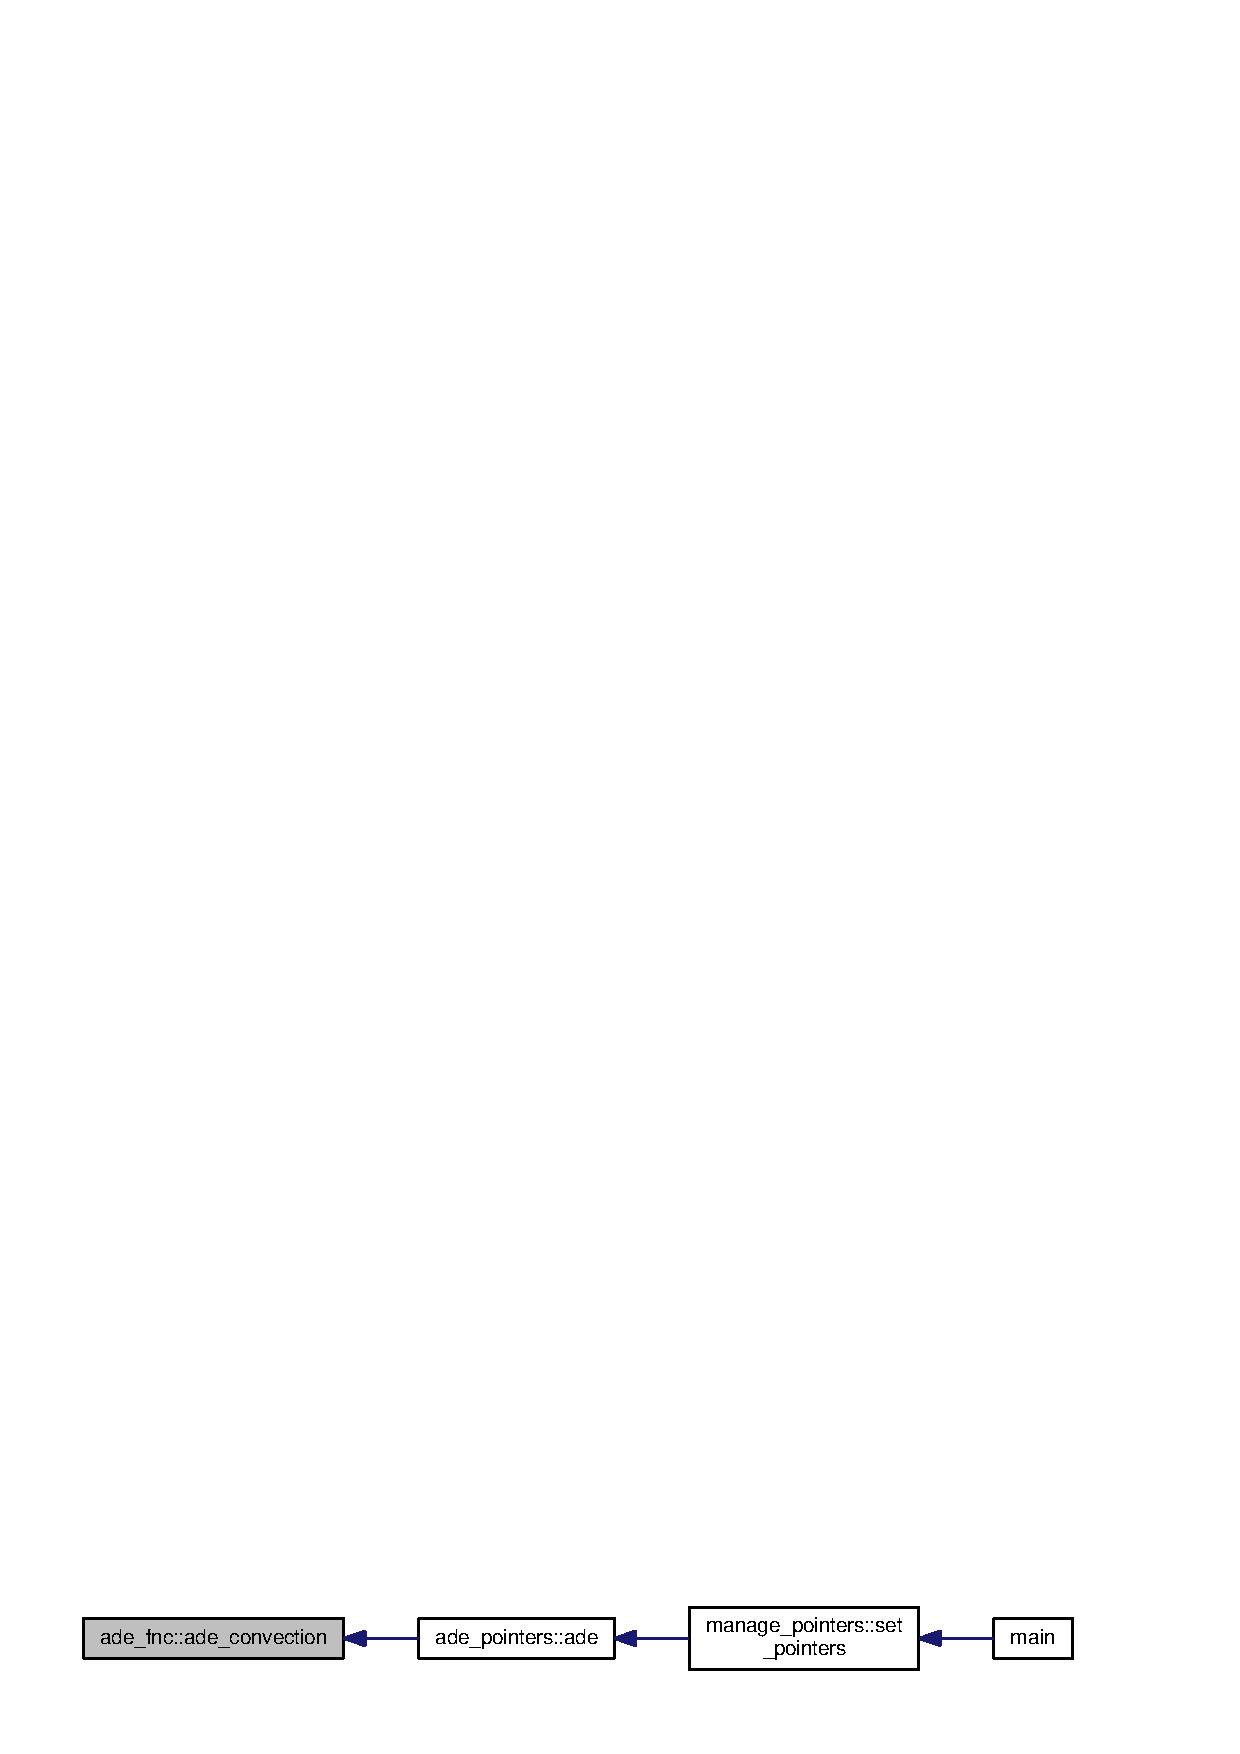
\includegraphics[width=350pt]{namespaceade__fnc_adaaa677e01020a0c331940dd9e9bdb73_icgraph}
\end{center}
\end{figure}


\index{ade\+\_\+fnc@{ade\+\_\+fnc}!ade\+\_\+csbc@{ade\+\_\+csbc}}
\index{ade\+\_\+csbc@{ade\+\_\+csbc}!ade\+\_\+fnc@{ade\+\_\+fnc}}
\subsubsection[{ade\+\_\+csbc(pde\+\_\+loc, el\+\_\+id, node\+\_\+order, value, code)}]{\setlength{\rightskip}{0pt plus 5cm}subroutine, public ade\+\_\+fnc\+::ade\+\_\+csbc (
\begin{DoxyParamCaption}
\item[{class({\bf pde\+\_\+str}), intent(in)}]{pde\+\_\+loc, }
\item[{integer(kind=ikind), intent(in)}]{el\+\_\+id, }
\item[{integer(kind=ikind), intent(in)}]{node\+\_\+order, }
\item[{real(kind=rkind), intent(out), optional}]{value, }
\item[{integer(kind=ikind), intent(out), optional}]{code}
\end{DoxyParamCaption}
)}\label{namespaceade__fnc_aa964a237d991a84b7a0d3d07be25261a}


Definition at line 645 of file A\+D\+E\+\_\+fnc.\+f90.


\begin{DoxyCode}
645       \textcolor{keywordtype}{use }typy
646       \textcolor{keywordtype}{use }globals
647       \textcolor{keywordtype}{use }global_objs
648       \textcolor{keywordtype}{use }pde_objs
649       \textcolor{keywordtype}{use }debug_tools
650       
651       \textcolor{keywordtype}{class}(pde_str), \textcolor{keywordtype}{intent(in)} :: pde\_loc
652       \textcolor{keywordtype}{integer(kind=ikind)}, \textcolor{keywordtype}{intent(in)}  :: el\_id, node\_order
653       \textcolor{keywordtype}{real(kind=rkind)}, \textcolor{keywordtype}{intent(out)}, \textcolor{keywordtype}{optional}    :: value
654       \textcolor{keywordtype}{integer(kind=ikind)}, \textcolor{keywordtype}{intent(out)}, \textcolor{keywordtype}{optional} :: code
655       
656       \textcolor{keywordtype}{integer(kind=ikind)} :: edge\_id, i, j, proc
657       \textcolor{keywordtype}{real(kind=rkind)} :: tempval
658 
659      
660       
661       \textcolor{keywordflow}{if} (\textcolor{keyword}{present}(\textcolor{keywordtype}{value})) \textcolor{keywordflow}{then}
662         \textcolor{keywordtype}{value} = 0.0
663 \textcolor{keywordflow}{      end if}
664 
665 
666       
667       \textcolor{keywordflow}{if} (\textcolor{keyword}{present}(code)) \textcolor{keywordflow}{then}
668         code = 0
669 \textcolor{keywordflow}{      end if}
670       
671 
\end{DoxyCode}
\index{ade\+\_\+fnc@{ade\+\_\+fnc}!ade\+\_\+cscl\+\_\+react@{ade\+\_\+cscl\+\_\+react}}
\index{ade\+\_\+cscl\+\_\+react@{ade\+\_\+cscl\+\_\+react}!ade\+\_\+fnc@{ade\+\_\+fnc}}
\subsubsection[{ade\+\_\+cscl\+\_\+react(pde\+\_\+loc, layer, quadpnt, x)}]{\setlength{\rightskip}{0pt plus 5cm}real(kind=rkind) function, public ade\+\_\+fnc\+::ade\+\_\+cscl\+\_\+react (
\begin{DoxyParamCaption}
\item[{class({\bf pde\+\_\+str}), intent(in)}]{pde\+\_\+loc, }
\item[{integer(kind=ikind), intent(in)}]{layer, }
\item[{type({\bf integpnt\+\_\+str}), intent(in), optional}]{quadpnt, }
\item[{real(kind=rkind), dimension(\+:), intent(in), optional}]{x}
\end{DoxyParamCaption}
)}\label{namespaceade__fnc_a2c71f7220b5c27a9e33e744121d90c5f}

\begin{DoxyParams}[1]{Parameters}
\mbox{\tt in}  & {\em x} & value of the nonlinear function\\
\hline
\mbox{\tt in}  & {\em quadpnt} & Gauss quadrature point structure (element number and rank of Gauss quadrature point)\\
\hline
\mbox{\tt in}  & {\em layer} & material ID\\
\hline
\end{DoxyParams}
\begin{DoxyReturn}{Returns}
return value 
\end{DoxyReturn}


Definition at line 608 of file A\+D\+E\+\_\+fnc.\+f90.



References ade\+\_\+globals\+::adepar, and pde\+\_\+objs\+::pde.



Referenced by ade\+\_\+pointers\+::adekinsorb().


\begin{DoxyCode}
608       \textcolor{keywordtype}{use }typy
609       \textcolor{keywordtype}{use }global_objs
610       \textcolor{keywordtype}{use }pde_objs
611       \textcolor{keywordtype}{use }ade_globals
612       
613       \textcolor{keywordtype}{class}(pde_str), \textcolor{keywordtype}{intent(in)} :: pde\_loc
615       \textcolor{keywordtype}{real(kind=rkind)}, \textcolor{keywordtype}{dimension(:)}, \textcolor{keywordtype}{intent(in)}, \textcolor{keywordtype}{optional}    :: x
617       \textcolor{keywordtype}{type}(integpnt_str), \textcolor{keywordtype}{intent(in)}, \textcolor{keywordtype}{optional} :: quadpnt
619       \textcolor{keywordtype}{integer(kind=ikind)}, \textcolor{keywordtype}{intent(in)} :: layer
621       \textcolor{keywordtype}{real(kind=rkind)}                :: val 
622       
623       \textcolor{keywordtype}{integer(kind=ikind)} :: proc\_cl
624       \textcolor{keywordtype}{real(kind=rkind)} :: cl 
625       
626 
627       
628       \textcolor{keywordflow}{select case}(adepar(layer)%sorption%name)
629         \textcolor{keywordflow}{case}(\textcolor{stringliteral}{"langmu"})
630           val = adepar(layer)%sorption%adsorb*adepar(layer)%sorption%third
631         \textcolor{keywordflow}{case}(\textcolor{stringliteral}{"freund"})
632           \textcolor{keywordflow}{if} (abs(adepar(layer)%sorption%third - 1.0\_rkind ) > 10*epsilon(1.0\_rkind\textcolor{comment}{)) }\textcolor{keywordflow}{then}
633             proc\_cl = pde\_loc%order - 1
634             cl = pde(proc\_cl)%getval(quadpnt)
635             val = adepar(layer)%sorption%adsorb*cl**(1-adepar(layer)%sorption%third\textcolor{comment}{)}
636 \textcolor{comment}{          }\textcolor{keywordflow}{else}
637             val = adepar(layer)%sorption%adsorb
638 \textcolor{keywordflow}{          end if}
639 \textcolor{keywordflow}{      end select}
640       
\end{DoxyCode}


Here is the caller graph for this function\+:\nopagebreak
\begin{figure}[H]
\begin{center}
\leavevmode
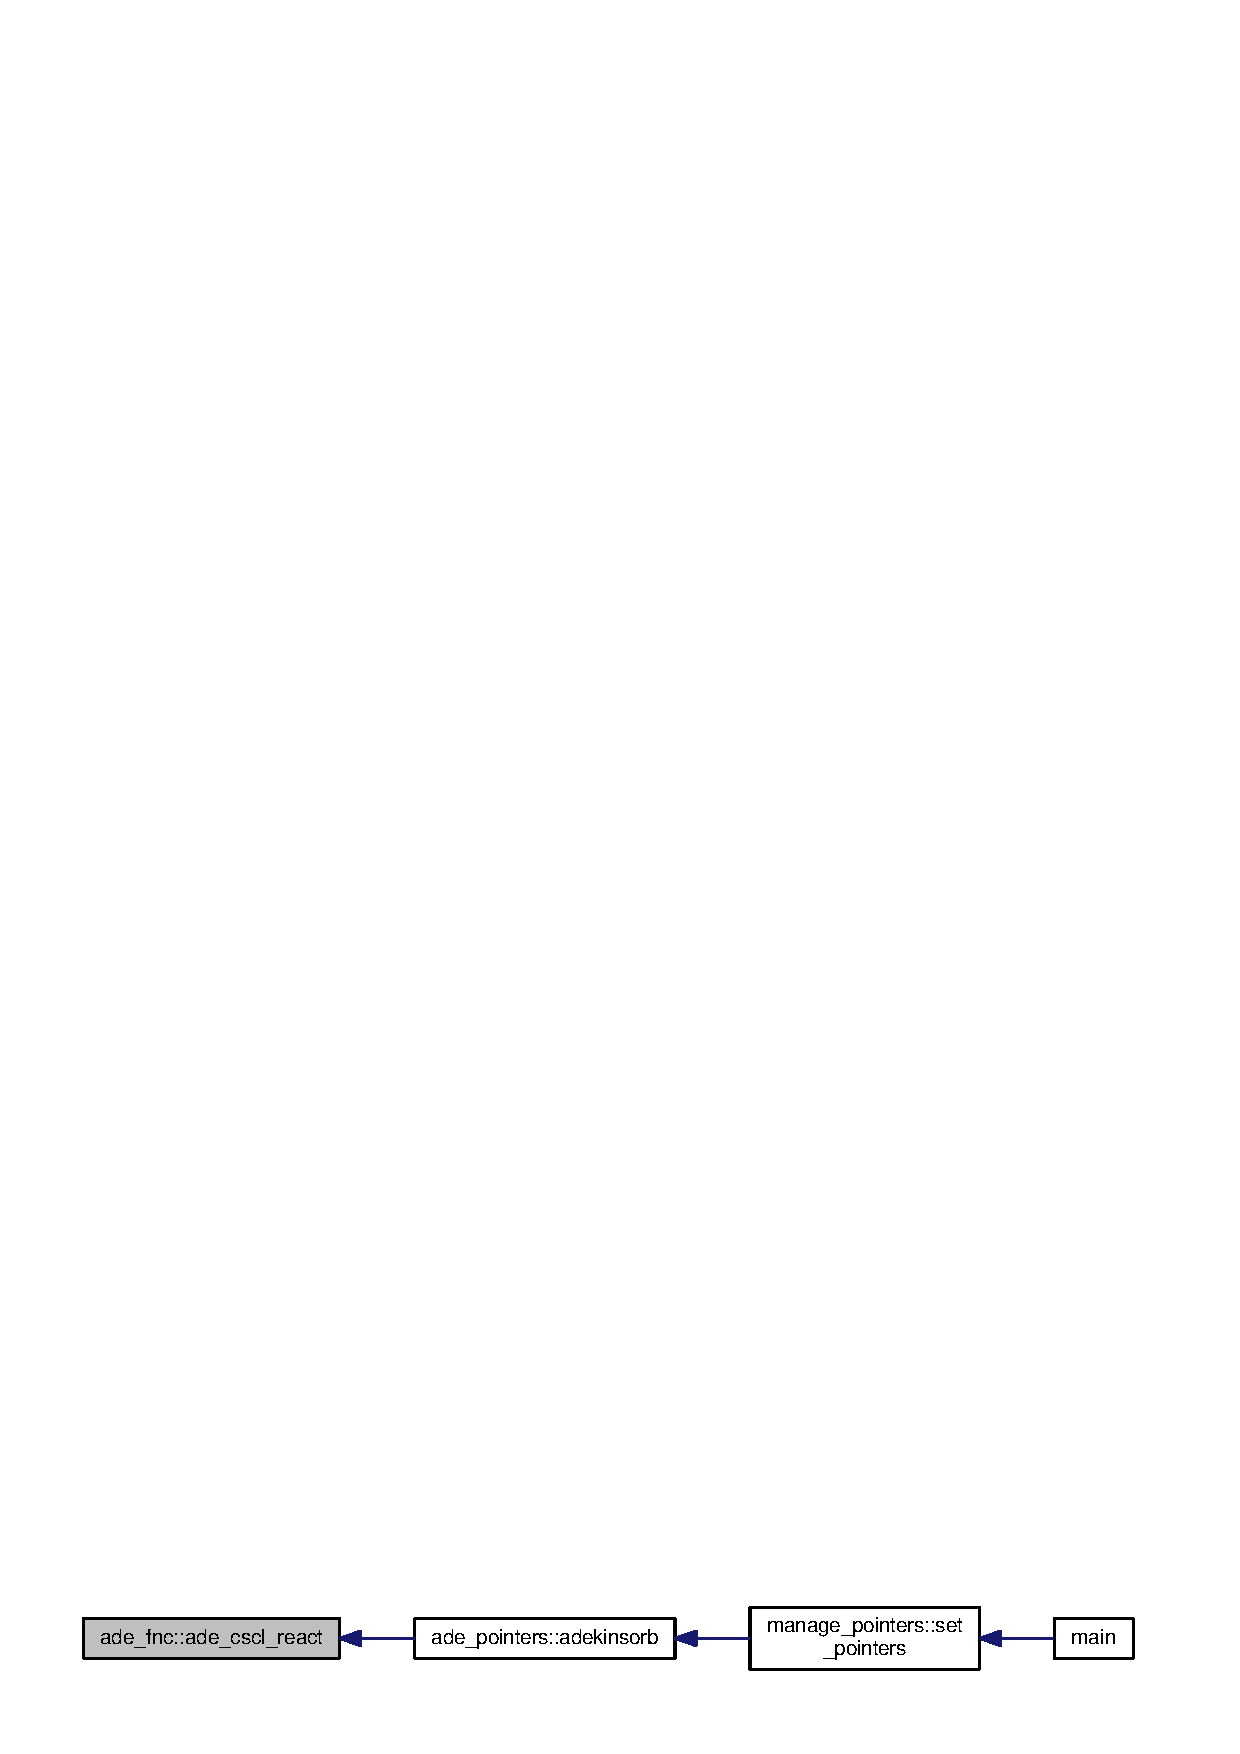
\includegraphics[width=350pt]{namespaceade__fnc_a2c71f7220b5c27a9e33e744121d90c5f_icgraph}
\end{center}
\end{figure}


\index{ade\+\_\+fnc@{ade\+\_\+fnc}!ade\+\_\+cscs\+\_\+react@{ade\+\_\+cscs\+\_\+react}}
\index{ade\+\_\+cscs\+\_\+react@{ade\+\_\+cscs\+\_\+react}!ade\+\_\+fnc@{ade\+\_\+fnc}}
\subsubsection[{ade\+\_\+cscs\+\_\+react(pde\+\_\+loc, layer, quadpnt, x)}]{\setlength{\rightskip}{0pt plus 5cm}real(kind=rkind) function, public ade\+\_\+fnc\+::ade\+\_\+cscs\+\_\+react (
\begin{DoxyParamCaption}
\item[{class({\bf pde\+\_\+str}), intent(in)}]{pde\+\_\+loc, }
\item[{integer(kind=ikind), intent(in)}]{layer, }
\item[{type({\bf integpnt\+\_\+str}), intent(in), optional}]{quadpnt, }
\item[{real(kind=rkind), dimension(\+:), intent(in), optional}]{x}
\end{DoxyParamCaption}
)}\label{namespaceade__fnc_afb034eeab56e8c889cd9adae76cf038c}

\begin{DoxyParams}[1]{Parameters}
\mbox{\tt in}  & {\em x} & value of the nonlinear function\\
\hline
\mbox{\tt in}  & {\em quadpnt} & Gauss quadrature point structure (element number and rank of Gauss quadrature point)\\
\hline
\mbox{\tt in}  & {\em layer} & material ID\\
\hline
\end{DoxyParams}
\begin{DoxyReturn}{Returns}
return value 
\end{DoxyReturn}


Definition at line 574 of file A\+D\+E\+\_\+fnc.\+f90.



References ade\+\_\+globals\+::adepar, and pde\+\_\+objs\+::pde.



Referenced by ade\+\_\+pointers\+::adekinsorb().


\begin{DoxyCode}
574       \textcolor{keywordtype}{use }typy
575       \textcolor{keywordtype}{use }global_objs
576       \textcolor{keywordtype}{use }pde_objs
577       \textcolor{keywordtype}{use }ade_globals
578       
579       \textcolor{keywordtype}{class}(pde_str), \textcolor{keywordtype}{intent(in)} :: pde\_loc
581       \textcolor{keywordtype}{real(kind=rkind)}, \textcolor{keywordtype}{dimension(:)}, \textcolor{keywordtype}{intent(in)}, \textcolor{keywordtype}{optional}    :: x
583       \textcolor{keywordtype}{type}(integpnt_str), \textcolor{keywordtype}{intent(in)}, \textcolor{keywordtype}{optional} :: quadpnt
585       \textcolor{keywordtype}{integer(kind=ikind)}, \textcolor{keywordtype}{intent(in)} :: layer
587       \textcolor{keywordtype}{real(kind=rkind)}                :: val 
588       
589       \textcolor{keywordtype}{integer(kind=ikind)} :: proc\_cl
590       \textcolor{keywordtype}{real(kind=rkind)} :: cs, cl
591       
592       proc\_cl = pde\_loc%order - 1
593       
594       
595       \textcolor{keywordflow}{select case}(adepar(layer)%sorption%name)
596         \textcolor{keywordflow}{case}(\textcolor{stringliteral}{"langmu"})
597           cs = pde\_loc%getval(quadpnt) 
598           cl = pde(proc\_cl)%getval(quadpnt)
599           val = -adepar(layer)%sorption%adsorb*cl - adepar(layer)%sorption%desorb
600         \textcolor{keywordflow}{case}(\textcolor{stringliteral}{"freund"})
601           val = -adepar(layer)%sorption%desorb
602 \textcolor{keywordflow}{      end select}
603       
604       
\end{DoxyCode}


Here is the caller graph for this function\+:\nopagebreak
\begin{figure}[H]
\begin{center}
\leavevmode
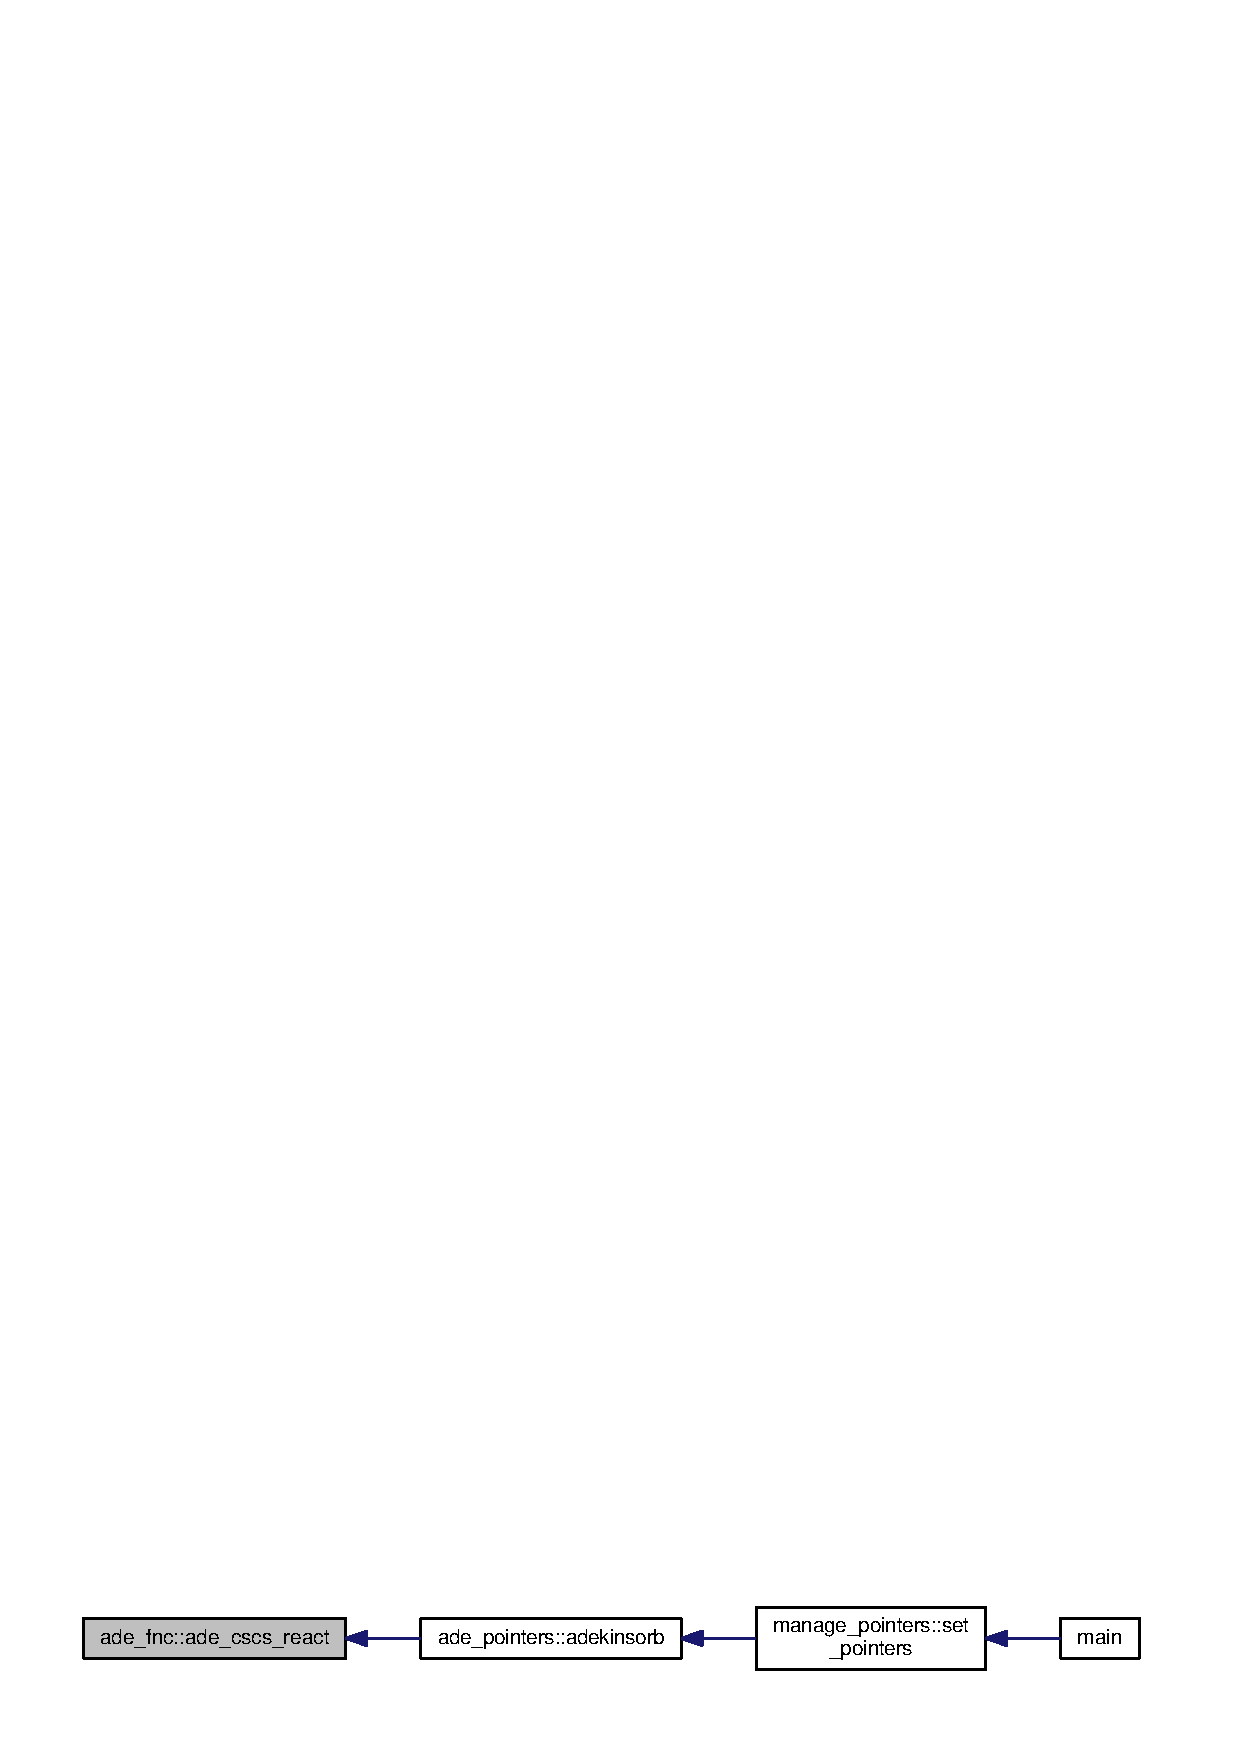
\includegraphics[width=350pt]{namespaceade__fnc_afb034eeab56e8c889cd9adae76cf038c_icgraph}
\end{center}
\end{figure}


\index{ade\+\_\+fnc@{ade\+\_\+fnc}!ade\+\_\+dirichlet@{ade\+\_\+dirichlet}}
\index{ade\+\_\+dirichlet@{ade\+\_\+dirichlet}!ade\+\_\+fnc@{ade\+\_\+fnc}}
\subsubsection[{ade\+\_\+dirichlet(pde\+\_\+loc, el\+\_\+id, node\+\_\+order, value, code)}]{\setlength{\rightskip}{0pt plus 5cm}subroutine, public ade\+\_\+fnc\+::ade\+\_\+dirichlet (
\begin{DoxyParamCaption}
\item[{class({\bf pde\+\_\+str}), intent(in)}]{pde\+\_\+loc, }
\item[{integer(kind=ikind), intent(in)}]{el\+\_\+id, }
\item[{integer(kind=ikind), intent(in)}]{node\+\_\+order, }
\item[{real(kind=rkind), intent(out), optional}]{value, }
\item[{integer(kind=ikind), intent(out), optional}]{code}
\end{DoxyParamCaption}
)}\label{namespaceade__fnc_a5b91d20870b339e174fbd7c2e8bec184}


Definition at line 347 of file A\+D\+E\+\_\+fnc.\+f90.



References globals\+::elements, globals\+::nodes, and globals\+::time.



Referenced by ade\+\_\+pointers\+::ade().


\begin{DoxyCode}
347       \textcolor{keywordtype}{use }typy
348       \textcolor{keywordtype}{use }globals
349       \textcolor{keywordtype}{use }global_objs
350       \textcolor{keywordtype}{use }pde_objs
351       \textcolor{keywordtype}{use }debug_tools
352       
353       \textcolor{keywordtype}{class}(pde_str), \textcolor{keywordtype}{intent(in)} :: pde\_loc
354       \textcolor{keywordtype}{integer(kind=ikind)}, \textcolor{keywordtype}{intent(in)}  :: el\_id, node\_order
355       \textcolor{keywordtype}{real(kind=rkind)}, \textcolor{keywordtype}{intent(out)}, \textcolor{keywordtype}{optional}    :: value
356       \textcolor{keywordtype}{integer(kind=ikind)}, \textcolor{keywordtype}{intent(out)}, \textcolor{keywordtype}{optional} :: code
357       
358       \textcolor{keywordtype}{integer(kind=ikind)} :: edge\_id, i, j, proc
359       \textcolor{keywordtype}{real(kind=rkind)} :: tempval
360       
361       edge\_id = nodes%edge(elements%data(el\_id, node\_order))
362       
363       \textcolor{keywordflow}{if} (\textcolor{keyword}{present}(\textcolor{keywordtype}{value})) \textcolor{keywordflow}{then}
364         \textcolor{keywordflow}{if} (pde\_loc%bc(edge\_id)%file) \textcolor{keywordflow}{then}
365           \textcolor{keywordflow}{do} i=1, ubound(pde\_loc%bc(edge\_id)%series,1)
366             \textcolor{keywordflow}{if} (pde\_loc%bc(edge\_id)%series(i,1) > time) \textcolor{keywordflow}{then}
367               \textcolor{keywordflow}{if} (i > 1) \textcolor{keywordflow}{then}
368                 j = i-1
369               \textcolor{keywordflow}{else}
370                 j = i
371 \textcolor{keywordflow}{              end if}
372               tempval = pde\_loc%bc(edge\_id)%series(j,2)
373               \textcolor{keywordflow}{EXIT}
374 \textcolor{keywordflow}{            end if}
375 \textcolor{keywordflow}{          end do}
376         \textcolor{keywordflow}{else}
377           tempval =  pde\_loc%bc(edge\_id)%value
378 \textcolor{keywordflow}{        end if}
379         \textcolor{keywordtype}{value} = tempval 
380 \textcolor{keywordflow}{      end if}
381 
382 
383       
384       \textcolor{keywordflow}{if} (\textcolor{keyword}{present}(code)) \textcolor{keywordflow}{then}
385         code = 1
386 \textcolor{keywordflow}{      end if}
387       
388 
\end{DoxyCode}


Here is the caller graph for this function\+:\nopagebreak
\begin{figure}[H]
\begin{center}
\leavevmode
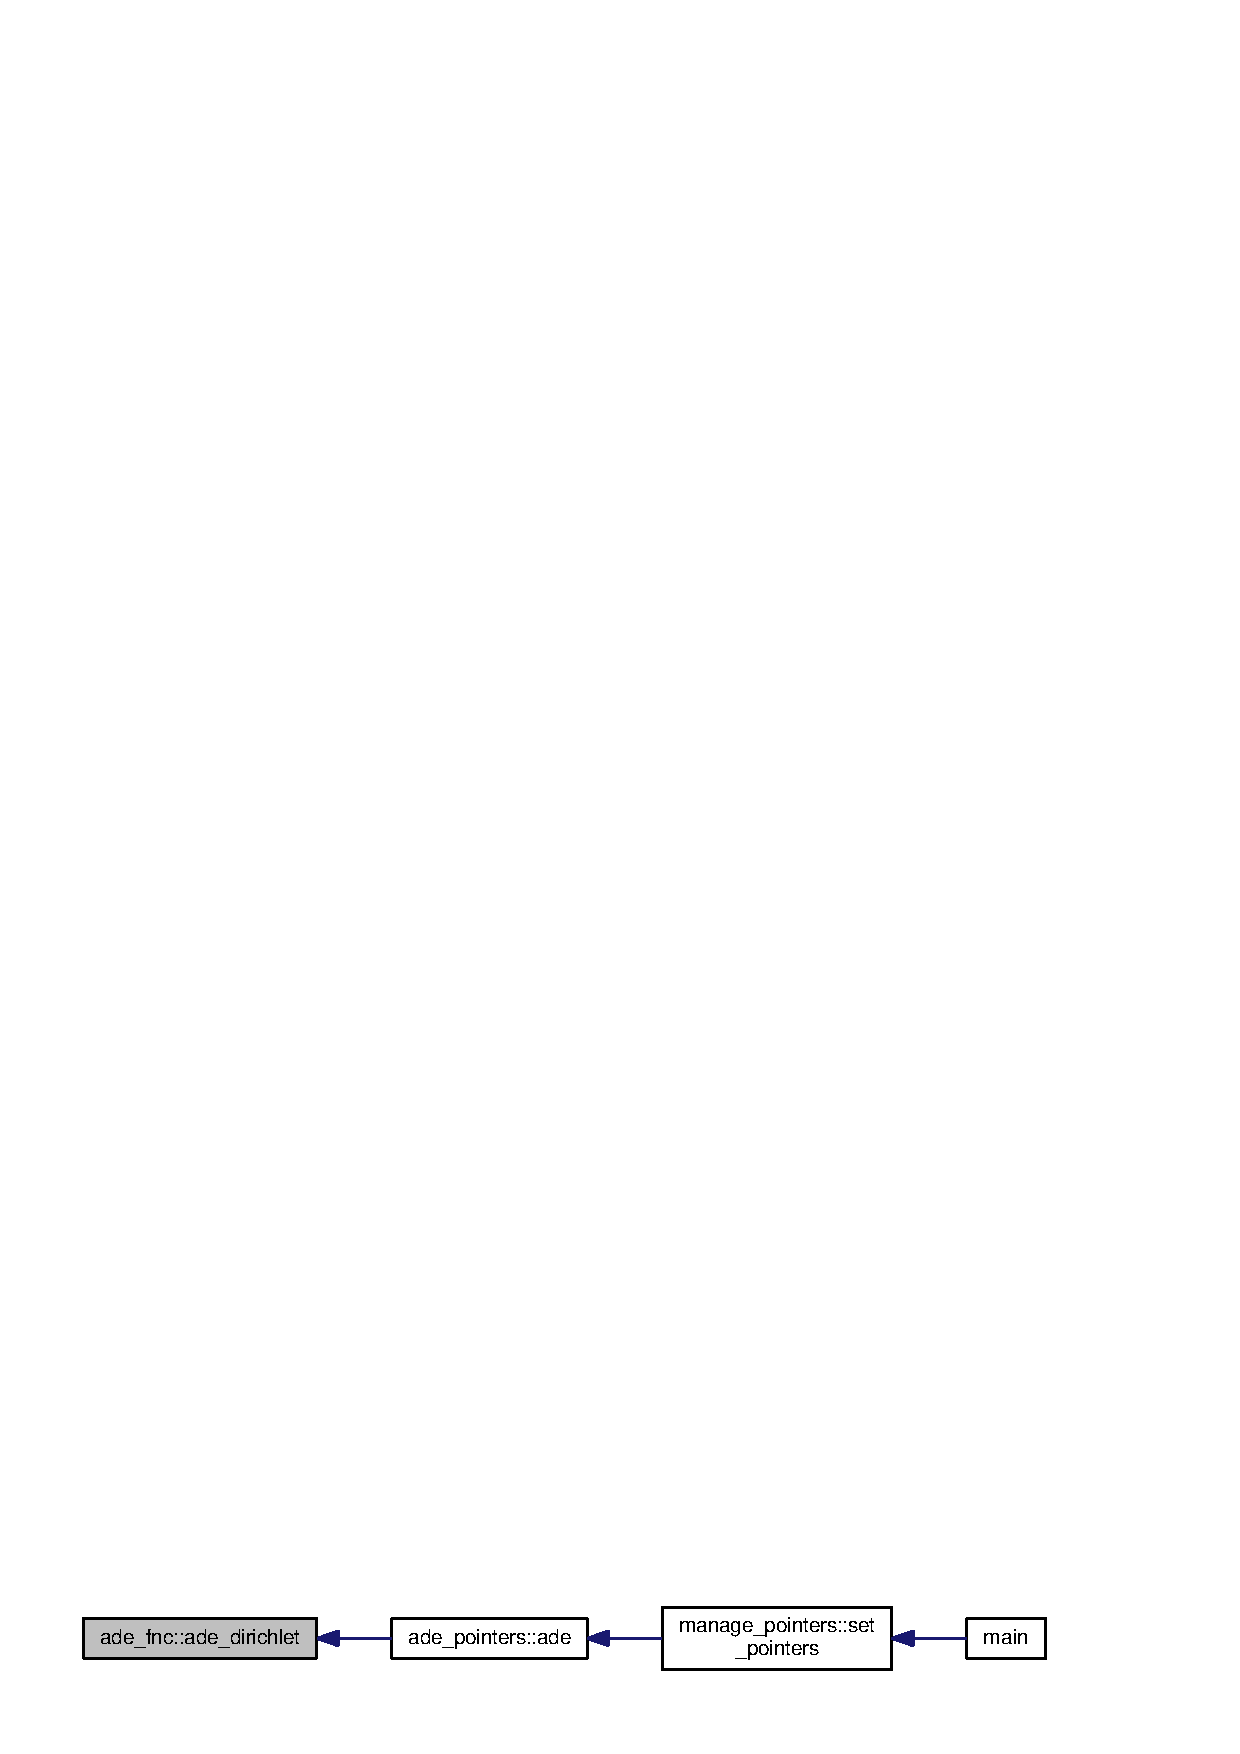
\includegraphics[width=350pt]{namespaceade__fnc_a5b91d20870b339e174fbd7c2e8bec184_icgraph}
\end{center}
\end{figure}


\index{ade\+\_\+fnc@{ade\+\_\+fnc}!ade\+\_\+flux@{ade\+\_\+flux}}
\index{ade\+\_\+flux@{ade\+\_\+flux}!ade\+\_\+fnc@{ade\+\_\+fnc}}
\subsubsection[{ade\+\_\+flux(pde\+\_\+loc, layer, quadpnt, x, grad, flux, flux\+\_\+length)}]{\setlength{\rightskip}{0pt plus 5cm}subroutine, public ade\+\_\+fnc\+::ade\+\_\+flux (
\begin{DoxyParamCaption}
\item[{class({\bf pde\+\_\+str}), intent(in)}]{pde\+\_\+loc, }
\item[{integer(kind=ikind), intent(in)}]{layer, }
\item[{type({\bf integpnt\+\_\+str}), intent(in), optional}]{quadpnt, }
\item[{real(kind=rkind), dimension(\+:), intent(in), optional}]{x, }
\item[{real(kind=rkind), dimension(\+:), intent(in), optional}]{grad, }
\item[{real(kind=rkind), dimension(\+:), intent(out), optional}]{flux, }
\item[{real(kind=rkind), intent(out), optional}]{flux\+\_\+length}
\end{DoxyParamCaption}
)}\label{namespaceade__fnc_aede22f790dd20203b407c41d5f4d6c7d}

\begin{DoxyParams}[1]{Parameters}
\mbox{\tt in}  & {\em grad} & this value is optional, because it is required by the vector\+\_\+fnc procedure pointer global definition \\
\hline
\end{DoxyParams}


Definition at line 461 of file A\+D\+E\+\_\+fnc.\+f90.



References ade\+\_\+globals\+::adepar, and pde\+\_\+objs\+::pde.



Referenced by ade\+\_\+pointers\+::ade().


\begin{DoxyCode}
461       \textcolor{keywordtype}{use }typy
462       \textcolor{keywordtype}{use }pde_objs
463       \textcolor{keywordtype}{use }global_objs
464       \textcolor{keywordtype}{use }debug_tools
465       \textcolor{keywordtype}{use }ade_globals
466        
467       \textcolor{keywordtype}{class}(pde_str), \textcolor{keywordtype}{intent(in)} :: pde\_loc
468       \textcolor{keywordtype}{integer(kind=ikind)}, \textcolor{keywordtype}{intent(in)}                          :: layer
469       \textcolor{keywordtype}{type}(integpnt_str), \textcolor{keywordtype}{intent(in)}, \textcolor{keywordtype}{optional} :: quadpnt    
470       \textcolor{keywordtype}{real(kind=rkind)}, \textcolor{keywordtype}{intent(in)}, \textcolor{keywordtype}{dimension(:)}, \textcolor{keywordtype}{optional}              \textcolor{comment}{     :: x}
472       \textcolor{keywordtype}{real(kind=rkind)}, \textcolor{keywordtype}{dimension(:)}, \textcolor{keywordtype}{intent(in)}, \textcolor{keywordtype}{optional}     :: grad
473       \textcolor{keywordtype}{real(kind=rkind)}, \textcolor{keywordtype}{dimension(:)}, \textcolor{keywordtype}{intent(out)}, \textcolor{keywordtype}{optional}    :: flux
474       \textcolor{keywordtype}{real(kind=rkind)}, \textcolor{keywordtype}{intent(out)}, \textcolor{keywordtype}{optional}                  :: flux\_length
475     
476       \textcolor{keywordtype}{real(kind=rkind)}, \textcolor{keywordtype}{dimension(:,:)}, \textcolor{keywordtype}{allocatable}, \textcolor{keywordtype}{save}  :: dhm
477       \textcolor{keywordtype}{real(kind=rkind)}, \textcolor{keywordtype}{dimension(:)}, \textcolor{keywordtype}{allocatable}, \textcolor{keywordtype}{save} :: q\_w, gradc
478       \textcolor{keywordtype}{real(kind=rkind)} :: c, cmax
479       
480       
481       \textcolor{keywordflow}{if} (\textcolor{keyword}{present}(quadpnt) .and. (\textcolor{keyword}{present}(grad) .or. \textcolor{keyword}{present}(x))) \textcolor{keywordflow}{then}
482         print *, \textcolor{stringliteral}{"ERROR: the function can be called either with integ point or x value definition and
       gradient, not both of them"}
483         print *, \textcolor{stringliteral}{"exited from ADE\_fnc::ADE\_flux"}
484         error stop
485       \textcolor{keywordflow}{else} \textcolor{keywordflow}{if} ((.not. \textcolor{keyword}{present}(grad) .or. .not. \textcolor{keyword}{present}(x)) .and. .not. \textcolor{keyword}{present}\textcolor{comment}{(quadpnt)) }\textcolor{keywordflow}{then}
486         print *, \textcolor{stringliteral}{"ERROR: you have not specified either integ point or x value"}
487         print *, \textcolor{stringliteral}{"exited from ADE\_fnc::ADE\_flux"}
488         error stop
489 \textcolor{keywordflow}{      end if}
490       
491       \textcolor{keywordflow}{if} (.not. \textcolor{keyword}{allocated}(q\_w)) \textcolor{keyword}{allocate}(q\_w(drutes_config%dimen))
492 
493       \textcolor{keywordflow}{if} (.not. \textcolor{keyword}{allocated}(gradc)) \textcolor{keyword}{allocate}(gradc(drutes_config%dimen))
494       
495       \textcolor{keywordflow}{if} (.not. \textcolor{keyword}{allocated}(dhm)) \textcolor{keyword}{allocate}(dhm(drutes_config%dimen, drutes_config%dimen\textcolor{comment}{))}
496 \textcolor{comment}{      }
497 \textcolor{comment}{      }\textcolor{keywordflow}{if} (\textcolor{keyword}{present}(quadpnt)) \textcolor{keywordflow}{then}
498         c = pde\_loc%getval(quadpnt)
499         \textcolor{keyword}{call }pde\_loc%getgrad(quadpnt, gradc)
500       \textcolor{keywordflow}{else}
501         \textcolor{keywordflow}{if} (ubound(x,1) /=1) \textcolor{keywordflow}{then}
502           print *, \textcolor{stringliteral}{"ERROR: van Genuchten function is a function of a single variable h"}
503           print *, \textcolor{stringliteral}{"       your input data has:"}, ubound(x,1), \textcolor{stringliteral}{"variables"}
504           print *, \textcolor{stringliteral}{"exited from ADE\_fnc::ADE\_flux"}
505           error stop
506 \textcolor{keywordflow}{        end if}
507         c = x(1)
508         gradc = grad
509 \textcolor{keywordflow}{      end if}
510       
511       
512       \textcolor{keyword}{call }pde\_loc%pde\_fnc(1)%dispersion(pde\_loc, layer, quadpnt, tensor\textcolor{comment}{=dhm)}
513 \textcolor{comment}{      }
514 \textcolor{comment}{      }\textcolor{keywordflow}{select case}(pde\_loc%order)
515         \textcolor{keywordflow}{case}(1)
516           q\_w = adepar(layer)%convection
517         \textcolor{keywordflow}{case}(2)
518           \textcolor{keyword}{call }pde(1)%flux(layer, quadpnt, vector\_out=q\_w)
519 \textcolor{keywordflow}{      end select}
520       
521       \textcolor{keywordflow}{select case}(adepar(layer)%icondtype)
522         \textcolor{keywordflow}{case}(\textcolor{stringliteral}{"ca"})
523           cmax = 1.0\_rkind
524          \textcolor{keywordflow}{case}(\textcolor{stringliteral}{"cr"})
525           cmax = adepar(layer)%cmax
526 \textcolor{keywordflow}{      end select}
527       
528       
529       \textcolor{keywordflow}{if} (\textcolor{keyword}{present}(flux)) \textcolor{keywordflow}{then}
530         flux = cmax*matmul(dhm, gradc) + cmax*q\_w*c
531 \textcolor{keywordflow}{      end if}
532     
\end{DoxyCode}


Here is the caller graph for this function\+:\nopagebreak
\begin{figure}[H]
\begin{center}
\leavevmode
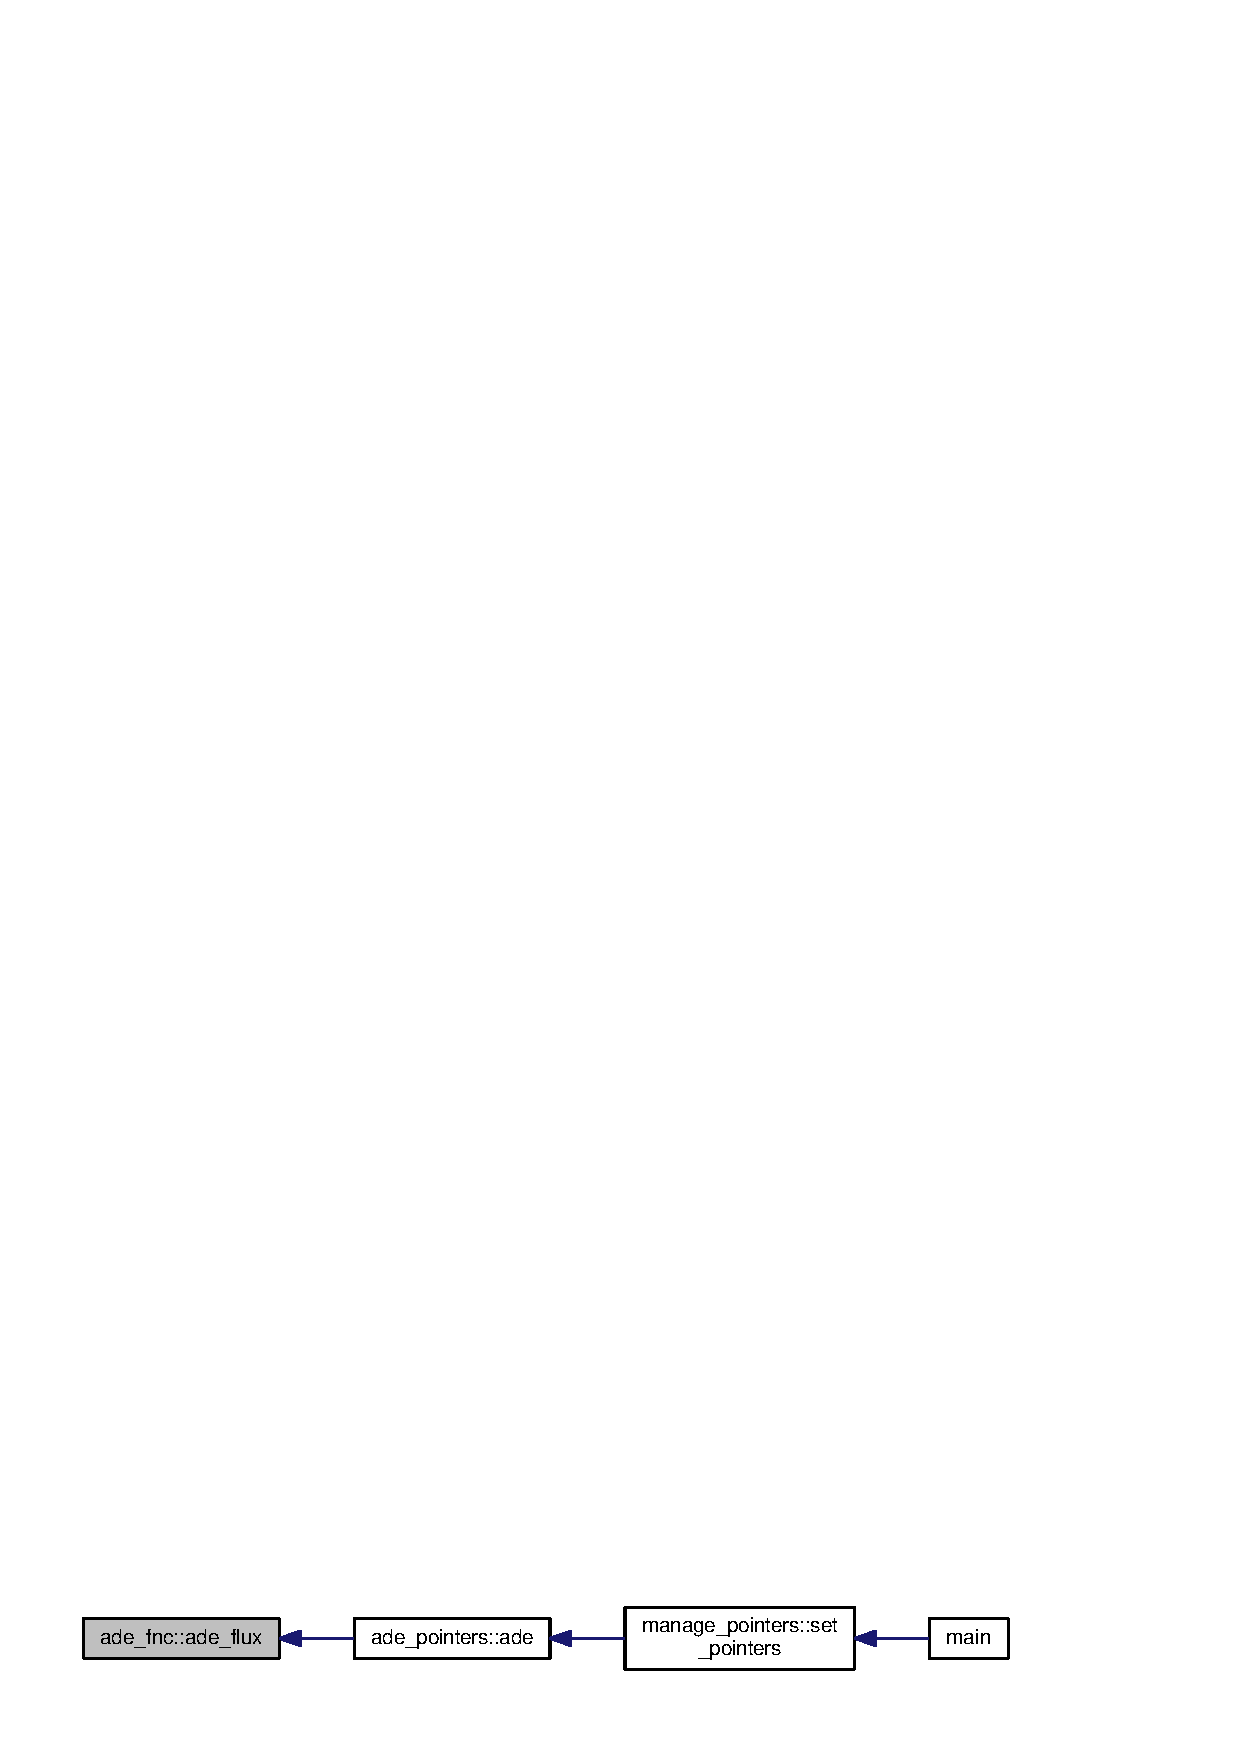
\includegraphics[width=350pt]{namespaceade__fnc_aede22f790dd20203b407c41d5f4d6c7d_icgraph}
\end{center}
\end{figure}


\index{ade\+\_\+fnc@{ade\+\_\+fnc}!ade\+\_\+icond@{ade\+\_\+icond}}
\index{ade\+\_\+icond@{ade\+\_\+icond}!ade\+\_\+fnc@{ade\+\_\+fnc}}
\subsubsection[{ade\+\_\+icond(pde\+\_\+loc)}]{\setlength{\rightskip}{0pt plus 5cm}subroutine, public ade\+\_\+fnc\+::ade\+\_\+icond (
\begin{DoxyParamCaption}
\item[{class({\bf pde\+\_\+str}), intent(inout)}]{pde\+\_\+loc}
\end{DoxyParamCaption}
)}\label{namespaceade__fnc_a114f89bc8bfdca6b691d3e4afd2a7da7}


Definition at line 536 of file A\+D\+E\+\_\+fnc.\+f90.



References ade\+\_\+globals\+::adepar, globals\+::drutes\+\_\+config, globals\+::elements, and globals\+::nodes.



Referenced by ade\+\_\+pointers\+::ade().


\begin{DoxyCode}
536       \textcolor{keywordtype}{use }typy
537       \textcolor{keywordtype}{use }globals
538       \textcolor{keywordtype}{use }global_objs
539       \textcolor{keywordtype}{use }pde_objs
540       \textcolor{keywordtype}{use }ade_globals
541 
542       
543       \textcolor{keywordtype}{class}(pde_str), \textcolor{keywordtype}{intent(in out)} :: pde\_loc
544       \textcolor{keywordtype}{integer(kind=ikind)} :: i, j, k,l, m, layer, d
545       \textcolor{keywordtype}{real(kind=rkind)} :: value
546       
547    
548       d = drutes_config%dimen
549       \textcolor{keywordflow}{do} i=1, elements%kolik
550         layer = elements%material(i,1)
551         \textcolor{keywordflow}{do} j=1, ubound(elements%data,2)
552           k = elements%data(i,j)
553           l = nodes%edge(k)
554           m = pde\_loc%permut(k)
555           \textcolor{keywordflow}{if} (m == 0) \textcolor{keywordflow}{then}
556             \textcolor{keyword}{call }pde\_loc%bc(l)%value\_fnc(pde\_loc, i, j, \textcolor{keywordtype}{value})
557             pde\_loc%solution(k) =  \textcolor{keywordtype}{value} 
558           \textcolor{keywordflow}{else}
559             \textcolor{keywordflow}{select case} (adepar(layer)%icondtype)
560               \textcolor{keywordflow}{case}(\textcolor{stringliteral}{"ca"})
561                 pde\_loc%solution(k) = adepar(layer)%cinit
562               \textcolor{keywordflow}{case}(\textcolor{stringliteral}{"cr"})
563                 pde\_loc%solution(k) = adepar(layer)%cinit * adepar(layer)%cmax
564 \textcolor{keywordflow}{            end select}
565 \textcolor{keywordflow}{          end if}
566 \textcolor{keywordflow}{        end do}   
567 \textcolor{keywordflow}{      end do}
568 
569     
570     
\end{DoxyCode}


Here is the caller graph for this function\+:\nopagebreak
\begin{figure}[H]
\begin{center}
\leavevmode
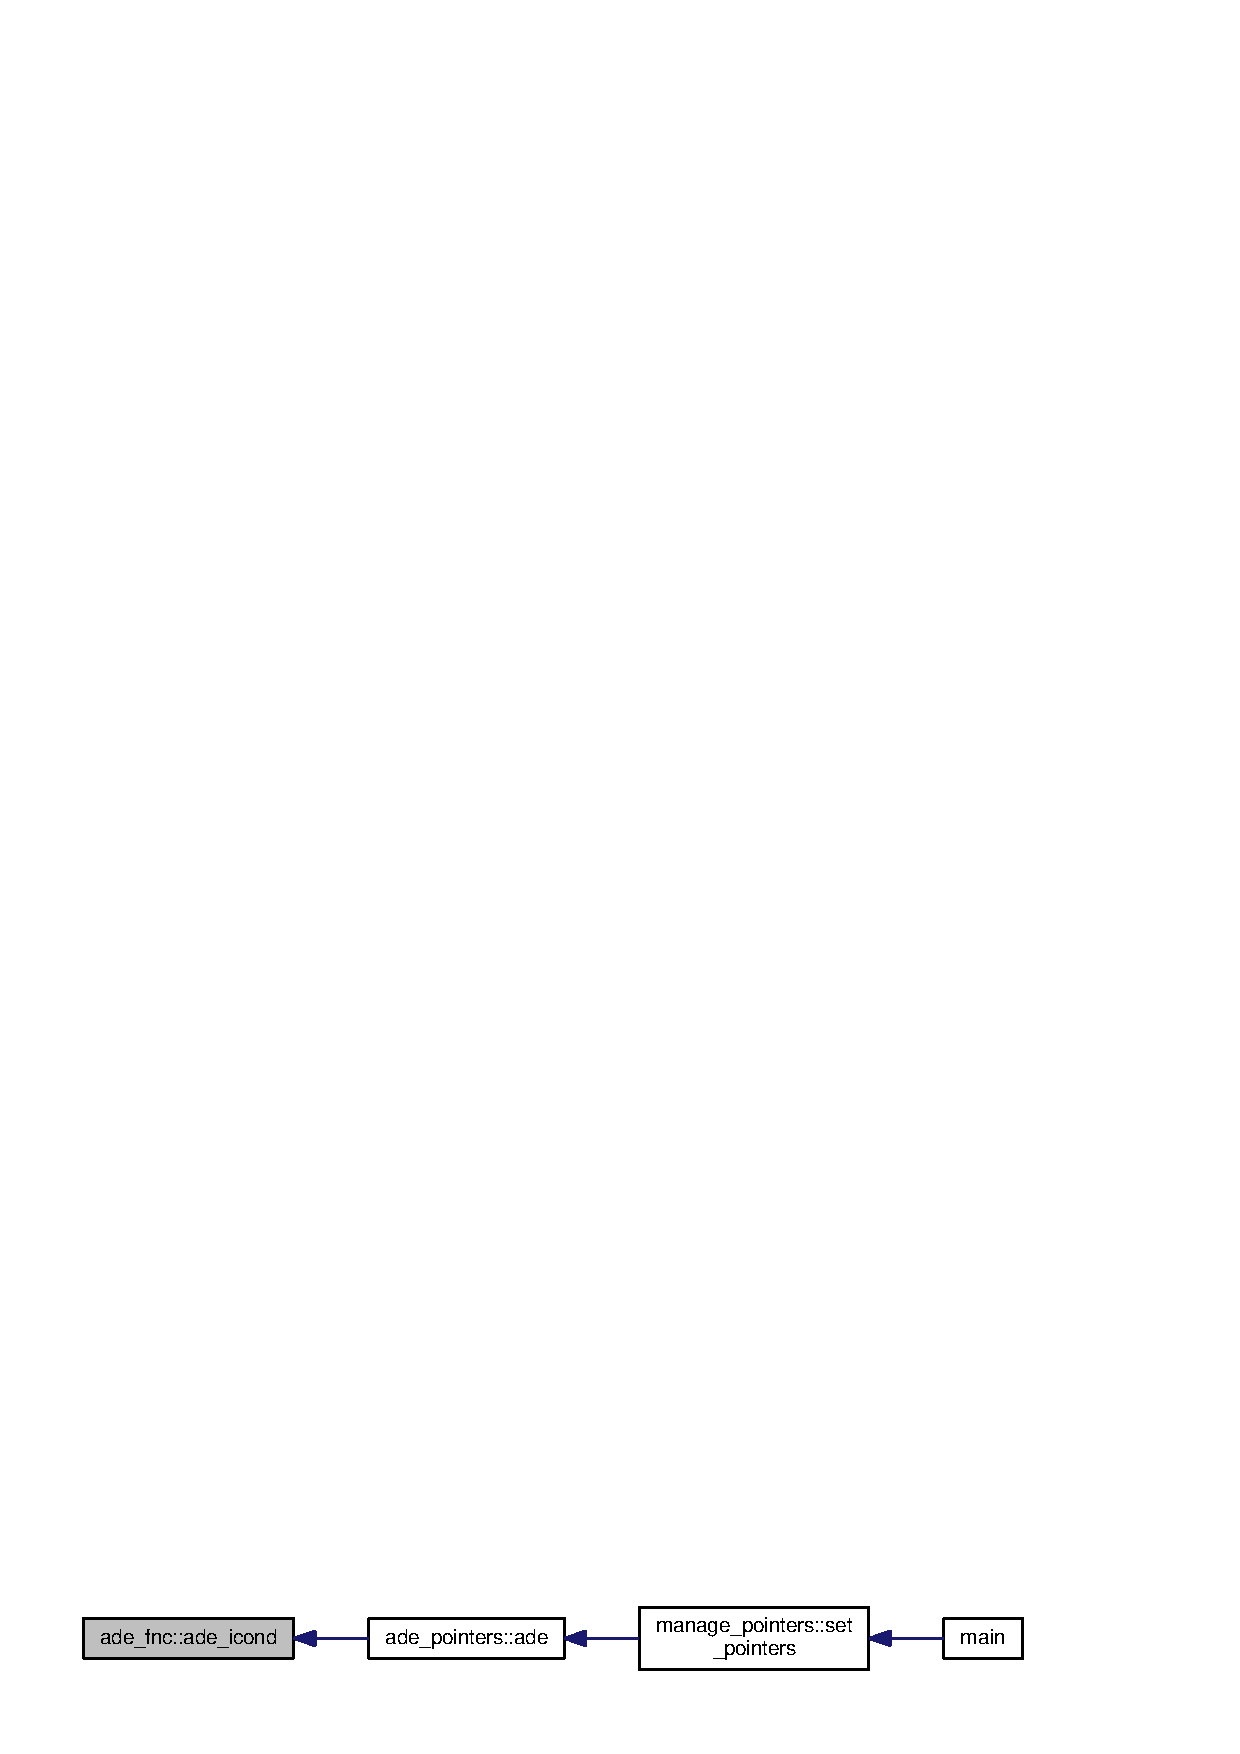
\includegraphics[width=350pt]{namespaceade__fnc_a114f89bc8bfdca6b691d3e4afd2a7da7_icgraph}
\end{center}
\end{figure}


\index{ade\+\_\+fnc@{ade\+\_\+fnc}!ade\+\_\+mass@{ade\+\_\+mass}}
\index{ade\+\_\+mass@{ade\+\_\+mass}!ade\+\_\+fnc@{ade\+\_\+fnc}}
\subsubsection[{ade\+\_\+mass(pde\+\_\+loc, layer, quadpnt, x)}]{\setlength{\rightskip}{0pt plus 5cm}real(kind=rkind) function, public ade\+\_\+fnc\+::ade\+\_\+mass (
\begin{DoxyParamCaption}
\item[{class({\bf pde\+\_\+str}), intent(in)}]{pde\+\_\+loc, }
\item[{integer(kind=ikind), intent(in)}]{layer, }
\item[{type({\bf integpnt\+\_\+str}), intent(in), optional}]{quadpnt, }
\item[{real(kind=rkind), dimension(\+:), intent(in), optional}]{x}
\end{DoxyParamCaption}
)}\label{namespaceade__fnc_aa49487b68d46e5b95eef39bdb1ed4077}

\begin{DoxyParams}[1]{Parameters}
\mbox{\tt in}  & {\em x} & value of the nonlinear function\\
\hline
\mbox{\tt in}  & {\em quadpnt} & Gauss quadrature point structure (element number and rank of Gauss quadrature point)\\
\hline
\mbox{\tt in}  & {\em layer} & material ID\\
\hline
\end{DoxyParams}
\begin{DoxyReturn}{Returns}
return value 
\end{DoxyReturn}


Definition at line 233 of file A\+D\+E\+\_\+fnc.\+f90.



References ade\+\_\+globals\+::adepar, and pde\+\_\+objs\+::pde.



Referenced by ade\+\_\+pointers\+::ade().


\begin{DoxyCode}
233       \textcolor{keywordtype}{use }typy
234       \textcolor{keywordtype}{use }global_objs
235       \textcolor{keywordtype}{use }pde_objs
236       \textcolor{keywordtype}{use }ade_globals
237       
238       \textcolor{keywordtype}{class}(pde_str), \textcolor{keywordtype}{intent(in)} :: pde\_loc
240       \textcolor{keywordtype}{real(kind=rkind)}, \textcolor{keywordtype}{dimension(:)}, \textcolor{keywordtype}{intent(in)}, \textcolor{keywordtype}{optional}    :: x
242       \textcolor{keywordtype}{type}(integpnt_str), \textcolor{keywordtype}{intent(in)}, \textcolor{keywordtype}{optional} :: quadpnt
244       \textcolor{keywordtype}{integer(kind=ikind)}, \textcolor{keywordtype}{intent(in)} :: layer
246       \textcolor{keywordtype}{real(kind=rkind)}                :: val 
247       \textcolor{keywordtype}{real(kind=rkind)}                :: theta
248       
249       \textcolor{keywordflow}{if} (pde\_loc%order == 1) \textcolor{keywordflow}{then}
250         theta = adepar(layer)%water\_cont
251       \textcolor{keywordflow}{else}
252         theta = pde(1)%mass(layer, quadpnt)
253 \textcolor{keywordflow}{      end if}
254       
255       \textcolor{keywordflow}{if} (\textcolor{keyword}{present}(quadpnt)) \textcolor{keywordflow}{then}
256         val = theta*pde\_loc%getval(quadpnt)
257       \textcolor{keywordflow}{else}
258         val = theta * x(1)
259 \textcolor{keywordflow}{      end if}
260       
\end{DoxyCode}


Here is the caller graph for this function\+:\nopagebreak
\begin{figure}[H]
\begin{center}
\leavevmode
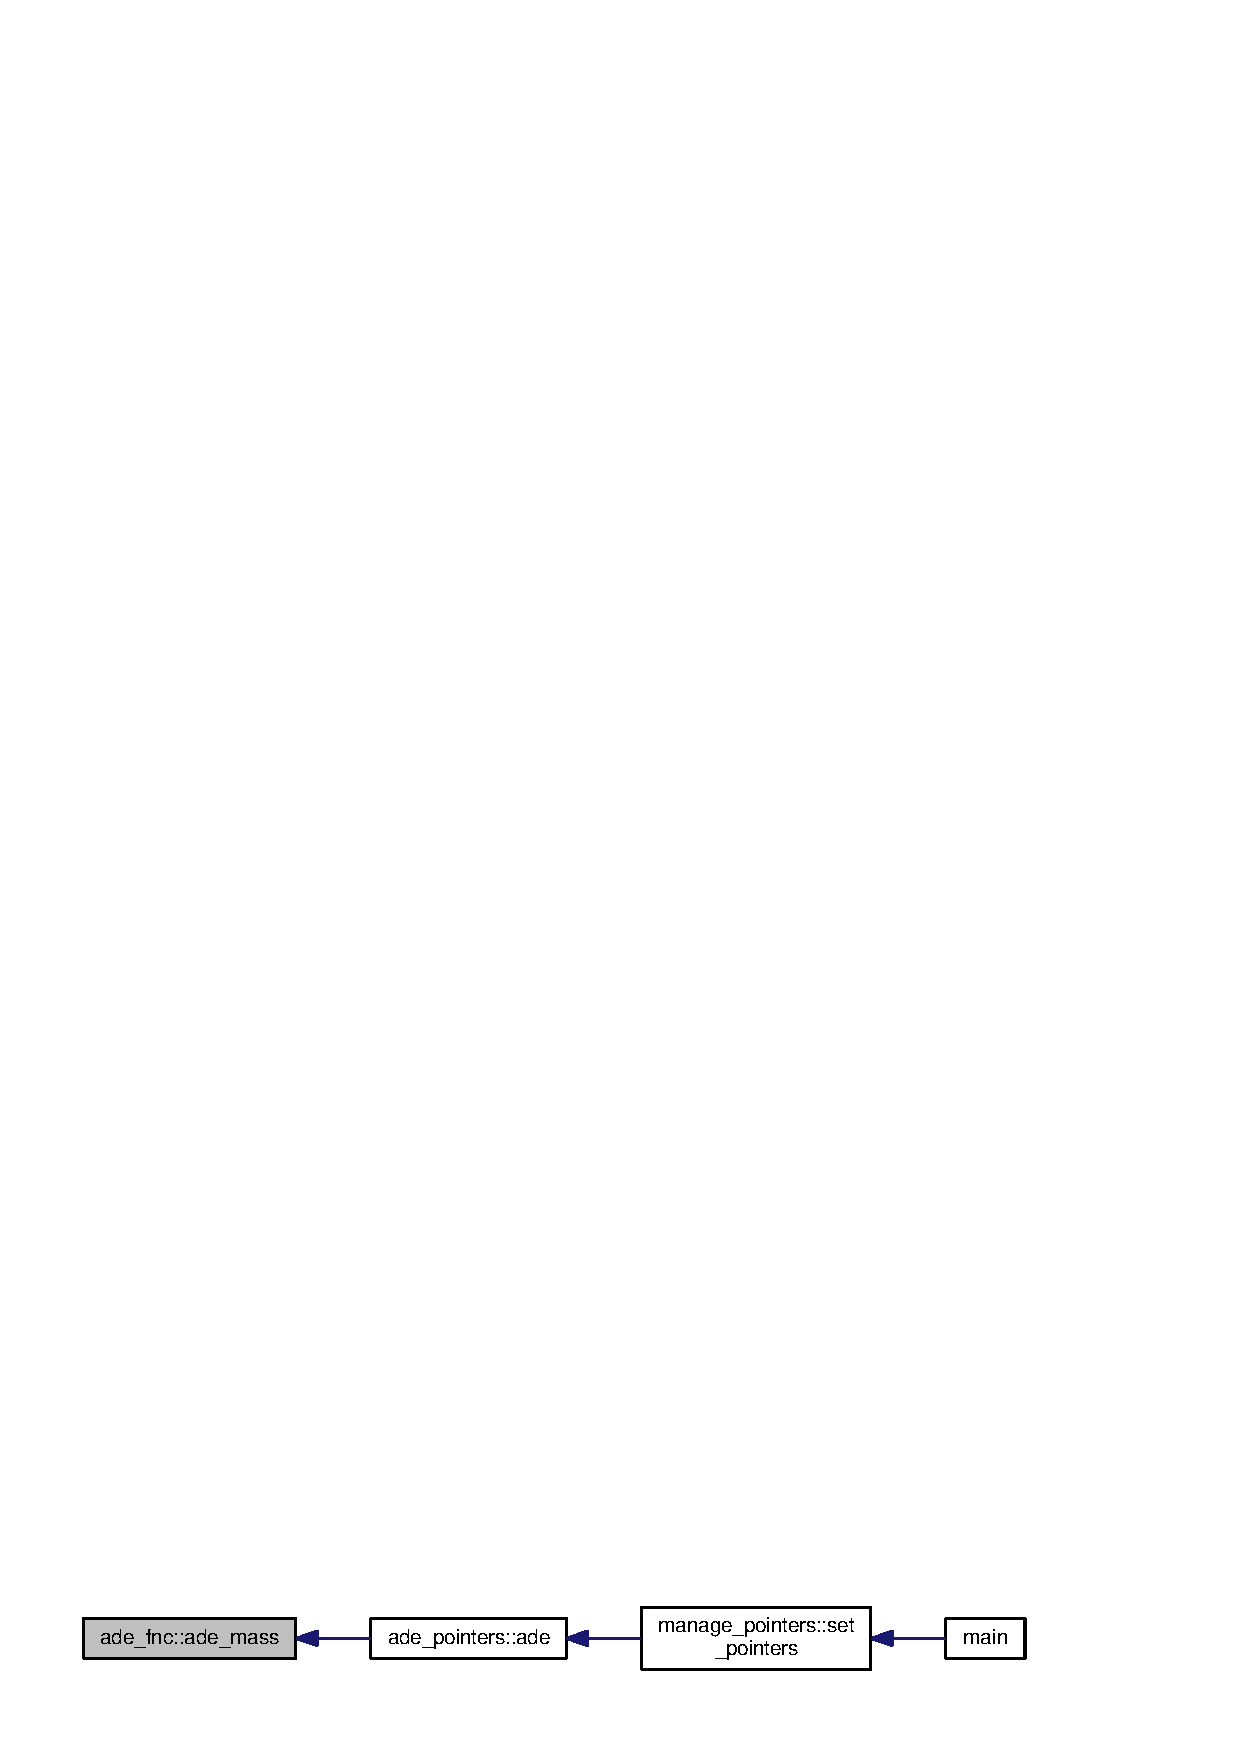
\includegraphics[width=350pt]{namespaceade__fnc_aa49487b68d46e5b95eef39bdb1ed4077_icgraph}
\end{center}
\end{figure}


\index{ade\+\_\+fnc@{ade\+\_\+fnc}!ade\+\_\+neumann@{ade\+\_\+neumann}}
\index{ade\+\_\+neumann@{ade\+\_\+neumann}!ade\+\_\+fnc@{ade\+\_\+fnc}}
\subsubsection[{ade\+\_\+neumann(pde\+\_\+loc, el\+\_\+id, node\+\_\+order, value, code)}]{\setlength{\rightskip}{0pt plus 5cm}subroutine, public ade\+\_\+fnc\+::ade\+\_\+neumann (
\begin{DoxyParamCaption}
\item[{class({\bf pde\+\_\+str}), intent(in)}]{pde\+\_\+loc, }
\item[{integer(kind=ikind), intent(in)}]{el\+\_\+id, }
\item[{integer(kind=ikind), intent(in)}]{node\+\_\+order, }
\item[{real(kind=rkind), intent(out), optional}]{value, }
\item[{integer(kind=ikind), intent(out), optional}]{code}
\end{DoxyParamCaption}
)}\label{namespaceade__fnc_ae9d3681beeaa8b72726418a2b999aa44}


Definition at line 393 of file A\+D\+E\+\_\+fnc.\+f90.



References globals\+::elements, globals\+::nodes, and globals\+::time.



Referenced by ade\+\_\+pointers\+::ade().


\begin{DoxyCode}
393       \textcolor{keywordtype}{use }typy
394       \textcolor{keywordtype}{use }globals
395       \textcolor{keywordtype}{use }global_objs
396       \textcolor{keywordtype}{use }pde_objs
397       \textcolor{keywordtype}{use }debug_tools
398       
399       \textcolor{keywordtype}{class}(pde_str), \textcolor{keywordtype}{intent(in)} :: pde\_loc
400       \textcolor{keywordtype}{integer(kind=ikind)}, \textcolor{keywordtype}{intent(in)}  :: el\_id, node\_order
401       \textcolor{keywordtype}{real(kind=rkind)}, \textcolor{keywordtype}{intent(out)}, \textcolor{keywordtype}{optional}    :: value
402       \textcolor{keywordtype}{integer(kind=ikind)}, \textcolor{keywordtype}{intent(out)}, \textcolor{keywordtype}{optional} :: code
403       
404       \textcolor{keywordtype}{integer(kind=ikind)} :: edge\_id, i, j, proc
405       \textcolor{keywordtype}{real(kind=rkind)} :: tempval
406       
407       edge\_id = nodes%edge(elements%data(el\_id, node\_order))
408       
409       \textcolor{keywordflow}{if} (\textcolor{keyword}{present}(\textcolor{keywordtype}{value})) \textcolor{keywordflow}{then}
410         \textcolor{keywordflow}{if} (pde\_loc%bc(edge\_id)%file) \textcolor{keywordflow}{then}
411           \textcolor{keywordflow}{do} i=1, ubound(pde\_loc%bc(edge\_id)%series,1)
412             \textcolor{keywordflow}{if} (pde\_loc%bc(edge\_id)%series(i,1) > time) \textcolor{keywordflow}{then}
413               \textcolor{keywordflow}{if} (i > 1) \textcolor{keywordflow}{then}
414                 j = i-1
415               \textcolor{keywordflow}{else}
416                 j = i
417 \textcolor{keywordflow}{              end if}
418               tempval = pde\_loc%bc(edge\_id)%series(j,2)
419               \textcolor{keywordflow}{EXIT}
420 \textcolor{keywordflow}{            end if}
421 \textcolor{keywordflow}{          end do}
422         \textcolor{keywordflow}{else}
423           tempval =  pde\_loc%bc(edge\_id)%value
424 \textcolor{keywordflow}{        end if}
425         \textcolor{keywordtype}{value} = tempval 
426 \textcolor{keywordflow}{      end if}
427 
428 
429       
430       \textcolor{keywordflow}{if} (\textcolor{keyword}{present}(code)) \textcolor{keywordflow}{then}
431         code = 2
432 \textcolor{keywordflow}{      end if}
433       
434 
\end{DoxyCode}


Here is the caller graph for this function\+:\nopagebreak
\begin{figure}[H]
\begin{center}
\leavevmode
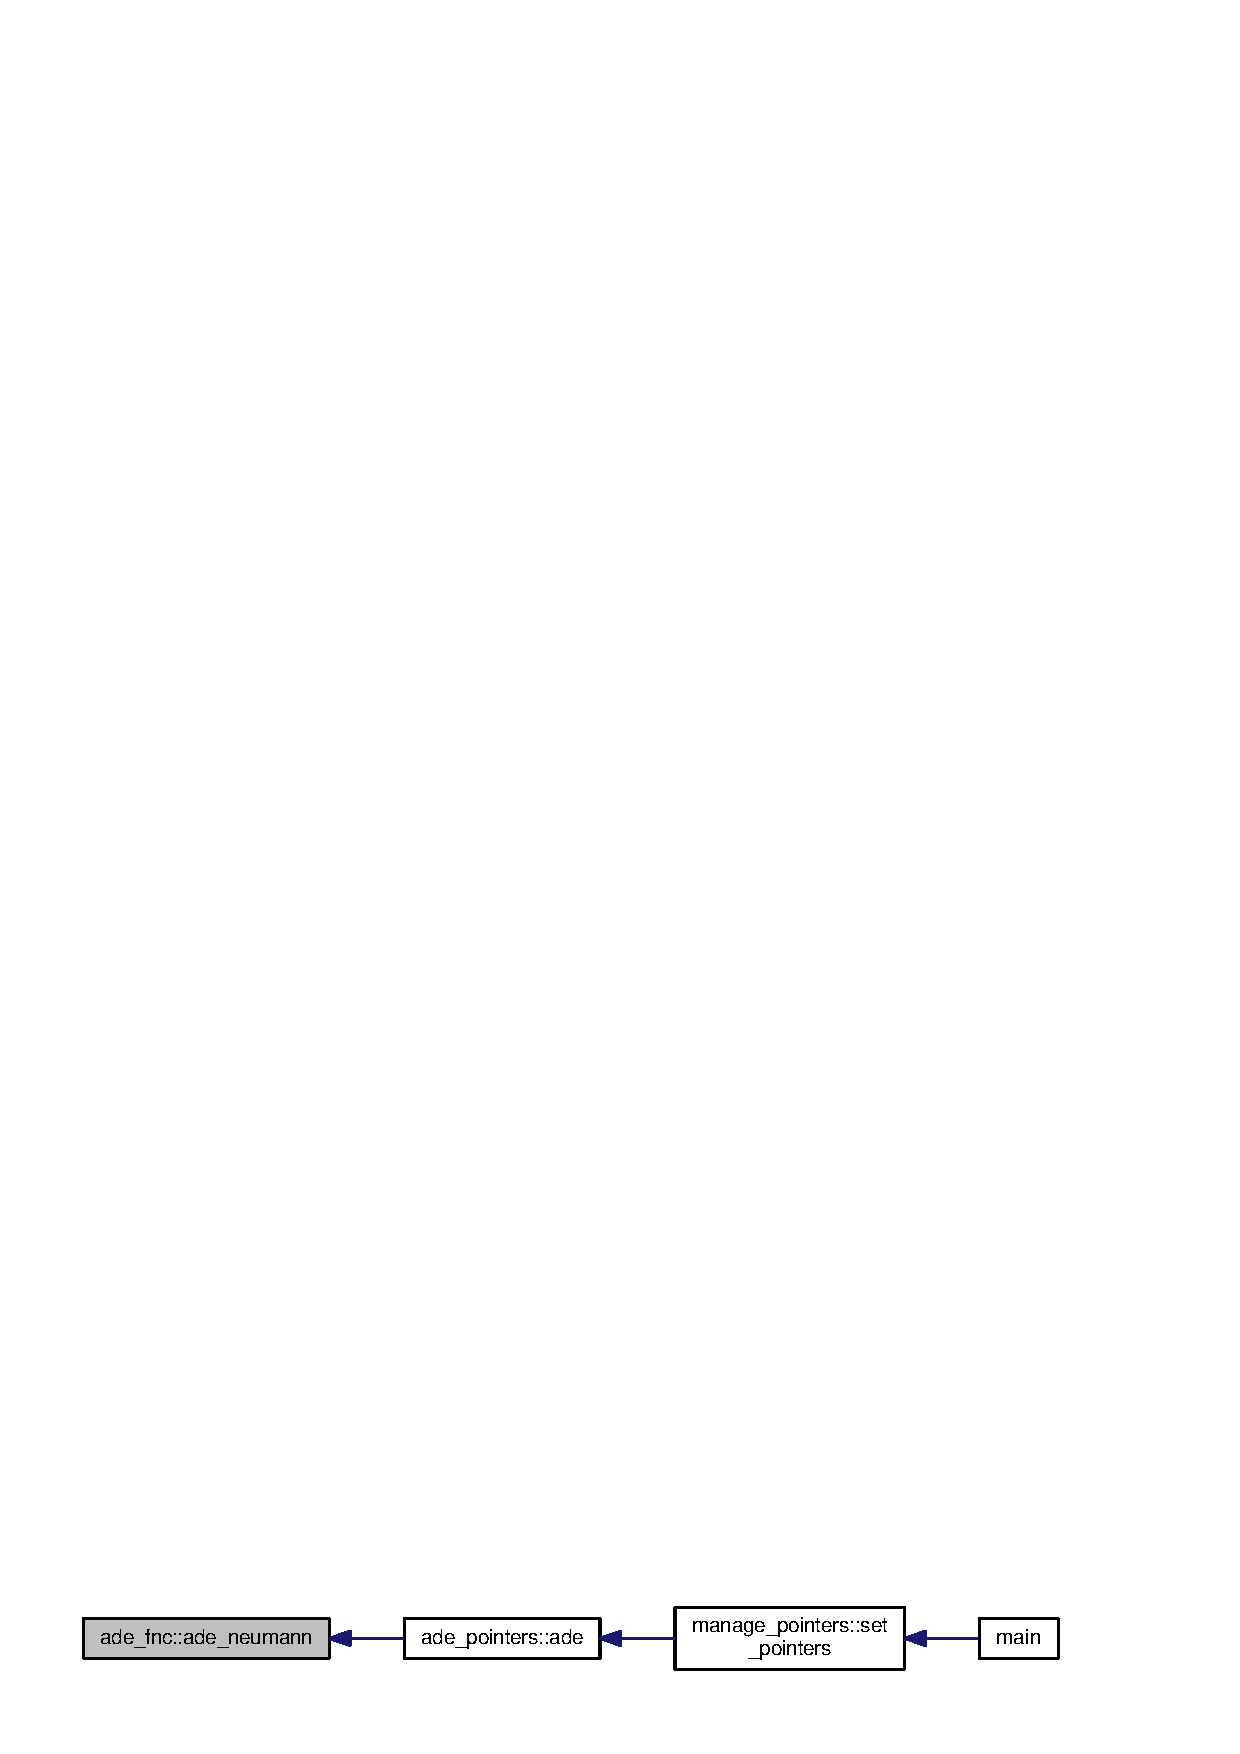
\includegraphics[width=350pt]{namespaceade__fnc_ae9d3681beeaa8b72726418a2b999aa44_icgraph}
\end{center}
\end{figure}


\index{ade\+\_\+fnc@{ade\+\_\+fnc}!ade\+\_\+null\+\_\+bc@{ade\+\_\+null\+\_\+bc}}
\index{ade\+\_\+null\+\_\+bc@{ade\+\_\+null\+\_\+bc}!ade\+\_\+fnc@{ade\+\_\+fnc}}
\subsubsection[{ade\+\_\+null\+\_\+bc(pde\+\_\+loc, el\+\_\+id, node\+\_\+order, value, code)}]{\setlength{\rightskip}{0pt plus 5cm}subroutine, public ade\+\_\+fnc\+::ade\+\_\+null\+\_\+bc (
\begin{DoxyParamCaption}
\item[{class({\bf pde\+\_\+str}), intent(in)}]{pde\+\_\+loc, }
\item[{integer(kind=ikind), intent(in)}]{el\+\_\+id, }
\item[{integer(kind=ikind), intent(in)}]{node\+\_\+order, }
\item[{real(kind=rkind), intent(out), optional}]{value, }
\item[{integer(kind=ikind), intent(out), optional}]{code}
\end{DoxyParamCaption}
)}\label{namespaceade__fnc_a0b4f8cc5e0aff6715d720149a3f4529d}


Definition at line 439 of file A\+D\+E\+\_\+fnc.\+f90.



Referenced by ade\+\_\+pointers\+::adekinsorb().


\begin{DoxyCode}
439       \textcolor{keywordtype}{use }typy
440       \textcolor{keywordtype}{use }globals
441       \textcolor{keywordtype}{use }global_objs
442       \textcolor{keywordtype}{use }pde_objs
443       
444       \textcolor{keywordtype}{class}(pde_str), \textcolor{keywordtype}{intent(in)} :: pde\_loc
445       \textcolor{keywordtype}{integer(kind=ikind)}, \textcolor{keywordtype}{intent(in)}  :: el\_id, node\_order
446       \textcolor{keywordtype}{real(kind=rkind)}, \textcolor{keywordtype}{intent(out)}, \textcolor{keywordtype}{optional}    :: value
447       \textcolor{keywordtype}{integer(kind=ikind)}, \textcolor{keywordtype}{intent(out)}, \textcolor{keywordtype}{optional} :: code
448 
449       \textcolor{keywordflow}{if} (\textcolor{keyword}{present}(\textcolor{keywordtype}{value})) \textcolor{keywordflow}{then}
450         \textcolor{keywordtype}{value} = 0.0\_rkind
451 \textcolor{keywordflow}{      end if}
452 
453       \textcolor{keywordflow}{if} (\textcolor{keyword}{present}(code)) \textcolor{keywordflow}{then}
454         code = 2
455 \textcolor{keywordflow}{      end if}
456         
\end{DoxyCode}


Here is the caller graph for this function\+:\nopagebreak
\begin{figure}[H]
\begin{center}
\leavevmode
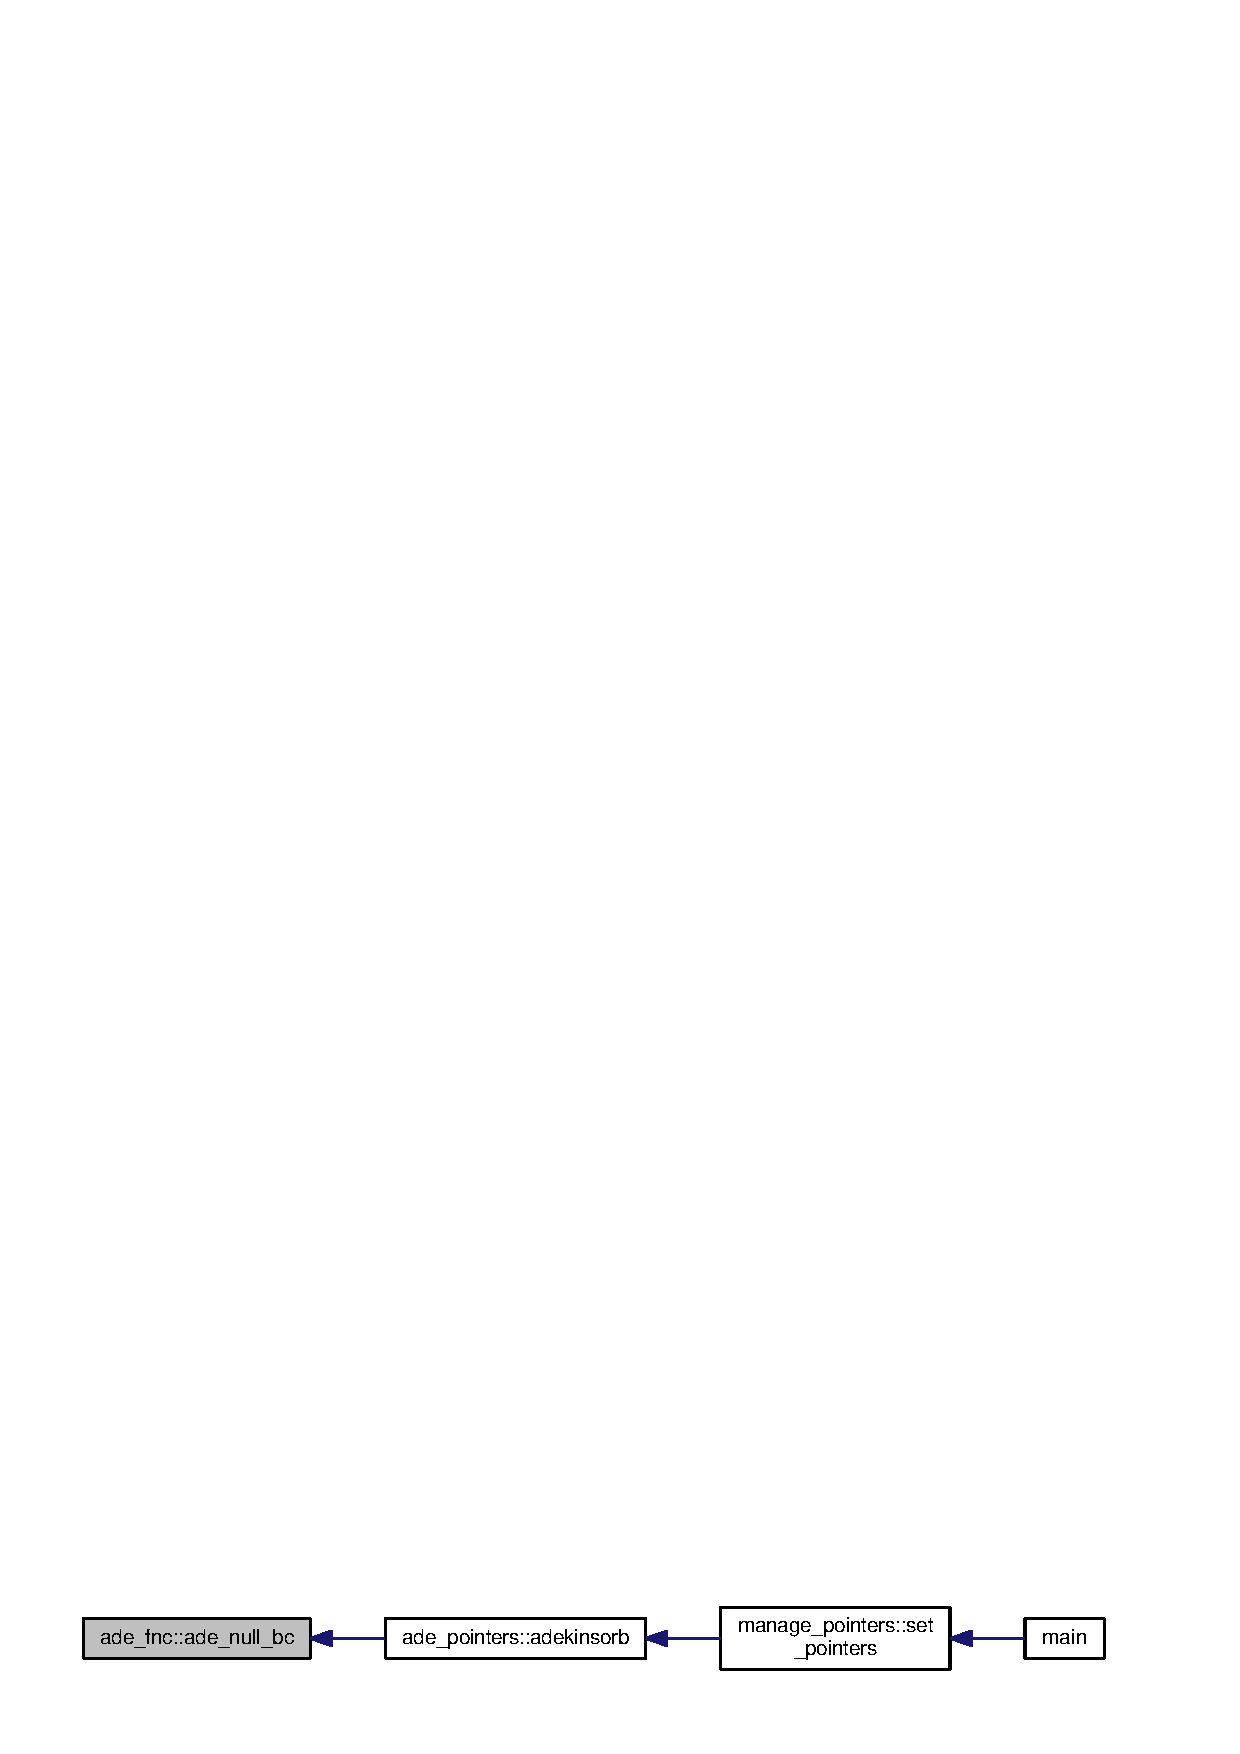
\includegraphics[width=350pt]{namespaceade__fnc_a0b4f8cc5e0aff6715d720149a3f4529d_icgraph}
\end{center}
\end{figure}


\index{ade\+\_\+fnc@{ade\+\_\+fnc}!ade\+\_\+reaction@{ade\+\_\+reaction}}
\index{ade\+\_\+reaction@{ade\+\_\+reaction}!ade\+\_\+fnc@{ade\+\_\+fnc}}
\subsubsection[{ade\+\_\+reaction(pde\+\_\+loc, layer, quadpnt, x)}]{\setlength{\rightskip}{0pt plus 5cm}real(kind=rkind) function, public ade\+\_\+fnc\+::ade\+\_\+reaction (
\begin{DoxyParamCaption}
\item[{class({\bf pde\+\_\+str}), intent(in)}]{pde\+\_\+loc, }
\item[{integer(kind=ikind), intent(in)}]{layer, }
\item[{type({\bf integpnt\+\_\+str}), intent(in), optional}]{quadpnt, }
\item[{real(kind=rkind), dimension(\+:), intent(in), optional}]{x}
\end{DoxyParamCaption}
)}\label{namespaceade__fnc_a68093fda9691ff2d4e6095af69b410f3}

\begin{DoxyParams}[1]{Parameters}
\mbox{\tt in}  & {\em x} & value of the nonlinear function\\
\hline
\mbox{\tt in}  & {\em quadpnt} & Gauss quadrature point structure (element number and rank of Gauss quadrature point)\\
\hline
\mbox{\tt in}  & {\em layer} & material ID\\
\hline
\end{DoxyParams}
\begin{DoxyReturn}{Returns}
return value 
\end{DoxyReturn}


Definition at line 264 of file A\+D\+E\+\_\+fnc.\+f90.



References ade\+\_\+globals\+::adepar, and pde\+\_\+objs\+::pde.



Referenced by ade\+\_\+pointers\+::ade().


\begin{DoxyCode}
264       \textcolor{keywordtype}{use }typy
265       \textcolor{keywordtype}{use }global_objs
266       \textcolor{keywordtype}{use }pde_objs
267       \textcolor{keywordtype}{use }ade_globals
268       
269       \textcolor{keywordtype}{class}(pde_str), \textcolor{keywordtype}{intent(in)} :: pde\_loc
271       \textcolor{keywordtype}{real(kind=rkind)}, \textcolor{keywordtype}{dimension(:)}, \textcolor{keywordtype}{intent(in)}, \textcolor{keywordtype}{optional}    :: x
273       \textcolor{keywordtype}{type}(integpnt_str), \textcolor{keywordtype}{intent(in)}, \textcolor{keywordtype}{optional} :: quadpnt
275       \textcolor{keywordtype}{integer(kind=ikind)}, \textcolor{keywordtype}{intent(in)} :: layer
277       \textcolor{keywordtype}{real(kind=rkind)}                :: val 
278       
279       \textcolor{keywordtype}{integer(kind=ikind)} :: n, i
280       \textcolor{keywordtype}{real(kind=rkind)} :: theta, cl
281       
282      
283       \textcolor{keywordflow}{if} (pde\_loc%order == 2) \textcolor{keywordflow}{then}
284         theta = pde(1)%mass(layer, quadpnt)
285       \textcolor{keywordflow}{else}
286         theta = adepar(layer)%water\_cont
287 \textcolor{keywordflow}{      end if}
288       
289       val = 0.0\_rkind
290       
291       \textcolor{keywordflow}{do} i=1, ubound(adepar(layer)%orders,1)
292         n = 10
293         \textcolor{keywordflow}{if} (abs(adepar(layer)%orders(i) - 1.0\_rkind) < 100*epsilon(1.0\_rkind)) n\textcolor{comment}{ = 1}
294 \textcolor{comment}{        }\textcolor{keywordflow}{if} (abs(adepar(layer)%orders(i)) < 100*epsilon(1.0\_rkind)) n = 0
295         \textcolor{keywordflow}{select case}(n)
296           \textcolor{keywordflow}{case}(0)
297             \textcolor{keywordflow}{CONTINUE}
298           \textcolor{keywordflow}{case}(1)
299             val = val + theta*adepar(layer)%lambda(i)
300 \textcolor{keywordflow}{          case default}
301             cl = pde\_loc%getval(quadpnt)
302             val = theta*adepar(layer)%lambda(i)*cl**(adepar(layer)%orders(i)-1)
303 \textcolor{keywordflow}{        end select}
304 \textcolor{keywordflow}{      end do}
305         
306           
307       
308       
\end{DoxyCode}


Here is the caller graph for this function\+:\nopagebreak
\begin{figure}[H]
\begin{center}
\leavevmode
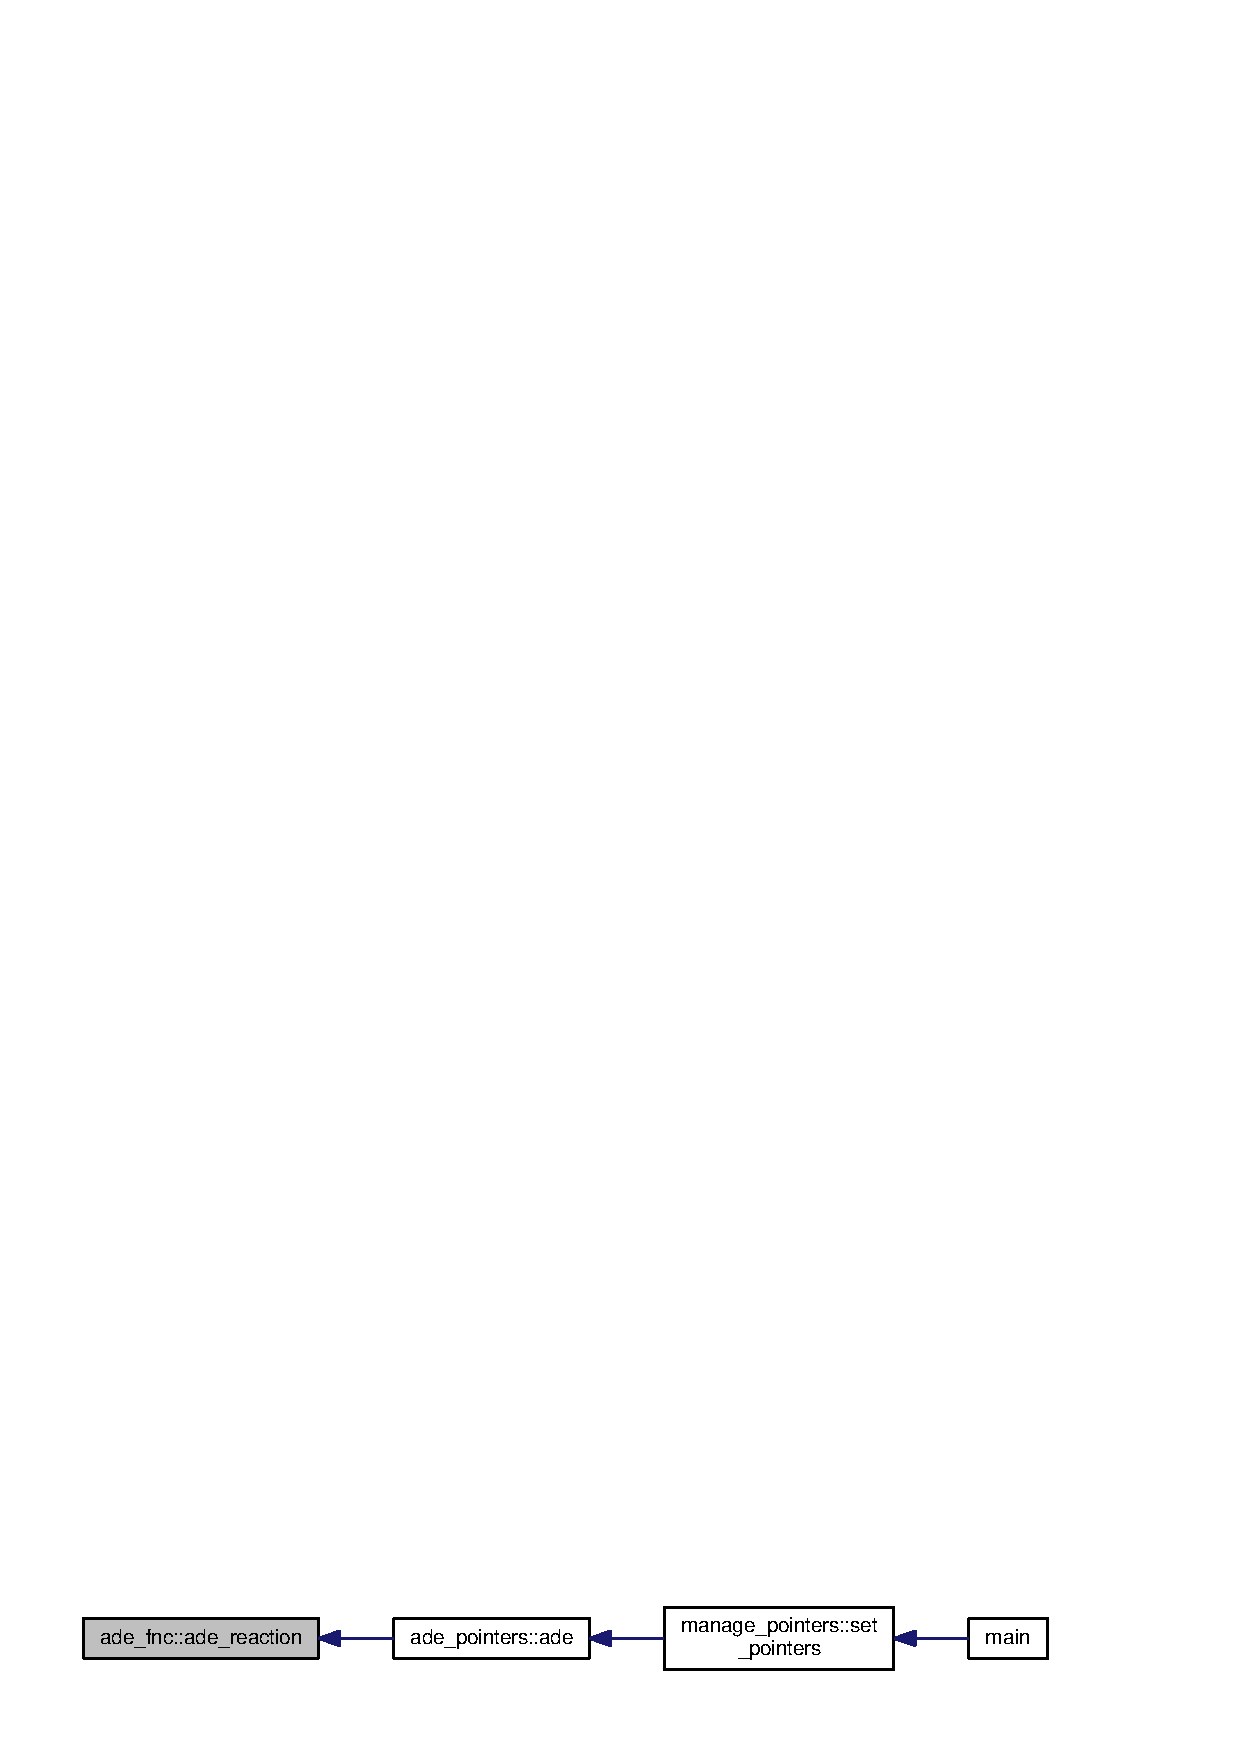
\includegraphics[width=350pt]{namespaceade__fnc_a68093fda9691ff2d4e6095af69b410f3_icgraph}
\end{center}
\end{figure}


\index{ade\+\_\+fnc@{ade\+\_\+fnc}!ade\+\_\+tder\+\_\+coef@{ade\+\_\+tder\+\_\+coef}}
\index{ade\+\_\+tder\+\_\+coef@{ade\+\_\+tder\+\_\+coef}!ade\+\_\+fnc@{ade\+\_\+fnc}}
\subsubsection[{ade\+\_\+tder\+\_\+coef(pde\+\_\+loc, layer, quadpnt, x)}]{\setlength{\rightskip}{0pt plus 5cm}real(kind=rkind) function, public ade\+\_\+fnc\+::ade\+\_\+tder\+\_\+coef (
\begin{DoxyParamCaption}
\item[{class({\bf pde\+\_\+str}), intent(in)}]{pde\+\_\+loc, }
\item[{integer(kind=ikind), intent(in)}]{layer, }
\item[{type({\bf integpnt\+\_\+str}), intent(in), optional}]{quadpnt, }
\item[{real(kind=rkind), dimension(\+:), intent(in), optional}]{x}
\end{DoxyParamCaption}
)}\label{namespaceade__fnc_a9955421b18edc5044b7fbe483890ff0a}

\begin{DoxyParams}[1]{Parameters}
\mbox{\tt in}  & {\em x} & value of the nonlinear function\\
\hline
\mbox{\tt in}  & {\em quadpnt} & Gauss quadrature point structure (element number and rank of Gauss quadrature point)\\
\hline
\mbox{\tt in}  & {\em layer} & material ID\\
\hline
\end{DoxyParams}
\begin{DoxyReturn}{Returns}
return value 
\end{DoxyReturn}


Definition at line 121 of file A\+D\+E\+\_\+fnc.\+f90.



References ade\+\_\+globals\+::adepar, and pde\+\_\+objs\+::pde.



Referenced by ade\+\_\+pointers\+::ade().


\begin{DoxyCode}
121       \textcolor{keywordtype}{use }typy
122       \textcolor{keywordtype}{use }global_objs
123       \textcolor{keywordtype}{use }pde_objs
124       \textcolor{keywordtype}{use }ade_globals
125       
126       \textcolor{keywordtype}{class}(pde_str), \textcolor{keywordtype}{intent(in)} :: pde\_loc
128       \textcolor{keywordtype}{real(kind=rkind)}, \textcolor{keywordtype}{dimension(:)}, \textcolor{keywordtype}{intent(in)}, \textcolor{keywordtype}{optional}    :: x
130       \textcolor{keywordtype}{type}(integpnt_str), \textcolor{keywordtype}{intent(in)}, \textcolor{keywordtype}{optional} :: quadpnt
132       \textcolor{keywordtype}{integer(kind=ikind)}, \textcolor{keywordtype}{intent(in)} :: layer
134       \textcolor{keywordtype}{real(kind=rkind)}                :: val
135       
136       \textcolor{keywordtype}{real(kind=rkind)} :: theta, n, ka, kd, csmax, cl
137       
138       
139       \textcolor{keywordflow}{if} (pde\_loc%order == 2) \textcolor{keywordflow}{then}
140         theta = pde(1)%mass(layer, quadpnt)
141       \textcolor{keywordflow}{else}
142         theta = adepar(layer)%water\_cont
143 \textcolor{keywordflow}{      end if}
144       
145       
146       \textcolor{keywordflow}{if} (.not. adepar(layer)%sorption%kinetic) \textcolor{keywordflow}{then}
147         ka = adepar(layer)%sorption%adsorb
148         kd = adepar(layer)%sorption%desorb
149         \textcolor{keywordflow}{if} (ka > 10*epsilon(ka) .and. kd > 10*epsilon(kd)) \textcolor{keywordflow}{then} 
150           \textcolor{keywordflow}{select case}(adepar(layer)%sorption%name)
151             \textcolor{keywordflow}{case}(\textcolor{stringliteral}{"freund"})
152               n = adepar(layer)%sorption%third
153               \textcolor{keywordflow}{if} (abs(n-1.0\_rkind)>10*epsilon(n)) \textcolor{keywordflow}{then}
154                 cl = pde\_loc%getval(quadpnt)
155                 val = theta+(1-theta)*ka/kd*adepar(layer)%bd*cl**(n-1)
156               \textcolor{keywordflow}{else}
157                 val = theta+(1-theta)*ka/kd*adepar(layer)%bd
158 \textcolor{keywordflow}{              end if}
159             
160             \textcolor{keywordflow}{case}(\textcolor{stringliteral}{"langmu"})
161               cl = pde\_loc%getval(quadpnt)
162               csmax = adepar(layer)%sorption%third
163               val = theta + (1-theta)*adepar(layer)%bd*(ka*csmax)/(kd+ka*cl)
164 \textcolor{keywordflow}{            case default}
165               print *, \textcolor{stringliteral}{"unsupported sorption type, runtime error, called from ADE\_fnc::ADE\_tder\_coef"}
166               error stop
167             
168 \textcolor{keywordflow}{          end select}
169         \textcolor{keywordflow}{else}
170           val = theta
171 \textcolor{keywordflow}{        end if}
172         
173       \textcolor{keywordflow}{else}
174         val = theta
175 \textcolor{keywordflow}{      end if}
176      
177       
178     
\end{DoxyCode}


Here is the caller graph for this function\+:\nopagebreak
\begin{figure}[H]
\begin{center}
\leavevmode
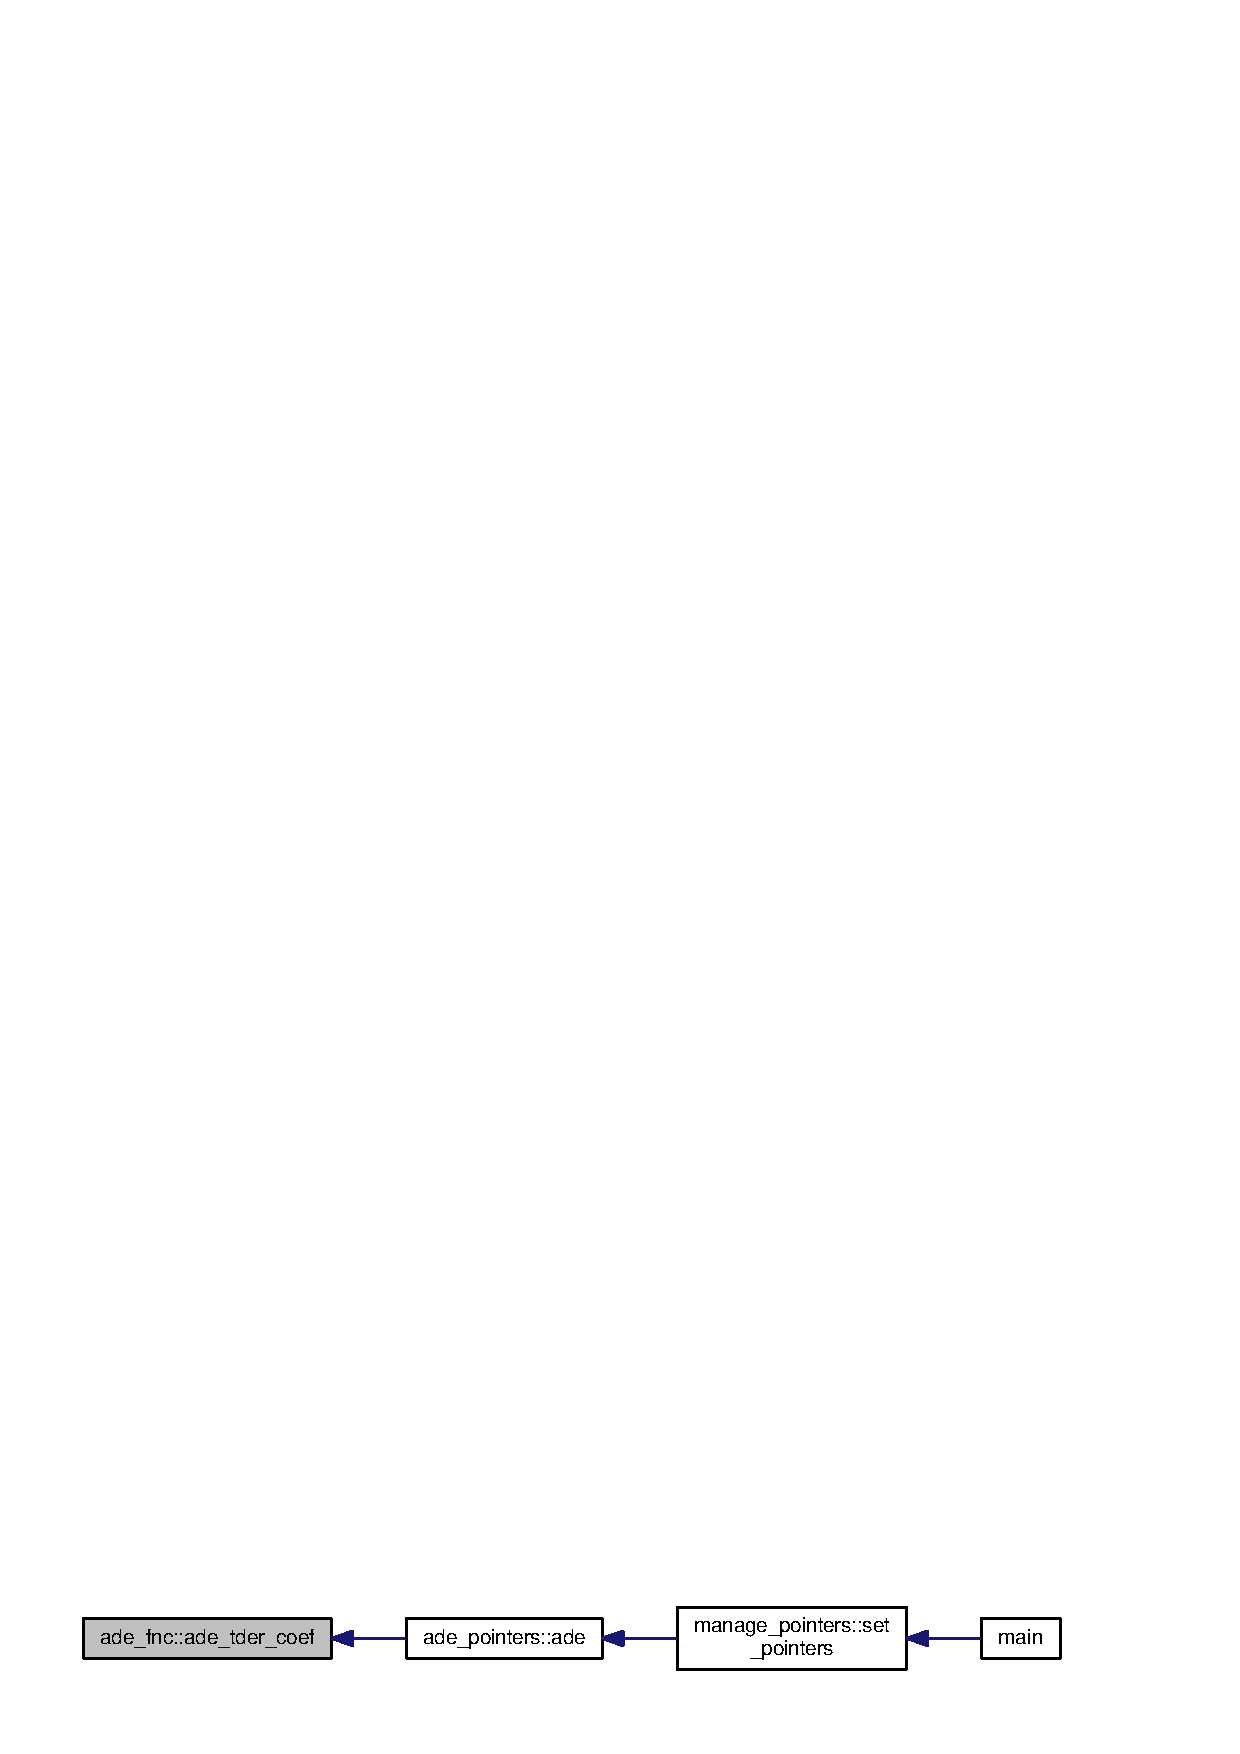
\includegraphics[width=350pt]{namespaceade__fnc_a9955421b18edc5044b7fbe483890ff0a_icgraph}
\end{center}
\end{figure}


\index{ade\+\_\+fnc@{ade\+\_\+fnc}!ade\+\_\+tder\+\_\+cscl@{ade\+\_\+tder\+\_\+cscl}}
\index{ade\+\_\+tder\+\_\+cscl@{ade\+\_\+tder\+\_\+cscl}!ade\+\_\+fnc@{ade\+\_\+fnc}}
\subsubsection[{ade\+\_\+tder\+\_\+cscl(pde\+\_\+loc, layer, quadpnt, x)}]{\setlength{\rightskip}{0pt plus 5cm}real(kind=rkind) function, public ade\+\_\+fnc\+::ade\+\_\+tder\+\_\+cscl (
\begin{DoxyParamCaption}
\item[{class({\bf pde\+\_\+str}), intent(in)}]{pde\+\_\+loc, }
\item[{integer(kind=ikind), intent(in)}]{layer, }
\item[{type({\bf integpnt\+\_\+str}), intent(in), optional}]{quadpnt, }
\item[{real(kind=rkind), dimension(\+:), intent(in), optional}]{x}
\end{DoxyParamCaption}
)}\label{namespaceade__fnc_afeaf3d25774abb287c3e3fc98b54b83a}

\begin{DoxyParams}[1]{Parameters}
\mbox{\tt in}  & {\em x} & value of the nonlinear function\\
\hline
\mbox{\tt in}  & {\em quadpnt} & Gauss quadrature point structure (element number and rank of Gauss quadrature point)\\
\hline
\mbox{\tt in}  & {\em layer} & material ID\\
\hline
\end{DoxyParams}
\begin{DoxyReturn}{Returns}
return value 
\end{DoxyReturn}


Definition at line 183 of file A\+D\+E\+\_\+fnc.\+f90.



References ade\+\_\+globals\+::adepar, and pde\+\_\+objs\+::pde.



Referenced by ade\+\_\+pointers\+::adekinsorb().


\begin{DoxyCode}
183       \textcolor{keywordtype}{use }typy
184       \textcolor{keywordtype}{use }global_objs
185       \textcolor{keywordtype}{use }pde_objs
186       \textcolor{keywordtype}{use }ade_globals
187       
188       \textcolor{keywordtype}{class}(pde_str), \textcolor{keywordtype}{intent(in)} :: pde\_loc
190       \textcolor{keywordtype}{real(kind=rkind)}, \textcolor{keywordtype}{dimension(:)}, \textcolor{keywordtype}{intent(in)}, \textcolor{keywordtype}{optional}    :: x
192       \textcolor{keywordtype}{type}(integpnt_str), \textcolor{keywordtype}{intent(in)}, \textcolor{keywordtype}{optional} :: quadpnt
194       \textcolor{keywordtype}{integer(kind=ikind)}, \textcolor{keywordtype}{intent(in)} :: layer
196       \textcolor{keywordtype}{real(kind=rkind)}                :: val
197       
198       \textcolor{keywordtype}{real(kind=rkind)} :: theta
199       
200       \textcolor{keywordflow}{if} (pde\_loc%order == 2) \textcolor{keywordflow}{then}
201         theta = pde(1)%mass(layer, quadpnt)
202       \textcolor{keywordflow}{else}
203         theta = adepar(layer)%water\_cont
204 \textcolor{keywordflow}{      end if}
205       
206       val = 1.0\_rkind-theta
207       
\end{DoxyCode}


Here is the caller graph for this function\+:\nopagebreak
\begin{figure}[H]
\begin{center}
\leavevmode
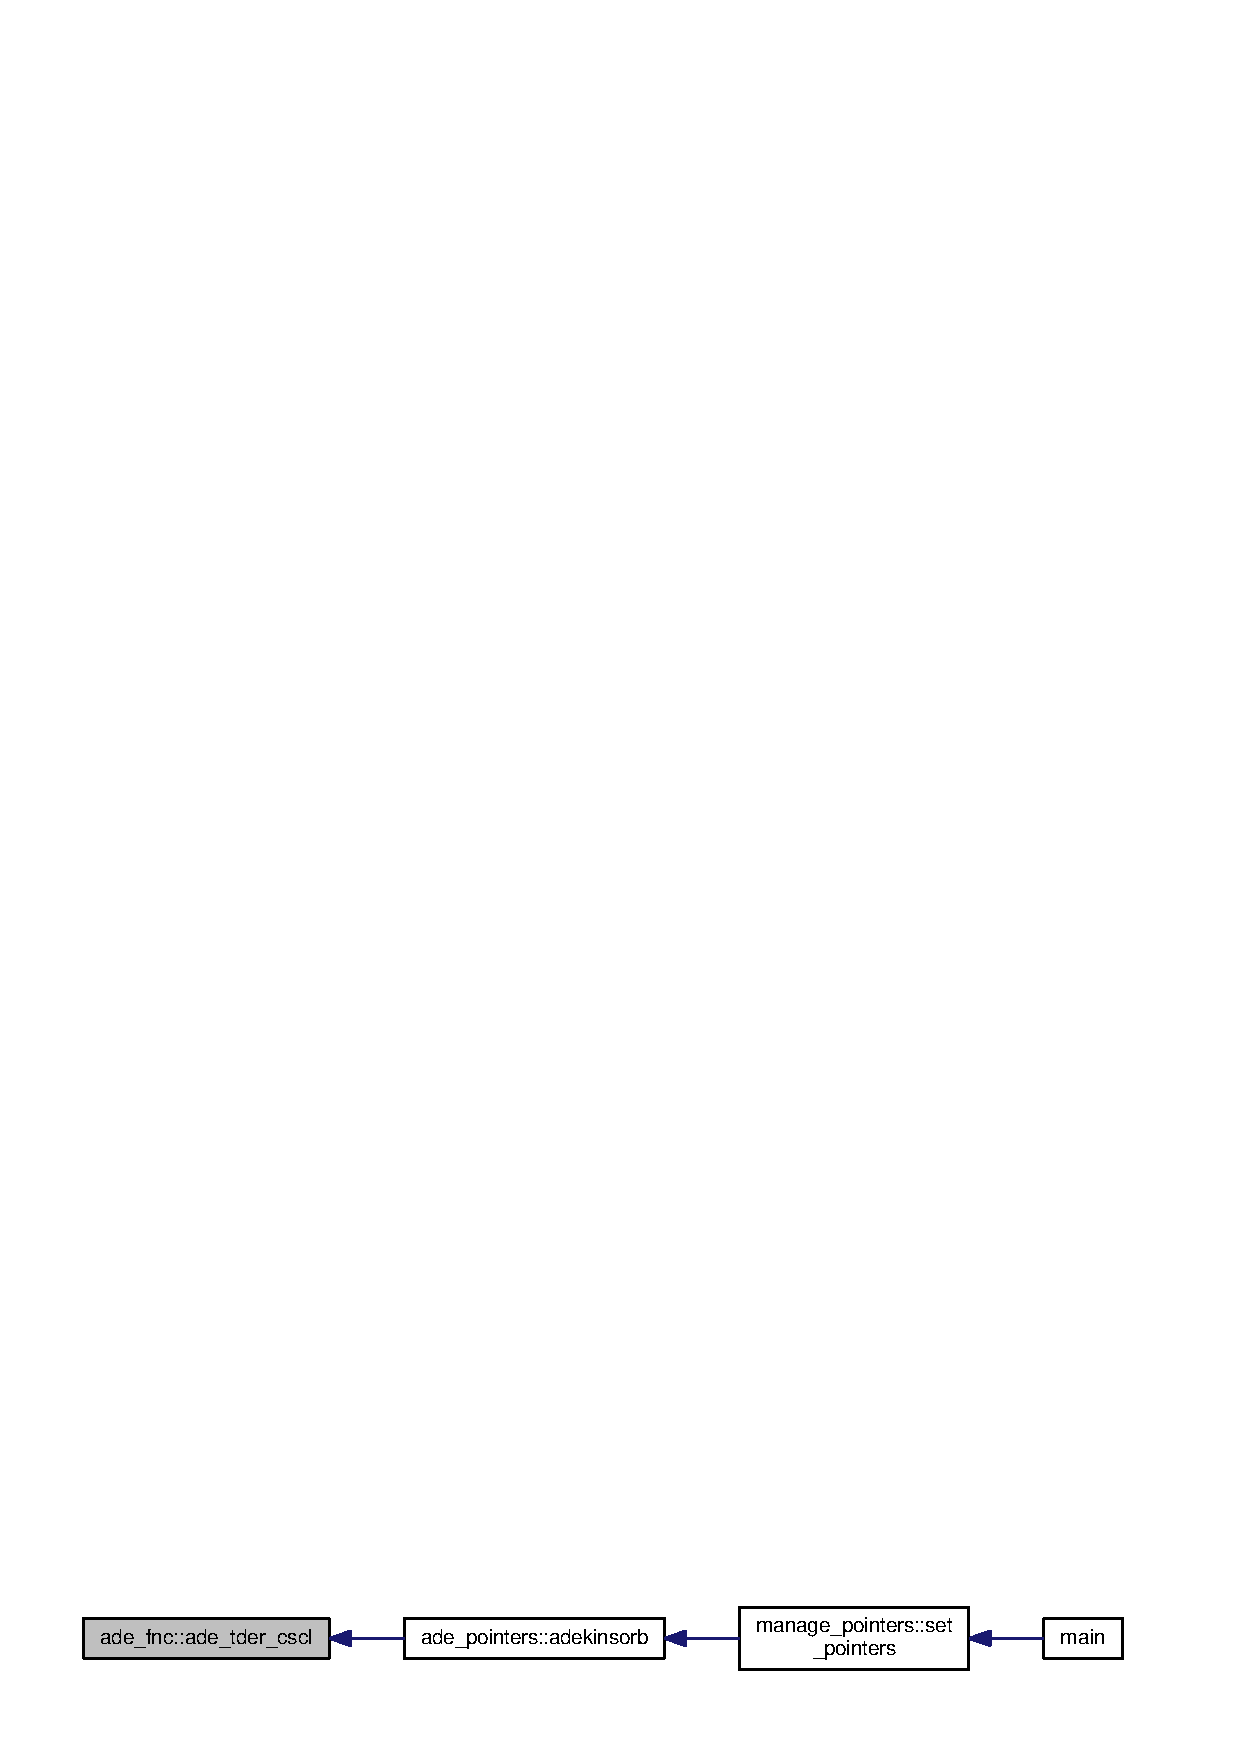
\includegraphics[width=350pt]{namespaceade__fnc_afeaf3d25774abb287c3e3fc98b54b83a_icgraph}
\end{center}
\end{figure}


\index{ade\+\_\+fnc@{ade\+\_\+fnc}!ade\+\_\+tder\+\_\+cscs@{ade\+\_\+tder\+\_\+cscs}}
\index{ade\+\_\+tder\+\_\+cscs@{ade\+\_\+tder\+\_\+cscs}!ade\+\_\+fnc@{ade\+\_\+fnc}}
\subsubsection[{ade\+\_\+tder\+\_\+cscs(pde\+\_\+loc, layer, quadpnt, x)}]{\setlength{\rightskip}{0pt plus 5cm}real(kind=rkind) function, public ade\+\_\+fnc\+::ade\+\_\+tder\+\_\+cscs (
\begin{DoxyParamCaption}
\item[{class({\bf pde\+\_\+str}), intent(in)}]{pde\+\_\+loc, }
\item[{integer(kind=ikind), intent(in)}]{layer, }
\item[{type({\bf integpnt\+\_\+str}), intent(in), optional}]{quadpnt, }
\item[{real(kind=rkind), dimension(\+:), intent(in), optional}]{x}
\end{DoxyParamCaption}
)}\label{namespaceade__fnc_a22f1baa0530346804607e15b6555855c}

\begin{DoxyParams}[1]{Parameters}
\mbox{\tt in}  & {\em x} & value of the nonlinear function\\
\hline
\mbox{\tt in}  & {\em quadpnt} & Gauss quadrature point structure (element number and rank of Gauss quadrature point)\\
\hline
\mbox{\tt in}  & {\em layer} & material ID\\
\hline
\end{DoxyParams}
\begin{DoxyReturn}{Returns}
return value 
\end{DoxyReturn}


Definition at line 212 of file A\+D\+E\+\_\+fnc.\+f90.



Referenced by ade\+\_\+pointers\+::adekinsorb().


\begin{DoxyCode}
212       \textcolor{keywordtype}{use }typy
213       \textcolor{keywordtype}{use }global_objs
214       \textcolor{keywordtype}{use }pde_objs
215       \textcolor{keywordtype}{use }ade_globals
216       
217       \textcolor{keywordtype}{class}(pde_str), \textcolor{keywordtype}{intent(in)} :: pde\_loc
219       \textcolor{keywordtype}{real(kind=rkind)}, \textcolor{keywordtype}{dimension(:)}, \textcolor{keywordtype}{intent(in)}, \textcolor{keywordtype}{optional}    :: x
221       \textcolor{keywordtype}{type}(integpnt_str), \textcolor{keywordtype}{intent(in)}, \textcolor{keywordtype}{optional} :: quadpnt
223       \textcolor{keywordtype}{integer(kind=ikind)}, \textcolor{keywordtype}{intent(in)} :: layer
225       \textcolor{keywordtype}{real(kind=rkind)}                :: val
226       
227       val = 1.0\_rkind
228     
\end{DoxyCode}


Here is the caller graph for this function\+:\nopagebreak
\begin{figure}[H]
\begin{center}
\leavevmode
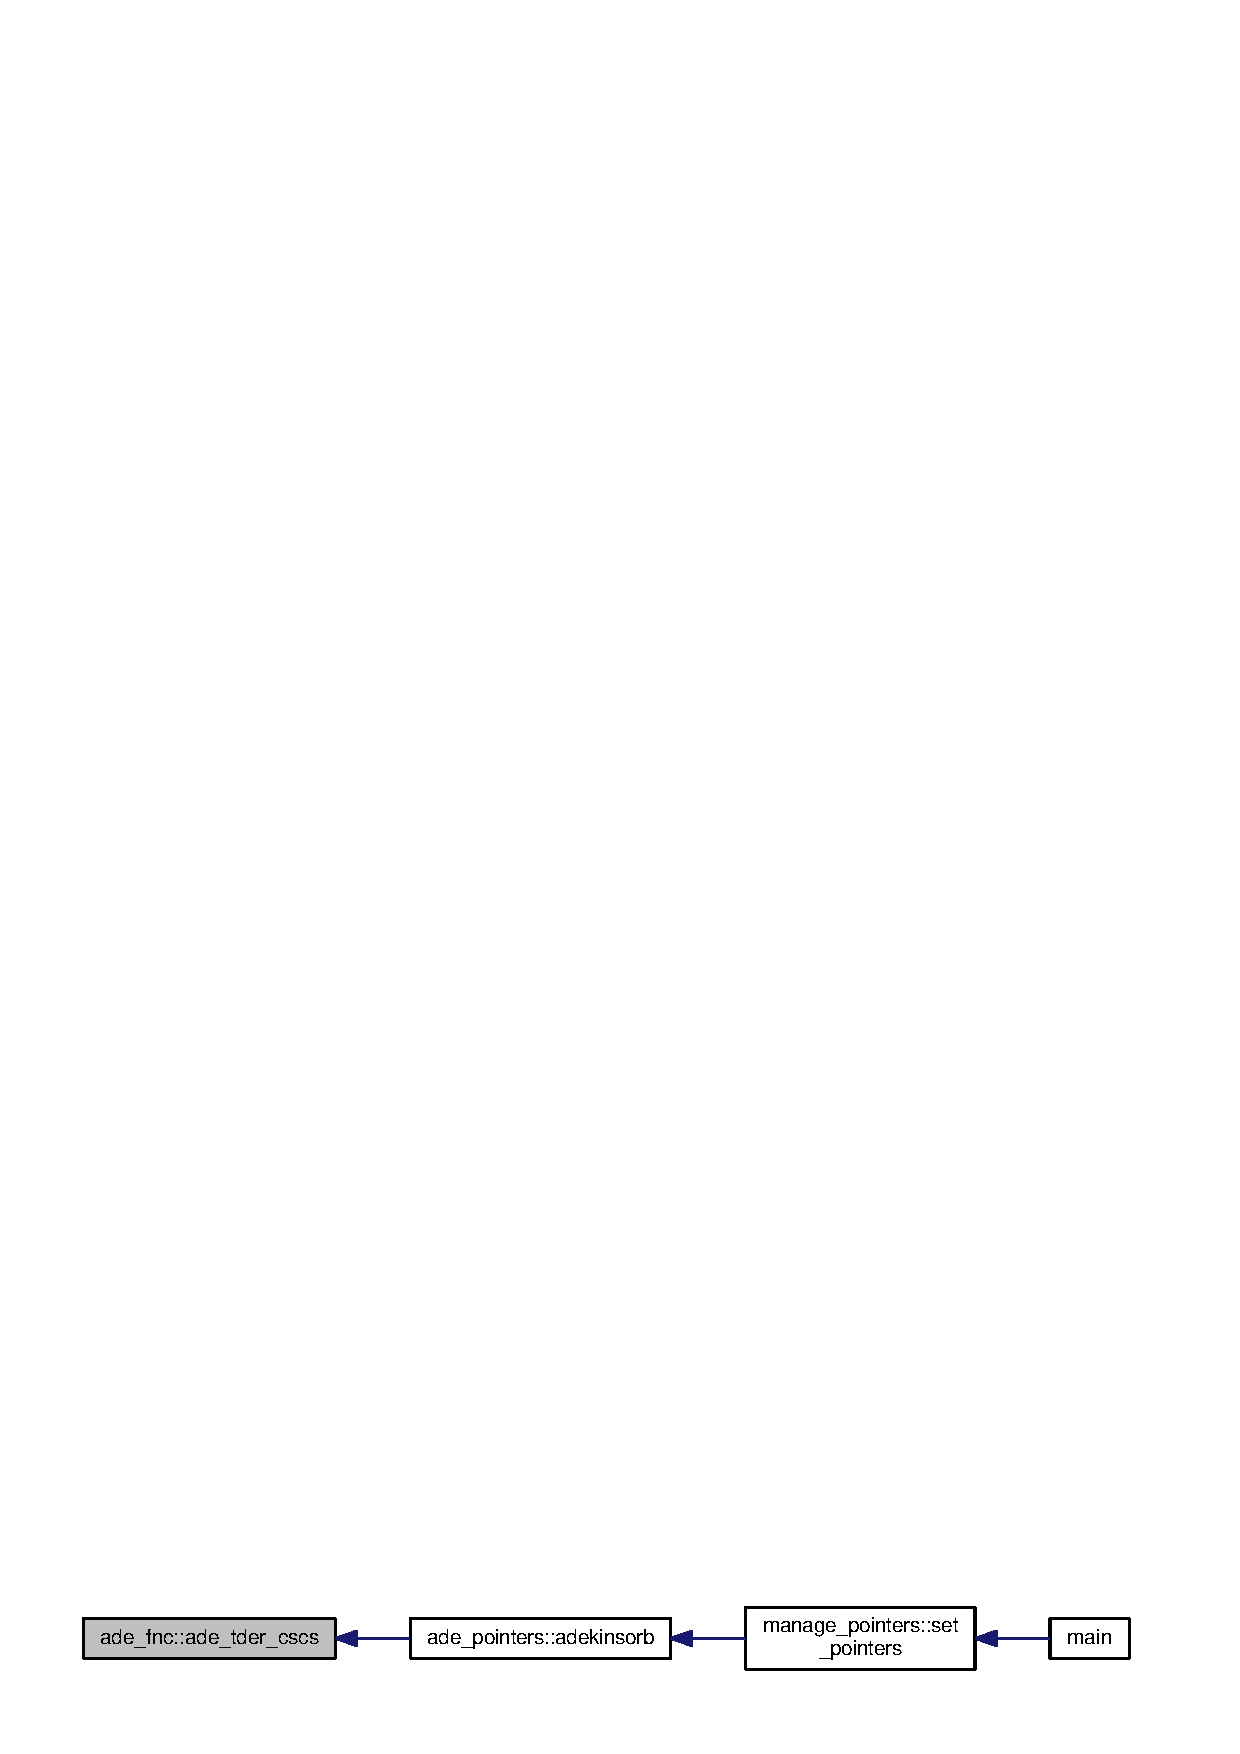
\includegraphics[width=350pt]{namespaceade__fnc_a22f1baa0530346804607e15b6555855c_icgraph}
\end{center}
\end{figure}


\index{ade\+\_\+fnc@{ade\+\_\+fnc}!ade\+\_\+zerorder@{ade\+\_\+zerorder}}
\index{ade\+\_\+zerorder@{ade\+\_\+zerorder}!ade\+\_\+fnc@{ade\+\_\+fnc}}
\subsubsection[{ade\+\_\+zerorder(pde\+\_\+loc, layer, quadpnt, x)}]{\setlength{\rightskip}{0pt plus 5cm}real(kind=rkind) function, public ade\+\_\+fnc\+::ade\+\_\+zerorder (
\begin{DoxyParamCaption}
\item[{class({\bf pde\+\_\+str}), intent(in)}]{pde\+\_\+loc, }
\item[{integer(kind=ikind), intent(in)}]{layer, }
\item[{type({\bf integpnt\+\_\+str}), intent(in), optional}]{quadpnt, }
\item[{real(kind=rkind), dimension(\+:), intent(in), optional}]{x}
\end{DoxyParamCaption}
)}\label{namespaceade__fnc_a2f3a5b22f5274dfbe645210420ce09aa}

\begin{DoxyParams}[1]{Parameters}
\mbox{\tt in}  & {\em x} & value of the nonlinear function\\
\hline
\mbox{\tt in}  & {\em quadpnt} & Gauss quadrature point structure (element number and rank of Gauss quadrature point)\\
\hline
\mbox{\tt in}  & {\em layer} & material ID\\
\hline
\end{DoxyParams}
\begin{DoxyReturn}{Returns}
return value 
\end{DoxyReturn}


Definition at line 312 of file A\+D\+E\+\_\+fnc.\+f90.



References ade\+\_\+globals\+::adepar, and pde\+\_\+objs\+::pde.



Referenced by ade\+\_\+pointers\+::ade().


\begin{DoxyCode}
312       \textcolor{keywordtype}{use }typy
313       \textcolor{keywordtype}{use }global_objs
314       \textcolor{keywordtype}{use }pde_objs
315       \textcolor{keywordtype}{use }ade_globals
316       
317       \textcolor{keywordtype}{class}(pde_str), \textcolor{keywordtype}{intent(in)} :: pde\_loc
319       \textcolor{keywordtype}{real(kind=rkind)}, \textcolor{keywordtype}{dimension(:)}, \textcolor{keywordtype}{intent(in)}, \textcolor{keywordtype}{optional}    :: x
321       \textcolor{keywordtype}{type}(integpnt_str), \textcolor{keywordtype}{intent(in)}, \textcolor{keywordtype}{optional} :: quadpnt
323       \textcolor{keywordtype}{integer(kind=ikind)}, \textcolor{keywordtype}{intent(in)} :: layer
325       \textcolor{keywordtype}{real(kind=rkind)}                :: val 
326       
327       \textcolor{keywordtype}{integer(kind=ikind)} :: n, i
328       \textcolor{keywordtype}{real(kind=rkind)} :: theta
329       
330       \textcolor{keywordflow}{if} (pde\_loc%order == 2) \textcolor{keywordflow}{then}
331         theta = pde(1)%mass(layer, quadpnt)
332       \textcolor{keywordflow}{else}
333         theta = adepar(layer)%water\_cont
334 \textcolor{keywordflow}{      end if}
335       
336        val = 0.0\_rkind
337        \textcolor{keywordflow}{do} i=1, ubound(adepar(layer)%orders,1)
338         \textcolor{keywordflow}{if} (abs(adepar(layer)%orders(i)) < 100*epsilon(1.0\_rkind)) \textcolor{keywordflow}{then}
339           val =  val + theta*adepar(layer)%lambda(i)
340 \textcolor{keywordflow}{        end if}
341 \textcolor{keywordflow}{      end do}
342       
343       
\end{DoxyCode}


Here is the caller graph for this function\+:\nopagebreak
\begin{figure}[H]
\begin{center}
\leavevmode
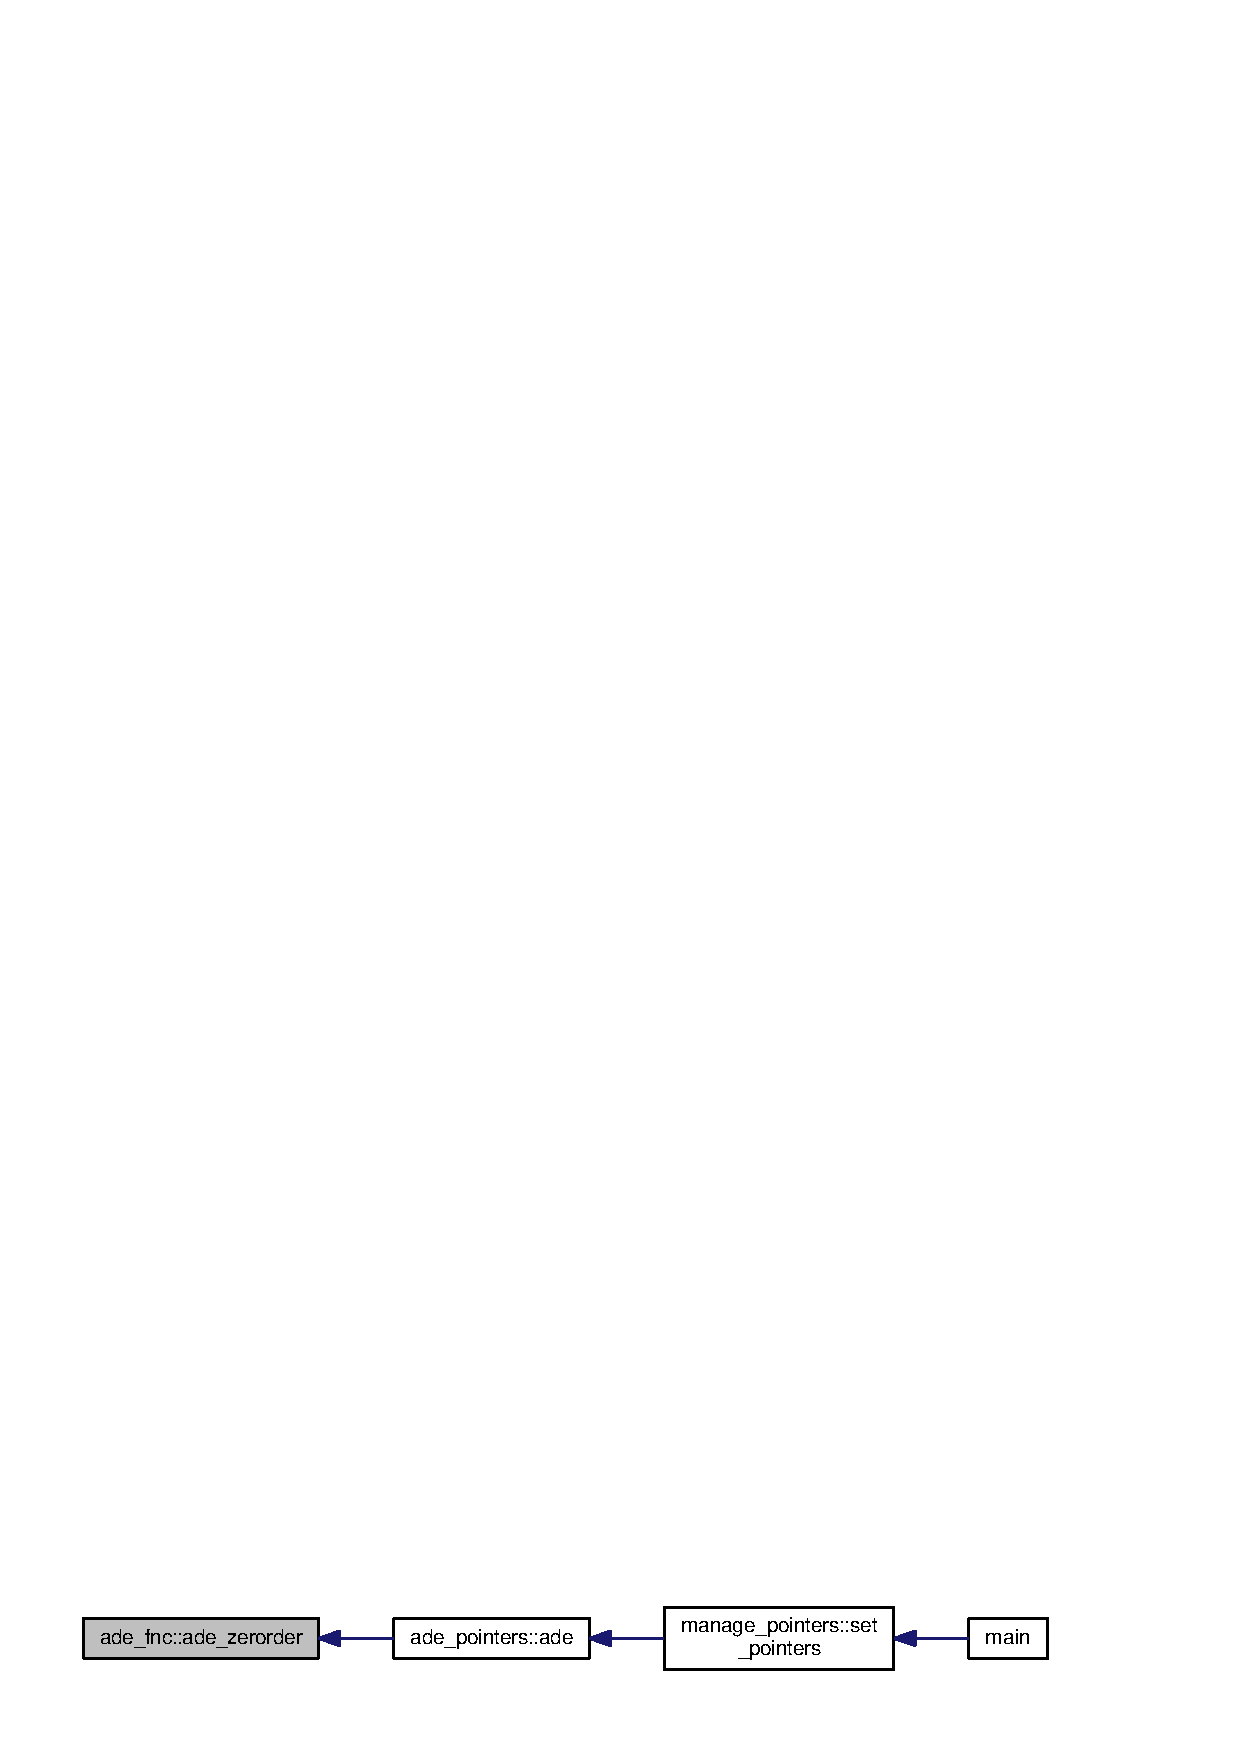
\includegraphics[width=350pt]{namespaceade__fnc_a2f3a5b22f5274dfbe645210420ce09aa_icgraph}
\end{center}
\end{figure}


\index{ade\+\_\+fnc@{ade\+\_\+fnc}!adecs\+\_\+icond@{adecs\+\_\+icond}}
\index{adecs\+\_\+icond@{adecs\+\_\+icond}!ade\+\_\+fnc@{ade\+\_\+fnc}}
\subsubsection[{adecs\+\_\+icond(pde\+\_\+loc)}]{\setlength{\rightskip}{0pt plus 5cm}subroutine, public ade\+\_\+fnc\+::adecs\+\_\+icond (
\begin{DoxyParamCaption}
\item[{class({\bf pde\+\_\+str}), intent(inout)}]{pde\+\_\+loc}
\end{DoxyParamCaption}
)}\label{namespaceade__fnc_a1ee351b59b533ac309638b109669dd06}


Definition at line 675 of file A\+D\+E\+\_\+fnc.\+f90.



Referenced by ade\+\_\+pointers\+::adekinsorb().


\begin{DoxyCode}
675       \textcolor{keywordtype}{use }typy
676       \textcolor{keywordtype}{use }pde_objs
677 
678       
679       \textcolor{keywordtype}{class}(pde_str), \textcolor{keywordtype}{intent(in out)} :: pde\_loc
680       
681       pde\_loc%solution = 0.0\_rkind
682     
\end{DoxyCode}


Here is the caller graph for this function\+:\nopagebreak
\begin{figure}[H]
\begin{center}
\leavevmode
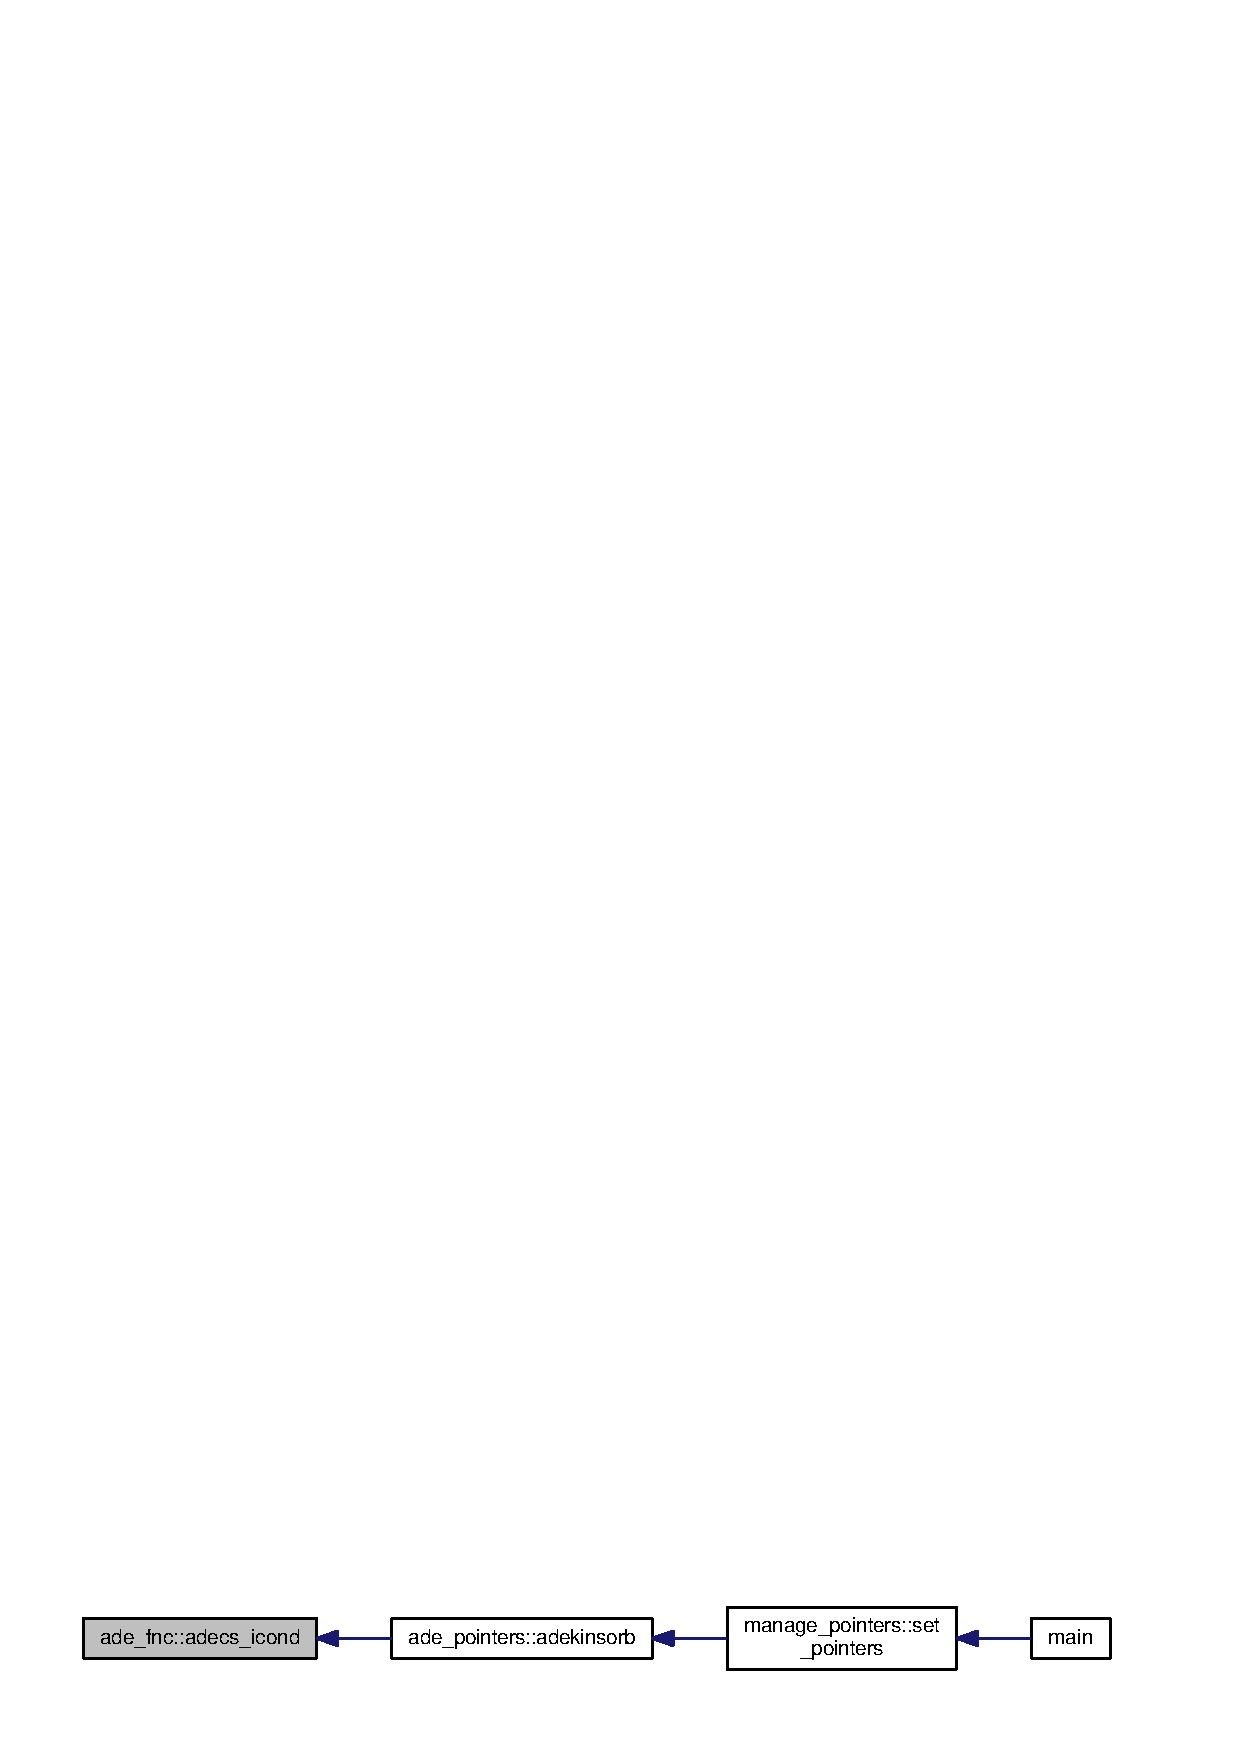
\includegraphics[width=350pt]{namespaceade__fnc_a1ee351b59b533ac309638b109669dd06_icgraph}
\end{center}
\end{figure}


\index{ade\+\_\+fnc@{ade\+\_\+fnc}!adecs\+\_\+mass@{adecs\+\_\+mass}}
\index{adecs\+\_\+mass@{adecs\+\_\+mass}!ade\+\_\+fnc@{ade\+\_\+fnc}}
\subsubsection[{adecs\+\_\+mass(pde\+\_\+loc, layer, quadpnt, x)}]{\setlength{\rightskip}{0pt plus 5cm}real(kind=rkind) function, public ade\+\_\+fnc\+::adecs\+\_\+mass (
\begin{DoxyParamCaption}
\item[{class({\bf pde\+\_\+str}), intent(in)}]{pde\+\_\+loc, }
\item[{integer(kind=ikind), intent(in)}]{layer, }
\item[{type({\bf integpnt\+\_\+str}), intent(in), optional}]{quadpnt, }
\item[{real(kind=rkind), dimension(\+:), intent(in), optional}]{x}
\end{DoxyParamCaption}
)}\label{namespaceade__fnc_a8838abef4e08fe8b063e441aa18708d4}

\begin{DoxyParams}[1]{Parameters}
\mbox{\tt in}  & {\em x} & value of the nonlinear function\\
\hline
\mbox{\tt in}  & {\em quadpnt} & Gauss quadrature point structure (element number and rank of Gauss quadrature point)\\
\hline
\mbox{\tt in}  & {\em layer} & material ID\\
\hline
\end{DoxyParams}
\begin{DoxyReturn}{Returns}
return value 
\end{DoxyReturn}


Definition at line 687 of file A\+D\+E\+\_\+fnc.\+f90.



References ade\+\_\+globals\+::adepar, and pde\+\_\+objs\+::pde.


\begin{DoxyCode}
687       \textcolor{keywordtype}{use }typy
688       \textcolor{keywordtype}{use }global_objs
689       \textcolor{keywordtype}{use }pde_objs
690       \textcolor{keywordtype}{use }ade_globals
691       
692       \textcolor{keywordtype}{class}(pde_str), \textcolor{keywordtype}{intent(in)} :: pde\_loc
694       \textcolor{keywordtype}{real(kind=rkind)}, \textcolor{keywordtype}{dimension(:)}, \textcolor{keywordtype}{intent(in)}, \textcolor{keywordtype}{optional}    :: x
696       \textcolor{keywordtype}{type}(integpnt_str), \textcolor{keywordtype}{intent(in)}, \textcolor{keywordtype}{optional} :: quadpnt
698       \textcolor{keywordtype}{integer(kind=ikind)}, \textcolor{keywordtype}{intent(in)} :: layer
700       \textcolor{keywordtype}{real(kind=rkind)}                :: val 
701       \textcolor{keywordtype}{real(kind=rkind)}                :: theta
702       
703       \textcolor{keywordflow}{if} (pde\_loc%order == 2) \textcolor{keywordflow}{then}
704         theta = adepar(layer)%water\_cont
705       \textcolor{keywordflow}{else} 
706         theta = pde(1)%mass(layer, quadpnt)
707 \textcolor{keywordflow}{      end if}
708       
709       \textcolor{keywordflow}{if} (\textcolor{keyword}{present}(quadpnt)) \textcolor{keywordflow}{then}
710         val = pde\_loc%getval(quadpnt)*(1-theta)
711       \textcolor{keywordflow}{else}
712         print *, \textcolor{stringliteral}{"exited from ADE\_fnc::ADEcs\_mass"}
713         error stop
714 \textcolor{keywordflow}{      end if}
715     
\end{DoxyCode}
\index{ade\+\_\+fnc@{ade\+\_\+fnc}!adedispersion@{adedispersion}}
\index{adedispersion@{adedispersion}!ade\+\_\+fnc@{ade\+\_\+fnc}}
\subsubsection[{adedispersion(pde\+\_\+loc, layer, quadpnt, x, tensor, scalar)}]{\setlength{\rightskip}{0pt plus 5cm}subroutine, public ade\+\_\+fnc\+::adedispersion (
\begin{DoxyParamCaption}
\item[{class({\bf pde\+\_\+str}), intent(in)}]{pde\+\_\+loc, }
\item[{integer(kind=ikind), intent(in)}]{layer, }
\item[{type({\bf integpnt\+\_\+str}), intent(in), optional}]{quadpnt, }
\item[{real(kind=rkind), dimension(\+:), intent(in), optional}]{x, }
\item[{real(kind=rkind), dimension(\+:,\+:), intent(out), optional}]{tensor, }
\item[{real(kind=rkind), intent(out), optional}]{scalar}
\end{DoxyParamCaption}
)}\label{namespaceade__fnc_a41110eb40a739c1a15d966c122ab3b8b}

\begin{DoxyParams}[1]{Parameters}
\mbox{\tt in}  & {\em x} & value of the nonlinear function\\
\hline
\mbox{\tt in}  & {\em quadpnt} & Gauss quadrature point structure (element number and rank of Gauss quadrature point)\\
\hline
\mbox{\tt in}  & {\em layer} & material ID\\
\hline
\mbox{\tt out}  & {\em tensor} & return tensor\\
\hline
\mbox{\tt out}  & {\em scalar} & relative scalar value of the nonlinear function \\
\hline
\end{DoxyParams}


Definition at line 13 of file A\+D\+E\+\_\+fnc.\+f90.



References ade\+\_\+globals\+::adepar, globals\+::drutes\+\_\+config, pde\+\_\+objs\+::pde, and re\+\_\+globals\+::vgset.



Referenced by ade\+\_\+pointers\+::ade().


\begin{DoxyCode}
13       \textcolor{keywordtype}{use }typy
14       \textcolor{keywordtype}{use }global_objs
15       \textcolor{keywordtype}{use }pde_objs
16       \textcolor{keywordtype}{use }globals
17       \textcolor{keywordtype}{use }ade_globals
18       \textcolor{keywordtype}{use }re_globals
19       \textcolor{keywordtype}{use }debug_tools
20       
21       \textcolor{keywordtype}{class}(pde_str), \textcolor{keywordtype}{intent(in)} :: pde\_loc
23       \textcolor{keywordtype}{real(kind=rkind)}, \textcolor{keywordtype}{dimension(:)}, \textcolor{keywordtype}{intent(in)}, \textcolor{keywordtype}{optional}    :: x
25       \textcolor{keywordtype}{type}(integpnt_str), \textcolor{keywordtype}{intent(in)}, \textcolor{keywordtype}{optional} :: quadpnt
27       \textcolor{keywordtype}{integer(kind=ikind)}, \textcolor{keywordtype}{intent(in)} :: layer
29       \textcolor{keywordtype}{real(kind=rkind)}, \textcolor{keywordtype}{dimension(:,:)}, \textcolor{keywordtype}{intent(out)}, \textcolor{keywordtype}{optional} :: tensor
31       \textcolor{keywordtype}{real(kind=rkind)}, \textcolor{keywordtype}{intent(out)}, \textcolor{keywordtype}{optional}                 :: scalar
32       
33       \textcolor{keywordtype}{real(kind=rkind)}, \textcolor{keywordtype}{dimension(3,3)} :: identity
34       \textcolor{keywordtype}{real(kind=rkind)}, \textcolor{keywordtype}{dimension(3)} :: q\_w
35       \textcolor{keywordtype}{real(kind=rkind)} :: theta, q\_abs, tortuo, ths
36       \textcolor{keywordtype}{integer(kind=ikind)} :: d, i
37       
38      
39       d = drutes_config%dimen
40       identity = 0.0
41       \textcolor{keywordflow}{do} i=1, d
42         identity(i,i) = 1.0
43 \textcolor{keywordflow}{      end do}
44       
45       \textcolor{keywordflow}{select case}(drutes_config%name)
46         \textcolor{keywordflow}{case}(\textcolor{stringliteral}{"ADEstd"}, \textcolor{stringliteral}{"ADEstd\_kinsorb"})
47           q\_w = adepar(layer)%convection
48           theta = adepar(layer)%water\_cont
49           ths = adepar(layer)%water\_cont
50 \textcolor{keywordflow}{        case default}
51           theta = pde(1)%mass(layer, quadpnt)
52           \textcolor{keyword}{call }pde(1)%flux(layer, quadpnt, vector\_out = q\_w(1:d))
53           ths = vgset(layer)%ths
54 \textcolor{keywordflow}{      end select}
55       
56 
57       q\_abs = 0.0
58       \textcolor{keywordflow}{do} i=1, d
59         q\_abs =q\_abs + q\_w(i)*q\_w(i)
60 \textcolor{keywordflow}{      end do}
61       q\_abs = sqrt(q\_abs)
62       tortuo = theta**(10.0/3.0)/(ths*ths)
63       
64       
65       \textcolor{keywordflow}{if} (\textcolor{keyword}{present}(tensor)) \textcolor{keywordflow}{then}
66         tensor = theta * (adepar(layer)%diff*q\_abs + adepar(layer)%difmol*identity\textcolor{comment}{(1:d, 1:d))   }
67 \textcolor{comment}{}\textcolor{keywordflow}{      end if}
68       
69 
70       
71       
72     
\end{DoxyCode}


Here is the caller graph for this function\+:\nopagebreak
\begin{figure}[H]
\begin{center}
\leavevmode
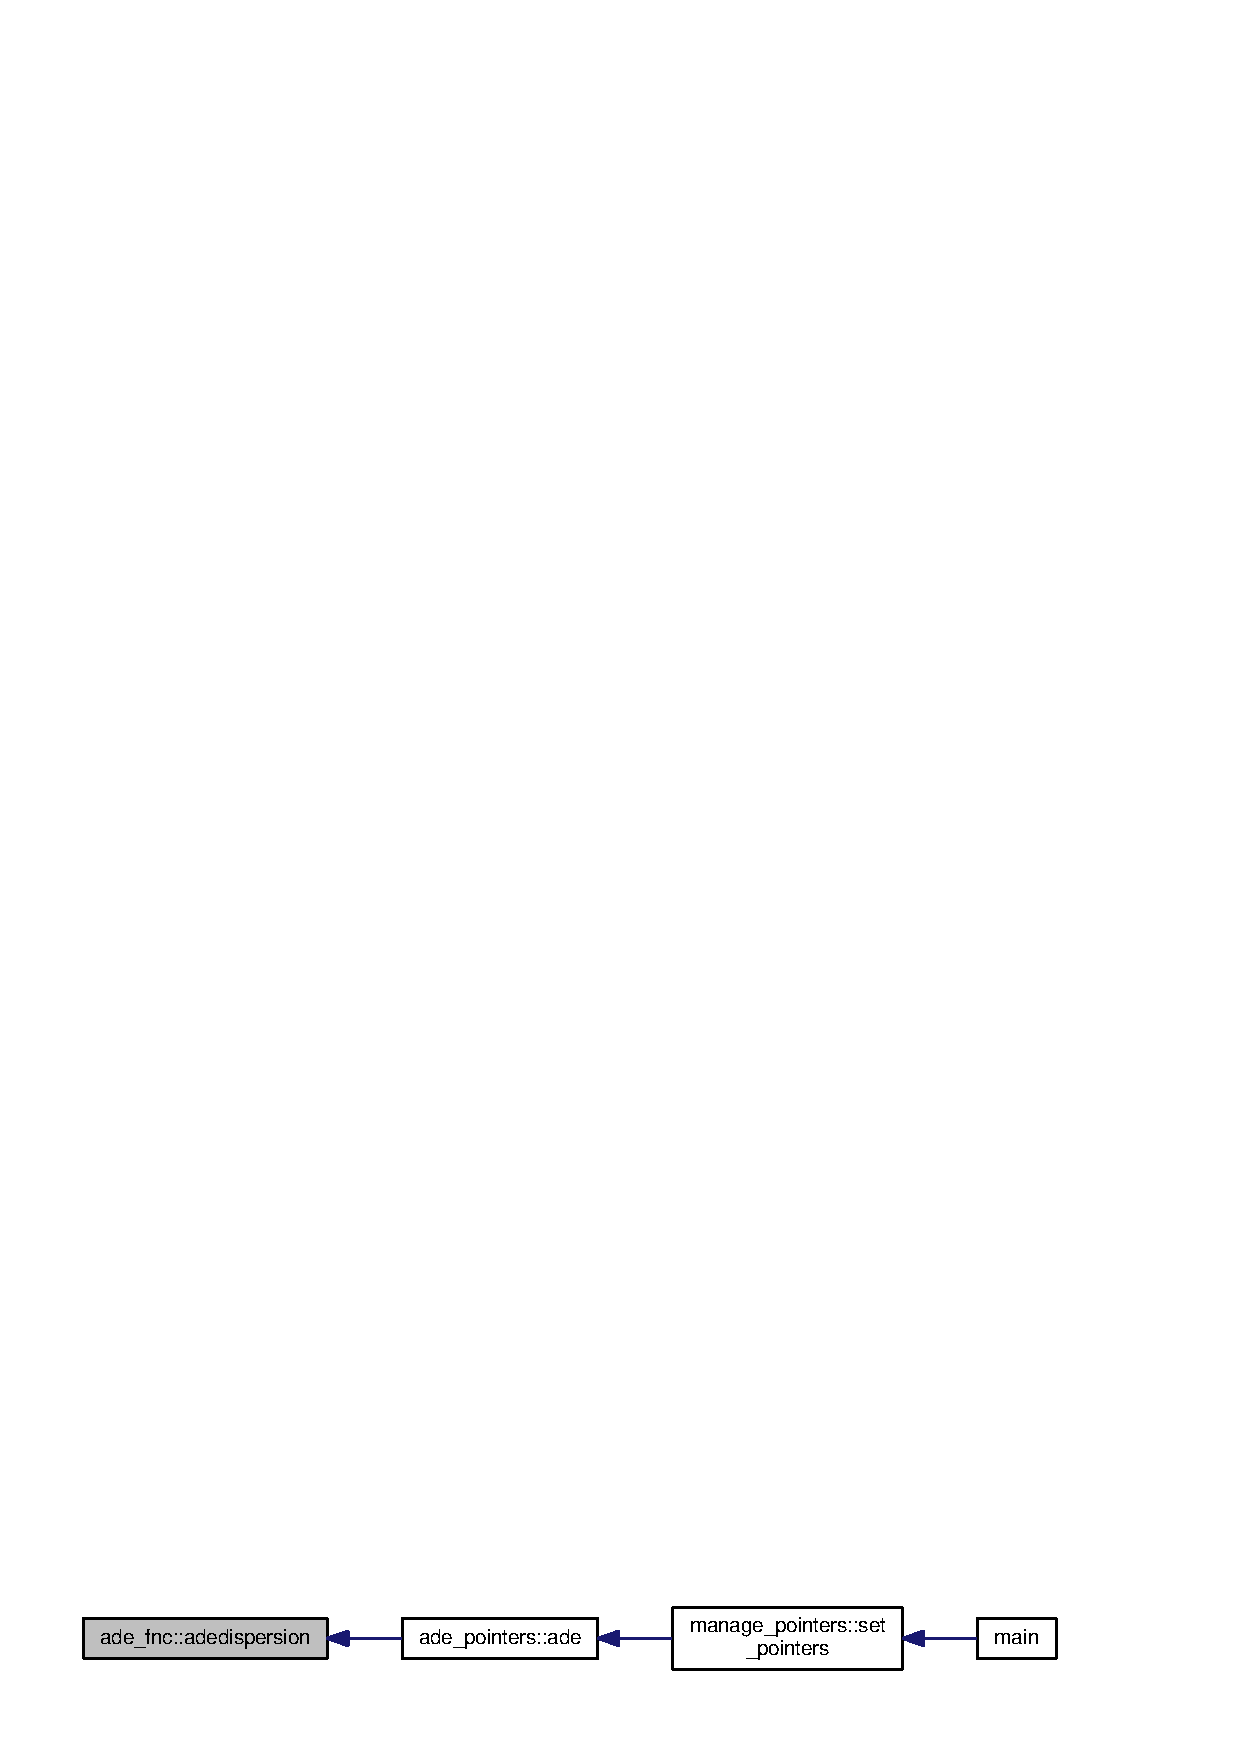
\includegraphics[width=350pt]{namespaceade__fnc_a41110eb40a739c1a15d966c122ab3b8b_icgraph}
\end{center}
\end{figure}



\section{ade\+\_\+globals Module Reference}
\label{namespaceade__globals}\index{ade\+\_\+globals@{ade\+\_\+globals}}
\subsection*{Data Types}
\begin{DoxyCompactItemize}
\item 
type {\bf solutexsoil}
\begin{DoxyCompactList}\small\item\em A\+DE solute/material parameters array. \end{DoxyCompactList}\item 
type {\bf sorption\+\_\+str}
\begin{DoxyCompactList}\small\item\em parameters of sorption model \end{DoxyCompactList}\end{DoxyCompactItemize}
\subsection*{Variables}
\begin{DoxyCompactItemize}
\item 
type({\bf solutexsoil}), dimension(\+:), allocatable, public {\bf adepar}
\begin{DoxyCompactList}\small\item\em structure of solute parameters \end{DoxyCompactList}\item 
integer(kind=ikind), public {\bf isotherm}
\begin{DoxyCompactList}\small\item\em type of used sorption isotherm 0 -\/ linear 1 -\/ Friedrich exponential 2 -\/ Langmuir \end{DoxyCompactList}\item 
logical, public {\bf with\+\_\+richards}
\item 
integer, public {\bf file\+\_\+contaminant}
\end{DoxyCompactItemize}


\subsection{Variable Documentation}
\index{ade\+\_\+globals@{ade\+\_\+globals}!adepar@{adepar}}
\index{adepar@{adepar}!ade\+\_\+globals@{ade\+\_\+globals}}
\subsubsection[{adepar}]{\setlength{\rightskip}{0pt plus 5cm}type({\bf solutexsoil}), dimension(\+:), allocatable, public ade\+\_\+globals\+::adepar}\label{namespaceade__globals_a2034a22816b8b2fa3499cd571f6a097b}


structure of solute parameters 



Definition at line 39 of file A\+D\+E\+\_\+globals.\+f90.



Referenced by ade\+\_\+fnc\+::ade\+\_\+convection(), ade\+\_\+fnc\+::ade\+\_\+cscl\+\_\+react(), ade\+\_\+fnc\+::ade\+\_\+cscs\+\_\+react(), ade\+\_\+fnc\+::ade\+\_\+flux(), ade\+\_\+fnc\+::ade\+\_\+icond(), ade\+\_\+fnc\+::ade\+\_\+mass(), ade\+\_\+fnc\+::ade\+\_\+reaction(), ade\+\_\+reader\+::ade\+\_\+read(), ade\+\_\+fnc\+::ade\+\_\+tder\+\_\+coef(), ade\+\_\+fnc\+::ade\+\_\+tder\+\_\+cscl(), ade\+\_\+fnc\+::ade\+\_\+zerorder(), ade\+\_\+fnc\+::adecs\+\_\+mass(), ade\+\_\+fnc\+::adedispersion(), and heat\+\_\+pointers\+::heat\+\_\+source().


\begin{DoxyCode}
39   \textcolor{keywordtype}{type}(solutexsoil), \textcolor{keywordtype}{dimension(:)}, \textcolor{keywordtype}{allocatable}, \textcolor{keywordtype}{public} :: adepar
\end{DoxyCode}
\index{ade\+\_\+globals@{ade\+\_\+globals}!file\+\_\+contaminant@{file\+\_\+contaminant}}
\index{file\+\_\+contaminant@{file\+\_\+contaminant}!ade\+\_\+globals@{ade\+\_\+globals}}
\subsubsection[{file\+\_\+contaminant}]{\setlength{\rightskip}{0pt plus 5cm}integer, public ade\+\_\+globals\+::file\+\_\+contaminant}\label{namespaceade__globals_a288cade4dba3ff8724e3910ad442d26c}


Definition at line 52 of file A\+D\+E\+\_\+globals.\+f90.



Referenced by ade\+\_\+reader\+::ade\+\_\+read().


\begin{DoxyCode}
52   \textcolor{keywordtype}{integer}, \textcolor{keywordtype}{public} :: file_contaminant
\end{DoxyCode}
\index{ade\+\_\+globals@{ade\+\_\+globals}!isotherm@{isotherm}}
\index{isotherm@{isotherm}!ade\+\_\+globals@{ade\+\_\+globals}}
\subsubsection[{isotherm}]{\setlength{\rightskip}{0pt plus 5cm}integer(kind=ikind), public ade\+\_\+globals\+::isotherm}\label{namespaceade__globals_aaba7d43398b447a5a65c143034f023fb}


type of used sorption isotherm 0 -\/ linear 1 -\/ Friedrich exponential 2 -\/ Langmuir 



Definition at line 47 of file A\+D\+E\+\_\+globals.\+f90.


\begin{DoxyCode}
47   \textcolor{keywordtype}{integer(kind=ikind)}, \textcolor{keywordtype}{public} :: isotherm
\end{DoxyCode}
\index{ade\+\_\+globals@{ade\+\_\+globals}!with\+\_\+richards@{with\+\_\+richards}}
\index{with\+\_\+richards@{with\+\_\+richards}!ade\+\_\+globals@{ade\+\_\+globals}}
\subsubsection[{with\+\_\+richards}]{\setlength{\rightskip}{0pt plus 5cm}logical, public ade\+\_\+globals\+::with\+\_\+richards}\label{namespaceade__globals_a1073a745bb8f75538a92005806222d03}


Definition at line 49 of file A\+D\+E\+\_\+globals.\+f90.



Referenced by ade\+\_\+reader\+::ade\+\_\+read().


\begin{DoxyCode}
49   \textcolor{keywordtype}{logical}, \textcolor{keywordtype}{public} :: with_richards
\end{DoxyCode}

\section{ade\+\_\+pointers Module Reference}
\label{namespaceade__pointers}\index{ade\+\_\+pointers@{ade\+\_\+pointers}}
\subsection*{Functions/\+Subroutines}
\begin{DoxyCompactItemize}
\item 
subroutine, public {\bf ade} (pde\+\_\+loc)
\item 
subroutine, public {\bf adekinsorb} (pde\+\_\+loc)
\end{DoxyCompactItemize}


\subsection{Function/\+Subroutine Documentation}
\index{ade\+\_\+pointers@{ade\+\_\+pointers}!ade@{ade}}
\index{ade@{ade}!ade\+\_\+pointers@{ade\+\_\+pointers}}
\subsubsection[{ade(pde\+\_\+loc)}]{\setlength{\rightskip}{0pt plus 5cm}subroutine, public ade\+\_\+pointers\+::ade (
\begin{DoxyParamCaption}
\item[{class({\bf pde\+\_\+str}), intent(inout)}]{pde\+\_\+loc}
\end{DoxyParamCaption}
)}\label{namespaceade__pointers_adcdbd3c086467f4845b54788e253d694}


Definition at line 8 of file A\+D\+E\+\_\+pointers.\+f90.



References ade\+\_\+fnc\+::ade\+\_\+convection(), ade\+\_\+fnc\+::ade\+\_\+dirichlet(), ade\+\_\+fnc\+::ade\+\_\+flux(), ade\+\_\+fnc\+::ade\+\_\+icond(), ade\+\_\+fnc\+::ade\+\_\+mass(), ade\+\_\+fnc\+::ade\+\_\+neumann(), ade\+\_\+fnc\+::ade\+\_\+reaction(), ade\+\_\+reader\+::ade\+\_\+read(), ade\+\_\+fnc\+::ade\+\_\+tder\+\_\+coef(), ade\+\_\+fnc\+::ade\+\_\+zerorder(), and ade\+\_\+fnc\+::adedispersion().



Referenced by manage\+\_\+pointers\+::set\+\_\+pointers().


\begin{DoxyCode}
8       \textcolor{keywordtype}{use }typy
9       \textcolor{keywordtype}{use }globals
10       \textcolor{keywordtype}{use }global_objs
11       \textcolor{keywordtype}{use }pde_objs
12       \textcolor{keywordtype}{use }ade_fnc
13       \textcolor{keywordtype}{use }ade_reader
14       
15       \textcolor{keywordtype}{class}(pde_str), \textcolor{keywordtype}{intent(in out)} :: pde\_loc
16       \textcolor{keywordtype}{integer(kind=ikind)} :: i
17       
18       \textcolor{keyword}{call }ade_read(pde\_loc)
19             
20       pde\_loc%pde\_fnc(pde\_loc%order)%dispersion => adedispersion
21       
22       pde\_loc%pde\_fnc(pde\_loc%order)%convection => ade_convection
23 
24       pde\_loc%pde\_fnc(pde\_loc%order)%elasticity => ade_tder_coef
25 
26       pde\_loc%mass => ade_mass
27 
28       pde\_loc%pde\_fnc(pde\_loc%order)%reaction => ade_reaction
29             
30       pde\_loc%pde\_fnc(pde\_loc%order)%zerord => ade_zerorder
31           
32       \textcolor{keywordflow}{do} i=lbound(pde\_loc%bc,1), ubound(pde\_loc%bc,1)
33         \textcolor{keywordflow}{select case}(pde\_loc%bc(i)%code)
34           \textcolor{keywordflow}{case}(1)
35             pde\_loc%bc(i)%value\_fnc => ade_dirichlet
36           \textcolor{keywordflow}{case}(2)
37             pde\_loc%bc(i)%value\_fnc => ade_neumann
38 \textcolor{keywordflow}{        end select}
39 \textcolor{keywordflow}{      end do}    
40         
41       pde\_loc%flux => ade_flux
42       
43       pde\_loc%initcond => ade_icond  
44       
45     
\end{DoxyCode}


Here is the call graph for this function\+:\nopagebreak
\begin{figure}[H]
\begin{center}
\leavevmode
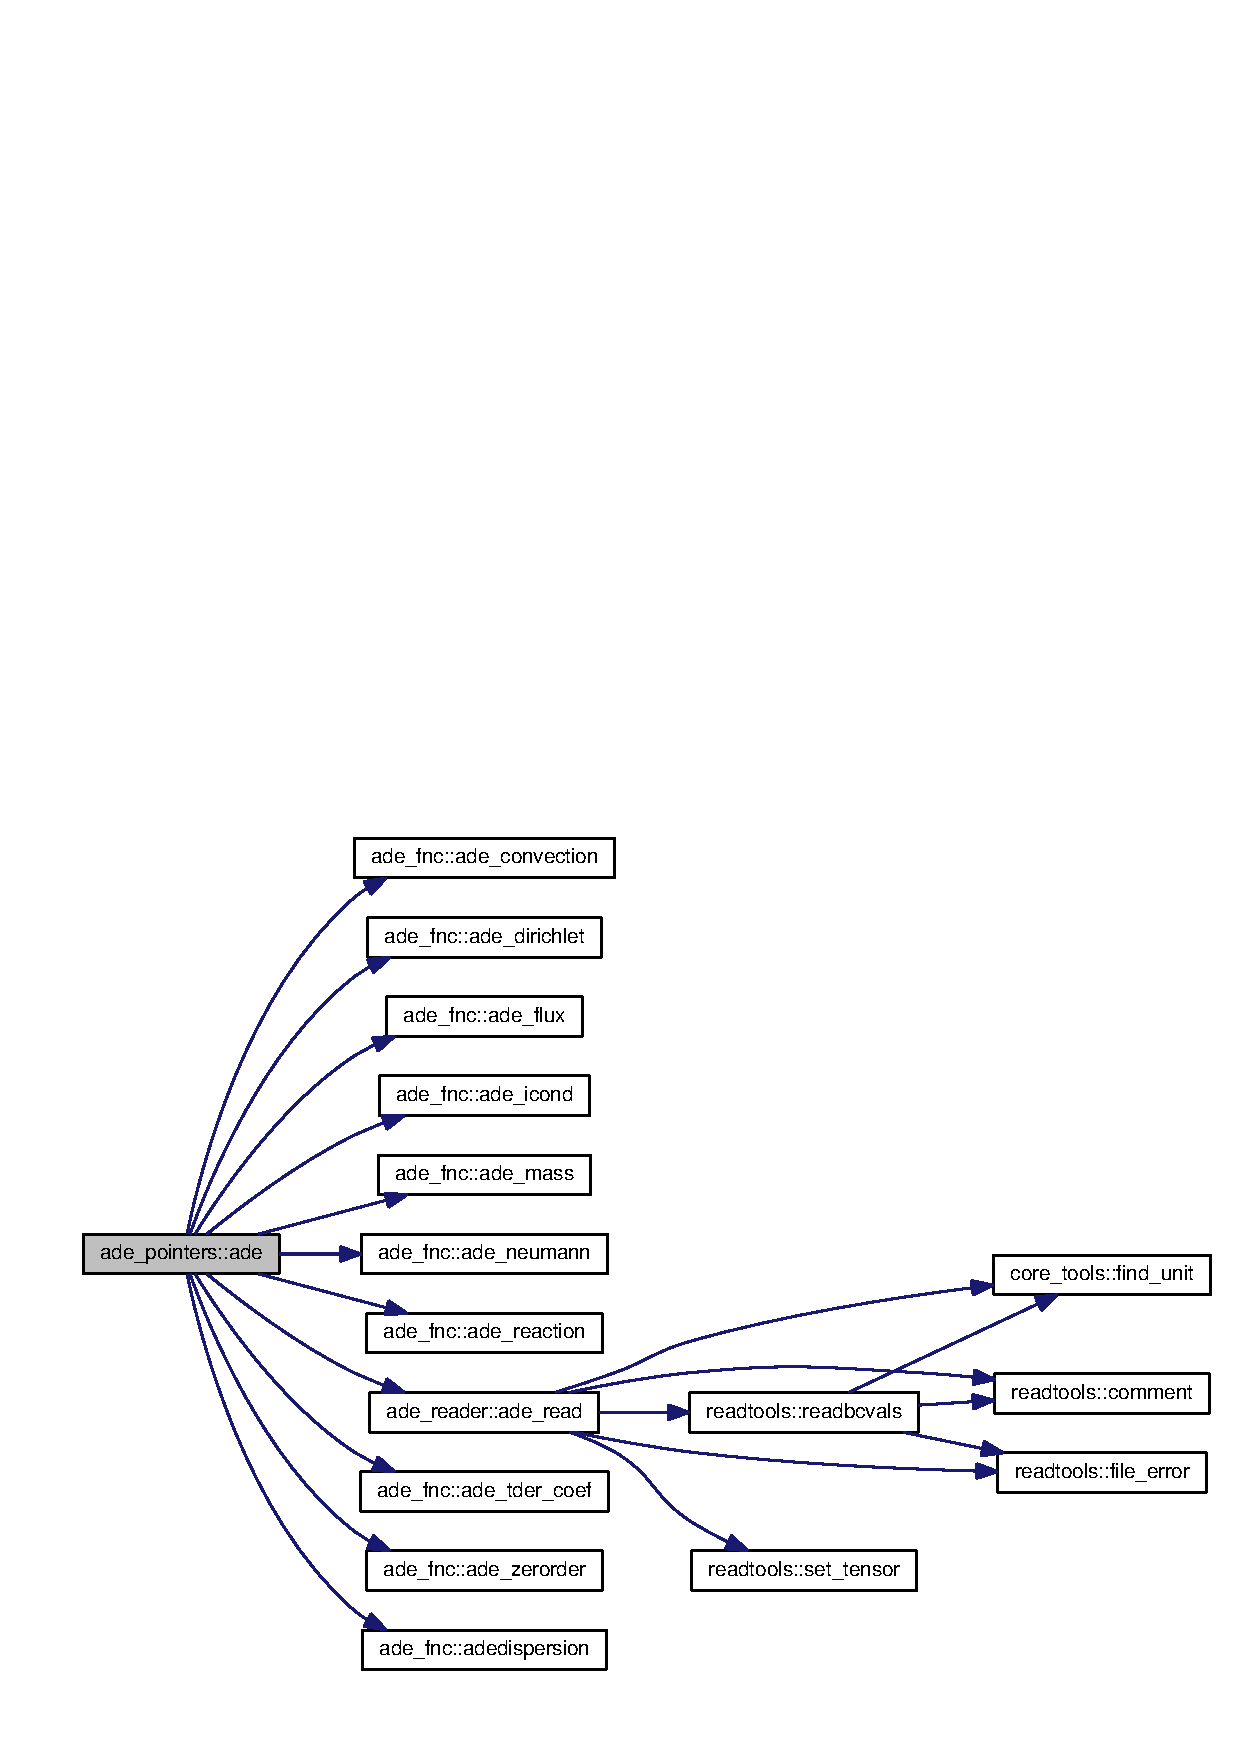
\includegraphics[width=350pt]{namespaceade__pointers_adcdbd3c086467f4845b54788e253d694_cgraph}
\end{center}
\end{figure}




Here is the caller graph for this function\+:\nopagebreak
\begin{figure}[H]
\begin{center}
\leavevmode
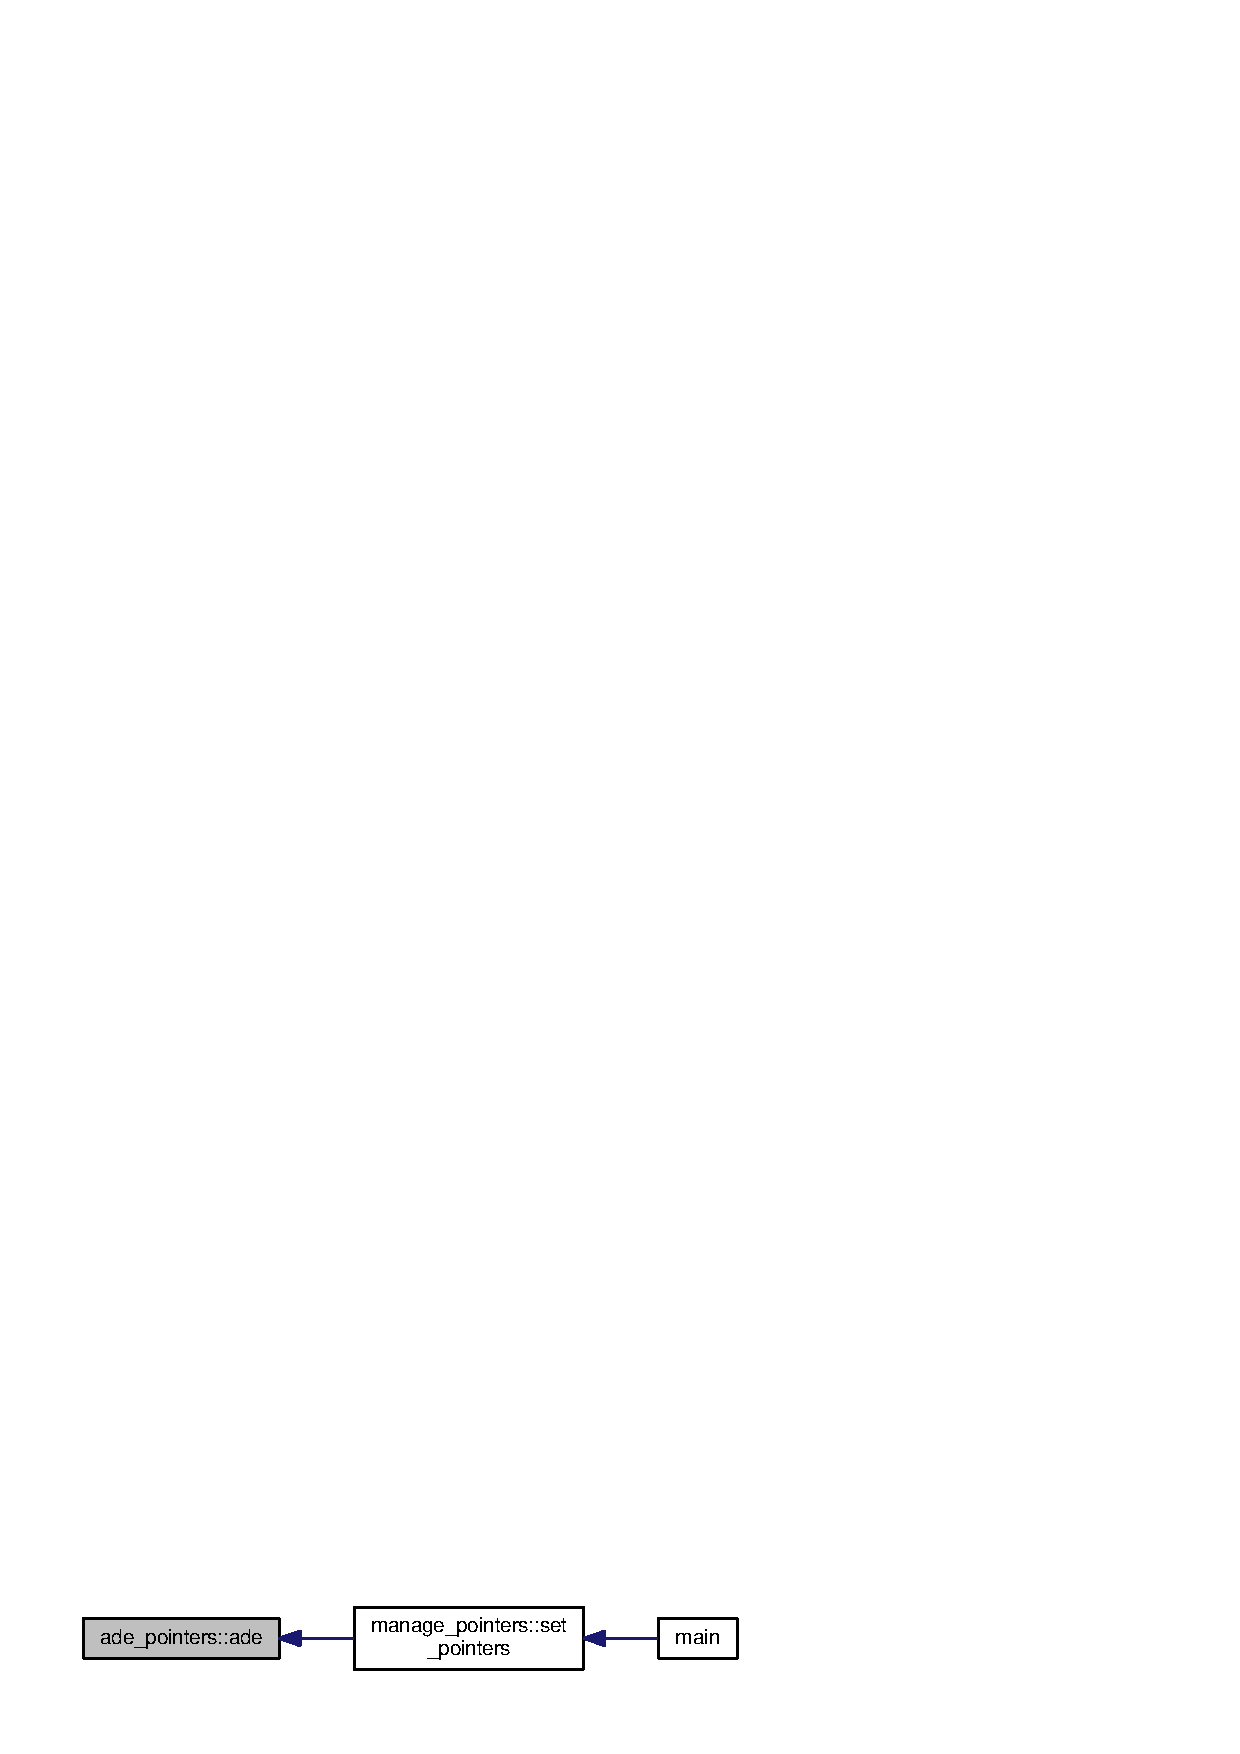
\includegraphics[width=350pt]{namespaceade__pointers_adcdbd3c086467f4845b54788e253d694_icgraph}
\end{center}
\end{figure}


\index{ade\+\_\+pointers@{ade\+\_\+pointers}!adekinsorb@{adekinsorb}}
\index{adekinsorb@{adekinsorb}!ade\+\_\+pointers@{ade\+\_\+pointers}}
\subsubsection[{adekinsorb(pde\+\_\+loc)}]{\setlength{\rightskip}{0pt plus 5cm}subroutine, public ade\+\_\+pointers\+::adekinsorb (
\begin{DoxyParamCaption}
\item[{class({\bf pde\+\_\+str}), intent(inout)}]{pde\+\_\+loc}
\end{DoxyParamCaption}
)}\label{namespaceade__pointers_aa2bb46d0195e5bf43f5bc8066b07b803}


Definition at line 49 of file A\+D\+E\+\_\+pointers.\+f90.



References ade\+\_\+fnc\+::ade\+\_\+cscl\+\_\+react(), ade\+\_\+fnc\+::ade\+\_\+cscs\+\_\+react(), ade\+\_\+fnc\+::ade\+\_\+null\+\_\+bc(), ade\+\_\+fnc\+::ade\+\_\+tder\+\_\+cscl(), ade\+\_\+fnc\+::ade\+\_\+tder\+\_\+cscs(), ade\+\_\+fnc\+::adecs\+\_\+icond(), ade\+\_\+reader\+::adecs\+\_\+read(), and pde\+\_\+objs\+::pde.



Referenced by manage\+\_\+pointers\+::set\+\_\+pointers().


\begin{DoxyCode}
49       \textcolor{keywordtype}{use }typy
50       \textcolor{keywordtype}{use }globals
51       \textcolor{keywordtype}{use }global_objs
52       \textcolor{keywordtype}{use }pde_objs
53       \textcolor{keywordtype}{use }ade_fnc
54       \textcolor{keywordtype}{use }ade_reader
55       
56       \textcolor{keywordtype}{class}(pde_str), \textcolor{keywordtype}{intent(in out)} :: pde\_loc  
57       \textcolor{keywordtype}{integer(kind=ikind)} :: i
58       
59       \textcolor{keyword}{call }adecs_read(pde\_loc)
60       
61       pde\_loc%pde\_fnc(pde\_loc%order)%elasticity => ade_tder_cscs
62       
63       pde(pde\_loc%order-1)%pde\_fnc(pde\_loc%order)%elasticity => ade_tder_cscl
64       
65       pde\_loc%pde\_fnc(pde\_loc%order-1)%reaction => ade_cscl_react
66       
67       pde\_loc%pde\_fnc(pde\_loc%order)%reaction => ade_cscs_react
68       
69       \textcolor{keyword}{allocate}(pde\_loc%bc(lbound(pde(pde\_loc%order-1)%bc,1) : (ubound(pde\textcolor{comment}{(pde\_loc%order-1)%bc,1) )  ))}
70 \textcolor{comment}{      }
71 \textcolor{comment}{      }\textcolor{keywordflow}{do} i=lbound(pde\_loc%bc,1), ubound(pde\_loc%bc,1)
72         pde\_loc%bc(i)%code = 2
73         pde\_loc%bc(i)%value\_fnc => ade_null_bc
74 \textcolor{keywordflow}{      end do} 
75       
76       pde\_loc%initcond => adecs_icond
77       
78     
\end{DoxyCode}


Here is the call graph for this function\+:\nopagebreak
\begin{figure}[H]
\begin{center}
\leavevmode
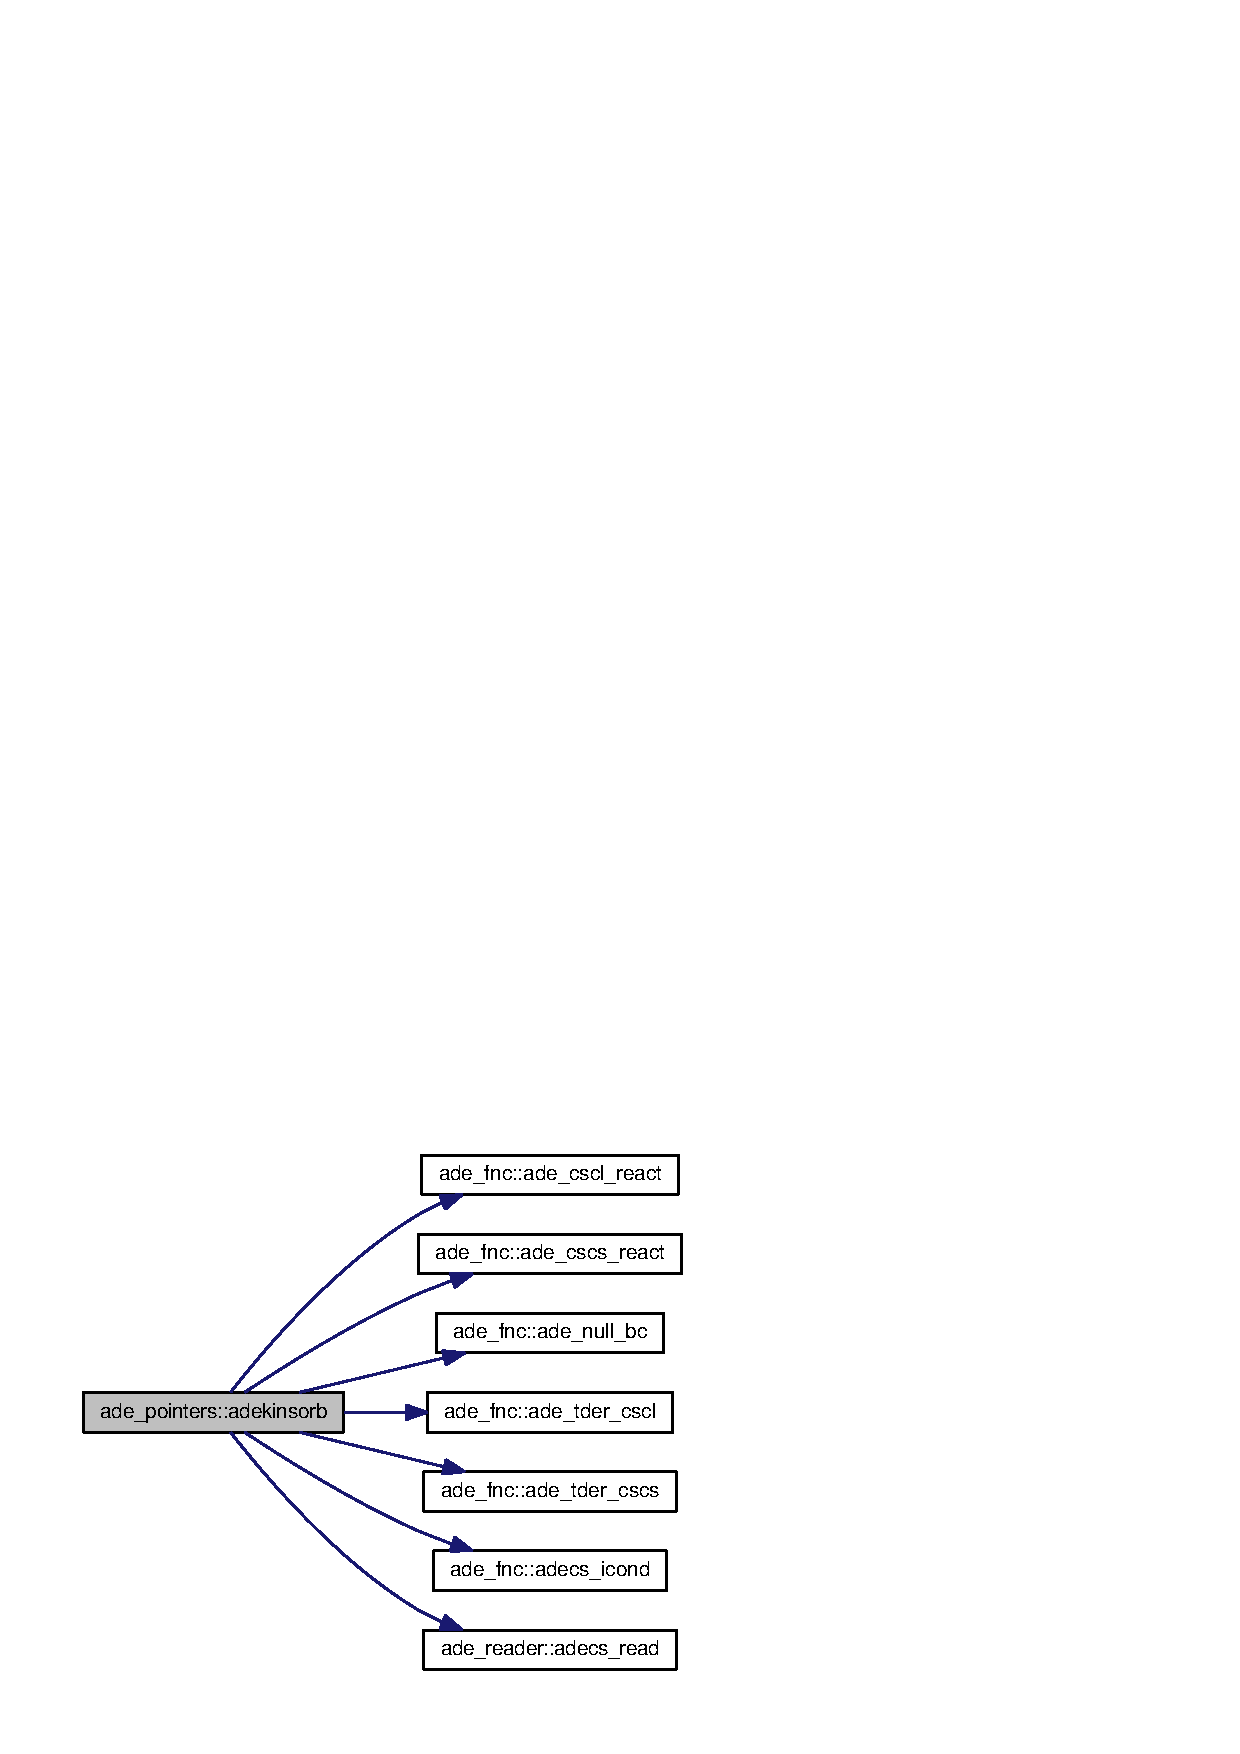
\includegraphics[width=331pt]{namespaceade__pointers_aa2bb46d0195e5bf43f5bc8066b07b803_cgraph}
\end{center}
\end{figure}




Here is the caller graph for this function\+:\nopagebreak
\begin{figure}[H]
\begin{center}
\leavevmode
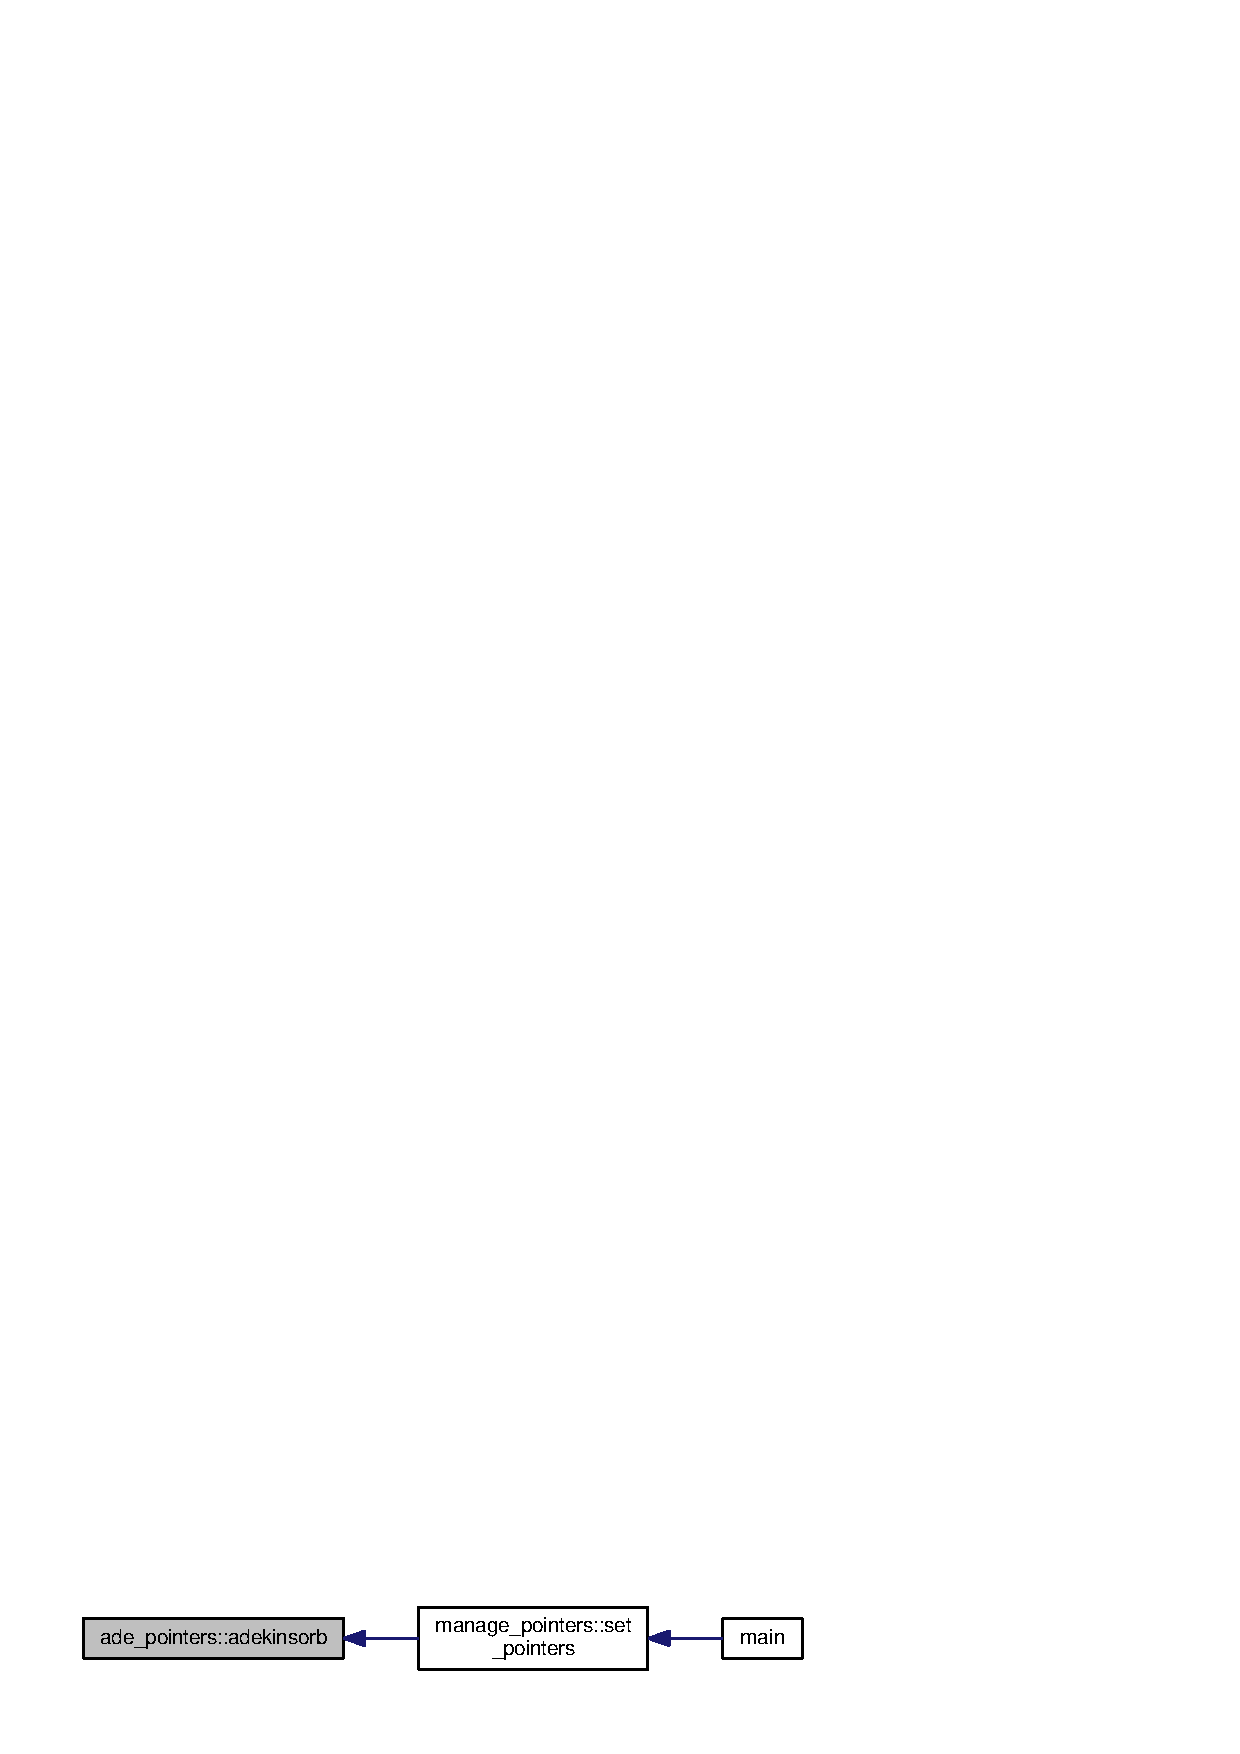
\includegraphics[width=350pt]{namespaceade__pointers_aa2bb46d0195e5bf43f5bc8066b07b803_icgraph}
\end{center}
\end{figure}



\section{ade\+\_\+reader Module Reference}
\label{namespaceade__reader}\index{ade\+\_\+reader@{ade\+\_\+reader}}
\subsection*{Functions/\+Subroutines}
\begin{DoxyCompactItemize}
\item 
subroutine, public {\bf ade\+\_\+read} (pde\+\_\+loc)
\item 
subroutine {\bf adecs\+\_\+read} (pde\+\_\+loc)
\end{DoxyCompactItemize}


\subsection{Function/\+Subroutine Documentation}
\index{ade\+\_\+reader@{ade\+\_\+reader}!ade\+\_\+read@{ade\+\_\+read}}
\index{ade\+\_\+read@{ade\+\_\+read}!ade\+\_\+reader@{ade\+\_\+reader}}
\subsubsection[{ade\+\_\+read(pde\+\_\+loc)}]{\setlength{\rightskip}{0pt plus 5cm}subroutine, public ade\+\_\+reader\+::ade\+\_\+read (
\begin{DoxyParamCaption}
\item[{class({\bf pde\+\_\+str}), intent(inout)}]{pde\+\_\+loc}
\end{DoxyParamCaption}
)}\label{namespaceade__reader_ab579f926de43ae5ba712d144494109fb}


Definition at line 7 of file A\+D\+E\+\_\+reader.\+f90.



References ade\+\_\+globals\+::adepar, readtools\+::comment(), globals\+::drutes\+\_\+config, globals\+::elements, ade\+\_\+globals\+::file\+\_\+contaminant, readtools\+::file\+\_\+error(), core\+\_\+tools\+::find\+\_\+unit(), readtools\+::readbcvals(), readtools\+::set\+\_\+tensor(), globals\+::terminal, and ade\+\_\+globals\+::with\+\_\+richards.



Referenced by ade\+\_\+pointers\+::ade().


\begin{DoxyCode}
7       \textcolor{keywordtype}{use }typy
8       \textcolor{keywordtype}{use }globals
9       \textcolor{keywordtype}{use }global_objs
10       \textcolor{keywordtype}{use }core_tools
11       \textcolor{keywordtype}{use }ade_globals
12       \textcolor{keywordtype}{use }readtools
13       \textcolor{keywordtype}{use }pde_objs
14 
15       \textcolor{keywordtype}{class}(pde_str), \textcolor{keywordtype}{intent(in out)} :: pde\_loc
16       \textcolor{keywordtype}{integer} :: i\_err
17       \textcolor{keywordtype}{integer(kind=ikind)} :: i, n
18       \textcolor{keywordtype}{real(kind=rkind)} :: tmp
19       \textcolor{keywordtype}{real(kind=rkind)}, \textcolor{keywordtype}{dimension(:)}, \textcolor{keywordtype}{allocatable} :: tmp\_array
20       \textcolor{keywordtype}{character(len=4096)} :: msg
21       \textcolor{keywordtype}{character(len=256)} :: linetext
22       \textcolor{keywordtype}{logical} :: crelative = .false.
23       \textcolor{keywordtype}{logical} :: with\_richards\_def
24       
25       
26 
27       pde\_loc%problem\_name(1) = \textcolor{stringliteral}{"ADER\_in\_liquid"}
28       pde\_loc%problem\_name(2) = \textcolor{stringliteral}{"Advection-dispersion-reaction equation (solute concentration in liquid
       phase)"}
29 
30       pde\_loc%solution\_name(1) = \textcolor{stringliteral}{"solute\_concentration"} \textcolor{comment}{!nazev vystupnich souboru}
31       pde\_loc%solution\_name(2) = \textcolor{stringliteral}{"c  [M/L^3]"} \textcolor{comment}{!popisek grafu}
32 
33       pde\_loc%flux\_name(1) = \textcolor{stringliteral}{"conc\_flux"}  
34       pde\_loc%flux\_name(2) = \textcolor{stringliteral}{"concentration flux [M.L^\{-2\}.T^\{-1\}]"}
35 
36       pde\_loc%mass\_name(1) = \textcolor{stringliteral}{"conc\_in\_porous\_medium"}
37       pde\_loc%mass\_name(2) = \textcolor{stringliteral}{"concetration [M/L^3]"}
38       
39       
40 
41       \textcolor{keyword}{call }find_unit(file_contaminant, 200)
42       \textcolor{keyword}{open}(unit = file_contaminant, file=\textcolor{stringliteral}{"drutes.conf/ADE/contaminant.conf"}\textcolor{comment}{, action=}\textcolor{stringliteral}{"read"}\textcolor{comment}{, status=}\textcolor{stringliteral}{"old"}\textcolor{comment}{, 
      iostat=i\_err)}
43 \textcolor{comment}{      }\textcolor{keywordflow}{if} (i\_err /= 0) \textcolor{keywordflow}{then}
44         print *, \textcolor{stringliteral}{"missing drutes.conf/ADE/contaminant.conf file"}
45         error stop
46 \textcolor{keywordflow}{      end if}
47      
48 
49       \textcolor{keyword}{allocate}(adepar(maxval(elements%material)))
50       
51       \textcolor{keyword}{call }fileread(n, file_contaminant)
52       
53       backspace(file_contaminant)
54       
55       \textcolor{keyword}{write}(msg, fmt=*) \textcolor{stringliteral}{"ERROR!! incorrect number of materials in drutes.conf/ADE/contaminant.conf  &}
56 \textcolor{stringliteral}{}\textcolor{stringliteral}{        the mesh defines"}, maxval(elements%material)  , \textcolor{stringliteral}{"materials, and your input file defines"}\textcolor{comment}{, n, }\textcolor{stringliteral}{
      "material(s)."}
57         
58      
59       \textcolor{keyword}{call }fileread(n, file_contaminant, ranges=(/1\_ikind*maxval(elements%material\textcolor{comment}{),1\_ikind*maxval(
      elements%material)/),&}
60 \textcolor{comment}{        errmsg=trim(msg))}
61 \textcolor{comment}{      }
62 \textcolor{comment}{      }\textcolor{keyword}{write}(unit=msg, fmt=*) \textcolor{stringliteral}{"HINT 1: Is the molecular diffusion value positive?"}\textcolor{comment}{, new\_line(}\textcolor{stringliteral}{"a"}\textcolor{comment}{), &}
63 \textcolor{comment}{                              }\textcolor{stringliteral}{"HINT 2 : Is the number of molecular diffusion values corresponding to the
       amount of layers?"}
64                               
65       \textcolor{keywordflow}{do} i=1, ubound(adepar,1)
66         \textcolor{keyword}{call }fileread(adepar(i)%difmol, file_contaminant, ranges=(/0.0\_rkind, 1\textcolor{comment}{.0\_rkind*huge(tmp)/), &}
67 \textcolor{comment}{          errmsg=trim(msg))}
68 \textcolor{comment}{}\textcolor{keywordflow}{      end do}
69  
70       \textcolor{keyword}{write}(unit=msg, fmt=*) \textcolor{stringliteral}{"HINT 1: Are all values anisotropy defining anisotropical diffusivity
       positive? "}\textcolor{comment}{, new\_line(}\textcolor{stringliteral}{"a"}\textcolor{comment}{), &}
71 \textcolor{comment}{        }\textcolor{stringliteral}{"HINT 2 : Have you defined enough values for anisotropy &}
72 \textcolor{stringliteral}{}\textcolor{stringliteral}{        (e.g. for 2D define angle and the maximal and minimal value of diffusivity, in total 3 values)?"}\textcolor{comment}{, 
      new\_line(}\textcolor{stringliteral}{"a"}\textcolor{comment}{),&}
73 \textcolor{comment}{        }\textcolor{stringliteral}{"HINT 3: The number of lines with diffusivity has to correspond to the number of materials & }
74 \textcolor{stringliteral}{}\textcolor{stringliteral}{        defined by your mesh"}
75       
76       
77       \textcolor{keyword}{allocate}(tmp\_array(drutes_config%dimen + 1))
78       \textcolor{keywordflow}{do} i=1, ubound(adepar,1)
79         \textcolor{keyword}{allocate}(adepar(i)%diff\_loc(drutes_config%dimen))
80         \textcolor{keyword}{call }fileread(r=tmp\_array, fileid=file_contaminant, ranges=(/0.0\_rkind,\textcolor{comment}{ huge(tmp)/), errmsg=trim(
      msg))}
81 \textcolor{comment}{        adepar(i)%anisoangle = tmp\_array(1)}
82 \textcolor{comment}{        adepar(i)%diff\_loc = tmp\_array(2:drutes_config%dimen + 1)}
83 \textcolor{comment}{        }\textcolor{keyword}{allocate}(adepar(i)%diff(drutes_config%dimen, drutes_config%dimen))
84         \textcolor{keyword}{call }set_tensor(adepar(i)%diff\_loc, (/adepar(i)%anisoangle/), adepar(i)%diff\textcolor{comment}{)}
85 \textcolor{comment}{}\textcolor{keywordflow}{      end do}
86       
87       
88       \textcolor{keywordflow}{do} i=1, ubound(adepar,1)
89        \textcolor{keyword}{call }comment(file_contaminant)
90        \textcolor{keyword}{read}(unit=file_contaminant, fmt=*, iostat=i\_err) adepar(i)%cinit,\textcolor{comment}{ adepar(i)%icondtype}
91 \textcolor{comment}{       }\textcolor{keywordflow}{if} (i\_err /= 0) \textcolor{keywordflow}{then}
92          \textcolor{keyword}{write}(unit=terminal, fmt=*) \textcolor{stringliteral}{"The number of lines for initial concentration has to be equal to the
       number of materials"}
93          backspace(file_contaminant)
94          \textcolor{keyword}{call }comment(file_contaminant)
95          \textcolor{keyword}{read}(unit=file_contaminant, fmt=*, iostat=i\_err) linetext
96          \textcolor{keyword}{write}(unit=terminal, fmt=*) \textcolor{stringliteral}{"the following inappropriate line was specified in your config file"}\textcolor{comment}{, 
      trim(linetext)}
97 \textcolor{comment}{         }\textcolor{keyword}{call }file_error(file_contaminant)   
98 \textcolor{keywordflow}{       end if}
99        \textcolor{keywordflow}{select case} (adepar(i)%icondtype)
100          \textcolor{keywordflow}{case}(\textcolor{stringliteral}{"cr"}, \textcolor{stringliteral}{"ca"})
101            \textcolor{keywordflow}{if} (adepar(i)%icondtype == \textcolor{stringliteral}{"cr"}) crelative=.true.
102            \textcolor{keywordflow}{CONTINUE}
103 \textcolor{keywordflow}{         case default}
104            \textcolor{keyword}{write}(unit=terminal, fmt=*) \textcolor{stringliteral}{" Your initial concentration can be only:  "}
105            \textcolor{keyword}{write}(unit=terminal, fmt=*) \textcolor{stringliteral}{"  ca - for absolute concentration"}
106            \textcolor{keyword}{write}(unit=terminal, fmt=*) \textcolor{stringliteral}{"  cr - for relative concentration"}
107            \textcolor{keyword}{call }file_error(file_contaminant)
108 \textcolor{keywordflow}{        end select}
109            
110 \textcolor{keywordflow}{       end do}
111        
112        \textcolor{keywordflow}{if} (crelative) \textcolor{keywordflow}{then}
113          \textcolor{keyword}{call  }fileread(adepar(1)%cmax, file_contaminant, errmsg=\textcolor{stringliteral}{"Have you defined correct value for the
       maximal concentration?"}\textcolor{comment}{)}
114 \textcolor{comment}{         }\textcolor{keywordflow}{do} i=2, ubound(adepar,1)
115           adepar(i)%cmax = adepar(1)%cmax
116 \textcolor{keywordflow}{         end do}
117 \textcolor{keywordflow}{       end if}
118        
119   
120        
121        \textcolor{keywordflow}{if} (.not. crelative) \textcolor{keywordflow}{then}
122         \textcolor{keyword}{write}(msg, *) \textcolor{stringliteral}{"HINT 1: Specify [y/n] to define whether you prefer to compute convection from the
       Richards equation or"}\textcolor{comment}{, &}
123 \textcolor{comment}{        }\textcolor{stringliteral}{" specify the convection directly here."}, new\_line(\textcolor{stringliteral}{"a"}), &
124          \textcolor{stringliteral}{"   HINT 2: Since you don't use relative concentration for the initial condition, check whether
       you left the"}\textcolor{comment}{, &}
125 \textcolor{comment}{        }\textcolor{stringliteral}{" line with cmax blank."}
126        \textcolor{keywordflow}{else}
127         \textcolor{keyword}{write}(msg, *) \textcolor{stringliteral}{"HINT 1: Specify [y/n] to define whether you prefer to compute convection from the
       Richards equation or &}
128 \textcolor{stringliteral}{}\textcolor{stringliteral}{         specify the convection directly here."}
129 \textcolor{keywordflow}{       end if}
130        
131        \textcolor{keyword}{call }fileread(with_richards, file_contaminant, errmsg=trim(msg))
132        
133        \textcolor{keywordflow}{select case}(adjustl(trim(drutes_config%name)))
134          \textcolor{keywordflow}{case}(\textcolor{stringliteral}{"ADEstd"}, \textcolor{stringliteral}{"ADEstd\_kinsorb"})
135            with\_richards\_def = .false.
136 \textcolor{keywordflow}{         case default}
137            with\_richards\_def = .true.
138 \textcolor{keywordflow}{        end select}
139        
140        \textcolor{keywordflow}{if} (.not. with_richards .and. with\_richards\_def) \textcolor{keywordflow}{then}
141          \textcolor{keyword}{write}(unit=msg, fmt=*) \textcolor{stringliteral}{"You have specified"} , &
142               \textcolor{stringliteral}{" convection to be  computed from the Richards equation, but you want to specify the
       convection here."}\textcolor{comment}{ ,&}
143 \textcolor{comment}{              new\_line(}\textcolor{stringliteral}{"a"}), \textcolor{stringliteral}{"   Solution: change model type setup in global.conf or comment out the
       convection values here."}
144          \textcolor{keyword}{call }file_error(file_contaminant, msg)
145        \textcolor{keywordflow}{else} \textcolor{keywordflow}{if} (with_richards .and. .not. with\_richards\_def) \textcolor{keywordflow}{then}
146         \textcolor{keyword}{write}(unit=msg, fmt=*) \textcolor{stringliteral}{"You have specified here to compute the convection fromt the Richards
       equation, "}\textcolor{comment}{,  &}
147 \textcolor{comment}{               }\textcolor{stringliteral}{" but in your global config you have requested solving ADE equation only, and so convection
       has to be specified here."}\textcolor{comment}{, &}
148 \textcolor{comment}{         new\_line(}\textcolor{stringliteral}{"a"}),  \textcolor{stringliteral}{"   Solution:  change model type setup in global.conf or supply the convection
       here."}
149          \textcolor{keyword}{call }file_error(file_contaminant, msg)
150 \textcolor{keywordflow}{       end if}
151          
152        
153        \textcolor{keywordflow}{if} (.not. with_richards) \textcolor{keywordflow}{then}
154          \textcolor{keywordflow}{if} (\textcolor{keyword}{allocated}(tmp\_array)) \textcolor{keyword}{deallocate}(tmp\_array)
155          \textcolor{keyword}{allocate}(tmp\_array(2))
156          \textcolor{keywordflow}{do} i=1, maxval(elements%material)
157            \textcolor{keyword}{call }fileread(tmp\_array, file_contaminant, errmsg=\textcolor{stringliteral}{"convection has to be defined for each layer"}\textcolor{comment}{)}
158 \textcolor{comment}{           adepar(i)%convection = tmp\_array(1)}
159 \textcolor{comment}{           adepar(i)%water\_cont = tmp\_array(2)}
160 \textcolor{comment}{}\textcolor{keywordflow}{         end do}
161 \textcolor{keywordflow}{      end if}
162       
163       \textcolor{keywordflow}{if} (with_richards) \textcolor{keywordflow}{then}
164         \textcolor{keyword}{write}(unit=msg, fmt=*) \textcolor{stringliteral}{"HINT1: Have you commented out all lines with convection values? "}\textcolor{comment}{, &}
165 \textcolor{comment}{        }\textcolor{stringliteral}{"Since the convection is computed from the Richards equation."}, new\_line\textcolor{comment}{(}\textcolor{stringliteral}{"a"}\textcolor{comment}{), &}
166 \textcolor{comment}{        }\textcolor{stringliteral}{"   HINT2: The number of orders of reactions has to be positive or zero."}
167       \textcolor{keywordflow}{else}
168         \textcolor{keyword}{write}(unit=msg, fmt=*) \textcolor{stringliteral}{"HINT1: Is your number of lines with convection definition corresponding
       with the number of layers?"}\textcolor{comment}{,&}
169 \textcolor{comment}{        new\_line(}\textcolor{stringliteral}{"a"}), &
170         \textcolor{stringliteral}{"   HINT2: The number of orders of reactions has to be positive or zero."}
171 \textcolor{keywordflow}{      end if}
172        
173        \textcolor{keyword}{call }fileread(n, file_contaminant, ranges=(/0\_ikind, 1\_ikind*huge\textcolor{comment}{(n)/), & }
174 \textcolor{comment}{         errmsg=trim(msg))}
175 \textcolor{comment}{       }
176 \textcolor{comment}{       }
177 \textcolor{comment}{       }\textcolor{keyword}{write}(unit=msg, fmt=*) \textcolor{stringliteral}{"You have requested "}, n,\textcolor{stringliteral}{" different orders of reactions."}\textcolor{comment}{, new\_line(}\textcolor{stringliteral}{"a"}\textcolor{comment}{), &}
178 \textcolor{comment}{           }\textcolor{stringliteral}{"For each different "}
179        
180        
181        \textcolor{keyword}{write}(unit=msg, fmt=*) \textcolor{stringliteral}{"You have requested "}, n,\textcolor{stringliteral}{" different orders of reactions."}\textcolor{comment}{, new\_line(}\textcolor{stringliteral}{"a"}\textcolor{comment}{), &}
182 \textcolor{comment}{           }\textcolor{stringliteral}{"Specify the list of orders of reactions,"}, new\_line(\textcolor{stringliteral}{"a"}), &
183            \textcolor{stringliteral}{"!!!!EACH material requires its line!!!!"},  new\_line(\textcolor{stringliteral}{"a"}), &
184            \textcolor{stringliteral}{"    e.g. you want to use zero order and second order reaction for first material and "}\textcolor{comment}{,  
      new\_line(}\textcolor{stringliteral}{"a"}\textcolor{comment}{), & }
185 \textcolor{comment}{           }\textcolor{stringliteral}{" first and second order reaction for second material, then specify the following lines"}\textcolor{comment}{, 
      new\_line(}\textcolor{stringliteral}{"a"}\textcolor{comment}{),new\_line(}\textcolor{stringliteral}{"a"}\textcolor{comment}{),&}
186 \textcolor{comment}{           " 0 2 }\textcolor{stringliteral}{", new\_line("}a\textcolor{stringliteral}{"), "} 1 2 \textcolor{stringliteral}{"}
187 \textcolor{stringliteral}{}\textcolor{stringliteral}{       do i=1, ubound(adepar,1)}
188 \textcolor{stringliteral}{}\textcolor{stringliteral}{         allocate(adepar(i)%orders(n))}
189 \textcolor{stringliteral}{}\textcolor{stringliteral}{         call fileread(adepar(i)%orders, file\_contaminant, errmsg=trim(msg))}
190 \textcolor{stringliteral}{}\textcolor{stringliteral}{       end do}
191 \textcolor{stringliteral}{}\textcolor{stringliteral}{       }
192 \textcolor{stringliteral}{}\textcolor{stringliteral}{       write(unit=msg, fmt=*) "}you have requested \textcolor{stringliteral}{", n,"} different orders\textcolor{comment}{ of reactions.}\textcolor{stringliteral}{", new\_line("}a\textcolor{stringliteral}{"), &}
193 \textcolor{stringliteral}{}\textcolor{stringliteral}{           "}specify the list of rates of reactions,\textcolor{stringliteral}{", new\_line("}a\textcolor{stringliteral}{"), &}
194 \textcolor{stringliteral}{}\textcolor{stringliteral}{           "}!\textcolor{comment}{!!!EACH material requires its line!!!!",  new\_line("a"), &}
195            \textcolor{stringliteral}{"    e.g. you want to use zero order with rate 0.2 and second order reaction with rate 0.6 for
       first material and "}\textcolor{comment}{,&}
196 \textcolor{comment}{           new\_line(}\textcolor{stringliteral}{"a"}), & 
197            \textcolor{stringliteral}{"and you have specified the requested orders of reactions above"},  new\_line\textcolor{comment}{(}\textcolor{stringliteral}{"a"}\textcolor{comment}{), & }
198 \textcolor{comment}{           }\textcolor{stringliteral}{" for the second material you would like to use only  opnly second order kinetics with rate 0.4
       "}\textcolor{comment}{,& }
199 \textcolor{comment}{           new\_line(}\textcolor{stringliteral}{"a"}), \textcolor{stringliteral}{"then the following lines has to be specified"},&
200            new\_line(\textcolor{stringliteral}{"a"}),new\_line(\textcolor{stringliteral}{"a"}),&
201            " 0.2 0.6 \textcolor{stringliteral}{", new\_line("}a\textcolor{stringliteral}{"), "} 0.0 0.4 \textcolor{stringliteral}{"}
202 \textcolor{stringliteral}{}\textcolor{stringliteral}{           }
203 \textcolor{stringliteral}{}\textcolor{stringliteral}{       do i=1, ubound(adepar,1)}
204 \textcolor{stringliteral}{}\textcolor{stringliteral}{         allocate(adepar(i)%lambda(n))}
205 \textcolor{stringliteral}{}\textcolor{stringliteral}{         call fileread(adepar(i)%lambda, file\_contaminant, errmsg=trim(msg))}
206 \textcolor{stringliteral}{}\textcolor{stringliteral}{       end do   }
207 \textcolor{stringliteral}{}\textcolor{stringliteral}{}
208 \textcolor{stringliteral}{}\textcolor{stringliteral}{       }
209 \textcolor{stringliteral}{}\textcolor{stringliteral}{       select case(adjustl(trim(drutes\_config%name)))}
210 \textcolor{stringliteral}{}\textcolor{stringliteral}{          case("}adestd\_kinsorb\textcolor{stringliteral}{", "}ade\_re\_std\_kinsorb\textcolor{stringliteral}{", "}ade\_restdh\_kinsorb\textcolor{stringliteral}{", "}ade\_re\_rot\_kinsorb\textcolor{stringliteral}{", "}
      ade\_reroth\_kinsorb\textcolor{stringliteral}{")}
211 \textcolor{stringliteral}{}\textcolor{stringliteral}{            adepar(:)%sorption%kinetic = .true.}
212 \textcolor{stringliteral}{}\textcolor{stringliteral}{          case default}
213 \textcolor{stringliteral}{}\textcolor{stringliteral}{            adepar(:)%sorption%kinetic = .false.}
214 \textcolor{stringliteral}{}\textcolor{stringliteral}{        end select}
215 \textcolor{stringliteral}{}\textcolor{stringliteral}{ }
216 \textcolor{stringliteral}{}\textcolor{stringliteral}{      }
217 \textcolor{stringliteral}{}\textcolor{stringliteral}{      write(msg, *) "}hint1: the number of lines for kinetic/equilibrium sorption\textcolor{comment}{ parameters has to be}\textcolor{stringliteral}{", &}
218 \textcolor{stringliteral}{}\textcolor{stringliteral}{      "} equal to the number of materials\textcolor{stringliteral}{" , &}
219 \textcolor{stringliteral}{}\textcolor{stringliteral}{      new\_line("}a\textcolor{stringliteral}{"), "}   hint2: the bulk density has to be positive \textcolor{keywordtype}{value}\textcolor{comment}{ greater than zero.}\textcolor{stringliteral}{"}
220 \textcolor{stringliteral}{}\textcolor{stringliteral}{      }
221 \textcolor{stringliteral}{}\textcolor{stringliteral}{      do i=1, ubound(adepar,1)}
222 \textcolor{stringliteral}{}\textcolor{stringliteral}{         call fileread(adepar(i)%bd, file\_contaminant, errmsg=trim(msg), &}
223 \textcolor{stringliteral}{}\textcolor{stringliteral}{         ranges=(/epsilon(0.0\_rkind), huge(0.0\_rkind)/))}
224 \textcolor{stringliteral}{}\textcolor{stringliteral}{      end do}
225 \textcolor{stringliteral}{}\textcolor{stringliteral}{      }
226 \textcolor{stringliteral}{}\textcolor{stringliteral}{      }
227 \textcolor{stringliteral}{}\textcolor{stringliteral}{      write(msg, *) "}hint1: the number of lines for kinetic/equilibrium sorption\textcolor{comment}{ parameters has to be equal
       &}
228 \textcolor{comment}{        to the number of materials}\textcolor{stringliteral}{"&}
229 \textcolor{stringliteral}{}\textcolor{stringliteral}{       , new\_line("}a\textcolor{stringliteral}{"), "}   hint2: have you specified the sorption model\textcolor{comment}{ name correctly?}\textcolor{stringliteral}{"}
230 \textcolor{stringliteral}{}\textcolor{stringliteral}{      }
231 \textcolor{stringliteral}{}\textcolor{stringliteral}{      do i=1, ubound(adepar,1)}
232 \textcolor{stringliteral}{}\textcolor{stringliteral}{         call fileread(adepar(i)%sorption%name, file\_contaminant, errmsg=trim(msg), options=(/"}freund\textcolor{stringliteral}{", "}
      langmu\textcolor{stringliteral}{"/))}
233 \textcolor{stringliteral}{}\textcolor{stringliteral}{      end do}
234 \textcolor{stringliteral}{}\textcolor{stringliteral}{      }
235 \textcolor{stringliteral}{}\textcolor{stringliteral}{      if (allocated(tmp\_array)) deallocate(tmp\_array)}
236 \textcolor{stringliteral}{}\textcolor{stringliteral}{      allocate(tmp\_array(3))}
237 \textcolor{stringliteral}{}\textcolor{stringliteral}{      }
238 \textcolor{stringliteral}{}\textcolor{stringliteral}{      do i=1, ubound(adepar,1)}
239 \textcolor{stringliteral}{}\textcolor{stringliteral}{        call fileread(tmp\_array, file\_contaminant, errmsg=trim(msg), ranges=(/0.0\_rkind, huge(0.0\_rkind)/))}
240 \textcolor{stringliteral}{}\textcolor{stringliteral}{        adepar(i)%sorption%adsorb=tmp\_array(1)}
241 \textcolor{stringliteral}{}\textcolor{stringliteral}{        adepar(i)%sorption%desorb=tmp\_array(2)}
242 \textcolor{stringliteral}{}\textcolor{stringliteral}{        adepar(i)%sorption%third=tmp\_array(3)}
243 \textcolor{stringliteral}{}.not..and..and.\textcolor{stringliteral}{ if ( adepar(i)%sorption%kinetic  adepar(i)%sorption%desorb < 100*epsilon(1.0\_rkind)  &}
244 \textcolor{stringliteral}{}\textcolor{stringliteral}{        abs(adepar(i)%sorption%adsorb) > 100*epsilon(1.0\_rkind)) then}
245 \textcolor{stringliteral}{}\textcolor{stringliteral}{          write(msg, *) "}this is non-sence\textcolor{comment}{!! You have defined zero desorption rate but you want to use
       equilibrium sorption.", &}
246           new\_line(\textcolor{stringliteral}{"a"}), &
247           \textcolor{stringliteral}{"Divisions by zero are in general not accepted in a good society."}
248           \textcolor{keyword}{call }file_error(file_contaminant, message=trim(msg))
249 \textcolor{keywordflow}{        end if}
250 \textcolor{keywordflow}{      end do}
251       
252       \textcolor{keywordflow}{if} (drutes_config%name == \textcolor{stringliteral}{"ADEwrk"} .or. drutes_config%name==\textcolor{stringliteral}{"ADEstk"}\textcolor{comment}{) }\textcolor{keywordflow}{then}
253         \textcolor{keywordflow}{do} i=1, ubound(adepar,1)
254           \textcolor{keyword}{call }fileread(adepar(i)%csinit, file_contaminant, errmsg=\textcolor{stringliteral}{"Have you defined value for c\_s\_init"}\textcolor{comment}{)}
255 \textcolor{comment}{}\textcolor{keywordflow}{        end do}
256 \textcolor{keywordflow}{      end if}
257       
258       \textcolor{keywordflow}{if} (drutes_config%name == \textcolor{stringliteral}{"ADEwrk"} .or. drutes_config%name==\textcolor{stringliteral}{"ADEstk"}\textcolor{comment}{) }\textcolor{keywordflow}{then}
259         \textcolor{keyword}{write}(msg, *) \textcolor{stringliteral}{"HINT 1: You have selected strange number of boundaries for ADE problem."}\textcolor{comment}{, new\_line(}\textcolor{stringliteral}{
      "a"}\textcolor{comment}{), &}
260 \textcolor{comment}{                    }\textcolor{stringliteral}{"  HINT 2: Since you requested nonequilibrium sorption, then you should provide csinit
       for each material."}
261       \textcolor{keywordflow}{else}
262         \textcolor{keyword}{write}(msg, *) \textcolor{stringliteral}{"HINT 1: You have selected strange number of boundaries for ADE problem."}\textcolor{comment}{, new\_line(}\textcolor{stringliteral}{
      "a"}\textcolor{comment}{), &}
263 \textcolor{comment}{                    }\textcolor{stringliteral}{"   HINT 2: Since you requested equilibrium sorption, then comment or erase lines with
       csinit"}
264 \textcolor{keywordflow}{      end if}
265                     
266       
267       \textcolor{keyword}{call }fileread(n, file_contaminant, ranges=(/1\_ikind, huge(n)/), &
268       errmsg=trim(msg))
269       
270       
271       \textcolor{keyword}{call }readbcvals(unitw=file_contaminant, struct=pde\_loc%bc, dimen=n\textcolor{comment}{, &}
272 \textcolor{comment}{        dirname=}\textcolor{stringliteral}{"drutes.conf/ADE/"})
273       
274       
275       
276 
\end{DoxyCode}


Here is the call graph for this function\+:\nopagebreak
\begin{figure}[H]
\begin{center}
\leavevmode
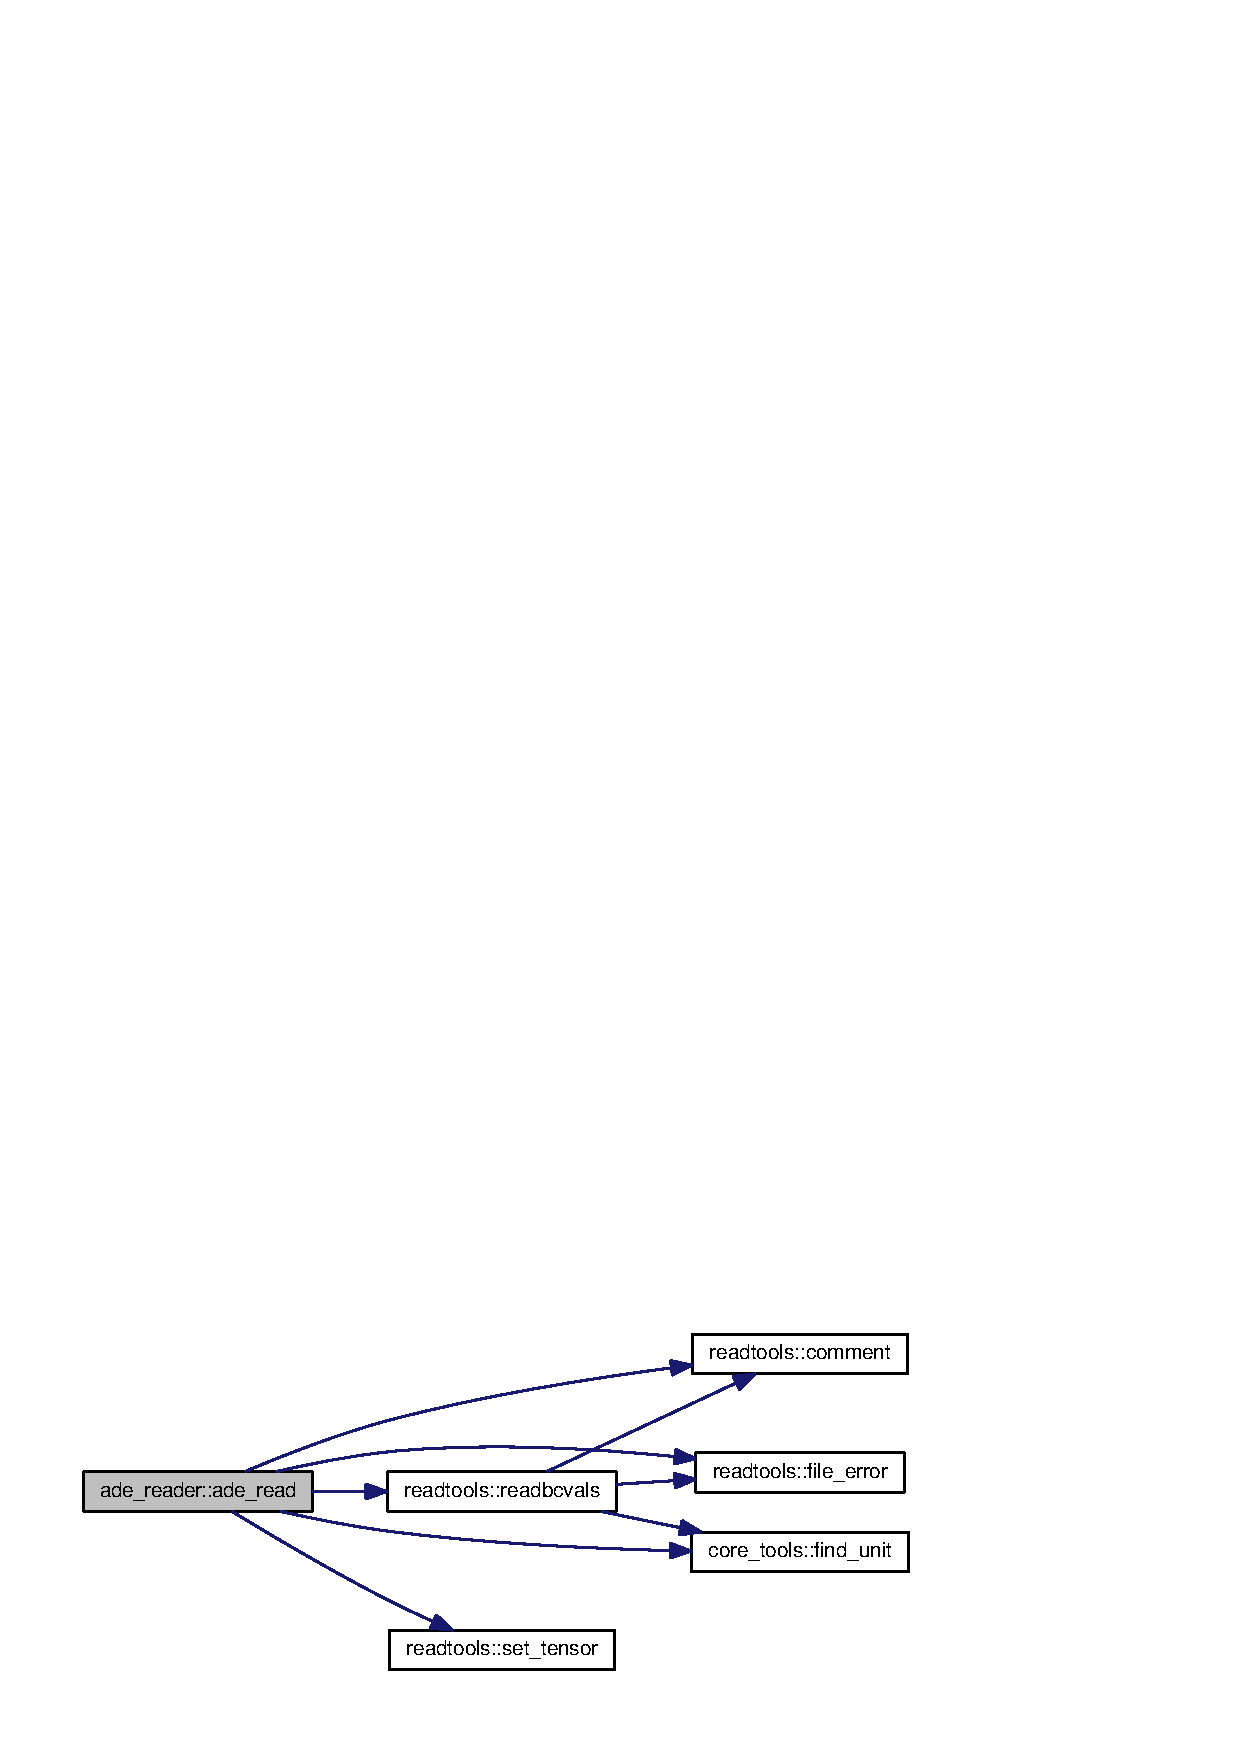
\includegraphics[width=350pt]{namespaceade__reader_ab579f926de43ae5ba712d144494109fb_cgraph}
\end{center}
\end{figure}




Here is the caller graph for this function\+:\nopagebreak
\begin{figure}[H]
\begin{center}
\leavevmode
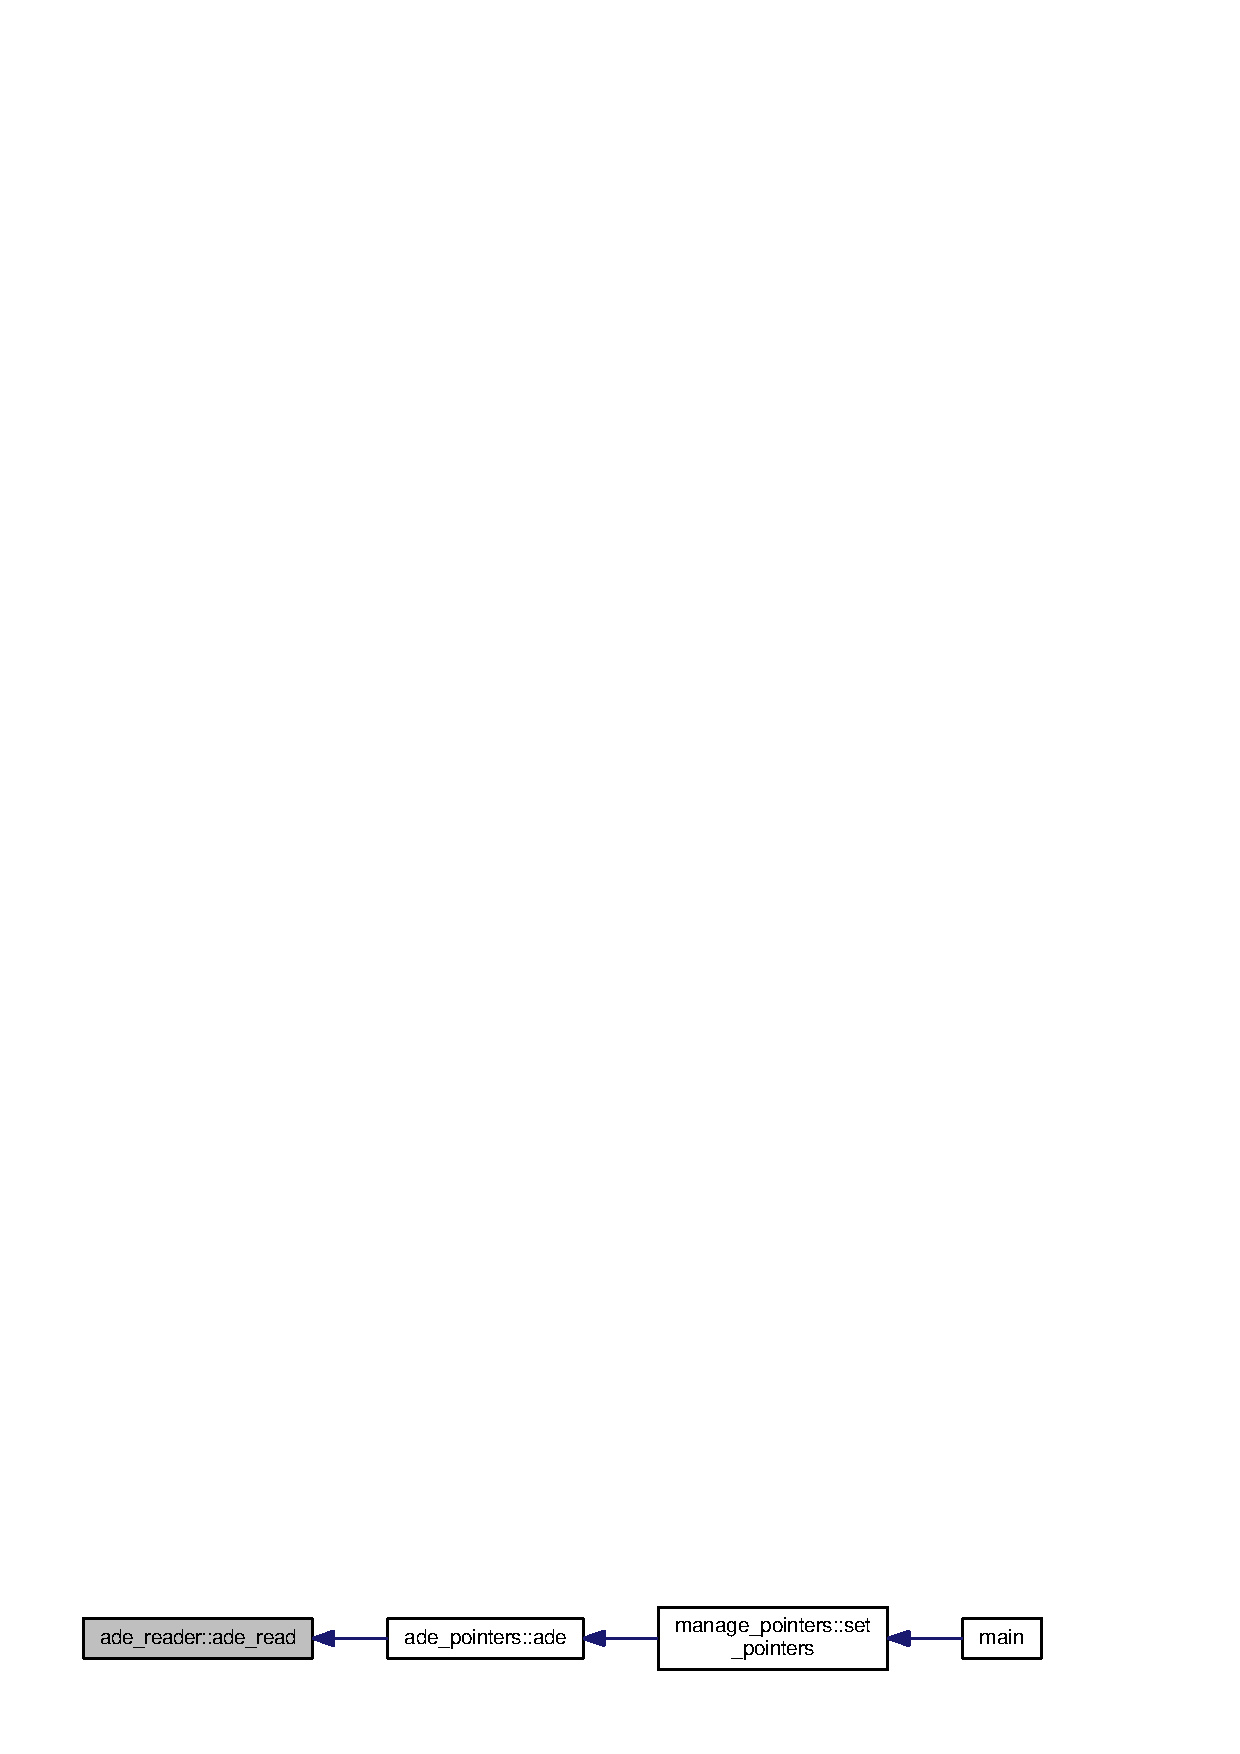
\includegraphics[width=350pt]{namespaceade__reader_ab579f926de43ae5ba712d144494109fb_icgraph}
\end{center}
\end{figure}


\index{ade\+\_\+reader@{ade\+\_\+reader}!adecs\+\_\+read@{adecs\+\_\+read}}
\index{adecs\+\_\+read@{adecs\+\_\+read}!ade\+\_\+reader@{ade\+\_\+reader}}
\subsubsection[{adecs\+\_\+read(pde\+\_\+loc)}]{\setlength{\rightskip}{0pt plus 5cm}subroutine ade\+\_\+reader\+::adecs\+\_\+read (
\begin{DoxyParamCaption}
\item[{class({\bf pde\+\_\+str}), intent(inout)}]{pde\+\_\+loc}
\end{DoxyParamCaption}
)}\label{namespaceade__reader_ac47e668b8eeddab2ccfae1527f991bf0}


Definition at line 280 of file A\+D\+E\+\_\+reader.\+f90.



Referenced by ade\+\_\+pointers\+::adekinsorb().


\begin{DoxyCode}
280       \textcolor{keywordtype}{use }typy
281       \textcolor{keywordtype}{use }pde_objs
282           
283       \textcolor{keywordtype}{class}(pde_str), \textcolor{keywordtype}{intent(in out)} :: pde\_loc
284       
285       pde\_loc%problem\_name(1) = \textcolor{stringliteral}{"ADER\_in\_solid"}
286       pde\_loc%problem\_name(2) = \textcolor{stringliteral}{"Advection-dispersion-reaction equation (solute concentration adsorbed in
       solid phase)"}
287 
288       pde\_loc%solution\_name(1) = \textcolor{stringliteral}{"solute\_concentration"} \textcolor{comment}{!nazev vystupnich souboru}
289       pde\_loc%solution\_name(2) = \textcolor{stringliteral}{"c  [M/M]"} \textcolor{comment}{!popisek grafu}
290 
291       pde\_loc%flux\_name(1) = \textcolor{stringliteral}{"zero\_flux"}  
292       pde\_loc%flux\_name(2) = \textcolor{stringliteral}{"zero flux"}
293 
294       pde\_loc%mass\_name(1) = \textcolor{stringliteral}{"conc\_in\_solid\_phase"}
295       pde\_loc%mass\_name(2) = \textcolor{stringliteral}{"concetration [M/M]"}
296       
297     
\end{DoxyCode}


Here is the caller graph for this function\+:\nopagebreak
\begin{figure}[H]
\begin{center}
\leavevmode
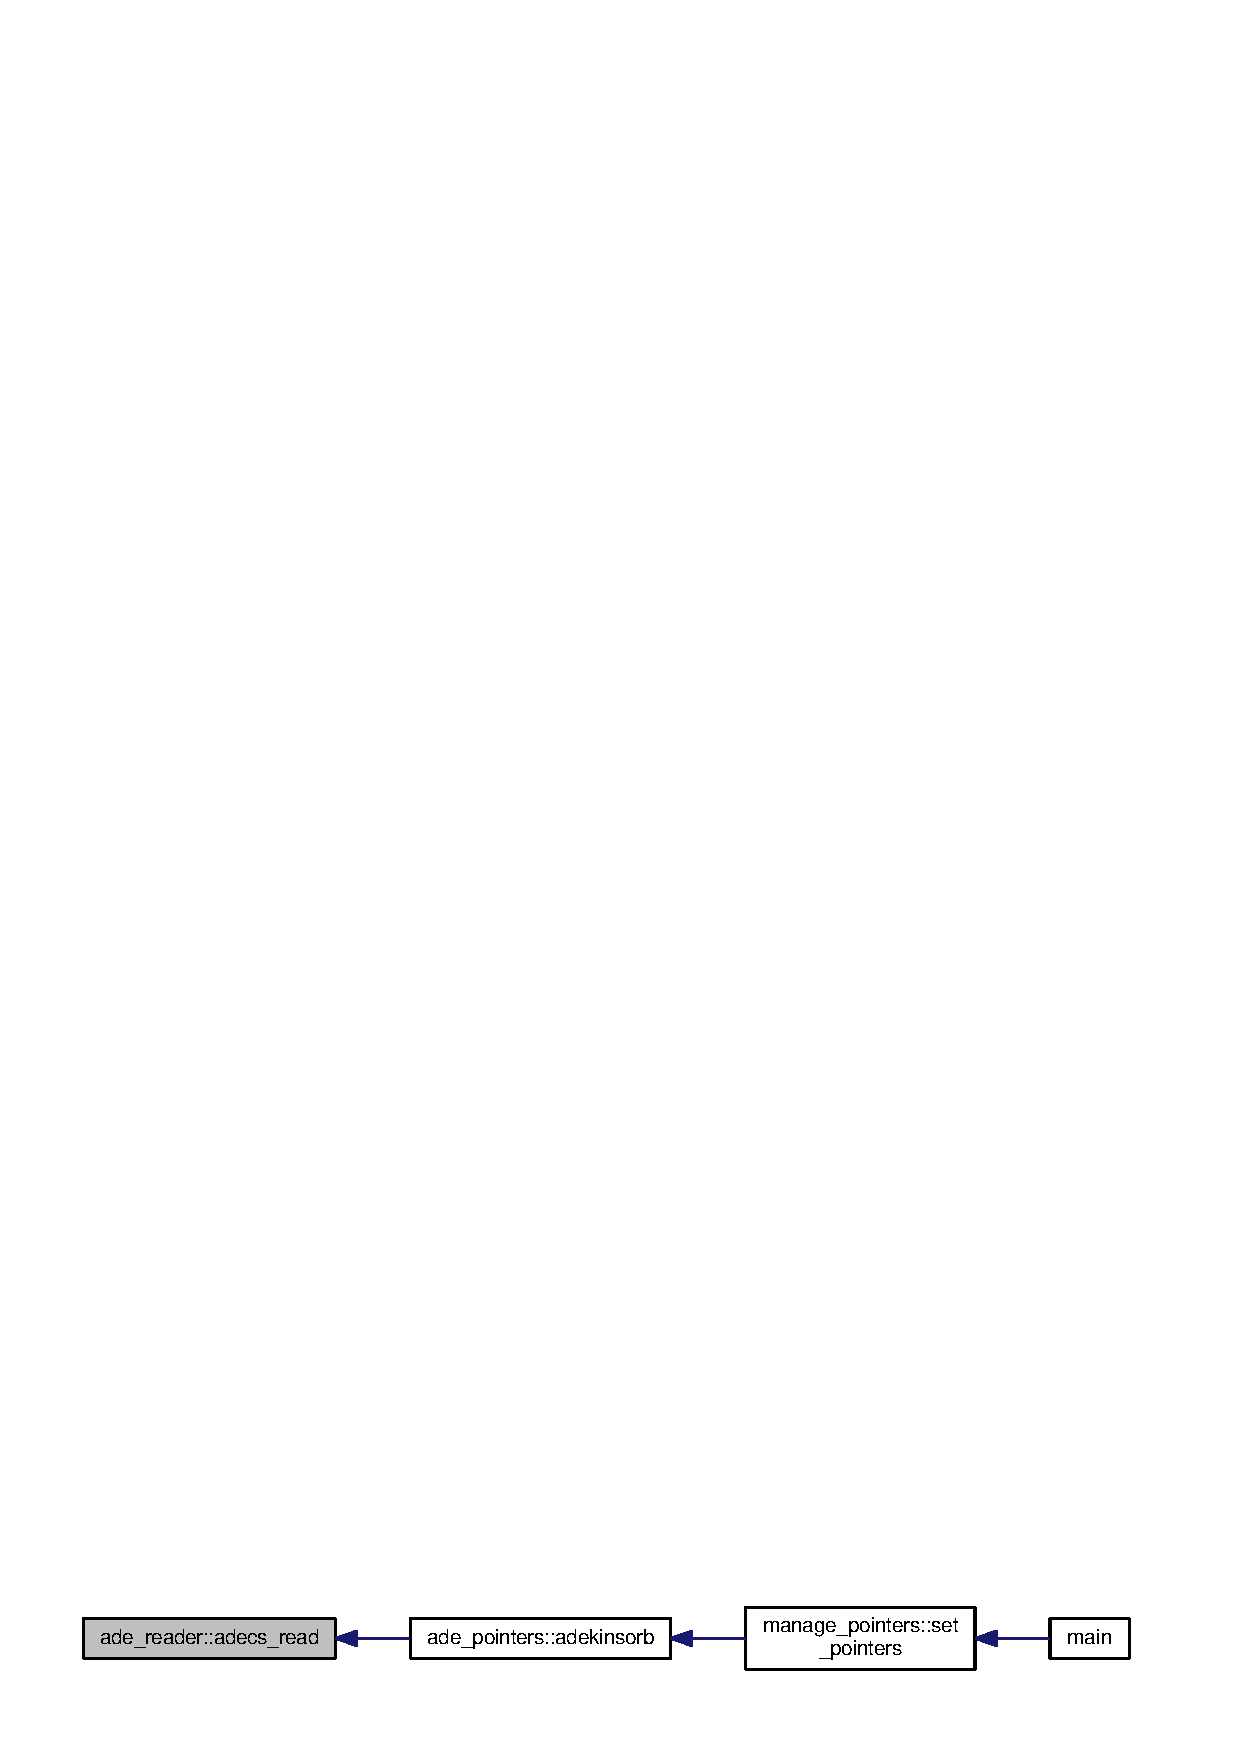
\includegraphics[width=350pt]{namespaceade__reader_ac47e668b8eeddab2ccfae1527f991bf0_icgraph}
\end{center}
\end{figure}



\section{boussfnc Module Reference}
\label{namespaceboussfnc}\index{boussfnc@{boussfnc}}
\subsection*{Functions/\+Subroutines}
\begin{DoxyCompactItemize}
\item 
real(kind=rkind) function, public {\bf bouss\+\_\+elast} (pde\+\_\+loc, layer, quadpnt, x)
\item 
subroutine, public {\bf bouss\+\_\+cond} (pde\+\_\+loc, layer, quadpnt, x, tensor, scalar)
\item 
subroutine, public {\bf bouss\+\_\+adv} (pde\+\_\+loc, layer, quadpnt, x, vector\+\_\+in, vector\+\_\+out, scalar)
\item 
real(kind=rkind) function, public {\bf boussreact} (pde\+\_\+loc, layer, quadpnt, x)
\item 
subroutine, public {\bf darcy4bouss} (pde\+\_\+loc, layer, quadpnt, x, grad, flux, flux\+\_\+length)
\item 
subroutine, public {\bf boussicond} (pde\+\_\+loc)
\item 
subroutine, public {\bf bouss\+\_\+bc} (pde\+\_\+loc, el\+\_\+id, node\+\_\+order, value, code)
\end{DoxyCompactItemize}


\subsection{Function/\+Subroutine Documentation}
\index{boussfnc@{boussfnc}!bouss\+\_\+adv@{bouss\+\_\+adv}}
\index{bouss\+\_\+adv@{bouss\+\_\+adv}!boussfnc@{boussfnc}}
\subsubsection[{bouss\+\_\+adv(pde\+\_\+loc, layer, quadpnt, x, vector\+\_\+in, vector\+\_\+out, scalar)}]{\setlength{\rightskip}{0pt plus 5cm}subroutine, public boussfnc\+::bouss\+\_\+adv (
\begin{DoxyParamCaption}
\item[{class({\bf pde\+\_\+str}), intent(in)}]{pde\+\_\+loc, }
\item[{integer(kind=ikind), intent(in)}]{layer, }
\item[{type({\bf integpnt\+\_\+str}), intent(in), optional}]{quadpnt, }
\item[{real(kind=rkind), dimension(\+:), intent(in), optional}]{x, }
\item[{real(kind=rkind), dimension(\+:), intent(in), optional}]{vector\+\_\+in, }
\item[{real(kind=rkind), dimension(\+:), intent(out), optional}]{vector\+\_\+out, }
\item[{real(kind=rkind), intent(out), optional}]{scalar}
\end{DoxyParamCaption}
)}\label{namespaceboussfnc_a523c691f2d5d7b1448f21c108d496392}

\begin{DoxyParams}[1]{Parameters}
\mbox{\tt in}  & {\em x} & pressure head\\
\hline
\mbox{\tt in}  & {\em vector\+\_\+in} & this argument is required by the global vector\+\_\+fnc procedure pointer, unused in this procedure\\
\hline
\mbox{\tt out}  & {\em scalar} & relative unsaturated hydraulic conductivity derivative in respect to h, scalar value \\
\hline
\end{DoxyParams}


Definition at line 155 of file boussfnc.\+f90.



References boussglob\+::bouss\+\_\+rain, boussglob\+::bouss\+\_\+slopes, geom\+\_\+tools\+::getcoor(), and globals\+::time.



Referenced by bousspointers\+::boussi().


\begin{DoxyCode}
155         \textcolor{keywordtype}{use }typy
156         \textcolor{keywordtype}{use }globals
157         \textcolor{keywordtype}{use }boussglob
158         \textcolor{keywordtype}{use }pde_objs
159         \textcolor{keywordtype}{use }geom_tools
160         \textcolor{keywordtype}{use }global_objs
161         \textcolor{keywordtype}{use }debug_tools
162 
163         \textcolor{keywordtype}{class}(pde_str), \textcolor{keywordtype}{intent(in)} :: pde\_loc
164         \textcolor{keywordtype}{integer(kind=ikind)}, \textcolor{keywordtype}{intent(in)} :: layer
165         \textcolor{keywordtype}{type}(integpnt_str), \textcolor{keywordtype}{intent(in)}, \textcolor{keywordtype}{optional} :: quadpnt    
167         \textcolor{keywordtype}{real(kind=rkind)}, \textcolor{keywordtype}{dimension(:)}, \textcolor{keywordtype}{intent(in)}, \textcolor{keywordtype}{optional} :: x
169         \textcolor{keywordtype}{real(kind=rkind)}, \textcolor{keywordtype}{dimension(:)}, \textcolor{keywordtype}{intent(in)}, \textcolor{keywordtype}{optional} :: vector\_in
173         \textcolor{keywordtype}{real(kind=rkind)}, \textcolor{keywordtype}{dimension(:)}, \textcolor{keywordtype}{intent(out)}, \textcolor{keywordtype}{optional} :: vector\_out
175         \textcolor{keywordtype}{real(kind=rkind)}, \textcolor{keywordtype}{intent(out)}, \textcolor{keywordtype}{optional} :: scalar
176         \textcolor{keywordtype}{real(kind=rkind)}, \textcolor{keywordtype}{dimension(1)} :: coord
177         \textcolor{keywordtype}{real(kind=rkind)} :: rain, h, slope
178         \textcolor{keywordtype}{real(kind=rkind)}, \textcolor{keywordtype}{dimension(1,1)} :: k
179         \textcolor{keywordtype}{integer(kind=ikind)} :: i
180 
181 
182         
183         \textcolor{keywordflow}{if} (\textcolor{keyword}{present}(quadpnt) .and. \textcolor{keyword}{present}(x)) \textcolor{keywordflow}{then}
184           print *, \textcolor{stringliteral}{"ERROR: the function can be called either with integ point or x value definition, not
       both of them"}
185           print *, \textcolor{stringliteral}{"exited from re\_constitutive::dmualem\_dh"}
186           error stop
187         \textcolor{keywordflow}{else} \textcolor{keywordflow}{if} (.not. \textcolor{keyword}{present}(quadpnt) .and. .not. \textcolor{keyword}{present}(x)) \textcolor{keywordflow}{then}
188           print *, \textcolor{stringliteral}{"ERROR: you have not specified either integ point or x value"}
189           print *, \textcolor{stringliteral}{"exited from re\_constitutive::dmualem\_dh"}
190           error stop
191 \textcolor{keywordflow}{        end if}
192         
193         \textcolor{keywordflow}{if} (\textcolor{keyword}{present}(quadpnt)) \textcolor{keywordflow}{then}
194           h = pde\_loc%getval(quadpnt)
195         \textcolor{keywordflow}{else}
196           \textcolor{keywordflow}{if} (ubound(x,1) /=1) \textcolor{keywordflow}{then}
197             print *, \textcolor{stringliteral}{"ERROR: van Genuchten function is a function of a single variable h"}
198             print *, \textcolor{stringliteral}{"       your input data has:"}, ubound(x,1), \textcolor{stringliteral}{"variables"}
199             print *, \textcolor{stringliteral}{"exited from re\_constitutive::dmualem\_dh"}
200             error stop
201 \textcolor{keywordflow}{          end if}
202           h = x(1)
203 \textcolor{keywordflow}{        end if}
204         
205         
206         
207         
208         \textcolor{keywordflow}{do} i=1, ubound(bouss_rain,1)-1
209           \textcolor{keywordflow}{if} (i == 1 .and. time < bouss_rain(1)%data(i)) \textcolor{keywordflow}{then}
210             rain = bouss_rain(2)%data(i) 
211 \textcolor{keywordflow}{          end if}
212           \textcolor{keywordflow}{if} (bouss_rain(1)%data(i) <= time .and. bouss_rain(1)%data(i+1) > time) \textcolor{keywordflow}{then}
213             rain = bouss_rain(2)%data(i) 
214             \textcolor{keywordflow}{EXIT}
215 \textcolor{keywordflow}{          end if}
216           \textcolor{keywordflow}{if} (i == bouss_rain(1)%pos - 1 .and. time >= bouss_rain(1)%data(i+1)) \textcolor{keywordflow}{then}
217             rain = bouss_rain(2)%data(i+1)
218 \textcolor{keywordflow}{          end if}
219 \textcolor{keywordflow}{        end do}
220         
221         
222         \textcolor{keyword}{call }getcoor(quadpnt, coord)
223         
224         \textcolor{keywordflow}{do} i=1, bouss_slopes(1)%pos - 1
225           \textcolor{keywordflow}{if} (coord(1) >= bouss_slopes(1)%data(i) .and. coord(1) < bouss_slopes(1)%data(i+1)) \textcolor{keywordflow}{then}
226             slope = bouss_slopes(2)%data(i)
227             \textcolor{keywordflow}{EXIT}
228 \textcolor{keywordflow}{          end if}
229           \textcolor{keywordflow}{if} (i == bouss_slopes(1)%pos - 1 .and. coord(1) >= bouss_slopes(1)%data(i+1)) \textcolor{keywordflow}{then}
230             slope = bouss_slopes(2)%data(i+1)
231 \textcolor{keywordflow}{          end if}
232 \textcolor{keywordflow}{        end do}
233         
234         \textcolor{keyword}{call }pde\_loc%pde\_fnc(1)%dispersion(pde\_loc, layer, quadpnt, tensor=k)
235 
236         \textcolor{keywordflow}{if} (\textcolor{keyword}{present}(vector\_out)) \textcolor{keywordflow}{then}
237           \textcolor{comment}{! must be negative, because the commnon scheme of the CDE problem has negative convection, but RE
       has positive convection}
238           vector\_out = -(rain*slope - slope*k(1,1))
239 \textcolor{keywordflow}{        end if}
240 
241 \textcolor{comment}{! print *, vector\_out, rain, slope ; stop}
242 
\end{DoxyCode}


Here is the call graph for this function\+:\nopagebreak
\begin{figure}[H]
\begin{center}
\leavevmode
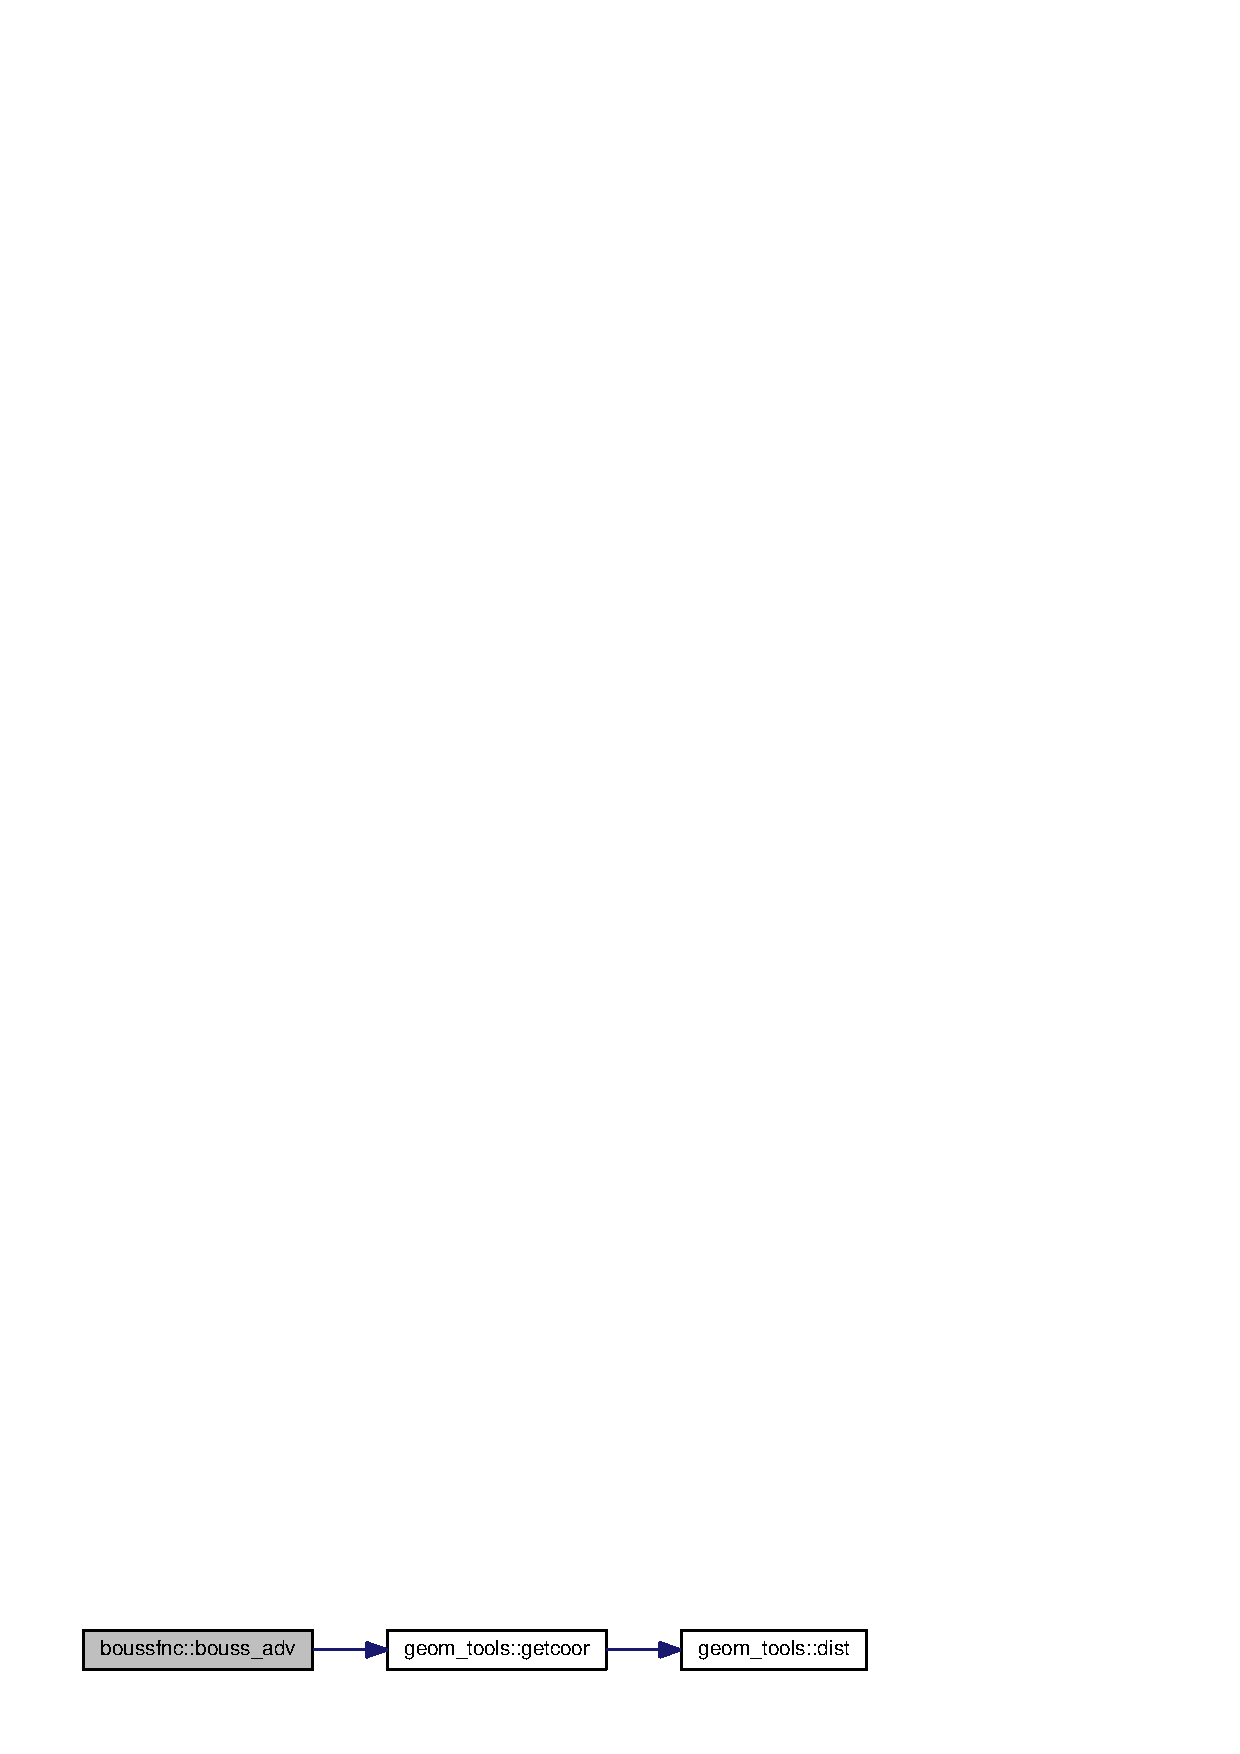
\includegraphics[width=350pt]{namespaceboussfnc_a523c691f2d5d7b1448f21c108d496392_cgraph}
\end{center}
\end{figure}




Here is the caller graph for this function\+:\nopagebreak
\begin{figure}[H]
\begin{center}
\leavevmode
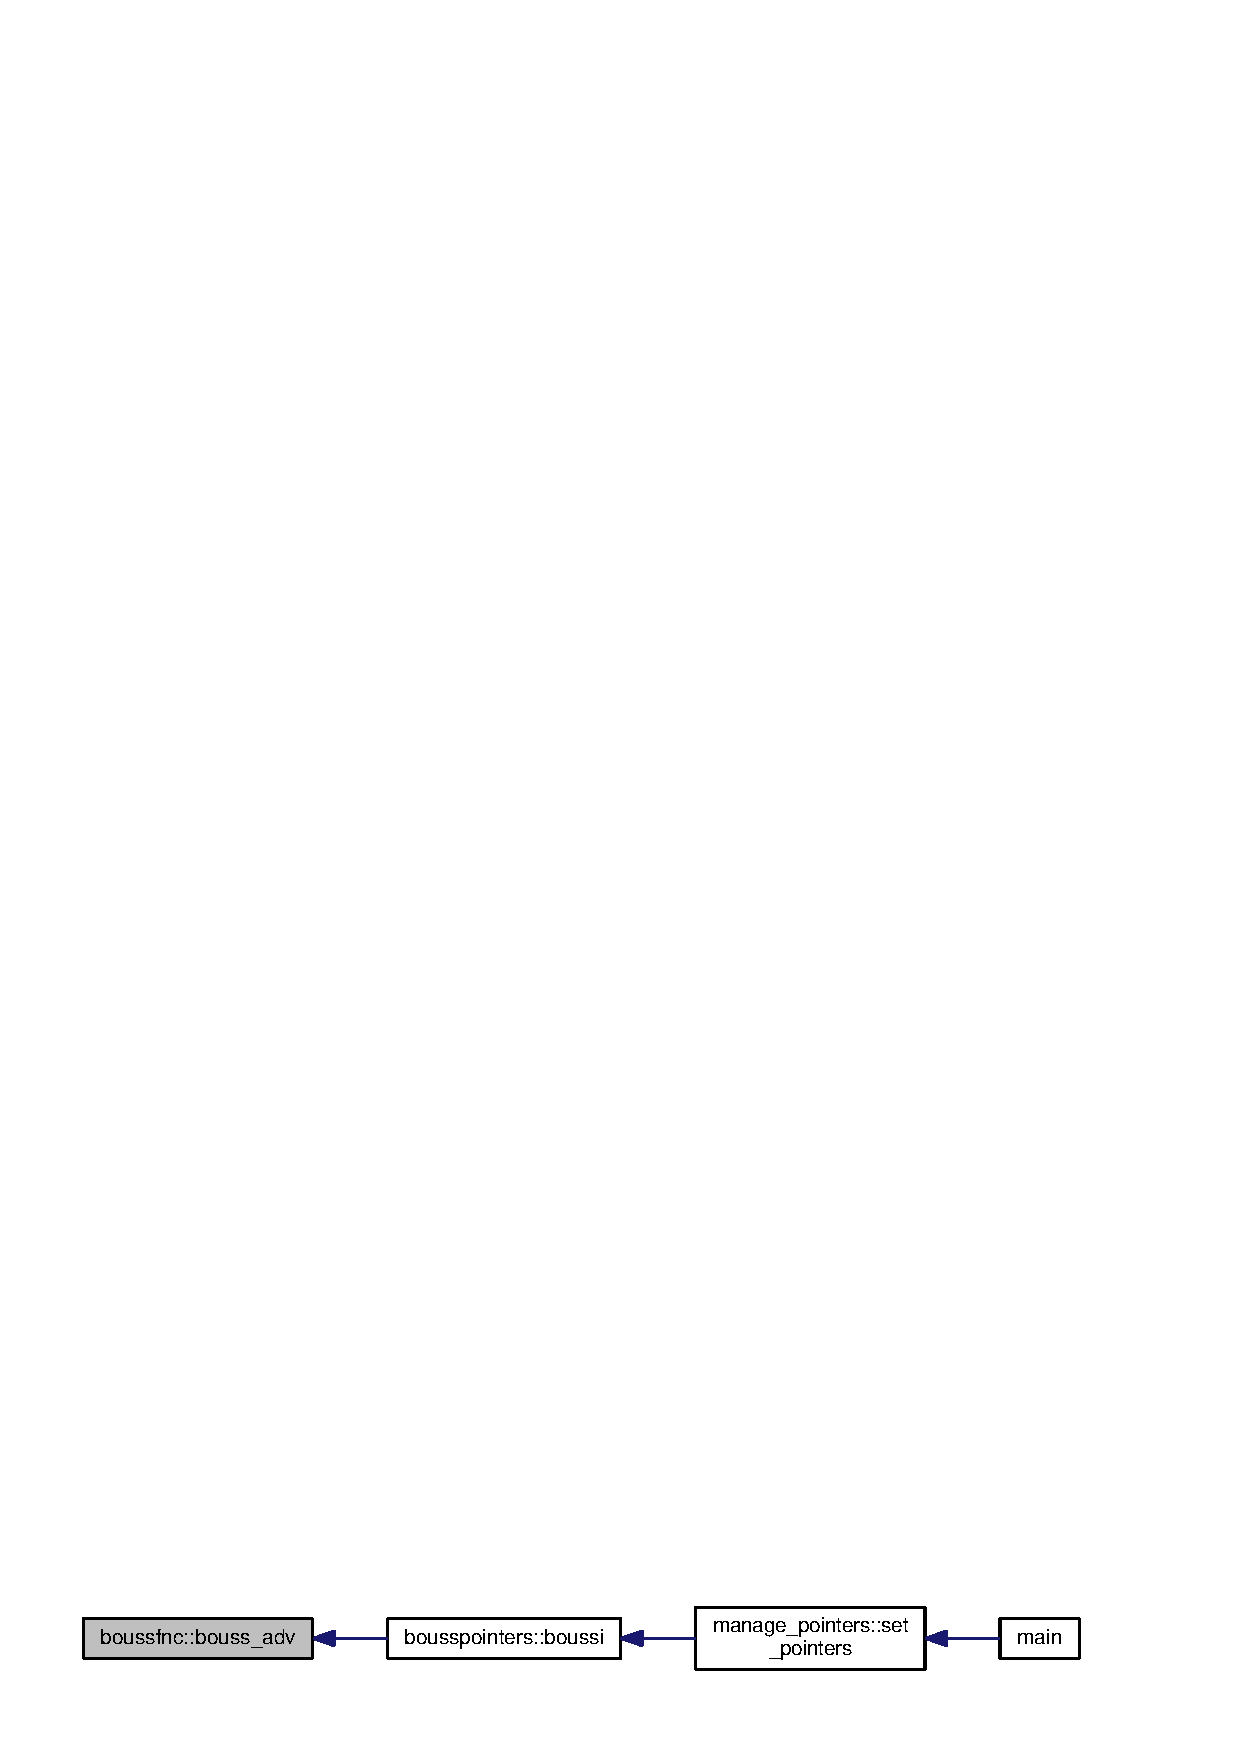
\includegraphics[width=350pt]{namespaceboussfnc_a523c691f2d5d7b1448f21c108d496392_icgraph}
\end{center}
\end{figure}


\index{boussfnc@{boussfnc}!bouss\+\_\+bc@{bouss\+\_\+bc}}
\index{bouss\+\_\+bc@{bouss\+\_\+bc}!boussfnc@{boussfnc}}
\subsubsection[{bouss\+\_\+bc(pde\+\_\+loc, el\+\_\+id, node\+\_\+order, value, code)}]{\setlength{\rightskip}{0pt plus 5cm}subroutine, public boussfnc\+::bouss\+\_\+bc (
\begin{DoxyParamCaption}
\item[{class({\bf pde\+\_\+str}), intent(in)}]{pde\+\_\+loc, }
\item[{integer(kind=ikind), intent(in)}]{el\+\_\+id, }
\item[{integer(kind=ikind), intent(in)}]{node\+\_\+order, }
\item[{real(kind=rkind), intent(out), optional}]{value, }
\item[{integer(kind=ikind), intent(out), optional}]{code}
\end{DoxyParamCaption}
)}\label{namespaceboussfnc_a664047715b553e05dbdc2d14b481e6fa}


Definition at line 408 of file boussfnc.\+f90.



References globals\+::elements, globals\+::nodes, and globals\+::time.



Referenced by bousspointers\+::boussi().


\begin{DoxyCode}
408         \textcolor{keywordtype}{use }typy
409         \textcolor{keywordtype}{use }globals
410         \textcolor{keywordtype}{use }global_objs
411         \textcolor{keywordtype}{use }pde_objs
412         \textcolor{keywordtype}{use }geom_tools
413 
414         \textcolor{keywordtype}{class}(pde_str), \textcolor{keywordtype}{intent(in)} :: pde\_loc
415         \textcolor{keywordtype}{integer(kind=ikind)}, \textcolor{keywordtype}{intent(in)}  :: el\_id, node\_order
416         \textcolor{keywordtype}{real(kind=rkind)}, \textcolor{keywordtype}{intent(out)}, \textcolor{keywordtype}{optional}   :: value
417         \textcolor{keywordtype}{integer(kind=ikind)}, \textcolor{keywordtype}{intent(out)}, \textcolor{keywordtype}{optional} :: code
418         
419         \textcolor{keywordtype}{integer(kind=ikind)} :: edge\_id, i, j
420         
421         edge\_id = nodes%edge(elements%data(el\_id, node\_order))
422         
423         \textcolor{keywordflow}{if} (\textcolor{keyword}{present}(\textcolor{keywordtype}{value})) \textcolor{keywordflow}{then}
424           \textcolor{keywordflow}{if} (pde\_loc%bc(edge\_id)%file) \textcolor{keywordflow}{then}
425             \textcolor{keywordflow}{do} i=1, ubound(pde\_loc%bc(edge\_id)%series,1)
426               \textcolor{keywordflow}{if} (pde\_loc%bc(edge\_id)%series(i,1) > time) \textcolor{keywordflow}{then}
427                 \textcolor{keywordflow}{if} (i > 1) \textcolor{keywordflow}{then}
428                   j = i-1
429                 \textcolor{keywordflow}{else}
430                   j = i
431 \textcolor{keywordflow}{                end if}
432                 \textcolor{keywordtype}{value} = pde\_loc%bc(edge\_id)%series(j,2)
433                 \textcolor{keywordflow}{EXIT}
434 \textcolor{keywordflow}{              end if}
435 \textcolor{keywordflow}{            end do}
436           \textcolor{keywordflow}{else}
437             \textcolor{keywordtype}{value} =  pde\_loc%bc(edge\_id)%value
438 \textcolor{keywordflow}{          end if}
439 \textcolor{keywordflow}{        end if}
440         
441         
442         \textcolor{keywordflow}{if} (\textcolor{keyword}{present}(code)) \textcolor{keywordflow}{then}
443           code = pde\_loc%bc(edge\_id)%code
444 \textcolor{keywordflow}{        end if}
445         
\end{DoxyCode}


Here is the caller graph for this function\+:\nopagebreak
\begin{figure}[H]
\begin{center}
\leavevmode
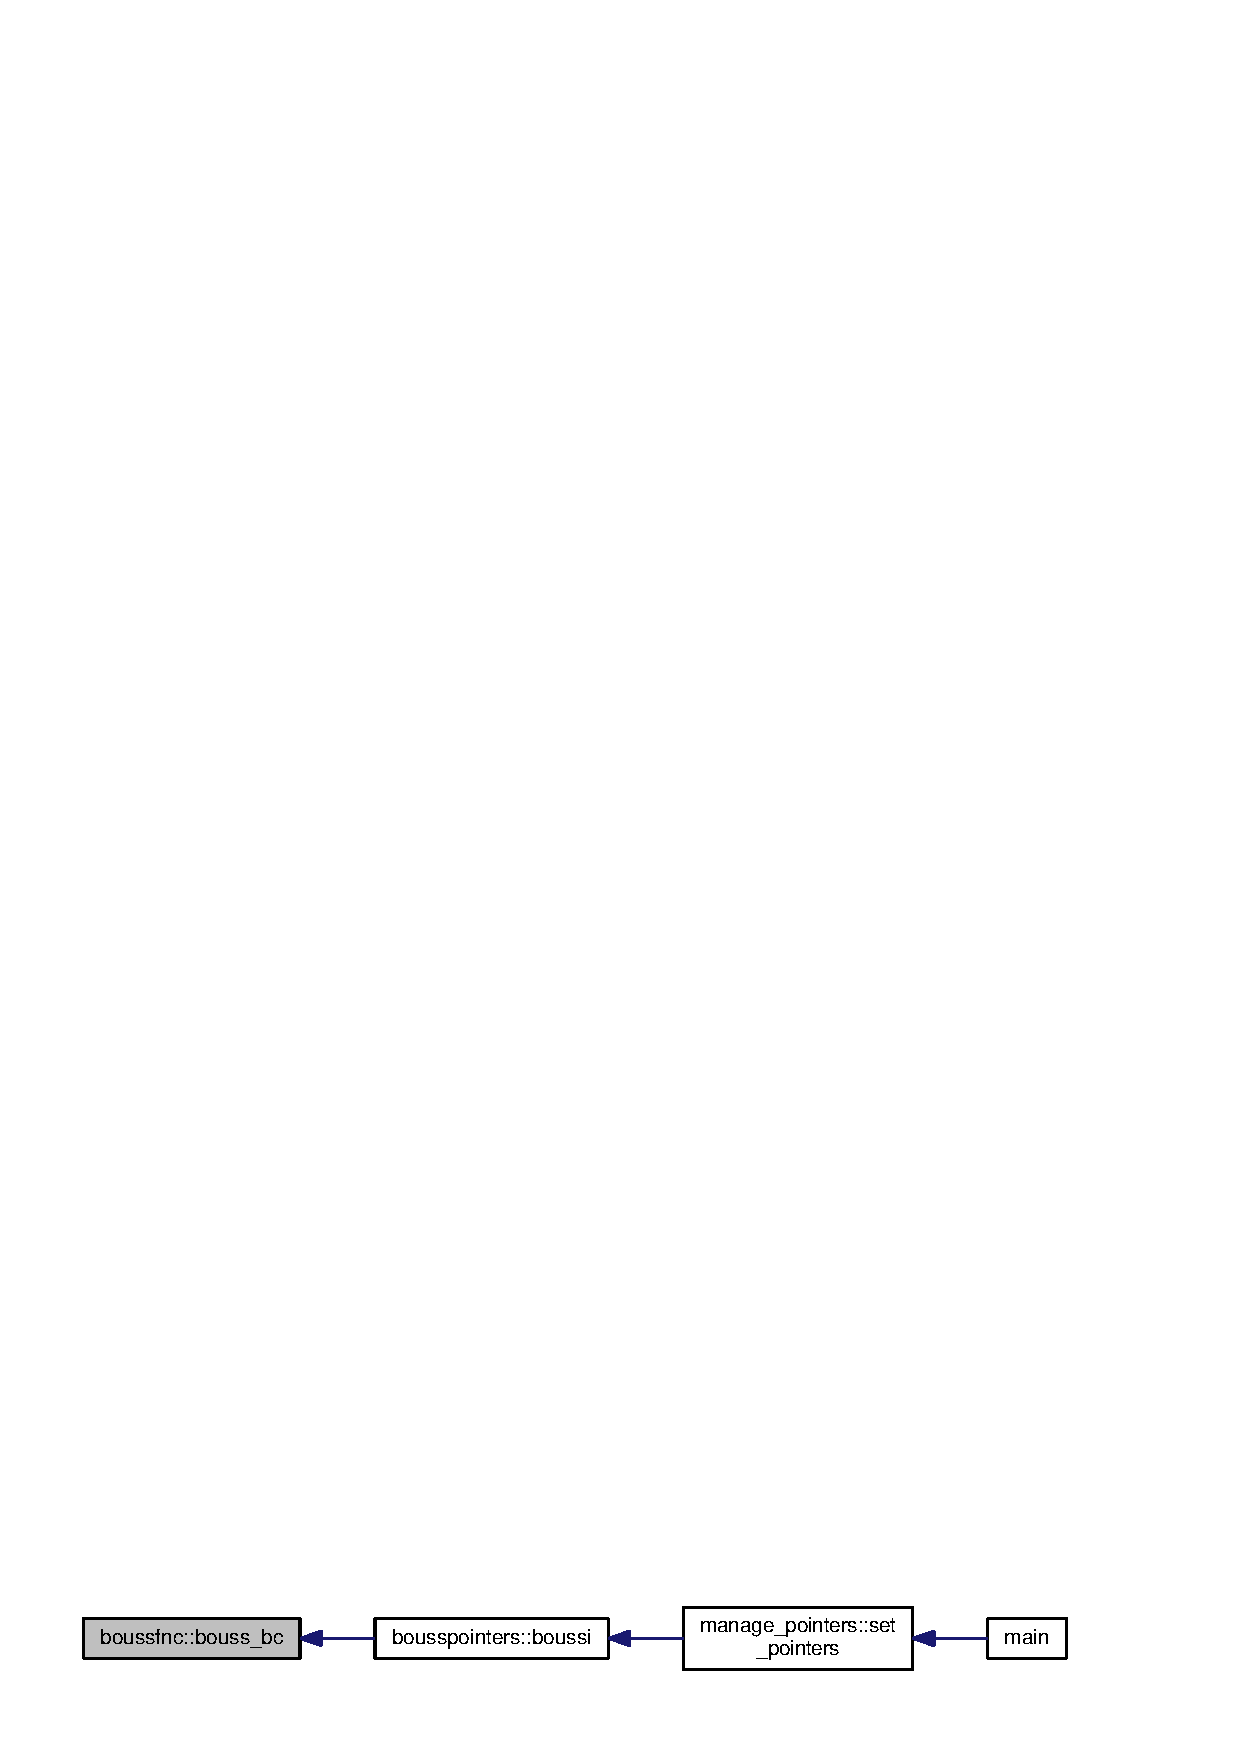
\includegraphics[width=350pt]{namespaceboussfnc_a664047715b553e05dbdc2d14b481e6fa_icgraph}
\end{center}
\end{figure}


\index{boussfnc@{boussfnc}!bouss\+\_\+cond@{bouss\+\_\+cond}}
\index{bouss\+\_\+cond@{bouss\+\_\+cond}!boussfnc@{boussfnc}}
\subsubsection[{bouss\+\_\+cond(pde\+\_\+loc, layer, quadpnt, x, tensor, scalar)}]{\setlength{\rightskip}{0pt plus 5cm}subroutine, public boussfnc\+::bouss\+\_\+cond (
\begin{DoxyParamCaption}
\item[{class({\bf pde\+\_\+str}), intent(in)}]{pde\+\_\+loc, }
\item[{integer(kind=ikind), intent(in)}]{layer, }
\item[{type({\bf integpnt\+\_\+str}), intent(in), optional}]{quadpnt, }
\item[{real(kind=rkind), dimension(\+:), intent(in), optional}]{x, }
\item[{real(kind=rkind), dimension(\+:,\+:), intent(out), optional}]{tensor, }
\item[{real(kind=rkind), intent(out), optional}]{scalar}
\end{DoxyParamCaption}
)}\label{namespaceboussfnc_a1eb4dcb6eb00362b392c983cf5cefb45}

\begin{DoxyParams}[1]{Parameters}
\mbox{\tt in}  & {\em x} & pressure head\\
\hline
\mbox{\tt in}  & {\em quadpnt} & Gauss quadrature point structure (element number and rank of Gauss quadrature point)\\
\hline
\mbox{\tt out}  & {\em tensor} & second order tensor of the unsaturated hydraulic conductivity\\
\hline
\mbox{\tt out}  & {\em scalar} & relative hydraulic conductivity, (scalar value) \\
\hline
\end{DoxyParams}


Definition at line 79 of file boussfnc.\+f90.



References boussglob\+::bouss\+\_\+k, and geom\+\_\+tools\+::getcoor().



Referenced by bousspointers\+::boussi().


\begin{DoxyCode}
79         \textcolor{keywordtype}{use }typy
80         \textcolor{keywordtype}{use }boussglob
81         \textcolor{keywordtype}{use }pde_objs
82         \textcolor{keywordtype}{use }geom_tools
83         \textcolor{keywordtype}{use }debug_tools
84 
85         \textcolor{keywordtype}{class}(pde_str), \textcolor{keywordtype}{intent(in)} :: pde\_loc
86         \textcolor{keywordtype}{integer(kind=ikind)}, \textcolor{keywordtype}{intent(in)} :: layer
88         \textcolor{keywordtype}{real(kind=rkind)}, \textcolor{keywordtype}{dimension(:)}, \textcolor{keywordtype}{intent(in)}, \textcolor{keywordtype}{optional} :: x
90         \textcolor{keywordtype}{type}(integpnt_str), \textcolor{keywordtype}{intent(in)}, \textcolor{keywordtype}{optional} :: quadpnt      
92         \textcolor{keywordtype}{real(kind=rkind)}, \textcolor{keywordtype}{dimension(:,:)}, \textcolor{keywordtype}{intent(out)}, \textcolor{keywordtype}{optional} :: tensor
93         \textcolor{keywordtype}{real(kind=rkind)} :: h
95         \textcolor{keywordtype}{real(kind=rkind)}, \textcolor{keywordtype}{intent(out)}, \textcolor{keywordtype}{optional} :: scalar
96 
97         \textcolor{keywordtype}{real(kind=rkind)}, \textcolor{keywordtype}{dimension(1)} :: coord
98         \textcolor{keywordtype}{integer(kind=ikind)} :: i
99 
100         \textcolor{keywordflow}{if} (\textcolor{keyword}{present}(quadpnt) .and. \textcolor{keyword}{present}(x)) \textcolor{keywordflow}{then}
101           print *, \textcolor{stringliteral}{"ERROR: the function can be called either with integ point or x value definition, not
       both of them"}
102           print *, \textcolor{stringliteral}{"exited from re\_constitutive::mualem"}
103           error stop
104         \textcolor{keywordflow}{else} \textcolor{keywordflow}{if} (.not. \textcolor{keyword}{present}(quadpnt) .and. .not. \textcolor{keyword}{present}(x)) \textcolor{keywordflow}{then}
105           print *, \textcolor{stringliteral}{"ERROR: you have not specified either integ point or x value"}
106           print *, \textcolor{stringliteral}{"exited from re\_constitutive::mualem"}
107           error stop
108 \textcolor{keywordflow}{        end if}
109         
110         \textcolor{keywordflow}{if} (\textcolor{keyword}{present}(quadpnt)) \textcolor{keywordflow}{then}
111           h = pde\_loc%getval(quadpnt)
112         \textcolor{keywordflow}{else}
113           \textcolor{keywordflow}{if} (ubound(x,1) /=1) \textcolor{keywordflow}{then}
114             print *, \textcolor{stringliteral}{"ERROR: van Genuchten function is a function of a single variable h"}
115             print *, \textcolor{stringliteral}{"       your input data has:"}, ubound(x,1), \textcolor{stringliteral}{"variables"}
116             print *, \textcolor{stringliteral}{"exited from re\_constitutive::mualem"}
117             error stop
118 \textcolor{keywordflow}{          end if}
119           h = x(1)
120 \textcolor{keywordflow}{        end if}
121         
122         \textcolor{keyword}{call }getcoor(quadpnt, coord)
123         
124 
125         
126         \textcolor{keywordflow}{do} i=1, bouss_k(1)%pos - 1
127           \textcolor{keywordflow}{if} (coord(1) >= bouss_k(1)%data(i) .and. coord(1) < bouss_k(1)%data(i+1)) \textcolor{keywordflow}{then}
128             \textcolor{keywordflow}{if} (\textcolor{keyword}{present}(tensor)) \textcolor{keywordflow}{then}
129 
130               tensor =  bouss_k(2)%data(i) * h
131 
132 \textcolor{keywordflow}{            end if}
133             \textcolor{keywordflow}{if} (\textcolor{keyword}{present}(scalar)) \textcolor{keywordflow}{then}
134               scalar =  bouss_k(2)%data(i) * h
135 \textcolor{keywordflow}{            end if}
136             \textcolor{keywordflow}{EXIT}
137 \textcolor{keywordflow}{          end if}
138           \textcolor{keywordflow}{if} (i == bouss_k(1)%pos - 1 .and. coord(1) >= bouss_k(1)%data(i+1)) \textcolor{keywordflow}{then}
139             \textcolor{keywordflow}{if} (\textcolor{keyword}{present}(tensor)) \textcolor{keywordflow}{then}
140               tensor =  bouss_k(2)%data(i+1) * h
141 \textcolor{keywordflow}{            end if}
142             \textcolor{keywordflow}{if} (\textcolor{keyword}{present}(scalar)) \textcolor{keywordflow}{then}
143               scalar =  bouss_k(2)%data(i+1) * h
144 \textcolor{keywordflow}{            end if}
145 \textcolor{keywordflow}{          end if}
146           
147 \textcolor{keywordflow}{        end do}
148         
149         
150       
\end{DoxyCode}


Here is the call graph for this function\+:\nopagebreak
\begin{figure}[H]
\begin{center}
\leavevmode
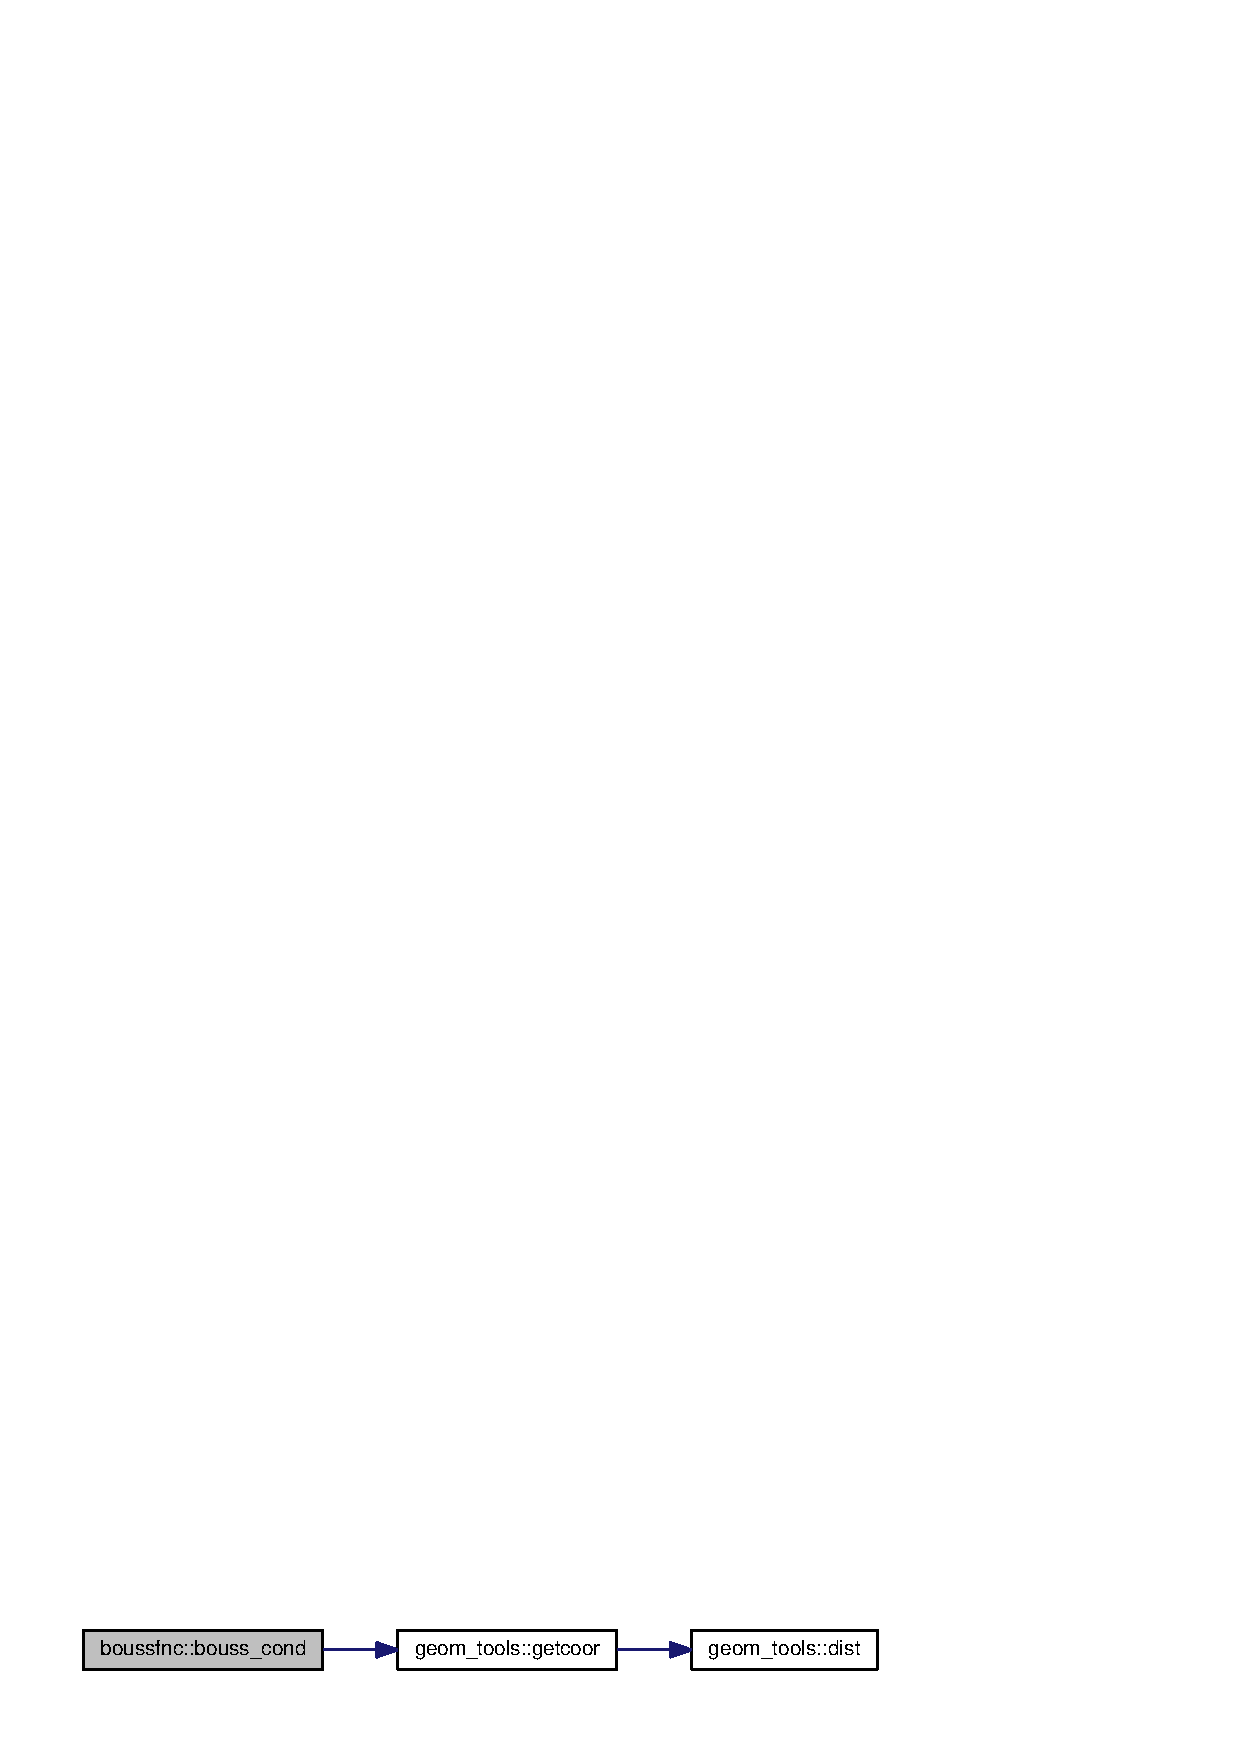
\includegraphics[width=350pt]{namespaceboussfnc_a1eb4dcb6eb00362b392c983cf5cefb45_cgraph}
\end{center}
\end{figure}




Here is the caller graph for this function\+:\nopagebreak
\begin{figure}[H]
\begin{center}
\leavevmode
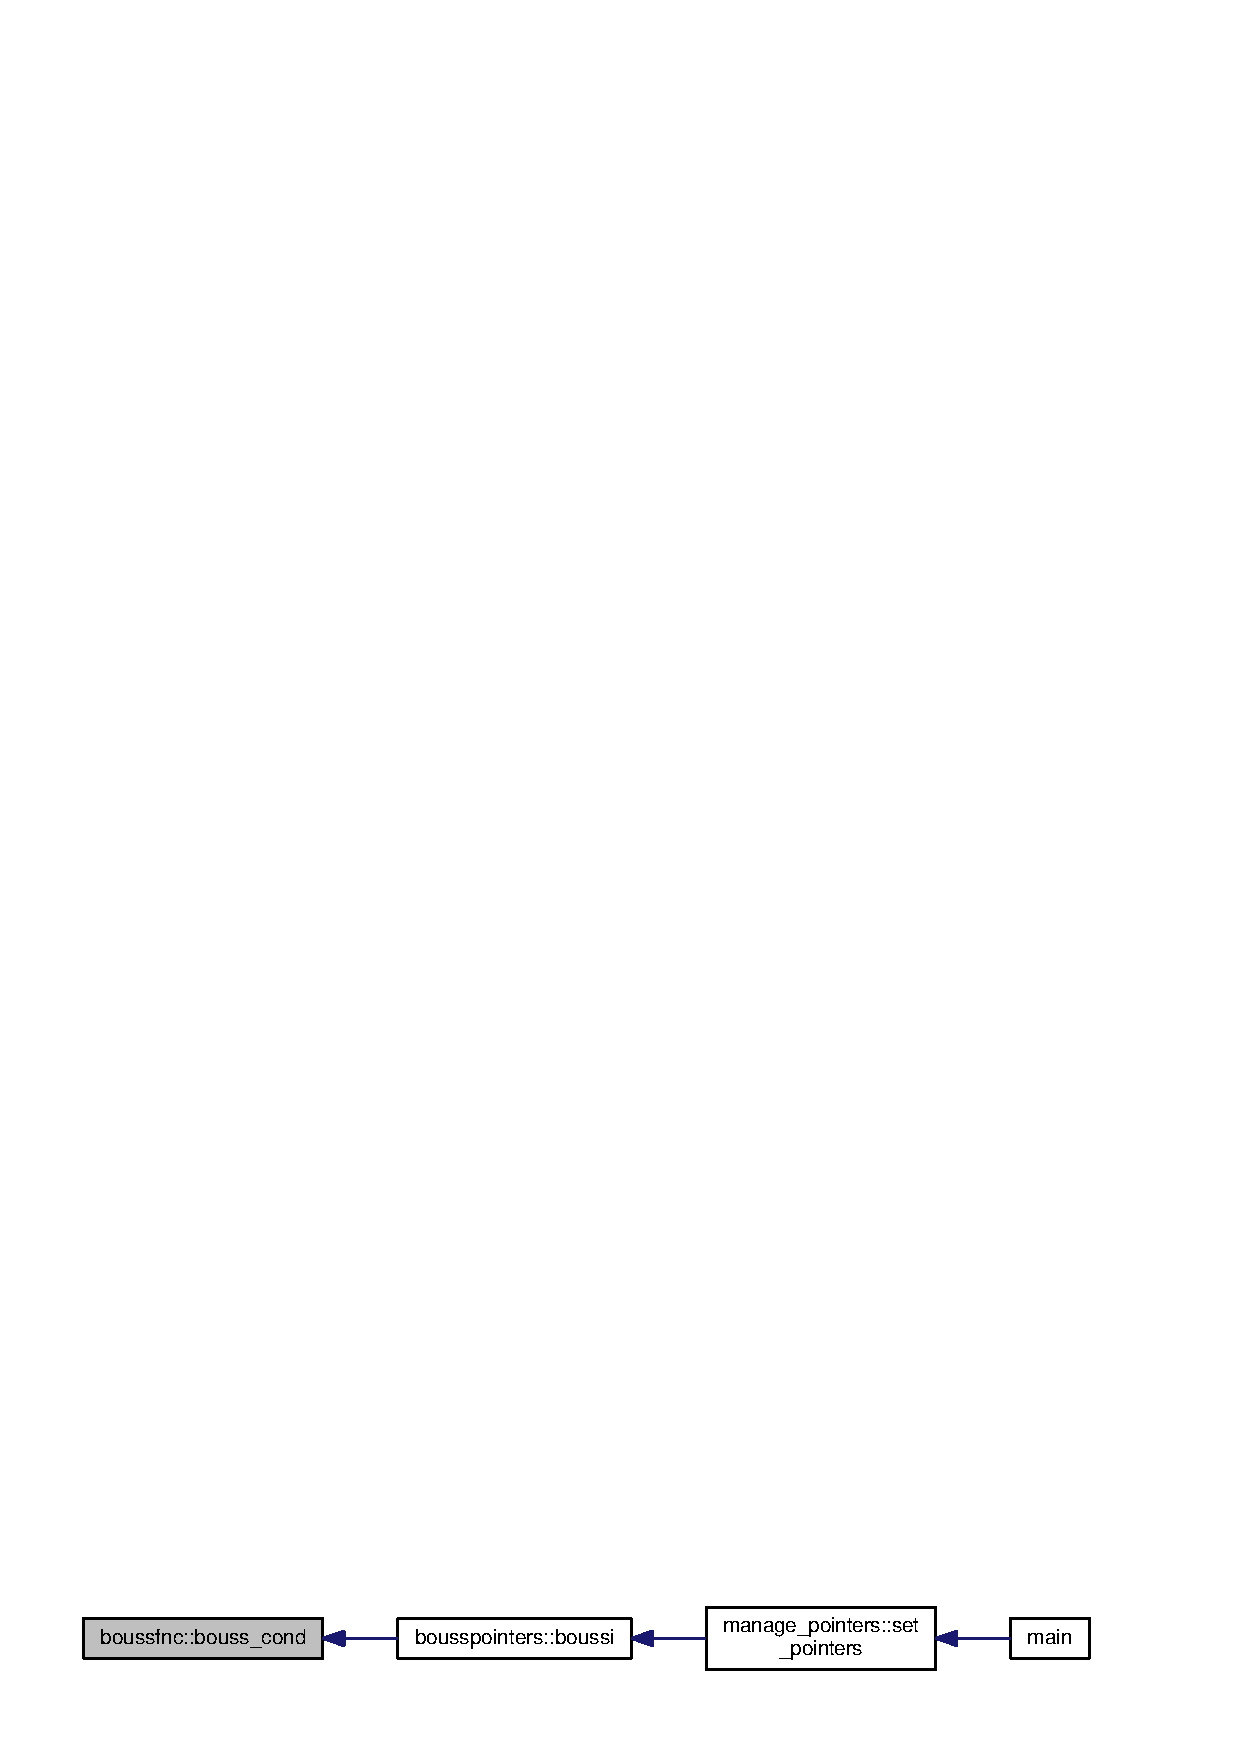
\includegraphics[width=350pt]{namespaceboussfnc_a1eb4dcb6eb00362b392c983cf5cefb45_icgraph}
\end{center}
\end{figure}


\index{boussfnc@{boussfnc}!bouss\+\_\+elast@{bouss\+\_\+elast}}
\index{bouss\+\_\+elast@{bouss\+\_\+elast}!boussfnc@{boussfnc}}
\subsubsection[{bouss\+\_\+elast(pde\+\_\+loc, layer, quadpnt, x)}]{\setlength{\rightskip}{0pt plus 5cm}real(kind=rkind) function, public boussfnc\+::bouss\+\_\+elast (
\begin{DoxyParamCaption}
\item[{class({\bf pde\+\_\+str}), intent(in)}]{pde\+\_\+loc, }
\item[{integer(kind=ikind), intent(in)}]{layer, }
\item[{type({\bf integpnt\+\_\+str}), intent(in), optional}]{quadpnt, }
\item[{real(kind=rkind), dimension(\+:), intent(in), optional}]{x}
\end{DoxyParamCaption}
)}\label{namespaceboussfnc_a071d2eeb5f983e31d4495bb68a137e76}

\begin{DoxyParams}[1]{Parameters}
\mbox{\tt in}  & {\em x} & pressure head\\
\hline
\mbox{\tt in}  & {\em quadpnt} & Gauss quadrature point structure (element number and rank of Gauss quadrature point)\\
\hline
\end{DoxyParams}
\begin{DoxyReturn}{Returns}
resulting system elasticity 
\end{DoxyReturn}


Definition at line 14 of file boussfnc.\+f90.



References boussglob\+::bouss\+\_\+por, boussglob\+::bouss\+\_\+slopes, and geom\+\_\+tools\+::getcoor().



Referenced by bousspointers\+::boussi().


\begin{DoxyCode}
14         \textcolor{keywordtype}{use }typy
15         \textcolor{keywordtype}{use }boussglob
16         \textcolor{keywordtype}{use }pde_objs
17         \textcolor{keywordtype}{use }geom_tools
18 
19         \textcolor{keywordtype}{class}(pde_str), \textcolor{keywordtype}{intent(in)} :: pde\_loc 
20         \textcolor{keywordtype}{integer(kind=ikind)}, \textcolor{keywordtype}{intent(in)} :: layer
22         \textcolor{keywordtype}{real(kind=rkind)}, \textcolor{keywordtype}{intent(in)}, \textcolor{keywordtype}{dimension(:)},  \textcolor{keywordtype}{optional} :: x
24         \textcolor{keywordtype}{type}(integpnt_str), \textcolor{keywordtype}{intent(in)}, \textcolor{keywordtype}{optional} :: quadpnt
25         \textcolor{keywordtype}{real(kind=rkind)} :: h
27         \textcolor{keywordtype}{real(kind=rkind)} :: e
28         \textcolor{keywordtype}{real(kind=rkind)}, \textcolor{keywordtype}{dimension(1)} :: coord
29         \textcolor{keywordtype}{real(kind=rkind)} :: cos\_slope, slope
30         \textcolor{keywordtype}{integer(kind=ikind)} :: i
31 
32         
33         \textcolor{keywordflow}{if} (\textcolor{keyword}{present}(quadpnt) .and. \textcolor{keyword}{present}(x)) \textcolor{keywordflow}{then}
34           print *, \textcolor{stringliteral}{"ERROR: the function can be called either with integ point or x value definition, not
       both of them"}
35           print *, \textcolor{stringliteral}{"exited from re\_constitutive::vangen\_elast"}
36           error stop
37         \textcolor{keywordflow}{else} \textcolor{keywordflow}{if} (.not. \textcolor{keyword}{present}(quadpnt) .and. .not. \textcolor{keyword}{present}(x)) \textcolor{keywordflow}{then}
38           print *, \textcolor{stringliteral}{"ERROR: you have not specified either integ point or x value"}
39           print *, \textcolor{stringliteral}{"exited from re\_constitutive::vangen\_elast"}
40           error stop
41 \textcolor{keywordflow}{        end if}
42         
43         \textcolor{keywordflow}{if} (\textcolor{keyword}{present}(quadpnt)) \textcolor{keywordflow}{then}
44           h = pde\_loc%getval(quadpnt)
45         \textcolor{keywordflow}{else}
46           \textcolor{keywordflow}{if} (ubound(x,1) /=1) \textcolor{keywordflow}{then}
47             print *, \textcolor{stringliteral}{"ERROR: van Genuchten function is a function of a single variable h"}
48             print *, \textcolor{stringliteral}{"       your input data has:"}, ubound(x,1), \textcolor{stringliteral}{"variables"}
49             error stop
50 \textcolor{keywordflow}{          end if}
51           \textcolor{keywordflow}{if} (ubound(x,1) /=1) \textcolor{keywordflow}{then}
52             print *, \textcolor{stringliteral}{"ERROR: van Genuchten function is a function of a single variable h"}
53             print *, \textcolor{stringliteral}{"       your input data has:"}, ubound(x,1), \textcolor{stringliteral}{"variables"}
54             print *, \textcolor{stringliteral}{"exited from re\_constitutive::vangen\_elast"}
55             error stop
56 \textcolor{keywordflow}{          end if}
57           h = x(1)
58 \textcolor{keywordflow}{        end if}
59 
60         \textcolor{keyword}{call }getcoor(quadpnt, coord)
61         
62         \textcolor{keywordflow}{do} i=1, bouss_slopes(1)%pos - 1
63           \textcolor{keywordflow}{if} (coord(1) >= bouss_slopes(1)%data(i) .and. coord(1) < bouss_slopes(1)%data(i+1)) \textcolor{keywordflow}{then}
64             slope = bouss_slopes(2)%data(i)
65             \textcolor{keywordflow}{EXIT}
66 \textcolor{keywordflow}{          end if}
67           \textcolor{keywordflow}{if} (i == bouss_slopes(1)%pos - 1 .and. coord(1) >= bouss_slopes(1)%data(i+1)) \textcolor{keywordflow}{then}
68             slope = bouss_slopes(2)%data(i+1)
69 \textcolor{keywordflow}{          end if}
70 \textcolor{keywordflow}{        end do}
71         cos\_slope = cos(atan(slope))
72         e = bouss_por/cos\_slope 
73         
74 
\end{DoxyCode}


Here is the call graph for this function\+:\nopagebreak
\begin{figure}[H]
\begin{center}
\leavevmode
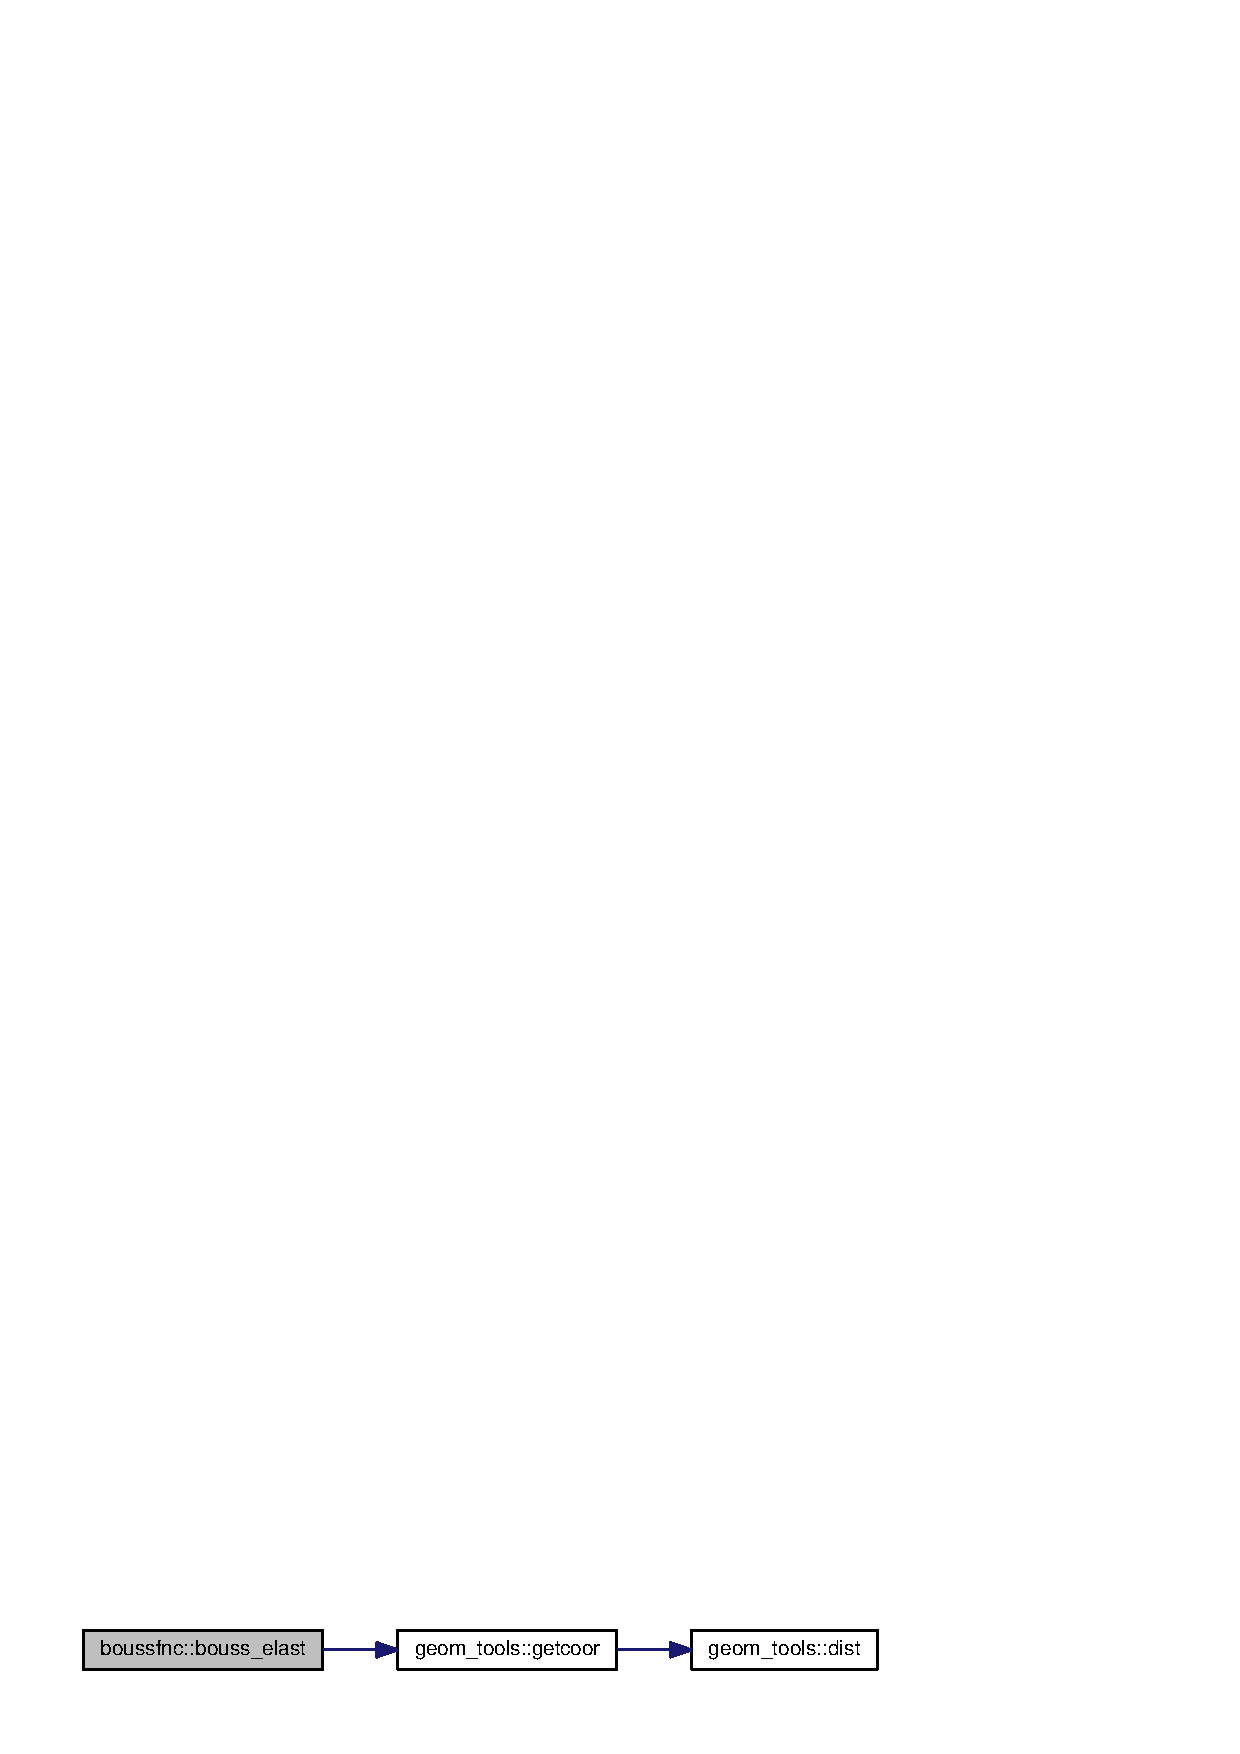
\includegraphics[width=350pt]{namespaceboussfnc_a071d2eeb5f983e31d4495bb68a137e76_cgraph}
\end{center}
\end{figure}




Here is the caller graph for this function\+:\nopagebreak
\begin{figure}[H]
\begin{center}
\leavevmode
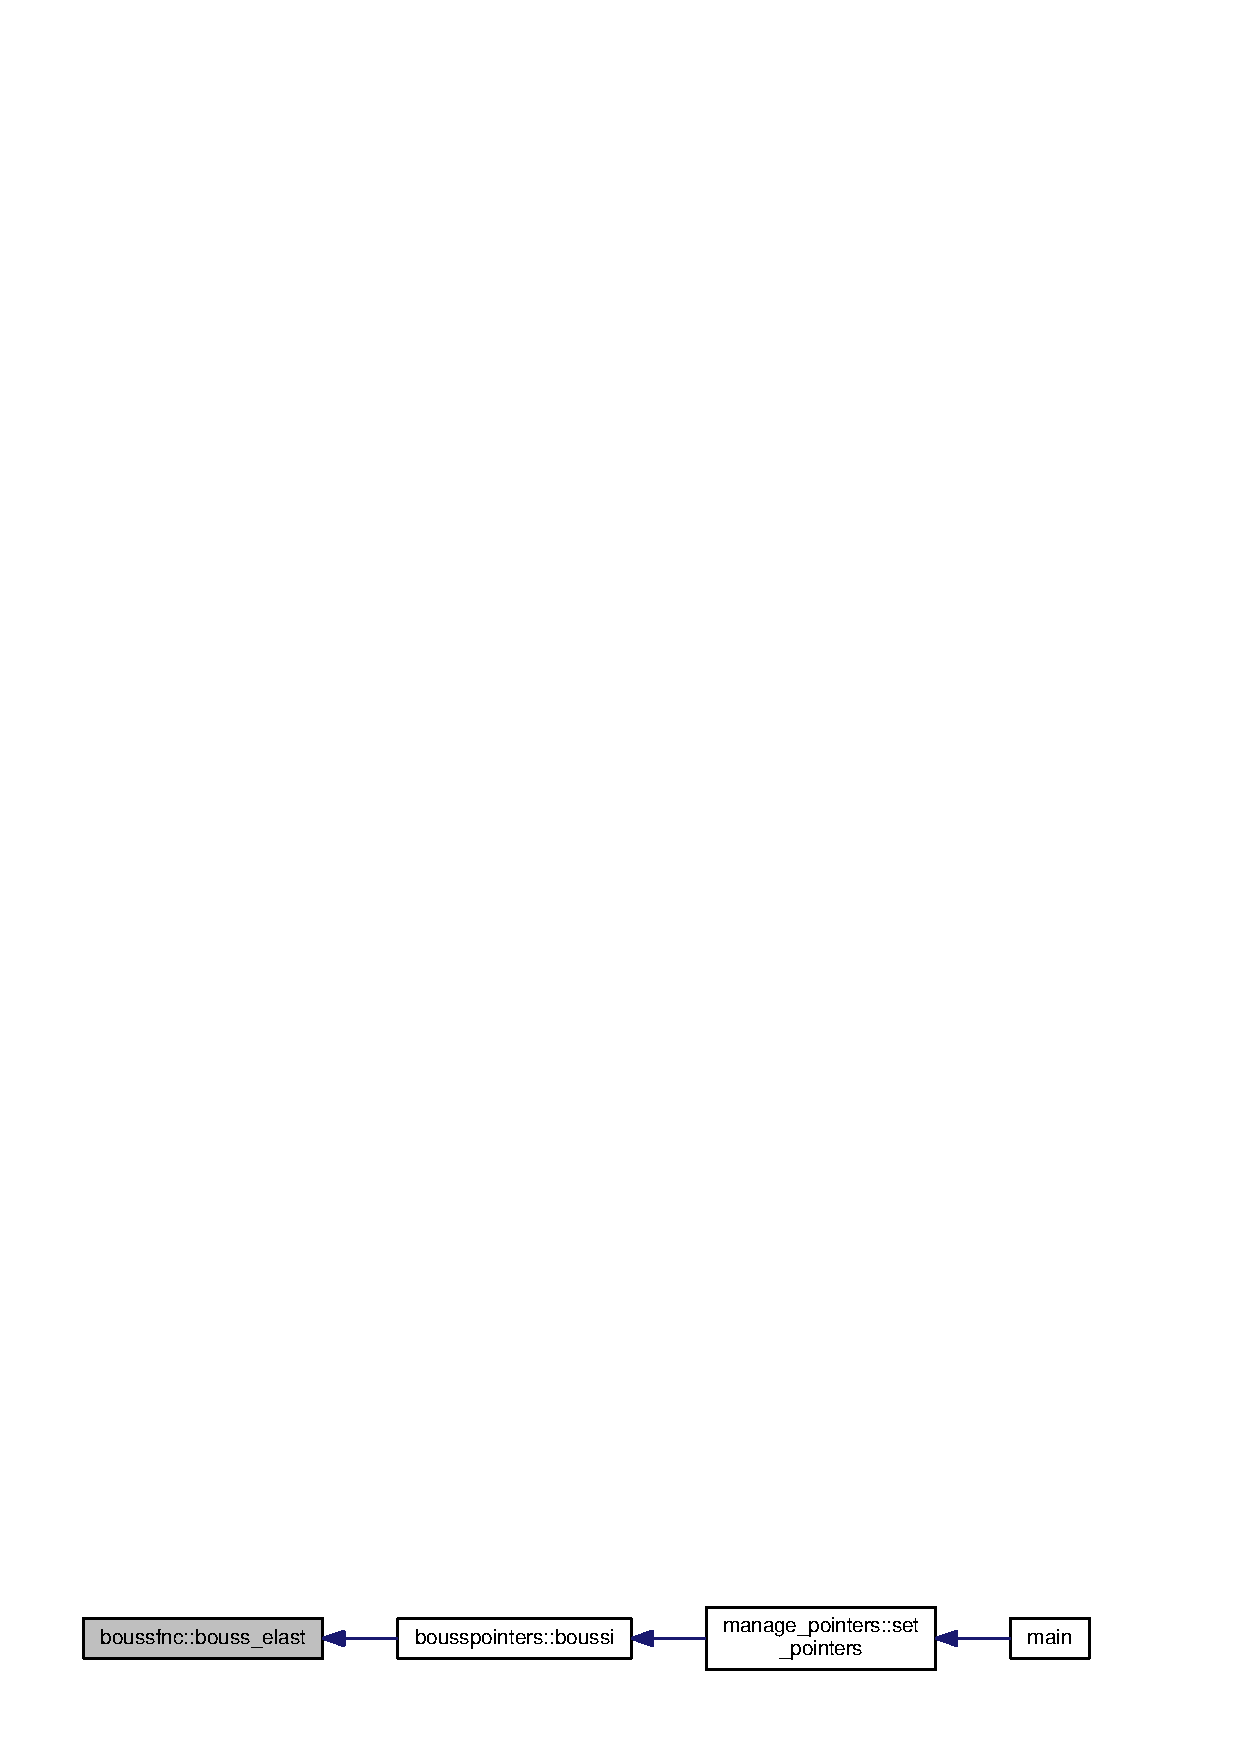
\includegraphics[width=350pt]{namespaceboussfnc_a071d2eeb5f983e31d4495bb68a137e76_icgraph}
\end{center}
\end{figure}


\index{boussfnc@{boussfnc}!boussicond@{boussicond}}
\index{boussicond@{boussicond}!boussfnc@{boussfnc}}
\subsubsection[{boussicond(pde\+\_\+loc)}]{\setlength{\rightskip}{0pt plus 5cm}subroutine, public boussfnc\+::boussicond (
\begin{DoxyParamCaption}
\item[{class({\bf pde\+\_\+str}), intent(inout)}]{pde\+\_\+loc}
\end{DoxyParamCaption}
)}\label{namespaceboussfnc_afed12ab38bd77f437f94217611a6cca1}


Definition at line 380 of file boussfnc.\+f90.



References boussglob\+::bouss\+\_\+icond, globals\+::elements, globals\+::nodes, and pde\+\_\+objs\+::pde.



Referenced by bousspointers\+::boussi().


\begin{DoxyCode}
380         \textcolor{keywordtype}{use }typy
381         \textcolor{keywordtype}{use }globals
382         \textcolor{keywordtype}{use }boussglob
383         \textcolor{keywordtype}{use }global_objs
384         \textcolor{keywordtype}{use }pde_objs
385         
386         \textcolor{keywordtype}{class}(pde_str), \textcolor{keywordtype}{intent(in out)} :: pde\_loc
387         \textcolor{keywordtype}{integer(kind=ikind)} :: i, j, k, l, m, layer
388         \textcolor{keywordtype}{real(kind=rkind)} :: value
389         
390        \textcolor{keywordflow}{do} i=1, elements%kolik
391           layer = elements%material(i,1)
392           \textcolor{keywordflow}{do} j=1, ubound(elements%data,2)
393             k = elements%data(i,j)
394             l = nodes%edge(k)
395             m = pde(1)%permut(k)
396             \textcolor{keywordflow}{if} (m == 0) \textcolor{keywordflow}{then}
397               \textcolor{keyword}{call }pde\_loc%bc(l)%value\_fnc(pde\_loc, i, j, \textcolor{keywordtype}{value})
398               pde\_loc%solution(k) =  \textcolor{keywordtype}{value}
399             \textcolor{keywordflow}{else}
400               pde\_loc%solution(k) = bouss_icond
401 \textcolor{keywordflow}{            end if}
402 \textcolor{keywordflow}{          end do}   
403 \textcolor{keywordflow}{        end do}
404       
\end{DoxyCode}


Here is the caller graph for this function\+:\nopagebreak
\begin{figure}[H]
\begin{center}
\leavevmode
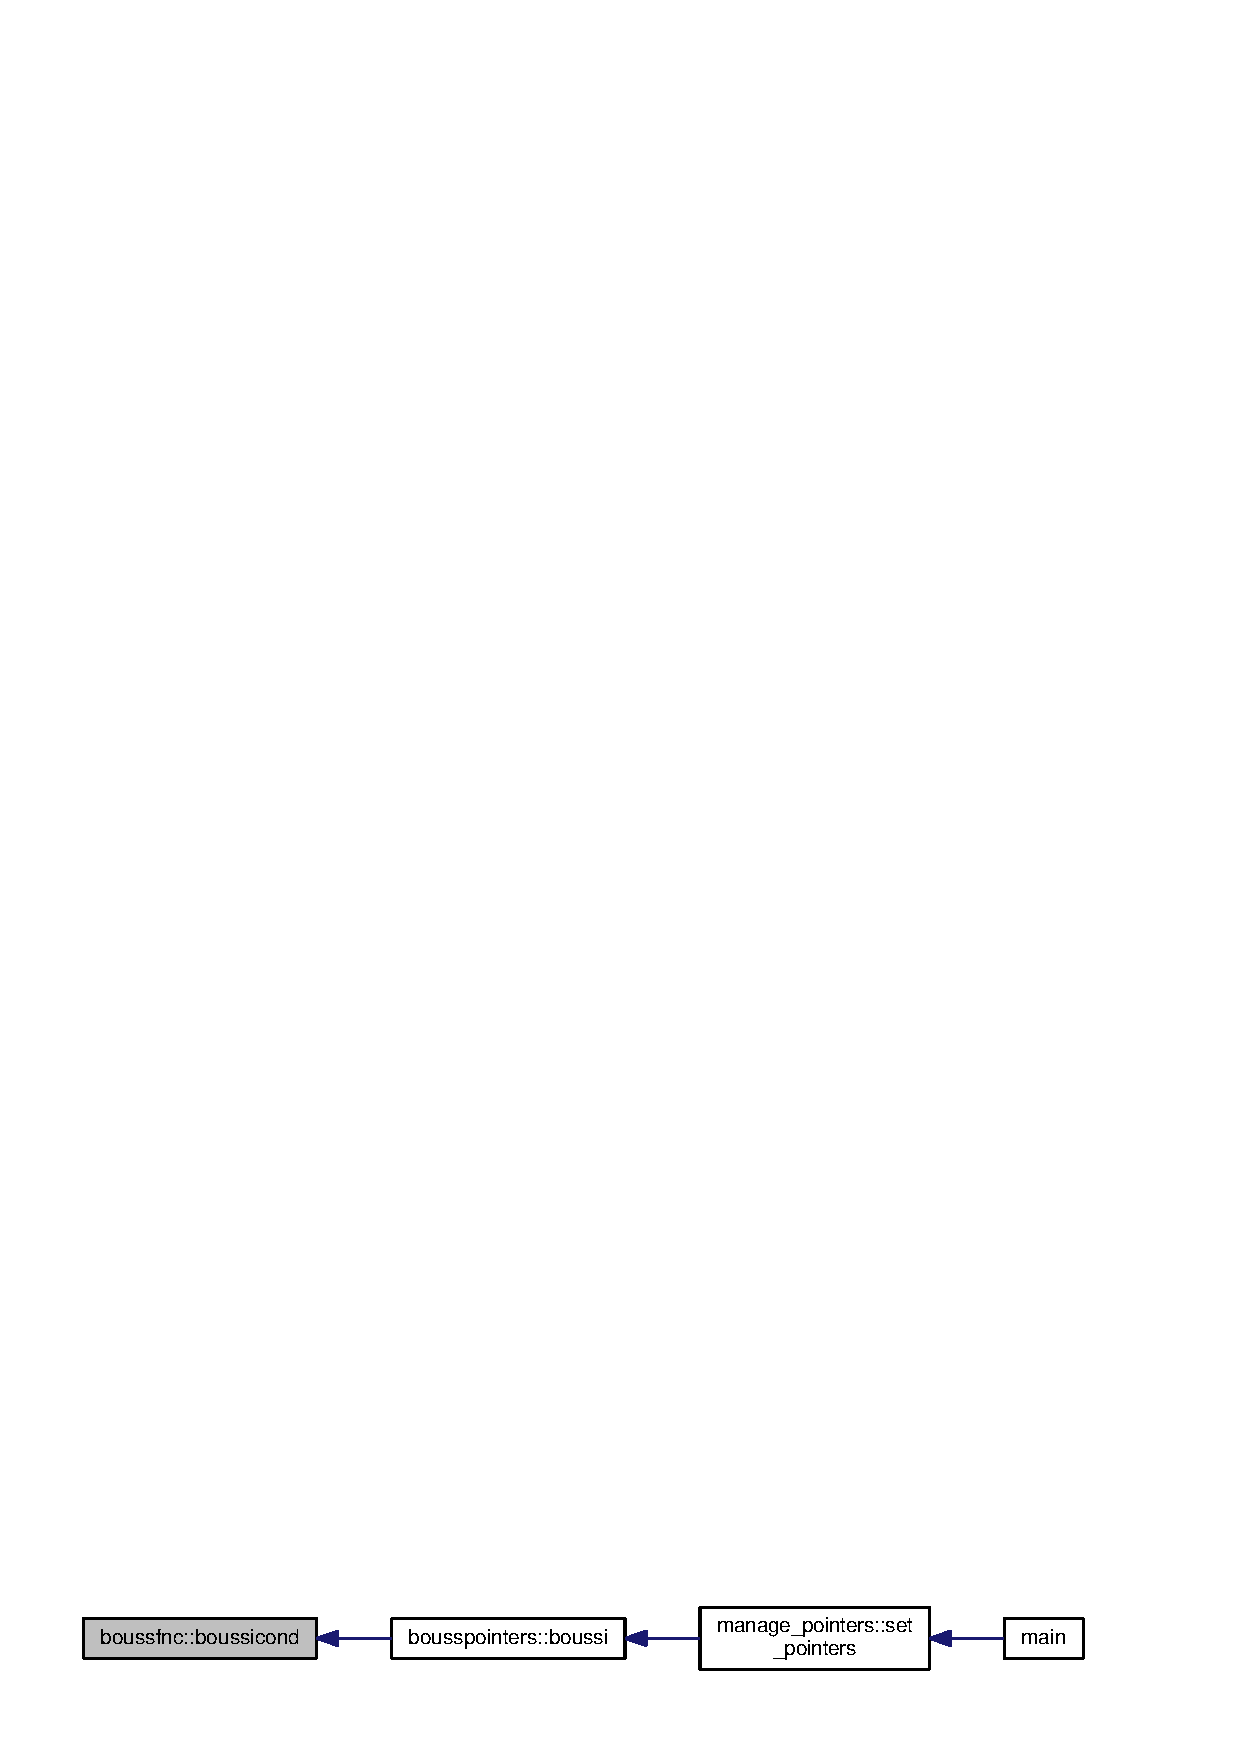
\includegraphics[width=350pt]{namespaceboussfnc_afed12ab38bd77f437f94217611a6cca1_icgraph}
\end{center}
\end{figure}


\index{boussfnc@{boussfnc}!boussreact@{boussreact}}
\index{boussreact@{boussreact}!boussfnc@{boussfnc}}
\subsubsection[{boussreact(pde\+\_\+loc, layer, quadpnt, x)}]{\setlength{\rightskip}{0pt plus 5cm}real(kind=rkind) function, public boussfnc\+::boussreact (
\begin{DoxyParamCaption}
\item[{class({\bf pde\+\_\+str}), intent(in)}]{pde\+\_\+loc, }
\item[{integer(kind=ikind), intent(in)}]{layer, }
\item[{type({\bf integpnt\+\_\+str}), intent(in), optional}]{quadpnt, }
\item[{real(kind=rkind), dimension(\+:), intent(in), optional}]{x}
\end{DoxyParamCaption}
)}\label{namespaceboussfnc_aa942b39df59c308dadcfa69b1256ed09}

\begin{DoxyParams}[1]{Parameters}
\mbox{\tt in}  & {\em x} & pressure head\\
\hline
\mbox{\tt in}  & {\em quadpnt} & Gauss quadrature point structure (element number and rank of Gauss quadrature point)\\
\hline
\end{DoxyParams}
\begin{DoxyReturn}{Returns}
resulting reaction 
\end{DoxyReturn}


Definition at line 246 of file boussfnc.\+f90.



References boussglob\+::bouss\+\_\+rain.



Referenced by bousspointers\+::boussi().


\begin{DoxyCode}
246         \textcolor{keywordtype}{use }typy
247         \textcolor{keywordtype}{use }re_globals
248         \textcolor{keywordtype}{use }pde_objs
249         \textcolor{keywordtype}{use }geom_tools
250         \textcolor{keywordtype}{use }boussglob
251 
252 
253         \textcolor{keywordtype}{class}(pde_str), \textcolor{keywordtype}{intent(in)} :: pde\_loc 
254         \textcolor{keywordtype}{integer(kind=ikind)}, \textcolor{keywordtype}{intent(in)} :: layer
256         \textcolor{keywordtype}{real(kind=rkind)}, \textcolor{keywordtype}{intent(in)}, \textcolor{keywordtype}{dimension(:)},  \textcolor{keywordtype}{optional} :: x
258         \textcolor{keywordtype}{type}(integpnt_str), \textcolor{keywordtype}{intent(in)}, \textcolor{keywordtype}{optional} :: quadpnt
259 
261         \textcolor{keywordtype}{real(kind=rkind)} :: react
262         
263         \textcolor{keywordtype}{real(kind=rkind)} :: rain
264         \textcolor{keywordtype}{integer(kind=ikind)} :: i
265         
266         \textcolor{keywordflow}{do} i=1, ubound(bouss_rain,1)-1
267           \textcolor{keywordflow}{if} (i == 1 .and. time < bouss_rain(1)%data(i)) \textcolor{keywordflow}{then}
268             rain = bouss_rain(2)%data(i) 
269 \textcolor{keywordflow}{          end if}
270           \textcolor{keywordflow}{if} (bouss_rain(1)%data(i) <= time .and. bouss_rain(1)%data(i+1) > time) \textcolor{keywordflow}{then}
271             rain = bouss_rain(2)%data(i) 
272             \textcolor{keywordflow}{EXIT}
273 \textcolor{keywordflow}{          end if}
274           \textcolor{keywordflow}{if} (i == bouss_rain(1)%pos - 1 .and. time >= bouss_rain(1)%data(i+1)) \textcolor{keywordflow}{then}
275             rain = bouss_rain(2)%data(i+1)
276 \textcolor{keywordflow}{          end if}
277 \textcolor{keywordflow}{        end do}  
278         
279         react = -rain
280          
\end{DoxyCode}


Here is the caller graph for this function\+:\nopagebreak
\begin{figure}[H]
\begin{center}
\leavevmode
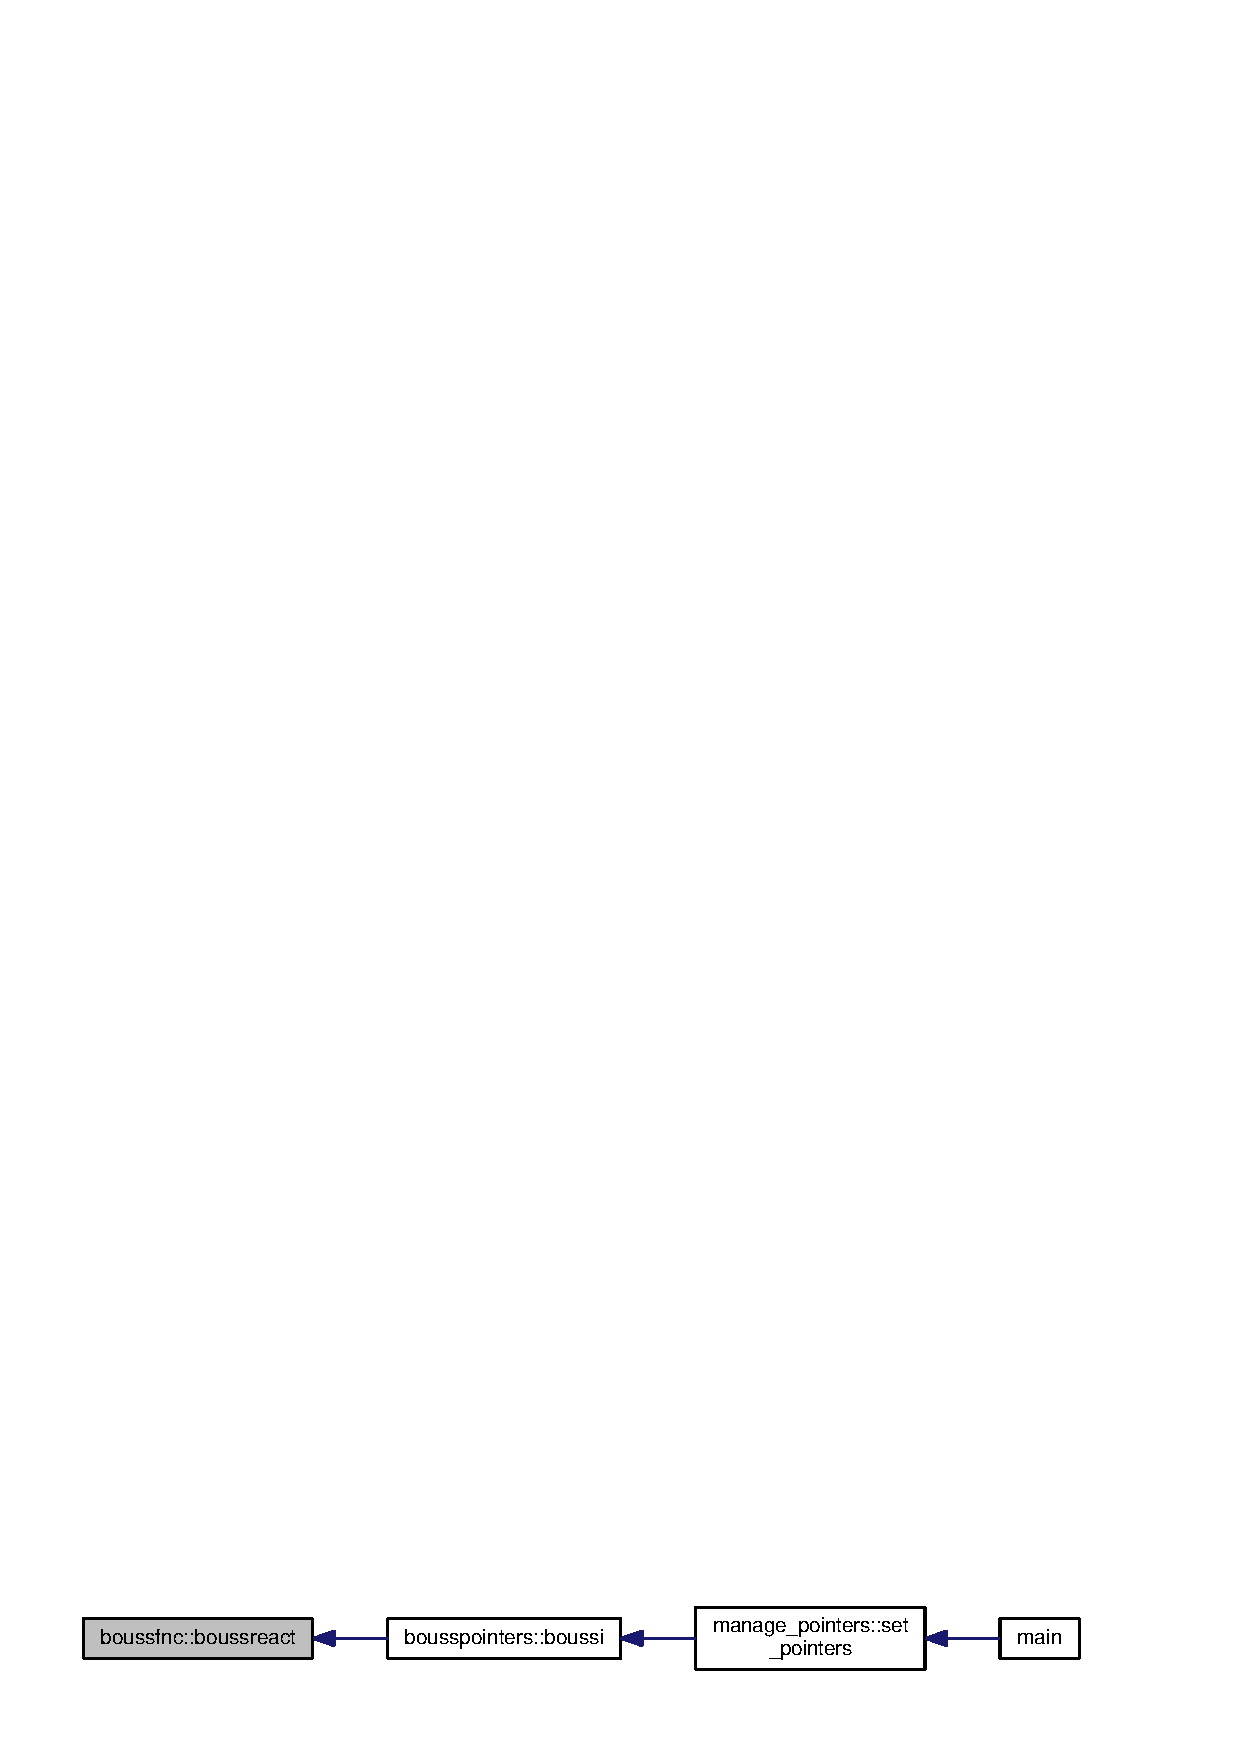
\includegraphics[width=350pt]{namespaceboussfnc_aa942b39df59c308dadcfa69b1256ed09_icgraph}
\end{center}
\end{figure}


\index{boussfnc@{boussfnc}!darcy4bouss@{darcy4bouss}}
\index{darcy4bouss@{darcy4bouss}!boussfnc@{boussfnc}}
\subsubsection[{darcy4bouss(pde\+\_\+loc, layer, quadpnt, x, grad, flux, flux\+\_\+length)}]{\setlength{\rightskip}{0pt plus 5cm}subroutine, public boussfnc\+::darcy4bouss (
\begin{DoxyParamCaption}
\item[{class({\bf pde\+\_\+str}), intent(in)}]{pde\+\_\+loc, }
\item[{integer(kind=ikind), intent(in)}]{layer, }
\item[{type({\bf integpnt\+\_\+str}), intent(in), optional}]{quadpnt, }
\item[{real(kind=rkind), dimension(\+:), intent(in), optional}]{x, }
\item[{real(kind=rkind), dimension(\+:), intent(in), optional}]{grad, }
\item[{real(kind=rkind), dimension(\+:), intent(out), optional}]{flux, }
\item[{real(kind=rkind), intent(out), optional}]{flux\+\_\+length}
\end{DoxyParamCaption}
)}\label{namespaceboussfnc_afa3ac635ca94f53b4d31b74e208d1ee8}

\begin{DoxyParams}[1]{Parameters}
\mbox{\tt in}  & {\em grad} & this value is optional, because it is required by the vector\+\_\+fnc procedure pointer global definition \\
\hline
\end{DoxyParams}


Definition at line 286 of file boussfnc.\+f90.



References boussglob\+::bouss\+\_\+slopes, and geom\+\_\+tools\+::getcoor().



Referenced by bousspointers\+::boussi().


\begin{DoxyCode}
286         \textcolor{keywordtype}{use }typy
287         \textcolor{keywordtype}{use }pde_objs
288         \textcolor{keywordtype}{use }global_objs
289         \textcolor{keywordtype}{use }geom_tools
290         \textcolor{keywordtype}{use }boussglob
291         
292         \textcolor{keywordtype}{class}(pde_str), \textcolor{keywordtype}{intent(in)} :: pde\_loc
293         \textcolor{keywordtype}{integer(kind=ikind)}, \textcolor{keywordtype}{intent(in)}                          :: layer
294         \textcolor{keywordtype}{type}(integpnt_str), \textcolor{keywordtype}{intent(in)}, \textcolor{keywordtype}{optional} :: quadpnt    
295         \textcolor{keywordtype}{real(kind=rkind)}, \textcolor{keywordtype}{intent(in)}, \textcolor{keywordtype}{dimension(:)}, \textcolor{keywordtype}{optional}                   :: x
297         \textcolor{keywordtype}{real(kind=rkind)}, \textcolor{keywordtype}{dimension(:)}, \textcolor{keywordtype}{intent(in)}, \textcolor{keywordtype}{optional}     :: grad
298         \textcolor{keywordtype}{real(kind=rkind)}, \textcolor{keywordtype}{dimension(:)}, \textcolor{keywordtype}{intent(out)}, \textcolor{keywordtype}{optional}    :: flux
299         \textcolor{keywordtype}{real(kind=rkind)}, \textcolor{keywordtype}{intent(out)}, \textcolor{keywordtype}{optional}                  :: flux\_length
300 
301         \textcolor{keywordtype}{real(kind=rkind)}, \textcolor{keywordtype}{dimension(1,1)}  :: k
302         \textcolor{keywordtype}{integer}                           :: d
303         \textcolor{keywordtype}{integer(kind=ikind)}               :: i
304         \textcolor{keywordtype}{real(kind=rkind)}, \textcolor{keywordtype}{dimension(:)}, \textcolor{keywordtype}{allocatable}, \textcolor{keywordtype}{save}  :: gradh
305         \textcolor{keywordtype}{real(kind=rkind)}, \textcolor{keywordtype}{dimension(:)}, \textcolor{keywordtype}{allocatable}, \textcolor{keywordtype}{save}  :: vct
306         \textcolor{keywordtype}{real(kind=rkind)} :: h, slope
307         \textcolor{keywordtype}{real(kind=rkind)}, \textcolor{keywordtype}{dimension(1)} :: coord
308         
309 
310         d = drutes_config%dimen
311           
312         \textcolor{keywordflow}{if} (.not.(\textcolor{keyword}{allocated}(gradh))) \textcolor{keywordflow}{then}
313           \textcolor{keyword}{allocate}(gradh(1:d))
314           \textcolor{keyword}{allocate}(vct(1:d))
315 \textcolor{keywordflow}{        end if}
316 
317         \textcolor{keywordflow}{if} (\textcolor{keyword}{present}(quadpnt) .and. (\textcolor{keyword}{present}(grad) .or. \textcolor{keyword}{present}(x))) \textcolor{keywordflow}{then}
318           print *, \textcolor{stringliteral}{"ERROR: the function can be called either with integ point or x value definition and
       gradient, not both of them"}
319           error stop
320         \textcolor{keywordflow}{else} \textcolor{keywordflow}{if} ((.not. \textcolor{keyword}{present}(grad) .or. .not. \textcolor{keyword}{present}(x)) .and. .not. \textcolor{keyword}{present}(quadpnt)) \textcolor{keywordflow}{then}
321           print *, \textcolor{stringliteral}{"ERROR: you have not specified either integ point or x value"}
322           print *, \textcolor{stringliteral}{"exited from re\_constitutive::darcy\_law"}
323           error stop
324 \textcolor{keywordflow}{        end if}
325         
326         \textcolor{keywordflow}{if} (\textcolor{keyword}{present}(quadpnt)) \textcolor{keywordflow}{then}
327           h = pde\_loc%getval(quadpnt)
328           \textcolor{keyword}{call }pde\_loc%getgrad(quadpnt, gradh)
329         \textcolor{keywordflow}{else}
330           \textcolor{keywordflow}{if} (ubound(x,1) /=1) \textcolor{keywordflow}{then}
331             print *, \textcolor{stringliteral}{"ERROR: van Genuchten function is a function of a single variable h"}
332             print *, \textcolor{stringliteral}{"       your input data has:"}, ubound(x,1), \textcolor{stringliteral}{"variables"}
333             print *, \textcolor{stringliteral}{"exited from re\_constitutive::darcy\_law"}
334             error stop
335 \textcolor{keywordflow}{          end if}
336           h = x(1)
337           gradh(1:d) = grad
338 \textcolor{keywordflow}{        end if}
339         
340        \textcolor{keyword}{call }getcoor(quadpnt, coord)
341         
342         \textcolor{keywordflow}{do} i=1, bouss_slopes(1)%pos - 1
343           \textcolor{keywordflow}{if} (coord(1) >= bouss_slopes(1)%data(i) .and. coord(1) < bouss_slopes(1)%data(i+1)) \textcolor{keywordflow}{then}
344             slope = bouss_slopes(2)%data(i)
345             \textcolor{keywordflow}{EXIT}
346 \textcolor{keywordflow}{          end if}
347           \textcolor{keywordflow}{if} (i == bouss_slopes(1)%pos - 1 .and. coord(1) >= bouss_slopes(1)%data(i+1)) \textcolor{keywordflow}{then}
348             slope = bouss_slopes(2)%data(i+1)
349 \textcolor{keywordflow}{          end if}
350 \textcolor{keywordflow}{        end do}
351         
352         
353         gradh = gradh + slope
354         
355         \textcolor{keyword}{call }pde\_loc%pde\_fnc(1)%dispersion(pde\_loc, layer, quadpnt, tensor=k(1:d, 1:d))
356       
357         
358         vct(1:d) =  matmul(-k(1:d,1:d), gradh(1:d))
359 
360 
361         \textcolor{keywordflow}{if} (\textcolor{keyword}{present}(flux\_length)) \textcolor{keywordflow}{then}
362           \textcolor{keywordflow}{select case}(d)
363             \textcolor{keywordflow}{case}(1)
364                   flux\_length = abs(vct(1))
365             \textcolor{keywordflow}{case}(2)
366                   flux\_length = sqrt(vct(1)*vct(1) + vct(2)*vct(2))
367             \textcolor{keywordflow}{case}(3)
368                   flux\_length = sqrt(vct(1)*vct(1) + vct(2)*vct(2) + vct(3)*vct(3))
369 \textcolor{keywordflow}{          end select}
370 \textcolor{keywordflow}{        end if}
371 
372 
373         \textcolor{keywordflow}{if} (\textcolor{keyword}{present}(flux)) \textcolor{keywordflow}{then}
374           flux(1:d) = vct(1:d)
375 \textcolor{keywordflow}{        end if}
376 
\end{DoxyCode}


Here is the call graph for this function\+:\nopagebreak
\begin{figure}[H]
\begin{center}
\leavevmode
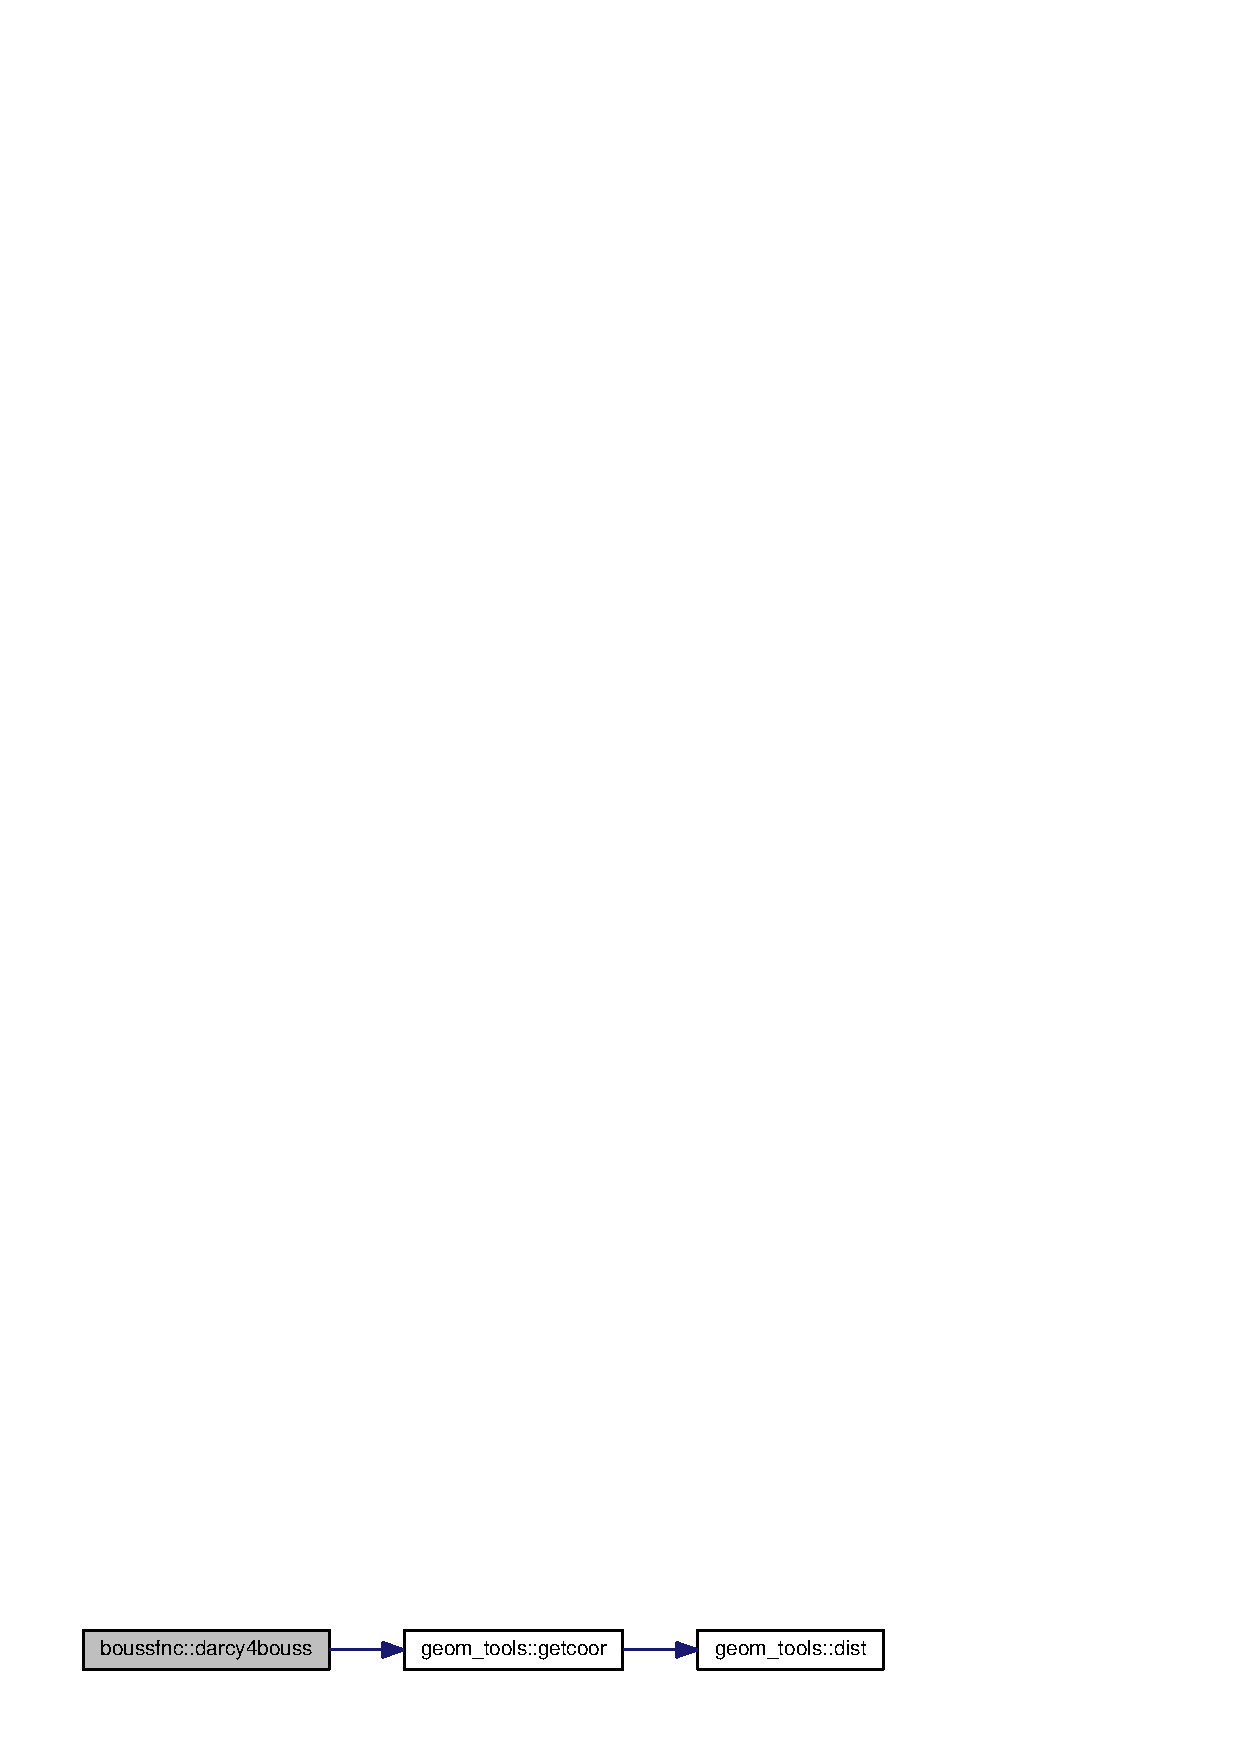
\includegraphics[width=350pt]{namespaceboussfnc_afa3ac635ca94f53b4d31b74e208d1ee8_cgraph}
\end{center}
\end{figure}




Here is the caller graph for this function\+:\nopagebreak
\begin{figure}[H]
\begin{center}
\leavevmode
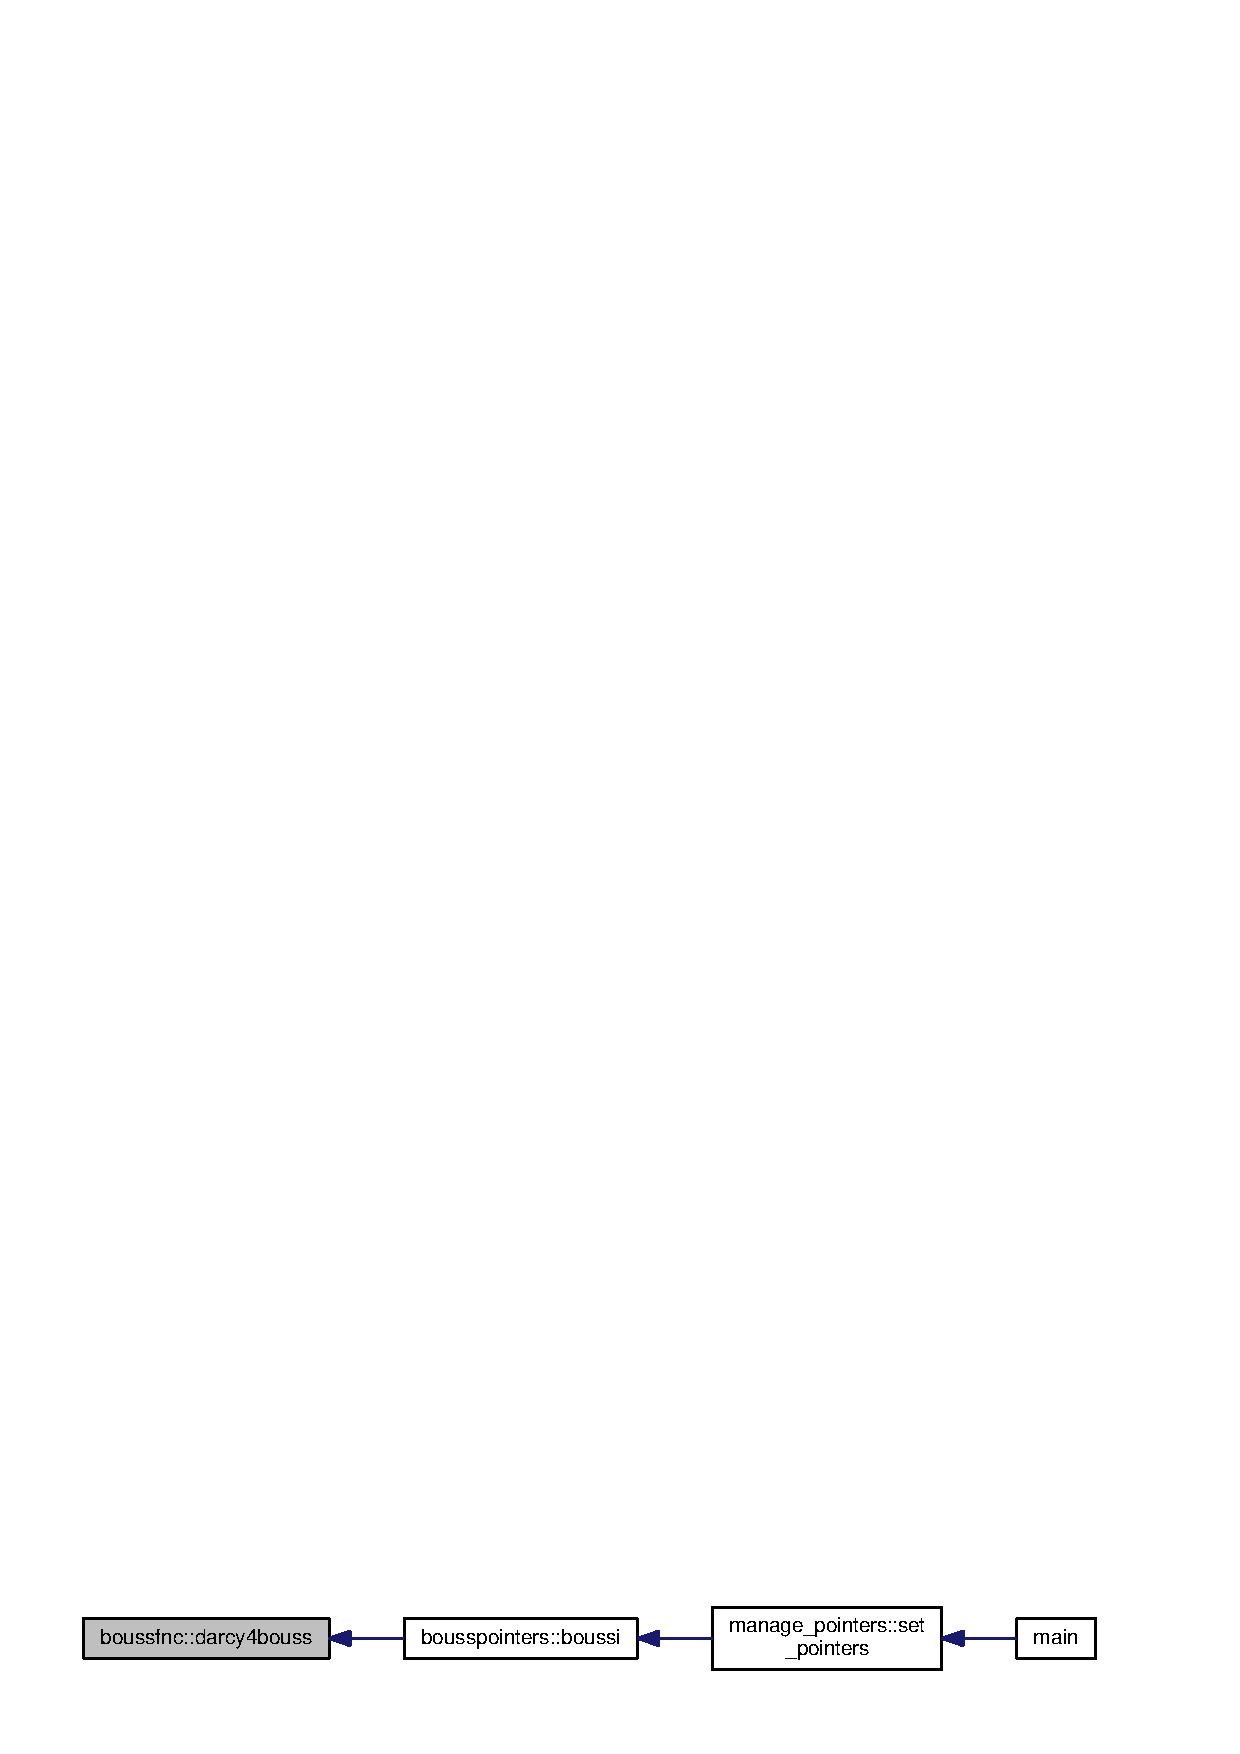
\includegraphics[width=350pt]{namespaceboussfnc_afa3ac635ca94f53b4d31b74e208d1ee8_icgraph}
\end{center}
\end{figure}



\section{boussglob Module Reference}
\label{namespaceboussglob}\index{boussglob@{boussglob}}
\subsection*{Variables}
\begin{DoxyCompactItemize}
\item 
type({\bf smartarray\+\_\+real}), dimension(2), public {\bf bouss\+\_\+slopes}
\item 
type({\bf smartarray\+\_\+real}), dimension(2), public {\bf bouss\+\_\+k}
\item 
type({\bf smartarray\+\_\+real}), dimension(2), public {\bf bouss\+\_\+rain}
\item 
real(kind=rkind), public {\bf bouss\+\_\+por}
\item 
real(kind=rkind), public {\bf bouss\+\_\+icond}
\end{DoxyCompactItemize}


\subsection{Variable Documentation}
\index{boussglob@{boussglob}!bouss\+\_\+icond@{bouss\+\_\+icond}}
\index{bouss\+\_\+icond@{bouss\+\_\+icond}!boussglob@{boussglob}}
\subsubsection[{bouss\+\_\+icond}]{\setlength{\rightskip}{0pt plus 5cm}real(kind=rkind), public boussglob\+::bouss\+\_\+icond}\label{namespaceboussglob_ae5f470c00fdc9fc870c35e9bf5286c9f}


Definition at line 9 of file boussglob.\+f90.



Referenced by boussfnc\+::boussicond(), and boussread\+::boussreader().


\begin{DoxyCode}
9   \textcolor{keywordtype}{real(kind=rkind)}, \textcolor{keywordtype}{public} :: bouss_icond
\end{DoxyCode}
\index{boussglob@{boussglob}!bouss\+\_\+k@{bouss\+\_\+k}}
\index{bouss\+\_\+k@{bouss\+\_\+k}!boussglob@{boussglob}}
\subsubsection[{bouss\+\_\+k}]{\setlength{\rightskip}{0pt plus 5cm}type({\bf smartarray\+\_\+real}), dimension(2), public boussglob\+::bouss\+\_\+k}\label{namespaceboussglob_a4b547b1281175037fcf8625db6be6110}


Definition at line 6 of file boussglob.\+f90.



Referenced by boussfnc\+::bouss\+\_\+cond(), and boussread\+::boussreader().


\begin{DoxyCode}
6   \textcolor{keywordtype}{type}(smartarray_real), \textcolor{keywordtype}{dimension(2)}, \textcolor{keywordtype}{public} :: bouss_k
\end{DoxyCode}
\index{boussglob@{boussglob}!bouss\+\_\+por@{bouss\+\_\+por}}
\index{bouss\+\_\+por@{bouss\+\_\+por}!boussglob@{boussglob}}
\subsubsection[{bouss\+\_\+por}]{\setlength{\rightskip}{0pt plus 5cm}real(kind=rkind), public boussglob\+::bouss\+\_\+por}\label{namespaceboussglob_a22f276259c3f43d3bfde4ee94bb0046a}


Definition at line 8 of file boussglob.\+f90.



Referenced by boussfnc\+::bouss\+\_\+elast(), and boussread\+::boussreader().


\begin{DoxyCode}
8   \textcolor{keywordtype}{real(kind=rkind)}, \textcolor{keywordtype}{public} :: bouss_por
\end{DoxyCode}
\index{boussglob@{boussglob}!bouss\+\_\+rain@{bouss\+\_\+rain}}
\index{bouss\+\_\+rain@{bouss\+\_\+rain}!boussglob@{boussglob}}
\subsubsection[{bouss\+\_\+rain}]{\setlength{\rightskip}{0pt plus 5cm}type({\bf smartarray\+\_\+real}), dimension(2), public boussglob\+::bouss\+\_\+rain}\label{namespaceboussglob_abfa33c9e10e3d3209b4885cbaf2f91a4}


Definition at line 7 of file boussglob.\+f90.



Referenced by boussfnc\+::bouss\+\_\+adv(), boussfnc\+::boussreact(), and boussread\+::boussreader().


\begin{DoxyCode}
7   \textcolor{keywordtype}{type}(smartarray_real), \textcolor{keywordtype}{dimension(2)}, \textcolor{keywordtype}{public} :: bouss_rain
\end{DoxyCode}
\index{boussglob@{boussglob}!bouss\+\_\+slopes@{bouss\+\_\+slopes}}
\index{bouss\+\_\+slopes@{bouss\+\_\+slopes}!boussglob@{boussglob}}
\subsubsection[{bouss\+\_\+slopes}]{\setlength{\rightskip}{0pt plus 5cm}type({\bf smartarray\+\_\+real}), dimension(2), public boussglob\+::bouss\+\_\+slopes}\label{namespaceboussglob_a7d82925866b8a3f55db46859dc95922b}


Definition at line 5 of file boussglob.\+f90.



Referenced by boussfnc\+::bouss\+\_\+adv(), boussfnc\+::bouss\+\_\+elast(), boussread\+::boussreader(), and boussfnc\+::darcy4bouss().


\begin{DoxyCode}
5   \textcolor{keywordtype}{type}(smartarray_real), \textcolor{keywordtype}{dimension(2)}, \textcolor{keywordtype}{public} :: bouss_slopes
\end{DoxyCode}

\section{bousspointers Module Reference}
\label{namespacebousspointers}\index{bousspointers@{bousspointers}}
\subsection*{Functions/\+Subroutines}
\begin{DoxyCompactItemize}
\item 
subroutine, public {\bf boussi} (pde\+\_\+loc)
\end{DoxyCompactItemize}


\subsection{Function/\+Subroutine Documentation}
\index{bousspointers@{bousspointers}!boussi@{boussi}}
\index{boussi@{boussi}!bousspointers@{bousspointers}}
\subsubsection[{boussi(pde\+\_\+loc)}]{\setlength{\rightskip}{0pt plus 5cm}subroutine, public bousspointers\+::boussi (
\begin{DoxyParamCaption}
\item[{class({\bf pde\+\_\+str}), intent(inout)}]{pde\+\_\+loc}
\end{DoxyParamCaption}
)}\label{namespacebousspointers_aa29fe327913d573ed19bbd1a6b11f0b5}


Definition at line 7 of file bousspointers.\+f90.



References boussfnc\+::bouss\+\_\+adv(), boussfnc\+::bouss\+\_\+bc(), boussfnc\+::bouss\+\_\+cond(), boussfnc\+::bouss\+\_\+elast(), boussfnc\+::boussicond(), boussfnc\+::boussreact(), boussread\+::boussreader(), boussfnc\+::darcy4bouss(), and pde\+\_\+objs\+::pde.



Referenced by manage\+\_\+pointers\+::set\+\_\+pointers().


\begin{DoxyCode}
7       \textcolor{keywordtype}{use }typy
8       \textcolor{keywordtype}{use }globals
9       \textcolor{keywordtype}{use }global_objs
10       \textcolor{keywordtype}{use }pde_objs
11       \textcolor{keywordtype}{use }boussglob
12       \textcolor{keywordtype}{use }boussfnc
13       \textcolor{keywordtype}{use }boussread
14         
15       \textcolor{keywordtype}{class}(pde_str), \textcolor{keywordtype}{intent(in out)} :: pde\_loc
16       \textcolor{keywordtype}{integer(kind=ikind)} :: i
17       
18       \textcolor{keyword}{call }boussreader(pde\_loc)
19       
20       pde\_loc%pde\_fnc(pde\_loc%order)%dispersion => bouss_cond
21       pde\_loc%pde\_fnc(pde\_loc%order)%convection => bouss_adv
22       pde\_loc%pde\_fnc(pde\_loc%order)%elasticity => bouss_elast
23 
24       pde\_loc%pde\_fnc(pde\_loc%order)%zerord => boussreact
25           
26       \textcolor{keywordflow}{do} i=lbound(pde(1)%bc,1), ubound(pde(1)%bc,1)
27         \textcolor{keywordflow}{select case}(pde\_loc%bc(i)%code)
28           \textcolor{keywordflow}{case}(1,2)
29             pde\_loc%bc(i)%value\_fnc => bouss_bc
30 \textcolor{keywordflow}{        end select}
31 \textcolor{keywordflow}{      end do}
32               
33         
34       pde\_loc%flux => darcy4bouss
35       pde\_loc%initcond => boussicond     
36        
\end{DoxyCode}


Here is the call graph for this function\+:\nopagebreak
\begin{figure}[H]
\begin{center}
\leavevmode
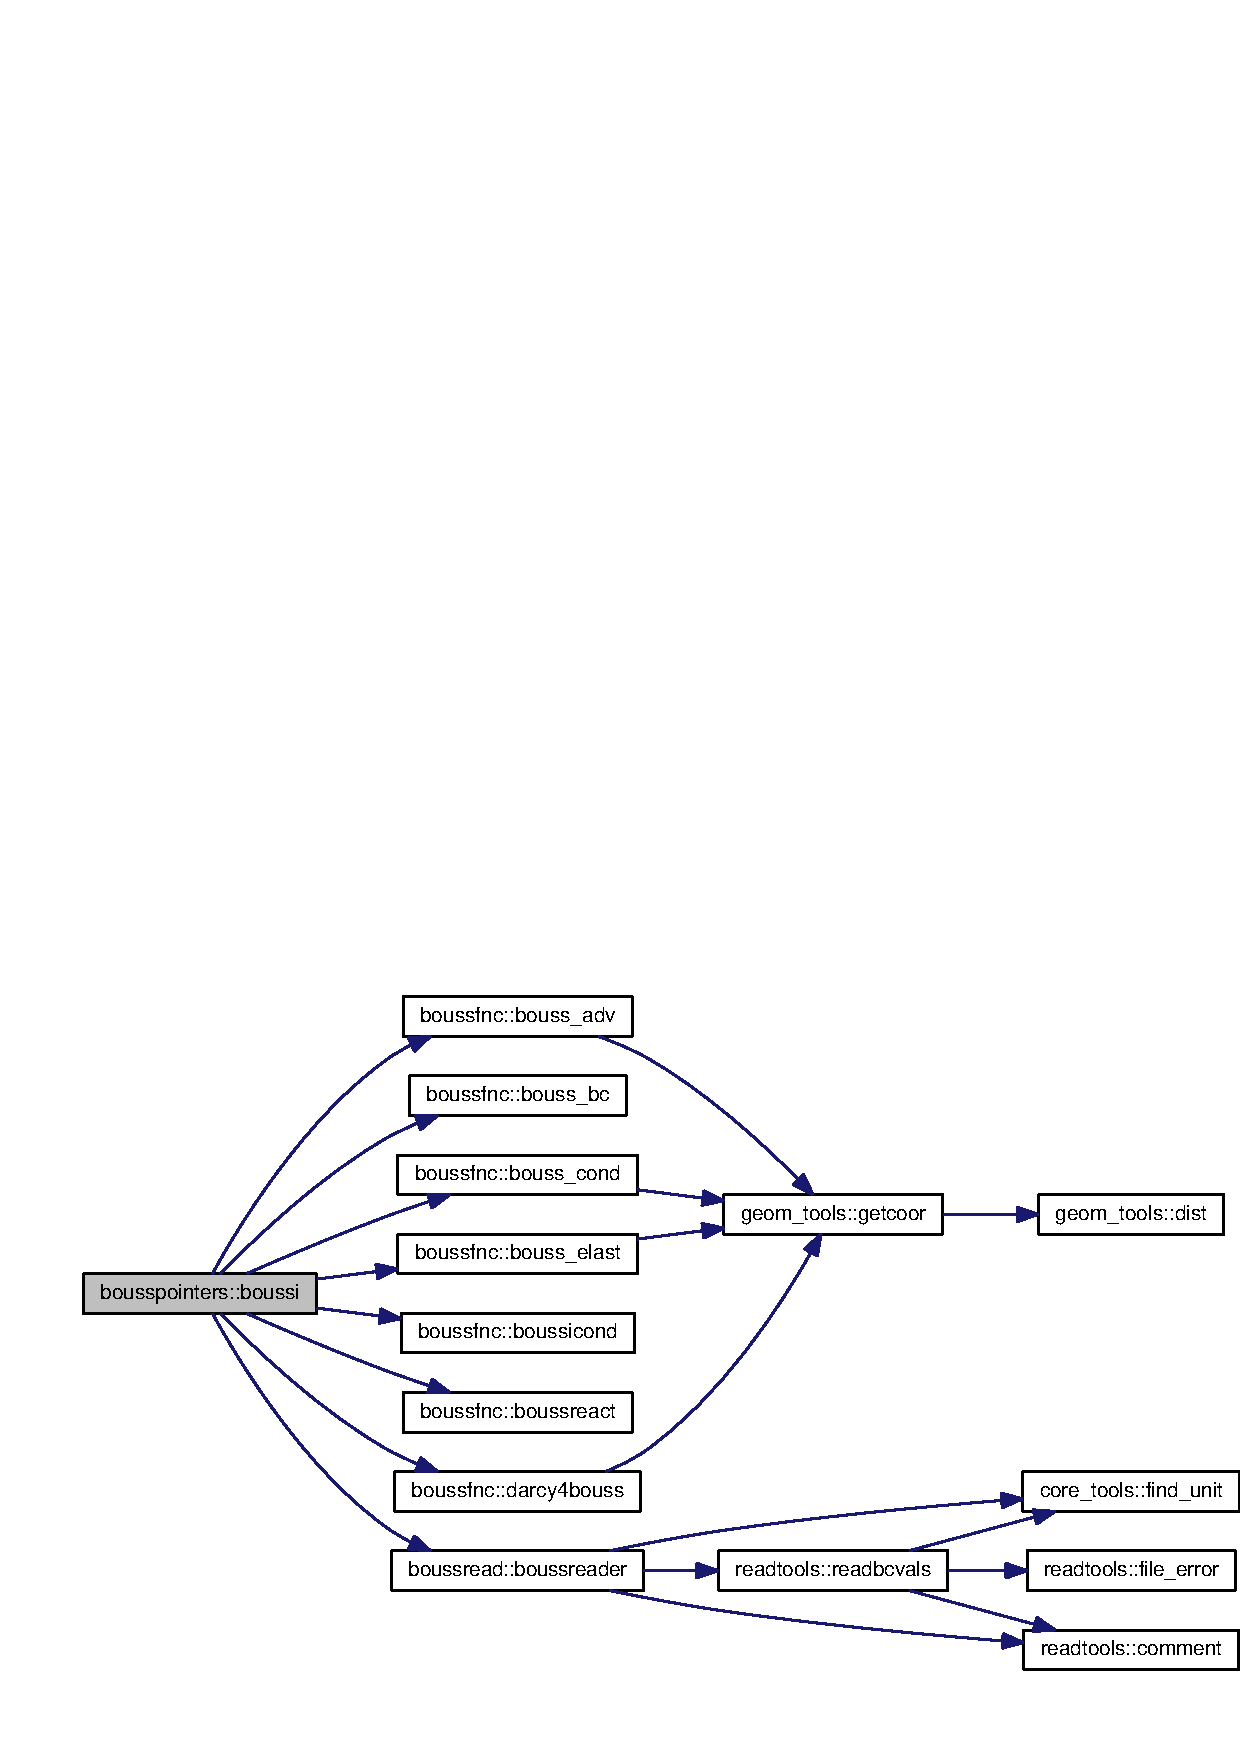
\includegraphics[width=350pt]{namespacebousspointers_aa29fe327913d573ed19bbd1a6b11f0b5_cgraph}
\end{center}
\end{figure}




Here is the caller graph for this function\+:\nopagebreak
\begin{figure}[H]
\begin{center}
\leavevmode
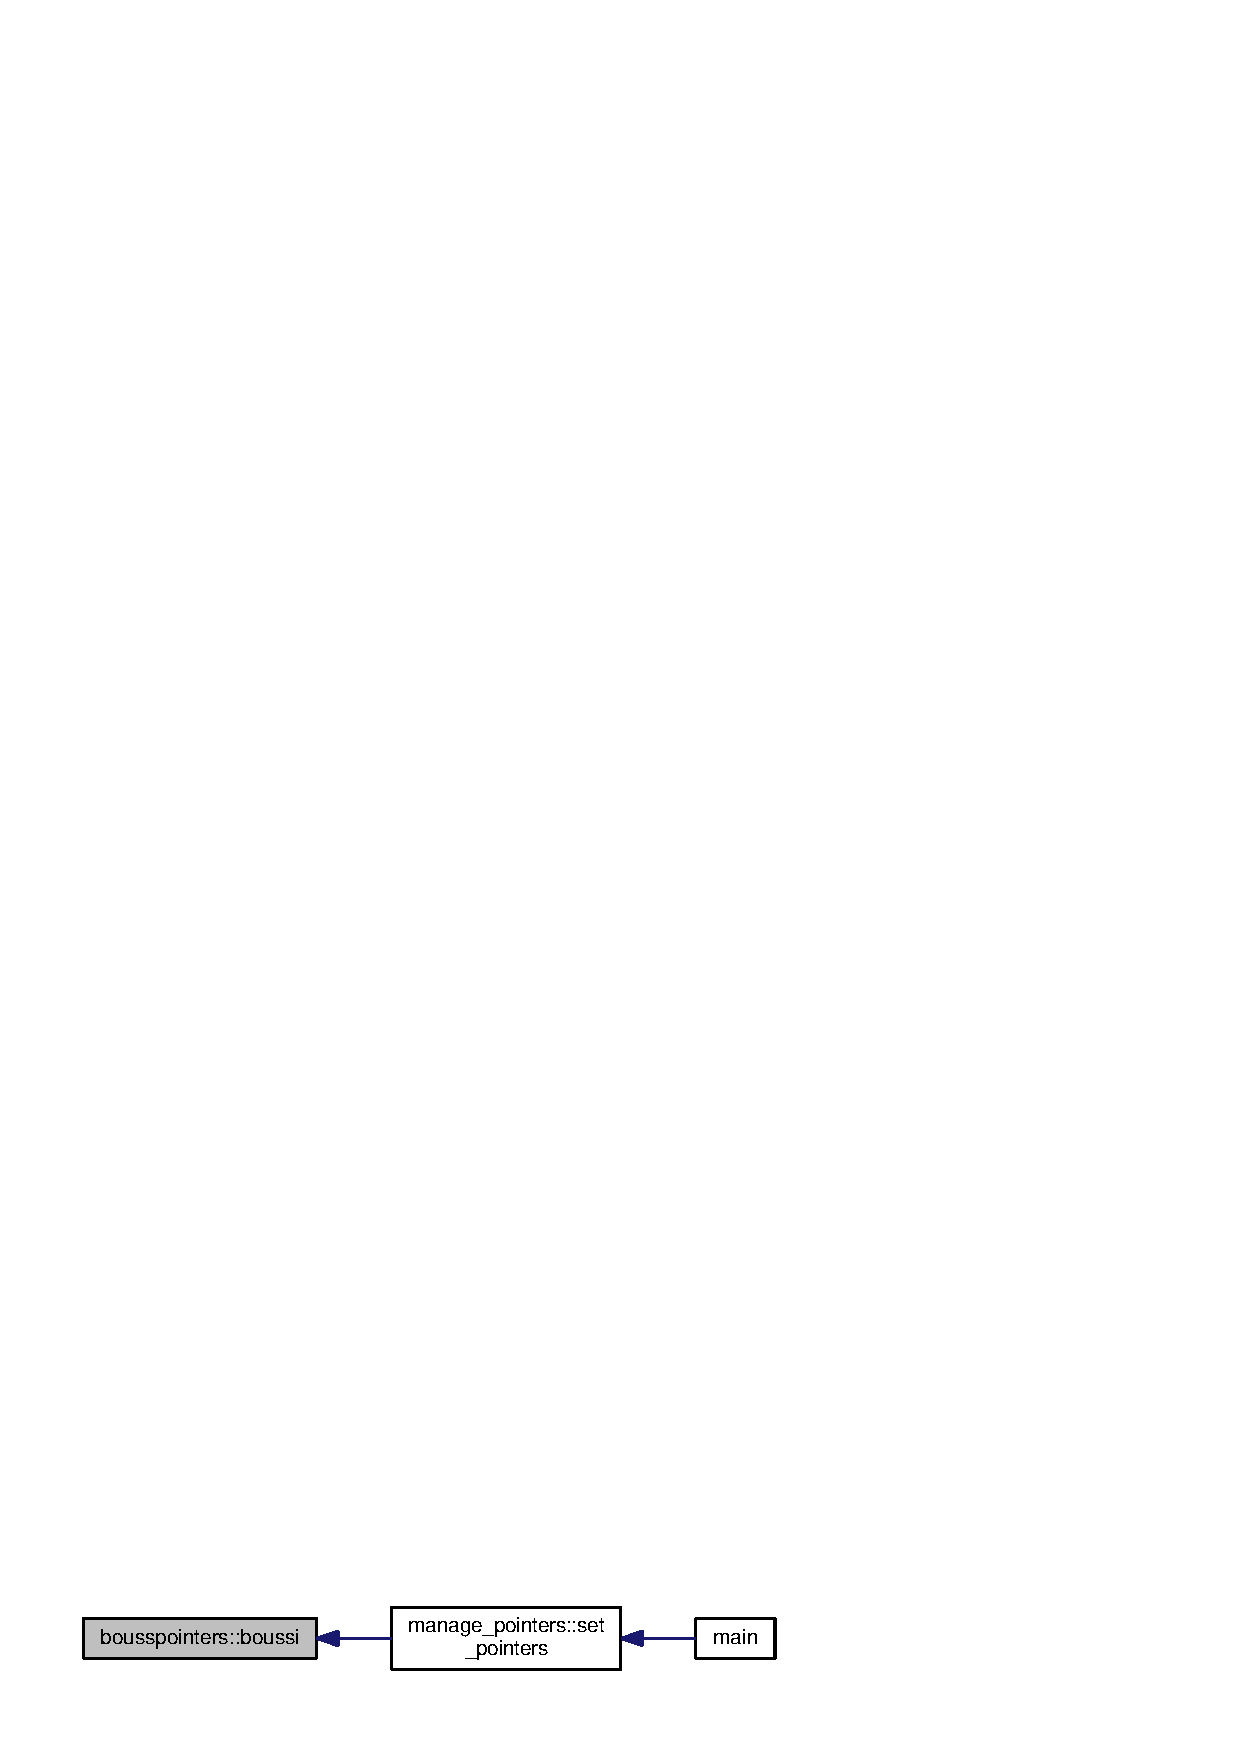
\includegraphics[width=350pt]{namespacebousspointers_aa29fe327913d573ed19bbd1a6b11f0b5_icgraph}
\end{center}
\end{figure}



\section{boussread Module Reference}
\label{namespaceboussread}\index{boussread@{boussread}}
\subsection*{Functions/\+Subroutines}
\begin{DoxyCompactItemize}
\item 
subroutine, public {\bf boussreader} (pde\+\_\+loc)
\end{DoxyCompactItemize}


\subsection{Function/\+Subroutine Documentation}
\index{boussread@{boussread}!boussreader@{boussreader}}
\index{boussreader@{boussreader}!boussread@{boussread}}
\subsubsection[{boussreader(pde\+\_\+loc)}]{\setlength{\rightskip}{0pt plus 5cm}subroutine, public boussread\+::boussreader (
\begin{DoxyParamCaption}
\item[{class({\bf pde\+\_\+str}), intent(inout)}]{pde\+\_\+loc}
\end{DoxyParamCaption}
)}\label{namespaceboussread_af206b475e8ec2d4ed9f54c22e829a40e}


Definition at line 6 of file boussread.\+f90.



References boussglob\+::bouss\+\_\+icond, boussglob\+::bouss\+\_\+k, boussglob\+::bouss\+\_\+por, boussglob\+::bouss\+\_\+rain, boussglob\+::bouss\+\_\+slopes, readtools\+::comment(), core\+\_\+tools\+::find\+\_\+unit(), pde\+\_\+objs\+::pde\+\_\+common, and readtools\+::readbcvals().



Referenced by bousspointers\+::boussi().


\begin{DoxyCode}
6       \textcolor{keywordtype}{use }typy
7       \textcolor{keywordtype}{use }readtools
8       \textcolor{keywordtype}{use }core_tools
9       \textcolor{keywordtype}{use }boussglob
10       \textcolor{keywordtype}{use }global_objs
11       \textcolor{keywordtype}{use }pde_objs
12       
13       \textcolor{keywordtype}{class}(pde_str), \textcolor{keywordtype}{intent(in out)} :: pde\_loc
14       \textcolor{keywordtype}{integer}, \textcolor{keywordtype}{dimension(5)} :: fileid
15       \textcolor{keywordtype}{integer} :: ierr
16       \textcolor{keywordtype}{integer(kind=ikind)} :: i
17       \textcolor{keywordtype}{real(kind=rkind)}, \textcolor{keywordtype}{dimension(2)} :: inputs
18       
19       
20       pde\_loc%problem\_name(1) = \textcolor{stringliteral}{"bouss"}
21       pde\_loc%problem\_name(2) = \textcolor{stringliteral}{"Boussinesq equation"}
22 
23       pde\_loc%solution\_name(1) = \textcolor{stringliteral}{"water\_table"} \textcolor{comment}{!nazev vystupnich souboru}
24       pde\_loc%solution\_name(2) = \textcolor{stringliteral}{"h  [L]"} \textcolor{comment}{!popisek grafu}
25 
26       pde\_loc%flux\_name(1) = \textcolor{stringliteral}{"flux"}  
27       pde\_loc%flux\_name(2) = \textcolor{stringliteral}{"Darcian specific flux [L^2.T^\{-1\}]"}
28 
29       pde\_loc%mass\_name(1) = \textcolor{stringliteral}{"not\_available"}
30       pde\_loc%mass\_name(2) = \textcolor{stringliteral}{"n\_a"}
31       
32       
33       \textcolor{keyword}{call }find_unit(fileid(1), 200)
34       \textcolor{keyword}{open}(unit=fileid(1), file=\textcolor{stringliteral}{"drutes.conf/boussinesq.conf/slope.in"}, action\textcolor{comment}{=}\textcolor{stringliteral}{"read"}\textcolor{comment}{, status=}\textcolor{stringliteral}{"old"}\textcolor{comment}{, iostat
      =ierr)}
35 \textcolor{comment}{      }
36 \textcolor{comment}{      }\textcolor{keywordflow}{if} (ierr /= 0) \textcolor{keywordflow}{then}
37         print *, \textcolor{stringliteral}{"missing drutes.conf/boussinesq.conf/slope.in file"}
38         error stop
39 \textcolor{keywordflow}{      end if}
40       
41       \textcolor{keyword}{call }find_unit(fileid(2), 200)
42       \textcolor{keyword}{open}(unit=fileid(2), file=\textcolor{stringliteral}{"drutes.conf/boussinesq.conf/cond.in"}, action\textcolor{comment}{=}\textcolor{stringliteral}{"read"}\textcolor{comment}{, status=}\textcolor{stringliteral}{"old"}\textcolor{comment}{, iostat=
      ierr)}
43 \textcolor{comment}{      }
44 \textcolor{comment}{      }\textcolor{keywordflow}{if} (ierr /= 0) \textcolor{keywordflow}{then}
45         print *, \textcolor{stringliteral}{"missing drutes.conf/boussinesq.conf/cond.in file"}
46         error stop
47 \textcolor{keywordflow}{      end if}
48       
49       \textcolor{keyword}{call }find_unit(fileid(3), 200)
50       \textcolor{keyword}{open}(unit=fileid(3), file=\textcolor{stringliteral}{"drutes.conf/boussinesq.conf/rain.in"}, action\textcolor{comment}{=}\textcolor{stringliteral}{"read"}\textcolor{comment}{, status=}\textcolor{stringliteral}{"old"}\textcolor{comment}{, iostat=
      ierr)}
51 \textcolor{comment}{      }
52 \textcolor{comment}{      }\textcolor{keywordflow}{if} (ierr /= 0) \textcolor{keywordflow}{then}
53         print *, \textcolor{stringliteral}{"missing drutes.conf/boussinesq.conf/rain.in file"}
54         error stop
55 \textcolor{keywordflow}{      end if}
56       
57       
58       
59       \textcolor{keyword}{call }find_unit(fileid(4), 200)
60       \textcolor{keyword}{open}(unit=fileid(4), file=\textcolor{stringliteral}{"drutes.conf/boussinesq.conf/porosity.in"}\textcolor{comment}{, action=}\textcolor{stringliteral}{"read"}\textcolor{comment}{, status=}\textcolor{stringliteral}{"old"}\textcolor{comment}{, 
      iostat=ierr)}
61 \textcolor{comment}{      }
62 \textcolor{comment}{      }\textcolor{keywordflow}{if} (ierr /= 0) \textcolor{keywordflow}{then}
63         print *, \textcolor{stringliteral}{"missing drutes.conf/boussinesq.conf/porosity.in file"}
64         error stop
65 \textcolor{keywordflow}{      end if}
66       
67       \textcolor{keyword}{call }find_unit(fileid(5), 200)
68       \textcolor{keyword}{open}(unit=fileid(5), file=\textcolor{stringliteral}{"drutes.conf/boussinesq.conf/bouss.boundaries"}\textcolor{comment}{, action=}\textcolor{stringliteral}{"read"}\textcolor{comment}{, status=}\textcolor{stringliteral}{"old"}\textcolor{comment}{
      , iostat=ierr)}
69 \textcolor{comment}{      }
70 \textcolor{comment}{      }\textcolor{keywordflow}{if} (ierr /= 0) \textcolor{keywordflow}{then}
71         print *, \textcolor{stringliteral}{"missing drutes.conf/boussinesq.conf/bouss.boundaries file"}
72         error stop
73 \textcolor{keywordflow}{      end if}
74       
75       
76       \textcolor{keyword}{call }bouss_slopes(1)%clear()
77       \textcolor{keyword}{call }bouss_slopes(2)%clear()
78       \textcolor{keywordflow}{do} 
79         \textcolor{keyword}{call }comment(fileid(1))
80         \textcolor{keyword}{read}(unit=fileid(1), fmt=*, iostat=ierr) inputs
81         \textcolor{keywordflow}{if} (ierr == 0) \textcolor{keywordflow}{then}
82           \textcolor{keyword}{call }bouss_slopes(1)%fill(inputs(1))
83           \textcolor{keyword}{call }bouss_slopes(2)%fill(inputs(2))
84         \textcolor{keywordflow}{else}
85           \textcolor{keyword}{close}(fileid(1))
86           \textcolor{keywordflow}{EXIT}
87 \textcolor{keywordflow}{        end if}
88 \textcolor{keywordflow}{      end do}
89       
90        \textcolor{keywordflow}{do} 
91         \textcolor{keyword}{call }comment(fileid(2))
92         \textcolor{keyword}{read}(unit=fileid(2), fmt=*, iostat=ierr) inputs
93         \textcolor{keywordflow}{if} (ierr == 0) \textcolor{keywordflow}{then}
94           \textcolor{keyword}{call }bouss_k(1)%fill(inputs(1))
95           \textcolor{keyword}{call }bouss_k(2)%fill(inputs(2))
96         \textcolor{keywordflow}{else}
97           \textcolor{keyword}{close}(fileid(2))
98           \textcolor{keywordflow}{EXIT}
99 \textcolor{keywordflow}{        end if}
100 \textcolor{keywordflow}{      end do}
101       
102       \textcolor{keywordflow}{do} 
103         \textcolor{keyword}{call }comment(fileid(3))
104         \textcolor{keyword}{read}(unit=fileid(3), fmt=*, iostat=ierr) inputs
105         \textcolor{keywordflow}{if} (ierr == 0) \textcolor{keywordflow}{then}
106           \textcolor{keyword}{call }bouss_rain(1)%fill(inputs(1))
107           \textcolor{keyword}{call }bouss_rain(2)%fill(inputs(2))
108         \textcolor{keywordflow}{else}
109           \textcolor{keyword}{close}(fileid(3))
110           \textcolor{keywordflow}{EXIT}
111 \textcolor{keywordflow}{        end if}
112 \textcolor{keywordflow}{      end do}
113 
114 
115       \textcolor{keyword}{call }fileread(bouss_por, fileid(4))
116       
117       \textcolor{keyword}{close}(fileid(4))
118       
119       \textcolor{keyword}{call }fileread(pde_common%timeint\_method, fileid(5))
120       
121       \textcolor{keyword}{call }fileread(bouss_icond, fileid(5))
122       
123       \textcolor{keyword}{call }readbcvals(unitw=fileid(5), struct=pde\_loc%bc, dimen=2\_ikind,\textcolor{comment}{ &}
124 \textcolor{comment}{                      dirname=}\textcolor{stringliteral}{"drutes.conf/boussinesq.conf/"})
125       
126       
127       
128     
\end{DoxyCode}


Here is the call graph for this function\+:\nopagebreak
\begin{figure}[H]
\begin{center}
\leavevmode
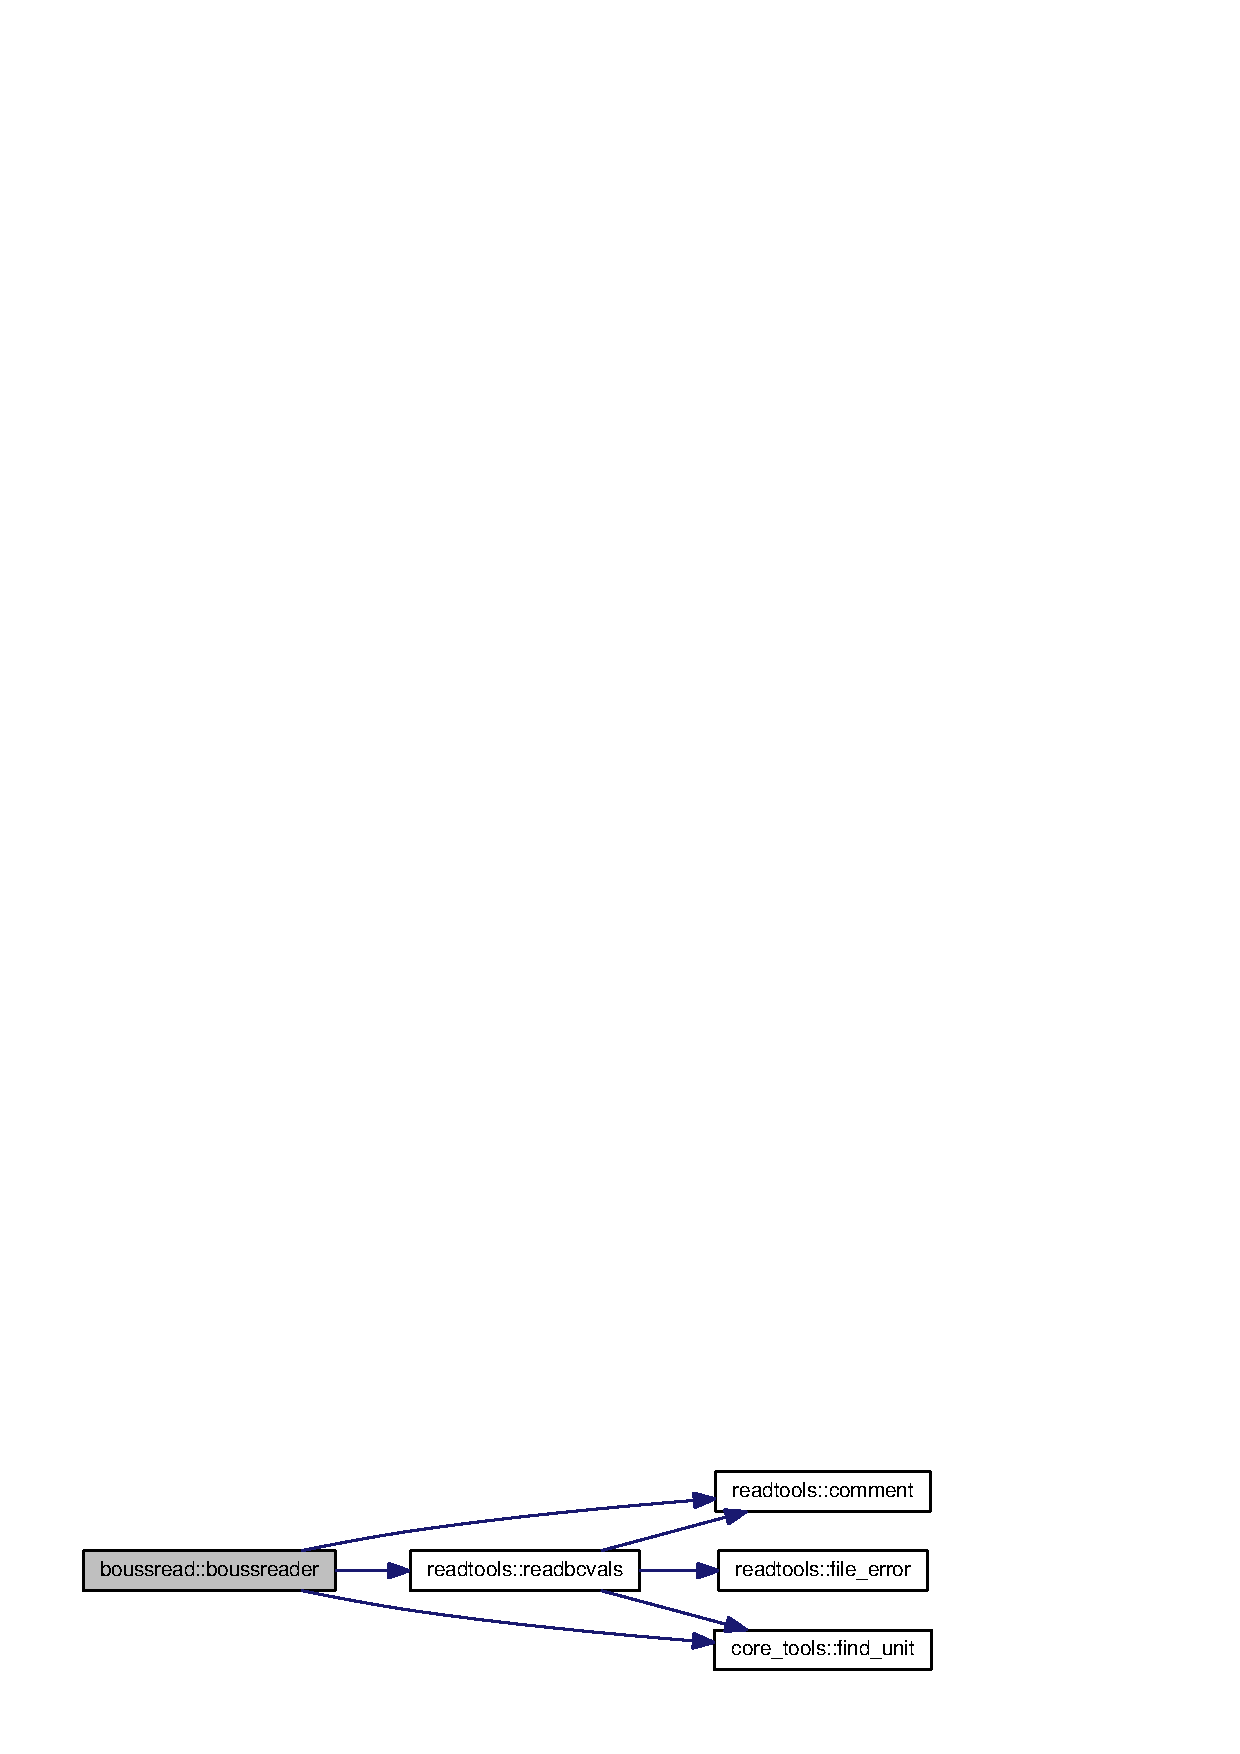
\includegraphics[width=350pt]{namespaceboussread_af206b475e8ec2d4ed9f54c22e829a40e_cgraph}
\end{center}
\end{figure}




Here is the caller graph for this function\+:\nopagebreak
\begin{figure}[H]
\begin{center}
\leavevmode
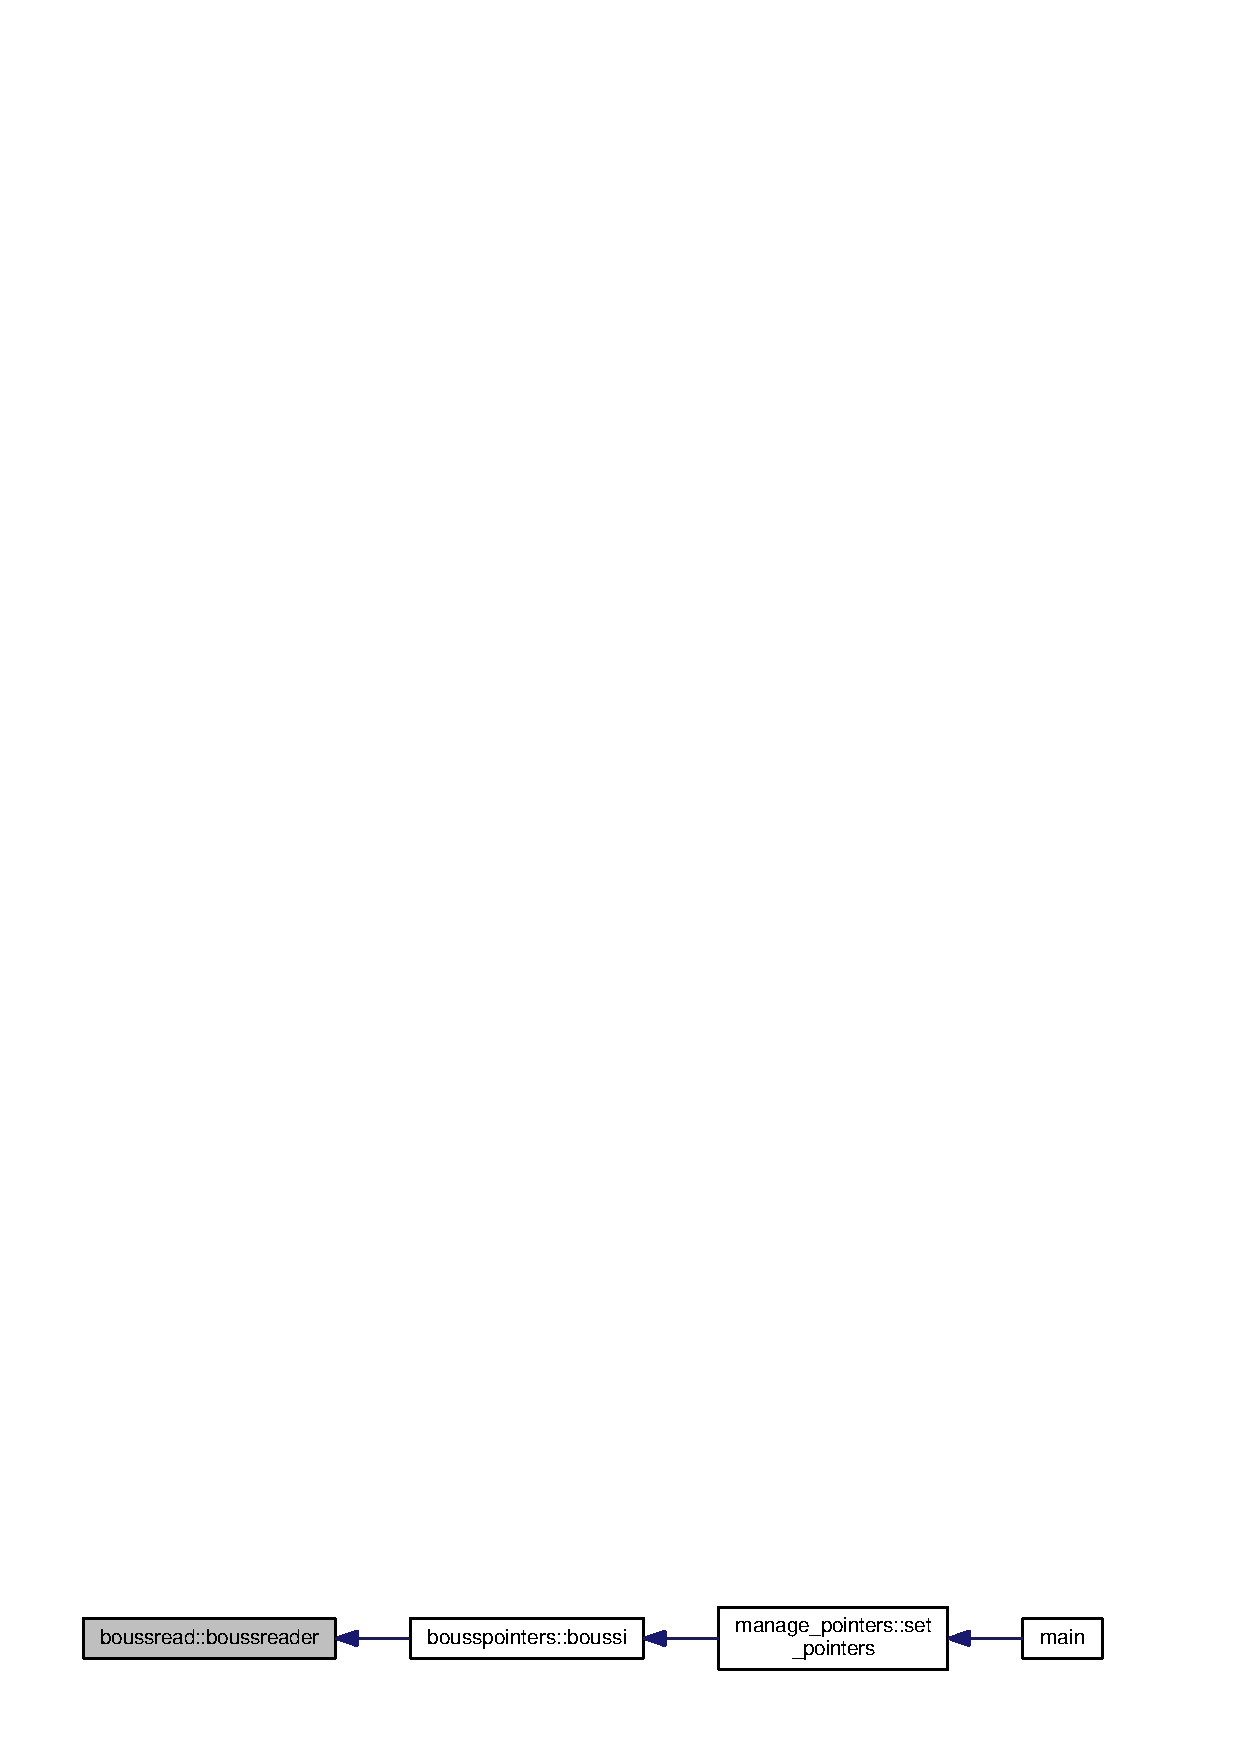
\includegraphics[width=350pt]{namespaceboussread_af206b475e8ec2d4ed9f54c22e829a40e_icgraph}
\end{center}
\end{figure}



\section{capmat Module Reference}
\label{namespacecapmat}\index{capmat@{capmat}}
\subsection*{Functions/\+Subroutines}
\begin{DoxyCompactItemize}
\item 
subroutine, public {\bf impl\+\_\+euler\+\_\+np\+\_\+nondiag} (el\+\_\+id, domain\+\_\+id, quadpnt\+\_\+in)
\begin{DoxyCompactList}\small\item\em implicit Euler for nonlinear problem and Picard iteration method, nondiagonal capacity matrix \end{DoxyCompactList}\item 
subroutine, public {\bf impl\+\_\+euler\+\_\+np\+\_\+diag} (el\+\_\+id, domain\+\_\+id, quadpnt\+\_\+in)
\begin{DoxyCompactList}\small\item\em implicit euler method, nonlinear problem Picard iteration method -\/ diagonal capacity matrix \end{DoxyCompactList}\item 
subroutine, public {\bf steady\+\_\+state\+\_\+int} (el\+\_\+id, domain\+\_\+id, quadpnt\+\_\+in)
\item 
subroutine, private {\bf diagonalizer} (a)
\begin{DoxyCompactList}\small\item\em routine that diagonalizes matrix -\/ it lumps consistent capacity matrices \end{DoxyCompactList}\end{DoxyCompactItemize}


\subsection{Function/\+Subroutine Documentation}
\index{capmat@{capmat}!diagonalizer@{diagonalizer}}
\index{diagonalizer@{diagonalizer}!capmat@{capmat}}
\subsubsection[{diagonalizer(a)}]{\setlength{\rightskip}{0pt plus 5cm}subroutine, private capmat\+::diagonalizer (
\begin{DoxyParamCaption}
\item[{real(kind=rkind), dimension(\+:,\+:), intent(inout)}]{a}
\end{DoxyParamCaption}
)\hspace{0.3cm}{\ttfamily [private]}}\label{namespacecapmat_a3e2778aaff3524d980ba919f1663b000}


routine that diagonalizes matrix -\/ it lumps consistent capacity matrices 



Definition at line 198 of file capmat.\+f90.



Referenced by impl\+\_\+euler\+\_\+np\+\_\+diag().


\begin{DoxyCode}
198       \textcolor{keywordtype}{use }typy
199       
200       \textcolor{keywordtype}{real(kind=rkind)}, \textcolor{keywordtype}{dimension(:,:)}, \textcolor{keywordtype}{intent(in out)} :: a
201 
202       \textcolor{keywordtype}{integer(kind=ikind)} :: i,j
203       \textcolor{keywordtype}{real(kind=rkind)} :: tmp
204 
205       \textcolor{keywordflow}{do} i=1, ubound(a,1)
206         tmp = 0.0\_rkind
207         \textcolor{keywordflow}{do} j=1, ubound(a,1)
208           tmp = tmp + a(i,j)
209 \textcolor{keywordflow}{        end do}
210         
211         a(i,i) = tmp
212 
213         \textcolor{keywordflow}{if} (i > 1) \textcolor{keywordflow}{then}
214           a(i,1:i-1) = 0
215 \textcolor{keywordflow}{        end if}
216 
217         \textcolor{keywordflow}{if} (i < ubound(a,1)) \textcolor{keywordflow}{then}
218           a(i, i+1:ubound(a,1)) = 0
219 \textcolor{keywordflow}{        end if}
220 \textcolor{keywordflow}{      end do}
221     
\end{DoxyCode}


Here is the caller graph for this function\+:\nopagebreak
\begin{figure}[H]
\begin{center}
\leavevmode
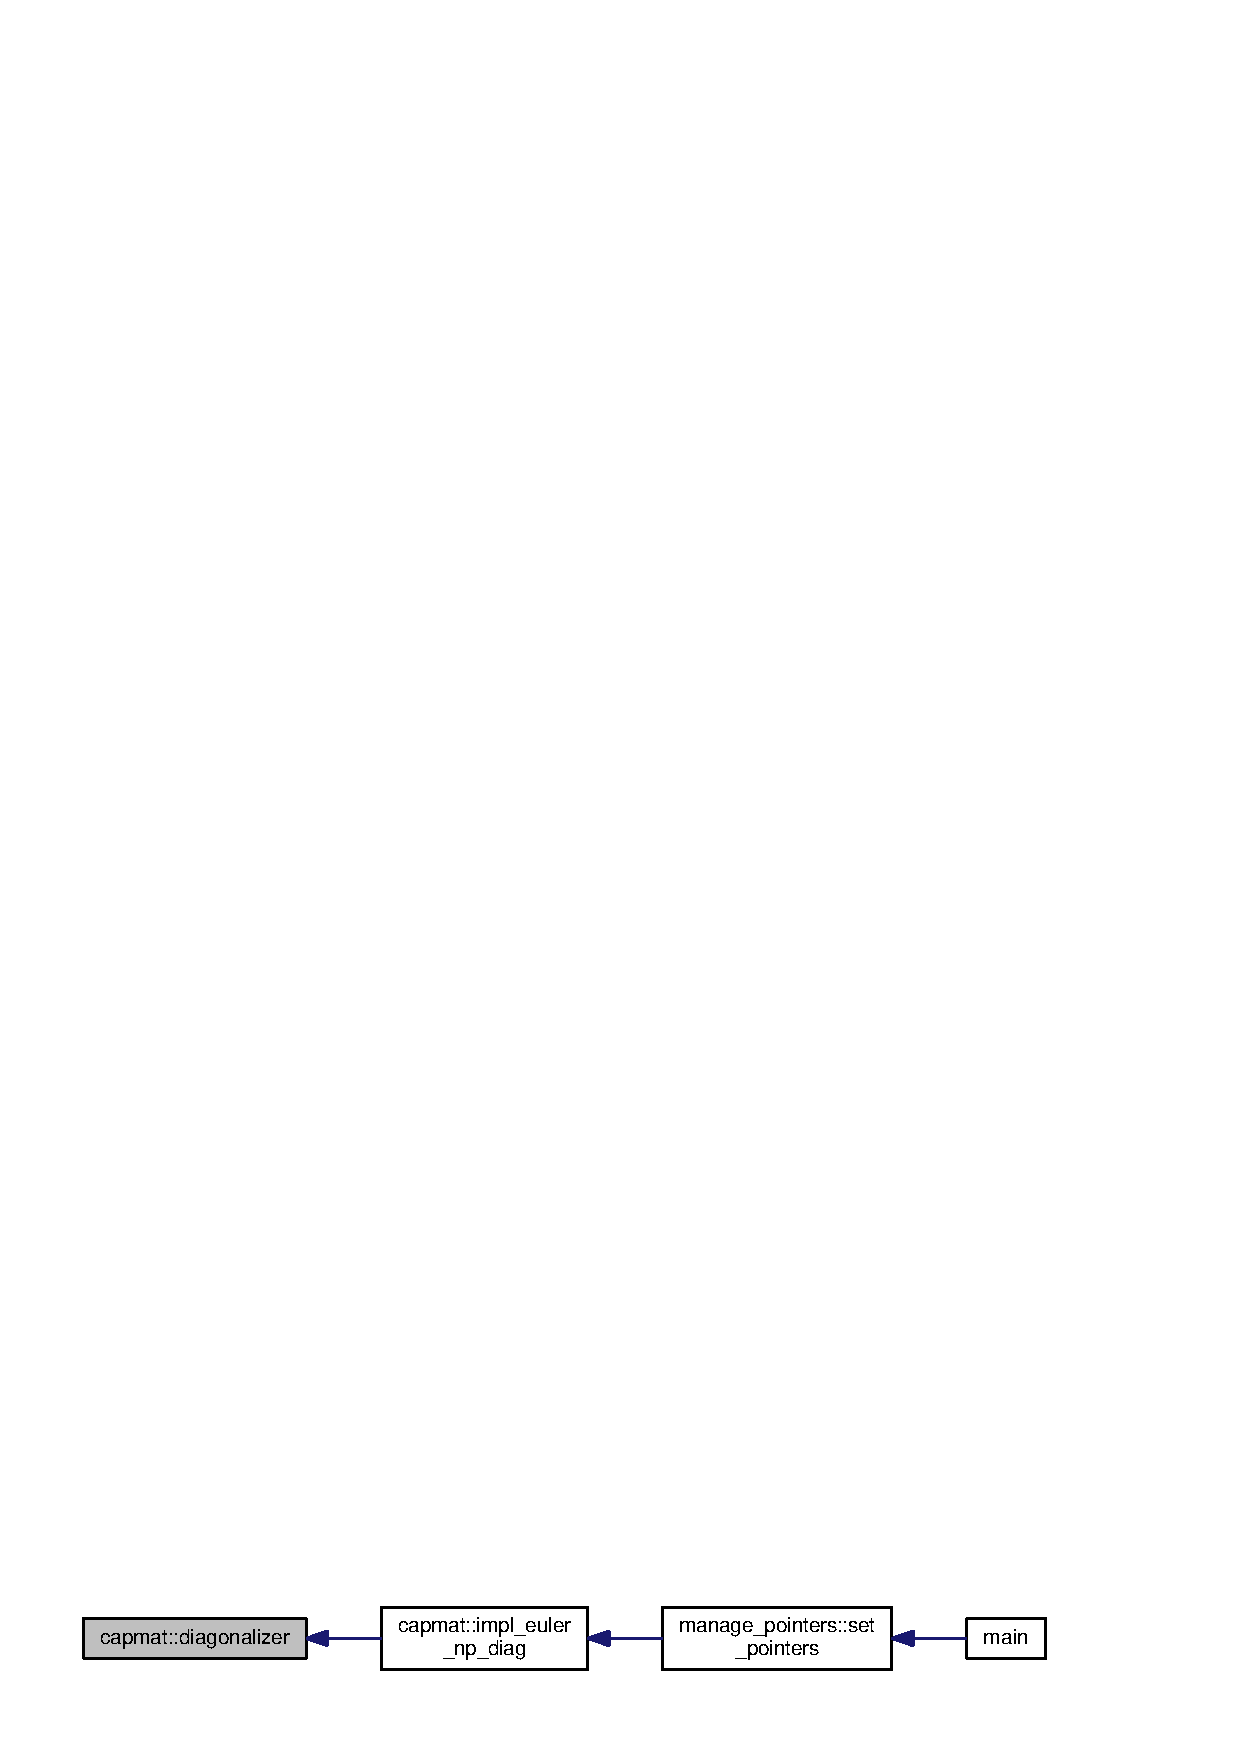
\includegraphics[width=350pt]{namespacecapmat_a3e2778aaff3524d980ba919f1663b000_icgraph}
\end{center}
\end{figure}


\index{capmat@{capmat}!impl\+\_\+euler\+\_\+np\+\_\+diag@{impl\+\_\+euler\+\_\+np\+\_\+diag}}
\index{impl\+\_\+euler\+\_\+np\+\_\+diag@{impl\+\_\+euler\+\_\+np\+\_\+diag}!capmat@{capmat}}
\subsubsection[{impl\+\_\+euler\+\_\+np\+\_\+diag(el\+\_\+id, domain\+\_\+id, quadpnt\+\_\+in)}]{\setlength{\rightskip}{0pt plus 5cm}subroutine, public capmat\+::impl\+\_\+euler\+\_\+np\+\_\+diag (
\begin{DoxyParamCaption}
\item[{integer(kind=ikind), intent(in)}]{el\+\_\+id, }
\item[{integer(kind=ikind), intent(in), optional}]{domain\+\_\+id, }
\item[{type({\bf integpnt\+\_\+str}), intent(inout), optional}]{quadpnt\+\_\+in}
\end{DoxyParamCaption}
)}\label{namespacecapmat_adc9967ebf2be8d086371968c94553c2b}


implicit euler method, nonlinear problem Picard iteration method -\/ diagonal capacity matrix 


\begin{DoxyParams}[1]{Parameters}
\mbox{\tt in}  & {\em domain\+\_\+id} & subdomain number (inserted only if domain decomposition used and if only local data needed) \\
\hline
\end{DoxyParams}


Definition at line 98 of file capmat.\+f90.



References globals\+::base\+\_\+fnc, globals\+::bside, globals\+::cap\+\_\+mat, diagonalizer(), globals\+::elements, globals\+::elnode\+\_\+prev, globals\+::gauss\+\_\+points, and pde\+\_\+objs\+::pde.



Referenced by manage\+\_\+pointers\+::set\+\_\+pointers().


\begin{DoxyCode}
98       \textcolor{keywordtype}{use }typy
99       \textcolor{keywordtype}{use }globals
100       \textcolor{keywordtype}{use }global_objs
101       \textcolor{keywordtype}{use }pde_objs
102       \textcolor{keywordtype}{use }geom_tools
103       \textcolor{keywordtype}{use }feminittools
104       \textcolor{keywordtype}{use }linalg
105       \textcolor{keywordtype}{use }debug_tools
106 
107       \textcolor{keywordtype}{integer(kind=ikind)}, \textcolor{keywordtype}{intent(in)} :: el\_id
109       \textcolor{keywordtype}{integer(kind=ikind)}, \textcolor{keywordtype}{intent(in)}, \textcolor{keywordtype}{optional} :: domain\_id
110       \textcolor{keywordtype}{type}(integpnt_str), \textcolor{keywordtype}{intent(in out)}, \textcolor{keywordtype}{optional} :: quadpnt\_in
111       
112       
113       \textcolor{keywordtype}{integer(kind=ikind)} :: i,j,l, m
114       \textcolor{keywordtype}{real(kind=rkind)} :: tmp
115       \textcolor{keywordtype}{real(kind=rkind)}, \textcolor{keywordtype}{dimension(2,2)} :: locmat
116       \textcolor{keywordtype}{integer(kind=ikind)} :: iproc, jproc, limits, ll, jj
117       \textcolor{keywordtype}{integer(kind=ikind)}, \textcolor{keywordtype}{dimension(:,:)}, \textcolor{keywordtype}{allocatable}, \textcolor{keywordtype}{save} :: layer
118       \textcolor{keywordtype}{type}(integpnt_str) :: quadpnt
119 
120       \textcolor{keywordflow}{if} (.not. \textcolor{keyword}{allocated}(layer)) \textcolor{keywordflow}{then}
121         \textcolor{keyword}{allocate}(layer(ubound(pde,1), ubound(pde,1)))
122 \textcolor{keywordflow}{      end if}
123 
124       \textcolor{keywordflow}{do} iproc=1,ubound(pde,1)
125         \textcolor{keywordflow}{do} jproc=1,ubound(pde,1)
126             layer(iproc, jproc) = elements%material(el\_id, jproc)
127 \textcolor{keywordflow}{        end do}
128 \textcolor{keywordflow}{      end do}
129 
130       cap_mat = 0
131       locmat = 0
132       limits = ubound(cap_mat,1)/ubound(pde,1)     
133       quadpnt%column = 2
134       quadpnt%element = el\_id
135       quadpnt%type\_pnt = \textcolor{stringliteral}{"gqnd"}
136       
137       
138       \textcolor{keywordflow}{if} (\textcolor{keyword}{present}(domain\_id)) \textcolor{keywordflow}{then}
139         quadpnt%ddlocal = .true.
140         quadpnt%subdom = domain\_id
141 \textcolor{keywordflow}{      end if}
142 
143 
144 
145       \textcolor{keywordflow}{do} iproc=1, ubound(pde,1)
146         \textcolor{keywordflow}{do} jproc=1, ubound(pde,1)
147           \textcolor{keywordflow}{do} l=1,  limits
148             \textcolor{keywordflow}{do} j=1,  limits
149               \textcolor{keywordflow}{do} i=1, ubound(gauss_points%weight,1)
150                 quadpnt%order = i
151                 tmp =  -pde(iproc)%pde\_fnc(jproc)%elasticity(pde(iproc),\textcolor{comment}{ layer(iproc, jproc), &}
152 \textcolor{comment}{                quadpnt)*base_fnc(j,i)*base_fnc(l,i)*gauss_points%weight(i)}
153 \textcolor{comment}{                ll = l + limits*(iproc-1)}
154 \textcolor{comment}{                jj = j + limits*(jproc-1)}
155 \textcolor{comment}{                cap_mat(ll,jj) = cap_mat(ll,jj) + tmp}
156 \textcolor{comment}{}\textcolor{keywordflow}{              end do}
157 \textcolor{keywordflow}{            end do}
158 \textcolor{keywordflow}{          end do}
159 \textcolor{keywordflow}{        end do}
160 \textcolor{keywordflow}{      end do}
161 
162       
163      \textcolor{keywordflow}{do} iproc = 1, ubound(pde,1)
164        \textcolor{keywordflow}{do} jproc = 1, ubound(pde,1) 
165          ll = limits*(iproc-1)+1
166          jj = limits*(jproc-1)+1
167         \textcolor{keyword}{call }diagonalizer(cap_mat(ll:ll+limits-1, jj:jj+limits-1))
168 \textcolor{keywordflow}{      end do}
169 \textcolor{keywordflow}{    end do}
170 
171 
172     
173      cap_mat = cap_mat/gauss_points%area*elements%areas(el\_id)
174      
175 
176      bside = bside +   matmul(cap_mat, elnode_prev)
177      
178      
\end{DoxyCode}


Here is the call graph for this function\+:\nopagebreak
\begin{figure}[H]
\begin{center}
\leavevmode
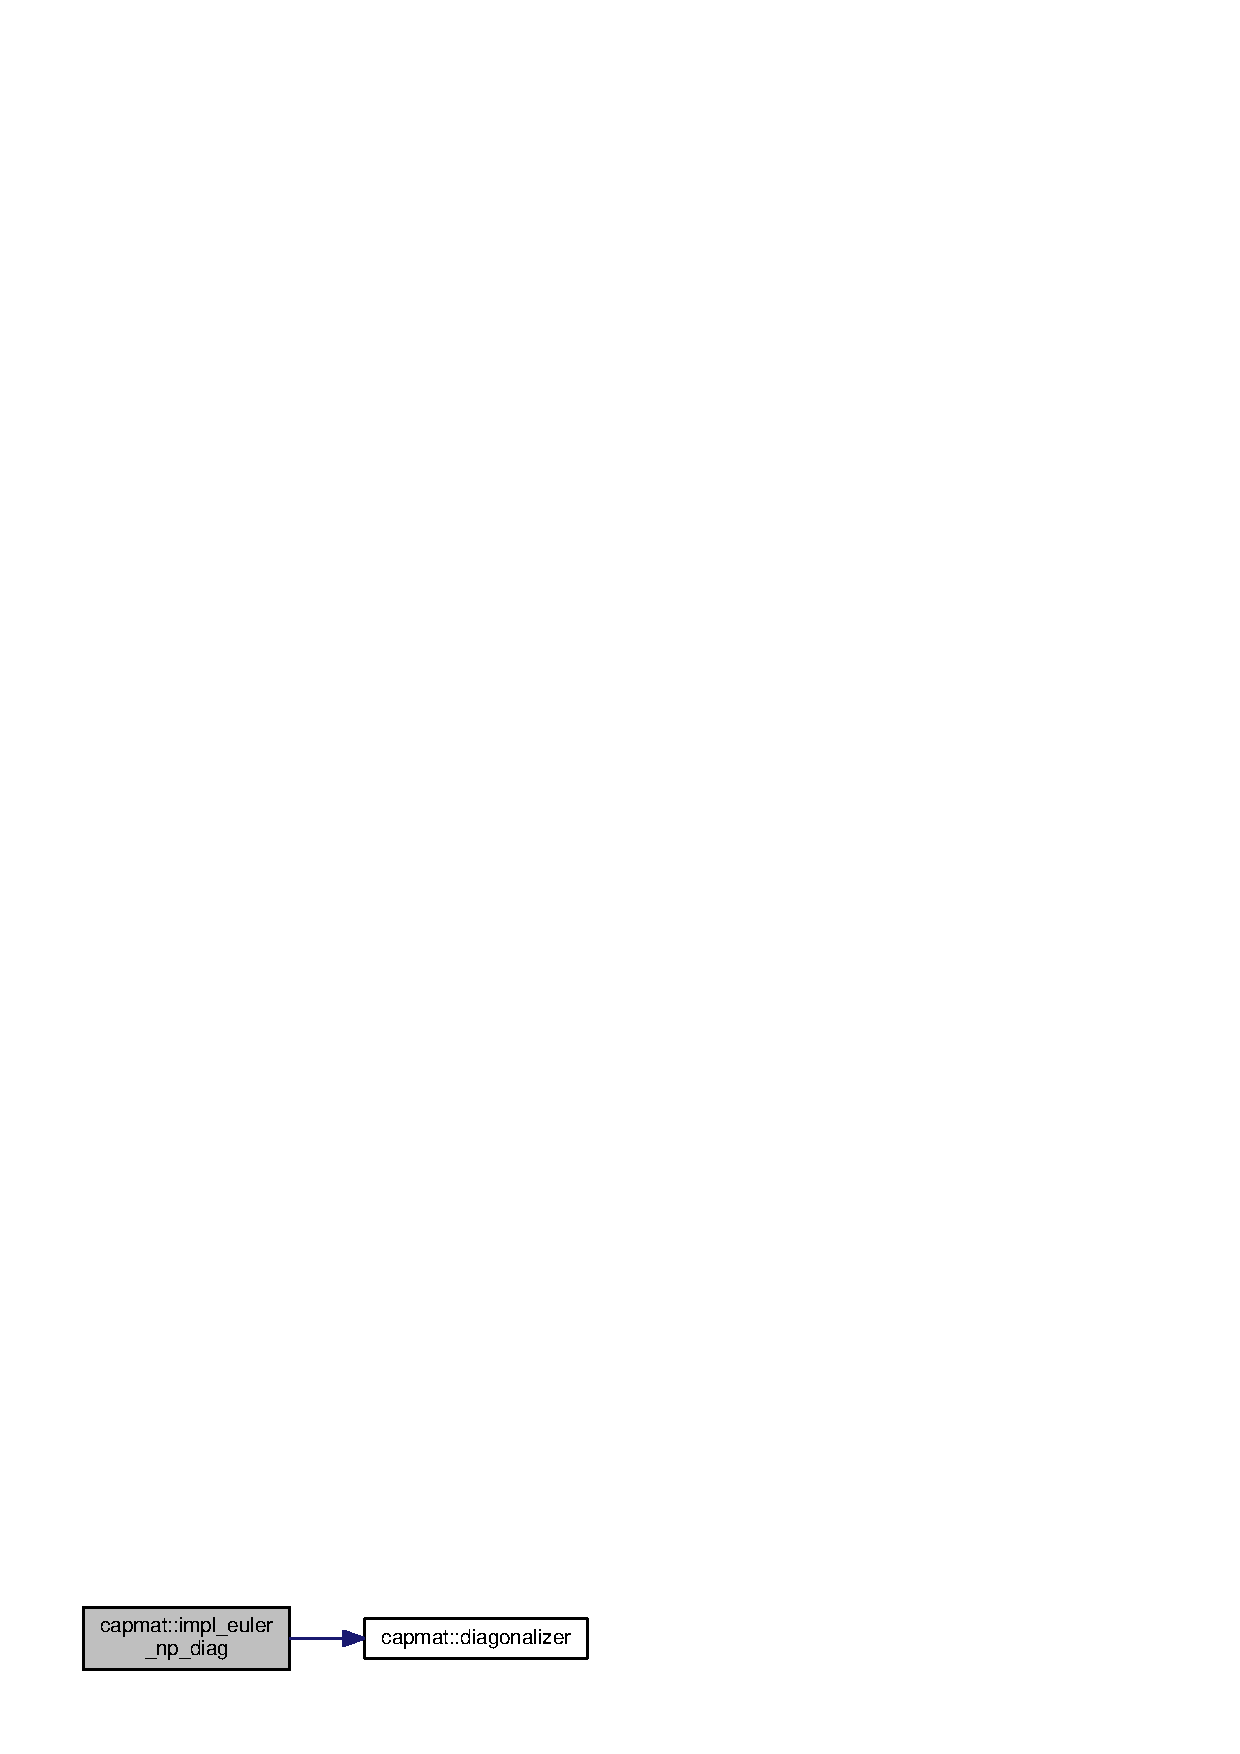
\includegraphics[width=286pt]{namespacecapmat_adc9967ebf2be8d086371968c94553c2b_cgraph}
\end{center}
\end{figure}




Here is the caller graph for this function\+:\nopagebreak
\begin{figure}[H]
\begin{center}
\leavevmode
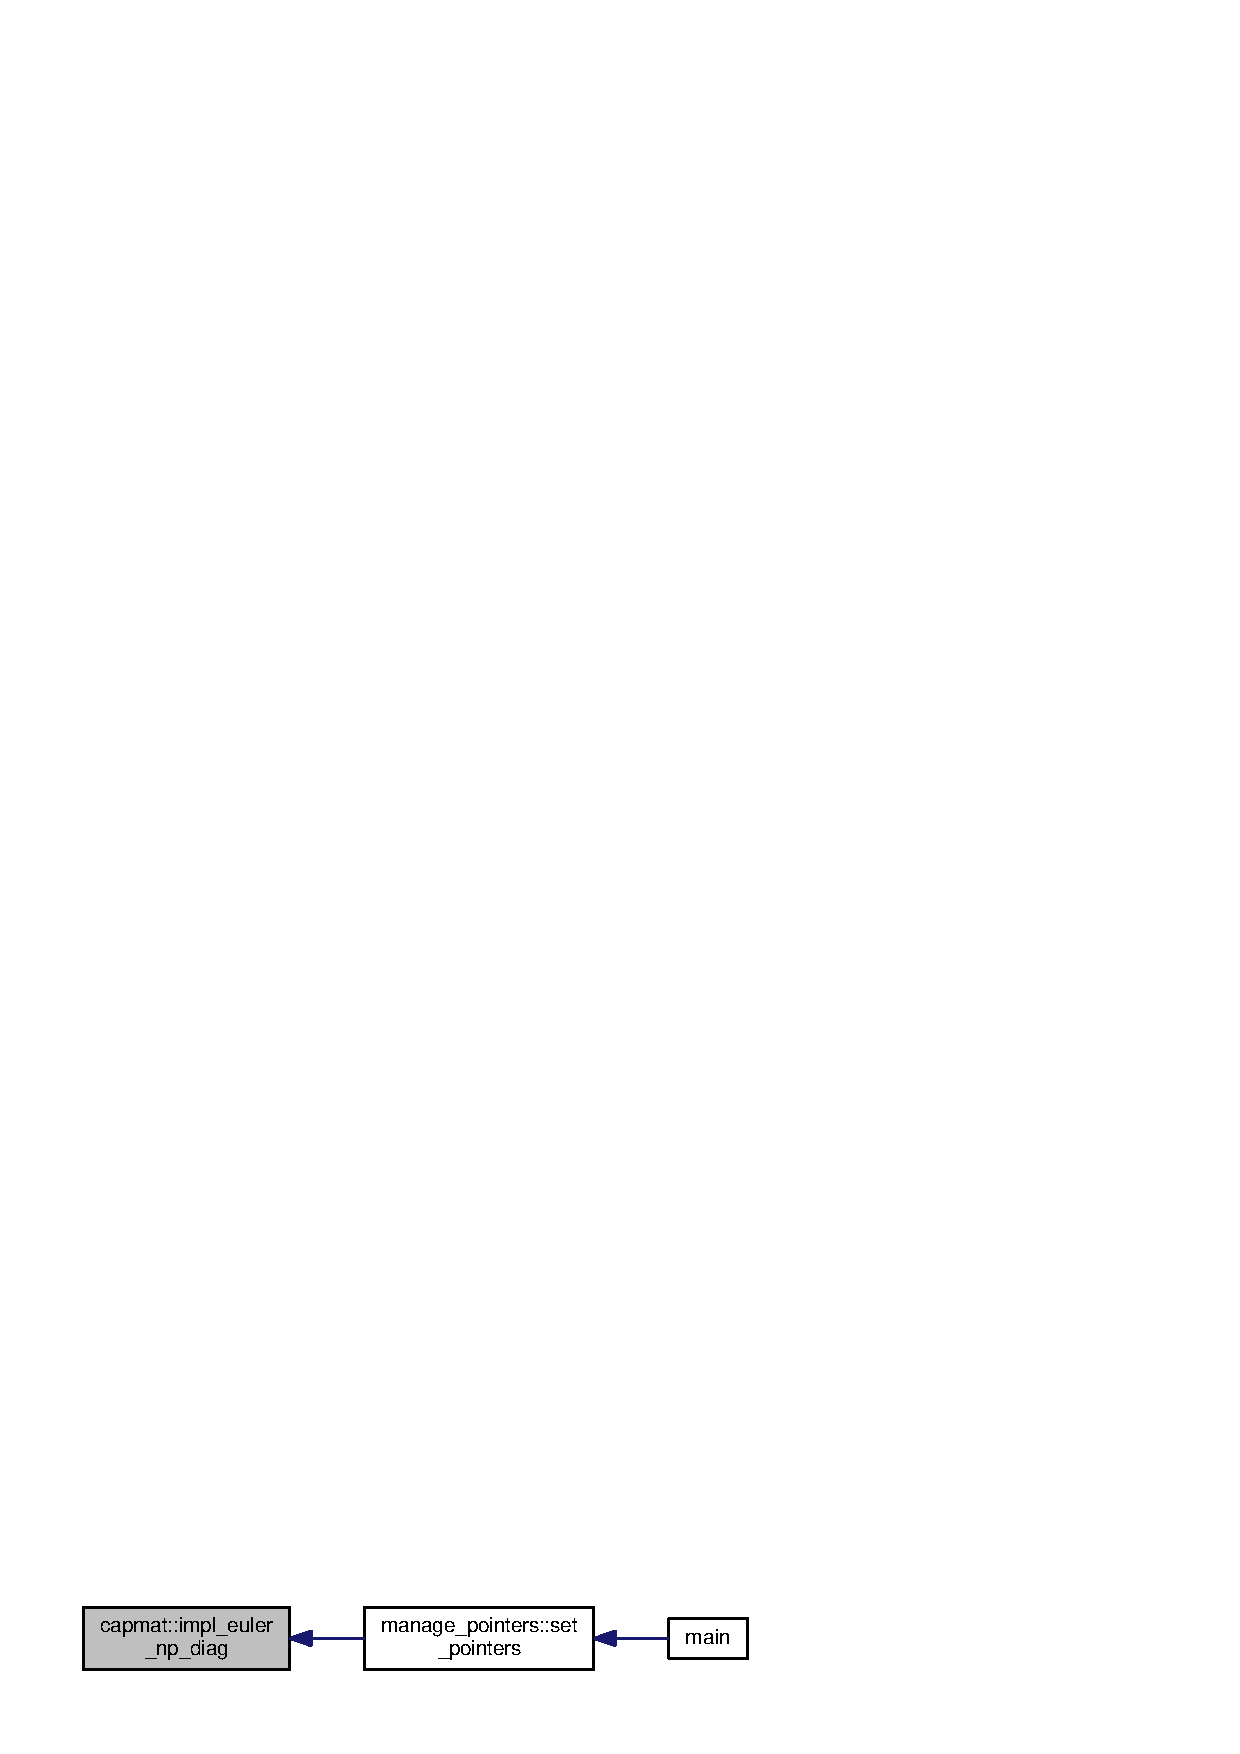
\includegraphics[width=350pt]{namespacecapmat_adc9967ebf2be8d086371968c94553c2b_icgraph}
\end{center}
\end{figure}


\index{capmat@{capmat}!impl\+\_\+euler\+\_\+np\+\_\+nondiag@{impl\+\_\+euler\+\_\+np\+\_\+nondiag}}
\index{impl\+\_\+euler\+\_\+np\+\_\+nondiag@{impl\+\_\+euler\+\_\+np\+\_\+nondiag}!capmat@{capmat}}
\subsubsection[{impl\+\_\+euler\+\_\+np\+\_\+nondiag(el\+\_\+id, domain\+\_\+id, quadpnt\+\_\+in)}]{\setlength{\rightskip}{0pt plus 5cm}subroutine, public capmat\+::impl\+\_\+euler\+\_\+np\+\_\+nondiag (
\begin{DoxyParamCaption}
\item[{integer(kind=ikind), intent(in)}]{el\+\_\+id, }
\item[{integer(kind=ikind), intent(in), optional}]{domain\+\_\+id, }
\item[{type({\bf integpnt\+\_\+str}), intent(inout), optional}]{quadpnt\+\_\+in}
\end{DoxyParamCaption}
)}\label{namespacecapmat_a3fabe2603f1c7a6fbd9c4afabc26f3ae}


implicit Euler for nonlinear problem and Picard iteration method, nondiagonal capacity matrix 

implicit Euler for nonlinear problem and Picard iteration method, diagonal capacity matrix steady state -\/$>$ the capacity matrix is a zero matrix routine that diagonalizes matrix -\/ it lumps consistent capacity matrices implicit euler method, nonlinear problem Picard iteration method -\/ non-\/diagonal capacity matrix


\begin{DoxyParams}[1]{Parameters}
\mbox{\tt in}  & {\em domain\+\_\+id} & subdomain number (inserted only if domain decomposition used and if only local data needed) \\
\hline
\end{DoxyParams}


Definition at line 20 of file capmat.\+f90.



References globals\+::base\+\_\+fnc, globals\+::bside, globals\+::cap\+\_\+mat, globals\+::elements, globals\+::elnode\+\_\+prev, globals\+::gauss\+\_\+points, and pde\+\_\+objs\+::pde.



Referenced by manage\+\_\+pointers\+::set\+\_\+pointers().


\begin{DoxyCode}
20       \textcolor{keywordtype}{use }typy
21       \textcolor{keywordtype}{use }globals
22       \textcolor{keywordtype}{use }global_objs
23       \textcolor{keywordtype}{use }pde_objs
24       \textcolor{keywordtype}{use }geom_tools
25       \textcolor{keywordtype}{use }feminittools
26       \textcolor{keywordtype}{use }linalg
27       \textcolor{keywordtype}{use }debug_tools
28 
29       \textcolor{keywordtype}{integer(kind=ikind)}, \textcolor{keywordtype}{intent(in)} :: el\_id
31       \textcolor{keywordtype}{integer(kind=ikind)}, \textcolor{keywordtype}{intent(in)}, \textcolor{keywordtype}{optional} :: domain\_id
32       \textcolor{keywordtype}{type}(integpnt_str), \textcolor{keywordtype}{intent(in out)}, \textcolor{keywordtype}{optional} :: quadpnt\_in
33       
34       \textcolor{keywordtype}{integer(kind=ikind)} :: i,j,l, m
35       \textcolor{keywordtype}{real(kind=rkind)} :: tmp
36       \textcolor{keywordtype}{integer(kind=ikind)} :: iproc, jproc, limits, ll, jj
37       \textcolor{keywordtype}{integer(kind=ikind)}, \textcolor{keywordtype}{dimension(:,:)}, \textcolor{keywordtype}{allocatable}, \textcolor{keywordtype}{save} :: layer
38       \textcolor{keywordtype}{type}(integpnt_str) :: quadpnt
39 
40 
41       \textcolor{keywordflow}{if} (.not. \textcolor{keyword}{allocated}(layer)) \textcolor{keywordflow}{then}
42         \textcolor{keyword}{allocate}(layer(ubound(pde,1), ubound(pde,1)))
43 \textcolor{keywordflow}{      end if}
44 
45       \textcolor{keywordflow}{do} iproc=1,ubound(pde,1)
46         \textcolor{keywordflow}{do} jproc=1,ubound(pde,1)
47             layer(iproc, jproc) = elements%material(el\_id, jproc)
48 \textcolor{keywordflow}{        end do}
49 \textcolor{keywordflow}{      end do}
50 
51 
52       cap_mat = 0
53       
54       \textcolor{keywordflow}{if} (\textcolor{keyword}{present}(quadpnt\_in)) \textcolor{keywordflow}{then}
55         quadpnt=quadpnt\_in
56 \textcolor{keywordflow}{      end if}
57 
58       limits = ubound(cap_mat,1)/ubound(pde,1)
59       quadpnt%column = 2
60       quadpnt%element = el\_id
61       quadpnt%type\_pnt = \textcolor{stringliteral}{"gqnd"}
62       
63       \textcolor{keywordflow}{if} (\textcolor{keyword}{present}(domain\_id)) \textcolor{keywordflow}{then}
64         quadpnt%ddlocal = .true.
65         quadpnt%subdom = domain\_id
66 \textcolor{keywordflow}{      end if}
67       
68 
69       \textcolor{keywordflow}{do} iproc=1, ubound(pde,1)
70         \textcolor{keywordflow}{do} jproc=1, ubound(pde,1)
71           \textcolor{keywordflow}{do} l=1,  limits
72             \textcolor{keywordflow}{do} j=1,  limits
73               \textcolor{keywordflow}{do} i=1, ubound(gauss_points%weight,1)
74                 quadpnt%order = i
75                 tmp =  -pde(iproc)%pde\_fnc(jproc)%elasticity(pde(iproc),\textcolor{comment}{ layer(iproc, jproc), &}
76 \textcolor{comment}{                quadpnt)*base_fnc(j,i)*base_fnc(l,i)*gauss_points%weight(i)}
77 \textcolor{comment}{                ll = l + limits*(iproc-1)}
78 \textcolor{comment}{                jj = j + limits*(jproc-1)}
79 \textcolor{comment}{                cap_mat(ll,jj) = cap_mat(ll,jj) + tmp}
80 \textcolor{comment}{}\textcolor{keywordflow}{              end do}
81 \textcolor{keywordflow}{            end do}
82 \textcolor{keywordflow}{          end do}
83 \textcolor{keywordflow}{        end do}
84 \textcolor{keywordflow}{      end do}
85 
86       
87       cap_mat = cap_mat/gauss_points%area*elements%areas(el\_id)
88 
89       bside =  bside + matmul(cap_mat, elnode_prev)
90       
91 
\end{DoxyCode}


Here is the caller graph for this function\+:\nopagebreak
\begin{figure}[H]
\begin{center}
\leavevmode
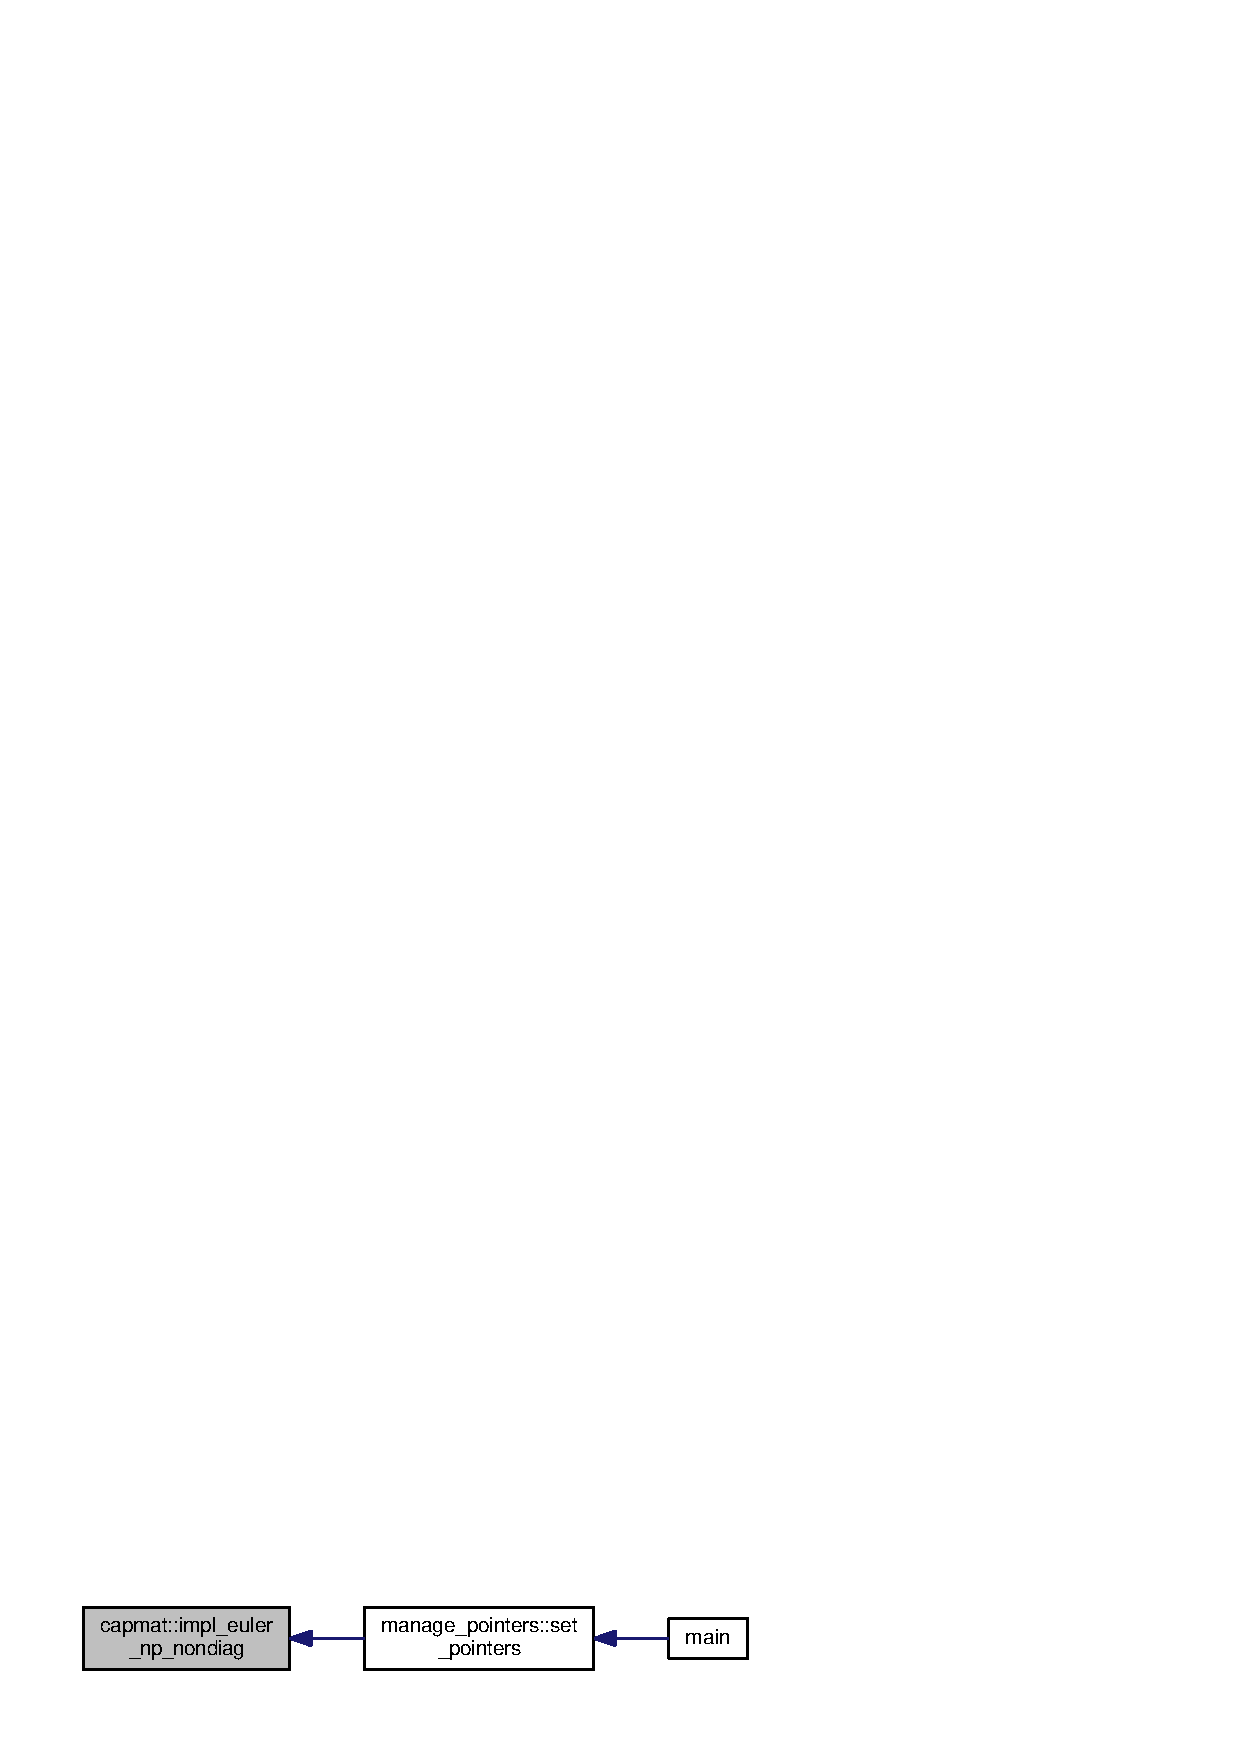
\includegraphics[width=350pt]{namespacecapmat_a3fabe2603f1c7a6fbd9c4afabc26f3ae_icgraph}
\end{center}
\end{figure}


\index{capmat@{capmat}!steady\+\_\+state\+\_\+int@{steady\+\_\+state\+\_\+int}}
\index{steady\+\_\+state\+\_\+int@{steady\+\_\+state\+\_\+int}!capmat@{capmat}}
\subsubsection[{steady\+\_\+state\+\_\+int(el\+\_\+id, domain\+\_\+id, quadpnt\+\_\+in)}]{\setlength{\rightskip}{0pt plus 5cm}subroutine, public capmat\+::steady\+\_\+state\+\_\+int (
\begin{DoxyParamCaption}
\item[{integer(kind=ikind), intent(in)}]{el\+\_\+id, }
\item[{integer(kind=ikind), intent(in), optional}]{domain\+\_\+id, }
\item[{type({\bf integpnt\+\_\+str}), intent(inout), optional}]{quadpnt\+\_\+in}
\end{DoxyParamCaption}
)}\label{namespacecapmat_afecac6837e09fc605aebc33c4f516259}

\begin{DoxyParams}[1]{Parameters}
\mbox{\tt in}  & {\em domain\+\_\+id} & subdomain number (inserted only if domain decomposition used and if only local data needed) \\
\hline
\end{DoxyParams}


Definition at line 182 of file capmat.\+f90.



References globals\+::cap\+\_\+mat.



Referenced by manage\+\_\+pointers\+::set\+\_\+pointers().


\begin{DoxyCode}
182       \textcolor{keywordtype}{use }typy
183       \textcolor{keywordtype}{use }globals
184       \textcolor{keywordtype}{use }global_objs
185       \textcolor{keywordtype}{use }geom_tools
186 
187       \textcolor{keywordtype}{integer(kind=ikind)}, \textcolor{keywordtype}{intent(in)} :: el\_id
189       \textcolor{keywordtype}{integer(kind=ikind)}, \textcolor{keywordtype}{intent(in)}, \textcolor{keywordtype}{optional} :: domain\_id
190       \textcolor{keywordtype}{type}(integpnt_str), \textcolor{keywordtype}{intent(in out)}, \textcolor{keywordtype}{optional} :: quadpnt\_in
191 
192       cap_mat = 0
193 
\end{DoxyCode}


Here is the caller graph for this function\+:\nopagebreak
\begin{figure}[H]
\begin{center}
\leavevmode
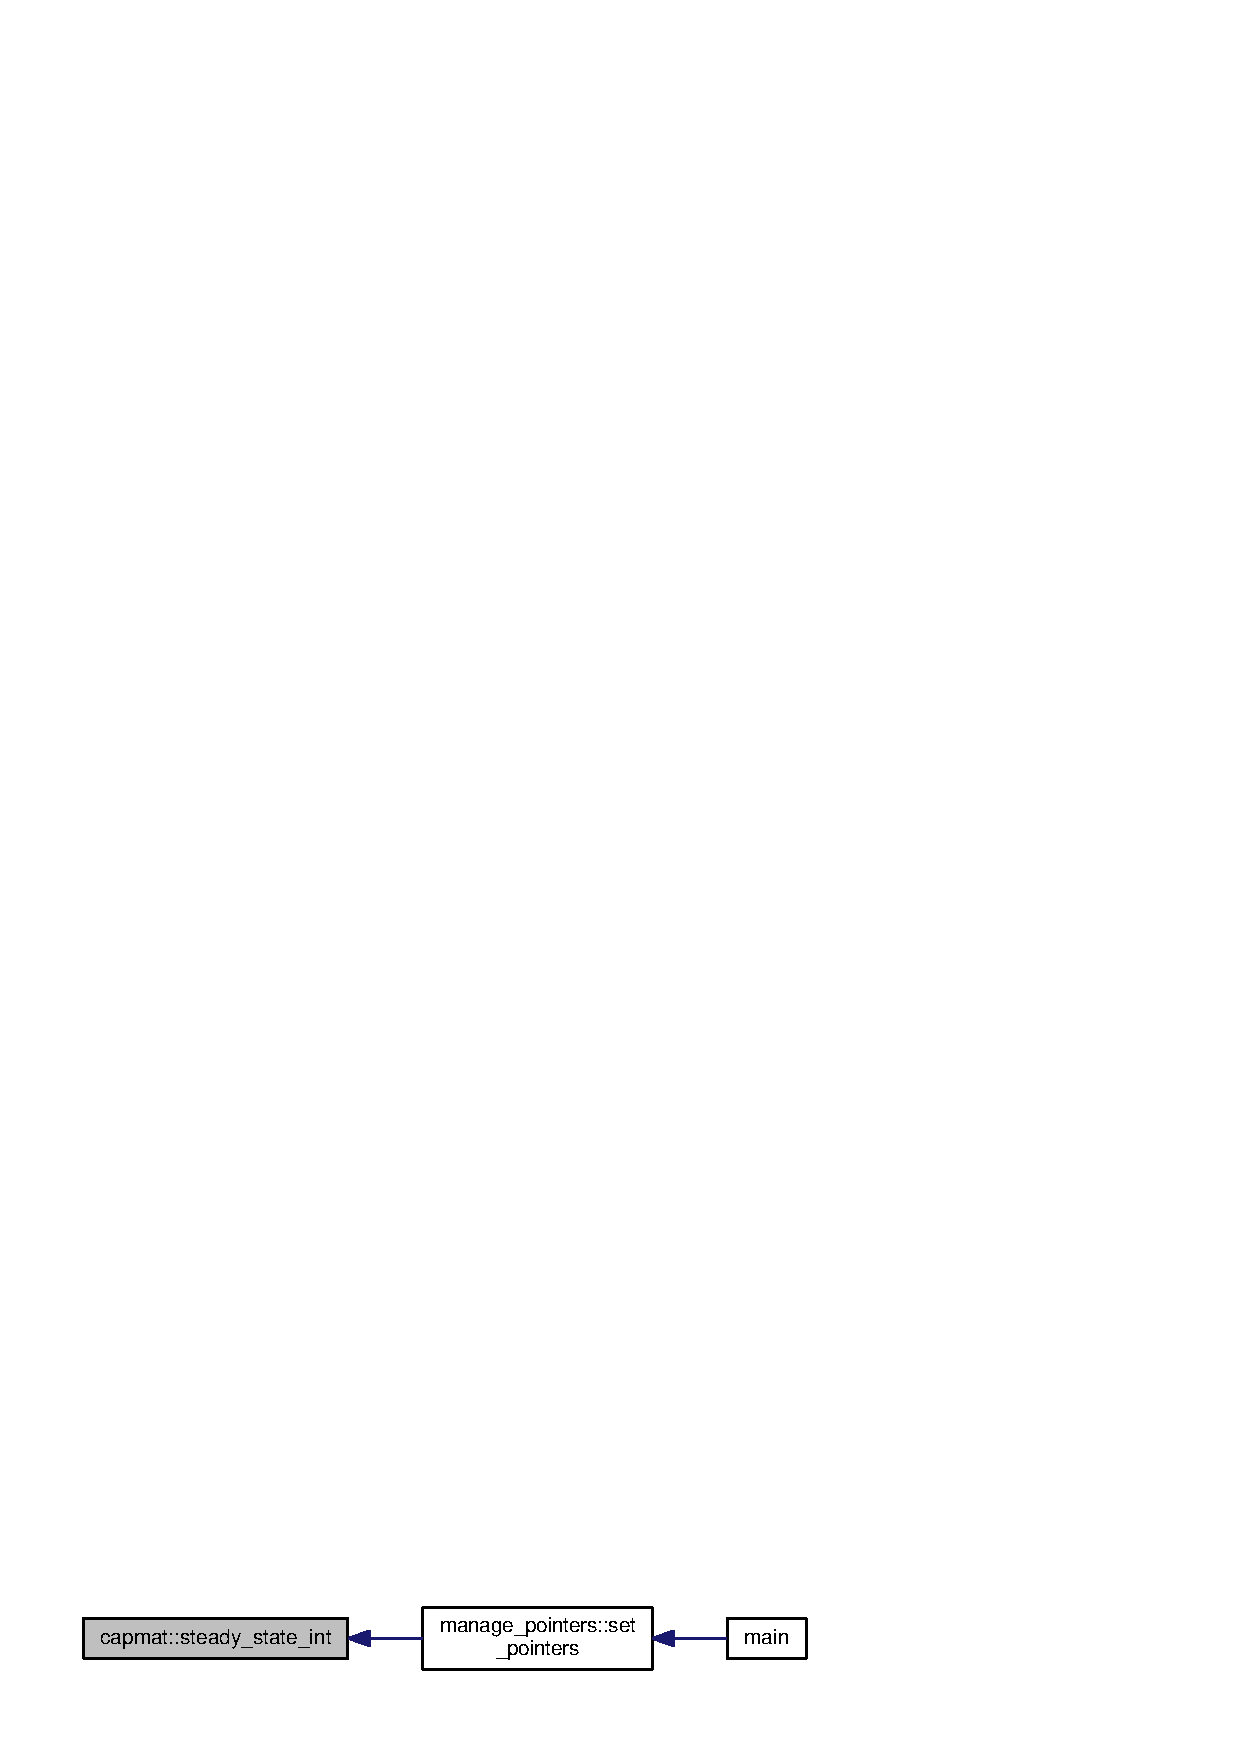
\includegraphics[width=350pt]{namespacecapmat_afecac6837e09fc605aebc33c4f516259_icgraph}
\end{center}
\end{figure}



\section{core\+\_\+tools Module Reference}
\label{namespacecore__tools}\index{core\+\_\+tools@{core\+\_\+tools}}
\subsection*{Functions/\+Subroutines}
\begin{DoxyCompactItemize}
\item 
character(len=\+:) function, allocatable, public {\bf cut} (ch)
\begin{DoxyCompactList}\small\item\em dummy functions, the pointer procedure is set to this function in case if not being considered \end{DoxyCompactList}\item 
subroutine, public {\bf write\+\_\+log} (text, real1, int1, text2, real2, int2, text3, real3, int3, hidden)
\item 
real(kind=rkind) function, public {\bf avg} (a, b)
\item 
subroutine, public {\bf mesh\+\_\+allocater} ()
\begin{DoxyCompactList}\small\item\em allocates structures for nodes and elements \end{DoxyCompactList}\item 
subroutine, public {\bf find\+\_\+unit} (iunit, start\+\_\+id)
\end{DoxyCompactItemize}


\subsection{Function/\+Subroutine Documentation}
\index{core\+\_\+tools@{core\+\_\+tools}!avg@{avg}}
\index{avg@{avg}!core\+\_\+tools@{core\+\_\+tools}}
\subsubsection[{avg(a, b)}]{\setlength{\rightskip}{0pt plus 5cm}real(kind=rkind) function, public core\+\_\+tools\+::avg (
\begin{DoxyParamCaption}
\item[{real(kind=rkind), intent(in)}]{a, }
\item[{real(kind=rkind), intent(in)}]{b}
\end{DoxyParamCaption}
)}\label{namespacecore__tools_af0abb0a9edbab36984797ab055df1e0b}


Definition at line 132 of file core\+\_\+tools.\+f90.



Referenced by simegen\+::simegen1d().


\begin{DoxyCode}
132       \textcolor{keywordtype}{use }typy
133       \textcolor{keywordtype}{real(kind=rkind)}, \textcolor{keywordtype}{intent(in)} :: a
134       \textcolor{keywordtype}{real(kind=rkind)}, \textcolor{keywordtype}{intent(in)} :: b
135       \textcolor{keywordtype}{real(kind=rkind)} :: c
136 
137       c = (a+b)/2.0\_rkind
138 
\end{DoxyCode}


Here is the caller graph for this function\+:\nopagebreak
\begin{figure}[H]
\begin{center}
\leavevmode
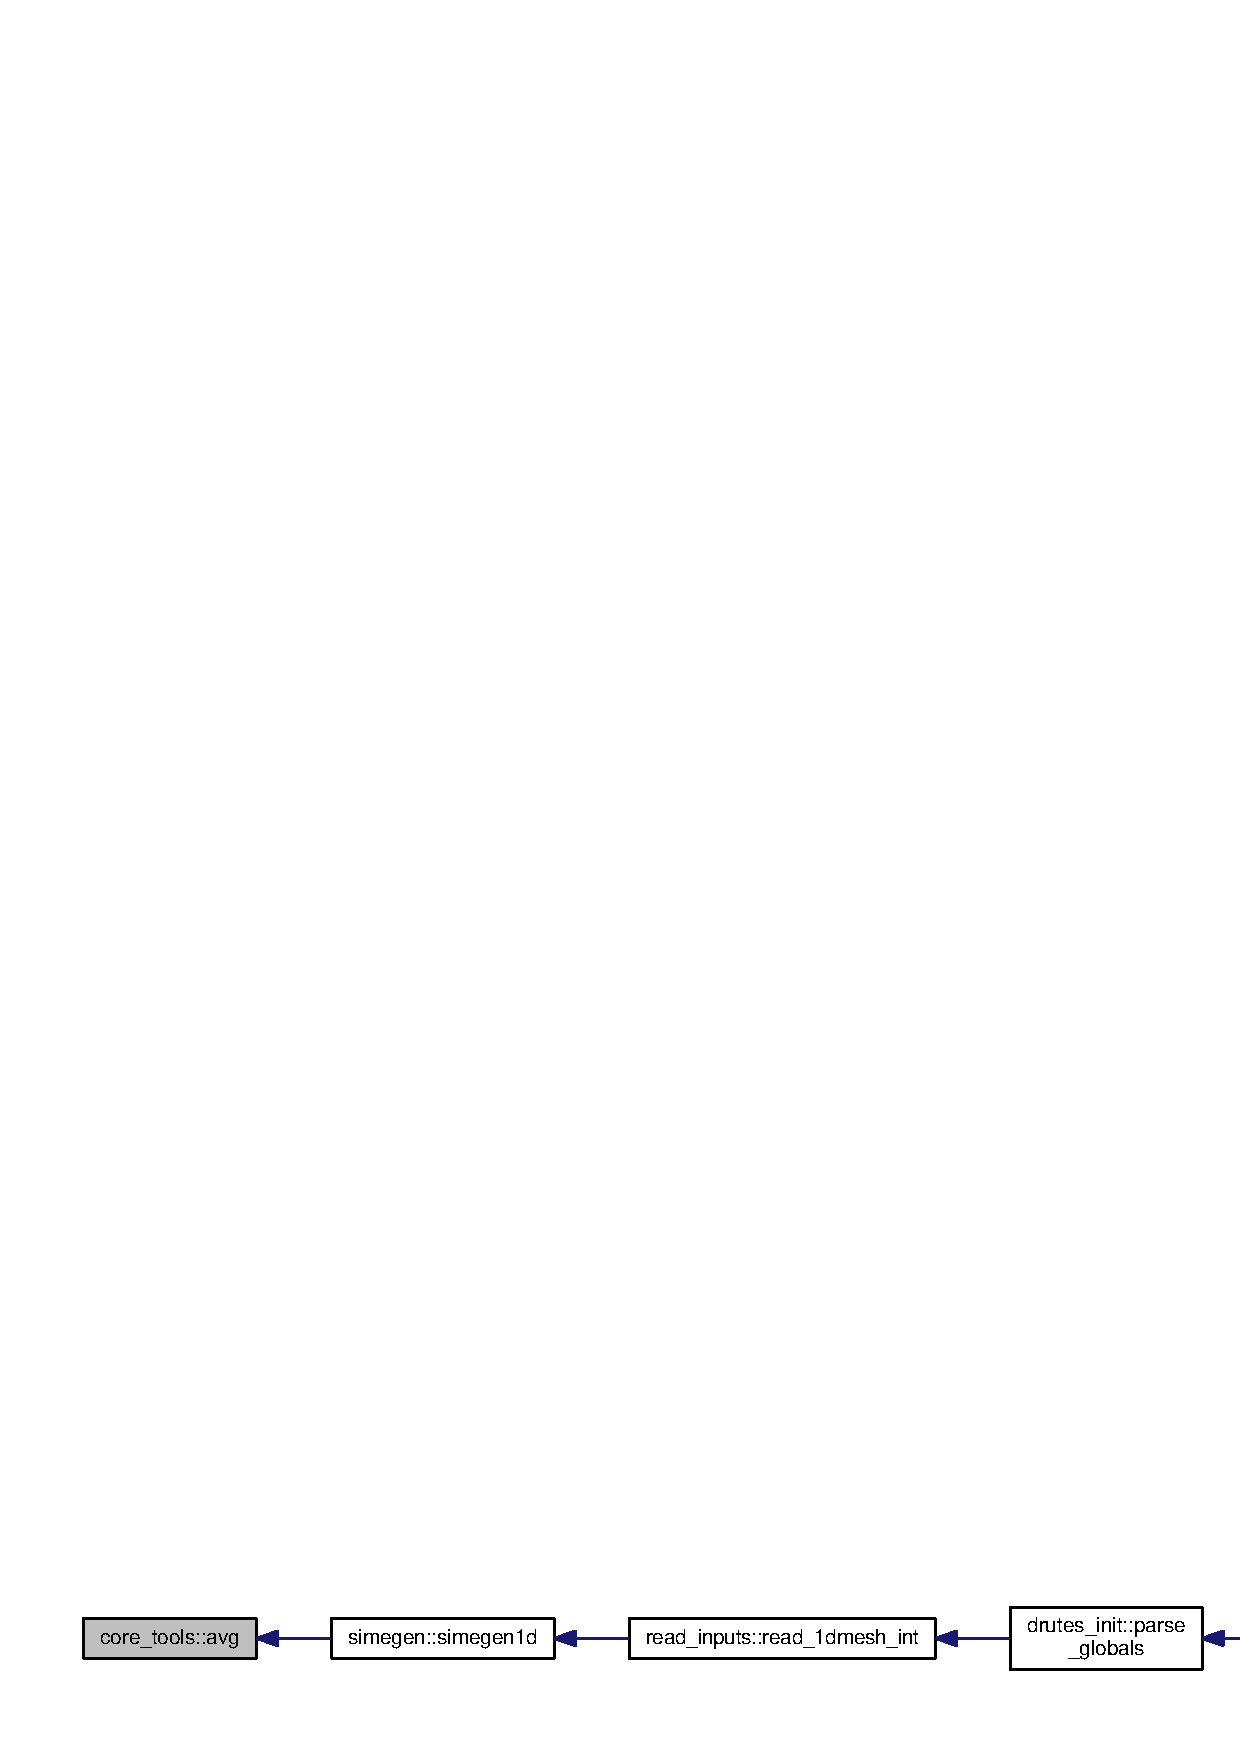
\includegraphics[width=350pt]{namespacecore__tools_af0abb0a9edbab36984797ab055df1e0b_icgraph}
\end{center}
\end{figure}


\index{core\+\_\+tools@{core\+\_\+tools}!cut@{cut}}
\index{cut@{cut}!core\+\_\+tools@{core\+\_\+tools}}
\subsubsection[{cut(ch)}]{\setlength{\rightskip}{0pt plus 5cm}character(len=\+:) function, allocatable, public core\+\_\+tools\+::cut (
\begin{DoxyParamCaption}
\item[{character(len=$\ast$), intent(in)}]{ch}
\end{DoxyParamCaption}
)}\label{namespacecore__tools_aca00f87d69884142f2350a340fe3642e}


dummy functions, the pointer procedure is set to this function in case if not being considered 



Definition at line 30 of file core\+\_\+tools.\+f90.



Referenced by geom\+\_\+tools\+::map1d2d(), and geom\+\_\+tools\+::map1d2dj().


\begin{DoxyCode}
30   
31     \textcolor{keywordtype}{character(len=*)}, \textcolor{keywordtype}{intent(in)} :: ch
32     \textcolor{keywordtype}{character(len=:)}, \textcolor{keywordtype}{allocatable} :: out\_ch
33     
34     \textcolor{keyword}{allocate}(\textcolor{keywordtype}{character}(len=len(adjustl(trim(ch)))) :: out\_ch)
35     
36     out\_ch=adjustl(trim(ch))
37     
\end{DoxyCode}


Here is the caller graph for this function\+:
\nopagebreak
\begin{figure}[H]
\begin{center}
\leavevmode
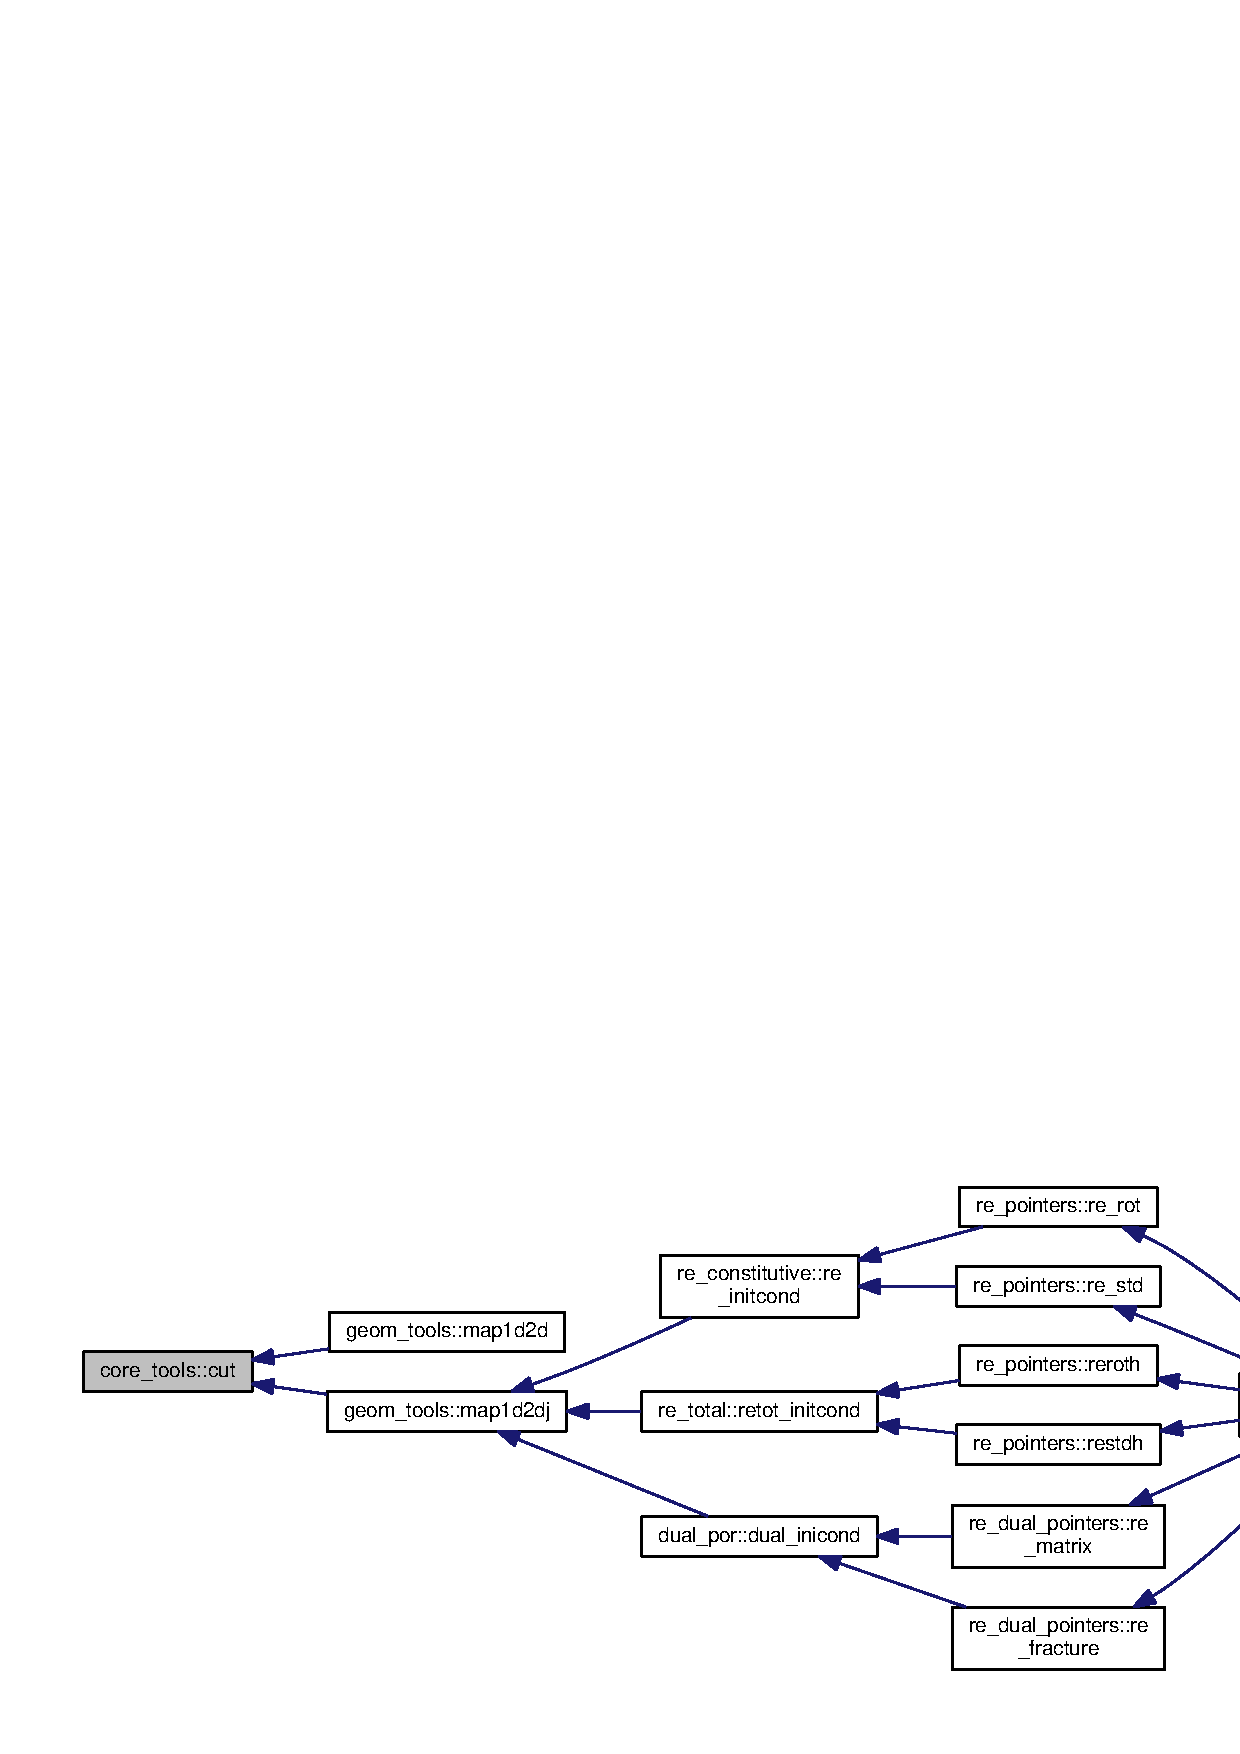
\includegraphics[width=350pt]{namespacecore__tools_aca00f87d69884142f2350a340fe3642e_icgraph}
\end{center}
\end{figure}


\index{core\+\_\+tools@{core\+\_\+tools}!find\+\_\+unit@{find\+\_\+unit}}
\index{find\+\_\+unit@{find\+\_\+unit}!core\+\_\+tools@{core\+\_\+tools}}
\subsubsection[{find\+\_\+unit(iunit, start\+\_\+id)}]{\setlength{\rightskip}{0pt plus 5cm}subroutine, public core\+\_\+tools\+::find\+\_\+unit (
\begin{DoxyParamCaption}
\item[{integer, intent(out)}]{iunit, }
\item[{integer, intent(in), optional}]{start\+\_\+id}
\end{DoxyParamCaption}
)}\label{namespacecore__tools_a01c1527fcc56448471e2b349571e51ee}


Definition at line 177 of file core\+\_\+tools.\+f90.



Referenced by ade\+\_\+reader\+::ade\+\_\+read(), boussread\+::boussreader(), drutes\+\_\+init\+::get\+\_\+cmd\+\_\+options(), postpro\+::get\+\_\+ram\+\_\+use(), heat\+\_\+reader\+::heat\+\_\+read(), re\+\_\+total\+::iconddebouss(), decomposer\+::init\+\_\+decomp(), drutes\+\_\+init\+::init\+\_\+observe(), main(), postpro\+::make\+\_\+print(), geom\+\_\+tools\+::map1d2d(), geom\+\_\+tools\+::map1d2dj(), drutes\+\_\+init\+::parse\+\_\+globals(), decomp\+\_\+tools\+::print\+\_\+domains(), decomp\+\_\+tools\+::print\+\_\+elements\+\_\+dd(), debug\+\_\+tools\+::print\+\_\+int\+\_\+matrix(), debug\+\_\+tools\+::print\+\_\+int\+\_\+vector(), debug\+\_\+tools\+::print\+\_\+logical\+\_\+array(), debug\+\_\+tools\+::print\+\_\+quadpnt(), debug\+\_\+tools\+::print\+\_\+real\+\_\+matrix(), debug\+\_\+tools\+::print\+\_\+real\+\_\+vector(), debug\+\_\+tools\+::print\+\_\+real\+\_\+vector4(), debug\+\_\+tools\+::print\+\_\+smartarray\+\_\+i(), debug\+\_\+tools\+::print\+\_\+smartmatrix\+\_\+i(), debug\+\_\+tools\+::print\+\_\+sparse\+\_\+matrix(), re\+\_\+dual\+\_\+reader\+::re\+\_\+dual\+\_\+readf(), re\+\_\+dual\+\_\+reader\+::re\+\_\+dual\+\_\+readm(), re\+\_\+dual\+\_\+reader\+::re\+\_\+dual\+\_\+var(), read\+\_\+inputs\+::read\+\_\+2dmesh\+\_\+gmsh(), decomposer\+::read\+\_\+coarse\+\_\+mesh(), read\+\_\+inputs\+::read\+\_\+scilab(), readtools\+::readbcvals(), re\+\_\+reader\+::res\+\_\+read(), drutes\+\_\+init\+::set\+\_\+global\+\_\+vars(), fem\+::solve\+\_\+pde(), and printtools\+::time2finish().


\begin{DoxyCode}
177       \textcolor{keywordtype}{integer}, \textcolor{keywordtype}{intent(out)} :: iunit
178       \textcolor{keywordtype}{integer}, \textcolor{keywordtype}{intent(in)}, \textcolor{keywordtype}{optional} :: start\_id
179       \textcolor{keywordtype}{logical} :: op
180 
181       \textcolor{keywordflow}{if} (\textcolor{keyword}{present}(start\_id)) \textcolor{keywordflow}{then}
182         iunit = start\_id*1 + 1
183       \textcolor{keywordflow}{else}
184         iunit = 100 \textcolor{comment}{! the lower values are often reserved}
185 \textcolor{keywordflow}{      end if}
186 
187       \textcolor{keywordflow}{do}
188         \textcolor{keyword}{inquire}(unit=iunit,opened=op)
189         \textcolor{keywordflow}{if} (.not.op) \textcolor{keywordflow}{then}
190           \textcolor{keywordflow}{exit}
191 \textcolor{keywordflow}{        end if} 
192         iunit = iunit + 1  
193         \textcolor{keywordflow}{if} (iunit >= huge(iunit) - 1) \textcolor{keywordflow}{then}
194           error stop \textcolor{stringliteral}{"SYSTEM PANIC, unable to find any free unit"}
195           \textcolor{keywordflow}{exit}
196 \textcolor{keywordflow}{        end if}
197 \textcolor{keywordflow}{      end do}
198   
\end{DoxyCode}


Here is the caller graph for this function\+:
\nopagebreak
\begin{figure}[H]
\begin{center}
\leavevmode
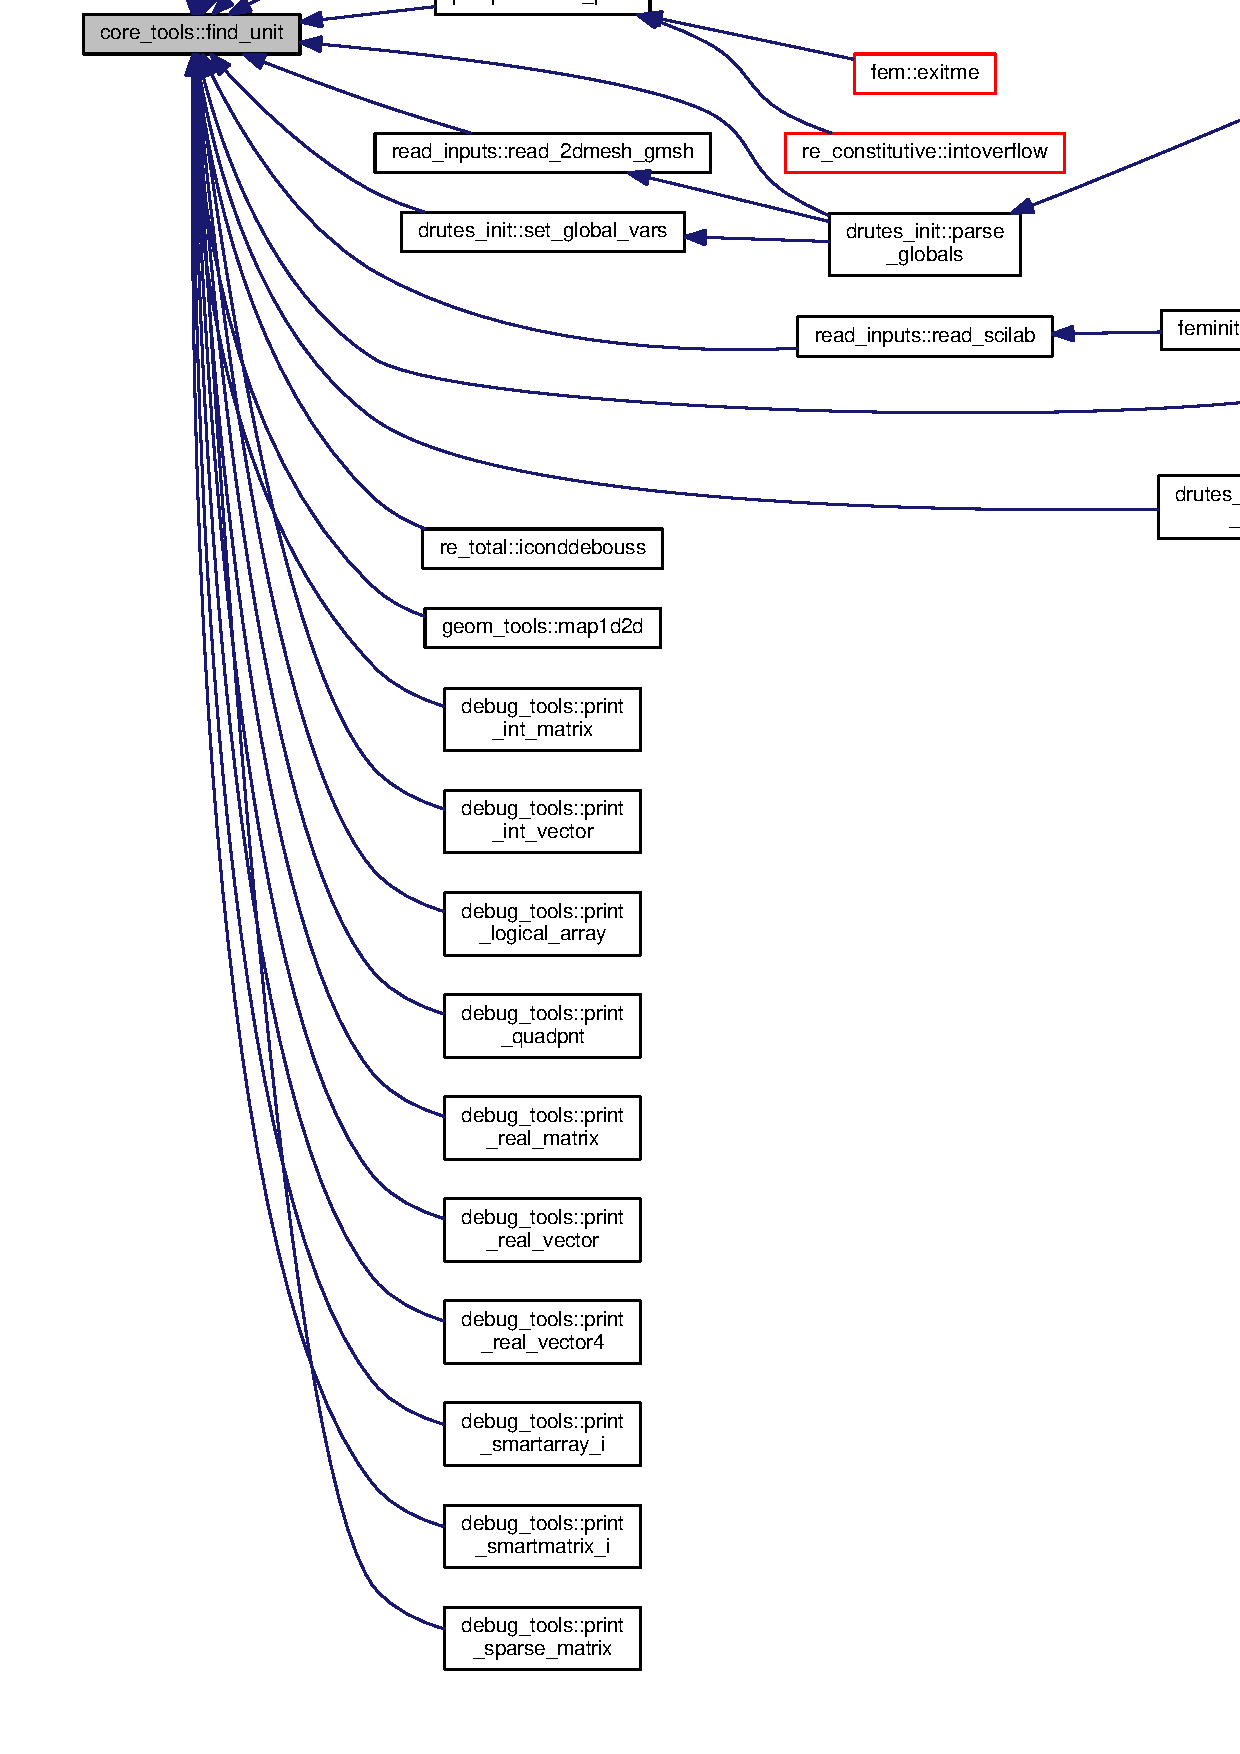
\includegraphics[height=550pt]{namespacecore__tools_a01c1527fcc56448471e2b349571e51ee_icgraph}
\end{center}
\end{figure}


\index{core\+\_\+tools@{core\+\_\+tools}!mesh\+\_\+allocater@{mesh\+\_\+allocater}}
\index{mesh\+\_\+allocater@{mesh\+\_\+allocater}!core\+\_\+tools@{core\+\_\+tools}}
\subsubsection[{mesh\+\_\+allocater()}]{\setlength{\rightskip}{0pt plus 5cm}subroutine, public core\+\_\+tools\+::mesh\+\_\+allocater (
\begin{DoxyParamCaption}
{}
\end{DoxyParamCaption}
)}\label{namespacecore__tools_a05e8cc58b84b9391b49c5070db1160f7}


allocates structures for nodes and elements 



Definition at line 143 of file core\+\_\+tools.\+f90.



References globals\+::drutes\+\_\+config, globals\+::elements, globals\+::nodes, and pde\+\_\+objs\+::pde\+\_\+common.



Referenced by read\+\_\+inputs\+::read\+\_\+2dmesh\+\_\+gmsh(), read\+\_\+inputs\+::read\+\_\+2dmesh\+\_\+t3d(), simegen\+::simegen1d(), and simegen\+::simegen2d().


\begin{DoxyCode}
143       \textcolor{keywordtype}{use }typy
144       \textcolor{keywordtype}{use }global_objs
145       \textcolor{keywordtype}{use }pde_objs
146       \textcolor{keywordtype}{use }globals
147 
148       \textcolor{keywordtype}{integer} :: n
149 
150       \textcolor{keyword}{allocate}(nodes%id(nodes%kolik))
151       \textcolor{keyword}{allocate}(nodes%edge(nodes%kolik))
152       \textcolor{keyword}{allocate}(nodes%data(nodes%kolik,drutes_config%dimen))
153       \textcolor{keyword}{allocate}(nodes%boundary(nodes%kolik))
154       \textcolor{keyword}{allocate}(nodes%el2integ(nodes%kolik))
155       \textcolor{keyword}{allocate}(nodes%element(nodes%kolik))
156       \textcolor{keyword}{allocate}(elements%length(elements%kolik,drutes_config%dimen + 1))
157       \textcolor{keyword}{allocate}(elements%nvect\_z(elements%kolik,drutes_config%dimen + 1))
158       \textcolor{keyword}{allocate}(elements%id(elements%kolik))
159       \textcolor{keyword}{allocate}(elements%data(elements%kolik, drutes_config%dimen+1))
160       \textcolor{keyword}{allocate}(elements%areas(elements%kolik))
161       \textcolor{keyword}{allocate}(elements%ders(elements%kolik, drutes_config%dimen+1, 
      drutes_config%dimen\textcolor{comment}{))}
162 \textcolor{comment}{      }\textcolor{keyword}{allocate}(elements%border(elements%kolik))
163       
164       n = pde_common%processes
165       \textcolor{keyword}{allocate}(elements%material(elements%kolik, n))
166       
167       \textcolor{keyword}{allocate}(elements%neighbours(elements%kolik, ubound(elements%data,\textcolor{comment}{2)))}
168 \textcolor{comment}{      }
169 \textcolor{comment}{      }\textcolor{keyword}{allocate}(nodes%boundary\_order(nodes%kolik))
170 
171       
172 
\end{DoxyCode}


Here is the caller graph for this function\+:\nopagebreak
\begin{figure}[H]
\begin{center}
\leavevmode
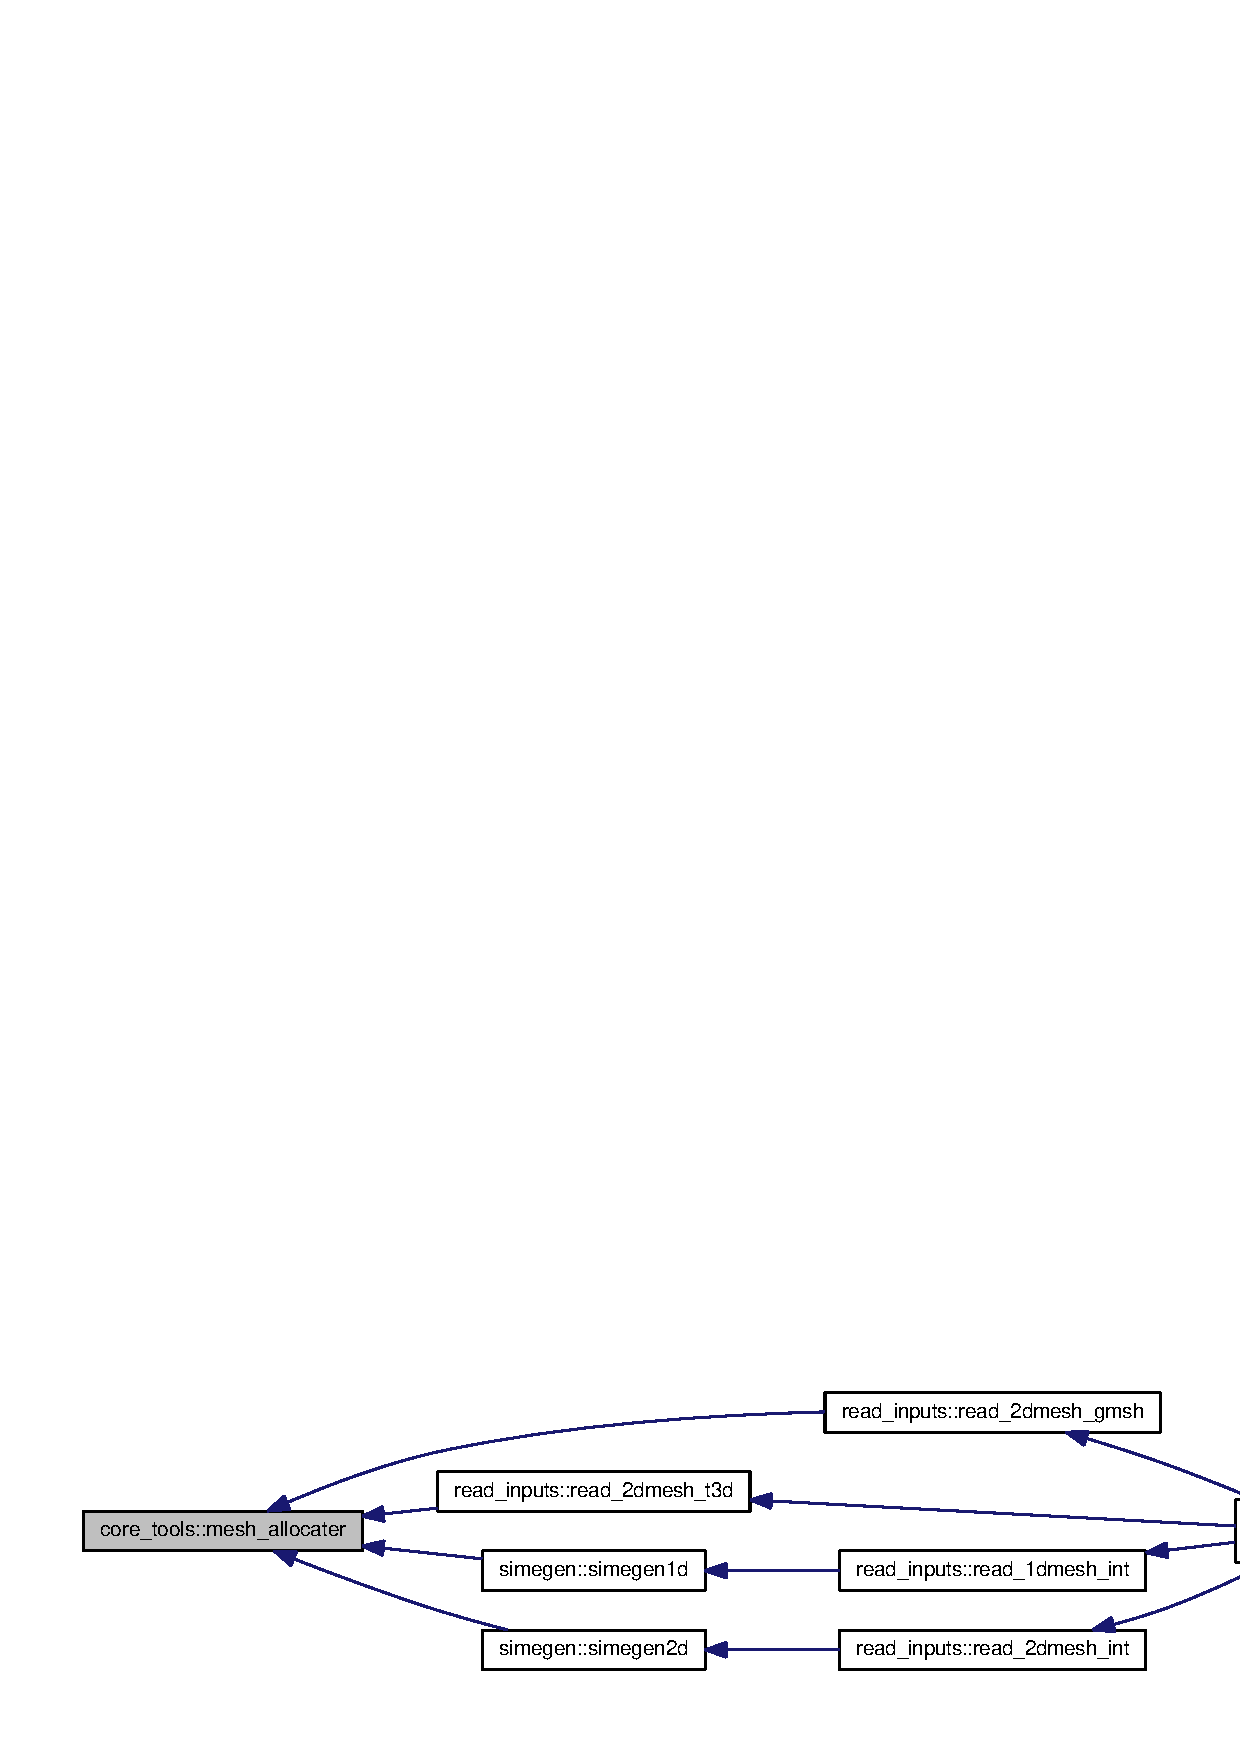
\includegraphics[width=350pt]{namespacecore__tools_a05e8cc58b84b9391b49c5070db1160f7_icgraph}
\end{center}
\end{figure}


\index{core\+\_\+tools@{core\+\_\+tools}!write\+\_\+log@{write\+\_\+log}}
\index{write\+\_\+log@{write\+\_\+log}!core\+\_\+tools@{core\+\_\+tools}}
\subsubsection[{write\+\_\+log(text, real1, int1, text2, real2, int2, text3, real3, int3, hidden)}]{\setlength{\rightskip}{0pt plus 5cm}subroutine, public core\+\_\+tools\+::write\+\_\+log (
\begin{DoxyParamCaption}
\item[{character(len=$\ast$), intent(in)}]{text, }
\item[{real(kind=rkind), intent(in), optional}]{real1, }
\item[{integer(kind=ikind), intent(in), optional}]{int1, }
\item[{character(len=$\ast$), intent(in), optional}]{text2, }
\item[{real(kind=rkind), intent(in), optional}]{real2, }
\item[{integer(kind=ikind), intent(in), optional}]{int2, }
\item[{character(len=$\ast$), intent(in), optional}]{text3, }
\item[{real(kind=rkind), intent(in), optional}]{real3, }
\item[{integer(kind=ikind), intent(in), optional}]{int3, }
\item[{logical, optional}]{hidden}
\end{DoxyParamCaption}
)}\label{namespacecore__tools_abe09f9b4dc2abc5384a24020c5031e95}
character to store the time info

the character to store the date info 

Definition at line 41 of file core\+\_\+tools.\+f90.



References globals\+::logfile, and globals\+::terminal.



Referenced by decomposer\+::clear\+\_\+subdomain(), re\+\_\+constitutive\+::dmualem\+\_\+dh\+\_\+tab(), dual\+\_\+tab\+::dual\+\_\+tabvalues(), fem\+::evol\+\_\+dt(), fem\+::exitme(), feminittools\+::feminit(), postpro\+::get\+\_\+ram\+\_\+use(), fem\+\_\+tools\+::icond4neumann(), decomposer\+::init\+\_\+decomp(), re\+\_\+constitutive\+::intoverflow(), re\+\_\+constitutive\+::inverse\+\_\+vangen(), main(), postpro\+::make\+\_\+print(), decomposer\+::make\+\_\+quadmesh(), re\+\_\+constitutive\+::mualem\+\_\+tab(), drutes\+\_\+init\+::parse\+\_\+globals(), read\+\_\+inputs\+::read\+\_\+2dmesh\+\_\+gmsh(), decomposer\+::read\+\_\+coarse\+\_\+mesh(), objfnc\+::reader(), decomposer\+::set\+\_\+subdomains(), geom\+\_\+tools\+::solve\+\_\+bisect(), fem\+::solve\+\_\+pde(), feminittools\+::surface\+\_\+integ(), re\+\_\+constitutive\+::tabvalues(), re\+\_\+constitutive\+::vangen\+\_\+elast\+\_\+tab(), and re\+\_\+constitutive\+::vangen\+\_\+tab().


\begin{DoxyCode}
41     \textcolor{keywordtype}{use }typy
42     \textcolor{keywordtype}{use }globals
43     \textcolor{keywordtype}{character(len=*)}, \textcolor{keywordtype}{intent(in)} :: text
44     \textcolor{keywordtype}{real(kind=rkind)}, \textcolor{keywordtype}{intent(in)}, \textcolor{keywordtype}{optional} :: real1, real2, real3
45     \textcolor{keywordtype}{integer(kind=ikind)}, \textcolor{keywordtype}{intent(in)}, \textcolor{keywordtype}{optional} :: int1, int2, int3
46     \textcolor{keywordtype}{character(len=*)}, \textcolor{keywordtype}{intent(in)}, \textcolor{keywordtype}{optional} :: text2, text3
48     \textcolor{keywordtype}{character(len=10)} :: timer
50     \textcolor{keywordtype}{character(len=8)} :: dater
51 
52     \textcolor{keywordtype}{character(len=1024)} :: ch1, ch2, ch3, ch4, ch5, ch6, ch7, ch8
53     \textcolor{keywordtype}{logical}, \textcolor{keywordtype}{optional} :: hidden
54 
55     \textcolor{keywordflow}{if} (\textcolor{keyword}{present}(real1)) \textcolor{keywordflow}{then}
56       \textcolor{keyword}{write}(unit=ch1, fmt=*) real1
57     \textcolor{keywordflow}{else}
58       \textcolor{keyword}{write}(unit=ch1, fmt=*) \textcolor{stringliteral}{""}
59 \textcolor{keywordflow}{    end if}
60 
61 
62     \textcolor{keywordflow}{if} (\textcolor{keyword}{present}(int1)) \textcolor{keywordflow}{then}
63       \textcolor{keyword}{write}(unit=ch2, fmt=*) int1
64     \textcolor{keywordflow}{else}
65       \textcolor{keyword}{write}(unit=ch2, fmt=*) \textcolor{stringliteral}{""}
66 \textcolor{keywordflow}{    end if}
67 
68     \textcolor{keywordflow}{if} (\textcolor{keyword}{present}(text2)) \textcolor{keywordflow}{then}
69       \textcolor{keyword}{write}(unit=ch3, fmt=*) text2
70     \textcolor{keywordflow}{else}
71       \textcolor{keyword}{write}(unit=ch3, fmt=*) \textcolor{stringliteral}{""}
72 \textcolor{keywordflow}{    end if}
73 
74     \textcolor{keywordflow}{if} (\textcolor{keyword}{present}(real2)) \textcolor{keywordflow}{then}
75       \textcolor{keyword}{write}(unit=ch4, fmt=*) real2
76     \textcolor{keywordflow}{else}
77       \textcolor{keyword}{write}(unit=ch4, fmt=*) \textcolor{stringliteral}{""}
78 \textcolor{keywordflow}{    end if}
79 
80     \textcolor{keywordflow}{if} (\textcolor{keyword}{present}(int2)) \textcolor{keywordflow}{then}
81       \textcolor{keyword}{write}(unit=ch5, fmt=*) int2
82     \textcolor{keywordflow}{else}
83       \textcolor{keyword}{write}(unit=ch5, fmt=*) \textcolor{stringliteral}{""}
84 \textcolor{keywordflow}{    end if}
85 
86     
87     \textcolor{keywordflow}{if} (\textcolor{keyword}{present}(text3)) \textcolor{keywordflow}{then}
88       \textcolor{keyword}{write}(unit=ch6, fmt=*) text3
89     \textcolor{keywordflow}{else}
90       \textcolor{keyword}{write}(unit=ch6, fmt=*) \textcolor{stringliteral}{""}
91 \textcolor{keywordflow}{    end if}
92 
93     \textcolor{keywordflow}{if} (\textcolor{keyword}{present}(real3)) \textcolor{keywordflow}{then}
94       \textcolor{keyword}{write}(unit=ch7, fmt=*) real3
95     \textcolor{keywordflow}{else}
96       \textcolor{keyword}{write}(unit=ch7, fmt=*) \textcolor{stringliteral}{""}
97 \textcolor{keywordflow}{    end if}
98 
99     \textcolor{keywordflow}{if} (\textcolor{keyword}{present}(int3)) \textcolor{keywordflow}{then}
100       \textcolor{keyword}{write}(unit=ch8, fmt=*) int3
101     \textcolor{keywordflow}{else}
102       \textcolor{keyword}{write}(unit=ch8, fmt=*) \textcolor{stringliteral}{""}
103 \textcolor{keywordflow}{    end if}
104 
105     \textcolor{keyword}{call }date\_and\_time(dater, timer)
106     \textcolor{keyword}{write}(unit=logfile, fmt = *) \textcolor{stringliteral}{"---------------------------------------------------------------"}
107     \textcolor{keyword}{write}(unit=logfile, fmt = *)  timer(1:2), \textcolor{stringliteral}{"hrs"}, \textcolor{stringliteral}{" : "}, timer(3:4), \textcolor{stringliteral}{"min"},\textcolor{stringliteral}{" : "}, timer(5:10), \textcolor{stringliteral}{"s"}, \textcolor{stringliteral}{"  -
        "}, dater(1:4), &
108        \textcolor{stringliteral}{"/"}, dater(5:6), \textcolor{stringliteral}{"/"}, dater(7:8), \textcolor{stringliteral}{"    "},  trim(text), trim(ch1), trim(ch2), trim(ch3), trim(ch4), 
      trim(ch5), &
109             trim(ch6), trim(ch7), trim(ch8)
110     \textcolor{keywordflow}{if} (.not. \textcolor{keyword}{present}(hidden)) \textcolor{keywordflow}{then}         
111       \textcolor{keyword}{write}(unit=terminal, fmt=*) trim(text), trim(ch1), trim(ch2), trim(ch3), trim(ch4), trim(ch5), &
112                       trim(ch6), trim(ch7), trim(ch8)
113     \textcolor{keywordflow}{else} 
114       \textcolor{keywordflow}{if} (.not. hidden) \textcolor{keywordflow}{then}
115         \textcolor{keyword}{write}(unit=terminal, fmt=*) trim(text), trim(ch1), trim(ch2), trim(ch3), trim(ch4), trim(ch5), &
116               trim(ch6), trim(ch7), trim(ch8)
117 \textcolor{keywordflow}{      end if}
118 \textcolor{keywordflow}{    end if}
119       
120 
121  
122 \textcolor{comment}{!     if (present(time)) then}
123 \textcolor{comment}{!       write(unit=logfile, fmt = *) "simulation time=", time}
124 \textcolor{comment}{!     end if}
125     \textcolor{keyword}{call }flush(logfile)
126 
\end{DoxyCode}


Here is the caller graph for this function\+:\nopagebreak
\begin{figure}[H]
\begin{center}
\leavevmode
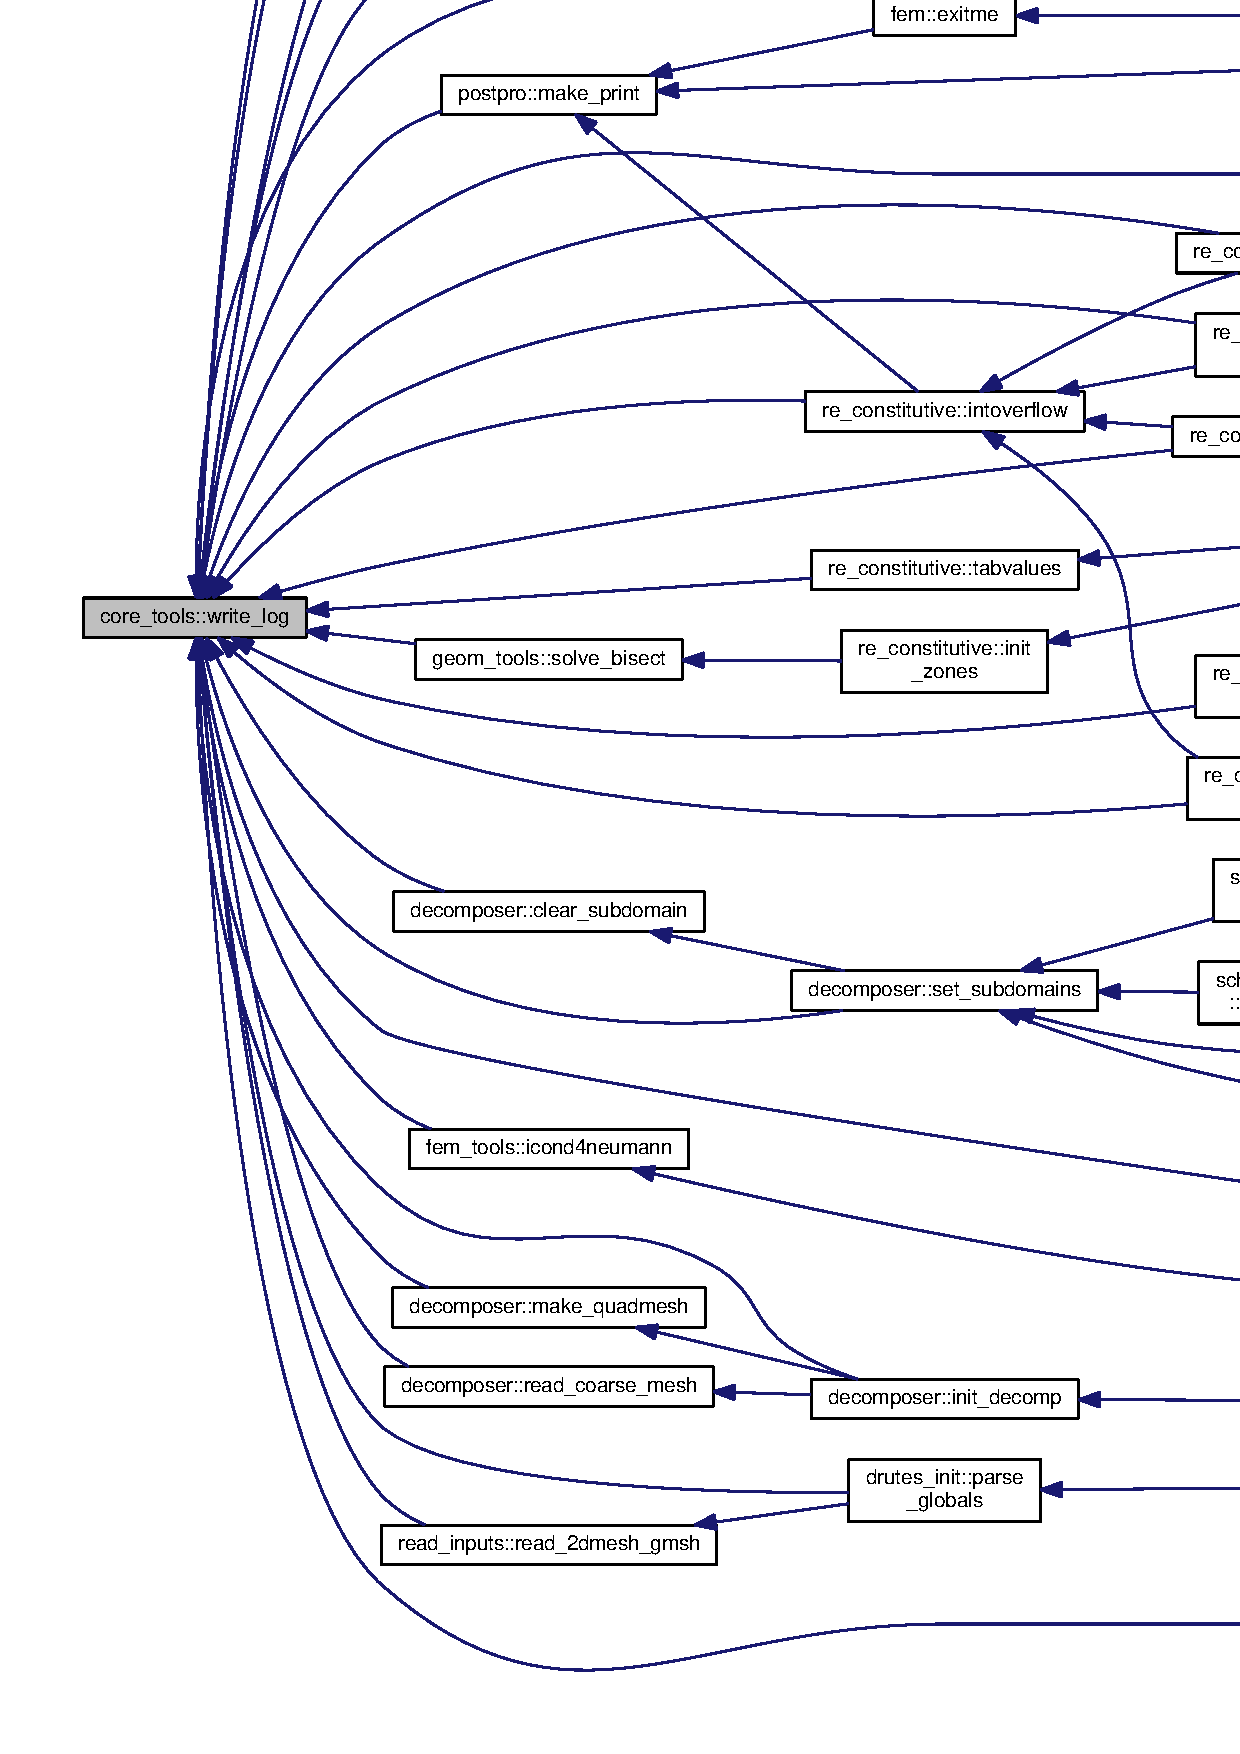
\includegraphics[width=350pt]{namespacecore__tools_abe09f9b4dc2abc5384a24020c5031e95_icgraph}
\end{center}
\end{figure}



\section{debug\+\_\+tools Module Reference}
\label{namespacedebug__tools}\index{debug\+\_\+tools@{debug\+\_\+tools}}
\subsection*{Data Types}
\begin{DoxyCompactItemize}
\item 
interface {\bf printmtx}
\end{DoxyCompactItemize}
\subsection*{Functions/\+Subroutines}
\begin{DoxyCompactItemize}
\item 
subroutine, private {\bf print\+\_\+quadpnt} (quadpnt, filunit, name)
\item 
subroutine {\bf print\+\_\+sparse\+\_\+matrix} (A, filunit, name)
\item 
subroutine, private {\bf print\+\_\+real\+\_\+matrix} (a, filunit, name)
\item 
subroutine, private {\bf print\+\_\+int\+\_\+matrix} (a, filunit, name)
\item 
subroutine, private {\bf print\+\_\+real\+\_\+vector} (V, filunit, name)
\begin{DoxyCompactList}\small\item\em vytiskne vektor \end{DoxyCompactList}\item 
subroutine, private {\bf print\+\_\+real\+\_\+vector4} (V, filunit, name)
\begin{DoxyCompactList}\small\item\em vytiskne vektor \end{DoxyCompactList}\item 
subroutine, private {\bf print\+\_\+int\+\_\+vector} (V, filunit, name)
\item 
subroutine {\bf print\+\_\+smartmatrix\+\_\+i} (array, filunit, name)
\item 
subroutine {\bf print\+\_\+smartarray\+\_\+i} (array, filunit, name)
\item 
subroutine {\bf print\+\_\+logical\+\_\+array} (array, filunit, name)
\item 
subroutine, public {\bf wait} (ch)
\end{DoxyCompactItemize}


\subsection{Function/\+Subroutine Documentation}
\index{debug\+\_\+tools@{debug\+\_\+tools}!print\+\_\+int\+\_\+matrix@{print\+\_\+int\+\_\+matrix}}
\index{print\+\_\+int\+\_\+matrix@{print\+\_\+int\+\_\+matrix}!debug\+\_\+tools@{debug\+\_\+tools}}
\subsubsection[{print\+\_\+int\+\_\+matrix(a, filunit, name)}]{\setlength{\rightskip}{0pt plus 5cm}subroutine, private debug\+\_\+tools\+::print\+\_\+int\+\_\+matrix (
\begin{DoxyParamCaption}
\item[{integer(kind=ikind), dimension(\+:,\+:), intent(inout)}]{a, }
\item[{integer, intent(in), optional}]{filunit, }
\item[{character(len=$\ast$), intent(in), optional}]{name}
\end{DoxyParamCaption}
)\hspace{0.3cm}{\ttfamily [private]}}\label{namespacedebug__tools_a11d11052e32b35c0cda58da55aed785a}


Definition at line 184 of file debug\+\_\+tools.\+f90.



References core\+\_\+tools\+::find\+\_\+unit(), and globals\+::terminal.


\begin{DoxyCode}
184       \textcolor{keywordtype}{use }typy
185       \textcolor{keywordtype}{use }globals
186       \textcolor{keywordtype}{use }core_tools
187       
188       \textcolor{keywordtype}{integer(kind=ikind)}, \textcolor{keywordtype}{dimension(:,:)}, \textcolor{keywordtype}{intent(in out)} :: a
189       \textcolor{keywordtype}{integer}, \textcolor{keywordtype}{intent(in)}, \textcolor{keywordtype}{optional} :: filunit   
190       \textcolor{keywordtype}{character(len=*)}, \textcolor{keywordtype}{intent(in)}, \textcolor{keywordtype}{optional} :: name
191 
192       \textcolor{keywordtype}{integer} :: filloc
193       \textcolor{keywordtype}{integer} :: ierr
194       \textcolor{keywordtype}{logical} :: op
195       \textcolor{keywordtype}{integer(kind=ikind)} :: i
196       
197       \textcolor{keywordflow}{if} (\textcolor{keyword}{present}(name)) \textcolor{keywordflow}{then}
198         \textcolor{keyword}{call }find_unit(filloc)
199         \textcolor{keyword}{open}(unit=filloc, file=name, action=\textcolor{stringliteral}{"write"}, status=\textcolor{stringliteral}{"replace"}, iostat\textcolor{comment}{=ierr)}
200 \textcolor{comment}{        }\textcolor{keywordflow}{if} (ierr /= 0) \textcolor{keywordflow}{then}
201           print *, \textcolor{stringliteral}{"unable to open dump file, called from debug\_tools::printmtx"}
202           error stop
203 \textcolor{keywordflow}{        end if}
204       \textcolor{keywordflow}{else} \textcolor{keywordflow}{if} (\textcolor{keyword}{present}(filunit)) \textcolor{keywordflow}{then}
205         filloc = filunit
206         \textcolor{keyword}{inquire}(unit=filloc, opened=op)
207         \textcolor{keywordflow}{if} (.not. op) \textcolor{keywordflow}{then}
208           print *, \textcolor{stringliteral}{"file not opened, called from debug\_tools::printmtx"}
209           error stop
210 \textcolor{keywordflow}{        end if}
211       \textcolor{keywordflow}{else}
212         filloc = terminal
213 \textcolor{keywordflow}{      end if}
214       
215       
216       \textcolor{keywordflow}{do} i=lbound(a,1), ubound(a,1)
217         \textcolor{keyword}{write}(unit=filloc, fmt=*)  i, \textcolor{stringliteral}{"|"},  a(i,:)
218 \textcolor{keywordflow}{      end do}
219 
220       \textcolor{keywordflow}{if} (terminal /= filloc) \textcolor{keywordflow}{then}
221         \textcolor{keyword}{close}(filloc)
222       \textcolor{keywordflow}{else}
223         \textcolor{keyword}{call }flush(terminal)
224 \textcolor{keywordflow}{      end if}
225       
\end{DoxyCode}


Here is the call graph for this function\+:\nopagebreak
\begin{figure}[H]
\begin{center}
\leavevmode
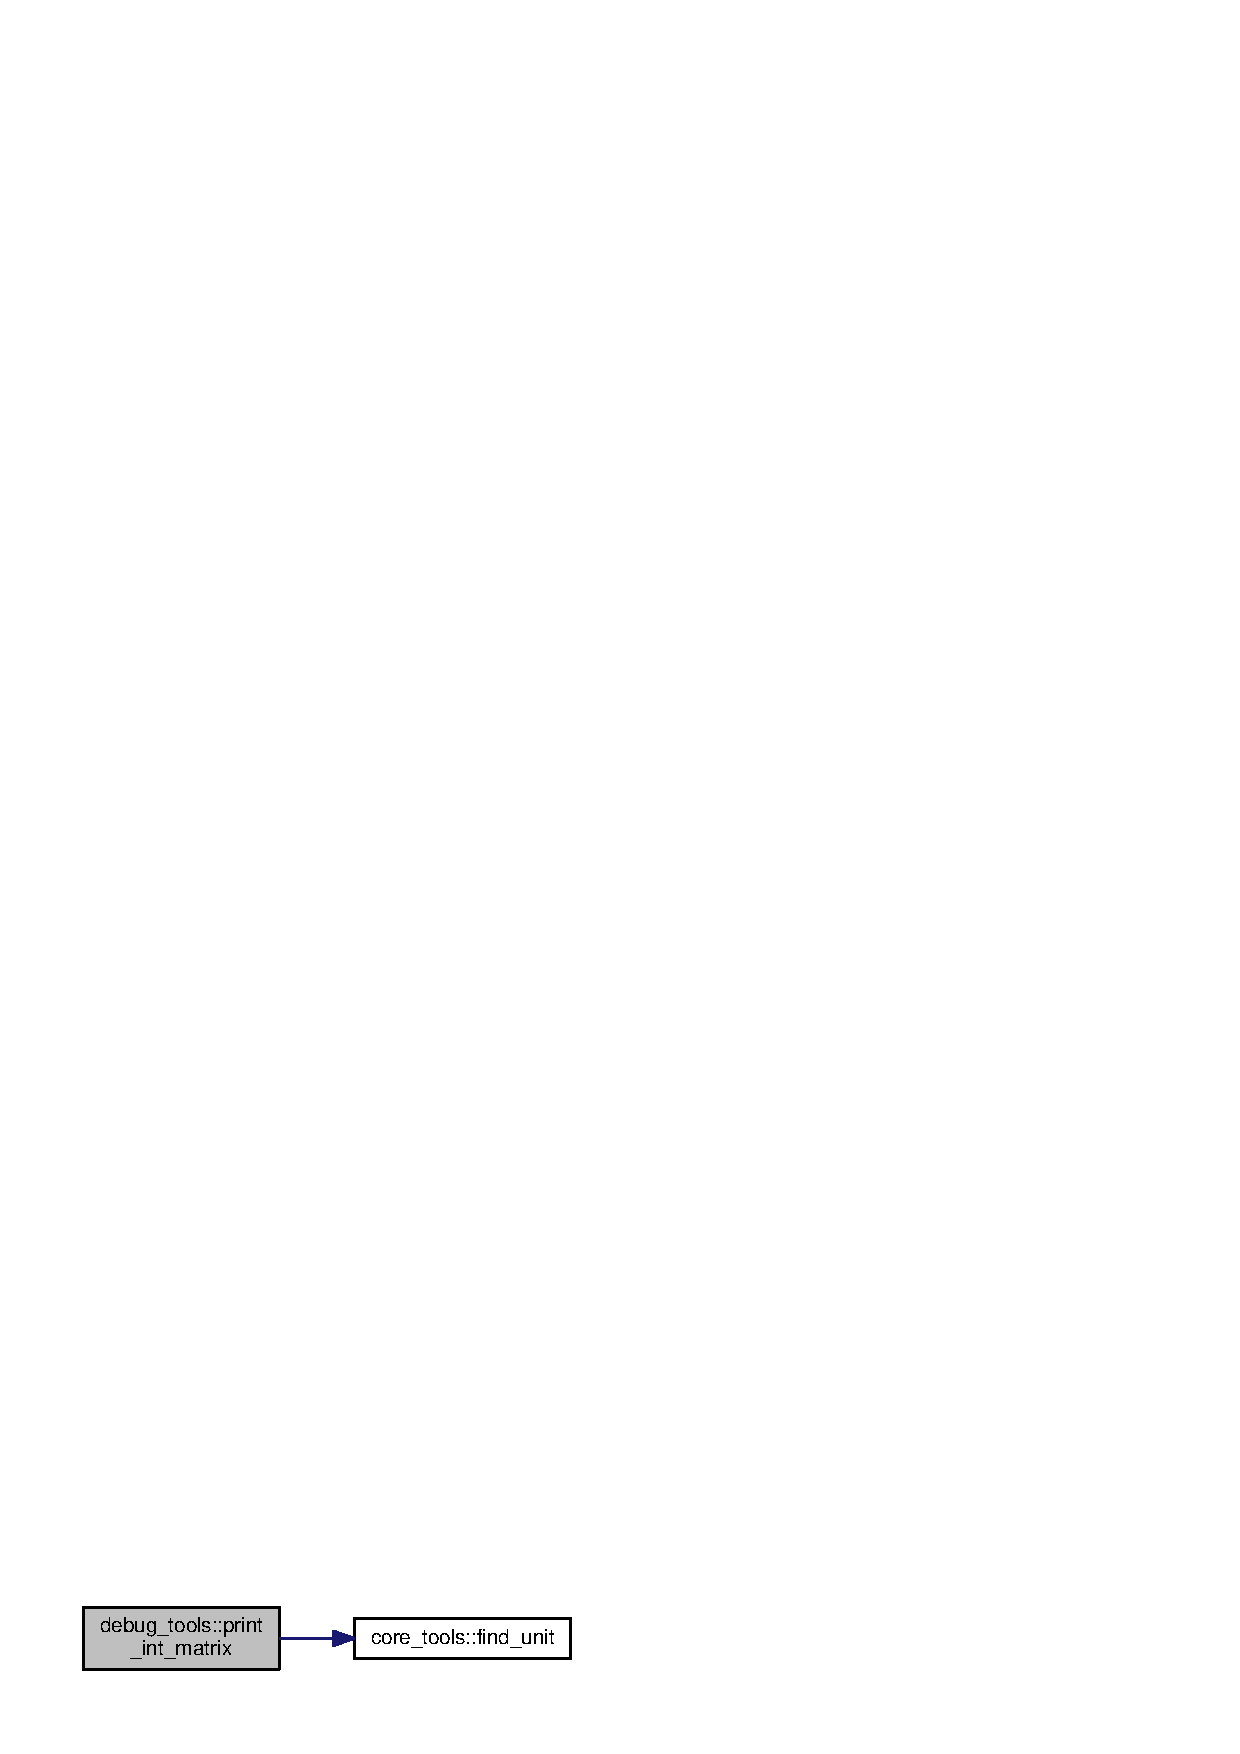
\includegraphics[width=278pt]{namespacedebug__tools_a11d11052e32b35c0cda58da55aed785a_cgraph}
\end{center}
\end{figure}


\index{debug\+\_\+tools@{debug\+\_\+tools}!print\+\_\+int\+\_\+vector@{print\+\_\+int\+\_\+vector}}
\index{print\+\_\+int\+\_\+vector@{print\+\_\+int\+\_\+vector}!debug\+\_\+tools@{debug\+\_\+tools}}
\subsubsection[{print\+\_\+int\+\_\+vector(\+V, filunit, name)}]{\setlength{\rightskip}{0pt plus 5cm}subroutine, private debug\+\_\+tools\+::print\+\_\+int\+\_\+vector (
\begin{DoxyParamCaption}
\item[{integer(kind=ikind), dimension(\+:), intent(in)}]{V, }
\item[{integer, intent(in), optional}]{filunit, }
\item[{character(len=$\ast$), intent(in), optional}]{name}
\end{DoxyParamCaption}
)\hspace{0.3cm}{\ttfamily [private]}}\label{namespacedebug__tools_a95e9b3e23e936deae63ac67d3a7d70db}

\begin{DoxyParams}[1]{Parameters}
\mbox{\tt in}  & {\em v} & vektor k tisknuti \\
\hline
\end{DoxyParams}


Definition at line 329 of file debug\+\_\+tools.\+f90.



References core\+\_\+tools\+::find\+\_\+unit(), and globals\+::terminal.


\begin{DoxyCode}
329     \textcolor{comment}{! vytiskne vektor, pocet sloupcu tisku je nc}
330       \textcolor{keywordtype}{use }typy
331       \textcolor{keywordtype}{use }globals
332       \textcolor{keywordtype}{use }core_tools
333       
334       \textcolor{comment}{!parametry}
335       \textcolor{keywordtype}{integer(kind=ikind)}, \textcolor{keywordtype}{dimension(:)}, \textcolor{keywordtype}{intent(in)} :: v
336       \textcolor{keywordtype}{integer}, \textcolor{keywordtype}{intent(in)}, \textcolor{keywordtype}{optional} :: filunit   
337       \textcolor{keywordtype}{character(len=*)}, \textcolor{keywordtype}{intent(in)}, \textcolor{keywordtype}{optional} :: name
338 
339       \textcolor{keywordtype}{integer} :: filloc
340       \textcolor{keywordtype}{integer} :: ierr
341       \textcolor{keywordtype}{logical} :: op
342       \textcolor{keywordtype}{integer(kind=ikind)} :: i
343       
344       \textcolor{keywordflow}{if} (\textcolor{keyword}{present}(name)) \textcolor{keywordflow}{then}
345         \textcolor{keyword}{call }find_unit(filloc)
346         \textcolor{keyword}{open}(unit=filloc, file=name, action=\textcolor{stringliteral}{"write"}, status=\textcolor{stringliteral}{"replace"}, iostat=ierr)
347         \textcolor{keywordflow}{if} (ierr /= 0) \textcolor{keywordflow}{then}
348           print *, \textcolor{stringliteral}{"unable to open dump file, called from debug\_tools::printmtx"}
349           error stop
350 \textcolor{keywordflow}{        end if}
351       \textcolor{keywordflow}{else} \textcolor{keywordflow}{if} (\textcolor{keyword}{present}(filunit)) \textcolor{keywordflow}{then}
352         filloc = filunit
353         \textcolor{keyword}{inquire}(unit=filloc, opened=op)
354         \textcolor{keywordflow}{if} (.not. op) \textcolor{keywordflow}{then}
355           print *, \textcolor{stringliteral}{"file not opened, called from debug\_tools::printmtx"}
356           error stop
357 \textcolor{keywordflow}{        end if}
358       \textcolor{keywordflow}{else}
359         filloc = terminal
360 \textcolor{keywordflow}{      end if}
361 
362       \textcolor{keywordflow}{do} i=lbound(v,1),ubound(v,1)
363          \textcolor{keyword}{write}(unit=filloc, fmt=*) \textcolor{stringliteral}{"radek:"}, i, \textcolor{stringliteral}{"hodnota:"}, v(i)
364 \textcolor{keywordflow}{      end do}
365   
366       \textcolor{keywordflow}{if} (terminal /= filloc) \textcolor{keywordflow}{then}
367         \textcolor{keyword}{close}(filloc)
368       \textcolor{keywordflow}{else}
369         \textcolor{keyword}{call }flush(terminal)
370 \textcolor{keywordflow}{      end if}
371   
372 
\end{DoxyCode}


Here is the call graph for this function\+:\nopagebreak
\begin{figure}[H]
\begin{center}
\leavevmode
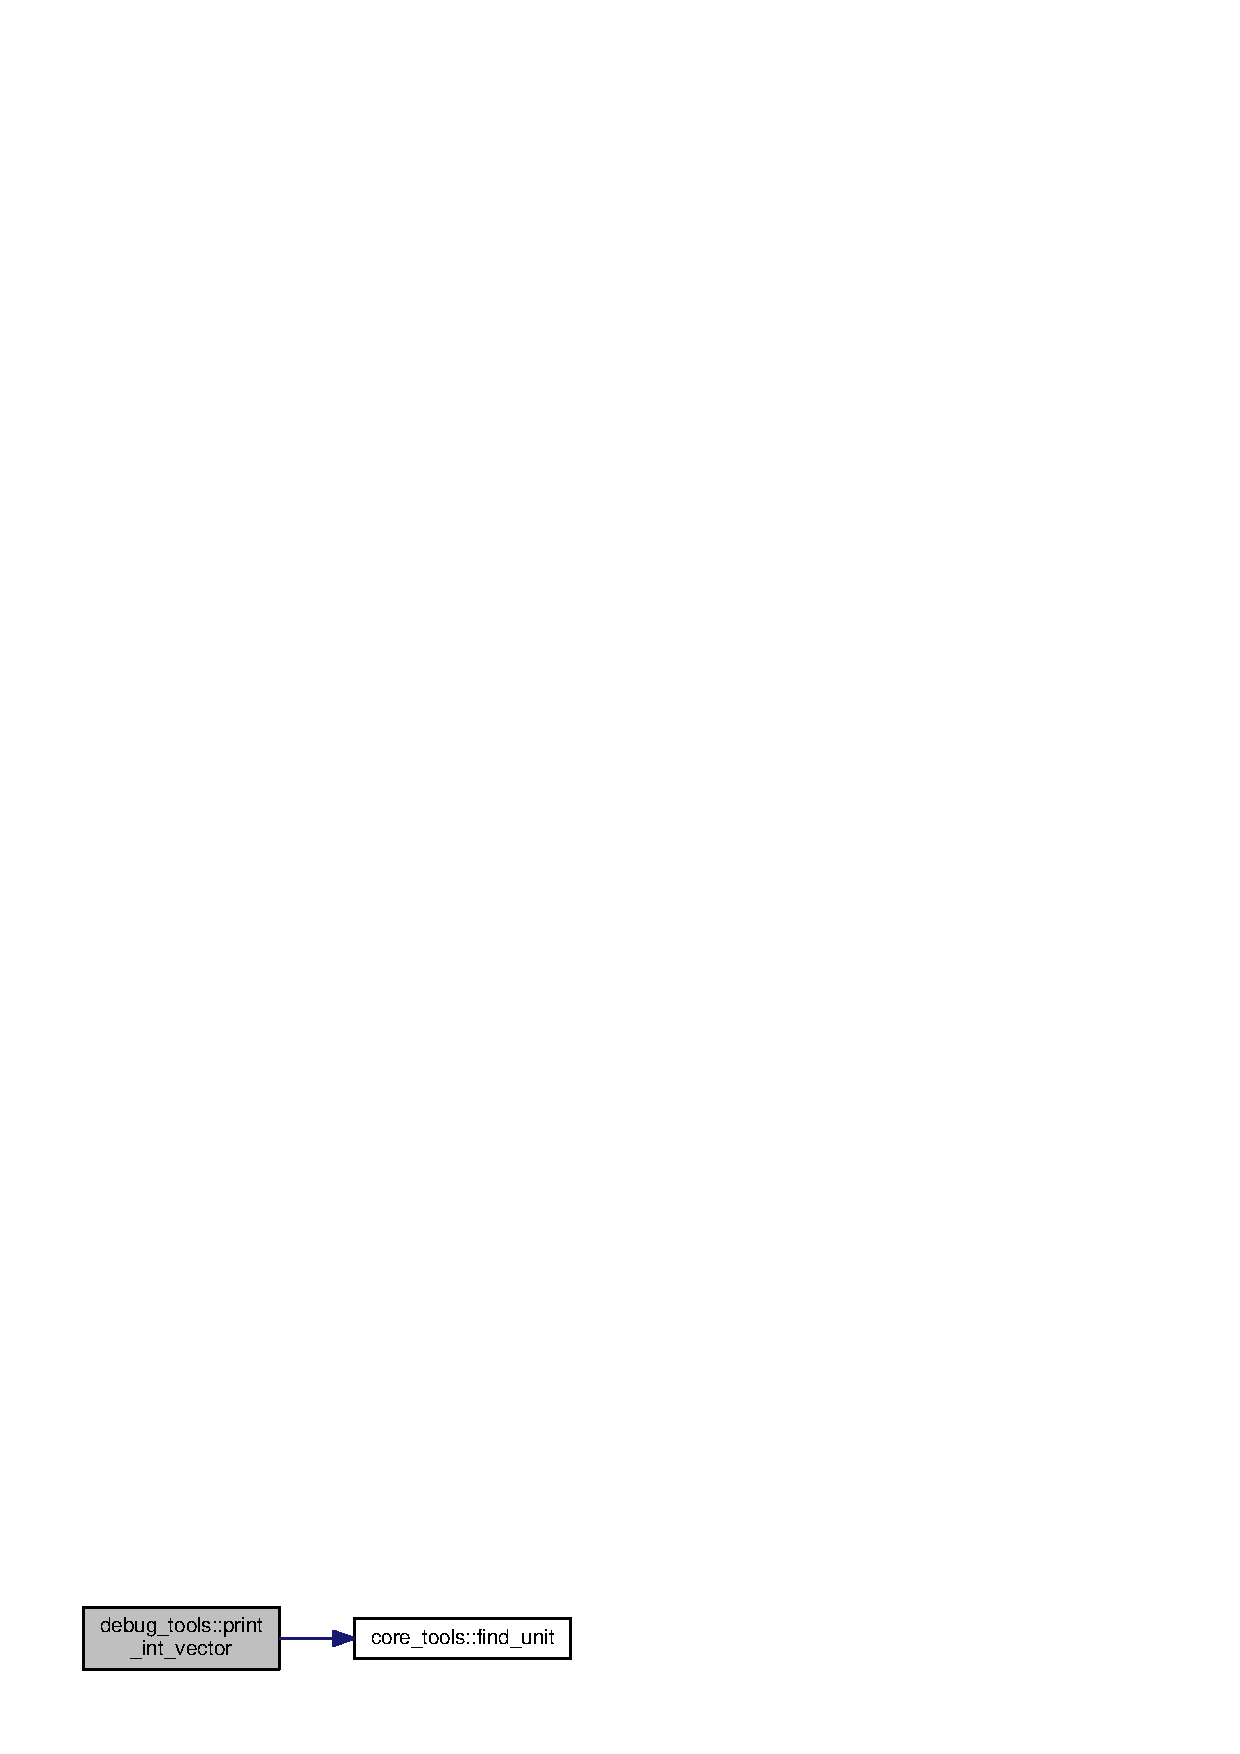
\includegraphics[width=278pt]{namespacedebug__tools_a95e9b3e23e936deae63ac67d3a7d70db_cgraph}
\end{center}
\end{figure}


\index{debug\+\_\+tools@{debug\+\_\+tools}!print\+\_\+logical\+\_\+array@{print\+\_\+logical\+\_\+array}}
\index{print\+\_\+logical\+\_\+array@{print\+\_\+logical\+\_\+array}!debug\+\_\+tools@{debug\+\_\+tools}}
\subsubsection[{print\+\_\+logical\+\_\+array(array, filunit, name)}]{\setlength{\rightskip}{0pt plus 5cm}subroutine debug\+\_\+tools\+::print\+\_\+logical\+\_\+array (
\begin{DoxyParamCaption}
\item[{logical, dimension(\+:), intent(in)}]{array, }
\item[{integer, intent(in), optional}]{filunit, }
\item[{character(len=$\ast$), intent(in), optional}]{name}
\end{DoxyParamCaption}
)}\label{namespacedebug__tools_a0ec7ce1d32aa97319c670bf4e1c664e1}

\begin{DoxyParams}[1]{Parameters}
\mbox{\tt in}  & {\em array} & vektor k tisknuti \\
\hline
\end{DoxyParams}


Definition at line 464 of file debug\+\_\+tools.\+f90.



References core\+\_\+tools\+::find\+\_\+unit(), and globals\+::terminal.


\begin{DoxyCode}
464       \textcolor{keywordtype}{use }typy
465       \textcolor{keywordtype}{use }globals
466       \textcolor{keywordtype}{use }core_tools
467       
468       \textcolor{comment}{!parametry}
469       \textcolor{keywordtype}{logical}, \textcolor{keywordtype}{dimension(:)}, \textcolor{keywordtype}{intent(in)} :: array
470       \textcolor{keywordtype}{integer}, \textcolor{keywordtype}{intent(in)}, \textcolor{keywordtype}{optional} :: filunit   
471       \textcolor{keywordtype}{character(len=*)}, \textcolor{keywordtype}{intent(in)}, \textcolor{keywordtype}{optional} :: name
472 
473       \textcolor{keywordtype}{integer} :: filloc
474       \textcolor{keywordtype}{integer} :: ierr
475       \textcolor{keywordtype}{logical} :: op
476       \textcolor{keywordtype}{integer(kind=ikind)} :: i
477       
478       \textcolor{keywordflow}{if} (\textcolor{keyword}{present}(name)) \textcolor{keywordflow}{then}
479         \textcolor{keyword}{call }find_unit(filloc)
480         \textcolor{keyword}{open}(unit=filloc, file=name, action=\textcolor{stringliteral}{"write"}, status=\textcolor{stringliteral}{"replace"}, iostat\textcolor{comment}{=ierr)}
481 \textcolor{comment}{        }\textcolor{keywordflow}{if} (ierr /= 0) \textcolor{keywordflow}{then}
482           print *, \textcolor{stringliteral}{"unable to open dump file, called from debug\_tools::printmtx"}
483           error stop
484 \textcolor{keywordflow}{        end if}
485       \textcolor{keywordflow}{else} \textcolor{keywordflow}{if} (\textcolor{keyword}{present}(filunit)) \textcolor{keywordflow}{then}
486         filloc = filunit
487         \textcolor{keyword}{inquire}(unit=filloc, opened=op)
488         \textcolor{keywordflow}{if} (.not. op) \textcolor{keywordflow}{then}
489           print *, \textcolor{stringliteral}{"file not opened, called from debug\_tools::printmtx"}
490           error stop
491 \textcolor{keywordflow}{        end if}
492       \textcolor{keywordflow}{else}
493         filloc = terminal
494 \textcolor{keywordflow}{      end if}
495       
496       \textcolor{keywordflow}{do} i=1, ubound(array,1)
497         \textcolor{keyword}{write}(unit=filloc, fmt=*) i, \textcolor{stringliteral}{"|"}, array(i)
498 \textcolor{keywordflow}{      end do}
499       
\end{DoxyCode}


Here is the call graph for this function\+:\nopagebreak
\begin{figure}[H]
\begin{center}
\leavevmode
\includegraphics[width=278pt]{namespacedebug__tools_a0ec7ce1d32aa97319c670bf4e1c664e1_cgraph}
\end{center}
\end{figure}


\index{debug\+\_\+tools@{debug\+\_\+tools}!print\+\_\+quadpnt@{print\+\_\+quadpnt}}
\index{print\+\_\+quadpnt@{print\+\_\+quadpnt}!debug\+\_\+tools@{debug\+\_\+tools}}
\subsubsection[{print\+\_\+quadpnt(quadpnt, filunit, name)}]{\setlength{\rightskip}{0pt plus 5cm}subroutine, private debug\+\_\+tools\+::print\+\_\+quadpnt (
\begin{DoxyParamCaption}
\item[{type({\bf integpnt\+\_\+str}), intent(in)}]{quadpnt, }
\item[{integer, intent(in), optional}]{filunit, }
\item[{character(len=$\ast$), intent(in), optional}]{name}
\end{DoxyParamCaption}
)\hspace{0.3cm}{\ttfamily [private]}}\label{namespacedebug__tools_a0e007cc1eb7b04282f1f55c1a3b2e4fc}


Definition at line 25 of file debug\+\_\+tools.\+f90.



References core\+\_\+tools\+::find\+\_\+unit(), and globals\+::terminal.


\begin{DoxyCode}
25       \textcolor{keywordtype}{use }global_objs
26       \textcolor{keywordtype}{use }core_tools
27       \textcolor{keywordtype}{use }globals
28       
29       \textcolor{keywordtype}{type}(integpnt_str), \textcolor{keywordtype}{intent(in)} :: quadpnt
30       \textcolor{keywordtype}{integer}, \textcolor{keywordtype}{intent(in)}, \textcolor{keywordtype}{optional} :: filunit
31       \textcolor{keywordtype}{character(len=*)}, \textcolor{keywordtype}{intent(in)}, \textcolor{keywordtype}{optional} :: name
32       
33       \textcolor{keywordtype}{integer} :: filloc
34       \textcolor{keywordtype}{integer} :: ierr
35       \textcolor{keywordtype}{logical} :: op   
36       
37       \textcolor{keywordflow}{if} (\textcolor{keyword}{present}(name)) \textcolor{keywordflow}{then}
38         \textcolor{keyword}{call }find_unit(filloc)
39         \textcolor{keyword}{open}(unit=filloc, file=name, action=\textcolor{stringliteral}{"write"}, status=\textcolor{stringliteral}{"replace"}, iostat\textcolor{comment}{=ierr)}
40 \textcolor{comment}{        }\textcolor{keywordflow}{if} (ierr /= 0) \textcolor{keywordflow}{then}
41           print *, \textcolor{stringliteral}{"unable to open dump file, called from debug\_tools::printmtx"}
42           error stop
43 \textcolor{keywordflow}{        end if}
44       \textcolor{keywordflow}{else} \textcolor{keywordflow}{if} (\textcolor{keyword}{present}(filunit)) \textcolor{keywordflow}{then}
45         filloc = filunit
46         \textcolor{keyword}{inquire}(unit=filloc, opened=op)
47         \textcolor{keywordflow}{if} (.not. op) \textcolor{keywordflow}{then}
48           print *, \textcolor{stringliteral}{"file not opened, called from debug\_tools::printmtx"}
49           error stop
50 \textcolor{keywordflow}{        end if}
51       \textcolor{keywordflow}{else}
52         filloc = terminal
53 \textcolor{keywordflow}{      end if}
54       
55       
56       \textcolor{keyword}{write}(unit=filloc, fmt=*) \textcolor{stringliteral}{"type:"}, quadpnt%type\_pnt
57       
58       \textcolor{keywordflow}{if} (quadpnt%type\_pnt == \textcolor{stringliteral}{"ndpt"} .or. quadpnt%type\_pnt == \textcolor{stringliteral}{"obpt"}) \textcolor{keywordflow}{then}
59         \textcolor{keyword}{write}(unit=filloc, fmt=*) \textcolor{stringliteral}{"order of point:"}, quadpnt%order
60 \textcolor{keywordflow}{      end if}
61       
62       \textcolor{keywordflow}{if} (quadpnt%type\_pnt == \textcolor{stringliteral}{"gqnd"}) \textcolor{keywordflow}{then}
63         \textcolor{keyword}{write}(unit=filloc, fmt=*) \textcolor{stringliteral}{"order of element:"}, quadpnt%element
64 \textcolor{keywordflow}{      end if}
65       
66       \textcolor{keyword}{write}(unit=filloc, fmt=*) \textcolor{stringliteral}{"column:"}, quadpnt%column
67       
68       \textcolor{keywordflow}{if} (quadpnt%ddlocal) \textcolor{keywordflow}{then}
69         \textcolor{keyword}{write}(unit=filloc, fmt=*) \textcolor{stringliteral}{"using subdomain local data"}
70         \textcolor{keyword}{write}(unit=filloc, fmt=*) \textcolor{stringliteral}{"subdomain id"}, quadpnt%subdom
71         \textcolor{keywordflow}{if} (quadpnt%extended) \textcolor{keywordflow}{then}
72           \textcolor{keyword}{write}(unit=filloc, fmt=*) \textcolor{stringliteral}{"node from extended subdomain (see subcycling man)"}
73         \textcolor{keywordflow}{else}
74           \textcolor{keyword}{write}(unit=filloc, fmt=*) \textcolor{stringliteral}{"node inside the subdomain"}
75 \textcolor{keywordflow}{        end if}
76       \textcolor{keywordflow}{else}
77         \textcolor{keyword}{write}(unit=filloc, fmt=*) \textcolor{stringliteral}{"using global data"}
78 \textcolor{keywordflow}{      end if}
79       
80       \textcolor{keywordflow}{if} (.not. quadpnt%globtime) \textcolor{keywordflow}{then}
81         \textcolor{keyword}{write}(unit=filloc, fmt=*) \textcolor{stringliteral}{"not using the global time, solution will be interpolated"}
82         \textcolor{keyword}{write}(unit=filloc, fmt=*) \textcolor{stringliteral}{"time 4 use:"}, quadpnt%time4eval
83       \textcolor{keywordflow}{else}
84         \textcolor{keyword}{write}(unit=filloc, fmt=*) \textcolor{stringliteral}{"using the global time"}
85 \textcolor{keywordflow}{      end if}
86       
87   
88       \textcolor{keywordflow}{if} (terminal /= filloc) \textcolor{keywordflow}{then}
89         \textcolor{keyword}{close}(filloc)
90       \textcolor{keywordflow}{else}
91         \textcolor{keyword}{call }flush(terminal)
92 \textcolor{keywordflow}{      end if}
93       
\end{DoxyCode}


Here is the call graph for this function\+:\nopagebreak
\begin{figure}[H]
\begin{center}
\leavevmode
\includegraphics[width=278pt]{namespacedebug__tools_a0e007cc1eb7b04282f1f55c1a3b2e4fc_cgraph}
\end{center}
\end{figure}


\index{debug\+\_\+tools@{debug\+\_\+tools}!print\+\_\+real\+\_\+matrix@{print\+\_\+real\+\_\+matrix}}
\index{print\+\_\+real\+\_\+matrix@{print\+\_\+real\+\_\+matrix}!debug\+\_\+tools@{debug\+\_\+tools}}
\subsubsection[{print\+\_\+real\+\_\+matrix(a, filunit, name)}]{\setlength{\rightskip}{0pt plus 5cm}subroutine, private debug\+\_\+tools\+::print\+\_\+real\+\_\+matrix (
\begin{DoxyParamCaption}
\item[{real(kind=rkind), dimension(\+:,\+:), intent(inout)}]{a, }
\item[{integer, intent(in), optional}]{filunit, }
\item[{character(len=$\ast$), intent(in), optional}]{name}
\end{DoxyParamCaption}
)\hspace{0.3cm}{\ttfamily [private]}}\label{namespacedebug__tools_aefb761533a96c1a295de83cd0809aef4}


Definition at line 139 of file debug\+\_\+tools.\+f90.



References core\+\_\+tools\+::find\+\_\+unit(), and globals\+::terminal.


\begin{DoxyCode}
139       \textcolor{keywordtype}{use }typy
140       \textcolor{keywordtype}{use }globals
141       \textcolor{keywordtype}{use }core_tools
142 
143       \textcolor{keywordtype}{real(kind=rkind)}, \textcolor{keywordtype}{dimension(:,:)}, \textcolor{keywordtype}{intent(in out)} :: a
144       \textcolor{keywordtype}{integer}, \textcolor{keywordtype}{intent(in)}, \textcolor{keywordtype}{optional} :: filunit     
145       \textcolor{keywordtype}{character(len=*)}, \textcolor{keywordtype}{intent(in)}, \textcolor{keywordtype}{optional} :: name
146 
147       \textcolor{keywordtype}{integer} :: filloc
148       \textcolor{keywordtype}{integer} :: ierr
149       \textcolor{keywordtype}{logical} :: op
150       \textcolor{keywordtype}{integer(kind=ikind)} :: i
151       
152       \textcolor{keywordflow}{if} (\textcolor{keyword}{present}(name)) \textcolor{keywordflow}{then}
153         \textcolor{keyword}{call }find_unit(filloc)
154         \textcolor{keyword}{open}(unit=filloc, file=name, action=\textcolor{stringliteral}{"write"}, status=\textcolor{stringliteral}{"replace"}, iostat\textcolor{comment}{=ierr)}
155 \textcolor{comment}{        }\textcolor{keywordflow}{if} (ierr /= 0) \textcolor{keywordflow}{then}
156           print *, \textcolor{stringliteral}{"unable to open dump file, called from debug\_tools::printmtx"}
157           error stop
158 \textcolor{keywordflow}{        end if}
159       \textcolor{keywordflow}{else} \textcolor{keywordflow}{if} (\textcolor{keyword}{present}(filunit)) \textcolor{keywordflow}{then}
160         filloc = filunit
161         \textcolor{keyword}{inquire}(unit=filloc, opened=op)
162         \textcolor{keywordflow}{if} (.not. op) \textcolor{keywordflow}{then}
163           print *, \textcolor{stringliteral}{"file not opened, called from debug\_tools::printmtx"}
164           error stop
165 \textcolor{keywordflow}{        end if}
166       \textcolor{keywordflow}{else}
167         filloc = terminal
168 \textcolor{keywordflow}{      end if}
169       
170       
171       \textcolor{keywordflow}{do} i=lbound(a,1), ubound(a,1)
172         \textcolor{keyword}{write}(unit=filloc, fmt=*)  i, \textcolor{stringliteral}{"|"},  a(i,:)
173 \textcolor{keywordflow}{      end do}
174 
175       \textcolor{keywordflow}{if} (terminal /= filloc) \textcolor{keywordflow}{then}
176         \textcolor{keyword}{close}(filloc)
177       \textcolor{keywordflow}{else}
178         \textcolor{keyword}{call }flush(terminal)
179 \textcolor{keywordflow}{      end if}
180       
\end{DoxyCode}


Here is the call graph for this function\+:\nopagebreak
\begin{figure}[H]
\begin{center}
\leavevmode
\includegraphics[width=278pt]{namespacedebug__tools_aefb761533a96c1a295de83cd0809aef4_cgraph}
\end{center}
\end{figure}


\index{debug\+\_\+tools@{debug\+\_\+tools}!print\+\_\+real\+\_\+vector@{print\+\_\+real\+\_\+vector}}
\index{print\+\_\+real\+\_\+vector@{print\+\_\+real\+\_\+vector}!debug\+\_\+tools@{debug\+\_\+tools}}
\subsubsection[{print\+\_\+real\+\_\+vector(\+V, filunit, name)}]{\setlength{\rightskip}{0pt plus 5cm}subroutine, private debug\+\_\+tools\+::print\+\_\+real\+\_\+vector (
\begin{DoxyParamCaption}
\item[{real(kind=rkind), dimension(\+:), intent(inout)}]{V, }
\item[{integer, intent(in), optional}]{filunit, }
\item[{character(len=$\ast$), intent(in), optional}]{name}
\end{DoxyParamCaption}
)\hspace{0.3cm}{\ttfamily [private]}}\label{namespacedebug__tools_a27e14a49d8fad57fa3b31e8f3fef4381}


vytiskne vektor 


\begin{DoxyParams}[1]{Parameters}
\mbox{\tt in,out}  & {\em v} & vektor k tisknuti \\
\hline
\end{DoxyParams}


Definition at line 232 of file debug\+\_\+tools.\+f90.



References core\+\_\+tools\+::find\+\_\+unit(), and globals\+::terminal.


\begin{DoxyCode}
232     \textcolor{comment}{! vytiskne vektor, pocet sloupcu tisku je nc}
233       \textcolor{keywordtype}{use }typy
234       \textcolor{keywordtype}{use }globals
235       \textcolor{keywordtype}{use }core_tools
236       
237       \textcolor{comment}{!parametry}
238       \textcolor{keywordtype}{real(kind=rkind)}, \textcolor{keywordtype}{dimension(:)}, \textcolor{keywordtype}{intent(in out)} :: v
239       \textcolor{keywordtype}{integer}, \textcolor{keywordtype}{intent(in)}, \textcolor{keywordtype}{optional} :: filunit   
240       \textcolor{keywordtype}{character(len=*)}, \textcolor{keywordtype}{intent(in)}, \textcolor{keywordtype}{optional} :: name
241 
242       \textcolor{keywordtype}{integer} :: filloc
243       \textcolor{keywordtype}{integer} :: ierr
244       \textcolor{keywordtype}{logical} :: op
245       \textcolor{keywordtype}{integer(kind=ikind)} :: i
246       
247       \textcolor{keywordflow}{if} (\textcolor{keyword}{present}(name)) \textcolor{keywordflow}{then}
248         \textcolor{keyword}{call }find_unit(filloc)
249         \textcolor{keyword}{open}(unit=filloc, file=name, action=\textcolor{stringliteral}{"write"}, status=\textcolor{stringliteral}{"replace"}, iostat=ierr)
250         \textcolor{keywordflow}{if} (ierr /= 0) \textcolor{keywordflow}{then}
251           print *, \textcolor{stringliteral}{"unable to open dump file, called from debug\_tools::printmtx"}
252           error stop
253 \textcolor{keywordflow}{        end if}
254       \textcolor{keywordflow}{else} \textcolor{keywordflow}{if} (\textcolor{keyword}{present}(filunit)) \textcolor{keywordflow}{then}
255         filloc = filunit
256         \textcolor{keyword}{inquire}(unit=filloc, opened=op)
257         \textcolor{keywordflow}{if} (.not. op) \textcolor{keywordflow}{then}
258           print *, \textcolor{stringliteral}{"file not opened, called from debug\_tools::printmtx"}
259           error stop
260 \textcolor{keywordflow}{        end if}
261       \textcolor{keywordflow}{else}
262         filloc = terminal
263 \textcolor{keywordflow}{      end if}
264      
265 
266       \textcolor{keywordflow}{do} i=lbound(v,1),ubound(v,1)
267          \textcolor{keyword}{write}(unit=filloc, fmt=*) \textcolor{stringliteral}{"radek:"}, i, \textcolor{stringliteral}{"hodnota:"}, v(i)
268 \textcolor{keywordflow}{      end do}
269 
270       \textcolor{keywordflow}{if} (terminal /= filloc) \textcolor{keywordflow}{then}
271         \textcolor{keyword}{close}(filloc)
272       \textcolor{keywordflow}{else}
273         \textcolor{keyword}{call }flush(terminal)
274 \textcolor{keywordflow}{      end if}
275   
\end{DoxyCode}


Here is the call graph for this function\+:\nopagebreak
\begin{figure}[H]
\begin{center}
\leavevmode
\includegraphics[width=278pt]{namespacedebug__tools_a27e14a49d8fad57fa3b31e8f3fef4381_cgraph}
\end{center}
\end{figure}


\index{debug\+\_\+tools@{debug\+\_\+tools}!print\+\_\+real\+\_\+vector4@{print\+\_\+real\+\_\+vector4}}
\index{print\+\_\+real\+\_\+vector4@{print\+\_\+real\+\_\+vector4}!debug\+\_\+tools@{debug\+\_\+tools}}
\subsubsection[{print\+\_\+real\+\_\+vector4(\+V, filunit, name)}]{\setlength{\rightskip}{0pt plus 5cm}subroutine, private debug\+\_\+tools\+::print\+\_\+real\+\_\+vector4 (
\begin{DoxyParamCaption}
\item[{real(4), dimension(\+:), intent(inout)}]{V, }
\item[{integer, intent(in), optional}]{filunit, }
\item[{character(len=$\ast$), intent(in), optional}]{name}
\end{DoxyParamCaption}
)\hspace{0.3cm}{\ttfamily [private]}}\label{namespacedebug__tools_a370f0de206533615edda55c06f1f8a4b}


vytiskne vektor 


\begin{DoxyParams}[1]{Parameters}
\mbox{\tt in,out}  & {\em v} & vektor k tisknuti \\
\hline
\end{DoxyParams}


Definition at line 282 of file debug\+\_\+tools.\+f90.



References core\+\_\+tools\+::find\+\_\+unit(), and globals\+::terminal.


\begin{DoxyCode}
282     \textcolor{comment}{! vytiskne vektor, pocet sloupcu tisku je nc}
283       \textcolor{keywordtype}{use }typy
284       \textcolor{keywordtype}{use }globals
285       \textcolor{keywordtype}{use }core_tools
286       
287       \textcolor{comment}{!parametry}
288       \textcolor{keywordtype}{real(4)}, \textcolor{keywordtype}{dimension(:)}, \textcolor{keywordtype}{intent(in out)} :: v
289       \textcolor{keywordtype}{integer}, \textcolor{keywordtype}{intent(in)}, \textcolor{keywordtype}{optional} :: filunit   
290       \textcolor{keywordtype}{character(len=*)}, \textcolor{keywordtype}{intent(in)}, \textcolor{keywordtype}{optional} :: name
291 
292       \textcolor{keywordtype}{integer} :: filloc
293       \textcolor{keywordtype}{integer} :: ierr
294       \textcolor{keywordtype}{logical} :: op
295       \textcolor{keywordtype}{integer(kind=ikind)} :: i
296       
297       \textcolor{keywordflow}{if} (\textcolor{keyword}{present}(name)) \textcolor{keywordflow}{then}
298         \textcolor{keyword}{call }find_unit(filloc)
299         \textcolor{keyword}{open}(unit=filloc, file=name, action=\textcolor{stringliteral}{"write"}, status=\textcolor{stringliteral}{"replace"}, iostat=ierr)
300         \textcolor{keywordflow}{if} (ierr /= 0) \textcolor{keywordflow}{then}
301           print *, \textcolor{stringliteral}{"unable to open dump file, called from debug\_tools::printmtx"}
302           error stop
303 \textcolor{keywordflow}{        end if}
304       \textcolor{keywordflow}{else} \textcolor{keywordflow}{if} (\textcolor{keyword}{present}(filunit)) \textcolor{keywordflow}{then}
305         filloc = filunit
306         \textcolor{keyword}{inquire}(unit=filloc, opened=op)
307         \textcolor{keywordflow}{if} (.not. op) \textcolor{keywordflow}{then}
308           print *, \textcolor{stringliteral}{"file not opened, called from debug\_tools::printmtx"}
309           error stop
310 \textcolor{keywordflow}{        end if}
311       \textcolor{keywordflow}{else}
312         filloc = terminal
313 \textcolor{keywordflow}{      end if}
314      
315 
316       \textcolor{keywordflow}{do} i=lbound(v,1),ubound(v,1)
317          \textcolor{keyword}{write}(unit=filloc, fmt=*) \textcolor{stringliteral}{"radek:"}, i, \textcolor{stringliteral}{"hodnota:"}, v(i)
318 \textcolor{keywordflow}{      end do}
319 
320       \textcolor{keywordflow}{if} (terminal /= filloc) \textcolor{keywordflow}{then}
321         \textcolor{keyword}{close}(filloc)
322       \textcolor{keywordflow}{else}
323         \textcolor{keyword}{call }flush(terminal)
324 \textcolor{keywordflow}{      end if}
325   
\end{DoxyCode}


Here is the call graph for this function\+:\nopagebreak
\begin{figure}[H]
\begin{center}
\leavevmode
\includegraphics[width=278pt]{namespacedebug__tools_a370f0de206533615edda55c06f1f8a4b_cgraph}
\end{center}
\end{figure}


\index{debug\+\_\+tools@{debug\+\_\+tools}!print\+\_\+smartarray\+\_\+i@{print\+\_\+smartarray\+\_\+i}}
\index{print\+\_\+smartarray\+\_\+i@{print\+\_\+smartarray\+\_\+i}!debug\+\_\+tools@{debug\+\_\+tools}}
\subsubsection[{print\+\_\+smartarray\+\_\+i(array, filunit, name)}]{\setlength{\rightskip}{0pt plus 5cm}subroutine debug\+\_\+tools\+::print\+\_\+smartarray\+\_\+i (
\begin{DoxyParamCaption}
\item[{class({\bf smartarray\+\_\+int}), intent(in)}]{array, }
\item[{integer, intent(in), optional}]{filunit, }
\item[{character(len=$\ast$), intent(in), optional}]{name}
\end{DoxyParamCaption}
)}\label{namespacedebug__tools_a449ad1a14227bae826cb53afd9f4ea9c}

\begin{DoxyParams}[1]{Parameters}
\mbox{\tt in}  & {\em array} & vektor k tisknuti \\
\hline
\end{DoxyParams}


Definition at line 422 of file debug\+\_\+tools.\+f90.



References core\+\_\+tools\+::find\+\_\+unit(), and globals\+::terminal.


\begin{DoxyCode}
422       \textcolor{keywordtype}{use }typy
423       \textcolor{keywordtype}{use }globals
424       \textcolor{keywordtype}{use }core_tools
425       
426       \textcolor{comment}{!parametry}
427       \textcolor{keywordtype}{class}(smartarray_int), \textcolor{keywordtype}{intent(in)} :: array
428       \textcolor{keywordtype}{integer}, \textcolor{keywordtype}{intent(in)}, \textcolor{keywordtype}{optional} :: filunit   
429       \textcolor{keywordtype}{character(len=*)}, \textcolor{keywordtype}{intent(in)}, \textcolor{keywordtype}{optional} :: name
430 
431       \textcolor{keywordtype}{integer} :: filloc
432       \textcolor{keywordtype}{integer} :: ierr
433       \textcolor{keywordtype}{logical} :: op
434       \textcolor{keywordtype}{integer(kind=ikind)} :: i
435       
436       \textcolor{keywordflow}{if} (\textcolor{keyword}{present}(name)) \textcolor{keywordflow}{then}
437         \textcolor{keyword}{call }find_unit(filloc)
438         \textcolor{keyword}{open}(unit=filloc, file=name, action=\textcolor{stringliteral}{"write"}, status=\textcolor{stringliteral}{"replace"}, iostat\textcolor{comment}{=ierr)}
439 \textcolor{comment}{        }\textcolor{keywordflow}{if} (ierr /= 0) \textcolor{keywordflow}{then}
440           print *, \textcolor{stringliteral}{"unable to open dump file, called from debug\_tools::printmtx"}
441           error stop
442 \textcolor{keywordflow}{        end if}
443       \textcolor{keywordflow}{else} \textcolor{keywordflow}{if} (\textcolor{keyword}{present}(filunit)) \textcolor{keywordflow}{then}
444         filloc = filunit
445         \textcolor{keyword}{inquire}(unit=filloc, opened=op)
446         \textcolor{keywordflow}{if} (.not. op) \textcolor{keywordflow}{then}
447           print *, \textcolor{stringliteral}{"file not opened, called from debug\_tools::printmtx"}
448           error stop
449 \textcolor{keywordflow}{        end if}
450       \textcolor{keywordflow}{else}
451         filloc = terminal
452 \textcolor{keywordflow}{      end if}
453       
454       \textcolor{keywordflow}{do} i=1, array%pos
455         \textcolor{keyword}{write}(unit=filloc, fmt=*)  i, \textcolor{stringliteral}{"|"}, array%data(i)
456 \textcolor{keywordflow}{      end do}
457 
458       
459       \textcolor{keyword}{call }flush(filloc)
460       
\end{DoxyCode}


Here is the call graph for this function\+:\nopagebreak
\begin{figure}[H]
\begin{center}
\leavevmode
\includegraphics[width=278pt]{namespacedebug__tools_a449ad1a14227bae826cb53afd9f4ea9c_cgraph}
\end{center}
\end{figure}


\index{debug\+\_\+tools@{debug\+\_\+tools}!print\+\_\+smartmatrix\+\_\+i@{print\+\_\+smartmatrix\+\_\+i}}
\index{print\+\_\+smartmatrix\+\_\+i@{print\+\_\+smartmatrix\+\_\+i}!debug\+\_\+tools@{debug\+\_\+tools}}
\subsubsection[{print\+\_\+smartmatrix\+\_\+i(array, filunit, name)}]{\setlength{\rightskip}{0pt plus 5cm}subroutine debug\+\_\+tools\+::print\+\_\+smartmatrix\+\_\+i (
\begin{DoxyParamCaption}
\item[{class({\bf smartarray\+\_\+int}), dimension(\+:), intent(in)}]{array, }
\item[{integer, intent(in), optional}]{filunit, }
\item[{character(len=$\ast$), intent(in), optional}]{name}
\end{DoxyParamCaption}
)}\label{namespacedebug__tools_ac95ec6120901f4ff463100f55010d7d9}

\begin{DoxyParams}[1]{Parameters}
\mbox{\tt in}  & {\em array} & vektor k tisknuti \\
\hline
\end{DoxyParams}


Definition at line 376 of file debug\+\_\+tools.\+f90.



References core\+\_\+tools\+::find\+\_\+unit(), and globals\+::terminal.


\begin{DoxyCode}
376       \textcolor{keywordtype}{use }typy
377       \textcolor{keywordtype}{use }globals
378       \textcolor{keywordtype}{use }core_tools
379       
380       \textcolor{comment}{!parametry}
381       \textcolor{keywordtype}{class}(smartarray_int), \textcolor{keywordtype}{dimension(:)}, \textcolor{keywordtype}{intent(in)} :: array
382       \textcolor{keywordtype}{integer}, \textcolor{keywordtype}{intent(in)}, \textcolor{keywordtype}{optional} :: filunit   
383       \textcolor{keywordtype}{character(len=*)}, \textcolor{keywordtype}{intent(in)}, \textcolor{keywordtype}{optional} :: name
384 
385       \textcolor{keywordtype}{integer} :: filloc
386       \textcolor{keywordtype}{integer} :: ierr
387       \textcolor{keywordtype}{logical} :: op
388       \textcolor{keywordtype}{integer(kind=ikind)} :: i
389       
390       \textcolor{keywordflow}{if} (\textcolor{keyword}{present}(name)) \textcolor{keywordflow}{then}
391         \textcolor{keyword}{call }find_unit(filloc)
392         \textcolor{keyword}{open}(unit=filloc, file=name, action=\textcolor{stringliteral}{"write"}, status=\textcolor{stringliteral}{"replace"}, iostat\textcolor{comment}{=ierr)}
393 \textcolor{comment}{        }\textcolor{keywordflow}{if} (ierr /= 0) \textcolor{keywordflow}{then}
394           print *, \textcolor{stringliteral}{"unable to open dump file, called from debug\_tools::printmtx"}
395           error stop
396 \textcolor{keywordflow}{        end if}
397       \textcolor{keywordflow}{else} \textcolor{keywordflow}{if} (\textcolor{keyword}{present}(filunit)) \textcolor{keywordflow}{then}
398         filloc = filunit
399         \textcolor{keyword}{inquire}(unit=filloc, opened=op)
400         \textcolor{keywordflow}{if} (.not. op) \textcolor{keywordflow}{then}
401           print *, \textcolor{stringliteral}{"file not opened, called from debug\_tools::printmtx"}
402           error stop
403 \textcolor{keywordflow}{        end if}
404       \textcolor{keywordflow}{else}
405         filloc = terminal
406 \textcolor{keywordflow}{      end if}
407             
408       \textcolor{keywordflow}{do} i=lbound(array,1),ubound(array,1)
409         \textcolor{keywordflow}{if} (.not. \textcolor{keyword}{allocated}(array(i)%data)) \textcolor{keywordflow}{then}
410           print *, \textcolor{stringliteral}{"no values to print at row:"}, i
411         \textcolor{keywordflow}{else}
412           \textcolor{keyword}{write}(unit=filloc, fmt=*) i, \textcolor{stringliteral}{"|"}, array(i)%data(1:array(i)%pos)
413           \textcolor{keyword}{write}(unit=filloc, fmt=*) \textcolor{stringliteral}{"-----------------------------------------------"}
414 \textcolor{keywordflow}{        end if}
415 \textcolor{keywordflow}{      end do}
416       
417       \textcolor{keyword}{call }flush(filloc)
418       
\end{DoxyCode}


Here is the call graph for this function\+:\nopagebreak
\begin{figure}[H]
\begin{center}
\leavevmode
\includegraphics[width=278pt]{namespacedebug__tools_ac95ec6120901f4ff463100f55010d7d9_cgraph}
\end{center}
\end{figure}


\index{debug\+\_\+tools@{debug\+\_\+tools}!print\+\_\+sparse\+\_\+matrix@{print\+\_\+sparse\+\_\+matrix}}
\index{print\+\_\+sparse\+\_\+matrix@{print\+\_\+sparse\+\_\+matrix}!debug\+\_\+tools@{debug\+\_\+tools}}
\subsubsection[{print\+\_\+sparse\+\_\+matrix(\+A, filunit, name)}]{\setlength{\rightskip}{0pt plus 5cm}subroutine debug\+\_\+tools\+::print\+\_\+sparse\+\_\+matrix (
\begin{DoxyParamCaption}
\item[{class({\bf smtx}), intent(inout)}]{A, }
\item[{integer, intent(in), optional}]{filunit, }
\item[{character(len=$\ast$), intent(in), optional}]{name}
\end{DoxyParamCaption}
)}\label{namespacedebug__tools_ae4fe3294b83f6728e4fc320f418317da}


Definition at line 97 of file debug\+\_\+tools.\+f90.



References core\+\_\+tools\+::find\+\_\+unit(), and globals\+::terminal.


\begin{DoxyCode}
97       \textcolor{keywordtype}{use }sparsematrix
98       \textcolor{keywordtype}{use }mtxiotools
99       \textcolor{keywordtype}{use }globals
100       \textcolor{keywordtype}{use }core_tools
101       \textcolor{keywordtype}{class}(smtx), \textcolor{keywordtype}{intent(in out)} :: a
102       \textcolor{keywordtype}{integer}, \textcolor{keywordtype}{intent(in)}, \textcolor{keywordtype}{optional} :: filunit
103       \textcolor{keywordtype}{character(len=*)}, \textcolor{keywordtype}{intent(in)}, \textcolor{keywordtype}{optional} :: name
104 
105       \textcolor{keywordtype}{integer} :: filloc
106       \textcolor{keywordtype}{integer} :: ierr
107       \textcolor{keywordtype}{logical} :: op
108       
109       \textcolor{keywordflow}{if} (\textcolor{keyword}{present}(name)) \textcolor{keywordflow}{then}
110         \textcolor{keyword}{call }find_unit(filloc)
111         \textcolor{keyword}{open}(unit=filloc, file=name, action=\textcolor{stringliteral}{"write"}, status=\textcolor{stringliteral}{"replace"}, iostat\textcolor{comment}{=ierr)}
112 \textcolor{comment}{        }\textcolor{keywordflow}{if} (ierr /= 0) \textcolor{keywordflow}{then}
113           print *, \textcolor{stringliteral}{"unable to open dump file, called from debug\_tools::printmtx"}
114           error stop
115 \textcolor{keywordflow}{        end if}
116       \textcolor{keywordflow}{else} \textcolor{keywordflow}{if} (\textcolor{keyword}{present}(filunit)) \textcolor{keywordflow}{then}
117         filloc = filunit
118         \textcolor{keyword}{inquire}(unit=filloc, opened=op)
119         \textcolor{keywordflow}{if} (.not. op) \textcolor{keywordflow}{then}
120           print *, \textcolor{stringliteral}{"file not opened, called from debug\_tools::printmtx"}
121           error stop
122 \textcolor{keywordflow}{        end if}
123       \textcolor{keywordflow}{else}
124         filloc = terminal
125 \textcolor{keywordflow}{      end if}
126       
127 
128       \textcolor{keyword}{call }a%print()
129 
130       \textcolor{keywordflow}{if} (terminal /= filloc) \textcolor{keywordflow}{then}
131         \textcolor{keyword}{close}(filloc)
132       \textcolor{keywordflow}{else}
133         \textcolor{keyword}{call }flush(terminal)
134 \textcolor{keywordflow}{      end if}
135 
\end{DoxyCode}


Here is the call graph for this function\+:\nopagebreak
\begin{figure}[H]
\begin{center}
\leavevmode
\includegraphics[width=278pt]{namespacedebug__tools_ae4fe3294b83f6728e4fc320f418317da_cgraph}
\end{center}
\end{figure}


\index{debug\+\_\+tools@{debug\+\_\+tools}!wait@{wait}}
\index{wait@{wait}!debug\+\_\+tools@{debug\+\_\+tools}}
\subsubsection[{wait(ch)}]{\setlength{\rightskip}{0pt plus 5cm}subroutine, public debug\+\_\+tools\+::wait (
\begin{DoxyParamCaption}
\item[{character(len=$\ast$), intent(in), optional}]{ch}
\end{DoxyParamCaption}
)}\label{namespacedebug__tools_ad093df102d9a49bf92daad352eaab438}


Definition at line 506 of file debug\+\_\+tools.\+f90.



References globals\+::terminal.



Referenced by schwarz\+\_\+dd2subcyc\+::schwarz\+\_\+subcyc().


\begin{DoxyCode}
506       \textcolor{keywordtype}{use }globals       
507       \textcolor{keywordtype}{character(len=*)}, \textcolor{keywordtype}{optional}, \textcolor{keywordtype}{intent(in)} :: ch
508       
509       \textcolor{keywordflow}{if} (\textcolor{keyword}{present}(ch)) \textcolor{keywordflow}{then}
510         print *, \textcolor{stringliteral}{"-------------"}
511         print *, trim(ch)
512         print *, \textcolor{stringliteral}{"-------------"}
513 \textcolor{keywordflow}{      end if}
514 
515       print *, \textcolor{stringliteral}{"press [ENTER] to continue"}
516   
517       \textcolor{keyword}{call }flush(terminal)
518   
519       \textcolor{keyword}{read}(*,*)
520 
521 
\end{DoxyCode}


Here is the caller graph for this function\+:\nopagebreak
\begin{figure}[H]
\begin{center}
\leavevmode
\includegraphics[width=350pt]{namespacedebug__tools_ad093df102d9a49bf92daad352eaab438_icgraph}
\end{center}
\end{figure}



\section{decomp\+\_\+tools Module Reference}
\label{namespacedecomp__tools}\index{decomp\+\_\+tools@{decomp\+\_\+tools}}
\subsection*{Functions/\+Subroutines}
\begin{DoxyCompactItemize}
\item 
subroutine, public {\bf getres\+\_\+loc} (subdom, debugme)
\item 
subroutine, public {\bf mulax\+\_\+dd} (x, vct)
\item 
subroutine, public {\bf get\+\_\+residual} (resvct)
\item 
subroutine, public {\bf get\+\_\+residual\+\_\+old} (resvct)
\item 
subroutine, public {\bf collect\+\_\+matrices} (a)
\item 
subroutine, public {\bf addlevel} ()
\item 
subroutine, public {\bf build\+\_\+coarsemtx} (resvct)
\item 
subroutine, public {\bf init\+\_\+addlevel} ()
\item 
logical function, private {\bf add\+\_\+el} (coarse\+\_\+el, level, el)
\item 
subroutine, public {\bf print\+\_\+domains} (behavior)
\item 
subroutine, public {\bf print\+\_\+elements\+\_\+dd} (behavior)
\end{DoxyCompactItemize}


\subsection{Function/\+Subroutine Documentation}
\index{decomp\+\_\+tools@{decomp\+\_\+tools}!add\+\_\+el@{add\+\_\+el}}
\index{add\+\_\+el@{add\+\_\+el}!decomp\+\_\+tools@{decomp\+\_\+tools}}
\subsubsection[{add\+\_\+el(coarse\+\_\+el, level, el)}]{\setlength{\rightskip}{0pt plus 5cm}logical function, private decomp\+\_\+tools\+::add\+\_\+el (
\begin{DoxyParamCaption}
\item[{integer(kind=ikind), intent(in)}]{coarse\+\_\+el, }
\item[{integer(kind=ikind), intent(in)}]{level, }
\item[{integer(kind=ikind), intent(in)}]{el}
\end{DoxyParamCaption}
)\hspace{0.3cm}{\ttfamily [private]}}\label{namespacedecomp__tools_a0d2d17ba77983f7a1b437f7dc6e180b5}


Definition at line 670 of file decomp\+\_\+tools.\+f90.



References decomp\+\_\+vars\+::ddcoarse\+\_\+mesh.



Referenced by init\+\_\+addlevel().


\begin{DoxyCode}
670       \textcolor{keywordtype}{use }typy
671       \textcolor{keywordtype}{use }globals
672       \textcolor{keywordtype}{use }global_objs
673       \textcolor{keywordtype}{use }decomp_vars
674       \textcolor{keywordtype}{use }debug_tools
675       
676       \textcolor{keywordtype}{integer(kind=ikind)}, \textcolor{keywordtype}{intent(in)} :: coarse\_el, level, el
677       \textcolor{keywordtype}{logical} :: add
678       
679       \textcolor{keywordtype}{integer(kind=ikind)} :: i,j
680       
681       add = .true.
682       
683       \textcolor{keywordflow}{do} i=0, level-1
684 \textcolor{comment}{!       call printmtx(ddcoarse\_mesh(coarse\_el)%overlap\_el(i)) ; call wait()}
685         \textcolor{keywordflow}{do} j=1, ddcoarse_mesh(coarse\_el)%overlap\_el(i)%pos
686 \textcolor{comment}{!         print *, level-1, el ; stop}
687           \textcolor{keywordflow}{if} (\textcolor{keyword}{allocated}(ddcoarse_mesh(coarse\_el)%overlap\_el(i)%data)) \textcolor{keywordflow}{then}
688             \textcolor{keywordflow}{if} (ddcoarse_mesh(coarse\_el)%overlap\_el(i)%data(j) == el) \textcolor{keywordflow}{then}
689               add = .false.
690               \textcolor{keywordflow}{RETURN}
691 \textcolor{keywordflow}{            end if}
692 \textcolor{keywordflow}{          end if}
693 \textcolor{keywordflow}{        end do}
694 \textcolor{keywordflow}{      end do}
695     
\end{DoxyCode}


Here is the caller graph for this function\+:\nopagebreak
\begin{figure}[H]
\begin{center}
\leavevmode
\includegraphics[width=350pt]{namespacedecomp__tools_a0d2d17ba77983f7a1b437f7dc6e180b5_icgraph}
\end{center}
\end{figure}


\index{decomp\+\_\+tools@{decomp\+\_\+tools}!addlevel@{addlevel}}
\index{addlevel@{addlevel}!decomp\+\_\+tools@{decomp\+\_\+tools}}
\subsubsection[{addlevel()}]{\setlength{\rightskip}{0pt plus 5cm}subroutine, public decomp\+\_\+tools\+::addlevel (
\begin{DoxyParamCaption}
{}
\end{DoxyParamCaption}
)}\label{namespacedecomp__tools_a3f8c4deab864942b308de6e8ddc31849}
an array that describes the element that was already inserted into subdomain 

Definition at line 257 of file decomp\+\_\+tools.\+f90.



References decomp\+\_\+vars\+::coarse\+\_\+elements, decomp\+\_\+vars\+::ddcoarse\+\_\+mesh, decomp\+\_\+vars\+::ddinfo, globals\+::drutes\+\_\+config, globals\+::elements, globals\+::nodes, pde\+\_\+objs\+::pde, decomp\+\_\+vars\+::prolong\+\_\+mtx, and decomp\+\_\+vars\+::subdomain.



Referenced by decomposer\+::set\+\_\+subdomains().


\begin{DoxyCode}
257       \textcolor{keywordtype}{use }typy
258       \textcolor{keywordtype}{use }decomp_vars
259       \textcolor{keywordtype}{use }debug_tools
260       \textcolor{keywordtype}{use }globals
261       \textcolor{keywordtype}{use }global_objs
262       \textcolor{keywordtype}{use }pde_objs
263       
264       \textcolor{keywordtype}{integer(kind=ikind)} :: sub, coarse\_el, j, i, vecino, el, elsub, k,\textcolor{comment}{ level, l, nd, ii, vecsub, pnd, nd2}
265 \textcolor{comment}{      }\textcolor{keywordtype}{integer(kind=ikind)}, \textcolor{keywordtype}{dimension(:)}, \textcolor{keywordtype}{allocatable}, \textcolor{keywordtype}{save} :: weight
267       \textcolor{keywordtype}{logical}, \textcolor{keywordtype}{dimension(:)}, \textcolor{keywordtype}{allocatable}, \textcolor{keywordtype}{save} :: el\_inserted
268       \textcolor{keywordtype}{logical}, \textcolor{keywordtype}{dimension(:)}, \textcolor{keywordtype}{allocatable}, \textcolor{keywordtype}{save} :: nd\_inserted
269       \textcolor{keywordtype}{logical}, \textcolor{keywordtype}{dimension(:)}, \textcolor{keywordtype}{allocatable}, \textcolor{keywordtype}{save} :: nd\_bellow
270       \textcolor{keywordtype}{logical} :: insert
271       \textcolor{keywordtype}{integer(kind=ikind)}, \textcolor{keywordtype}{dimension(:)}, \textcolor{keywordtype}{allocatable} :: indexes
272       \textcolor{keywordtype}{real(kind=rkind)} :: tmp
273       \textcolor{keywordtype}{real(kind=rkind)}, \textcolor{keywordtype}{dimension(:)}, \textcolor{keywordtype}{allocatable} :: tmprow, tmpvct
274       
275       \textcolor{keywordflow}{if} (.not. \textcolor{keyword}{allocated}(el\_inserted)) \textcolor{keywordflow}{then}
276         \textcolor{keyword}{allocate}(el\_inserted(elements%kolik))
277         \textcolor{keyword}{allocate}(nd\_inserted(nodes%kolik))
278         \textcolor{keyword}{allocate}(nd\_bellow(nodes%kolik))
279         \textcolor{keyword}{allocate}(weight(nodes%kolik))
280 \textcolor{keywordflow}{      end if}
281       
282       el\_inserted = .false.
283       nd\_inserted = .false.
284       nd\_bellow = .false.
285       
286       weight = 0
287       
288       i = ubound(pde,1)
289       \textcolor{keyword}{call }prolong_mtx%init(maxval(pde(i)%permut(:)), 1\_ikind*ubound(subdomain\textcolor{comment}{,1))}
290 \textcolor{comment}{            }
291 \textcolor{comment}{      }\textcolor{keywordflow}{do} sub=1, ubound(subdomain,1)
292         \textcolor{keywordflow}{do} j=1, ubound(subdomain(sub)%coarse\_el,1)
293           coarse\_el = subdomain(sub)%coarse\_el(j)
294           ddinfo%coarseinsub(coarse\_el) = sub
295 \textcolor{keywordflow}{        end do}
296 \textcolor{keywordflow}{      end do}
297       
298      
299      !searching for boundary clusters at subdomain boundary
300       sub\_loop: \textcolor{keywordflow}{do} sub = 1, ubound(subdomain,1)
301         \textcolor{keyword}{allocate}(subdomain(sub)%olayers(0:ddinfo%overlaps))
302         coarse\_loop: \textcolor{keywordflow}{do} i=1,  ubound(subdomain(sub)%coarse\_el,1)
303           coarse\_el = subdomain(sub)%coarse\_el(i)
304           coarse\_vecino: \textcolor{keywordflow}{do} j=1, ubound(coarse_elements%neighbours,2)
305             vecino = coarse_elements%neighbours(coarse\_el,j)
306             \textcolor{keywordflow}{if} (vecino > 0) \textcolor{keywordflow}{then}
307               \textcolor{keywordflow}{if} (ddinfo%coarseinsub(vecino) /= sub) \textcolor{keywordflow}{then} \textcolor{comment}{!nasel jsem krajni cluster}
308                 \textcolor{keyword}{call }subdomain(sub)%bcluster%fill(coarse\_el)
309                 \textcolor{keywordflow}{EXIT} coarse\_vecino
310 \textcolor{keywordflow}{              end if}
311 \textcolor{keywordflow}{            end if}
312 \textcolor{keywordflow}{          end do} coarse\_vecino
313 \textcolor{keywordflow}{        end do} coarse\_loop
314 \textcolor{keywordflow}{      end do} sub\_loop
315         
316                         
317       sub\_loop2: \textcolor{keywordflow}{do} sub=1, ubound(subdomain,1)
318         j = subdomain(sub)%elsub%pos
319         el\_inserted(subdomain(sub)%elsub%data(1:j)) = .true.
320         level\_loop: \textcolor{keywordflow}{do} level=0, ddinfo%overlaps
321           \textcolor{keywordflow}{do} i=1, subdomain(sub)%bcluster%pos
322             coarse\_el = subdomain(sub)%bcluster%data(i)
323             bound\_loop: \textcolor{keywordflow}{do} k=1, ddcoarse_mesh(coarse\_el)%overlap\_el(level)%pos
324               el = ddcoarse_mesh(coarse\_el)%overlap\_el(level)%data(k)
325               elsub = ddinfo%coarseinsub(ddinfo%elincoarse(el)) 
326               \textcolor{keywordflow}{if} (level > 0) \textcolor{keywordflow}{then}
327                 \textcolor{keywordflow}{if} (elsub /= sub) \textcolor{keywordflow}{then}
328                   insert = .true.
329                 \textcolor{keywordflow}{else}
330                   insert = .false.
331 \textcolor{keywordflow}{                end if}
332               \textcolor{keywordflow}{else}
333                 insert = .false.
334                 \textcolor{keywordflow}{do} ii = 1, ubound(elements%neighbours,2)
335                   vecino = elements%neighbours(el,ii)
336                   \textcolor{keywordflow}{if} (vecino > 0) \textcolor{keywordflow}{then}
337                     vecsub = ddinfo%coarseinsub(ddinfo%elincoarse(vecino))
338                   \textcolor{keywordflow}{else}
339                     vecsub = 0
340 \textcolor{keywordflow}{                  end if}
341                   \textcolor{keywordflow}{if} (vecsub /= sub .and. vecsub /= 0) \textcolor{keywordflow}{then}
342                     insert = .true.
343                     \textcolor{keywordflow}{EXIT}
344 \textcolor{keywordflow}{                  end if}
345 \textcolor{keywordflow}{                end do}
346 \textcolor{keywordflow}{              end if}
347               \textcolor{keywordflow}{if} (level > 0 .and. insert .and. .not. el\_inserted(el)) \textcolor{keywordflow}{then}
348                 \textcolor{keyword}{call }subdomain(sub)%elsub%fill(el)
349                 \textcolor{keyword}{call }subdomain(sub)%olayers(level)%fill(el)
350                 el\_inserted(el) = .true.
351               \textcolor{keywordflow}{else} \textcolor{keywordflow}{if} (level == 0 .and. insert) \textcolor{keywordflow}{then}
352                 \textcolor{keyword}{call }subdomain(sub)%olayers(level)%fill(el)
353 \textcolor{keywordflow}{              end if}
354 \textcolor{keywordflow}{            end do} bound\_loop
355 \textcolor{keywordflow}{          end do}
356 \textcolor{keywordflow}{        end do} level\_loop
357         
358         \textcolor{comment}{!-------}
359         \textcolor{comment}{! i f   s u b c y c l i n g }
360         \textcolor{comment}{!-------}
361         \textcolor{comment}{!add an extra level including all neighbour nodes, here we start with adding an extra layer with
       elements, the neighbourhood elements are all elements that share at least a single node (different approach
       compared to the overlap construction, where the neighborhood elements are elements that share TWO nodes
       (edge))}
362         \textcolor{keywordflow}{if} (drutes_config%it\_method == 2) \textcolor{keywordflow}{then}
363           \textcolor{keywordflow}{do} level=0, ddinfo%overlaps
364             \textcolor{keywordflow}{do} i=1, subdomain(sub)%olayers(level)%pos
365               el = subdomain(sub)%olayers(level)%data(i)
366               \textcolor{keywordflow}{do} j = 1, ubound(elements%data,2)
367                 nd = elements%data(el,j)
368                 \textcolor{keywordflow}{do} k=1, nodes%el2integ(nd)%pos
369                   vecino = nodes%el2integ(nd)%data(k)
370                   \textcolor{keywordflow}{if} (vecino > 0) \textcolor{keywordflow}{then}
371                     \textcolor{keywordflow}{if} (.not. el\_inserted(vecino)) \textcolor{keywordflow}{then}
372                       \textcolor{keyword}{call }subdomain(sub)%elextra%fill(vecino)
373                       el\_inserted(vecino) = .true.
374 \textcolor{keywordflow}{                    end if}
375 \textcolor{keywordflow}{                  end if}
376 \textcolor{keywordflow}{                end do}
377 \textcolor{keywordflow}{              end do}
378 \textcolor{keywordflow}{            end do}
379 \textcolor{keywordflow}{          end do}
380           j = subdomain(sub)%elextra%pos
381           el\_inserted(subdomain(sub)%elextra%data(1:j)) = .false.
382 \textcolor{keywordflow}{        end if}
383         
384         
385         j = subdomain(sub)%elsub%pos
386         el\_inserted(subdomain(sub)%elsub%data(1:j)) = .false.
387 
388 \textcolor{keywordflow}{      end do} sub\_loop2
389 
390         
391             
392       \textcolor{keywordflow}{do} sub=1, ubound(subdomain,1)
393         \textcolor{keyword}{allocate}(subdomain(sub)%ondlayers(0:ddinfo%overlaps))
394         \textcolor{keywordflow}{do} level=0, ddinfo%overlaps-1
395           \textcolor{keywordflow}{do} i=1, subdomain(sub)%olayers(level)%pos
396             el = subdomain(sub)%olayers(level)%data(i)
397             \textcolor{keywordflow}{do} j=1, ubound(elements%data,2)
398               nd = elements%data(el, j)
399               nd\_bellow(nd) = .true.
400 \textcolor{keywordflow}{            end do}
401 \textcolor{keywordflow}{          end do}
402           \textcolor{keywordflow}{do} i=1, subdomain(sub)%olayers(level+1)%pos
403             el = subdomain(sub)%olayers(level+1)%data(i)
404             \textcolor{keywordflow}{do} j=1, ubound(elements%data,2)
405               nd = elements%data(el, j)
406               \textcolor{keywordflow}{if} (.not. nd\_inserted(nd) .and. nd\_bellow(nd) ) \textcolor{keywordflow}{then}
407                 \textcolor{keyword}{call }subdomain(sub)%ondlayers(level)%fill(nd)
408                 nd\_inserted(nd) = .true.
409 \textcolor{keywordflow}{              end if}
410 \textcolor{keywordflow}{            end do}
411 \textcolor{keywordflow}{          end do}
412 \textcolor{keywordflow}{        end do}
413         
414         \textcolor{comment}{! fill the last level}
415         level = ddinfo%overlaps
416         \textcolor{keywordflow}{do} i=1, subdomain(sub)%olayers(level)%pos
417           el = subdomain(sub)%olayers(level)%data(i)
418           \textcolor{keywordflow}{do} j=1, ubound(elements%data,2)
419             nd = elements%data(el, j)
420             \textcolor{keywordflow}{if} (.not. nd\_inserted(nd)) \textcolor{keywordflow}{then}
421               \textcolor{keyword}{call }subdomain(sub)%ondlayers(level)%fill(nd)
422               nd\_inserted(nd) = .true.
423 \textcolor{keywordflow}{            end if}
424 \textcolor{keywordflow}{          end do}
425 \textcolor{keywordflow}{        end do}
426 
427         
428        \textcolor{comment}{! if subcycling, add nodes, that lie out of the domain, but still have a graph connection to the
       nodes, that lie inside the domain}
429         \textcolor{keywordflow}{if} (drutes_config%it\_method == 2) \textcolor{keywordflow}{then}
430           \textcolor{keywordflow}{do} i = 1, subdomain(sub)%elextra%pos
431             el = subdomain(sub)%elextra%data(i)
432             \textcolor{keywordflow}{do} j=1, ubound(elements%data,2)
433               nd = elements%data(el, j)
434               \textcolor{keyword}{call }ddinfo%nodesinextsub(nd)%nrfill(sub)
435               \textcolor{keywordflow}{if} (.not. nd\_inserted(nd)) \textcolor{keywordflow}{then}
436                 \textcolor{keyword}{call }subdomain(sub)%ndextra%fill(nd)
437                 nd\_inserted(nd) = .true.
438 \textcolor{keywordflow}{              end if}
439 \textcolor{keywordflow}{            end do}
440 \textcolor{keywordflow}{          end do}
441          
442           j = subdomain(sub)%elextra%pos
443           el\_inserted(subdomain(sub)%elextra%data(1:j)) = .true.
444          
445           j = subdomain(sub)%ndextra%pos
446           \textcolor{keywordflow}{do} i = 1, j
447             nd = subdomain(sub)%ndextra%data(i)
448             \textcolor{keywordflow}{do} k = 1, nodes%el2integ(nd)%pos
449               el = nodes%el2integ(nd)%data(k)
450               \textcolor{keywordflow}{if} (.not. el\_inserted(el)) \textcolor{keywordflow}{then}
451                 \textcolor{keywordflow}{do} l=1, ubound(elements%data,2)
452                   nd2 = elements%data(el,l)
453                   \textcolor{keywordflow}{if} (.not. nd\_inserted(nd2)) \textcolor{keywordflow}{then}
454                     \textcolor{keyword}{call }subdomain(sub)%ndextra%fill(nd2)
455                     nd\_inserted(nd2) = .true.
456 \textcolor{keywordflow}{                  end if}
457 \textcolor{keywordflow}{                end do}
458 \textcolor{keywordflow}{              end if}
459 \textcolor{keywordflow}{            end do}
460 \textcolor{keywordflow}{          end do}
461           
462           j = subdomain(sub)%ndextra%pos
463           nd\_inserted(subdomain(sub)%ndextra%data(1:j)) = .false.
464           
465           j = subdomain(sub)%elextra%pos
466           el\_inserted(subdomain(sub)%elextra%data(1:j)) = .false.
467 \textcolor{keywordflow}{        end if}
468           
469 
470 
471         \textcolor{comment}{! set everywhere in nd\_inserted .false.}
472         \textcolor{keywordflow}{do} level = 0, ddinfo%overlaps
473           j = subdomain(sub)%ondlayers(level)%pos
474           \textcolor{keywordflow}{if} (\textcolor{keyword}{allocated}(subdomain(sub)%ondlayers(level)%data)) \textcolor{keywordflow}{then}
475             nd\_inserted(subdomain(sub)%ondlayers(level)%data(1:j)) = .false.
476             nd\_bellow(subdomain(sub)%ondlayers(level)%data(1:j)) = .false.
477 \textcolor{keywordflow}{          end if}
478 \textcolor{keywordflow}{        end do}
479         
480 
481         \textcolor{comment}{!create the prolongator matrix, set everywhere just ones }
482         \textcolor{keywordflow}{do} i=1, subdomain(sub)%elsub%pos
483           el = subdomain(sub)%elsub%data(i)
484           \textcolor{keywordflow}{do} j=1, ubound(elements%data,2)
485             nd = elements%data(el, j)
486             pnd = pde(1)%permut(nd)
487             \textcolor{keywordflow}{if} (pnd > 0 .and. .not. nd\_inserted(nd)) \textcolor{keywordflow}{then}
488               \textcolor{keyword}{call }prolong_mtx%set(1.0\_rkind, pnd, sub)
489               nd\_inserted(nd) = .true.
490 \textcolor{keywordflow}{            end if}
491 \textcolor{keywordflow}{          end do}
492 \textcolor{keywordflow}{        end do}
493 \textcolor{comment}{!       if (.not. subdomain(sub)%critical) then}
494 \textcolor{comment}{!         nd\_inserted = .false.}
495 \textcolor{comment}{!       else}
496           \textcolor{keywordflow}{do} i=1, subdomain(sub)%elsub%pos
497             el = subdomain(sub)%elsub%data(i)
498             nd\_inserted(elements%data(el,:)) = .false.
499 \textcolor{keywordflow}{          end do}
500 \textcolor{comment}{!         end if}
501 \textcolor{keywordflow}{      end do}
502       
503 
504       
505       \textcolor{comment}{!adjust the prolongator matrix}
506       
507       \textcolor{keywordflow}{do} sub=1, ubound(subdomain,1)
508         \textcolor{keywordflow}{do} level = 1, ddinfo%overlaps
509           \textcolor{keywordflow}{do} j=1, subdomain(sub)%ondlayers(level)%pos
510             nd = subdomain(sub)%ondlayers(level)%data(j)
511             pnd = pde(1)%permut(nd)
512             \textcolor{keywordflow}{if} (pnd > 0) \textcolor{keywordflow}{then}
513               \textcolor{keyword}{call }prolong_mtx%set((ddinfo%overlaps-level)*1.0\_rkind/ddinfo%overlaps\textcolor{comment}{, pnd, sub)}
514 \textcolor{comment}{}\textcolor{keywordflow}{            end if}
515 \textcolor{keywordflow}{          end do}
516 \textcolor{keywordflow}{        end do}
517 \textcolor{keywordflow}{      end do}
518       
519       \textcolor{keywordflow}{do} i=1, prolong_mtx%getn()
520         \textcolor{keyword}{call }prolong_mtx%getrow(i=i, v=tmprow, jj=indexes, nelem=ii)
521         \textcolor{keywordflow}{if} (ii > 1) \textcolor{keywordflow}{then}
522           tmp = 0.0\_rkind
523           \textcolor{keywordflow}{do} j=1,ii
524             tmp = tmp + tmprow(j)
525 \textcolor{keywordflow}{          end do}
526           tmprow = tmprow / tmp
527           \textcolor{keywordflow}{do} j=1, ii
528             \textcolor{keyword}{call }prolong_mtx%set(tmprow(j), i, indexes(j))
529 \textcolor{keywordflow}{          end do}
530 \textcolor{keywordflow}{        end if}
531 \textcolor{keywordflow}{      end do}
532       
533 
534       
535 
536 
537           
538     
\end{DoxyCode}


Here is the caller graph for this function\+:\nopagebreak
\begin{figure}[H]
\begin{center}
\leavevmode
\includegraphics[width=350pt]{namespacedecomp__tools_a3f8c4deab864942b308de6e8ddc31849_icgraph}
\end{center}
\end{figure}


\index{decomp\+\_\+tools@{decomp\+\_\+tools}!build\+\_\+coarsemtx@{build\+\_\+coarsemtx}}
\index{build\+\_\+coarsemtx@{build\+\_\+coarsemtx}!decomp\+\_\+tools@{decomp\+\_\+tools}}
\subsubsection[{build\+\_\+coarsemtx(resvct)}]{\setlength{\rightskip}{0pt plus 5cm}subroutine, public decomp\+\_\+tools\+::build\+\_\+coarsemtx (
\begin{DoxyParamCaption}
\item[{real(kind=rkind), dimension(\+:), allocatable}]{resvct}
\end{DoxyParamCaption}
)}\label{namespacedecomp__tools_ac3dffa95121aa59d12a617f71d43f193}


Definition at line 542 of file decomp\+\_\+tools.\+f90.



References decomp\+\_\+vars\+::bcoarse, decomp\+\_\+vars\+::coarse\+\_\+mtx, mulax\+\_\+dd(), pde\+\_\+objs\+::pde, decomp\+\_\+vars\+::prolong\+\_\+mtx, decomp\+\_\+vars\+::subdomain, and decomp\+\_\+vars\+::xcoarse.



Referenced by schwarz\+\_\+dd\+::schwarz\+\_\+picard().


\begin{DoxyCode}
542       \textcolor{keywordtype}{use }typy
543       \textcolor{keywordtype}{use }globals
544       \textcolor{keywordtype}{use }global_objs
545       \textcolor{keywordtype}{use }pde_objs
546       \textcolor{keywordtype}{use }decomp_vars
547       \textcolor{keywordtype}{use }debug_tools
548       
549       
550       \textcolor{keywordtype}{real(kind=rkind)}, \textcolor{keywordtype}{dimension(:)}, \textcolor{keywordtype}{allocatable} :: resvct
551       \textcolor{keywordtype}{real(kind=rkind)}, \textcolor{keywordtype}{dimension(:,:)}, \textcolor{keywordtype}{allocatable} ::  axcol
552       \textcolor{keywordtype}{real(kind=rkind)}, \textcolor{keywordtype}{dimension(:)}, \textcolor{keywordtype}{allocatable} :: column
553       \textcolor{keywordtype}{integer(kind=ikind)} :: fin, i, sub, j
554       \textcolor{keywordtype}{integer(kind=ikind)}, \textcolor{keywordtype}{dimension(:)}, \textcolor{keywordtype}{allocatable} :: indexes
555       \textcolor{keywordtype}{real(kind=rkind)}, \textcolor{keywordtype}{dimension(:)}, \textcolor{keywordtype}{allocatable} :: tmpdata
556       \textcolor{keywordtype}{real(kind=rkind)}, \textcolor{keywordtype}{dimension(:)}, \textcolor{keywordtype}{allocatable} :: coarsecol
557       \textcolor{keywordtype}{real(kind=rkind)} :: tmp
558       
559       fin = maxval(pde(1)%permut(:))
560       
561       \textcolor{keyword}{allocate}(axcol(fin, ubound(subdomain,1)))
562       \textcolor{keyword}{allocate}(column(fin))
563                   
564       \textcolor{keywordflow}{do} sub=1, ubound(subdomain,1)
565         \textcolor{keyword}{call }prolong_mtx%getcol(sub, tmpdata, indexes, i)
566         column = 0
567         column(indexes(1:i)) = tmpdata(1:i)
568         \textcolor{keyword}{call }mulax\_dd(column, axcol(:,sub))
569 \textcolor{keywordflow}{      end do}
570       
571       i = ubound(subdomain,1)
572       \textcolor{keyword}{call }coarse_mtx%init(i,i)
573       
574       \textcolor{keyword}{allocate}(coarsecol(ubound(subdomain,1)))
575       
576       \textcolor{keywordflow}{do} sub=1, ubound(subdomain,1)
577         coarsecol = prolong_mtx%mulT(axcol(:,sub))
578         \textcolor{keywordflow}{do} i=1, ubound(coarsecol,1)
579           \textcolor{keywordflow}{if} (abs(coarsecol(i)) > epsilon(coarsecol(i))) \textcolor{keywordflow}{then}
580             \textcolor{keyword}{call }coarse_mtx%set(coarsecol(i), i, sub)
581 \textcolor{keywordflow}{          end if}
582 \textcolor{keywordflow}{        end do}
583 \textcolor{keywordflow}{      end do}
584       
585       \textcolor{keywordflow}{if} (.not. \textcolor{keyword}{allocated}(bcoarse)) \textcolor{keywordflow}{then}
586         \textcolor{keyword}{allocate}(bcoarse(ubound(subdomain,1)))
587         \textcolor{keyword}{allocate}(xcoarse(ubound(subdomain,1)))
588       \textcolor{keywordflow}{else} \textcolor{keywordflow}{if} (ubound(bcoarse,1) /= ubound(subdomain,1)) \textcolor{keywordflow}{then}
589         \textcolor{keyword}{deallocate}(bcoarse)
590         \textcolor{keyword}{allocate}(bcoarse(ubound(subdomain,1)))
591         \textcolor{keyword}{deallocate}(xcoarse)
592         \textcolor{keyword}{allocate}(xcoarse(ubound(subdomain,1)))
593 \textcolor{keywordflow}{      end if}
594       
595       bcoarse = prolong_mtx%mult(resvct)
596 
597     
598       
599     
\end{DoxyCode}


Here is the call graph for this function\+:\nopagebreak
\begin{figure}[H]
\begin{center}
\leavevmode
\includegraphics[width=309pt]{namespacedecomp__tools_ac3dffa95121aa59d12a617f71d43f193_cgraph}
\end{center}
\end{figure}




Here is the caller graph for this function\+:\nopagebreak
\begin{figure}[H]
\begin{center}
\leavevmode
\includegraphics[width=350pt]{namespacedecomp__tools_ac3dffa95121aa59d12a617f71d43f193_icgraph}
\end{center}
\end{figure}


\index{decomp\+\_\+tools@{decomp\+\_\+tools}!collect\+\_\+matrices@{collect\+\_\+matrices}}
\index{collect\+\_\+matrices@{collect\+\_\+matrices}!decomp\+\_\+tools@{decomp\+\_\+tools}}
\subsubsection[{collect\+\_\+matrices(a)}]{\setlength{\rightskip}{0pt plus 5cm}subroutine, public decomp\+\_\+tools\+::collect\+\_\+matrices (
\begin{DoxyParamCaption}
\item[{class({\bf extsmtx}), intent(out)}]{a}
\end{DoxyParamCaption}
)}\label{namespacedecomp__tools_a457d3b4a5024e094b0f32669c38b26cb}


Definition at line 218 of file decomp\+\_\+tools.\+f90.



References pde\+\_\+objs\+::pde, pde\+\_\+objs\+::pde\+\_\+common, and decomp\+\_\+vars\+::subdomain.


\begin{DoxyCode}
218       \textcolor{keywordtype}{use }typy
219       \textcolor{keywordtype}{use }globals
220       \textcolor{keywordtype}{use }global_objs
221       \textcolor{keywordtype}{use }pde_objs
222       \textcolor{keywordtype}{use }mtx
223       \textcolor{keywordtype}{use }decomp_vars
224       
225       \textcolor{keywordtype}{class}(extsmtx), \textcolor{keywordtype}{intent(out)} :: a
226       \textcolor{keywordtype}{integer(kind=ikind)} :: i, ii, jj, col
227       \textcolor{keywordtype}{real(kind=rkind)} :: val
228       
229       i = ubound(pde,1)
230       
231       \textcolor{keyword}{call }a%init(maxval(pde(i)%permut(:)),maxval(pde(i)%permut(:)))
232       
233       \textcolor{keywordflow}{do} i=1, ubound(subdomain,1)
234         \textcolor{keywordflow}{do} ii=1, subdomain(i)%matrix%getn()
235           \textcolor{keywordflow}{do} jj = 1, subdomain(i)%matrix%getm()
236             val = subdomain(i)%matrix%get(ii,jj)
237             \textcolor{keywordflow}{if} (abs(val) > epsilon(val) ) \textcolor{keywordflow}{then}
238               col = subdomain(i)%permut(jj)
239               \textcolor{keyword}{call }a%set(val, ii, col)
240 \textcolor{keywordflow}{            end if}
241 \textcolor{keywordflow}{          end do}
242 \textcolor{keywordflow}{        end do}
243 \textcolor{keywordflow}{      end do}
244       
245       \textcolor{keywordflow}{if} (.not. \textcolor{keyword}{allocated}(pde_common%bvect)) \textcolor{keyword}{allocate}(pde_common%bvect(maxval\textcolor{comment}{(
      pde(1)%permut(:))))}
246 \textcolor{comment}{      }
247 \textcolor{comment}{      }\textcolor{keywordflow}{do} i=1, ubound(subdomain,1)
248         pde_common%bvect(subdomain(i)%permut(1:subdomain(i)%ndof)) = subdomain(i\textcolor{comment}{)%bvect(1:
      subdomain(i)%ndof)}
249 \textcolor{comment}{}\textcolor{keywordflow}{      end do}
250       
251     
252         
\end{DoxyCode}
\index{decomp\+\_\+tools@{decomp\+\_\+tools}!get\+\_\+residual@{get\+\_\+residual}}
\index{get\+\_\+residual@{get\+\_\+residual}!decomp\+\_\+tools@{decomp\+\_\+tools}}
\subsubsection[{get\+\_\+residual(resvct)}]{\setlength{\rightskip}{0pt plus 5cm}subroutine, public decomp\+\_\+tools\+::get\+\_\+residual (
\begin{DoxyParamCaption}
\item[{real(kind=rkind), dimension(\+:), intent(out)}]{resvct}
\end{DoxyParamCaption}
)}\label{namespacedecomp__tools_ac18f0d14ca31ab08c7a84b1667c12cfa}


Definition at line 129 of file decomp\+\_\+tools.\+f90.



References mulax\+\_\+dd(), pde\+\_\+objs\+::pde\+\_\+common, and decomp\+\_\+vars\+::subdomain.



Referenced by schwarz\+\_\+dd\+::schwarz\+\_\+picard(), and schwarz\+\_\+dd\+\_\+time\+\_\+test\+::schwarzloc().


\begin{DoxyCode}
129       \textcolor{keywordtype}{use }typy
130       \textcolor{keywordtype}{use }global_objs
131       \textcolor{keywordtype}{use }pde_objs
132       \textcolor{keywordtype}{use }globals
133       \textcolor{keywordtype}{use }decomp_vars
134       \textcolor{keywordtype}{use }debug_tools
135 
136       \textcolor{keywordtype}{real(kind=rkind)}, \textcolor{keywordtype}{dimension(:)}, \textcolor{keywordtype}{intent(out)} :: resvct
137       
138       \textcolor{keywordtype}{integer(kind=ikind)} :: i, j, fin, posglob, posloc, subfin
139       \textcolor{keywordtype}{integer} :: ierr
140       \textcolor{keywordtype}{logical} :: skip\_solved=.false.
141      
142       \textcolor{keyword}{call }mulax\_dd(pde_common%xvect(:,2), resvct)    
143       
144 
145       \textcolor{comment}{!loop for b-(A.x) , where the vector (A.x) was calculated in the code above  }
146       \textcolor{keywordflow}{do} i=1, ubound(subdomain,1)
147         \textcolor{keywordflow}{if} ( (.not. skip\_solved) .or.  (.not. subdomain(i)%solved) ) \textcolor{keywordflow}{then}
148           fin = subdomain(i)%disjoint%pos
149           \textcolor{keywordflow}{do} j=1, fin
150             posglob = subdomain(i)%disjoint%data(j)
151             posloc = subdomain(i)%invpermut(posglob)
152             resvct(posglob) = subdomain(i)%bvect(posloc) - resvct(posglob) 
153 \textcolor{keywordflow}{          end do}
154 \textcolor{keywordflow}{        end if}
155 \textcolor{keywordflow}{      end do}
156       
157 
158 
159 
\end{DoxyCode}


Here is the call graph for this function\+:\nopagebreak
\begin{figure}[H]
\begin{center}
\leavevmode
\includegraphics[width=341pt]{namespacedecomp__tools_ac18f0d14ca31ab08c7a84b1667c12cfa_cgraph}
\end{center}
\end{figure}




Here is the caller graph for this function\+:\nopagebreak
\begin{figure}[H]
\begin{center}
\leavevmode
\includegraphics[width=350pt]{namespacedecomp__tools_ac18f0d14ca31ab08c7a84b1667c12cfa_icgraph}
\end{center}
\end{figure}


\index{decomp\+\_\+tools@{decomp\+\_\+tools}!get\+\_\+residual\+\_\+old@{get\+\_\+residual\+\_\+old}}
\index{get\+\_\+residual\+\_\+old@{get\+\_\+residual\+\_\+old}!decomp\+\_\+tools@{decomp\+\_\+tools}}
\subsubsection[{get\+\_\+residual\+\_\+old(resvct)}]{\setlength{\rightskip}{0pt plus 5cm}subroutine, public decomp\+\_\+tools\+::get\+\_\+residual\+\_\+old (
\begin{DoxyParamCaption}
\item[{real(kind=rkind), dimension(\+:), intent(out)}]{resvct}
\end{DoxyParamCaption}
)}\label{namespacedecomp__tools_ad0648d056fc7e281cf122308a9e8dc28}


Definition at line 164 of file decomp\+\_\+tools.\+f90.



References pde\+\_\+objs\+::pde\+\_\+common, and decomp\+\_\+vars\+::subdomain.


\begin{DoxyCode}
164       \textcolor{keywordtype}{use }typy
165       \textcolor{keywordtype}{use }global_objs
166       \textcolor{keywordtype}{use }pde_objs
167       \textcolor{keywordtype}{use }globals
168       \textcolor{keywordtype}{use }decomp_vars
169       \textcolor{keywordtype}{use }debug_tools
170 
171       \textcolor{keywordtype}{real(kind=rkind)}, \textcolor{keywordtype}{dimension(:)}, \textcolor{keywordtype}{intent(out)} :: resvct
172       
173       \textcolor{keywordtype}{integer(kind=ikind)} :: i, j, fin, posglob, posloc, subfin
174       \textcolor{keywordtype}{integer} :: ierr
175       \textcolor{keywordtype}{real(kind=rkind)}, \textcolor{keywordtype}{dimension(:)}, \textcolor{keywordtype}{allocatable} :: vectorin
176       \textcolor{keywordtype}{type}(extsmtx) :: mat
177       \textcolor{keywordtype}{logical} :: skip\_solved=.false.
178 
179       
180 
181       resvct = 0.0\_rkind
182       \textcolor{keywordflow}{do} i=1, ubound(subdomain,1)
183         \textcolor{comment}{!loop for A.x}
184         \textcolor{keywordflow}{if} ( (.not. skip\_solved) .or.  (.not. subdomain(i)%solved) ) \textcolor{keywordflow}{then}
185           \textcolor{keyword}{allocate}(vectorin(subdomain(i)%ndof))
186           vectorin = 0
187           fin = subdomain(i)%disjoint%pos
188           \textcolor{keywordflow}{do} j=1, fin
189             posglob = subdomain(i)%disjoint%data(j)
190             posloc = subdomain(i)%invpermut(posglob)
191             vectorin(posloc) = pde_common%xvect(posglob,2)
192 \textcolor{keywordflow}{          end do}
193           resvct = resvct +  subdomain(i)%matrix%mul(vectorin)
194           \textcolor{keyword}{deallocate}(vectorin)
195 \textcolor{keywordflow}{        end if}
196 \textcolor{keywordflow}{      end do}
197       
198      
199       
200 
201       \textcolor{comment}{!loop for b-(A.x) , where the vector (A.x) was calculated in the code above  }
202       \textcolor{keywordflow}{do} i=1, ubound(subdomain,1)
203         \textcolor{keywordflow}{if} ( (.not. skip\_solved) .or.  (.not. subdomain(i)%solved) ) \textcolor{keywordflow}{then}
204           fin = subdomain(i)%disjoint%pos
205           \textcolor{keywordflow}{do} j=1, fin
206             posglob = subdomain(i)%disjoint%data(j)
207             posloc = subdomain(i)%invpermut(posglob)
208             resvct(posglob) = subdomain(i)%bvect(posloc) - resvct(posglob) 
209 \textcolor{keywordflow}{          end do}
210 \textcolor{keywordflow}{        end if}
211 \textcolor{keywordflow}{      end do}
212 
213 \textcolor{comment}{!}
\end{DoxyCode}
\index{decomp\+\_\+tools@{decomp\+\_\+tools}!getres\+\_\+loc@{getres\+\_\+loc}}
\index{getres\+\_\+loc@{getres\+\_\+loc}!decomp\+\_\+tools@{decomp\+\_\+tools}}
\subsubsection[{getres\+\_\+loc(subdom, debugme)}]{\setlength{\rightskip}{0pt plus 5cm}subroutine, public decomp\+\_\+tools\+::getres\+\_\+loc (
\begin{DoxyParamCaption}
\item[{type({\bf subdomain\+\_\+str}), intent(inout)}]{subdom, }
\item[{logical, intent(in), optional}]{debugme}
\end{DoxyParamCaption}
)}\label{namespacedecomp__tools_a93ac6a9a59bab2d830d3cd1b8732c356}


Definition at line 17 of file decomp\+\_\+tools.\+f90.



Referenced by schwarz\+\_\+dd2subcyc\+::solve\+\_\+subdomain().


\begin{DoxyCode}
17       \textcolor{keywordtype}{use }typy 
18       \textcolor{keywordtype}{use }globals
19       \textcolor{keywordtype}{use }global_objs
20       \textcolor{keywordtype}{use }pde_objs
21       \textcolor{keywordtype}{use }decomp_vars
22       \textcolor{keywordtype}{use }debug_tools
23       
24       \textcolor{keywordtype}{type}(subdomain_str), \textcolor{keywordtype}{intent(in out)} :: subdom
25       \textcolor{keywordtype}{logical}, \textcolor{keywordtype}{intent(in)}, \textcolor{keywordtype}{optional} :: debugme
26       \textcolor{keywordtype}{integer(kind=ikind)} :: i, nd, domain\_id, ndloc, ndpt
27             
28       \textcolor{keywordtype}{real(kind=rkind)}, \textcolor{keywordtype}{dimension(:)}, \textcolor{keywordtype}{allocatable} :: arow
29       \textcolor{keywordtype}{logical}, \textcolor{keywordtype}{dimension(:)}, \textcolor{keywordtype}{allocatable}, \textcolor{keywordtype}{save} :: coltrue
30       \textcolor{keywordtype}{logical}, \textcolor{keywordtype}{dimension(:)}, \textcolor{keywordtype}{allocatable}, \textcolor{keywordtype}{save} :: extcoltrue
31       \textcolor{keywordtype}{real(kind=rkind)}, \textcolor{keywordtype}{dimension(:)}, \textcolor{keywordtype}{allocatable}, \textcolor{keywordtype}{save} :: colvals, extcolvals
32       \textcolor{keywordtype}{integer(kind=ikind)}, \textcolor{keywordtype}{dimension(:)}, \textcolor{keywordtype}{allocatable}, \textcolor{keywordtype}{save} :: jjvals, extjjvals
33       \textcolor{keywordtype}{integer(kind=ikind)} :: numbers, row, rowperm, extrowperm, j
34       
35       
36       
37       subdom%resvct%main=subdom%bvect
38       subdom%resvct%ext=subdom%extbvect
39       
40 
41       \textcolor{comment}{! build resvct main}
42       \textcolor{keywordflow}{do} i=1, subdom%matrix%rowsfilled%pos
43         row = subdom%matrix%rowsfilled%data(i)
44         
45 
46         
47         \textcolor{keywordflow}{if} (subdom%invpermut(row) /= 0) \textcolor{keywordflow}{then}
48           rowperm=subdom%invpermut(row)
49           
50           \textcolor{keyword}{call }subdom%matrix%getrow(i=row, v=colvals, jj=jjvals, nelem=numbers\textcolor{comment}{)}
51 \textcolor{comment}{      }
52 \textcolor{comment}{          }
53 \textcolor{comment}{          subdom%resvct%main(rowperm) = subdom%resvct%main(rowperm) - dot\_product(colvals(1:numbers), &}
54 \textcolor{comment}{            subdom%xvect(jjvals(1:numbers), 2))}
55 \textcolor{comment}{            }
56 \textcolor{comment}{            }
57 \textcolor{comment}{          }\textcolor{keyword}{call }subdom%extmatrix%getrow(i=row, v=colvals, jj=jjvals, nelem\textcolor{comment}{=numbers)}
58 \textcolor{comment}{          }
59 \textcolor{comment}{          }\textcolor{keywordflow}{if} (numbers > 0) \textcolor{keywordflow}{then}
60             subdom%resvct%main(rowperm) = subdom%resvct%main(rowperm) - dot\_product\textcolor{comment}{(colvals(1:numbers), &}
61 \textcolor{comment}{            subdom%extxvect(jjvals(1:numbers), 2))}
62 \textcolor{comment}{}\textcolor{keywordflow}{          end if}
63           
64 
65 \textcolor{keywordflow}{        end if}   
66         
67 \textcolor{keywordflow}{      end do}
68       
69       \textcolor{comment}{! build resvct ext  }
70       \textcolor{keywordflow}{do} i=1, subdom%extmatrix%rowsfilled%pos
71         row = subdom%extmatrix%rowsfilled%data(i)
72         
73         \textcolor{keywordflow}{if} (subdom%extinvpermut(row) /= 0) \textcolor{keywordflow}{then}
74           rowperm=subdom%extinvpermut(row)
75           
76           \textcolor{keyword}{call }subdom%extmatrix%getrow(i=row, v=colvals, jj=jjvals, nelem\textcolor{comment}{=numbers)      }
77 \textcolor{comment}{                    }
78 \textcolor{comment}{          subdom%resvct%ext(rowperm) = subdom%resvct%ext(rowperm) - dot\_product(colvals(1:numbers), &}
79 \textcolor{comment}{            subdom%extxvect(jjvals(1:numbers), 2))}
80 \textcolor{comment}{            }
81 \textcolor{comment}{          }\textcolor{keyword}{call }subdom%matrix%getrow(i=row, v=colvals, jj=jjvals, nelem=numbers\textcolor{comment}{) }
82 \textcolor{comment}{          }
83 \textcolor{comment}{          }
84 \textcolor{comment}{          }\textcolor{keywordflow}{if} (numbers > 0) \textcolor{keywordflow}{then}
85             subdom%resvct%ext(rowperm) = subdom%resvct%ext(rowperm) - dot\_product\textcolor{comment}{(colvals(1:numbers), &}
86 \textcolor{comment}{            subdom%xvect(jjvals(1:numbers), 2))}
87 \textcolor{comment}{}\textcolor{keywordflow}{          end if}         
88 \textcolor{keywordflow}{        end if} 
89         
90 \textcolor{keywordflow}{      end do}    
91       
92      
93             
\end{DoxyCode}


Here is the caller graph for this function\+:\nopagebreak
\begin{figure}[H]
\begin{center}
\leavevmode
\includegraphics[width=350pt]{namespacedecomp__tools_a93ac6a9a59bab2d830d3cd1b8732c356_icgraph}
\end{center}
\end{figure}


\index{decomp\+\_\+tools@{decomp\+\_\+tools}!init\+\_\+addlevel@{init\+\_\+addlevel}}
\index{init\+\_\+addlevel@{init\+\_\+addlevel}!decomp\+\_\+tools@{decomp\+\_\+tools}}
\subsubsection[{init\+\_\+addlevel()}]{\setlength{\rightskip}{0pt plus 5cm}subroutine, public decomp\+\_\+tools\+::init\+\_\+addlevel (
\begin{DoxyParamCaption}
{}
\end{DoxyParamCaption}
)}\label{namespacedecomp__tools_a41644413ba4175d7d78e741e2f367bc2}


Definition at line 604 of file decomp\+\_\+tools.\+f90.



References add\+\_\+el(), decomp\+\_\+vars\+::coarse\+\_\+elements, decomp\+\_\+vars\+::ddcoarse\+\_\+mesh, decomp\+\_\+vars\+::ddinfo, and globals\+::elements.



Referenced by decomposer\+::init\+\_\+decomp().


\begin{DoxyCode}
604       \textcolor{keywordtype}{use }typy
605       \textcolor{keywordtype}{use }decomp_vars
606       \textcolor{keywordtype}{use }global_objs
607       \textcolor{keywordtype}{use }globals
608       \textcolor{keywordtype}{use }debug_tools
609       
610       \textcolor{keywordtype}{integer(kind=ikind)} :: i, coarse\_el, j, el, vecino, level
611       \textcolor{keywordtype}{logical} :: border
612       \textcolor{keywordtype}{type}(smartarray_int) :: tmp\_arrays
613       
614       \textcolor{keyword}{allocate}(ddinfo%elincoarse(elements%kolik))      
615         
616       \textcolor{keywordflow}{do} coarse\_el=1, ubound(ddcoarse_mesh,1)
617         \textcolor{keywordflow}{do} i=1, ubound(ddcoarse_mesh(coarse\_el)%elements,1)
618           el = ddcoarse_mesh(coarse\_el)%elements(i)
619           ddinfo%elincoarse(el) = coarse\_el
620 \textcolor{keywordflow}{        end do}
621         \textcolor{keyword}{allocate}(ddcoarse_mesh(coarse\_el)%overlap\_el(0:ddinfo%overlaps))
622 \textcolor{keywordflow}{      end do}
623         
624 
625       \textcolor{keywordflow}{do} coarse\_el=1, ubound(ddcoarse_mesh,1)
626         \textcolor{keywordflow}{do} i=1, ubound(ddcoarse_mesh(coarse\_el)%elements,1)
627           el = ddcoarse_mesh(coarse\_el)%elements(i)
628           border = .false.
629           vecino\_loop: \textcolor{keywordflow}{do} j=1, ubound(elements%data,2)
630                         vecino = elements%neighbours(el, j)
631                         \textcolor{keywordflow}{if} (vecino > 0) \textcolor{keywordflow}{then}
632                           \textcolor{keywordflow}{if} (ddinfo%elincoarse(el) /= ddinfo%elincoarse(vecino)) \textcolor{keywordflow}{then}
633                             border = .true.
634                             \textcolor{keywordflow}{EXIT} vecino\_loop
635 \textcolor{keywordflow}{                          end if}
636 \textcolor{keywordflow}{                        end if}
637 \textcolor{keywordflow}{          end do} vecino\_loop
638           \textcolor{keywordflow}{if} (border) \textcolor{keywordflow}{then}
639             \textcolor{keyword}{call }ddcoarse_mesh(coarse\_el)%overlap\_el(0)%fill(el)
640 \textcolor{keywordflow}{          end if}
641 \textcolor{keywordflow}{        end do}
642 \textcolor{keywordflow}{      end do}
643       
644       
645       \textcolor{keywordflow}{do} level = 1, ddinfo%overlaps
646         \textcolor{keywordflow}{do} coarse\_el=1, coarse_elements%kolik
647           border\_loop: \textcolor{keywordflow}{do} i=1, ddcoarse_mesh(coarse\_el)%overlap\_el(level-1)%pos
648                           el = ddcoarse_mesh(coarse\_el)%overlap\_el(level-1)%data(i)
649                           \textcolor{keywordflow}{do} j=1, ubound(elements%data,2)       
650                             vecino = elements%neighbours(el, j)
651                             \textcolor{keywordflow}{if} (vecino > 0) \textcolor{keywordflow}{then}
652                               \textcolor{keywordflow}{if} (coarse\_el /= ddinfo%elincoarse(vecino)) \textcolor{keywordflow}{then}
653                                 \textcolor{keywordflow}{if} (add\_el(coarse\_el, level, vecino)) \textcolor{keywordflow}{then}
654                                   \textcolor{keyword}{call }ddcoarse_mesh(coarse\_el)%overlap\_el(level)%nrfill(vecino)
655 \textcolor{keywordflow}{                                end if}
656 \textcolor{keywordflow}{                              end if}
657 \textcolor{keywordflow}{                            end if}
658 \textcolor{keywordflow}{                          end do} 
659 \textcolor{keywordflow}{          end do} border\_loop
660 \textcolor{keywordflow}{        end do}
661 \textcolor{keywordflow}{      end do}
662       
663  
664  
665       \textcolor{keyword}{allocate}(ddinfo%coarseinsub(coarse_elements%kolik))
666 
\end{DoxyCode}


Here is the call graph for this function\+:\nopagebreak
\begin{figure}[H]
\begin{center}
\leavevmode
\includegraphics[width=288pt]{namespacedecomp__tools_a41644413ba4175d7d78e741e2f367bc2_cgraph}
\end{center}
\end{figure}




Here is the caller graph for this function\+:\nopagebreak
\begin{figure}[H]
\begin{center}
\leavevmode
\includegraphics[width=350pt]{namespacedecomp__tools_a41644413ba4175d7d78e741e2f367bc2_icgraph}
\end{center}
\end{figure}


\index{decomp\+\_\+tools@{decomp\+\_\+tools}!mulax\+\_\+dd@{mulax\+\_\+dd}}
\index{mulax\+\_\+dd@{mulax\+\_\+dd}!decomp\+\_\+tools@{decomp\+\_\+tools}}
\subsubsection[{mulax\+\_\+dd(x, vct)}]{\setlength{\rightskip}{0pt plus 5cm}subroutine, public decomp\+\_\+tools\+::mulax\+\_\+dd (
\begin{DoxyParamCaption}
\item[{real(kind=rkind), dimension(\+:), intent(in)}]{x, }
\item[{real(kind=rkind), dimension(\+:), intent(out)}]{vct}
\end{DoxyParamCaption}
)}\label{namespacedecomp__tools_a7d2344442769179cf7904faece138daf}


Definition at line 97 of file decomp\+\_\+tools.\+f90.



References decomp\+\_\+vars\+::subdomain.



Referenced by build\+\_\+coarsemtx(), and get\+\_\+residual().


\begin{DoxyCode}
97       \textcolor{keywordtype}{use }typy 
98       \textcolor{keywordtype}{use }globals
99       \textcolor{keywordtype}{use }global_objs
100       \textcolor{keywordtype}{use }decomp_vars
101       
102       \textcolor{keywordtype}{real(kind=rkind)}, \textcolor{keywordtype}{dimension(:)}, \textcolor{keywordtype}{intent(in)} :: x
103       \textcolor{keywordtype}{real(kind=rkind)}, \textcolor{keywordtype}{dimension(:)}, \textcolor{keywordtype}{intent(out)} :: vct
104       \textcolor{keywordtype}{integer(kind=ikind)} :: i, j, fin, posglob, posloc, subfin
105       \textcolor{keywordtype}{real(kind=rkind)}, \textcolor{keywordtype}{dimension(:)}, \textcolor{keywordtype}{allocatable} :: vectorin
106 
107       \textcolor{keywordtype}{logical} :: skip\_solved=.false.
108       
109       vct = 0.0\_rkind
110       \textcolor{keywordflow}{do} i=1, ubound(subdomain,1)
111         \textcolor{comment}{!loop for A.x}
112         \textcolor{keywordflow}{if} ( (.not. skip\_solved) .or.  (.not. subdomain(i)%solved) ) \textcolor{keywordflow}{then}
113           \textcolor{keyword}{allocate}(vectorin(subdomain(i)%ndof))
114           vectorin = 0
115           fin = subdomain(i)%disjoint%pos
116           \textcolor{keywordflow}{do} j=1, fin
117             posglob = subdomain(i)%disjoint%data(j)
118             posloc = subdomain(i)%invpermut(posglob)
119             vectorin(posloc) = x(posglob)
120 \textcolor{keywordflow}{          end do}
121           vct = vct +  subdomain(i)%matrix%mul(vectorin)
122           \textcolor{keyword}{deallocate}(vectorin)
123 \textcolor{keywordflow}{        end if}
124 \textcolor{keywordflow}{      end do}
125 
\end{DoxyCode}


Here is the caller graph for this function\+:\nopagebreak
\begin{figure}[H]
\begin{center}
\leavevmode
\includegraphics[width=350pt]{namespacedecomp__tools_a7d2344442769179cf7904faece138daf_icgraph}
\end{center}
\end{figure}


\index{decomp\+\_\+tools@{decomp\+\_\+tools}!print\+\_\+domains@{print\+\_\+domains}}
\index{print\+\_\+domains@{print\+\_\+domains}!decomp\+\_\+tools@{decomp\+\_\+tools}}
\subsubsection[{print\+\_\+domains(behavior)}]{\setlength{\rightskip}{0pt plus 5cm}subroutine, public decomp\+\_\+tools\+::print\+\_\+domains (
\begin{DoxyParamCaption}
\item[{character(len=$\ast$), intent(in), optional}]{behavior}
\end{DoxyParamCaption}
)}\label{namespacedecomp__tools_aef49ee81f8302b95a60c0ed57b240866}

\begin{DoxyParams}[1]{Parameters}
\mbox{\tt in}  & {\em behavior} & behavior specifies the behavior of this printing tool, it is a character behavior == \char`\"{}all\+\_\+in\+\_\+one\char`\"{} everythink is written into a single scilab exec file, scilab generates png files from all print levels behavior == \char`\"{}separately\char`\"{}, each plot is written into different scilab exec file \\
\hline
\end{DoxyParams}


Definition at line 701 of file decomp\+\_\+tools.\+f90.



References decomp\+\_\+vars\+::coarse\+\_\+elements, decomp\+\_\+vars\+::coarse\+\_\+nodes, decomp\+\_\+vars\+::ddcoarse\+\_\+mesh, decomp\+\_\+vars\+::ddinfo, globals\+::drutes\+\_\+config, globals\+::elements, core\+\_\+tools\+::find\+\_\+unit(), globals\+::nodes, pde\+\_\+objs\+::pde, pde\+\_\+objs\+::pde\+\_\+common, and decomp\+\_\+vars\+::subdomain.



Referenced by fem\+::solve\+\_\+pde().


\begin{DoxyCode}
701       \textcolor{keywordtype}{use }typy 
702       \textcolor{keywordtype}{use }decomp_vars
703       \textcolor{keywordtype}{use }globals
704       \textcolor{keywordtype}{use }global_objs
705       \textcolor{keywordtype}{use }core_tools
706       \textcolor{keywordtype}{use }geom_tools
707       \textcolor{keywordtype}{use }pde_objs
708       \textcolor{keywordtype}{use }debug_tools
709 
714       \textcolor{keywordtype}{character(len=*)}, \textcolor{keywordtype}{optional} , \textcolor{keywordtype}{intent(in)}               :: behavior
715       \textcolor{keywordtype}{integer(kind=ikind)}                                   :: mode
716       \textcolor{keywordtype}{character(len=256)}, \textcolor{keywordtype}{dimension(-1:6)}                   :: filenames
717       \textcolor{keywordtype}{integer(kind=ikind)}                                   :: i, i\_err,\textcolor{comment}{ j, layer, dec, row, k, l, n, 
      npoints, sub}
718 \textcolor{comment}{      }\textcolor{keywordtype}{character(len=64)}                                     :: forma
719       \textcolor{keywordtype}{integer}, \textcolor{keywordtype}{dimension(-1:6)}, \textcolor{keywordtype}{save}                        :: ids
720       \textcolor{keywordtype}{character(len=4)}                                      :: extension
721       \textcolor{keywordtype}{real(kind=rkind)}                                      :: distance,\textcolor{comment}{ avgval, val1, val2, val3, tmp}
722 \textcolor{comment}{      }\textcolor{keywordtype}{real(kind=rkind)}, \textcolor{keywordtype}{dimension(:)}, \textcolor{keywordtype}{allocatable}, \textcolor{keywordtype}{save}     :: deriv
723       \textcolor{keywordtype}{real(kind=rkind)}, \textcolor{keywordtype}{dimension(4,8)}                      :: body
724       \textcolor{keywordtype}{real(kind=rkind)}, \textcolor{keywordtype}{dimension(2)}                        :: vct1, vct2
725       \textcolor{keywordtype}{real(kind=rkind)}, \textcolor{keywordtype}{dimension(8)}                        :: vct\_tmp
726       \textcolor{keywordtype}{type}(smartarray_int)                                  :: nodes\_domain
727       \textcolor{keywordtype}{type}(smartarray_int)                                  :: nodes\_domain\_invprmt
728       \textcolor{keywordtype}{integer(kind=ikind)}, \textcolor{keywordtype}{save}                             :: decomp\_print
729       \textcolor{keywordtype}{integer} :: ierr
730 
731 
732       \textcolor{keywordflow}{if} (\textcolor{keyword}{present}(behavior)) \textcolor{keywordflow}{then}
733         \textcolor{keywordflow}{select case}(behavior)
734           \textcolor{keywordflow}{case}(\textcolor{stringliteral}{"all\_in\_one"})
735                 mode = 0
736           \textcolor{keywordflow}{case}(\textcolor{stringliteral}{"separately"})
737                 mode = 1
738           \textcolor{keywordflow}{case}(\textcolor{stringliteral}{"domains\_only"})
739                 mode = 2
740 \textcolor{keywordflow}{          case default}
741                 print *, \textcolor{stringliteral}{"incorrect argument of function decomp\_tools::print\_domains"}
742                 error stop
743 \textcolor{keywordflow}{        end select}
744       \textcolor{keywordflow}{else}
745         mode = 0
746 \textcolor{keywordflow}{      end if}
747       
748       \textcolor{keywordflow}{if} (.not. \textcolor{keyword}{allocated}(deriv)) \textcolor{keywordflow}{then}
749         \textcolor{keyword}{allocate}(deriv(drutes_config%dimen))
750         decomp\_print = 0
751 \textcolor{keywordflow}{      end if}
752 
753       decomp\_print = decomp\_print + 1
754 
755       dec = 1
756 
757       \textcolor{keyword}{write}(unit=forma, fmt=\textcolor{stringliteral}{"(a)"}) \textcolor{stringliteral}{"(a,  I6.6 , a)"}
758 
759       \textcolor{keyword}{write}(unit=filenames(0), fmt=forma) \textcolor{stringliteral}{"out/dd/subiters-"},  decomp\_print\textcolor{comment}{, }\textcolor{stringliteral}{".sci"}
760 
761       \textcolor{keyword}{write}(unit=filenames(1), fmt=forma) \textcolor{stringliteral}{"out/dd/subdomain-"},  decomp\_print\textcolor{comment}{, }\textcolor{stringliteral}{".sci"}
762       
763       \textcolor{keyword}{write}(unit=filenames(2), fmt=forma) \textcolor{stringliteral}{"out/dd/petr/bside-"}, decomp\_print\textcolor{comment}{, }\textcolor{stringliteral}{".strana"}
764 
765       \textcolor{keyword}{write}(unit=filenames(3), fmt=forma) \textcolor{stringliteral}{"out/dd/domeny-"}, decomp\_print\textcolor{comment}{, }\textcolor{stringliteral}{".domeny"}
766 
767       \textcolor{keyword}{write}(unit=filenames(4), fmt=forma) \textcolor{stringliteral}{"out/dd/petr/matice-"}, decomp\_print\textcolor{comment}{, }\textcolor{stringliteral}{".matice"}
768 
769       \textcolor{keyword}{write}(unit=filenames(5), fmt=forma) \textcolor{stringliteral}{"out/dd/petr/prcd\_matice-"}, decomp\_print\textcolor{comment}{, }\textcolor{stringliteral}{".matice"}
770       
771       \textcolor{keyword}{write}(unit=filenames(6), fmt=forma) \textcolor{stringliteral}{"out/dd/nodes-doms-"}, decomp\_print\textcolor{comment}{, }\textcolor{stringliteral}{".dat"}
772       
773       \textcolor{keyword}{write}(unit=filenames(-1), fmt=forma) \textcolor{stringliteral}{"out/dd/timestep-"}, decomp\_print\textcolor{comment}{, }\textcolor{stringliteral}{".sci"}\textcolor{comment}{ }
774 \textcolor{comment}{}
775 \textcolor{comment}{      npoints = ubound(coarse_elements%data,2)}
776 \textcolor{comment}{      }
777 \textcolor{comment}{      }\textcolor{keywordflow}{if} (mode == 1 .or. decomp\_print == 1) \textcolor{keywordflow}{then}
778         \textcolor{keywordflow}{do} i=lbound(ids,1), ubound(ids,1)
779           \textcolor{keyword}{call }find_unit(ids(i), 6000)
780           \textcolor{keyword}{open}(unit=ids(i), file=trim(filenames(i)), action=\textcolor{stringliteral}{"write"}, status=\textcolor{stringliteral}{"replace"}\textcolor{comment}{, iostat=ierr)}
781 \textcolor{comment}{          }\textcolor{keywordflow}{if} (ierr /= 0) \textcolor{keywordflow}{then}
782             i\_err=system(\textcolor{stringliteral}{"mkdir out/dd/petr"}) 
783             \textcolor{keywordflow}{if} (i\_err /= 0) \textcolor{keywordflow}{then}
784               i\_err=system(\textcolor{stringliteral}{"mkdir out/dd/"})
785               i\_err=system(\textcolor{stringliteral}{"mkdir out/dd/petr"})
786               \textcolor{keyword}{open}(unit=ids(i), file=trim(filenames(i)), action=\textcolor{stringliteral}{"write"}, status\textcolor{comment}{=}\textcolor{stringliteral}{"replace"}\textcolor{comment}{, iostat=ierr)}
787 \textcolor{comment}{              }\textcolor{keywordflow}{if} (i\_err /=0 ) \textcolor{keywordflow}{then}
788                 print *, \textcolor{stringliteral}{"unable to open and create directory out/dd (is it UN*X type os?), called  from
       decomp\_tools::print\_domains"}
789                 error stop
790 \textcolor{keywordflow}{              end if}
791 \textcolor{keywordflow}{            end if}
792             \textcolor{keyword}{open}(unit=ids(i), file=trim(filenames(i)), action=\textcolor{stringliteral}{"write"}, status=\textcolor{stringliteral}{"replace"}\textcolor{comment}{, iostat=ierr)}
793 \textcolor{comment}{}\textcolor{keywordflow}{          end if}
794 \textcolor{keywordflow}{        end do}  
795 \textcolor{keywordflow}{      end if}
796 
797      \textcolor{keywordflow}{do} l=-1,1    
798         \textcolor{keyword}{write}(unit=ids(l), fmt=*) \textcolor{stringliteral}{"nt ="}, coarse_elements%kolik, \textcolor{stringliteral}{";"}
799         \textcolor{keyword}{write}(unit=ids(l), fmt=*) \textcolor{stringliteral}{"x=zeros(nt,"}, npoints,\textcolor{stringliteral}{");"}
800         \textcolor{keyword}{write}(unit=ids(l), fmt=*) \textcolor{stringliteral}{"y=zeros(nt,"}, npoints ,\textcolor{stringliteral}{");"}
801         \textcolor{keyword}{write}(unit=ids(l), fmt=*) \textcolor{stringliteral}{"z=zeros(nt,"}, npoints, \textcolor{stringliteral}{");"}
802 
803 
804         \textcolor{keywordflow}{do} i=1, coarse_elements%kolik
805           n = npoints + 1
806           \textcolor{keywordflow}{do} j=1,ubound(coarse_elements%data,2)
807             body(j,1:2) = coarse_nodes%data(coarse_elements%data(i,n-j),:)
808             body(j,4) = ddcoarse_mesh(i)%subdomain 
809             body(j,3) = ddcoarse_mesh(i)%iter\_count
810             sub = ddinfo%coarseinsub(i)
811             body(j,5) = subdomain(sub)%tmpval
812 \textcolor{keywordflow}{          end do}
813           
814         
815 
816           
817           vct1 = body(3, 1:2) - body(1, 1:2) 
818           vct2 = body(3, 1:2) - body(2, 1:2)
819           
820           \textcolor{keywordflow}{if} ( (vct1(1)*vct2(2)-vct1(2)*vct2(1)) > 0.0\_rkind) \textcolor{keywordflow}{then}
821             vct\_tmp = body(3,:)
822             body(3,:) = body(2,:)
823             body(2,:) = vct\_tmp
824           \textcolor{keywordflow}{else}
825             \textcolor{keywordflow}{CONTINUE}
826 \textcolor{keywordflow}{          end if}
827 
828 
829           \textcolor{keyword}{write}(unit=ids(l), fmt=*) \textcolor{stringliteral}{"x("}, i, \textcolor{stringliteral}{",1) ="}, body(1,1), \textcolor{stringliteral}{";"}
830           \textcolor{keyword}{write}(unit=ids(l), fmt=*) \textcolor{stringliteral}{"x("}, i, \textcolor{stringliteral}{",2) ="}, body(2,1), \textcolor{stringliteral}{";"}
831           \textcolor{keyword}{write}(unit=ids(l), fmt=*) \textcolor{stringliteral}{"x("}, i, \textcolor{stringliteral}{",3) ="}, body(3,1), \textcolor{stringliteral}{";"}
832           \textcolor{keywordflow}{if} (npoints == 4) \textcolor{keyword}{write}(unit=ids(l), fmt=*) \textcolor{stringliteral}{"x("}, i, \textcolor{stringliteral}{",4) ="}, body\textcolor{comment}{(4,1), }\textcolor{stringliteral}{";"}
833 
834 
835           \textcolor{keyword}{write}(unit=ids(l), fmt=*) \textcolor{stringliteral}{"y("}, i, \textcolor{stringliteral}{",1) ="}, body(1,2), \textcolor{stringliteral}{";"}
836           \textcolor{keyword}{write}(unit=ids(l), fmt=*) \textcolor{stringliteral}{"y("}, i, \textcolor{stringliteral}{",2) ="}, body(2,2), \textcolor{stringliteral}{";"}
837           \textcolor{keyword}{write}(unit=ids(l), fmt=*) \textcolor{stringliteral}{"y("}, i, \textcolor{stringliteral}{",3) ="}, body(3,2), \textcolor{stringliteral}{";"}
838           \textcolor{keywordflow}{if} (npoints == 4) \textcolor{keyword}{write}(unit=ids(l), fmt=*) \textcolor{stringliteral}{"y("}, i, \textcolor{stringliteral}{",4) ="}, body(4,\textcolor{comment}{2), }\textcolor{stringliteral}{";"}
839 
840           \textcolor{keywordflow}{if} (l>=0) \textcolor{keywordflow}{then}
841               \textcolor{keyword}{write}(unit=ids(l), fmt=*) \textcolor{stringliteral}{"z("}, i, \textcolor{stringliteral}{",1) ="}, body(1,3+l), \textcolor{stringliteral}{";"}
842               \textcolor{keyword}{write}(unit=ids(l), fmt=*) \textcolor{stringliteral}{"z("}, i, \textcolor{stringliteral}{",2) ="}, body(2,3+l), \textcolor{stringliteral}{";"}
843               \textcolor{keyword}{write}(unit=ids(l), fmt=*) \textcolor{stringliteral}{"z("}, i, \textcolor{stringliteral}{",3) ="}, body(3,3+l), \textcolor{stringliteral}{";"}
844             \textcolor{keywordflow}{if} (npoints == 4) \textcolor{keyword}{write}(unit=ids(l), fmt=*) \textcolor{stringliteral}{"z("}, i, \textcolor{stringliteral}{",4) ="}, body(\textcolor{comment}{4,3+l), }\textcolor{stringliteral}{";"}
845           \textcolor{keywordflow}{else}
846             \textcolor{keyword}{write}(unit=ids(l), fmt=*) \textcolor{stringliteral}{"z("}, i, \textcolor{stringliteral}{",1) ="}, body(1,5), \textcolor{stringliteral}{";"}
847             \textcolor{keyword}{write}(unit=ids(l), fmt=*) \textcolor{stringliteral}{"z("}, i, \textcolor{stringliteral}{",2) ="}, body(2,5), \textcolor{stringliteral}{";"}
848             \textcolor{keyword}{write}(unit=ids(l), fmt=*) \textcolor{stringliteral}{"z("}, i, \textcolor{stringliteral}{",3) ="}, body(3,5), \textcolor{stringliteral}{";"}
849             \textcolor{keywordflow}{if} (npoints == 4) \textcolor{keyword}{write}(unit=ids(l), fmt=*) \textcolor{stringliteral}{"z("}, i, \textcolor{stringliteral}{",4) ="}, body(\textcolor{comment}{4,5), }\textcolor{stringliteral}{";"}
850 \textcolor{keywordflow}{          end if}
851 
852 \textcolor{keywordflow}{        end do}
853         
854     
855         \textcolor{keywordflow}{if} (l > -1) \textcolor{keywordflow}{then}
856           \textcolor{keyword}{write}(unit=ids(l), fmt=*) \textcolor{stringliteral}{"f=gcf();"}
857           \textcolor{keyword}{write}(unit=ids(l), fmt=*) \textcolor{stringliteral}{"clf(f,'reset');"}
858     \textcolor{comment}{! !       write(unit=ids(1), fmt=*) "f.color\_map=jetcolormap(max(z));"}
859           \textcolor{keyword}{write}(unit=ids(l), fmt=*) \textcolor{stringliteral}{"n=ceil(max(z));"}
860           \textcolor{keyword}{write}(unit=ids(l), fmt=*)  \textcolor{stringliteral}{"r=linspace(0,1,n)';"}
861           \textcolor{keyword}{write}(unit=ids(l), fmt=*)  \textcolor{stringliteral}{"g=linspace(1,0,n)';"}
862           \textcolor{keyword}{write}(unit=ids(l), fmt=*)  \textcolor{stringliteral}{" b=ones(r);"}
863 
864           \textcolor{keyword}{write}(unit=ids(l), fmt=*) \textcolor{stringliteral}{"for i=1,n;"}
865           \textcolor{keyword}{write}(unit=ids(l), fmt=*) \textcolor{stringliteral}{"    if (i>1) then;"}
866           \textcolor{keyword}{write}(unit=ids(l), fmt=*) \textcolor{stringliteral}{"        if (b(i-1) > 0) then;"}
867           \textcolor{keyword}{write}(unit=ids(l), fmt=*) \textcolor{stringliteral}{"            b(i) = -1;"}
868           \textcolor{keyword}{write}(unit=ids(l), fmt=*) \textcolor{stringliteral}{"        else;"}
869           \textcolor{keyword}{write}(unit=ids(l), fmt=*) \textcolor{stringliteral}{"            b(i)=1;"}
870           \textcolor{keyword}{write}(unit=ids(l), fmt=*) \textcolor{stringliteral}{"        end;"}
871           \textcolor{keyword}{write}(unit=ids(l), fmt=*) \textcolor{stringliteral}{"    else;"}
872           \textcolor{keyword}{write}(unit=ids(l), fmt=*) \textcolor{stringliteral}{"        b(i) = 0;"}
873           \textcolor{keyword}{write}(unit=ids(l), fmt=*) \textcolor{stringliteral}{"    end;"}
874           \textcolor{keyword}{write}(unit=ids(l), fmt=*) \textcolor{stringliteral}{"end;"}
875           \textcolor{keyword}{write}(unit=ids(l), fmt=*) \textcolor{stringliteral}{"cmap=[r g b];"}
876           \textcolor{keyword}{write}(unit=ids(l), fmt=*) \textcolor{stringliteral}{"f=gcf();"}
877           \textcolor{keyword}{write}(unit=ids(l), fmt=*) \textcolor{stringliteral}{"f.color\_map=cmap;"}
878 
879           \textcolor{keyword}{write}(unit=ids(l), fmt=*) \textcolor{stringliteral}{"colorbar(floor(min(z)),ceil(max(z)),colminmax=[floor(min(z))
       ceil(max(z))], fmt='%.0f');"}
880           \textcolor{keyword}{write}(unit=ids(l), fmt=*) \textcolor{stringliteral}{"plot3d1(x',y',z',alpha=0, theta=-90);"}
881           \textcolor{comment}{! syntax from scilab manual:  xs2png(0, 'foo.png')}
882           \textcolor{keyword}{write}(unit=ids(l), fmt=\textcolor{stringliteral}{"(a,I6.6,a)"} ) \textcolor{stringliteral}{"xs2png(0, 'domains-"}, decomp\_print\textcolor{comment}{ , }\textcolor{stringliteral}{".png');"}\textcolor{comment}{ }
883 \textcolor{comment}{        }\textcolor{keywordflow}{else}
884           \textcolor{keyword}{write}(unit=ids(l), fmt=*) \textcolor{stringliteral}{"f=gcf();"}
885           \textcolor{keyword}{write}(unit=ids(l), fmt=*) \textcolor{stringliteral}{"clf(f,'reset');"}
886           \textcolor{keyword}{write}(unit=ids(l), fmt=*) \textcolor{stringliteral}{"colorbar(min(z),max(z));"}
887           \textcolor{keyword}{write}(unit=ids(l), fmt=*) \textcolor{stringliteral}{"plot3d1(x',y',z',alpha=0, theta=-90);"}
888           \textcolor{keyword}{write}(unit=ids(l), fmt=\textcolor{stringliteral}{"(a,I6.6,a)"} ) \textcolor{stringliteral}{"xs2png(0, 'domains\_dt-"}, decomp\_print\textcolor{comment}{ , }\textcolor{stringliteral}{".png');"}
889 \textcolor{keywordflow}{        end if}
890 
891 \textcolor{keywordflow}{      end do}
892 
893       \textcolor{keywordflow}{select case}(mode)
894         \textcolor{keywordflow}{case}(0)
895           \textcolor{keywordflow}{do} l=lbound(ids,1), ubound(ids,1)
896             \textcolor{keyword}{write}(unit=ids(l), fmt=*) \textcolor{stringliteral}{"clear;"}
897             \textcolor{keyword}{call }flush(ids(l))
898 \textcolor{keywordflow}{          end do}
899 
900         \textcolor{keywordflow}{case}(2)
901           \textcolor{keywordflow}{do} l=-1,1
902             \textcolor{keyword}{close}(ids(l))
903 \textcolor{keywordflow}{          end do}
904 
905         \textcolor{keywordflow}{case}(1)
906 
907           \textcolor{keywordflow}{do} i=1, ubound(pde_common%bvect,1)
908             \textcolor{keyword}{write}(unit=ids(2), fmt=*) pde_common%bvect(i)
909 \textcolor{keywordflow}{          end do}
910 
911           \textcolor{keyword}{write}(unit=ids(3), fmt=*) \textcolor{stringliteral}{"#--node id (permutated in stiff. mtx)----node id
       (physical)---coordinates--------subdomain id----"}
912           \textcolor{keyword}{write}(unit=ids(3), fmt=*) \textcolor{stringliteral}{
      "#-----------------------------------------------------------------------------------------"}
913 
914           \textcolor{keywordflow}{do} i=1, coarse_elements%kolik
915             row = 0
916             \textcolor{keywordflow}{do} j=1,ubound(ddcoarse_mesh(i)%elements,1)
917               \textcolor{keywordflow}{do} k=1,3
918                 \textcolor{keyword}{call }nodes\_domain%fill(pde(1)%permut(elements%data(ddcoarse_mesh(i)%elements\textcolor{comment}{(j),k)))}
919 \textcolor{comment}{                }\textcolor{keyword}{call }nodes\_domain\_invprmt%fill(elements%data(ddcoarse_mesh(i)%elements\textcolor{comment}{(j),k))}
920 \textcolor{comment}{!                     nodes\_domain(row) = pde(1)%permut(elements%data(ddcoarse\_mesh(i)%elements(j),k), 2)}
921 \textcolor{keywordflow}{              end do}
922 \textcolor{keywordflow}{            end do}  
923 
924             \textcolor{keywordflow}{do} j=1, nodes\_domain%pos
925               \textcolor{keyword}{write}(ids(3), fmt=*)  nodes\_domain%data(j), nodes\_domain\_invprmt%data\textcolor{comment}{(j), &}
926 \textcolor{comment}{               nodes%data(nodes\_domain\_invprmt%data(j),:), ddcoarse_mesh(i)%subdomain}
927 \textcolor{comment}{}\textcolor{keywordflow}{            end do}
928 \textcolor{keywordflow}{          end do}
929 
930           \textcolor{keyword}{call }nodes\_domain%clear(full = .true.)
931           \textcolor{keyword}{call }nodes\_domain\_invprmt%clear(full = .true.)
932           
933           \textcolor{keywordflow}{do} i=1, nodes%kolik
934             \textcolor{keyword}{write}(unit = ids(6), fmt=*) i, pde(1)%solution(i)
935 \textcolor{keywordflow}{          end do}
936               
937           \textcolor{keywordflow}{do} i=lbound(ids,1), ubound(ids,1)
938             \textcolor{keyword}{close}(ids(i))
939 \textcolor{keywordflow}{          end do}
940  
941 \textcolor{keywordflow}{      end select}
942 
943 
\end{DoxyCode}


Here is the call graph for this function\+:\nopagebreak
\begin{figure}[H]
\begin{center}
\leavevmode
\includegraphics[width=286pt]{namespacedecomp__tools_aef49ee81f8302b95a60c0ed57b240866_cgraph}
\end{center}
\end{figure}




Here is the caller graph for this function\+:\nopagebreak
\begin{figure}[H]
\begin{center}
\leavevmode
\includegraphics[width=339pt]{namespacedecomp__tools_aef49ee81f8302b95a60c0ed57b240866_icgraph}
\end{center}
\end{figure}


\index{decomp\+\_\+tools@{decomp\+\_\+tools}!print\+\_\+elements\+\_\+dd@{print\+\_\+elements\+\_\+dd}}
\index{print\+\_\+elements\+\_\+dd@{print\+\_\+elements\+\_\+dd}!decomp\+\_\+tools@{decomp\+\_\+tools}}
\subsubsection[{print\+\_\+elements\+\_\+dd(behavior)}]{\setlength{\rightskip}{0pt plus 5cm}subroutine, public decomp\+\_\+tools\+::print\+\_\+elements\+\_\+dd (
\begin{DoxyParamCaption}
\item[{character(len=$\ast$), intent(in)}]{behavior}
\end{DoxyParamCaption}
)}\label{namespacedecomp__tools_ac9168a06ac9d73a41c3340a06f160b0f}

\begin{DoxyParams}[1]{Parameters}
\mbox{\tt in}  & {\em behavior} & behavior specifies the behavior of this printing tool, it is a character behavior == \char`\"{}all\+\_\+in\+\_\+one\char`\"{} everythink is written into a single scilab exec file, scilab generates png files from all print levels behavior == \char`\"{}separately\char`\"{}, each plot is written into different scilab exec file \\
\hline
\end{DoxyParams}


Definition at line 947 of file decomp\+\_\+tools.\+f90.



References decomp\+\_\+vars\+::coarse\+\_\+elements, decomp\+\_\+vars\+::ddcoarse\+\_\+mesh, globals\+::drutes\+\_\+config, globals\+::elements, core\+\_\+tools\+::find\+\_\+unit(), and globals\+::nodes.



Referenced by fem\+::solve\+\_\+pde().


\begin{DoxyCode}
947       \textcolor{keywordtype}{use }typy 
948       \textcolor{keywordtype}{use }decomp_vars
949       \textcolor{keywordtype}{use }globals
950       \textcolor{keywordtype}{use }global_objs
951       \textcolor{keywordtype}{use }core_tools
952       \textcolor{keywordtype}{use }geom_tools
953       \textcolor{keywordtype}{use }debug_tools
954 
959       \textcolor{keywordtype}{character(len=*)}, \textcolor{keywordtype}{intent(in)}                          :: behavior
960       \textcolor{keywordtype}{integer(kind=ikind)}                                   :: mode
961       \textcolor{keywordtype}{character(len=256)}, \textcolor{keywordtype}{dimension(0:1)}                    :: filenames
962       \textcolor{keywordtype}{integer(kind=ikind)}                                   :: i, i\_err,\textcolor{comment}{ j, layer, dec, row, k, l, n, 
      npoints, el}
963 \textcolor{comment}{      }\textcolor{keywordtype}{character(len=64)}                                     :: forma
964       \textcolor{keywordtype}{integer}, \textcolor{keywordtype}{dimension(0:1)}, \textcolor{keywordtype}{save}                         :: ids
965       \textcolor{keywordtype}{character(len=4)}                                      :: extension
966       \textcolor{keywordtype}{real(kind=rkind)}                                      :: distance,\textcolor{comment}{ avgval, val1, val2, val3, tmp}
967 \textcolor{comment}{      }\textcolor{keywordtype}{real(kind=rkind)}, \textcolor{keywordtype}{dimension(:)}, \textcolor{keywordtype}{allocatable}, \textcolor{keywordtype}{save}     :: deriv
968       \textcolor{keywordtype}{real(kind=rkind)}, \textcolor{keywordtype}{dimension(4,8)}                      :: body
969       \textcolor{keywordtype}{real(kind=rkind)}, \textcolor{keywordtype}{dimension(2)}                        :: vct1, vct2
970       \textcolor{keywordtype}{real(kind=rkind)}, \textcolor{keywordtype}{dimension(8)}                        :: vct\_tmp
971       \textcolor{keywordtype}{integer(kind=ikind)}, \textcolor{keywordtype}{dimension(:)}, \textcolor{keywordtype}{allocatable}        :: nodes\_domain
972       \textcolor{keywordtype}{integer(kind=ikind)}, \textcolor{keywordtype}{save}                             :: decomp\_print
973 
974 
975       \textcolor{keywordflow}{if} (drutes_config%it\_method /= 1) \textcolor{keywordflow}{RETURN}
976       
977       \textcolor{keywordflow}{select case}(behavior)
978         \textcolor{keywordflow}{case}(\textcolor{stringliteral}{"all\_in\_one"})
979               mode = 0
980               \textcolor{keywordflow}{RETURN}
981         \textcolor{keywordflow}{case}(\textcolor{stringliteral}{"separately"})
982               mode = 1
983         \textcolor{keywordflow}{case}(\textcolor{stringliteral}{"domains\_only"})
984               mode = 2
985 \textcolor{keywordflow}{        case default}
986               print *, \textcolor{stringliteral}{"incorrect argument of function decomp\_tools::print\_domains"}
987               error stop
988 \textcolor{keywordflow}{      end select}
989       
990       \textcolor{keywordflow}{if} (.not. \textcolor{keyword}{allocated}(deriv)) \textcolor{keywordflow}{then}
991         \textcolor{keyword}{allocate}(deriv(drutes_config%dimen))
992         decomp\_print = 0
993 \textcolor{keywordflow}{      end if}
994 
995       decomp\_print = decomp\_print + 1
996 
997       dec = 1
998 
999       \textcolor{keyword}{allocate}(nodes\_domain(nodes%kolik))  
1000 
1001       \textcolor{keyword}{write}(unit=forma, fmt=\textcolor{stringliteral}{"(a)"}) \textcolor{stringliteral}{"(a,  I6.6 , a)"}
1002 
1003       \textcolor{keyword}{write}(unit=filenames(0), fmt=forma) \textcolor{stringliteral}{"out/dd/subiters\_el-"},  decomp\_print\textcolor{comment}{, }\textcolor{stringliteral}{".sci"}
1004 
1005       \textcolor{keyword}{write}(unit=filenames(1), fmt=forma) \textcolor{stringliteral}{"out/dd/subdomain\_el-"},  decomp\_print\textcolor{comment}{, }\textcolor{stringliteral}{".sci"}
1006 
1007       npoints = ubound(elements%data,2)
1008       
1009       \textcolor{keywordflow}{if} (mode == 1 .or. decomp\_print == 1) \textcolor{keywordflow}{then}
1010         \textcolor{keywordflow}{do} i = lbound(ids,1), ubound(ids,1)
1011           \textcolor{keyword}{call }find_unit(ids(i), 6000)
1012           \textcolor{keyword}{open}(unit=ids(i), file=trim(filenames(i)), action=\textcolor{stringliteral}{"write"}, status\textcolor{comment}{=}\textcolor{stringliteral}{"replace"}\textcolor{comment}{)}
1013 \textcolor{comment}{}\textcolor{keywordflow}{        end do}
1014 \textcolor{keywordflow}{      end if}
1015 
1016       \textcolor{keywordflow}{do} l=lbound(ids,1), ubound(ids,1)   
1017         \textcolor{keyword}{write}(unit=ids(l), fmt=*) \textcolor{stringliteral}{"nt ="}, elements%kolik, \textcolor{stringliteral}{";"}
1018         \textcolor{keyword}{write}(unit=ids(l), fmt=*) \textcolor{stringliteral}{"x=zeros(nt,"}, npoints,\textcolor{stringliteral}{");"}
1019         \textcolor{keyword}{write}(unit=ids(l), fmt=*) \textcolor{stringliteral}{"y=zeros(nt,"}, npoints ,\textcolor{stringliteral}{");"}
1020         \textcolor{keyword}{write}(unit=ids(l), fmt=*) \textcolor{stringliteral}{"z=zeros(nt,"}, npoints, \textcolor{stringliteral}{");"}
1021     
1022 
1023  
1024         \textcolor{keywordflow}{do} i=1, coarse_elements%kolik
1025           \textcolor{keywordflow}{do} k=1, ddcoarse_mesh(i)%el\_count
1026             el = ddcoarse_mesh(i)%elements(k)
1027             n = npoints + 1
1028             \textcolor{keywordflow}{do} j=1,ubound(elements%data,2)
1029               body(j,1:2) = nodes%data(elements%data(el,n-j),:)
1030               body(j,4) = ddcoarse_mesh(i)%subdomain 
1031               body(j,3) = ddcoarse_mesh(i)%iter\_count
1032 \textcolor{keywordflow}{            end do}
1033             
1034             vct1 = body(3, 1:2) - body(1, 1:2) 
1035             vct2 = body(3, 1:2) - body(2, 1:2)
1036             
1037             \textcolor{keywordflow}{if} ( (vct1(1)*vct2(2)-vct1(2)*vct2(1)) > 0.0\_rkind) \textcolor{keywordflow}{then}
1038               vct\_tmp = body(3,:)
1039               body(3,:) = body(2,:)
1040               body(2,:) = vct\_tmp
1041             \textcolor{keywordflow}{else}
1042               \textcolor{keywordflow}{CONTINUE}
1043 \textcolor{keywordflow}{            end if}
1044 
1045 
1046             \textcolor{keyword}{write}(unit=ids(l), fmt=*) \textcolor{stringliteral}{"x("}, el, \textcolor{stringliteral}{",1) ="}, body(1,1), \textcolor{stringliteral}{";"}
1047             \textcolor{keyword}{write}(unit=ids(l), fmt=*) \textcolor{stringliteral}{"x("}, el, \textcolor{stringliteral}{",2) ="}, body(2,1), \textcolor{stringliteral}{";"}
1048             \textcolor{keyword}{write}(unit=ids(l), fmt=*) \textcolor{stringliteral}{"x("}, el, \textcolor{stringliteral}{",3) ="}, body(3,1), \textcolor{stringliteral}{";"}
1049             \textcolor{keywordflow}{if} (npoints == 4) \textcolor{keyword}{write}(unit=ids(l), fmt=*) \textcolor{stringliteral}{"x("}, el, \textcolor{stringliteral}{",4) ="}\textcolor{comment}{, body(4,1), }\textcolor{stringliteral}{";"}
1050 
1051 
1052             \textcolor{keyword}{write}(unit=ids(l), fmt=*) \textcolor{stringliteral}{"y("}, el, \textcolor{stringliteral}{",1) ="}, body(1,2), \textcolor{stringliteral}{";"}
1053             \textcolor{keyword}{write}(unit=ids(l), fmt=*) \textcolor{stringliteral}{"y("}, el, \textcolor{stringliteral}{",2) ="}, body(2,2), \textcolor{stringliteral}{";"}
1054             \textcolor{keyword}{write}(unit=ids(l), fmt=*) \textcolor{stringliteral}{"y("}, el, \textcolor{stringliteral}{",3) ="}, body(3,2), \textcolor{stringliteral}{";"}
1055             \textcolor{keywordflow}{if} (npoints == 4) \textcolor{keyword}{write}(unit=ids(l), fmt=*) \textcolor{stringliteral}{"y("}, el, \textcolor{stringliteral}{",4) ="}\textcolor{comment}{, body(4,2), }\textcolor{stringliteral}{";"}
1056 
1057             \textcolor{keyword}{write}(unit=ids(l), fmt=*) \textcolor{stringliteral}{"z("}, el, \textcolor{stringliteral}{",1) ="}, body(1,3+l), \textcolor{stringliteral}{";"}
1058             \textcolor{keyword}{write}(unit=ids(l), fmt=*) \textcolor{stringliteral}{"z("}, el, \textcolor{stringliteral}{",2) ="}, body(2,3+l), \textcolor{stringliteral}{";"}
1059             \textcolor{keyword}{write}(unit=ids(l), fmt=*) \textcolor{stringliteral}{"z("}, el, \textcolor{stringliteral}{",3) ="}, body(3,3+l), \textcolor{stringliteral}{";"}
1060             \textcolor{keywordflow}{if} (npoints == 4) \textcolor{keyword}{write}(unit=ids(l), fmt=*) \textcolor{stringliteral}{"z("}, el, \textcolor{stringliteral}{",4) ="}\textcolor{comment}{, body(4,3+l), }\textcolor{stringliteral}{";"}
1061 \textcolor{keywordflow}{        end do}
1062 \textcolor{keywordflow}{      end do}
1063       
1064     
1065       
1066 
1067       \textcolor{keyword}{write}(unit=ids(l), fmt=*) \textcolor{stringliteral}{"f=gcf();"}
1068       \textcolor{keyword}{write}(unit=ids(l), fmt=*) \textcolor{stringliteral}{"clf(f,'reset');"}
1069 \textcolor{comment}{! !       write(unit=ids(1), fmt=*) "f.color\_map=jetcolormap(max(z));"}
1070       \textcolor{keyword}{write}(unit=ids(l), fmt=*) \textcolor{stringliteral}{"n=max(z);"}
1071       \textcolor{keyword}{write}(unit=ids(l), fmt=*)  \textcolor{stringliteral}{"r=linspace(0,1,n)';"}
1072       \textcolor{keyword}{write}(unit=ids(l), fmt=*)  \textcolor{stringliteral}{"g=linspace(1,0,n)';"}
1073       \textcolor{keyword}{write}(unit=ids(l), fmt=*)  \textcolor{stringliteral}{" b=ones(r);"}
1074 
1075       \textcolor{keyword}{write}(unit=ids(l), fmt=*) \textcolor{stringliteral}{"for i=1,n;"}
1076       \textcolor{keyword}{write}(unit=ids(l), fmt=*) \textcolor{stringliteral}{"    if (i>1) then;"}
1077       \textcolor{keyword}{write}(unit=ids(l), fmt=*) \textcolor{stringliteral}{"        if (b(i-1) > 0) then;"}
1078       \textcolor{keyword}{write}(unit=ids(l), fmt=*) \textcolor{stringliteral}{"            b(i) = -1;"}
1079       \textcolor{keyword}{write}(unit=ids(l), fmt=*) \textcolor{stringliteral}{"        else;"}
1080       \textcolor{keyword}{write}(unit=ids(l), fmt=*) \textcolor{stringliteral}{"            b(i)=1;"}
1081       \textcolor{keyword}{write}(unit=ids(l), fmt=*) \textcolor{stringliteral}{"        end;"}
1082       \textcolor{keyword}{write}(unit=ids(l), fmt=*) \textcolor{stringliteral}{"    else;"}
1083       \textcolor{keyword}{write}(unit=ids(l), fmt=*) \textcolor{stringliteral}{"        b(i) = 0;"}
1084       \textcolor{keyword}{write}(unit=ids(l), fmt=*) \textcolor{stringliteral}{"    end;"}
1085       \textcolor{keyword}{write}(unit=ids(l), fmt=*) \textcolor{stringliteral}{"end;"}
1086       \textcolor{keyword}{write}(unit=ids(l), fmt=*) \textcolor{stringliteral}{"cmap=[r g b];"}
1087       \textcolor{keyword}{write}(unit=ids(l), fmt=*) \textcolor{stringliteral}{"f=gcf();"}
1088       \textcolor{keyword}{write}(unit=ids(l), fmt=*) \textcolor{stringliteral}{"f.color\_map=cmap;"}
1089 
1090       \textcolor{keyword}{write}(unit=ids(l), fmt=*) \textcolor{stringliteral}{"colorbar(int(min(z)),int(max(z)),colminmax=[min(z) max(z)], fmt='%.0f');"}
1091       \textcolor{keyword}{write}(unit=ids(l), fmt=*) \textcolor{stringliteral}{"plot3d1(x',y',z',alpha=0, theta=-90);"}
1092       \textcolor{comment}{! syntax from scilab manual:  xs2png(0, 'foo.png')}
1093       \textcolor{keyword}{write}(unit=ids(l), fmt=\textcolor{stringliteral}{"(a,I6.6,a)"} ) \textcolor{stringliteral}{"xs2png(0, 'domains-"}, decomp\_print\textcolor{comment}{ , }\textcolor{stringliteral}{".png');"}\textcolor{comment}{ }
1094 \textcolor{comment}{}\textcolor{keywordflow}{    end do}
1095 
1096       \textcolor{keywordflow}{select case}(mode)
1097         \textcolor{keywordflow}{case}(0)
1098           \textcolor{keywordflow}{do} l=0,1
1099             \textcolor{keyword}{write}(unit=ids(l), fmt=*) \textcolor{stringliteral}{"clear;"}
1100             \textcolor{keyword}{call }flush(ids(l))
1101 \textcolor{keywordflow}{          end do}
1102 
1103         \textcolor{keywordflow}{case}(2)
1104           \textcolor{keywordflow}{do} l=0,1
1105             \textcolor{keyword}{close}(ids(l))
1106 \textcolor{keywordflow}{          end do}
1107 
1108         \textcolor{keywordflow}{case}(1)         
1109               \textcolor{keywordflow}{do} i=lbound(ids,1), ubound(ids,1)
1110                 \textcolor{keyword}{close}(ids(i))
1111 \textcolor{keywordflow}{              end do}
1112               
1113 
1114               \textcolor{keyword}{deallocate}(nodes\_domain)
1115 \textcolor{keywordflow}{      end select}
1116 
1117 
1118 
\end{DoxyCode}


Here is the call graph for this function\+:\nopagebreak
\begin{figure}[H]
\begin{center}
\leavevmode
\includegraphics[width=286pt]{namespacedecomp__tools_ac9168a06ac9d73a41c3340a06f160b0f_cgraph}
\end{center}
\end{figure}




Here is the caller graph for this function\+:\nopagebreak
\begin{figure}[H]
\begin{center}
\leavevmode
\includegraphics[width=339pt]{namespacedecomp__tools_ac9168a06ac9d73a41c3340a06f160b0f_icgraph}
\end{center}
\end{figure}



\section{decomp\+\_\+vars Module Reference}
\label{namespacedecomp__vars}\index{decomp\+\_\+vars@{decomp\+\_\+vars}}
\subsection*{Data Types}
\begin{DoxyCompactItemize}
\item 
type {\bf cluster}
\item 
type {\bf ddinfo\+\_\+str}
\item 
type {\bf disjoint\+\_\+nd\+\_\+str}
\begin{DoxyCompactList}\small\item\em array map with a disjoint map of subdomains, \end{DoxyCompactList}\item 
type {\bf resvct\+\_\+str}
\item 
type {\bf subdomain\+\_\+str}
\end{DoxyCompactItemize}
\subsection*{Functions/\+Subroutines}
\begin{DoxyCompactItemize}
\item 
real(kind=rkind) function, private {\bf returnval} (subdom, i, subtime)
\end{DoxyCompactItemize}
\subsection*{Variables}
\begin{DoxyCompactItemize}
\item 
type({\bf cluster}), dimension(\+:), allocatable {\bf ddcoarse\+\_\+mesh}
\item 
type({\bf node}), public {\bf coarse\+\_\+nodes}
\item 
type({\bf element}), public {\bf coarse\+\_\+elements}
\item 
type({\bf subdomain\+\_\+str}), dimension(\+:), allocatable {\bf subdomain}
\item 
type({\bf ddinfo\+\_\+str}), public {\bf ddinfo}
\item 
type({\bf extsmtx}), public {\bf prolong\+\_\+mtx}
\item 
type({\bf extsmtx}), public {\bf coarse\+\_\+mtx}
\item 
type({\bf extsmtx}), public {\bf coarse2}
\item 
type({\bf extsmtx}), public {\bf prolongt}
\item 
type({\bf extsmtx}), public {\bf tmpmat}
\item 
real(kind=rkind), dimension(\+:), allocatable, public {\bf bcoarse}
\item 
real(kind=rkind), dimension(\+:), allocatable, public {\bf xcoarse}
\item 
real(kind=rkind), public {\bf inner\+\_\+criterion}
\begin{DoxyCompactList}\small\item\em inner Ax=b criterion \end{DoxyCompactList}\item 
logical, public {\bf use\+\_\+coarselev}
\item 
integer, public {\bf file\+\_\+decomp}
\item 
integer, public {\bf file\+\_\+ddinfo}
\item 
integer, public {\bf file\+\_\+dt}
\end{DoxyCompactItemize}


\subsection{Function/\+Subroutine Documentation}
\index{decomp\+\_\+vars@{decomp\+\_\+vars}!returnval@{returnval}}
\index{returnval@{returnval}!decomp\+\_\+vars@{decomp\+\_\+vars}}
\subsubsection[{returnval(subdom, i, subtime)}]{\setlength{\rightskip}{0pt plus 5cm}real(kind=rkind) function, private decomp\+\_\+vars\+::returnval (
\begin{DoxyParamCaption}
\item[{class({\bf subdomain\+\_\+str}), intent(in)}]{subdom, }
\item[{integer(kind=ikind), intent(in)}]{i, }
\item[{real(kind=rkind), intent(in)}]{subtime}
\end{DoxyParamCaption}
)\hspace{0.3cm}{\ttfamily [private]}}\label{namespacedecomp__vars_a7290ee319d574a800b4be3f5fff4e7a2}

\begin{DoxyParams}[1]{Parameters}
\mbox{\tt in}  & {\em i} & local index \\
\hline
\end{DoxyParams}


Definition at line 172 of file decomp\+\_\+vars.\+f90.


\begin{DoxyCode}
172         \textcolor{keywordtype}{use }typy
173         \textcolor{keywordtype}{use }globals
174         
175         \textcolor{keywordtype}{class}(subdomain_str), \textcolor{keywordtype}{intent(in)} :: subdom
177         \textcolor{keywordtype}{integer(kind=ikind)}, \textcolor{keywordtype}{intent(in)} :: i
178         \textcolor{keywordtype}{real(kind=rkind)}, \textcolor{keywordtype}{intent(in)} :: subtime
179         \textcolor{keywordtype}{real(kind=rkind)} :: value
180         
181         \textcolor{keywordflow}{if} (abs(subtime-subdom%time)  < epsilon(subtime)) \textcolor{keywordflow}{then}
182           \textcolor{keywordtype}{value} = subdom%xvect(i,2)
183         \textcolor{keywordflow}{else}
184           \textcolor{keywordtype}{value} = (subdom%xvect(i,2) - subdom%xvect(i,1))/subdom%time\_step*(subtime-subdom%time)+subdom
      %xvect(i,2)
185 \textcolor{keywordflow}{        end if}
186         
187 
\end{DoxyCode}


\subsection{Variable Documentation}
\index{decomp\+\_\+vars@{decomp\+\_\+vars}!bcoarse@{bcoarse}}
\index{bcoarse@{bcoarse}!decomp\+\_\+vars@{decomp\+\_\+vars}}
\subsubsection[{bcoarse}]{\setlength{\rightskip}{0pt plus 5cm}real(kind=rkind), dimension(\+:), allocatable, public decomp\+\_\+vars\+::bcoarse}\label{namespacedecomp__vars_affd9d31213fdce426b976b72de5f73df}


Definition at line 156 of file decomp\+\_\+vars.\+f90.



Referenced by decomp\+\_\+tools\+::build\+\_\+coarsemtx(), and schwarz\+\_\+dd\+::schwarz\+\_\+picard().


\begin{DoxyCode}
156   \textcolor{keywordtype}{real(kind=rkind)}, \textcolor{keywordtype}{dimension(:)}, \textcolor{keywordtype}{allocatable}, \textcolor{keywordtype}{public} :: bcoarse
\end{DoxyCode}
\index{decomp\+\_\+vars@{decomp\+\_\+vars}!coarse2@{coarse2}}
\index{coarse2@{coarse2}!decomp\+\_\+vars@{decomp\+\_\+vars}}
\subsubsection[{coarse2}]{\setlength{\rightskip}{0pt plus 5cm}type({\bf extsmtx}), public decomp\+\_\+vars\+::coarse2}\label{namespacedecomp__vars_aaad4631c6f6021c5ce8f06996b77f14d}


Definition at line 152 of file decomp\+\_\+vars.\+f90.


\begin{DoxyCode}
152   \textcolor{keywordtype}{type}(extsmtx), \textcolor{keywordtype}{public} :: coarse2
\end{DoxyCode}
\index{decomp\+\_\+vars@{decomp\+\_\+vars}!coarse\+\_\+elements@{coarse\+\_\+elements}}
\index{coarse\+\_\+elements@{coarse\+\_\+elements}!decomp\+\_\+vars@{decomp\+\_\+vars}}
\subsubsection[{coarse\+\_\+elements}]{\setlength{\rightskip}{0pt plus 5cm}type({\bf element}), public decomp\+\_\+vars\+::coarse\+\_\+elements}\label{namespacedecomp__vars_a53341b6c5e98f0fe3828cb220a4ff2b6}


Definition at line 145 of file decomp\+\_\+vars.\+f90.



Referenced by decomp\+\_\+tools\+::addlevel(), decomp\+\_\+tools\+::init\+\_\+addlevel(), decomposer\+::init\+\_\+decomp(), decomposer\+::make\+\_\+quadmesh(), decomp\+\_\+tools\+::print\+\_\+domains(), decomp\+\_\+tools\+::print\+\_\+elements\+\_\+dd(), decomposer\+::read\+\_\+coarse\+\_\+mesh(), schwarz\+\_\+dd\+\_\+time\+\_\+test\+::schwarz\+\_\+picard\+\_\+tt(), and decomposer\+::set\+\_\+subdomains().


\begin{DoxyCode}
145   \textcolor{keywordtype}{type}(element), \textcolor{keywordtype}{public}  :: coarse_elements
\end{DoxyCode}
\index{decomp\+\_\+vars@{decomp\+\_\+vars}!coarse\+\_\+mtx@{coarse\+\_\+mtx}}
\index{coarse\+\_\+mtx@{coarse\+\_\+mtx}!decomp\+\_\+vars@{decomp\+\_\+vars}}
\subsubsection[{coarse\+\_\+mtx}]{\setlength{\rightskip}{0pt plus 5cm}type({\bf extsmtx}), public decomp\+\_\+vars\+::coarse\+\_\+mtx}\label{namespacedecomp__vars_aec54e28f08c81a19841a20ea57e09d0b}


Definition at line 150 of file decomp\+\_\+vars.\+f90.



Referenced by decomp\+\_\+tools\+::build\+\_\+coarsemtx(), and schwarz\+\_\+dd\+::schwarz\+\_\+picard().


\begin{DoxyCode}
150   \textcolor{keywordtype}{type}(extsmtx), \textcolor{keywordtype}{public} :: coarse_mtx
\end{DoxyCode}
\index{decomp\+\_\+vars@{decomp\+\_\+vars}!coarse\+\_\+nodes@{coarse\+\_\+nodes}}
\index{coarse\+\_\+nodes@{coarse\+\_\+nodes}!decomp\+\_\+vars@{decomp\+\_\+vars}}
\subsubsection[{coarse\+\_\+nodes}]{\setlength{\rightskip}{0pt plus 5cm}type({\bf node}), public decomp\+\_\+vars\+::coarse\+\_\+nodes}\label{namespacedecomp__vars_a3d16852eebecdbaeeb609df974770f3d}


Definition at line 144 of file decomp\+\_\+vars.\+f90.



Referenced by decomposer\+::init\+\_\+decomp(), decomposer\+::make\+\_\+quadmesh(), decomp\+\_\+tools\+::print\+\_\+domains(), and decomposer\+::read\+\_\+coarse\+\_\+mesh().


\begin{DoxyCode}
144   \textcolor{keywordtype}{type}(node), \textcolor{keywordtype}{public}     :: coarse_nodes
\end{DoxyCode}
\index{decomp\+\_\+vars@{decomp\+\_\+vars}!ddcoarse\+\_\+mesh@{ddcoarse\+\_\+mesh}}
\index{ddcoarse\+\_\+mesh@{ddcoarse\+\_\+mesh}!decomp\+\_\+vars@{decomp\+\_\+vars}}
\subsubsection[{ddcoarse\+\_\+mesh}]{\setlength{\rightskip}{0pt plus 5cm}type({\bf cluster}), dimension(\+:), allocatable decomp\+\_\+vars\+::ddcoarse\+\_\+mesh\hspace{0.3cm}{\ttfamily [private]}}\label{namespacedecomp__vars_ab48cc3be4c0f2222d0e396b66af626fb}


Definition at line 142 of file decomp\+\_\+vars.\+f90.



Referenced by decomp\+\_\+tools\+::add\+\_\+el(), decomp\+\_\+tools\+::addlevel(), decomp\+\_\+tools\+::init\+\_\+addlevel(), decomposer\+::init\+\_\+decomp(), decomposer\+::make\+\_\+quadmesh(), decomp\+\_\+tools\+::print\+\_\+domains(), decomp\+\_\+tools\+::print\+\_\+elements\+\_\+dd(), decomposer\+::read\+\_\+coarse\+\_\+mesh(), schwarz\+\_\+dd\+::schwarz\+\_\+picard(), schwarz\+\_\+dd\+\_\+time\+\_\+test\+::schwarz\+\_\+picard\+\_\+tt(), schwarz\+\_\+dd2subcyc\+::schwarz\+\_\+subcyc(), subcycling\+::search\+\_\+error\+\_\+cluster(), schwarz\+\_\+dd\+::search\+\_\+error\+\_\+cluster(), schwarz\+\_\+dd2subcyc\+::search\+\_\+error\+\_\+cluster(), schwarz\+\_\+dd\+\_\+time\+\_\+test\+::search\+\_\+error\+\_\+cluster\+\_\+tt(), decomposer\+::set\+\_\+subdomains(), and subcycling\+::subcyc\+\_\+schwarz().


\begin{DoxyCode}
142   \textcolor{keywordtype}{type}(cluster), \textcolor{keywordtype}{dimension(:)}, \textcolor{keywordtype}{allocatable} :: ddcoarse_mesh
\end{DoxyCode}
\index{decomp\+\_\+vars@{decomp\+\_\+vars}!ddinfo@{ddinfo}}
\index{ddinfo@{ddinfo}!decomp\+\_\+vars@{decomp\+\_\+vars}}
\subsubsection[{ddinfo}]{\setlength{\rightskip}{0pt plus 5cm}type({\bf ddinfo\+\_\+str}), public decomp\+\_\+vars\+::ddinfo}\label{namespacedecomp__vars_acc535d987c862a824b1bd1509abbb09c}


Definition at line 147 of file decomp\+\_\+vars.\+f90.



Referenced by decomp\+\_\+tools\+::addlevel(), schwarz\+\_\+dd2subcyc\+::combinevals(), decomp\+\_\+tools\+::init\+\_\+addlevel(), decomposer\+::init\+\_\+decomp(), schwarz\+\_\+dd2subcyc\+::locmat\+\_\+assembler(), decomp\+\_\+tools\+::print\+\_\+domains(), schwarz\+\_\+dd\+::schwarz\+\_\+picard(), schwarz\+\_\+dd\+\_\+time\+\_\+test\+::schwarzloc(), decomposer\+::set\+\_\+subdomains(), and schwarz\+\_\+dd2subcyc\+::solve\+\_\+subdomain().


\begin{DoxyCode}
147   \textcolor{keywordtype}{type}(ddinfo_str), \textcolor{keywordtype}{public} :: ddinfo
\end{DoxyCode}
\index{decomp\+\_\+vars@{decomp\+\_\+vars}!file\+\_\+ddinfo@{file\+\_\+ddinfo}}
\index{file\+\_\+ddinfo@{file\+\_\+ddinfo}!decomp\+\_\+vars@{decomp\+\_\+vars}}
\subsubsection[{file\+\_\+ddinfo}]{\setlength{\rightskip}{0pt plus 5cm}integer, public decomp\+\_\+vars\+::file\+\_\+ddinfo}\label{namespacedecomp__vars_ad752cd366331c88994f3f0c4e1eca3d1}


Definition at line 166 of file decomp\+\_\+vars.\+f90.



Referenced by decomposer\+::init\+\_\+decomp(), schwarz\+\_\+dd\+::schwarz\+\_\+picard(), schwarz\+\_\+dd\+\_\+time\+\_\+test\+::schwarzloc(), and subcycling\+::subcyc\+\_\+schwarz().


\begin{DoxyCode}
166   \textcolor{keywordtype}{integer}, \textcolor{keywordtype}{public} :: file_ddinfo, file_dt
\end{DoxyCode}
\index{decomp\+\_\+vars@{decomp\+\_\+vars}!file\+\_\+decomp@{file\+\_\+decomp}}
\index{file\+\_\+decomp@{file\+\_\+decomp}!decomp\+\_\+vars@{decomp\+\_\+vars}}
\subsubsection[{file\+\_\+decomp}]{\setlength{\rightskip}{0pt plus 5cm}integer, public decomp\+\_\+vars\+::file\+\_\+decomp}\label{namespacedecomp__vars_a3753dbd1677d3829c5a79c81b7e71478}


Definition at line 165 of file decomp\+\_\+vars.\+f90.



Referenced by decomposer\+::init\+\_\+decomp(), and decomposer\+::set\+\_\+subdomains().


\begin{DoxyCode}
165   \textcolor{keywordtype}{integer}, \textcolor{keywordtype}{public} :: file_decomp
\end{DoxyCode}
\index{decomp\+\_\+vars@{decomp\+\_\+vars}!file\+\_\+dt@{file\+\_\+dt}}
\index{file\+\_\+dt@{file\+\_\+dt}!decomp\+\_\+vars@{decomp\+\_\+vars}}
\subsubsection[{file\+\_\+dt}]{\setlength{\rightskip}{0pt plus 5cm}integer, public decomp\+\_\+vars\+::file\+\_\+dt}\label{namespacedecomp__vars_ac54947c2bf51285c6b56d7717a96aa97}


Definition at line 166 of file decomp\+\_\+vars.\+f90.



Referenced by schwarz\+\_\+dd\+\_\+time\+\_\+test\+::schwarz\+\_\+picard\+\_\+tt(), and fem\+::solve\+\_\+pde().

\index{decomp\+\_\+vars@{decomp\+\_\+vars}!inner\+\_\+criterion@{inner\+\_\+criterion}}
\index{inner\+\_\+criterion@{inner\+\_\+criterion}!decomp\+\_\+vars@{decomp\+\_\+vars}}
\subsubsection[{inner\+\_\+criterion}]{\setlength{\rightskip}{0pt plus 5cm}real(kind=rkind), public decomp\+\_\+vars\+::inner\+\_\+criterion}\label{namespacedecomp__vars_afd6f18db0b5e75ec3a151b7b5f9c2e9a}


inner Ax=b criterion 



Definition at line 160 of file decomp\+\_\+vars.\+f90.



Referenced by schwarz\+\_\+dd\+::schwarz\+\_\+picard(), schwarz\+\_\+dd2subcyc\+::schwarz\+\_\+subcyc(), schwarz\+\_\+dd\+\_\+time\+\_\+test\+::schwarzloc(), and subcycling\+::subcyc\+\_\+schwarz().


\begin{DoxyCode}
160   \textcolor{keywordtype}{real(kind=rkind)}, \textcolor{keywordtype}{public} :: inner_criterion
\end{DoxyCode}
\index{decomp\+\_\+vars@{decomp\+\_\+vars}!prolong\+\_\+mtx@{prolong\+\_\+mtx}}
\index{prolong\+\_\+mtx@{prolong\+\_\+mtx}!decomp\+\_\+vars@{decomp\+\_\+vars}}
\subsubsection[{prolong\+\_\+mtx}]{\setlength{\rightskip}{0pt plus 5cm}type({\bf extsmtx}), public decomp\+\_\+vars\+::prolong\+\_\+mtx}\label{namespacedecomp__vars_a8fc2fa7837c8939c71338278f25c250e}


Definition at line 149 of file decomp\+\_\+vars.\+f90.



Referenced by decomp\+\_\+tools\+::addlevel(), decomp\+\_\+tools\+::build\+\_\+coarsemtx(), subcycling\+::build\+\_\+xvect(), schwarz\+\_\+dd\+::build\+\_\+xvect(), schwarz\+\_\+dd\+\_\+time\+\_\+test\+::build\+\_\+xvect(), schwarz\+\_\+dd2subcyc\+::build\+\_\+xvect\+\_\+loc(), schwarz\+\_\+dd2subcyc\+::combinevals(), schwarz\+\_\+dd\+::schwarz\+\_\+picard(), and subcycling\+::update\+\_\+domain().


\begin{DoxyCode}
149   \textcolor{keywordtype}{type}(extsmtx), \textcolor{keywordtype}{public} :: prolong_mtx
\end{DoxyCode}
\index{decomp\+\_\+vars@{decomp\+\_\+vars}!prolongt@{prolongt}}
\index{prolongt@{prolongt}!decomp\+\_\+vars@{decomp\+\_\+vars}}
\subsubsection[{prolongt}]{\setlength{\rightskip}{0pt plus 5cm}type({\bf extsmtx}), public decomp\+\_\+vars\+::prolongt}\label{namespacedecomp__vars_a13985a0b03c1bdc8a95f3d38a650cc53}


Definition at line 153 of file decomp\+\_\+vars.\+f90.


\begin{DoxyCode}
153   \textcolor{keywordtype}{type}(extsmtx), \textcolor{keywordtype}{public} :: prolongt
\end{DoxyCode}
\index{decomp\+\_\+vars@{decomp\+\_\+vars}!subdomain@{subdomain}}
\index{subdomain@{subdomain}!decomp\+\_\+vars@{decomp\+\_\+vars}}
\subsubsection[{subdomain}]{\setlength{\rightskip}{0pt plus 5cm}type({\bf subdomain\+\_\+str}), dimension(\+:), allocatable decomp\+\_\+vars\+::subdomain}\label{namespacedecomp__vars_a197464956dc4c702935cf963d48a4edf}


Definition at line 146 of file decomp\+\_\+vars.\+f90.



Referenced by decomp\+\_\+tools\+::addlevel(), decomp\+\_\+tools\+::build\+\_\+coarsemtx(), subcycling\+::build\+\_\+xvect(), schwarz\+\_\+dd\+::build\+\_\+xvect(), schwarz\+\_\+dd\+\_\+time\+\_\+test\+::build\+\_\+xvect(), schwarz\+\_\+dd2subcyc\+::build\+\_\+xvect\+\_\+loc(), decomp\+\_\+tools\+::collect\+\_\+matrices(), schwarz\+\_\+dd2subcyc\+::combinevals(), subcycling\+::domains\+\_\+solved(), schwarz\+\_\+dd\+::domains\+\_\+solved(), schwarz\+\_\+dd2subcyc\+::domains\+\_\+solved(), schwarz\+\_\+dd\+\_\+time\+\_\+test\+::domains\+\_\+solved(), decomp\+\_\+tools\+::get\+\_\+residual(), decomp\+\_\+tools\+::get\+\_\+residual\+\_\+old(), pde\+\_\+objs\+::getvalp1(), pde\+\_\+objs\+::getvalp1loc(), schwarz\+\_\+dd2subcyc\+::locmat\+\_\+assembler(), decomp\+\_\+tools\+::mulax\+\_\+dd(), subcycling\+::ndofs\+\_\+solved(), schwarz\+\_\+dd\+::ndofs\+\_\+solved(), schwarz\+\_\+dd2subcyc\+::ndofs\+\_\+solved(), schwarz\+\_\+dd\+\_\+time\+\_\+test\+::ndofs\+\_\+solved(), decomp\+\_\+tools\+::print\+\_\+domains(), schwarz\+\_\+dd\+::schwarz\+\_\+picard(), schwarz\+\_\+dd\+\_\+time\+\_\+test\+::schwarz\+\_\+picard\+\_\+tt(), schwarz\+\_\+dd2subcyc\+::schwarz\+\_\+subcyc(), schwarz\+\_\+dd\+\_\+time\+\_\+test\+::schwarzloc(), decomposer\+::set\+\_\+subdomains(), schwarz\+\_\+dd2subcyc\+::solve\+\_\+subdomain(), subcycling\+::subcyc\+\_\+schwarz(), subcycling\+::update\+\_\+domain(), and schwarz\+\_\+dd\+\_\+time\+\_\+test\+::vyreseno().


\begin{DoxyCode}
146   \textcolor{keywordtype}{type}(subdomain_str), \textcolor{keywordtype}{dimension(:)}, \textcolor{keywordtype}{allocatable} :: subdomain
\end{DoxyCode}
\index{decomp\+\_\+vars@{decomp\+\_\+vars}!tmpmat@{tmpmat}}
\index{tmpmat@{tmpmat}!decomp\+\_\+vars@{decomp\+\_\+vars}}
\subsubsection[{tmpmat}]{\setlength{\rightskip}{0pt plus 5cm}type({\bf extsmtx}), public decomp\+\_\+vars\+::tmpmat}\label{namespacedecomp__vars_a2017e4787b58f14fa9d8b0b529d1d907}


Definition at line 154 of file decomp\+\_\+vars.\+f90.


\begin{DoxyCode}
154   \textcolor{keywordtype}{type}(extsmtx), \textcolor{keywordtype}{public} :: tmpmat
\end{DoxyCode}
\index{decomp\+\_\+vars@{decomp\+\_\+vars}!use\+\_\+coarselev@{use\+\_\+coarselev}}
\index{use\+\_\+coarselev@{use\+\_\+coarselev}!decomp\+\_\+vars@{decomp\+\_\+vars}}
\subsubsection[{use\+\_\+coarselev}]{\setlength{\rightskip}{0pt plus 5cm}logical, public decomp\+\_\+vars\+::use\+\_\+coarselev}\label{namespacedecomp__vars_ab7ad7b8db38e128e8d898cab899463b3}


Definition at line 163 of file decomp\+\_\+vars.\+f90.



Referenced by decomposer\+::init\+\_\+decomp(), and schwarz\+\_\+dd\+::schwarz\+\_\+picard().


\begin{DoxyCode}
163   \textcolor{keywordtype}{logical}, \textcolor{keywordtype}{public} :: use_coarselev
\end{DoxyCode}
\index{decomp\+\_\+vars@{decomp\+\_\+vars}!xcoarse@{xcoarse}}
\index{xcoarse@{xcoarse}!decomp\+\_\+vars@{decomp\+\_\+vars}}
\subsubsection[{xcoarse}]{\setlength{\rightskip}{0pt plus 5cm}real(kind=rkind), dimension(\+:), allocatable, public decomp\+\_\+vars\+::xcoarse}\label{namespacedecomp__vars_a4a1cbb5683777801ae03b0ed5ccd8b36}


Definition at line 157 of file decomp\+\_\+vars.\+f90.



Referenced by decomp\+\_\+tools\+::build\+\_\+coarsemtx(), and schwarz\+\_\+dd\+::schwarz\+\_\+picard().


\begin{DoxyCode}
157   \textcolor{keywordtype}{real(kind=rkind)}, \textcolor{keywordtype}{dimension(:)}, \textcolor{keywordtype}{allocatable}, \textcolor{keywordtype}{public} :: xcoarse
\end{DoxyCode}

\section{decomposer Module Reference}
\label{namespacedecomposer}\index{decomposer@{decomposer}}
\subsection*{Functions/\+Subroutines}
\begin{DoxyCompactItemize}
\item 
subroutine, public {\bf init\+\_\+decomp} ()
\item 
subroutine, public {\bf set\+\_\+subdomains} ()
\begin{DoxyCompactList}\small\item\em the subdomains are combined based on the gradients of the solution and the Picard iterations \end{DoxyCompactList}\item 
subroutine {\bf init\+\_\+subdomain} (sub, id)
\item 
subroutine {\bf clear\+\_\+subdomain} (sub)
\item 
subroutine, private {\bf read\+\_\+coarse\+\_\+mesh} ()
\item 
subroutine, private {\bf make\+\_\+quadmesh} (density)
\begin{DoxyCompactList}\small\item\em subroutine that creates mesh of quadrangles -- coarse mesh (clusters) \end{DoxyCompactList}\end{DoxyCompactItemize}


\subsection{Function/\+Subroutine Documentation}
\index{decomposer@{decomposer}!clear\+\_\+subdomain@{clear\+\_\+subdomain}}
\index{clear\+\_\+subdomain@{clear\+\_\+subdomain}!decomposer@{decomposer}}
\subsubsection[{clear\+\_\+subdomain(sub)}]{\setlength{\rightskip}{0pt plus 5cm}subroutine decomposer\+::clear\+\_\+subdomain (
\begin{DoxyParamCaption}
\item[{type({\bf subdomain\+\_\+str}), intent(inout)}]{sub}
\end{DoxyParamCaption}
)}\label{namespacedecomposer_a87f6f57c647e1ad908958389ba844b86}


Definition at line 577 of file decomposer.\+f90.



References solver\+\_\+interfaces\+::null\+\_\+problem(), and core\+\_\+tools\+::write\+\_\+log().



Referenced by set\+\_\+subdomains().


\begin{DoxyCode}
577       \textcolor{keywordtype}{use }typy
578       \textcolor{keywordtype}{use }sparsematrix
579       \textcolor{keywordtype}{use }decomp_vars
580       \textcolor{keywordtype}{use }core_tools
581       \textcolor{keywordtype}{use }solver_interfaces
582       
583       \textcolor{keywordtype}{type}(subdomain_str), \textcolor{keywordtype}{intent(in out)} :: sub
584       \textcolor{keywordtype}{integer(kind=ikind)} :: i
585       
586       \textcolor{keyword}{call }null_problem(sub%matrix)
587       
588       
589       \textcolor{keywordflow}{if} (\textcolor{keyword}{allocated}(sub%xvect)) \textcolor{keywordflow}{then}
590         \textcolor{keyword}{deallocate}(sub%xvect)
591       \textcolor{keywordflow}{else}
592         \textcolor{keyword}{call }write_log(\textcolor{stringliteral}{"strange, subdomain%xvect not allocated, called from decomposer::clear\_subdomain"}\textcolor{comment}{)}
593 \textcolor{comment}{}\textcolor{keywordflow}{      end if} 
594      
595  
596       \textcolor{keyword}{call }sub%elsub%clear(full = .true.)
597 
598       \textcolor{keywordflow}{if} (\textcolor{keyword}{allocated}(sub%coarse\_el)) \textcolor{keywordflow}{then}
599         \textcolor{keyword}{deallocate}(sub%coarse\_el)
600       \textcolor{keywordflow}{else}
601         \textcolor{keyword}{call }write_log(\textcolor{stringliteral}{"strange, subdomain%coarse\_el not allocated, called from
       decomposer::clear\_subdomain"}\textcolor{comment}{)}
602 \textcolor{comment}{}\textcolor{keywordflow}{      end if} 
603       
604       \textcolor{keywordflow}{if} (\textcolor{keyword}{allocated}(sub%ovect)) \textcolor{keywordflow}{then}
605         \textcolor{keyword}{deallocate}(sub%ovect)
606       \textcolor{keywordflow}{else}
607         \textcolor{keyword}{call }write_log(\textcolor{stringliteral}{"strange, subdomain%ovect not allocated, called from decomposer::clear\_subdomain"}\textcolor{comment}{)}
608 \textcolor{comment}{}\textcolor{keywordflow}{      end if} 
609       
610       \textcolor{keywordflow}{if} (\textcolor{keyword}{allocated}(sub%permut)) \textcolor{keywordflow}{then}
611         \textcolor{keyword}{deallocate}(sub%permut)
612       \textcolor{keywordflow}{else}
613         \textcolor{keyword}{call }write_log(\textcolor{stringliteral}{"strange, subdomain%permut not allocated, called from decomposer::clear\_subdomain"}\textcolor{comment}{)}
614 \textcolor{comment}{}\textcolor{keywordflow}{      end if} 
615       
616       \textcolor{keywordflow}{if} (\textcolor{keyword}{allocated}(sub%invpermut)) \textcolor{keywordflow}{then}
617         \textcolor{keyword}{deallocate}(sub%invpermut)
618       \textcolor{keywordflow}{else}
619         \textcolor{keyword}{call }write_log(\textcolor{stringliteral}{"strange, subdomain%invpermut not allocated, called from
       decomposer::clear\_subdomain"}\textcolor{comment}{)}
620 \textcolor{comment}{}\textcolor{keywordflow}{      end if}
621       
622       \textcolor{keywordflow}{if} (\textcolor{keyword}{allocated}(sub%bvect)) \textcolor{keywordflow}{then}
623         \textcolor{keyword}{deallocate}(sub%bvect)
624       \textcolor{keywordflow}{else}
625         \textcolor{keyword}{call }write_log(\textcolor{stringliteral}{"strange, subdomain%bvect not allocated, called from decomposer::clear\_subdomain"}\textcolor{comment}{)}
626 \textcolor{comment}{}\textcolor{keywordflow}{      end if}
627 
628       \textcolor{keyword}{call }sub%disjoint%clear(full = .true.)
629 
630       \textcolor{keywordflow}{do} i=1, elements%kolik
631         \textcolor{keyword}{call }elements%subdom(i)%clear()
632 \textcolor{keywordflow}{      end do}
633       
634       \textcolor{keywordflow}{if} (\textcolor{keyword}{allocated}(sub%extbvect)) \textcolor{keywordflow}{then}
635         \textcolor{keyword}{deallocate}(sub%extbvect)
636         \textcolor{keyword}{deallocate}(sub%extpermut)
637         \textcolor{keyword}{deallocate}(sub%extinvpermut)
638 \textcolor{keywordflow}{      end if}
639       
640       \textcolor{keywordflow}{if} (\textcolor{keyword}{allocated}(sub%resvct%main)) \textcolor{keywordflow}{then}
641         \textcolor{keyword}{deallocate}(sub%resvct%main)
642 \textcolor{keywordflow}{      end if}
643       
644       \textcolor{keywordflow}{if} (\textcolor{keyword}{allocated}(sub%resvct%ext)) \textcolor{keywordflow}{then}
645         \textcolor{keyword}{deallocate}(sub%resvct%ext)
646 \textcolor{keywordflow}{      end if}
647       
648       
649       \textcolor{keyword}{call }sub%elextra%clear(full = .true.)
650       
651       \textcolor{keyword}{call }sub%ndextra%clear(full = .true.)
652       
653       \textcolor{keyword}{call }null_problem(sub%extmatrix)
654       
655     
\end{DoxyCode}


Here is the call graph for this function\+:\nopagebreak
\begin{figure}[H]
\begin{center}
\leavevmode
\includegraphics[width=336pt]{namespacedecomposer_a87f6f57c647e1ad908958389ba844b86_cgraph}
\end{center}
\end{figure}




Here is the caller graph for this function\+:\nopagebreak
\begin{figure}[H]
\begin{center}
\leavevmode
\includegraphics[width=350pt]{namespacedecomposer_a87f6f57c647e1ad908958389ba844b86_icgraph}
\end{center}
\end{figure}


\index{decomposer@{decomposer}!init\+\_\+decomp@{init\+\_\+decomp}}
\index{init\+\_\+decomp@{init\+\_\+decomp}!decomposer@{decomposer}}
\subsubsection[{init\+\_\+decomp()}]{\setlength{\rightskip}{0pt plus 5cm}subroutine, public decomposer\+::init\+\_\+decomp (
\begin{DoxyParamCaption}
{}
\end{DoxyParamCaption}
)}\label{namespacedecomposer_a98718ed1ed87442f86951d651992261d}


Definition at line 13 of file decomposer.\+f90.



References decomp\+\_\+vars\+::coarse\+\_\+elements, decomp\+\_\+vars\+::coarse\+\_\+nodes, decomp\+\_\+vars\+::ddcoarse\+\_\+mesh, decomp\+\_\+vars\+::ddinfo, globals\+::drutes\+\_\+config, globals\+::elements, decomp\+\_\+vars\+::file\+\_\+ddinfo, decomp\+\_\+vars\+::file\+\_\+decomp, readtools\+::file\+\_\+error(), core\+\_\+tools\+::find\+\_\+unit(), geom\+\_\+tools\+::gravity\+\_\+center(), decomp\+\_\+tools\+::init\+\_\+addlevel(), geom\+\_\+tools\+::inside(), make\+\_\+quadmesh(), globals\+::nodes, pde\+\_\+objs\+::pde, printtools\+::progressbar(), read\+\_\+coarse\+\_\+mesh(), decomp\+\_\+vars\+::use\+\_\+coarselev, and core\+\_\+tools\+::write\+\_\+log().



Referenced by main().


\begin{DoxyCode}
13       \textcolor{keywordtype}{use }typy
14       \textcolor{keywordtype}{use }globals
15       \textcolor{keywordtype}{use }global_objs
16       \textcolor{keywordtype}{use }pde_objs
17       \textcolor{keywordtype}{use }decomp_vars
18       \textcolor{keywordtype}{use }geom_tools
19       \textcolor{keywordtype}{use }core_tools
20       \textcolor{keywordtype}{use }decomp_tools
21       \textcolor{keywordtype}{use }printtools
22       \textcolor{keywordtype}{use }readtools
23       \textcolor{keywordtype}{use }debug_tools
24     
25 
26       \textcolor{keywordtype}{real(kind=rkind)} :: coarse\_density
27       \textcolor{keywordtype}{integer(kind=ikind)} :: i,j,k, counter, l, m, n
28       \textcolor{keywordtype}{real(kind=rkind)}, \textcolor{keywordtype}{dimension(2)} :: bod, a, b, c
29       \textcolor{keywordtype}{real(kind=rkind)}, \textcolor{keywordtype}{dimension(:,:)}, \textcolor{keywordtype}{allocatable} :: domain
30       \textcolor{keywordtype}{integer(kind=ikind)}, \textcolor{keywordtype}{dimension(:)}, \textcolor{keywordtype}{allocatable} :: elcounter
31       \textcolor{keywordtype}{logical}, \textcolor{keywordtype}{dimension(:)}, \textcolor{keywordtype}{allocatable} :: cluster\_def
32       \textcolor{keywordtype}{logical}, \textcolor{keywordtype}{dimension(:)}, \textcolor{keywordtype}{allocatable} :: node\_counted
33       \textcolor{keywordtype}{logical} :: exited
34       \textcolor{keywordtype}{integer} :: ierr
35       \textcolor{keywordtype}{integer} :: file\_conf
36       \textcolor{keywordtype}{integer(kind=ikind)} :: method
37 
38       \textcolor{keyword}{call }find_unit(file\_conf,100)
39 
40       \textcolor{keyword}{open}(unit=file\_conf, file=\textcolor{stringliteral}{"drutes.conf/mesh/coarse.conf"}, action=\textcolor{stringliteral}{"read"}\textcolor{comment}{, status=}\textcolor{stringliteral}{"old"}\textcolor{comment}{, iostat=ierr)}
41 \textcolor{comment}{}
42 \textcolor{comment}{      }\textcolor{keywordflow}{if} (ierr /= 0) \textcolor{keywordflow}{then}
43         print *, \textcolor{stringliteral}{"unable to open file drutes.conf/mesh/coarse.conf, called from decomposer::init\_decomp"}
44         error stop
45 \textcolor{keywordflow}{      end if}
46       
47       \textcolor{keyword}{call }fileread(ddinfo%overlaps, file\_conf, ranges=(/0\_ikind, huge(1\_ikind\textcolor{comment}{)/))}
48 \textcolor{comment}{}
49 \textcolor{comment}{      }\textcolor{keyword}{call }fileread(i=method, fileid=file\_conf, ranges=(/0\_ikind,1\_ikind\textcolor{comment}{/))}
50 \textcolor{comment}{      }
51 \textcolor{comment}{      }\textcolor{keyword}{call }fileread(coarse\_density, file\_conf)
52 
53 
54      \textcolor{keywordflow}{select case}(method)
55         \textcolor{keywordflow}{case}(0)
56             \textcolor{keyword}{call }make\_quadmesh(coarse\_density)
57         \textcolor{keywordflow}{case}(1)
58             \textcolor{keyword}{call }read\_coarse\_mesh()
59 \textcolor{keywordflow}{      end select}
60 
61       
62       \textcolor{keyword}{call }fileread(use_coarselev, file\_conf)
63             
64       \textcolor{keyword}{allocate}(domain(ubound(coarse_elements%data,2), drutes_config%dimen\textcolor{comment}{))}
65 \textcolor{comment}{}
66 \textcolor{comment}{      }\textcolor{keyword}{allocate}(elcounter(elements%kolik))
67 
68       \textcolor{keyword}{allocate}(elements%gc(elements%kolik, 2))
69 
70       \textcolor{keyword}{allocate}(cluster\_def(elements%kolik))
71       
72       \textcolor{keyword}{allocate}(node\_counted(nodes%kolik))
73 
74       i = ubound(pde,1)
75 
76       counter = maxval(pde(i)%permut(:))
77 
78       \textcolor{keyword}{allocate}(ddinfo%nd\_dsjnt%data(counter))
79 
80       \textcolor{keyword}{allocate}(ddinfo%nd\_dsjnt%crit(counter))
81       
82       \textcolor{keyword}{allocate}(elements%subdom(elements%kolik))
83 
84       cluster\_def = .false.
85 
86       \textcolor{keywordflow}{do} i=1, elements%kolik
87         a = nodes%data(elements%data(i,1),:)
88         b = nodes%data(elements%data(i,2),:)
89         c = nodes%data(elements%data(i,3),:)
90         elements%gc(i, 1:drutes_config%dimen) = gravity_center(a,b,c)
91 \textcolor{keywordflow}{      end do}
92 
93       \textcolor{keyword}{call }write_log(\textcolor{stringliteral}{"filling the clusters and creating graph of the coarse mesh..."}\textcolor{comment}{)}
94 \textcolor{comment}{            }
95 \textcolor{comment}{      }\textcolor{keywordflow}{do} i=1, coarse_elements%kolik
96         counter = 0
97         \textcolor{keywordflow}{do} k=1, ubound(coarse_elements%data,2)
98           domain(k,:) = coarse_nodes%data(coarse_elements%data(i,k),:)
99 \textcolor{keywordflow}{        end do}
100         \textcolor{keyword}{call }progressbar(int(100*i/coarse_elements%kolik))
101         \textcolor{keywordflow}{do} j=1, elements%kolik
102           \textcolor{keywordflow}{if} (.not. cluster\_def(j)) \textcolor{keywordflow}{then}
103             \textcolor{keywordflow}{if} (inside(domain, elements%gc(j,1:2))) \textcolor{keywordflow}{then}
104               counter = counter + 1
105               elcounter(counter) = j
106               cluster\_def(j) = .true.
107 \textcolor{keywordflow}{            end if}
108 \textcolor{keywordflow}{          end if}
109 \textcolor{keywordflow}{        end do}
110 
111         \textcolor{keywordflow}{if} (counter > 0) \textcolor{keywordflow}{then}
112           \textcolor{keywordflow}{if} (counter < 4) \textcolor{keyword}{call }write_log(\textcolor{stringliteral}{"WARNING, your coarse mesh defines cluster with less then 4 fine
       mesh elements"}\textcolor{comment}{)}
113 \textcolor{comment}{          }\textcolor{keyword}{allocate}(ddcoarse_mesh(i)%elements(counter))
114           ddcoarse_mesh(i)%elements = elcounter(1:counter)
115           ddcoarse_mesh(i)%el\_count = counter
116         \textcolor{keywordflow}{else}
117           \textcolor{keyword}{call }file_error(file\_conf, message=\textcolor{stringliteral}{"The coarse mesh contains elements that does not cover the &}
118 \textcolor{stringliteral}{}\textcolor{stringliteral}{          fine mesh elements, the COARSE mesh has INCORRECT geometry."})
119 \textcolor{keywordflow}{        end if}
120 \textcolor{keywordflow}{      end do}
121 
122       ddcoarse_mesh(:)%iter\_count = 0
123       ddcoarse_mesh(:)%subdomain = 0
124       ddcoarse_mesh(:)%prevsub = 0
125       
126       \textcolor{keywordflow}{do} i=1, coarse_elements%kolik
127         k = elements%material(ddcoarse_mesh(i)%elements(1),1)
128         exited = .false.
129         fine:  \textcolor{keywordflow}{do} j=1, ubound(ddcoarse_mesh(i)%elements,1)
130             l = ddcoarse_mesh(i)%elements(j)
131             \textcolor{keywordflow}{if} (k /= elements%material(l,1)) \textcolor{keywordflow}{then}
132               coarse_elements%material(i,1) = 0
133               exited = .true.
134               \textcolor{keywordflow}{EXIT} fine
135 \textcolor{keywordflow}{            end if}
136 \textcolor{keywordflow}{        end do} fine
137          
138         \textcolor{keywordflow}{if} (.not.exited) \textcolor{keywordflow}{then}
139           coarse_elements%material(i,1) = k
140 \textcolor{keywordflow}{        end if}
141 \textcolor{keywordflow}{      end do}
142  
143 
144       \textcolor{keyword}{call }write_log(\textcolor{stringliteral}{"clusters filled."})
145       
146       \textcolor{keyword}{deallocate}(domain)
147       \textcolor{keyword}{deallocate}(elcounter)
148       \textcolor{keyword}{deallocate}(cluster\_def)
149       \textcolor{keyword}{deallocate}(node\_counted)
150             
151       \textcolor{keyword}{call }find_unit(file_decomp)
152       
153       \textcolor{keyword}{open}(unit=file_decomp, file=\textcolor{stringliteral}{"out/dd/ddcount"}, action=\textcolor{stringliteral}{"write"}, status\textcolor{comment}{=}\textcolor{stringliteral}{"replace"}\textcolor{comment}{, iostat=ierr)}
154 \textcolor{comment}{      }\textcolor{keywordflow}{if} (ierr /= 0) \textcolor{keywordflow}{then}
155         ierr=system(\textcolor{stringliteral}{"mkdir out/dd"})
156         \textcolor{keywordflow}{if} (ierr /=0) \textcolor{keywordflow}{then}
157           error stop \textcolor{stringliteral}{"ERROR: unable to create directory out/dd, called from decomposer::init\_decomp"}
158         \textcolor{keywordflow}{else}
159           \textcolor{keyword}{open}(unit=file_decomp, file=\textcolor{stringliteral}{"out/dd/ddcount"}, action=\textcolor{stringliteral}{"write"}, status\textcolor{comment}{=}\textcolor{stringliteral}{"replace"}\textcolor{comment}{, iostat=ierr)}
160 \textcolor{comment}{          }\textcolor{keywordflow}{if} (ierr /=0) \textcolor{keywordflow}{then}
161             error stop \textcolor{stringliteral}{"ERROR: unable to open file out/dd/ddcount, called from decomposer::init\_decomp"}
162 \textcolor{keywordflow}{          end if}
163 \textcolor{keywordflow}{        end if}
164 \textcolor{keywordflow}{      end if}
165       
166       \textcolor{keyword}{call }find_unit(file_ddinfo)
167       
168       \textcolor{keyword}{open}(unit=file_ddinfo, file=\textcolor{stringliteral}{"out/dd/ddinfo"}, action=\textcolor{stringliteral}{"write"}, status\textcolor{comment}{=}\textcolor{stringliteral}{"replace"}\textcolor{comment}{)}
169 \textcolor{comment}{      }
170 \textcolor{comment}{      }\textcolor{keyword}{call }init_addlevel()
171       
172 
173         
174 
\end{DoxyCode}


Here is the call graph for this function\+:\nopagebreak
\begin{figure}[H]
\begin{center}
\leavevmode
\includegraphics[width=350pt]{namespacedecomposer_a98718ed1ed87442f86951d651992261d_cgraph}
\end{center}
\end{figure}




Here is the caller graph for this function\+:\nopagebreak
\begin{figure}[H]
\begin{center}
\leavevmode
\includegraphics[width=246pt]{namespacedecomposer_a98718ed1ed87442f86951d651992261d_icgraph}
\end{center}
\end{figure}


\index{decomposer@{decomposer}!init\+\_\+subdomain@{init\+\_\+subdomain}}
\index{init\+\_\+subdomain@{init\+\_\+subdomain}!decomposer@{decomposer}}
\subsubsection[{init\+\_\+subdomain(sub, id)}]{\setlength{\rightskip}{0pt plus 5cm}subroutine decomposer\+::init\+\_\+subdomain (
\begin{DoxyParamCaption}
\item[{type({\bf subdomain\+\_\+str}), intent(inout)}]{sub, }
\item[{integer(kind=ikind), intent(in)}]{id}
\end{DoxyParamCaption}
)}\label{namespacedecomposer_ab3c22185fa432d9d3ca309ce5042f9b9}


Definition at line 452 of file decomposer.\+f90.



References globals\+::drutes\+\_\+config, globals\+::elements, pde\+\_\+objs\+::pde, and pde\+\_\+objs\+::pde\+\_\+common.



Referenced by set\+\_\+subdomains().


\begin{DoxyCode}
452       \textcolor{keywordtype}{use }typy
453       \textcolor{keywordtype}{use }sparsematrix
454       \textcolor{keywordtype}{use }decomp_vars
455       \textcolor{keywordtype}{use }globals
456       \textcolor{keywordtype}{use }global_objs
457       \textcolor{keywordtype}{use }pde_objs
458       \textcolor{keywordtype}{use }core_tools
459       \textcolor{keywordtype}{use }debug_tools
460 
461       
462       \textcolor{keywordtype}{type}(subdomain_str), \textcolor{keywordtype}{intent(in out)} :: sub
463       \textcolor{keywordtype}{integer(kind=ikind)}, \textcolor{keywordtype}{intent(in)} :: id
464       \textcolor{keywordtype}{integer(kind=ikind)} :: i,j,k,l, counter
465       \textcolor{keywordtype}{logical}, \textcolor{keywordtype}{dimension(:)}, \textcolor{keywordtype}{allocatable}, \textcolor{keywordtype}{save} :: wrklist
466     
467       \textcolor{keywordflow}{if} (.not.(\textcolor{keyword}{allocated}(wrklist))) \textcolor{keywordflow}{then}
468         \textcolor{keyword}{allocate}(wrklist(maxval(pde(1)%permut(:))))
469 \textcolor{keywordflow}{      end if}
470       
471       \textcolor{keyword}{allocate}(sub%permut(3\_ikind*sub%elsub%pos))
472       \textcolor{keyword}{allocate}(sub%invpermut(maxval(pde(1)%permut(:))))
473       
474       wrklist = .false.
475       sub%ndof = 0
476       sub%permut = 0
477       
478       \textcolor{keywordflow}{do} i=1,sub%elsub%pos
479         \textcolor{keywordflow}{do} j=1, ubound(elements%data,2)
480           l = sub%elsub%data(i)
481           k = pde(1)%permut(elements%data(l,j))
482           \textcolor{keywordflow}{if} (k /=0 ) \textcolor{keywordflow}{then}
483             wrklist(k) = .true.
484 \textcolor{keywordflow}{          end if}
485 \textcolor{keywordflow}{        end do}
486 \textcolor{keywordflow}{      end do}
487       
488       
489       counter = 0
490       sub%invpermut = 0
491       \textcolor{keywordflow}{do} i=1, ubound(wrklist,1)
492         \textcolor{keywordflow}{if} (wrklist(i)) \textcolor{keywordflow}{then}
493           sub%ndof = sub%ndof + 1
494           sub%permut(sub%ndof) = i
495           counter = counter + 1
496           sub%invpermut(i) = counter
497 \textcolor{keywordflow}{        end if}
498 \textcolor{keywordflow}{      end do}
499       
500 
501       \textcolor{keyword}{call }sub%matrix%init(maxval(pde(1)%permut(:)),sub%ndof)
502       
503       \textcolor{comment}{!!if subcycling      }
504       \textcolor{keywordflow}{if} (drutes_config%it\_method == 2) \textcolor{keywordflow}{then}
505         
506         i = sub%ndextra%pos
507                 
508         \textcolor{keyword}{allocate}(sub%extpermut(i))
509         
510         \textcolor{keyword}{allocate}(sub%extinvpermut(maxval(pde(1)%permut(:))))    
511                 
512         sub%extinvpermut = 0
513         
514         sub%extpermut = 0
515         
516         j=1     
517         \textcolor{keywordflow}{do} i=1, sub%ndextra%pos
518           \textcolor{keywordflow}{if} (pde(1)%permut(sub%ndextra%data(i)) > 0) \textcolor{keywordflow}{then}
519             sub%extpermut(j) =  pde(1)%permut(sub%ndextra%data(i))
520             j=j+1
521 \textcolor{keywordflow}{          end if}          
522 \textcolor{keywordflow}{        end do}
523         
524         sub%extndof = j-1
525         
526         
527         \textcolor{keyword}{call }sub%extmatrix%init(maxval(pde(1)%permut(:)), sub%extndof)
528 
529         
530         \textcolor{keyword}{allocate}(sub%extbvect(sub%extndof))
531         
532         l = 0
533         \textcolor{keywordflow}{do} i=1, sub%ndextra%pos
534         
535           j = sub%ndextra%data(i)
536           
537           k = pde(1)%permut(j)
538 
539           \textcolor{keywordflow}{if} (k>0) \textcolor{keywordflow}{then}
540             l = l + 1
541             sub%extinvpermut(k) = l
542 \textcolor{keywordflow}{          end if}
543           
544 \textcolor{keywordflow}{        end do}
545         
546         
547         \textcolor{keyword}{allocate}(sub%resvct%main(sub%ndof))
548         
549         \textcolor{keyword}{allocate}(sub%resvct%ext(sub%extndof))
550         
551         \textcolor{keyword}{allocate}(sub%extxvect(sub%extndof,4))
552         
553         sub%extxvect(:,1:3) = pde_common%xvect(sub%extpermut(1:sub%extndof\textcolor{comment}{),1:3)}
554 \textcolor{comment}{        sub%extxvect(:,4) = pde_common%xvect(sub%extpermut(1:sub%extndof),1)}
555 \textcolor{comment}{}
556 \textcolor{comment}{}\textcolor{keywordflow}{      end if}
557       
558       \textcolor{keyword}{allocate}(sub%xvect(sub%ndof,4))
559       
560 
561       
562       \textcolor{keyword}{allocate}(sub%ovect(sub%ndof))
563       
564       \textcolor{keyword}{allocate}(sub%bvect(sub%ndof))
565 
566       
567       sub%xvect(:,1:3) = pde_common%xvect(sub%permut(1:sub%ndof),1:3)
568       
569       sub%xvect(:,4) = pde_common%xvect(sub%permut(1:sub%ndof),1)
570       
571 
572             
\end{DoxyCode}


Here is the caller graph for this function\+:\nopagebreak
\begin{figure}[H]
\begin{center}
\leavevmode
\includegraphics[width=350pt]{namespacedecomposer_ab3c22185fa432d9d3ca309ce5042f9b9_icgraph}
\end{center}
\end{figure}


\index{decomposer@{decomposer}!make\+\_\+quadmesh@{make\+\_\+quadmesh}}
\index{make\+\_\+quadmesh@{make\+\_\+quadmesh}!decomposer@{decomposer}}
\subsubsection[{make\+\_\+quadmesh(density)}]{\setlength{\rightskip}{0pt plus 5cm}subroutine, private decomposer\+::make\+\_\+quadmesh (
\begin{DoxyParamCaption}
\item[{real(kind=rkind), intent(in)}]{density}
\end{DoxyParamCaption}
)\hspace{0.3cm}{\ttfamily [private]}}\label{namespacedecomposer_a58c48dfbf6d81b7645cb64e5d88e3022}


subroutine that creates mesh of quadrangles -- coarse mesh (clusters) 


\begin{DoxyParams}[1]{Parameters}
\mbox{\tt in}  & {\em density} & mesh density (approximatelly) \\
\hline
\end{DoxyParams}


Definition at line 718 of file decomposer.\+f90.



References decomp\+\_\+vars\+::coarse\+\_\+elements, decomp\+\_\+vars\+::coarse\+\_\+nodes, decomp\+\_\+vars\+::ddcoarse\+\_\+mesh, geom\+\_\+tools\+::find\+\_\+neighbours(), globals\+::nodes, and core\+\_\+tools\+::write\+\_\+log().



Referenced by init\+\_\+decomp().


\begin{DoxyCode}
718       \textcolor{keywordtype}{use }typy
719       \textcolor{keywordtype}{use }globals
720       \textcolor{keywordtype}{use }global_objs
721       \textcolor{keywordtype}{use }decomp_vars
722       \textcolor{keywordtype}{use }printtools
723       \textcolor{keywordtype}{use }core_tools
724       \textcolor{keywordtype}{use }decomp_tools
725       \textcolor{keywordtype}{use }geom_tools
726       
728       \textcolor{keywordtype}{real(kind=rkind)}, \textcolor{keywordtype}{intent(in)} :: density
729       \textcolor{keywordtype}{real(kind=rkind)} :: xmax, xmin, zmax, zmin
730       \textcolor{keywordtype}{real(kind=rkind)} :: xdens, zdens
731 
732       \textcolor{keywordtype}{integer(kind=ikind)} :: xcount, zcount, i,j, row
733 
734       xmax = maxval(nodes%data(:,1))
735       xmin = minval(nodes%data(:,1))
736       zmax = maxval(nodes%data(:,2))
737       zmin = minval(nodes%data(:,2))
738       \textcolor{keywordflow}{if} (((xmax - xmin)/density - int((xmax - xmin)/density)) > epsilon\textcolor{comment}{(xmax)) }\textcolor{keywordflow}{then}
739         xcount = int((xmax - xmin)/density) + 1
740       \textcolor{keywordflow}{else}
741         xcount = int((xmax - xmin)/density)
742 \textcolor{keywordflow}{      end if}
743 
744       xdens = (xmax - xmin)/(xcount*1.0\_rkind)
745  
746       \textcolor{keywordflow}{if} (((zmax - zmin)/density - int((zmax - zmin)/density)) > epsilon\textcolor{comment}{(zmax)) }\textcolor{keywordflow}{then}
747         zcount = int((zmax - zmin)/density) + 1
748       \textcolor{keywordflow}{else}
749         zcount = int((zmax - zmin)/density)
750 \textcolor{keywordflow}{      end if}
751 
752       zdens = (zmax - zmin)/(zcount*1.0\_rkind)
753       
754       \textcolor{keyword}{allocate}(coarse_nodes%data((xcount + 1)*(zcount + 1), 2))
755       coarse_nodes%kolik = (xcount + 1)*(zcount + 1)
756 
757       \textcolor{keyword}{allocate}(coarse_elements%data(xcount*zcount, 4))
758       coarse_elements%kolik = xcount*zcount
759 
760       \textcolor{keyword}{allocate}(ddcoarse_mesh(coarse_elements%kolik))
761       
762       \textcolor{keyword}{allocate}(coarse_elements%material(coarse_elements%kolik,1))
763       
764       \textcolor{keyword}{allocate}(coarse_elements%neighbours(coarse_elements%kolik, ubound(
      coarse_elements%data\textcolor{comment}{,2)))}
765 \textcolor{comment}{}
766 \textcolor{comment}{}
767 \textcolor{comment}{      row = 0}
768 \textcolor{comment}{      }\textcolor{keywordflow}{do} j=0, zcount
769         \textcolor{keywordflow}{do} i=0, xcount
770           row = row+1
771           coarse_nodes%data(row, 1) = xmin + i*xdens
772           coarse_nodes%data(row, 2) = zmin + j*zdens
773 \textcolor{keywordflow}{        end do}
774 \textcolor{keywordflow}{      end do}
775    
776       row = 0
777       \textcolor{keywordflow}{do} j=1, zcount
778         \textcolor{keywordflow}{do} i=1, xcount
779           row = row + 1
780           coarse_elements%data(row,1) = (xcount+1)*(j-1) + i
781           coarse_elements%data(row,2) = (xcount+1)*(j-1) + i + 1
782           coarse_elements%data(row,3) = (xcount+1)*j + i + 1
783           coarse_elements%data(row,4) = (xcount+1)*j + i
784 \textcolor{keywordflow}{        end do}
785 \textcolor{keywordflow}{      end do}
786 
787       
788       print *, \textcolor{keyword}{allocated}(coarse_elements%neighbours) 
789       
790       \textcolor{keyword}{call }write_log(\textcolor{stringliteral}{"searching for neigbourhood clusters..."})
791       \textcolor{keyword}{call }find_neighbours(coarse_elements, coarse_nodes)
792   
793 
\end{DoxyCode}


Here is the call graph for this function\+:\nopagebreak
\begin{figure}[H]
\begin{center}
\leavevmode
\includegraphics[width=350pt]{namespacedecomposer_a58c48dfbf6d81b7645cb64e5d88e3022_cgraph}
\end{center}
\end{figure}




Here is the caller graph for this function\+:\nopagebreak
\begin{figure}[H]
\begin{center}
\leavevmode
\includegraphics[width=350pt]{namespacedecomposer_a58c48dfbf6d81b7645cb64e5d88e3022_icgraph}
\end{center}
\end{figure}


\index{decomposer@{decomposer}!read\+\_\+coarse\+\_\+mesh@{read\+\_\+coarse\+\_\+mesh}}
\index{read\+\_\+coarse\+\_\+mesh@{read\+\_\+coarse\+\_\+mesh}!decomposer@{decomposer}}
\subsubsection[{read\+\_\+coarse\+\_\+mesh()}]{\setlength{\rightskip}{0pt plus 5cm}subroutine, private decomposer\+::read\+\_\+coarse\+\_\+mesh (
\begin{DoxyParamCaption}
{}
\end{DoxyParamCaption}
)\hspace{0.3cm}{\ttfamily [private]}}\label{namespacedecomposer_a9ce50809a5a28381c14ba27ff5284722}


Definition at line 660 of file decomposer.\+f90.



References decomp\+\_\+vars\+::coarse\+\_\+elements, decomp\+\_\+vars\+::coarse\+\_\+nodes, readtools\+::comment(), decomp\+\_\+vars\+::ddcoarse\+\_\+mesh, geom\+\_\+tools\+::find\+\_\+neighbours(), core\+\_\+tools\+::find\+\_\+unit(), and core\+\_\+tools\+::write\+\_\+log().



Referenced by init\+\_\+decomp().


\begin{DoxyCode}
660       \textcolor{keywordtype}{use }typy
661       \textcolor{keywordtype}{use }global_objs
662       \textcolor{keywordtype}{use }globals
663       \textcolor{keywordtype}{use }decomp_vars
664       \textcolor{keywordtype}{use }core_tools
665       \textcolor{keywordtype}{use }readtools
666       \textcolor{keywordtype}{use }debug_tools
667       \textcolor{keywordtype}{use }decomp_tools
668       \textcolor{keywordtype}{use }geom_tools
669 
670       \textcolor{keywordtype}{integer} :: fmesh, ierr, chi
671       \textcolor{keywordtype}{real} :: ch
672       \textcolor{keywordtype}{integer(kind=ikind)} :: i
673 
674       \textcolor{keyword}{call }find_unit(fmesh)
675     
676       \textcolor{keyword}{open}(unit=fmesh, file=\textcolor{stringliteral}{"drutes.conf/mesh/coarse.t3d"}, action=\textcolor{stringliteral}{"read"}\textcolor{comment}{, status=}\textcolor{stringliteral}{"old"}\textcolor{comment}{, iostat=ierr)}
677 \textcolor{comment}{  }
678 \textcolor{comment}{      }\textcolor{keywordflow}{if} (ierr /= 0) \textcolor{keywordflow}{then}
679         print *, \textcolor{stringliteral}{"unable to open file drutes.conf/mesh/coarse.t3d, called from decomposer::read\_coarse"}
680         error stop
681 \textcolor{keywordflow}{      end if}
682 
683       \textcolor{keyword}{call }comment(fmesh)
684       \textcolor{keyword}{read}(unit=fmesh, fmt=*) ch
685       \textcolor{keyword}{call }comment(fmesh)
686       \textcolor{keyword}{read}(unit=fmesh, fmt=*) coarse_nodes%kolik, ch, coarse_elements%kolik
687       \textcolor{keyword}{call }comment(fmesh) 
688 
689       \textcolor{keyword}{allocate}(coarse_nodes%data(coarse_nodes%kolik, 2))
690     
691       \textcolor{keyword}{allocate}(coarse_elements%data(coarse_elements%kolik, 3))
692       
693       \textcolor{keyword}{allocate}(coarse_elements%material(coarse_elements%kolik,1))
694       
695 
696       \textcolor{keywordflow}{do} i=1, coarse_nodes%kolik
697         \textcolor{keyword}{call }comment(fmesh)
698         \textcolor{keyword}{read}(unit=fmesh, fmt=*) ch, coarse_nodes%data(i,:)
699 \textcolor{keywordflow}{      end do}
700 
701       \textcolor{keywordflow}{do} i=1, coarse_elements%kolik
702         \textcolor{keyword}{call }comment(fmesh)
703         \textcolor{keyword}{read}(unit=fmesh, fmt=*) chi, coarse_elements%data(i,:)
704 \textcolor{keywordflow}{      end do}
705 
706       \textcolor{keyword}{allocate}(ddcoarse_mesh(coarse_elements%kolik))
707 
708       \textcolor{keyword}{close}(fmesh)
709 
710       \textcolor{keyword}{call }write_log(\textcolor{stringliteral}{"searching for neigbourhood clusters..."})
711       \textcolor{keyword}{call }find_neighbours(coarse_elements, coarse_nodes)
712 
\end{DoxyCode}


Here is the call graph for this function\+:\nopagebreak
\begin{figure}[H]
\begin{center}
\leavevmode
\includegraphics[width=350pt]{namespacedecomposer_a9ce50809a5a28381c14ba27ff5284722_cgraph}
\end{center}
\end{figure}




Here is the caller graph for this function\+:\nopagebreak
\begin{figure}[H]
\begin{center}
\leavevmode
\includegraphics[width=350pt]{namespacedecomposer_a9ce50809a5a28381c14ba27ff5284722_icgraph}
\end{center}
\end{figure}


\index{decomposer@{decomposer}!set\+\_\+subdomains@{set\+\_\+subdomains}}
\index{set\+\_\+subdomains@{set\+\_\+subdomains}!decomposer@{decomposer}}
\subsubsection[{set\+\_\+subdomains()}]{\setlength{\rightskip}{0pt plus 5cm}subroutine, public decomposer\+::set\+\_\+subdomains (
\begin{DoxyParamCaption}
{}
\end{DoxyParamCaption}
)}\label{namespacedecomposer_abbcc7a95b77ad1dbec2b528470df7daf}


the subdomains are combined based on the gradients of the solution and the Picard iterations 

create disjoint map of subdomains 

Definition at line 181 of file decomposer.\+f90.



References decomp\+\_\+tools\+::addlevel(), clear\+\_\+subdomain(), decomp\+\_\+vars\+::coarse\+\_\+elements, decomp\+\_\+vars\+::ddcoarse\+\_\+mesh, decomp\+\_\+vars\+::ddinfo, globals\+::elements, decomp\+\_\+vars\+::file\+\_\+decomp, init\+\_\+subdomain(), globals\+::nodes, pde\+\_\+objs\+::pde, geom\+\_\+tools\+::plane\+\_\+derivative(), decomp\+\_\+vars\+::subdomain, globals\+::time, and core\+\_\+tools\+::write\+\_\+log().



Referenced by schwarz\+\_\+dd\+::schwarz\+\_\+picard(), schwarz\+\_\+dd\+\_\+time\+\_\+test\+::schwarz\+\_\+picard\+\_\+tt(), schwarz\+\_\+dd2subcyc\+::schwarz\+\_\+subcyc(), and subcycling\+::subcyc\+\_\+schwarz().


\begin{DoxyCode}
181       \textcolor{keywordtype}{use }typy
182       \textcolor{keywordtype}{use }globals
183       \textcolor{keywordtype}{use }global_objs
184       \textcolor{keywordtype}{use }pde_objs
185       \textcolor{keywordtype}{use }decomp_vars
186       \textcolor{keywordtype}{use }decomp_tools
187       \textcolor{keywordtype}{use }geom_tools
188       \textcolor{keywordtype}{use }core_tools
189       \textcolor{keywordtype}{use }debug_tools
190       \textcolor{keywordtype}{use }postpro
191 
192 
193       \textcolor{keywordtype}{logical} :: remeshed
194       \textcolor{keywordtype}{integer(kind=ikind)} :: i,j, k, l, counter, tmp\_int, coarse\_count, ii\textcolor{comment}{, subfin, processes\_count, m, n, 
      level\_nei, decrease}
195 \textcolor{comment}{      }\textcolor{keywordtype}{integer(kind=ikind)} :: el, nd, sub
196       \textcolor{keywordtype}{integer(kind=ikind)} :: level, currentlev, row
197       \textcolor{keywordtype}{real(kind=rkind)}    :: avgval, tmp, tmp1, tmp2, dgdz, dgdx
198       \textcolor{keywordtype}{real(kind=rkind)}, \textcolor{keywordtype}{dimension(2)} :: locders
199       \textcolor{keywordtype}{real(kind=rkind)}, \textcolor{keywordtype}{dimension(3,3)} :: points
200       \textcolor{keywordtype}{logical} :: exited
201       \textcolor{keywordtype}{integer(kind=ikind)}, \textcolor{keywordtype}{dimension(:)}, \textcolor{keywordtype}{allocatable}, \textcolor{keywordtype}{save} :: subdomsdim\textcolor{comment}{, coarse\_el}
202 \textcolor{comment}{      }\textcolor{keywordtype}{integer(kind=ikind)}, \textcolor{keywordtype}{dimension(:)}, \textcolor{keywordtype}{allocatable}, \textcolor{keywordtype}{save} :: subdoms
203       \textcolor{keywordtype}{logical}, \textcolor{keywordtype}{dimension(:)}, \textcolor{keywordtype}{allocatable}, \textcolor{keywordtype}{save} :: node\_set
204       \textcolor{keywordtype}{integer(kind=ikind)}, \textcolor{keywordtype}{dimension(:)}, \textcolor{keywordtype}{allocatable}, \textcolor{keywordtype}{save} :: domain\_permut
205       
206 
207       ddcoarse_mesh(:)%active = .true.
208       ddcoarse_mesh(:)%evaluated = .false.
209       
210 
211       processes\_count = ubound(pde,1)
212       \textcolor{keywordflow}{if} (.not.(\textcolor{keyword}{allocated}(subdomsdim))) \textcolor{keywordflow}{then}
213         \textcolor{keyword}{allocate}(subdomsdim(ubound(ddcoarse_mesh,1)))
214         \textcolor{keyword}{allocate}(subdoms(elements%kolik))
215         \textcolor{keyword}{allocate}(coarse\_el(coarse_elements%kolik))
216         \textcolor{keyword}{allocate}(domain\_permut(coarse_elements%kolik))
217         \textcolor{keyword}{allocate}(node\_set(maxval(pde(processes\_count)%permut(:))))
218 \textcolor{keywordflow}{      end if}
219       
220       remeshed = .false.
221 
222       n=0
223 
224 
225       \textcolor{comment}{!check if the cluster is critical (=steep derivatives or more than a single Picard iteration) }
226       \textcolor{keywordflow}{do} i=1, coarse_elements%kolik
227         row = 0
228         exited = .false.
229         incoarse: \textcolor{keywordflow}{do} j=1, ubound(ddcoarse_mesh(i)%elements,1)
230                     l = ddcoarse_mesh(i)%elements(j)
231                     row=row+1
232                     \textcolor{keywordflow}{do} k=1,3
233                       points(k,1:2) = nodes%data(elements%data(l,k),:)
234                       points(k,3) = pde(1)%solution(elements%data(l,k))
235 \textcolor{keywordflow}{                    end do}
236                     
237                     \textcolor{keyword}{call }plane_derivative(points(1,:), points(2,:), points(3,:), dgdx,\textcolor{comment}{ dgdz)}
238 \textcolor{comment}{                    }
239 \textcolor{comment}{!                     if ( ddcoarse\_mesh(i)%iter\_count > 1 .and. sqrt(dgdx*dgdx + dgdz*dgdz) > 0.0001 )
       then}
240                       \textcolor{keywordflow}{if} ( ddcoarse_mesh(i)%iter\_count > 1 ) \textcolor{keywordflow}{then}
241                       ddcoarse_mesh(i)%treat\_alone = .true.
242                       exited = .true.
243                       \textcolor{keywordflow}{EXIT} incoarse
244 \textcolor{keywordflow}{                    end if}
245 \textcolor{keywordflow}{        end do} incoarse
246           
247         \textcolor{keywordflow}{if} (.not.exited) \textcolor{keywordflow}{then}
248           ddcoarse_mesh(i)%treat\_alone = .false.
249 \textcolor{keywordflow}{        end if}
250         \textcolor{keywordflow}{if} (coarse_elements%material(i,1) == 0) \textcolor{keywordflow}{then}
251           ddcoarse_mesh(i)%treat\_alone = .true.
252 \textcolor{keywordflow}{        end if}
253 \textcolor{keywordflow}{      end do}
254 
255       
256       currentlev = 1
257       subdomsdim = 0
258       ddcoarse_mesh(:)%prevsub = ddcoarse_mesh(:)%subdomain
259       ddcoarse_mesh(:)%subdomain = 0
260 
261 
262       \textcolor{keywordflow}{do} i=1, coarse_elements%kolik
263         \textcolor{keywordflow}{if} (ddcoarse_mesh(i)%subdomain == 0) \textcolor{keywordflow}{then}
264           ddcoarse_mesh(i)%subdomain = currentlev
265           currentlev = currentlev + 1
266         \textcolor{keywordflow}{else} \textcolor{keywordflow}{if} (ddcoarse_mesh(i)%subdomain < currentlev) \textcolor{keywordflow}{then}
267           \textcolor{keywordflow}{continue}
268 \textcolor{keywordflow}{        end if}
269 
270         \textcolor{keywordflow}{if} (.not. ddcoarse_mesh(i)%treat\_alone) \textcolor{keywordflow}{then}
271             \textcolor{keywordflow}{do} j=1, ubound(coarse_elements%neighbours,2)
272               k = coarse_elements%neighbours(i,j) 
273               \textcolor{keywordflow}{if} (k > 0) \textcolor{keywordflow}{then} 
274                 \textcolor{keywordflow}{if} (coarse_elements%material(i,1) == coarse_elements%material(k,1)) \textcolor{keywordflow}{then}
275                   \textcolor{keywordflow}{if} (.not. ddcoarse_mesh(k)%treat\_alone .and. ddcoarse_mesh(k)%subdomain\textcolor{comment}{ == 0) }\textcolor{keywordflow}{then}
276                     ddcoarse_mesh(k)%subdomain= ddcoarse_mesh(i)%subdomain
277 \textcolor{keywordflow}{                  end if}
278                   \textcolor{keywordflow}{if} (ddcoarse_mesh(k)%subdomain < ddcoarse_mesh(i)%subdomain .and. .not.\textcolor{comment}{ 
      ddcoarse_mesh(k)%treat\_alone) }\textcolor{keywordflow}{then}
279                     level\_nei = ddcoarse_mesh(k)%subdomain
280                     decrease = ddcoarse_mesh(i)%subdomain
281                     \textcolor{keywordflow}{where} (ddcoarse_mesh(:)%subdomain == decrease)
282                       ddcoarse_mesh(:)%subdomain = level\_nei
283 \textcolor{keywordflow}{                    end where}
284 \textcolor{keywordflow}{                  end if}
285 \textcolor{keywordflow}{                end if}
286 \textcolor{keywordflow}{              end if}
287 \textcolor{keywordflow}{            end do}
288 \textcolor{keywordflow}{          end if}
289 \textcolor{keywordflow}{        end do}
290           
291      
292        currentlev = 0
293        domain\_permut = 0
294        \textcolor{keywordflow}{do} i=1, ubound(ddcoarse_mesh,1)
295         \textcolor{keywordflow}{if} (ddcoarse_mesh(i)%subdomain /= currentlev) \textcolor{keywordflow}{then}
296           \textcolor{keywordflow}{if} (domain\_permut( ddcoarse_mesh(i)%subdomain ) == 0) \textcolor{keywordflow}{then}
297             currentlev = currentlev + 1
298             domain\_permut( ddcoarse_mesh(i)%subdomain ) = currentlev 
299             ddcoarse_mesh(i)%subdomain = currentlev
300           \textcolor{keywordflow}{else}
301             ddcoarse_mesh(i)%subdomain = domain\_permut( ddcoarse_mesh(i)%subdomain\textcolor{comment}{ ) }
302 \textcolor{comment}{}\textcolor{keywordflow}{          end if}
303 \textcolor{keywordflow}{        end if}
304         \textcolor{keywordflow}{if} (ddcoarse_mesh(i)%subdomain /= ddcoarse_mesh(i)%prevsub ) \textcolor{keywordflow}{then}
305           remeshed = .true.
306 \textcolor{keywordflow}{        end if}
307 \textcolor{keywordflow}{      end do}
308 
309 
310 
311       ddinfo%number = currentlev 
312       ddinfo%t\_change = time
313       \textcolor{keyword}{call }cpu\_time(ddinfo%cput\_change)
314 
315       \textcolor{comment}{!!!!!!!!!!!!!!!!!!!!!!!!!!!!!!!!!!!!!!!!!!!!!!!!!!!!!!!!!!!!!!!!!!!}
316       \textcolor{comment}{!!!!!!!!!!!!!!!!!!! begin if remeshed!!!!!!!!!!!!!!!!!!!!!!!!!!!!!!}
317       \textcolor{comment}{!!!!!!!!!!!!!!!!!!!!!!!!!!!!!!!!!!!!!!!!!!!!!!!!!!!!!!!!!!!!!!!!!!!}
318       \textcolor{keywordflow}{if} (ubound(subdomain,1) /= ddinfo%number .or. remeshed) \textcolor{keywordflow}{then}
319         \textcolor{keywordflow}{if} (\textcolor{keyword}{allocated}(subdomain)) \textcolor{keywordflow}{then}
320           \textcolor{keywordflow}{do} i=1, ubound(subdomain,1) 
321             \textcolor{keyword}{call }clear\_subdomain(subdomain(i))
322 \textcolor{keywordflow}{          end do}
323           \textcolor{keyword}{deallocate}(ddinfo%nodesinsub)
324           \textcolor{keyword}{deallocate}(ddinfo%nodesinextsub)
325           \textcolor{keyword}{deallocate}(subdomain)
326 \textcolor{keywordflow}{        end if}  
327         
328         \textcolor{keywordflow}{do} i=1, ubound(ddinfo%nd\_dsjnt%crit,1)
329           \textcolor{keyword}{call }ddinfo%nd\_dsjnt%crit(i)%clear()
330 \textcolor{keywordflow}{        end do}
331          
332         \textcolor{keyword}{allocate}(subdomain(ddinfo%number))
333         \textcolor{keyword}{allocate}(ddinfo%nodesinsub(nodes%kolik))
334         \textcolor{keyword}{allocate}(ddinfo%nodesinextsub(nodes%kolik))
335        
336 
337 
338         \textcolor{keywordflow}{do} i=1, ubound(subdomain,1)
339           counter = 0
340           coarse\_count = 0
341           \textcolor{keywordflow}{do} j=1, coarse_elements%kolik
342             \textcolor{keywordflow}{if} (ddcoarse_mesh(j)%subdomain == i) \textcolor{keywordflow}{then}
343               tmp\_int = counter + 1
344               counter = counter + ubound(ddcoarse_mesh(j)%elements,1)
345               coarse\_count = coarse\_count + 1
346               coarse\_el(coarse\_count) = j
347               subdoms(tmp\_int:counter) = ddcoarse_mesh(j)%elements
348 \textcolor{keywordflow}{            end if}
349 \textcolor{keywordflow}{          end do}
350           \textcolor{comment}{! write fine elements}
351 \textcolor{comment}{!         allocate(subdomain(i)%el(counter))}
352 \textcolor{comment}{!         subdomain(i)%el = subdoms(1:counter)}
353           \textcolor{keywordflow}{do} j=1, counter
354             \textcolor{keyword}{call }subdomain(i)%elsub%fill(subdoms(j))
355 \textcolor{keywordflow}{          end do}
356           \textcolor{comment}{!write coarse elements}
357           \textcolor{keyword}{allocate}(subdomain(i)%coarse\_el(coarse\_count))
358           subdomain(i)%coarse\_el(1:coarse\_count) = coarse\_el(1:coarse\_count\textcolor{comment}{)}
359 \textcolor{comment}{}\textcolor{keywordflow}{        end do}
360 
361         \textcolor{comment}{! create disjoint map of subdomain elements}
362         \textcolor{keywordflow}{do} i=1, ubound(subdomain,1)
363           \textcolor{keywordflow}{do} j=1, subdomain(i)%elsub%pos
364             k = subdomain(i)%elsub%data(j)
365             \textcolor{keyword}{call }elements%subdom(k)%fill(i)
366 \textcolor{keywordflow}{          end do}
367 \textcolor{keywordflow}{        end do}
368 
369 \textcolor{comment}{!       call printmtx(elements%subdom) ; call wait()}
370         subdomain(:)%critical = .false.
371 
372         \textcolor{keywordflow}{do} i=1, coarse_elements%kolik
373           \textcolor{keywordflow}{if} (ddcoarse_mesh(i)%treat\_alone) \textcolor{keywordflow}{then}
374             subdomain(ddcoarse_mesh(i)%subdomain)%critical = .true.
375 \textcolor{keywordflow}{          end if}
376 \textcolor{keywordflow}{        end do}
377         
378         
379         \textcolor{comment}{! and now you can add desired number of levels}
380         \textcolor{keyword}{call }addlevel()
381 
382         
383         \textcolor{comment}{! finish the subdomain initialization}
384         \textcolor{keywordflow}{do} i=1, ubound(subdomain,1)
385           \textcolor{keyword}{call }init\_subdomain(subdomain(i), i)
386 \textcolor{keywordflow}{        end do}
387         \textcolor{keyword}{call }write_log(text=\textcolor{stringliteral}{"domain decomposition was adapted to the new solution, number of subdomains
       is:"}\textcolor{comment}{,&}
388 \textcolor{comment}{                        int1=ddinfo%number, text2=}\textcolor{stringliteral}{"@ simulation time:"}, real2=
      ddinfo%t\_change\textcolor{comment}{)}
389 \textcolor{comment}{}
390 \textcolor{comment}{}
391 \textcolor{comment}{}
392 \textcolor{comment}{       ! create a list of nodes with a list of subdomains, where the node belongs.}
393         \textcolor{keywordflow}{do} sub=1, ubound(subdomain,1)
394           \textcolor{keywordflow}{do} i=1, subdomain(sub)%elsub%pos
395             el = subdomain(sub)%elsub%data(i)
396             \textcolor{keywordflow}{do} j=1, ubound(elements%data,2)
397               nd = elements%data(el,j)
398               \textcolor{keyword}{call }ddinfo%nodesinsub(nd)%nrfill(sub)
399 \textcolor{keywordflow}{            end do}
400 \textcolor{keywordflow}{          end do}
401 \textcolor{keywordflow}{        end do}
402         
403         
404 
405       
406         \textcolor{keyword}{write}(unit=file_decomp, fmt=*) time, ubound(subdomain,1)
407         \textcolor{keyword}{call }flush(file_decomp)
408         
409         
410         node\_set = .false.
411     
413         \textcolor{keywordflow}{do} i=1, ubound(subdomain,1)
414           \textcolor{keywordflow}{do} j=1, subdomain(i)%elsub%pos
415             k = subdomain(i)%elsub%data(j)
416             \textcolor{keywordflow}{do} l=1, ubound(elements%data,2)
417               m = elements%data(k,l)
418               n = pde(1)%permut(m)
419               \textcolor{keywordflow}{if} (n > 0) \textcolor{keywordflow}{then}
420                 \textcolor{keywordflow}{if} (.not. node\_set(n) .or. subdomain(i)%critical) \textcolor{keywordflow}{then}
421                   ddinfo%nd\_dsjnt%data(n) = i
422                   node\_set(n) = .true.
423                   \textcolor{keywordflow}{if} (subdomain(i)%critical) \textcolor{keywordflow}{then}
424                     \textcolor{keyword}{call }ddinfo%nd\_dsjnt%crit(n)%fill(i)
425 \textcolor{keywordflow}{                  end if}
426 \textcolor{keywordflow}{                end if}
427 \textcolor{keywordflow}{              end if}
428 \textcolor{keywordflow}{            end do}
429 \textcolor{keywordflow}{          end do}
430 \textcolor{keywordflow}{        end do}   
431         
432         \textcolor{keywordflow}{do} i=1, ubound(ddinfo%nd\_dsjnt%data,1)
433           j=ddinfo%nd\_dsjnt%data(i)
434           \textcolor{keyword}{call }subdomain(j)%disjoint%fill(i)
435 \textcolor{keywordflow}{        end do}
436 \textcolor{keywordflow}{      end if}
437 
438       ddinfo%ndofs\_tot = 0
439       \textcolor{keywordflow}{do} i=1, ubound(subdomain,1)
440         ddinfo%ndofs\_tot = ddinfo%ndofs\_tot + subdomain(i)%ndof
441 \textcolor{keywordflow}{      end do}
442       
443       \textcolor{keywordflow}{do} i = 1, ubound(subdomain,1)
444         subdomain(i)%order=i
445 \textcolor{keywordflow}{      end do}
446 
447 
\end{DoxyCode}


Here is the call graph for this function\+:\nopagebreak
\begin{figure}[H]
\begin{center}
\leavevmode
\includegraphics[width=350pt]{namespacedecomposer_abbcc7a95b77ad1dbec2b528470df7daf_cgraph}
\end{center}
\end{figure}




Here is the caller graph for this function\+:\nopagebreak
\begin{figure}[H]
\begin{center}
\leavevmode
\includegraphics[width=350pt]{namespacedecomposer_abbcc7a95b77ad1dbec2b528470df7daf_icgraph}
\end{center}
\end{figure}



\section{drutes\+\_\+init Module Reference}
\label{namespacedrutes__init}\index{drutes\+\_\+init@{drutes\+\_\+init}}
\subsection*{Functions/\+Subroutines}
\begin{DoxyCompactItemize}
\item 
subroutine, public {\bf parse\+\_\+globals} ()
\begin{DoxyCompactList}\small\item\em routine to open all files to read and write \end{DoxyCompactList}\item 
subroutine, private {\bf pde\+\_\+constructor} (processes)
\item 
subroutine, public {\bf get\+\_\+cmd\+\_\+options} ()
\item 
subroutine, private {\bf set\+\_\+global\+\_\+vars} ()
\item 
subroutine, public {\bf init\+\_\+observe} ()
\item 
subroutine, public {\bf init\+\_\+measured} ()
\item 
subroutine, private {\bf open\+\_\+obs\+\_\+unit} (pde\+\_\+loc, name, decimals)
\item 
subroutine, private {\bf init\+\_\+obstimes} ()
\end{DoxyCompactItemize}


\subsection{Function/\+Subroutine Documentation}
\index{drutes\+\_\+init@{drutes\+\_\+init}!get\+\_\+cmd\+\_\+options@{get\+\_\+cmd\+\_\+options}}
\index{get\+\_\+cmd\+\_\+options@{get\+\_\+cmd\+\_\+options}!drutes\+\_\+init@{drutes\+\_\+init}}
\subsubsection[{get\+\_\+cmd\+\_\+options()}]{\setlength{\rightskip}{0pt plus 5cm}subroutine, public drutes\+\_\+init\+::get\+\_\+cmd\+\_\+options (
\begin{DoxyParamCaption}
{}
\end{DoxyParamCaption}
)}\label{namespacedrutes__init_a1545ed5db34f1bfba97c067c63633bd6}


Definition at line 212 of file drutes\+\_\+init.\+f90.



References globals\+::cpu\+\_\+max\+\_\+time, globals\+::cpu\+\_\+time\+\_\+limit, globals\+::dir\+\_\+name, globals\+::dirglob, core\+\_\+tools\+::find\+\_\+unit(), globals\+::optim, globals\+::terminal, globals\+::terminal\+\_\+assigned, globals\+::version\+\_\+id, and globals\+::www.



Referenced by main().


\begin{DoxyCode}
212       \textcolor{keywordtype}{use }globals
213       \textcolor{keywordtype}{use }core_tools
214       
215       \textcolor{keywordtype}{character(len=64)} :: arg, oarg
216       \textcolor{keywordtype}{character(len=4096)} :: dir
217       \textcolor{keywordtype}{integer} :: i, fileid, ierr, j
218       \textcolor{keywordtype}{integer},  \textcolor{keywordtype}{dimension(:)}, \textcolor{keywordtype}{allocatable} :: skip 
219       
220       \textcolor{keyword}{allocate}(skip(1))
221       skip = 0
222       
223       \textcolor{keywordflow}{do} i = 1, iargc()
224         \textcolor{keyword}{call }getarg(i, arg)
225       
226         \textcolor{keywordflow}{if} (maxval(skip) == 0) \textcolor{keywordflow}{then}
227           \textcolor{keywordflow}{select case}(trim(arg))
228             \textcolor{keywordflow}{case}(\textcolor{stringliteral}{"-o"})
229                     \textcolor{keyword}{call }getarg(i+1,oarg)
230                     \textcolor{keywordflow}{select case}(trim(oarg))
231                       \textcolor{keywordflow}{case}(\textcolor{stringliteral}{"www"})
232                         www=.true.
233                       \textcolor{keywordflow}{case}(\textcolor{stringliteral}{"optim"})
234                         optim=.true.
235 \textcolor{keywordflow}{                      case default}
236                         print *, \textcolor{stringliteral}{"unrecognized option after -o , exiting...."}
237 \textcolor{keywordflow}{                    end select}
238 
239                     skip = 1
240                     
241             \textcolor{keywordflow}{case}(\textcolor{stringliteral}{"--print-level"})
242                     \textcolor{keyword}{call }getarg(i+1,oarg)
243                     \textcolor{keywordflow}{if} (trim(oarg) == \textcolor{stringliteral}{"1"}) \textcolor{keywordflow}{then}
244                       \textcolor{keyword}{call }find_unit(terminal, 2000)
245                       \textcolor{keyword}{open}(unit=terminal, file=\textcolor{stringliteral}{"out/screen.log"}, action=\textcolor{stringliteral}{"write"}, status\textcolor{comment}{=}\textcolor{stringliteral}{"replace"}\textcolor{comment}{, iostat=
      ierr)}
246 \textcolor{comment}{                      }\textcolor{keywordflow}{if} (ierr /=0) \textcolor{keywordflow}{then}
247                         \textcolor{keyword}{call }system(\textcolor{stringliteral}{"mkdir out"})
248                         \textcolor{keyword}{open}(unit=terminal, file=\textcolor{stringliteral}{"out/screen.log"}, action=\textcolor{stringliteral}{"write"}, status=\textcolor{stringliteral}{"replace"}\textcolor{comment}{, iostat
      =ierr)}
249 \textcolor{comment}{}\textcolor{keywordflow}{                      end if}
250                       \textcolor{keywordflow}{if} (ierr /=0) \textcolor{keywordflow}{then}
251                         print *, \textcolor{stringliteral}{"ERROR: directory out cannot be created"}
252                         error stop
253 \textcolor{keywordflow}{                      end if}
254                     \textcolor{keywordflow}{else} \textcolor{keywordflow}{if} (trim(oarg) == \textcolor{stringliteral}{"0"}) \textcolor{keywordflow}{then}
255                       \textcolor{keywordflow}{CONTINUE}
256                     \textcolor{keywordflow}{else} \textcolor{keywordflow}{if} (trim(oarg) == \textcolor{stringliteral}{"2"}) \textcolor{keywordflow}{then}
257                         \textcolor{keyword}{call }find_unit(terminal, 2000)
258                         \textcolor{keyword}{open}(unit=terminal, file=\textcolor{stringliteral}{"/dev/null"}, action=\textcolor{stringliteral}{"write"}, status=\textcolor{stringliteral}{"replace"}\textcolor{comment}{, iostat=ierr
      )}
259 \textcolor{comment}{                        }\textcolor{keywordflow}{if} (ierr /=0) \textcolor{keywordflow}{then}
260                           print *, \textcolor{stringliteral}{"ERROR: file /dev/null does not exist, are you running GNU/Linux based
       os?"}
261                           print *, \textcolor{stringliteral}{"       if not do not set --print-level 2 in your command line option"}
262                           error stop
263 \textcolor{keywordflow}{                        end if}
264                       \textcolor{keywordflow}{else}
265                         print *, \textcolor{stringliteral}{"incorrect argument after --print-level, exiting..."}
266                         error stop
267 \textcolor{keywordflow}{                      end if}
268                     skip = 1
269                     terminal_assigned = .true.
270                                     
271             \textcolor{keywordflow}{case}(\textcolor{stringliteral}{"-v"})
272                 print *, \textcolor{stringliteral}{" "} //achar(27)//\textcolor{stringliteral}{'[94m'}, \textcolor{stringliteral}{"DRUtES"} //achar(27)//\textcolor{stringliteral}{'[0m'}, &
273                 \textcolor{stringliteral}{" version: "} //achar(27)//\textcolor{stringliteral}{'[92m'}, version_id, \textcolor{stringliteral}{" "} //achar(27)//\textcolor{stringliteral}{'[0m'}
274     \textcolor{comment}{!           print *, "compiled with:", compiler\_version()}
275     \textcolor{comment}{!           print *, "with options:", compiler\_options()}
276                     stop
277             \textcolor{keywordflow}{case}(\textcolor{stringliteral}{"--tmax"})
278                   \textcolor{keyword}{call }getarg(i+1, oarg)
279                   \textcolor{keyword}{read}(unit=oarg, fmt=*, iostat=ierr) cpu_max_time
280                   \textcolor{keywordflow}{if} (ierr /= 0 .or. cpu_max_time <= 0) \textcolor{keywordflow}{then}
281                    print *, \textcolor{stringliteral}{"incorrect maximal cpu time value (the value after --tmax option)"}
282                    error stop
283 \textcolor{keywordflow}{                  end if}
284                   \textcolor{keyword}{call }getarg(i+2, oarg)
285                   \textcolor{keywordflow}{select case}(trim(oarg))
286                     \textcolor{keywordflow}{case}(\textcolor{stringliteral}{"s"})
287                       \textcolor{keywordflow}{CONTINUE}
288                     \textcolor{keywordflow}{case}(\textcolor{stringliteral}{"min"})
289                       cpu_max_time = cpu_max_time * 60
290                     \textcolor{keywordflow}{case}(\textcolor{stringliteral}{"hrs"})
291                       cpu_max_time = cpu_max_time * 3600
292                     \textcolor{keywordflow}{case}(\textcolor{stringliteral}{"day"})
293                       cpu_max_time = cpu_max_time * 86400
294 \textcolor{keywordflow}{                    case default}
295                       print *, \textcolor{stringliteral}{"you have specified incorrect time units for maximal CPU time (--tmax
       option)"}
296                       print *, \textcolor{stringliteral}{"the available units are [s, min, hrs, day]"}
297                       error stop
298 \textcolor{keywordflow}{                  end select}
299                   cpu_time_limit = .true.
300                   \textcolor{keyword}{deallocate}(skip)
301                   \textcolor{keyword}{allocate}(skip(2))
302                   skip = 1
303             \textcolor{keywordflow}{case}(\textcolor{stringliteral}{"--dir-local"})
304                   \textcolor{keyword}{call }getarg(i+1, dir)
305                   \textcolor{keyword}{call }chdir(trim(dir))
306 \textcolor{comment}{!                 if (.not. www) then}
307                   print *, \textcolor{stringliteral}{"actual directory is:"}, trim(dir)
308 \textcolor{comment}{!                 end if}
309                   dir_name=dir
310                   skip = 1
311             \textcolor{keywordflow}{case}(\textcolor{stringliteral}{"--dir-global"})
312                   \textcolor{keyword}{call }getarg(i+1, dirglob%dir)
313                   dirglob%valid = .true.
314                   skip = 1            
315             \textcolor{keywordflow}{case}(\textcolor{stringliteral}{""})
316                     \textcolor{keywordflow}{CONTINUE}
317 \textcolor{keywordflow}{            case default}
318                     print *, \textcolor{stringliteral}{"incorrect command line options, your option was:"}
319                     print *, trim(arg)
320                     error stop
321 \textcolor{keywordflow}{          end select}
322         \textcolor{keywordflow}{else}
323           \textcolor{keywordflow}{do} j=1, ubound(skip,1)
324             \textcolor{keywordflow}{if} (skip(j) == 1) \textcolor{keywordflow}{then}
325               skip(j) = 0
326               \textcolor{keywordflow}{EXIT}  
327 \textcolor{keywordflow}{            end if}
328 \textcolor{keywordflow}{          end do}
329           \textcolor{keywordflow}{if} (ubound(skip,1) > 1 .and. maxval(skip) == 0) \textcolor{keywordflow}{then}
330             \textcolor{keyword}{deallocate}(skip)
331             \textcolor{keyword}{allocate}(skip(1))
332 \textcolor{keywordflow}{          end if}
333 \textcolor{keywordflow}{        end if}
334 \textcolor{keywordflow}{      end do}
335       
336       \textcolor{keywordflow}{if} (www) \textcolor{keywordflow}{then}
337         \textcolor{keyword}{call }find_unit(fileid,1000)
338         \textcolor{keyword}{call }system(\textcolor{stringliteral}{"rm -rf 4www"})
339         \textcolor{keyword}{call }system(\textcolor{stringliteral}{"mkdir 4www"})
340         \textcolor{keyword}{open}(unit=fileid, file=\textcolor{stringliteral}{"4www/mypid"}, action=\textcolor{stringliteral}{"write"}, status=\textcolor{stringliteral}{"replace"})
341         \textcolor{keyword}{write}(unit=fileid, fmt=*) getpid()
342         \textcolor{keyword}{close}(fileid)
343 \textcolor{keywordflow}{      end if}
344     
\end{DoxyCode}


Here is the call graph for this function\+:\nopagebreak
\begin{figure}[H]
\begin{center}
\leavevmode
\includegraphics[width=289pt]{namespacedrutes__init_a1545ed5db34f1bfba97c067c63633bd6_cgraph}
\end{center}
\end{figure}




Here is the caller graph for this function\+:\nopagebreak
\begin{figure}[H]
\begin{center}
\leavevmode
\includegraphics[width=223pt]{namespacedrutes__init_a1545ed5db34f1bfba97c067c63633bd6_icgraph}
\end{center}
\end{figure}


\index{drutes\+\_\+init@{drutes\+\_\+init}!init\+\_\+measured@{init\+\_\+measured}}
\index{init\+\_\+measured@{init\+\_\+measured}!drutes\+\_\+init@{drutes\+\_\+init}}
\subsubsection[{init\+\_\+measured()}]{\setlength{\rightskip}{0pt plus 5cm}subroutine, public drutes\+\_\+init\+::init\+\_\+measured (
\begin{DoxyParamCaption}
{}
\end{DoxyParamCaption}
)}\label{namespacedrutes__init_a3531f097f8fa7bd5d2d88a4772195708}


Definition at line 479 of file drutes\+\_\+init.\+f90.



References geom\+\_\+tools\+::dist(), globals\+::measured\+\_\+pts, globals\+::nodes, and globals\+::outer\+\_\+boundaries.



Referenced by main().


\begin{DoxyCode}
479       \textcolor{keywordtype}{use }typy
480       \textcolor{keywordtype}{use }globals
481       \textcolor{keywordtype}{use }global_objs
482       \textcolor{keywordtype}{use }pde_objs
483       \textcolor{keywordtype}{use }geom_tools
484       \textcolor{keywordtype}{use }core_tools 
485       
486       \textcolor{keywordtype}{integer(kind=ikind)} :: i,j
487       \textcolor{keywordtype}{real(kind=rkind)} :: act\_dist
488       
489       
490       act\_dist = huge(act\_dist)
491       \textcolor{keywordflow}{do} i=1, ubound(measured_pts,1)
492         \textcolor{keywordflow}{do} j=1, nodes%kolik
493           \textcolor{keywordflow}{if} (dist(measured_pts(i)%xyz, nodes%data(j,:)) < act\_dist) \textcolor{keywordflow}{then}
494             measured_pts(i)%node = j
495             act\_dist = dist(measured_pts(i)%xyz, nodes%data(j,:))
496             \textcolor{keywordflow}{if} (act\_dist <= epsilon(act\_dist)) \textcolor{keywordflow}{EXIT}
497 \textcolor{keywordflow}{          end if}
498 \textcolor{keywordflow}{        end do}
499 \textcolor{keywordflow}{      end do}
500       
501       outer_boundaries = maxval(nodes%edge)
502       
503       \textcolor{keywordflow}{do} i=1, ubound(measured_pts,1)
504        nodes%edge(measured_pts(i)%node) = outer_boundaries + i
505 \textcolor{keywordflow}{      end do}
506       
507           
508 
509       
510       
\end{DoxyCode}


Here is the call graph for this function\+:\nopagebreak
\begin{figure}[H]
\begin{center}
\leavevmode
\includegraphics[width=297pt]{namespacedrutes__init_a3531f097f8fa7bd5d2d88a4772195708_cgraph}
\end{center}
\end{figure}




Here is the caller graph for this function\+:\nopagebreak
\begin{figure}[H]
\begin{center}
\leavevmode
\includegraphics[width=246pt]{namespacedrutes__init_a3531f097f8fa7bd5d2d88a4772195708_icgraph}
\end{center}
\end{figure}


\index{drutes\+\_\+init@{drutes\+\_\+init}!init\+\_\+observe@{init\+\_\+observe}}
\index{init\+\_\+observe@{init\+\_\+observe}!drutes\+\_\+init@{drutes\+\_\+init}}
\subsubsection[{init\+\_\+observe()}]{\setlength{\rightskip}{0pt plus 5cm}subroutine, public drutes\+\_\+init\+::init\+\_\+observe (
\begin{DoxyParamCaption}
{}
\end{DoxyParamCaption}
)}\label{namespacedrutes__init_ad427e6d36ddcd56e4e4c44eb4dee50c5}


Definition at line 405 of file drutes\+\_\+init.\+f90.



References globals\+::drutes\+\_\+config, globals\+::elements, core\+\_\+tools\+::find\+\_\+unit(), geom\+\_\+tools\+::inside(), globals\+::nodes, globals\+::observation\+\_\+array, open\+\_\+obs\+\_\+unit(), and pde\+\_\+objs\+::pde.



Referenced by main().


\begin{DoxyCode}
405       \textcolor{keywordtype}{use }typy
406       \textcolor{keywordtype}{use }globals
407       \textcolor{keywordtype}{use }global_objs
408       \textcolor{keywordtype}{use }pde_objs
409       \textcolor{keywordtype}{use }geom_tools
410       \textcolor{keywordtype}{use }core_tools
411       \textcolor{keywordtype}{use }debug_tools
412 
413       \textcolor{keywordtype}{integer(kind=ikind)} :: i, j, k, point, dec
414       \textcolor{keywordtype}{real(kind=rkind)}, \textcolor{keywordtype}{dimension(:,:)}, \textcolor{keywordtype}{allocatable} :: domain
415       \textcolor{keywordtype}{logical} :: error\_stop = .false.
416 
417       \textcolor{keyword}{allocate}(domain(ubound(elements%data,2), drutes_config%dimen))
418 
419       observation_array(:)%element = 0
420       
421       \textcolor{keywordflow}{do} i=1, ubound(observation_array,1)
422         \textcolor{keyword}{allocate}(observation_array(i)%cumflux(ubound(pde,1)))
423         observation_array(i)%cumflux = 0.0\_rkind
424 \textcolor{keywordflow}{      end do}
425       
426 
427       \textcolor{keywordflow}{do} i = 1, ubound(observation_array,1)
428         \textcolor{keywordflow}{do} j=1, elements%kolik
429           \textcolor{keywordflow}{do} k=1, ubound(elements%data,2)
430             domain(k,:) = nodes%data(elements%data(j,k),:)
431 \textcolor{keywordflow}{          end do}
432           \textcolor{keywordflow}{if} (inside(domain, observation_array(i)%xyz)) \textcolor{keywordflow}{then}
433             observation_array(i)%element = j
434             \textcolor{keywordflow}{EXIT}
435           \textcolor{keywordflow}{else}
436             \textcolor{keywordflow}{CONTINUE}
437 \textcolor{keywordflow}{          end if}
438 \textcolor{keywordflow}{        end do}
439 \textcolor{keywordflow}{      end do}
440 
441       \textcolor{keywordflow}{do} i=1, ubound(observation_array,1)
442         \textcolor{keywordflow}{if} (observation_array(i)%element == 0) \textcolor{keywordflow}{then}
443           print *, \textcolor{stringliteral}{"ERROR: observation point: "}, i, \textcolor{stringliteral}{"with coordinates: "}, 
      observation_array\textcolor{comment}{(i)%xyz, }\textcolor{stringliteral}{"lies out of domain"}
444           error\_stop = .true.
445 \textcolor{keywordflow}{        end if}
446 \textcolor{keywordflow}{      end do}
447 
448       \textcolor{keywordflow}{if} (error\_stop) \textcolor{keywordflow}{then}
449         error stop \textcolor{stringliteral}{"error in observation points definition, check drutes.conf/global.conf"}
450 \textcolor{keywordflow}{      end if}
451 
452       
453       \textcolor{keywordflow}{do} i=1, ubound(pde,1)
454         \textcolor{keyword}{allocate}(pde(i)%obspt\_filename(ubound(observation_array,1)))
455 \textcolor{keywordflow}{      end do}
456 
457 
458       \textcolor{keywordflow}{do} point=1, ubound(observation_array,1)
459         \textcolor{keywordflow}{do} i=1, ubound(pde,1)
460           \textcolor{keyword}{call }find_unit(pde(i)%obspt\_unit(point),5000)
461           dec = 0
462           \textcolor{keywordflow}{do} 
463             dec = dec+1
464             \textcolor{keywordflow}{if} (point/(10**dec) < 1) \textcolor{keywordflow}{then}
465               \textcolor{keywordflow}{EXIT}
466 \textcolor{keywordflow}{            end if}
467 \textcolor{keywordflow}{          end do}
468           \textcolor{keyword}{call }open\_obs\_unit(pde(i), point, dec)
469 \textcolor{keywordflow}{        end do}
470 \textcolor{keywordflow}{      end do}
471 
472       \textcolor{keyword}{deallocate}(domain)
473       
474 
\end{DoxyCode}


Here is the call graph for this function\+:\nopagebreak
\begin{figure}[H]
\begin{center}
\leavevmode
\includegraphics[width=350pt]{namespacedrutes__init_ad427e6d36ddcd56e4e4c44eb4dee50c5_cgraph}
\end{center}
\end{figure}




Here is the caller graph for this function\+:\nopagebreak
\begin{figure}[H]
\begin{center}
\leavevmode
\includegraphics[width=238pt]{namespacedrutes__init_ad427e6d36ddcd56e4e4c44eb4dee50c5_icgraph}
\end{center}
\end{figure}


\index{drutes\+\_\+init@{drutes\+\_\+init}!init\+\_\+obstimes@{init\+\_\+obstimes}}
\index{init\+\_\+obstimes@{init\+\_\+obstimes}!drutes\+\_\+init@{drutes\+\_\+init}}
\subsubsection[{init\+\_\+obstimes()}]{\setlength{\rightskip}{0pt plus 5cm}subroutine, private drutes\+\_\+init\+::init\+\_\+obstimes (
\begin{DoxyParamCaption}
{}
\end{DoxyParamCaption}
)\hspace{0.3cm}{\ttfamily [private]}}\label{namespacedrutes__init_a3fad3da1159cce8aa8cbaba2e2dfcc2b}


Definition at line 557 of file drutes\+\_\+init.\+f90.



References globals\+::end\+\_\+time, globals\+::observe\+\_\+info, and globals\+::observe\+\_\+time.



Referenced by parse\+\_\+globals().


\begin{DoxyCode}
557       \textcolor{keywordtype}{use }typy
558       \textcolor{keywordtype}{use }globals
559       \textcolor{keywordtype}{use }global_objs
560       
561       \textcolor{keywordtype}{real(kind=rkind)}, \textcolor{keywordtype}{dimension(:,:)}, \textcolor{keywordtype}{allocatable} :: tables
562       \textcolor{keywordtype}{real(kind=rkind)} :: curtime, dt
563       \textcolor{keywordtype}{integer(kind=ikind)} :: i, j, insert
564       \textcolor{keywordtype}{type}(smartarray_int) :: loc
565       
566       
567       \textcolor{keyword}{allocate}(tables(ubound(observe_time,1),2))      
568       tables(:,1) = observe_time(1:ubound(tables,1))%value
569       
570       \textcolor{keywordflow}{if} (observe_info%anime) \textcolor{keywordflow}{then}
571         dt = end_time/observe_info%nframes
572         \textcolor{keywordflow}{do} i=1, observe_info%nframes
573           tables(i + ubound(observe_time,1) - observe_info%nframes,1) = i*dt
574 \textcolor{keywordflow}{        end do}  
575 \textcolor{keywordflow}{      end if}
576  
577       curtime = 0.0
578 
579       
580       i=0
581       \textcolor{keywordflow}{do}
582         \textcolor{keywordflow}{where} (tables(:,1) - curtime > epsilon(curtime))
583           tables(:,2) = tables(:,1) - curtime
584         \textcolor{keywordflow}{else} \textcolor{keywordflow}{where}
585           tables(:,2) = huge(dt)
586 \textcolor{keywordflow}{        end where}
587         
588         \textcolor{keyword}{call }loc%nrfill(1\_ikind*minloc((tables(:,2)),1))
589         
590         \textcolor{keywordflow}{do} j=1, ubound(observe_time,1)
591           \textcolor{keywordflow}{if} (abs(tables(j,1) - tables(loc%data(1),1)) < epsilon(dt) .and. j/=loc%data\textcolor{comment}{(1)) }\textcolor{keywordflow}{then}
592             \textcolor{keyword}{call }loc%nrfill(j)
593 \textcolor{keywordflow}{          end if}
594 \textcolor{keywordflow}{        end do}
595         
596         \textcolor{keywordflow}{do} j=1, loc%pos
597           insert = loc%data(j)
598           i=min(i+1, ubound(observe_time,1))
599           
600           \textcolor{keywordflow}{if} (i == 0) \textcolor{keywordflow}{then}
601             \textcolor{keywordflow}{RETURN}
602 \textcolor{keywordflow}{          end if}
603           
604           \textcolor{keywordflow}{if} (insert >  ubound(observe_time,1) - observe_info%nframes .and. 
      observe_info%anime\textcolor{comment}{) }\textcolor{keywordflow}{then}
605             observe_time(i)%name = \textcolor{stringliteral}{"avi"}
606           \textcolor{keywordflow}{else}
607             observe_time(i)%name = \textcolor{stringliteral}{"obs"}
608 \textcolor{keywordflow}{          end if}
609           
610           observe_time(i)%value = tables(insert,1)
611           curtime = observe_time(i)%value
612 \textcolor{keywordflow}{        end do}
613 
614         \textcolor{keyword}{call }loc%clear()
615         
616         \textcolor{keywordflow}{if} (i==ubound(observe_time,1)) \textcolor{keywordflow}{then}
617           \textcolor{keywordflow}{EXIT}
618 \textcolor{keywordflow}{        end if}
619         
620 \textcolor{keywordflow}{      end do}
621       
\end{DoxyCode}


Here is the caller graph for this function\+:\nopagebreak
\begin{figure}[H]
\begin{center}
\leavevmode
\includegraphics[width=350pt]{namespacedrutes__init_a3fad3da1159cce8aa8cbaba2e2dfcc2b_icgraph}
\end{center}
\end{figure}


\index{drutes\+\_\+init@{drutes\+\_\+init}!open\+\_\+obs\+\_\+unit@{open\+\_\+obs\+\_\+unit}}
\index{open\+\_\+obs\+\_\+unit@{open\+\_\+obs\+\_\+unit}!drutes\+\_\+init@{drutes\+\_\+init}}
\subsubsection[{open\+\_\+obs\+\_\+unit(pde\+\_\+loc, name, decimals)}]{\setlength{\rightskip}{0pt plus 5cm}subroutine, private drutes\+\_\+init\+::open\+\_\+obs\+\_\+unit (
\begin{DoxyParamCaption}
\item[{class({\bf pde\+\_\+str}), intent(inout)}]{pde\+\_\+loc, }
\item[{integer(kind=ikind), intent(in)}]{name, }
\item[{integer(kind=ikind), intent(in)}]{decimals}
\end{DoxyParamCaption}
)\hspace{0.3cm}{\ttfamily [private]}}\label{namespacedrutes__init_a7aa725ee0435aac36ecc6c6766a7686f}


Definition at line 515 of file drutes\+\_\+init.\+f90.



References globals\+::drutes\+\_\+config.



Referenced by init\+\_\+observe().


\begin{DoxyCode}
515       \textcolor{keywordtype}{use }typy
516       \textcolor{keywordtype}{use }globals
517       \textcolor{keywordtype}{use }global_objs
518       \textcolor{keywordtype}{use }pde_objs
519 
520       \textcolor{keywordtype}{class}(pde_str), \textcolor{keywordtype}{intent(in out)} :: pde\_loc
521       \textcolor{keywordtype}{integer(kind=ikind)}, \textcolor{keywordtype}{intent(in)} :: name
522       \textcolor{keywordtype}{integer(kind=ikind)}, \textcolor{keywordtype}{intent(in)} :: decimals
523       \textcolor{keywordtype}{character(len=64)} :: forma
524       \textcolor{keywordtype}{character(len=10)}, \textcolor{keywordtype}{dimension(3)} :: xyz
525 
526 
527       xyz(1) = \textcolor{stringliteral}{"x"}
528       xyz(2) = \textcolor{stringliteral}{"z"}
529       xyz(3) = \textcolor{stringliteral}{"y"}
530       
531       \textcolor{keyword}{write}(unit=forma, fmt=\textcolor{stringliteral}{"(a, I16, a)"}) \textcolor{stringliteral}{"(a, a, a, I"}, decimals, \textcolor{stringliteral}{", a)"}
532       \textcolor{keyword}{write}(unit=pde\_loc%obspt\_filename(name), fmt=forma) \textcolor{stringliteral}{"out/obspt\_"}, adjustl\textcolor{comment}{(trim(pde\_loc%problem\_name(1
      ))), }\textcolor{stringliteral}{"-"}\textcolor{comment}{, name, }\textcolor{stringliteral}{".out"}
533      
534       \textcolor{keywordflow}{if} (.not. drutes_config%run\_from\_backup) \textcolor{keywordflow}{then}
535         \textcolor{keyword}{open}(unit=pde\_loc%obspt\_unit(name), file=adjustl(trim(pde\_loc%obspt\_filename\textcolor{comment}{(name))), action=}\textcolor{stringliteral}{
      "write"}\textcolor{comment}{, status=}\textcolor{stringliteral}{"replace"}\textcolor{comment}{)}
536 \textcolor{comment}{        }
537 \textcolor{comment}{        }\textcolor{keyword}{write}(unit=pde\_loc%obspt\_unit(name), fmt=*) \textcolor{stringliteral}{"#        time                      "}\textcolor{comment}{, &}
538 \textcolor{comment}{          trim(pde\_loc%solution\_name(2)), }\textcolor{stringliteral}{"            "}, &
539         \textcolor{comment}{!  trim(pde\_loc%solution\_name(2)), " (avg over el.)", &}
540          \textcolor{stringliteral}{"       "}, trim(pde\_loc%mass\_name(2)), \textcolor{stringliteral}{"       "},&
541           trim(pde\_loc%flux\_name(2)), \textcolor{stringliteral}{"   in    "}, xyz(1:drutes_config%dimen), \textcolor{stringliteral}{"     directions"}\textcolor{comment}{, }\textcolor{stringliteral}{"  
       cumulative flux"}
542         \textcolor{keyword}{write}(unit=pde\_loc%obspt\_unit(name), fmt=*) &
543           \textcolor{stringliteral}{
      "#-----------------------------------------------------------------------------------------------"}
544         \textcolor{keyword}{write}(unit=pde\_loc%obspt\_unit(name), fmt=*)
545         \textcolor{comment}{!J added }
546 \textcolor{comment}{!       close(unit=pde\_loc%obspt\_unit(name))}
547       \textcolor{keywordflow}{else}
548         \textcolor{keyword}{open}(unit=pde\_loc%obspt\_unit(name), file=adjustl(trim(pde\_loc%obspt\_filename\textcolor{comment}{(name))), &}
549 \textcolor{comment}{              action=}\textcolor{stringliteral}{"write"}, access=\textcolor{stringliteral}{"append"}, status=\textcolor{stringliteral}{"old"})
550 \textcolor{keywordflow}{      end if}
551 
552           
\end{DoxyCode}


Here is the caller graph for this function\+:\nopagebreak
\begin{figure}[H]
\begin{center}
\leavevmode
\includegraphics[width=350pt]{namespacedrutes__init_a7aa725ee0435aac36ecc6c6766a7686f_icgraph}
\end{center}
\end{figure}


\index{drutes\+\_\+init@{drutes\+\_\+init}!parse\+\_\+globals@{parse\+\_\+globals}}
\index{parse\+\_\+globals@{parse\+\_\+globals}!drutes\+\_\+init@{drutes\+\_\+init}}
\subsubsection[{parse\+\_\+globals()}]{\setlength{\rightskip}{0pt plus 5cm}subroutine, public drutes\+\_\+init\+::parse\+\_\+globals (
\begin{DoxyParamCaption}
{}
\end{DoxyParamCaption}
)}\label{namespacedrutes__init_ac0d99b874b2dbf6a5726f534d3ee0943}


routine to open all files to read and write 



Definition at line 25 of file drutes\+\_\+init.\+f90.



References globals\+::debugfile, globals\+::debugmode, globals\+::dirglob, globals\+::drutes\+\_\+config, globals\+::file\+\_\+global, globals\+::file\+\_\+itcg, globals\+::file\+\_\+mesh, globals\+::file\+\_\+wwwglob, core\+\_\+tools\+::find\+\_\+unit(), init\+\_\+obstimes(), globals\+::logfile, pde\+\_\+objs\+::pde\+\_\+common, pde\+\_\+constructor(), read\+\_\+inputs\+::read\+\_\+1dmesh\+\_\+int(), read\+\_\+inputs\+::read\+\_\+2dmesh\+\_\+gmsh(), read\+\_\+inputs\+::read\+\_\+2dmesh\+\_\+int(), read\+\_\+inputs\+::read\+\_\+2dmesh\+\_\+t3d(), read\+\_\+inputs\+::read\+\_\+global(), set\+\_\+global\+\_\+vars(), globals\+::terminal, core\+\_\+tools\+::write\+\_\+log(), and globals\+::www.



Referenced by main().


\begin{DoxyCode}
25       \textcolor{keywordtype}{use }typy
26       \textcolor{keywordtype}{use }globals
27       \textcolor{keywordtype}{use }pde_objs
28       \textcolor{keywordtype}{use }core_tools
29       \textcolor{keywordtype}{use }read_inputs
30       \textcolor{keywordtype}{use }readtools
31       \textcolor{keywordtype}{use }debug_tools
32 
33 
34       \textcolor{keywordtype}{integer} :: i\_err, i
35       \textcolor{keywordtype}{character(len=256)} ::  writer
36       \textcolor{keywordtype}{character(len=8192)} :: dirname
37       \textcolor{keywordtype}{real(kind=rkind)} :: const
38 
39 
40       \textcolor{keyword}{call }find_unit(logfile, 2000)
41 
42       \textcolor{keyword}{open}(unit=logfile, file=\textcolor{stringliteral}{"out/DRUtES.log"}, action=\textcolor{stringliteral}{"write"}, status=\textcolor{stringliteral}{"replace"}\textcolor{comment}{, iostat=i\_err)}
43 \textcolor{comment}{      }
44 \textcolor{comment}{      }\textcolor{keywordflow}{if} (i\_err /= 0) \textcolor{keywordflow}{then}
45         i\_err=system(\textcolor{stringliteral}{"mkdir out"})
46         \textcolor{keyword}{open}(unit=logfile, file=\textcolor{stringliteral}{"out/DRUtES.log"}, action=\textcolor{stringliteral}{"write"}, status\textcolor{comment}{=}\textcolor{stringliteral}{"replace"}\textcolor{comment}{, iostat=i\_err)}
47 \textcolor{comment}{        }\textcolor{keywordflow}{if} (i\_err /= 0) \textcolor{keywordflow}{then}
48           print *, \textcolor{stringliteral}{"unable to open and create directory out (is it UN*X type os?), called  from
       drutes\_init::parse\_globals"}
49           error stop
50 \textcolor{keywordflow}{        end if}
51           
52 \textcolor{keywordflow}{      end if}
53       
54       \textcolor{keyword}{write}(unit=logfile, fmt=*)  \textcolor{stringliteral}{"  \_\_\_\_\_  \_\_\_\_\_  \_    \_ \_   \_\_\_\_\_\_  \_\_\_\_\_ "}
55       \textcolor{keyword}{write}(unit=logfile, fmt=*)  \textcolor{stringliteral}{" |  \_\_ \(\backslash\)|  \_\_ \(\backslash\)| |  | | | |  \_\_\_\_|/ \_\_\_\_|"}
56       \textcolor{keyword}{write}(unit=logfile, fmt=*)  \textcolor{stringliteral}{" | |  | | |\_\_) | |  | | |\_| |\_\_  | (\_\_\_  "}
57       \textcolor{keyword}{write}(unit=logfile, fmt=*)  \textcolor{stringliteral}{" | |  | |  \_  /| |  | | \_\_|  \_\_|  \(\backslash\)\_\_\_ \(\backslash\) "}
58       \textcolor{keyword}{write}(unit=logfile, fmt=*)  \textcolor{stringliteral}{" | |\_\_| | | \(\backslash\) \(\backslash\)| |\_\_| | |\_| |\_\_\_\_ \_\_\_\_) | "}
59       \textcolor{keyword}{write}(unit=logfile, fmt=*)  \textcolor{stringliteral}{" |\_\_\_\_\_/|\_|  \(\backslash\)\_\(\backslash\)\(\backslash\)\_\_\_\_/ \(\backslash\)\_\_|\_\_\_\_\_\_|\_\_\_\_\_/ "}
60       
61       \textcolor{keyword}{write}(unit=logfile, fmt=*)  \textcolor{stringliteral}{" "}
62       \textcolor{keyword}{write}(unit=logfile, fmt=*)  \textcolor{stringliteral}{" "}
63       \textcolor{keyword}{write}(unit=logfile, fmt=*)  \textcolor{stringliteral}{" "}
64     
65       \textcolor{keyword}{write}(unit=logfile, fmt=*, iostat = i\_err) \textcolor{stringliteral}{"DRUtES is initialising, reading input files"}
66 
67       \textcolor{keyword}{call }find_unit(file_itcg, 2000)
68 
69       \textcolor{keyword}{open}(unit=file_itcg, file=\textcolor{stringliteral}{"out/cgit.count"}, action=\textcolor{stringliteral}{"write"}, status\textcolor{comment}{=}\textcolor{stringliteral}{"replace"}\textcolor{comment}{, iostat=i\_err)}
70 \textcolor{comment}{      }
71 \textcolor{comment}{      }\textcolor{keyword}{call }write_log(text=\textcolor{stringliteral}{"total number of parallel images is:"}, int1=1\_ikind\textcolor{comment}{*num\_images())}
72 \textcolor{comment}{}
73 \textcolor{comment}{      }\textcolor{keyword}{call }write_log(\textcolor{stringliteral}{"reading input files and allocating..."})
74 
75       \textcolor{comment}{!global.conf}
76       \textcolor{keyword}{call }find_unit(file_global, 200)
77       
78       \textcolor{keyword}{open}(unit=file_global,file=\textcolor{stringliteral}{"drutes.conf/global.conf"}, action=\textcolor{stringliteral}{"read"}\textcolor{comment}{, status=}\textcolor{stringliteral}{"old"}\textcolor{comment}{, iostat = i\_err)}
79 \textcolor{comment}{}
80 \textcolor{comment}{}
81 \textcolor{comment}{      }\textcolor{keywordflow}{if} (i\_err /= 0) \textcolor{keywordflow}{then}
82         print *, \textcolor{stringliteral}{"missing drutes.conf/global.conf file"}
83         error stop
84 \textcolor{keywordflow}{      end if}
85       
86       
87       \textcolor{keywordflow}{if} (www) \textcolor{keywordflow}{then}
88         \textcolor{keywordflow}{if} (.not. dirglob%valid) \textcolor{keywordflow}{then}
89           print *, \textcolor{stringliteral}{"if you have specified option www you MUST specify location with global settings"}
90           print *, \textcolor{stringliteral}{"specify option --dir-global path/to/your/global/settings"}
91           error stop
92 \textcolor{keywordflow}{        end if}
93         \textcolor{keyword}{call }find_unit(file_wwwglob, 200)
94         \textcolor{keyword}{write}(dirname, fmt=*) trim(dirglob%dir), \textcolor{stringliteral}{"drutes\_global.conf/global.conf"}\textcolor{comment}{ }
95 \textcolor{comment}{        }\textcolor{keyword}{open}(unit=file_wwwglob,file=trim(adjustl(dirname)), action=\textcolor{stringliteral}{"read"}, status\textcolor{comment}{=}\textcolor{stringliteral}{"old"}\textcolor{comment}{, iostat = i\_err)}
96 \textcolor{comment}{        }\textcolor{keywordflow}{if} (i\_err /= 0) \textcolor{keywordflow}{then}
97           print *, \textcolor{stringliteral}{"incorrect definition of global configuration file"}
98           print *, \textcolor{stringliteral}{"your definition was: "}, trim(dirglob%dir)
99           print *, \textcolor{stringliteral}{"the constructed path was: "}, trim(adjustl(dirname))
100           error stop
101 \textcolor{keywordflow}{        end if}
102 
103 \textcolor{keywordflow}{      end if}
104      
105       
106       \textcolor{keyword}{call }read_global()
107      
108       \textcolor{keyword}{call }set\_global\_vars()
109       
110       \textcolor{keyword}{call }init\_obstimes()
111 
112        \textcolor{comment}{!read mesh data}
113       \textcolor{keyword}{call }find_unit(file_mesh, 200)
114       \textcolor{keywordflow}{select case}(drutes_config%dimen)
115         \textcolor{keywordflow}{case}(1)
116           \textcolor{keyword}{open}(unit=file_mesh, file=\textcolor{stringliteral}{"drutes.conf/mesh/drumesh1d.conf"}, action\textcolor{comment}{=}\textcolor{stringliteral}{"read"}\textcolor{comment}{, status=}\textcolor{stringliteral}{"old"}\textcolor{comment}{, iostat=
      i\_err)}
117 \textcolor{comment}{          }\textcolor{keywordflow}{if} (i\_err /= 0) \textcolor{keywordflow}{then}
118             print *, \textcolor{stringliteral}{"missing drutes.conf/mesh/drumesh1d.conf file"}
119             error stop
120 \textcolor{keywordflow}{          end if}
121           \textcolor{keyword}{call }read_1dmesh_int()
122 
123         \textcolor{keywordflow}{case}(2)
124           \textcolor{keywordflow}{select case}(drutes_config%mesh\_type)
125             \textcolor{keywordflow}{case}(1)
126               \textcolor{keyword}{open}(unit=file_mesh, file=\textcolor{stringliteral}{"drutes.conf/mesh/drumesh2d.conf"}, action\textcolor{comment}{=}\textcolor{stringliteral}{"read"}\textcolor{comment}{, status=}\textcolor{stringliteral}{"old"}\textcolor{comment}{, 
      iostat=i\_err)}
127 \textcolor{comment}{              }\textcolor{keywordflow}{if} (i\_err /= 0) \textcolor{keywordflow}{then}
128                 print *, \textcolor{stringliteral}{"missing drutes.conf/mesh/drumesh2d.conf file"}
129                 error stop
130 \textcolor{keywordflow}{              end if}
131               \textcolor{keyword}{call }read_2dmesh_int()
132             \textcolor{keywordflow}{case}(2)
133               \textcolor{keyword}{open}(unit=file_mesh, file=\textcolor{stringliteral}{"drutes.conf/mesh/mesh.t3d"}, action=\textcolor{stringliteral}{"read"}\textcolor{comment}{, status=}\textcolor{stringliteral}{"old"}\textcolor{comment}{, iostat=
      i\_err)}
134 \textcolor{comment}{              }\textcolor{keywordflow}{if} (i\_err /= 0) \textcolor{keywordflow}{then}
135                 print *, \textcolor{stringliteral}{"missing drutes.conf/mesh/mesh.t3d file"}
136                 error stop
137 \textcolor{keywordflow}{              end if}
138               \textcolor{keyword}{call }read_2dmesh_t3d()
139             \textcolor{keywordflow}{case}(3)
140               \textcolor{keyword}{open}(unit=file_mesh, file=\textcolor{stringliteral}{"drutes.conf/mesh/mesh.msh"}, action=\textcolor{stringliteral}{"read"}\textcolor{comment}{, status=}\textcolor{stringliteral}{"old"}\textcolor{comment}{, iostat=
      i\_err)}
141 \textcolor{comment}{              }\textcolor{keywordflow}{if} (i\_err /= 0) \textcolor{keywordflow}{then}
142                 print *, \textcolor{stringliteral}{"missing drutes.conf/mesh/mesh.msh file"}
143                 error stop
144 \textcolor{keywordflow}{              end if}
145               \textcolor{keyword}{call }read_2dmesh_gmsh()
146 \textcolor{keywordflow}{            case default}
147               \textcolor{keyword}{write}(unit=terminal, fmt=*) \textcolor{stringliteral}{"INCORRECT mesh type definition"}
148               \textcolor{keyword}{write}(unit=terminal, fmt=*)\textcolor{stringliteral}{"you have defined value:"}, 
      drutes_config%mesh\_type
149               \textcolor{keyword}{write}(unit=terminal, fmt=*) \textcolor{stringliteral}{"the available options are: 1 - internal mesh generator"}\textcolor{comment}{ }
150 \textcolor{comment}{              }\textcolor{keyword}{write}(unit=terminal, fmt=*) \textcolor{stringliteral}{"   (very simple uniform meshes, for debuging only"}
151               \textcolor{keyword}{write}(unit=terminal, fmt=*)\textcolor{stringliteral}{"                           2 - t3d mesh generator"}
152               \textcolor{keyword}{write}(unit=terminal, fmt=*)\textcolor{stringliteral}{"                           3 - gmsh mesh generator"}
153               \textcolor{keyword}{write}(unit=terminal, fmt=*)\textcolor{stringliteral}{"exiting, called from drutes\_init::parse\_globals"}
154               error stop
155 \textcolor{keywordflow}{           end select}
156 \textcolor{keywordflow}{        case default}
157           \textcolor{keyword}{write}(unit=terminal, fmt=*)\textcolor{stringliteral}{"ERROR: unsupported problem dimension, the specified dimension was: "}\textcolor{comment}{,
       drutes_config%dimen}
158 \textcolor{comment}{          }\textcolor{keyword}{write}(unit=terminal, fmt=*)\textcolor{stringliteral}{"currently only 1D and 2D is supported"}
159           error stop 
160 \textcolor{keywordflow}{      end select}
161 
162       \textcolor{keyword}{call }pde\_constructor(pde_common%processes)
163       
164       \textcolor{keywordflow}{if} (debugmode) \textcolor{keywordflow}{then}
165         \textcolor{keyword}{call }find_unit(debugfile)
166         \textcolor{keyword}{open}(unit=debugfile, file=\textcolor{stringliteral}{"out/debug.infos"}, action=\textcolor{stringliteral}{"write"}, status=\textcolor{stringliteral}{"replace"}\textcolor{comment}{)}
167 \textcolor{comment}{}\textcolor{keywordflow}{      end if}
168 
169       
170 
\end{DoxyCode}


Here is the call graph for this function\+:\nopagebreak
\begin{figure}[H]
\begin{center}
\leavevmode
\includegraphics[width=350pt]{namespacedrutes__init_ac0d99b874b2dbf6a5726f534d3ee0943_cgraph}
\end{center}
\end{figure}




Here is the caller graph for this function\+:\nopagebreak
\begin{figure}[H]
\begin{center}
\leavevmode
\includegraphics[width=210pt]{namespacedrutes__init_ac0d99b874b2dbf6a5726f534d3ee0943_icgraph}
\end{center}
\end{figure}


\index{drutes\+\_\+init@{drutes\+\_\+init}!pde\+\_\+constructor@{pde\+\_\+constructor}}
\index{pde\+\_\+constructor@{pde\+\_\+constructor}!drutes\+\_\+init@{drutes\+\_\+init}}
\subsubsection[{pde\+\_\+constructor(processes)}]{\setlength{\rightskip}{0pt plus 5cm}subroutine, private drutes\+\_\+init\+::pde\+\_\+constructor (
\begin{DoxyParamCaption}
\item[{integer(kind=ikind), intent(in)}]{processes}
\end{DoxyParamCaption}
)\hspace{0.3cm}{\ttfamily [private]}}\label{namespacedrutes__init_a9acb7782a166647924dd06acb9ab5786}


Definition at line 175 of file drutes\+\_\+init.\+f90.



References pde\+\_\+objs\+::do\+\_\+nothing(), dummy\+\_\+procs\+::dummy\+\_\+scalar(), dummy\+\_\+procs\+::dummy\+\_\+tensor(), dummy\+\_\+procs\+::dummy\+\_\+vector(), pde\+\_\+objs\+::getvalp1(), globals\+::nodes, globals\+::observation\+\_\+array, pde\+\_\+objs\+::pde, and dummy\+\_\+procs\+::time\+\_\+check\+\_\+ok().



Referenced by parse\+\_\+globals().


\begin{DoxyCode}
175       \textcolor{keywordtype}{use }typy
176       \textcolor{keywordtype}{use }global_objs
177       \textcolor{keywordtype}{use }globals
178       \textcolor{keywordtype}{use }pde_objs
179       \textcolor{keywordtype}{use }dummy_procs
180 
181       \textcolor{keywordtype}{integer(kind=ikind)}, \textcolor{keywordtype}{intent(in)} :: processes
182       
183       \textcolor{keywordtype}{integer} :: i, j
184 
185       \textcolor{keyword}{allocate}(pde(processes))
186 
187       \textcolor{keywordflow}{do} i=1, processes
188         \textcolor{keyword}{allocate}(pde(i)%pde\_fnc(processes))
189         \textcolor{keywordflow}{do} j=1, processes
190           pde(i)%pde\_fnc(j)%dispersion => dummy_tensor
191           pde(i)%pde\_fnc(j)%convection => dummy_vector
192           pde(i)%pde\_fnc(j)%der\_convect => dummy_vector
193           pde(i)%pde\_fnc(j)%reaction => dummy_scalar
194           pde(i)%pde\_fnc(j)%zerord => dummy_scalar
195           pde(i)%pde\_fnc(j)%elasticity => dummy_scalar
196 \textcolor{keywordflow}{        end do}  
197         \textcolor{keyword}{allocate}(pde(i)%solution(nodes%kolik))
198         \textcolor{keyword}{allocate}(pde(i)%obspt\_unit(ubound(observation_array,1)))
199         \textcolor{keyword}{allocate}(pde(i)%permut(nodes%kolik))
200         pde(i)%mass => dummy_scalar
201         pde(i)%flux => dummy_vector
202         pde(i)%dt\_check => time_check_ok
203         pde(i)%process\_change => do_nothing
204         pde(i)%getval => getvalp1
205         pde(i)%order = i
206 \textcolor{keywordflow}{      end do}
207 
208 
\end{DoxyCode}


Here is the call graph for this function\+:\nopagebreak
\begin{figure}[H]
\begin{center}
\leavevmode
\includegraphics[width=350pt]{namespacedrutes__init_a9acb7782a166647924dd06acb9ab5786_cgraph}
\end{center}
\end{figure}




Here is the caller graph for this function\+:\nopagebreak
\begin{figure}[H]
\begin{center}
\leavevmode
\includegraphics[width=350pt]{namespacedrutes__init_a9acb7782a166647924dd06acb9ab5786_icgraph}
\end{center}
\end{figure}


\index{drutes\+\_\+init@{drutes\+\_\+init}!set\+\_\+global\+\_\+vars@{set\+\_\+global\+\_\+vars}}
\index{set\+\_\+global\+\_\+vars@{set\+\_\+global\+\_\+vars}!drutes\+\_\+init@{drutes\+\_\+init}}
\subsubsection[{set\+\_\+global\+\_\+vars()}]{\setlength{\rightskip}{0pt plus 5cm}subroutine, private drutes\+\_\+init\+::set\+\_\+global\+\_\+vars (
\begin{DoxyParamCaption}
{}
\end{DoxyParamCaption}
)\hspace{0.3cm}{\ttfamily [private]}}\label{namespacedrutes__init_a065f201253947fa6ad693673a815febf}


Definition at line 348 of file drutes\+\_\+init.\+f90.



References globals\+::backup\+\_\+runs, globals\+::drutes\+\_\+config, core\+\_\+tools\+::find\+\_\+unit(), pde\+\_\+objs\+::pde\+\_\+common, globals\+::postpro\+\_\+dec, globals\+::postpro\+\_\+run, globals\+::print\+\_\+level, globals\+::solver\+\_\+call, globals\+::terminal, and globals\+::terminal\+\_\+assigned.



Referenced by parse\+\_\+globals().


\begin{DoxyCode}
348       \textcolor{keywordtype}{use }globals
349       \textcolor{keywordtype}{use }core_tools
350       \textcolor{keywordtype}{use }pde_objs
351 
352       \textcolor{keywordtype}{integer} :: i\_err
353       
354       
355       \textcolor{keywordflow}{select case} (adjustl(trim(drutes_config%name)))
356         \textcolor{keywordflow}{case}(\textcolor{stringliteral}{"RE\_std"}, \textcolor{stringliteral}{"RE\_rot"}, \textcolor{stringliteral}{"REstdH"}, \textcolor{stringliteral}{"RErotH"}, \textcolor{stringliteral}{"boussi"}, \textcolor{stringliteral}{"ADEstd"}, \textcolor{stringliteral}{"heat"}\textcolor{comment}{)}
357 \textcolor{comment}{          pde_common%processes = 1}
358 \textcolor{comment}{        }\textcolor{keywordflow}{case}(\textcolor{stringliteral}{"ADE\_RE\_std"}, \textcolor{stringliteral}{"ADE\_REstdH"}, \textcolor{stringliteral}{"ADE\_RE\_rot"}, \textcolor{stringliteral}{"ADE\_RErotH"}, \textcolor{stringliteral}{"ADEstd\_kinsorb"}\textcolor{comment}{, }\textcolor{stringliteral}{"Re\_dual\_totH"}\textcolor{comment}{)}
359 \textcolor{comment}{          pde_common%processes = 2}
360 \textcolor{comment}{        }\textcolor{keywordflow}{case}(\textcolor{stringliteral}{"RE\_mod"}, \textcolor{stringliteral}{"REtest"}, \textcolor{stringliteral}{"ADE\_RE\_std\_kinsorb"}, \textcolor{stringliteral}{"ADE\_REstdH\_kinsorb"}, \textcolor{stringliteral}{"ADE\_RE\_rot\_kinsorb"}\textcolor{comment}{, &}
361 \textcolor{comment}{             }\textcolor{stringliteral}{"ADE\_RErotH\_kinsorb"})
362           pde_common%processes = 3
363 \textcolor{keywordflow}{        case default}
364           print *, \textcolor{stringliteral}{"your new model: "}, trim(drutes_config%name), \textcolor{stringliteral}{" requires definition of the number of the
       coupled processes"}
365           print *, \textcolor{stringliteral}{"exited from drutes\_init::set\_global\_vars"}
366           error stop
367 \textcolor{keywordflow}{      end select}
368 
369       backup_runs = 0
370 
371       \textcolor{comment}{!set the terminal output unit ID}
372       \textcolor{keywordflow}{if} (.not. (terminal_assigned)) \textcolor{keywordflow}{then}
373         \textcolor{keywordflow}{select case}(print_level)
374           \textcolor{keywordflow}{case}(0)
375             terminal = 6
376           \textcolor{keywordflow}{case}(1,-1)
377             \textcolor{keyword}{call }find_unit(terminal, 2000)
378             \textcolor{keywordflow}{if} (print_level == 1) \textcolor{keywordflow}{then}
379               \textcolor{keyword}{open}(unit=terminal, file=\textcolor{stringliteral}{"out/screen.log"}, action=\textcolor{stringliteral}{"write"}, status\textcolor{comment}{=}\textcolor{stringliteral}{"replace"}\textcolor{comment}{, iostat=i\_err)}
380 \textcolor{comment}{              }\textcolor{keywordflow}{if} (i\_err /=0) \textcolor{keywordflow}{then}
381                 print *, \textcolor{stringliteral}{"ERROR: check if directory out/ exist!"}
382                 error stop
383 \textcolor{keywordflow}{              end if}
384             \textcolor{keywordflow}{else}
385               \textcolor{keyword}{open}(unit=terminal, file=\textcolor{stringliteral}{"/dev/null"}, action=\textcolor{stringliteral}{"write"}, status=\textcolor{stringliteral}{"replace"}\textcolor{comment}{, iostat=i\_err)}
386 \textcolor{comment}{              }\textcolor{keywordflow}{if} (i\_err /=0) \textcolor{keywordflow}{then}
387                 print *, \textcolor{stringliteral}{"ERROR: file /dev/null does not exist, are you running GNU/Linux based os?"}
388                 print *, \textcolor{stringliteral}{"       if not do not set print level -1 in drutes.conf/global.conf"}
389                 error stop
390 \textcolor{keywordflow}{              end if}
391 \textcolor{keywordflow}{            end if}
392 \textcolor{keywordflow}{        end select}
393 \textcolor{keywordflow}{      end if}
394 
395       solver_call = 0
396 
397       postpro_run = -1\_ikind
398       postpro_dec = 1\_ikind
399       
400 
\end{DoxyCode}


Here is the call graph for this function\+:\nopagebreak
\begin{figure}[H]
\begin{center}
\leavevmode
\includegraphics[width=320pt]{namespacedrutes__init_a065f201253947fa6ad693673a815febf_cgraph}
\end{center}
\end{figure}




Here is the caller graph for this function\+:\nopagebreak
\begin{figure}[H]
\begin{center}
\leavevmode
\includegraphics[width=350pt]{namespacedrutes__init_a065f201253947fa6ad693673a815febf_icgraph}
\end{center}
\end{figure}



\section{dual\+\_\+coup Module Reference}
\label{namespacedual__coup}\index{dual\+\_\+coup@{dual\+\_\+coup}}


This module contains variants of coupling terms of the dual permeability model. Boundary gets assigned mualem parameters in case(2) and (3). Case(1) The exchange term is calculated based on arithmetic mean of $Ka=\frac{Ka(hm)+Ka(hf)}{2}$. ~\newline
 Case(2) The exchange term is calculated based on geometric mean of $Ka=\sqrt{Ka(hm)*Ka(hf)}$. ~\newline
 Case(3) The exchange boundary term is constant.~\newline
 Case (4) and (5) don\textquotesingle{}t require further parameters. ~\newline
 Case(4) The exchange term is the minimum of $Ka=min(Km(hm),Kf(hf),Km(hf),Kf(hf))$ ~\newline
 Case(5) The exchange term is the minimum of $Ka=min(Km(hm*weight_m+hf*weight_f),Kf(hm*weight_m+hf*weight_f))$.  


\subsection*{Functions/\+Subroutines}
\begin{DoxyCompactItemize}
\item 
real(kind=rkind) function, public {\bf dual\+\_\+coupling} (pde\+\_\+loc, layer, quadpnt, x)
\begin{DoxyCompactList}\small\item\em Coupling defined for case(1), case (2) and case (3) Case(1) The exchange term is calculated based on arithmetic mean of $Ka=\frac{Ka(hm)+Ka(hf)}{2}$. ~\newline
 Case(2) The exchange term is calculated based on geometric mean of $Ka=\sqrt{Ka(hm)*Ka(hf)}$. ~\newline
 Case(3) The exchange boundary term is constant.~\newline
 \end{DoxyCompactList}\item 
real(kind=rkind) function, public {\bf dual\+\_\+coupling\+\_\+neg} (pde\+\_\+loc, layer, quadpnt, x)
\begin{DoxyCompactList}\small\item\em neg coupling defined for case(1), case (2) and case (3) for coupled matrix, i.\+e. matrix part in fracture and fracture part in matrix. \end{DoxyCompactList}\item 
real(kind=rkind) function, public {\bf dual\+\_\+coup\+\_\+min} (pde\+\_\+loc, layer, quadpnt, x)
\begin{DoxyCompactList}\small\item\em The following coupling schemes use the minimum value of case(4) $Ka=min(Km(hm),Kf(hf),Km(hf),Kf(hf))$ and case(5) $Ka=min(Km(hm*weight_m+hf*weight_f),Kf(hm*weight_m+hf*weight_f))$. ~\newline
 This has the advantage that no extra parameters need to be defined describing the hydraulic properties at the boundary~\newline
 This reduces the number of parameters to be estimated by 3\+: Kas, a, n ~\newline
 This also assures that the exchange term is always smaller than or equal the fracture and matrix conductivity. \end{DoxyCompactList}\item 
real(kind=rkind) function, public {\bf dual\+\_\+coup\+\_\+min\+\_\+neg} (pde\+\_\+loc, layer, quadpnt, x)
\begin{DoxyCompactList}\small\item\em neg coupling defined for case(4) and case (5) for coupled matrix, i.\+e. matrix part in fracture and fracture part in matrix. \end{DoxyCompactList}\item 
real(kind=rkind) function, public {\bf dual\+\_\+coupling\+\_\+k} (pde\+\_\+loc, layer, quadpnt, x)
\begin{DoxyCompactList}\small\item\em coupling conductivity function for tab values \end{DoxyCompactList}\end{DoxyCompactItemize}


\subsection{Detailed Description}
This module contains variants of coupling terms of the dual permeability model. Boundary gets assigned mualem parameters in case(2) and (3). Case(1) The exchange term is calculated based on arithmetic mean of $Ka=\frac{Ka(hm)+Ka(hf)}{2}$. ~\newline
 Case(2) The exchange term is calculated based on geometric mean of $Ka=\sqrt{Ka(hm)*Ka(hf)}$. ~\newline
 Case(3) The exchange boundary term is constant.~\newline
 Case (4) and (5) don\textquotesingle{}t require further parameters. ~\newline
 Case(4) The exchange term is the minimum of $Ka=min(Km(hm),Kf(hf),Km(hf),Kf(hf))$ ~\newline
 Case(5) The exchange term is the minimum of $Ka=min(Km(hm*weight_m+hf*weight_f),Kf(hm*weight_m+hf*weight_f))$. 

\subsection{Function/\+Subroutine Documentation}
\index{dual\+\_\+coup@{dual\+\_\+coup}!dual\+\_\+coup\+\_\+min@{dual\+\_\+coup\+\_\+min}}
\index{dual\+\_\+coup\+\_\+min@{dual\+\_\+coup\+\_\+min}!dual\+\_\+coup@{dual\+\_\+coup}}
\subsubsection[{dual\+\_\+coup\+\_\+min(pde\+\_\+loc, layer, quadpnt, x)}]{\setlength{\rightskip}{0pt plus 5cm}real(kind=rkind) function, public dual\+\_\+coup\+::dual\+\_\+coup\+\_\+min (
\begin{DoxyParamCaption}
\item[{class({\bf pde\+\_\+str}), intent(in)}]{pde\+\_\+loc, }
\item[{integer(kind=ikind), intent(in)}]{layer, }
\item[{type({\bf integpnt\+\_\+str}), intent(in), optional}]{quadpnt, }
\item[{real(kind=rkind), dimension(\+:), intent(in), optional}]{x}
\end{DoxyParamCaption}
)}\label{namespacedual__coup_a6ff2a1e14fda6be9ae0ac50bc2cc8f76}


The following coupling schemes use the minimum value of case(4) $Ka=min(Km(hm),Kf(hf),Km(hf),Kf(hf))$ and case(5) $Ka=min(Km(hm*weight_m+hf*weight_f),Kf(hm*weight_m+hf*weight_f))$. ~\newline
 This has the advantage that no extra parameters need to be defined describing the hydraulic properties at the boundary~\newline
 This reduces the number of parameters to be estimated by 3\+: Kas, a, n ~\newline
 This also assures that the exchange term is always smaller than or equal the fracture and matrix conductivity. 


\begin{DoxyParams}[1]{Parameters}
\mbox{\tt in}  & {\em x} & value of the nonlinear function\\
\hline
\mbox{\tt in}  & {\em quadpnt} & Gauss quadrature point structure (element number and rank of Gauss quadrature point)\\
\hline
\mbox{\tt in}  & {\em layer} & material ID \\
\hline
\end{DoxyParams}
vg and ex parameters, later from conf file 

Definition at line 141 of file Re\+\_\+dual\+\_\+coupling.\+f90.



References dual\+\_\+globals\+::coup\+\_\+model, dual\+\_\+por\+::dual\+\_\+mualem(), dual\+\_\+globals\+::exchange, pde\+\_\+objs\+::pde, dual\+\_\+globals\+::vgfracture, and dual\+\_\+globals\+::vgmatrix.



Referenced by dual\+\_\+coup\+\_\+min\+\_\+neg(), re\+\_\+dual\+\_\+pointers\+::re\+\_\+fracture(), and re\+\_\+dual\+\_\+pointers\+::re\+\_\+matrix().


\begin{DoxyCode}
141       \textcolor{keywordtype}{use }typy
142       \textcolor{keywordtype}{use }global_objs
143       \textcolor{keywordtype}{use }pde_objs
144       \textcolor{keywordtype}{use }dual_globals
145       \textcolor{keywordtype}{use }re_dual_reader
146       \textcolor{keywordtype}{class}(pde_str), \textcolor{keywordtype}{intent(in)} :: pde\_loc
148       \textcolor{keywordtype}{real(kind=rkind)}, \textcolor{keywordtype}{dimension(:)}, \textcolor{keywordtype}{intent(in)}, \textcolor{keywordtype}{optional}    :: x
150       \textcolor{keywordtype}{type}(integpnt_str), \textcolor{keywordtype}{intent(in)}, \textcolor{keywordtype}{optional} :: quadpnt
152       \textcolor{keywordtype}{integer(kind=ikind)}, \textcolor{keywordtype}{intent(in)} :: layer
154       \textcolor{keywordtype}{real(kind=rkind)}::beta,a,gam\_par
155       \textcolor{keywordtype}{real(kind=rkind)}::weightf,weightm,ks,ksm,ksf
156       \textcolor{keywordtype}{real}(kind=rkind)                            :: ka\_ff,ka\_mf,ka\_mm,ka\_fm,ka,ex\_term,ka\_m,ka\_f
157       \textcolor{keywordtype}{real}(kind=rkind)                            :: hm,hf
158       \textcolor{keywordtype}{type}(integpnt_str) :: quadpnt\_loc     
159         
160       ksm=vgmatrix(layer)%KS\_local(1)
161       ksf=vgfracture(layer)%KS\_local(1) 
162             
163       \textcolor{keywordflow}{if} (\textcolor{keyword}{present}(quadpnt)) \textcolor{keywordflow}{then}
164         quadpnt\_loc=quadpnt
165         quadpnt\_loc%preproc=.true.
166         quadpnt\_loc%column=1
167         hm = pde(1)%getval(quadpnt\_loc)
168         hf = pde(2)%getval(quadpnt\_loc)
169       \textcolor{keywordflow}{else}
170             \textcolor{keywordflow}{if} (ubound(x,1) /=2) \textcolor{keywordflow}{then}
171               print *, \textcolor{stringliteral}{"ERROR: exchange term requires two variables h"}
172               print *, \textcolor{stringliteral}{"       your input data has:"}, ubound(x,1), \textcolor{stringliteral}{"variables"}
173               error stop
174 \textcolor{keywordflow}{            end if}
175         \textcolor{keywordflow}{if} (ubound(x,1) /=2) \textcolor{keywordflow}{then}
176               print *, \textcolor{stringliteral}{"ERROR: exchange term requires two variables h"}
177               print *, \textcolor{stringliteral}{"       your input data has:"}, ubound(x,1), \textcolor{stringliteral}{"variables"}
178               print *, \textcolor{stringliteral}{"exited from RE\_dual::dual\_coupling"}
179               error stop
180 \textcolor{keywordflow}{           end if}
181            hm = x(1)
182            hf = x(2)
183 \textcolor{keywordflow}{     end if}
184           
185      \textcolor{keywordflow}{select case}(coup_model)
186            \textcolor{keywordflow}{case}(4)
187                  \textcolor{keyword}{call }dual\_mualem(pde\_loc, layer, x=[hm],scalar=ka\_mm)
188                  \textcolor{keyword}{call }dual\_mualem(pde\_loc, layer, x=[hf],scalar=ka\_mf)
189                  \textcolor{keyword}{call }dual\_mualem(pde\_loc, layer, x=[hm],scalar=ka\_fm)
190                  \textcolor{keyword}{call }dual\_mualem(pde\_loc, layer, x=[hf],scalar=ka\_ff)
191                  ka\_ff=ka\_ff*ksf
192                  ka\_mf=ka\_mf*ksm
193                  ka\_mm=ka\_mm*ksm
194                  ka\_fm=ka\_fm*ksf
195                  ka=minval((/ka\_ff,ka\_mf,ka\_mm,ka\_fm/))
196 
197        \textcolor{keywordflow}{case}(5)
198          weightm=exchange(layer)%weightm
199          weightf=exchange(layer)%weightf
200          \textcolor{keyword}{call }dual\_mualem(pde\_loc, layer, x=[hm*weightm+hf*weightf],scalar\textcolor{comment}{=ka\_m)}
201 \textcolor{comment}{         }\textcolor{keyword}{call }dual\_mualem(pde\_loc, layer, x=[hm*weightm+hf*weightf],scalar\textcolor{comment}{=ka\_f)}
202 \textcolor{comment}{         ka\_m=ka\_m*ksm}
203 \textcolor{comment}{         ka\_f=ka\_f*ksf}
204 \textcolor{comment}{                 ka=minval((/ka\_f,ka\_m/))}
205 \textcolor{comment}{}\textcolor{keywordflow}{    end select}
206     
207      beta=exchange(layer)%beta
208      a=exchange(layer)%a
209      gam\_par=exchange(layer)%gam\_par
210      
211      \textcolor{keywordflow}{if}(abs(hm-hf)>max(hm,hf)*epsilon(hm)) \textcolor{keywordflow}{then}
212        ex\_term=beta/a**2*gam\_par*ka
213      \textcolor{keywordflow}{else}
214        ex\_term=0.0\_rkind
215 \textcolor{keywordflow}{     end if}
216 
\end{DoxyCode}


Here is the call graph for this function\+:
\nopagebreak
\begin{figure}[H]
\begin{center}
\leavevmode
\includegraphics[width=329pt]{namespacedual__coup_a6ff2a1e14fda6be9ae0ac50bc2cc8f76_cgraph}
\end{center}
\end{figure}




Here is the caller graph for this function\+:\nopagebreak
\begin{figure}[H]
\begin{center}
\leavevmode
\includegraphics[width=350pt]{namespacedual__coup_a6ff2a1e14fda6be9ae0ac50bc2cc8f76_icgraph}
\end{center}
\end{figure}


\index{dual\+\_\+coup@{dual\+\_\+coup}!dual\+\_\+coup\+\_\+min\+\_\+neg@{dual\+\_\+coup\+\_\+min\+\_\+neg}}
\index{dual\+\_\+coup\+\_\+min\+\_\+neg@{dual\+\_\+coup\+\_\+min\+\_\+neg}!dual\+\_\+coup@{dual\+\_\+coup}}
\subsubsection[{dual\+\_\+coup\+\_\+min\+\_\+neg(pde\+\_\+loc, layer, quadpnt, x)}]{\setlength{\rightskip}{0pt plus 5cm}real(kind=rkind) function, public dual\+\_\+coup\+::dual\+\_\+coup\+\_\+min\+\_\+neg (
\begin{DoxyParamCaption}
\item[{class({\bf pde\+\_\+str}), intent(in)}]{pde\+\_\+loc, }
\item[{integer(kind=ikind), intent(in)}]{layer, }
\item[{type({\bf integpnt\+\_\+str}), intent(in), optional}]{quadpnt, }
\item[{real(kind=rkind), dimension(\+:), intent(in), optional}]{x}
\end{DoxyParamCaption}
)}\label{namespacedual__coup_a61aa217a5b2540a81820d9c213f50056}


neg coupling defined for case(4) and case (5) for coupled matrix, i.\+e. matrix part in fracture and fracture part in matrix. 


\begin{DoxyParams}[1]{Parameters}
\mbox{\tt in}  & {\em x} & value of the nonlinear function\\
\hline
\mbox{\tt in}  & {\em quadpnt} & Gauss quadrature point structure (element number and rank of Gauss quadrature point)\\
\hline
\mbox{\tt in}  & {\em layer} & material ID\\
\hline
\end{DoxyParams}
\begin{DoxyReturn}{Returns}
vg and ex parameters 
\end{DoxyReturn}


Definition at line 221 of file Re\+\_\+dual\+\_\+coupling.\+f90.



References dual\+\_\+coup\+\_\+min().



Referenced by re\+\_\+dual\+\_\+pointers\+::re\+\_\+fracture(), and re\+\_\+dual\+\_\+pointers\+::re\+\_\+matrix().


\begin{DoxyCode}
221       \textcolor{keywordtype}{use }typy
222       \textcolor{keywordtype}{use }global_objs
223       \textcolor{keywordtype}{use }pde_objs
224       \textcolor{keywordtype}{use }dual_globals
225       \textcolor{keywordtype}{use }re_dual_reader
226       \textcolor{keywordtype}{class}(pde_str), \textcolor{keywordtype}{intent(in)} :: pde\_loc
228       \textcolor{keywordtype}{real(kind=rkind)}, \textcolor{keywordtype}{dimension(:)}, \textcolor{keywordtype}{intent(in)}, \textcolor{keywordtype}{optional}    :: x
230       \textcolor{keywordtype}{type}(integpnt_str), \textcolor{keywordtype}{intent(in)}, \textcolor{keywordtype}{optional} :: quadpnt
232       \textcolor{keywordtype}{integer(kind=ikind)}, \textcolor{keywordtype}{intent(in)} :: layer
234 
235       \textcolor{keywordtype}{real(kind=rkind)}   ::ex\_term
236           
237             
238       \textcolor{keywordflow}{if} (\textcolor{keyword}{present}(quadpnt)) \textcolor{keywordflow}{then}
239         ex\_term=-dual\_coup\_min(pde\_loc, layer, quadpnt)
240 \textcolor{keywordflow}{      end if}
241       \textcolor{keywordflow}{if} (\textcolor{keyword}{present}(x)) \textcolor{keywordflow}{then}
242         ex\_term=-dual\_coup\_min(pde\_loc, layer, x=x)
243 \textcolor{keywordflow}{      end if}
244 
245      
\end{DoxyCode}


Here is the call graph for this function\+:
\nopagebreak
\begin{figure}[H]
\begin{center}
\leavevmode
\includegraphics[width=350pt]{namespacedual__coup_a61aa217a5b2540a81820d9c213f50056_cgraph}
\end{center}
\end{figure}




Here is the caller graph for this function\+:\nopagebreak
\begin{figure}[H]
\begin{center}
\leavevmode
\includegraphics[width=350pt]{namespacedual__coup_a61aa217a5b2540a81820d9c213f50056_icgraph}
\end{center}
\end{figure}


\index{dual\+\_\+coup@{dual\+\_\+coup}!dual\+\_\+coupling@{dual\+\_\+coupling}}
\index{dual\+\_\+coupling@{dual\+\_\+coupling}!dual\+\_\+coup@{dual\+\_\+coup}}
\subsubsection[{dual\+\_\+coupling(pde\+\_\+loc, layer, quadpnt, x)}]{\setlength{\rightskip}{0pt plus 5cm}real(kind=rkind) function, public dual\+\_\+coup\+::dual\+\_\+coupling (
\begin{DoxyParamCaption}
\item[{class({\bf pde\+\_\+str}), intent(in)}]{pde\+\_\+loc, }
\item[{integer(kind=ikind), intent(in)}]{layer, }
\item[{type({\bf integpnt\+\_\+str}), intent(in), optional}]{quadpnt, }
\item[{real(kind=rkind), dimension(\+:), intent(in), optional}]{x}
\end{DoxyParamCaption}
)}\label{namespacedual__coup_a45c1c65b71e8f97db4a84a2a775b90e5}


Coupling defined for case(1), case (2) and case (3) Case(1) The exchange term is calculated based on arithmetic mean of $Ka=\frac{Ka(hm)+Ka(hf)}{2}$. ~\newline
 Case(2) The exchange term is calculated based on geometric mean of $Ka=\sqrt{Ka(hm)*Ka(hf)}$. ~\newline
 Case(3) The exchange boundary term is constant.~\newline
 


\begin{DoxyParams}[1]{Parameters}
\mbox{\tt in}  & {\em x} & value of the nonlinear function\\
\hline
\mbox{\tt in}  & {\em quadpnt} & Gauss quadrature point structure (element number and rank of Gauss quadrature point)\\
\hline
\mbox{\tt in}  & {\em layer} & material ID \\
\hline
\end{DoxyParams}
vg and ex parameters, later from conf file 

Definition at line 29 of file Re\+\_\+dual\+\_\+coupling.\+f90.



References dual\+\_\+globals\+::coup\+\_\+model, dual\+\_\+globals\+::exchange, pde\+\_\+objs\+::pde, and dual\+\_\+globals\+::vgexchange.



Referenced by dual\+\_\+coupling\+\_\+neg(), re\+\_\+dual\+\_\+pointers\+::re\+\_\+fracture(), and re\+\_\+dual\+\_\+pointers\+::re\+\_\+matrix().


\begin{DoxyCode}
29       \textcolor{keywordtype}{use }typy
30       \textcolor{keywordtype}{use }global_objs
31       \textcolor{keywordtype}{use }pde_objs
32       \textcolor{keywordtype}{use }dual_globals
33       \textcolor{keywordtype}{use }re_dual_reader
34       \textcolor{keywordtype}{class}(pde_str), \textcolor{keywordtype}{intent(in)} :: pde\_loc
36       \textcolor{keywordtype}{real(kind=rkind)}, \textcolor{keywordtype}{dimension(:)}, \textcolor{keywordtype}{intent(in)}, \textcolor{keywordtype}{optional}    :: x
38       \textcolor{keywordtype}{type}(integpnt_str), \textcolor{keywordtype}{intent(in)}, \textcolor{keywordtype}{optional} :: quadpnt
40       \textcolor{keywordtype}{integer(kind=ikind)}, \textcolor{keywordtype}{intent(in)} :: layer
42       \textcolor{keywordtype}{real(kind=rkind)}::beta,a,gam\_par
43       \textcolor{keywordtype}{real(kind=rkind)}::n,m,alpha,ks
44       \textcolor{keywordtype}{real}(kind=rkind)                            :: ka\_f,ka\_m,ka,ex\_term
45       \textcolor{keywordtype}{real}(kind=rkind)                            :: hm,hf,one
46       \textcolor{keywordtype}{type}(integpnt_str) :: quadpnt\_loc     
47         
48        
49             
50       \textcolor{keywordflow}{if} (\textcolor{keyword}{present}(quadpnt)) \textcolor{keywordflow}{then}
51         quadpnt\_loc=quadpnt
52         quadpnt\_loc%preproc=.true.
53 
54         hm = pde(1)%getval(quadpnt\_loc)
55         hf = pde(2)%getval(quadpnt\_loc)
56       \textcolor{keywordflow}{else}
57             \textcolor{keywordflow}{if} (ubound(x,1) /=2) \textcolor{keywordflow}{then}
58               print *, \textcolor{stringliteral}{"ERROR: exchange term requires two variables h"}
59               print *, \textcolor{stringliteral}{"       your input data has:"}, ubound(x,1), \textcolor{stringliteral}{"variables"}
60               error stop
61 \textcolor{keywordflow}{            end if}
62         \textcolor{keywordflow}{if} (ubound(x,1) /=2) \textcolor{keywordflow}{then}
63               print *, \textcolor{stringliteral}{"ERROR: exchange term requires two variables h"}
64               print *, \textcolor{stringliteral}{"       your input data has:"}, ubound(x,1), \textcolor{stringliteral}{"variables"}
65               print *, \textcolor{stringliteral}{"exited from RE\_dual::dual\_coupling"}
66               error stop
67 \textcolor{keywordflow}{           end if}
68            hm = x(1)
69            hf = x(2)
70 \textcolor{keywordflow}{     end if}
71      
72      alpha=vgexchange(layer)%alpha
73      n=vgexchange(layer)%n
74      m=vgexchange(layer)%m
75      ks=vgexchange(layer)%KS\_local(1)
76      one=1.0\_rkind   
77      \textcolor{keywordflow}{if}(hf<0) \textcolor{keywordflow}{then}
78        ka\_f=(one-abs(alpha*hf)**(n*m)*(one+abs(alpha*hf)**n)**(-m))**2/(one\textcolor{comment}{+abs(alpha*hf)**n)**(m/2)}
79 \textcolor{comment}{     }\textcolor{keywordflow}{else}
80        ka\_f=1.0\_rkind
81 \textcolor{keywordflow}{     end if}
82      \textcolor{keywordflow}{if}(hm<0) \textcolor{keywordflow}{then}
83        ka\_m=(one-abs(alpha*hm)**(n*m)*(one+abs(alpha*hm)**n)**(-m))**2/(one\textcolor{comment}{+abs(alpha*hm)**n)**(m/2)}
84 \textcolor{comment}{     }\textcolor{keywordflow}{else}
85        ka\_m=1.0\_rkind
86 \textcolor{keywordflow}{     end if}  
87 
88      \textcolor{keywordflow}{select case}(coup_model)
89            \textcolor{keywordflow}{case}(1)
90          ka=0.5*(ka\_f+ka\_m)*ks
91        \textcolor{keywordflow}{case}(2)
92          ka=(ka\_f*ka\_m)**0.5\_rkind*ks
93        \textcolor{keywordflow}{case}(3)
94          ka=vgexchange(layer)%KS\_local(1)
95 \textcolor{keywordflow}{    end select}
96     
97      beta=exchange(layer)%beta
98      a=exchange(layer)%a
99      gam\_par=exchange(layer)%gam\_par
100      \textcolor{keywordflow}{if}(abs(hm-hf)>max(hm,hf)*epsilon(hm)) \textcolor{keywordflow}{then}
101        ex\_term=beta/a**2*gam\_par*ka
102      \textcolor{keywordflow}{else}
103        ex\_term=0.0\_rkind
104 \textcolor{keywordflow}{     end if}
105 
\end{DoxyCode}


Here is the caller graph for this function\+:\nopagebreak
\begin{figure}[H]
\begin{center}
\leavevmode
\includegraphics[width=350pt]{namespacedual__coup_a45c1c65b71e8f97db4a84a2a775b90e5_icgraph}
\end{center}
\end{figure}


\index{dual\+\_\+coup@{dual\+\_\+coup}!dual\+\_\+coupling\+\_\+k@{dual\+\_\+coupling\+\_\+k}}
\index{dual\+\_\+coupling\+\_\+k@{dual\+\_\+coupling\+\_\+k}!dual\+\_\+coup@{dual\+\_\+coup}}
\subsubsection[{dual\+\_\+coupling\+\_\+k(pde\+\_\+loc, layer, quadpnt, x)}]{\setlength{\rightskip}{0pt plus 5cm}real(kind=rkind) function, public dual\+\_\+coup\+::dual\+\_\+coupling\+\_\+k (
\begin{DoxyParamCaption}
\item[{class({\bf pde\+\_\+str}), intent(in)}]{pde\+\_\+loc, }
\item[{integer(kind=ikind), intent(in)}]{layer, }
\item[{type({\bf integpnt\+\_\+str}), intent(in), optional}]{quadpnt, }
\item[{real(kind=rkind), dimension(\+:), intent(in), optional}]{x}
\end{DoxyParamCaption}
)}\label{namespacedual__coup_a77fbe6b94667bab7c4a93936da557f24}


coupling conductivity function for tab values 


\begin{DoxyParams}[1]{Parameters}
\mbox{\tt in}  & {\em x} & value of the nonlinear function\\
\hline
\mbox{\tt in}  & {\em quadpnt} & Gauss quadrature point structure (element number and rank of Gauss quadrature point)\\
\hline
\mbox{\tt in}  & {\em layer} & material ID \\
\hline
\end{DoxyParams}


Definition at line 251 of file Re\+\_\+dual\+\_\+coupling.\+f90.



References dual\+\_\+globals\+::vgexchange.



Referenced by dual\+\_\+tab\+::dual\+\_\+coupling\+\_\+tab(), re\+\_\+dual\+\_\+pointers\+::re\+\_\+fracture(), and re\+\_\+dual\+\_\+pointers\+::re\+\_\+matrix().


\begin{DoxyCode}
251     \textcolor{keywordtype}{use }typy
252     \textcolor{keywordtype}{use }global_objs
253     \textcolor{keywordtype}{use }pde_objs
254     \textcolor{keywordtype}{use }dual_globals
255     \textcolor{keywordtype}{use }re_dual_reader
256     
257     \textcolor{keywordtype}{class}(pde_str), \textcolor{keywordtype}{intent(in)} :: pde\_loc
259     \textcolor{keywordtype}{real(kind=rkind)}, \textcolor{keywordtype}{dimension(:)}, \textcolor{keywordtype}{intent(in)}, \textcolor{keywordtype}{optional}    :: x
261     \textcolor{keywordtype}{type}(integpnt_str), \textcolor{keywordtype}{intent(in)}, \textcolor{keywordtype}{optional} :: quadpnt
263     \textcolor{keywordtype}{integer(kind=ikind)}, \textcolor{keywordtype}{intent(in)} :: layer
264     \textcolor{keywordtype}{real(kind=rkind)}::ka\_c
265     \textcolor{keywordtype}{real(kind=rkind)}::n,m,alpha
266     \textcolor{keywordtype}{real(kind=rkind)}:: one,h
267     \textcolor{keywordtype}{type}(integpnt_str) :: quadpnt\_loc
268           
269      \textcolor{keywordflow}{if} (\textcolor{keyword}{present}(quadpnt)) \textcolor{keywordflow}{then}
270         quadpnt\_loc=quadpnt
271         quadpnt\_loc%preproc=.true.
272         h = pde\_loc%getval(quadpnt\_loc)
273      \textcolor{keywordflow}{else}
274          \textcolor{keywordflow}{if} (ubound(x,1) /=1) \textcolor{keywordflow}{then}
275            print *, \textcolor{stringliteral}{"ERROR: van Genuchten function is a function of a single variable h"}
276            print *, \textcolor{stringliteral}{"       your input data has:"}, ubound(x,1), \textcolor{stringliteral}{"variables"}
277            print *, \textcolor{stringliteral}{"exited from RE\_dual::dual\_coupling\_K"}
278            error stop
279 \textcolor{keywordflow}{         end if}
280            h = x(1)
281 \textcolor{keywordflow}{     end if}  
282     alpha=vgexchange(layer)%alpha
283     n=vgexchange(layer)%n
284     m=vgexchange(layer)%m
285     one=1.0\_rkind 
286     \textcolor{keywordflow}{if}(h<0) \textcolor{keywordflow}{then}
287       ka\_c=(one-(alpha*abs(h))**(n*m)*(one+(alpha*abs(h))**n)**(-m))**2/(one+(alpha*abs(h))**n)**(m/2)
288     \textcolor{keywordflow}{else}
289       ka\_c=1.0\_rkind
290 \textcolor{keywordflow}{    end if}
\end{DoxyCode}


Here is the caller graph for this function\+:
\nopagebreak
\begin{figure}[H]
\begin{center}
\leavevmode
\includegraphics[width=350pt]{namespacedual__coup_a77fbe6b94667bab7c4a93936da557f24_icgraph}
\end{center}
\end{figure}


\index{dual\+\_\+coup@{dual\+\_\+coup}!dual\+\_\+coupling\+\_\+neg@{dual\+\_\+coupling\+\_\+neg}}
\index{dual\+\_\+coupling\+\_\+neg@{dual\+\_\+coupling\+\_\+neg}!dual\+\_\+coup@{dual\+\_\+coup}}
\subsubsection[{dual\+\_\+coupling\+\_\+neg(pde\+\_\+loc, layer, quadpnt, x)}]{\setlength{\rightskip}{0pt plus 5cm}real(kind=rkind) function, public dual\+\_\+coup\+::dual\+\_\+coupling\+\_\+neg (
\begin{DoxyParamCaption}
\item[{class({\bf pde\+\_\+str}), intent(in)}]{pde\+\_\+loc, }
\item[{integer(kind=ikind), intent(in)}]{layer, }
\item[{type({\bf integpnt\+\_\+str}), intent(in), optional}]{quadpnt, }
\item[{real(kind=rkind), dimension(\+:), intent(in), optional}]{x}
\end{DoxyParamCaption}
)}\label{namespacedual__coup_a392d4e7e0705fd62f272c62ab400ae68}


neg coupling defined for case(1), case (2) and case (3) for coupled matrix, i.\+e. matrix part in fracture and fracture part in matrix. 


\begin{DoxyParams}[1]{Parameters}
\mbox{\tt in}  & {\em x} & value of the nonlinear function\\
\hline
\mbox{\tt in}  & {\em quadpnt} & Gauss quadrature point structure (element number and rank of Gauss quadrature point)\\
\hline
\mbox{\tt in}  & {\em layer} & material ID\\
\hline
\end{DoxyParams}
\begin{DoxyReturn}{Returns}
vg and ex parameters, later from conf file 
\end{DoxyReturn}


Definition at line 109 of file Re\+\_\+dual\+\_\+coupling.\+f90.



References dual\+\_\+coupling().



Referenced by re\+\_\+dual\+\_\+pointers\+::re\+\_\+fracture(), and re\+\_\+dual\+\_\+pointers\+::re\+\_\+matrix().


\begin{DoxyCode}
109       \textcolor{keywordtype}{use }typy
110       \textcolor{keywordtype}{use }global_objs
111       \textcolor{keywordtype}{use }pde_objs
112       \textcolor{keywordtype}{use }dual_globals
113       \textcolor{keywordtype}{use }re_dual_reader
114       \textcolor{keywordtype}{class}(pde_str), \textcolor{keywordtype}{intent(in)} :: pde\_loc
116       \textcolor{keywordtype}{real(kind=rkind)}, \textcolor{keywordtype}{dimension(:)}, \textcolor{keywordtype}{intent(in)}, \textcolor{keywordtype}{optional}    :: x
118       \textcolor{keywordtype}{type}(integpnt_str), \textcolor{keywordtype}{intent(in)}, \textcolor{keywordtype}{optional} :: quadpnt
120       \textcolor{keywordtype}{integer(kind=ikind)}, \textcolor{keywordtype}{intent(in)} :: layer
122       \textcolor{keywordtype}{real(kind=rkind)}   ::ex\_term
123           
124             
125       \textcolor{keywordflow}{if} (\textcolor{keyword}{present}(quadpnt)) \textcolor{keywordflow}{then}
126         ex\_term=-dual\_coupling(pde\_loc, layer, quadpnt)
127 \textcolor{keywordflow}{      end if}
128       \textcolor{keywordflow}{if} (\textcolor{keyword}{present}(x)) \textcolor{keywordflow}{then}
129         ex\_term=-dual\_coupling(pde\_loc, layer, x=x)
130 \textcolor{keywordflow}{      end if}
131 
132      
\end{DoxyCode}


Here is the call graph for this function\+:\nopagebreak
\begin{figure}[H]
\begin{center}
\leavevmode
\includegraphics[width=350pt]{namespacedual__coup_a392d4e7e0705fd62f272c62ab400ae68_cgraph}
\end{center}
\end{figure}




Here is the caller graph for this function\+:\nopagebreak
\begin{figure}[H]
\begin{center}
\leavevmode
\includegraphics[width=350pt]{namespacedual__coup_a392d4e7e0705fd62f272c62ab400ae68_icgraph}
\end{center}
\end{figure}



\section{dual\+\_\+globals Module Reference}
\label{namespacedual__globals}\index{dual\+\_\+globals@{dual\+\_\+globals}}
\subsection*{Data Types}
\begin{DoxyCompactItemize}
\item 
type {\bf exch\+\_\+k}
\begin{DoxyCompactList}\small\item\em exchange parameters \end{DoxyCompactList}\item 
type {\bf expar}
\begin{DoxyCompactList}\small\item\em exchange parameters according to Gerke and van Genuchten (1993) \end{DoxyCompactList}\item 
type {\bf soilpar}
\begin{DoxyCompactList}\small\item\em defining soil parameters \end{DoxyCompactList}\end{DoxyCompactItemize}
\subsection*{Variables}
\begin{DoxyCompactItemize}
\item 
integer(kind=ikind), public {\bf coup\+\_\+model}
\begin{DoxyCompactList}\small\item\em coupling model type \end{DoxyCompactList}\item 
real(kind=rkind), public {\bf disttozero}
\begin{DoxyCompactList}\small\item\em distance of top boundary to zero z-\/coordinate \end{DoxyCompactList}\item 
real(kind=rkind), public {\bf infweight}
\begin{DoxyCompactList}\small\item\em Use-\/defined infiltration weight for boundary condition. \end{DoxyCompactList}\item 
character(len=50) {\bf fracfile}
\begin{DoxyCompactList}\small\item\em in progress\+: switching for different input files for fractrue and matrix (not implemented yet) \end{DoxyCompactList}\item 
character(len=50) {\bf matfile}
\item 
type({\bf soilpar}), dimension(\+:), allocatable, public {\bf vgmatrix}
\begin{DoxyCompactList}\small\item\em soil and layer parameters \end{DoxyCompactList}\item 
type({\bf exch\+\_\+k}), dimension(\+:), allocatable, public {\bf vgexchange}
\item 
type({\bf soilpar}), dimension(\+:), allocatable, public {\bf vgfracture}
\item 
type({\bf expar}), dimension(\+:), allocatable, public {\bf exchange}
\item 
integer(kind=ikind), public {\bf retc\+\_\+method}
\begin{DoxyCompactList}\small\item\em formula of the retention curve \end{DoxyCompactList}\end{DoxyCompactItemize}


\subsection{Variable Documentation}
\index{dual\+\_\+globals@{dual\+\_\+globals}!coup\+\_\+model@{coup\+\_\+model}}
\index{coup\+\_\+model@{coup\+\_\+model}!dual\+\_\+globals@{dual\+\_\+globals}}
\subsubsection[{coup\+\_\+model}]{\setlength{\rightskip}{0pt plus 5cm}integer(kind=ikind), public dual\+\_\+globals\+::coup\+\_\+model}\label{namespacedual__globals_a84403212967c8c21860b5369ee56c6a0}


coupling model type 



Definition at line 45 of file Re\+\_\+dual\+\_\+globals.\+f90.



Referenced by dual\+\_\+coup\+::dual\+\_\+coup\+\_\+min(), dual\+\_\+coup\+::dual\+\_\+coupling(), dual\+\_\+tab\+::dual\+\_\+coupling\+\_\+tab(), and re\+\_\+dual\+\_\+reader\+::re\+\_\+dual\+\_\+var().


\begin{DoxyCode}
45   \textcolor{keywordtype}{integer(kind=ikind)}, \textcolor{keywordtype}{public} :: coup_model
\end{DoxyCode}
\index{dual\+\_\+globals@{dual\+\_\+globals}!disttozero@{disttozero}}
\index{disttozero@{disttozero}!dual\+\_\+globals@{dual\+\_\+globals}}
\subsubsection[{disttozero}]{\setlength{\rightskip}{0pt plus 5cm}real(kind=rkind), public dual\+\_\+globals\+::disttozero}\label{namespacedual__globals_a5f70bcc05cdd95957a1314e8aad7a87a}


distance of top boundary to zero z-\/coordinate 



Definition at line 47 of file Re\+\_\+dual\+\_\+globals.\+f90.



Referenced by dual\+\_\+por\+::dual\+\_\+inicond(), and re\+\_\+dual\+\_\+reader\+::re\+\_\+dual\+\_\+var().


\begin{DoxyCode}
47   \textcolor{keywordtype}{real(kind=rkind)},\textcolor{keywordtype}{public} :: disttozero
\end{DoxyCode}
\index{dual\+\_\+globals@{dual\+\_\+globals}!exchange@{exchange}}
\index{exchange@{exchange}!dual\+\_\+globals@{dual\+\_\+globals}}
\subsubsection[{exchange}]{\setlength{\rightskip}{0pt plus 5cm}type({\bf expar}), dimension(\+:), allocatable, public dual\+\_\+globals\+::exchange}\label{namespacedual__globals_a5407ebae154d8d337e3e527b1ee73129}


Definition at line 71 of file Re\+\_\+dual\+\_\+globals.\+f90.



Referenced by dual\+\_\+coup\+::dual\+\_\+coup\+\_\+min(), dual\+\_\+coup\+::dual\+\_\+coupling(), dual\+\_\+tab\+::dual\+\_\+coupling\+\_\+tab(), dual\+\_\+por\+::dual\+\_\+mualem(), re\+\_\+dual\+\_\+bc\+::dual\+\_\+neumann\+\_\+bc(), dual\+\_\+por\+::dual\+\_\+ret\+\_\+cap(), dual\+\_\+tab\+::dual\+\_\+ret\+\_\+cap\+\_\+tab(), re\+\_\+dual\+\_\+reader\+::re\+\_\+dual\+\_\+var(), and dual\+\_\+por\+::vangen\+\_\+d().


\begin{DoxyCode}
71   \textcolor{keywordtype}{type}(expar), \textcolor{keywordtype}{dimension(:)}, \textcolor{keywordtype}{allocatable}, \textcolor{keywordtype}{public} :: exchange
\end{DoxyCode}
\index{dual\+\_\+globals@{dual\+\_\+globals}!fracfile@{fracfile}}
\index{fracfile@{fracfile}!dual\+\_\+globals@{dual\+\_\+globals}}
\subsubsection[{fracfile}]{\setlength{\rightskip}{0pt plus 5cm}character(len=50) dual\+\_\+globals\+::fracfile}\label{namespacedual__globals_a0eba84c0036f30687cff4cef7415048e}


in progress\+: switching for different input files for fractrue and matrix (not implemented yet) 



Definition at line 51 of file Re\+\_\+dual\+\_\+globals.\+f90.


\begin{DoxyCode}
51   \textcolor{keywordtype}{character(len=50)} :: fracfile, matfile
\end{DoxyCode}
\index{dual\+\_\+globals@{dual\+\_\+globals}!infweight@{infweight}}
\index{infweight@{infweight}!dual\+\_\+globals@{dual\+\_\+globals}}
\subsubsection[{infweight}]{\setlength{\rightskip}{0pt plus 5cm}real(kind=rkind), public dual\+\_\+globals\+::infweight}\label{namespacedual__globals_ab091219954e9459555311e4f6311c3f9}


Use-\/defined infiltration weight for boundary condition. 



Definition at line 49 of file Re\+\_\+dual\+\_\+globals.\+f90.



Referenced by re\+\_\+dual\+\_\+bc\+::dual\+\_\+atmospheric(), re\+\_\+dual\+\_\+bc\+::inf\+\_\+neumann\+\_\+bc(), re\+\_\+dual\+\_\+reader\+::re\+\_\+dual\+\_\+readf(), and re\+\_\+dual\+\_\+reader\+::re\+\_\+dual\+\_\+readm().


\begin{DoxyCode}
49   \textcolor{keywordtype}{real(kind=rkind)},\textcolor{keywordtype}{public} ::infweight
\end{DoxyCode}
\index{dual\+\_\+globals@{dual\+\_\+globals}!matfile@{matfile}}
\index{matfile@{matfile}!dual\+\_\+globals@{dual\+\_\+globals}}
\subsubsection[{matfile}]{\setlength{\rightskip}{0pt plus 5cm}character(len=50) dual\+\_\+globals\+::matfile}\label{namespacedual__globals_acbc5f257f0c5b314a04184a600ed0c54}


Definition at line 51 of file Re\+\_\+dual\+\_\+globals.\+f90.

\index{dual\+\_\+globals@{dual\+\_\+globals}!retc\+\_\+method@{retc\+\_\+method}}
\index{retc\+\_\+method@{retc\+\_\+method}!dual\+\_\+globals@{dual\+\_\+globals}}
\subsubsection[{retc\+\_\+method}]{\setlength{\rightskip}{0pt plus 5cm}integer(kind=ikind), public dual\+\_\+globals\+::retc\+\_\+method}\label{namespacedual__globals_a460074c4f6e2c7e262bed554a7b59fb6}


formula of the retention curve 



Definition at line 75 of file Re\+\_\+dual\+\_\+globals.\+f90.


\begin{DoxyCode}
75   \textcolor{keywordtype}{integer(kind=ikind)}, \textcolor{keywordtype}{public} :: retc_method
\end{DoxyCode}
\index{dual\+\_\+globals@{dual\+\_\+globals}!vgexchange@{vgexchange}}
\index{vgexchange@{vgexchange}!dual\+\_\+globals@{dual\+\_\+globals}}
\subsubsection[{vgexchange}]{\setlength{\rightskip}{0pt plus 5cm}type({\bf exch\+\_\+k}), dimension(\+:), allocatable, public dual\+\_\+globals\+::vgexchange}\label{namespacedual__globals_ae684f40b743ae05201c926981ec8cecb}


Definition at line 69 of file Re\+\_\+dual\+\_\+globals.\+f90.



Referenced by dual\+\_\+coup\+::dual\+\_\+coupling(), dual\+\_\+coup\+::dual\+\_\+coupling\+\_\+k(), dual\+\_\+tab\+::dual\+\_\+coupling\+\_\+tab(), and re\+\_\+dual\+\_\+reader\+::re\+\_\+dual\+\_\+var().


\begin{DoxyCode}
69   \textcolor{keywordtype}{type}(exch_k), \textcolor{keywordtype}{dimension(:)}, \textcolor{keywordtype}{allocatable}, \textcolor{keywordtype}{public} :: vgexchange
\end{DoxyCode}
\index{dual\+\_\+globals@{dual\+\_\+globals}!vgfracture@{vgfracture}}
\index{vgfracture@{vgfracture}!dual\+\_\+globals@{dual\+\_\+globals}}
\subsubsection[{vgfracture}]{\setlength{\rightskip}{0pt plus 5cm}type({\bf soilpar}), dimension(\+:), allocatable, public dual\+\_\+globals\+::vgfracture}\label{namespacedual__globals_a4e09add4a27badb061002e921c28cff0}


Definition at line 70 of file Re\+\_\+dual\+\_\+globals.\+f90.



Referenced by dual\+\_\+coup\+::dual\+\_\+coup\+\_\+min(), dual\+\_\+tab\+::dual\+\_\+coupling\+\_\+tab(), dual\+\_\+por\+::dual\+\_\+inicond(), dual\+\_\+por\+::dual\+\_\+mualem(), dual\+\_\+tab\+::dual\+\_\+mualem\+\_\+tab(), dual\+\_\+por\+::dual\+\_\+ret\+\_\+cap(), dual\+\_\+tab\+::dual\+\_\+ret\+\_\+cap\+\_\+tab(), dual\+\_\+tab\+::dual\+\_\+tabvalues(), re\+\_\+dual\+\_\+reader\+::re\+\_\+dual\+\_\+var(), dual\+\_\+por\+::vangen\+\_\+d(), and dual\+\_\+tab\+::vangen\+\_\+d\+\_\+tab().


\begin{DoxyCode}
70   \textcolor{keywordtype}{type}(soilpar), \textcolor{keywordtype}{dimension(:)}, \textcolor{keywordtype}{allocatable}, \textcolor{keywordtype}{public} :: vgfracture
\end{DoxyCode}
\index{dual\+\_\+globals@{dual\+\_\+globals}!vgmatrix@{vgmatrix}}
\index{vgmatrix@{vgmatrix}!dual\+\_\+globals@{dual\+\_\+globals}}
\subsubsection[{vgmatrix}]{\setlength{\rightskip}{0pt plus 5cm}type({\bf soilpar}), dimension(\+:), allocatable, public dual\+\_\+globals\+::vgmatrix}\label{namespacedual__globals_a2bc790692a595654839b3e2c01d5b39d}


soil and layer parameters 



Definition at line 68 of file Re\+\_\+dual\+\_\+globals.\+f90.



Referenced by dual\+\_\+coup\+::dual\+\_\+coup\+\_\+min(), dual\+\_\+tab\+::dual\+\_\+coupling\+\_\+tab(), dual\+\_\+por\+::dual\+\_\+inicond(), dual\+\_\+por\+::dual\+\_\+mualem(), dual\+\_\+tab\+::dual\+\_\+mualem\+\_\+tab(), dual\+\_\+por\+::dual\+\_\+ret\+\_\+cap(), dual\+\_\+tab\+::dual\+\_\+ret\+\_\+cap\+\_\+tab(), dual\+\_\+tab\+::dual\+\_\+tabvalues(), re\+\_\+dual\+\_\+reader\+::re\+\_\+dual\+\_\+var(), dual\+\_\+por\+::vangen\+\_\+d(), and dual\+\_\+tab\+::vangen\+\_\+d\+\_\+tab().


\begin{DoxyCode}
68   \textcolor{keywordtype}{type}(soilpar), \textcolor{keywordtype}{dimension(:)}, \textcolor{keywordtype}{allocatable}, \textcolor{keywordtype}{public} :: vgmatrix
\end{DoxyCode}

\section{dual\+\_\+por Module Reference}
\label{namespacedual__por}\index{dual\+\_\+por@{dual\+\_\+por}}


This module contains governing functions of the dual permeability model and main functions and subroutines.  


\subsection*{Functions/\+Subroutines}
\begin{DoxyCompactItemize}
\item 
real(kind=rkind) function, public {\bf getval\+\_\+retot\+\_\+dual} (pde\+\_\+loc, quadpnt)
\begin{DoxyCompactList}\small\item\em specific function for Richards equation in H-\/form (total hydraulic head form), replaces \doxyref{pde\+\_\+objs\+::getvalp1}{p.}{namespacepde__objs_aece3def127980c03c455456068cb3e48} in order to distinguish between H and h pointers point to this with pde\+\_\+locgetval \end{DoxyCompactList}\item 
subroutine, public {\bf dual\+\_\+inicond} (pde\+\_\+loc)
\begin{DoxyCompactList}\small\item\em assigns initial condition \end{DoxyCompactList}\item 
subroutine, public {\bf dual\+\_\+mualem} (pde\+\_\+loc, layer, quadpnt, x, tensor, scalar)
\begin{DoxyCompactList}\small\item\em defines dispersion functiona according to van Genuchten Mualem model (1980) \end{DoxyCompactList}\item 
real(kind=rkind) function, public {\bf dual\+\_\+ret\+\_\+cap} (pde\+\_\+loc, layer, quadpnt, x)
\begin{DoxyCompactList}\small\item\em defines elasticity or retention functiona according to van Genuchten Mualem model (1980) \end{DoxyCompactList}\item 
real(kind=rkind) function, public {\bf vangen\+\_\+d} (pde\+\_\+loc, layer, quadpnt, x)
\begin{DoxyCompactList}\small\item\em defines mass functiona according to van Genuchten Mualem model (1980) \end{DoxyCompactList}\item 
subroutine, public {\bf darcy\+\_\+law\+\_\+d} (pde\+\_\+loc, layer, quadpnt, x, grad, flux, flux\+\_\+length)
\begin{DoxyCompactList}\small\item\em defines flux function according to Darcy Law (valid for laminar flow) \end{DoxyCompactList}\end{DoxyCompactItemize}


\subsection{Detailed Description}
This module contains governing functions of the dual permeability model and main functions and subroutines. 

\subsection{Function/\+Subroutine Documentation}
\index{dual\+\_\+por@{dual\+\_\+por}!darcy\+\_\+law\+\_\+d@{darcy\+\_\+law\+\_\+d}}
\index{darcy\+\_\+law\+\_\+d@{darcy\+\_\+law\+\_\+d}!dual\+\_\+por@{dual\+\_\+por}}
\subsubsection[{darcy\+\_\+law\+\_\+d(pde\+\_\+loc, layer, quadpnt, x, grad, flux, flux\+\_\+length)}]{\setlength{\rightskip}{0pt plus 5cm}subroutine, public dual\+\_\+por\+::darcy\+\_\+law\+\_\+d (
\begin{DoxyParamCaption}
\item[{class({\bf pde\+\_\+str}), intent(in)}]{pde\+\_\+loc, }
\item[{integer(kind=ikind), intent(in)}]{layer, }
\item[{type({\bf integpnt\+\_\+str}), intent(in), optional}]{quadpnt, }
\item[{real(kind=rkind), dimension(\+:), intent(in), optional}]{x, }
\item[{real(kind=rkind), dimension(\+:), intent(in), optional}]{grad, }
\item[{real(kind=rkind), dimension(\+:), intent(out), optional}]{flux, }
\item[{real(kind=rkind), intent(out), optional}]{flux\+\_\+length}
\end{DoxyParamCaption}
)}\label{namespacedual__por_a4233fa8c59b20267b6821a289f8bf98e}


defines flux function according to Darcy Law (valid for laminar flow) 


\begin{DoxyParams}[1]{Parameters}
\mbox{\tt in}  & {\em grad} & this value is optional, because it is required by the vector\+\_\+fnc procedure pointer global definition \\
\hline
\end{DoxyParams}


Definition at line 349 of file Re\+\_\+dual\+\_\+tot\+H.\+f90.



Referenced by re\+\_\+dual\+\_\+pointers\+::re\+\_\+fracture(), and re\+\_\+dual\+\_\+pointers\+::re\+\_\+matrix().


\begin{DoxyCode}
349       \textcolor{keywordtype}{use }typy
350       \textcolor{keywordtype}{use }pde_objs
351       \textcolor{keywordtype}{use }global_objs
352        
353       \textcolor{keywordtype}{class}(pde_str), \textcolor{keywordtype}{intent(in)} :: pde\_loc
354       \textcolor{keywordtype}{integer(kind=ikind)}, \textcolor{keywordtype}{intent(in)}                          :: layer
355       \textcolor{keywordtype}{type}(integpnt_str), \textcolor{keywordtype}{intent(in)}, \textcolor{keywordtype}{optional} :: quadpnt    
356       \textcolor{keywordtype}{real(kind=rkind)}, \textcolor{keywordtype}{intent(in)}, \textcolor{keywordtype}{dimension(:)}, \textcolor{keywordtype}{optional}              \textcolor{comment}{     :: x
}
358       \textcolor{keywordtype}{real(kind=rkind)}, \textcolor{keywordtype}{dimension(:)}, \textcolor{keywordtype}{intent(in)}, \textcolor{keywordtype}{optional}     :: grad
359       \textcolor{keywordtype}{real(kind=rkind)}, \textcolor{keywordtype}{dimension(:)}, \textcolor{keywordtype}{intent(out)}, \textcolor{keywordtype}{optional}    :: flux
360       \textcolor{keywordtype}{real(kind=rkind)}, \textcolor{keywordtype}{intent(out)}, \textcolor{keywordtype}{optional}                  :: flux\_length\textcolor{comment}{
}
361 \textcolor{comment}{
}
362 \textcolor{comment}{      }\textcolor{keywordtype}{real(kind=rkind)}, \textcolor{keywordtype}{dimension(3,3)}  :: k
363       \textcolor{keywordtype}{integer(kind=ikind)}               :: d
364       \textcolor{keywordtype}{integer(kind=ikind)}               :: i
365       \textcolor{keywordtype}{real(kind=rkind)}, \textcolor{keywordtype}{dimension(:)}, \textcolor{keywordtype}{allocatable}, \textcolor{keywordtype}{save}  :: gradh
366       \textcolor{keywordtype}{real(kind=rkind)}, \textcolor{keywordtype}{dimension(:)}, \textcolor{keywordtype}{allocatable}, \textcolor{keywordtype}{save}  :: vct
367       \textcolor{keywordtype}{real(kind=rkind)} :: h
368       \textcolor{keywordtype}{type}(integpnt_str) :: quadpnt\_loc
369       
370       d = drutes_config%dimen
371 
372       \textcolor{keywordflow}{if} (.not.(\textcolor{keyword}{allocated}(gradh))) then
373             \textcolor{keyword}{allocate}(gradh(1:d))
374             \textcolor{keyword}{allocate}(vct(1:d))
375 \textcolor{keyword}{      end }if
376 
377       \textcolor{keywordflow}{if} (\textcolor{keyword}{present}(quadpnt) .and. (\textcolor{keyword}{present}(grad) .or. \textcolor{keyword}{present}(x))) then
378         print *, \textcolor{stringliteral}{"ERROR: the function can be called either with integ point or x value definition and
       gradient, not both of them"}\textcolor{comment}{
}
379 \textcolor{comment}{        print *, }\textcolor{stringliteral}{"exited from Re\_dual\_totH::darcy\_law"}
380         error stop
381       \textcolor{keywordflow}{else} \textcolor{keywordflow}{if} ((.not. \textcolor{keyword}{present}(grad) .or. .not. \textcolor{keyword}{present}(x)) .and. .not. \textcolor{keyword}{present}\textcolor{comment}{(quadpnt)) then
}
382 \textcolor{comment}{        print *, }\textcolor{stringliteral}{"ERROR: you have not specified either integ point or x value"}
383         print *, \textcolor{stringliteral}{"exited from Re\_dual\_totH::darcy\_law"}
384         error stop
385 \textcolor{keyword}{      end }if
386       
387       \textcolor{keywordflow}{if} (\textcolor{keyword}{present}(quadpnt)) then
388         quadpnt\_loc=quadpnt
389         quadpnt\_loc%preproc=.true.
390         h = pde\_loc%getval(quadpnt\_loc)
391         \textcolor{keyword}{call }pde\_loc%getgrad(quadpnt, gradh)
392       else
393         \textcolor{keywordflow}{if} (ubound(x,1) /=1) then
394           print *, \textcolor{stringliteral}{"ERROR: van Genuchten function is a function of a single variable h"}\textcolor{comment}{
}
395 \textcolor{comment}{          print *, }\textcolor{stringliteral}{"       your input data has:"}, ubound(x,1), \textcolor{stringliteral}{"variables"}
396           print *, \textcolor{stringliteral}{"exited from Re\_dual\_totH::darcy\_law"}
397           error stop
398 \textcolor{keyword}{        end }if
399         h = x(1)
400         gradh(1:d) = grad
401 \textcolor{keyword}{      end }if
402       
403       \textcolor{keyword}{call }pde\_loc%pde\_fnc(pde\_loc%order)%dispersion(pde\_loc, layer, x=(\textcolor{comment}{/h/), tensor=k(1:d, 1:d))
}
404 \textcolor{comment}{     
}
405 \textcolor{comment}{      
}
406 \textcolor{comment}{      vct(1:d) = matmul(-k(1:d,1:d), gradh(1:d))
}
407 \textcolor{comment}{
}
408 \textcolor{comment}{         !print*,vct
}
409       \textcolor{keywordflow}{if} (\textcolor{keyword}{present}(flux\_length)) then
410         \textcolor{keywordflow}{select case}(d)
411           \textcolor{keywordflow}{case}(1)
412                 flux\_length = vct(1)
413           \textcolor{keywordflow}{case}(2)
414                 flux\_length = sqrt(vct(1)*vct(1) + vct(2)*vct(2))
415           \textcolor{keywordflow}{case}(3)
416                 flux\_length = sqrt(vct(1)*vct(1) + vct(2)*vct(2) + vct(3\textcolor{comment}{)*vct(3))
}
417 \textcolor{comment}{}\textcolor{keyword}{        end }select
418 \textcolor{keyword}{      end }if
419 
420 
421       \textcolor{keywordflow}{if} (\textcolor{keyword}{present}(flux)) then
422         flux(1:d) = vct(1:d)
423 \textcolor{keyword}{      end }if
424 
\end{DoxyCode}


Here is the caller graph for this function\+:\nopagebreak
\begin{figure}[H]
\begin{center}
\leavevmode
\includegraphics[width=350pt]{namespacedual__por_a4233fa8c59b20267b6821a289f8bf98e_icgraph}
\end{center}
\end{figure}


\index{dual\+\_\+por@{dual\+\_\+por}!dual\+\_\+inicond@{dual\+\_\+inicond}}
\index{dual\+\_\+inicond@{dual\+\_\+inicond}!dual\+\_\+por@{dual\+\_\+por}}
\subsubsection[{dual\+\_\+inicond(pde\+\_\+loc)}]{\setlength{\rightskip}{0pt plus 5cm}subroutine, public dual\+\_\+por\+::dual\+\_\+inicond (
\begin{DoxyParamCaption}
\item[{class({\bf pde\+\_\+str}), intent(inout)}]{pde\+\_\+loc}
\end{DoxyParamCaption}
)}\label{namespacedual__por_a56d450c18eee19012cb05d2b1dd008e1}


assigns initial condition 



Definition at line 49 of file Re\+\_\+dual\+\_\+tot\+H.\+f90.



References dual\+\_\+globals\+::disttozero, globals\+::drutes\+\_\+config, globals\+::elements, geom\+\_\+tools\+::map1d2dj(), globals\+::nodes, dual\+\_\+globals\+::vgfracture, and dual\+\_\+globals\+::vgmatrix.



Referenced by re\+\_\+dual\+\_\+pointers\+::re\+\_\+fracture(), and re\+\_\+dual\+\_\+pointers\+::re\+\_\+matrix().


\begin{DoxyCode}
49         \textcolor{keywordtype}{use }typy
50         \textcolor{keywordtype}{use }globals
51         \textcolor{keywordtype}{use }global_objs
52         \textcolor{keywordtype}{use }pde_objs
53         \textcolor{keywordtype}{use }dual_globals
54         \textcolor{keywordtype}{use }debug_tools
55         \textcolor{keywordtype}{use }geom_tools
56         
57         \textcolor{keywordtype}{class}(pde_str), \textcolor{keywordtype}{intent(in out)} :: pde\_loc
58         \textcolor{keywordtype}{integer(kind=ikind)} :: i, j, k,l, m, layer, d,n
59         \textcolor{keywordtype}{real(kind=rkind)} :: value
60         
61         d = drutes_config%dimen
62         \textcolor{keywordflow}{select case} (pde\_loc%mfswitch)
63         \textcolor{keywordflow}{case}(\textcolor{stringliteral}{"m"})
64           \textcolor{keywordflow}{select case} (vgmatrix(1\_ikind)%icondtype)
65               \textcolor{keywordflow}{case}(\textcolor{stringliteral}{"input"})
66                 \textcolor{keyword}{call }map1d2dj(pde\_loc,\textcolor{stringliteral}{"drutes.conf/REdual/hinim.in"})
67 \textcolor{keyword}{          end }select
68           \textcolor{keywordflow}{do} i=1, elements%kolik
69             layer = elements%material(i,1)
70 
71             \textcolor{keywordflow}{do} j=1, ubound(elements%data,2)
72               k = elements%data(i,j)
73               l = nodes%edge(k)
74               m = pde\_loc%permut(k)
75               \textcolor{keywordflow}{if} (m == 0) then
76                 \textcolor{keyword}{call }pde\_loc%bc(l)%value\_fnc(pde\_loc, i, j, \textcolor{keywordtype}{value})
77                 pde\_loc%solution(k) =  \textcolor{keywordtype}{value} 
78               else
79                 \textcolor{keywordflow}{select case} (vgmatrix(layer)%icondtype)
80                   \textcolor{keywordflow}{case}(\textcolor{stringliteral}{"H\_tot"})
81                     pde\_loc%solution(k) = vgmatrix(layer)%initcond+disttozero\textcolor{comment}{ ! nodes%data(k,D)
}
82                   \textcolor{keywordflow}{case}(\textcolor{stringliteral}{"hpres"})
83                     pde\_loc%solution(k) = vgmatrix(layer)%initcond+nodes%data\textcolor{comment}{(k,d)
}
84 \textcolor{comment}{}\textcolor{keyword}{                end }select
85 \textcolor{keyword}{              end }if
86 \textcolor{keywordflow}{            end do}   
87 \textcolor{keyword}{          end }do
88         \textcolor{keywordflow}{case}(\textcolor{stringliteral}{"f"})
89           \textcolor{keywordflow}{select case} (vgfracture(1\_ikind)%icondtype)
90             \textcolor{keywordflow}{case}(\textcolor{stringliteral}{"input"})
91               \textcolor{keyword}{call }map1d2dj(pde\_loc,\textcolor{stringliteral}{"drutes.conf/REdual/hinif.in"})
92 \textcolor{keyword}{            end }select
93 
94           \textcolor{keywordflow}{do} i=1, elements%kolik
95             layer = elements%material(i,1)
96 
97             \textcolor{keywordflow}{do} j=1, ubound(elements%data,2)
98               k = elements%data(i,j)
99               l = nodes%edge(k)
100               m = pde\_loc%permut(k)
101               \textcolor{keywordflow}{if} (m == 0) then
102                 \textcolor{keyword}{call }pde\_loc%bc(l)%value\_fnc(pde\_loc, i, j, \textcolor{keywordtype}{value})
103                 pde\_loc%solution(k) =  \textcolor{keywordtype}{value} 
104               else
105                 \textcolor{keywordflow}{select case} (vgfracture(layer)%icondtype)
106                   \textcolor{keywordflow}{case}(\textcolor{stringliteral}{"H\_tot"})
107                     pde\_loc%solution(k) = vgfracture(layer)%initcond+disttozero\textcolor{comment}{ !- nodes%data(k,D)
}
108                   \textcolor{keywordflow}{case}(\textcolor{stringliteral}{"hpres"})
109                     pde\_loc%solution(k) = vgfracture(layer)%initcond+nodes%data\textcolor{comment}{(k,d)
}
110 \textcolor{comment}{}\textcolor{keyword}{                  end }select
111 \textcolor{keyword}{              end }if
112 \textcolor{keywordflow}{            end do}   
113 \textcolor{keyword}{          end }do
114 \textcolor{keywordflow}{         case default}
115                 print *, \textcolor{stringliteral}{"ERROR! Something is wrong"}
116                 print *, \textcolor{stringliteral}{"the error is in dual\_por::dual\_inicond"}
117                 error stop
118 \textcolor{keyword}{        end }select
\end{DoxyCode}


Here is the call graph for this function\+:\nopagebreak
\begin{figure}[H]
\begin{center}
\leavevmode
\includegraphics[width=350pt]{namespacedual__por_a56d450c18eee19012cb05d2b1dd008e1_cgraph}
\end{center}
\end{figure}




Here is the caller graph for this function\+:\nopagebreak
\begin{figure}[H]
\begin{center}
\leavevmode
\includegraphics[width=350pt]{namespacedual__por_a56d450c18eee19012cb05d2b1dd008e1_icgraph}
\end{center}
\end{figure}


\index{dual\+\_\+por@{dual\+\_\+por}!dual\+\_\+mualem@{dual\+\_\+mualem}}
\index{dual\+\_\+mualem@{dual\+\_\+mualem}!dual\+\_\+por@{dual\+\_\+por}}
\subsubsection[{dual\+\_\+mualem(pde\+\_\+loc, layer, quadpnt, x, tensor, scalar)}]{\setlength{\rightskip}{0pt plus 5cm}subroutine, public dual\+\_\+por\+::dual\+\_\+mualem (
\begin{DoxyParamCaption}
\item[{class({\bf pde\+\_\+str}), intent(in)}]{pde\+\_\+loc, }
\item[{integer(kind=ikind), intent(in)}]{layer, }
\item[{type({\bf integpnt\+\_\+str}), intent(in), optional}]{quadpnt, }
\item[{real(kind=rkind), dimension(\+:), intent(in), optional}]{x, }
\item[{real(kind=rkind), dimension(\+:,\+:), intent(out), optional}]{tensor, }
\item[{real(kind=rkind), intent(out), optional}]{scalar}
\end{DoxyParamCaption}
)}\label{namespacedual__por_aae8823c30cb66137867252e7604745de}


defines dispersion functiona according to van Genuchten Mualem model (1980) 


\begin{DoxyParams}[1]{Parameters}
\mbox{\tt in}  & {\em x} & value of the nonlinear function\\
\hline
\mbox{\tt in}  & {\em quadpnt} & Gauss quadrature point structure (element number and rank of Gauss quadrature point)\\
\hline
\mbox{\tt in}  & {\em layer} & material ID\\
\hline
\mbox{\tt out}  & {\em tensor} & return tensor\\
\hline
\mbox{\tt out}  & {\em scalar} & relative scalar value of the nonlinear function \\
\hline
\end{DoxyParams}
vg parameters, later from conf file 

Definition at line 122 of file Re\+\_\+dual\+\_\+tot\+H.\+f90.



References dual\+\_\+globals\+::exchange, dual\+\_\+globals\+::vgfracture, and dual\+\_\+globals\+::vgmatrix.



Referenced by dual\+\_\+coup\+::dual\+\_\+coup\+\_\+min(), dual\+\_\+tab\+::dual\+\_\+coupling\+\_\+tab(), dual\+\_\+tab\+::dual\+\_\+mualem\+\_\+tab(), re\+\_\+dual\+\_\+pointers\+::re\+\_\+fracture(), and re\+\_\+dual\+\_\+pointers\+::re\+\_\+matrix().


\begin{DoxyCode}
122       \textcolor{keywordtype}{use }typy
123       \textcolor{keywordtype}{use }global_objs
124       \textcolor{keywordtype}{use }pde_objs
125       \textcolor{keywordtype}{use }globals
126       \textcolor{keywordtype}{use }debug_tools
127       \textcolor{keywordtype}{use }dual_globals
128       \textcolor{keywordtype}{use }re_dual_reader
129           
130       \textcolor{keywordtype}{class}(pde_str), \textcolor{keywordtype}{intent(in)} :: pde\_loc
132       \textcolor{keywordtype}{real(kind=rkind)}, \textcolor{keywordtype}{dimension(:)}, \textcolor{keywordtype}{intent(in)}, \textcolor{keywordtype}{optional}    :: x
134       \textcolor{keywordtype}{type}(integpnt_str), \textcolor{keywordtype}{intent(in)}, \textcolor{keywordtype}{optional} :: quadpnt
136       \textcolor{keywordtype}{integer(kind=ikind)}, \textcolor{keywordtype}{intent(in)} :: layer
138       \textcolor{keywordtype}{real(kind=rkind)}, \textcolor{keywordtype}{dimension(:,:)}, \textcolor{keywordtype}{intent(out)}, \textcolor{keywordtype}{optional} :: tensor
140       \textcolor{keywordtype}{real(kind=rkind)}, \textcolor{keywordtype}{intent(out)}, \textcolor{keywordtype}{optional}                 :: scalar
142       \textcolor{keywordtype}{real(kind=rkind)}::n,m,alpha, weight       
143       \textcolor{keywordtype}{real(kind=rkind)} :: h,kr,one
144       \textcolor{keywordtype}{type}(integpnt_str) :: quadpnt\_loc
145         
146 
147           
148         \textcolor{keywordflow}{if} (\textcolor{keyword}{present}(quadpnt)) then
149           quadpnt\_loc=quadpnt
150           quadpnt\_loc%preproc=.true.
151          h = pde\_loc%getval(quadpnt\_loc)
152         else
153           \textcolor{keywordflow}{if} (ubound(x,1) /=1) then
154                 print *, \textcolor{stringliteral}{"ERROR: van Genuchten function is a function of a single variable h"}\textcolor{comment}{
}
155 \textcolor{comment}{                print *, }\textcolor{stringliteral}{"       your input data has:"}, ubound(x,1), \textcolor{stringliteral}{"variables"}
156                 print *, \textcolor{stringliteral}{"exited from RE\_dual::dual\_mualemm"}
157                 error stop
158 \textcolor{keyword}{              end }if
159             h = x(1)
160 \textcolor{keyword}{        end }if
161         \textcolor{keywordflow}{select case} (pde\_loc%mfswitch)
162           \textcolor{keywordflow}{case}(\textcolor{stringliteral}{"m"})
163             alpha=vgmatrix(layer)%alpha
164             n=vgmatrix(layer)%n
165             m=vgmatrix(layer)%m
166             weight=exchange(layer)%weightm
167           \textcolor{keywordflow}{case}(\textcolor{stringliteral}{"f"})  
168             alpha=vgfracture(layer)%alpha
169             n=vgfracture(layer)%n
170             m=vgfracture(layer)%m
171             weight=exchange(layer)%weightf
172 \textcolor{keywordflow}{          case default}
173             print *, \textcolor{stringliteral}{"ERROR! Something is wrong"}
174             print *, \textcolor{stringliteral}{"the error is in dual\_por::dual\_mualem"}
175             error stop
176 \textcolor{keyword}{        end }select
177         
178         one=1.0\_rkind    
179         \textcolor{keywordflow}{if}(h < 0.0\_rkind) then
180           kr=(one-(alpha*abs(h))**(n*m)*(one+(alpha*abs(h))**n)**(-m))**2/(one+\textcolor{comment}{(alpha*abs(h))**n)**(m/2)
}
181 \textcolor{comment}{        else
}
182 \textcolor{comment}{          kr=1.0\_rkind
}
183 \textcolor{comment}{}\textcolor{keyword}{        end }if
184         
185         \textcolor{keywordflow}{if} (\textcolor{keyword}{present}(tensor)) then
186           \textcolor{keywordflow}{select case} (pde\_loc%mfswitch)
187             \textcolor{keywordflow}{case}(\textcolor{stringliteral}{"m"})
188               tensor=vgmatrix(layer)%KS*kr*weight
189             \textcolor{keywordflow}{case}(\textcolor{stringliteral}{"f"})
190               tensor=vgfracture(layer)%KS*kr*weight
191 \textcolor{keyword}{          end }select
192 \textcolor{keyword}{        end }if
193 
194         
195         \textcolor{keywordflow}{if} (\textcolor{keyword}{present}(scalar)) then
196           scalar=kr*weight
197 \textcolor{keyword}{        end }if
\end{DoxyCode}


Here is the caller graph for this function\+:
\nopagebreak
\begin{figure}[H]
\begin{center}
\leavevmode
\includegraphics[width=350pt]{namespacedual__por_aae8823c30cb66137867252e7604745de_icgraph}
\end{center}
\end{figure}


\index{dual\+\_\+por@{dual\+\_\+por}!dual\+\_\+ret\+\_\+cap@{dual\+\_\+ret\+\_\+cap}}
\index{dual\+\_\+ret\+\_\+cap@{dual\+\_\+ret\+\_\+cap}!dual\+\_\+por@{dual\+\_\+por}}
\subsubsection[{dual\+\_\+ret\+\_\+cap(pde\+\_\+loc, layer, quadpnt, x)}]{\setlength{\rightskip}{0pt plus 5cm}real(kind=rkind) function, public dual\+\_\+por\+::dual\+\_\+ret\+\_\+cap (
\begin{DoxyParamCaption}
\item[{class({\bf pde\+\_\+str}), intent(in)}]{pde\+\_\+loc, }
\item[{integer(kind=ikind), intent(in)}]{layer, }
\item[{type({\bf integpnt\+\_\+str}), intent(in), optional}]{quadpnt, }
\item[{real(kind=rkind), dimension(\+:), intent(in), optional}]{x}
\end{DoxyParamCaption}
)}\label{namespacedual__por_aa4ffcdb25d45c5fe70242f0a40eb9916}


defines elasticity or retention functiona according to van Genuchten Mualem model (1980) 


\begin{DoxyParams}[1]{Parameters}
\mbox{\tt in}  & {\em x} & pressure head\\
\hline
\mbox{\tt in}  & {\em quadpnt} & Gauss quadrature point structure (element number and rank of Gauss quadrature point) \\
\hline
\end{DoxyParams}
vg parameters, later from conf file 

Definition at line 201 of file Re\+\_\+dual\+\_\+tot\+H.\+f90.



References dual\+\_\+globals\+::exchange, dual\+\_\+globals\+::vgfracture, and dual\+\_\+globals\+::vgmatrix.



Referenced by dual\+\_\+tab\+::dual\+\_\+ret\+\_\+cap\+\_\+tab(), re\+\_\+dual\+\_\+pointers\+::re\+\_\+fracture(), and re\+\_\+dual\+\_\+pointers\+::re\+\_\+matrix().


\begin{DoxyCode}
201       \textcolor{keywordtype}{use }typy
202       \textcolor{keywordtype}{use }pde_objs
203       \textcolor{keywordtype}{use }core_tools
204       \textcolor{keywordtype}{use }dual_globals
205       \textcolor{keywordtype}{use }re_dual_reader
206       \textcolor{keywordtype}{use }debug_tools
207       
208       \textcolor{keywordtype}{class}(pde_str), \textcolor{keywordtype}{intent(in)} :: pde\_loc 
209       \textcolor{keywordtype}{integer(kind=ikind)}, \textcolor{keywordtype}{intent(in)} :: layer
211       \textcolor{keywordtype}{real(kind=rkind)}, \textcolor{keywordtype}{intent(in)}, \textcolor{keywordtype}{dimension(:)},  \textcolor{keywordtype}{optional} :: x
213       \textcolor{keywordtype}{type}(integpnt_str), \textcolor{keywordtype}{intent(in)}, \textcolor{keywordtype}{optional} :: quadpnt
215       \textcolor{keywordtype}{real(kind=rkind)}::n,m,alpha,thetas,thetar,weight
216       \textcolor{keywordtype}{real(kind=rkind)}::e,h,c
217       \textcolor{keywordtype}{type}(integpnt_str) :: quadpnt\_loc
218       
219       
220       
221       \textcolor{keywordflow}{if} (\textcolor{keyword}{present}(quadpnt)) then
222         quadpnt\_loc=quadpnt
223         quadpnt\_loc%preproc=.true.
224         h = pde\_loc%getval(quadpnt\_loc)
225       else
226         \textcolor{keywordflow}{if} (ubound(x,1) /=1) then
227               print *, \textcolor{stringliteral}{"ERROR: van Genuchten function is a function of a single variable h"}\textcolor{comment}{
}
228 \textcolor{comment}{              print *, }\textcolor{stringliteral}{"       your input data has:"}, ubound(x,1), \textcolor{stringliteral}{"variables"}
229               error stop
230 \textcolor{keywordflow}{            end if}      
231         \textcolor{keywordflow}{if} (ubound(x,1) /=1) then
232               print *, \textcolor{stringliteral}{"ERROR: van Genuchten function is a function of a single variable h"}\textcolor{comment}{
}
233 \textcolor{comment}{              print *, }\textcolor{stringliteral}{"       your input data has:"}, ubound(x,1), \textcolor{stringliteral}{"variables"}
234               print *, \textcolor{stringliteral}{"exited from RE\_dual::dual\_ret\_capm"}
235               error stop
236 \textcolor{keyword}{            end }if
237             h = x(1)
238 \textcolor{keyword}{      end }if
239       
240         \textcolor{keywordflow}{select case} (pde\_loc%mfswitch)
241           \textcolor{keywordflow}{case}(\textcolor{stringliteral}{"m"})
242             thetas=vgmatrix(layer)%ThS
243             thetar=vgmatrix(layer)%ThR
244             alpha=vgmatrix(layer)%alpha
245             n=vgmatrix(layer)%n
246             m=vgmatrix(layer)%m
247             weight=exchange(layer)%weightm
248           \textcolor{keywordflow}{case}(\textcolor{stringliteral}{"f"})  
249             thetas=vgfracture(layer)%ThS
250             thetar=vgfracture(layer)%ThR
251             alpha=vgfracture(layer)%alpha
252             n=vgfracture(layer)%n
253             m=vgfracture(layer)%m
254             weight=exchange(layer)%weightf
255 \textcolor{keywordflow}{          case default}
256             print *, \textcolor{stringliteral}{"ERROR! Something is wrong"}
257             print *, \textcolor{stringliteral}{"the error is in dual\_por::dual\_ret\_cap"}
258             error stop
259 \textcolor{keyword}{        end }select
260 
261      
262 
263      
264      \textcolor{keywordflow}{if}(h<0.0\_rkind) then
265        c=(thetas-thetar)*alpha*m*n*(alpha*abs(h))**(n-1)*((alpha*abs(h))\textcolor{comment}{**n+1)**(-m-1)
}
266 \textcolor{comment}{     else
}
267 \textcolor{comment}{        }\textcolor{keywordflow}{select case} (pde\_loc%mfswitch)
268           \textcolor{keywordflow}{case}(\textcolor{stringliteral}{"m"})
269             e=vgmatrix(layer)%Ss*weight
270           \textcolor{keywordflow}{case}(\textcolor{stringliteral}{"f"})  
271             e=vgfracture(layer)%Ss*weight
272 \textcolor{keyword}{        end }select
273        return
274 \textcolor{keyword}{     end }if
275      
276      e=c*weight
277 
\end{DoxyCode}


Here is the caller graph for this function\+:
\nopagebreak
\begin{figure}[H]
\begin{center}
\leavevmode
\includegraphics[width=350pt]{namespacedual__por_aa4ffcdb25d45c5fe70242f0a40eb9916_icgraph}
\end{center}
\end{figure}


\index{dual\+\_\+por@{dual\+\_\+por}!getval\+\_\+retot\+\_\+dual@{getval\+\_\+retot\+\_\+dual}}
\index{getval\+\_\+retot\+\_\+dual@{getval\+\_\+retot\+\_\+dual}!dual\+\_\+por@{dual\+\_\+por}}
\subsubsection[{getval\+\_\+retot\+\_\+dual(pde\+\_\+loc, quadpnt)}]{\setlength{\rightskip}{0pt plus 5cm}real(kind=rkind) function, public dual\+\_\+por\+::getval\+\_\+retot\+\_\+dual (
\begin{DoxyParamCaption}
\item[{class({\bf pde\+\_\+str}), intent(in)}]{pde\+\_\+loc, }
\item[{type({\bf integpnt\+\_\+str}), intent(in)}]{quadpnt}
\end{DoxyParamCaption}
)}\label{namespacedual__por_ae77ab5b0b843109d82c589c9ac537062}


specific function for Richards equation in H-\/form (total hydraulic head form), replaces \doxyref{pde\+\_\+objs\+::getvalp1}{p.}{namespacepde__objs_aece3def127980c03c455456068cb3e48} in order to distinguish between H and h pointers point to this with pde\+\_\+locgetval 



Definition at line 20 of file Re\+\_\+dual\+\_\+tot\+H.\+f90.



References geom\+\_\+tools\+::getcoor(), and pde\+\_\+objs\+::getvalp1().



Referenced by re\+\_\+dual\+\_\+pointers\+::re\+\_\+fracture(), and re\+\_\+dual\+\_\+pointers\+::re\+\_\+matrix().


\begin{DoxyCode}
20       \textcolor{keywordtype}{use }typy
21       \textcolor{keywordtype}{use }pde_objs
22       \textcolor{keywordtype}{use }geom_tools
23       \textcolor{keywordtype}{use }dual_globals
24       
25       \textcolor{keywordtype}{class}(pde_str), \textcolor{keywordtype}{intent(in)} :: pde\_loc
26       \textcolor{keywordtype}{type}(integpnt_str), \textcolor{keywordtype}{intent(in)} :: quadpnt
27       \textcolor{keywordtype}{real(kind=rkind)} :: val
28       
29       \textcolor{keywordtype}{real(kind=rkind)}, \textcolor{keywordtype}{dimension(3)} :: xyz
30       \textcolor{keywordtype}{integer(kind=ikind)} :: d
31       
32           
33       \textcolor{keywordflow}{if} (quadpnt%preproc) then
34       
35         d = drutes_config%dimen
36       
37         \textcolor{keyword}{call }getcoor(quadpnt, xyz(1:d))
38 
39         val = getvalp1(pde\_loc, quadpnt) - xyz(d)
40       else
41         val = getvalp1(pde\_loc, quadpnt)
42 \textcolor{keyword}{      end }if
43 
44       
45         
\end{DoxyCode}


Here is the call graph for this function\+:\nopagebreak
\begin{figure}[H]
\begin{center}
\leavevmode
\includegraphics[width=350pt]{namespacedual__por_ae77ab5b0b843109d82c589c9ac537062_cgraph}
\end{center}
\end{figure}




Here is the caller graph for this function\+:\nopagebreak
\begin{figure}[H]
\begin{center}
\leavevmode
\includegraphics[width=350pt]{namespacedual__por_ae77ab5b0b843109d82c589c9ac537062_icgraph}
\end{center}
\end{figure}


\index{dual\+\_\+por@{dual\+\_\+por}!vangen\+\_\+d@{vangen\+\_\+d}}
\index{vangen\+\_\+d@{vangen\+\_\+d}!dual\+\_\+por@{dual\+\_\+por}}
\subsubsection[{vangen\+\_\+d(pde\+\_\+loc, layer, quadpnt, x)}]{\setlength{\rightskip}{0pt plus 5cm}real(kind=rkind) function, public dual\+\_\+por\+::vangen\+\_\+d (
\begin{DoxyParamCaption}
\item[{class({\bf pde\+\_\+str}), intent(in)}]{pde\+\_\+loc, }
\item[{integer(kind=ikind), intent(in)}]{layer, }
\item[{type({\bf integpnt\+\_\+str}), intent(in), optional}]{quadpnt, }
\item[{real(kind=rkind), dimension(\+:), intent(in), optional}]{x}
\end{DoxyParamCaption}
)}\label{namespacedual__por_a37908a4269cdf910f57dcaa8b557a741}


defines mass functiona according to van Genuchten Mualem model (1980) 


\begin{DoxyParams}[1]{Parameters}
\mbox{\tt in}  & {\em x} & pressure head\\
\hline
\mbox{\tt in}  & {\em quadpnt} & Gauss quadrature point structure (element number and rank of Gauss quadrature point)\\
\hline
\end{DoxyParams}
\begin{DoxyReturn}{Returns}
resulting water content 
\end{DoxyReturn}


Definition at line 281 of file Re\+\_\+dual\+\_\+tot\+H.\+f90.



References dual\+\_\+globals\+::exchange, dual\+\_\+globals\+::vgfracture, and dual\+\_\+globals\+::vgmatrix.



Referenced by re\+\_\+dual\+\_\+pointers\+::re\+\_\+fracture(), re\+\_\+dual\+\_\+pointers\+::re\+\_\+matrix(), and dual\+\_\+tab\+::vangen\+\_\+d\+\_\+tab().


\begin{DoxyCode}
281   
282         \textcolor{keywordtype}{use }typy
283         \textcolor{keywordtype}{use }dual_globals
284         \textcolor{keywordtype}{use }pde_objs
285         \textcolor{keywordtype}{class}(pde_str), \textcolor{keywordtype}{intent(in)} :: pde\_loc
286         \textcolor{keywordtype}{integer(kind=ikind)}, \textcolor{keywordtype}{intent(in)} :: layer
288         \textcolor{keywordtype}{real(kind=rkind)}, \textcolor{keywordtype}{intent(in)}, \textcolor{keywordtype}{dimension(:)}, \textcolor{keywordtype}{optional} :: x
290         \textcolor{keywordtype}{type}(integpnt_str), \textcolor{keywordtype}{intent(in)}, \textcolor{keywordtype}{optional} :: quadpnt
291         \textcolor{keywordtype}{real(kind=rkind)} :: h
293         \textcolor{keywordtype}{real(kind=rkind)} :: theta
294 
295         \textcolor{keywordtype}{real(kind=rkind)}::n,m,alpha,thetas,thetar,weight, theta\_e
296         \textcolor{keywordtype}{type}(integpnt_str) :: quadpnt\_loc
297         
298       
299         \textcolor{keywordflow}{if} (\textcolor{keyword}{present}(quadpnt)) then
300             quadpnt\_loc=quadpnt
301             quadpnt\_loc%preproc=.true.
302             h = pde\_loc%getval(quadpnt\_loc)
303         else
304             \textcolor{keywordflow}{if} (ubound(x,1) /=1) then
305             print *, \textcolor{stringliteral}{"ERROR: van Genuchten function is a function of a single variable h"}
306             print *, \textcolor{stringliteral}{"       your input data has:"}, ubound(x,1), \textcolor{stringliteral}{"variables"}
307             print *, \textcolor{stringliteral}{"exited from RE\_dual::vangen\_d\_m"}
308             error stop
309 \textcolor{keyword}{            end }if
310             h = x(1)
311 \textcolor{keywordflow}{        end if}    
312         \textcolor{keywordflow}{select case} (pde\_loc%mfswitch)
313         \textcolor{keywordflow}{case}(\textcolor{stringliteral}{"m"})
314             thetas=vgmatrix(layer)%ThS
315             thetar=vgmatrix(layer)%ThR
316             alpha=vgmatrix(layer)%alpha
317             n=vgmatrix(layer)%n
318             m=vgmatrix(layer)%m
319             weight=exchange(layer)%weightm
320         \textcolor{keywordflow}{case}(\textcolor{stringliteral}{"f"})  
321             thetas=vgfracture(layer)%ThS
322             thetar=vgfracture(layer)%ThR
323             alpha=vgfracture(layer)%alpha
324             n=vgfracture(layer)%n
325             m=vgfracture(layer)%m
326             weight=exchange(layer)%weightf
327 \textcolor{keywordflow}{        case default}
328             print *, \textcolor{stringliteral}{"ERROR! Something is wrong"}
329             print *, \textcolor{stringliteral}{"the error is in dual\_por::dual\_ret\_cap"}
330             error stop
331 \textcolor{keyword}{        end }select
332         
333         \textcolor{keywordflow}{if} (h >=0.0\_rkind) then
334         \textcolor{keywordflow}{select case} (pde\_loc%mfswitch)
335             \textcolor{keywordflow}{case}(\textcolor{stringliteral}{"m"})
336                 theta = vgmatrix(layer)%Ths
337             \textcolor{keywordflow}{case}(\textcolor{stringliteral}{"f"})  
338                 theta = vgfracture(layer)%Ths
339 \textcolor{keyword}{            end }select
340 
341             return
342         else
343                 theta\_e = 1/(1+(alpha*(abs(h)))**n)**m
344                 theta = theta\_e*(thetas- thetar)+ thetar
345 \textcolor{keyword}{        end }if
\end{DoxyCode}


Here is the caller graph for this function\+:
\nopagebreak
\begin{figure}[H]
\begin{center}
\leavevmode
\includegraphics[width=350pt]{namespacedual__por_a37908a4269cdf910f57dcaa8b557a741_icgraph}
\end{center}
\end{figure}



\section{dual\+\_\+tab Module Reference}
\label{namespacedual__tab}\index{dual\+\_\+tab@{dual\+\_\+tab}}


This module writes tabular versions of main functions to enhance computation. ~\newline
 Tabular versions dispersion\+: mualem\+\_\+tab; elastisticty\+: dual\+\_\+ret; mass= vangen\+\_\+tab.  


\subsection*{Functions/\+Subroutines}
\begin{DoxyCompactItemize}
\item 
subroutine, public {\bf dual\+\_\+mualem\+\_\+tab} (pde\+\_\+loc, layer, quadpnt, x, tensor, scalar)
\begin{DoxyCompactList}\small\item\em Tabular versions of dispersion. \end{DoxyCompactList}\item 
real(kind=rkind) function, public {\bf vangen\+\_\+d\+\_\+tab} (pde\+\_\+loc, layer, quadpnt, x)
\begin{DoxyCompactList}\small\item\em Tabular versions of mass. \end{DoxyCompactList}\item 
real(kind=rkind) function, public {\bf dual\+\_\+ret\+\_\+cap\+\_\+tab} (pde\+\_\+loc, layer, quadpnt, x)
\begin{DoxyCompactList}\small\item\em Tabular versions of elastiocity. \end{DoxyCompactList}\item 
real(kind=rkind) function, public {\bf dual\+\_\+coupling\+\_\+tab} (pde\+\_\+loc, layer, quadpnt, x)
\begin{DoxyCompactList}\small\item\em Tabular versions of coupling term for case(1) and case(2) \end{DoxyCompactList}\item 
real(kind=rkind) function, public {\bf dual\+\_\+coupling\+\_\+neg\+\_\+tab} (pde\+\_\+loc, layer, quadpnt, x)
\item 
subroutine, public {\bf dual\+\_\+tabvalues} (pde\+\_\+loc, Kfnc, Cfnc, thetafnc, ex\+\_\+\+K\+\_\+fnc)
\begin{DoxyCompactList}\small\item\em creates a table of values of constitutive functions for the Richards equation to be linearly approximated \end{DoxyCompactList}\end{DoxyCompactItemize}
\subsection*{Variables}
\begin{DoxyCompactItemize}
\item 
real(kind=rkind), dimension(\+:,\+:), allocatable, public {\bf ktab\+\_\+dm}
\item 
real(kind=rkind), dimension(\+:,\+:), allocatable, public {\bf watcontab\+\_\+dm}
\item 
real(kind=rkind), dimension(\+:,\+:), allocatable, public {\bf warecatab\+\_\+dm}
\item 
real(kind=rkind), dimension(\+:,\+:), allocatable, public {\bf couptab}
\item 
real(kind=rkind), dimension(\+:,\+:), allocatable, public {\bf ktab\+\_\+df}
\item 
real(kind=rkind), dimension(\+:,\+:), allocatable, public {\bf watcontab\+\_\+df}
\item 
real(kind=rkind), dimension(\+:,\+:), allocatable, public {\bf warecatab\+\_\+df}
\end{DoxyCompactItemize}


\subsection{Detailed Description}
This module writes tabular versions of main functions to enhance computation. ~\newline
 Tabular versions dispersion\+: mualem\+\_\+tab; elastisticty\+: dual\+\_\+ret; mass= vangen\+\_\+tab. 

\subsection{Function/\+Subroutine Documentation}
\index{dual\+\_\+tab@{dual\+\_\+tab}!dual\+\_\+coupling\+\_\+neg\+\_\+tab@{dual\+\_\+coupling\+\_\+neg\+\_\+tab}}
\index{dual\+\_\+coupling\+\_\+neg\+\_\+tab@{dual\+\_\+coupling\+\_\+neg\+\_\+tab}!dual\+\_\+tab@{dual\+\_\+tab}}
\subsubsection[{dual\+\_\+coupling\+\_\+neg\+\_\+tab(pde\+\_\+loc, layer, quadpnt, x)}]{\setlength{\rightskip}{0pt plus 5cm}real(kind=rkind) function, public dual\+\_\+tab\+::dual\+\_\+coupling\+\_\+neg\+\_\+tab (
\begin{DoxyParamCaption}
\item[{class({\bf pde\+\_\+str}), intent(in)}]{pde\+\_\+loc, }
\item[{integer(kind=ikind), intent(in)}]{layer, }
\item[{type({\bf integpnt\+\_\+str}), intent(in), optional}]{quadpnt, }
\item[{real(kind=rkind), dimension(\+:), intent(in), optional}]{x}
\end{DoxyParamCaption}
)}\label{namespacedual__tab_afde4065ace745063aac1c62ea6d318f8}

\begin{DoxyParams}[1]{Parameters}
\mbox{\tt in}  & {\em x} & pressure head\\
\hline
\mbox{\tt in}  & {\em quadpnt} & Gauss quadrature point structure (element number and rank of Gauss quadrature point) \\
\hline
\end{DoxyParams}


Definition at line 479 of file Re\+\_\+dual\+\_\+tab.\+f90.



References dual\+\_\+coupling\+\_\+tab().



Referenced by re\+\_\+dual\+\_\+pointers\+::re\+\_\+fracture(), and re\+\_\+dual\+\_\+pointers\+::re\+\_\+matrix().


\begin{DoxyCode}
479       \textcolor{keywordtype}{use }typy
480       \textcolor{keywordtype}{use }dual_globals
481       \textcolor{keywordtype}{use }pde_objs
482       \textcolor{keywordtype}{use }core_tools
483       \textcolor{keywordtype}{use }dual_por
484       
485       \textcolor{keywordtype}{class}(pde_str), \textcolor{keywordtype}{intent(in)} :: pde\_loc 
486       \textcolor{keywordtype}{integer(kind=ikind)}, \textcolor{keywordtype}{intent(in)} :: layer
488       \textcolor{keywordtype}{real(kind=rkind)}, \textcolor{keywordtype}{dimension(:)}, \textcolor{keywordtype}{intent(in)}, \textcolor{keywordtype}{optional} :: x
490       \textcolor{keywordtype}{type}(integpnt_str), \textcolor{keywordtype}{intent(in)}, \textcolor{keywordtype}{optional} :: quadpnt
491       \textcolor{keywordtype}{real(kind=rkind)}:: ex\_term
492       
493       \textcolor{keywordflow}{if} (\textcolor{keyword}{present}(quadpnt)) \textcolor{keywordflow}{then}
494         ex\_term=-dual\_coupling\_tab(pde\_loc, layer, quadpnt)
495 \textcolor{keywordflow}{      end if}
496       \textcolor{keywordflow}{if} (\textcolor{keyword}{present}(x)) \textcolor{keywordflow}{then}
497         ex\_term=-dual\_coupling\_tab(pde\_loc, layer, x=x)
498 \textcolor{keywordflow}{      end if}
\end{DoxyCode}


Here is the call graph for this function\+:
\nopagebreak
\begin{figure}[H]
\begin{center}
\leavevmode
\includegraphics[width=350pt]{namespacedual__tab_afde4065ace745063aac1c62ea6d318f8_cgraph}
\end{center}
\end{figure}




Here is the caller graph for this function\+:\nopagebreak
\begin{figure}[H]
\begin{center}
\leavevmode
\includegraphics[width=350pt]{namespacedual__tab_afde4065ace745063aac1c62ea6d318f8_icgraph}
\end{center}
\end{figure}


\index{dual\+\_\+tab@{dual\+\_\+tab}!dual\+\_\+coupling\+\_\+tab@{dual\+\_\+coupling\+\_\+tab}}
\index{dual\+\_\+coupling\+\_\+tab@{dual\+\_\+coupling\+\_\+tab}!dual\+\_\+tab@{dual\+\_\+tab}}
\subsubsection[{dual\+\_\+coupling\+\_\+tab(pde\+\_\+loc, layer, quadpnt, x)}]{\setlength{\rightskip}{0pt plus 5cm}real(kind=rkind) function, public dual\+\_\+tab\+::dual\+\_\+coupling\+\_\+tab (
\begin{DoxyParamCaption}
\item[{class({\bf pde\+\_\+str}), intent(in)}]{pde\+\_\+loc, }
\item[{integer(kind=ikind), intent(in)}]{layer, }
\item[{type({\bf integpnt\+\_\+str}), intent(in), optional}]{quadpnt, }
\item[{real(kind=rkind), dimension(\+:), intent(in), optional}]{x}
\end{DoxyParamCaption}
)}\label{namespacedual__tab_afffe9ba95899c3c5bb0c1d53929c5ed3}


Tabular versions of coupling term for case(1) and case(2) 


\begin{DoxyParams}[1]{Parameters}
\mbox{\tt in}  & {\em x} & pressure head\\
\hline
\mbox{\tt in}  & {\em quadpnt} & Gauss quadrature point structure (element number and rank of Gauss quadrature point) \\
\hline
\end{DoxyParams}
resulting system elasticity 

Definition at line 280 of file Re\+\_\+dual\+\_\+tab.\+f90.



References dual\+\_\+globals\+::coup\+\_\+model, couptab, dual\+\_\+coup\+::dual\+\_\+coupling\+\_\+k(), dual\+\_\+por\+::dual\+\_\+mualem(), dual\+\_\+globals\+::exchange, ktab\+\_\+df, ktab\+\_\+dm, pde\+\_\+objs\+::pde, dual\+\_\+globals\+::vgexchange, dual\+\_\+globals\+::vgfracture, and dual\+\_\+globals\+::vgmatrix.



Referenced by dual\+\_\+coupling\+\_\+neg\+\_\+tab(), re\+\_\+dual\+\_\+pointers\+::re\+\_\+fracture(), and re\+\_\+dual\+\_\+pointers\+::re\+\_\+matrix().


\begin{DoxyCode}
280       \textcolor{keywordtype}{use }typy
281       \textcolor{keywordtype}{use }dual_globals
282       \textcolor{keywordtype}{use }pde_objs
283       \textcolor{keywordtype}{use }core_tools
284       \textcolor{keywordtype}{use }dual_por
285           
286       \textcolor{keywordtype}{class}(pde_str), \textcolor{keywordtype}{intent(in)} :: pde\_loc 
287       \textcolor{keywordtype}{integer(kind=ikind)}, \textcolor{keywordtype}{intent(in)} :: layer
289       \textcolor{keywordtype}{real(kind=rkind)}, \textcolor{keywordtype}{dimension(:)}, \textcolor{keywordtype}{intent(in)}, \textcolor{keywordtype}{optional} :: x
291       \textcolor{keywordtype}{type}(integpnt_str), \textcolor{keywordtype}{intent(in)}, \textcolor{keywordtype}{optional} :: quadpnt
293       \textcolor{keywordtype}{real(kind=rkind)}::beta,a,gam\_par
294       \textcolor{keywordtype}{real(kind=rkind)}::ks,weightf,weightm,ksm,ksf
295       \textcolor{keywordtype}{real(kind=rkind)}:: ka\_f,ka\_m,ka,ex\_term,ka\_fm,ka\_mf,ka\_mm,ka\_ff,ka\_fw\textcolor{comment}{,ka\_mw}
296 \textcolor{comment}{      }\textcolor{keywordtype}{real(kind=rkind)}:: hm,hf,one,hw
297       \textcolor{keywordtype}{integer(kind=ikind)} :: pos
298       \textcolor{keywordtype}{real(kind=rkind)} :: res, dist
299       \textcolor{keywordtype}{type}(integpnt_str) :: quadpnt\_loc 
300 
301       beta=exchange(layer)%beta
302       a=exchange(layer)%a
303       gam\_par=exchange(layer)%gam\_par
304       weightm=exchange(layer)%weightm
305       weightf=exchange(layer)%weightf
306       ksm=vgmatrix(layer)%KS\_local(1)
307       ksf=vgfracture(layer)%KS\_local(1)     
308       \textcolor{keywordflow}{if} (\textcolor{keyword}{present}(quadpnt) .and. \textcolor{keyword}{present}(x)) \textcolor{keywordflow}{then}
309         print *, \textcolor{stringliteral}{"ERROR: the function can be called either with integ point or x value definition, not both
       of them"}
310         print *, \textcolor{stringliteral}{"exited from RE\_dual: dual\_coupling\_tab"}
311         error stop
312       \textcolor{keywordflow}{else} \textcolor{keywordflow}{if} (.not. \textcolor{keyword}{present}(quadpnt) .and. .not. \textcolor{keyword}{present}(x)) \textcolor{keywordflow}{then}
313         print *, \textcolor{stringliteral}{"ERROR: you have not specified either integ point or x value"}
314         print *, \textcolor{stringliteral}{"exited from RE\_dual: dual\_coupling\_tab"}
315         error stop
316 \textcolor{keywordflow}{      end if}
317       
318         \textcolor{keywordflow}{if} (\textcolor{keyword}{present}(quadpnt)) \textcolor{keywordflow}{then}
319           quadpnt\_loc=quadpnt
320           quadpnt\_loc%preproc=.true.
321           hm = pde(1)%getval(quadpnt\_loc)
322           hf = pde(2)%getval(quadpnt\_loc)
323     \textcolor{keywordflow}{else}
324         \textcolor{keywordflow}{if} (ubound(x,1) /=2) \textcolor{keywordflow}{then}
325           print *, \textcolor{stringliteral}{"ERROR: the coupling term is a function of two variables hm and hf"}
326           print *, \textcolor{stringliteral}{"       your input data has:"}, ubound(x,1), \textcolor{stringliteral}{"variables"}
327           error stop
328 \textcolor{keywordflow}{        end if}
329     \textcolor{keywordflow}{if} (ubound(x,1) /=2) \textcolor{keywordflow}{then}
330           print *, \textcolor{stringliteral}{"ERROR: the coupling term is a function of two variables hm and hf"}
331           print *, \textcolor{stringliteral}{"       your input data has:"}, ubound(x,1), \textcolor{stringliteral}{"variables"}
332           print *, \textcolor{stringliteral}{"exited from RE\_dual::dual\_coupling\_tab"}
333           error stop
334 \textcolor{keywordflow}{        end if}
335            hm = x(1)
336            hf = x(2)
337 \textcolor{keywordflow}{    end if}
338 
339     hw=hm*weightm+hf*weightf
340         \textcolor{keywordflow}{select case}(coup_model)
341                 \textcolor{keywordflow}{case}(1:2)
342                  ks=vgexchange(layer)%KS\_local(1) 
343                 \textcolor{keywordflow}{if} (hm<0) \textcolor{keywordflow}{then}
344                   \textcolor{keywordflow}{if} ( hm/drutes_config%fnc\_discr\_length < 0.1*huge(1)) \textcolor{keywordflow}{then}
345                         pos = int(-hm/drutes_config%fnc\_discr\_length)+1
346                         \textcolor{keywordflow}{if} (abs(pos) <= ubound(couptab,2)-1) \textcolor{keywordflow}{then}
347                           dist = -hm - (pos - 1)*drutes_config%fnc\_discr\_length
348                           ka\_m = (couptab(layer,pos+1)-couptab(layer,pos))/
      drutes_config%fnc\_discr\_length\textcolor{comment}{*dist &}
349 \textcolor{comment}{                          + couptab(layer,pos)}
350 \textcolor{comment}{                        }\textcolor{keywordflow}{else}
351                           ka\_m= dual\_coupling\_k(pde\_loc,layer,x=[hm])
352 \textcolor{keywordflow}{                        end if}
353                   \textcolor{keywordflow}{else}
354                         ka\_m= dual\_coupling\_k(pde\_loc,layer,x=[hm])
355 \textcolor{keywordflow}{                  end if}
356                 \textcolor{keywordflow}{else}
357                   ka\_m= dual\_coupling\_k(pde\_loc,layer,x=[hm])
358 \textcolor{keywordflow}{                end if}
359         
360                 \textcolor{keywordflow}{if} (hf<0) \textcolor{keywordflow}{then}
361                   \textcolor{keywordflow}{if} ( hf/drutes_config%fnc\_discr\_length < 0.1*huge(1)) \textcolor{keywordflow}{then}
362                         pos = int(-hf/drutes_config%fnc\_discr\_length)+1
363                         \textcolor{keywordflow}{if} (abs(pos) <= ubound(couptab,2)-1) \textcolor{keywordflow}{then}
364                           dist = -hf - (pos - 1)*drutes_config%fnc\_discr\_length
365                           ka\_f = (couptab(layer,pos+1)-couptab(layer,pos))/
      drutes_config%fnc\_discr\_length\textcolor{comment}{*dist&}
366 \textcolor{comment}{                           + couptab(layer,pos)}
367 \textcolor{comment}{                        }\textcolor{keywordflow}{else}
368                           ka\_f= dual\_coupling\_k(pde\_loc,layer,x=[hf])
369 \textcolor{keywordflow}{                        end if}
370                   \textcolor{keywordflow}{else}
371                         ka\_f= dual\_coupling\_k(pde\_loc,layer,x=[hf])
372 \textcolor{keywordflow}{                  end if}
373                 \textcolor{keywordflow}{else}
374                   ka\_f= dual\_coupling\_k(pde\_loc,layer,x=[hf])
375 \textcolor{keywordflow}{                end if}
376     \textcolor{keywordflow}{case}(4)
377                 \textcolor{keywordflow}{if} (hm<0) \textcolor{keywordflow}{then}
378                   \textcolor{keywordflow}{if} ( hm/drutes_config%fnc\_discr\_length < 0.1*huge(1)) \textcolor{keywordflow}{then}
379                         pos = int(-hm/drutes_config%fnc\_discr\_length)+1
380                         \textcolor{keywordflow}{if} (abs(pos) <= ubound(couptab,2)-1) \textcolor{keywordflow}{then}
381                           dist = -hm - (pos - 1)*drutes_config%fnc\_discr\_length
382                           ka\_mm = (ktab\_dm(layer,pos+1)-ktab\_dm(layer,pos))/
      drutes_config%fnc\_discr\_length\textcolor{comment}{*dist &}
383 \textcolor{comment}{                          + ktab\_dm(layer,pos)}
384 \textcolor{comment}{                          ka\_fm= (ktab\_df(layer,pos+1)-ktab\_df(layer,pos))/
      drutes_config%fnc\_discr\_length*dist &}
385 \textcolor{comment}{                          + ktab\_df(layer,pos)}
386 \textcolor{comment}{                        }\textcolor{keywordflow}{else}
387                           \textcolor{keyword}{call }dual_mualem(pde\_loc,layer,x=[hm],scalar=ka\_mm)
388                           \textcolor{keyword}{call }dual_mualem(pde\_loc,layer,x=[hm],scalar=ka\_fm)
389 \textcolor{keywordflow}{                        end if}
390                   \textcolor{keywordflow}{else}
391                         \textcolor{keyword}{call  }dual_mualem(pde\_loc,layer,x=[hm],scalar=ka\_mm)
392                         \textcolor{keyword}{call  }dual_mualem(pde\_loc,layer,x=[hm],scalar=ka\_fm)
393 \textcolor{keywordflow}{                  end if}
394                 \textcolor{keywordflow}{else}
395                         \textcolor{keyword}{call  }dual_mualem(pde\_loc,layer,x=[hm],scalar=ka\_mm)
396                         \textcolor{keyword}{call  }dual_mualem(pde\_loc,layer,x=[hm],scalar=ka\_fm)
397 \textcolor{keywordflow}{                end if}
398     
399                 \textcolor{keywordflow}{if} (hf<0) \textcolor{keywordflow}{then}
400                   \textcolor{keywordflow}{if} ( hf/drutes_config%fnc\_discr\_length < 0.1*huge(1)) \textcolor{keywordflow}{then}
401                         pos = int(-hf/drutes_config%fnc\_discr\_length)+1
402                         \textcolor{keywordflow}{if} (abs(pos) <= ubound(couptab,2)-1) \textcolor{keywordflow}{then}
403                           dist = -hf - (pos - 1)*drutes_config%fnc\_discr\_length
404                           ka\_ff = (ktab\_df(layer,pos+1)-ktab\_df(layer,pos))/
      drutes_config%fnc\_discr\_length\textcolor{comment}{*dist &}
405 \textcolor{comment}{                          + ktab\_df(layer,pos)}
406 \textcolor{comment}{                          ka\_mf = (ktab\_dm(layer,pos+1)-ktab\_dm(layer,pos))/
      drutes_config%fnc\_discr\_length*dist &}
407 \textcolor{comment}{                          + ktab\_dm(layer,pos)}
408 \textcolor{comment}{                        }\textcolor{keywordflow}{else}
409                           \textcolor{keyword}{call }dual_mualem(pde\_loc,layer,x=[hf],scalar=ka\_mf)
410                           \textcolor{keyword}{call }dual_mualem(pde\_loc,layer,x=[hf],scalar=ka\_ff)
411 \textcolor{keywordflow}{                        end if}
412                   \textcolor{keywordflow}{else}
413                           \textcolor{keyword}{call }dual_mualem(pde\_loc,layer,x=[hf],scalar=ka\_mf)
414                           \textcolor{keyword}{call }dual_mualem(pde\_loc,layer,x=[hf],scalar=ka\_ff)
415 \textcolor{keywordflow}{                  end if}
416                 \textcolor{keywordflow}{else}
417                         \textcolor{keyword}{call }dual_mualem(pde\_loc,layer,x=[hf],scalar=ka\_mf)
418                         \textcolor{keyword}{call }dual_mualem(pde\_loc,layer,x=[hf],scalar=ka\_ff)
419 \textcolor{keywordflow}{                end if}
420                 ka\_mm=ka\_mm*ksm
421                 ka\_fm=ka\_fm*ksf
422                 ka\_mf=ka\_mf*ksm
423                 ka\_ff=ka\_ff*ksf
424         \textcolor{keywordflow}{case}(5)
425 
426                 \textcolor{keywordflow}{if} (hw<0) \textcolor{keywordflow}{then}
427                   \textcolor{keywordflow}{if} ( hw/drutes_config%fnc\_discr\_length < 0.1*huge(1)) \textcolor{keywordflow}{then}
428                         pos = int(-hw/drutes_config%fnc\_discr\_length)+1
429                         \textcolor{keywordflow}{if} (abs(pos) <= ubound(couptab,2)-1) \textcolor{keywordflow}{then}
430                           dist = -hw - (pos - 1)*drutes_config%fnc\_discr\_length
431                           ka\_fw = (ktab\_df(layer,pos+1)-ktab\_df(layer,pos))/
      drutes_config%fnc\_discr\_length\textcolor{comment}{*dist &}
432 \textcolor{comment}{                          + ktab\_df(layer,pos)}
433 \textcolor{comment}{                          ka\_mw = (ktab\_dm(layer,pos+1)-ktab\_dm(layer,pos))/
      drutes_config%fnc\_discr\_length*dist &}
434 \textcolor{comment}{                          + ktab\_dm(layer,pos)}
435 \textcolor{comment}{                        }\textcolor{keywordflow}{else}
436                           \textcolor{keyword}{call }dual_mualem(pde\_loc,layer,x=[hw],scalar=ka\_mw)
437                           \textcolor{keyword}{call }dual_mualem(pde\_loc,layer,x=[hw],scalar=ka\_fw)
438 \textcolor{keywordflow}{                        end if}
439                   \textcolor{keywordflow}{else}
440                           \textcolor{keyword}{call }dual_mualem(pde\_loc,layer,x=[hw],scalar=ka\_mw)
441                           \textcolor{keyword}{call }dual_mualem(pde\_loc,layer,x=[hw],scalar=ka\_fw)
442 \textcolor{keywordflow}{                  end if}
443                 \textcolor{keywordflow}{else}
444                         \textcolor{keyword}{call }dual_mualem(pde\_loc,layer,x=[hw],scalar=ka\_mw)
445                         \textcolor{keyword}{call }dual_mualem(pde\_loc,layer,x=[hw],scalar=ka\_fw)
446 \textcolor{keywordflow}{                end if}
447                 ka\_fw=ka\_fw*ksf
448                 ka\_mw=ka\_mw*ksm
449         \textcolor{keywordflow}{case}(3)
450         
451 \textcolor{keywordflow}{        case default}
452                 print *, \textcolor{stringliteral}{"ERROR! You have specified an unsupported coupling term model in dual.conf file"}
453                 print *, \textcolor{stringliteral}{"the incorrect value specified is:"}, coup_model
454                 error stop
455 \textcolor{keywordflow}{  end select}
456     
457     
458   \textcolor{keywordflow}{select case}(coup_model)
459          \textcolor{keywordflow}{case}(1)
460            ka=0.5*(ka\_f+ka\_m)*ks
461          \textcolor{keywordflow}{case}(2)
462            ka=(ka\_f*ka\_m)**0.5*ks
463          \textcolor{keywordflow}{case}(3)
464            ka=vgexchange(layer)%KS\_local(1)
465          \textcolor{keywordflow}{case}(4)
466            ka=minval((/ka\_ff,ka\_fm,ka\_mm,ka\_mf/))
467          \textcolor{keywordflow}{case}(5)
468            ka=minval((/ka\_fw,ka\_mw/))
469 \textcolor{keywordflow}{   end select}
470     
471     \textcolor{keywordflow}{if}(abs(hm-hf)>max(hm,hf)*epsilon(hm)) \textcolor{keywordflow}{then}
472       ex\_term=beta/a**2*gam\_par*ka
473     \textcolor{keywordflow}{else}
474       ex\_term=0.0\_rkind
475 \textcolor{keywordflow}{    end if}
\end{DoxyCode}


Here is the call graph for this function\+:
\nopagebreak
\begin{figure}[H]
\begin{center}
\leavevmode
\includegraphics[width=350pt]{namespacedual__tab_afffe9ba95899c3c5bb0c1d53929c5ed3_cgraph}
\end{center}
\end{figure}




Here is the caller graph for this function\+:\nopagebreak
\begin{figure}[H]
\begin{center}
\leavevmode
\includegraphics[width=350pt]{namespacedual__tab_afffe9ba95899c3c5bb0c1d53929c5ed3_icgraph}
\end{center}
\end{figure}


\index{dual\+\_\+tab@{dual\+\_\+tab}!dual\+\_\+mualem\+\_\+tab@{dual\+\_\+mualem\+\_\+tab}}
\index{dual\+\_\+mualem\+\_\+tab@{dual\+\_\+mualem\+\_\+tab}!dual\+\_\+tab@{dual\+\_\+tab}}
\subsubsection[{dual\+\_\+mualem\+\_\+tab(pde\+\_\+loc, layer, quadpnt, x, tensor, scalar)}]{\setlength{\rightskip}{0pt plus 5cm}subroutine, public dual\+\_\+tab\+::dual\+\_\+mualem\+\_\+tab (
\begin{DoxyParamCaption}
\item[{class({\bf pde\+\_\+str}), intent(in)}]{pde\+\_\+loc, }
\item[{integer(kind=ikind), intent(in)}]{layer, }
\item[{type({\bf integpnt\+\_\+str}), intent(in), optional}]{quadpnt, }
\item[{real(kind=rkind), dimension(\+:), intent(in), optional}]{x, }
\item[{real(kind=rkind), dimension(\+:,\+:), intent(out), optional}]{tensor, }
\item[{real(kind=rkind), intent(out), optional}]{scalar}
\end{DoxyParamCaption}
)}\label{namespacedual__tab_a7268f9bd1dd01ea5d2e7799ba210ef81}


Tabular versions of dispersion. 


\begin{DoxyParams}[1]{Parameters}
\mbox{\tt in}  & {\em x} & pressure head\\
\hline
\mbox{\tt in}  & {\em quadpnt} & Gauss quadrature point structure (element number and rank of Gauss quadrature point)\\
\hline
\mbox{\tt out}  & {\em tensor} & second order tensor of the unsaturated hydraulic conductivity\\
\hline
\mbox{\tt out}  & {\em scalar} & relative hydraulic conductivity, (scalar value) \\
\hline
\end{DoxyParams}


Definition at line 24 of file Re\+\_\+dual\+\_\+tab.\+f90.



References dual\+\_\+por\+::dual\+\_\+mualem(), ktab\+\_\+df, ktab\+\_\+dm, dual\+\_\+globals\+::vgfracture, and dual\+\_\+globals\+::vgmatrix.



Referenced by re\+\_\+dual\+\_\+pointers\+::re\+\_\+fracture(), and re\+\_\+dual\+\_\+pointers\+::re\+\_\+matrix().


\begin{DoxyCode}
24       \textcolor{keywordtype}{use }typy
25       \textcolor{keywordtype}{use }dual_globals
26       \textcolor{keywordtype}{use }pde_objs
27       \textcolor{keywordtype}{use }core_tools
28       \textcolor{keywordtype}{use }debug_tools
29       \textcolor{keywordtype}{use }dual_por
30 
31       \textcolor{keywordtype}{class}(pde_str), \textcolor{keywordtype}{intent(in)} :: pde\_loc
32       \textcolor{keywordtype}{integer(kind=ikind)}, \textcolor{keywordtype}{intent(in)} :: layer
34       \textcolor{keywordtype}{real(kind=rkind)}, \textcolor{keywordtype}{dimension(:)}, \textcolor{keywordtype}{intent(in)}, \textcolor{keywordtype}{optional} :: x
36       \textcolor{keywordtype}{type}(integpnt_str), \textcolor{keywordtype}{intent(in)}, \textcolor{keywordtype}{optional} :: quadpnt      
38       \textcolor{keywordtype}{real(kind=rkind)}, \textcolor{keywordtype}{dimension(:,:)}, \textcolor{keywordtype}{intent(out)}, \textcolor{keywordtype}{optional} :: tensor \textcolor{comment}{        }
40       \textcolor{keywordtype}{real(kind=rkind)}, \textcolor{keywordtype}{intent(out)}, \textcolor{keywordtype}{optional} :: scalar
41 
42       \textcolor{keywordtype}{real(kind=rkind)} :: h
43       \textcolor{keywordtype}{integer(kind=ikind)} :: pos
44       \textcolor{keywordtype}{real(kind=rkind)} :: res, dist, tmp
45       \textcolor{keywordtype}{type}(integpnt_str) :: quadpnt\_loc 
46       
47       
48       \textcolor{keywordflow}{if} (\textcolor{keyword}{present}(quadpnt) .and. \textcolor{keyword}{present}(x)) \textcolor{keywordflow}{then}
49                 print *, \textcolor{stringliteral}{"ERROR: the function can be called either with integ point or x value definition,
       not both of them"}
50                 print *, \textcolor{stringliteral}{"exited from Re\_dual::mualem\_m\_tab"}
51                 error stop
52       \textcolor{keywordflow}{else} \textcolor{keywordflow}{if} (.not. \textcolor{keyword}{present}(quadpnt) .and. .not. \textcolor{keyword}{present}(x)) \textcolor{keywordflow}{then}
53                 print *, \textcolor{stringliteral}{"ERROR: you have not specified either integ point or x value"}
54         print *, \textcolor{stringliteral}{"exited from Re\_dual::mualem\_m\_tab"}
55                 error stop
56 \textcolor{keywordflow}{      end if}
57       
58      
59       \textcolor{keywordflow}{if} (\textcolor{keyword}{present}(quadpnt)) \textcolor{keywordflow}{then}
60         quadpnt\_loc=quadpnt
61             quadpnt\_loc%preproc=.true.
62             h = pde\_loc%getval(quadpnt\_loc)
63       \textcolor{keywordflow}{else}
64         \textcolor{keywordflow}{if} (ubound(x,1) /=1) \textcolor{keywordflow}{then}
65                         print *, \textcolor{stringliteral}{"ERROR: van Genuchten function is a function of a single variable h"}
66                         print *, \textcolor{stringliteral}{"       your input data has:"}, ubound(x,1), \textcolor{stringliteral}{"variables"}
67                         print *, \textcolor{stringliteral}{"exited from Re\_dual::mualem\_m\_tab"}
68                         error stop
69 \textcolor{keywordflow}{                end if}
70                 h = x(1)
71 \textcolor{keywordflow}{      end if}
72       
73       \textcolor{keywordflow}{if} (h<0) \textcolor{keywordflow}{then}
74         \textcolor{keywordflow}{if} (-h/drutes_config%fnc\_discr\_length < 0.1*huge(1) ) \textcolor{keywordflow}{then}
75           pos = int(-h/drutes_config%fnc\_discr\_length)+1
76           \textcolor{keywordflow}{if} (abs(pos) <= ubound(ktab\_dm,2)-1) \textcolor{keywordflow}{then}
77             dist = -h - (pos - 1)*drutes_config%fnc\_discr\_length
78             \textcolor{keywordflow}{select case} (pde\_loc%mfswitch)
79               \textcolor{keywordflow}{case}(\textcolor{stringliteral}{"m"})
80                tmp = (ktab\_dm(layer,pos+1)-ktab\_dm(layer,pos))/drutes_config%fnc\_discr\_length\textcolor{comment}{*
      dist &}
81 \textcolor{comment}{            + ktab\_dm(layer,pos)}
82 \textcolor{comment}{              }\textcolor{keywordflow}{case}(\textcolor{stringliteral}{"f"})
83             tmp = (ktab\_df(layer,pos+1)-ktab\_df(layer,pos))/drutes_config%fnc\_discr\_length\textcolor{comment}{*
      dist &}
84 \textcolor{comment}{            + ktab\_df(layer,pos)}
85 \textcolor{comment}{}\textcolor{keywordflow}{            end select}
86           \textcolor{keywordflow}{else}
87             \textcolor{keywordflow}{if} (\textcolor{keyword}{present}(quadpnt)) \textcolor{keyword}{call }dual_mualem(pde\_loc, layer, quadpnt, scalar\textcolor{comment}{ = tmp)}
88 \textcolor{comment}{            }\textcolor{keywordflow}{if} (\textcolor{keyword}{present}(x)) \textcolor{keyword}{call }dual_mualem(pde\_loc, layer, x=x, scalar = tmp)
89 \textcolor{keywordflow}{          end if}
90         \textcolor{keywordflow}{else}
91           \textcolor{keywordflow}{if} (\textcolor{keyword}{present}(quadpnt)) \textcolor{keyword}{call }dual_mualem(pde\_loc, layer, quadpnt, scalar\textcolor{comment}{ = tmp)}
92 \textcolor{comment}{          }\textcolor{keywordflow}{if} (\textcolor{keyword}{present}(x)) \textcolor{keyword}{call }dual_mualem(pde\_loc, layer, x=x, scalar = tmp)
93 \textcolor{keywordflow}{        end if} 
94       \textcolor{keywordflow}{else}
95         \textcolor{keywordflow}{if} (\textcolor{keyword}{present}(quadpnt)) \textcolor{keyword}{call }dual_mualem(pde\_loc, layer, quadpnt, scalar \textcolor{comment}{= tmp)}
96 \textcolor{comment}{        }\textcolor{keywordflow}{if} (\textcolor{keyword}{present}(x)) \textcolor{keyword}{call }dual_mualem(pde\_loc, layer, x=x, scalar = tmp)
97 \textcolor{keywordflow}{      end if}
98 
99       \textcolor{keywordflow}{if} (\textcolor{keyword}{present}(tensor)) \textcolor{keywordflow}{then}
100         \textcolor{keywordflow}{select case} (pde\_loc%mfswitch)
101           \textcolor{keywordflow}{case}(\textcolor{stringliteral}{"m"})
102             tensor = tmp*vgmatrix(layer)%Ks
103           \textcolor{keywordflow}{case}(\textcolor{stringliteral}{"f"})
104              tensor = tmp*vgfracture(layer)%Ks
105 \textcolor{keywordflow}{        end select}
106 \textcolor{keywordflow}{      end if}
107 
108       \textcolor{keywordflow}{if} (\textcolor{keyword}{present}(scalar)) \textcolor{keywordflow}{then}
109         scalar = tmp
110 \textcolor{keywordflow}{      end if}
\end{DoxyCode}


Here is the call graph for this function\+:
\nopagebreak
\begin{figure}[H]
\begin{center}
\leavevmode
\includegraphics[width=333pt]{namespacedual__tab_a7268f9bd1dd01ea5d2e7799ba210ef81_cgraph}
\end{center}
\end{figure}




Here is the caller graph for this function\+:\nopagebreak
\begin{figure}[H]
\begin{center}
\leavevmode
\includegraphics[width=350pt]{namespacedual__tab_a7268f9bd1dd01ea5d2e7799ba210ef81_icgraph}
\end{center}
\end{figure}


\index{dual\+\_\+tab@{dual\+\_\+tab}!dual\+\_\+ret\+\_\+cap\+\_\+tab@{dual\+\_\+ret\+\_\+cap\+\_\+tab}}
\index{dual\+\_\+ret\+\_\+cap\+\_\+tab@{dual\+\_\+ret\+\_\+cap\+\_\+tab}!dual\+\_\+tab@{dual\+\_\+tab}}
\subsubsection[{dual\+\_\+ret\+\_\+cap\+\_\+tab(pde\+\_\+loc, layer, quadpnt, x)}]{\setlength{\rightskip}{0pt plus 5cm}real(kind=rkind) function, public dual\+\_\+tab\+::dual\+\_\+ret\+\_\+cap\+\_\+tab (
\begin{DoxyParamCaption}
\item[{class({\bf pde\+\_\+str}), intent(in)}]{pde\+\_\+loc, }
\item[{integer(kind=ikind), intent(in)}]{layer, }
\item[{type({\bf integpnt\+\_\+str}), intent(in), optional}]{quadpnt, }
\item[{real(kind=rkind), dimension(\+:), intent(in), optional}]{x}
\end{DoxyParamCaption}
)}\label{namespacedual__tab_a07ff8aefff61c7abeb3c09949a5cc5e0}


Tabular versions of elastiocity. 


\begin{DoxyParams}[1]{Parameters}
\mbox{\tt in}  & {\em x} & pressure head\\
\hline
\mbox{\tt in}  & {\em quadpnt} & Gauss quadrature point structure (element number and rank of Gauss quadrature point)\\
\hline
\end{DoxyParams}
\begin{DoxyReturn}{Returns}
resulting system elasticity 
\end{DoxyReturn}


Definition at line 195 of file Re\+\_\+dual\+\_\+tab.\+f90.



References dual\+\_\+por\+::dual\+\_\+ret\+\_\+cap(), dual\+\_\+globals\+::exchange, dual\+\_\+globals\+::vgfracture, dual\+\_\+globals\+::vgmatrix, warecatab\+\_\+df, and warecatab\+\_\+dm.



Referenced by re\+\_\+dual\+\_\+pointers\+::re\+\_\+fracture(), and re\+\_\+dual\+\_\+pointers\+::re\+\_\+matrix().


\begin{DoxyCode}
195       \textcolor{keywordtype}{use }typy
196       \textcolor{keywordtype}{use }dual_globals
197       \textcolor{keywordtype}{use }pde_objs
198       \textcolor{keywordtype}{use }core_tools
199       \textcolor{keywordtype}{use }debug_tools
200       \textcolor{keywordtype}{use }dual_por
201 
202       \textcolor{keywordtype}{class}(pde_str), \textcolor{keywordtype}{intent(in)} :: pde\_loc 
203       \textcolor{keywordtype}{integer(kind=ikind)}, \textcolor{keywordtype}{intent(in)} :: layer
205       \textcolor{keywordtype}{real(kind=rkind)}, \textcolor{keywordtype}{dimension(:)}, \textcolor{keywordtype}{intent(in)}, \textcolor{keywordtype}{optional} :: x
207       \textcolor{keywordtype}{type}(integpnt_str), \textcolor{keywordtype}{intent(in)}, \textcolor{keywordtype}{optional} :: quadpnt
208       \textcolor{keywordtype}{real(kind=rkind)} :: h
210       \textcolor{keywordtype}{real(kind=rkind)} :: e
211 
212       \textcolor{keywordtype}{integer(kind=ikind)} :: pos
213       \textcolor{keywordtype}{real(kind=rkind)} :: res, dist
214       \textcolor{keywordtype}{type}(integpnt_str) :: quadpnt\_loc      
215       
216    
217       
218       \textcolor{keywordflow}{if} (\textcolor{keyword}{present}(quadpnt) .and. \textcolor{keyword}{present}(x)) \textcolor{keywordflow}{then}
219         print *, \textcolor{stringliteral}{"ERROR: the function can be called either with integ point or x value definition, not both
       of them"}
220         print *, \textcolor{stringliteral}{"exited from re\_constitutive::vangen\_elast\_tab"}
221         error stop
222       \textcolor{keywordflow}{else} \textcolor{keywordflow}{if} (.not. \textcolor{keyword}{present}(quadpnt) .and. .not. \textcolor{keyword}{present}(x)) \textcolor{keywordflow}{then}
223         print *, \textcolor{stringliteral}{"ERROR: you have not specified either integ point or x value"}
224         print *, \textcolor{stringliteral}{"exited from re\_constitutive::vangen\_elast\_tab"}
225         error stop
226 \textcolor{keywordflow}{      end if}
227       
228       \textcolor{keywordflow}{if} (\textcolor{keyword}{present}(quadpnt)) \textcolor{keywordflow}{then}
229         quadpnt\_loc=quadpnt
230         quadpnt\_loc%preproc=.true.
231         h = pde\_loc%getval(quadpnt\_loc)
232       \textcolor{keywordflow}{else}
233         \textcolor{keywordflow}{if} (ubound(x,1) /=1) \textcolor{keywordflow}{then}
234           print *, \textcolor{stringliteral}{"ERROR: van Genuchten function is a function of a single variable h"}
235           print *, \textcolor{stringliteral}{"       your input data has:"}, ubound(x,1), \textcolor{stringliteral}{"variables"}
236           print *, \textcolor{stringliteral}{"exited from re\_constitutive::vangen\_elast\_tab"}
237           error stop
238 \textcolor{keywordflow}{        end if}
239         h = x(1)
240 \textcolor{keywordflow}{      end if}
241 
242 
243      
244       \textcolor{keywordflow}{if} (h<0) \textcolor{keywordflow}{then} \textcolor{comment}{!same as 1104}
245         \textcolor{keywordflow}{if} ( h/drutes_config%fnc\_discr\_length < 0.1*huge(1)) \textcolor{keywordflow}{then}
246           pos = int(-h/drutes_config%fnc\_discr\_length)+1
247           \textcolor{keywordflow}{if} (abs(pos) <= ubound(warecatab\_dm,2)-1) \textcolor{keywordflow}{then}
248             dist = -h - (pos - 1)*drutes_config%fnc\_discr\_length
249             \textcolor{keywordflow}{select case} (pde\_loc%mfswitch)
250               \textcolor{keywordflow}{case}(\textcolor{stringliteral}{"m"})
251                 e = (warecatab\_dm(layer,pos+1)-warecatab\_dm(layer,pos))/
      drutes_config%fnc\_discr\_length\textcolor{comment}{*dist &}
252 \textcolor{comment}{                 + warecatab\_dm(layer,pos)}
253 \textcolor{comment}{              }\textcolor{keywordflow}{case}(\textcolor{stringliteral}{"f"})
254                 e = (warecatab\_df(layer,pos+1)-warecatab\_df(layer,pos))/
      drutes_config%fnc\_discr\_length\textcolor{comment}{*dist &}
255 \textcolor{comment}{              + warecatab\_df(layer,pos)}
256 \textcolor{comment}{}\textcolor{keywordflow}{            end select}
257           \textcolor{keywordflow}{else}
258             \textcolor{keywordflow}{if} (\textcolor{keyword}{present}(quadpnt)) e = dual_ret_cap(pde\_loc, layer, quadpnt)
259             \textcolor{keywordflow}{if} (\textcolor{keyword}{present}(x)) e = dual_ret_cap(pde\_loc, layer, x=x)
260 \textcolor{keywordflow}{          end if}
261         \textcolor{keywordflow}{else}
262           \textcolor{keywordflow}{if} (\textcolor{keyword}{present}(quadpnt)) e = dual_ret_cap(pde\_loc, layer, quadpnt)
263           \textcolor{keywordflow}{if} (\textcolor{keyword}{present}(x)) e = dual_ret_cap(pde\_loc, layer, x=x)   
264 \textcolor{keywordflow}{        end if}
265         
266       \textcolor{keywordflow}{else}
267         \textcolor{keywordflow}{select case} (pde\_loc%mfswitch)
268           \textcolor{keywordflow}{case}(\textcolor{stringliteral}{"m"})
269             e = vgmatrix(layer)%Ss*exchange(layer)%weightm
270           \textcolor{keywordflow}{case}(\textcolor{stringliteral}{"f"})
271             e = vgfracture(layer)%Ss*exchange(layer)%weightf
272 \textcolor{keywordflow}{        end select}
273         
274 \textcolor{keywordflow}{      end if}
275 
276 
\end{DoxyCode}


Here is the call graph for this function\+:
\nopagebreak
\begin{figure}[H]
\begin{center}
\leavevmode
\includegraphics[width=289pt]{namespacedual__tab_a07ff8aefff61c7abeb3c09949a5cc5e0_cgraph}
\end{center}
\end{figure}




Here is the caller graph for this function\+:\nopagebreak
\begin{figure}[H]
\begin{center}
\leavevmode
\includegraphics[width=350pt]{namespacedual__tab_a07ff8aefff61c7abeb3c09949a5cc5e0_icgraph}
\end{center}
\end{figure}


\index{dual\+\_\+tab@{dual\+\_\+tab}!dual\+\_\+tabvalues@{dual\+\_\+tabvalues}}
\index{dual\+\_\+tabvalues@{dual\+\_\+tabvalues}!dual\+\_\+tab@{dual\+\_\+tab}}
\subsubsection[{dual\+\_\+tabvalues(pde\+\_\+loc, Kfnc, Cfnc, thetafnc, ex\+\_\+\+K\+\_\+fnc)}]{\setlength{\rightskip}{0pt plus 5cm}subroutine, public dual\+\_\+tab\+::dual\+\_\+tabvalues (
\begin{DoxyParamCaption}
\item[{class({\bf pde\+\_\+str}), intent(in)}]{pde\+\_\+loc, }
\item[{}]{Kfnc, }
\item[{}]{Cfnc, }
\item[{}]{thetafnc, }
\item[{}]{ex\+\_\+\+K\+\_\+fnc}
\end{DoxyParamCaption}
)}\label{namespacedual__tab_aad3dbc3def209ecebf2c7059fd42fff3}


creates a table of values of constitutive functions for the Richards equation to be linearly approximated 



Definition at line 504 of file Re\+\_\+dual\+\_\+tab.\+f90.



References couptab, globals\+::drutes\+\_\+config, ktab\+\_\+df, ktab\+\_\+dm, globals\+::maxpress, printtools\+::progressbar(), dual\+\_\+globals\+::vgfracture, dual\+\_\+globals\+::vgmatrix, warecatab\+\_\+df, warecatab\+\_\+dm, watcontab\+\_\+df, watcontab\+\_\+dm, and core\+\_\+tools\+::write\+\_\+log().



Referenced by re\+\_\+dual\+\_\+pointers\+::re\+\_\+fracture(), and re\+\_\+dual\+\_\+pointers\+::re\+\_\+matrix().



Here is the call graph for this function\+:\nopagebreak
\begin{figure}[H]
\begin{center}
\leavevmode
\includegraphics[width=318pt]{namespacedual__tab_aad3dbc3def209ecebf2c7059fd42fff3_cgraph}
\end{center}
\end{figure}




Here is the caller graph for this function\+:\nopagebreak
\begin{figure}[H]
\begin{center}
\leavevmode
\includegraphics[width=350pt]{namespacedual__tab_aad3dbc3def209ecebf2c7059fd42fff3_icgraph}
\end{center}
\end{figure}


\index{dual\+\_\+tab@{dual\+\_\+tab}!vangen\+\_\+d\+\_\+tab@{vangen\+\_\+d\+\_\+tab}}
\index{vangen\+\_\+d\+\_\+tab@{vangen\+\_\+d\+\_\+tab}!dual\+\_\+tab@{dual\+\_\+tab}}
\subsubsection[{vangen\+\_\+d\+\_\+tab(pde\+\_\+loc, layer, quadpnt, x)}]{\setlength{\rightskip}{0pt plus 5cm}real(kind=rkind) function, public dual\+\_\+tab\+::vangen\+\_\+d\+\_\+tab (
\begin{DoxyParamCaption}
\item[{class({\bf pde\+\_\+str}), intent(in)}]{pde\+\_\+loc, }
\item[{integer(kind=ikind), intent(in)}]{layer, }
\item[{type({\bf integpnt\+\_\+str}), intent(in), optional}]{quadpnt, }
\item[{real(kind=rkind), dimension(\+:), intent(in), optional}]{x}
\end{DoxyParamCaption}
)}\label{namespacedual__tab_a4c7205301837b0f1b9b645d4cbb4b6ea}


Tabular versions of mass. 


\begin{DoxyParams}[1]{Parameters}
\mbox{\tt in}  & {\em x} & pressure head\\
\hline
\mbox{\tt in}  & {\em quadpnt} & Gauss quadrature point structure (element number and rank of Gauss quadrature point)\\
\hline
\end{DoxyParams}
\begin{DoxyReturn}{Returns}
resulting water content 
\end{DoxyReturn}


Definition at line 114 of file Re\+\_\+dual\+\_\+tab.\+f90.



References dual\+\_\+por\+::vangen\+\_\+d(), dual\+\_\+globals\+::vgfracture, dual\+\_\+globals\+::vgmatrix, watcontab\+\_\+df, and watcontab\+\_\+dm.



Referenced by re\+\_\+dual\+\_\+pointers\+::re\+\_\+fracture(), and re\+\_\+dual\+\_\+pointers\+::re\+\_\+matrix().


\begin{DoxyCode}
114       \textcolor{keywordtype}{use }typy
115       \textcolor{keywordtype}{use }dual_globals
116       \textcolor{keywordtype}{use }pde_objs
117       \textcolor{keywordtype}{use }core_tools
118       \textcolor{keywordtype}{use }dual_por
119       
120       \textcolor{keywordtype}{class}(pde_str), \textcolor{keywordtype}{intent(in)} :: pde\_loc
121       \textcolor{keywordtype}{integer(kind=ikind)}, \textcolor{keywordtype}{intent(in)} :: layer
123       \textcolor{keywordtype}{real(kind=rkind)}, \textcolor{keywordtype}{intent(in)}, \textcolor{keywordtype}{dimension(:)}, \textcolor{keywordtype}{optional} :: x
125       \textcolor{keywordtype}{type}(integpnt_str), \textcolor{keywordtype}{intent(in)}, \textcolor{keywordtype}{optional} :: quadpnt
126       \textcolor{keywordtype}{real(kind=rkind)} :: h
128       \textcolor{keywordtype}{real(kind=rkind)} :: theta
129 
130       \textcolor{keywordtype}{integer(kind=ikind)} :: pos
131       \textcolor{keywordtype}{real(kind=rkind)} :: res, dist
132       \textcolor{keywordtype}{type}(integpnt_str) :: quadpnt\_loc
133 
134       
135       
136       \textcolor{keywordflow}{if} (\textcolor{keyword}{present}(quadpnt) .and. \textcolor{keyword}{present}(x)) \textcolor{keywordflow}{then}
137         print *, \textcolor{stringliteral}{"ERROR: the function can be called either with integ point or x value definition, not both
       of them"}
138         print *, \textcolor{stringliteral}{"exited from RE\_dual::vangen\_tab"}
139         error stop
140       \textcolor{keywordflow}{else} \textcolor{keywordflow}{if} (.not. \textcolor{keyword}{present}(quadpnt) .and. .not. \textcolor{keyword}{present}(x)) \textcolor{keywordflow}{then}
141         print *, \textcolor{stringliteral}{"ERROR: you have not specified either integ point or x value"}
142         print *, \textcolor{stringliteral}{"exited from RE\_dual::vangen\_tab"}
143         error stop
144 \textcolor{keywordflow}{      end if}
145       
146       \textcolor{keywordflow}{if} (\textcolor{keyword}{present}(quadpnt)) \textcolor{keywordflow}{then}
147         quadpnt\_loc=quadpnt
148         quadpnt\_loc%preproc=.true.
149         h = pde\_loc%getval(quadpnt\_loc)
150       \textcolor{keywordflow}{else}
151         \textcolor{keywordflow}{if} (ubound(x,1) /=1) \textcolor{keywordflow}{then}
152           print *, \textcolor{stringliteral}{"ERROR: van Genuchten function is a function of a single variable h"}
153           print *, \textcolor{stringliteral}{"       your input data has:"}, ubound(x,1), \textcolor{stringliteral}{"variables"}
154           print *, \textcolor{stringliteral}{"exited from re\_constitutive::vangen\_tab"}
155           error stop
156 \textcolor{keywordflow}{        end if}
157         h = x(1)
158 \textcolor{keywordflow}{      end if}
159 
160      \textcolor{keywordflow}{if} (h<0) \textcolor{keywordflow}{then}
161         \textcolor{keywordflow}{if} ( h/drutes_config%fnc\_discr\_length < 0.1*huge(1)) \textcolor{keywordflow}{then}
162           pos = int(-h/drutes_config%fnc\_discr\_length)+1
163           \textcolor{keywordflow}{if} (abs(pos) <= ubound(watcontab\_dm,2)-1) \textcolor{keywordflow}{then}
164             dist = -h - (pos - 1)*drutes_config%fnc\_discr\_length
165             \textcolor{keywordflow}{select case} (pde\_loc%mfswitch)
166               \textcolor{keywordflow}{case}(\textcolor{stringliteral}{"m"})
167                 theta = (watcontab\_dm(layer,pos+1)-watcontab\_dm(layer,pos))/
      drutes_config%fnc\_discr\_length\textcolor{comment}{*dist &}
168 \textcolor{comment}{            + watcontab\_dm(layer,pos)}
169 \textcolor{comment}{              }\textcolor{keywordflow}{case}(\textcolor{stringliteral}{"f"})
170                 theta = (watcontab\_df(layer,pos+1)-watcontab\_df(layer,pos))/
      drutes_config%fnc\_discr\_length\textcolor{comment}{*dist&}
171 \textcolor{comment}{             + watcontab\_df(layer,pos)}
172 \textcolor{comment}{}\textcolor{keywordflow}{            end select}
173 
174           \textcolor{keywordflow}{else}
175             \textcolor{keywordflow}{if} (\textcolor{keyword}{present}(quadpnt)) theta = vangen_d(pde\_loc, layer, quadpnt\textcolor{comment}{)}
176 \textcolor{comment}{            }\textcolor{keywordflow}{if} (\textcolor{keyword}{present}(x)) theta = vangen_d(pde\_loc, layer, x=x)
177 \textcolor{keywordflow}{          end if}
178         \textcolor{keywordflow}{else}
179           \textcolor{keywordflow}{if} (\textcolor{keyword}{present}(quadpnt)) theta = vangen_d(pde\_loc, layer, quadpnt\textcolor{comment}{)}
180 \textcolor{comment}{          }\textcolor{keywordflow}{if} (\textcolor{keyword}{present}(x)) theta = vangen_d(pde\_loc, layer, x=x)
181 \textcolor{keywordflow}{        end if}
182     \textcolor{keywordflow}{else}
183       \textcolor{keywordflow}{select case} (pde\_loc%mfswitch)
184         \textcolor{keywordflow}{case}(\textcolor{stringliteral}{"m"})
185            theta = vgmatrix(layer)%Ths
186         \textcolor{keywordflow}{case}(\textcolor{stringliteral}{"f"})
187            theta = vgfracture(layer)%Ths
188 \textcolor{keywordflow}{        end select}
189 \textcolor{keywordflow}{    end if}
190       
191 
\end{DoxyCode}


Here is the call graph for this function\+:
\nopagebreak
\begin{figure}[H]
\begin{center}
\leavevmode
\includegraphics[width=301pt]{namespacedual__tab_a4c7205301837b0f1b9b645d4cbb4b6ea_cgraph}
\end{center}
\end{figure}




Here is the caller graph for this function\+:\nopagebreak
\begin{figure}[H]
\begin{center}
\leavevmode
\includegraphics[width=350pt]{namespacedual__tab_a4c7205301837b0f1b9b645d4cbb4b6ea_icgraph}
\end{center}
\end{figure}




\subsection{Variable Documentation}
\index{dual\+\_\+tab@{dual\+\_\+tab}!couptab@{couptab}}
\index{couptab@{couptab}!dual\+\_\+tab@{dual\+\_\+tab}}
\subsubsection[{couptab}]{\setlength{\rightskip}{0pt plus 5cm}real(kind=rkind), dimension(\+:,\+:), allocatable, public dual\+\_\+tab\+::couptab}\label{namespacedual__tab_ab21a774ac1679a77924cbef41f3af99e}


Definition at line 17 of file Re\+\_\+dual\+\_\+tab.\+f90.



Referenced by dual\+\_\+coupling\+\_\+tab(), and dual\+\_\+tabvalues().

\index{dual\+\_\+tab@{dual\+\_\+tab}!ktab\+\_\+df@{ktab\+\_\+df}}
\index{ktab\+\_\+df@{ktab\+\_\+df}!dual\+\_\+tab@{dual\+\_\+tab}}
\subsubsection[{ktab\+\_\+df}]{\setlength{\rightskip}{0pt plus 5cm}real(kind=rkind), dimension(\+:,\+:), allocatable, public dual\+\_\+tab\+::ktab\+\_\+df}\label{namespacedual__tab_a5f6d5fd4c1d4fd4cd39e1a12c2cfbb8e}


Definition at line 18 of file Re\+\_\+dual\+\_\+tab.\+f90.



Referenced by dual\+\_\+coupling\+\_\+tab(), dual\+\_\+mualem\+\_\+tab(), and dual\+\_\+tabvalues().


\begin{DoxyCode}
18   \textcolor{keywordtype}{real(kind=rkind)}, \textcolor{keywordtype}{dimension(:,:)}, \textcolor{keywordtype}{allocatable}, \textcolor{keywordtype}{public} :: ktab\_df,watcontab\_df,warecatab\_df
\end{DoxyCode}
\index{dual\+\_\+tab@{dual\+\_\+tab}!ktab\+\_\+dm@{ktab\+\_\+dm}}
\index{ktab\+\_\+dm@{ktab\+\_\+dm}!dual\+\_\+tab@{dual\+\_\+tab}}
\subsubsection[{ktab\+\_\+dm}]{\setlength{\rightskip}{0pt plus 5cm}real(kind=rkind), dimension(\+:,\+:), allocatable, public dual\+\_\+tab\+::ktab\+\_\+dm}\label{namespacedual__tab_aa07602c537fa03fd8a91e830394f416a}


Definition at line 17 of file Re\+\_\+dual\+\_\+tab.\+f90.



Referenced by dual\+\_\+coupling\+\_\+tab(), dual\+\_\+mualem\+\_\+tab(), and dual\+\_\+tabvalues().


\begin{DoxyCode}
17   \textcolor{keywordtype}{real(kind=rkind)}, \textcolor{keywordtype}{dimension(:,:)}, \textcolor{keywordtype}{allocatable}, \textcolor{keywordtype}{public} :: ktab\_dm,watcontab\_dm,warecatab\_dm,couptab
\end{DoxyCode}
\index{dual\+\_\+tab@{dual\+\_\+tab}!warecatab\+\_\+df@{warecatab\+\_\+df}}
\index{warecatab\+\_\+df@{warecatab\+\_\+df}!dual\+\_\+tab@{dual\+\_\+tab}}
\subsubsection[{warecatab\+\_\+df}]{\setlength{\rightskip}{0pt plus 5cm}real(kind=rkind), dimension(\+:,\+:), allocatable, public dual\+\_\+tab\+::warecatab\+\_\+df}\label{namespacedual__tab_aa1dda6698faf68c50532b69a9179d724}


Definition at line 18 of file Re\+\_\+dual\+\_\+tab.\+f90.



Referenced by dual\+\_\+ret\+\_\+cap\+\_\+tab(), and dual\+\_\+tabvalues().

\index{dual\+\_\+tab@{dual\+\_\+tab}!warecatab\+\_\+dm@{warecatab\+\_\+dm}}
\index{warecatab\+\_\+dm@{warecatab\+\_\+dm}!dual\+\_\+tab@{dual\+\_\+tab}}
\subsubsection[{warecatab\+\_\+dm}]{\setlength{\rightskip}{0pt plus 5cm}real(kind=rkind), dimension(\+:,\+:), allocatable, public dual\+\_\+tab\+::warecatab\+\_\+dm}\label{namespacedual__tab_aa43892fad79b72c68bc0f68cc21f3a82}


Definition at line 17 of file Re\+\_\+dual\+\_\+tab.\+f90.



Referenced by dual\+\_\+ret\+\_\+cap\+\_\+tab(), and dual\+\_\+tabvalues().

\index{dual\+\_\+tab@{dual\+\_\+tab}!watcontab\+\_\+df@{watcontab\+\_\+df}}
\index{watcontab\+\_\+df@{watcontab\+\_\+df}!dual\+\_\+tab@{dual\+\_\+tab}}
\subsubsection[{watcontab\+\_\+df}]{\setlength{\rightskip}{0pt plus 5cm}real(kind=rkind), dimension(\+:,\+:), allocatable, public dual\+\_\+tab\+::watcontab\+\_\+df}\label{namespacedual__tab_a3d17fdbb05fbefcc1382976ebdd89dcc}


Definition at line 18 of file Re\+\_\+dual\+\_\+tab.\+f90.



Referenced by dual\+\_\+tabvalues(), and vangen\+\_\+d\+\_\+tab().

\index{dual\+\_\+tab@{dual\+\_\+tab}!watcontab\+\_\+dm@{watcontab\+\_\+dm}}
\index{watcontab\+\_\+dm@{watcontab\+\_\+dm}!dual\+\_\+tab@{dual\+\_\+tab}}
\subsubsection[{watcontab\+\_\+dm}]{\setlength{\rightskip}{0pt plus 5cm}real(kind=rkind), dimension(\+:,\+:), allocatable, public dual\+\_\+tab\+::watcontab\+\_\+dm}\label{namespacedual__tab_a516b6e32f177df7902a952361b8a7fbe}


Definition at line 17 of file Re\+\_\+dual\+\_\+tab.\+f90.



Referenced by dual\+\_\+tabvalues(), and vangen\+\_\+d\+\_\+tab().


\section{dummy\+\_\+procs Module Reference}
\label{namespacedummy__procs}\index{dummy\+\_\+procs@{dummy\+\_\+procs}}
\subsection*{Functions/\+Subroutines}
\begin{DoxyCompactItemize}
\item 
real(kind=rkind) function, public {\bf dummy\+\_\+scalar} (pde\+\_\+loc, i, quadpnt, r)
\begin{DoxyCompactList}\small\item\em this function returns zero, in order to null zero terms from some particular P\+DE problems \end{DoxyCompactList}\item 
subroutine, public {\bf dummy\+\_\+vector} (pde\+\_\+loc, i, quadpnt, r, vector\+\_\+in, vector\+\_\+out, scalar)
\begin{DoxyCompactList}\small\item\em this procedure returns vector of zeroes \end{DoxyCompactList}\item 
subroutine, public {\bf dummy\+\_\+tensor} (pde\+\_\+loc, i, quadpnt, r, tensor, scalar)
\begin{DoxyCompactList}\small\item\em this function returns zero matrix (tensor of second order) \end{DoxyCompactList}\item 
logical function, public {\bf dummy\+\_\+logical} ()
\begin{DoxyCompactList}\small\item\em this function always returns .true. \end{DoxyCompactList}\item 
logical function, public {\bf time\+\_\+check\+\_\+ok} (pde\+\_\+loc)
\end{DoxyCompactItemize}


\subsection{Function/\+Subroutine Documentation}
\index{dummy\+\_\+procs@{dummy\+\_\+procs}!dummy\+\_\+logical@{dummy\+\_\+logical}}
\index{dummy\+\_\+logical@{dummy\+\_\+logical}!dummy\+\_\+procs@{dummy\+\_\+procs}}
\subsubsection[{dummy\+\_\+logical()}]{\setlength{\rightskip}{0pt plus 5cm}logical function, public dummy\+\_\+procs\+::dummy\+\_\+logical (
\begin{DoxyParamCaption}
{}
\end{DoxyParamCaption}
)}\label{namespacedummy__procs_ae1bad5f336475f56f93be291bdde8724}


this function always returns .true. 



Definition at line 80 of file dummy\+\_\+procs.\+f90.


\begin{DoxyCode}
80       \textcolor{keywordtype}{logical} :: true
81 
82       true = .true.
83 
\end{DoxyCode}
\index{dummy\+\_\+procs@{dummy\+\_\+procs}!dummy\+\_\+scalar@{dummy\+\_\+scalar}}
\index{dummy\+\_\+scalar@{dummy\+\_\+scalar}!dummy\+\_\+procs@{dummy\+\_\+procs}}
\subsubsection[{dummy\+\_\+scalar(pde\+\_\+loc, i, quadpnt, r)}]{\setlength{\rightskip}{0pt plus 5cm}real(kind=rkind) function, public dummy\+\_\+procs\+::dummy\+\_\+scalar (
\begin{DoxyParamCaption}
\item[{class({\bf pde\+\_\+str}), intent(in)}]{pde\+\_\+loc, }
\item[{integer(kind=ikind), intent(in)}]{i, }
\item[{type({\bf integpnt\+\_\+str}), intent(in), optional}]{quadpnt, }
\item[{real(kind=rkind), dimension(\+:), intent(in), optional}]{r}
\end{DoxyParamCaption}
)}\label{namespacedummy__procs_a7d606b1698313ed3cfe0f4487f390e8c}


this function returns zero, in order to null zero terms from some particular P\+DE problems 


\begin{DoxyParams}[1]{Parameters}
\mbox{\tt in}  & {\em i} & integer number\\
\hline
\mbox{\tt in}  & {\em r} & real number \\
\hline
\end{DoxyParams}


Definition at line 11 of file dummy\+\_\+procs.\+f90.



Referenced by drutes\+\_\+init\+::pde\+\_\+constructor().


\begin{DoxyCode}
11       \textcolor{keywordtype}{use }typy
12       \textcolor{keywordtype}{use }pde_objs
13       \textcolor{keywordtype}{use }global_objs
14       \textcolor{keywordtype}{class}(pde_str), \textcolor{keywordtype}{intent(in)} :: pde\_loc
16       \textcolor{keywordtype}{integer(kind=ikind)}, \textcolor{keywordtype}{intent(in)} :: i
17       \textcolor{keywordtype}{type}(integpnt_str), \textcolor{keywordtype}{intent(in)}, \textcolor{keywordtype}{optional} :: quadpnt
19       \textcolor{keywordtype}{real(kind=rkind)}, \textcolor{keywordtype}{dimension(:)}, \textcolor{keywordtype}{intent(in)}, \textcolor{keywordtype}{optional} :: r
20       \textcolor{keywordtype}{real(kind=rkind)} :: null
21 
22       null  = 0
23 
\end{DoxyCode}


Here is the caller graph for this function\+:\nopagebreak
\begin{figure}[H]
\begin{center}
\leavevmode
\includegraphics[width=350pt]{namespacedummy__procs_a7d606b1698313ed3cfe0f4487f390e8c_icgraph}
\end{center}
\end{figure}


\index{dummy\+\_\+procs@{dummy\+\_\+procs}!dummy\+\_\+tensor@{dummy\+\_\+tensor}}
\index{dummy\+\_\+tensor@{dummy\+\_\+tensor}!dummy\+\_\+procs@{dummy\+\_\+procs}}
\subsubsection[{dummy\+\_\+tensor(pde\+\_\+loc, i, quadpnt, r, tensor, scalar)}]{\setlength{\rightskip}{0pt plus 5cm}subroutine, public dummy\+\_\+procs\+::dummy\+\_\+tensor (
\begin{DoxyParamCaption}
\item[{class({\bf pde\+\_\+str}), intent(in)}]{pde\+\_\+loc, }
\item[{integer(kind=ikind), intent(in)}]{i, }
\item[{type({\bf integpnt\+\_\+str}), intent(in), optional}]{quadpnt, }
\item[{real(kind=rkind), dimension(\+:), intent(in), optional}]{r, }
\item[{real(kind=rkind), dimension(\+:,\+:), intent(out), optional}]{tensor, }
\item[{real(kind=rkind), intent(out), optional}]{scalar}
\end{DoxyParamCaption}
)}\label{namespacedummy__procs_a1f7aa6199566ade1ca9976805600ed33}


this function returns zero matrix (tensor of second order) 


\begin{DoxyParams}[1]{Parameters}
\mbox{\tt in}  & {\em i} & integer number\\
\hline
\mbox{\tt in}  & {\em r} & real number\\
\hline
\mbox{\tt out}  & {\em tensor} & second order tensor to bye filled by zeroes\\
\hline
\mbox{\tt out}  & {\em scalar} & scalar value to be supplied by zeroes \\
\hline
\end{DoxyParams}


Definition at line 55 of file dummy\+\_\+procs.\+f90.



Referenced by drutes\+\_\+init\+::pde\+\_\+constructor().


\begin{DoxyCode}
55       \textcolor{keywordtype}{use }typy
56       \textcolor{keywordtype}{use }pde_objs
57       \textcolor{keywordtype}{class}(pde_str), \textcolor{keywordtype}{intent(in)} :: pde\_loc
59       \textcolor{keywordtype}{integer(kind=ikind)}, \textcolor{keywordtype}{intent(in)} :: i
60       \textcolor{keywordtype}{type}(integpnt_str), \textcolor{keywordtype}{intent(in)}, \textcolor{keywordtype}{optional} :: quadpnt
62       \textcolor{keywordtype}{real(kind=rkind)}, \textcolor{keywordtype}{dimension(:)}, \textcolor{keywordtype}{intent(in)}, \textcolor{keywordtype}{optional} :: r
64       \textcolor{keywordtype}{real(kind=rkind)}, \textcolor{keywordtype}{dimension(:,:)}, \textcolor{keywordtype}{intent(out)}, \textcolor{keywordtype}{optional} :: tensor \textcolor{comment}{        }
66       \textcolor{keywordtype}{real(kind=rkind)}, \textcolor{keywordtype}{intent(out)}, \textcolor{keywordtype}{optional} :: scalar
67 
68       \textcolor{keywordflow}{if} (\textcolor{keyword}{present}(tensor)) \textcolor{keywordflow}{then}
69         tensor = 0
70 \textcolor{keywordflow}{      end if}
71 
72       \textcolor{keywordflow}{if} (\textcolor{keyword}{present}(scalar)) \textcolor{keywordflow}{then}
73         scalar = 0
74 \textcolor{keywordflow}{      end if}
75 
\end{DoxyCode}


Here is the caller graph for this function\+:\nopagebreak
\begin{figure}[H]
\begin{center}
\leavevmode
\includegraphics[width=350pt]{namespacedummy__procs_a1f7aa6199566ade1ca9976805600ed33_icgraph}
\end{center}
\end{figure}


\index{dummy\+\_\+procs@{dummy\+\_\+procs}!dummy\+\_\+vector@{dummy\+\_\+vector}}
\index{dummy\+\_\+vector@{dummy\+\_\+vector}!dummy\+\_\+procs@{dummy\+\_\+procs}}
\subsubsection[{dummy\+\_\+vector(pde\+\_\+loc, i, quadpnt, r, vector\+\_\+in, vector\+\_\+out, scalar)}]{\setlength{\rightskip}{0pt plus 5cm}subroutine, public dummy\+\_\+procs\+::dummy\+\_\+vector (
\begin{DoxyParamCaption}
\item[{class({\bf pde\+\_\+str}), intent(in)}]{pde\+\_\+loc, }
\item[{integer(kind=ikind), intent(in)}]{i, }
\item[{type({\bf integpnt\+\_\+str}), intent(in), optional}]{quadpnt, }
\item[{real(kind=rkind), dimension(\+:), intent(in), optional}]{r, }
\item[{real(kind=rkind), dimension(\+:), intent(in), optional}]{vector\+\_\+in, }
\item[{real(kind=rkind), dimension(\+:), intent(out), optional}]{vector\+\_\+out, }
\item[{real(kind=rkind), intent(out), optional}]{scalar}
\end{DoxyParamCaption}
)}\label{namespacedummy__procs_a49d0287d8926a48d498fbb42028eb242}


this procedure returns vector of zeroes 


\begin{DoxyParams}[1]{Parameters}
\mbox{\tt in}  & {\em i} & integer num\\
\hline
\mbox{\tt in}  & {\em r} & real number\\
\hline
\mbox{\tt in}  & {\em vector\+\_\+in} & input vector\\
\hline
\mbox{\tt out}  & {\em vector\+\_\+out} & output vector\\
\hline
\mbox{\tt out}  & {\em scalar} & scalar value to be supplied by zeroes \\
\hline
\end{DoxyParams}


Definition at line 28 of file dummy\+\_\+procs.\+f90.



Referenced by drutes\+\_\+init\+::pde\+\_\+constructor().


\begin{DoxyCode}
28       \textcolor{keywordtype}{use }typy
29       \textcolor{keywordtype}{use }pde_objs
30       \textcolor{keywordtype}{class}(pde_str), \textcolor{keywordtype}{intent(in)} :: pde\_loc
32       \textcolor{keywordtype}{integer(kind=ikind)}, \textcolor{keywordtype}{intent(in)} :: i
33       \textcolor{keywordtype}{type}(integpnt_str), \textcolor{keywordtype}{intent(in)}, \textcolor{keywordtype}{optional} :: quadpnt
35       \textcolor{keywordtype}{real(kind=rkind)}, \textcolor{keywordtype}{dimension(:)}, \textcolor{keywordtype}{intent(in)}, \textcolor{keywordtype}{optional} :: r 
37       \textcolor{keywordtype}{real(kind=rkind)}, \textcolor{keywordtype}{dimension(:)}, \textcolor{keywordtype}{intent(in)}, \textcolor{keywordtype}{optional}  :: vector\_in
39       \textcolor{keywordtype}{real(kind=rkind)}, \textcolor{keywordtype}{dimension(:)}, \textcolor{keywordtype}{intent(out)}, \textcolor{keywordtype}{optional} :: vector\_out
41       \textcolor{keywordtype}{real(kind=rkind)}, \textcolor{keywordtype}{intent(out)}, \textcolor{keywordtype}{optional} :: scalar
42 
43       \textcolor{keywordflow}{if} (\textcolor{keyword}{present}(vector\_out)) \textcolor{keywordflow}{then}
44         vector\_out = 0
45 \textcolor{keywordflow}{      end if}
46 
47       \textcolor{keywordflow}{if} (\textcolor{keyword}{present}(scalar)) \textcolor{keywordflow}{then}
48         scalar = 0
49 \textcolor{keywordflow}{      end if}
50 
\end{DoxyCode}


Here is the caller graph for this function\+:\nopagebreak
\begin{figure}[H]
\begin{center}
\leavevmode
\includegraphics[width=350pt]{namespacedummy__procs_a49d0287d8926a48d498fbb42028eb242_icgraph}
\end{center}
\end{figure}


\index{dummy\+\_\+procs@{dummy\+\_\+procs}!time\+\_\+check\+\_\+ok@{time\+\_\+check\+\_\+ok}}
\index{time\+\_\+check\+\_\+ok@{time\+\_\+check\+\_\+ok}!dummy\+\_\+procs@{dummy\+\_\+procs}}
\subsubsection[{time\+\_\+check\+\_\+ok(pde\+\_\+loc)}]{\setlength{\rightskip}{0pt plus 5cm}logical function, public dummy\+\_\+procs\+::time\+\_\+check\+\_\+ok (
\begin{DoxyParamCaption}
\item[{class({\bf pde\+\_\+str}), intent(in)}]{pde\+\_\+loc}
\end{DoxyParamCaption}
)}\label{namespacedummy__procs_ac922ec374fd9a8a429df19713f52568d}


Definition at line 87 of file dummy\+\_\+procs.\+f90.



Referenced by drutes\+\_\+init\+::pde\+\_\+constructor().


\begin{DoxyCode}
87       \textcolor{keywordtype}{use }typy
88       \textcolor{keywordtype}{use }pde_objs
89       \textcolor{keywordtype}{class}(pde_str), \textcolor{keywordtype}{intent(in)} :: pde\_loc
90       \textcolor{keywordtype}{logical} :: true
91             
92       true = .true.
93       
\end{DoxyCode}


Here is the caller graph for this function\+:\nopagebreak
\begin{figure}[H]
\begin{center}
\leavevmode
\includegraphics[width=350pt]{namespacedummy__procs_ac922ec374fd9a8a429df19713f52568d_icgraph}
\end{center}
\end{figure}



\section{fem Module Reference}
\label{namespacefem}\index{fem@{fem}}
\subsection*{Functions/\+Subroutines}
\begin{DoxyCompactItemize}
\item 
subroutine, public {\bf solve\+\_\+pde} (success)
\begin{DoxyCompactList}\small\item\em solves the nonstationary pde problem in time \end{DoxyCompactList}\item 
subroutine, private {\bf close\+\_\+all\+\_\+observe} ()
\item 
subroutine {\bf evol\+\_\+dt} (ierr, {\bf itcount})
\item 
subroutine, private {\bf terminal\+\_\+info} (ierr)
\item 
subroutine, private {\bf exitme} ()
\end{DoxyCompactItemize}
\subsection*{Variables}
\begin{DoxyCompactItemize}
\item 
integer(kind=ikind), private {\bf itcount}
\item 
integer(kind=ikind), private {\bf obs\+\_\+pos}
\item 
integer(kind=ikind), private {\bf obs\+\_\+count}
\item 
integer(kind=ikind), private {\bf nptimes}
\item 
logical, private {\bf go\+\_\+clusters}
\item 
logical, private {\bf printtime}
\end{DoxyCompactItemize}


\subsection{Function/\+Subroutine Documentation}
\index{fem@{fem}!close\+\_\+all\+\_\+observe@{close\+\_\+all\+\_\+observe}}
\index{close\+\_\+all\+\_\+observe@{close\+\_\+all\+\_\+observe}!fem@{fem}}
\subsubsection[{close\+\_\+all\+\_\+observe()}]{\setlength{\rightskip}{0pt plus 5cm}subroutine, private fem\+::close\+\_\+all\+\_\+observe (
\begin{DoxyParamCaption}
{}
\end{DoxyParamCaption}
)\hspace{0.3cm}{\ttfamily [private]}}\label{namespacefem_aa9749d78a6ab9335ad16cb04595eac04}


Definition at line 136 of file fem.\+f90.



References pde\+\_\+objs\+::pde.



Referenced by solve\+\_\+pde().


\begin{DoxyCode}
136       \textcolor{keywordtype}{use }typy
137       \textcolor{keywordtype}{use }pde_objs
138       
139       \textcolor{keywordtype}{integer(kind=ikind)} :: i, name
140 
141       \textcolor{keywordflow}{do} i=1, ubound(pde,1)
142         \textcolor{keywordflow}{do} name=1, ubound(pde(i)%obspt\_unit,1)
143           \textcolor{keyword}{close}(pde(i)%obspt\_unit(name))
144 \textcolor{keywordflow}{        end do}
145 \textcolor{keywordflow}{      end do}
\end{DoxyCode}


Here is the caller graph for this function\+:\nopagebreak
\begin{figure}[H]
\begin{center}
\leavevmode
\includegraphics[width=350pt]{namespacefem_aa9749d78a6ab9335ad16cb04595eac04_icgraph}
\end{center}
\end{figure}


\index{fem@{fem}!evol\+\_\+dt@{evol\+\_\+dt}}
\index{evol\+\_\+dt@{evol\+\_\+dt}!fem@{fem}}
\subsubsection[{evol\+\_\+dt(ierr, itcount)}]{\setlength{\rightskip}{0pt plus 5cm}subroutine fem\+::evol\+\_\+dt (
\begin{DoxyParamCaption}
\item[{integer, intent(in)}]{ierr, }
\item[{integer(kind=ikind), intent(in)}]{itcount}
\end{DoxyParamCaption}
)}\label{namespacefem_af582706106c3f9c9118b6730da771c2b}


Definition at line 150 of file fem.\+f90.



References globals\+::dtmax, globals\+::dtmin, globals\+::dtprev, exitme(), globals\+::max\+\_\+itcount, nptimes, obs\+\_\+count, obs\+\_\+pos, globals\+::observe\+\_\+info, globals\+::observe\+\_\+time, printtime, globals\+::time, globals\+::time\+\_\+step, and core\+\_\+tools\+::write\+\_\+log().



Referenced by solve\+\_\+pde().


\begin{DoxyCode}
150       \textcolor{keywordtype}{use }typy
151       \textcolor{keywordtype}{use }globals
152       \textcolor{keywordtype}{use }feminittools
153       \textcolor{keywordtype}{use }core_tools
154       \textcolor{keywordtype}{use }debug_tools
155       \textcolor{keywordtype}{use }pde_objs
156       
157       \textcolor{keywordtype}{integer}, \textcolor{keywordtype}{intent(in)} :: ierr
158       \textcolor{keywordtype}{integer(kind=ikind)}, \textcolor{keywordtype}{intent(in)} :: itcount
159       \textcolor{keywordtype}{logical} :: success\_it
160 
161 
162       \textcolor{keywordflow}{select case}(ierr)
163         \textcolor{keywordflow}{case}(-1, 0)
164           dtprev = time_step
165           \textcolor{keywordflow}{if} (itcount < 0.25*max_itcount) \textcolor{keywordflow}{then}
166             time_step = min(dtmax, 1.06*time_step) 
167           \textcolor{keywordflow}{else}
168             time_step = time_step
169 \textcolor{keywordflow}{          end if}
170           
171           \textcolor{keywordflow}{if} (itcount >0.45*max_itcount .or. ierr==-1) \textcolor{keywordflow}{then}
172             time_step = max(dtmin, 0.9*time_step)
173 \textcolor{keywordflow}{          end if}
174             
175           success\_it = .true.
176         \textcolor{keywordflow}{case}(1,2)
177           dtprev = time_step
178           time_step = max(dtmin, 0.8*time_step)
179           success\_it = .false.
180           \textcolor{keywordflow}{if} (abs(time_step - dtmin) < epsilon(dtmin)) \textcolor{keywordflow}{then}
181             \textcolor{keyword}{call }exitme()
182 \textcolor{keywordflow}{          end if}
183 \textcolor{keywordflow}{      end select}
184       
185   
186 
187       \textcolor{keywordflow}{if} (success\_it) \textcolor{keywordflow}{then}      
188         \textcolor{keywordflow}{if} (obs\_pos <= obs\_count) \textcolor{keywordflow}{then}
189           \textcolor{keywordflow}{if} (time + time_step >= observe_time(obs\_pos)%value) \textcolor{keywordflow}{then}
190             \textcolor{keywordflow}{select case}(observe_info%method)
191               \textcolor{keywordflow}{case}(1)
192                 printtime = .true.
193                 nptimes = 1
194                 \textcolor{keywordflow}{if} (observe_time(obs\_pos)%value - time > dtmin) \textcolor{keywordflow}{then}
195                   time_step = observe_time(obs\_pos)%value - time
196                 \textcolor{keywordflow}{else}
197                   time_step = dtmin
198                   \textcolor{keyword}{call }write_log(text=&
199                     \textcolor{stringliteral}{"Warning: Observation time adjusted due to print times, but the required time step
       seems to short:"}\textcolor{comment}{, &}
200 \textcolor{comment}{                      real1=time_step)}
201 \textcolor{comment}{}\textcolor{keywordflow}{                end if}
202                 \textcolor{keyword}{call }write_log(text=\textcolor{stringliteral}{"Observation time adjusted due to print times, current time step is:"}\textcolor{comment}{, 
      real1=time_step)}
203 \textcolor{comment}{              }\textcolor{keywordflow}{case}(2)
204                 printtime = .true.
205                 nptimes = 1
206                 \textcolor{keywordflow}{do} 
207                   \textcolor{keywordflow}{if} (obs\_pos+nptimes > ubound(observe_time,1)) \textcolor{keywordflow}{then}
208                     \textcolor{keywordflow}{EXIT}
209                   \textcolor{keywordflow}{else}
210                     \textcolor{keywordflow}{if} (time + time_step >= observe_time(obs\_pos+nptimes)%value) \textcolor{keywordflow}{then}
211                       nptimes = nptimes+1
212                     \textcolor{keywordflow}{else}
213                       \textcolor{keywordflow}{EXIT}
214 \textcolor{keywordflow}{                    end if}
215 \textcolor{keywordflow}{                  end if}
216 \textcolor{keywordflow}{                end do}
217 \textcolor{keywordflow}{            end select}
218 \textcolor{keywordflow}{          end if}
219 \textcolor{keywordflow}{        end if}
220 \textcolor{keywordflow}{      end if}
221 
\end{DoxyCode}


Here is the call graph for this function\+:\nopagebreak
\begin{figure}[H]
\begin{center}
\leavevmode
\includegraphics[width=350pt]{namespacefem_af582706106c3f9c9118b6730da771c2b_cgraph}
\end{center}
\end{figure}




Here is the caller graph for this function\+:\nopagebreak
\begin{figure}[H]
\begin{center}
\leavevmode
\includegraphics[width=308pt]{namespacefem_af582706106c3f9c9118b6730da771c2b_icgraph}
\end{center}
\end{figure}


\index{fem@{fem}!exitme@{exitme}}
\index{exitme@{exitme}!fem@{fem}}
\subsubsection[{exitme()}]{\setlength{\rightskip}{0pt plus 5cm}subroutine, private fem\+::exitme (
\begin{DoxyParamCaption}
{}
\end{DoxyParamCaption}
)\hspace{0.3cm}{\ttfamily [private]}}\label{namespacefem_ab14ae3c1eca7662249464059ea9e8a76}


Definition at line 291 of file fem.\+f90.



References globals\+::dtmax, globals\+::dtmin, globals\+::iter\+\_\+criterion, postpro\+::make\+\_\+print(), globals\+::max\+\_\+itcount, globals\+::optim, globals\+::time\+\_\+step, core\+\_\+tools\+::write\+\_\+log(), and globals\+::www.



Referenced by evol\+\_\+dt().


\begin{DoxyCode}
291       \textcolor{keywordtype}{use }typy
292       \textcolor{keywordtype}{use }globals
293       \textcolor{keywordtype}{use }feminittools
294       \textcolor{keywordtype}{use }core_tools
295       \textcolor{keywordtype}{use }postpro
296       
297       \textcolor{keywordtype}{integer(kind=ikind)} :: selection, i, ii, itold
298       \textcolor{keywordtype}{real(kind=rkind)} :: valold
299     
300       
301       \textcolor{keywordflow}{if} (www) \textcolor{keywordflow}{then}
302         \textcolor{keyword}{call }write_log(\textcolor{stringliteral}{"failed to converge, you can run the code again with different setup, &}
303 \textcolor{stringliteral}{}\textcolor{stringliteral}{        the last output file can be used to relaunch your computation"})
304         error stop
305       \textcolor{keywordflow}{else} \textcolor{keywordflow}{if} (optim) \textcolor{keywordflow}{then}
306         \textcolor{keyword}{call }write_log(\textcolor{stringliteral}{"failed to converged, changing to semiexplicit scheme, results are unreliable since
       now"}\textcolor{comment}{)}
307 \textcolor{comment}{        iter_criterion = huge(iter_criterion)}
308 \textcolor{comment}{        time_step = dtmax}
309 \textcolor{comment}{      }\textcolor{keywordflow}{else}
310         \textcolor{keyword}{call }write_log(\textcolor{stringliteral}{"failed to converge, user can change some values now"})
311         print *, \textcolor{stringliteral}{"select the following:"}
312         print *, \textcolor{stringliteral}{"                     1 - update number of iterations"}
313         print *, \textcolor{stringliteral}{"                     2 - update minimal time step"}
314         print *, \textcolor{stringliteral}{"                     3 - update Picard iteration threshold"}
315         print *, \textcolor{stringliteral}{"                     4 - exit the code and write your solution into file"}
316         print *, \textcolor{stringliteral}{"                     5 - exit the code don't save anything"}
317 
318         i = 0
319         \textcolor{keyword}{read}(*,*) selection
320         \textcolor{keywordflow}{if} (i == 0) \textcolor{keywordflow}{then}
321           \textcolor{keywordflow}{select case}(selection)
322             \textcolor{keywordflow}{case}(1)
323               print *, \textcolor{stringliteral}{"the number of maximal number of iterations is:"}, 
      max_itcount\textcolor{comment}{, }\textcolor{stringliteral}{"type new value now"}
324               itold = max_itcount
325               \textcolor{keywordflow}{do}
326 
327                 ii = 0
328                 \textcolor{keyword}{read}(*, *) max_itcount
329                 \textcolor{keywordflow}{if} (ii /= 0) \textcolor{keywordflow}{then}
330                   print *, \textcolor{stringliteral}{"that wasn't well done, try over again"}
331                 \textcolor{keywordflow}{else}
332                   \textcolor{keywordflow}{exit}
333 \textcolor{keywordflow}{                end if}
334 \textcolor{keywordflow}{              end do}
335               
336               \textcolor{keyword}{call }write_log(\textcolor{stringliteral}{"the number of maximal number of iterations was updated for"}\textcolor{comment}{, int1=
      max_itcount,&}
337 \textcolor{comment}{              text2=}\textcolor{stringliteral}{"the previous number of iterations was"}, int2 = itold)
338               
339               
340             \textcolor{keywordflow}{case}(2)
341               print *, \textcolor{stringliteral}{"the minimal time step is:"}, dtmin, \textcolor{stringliteral}{"type new value now"}
342               valold = dtmin
343               \textcolor{keywordflow}{do}
344 
345                 ii = 0
346                 \textcolor{keyword}{read}(*, *) dtmin
347                 \textcolor{keywordflow}{if} (ii /= 0) \textcolor{keywordflow}{then}
348                   print *, \textcolor{stringliteral}{"that wasn't well done, try over again"}
349                 \textcolor{keywordflow}{else}
350                   \textcolor{keywordflow}{exit}
351 \textcolor{keywordflow}{                end if}
352 \textcolor{keywordflow}{              end do}
353                                   
354               \textcolor{keyword}{call }write_log(\textcolor{stringliteral}{"the minimal time step was updated for"}, real1=
      dtmin\textcolor{comment}{,&}
355 \textcolor{comment}{              text2=}\textcolor{stringliteral}{"the previous time step was"}, real2 = valold)
356             
357             \textcolor{keywordflow}{case}(3)
358               print *, \textcolor{stringliteral}{"the Picard iteration criterion is:"}, iter_criterion, \textcolor{stringliteral}{"type new value now"}
359               valold = iter_criterion
360               \textcolor{keywordflow}{do}
361 
362                 ii = 0
363                 \textcolor{keyword}{read}(*, *) iter_criterion
364                 \textcolor{keywordflow}{if} (ii /= 0) \textcolor{keywordflow}{then}
365                   print *, \textcolor{stringliteral}{"that wasn't well done, try over again"}
366                 \textcolor{keywordflow}{else}
367                   \textcolor{keywordflow}{exit}
368 \textcolor{keywordflow}{                end if}
369 \textcolor{keywordflow}{              end do}
370               \textcolor{keyword}{call }write_log(\textcolor{stringliteral}{"the iteration criterion for the Picard method was updated for"}\textcolor{comment}{, &}
371 \textcolor{comment}{              real1=iter_criterion,&}
372 \textcolor{comment}{              text2=}\textcolor{stringliteral}{"the previous value was"}, real2 = valold)
373             \textcolor{keywordflow}{case}(4)
374             
375               \textcolor{keyword}{call }make_print(\textcolor{stringliteral}{"separately"})
376               
377               \textcolor{keyword}{call }write_log(\textcolor{stringliteral}{"You have decided to EXIT this unstable and tormented computation. BYE!, Your
       last solution values saved."}\textcolor{comment}{)}
378 \textcolor{comment}{              stop}
379 \textcolor{comment}{            }
380 \textcolor{comment}{            }\textcolor{keywordflow}{case}(5)
381               \textcolor{keyword}{call }write_log(\textcolor{stringliteral}{"You have decided to EXIT this unstable and tormented computation. BYE!"}\textcolor{comment}{)}
382 \textcolor{comment}{              stop}
383 \textcolor{comment}{              }
384 \textcolor{comment}{            }
385 \textcolor{comment}{}\textcolor{keywordflow}{            case default}
386               print *, \textcolor{stringliteral}{"You have typed an unsupported keyword here, I'll see you here probably over again
       :)"}
387               \textcolor{keywordflow}{CONTINUE}
388 \textcolor{keywordflow}{          end select}
389         \textcolor{keywordflow}{else}
390           print *, \textcolor{stringliteral}{"You have typed an unsupported keyword here, I'll see you here probably over again :)"}
391           \textcolor{keywordflow}{CONTINUE}
392 \textcolor{keywordflow}{        end if}
393 \textcolor{keywordflow}{      end if}
\end{DoxyCode}


Here is the call graph for this function\+:\nopagebreak
\begin{figure}[H]
\begin{center}
\leavevmode
\includegraphics[width=350pt]{namespacefem_ab14ae3c1eca7662249464059ea9e8a76_cgraph}
\end{center}
\end{figure}




Here is the caller graph for this function\+:\nopagebreak
\begin{figure}[H]
\begin{center}
\leavevmode
\includegraphics[width=350pt]{namespacefem_ab14ae3c1eca7662249464059ea9e8a76_icgraph}
\end{center}
\end{figure}


\index{fem@{fem}!solve\+\_\+pde@{solve\+\_\+pde}}
\index{solve\+\_\+pde@{solve\+\_\+pde}!fem@{fem}}
\subsubsection[{solve\+\_\+pde(success)}]{\setlength{\rightskip}{0pt plus 5cm}subroutine, public fem\+::solve\+\_\+pde (
\begin{DoxyParamCaption}
\item[{logical, intent(out)}]{success}
\end{DoxyParamCaption}
)}\label{namespacefem_a7c82bbee50c3ee9cdb4fdcd0f6272932}


solves the nonstationary pde problem in time 



Definition at line 14 of file fem.\+f90.



References close\+\_\+all\+\_\+observe(), globals\+::cpu\+\_\+max\+\_\+time, globals\+::cpu\+\_\+time\+\_\+limit, globals\+::drutes\+\_\+config, globals\+::dtmax, globals\+::end\+\_\+time, evol\+\_\+dt(), decomp\+\_\+vars\+::file\+\_\+dt, core\+\_\+tools\+::find\+\_\+unit(), globals\+::init\+\_\+dt, itcount, globals\+::itcum, postpro\+::make\+\_\+print(), globals\+::minimal\+\_\+dt, nptimes, obs\+\_\+count, obs\+\_\+pos, globals\+::observe\+\_\+time, pde\+\_\+objs\+::pde\+\_\+common, decomp\+\_\+tools\+::print\+\_\+domains(), decomp\+\_\+tools\+::print\+\_\+elements\+\_\+dd(), printtime, globals\+::terminal, terminal\+\_\+info(), globals\+::time, globals\+::time\+\_\+step, core\+\_\+tools\+::write\+\_\+log(), and postpro\+::write\+\_\+obs().



Referenced by main().


\begin{DoxyCode}
14       \textcolor{keywordtype}{use }typy
15       \textcolor{keywordtype}{use }globals
16       \textcolor{keywordtype}{use }global_objs
17       \textcolor{keywordtype}{use }pde_objs
18       \textcolor{keywordtype}{use }femmat
19       \textcolor{keywordtype}{use }feminittools
20       \textcolor{keywordtype}{use }postpro
21       \textcolor{keywordtype}{use }decomposer
22       \textcolor{keywordtype}{use }decomp_tools
23       \textcolor{keywordtype}{use }decomp_vars
24       \textcolor{keywordtype}{use }core_tools
25       \textcolor{keywordtype}{use }debug_tools
26 
27       
28       \textcolor{keywordtype}{logical}, \textcolor{keywordtype}{intent(out)} :: success
29       \textcolor{keywordtype}{integer} :: ierr
30       \textcolor{keywordtype}{integer} :: file\_itcounts
31       \textcolor{keywordtype}{integer(kind=ikind)} :: i
32       \textcolor{keywordtype}{integer} :: fileid
33       \textcolor{keywordtype}{real(4)}, \textcolor{keywordtype}{dimension(3)} :: act\_time
34       \textcolor{keywordtype}{real(4)} :: logtime=0.0, logtime\_dt=900
35       
36 
37       minimal_dt = dtmax
38       time_step = init_dt
39       \textcolor{keywordflow}{if} (.not. drutes_config%run\_from\_backup) time = 0
40       itcum = 0
41       printtime = .false.
42       obs\_count = ubound(observe_time,1)
43       
44       \textcolor{keywordflow}{if} (.not. drutes_config%run\_from\_backup) \textcolor{keywordflow}{then}
45         obs\_pos = 1
46       \textcolor{keywordflow}{else}
47         obs\_pos = 0
48         \textcolor{keywordflow}{do} i=1, ubound(observe_time,1)
49           \textcolor{keywordflow}{if} (observe_time(i)%value > time) \textcolor{keywordflow}{then}
50             obs\_pos = i
51             \textcolor{keywordflow}{EXIT}
52 \textcolor{keywordflow}{          end if}
53 \textcolor{keywordflow}{        end do}
54         \textcolor{keywordflow}{if} (obs\_pos == 0) \textcolor{keywordflow}{then}
55           obs\_pos = ubound(observe_time,1) + 1
56 \textcolor{keywordflow}{        end if}
57 \textcolor{keywordflow}{      end if}
58 
59 
60       \textcolor{keyword}{call }find_unit(file\_itcounts)
61       \textcolor{keyword}{open}(unit=file\_itcounts, file=\textcolor{stringliteral}{"out/itcounts"}, action=\textcolor{stringliteral}{"write"}, status\textcolor{comment}{=}\textcolor{stringliteral}{"replace"}\textcolor{comment}{)}
62 \textcolor{comment}{}
63 \textcolor{comment}{      }\textcolor{keyword}{call }find_unit(file_dt)
64       \textcolor{keyword}{open}(unit=file_dt, file=\textcolor{stringliteral}{"out/dt"}, action=\textcolor{stringliteral}{"write"}, status=\textcolor{stringliteral}{"replace"}\textcolor{comment}{)}
65 \textcolor{comment}{      }
66 \textcolor{comment}{     }\textcolor{keyword}{call }make_print(\textcolor{stringliteral}{"separately"})
67      \textcolor{keyword}{call }write_obs()
68      
69 
70      \textcolor{keyword}{call }write_log(\textcolor{stringliteral}{"go 4 solving"})
71       
72       \textcolor{keywordflow}{do}
73 
74         \textcolor{keywordflow}{if} (minimal_dt > time_step) \textcolor{keywordflow}{then}
75           minimal_dt = time_step
76 \textcolor{keywordflow}{        end if}
77 
78         \textcolor{keyword}{call }pde_common%treat\_pde(ierr, itcount, success)
79         
80         itcum = itcum + itcount
81 
82         \textcolor{keywordflow}{if} (success) \textcolor{keywordflow}{then}
83           \textcolor{keyword}{write}(unit=file\_itcounts, fmt=*) time, itcount
84           \textcolor{keyword}{call }flush(file\_itcounts)
85           \textcolor{keyword}{write}(unit=file_dt, fmt=*) time, time_step
86           \textcolor{keyword}{call }flush(file_dt)
87           
88 
89           time = time + time_step
90 
91           \textcolor{keyword}{call }write_obs()
92           \textcolor{keywordflow}{if} (printtime) \textcolor{keywordflow}{then}
93             \textcolor{keywordflow}{do} i=1, nptimes
94                       
95               \textcolor{keyword}{call }make_print(\textcolor{stringliteral}{"separately"}, observe_time(obs\_pos)%value, 
      observe_time\textcolor{comment}{(obs\_pos)%name)}
96 \textcolor{comment}{              }
97 \textcolor{comment}{              obs\_pos = obs\_pos + 1}
98 \textcolor{comment}{              }\textcolor{keyword}{write}(unit=terminal, fmt=*)  \textcolor{stringliteral}{" "} //achar(27)//\textcolor{stringliteral}{'[97m'},\textcolor{stringliteral}{"I: print time was reached, making
       output files..."}\textcolor{comment}{&}
99 \textcolor{comment}{                                            //achar(27)//}\textcolor{stringliteral}{'[0m'}
100         
101 \textcolor{keywordflow}{            end do}
102             \textcolor{keywordflow}{if} (drutes_config%it\_method > 0) \textcolor{keywordflow}{then}
103               \textcolor{keyword}{call }print_domains(\textcolor{stringliteral}{"separately"})
104               \textcolor{keyword}{call }print_elements_dd(\textcolor{stringliteral}{"separately"})
105 \textcolor{keywordflow}{            end if}
106             printtime = .false.
107 \textcolor{keywordflow}{          end if}
108 \textcolor{keywordflow}{        end if}
109 
110         \textcolor{keyword}{call }evol\_dt(ierr, itcount)
111 
112         \textcolor{keyword}{call }terminal\_info(ierr)
113         
114         \textcolor{keywordflow}{if} (time >= end_time) \textcolor{keywordflow}{then}
115           \textcolor{keyword}{call }make_print()
116           \textcolor{keyword}{call }close\_all\_observe()
117           success = .true.
118           \textcolor{keywordflow}{RETURN}
119 \textcolor{keywordflow}{        end if}
120         \textcolor{keyword}{call }etime(act\_time(1:2), act\_time(3))
121         \textcolor{keywordflow}{if} (act\_time(3) > logtime) \textcolor{keywordflow}{then}
122           \textcolor{keyword}{call }write_log(\textcolor{stringliteral}{"current simulation time:"}, real1=time, text2=\textcolor{stringliteral}{"total iteration count:"}\textcolor{comment}{, int2=
      itcum, hidden=.true.)}
123 \textcolor{comment}{          logtime = logtime + logtime\_dt}
124 \textcolor{comment}{}\textcolor{keywordflow}{        end if}
125         \textcolor{keywordflow}{if} (cpu_time_limit .and. act\_time(3) >= cpu_max_time) \textcolor{keywordflow}{then}
126           \textcolor{keyword}{call }write_log(\textcolor{stringliteral}{"maximal allowed CPU time reached, exiting...."})
127           success = .false.
128           \textcolor{keywordflow}{RETURN}
129 \textcolor{keywordflow}{        end if}
130 \textcolor{keywordflow}{      end do}
131 
132           
\end{DoxyCode}


Here is the call graph for this function\+:\nopagebreak
\begin{figure}[H]
\begin{center}
\leavevmode
\includegraphics[width=350pt]{namespacefem_a7c82bbee50c3ee9cdb4fdcd0f6272932_cgraph}
\end{center}
\end{figure}




Here is the caller graph for this function\+:\nopagebreak
\begin{figure}[H]
\begin{center}
\leavevmode
\includegraphics[width=201pt]{namespacefem_a7c82bbee50c3ee9cdb4fdcd0f6272932_icgraph}
\end{center}
\end{figure}


\index{fem@{fem}!terminal\+\_\+info@{terminal\+\_\+info}}
\index{terminal\+\_\+info@{terminal\+\_\+info}!fem@{fem}}
\subsubsection[{terminal\+\_\+info(ierr)}]{\setlength{\rightskip}{0pt plus 5cm}subroutine, private fem\+::terminal\+\_\+info (
\begin{DoxyParamCaption}
\item[{integer, intent(in)}]{ierr}
\end{DoxyParamCaption}
)\hspace{0.3cm}{\ttfamily [private]}}\label{namespacefem_a9e77b74c31cc713c381da60bfd60b5ed}


Definition at line 225 of file fem.\+f90.



References globals\+::dir\+\_\+name, globals\+::dtprev, itcount, globals\+::itcum, obs\+\_\+count, obs\+\_\+pos, globals\+::terminal, globals\+::time, printtools\+::time2finish(), globals\+::time\+\_\+step, and globals\+::www.



Referenced by solve\+\_\+pde().


\begin{DoxyCode}
225       \textcolor{keywordtype}{use }globals
226       \textcolor{keywordtype}{use }printtools
227 
228       \textcolor{keywordtype}{integer}, \textcolor{keywordtype}{intent(in)} :: ierr
229 
230       \textcolor{keyword}{write}(unit=terminal, fmt=*) \textcolor{stringliteral}{" "}
231       \textcolor{keyword}{write}(unit=terminal, fmt=*) \textcolor{stringliteral}{" "}
232       \textcolor{keywordflow}{if} (.not. www) \textcolor{keywordflow}{then}
233         \textcolor{keyword}{write}(unit=terminal, fmt=*) \textcolor{stringliteral}{"current working directory is: "} //achar(27\textcolor{comment}{)//}\textcolor{stringliteral}{'[101m'}\textcolor{comment}{, trim(
      dir_name) //achar(27)//}\textcolor{stringliteral}{'[0m'}
234 \textcolor{keywordflow}{      end if}
235       \textcolor{keyword}{write}(unit=terminal, fmt=*) \textcolor{stringliteral}{" "}
236 
237 
238       \textcolor{keywordflow}{select case}(ierr)
239         \textcolor{keywordflow}{case}(0)
240           \textcolor{keyword}{write}(unit=terminal, fmt=*)\textcolor{stringliteral}{" "} //achar(27)//\textcolor{stringliteral}{'[93m'},  \textcolor{stringliteral}{
      "--------------------OK-------------------------------------"}\textcolor{comment}{ &}
241 \textcolor{comment}{                                          //achar(27)//}\textcolor{stringliteral}{'[0m'}
242           \textcolor{keyword}{write}(unit=terminal, fmt=*) \textcolor{stringliteral}{" "} //achar(27)//\textcolor{stringliteral}{'[92m'}, \textcolor{stringliteral}{"actual simulation time: "}\textcolor{comment}{ //achar(27)//}\textcolor{stringliteral}{
      '[0m'}\textcolor{comment}{, time, }\textcolor{stringliteral}{"  | "}\textcolor{comment}{, &}
243 \textcolor{comment}{                                      }\textcolor{stringliteral}{"previous time step: "}, dtprev
244           \textcolor{keyword}{write}(unit=terminal, fmt=*) \textcolor{stringliteral}{"       \_ \_ \_ \_ \_ \_ \_ \_ \_ \_ \_ \_ \_ \_ \_ \_ \_ \_ \_ \_ \_ \_ \_ \_ \_ \_ \_ \_ \_ \_ \_
       \_ \_ \_ \_ \_ \_ \_"}
245           \textcolor{keyword}{write}(unit=terminal, fmt=*) \textcolor{stringliteral}{"  "}
246           \textcolor{keyword}{write}(unit=terminal, fmt=*) \textcolor{stringliteral}{"total iteration count: "}, itcum,\textcolor{stringliteral}{"         | "}\textcolor{comment}{, }\textcolor{stringliteral}{"current iteration
       count: "}\textcolor{comment}{, itcount}
247 \textcolor{comment}{          }\textcolor{keyword}{write}(unit=terminal, fmt=*) \textcolor{stringliteral}{"  "}
248           \textcolor{keyword}{write}(unit=terminal, fmt=\textcolor{stringliteral}{"(a, I4, a, I4, a)"}) \textcolor{stringliteral}{" observation time files written: "}\textcolor{comment}{, obs\_pos-1, }\textcolor{stringliteral}{"/"}\textcolor{comment}{
      , obs\_count}
249 \textcolor{comment}{          }\textcolor{keyword}{write}(unit=terminal, fmt=*) \textcolor{stringliteral}{"  "}
250           \textcolor{keyword}{call }time2finish()
251           \textcolor{keyword}{write}(unit=terminal, fmt=*)\textcolor{stringliteral}{" "} //achar(27)//\textcolor{stringliteral}{'[93m'},  \textcolor{stringliteral}{
      "-----------------------------------------------------------"}\textcolor{comment}{ &}
252 \textcolor{comment}{                                          //achar(27)//}\textcolor{stringliteral}{'[0m'}
253         \textcolor{keywordflow}{case}(-1)
254           \textcolor{keyword}{write}(unit=terminal, fmt=*)\textcolor{stringliteral}{" "} //achar(27)//\textcolor{stringliteral}{'[93m'},  \textcolor{stringliteral}{
      "--------------------OK-------------------------------------"}\textcolor{comment}{ &}
255 \textcolor{comment}{                                          //achar(27)//}\textcolor{stringliteral}{'[0m'}
256           \textcolor{keyword}{write}(unit=terminal, fmt=*) \textcolor{stringliteral}{" "} //achar(27)//\textcolor{stringliteral}{'[92m'}, \textcolor{stringliteral}{"actual simulation time: "}\textcolor{comment}{ //achar(27)//}\textcolor{stringliteral}{
      '[0m'}\textcolor{comment}{, time, }\textcolor{stringliteral}{"  | "}\textcolor{comment}{, &}
257 \textcolor{comment}{                                      }\textcolor{stringliteral}{"previous time step: "}, dtprev
258           \textcolor{keyword}{write}(unit=terminal, fmt=*) \textcolor{stringliteral}{"       \_ \_ \_ \_ \_ \_ \_ \_ \_ \_ \_ \_ \_ \_ \_ \_ \_ \_ \_ \_ \_ \_ \_ \_ \_ \_ \_ \_ \_ \_ \_
       \_ \_ \_ \_ \_ \_ \_"}
259           \textcolor{keyword}{write}(unit=terminal, fmt=*) \textcolor{stringliteral}{"  "}
260           \textcolor{keyword}{write}(unit=terminal, fmt=*) \textcolor{stringliteral}{"total iteration count: "}, itcum,\textcolor{stringliteral}{"         | "}\textcolor{comment}{, }\textcolor{stringliteral}{"current iteration
       count: "}\textcolor{comment}{, itcount}
261 \textcolor{comment}{          }\textcolor{keyword}{write}(unit=terminal, fmt=*) \textcolor{stringliteral}{"W: time step decreased due slower convergence of conjugate gradient
       method...  "}
262           \textcolor{keyword}{write}(unit=terminal, fmt=\textcolor{stringliteral}{"(a, I4, a, I4, a)"}) \textcolor{stringliteral}{" observation time files written: "}\textcolor{comment}{, obs\_pos-1, }\textcolor{stringliteral}{"/"}\textcolor{comment}{
      , obs\_count}
263 \textcolor{comment}{          }\textcolor{keyword}{write}(unit=terminal, fmt=*) \textcolor{stringliteral}{"  "}
264           \textcolor{keyword}{call }time2finish()
265           \textcolor{keyword}{write}(unit=terminal, fmt=*)\textcolor{stringliteral}{" "} //achar(27)//\textcolor{stringliteral}{'[93m'},  \textcolor{stringliteral}{
      "-----------------------------------------------------------"}\textcolor{comment}{ &}
266 \textcolor{comment}{                                          //achar(27)//}\textcolor{stringliteral}{'[0m'}
267         \textcolor{keywordflow}{case}(1)
268           \textcolor{keyword}{write}(unit=terminal, fmt=*)\textcolor{stringliteral}{" "} //achar(27)//\textcolor{stringliteral}{'[91m'},  \textcolor{stringliteral}{
      "--------------------WARNING!-------------------------------"}\textcolor{comment}{ &}
269 \textcolor{comment}{                                          //achar(27)//}\textcolor{stringliteral}{'[0m'}
270           \textcolor{keyword}{write}(unit=terminal, fmt=*) \textcolor{stringliteral}{" "} //achar(27)//\textcolor{stringliteral}{'[91m'}, \textcolor{stringliteral}{"slow convergence of the Picard method, time
       step decreased: "}\textcolor{comment}{ &}
271 \textcolor{comment}{                                      //achar(27)//}\textcolor{stringliteral}{'[0m'}, time_step
272 
273           \textcolor{keyword}{write}(unit=terminal, fmt=*) \textcolor{stringliteral}{"current simulation time:"}, time
274           \textcolor{keyword}{write}(unit=terminal, fmt=*) \textcolor{stringliteral}{"total iteration count:"}, itcum
275           \textcolor{keyword}{write}(unit=terminal, fmt=*)\textcolor{stringliteral}{" "} //achar(27)//\textcolor{stringliteral}{'[91m'},  \textcolor{stringliteral}{
      "------------------------------------------------------------"}\textcolor{comment}{ &}
276 \textcolor{comment}{                                          //achar(27)//}\textcolor{stringliteral}{'[0m'}
277         \textcolor{keywordflow}{case}(2)
278           \textcolor{keyword}{write}(unit=terminal, fmt=*)\textcolor{stringliteral}{" "} //achar(27)//\textcolor{stringliteral}{'[91m'},  \textcolor{stringliteral}{
      "--------------------INFO!-------------------------------"}\textcolor{comment}{ &}
279 \textcolor{comment}{                                          //achar(27)//}\textcolor{stringliteral}{'[0m'}
280           \textcolor{keyword}{write}(unit=terminal, fmt=*) \textcolor{stringliteral}{" "} //achar(27)//\textcolor{stringliteral}{'[91m'}, \textcolor{stringliteral}{"RCZA method forced time step decrease: "}\textcolor{comment}{ &}
281 \textcolor{comment}{                                      //achar(27)//}\textcolor{stringliteral}{'[0m'}, time_step
282 
283           \textcolor{keyword}{write}(unit=terminal, fmt=*) \textcolor{stringliteral}{"current simulation time:"}, time
284           \textcolor{keyword}{write}(unit=terminal, fmt=*) \textcolor{stringliteral}{"total iteration count:"}, itcum
285           \textcolor{keyword}{write}(unit=terminal, fmt=*)\textcolor{stringliteral}{" "} //achar(27)//\textcolor{stringliteral}{'[91m'},  \textcolor{stringliteral}{
      "------------------------------------------------------------"}\textcolor{comment}{ &}
286 \textcolor{comment}{                                          //achar(27)//}\textcolor{stringliteral}{'[0m'}
287 \textcolor{keywordflow}{      end select}
\end{DoxyCode}


Here is the call graph for this function\+:\nopagebreak
\begin{figure}[H]
\begin{center}
\leavevmode
\includegraphics[width=350pt]{namespacefem_a9e77b74c31cc713c381da60bfd60b5ed_cgraph}
\end{center}
\end{figure}




Here is the caller graph for this function\+:\nopagebreak
\begin{figure}[H]
\begin{center}
\leavevmode
\includegraphics[width=332pt]{namespacefem_a9e77b74c31cc713c381da60bfd60b5ed_icgraph}
\end{center}
\end{figure}




\subsection{Variable Documentation}
\index{fem@{fem}!go\+\_\+clusters@{go\+\_\+clusters}}
\index{go\+\_\+clusters@{go\+\_\+clusters}!fem@{fem}}
\subsubsection[{go\+\_\+clusters}]{\setlength{\rightskip}{0pt plus 5cm}logical, private fem\+::go\+\_\+clusters\hspace{0.3cm}{\ttfamily [private]}}\label{namespacefem_af7b5250bf4204fa74229da3d3e59551e}


Definition at line 6 of file fem.\+f90.


\begin{DoxyCode}
6   \textcolor{keywordtype}{logical}, \textcolor{keywordtype}{private} :: go\_clusters
\end{DoxyCode}
\index{fem@{fem}!itcount@{itcount}}
\index{itcount@{itcount}!fem@{fem}}
\subsubsection[{itcount}]{\setlength{\rightskip}{0pt plus 5cm}integer(kind=ikind), private fem\+::itcount\hspace{0.3cm}{\ttfamily [private]}}\label{namespacefem_a9fcd75e8e6ac205b26a35e505ad201fd}


Definition at line 5 of file fem.\+f90.



Referenced by solve\+\_\+pde(), and terminal\+\_\+info().


\begin{DoxyCode}
5   \textcolor{keywordtype}{integer(kind=ikind)}, \textcolor{keywordtype}{private} :: itcount, obs\_pos, obs\_count, nptimes
\end{DoxyCode}
\index{fem@{fem}!nptimes@{nptimes}}
\index{nptimes@{nptimes}!fem@{fem}}
\subsubsection[{nptimes}]{\setlength{\rightskip}{0pt plus 5cm}integer(kind=ikind), private fem\+::nptimes\hspace{0.3cm}{\ttfamily [private]}}\label{namespacefem_a227231170b93a2d5d8e051b311f83ee2}


Definition at line 5 of file fem.\+f90.



Referenced by evol\+\_\+dt(), and solve\+\_\+pde().

\index{fem@{fem}!obs\+\_\+count@{obs\+\_\+count}}
\index{obs\+\_\+count@{obs\+\_\+count}!fem@{fem}}
\subsubsection[{obs\+\_\+count}]{\setlength{\rightskip}{0pt plus 5cm}integer(kind=ikind), private fem\+::obs\+\_\+count\hspace{0.3cm}{\ttfamily [private]}}\label{namespacefem_a77462461fd7030fdceb0433c9daf566e}


Definition at line 5 of file fem.\+f90.



Referenced by evol\+\_\+dt(), solve\+\_\+pde(), and terminal\+\_\+info().

\index{fem@{fem}!obs\+\_\+pos@{obs\+\_\+pos}}
\index{obs\+\_\+pos@{obs\+\_\+pos}!fem@{fem}}
\subsubsection[{obs\+\_\+pos}]{\setlength{\rightskip}{0pt plus 5cm}integer(kind=ikind), private fem\+::obs\+\_\+pos\hspace{0.3cm}{\ttfamily [private]}}\label{namespacefem_af40fab50b476783ac7bda3c73f56ad19}


Definition at line 5 of file fem.\+f90.



Referenced by evol\+\_\+dt(), solve\+\_\+pde(), and terminal\+\_\+info().

\index{fem@{fem}!printtime@{printtime}}
\index{printtime@{printtime}!fem@{fem}}
\subsubsection[{printtime}]{\setlength{\rightskip}{0pt plus 5cm}logical, private fem\+::printtime\hspace{0.3cm}{\ttfamily [private]}}\label{namespacefem_aabdb7c5964d7949329ceab976150a6cc}


Definition at line 7 of file fem.\+f90.



Referenced by evol\+\_\+dt(), and solve\+\_\+pde().


\begin{DoxyCode}
7   \textcolor{keywordtype}{logical}, \textcolor{keywordtype}{private} :: printtime
\end{DoxyCode}

\section{fem\+\_\+tools Module Reference}
\label{namespacefem__tools}\index{fem\+\_\+tools@{fem\+\_\+tools}}
\subsection*{Functions/\+Subroutines}
\begin{DoxyCompactItemize}
\item 
subroutine, public {\bf in2global} (el\+\_\+id, locmatrix, bvect, subprmt, debugme)
\begin{DoxyCompactList}\small\item\em procedure to put local stiffness matrix into the global stiffness matrix \end{DoxyCompactList}\item 
subroutine, public {\bf icond4neumann} (proc)
\end{DoxyCompactItemize}


\subsection{Function/\+Subroutine Documentation}
\index{fem\+\_\+tools@{fem\+\_\+tools}!icond4neumann@{icond4neumann}}
\index{icond4neumann@{icond4neumann}!fem\+\_\+tools@{fem\+\_\+tools}}
\subsubsection[{icond4neumann(proc)}]{\setlength{\rightskip}{0pt plus 5cm}subroutine, public fem\+\_\+tools\+::icond4neumann (
\begin{DoxyParamCaption}
\item[{integer(kind=ikind), intent(in)}]{proc}
\end{DoxyParamCaption}
)}\label{namespacefem__tools_aef722f7948c3d119dc3410f572f26821}


Definition at line 165 of file fem\+\_\+tools.\+f90.



References globals\+::drutes\+\_\+config, globals\+::elements, simplelinalg\+::invert\+\_\+matrix(), globals\+::nodes, pde\+\_\+objs\+::pde, pde\+\_\+objs\+::pde\+\_\+common, and core\+\_\+tools\+::write\+\_\+log().



Referenced by femmat\+::solve\+\_\+picard().


\begin{DoxyCode}
165     \textcolor{keywordtype}{use }typy
166     \textcolor{keywordtype}{use }globals
167     \textcolor{keywordtype}{use }global_objs
168     \textcolor{keywordtype}{use }pde_objs
169     \textcolor{keywordtype}{use }core_tools
170     \textcolor{keywordtype}{use }simplelinalg
171 
172     \textcolor{keywordtype}{integer(kind=ikind)}, \textcolor{keywordtype}{intent(in)} :: proc
173     \textcolor{keywordtype}{integer(kind=ikind)} :: i,j,k,l,m,n,d, o, kk, nn, code, z
174    
175     \textcolor{keywordtype}{logical}, \textcolor{keywordtype}{dimension(:)}, \textcolor{keywordtype}{allocatable}, \textcolor{keywordtype}{save} :: evaluated
176     \textcolor{keywordtype}{real(kind=rkind)} :: tmp, length, der
177     \textcolor{keywordtype}{real(kind=rkind)}, \textcolor{keywordtype}{dimension(3)} :: gradh, velocity
178     \textcolor{keywordtype}{real(kind=rkind)}, \textcolor{keywordtype}{dimension(3,3)} :: disp
179     \textcolor{keywordtype}{logical} :: gofurther
180 
181     \textcolor{keywordflow}{if} (.not. \textcolor{keyword}{allocated}(evaluated)) \textcolor{keywordflow}{then}
182       \textcolor{keyword}{allocate}(evaluated(nodes%kolik))
183 \textcolor{keywordflow}{    end if}
184 
185     evaluated = .false.
186 
187     d = drutes_config%dimen
188 
189     \textcolor{keywordflow}{do} i=1, elements%kolik
190       \textcolor{keywordflow}{do} j=1, ubound(elements%data,2)
191         k = elements%data(i,j)
192         l = nodes%edge(k)
193         \textcolor{keywordflow}{if} (.not.evaluated(k) .and. elements%length(i,j) > epsilon(tmp) .and. l >= lbound(
      pde(proc)%bc,1)) \textcolor{keywordflow}{then}
194           \textcolor{keywordflow}{if} (pde(proc)%bc(l)%code == 2 .and. pde(proc)%bc(l)%icond4neumann) \textcolor{keywordflow}{then}
195             \textcolor{keywordflow}{do} m=1, ubound(elements%data,2)
196               o = nodes%edge(elements%data(i,m))
197               \textcolor{keywordflow}{if} (o >= lbound(pde(proc)%bc,1)) \textcolor{keywordflow}{then}
198                 \textcolor{keywordflow}{if} (pde(proc)%bc(o)%code /= 2) \textcolor{keywordflow}{then}
199                   gofurther = .true.
200                 \textcolor{keywordflow}{else}
201                   gofurther = .false.
202 \textcolor{keywordflow}{                end if}
203               \textcolor{keywordflow}{else}
204                 gofurther = .true.
205 \textcolor{keywordflow}{              end if}
206               \textcolor{keywordflow}{if} (gofurther) \textcolor{keywordflow}{then}
207                 \textcolor{keyword}{call }pde(proc)%bc(l)%value\_fnc(pde(proc), i, j, tmp, code)
208                 \textcolor{keywordflow}{select case}(drutes_config%dimen)
209                     \textcolor{keywordflow}{case}(1)
210                       velocity(1) = elements%nvect\_z(i,j)*tmp
211                     \textcolor{keywordflow}{case}(2)
212                       velocity(1) = sqrt(1-elements%nvect\_z(i,j)*elements%nvect\_z(i,j))*tmp
213                       velocity(2) = elements%nvect\_z(i,j)*tmp
214 \textcolor{keywordflow}{                end select}
215 
216                 kk = pde(proc)%permut(k)
217 
218                 \textcolor{keyword}{call }pde(proc)%pde\_fnc(proc)%dispersion(pde(proc), &
219                 elements%material(i,proc),x=(/pde_common%xvect(kk,1)/), & 
220                                                           tensor=disp(1:d, 1:d))
221 
222                 \textcolor{keywordflow}{do} z=1, d
223                   \textcolor{keywordflow}{if} ( disp(z,z) < 10*epsilon(tmp)) \textcolor{keywordflow}{then}
224                     \textcolor{keyword}{call }write_log(\textcolor{stringliteral}{"W: dispersion is nearly zero"})
225                     \textcolor{keywordflow}{RETURN}
226 \textcolor{keywordflow}{                  end if}
227 \textcolor{keywordflow}{                end do}
228 
229                 \textcolor{keyword}{call }invert_matrix(disp(1:d, 1:d))
230 
231                 gradh(1:d) = matmul(disp(1:d, 1:d), velocity(1:d))
232 
233                 \textcolor{keywordflow}{EXIT}
234 
235 \textcolor{keywordflow}{              end if}
236 \textcolor{keywordflow}{            end do}
237 
238             \textcolor{keywordflow}{if} (m==4) \textcolor{keywordflow}{then}
239               print *, \textcolor{stringliteral}{"ERROR: possibly strange mesh, contact developer, called from
       fem\_tools::icond4neumann"}
240               print *, \textcolor{stringliteral}{"element id is: "}, i
241               error stop
242 \textcolor{keywordflow}{            end if}
243             n = elements%data(i,m)
244 
245             nn = pde(proc)%permut(n)
246             pde_common%xvect(kk,1) = pde_common%xvect(nn,1)
247             \textcolor{keywordflow}{do} o=1,d
248               pde_common%xvect(kk,1) = pde_common%xvect(kk,1) - (nodes%data(k,o)-
      nodes%data(n,o))*gradh(o)
249 \textcolor{keywordflow}{            end do}
250             evaluated(k) = .true.
251 \textcolor{keywordflow}{          end if}
252 \textcolor{keywordflow}{        end if}
253 \textcolor{keywordflow}{      end do}
254 \textcolor{keywordflow}{    end do}
255 
\end{DoxyCode}


Here is the call graph for this function\+:\nopagebreak
\begin{figure}[H]
\begin{center}
\leavevmode
\includegraphics[width=350pt]{namespacefem__tools_aef722f7948c3d119dc3410f572f26821_cgraph}
\end{center}
\end{figure}




Here is the caller graph for this function\+:\nopagebreak
\begin{figure}[H]
\begin{center}
\leavevmode
\includegraphics[width=350pt]{namespacefem__tools_aef722f7948c3d119dc3410f572f26821_icgraph}
\end{center}
\end{figure}


\index{fem\+\_\+tools@{fem\+\_\+tools}!in2global@{in2global}}
\index{in2global@{in2global}!fem\+\_\+tools@{fem\+\_\+tools}}
\subsubsection[{in2global(el\+\_\+id, locmatrix, bvect, subprmt, debugme)}]{\setlength{\rightskip}{0pt plus 5cm}subroutine, public fem\+\_\+tools\+::in2global (
\begin{DoxyParamCaption}
\item[{integer(kind=ikind), intent(in)}]{el\+\_\+id, }
\item[{class({\bf extsmtx}), intent(inout)}]{locmatrix, }
\item[{real(kind=rkind), dimension(\+:)}]{bvect, }
\item[{integer(kind=ikind), dimension(\+:), intent(in), optional}]{subprmt, }
\item[{logical, intent(in), optional}]{debugme}
\end{DoxyParamCaption}
)}\label{namespacefem__tools_a70a2c3916a63fabc299dbbb53741e122}


procedure to put local stiffness matrix into the global stiffness matrix 


\begin{DoxyParams}[1]{Parameters}
\mbox{\tt in}  & {\em el\+\_\+id} & number of element\\
\hline
\mbox{\tt in}  & {\em subprmt} & permutation array for submatrices, supplied only for domain decomposition problems \\
\hline
\end{DoxyParams}


Definition at line 26 of file fem\+\_\+tools.\+f90.



References globals\+::bside, globals\+::drutes\+\_\+config, globals\+::elements, globals\+::nodes, pde\+\_\+objs\+::pde, globals\+::stiff\+\_\+mat, and globals\+::time\+\_\+step.



Referenced by femmat\+::assemble\+\_\+mat(), schwarz\+\_\+dd\+::locmat\+\_\+assembler(), and schwarz\+\_\+dd2subcyc\+::locmat\+\_\+assembler().


\begin{DoxyCode}
26     \textcolor{keywordtype}{use }typy
27     \textcolor{keywordtype}{use }sparsematrix
28     \textcolor{keywordtype}{use }global_objs
29     \textcolor{keywordtype}{use }pde_objs
30     \textcolor{keywordtype}{use }globals
31     \textcolor{keywordtype}{use }debug_tools
32     
34     \textcolor{keywordtype}{integer(kind=ikind)}, \textcolor{keywordtype}{intent(in)} :: el\_id
35     \textcolor{keywordtype}{class}(extsmtx), \textcolor{keywordtype}{intent(in out)}  :: locmatrix
36     \textcolor{keywordtype}{real(kind=rkind)}, \textcolor{keywordtype}{dimension(:)} :: bvect
38     \textcolor{keywordtype}{integer(kind=ikind)}, \textcolor{keywordtype}{dimension(:)}, \textcolor{keywordtype}{intent(in)}, \textcolor{keywordtype}{optional} :: subprmt
39     \textcolor{keywordtype}{logical}, \textcolor{keywordtype}{intent(in)}, \textcolor{keywordtype}{optional} :: debugme
40     
41     \textcolor{keywordtype}{integer(kind=ikind)}, \textcolor{keywordtype}{dimension(:)}, \textcolor{keywordtype}{allocatable}, \textcolor{keywordtype}{save} :: bc
42     \textcolor{keywordtype}{integer(kind=ikind)}, \textcolor{keywordtype}{dimension(:)}, \textcolor{keywordtype}{allocatable}, \textcolor{keywordtype}{save} :: n\_row, m\_col
43     \textcolor{keywordtype}{integer(kind=ikind)} :: i,j,m, iproc, jproc, limits
44     \textcolor{keywordtype}{real(kind=rkind)}, \textcolor{keywordtype}{dimension(:)}, \textcolor{keywordtype}{allocatable}, \textcolor{keywordtype}{save} :: bcval
45     \textcolor{keywordtype}{real(kind=rkind)}, \textcolor{keywordtype}{dimension(:)}, \textcolor{keywordtype}{allocatable}, \textcolor{keywordtype}{save} :: surface
46     \textcolor{keywordtype}{integer(kind=ikind)}, \textcolor{keywordtype}{dimension(:)}, \textcolor{keywordtype}{allocatable}, \textcolor{keywordtype}{save} :: fin
47     \textcolor{keywordtype}{real(kind=rkind)}, \textcolor{keywordtype}{dimension(3,3)} :: d
48    
49 
50     \textcolor{keywordflow}{if} (.not. \textcolor{keyword}{allocated}(bc)) \textcolor{keywordflow}{then}       
51       \textcolor{keyword}{allocate}(bc(ubound(stiff_mat,1)))
52       \textcolor{keyword}{allocate}(n\_row(ubound(stiff_mat,1)))
53       \textcolor{keyword}{allocate}(m\_col(ubound(stiff_mat,1)))
54       \textcolor{keyword}{allocate}(bcval(ubound(stiff_mat,1)))
55       \textcolor{keyword}{allocate}(surface(ubound(stiff_mat,1)))
56       \textcolor{keyword}{allocate}(fin(ubound(pde,1)))
57 \textcolor{keywordflow}{    end if}
58     
59     surface = 0
60     bc = 0
61     n\_row = 0
62     m\_col = 0
63     bcval = 0
64     limits = ubound(stiff_mat,1)/ubound(pde,1)
65         
66 
67     \textcolor{keywordflow}{do} iproc=0, ubound(pde,1)-1
68       \textcolor{keywordflow}{do} i=1, ubound(elements%data, 2)  
69         surface(i+iproc*limits) = elements%length(el\_id,i)
70 \textcolor{keywordflow}{      end do}
71 \textcolor{keywordflow}{    end do}
72     
73     
74     \textcolor{keywordflow}{do} iproc = 0,ubound(pde,1)-1
75       \textcolor{keywordflow}{do} i=1, ubound(elements%data, 2)
76         j = elements%data(el\_id,i)
77         n\_row(i+iproc*limits) = pde(iproc+1)%permut(j)
78         \textcolor{keywordflow}{if} (nodes%edge(j) > 100) \textcolor{keywordflow}{then}
79           m = nodes%edge(j)
80           \textcolor{keyword}{call }pde(iproc+1)%bc(m)%value\_fnc(pde(iproc+1), el\_id,i,bcval(i+iproc*limits),bc(i+iproc*limits))
81         \textcolor{keywordflow}{else}
82           bc(i) = 0
83 \textcolor{keywordflow}{        end if}
84 \textcolor{keywordflow}{      end do}
85 \textcolor{keywordflow}{    end do}
86     
87     
88 
89     
90 
91     \textcolor{keywordflow}{if} (\textcolor{keyword}{present}(subprmt)) \textcolor{keywordflow}{then}
92       \textcolor{keywordflow}{do} i=1, ubound(m\_col,1)
93         \textcolor{keywordflow}{if} (n\_row(i) > 0 ) \textcolor{keywordflow}{then}
94           m\_col(i) = subprmt(n\_row(i))
95 \textcolor{keywordflow}{        end if}
96 \textcolor{keywordflow}{      end do}
97     \textcolor{keywordflow}{else}
98       m\_col=n\_row
99 \textcolor{keywordflow}{    end if}
100 
101  
102 
103     \textcolor{keywordflow}{do} i=1, ubound(stiff_mat,1)
104       \textcolor{comment}{! fill bside}
105       \textcolor{keywordflow}{if} (bc(i) /= 1) \textcolor{keywordflow}{then}
106         \textcolor{keywordflow}{select case}(bc(i))
107           \textcolor{keywordflow}{case}(0,3)
108               \textcolor{keywordflow}{if} (m\_col(i) > 0) \textcolor{keywordflow}{then}
109                 bvect(m\_col(i)) = bvect(m\_col(i)) + bside(i)
110 \textcolor{keywordflow}{              end if}
111           \textcolor{keywordflow}{case}(2)
112               \textcolor{keywordflow}{if} (m\_col(i) > 0) \textcolor{keywordflow}{then}
113                 bvect(m\_col(i)) = bvect(m\_col(i)) - bcval(i)*surface(i)*
      time_step + bside(i)
114 \textcolor{keywordflow}{              end if}
115           \textcolor{keywordflow}{case}(4)
116               bvect(m\_col(i)) = bcval(i)
117 \textcolor{keywordflow}{        end select}
118         \textcolor{comment}{! fill stiffness matrix}
119         \textcolor{keywordflow}{do} m=1, ubound(stiff_mat,1)
120           \textcolor{keywordflow}{select case}(bc(m))
121             \textcolor{keywordflow}{case}(1)
122                 \textcolor{keywordflow}{if} (m\_col(i) > 0) \textcolor{keywordflow}{then}
123                   bvect(m\_col(i)) = bvect(m\_col(i)) - stiff_mat(i,m)*bcval(m)
124 \textcolor{keywordflow}{                end if}
125                 
126             \textcolor{keywordflow}{case}(4)
127                 \textcolor{keywordflow}{if} (i == m) \textcolor{keywordflow}{then}
128                   \textcolor{keyword}{call }locmatrix%set(1.0\_rkind, n\_row(i), m\_col(i))
129                   \textcolor{keywordflow}{if} (drutes_config%it\_method == 2 .or. drutes_config%it\_method == 1) \textcolor{keywordflow}{then}
130                     \textcolor{keyword}{call }locmatrix%rowsfilled%nrfill(n\_row(i))
131 \textcolor{keywordflow}{                  end if}
132 \textcolor{keywordflow}{                end if}
133 \textcolor{keywordflow}{            case default}
134                 
135                 \textcolor{keywordflow}{if} (bc(i) /= 4 ) \textcolor{keywordflow}{then} 
136                   \textcolor{keywordflow}{if} (n\_row(i) > 0 .and. m\_col(m) > 0) \textcolor{keywordflow}{then}
137                     \textcolor{keyword}{call }locmatrix%add(stiff_mat(i,m), n\_row(i), m\_col(m))
138                     \textcolor{keywordflow}{if} (drutes_config%it\_method == 2 .or. drutes_config%it\_method == 1) \textcolor{keywordflow}{then}
139                       \textcolor{keyword}{call }locmatrix%rowsfilled%nrfill(n\_row(i))
140 \textcolor{keywordflow}{                    end if}
141 \textcolor{keywordflow}{                  end if}
142 \textcolor{keywordflow}{                end if}
143                 
144 
145               \textcolor{comment}{!**!}
146 \textcolor{comment}{!             spmatrix%vals(g\_row) = stiff\_mat(i,m)}
147 \textcolor{comment}{!             spmatrix%ii(g\_row) = n(i)}
148 \textcolor{comment}{!             spmatrix%jj(g\_row) = n(m)}
149 \textcolor{comment}{!             g\_row = g\_row + 1}
150 \textcolor{keywordflow}{          end select}
151 \textcolor{keywordflow}{        end do}
152       \textcolor{keywordflow}{else}
153         \textcolor{keywordflow}{CONTINUE}
154 \textcolor{keywordflow}{      end if}
155 \textcolor{keywordflow}{    end do}
156           
157 
158   
\end{DoxyCode}


Here is the caller graph for this function\+:\nopagebreak
\begin{figure}[H]
\begin{center}
\leavevmode
\includegraphics[width=350pt]{namespacefem__tools_a70a2c3916a63fabc299dbbb53741e122_icgraph}
\end{center}
\end{figure}



\section{feminittools Module Reference}
\label{namespacefeminittools}\index{feminittools@{feminittools}}
\subsection*{Functions/\+Subroutines}
\begin{DoxyCompactItemize}
\item 
subroutine, public {\bf feminit} ()
\item 
subroutine, private {\bf init\+\_\+integ} ()
\begin{DoxyCompactList}\small\item\em set ups integration nodes and weights \end{DoxyCompactList}\item 
subroutine, private {\bf reorder} ()
\item 
subroutine, private {\bf surface\+\_\+integ} ()
\begin{DoxyCompactList}\small\item\em evaluates an array that contains length of the element edge, if the element edge is boundary edge, if the element edge is apart the boundary, zero value is supplied \end{DoxyCompactList}\item 
subroutine, private {\bf search\+\_\+bnd\+\_\+nodes} (id, found)
\begin{DoxyCompactList}\small\item\em this procedure identifies boundary nodes on 2D mesh only. The method searches for all surrounding nodes and evaluates angles. If the angle is lower then 360dg, then this particular node must be the boundary node. \end{DoxyCompactList}\item 
subroutine, private {\bf set\+\_\+boundary} ()
\end{DoxyCompactItemize}


\subsection{Function/\+Subroutine Documentation}
\index{feminittools@{feminittools}!feminit@{feminit}}
\index{feminit@{feminit}!feminittools@{feminittools}}
\subsubsection[{feminit()}]{\setlength{\rightskip}{0pt plus 5cm}subroutine, public feminittools\+::feminit (
\begin{DoxyParamCaption}
{}
\end{DoxyParamCaption}
)}\label{namespacefeminittools_a9988b1795b71ef099fd33d9219744a83}


Definition at line 12 of file feminittools.\+f90.



References globals\+::backup\+\_\+file, globals\+::bside, globals\+::cap\+\_\+mat, globals\+::drutes\+\_\+config, globals\+::elements, globals\+::elnode\+\_\+prev, init\+\_\+integ(), globals\+::nodes, pde\+\_\+objs\+::pde, pde\+\_\+objs\+::pde\+\_\+common, geom\+\_\+tools\+::plane\+\_\+derivative(), printtools\+::progressbar(), read\+\_\+inputs\+::read\+\_\+scilab(), reorder(), globals\+::spmatrix, globals\+::stiff\+\_\+mat, surface\+\_\+integ(), geom\+\_\+tools\+::triarea(), and core\+\_\+tools\+::write\+\_\+log().



Referenced by main().


\begin{DoxyCode}
12       \textcolor{keywordtype}{use }typy
13       \textcolor{keywordtype}{use }integral
14       \textcolor{keywordtype}{use }globals
15       \textcolor{keywordtype}{use }global_objs
16       \textcolor{keywordtype}{use }pde_objs
17       \textcolor{keywordtype}{use }globals2d
18       \textcolor{keywordtype}{use }geom_tools
19       \textcolor{keywordtype}{use }re_constitutive
20       \textcolor{keywordtype}{use }sparsematrix
21       \textcolor{keywordtype}{use }debug_tools
22       \textcolor{keywordtype}{use }printtools
23       \textcolor{keywordtype}{use }core_tools
24       \textcolor{keywordtype}{use }read_inputs
25 
26       \textcolor{keywordtype}{integer(kind=ikind)} :: i,j,k,l, locmatdim, process, limits,  el, nd
27       \textcolor{keywordtype}{real(kind=rkind)}, \textcolor{keywordtype}{dimension(:,:)}, \textcolor{keywordtype}{allocatable} :: a\_s
28       \textcolor{keywordtype}{integer(kind=ikind)}, \textcolor{keywordtype}{dimension(:)}, \textcolor{keywordtype}{allocatable} :: itmp\_vct
29       
30       
31       locmatdim = (ubound(elements%data,2))*ubound(pde,1)
32   
33       \textcolor{keyword}{allocate}(cap_mat(locmatdim, locmatdim))
34       
35       \textcolor{keyword}{allocate}(stiff_mat(locmatdim, locmatdim))
36       
37       \textcolor{keyword}{allocate}(bside(locmatdim))
38 
39       \textcolor{keyword}{allocate}(elnode_prev(locmatdim))
40 
41       \textcolor{keyword}{allocate}(a\_s(drutes_config%dimen+1, drutes_config%dimen+1))
42 
43       \textcolor{keyword}{call }init_integ()
44 
45       \textcolor{keywordflow}{select case}(drutes_config%dimen)
46         \textcolor{keywordflow}{case}(1)
47           \textcolor{keywordflow}{do} i=1, elements%kolik
48             elements%areas(i) = abs(nodes%data(elements%data(i,2),1) - nodes%data\textcolor{comment}{(
      elements%data(i,1),1))}
49 \textcolor{comment}{            elements%ders(i,1,1) = -1.0\_rkind/(nodes%data(elements%data(i,2),1) - 
      nodes%data(elements%data(i,1),1))}
50 \textcolor{comment}{}\textcolor{keywordflow}{          end do}
51 
52           elements%ders(:,2,1) = -elements%ders(:,1,1)  
53 
54         \textcolor{keywordflow}{case}(2)
55           \textcolor{keyword}{call }write_log(\textcolor{stringliteral}{"calculating elements geometrical properties..."})
56           \textcolor{keywordflow}{do} i=1, elements%kolik
57             \textcolor{keyword}{call }progressbar(int(100*i/elements%kolik))
58             elements%areas(i) = triarea(nodes%data(elements%data(i,1),:), nodes%data\textcolor{comment}{(
      elements%data(i,2),:), &}
59 \textcolor{comment}{                                nodes%data(elements%data(i,3),:))}
60 \textcolor{comment}{            }\textcolor{keywordflow}{do} j=1,3
61               a\_s(j,1) = nodes%data(elements%data(i,j),1)
62               a\_s(j,2) = nodes%data(elements%data(i,j),2)
63 \textcolor{keywordflow}{            end do}
64 
65             a\_s(:,3) = (/1.0\_rkind, 0.0\_rkind, 0.0\_rkind/)
66            
67             
68             \textcolor{keyword}{call }plane_derivative(a\_s(1,:), a\_s(2,:), a\_s(3,:) , &
69                               elements%ders(i,1,1), elements%ders(i,1,2))
70 
71             a\_s(:,3) = (/0.0\_rkind, 1.0\_rkind, 0.0\_rkind/)
72 
73             \textcolor{keyword}{call }plane_derivative(a\_s(1,:), a\_s(2,:), a\_s(3,:) , &
74                               elements%ders(i,2,1), elements%ders(i,2,2))
75 
76             a\_s(:,3) = (/0.0\_rkind, 0.0\_rkind, 1.0\_rkind/)
77 
78             \textcolor{keyword}{call }plane_derivative(a\_s(1,:), a\_s(2,:), a\_s(3,:) , &
79                               elements%ders(i,3,1), elements%ders(i,3,2))
80 
81 \textcolor{keywordflow}{          end do}
82 \textcolor{keywordflow}{      end select}
83 
84       
85       \textcolor{keyword}{call }reorder()
86    
87       i = ubound(pde,1)
88       
89       \textcolor{keywordflow}{if} (drutes_config%it\_method /= 1) \textcolor{keywordflow}{then}
90         \textcolor{keyword}{call }spmatrix%init(maxval(pde(i)%permut(:)),maxval(pde(i)%permut(:)))
91 \textcolor{keywordflow}{      end if}
92 
93       \textcolor{keyword}{allocate}(pde_common%bvect(maxval(pde(i)%permut(:)))) 
94       \textcolor{keyword}{allocate}(pde_common%xvect(maxval(pde(i)%permut(:)),4))
95       
96       \textcolor{comment}{! create for each node list of elements where the node belongs     }
97       \textcolor{keywordflow}{do} i=1, elements%kolik
98         \textcolor{keywordflow}{do} j=1, ubound(elements%data,2)
99           nd = elements%data(i,j)
100           \textcolor{keyword}{call }nodes%element(nd)%fill(i)
101 \textcolor{keywordflow}{        end do}
102         
103 \textcolor{keywordflow}{      end do}
104 
105  
106       \textcolor{comment}{! fill nodes%el2integ}
107       \textcolor{comment}{!--------------}
108       \textcolor{keyword}{call }write_log(\textcolor{stringliteral}{"analyzing mesh structure..."})
109       \textcolor{keywordflow}{do} el=1, elements%kolik
110         \textcolor{keyword}{call }progressbar(int(100*el/elements%kolik))
111         \textcolor{keywordflow}{do} j=1, ubound(elements%data,2)
112           nd=elements%data(el,j) 
113           \textcolor{keyword}{call }nodes%el2integ(nd)%fill(el) 
114 \textcolor{keywordflow}{        end do} 
115 \textcolor{keywordflow}{      end do}
116       \textcolor{comment}{!-----------------}
117       
118        \textcolor{keyword}{call }surface_integ()
119       
120       \textcolor{keywordflow}{if} (.not. drutes_config%run\_from\_backup) \textcolor{keywordflow}{then}   
121         \textcolor{keywordflow}{do} process=1, ubound(pde,1)
122           \textcolor{keyword}{call }pde(process)%initcond()
123 \textcolor{keywordflow}{        end do}
124       \textcolor{keywordflow}{else}
125         \textcolor{keyword}{call }read_scilab(adjustl(trim(backup_file)), 1\_ikind)
126 \textcolor{keywordflow}{      end if}
127 
128 
129       \textcolor{keywordflow}{do} process=1, ubound(pde,1)
130         \textcolor{keywordflow}{do} j=1, nodes%kolik
131           k = pde(process)%permut(j)
132           \textcolor{keywordflow}{if} (k > 0) \textcolor{keywordflow}{then}
133             pde_common%xvect(k,:) = pde(process)%solution(j)
134 \textcolor{keywordflow}{          end if} 
135 \textcolor{keywordflow}{        end do}
136 \textcolor{keywordflow}{      end do}
137 
138 
139 
140       \textcolor{keyword}{deallocate}(a\_s)
141 
\end{DoxyCode}


Here is the call graph for this function\+:\nopagebreak
\begin{figure}[H]
\begin{center}
\leavevmode
\includegraphics[width=350pt]{namespacefeminittools_a9988b1795b71ef099fd33d9219744a83_cgraph}
\end{center}
\end{figure}




Here is the caller graph for this function\+:\nopagebreak
\begin{figure}[H]
\begin{center}
\leavevmode
\includegraphics[width=220pt]{namespacefeminittools_a9988b1795b71ef099fd33d9219744a83_icgraph}
\end{center}
\end{figure}


\index{feminittools@{feminittools}!init\+\_\+integ@{init\+\_\+integ}}
\index{init\+\_\+integ@{init\+\_\+integ}!feminittools@{feminittools}}
\subsubsection[{init\+\_\+integ()}]{\setlength{\rightskip}{0pt plus 5cm}subroutine, private feminittools\+::init\+\_\+integ (
\begin{DoxyParamCaption}
{}
\end{DoxyParamCaption}
)\hspace{0.3cm}{\ttfamily [private]}}\label{namespacefeminittools_a7ef75bcab723e61e7d20b4082e3a506e}


set ups integration nodes and weights 

warning this method differs from the others, it was derived form one dimensional problem transfered to quadrangle, that was transformed into triangle, Petr Mayer\textquotesingle{}s trick \+:) 

Definition at line 146 of file feminittools.\+f90.



References globals\+::base\+\_\+fnc, globals\+::drutes\+\_\+config, globals\+::gauss\+\_\+points, integral\+::getform(), globals\+::integ\+\_\+method, globals\+::integnode\+\_\+now, globals\+::integnode\+\_\+prev, pde\+\_\+objs\+::pde, and geom\+\_\+tools\+::plane\+\_\+derivative().



Referenced by feminit().


\begin{DoxyCode}
146       \textcolor{keywordtype}{use }typy
147       \textcolor{keywordtype}{use }integral
148       \textcolor{keywordtype}{use }globals2d
149       \textcolor{keywordtype}{use }linalg
150       \textcolor{keywordtype}{use }globals
151       \textcolor{keywordtype}{use }geom_tools
152       \textcolor{keywordtype}{use }pde_objs
153       
154       \textcolor{keywordtype}{real(kind=rkind)}, \textcolor{keywordtype}{dimension(:)}, \textcolor{keywordtype}{allocatable} :: uzly
155       \textcolor{keywordtype}{real(kind=rkind)}, \textcolor{keywordtype}{dimension(:)}, \textcolor{keywordtype}{allocatable} :: vahy
156       \textcolor{keywordtype}{real(kind=rkind)}, \textcolor{keywordtype}{dimension(3)} :: bod
157       \textcolor{keywordtype}{real(kind=rkind)}, \textcolor{keywordtype}{dimension(9,2)} :: body
158       \textcolor{keywordtype}{real(kind=rkind)}, \textcolor{keywordtype}{dimension(6)} :: rezy
159       \textcolor{keywordtype}{real(kind=rkind)}, \textcolor{keywordtype}{dimension(9,3,3)} :: values
160       \textcolor{keywordtype}{real(kind=rkind)}, \textcolor{keywordtype}{dimension(3)} :: delka
161       \textcolor{keywordtype}{real(kind=rkind)}, \textcolor{keywordtype}{dimension(3,2)} :: ders
162       \textcolor{keywordtype}{integer(kind=ikind)} :: l,j,i, no\_points
163       \textcolor{keywordtype}{real(kind=rkind)} :: tmp, tmp2
164       
165       \textcolor{comment}{!number of integration nodes, depends on integration method}
166       no\_points = int(integ_method/10\_ikind)
167 
168       \textcolor{keyword}{allocate}(gauss_points%point(no\_points, drutes_config%dimen))
169 
170       \textcolor{keyword}{allocate}(gauss_points%weight(no\_points))
171       
172       \textcolor{keyword}{allocate}(base_fnc(drutes_config%dimen+1, no\_points))  
173 
174       \textcolor{keyword}{allocate}(integnode_now(no\_points, ubound(pde,1)))
175 
176       \textcolor{keyword}{allocate}(integnode_prev(no\_points, ubound(pde,1)))
177 
178       \textcolor{keywordflow}{select case}(drutes_config%dimen)
179   
180         \textcolor{keywordflow}{case}(1)
181 
182           \textcolor{keywordflow}{if} (modulo(no\_points,2\_ikind) == 0) \textcolor{keywordflow}{then}
183             \textcolor{keyword}{allocate}(uzly(no\_points/2))
184             \textcolor{keyword}{allocate}(vahy(no\_points/2))
185           \textcolor{keywordflow}{else}
186             \textcolor{keyword}{allocate}(uzly(no\_points/2+1))
187             \textcolor{keyword}{allocate}(vahy(no\_points/2+1))
188 \textcolor{keywordflow}{          end if}
189 
190           \textcolor{keyword}{call }getform(no\_points, uzly, vahy)
191 
192 
193           \textcolor{keywordflow}{if} (modulo(no\_points,2\_ikind) == 0) \textcolor{keywordflow}{then}
194 
195             \textcolor{keywordflow}{do} i = 1, ubound(uzly,1) 
196               gauss_points%point(i,1) = 0.5\_rkind - uzly(i)/2.0\_rkind
197               gauss_points%point(i+ubound(uzly,1),1) = 0.5\_rkind + uzly(i)/2.0\_rkind
198               gauss_points%weight(i) = vahy(i)/2.0\_rkind
199               gauss_points%weight(i+ubound(uzly,1)) = vahy(i)/2.0\_rkind
200 \textcolor{keywordflow}{            end do}
201 
202           \textcolor{keywordflow}{else}
203 
204             gauss_points%point(ubound(uzly,1),1) = 0.5\_rkind
205             gauss_points%weight(ubound(uzly,1)) = vahy(ubound(vahy,1))/2.0\_rkind
206 
207             \textcolor{keywordflow}{do} i = 1, ubound(uzly,1) - 1 
208               gauss_points%point(i,1) = 0.5\_rkind - uzly(i)/2.0\_rkind
209               gauss_points%point(i+ubound(uzly,1),1) = 0.5\_rkind + uzly(i)/2.0\_rkind
210               gauss_points%weight(i) = vahy(i)/2.0\_rkind
211               gauss_points%weight(i+ubound(uzly,1)) = vahy(i)/2.0\_rkind
212 \textcolor{keywordflow}{            end do}
213 
214 \textcolor{keywordflow}{          end if}
215 
216           \textcolor{keywordflow}{do} i=1,no\_points
217             base_fnc(1,i) = 1 - gauss_points%point(i,1)
218             base_fnc(2,i) = gauss_points%point(i,1)
219 \textcolor{keywordflow}{          end do}
220           
221           gauss_points%area = 1.0\_rkind
222           
223 
224         \textcolor{keywordflow}{case}(2)
225           gauss_points%area = 0.5\_rkind
226 
227           \textcolor{keywordflow}{select case}(integ_method)
228             \textcolor{keywordflow}{case}(10)
229               gauss_points%point(1,:) = (/0.333333333333333\_rkind, 0.3333333333\textcolor{comment}{33333\_rkind/)}
230 \textcolor{comment}{}
231 \textcolor{comment}{              gauss_points%weight = 0.5\_rkind}
232 \textcolor{comment}{}
233 \textcolor{comment}{            }\textcolor{keywordflow}{case}(20)
234 
235               print *, \textcolor{stringliteral}{"integration method"}, integ_method,   \textcolor{stringliteral}{"for 2D not allowed, select from the following
       values"}
236               print *, \textcolor{stringliteral}{"10, 30, 40, 60, 70, 90, 120"}
237 
238             \textcolor{keywordflow}{case}(30) 
239               gauss_points%point(1,:) = (/0.1666666666666667\_rkind, 0.166666666\textcolor{comment}{6666667\_rkind/)}
240 \textcolor{comment}{              gauss_points%point(2,:) = (/0.6666666666666667\_rkind, 0.1666666666666667\_rkind/)}
241 \textcolor{comment}{              gauss_points%point(3,:) = (/0.1666666666666667\_rkind, 0.6666666666666667\_rkind/)}
242 \textcolor{comment}{}
243 \textcolor{comment}{              gauss_points%weight(1) = 0.1666666666666667\_rkind}
244 \textcolor{comment}{              gauss_points%weight(2) = 0.1666666666666667\_rkind}
245 \textcolor{comment}{              gauss_points%weight(3) = 0.1666666666666667\_rkind}
246 \textcolor{comment}{}
247 \textcolor{comment}{            }\textcolor{keywordflow}{case}(40) 
248               gauss_points%point(1,:) = (/0.2\_rkind, 0.2\_rkind/)
249               gauss_points%point(2,:) = (/0.6\_rkind, 0.2\_rkind/)
250               gauss_points%point(3,:) = (/0.2\_rkind, 0.6\_rkind/)
251               gauss_points%point(4,:) = (/0.333333333333333\_rkind,0.33333333333\textcolor{comment}{3333\_rkind/)}
252 \textcolor{comment}{}
253 \textcolor{comment}{              gauss_points%weight(1) = 0.260416666666667\_rkind}
254 \textcolor{comment}{              gauss_points%weight(2) = 0.260416666666667\_rkind}
255 \textcolor{comment}{              gauss_points%weight(3) = 0.260416666666667\_rkind}
256 \textcolor{comment}{              gauss_points%weight(4) = -0.28125\_rkind}
257 \textcolor{comment}{}
258 \textcolor{comment}{            }\textcolor{keywordflow}{case}(50)
259               print *, \textcolor{stringliteral}{"integration method"}, integ_method,   \textcolor{stringliteral}{"for 2D not allowed, define one the following
       values"}
260               print *, \textcolor{stringliteral}{"10, 30, 40, 60, 70, 90, 120"}
261 
262 
263             \textcolor{keywordflow}{case}(60)
264               gauss_points%point(1,:) = (/0.816847572980459\_rkind, 0.0915762135\textcolor{comment}{09771\_rkind/)}
265 \textcolor{comment}{              gauss_points%point(2,:) = (/0.091576213509771\_rkind, 0.816847572980459\_rkind/)}
266 \textcolor{comment}{              gauss_points%point(3,:) = (/0.091576213509771\_rkind, 0.091576213509771\_rkind/)}
267 \textcolor{comment}{              gauss_points%point(4,:) = (/0.108103018168070\_rkind, 0.445948490915965\_rkind/)}
268 \textcolor{comment}{              gauss_points%point(5,:) = (/0.445948490915965\_rkind, 0.108103018168070\_rkind/)}
269 \textcolor{comment}{              gauss_points%point(6,:) = (/0.445948490915965\_rkind, 0.445948490915965\_rkind/)}
270 \textcolor{comment}{}
271 \textcolor{comment}{              gauss_points%weight(1) = 0.054975871827661\_rkind}
272 \textcolor{comment}{              gauss_points%weight(2) = 0.054975871827661\_rkind}
273 \textcolor{comment}{              gauss_points%weight(3) = 0.054975871827661\_rkind}
274 \textcolor{comment}{              gauss_points%weight(4) = 0.111690794839005\_rkind}
275 \textcolor{comment}{              gauss_points%weight(5) = 0.111690794839005\_rkind}
276 \textcolor{comment}{              gauss_points%weight(6) = 0.111690794839005\_rkind}
277 \textcolor{comment}{}
278 \textcolor{comment}{            }\textcolor{keywordflow}{case}(70)
279               gauss_points%point(1,:) = (/0.333333333333333\_rkind, 0.3333333333\textcolor{comment}{33333\_rkind/)}
280 \textcolor{comment}{              gauss_points%point(2,:) = (/0.059715871798770\_rkind, 0.470142064105115\_rkind/)}
281 \textcolor{comment}{              gauss_points%point(3,:) = (/0.470142064105115\_rkind, 0.059715871798770\_rkind/)}
282 \textcolor{comment}{              gauss_points%point(4,:) = (/0.470142064105115\_rkind, 0.470142064105115\_rkind/)}
283 \textcolor{comment}{              gauss_points%point(5,:) = (/0.797426985353087\_rkind, 0.101286507323456\_rkind/)}
284 \textcolor{comment}{              gauss_points%point(6,:) = (/0.101286507323456\_rkind, 0.797426985353087\_rkind/)}
285 \textcolor{comment}{              gauss_points%point(7,:) = (/0.101286507323456\_rkind, 0.101286507323456\_rkind/)}
286 \textcolor{comment}{}
287 \textcolor{comment}{              gauss_points%weight(1) = 0.1125\_rkind}
288 \textcolor{comment}{              gauss_points%weight(2) = 0.066197076394253\_rkind}
289 \textcolor{comment}{              gauss_points%weight(3) = 0.066197076394253\_rkind}
290 \textcolor{comment}{              gauss_points%weight(4) = 0.066197076394253\_rkind}
291 \textcolor{comment}{              gauss_points%weight(5) = 0.066197076394253\_rkind}
292 \textcolor{comment}{              gauss_points%weight(6) = 0.066197076394253\_rkind}
293 \textcolor{comment}{              gauss_points%weight(7) = 0.066197076394253\_rkind}
294 \textcolor{comment}{}
295 \textcolor{comment}{            }\textcolor{keywordflow}{case}(80)
296               print *, \textcolor{stringliteral}{"integration method"}, integ_method,   \textcolor{stringliteral}{"for 2D not allowed, define one the following
       values"}
297               print *, \textcolor{stringliteral}{"10, 30, 40, 60, 70, 90, 120"}
298 
299 
300             \textcolor{keywordflow}{case}(90)
302               \textcolor{keyword}{allocate}(uzly(2))
303               \textcolor{keyword}{allocate}(vahy(2))
304 
305               \textcolor{keyword}{call }getform(3\_ikind, uzly, vahy)
306               bod(1) = (1 - uzly(1))/2
307               bod(2) = 0.5\_rkind
308               bod(3) = (1 + uzly(1))/2
309 
310               
311               delka(1) = 1 - bod(1)
312 
313               delka(2) = 0.5\_rkind
314 
315               delka(3) = bod(1)  
316 
317 
318 
319 
320             !shape of the unit triangle
321 
322           \textcolor{comment}{! [0,1]}
323           \textcolor{comment}{! |\(\backslash\)}
324           \textcolor{comment}{! |  \(\backslash\)}
325           \textcolor{comment}{! |     \(\backslash\)}
326           \textcolor{comment}{! |       \(\backslash\)}
327           \textcolor{comment}{! |         \(\backslash\)}
328           \textcolor{comment}{! |           \(\backslash\)}
329           \textcolor{comment}{! |               \(\backslash\) }
330           \textcolor{comment}{! |----7|---8|---9|---\(\backslash\) }
331           \textcolor{comment}{! |     |    |    |    \(\backslash\)}
332           \textcolor{comment}{! |----4|---5|---6|---  \(\backslash\)}
333           \textcolor{comment}{! |     |    |    |       \(\backslash\)}
334           \textcolor{comment}{! |----1|---2|---3|-----   -\(\backslash\)       }
335           \textcolor{comment}{! |     |    |    |           \(\backslash\) }
336           \textcolor{comment}{! |     |    |    |             \(\backslash\)}
337           \textcolor{comment}{! -----------------------------------------}
338           \textcolor{comment}{! [0,0]                          [1,0]}
339 
340               body(1,1) = bod(1)
341               body(1,2) = bod(1)*delka(1)
342               body(2,1) = bod(2)
343               body(2,2) = bod(1)*delka(2)
344               body(3,1) = bod(3)
345               body(3,2) = bod(1)*delka(3)
346               body(4,1) = bod(1)
347               body(4,2) = bod(2)*delka(1)
348               body(5,1) = bod(2)
349               body(5,2) = bod(2)*delka(2)
350               body(6,1) = bod(3)
351               body(6,2) = bod(2)*delka(3)
352               body(7,1) = bod(1)
353               body(7,2) = bod(3)*delka(1)
354               body(8,1) = bod(2)
355               body(8,2) = bod(3)*delka(2)
356               body(9,1) = bod(3)
357               body(9,2) = bod(3)*delka(3)
358 
359             
360               
361               
362               gauss_points%weight(1) = vahy(1)*vahy(1)/4*(1-body(1,1))
363               gauss_points%weight(2) = vahy(2)*vahy(1)/4*(1-body(2,1))
364               gauss_points%weight(3) = vahy(1)*vahy(1)/4*(1-body(3,1))
365               gauss_points%weight(4) = vahy(2)*vahy(1)/4*(1-body(4,1))
366               gauss_points%weight(5) = vahy(2)*vahy(2)/4*(1-body(5,1))
367               gauss_points%weight(6) = vahy(2)*vahy(1)/4*(1-body(6,1))
368               gauss_points%weight(7) = vahy(1)*vahy(1)/4*(1-body(7,1))
369               gauss_points%weight(8) = vahy(2)*vahy(1)/4*(1-body(8,1))
370               gauss_points%weight(9) = vahy(1)*vahy(1)/4*(1-body(9,1))
371               
372               gauss_points%point = body
373 
374               gauss_points%area = 0.5\_rkind     
375 
376               \textcolor{keywordflow}{case}(120)
377                 gauss_points%point(1,:) = (/0.873821971016996\_rkind, 0.063089014491502\_rkind\textcolor{comment}{/)}
378 \textcolor{comment}{                gauss_points%point(2,:) = (/0.063089014491502\_rkind, 0.873821971016996\_rkind/)}
379 \textcolor{comment}{                gauss_points%point(3,:) = (/0.063089014491502\_rkind, 0.063089014491502\_rkind/)}
380 \textcolor{comment}{                gauss_points%point(4,:) = (/0.501426509658179\_rkind, 0.249286745170910\_rkind/)}
381 \textcolor{comment}{                gauss_points%point(5,:) = (/0.249286745170910\_rkind, 0.501426509658179\_rkind/)}
382 \textcolor{comment}{                gauss_points%point(6,:) = (/0.249286745170910\_rkind, 0.249286745170910\_rkind/)}
383 \textcolor{comment}{                gauss_points%point(7,:) = (/0.636502499121399\_rkind, 0.310352451033785\_rkind/)}
384 \textcolor{comment}{                gauss_points%point(8,:) = (/0.310352451033785\_rkind, 0.053145049844816\_rkind/)}
385 \textcolor{comment}{                gauss_points%point(9,:) = (/0.636502499121399\_rkind, 0.053145049844816\_rkind/)}
386 \textcolor{comment}{                gauss_points%point(10,:) = (/0.636502499121399\_rkind, 0.053145049844816\_rkind/)}
387 \textcolor{comment}{                gauss_points%point(11,:) = (/0.310352451033785\_rkind, 0.636502499121399\_rkind/)}
388 \textcolor{comment}{                gauss_points%point(12,:) = (/0.053145049844816\_rkind, 0.310352451033785\_rkind/)}
389 \textcolor{comment}{}
390 \textcolor{comment}{                gauss_points%weight(1) = 0.025422453185103\_rkind}
391 \textcolor{comment}{                gauss_points%weight(2) = 0.025422453185103\_rkind}
392 \textcolor{comment}{                gauss_points%weight(3) = 0.025422453185103\_rkind}
393 \textcolor{comment}{                gauss_points%weight(4) = 0.058393137863189\_rkind}
394 \textcolor{comment}{                gauss_points%weight(5) = 0.058393137863189\_rkind}
395 \textcolor{comment}{                gauss_points%weight(6) = 0.058393137863189\_rkind}
396 \textcolor{comment}{                gauss_points%weight(7) = 0.041425537809187\_rkind}
397 \textcolor{comment}{                gauss_points%weight(8) = 0.041425537809187\_rkind}
398 \textcolor{comment}{                gauss_points%weight(9) = 0.041425537809187\_rkind}
399 \textcolor{comment}{                gauss_points%weight(10) = 0.041425537809187\_rkind}
400 \textcolor{comment}{                gauss_points%weight(11) = 0.041425537809187\_rkind}
401 \textcolor{comment}{                gauss_points%weight(12) = 0.041425537809187\_rkind}
402 \textcolor{comment}{}
403 \textcolor{comment}{}\textcolor{keywordflow}{              case default}
404                 print *, \textcolor{stringliteral}{"unknown integration method was selected (maybe runtime error) -> exiting"}
405                 print *, \textcolor{stringliteral}{"called from feminittools::init\_integ"}
406                 error stop
407 \textcolor{keywordflow}{            end select}
408 
409             \textcolor{keyword}{call }plane_derivative((/0.0\_rkind, 0.0\_rkind, 1.0\_rkind/), (/1.0\_rkind\textcolor{comment}{, 0.0\_rkind, 0.0\_rkind/),
       (/0.0\_rkind, &}
410 \textcolor{comment}{                                1.0\_rkind, 0.0\_rkind/), ders(1,1), ders(1,2))}
411 \textcolor{comment}{}
412 \textcolor{comment}{            }\textcolor{keyword}{call }plane_derivative((/0.0\_rkind, 0.0\_rkind, 0.0\_rkind/), (/1.0\_rkind\textcolor{comment}{, 0.0\_rkind, 1.0\_rkind/),
       (/0.0\_rkind, &}
413 \textcolor{comment}{                                1.0\_rkind, 0.0\_rkind/), ders(2,1), ders(2,2))}
414 \textcolor{comment}{            }
415 \textcolor{comment}{            }\textcolor{keyword}{call }plane_derivative((/0.0\_rkind, 0.0\_rkind, 0.0\_rkind/), (/1.0\_rkind\textcolor{comment}{, 0.0\_rkind, 0.0\_rkind/),
       (/0.0\_rkind, &}
416 \textcolor{comment}{                                1.0\_rkind, 1.0\_rkind/), ders(3,1), ders(3,2))}
417 \textcolor{comment}{            }\textcolor{keywordflow}{do} i=1, ubound(gauss_points%point,1)
418               base_fnc(1,i) = 1 + gauss_points%point(i,1)*ders(1,1) + 
      gauss_points%point\textcolor{comment}{(i,2)*ders(1,2)}
419 \textcolor{comment}{}\textcolor{keywordflow}{            end do}
420 
421             \textcolor{keywordflow}{do} j=2,3
422               \textcolor{keywordflow}{do} i=1,ubound(gauss_points%point,1)
423                 base_fnc(j,i) = gauss_points%point(i,1)*ders(j,1) + gauss_points%point\textcolor{comment}{(i,2)*ders(j,2)}
424 \textcolor{comment}{}\textcolor{keywordflow}{              end do}
425 \textcolor{keywordflow}{            end do}
426 
427           \textcolor{keywordflow}{case}(3)
428 
429           \textcolor{comment}{!to be implemented}
430 
431 \textcolor{keywordflow}{          case default}
432             print *, \textcolor{stringliteral}{"incorrect problem dimension, the problem dimension value is"}\textcolor{comment}{, 
      drutes_config%dimen}
433 \textcolor{comment}{            stop}
434 \textcolor{comment}{}\textcolor{keywordflow}{        end select}
435 
436         \textcolor{keywordflow}{if} (\textcolor{keyword}{allocated}(uzly)) \textcolor{keywordflow}{then}
437           \textcolor{keyword}{deallocate}(uzly)
438 \textcolor{keywordflow}{        end if}
439 
440         \textcolor{keywordflow}{if} (\textcolor{keyword}{allocated}(vahy)) \textcolor{keywordflow}{then}
441           \textcolor{keyword}{deallocate}(vahy)
442 \textcolor{keywordflow}{        end if}
443       
444 
445 
\end{DoxyCode}


Here is the call graph for this function\+:\nopagebreak
\begin{figure}[H]
\begin{center}
\leavevmode
\includegraphics[width=350pt]{namespacefeminittools_a7ef75bcab723e61e7d20b4082e3a506e_cgraph}
\end{center}
\end{figure}




Here is the caller graph for this function\+:\nopagebreak
\begin{figure}[H]
\begin{center}
\leavevmode
\includegraphics[width=342pt]{namespacefeminittools_a7ef75bcab723e61e7d20b4082e3a506e_icgraph}
\end{center}
\end{figure}


\index{feminittools@{feminittools}!reorder@{reorder}}
\index{reorder@{reorder}!feminittools@{feminittools}}
\subsubsection[{reorder()}]{\setlength{\rightskip}{0pt plus 5cm}subroutine, private feminittools\+::reorder (
\begin{DoxyParamCaption}
{}
\end{DoxyParamCaption}
)\hspace{0.3cm}{\ttfamily [private]}}\label{namespacefeminittools_a90095d9e2771208379c535c9efdb31ab}


Definition at line 450 of file feminittools.\+f90.



References globals\+::nodes, pde\+\_\+objs\+::pde, and pde\+\_\+objs\+::pde\+\_\+common.



Referenced by feminit().


\begin{DoxyCode}
450         \textcolor{keywordtype}{use }typy
451         \textcolor{keywordtype}{use }globals
452         \textcolor{keywordtype}{use }global_objs
453         \textcolor{keywordtype}{use }pde_objs
454         \textcolor{keywordtype}{use }core_tools
455         \textcolor{keywordtype}{use }debug_tools
456 
457         \textcolor{keywordtype}{integer(kind=ikind)} :: i, counter, bc, j, last, proc, proc\_start
458 
459         counter = 1
460         proc\_start = 0
461         
462         \textcolor{keywordflow}{do} proc=1, ubound(pde,1)
463 
464           pde(proc)%procbase\_fnc(1) = counter
465 
466           \textcolor{keywordflow}{do} i=1, nodes%kolik
467             pde(proc)%permut(i) = i
468             \textcolor{keywordflow}{if} (nodes%edge(i) /= 0) \textcolor{keywordflow}{then}
469               \textcolor{keyword}{call }pde(proc)%bc(nodes%edge(i))%value\_fnc(pde(proc), 1\_ikind,1\_ikind, code=bc)
470             \textcolor{keywordflow}{else}
471               bc = 0
472 \textcolor{keywordflow}{            end if}
473             
474             \textcolor{keywordflow}{select case}(bc)
475               \textcolor{keywordflow}{case}(1)
476                 pde(proc)%permut(i) = 0
477 \textcolor{keywordflow}{              case default}
478                 pde(proc)%permut(i) = counter 
479                 counter  = counter + 1
480 \textcolor{keywordflow}{            end select}  
481 \textcolor{keywordflow}{          end do}
482 
483           proc\_start = counter-1
484           pde(proc)%procbase\_fnc(2) = counter - 1
485 
486 \textcolor{keywordflow}{        end do}
487 
488         \textcolor{keyword}{allocate}(pde_common%invpermut(counter))
489         
490         \textcolor{keywordflow}{do} proc=1, ubound(pde,1)
491           \textcolor{keywordflow}{do} i=1, ubound(pde(proc)%permut,1)
492             j = pde(proc)%permut(i)
493             \textcolor{keywordflow}{if} (j > 0) \textcolor{keywordflow}{then}
494               pde_common%invpermut(j) = i
495 \textcolor{keywordflow}{            end if}
496 \textcolor{keywordflow}{          end do}
497 \textcolor{keywordflow}{        end do}
498 
499 
500 
\end{DoxyCode}


Here is the caller graph for this function\+:\nopagebreak
\begin{figure}[H]
\begin{center}
\leavevmode
\includegraphics[width=350pt]{namespacefeminittools_a90095d9e2771208379c535c9efdb31ab_icgraph}
\end{center}
\end{figure}


\index{feminittools@{feminittools}!search\+\_\+bnd\+\_\+nodes@{search\+\_\+bnd\+\_\+nodes}}
\index{search\+\_\+bnd\+\_\+nodes@{search\+\_\+bnd\+\_\+nodes}!feminittools@{feminittools}}
\subsubsection[{search\+\_\+bnd\+\_\+nodes(id, found)}]{\setlength{\rightskip}{0pt plus 5cm}subroutine, private feminittools\+::search\+\_\+bnd\+\_\+nodes (
\begin{DoxyParamCaption}
\item[{integer(kind=ikind), intent(in)}]{id, }
\item[{logical, intent(out)}]{found}
\end{DoxyParamCaption}
)\hspace{0.3cm}{\ttfamily [private]}}\label{namespacefeminittools_a419a077d1fcd5cada245669a697e1800}


this procedure identifies boundary nodes on 2D mesh only. The method searches for all surrounding nodes and evaluates angles. If the angle is lower then 360dg, then this particular node must be the boundary node. 



Definition at line 595 of file feminittools.\+f90.



References geom\+\_\+tools\+::angle(), globals\+::elements, and globals\+::nodes.



Referenced by set\+\_\+boundary().


\begin{DoxyCode}
595         \textcolor{keywordtype}{use }typy
596         \textcolor{keywordtype}{use }globals
597         \textcolor{keywordtype}{use }global_objs
598         \textcolor{keywordtype}{use }geom_tools
599         \textcolor{keywordtype}{use }debug_tools
600 
601         \textcolor{keywordtype}{integer(kind=ikind)}, \textcolor{keywordtype}{intent(in)} :: id
602         \textcolor{keywordtype}{logical}, \textcolor{keywordtype}{intent(out)} :: found
603         \textcolor{keywordtype}{integer(kind=ikind)} :: i,j, k, l, counter, m
604         \textcolor{keywordtype}{real(kind=rkind)}, \textcolor{keywordtype}{dimension(2)} :: a,b,c
605         \textcolor{keywordtype}{real(kind=rkind)} :: ang
606 
607 
608 
609         ang = 0.0\_rkind
610         \textcolor{keywordflow}{do} i=1, nodes%el2integ(id)%pos
611           j=nodes%el2integ(id)%data(i)
612           \textcolor{keywordflow}{do} k=1,3
613             \textcolor{keywordflow}{if} (elements%data(j,k) == id) \textcolor{keywordflow}{then}
614               c = nodes%data(elements%data(j,k),:)
615               \textcolor{keywordflow}{select case}(k)
616                 \textcolor{keywordflow}{case}(1)
617                       a = nodes%data(elements%data(j,2),:)
618                       b = nodes%data(elements%data(j,3),:)
619                 \textcolor{keywordflow}{case}(2)
620                       a = nodes%data(elements%data(j,1),:)
621                       b = nodes%data(elements%data(j,3),:)
622                 \textcolor{keywordflow}{case}(3)
623                       a = nodes%data(elements%data(j,1),:)
624                       b = nodes%data(elements%data(j,2),:)
625 \textcolor{keywordflow}{              end select}
626               ang = ang + angle(a,b,c)*180.0\_rkind/(4*datan(1.0d0))
627 \textcolor{keywordflow}{            end if}
628 \textcolor{keywordflow}{          end do}
629           \textcolor{keywordflow}{if} (ang >= 360 - 100*epsilon(ang) ) \textcolor{keywordflow}{then}
630             \textcolor{keywordflow}{EXIT}
631 \textcolor{keywordflow}{          end if}
632 \textcolor{keywordflow}{        end do}
633 
634 
635         \textcolor{keywordflow}{if} (ang < 360 - 100*epsilon(ang)) \textcolor{keywordflow}{then}
636           nodes%boundary(id) = .true.
637           found = .true.
638         \textcolor{keywordflow}{else}
639           nodes%boundary(id) = .false.
640           found = .false.
641 \textcolor{keywordflow}{        end if}
642 
643 
\end{DoxyCode}


Here is the call graph for this function\+:\nopagebreak
\begin{figure}[H]
\begin{center}
\leavevmode
\includegraphics[width=350pt]{namespacefeminittools_a419a077d1fcd5cada245669a697e1800_cgraph}
\end{center}
\end{figure}




Here is the caller graph for this function\+:\nopagebreak
\begin{figure}[H]
\begin{center}
\leavevmode
\includegraphics[width=350pt]{namespacefeminittools_a419a077d1fcd5cada245669a697e1800_icgraph}
\end{center}
\end{figure}


\index{feminittools@{feminittools}!set\+\_\+boundary@{set\+\_\+boundary}}
\index{set\+\_\+boundary@{set\+\_\+boundary}!feminittools@{feminittools}}
\subsubsection[{set\+\_\+boundary()}]{\setlength{\rightskip}{0pt plus 5cm}subroutine, private feminittools\+::set\+\_\+boundary (
\begin{DoxyParamCaption}
{}
\end{DoxyParamCaption}
)\hspace{0.3cm}{\ttfamily [private]}}\label{namespacefeminittools_a01c57c36680035f551a4f63b6b849a8a}


Definition at line 647 of file feminittools.\+f90.



References globals\+::elements, globals\+::nodes, and search\+\_\+bnd\+\_\+nodes().



Referenced by surface\+\_\+integ().


\begin{DoxyCode}
647         \textcolor{keywordtype}{use }typy
648         \textcolor{keywordtype}{use }globals
649         \textcolor{keywordtype}{use }global_objs
650         \textcolor{keywordtype}{use }debug_tools
651         \textcolor{keywordtype}{use }core_tools
652         \textcolor{keywordtype}{use }printtools
653         \textcolor{keywordtype}{use }simplelinalg
654         
655         \textcolor{keywordtype}{integer(kind=ikind)} :: i, j, k, el, nd, elfirst, counter, nodes\_at\_bc, elprev, n, ii, jj, el1, el2
656         \textcolor{keywordtype}{logical} :: found
657         \textcolor{keywordtype}{logical}, \textcolor{keywordtype}{dimension(:)}, \textcolor{keywordtype}{allocatable}, \textcolor{keywordtype}{save} :: nd\_processed
658         \textcolor{keywordtype}{integer(kind=ikind)}, \textcolor{keywordtype}{dimension(:,:)}, \textcolor{keywordtype}{allocatable} :: el\_combi
659 
660         nodes%boundary = .false.
661         
662         \textcolor{keywordflow}{if} (.not. \textcolor{keyword}{allocated}(nd\_processed)) \textcolor{keywordflow}{then}
663           \textcolor{keyword}{allocate}(nd\_processed(nodes%kolik))
664           nd\_processed = .false.
665 \textcolor{keywordflow}{        end if}
666 
667         \textcolor{keywordflow}{do} i=1, elements%kolik
668           outer: \textcolor{keywordflow}{do} j=1, ubound(elements%data,2)
669             \textcolor{keywordflow}{if} (elements%neighbours(i,j) == 0) \textcolor{keywordflow}{then}
670               inner: \textcolor{keywordflow}{do} k = 1, ubound(elements%data,2)
671                 nd = elements%data(i,k)
672                 \textcolor{keywordflow}{if} (.not. nd\_processed(nd)) \textcolor{keywordflow}{then}
673                   \textcolor{keyword}{call }search_bnd_nodes(elements%data(i,k), found)
674                   nd\_processed(nd) = .true.
675 \textcolor{keywordflow}{                end if}
676 \textcolor{keywordflow}{              end do} inner
677 \textcolor{keywordflow}{            end if}
678 \textcolor{keywordflow}{          end do} outer   
679 \textcolor{keywordflow}{        end do}  
680         
681 
682         
683         nodes%boundary\_order=0
684         
685         \textcolor{keyword}{allocate}(el\_combi(ubound(elements%data,2),2))
686         
687 
688         \textcolor{keywordflow}{do} el=1, elements%kolik
689           j=0
690           \textcolor{keywordflow}{do} i=1, ubound(elements%data,2)
691             nd=elements%data(el,i)
692             \textcolor{keywordflow}{if} (nodes%boundary(nd)) j=j+1
693 \textcolor{keywordflow}{          end do}
694           
695           found=.false.
696 
697            \textcolor{keywordflow}{if} (j>1 .and. j<=ubound(elements%data,2)) \textcolor{keywordflow}{then}
698             el\_combi=0
699             \textcolor{keywordflow}{do} i=1,ubound(elements%data,2)
700               \textcolor{keywordflow}{if} (i<ubound(elements%data,2)) \textcolor{keywordflow}{then}
701                 el\_combi(i,:) = (/elements%data(el,i), elements%data(el, i+1)/)
702               \textcolor{keywordflow}{else}
703                 el\_combi(i,:) =  (/elements%data(el,i), elements%data(el, 1)/)
704 \textcolor{keywordflow}{              end if}
705 \textcolor{keywordflow}{            end do}
706             
707             found = .true.
708             elcomb: \textcolor{keywordflow}{do} i=1, ubound(el\_combi,1)
709               \textcolor{keywordflow}{if} (nodes%boundary(el\_combi(i,1)) .and. nodes%boundary(el\_combi(i,2))) \textcolor{keywordflow}{then}
710                 el\_test: \textcolor{keywordflow}{do} ii=1, nodes%element(el\_combi(i,1))%pos
711                   el1 = nodes%element(el\_combi(i,1))%data(ii)
712                   \textcolor{keywordflow}{do} jj=1, nodes%element(el\_combi(i,2))%pos
713                     el2 = nodes%element(el\_combi(i,2))%data(jj)
714                     \textcolor{keywordflow}{if} (el1==el2 .and. el1 /= el .and. el2 /= el) \textcolor{keywordflow}{then}
715                       found=.false.
716                       \textcolor{keywordflow}{exit} el\_test
717 \textcolor{keywordflow}{                    end if}
718 \textcolor{keywordflow}{                  end do} 
719 \textcolor{keywordflow}{                end do} el\_test
720                 \textcolor{keywordflow}{if} (found) \textcolor{keywordflow}{then}
721                   \textcolor{keyword}{call }elements%border(el)%nrfill(el\_combi(i,1))
722                   \textcolor{keyword}{call }elements%border(el)%nrfill(el\_combi(i,2))
723 \textcolor{keywordflow}{                end if}
724 \textcolor{keywordflow}{              end if}
725 \textcolor{keywordflow}{            end do} elcomb
726           
727 \textcolor{keywordflow}{          end if}
728             
729          
730 \textcolor{keywordflow}{        end do}
731         
732 
733 
734                
735 
\end{DoxyCode}


Here is the call graph for this function\+:\nopagebreak
\begin{figure}[H]
\begin{center}
\leavevmode
\includegraphics[width=350pt]{namespacefeminittools_a01c57c36680035f551a4f63b6b849a8a_cgraph}
\end{center}
\end{figure}




Here is the caller graph for this function\+:\nopagebreak
\begin{figure}[H]
\begin{center}
\leavevmode
\includegraphics[width=350pt]{namespacefeminittools_a01c57c36680035f551a4f63b6b849a8a_icgraph}
\end{center}
\end{figure}


\index{feminittools@{feminittools}!surface\+\_\+integ@{surface\+\_\+integ}}
\index{surface\+\_\+integ@{surface\+\_\+integ}!feminittools@{feminittools}}
\subsubsection[{surface\+\_\+integ()}]{\setlength{\rightskip}{0pt plus 5cm}subroutine, private feminittools\+::surface\+\_\+integ (
\begin{DoxyParamCaption}
{}
\end{DoxyParamCaption}
)\hspace{0.3cm}{\ttfamily [private]}}\label{namespacefeminittools_a36826eda9dbcdb639506e838d6ec2e3e}


evaluates an array that contains length of the element edge, if the element edge is boundary edge, if the element edge is apart the boundary, zero value is supplied 

3 /$\vert$ / $\vert$ l3 / $\vert$ l2 / $\vert$ /\+\_\+\+\_\+\+\_\+\+\_\+$\vert$ 1 2 l1

this figure explains the boundary length order in the lenght array, thus the line between the nodes 1-\/2 has order length(1), the line between the nodes 3-\/1 (or 1-\/3) has order lenght(3) 

Definition at line 520 of file feminittools.\+f90.



References geom\+\_\+tools\+::dist(), globals\+::drutes\+\_\+config, globals\+::elements, geom\+\_\+tools\+::find\+\_\+neighbours(), geom\+\_\+tools\+::get\+\_\+nz(), globals\+::nodes, set\+\_\+boundary(), and core\+\_\+tools\+::write\+\_\+log().



Referenced by feminit().


\begin{DoxyCode}
520         \textcolor{keywordtype}{use }typy
521         \textcolor{keywordtype}{use }globals
522         \textcolor{keywordtype}{use }global_objs
523         \textcolor{keywordtype}{use }geom_tools
524         \textcolor{keywordtype}{use }core_tools
525         \textcolor{keywordtype}{use }debug_tools
526 
527         \textcolor{keywordtype}{integer(kind=ikind)} :: i,j,k,l, found
528 
529 
530         \textcolor{keywordflow}{select case}(drutes_config%dimen)
531           \textcolor{keywordflow}{case}(1)
532           
533             \textcolor{keyword}{call }find_neighbours(elements, nodes)
534   
535             nodes%boundary(1) = .true.
536             nodes%boundary(nodes%kolik) = .true.
537             nodes%boundary(2:nodes%kolik-1) = .false.
538 
539             elements%length = 1.0\_rkind
540 
541             elements%nvect\_z = 0.0\_rkind
542 
543             elements%nvect\_z(1,1) = -1.0\_rkind
544 
545             elements%nvect\_z(elements%kolik,2) = 1.0\_rkind
546 
547           \textcolor{keywordflow}{case}(2)
548           
549             \textcolor{keyword}{call }write_log(\textcolor{stringliteral}{"creating graph of the discretization mesh, and searching for boundary nodes..."}
      )
550             
551             \textcolor{keyword}{call }find_neighbours(elements, nodes)
552             
553             \textcolor{keyword}{call }set_boundary()
554 
555             elements%length = 0.0\_rkind
556 
557             elements%nvect\_z = 0.0\_rkind
558 
559             \textcolor{keywordflow}{do} i=1, elements%kolik
560               found = -1
561               \textcolor{keywordflow}{do} j=1,3
562                 \textcolor{keywordflow}{if} (nodes%boundary(elements%data(i,j))) \textcolor{keywordflow}{then}
563                   \textcolor{keywordflow}{do} k=1,3
564                     \textcolor{keywordflow}{if} (k/=j .and. nodes%edge(elements%data(i,j)) == nodes%edge(
      elements%data(i,k)) & 
565                           .and. found /= elements%data(i,j) ) \textcolor{keywordflow}{then}
566 
567                       elements%length(i,j) = elements%length(i,j) + &
568                                              dist(nodes%data(elements%data(i,j),:), 
      nodes%data(elements%data(i,k),:))/2
569                       elements%nvect\_z(i,j) = get_nz(i,j,k)
570 
571                       elements%length(i,k) = elements%length(i,k) + &
572                                               dist(nodes%data(elements%data(i,j),:), 
      nodes%data(elements%data(i,k),:))/2
573                       elements%nvect\_z(i,k) = get_nz(i, j,k)
574 
575                       found = elements%data(i,k)
576 
577 \textcolor{keywordflow}{                    end if}
578 \textcolor{keywordflow}{                  end do}
579 \textcolor{keywordflow}{                end if}
580 \textcolor{keywordflow}{              end do}
581 \textcolor{keywordflow}{            end do}
582 \textcolor{keywordflow}{          case default}
583             print *, \textcolor{stringliteral}{"not implemented, called from feminittools::surface\_integ"}
584             error stop
585 \textcolor{keywordflow}{        end select}
586             
587             
588 
589         
\end{DoxyCode}


Here is the call graph for this function\+:\nopagebreak
\begin{figure}[H]
\begin{center}
\leavevmode
\includegraphics[width=350pt]{namespacefeminittools_a36826eda9dbcdb639506e838d6ec2e3e_cgraph}
\end{center}
\end{figure}




Here is the caller graph for this function\+:\nopagebreak
\begin{figure}[H]
\begin{center}
\leavevmode
\includegraphics[width=350pt]{namespacefeminittools_a36826eda9dbcdb639506e838d6ec2e3e_icgraph}
\end{center}
\end{figure}



\section{femmat Module Reference}
\label{namespacefemmat}\index{femmat@{femmat}}
\subsection*{Functions/\+Subroutines}
\begin{DoxyCompactItemize}
\item 
subroutine, public {\bf solve\+\_\+picard} (ierr, itcount, success)
\begin{DoxyCompactList}\small\item\em solves the problem using Picard method \end{DoxyCompactList}\item 
subroutine, public {\bf assemble\+\_\+mat} (ierr)
\item 
subroutine, private {\bf results\+\_\+extractor} ()
\end{DoxyCompactItemize}


\subsection{Function/\+Subroutine Documentation}
\index{femmat@{femmat}!assemble\+\_\+mat@{assemble\+\_\+mat}}
\index{assemble\+\_\+mat@{assemble\+\_\+mat}!femmat@{femmat}}
\subsubsection[{assemble\+\_\+mat(ierr)}]{\setlength{\rightskip}{0pt plus 5cm}subroutine, public femmat\+::assemble\+\_\+mat (
\begin{DoxyParamCaption}
\item[{integer, intent(out)}]{ierr}
\end{DoxyParamCaption}
)}\label{namespacefemmat_ad353c969789b835fe3ca33d717ca0553}


Definition at line 125 of file femmat.\+f90.



References stiffmat\+::build\+\_\+bvect(), stiffmat\+::build\+\_\+stiff\+\_\+np(), globals\+::cap\+\_\+mat, globals\+::elements, globals\+::elnode\+\_\+prev, fem\+\_\+tools\+::in2global(), globals\+::nodes, solver\+\_\+interfaces\+::null\+\_\+problem(), pde\+\_\+objs\+::pde, pde\+\_\+objs\+::pde\+\_\+common, globals\+::spmatrix, globals\+::stiff\+\_\+mat, and globals\+::time\+\_\+step.



Referenced by solve\+\_\+picard().


\begin{DoxyCode}
125       \textcolor{keywordtype}{use }typy
126       \textcolor{keywordtype}{use }globals
127       \textcolor{keywordtype}{use }global_objs
128       \textcolor{keywordtype}{use }pde_objs
129       \textcolor{keywordtype}{use }capmat
130       \textcolor{keywordtype}{use }stiffmat
131       \textcolor{keywordtype}{use }feminittools
132       \textcolor{keywordtype}{use }geom_tools
133       \textcolor{keywordtype}{use }fem_tools
134       \textcolor{keywordtype}{use }re_constitutive
135       \textcolor{keywordtype}{use }linalg
136       \textcolor{keywordtype}{use }solver_interfaces
137       \textcolor{keywordtype}{use }debug_tools
138 
139       \textcolor{keywordtype}{integer}, \textcolor{keywordtype}{intent(out)} :: ierr
140 
141       \textcolor{keywordtype}{integer(kind=ikind)} :: i,j,k,l, proc, ll, limits
142             
143       \textcolor{keywordtype}{type}(integpnt_str) :: quadpnt
144       
145       \textcolor{keywordtype}{real(kind=rkind)} :: value
146 
147       \textcolor{keyword}{call }null_problem(spmatrix, pde_common%bvect)
148       
149       limits = ubound(stiff_mat,1)/ubound(pde,1)
150 
151 
152 
153       \textcolor{keywordflow}{do} i=1, elements%kolik
154         pde_common%current\_el = i
155         processes: \textcolor{keywordflow}{do} proc=1, ubound(pde,1)
156                     \textcolor{keywordflow}{do} j=1+(proc-1)*limits, ubound(elements%data,2) + (proc-1)*limits
157                       ll = j - (proc-1)*ubound(stiff_mat,1)/ubound(pde,1)
158                       k = pde(proc)%permut(elements%data(i,ll))
159                       \textcolor{keywordflow}{if} (k > 0) \textcolor{keywordflow}{then}
160                         elnode_prev(j) = pde_common%xvect(k,1)
161                       \textcolor{keywordflow}{else}
162                         k = nodes%edge(elements%data(i,ll))
163                         \textcolor{keyword}{call }pde(proc)%bc(k)%value\_fnc(pde(proc), i, ll, \textcolor{keywordtype}{value})
164                         elnode_prev(j) = \textcolor{keywordtype}{value}
165 \textcolor{keywordflow}{                      end if}
166 \textcolor{keywordflow}{                    end do}
167 \textcolor{keywordflow}{        end do} processes
168         
169 
170         \textcolor{keyword}{call }build_bvect(i, time_step)
171         
172         \textcolor{keyword}{call }build_stiff_np(i, time_step)
173         
174         \textcolor{keyword}{call }pde_common%time\_integ(i)
175                 
176         stiff_mat = stiff_mat + cap_mat
177 
178         
179         \textcolor{keyword}{call }in2global(i,spmatrix, pde_common%bvect)
180 
181 \textcolor{keywordflow}{      end do}
182 
183 
\end{DoxyCode}


Here is the call graph for this function\+:\nopagebreak
\begin{figure}[H]
\begin{center}
\leavevmode
\includegraphics[width=312pt]{namespacefemmat_ad353c969789b835fe3ca33d717ca0553_cgraph}
\end{center}
\end{figure}




Here is the caller graph for this function\+:\nopagebreak
\begin{figure}[H]
\begin{center}
\leavevmode
\includegraphics[width=350pt]{namespacefemmat_ad353c969789b835fe3ca33d717ca0553_icgraph}
\end{center}
\end{figure}


\index{femmat@{femmat}!results\+\_\+extractor@{results\+\_\+extractor}}
\index{results\+\_\+extractor@{results\+\_\+extractor}!femmat@{femmat}}
\subsubsection[{results\+\_\+extractor()}]{\setlength{\rightskip}{0pt plus 5cm}subroutine, private femmat\+::results\+\_\+extractor (
\begin{DoxyParamCaption}
{}
\end{DoxyParamCaption}
)\hspace{0.3cm}{\ttfamily [private]}}\label{namespacefemmat_a6ba01cbc9f5df8ce73824da2b4dee722}


Definition at line 188 of file femmat.\+f90.



References globals\+::elements, globals\+::nodes, pde\+\_\+objs\+::pde, and pde\+\_\+objs\+::pde\+\_\+common.



Referenced by solve\+\_\+picard().


\begin{DoxyCode}
188       \textcolor{keywordtype}{use }typy
189       \textcolor{keywordtype}{use }globals
190       \textcolor{keywordtype}{use }global_objs
191       \textcolor{keywordtype}{use }pde_objs
192 
193       \textcolor{keywordtype}{integer(kind=ikind)} :: i, j, proc, nd, edge
194       \textcolor{keywordtype}{real(kind=rkind)} :: value
195 
196       
197       \textcolor{keywordflow}{do} proc=1, ubound(pde,1)
198         \textcolor{keywordflow}{do} i=1, elements%kolik
199           \textcolor{keywordflow}{do} j=1, ubound(elements%data,2)
200             nd = elements%data(i,j)
201             \textcolor{keywordflow}{if} (pde(proc)%permut(nd) > 0) \textcolor{keywordflow}{then}
202               pde(proc)%solution(nd) = pde_common%xvect(pde(proc)%permut(nd),3)
203             \textcolor{keywordflow}{else}
204               edge = nodes%edge(nd)
205               \textcolor{keyword}{call }pde(proc)%bc(edge)%value\_fnc(pde(proc), i, j, \textcolor{keywordtype}{value})
206               pde(proc)%solution(nd) = \textcolor{keywordtype}{value}
207 \textcolor{keywordflow}{            end if}
208 \textcolor{keywordflow}{          end do}
209 \textcolor{keywordflow}{        end do}
210 \textcolor{keywordflow}{      end do}
211 
212       pde_common%xvect(:,4) = pde_common%xvect(:,1)
213       pde_common%xvect(:,1) = pde_common%xvect(:,3)
214       pde_common%xvect(:,2) = pde_common%xvect(:,3)
215 
\end{DoxyCode}


Here is the caller graph for this function\+:\nopagebreak
\begin{figure}[H]
\begin{center}
\leavevmode
\includegraphics[width=350pt]{namespacefemmat_a6ba01cbc9f5df8ce73824da2b4dee722_icgraph}
\end{center}
\end{figure}


\index{femmat@{femmat}!solve\+\_\+picard@{solve\+\_\+picard}}
\index{solve\+\_\+picard@{solve\+\_\+picard}!femmat@{femmat}}
\subsubsection[{solve\+\_\+picard(ierr, itcount, success)}]{\setlength{\rightskip}{0pt plus 5cm}subroutine, public femmat\+::solve\+\_\+picard (
\begin{DoxyParamCaption}
\item[{integer, intent(out)}]{ierr, }
\item[{integer(kind=ikind), intent(out)}]{itcount, }
\item[{logical, intent(out)}]{success}
\end{DoxyParamCaption}
)}\label{namespacefemmat_a52b471f60b8aeb92d66b95268970a0ac}


solves the problem using Picard method 



Definition at line 10 of file femmat.\+f90.



References assemble\+\_\+mat(), simplelinalg\+::diag\+\_\+precond(), globals\+::drutes\+\_\+config, globals\+::file\+\_\+itcg, fem\+\_\+tools\+::icond4neumann(), globals\+::iter\+\_\+criterion, globals\+::max\+\_\+itcount, typy\+::norm2(), pde\+\_\+objs\+::pde, pde\+\_\+objs\+::pde\+\_\+common, results\+\_\+extractor(), pde\+\_\+objs\+::solve\+\_\+matrix, globals\+::spmatrix, and globals\+::time.



Referenced by manage\+\_\+pointers\+::set\+\_\+pointers().


\begin{DoxyCode}
10       \textcolor{keywordtype}{use }typy
11       \textcolor{keywordtype}{use }globals
12       \textcolor{keywordtype}{use }global_objs
13       \textcolor{keywordtype}{use }pde_objs
14       \textcolor{keywordtype}{use }re_constitutive
15       \textcolor{keywordtype}{use }feminittools
16       \textcolor{keywordtype}{use }fem_tools
17       \textcolor{keywordtype}{use }linalg
18       \textcolor{keywordtype}{use }debug_tools
19       \textcolor{keywordtype}{use }solvers
20       \textcolor{keywordtype}{use }postpro
21       \textcolor{keywordtype}{use }decomp_tools
22       \textcolor{keywordtype}{use }decomp_vars
23       \textcolor{keywordtype}{use }simplelinalg
24       \textcolor{keywordtype}{use }debug_tools
25       \textcolor{keywordtype}{use }mtxiotools
26 \textcolor{comment}{!       use decomposer}
27 
28 
29       \textcolor{keywordtype}{integer}, \textcolor{keywordtype}{intent(out)} :: ierr
30       \textcolor{keywordtype}{integer(kind=ikind)}, \textcolor{keywordtype}{intent(out)} :: itcount
31       \textcolor{keywordtype}{integer(kind=ikind)} ::  fin, pcg\_it
32       \textcolor{keywordtype}{logical}, \textcolor{keywordtype}{intent(out)} :: success
33       \textcolor{keywordtype}{integer(kind=ikind)} :: i, proc,j, m, l, k, top, bot
34       \textcolor{keywordtype}{real(kind=rkind)} :: error, loc\_error, reps\_err
35       \textcolor{keywordtype}{logical} :: dt\_fine
36       \textcolor{keywordtype}{integer} :: ierr\_loc, ll
37       \textcolor{keywordtype}{real(kind=rkind)}, \textcolor{keywordtype}{dimension(:)}, \textcolor{keywordtype}{allocatable} :: vcttmp
38       \textcolor{keywordtype}{real(kind=rkind)} :: lambda\_l, lambda\_h, tmpxx=0, maxtime=0
39 
40       
41       proc = ubound(pde,1)
42       fin = maxval(pde(proc)%permut(:))
43       itcount = 0
44       \textcolor{keyword}{allocate}(vcttmp(ubound(pde_common%bvect,1)))
45       
46 
47       \textcolor{keywordflow}{do}
48 
49         \textcolor{keywordflow}{do} proc=1, ubound(pde,1)
50           \textcolor{keyword}{call }icond4neumann(proc)
51 \textcolor{keywordflow}{        end do}
52 
53         itcount = itcount + 1
54 
55         
56         \textcolor{keyword}{call }assemble_mat(ierr)
57 
58         
59         \textcolor{keywordflow}{if} (drutes_config%dimen >  1) \textcolor{keywordflow}{then}
60           \textcolor{keyword}{call }diag_precond(a=spmatrix, x=pde_common%xvect(1:fin,3), mode=1)
61 \textcolor{keywordflow}{        end if}
62 
63         \textcolor{keyword}{call }solve_matrix(spmatrix, pde_common%bvect(1:fin), pde_common%xvect(1\textcolor{comment}{:fin,3),  itmax1=fin, &}
64 \textcolor{comment}{                  reps1=1e-15\_rkind, itfin1=pcg\_it, repsfin1=reps\_err)}
65 \textcolor{comment}{                  }
66 \textcolor{comment}{                  }
67 \textcolor{comment}{        }\textcolor{keywordflow}{if} (pcg\_it > 0.35*fin) \textcolor{keywordflow}{then} 
68           ierr=-1
69         \textcolor{keywordflow}{else}
70           ierr=0
71 \textcolor{keywordflow}{        end if}
72                   
73 
74         \textcolor{keywordflow}{if} (drutes_config%dimen >  1) \textcolor{keywordflow}{then}
75           \textcolor{keyword}{write}(unit=file_itcg, fmt = *) time, pcg\_it, reps\_err
76           \textcolor{keyword}{call }flush(file_itcg)
77           \textcolor{keyword}{call }diag_precond(a=spmatrix, x=pde_common%xvect(1:fin,3), mode=-1)
78 \textcolor{keywordflow}{        end if}  
79 
80         error = norm2(pde_common%xvect(1:fin,2)-pde_common%xvect(1:fin,3\textcolor{comment}{))/ubound(
      pde_common%xvect,1)}
81 \textcolor{comment}{        }
82 \textcolor{comment}{         }
83 \textcolor{comment}{        }\textcolor{keywordflow}{if} (itcount == 1 .or. error <= iter_criterion) \textcolor{keywordflow}{then}
84           \textcolor{keywordflow}{do} proc=1, ubound(pde,1)
85             top = pde(proc)%permut(1)
86             bot = pde(proc)%permut(ubound(pde(proc)%permut,1))
87             dt\_fine = pde(proc)%dt\_check()
88 \textcolor{keywordflow}{          end do}
89         \textcolor{keywordflow}{else}
90           dt\_fine = .true.
91 \textcolor{keywordflow}{        end if}
92 
93 
94         \textcolor{keywordflow}{if} (.not.(dt\_fine)) \textcolor{keywordflow}{then}
95           ierr = 2
96           success = .false.
97           \textcolor{keywordflow}{RETURN}
98 \textcolor{keywordflow}{        end if}
99 
100 
101 
102         \textcolor{keywordflow}{if} (error <= iter_criterion) \textcolor{keywordflow}{then}
103         
104           \textcolor{keywordflow}{if} (ierr /= -1) ierr = 0
105           
106           \textcolor{keyword}{call }results_extractor()
107           
108 
109           success = .true.
110           \textcolor{keywordflow}{RETURN}
111         \textcolor{keywordflow}{else}
112           pde_common%xvect(:,2) = pde_common%xvect(:,3)
113 \textcolor{keywordflow}{        end if}
114 
115         \textcolor{keywordflow}{if} (itcount >= max_itcount) \textcolor{keywordflow}{then}
116           ierr = 1
117           success = .false.
118           \textcolor{keywordflow}{EXIT}
119 \textcolor{keywordflow}{        end if}
120 \textcolor{keywordflow}{      end do}
121 
\end{DoxyCode}


Here is the call graph for this function\+:\nopagebreak
\begin{figure}[H]
\begin{center}
\leavevmode
\includegraphics[width=350pt]{namespacefemmat_a52b471f60b8aeb92d66b95268970a0ac_cgraph}
\end{center}
\end{figure}




Here is the caller graph for this function\+:\nopagebreak
\begin{figure}[H]
\begin{center}
\leavevmode
\includegraphics[width=350pt]{namespacefemmat_a52b471f60b8aeb92d66b95268970a0ac_icgraph}
\end{center}
\end{figure}



\section{fullmatrix Module Reference}
\label{namespacefullmatrix}\index{fullmatrix@{fullmatrix}}
\subsection*{Data Types}
\begin{DoxyCompactItemize}
\item 
type {\bf fullmtx}
\begin{DoxyCompactList}\small\item\em plna matice \end{DoxyCompactList}\end{DoxyCompactItemize}
\subsection*{Functions/\+Subroutines}
\begin{DoxyCompactItemize}
\item 
real(kind=rkind) function {\bf getfull} (a, i, j)
\begin{DoxyCompactList}\small\item\em ziska prvek z plne matice \end{DoxyCompactList}\item 
subroutine {\bf setfull} (r, a, i, j)
\begin{DoxyCompactList}\small\item\em vlozi prvek do matice \end{DoxyCompactList}\item 
subroutine {\bf initfull} (a, n, m)
\begin{DoxyCompactList}\small\item\em inicializace plne matice \end{DoxyCompactList}\end{DoxyCompactItemize}


\subsection{Function/\+Subroutine Documentation}
\index{fullmatrix@{fullmatrix}!getfull@{getfull}}
\index{getfull@{getfull}!fullmatrix@{fullmatrix}}
\subsubsection[{getfull(a, i, j)}]{\setlength{\rightskip}{0pt plus 5cm}real(kind=rkind) function fullmatrix\+::getfull (
\begin{DoxyParamCaption}
\item[{class({\bf fullmtx}), intent(in)}]{a, }
\item[{integer(kind=ikind), intent(in)}]{i, }
\item[{integer(kind=ikind), intent(in)}]{j}
\end{DoxyParamCaption}
)}\label{namespacefullmatrix_a1d3fabd7a2a0b9a04e8b0315a7a30228}


ziska prvek z plne matice 


\begin{DoxyParams}[1]{Parameters}
\mbox{\tt in}  & {\em a} & matice\\
\hline
\mbox{\tt in}  & {\em i} & souradnice\\
\hline
\mbox{\tt in}  & {\em j} & souradnice \\
\hline
\end{DoxyParams}


Definition at line 33 of file fullmatrix.\+f90.


\begin{DoxyCode}
33 
34         \textcolor{keywordtype}{class}(fullmtx), \textcolor{keywordtype}{intent(in)} :: a
36         \textcolor{keywordtype}{integer(kind=ikind)}, \textcolor{keywordtype}{intent(in)} :: i,j
37         \textcolor{keywordtype}{real(kind=rkind)} :: r
38         \textcolor{keywordflow}{if} ((i<1) .or. (j<1) .or. (i>a%getn()) .or. (j>a%getm())) &
39             stop \textcolor{stringliteral}{"chybne indexy v get plna matice"}
40         r = a%val(i,j)
\end{DoxyCode}
\index{fullmatrix@{fullmatrix}!initfull@{initfull}}
\index{initfull@{initfull}!fullmatrix@{fullmatrix}}
\subsubsection[{initfull(a, n, m)}]{\setlength{\rightskip}{0pt plus 5cm}subroutine fullmatrix\+::initfull (
\begin{DoxyParamCaption}
\item[{class({\bf fullmtx}), intent(inout)}]{a, }
\item[{integer(kind=ikind), intent(in)}]{n, }
\item[{integer(kind=ikind), intent(in)}]{m}
\end{DoxyParamCaption}
)}\label{namespacefullmatrix_ab30e333eef2dadf6b733735bcbc92cf0}


inicializace plne matice 


\begin{DoxyParams}[1]{Parameters}
\mbox{\tt in,out}  & {\em a} & matice\\
\hline
\mbox{\tt in}  & {\em n} & rozmery matice\\
\hline
\mbox{\tt in}  & {\em m} & rozmery matice \\
\hline
\end{DoxyParams}


Definition at line 59 of file fullmatrix.\+f90.


\begin{DoxyCode}
59         \textcolor{keywordtype}{use }typy
60         \textcolor{keywordtype}{implicit none}
62         \textcolor{keywordtype}{class}(fullmtx), \textcolor{keywordtype}{intent(in out)}  :: a
64         \textcolor{keywordtype}{integer(kind=ikind)}, \textcolor{keywordtype}{intent(in)} :: n,m
65         \textcolor{keyword}{call }a%resize(n,m)
66         print *,\textcolor{stringliteral}{"po resize"}
67         \textcolor{keywordflow}{if} (\textcolor{keyword}{allocated}(a%val)) \textcolor{keyword}{deallocate}(a%val)
68         \textcolor{keyword}{allocate}(a%val(n,m))
69         print *,\textcolor{stringliteral}{"initfull: menim velikost"}
70         a%val = 0
\end{DoxyCode}
\index{fullmatrix@{fullmatrix}!setfull@{setfull}}
\index{setfull@{setfull}!fullmatrix@{fullmatrix}}
\subsubsection[{setfull(r, a, i, j)}]{\setlength{\rightskip}{0pt plus 5cm}subroutine fullmatrix\+::setfull (
\begin{DoxyParamCaption}
\item[{real(kind=rkind), intent(in)}]{r, }
\item[{class({\bf fullmtx}), intent(inout)}]{a, }
\item[{integer(kind=ikind), intent(in)}]{i, }
\item[{integer(kind=ikind), intent(in)}]{j}
\end{DoxyParamCaption}
)}\label{namespacefullmatrix_a6b4765762fe6f9c10efae50463bd1e9f}


vlozi prvek do matice 


\begin{DoxyParams}[1]{Parameters}
\mbox{\tt in}  & {\em r} & hodnota\\
\hline
\mbox{\tt in,out}  & {\em a} & matice\\
\hline
\mbox{\tt in}  & {\em i} & souradnice\\
\hline
\mbox{\tt in}  & {\em j} & souradnice \\
\hline
\end{DoxyParams}


Definition at line 45 of file fullmatrix.\+f90.


\begin{DoxyCode}
45         \textcolor{keywordtype}{implicit none}
47         \textcolor{keywordtype}{real(kind=rkind)}, \textcolor{keywordtype}{intent(in)} :: r
49         \textcolor{keywordtype}{class}(fullmtx), \textcolor{keywordtype}{intent(in out)}  :: a
51         \textcolor{keywordtype}{integer(kind=ikind)}, \textcolor{keywordtype}{intent(in)} :: i,j
52         \textcolor{keywordflow}{if} ((i<1) .or. (j<1) .or. (i>a%getn()) .or. (j>a%getm())) &
53             stop \textcolor{stringliteral}{"chybne indexy v set plna matice"}
54         a%val(i,j) = r
\end{DoxyCode}

\section{geom\+\_\+tools Module Reference}
\label{namespacegeom__tools}\index{geom\+\_\+tools@{geom\+\_\+tools}}
\subsection*{Functions/\+Subroutines}
\begin{DoxyCompactItemize}
\item 
integer(kind=ikind) function, public {\bf get\+\_\+layer} (quadpnt)
\item 
subroutine, public {\bf getcoor} (quadpnt, array)
\item 
subroutine, public {\bf interpolate} (vals, points)
\begin{DoxyCompactList}\small\item\em returns the solution values on gaussian nodes positions \end{DoxyCompactList}\item 
subroutine, public {\bf plane\+\_\+derivative} (a, b, c, xder, yder)
\begin{DoxyCompactList}\small\item\em specify the x and y derivates of a plane defined by three points \end{DoxyCompactList}\item 
subroutine, public {\bf init\+\_\+transform} (aT, bT, cT, {\bf matrix})
\begin{DoxyCompactList}\small\item\em procedure to create transformation matrix \[ \left( \begin{array}{c} e \\ f \end{array} \right) + \left( \begin{array}{cc} a & b \\ c & d \end{array}\right) \left( \begin{array}{c} x \\ y \end{array} \right) = \left( \begin{array}{c} x^T \\ y^T \end{array} \right) \] where (e,f) is the vector of move and the matrix \[ \left( \begin{array}{cc} a & b \\ c & d \end{array}\right) \] is the matrix of rotation each line represents the element id, the first column in row represents numbers e,f,a,b the second column reprerents numbers f,c,d \end{DoxyCompactList}\item 
real(kind=rkind) function, public {\bf get\+\_\+nz} (el\+\_\+id, order1, order2)
\begin{DoxyCompactList}\small\item\em function that provides z coordinate of boundary normal vector, the boundary is defined by two points\+: bod1, bod2 \end{DoxyCompactList}\item 
logical function, public {\bf inside} (domain, bod)
\item 
subroutine, private {\bf shoot} (bod, k, domain, inter, valid)
\item 
real(kind=rkind) function, public {\bf triarea} (a, b, c)
\item 
real(kind=rkind) function, public {\bf dist} (A, B)
\item 
real(kind=rkind) function, public {\bf angle} (A, B, C)
\item 
logical function, public {\bf inline} (A, B, bod)
\begin{DoxyCompactList}\small\item\em function to determine whether the third point is on line formed by the first two points \end{DoxyCompactList}\item 
subroutine, public {\bf solve\+\_\+bisect} (xmin, xmax, f, reps, ierr, solution)
\begin{DoxyCompactList}\small\item\em bisecton method searching for a root of function f on defined intervals xmin and xmax \end{DoxyCompactList}\item 
logical function, private {\bf aboveline} (a, b, c)
\begin{DoxyCompactList}\small\item\em function to determine if the point C lies above or below the line defined by points A and B result is logical value nad, if true point lies above if false it lies below if the line is vertical, then if true the point lies on the left hand side from the line, if false the point lies on the right hand side from the line. \end{DoxyCompactList}\item 
subroutine, public {\bf getnormal} (bcpoints, thirdpt, nvect)
\begin{DoxyCompactList}\small\item\em this function returns outer normal boundary vector bcpoints -\/ nodes ids at the element boundary, integer, dimension(2) thirdpt -\/ coordinates of a point at at element, which lies out of the boundary. It is important in order to obtain proper positive direction of the normal vector \end{DoxyCompactList}\item 
subroutine, public {\bf najdi\+\_\+bod} (a, b, c, bod)
\begin{DoxyCompactList}\small\item\em subroutine seeking for the point which is on line identified by points a and b, and line between this point and c is rectangular to the line $<$a,b$>$ \end{DoxyCompactList}\item 
subroutine, public {\bf max\+\_\+height} (a, b, c, height)
\begin{DoxyCompactList}\small\item\em subroutine searching for the maximum height on triangle element \end{DoxyCompactList}\item 
real(kind=rkind) function, dimension(2) {\bf gravity\+\_\+center} (a, b, c)
\item 
subroutine, public {\bf find\+\_\+neighbours} (el, nd)
\item 
subroutine, public {\bf map1d2d} (filename)
\item 
subroutine, public {\bf map1d2dj} (pde\+\_\+loc, filename)
\end{DoxyCompactItemize}


\subsection{Function/\+Subroutine Documentation}
\index{geom\+\_\+tools@{geom\+\_\+tools}!aboveline@{aboveline}}
\index{aboveline@{aboveline}!geom\+\_\+tools@{geom\+\_\+tools}}
\subsubsection[{aboveline(a, b, c)}]{\setlength{\rightskip}{0pt plus 5cm}logical function, private geom\+\_\+tools\+::aboveline (
\begin{DoxyParamCaption}
\item[{real(kind=rkind), dimension(\+:), intent(in)}]{a, }
\item[{real(kind=rkind), dimension(\+:), intent(in)}]{b, }
\item[{real(kind=rkind), dimension(\+:), intent(in)}]{c}
\end{DoxyParamCaption}
)\hspace{0.3cm}{\ttfamily [private]}}\label{namespacegeom__tools_addda2c9ac04812dd1ae188c3780594f4}


function to determine if the point C lies above or below the line defined by points A and B result is logical value nad, if true point lies above if false it lies below if the line is vertical, then if true the point lies on the left hand side from the line, if false the point lies on the right hand side from the line. 



Definition at line 681 of file geom\+\_\+tools.\+f90.



Referenced by get\+\_\+nz(), and getnormal().


\begin{DoxyCode}
681     \textcolor{keywordtype}{use }typy
682     \textcolor{keywordtype}{use }globals
683     \textcolor{keywordtype}{use }globals2d
684     \textcolor{keywordtype}{real(kind=rkind)}, \textcolor{keywordtype}{dimension(:)}, \textcolor{keywordtype}{intent(in)} :: a,b,c
685     \textcolor{keywordtype}{logical} :: nad
686     \textcolor{keywordtype}{real(kind=rkind)} :: xa1, yb1, q1, xa2, yb2, q2, x\_int, y\_int
687     \textcolor{comment}{!first define the coefficient of the line equation defined by A and B}
688     
689     \textcolor{keywordflow}{if} (abs(b(1)-a(1)) > 100*epsilon(xa1) .and. abs(b(2)-a(2)) > 100*epsilon(xa1)) \textcolor{keywordflow}{then}
690       xa1 = (b(2) - a(2))/(b(1) - a(1))
691       
692       yb1 = -1.0\_rkind
693       
694       q1 = -xa1*a(1) - yb1*a(2)
695 
696       xa2 = yb1
697       
698       yb2 = -xa1
699       
700       q2 = -xa2*c(1) - yb2*c(2) 
701       
702       x\_int = (-q1 + yb1*q2/yb2)/(xa1 - yb1*xa2/yb2)
703       
704       y\_int = (-q2 - xa2*x\_int)/yb2
705       
706       
707       \textcolor{keywordflow}{if} (y\_int >= c(2)) \textcolor{keywordflow}{then}
708         nad = .false.
709       \textcolor{keywordflow}{else}
710         nad = .true.
711 \textcolor{keywordflow}{      end if}
712     \textcolor{keywordflow}{else}
713       \textcolor{keywordflow}{if} (abs(b(1)-a(1)) < 100*epsilon(xa1)) \textcolor{keywordflow}{then} \textcolor{comment}{! vertical line}
714  
715         \textcolor{keywordflow}{if} (c(1) >= b(1)) \textcolor{keywordflow}{then} 
716           nad = .false.
717         \textcolor{keywordflow}{else} 
718           nad = .true.
719 \textcolor{keywordflow}{        end if}
720         
721 \textcolor{keywordflow}{      end if}
722       
723       \textcolor{keywordflow}{if} (abs(b(2)-a(2)) < 100*epsilon(xa1)) \textcolor{keywordflow}{then} \textcolor{comment}{! horizontal line}
724         
725         \textcolor{keywordflow}{if} (c(2) >= b(2)) \textcolor{keywordflow}{then}
726           nad = .true.
727         \textcolor{keywordflow}{else}
728           nad = .false.
729 \textcolor{keywordflow}{        end if}
730 \textcolor{keywordflow}{      end if}
731 \textcolor{keywordflow}{    end if}
732       
\end{DoxyCode}


Here is the caller graph for this function\+:\nopagebreak
\begin{figure}[H]
\begin{center}
\leavevmode
\includegraphics[width=350pt]{namespacegeom__tools_addda2c9ac04812dd1ae188c3780594f4_icgraph}
\end{center}
\end{figure}


\index{geom\+\_\+tools@{geom\+\_\+tools}!angle@{angle}}
\index{angle@{angle}!geom\+\_\+tools@{geom\+\_\+tools}}
\subsubsection[{angle(\+A, B, C)}]{\setlength{\rightskip}{0pt plus 5cm}real(kind=rkind) function, public geom\+\_\+tools\+::angle (
\begin{DoxyParamCaption}
\item[{real(kind=rkind), dimension(\+:), intent(in)}]{A, }
\item[{real(kind=rkind), dimension(\+:), intent(in)}]{B, }
\item[{real(kind=rkind), dimension(\+:), intent(in)}]{C}
\end{DoxyParamCaption}
)}\label{namespacegeom__tools_ac7d40a2d1dba95e3a69c11bb9fa21b2f}


Definition at line 569 of file geom\+\_\+tools.\+f90.



References dist().



Referenced by feminittools\+::search\+\_\+bnd\+\_\+nodes().


\begin{DoxyCode}
569     \textcolor{keywordtype}{use }typy
570     
571     \textcolor{keywordtype}{real(kind=rkind)}, \textcolor{keywordtype}{dimension(:)}, \textcolor{keywordtype}{intent(in)} :: a, b, c
572     \textcolor{keywordtype}{real(kind=rkind)} :: gamma
573     \textcolor{keywordtype}{real(kind=rkind)} :: la, lb, lc
574     
575     lc = dist(a,b)
576     lb = dist(a,c)
577     la = dist(b,c)
578     
579     \textcolor{keywordflow}{if} (la > 10*epsilon(la) .and. lb > 10*epsilon(la)) \textcolor{keywordflow}{then}
580       gamma = acos(min((lc**2-la**2-lb**2)/(-2.0\_rkind*la*lb),1.0\_rkind))
581     \textcolor{keywordflow}{else}
582       gamma = acos(1.0\_dprec)
583 \textcolor{keywordflow}{    end if}
584 
\end{DoxyCode}


Here is the call graph for this function\+:\nopagebreak
\begin{figure}[H]
\begin{center}
\leavevmode
\includegraphics[width=265pt]{namespacegeom__tools_ac7d40a2d1dba95e3a69c11bb9fa21b2f_cgraph}
\end{center}
\end{figure}




Here is the caller graph for this function\+:\nopagebreak
\begin{figure}[H]
\begin{center}
\leavevmode
\includegraphics[width=350pt]{namespacegeom__tools_ac7d40a2d1dba95e3a69c11bb9fa21b2f_icgraph}
\end{center}
\end{figure}


\index{geom\+\_\+tools@{geom\+\_\+tools}!dist@{dist}}
\index{dist@{dist}!geom\+\_\+tools@{geom\+\_\+tools}}
\subsubsection[{dist(\+A, B)}]{\setlength{\rightskip}{0pt plus 5cm}real(kind=rkind) function, public geom\+\_\+tools\+::dist (
\begin{DoxyParamCaption}
\item[{real(kind=rkind), dimension(\+:), intent(in)}]{A, }
\item[{real(kind=rkind), dimension(\+:), intent(in)}]{B}
\end{DoxyParamCaption}
)}\label{namespacegeom__tools_a91ddf015e5cea9e21d182b93603f5139}


Definition at line 552 of file geom\+\_\+tools.\+f90.



References globals\+::drutes\+\_\+config.



Referenced by angle(), getcoor(), drutes\+\_\+init\+::init\+\_\+measured(), inline(), inside(), max\+\_\+height(), and feminittools\+::surface\+\_\+integ().


\begin{DoxyCode}
552     \textcolor{keywordtype}{use }typy
553     \textcolor{keywordtype}{use }globals
554     
555     \textcolor{keywordtype}{real(kind=rkind)}, \textcolor{keywordtype}{dimension(:)}, \textcolor{keywordtype}{intent(in)} :: a,b
556     \textcolor{keywordtype}{real(kind=rkind)} :: l
557     
558     \textcolor{keywordflow}{select case}(drutes_config%dimen)
559       \textcolor{keywordflow}{case}(1)
560         l = abs(a(1) - b(1))
561       \textcolor{keywordflow}{case}(2)
562         l = sqrt((a(1)-b(1))*(a(1)-b(1)) + (a(2)-b(2))*(a(2)-b(2)))
563 \textcolor{keywordflow}{    end select}
564   
\end{DoxyCode}


Here is the caller graph for this function\+:\nopagebreak
\begin{figure}[H]
\begin{center}
\leavevmode
\includegraphics[width=350pt]{namespacegeom__tools_a91ddf015e5cea9e21d182b93603f5139_icgraph}
\end{center}
\end{figure}


\index{geom\+\_\+tools@{geom\+\_\+tools}!find\+\_\+neighbours@{find\+\_\+neighbours}}
\index{find\+\_\+neighbours@{find\+\_\+neighbours}!geom\+\_\+tools@{geom\+\_\+tools}}
\subsubsection[{find\+\_\+neighbours(el, nd)}]{\setlength{\rightskip}{0pt plus 5cm}subroutine, public geom\+\_\+tools\+::find\+\_\+neighbours (
\begin{DoxyParamCaption}
\item[{type({\bf element}), intent(inout)}]{el, }
\item[{type({\bf node}), intent(in)}]{nd}
\end{DoxyParamCaption}
)}\label{namespacegeom__tools_a28a5bc6f02c538f8998441d9a251a8d0}


Definition at line 939 of file geom\+\_\+tools.\+f90.



References globals\+::drutes\+\_\+config, globals\+::elements, and printtools\+::progressbar().



Referenced by decomposer\+::make\+\_\+quadmesh(), decomposer\+::read\+\_\+coarse\+\_\+mesh(), and feminittools\+::surface\+\_\+integ().


\begin{DoxyCode}
939       \textcolor{keywordtype}{use }typy
940       \textcolor{keywordtype}{use }globals
941       \textcolor{keywordtype}{use }global_objs
942       \textcolor{keywordtype}{use }printtools
943       \textcolor{keywordtype}{use }core_tools
944       \textcolor{keywordtype}{use }debug_tools
945       \textcolor{keywordtype}{use }debug_tools
946 
947       \textcolor{keywordtype}{type}(element), \textcolor{keywordtype}{intent(in out)} :: el
948       \textcolor{keywordtype}{type}(node), \textcolor{keywordtype}{intent(in)} :: nd
949       
950       \textcolor{keywordtype}{integer(kind=ikind)} :: i,j,k,l,m,upward,downward,pos, n, o
951       
952       el%neighbours = 0\_ikind
953       
954       \textcolor{keywordflow}{select case}(drutes_config%dimen)
955         \textcolor{keywordflow}{case}(1)
956           \textcolor{keywordflow}{do} i=1, el%kolik - 1
957             el%neighbours(i,1) = i-1
958             el%neighbours(i,2) = i+1
959 \textcolor{keywordflow}{           end do}
960            el%neighbours(elements%kolik,1) = elements%kolik - 1
961            el%neighbours(elements%kolik,2) = 0
962         \textcolor{keywordflow}{case}(2)
963             !set neighbours
964             \textcolor{keywordflow}{do} i=1, el%kolik
965               pos = 0
966               j = i
967               k = i
968 
969               \textcolor{keyword}{call }progressbar(int(100*i/el%kolik))
970 
971               okoli: \textcolor{keywordflow}{do} 
972                         j = min(j+1, el%kolik+1)
973                         k = max(k-1, 0\_ikind)
974 
975                         \textcolor{keywordflow}{if} (j <= el%kolik) \textcolor{keywordflow}{then}
976                           upward = 0
977                           moje1: \textcolor{keywordflow}{do} l=1,ubound(el%data,2)
978                                     nasel1: \textcolor{keywordflow}{do} m=1,ubound(el%data,2)
979                                             \textcolor{keywordflow}{if} (el%data(i,l) == el%data(j,m) .and. i/=j) \textcolor{keywordflow}{then}
980                                               upward = upward + 1
981                                               \textcolor{keywordflow}{if} (upward == 2) \textcolor{keywordflow}{then} 
982                                                 pos = pos + 1
983                                                 el%neighbours(i,pos) = j
984                                                 \textcolor{keywordflow}{EXIT} nasel1
985 \textcolor{keywordflow}{                                              end if}
986 \textcolor{keywordflow}{                                            end if}
987 \textcolor{keywordflow}{                                  end do} nasel1
988 \textcolor{keywordflow}{                          end do} moje1
989 \textcolor{keywordflow}{                        end if}
990 
991                         \textcolor{keywordflow}{if} (k > 0) \textcolor{keywordflow}{then}
992                           downward = 0
993                           moje2: \textcolor{keywordflow}{do} l=1,ubound(el%data,2)
994                                   nasel2: \textcolor{keywordflow}{do} m=1,ubound(el%data,2)
995                                             \textcolor{keywordflow}{if} (el%data(i,l) == el%data(k,m) .and. i /= k) \textcolor{keywordflow}{then}
996                                               downward = downward + 1
997                                               \textcolor{keywordflow}{if} (downward == 2) \textcolor{keywordflow}{then} 
998                                                 pos = pos + 1
999                                                 el%neighbours(i,pos) = k
1000                                                 \textcolor{keywordflow}{EXIT} nasel2
1001 \textcolor{keywordflow}{                                              end if}
1002 \textcolor{keywordflow}{                                            end if}
1003 \textcolor{keywordflow}{                                  end do} nasel2 
1004 \textcolor{keywordflow}{                          end do} moje2
1005 \textcolor{keywordflow}{                        end if}
1006 
1007                         \textcolor{keywordflow}{if} (pos == ubound(el%data,2) .or. (j == el%kolik+1 .and. k == 0\_ikind\textcolor{comment}{)) }\textcolor{keywordflow}{then}
1008                           \textcolor{keywordflow}{EXIT} okoli
1009 \textcolor{keywordflow}{                        end if}
1010 \textcolor{keywordflow}{              end do} okoli
1011 \textcolor{keywordflow}{            end do}
1012             
1013 \textcolor{keywordflow}{        end select}
1014       
1015 
\end{DoxyCode}


Here is the call graph for this function\+:\nopagebreak
\begin{figure}[H]
\begin{center}
\leavevmode
\includegraphics[width=334pt]{namespacegeom__tools_a28a5bc6f02c538f8998441d9a251a8d0_cgraph}
\end{center}
\end{figure}




Here is the caller graph for this function\+:\nopagebreak
\begin{figure}[H]
\begin{center}
\leavevmode
\includegraphics[width=350pt]{namespacegeom__tools_a28a5bc6f02c538f8998441d9a251a8d0_icgraph}
\end{center}
\end{figure}


\index{geom\+\_\+tools@{geom\+\_\+tools}!get\+\_\+layer@{get\+\_\+layer}}
\index{get\+\_\+layer@{get\+\_\+layer}!geom\+\_\+tools@{geom\+\_\+tools}}
\subsubsection[{get\+\_\+layer(quadpnt)}]{\setlength{\rightskip}{0pt plus 5cm}integer(kind=ikind) function, public geom\+\_\+tools\+::get\+\_\+layer (
\begin{DoxyParamCaption}
\item[{type({\bf integpnt\+\_\+str}), intent(in)}]{quadpnt}
\end{DoxyParamCaption}
)}\label{namespacegeom__tools_aa7bb57f436fc77331aea42f34fde56a5}


Definition at line 40 of file geom\+\_\+tools.\+f90.



References globals\+::elements, and globals\+::nodes.



Referenced by re\+\_\+total\+::getval\+\_\+retot().


\begin{DoxyCode}
40     \textcolor{keywordtype}{use }typy
41     \textcolor{keywordtype}{use }globals
42     \textcolor{keywordtype}{use }global_objs
43     
44     \textcolor{keywordtype}{type}(integpnt_str), \textcolor{keywordtype}{intent(in)} :: quadpnt
45     \textcolor{keywordtype}{integer(kind=ikind)} :: layer
46     \textcolor{keywordtype}{integer(kind=ikind)} :: el
47     
48     \textcolor{keywordflow}{select case}(quadpnt%type\_pnt)
49       \textcolor{keywordflow}{case}(\textcolor{stringliteral}{"ndpt"})
50         el = nodes%element(quadpnt%order)%data(1)
51         layer=elements%material(el,1)
52       \textcolor{keywordflow}{case}(\textcolor{stringliteral}{"obpt"}, \textcolor{stringliteral}{"gqnd"})
53         el = quadpnt%element
54         \textcolor{keywordflow}{if} (.not. (el >= 1 .and. el<=elements%kolik)) \textcolor{keywordflow}{then}
55           print *, \textcolor{stringliteral}{"error in quadpnt data"}, el, quadpnt%type\_pnt
56           print *, \textcolor{stringliteral}{"called from geom\_tools::get\_layer"}
57           print *, \textcolor{stringliteral}{"contact Michal -> michalkuraz@gmail.com"}
58           error stop
59 \textcolor{keywordflow}{        end if}
60         layer = elements%material(el,1)
61 \textcolor{keywordflow}{      case default}
62           print *, \textcolor{stringliteral}{"err or in quadpnt data"}
63           print *, \textcolor{stringliteral}{"called from geom\_tools::get\_layer"}
64           print *, \textcolor{stringliteral}{"contact Michal -> michalkuraz@gmail.com"}
65           error stop
66 \textcolor{keywordflow}{    end select}
67   
\end{DoxyCode}


Here is the caller graph for this function\+:\nopagebreak
\begin{figure}[H]
\begin{center}
\leavevmode
\includegraphics[width=350pt]{namespacegeom__tools_aa7bb57f436fc77331aea42f34fde56a5_icgraph}
\end{center}
\end{figure}


\index{geom\+\_\+tools@{geom\+\_\+tools}!get\+\_\+nz@{get\+\_\+nz}}
\index{get\+\_\+nz@{get\+\_\+nz}!geom\+\_\+tools@{geom\+\_\+tools}}
\subsubsection[{get\+\_\+nz(el\+\_\+id, order1, order2)}]{\setlength{\rightskip}{0pt plus 5cm}real(kind=rkind) function, public geom\+\_\+tools\+::get\+\_\+nz (
\begin{DoxyParamCaption}
\item[{integer(kind=ikind), intent(in)}]{el\+\_\+id, }
\item[{integer(kind=ikind), intent(in)}]{order1, }
\item[{integer(kind=ikind), intent(in)}]{order2}
\end{DoxyParamCaption}
)}\label{namespacegeom__tools_a1237d1dc8b45bd650de0daff46162d6b}


function that provides z coordinate of boundary normal vector, the boundary is defined by two points\+: bod1, bod2 



Definition at line 332 of file geom\+\_\+tools.\+f90.



References aboveline(), globals\+::elements, and globals\+::nodes.



Referenced by feminittools\+::surface\+\_\+integ().


\begin{DoxyCode}
332     \textcolor{keywordtype}{use }typy
333     \textcolor{keywordtype}{use }globals
334     \textcolor{keywordtype}{use }global_objs
335 
336     \textcolor{keywordtype}{integer(kind=ikind)}, \textcolor{keywordtype}{intent(in)} :: el\_id, order1, order2
337     \textcolor{keywordtype}{real(kind=rkind)}, \textcolor{keywordtype}{dimension(2)} :: bod1, bod2
338     \textcolor{keywordtype}{real(kind=rkind)} :: zcoord
339 
340     \textcolor{keywordtype}{real(kind=rkind)} :: tg
341     \textcolor{keywordtype}{integer(kind=ikind)} :: order3
342 
343 
344     bod1 = nodes%data(elements%data(el\_id,order1),:)
345     bod2 = nodes%data(elements%data(el\_id,order2),:)
346 
347     \textcolor{keywordflow}{if} (abs(bod1(1)-bod2(1)) > epsilon(tg)) \textcolor{keywordflow}{then}
348       tg = (abs(bod2(2)-bod1(2))/abs(bod1(1)-bod2(1)))
349       zcoord = 1/sqrt(1+tg*tg)
350     \textcolor{keywordflow}{else}
351       zcoord = 0
352 \textcolor{keywordflow}{    end if}
353 
354     \textcolor{keywordflow}{select case}(order1+order2)
355       \textcolor{keywordflow}{case}(3)
356         order3=3
357       \textcolor{keywordflow}{case}(4)
358         order3=2
359       \textcolor{keywordflow}{case}(5)
360         order3=1
361 \textcolor{keywordflow}{    end select}
362 
363     \textcolor{keywordflow}{if} (.not. aboveline(bod1, bod2, nodes%data(elements%data(el\_id, order3),:))) \textcolor{keywordflow}{then}
364       zcoord = -zcoord
365 \textcolor{keywordflow}{    end if}
366 
\end{DoxyCode}


Here is the call graph for this function\+:\nopagebreak
\begin{figure}[H]
\begin{center}
\leavevmode
\includegraphics[width=296pt]{namespacegeom__tools_a1237d1dc8b45bd650de0daff46162d6b_cgraph}
\end{center}
\end{figure}




Here is the caller graph for this function\+:\nopagebreak
\begin{figure}[H]
\begin{center}
\leavevmode
\includegraphics[width=350pt]{namespacegeom__tools_a1237d1dc8b45bd650de0daff46162d6b_icgraph}
\end{center}
\end{figure}


\index{geom\+\_\+tools@{geom\+\_\+tools}!getcoor@{getcoor}}
\index{getcoor@{getcoor}!geom\+\_\+tools@{geom\+\_\+tools}}
\subsubsection[{getcoor(quadpnt, array)}]{\setlength{\rightskip}{0pt plus 5cm}subroutine, public geom\+\_\+tools\+::getcoor (
\begin{DoxyParamCaption}
\item[{type({\bf integpnt\+\_\+str}), intent(in)}]{quadpnt, }
\item[{real(kind=rkind), dimension(\+:), intent(out)}]{array}
\end{DoxyParamCaption}
)}\label{namespacegeom__tools_a4c2336f6e1e7d512a9d81acb21c71456}


Definition at line 72 of file geom\+\_\+tools.\+f90.



References dist(), globals\+::drutes\+\_\+config, globals\+::elements, globals\+::gauss\+\_\+points, globals\+::nodes, and globals\+::observation\+\_\+array.



Referenced by boussfnc\+::bouss\+\_\+adv(), boussfnc\+::bouss\+\_\+cond(), boussfnc\+::bouss\+\_\+elast(), re\+\_\+constitutive\+::convection\+\_\+rerot(), boussfnc\+::darcy4bouss(), re\+\_\+total\+::getval\+\_\+retot(), dual\+\_\+por\+::getval\+\_\+retot\+\_\+dual(), and re\+\_\+total\+::retot\+\_\+dirichlet\+\_\+bc().


\begin{DoxyCode}
72     \textcolor{keywordtype}{use }typy
73     \textcolor{keywordtype}{use }pde_objs
74     \textcolor{keywordtype}{use }globals
75     \textcolor{keywordtype}{use }debug_tools
76     
77     \textcolor{keywordtype}{type}(integpnt_str), \textcolor{keywordtype}{intent(in)} :: quadpnt
78     \textcolor{keywordtype}{real(kind=rkind)}, \textcolor{keywordtype}{dimension(:)}, \textcolor{keywordtype}{intent(out)} :: array
79     \textcolor{keywordtype}{integer(kind=ikind)}, \textcolor{keywordtype}{dimension(3)} :: nd
80     \textcolor{keywordtype}{integer(kind=ikind)} :: el, i
81     \textcolor{keywordtype}{real(kind=rkind)} :: dist1, dist2, r1, r2, k1, k2, q1, q2
82     \textcolor{keywordtype}{real(kind=rkind)}, \textcolor{keywordtype}{dimension(2)} :: r,k,q,d
83     \textcolor{keywordtype}{real(kind=rkind)}, \textcolor{keywordtype}{dimension(3,2)} :: triagpnt
84     \textcolor{keywordtype}{real(kind=rkind)}, \textcolor{keywordtype}{dimension(2,2)} :: midpnt
85     \textcolor{keywordtype}{logical}, \textcolor{keywordtype}{dimension(2)} :: vert 
86      
87     
88     \textcolor{keywordflow}{select case}(quadpnt%type\_pnt)
89       \textcolor{keywordflow}{case}(\textcolor{stringliteral}{"gqnd"})
90         \textcolor{keywordflow}{select case} (drutes_config%dimen)
91           \textcolor{keywordflow}{case}(1)
92             el = quadpnt%element
93             nd(1:2) = elements%data(el,1:2)
94             dist1 = nodes%data(nd(2),1) - nodes%data(nd(1),1)
95             array(1) = nodes%data(nd(1),1) + dist1*gauss_points%point(quadpnt%order,1)
96            \textcolor{keywordflow}{case}(2)
97            
98 \textcolor{comment}{! triag scheme    }
99 \textcolor{comment}{!          triag(3)}
100 \textcolor{comment}{!          |\(\backslash\) }
101 \textcolor{comment}{!          | \(\backslash\) }
102 \textcolor{comment}{!          |  \(\backslash\)}
103 \textcolor{comment}{!          |   \(\backslash\)}
104 \textcolor{comment}{!          |    \(\backslash\)}
105 \textcolor{comment}{!          |     \(\backslash\)}
106 \textcolor{comment}{!          |      \(\backslash\)}
107 \textcolor{comment}{!          |       \(\backslash\)}
108 \textcolor{comment}{! midpnt(1)|...x    \(\backslash\)}
109 \textcolor{comment}{!          |   .     \(\backslash\)}
110 \textcolor{comment}{!      d(1)|   .      \(\backslash\)}
111 \textcolor{comment}{!          |   . d(2)  \(\backslash\)}
112 \textcolor{comment}{! triag(1) -------------\(\backslash\) triag(2)}
113 \textcolor{comment}{!              midpnt(2)}
114           
115           
116             vert = .false.
117             el = quadpnt%element
118             \textcolor{keywordflow}{do} i=1,3
119               triagpnt(i,:) = nodes%data(elements%data(el,i),:)
120 \textcolor{keywordflow}{            end do}
121             d(1) = dist(triagpnt(1,:), triagpnt(3,:))
122             d(2) = dist(triagpnt(1,:), triagpnt(2,:))
123             \textcolor{comment}{!z distance on unit triangle}
124             r(1) = gauss_points%point(quadpnt%order,2)
125             \textcolor{comment}{!x distance on unit triangle}
126             r(2) = gauss_points%point(quadpnt%order,1)
127             
128             midpnt(1,:) = triagpnt(1,:) + (triagpnt(3,:) - triagpnt(1,:)) * r(1)
129             
130             midpnt(2,:) = triagpnt(1,:) + (triagpnt(2,:) - triagpnt(1,:)) * r(2)
131             
132             \textcolor{keywordflow}{if} (abs(midpnt(2,1)-triagpnt(1,1)) > 100*epsilon(k1) ) \textcolor{keywordflow}{then}
133               k(1) = (midpnt(2,2) - triagpnt(1,2))/(midpnt(2,1)-triagpnt(1,1))
134             \textcolor{keywordflow}{else}
135               vert(1) = .true.
136 \textcolor{keywordflow}{            end if}
137             
138             \textcolor{keywordflow}{if} (abs(midpnt(1,1)-triagpnt(1,1)) > 100*epsilon(k1) ) \textcolor{keywordflow}{then}
139               k(2) = (midpnt(1,2) - triagpnt(1,2))/(midpnt(1,1)-triagpnt(1,1))
140             \textcolor{keywordflow}{else}
141               vert(2) = .true.
142 \textcolor{keywordflow}{            end if}
143             
144             \textcolor{keywordflow}{where} (.not.(vert))
145               q(:) = midpnt(:,2) - k(:)*midpnt(:,1)
146 \textcolor{keywordflow}{            end where}
147             
148 \textcolor{comment}{!           print *, "----beg-------"}
149 \textcolor{comment}{!           print *, midpnt(1,:)}
150 \textcolor{comment}{!           print *, midpnt(2,:)}
151 \textcolor{comment}{!           print *, k}
152 \textcolor{comment}{!           print *, vert}
153 \textcolor{comment}{!           print *, "-----end-----"}
154             
155             
156             \textcolor{keywordflow}{if} (.not. vert(1) .and. .not. vert(2)) \textcolor{keywordflow}{then}
157               array(1) = (q(1)- q(2))/(k(2)-k(1))
158               \textcolor{keywordflow}{if} (abs(k(1) - k(2)) <= epsilon(k1)) \textcolor{keywordflow}{then}
159                 print *, \textcolor{stringliteral}{"there must be a bug, both lines have equal tangent, or your mesh is really bad"}
160                 print *, \textcolor{stringliteral}{"interrupted from geom\_tools::getcoor"}
161                 error stop
162 \textcolor{keywordflow}{              end if}
163               array(2) = k(1)*array(1) + q(1)
164             \textcolor{keywordflow}{else}
165               \textcolor{keywordflow}{if} (vert(1) .and. .not. (vert(2))) \textcolor{keywordflow}{then}
166                 array(1) = midpnt(1,1)
167                 array(2) = midpnt(2,2) + k(2)*(midpnt(1,1)-midpnt(2,1))
168               \textcolor{keywordflow}{else} \textcolor{keywordflow}{if} (.not.vert(1) .and. (vert(2))) \textcolor{keywordflow}{then}
169                 array(1) = midpnt(2,1)
170                 array(2) = midpnt(1,2) + k(1)*(midpnt(2,1) - midpnt(1,1))
171               \textcolor{keywordflow}{else} \textcolor{keywordflow}{if} ( vert(1) .and. vert(2) ) \textcolor{keywordflow}{then}
172                 print *, \textcolor{stringliteral}{"there must be a bug, both lines are vertical"}
173                 print *, \textcolor{stringliteral}{"interrupted from geom\_tools::getcoor"}
174                 error stop
175 \textcolor{keywordflow}{              end if}
176 \textcolor{keywordflow}{            end if}   
177 \textcolor{keywordflow}{        end select}
178       \textcolor{keywordflow}{case}(\textcolor{stringliteral}{"obpt"})
179         array = observation_array(quadpnt%order)%xyz
180       \textcolor{keywordflow}{case}(\textcolor{stringliteral}{"ndpt"})
181         array = nodes%data(quadpnt%order,:)
182 \textcolor{keywordflow}{    end select}
\end{DoxyCode}


Here is the call graph for this function\+:\nopagebreak
\begin{figure}[H]
\begin{center}
\leavevmode
\includegraphics[width=274pt]{namespacegeom__tools_a4c2336f6e1e7d512a9d81acb21c71456_cgraph}
\end{center}
\end{figure}




Here is the caller graph for this function\+:\nopagebreak
\begin{figure}[H]
\begin{center}
\leavevmode
\includegraphics[width=350pt]{namespacegeom__tools_a4c2336f6e1e7d512a9d81acb21c71456_icgraph}
\end{center}
\end{figure}


\index{geom\+\_\+tools@{geom\+\_\+tools}!getnormal@{getnormal}}
\index{getnormal@{getnormal}!geom\+\_\+tools@{geom\+\_\+tools}}
\subsubsection[{getnormal(bcpoints, thirdpt, nvect)}]{\setlength{\rightskip}{0pt plus 5cm}subroutine, public geom\+\_\+tools\+::getnormal (
\begin{DoxyParamCaption}
\item[{real(kind=rkind), dimension(\+:,\+:), intent(in)}]{bcpoints, }
\item[{real(kind=rkind), dimension(\+:), intent(in)}]{thirdpt, }
\item[{real(kind=rkind), dimension(\+:), intent(out), allocatable}]{nvect}
\end{DoxyParamCaption}
)}\label{namespacegeom__tools_a9a7f232fec395ff22f8985cffeebd146}


this function returns outer normal boundary vector bcpoints -\/ nodes ids at the element boundary, integer, dimension(2) thirdpt -\/ coordinates of a point at at element, which lies out of the boundary. It is important in order to obtain proper positive direction of the normal vector 



Definition at line 741 of file geom\+\_\+tools.\+f90.



References aboveline(), and globals\+::drutes\+\_\+config.



Referenced by re\+\_\+total\+::retot\+\_\+seepage().


\begin{DoxyCode}
741     \textcolor{keywordtype}{use }typy
742     \textcolor{keywordtype}{use }globals
743     
744     \textcolor{keywordtype}{real(kind=rkind)}, \textcolor{keywordtype}{dimension(:,:)}, \textcolor{keywordtype}{intent(in)} :: bcpoints
745     \textcolor{keywordtype}{real(kind=rkind)}, \textcolor{keywordtype}{dimension(:)}, \textcolor{keywordtype}{intent(in)} :: thirdpt
746     \textcolor{keywordtype}{real(kind=rkind)}, \textcolor{keywordtype}{dimension(:)}, \textcolor{keywordtype}{allocatable}, \textcolor{keywordtype}{intent(out)} :: nvect
747     
748     \textcolor{keywordtype}{real(kind=rkind)} :: k
749     
750     \textcolor{keywordflow}{if} (drutes_config%dimen == 1) \textcolor{keywordflow}{then}
751       print *, \textcolor{stringliteral}{"RUNTIME ERROR, function geomtools::getnormal is called for 1D problem"}
752       print *, \textcolor{stringliteral}{"if (desporate) contact Michal -> michalkuraz@gmail.com"}
753       error stop
754 \textcolor{keywordflow}{    end if}    
755     
756     \textcolor{keywordflow}{if} (.not. \textcolor{keyword}{allocated}(nvect)) \textcolor{keyword}{allocate}(nvect(drutes_config%dimen))
757   
758     \textcolor{keywordflow}{if} (abs(bcpoints(1,1)-bcpoints(2,1)) > 100*epsilon(bcpoints(1,1)) .and. &
759       abs(bcpoints(1,2)-bcpoints(2,2)) > 100*epsilon(bcpoints(1,1))) \textcolor{keywordflow}{then}
760      
761       k = (bcpoints(1,2)-bcpoints(2,2))/(bcpoints(1,1)-bcpoints(2,1))
762      
763       \textcolor{keywordflow}{if} (aboveline(bcpoints(1,:), bcpoints(2,:), thirdpt)) \textcolor{keywordflow}{then}
764         nvect(2) = -1
765       \textcolor{keywordflow}{else}
766         nvect(2) = 1
767 \textcolor{keywordflow}{      end if}
768       
769       \textcolor{comment}{! change x for y}
770       \textcolor{keywordflow}{if} (aboveline((/bcpoints(1,2), bcpoints(1,1)/), (/bcpoints(2,2), bcpoints(2,1)/), (/thirdpt(2), 
      thirdpt(1)/))) \textcolor{keywordflow}{then}
771         nvect(1) =  -abs(1.0\_rkind/k)
772       \textcolor{keywordflow}{else}
773         nvect(1) = abs(1.0\_rkind/k)
774 \textcolor{keywordflow}{      end if}
775       
776       nvect = nvect/(sqrt(nvect(1)*nvect(1)+nvect(2)*nvect(2)))
777      
778     \textcolor{comment}{!vertical line}
779     \textcolor{keywordflow}{else} \textcolor{keywordflow}{if} (abs(bcpoints(1,1)-bcpoints(2,1)) < 100*epsilon(bcpoints(1,1)) .and. &
780        abs(bcpoints(1,2)-bcpoints(2,2)) > 100*epsilon(bcpoints(1,1))) \textcolor{keywordflow}{then}
781        
782        \textcolor{keywordflow}{if} (aboveline(bcpoints(1,:), bcpoints(2,:), thirdpt)) \textcolor{keywordflow}{then}
783          nvect(1) = 1
784        \textcolor{keywordflow}{else}
785          nvect(1) = -1
786 \textcolor{keywordflow}{       end if}
787        
788        nvect(2) = 0
789        
790      \textcolor{comment}{!horizontal line}
791     \textcolor{keywordflow}{else} \textcolor{keywordflow}{if} (abs(bcpoints(1,1)-bcpoints(2,1)) > 100*epsilon(bcpoints(1,1)) .and. &
792        abs(bcpoints(1,2)-bcpoints(2,2)) < 100*epsilon(bcpoints(1,1))) \textcolor{keywordflow}{then}
793        
794        \textcolor{keywordflow}{if} (aboveline(bcpoints(1,:), bcpoints(2,:), thirdpt)) \textcolor{keywordflow}{then}
795          nvect(2) = -1
796        \textcolor{keywordflow}{else}
797          nvect(2) = 1
798 \textcolor{keywordflow}{       end if}
799        
800        nvect(1) = 0
801      \textcolor{keywordflow}{else}
802        print *, \textcolor{stringliteral}{"runtime error, exited from geomtools::getnormal seems like your boundary is defined by a
       single point"}
803        print *, \textcolor{stringliteral}{"check your mesh, if your mesh is ok, then contact Michal -> michalkuraz@gmail.com"}
804        error stop
805 \textcolor{keywordflow}{     end if}
806   
\end{DoxyCode}


Here is the call graph for this function\+:\nopagebreak
\begin{figure}[H]
\begin{center}
\leavevmode
\includegraphics[width=310pt]{namespacegeom__tools_a9a7f232fec395ff22f8985cffeebd146_cgraph}
\end{center}
\end{figure}




Here is the caller graph for this function\+:\nopagebreak
\begin{figure}[H]
\begin{center}
\leavevmode
\includegraphics[width=350pt]{namespacegeom__tools_a9a7f232fec395ff22f8985cffeebd146_icgraph}
\end{center}
\end{figure}


\index{geom\+\_\+tools@{geom\+\_\+tools}!gravity\+\_\+center@{gravity\+\_\+center}}
\index{gravity\+\_\+center@{gravity\+\_\+center}!geom\+\_\+tools@{geom\+\_\+tools}}
\subsubsection[{gravity\+\_\+center(a, b, c)}]{\setlength{\rightskip}{0pt plus 5cm}real(kind=rkind) function, dimension(2) geom\+\_\+tools\+::gravity\+\_\+center (
\begin{DoxyParamCaption}
\item[{real(kind=rkind), dimension(\+:), intent(in)}]{a, }
\item[{real(kind=rkind), dimension(\+:), intent(in)}]{b, }
\item[{real(kind=rkind), dimension(\+:), intent(in)}]{c}
\end{DoxyParamCaption}
)}\label{namespacegeom__tools_ac5eea8089dba9b61e9512793819eca93}


Definition at line 871 of file geom\+\_\+tools.\+f90.



References linalg\+::gem().



Referenced by decomposer\+::init\+\_\+decomp(), and read\+\_\+inputs\+::read\+\_\+2dmesh\+\_\+gmsh().


\begin{DoxyCode}
871     \textcolor{keywordtype}{use }typy
872     \textcolor{keywordtype}{use }linalg
873     \textcolor{keywordtype}{real(kind=rkind)}, \textcolor{keywordtype}{dimension(:)}, \textcolor{keywordtype}{intent(in)} :: a,b,c
874     \textcolor{keywordtype}{real(kind=rkind)}, \textcolor{keywordtype}{dimension(2)} :: gc
875 
876     \textcolor{keywordtype}{real(kind=rkind)}, \textcolor{keywordtype}{dimension(2,2)} :: line\_pars, matrix
877     \textcolor{keywordtype}{real(kind=rkind)}, \textcolor{keywordtype}{dimension(2)} :: point, bside
878     \textcolor{keywordtype}{integer(kind=ikind)} :: i
879     \textcolor{keywordtype}{logical} :: vertical
880 
881     
882     point = (b+c)/2.0\_rkind
883     
884 
885 
886     \textcolor{keywordflow}{if} (abs(a(1)-point(1)) > 1000*epsilon(a(1))) \textcolor{keywordflow}{then}
887       bside(1) = a(2)
888       bside(2) = point(2)
889 
890       matrix(:,2) = 1.0\_rkind
891       matrix(1,1) = a(1)
892       matrix(2,1) = point(1)
893 
894       \textcolor{keyword}{call }gem(matrix, bside, line\_pars(1,:))
895 
896       vertical = .false.
897 
898     \textcolor{keywordflow}{else}
899       gc(1) = (a(1)+point(1))/2.0\_rkind
900       vertical = .true.
901       i = 2
902 \textcolor{keywordflow}{    end if}
903       
904     
905     point = (a + c)/2.0\_rkind
906    
907     \textcolor{keywordflow}{if} (abs(b(1)-point(1)) > 1000*epsilon(a(1))) \textcolor{keywordflow}{then}
908       bside(1) = b(2)
909       bside(2) = point(2)
910       matrix(:,2) = 1
911       matrix(1,1) = b(1)
912       matrix(2,1) = point(1)
913     
914       \textcolor{keyword}{call }gem(matrix, bside, line\_pars(2,:))
915 
916     \textcolor{keywordflow}{else}
917       gc(1) = (b(1)+point(1))/2.0\_rkind
918       vertical = .true.
919       i = 1
920 \textcolor{keywordflow}{    end if}
921       
922     \textcolor{keywordflow}{if} (.not.(vertical)) \textcolor{keywordflow}{then}
923       bside = -line\_pars(:,2)
924 
925       matrix(:,1) = line\_pars(:,1)
926 
927       matrix(:,2) = -1.0\_rkind
928 
929       \textcolor{keyword}{call }gem(matrix, bside, gc)
930     \textcolor{keywordflow}{else}
931       gc(2) = line\_pars(i,1)*gc(1) + line\_pars(i,2)
932 \textcolor{keywordflow}{    end if}
933     
934 
\end{DoxyCode}


Here is the call graph for this function\+:\nopagebreak
\begin{figure}[H]
\begin{center}
\leavevmode
\includegraphics[width=246pt]{namespacegeom__tools_ac5eea8089dba9b61e9512793819eca93_cgraph}
\end{center}
\end{figure}




Here is the caller graph for this function\+:\nopagebreak
\begin{figure}[H]
\begin{center}
\leavevmode
\includegraphics[width=350pt]{namespacegeom__tools_ac5eea8089dba9b61e9512793819eca93_icgraph}
\end{center}
\end{figure}


\index{geom\+\_\+tools@{geom\+\_\+tools}!init\+\_\+transform@{init\+\_\+transform}}
\index{init\+\_\+transform@{init\+\_\+transform}!geom\+\_\+tools@{geom\+\_\+tools}}
\subsubsection[{init\+\_\+transform(a\+T, b\+T, c\+T, matrix)}]{\setlength{\rightskip}{0pt plus 5cm}subroutine, public geom\+\_\+tools\+::init\+\_\+transform (
\begin{DoxyParamCaption}
\item[{real(kind=rkind), dimension(\+:), intent(in)}]{aT, }
\item[{real(kind=rkind), dimension(\+:), intent(in)}]{bT, }
\item[{real(kind=rkind), dimension(\+:), intent(in)}]{cT, }
\item[{real(kind=rkind), dimension(\+:,\+:), intent(out)}]{matrix}
\end{DoxyParamCaption}
)}\label{namespacegeom__tools_a55e9334704d756a28f729ba3a950a9ea}


procedure to create transformation matrix \[ \left( \begin{array}{c} e \\ f \end{array} \right) + \left( \begin{array}{cc} a & b \\ c & d \end{array}\right) \left( \begin{array}{c} x \\ y \end{array} \right) = \left( \begin{array}{c} x^T \\ y^T \end{array} \right) \] where (e,f) is the vector of move and the matrix \[ \left( \begin{array}{cc} a & b \\ c & d \end{array}\right) \] is the matrix of rotation each line represents the element id, the first column in row represents numbers e,f,a,b the second column reprerents numbers f,c,d 


\begin{DoxyParams}[1]{Parameters}
\mbox{\tt in}  & {\em at} & nodes of triangle\\
\hline
\mbox{\tt out}  & {\em matrix} & to store the transformation matrix \\
\hline
\end{DoxyParams}


Definition at line 279 of file geom\+\_\+tools.\+f90.


\begin{DoxyCode}
279     \textcolor{keywordtype}{use }typy
281     \textcolor{keywordtype}{real(kind=rkind)}, \textcolor{keywordtype}{dimension(:)}, \textcolor{keywordtype}{intent(in)} :: at
282     \textcolor{keywordtype}{real(kind=rkind)}, \textcolor{keywordtype}{dimension(:)}, \textcolor{keywordtype}{intent(in)} :: bt
283     \textcolor{keywordtype}{real(kind=rkind)}, \textcolor{keywordtype}{dimension(:)}, \textcolor{keywordtype}{intent(in)} :: ct
285     \textcolor{keywordtype}{real(kind=rkind)}, \textcolor{keywordtype}{dimension(:,:)}, \textcolor{keywordtype}{intent(out)} :: matrix
286     \textcolor{keywordtype}{real(kind=rkind)} :: a,b,c,d,e,f
287     \textcolor{keywordtype}{integer(kind=ikind)} :: i
288     
289     
290 
291     \textcolor{comment}{!shape of the unit triangle}
292 
293 \textcolor{comment}{! [0,1]}
294 \textcolor{comment}{! |\(\backslash\)}
295 \textcolor{comment}{! |  \(\backslash\)}
296 \textcolor{comment}{! |     \(\backslash\)}
297 \textcolor{comment}{! |       \(\backslash\)}
298 \textcolor{comment}{! |         \(\backslash\)}
299 \textcolor{comment}{! |           \(\backslash\)}
300 \textcolor{comment}{! |               \(\backslash\) }
301 \textcolor{comment}{! |----7|---8|---9|--\(\backslash\) }
302 \textcolor{comment}{! |     |    |    |   \(\backslash\)}
303 \textcolor{comment}{! |----4|---5|---6|---  \(\backslash\)}
304 \textcolor{comment}{! |     |    |    |       \(\backslash\)}
305 \textcolor{comment}{! |----1|---2|---3|-----   -\(\backslash\)       }
306 \textcolor{comment}{! |     |    |    |           \(\backslash\) }
307 \textcolor{comment}{! |     |    |    |             \(\backslash\)}
308 \textcolor{comment}{! -----------------------------------------}
309 \textcolor{comment}{! [0,0]                          [1,0]}
310 
311     e = at(1)
312     f = at(2)
313 
314     a = bt(1) - e
315     c = bt(2) - f
316 
317     b = ct(1) - e 
318     d = ct(2) - f 
319       
320     matrix(1,1) = e
321     matrix(1,2) = f
322     matrix(2,1) = a
323     matrix(2,2) = c
324     matrix(3,1) = b
325     matrix(3,2) = d
326 
\end{DoxyCode}
\index{geom\+\_\+tools@{geom\+\_\+tools}!inline@{inline}}
\index{inline@{inline}!geom\+\_\+tools@{geom\+\_\+tools}}
\subsubsection[{inline(\+A, B, bod)}]{\setlength{\rightskip}{0pt plus 5cm}logical function, public geom\+\_\+tools\+::inline (
\begin{DoxyParamCaption}
\item[{real(kind=rkind), dimension(\+:), intent(in)}]{A, }
\item[{real(kind=rkind), dimension(\+:), intent(in)}]{B, }
\item[{real(kind=rkind), dimension(\+:), intent(in)}]{bod}
\end{DoxyParamCaption}
)}\label{namespacegeom__tools_a648dcde3507b3b3b66eecaea12b43603}


function to determine whether the third point is on line formed by the first two points 



Definition at line 590 of file geom\+\_\+tools.\+f90.



References dist().



Referenced by inside(), shoot(), and simegen\+::simegen2d().


\begin{DoxyCode}
590     \textcolor{keywordtype}{use }typy
591     \textcolor{keywordtype}{real(kind=rkind)}, \textcolor{keywordtype}{dimension(:)}, \textcolor{keywordtype}{intent(in)} :: bod, a,b
592     \textcolor{keywordtype}{real(kind=rkind)} :: precision
593     \textcolor{keywordtype}{logical} :: true
594     
595 
596     precision = 1000*epsilon(precision)
597 
598 
599     \textcolor{keywordflow}{if} (abs(dist(a,b) - dist(a,bod) - dist(b,bod)) < precision) \textcolor{keywordflow}{then}
600       true = .true.
601     \textcolor{keywordflow}{else}
602       true = .false.
603 \textcolor{keywordflow}{    end if}
604 
605 
606     
\end{DoxyCode}


Here is the call graph for this function\+:\nopagebreak
\begin{figure}[H]
\begin{center}
\leavevmode
\includegraphics[width=264pt]{namespacegeom__tools_a648dcde3507b3b3b66eecaea12b43603_cgraph}
\end{center}
\end{figure}




Here is the caller graph for this function\+:\nopagebreak
\begin{figure}[H]
\begin{center}
\leavevmode
\includegraphics[width=350pt]{namespacegeom__tools_a648dcde3507b3b3b66eecaea12b43603_icgraph}
\end{center}
\end{figure}


\index{geom\+\_\+tools@{geom\+\_\+tools}!inside@{inside}}
\index{inside@{inside}!geom\+\_\+tools@{geom\+\_\+tools}}
\subsubsection[{inside(domain, bod)}]{\setlength{\rightskip}{0pt plus 5cm}logical function, public geom\+\_\+tools\+::inside (
\begin{DoxyParamCaption}
\item[{real(kind=rkind), dimension(\+:,\+:), intent(in)}]{domain, }
\item[{real(kind=rkind), dimension(\+:), intent(in)}]{bod}
\end{DoxyParamCaption}
)}\label{namespacegeom__tools_ad0cfc5aedee571cb83174e83f5d30606}


Definition at line 372 of file geom\+\_\+tools.\+f90.



References dist(), globals\+::drutes\+\_\+config, inline(), and shoot().



Referenced by decomposer\+::init\+\_\+decomp(), drutes\+\_\+init\+::init\+\_\+observe(), and read\+\_\+inputs\+::read\+\_\+2dmesh\+\_\+gmsh().


\begin{DoxyCode}
372     \textcolor{keywordtype}{use }typy
373     \textcolor{keywordtype}{use }globals
374     \textcolor{keywordtype}{use }global_objs
375     \textcolor{keywordtype}{use }debug_tools
376 
377     
378     \textcolor{keywordtype}{real(kind=rkind)}, \textcolor{keywordtype}{dimension(:)}, \textcolor{keywordtype}{intent(in)} :: bod
379     \textcolor{keywordtype}{real(kind=rkind)}, \textcolor{keywordtype}{dimension(2)} :: a,b
380     \textcolor{keywordtype}{real(kind=rkind)}, \textcolor{keywordtype}{dimension(:,:,:)}, \textcolor{keywordtype}{allocatable} :: inter
381     \textcolor{keywordtype}{real(kind=rkind)}, \textcolor{keywordtype}{dimension(:,:)}, \textcolor{keywordtype}{intent(in)}  :: domain
382     \textcolor{keywordtype}{integer(kind=ikind)} :: zasah, i, l, p, j, k
383     \textcolor{keywordtype}{integer(kind=ikind)}, \textcolor{keywordtype}{dimension(:)}, \textcolor{keywordtype}{allocatable} :: checked
384     \textcolor{keywordtype}{logical}, \textcolor{keywordtype}{dimension(:)}, \textcolor{keywordtype}{allocatable} :: valid
385     \textcolor{keywordtype}{logical} :: true
386     \textcolor{keywordtype}{real(kind=rkind)}, \textcolor{keywordtype}{dimension(:)}, \textcolor{keywordtype}{allocatable} :: smer
387     
388     \textcolor{keywordflow}{select case}(drutes_config%dimen)
389       \textcolor{keywordflow}{case}(1)
390         \textcolor{keywordflow}{if} ((domain(1,1) <= bod(1) .and. domain(2,1) >= bod(1)) .or. &
391             (domain(1,1) >= bod(1) .and. domain(2,1) <= bod(1)) ) \textcolor{keywordflow}{then}
392           true = .true.
393         \textcolor{keywordflow}{else}
394           true = .false.
395 \textcolor{keywordflow}{        end if}
396 
397       \textcolor{keywordflow}{case}(2)
398 
399         \textcolor{keyword}{allocate}(smer(ubound(domain,1)+1))
400         \textcolor{keyword}{allocate}(inter(ubound(smer,1),ubound(domain,1),2))
401         \textcolor{keyword}{allocate}(valid(ubound(domain,1)))
402         \textcolor{keyword}{allocate}(checked(ubound(smer,1)))
403         checked = 0
404 
405 
406         \textcolor{keywordflow}{do} i=1, ubound(domain,1)
407           \textcolor{keywordflow}{if} (i < ubound(domain,1)) \textcolor{keywordflow}{then}
408             l = i
409             p = i+1
410           \textcolor{keywordflow}{else}
411             l = i
412             p = 1
413 \textcolor{keywordflow}{          end if}
414           
415           a = domain(l,:)
416     
417           b = domain(p,:)
418           
419 
420           \textcolor{keywordflow}{if} (inline(domain(l,:), domain(p,:), bod)) \textcolor{keywordflow}{then}
421             true = .true.
422             \textcolor{keywordflow}{RETURN}
423 \textcolor{keywordflow}{          end if}
424 
425           \textcolor{keywordflow}{do} j=1, ubound(smer,1)
426             smer(j) = rand() + 0.25
427             \textcolor{keyword}{call }shoot(bod, smer(j), domain,  inter(j,:,:), valid)
428             zasah = 0
429             \textcolor{keywordflow}{do} k=1, ubound(domain,1)
430               \textcolor{keywordflow}{if} (valid(k)) \textcolor{keywordflow}{then}
431                 \textcolor{keywordflow}{if} (dist(a,inter(j,k,:)) > 10*epsilon(smer(1)) .and. dist(b,inter(j,k,:)) > 10*epsilon(smer
      (1))) \textcolor{keywordflow}{then}
432                   zasah = zasah + 1
433                 \textcolor{keywordflow}{else}
434                   print *, inter(j,k,:), a, b, dist(a,inter(j,k,:)) , dist(b,inter(j,k,:))
435                   checked(j) = -1
436 \textcolor{keywordflow}{                end if}
437 \textcolor{keywordflow}{              end if}
438 \textcolor{keywordflow}{            end do}
439             
440             \textcolor{keywordflow}{if} (checked(j) /= -1) \textcolor{keywordflow}{then}
441               \textcolor{keywordflow}{if} (modulo(zasah,2) /= 0 .and. zasah /= ubound(domain,1)) \textcolor{keywordflow}{then}
442                 checked(j) = 1
443 \textcolor{keywordflow}{              end if}
444 \textcolor{keywordflow}{            end if}
445                   
446 
447               
448 \textcolor{keywordflow}{          end do}
449 \textcolor{keywordflow}{        end do}
450         j=0
451         \textcolor{keywordflow}{do} i=1, ubound(checked,1) 
452           \textcolor{keywordflow}{if} (checked(i) == 0) \textcolor{keywordflow}{then}
453             true = .false.
454             \textcolor{keywordflow}{RETURN}
455 \textcolor{keywordflow}{          end if}
456           j = j + checked(i)
457 \textcolor{keywordflow}{        end do}
458         
459         \textcolor{keywordflow}{if} (j == -ubound(checked,1)) \textcolor{keywordflow}{then}
460           print *, \textcolor{stringliteral}{"bug in geom\_tools::inside, contact developer with a full bug report"}
461           error stop
462 \textcolor{keywordflow}{        end if}
463         
464         true = .true.
465       
466 \textcolor{keywordflow}{      case default}
467         error stop \textcolor{stringliteral}{"generated from geom\_tools::inside"}
468 \textcolor{keywordflow}{    end select}
469 
\end{DoxyCode}


Here is the call graph for this function\+:\nopagebreak
\begin{figure}[H]
\begin{center}
\leavevmode
\includegraphics[width=350pt]{namespacegeom__tools_ad0cfc5aedee571cb83174e83f5d30606_cgraph}
\end{center}
\end{figure}




Here is the caller graph for this function\+:\nopagebreak
\begin{figure}[H]
\begin{center}
\leavevmode
\includegraphics[width=350pt]{namespacegeom__tools_ad0cfc5aedee571cb83174e83f5d30606_icgraph}
\end{center}
\end{figure}


\index{geom\+\_\+tools@{geom\+\_\+tools}!interpolate@{interpolate}}
\index{interpolate@{interpolate}!geom\+\_\+tools@{geom\+\_\+tools}}
\subsubsection[{interpolate(vals, points)}]{\setlength{\rightskip}{0pt plus 5cm}subroutine, public geom\+\_\+tools\+::interpolate (
\begin{DoxyParamCaption}
\item[{real(kind=rkind), dimension(\+:), intent(in)}]{vals, }
\item[{real(kind=rkind), dimension(\+:), intent(out)}]{points}
\end{DoxyParamCaption}
)}\label{namespacegeom__tools_a2d14dfd00b3162fe5cc76004ddd815c2}


returns the solution values on gaussian nodes positions 



Definition at line 187 of file geom\+\_\+tools.\+f90.



References globals\+::drutes\+\_\+config, globals\+::gauss\+\_\+points, and plane\+\_\+derivative().


\begin{DoxyCode}
187     \textcolor{keywordtype}{use }typy
188     \textcolor{keywordtype}{use }globals
189     \textcolor{keywordtype}{use }global_objs
190     \textcolor{keywordtype}{use }globals2d
191 
192     \textcolor{keywordtype}{real(kind=rkind)}, \textcolor{keywordtype}{dimension(:)}, \textcolor{keywordtype}{intent(in)} :: vals
193     \textcolor{keywordtype}{real(kind=rkind)}, \textcolor{keywordtype}{dimension(:)}, \textcolor{keywordtype}{intent(out)} :: points
194     \textcolor{keywordtype}{integer(kind=ikind)} :: i 
195     \textcolor{keywordtype}{real(kind=rkind)} :: xder, yder
196 
197     \textcolor{keywordflow}{select case}(drutes_config%dimen)
198       \textcolor{keywordflow}{case}(1)
199         \textcolor{keywordflow}{do} i=1, ubound(gauss_points%weight,1)
200           points(i) = (vals(2) - vals(1))*gauss_points%point(i,1) + vals(1) 
201 \textcolor{keywordflow}{        end do}
202       \textcolor{keywordflow}{case}(2)
203         \textcolor{keyword}{call }plane_derivative((/0.0\_rkind, 0.0\_rkind, vals(1)/), (/1.0\_rkind, 0.0\_rkind, vals(2)/), (/0.0
      \_rkind, &
204                          1.0\_rkind, vals(3)/), xder, yder)
205 
206         \textcolor{keywordflow}{do} i=1, ubound(gauss_points%weight,1)
207           points(i) = vals(1) + xder*gauss_points%point(i,1) + yder*gauss_points%point(i,2)
208 \textcolor{keywordflow}{        end do}
209 
210 \textcolor{keywordflow}{    end select}
211 
\end{DoxyCode}


Here is the call graph for this function\+:\nopagebreak
\begin{figure}[H]
\begin{center}
\leavevmode
\includegraphics[width=341pt]{namespacegeom__tools_a2d14dfd00b3162fe5cc76004ddd815c2_cgraph}
\end{center}
\end{figure}


\index{geom\+\_\+tools@{geom\+\_\+tools}!map1d2d@{map1d2d}}
\index{map1d2d@{map1d2d}!geom\+\_\+tools@{geom\+\_\+tools}}
\subsubsection[{map1d2d(filename)}]{\setlength{\rightskip}{0pt plus 5cm}subroutine, public geom\+\_\+tools\+::map1d2d (
\begin{DoxyParamCaption}
\item[{character(len=$\ast$), intent(in)}]{filename}
\end{DoxyParamCaption}
)}\label{namespacegeom__tools_a414b4c651eccb3bab087a28455f38ba7}


Definition at line 1020 of file geom\+\_\+tools.\+f90.



References readtools\+::comment(), core\+\_\+tools\+::cut(), globals\+::elements, readtools\+::file\+\_\+error(), core\+\_\+tools\+::find\+\_\+unit(), globals\+::nodes, and pde\+\_\+objs\+::pde.


\begin{DoxyCode}
1020       \textcolor{keywordtype}{use }typy
1021       \textcolor{keywordtype}{use }global_objs
1022       \textcolor{keywordtype}{use }globals
1023       \textcolor{keywordtype}{use }pde_objs
1024       \textcolor{keywordtype}{use }core_tools
1025       \textcolor{keywordtype}{use }readtools
1026       \textcolor{keywordtype}{use }debug_tools
1027       
1028       \textcolor{keywordtype}{character(len=*)}, \textcolor{keywordtype}{intent(in)} :: filename
1029       
1030       \textcolor{keywordtype}{integer} :: fileid, ierr
1031       \textcolor{keywordtype}{integer(kind=ikind)} :: i, counter, k, l, m, proc, j, ii
1032       \textcolor{keywordtype}{real(kind=rkind)}, \textcolor{keywordtype}{dimension(:,:)}, \textcolor{keywordtype}{allocatable} :: input
1033       \textcolor{keywordtype}{real(kind=rkind)} :: tmp, \textcolor{keywordtype}{value}, grad
1034       \textcolor{keywordtype}{logical} :: val\_defined
1035       
1036       \textcolor{keyword}{call }find_unit(fileid)
1037       
1038       
1039       \textcolor{keyword}{open}(unit=fileid, file=cut(filename), action=\textcolor{stringliteral}{"read"}, iostat=ierr)
1040       
1041       \textcolor{keywordflow}{if} (ierr /= 0) \textcolor{keywordflow}{then}
1042         print *, \textcolor{stringliteral}{"unable to open file with the vertical distribution of the initial condition, exiting...."}
1043         print *, \textcolor{stringliteral}{"called from map1d2d::drutes\_init"}
1044         error stop
1045 \textcolor{keywordflow}{      end if}
1046       
1047       counter = 0
1048       
1049       \textcolor{keywordflow}{do}
1050         \textcolor{keyword}{call }comment(fileid)
1051         \textcolor{keyword}{read}(fileid, fmt=*, iostat=ierr) tmp
1052         \textcolor{keywordflow}{if} (ierr /= 0) \textcolor{keywordflow}{then}
1053           \textcolor{keywordflow}{EXIT}
1054         \textcolor{keywordflow}{else}
1055           counter = counter + 1
1056 \textcolor{keywordflow}{        end if}
1057 \textcolor{keywordflow}{      end do}
1058       
1059       \textcolor{keyword}{allocate}(input(counter, ubound(pde,1)+1))
1060       
1061       \textcolor{keyword}{close}(fileid)
1062       
1063       \textcolor{keyword}{open}(unit=fileid, file=cut(filename), action=\textcolor{stringliteral}{"read"})
1064       
1065       \textcolor{keywordflow}{do} i=1, counter
1066         \textcolor{keyword}{call }fileread(input(i,:), fileid)
1067 \textcolor{keywordflow}{      end do}
1068             
1069 
1070       \textcolor{keywordflow}{do} i=1, elements%kolik
1071         \textcolor{keywordflow}{do} j=1, ubound(elements%data,2)
1072           k = elements%data(i,j)
1073           l = nodes%edge(k)
1074           \textcolor{keywordflow}{do} proc=1, ubound(pde,1)
1075             m = pde(proc)%permut(k)
1076             \textcolor{keywordflow}{if} (m == 0) \textcolor{keywordflow}{then}
1077               \textcolor{keywordflow}{if} (l>100) \textcolor{keywordflow}{then}
1078                 \textcolor{keyword}{call }pde(proc)%bc(l)%value\_fnc(pde(proc), i, j, \textcolor{keywordtype}{value})
1079                 val\_defined=.true.
1080               \textcolor{keywordflow}{else}
1081                 print *, \textcolor{stringliteral}{"runtime error, exited from map1d2d::drutes\_init"}
1082                 error stop
1083 \textcolor{keywordflow}{              end if}             
1084             \textcolor{keywordflow}{else}
1085               val\_defined=.false.
1086               \textcolor{keywordflow}{do} ii=1, ubound(input,1)-1
1087                 \textcolor{keywordflow}{if} (nodes%data(k,2) >= input(ii,1) .and. nodes%data(k,2)\textcolor{comment}{ <= input(ii+1,1)) }\textcolor{keywordflow}{then}
1088                   grad = (input(ii+1,proc+1) - input(ii,proc+1))/(input(ii\textcolor{comment}{+1,1) - input(ii,1))}
1089 \textcolor{comment}{                  }\textcolor{keywordtype}{value} =  input(ii,proc+1) + grad*(nodes%data(k,2) - input\textcolor{comment}{(ii,1))}
1090 \textcolor{comment}{                  val\_defined=.true.}
1091 \textcolor{comment}{                  }\textcolor{keywordflow}{if} (isnan(\textcolor{keywordtype}{value})) \textcolor{keywordflow}{then}
1092                     \textcolor{keyword}{call }file_error(fileid, \textcolor{stringliteral}{"bad input file with initial conditions"}\textcolor{comment}{)}
1093 \textcolor{comment}{}\textcolor{keywordflow}{                  end if}
1094                   \textcolor{keywordflow}{EXIT}
1095 \textcolor{keywordflow}{                end if}
1096 \textcolor{keywordflow}{              end do}
1097               \textcolor{keywordflow}{if} (.not. val\_defined) \textcolor{keywordflow}{then}
1098                 \textcolor{keywordflow}{if} (nodes%data(k,2) < minval(input(:,1))) \textcolor{keywordflow}{then}
1099                   \textcolor{keywordtype}{value} = input(minloc(input(:,1),1), proc)
1100                   val\_defined=.true.
1101 \textcolor{keywordflow}{                end if}
1102                 \textcolor{keywordflow}{if} (nodes%data(k,2) < maxval(input(:,1))) \textcolor{keywordflow}{then}
1103                   \textcolor{keywordtype}{value} = input(maxloc(input(:,1),1), proc)
1104                   val\_defined=.true.
1105 \textcolor{keywordflow}{                end if}
1106                 \textcolor{keywordflow}{if} (.not. val\_defined) \textcolor{keywordflow}{then}
1107                   \textcolor{keyword}{call }file_error(fileid, \textcolor{stringliteral}{"Have you covered the entire vertical profile with data for the
       initial condition?"}\textcolor{comment}{)}
1108 \textcolor{comment}{}\textcolor{keywordflow}{                end if}
1109 \textcolor{keywordflow}{              end if}
1110 \textcolor{keywordflow}{            end if}
1111             pde(proc)%solution(k) =  \textcolor{keywordtype}{value} 
1112 \textcolor{keywordflow}{          end do}
1113 \textcolor{keywordflow}{        end do}
1114 \textcolor{keywordflow}{      end do}
1115             
1116       \textcolor{keyword}{close}(fileid)
1117  
1118       
\end{DoxyCode}


Here is the call graph for this function\+:\nopagebreak
\begin{figure}[H]
\begin{center}
\leavevmode
\includegraphics[width=297pt]{namespacegeom__tools_a414b4c651eccb3bab087a28455f38ba7_cgraph}
\end{center}
\end{figure}


\index{geom\+\_\+tools@{geom\+\_\+tools}!map1d2dj@{map1d2dj}}
\index{map1d2dj@{map1d2dj}!geom\+\_\+tools@{geom\+\_\+tools}}
\subsubsection[{map1d2dj(pde\+\_\+loc, filename)}]{\setlength{\rightskip}{0pt plus 5cm}subroutine, public geom\+\_\+tools\+::map1d2dj (
\begin{DoxyParamCaption}
\item[{class({\bf pde\+\_\+str}), intent(inout)}]{pde\+\_\+loc, }
\item[{character(len=$\ast$), intent(in)}]{filename}
\end{DoxyParamCaption}
)}\label{namespacegeom__tools_a5a6548d90c258b44ecc6d58dd159b845}


Definition at line 1122 of file geom\+\_\+tools.\+f90.



References readtools\+::comment(), core\+\_\+tools\+::cut(), globals\+::drutes\+\_\+config, globals\+::elements, readtools\+::file\+\_\+error(), core\+\_\+tools\+::find\+\_\+unit(), globals\+::nodes, and pde\+\_\+objs\+::pde.



Referenced by dual\+\_\+por\+::dual\+\_\+inicond(), re\+\_\+constitutive\+::re\+\_\+initcond(), and re\+\_\+total\+::retot\+\_\+initcond().


\begin{DoxyCode}
1122       \textcolor{keywordtype}{use }typy
1123       \textcolor{keywordtype}{use }global_objs
1124       \textcolor{keywordtype}{use }globals
1125       \textcolor{keywordtype}{use }pde_objs
1126       \textcolor{keywordtype}{use }core_tools
1127       \textcolor{keywordtype}{use }readtools
1128       \textcolor{keywordtype}{use }debug_tools
1129       
1130       \textcolor{keywordtype}{character(len=*)}, \textcolor{keywordtype}{intent(in)} :: filename
1131       \textcolor{keywordtype}{class}(pde_str), \textcolor{keywordtype}{intent(in out)} :: pde\_loc
1132       \textcolor{keywordtype}{integer} :: fileid, ierr
1133       \textcolor{keywordtype}{integer(kind=ikind)} :: i, counter, k, l, m, proc, j, ii, d
1134       \textcolor{keywordtype}{real(kind=rkind)}, \textcolor{keywordtype}{dimension(:,:)}, \textcolor{keywordtype}{allocatable} :: input
1135       \textcolor{keywordtype}{real(kind=rkind)} :: tmp, \textcolor{keywordtype}{value}, grad
1136       \textcolor{keywordtype}{logical} :: val\_defined
1137       
1138       
1139       d = drutes_config%dimen
1140       \textcolor{keyword}{call }find_unit(fileid)
1141       
1142       
1143       \textcolor{keyword}{open}(unit=fileid, file=cut(filename), action=\textcolor{stringliteral}{"read"}, iostat=ierr)
1144       
1145       \textcolor{keywordflow}{if} (ierr /= 0) \textcolor{keywordflow}{then}
1146         print *, \textcolor{stringliteral}{"unable to open file with the vertical distribution of the initial condition, exiting...."}
1147         print *, \textcolor{stringliteral}{"called from map1d2dJ::drutes\_init"}
1148         error stop
1149 \textcolor{keywordflow}{      end if}
1150       
1151       counter = 0
1152       
1153       \textcolor{keywordflow}{do}
1154         \textcolor{keyword}{call }comment(fileid)
1155         \textcolor{keyword}{read}(fileid, fmt=*, iostat=ierr) tmp
1156         \textcolor{keywordflow}{if} (ierr /= 0) \textcolor{keywordflow}{then}
1157           \textcolor{keywordflow}{EXIT}
1158         \textcolor{keywordflow}{else}
1159           counter = counter + 1
1160 \textcolor{keywordflow}{        end if}
1161 \textcolor{keywordflow}{      end do}
1162       
1163       \textcolor{keyword}{allocate}(input(counter, 3))
1164       
1165       \textcolor{keyword}{close}(fileid)
1166       
1167       \textcolor{keyword}{open}(unit=fileid, file=cut(filename), action=\textcolor{stringliteral}{"read"})
1168       
1169       \textcolor{keywordflow}{do} i=1, counter
1170         \textcolor{keyword}{call }fileread(input(i,:), fileid)
1171 \textcolor{keywordflow}{      end do}
1172 
1173       \textcolor{keywordflow}{do} i=1, elements%kolik
1174         \textcolor{keywordflow}{do} j=1, ubound(elements%data,2)
1175           k = elements%data(i,j)
1176           l = nodes%edge(k)
1177             m = pde\_loc%permut(k)
1178             \textcolor{keywordflow}{if} (m == 0) \textcolor{keywordflow}{then}
1179               \textcolor{keywordflow}{if} (l>100) \textcolor{keywordflow}{then}
1180                 \textcolor{keywordflow}{do} ii=1, ubound(input,1)-1
1181     
1182                   \textcolor{keywordflow}{if} (nodes%data(k,d) >= input(ii,2) .and. nodes%data(k,d\textcolor{comment}{) <= input(ii+1,2)) }\textcolor{keywordflow}{then}
1183                     grad = (input(ii+1,3) - input(ii,3))/(input(ii+1,2) \textcolor{comment}{- input(ii,2))}
1184 \textcolor{comment}{                    }\textcolor{keywordtype}{value} =  input(ii,3) + grad*(nodes%data(k,d) - input\textcolor{comment}{(ii,2))}
1185 \textcolor{comment}{                    val\_defined=.true.}
1186 \textcolor{comment}{                    }\textcolor{keywordflow}{if} (isnan(\textcolor{keywordtype}{value})) \textcolor{keywordflow}{then}
1187                       \textcolor{keyword}{call }file_error(fileid, \textcolor{stringliteral}{"bad input file with initial conditions"}\textcolor{comment}{)}
1188 \textcolor{comment}{}\textcolor{keywordflow}{                    end if}
1189                     \textcolor{keywordflow}{EXIT}
1190 \textcolor{keywordflow}{                   end if}
1191 \textcolor{keywordflow}{                 end do}
1192                  \textcolor{keywordflow}{if}(.not. val\_defined) \textcolor{keywordflow}{then}
1193                    \textcolor{keyword}{call }pde(proc)%bc(l)%value\_fnc(pde(proc), i, j, \textcolor{keywordtype}{value}\textcolor{comment}{)}
1194 \textcolor{comment}{                   val\_defined=.true.}
1195 \textcolor{comment}{}\textcolor{keywordflow}{                 end if} 
1196               \textcolor{keywordflow}{else}
1197                 print *, \textcolor{stringliteral}{"runtime error, exited from map1d2dJ::drutes\_init"}
1198                 error stop
1199 \textcolor{keywordflow}{              end if}             
1200             \textcolor{keywordflow}{else}
1201               val\_defined=.false.
1202               \textcolor{keywordflow}{do} ii=1, ubound(input,1)-1
1203                 \textcolor{keywordflow}{if} (nodes%data(k,d) >= input(ii,2) .and. nodes%data(k,d)\textcolor{comment}{ <= input(ii+1,2)) }\textcolor{keywordflow}{then}
1204                   
1205                   grad = (input(ii+1,3) - input(ii,3))/(input(ii+1,2) - input\textcolor{comment}{(ii,2))}
1206 \textcolor{comment}{                  }\textcolor{keywordtype}{value} =  input(ii,3) + grad*(nodes%data(k,d) - input(ii\textcolor{comment}{,2))}
1207 \textcolor{comment}{                  val\_defined=.true.}
1208 \textcolor{comment}{                  }\textcolor{keywordflow}{if} (isnan(\textcolor{keywordtype}{value})) \textcolor{keywordflow}{then}
1209                     \textcolor{keyword}{call }file_error(fileid, \textcolor{stringliteral}{"bad input file with initial conditions"}\textcolor{comment}{)}
1210 \textcolor{comment}{}\textcolor{keywordflow}{                  end if}
1211                   \textcolor{keywordflow}{EXIT}
1212 \textcolor{keywordflow}{                end if}
1213 \textcolor{keywordflow}{              end do}
1214               \textcolor{keywordflow}{if} (.not. val\_defined) \textcolor{keywordflow}{then}
1215                 \textcolor{keywordflow}{if} (nodes%data(k,d) < minval(input(:,2))) \textcolor{keywordflow}{then}
1216                   \textcolor{keywordtype}{value} = input(minloc(input(:,2),1),3)
1217                   val\_defined=.true.
1218 \textcolor{keywordflow}{                end if}
1219                 \textcolor{keywordflow}{if} (nodes%data(k,d) > maxval(input(:,2))) \textcolor{keywordflow}{then}
1220                   \textcolor{keywordtype}{value} = input(maxloc(input(:,2),1), 3)
1221                   val\_defined=.true.
1222 \textcolor{keywordflow}{                end if}
1223                 \textcolor{keywordflow}{if} (.not. val\_defined) \textcolor{keywordflow}{then}
1224                   print *, nodes%data(k,d) ; stop
1225                   \textcolor{keyword}{call }file_error(fileid, \textcolor{stringliteral}{"Have you covered the entire vertical profile with data for the
       initial condition?"}\textcolor{comment}{)}
1226 \textcolor{comment}{}\textcolor{keywordflow}{                end if}
1227 \textcolor{keywordflow}{              end if}
1228 \textcolor{keywordflow}{            end if}
1229             pde\_loc%solution(k) =  \textcolor{keywordtype}{value}+nodes%data(k,d) 
1230 \textcolor{keywordflow}{        end do}
1231 \textcolor{keywordflow}{      end do}
1232         
1233       \textcolor{keyword}{close}(fileid)
1234       
\end{DoxyCode}


Here is the call graph for this function\+:\nopagebreak
\begin{figure}[H]
\begin{center}
\leavevmode
\includegraphics[width=299pt]{namespacegeom__tools_a5a6548d90c258b44ecc6d58dd159b845_cgraph}
\end{center}
\end{figure}




Here is the caller graph for this function\+:
\nopagebreak
\begin{figure}[H]
\begin{center}
\leavevmode
\includegraphics[width=350pt]{namespacegeom__tools_a5a6548d90c258b44ecc6d58dd159b845_icgraph}
\end{center}
\end{figure}


\index{geom\+\_\+tools@{geom\+\_\+tools}!max\+\_\+height@{max\+\_\+height}}
\index{max\+\_\+height@{max\+\_\+height}!geom\+\_\+tools@{geom\+\_\+tools}}
\subsubsection[{max\+\_\+height(a, b, c, height)}]{\setlength{\rightskip}{0pt plus 5cm}subroutine, public geom\+\_\+tools\+::max\+\_\+height (
\begin{DoxyParamCaption}
\item[{real(kind=rkind), dimension(\+:), intent(in)}]{a, }
\item[{real(kind=rkind), dimension(\+:), intent(in)}]{b, }
\item[{real(kind=rkind), dimension(\+:), intent(in)}]{c, }
\item[{real(kind=rkind), intent(out)}]{height}
\end{DoxyParamCaption}
)}\label{namespacegeom__tools_a50afc0353d5731dc64cb3731f11b8361}


subroutine searching for the maximum height on triangle element 


\begin{DoxyParams}[1]{Parameters}
\mbox{\tt in}  & {\em a} & input element edges\\
\hline
\mbox{\tt in}  & {\em b} & input element edges\\
\hline
\mbox{\tt in}  & {\em c} & input element edges\\
\hline
\mbox{\tt out}  & {\em height} & the maximal element height \\
\hline
\end{DoxyParams}


Definition at line 841 of file geom\+\_\+tools.\+f90.



References dist(), and najdi\+\_\+bod().


\begin{DoxyCode}
841     \textcolor{keywordtype}{use }typy
843     \textcolor{keywordtype}{real(kind=rkind)}, \textcolor{keywordtype}{dimension(:)}, \textcolor{keywordtype}{intent(in)} :: a,b,c
845     \textcolor{keywordtype}{real(kind=rkind)}, \textcolor{keywordtype}{intent(out)} :: height
846     
847     \textcolor{keywordtype}{real(kind=rkind)}, \textcolor{keywordtype}{dimension(2)} :: bod
848     \textcolor{keywordtype}{real(kind=rkind)} :: ha,hb,hc
849     \textcolor{keywordtype}{real(kind=rkind)} :: la, lb, lc
850     
851     
852     \textcolor{keyword}{call }najdi_bod(a,b,c, bod)
853     
854     hc = dist(c,bod)
855     
856     lc = dist(a,b)
857     la = dist(c,b)
858     lb = dist(a,c)
859     
860     ha = la/lc*hc
861     hb = lb/lc*hc
862     
863     height = max(ha,hb,hc)
864 \textcolor{comment}{!     height = (ha + hb + hc)/3}
865     
866   
\end{DoxyCode}


Here is the call graph for this function\+:\nopagebreak
\begin{figure}[H]
\begin{center}
\leavevmode
\includegraphics[width=317pt]{namespacegeom__tools_a50afc0353d5731dc64cb3731f11b8361_cgraph}
\end{center}
\end{figure}


\index{geom\+\_\+tools@{geom\+\_\+tools}!najdi\+\_\+bod@{najdi\+\_\+bod}}
\index{najdi\+\_\+bod@{najdi\+\_\+bod}!geom\+\_\+tools@{geom\+\_\+tools}}
\subsubsection[{najdi\+\_\+bod(a, b, c, bod)}]{\setlength{\rightskip}{0pt plus 5cm}subroutine, public geom\+\_\+tools\+::najdi\+\_\+bod (
\begin{DoxyParamCaption}
\item[{real(kind=rkind), dimension(\+:), intent(in)}]{a, }
\item[{real(kind=rkind), dimension(\+:), intent(in)}]{b, }
\item[{real(kind=rkind), dimension(\+:), intent(in)}]{c, }
\item[{real(kind=rkind), dimension(\+:), intent(out)}]{bod}
\end{DoxyParamCaption}
)}\label{namespacegeom__tools_abb7e5ddeeee2bd0f031e5c2713571e5d}


subroutine seeking for the point which is on line identified by points a and b, and line between this point and c is rectangular to the line $<$a,b$>$ 


\begin{DoxyParams}[1]{Parameters}
\mbox{\tt in}  & {\em a} & element points\\
\hline
\mbox{\tt in}  & {\em b} & element points\\
\hline
\mbox{\tt in}  & {\em c} & element points\\
\hline
\mbox{\tt out}  & {\em bod} & the rectangular pointer \\
\hline
\end{DoxyParams}


Definition at line 812 of file geom\+\_\+tools.\+f90.



Referenced by max\+\_\+height().


\begin{DoxyCode}
812     \textcolor{keywordtype}{use }typy
814     \textcolor{keywordtype}{real(kind=rkind)}, \textcolor{keywordtype}{dimension(:)}, \textcolor{keywordtype}{intent(in)} :: a,b,c
816     \textcolor{keywordtype}{real(kind=rkind)}, \textcolor{keywordtype}{dimension(:)}, \textcolor{keywordtype}{intent(out)} :: bod
817 
818     \textcolor{keywordtype}{real(kind=rkind)} :: k, q, q2
819 
820 
821     \textcolor{keywordflow}{if} (abs(b(1) - a(1)) > 100*epsilon(a(1))) \textcolor{keywordflow}{then}
822       k = (b(2)-a(2))/(b(1)-a(1))
823 
824       q = a(2) - k*a(1)
825 
826       q2 = -c(1) - k*c(2)
827 
828       bod(2) = (-k*q2+q)/(k*k+1)
829 
830       bod(1) = -k*bod(2)-q2
831 
832     \textcolor{keywordflow}{else}
833       bod(1) = a(1)
834       bod(2) = c(2)
835 \textcolor{keywordflow}{    end if}
836       
\end{DoxyCode}


Here is the caller graph for this function\+:\nopagebreak
\begin{figure}[H]
\begin{center}
\leavevmode
\includegraphics[width=317pt]{namespacegeom__tools_abb7e5ddeeee2bd0f031e5c2713571e5d_icgraph}
\end{center}
\end{figure}


\index{geom\+\_\+tools@{geom\+\_\+tools}!plane\+\_\+derivative@{plane\+\_\+derivative}}
\index{plane\+\_\+derivative@{plane\+\_\+derivative}!geom\+\_\+tools@{geom\+\_\+tools}}
\subsubsection[{plane\+\_\+derivative(a, b, c, xder, yder)}]{\setlength{\rightskip}{0pt plus 5cm}subroutine, public geom\+\_\+tools\+::plane\+\_\+derivative (
\begin{DoxyParamCaption}
\item[{real(kind=rkind), dimension(\+:), intent(in)}]{a, }
\item[{real(kind=rkind), dimension(\+:), intent(in)}]{b, }
\item[{real(kind=rkind), dimension(\+:), intent(in)}]{c, }
\item[{real(kind=rkind), intent(out)}]{xder, }
\item[{real(kind=rkind), intent(out)}]{yder}
\end{DoxyParamCaption}
)}\label{namespacegeom__tools_a1e93d0ec91a9f2fcc7573e6347a9f9ef}


specify the x and y derivates of a plane defined by three points 


\begin{DoxyParams}[1]{Parameters}
\mbox{\tt in}  & {\em a} & 1st point of the plane\\
\hline
\mbox{\tt in}  & {\em b} & 2nd point of the plane\\
\hline
\mbox{\tt in}  & {\em c} & 3rd point of the plane\\
\hline
\mbox{\tt out}  & {\em xder} & resulting x derivate\\
\hline
\mbox{\tt out}  & {\em yder} & resulting y derivate \\
\hline
\end{DoxyParams}


Definition at line 216 of file geom\+\_\+tools.\+f90.



Referenced by re\+\_\+constitutive\+::derkz(), feminittools\+::feminit(), feminittools\+::init\+\_\+integ(), interpolate(), and decomposer\+::set\+\_\+subdomains().


\begin{DoxyCode}
216     \textcolor{keywordtype}{use }typy
218     \textcolor{keywordtype}{real(kind=rkind)}, \textcolor{keywordtype}{dimension(:)}, \textcolor{keywordtype}{intent(in)} :: a
220     \textcolor{keywordtype}{real(kind=rkind)}, \textcolor{keywordtype}{dimension(:)}, \textcolor{keywordtype}{intent(in)} :: b
222     \textcolor{keywordtype}{real(kind=rkind)}, \textcolor{keywordtype}{dimension(:)}, \textcolor{keywordtype}{intent(in)} :: c
224     \textcolor{keywordtype}{real(kind=rkind)}, \textcolor{keywordtype}{intent(out)} :: xder
226     \textcolor{keywordtype}{real(kind=rkind)}, \textcolor{keywordtype}{intent(out)} :: yder
227     \textcolor{comment}{!-------local variables--------------}
228     \textcolor{keywordtype}{real(kind=rkind)}, \textcolor{keywordtype}{dimension(3)} :: u
229     \textcolor{keywordtype}{real(kind=rkind)}, \textcolor{keywordtype}{dimension(3)} :: v
230     \textcolor{keywordtype}{real(kind=rkind)}, \textcolor{keywordtype}{dimension(3)} :: n
231     \textcolor{keywordtype}{integer(kind=ikind)} :: i
232     \textcolor{keywordtype}{real(kind=rkind)} :: reps
233 
234 
235     reps = epsilon(reps)
236 
237 
238     \textcolor{comment}{!check if the plane is not horizontal}
239     \textcolor{keywordflow}{if} (abs(a(3) - b(3)) < reps*(abs(a(3))-abs(b(3)))  .and.  &
240         abs(a(3) - c(3)) < reps*(abs(a(3))-abs(c(3)))  .and.  &
241         abs(b(3) - c(3)) < reps*(abs(b(3))-abs(c(3)))) \textcolor{keywordflow}{then}
242       xder = 0.0\_rkind
243       yder = 0.0\_rkind
244       \textcolor{keywordflow}{RETURN}
245     \textcolor{keywordflow}{else}
246       \textcolor{keywordflow}{CONTINUE}
247 \textcolor{keywordflow}{    end if}
248 
249     \textcolor{comment}{!creates the plane vectors }
250     \textcolor{keywordflow}{do} i=1,3
251       u(i) = a(i) - b(i)
252       v(i) = a(i) - c(i)
253 \textcolor{keywordflow}{    end do}
254 
255     \textcolor{comment}{! the normal plane vector is defined as}
256     n(1) = u(2)*v(3) - v(2)*u(3)
257     n(2) = u(3)*v(1) - v(3)*u(1)
258     n(3) = u(1)*v(2) - v(1)*u(2)
259 
260     \textcolor{comment}{! finally the derivate is as follows, the horizontality has been already checked}
261     \textcolor{comment}{! the verticality check}
262     \textcolor{keywordflow}{if} (abs(n(3)) < 1e2*reps) \textcolor{keywordflow}{then}
263       print *, \textcolor{stringliteral}{"the mesh is wrong, base function can't be vertical"}
264       print *, abs(n(3))
265       error stop
266 \textcolor{keywordflow}{    end if} 
267     xder = -n(1)/n(3)
268     yder = -n(2)/n(3)
269 
270     
\end{DoxyCode}


Here is the caller graph for this function\+:\nopagebreak
\begin{figure}[H]
\begin{center}
\leavevmode
\includegraphics[width=350pt]{namespacegeom__tools_a1e93d0ec91a9f2fcc7573e6347a9f9ef_icgraph}
\end{center}
\end{figure}


\index{geom\+\_\+tools@{geom\+\_\+tools}!shoot@{shoot}}
\index{shoot@{shoot}!geom\+\_\+tools@{geom\+\_\+tools}}
\subsubsection[{shoot(bod, k, domain, inter, valid)}]{\setlength{\rightskip}{0pt plus 5cm}subroutine, private geom\+\_\+tools\+::shoot (
\begin{DoxyParamCaption}
\item[{real(kind=rkind), dimension(\+:), intent(in)}]{bod, }
\item[{real(kind=rkind), intent(in)}]{k, }
\item[{real(kind=rkind), dimension(\+:,\+:), intent(in)}]{domain, }
\item[{real(kind=rkind), dimension(\+:,\+:), intent(out)}]{inter, }
\item[{logical, dimension(\+:), intent(out)}]{valid}
\end{DoxyParamCaption}
)\hspace{0.3cm}{\ttfamily [private]}}\label{namespacegeom__tools_a52bdc7b016cad84e97b0fd88231c997e}


Definition at line 473 of file geom\+\_\+tools.\+f90.



References inline().



Referenced by inside().


\begin{DoxyCode}
473     \textcolor{keywordtype}{use }typy
474     \textcolor{keywordtype}{real(kind=rkind)}, \textcolor{keywordtype}{dimension(:)}, \textcolor{keywordtype}{intent(in)} :: bod
475     \textcolor{keywordtype}{real(kind=rkind)}, \textcolor{keywordtype}{intent(in)} :: k
476     \textcolor{keywordtype}{real(kind=rkind)}, \textcolor{keywordtype}{dimension(:,:)}, \textcolor{keywordtype}{intent(in)} :: domain
477     \textcolor{keywordtype}{real(kind=rkind)}, \textcolor{keywordtype}{dimension(:,:)}, \textcolor{keywordtype}{intent(out)} :: inter
478     \textcolor{keywordtype}{logical}, \textcolor{keywordtype}{dimension(:)}, \textcolor{keywordtype}{intent(out)} :: valid
479     
480     \textcolor{keywordtype}{real(kind=rkind)} :: q, qq, kk
481     \textcolor{keywordtype}{real(kind=rkind)}, \textcolor{keywordtype}{dimension(2)} :: a,b
482     \textcolor{keywordtype}{integer(kind=ikind)} :: l,p, i
483     
484     q = bod(2) - k*bod(1)
485     
486     \textcolor{keywordflow}{do} i=1, ubound(domain,1)
487       \textcolor{keywordflow}{if} (i < ubound(domain,1)) \textcolor{keywordflow}{then}
488         l = i
489         p = i+1
490       \textcolor{keywordflow}{else}
491         l = i
492         p = 1
493 \textcolor{keywordflow}{      end if} 
494       
495       a = domain(l,:)
496     
497       b = domain(p,:)
498       
499       \textcolor{keywordflow}{if} (abs(a(1)-b(1)) > 10*epsilon(a(1))) \textcolor{keywordflow}{then}
500         kk = (b(2) - a(2))/(b(1)-a(1))
501         qq = b(2) - b(1)*kk
502         \textcolor{keywordflow}{if} (abs(k-kk) > 10*epsilon(k)) \textcolor{keywordflow}{then}
503           inter(i,1) = (qq-q)/(k-kk)
504           inter(i,2) = k*inter(i,1) + q
505         \textcolor{keywordflow}{else}
506           \textcolor{keywordflow}{if} (abs(q-qq) > 10*epsilon(q)) \textcolor{keywordflow}{then}
507             inter(i,:) = (/huge(k), huge(k)/)
508           \textcolor{keywordflow}{else}
509             \textcolor{keywordflow}{if} (a(1) > b(1)) \textcolor{keywordflow}{then}
510               inter(i,:) = a
511             \textcolor{keywordflow}{else}
512               inter(i,:) = b
513 \textcolor{keywordflow}{            end if}
514 \textcolor{keywordflow}{          end if}
515 \textcolor{keywordflow}{        end if}
516       \textcolor{keywordflow}{else}
517         inter(i,1) = a(1)
518         inter(i,2) = k*inter(i,1) + q
519 \textcolor{keywordflow}{      end if}
520       \textcolor{keywordflow}{if} (inline(a,b, inter(i,:)) .and. inter(i,1) > bod(1)) \textcolor{keywordflow}{then}
521         valid(i) = .true.
522       \textcolor{keywordflow}{else}
523         valid(i) = .false.
524 \textcolor{keywordflow}{      end if}
525 \textcolor{keywordflow}{    end do}
526     
527  
528         
\end{DoxyCode}


Here is the call graph for this function\+:\nopagebreak
\begin{figure}[H]
\begin{center}
\leavevmode
\includegraphics[width=350pt]{namespacegeom__tools_a52bdc7b016cad84e97b0fd88231c997e_cgraph}
\end{center}
\end{figure}




Here is the caller graph for this function\+:\nopagebreak
\begin{figure}[H]
\begin{center}
\leavevmode
\includegraphics[width=350pt]{namespacegeom__tools_a52bdc7b016cad84e97b0fd88231c997e_icgraph}
\end{center}
\end{figure}


\index{geom\+\_\+tools@{geom\+\_\+tools}!solve\+\_\+bisect@{solve\+\_\+bisect}}
\index{solve\+\_\+bisect@{solve\+\_\+bisect}!geom\+\_\+tools@{geom\+\_\+tools}}
\subsubsection[{solve\+\_\+bisect(xmin, xmax, f, reps, ierr, solution)}]{\setlength{\rightskip}{0pt plus 5cm}subroutine, public geom\+\_\+tools\+::solve\+\_\+bisect (
\begin{DoxyParamCaption}
\item[{real(kind=rkind), intent(in)}]{xmin, }
\item[{real(kind=rkind), intent(in)}]{xmax, }
\item[{}]{f, }
\item[{real(kind=rkind), intent(in)}]{reps, }
\item[{integer, intent(out)}]{ierr, }
\item[{real(kind=rkind), intent(out)}]{solution}
\end{DoxyParamCaption}
)}\label{namespacegeom__tools_a2fde1713e8d912a2be95dfa7f6789bab}


bisecton method searching for a root of function f on defined intervals xmin and xmax 


\begin{DoxyParams}[1]{Parameters}
\mbox{\tt in}  & {\em xmin} & a interval where the root is searched\\
\hline
\mbox{\tt in}  & {\em xmax} & a interval where the root is searched\\
\hline
\mbox{\tt in}  & {\em reps} & accuracy\\
\hline
\mbox{\tt out}  & {\em ierr} & error code output\\
\hline
\mbox{\tt out}  & {\em solution} & the result \\
\hline
\end{DoxyParams}


Definition at line 612 of file geom\+\_\+tools.\+f90.



References core\+\_\+tools\+::write\+\_\+log().



Referenced by re\+\_\+constitutive\+::init\+\_\+zones().



Here is the call graph for this function\+:\nopagebreak
\begin{figure}[H]
\begin{center}
\leavevmode
\includegraphics[width=315pt]{namespacegeom__tools_a2fde1713e8d912a2be95dfa7f6789bab_cgraph}
\end{center}
\end{figure}




Here is the caller graph for this function\+:\nopagebreak
\begin{figure}[H]
\begin{center}
\leavevmode
\includegraphics[width=350pt]{namespacegeom__tools_a2fde1713e8d912a2be95dfa7f6789bab_icgraph}
\end{center}
\end{figure}


\index{geom\+\_\+tools@{geom\+\_\+tools}!triarea@{triarea}}
\index{triarea@{triarea}!geom\+\_\+tools@{geom\+\_\+tools}}
\subsubsection[{triarea(a, b, c)}]{\setlength{\rightskip}{0pt plus 5cm}real(kind=rkind) function, public geom\+\_\+tools\+::triarea (
\begin{DoxyParamCaption}
\item[{real(kind=rkind), dimension(\+:), intent(in)}]{a, }
\item[{real(kind=rkind), dimension(\+:), intent(in)}]{b, }
\item[{real(kind=rkind), dimension(\+:), intent(in)}]{c}
\end{DoxyParamCaption}
)}\label{namespacegeom__tools_af5e7826748ab86ab44154a7637fcc080}

\begin{DoxyParams}[1]{Parameters}
\mbox{\tt in}  & {\em a} & triangle points\\
\hline
\mbox{\tt in}  & {\em b} & triangle points\\
\hline
\mbox{\tt in}  & {\em c} & triangle points\\
\hline
\end{DoxyParams}
\begin{DoxyReturn}{Returns}
result 
\end{DoxyReturn}


Definition at line 533 of file geom\+\_\+tools.\+f90.



Referenced by feminittools\+::feminit().


\begin{DoxyCode}
533     \textcolor{keywordtype}{use }typy
535     \textcolor{keywordtype}{real(kind=rkind)}, \textcolor{keywordtype}{dimension(:)}, \textcolor{keywordtype}{intent(in)} :: a,b,c
537     \textcolor{keywordtype}{real(kind=rkind)} :: area
538     \textcolor{keywordtype}{real(kind=rkind)} :: la,lb,lc
539     
540     lc = sqrt((a(1) - b(1))**2 + (a(2) - b(2))**2)
541     
542     lb = sqrt((a(1) - c(1))**2 + (a(2) - c(2))**2)
543     
544     la = sqrt((b(1) - c(1))**2 + (b(2) - c(2))**2)
545     
546     area = 0.25*sqrt((la+lb+lc)*(lb + lc - la)*(lc + la - lb)*(la + lb - lc))
547   
\end{DoxyCode}


Here is the caller graph for this function\+:\nopagebreak
\begin{figure}[H]
\begin{center}
\leavevmode
\includegraphics[width=350pt]{namespacegeom__tools_af5e7826748ab86ab44154a7637fcc080_icgraph}
\end{center}
\end{figure}



\section{global\+\_\+objs Module Reference}
\label{namespaceglobal__objs}\index{global\+\_\+objs@{global\+\_\+objs}}
\subsection*{Data Types}
\begin{DoxyCompactItemize}
\item 
type {\bf configuration}
\begin{DoxyCompactList}\small\item\em structure with basic model configuration \end{DoxyCompactList}\item 
type {\bf dirglob\+\_\+str}
\item 
type {\bf element}
\begin{DoxyCompactList}\small\item\em mesh array type for elements \end{DoxyCompactList}\item 
type {\bf extsmtx}
\item 
type {\bf integnodes}
\item 
type {\bf integpnt\+\_\+str}
\begin{DoxyCompactList}\small\item\em structure that specifies the point \end{DoxyCompactList}\item 
type {\bf measured}
\item 
type {\bf node}
\begin{DoxyCompactList}\small\item\em mesh array type for node kolik = number of nodes id = id number of node, equal to position data = x,y coordinates bc = boundary condition for current node edge = boundary id number, if the node lies apart from any boundary, default value is 0 results = final iteration at each time step will be copied into this vector \end{DoxyCompactList}\item 
type {\bf observation}
\begin{DoxyCompactList}\small\item\em structure to define observation points \end{DoxyCompactList}\item 
type {\bf observe\+\_\+info\+\_\+str}
\item 
type {\bf observe\+\_\+time\+\_\+str}
\item 
type {\bf smartarray\+\_\+int}
\begin{DoxyCompactList}\small\item\em smart array, you don\textquotesingle{}t need to allocate -- usefull if you don\textquotesingle{}t know how many data you will write in, it is simply smart enough, it does all allocations automatically. By default the array data allocates on dimension 2, if the data doesn\textquotesingle{}t fit into this array, then the array is reallocated for a double of its original size \end{DoxyCompactList}\item 
type {\bf smartarray\+\_\+real}
\begin{DoxyCompactList}\small\item\em For comments and description see \doxyref{smartarray\+\_\+int}{p.}{structglobal__objs_1_1smartarray__int}. \end{DoxyCompactList}\item 
type {\bf version}
\end{DoxyCompactItemize}
\subsection*{Functions/\+Subroutines}
\begin{DoxyCompactItemize}
\item 
subroutine, private {\bf ismartfill} (array, input, info)
\item 
subroutine, private {\bf ismartfill\+\_\+norepeat} (array, input, info)
\item 
subroutine, private {\bf ismartclear} (array, full)
\item 
logical function, private {\bf ismartexist} (array, value)
\item 
subroutine, private {\bf rsmartfill} (array, input, info)
\item 
subroutine, private {\bf rsmartfill\+\_\+norepeat} (array, input, info)
\item 
subroutine, private {\bf rsmartclear} (array, full)
\end{DoxyCompactItemize}


\subsection{Function/\+Subroutine Documentation}
\index{global\+\_\+objs@{global\+\_\+objs}!ismartclear@{ismartclear}}
\index{ismartclear@{ismartclear}!global\+\_\+objs@{global\+\_\+objs}}
\subsubsection[{ismartclear(array, full)}]{\setlength{\rightskip}{0pt plus 5cm}subroutine, private global\+\_\+objs\+::ismartclear (
\begin{DoxyParamCaption}
\item[{class({\bf smartarray\+\_\+int}), intent(inout)}]{array, }
\item[{logical, intent(in), optional}]{full}
\end{DoxyParamCaption}
)\hspace{0.3cm}{\ttfamily [private]}}\label{namespaceglobal__objs_aafa01c672498e43db42f36366b8f6a49}


Definition at line 366 of file global\+\_\+objs.\+f90.


\begin{DoxyCode}
366       \textcolor{keywordtype}{class}(smartarray_int), \textcolor{keywordtype}{intent(in out)} :: array
367       \textcolor{keywordtype}{logical}, \textcolor{keywordtype}{intent(in)}, \textcolor{keywordtype}{optional} :: full
368       
369       \textcolor{keywordflow}{if} (\textcolor{keyword}{present}(full) .and. full .and. \textcolor{keyword}{allocated}(array%data)) \textcolor{keywordflow}{then}
370         \textcolor{keyword}{deallocate}(array%data)
371 \textcolor{keywordflow}{      end if}
372 
373       array%pos = 0
374       
\end{DoxyCode}
\index{global\+\_\+objs@{global\+\_\+objs}!ismartexist@{ismartexist}}
\index{ismartexist@{ismartexist}!global\+\_\+objs@{global\+\_\+objs}}
\subsubsection[{ismartexist(array, value)}]{\setlength{\rightskip}{0pt plus 5cm}logical function, private global\+\_\+objs\+::ismartexist (
\begin{DoxyParamCaption}
\item[{class({\bf smartarray\+\_\+int}), intent(in)}]{array, }
\item[{integer(kind=ikind), intent(in)}]{value}
\end{DoxyParamCaption}
)\hspace{0.3cm}{\ttfamily [private]}}\label{namespaceglobal__objs_a9bf5fd06455eba0abccc615f543b83c0}


Definition at line 378 of file global\+\_\+objs.\+f90.


\begin{DoxyCode}
378       \textcolor{keywordtype}{use }typy
379       \textcolor{keywordtype}{class}(smartarray_int), \textcolor{keywordtype}{intent(in)} :: array
380       \textcolor{keywordtype}{integer(kind=ikind)}, \textcolor{keywordtype}{intent(in)} :: value
381       \textcolor{keywordtype}{logical} :: exist
382       
383       \textcolor{keywordtype}{integer(kind=ikind)} :: i
384       
385       exist = .false.
386       
387       \textcolor{keywordflow}{do} i=1, array%pos
388         \textcolor{keywordflow}{if} (array%data(i) == \textcolor{keywordtype}{value}) \textcolor{keywordflow}{then}
389           exist = .true.
390           \textcolor{keywordflow}{RETURN}
391 \textcolor{keywordflow}{        end if}
392 \textcolor{keywordflow}{      end do}
393       
\end{DoxyCode}
\index{global\+\_\+objs@{global\+\_\+objs}!ismartfill@{ismartfill}}
\index{ismartfill@{ismartfill}!global\+\_\+objs@{global\+\_\+objs}}
\subsubsection[{ismartfill(array, input, info)}]{\setlength{\rightskip}{0pt plus 5cm}subroutine, private global\+\_\+objs\+::ismartfill (
\begin{DoxyParamCaption}
\item[{class({\bf smartarray\+\_\+int}), intent(inout)}]{array, }
\item[{integer(kind=ikind), intent(in)}]{input, }
\item[{integer(kind=ikind), intent(in), optional}]{info}
\end{DoxyParamCaption}
)\hspace{0.3cm}{\ttfamily [private]}}\label{namespaceglobal__objs_a83fc4abb24b91daa0ee10e01514e8d4e}


Definition at line 273 of file global\+\_\+objs.\+f90.



Referenced by ismartfill\+\_\+norepeat().


\begin{DoxyCode}
273       \textcolor{keywordtype}{use }typy
274       \textcolor{keywordtype}{class}(smartarray_int), \textcolor{keywordtype}{intent(in out)} :: array
275       \textcolor{keywordtype}{integer(kind=ikind)}, \textcolor{keywordtype}{intent(in)} :: input
276       \textcolor{keywordtype}{integer(kind=ikind)}, \textcolor{keywordtype}{intent(in)}, \textcolor{keywordtype}{optional} :: info
277       
278       \textcolor{keywordtype}{integer(kind=ikind)} :: l
279       \textcolor{keywordtype}{integer(kind=ikind)}, \textcolor{keywordtype}{dimension(:)}, \textcolor{keywordtype}{allocatable} :: itmp
280       \textcolor{keywordtype}{integer(kind=ikind)}, \textcolor{keywordtype}{dimension(:)}, \textcolor{keywordtype}{allocatable}  :: logtmp
281       
282       \textcolor{comment}{! check allocations}
283       \textcolor{keywordflow}{if} (.not. \textcolor{keyword}{allocated}(array%data)) \textcolor{keywordflow}{then}
284         array%pos = 0
285         \textcolor{keyword}{allocate}(array%data(1))
286         \textcolor{keywordflow}{if} (\textcolor{keyword}{present}(info)) \textcolor{keywordflow}{then}
287           array%infopos = 0
288           \textcolor{keyword}{allocate}(array%info(1))
289 \textcolor{keywordflow}{        end if}
290 \textcolor{keywordflow}{      end if}
291       
292       array%pos = array%pos+1
293       
294       \textcolor{keywordflow}{if} (\textcolor{keyword}{present}(info)) \textcolor{keywordflow}{then}
295         array%infopos = array%infopos + 1
296         \textcolor{keywordflow}{if} (array%pos /= array%infopos) \textcolor{keywordflow}{then}
297             print *, \textcolor{stringliteral}{"this is a bug in the code"}
298             print *, \textcolor{stringliteral}{"smartarray%data and smartarray%info has different amount of data written"}
299             print *, \textcolor{stringliteral}{"called from global\_objs::rsmartfill"}
300             print *, \textcolor{stringliteral}{"contact Michal -> michalkuraz@gmail.com"}
301             error stop
302 \textcolor{keywordflow}{        end if}
303 \textcolor{keywordflow}{      end if}
304       
305       \textcolor{keywordflow}{if} (ubound(array%data,1) < array%pos) \textcolor{keywordflow}{then}
306         l = ubound(array%data,1)
307         \textcolor{keyword}{allocate}(itmp(l))
308         itmp = array%data
309         \textcolor{keyword}{deallocate}(array%data)
310         \textcolor{keyword}{allocate}(array%data(2*l))
311         array%data(1:l) = itmp
312         \textcolor{keyword}{deallocate}(itmp)
313         \textcolor{keywordflow}{if} (\textcolor{keyword}{present}(info)) \textcolor{keywordflow}{then}
314           \textcolor{keyword}{allocate} (logtmp(l))
315           logtmp = array%info
316           \textcolor{keyword}{deallocate}(array%info)
317           \textcolor{keyword}{allocate}(array%info(2*l))
318           array%info(1:l) = logtmp
319           \textcolor{keyword}{deallocate}(logtmp)
320 \textcolor{keywordflow}{        end if}    
321 \textcolor{keywordflow}{      end if}
322       
323       array%data(array%pos) = input
324       
325       \textcolor{keywordflow}{if} (\textcolor{keyword}{present}(info)) \textcolor{keywordflow}{then}
326         array%info = info
327 \textcolor{keywordflow}{      end if}
328       
329       
\end{DoxyCode}


Here is the caller graph for this function\+:\nopagebreak
\begin{figure}[H]
\begin{center}
\leavevmode
\includegraphics[width=296pt]{namespaceglobal__objs_a83fc4abb24b91daa0ee10e01514e8d4e_icgraph}
\end{center}
\end{figure}


\index{global\+\_\+objs@{global\+\_\+objs}!ismartfill\+\_\+norepeat@{ismartfill\+\_\+norepeat}}
\index{ismartfill\+\_\+norepeat@{ismartfill\+\_\+norepeat}!global\+\_\+objs@{global\+\_\+objs}}
\subsubsection[{ismartfill\+\_\+norepeat(array, input, info)}]{\setlength{\rightskip}{0pt plus 5cm}subroutine, private global\+\_\+objs\+::ismartfill\+\_\+norepeat (
\begin{DoxyParamCaption}
\item[{class({\bf smartarray\+\_\+int}), intent(inout)}]{array, }
\item[{integer(kind=ikind), intent(in)}]{input, }
\item[{integer(kind=ikind), intent(in), optional}]{info}
\end{DoxyParamCaption}
)\hspace{0.3cm}{\ttfamily [private]}}\label{namespaceglobal__objs_af94c69343197c2486319b0485791e57d}


Definition at line 336 of file global\+\_\+objs.\+f90.



References ismartfill().


\begin{DoxyCode}
336       \textcolor{keywordtype}{use }typy
337       \textcolor{keywordtype}{class}(smartarray_int), \textcolor{keywordtype}{intent(in out)} :: array
338       \textcolor{keywordtype}{integer(kind=ikind)}, \textcolor{keywordtype}{intent(in)} :: input
339       \textcolor{keywordtype}{integer(kind=ikind)}, \textcolor{keywordtype}{intent(in)}, \textcolor{keywordtype}{optional} :: info
340       
341       \textcolor{keywordtype}{integer(kind=ikind)} :: i
342       \textcolor{keywordtype}{logical} :: exist
343       
344       exist = .false.
345       \textcolor{keywordflow}{if} (\textcolor{keyword}{allocated}(array%data)) \textcolor{keywordflow}{then}
346         \textcolor{keywordflow}{do} i=1, array%pos
347           \textcolor{keywordflow}{if} (array%data(i) == input) \textcolor{keywordflow}{then}
348             exist = .true.
349             \textcolor{keywordflow}{EXIT}
350 \textcolor{keywordflow}{          end if}
351 \textcolor{keywordflow}{        end do}
352 \textcolor{keywordflow}{       end if}
353       
354       \textcolor{keywordflow}{if} (.not. exist) \textcolor{keywordflow}{then}
355         \textcolor{keywordflow}{if} (\textcolor{keyword}{present}(info)) \textcolor{keywordflow}{then}
356           \textcolor{keyword}{call }ismartfill(array, input, info)
357         \textcolor{keywordflow}{else}
358           \textcolor{keyword}{call }ismartfill(array, input)
359 \textcolor{keywordflow}{        end if}
360 \textcolor{keywordflow}{      end if}
361     
362     
\end{DoxyCode}


Here is the call graph for this function\+:\nopagebreak
\begin{figure}[H]
\begin{center}
\leavevmode
\includegraphics[width=296pt]{namespaceglobal__objs_af94c69343197c2486319b0485791e57d_cgraph}
\end{center}
\end{figure}


\index{global\+\_\+objs@{global\+\_\+objs}!rsmartclear@{rsmartclear}}
\index{rsmartclear@{rsmartclear}!global\+\_\+objs@{global\+\_\+objs}}
\subsubsection[{rsmartclear(array, full)}]{\setlength{\rightskip}{0pt plus 5cm}subroutine, private global\+\_\+objs\+::rsmartclear (
\begin{DoxyParamCaption}
\item[{class({\bf smartarray\+\_\+real}), intent(inout)}]{array, }
\item[{logical, intent(in), optional}]{full}
\end{DoxyParamCaption}
)\hspace{0.3cm}{\ttfamily [private]}}\label{namespaceglobal__objs_a4690e37d20db8a61e4f12c3a356ab8a6}


Definition at line 491 of file global\+\_\+objs.\+f90.


\begin{DoxyCode}
491       \textcolor{keywordtype}{class}(smartarray_real), \textcolor{keywordtype}{intent(in out)} :: array
492       \textcolor{keywordtype}{logical}, \textcolor{keywordtype}{intent(in)}, \textcolor{keywordtype}{optional} :: full
493       
494       \textcolor{keywordflow}{if} (\textcolor{keyword}{present}(full) .and. full .and. \textcolor{keyword}{allocated}(array%data)) \textcolor{keywordflow}{then}
495         \textcolor{keyword}{deallocate}(array%data)
496 \textcolor{keywordflow}{      end if}
497 
498       array%pos = 0
499       
\end{DoxyCode}
\index{global\+\_\+objs@{global\+\_\+objs}!rsmartfill@{rsmartfill}}
\index{rsmartfill@{rsmartfill}!global\+\_\+objs@{global\+\_\+objs}}
\subsubsection[{rsmartfill(array, input, info)}]{\setlength{\rightskip}{0pt plus 5cm}subroutine, private global\+\_\+objs\+::rsmartfill (
\begin{DoxyParamCaption}
\item[{class({\bf smartarray\+\_\+real}), intent(inout)}]{array, }
\item[{real(kind=rkind), intent(in)}]{input, }
\item[{integer(kind=ikind), intent(in), optional}]{info}
\end{DoxyParamCaption}
)\hspace{0.3cm}{\ttfamily [private]}}\label{namespaceglobal__objs_ad7685797cc189e57e3c04309b5d16cb0}


Definition at line 398 of file global\+\_\+objs.\+f90.



Referenced by rsmartfill\+\_\+norepeat().


\begin{DoxyCode}
398       \textcolor{keywordtype}{use }typy
399       \textcolor{keywordtype}{class}(smartarray_real), \textcolor{keywordtype}{intent(in out)} :: array
400       \textcolor{keywordtype}{real(kind=rkind)}, \textcolor{keywordtype}{intent(in)} :: input
401       \textcolor{keywordtype}{integer(kind=ikind)}, \textcolor{keywordtype}{intent(in)}, \textcolor{keywordtype}{optional} :: info
402       
403       \textcolor{keywordtype}{integer(kind=ikind)} :: l
404       \textcolor{keywordtype}{real(kind=rkind)}, \textcolor{keywordtype}{dimension(:)}, \textcolor{keywordtype}{allocatable} :: rtmp
405       \textcolor{keywordtype}{integer(kind=ikind)}, \textcolor{keywordtype}{dimension(:)}, \textcolor{keywordtype}{allocatable}  :: logtmp
406       
407       \textcolor{comment}{! check allocations}
408       \textcolor{keywordflow}{if} (.not. \textcolor{keyword}{allocated}(array%data)) \textcolor{keywordflow}{then}
409         array%pos = 0
410         \textcolor{keyword}{allocate}(array%data(1))
411         \textcolor{keywordflow}{if} (\textcolor{keyword}{present}(info)) \textcolor{keywordflow}{then}
412           array%infopos = 0
413           \textcolor{keyword}{allocate}(array%info(1))
414 \textcolor{keywordflow}{        end if}
415 \textcolor{keywordflow}{      end if}
416       
417       array%pos = array%pos+1
418       
419       \textcolor{keywordflow}{if} (\textcolor{keyword}{present}(info)) \textcolor{keywordflow}{then}
420         array%infopos = array%infopos + 1
421         \textcolor{keywordflow}{if} (array%pos /= array%infopos) \textcolor{keywordflow}{then}
422             print *, \textcolor{stringliteral}{"this is a bug in the code"}
423             print *, \textcolor{stringliteral}{"smartarray%data and smartarray%info has different amount of data written"}
424             print *, \textcolor{stringliteral}{"called from global\_objs::rsmartfill"}
425             print *, \textcolor{stringliteral}{"contact Michal -> michalkuraz@gmail.com"}
426             error stop
427 \textcolor{keywordflow}{        end if}
428 \textcolor{keywordflow}{      end if}
429       
430       \textcolor{keywordflow}{if} (ubound(array%data,1) < array%pos) \textcolor{keywordflow}{then}
431         l = ubound(array%data,1)
432         \textcolor{keyword}{allocate}(rtmp(l))
433         rtmp = array%data
434         \textcolor{keyword}{deallocate}(array%data)
435         \textcolor{keyword}{allocate}(array%data(2*l))
436         array%data(1:l) = rtmp
437         \textcolor{keyword}{deallocate}(rtmp)
438         \textcolor{keywordflow}{if} (\textcolor{keyword}{present}(info)) \textcolor{keywordflow}{then}
439           \textcolor{keyword}{allocate} (logtmp(l))
440           logtmp = array%info
441           \textcolor{keyword}{deallocate}(array%info)
442           \textcolor{keyword}{allocate}(array%info(2*l))
443           array%info(1:l) = logtmp
444           \textcolor{keyword}{deallocate}(logtmp)
445 \textcolor{keywordflow}{        end if}    
446 \textcolor{keywordflow}{      end if}
447       
448       array%data(array%pos) = input
449       
450       \textcolor{keywordflow}{if} (\textcolor{keyword}{present}(info)) \textcolor{keywordflow}{then}
451         array%info = info
452 \textcolor{keywordflow}{      end if}
453       
454       
\end{DoxyCode}


Here is the caller graph for this function\+:\nopagebreak
\begin{figure}[H]
\begin{center}
\leavevmode
\includegraphics[width=298pt]{namespaceglobal__objs_ad7685797cc189e57e3c04309b5d16cb0_icgraph}
\end{center}
\end{figure}


\index{global\+\_\+objs@{global\+\_\+objs}!rsmartfill\+\_\+norepeat@{rsmartfill\+\_\+norepeat}}
\index{rsmartfill\+\_\+norepeat@{rsmartfill\+\_\+norepeat}!global\+\_\+objs@{global\+\_\+objs}}
\subsubsection[{rsmartfill\+\_\+norepeat(array, input, info)}]{\setlength{\rightskip}{0pt plus 5cm}subroutine, private global\+\_\+objs\+::rsmartfill\+\_\+norepeat (
\begin{DoxyParamCaption}
\item[{class({\bf smartarray\+\_\+real}), intent(inout)}]{array, }
\item[{real(kind=rkind), intent(in)}]{input, }
\item[{integer(kind=ikind), intent(in), optional}]{info}
\end{DoxyParamCaption}
)\hspace{0.3cm}{\ttfamily [private]}}\label{namespaceglobal__objs_ab970d8c8efde024a67e48def636ee4d4}


Definition at line 461 of file global\+\_\+objs.\+f90.



References rsmartfill().


\begin{DoxyCode}
461       \textcolor{keywordtype}{use }typy
462       \textcolor{keywordtype}{class}(smartarray_real), \textcolor{keywordtype}{intent(in out)} :: array
463       \textcolor{keywordtype}{real(kind=rkind)}, \textcolor{keywordtype}{intent(in)} :: input
464       \textcolor{keywordtype}{integer(kind=ikind)}, \textcolor{keywordtype}{intent(in)}, \textcolor{keywordtype}{optional} :: info
465       
466       \textcolor{keywordtype}{integer(kind=ikind)} :: i
467       \textcolor{keywordtype}{logical} :: exist
468       
469       exist = .false.
470       \textcolor{keywordflow}{if} (\textcolor{keyword}{allocated}(array%data)) \textcolor{keywordflow}{then}
471         \textcolor{keywordflow}{do} i=1, array%pos
472           \textcolor{keywordflow}{if} (abs(array%data(i) - input) < max(abs(array%data(i)), abs(input))*\textcolor{comment}{(epsilon(input))) }\textcolor{keywordflow}{then}
473             exist = .true.
474             \textcolor{keywordflow}{EXIT}
475 \textcolor{keywordflow}{          end if}
476 \textcolor{keywordflow}{        end do}
477 \textcolor{keywordflow}{       end if}
478       
479       \textcolor{keywordflow}{if} (.not. exist) \textcolor{keywordflow}{then}
480         \textcolor{keywordflow}{if} (\textcolor{keyword}{present}(info)) \textcolor{keywordflow}{then}
481           \textcolor{keyword}{call }rsmartfill(array, input, info)
482         \textcolor{keywordflow}{else}
483           \textcolor{keyword}{call }rsmartfill(array, input)
484 \textcolor{keywordflow}{        end if}
485 \textcolor{keywordflow}{      end if}
486     
487     
\end{DoxyCode}


Here is the call graph for this function\+:\nopagebreak
\begin{figure}[H]
\begin{center}
\leavevmode
\includegraphics[width=298pt]{namespaceglobal__objs_ab970d8c8efde024a67e48def636ee4d4_cgraph}
\end{center}
\end{figure}



\section{globals Module Reference}
\label{namespaceglobals}\index{globals@{globals}}
\subsection*{Variables}
\begin{DoxyCompactItemize}
\item 
type({\bf version}), public {\bf version\+\_\+id}
\begin{DoxyCompactList}\small\item\em version id variable \end{DoxyCompactList}\item 
integer, public {\bf file\+\_\+global}
\begin{DoxyCompactList}\small\item\em file units -\/-\/-\/-\/-\/-\/-\/-\/-\/-\/-\/-\/-\/-\/-\/-\/-\/-\/-\/-\/-\/-\/-\/-\/-\/-\/-\/-\/-\/-\/-\/-\/-\/-\/-\/-\/-\/-\/-\/-\/-\/-\/-\/-\/-\/-\/-\/-\/-\/-\/-\/-\/-\/-\/-\/-\/-\/-\/-\/-\/-\/-\/-\/-\/-\/-\/-\/--- \end{DoxyCompactList}\item 
integer, public {\bf file\+\_\+mesh}
\item 
integer, public {\bf file\+\_\+itcg}
\item 
integer, public {\bf file\+\_\+wwwglob}
\item 
integer, public {\bf logfile}
\begin{DoxyCompactList}\small\item\em log file unit \end{DoxyCompactList}\item 
integer, public {\bf debugfile}
\begin{DoxyCompactList}\small\item\em debug file unit (put there whatever you like) \end{DoxyCompactList}\item 
integer, public {\bf terminal} = 6
\begin{DoxyCompactList}\small\item\em terminal ID, the print\+\_\+level sets its value \end{DoxyCompactList}\item 
logical, public {\bf terminal\+\_\+assigned} = .false.
\item 
real(kind=rkind), dimension(\+:,\+:), allocatable, public {\bf gauss\+\_\+integ}
\begin{DoxyCompactList}\small\item\em array of the gauss quadrature formula roots \end{DoxyCompactList}\item 
type({\bf configuration}), public {\bf drutes\+\_\+config}
\begin{DoxyCompactList}\small\item\em program configuration \end{DoxyCompactList}\item 
integer(kind=ikind), public {\bf max\+\_\+itcount}
\begin{DoxyCompactList}\small\item\em maximal number of iterations of Picard method for nonlinear problems \end{DoxyCompactList}\item 
real(kind=rkind), public {\bf iter\+\_\+criterion}
\begin{DoxyCompactList}\small\item\em Picard iteration threshold value. \end{DoxyCompactList}\item 
real(kind=rkind), public {\bf init\+\_\+dt}
\begin{DoxyCompactList}\small\item\em an intial dt \end{DoxyCompactList}\item 
real(kind=rkind), public {\bf end\+\_\+time}
\begin{DoxyCompactList}\small\item\em simulation end time \end{DoxyCompactList}\item 
real(kind=rkind), public {\bf dtmin}
\begin{DoxyCompactList}\small\item\em minimal dt \end{DoxyCompactList}\item 
real(kind=rkind), public {\bf dtmax}
\begin{DoxyCompactList}\small\item\em maximal dt \end{DoxyCompactList}\item 
character(len=5), public {\bf time\+\_\+units}
\begin{DoxyCompactList}\small\item\em time units \end{DoxyCompactList}\item 
real(kind=rkind), public {\bf maxpress}
\begin{DoxyCompactList}\small\item\em maximal pressure to precalculate (tabelarise) the unsaturated hydraulic conductivity value \end{DoxyCompactList}\item 
integer(kind=ikind) {\bf outer\+\_\+boundaries}
\begin{DoxyCompactList}\small\item\em number of outer boundaries \end{DoxyCompactList}\item 
integer(kind=ikind), public {\bf print\+\_\+level}
\begin{DoxyCompactList}\small\item\em output print level 0 = standard output 1 = screen goes to out/screen.\+log -\/1 = does goes to /dev/null, not suitable for m\$ hell \end{DoxyCompactList}\item 
integer, public {\bf info\+\_\+level}
\begin{DoxyCompactList}\small\item\em level of informations that are supplied to the user 0 the default level, only information about the time step solution is displayed 1 the detailed information about each iteration is displayed 2 extra detailed, even the information about the iterations of the conjugate gradient solver is displayed \end{DoxyCompactList}\item 
type({\bf observe\+\_\+time\+\_\+str}), dimension(\+:), allocatable, public {\bf observe\+\_\+time}
\begin{DoxyCompactList}\small\item\em observation time array \end{DoxyCompactList}\item 
type({\bf observe\+\_\+info\+\_\+str}), public {\bf observe\+\_\+info}
\item 
type({\bf observation}), dimension(\+:), allocatable, public {\bf observation\+\_\+array}
\begin{DoxyCompactList}\small\item\em the number of observation points each row defines each point, the row is labeled in [observation] structure as [xyz] each row has an integer value, this value defines the element number to which this observation point belongs \end{DoxyCompactList}\item 
type({\bf measured}), dimension(\+:), allocatable, public {\bf measured\+\_\+pts}
\begin{DoxyCompactList}\small\item\em the number of points with observation data \end{DoxyCompactList}\item 
real(kind=rkind), public {\bf backup\+\_\+time}
\begin{DoxyCompactList}\small\item\em code defining the example type in format X\+YZ 10 -\/ Richards equation in single regime and 1D 11 -\/ Richards equation in dual regime and 1D 20 -\/ Richards equation in single regime and 2D 21 -\/ Richards equation in dual regime and 2D 100 -\/ Richards equation and transport A\+DE equation in single regime and 1D 110 -\/ Richards equation and transport A\+DE equation in dual regime and 1D 200 -\/ Richards equation and transport A\+DE equation in single regime and 2D 210 -\/ Richards equation and transport A\+DE equation in dual regime and 2D \end{DoxyCompactList}\item 
integer(kind=ikind), public {\bf backup\+\_\+runs}
\begin{DoxyCompactList}\small\item\em stores the number of performed backups \end{DoxyCompactList}\item 
character(len=256), public {\bf dir\+\_\+name}
\begin{DoxyCompactList}\small\item\em current directory name \end{DoxyCompactList}\item 
real, public {\bf start\+\_\+time}
\begin{DoxyCompactList}\small\item\em C\+PU start time value. \end{DoxyCompactList}\item 
integer(kind=ikind), public {\bf solver\+\_\+call}
\begin{DoxyCompactList}\small\item\em number of linear algebra solver calls \end{DoxyCompactList}\item 
type({\bf node}), public {\bf nodes}
\item 
type({\bf element}), public {\bf elements}
\item 
real(kind=rkind), dimension(\+:,\+:), allocatable, public {\bf cap\+\_\+mat}
\begin{DoxyCompactList}\small\item\em local capacity matrix and local stiffness matrix \end{DoxyCompactList}\item 
real(kind=rkind), dimension(\+:,\+:), allocatable, public {\bf stiff\+\_\+mat}
\item 
real(kind=rkind), dimension(\+:), allocatable, public {\bf bside}
\begin{DoxyCompactList}\small\item\em local matrix vector \end{DoxyCompactList}\item 
type({\bf integnodes}), public {\bf gauss\+\_\+points}
\begin{DoxyCompactList}\small\item\em points for gauss quadrature on line ~\newline
 component point is node\textquotesingle{}s coordinate ~\newline
 component weight is gaussian weight ~\newline
 this array is derived for the unit length 1 and interval $<$0,1$>$, thus it differs from the init\+\_\+gauss procedure, see init\+\_\+gauss documentation \end{DoxyCompactList}\item 
integer(kind=ikind), public {\bf integ\+\_\+method}
\begin{DoxyCompactList}\small\item\em code defining gauss quadrature integration method 10 -\/ 1 point formula, 20 -\/ 2 point formula 30 -\/ 3 point formula 40 -\/ 4 point formula 50 -\/ 5 point formula 60 -\/ 6 point formula 70 -\/ 7 point formula 90 -\/ 9 point formula (in 2-\/dimensions derived from 3 point formula, ask Michal Kuraz \+:) ) 120 -\/ 12 point formula \end{DoxyCompactList}\item 
type({\bf dirglob\+\_\+str}), public {\bf dirglob}
\begin{DoxyCompactList}\small\item\em defines directory with global configuration files \end{DoxyCompactList}\item 
real(kind=rkind), dimension(\+:,\+:), allocatable, public {\bf base\+\_\+fnc}
\begin{DoxyCompactList}\small\item\em values of base function on gauss quadrature nodes \end{DoxyCompactList}\item 
real(kind=rkind), public {\bf time}
\begin{DoxyCompactList}\small\item\em the total time value \end{DoxyCompactList}\item 
real(kind=rkind), public {\bf time\+\_\+step}
\begin{DoxyCompactList}\small\item\em time step value \end{DoxyCompactList}\item 
real(kind=rkind), public {\bf time4solve}
\begin{DoxyCompactList}\small\item\em equals to the actual time level plus time step which is being processed \end{DoxyCompactList}\item 
real(kind=rkind), public {\bf dtprev}
\begin{DoxyCompactList}\small\item\em previous time step \end{DoxyCompactList}\item 
real(kind=rkind), public {\bf minimal\+\_\+dt}
\begin{DoxyCompactList}\small\item\em minimal adjusted time step \end{DoxyCompactList}\item 
type({\bf extsmtx}), save, public {\bf spmatrix}
\begin{DoxyCompactList}\small\item\em sparse matrix \end{DoxyCompactList}\item 
type({\bf extsmtx}), save, public {\bf spmatrix2}
\begin{DoxyCompactList}\small\item\em sparse matrix \end{DoxyCompactList}\item 
integer(kind=ikind), public {\bf global\+\_\+row\+\_\+id}
\begin{DoxyCompactList}\small\item\em current position in the global stiffness matrix \end{DoxyCompactList}\item 
logical, public {\bf debug\+\_\+print} =.false.
\item 
logical, public {\bf debugmode}
\item 
logical, public {\bf coupled\+\_\+problem}
\item 
integer(kind=ikind), public {\bf postpro\+\_\+run}
\begin{DoxyCompactList}\small\item\em the amount of postprocess runs \end{DoxyCompactList}\item 
integer(kind=ikind), public {\bf postpro\+\_\+dec}
\begin{DoxyCompactList}\small\item\em the amount of decimal numbers in postproces runs \end{DoxyCompactList}\item 
character(len=1024), public {\bf backup\+\_\+file}
\item 
real(kind=rkind), dimension(\+:,\+:), allocatable {\bf integnode\+\_\+now}
\item 
real(kind=rkind), dimension(\+:,\+:), allocatable {\bf integnode\+\_\+prev}
\item 
real(kind=rkind), dimension(\+:), allocatable {\bf elnode\+\_\+prev}
\item 
logical, public {\bf www} = .false.
\item 
logical, public {\bf optim} =.false.
\item 
real(kind=rkind), public {\bf cpu\+\_\+max\+\_\+time}
\item 
logical, public {\bf cpu\+\_\+time\+\_\+limit} = .false.
\item 
integer(kind=ikind), public {\bf itcum}
\end{DoxyCompactItemize}


\subsection{Variable Documentation}
\index{globals@{globals}!backup\+\_\+file@{backup\+\_\+file}}
\index{backup\+\_\+file@{backup\+\_\+file}!globals@{globals}}
\subsubsection[{backup\+\_\+file}]{\setlength{\rightskip}{0pt plus 5cm}character(len=1024), public globals\+::backup\+\_\+file}\label{namespaceglobals_a1d00e237c85f5a84f170add9a927149a}


Definition at line 172 of file globals.\+f90.



Referenced by feminittools\+::feminit(), and read\+\_\+inputs\+::read\+\_\+global().


\begin{DoxyCode}
172   \textcolor{keywordtype}{character(len=1024)}, \textcolor{keywordtype}{public} :: backup_file
\end{DoxyCode}
\index{globals@{globals}!backup\+\_\+runs@{backup\+\_\+runs}}
\index{backup\+\_\+runs@{backup\+\_\+runs}!globals@{globals}}
\subsubsection[{backup\+\_\+runs}]{\setlength{\rightskip}{0pt plus 5cm}integer(kind=ikind), public globals\+::backup\+\_\+runs}\label{namespaceglobals_a1c7b2194ec62acb4222f9bb1a66db53d}


stores the number of performed backups 



Definition at line 97 of file globals.\+f90.



Referenced by drutes\+\_\+init\+::set\+\_\+global\+\_\+vars().


\begin{DoxyCode}
97   \textcolor{keywordtype}{integer(kind=ikind)}, \textcolor{keywordtype}{public} :: backup_runs
\end{DoxyCode}
\index{globals@{globals}!backup\+\_\+time@{backup\+\_\+time}}
\index{backup\+\_\+time@{backup\+\_\+time}!globals@{globals}}
\subsubsection[{backup\+\_\+time}]{\setlength{\rightskip}{0pt plus 5cm}real(kind=rkind), public globals\+::backup\+\_\+time}\label{namespaceglobals_aebf3cf621f33866c0c846fc17491261e}


code defining the example type in format X\+YZ 10 -\/ Richards equation in single regime and 1D 11 -\/ Richards equation in dual regime and 1D 20 -\/ Richards equation in single regime and 2D 21 -\/ Richards equation in dual regime and 2D 100 -\/ Richards equation and transport A\+DE equation in single regime and 1D 110 -\/ Richards equation and transport A\+DE equation in dual regime and 1D 200 -\/ Richards equation and transport A\+DE equation in single regime and 2D 210 -\/ Richards equation and transport A\+DE equation in dual regime and 2D 

the time period in hours between each backup 

Definition at line 95 of file globals.\+f90.


\begin{DoxyCode}
95   \textcolor{keywordtype}{real(kind=rkind)}, \textcolor{keywordtype}{public} :: backup_time
\end{DoxyCode}
\index{globals@{globals}!base\+\_\+fnc@{base\+\_\+fnc}}
\index{base\+\_\+fnc@{base\+\_\+fnc}!globals@{globals}}
\subsubsection[{base\+\_\+fnc}]{\setlength{\rightskip}{0pt plus 5cm}real(kind=rkind), dimension(\+:,\+:), allocatable, public globals\+::base\+\_\+fnc}\label{namespaceglobals_a426c66e7799b0f7227ecd856e7c825df}


values of base function on gauss quadrature nodes 



Definition at line 135 of file globals.\+f90.



Referenced by stiffmat\+::build\+\_\+stiff\+\_\+np(), capmat\+::impl\+\_\+euler\+\_\+np\+\_\+diag(), capmat\+::impl\+\_\+euler\+\_\+np\+\_\+nondiag(), and feminittools\+::init\+\_\+integ().


\begin{DoxyCode}
135   \textcolor{keywordtype}{real(kind=rkind)}, \textcolor{keywordtype}{dimension(:,:)}, \textcolor{keywordtype}{allocatable}, \textcolor{keywordtype}{public} :: base_fnc
\end{DoxyCode}
\index{globals@{globals}!bside@{bside}}
\index{bside@{bside}!globals@{globals}}
\subsubsection[{bside}]{\setlength{\rightskip}{0pt plus 5cm}real(kind=rkind), dimension(\+:), allocatable, public globals\+::bside}\label{namespaceglobals_a343ddd5ea0dc6a9653f63a2512d68061}


local matrix vector 



Definition at line 110 of file globals.\+f90.



Referenced by stiffmat\+::build\+\_\+bvect(), feminittools\+::feminit(), capmat\+::impl\+\_\+euler\+\_\+np\+\_\+diag(), capmat\+::impl\+\_\+euler\+\_\+np\+\_\+nondiag(), and fem\+\_\+tools\+::in2global().


\begin{DoxyCode}
110   \textcolor{keywordtype}{real(kind=rkind)}, \textcolor{keywordtype}{dimension(:)}, \textcolor{keywordtype}{allocatable}, \textcolor{keywordtype}{public} :: bside 
\end{DoxyCode}
\index{globals@{globals}!cap\+\_\+mat@{cap\+\_\+mat}}
\index{cap\+\_\+mat@{cap\+\_\+mat}!globals@{globals}}
\subsubsection[{cap\+\_\+mat}]{\setlength{\rightskip}{0pt plus 5cm}real(kind=rkind), dimension(\+:,\+:), allocatable, public globals\+::cap\+\_\+mat}\label{namespaceglobals_a97246adf6af4727e372394e0ff93e3c7}


local capacity matrix and local stiffness matrix 



Definition at line 108 of file globals.\+f90.



Referenced by femmat\+::assemble\+\_\+mat(), feminittools\+::feminit(), capmat\+::impl\+\_\+euler\+\_\+np\+\_\+diag(), capmat\+::impl\+\_\+euler\+\_\+np\+\_\+nondiag(), schwarz\+\_\+dd\+::locmat\+\_\+assembler(), schwarz\+\_\+dd2subcyc\+::locmat\+\_\+assembler(), and capmat\+::steady\+\_\+state\+\_\+int().


\begin{DoxyCode}
108   \textcolor{keywordtype}{real(kind=rkind)}, \textcolor{keywordtype}{dimension(:,:)}, \textcolor{keywordtype}{allocatable}, \textcolor{keywordtype}{public} :: cap_mat, stiff_mat
\end{DoxyCode}
\index{globals@{globals}!coupled\+\_\+problem@{coupled\+\_\+problem}}
\index{coupled\+\_\+problem@{coupled\+\_\+problem}!globals@{globals}}
\subsubsection[{coupled\+\_\+problem}]{\setlength{\rightskip}{0pt plus 5cm}logical, public globals\+::coupled\+\_\+problem}\label{namespaceglobals_a46b207ec976261c6b4256183224c6e5f}


Definition at line 164 of file globals.\+f90.


\begin{DoxyCode}
164   \textcolor{keywordtype}{logical}, \textcolor{keywordtype}{public} :: coupled_problem
\end{DoxyCode}
\index{globals@{globals}!cpu\+\_\+max\+\_\+time@{cpu\+\_\+max\+\_\+time}}
\index{cpu\+\_\+max\+\_\+time@{cpu\+\_\+max\+\_\+time}!globals@{globals}}
\subsubsection[{cpu\+\_\+max\+\_\+time}]{\setlength{\rightskip}{0pt plus 5cm}real(kind=rkind), public globals\+::cpu\+\_\+max\+\_\+time}\label{namespaceglobals_a969b0d7935a884135f6709a2e26cec56}


Definition at line 178 of file globals.\+f90.



Referenced by drutes\+\_\+init\+::get\+\_\+cmd\+\_\+options(), and fem\+::solve\+\_\+pde().


\begin{DoxyCode}
178   \textcolor{keywordtype}{real(kind=rkind)}, \textcolor{keywordtype}{public} :: cpu_max_time
\end{DoxyCode}
\index{globals@{globals}!cpu\+\_\+time\+\_\+limit@{cpu\+\_\+time\+\_\+limit}}
\index{cpu\+\_\+time\+\_\+limit@{cpu\+\_\+time\+\_\+limit}!globals@{globals}}
\subsubsection[{cpu\+\_\+time\+\_\+limit}]{\setlength{\rightskip}{0pt plus 5cm}logical, public globals\+::cpu\+\_\+time\+\_\+limit = .false.}\label{namespaceglobals_afe6ac7dd3036ae8ad216c8a0132d42df}


Definition at line 179 of file globals.\+f90.



Referenced by drutes\+\_\+init\+::get\+\_\+cmd\+\_\+options(), and fem\+::solve\+\_\+pde().


\begin{DoxyCode}
179   \textcolor{keywordtype}{logical}, \textcolor{keywordtype}{public} :: cpu_time_limit = .false.
\end{DoxyCode}
\index{globals@{globals}!debug\+\_\+print@{debug\+\_\+print}}
\index{debug\+\_\+print@{debug\+\_\+print}!globals@{globals}}
\subsubsection[{debug\+\_\+print}]{\setlength{\rightskip}{0pt plus 5cm}logical, public globals\+::debug\+\_\+print =.false.}\label{namespaceglobals_afcd04bca186edf2a074b2a36e42625cb}


Definition at line 160 of file globals.\+f90.


\begin{DoxyCode}
160   \textcolor{keywordtype}{logical}, \textcolor{keywordtype}{public} :: debug_print=.false.
\end{DoxyCode}
\index{globals@{globals}!debugfile@{debugfile}}
\index{debugfile@{debugfile}!globals@{globals}}
\subsubsection[{debugfile}]{\setlength{\rightskip}{0pt plus 5cm}integer, public globals\+::debugfile}\label{namespaceglobals_abcb2fc9fcd8a8ed0153e3be76f6134a6}


debug file unit (put there whatever you like) 



Definition at line 29 of file globals.\+f90.



Referenced by drutes\+\_\+init\+::parse\+\_\+globals().


\begin{DoxyCode}
29   \textcolor{keywordtype}{integer}, \textcolor{keywordtype}{public} :: debugfile
\end{DoxyCode}
\index{globals@{globals}!debugmode@{debugmode}}
\index{debugmode@{debugmode}!globals@{globals}}
\subsubsection[{debugmode}]{\setlength{\rightskip}{0pt plus 5cm}logical, public globals\+::debugmode}\label{namespaceglobals_aa071415dc7c18cea7a261a352314622c}


Definition at line 162 of file globals.\+f90.



Referenced by drutes\+\_\+init\+::parse\+\_\+globals(), and read\+\_\+inputs\+::read\+\_\+global().


\begin{DoxyCode}
162   \textcolor{keywordtype}{logical}, \textcolor{keywordtype}{public} :: debugmode
\end{DoxyCode}
\index{globals@{globals}!dir\+\_\+name@{dir\+\_\+name}}
\index{dir\+\_\+name@{dir\+\_\+name}!globals@{globals}}
\subsubsection[{dir\+\_\+name}]{\setlength{\rightskip}{0pt plus 5cm}character(len=256), public globals\+::dir\+\_\+name}\label{namespaceglobals_a7742ac7444be0d59ea2df1d66b8aa2ee}


current directory name 



Definition at line 99 of file globals.\+f90.



Referenced by drutes\+\_\+init\+::get\+\_\+cmd\+\_\+options(), main(), and fem\+::terminal\+\_\+info().


\begin{DoxyCode}
99   \textcolor{keywordtype}{character(len=256)}, \textcolor{keywordtype}{public} :: dir_name
\end{DoxyCode}
\index{globals@{globals}!dirglob@{dirglob}}
\index{dirglob@{dirglob}!globals@{globals}}
\subsubsection[{dirglob}]{\setlength{\rightskip}{0pt plus 5cm}type({\bf dirglob\+\_\+str}), public globals\+::dirglob}\label{namespaceglobals_a410a929a83ed0affdb292c261514f3c3}


defines directory with global configuration files 



Definition at line 132 of file globals.\+f90.



Referenced by drutes\+\_\+init\+::get\+\_\+cmd\+\_\+options(), and drutes\+\_\+init\+::parse\+\_\+globals().


\begin{DoxyCode}
132   \textcolor{keywordtype}{type}(dirglob_str), \textcolor{keywordtype}{public} :: dirglob
\end{DoxyCode}
\index{globals@{globals}!drutes\+\_\+config@{drutes\+\_\+config}}
\index{drutes\+\_\+config@{drutes\+\_\+config}!globals@{globals}}
\subsubsection[{drutes\+\_\+config}]{\setlength{\rightskip}{0pt plus 5cm}type({\bf configuration}), public globals\+::drutes\+\_\+config}\label{namespaceglobals_a76491724ea1ced217a173cbc1d4443c7}


program configuration 



Definition at line 39 of file globals.\+f90.



Referenced by decomp\+\_\+tools\+::addlevel(), ade\+\_\+fnc\+::ade\+\_\+icond(), ade\+\_\+reader\+::ade\+\_\+read(), ade\+\_\+fnc\+::adedispersion(), re\+\_\+pointers\+::allrepointers(), stiffmat\+::build\+\_\+stiff\+\_\+np(), re\+\_\+constitutive\+::convection\+\_\+rerot(), simplelinalg\+::diag\+\_\+precond(), geom\+\_\+tools\+::dist(), re\+\_\+constitutive\+::dmualem\+\_\+dh(), re\+\_\+constitutive\+::dmualem\+\_\+dh\+\_\+tab(), re\+\_\+dual\+\_\+bc\+::dual\+\_\+freedrainage(), dual\+\_\+por\+::dual\+\_\+inicond(), dual\+\_\+tab\+::dual\+\_\+tabvalues(), feminittools\+::feminit(), geom\+\_\+tools\+::find\+\_\+neighbours(), geom\+\_\+tools\+::getcoor(), pde\+\_\+objs\+::getgradp1(), geom\+\_\+tools\+::getnormal(), pde\+\_\+objs\+::getvalp1loc(), heat\+\_\+fnc\+::heat\+\_\+conduct(), heat\+\_\+reader\+::heat\+\_\+read(), fem\+\_\+tools\+::icond4neumann(), fem\+\_\+tools\+::in2global(), decomposer\+::init\+\_\+decomp(), feminittools\+::init\+\_\+integ(), drutes\+\_\+init\+::init\+\_\+observe(), decomposer\+::init\+\_\+subdomain(), re\+\_\+constitutive\+::init\+\_\+zones(), geom\+\_\+tools\+::inside(), geom\+\_\+tools\+::interpolate(), main(), postpro\+::make\+\_\+print(), geom\+\_\+tools\+::map1d2dj(), core\+\_\+tools\+::mesh\+\_\+allocater(), drutes\+\_\+init\+::open\+\_\+obs\+\_\+unit(), drutes\+\_\+init\+::parse\+\_\+globals(), decomp\+\_\+tools\+::print\+\_\+domains(), decomp\+\_\+tools\+::print\+\_\+elements\+\_\+dd(), postpro\+::print\+\_\+scilab(), re\+\_\+constitutive\+::rcza\+\_\+check(), re\+\_\+constitutive\+::rcza\+\_\+check\+\_\+old(), re\+\_\+constitutive\+::re\+\_\+atmospheric(), re\+\_\+constitutive\+::re\+\_\+dirichlet\+\_\+height\+\_\+bc(), re\+\_\+dual\+\_\+reader\+::re\+\_\+dual\+\_\+var(), re\+\_\+dual\+\_\+pointers\+::re\+\_\+fracture(), re\+\_\+constitutive\+::re\+\_\+initcond(), re\+\_\+dual\+\_\+pointers\+::re\+\_\+matrix(), re\+\_\+constitutive\+::re\+\_\+neumann\+\_\+bc(), re\+\_\+pointers\+::re\+\_\+rot(), re\+\_\+pointers\+::re\+\_\+std(), read\+\_\+inputs\+::read\+\_\+global(), objfnc\+::reader(), re\+\_\+reader\+::res\+\_\+read(), re\+\_\+total\+::retot\+\_\+dirichlet\+\_\+bc(), re\+\_\+total\+::retot\+\_\+dirichlet\+\_\+height\+\_\+bc(), re\+\_\+total\+::retot\+\_\+freedrainage(), re\+\_\+total\+::retot\+\_\+initcond(), re\+\_\+total\+::retot\+\_\+seepage(), drutes\+\_\+init\+::set\+\_\+global\+\_\+vars(), manage\+\_\+pointers\+::set\+\_\+pointers(), readtools\+::set\+\_\+tensor(), fem\+::solve\+\_\+pde(), femmat\+::solve\+\_\+picard(), feminittools\+::surface\+\_\+integ(), re\+\_\+constitutive\+::tabvalues(), and postpro\+::write\+\_\+obs().


\begin{DoxyCode}
39   \textcolor{keywordtype}{type}(configuration), \textcolor{keywordtype}{public} :: drutes_config
\end{DoxyCode}
\index{globals@{globals}!dtmax@{dtmax}}
\index{dtmax@{dtmax}!globals@{globals}}
\subsubsection[{dtmax}]{\setlength{\rightskip}{0pt plus 5cm}real(kind=rkind), public globals\+::dtmax}\label{namespaceglobals_a5db64d024c9cba2b5b9b2fe31ee25565}


maximal dt 



Definition at line 51 of file globals.\+f90.



Referenced by fem\+::evol\+\_\+dt(), fem\+::exitme(), read\+\_\+inputs\+::read\+\_\+global(), schwarz\+\_\+dd\+\_\+time\+\_\+test\+::schwarz\+\_\+picard\+\_\+tt(), and fem\+::solve\+\_\+pde().


\begin{DoxyCode}
51   \textcolor{keywordtype}{real(kind=rkind)}, \textcolor{keywordtype}{public} :: dtmax
\end{DoxyCode}
\index{globals@{globals}!dtmin@{dtmin}}
\index{dtmin@{dtmin}!globals@{globals}}
\subsubsection[{dtmin}]{\setlength{\rightskip}{0pt plus 5cm}real(kind=rkind), public globals\+::dtmin}\label{namespaceglobals_a5875ff05da92d701a300a494d6de9aee}


minimal dt 



Definition at line 49 of file globals.\+f90.



Referenced by fem\+::evol\+\_\+dt(), fem\+::exitme(), read\+\_\+inputs\+::read\+\_\+global(), and schwarz\+\_\+dd\+\_\+time\+\_\+test\+::schwarz\+\_\+picard\+\_\+tt().


\begin{DoxyCode}
49   \textcolor{keywordtype}{real(kind=rkind)}, \textcolor{keywordtype}{public} :: dtmin
\end{DoxyCode}
\index{globals@{globals}!dtprev@{dtprev}}
\index{dtprev@{dtprev}!globals@{globals}}
\subsubsection[{dtprev}]{\setlength{\rightskip}{0pt plus 5cm}real(kind=rkind), public globals\+::dtprev}\label{namespaceglobals_afd3b963da85bd63772a7064c3cb0447a}


previous time step 



Definition at line 143 of file globals.\+f90.



Referenced by fem\+::evol\+\_\+dt(), and fem\+::terminal\+\_\+info().


\begin{DoxyCode}
143   \textcolor{keywordtype}{real(kind=rkind)}, \textcolor{keywordtype}{public} :: dtprev
\end{DoxyCode}
\index{globals@{globals}!elements@{elements}}
\index{elements@{elements}!globals@{globals}}
\subsubsection[{elements}]{\setlength{\rightskip}{0pt plus 5cm}type({\bf element}), public globals\+::elements}\label{namespaceglobals_a120091f0ef12f971ed2c64514ea3ef2a}


Definition at line 106 of file globals.\+f90.



Referenced by decomp\+\_\+tools\+::addlevel(), ade\+\_\+fnc\+::ade\+\_\+dirichlet(), ade\+\_\+fnc\+::ade\+\_\+icond(), ade\+\_\+fnc\+::ade\+\_\+neumann(), ade\+\_\+reader\+::ade\+\_\+read(), femmat\+::assemble\+\_\+mat(), boussfnc\+::bouss\+\_\+bc(), boussfnc\+::boussicond(), stiffmat\+::build\+\_\+bvect(), stiffmat\+::build\+\_\+stiff\+\_\+np(), re\+\_\+dual\+\_\+bc\+::dual\+\_\+atmospheric(), re\+\_\+dual\+\_\+bc\+::dual\+\_\+freedrainage(), dual\+\_\+por\+::dual\+\_\+inicond(), re\+\_\+dual\+\_\+bc\+::dual\+\_\+neumann\+\_\+bc(), feminittools\+::feminit(), geom\+\_\+tools\+::find\+\_\+neighbours(), geom\+\_\+tools\+::get\+\_\+layer(), geom\+\_\+tools\+::get\+\_\+nz(), geom\+\_\+tools\+::getcoor(), pde\+\_\+objs\+::getgradp1(), pde\+\_\+objs\+::getvalp1loc(), heat\+\_\+fnc\+::heat\+\_\+dirichlet(), heat\+\_\+fnc\+::heat\+\_\+icond(), heat\+\_\+fnc\+::heat\+\_\+neumann(), heat\+\_\+reader\+::heat\+\_\+read(), fem\+\_\+tools\+::icond4neumann(), capmat\+::impl\+\_\+euler\+\_\+np\+\_\+diag(), capmat\+::impl\+\_\+euler\+\_\+np\+\_\+nondiag(), fem\+\_\+tools\+::in2global(), re\+\_\+dual\+\_\+bc\+::inf\+\_\+neumann\+\_\+bc(), decomp\+\_\+tools\+::init\+\_\+addlevel(), decomposer\+::init\+\_\+decomp(), drutes\+\_\+init\+::init\+\_\+observe(), decomposer\+::init\+\_\+subdomain(), schwarz\+\_\+dd\+::locmat\+\_\+assembler(), schwarz\+\_\+dd2subcyc\+::locmat\+\_\+assembler(), main(), geom\+\_\+tools\+::map1d2d(), geom\+\_\+tools\+::map1d2dj(), core\+\_\+tools\+::mesh\+\_\+allocater(), decomp\+\_\+tools\+::print\+\_\+domains(), decomp\+\_\+tools\+::print\+\_\+elements\+\_\+dd(), postpro\+::print\+\_\+gmsh(), postpro\+::print\+\_\+pure(), postpro\+::print\+\_\+scilab(), re\+\_\+constitutive\+::rcza\+\_\+check(), re\+\_\+constitutive\+::re\+\_\+atmospheric(), re\+\_\+constitutive\+::re\+\_\+dirichlet\+\_\+bc(), re\+\_\+constitutive\+::re\+\_\+dirichlet\+\_\+height\+\_\+bc(), re\+\_\+constitutive\+::re\+\_\+initcond(), re\+\_\+constitutive\+::re\+\_\+neumann\+\_\+bc(), read\+\_\+inputs\+::read\+\_\+2dmesh\+\_\+gmsh(), read\+\_\+inputs\+::read\+\_\+2dmesh\+\_\+t3d(), read\+\_\+inputs\+::read\+\_\+scilab(), re\+\_\+reader\+::res\+\_\+read(), femmat\+::results\+\_\+extractor(), re\+\_\+total\+::retot\+\_\+atmospheric(), re\+\_\+total\+::retot\+\_\+dirichlet\+\_\+bc(), re\+\_\+total\+::retot\+\_\+dirichlet\+\_\+height\+\_\+bc(), re\+\_\+total\+::retot\+\_\+freedrainage(), re\+\_\+total\+::retot\+\_\+initcond(), re\+\_\+total\+::retot\+\_\+neumann\+\_\+bc(), re\+\_\+total\+::retot\+\_\+seepage(), re\+\_\+total\+::retot\+\_\+seepageface(), feminittools\+::search\+\_\+bnd\+\_\+nodes(), subcycling\+::search\+\_\+error\+\_\+cluster(), schwarz\+\_\+dd\+::search\+\_\+error\+\_\+cluster(), schwarz\+\_\+dd2subcyc\+::search\+\_\+error\+\_\+cluster(), schwarz\+\_\+dd\+\_\+time\+\_\+test\+::search\+\_\+error\+\_\+cluster\+\_\+tt(), feminittools\+::set\+\_\+boundary(), decomposer\+::set\+\_\+subdomains(), re\+\_\+constitutive\+::setmatflux(), simegen\+::simegen1d(), simegen\+::simegen2d(), feminittools\+::surface\+\_\+integ(), and postpro\+::write\+\_\+obs().


\begin{DoxyCode}
106   \textcolor{keywordtype}{type}(element),  \textcolor{keywordtype}{public} :: elements
\end{DoxyCode}
\index{globals@{globals}!elnode\+\_\+prev@{elnode\+\_\+prev}}
\index{elnode\+\_\+prev@{elnode\+\_\+prev}!globals@{globals}}
\subsubsection[{elnode\+\_\+prev}]{\setlength{\rightskip}{0pt plus 5cm}real(kind=rkind), dimension(\+:), allocatable globals\+::elnode\+\_\+prev}\label{namespaceglobals_a2480f74b9fe7a63101d1f1b6380c0f14}


Definition at line 175 of file globals.\+f90.



Referenced by femmat\+::assemble\+\_\+mat(), feminittools\+::feminit(), capmat\+::impl\+\_\+euler\+\_\+np\+\_\+diag(), capmat\+::impl\+\_\+euler\+\_\+np\+\_\+nondiag(), schwarz\+\_\+dd\+::locmat\+\_\+assembler(), and schwarz\+\_\+dd2subcyc\+::locmat\+\_\+assembler().


\begin{DoxyCode}
175   \textcolor{keywordtype}{real(kind=rkind)}, \textcolor{keywordtype}{dimension(:)}, \textcolor{keywordtype}{allocatable} :: elnode_prev
\end{DoxyCode}
\index{globals@{globals}!end\+\_\+time@{end\+\_\+time}}
\index{end\+\_\+time@{end\+\_\+time}!globals@{globals}}
\subsubsection[{end\+\_\+time}]{\setlength{\rightskip}{0pt plus 5cm}real(kind=rkind), public globals\+::end\+\_\+time}\label{namespaceglobals_aae1a93edf28eef71d60b8617914ffc78}


simulation end time 



Definition at line 47 of file globals.\+f90.



Referenced by drutes\+\_\+init\+::init\+\_\+obstimes(), read\+\_\+inputs\+::read\+\_\+global(), readtools\+::readbcvals(), fem\+::solve\+\_\+pde(), and printtools\+::time2finish().


\begin{DoxyCode}
47   \textcolor{keywordtype}{real(kind=rkind)}, \textcolor{keywordtype}{public} :: end_time
\end{DoxyCode}
\index{globals@{globals}!file\+\_\+global@{file\+\_\+global}}
\index{file\+\_\+global@{file\+\_\+global}!globals@{globals}}
\subsubsection[{file\+\_\+global}]{\setlength{\rightskip}{0pt plus 5cm}integer, public globals\+::file\+\_\+global}\label{namespaceglobals_abb24fe7a6f6f433d0534c735cc26364b}


file units -\/-\/-\/-\/-\/-\/-\/-\/-\/-\/-\/-\/-\/-\/-\/-\/-\/-\/-\/-\/-\/-\/-\/-\/-\/-\/-\/-\/-\/-\/-\/-\/-\/-\/-\/-\/-\/-\/-\/-\/-\/-\/-\/-\/-\/-\/-\/-\/-\/-\/-\/-\/-\/-\/-\/-\/-\/-\/-\/-\/-\/-\/-\/-\/-\/-\/-\/--- 



Definition at line 25 of file globals.\+f90.



Referenced by drutes\+\_\+init\+::parse\+\_\+globals(), and read\+\_\+inputs\+::read\+\_\+global().


\begin{DoxyCode}
25   \textcolor{keywordtype}{integer}, \textcolor{keywordtype}{public} :: file_global,  file_mesh, file_itcg, file_wwwglob
\end{DoxyCode}
\index{globals@{globals}!file\+\_\+itcg@{file\+\_\+itcg}}
\index{file\+\_\+itcg@{file\+\_\+itcg}!globals@{globals}}
\subsubsection[{file\+\_\+itcg}]{\setlength{\rightskip}{0pt plus 5cm}integer, public globals\+::file\+\_\+itcg}\label{namespaceglobals_aca27199acfcaba80ac631f89cc9a44c9}


Definition at line 25 of file globals.\+f90.



Referenced by drutes\+\_\+init\+::parse\+\_\+globals(), and femmat\+::solve\+\_\+picard().

\index{globals@{globals}!file\+\_\+mesh@{file\+\_\+mesh}}
\index{file\+\_\+mesh@{file\+\_\+mesh}!globals@{globals}}
\subsubsection[{file\+\_\+mesh}]{\setlength{\rightskip}{0pt plus 5cm}integer, public globals\+::file\+\_\+mesh}\label{namespaceglobals_a9dc29542694be5bc91cd8b23a300ab13}


Definition at line 25 of file globals.\+f90.



Referenced by drutes\+\_\+init\+::parse\+\_\+globals(), read\+\_\+inputs\+::read\+\_\+1dmesh\+\_\+int(), read\+\_\+inputs\+::read\+\_\+2dmesh\+\_\+gmsh(), read\+\_\+inputs\+::read\+\_\+2dmesh\+\_\+int(), read\+\_\+inputs\+::read\+\_\+2dmesh\+\_\+t3d(), and simegen\+::simegen1d().

\index{globals@{globals}!file\+\_\+wwwglob@{file\+\_\+wwwglob}}
\index{file\+\_\+wwwglob@{file\+\_\+wwwglob}!globals@{globals}}
\subsubsection[{file\+\_\+wwwglob}]{\setlength{\rightskip}{0pt plus 5cm}integer, public globals\+::file\+\_\+wwwglob}\label{namespaceglobals_a4b888a57182c0304bc39d119765d954a}


Definition at line 25 of file globals.\+f90.



Referenced by drutes\+\_\+init\+::parse\+\_\+globals(), and read\+\_\+inputs\+::read\+\_\+global().

\index{globals@{globals}!gauss\+\_\+integ@{gauss\+\_\+integ}}
\index{gauss\+\_\+integ@{gauss\+\_\+integ}!globals@{globals}}
\subsubsection[{gauss\+\_\+integ}]{\setlength{\rightskip}{0pt plus 5cm}real(kind=rkind), dimension(\+:,\+:), allocatable, public globals\+::gauss\+\_\+integ}\label{namespaceglobals_a7f4ba768c80911b99b2a184281753b19}


array of the gauss quadrature formula roots 



Definition at line 34 of file globals.\+f90.


\begin{DoxyCode}
34   \textcolor{keywordtype}{real(kind=rkind)}, \textcolor{keywordtype}{dimension(:,:)}, \textcolor{keywordtype}{allocatable}, \textcolor{keywordtype}{public} :: gauss_integ
\end{DoxyCode}
\index{globals@{globals}!gauss\+\_\+points@{gauss\+\_\+points}}
\index{gauss\+\_\+points@{gauss\+\_\+points}!globals@{globals}}
\subsubsection[{gauss\+\_\+points}]{\setlength{\rightskip}{0pt plus 5cm}type({\bf integnodes}), public globals\+::gauss\+\_\+points}\label{namespaceglobals_aabb888860f571ef59f1687fda09a6de8}


points for gauss quadrature on line ~\newline
 component point is node\textquotesingle{}s coordinate ~\newline
 component weight is gaussian weight ~\newline
 this array is derived for the unit length 1 and interval $<$0,1$>$, thus it differs from the init\+\_\+gauss procedure, see init\+\_\+gauss documentation 



Definition at line 116 of file globals.\+f90.



Referenced by stiffmat\+::build\+\_\+bvect(), stiffmat\+::build\+\_\+stiff\+\_\+np(), geom\+\_\+tools\+::getcoor(), pde\+\_\+objs\+::getvalp1loc(), capmat\+::impl\+\_\+euler\+\_\+np\+\_\+diag(), capmat\+::impl\+\_\+euler\+\_\+np\+\_\+nondiag(), feminittools\+::init\+\_\+integ(), geom\+\_\+tools\+::interpolate(), and postpro\+::print\+\_\+scilab().


\begin{DoxyCode}
116   \textcolor{keywordtype}{type}(integnodes),  \textcolor{keywordtype}{public} :: gauss_points
\end{DoxyCode}
\index{globals@{globals}!global\+\_\+row\+\_\+id@{global\+\_\+row\+\_\+id}}
\index{global\+\_\+row\+\_\+id@{global\+\_\+row\+\_\+id}!globals@{globals}}
\subsubsection[{global\+\_\+row\+\_\+id}]{\setlength{\rightskip}{0pt plus 5cm}integer(kind=ikind), public globals\+::global\+\_\+row\+\_\+id}\label{namespaceglobals_a8e84a59697d0e67889b563a541c8016f}


current position in the global stiffness matrix 



Definition at line 157 of file globals.\+f90.


\begin{DoxyCode}
157   \textcolor{keywordtype}{integer(kind=ikind)}, \textcolor{keywordtype}{public} :: global_row_id
\end{DoxyCode}
\index{globals@{globals}!info\+\_\+level@{info\+\_\+level}}
\index{info\+\_\+level@{info\+\_\+level}!globals@{globals}}
\subsubsection[{info\+\_\+level}]{\setlength{\rightskip}{0pt plus 5cm}integer, public globals\+::info\+\_\+level}\label{namespaceglobals_a2802bf59caeb18483b4d360d6ef94fc4}


level of informations that are supplied to the user 0 the default level, only information about the time step solution is displayed 1 the detailed information about each iteration is displayed 2 extra detailed, even the information about the iterations of the conjugate gradient solver is displayed 



Definition at line 69 of file globals.\+f90.


\begin{DoxyCode}
69   \textcolor{keywordtype}{integer}, \textcolor{keywordtype}{public} :: info_level
\end{DoxyCode}
\index{globals@{globals}!init\+\_\+dt@{init\+\_\+dt}}
\index{init\+\_\+dt@{init\+\_\+dt}!globals@{globals}}
\subsubsection[{init\+\_\+dt}]{\setlength{\rightskip}{0pt plus 5cm}real(kind=rkind), public globals\+::init\+\_\+dt}\label{namespaceglobals_a4c3a5850893cc47448134de52206d94b}


an intial dt 



Definition at line 45 of file globals.\+f90.



Referenced by read\+\_\+inputs\+::read\+\_\+global(), and fem\+::solve\+\_\+pde().


\begin{DoxyCode}
45   \textcolor{keywordtype}{real(kind=rkind)}, \textcolor{keywordtype}{public} :: init_dt
\end{DoxyCode}
\index{globals@{globals}!integ\+\_\+method@{integ\+\_\+method}}
\index{integ\+\_\+method@{integ\+\_\+method}!globals@{globals}}
\subsubsection[{integ\+\_\+method}]{\setlength{\rightskip}{0pt plus 5cm}integer(kind=ikind), public globals\+::integ\+\_\+method}\label{namespaceglobals_a9de75cbf3826403f05a61d7aaea842d2}


code defining gauss quadrature integration method 10 -\/ 1 point formula, 20 -\/ 2 point formula 30 -\/ 3 point formula 40 -\/ 4 point formula 50 -\/ 5 point formula 60 -\/ 6 point formula 70 -\/ 7 point formula 90 -\/ 9 point formula (in 2-\/dimensions derived from 3 point formula, ask Michal Kuraz \+:) ) 120 -\/ 12 point formula 



Definition at line 128 of file globals.\+f90.



Referenced by feminittools\+::init\+\_\+integ(), and read\+\_\+inputs\+::read\+\_\+global().


\begin{DoxyCode}
128   \textcolor{keywordtype}{integer(kind=ikind)}, \textcolor{keywordtype}{public} :: integ_method
\end{DoxyCode}
\index{globals@{globals}!integnode\+\_\+now@{integnode\+\_\+now}}
\index{integnode\+\_\+now@{integnode\+\_\+now}!globals@{globals}}
\subsubsection[{integnode\+\_\+now}]{\setlength{\rightskip}{0pt plus 5cm}real(kind=rkind), dimension(\+:,\+:), allocatable globals\+::integnode\+\_\+now}\label{namespaceglobals_a831c887b696920b02f532c5bf249c891}


Definition at line 174 of file globals.\+f90.



Referenced by feminittools\+::init\+\_\+integ().


\begin{DoxyCode}
174   \textcolor{keywordtype}{real(kind=rkind)}, \textcolor{keywordtype}{dimension(:,:)}, \textcolor{keywordtype}{allocatable} :: integnode_now, integnode_prev
\end{DoxyCode}
\index{globals@{globals}!integnode\+\_\+prev@{integnode\+\_\+prev}}
\index{integnode\+\_\+prev@{integnode\+\_\+prev}!globals@{globals}}
\subsubsection[{integnode\+\_\+prev}]{\setlength{\rightskip}{0pt plus 5cm}real(kind=rkind), dimension(\+:,\+:), allocatable globals\+::integnode\+\_\+prev}\label{namespaceglobals_a38ae115fe3f788f393d55fcca4c2a5f8}


Definition at line 174 of file globals.\+f90.



Referenced by feminittools\+::init\+\_\+integ().

\index{globals@{globals}!itcum@{itcum}}
\index{itcum@{itcum}!globals@{globals}}
\subsubsection[{itcum}]{\setlength{\rightskip}{0pt plus 5cm}integer(kind=ikind), public globals\+::itcum}\label{namespaceglobals_aa6a4a5d76861365119310181f470d399}


Definition at line 182 of file globals.\+f90.



Referenced by fem\+::solve\+\_\+pde(), and fem\+::terminal\+\_\+info().


\begin{DoxyCode}
182   \textcolor{keywordtype}{integer(kind=ikind)}, \textcolor{keywordtype}{public} :: itcum
\end{DoxyCode}
\index{globals@{globals}!iter\+\_\+criterion@{iter\+\_\+criterion}}
\index{iter\+\_\+criterion@{iter\+\_\+criterion}!globals@{globals}}
\subsubsection[{iter\+\_\+criterion}]{\setlength{\rightskip}{0pt plus 5cm}real(kind=rkind), public globals\+::iter\+\_\+criterion}\label{namespaceglobals_ab18ffdecee93d35e7c9afd3416908ff7}


Picard iteration threshold value. 



Definition at line 43 of file globals.\+f90.



Referenced by fem\+::exitme(), read\+\_\+inputs\+::read\+\_\+global(), schwarz\+\_\+dd\+::schwarz\+\_\+picard(), schwarz\+\_\+dd\+\_\+time\+\_\+test\+::schwarz\+\_\+picard\+\_\+tt(), schwarz\+\_\+dd\+\_\+time\+\_\+test\+::schwarzloc(), subcycling\+::search\+\_\+error\+\_\+cluster(), schwarz\+\_\+dd\+::search\+\_\+error\+\_\+cluster(), schwarz\+\_\+dd2subcyc\+::search\+\_\+error\+\_\+cluster(), schwarz\+\_\+dd\+\_\+time\+\_\+test\+::search\+\_\+error\+\_\+cluster\+\_\+tt(), femmat\+::solve\+\_\+picard(), and subcycling\+::subcyc\+\_\+schwarz().


\begin{DoxyCode}
43   \textcolor{keywordtype}{real(kind=rkind)}, \textcolor{keywordtype}{public} :: iter_criterion
\end{DoxyCode}
\index{globals@{globals}!logfile@{logfile}}
\index{logfile@{logfile}!globals@{globals}}
\subsubsection[{logfile}]{\setlength{\rightskip}{0pt plus 5cm}integer, public globals\+::logfile}\label{namespaceglobals_aa5e82611bacbca955f6008aeddf268ae}


log file unit 



Definition at line 27 of file globals.\+f90.



Referenced by drutes\+\_\+init\+::parse\+\_\+globals(), and core\+\_\+tools\+::write\+\_\+log().


\begin{DoxyCode}
27   \textcolor{keywordtype}{integer}, \textcolor{keywordtype}{public} :: logfile
\end{DoxyCode}
\index{globals@{globals}!max\+\_\+itcount@{max\+\_\+itcount}}
\index{max\+\_\+itcount@{max\+\_\+itcount}!globals@{globals}}
\subsubsection[{max\+\_\+itcount}]{\setlength{\rightskip}{0pt plus 5cm}integer(kind=ikind), public globals\+::max\+\_\+itcount}\label{namespaceglobals_ab17b0f4671b7706b61608d0377cf95cb}


maximal number of iterations of Picard method for nonlinear problems 



Definition at line 41 of file globals.\+f90.



Referenced by fem\+::evol\+\_\+dt(), fem\+::exitme(), read\+\_\+inputs\+::read\+\_\+global(), schwarz\+\_\+dd\+::schwarz\+\_\+picard(), schwarz\+\_\+dd\+\_\+time\+\_\+test\+::schwarzloc(), femmat\+::solve\+\_\+picard(), and subcycling\+::subcyc\+\_\+schwarz().


\begin{DoxyCode}
41   \textcolor{keywordtype}{integer(kind=ikind)}, \textcolor{keywordtype}{public} :: max_itcount
\end{DoxyCode}
\index{globals@{globals}!maxpress@{maxpress}}
\index{maxpress@{maxpress}!globals@{globals}}
\subsubsection[{maxpress}]{\setlength{\rightskip}{0pt plus 5cm}real(kind=rkind), public globals\+::maxpress}\label{namespaceglobals_af4312280ad8218c6bd8a99046af454aa}


maximal pressure to precalculate (tabelarise) the unsaturated hydraulic conductivity value 



Definition at line 55 of file globals.\+f90.



Referenced by dual\+\_\+tab\+::dual\+\_\+tabvalues(), re\+\_\+constitutive\+::init\+\_\+zones(), re\+\_\+dual\+\_\+reader\+::re\+\_\+dual\+\_\+var(), re\+\_\+reader\+::res\+\_\+read(), and re\+\_\+constitutive\+::tabvalues().


\begin{DoxyCode}
55   \textcolor{keywordtype}{real(kind=rkind)}, \textcolor{keywordtype}{public} :: maxpress
\end{DoxyCode}
\index{globals@{globals}!measured\+\_\+pts@{measured\+\_\+pts}}
\index{measured\+\_\+pts@{measured\+\_\+pts}!globals@{globals}}
\subsubsection[{measured\+\_\+pts}]{\setlength{\rightskip}{0pt plus 5cm}type({\bf measured}), dimension(\+:), allocatable, public globals\+::measured\+\_\+pts}\label{namespaceglobals_ac2391ac68800c102dcd71b053b7f47e6}


the number of points with observation data 



Definition at line 82 of file globals.\+f90.



Referenced by drutes\+\_\+init\+::init\+\_\+measured(), read\+\_\+inputs\+::read\+\_\+global(), and readtools\+::readbcvals().


\begin{DoxyCode}
82   \textcolor{keywordtype}{type}(measured), \textcolor{keywordtype}{dimension(:)}, \textcolor{keywordtype}{allocatable}, \textcolor{keywordtype}{public} :: measured_pts
\end{DoxyCode}
\index{globals@{globals}!minimal\+\_\+dt@{minimal\+\_\+dt}}
\index{minimal\+\_\+dt@{minimal\+\_\+dt}!globals@{globals}}
\subsubsection[{minimal\+\_\+dt}]{\setlength{\rightskip}{0pt plus 5cm}real(kind=rkind), public globals\+::minimal\+\_\+dt}\label{namespaceglobals_a27b58eb7dc03899591de12275bd61fd7}


minimal adjusted time step 



Definition at line 146 of file globals.\+f90.



Referenced by main(), and fem\+::solve\+\_\+pde().


\begin{DoxyCode}
146   \textcolor{keywordtype}{real(kind=rkind)}, \textcolor{keywordtype}{public} :: minimal_dt
\end{DoxyCode}
\index{globals@{globals}!nodes@{nodes}}
\index{nodes@{nodes}!globals@{globals}}
\subsubsection[{nodes}]{\setlength{\rightskip}{0pt plus 5cm}type({\bf node}), public globals\+::nodes}\label{namespaceglobals_a3e4ae1cd4085ab497e8b6f1890326d4f}


Definition at line 105 of file globals.\+f90.



Referenced by decomp\+\_\+tools\+::addlevel(), ade\+\_\+fnc\+::ade\+\_\+dirichlet(), ade\+\_\+fnc\+::ade\+\_\+icond(), ade\+\_\+fnc\+::ade\+\_\+neumann(), femmat\+::assemble\+\_\+mat(), boussfnc\+::bouss\+\_\+bc(), boussfnc\+::boussicond(), re\+\_\+dual\+\_\+bc\+::dual\+\_\+atmospheric(), dual\+\_\+por\+::dual\+\_\+inicond(), re\+\_\+dual\+\_\+bc\+::dual\+\_\+neumann\+\_\+bc(), feminittools\+::feminit(), geom\+\_\+tools\+::get\+\_\+layer(), geom\+\_\+tools\+::get\+\_\+nz(), geom\+\_\+tools\+::getcoor(), pde\+\_\+objs\+::getgradp1(), pde\+\_\+objs\+::getvalp1loc(), heat\+\_\+fnc\+::heat\+\_\+dirichlet(), heat\+\_\+fnc\+::heat\+\_\+icond(), heat\+\_\+fnc\+::heat\+\_\+neumann(), heat\+\_\+reader\+::heat\+\_\+read(), fem\+\_\+tools\+::icond4neumann(), re\+\_\+total\+::iconddebouss(), fem\+\_\+tools\+::in2global(), re\+\_\+dual\+\_\+bc\+::inf\+\_\+neumann\+\_\+bc(), decomposer\+::init\+\_\+decomp(), drutes\+\_\+init\+::init\+\_\+measured(), drutes\+\_\+init\+::init\+\_\+observe(), schwarz\+\_\+dd\+::locmat\+\_\+assembler(), schwarz\+\_\+dd2subcyc\+::locmat\+\_\+assembler(), main(), decomposer\+::make\+\_\+quadmesh(), geom\+\_\+tools\+::map1d2d(), geom\+\_\+tools\+::map1d2dj(), core\+\_\+tools\+::mesh\+\_\+allocater(), drutes\+\_\+init\+::pde\+\_\+constructor(), decomp\+\_\+tools\+::print\+\_\+domains(), decomp\+\_\+tools\+::print\+\_\+elements\+\_\+dd(), postpro\+::print\+\_\+gmsh(), postpro\+::print\+\_\+pure(), postpro\+::print\+\_\+scilab(), re\+\_\+constitutive\+::rcza\+\_\+check(), re\+\_\+constitutive\+::re\+\_\+atmospheric(), re\+\_\+constitutive\+::re\+\_\+dirichlet\+\_\+bc(), re\+\_\+constitutive\+::re\+\_\+dirichlet\+\_\+height\+\_\+bc(), re\+\_\+constitutive\+::re\+\_\+initcond(), re\+\_\+constitutive\+::re\+\_\+neumann\+\_\+bc(), read\+\_\+inputs\+::read\+\_\+2dmesh\+\_\+gmsh(), read\+\_\+inputs\+::read\+\_\+2dmesh\+\_\+t3d(), read\+\_\+inputs\+::read\+\_\+scilab(), readtools\+::readbcvals(), feminittools\+::reorder(), femmat\+::results\+\_\+extractor(), subcycling\+::results\+\_\+extractor(), schwarz\+\_\+dd\+::results\+\_\+extractor(), schwarz\+\_\+dd\+\_\+time\+\_\+test\+::results\+\_\+extractor(), re\+\_\+total\+::retot\+\_\+atmospheric(), re\+\_\+total\+::retot\+\_\+dirichlet\+\_\+bc(), re\+\_\+total\+::retot\+\_\+dirichlet\+\_\+height\+\_\+bc(), re\+\_\+total\+::retot\+\_\+initcond(), re\+\_\+total\+::retot\+\_\+neumann\+\_\+bc(), re\+\_\+total\+::retot\+\_\+seepage(), feminittools\+::search\+\_\+bnd\+\_\+nodes(), feminittools\+::set\+\_\+boundary(), decomposer\+::set\+\_\+subdomains(), re\+\_\+constitutive\+::setmatflux(), simegen\+::simegen1d(), simegen\+::simegen2d(), and feminittools\+::surface\+\_\+integ().


\begin{DoxyCode}
105   \textcolor{keywordtype}{type}(node), \textcolor{keywordtype}{public} :: nodes
\end{DoxyCode}
\index{globals@{globals}!observation\+\_\+array@{observation\+\_\+array}}
\index{observation\+\_\+array@{observation\+\_\+array}!globals@{globals}}
\subsubsection[{observation\+\_\+array}]{\setlength{\rightskip}{0pt plus 5cm}type({\bf observation}), dimension(\+:), allocatable, public globals\+::observation\+\_\+array}\label{namespaceglobals_a4dd71ee8c2e6e8e237f73545278811b7}


the number of observation points each row defines each point, the row is labeled in [observation] structure as [xyz] each row has an integer value, this value defines the element number to which this observation point belongs 



Definition at line 80 of file globals.\+f90.



Referenced by geom\+\_\+tools\+::getcoor(), pde\+\_\+objs\+::getgradp1(), pde\+\_\+objs\+::getvalp1loc(), drutes\+\_\+init\+::init\+\_\+observe(), drutes\+\_\+init\+::pde\+\_\+constructor(), read\+\_\+inputs\+::read\+\_\+global(), objfnc\+::reader(), and postpro\+::write\+\_\+obs().


\begin{DoxyCode}
80   \textcolor{keywordtype}{type}(observation),  \textcolor{keywordtype}{dimension(:)}, \textcolor{keywordtype}{allocatable}, \textcolor{keywordtype}{public} :: observation_array
\end{DoxyCode}
\index{globals@{globals}!observe\+\_\+info@{observe\+\_\+info}}
\index{observe\+\_\+info@{observe\+\_\+info}!globals@{globals}}
\subsubsection[{observe\+\_\+info}]{\setlength{\rightskip}{0pt plus 5cm}type({\bf observe\+\_\+info\+\_\+str}), public globals\+::observe\+\_\+info}\label{namespaceglobals_afeed5705141157c5ff38122ac6983db3}


Definition at line 73 of file globals.\+f90.



Referenced by fem\+::evol\+\_\+dt(), drutes\+\_\+init\+::init\+\_\+obstimes(), postpro\+::make\+\_\+print(), and read\+\_\+inputs\+::read\+\_\+global().


\begin{DoxyCode}
73   \textcolor{keywordtype}{type}(observe_info_str), \textcolor{keywordtype}{public} :: observe_info
\end{DoxyCode}
\index{globals@{globals}!observe\+\_\+time@{observe\+\_\+time}}
\index{observe\+\_\+time@{observe\+\_\+time}!globals@{globals}}
\subsubsection[{observe\+\_\+time}]{\setlength{\rightskip}{0pt plus 5cm}type({\bf observe\+\_\+time\+\_\+str}), dimension(\+:), allocatable, public globals\+::observe\+\_\+time}\label{namespaceglobals_a43d9fbed99bd1d36702524d59ca31dbe}


observation time array 



Definition at line 71 of file globals.\+f90.



Referenced by fem\+::evol\+\_\+dt(), drutes\+\_\+init\+::init\+\_\+obstimes(), read\+\_\+inputs\+::read\+\_\+global(), and fem\+::solve\+\_\+pde().


\begin{DoxyCode}
71   \textcolor{keywordtype}{type}(observe_time_str), \textcolor{keywordtype}{dimension(:)}, \textcolor{keywordtype}{allocatable}, \textcolor{keywordtype}{public} :: observe_time
\end{DoxyCode}
\index{globals@{globals}!optim@{optim}}
\index{optim@{optim}!globals@{globals}}
\subsubsection[{optim}]{\setlength{\rightskip}{0pt plus 5cm}logical, public globals\+::optim =.false.}\label{namespaceglobals_aa18232935315cb2c3932fc4722697677}


Definition at line 177 of file globals.\+f90.



Referenced by fem\+::exitme(), and drutes\+\_\+init\+::get\+\_\+cmd\+\_\+options().


\begin{DoxyCode}
177   \textcolor{keywordtype}{logical}, \textcolor{keywordtype}{public} :: optim=.false.
\end{DoxyCode}
\index{globals@{globals}!outer\+\_\+boundaries@{outer\+\_\+boundaries}}
\index{outer\+\_\+boundaries@{outer\+\_\+boundaries}!globals@{globals}}
\subsubsection[{outer\+\_\+boundaries}]{\setlength{\rightskip}{0pt plus 5cm}integer(kind=ikind) globals\+::outer\+\_\+boundaries}\label{namespaceglobals_a322f0275e66840bf00bce456eea53f13}


number of outer boundaries 



Definition at line 57 of file globals.\+f90.



Referenced by drutes\+\_\+init\+::init\+\_\+measured().


\begin{DoxyCode}
57   \textcolor{keywordtype}{integer(kind=ikind)} :: outer_boundaries
\end{DoxyCode}
\index{globals@{globals}!postpro\+\_\+dec@{postpro\+\_\+dec}}
\index{postpro\+\_\+dec@{postpro\+\_\+dec}!globals@{globals}}
\subsubsection[{postpro\+\_\+dec}]{\setlength{\rightskip}{0pt plus 5cm}integer(kind=ikind), public globals\+::postpro\+\_\+dec}\label{namespaceglobals_ad684efaf7b03940e98e0a9b09aab7c3e}


the amount of decimal numbers in postproces runs 



Definition at line 170 of file globals.\+f90.



Referenced by postpro\+::make\+\_\+print(), and drutes\+\_\+init\+::set\+\_\+global\+\_\+vars().


\begin{DoxyCode}
170   \textcolor{keywordtype}{integer(kind=ikind)}, \textcolor{keywordtype}{public} :: postpro_dec
\end{DoxyCode}
\index{globals@{globals}!postpro\+\_\+run@{postpro\+\_\+run}}
\index{postpro\+\_\+run@{postpro\+\_\+run}!globals@{globals}}
\subsubsection[{postpro\+\_\+run}]{\setlength{\rightskip}{0pt plus 5cm}integer(kind=ikind), public globals\+::postpro\+\_\+run}\label{namespaceglobals_a1c3c76bd629062125abbfbccdafb6487}


the amount of postprocess runs 



Definition at line 168 of file globals.\+f90.



Referenced by postpro\+::make\+\_\+print(), postpro\+::print\+\_\+gmsh(), and drutes\+\_\+init\+::set\+\_\+global\+\_\+vars().


\begin{DoxyCode}
168   \textcolor{keywordtype}{integer(kind=ikind)}, \textcolor{keywordtype}{public} :: postpro_run
\end{DoxyCode}
\index{globals@{globals}!print\+\_\+level@{print\+\_\+level}}
\index{print\+\_\+level@{print\+\_\+level}!globals@{globals}}
\subsubsection[{print\+\_\+level}]{\setlength{\rightskip}{0pt plus 5cm}integer(kind=ikind), public globals\+::print\+\_\+level}\label{namespaceglobals_a982ca49c21157dbed9c9881aaa5ef08d}


output print level 0 = standard output 1 = screen goes to out/screen.\+log -\/1 = does goes to /dev/null, not suitable for m\$ hell 



Definition at line 63 of file globals.\+f90.



Referenced by read\+\_\+inputs\+::read\+\_\+global(), and drutes\+\_\+init\+::set\+\_\+global\+\_\+vars().


\begin{DoxyCode}
63   \textcolor{keywordtype}{integer(kind=ikind)}, \textcolor{keywordtype}{public} :: print_level
\end{DoxyCode}
\index{globals@{globals}!solver\+\_\+call@{solver\+\_\+call}}
\index{solver\+\_\+call@{solver\+\_\+call}!globals@{globals}}
\subsubsection[{solver\+\_\+call}]{\setlength{\rightskip}{0pt plus 5cm}integer(kind=ikind), public globals\+::solver\+\_\+call}\label{namespaceglobals_a0233facb5d9b029962dad5619fbafe49}


number of linear algebra solver calls 



Definition at line 104 of file globals.\+f90.



Referenced by drutes\+\_\+init\+::set\+\_\+global\+\_\+vars().


\begin{DoxyCode}
104   \textcolor{keywordtype}{integer(kind=ikind)}, \textcolor{keywordtype}{public} :: solver_call
\end{DoxyCode}
\index{globals@{globals}!spmatrix@{spmatrix}}
\index{spmatrix@{spmatrix}!globals@{globals}}
\subsubsection[{spmatrix}]{\setlength{\rightskip}{0pt plus 5cm}type({\bf extsmtx}), save, public globals\+::spmatrix}\label{namespaceglobals_a7185f37319968ff53d8ce3378dcea8e4}


sparse matrix 



Definition at line 152 of file globals.\+f90.



Referenced by femmat\+::assemble\+\_\+mat(), feminittools\+::feminit(), and femmat\+::solve\+\_\+picard().


\begin{DoxyCode}
152   \textcolor{keywordtype}{type}(extsmtx), \textcolor{keywordtype}{public}, \textcolor{keywordtype}{save} :: spmatrix
\end{DoxyCode}
\index{globals@{globals}!spmatrix2@{spmatrix2}}
\index{spmatrix2@{spmatrix2}!globals@{globals}}
\subsubsection[{spmatrix2}]{\setlength{\rightskip}{0pt plus 5cm}type({\bf extsmtx}), save, public globals\+::spmatrix2}\label{namespaceglobals_a37297558557adee7c2968a3d59a968b9}


sparse matrix 



Definition at line 154 of file globals.\+f90.


\begin{DoxyCode}
154   \textcolor{keywordtype}{type}(extsmtx), \textcolor{keywordtype}{public}, \textcolor{keywordtype}{save} :: spmatrix2
\end{DoxyCode}
\index{globals@{globals}!start\+\_\+time@{start\+\_\+time}}
\index{start\+\_\+time@{start\+\_\+time}!globals@{globals}}
\subsubsection[{start\+\_\+time}]{\setlength{\rightskip}{0pt plus 5cm}real, public globals\+::start\+\_\+time}\label{namespaceglobals_a8feef69a944786f4f7c1838121a1eaff}


C\+PU start time value. 



Definition at line 101 of file globals.\+f90.



Referenced by main(), and printtools\+::time2finish().


\begin{DoxyCode}
101   \textcolor{keywordtype}{real}, \textcolor{keywordtype}{public} :: start_time
\end{DoxyCode}
\index{globals@{globals}!stiff\+\_\+mat@{stiff\+\_\+mat}}
\index{stiff\+\_\+mat@{stiff\+\_\+mat}!globals@{globals}}
\subsubsection[{stiff\+\_\+mat}]{\setlength{\rightskip}{0pt plus 5cm}real(kind=rkind), dimension(\+:,\+:), allocatable, public globals\+::stiff\+\_\+mat}\label{namespaceglobals_a3fbc98376e8fe4a4597adda7583a86f6}


Definition at line 108 of file globals.\+f90.



Referenced by femmat\+::assemble\+\_\+mat(), stiffmat\+::build\+\_\+bvect(), stiffmat\+::build\+\_\+stiff\+\_\+np(), feminittools\+::feminit(), fem\+\_\+tools\+::in2global(), schwarz\+\_\+dd\+::locmat\+\_\+assembler(), and schwarz\+\_\+dd2subcyc\+::locmat\+\_\+assembler().

\index{globals@{globals}!terminal@{terminal}}
\index{terminal@{terminal}!globals@{globals}}
\subsubsection[{terminal}]{\setlength{\rightskip}{0pt plus 5cm}integer, public globals\+::terminal = 6}\label{namespaceglobals_aee7d7e51108301fe95e24ec0d8e3a437}


terminal ID, the print\+\_\+level sets its value 



Definition at line 31 of file globals.\+f90.



Referenced by ade\+\_\+reader\+::ade\+\_\+read(), readtools\+::file\+\_\+error(), drutes\+\_\+init\+::get\+\_\+cmd\+\_\+options(), postpro\+::get\+\_\+ram\+\_\+use(), re\+\_\+constitutive\+::init\+\_\+zones(), main(), drutes\+\_\+init\+::parse\+\_\+globals(), debug\+\_\+tools\+::print\+\_\+int\+\_\+matrix(), debug\+\_\+tools\+::print\+\_\+int\+\_\+vector(), debug\+\_\+tools\+::print\+\_\+logical\+\_\+array(), debug\+\_\+tools\+::print\+\_\+quadpnt(), debug\+\_\+tools\+::print\+\_\+real\+\_\+matrix(), debug\+\_\+tools\+::print\+\_\+real\+\_\+vector(), debug\+\_\+tools\+::print\+\_\+real\+\_\+vector4(), debug\+\_\+tools\+::print\+\_\+smartarray\+\_\+i(), debug\+\_\+tools\+::print\+\_\+smartmatrix\+\_\+i(), debug\+\_\+tools\+::print\+\_\+sparse\+\_\+matrix(), printtools\+::printtime(), printtools\+::progressbar(), readtools\+::read\+\_\+int(), readtools\+::read\+\_\+int\+\_\+array(), readtools\+::read\+\_\+int\+\_\+std(), readtools\+::read\+\_\+logical(), readtools\+::read\+\_\+real(), readtools\+::read\+\_\+real\+\_\+array(), schwarz\+\_\+dd\+::schwarz\+\_\+picard(), schwarz\+\_\+dd\+\_\+time\+\_\+test\+::schwarz\+\_\+picard\+\_\+tt(), schwarz\+\_\+dd2subcyc\+::schwarz\+\_\+subcyc(), schwarz\+\_\+dd\+\_\+time\+\_\+test\+::schwarzloc(), drutes\+\_\+init\+::set\+\_\+global\+\_\+vars(), fem\+::solve\+\_\+pde(), subcycling\+::subcyc\+\_\+schwarz(), fem\+::terminal\+\_\+info(), printtools\+::time2finish(), debug\+\_\+tools\+::wait(), and core\+\_\+tools\+::write\+\_\+log().


\begin{DoxyCode}
31   \textcolor{keywordtype}{integer}, \textcolor{keywordtype}{public} :: terminal = 6
\end{DoxyCode}
\index{globals@{globals}!terminal\+\_\+assigned@{terminal\+\_\+assigned}}
\index{terminal\+\_\+assigned@{terminal\+\_\+assigned}!globals@{globals}}
\subsubsection[{terminal\+\_\+assigned}]{\setlength{\rightskip}{0pt plus 5cm}logical, public globals\+::terminal\+\_\+assigned = .false.}\label{namespaceglobals_a2a52a2212371059ce5658d11600f6ad8}


Definition at line 32 of file globals.\+f90.



Referenced by drutes\+\_\+init\+::get\+\_\+cmd\+\_\+options(), and drutes\+\_\+init\+::set\+\_\+global\+\_\+vars().


\begin{DoxyCode}
32   \textcolor{keywordtype}{logical}, \textcolor{keywordtype}{public} :: terminal_assigned = .false.
\end{DoxyCode}
\index{globals@{globals}!time@{time}}
\index{time@{time}!globals@{globals}}
\subsubsection[{time}]{\setlength{\rightskip}{0pt plus 5cm}real(kind=rkind), public globals\+::time}\label{namespaceglobals_a2df3573bca73071127516bac8a69d587}


the total time value 



Definition at line 137 of file globals.\+f90.



Referenced by ade\+\_\+fnc\+::ade\+\_\+dirichlet(), ade\+\_\+fnc\+::ade\+\_\+neumann(), boussfnc\+::bouss\+\_\+adv(), boussfnc\+::bouss\+\_\+bc(), subcycling\+::domains\+\_\+solved(), re\+\_\+dual\+\_\+bc\+::dual\+\_\+atmospheric(), re\+\_\+dual\+\_\+bc\+::dual\+\_\+neumann\+\_\+bc(), fem\+::evol\+\_\+dt(), pde\+\_\+objs\+::getvalp1(), heat\+\_\+fnc\+::heat\+\_\+dirichlet(), heat\+\_\+fnc\+::heat\+\_\+neumann(), re\+\_\+dual\+\_\+bc\+::inf\+\_\+neumann\+\_\+bc(), postpro\+::make\+\_\+print(), postpro\+::print\+\_\+gmsh(), postpro\+::print\+\_\+scilab(), re\+\_\+constitutive\+::re\+\_\+atmospheric(), re\+\_\+constitutive\+::re\+\_\+dirichlet\+\_\+bc(), re\+\_\+constitutive\+::re\+\_\+dirichlet\+\_\+height\+\_\+bc(), re\+\_\+constitutive\+::re\+\_\+neumann\+\_\+bc(), read\+\_\+inputs\+::read\+\_\+scilab(), re\+\_\+total\+::retot\+\_\+atmospheric(), re\+\_\+total\+::retot\+\_\+dirichlet\+\_\+bc(), re\+\_\+total\+::retot\+\_\+dirichlet\+\_\+height\+\_\+bc(), re\+\_\+total\+::retot\+\_\+neumann\+\_\+bc(), schwarz\+\_\+dd\+::schwarz\+\_\+picard(), schwarz\+\_\+dd2subcyc\+::schwarz\+\_\+subcyc(), schwarz\+\_\+dd\+\_\+time\+\_\+test\+::schwarzloc(), decomposer\+::set\+\_\+subdomains(), fem\+::solve\+\_\+pde(), femmat\+::solve\+\_\+picard(), subcycling\+::subcyc\+\_\+schwarz(), fem\+::terminal\+\_\+info(), printtools\+::time2finish(), and postpro\+::write\+\_\+obs().


\begin{DoxyCode}
137   \textcolor{keywordtype}{real(kind=rkind)}, \textcolor{keywordtype}{public} :: time
\end{DoxyCode}
\index{globals@{globals}!time4solve@{time4solve}}
\index{time4solve@{time4solve}!globals@{globals}}
\subsubsection[{time4solve}]{\setlength{\rightskip}{0pt plus 5cm}real(kind=rkind), public globals\+::time4solve}\label{namespaceglobals_acae54674e5a9f90e2fb2ab0ae022e49b}


equals to the actual time level plus time step which is being processed 



Definition at line 141 of file globals.\+f90.


\begin{DoxyCode}
141   \textcolor{keywordtype}{real(kind=rkind)}, \textcolor{keywordtype}{public} :: time4solve
\end{DoxyCode}
\index{globals@{globals}!time\+\_\+step@{time\+\_\+step}}
\index{time\+\_\+step@{time\+\_\+step}!globals@{globals}}
\subsubsection[{time\+\_\+step}]{\setlength{\rightskip}{0pt plus 5cm}real(kind=rkind), public globals\+::time\+\_\+step}\label{namespaceglobals_a415e4646993ceb3c3fa844b1a0868992}


time step value 



Definition at line 139 of file globals.\+f90.



Referenced by femmat\+::assemble\+\_\+mat(), subcycling\+::domains\+\_\+solved(), fem\+::evol\+\_\+dt(), fem\+::exitme(), pde\+\_\+objs\+::getvalp1(), fem\+\_\+tools\+::in2global(), schwarz\+\_\+dd\+::schwarz\+\_\+picard(), schwarz\+\_\+dd\+\_\+time\+\_\+test\+::schwarz\+\_\+picard\+\_\+tt(), schwarz\+\_\+dd2subcyc\+::schwarz\+\_\+subcyc(), schwarz\+\_\+dd\+\_\+time\+\_\+test\+::schwarzloc(), fem\+::solve\+\_\+pde(), subcycling\+::subcyc\+\_\+schwarz(), fem\+::terminal\+\_\+info(), and postpro\+::write\+\_\+obs().


\begin{DoxyCode}
139   \textcolor{keywordtype}{real(kind=rkind)}, \textcolor{keywordtype}{public} :: time_step
\end{DoxyCode}
\index{globals@{globals}!time\+\_\+units@{time\+\_\+units}}
\index{time\+\_\+units@{time\+\_\+units}!globals@{globals}}
\subsubsection[{time\+\_\+units}]{\setlength{\rightskip}{0pt plus 5cm}character(len=5), public globals\+::time\+\_\+units}\label{namespaceglobals_a9b6e5780b5e94cf5d7dbb768fedac60d}


time units 



Definition at line 53 of file globals.\+f90.



Referenced by postpro\+::print\+\_\+scilab(), and read\+\_\+inputs\+::read\+\_\+global().


\begin{DoxyCode}
53   \textcolor{keywordtype}{character(len=5)}, \textcolor{keywordtype}{public} :: time_units
\end{DoxyCode}
\index{globals@{globals}!version\+\_\+id@{version\+\_\+id}}
\index{version\+\_\+id@{version\+\_\+id}!globals@{globals}}
\subsubsection[{version\+\_\+id}]{\setlength{\rightskip}{0pt plus 5cm}type({\bf version}), public globals\+::version\+\_\+id}\label{namespaceglobals_ad74d7a48f287287c17ef36720d1579d5}


version id variable 



Definition at line 23 of file globals.\+f90.



Referenced by drutes\+\_\+init\+::get\+\_\+cmd\+\_\+options(), and main().


\begin{DoxyCode}
23   \textcolor{keywordtype}{type}(version), \textcolor{keywordtype}{public} :: version_id   
\end{DoxyCode}
\index{globals@{globals}!www@{www}}
\index{www@{www}!globals@{globals}}
\subsubsection[{www}]{\setlength{\rightskip}{0pt plus 5cm}logical, public globals\+::www = .false.}\label{namespaceglobals_a9fdc0884cd3e883289e14207ab17ba82}


Definition at line 176 of file globals.\+f90.



Referenced by fem\+::exitme(), drutes\+\_\+init\+::get\+\_\+cmd\+\_\+options(), postpro\+::make\+\_\+print(), drutes\+\_\+init\+::parse\+\_\+globals(), read\+\_\+inputs\+::read\+\_\+global(), re\+\_\+reader\+::res\+\_\+read(), fem\+::terminal\+\_\+info(), and printtools\+::time2finish().


\begin{DoxyCode}
176   \textcolor{keywordtype}{logical}, \textcolor{keywordtype}{public} :: www = .false.
\end{DoxyCode}

\section{globals1d Module Reference}
\label{namespaceglobals1d}\index{globals1d@{globals1d}}


contains specific variables for 1D problem  


\subsection*{Variables}
\begin{DoxyCompactItemize}
\item 
real(kind=rkind), public {\bf length\+\_\+1d}
\begin{DoxyCompactList}\small\item\em 1D mesh data \end{DoxyCompactList}\item 
real(kind=rkind), dimension(\+:,\+:), allocatable, public {\bf deltax\+\_\+1d}
\begin{DoxyCompactList}\small\item\em 1D domain discretization array \end{DoxyCompactList}\item 
real(kind=rkind), dimension(\+:,\+:), allocatable, public {\bf materials\+\_\+1d}
\begin{DoxyCompactList}\small\item\em 1D materials \end{DoxyCompactList}\item 
integer(kind=ikind), dimension(\+:), allocatable, public {\bf permut\+\_\+vector}
\begin{DoxyCompactList}\small\item\em permutation array -\/ how-\/to permutate, for 1D \end{DoxyCompactList}\item 
integer(kind=ikind), dimension(\+:), allocatable, public {\bf permut\+\_\+inverse}
\end{DoxyCompactItemize}


\subsection{Detailed Description}
contains specific variables for 1D problem 

\subsection{Variable Documentation}
\index{globals1d@{globals1d}!deltax\+\_\+1d@{deltax\+\_\+1d}}
\index{deltax\+\_\+1d@{deltax\+\_\+1d}!globals1d@{globals1d}}
\subsubsection[{deltax\+\_\+1d}]{\setlength{\rightskip}{0pt plus 5cm}real(kind=rkind), dimension(\+:,\+:), allocatable, public globals1d\+::deltax\+\_\+1d}\label{namespaceglobals1d_ab7a30956e6923e6be127aeddf356fa27}


1D domain discretization array 



Definition at line 24 of file globals1\+D.\+f90.



Referenced by read\+\_\+inputs\+::read\+\_\+1dmesh\+\_\+int(), and simegen\+::simegen1d().


\begin{DoxyCode}
24   \textcolor{keywordtype}{real(kind=rkind)}, \textcolor{keywordtype}{dimension(:,:)}, \textcolor{keywordtype}{allocatable},  \textcolor{keywordtype}{public} :: deltax\_1d
\end{DoxyCode}
\index{globals1d@{globals1d}!length\+\_\+1d@{length\+\_\+1d}}
\index{length\+\_\+1d@{length\+\_\+1d}!globals1d@{globals1d}}
\subsubsection[{length\+\_\+1d}]{\setlength{\rightskip}{0pt plus 5cm}real(kind=rkind), public globals1d\+::length\+\_\+1d}\label{namespaceglobals1d_aa1804fbc2a8cf0ae95010fe1bc620f7f}


1D mesh data 



Definition at line 22 of file globals1\+D.\+f90.



Referenced by read\+\_\+inputs\+::read\+\_\+1dmesh\+\_\+int().


\begin{DoxyCode}
22   \textcolor{keywordtype}{real(kind=rkind)}, \textcolor{keywordtype}{public} ::   length\_1d
\end{DoxyCode}
\index{globals1d@{globals1d}!materials\+\_\+1d@{materials\+\_\+1d}}
\index{materials\+\_\+1d@{materials\+\_\+1d}!globals1d@{globals1d}}
\subsubsection[{materials\+\_\+1d}]{\setlength{\rightskip}{0pt plus 5cm}real(kind=rkind), dimension(\+:,\+:), allocatable, public globals1d\+::materials\+\_\+1d}\label{namespaceglobals1d_a63eb12680491b38e60b92fb7ba1ec3ec}


1D materials 



Definition at line 26 of file globals1\+D.\+f90.



Referenced by read\+\_\+inputs\+::read\+\_\+1dmesh\+\_\+int(), and simegen\+::simegen1d().


\begin{DoxyCode}
26   \textcolor{keywordtype}{real(kind=rkind)}, \textcolor{keywordtype}{dimension(:,:)}, \textcolor{keywordtype}{allocatable}, \textcolor{keywordtype}{public} :: materials\_1d
\end{DoxyCode}
\index{globals1d@{globals1d}!permut\+\_\+inverse@{permut\+\_\+inverse}}
\index{permut\+\_\+inverse@{permut\+\_\+inverse}!globals1d@{globals1d}}
\subsubsection[{permut\+\_\+inverse}]{\setlength{\rightskip}{0pt plus 5cm}integer(kind=ikind), dimension(\+:), allocatable, public globals1d\+::permut\+\_\+inverse}\label{namespaceglobals1d_ac2022c2cd46f933f8743e7f7724c4340}


Definition at line 29 of file globals1\+D.\+f90.


\begin{DoxyCode}
29   \textcolor{keywordtype}{integer(kind=ikind)}, \textcolor{keywordtype}{dimension(:)}, \textcolor{keywordtype}{allocatable}, \textcolor{keywordtype}{public} :: permut\_inverse
\end{DoxyCode}
\index{globals1d@{globals1d}!permut\+\_\+vector@{permut\+\_\+vector}}
\index{permut\+\_\+vector@{permut\+\_\+vector}!globals1d@{globals1d}}
\subsubsection[{permut\+\_\+vector}]{\setlength{\rightskip}{0pt plus 5cm}integer(kind=ikind), dimension(\+:), allocatable, public globals1d\+::permut\+\_\+vector}\label{namespaceglobals1d_a71c30b9d6e740673ec5a9cbd36b6cb29}


permutation array -\/ how-\/to permutate, for 1D 



Definition at line 28 of file globals1\+D.\+f90.


\begin{DoxyCode}
28   \textcolor{keywordtype}{integer(kind=ikind)}, \textcolor{keywordtype}{dimension(:)}, \textcolor{keywordtype}{allocatable}, \textcolor{keywordtype}{public} :: permut\_vector
\end{DoxyCode}

\section{globals2d Module Reference}
\label{namespaceglobals2d}\index{globals2d@{globals2d}}


contains global variables related to 2D problem  


\subsection*{Data Types}
\begin{DoxyCompactItemize}
\item 
type {\bf crossection}
\begin{DoxyCompactList}\small\item\em structure to define crossection points \end{DoxyCompactList}\end{DoxyCompactItemize}
\subsection*{Variables}
\begin{DoxyCompactItemize}
\item 
real(kind=rkind), public {\bf length2d}
\begin{DoxyCompactList}\small\item\em the lenght of the domain \end{DoxyCompactList}\item 
real(kind=rkind), public {\bf width2d}
\begin{DoxyCompactList}\small\item\em the width of the domain \end{DoxyCompactList}\item 
real(kind=rkind), public {\bf density2d}
\begin{DoxyCompactList}\small\item\em the mesh density \end{DoxyCompactList}\item 
integer(kind=ikind), public {\bf cross\+\_\+count}
\begin{DoxyCompactList}\small\item\em number of crosssections \end{DoxyCompactList}\item 
real(kind=rkind), dimension(\+:,\+:), allocatable, public {\bf cross\+\_\+array\+\_\+border}
\begin{DoxyCompactList}\small\item\em stores crossection border points the last position stores the cross line density for points \end{DoxyCompactList}\item 
type({\bf crossection}), dimension(\+:), allocatable, public {\bf cross\+\_\+array}
\begin{DoxyCompactList}\small\item\em stores points on cross section line \end{DoxyCompactList}\item 
real(kind=rkind), public {\bf vector\+\_\+density}
\begin{DoxyCompactList}\small\item\em point density of the 2D velocity vector plot \end{DoxyCompactList}\end{DoxyCompactItemize}


\subsection{Detailed Description}
contains global variables related to 2D problem 

\subsection{Variable Documentation}
\index{globals2d@{globals2d}!cross\+\_\+array@{cross\+\_\+array}}
\index{cross\+\_\+array@{cross\+\_\+array}!globals2d@{globals2d}}
\subsubsection[{cross\+\_\+array}]{\setlength{\rightskip}{0pt plus 5cm}type({\bf crossection}), dimension(\+:), allocatable, public globals2d\+::cross\+\_\+array}\label{namespaceglobals2d_ab177e3d1ae807eddae9da0d216555af7}


stores points on cross section line 



Definition at line 46 of file globals2\+D.\+f90.


\begin{DoxyCode}
46   \textcolor{keywordtype}{type}(crossection), \textcolor{keywordtype}{dimension(:)}, \textcolor{keywordtype}{allocatable}, \textcolor{keywordtype}{public} :: cross_array
\end{DoxyCode}
\index{globals2d@{globals2d}!cross\+\_\+array\+\_\+border@{cross\+\_\+array\+\_\+border}}
\index{cross\+\_\+array\+\_\+border@{cross\+\_\+array\+\_\+border}!globals2d@{globals2d}}
\subsubsection[{cross\+\_\+array\+\_\+border}]{\setlength{\rightskip}{0pt plus 5cm}real(kind=rkind), dimension(\+:,\+:), allocatable, public globals2d\+::cross\+\_\+array\+\_\+border}\label{namespaceglobals2d_a276b5b0f5354082a6cc71dbce15996d8}


stores crossection border points the last position stores the cross line density for points 



Definition at line 44 of file globals2\+D.\+f90.


\begin{DoxyCode}
44   \textcolor{keywordtype}{real(kind=rkind)}, \textcolor{keywordtype}{dimension(:,:)}, \textcolor{keywordtype}{allocatable},  \textcolor{keywordtype}{public} :: cross_array_border
\end{DoxyCode}
\index{globals2d@{globals2d}!cross\+\_\+count@{cross\+\_\+count}}
\index{cross\+\_\+count@{cross\+\_\+count}!globals2d@{globals2d}}
\subsubsection[{cross\+\_\+count}]{\setlength{\rightskip}{0pt plus 5cm}integer(kind=ikind), public globals2d\+::cross\+\_\+count}\label{namespaceglobals2d_a2779511ac01046530e2d96ef31a3bec0}


number of crosssections 



Definition at line 40 of file globals2\+D.\+f90.


\begin{DoxyCode}
40   \textcolor{keywordtype}{integer(kind=ikind)}, \textcolor{keywordtype}{public} :: cross_count
\end{DoxyCode}
\index{globals2d@{globals2d}!density2d@{density2d}}
\index{density2d@{density2d}!globals2d@{globals2d}}
\subsubsection[{density2d}]{\setlength{\rightskip}{0pt plus 5cm}real(kind=rkind), public globals2d\+::density2d}\label{namespaceglobals2d_aa5475589df29fcf108cec88a0be56110}


the mesh density 



Definition at line 37 of file globals2\+D.\+f90.


\begin{DoxyCode}
37   \textcolor{keywordtype}{real(kind=rkind)}, \textcolor{keywordtype}{public} :: density2d 
\end{DoxyCode}
\index{globals2d@{globals2d}!length2d@{length2d}}
\index{length2d@{length2d}!globals2d@{globals2d}}
\subsubsection[{length2d}]{\setlength{\rightskip}{0pt plus 5cm}real(kind=rkind), public globals2d\+::length2d}\label{namespaceglobals2d_a2419a25245602019ee00305136adeebf}


the lenght of the domain 



Definition at line 33 of file globals2\+D.\+f90.


\begin{DoxyCode}
33   \textcolor{keywordtype}{real(kind=rkind)}, \textcolor{keywordtype}{public} :: length2d
\end{DoxyCode}
\index{globals2d@{globals2d}!vector\+\_\+density@{vector\+\_\+density}}
\index{vector\+\_\+density@{vector\+\_\+density}!globals2d@{globals2d}}
\subsubsection[{vector\+\_\+density}]{\setlength{\rightskip}{0pt plus 5cm}real(kind=rkind), public globals2d\+::vector\+\_\+density}\label{namespaceglobals2d_ae5b94b87fe51452408dfc5f2668fee13}


point density of the 2D velocity vector plot 



Definition at line 48 of file globals2\+D.\+f90.


\begin{DoxyCode}
48   \textcolor{keywordtype}{real(kind=rkind)}, \textcolor{keywordtype}{public} :: vector_density
\end{DoxyCode}
\index{globals2d@{globals2d}!width2d@{width2d}}
\index{width2d@{width2d}!globals2d@{globals2d}}
\subsubsection[{width2d}]{\setlength{\rightskip}{0pt plus 5cm}real(kind=rkind), public globals2d\+::width2d}\label{namespaceglobals2d_a58558d6650ff9d7100c368ded59cdac8}


the width of the domain 



Definition at line 35 of file globals2\+D.\+f90.


\begin{DoxyCode}
35   \textcolor{keywordtype}{real(kind=rkind)}, \textcolor{keywordtype}{public} :: width2d
\end{DoxyCode}

\section{heat\+\_\+fnc Module Reference}
\label{namespaceheat__fnc}\index{heat\+\_\+fnc@{heat\+\_\+fnc}}
\subsection*{Functions/\+Subroutines}
\begin{DoxyCompactItemize}
\item 
subroutine, public {\bf heat\+\_\+conduct} (pde\+\_\+loc, layer, quadpnt, x, tensor, scalar)
\item 
subroutine, public {\bf heat\+\_\+convect} (pde\+\_\+loc, layer, quadpnt, x, vector\+\_\+in, vector\+\_\+out, scalar)
\item 
real(kind=rkind) function, public {\bf heat\+\_\+elast} (pde\+\_\+loc, layer, quadpnt, x)
\item 
real(kind=rkind) function, public {\bf heat\+\_\+source} (pde\+\_\+loc, layer, quadpnt, x)
\item 
subroutine, public {\bf heat\+\_\+dirichlet} (pde\+\_\+loc, el\+\_\+id, node\+\_\+order, value, code)
\item 
subroutine, public {\bf heat\+\_\+neumann} (pde\+\_\+loc, el\+\_\+id, node\+\_\+order, value, code)
\item 
subroutine, public {\bf heat\+\_\+flux} (pde\+\_\+loc, layer, quadpnt, x, grad, flux, flux\+\_\+length)
\item 
subroutine, public {\bf heat\+\_\+icond} (pde\+\_\+loc)
\end{DoxyCompactItemize}


\subsection{Function/\+Subroutine Documentation}
\index{heat\+\_\+fnc@{heat\+\_\+fnc}!heat\+\_\+conduct@{heat\+\_\+conduct}}
\index{heat\+\_\+conduct@{heat\+\_\+conduct}!heat\+\_\+fnc@{heat\+\_\+fnc}}
\subsubsection[{heat\+\_\+conduct(pde\+\_\+loc, layer, quadpnt, x, tensor, scalar)}]{\setlength{\rightskip}{0pt plus 5cm}subroutine, public heat\+\_\+fnc\+::heat\+\_\+conduct (
\begin{DoxyParamCaption}
\item[{class({\bf pde\+\_\+str}), intent(in)}]{pde\+\_\+loc, }
\item[{integer(kind=ikind), intent(in)}]{layer, }
\item[{type({\bf integpnt\+\_\+str}), intent(in), optional}]{quadpnt, }
\item[{real(kind=rkind), dimension(\+:), intent(in), optional}]{x, }
\item[{real(kind=rkind), dimension(\+:,\+:), intent(out), optional}]{tensor, }
\item[{real(kind=rkind), intent(out), optional}]{scalar}
\end{DoxyParamCaption}
)}\label{namespaceheat__fnc_a06bff0d21859a3ff3f1ccf9f890a133c}

\begin{DoxyParams}[1]{Parameters}
\mbox{\tt in}  & {\em x} & value of the nonlinear function\\
\hline
\mbox{\tt in}  & {\em quadpnt} & Gauss quadrature point structure (element number and rank of Gauss quadrature point)\\
\hline
\mbox{\tt in}  & {\em layer} & material ID\\
\hline
\mbox{\tt out}  & {\em tensor} & return tensor\\
\hline
\mbox{\tt out}  & {\em scalar} & relative scalar value of the nonlinear function \\
\hline
\end{DoxyParams}


Definition at line 12 of file heat\+\_\+fnc.\+f90.



References globals\+::drutes\+\_\+config, and heat\+\_\+globals\+::heatpar.



Referenced by heat\+\_\+pointers\+::heat().


\begin{DoxyCode}
12       \textcolor{keywordtype}{use }typy
13       \textcolor{keywordtype}{use }global_objs
14       \textcolor{keywordtype}{use }pde_objs
15       \textcolor{keywordtype}{use }globals
16       \textcolor{keywordtype}{use }heat_globals
17       \textcolor{keywordtype}{use }debug_tools
18       
19       \textcolor{keywordtype}{class}(pde_str), \textcolor{keywordtype}{intent(in)} :: pde\_loc
21       \textcolor{keywordtype}{real(kind=rkind)}, \textcolor{keywordtype}{dimension(:)}, \textcolor{keywordtype}{intent(in)}, \textcolor{keywordtype}{optional}    :: x
23       \textcolor{keywordtype}{type}(integpnt_str), \textcolor{keywordtype}{intent(in)}, \textcolor{keywordtype}{optional} :: quadpnt
25       \textcolor{keywordtype}{integer(kind=ikind)}, \textcolor{keywordtype}{intent(in)} :: layer
27       \textcolor{keywordtype}{real(kind=rkind)}, \textcolor{keywordtype}{dimension(:,:)}, \textcolor{keywordtype}{intent(out)}, \textcolor{keywordtype}{optional} :: tensor
29       \textcolor{keywordtype}{real(kind=rkind)}, \textcolor{keywordtype}{intent(out)}, \textcolor{keywordtype}{optional}                 :: scalar
30 
31       \textcolor{keywordtype}{integer(kind=ikind)} :: d, i
32       
33      
34       d = drutes_config%dimen
35 
36       
37       \textcolor{keywordflow}{if} (\textcolor{keyword}{present}(tensor)) \textcolor{keywordflow}{then}
38         tensor =  heatpar(layer)%lambda
39 \textcolor{keywordflow}{      end if}
40       
41     
\end{DoxyCode}


Here is the caller graph for this function\+:\nopagebreak
\begin{figure}[H]
\begin{center}
\leavevmode
\includegraphics[width=350pt]{namespaceheat__fnc_a06bff0d21859a3ff3f1ccf9f890a133c_icgraph}
\end{center}
\end{figure}


\index{heat\+\_\+fnc@{heat\+\_\+fnc}!heat\+\_\+convect@{heat\+\_\+convect}}
\index{heat\+\_\+convect@{heat\+\_\+convect}!heat\+\_\+fnc@{heat\+\_\+fnc}}
\subsubsection[{heat\+\_\+convect(pde\+\_\+loc, layer, quadpnt, x, vector\+\_\+in, vector\+\_\+out, scalar)}]{\setlength{\rightskip}{0pt plus 5cm}subroutine, public heat\+\_\+fnc\+::heat\+\_\+convect (
\begin{DoxyParamCaption}
\item[{class({\bf pde\+\_\+str}), intent(in)}]{pde\+\_\+loc, }
\item[{integer(kind=ikind), intent(in)}]{layer, }
\item[{type({\bf integpnt\+\_\+str}), intent(in), optional}]{quadpnt, }
\item[{real(kind=rkind), dimension(\+:), intent(in), optional}]{x, }
\item[{real(kind=rkind), dimension(\+:), intent(in), optional}]{vector\+\_\+in, }
\item[{real(kind=rkind), dimension(\+:), intent(out), optional}]{vector\+\_\+out, }
\item[{real(kind=rkind), intent(out), optional}]{scalar}
\end{DoxyParamCaption}
)}\label{namespaceheat__fnc_a78d9b0142d4b3c80c78e16137bd531c7}

\begin{DoxyParams}[1]{Parameters}
\mbox{\tt in}  & {\em x} & value of the nonlinear function\\
\hline
\mbox{\tt in}  & {\em quadpnt} & Gauss quadrature point structure (element number and rank of Gauss quadrature point)\\
\hline
\mbox{\tt in}  & {\em layer} & material ID\\
\hline
\mbox{\tt in}  & {\em vector\+\_\+in} & input vector\\
\hline
\mbox{\tt out}  & {\em vector\+\_\+out} & output vector\\
\hline
\mbox{\tt out}  & {\em scalar} & relative scalar value of the nonlinear function \\
\hline
\end{DoxyParams}


Definition at line 46 of file heat\+\_\+fnc.\+f90.



References heat\+\_\+globals\+::heatpar, and typy\+::norm2().



Referenced by heat\+\_\+pointers\+::heat().


\begin{DoxyCode}
46       \textcolor{keywordtype}{use }typy
47       \textcolor{keywordtype}{use }global_objs
48       \textcolor{keywordtype}{use }pde_objs
49       \textcolor{keywordtype}{use }heat_globals
50       \textcolor{keywordtype}{class}(pde_str), \textcolor{keywordtype}{intent(in)} :: pde\_loc
52       \textcolor{keywordtype}{real(kind=rkind)}, \textcolor{keywordtype}{dimension(:)}, \textcolor{keywordtype}{intent(in)}, \textcolor{keywordtype}{optional}    :: x
54       \textcolor{keywordtype}{type}(integpnt_str), \textcolor{keywordtype}{intent(in)}, \textcolor{keywordtype}{optional} :: quadpnt
56       \textcolor{keywordtype}{integer(kind=ikind)}, \textcolor{keywordtype}{intent(in)} :: layer
58       \textcolor{keywordtype}{real(kind=rkind)}, \textcolor{keywordtype}{dimension(:)}, \textcolor{keywordtype}{intent(in)}, \textcolor{keywordtype}{optional}  :: vector\_in
60       \textcolor{keywordtype}{real(kind=rkind)}, \textcolor{keywordtype}{dimension(:)}, \textcolor{keywordtype}{intent(out)}, \textcolor{keywordtype}{optional} :: vector\_out
62       \textcolor{keywordtype}{real(kind=rkind)}, \textcolor{keywordtype}{intent(out)}, \textcolor{keywordtype}{optional}               :: scalar
63       
64       
65         \textcolor{keywordflow}{if} (\textcolor{keyword}{present}(vector\_out)) \textcolor{keywordflow}{then}
66           vector\_out = heatpar(layer)%C\_w*heatpar(layer)%convection
67 \textcolor{keywordflow}{        end if}
68         
69         
70         \textcolor{keywordflow}{if} (\textcolor{keyword}{present}(scalar)) \textcolor{keywordflow}{then}
71           scalar = norm2(heatpar(layer)%C\_w*heatpar(layer)%convection)
72 \textcolor{keywordflow}{        end if}
73    
74       
\end{DoxyCode}


Here is the call graph for this function\+:\nopagebreak
\begin{figure}[H]
\begin{center}
\leavevmode
\includegraphics[width=267pt]{namespaceheat__fnc_a78d9b0142d4b3c80c78e16137bd531c7_cgraph}
\end{center}
\end{figure}




Here is the caller graph for this function\+:\nopagebreak
\begin{figure}[H]
\begin{center}
\leavevmode
\includegraphics[width=350pt]{namespaceheat__fnc_a78d9b0142d4b3c80c78e16137bd531c7_icgraph}
\end{center}
\end{figure}


\index{heat\+\_\+fnc@{heat\+\_\+fnc}!heat\+\_\+dirichlet@{heat\+\_\+dirichlet}}
\index{heat\+\_\+dirichlet@{heat\+\_\+dirichlet}!heat\+\_\+fnc@{heat\+\_\+fnc}}
\subsubsection[{heat\+\_\+dirichlet(pde\+\_\+loc, el\+\_\+id, node\+\_\+order, value, code)}]{\setlength{\rightskip}{0pt plus 5cm}subroutine, public heat\+\_\+fnc\+::heat\+\_\+dirichlet (
\begin{DoxyParamCaption}
\item[{class({\bf pde\+\_\+str}), intent(in)}]{pde\+\_\+loc, }
\item[{integer(kind=ikind), intent(in)}]{el\+\_\+id, }
\item[{integer(kind=ikind), intent(in)}]{node\+\_\+order, }
\item[{real(kind=rkind), intent(out), optional}]{value, }
\item[{integer(kind=ikind), intent(out), optional}]{code}
\end{DoxyParamCaption}
)}\label{namespaceheat__fnc_a43be05f9337467723d91383df8383544}


Definition at line 134 of file heat\+\_\+fnc.\+f90.



References globals\+::elements, globals\+::nodes, and globals\+::time.



Referenced by heat\+\_\+pointers\+::heat().


\begin{DoxyCode}
134       \textcolor{keywordtype}{use }typy
135       \textcolor{keywordtype}{use }globals
136       \textcolor{keywordtype}{use }global_objs
137       \textcolor{keywordtype}{use }pde_objs
138       \textcolor{keywordtype}{use }debug_tools
139       
140       \textcolor{keywordtype}{class}(pde_str), \textcolor{keywordtype}{intent(in)} :: pde\_loc
141       \textcolor{keywordtype}{integer(kind=ikind)}, \textcolor{keywordtype}{intent(in)}  :: el\_id, node\_order
142       \textcolor{keywordtype}{real(kind=rkind)}, \textcolor{keywordtype}{intent(out)}, \textcolor{keywordtype}{optional}    :: value
143       \textcolor{keywordtype}{integer(kind=ikind)}, \textcolor{keywordtype}{intent(out)}, \textcolor{keywordtype}{optional} :: code
144       
145       \textcolor{keywordtype}{integer(kind=ikind)} :: edge\_id, i, j, proc
146       \textcolor{keywordtype}{real(kind=rkind)} :: tempval
147       
148       edge\_id = nodes%edge(elements%data(el\_id, node\_order))
149       
150       \textcolor{keywordflow}{if} (\textcolor{keyword}{present}(\textcolor{keywordtype}{value})) \textcolor{keywordflow}{then}
151         \textcolor{keywordflow}{if} (pde\_loc%bc(edge\_id)%file) \textcolor{keywordflow}{then}
152           \textcolor{keywordflow}{do} i=1, ubound(pde\_loc%bc(edge\_id)%series,1)
153             \textcolor{keywordflow}{if} (pde\_loc%bc(edge\_id)%series(i,1) > time) \textcolor{keywordflow}{then}
154               \textcolor{keywordflow}{if} (i > 1) \textcolor{keywordflow}{then}
155                 j = i-1
156               \textcolor{keywordflow}{else}
157                 j = i
158 \textcolor{keywordflow}{              end if}
159               tempval = pde\_loc%bc(edge\_id)%series(j,2)
160               \textcolor{keywordflow}{EXIT}
161 \textcolor{keywordflow}{            end if}
162 \textcolor{keywordflow}{          end do}
163         \textcolor{keywordflow}{else}
164           tempval =  pde\_loc%bc(edge\_id)%value
165 \textcolor{keywordflow}{        end if}
166         \textcolor{keywordtype}{value} = tempval 
167 \textcolor{keywordflow}{      end if}
168 
169 
170       
171       \textcolor{keywordflow}{if} (\textcolor{keyword}{present}(code)) \textcolor{keywordflow}{then}
172         code = 1
173 \textcolor{keywordflow}{      end if}
174       
175 
\end{DoxyCode}


Here is the caller graph for this function\+:\nopagebreak
\begin{figure}[H]
\begin{center}
\leavevmode
\includegraphics[width=350pt]{namespaceheat__fnc_a43be05f9337467723d91383df8383544_icgraph}
\end{center}
\end{figure}


\index{heat\+\_\+fnc@{heat\+\_\+fnc}!heat\+\_\+elast@{heat\+\_\+elast}}
\index{heat\+\_\+elast@{heat\+\_\+elast}!heat\+\_\+fnc@{heat\+\_\+fnc}}
\subsubsection[{heat\+\_\+elast(pde\+\_\+loc, layer, quadpnt, x)}]{\setlength{\rightskip}{0pt plus 5cm}real(kind=rkind) function, public heat\+\_\+fnc\+::heat\+\_\+elast (
\begin{DoxyParamCaption}
\item[{class({\bf pde\+\_\+str}), intent(in)}]{pde\+\_\+loc, }
\item[{integer(kind=ikind), intent(in)}]{layer, }
\item[{type({\bf integpnt\+\_\+str}), intent(in), optional}]{quadpnt, }
\item[{real(kind=rkind), dimension(\+:), intent(in), optional}]{x}
\end{DoxyParamCaption}
)}\label{namespaceheat__fnc_ac8c55750f6db4f746c249dfdc9391936}

\begin{DoxyParams}[1]{Parameters}
\mbox{\tt in}  & {\em x} & pressure head\\
\hline
\mbox{\tt in}  & {\em quadpnt} & Gauss quadrature point structure (element number and rank of Gauss quadrature point)\\
\hline
\end{DoxyParams}
\begin{DoxyReturn}{Returns}
resulting system elasticity 
\end{DoxyReturn}


Definition at line 78 of file heat\+\_\+fnc.\+f90.



References heat\+\_\+globals\+::heatpar.



Referenced by heat\+\_\+pointers\+::heat().


\begin{DoxyCode}
78       \textcolor{keywordtype}{use }typy
79       \textcolor{keywordtype}{use }heat_globals
80       \textcolor{keywordtype}{use }pde_objs
81       \textcolor{keywordtype}{use }core_tools
82 
83       \textcolor{keywordtype}{class}(pde_str), \textcolor{keywordtype}{intent(in)} :: pde\_loc 
84       \textcolor{keywordtype}{integer(kind=ikind)}, \textcolor{keywordtype}{intent(in)} :: layer
86       \textcolor{keywordtype}{real(kind=rkind)}, \textcolor{keywordtype}{intent(in)}, \textcolor{keywordtype}{dimension(:)},  \textcolor{keywordtype}{optional} :: x
88       \textcolor{keywordtype}{type}(integpnt_str), \textcolor{keywordtype}{intent(in)}, \textcolor{keywordtype}{optional} :: quadpnt
89       \textcolor{keywordtype}{real(kind=rkind)} :: h
91       \textcolor{keywordtype}{real(kind=rkind)} :: e
92 
93        
94       
95       \textcolor{keywordflow}{if} (\textcolor{keyword}{present}(quadpnt) .and. \textcolor{keyword}{present}(x)) \textcolor{keywordflow}{then}
96         print *, \textcolor{stringliteral}{"ERROR: the function can be called either with integ point or x value definition, not both
       of them"}
97         print *, \textcolor{stringliteral}{"exited from re\_constitutive::vangen\_elast"}
98         error stop
99       \textcolor{keywordflow}{else} \textcolor{keywordflow}{if} (.not. \textcolor{keyword}{present}(quadpnt) .and. .not. \textcolor{keyword}{present}(x)) \textcolor{keywordflow}{then}
100         print *, \textcolor{stringliteral}{"ERROR: you have not specified either integ point or x value"}
101         print *, \textcolor{stringliteral}{"exited from re\_constitutive::vangen\_elast"}
102         error stop
103 \textcolor{keywordflow}{      end if}
104 
105 
106       e = heatpar(layer)%C
107       
108 
\end{DoxyCode}


Here is the caller graph for this function\+:\nopagebreak
\begin{figure}[H]
\begin{center}
\leavevmode
\includegraphics[width=350pt]{namespaceheat__fnc_ac8c55750f6db4f746c249dfdc9391936_icgraph}
\end{center}
\end{figure}


\index{heat\+\_\+fnc@{heat\+\_\+fnc}!heat\+\_\+flux@{heat\+\_\+flux}}
\index{heat\+\_\+flux@{heat\+\_\+flux}!heat\+\_\+fnc@{heat\+\_\+fnc}}
\subsubsection[{heat\+\_\+flux(pde\+\_\+loc, layer, quadpnt, x, grad, flux, flux\+\_\+length)}]{\setlength{\rightskip}{0pt plus 5cm}subroutine, public heat\+\_\+fnc\+::heat\+\_\+flux (
\begin{DoxyParamCaption}
\item[{class({\bf pde\+\_\+str}), intent(in)}]{pde\+\_\+loc, }
\item[{integer(kind=ikind), intent(in)}]{layer, }
\item[{type({\bf integpnt\+\_\+str}), intent(in), optional}]{quadpnt, }
\item[{real(kind=rkind), dimension(\+:), intent(in), optional}]{x, }
\item[{real(kind=rkind), dimension(\+:), intent(in), optional}]{grad, }
\item[{real(kind=rkind), dimension(\+:), intent(out), optional}]{flux, }
\item[{real(kind=rkind), intent(out), optional}]{flux\+\_\+length}
\end{DoxyParamCaption}
)}\label{namespaceheat__fnc_a293fde2075c4013103b26a443aa41a98}

\begin{DoxyParams}[1]{Parameters}
\mbox{\tt in}  & {\em grad} & this value is optional, because it is required by the vector\+\_\+fnc procedure pointer global definition \\
\hline
\end{DoxyParams}


Definition at line 228 of file heat\+\_\+fnc.\+f90.



References heat\+\_\+globals\+::heatpar, and typy\+::norm2().



Referenced by heat\+\_\+pointers\+::heat().


\begin{DoxyCode}
228       \textcolor{keywordtype}{use }typy
229       \textcolor{keywordtype}{use }pde_objs
230       \textcolor{keywordtype}{use }global_objs
231       \textcolor{keywordtype}{use }debug_tools
232       \textcolor{keywordtype}{use }heat_globals
233        
234       \textcolor{keywordtype}{class}(pde_str), \textcolor{keywordtype}{intent(in)} :: pde\_loc
235       \textcolor{keywordtype}{integer(kind=ikind)}, \textcolor{keywordtype}{intent(in)}                          :: layer
236       \textcolor{keywordtype}{type}(integpnt_str), \textcolor{keywordtype}{intent(in)}, \textcolor{keywordtype}{optional} :: quadpnt    
237       \textcolor{keywordtype}{real(kind=rkind)}, \textcolor{keywordtype}{intent(in)}, \textcolor{keywordtype}{dimension(:)}, \textcolor{keywordtype}{optional}              \textcolor{comment}{     :: x}
239       \textcolor{keywordtype}{real(kind=rkind)}, \textcolor{keywordtype}{dimension(:)}, \textcolor{keywordtype}{intent(in)}, \textcolor{keywordtype}{optional}     :: grad
240       \textcolor{keywordtype}{real(kind=rkind)}, \textcolor{keywordtype}{dimension(:)}, \textcolor{keywordtype}{intent(out)}, \textcolor{keywordtype}{optional}    :: flux
241       \textcolor{keywordtype}{real(kind=rkind)}, \textcolor{keywordtype}{intent(out)}, \textcolor{keywordtype}{optional}                  :: flux\_length
242     
243 
244       \textcolor{keywordtype}{real(kind=rkind)}, \textcolor{keywordtype}{dimension(:)}, \textcolor{keywordtype}{allocatable}, \textcolor{keywordtype}{save} :: gradt
245 
246       
247       
248       \textcolor{keywordflow}{if} (\textcolor{keyword}{present}(quadpnt) .and. (\textcolor{keyword}{present}(grad) .or. \textcolor{keyword}{present}(x))) \textcolor{keywordflow}{then}
249         print *, \textcolor{stringliteral}{"ERROR: the function can be called either with integ point or x value definition and
       gradient, not both of them"}
250         print *, \textcolor{stringliteral}{"exited from heat\_fnc::heat\_flux"}
251         error stop
252       \textcolor{keywordflow}{else} \textcolor{keywordflow}{if} ((.not. \textcolor{keyword}{present}(grad) .or. .not. \textcolor{keyword}{present}(x)) .and. .not. \textcolor{keyword}{present}\textcolor{comment}{(quadpnt)) }\textcolor{keywordflow}{then}
253         print *, \textcolor{stringliteral}{"ERROR: you have not specified either integ point or x value"}
254         print *, \textcolor{stringliteral}{"exited from heat\_fnc::heat\_flux"}
255         error stop
256 \textcolor{keywordflow}{      end if}   
257 
258       \textcolor{keywordflow}{if} (.not. \textcolor{keyword}{allocated}(gradt)) \textcolor{keyword}{allocate}(gradt(drutes_config%dimen))
259 
260       \textcolor{keywordflow}{if} (\textcolor{keyword}{present}(quadpnt)) \textcolor{keywordflow}{then}
261         \textcolor{keyword}{call }pde\_loc%getgrad(quadpnt, gradt)
262       \textcolor{keywordflow}{else}
263         gradt = grad
264 \textcolor{keywordflow}{      end if}
265       
266       
267       \textcolor{keywordflow}{if} (\textcolor{keyword}{present}(flux)) \textcolor{keywordflow}{then}
268         flux = matmul(heatpar(layer)%lambda, gradt) 
269 \textcolor{keywordflow}{      end if}
270       
271       \textcolor{keywordflow}{if} (\textcolor{keyword}{present}(flux\_length)) \textcolor{keywordflow}{then}
272         flux\_length = norm2(matmul(heatpar(layer)%lambda, gradt))
273 \textcolor{keywordflow}{      end if}
274     
\end{DoxyCode}


Here is the call graph for this function\+:\nopagebreak
\begin{figure}[H]
\begin{center}
\leavevmode
\includegraphics[width=248pt]{namespaceheat__fnc_a293fde2075c4013103b26a443aa41a98_cgraph}
\end{center}
\end{figure}




Here is the caller graph for this function\+:\nopagebreak
\begin{figure}[H]
\begin{center}
\leavevmode
\includegraphics[width=350pt]{namespaceheat__fnc_a293fde2075c4013103b26a443aa41a98_icgraph}
\end{center}
\end{figure}


\index{heat\+\_\+fnc@{heat\+\_\+fnc}!heat\+\_\+icond@{heat\+\_\+icond}}
\index{heat\+\_\+icond@{heat\+\_\+icond}!heat\+\_\+fnc@{heat\+\_\+fnc}}
\subsubsection[{heat\+\_\+icond(pde\+\_\+loc)}]{\setlength{\rightskip}{0pt plus 5cm}subroutine, public heat\+\_\+fnc\+::heat\+\_\+icond (
\begin{DoxyParamCaption}
\item[{class({\bf pde\+\_\+str}), intent(inout)}]{pde\+\_\+loc}
\end{DoxyParamCaption}
)}\label{namespaceheat__fnc_ad72ac4afafcfc39183bd8b087a92bb6d}


Definition at line 278 of file heat\+\_\+fnc.\+f90.



References globals\+::elements, heat\+\_\+globals\+::heatpar, and globals\+::nodes.



Referenced by heat\+\_\+pointers\+::heat().


\begin{DoxyCode}
278       \textcolor{keywordtype}{use }typy
279       \textcolor{keywordtype}{use }globals
280       \textcolor{keywordtype}{use }global_objs
281       \textcolor{keywordtype}{use }pde_objs
282       \textcolor{keywordtype}{use }heat_globals
283 
284       
285       \textcolor{keywordtype}{class}(pde_str), \textcolor{keywordtype}{intent(in out)} :: pde\_loc
286       \textcolor{keywordtype}{integer(kind=ikind)} :: i, j, k,l, m, layer, d
287       \textcolor{keywordtype}{real(kind=rkind)} :: value
288       
289    
290       \textcolor{keywordflow}{do} i=1, elements%kolik
291         layer = elements%material(i,1)
292         \textcolor{keywordflow}{do} j=1, ubound(elements%data,2)
293           k = elements%data(i,j)
294           l = nodes%edge(k)
295           m = pde\_loc%permut(k)
296           \textcolor{keywordflow}{if} (m == 0) \textcolor{keywordflow}{then}
297             \textcolor{keyword}{call }pde\_loc%bc(l)%value\_fnc(pde\_loc, i, j, \textcolor{keywordtype}{value})
298             pde\_loc%solution(k) =  \textcolor{keywordtype}{value} 
299           \textcolor{keywordflow}{else}
300             pde\_loc%solution(k) = heatpar(layer)%Tinit
301 \textcolor{keywordflow}{          end if}
302 \textcolor{keywordflow}{        end do}   
303 \textcolor{keywordflow}{      end do}
304 
305     
306     
\end{DoxyCode}


Here is the caller graph for this function\+:\nopagebreak
\begin{figure}[H]
\begin{center}
\leavevmode
\includegraphics[width=350pt]{namespaceheat__fnc_ad72ac4afafcfc39183bd8b087a92bb6d_icgraph}
\end{center}
\end{figure}


\index{heat\+\_\+fnc@{heat\+\_\+fnc}!heat\+\_\+neumann@{heat\+\_\+neumann}}
\index{heat\+\_\+neumann@{heat\+\_\+neumann}!heat\+\_\+fnc@{heat\+\_\+fnc}}
\subsubsection[{heat\+\_\+neumann(pde\+\_\+loc, el\+\_\+id, node\+\_\+order, value, code)}]{\setlength{\rightskip}{0pt plus 5cm}subroutine, public heat\+\_\+fnc\+::heat\+\_\+neumann (
\begin{DoxyParamCaption}
\item[{class({\bf pde\+\_\+str}), intent(in)}]{pde\+\_\+loc, }
\item[{integer(kind=ikind), intent(in)}]{el\+\_\+id, }
\item[{integer(kind=ikind), intent(in)}]{node\+\_\+order, }
\item[{real(kind=rkind), intent(out), optional}]{value, }
\item[{integer(kind=ikind), intent(out), optional}]{code}
\end{DoxyParamCaption}
)}\label{namespaceheat__fnc_aa6d2b31a7d81e956bcc14f955b6ca95f}


Definition at line 180 of file heat\+\_\+fnc.\+f90.



References globals\+::elements, globals\+::nodes, and globals\+::time.



Referenced by heat\+\_\+pointers\+::heat().


\begin{DoxyCode}
180       \textcolor{keywordtype}{use }typy
181       \textcolor{keywordtype}{use }globals
182       \textcolor{keywordtype}{use }global_objs
183       \textcolor{keywordtype}{use }pde_objs
184       \textcolor{keywordtype}{use }debug_tools
185       
186       \textcolor{keywordtype}{class}(pde_str), \textcolor{keywordtype}{intent(in)} :: pde\_loc
187       \textcolor{keywordtype}{integer(kind=ikind)}, \textcolor{keywordtype}{intent(in)}  :: el\_id, node\_order
188       \textcolor{keywordtype}{real(kind=rkind)}, \textcolor{keywordtype}{intent(out)}, \textcolor{keywordtype}{optional}    :: value
189       \textcolor{keywordtype}{integer(kind=ikind)}, \textcolor{keywordtype}{intent(out)}, \textcolor{keywordtype}{optional} :: code
190       
191       \textcolor{keywordtype}{integer(kind=ikind)} :: edge\_id, i, j, proc
192       \textcolor{keywordtype}{real(kind=rkind)} :: tempval
193       
194       edge\_id = nodes%edge(elements%data(el\_id, node\_order))
195       
196       \textcolor{keywordflow}{if} (\textcolor{keyword}{present}(\textcolor{keywordtype}{value})) \textcolor{keywordflow}{then}
197         \textcolor{keywordflow}{if} (pde\_loc%bc(edge\_id)%file) \textcolor{keywordflow}{then}
198           \textcolor{keywordflow}{do} i=1, ubound(pde\_loc%bc(edge\_id)%series,1)
199             \textcolor{keywordflow}{if} (pde\_loc%bc(edge\_id)%series(i,1) > time) \textcolor{keywordflow}{then}
200               \textcolor{keywordflow}{if} (i > 1) \textcolor{keywordflow}{then}
201                 j = i-1
202               \textcolor{keywordflow}{else}
203                 j = i
204 \textcolor{keywordflow}{              end if}
205               tempval = pde\_loc%bc(edge\_id)%series(j,2)
206               \textcolor{keywordflow}{EXIT}
207 \textcolor{keywordflow}{            end if}
208 \textcolor{keywordflow}{          end do}
209         \textcolor{keywordflow}{else}
210           tempval =  pde\_loc%bc(edge\_id)%value
211 \textcolor{keywordflow}{        end if}
212         \textcolor{keywordtype}{value} = tempval 
213 \textcolor{keywordflow}{      end if}
214 
215 
216       
217       \textcolor{keywordflow}{if} (\textcolor{keyword}{present}(code)) \textcolor{keywordflow}{then}
218         code = 2
219 \textcolor{keywordflow}{      end if}
220       
221 
\end{DoxyCode}


Here is the caller graph for this function\+:\nopagebreak
\begin{figure}[H]
\begin{center}
\leavevmode
\includegraphics[width=350pt]{namespaceheat__fnc_aa6d2b31a7d81e956bcc14f955b6ca95f_icgraph}
\end{center}
\end{figure}


\index{heat\+\_\+fnc@{heat\+\_\+fnc}!heat\+\_\+source@{heat\+\_\+source}}
\index{heat\+\_\+source@{heat\+\_\+source}!heat\+\_\+fnc@{heat\+\_\+fnc}}
\subsubsection[{heat\+\_\+source(pde\+\_\+loc, layer, quadpnt, x)}]{\setlength{\rightskip}{0pt plus 5cm}real(kind=rkind) function, public heat\+\_\+fnc\+::heat\+\_\+source (
\begin{DoxyParamCaption}
\item[{class({\bf pde\+\_\+str}), intent(in)}]{pde\+\_\+loc, }
\item[{integer(kind=ikind), intent(in)}]{layer, }
\item[{type({\bf integpnt\+\_\+str}), intent(in), optional}]{quadpnt, }
\item[{real(kind=rkind), dimension(\+:), intent(in), optional}]{x}
\end{DoxyParamCaption}
)}\label{namespaceheat__fnc_aa028ca3e4b6d819e67f85b5b4fe49ea4}

\begin{DoxyParams}[1]{Parameters}
\mbox{\tt in}  & {\em x} & value of the nonlinear function\\
\hline
\mbox{\tt in}  & {\em quadpnt} & Gauss quadrature point structure (element number and rank of Gauss quadrature point)\\
\hline
\mbox{\tt in}  & {\em layer} & material ID\\
\hline
\end{DoxyParams}
\begin{DoxyReturn}{Returns}
return value 
\end{DoxyReturn}


Definition at line 112 of file heat\+\_\+fnc.\+f90.



References heat\+\_\+globals\+::heatpar.



Referenced by heat\+\_\+pointers\+::heat().


\begin{DoxyCode}
112       \textcolor{keywordtype}{use }typy
113       \textcolor{keywordtype}{use }global_objs
114       \textcolor{keywordtype}{use }pde_objs
115       \textcolor{keywordtype}{use }heat_globals
116       
117       \textcolor{keywordtype}{class}(pde_str), \textcolor{keywordtype}{intent(in)} :: pde\_loc
119       \textcolor{keywordtype}{real(kind=rkind)}, \textcolor{keywordtype}{dimension(:)}, \textcolor{keywordtype}{intent(in)}, \textcolor{keywordtype}{optional}    :: x
121       \textcolor{keywordtype}{type}(integpnt_str), \textcolor{keywordtype}{intent(in)}, \textcolor{keywordtype}{optional} :: quadpnt
123       \textcolor{keywordtype}{integer(kind=ikind)}, \textcolor{keywordtype}{intent(in)} :: layer
125       \textcolor{keywordtype}{real(kind=rkind)}                :: val 
126       
127       
128       val = heatpar(layer)%source
129       
130       
\end{DoxyCode}


Here is the caller graph for this function\+:\nopagebreak
\begin{figure}[H]
\begin{center}
\leavevmode
\includegraphics[width=350pt]{namespaceheat__fnc_aa028ca3e4b6d819e67f85b5b4fe49ea4_icgraph}
\end{center}
\end{figure}



\section{heat\+\_\+globals Module Reference}
\label{namespaceheat__globals}\index{heat\+\_\+globals@{heat\+\_\+globals}}
\subsection*{Data Types}
\begin{DoxyCompactItemize}
\item 
type {\bf heatpars\+\_\+str}
\begin{DoxyCompactList}\small\item\em A\+DE solute/material parameters array. \end{DoxyCompactList}\end{DoxyCompactItemize}
\subsection*{Variables}
\begin{DoxyCompactItemize}
\item 
type({\bf heatpars\+\_\+str}), dimension(\+:), allocatable, public {\bf heatpar}
\begin{DoxyCompactList}\small\item\em structure of solute parameters \end{DoxyCompactList}\item 
integer, public {\bf file\+\_\+heat}
\end{DoxyCompactItemize}


\subsection{Variable Documentation}
\index{heat\+\_\+globals@{heat\+\_\+globals}!file\+\_\+heat@{file\+\_\+heat}}
\index{file\+\_\+heat@{file\+\_\+heat}!heat\+\_\+globals@{heat\+\_\+globals}}
\subsubsection[{file\+\_\+heat}]{\setlength{\rightskip}{0pt plus 5cm}integer, public heat\+\_\+globals\+::file\+\_\+heat}\label{namespaceheat__globals_ae6cd0aae7b5239fd359b17dad91c404d}


Definition at line 20 of file heat\+\_\+globals.\+f90.



Referenced by heat\+\_\+reader\+::heat\+\_\+read().


\begin{DoxyCode}
20   \textcolor{keywordtype}{integer}, \textcolor{keywordtype}{public} :: file_heat
\end{DoxyCode}
\index{heat\+\_\+globals@{heat\+\_\+globals}!heatpar@{heatpar}}
\index{heatpar@{heatpar}!heat\+\_\+globals@{heat\+\_\+globals}}
\subsubsection[{heatpar}]{\setlength{\rightskip}{0pt plus 5cm}type({\bf heatpars\+\_\+str}), dimension(\+:), allocatable, public heat\+\_\+globals\+::heatpar}\label{namespaceheat__globals_a6309c12e240392d62f10861b507b7896}


structure of solute parameters 



Definition at line 19 of file heat\+\_\+globals.\+f90.



Referenced by heat\+\_\+fnc\+::heat\+\_\+conduct(), heat\+\_\+fnc\+::heat\+\_\+convect(), heat\+\_\+fnc\+::heat\+\_\+elast(), heat\+\_\+fnc\+::heat\+\_\+flux(), heat\+\_\+fnc\+::heat\+\_\+icond(), heat\+\_\+reader\+::heat\+\_\+read(), and heat\+\_\+fnc\+::heat\+\_\+source().


\begin{DoxyCode}
19   \textcolor{keywordtype}{type}(heatpars_str), \textcolor{keywordtype}{dimension(:)}, \textcolor{keywordtype}{allocatable}, \textcolor{keywordtype}{public} :: heatpar
\end{DoxyCode}

\section{heat\+\_\+pointers Module Reference}
\label{namespaceheat__pointers}\index{heat\+\_\+pointers@{heat\+\_\+pointers}}


heat conduction based on (Sopohocleous, 1979) \[ C\frac{\partial T}{\partial t} = \mathbf{\lambda} \Delta T - C_w \nabla \cdot \vec{q} T \]  


\subsection*{Functions/\+Subroutines}
\begin{DoxyCompactItemize}
\item 
subroutine, public {\bf heat} (pde\+\_\+loc)
\item 
real(kind=rkind) function {\bf heat\+\_\+source} (pde\+\_\+loc, layer, quadpnt, x)
\end{DoxyCompactItemize}


\subsection{Detailed Description}
heat conduction based on (Sopohocleous, 1979) \[ C\frac{\partial T}{\partial t} = \mathbf{\lambda} \Delta T - C_w \nabla \cdot \vec{q} T \] 

\subsection{Function/\+Subroutine Documentation}
\index{heat\+\_\+pointers@{heat\+\_\+pointers}!heat@{heat}}
\index{heat@{heat}!heat\+\_\+pointers@{heat\+\_\+pointers}}
\subsubsection[{heat(pde\+\_\+loc)}]{\setlength{\rightskip}{0pt plus 5cm}subroutine, public heat\+\_\+pointers\+::heat (
\begin{DoxyParamCaption}
\item[{class({\bf pde\+\_\+str}), intent(inout)}]{pde\+\_\+loc}
\end{DoxyParamCaption}
)}\label{namespaceheat__pointers_a722171d0f13e6c6c18092dfdbca69220}


Definition at line 11 of file heat\+\_\+pointers.\+f90.



References heat\+\_\+fnc\+::heat\+\_\+conduct(), heat\+\_\+fnc\+::heat\+\_\+convect(), heat\+\_\+fnc\+::heat\+\_\+dirichlet(), heat\+\_\+fnc\+::heat\+\_\+elast(), heat\+\_\+fnc\+::heat\+\_\+flux(), heat\+\_\+fnc\+::heat\+\_\+icond(), heat\+\_\+fnc\+::heat\+\_\+neumann(), heat\+\_\+reader\+::heat\+\_\+read(), heat\+\_\+fnc\+::heat\+\_\+source(), and pde\+\_\+objs\+::pde\+\_\+common.



Referenced by manage\+\_\+pointers\+::set\+\_\+pointers().


\begin{DoxyCode}
11       \textcolor{keywordtype}{use }typy
12       \textcolor{keywordtype}{use }globals
13       \textcolor{keywordtype}{use }global_objs
14       \textcolor{keywordtype}{use }pde_objs
15       \textcolor{keywordtype}{use }heat_fnc
16       \textcolor{keywordtype}{use }heat_reader
17       
18       \textcolor{keywordtype}{class}(pde_str), \textcolor{keywordtype}{intent(in out)} :: pde\_loc
19       \textcolor{keywordtype}{integer(kind=ikind)} :: i
20       
21       \textcolor{keyword}{call }heat_read(pde\_loc)
22       
23       pde_common%nonlinear = .false. 
24             
25       pde\_loc%pde\_fnc(pde\_loc%order)%dispersion => heat_conduct
26       
27       pde\_loc%pde\_fnc(pde\_loc%order)%convection => heat_convect
28 
29       pde\_loc%pde\_fnc(pde\_loc%order)%elasticity => heat_elast
30             
31       pde\_loc%pde\_fnc(pde\_loc%order)%zerord => heat_source
32       
33           
34       \textcolor{keywordflow}{do} i=lbound(pde\_loc%bc,1), ubound(pde\_loc%bc,1)
35         \textcolor{keywordflow}{select case}(pde\_loc%bc(i)%code)
36           \textcolor{keywordflow}{case}(1)
37             pde\_loc%bc(i)%value\_fnc => heat_dirichlet
38           \textcolor{keywordflow}{case}(2)
39             pde\_loc%bc(i)%value\_fnc => heat_neumann
40 \textcolor{keywordflow}{        end select}
41 \textcolor{keywordflow}{      end do}    
42         
43       pde\_loc%flux => heat_flux
44       
45       pde\_loc%initcond => heat_icond  
46       
47     
\end{DoxyCode}


Here is the call graph for this function\+:\nopagebreak
\begin{figure}[H]
\begin{center}
\leavevmode
\includegraphics[width=350pt]{namespaceheat__pointers_a722171d0f13e6c6c18092dfdbca69220_cgraph}
\end{center}
\end{figure}




Here is the caller graph for this function\+:\nopagebreak
\begin{figure}[H]
\begin{center}
\leavevmode
\includegraphics[width=350pt]{namespaceheat__pointers_a722171d0f13e6c6c18092dfdbca69220_icgraph}
\end{center}
\end{figure}


\index{heat\+\_\+pointers@{heat\+\_\+pointers}!heat\+\_\+source@{heat\+\_\+source}}
\index{heat\+\_\+source@{heat\+\_\+source}!heat\+\_\+pointers@{heat\+\_\+pointers}}
\subsubsection[{heat\+\_\+source(pde\+\_\+loc, layer, quadpnt, x)}]{\setlength{\rightskip}{0pt plus 5cm}real(kind=rkind) function heat\+\_\+pointers\+::heat\+\_\+source (
\begin{DoxyParamCaption}
\item[{class({\bf pde\+\_\+str}), intent(in)}]{pde\+\_\+loc, }
\item[{integer(kind=ikind), intent(in)}]{layer, }
\item[{type({\bf integpnt\+\_\+str}), intent(in), optional}]{quadpnt, }
\item[{real(kind=rkind), dimension(\+:), intent(in), optional}]{x}
\end{DoxyParamCaption}
)}\label{namespaceheat__pointers_a7890ac0e65bc5d10130112acffaf86c4}

\begin{DoxyParams}[1]{Parameters}
\mbox{\tt in}  & {\em x} & value of the nonlinear function\\
\hline
\mbox{\tt in}  & {\em quadpnt} & Gauss quadrature point structure (element number and rank of Gauss quadrature point)\\
\hline
\mbox{\tt in}  & {\em layer} & material ID\\
\hline
\end{DoxyParams}
\begin{DoxyReturn}{Returns}
return value 
\end{DoxyReturn}


Definition at line 51 of file heat\+\_\+pointers.\+f90.



References ade\+\_\+globals\+::adepar, and pde\+\_\+objs\+::pde.


\begin{DoxyCode}
51       \textcolor{keywordtype}{use }typy
52       \textcolor{keywordtype}{use }global_objs
53       \textcolor{keywordtype}{use }pde_objs
54       \textcolor{keywordtype}{use }ade_globals
55       
56       \textcolor{keywordtype}{class}(pde_str), \textcolor{keywordtype}{intent(in)} :: pde\_loc
58       \textcolor{keywordtype}{real(kind=rkind)}, \textcolor{keywordtype}{dimension(:)}, \textcolor{keywordtype}{intent(in)}, \textcolor{keywordtype}{optional}    :: x
60       \textcolor{keywordtype}{type}(integpnt_str), \textcolor{keywordtype}{intent(in)}, \textcolor{keywordtype}{optional} :: quadpnt
62       \textcolor{keywordtype}{integer(kind=ikind)}, \textcolor{keywordtype}{intent(in)} :: layer
64       \textcolor{keywordtype}{real(kind=rkind)}                :: val 
65       
66       \textcolor{keywordtype}{integer(kind=ikind)} :: n, i
67       \textcolor{keywordtype}{real(kind=rkind)} :: theta
68       
69       \textcolor{keywordflow}{if} (pde\_loc%order == 2) \textcolor{keywordflow}{then}
70         theta = pde(1)%mass(layer, quadpnt)
71       \textcolor{keywordflow}{else}
72         theta = adepar(layer)%water\_cont
73 \textcolor{keywordflow}{      end if}
74       
75        val = 0.0\_rkind
76        \textcolor{keywordflow}{do} i=1, ubound(adepar(layer)%orders,1)
77         \textcolor{keywordflow}{if} (abs(adepar(layer)%orders(i)) < 100*epsilon(1.0\_rkind)) \textcolor{keywordflow}{then}
78           val =  val + theta*adepar(layer)%lambda(i)
79 \textcolor{keywordflow}{        end if}
80 \textcolor{keywordflow}{      end do}
81       
82       
\end{DoxyCode}

\section{heat\+\_\+reader Module Reference}
\label{namespaceheat__reader}\index{heat\+\_\+reader@{heat\+\_\+reader}}
\subsection*{Functions/\+Subroutines}
\begin{DoxyCompactItemize}
\item 
subroutine, public {\bf heat\+\_\+read} (pde\+\_\+loc)
\end{DoxyCompactItemize}


\subsection{Function/\+Subroutine Documentation}
\index{heat\+\_\+reader@{heat\+\_\+reader}!heat\+\_\+read@{heat\+\_\+read}}
\index{heat\+\_\+read@{heat\+\_\+read}!heat\+\_\+reader@{heat\+\_\+reader}}
\subsubsection[{heat\+\_\+read(pde\+\_\+loc)}]{\setlength{\rightskip}{0pt plus 5cm}subroutine, public heat\+\_\+reader\+::heat\+\_\+read (
\begin{DoxyParamCaption}
\item[{class({\bf pde\+\_\+str}), intent(inout)}]{pde\+\_\+loc}
\end{DoxyParamCaption}
)}\label{namespaceheat__reader_a9546371591bb68c6f89b2c9ef80cd42b}


Definition at line 7 of file heat\+\_\+reader.\+f90.



References globals\+::drutes\+\_\+config, globals\+::elements, heat\+\_\+globals\+::file\+\_\+heat, core\+\_\+tools\+::find\+\_\+unit(), heat\+\_\+globals\+::heatpar, globals\+::nodes, readtools\+::readbcvals(), and readtools\+::set\+\_\+tensor().



Referenced by heat\+\_\+pointers\+::heat().


\begin{DoxyCode}
7       \textcolor{keywordtype}{use }typy
8       \textcolor{keywordtype}{use }globals
9       \textcolor{keywordtype}{use }global_objs
10       \textcolor{keywordtype}{use }core_tools
11       \textcolor{keywordtype}{use }heat_globals
12       \textcolor{keywordtype}{use }readtools
13       \textcolor{keywordtype}{use }pde_objs
14 
15       \textcolor{keywordtype}{class}(pde_str), \textcolor{keywordtype}{intent(in out)} :: pde\_loc
16       \textcolor{keywordtype}{integer} :: i\_err
17       \textcolor{keywordtype}{integer(kind=ikind)} :: i, n
18       \textcolor{keywordtype}{real(kind=rkind)} :: tmp
19       \textcolor{keywordtype}{real(kind=rkind)}, \textcolor{keywordtype}{dimension(:)}, \textcolor{keywordtype}{allocatable} :: tmp\_array
20       \textcolor{keywordtype}{character(len=4096)} :: msg
21 
22       
23       
24 
25       pde\_loc%problem\_name(1) = \textcolor{stringliteral}{"heat"}
26       pde\_loc%problem\_name(2) = \textcolor{stringliteral}{"Heat conduction equation with convection (Sophocleous, 1979)"}
27 
28       pde\_loc%solution\_name(1) = \textcolor{stringliteral}{"temperature"} \textcolor{comment}{!nazev vystupnich souboru}
29       pde\_loc%solution\_name(2) = \textcolor{stringliteral}{"T "} \textcolor{comment}{!popisek grafu}
30 
31       pde\_loc%flux\_name(1) = \textcolor{stringliteral}{"heat\_flux"}  
32       pde\_loc%flux\_name(2) = \textcolor{stringliteral}{"heat flux [W.L-2]"}
33 
34       pde\_loc%mass\_name(1) = \textcolor{stringliteral}{"skip\_this\_file"}
35       pde\_loc%mass\_name(2) = \textcolor{stringliteral}{"n/a"}
36       
37       
38 
39       \textcolor{keyword}{call }find_unit(file_heat, 200)
40       \textcolor{keyword}{open}(unit = file_heat, file=\textcolor{stringliteral}{"drutes.conf/heat/heat.conf"}, action=\textcolor{stringliteral}{"read"}\textcolor{comment}{, status=}\textcolor{stringliteral}{"old"}\textcolor{comment}{, iostat=i\_err)}
41 \textcolor{comment}{      }\textcolor{keywordflow}{if} (i\_err /= 0) \textcolor{keywordflow}{then}
42         print *, \textcolor{stringliteral}{"missing drutes.conf/heat/heat.conf file"}
43         error stop
44 \textcolor{keywordflow}{      end if}
45      
46 
47       \textcolor{keyword}{allocate}(heatpar(maxval(elements%material)))
48       
49       \textcolor{keyword}{call }fileread(n, file_heat)
50       
51       backspace(file_heat)
52       
53       \textcolor{keyword}{write}(msg, fmt=*) \textcolor{stringliteral}{"ERROR!! incorrect number of materials in drutes.conf/heat/heat.conf  &}
54 \textcolor{stringliteral}{}\textcolor{stringliteral}{        the mesh defines"}, maxval(elements%material)  , \textcolor{stringliteral}{"materials, and your input file defines"}\textcolor{comment}{, n, }\textcolor{stringliteral}{
      "material(s)."}
55         
56      
57       \textcolor{keyword}{call }fileread(n, file_heat, ranges=(/1\_ikind*maxval(elements%material\textcolor{comment}{),1\_ikind*maxval(
      elements%material)/),&}
58 \textcolor{comment}{        errmsg=trim(msg))}
59 \textcolor{comment}{        }
60 \textcolor{comment}{      }\textcolor{keyword}{write}(unit=msg, fmt=*) \textcolor{stringliteral}{"HINT 1: Is the heat capacity (matrix/matrix) positive?"}\textcolor{comment}{, new\_line(}\textcolor{stringliteral}{"a"}\textcolor{comment}{), &}
61 \textcolor{comment}{        }\textcolor{stringliteral}{"   HINT 2 : Is the number of heat capacity values corresponding to the amount of layers?"}
62         
63       \textcolor{keywordflow}{do} i=1, ubound(heatpar,1)
64         \textcolor{keyword}{call }fileread(heatpar(i)%C, file_heat, ranges=(/0.0\_rkind,huge(0\textcolor{comment}{.0\_rkind)/),&}
65 \textcolor{comment}{        errmsg=trim(msg))}
66 \textcolor{comment}{}\textcolor{keywordflow}{      end do}
67       
68       \textcolor{keyword}{write}(unit=msg, fmt=*) \textcolor{stringliteral}{"HINT 1: Is the heat capacity (matrix/water) positive?"}\textcolor{comment}{, new\_line(}\textcolor{stringliteral}{"a"}\textcolor{comment}{), &}
69 \textcolor{comment}{        }\textcolor{stringliteral}{"   HINT 2 : Is the number of heat capacity values corresponding to the amount of layers?"}
70         
71       \textcolor{keywordflow}{do} i=1, ubound(heatpar,1)
72         \textcolor{keyword}{call }fileread(heatpar(i)%C\_w, file_heat, ranges=(/0.0\_rkind,huge\textcolor{comment}{(0.0\_rkind)/),&}
73 \textcolor{comment}{        errmsg=trim(msg))}
74 \textcolor{comment}{}\textcolor{keywordflow}{      end do}
75       
76       
77       \textcolor{keyword}{write}(unit=msg, fmt=*) \textcolor{stringliteral}{"HINT 1: Is the heat conductivity positive?"}\textcolor{comment}{, new\_line(}\textcolor{stringliteral}{"a"}\textcolor{comment}{), &}
78 \textcolor{comment}{        }\textcolor{stringliteral}{"   HINT 2 : Is the number of heat conductivity values corresponding to the amount of layers?"}
79                               
80 
81  
82       \textcolor{keyword}{write}(unit=msg, fmt=*) \textcolor{stringliteral}{"HINT 1: Are all values anisotropy defining anisotropical diffusivity
       positive? "}\textcolor{comment}{, new\_line(}\textcolor{stringliteral}{"a"}\textcolor{comment}{), &}
83 \textcolor{comment}{        }\textcolor{stringliteral}{"HINT 2 : Have you defined enough values for anisotropy &}
84 \textcolor{stringliteral}{}\textcolor{stringliteral}{        (e.g. for 2D define angle and the maximal and minimal value of diffusivity, in total 3 values)?"}\textcolor{comment}{, 
      new\_line(}\textcolor{stringliteral}{"a"}\textcolor{comment}{),&}
85 \textcolor{comment}{        }\textcolor{stringliteral}{"HINT 3: The number of lines with heat conductivity has to correspond to the number of materials & }
86 \textcolor{stringliteral}{}\textcolor{stringliteral}{        defined by your mesh"}
87       
88       
89       \textcolor{keyword}{allocate}(tmp\_array(drutes_config%dimen + 1))
90       \textcolor{keywordflow}{do} i=1, ubound(heatpar,1)
91         \textcolor{keyword}{allocate}(heatpar(i)%lambda\_loc(drutes_config%dimen))
92         \textcolor{keyword}{call }fileread(r=tmp\_array, fileid=file_heat, ranges=(/0.0\_rkind, huge(tmp\textcolor{comment}{)/), errmsg=trim(msg))}
93 \textcolor{comment}{        heatpar(i)%anisoangle = tmp\_array(1)}
94 \textcolor{comment}{        heatpar(i)%lambda\_loc = tmp\_array(2:drutes_config%dimen + 1)}
95 \textcolor{comment}{        }\textcolor{keyword}{allocate}(heatpar(i)%lambda(drutes_config%dimen, drutes_config%dimen))
96         \textcolor{keyword}{call }set_tensor(heatpar(i)%lambda\_loc, (/heatpar(i)%anisoangle/), 
      heatpar\textcolor{comment}{(i)%lambda)}
97 \textcolor{comment}{}\textcolor{keywordflow}{      end do}
98       
99       
100       \textcolor{keyword}{write}(unit=msg, fmt=*) \textcolor{stringliteral}{"Did you specify convection vector component for each coordinate (e.g. x,y,z)"}
101       \textcolor{keywordflow}{do} i=1, ubound(heatpar,1)
102         \textcolor{keyword}{allocate}(heatpar(i)%convection(drutes_config%dimen))
103         \textcolor{keyword}{call }fileread(r=heatpar(i)%convection, fileid=file_heat, errmsg=trim\textcolor{comment}{(msg))}
104 \textcolor{comment}{}\textcolor{keywordflow}{      end do}
105         
106       \textcolor{keyword}{write}(unit=msg, fmt=*) \textcolor{stringliteral}{"Hint: The number of lines for the initial temperature has to be equal to the
       number of materials."}
107       \textcolor{keywordflow}{do} i=1, ubound(heatpar,1)
108        \textcolor{keyword}{call }fileread(r=heatpar(i)%Tinit, fileid=file_heat, errmsg=trim(msg\textcolor{comment}{))}
109 \textcolor{comment}{}\textcolor{keywordflow}{      end do}
110        
111                     
112       
113       \textcolor{keyword}{write}(unit=msg, fmt=*) \textcolor{stringliteral}{"Hint: The number of lines for the heat source has to be equal to the number
       of materials."}
114       \textcolor{keywordflow}{do} i=1, ubound(heatpar,1)
115        \textcolor{keyword}{call }fileread(r=heatpar(i)%source, fileid=file_heat, errmsg=trim(msg\textcolor{comment}{))}
116 \textcolor{comment}{}\textcolor{keywordflow}{      end do}
117       
118       
119       \textcolor{keyword}{write}(unit=msg, fmt=*) \textcolor{stringliteral}{"The number of boundaries should be greater than zero and smaller or equal the
       number of nodes"}
120       \textcolor{keyword}{call }fileread(n, file_heat, ranges=(/1\_ikind, nodes%kolik/),&
121         errmsg=trim(msg))
122       
123       \textcolor{keyword}{call }readbcvals(unitw=file_heat, struct=pde\_loc%bc, dimen=n, &
124         dirname=\textcolor{stringliteral}{"drutes.conf/heat/"})
125       
126       
127       
128 
\end{DoxyCode}


Here is the call graph for this function\+:\nopagebreak
\begin{figure}[H]
\begin{center}
\leavevmode
\includegraphics[width=350pt]{namespaceheat__reader_a9546371591bb68c6f89b2c9ef80cd42b_cgraph}
\end{center}
\end{figure}




Here is the caller graph for this function\+:\nopagebreak
\begin{figure}[H]
\begin{center}
\leavevmode
\includegraphics[width=350pt]{namespaceheat__reader_a9546371591bb68c6f89b2c9ef80cd42b_icgraph}
\end{center}
\end{figure}



\section{integral Module Reference}
\label{namespaceintegral}\index{integral@{integral}}
\subsection*{Data Types}
\begin{DoxyCompactItemize}
\item 
type {\bf formulka}
\end{DoxyCompactItemize}
\subsection*{Functions/\+Subroutines}
\begin{DoxyCompactItemize}
\item 
subroutine, public {\bf init\+\_\+integration\+\_\+formulas} (n, ierr)
\item 
pure subroutine, public {\bf getform} (n, a, h, ierr)
\item 
real(kind=rkind) function, public {\bf integ1} (a, b, f, n)
\item 
pure real(kind=rkind) function, private {\bf integ2} (a, b, f, n)
\item 
pure recursive subroutine, public {\bf integs} (a, b, f, n, rel\+\_\+chyba, i\+\_\+err, counter, hloubka, ilvl, cislo)
\item 
real(kind=rkind) function, public {\bf integ} (a, b, f, n, rel\+\_\+chyba, counter, hloubka, ilvl)
\item 
pure subroutine, private {\bf setup} (n, a, h, ierr)
\item 
pure real(kind=rkind) function, private {\bf dohledej} (xl, xp, p)
\item 
real(kind=rkind) function, private {\bf horner} (p, x)
\begin{DoxyCompactList}\small\item\em simple horner\textquotesingle{}s scheme (zero derivatives only) \end{DoxyCompactList}\end{DoxyCompactItemize}
\subsection*{Variables}
\begin{DoxyCompactItemize}
\item 
type({\bf formulka}), dimension(\+:), pointer, private {\bf group} =$>$ null()
\item 
integer, private {\bf prep\+\_\+forms} = 0
\end{DoxyCompactItemize}


\subsection{Function/\+Subroutine Documentation}
\index{integral@{integral}!dohledej@{dohledej}}
\index{dohledej@{dohledej}!integral@{integral}}
\subsubsection[{dohledej(xl, xp, p)}]{\setlength{\rightskip}{0pt plus 5cm}pure real(kind=rkind) function, private integral\+::dohledej (
\begin{DoxyParamCaption}
\item[{real(kind=rkind), intent(in)}]{xl, }
\item[{real(kind=rkind), intent(in)}]{xp, }
\item[{real(kind=rkind), dimension(\+:), intent(in)}]{p}
\end{DoxyParamCaption}
)\hspace{0.3cm}{\ttfamily [private]}}\label{namespaceintegral_a55a8ad85782fea037b50024f88628b90}


Definition at line 570 of file integral.\+f90.



References horner().



Referenced by setup().


\begin{DoxyCode}
570       \textcolor{keywordtype}{use }typy
571 
572       \textcolor{comment}{!!!!!!!!!!!!!!!!!!!!!!!!!!!!111111111111111111111111111
}
573       \textcolor{comment}{!parametry
}
574       \textcolor{comment}{!!!!!!!!!!!!!!!!!!!!!!!!!!!!111111111111111111111111111
}
575       \textcolor{keywordtype}{real(kind=rkind)}, \textcolor{keywordtype}{intent(in)} :: xl,xp
576       \textcolor{keywordtype}{real(kind=rkind)},\textcolor{keywordtype}{dimension(:)}, \textcolor{keywordtype}{intent(in)} :: p
577       \textcolor{keywordtype}{real(kind=rkind)} :: x
578       \textcolor{comment}{!!!!!!!!!!!!!!!!!!!!!!!!!!!!!!!!!!!!!!!!!!!!!!!!!!!!!!!
}
579       \textcolor{comment}{! xl ... levy krajni bod intervalu s korenem
}
580       \textcolor{comment}{! xp ... pravy krajni bod intervalu s korenem
}
581       \textcolor{comment}{! p  ... polynom
}
582       \textcolor{comment}{! 
}
583       \textcolor{comment}{! x ... navratova hodnota - nalezeny koren 
}
584       \textcolor{comment}{!!!!!!!!!!!!!!!!!!!!!!!!!!!!!!!!!!!!!!!!!!!!!!!!!!!!!!!
}
585       \textcolor{keywordtype}{real(kind=rkind)} :: x1,x2,x3,y1,y2,y3,y4,y5
586 
587       x1 = xl
588       x2 = xp
589       y1 = horner(p,x1)
590       y2 = horner(p,x2)
591       y4 = x2-x1
592       do
593         x  = (x2+x1)/2
594         y3 = horner(p,x)
595         \textcolor{keywordflow}{if} (y3*y1< 0) then
596           x2 = x
597           y2 = y3
598         else
599           x1 = x
600           y1 = y3
601 \textcolor{keyword}{        end }if
602         y5 = y4
603         y4 = x2-x1
604         \textcolor{keywordflow}{if} (y5==y4) then
605           exit
606 \textcolor{keyword}{        end }if
607 \textcolor{keyword}{      end }do
\end{DoxyCode}


Here is the call graph for this function\+:\nopagebreak
\begin{figure}[H]
\begin{center}
\leavevmode
\includegraphics[width=251pt]{namespaceintegral_a55a8ad85782fea037b50024f88628b90_cgraph}
\end{center}
\end{figure}




Here is the caller graph for this function\+:\nopagebreak
\begin{figure}[H]
\begin{center}
\leavevmode
\includegraphics[width=350pt]{namespaceintegral_a55a8ad85782fea037b50024f88628b90_icgraph}
\end{center}
\end{figure}


\index{integral@{integral}!getform@{getform}}
\index{getform@{getform}!integral@{integral}}
\subsubsection[{getform(n, a, h, ierr)}]{\setlength{\rightskip}{0pt plus 5cm}pure subroutine, public integral\+::getform (
\begin{DoxyParamCaption}
\item[{integer(kind=ikind), intent(in)}]{n, }
\item[{real(kind=rkind), dimension(\+:), intent(out)}]{a, }
\item[{real(kind=rkind), dimension(\+:), intent(out)}]{h, }
\item[{integer(kind=ikind), intent(out), optional}]{ierr}
\end{DoxyParamCaption}
)}\label{namespaceintegral_a0201981d5a57be0c8ce2d83b2307f2ee}


Definition at line 70 of file integral.\+f90.



References group, prep\+\_\+forms, and setup().



Referenced by feminittools\+::init\+\_\+integ(), integ1(), integ2(), and integs().


\begin{DoxyCode}
70       \textcolor{keywordtype}{use }typy
71       \textcolor{comment}{!!!!!!!!!!!!!!!!!!!!!!!!!!!!!!!!!!!!!!!!!!!!!!!!!!!!!!!
}
72       \textcolor{comment}{!   parametery 
}
73       \textcolor{comment}{!!!!!!!!!!!!!!!!!!!!!!!!!!!!!!!!!!!!!!!!!!!!!!!!!!!!!!!
}
74       \textcolor{keywordtype}{real(kind=rkind)}, \textcolor{keywordtype}{dimension(:)}, \textcolor{keywordtype}{intent(out)} :: a,h
75       \textcolor{keywordtype}{integer(kind=ikind)}, \textcolor{keywordtype}{intent(in)} :: n
76       \textcolor{keywordtype}{integer(kind=ikind)}, \textcolor{keywordtype}{intent(out)}, \textcolor{keywordtype}{optional} :: ierr
77       \textcolor{comment}{!!!!!!!!!!!!!!!!!!!!!!!!!!!!!!!!!!!!!!!!!!!!!!!!!!!!!!!!!!!!!! 
}
78       \textcolor{comment}{! n ... pocet bodu kvadr. vzorce - vstupni parametr 
}
79       \textcolor{comment}{! a ... uzly kvadraturniho vzorce
}
80       \textcolor{comment}{! h ... vahy kvdraturniho vzorce
}
81       \textcolor{comment}{!!!!!!!!!!!!!!!!!!!!!!!!!!!!!!!!!!!!!!!!!!!!!!!!!!!!!!!!!!!!!!
}
82       
83       \textcolor{comment}{!!!!!!!!!!!!!!!!!!!!!!!!!!!!!!!!!!!!!!!!!!!!!!!!!!!!!!!!!!!!!!
}
84       \textcolor{comment}{! lokalni promenne
}
85       \textcolor{comment}{!!!!!!!!!!!!!!!!!!!!!!!!!!!!!!!!!!!!!!!!!!!!!!!!!!!!!!!!!!!!!!
}
86       \textcolor{keywordtype}{integer(kind=ikind)} :: ierr1
87       \textcolor{keywordtype}{real(kind=rkind)}, \textcolor{keywordtype}{dimension(:)}, \textcolor{keywordtype}{pointer} :: a1,h1
88       
89       \textcolor{keywordflow}{if} ((n>=1) .and. (n<=prep_forms)) then
90         a = group(n)%a
91         h = group(n)%h
92         ierr1 = 0
93       else
94         \textcolor{keyword}{call }setup(n,a1,h1,ierr1)
95         a = a1
96         h = h1
97         \textcolor{keyword}{deallocate}(a1,h1)
98 \textcolor{keywordflow}{      end if}            
99       \textcolor{keywordflow}{if} ( \textcolor{keyword}{present}(ierr) ) then
100         ierr = ierr1
101 \textcolor{keyword}{      end }if
\end{DoxyCode}


Here is the call graph for this function\+:\nopagebreak
\begin{figure}[H]
\begin{center}
\leavevmode
\includegraphics[width=350pt]{namespaceintegral_a0201981d5a57be0c8ce2d83b2307f2ee_cgraph}
\end{center}
\end{figure}




Here is the caller graph for this function\+:\nopagebreak
\begin{figure}[H]
\begin{center}
\leavevmode
\includegraphics[width=350pt]{namespaceintegral_a0201981d5a57be0c8ce2d83b2307f2ee_icgraph}
\end{center}
\end{figure}


\index{integral@{integral}!horner@{horner}}
\index{horner@{horner}!integral@{integral}}
\subsubsection[{horner(p, x)}]{\setlength{\rightskip}{0pt plus 5cm}real(kind=rkind) function, private integral\+::horner (
\begin{DoxyParamCaption}
\item[{real(kind=rkind), dimension(\+:), intent(in)}]{p, }
\item[{real(kind=rkind), intent(in)}]{x}
\end{DoxyParamCaption}
)\hspace{0.3cm}{\ttfamily [private]}}\label{namespaceintegral_a705235ccaf73af9c9c0c1040d433e52d}


simple horner\textquotesingle{}s scheme (zero derivatives only) 



Definition at line 613 of file integral.\+f90.



Referenced by dohledej(), and setup().


\begin{DoxyCode}
613       \textcolor{keywordtype}{use }typy
614       \textcolor{keywordtype}{integer(kind=ikind)} :: i
615       \textcolor{keywordtype}{real(kind=rkind)}, \textcolor{keywordtype}{intent(in)} :: x
616       \textcolor{keywordtype}{real(kind=rkind)} :: px
617       \textcolor{keywordtype}{real(kind=rkind)}, \textcolor{keywordtype}{intent(in)}, \textcolor{keywordtype}{dimension(:)} :: p
618 
619       px=0
620 
621       \textcolor{keywordflow}{do} i=ubound(p,1), 1, -1
622         px=px*x+p(i)
623 \textcolor{keyword}{      end }do
624 
\end{DoxyCode}


Here is the caller graph for this function\+:\nopagebreak
\begin{figure}[H]
\begin{center}
\leavevmode
\includegraphics[width=350pt]{namespaceintegral_a705235ccaf73af9c9c0c1040d433e52d_icgraph}
\end{center}
\end{figure}


\index{integral@{integral}!init\+\_\+integration\+\_\+formulas@{init\+\_\+integration\+\_\+formulas}}
\index{init\+\_\+integration\+\_\+formulas@{init\+\_\+integration\+\_\+formulas}!integral@{integral}}
\subsubsection[{init\+\_\+integration\+\_\+formulas(n, ierr)}]{\setlength{\rightskip}{0pt plus 5cm}subroutine, public integral\+::init\+\_\+integration\+\_\+formulas (
\begin{DoxyParamCaption}
\item[{integer(kind=ikind), intent(in)}]{n, }
\item[{integer(kind=ikind), intent(out), optional}]{ierr}
\end{DoxyParamCaption}
)}\label{namespaceintegral_a68d4493444bb3e0032f10353bdfebbaf}


Definition at line 34 of file integral.\+f90.



References group, prep\+\_\+forms, and setup().


\begin{DoxyCode}
34       \textcolor{keywordtype}{use }typy
35       \textcolor{comment}{!!!!!!!!!!!!!!!!!!!!!!!!!!!!!!!!!!!!!!!!!!!!!!!!!!!!!!!!!!!!!!!!!
}
36       \textcolor{comment}{!   parametry
}
37       \textcolor{comment}{!!!!!!!!!!!!!!!!!!!!!!!!!!!!!!!!!!!!!!!!!!!!!!!!!!!!!!!!!!!!!!!!! 
}
38       \textcolor{keywordtype}{integer(kind=ikind)}, \textcolor{keywordtype}{intent(in)}  :: n
39       \textcolor{keywordtype}{integer(kind=ikind)}, \textcolor{keywordtype}{intent(out)}, \textcolor{keywordtype}{optional} :: ierr 
40       \textcolor{comment}{!!!!!!!!!!!!!!!!!!!!!!!!!!!!!!!!!!!!!!!!!!!!!!!!!!!!!!!!!!!!!!!!!
}
41       \textcolor{comment}{! n ... naximalni rad generovane formule
}
42       \textcolor{comment}{! ierr .. chybove hlaseni
}
43       \textcolor{comment}{!!!!!!!!!!!!!!!!!!!!!!!!!!!!!!!!!!!!!!!!!!!!!!!!!!!!!!!!!!!!!!!!!    
}
44       
45       
46       \textcolor{comment}{!!!!!!!!!!!!!!!!!!!!!!!!!!!!!!!!!!!!!!!!!!!!!!!!!!!!!!!!!!!!!!!!!
}
47       \textcolor{comment}{! lokalni promenne
}
48       \textcolor{comment}{!!!!!!!!!!!!!!!!!!!!!!!!!!!!!!!!!!!!!!!!!!!!!!!!!!!!!!!!!!!!!!!!!
}
49       \textcolor{keywordtype}{integer(kind=ikind)}  :: i, ierr1
50       \textcolor{keywordtype}{real(kind=rkind)}, \textcolor{keywordtype}{dimension(:)}, \textcolor{keywordtype}{pointer} :: wrk
51       \textcolor{comment}{!!!!!!!!!!!!!!!!!!!!!!!!!!!!!!!!!!!!!!!!!!!!!!!!!!!!!!!!!!!!!!!!!
}
52       \textcolor{comment}{! vypocet
}
53       \textcolor{comment}{!!!!!!!!!!!!!!!!!!!!!!!!!!!!!!!!!!!!!!!!!!!!!!!!!!!!!!!!!!!!!!!!!
}
54       \textcolor{keyword}{allocate}(group(1:n))
55       \textcolor{keywordflow}{do} i=1,n
56         \textcolor{keyword}{call }setup(i,group(i)%a, group(i)%h, ierr1)
57         \textcolor{keywordflow}{if} (ierr1 > 0 )then
58           exit
59 \textcolor{keyword}{        end }if
60 \textcolor{keyword}{      end }do
61       prep_forms = n
62       \textcolor{keywordflow}{if} (\textcolor{keyword}{present}(ierr)) then
63         ierr = ierr1
64 \textcolor{keyword}{      end }if
\end{DoxyCode}


Here is the call graph for this function\+:\nopagebreak
\begin{figure}[H]
\begin{center}
\leavevmode
\includegraphics[width=350pt]{namespaceintegral_a68d4493444bb3e0032f10353bdfebbaf_cgraph}
\end{center}
\end{figure}


\index{integral@{integral}!integ@{integ}}
\index{integ@{integ}!integral@{integral}}
\subsubsection[{integ(a, b, f, n, rel\+\_\+chyba, counter, hloubka, ilvl)}]{\setlength{\rightskip}{0pt plus 5cm}real(kind=rkind) function, public integral\+::integ (
\begin{DoxyParamCaption}
\item[{real(kind=rkind), intent(in)}]{a, }
\item[{real(kind=rkind), intent(in)}]{b, }
\item[{}]{f, }
\item[{integer(kind=ikind), intent(in), optional}]{n, }
\item[{real(kind=rkind), intent(in), optional}]{rel\+\_\+chyba, }
\item[{integer(kind=ikind), intent(in), optional}]{counter, }
\item[{integer(kind=ikind), intent(in), optional}]{hloubka, }
\item[{integer(kind=ikind), intent(in), optional}]{ilvl}
\end{DoxyParamCaption}
)}\label{namespaceintegral_ad2ba767444a71ee43a98ebdd6709e012}


Definition at line 354 of file integral.\+f90.



References integs().



Here is the call graph for this function\+:\nopagebreak
\begin{figure}[H]
\begin{center}
\leavevmode
\includegraphics[width=350pt]{namespaceintegral_ad2ba767444a71ee43a98ebdd6709e012_cgraph}
\end{center}
\end{figure}


\index{integral@{integral}!integ1@{integ1}}
\index{integ1@{integ1}!integral@{integral}}
\subsubsection[{integ1(a, b, f, n)}]{\setlength{\rightskip}{0pt plus 5cm}real(kind=rkind) function, public integral\+::integ1 (
\begin{DoxyParamCaption}
\item[{real(kind=rkind), intent(in)}]{a, }
\item[{real(kind=rkind), intent(in)}]{b, }
\item[{}]{f, }
\item[{integer(kind=ikind), intent(in)}]{n}
\end{DoxyParamCaption}
)}\label{namespaceintegral_a42d45c31cbfe77ffd095e78ae74d13bb}


Definition at line 107 of file integral.\+f90.



References getform().



Here is the call graph for this function\+:\nopagebreak
\begin{figure}[H]
\begin{center}
\leavevmode
\includegraphics[width=350pt]{namespaceintegral_a42d45c31cbfe77ffd095e78ae74d13bb_cgraph}
\end{center}
\end{figure}


\index{integral@{integral}!integ2@{integ2}}
\index{integ2@{integ2}!integral@{integral}}
\subsubsection[{integ2(a, b, f, n)}]{\setlength{\rightskip}{0pt plus 5cm}pure real(kind=rkind) function, private integral\+::integ2 (
\begin{DoxyParamCaption}
\item[{real(kind=rkind), intent(in)}]{a, }
\item[{real(kind=rkind), intent(in)}]{b, }
\item[{}]{f, }
\item[{integer(kind=ikind), intent(in)}]{n}
\end{DoxyParamCaption}
)\hspace{0.3cm}{\ttfamily [private]}}\label{namespaceintegral_a3c16947e0508bb58f89ba4e0039fb0d2}


Definition at line 160 of file integral.\+f90.



References getform().



Referenced by integs().



Here is the call graph for this function\+:\nopagebreak
\begin{figure}[H]
\begin{center}
\leavevmode
\includegraphics[width=350pt]{namespaceintegral_a3c16947e0508bb58f89ba4e0039fb0d2_cgraph}
\end{center}
\end{figure}




Here is the caller graph for this function\+:\nopagebreak
\begin{figure}[H]
\begin{center}
\leavevmode
\includegraphics[width=350pt]{namespaceintegral_a3c16947e0508bb58f89ba4e0039fb0d2_icgraph}
\end{center}
\end{figure}


\index{integral@{integral}!integs@{integs}}
\index{integs@{integs}!integral@{integral}}
\subsubsection[{integs(a, b, f, n, rel\+\_\+chyba, i\+\_\+err, counter, hloubka, ilvl, cislo)}]{\setlength{\rightskip}{0pt plus 5cm}pure recursive subroutine, public integral\+::integs (
\begin{DoxyParamCaption}
\item[{real(kind=rkind), intent(in)}]{a, }
\item[{real(kind=rkind), intent(in)}]{b, }
\item[{}]{f, }
\item[{integer(kind=ikind), intent(in), optional}]{n, }
\item[{real(kind=rkind), intent(in), optional}]{rel\+\_\+chyba, }
\item[{integer(kind=ikind), intent(out), optional}]{i\+\_\+err, }
\item[{integer(kind=ikind), intent(in), optional}]{counter, }
\item[{integer(kind=ikind), intent(in), optional}]{hloubka, }
\item[{integer(kind=ikind), intent(in), optional}]{ilvl, }
\item[{real(kind=rkind), intent(out)}]{cislo}
\end{DoxyParamCaption}
)}\label{namespaceintegral_a19c564e607776455a57985c601147236}


Definition at line 208 of file integral.\+f90.



References getform(), and integ2().



Referenced by integ().



Here is the call graph for this function\+:\nopagebreak
\begin{figure}[H]
\begin{center}
\leavevmode
\includegraphics[width=350pt]{namespaceintegral_a19c564e607776455a57985c601147236_cgraph}
\end{center}
\end{figure}




Here is the caller graph for this function\+:\nopagebreak
\begin{figure}[H]
\begin{center}
\leavevmode
\includegraphics[width=235pt]{namespaceintegral_a19c564e607776455a57985c601147236_icgraph}
\end{center}
\end{figure}


\index{integral@{integral}!setup@{setup}}
\index{setup@{setup}!integral@{integral}}
\subsubsection[{setup(n, a, h, ierr)}]{\setlength{\rightskip}{0pt plus 5cm}pure subroutine, private integral\+::setup (
\begin{DoxyParamCaption}
\item[{integer(kind=ikind), intent(in)}]{n, }
\item[{real(kind=rkind), dimension(\+:), pointer}]{a, }
\item[{real(kind=rkind), dimension(\+:), pointer}]{h, }
\item[{integer(kind=ikind), intent(out), optional}]{ierr}
\end{DoxyParamCaption}
)\hspace{0.3cm}{\ttfamily [private]}}\label{namespaceintegral_a24274aecb38e46145fb771f116b452ba}


Definition at line 411 of file integral.\+f90.



References dohledej(), linalg\+::gem(), and horner().



Referenced by getform(), and init\+\_\+integration\+\_\+formulas().


\begin{DoxyCode}
411     \textcolor{comment}{!!!!!!!!!!!!!!!!!!!!!!!!!!!!!!!!!!!!!!!!!!!!!!!!!!!!!!!!!!!!!!!!!!!!!!!!
}
412     \textcolor{comment}{!  slouzi k vytvorenu uzlu a koeficientu  pro 
}
413     \textcolor{comment}{!  Gaussovu kvadraturu
}
414       \textcolor{keywordtype}{use }typy
415       \textcolor{keywordtype}{use }linalg
416 
417 
418       \textcolor{comment}{!!!!!!!!!!!!!!!!!!!!!!!!!!!!!!!!!!!!!!!!!!!!!!!!!!!!!!!!!!!!!!!!!!!!!!!
}
419       \textcolor{comment}{! parrametry
}
420       \textcolor{comment}{!!!!!!!!!!!!!!!!!!!!!!!!!!!!!!!!!!!!!!!!!!!!!!!!!!!!!!!!!!!!!!!!!!!!!!!
}
421       \textcolor{keywordtype}{real(kind=rkind)}, \textcolor{keywordtype}{dimension(:)}, \textcolor{keywordtype}{pointer} :: a,h
422       \textcolor{keywordtype}{integer(kind=ikind)}, \textcolor{keywordtype}{intent(in)} :: n 
423       \textcolor{keywordtype}{integer(kind=ikind)}, \textcolor{keywordtype}{intent(out)}, \textcolor{keywordtype}{optional} :: ierr 
424       \textcolor{comment}{!!!!!!!!!!!!!!!!!!!!!!!!!!!!!!!!!!!!!!!!!!!!!!!!!!!!
}
425       \textcolor{comment}{!    n ... pocet bodu kvadr. vzorce
}
426       \textcolor{comment}{!    a ... uzly kvadraturniho
}
427       \textcolor{comment}{!    h ... vahy kbadraturniho vzorce
}
428       \textcolor{comment}{! ierr ... chybova zprava - nepovinna
}
429 
430       \textcolor{comment}{!!!!!!!!!!!!!!!!!!!!!!!!!!!!!!!!!!!!!!!!!!!!!!!!!!!!!!
}
431       \textcolor{comment}{! lokalni promenne
}
432       \textcolor{comment}{!!!!!!!!!!!!!!!!!!!!!!!!!!!!!!!!!!!!!!!!!!!!!!!!!!!!!!
}
433       \textcolor{keywordtype}{real(kind=rkind)}, \textcolor{keywordtype}{allocatable}, \textcolor{keywordtype}{dimension(:)} ::  p, b 
434       \textcolor{comment}{! p ... n-ty ortogonalni polynom,
}
435       \textcolor{comment}{! b ... prava strany soustavy, kterou budeme vyrabet
}
436       \textcolor{keywordtype}{real(kind=rkind)} :: x,y, x0, y0, x1, y1, step
437       \textcolor{keywordtype}{integer(kind=ikind)} :: i,k, ik,ik1, m, nn
438       \textcolor{comment}{!indexy, m=n/2
}
439       \textcolor{keywordtype}{real(kind=rkind)}, \textcolor{keywordtype}{allocatable}, \textcolor{keywordtype}{dimension(:,:)} :: matice
440       \textcolor{comment}{! matice ... matice soustavy, pro polynom a vahy
}
441       \textcolor{keywordtype}{logical} :: sud
442       \textcolor{comment}{! sud ... sudost/lichost n
}
443       \textcolor{keywordtype}{real(kind=rkind)}, \textcolor{keywordtype}{allocatable}, \textcolor{keywordtype}{dimension(:,:)} :: intervaly
444       \textcolor{keywordtype}{integer(kind=ikind)} :: pocet, ierr1
445 
446 
447       ierr1 = 0
448       \textcolor{comment}{! najdu n-ty ortogonalni polynom
}
449       \textcolor{comment}{! tvorim jen nenulove koeficienty
}
450       \textcolor{keywordflow}{if} (modulo(n,2\_ikind)==0) \textcolor{keywordflow}{then} \textcolor{comment}{! je to sude
}
451         sud=.true.
452         m=n/2+1
453         \textcolor{keyword}{allocate}(matice(n/2,n/2), b(n/2), p(n/2+1)) 
454         \textcolor{comment}{!print *, "jsme v sude casti"
}
455         \textcolor{keywordflow}{do} k=1,n/2
456           \textcolor{keywordflow}{do} i=1,n/2
457             matice(k,i)=2.0\_rkind/(2*(i+k)-3)
458 \textcolor{keyword}{          end }do
459           b(k)=-2.0\_rkind/(n+2*k-1)
460 \textcolor{keyword}{        end }do
461         \textcolor{keyword}{call }gem(matice,b,p(1:n/2))
462         p(n/2+1)=1.0\_rkind
463         \textcolor{keyword}{deallocate}(matice,b)
464       \textcolor{keywordflow}{else} 
465         sud=.false.
466         m=n/2+1
467         \textcolor{keywordflow}{if} (n>1\_ikind) \textcolor{keywordflow}{then}             
468           \textcolor{keyword}{allocate}(matice(n/2,n/2), b(n/2), p(n/2+1))
469           \textcolor{comment}{! n/2 se rizne o pulku dolu
}
470           \textcolor{keywordflow}{do} k=1,n/2
471             \textcolor{keywordflow}{do} i=1,n/2
472               matice(k,i)=2.0\_rkind/(2*(i+k)-1)
473 \textcolor{keyword}{            end }do
474             b(k)=-2.0\_rkind/(n+2*k)
475 \textcolor{keyword}{          end }do
476           \textcolor{keyword}{call }gem(matice,b,p(1:n/2))
477           p(n/2+1)=1.0\_rkind
478           \textcolor{keyword}{deallocate}(matice,b)
479             \textcolor{keywordflow}{else} \textcolor{comment}{!tim vyresime problem je-li p stupne jedna
}
480           \textcolor{keyword}{allocate}(p(1))
481           p(1)=1.0\_rkind
482 \textcolor{keyword}{        end }if
483 \textcolor{keyword}{      end }if
484       \textcolor{comment}{! mam ortogonalni polynom
}
485 
486       \textcolor{comment}{!jdu hledat koereny
}
487       \textcolor{keywordflow}{if} (sud) then
488         \textcolor{keyword}{allocate}(a(m-1))
489       else
490         \textcolor{keyword}{allocate}(a(m))
491         a(m)=0 \textcolor{comment}{! v lichem pripade je 0 vzdy korenem
}
492 \textcolor{keyword}{      end }if
493       \textcolor{comment}{!je naolokovano jdeme na koreny, najdu jejich ctverce
}
494       \textcolor{keywordflow}{select case}(m)
495         \textcolor{keywordflow}{case}(1)
496           \textcolor{keywordflow}{continue} \textcolor{comment}{!je to nula a to uz je dano vyse
}
497         \textcolor{keywordflow}{case}(2)
498           a(1) = -p(1) \textcolor{comment}{!ve skutecnosti to je -p(1)/p(2) 
}
499         \textcolor{keywordflow}{case}(3)
500           a(1) = (-p(2)+sqrt(p(2)*p(2)-4*p(1)*p(3)))/(2*p(3))
501           a(2) = p(1)/p(3)/a(1)
502 \textcolor{keywordflow}{        case default}
503           \textcolor{keyword}{allocate}(intervaly(2,m-1))
504           nn=10*m
505           \textcolor{keywordflow}{do} 
506             step = 1.0\_rkind/nn
507             pocet = 0
508             x0 = step
509             y0 = horner(p,x0)
510             \textcolor{keywordflow}{do} i=1, nn
511               x1 = x0
512               y1 = y0
513               x0 = x0+step
514               y0 = horner(p,x0)
515               \textcolor{keywordflow}{if} (y0*y1 <= 0) then
516                 pocet = pocet + 1
517                 intervaly(:,(m-pocet))= (/ x1, x0 /)
518 \textcolor{keyword}{              end }if
519 \textcolor{keywordflow}{            end do}      
520             \textcolor{keywordflow}{if} (pocet == m-1) \textcolor{keywordflow}{then} 
521               \textcolor{keywordflow}{exit}              
522             else
523               nn=5*nn
524 \textcolor{keyword}{            end }if
525 \textcolor{keywordflow}{          end do}        
526           \textcolor{keywordflow}{do} i=1,m-1
527             a(i)=dohledej(intervaly(1,i),intervaly(2,i),p)
528 \textcolor{keyword}{          end }do
529 \textcolor{keyword}{      end }select
530       \textcolor{comment}{! ted to odmocnime
}
531       a = sqrt(a)
532       \textcolor{comment}{! a ted spocitam vahy
}
533       \textcolor{keywordflow}{if} (modulo(n,2\_ikind)==0) \textcolor{keywordflow}{then} \textcolor{comment}{!suda vetev
}
534         \textcolor{keyword}{allocate}(matice(n/2,n/2))
535         \textcolor{keyword}{allocate}(b(n/2))
536         \textcolor{keyword}{allocate}(h(n/2))
537         matice(1,:) = 1.0\_rkind
538         b = a*a
539         \textcolor{keywordflow}{do} i=2, n/2
540           matice(i,:) = matice(i-1,:)*b
541 \textcolor{keyword}{        end }do
542         \textcolor{keywordflow}{do} i=1, n/2
543           b(i) = 1.0\_rkind/(2*i-1)
544 \textcolor{keyword}{        end }do
545         \textcolor{keyword}{call }gem(matice,b,h)
546       \textcolor{keywordflow}{else}  \textcolor{comment}{!licha vetev
}
547         \textcolor{keyword}{allocate}(matice(n/2+1, n/2+1))
548         \textcolor{keyword}{allocate}(b(n/2+1))
549         \textcolor{keyword}{allocate}(h(n/2+1))
550         matice(1,:) = 2.0\_rkind
551         matice(1,ubound(matice,2)) = 1.0\_rkind
552         b = a*a
553         \textcolor{keywordflow}{do} i=2, ubound(matice,1)
554           matice(i,:) = matice(i-1,:)*b
555 \textcolor{keyword}{        end }do
556         \textcolor{keywordflow}{do} i=1, ubound(b,1)
557           b(i) = 2.0\_rkind/(2*i-1)
558 \textcolor{keyword}{        end }do
559         \textcolor{keyword}{call }gem(matice,b,h)
560 \textcolor{keyword}{      end }if
561       \textcolor{keywordflow}{if} (\textcolor{keyword}{present}(ierr) ) then
562         ierr = ierr1
563 \textcolor{keyword}{      end }if
\end{DoxyCode}


Here is the call graph for this function\+:\nopagebreak
\begin{figure}[H]
\begin{center}
\leavevmode
\includegraphics[width=350pt]{namespaceintegral_a24274aecb38e46145fb771f116b452ba_cgraph}
\end{center}
\end{figure}




Here is the caller graph for this function\+:\nopagebreak
\begin{figure}[H]
\begin{center}
\leavevmode
\includegraphics[width=350pt]{namespaceintegral_a24274aecb38e46145fb771f116b452ba_icgraph}
\end{center}
\end{figure}




\subsection{Variable Documentation}
\index{integral@{integral}!group@{group}}
\index{group@{group}!integral@{integral}}
\subsubsection[{group}]{\setlength{\rightskip}{0pt plus 5cm}type({\bf formulka}), dimension(\+:), pointer, private integral\+::group =$>$ null()\hspace{0.3cm}{\ttfamily [private]}}\label{namespaceintegral_a9c872ca13e366bf47647fadfff816216}


Definition at line 12 of file integral.\+f90.



Referenced by getform(), and init\+\_\+integration\+\_\+formulas().


\begin{DoxyCode}
12   \textcolor{keywordtype}{type}(formulka), \textcolor{keywordtype}{dimension(:)}, \textcolor{keywordtype}{pointer}, \textcolor{keywordtype}{private} :: group => null()
\end{DoxyCode}
\index{integral@{integral}!prep\+\_\+forms@{prep\+\_\+forms}}
\index{prep\+\_\+forms@{prep\+\_\+forms}!integral@{integral}}
\subsubsection[{prep\+\_\+forms}]{\setlength{\rightskip}{0pt plus 5cm}integer, private integral\+::prep\+\_\+forms = 0\hspace{0.3cm}{\ttfamily [private]}}\label{namespaceintegral_a50885313c2eb530ba1d15bfabb12a941}


Definition at line 29 of file integral.\+f90.



Referenced by getform(), and init\+\_\+integration\+\_\+formulas().


\begin{DoxyCode}
29   \textcolor{keywordtype}{integer}, \textcolor{keywordtype}{private} :: prep_forms = 0
\end{DoxyCode}

\section{linalg Module Reference}
\label{namespacelinalg}\index{linalg@{linalg}}


obsahuje\+:  


\subsection*{Functions/\+Subroutines}
\begin{DoxyCompactItemize}
\item 
subroutine, public {\bf print\+\_\+matrix} (A, nc, width)
\begin{DoxyCompactList}\small\item\em vytiskne matici \end{DoxyCompactList}\item 
subroutine, public {\bf print\+\_\+vector} (V, nc)
\begin{DoxyCompactList}\small\item\em vytiskne vektor \end{DoxyCompactList}\item 
subroutine, public {\bf gem} (a, b, x)
\begin{DoxyCompactList}\small\item\em Gaussova eliminace. \end{DoxyCompactList}\item 
subroutine, public {\bf ludecomp} (A, p, q)
\begin{DoxyCompactList}\small\item\em LU rozklad. \end{DoxyCompactList}\item 
subroutine, private {\bf fmax} (A, i, imax, jmax)
\item 
subroutine, public {\bf lumul} (LU, A)
\end{DoxyCompactItemize}


\subsection{Detailed Description}
obsahuje\+: 


\begin{DoxyItemize}
\item I/O operace pro linearni algebru
\item reseni soustavy linearnich rovnic 
\end{DoxyItemize}

\subsection{Function/\+Subroutine Documentation}
\index{linalg@{linalg}!fmax@{fmax}}
\index{fmax@{fmax}!linalg@{linalg}}
\subsubsection[{fmax(\+A, i, imax, jmax)}]{\setlength{\rightskip}{0pt plus 5cm}subroutine, private linalg\+::fmax (
\begin{DoxyParamCaption}
\item[{real(kind=rkind), dimension(\+:,\+:), intent(in)}]{A, }
\item[{integer(kind=ikind), intent(in)}]{i, }
\item[{integer(kind=ikind), intent(out)}]{imax, }
\item[{integer(kind=ikind), intent(out)}]{jmax}
\end{DoxyParamCaption}
)\hspace{0.3cm}{\ttfamily [private]}}\label{namespacelinalg_a7c0cf8014a0c29c559a27cf65aa2585e}


Definition at line 289 of file linalg.\+f90.



Referenced by ludecomp().


\begin{DoxyCode}
289     \textcolor{keywordtype}{use }typy
290     \textcolor{keywordtype}{Real(kind=rkind)},\textcolor{keywordtype}{dimension(:,:)}, \textcolor{keywordtype}{intent(in)} :: a
291     \textcolor{keywordtype}{Integer(kind=ikind)}, \textcolor{keywordtype}{intent(in)}             :: i
292     \textcolor{keywordtype}{Integer(kind=ikind)}, \textcolor{keywordtype}{intent(out)}            :: imax,jmax
293   
294     \textcolor{keywordtype}{Real(kind=rkind)}    :: maxv,wrk
295     \textcolor{keywordtype}{Integer(kind=ikind)} :: j, k, n
296  
297     n = ubound(a,1)
298     maxv =  abs(a(i,i))
299     imax = i
300     jmax = i
301     \textcolor{keywordflow}{do} j=i,n
302       \textcolor{keywordflow}{do} k=1,n
303         wrk = abs(a(j,k))
304         \textcolor{keywordflow}{if} ( wrk > maxv) then
305           imax = j
306           jmax = i
307           maxv = wrk
308 \textcolor{keyword}{        end }if
309 \textcolor{keyword}{      end }do
310 \textcolor{keyword}{    end }do
\end{DoxyCode}


Here is the caller graph for this function\+:\nopagebreak
\begin{figure}[H]
\begin{center}
\leavevmode
\includegraphics[width=234pt]{namespacelinalg_a7c0cf8014a0c29c559a27cf65aa2585e_icgraph}
\end{center}
\end{figure}


\index{linalg@{linalg}!gem@{gem}}
\index{gem@{gem}!linalg@{linalg}}
\subsubsection[{gem(a, b, x)}]{\setlength{\rightskip}{0pt plus 5cm}subroutine, public linalg\+::gem (
\begin{DoxyParamCaption}
\item[{real(kind=rkind), dimension(\+:,\+:), intent(in)}]{a, }
\item[{real(kind=rkind), dimension(\+:), intent(in)}]{b, }
\item[{real(kind=rkind), dimension(\+:), intent(out)}]{x}
\end{DoxyParamCaption}
)}\label{namespacelinalg_a59ec4fd454fde0117c42b153537f53fd}


Gaussova eliminace. 

Gaussova eliminace 

Definition at line 136 of file linalg.\+f90.



Referenced by geom\+\_\+tools\+::gravity\+\_\+center(), and integral\+::setup().


\begin{DoxyCode}
136     \textcolor{keywordtype}{use }typy
137     \textcolor{keywordtype}{real(kind=rkind)}, \textcolor{keywordtype}{dimension(:,:)}, \textcolor{keywordtype}{intent(in)} :: a
138     \textcolor{comment}{!realny 2rozmer pole je to parametr a vstupni parametr
}
139     \textcolor{keywordtype}{real(kind=rkind)}, \textcolor{keywordtype}{dimension(:)}, \textcolor{keywordtype}{intent(in)} :: b
140     \textcolor{keywordtype}{real(kind=rkind)}, \textcolor{keywordtype}{dimension(:)}, \textcolor{keywordtype}{intent(out)} :: x
141     \textcolor{keywordtype}{real(kind=rkind)}, \textcolor{keywordtype}{dimension(:)}, \textcolor{keywordtype}{allocatable} :: aradek
142     \textcolor{comment}{!matice a pochazi z main, nemuzu ji tedy menit,
}
143     \textcolor{comment}{!proto si definuju matici aa, do ktery zapisu matici a
}
144     \textcolor{keywordtype}{real(kind=rkind)}, \textcolor{keywordtype}{dimension(:,:)}, \textcolor{keywordtype}{allocatable} :: aa
145     \textcolor{keywordtype}{real(kind=rkind)} :: wrk
146 
147 
148     \textcolor{keywordtype}{integer} :: asizev, asizeh,i,j
149     \textcolor{keywordtype}{integer} :: bsize, n,k, maxindex
150     \textcolor{keywordtype}{integer} :: mm
151     \textcolor{keywordtype}{integer} :: xsize
152 
153     asizev=ubound(a,1)
154     \textcolor{comment}{!priradi rozmer horizontalni 
}
155     asizeh=ubound(a,2)
156     \textcolor{comment}{!priradi rozmer vertikalni 
}
157     bsize=ubound(b,1)
158     xsize=ubound(x,1)
159     \textcolor{comment}{!print *, asizeH , asizeV , bsize , xsize
}
160     \textcolor{keywordflow}{if} (asizeh==xsize .AND. asizev==bsize) then
161       \textcolor{comment}{!    print *, "zatim ok"
}
162       \textcolor{keywordflow}{if} (asizeh/=asizev) then
163         \textcolor{comment}{!   print *, "matice neni |\_|"
}
164       \textcolor{keywordflow}{else} 
165         \textcolor{comment}{!    print *, "jdeme pocitat"
}
166         \textcolor{keyword}{allocate}(aa(asizev,asizeh+1))
167         \textcolor{keyword}{allocate}(aradek(1:asizeh+1))
168         aa(1:asizeh,1:asizev)=a
169         aa(:,asizev+1)=b
170         \textcolor{comment}{!    x=aa(:,asizeV+1) -pokus pro vypis vektoru vysledu
}
171         n=asizeh
172         \textcolor{keywordflow}{do} i=1,n-1
173           \textcolor{comment}{!prvni hodnata UDAVA RADKY, DRUHA SLOUPEC
}
174           \textcolor{comment}{!MAXINDEX je poloha max. cisla  z radky i az n a sloupec i
}
175           maxindex = i
176           wrk = abs(aa(i,i))
177           \textcolor{keywordflow}{do} j=i+1,n
178             \textcolor{keywordflow}{if} (abs(aa(j,i)) > wrk ) then
179               wrk = abs(aa(j,i))
180               maxindex  = j
181 \textcolor{keyword}{            end }if
182 \textcolor{keyword}{          end }do
183           \textcolor{comment}{!jestlize se maxindex rovna i nic neni treba delat,
}
184           \textcolor{comment}{!je-li ruzny, tzn. > nez i je treba vymenit i radek a maxindex radek
}
185           \textcolor{comment}{!klasicka zamena prvku
}
186           \textcolor{keywordflow}{if} (maxindex > i) then
187             \textcolor{comment}{!a radek priradim zkoumany radek (pouze uschova)
}
188             aradek=aa(i,:)
189             \textcolor{comment}{!priradim radek s maximalni hodnoutou do reseneho radku...
}
190             aa(i,:)=aa(maxindex,:)   
191             aa(maxindex,:)=aradek
192             \textcolor{keywordflow}{if} (aa(i,i) == 0) then
193               \textcolor{comment}{!print *,"matice je singularni..."
}
194               return
195 \textcolor{keyword}{            end}if
196 \textcolor{keyword}{          end}if
197           \textcolor{comment}{!vydelim reseny radek hodnotu nejvetsiho prvku 
}
198           \textcolor{comment}{!(ktery sme predtim umistili na diagonalu)
}
199           wrk=aa(i,i)
200           aa(i,i:)=aa(i,i:)/wrk
201           \textcolor{keywordflow}{do} j= i+1,n
202             \textcolor{comment}{!vezmu j-ty radek i-ty sloupec
}
203             wrk=aa(j,i)
204             \textcolor{comment}{!aa(j,:) - vybiram cely j-ty radek
}
205             aa(j,:)=aa(j,:)-wrk*aa(i,:)
206 \textcolor{keyword}{          end }do
207           \textcolor{comment}{!call printmatrix(aa)
}
208 \textcolor{keyword}{        end}do
209         aa(n,n+1)=aa(n,n+1)/aa(n,n)
210         \textcolor{keywordflow}{do} i=n-1, 1, -1
211           \textcolor{comment}{!dotproduct - funkce provedejici skalarni soucin
}
212           aa(i,n+1)=(aa(i,n+1)- dot\_product( aa(i,i+1:n),aa(i+1:n,n+1)))/aa(i,i)
213 \textcolor{keyword}{        end }do
214         \textcolor{comment}{!aa(:,n+1) je vektor reseni soustavy
}
215         x=aa(:,n+1)
216         \textcolor{keyword}{deallocate}(aa) 
217         \textcolor{keyword}{deallocate}(aradek)
218 \textcolor{keyword}{      end}if
219     else
220       \textcolor{comment}{! print *, "co delas??"
}
221 \textcolor{keyword}{    end}if
\end{DoxyCode}


Here is the caller graph for this function\+:\nopagebreak
\begin{figure}[H]
\begin{center}
\leavevmode
\includegraphics[width=350pt]{namespacelinalg_a59ec4fd454fde0117c42b153537f53fd_icgraph}
\end{center}
\end{figure}


\index{linalg@{linalg}!ludecomp@{ludecomp}}
\index{ludecomp@{ludecomp}!linalg@{linalg}}
\subsubsection[{ludecomp(\+A, p, q)}]{\setlength{\rightskip}{0pt plus 5cm}subroutine, public linalg\+::ludecomp (
\begin{DoxyParamCaption}
\item[{real(kind=rkind), dimension(\+:,\+:), intent(inout)}]{A, }
\item[{integer(kind=ikind), dimension(\+:), intent(out)}]{p, }
\item[{integer(kind=ikind), dimension(\+:), intent(out)}]{q}
\end{DoxyParamCaption}
)}\label{namespacelinalg_a9107da1d2e606f47e335aaab8f14823e}


LU rozklad. 

LU rozklad s uplnym vyberem hlavniho prvku~\newline
 ! realne behem rozkladu presouva prvky tedy L a U jsou opravdu trojuhelniky


\begin{DoxyParams}[1]{Parameters}
\mbox{\tt in,out}  & {\em a} & ctvercova matice -\/ vstup\+: rozkladana matice~\newline
 ..................vystup\+: LU faktory\\
\hline
\mbox{\tt out}  & {\em p} & radkova permutace, vystupni parametr\\
\hline
\mbox{\tt out}  & {\em q} & sloupcova permutace, vystupni parametr \\
\hline
\end{DoxyParams}


Definition at line 234 of file linalg.\+f90.



References fmax().


\begin{DoxyCode}
234     \textcolor{keywordtype}{use }typy
238     \textcolor{keywordtype}{Real(kind=rkind)},\textcolor{keywordtype}{dimension(:,:)}, \textcolor{keywordtype}{intent(in out)} :: a
240     \textcolor{keywordtype}{Integer(kind=ikind)}, \textcolor{keywordtype}{dimension(:)}, \textcolor{keywordtype}{intent(out)}  :: p
242     \textcolor{keywordtype}{Integer(kind=ikind)}, \textcolor{keywordtype}{dimension(:)}, \textcolor{keywordtype}{intent(out)}  :: q
243     
244     
245     \textcolor{keywordtype}{Integer(kind=ikind)}  :: n,n1,n2,i,j,k,imax,jmax
246     \textcolor{keywordtype}{Real(kind=rkind)} :: wrk
247 
248     \textcolor{comment}{! zjistim rozmery matice
}
249     n1 = ubound(a,1)
250     n2 = ubound(a,2)
251     \textcolor{comment}{!print *, "n1,n2=", n1,n2
}
252     \textcolor{keywordflow}{if} ( n1 == n2) \textcolor{keywordflow}{then} \textcolor{comment}{! je to ctvercova matice, jdu na to
}
253       n = n1
254       p = (/ (i,i=1,n) /) \textcolor{comment}{! priprava zaznamu o permutaci
}
255       q = p               \textcolor{comment}{! napred zadna
}
256       \textcolor{comment}{!print *,p
}
257       \textcolor{keywordflow}{do} i=1,n-1
258         \textcolor{keyword}{call }fmax(a,i,imax,jmax) \textcolor{comment}{! najdi nejvetsi prvek
}
259         n1     = p(imax)         \textcolor{comment}{! zaznamenej presun
}
260         p(imax)= p(i)
261         p(i)   = n1
262         n1     = q(jmax)
263         q(jmax)= q(i)
264         q(i)   = n1
265         \textcolor{keywordflow}{do} j=1,n                 \textcolor{comment}{!a opravdu presun
}
266           wrk       = a(i,j)
267           a(i,j)    = a(imax,j)
268           a(imax,j) = wrk 
269 \textcolor{keyword}{        end }do
270         \textcolor{keywordflow}{do} j=1,n
271           wrk       = a(j,i)
272           a(j,i)    = a(j,jmax)
273           a(j,jmax) = wrk 
274 \textcolor{keyword}{        end }do
275         \textcolor{comment}{! ted jiz opravdu rozkladej
}
276         a(i+1:,i) = a(i+1:,i)/a(i,i)
277         \textcolor{keywordflow}{do} j=i+1,n
278           a(i+1:,j) = a(i+1:,j) - a(i,j)*a(i+1:,i)
279 \textcolor{keyword}{        end }do
280 \textcolor{keyword}{      end }do
281     else
282       print *, \textcolor{stringliteral}{"neco divneho"}
283       stop  
284 \textcolor{keyword}{    end }if
\end{DoxyCode}


Here is the call graph for this function\+:\nopagebreak
\begin{figure}[H]
\begin{center}
\leavevmode
\includegraphics[width=234pt]{namespacelinalg_a9107da1d2e606f47e335aaab8f14823e_cgraph}
\end{center}
\end{figure}


\index{linalg@{linalg}!lumul@{lumul}}
\index{lumul@{lumul}!linalg@{linalg}}
\subsubsection[{lumul(\+L\+U, A)}]{\setlength{\rightskip}{0pt plus 5cm}subroutine, public linalg\+::lumul (
\begin{DoxyParamCaption}
\item[{real(kind=rkind), dimension(\+:,\+:), intent(in)}]{LU, }
\item[{real(kind=rkind), dimension(\+:,\+:), intent(out)}]{A}
\end{DoxyParamCaption}
)}\label{namespacelinalg_a58f13d69270df860cd5f45495c115aee}


Definition at line 314 of file linalg.\+f90.


\begin{DoxyCode}
314     \textcolor{keywordtype}{use }typy
315     \textcolor{keywordtype}{Real(kind=rkind)}, \textcolor{keywordtype}{dimension(:,:)}, \textcolor{keywordtype}{intent(in)} :: lu
316     \textcolor{keywordtype}{Real(kind=rkind)}, \textcolor{keywordtype}{dimension(:,:)}, \textcolor{keywordtype}{intent(out)} :: a
317 
318     \textcolor{keywordtype}{Real(kind=rkind)}    :: wrk
319     \textcolor{keywordtype}{Integer(kind=ikind)} :: i,j,k,n,kmax
320 
321     a = 0    
322     n = ubound(a,1)
323     \textcolor{keywordflow}{do} i=1,n
324       \textcolor{keywordflow}{do} j=1,n
325         wrk = 0
326         \textcolor{keywordflow}{if} (i<=j) then
327           kmax = i-1
328           wrk = lu(i,j)
329         else
330           kmax = j
331 \textcolor{keyword}{        end }if
332         \textcolor{keywordflow}{do} k=1,kmax
333           wrk = wrk + lu(i,k)*lu(k,j)
334 \textcolor{keyword}{        end }do
335         a(i,j) = wrk
336 \textcolor{keyword}{      end }do
337 \textcolor{keyword}{    end }do
\end{DoxyCode}
\index{linalg@{linalg}!print\+\_\+matrix@{print\+\_\+matrix}}
\index{print\+\_\+matrix@{print\+\_\+matrix}!linalg@{linalg}}
\subsubsection[{print\+\_\+matrix(\+A, nc, width)}]{\setlength{\rightskip}{0pt plus 5cm}subroutine, public linalg\+::print\+\_\+matrix (
\begin{DoxyParamCaption}
\item[{real(kind=rkind), dimension(\+:,\+:), intent(in)}]{A, }
\item[{integer(kind=ikind), intent(in), optional}]{nc, }
\item[{integer, intent(in), optional}]{width}
\end{DoxyParamCaption}
)}\label{namespacelinalg_a920de4aa067c3ee002f3bdb2c03117eb}


vytiskne matici 


\begin{DoxyParams}[1]{Parameters}
\mbox{\tt in}  & {\em a} & matice k tisknuti\\
\hline
\mbox{\tt in}  & {\em nc} & pocet tistenych sloupcu,nepovinny, default = 6\\
\hline
\mbox{\tt in}  & {\em width} & sirka cisel \\
\hline
\end{DoxyParams}


Definition at line 26 of file linalg.\+f90.


\begin{DoxyCode}
26    \textcolor{comment}{! vytiskne matici, pocet sloupcu tisku je nc
}
27    \textcolor{keywordtype}{use }typy
28    \textcolor{comment}{!vytiskne matici
}
29    \textcolor{comment}{! simuluje format tisku matic Matlabu
}
30 
32       \textcolor{keywordtype}{real(kind=rkind)}, \textcolor{keywordtype}{dimension(:,:)}, \textcolor{keywordtype}{intent(in)} :: a
34       \textcolor{keywordtype}{integer(kind=ikind)}, \textcolor{keywordtype}{intent(in)}, \textcolor{keywordtype}{optional}    :: nc
36       \textcolor{keywordtype}{integer}, \textcolor{keywordtype}{intent(in)}, \textcolor{keywordtype}{optional}                :: width
37       \textcolor{comment}{!!!!!!!!!!!!!!!!!!!!!!!!!!!!!!!!!!!!!!!!!!!!!!!!!!!!!!!!!!!!!!!!!!!!!!!!!!!!!!!
}
38       \textcolor{comment}{!lokalni promenne
}
39       \textcolor{keywordtype}{integer(kind=ikind)} :: nc1
40       \textcolor{keywordtype}{integer(kind=ikind)} :: ncol
41       \textcolor{keywordtype}{integer(kind=ikind)} :: nrow
42       \textcolor{keywordtype}{integer(kind=ikind)} :: i
43       \textcolor{keywordtype}{integer(kind=ikind)} :: j
44       \textcolor{keywordtype}{integer(kind=ikind)} :: col1
45       \textcolor{keywordtype}{integer(kind=ikind)} :: col2
46       \textcolor{keywordtype}{integer}                  :: w1
47       \textcolor{keywordtype}{character(len=200)}:: fm\textcolor{comment}{!!!!!!!!!!!!!!!!!!!!!!!!!!!!!!!!!!!!!!!!!!!!!!!!!!!!!!!!!!!!!!!!!!!!!!!!!!!!!
}
49       \textcolor{comment}{!vlastni kod
}
50       \textcolor{comment}{!vyridime defaulty
}
51       \textcolor{keywordflow}{if} ( \textcolor{keyword}{present}(nc) ) then
52         nc1 = nc
53       else
54         nc1 = 6
55 \textcolor{keyword}{      end }if
56       
57       \textcolor{keywordflow}{if} ( \textcolor{keyword}{present}(width) ) then
58          w1 = width
59       else
60          w1 = 20
61 \textcolor{keyword}{      end }if
62       \textcolor{comment}{!ted opravdu tisknem
}
63       ncol = ubound(a,2)
64       nrow = ubound(a,1)
65       \textcolor{keywordflow}{do} i=1,ncol/nc1
66         col1 = (i-1)*nc1+1
67         col2 = i*nc1
68         \textcolor{keyword}{write}(unit=fm,fmt=\textcolor{stringliteral}{"(A1,I0,A2,I0,A1,I0,A1)"})   \textcolor{stringliteral}{"("},nc1,\textcolor{stringliteral}{"Es"},w1+8,\textcolor{stringliteral}{"."},w1,\textcolor{stringliteral}{")"}
69         print *, \textcolor{stringliteral}{"tisknu sloupce : ("},col1,\textcolor{stringliteral}{","},col2,\textcolor{stringliteral}{")"}
70         \textcolor{keywordflow}{do} j=1,nrow
71           print fm, a(j,col1:col2)
72 \textcolor{keyword}{        end }do
73         print *, \textcolor{stringliteral}{"  "} 
74 \textcolor{keyword}{      end }do
75       \textcolor{keywordflow}{if} (modulo(ncol,nc1) /= 0 ) then
76         col1 = (ncol/nc1)*nc1+1
77         col2 = ncol      
78         print *, \textcolor{stringliteral}{"tisknu sloupce : ("},col1,\textcolor{stringliteral}{","},col2,\textcolor{stringliteral}{")"}
79         \textcolor{keywordflow}{do} j=1,nrow
80           print \textcolor{stringliteral}{"(100E30.20)"}, a(j,col1:col2)
81 \textcolor{keyword}{        end }do
82         print *, \textcolor{stringliteral}{"  "} 
83 \textcolor{keyword}{      end }if
\end{DoxyCode}
\index{linalg@{linalg}!print\+\_\+vector@{print\+\_\+vector}}
\index{print\+\_\+vector@{print\+\_\+vector}!linalg@{linalg}}
\subsubsection[{print\+\_\+vector(\+V, nc)}]{\setlength{\rightskip}{0pt plus 5cm}subroutine, public linalg\+::print\+\_\+vector (
\begin{DoxyParamCaption}
\item[{real(kind=rkind), dimension(\+:), intent(in)}]{V, }
\item[{integer(kind=ikind), intent(in), optional}]{nc}
\end{DoxyParamCaption}
)}\label{namespacelinalg_a9fcb33ef2f36230f2c4078a2a3f8e97b}


vytiskne vektor 


\begin{DoxyParams}[1]{Parameters}
\mbox{\tt in}  & {\em v} & tisteny vektor\\
\hline
\mbox{\tt in}  & {\em nc} & pocet tistenych sloupcu, default = 6 \\
\hline
\end{DoxyParams}


Definition at line 90 of file linalg.\+f90.


\begin{DoxyCode}
90    \textcolor{comment}{! vytiskne vektor, pocet sloupcu tisku je nc
}
91      \textcolor{keywordtype}{use }typy
92      \textcolor{comment}{!parametry
}
94       \textcolor{keywordtype}{real(kind=rkind)}, \textcolor{keywordtype}{dimension(:)}, \textcolor{keywordtype}{intent(in)} :: v
96       \textcolor{keywordtype}{integer(kind=ikind)}, \textcolor{keywordtype}{intent(in)}, \textcolor{keywordtype}{optional}  :: nc 
97       \textcolor{comment}{!!!!!!!!!!!!!!!!!!!!!!!!!!!!!!!!!!!!!!!!!!!!!!!!!!!!!!!!!!!!!!!!!!!!!!!!!!!!!!!
}
98       \textcolor{comment}{!lokalni promenne
}
99       \textcolor{keywordtype}{integer(kind=ikind)} :: nc1, ncol, i, col1, col2
100       \textcolor{comment}{!!!!!!!!!!!!!!!!!!!!!!!!!!!!!!!!!!!!!!!!!!!!!!!!!!!!!!!!!!!!!!!!!!!!!!!!!!!!!!!
}
101       \textcolor{comment}{!vlastni kod
}
102       \textcolor{comment}{!vyridime defaulty
}
103       \textcolor{keywordflow}{if} ( \textcolor{keyword}{present}(nc) ) then
104         nc1 = nc
105       else
106         nc1 = 6
107 \textcolor{keyword}{      end }if
108       \textcolor{comment}{!ted opravdu tisknem
}
109       ncol = ubound(v,1)
110       \textcolor{keywordflow}{do} i=1,ncol/nc1
111         col1 = (i-1)*nc1+1
112         col2 = i*nc1
113         print *, \textcolor{stringliteral}{"tisknu usek : ("},col1,\textcolor{stringliteral}{","},col2,\textcolor{stringliteral}{")"}
114         print \textcolor{stringliteral}{"(100E30.20)"}, v(col1:col2)
115         print *, \textcolor{stringliteral}{"  "} 
116 \textcolor{keyword}{      end }do
117       \textcolor{keywordflow}{if} (modulo(ncol,nc1) /= 0) then
118         col1 = (ncol/nc1)*nc1+1
119         col2 = ncol      
120         print *, \textcolor{stringliteral}{"tisknu usek : ("},col1,\textcolor{stringliteral}{","},col2,\textcolor{stringliteral}{")"}
121         print \textcolor{stringliteral}{"(100E30.20)"}, v(col1:col2)
122         print *, \textcolor{stringliteral}{"  "}    
123 \textcolor{keywordflow}{      end if}   
\end{DoxyCode}

\section{manage\+\_\+pointers Module Reference}
\label{namespacemanage__pointers}\index{manage\+\_\+pointers@{manage\+\_\+pointers}}
\subsection*{Functions/\+Subroutines}
\begin{DoxyCompactItemize}
\item 
subroutine, public {\bf set\+\_\+pointers} ()
\begin{DoxyCompactList}\small\item\em set pointers for the entire problem, except the file read pointers \end{DoxyCompactList}\end{DoxyCompactItemize}


\subsection{Function/\+Subroutine Documentation}
\index{manage\+\_\+pointers@{manage\+\_\+pointers}!set\+\_\+pointers@{set\+\_\+pointers}}
\index{set\+\_\+pointers@{set\+\_\+pointers}!manage\+\_\+pointers@{manage\+\_\+pointers}}
\subsubsection[{set\+\_\+pointers()}]{\setlength{\rightskip}{0pt plus 5cm}subroutine, public manage\+\_\+pointers\+::set\+\_\+pointers (
\begin{DoxyParamCaption}
{}
\end{DoxyParamCaption}
)}\label{namespacemanage__pointers_a8275d1f0bd8032fa68b910b70058a4cf}


set pointers for the entire problem, except the file read pointers 



Definition at line 9 of file manage\+\_\+pointers.\+f90.



References ade\+\_\+pointers\+::ade(), ade\+\_\+pointers\+::adekinsorb(), bousspointers\+::boussi(), solver\+\_\+interfaces\+::cg\+\_\+normal\+\_\+face(), globals\+::drutes\+\_\+config, heat\+\_\+pointers\+::heat(), capmat\+::impl\+\_\+euler\+\_\+np\+\_\+diag(), capmat\+::impl\+\_\+euler\+\_\+np\+\_\+nondiag(), solver\+\_\+interfaces\+::ldu\+\_\+face(), pde\+\_\+objs\+::pde, pde\+\_\+objs\+::pde\+\_\+common, re\+\_\+dual\+\_\+pointers\+::re\+\_\+fracture(), re\+\_\+dual\+\_\+pointers\+::re\+\_\+matrix(), re\+\_\+pointers\+::re\+\_\+rot(), re\+\_\+pointers\+::re\+\_\+std(), re\+\_\+pointers\+::reroth(), re\+\_\+pointers\+::restdh(), schwarz\+\_\+dd\+::schwarz\+\_\+picard(), schwarz\+\_\+dd2subcyc\+::schwarz\+\_\+subcyc(), pde\+\_\+objs\+::solve\+\_\+matrix, femmat\+::solve\+\_\+picard(), and capmat\+::steady\+\_\+state\+\_\+int().



Referenced by main().


\begin{DoxyCode}
9       \textcolor{keywordtype}{use }typy
10       \textcolor{keywordtype}{use }global_objs
11       \textcolor{keywordtype}{use }pde_objs
12       \textcolor{keywordtype}{use }globals
13       \textcolor{keywordtype}{use }core_tools
14       \textcolor{keywordtype}{use }capmat
15       \textcolor{keywordtype}{use }fem_tools
16       \textcolor{keywordtype}{use }feminittools
17       \textcolor{keywordtype}{use }fem
18       \textcolor{keywordtype}{use }femmat
19       \textcolor{keywordtype}{use }schwarz_dd
20       \textcolor{keywordtype}{use }schwarz_dd2subcyc
21       \textcolor{keywordtype}{use }solver_interfaces
22       \textcolor{keywordtype}{use }debug_tools
23       \textcolor{keywordtype}{use }bousspointers
24       \textcolor{keywordtype}{use }re_pointers
25       \textcolor{keywordtype}{use }ade_pointers
26       \textcolor{keywordtype}{use }re_dual_pointers
27       \textcolor{keywordtype}{use }heat_pointers
28 
29       \textcolor{keywordtype}{integer(kind=ikind)} :: i
30 
31       \textcolor{keywordflow}{select case}(adjustl(trim(drutes_config%name)))
32         \textcolor{keywordflow}{case}(\textcolor{stringliteral}{"RE\_std"})
33           \textcolor{keyword}{write}(unit=drutes_config%fullname, fmt=*) \textcolor{stringliteral}{"Richards' equation, in"}, 
      drutes_config%dimen\textcolor{comment}{, &}
34 \textcolor{comment}{          }\textcolor{stringliteral}{"D, in pressure head form."}
35           \textcolor{keyword}{call }re_std(pde(1))
36         \textcolor{keywordflow}{case}(\textcolor{stringliteral}{"REstdH"})
37           \textcolor{keyword}{write}(unit=drutes_config%fullname, fmt=*) \textcolor{stringliteral}{"Richards' equation, in"}, 
      drutes_config%dimen\textcolor{comment}{, &}
38 \textcolor{comment}{          }\textcolor{stringliteral}{"D, in total hydraulic head form."}
39           \textcolor{keyword}{call }restdh(pde(1))
40         \textcolor{keywordflow}{case}(\textcolor{stringliteral}{"RE\_rot"})
41           \textcolor{keyword}{write}(unit=drutes_config%fullname, fmt=*) \textcolor{stringliteral}{"Richards' equation, in"}, 
      drutes_config%dimen\textcolor{comment}{, &}
42 \textcolor{comment}{          }\textcolor{stringliteral}{"D, in cylindric coordinates and axysimmetric flow, in pressure head form."}
43           \textcolor{keyword}{call }re_rot(pde(1))
44         \textcolor{keywordflow}{case}(\textcolor{stringliteral}{"RErotH"})
45           \textcolor{keyword}{write}(unit=drutes_config%fullname, fmt=*) \textcolor{stringliteral}{"Richards' equation, in"}, 
      drutes_config%dimen\textcolor{comment}{, &}
46 \textcolor{comment}{          }\textcolor{stringliteral}{"D, in cylindric coordinates and axysimmetric flow, in total hydraulic head form."}
47           \textcolor{keyword}{call }reroth(pde(1))
48         
49               
50         \textcolor{keywordflow}{case}(\textcolor{stringliteral}{"boussi"})   
51            \textcolor{keyword}{write}(unit=drutes_config%fullname, fmt=*) \textcolor{stringliteral}{" Boussinesq equation for hillslope runoff"}\textcolor{comment}{, &}
52 \textcolor{comment}{           }\textcolor{stringliteral}{"(1D approximation of groundwater flow)."}
53            \textcolor{keyword}{call }boussi(pde(1))
54            
55         
56         \textcolor{keywordflow}{case}(\textcolor{stringliteral}{"ADEstd"}) 
57           \textcolor{keyword}{write}(unit=drutes_config%fullname, fmt=*) \textcolor{stringliteral}{" advection-dispersion-reaction equation in"}\textcolor{comment}{, &}
58 \textcolor{comment}{           drutes_config%dimen, }\textcolor{stringliteral}{"D, convection is specified in input files, equilibrium sorption"}
59            \textcolor{keyword}{call }ade(pde(1))
60 
61       \textcolor{keywordflow}{case}(\textcolor{stringliteral}{"ADEstd\_kinsorb"})
62       
63           \textcolor{keyword}{write}(unit=drutes_config%fullname, fmt=*) \textcolor{stringliteral}{" advection-dispersion-reaction equation in"}\textcolor{comment}{, &}
64 \textcolor{comment}{           drutes_config%dimen, }\textcolor{stringliteral}{"D, convection is specified in input files, kinetic sorption"}
65            \textcolor{keyword}{call }ade(pde(1))
66            \textcolor{keyword}{call }adekinsorb(pde(2))
67            
68       \textcolor{keywordflow}{case}(\textcolor{stringliteral}{"ADE\_RE\_std"})
69           \textcolor{keyword}{write}(unit=drutes_config%fullname, fmt=*) \textcolor{stringliteral}{" advection-dispersion-reaction equation"}\textcolor{comment}{, &}
70 \textcolor{comment}{          }\textcolor{stringliteral}{"  Richards equation in pressure head form in"}, &
71            drutes_config%dimen, \textcolor{stringliteral}{"D, convection is computed, equilibrium sorption"}\textcolor{comment}{       }
72 \textcolor{comment}{           }
73 \textcolor{comment}{           }\textcolor{keyword}{call }re_std(pde(1))
74            \textcolor{keyword}{call }ade(pde(2))
75         
76       \textcolor{keywordflow}{case}(\textcolor{stringliteral}{"ADE\_REstdH"})
77           \textcolor{keyword}{write}(unit=drutes_config%fullname, fmt=*) \textcolor{stringliteral}{" advection-dispersion-reaction equation"}\textcolor{comment}{, &}
78 \textcolor{comment}{          }\textcolor{stringliteral}{" and Richards equation in total hydraulic head form in"}, &
79            drutes_config%dimen, \textcolor{stringliteral}{"D, convection is computed, equilibrium sorption"}\textcolor{comment}{       }
80 \textcolor{comment}{           }
81 \textcolor{comment}{           }\textcolor{keyword}{call }restdh(pde(1))
82            \textcolor{keyword}{call }ade(pde(2))
83 
84 
85       \textcolor{keywordflow}{case}(\textcolor{stringliteral}{"ADE\_RE\_rot"})
86           \textcolor{keyword}{write}(unit=drutes_config%fullname, fmt=*) \textcolor{stringliteral}{" advection-dispersion-reaction equation"}\textcolor{comment}{, &}
87 \textcolor{comment}{          }\textcolor{stringliteral}{" and Richards equation in pressure head form"}, &
88            \textcolor{stringliteral}{"flow is axisymmetric, convection is computed, equilibrium sorption"}\textcolor{comment}{ }
89 \textcolor{comment}{           }
90 \textcolor{comment}{           }\textcolor{keyword}{call }re_rot(pde(1))
91            \textcolor{keyword}{call }ade(pde(2))
92            
93       \textcolor{keywordflow}{case}(\textcolor{stringliteral}{"ADE\_RErotH"})
94           \textcolor{keyword}{write}(unit=drutes_config%fullname, fmt=*) \textcolor{stringliteral}{" advection-dispersion-reaction equation"}\textcolor{comment}{, &}
95 \textcolor{comment}{          }\textcolor{stringliteral}{" and Richards equation in total hydraulic head form"}, &
96            \textcolor{stringliteral}{"flow is axisymmetric, convection is computed, equilibrium sorption"}\textcolor{comment}{ }
97 \textcolor{comment}{           }
98 \textcolor{comment}{           }\textcolor{keyword}{call }re_rot(pde(1))
99            \textcolor{keyword}{call }ade(pde(2))           
100           
101 
102       \textcolor{keywordflow}{case}(\textcolor{stringliteral}{"Re\_dual\_totH"})
103                         \textcolor{keyword}{write}(unit=drutes_config%fullname, fmt=*) \textcolor{stringliteral}{" Richards equation "}, &
104           \textcolor{stringliteral}{"in total hydraulic head form for dual (fracture and matrix) medium"}\textcolor{comment}{  }
105 \textcolor{comment}{           }
106 \textcolor{comment}{           }\textcolor{keyword}{call }re_matrix()
107            \textcolor{keyword}{call }re_fracture()  
108 
109 
110       \textcolor{keywordflow}{case}(\textcolor{stringliteral}{"ADE\_RE\_std\_kinsorb"})
111           \textcolor{keyword}{write}(unit=drutes_config%fullname, fmt=*) \textcolor{stringliteral}{" advection-dispersion-reaction equation"}\textcolor{comment}{, &}
112 \textcolor{comment}{          }\textcolor{stringliteral}{" and Richards equation in pressure head form in"}, &
113            drutes_config%dimen, \textcolor{stringliteral}{"D, convection is computed, kinetic sorption"}\textcolor{comment}{   }
114 \textcolor{comment}{           }
115 \textcolor{comment}{           }\textcolor{keyword}{call }re_std(pde(1))
116            \textcolor{keyword}{call }ade(pde(2))
117            \textcolor{keyword}{call }adekinsorb(pde(3))
118         
119       \textcolor{keywordflow}{case}(\textcolor{stringliteral}{"ADE\_REstdH\_kinsorb"})
120           \textcolor{keyword}{write}(unit=drutes_config%fullname, fmt=*) \textcolor{stringliteral}{" advection-dispersion-reaction equation"}\textcolor{comment}{, &}
121 \textcolor{comment}{          }\textcolor{stringliteral}{" and Richards equation in total hydraulic head form in"}, &
122            drutes_config%dimen, \textcolor{stringliteral}{"D, convection is computed, kinetic sorption"}\textcolor{comment}{   }
123 \textcolor{comment}{           }
124 \textcolor{comment}{           }\textcolor{keyword}{call }restdh(pde(1))
125            \textcolor{keyword}{call }ade(pde(2))
126            \textcolor{keyword}{call }adekinsorb(pde(3))
127 
128       \textcolor{keywordflow}{case}(\textcolor{stringliteral}{"ADE\_RE\_rot\_kinsorb"})
129           \textcolor{keyword}{write}(unit=drutes_config%fullname, fmt=*) \textcolor{stringliteral}{" advection-dispersion-reaction equation"}\textcolor{comment}{, &}
130 \textcolor{comment}{          }\textcolor{stringliteral}{" and Richards equation in pressure head form"}, &
131            \textcolor{stringliteral}{" flow is axisymmetric, convection is computed, kinetic sorption"}\textcolor{comment}{    }
132 \textcolor{comment}{           }
133 \textcolor{comment}{           }\textcolor{keyword}{call }re_rot(pde(1))
134            \textcolor{keyword}{call }ade(pde(2))
135            \textcolor{keyword}{call }adekinsorb(pde(3))
136            
137       \textcolor{keywordflow}{case}(\textcolor{stringliteral}{"ADE\_RErotH\_kinsorb"})
138           \textcolor{keyword}{write}(unit=drutes_config%fullname, fmt=*) \textcolor{stringliteral}{" advection-dispersion-reaction equation"}\textcolor{comment}{, &}
139 \textcolor{comment}{          }\textcolor{stringliteral}{" and Richards equation in total hydraulic head form"}, &
140            \textcolor{stringliteral}{" flow is axisymmetric, convection is computed, kinetic sorption"}\textcolor{comment}{    }
141 \textcolor{comment}{           }
142 \textcolor{comment}{           }\textcolor{keyword}{call }re_rot(pde(1))
143            \textcolor{keyword}{call }ade(pde(2))
144            \textcolor{keyword}{call }adekinsorb(pde(3))
145                 
146         
147        \textcolor{keywordflow}{case}(\textcolor{stringliteral}{"REtest"})
148           \textcolor{keyword}{write}(unit=drutes_config%fullname, fmt=*) \textcolor{stringliteral}{"DRUtES debugs itself"}
149           \textcolor{keywordflow}{do} i=1, 3
150             \textcolor{keyword}{call }re_std(pde(i))
151 \textcolor{keywordflow}{          end do}
152           
153        \textcolor{keywordflow}{case}(\textcolor{stringliteral}{"heat"})
154          \textcolor{keyword}{write}(unit=drutes_config%fullname, fmt=*) \textcolor{stringliteral}{"DRUtES solves heat conduction with convection"}
155          \textcolor{keyword}{call }heat(pde(1))
156           
157 \textcolor{keywordflow}{       case default}
158           print *, \textcolor{stringliteral}{"your new model: "}, trim(drutes_config%name), \textcolor{stringliteral}{" requires pointer linking"}
159           print *, \textcolor{stringliteral}{"exited from manage\_pointers::set\_pointers"}
160           error stop
161 
162           
163 \textcolor{keywordflow}{    end select}
164 
165       \textcolor{keywordflow}{select case}(drutes_config%dimen)
166         \textcolor{keywordflow}{case}(1)
167             solve_matrix => ldu_face
168 \textcolor{comment}{!           solve\_matrix => CG\_normal\_face}
169         \textcolor{keywordflow}{case}(2)
170 \textcolor{comment}{!           solve\_matrix => pcg}
171 \textcolor{comment}{!           solve\_matrix => LDU\_face}
172             solve_matrix => cg_normal_face
173 \textcolor{comment}{!           solve\_matrix => sparse\_gem\_pig\_AtA}
174 \textcolor{comment}{!           solve\_matrix => jacobi\_face}
175 \textcolor{keywordflow}{      end select}
176       \textcolor{keywordflow}{select case} (drutes_config%it\_method)
177         \textcolor{keywordflow}{case}(0) 
178           pde_common%treat\_pde => solve_picard
179         \textcolor{keywordflow}{case}(1)
180           pde_common%treat\_pde => schwarz_picard
181         \textcolor{keywordflow}{case}(2)
182           pde_common%treat\_pde => schwarz_subcyc
183 \textcolor{keywordflow}{      end select}
184     
185       \textcolor{keywordflow}{select case}(pde_common%timeint\_method)
186         \textcolor{keywordflow}{case}(0)
187           pde_common%time\_integ => steady_state_int
188         \textcolor{keywordflow}{case}(1)
189           pde_common%time\_integ => impl_euler_np_diag
190         \textcolor{keywordflow}{case}(2)
191           pde_common%time\_integ => impl_euler_np_nondiag
192 \textcolor{keywordflow}{      end select}
193 
194 
\end{DoxyCode}


Here is the call graph for this function\+:\nopagebreak
\begin{figure}[H]
\begin{center}
\leavevmode
\includegraphics[height=550pt]{namespacemanage__pointers_a8275d1f0bd8032fa68b910b70058a4cf_cgraph}
\end{center}
\end{figure}




Here is the caller graph for this function\+:\nopagebreak
\begin{figure}[H]
\begin{center}
\leavevmode
\includegraphics[width=228pt]{namespacemanage__pointers_a8275d1f0bd8032fa68b910b70058a4cf_icgraph}
\end{center}
\end{figure}



\section{mtx Module Reference}
\label{namespacemtx}\index{mtx@{mtx}}
\subsection*{Data Types}
\begin{DoxyCompactItemize}
\item 
interface {\bf geti}
\begin{DoxyCompactList}\small\item\em interface pro ziskani prvku \end{DoxyCompactList}\item 
type {\bf matrix}
\begin{DoxyCompactList}\small\item\em obecna matice \end{DoxyCompactList}\item 
interface {\bf seti}
\begin{DoxyCompactList}\small\item\em interface pro nastaveni prvku \end{DoxyCompactList}\end{DoxyCompactItemize}
\subsection*{Functions/\+Subroutines}
\begin{DoxyCompactItemize}
\item 
subroutine {\bf setverbosity} (A, level)
\begin{DoxyCompactList}\small\item\em nastavi podrobnost behovych reportu \end{DoxyCompactList}\item 
subroutine {\bf addmatrix} (a, r, i, j)
\begin{DoxyCompactList}\small\item\em pricte k prvku -\/ kandidat reimplementace v potomkovi \end{DoxyCompactList}\item 
subroutine {\bf initmatrix} (a, n, m)
\begin{DoxyCompactList}\small\item\em rutina pro inicializaci \end{DoxyCompactList}\item 
pure integer(kind=ikind) function {\bf getnmatrix} (a)
\begin{DoxyCompactList}\small\item\em vrati pocet radku \end{DoxyCompactList}\item 
pure integer(kind=ikind) function {\bf getmmatrix} (a)
\begin{DoxyCompactList}\small\item\em vrati pocet sloupcu \end{DoxyCompactList}\item 
subroutine {\bf getrowmatrix} (a, i, v, jj, nelem, mask)
\begin{DoxyCompactList}\small\item\em ziska radek z matice -\/ univerzal -\/ kandidat reimplementace v potomkovi \end{DoxyCompactList}\item 
subroutine {\bf getcolmatrix} (a, j, v, ii, nelem, mask)
\begin{DoxyCompactList}\small\item\em ziska sloupec z matice -\/ kandidat reimplementace v potomkovi \end{DoxyCompactList}\item 
subroutine {\bf spymatrix} (a)
\begin{DoxyCompactList}\small\item\em napodoba matlabovske spy \end{DoxyCompactList}\item 
subroutine {\bf printmatrix} (a, ncol, width, caption)
\begin{DoxyCompactList}\small\item\em vytiskne matici \end{DoxyCompactList}\item 
subroutine {\bf dumpmatrix} (a)
\begin{DoxyCompactList}\small\item\em zakladni dump \end{DoxyCompactList}\item 
integer(kind=ikind) function {\bf nzmatrix} (a)
\begin{DoxyCompactList}\small\item\em vrati pocet nenul v matici -\/ tady n$\ast$m \end{DoxyCompactList}\item 
real(kind=rkind) function, dimension(\+:), allocatable {\bf mulmatrix} (a, x, count)
\begin{DoxyCompactList}\small\item\em nasobi matici vektorem \end{DoxyCompactList}\item 
real(kind=rkind) function, dimension(\+:), allocatable {\bf mulmatrixt} (a, x, count)
\begin{DoxyCompactList}\small\item\em nasobi transponovanou matici vektorem \end{DoxyCompactList}\item 
subroutine {\bf copymatrix} (A, B)
\begin{DoxyCompactList}\small\item\em zkopiruje matici -\/ kandidat reimplementace v potomkovi \end{DoxyCompactList}\item 
subroutine {\bf clonematrix} (A, B)
\begin{DoxyCompactList}\small\item\em vytvori prazdnou kopii \end{DoxyCompactList}\item 
subroutine {\bf mulmatrixmatrix} (A, B, C, info)
\begin{DoxyCompactList}\small\item\em A = B$\ast$C !!!!!prepsat. \end{DoxyCompactList}\item 
subroutine {\bf addmatrixmatrix} (A, B)
\item 
subroutine {\bf submatrixmatrix} (A, B)
\begin{DoxyCompactList}\small\item\em A = A -\/ B. \end{DoxyCompactList}\item 
real(kind=rkind) function {\bf normfmatrix} (A)
\begin{DoxyCompactList}\small\item\em spocte Frobeniovu normu matice \end{DoxyCompactList}\item 
class({\bf matrix}) function, allocatable {\bf smatrix} (A, ii, jj)
\begin{DoxyCompactList}\small\item\em vybere submatici \end{DoxyCompactList}\item 
subroutine {\bf read} (A, name)
\item 
subroutine {\bf write} (A, name)
\item 
real(kind=rkind) function {\bf mulrow} (A, x, i, count)
\begin{DoxyCompactList}\small\item\em spocita skalarni soucin i-\/teho radku matice a vektoru \end{DoxyCompactList}\item 
subroutine, public {\bf mtxtest} (A)
\begin{DoxyCompactList}\small\item\em testy maticovych operaci vstupni parametr slouzi jen jako sablona pro volbu potomka \end{DoxyCompactList}\item 
subroutine {\bf transpose} (A, B)
\begin{DoxyCompactList}\small\item\em v A vrati transpozici matice B \end{DoxyCompactList}\item 
integer(kind=ikind) function, dimension(\+:), allocatable {\bf nzrowsmatrix} (A)
\begin{DoxyCompactList}\small\item\em vytvori seznam radku matice obsahujicich aspon jeden prvek \end{DoxyCompactList}\item 
subroutine, public {\bf estimeigvalues} (A, lmin, lmax)
\begin{DoxyCompactList}\small\item\em spocita nejvetsi a nejmensi vlastni cislo uziva mocninnou metodu, tedy tichy predpoklad je symetrie \end{DoxyCompactList}\end{DoxyCompactItemize}


\subsection{Function/\+Subroutine Documentation}
\index{mtx@{mtx}!addmatrix@{addmatrix}}
\index{addmatrix@{addmatrix}!mtx@{mtx}}
\subsubsection[{addmatrix(a, r, i, j)}]{\setlength{\rightskip}{0pt plus 5cm}subroutine mtx\+::addmatrix (
\begin{DoxyParamCaption}
\item[{class({\bf matrix}), intent(inout)}]{a, }
\item[{real(kind=rkind), intent(in)}]{r, }
\item[{integer(kind=ikind), intent(in)}]{i, }
\item[{integer(kind=ikind), intent(in)}]{j}
\end{DoxyParamCaption}
)\hspace{0.3cm}{\ttfamily [private]}}\label{namespacemtx_ac0c19dcc28169cef9da46e44d2ff21d8}


pricte k prvku -\/ kandidat reimplementace v potomkovi 


\begin{DoxyParams}[1]{Parameters}
\mbox{\tt in,out}  & {\em a} & matice\\
\hline
\mbox{\tt in}  & {\em i} & souradnice\\
\hline
\mbox{\tt in}  & {\em j} & souradnice\\
\hline
\mbox{\tt in}  & {\em r} & hodnota \\
\hline
\end{DoxyParams}


Definition at line 159 of file mtx.\+f90.


\begin{DoxyCode}
159         \textcolor{keywordtype}{use }typy
161         \textcolor{keywordtype}{class}(matrix), \textcolor{keywordtype}{intent(in out)} :: a
163         \textcolor{keywordtype}{integer(kind=ikind)}, \textcolor{keywordtype}{intent(in)} :: i,j
165         \textcolor{keywordtype}{real(kind=rkind)}, \textcolor{keywordtype}{intent(in)} :: r
166         \textcolor{keywordtype}{real(kind=rkind)} :: v
167 
168         v=a%get(i,j)
169         v = v + r
170         \textcolor{keyword}{call }a%set(v,i,j)
\end{DoxyCode}
\index{mtx@{mtx}!addmatrixmatrix@{addmatrixmatrix}}
\index{addmatrixmatrix@{addmatrixmatrix}!mtx@{mtx}}
\subsubsection[{addmatrixmatrix(\+A, B)}]{\setlength{\rightskip}{0pt plus 5cm}subroutine mtx\+::addmatrixmatrix (
\begin{DoxyParamCaption}
\item[{class({\bf matrix}), intent(inout)}]{A, }
\item[{class({\bf matrix}), intent(in)}]{B}
\end{DoxyParamCaption}
)}\label{namespacemtx_a3bcf974494c48cca11b7baf884bfa15d}


Definition at line 636 of file mtx.\+f90.


\begin{DoxyCode}
636         \textcolor{keywordtype}{use }typy
637         \textcolor{keywordtype}{implicit none}
638         \textcolor{keywordtype}{class}(matrix), \textcolor{keywordtype}{intent(in out)} :: a
639         \textcolor{keywordtype}{class}(matrix), \textcolor{keywordtype}{intent(in)}      :: b
640         \textcolor{keywordtype}{integer(kind=ikind)}            :: i,j,n,m
641         \textcolor{keywordtype}{real(kind=rkind)}               :: w1,w2
642         \textcolor{keywordtype}{real(kind=rkind)}, \textcolor{keywordtype}{dimension(:)}, \textcolor{keywordtype}{allocatable} :: rb
643         \textcolor{keywordtype}{integer(kind=ikind)}, \textcolor{keywordtype}{dimension(:)}, \textcolor{keywordtype}{allocatable} :: rib
644         \textcolor{keywordtype}{integer(kind=ikind)} :: nrb
645         \textcolor{keywordtype}{logical}, \textcolor{keywordtype}{dimension(:)}, \textcolor{keywordtype}{allocatable} :: mask
646 
647         n = a%getn()
648         m = a%getm()
649         \textcolor{keyword}{allocate}(mask(1:m))
650         mask = .true.
651         \textcolor{keywordflow}{do} i=1,n
652             \textcolor{keyword}{call }b%getrow(i,rb,rib,nrb,mask)
653             \textcolor{keywordflow}{do} j=1,nrb
654                 \textcolor{keyword}{call }a%add(rb(j),i,rib(j))
655 \textcolor{keyword}{            end }do
656 \textcolor{keyword}{        end }do
657 
\end{DoxyCode}
\index{mtx@{mtx}!clonematrix@{clonematrix}}
\index{clonematrix@{clonematrix}!mtx@{mtx}}
\subsubsection[{clonematrix(\+A, B)}]{\setlength{\rightskip}{0pt plus 5cm}subroutine mtx\+::clonematrix (
\begin{DoxyParamCaption}
\item[{class({\bf matrix}), intent(inout)}]{A, }
\item[{class({\bf matrix}), intent(in)}]{B}
\end{DoxyParamCaption}
)\hspace{0.3cm}{\ttfamily [private]}}\label{namespacemtx_ab4057f37a202e3caa5fb7fac3c6896ce}


vytvori prazdnou kopii 


\begin{DoxyParams}[1]{Parameters}
\mbox{\tt in,out}  & {\em a} & cil\\
\hline
\mbox{\tt in}  & {\em b} & zdroj \\
\hline
\end{DoxyParams}


Definition at line 567 of file mtx.\+f90.


\begin{DoxyCode}
567 
568         \textcolor{keywordtype}{class}(matrix), \textcolor{keywordtype}{intent(inout)} :: a
570         \textcolor{keywordtype}{class}(matrix), \textcolor{keywordtype}{intent(in)} :: b
571         \textcolor{keyword}{call }a%init(b%getn(),b%getm())
\end{DoxyCode}
\index{mtx@{mtx}!copymatrix@{copymatrix}}
\index{copymatrix@{copymatrix}!mtx@{mtx}}
\subsubsection[{copymatrix(\+A, B)}]{\setlength{\rightskip}{0pt plus 5cm}subroutine mtx\+::copymatrix (
\begin{DoxyParamCaption}
\item[{class({\bf matrix}), intent(inout)}]{A, }
\item[{class({\bf matrix}), intent(in)}]{B}
\end{DoxyParamCaption}
)\hspace{0.3cm}{\ttfamily [private]}}\label{namespacemtx_add2b7c4a3a806aebca088907544db1e0}


zkopiruje matici -\/ kandidat reimplementace v potomkovi 


\begin{DoxyParams}[1]{Parameters}
\mbox{\tt in,out}  & {\em a} & cil\\
\hline
\mbox{\tt in}  & {\em b} & zdroj \\
\hline
\end{DoxyParams}


Definition at line 540 of file mtx.\+f90.


\begin{DoxyCode}
540         \textcolor{comment}{!use pmatools
}
541         \textcolor{keywordtype}{implicit none}
543         \textcolor{keywordtype}{class}(matrix), \textcolor{keywordtype}{intent(inout)} :: a
545         \textcolor{keywordtype}{class}(matrix), \textcolor{keywordtype}{intent(in)} :: b
546 
547         \textcolor{keywordtype}{integer(kind=ikind)} :: i,j
548         \textcolor{keywordtype}{real(kind=rkind)}, \textcolor{keywordtype}{dimension(:)}, \textcolor{keywordtype}{allocatable} :: v
549         \textcolor{keywordtype}{integer(kind=ikind)}, \textcolor{keywordtype}{dimension(:)}, \textcolor{keywordtype}{allocatable} :: ii
550         \textcolor{keywordtype}{integer(kind=ikind)} :: nelem
551 
552         \textcolor{keyword}{call }a%init(b%getn(),b%getm())
553         \textcolor{keywordflow}{do} i=1,b%getn()
554             \textcolor{keyword}{call }b%getrow(i,v,ii,nelem)
555             \textcolor{keywordflow}{do} j=1,nelem
556                 \textcolor{keyword}{call }a%set(v(j),i,ii(j))
557 \textcolor{keyword}{            end }do
558             \textcolor{comment}{!do j=1,B%getm()
}
559             \textcolor{comment}{!    wrk = B%get(i,j)
}
560             \textcolor{comment}{!    call A%set(wrk,i,j)
}
561             \textcolor{comment}{!end do
}
562 \textcolor{keyword}{        end }do
\end{DoxyCode}
\index{mtx@{mtx}!dumpmatrix@{dumpmatrix}}
\index{dumpmatrix@{dumpmatrix}!mtx@{mtx}}
\subsubsection[{dumpmatrix(a)}]{\setlength{\rightskip}{0pt plus 5cm}subroutine mtx\+::dumpmatrix (
\begin{DoxyParamCaption}
\item[{class({\bf matrix}), intent(in)}]{a}
\end{DoxyParamCaption}
)}\label{namespacemtx_ae8163b304193b3e31cc36e31113ec9e9}


zakladni dump 


\begin{DoxyParams}[1]{Parameters}
\mbox{\tt in}  & {\em a} & dumpovana matice \\
\hline
\end{DoxyParams}


Definition at line 452 of file mtx.\+f90.


\begin{DoxyCode}
452         \textcolor{keywordtype}{implicit none}
454         \textcolor{keywordtype}{class}(matrix), \textcolor{keywordtype}{intent(in)} :: a
455         print *, \textcolor{stringliteral}{"dump matice pro matrix - v zasade k nicemu"}
456         print *, \textcolor{stringliteral}{"n="},a%n,\textcolor{stringliteral}{" m="},a%m
\end{DoxyCode}
\index{mtx@{mtx}!estimeigvalues@{estimeigvalues}}
\index{estimeigvalues@{estimeigvalues}!mtx@{mtx}}
\subsubsection[{estimeigvalues(\+A, lmin, lmax)}]{\setlength{\rightskip}{0pt plus 5cm}subroutine, public mtx\+::estimeigvalues (
\begin{DoxyParamCaption}
\item[{class({\bf matrix}), intent(in)}]{A, }
\item[{real(kind=rkind), intent(out)}]{lmin, }
\item[{real(kind=rkind), intent(out)}]{lmax}
\end{DoxyParamCaption}
)}\label{namespacemtx_a43df21ced040e0209f756267d782b222}


spocita nejvetsi a nejmensi vlastni cislo uziva mocninnou metodu, tedy tichy predpoklad je symetrie 

dominantni vlastni vektor

dominantni vlastni vektor, druha kopie

minimalni vlastni vektor

minimalni vlastni vektor, druha kopie 

Definition at line 926 of file mtx.\+f90.



Referenced by mtx\+::seti\+::seti().


\begin{DoxyCode}
926         \textcolor{keywordtype}{use }typy
927         \textcolor{keywordtype}{implicit none}
928         \textcolor{keywordtype}{class}(matrix), \textcolor{keywordtype}{intent(in)} :: a
929         \textcolor{keywordtype}{real(kind=rkind)}, \textcolor{keywordtype}{intent(out)} :: lmin,lmax
931         \textcolor{keywordtype}{real(kind=rkind)}, \textcolor{keywordtype}{dimension(:)}, \textcolor{keywordtype}{allocatable} :: v1
933         \textcolor{keywordtype}{real(kind=rkind)}, \textcolor{keywordtype}{dimension(:)}, \textcolor{keywordtype}{allocatable} :: v2
935         \textcolor{keywordtype}{real(kind=rkind)}, \textcolor{keywordtype}{dimension(:)}, \textcolor{keywordtype}{allocatable} :: v3
937         \textcolor{keywordtype}{real(kind=rkind)}, \textcolor{keywordtype}{dimension(:)}, \textcolor{keywordtype}{allocatable} :: v4
938         \textcolor{keywordtype}{integer(kind=ikind)} :: n, i, cnt, it, rc
939         \textcolor{keywordtype}{real(kind=rkind)} :: lmax1, lmin1, w, w1, df, df1
940 
941         n=a%getn()
942         \textcolor{keywordflow}{if} (a%getm()/=n) stop \textcolor{stringliteral}{"estimeigvalue: matice neni ctvercova"}
943         \textcolor{keyword}{allocate}(v1(1:n))
944         \textcolor{keyword}{allocate}(v2(1:n))
945         \textcolor{keyword}{allocate}(v3(1:n))
946         \textcolor{keyword}{allocate}(v4(1:n))
947 
948         v1 = 1
949         v1(1)=3
950         v3 = v1
951         lmax = 1
952         lmin = 1
953         cnt = 0
954         it = 0
955         rc = 0
956         do
957             cnt = cnt + 1
958             it = it + 1
959             v2 = v1
960             v1 = a%mul(v2)
961             v4 = v3
962             w = 0
963             w1 = 0
964             \textcolor{keywordflow}{do} i=1,n
965                 w = w + v1(i)*v2(i)
966                 w1 = w1 + v2(i)*v2(i)
967 \textcolor{keyword}{            end }do
968             v1 = v1/sqrt(w1)
969             lmax1 = lmax
970             lmax = w/w1
971             v3 = lmax*v4-a%mul(v4)
972             w = 0
973             w1 = 0
974             \textcolor{keywordflow}{do} i=1,n
975                 w = w + v4(i)*v3(i)
976                 w1 = w1 + v4(i)*v4(i)
977 \textcolor{keyword}{            end }do
978             v3 = v3/sqrt(w1)
979             lmin1 = lmin
980             lmin = lmax-w/w1
981             \textcolor{keywordflow}{if} ( cnt == 10) then
982                 print *, it, lmin,lmax, rc
983                 cnt  = 0
984 \textcolor{keyword}{            end }if
985             df = (lmax-lmax1)**2+(lmin-lmin1)**2
986             \textcolor{keywordflow}{if} (it==2) then
987                 df1 = df
988             rc = 0
989             else
990                 \textcolor{keywordflow}{if} (df<df1) then
991                     df1 = df
992                 rc = 0
993                 else
994                     rc = rc + 1
995 \textcolor{keyword}{                end }if
996 \textcolor{keyword}{            end }if
997             \textcolor{keywordflow}{if} (rc==20000) exit
998 \textcolor{keyword}{        end }do
\end{DoxyCode}


Here is the caller graph for this function\+:\nopagebreak
\begin{figure}[H]
\begin{center}
\leavevmode
\includegraphics[width=261pt]{namespacemtx_a43df21ced040e0209f756267d782b222_icgraph}
\end{center}
\end{figure}


\index{mtx@{mtx}!getcolmatrix@{getcolmatrix}}
\index{getcolmatrix@{getcolmatrix}!mtx@{mtx}}
\subsubsection[{getcolmatrix(a, j, v, ii, nelem, mask)}]{\setlength{\rightskip}{0pt plus 5cm}subroutine mtx\+::getcolmatrix (
\begin{DoxyParamCaption}
\item[{class({\bf matrix}), intent(in)}]{a, }
\item[{integer(kind=ikind), intent(in)}]{j, }
\item[{real(kind=rkind), dimension(\+:), intent(inout), allocatable}]{v, }
\item[{integer(kind=ikind), dimension(\+:), intent(inout), allocatable}]{ii, }
\item[{integer(kind=ikind), intent(out)}]{nelem, }
\item[{logical, dimension(\+:), intent(in), optional}]{mask}
\end{DoxyParamCaption}
)}\label{namespacemtx_a21ada73e1006ade6512ae66fa7b32f48}


ziska sloupec z matice -\/ kandidat reimplementace v potomkovi 


\begin{DoxyParams}[1]{Parameters}
\mbox{\tt in}  & {\em a} & matice\\
\hline
\mbox{\tt in}  & {\em j} & identifikace sloupce\\
\hline
\mbox{\tt in,out}  & {\em v} & hodnoty prvku\\
\hline
\mbox{\tt in,out}  & {\em ii} & radkove indexy\\
\hline
\mbox{\tt out}  & {\em nelem} & pocet prvku vybraneho sloupce\\
\hline
\mbox{\tt in}  & {\em mask} & seznam povolenych indexu \\
\hline
\end{DoxyParams}


Definition at line 290 of file mtx.\+f90.


\begin{DoxyCode}
290         \textcolor{keywordtype}{use }typy
291         \textcolor{keywordtype}{implicit none}
293         \textcolor{keywordtype}{class}(matrix), \textcolor{keywordtype}{intent(in)} :: a
295         \textcolor{keywordtype}{integer(kind=ikind)}, \textcolor{keywordtype}{intent(in)} :: j
297         \textcolor{keywordtype}{real(kind=rkind)}, \textcolor{keywordtype}{dimension(:)}, \textcolor{keywordtype}{allocatable}, \textcolor{keywordtype}{intent(inout)} :: v
299         \textcolor{keywordtype}{integer(kind=ikind)}, \textcolor{keywordtype}{dimension(:)}, \textcolor{keywordtype}{allocatable}, \textcolor{keywordtype}{intent(inout)} :: ii
301         \textcolor{keywordtype}{integer(kind=ikind)}, \textcolor{keywordtype}{intent(out)} :: nelem
303         \textcolor{keywordtype}{logical}, \textcolor{keywordtype}{dimension(:)}, \textcolor{keywordtype}{optional}, \textcolor{keywordtype}{intent(in)} :: mask
304         \textcolor{keywordtype}{integer(kind=ikind)} :: i
305         \textcolor{keywordtype}{real(kind=rkind)} :: w
306         \textcolor{comment}{! dvoufazove
}
307         \textcolor{comment}{! spocitat kolik jich bude
}
308         nelem = 0
309         \textcolor{keywordflow}{if} ( \textcolor{keyword}{present}(mask)) then
310             \textcolor{keywordflow}{do} i = 1,a%n
311                 \textcolor{keywordflow}{if} ( a%get(i,j) /= 0 .and. mask(i)) then
312                     nelem = nelem + 1
313 \textcolor{keyword}{                end }if
314 \textcolor{keyword}{            end }do
315         else
316             \textcolor{keywordflow}{do} i = 1,a%n
317                 \textcolor{keywordflow}{if} ( a%get(i,j) /= 0) then
318                     nelem = nelem + 1
319 \textcolor{keyword}{                end }if
320 \textcolor{keyword}{            end }do
321 \textcolor{keyword}{        end }if
322         \textcolor{comment}{! overit misto
}
323         \textcolor{keywordflow}{if} ( .not. \textcolor{keyword}{allocated}(v)) then
324         \textcolor{keyword}{allocate}(v(1:nelem))
325         else
326             \textcolor{keywordflow}{if} (nelem > ubound(v,1)) then
327                 \textcolor{keyword}{deallocate}(v)
328                 \textcolor{keyword}{allocate}(v(1:nelem))
329 \textcolor{keyword}{            end }if
330 \textcolor{keyword}{        end }if
331         \textcolor{keywordflow}{if} ( .not. \textcolor{keyword}{allocated}(ii)) then
332         \textcolor{keyword}{allocate}(ii(1:nelem))
333         else
334             \textcolor{keywordflow}{if} (nelem > ubound(ii,1)) then
335                 \textcolor{keyword}{deallocate}(ii)
336                 \textcolor{keyword}{allocate}(ii(1:nelem))
337 \textcolor{keyword}{            end }if
338 \textcolor{keyword}{        end }if
339         \textcolor{comment}{! opravdu naplnit
}
340         nelem = 0
341         \textcolor{keywordflow}{if} (\textcolor{keyword}{present}(mask)) then
342             \textcolor{keywordflow}{do} i = 1,a%n
343                 w = a%get(i,j)
344                 \textcolor{keywordflow}{if} ( w /= 0 .and. mask(i)) then
345                     nelem = nelem + 1
346                     v(nelem)  = w
347                     ii(nelem) = i
348 \textcolor{keyword}{                end }if
349 \textcolor{keyword}{            end }do
350         else
351             \textcolor{keywordflow}{do} i = 1,a%n
352                 w = a%get(i,j)
353                 \textcolor{keywordflow}{if} ( w /= 0 ) then
354                     nelem = nelem + 1
355                     v(nelem)  = w
356                     ii(nelem) = i
357 \textcolor{keyword}{                end }if
358 \textcolor{keyword}{            end }do
359 \textcolor{keyword}{        end }if
\end{DoxyCode}
\index{mtx@{mtx}!getmmatrix@{getmmatrix}}
\index{getmmatrix@{getmmatrix}!mtx@{mtx}}
\subsubsection[{getmmatrix(a)}]{\setlength{\rightskip}{0pt plus 5cm}pure integer(kind=ikind) function mtx\+::getmmatrix (
\begin{DoxyParamCaption}
\item[{class({\bf matrix}), intent(in)}]{a}
\end{DoxyParamCaption}
)}\label{namespacemtx_a7bddff867bf23c20c0c1c3203903038a}


vrati pocet sloupcu 


\begin{DoxyParams}[1]{Parameters}
\mbox{\tt in}  & {\em a} & matice \\
\hline
\end{DoxyParams}


Definition at line 201 of file mtx.\+f90.


\begin{DoxyCode}
201         \textcolor{keywordtype}{use }typy
202         \textcolor{keywordtype}{implicit none}
204         \textcolor{keywordtype}{class}(matrix), \textcolor{keywordtype}{intent(in)} :: a
205         \textcolor{keywordtype}{integer(kind=ikind)} :: res
206         res = a%m
\end{DoxyCode}
\index{mtx@{mtx}!getnmatrix@{getnmatrix}}
\index{getnmatrix@{getnmatrix}!mtx@{mtx}}
\subsubsection[{getnmatrix(a)}]{\setlength{\rightskip}{0pt plus 5cm}pure integer(kind=ikind) function mtx\+::getnmatrix (
\begin{DoxyParamCaption}
\item[{class({\bf matrix}), intent(in)}]{a}
\end{DoxyParamCaption}
)}\label{namespacemtx_add802abd2751b63e43068437ba9a9021}


vrati pocet radku 


\begin{DoxyParams}[1]{Parameters}
\mbox{\tt in}  & {\em a} & matice \\
\hline
\end{DoxyParams}


Definition at line 190 of file mtx.\+f90.


\begin{DoxyCode}
190         \textcolor{keywordtype}{use }typy
191         \textcolor{keywordtype}{implicit none}
193         \textcolor{keywordtype}{class}(matrix), \textcolor{keywordtype}{intent(in)} :: a
194         \textcolor{keywordtype}{integer(kind=ikind)} :: res
195         res = a%n
\end{DoxyCode}
\index{mtx@{mtx}!getrowmatrix@{getrowmatrix}}
\index{getrowmatrix@{getrowmatrix}!mtx@{mtx}}
\subsubsection[{getrowmatrix(a, i, v, jj, nelem, mask)}]{\setlength{\rightskip}{0pt plus 5cm}subroutine mtx\+::getrowmatrix (
\begin{DoxyParamCaption}
\item[{class({\bf matrix}), intent(in)}]{a, }
\item[{integer(kind=ikind), intent(in)}]{i, }
\item[{real(kind=rkind), dimension(\+:), intent(inout), allocatable}]{v, }
\item[{integer(kind=ikind), dimension(\+:), intent(inout), allocatable}]{jj, }
\item[{integer(kind=ikind), intent(out)}]{nelem, }
\item[{logical, dimension(\+:), intent(in), optional}]{mask}
\end{DoxyParamCaption}
)}\label{namespacemtx_ab7d2812d5309c976006cc3ec45df969c}


ziska radek z matice -\/ univerzal -\/ kandidat reimplementace v potomkovi 

vrati jen nenulove prvky z radku, v pripade potreby prealokuje prostor


\begin{DoxyParams}[1]{Parameters}
\mbox{\tt in}  & {\em a} & matice\\
\hline
\mbox{\tt in}  & {\em i} & pozadovany radek\\
\hline
\mbox{\tt in,out}  & {\em v} & nenulove hodnoty z radku\\
\hline
\mbox{\tt in,out}  & {\em jj} & sloupcove indexy nenulovych prvku radku\\
\hline
\mbox{\tt out}  & {\em nelem} & pocet nenulovych prvku v radku\\
\hline
\mbox{\tt in}  & {\em mask} & seznam povolenych indexu \\
\hline
\end{DoxyParams}


Definition at line 214 of file mtx.\+f90.


\begin{DoxyCode}
214         \textcolor{keywordtype}{use }typy
215         \textcolor{keywordtype}{implicit none}
217         \textcolor{keywordtype}{class}(matrix), \textcolor{keywordtype}{intent(in)} :: a
219         \textcolor{keywordtype}{integer(kind=ikind)}, \textcolor{keywordtype}{intent(in)} :: i
221         \textcolor{keywordtype}{real(kind=rkind)}, \textcolor{keywordtype}{dimension(:)}, \textcolor{keywordtype}{allocatable}, \textcolor{keywordtype}{intent(inout)} :: v
223         \textcolor{keywordtype}{integer(kind=ikind)}, \textcolor{keywordtype}{dimension(:)}, \textcolor{keywordtype}{allocatable}, \textcolor{keywordtype}{intent(inout)} :: jj
225         \textcolor{keywordtype}{integer(kind=ikind)}, \textcolor{keywordtype}{intent(out)} :: nelem
227         \textcolor{keywordtype}{logical}, \textcolor{keywordtype}{dimension(:)}, \textcolor{keywordtype}{optional}, \textcolor{keywordtype}{intent(in)} :: mask
228 
229         \textcolor{keywordtype}{integer(kind=ikind)} :: j
230         \textcolor{keywordtype}{real(kind=rkind)} :: w
231 
232         \textcolor{comment}{! dvoufazove
}
233         \textcolor{comment}{! spocitat kolik jich bude
}
234         nelem = 0
235         \textcolor{keywordflow}{if} (\textcolor{keyword}{present}(mask)) then
236             \textcolor{keywordflow}{do} j = 1,a%m
237                 \textcolor{keywordflow}{if} ( a%get(i,j) /= 0 .and. mask(j)) then
238                     nelem = nelem + 1
239 \textcolor{keyword}{                end }if
240 \textcolor{keyword}{            end }do
241         else
242             \textcolor{keywordflow}{do} j = 1,a%m
243                 \textcolor{keywordflow}{if} ( a%get(i,j) /= 0 ) then
244                     nelem = nelem + 1
245 \textcolor{keyword}{                end }if
246 \textcolor{keyword}{            end }do
247 \textcolor{keyword}{        end }if
248         \textcolor{comment}{! overit misto
}
249         \textcolor{keywordflow}{if} ( .not. \textcolor{keyword}{allocated}(v)) then
250         \textcolor{keyword}{allocate}(v(1:nelem))
251         else
252             \textcolor{keywordflow}{if} (nelem > ubound(v,1)) then
253                 \textcolor{keyword}{deallocate}(v)
254                 \textcolor{keyword}{allocate}(v(1:nelem))
255 \textcolor{keyword}{            end }if
256 \textcolor{keyword}{        end }if
257         \textcolor{keywordflow}{if} ( .not. \textcolor{keyword}{allocated}(jj)) then
258         \textcolor{keyword}{allocate}(jj(1:nelem))
259         else
260             \textcolor{keywordflow}{if} (nelem > ubound(jj,1)) then
261                 \textcolor{keyword}{deallocate}(jj)
262                 \textcolor{keyword}{allocate}(jj(1:nelem))
263 \textcolor{keyword}{            end }if
264 \textcolor{keyword}{        end }if
265         \textcolor{comment}{! opravdu naplnit
}
266         nelem = 0
267         \textcolor{keywordflow}{if} (\textcolor{keyword}{present}(mask)) then
268             \textcolor{keywordflow}{do} j = 1,a%m
269                 w = a%get(i,j)
270                 \textcolor{keywordflow}{if} ( w /= 0 .and. mask(j)) then
271                     nelem = nelem + 1
272                     v(nelem)  = w
273                     jj(nelem) = j
274 \textcolor{keyword}{                end }if
275 \textcolor{keyword}{            end }do
276         else
277             \textcolor{keywordflow}{do} j = 1,a%m
278                 w = a%get(i,j)
279                 \textcolor{keywordflow}{if} ( w /= 0) then
280                     nelem = nelem + 1
281                     v(nelem)  = w
282                     jj(nelem) = j
283 \textcolor{keyword}{                end }if
284 \textcolor{keyword}{            end }do
285 \textcolor{keyword}{        end }if
\end{DoxyCode}
\index{mtx@{mtx}!initmatrix@{initmatrix}}
\index{initmatrix@{initmatrix}!mtx@{mtx}}
\subsubsection[{initmatrix(a, n, m)}]{\setlength{\rightskip}{0pt plus 5cm}subroutine mtx\+::initmatrix (
\begin{DoxyParamCaption}
\item[{class({\bf matrix}), intent(inout)}]{a, }
\item[{integer(kind=ikind), intent(in)}]{n, }
\item[{integer(kind=ikind), intent(in)}]{m}
\end{DoxyParamCaption}
)}\label{namespacemtx_a7d9ca4d786473dbca2548c4c7634270e}


rutina pro inicializaci 


\begin{DoxyParams}[1]{Parameters}
\mbox{\tt in,out}  & {\em a} & matice\\
\hline
\mbox{\tt in}  & {\em n} & rozmery\\
\hline
\mbox{\tt in}  & {\em m} & rozmery \\
\hline
\end{DoxyParams}


Definition at line 175 of file mtx.\+f90.


\begin{DoxyCode}
175         \textcolor{keywordtype}{use }typy
176         \textcolor{keywordtype}{implicit none}
178         \textcolor{keywordtype}{class}(matrix), \textcolor{keywordtype}{intent(in out)} :: a
180         \textcolor{keywordtype}{integer(kind=ikind)}, \textcolor{keywordtype}{intent(in)} :: n,m
181         a%n = n
182         a%m = m
183         \textcolor{comment}{!print *,"initmatrix: konci"
}
\end{DoxyCode}
\index{mtx@{mtx}!mtxtest@{mtxtest}}
\index{mtxtest@{mtxtest}!mtx@{mtx}}
\subsubsection[{mtxtest(\+A)}]{\setlength{\rightskip}{0pt plus 5cm}subroutine, public mtx\+::mtxtest (
\begin{DoxyParamCaption}
\item[{class({\bf matrix}), intent(in)}]{A}
\end{DoxyParamCaption}
)}\label{namespacemtx_a714d8a078adf6cb009a87454b1d82f57}


testy maticovych operaci vstupni parametr slouzi jen jako sablona pro volbu potomka 



Definition at line 820 of file mtx.\+f90.



Referenced by mtx\+::seti\+::seti().


\begin{DoxyCode}
820         \textcolor{keywordtype}{implicit none}
821         \textcolor{keywordtype}{class}(matrix), \textcolor{keywordtype}{intent(in)} :: a
822         \textcolor{keywordtype}{class}(matrix), \textcolor{keywordtype}{allocatable} :: l,d,u,ldu
823         \textcolor{keywordtype}{integer(kind=ikind)}, \textcolor{keywordtype}{dimension(3)} :: ii
824         \textcolor{keywordtype}{integer(kind=ikind)}, \textcolor{keywordtype}{dimension(2)} :: jj
825 
826 
827         print *,\textcolor{stringliteral}{"zacinaji testy matic"}
828 
829         \textcolor{keyword}{allocate}(l,source=a)
830         \textcolor{keyword}{allocate}(d,source=a)
831         \textcolor{keyword}{allocate}(u,source=a)
832         \textcolor{keyword}{allocate}(ldu,source=a)
833         \textcolor{keyword}{call }l%setverbosity(10)
834         \textcolor{keyword}{call }d%setverbosity(10)
835         ii = (/ 1 ,3, 5 /)
836         jj = (/2,4/)
837 
838         \textcolor{keyword}{call }l%init(4\_ikind,4\_ikind)
839         \textcolor{keyword}{call }d%init(4\_ikind,4\_ikind)
840         \textcolor{keyword}{call }u%init(4\_ikind,4\_ikind)
841         \textcolor{keyword}{call }ldu%init(4\_ikind,4\_ikind)
842 
843         \textcolor{keyword}{call }u%set(  1.0\_rkind,1\_ikind,1\_ikind)
844         \textcolor{keyword}{call }u%set(  2.0\_rkind,1\_ikind,2\_ikind)
845         \textcolor{keyword}{call }u%set( -5.0\_rkind,1\_ikind,3\_ikind)
846         \textcolor{keyword}{call }u%set(  7.0\_rkind,1\_ikind,4\_ikind)
847         \textcolor{keyword}{call }u%set(  1.0\_rkind,2\_ikind,2\_ikind)
848         \textcolor{keyword}{call }u%set(  4.0\_rkind,2\_ikind,3\_ikind)
849         \textcolor{keyword}{call }u%set(-16.0\_rkind,2\_ikind,4\_ikind)
850         \textcolor{keyword}{call }u%set(  1.0\_rkind,3\_ikind,3\_ikind)
851         \textcolor{keyword}{call }u%set( 25.0\_rkind,3\_ikind,4\_ikind)
852         \textcolor{keyword}{call }u%set(  1.0\_rkind,4\_ikind,4\_ikind)
853 
854         \textcolor{keyword}{call }l%set( 1.0\_rkind,1\_ikind,1\_ikind)
855         \textcolor{keyword}{call }l%set(-1.0\_rkind,2\_ikind,1\_ikind)
856         \textcolor{keyword}{call }l%set( 1.0\_rkind,2\_ikind,2\_ikind)
857         \textcolor{keyword}{call }l%set( 2.0\_rkind,3\_ikind,1\_ikind)
858         \textcolor{keyword}{call }l%set( 7.0\_rkind,3\_ikind,2\_ikind)
859         \textcolor{keyword}{call }l%set( 1.0\_rkind,3\_ikind,3\_ikind)
860         \textcolor{keyword}{call }l%set(16.0\_rkind,4\_ikind,1\_ikind)
861         \textcolor{keyword}{call }l%set(-8.0\_rkind,4\_ikind,2\_ikind)
862         \textcolor{keyword}{call }l%set(-5.0\_rkind,4\_ikind,3\_ikind)
863         \textcolor{keyword}{call }l%set( 1.0\_rkind,4\_ikind,4\_ikind)
864 
865         \textcolor{keyword}{call }d%set(  2.0\_rkind,1\_ikind,1\_ikind)
866         \textcolor{keyword}{call }d%set(  3.0\_rkind,2\_ikind,2\_ikind)
867         \textcolor{keyword}{call }d%set( -1.0\_rkind,3\_ikind,3\_ikind)
868         \textcolor{keyword}{call }d%set( 17.0\_rkind,4\_ikind,4\_ikind)
869 
870         \textcolor{keyword}{call }l%print(caption = \textcolor{stringliteral}{"L"})
871         \textcolor{keyword}{call }d%print(caption = \textcolor{stringliteral}{"D"})
872         \textcolor{keyword}{call }u%print(caption = \textcolor{stringliteral}{"U"})
873 
874 
\end{DoxyCode}


Here is the caller graph for this function\+:\nopagebreak
\begin{figure}[H]
\begin{center}
\leavevmode
\includegraphics[width=229pt]{namespacemtx_a714d8a078adf6cb009a87454b1d82f57_icgraph}
\end{center}
\end{figure}


\index{mtx@{mtx}!mulmatrix@{mulmatrix}}
\index{mulmatrix@{mulmatrix}!mtx@{mtx}}
\subsubsection[{mulmatrix(a, x, count)}]{\setlength{\rightskip}{0pt plus 5cm}real(kind=rkind) function, dimension(\+:), allocatable mtx\+::mulmatrix (
\begin{DoxyParamCaption}
\item[{class({\bf matrix}), intent(in)}]{a, }
\item[{real(kind=rkind), dimension(\+:), intent(in)}]{x, }
\item[{type({\bf tcount}), intent(inout), optional}]{count}
\end{DoxyParamCaption}
)}\label{namespacemtx_a11eddbf46455d54b8cca3b20201c0c93}


nasobi matici vektorem 


\begin{DoxyParams}[1]{Parameters}
\mbox{\tt in}  & {\em a} & matice\\
\hline
\mbox{\tt in}  & {\em x} & vektor\\
\hline
\end{DoxyParams}
\begin{DoxyReturn}{Returns}
vysledek
\end{DoxyReturn}

\begin{DoxyParams}[1]{Parameters}
\mbox{\tt in,out}  & {\em count} & pocet operaci \\
\hline
\end{DoxyParams}


Definition at line 472 of file mtx.\+f90.


\begin{DoxyCode}
472         \textcolor{keywordtype}{implicit none}
474         \textcolor{keywordtype}{class}(matrix), \textcolor{keywordtype}{intent(in)} :: a
476         \textcolor{keywordtype}{real(kind=rkind)}, \textcolor{keywordtype}{dimension(:)}, \textcolor{keywordtype}{intent(in)} :: x
478         \textcolor{keywordtype}{real(kind=rkind)}, \textcolor{keywordtype}{dimension(:)}, \textcolor{keywordtype}{allocatable} :: y
480         \textcolor{keywordtype}{type}(tcount), \textcolor{keywordtype}{intent(inout)}, \textcolor{keywordtype}{optional} :: count
481         \textcolor{keywordtype}{integer(kind=ikind)} :: i,j,nelem
482         \textcolor{keywordtype}{real(kind=rkind)}, \textcolor{keywordtype}{dimension(:)}, \textcolor{keywordtype}{allocatable} :: v
483         \textcolor{keywordtype}{integer(kind=ikind)}, \textcolor{keywordtype}{dimension(:)}, \textcolor{keywordtype}{allocatable} :: ii
484 
485 
486         \textcolor{keyword}{allocate}(y(1:a%n))
487         y = 0
488         \textcolor{keywordflow}{do} i=1,a%n
489             \textcolor{keyword}{call }a%getrow(i,v,ii,nelem)
490             \textcolor{keywordflow}{do} j=1,nelem
491                 y(i) = y(i) + v(j)*x(ii(j))
492 \textcolor{keyword}{            end }do
493             \textcolor{comment}{!do j=1,a%m
}
494             \textcolor{comment}{!    y(i) = y(i) + a%get(i,j)*x(j)
}
495             \textcolor{comment}{!end do
}
496             \textcolor{keywordflow}{if} (\textcolor{keyword}{present}(count)) then
497                 count%ad  = count%ad  + nelem
498                 count%mul = count%mul + nelem
499 \textcolor{keyword}{            end }if
500 \textcolor{keyword}{        end }do
\end{DoxyCode}
\index{mtx@{mtx}!mulmatrixmatrix@{mulmatrixmatrix}}
\index{mulmatrixmatrix@{mulmatrixmatrix}!mtx@{mtx}}
\subsubsection[{mulmatrixmatrix(\+A, B, C, info)}]{\setlength{\rightskip}{0pt plus 5cm}subroutine mtx\+::mulmatrixmatrix (
\begin{DoxyParamCaption}
\item[{class({\bf matrix}), intent(inout)}]{A, }
\item[{class({\bf matrix}), intent(in)}]{B, }
\item[{class({\bf matrix}), intent(in)}]{C, }
\item[{type({\bf tcount}), intent(inout), optional}]{info}
\end{DoxyParamCaption}
)\hspace{0.3cm}{\ttfamily [private]}}\label{namespacemtx_a33c6dc2dbb0b97c92f7e479f9e0fa28d}


A = B$\ast$C !!!!!prepsat. 


\begin{DoxyParams}{Parameters}
{\em A} & vysledna matice \\
\hline
{\em B} & levy operand \\
\hline
{\em C} & pravy operand \\
\hline
\end{DoxyParams}


Definition at line 581 of file mtx.\+f90.



References typy\+::update\+\_\+info().


\begin{DoxyCode}
581         \textcolor{keywordtype}{use }typy
582         \textcolor{keywordtype}{implicit none}
583         \textcolor{keywordtype}{class}(matrix), \textcolor{keywordtype}{intent(in out)} :: a
584         \textcolor{keywordtype}{class}(matrix), \textcolor{keywordtype}{intent(in)}     :: b
585         \textcolor{keywordtype}{class}(matrix), \textcolor{keywordtype}{intent(in)}     :: c
586         \textcolor{keywordtype}{type}(tcount),  \textcolor{keywordtype}{intent(in out)}, \textcolor{keywordtype}{optional} :: info
587 
588         \textcolor{keywordtype}{integer(kind=ikind)} :: n,m,p,i,j,k
589         \textcolor{keywordtype}{real(kind=rkind)} :: wrk
590         \textcolor{keywordtype}{real(kind=rkind)}, \textcolor{keywordtype}{dimension(:)}, \textcolor{keywordtype}{allocatable} :: rd, sl
591         \textcolor{keywordtype}{integer(kind=likind)}, \textcolor{keywordtype}{dimension(:)}, \textcolor{keywordtype}{allocatable} :: rdi, sli
592         \textcolor{keywordtype}{integer(kind=ikind)} :: nrd, nsl
593         \textcolor{keywordtype}{type}(tcount) :: inf1
594         \textcolor{keywordtype}{real} :: t1,t2
595 
596         n = b%getn()
597         m = c%getm()
598         p = b%getm()
599         i = c%getn()
600         j = n
601         k = m
602         \textcolor{keyword}{call }cpu\_time(t1)
603         \textcolor{keyword}{call }a%init(j,k)
604         \textcolor{keywordflow}{if} ((p/=i) .or. (j/=n) .or. (m/=k)) print *,\textcolor{stringliteral}{"nesedi rozmery"}
605         \textcolor{comment}{!    do i=1,n
}
606         \textcolor{comment}{!        do j=1,m
}
607         \textcolor{comment}{!            call A%set(0.0\_rkind,i,j)
}
608         \textcolor{comment}{!            wrk = 0
}
609         \textcolor{comment}{!            do k=1,p
}
610         \textcolor{comment}{!                w1 = B%get(i,k)
}
611         \textcolor{comment}{!                w2 = C%get(k,j)
}
612         \textcolor{comment}{!                wrk = wrk + w1*w2
}
613         \textcolor{comment}{!            end do
}
614         \textcolor{comment}{!            call A%set(wrk,i,j)
}
615         \textcolor{comment}{!        end do
}
616         \textcolor{comment}{!    end do
}
617         \textcolor{keywordflow}{do} k=1,p
618             \textcolor{keyword}{call }b%GetCol(k,sl,sli,nsl)
619             \textcolor{keyword}{call }c%GetRow(k,rd,rdi,nrd)
620             \textcolor{comment}{!! pricist opravu
}
621             \textcolor{keywordflow}{do} i=1,nrd
622                 \textcolor{keywordflow}{do} j=1,nsl
623                     wrk = sl(j)*rd(i)
624                     \textcolor{keyword}{call }a%add(wrk, sli(j), rdi(i))
625 \textcolor{keyword}{                end }do
626 \textcolor{keyword}{            end }do
627             \textcolor{keyword}{call }cpu\_time(t2)
628             inf1%ad = inf1%ad + nrd*nsl
629             inf1%mul = inf1%mul + nrd*nsl
630             inf1%time = inf1%time + t2 - t1
631 \textcolor{keyword}{        end }do
632         \textcolor{keywordflow}{if} (\textcolor{keyword}{present}(info)) \textcolor{keyword}{call }update_info(info,inf1)
\end{DoxyCode}


Here is the call graph for this function\+:\nopagebreak
\begin{figure}[H]
\begin{center}
\leavevmode
\includegraphics[width=281pt]{namespacemtx_a33c6dc2dbb0b97c92f7e479f9e0fa28d_cgraph}
\end{center}
\end{figure}


\index{mtx@{mtx}!mulmatrixt@{mulmatrixt}}
\index{mulmatrixt@{mulmatrixt}!mtx@{mtx}}
\subsubsection[{mulmatrixt(a, x, count)}]{\setlength{\rightskip}{0pt plus 5cm}real(kind=rkind) function, dimension(\+:), allocatable mtx\+::mulmatrixt (
\begin{DoxyParamCaption}
\item[{class({\bf matrix}), intent(in)}]{a, }
\item[{real(kind=rkind), dimension(\+:), intent(in)}]{x, }
\item[{type({\bf tcount}), intent(inout), optional}]{count}
\end{DoxyParamCaption}
)\hspace{0.3cm}{\ttfamily [private]}}\label{namespacemtx_aff80912ab6df4458fcc6aa20138ccdbd}


nasobi transponovanou matici vektorem 


\begin{DoxyParams}[1]{Parameters}
\mbox{\tt in}  & {\em a} & matice\\
\hline
\mbox{\tt in}  & {\em x} & vektor\\
\hline
\end{DoxyParams}
\begin{DoxyReturn}{Returns}
vysledek
\end{DoxyReturn}

\begin{DoxyParams}[1]{Parameters}
\mbox{\tt in,out}  & {\em count} & pocet operaci \\
\hline
\end{DoxyParams}


Definition at line 505 of file mtx.\+f90.


\begin{DoxyCode}
505         \textcolor{keywordtype}{implicit none}
507         \textcolor{keywordtype}{class}(matrix), \textcolor{keywordtype}{intent(in)} :: a
509         \textcolor{keywordtype}{real(kind=rkind)}, \textcolor{keywordtype}{dimension(:)}, \textcolor{keywordtype}{intent(in)} :: x
511         \textcolor{keywordtype}{real(kind=rkind)}, \textcolor{keywordtype}{dimension(:)}, \textcolor{keywordtype}{allocatable} :: y
513         \textcolor{keywordtype}{type}(tcount), \textcolor{keywordtype}{intent(inout)}, \textcolor{keywordtype}{optional} :: count
514         \textcolor{keywordtype}{integer(kind=ikind)} :: i,j,nelem
515         \textcolor{keywordtype}{real(kind=rkind)}, \textcolor{keywordtype}{dimension(:)}, \textcolor{keywordtype}{allocatable} :: v
516         \textcolor{keywordtype}{integer(kind=ikind)}, \textcolor{keywordtype}{dimension(:)}, \textcolor{keywordtype}{allocatable} :: ii
517 
518         \textcolor{keyword}{allocate}(y(1:a%m))
519         y = 0
520         \textcolor{keywordflow}{do} i=1,a%n
521             \textcolor{keyword}{call }a%getrow(i,v,ii,nelem)
522             \textcolor{keywordflow}{do} j = 1, nelem
523                 y(ii(j)) = y(ii(j)) + v(j)*x(i)
524 \textcolor{keyword}{            end }do
525             \textcolor{comment}{!do j=1,a%m
}
526             \textcolor{comment}{!    y(j) = y(j) + a%get(i,j)*x(i)
}
527             \textcolor{comment}{!end do
}
528             \textcolor{keywordflow}{if} (\textcolor{keyword}{present}(count)) then
529                 count%ad  = count%ad  + nelem
530                 count%mul = count%mul + nelem
531 \textcolor{keyword}{            end }if
532 \textcolor{keyword}{        end }do
\end{DoxyCode}
\index{mtx@{mtx}!mulrow@{mulrow}}
\index{mulrow@{mulrow}!mtx@{mtx}}
\subsubsection[{mulrow(\+A, x, i, count)}]{\setlength{\rightskip}{0pt plus 5cm}real(kind=rkind) function mtx\+::mulrow (
\begin{DoxyParamCaption}
\item[{class({\bf matrix}), intent(in)}]{A, }
\item[{real(kind=rkind), dimension(\+:), intent(in)}]{x, }
\item[{integer(kind=ikind), intent(in)}]{i, }
\item[{type({\bf tcount}), intent(inout), optional}]{count}
\end{DoxyParamCaption}
)\hspace{0.3cm}{\ttfamily [private]}}\label{namespacemtx_a8e6102d1750106b5924d9bcc615a05bb}


spocita skalarni soucin i-\/teho radku matice a vektoru 



Definition at line 793 of file mtx.\+f90.


\begin{DoxyCode}
793         \textcolor{keywordtype}{implicit none}
794         \textcolor{keywordtype}{class}(matrix), \textcolor{keywordtype}{intent(in)} :: a
795         \textcolor{keywordtype}{real(kind=rkind)}, \textcolor{keywordtype}{dimension(:)}, \textcolor{keywordtype}{intent(in)} :: x
796         \textcolor{keywordtype}{integer(kind=ikind)}, \textcolor{keywordtype}{intent(in)} :: i
797         \textcolor{keywordtype}{real(kind=rkind)} :: y
798         \textcolor{keywordtype}{type}(tcount), \textcolor{keywordtype}{intent(inout)}, \textcolor{keywordtype}{optional} :: count
799         \textcolor{keywordtype}{real(kind=rkind)}, \textcolor{keywordtype}{dimension(:)}, \textcolor{keywordtype}{allocatable} :: vls
800         \textcolor{keywordtype}{integer(kind=ikind)}, \textcolor{keywordtype}{dimension(:)}, \textcolor{keywordtype}{allocatable} :: jj
801         \textcolor{keywordtype}{integer(kind=ikind)} :: nelem, j
802 
803 
804         \textcolor{keyword}{call }a%getrow(i,vls,jj,nelem)
805         y = 0
806         \textcolor{keywordflow}{do} j = 1,nelem
807            y = y + vls(j)*x(jj(j))
808 \textcolor{keyword}{        end }do
809         \textcolor{keywordflow}{if} (\textcolor{keyword}{present}(count)) then
810            count%ad = count%ad + nelem
811            count%mul = count%mul + nelem
812 \textcolor{keyword}{        end }if
\end{DoxyCode}
\index{mtx@{mtx}!normfmatrix@{normfmatrix}}
\index{normfmatrix@{normfmatrix}!mtx@{mtx}}
\subsubsection[{normfmatrix(\+A)}]{\setlength{\rightskip}{0pt plus 5cm}real(kind=rkind) function mtx\+::normfmatrix (
\begin{DoxyParamCaption}
\item[{class({\bf matrix}), intent(in)}]{A}
\end{DoxyParamCaption}
)}\label{namespacemtx_a64bbd920f57cc2f85819373552c1329a}


spocte Frobeniovu normu matice 


\begin{DoxyParams}{Parameters}
{\em A} & zkoumana matice \\
\hline
\end{DoxyParams}
\begin{DoxyReturn}{Returns}
hledana norma 
\end{DoxyReturn}


Definition at line 688 of file mtx.\+f90.


\begin{DoxyCode}
688         \textcolor{keywordtype}{use }typy
689         \textcolor{keywordtype}{implicit none}
690         \textcolor{keywordtype}{class}(matrix), \textcolor{keywordtype}{intent(in)} :: a
691         \textcolor{keywordtype}{real(kind=rkind)} :: y
692         \textcolor{keywordtype}{real(kind=rkind)}, \textcolor{keywordtype}{dimension(:)}, \textcolor{keywordtype}{allocatable} :: rb
693         \textcolor{keywordtype}{integer(kind=ikind)}, \textcolor{keywordtype}{dimension(:)}, \textcolor{keywordtype}{allocatable} :: rib
694         \textcolor{keywordtype}{integer(kind=ikind)} :: nrb,i,j
695 
696         y = 0
697         print *,\textcolor{stringliteral}{"normF zacina"}
698         \textcolor{keywordflow}{do} i=1,a%getn()
699             \textcolor{keyword}{call }a%getrow(i,rb,rib,nrb)
700             \textcolor{keywordflow}{do} j=1,nrb
701                 y = y + rb(j)*rb(j)
702 \textcolor{keyword}{            end }do
703 \textcolor{keyword}{        end }do
704         y = sqrt(y)
705         print *,\textcolor{stringliteral}{"normF konci"}
\end{DoxyCode}
\index{mtx@{mtx}!nzmatrix@{nzmatrix}}
\index{nzmatrix@{nzmatrix}!mtx@{mtx}}
\subsubsection[{nzmatrix(a)}]{\setlength{\rightskip}{0pt plus 5cm}integer(kind=ikind) function mtx\+::nzmatrix (
\begin{DoxyParamCaption}
\item[{class({\bf matrix}), intent(in)}]{a}
\end{DoxyParamCaption}
)\hspace{0.3cm}{\ttfamily [private]}}\label{namespacemtx_aac2e9af9cc01d6d2e4c305eb6ba95b7c}


vrati pocet nenul v matici -\/ tady n$\ast$m 


\begin{DoxyParams}[1]{Parameters}
\mbox{\tt in}  & {\em a} & matice \\
\hline
\end{DoxyParams}


Definition at line 461 of file mtx.\+f90.


\begin{DoxyCode}
461         \textcolor{keywordtype}{use }typy
462         \textcolor{keywordtype}{implicit none}
464         \textcolor{keywordtype}{class}(matrix), \textcolor{keywordtype}{intent(in)} :: a
465         \textcolor{keywordtype}{integer(kind=ikind)} :: res
466         res = a%n*a%m
\end{DoxyCode}
\index{mtx@{mtx}!nzrowsmatrix@{nzrowsmatrix}}
\index{nzrowsmatrix@{nzrowsmatrix}!mtx@{mtx}}
\subsubsection[{nzrowsmatrix(\+A)}]{\setlength{\rightskip}{0pt plus 5cm}integer(kind=ikind) function, dimension(\+:), allocatable mtx\+::nzrowsmatrix (
\begin{DoxyParamCaption}
\item[{class({\bf matrix}), intent(in)}]{A}
\end{DoxyParamCaption}
)\hspace{0.3cm}{\ttfamily [private]}}\label{namespacemtx_a0fd4999384941905a0eb91b06551b883}


vytvori seznam radku matice obsahujicich aspon jeden prvek 



Definition at line 900 of file mtx.\+f90.


\begin{DoxyCode}
900         \textcolor{keywordtype}{class}(matrix), \textcolor{keywordtype}{intent(in)} :: a
901         \textcolor{keywordtype}{integer(kind=ikind)}, \textcolor{keywordtype}{dimension(:)}, \textcolor{keywordtype}{allocatable} :: lst
902         \textcolor{keywordtype}{integer(kind=ikind)} :: i, cnt, run, nelem
903         \textcolor{keywordtype}{real(kind=rkind)}, \textcolor{keywordtype}{dimension(:)}, \textcolor{keywordtype}{allocatable} :: v
904         \textcolor{keywordtype}{integer(kind=ikind)}, \textcolor{keywordtype}{dimension(:)}, \textcolor{keywordtype}{allocatable} :: jj
905         \textcolor{comment}{! napred spocitame kolik toho bude run == 1
}
906         \textcolor{comment}{! pak to udelame run == 2
}
907         \textcolor{keywordflow}{do} run = 1,2
908             cnt = 0
909             \textcolor{keywordflow}{do} i = 1, a%getn()
910                 \textcolor{keyword}{call }a%getrow(i,v,jj,nelem)
911                 \textcolor{keywordflow}{if} (nelem /= 0) then
912                     cnt = cnt + 1
913                     \textcolor{keywordflow}{if} (run==2) lst(cnt) = i
914 \textcolor{keyword}{                end }if
915 \textcolor{keyword}{            end }do
916             \textcolor{keywordflow}{if} (run==1) \textcolor{keyword}{allocate}(lst(1:cnt))
917 \textcolor{keyword}{        end }do
\end{DoxyCode}
\index{mtx@{mtx}!printmatrix@{printmatrix}}
\index{printmatrix@{printmatrix}!mtx@{mtx}}
\subsubsection[{printmatrix(a, ncol, width, caption)}]{\setlength{\rightskip}{0pt plus 5cm}subroutine mtx\+::printmatrix (
\begin{DoxyParamCaption}
\item[{class({\bf matrix}), intent(in)}]{a, }
\item[{integer(kind=ikind), intent(in), optional}]{ncol, }
\item[{integer(kind=ikind), intent(in), optional}]{width, }
\item[{character(len=$\ast$), intent(in), optional}]{caption}
\end{DoxyParamCaption}
)}\label{namespacemtx_a9b242fed3892da977edee5be16d85bdf}


vytiskne matici 


\begin{DoxyParams}[1]{Parameters}
\mbox{\tt in}  & {\em a} & matice\\
\hline
\mbox{\tt in}  & {\em ncol} & pozadovany pocet sloupcu tisku, nepovinne\\
\hline
\mbox{\tt in}  & {\em width} & pozadovane sirka sloupce, nepovinne\\
\hline
\mbox{\tt in}  & {\em caption} & nadpis, nepovinne \\
\hline
\end{DoxyParams}


Definition at line 393 of file mtx.\+f90.


\begin{DoxyCode}
393         \textcolor{keywordtype}{use }typy
394         \textcolor{keywordtype}{implicit none}
396         \textcolor{keywordtype}{class}(matrix), \textcolor{keywordtype}{intent(in)} :: a
398         \textcolor{keywordtype}{integer(kind=ikind)}, \textcolor{keywordtype}{intent(in)}, \textcolor{keywordtype}{optional} :: ncol
400         \textcolor{keywordtype}{integer(kind=ikind)}, \textcolor{keywordtype}{intent(in)}, \textcolor{keywordtype}{optional} :: width
402         \textcolor{keywordtype}{character(len=*)}, \textcolor{keywordtype}{intent(in)},    \textcolor{keywordtype}{optional} :: caption
403         \textcolor{keywordtype}{character(len=100)} :: cpt,fmts
404         \textcolor{keywordtype}{integer(kind=ikind)} :: nc
405         \textcolor{keywordtype}{integer(kind=ikind)} :: wd
406         \textcolor{keywordtype}{integer(kind=ikind)} :: i,j, col1,col2
407         \textcolor{keywordtype}{real(kind=rkind)}, \textcolor{keywordtype}{dimension(:)}, \textcolor{keywordtype}{allocatable} :: data
408 
409         \textcolor{keywordflow}{if} ( \textcolor{keyword}{present}(ncol) ) then
410         nc = ncol
411         else
412             nc = 5
413 \textcolor{keyword}{        end }if
414 
415         \textcolor{keywordflow}{if} ( \textcolor{keyword}{present}(width) ) then
416         wd = width
417         else
418             wd = 15
419 \textcolor{keyword}{        end }if
420 
421         \textcolor{keywordflow}{if} ( \textcolor{keyword}{present}(caption) ) then
422         cpt = adjustl(caption)
423         else
424             cpt =\textcolor{stringliteral}{"matice"}
425 \textcolor{keyword}{        end }if
426 
427         \textcolor{keyword}{allocate}(\textcolor{keyword}{data}(1:nc))
428         print *, trim(cpt)
429         print *, \textcolor{stringliteral}{" pocet radku="},a%n, \textcolor{stringliteral}{" pocet sloupcu="}, a%m
430         \textcolor{comment}{!write(fmts,fmt="(i3,a2,i3,a2,i3,a2)") ncol,"(es",width,".",width-8,",a)"
}
431         \textcolor{keyword}{write}(unit=fmts,fmt=\textcolor{stringliteral}{"(A1,I0,A2,I0,A1,I0,A1)"})   \textcolor{stringliteral}{"("},nc,\textcolor{stringliteral}{"Es"},wd+8,\textcolor{stringliteral}{"."},wd,\textcolor{stringliteral}{")"}
432         \textcolor{comment}{!print *,fmts
}
433         col1 = 1
434         col2 = min(nc,a%getm())
435         do
436             print *,\textcolor{stringliteral}{"tisknu sloupce "},col1,\textcolor{stringliteral}{" az "},col2
437             \textcolor{keywordflow}{do} i=1,a%getn()
438                 \textcolor{keywordflow}{do} j=col1,col2
439                     \textcolor{keyword}{data}(j-col1+1) = a%get(i,j)
440 \textcolor{keyword}{                end }do
441                 print fmts, \textcolor{keyword}{data}(1:col2-col1+1)
442 \textcolor{keyword}{            end }do
443             col1 = col2+1
444             col2 = min(col2+nc,a%getm())
445             \textcolor{keywordflow}{if} (col1>a%getm()) exit
446 \textcolor{keyword}{        end }do
447 
\end{DoxyCode}
\index{mtx@{mtx}!read@{read}}
\index{read@{read}!mtx@{mtx}}
\subsubsection[{read(\+A, name)}]{\setlength{\rightskip}{0pt plus 5cm}subroutine mtx\+::read (
\begin{DoxyParamCaption}
\item[{class({\bf matrix}), intent(inout)}]{A, }
\item[{character(len=$\ast$), intent(in)}]{name}
\end{DoxyParamCaption}
)\hspace{0.3cm}{\ttfamily [private]}}\label{namespacemtx_af1fa30c3305621a8b2aba2d710ac8ac4}


Definition at line 752 of file mtx.\+f90.


\begin{DoxyCode}
752         \textcolor{keywordtype}{implicit none}
753         \textcolor{keywordtype}{class}(matrix), \textcolor{keywordtype}{intent(in out)} :: a
754         \textcolor{keywordtype}{character(len=*)}, \textcolor{keywordtype}{intent(in)} :: name
755         \textcolor{keywordtype}{integer} :: fil
756         \textcolor{keywordtype}{integer(kind=ikind)} :: i,n,m,nz
757         \textcolor{keywordtype}{real(kind=rkind)} :: wrk
758 
759         \textcolor{keyword}{open}(newunit=fil,file=name)
760         \textcolor{keyword}{read}(fil,*) n,m,nz
761         \textcolor{comment}{!print *, n, m, nz
}
762         \textcolor{keyword}{call }a%init(n,m)
763         \textcolor{keywordflow}{do} i=1,nz
764             \textcolor{keyword}{read}(fil,*) n,m,wrk
765             \textcolor{keyword}{call }a%set(wrk,n,m)
766 \textcolor{keyword}{        end }do
767         \textcolor{keyword}{close}(fil)
768         \textcolor{comment}{!call A%print()
}
\end{DoxyCode}
\index{mtx@{mtx}!setverbosity@{setverbosity}}
\index{setverbosity@{setverbosity}!mtx@{mtx}}
\subsubsection[{setverbosity(\+A, level)}]{\setlength{\rightskip}{0pt plus 5cm}subroutine mtx\+::setverbosity (
\begin{DoxyParamCaption}
\item[{class({\bf matrix}), intent(inout)}]{A, }
\item[{integer, intent(in)}]{level}
\end{DoxyParamCaption}
)}\label{namespacemtx_ab2b544f8577d326c6d56cf7b6435446d}


nastavi podrobnost behovych reportu 


\begin{DoxyParams}{Parameters}
{\em A} & ovlivnena matice \\
\hline
{\em level} & pozadovana uroven podrobnosti
\begin{DoxyItemize}
\item 0 .... tise
\item 10 .... maximalni ukecanost 
\end{DoxyItemize}\\
\hline
\end{DoxyParams}


Definition at line 149 of file mtx.\+f90.


\begin{DoxyCode}
149         \textcolor{keywordtype}{class}(matrix), \textcolor{keywordtype}{intent(in out)} :: a
150         \textcolor{keywordtype}{integer}, \textcolor{keywordtype}{intent(in)} :: level
151         a%verbosity = max(0,min(level,10))
\end{DoxyCode}
\index{mtx@{mtx}!smatrix@{smatrix}}
\index{smatrix@{smatrix}!mtx@{mtx}}
\subsubsection[{smatrix(\+A, ii, jj)}]{\setlength{\rightskip}{0pt plus 5cm}class({\bf matrix}) function, allocatable mtx\+::smatrix (
\begin{DoxyParamCaption}
\item[{class({\bf matrix}), intent(in)}]{A, }
\item[{integer(kind=ikind), dimension(\+:), intent(in)}]{ii, }
\item[{integer(kind=ikind), dimension(\+:), intent(in)}]{jj}
\end{DoxyParamCaption}
)}\label{namespacemtx_a177bbc5b014dce175fda27a53f30dc00}


vybere submatici 


\begin{DoxyParams}{Parameters}
{\em A} & matice \\
\hline
{\em ii} & radkove indexy \\
\hline
{\em jj} & sloupcove indexy \\
\hline
\end{DoxyParams}
\begin{DoxyReturn}{Returns}
vybrana submatice 
\end{DoxyReturn}


Definition at line 716 of file mtx.\+f90.


\begin{DoxyCode}
716         \textcolor{keywordtype}{implicit none}
717         \textcolor{keywordtype}{class}(matrix), \textcolor{keywordtype}{intent(in)} :: a
718         \textcolor{keywordtype}{class}(matrix), \textcolor{keywordtype}{allocatable} :: b
719         \textcolor{keywordtype}{integer(kind=ikind)}, \textcolor{keywordtype}{dimension(:)}, \textcolor{keywordtype}{intent(in)} :: ii
720         \textcolor{keywordtype}{integer(kind=ikind)}, \textcolor{keywordtype}{dimension(:)}, \textcolor{keywordtype}{intent(in)} :: jj
721         \textcolor{keywordtype}{integer(kind=ikind)} :: n,m,i,j
722         \textcolor{keywordtype}{real(kind=rkind)}, \textcolor{keywordtype}{dimension(:)}, \textcolor{keywordtype}{allocatable} :: v
723         \textcolor{keywordtype}{integer(kind=ikind)}, \textcolor{keywordtype}{dimension(:)}, \textcolor{keywordtype}{allocatable} :: is, invi
724         \textcolor{keywordtype}{integer(kind=ikind)} :: nelem
725         \textcolor{keywordtype}{logical}, \textcolor{keywordtype}{dimension(:)}, \textcolor{keywordtype}{allocatable} :: mask
726 
727         print *, \textcolor{stringliteral}{"zacina konstrukce submatice"}
728         n = \textcolor{keyword}{size}(ii,1)
729         m = \textcolor{keyword}{size}(jj,1)
730         \textcolor{keyword}{allocate}(b,source=a)
731         \textcolor{keyword}{call }b%init(n,m)
732         \textcolor{keyword}{allocate}(mask(1:a%getm()))
733         \textcolor{keyword}{allocate}(invi(1:a%getm()))
734         mask = .false.
735         mask(jj) = .true.
736         invi = 0
737         \textcolor{keywordflow}{do} i = 1,m
738             invi(jj(i)) = i
739 \textcolor{keyword}{        end }do
740         \textcolor{keywordflow}{do} i=1,n
741             \textcolor{keyword}{call }a%GetRow(ii(i),v,is,nelem)
742             \textcolor{keywordflow}{do} j = 1,nelem
743                 \textcolor{keywordflow}{if} ( mask(is(j)) ) then
744                     \textcolor{keyword}{call }b%set(v(j),i,invi(is(j)))
745 \textcolor{keyword}{                end }if
746 \textcolor{keyword}{            end }do
747 \textcolor{keyword}{        end }do
\end{DoxyCode}
\index{mtx@{mtx}!spymatrix@{spymatrix}}
\index{spymatrix@{spymatrix}!mtx@{mtx}}
\subsubsection[{spymatrix(a)}]{\setlength{\rightskip}{0pt plus 5cm}subroutine mtx\+::spymatrix (
\begin{DoxyParamCaption}
\item[{class({\bf matrix}), intent(in)}]{a}
\end{DoxyParamCaption}
)}\label{namespacemtx_afba151bbf31e292a36f36279c0d74cf2}


napodoba matlabovske spy 


\begin{DoxyParams}[1]{Parameters}
\mbox{\tt in}  & {\em a} & matice \\
\hline
\end{DoxyParams}


Definition at line 365 of file mtx.\+f90.


\begin{DoxyCode}
365         \textcolor{keywordtype}{use }typy
366         \textcolor{keywordtype}{implicit none}
368         \textcolor{keywordtype}{class}(matrix), \textcolor{keywordtype}{intent(in)} :: a
369         \textcolor{keywordtype}{integer(kind=ikind)} :: i,j, nz
370         \textcolor{keywordtype}{character(len=a%getm())} :: radek
371         \textcolor{keywordtype}{character(len=8)} :: fmts
372 
373         nz = 0
374         \textcolor{keyword}{write}(fmts,fmt=\textcolor{stringliteral}{"(a2,i5,a1)"}) \textcolor{stringliteral}{"(a"},a%m,\textcolor{stringliteral}{")"}
375         \textcolor{keywordflow}{do} i=1,a%getn()
376             \textcolor{keywordflow}{do} j=1,a%getm()
377                 \textcolor{keywordflow}{if} (a%get(i,j) == 0.0\_rkind) then
378                 radek(j:j) = \textcolor{stringliteral}{'.'}
379                 else
380                     radek(j:j) = \textcolor{stringliteral}{'X'}
381                     nz = nz + 1
382 \textcolor{keyword}{                end }if
383 \textcolor{keyword}{            end }do
384             print fmts,radek
385 \textcolor{keyword}{        end }do
386         print *, \textcolor{stringliteral}{" pocet radek="}, a%getn()
387         print *, \textcolor{stringliteral}{" pocet sloupcu"},a%getm()
388         print *,\textcolor{stringliteral}{"celkovy pocet nenul="},nz
\end{DoxyCode}
\index{mtx@{mtx}!submatrixmatrix@{submatrixmatrix}}
\index{submatrixmatrix@{submatrixmatrix}!mtx@{mtx}}
\subsubsection[{submatrixmatrix(\+A, B)}]{\setlength{\rightskip}{0pt plus 5cm}subroutine mtx\+::submatrixmatrix (
\begin{DoxyParamCaption}
\item[{class({\bf matrix}), intent(inout)}]{A, }
\item[{class({\bf matrix}), intent(in)}]{B}
\end{DoxyParamCaption}
)}\label{namespacemtx_aff7f421591a75bc1035ebae019d1d346}


A = A -\/ B. 



Definition at line 662 of file mtx.\+f90.


\begin{DoxyCode}
662         \textcolor{keywordtype}{use }typy
663         \textcolor{keywordtype}{implicit none}
664         \textcolor{keywordtype}{class}(matrix), \textcolor{keywordtype}{intent(in out)} :: a
665         \textcolor{keywordtype}{class}(matrix), \textcolor{keywordtype}{intent(in)} :: b
666         \textcolor{keywordtype}{integer(kind=ikind)}            :: i,j,n,m
667         \textcolor{keywordtype}{real(kind=rkind)}, \textcolor{keywordtype}{dimension(:)}, \textcolor{keywordtype}{allocatable} :: rb
668         \textcolor{keywordtype}{integer(kind=ikind)}, \textcolor{keywordtype}{dimension(:)}, \textcolor{keywordtype}{allocatable} :: rib
669         \textcolor{keywordtype}{integer(kind=ikind)} :: nrb
670         \textcolor{keywordtype}{logical}, \textcolor{keywordtype}{dimension(:)}, \textcolor{keywordtype}{allocatable} :: mask
671 
672         n = a%getn()
673         m = a%getm()
674         \textcolor{keywordflow}{do} i=1,n
675             \textcolor{keyword}{call }b%getrow(i,rb,rib,nrb)
676             \textcolor{keywordflow}{do} j=1,nrb
677                 \textcolor{keyword}{call }a%add(-rb(j),i,rib(j))
678 \textcolor{keyword}{            end }do
679 \textcolor{keyword}{        end }do
\end{DoxyCode}
\index{mtx@{mtx}!transpose@{transpose}}
\index{transpose@{transpose}!mtx@{mtx}}
\subsubsection[{transpose(\+A, B)}]{\setlength{\rightskip}{0pt plus 5cm}subroutine mtx\+::transpose (
\begin{DoxyParamCaption}
\item[{class({\bf matrix}), intent(inout)}]{A, }
\item[{class({\bf matrix}), intent(in)}]{B}
\end{DoxyParamCaption}
)\hspace{0.3cm}{\ttfamily [private]}}\label{namespacemtx_af8b9fdca71b8f8022bd3952fc809df30}


v A vrati transpozici matice B 



Definition at line 879 of file mtx.\+f90.


\begin{DoxyCode}
879         \textcolor{keywordtype}{class}(matrix), \textcolor{keywordtype}{intent(in out)} :: a
880         \textcolor{keywordtype}{class}(matrix), \textcolor{keywordtype}{intent(in)}     :: b
881 
882         \textcolor{keywordtype}{integer(kind=ikind)} :: n,m,i, nelem, j
883         \textcolor{keywordtype}{integer(kind=ikind)}, \textcolor{keywordtype}{dimension(:)}, \textcolor{keywordtype}{allocatable} :: ii
884         \textcolor{keywordtype}{real(kind=rkind)}, \textcolor{keywordtype}{dimension(:)}, \textcolor{keywordtype}{allocatable}    :: v
885 
886         n = b%getn()
887         m = b%getm()
888         \textcolor{keyword}{call }a%init(m,n)
889         \textcolor{keywordflow}{do} i=1,n
890             \textcolor{keyword}{call }b%getrow(i,v,ii,nelem)
891             \textcolor{keywordflow}{do} j=1, nelem
892                 \textcolor{keyword}{call }a%set(v(j),ii(j),i)
893 \textcolor{keyword}{            end }do
894 \textcolor{keyword}{        end }do
895 
\end{DoxyCode}
\index{mtx@{mtx}!write@{write}}
\index{write@{write}!mtx@{mtx}}
\subsubsection[{write(\+A, name)}]{\setlength{\rightskip}{0pt plus 5cm}subroutine mtx\+::write (
\begin{DoxyParamCaption}
\item[{class({\bf matrix}), intent(in)}]{A, }
\item[{character(len=$\ast$), intent(in)}]{name}
\end{DoxyParamCaption}
)\hspace{0.3cm}{\ttfamily [private]}}\label{namespacemtx_a40d5f57fb670aad032c1c5a503f1a4f8}


Definition at line 772 of file mtx.\+f90.


\begin{DoxyCode}
772         \textcolor{keywordtype}{implicit none}
773         \textcolor{keywordtype}{class}(matrix), \textcolor{keywordtype}{intent(in)} :: a
774         \textcolor{keywordtype}{character(len=*)}, \textcolor{keywordtype}{intent(in)} :: name
775         \textcolor{keywordtype}{integer} :: fil
776         \textcolor{keywordtype}{integer(kind=ikind)} :: n,m
777         \textcolor{keywordtype}{real(kind=rkind)} :: wrk
778 
779         \textcolor{keyword}{open}(newunit=fil,file=name)
780         \textcolor{keyword}{write}(fil,*) a%getn(),a%getm(),a%nonzero()
781         \textcolor{keywordflow}{do} n=1,a%getn()
782             \textcolor{keywordflow}{do} m=1,a%getm()
783                 wrk = a%get(n,m)
784                 \textcolor{keywordflow}{if} (wrk /= 0.0) \textcolor{keyword}{write}(fil,*) n,m,wrk
785 \textcolor{keyword}{            end }do
786 \textcolor{keyword}{        end }do
787         \textcolor{keyword}{close}(fil)
788         \textcolor{comment}{!call A%print()
}
\end{DoxyCode}

\section{mtx\+\_\+int Module Reference}
\label{namespacemtx__int}\index{mtx\+\_\+int@{mtx\+\_\+int}}
\subsection*{Data Types}
\begin{DoxyCompactItemize}
\item 
interface {\bf geti}
\begin{DoxyCompactList}\small\item\em interface pro ziskani prvku \end{DoxyCompactList}\item 
type {\bf matrix\+\_\+int}
\begin{DoxyCompactList}\small\item\em obecna matice \end{DoxyCompactList}\item 
interface {\bf seti}
\begin{DoxyCompactList}\small\item\em interface pro nastaveni prvku \end{DoxyCompactList}\end{DoxyCompactItemize}
\subsection*{Functions/\+Subroutines}
\begin{DoxyCompactItemize}
\item 
subroutine {\bf setverbosity} (A, level)
\item 
subroutine {\bf addmatrix} (a, r, i, j)
\begin{DoxyCompactList}\small\item\em pricte k prvku -\/ kandidat reimplementace v potomkovi \end{DoxyCompactList}\item 
subroutine {\bf initmatrix} (a, n, m)
\begin{DoxyCompactList}\small\item\em rutina pro inicializaci \end{DoxyCompactList}\item 
pure integer(kind=ikind) function {\bf getnmatrix} (a)
\begin{DoxyCompactList}\small\item\em vrati pocet radku \end{DoxyCompactList}\item 
pure integer(kind=ikind) function {\bf getmmatrix} (a)
\begin{DoxyCompactList}\small\item\em vrati pocet sloupcu \end{DoxyCompactList}\item 
subroutine {\bf getrowmatrix} (a, i, v, jj, nelem, mask)
\begin{DoxyCompactList}\small\item\em ziska radek z matice -\/ univerzal -\/ kandidat reimplementace v potomkovi \end{DoxyCompactList}\item 
subroutine {\bf getcolmatrix} (a, j, v, ii, nelem, mask)
\begin{DoxyCompactList}\small\item\em ziska sloupec z matice -\/ kandidat reimplementace v potomkovi \end{DoxyCompactList}\item 
subroutine {\bf spymatrix} (a)
\begin{DoxyCompactList}\small\item\em napodoba matlabovske spy \end{DoxyCompactList}\item 
subroutine {\bf printmatrix} (a, ncol, width, caption)
\begin{DoxyCompactList}\small\item\em vytiskne matici \end{DoxyCompactList}\item 
subroutine {\bf dumpmatrix} (a)
\begin{DoxyCompactList}\small\item\em zakladni dump \end{DoxyCompactList}\item 
integer(kind=ikind) function {\bf nzmatrix} (a)
\begin{DoxyCompactList}\small\item\em vrati pocet nenul v matici -\/ tady n$\ast$m \end{DoxyCompactList}\item 
integer(kind=ikind) function, dimension(\+:), allocatable {\bf mulmatrix} (a, x, count)
\begin{DoxyCompactList}\small\item\em nasobi matici vektorem \end{DoxyCompactList}\item 
integer(kind=ikind) function, dimension(\+:), allocatable {\bf mulmatrixt} (a, x, count)
\begin{DoxyCompactList}\small\item\em nasobi transponovanou matici vektorem \end{DoxyCompactList}\item 
subroutine {\bf copymatrix} (A, B)
\begin{DoxyCompactList}\small\item\em zkopiruje matici -\/ kandidat reimplementace v potomkovi \end{DoxyCompactList}\item 
subroutine {\bf clonematrix} (A, B)
\begin{DoxyCompactList}\small\item\em vytvori prazdnou kopii \end{DoxyCompactList}\item 
subroutine {\bf mulmatrixmatrix} (A, B, C, info)
\begin{DoxyCompactList}\small\item\em A = B$\ast$C !!!!!prepsat. \end{DoxyCompactList}\item 
subroutine {\bf addmatrixmatrix} (A, B)
\item 
subroutine {\bf submatrixmatrix} (A, B)
\begin{DoxyCompactList}\small\item\em A = A -\/ B. \end{DoxyCompactList}\item 
real(kind=rkind) function {\bf normfmatrix} (A)
\begin{DoxyCompactList}\small\item\em spocte Frobeniovu normu matice \end{DoxyCompactList}\item 
class({\bf matrix\+\_\+int}) function, allocatable {\bf smatrix} (A, ii, jj)
\item 
subroutine {\bf read} (A, name)
\item 
subroutine {\bf write} (A, name)
\item 
subroutine, public {\bf mtxtest\+\_\+int} (A)
\item 
subroutine {\bf transpose} (A, B)
\end{DoxyCompactItemize}


\subsection{Function/\+Subroutine Documentation}
\index{mtx\+\_\+int@{mtx\+\_\+int}!addmatrix@{addmatrix}}
\index{addmatrix@{addmatrix}!mtx\+\_\+int@{mtx\+\_\+int}}
\subsubsection[{addmatrix(a, r, i, j)}]{\setlength{\rightskip}{0pt plus 5cm}subroutine mtx\+\_\+int\+::addmatrix (
\begin{DoxyParamCaption}
\item[{class({\bf matrix\+\_\+int}), intent(inout)}]{a, }
\item[{integer(kind=ikind), intent(in)}]{r, }
\item[{integer(kind=ikind), intent(in)}]{i, }
\item[{integer(kind=ikind), intent(in)}]{j}
\end{DoxyParamCaption}
)\hspace{0.3cm}{\ttfamily [private]}}\label{namespacemtx__int_a1e8620982b379044775defae694de711}


pricte k prvku -\/ kandidat reimplementace v potomkovi 


\begin{DoxyParams}[1]{Parameters}
\mbox{\tt in,out}  & {\em a} & matice\\
\hline
\mbox{\tt in}  & {\em i} & souradnice\\
\hline
\mbox{\tt in}  & {\em j} & souradnice\\
\hline
\mbox{\tt in}  & {\em r} & hodnota \\
\hline
\end{DoxyParams}


Definition at line 148 of file mtx\+\_\+int.\+f90.


\begin{DoxyCode}
148     \textcolor{keywordtype}{use }typy
150     \textcolor{keywordtype}{class}(matrix\_int), \textcolor{keywordtype}{intent(in out)} :: a
152     \textcolor{keywordtype}{integer(kind=ikind)}, \textcolor{keywordtype}{intent(in)} :: i,j
154     \textcolor{keywordtype}{integer(kind=ikind)}, \textcolor{keywordtype}{intent(in)} :: r
155     \textcolor{keywordtype}{integer(kind=ikind)} :: v
156 
157     v=a%get(i,j)
158     v = v + r
159     \textcolor{keyword}{call }a%set(v,i,j)
\end{DoxyCode}
\index{mtx\+\_\+int@{mtx\+\_\+int}!addmatrixmatrix@{addmatrixmatrix}}
\index{addmatrixmatrix@{addmatrixmatrix}!mtx\+\_\+int@{mtx\+\_\+int}}
\subsubsection[{addmatrixmatrix(\+A, B)}]{\setlength{\rightskip}{0pt plus 5cm}subroutine mtx\+\_\+int\+::addmatrixmatrix (
\begin{DoxyParamCaption}
\item[{class({\bf matrix\+\_\+int}), intent(inout)}]{A, }
\item[{class({\bf matrix\+\_\+int}), intent(in)}]{B}
\end{DoxyParamCaption}
)}\label{namespacemtx__int_a03f76f097a5ab64e988df0c9c52e8899}


Definition at line 624 of file mtx\+\_\+int.\+f90.


\begin{DoxyCode}
624     \textcolor{keywordtype}{use }typy
625     \textcolor{keywordtype}{implicit none}
626     \textcolor{keywordtype}{class}(matrix\_int), \textcolor{keywordtype}{intent(in out)} :: a
627     \textcolor{keywordtype}{class}(matrix\_int), \textcolor{keywordtype}{intent(in)}      :: b
628     \textcolor{keywordtype}{integer(kind=ikind)}            :: i,j,n,m
629     \textcolor{keywordtype}{integer(kind=ikind)}               :: w1,w2
630     \textcolor{keywordtype}{integer(kind=ikind)}, \textcolor{keywordtype}{dimension(:)}, \textcolor{keywordtype}{allocatable} :: rb
631     \textcolor{keywordtype}{integer(kind=ikind)}, \textcolor{keywordtype}{dimension(:)}, \textcolor{keywordtype}{allocatable} :: rib
632     \textcolor{keywordtype}{integer(kind=ikind)} :: nrb
633     \textcolor{keywordtype}{logical}, \textcolor{keywordtype}{dimension(:)}, \textcolor{keywordtype}{allocatable} :: mask
634 
635     n = a%getn()
636     m = a%getm()
637     \textcolor{keyword}{allocate}(mask(1:m))
638     mask = .true.
639     \textcolor{keywordflow}{do} i=1,n
640         \textcolor{keyword}{call }b%getrow(i,rb,rib,nrb,mask)
641         \textcolor{keywordflow}{do} j=1,nrb
642             \textcolor{keyword}{call }a%add(rb(j),i,rib(j))
643 \textcolor{keyword}{        end }do
644 \textcolor{keyword}{    end }do
645 
\end{DoxyCode}
\index{mtx\+\_\+int@{mtx\+\_\+int}!clonematrix@{clonematrix}}
\index{clonematrix@{clonematrix}!mtx\+\_\+int@{mtx\+\_\+int}}
\subsubsection[{clonematrix(\+A, B)}]{\setlength{\rightskip}{0pt plus 5cm}subroutine mtx\+\_\+int\+::clonematrix (
\begin{DoxyParamCaption}
\item[{class({\bf matrix\+\_\+int}), intent(inout)}]{A, }
\item[{class({\bf matrix\+\_\+int}), intent(in)}]{B}
\end{DoxyParamCaption}
)\hspace{0.3cm}{\ttfamily [private]}}\label{namespacemtx__int_aa1c88c66a410fd71ed85ad71b50dc95c}


vytvori prazdnou kopii 


\begin{DoxyParams}[1]{Parameters}
\mbox{\tt in,out}  & {\em a} & cil\\
\hline
\mbox{\tt in}  & {\em b} & zdroj \\
\hline
\end{DoxyParams}


Definition at line 555 of file mtx\+\_\+int.\+f90.


\begin{DoxyCode}
555 
556     \textcolor{keywordtype}{class}(matrix\_int), \textcolor{keywordtype}{intent(inout)} :: a
558     \textcolor{keywordtype}{class}(matrix\_int), \textcolor{keywordtype}{intent(in)} :: b
559     \textcolor{keyword}{call }a%init(b%getn(),b%getm())
\end{DoxyCode}
\index{mtx\+\_\+int@{mtx\+\_\+int}!copymatrix@{copymatrix}}
\index{copymatrix@{copymatrix}!mtx\+\_\+int@{mtx\+\_\+int}}
\subsubsection[{copymatrix(\+A, B)}]{\setlength{\rightskip}{0pt plus 5cm}subroutine mtx\+\_\+int\+::copymatrix (
\begin{DoxyParamCaption}
\item[{class({\bf matrix\+\_\+int}), intent(inout)}]{A, }
\item[{class({\bf matrix\+\_\+int}), intent(in)}]{B}
\end{DoxyParamCaption}
)\hspace{0.3cm}{\ttfamily [private]}}\label{namespacemtx__int_afee0e02908be7b30813b9f0304bb39d2}


zkopiruje matici -\/ kandidat reimplementace v potomkovi 


\begin{DoxyParams}[1]{Parameters}
\mbox{\tt in,out}  & {\em a} & cil\\
\hline
\mbox{\tt in}  & {\em b} & zdroj \\
\hline
\end{DoxyParams}


Definition at line 528 of file mtx\+\_\+int.\+f90.


\begin{DoxyCode}
528     \textcolor{comment}{!use pmatools
}
529     \textcolor{keywordtype}{implicit none}
531     \textcolor{keywordtype}{class}(matrix\_int), \textcolor{keywordtype}{intent(inout)} :: a
533     \textcolor{keywordtype}{class}(matrix\_int), \textcolor{keywordtype}{intent(in)} :: b
534 
535     \textcolor{keywordtype}{integer(kind=ikind)} :: i,j
536     \textcolor{keywordtype}{integer(kind=ikind)}, \textcolor{keywordtype}{dimension(:)}, \textcolor{keywordtype}{allocatable} :: v
537     \textcolor{keywordtype}{integer(kind=ikind)}, \textcolor{keywordtype}{dimension(:)}, \textcolor{keywordtype}{allocatable} :: ii
538     \textcolor{keywordtype}{integer(kind=ikind)} :: nelem
539 
540     \textcolor{keyword}{call }a%init(b%getn(),b%getm())
541     \textcolor{keywordflow}{do} i=1,b%getn()
542         \textcolor{keyword}{call }b%getrow(i,v,ii,nelem)
543         \textcolor{keywordflow}{do} j=1,nelem
544             \textcolor{keyword}{call }a%set(v(j),i,ii(j))
545 \textcolor{keyword}{        end }do
546         \textcolor{comment}{!do j=1,B%getm()
}
547         \textcolor{comment}{!    wrk = B%get(i,j)
}
548         \textcolor{comment}{!    call A%set(wrk,i,j)
}
549         \textcolor{comment}{!end do
}
550 \textcolor{keyword}{    end }do
\end{DoxyCode}
\index{mtx\+\_\+int@{mtx\+\_\+int}!dumpmatrix@{dumpmatrix}}
\index{dumpmatrix@{dumpmatrix}!mtx\+\_\+int@{mtx\+\_\+int}}
\subsubsection[{dumpmatrix(a)}]{\setlength{\rightskip}{0pt plus 5cm}subroutine mtx\+\_\+int\+::dumpmatrix (
\begin{DoxyParamCaption}
\item[{class({\bf matrix\+\_\+int}), intent(in)}]{a}
\end{DoxyParamCaption}
)}\label{namespacemtx__int_abedb3fc28c46c992a6e12f4313748bb7}


zakladni dump 


\begin{DoxyParams}[1]{Parameters}
\mbox{\tt in}  & {\em a} & dumpovana matice \\
\hline
\end{DoxyParams}


Definition at line 441 of file mtx\+\_\+int.\+f90.


\begin{DoxyCode}
441     \textcolor{keywordtype}{implicit none}
443     \textcolor{keywordtype}{class}(matrix\_int), \textcolor{keywordtype}{intent(in)} :: a
444     print *, \textcolor{stringliteral}{"dump matice pro matrix - v zasade k nicemu"}
445     print *, \textcolor{stringliteral}{"n="},a%n,\textcolor{stringliteral}{" m="},a%m
\end{DoxyCode}
\index{mtx\+\_\+int@{mtx\+\_\+int}!getcolmatrix@{getcolmatrix}}
\index{getcolmatrix@{getcolmatrix}!mtx\+\_\+int@{mtx\+\_\+int}}
\subsubsection[{getcolmatrix(a, j, v, ii, nelem, mask)}]{\setlength{\rightskip}{0pt plus 5cm}subroutine mtx\+\_\+int\+::getcolmatrix (
\begin{DoxyParamCaption}
\item[{class({\bf matrix\+\_\+int}), intent(in)}]{a, }
\item[{integer(kind=ikind), intent(in)}]{j, }
\item[{integer(kind=ikind), dimension(\+:), intent(inout), allocatable}]{v, }
\item[{integer(kind=ikind), dimension(\+:), intent(inout), allocatable}]{ii, }
\item[{integer(kind=ikind), intent(out)}]{nelem, }
\item[{logical, dimension(\+:), intent(in), optional}]{mask}
\end{DoxyParamCaption}
)}\label{namespacemtx__int_a3ba282743e11270076679a3c26736bfc}


ziska sloupec z matice -\/ kandidat reimplementace v potomkovi 


\begin{DoxyParams}[1]{Parameters}
\mbox{\tt in}  & {\em a} & matice\\
\hline
\mbox{\tt in}  & {\em j} & identifikace sloupce\\
\hline
\mbox{\tt in,out}  & {\em v} & hodnoty prvku\\
\hline
\mbox{\tt in,out}  & {\em ii} & radkove indexy\\
\hline
\mbox{\tt out}  & {\em nelem} & pocet prvku vybraneho sloupce\\
\hline
\mbox{\tt in}  & {\em mask} & seznam povolenych indexu \\
\hline
\end{DoxyParams}


Definition at line 279 of file mtx\+\_\+int.\+f90.


\begin{DoxyCode}
279     \textcolor{keywordtype}{use }typy
280     \textcolor{keywordtype}{implicit none}
282     \textcolor{keywordtype}{class}(matrix\_int), \textcolor{keywordtype}{intent(in)} :: a
284     \textcolor{keywordtype}{integer(kind=ikind)}, \textcolor{keywordtype}{intent(in)} :: j
286     \textcolor{keywordtype}{integer(kind=ikind)}, \textcolor{keywordtype}{dimension(:)}, \textcolor{keywordtype}{allocatable}, \textcolor{keywordtype}{intent(inout)} :: v
288     \textcolor{keywordtype}{integer(kind=ikind)}, \textcolor{keywordtype}{dimension(:)}, \textcolor{keywordtype}{allocatable}, \textcolor{keywordtype}{intent(inout)} :: ii
290     \textcolor{keywordtype}{integer(kind=ikind)}, \textcolor{keywordtype}{intent(out)} :: nelem
292     \textcolor{keywordtype}{logical}, \textcolor{keywordtype}{dimension(:)}, \textcolor{keywordtype}{optional}, \textcolor{keywordtype}{intent(in)} :: mask
293     \textcolor{keywordtype}{integer(kind=ikind)} :: i
294     \textcolor{keywordtype}{integer(kind=ikind)} :: w
295     \textcolor{comment}{! dvoufazove
}
296     \textcolor{comment}{! spocitat kolik jich bude
}
297     nelem = 0
298     \textcolor{keywordflow}{if} ( \textcolor{keyword}{present}(mask)) then
299         \textcolor{keywordflow}{do} i = 1,a%n
300             \textcolor{keywordflow}{if} ( a%get(i,j) /= 0 .and. mask(i)) then
301                 nelem = nelem + 1
302 \textcolor{keyword}{            end }if
303 \textcolor{keyword}{        end }do
304     else
305         \textcolor{keywordflow}{do} i = 1,a%n
306             \textcolor{keywordflow}{if} ( a%get(i,j) /= 0) then
307                 nelem = nelem + 1
308 \textcolor{keyword}{            end }if
309 \textcolor{keyword}{        end }do
310 \textcolor{keyword}{    end }if
311     \textcolor{comment}{! overit misto
}
312     \textcolor{keywordflow}{if} ( .not. \textcolor{keyword}{allocated}(v)) then
313         \textcolor{keyword}{allocate}(v(1:nelem))
314     else
315         \textcolor{keywordflow}{if} (nelem > ubound(v,1)) then
316             \textcolor{keyword}{deallocate}(v)
317             \textcolor{keyword}{allocate}(v(1:nelem))
318 \textcolor{keyword}{        end }if
319 \textcolor{keyword}{    end }if
320     \textcolor{keywordflow}{if} ( .not. \textcolor{keyword}{allocated}(ii)) then
321         \textcolor{keyword}{allocate}(ii(1:nelem))
322     else
323         \textcolor{keywordflow}{if} (nelem > ubound(ii,1)) then
324             \textcolor{keyword}{deallocate}(ii)
325             \textcolor{keyword}{allocate}(ii(1:nelem))
326 \textcolor{keyword}{        end }if
327 \textcolor{keyword}{    end }if
328     \textcolor{comment}{! opravdu naplnit
}
329     nelem = 0
330     \textcolor{keywordflow}{if} (\textcolor{keyword}{present}(mask)) then
331         \textcolor{keywordflow}{do} i = 1,a%n
332             w = a%get(i,j)
333             \textcolor{keywordflow}{if} ( w /= 0 .and. mask(i)) then
334                 nelem = nelem + 1
335                 v(nelem)  = w
336                 ii(nelem) = i
337 \textcolor{keyword}{            end }if
338 \textcolor{keyword}{        end }do
339     else
340         \textcolor{keywordflow}{do} i = 1,a%n
341             w = a%get(i,j)
342             \textcolor{keywordflow}{if} ( w /= 0 ) then
343                 nelem = nelem + 1
344                 v(nelem)  = w
345                 ii(nelem) = i
346 \textcolor{keyword}{            end }if
347 \textcolor{keyword}{        end }do
348 \textcolor{keyword}{    end }if
\end{DoxyCode}
\index{mtx\+\_\+int@{mtx\+\_\+int}!getmmatrix@{getmmatrix}}
\index{getmmatrix@{getmmatrix}!mtx\+\_\+int@{mtx\+\_\+int}}
\subsubsection[{getmmatrix(a)}]{\setlength{\rightskip}{0pt plus 5cm}pure integer(kind=ikind) function mtx\+\_\+int\+::getmmatrix (
\begin{DoxyParamCaption}
\item[{class({\bf matrix\+\_\+int}), intent(in)}]{a}
\end{DoxyParamCaption}
)}\label{namespacemtx__int_a8d149b7e2423439a91ad8cc8c86644ba}


vrati pocet sloupcu 


\begin{DoxyParams}[1]{Parameters}
\mbox{\tt in}  & {\em a} & matice \\
\hline
\end{DoxyParams}


Definition at line 190 of file mtx\+\_\+int.\+f90.


\begin{DoxyCode}
190     \textcolor{keywordtype}{use }typy
191     \textcolor{keywordtype}{implicit none}
193     \textcolor{keywordtype}{class}(matrix\_int), \textcolor{keywordtype}{intent(in)} :: a
194     \textcolor{keywordtype}{integer(kind=ikind)} :: res
195     res = a%m
\end{DoxyCode}
\index{mtx\+\_\+int@{mtx\+\_\+int}!getnmatrix@{getnmatrix}}
\index{getnmatrix@{getnmatrix}!mtx\+\_\+int@{mtx\+\_\+int}}
\subsubsection[{getnmatrix(a)}]{\setlength{\rightskip}{0pt plus 5cm}pure integer(kind=ikind) function mtx\+\_\+int\+::getnmatrix (
\begin{DoxyParamCaption}
\item[{class({\bf matrix\+\_\+int}), intent(in)}]{a}
\end{DoxyParamCaption}
)}\label{namespacemtx__int_a75b5c0869d8d3e0681f57cb29a950404}


vrati pocet radku 


\begin{DoxyParams}[1]{Parameters}
\mbox{\tt in}  & {\em a} & matice \\
\hline
\end{DoxyParams}


Definition at line 179 of file mtx\+\_\+int.\+f90.


\begin{DoxyCode}
179     \textcolor{keywordtype}{use }typy
180     \textcolor{keywordtype}{implicit none}
182     \textcolor{keywordtype}{class}(matrix\_int), \textcolor{keywordtype}{intent(in)} :: a
183     \textcolor{keywordtype}{integer(kind=ikind)} :: res
184     res = a%n
\end{DoxyCode}
\index{mtx\+\_\+int@{mtx\+\_\+int}!getrowmatrix@{getrowmatrix}}
\index{getrowmatrix@{getrowmatrix}!mtx\+\_\+int@{mtx\+\_\+int}}
\subsubsection[{getrowmatrix(a, i, v, jj, nelem, mask)}]{\setlength{\rightskip}{0pt plus 5cm}subroutine mtx\+\_\+int\+::getrowmatrix (
\begin{DoxyParamCaption}
\item[{class({\bf matrix\+\_\+int}), intent(in)}]{a, }
\item[{integer(kind=ikind), intent(in)}]{i, }
\item[{integer(kind=ikind), dimension(\+:), intent(inout), allocatable}]{v, }
\item[{integer(kind=ikind), dimension(\+:), intent(inout), allocatable}]{jj, }
\item[{integer(kind=ikind), intent(out)}]{nelem, }
\item[{logical, dimension(\+:), intent(in), optional}]{mask}
\end{DoxyParamCaption}
)}\label{namespacemtx__int_ae2680fc61f72130376b8013e2a13e9a9}


ziska radek z matice -\/ univerzal -\/ kandidat reimplementace v potomkovi 

vrati jen nenulove prvky z radku, v pripade potreby prealokuje prostor


\begin{DoxyParams}[1]{Parameters}
\mbox{\tt in}  & {\em a} & matice\\
\hline
\mbox{\tt in}  & {\em i} & pozadovany radek\\
\hline
\mbox{\tt in,out}  & {\em v} & nenulove hodnoty z radku\\
\hline
\mbox{\tt in,out}  & {\em jj} & sloupcove indexy nenulovych prvku radku\\
\hline
\mbox{\tt out}  & {\em nelem} & pocet nenulovych prvku v radku\\
\hline
\mbox{\tt in}  & {\em mask} & seznam povolenych indexu \\
\hline
\end{DoxyParams}


Definition at line 203 of file mtx\+\_\+int.\+f90.


\begin{DoxyCode}
203     \textcolor{keywordtype}{use }typy
204     \textcolor{keywordtype}{implicit none}
206     \textcolor{keywordtype}{class}(matrix\_int), \textcolor{keywordtype}{intent(in)} :: a
208     \textcolor{keywordtype}{integer(kind=ikind)}, \textcolor{keywordtype}{intent(in)} :: i
210     \textcolor{keywordtype}{integer(kind=ikind)}, \textcolor{keywordtype}{dimension(:)}, \textcolor{keywordtype}{allocatable}, \textcolor{keywordtype}{intent(inout)} :: v
212     \textcolor{keywordtype}{integer(kind=ikind)}, \textcolor{keywordtype}{dimension(:)}, \textcolor{keywordtype}{allocatable}, \textcolor{keywordtype}{intent(inout)} :: jj
214     \textcolor{keywordtype}{integer(kind=ikind)}, \textcolor{keywordtype}{intent(out)} :: nelem
216     \textcolor{keywordtype}{logical}, \textcolor{keywordtype}{dimension(:)}, \textcolor{keywordtype}{optional}, \textcolor{keywordtype}{intent(in)} :: mask
217 
218     \textcolor{keywordtype}{integer(kind=ikind)} :: j
219     \textcolor{keywordtype}{integer(kind=ikind)} :: w
220 
221     \textcolor{comment}{! dvoufazove
}
222     \textcolor{comment}{! spocitat kolik jich bude
}
223     nelem = 0
224     \textcolor{keywordflow}{if} (\textcolor{keyword}{present}(mask)) then
225         \textcolor{keywordflow}{do} j = 1,a%m
226             \textcolor{keywordflow}{if} ( a%get(i,j) /= 0 .and. mask(j)) then
227                 nelem = nelem + 1
228 \textcolor{keyword}{            end }if
229 \textcolor{keyword}{        end }do
230     else
231         \textcolor{keywordflow}{do} j = 1,a%m
232             \textcolor{keywordflow}{if} ( a%get(i,j) /= 0 ) then
233                 nelem = nelem + 1
234 \textcolor{keyword}{            end }if
235 \textcolor{keyword}{        end }do
236 \textcolor{keyword}{    end }if
237     \textcolor{comment}{! overit misto
}
238     \textcolor{keywordflow}{if} ( .not. \textcolor{keyword}{allocated}(v)) then
239         \textcolor{keyword}{allocate}(v(1:nelem))
240     else
241         \textcolor{keywordflow}{if} (nelem > ubound(v,1)) then
242             \textcolor{keyword}{deallocate}(v)
243             \textcolor{keyword}{allocate}(v(1:nelem))
244 \textcolor{keyword}{        end }if
245 \textcolor{keyword}{    end }if
246     \textcolor{keywordflow}{if} ( .not. \textcolor{keyword}{allocated}(jj)) then
247         \textcolor{keyword}{allocate}(jj(1:nelem))
248     else
249         \textcolor{keywordflow}{if} (nelem > ubound(jj,1)) then
250             \textcolor{keyword}{deallocate}(jj)
251             \textcolor{keyword}{allocate}(jj(1:nelem))
252 \textcolor{keyword}{        end }if
253 \textcolor{keyword}{    end }if
254     \textcolor{comment}{! opravdu naplnit
}
255     nelem = 0
256     \textcolor{keywordflow}{if} (\textcolor{keyword}{present}(mask)) then
257         \textcolor{keywordflow}{do} j = 1,a%m
258             w = a%get(i,j)
259             \textcolor{keywordflow}{if} ( w /= 0 .and. mask(j)) then
260                 nelem = nelem + 1
261                 v(nelem)  = w
262                 jj(nelem) = j
263 \textcolor{keyword}{            end }if
264 \textcolor{keyword}{        end }do
265     else
266         \textcolor{keywordflow}{do} j = 1,a%m
267             w = a%get(i,j)
268             \textcolor{keywordflow}{if} ( w /= 0) then
269                 nelem = nelem + 1
270                 v(nelem)  = w
271                 jj(nelem) = j
272 \textcolor{keyword}{            end }if
273 \textcolor{keyword}{        end }do
274 \textcolor{keyword}{    end }if
\end{DoxyCode}
\index{mtx\+\_\+int@{mtx\+\_\+int}!initmatrix@{initmatrix}}
\index{initmatrix@{initmatrix}!mtx\+\_\+int@{mtx\+\_\+int}}
\subsubsection[{initmatrix(a, n, m)}]{\setlength{\rightskip}{0pt plus 5cm}subroutine mtx\+\_\+int\+::initmatrix (
\begin{DoxyParamCaption}
\item[{class({\bf matrix\+\_\+int}), intent(inout)}]{a, }
\item[{integer(kind=ikind), intent(in)}]{n, }
\item[{integer(kind=ikind), intent(in)}]{m}
\end{DoxyParamCaption}
)}\label{namespacemtx__int_af05eab3dae6580627fecc382eda37aa8}


rutina pro inicializaci 


\begin{DoxyParams}[1]{Parameters}
\mbox{\tt in,out}  & {\em a} & matice\\
\hline
\mbox{\tt in}  & {\em n} & rozmery\\
\hline
\mbox{\tt in}  & {\em m} & rozmery \\
\hline
\end{DoxyParams}


Definition at line 164 of file mtx\+\_\+int.\+f90.


\begin{DoxyCode}
164     \textcolor{keywordtype}{use }typy
165     \textcolor{keywordtype}{implicit none}
167     \textcolor{keywordtype}{class}(matrix\_int), \textcolor{keywordtype}{intent(in out)} :: a
169     \textcolor{keywordtype}{integer(kind=ikind)}, \textcolor{keywordtype}{intent(in)} :: n,m
170     a%n = n
171     a%m = m
172     \textcolor{comment}{!print *,"initmatrix: konci"
}
\end{DoxyCode}
\index{mtx\+\_\+int@{mtx\+\_\+int}!mtxtest\+\_\+int@{mtxtest\+\_\+int}}
\index{mtxtest\+\_\+int@{mtxtest\+\_\+int}!mtx\+\_\+int@{mtx\+\_\+int}}
\subsubsection[{mtxtest\+\_\+int(\+A)}]{\setlength{\rightskip}{0pt plus 5cm}subroutine, public mtx\+\_\+int\+::mtxtest\+\_\+int (
\begin{DoxyParamCaption}
\item[{class({\bf matrix\+\_\+int}), intent(in)}]{A}
\end{DoxyParamCaption}
)}\label{namespacemtx__int_a734a4083f5a8cef776c9f8e535b6abcf}


Definition at line 797 of file mtx\+\_\+int.\+f90.



Referenced by mtx\+\_\+int\+::seti\+::seti().


\begin{DoxyCode}
797     \textcolor{keywordtype}{implicit none}
798     \textcolor{keywordtype}{class}(matrix\_int), \textcolor{keywordtype}{intent(in)} :: a
799     \textcolor{keywordtype}{class}(matrix\_int), \textcolor{keywordtype}{allocatable} :: b,c
800     \textcolor{keywordtype}{integer(kind=ikind)}, \textcolor{keywordtype}{dimension(3)} :: ii
801     \textcolor{keywordtype}{integer(kind=ikind)}, \textcolor{keywordtype}{dimension(2)} :: jj
802 
803 
804     print *,\textcolor{stringliteral}{"zacinaji testy matic"}
805 
806     \textcolor{keyword}{allocate}(b,source=a)
807     \textcolor{keyword}{allocate}(c,source=a)
808     \textcolor{keyword}{call }b%setverbosity(10)
809     \textcolor{keyword}{call }c%setverbosity(10)
810     ii = (/ 1 ,3, 5 /)
811     jj = (/2,4/)
812     \textcolor{keyword}{call }b%init(5\_ikind,7\_ikind)
813     \textcolor{keyword}{call }b%print()
814     \textcolor{keyword}{call }b%set(2\_ikind,3\_ikind,5\_ikind)
815     \textcolor{keyword}{call }b%set(2\_ikind,5\_ikind,2\_ikind)
816     \textcolor{keyword}{call }b%set(-8\_ikind,1\_ikind,1\_ikind)
817     \textcolor{keyword}{call }b%set(9\_ikind,2\_ikind,2\_ikind)
818     \textcolor{keyword}{call }b%set(-2\_ikind,2\_ikind,7\_ikind)
819     \textcolor{keyword}{call }b%print
820     c = b%submatrix(ii,jj)
821     \textcolor{keyword}{call }c%print
\end{DoxyCode}


Here is the caller graph for this function\+:\nopagebreak
\begin{figure}[H]
\begin{center}
\leavevmode
\includegraphics[width=276pt]{namespacemtx__int_a734a4083f5a8cef776c9f8e535b6abcf_icgraph}
\end{center}
\end{figure}


\index{mtx\+\_\+int@{mtx\+\_\+int}!mulmatrix@{mulmatrix}}
\index{mulmatrix@{mulmatrix}!mtx\+\_\+int@{mtx\+\_\+int}}
\subsubsection[{mulmatrix(a, x, count)}]{\setlength{\rightskip}{0pt plus 5cm}integer(kind=ikind) function, dimension(\+:), allocatable mtx\+\_\+int\+::mulmatrix (
\begin{DoxyParamCaption}
\item[{class({\bf matrix\+\_\+int}), intent(in)}]{a, }
\item[{integer(kind=ikind), dimension(\+:), intent(in)}]{x, }
\item[{type({\bf tcount}), intent(inout), optional}]{count}
\end{DoxyParamCaption}
)}\label{namespacemtx__int_a3a70a4d4492f388471b108c191391ff0}


nasobi matici vektorem 


\begin{DoxyParams}[1]{Parameters}
\mbox{\tt in}  & {\em a} & matice\\
\hline
\mbox{\tt in}  & {\em x} & vektor\\
\hline
\end{DoxyParams}
\begin{DoxyReturn}{Returns}
vysledek
\end{DoxyReturn}

\begin{DoxyParams}[1]{Parameters}
\mbox{\tt in,out}  & {\em count} & pocet operaci \\
\hline
\end{DoxyParams}


Definition at line 461 of file mtx\+\_\+int.\+f90.


\begin{DoxyCode}
461 
462     \textcolor{keywordtype}{class}(matrix\_int), \textcolor{keywordtype}{intent(in)} :: a
464     \textcolor{keywordtype}{integer(kind=ikind)}, \textcolor{keywordtype}{dimension(:)}, \textcolor{keywordtype}{intent(in)} :: x
466     \textcolor{keywordtype}{integer(kind=ikind)}, \textcolor{keywordtype}{dimension(:)}, \textcolor{keywordtype}{allocatable} :: y
468     \textcolor{keywordtype}{type}(tcount), \textcolor{keywordtype}{intent(inout)}, \textcolor{keywordtype}{optional} :: count
469     \textcolor{keywordtype}{integer(kind=ikind)} :: i,j,nelem
470     \textcolor{keywordtype}{integer(kind=ikind)}, \textcolor{keywordtype}{dimension(:)}, \textcolor{keywordtype}{allocatable} :: v
471     \textcolor{keywordtype}{integer(kind=ikind)}, \textcolor{keywordtype}{dimension(:)}, \textcolor{keywordtype}{allocatable} :: ii
472 
473 
474     \textcolor{keyword}{allocate}(y(1:a%n))
475     y = 0
476     \textcolor{keywordflow}{do} i=1,a%n
477         \textcolor{keyword}{call }a%getrow(i,v,ii,nelem)
478         \textcolor{keywordflow}{do} j=1,nelem
479             y(i) = y(i) + v(j)*x(ii(j))
480 \textcolor{keyword}{        end }do
481         \textcolor{comment}{!do j=1,a%m
}
482         \textcolor{comment}{!    y(i) = y(i) + a%get(i,j)*x(j)
}
483         \textcolor{comment}{!end do
}
484         \textcolor{keywordflow}{if} (\textcolor{keyword}{present}(count)) then
485             count%ad  = count%ad  + nelem
486             count%mul = count%mul + nelem
487 \textcolor{keyword}{        end }if
488 \textcolor{keyword}{    end }do
\end{DoxyCode}
\index{mtx\+\_\+int@{mtx\+\_\+int}!mulmatrixmatrix@{mulmatrixmatrix}}
\index{mulmatrixmatrix@{mulmatrixmatrix}!mtx\+\_\+int@{mtx\+\_\+int}}
\subsubsection[{mulmatrixmatrix(\+A, B, C, info)}]{\setlength{\rightskip}{0pt plus 5cm}subroutine mtx\+\_\+int\+::mulmatrixmatrix (
\begin{DoxyParamCaption}
\item[{class({\bf matrix\+\_\+int}), intent(inout)}]{A, }
\item[{class({\bf matrix\+\_\+int}), intent(in)}]{B, }
\item[{class({\bf matrix\+\_\+int}), intent(in)}]{C, }
\item[{type({\bf tcount}), intent(inout), optional}]{info}
\end{DoxyParamCaption}
)\hspace{0.3cm}{\ttfamily [private]}}\label{namespacemtx__int_a108c7c2b367a88e2a9e0b811f4252bc7}


A = B$\ast$C !!!!!prepsat. 


\begin{DoxyParams}{Parameters}
{\em A} & vysledna matice \\
\hline
{\em B} & levy operand \\
\hline
{\em C} & pravy operand \\
\hline
\end{DoxyParams}


Definition at line 569 of file mtx\+\_\+int.\+f90.



References typy\+::update\+\_\+info().


\begin{DoxyCode}
569     \textcolor{keywordtype}{use }typy
570     \textcolor{keywordtype}{implicit none}
571     \textcolor{keywordtype}{class}(matrix\_int), \textcolor{keywordtype}{intent(in out)} :: a
572     \textcolor{keywordtype}{class}(matrix\_int), \textcolor{keywordtype}{intent(in)}     :: b
573     \textcolor{keywordtype}{class}(matrix\_int), \textcolor{keywordtype}{intent(in)}     :: c
574     \textcolor{keywordtype}{type}(tcount),  \textcolor{keywordtype}{intent(in out)}, \textcolor{keywordtype}{optional} :: info
575 
576     \textcolor{keywordtype}{integer(kind=ikind)} :: n,m,p,i,j,k
577     \textcolor{keywordtype}{integer(kind=ikind)} :: wrk
578     \textcolor{keywordtype}{integer(kind=ikind)}, \textcolor{keywordtype}{dimension(:)}, \textcolor{keywordtype}{allocatable} :: rd, sl
579     \textcolor{keywordtype}{integer(kind=likind)}, \textcolor{keywordtype}{dimension(:)}, \textcolor{keywordtype}{allocatable} :: rdi, sli
580     \textcolor{keywordtype}{integer(kind=ikind)} :: nrd, nsl
581     \textcolor{keywordtype}{type}(tcount) :: inf1
582     \textcolor{keywordtype}{real} :: t1,t2
583 
584     n = b%getn()
585     m = c%getm()
586     p = b%getm()
587     i = c%getn()
588     j = a%getn()
589     k = a%getm()
590     \textcolor{keyword}{call }cpu\_time(t1)
591     \textcolor{keyword}{call }a%init(j,k)
592     \textcolor{keywordflow}{if} ((p/=i) .or. (j/=n) .or. (m/=k)) print *,\textcolor{stringliteral}{"nesedi rozmery"}
593 \textcolor{comment}{!    do i=1,n
}
594 \textcolor{comment}{!        do j=1,m
}
595 \textcolor{comment}{!            call A%set(0.0\_rkind,i,j)
}
596 \textcolor{comment}{!            wrk = 0
}
597 \textcolor{comment}{!            do k=1,p
}
598 \textcolor{comment}{!                w1 = B%get(i,k)
}
599 \textcolor{comment}{!                w2 = C%get(k,j)
}
600 \textcolor{comment}{!                wrk = wrk + w1*w2
}
601 \textcolor{comment}{!            end do
}
602 \textcolor{comment}{!            call A%set(wrk,i,j)
}
603 \textcolor{comment}{!        end do
}
604 \textcolor{comment}{!    end do
}
605     \textcolor{keywordflow}{do} k=1,p
606         \textcolor{keyword}{call }b%GetCol(k,sl,sli,nsl)
607         \textcolor{keyword}{call }c%GetRow(k,rd,rdi,nrd)
608         \textcolor{comment}{!! pricist opravu
}
609         \textcolor{keywordflow}{do} i=1,nrd
610             \textcolor{keywordflow}{do} j=1,nsl
611                 wrk = sl(j)*rd(i)
612                 \textcolor{keyword}{call }a%add(wrk, sli(j), rdi(i))
613 \textcolor{keyword}{            end }do
614 \textcolor{keyword}{        end }do
615         \textcolor{keyword}{call }cpu\_time(t2)
616         inf1%ad = inf1%ad + nrd*nsl
617         inf1%mul = inf1%mul + nrd*nsl
618         inf1%time = inf1%time + t2 - t1
619 \textcolor{keyword}{    end }do
620     \textcolor{keywordflow}{if} (\textcolor{keyword}{present}(info)) \textcolor{keyword}{call }update_info(info,inf1)
\end{DoxyCode}


Here is the call graph for this function\+:\nopagebreak
\begin{figure}[H]
\begin{center}
\leavevmode
\includegraphics[width=297pt]{namespacemtx__int_a108c7c2b367a88e2a9e0b811f4252bc7_cgraph}
\end{center}
\end{figure}


\index{mtx\+\_\+int@{mtx\+\_\+int}!mulmatrixt@{mulmatrixt}}
\index{mulmatrixt@{mulmatrixt}!mtx\+\_\+int@{mtx\+\_\+int}}
\subsubsection[{mulmatrixt(a, x, count)}]{\setlength{\rightskip}{0pt plus 5cm}integer(kind=ikind) function, dimension(\+:), allocatable mtx\+\_\+int\+::mulmatrixt (
\begin{DoxyParamCaption}
\item[{class({\bf matrix\+\_\+int}), intent(in)}]{a, }
\item[{integer(kind=ikind), dimension(\+:), intent(in)}]{x, }
\item[{type({\bf tcount}), intent(inout), optional}]{count}
\end{DoxyParamCaption}
)\hspace{0.3cm}{\ttfamily [private]}}\label{namespacemtx__int_a199738cacaebce14ce81a82a43290b6a}


nasobi transponovanou matici vektorem 


\begin{DoxyParams}[1]{Parameters}
\mbox{\tt in}  & {\em a} & matice\\
\hline
\mbox{\tt in}  & {\em x} & vektor\\
\hline
\end{DoxyParams}
\begin{DoxyReturn}{Returns}
vysledek
\end{DoxyReturn}

\begin{DoxyParams}[1]{Parameters}
\mbox{\tt in,out}  & {\em count} & pocet operaci \\
\hline
\end{DoxyParams}


Definition at line 493 of file mtx\+\_\+int.\+f90.


\begin{DoxyCode}
493     \textcolor{keywordtype}{implicit none}
495     \textcolor{keywordtype}{class}(matrix\_int), \textcolor{keywordtype}{intent(in)} :: a
497     \textcolor{keywordtype}{integer(kind=ikind)}, \textcolor{keywordtype}{dimension(:)}, \textcolor{keywordtype}{intent(in)} :: x
499     \textcolor{keywordtype}{integer(kind=ikind)}, \textcolor{keywordtype}{dimension(:)}, \textcolor{keywordtype}{allocatable} :: y
501     \textcolor{keywordtype}{type}(tcount), \textcolor{keywordtype}{intent(inout)}, \textcolor{keywordtype}{optional} :: count
502     \textcolor{keywordtype}{integer(kind=ikind)} :: i,j,nelem
503     \textcolor{keywordtype}{integer(kind=ikind)}, \textcolor{keywordtype}{dimension(:)}, \textcolor{keywordtype}{allocatable} :: v
504     \textcolor{keywordtype}{integer(kind=ikind)}, \textcolor{keywordtype}{dimension(:)}, \textcolor{keywordtype}{allocatable} :: ii
505 
506     \textcolor{keyword}{allocate}(y(1:a%m))
507     y = 0
508     \textcolor{keywordflow}{do} i=1,a%n
509         \textcolor{keyword}{call }a%getrow(i,v,ii,nelem)
510         \textcolor{keywordflow}{do} j = 1, nelem
511             y(ii(j)) = y(ii(j)) + v(j)*x(i)
512 \textcolor{keyword}{        end }do
513         \textcolor{comment}{!do j=1,a%m
}
514         \textcolor{comment}{!    y(j) = y(j) + a%get(i,j)*x(i)
}
515         \textcolor{comment}{!end do
}
516         \textcolor{keywordflow}{if} (\textcolor{keyword}{present}(count)) then
517             count%ad  = count%ad  + nelem
518             count%mul = count%mul + nelem
519 \textcolor{keyword}{        end }if
520 \textcolor{keyword}{    end }do
\end{DoxyCode}
\index{mtx\+\_\+int@{mtx\+\_\+int}!normfmatrix@{normfmatrix}}
\index{normfmatrix@{normfmatrix}!mtx\+\_\+int@{mtx\+\_\+int}}
\subsubsection[{normfmatrix(\+A)}]{\setlength{\rightskip}{0pt plus 5cm}real(kind=rkind) function mtx\+\_\+int\+::normfmatrix (
\begin{DoxyParamCaption}
\item[{class({\bf matrix\+\_\+int}), intent(in)}]{A}
\end{DoxyParamCaption}
)}\label{namespacemtx__int_a2d5b18ec8ea8e37c99f698ce7cbfe325}


spocte Frobeniovu normu matice 


\begin{DoxyParams}{Parameters}
{\em A} & zkoumana matice \\
\hline
\end{DoxyParams}
\begin{DoxyReturn}{Returns}
hledana norma 
\end{DoxyReturn}


Definition at line 676 of file mtx\+\_\+int.\+f90.


\begin{DoxyCode}
676     \textcolor{keywordtype}{use }typy
677     \textcolor{keywordtype}{implicit none}
678     \textcolor{keywordtype}{class}(matrix\_int), \textcolor{keywordtype}{intent(in)} :: a
679     \textcolor{keywordtype}{real(kind=rkind)} :: y
680     \textcolor{keywordtype}{integer(kind=ikind)}, \textcolor{keywordtype}{dimension(:)}, \textcolor{keywordtype}{allocatable} :: rb
681     \textcolor{keywordtype}{integer(kind=ikind)}, \textcolor{keywordtype}{dimension(:)}, \textcolor{keywordtype}{allocatable} :: rib
682     \textcolor{keywordtype}{integer(kind=ikind)} :: nrb,i,j
683 
684     y = 0
685     print *,\textcolor{stringliteral}{"normF zacina"}
686     \textcolor{keywordflow}{do} i=1,a%getn()
687         \textcolor{keyword}{call }a%getrow(i,rb,rib,nrb)
688         \textcolor{keywordflow}{do} j=1,nrb
689             y = y + rb(j)*rb(j)
690 \textcolor{keyword}{        end }do
691 \textcolor{keyword}{    end }do
692     y = sqrt(y)
693     print *,\textcolor{stringliteral}{"normF konci"}
\end{DoxyCode}
\index{mtx\+\_\+int@{mtx\+\_\+int}!nzmatrix@{nzmatrix}}
\index{nzmatrix@{nzmatrix}!mtx\+\_\+int@{mtx\+\_\+int}}
\subsubsection[{nzmatrix(a)}]{\setlength{\rightskip}{0pt plus 5cm}integer(kind=ikind) function mtx\+\_\+int\+::nzmatrix (
\begin{DoxyParamCaption}
\item[{class({\bf matrix\+\_\+int}), intent(in)}]{a}
\end{DoxyParamCaption}
)\hspace{0.3cm}{\ttfamily [private]}}\label{namespacemtx__int_af9cdf7c3beb6c607a70211409c120901}


vrati pocet nenul v matici -\/ tady n$\ast$m 


\begin{DoxyParams}[1]{Parameters}
\mbox{\tt in}  & {\em a} & matice \\
\hline
\end{DoxyParams}


Definition at line 450 of file mtx\+\_\+int.\+f90.


\begin{DoxyCode}
450     \textcolor{keywordtype}{use }typy
451     \textcolor{keywordtype}{implicit none}
453     \textcolor{keywordtype}{class}(matrix\_int), \textcolor{keywordtype}{intent(in)} :: a
454     \textcolor{keywordtype}{integer(kind=ikind)} :: res
455     res = a%n*a%m
\end{DoxyCode}
\index{mtx\+\_\+int@{mtx\+\_\+int}!printmatrix@{printmatrix}}
\index{printmatrix@{printmatrix}!mtx\+\_\+int@{mtx\+\_\+int}}
\subsubsection[{printmatrix(a, ncol, width, caption)}]{\setlength{\rightskip}{0pt plus 5cm}subroutine mtx\+\_\+int\+::printmatrix (
\begin{DoxyParamCaption}
\item[{class({\bf matrix\+\_\+int}), intent(in)}]{a, }
\item[{integer(kind=ikind), intent(in), optional}]{ncol, }
\item[{integer(kind=ikind), intent(in), optional}]{width, }
\item[{character(len=$\ast$), intent(in), optional}]{caption}
\end{DoxyParamCaption}
)}\label{namespacemtx__int_af15588ad861dabbdcf520383d6eca9a6}


vytiskne matici 


\begin{DoxyParams}[1]{Parameters}
\mbox{\tt in}  & {\em a} & matice\\
\hline
\mbox{\tt in}  & {\em ncol} & pozadovany pocet sloupcu tisku, nepovinne\\
\hline
\mbox{\tt in}  & {\em width} & pozadovane sirka sloupce, nepovinne\\
\hline
\mbox{\tt in}  & {\em caption} & nadpis, nepovinne \\
\hline
\end{DoxyParams}


Definition at line 382 of file mtx\+\_\+int.\+f90.


\begin{DoxyCode}
382     \textcolor{keywordtype}{use }typy
383     \textcolor{keywordtype}{implicit none}
385     \textcolor{keywordtype}{class}(matrix\_int), \textcolor{keywordtype}{intent(in)} :: a
387     \textcolor{keywordtype}{integer(kind=ikind)}, \textcolor{keywordtype}{intent(in)}, \textcolor{keywordtype}{optional} :: ncol
389     \textcolor{keywordtype}{integer(kind=ikind)}, \textcolor{keywordtype}{intent(in)}, \textcolor{keywordtype}{optional} :: width
391     \textcolor{keywordtype}{character(len=*)}, \textcolor{keywordtype}{intent(in)},    \textcolor{keywordtype}{optional} :: caption
392     \textcolor{keywordtype}{character(len=100)} :: cpt,fmts
393     \textcolor{keywordtype}{integer(kind=ikind)} :: nc
394     \textcolor{keywordtype}{integer(kind=ikind)} :: wd
395     \textcolor{keywordtype}{integer(kind=ikind)} :: i,j, col1,col2
396     \textcolor{keywordtype}{real(kind=rkind)}, \textcolor{keywordtype}{dimension(:)}, \textcolor{keywordtype}{allocatable} :: data
397 
398     \textcolor{keywordflow}{if} ( \textcolor{keyword}{present}(ncol) ) then
399         nc = ncol
400     else
401         nc = 5
402 \textcolor{keyword}{    end }if
403 
404     \textcolor{keywordflow}{if} ( \textcolor{keyword}{present}(width) ) then
405         wd = width
406     else
407         wd = 15
408 \textcolor{keyword}{    end }if
409 
410     \textcolor{keywordflow}{if} ( \textcolor{keyword}{present}(caption) ) then
411         cpt = adjustl(caption)
412     else
413         cpt =\textcolor{stringliteral}{"matice"}
414 \textcolor{keyword}{    end }if
415 
416     \textcolor{keyword}{allocate}(\textcolor{keyword}{data}(1:nc))
417     print *, trim(cpt)
418     print *, \textcolor{stringliteral}{" pocet radku="},a%n, \textcolor{stringliteral}{" pocet sloupcu="}, a%m
419     \textcolor{comment}{!write(fmts,fmt="(i3,a2,i3,a2,i3,a2)") ncol,"(es",width,".",width-8,",a)"
}
420     \textcolor{keyword}{write}(unit=fmts,fmt=\textcolor{stringliteral}{"(A1,I0,A2,I0,A1,I0,A1)"})   \textcolor{stringliteral}{"("},nc,\textcolor{stringliteral}{"Es"},wd+8,\textcolor{stringliteral}{"."},wd,\textcolor{stringliteral}{")"}
421     \textcolor{comment}{!print *,fmts
}
422     col1 = 1
423     col2 = min(nc,a%getm())
424     do
425         print *,\textcolor{stringliteral}{"tisknu sloupce "},col1,\textcolor{stringliteral}{" az "},col2
426         \textcolor{keywordflow}{do} i=1,a%getn()
427             \textcolor{keywordflow}{do} j=col1,col2
428                 \textcolor{keyword}{data}(j-col1+1) = a%get(i,j)
429 \textcolor{keyword}{            end }do
430             print fmts, \textcolor{keyword}{data}(1:col2-col1+1)
431 \textcolor{keyword}{        end }do
432         col1 = col2+1
433         col2 = min(col2+nc,a%getm())
434         \textcolor{keywordflow}{if} (col1>a%getm()) exit
435 \textcolor{keyword}{    end }do
436 
\end{DoxyCode}
\index{mtx\+\_\+int@{mtx\+\_\+int}!read@{read}}
\index{read@{read}!mtx\+\_\+int@{mtx\+\_\+int}}
\subsubsection[{read(\+A, name)}]{\setlength{\rightskip}{0pt plus 5cm}subroutine mtx\+\_\+int\+::read (
\begin{DoxyParamCaption}
\item[{class({\bf matrix\+\_\+int}), intent(inout)}]{A, }
\item[{character(len=$\ast$), intent(in)}]{name}
\end{DoxyParamCaption}
)\hspace{0.3cm}{\ttfamily [private]}}\label{namespacemtx__int_ad2b0a4099e080b108116609edfa6f20d}


Definition at line 756 of file mtx\+\_\+int.\+f90.


\begin{DoxyCode}
756     \textcolor{keywordtype}{implicit none}
757     \textcolor{keywordtype}{class}(matrix\_int), \textcolor{keywordtype}{intent(in out)} :: a
758     \textcolor{keywordtype}{character(len=*)}, \textcolor{keywordtype}{intent(in)} :: name
759     \textcolor{keywordtype}{integer} :: fil
760     \textcolor{keywordtype}{integer(kind=ikind)} :: i,n,m,nz
761     \textcolor{keywordtype}{integer(kind=ikind)} :: wrk
762 
763     \textcolor{keyword}{open}(newunit=fil,file=name)
764     \textcolor{keyword}{read}(fil,*) n,m,nz
765     print *, n, m, nz
766     \textcolor{keyword}{call }a%init(n,m)
767     \textcolor{keywordflow}{do} i=1,nz
768         \textcolor{keyword}{read}(fil,*) n,m,wrk
769         \textcolor{keyword}{call }a%set(wrk,n,m)
770 \textcolor{keyword}{    end }do
771     \textcolor{keyword}{close}(fil)
772     \textcolor{keyword}{call }a%print()
\end{DoxyCode}
\index{mtx\+\_\+int@{mtx\+\_\+int}!setverbosity@{setverbosity}}
\index{setverbosity@{setverbosity}!mtx\+\_\+int@{mtx\+\_\+int}}
\subsubsection[{setverbosity(\+A, level)}]{\setlength{\rightskip}{0pt plus 5cm}subroutine mtx\+\_\+int\+::setverbosity (
\begin{DoxyParamCaption}
\item[{class({\bf matrix\+\_\+int}), intent(inout)}]{A, }
\item[{integer, intent(in)}]{level}
\end{DoxyParamCaption}
)}\label{namespacemtx__int_a0b32c4406cf337a50e2c74a02dee2fc1}


Definition at line 138 of file mtx\+\_\+int.\+f90.


\begin{DoxyCode}
138     \textcolor{keywordtype}{class}(matrix\_int), \textcolor{keywordtype}{intent(in out)} :: a
139     \textcolor{keywordtype}{integer}, \textcolor{keywordtype}{intent(in)} :: level
140     a%verbosity = max(0,min(level,10))
\end{DoxyCode}
\index{mtx\+\_\+int@{mtx\+\_\+int}!smatrix@{smatrix}}
\index{smatrix@{smatrix}!mtx\+\_\+int@{mtx\+\_\+int}}
\subsubsection[{smatrix(\+A, ii, jj)}]{\setlength{\rightskip}{0pt plus 5cm}class({\bf matrix\+\_\+int}) function, allocatable mtx\+\_\+int\+::smatrix (
\begin{DoxyParamCaption}
\item[{class({\bf matrix\+\_\+int}), intent(in)}]{A, }
\item[{integer(kind=ikind), dimension(\+:), intent(in)}]{ii, }
\item[{integer(kind=ikind), dimension(\+:), intent(in)}]{jj}
\end{DoxyParamCaption}
)}\label{namespacemtx__int_af8d1ea193dc2f16d705c98adfd1054fb}


Definition at line 697 of file mtx\+\_\+int.\+f90.


\begin{DoxyCode}
697     \textcolor{comment}{!! jen na chvili, kvuli pockej
}
698     \textcolor{comment}{!use pmatools
}
699     \textcolor{keywordtype}{implicit none}
700     \textcolor{keywordtype}{class}(matrix\_int), \textcolor{keywordtype}{intent(in)} :: a
701     \textcolor{keywordtype}{class}(matrix\_int), \textcolor{keywordtype}{allocatable} :: b
702     \textcolor{keywordtype}{integer(kind=ikind)}, \textcolor{keywordtype}{dimension(:)}, \textcolor{keywordtype}{intent(in)} :: ii
703     \textcolor{keywordtype}{integer(kind=ikind)}, \textcolor{keywordtype}{dimension(:)}, \textcolor{keywordtype}{intent(in)} :: jj
704     \textcolor{keywordtype}{integer(kind=ikind)} :: n,m,i,j
705     \textcolor{keywordtype}{integer(kind=ikind)} :: wrk
706     \textcolor{keywordtype}{integer(kind=ikind)}, \textcolor{keywordtype}{dimension(:)}, \textcolor{keywordtype}{allocatable} :: v
707     \textcolor{keywordtype}{integer(kind=ikind)}, \textcolor{keywordtype}{dimension(:)}, \textcolor{keywordtype}{allocatable} :: is, invi
708     \textcolor{keywordtype}{integer(kind=ikind)} :: nelem
709     \textcolor{keywordtype}{logical}, \textcolor{keywordtype}{dimension(:)}, \textcolor{keywordtype}{allocatable} :: mask
710 
711     print *, \textcolor{stringliteral}{"zacina konstrukce submatice"}
712     n = \textcolor{keyword}{size}(ii,1)
713     m = \textcolor{keyword}{size}(jj,1)
714     \textcolor{comment}{!call A%print
}
715     \textcolor{comment}{!print *,"pred alokaci"
}
716     \textcolor{keyword}{allocate}(b,source=a)
717     \textcolor{comment}{!print *, "alokovano"
}
718     \textcolor{keyword}{call }b%init(n,m)
719     \textcolor{comment}{!call B%print(caption="matice B")
}
720     \textcolor{comment}{!call A%print(caption="matice A")
}
721     \textcolor{keyword}{allocate}(mask(1:a%getm()))
722     \textcolor{keyword}{allocate}(invi(1:a%getm()))
723     \textcolor{comment}{!print *,"maska vytvorena"
}
724     mask = .false.
725     mask(jj) = .true.
726     invi = 0
727     \textcolor{keywordflow}{do} i = 1,m
728         invi(jj(i)) = i
729 \textcolor{keyword}{    end }do
730     \textcolor{comment}{!print *,"maska vytvorena a naplnena"
}
731     \textcolor{keywordflow}{do} i=1,n
732         \textcolor{comment}{!print *,"i=",i
}
733         \textcolor{keyword}{call }a%GetRow(ii(i),v,is,nelem)
734         \textcolor{keywordflow}{do} j = 1,nelem
735             \textcolor{keywordflow}{if} ( mask(is(j)) ) then
736                 \textcolor{comment}{! index tam patri
}
737                 \textcolor{keyword}{call }b%set(v(j),i,invi(is(j)))
738 \textcolor{keyword}{            end }if
739 \textcolor{keyword}{        end }do
740         \textcolor{comment}{!!!! dokoncit
}
741         \textcolor{comment}{!do j=1,m
}
742             \textcolor{comment}{!wrk = A%get(ii(i),jj(j))
}
743             \textcolor{comment}{!if ( wrk /= 0.0 ) call B%set(wrk,i,j)
}
744             \textcolor{comment}{!call A%print(caption="matice A")
}
745             \textcolor{comment}{!call B%print(caption="matice B")
}
746             \textcolor{comment}{!print *,i,j
}
747         \textcolor{comment}{!end do
}
748         \textcolor{comment}{!print *, "i hotovo"
}
749 \textcolor{keyword}{    end }do
750     \textcolor{comment}{!call pockej("submatrix hotovo")
}
751     \textcolor{comment}{!call B%print(caption="matice B")
}
\end{DoxyCode}
\index{mtx\+\_\+int@{mtx\+\_\+int}!spymatrix@{spymatrix}}
\index{spymatrix@{spymatrix}!mtx\+\_\+int@{mtx\+\_\+int}}
\subsubsection[{spymatrix(a)}]{\setlength{\rightskip}{0pt plus 5cm}subroutine mtx\+\_\+int\+::spymatrix (
\begin{DoxyParamCaption}
\item[{class({\bf matrix\+\_\+int}), intent(in)}]{a}
\end{DoxyParamCaption}
)}\label{namespacemtx__int_adddbc5fbd63dc09d078e65a16880ae11}


napodoba matlabovske spy 


\begin{DoxyParams}[1]{Parameters}
\mbox{\tt in}  & {\em a} & matice \\
\hline
\end{DoxyParams}


Definition at line 354 of file mtx\+\_\+int.\+f90.


\begin{DoxyCode}
354     \textcolor{keywordtype}{use }typy
355     \textcolor{keywordtype}{implicit none}
357     \textcolor{keywordtype}{class}(matrix\_int), \textcolor{keywordtype}{intent(in)} :: a
358     \textcolor{keywordtype}{integer(kind=ikind)} :: i,j, nz
359     \textcolor{keywordtype}{character(len=a%getm())} :: radek
360     \textcolor{keywordtype}{character(len=8)} :: fmts
361 
362     nz = 0
363     \textcolor{keyword}{write}(fmts,fmt=\textcolor{stringliteral}{"(a2,i5,a1)"}) \textcolor{stringliteral}{"(a"},a%m,\textcolor{stringliteral}{")"}
364     \textcolor{keywordflow}{do} i=1,a%getn()
365         \textcolor{keywordflow}{do} j=1,a%getm()
366             \textcolor{keywordflow}{if} (a%get(i,j) == 0) then
367                 radek(j:j) = \textcolor{stringliteral}{'.'}
368             else
369                 radek(j:j) = \textcolor{stringliteral}{'X'}
370                 nz = nz + 1
371 \textcolor{keyword}{            end }if
372 \textcolor{keyword}{        end }do
373         print fmts,radek
374 \textcolor{keyword}{    end }do
375     print *, \textcolor{stringliteral}{" pocet radek="}, a%getn()
376     print *, \textcolor{stringliteral}{" pocet sloupcu"},a%getm()
377     print *,\textcolor{stringliteral}{"celkovy pocet nenul="},nz
\end{DoxyCode}
\index{mtx\+\_\+int@{mtx\+\_\+int}!submatrixmatrix@{submatrixmatrix}}
\index{submatrixmatrix@{submatrixmatrix}!mtx\+\_\+int@{mtx\+\_\+int}}
\subsubsection[{submatrixmatrix(\+A, B)}]{\setlength{\rightskip}{0pt plus 5cm}subroutine mtx\+\_\+int\+::submatrixmatrix (
\begin{DoxyParamCaption}
\item[{class({\bf matrix\+\_\+int}), intent(inout)}]{A, }
\item[{class({\bf matrix\+\_\+int}), intent(in)}]{B}
\end{DoxyParamCaption}
)}\label{namespacemtx__int_a2bf68c1a5384259492297a4491084964}


A = A -\/ B. 



Definition at line 650 of file mtx\+\_\+int.\+f90.


\begin{DoxyCode}
650     \textcolor{keywordtype}{use }typy
651     \textcolor{keywordtype}{implicit none}
652     \textcolor{keywordtype}{class}(matrix\_int), \textcolor{keywordtype}{intent(in out)} :: a
653     \textcolor{keywordtype}{class}(matrix\_int), \textcolor{keywordtype}{intent(in)} :: b
654     \textcolor{keywordtype}{integer(kind=ikind)}            :: i,j,n,m
655     \textcolor{keywordtype}{integer(kind=ikind)}, \textcolor{keywordtype}{dimension(:)}, \textcolor{keywordtype}{allocatable} :: rb
656     \textcolor{keywordtype}{integer(kind=ikind)}, \textcolor{keywordtype}{dimension(:)}, \textcolor{keywordtype}{allocatable} :: rib
657     \textcolor{keywordtype}{integer(kind=ikind)} :: nrb
658     \textcolor{keywordtype}{logical}, \textcolor{keywordtype}{dimension(:)}, \textcolor{keywordtype}{allocatable} :: mask
659 
660     n = a%getn()
661     m = a%getm()
662     \textcolor{keywordflow}{do} i=1,n
663         \textcolor{keyword}{call }b%getrow(i,rb,rib,nrb)
664         \textcolor{keywordflow}{do} j=1,nrb
665             \textcolor{keyword}{call }a%add(-rb(j),i,rib(j))
666 \textcolor{keyword}{        end }do
667 \textcolor{keyword}{    end }do
\end{DoxyCode}
\index{mtx\+\_\+int@{mtx\+\_\+int}!transpose@{transpose}}
\index{transpose@{transpose}!mtx\+\_\+int@{mtx\+\_\+int}}
\subsubsection[{transpose(\+A, B)}]{\setlength{\rightskip}{0pt plus 5cm}subroutine mtx\+\_\+int\+::transpose (
\begin{DoxyParamCaption}
\item[{class({\bf matrix\+\_\+int}), intent(inout)}]{A, }
\item[{class({\bf matrix\+\_\+int}), intent(in)}]{B}
\end{DoxyParamCaption}
)\hspace{0.3cm}{\ttfamily [private]}}\label{namespacemtx__int_a020a8e6746dc0d2df996ae6cbd8a4544}


Definition at line 825 of file mtx\+\_\+int.\+f90.


\begin{DoxyCode}
825     \textcolor{keywordtype}{class}(matrix\_int), \textcolor{keywordtype}{intent(in out)} :: a
826     \textcolor{keywordtype}{class}(matrix\_int), \textcolor{keywordtype}{intent(in)}     :: b
827 
828     \textcolor{keywordtype}{integer(kind=ikind)} :: n,m,i, nelem, j
829     \textcolor{keywordtype}{integer(kind=ikind)}, \textcolor{keywordtype}{dimension(:)}, \textcolor{keywordtype}{allocatable} :: ii
830     \textcolor{keywordtype}{integer(kind=ikind)}, \textcolor{keywordtype}{dimension(:)}, \textcolor{keywordtype}{allocatable}    :: v
831 
832     n = b%getn()
833     m = b%getm()
834     \textcolor{keyword}{call }a%init(m,n)
835     \textcolor{keywordflow}{do} i=1,n
836         \textcolor{keyword}{call }b%getrow(i,v,ii,nelem)
837         \textcolor{keywordflow}{do} j=1, nelem
838             \textcolor{keyword}{call }a%set(v(j),ii(j),i)
839 \textcolor{keyword}{        end }do
840 \textcolor{keyword}{    end }do
841 
\end{DoxyCode}
\index{mtx\+\_\+int@{mtx\+\_\+int}!write@{write}}
\index{write@{write}!mtx\+\_\+int@{mtx\+\_\+int}}
\subsubsection[{write(\+A, name)}]{\setlength{\rightskip}{0pt plus 5cm}subroutine mtx\+\_\+int\+::write (
\begin{DoxyParamCaption}
\item[{class({\bf matrix\+\_\+int}), intent(in)}]{A, }
\item[{character(len=$\ast$), intent(in)}]{name}
\end{DoxyParamCaption}
)\hspace{0.3cm}{\ttfamily [private]}}\label{namespacemtx__int_a7231fff52be8cf7a8613e85536ca61ef}


Definition at line 776 of file mtx\+\_\+int.\+f90.


\begin{DoxyCode}
776     \textcolor{keywordtype}{implicit none}
777     \textcolor{keywordtype}{class}(matrix\_int), \textcolor{keywordtype}{intent(in)} :: a
778     \textcolor{keywordtype}{character(len=*)}, \textcolor{keywordtype}{intent(in)} :: name
779     \textcolor{keywordtype}{integer} :: fil
780     \textcolor{keywordtype}{integer(kind=ikind)} :: n,m
781     \textcolor{keywordtype}{integer(kind=ikind)} :: wrk
782 
783     \textcolor{keyword}{open}(newunit=fil,file=name)
784     \textcolor{keyword}{write}(fil,*) a%getn(),a%getm(),a%nonzero()
785     \textcolor{keywordflow}{do} n=1,a%getn()
786         \textcolor{keywordflow}{do} m=1,a%getm()
787         wrk = a%get(n,m)
788         \textcolor{keywordflow}{if} (wrk /= 0.0) \textcolor{keyword}{write}(fil,*) n,m,wrk
789 \textcolor{keyword}{        end }do
790 \textcolor{keyword}{    end }do
791     \textcolor{keyword}{close}(fil)
792     \textcolor{keyword}{call }a%print()
\end{DoxyCode}

\section{mtxiotools Module Reference}
\label{namespacemtxiotools}\index{mtxiotools@{mtxiotools}}


V/V nastroje.  


\subsection*{Data Types}
\begin{DoxyCompactItemize}
\item 
interface {\bf read\+\_\+vector}
\item 
interface {\bf write\+\_\+vector}
\end{DoxyCompactItemize}
\subsection*{Functions/\+Subroutines}
\begin{DoxyCompactItemize}
\item 
subroutine, public {\bf read\+\_\+matrix} (A, name, fil, ilev, ierr, mode)
\begin{DoxyCompactList}\small\item\em precte matici ze souboru \end{DoxyCompactList}\item 
subroutine, public {\bf write\+\_\+matrix} (A, name, fil, ilev, ierr, mode)
\begin{DoxyCompactList}\small\item\em zapise matici ze souboru \end{DoxyCompactList}\item 
subroutine {\bf read\+\_\+vector\+\_\+real} (x, name, fil, ilev, ierr, mode, rlen)
\begin{DoxyCompactList}\small\item\em precte vektor ze souboru \end{DoxyCompactList}\item 
subroutine {\bf write\+\_\+vector\+\_\+real} (x, name, fil, ilev, ierr, mode)
\begin{DoxyCompactList}\small\item\em zapise vektor do souboru \end{DoxyCompactList}\item 
subroutine {\bf read\+\_\+vector\+\_\+int} (x, name, fil, ilev, ierr, mode, rlen)
\begin{DoxyCompactList}\small\item\em precte vektor ze souboru \end{DoxyCompactList}\item 
subroutine {\bf write\+\_\+vector\+\_\+int} (x, name, fil, ilev, ierr, mode)
\begin{DoxyCompactList}\small\item\em zapise vektor do souboru \end{DoxyCompactList}\end{DoxyCompactItemize}


\subsection{Detailed Description}
V/V nastroje. 

Matice\+: ~\newline
 format je nezavisly na typu matice tisknou se jen nenulove prvky
\begin{DoxyItemize}
\item prvni radek\+: pocet\+\_\+radku pocet\+\_\+nenul
\item dalsi radky\+: radek sloupec hodnota ~\newline
 Vektor\+: ~\newline

\item prvni radek\+: pocet\+\_\+prvku
\item dalsi radky\+: hodnota 
\end{DoxyItemize}

\subsection{Function/\+Subroutine Documentation}
\index{mtxiotools@{mtxiotools}!read\+\_\+matrix@{read\+\_\+matrix}}
\index{read\+\_\+matrix@{read\+\_\+matrix}!mtxiotools@{mtxiotools}}
\subsubsection[{read\+\_\+matrix(\+A, name, fil, ilev, ierr, mode)}]{\setlength{\rightskip}{0pt plus 5cm}subroutine, public mtxiotools\+::read\+\_\+matrix (
\begin{DoxyParamCaption}
\item[{class({\bf matrix}), intent(inout)}]{A, }
\item[{character(len=$\ast$), intent(in), optional}]{name, }
\item[{integer, intent(in), optional}]{fil, }
\item[{integer, intent(in), optional}]{ilev, }
\item[{integer, intent(in), optional}]{ierr, }
\item[{integer, intent(in), optional}]{mode}
\end{DoxyParamCaption}
)}\label{namespacemtxiotools_a03531e01ee904b60f26175fbe1807d8a}


precte matici ze souboru 


\begin{DoxyParams}[1]{Parameters}
\mbox{\tt in,out}  & {\em a} & matice\\
\hline
\mbox{\tt in}  & {\em name} & jmeno souboru, je-\/li zadano name i fil musi identifikovat totez\\
\hline
\mbox{\tt in}  & {\em fil} & identifikator kanalu, je-\/li zadano name i fil musi identifikovat totez\\
\hline
\mbox{\tt in}  & {\em ilev} & stupen podrobnosti informaci\\
\hline
\mbox{\tt in}  & {\em ierr} & chybovy kod\\
\hline
\mbox{\tt in}  & {\em mode} & operacni mod
\begin{DoxyItemize}
\item 0 ... tise a v pripade problemu je ignoruj a zapis hlasku do ierr
\item 1 ... problem se soubory znamena interaktivni dotaz
\item 2 ... problem se soubory -\/ uprednostni fil a pripadne zhavaruj
\item 3 ... problem se soubory -\/ uprednostni name a pripadne zhavaruj
\item 4 ... problem se soubory -\/ zhavaruj 
\end{DoxyItemize}\\
\hline
\end{DoxyParams}


Definition at line 43 of file mtxiotools.\+f90.



References pmatools\+::get\+\_\+free\+\_\+unit(), pmatools\+::pockej(), and pmatools\+::safe\+\_\+open\+\_\+read().


\begin{DoxyCode}
43         \textcolor{keywordtype}{use }typy
44         \textcolor{keywordtype}{use }mtx
45         \textcolor{keywordtype}{use }pmatools
46         \textcolor{keywordtype}{implicit none}
48         \textcolor{keywordtype}{class}(matrix), \textcolor{keywordtype}{intent(inout)} :: a
50         \textcolor{keywordtype}{character(len=*)}, \textcolor{keywordtype}{intent(in)}, \textcolor{keywordtype}{optional} ::name
52         \textcolor{keywordtype}{integer}, \textcolor{keywordtype}{intent(in)}, \textcolor{keywordtype}{optional} :: fil
54         \textcolor{keywordtype}{integer}, \textcolor{keywordtype}{intent(in)}, \textcolor{keywordtype}{optional} :: ilev
56         \textcolor{keywordtype}{integer}, \textcolor{keywordtype}{intent(in)}, \textcolor{keywordtype}{optional} :: ierr
64         \textcolor{keywordtype}{integer}, \textcolor{keywordtype}{intent(in)}, \textcolor{keywordtype}{optional} :: mode
65 
66         \textcolor{keywordtype}{character(len=200)} :: name1
67         \textcolor{keywordtype}{integer} :: mode1
68         \textcolor{keywordtype}{integer} :: fil1
69         \textcolor{keywordtype}{integer(kind=ikind)} :: n, nz, i, j, k, maxi, maxj
70         \textcolor{keywordtype}{real(kind=rkind)} :: val
71 
72         \textcolor{comment}{! checknout parametry
}
73         mode1 = 1
74         \textcolor{keyword}{call }get_free_unit(fil1)
75         \textcolor{keyword}{call }safe_open_read(name1,fil1,mode1)
76         print *,\textcolor{stringliteral}{"otevreno"}
77         \textcolor{keyword}{read}(fil1,*) n,nz
78         print *,\textcolor{stringliteral}{"n="},n,\textcolor{stringliteral}{" nz="},nz
79         \textcolor{keyword}{call }a%init(n,n)
80         print *,\textcolor{stringliteral}{"realokovano"}
81         maxi = 0
82         maxj = 0
83         \textcolor{keywordflow}{do} k=1,nz
84             \textcolor{keywordflow}{if} (i>maxi) maxi=i
85             \textcolor{keywordflow}{if} (j>maxj) maxj=j
86             \textcolor{keyword}{read}(fil1,*) i,j,val
87             \textcolor{keyword}{call }a%set(val,i,j)
88 \textcolor{keyword}{        end }do
89 
90         \textcolor{keyword}{call }pockej(\textcolor{stringliteral}{"ctecka"})
91         \textcolor{keyword}{call }a%spy
92 
93 
\end{DoxyCode}


Here is the call graph for this function\+:\nopagebreak
\begin{figure}[H]
\begin{center}
\leavevmode
\includegraphics[width=350pt]{namespacemtxiotools_a03531e01ee904b60f26175fbe1807d8a_cgraph}
\end{center}
\end{figure}


\index{mtxiotools@{mtxiotools}!read\+\_\+vector\+\_\+int@{read\+\_\+vector\+\_\+int}}
\index{read\+\_\+vector\+\_\+int@{read\+\_\+vector\+\_\+int}!mtxiotools@{mtxiotools}}
\subsubsection[{read\+\_\+vector\+\_\+int(x, name, fil, ilev, ierr, mode, rlen)}]{\setlength{\rightskip}{0pt plus 5cm}subroutine mtxiotools\+::read\+\_\+vector\+\_\+int (
\begin{DoxyParamCaption}
\item[{integer(kind=ikind), dimension(\+:), intent(inout)}]{x, }
\item[{character(len=$\ast$), intent(in), optional}]{name, }
\item[{integer, intent(in), optional}]{fil, }
\item[{integer, intent(in), optional}]{ilev, }
\item[{integer, intent(in), optional}]{ierr, }
\item[{integer, intent(in), optional}]{mode, }
\item[{integer(kind=ikind), intent(out), optional}]{rlen}
\end{DoxyParamCaption}
)}\label{namespacemtxiotools_aef7f27541a479bde8c0f9eff98864400}


precte vektor ze souboru 


\begin{DoxyParams}[1]{Parameters}
\mbox{\tt in,out}  & {\em x} & vektor\\
\hline
\mbox{\tt in}  & {\em name} & jmeno souboru, je-\/li zadano name i fil musi identifikovat totez\\
\hline
\mbox{\tt in}  & {\em fil} & identifikator kanalu, je-\/li zadano name i fil musi identifikovat totez\\
\hline
\mbox{\tt in}  & {\em ilev} & stupen podrobnosti informaci\\
\hline
\mbox{\tt in}  & {\em ierr} & chybovy kod\\
\hline
\mbox{\tt in}  & {\em mode} & operacni mod
\begin{DoxyItemize}
\item 0 ... tise a v pripade problemu je ignoruj a zapis hlasku do ierr
\item 1 ... problem se soubory znamena interaktivni dotaz
\item 2 ... problem se soubory -\/ uprednostni fil a pripadne zhavaruj
\item 3 ... problem se soubory -\/ uprednostni name a pripadne zhavaruj
\item 4 ... problem se soubory -\/ zhavaruj
\end{DoxyItemize}\\
\hline
\mbox{\tt out}  & {\em rlen} & skutecna delka dat pokud delka vektoru a dat nesouhlasi a rlen neni zadano, dojde k ukonceni \\
\hline
\end{DoxyParams}


Definition at line 178 of file mtxiotools.\+f90.


\begin{DoxyCode}
178         \textcolor{keywordtype}{use }typy
179         \textcolor{keywordtype}{use }mtx
180         \textcolor{keywordtype}{implicit none}
182         \textcolor{keywordtype}{integer(kind=ikind)}, \textcolor{keywordtype}{dimension(:)}, \textcolor{keywordtype}{intent(inout)} :: x
184         \textcolor{keywordtype}{character(len=*)}, \textcolor{keywordtype}{intent(in)}, \textcolor{keywordtype}{optional} ::name
186         \textcolor{keywordtype}{integer}, \textcolor{keywordtype}{intent(in)}, \textcolor{keywordtype}{optional} :: fil
188         \textcolor{keywordtype}{integer}, \textcolor{keywordtype}{intent(in)}, \textcolor{keywordtype}{optional} :: ilev
190         \textcolor{keywordtype}{integer}, \textcolor{keywordtype}{intent(in)}, \textcolor{keywordtype}{optional} :: ierr
198         \textcolor{keywordtype}{integer}, \textcolor{keywordtype}{intent(in)}, \textcolor{keywordtype}{optional} :: mode
202         \textcolor{keywordtype}{integer(kind=ikind)}, \textcolor{keywordtype}{intent(out)}, \textcolor{keywordtype}{optional} :: rlen
\end{DoxyCode}
\index{mtxiotools@{mtxiotools}!read\+\_\+vector\+\_\+real@{read\+\_\+vector\+\_\+real}}
\index{read\+\_\+vector\+\_\+real@{read\+\_\+vector\+\_\+real}!mtxiotools@{mtxiotools}}
\subsubsection[{read\+\_\+vector\+\_\+real(x, name, fil, ilev, ierr, mode, rlen)}]{\setlength{\rightskip}{0pt plus 5cm}subroutine mtxiotools\+::read\+\_\+vector\+\_\+real (
\begin{DoxyParamCaption}
\item[{real(kind=rkind), dimension(\+:), intent(inout)}]{x, }
\item[{character(len=$\ast$), intent(in), optional}]{name, }
\item[{integer, intent(in), optional}]{fil, }
\item[{integer, intent(in), optional}]{ilev, }
\item[{integer, intent(in), optional}]{ierr, }
\item[{integer, intent(in), optional}]{mode, }
\item[{integer(kind=ikind), intent(out), optional}]{rlen}
\end{DoxyParamCaption}
)}\label{namespacemtxiotools_a358d78a66ca1f590b02d19cefc75b311}


precte vektor ze souboru 


\begin{DoxyParams}[1]{Parameters}
\mbox{\tt in,out}  & {\em x} & vektor\\
\hline
\mbox{\tt in}  & {\em name} & jmeno souboru, je-\/li zadano name i fil musi identifikovat totez\\
\hline
\mbox{\tt in}  & {\em fil} & identifikator kanalu, je-\/li zadano name i fil musi identifikovat totez\\
\hline
\mbox{\tt in}  & {\em ilev} & stupen podrobnosti informaci\\
\hline
\mbox{\tt in}  & {\em ierr} & chybovy kod\\
\hline
\mbox{\tt in}  & {\em mode} & operacni mod
\begin{DoxyItemize}
\item 0 ... tise a v pripade problemu je ignoruj a zapis hlasku do ierr
\item 1 ... problem se soubory znamena interaktivni dotaz
\item 2 ... problem se soubory -\/ uprednostni fil a pripadne zhavaruj
\item 3 ... problem se soubory -\/ uprednostni name a pripadne zhavaruj
\item 4 ... problem se soubory -\/ zhavaruj
\end{DoxyItemize}\\
\hline
\mbox{\tt out}  & {\em rlen} & skutecna delka dat pokud delka vektoru a dat nesouhlasi a rlen neni zadano, dojde k ukonceni \\
\hline
\end{DoxyParams}


Definition at line 124 of file mtxiotools.\+f90.


\begin{DoxyCode}
124         \textcolor{keywordtype}{use }typy
125         \textcolor{keywordtype}{use }mtx
126         \textcolor{keywordtype}{implicit none}
128         \textcolor{keywordtype}{real(kind=rkind)}, \textcolor{keywordtype}{dimension(:)}, \textcolor{keywordtype}{intent(inout)} :: x
130         \textcolor{keywordtype}{character(len=*)}, \textcolor{keywordtype}{intent(in)}, \textcolor{keywordtype}{optional} ::name
132         \textcolor{keywordtype}{integer}, \textcolor{keywordtype}{intent(in)}, \textcolor{keywordtype}{optional} :: fil
134         \textcolor{keywordtype}{integer}, \textcolor{keywordtype}{intent(in)}, \textcolor{keywordtype}{optional} :: ilev
136         \textcolor{keywordtype}{integer}, \textcolor{keywordtype}{intent(in)}, \textcolor{keywordtype}{optional} :: ierr
144         \textcolor{keywordtype}{integer}, \textcolor{keywordtype}{intent(in)}, \textcolor{keywordtype}{optional} :: mode
148         \textcolor{keywordtype}{integer(kind=ikind)}, \textcolor{keywordtype}{intent(out)}, \textcolor{keywordtype}{optional} :: rlen
\end{DoxyCode}
\index{mtxiotools@{mtxiotools}!write\+\_\+matrix@{write\+\_\+matrix}}
\index{write\+\_\+matrix@{write\+\_\+matrix}!mtxiotools@{mtxiotools}}
\subsubsection[{write\+\_\+matrix(\+A, name, fil, ilev, ierr, mode)}]{\setlength{\rightskip}{0pt plus 5cm}subroutine, public mtxiotools\+::write\+\_\+matrix (
\begin{DoxyParamCaption}
\item[{class({\bf matrix}), intent(in)}]{A, }
\item[{character(len=$\ast$), intent(in), optional}]{name, }
\item[{integer, intent(in), optional}]{fil, }
\item[{integer, intent(in), optional}]{ilev, }
\item[{integer, intent(in), optional}]{ierr, }
\item[{integer, intent(in), optional}]{mode}
\end{DoxyParamCaption}
)}\label{namespacemtxiotools_ab7b38f94679ebb102784701542c469ce}


zapise matici ze souboru 


\begin{DoxyParams}[1]{Parameters}
\mbox{\tt in}  & {\em a} & matice\\
\hline
\mbox{\tt in}  & {\em name} & jmeno souboru, je-\/li zadano name i fil musi identifikovat totez\\
\hline
\mbox{\tt in}  & {\em fil} & identifikator kanalu, je-\/li zadano name i fil musi identifikovat totez\\
\hline
\mbox{\tt in}  & {\em ilev} & stupen podrobnosti informaci\\
\hline
\mbox{\tt in}  & {\em ierr} & chybovy kod\\
\hline
\mbox{\tt in}  & {\em mode} & operacni mod
\begin{DoxyItemize}
\item 0 ... tise a v pripade problemu je ignoruj a zapis hlasku do ierr
\item 1 ... problem se soubory znamena interaktivni dotaz
\item 2 ... problem se soubory -\/ uprednostni fil a pripadne zhavaruj
\item 3 ... problem se soubory -\/ uprednostni name a pripadne zhavaruj
\item 4 ... problem se soubory -\/ zhavaruj 
\end{DoxyItemize}\\
\hline
\end{DoxyParams}


Definition at line 98 of file mtxiotools.\+f90.


\begin{DoxyCode}
98         \textcolor{keywordtype}{use }typy
99         \textcolor{keywordtype}{use }mtx
100         \textcolor{keywordtype}{implicit none}
102         \textcolor{keywordtype}{class}(matrix), \textcolor{keywordtype}{intent(in)} :: a
104         \textcolor{keywordtype}{character(len=*)}, \textcolor{keywordtype}{intent(in)}, \textcolor{keywordtype}{optional} ::name
106         \textcolor{keywordtype}{integer}, \textcolor{keywordtype}{intent(in)}, \textcolor{keywordtype}{optional} :: fil
108         \textcolor{keywordtype}{integer}, \textcolor{keywordtype}{intent(in)}, \textcolor{keywordtype}{optional} :: ilev
110         \textcolor{keywordtype}{integer}, \textcolor{keywordtype}{intent(in)}, \textcolor{keywordtype}{optional} :: ierr
118         \textcolor{keywordtype}{integer}, \textcolor{keywordtype}{intent(in)}, \textcolor{keywordtype}{optional} :: mode
\end{DoxyCode}
\index{mtxiotools@{mtxiotools}!write\+\_\+vector\+\_\+int@{write\+\_\+vector\+\_\+int}}
\index{write\+\_\+vector\+\_\+int@{write\+\_\+vector\+\_\+int}!mtxiotools@{mtxiotools}}
\subsubsection[{write\+\_\+vector\+\_\+int(x, name, fil, ilev, ierr, mode)}]{\setlength{\rightskip}{0pt plus 5cm}subroutine mtxiotools\+::write\+\_\+vector\+\_\+int (
\begin{DoxyParamCaption}
\item[{integer(kind=ikind), dimension(\+:), intent(in)}]{x, }
\item[{character(len=$\ast$), intent(in), optional}]{name, }
\item[{integer, intent(in), optional}]{fil, }
\item[{integer, intent(in), optional}]{ilev, }
\item[{integer, intent(in), optional}]{ierr, }
\item[{integer, intent(in), optional}]{mode}
\end{DoxyParamCaption}
)}\label{namespacemtxiotools_a30ae6be28a57a0223fbae167c796cfe0}


zapise vektor do souboru 


\begin{DoxyParams}[1]{Parameters}
\mbox{\tt in}  & {\em x} & vektor\\
\hline
\mbox{\tt in}  & {\em name} & jmeno souboru, je-\/li zadano name i fil musi identifikovat totez\\
\hline
\mbox{\tt in}  & {\em fil} & identifikator kanalu, je-\/li zadano name i fil musi identifikovat totez\\
\hline
\mbox{\tt in}  & {\em ilev} & stupen podrobnosti informaci\\
\hline
\mbox{\tt in}  & {\em ierr} & chybovy kod\\
\hline
\mbox{\tt in}  & {\em mode} & operacni mod
\begin{DoxyItemize}
\item 0 ... tise a v pripade problemu je ignoruj a zapis hlasku do ierr
\item 1 ... problem se soubory znamena interaktivni dotaz
\item 2 ... problem se soubory -\/ uprednostni fil a pripadne zhavaruj
\item 3 ... problem se soubory -\/ uprednostni name a pripadne zhavaruj
\item 4 ... problem se soubory -\/ zhavaruj 
\end{DoxyItemize}\\
\hline
\end{DoxyParams}


Definition at line 207 of file mtxiotools.\+f90.


\begin{DoxyCode}
207         \textcolor{keywordtype}{use }typy
208         \textcolor{keywordtype}{use }mtx
209         \textcolor{keywordtype}{use }pmatools
210         \textcolor{keywordtype}{implicit none}
212         \textcolor{keywordtype}{integer(kind=ikind)}, \textcolor{keywordtype}{dimension(:)}, \textcolor{keywordtype}{intent(in)} :: x
214         \textcolor{keywordtype}{character(len=*)}, \textcolor{keywordtype}{intent(in)}, \textcolor{keywordtype}{optional} ::name
216         \textcolor{keywordtype}{integer}, \textcolor{keywordtype}{intent(in)}, \textcolor{keywordtype}{optional} :: fil
218         \textcolor{keywordtype}{integer}, \textcolor{keywordtype}{intent(in)}, \textcolor{keywordtype}{optional} :: ilev
220         \textcolor{keywordtype}{integer}, \textcolor{keywordtype}{intent(in)}, \textcolor{keywordtype}{optional} :: ierr
228         \textcolor{keywordtype}{integer}, \textcolor{keywordtype}{intent(in)}, \textcolor{keywordtype}{optional} :: mode
229 
230         \textcolor{comment}{!call safe\_open\_write(name1,fil1,mode1)
}
\end{DoxyCode}
\index{mtxiotools@{mtxiotools}!write\+\_\+vector\+\_\+real@{write\+\_\+vector\+\_\+real}}
\index{write\+\_\+vector\+\_\+real@{write\+\_\+vector\+\_\+real}!mtxiotools@{mtxiotools}}
\subsubsection[{write\+\_\+vector\+\_\+real(x, name, fil, ilev, ierr, mode)}]{\setlength{\rightskip}{0pt plus 5cm}subroutine mtxiotools\+::write\+\_\+vector\+\_\+real (
\begin{DoxyParamCaption}
\item[{real(kind=rkind), dimension(\+:), intent(in)}]{x, }
\item[{character(len=$\ast$), intent(in), optional}]{name, }
\item[{integer, intent(in), optional}]{fil, }
\item[{integer, intent(in), optional}]{ilev, }
\item[{integer, intent(in), optional}]{ierr, }
\item[{integer, intent(in), optional}]{mode}
\end{DoxyParamCaption}
)}\label{namespacemtxiotools_a9ca7a1fdd1cbc845938da9a86e69597d}


zapise vektor do souboru 


\begin{DoxyParams}[1]{Parameters}
\mbox{\tt in}  & {\em x} & vektor\\
\hline
\mbox{\tt in}  & {\em name} & jmeno souboru, je-\/li zadano name i fil musi identifikovat totez\\
\hline
\mbox{\tt in}  & {\em fil} & identifikator kanalu, je-\/li zadano name i fil musi identifikovat totez\\
\hline
\mbox{\tt in}  & {\em ilev} & stupen podrobnosti informaci\\
\hline
\mbox{\tt in}  & {\em ierr} & chybovy kod\\
\hline
\mbox{\tt in}  & {\em mode} & operacni mod
\begin{DoxyItemize}
\item 0 ... tise a v pripade problemu je ignoruj a zapis hlasku do ierr
\item 1 ... problem se soubory znamena interaktivni dotaz
\item 2 ... problem se soubory -\/ uprednostni fil a pripadne zhavaruj
\item 3 ... problem se soubory -\/ uprednostni name a pripadne zhavaruj
\item 4 ... problem se soubory -\/ zhavaruj 
\end{DoxyItemize}\\
\hline
\end{DoxyParams}


Definition at line 153 of file mtxiotools.\+f90.


\begin{DoxyCode}
153         \textcolor{keywordtype}{use }typy
154         \textcolor{keywordtype}{use }mtx
155         \textcolor{keywordtype}{implicit none}
157         \textcolor{keywordtype}{real(kind=rkind)}, \textcolor{keywordtype}{dimension(:)}, \textcolor{keywordtype}{intent(in)} :: x
159         \textcolor{keywordtype}{character(len=*)}, \textcolor{keywordtype}{intent(in)}, \textcolor{keywordtype}{optional} ::name
161         \textcolor{keywordtype}{integer}, \textcolor{keywordtype}{intent(in)}, \textcolor{keywordtype}{optional} :: fil
163         \textcolor{keywordtype}{integer}, \textcolor{keywordtype}{intent(in)}, \textcolor{keywordtype}{optional} :: ilev
165         \textcolor{keywordtype}{integer}, \textcolor{keywordtype}{intent(in)}, \textcolor{keywordtype}{optional} :: ierr
173         \textcolor{keywordtype}{integer}, \textcolor{keywordtype}{intent(in)}, \textcolor{keywordtype}{optional} :: mode
\end{DoxyCode}

\section{objfnc Module Reference}
\label{namespaceobjfnc}\index{objfnc@{objfnc}}
\subsection*{Data Types}
\begin{DoxyCompactItemize}
\item 
type {\bf point\+\_\+str}
\item 
type {\bf ram\+\_\+limit\+\_\+str}
\end{DoxyCompactItemize}
\subsection*{Functions/\+Subroutines}
\begin{DoxyCompactItemize}
\item 
subroutine, private {\bf reader} ()
\item 
subroutine, public {\bf get\+\_\+objval} ()
\end{DoxyCompactItemize}
\subsection*{Variables}
\begin{DoxyCompactItemize}
\item 
integer, private {\bf exp\+\_\+file}
\item 
type({\bf point\+\_\+str}), dimension(\+:), allocatable, private {\bf exp\+\_\+data}
\item 
type({\bf point\+\_\+str}), dimension(\+:), allocatable, private {\bf model\+\_\+data}
\item 
integer(kind=ikind), dimension(\+:), allocatable, private {\bf obs\+\_\+ids}
\item 
integer(kind=ikind), dimension(\+:), allocatable, private {\bf noprop}
\item 
integer(kind=ikind), dimension(\+:), allocatable, private {\bf pde\+\_\+comp}
\item 
integer(kind=ikind), dimension(\+:,\+:), allocatable, private {\bf columns}
\item 
character(len=4096), private {\bf fileinputs}
\item 
type({\bf ram\+\_\+limit\+\_\+str}), private {\bf ram\+\_\+limit}
\item 
integer(kind=ikind), private {\bf no\+\_\+pdes}
\item 
integer, dimension(\+:), allocatable {\bf datafiles}
\end{DoxyCompactItemize}


\subsection{Function/\+Subroutine Documentation}
\index{objfnc@{objfnc}!get\+\_\+objval@{get\+\_\+objval}}
\index{get\+\_\+objval@{get\+\_\+objval}!objfnc@{objfnc}}
\subsubsection[{get\+\_\+objval()}]{\setlength{\rightskip}{0pt plus 5cm}subroutine, public objfnc\+::get\+\_\+objval (
\begin{DoxyParamCaption}
{}
\end{DoxyParamCaption}
)}\label{namespaceobjfnc_aa9a5392e2af633f2f53554a6f6f93026}


Definition at line 350 of file objfnc.\+f90.



References exp\+\_\+data, model\+\_\+data, noprop, and reader().



Referenced by main().


\begin{DoxyCode}
350       \textcolor{keywordtype}{use }typy
351       \textcolor{keywordtype}{use }debug_tools
352       \textcolor{keywordtype}{integer(kind=ikind)} :: i,j, pos, k, n, l
353       \textcolor{keyword}{type} :: errors\_str
354         \textcolor{keywordtype}{real(kind=rkind)}, \textcolor{keywordtype}{dimension(:)}, \textcolor{keywordtype}{allocatable} :: val
355 \textcolor{keyword}{      end type}
356       \textcolor{keywordtype}{type}(errors\_str), \textcolor{keywordtype}{dimension(:)}, \textcolor{keywordtype}{allocatable} :: errors
357       \textcolor{keywordtype}{logical} :: inlast 
358       \textcolor{keywordtype}{integer} :: outfile
359       \textcolor{keywordtype}{real(kind=rkind)} :: dt, slope, modval, suma
360       
361       
362       \textcolor{keyword}{call }reader()
363 
364       \textcolor{keyword}{allocate}(errors(ubound(model\_data,1)))
365       
366       \textcolor{keywordflow}{do} i=1, ubound(errors,1)
367         \textcolor{keyword}{allocate}(errors(i)%val(noprop(i)))
368         errors(i)%val = 0
369 \textcolor{keywordflow}{      end do}
370       
371       
372       pos = 1
373       \textcolor{keywordflow}{do} j=1, ubound(exp\_data(1)%time,1) 
374         \textcolor{keywordflow}{do} k=pos, ubound(model\_data(1)%time,1)-1
375           \textcolor{keywordflow}{if} (exp\_data(1)%time(j) >=  model\_data(1)%time(k) .and. exp\_data\textcolor{comment}{(1)%time(j) < model\_data(1)%time(
      k+1)) }\textcolor{keywordflow}{then}
376             dt = model\_data(1)%time(k+1) - exp\_data(1)%time(j)
377             \textcolor{keywordflow}{if} (dt < model\_data(1)%time(k+1)*epsilon(dt)) \textcolor{keywordflow}{then}
378               inlast = .true.
379             \textcolor{keywordflow}{else}
380               inlast = .false.
381 \textcolor{keywordflow}{            end if}
382             
383             pos = k
384             
385             n=0
386             \textcolor{keywordflow}{do} i=1, ubound(errors,1)
387               \textcolor{keywordflow}{do} l=1, ubound(errors(i)%val,1)
388                 n=n+1
389                 \textcolor{keywordflow}{if} (.not. inlast) \textcolor{keywordflow}{then}
390                   slope = (model\_data(n)%data(pos+1,l) - model\_data(n)%data\textcolor{comment}{(pos,l))/ &}
391 \textcolor{comment}{                          (model\_data(1)%time(pos+1) - model\_data(1)%time(pos))}
392 \textcolor{comment}{                  modval = model\_data(n)%data(pos+1,l) - slope*dt}
393 \textcolor{comment}{                }\textcolor{keywordflow}{else}
394                   modval = model\_data(n)%data(pos+1,l)
395 \textcolor{keywordflow}{                end if}
396                 
397                 errors(i)%val(l) = errors(i)%val(l) + (modval - exp\_data\textcolor{comment}{(n)%data(j,l))*(modval - exp\_data(n
      )%data(j,l))}
398 \textcolor{comment}{}
399 \textcolor{comment}{}\textcolor{keywordflow}{              end do}
400 \textcolor{keywordflow}{            end do}
401            
402             \textcolor{keywordflow}{EXIT}
403 \textcolor{keywordflow}{          end if}
404 \textcolor{keywordflow}{        end do}
405       
406 \textcolor{keywordflow}{      end do}
407         
408       \textcolor{keywordflow}{do} i=1, ubound(errors,1)  
409         errors(i)%val = sqrt(errors(i)%val)
410 \textcolor{keywordflow}{      end do}
411       
412       \textcolor{keyword}{open}(newunit=outfile, file=\textcolor{stringliteral}{"out/objfnc.val"}, status=\textcolor{stringliteral}{"new"}, action=\textcolor{stringliteral}{"write"}\textcolor{comment}{)}
413 \textcolor{comment}{      }
414 \textcolor{comment}{      }\textcolor{keyword}{write}(outfile, *) \textcolor{stringliteral}{"# values of objective functions"}
415       
416       suma=0
417       \textcolor{keywordflow}{do} i=1, ubound(errors,1)
418         \textcolor{keywordflow}{do} j=1, ubound(errors(i)%val,1)
419          suma = suma + errors(i)%val(j)
420 \textcolor{keywordflow}{        end do}
421 \textcolor{keywordflow}{      end do}
422       \textcolor{keyword}{write}(outfile, *) suma
423       
424       
425       \textcolor{keyword}{close}(outfile)
426                                 
\end{DoxyCode}


Here is the call graph for this function\+:\nopagebreak
\begin{figure}[H]
\begin{center}
\leavevmode
\includegraphics[width=350pt]{namespaceobjfnc_aa9a5392e2af633f2f53554a6f6f93026_cgraph}
\end{center}
\end{figure}




Here is the caller graph for this function\+:\nopagebreak
\begin{figure}[H]
\begin{center}
\leavevmode
\includegraphics[width=211pt]{namespaceobjfnc_aa9a5392e2af633f2f53554a6f6f93026_icgraph}
\end{center}
\end{figure}


\index{objfnc@{objfnc}!reader@{reader}}
\index{reader@{reader}!objfnc@{objfnc}}
\subsubsection[{reader()}]{\setlength{\rightskip}{0pt plus 5cm}subroutine, private objfnc\+::reader (
\begin{DoxyParamCaption}
{}
\end{DoxyParamCaption}
)\hspace{0.3cm}{\ttfamily [private]}}\label{namespaceobjfnc_ac0a20b2f9874813942bd7dc35e3b4842}


Definition at line 36 of file objfnc.\+f90.



References columns, readtools\+::comment(), datafiles, globals\+::drutes\+\_\+config, exp\+\_\+data, readtools\+::file\+\_\+error(), fileinputs, model\+\_\+data, no\+\_\+pdes, noprop, obs\+\_\+ids, globals\+::observation\+\_\+array, pde\+\_\+objs\+::pde, pde\+\_\+comp, ram\+\_\+limit, typy\+::rkind, and core\+\_\+tools\+::write\+\_\+log().



Referenced by get\+\_\+objval().


\begin{DoxyCode}
36       \textcolor{keywordtype}{use }typy
37       \textcolor{keywordtype}{use }readtools
38       \textcolor{keywordtype}{use }core_tools
39       \textcolor{keywordtype}{use }globals
40       \textcolor{keywordtype}{use }debug_tools
41       \textcolor{keywordtype}{use }pde_objs
42       
43       \textcolor{keywordtype}{integer} :: fileid, expfile, ierr
44       
45       \textcolor{keywordtype}{integer(kind=ikind)} :: n, i, counter, tmpbound, expcols, i1, j, low\textcolor{comment}{, top, skipcount, datacount, l}
46 \textcolor{comment}{      }\textcolor{keywordtype}{character(len=4096)} :: msg
47       \textcolor{keywordtype}{real(kind=rkind)} :: r
48       \textcolor{keywordtype}{real(kind=rkind)}, \textcolor{keywordtype}{dimension(:)}, \textcolor{keywordtype}{allocatable} :: tmpdata
49       \textcolor{keywordtype}{real(kind=rkind)} :: memsize, corr\_memsize
50       \textcolor{keywordtype}{logical}, \textcolor{keywordtype}{dimension(:)}, \textcolor{keywordtype}{allocatable} :: skipid
51       \textcolor{keywordtype}{logical} :: go4skip, processed
52       
53       \textcolor{keyword}{open}(newunit=fileid, file=\textcolor{stringliteral}{"drutes.conf/inverse\_modeling/objfnc.conf"}\textcolor{comment}{, action=}\textcolor{stringliteral}{"read"}\textcolor{comment}{, status=}\textcolor{stringliteral}{"old"}\textcolor{comment}{, 
      iostat=ierr)}
54 \textcolor{comment}{      }
55 \textcolor{comment}{      }\textcolor{keywordflow}{if} (ierr /= 0) \textcolor{keywordflow}{then}
56         \textcolor{keyword}{call }write_log(\textcolor{stringliteral}{"unable to open file drutes.conf/inverse\_modeling/objfnc.conf with objective
       function &}
57 \textcolor{stringliteral}{}\textcolor{stringliteral}{        configuration, exiting DRUtES...."})
58         error stop
59 \textcolor{keywordflow}{      end if}
60       
61       \textcolor{keyword}{write}(msg, *) \textcolor{stringliteral}{"Set the total number of components you want to model"}\textcolor{comment}{, new\_line(}\textcolor{stringliteral}{"a"}\textcolor{comment}{), &}
62 \textcolor{comment}{                    }\textcolor{stringliteral}{"    e.g. your objective function consists of concetration and pressure head values"}\textcolor{comment}{,  
      new\_line(}\textcolor{stringliteral}{"a"}\textcolor{comment}{), &}
63 \textcolor{comment}{                    }\textcolor{stringliteral}{"    then this number is equal 2"}
64                     
65       \textcolor{keyword}{call }fileread(no\_pdes, fileid, errmsg=msg, ranges=(/1\_ikind, 1\_ikind\textcolor{comment}{*ubound(
      pde,1)/))}
66 \textcolor{comment}{      }
67 \textcolor{comment}{      }
68 \textcolor{comment}{      }
69 \textcolor{comment}{      }\textcolor{keyword}{write}(msg, *) \textcolor{stringliteral}{"The number of PDE component is defined as follows:"}\textcolor{comment}{ , new\_line(}\textcolor{stringliteral}{"a"}\textcolor{comment}{), &}
70 \textcolor{comment}{           }\textcolor{stringliteral}{"      Richards equation - always 1, no other option"},  new\_line\textcolor{comment}{(}\textcolor{stringliteral}{"a"}\textcolor{comment}{), &}
71 \textcolor{comment}{           }\textcolor{stringliteral}{"      Dual permeability problem - 1 for matrix, 2 for fracture"}\textcolor{comment}{,  new\_line(}\textcolor{stringliteral}{"a"}\textcolor{comment}{), &}
72 \textcolor{comment}{           }\textcolor{stringliteral}{"      Advection-dispersion-reaction equation with advection defined in conf files - always 1 ,
       no other option"}\textcolor{comment}{, &}
73 \textcolor{comment}{           new\_line(}\textcolor{stringliteral}{"a"}), &
74            \textcolor{stringliteral}{"      Advection-dispersion-reaction equation with advection computed - 1 for e.g. pressure
       head, &}
75 \textcolor{stringliteral}{}\textcolor{stringliteral}{            2 for concentration"} , & 
76            new\_line(\textcolor{stringliteral}{"a"}), &
77            \textcolor{stringliteral}{"      Advection-dispersion-reaction equation with advection computed and kinetic sorption - & }
78 \textcolor{stringliteral}{}\textcolor{stringliteral}{           1 for e.g. pressure head, 2 for &}
79 \textcolor{stringliteral}{}\textcolor{stringliteral}{           concentration in liquid phase, 3 for concentration in solid phase"}\textcolor{comment}{, new\_line(}\textcolor{stringliteral}{"a"}\textcolor{comment}{), new\_line(}\textcolor{stringliteral}{"a"}\textcolor{comment}{)
      , &}
80 \textcolor{comment}{           }\textcolor{stringliteral}{"I M P O R T A N T !!! the number of lines with pde component ids has to be equal to the number
       of &}
81 \textcolor{stringliteral}{}\textcolor{stringliteral}{           components defined above!!"}
82            
83       
84       \textcolor{keyword}{allocate}(pde\_comp(no\_pdes))
85       
86       \textcolor{keywordflow}{do} i=1, no\_pdes 
87         \textcolor{keyword}{call }fileread(pde\_comp(i), fileid, errmsg=msg, ranges=(/1\_ikind,\textcolor{comment}{ 1\_ikind*ubound(
      pde,1)/))}
88 \textcolor{comment}{}\textcolor{keywordflow}{      end do}
89            
90       
91       
92       \textcolor{keyword}{write}(msg, *) \textcolor{stringliteral}{"Check the number of your points for constructing objective function, it should be
       equal or lower than "}\textcolor{comment}{, &}
93 \textcolor{comment}{          }\textcolor{stringliteral}{"the number of observation points and at least 1."}, new\_line(\textcolor{stringliteral}{"a"}\textcolor{comment}{), &}
94 \textcolor{comment}{          }\textcolor{stringliteral}{"   Your number of observation points is: "},   ubound(
      observation_array\textcolor{comment}{,1)}
95 \textcolor{comment}{      }
96 \textcolor{comment}{      }\textcolor{keyword}{call }fileread(n, fileid, ranges=(/1\_ikind, 1\_ikind*ubound(
      observation_array\textcolor{comment}{,1)/), errmsg=msg)}
97 \textcolor{comment}{      }
98 \textcolor{comment}{      }\textcolor{keyword}{allocate}(obs\_ids(n*no\_pdes))
99       
100       msg=\textcolor{stringliteral}{"Are the numbers of observation points for evaluating your objective function correct?"}
101       
102       \textcolor{keywordflow}{do} i=1, n
103         \textcolor{keyword}{call }fileread(obs\_ids(i), fileid, ranges=(/1\_ikind, 1\_ikind*ubound\textcolor{comment}{(
      observation_array,1)/), errmsg=msg)}
104 \textcolor{comment}{}\textcolor{keywordflow}{      end do}
105 
106       \textcolor{keyword}{allocate}(noprop(n*no\_pdes))
107       
108       \textcolor{keyword}{write}(msg, *) \textcolor{stringliteral}{"   For each observation point you must specify number of properties you want to check,
       &}
109 \textcolor{stringliteral}{}\textcolor{stringliteral}{          the range is 1 till 4"}, &
110         new\_line(\textcolor{stringliteral}{"a"}), \textcolor{stringliteral}{"1st property is typically solution, 2nd is mass (e.g. water content), 3rd is flux,
       4th cummulative flux."}\textcolor{comment}{, & }
111 \textcolor{comment}{        new\_line(}\textcolor{stringliteral}{"a"}), \textcolor{stringliteral}{"See the head of the output file of the observation points!!"}\textcolor{comment}{ }
112 \textcolor{comment}{      }\textcolor{keywordflow}{do} i=1,n        
113         \textcolor{keyword}{call }fileread(noprop(i), fileid, ranges=(/1\_ikind, 4\_ikind/), errmsg\textcolor{comment}{=msg)}
114 \textcolor{comment}{}\textcolor{keywordflow}{      end do} 
115       
116       
117       \textcolor{keyword}{allocate}(columns(ubound(noprop,1), (maxval(noprop))))
118       
119       \textcolor{keyword}{write}(msg, *) \textcolor{stringliteral}{"Is the number of columns for evaluating your objective function correct?"}\textcolor{comment}{, new\_line(}\textcolor{stringliteral}{
      "a"}\textcolor{comment}{), &}
120 \textcolor{comment}{          }\textcolor{stringliteral}{" 1st column is reserved for time, start with 2nd column, which is typically reserved for the
       primary solution"}
121       
122       columns = 0
123       
124       \textcolor{keywordflow}{do} i=1, ubound(noprop,1)
125 \textcolor{comment}{!       time, val, massval, advectval(1:D), observation\_array(i)%cumflumemsizex(proc) - in total 4
       properties + time}
126         \textcolor{keyword}{call }fileread(columns(i, 1:noprop(i)), fileid, ranges=(/2\_ikind,\textcolor{comment}{ 5\_ikind/), errmsg=msg, checklen=.
      true.)}
127 \textcolor{comment}{}\textcolor{keywordflow}{      end do}
128       
129       
130       \textcolor{keyword}{call }fileread(fileinputs, fileid)  
131       
132       \textcolor{keyword}{call }write_log(\textcolor{stringliteral}{"The file with inputs for inverse modeling is: "}, text2\textcolor{comment}{=adjustl(trim(fileinputs)))}
133 \textcolor{comment}{      }
134 \textcolor{comment}{      expcols=0}
135 \textcolor{comment}{      }
136 \textcolor{comment}{      }\textcolor{keywordflow}{do} i=1, ubound(noprop,1)
137         expcols=expcols+noprop(i)
138 \textcolor{keywordflow}{      end do}
139       
140             
141       \textcolor{keyword}{open}(newunit=expfile, file=adjustl(trim(fileinputs)), status=\textcolor{stringliteral}{"old"}\textcolor{comment}{, action=}\textcolor{stringliteral}{"read"}\textcolor{comment}{, iostat=ierr)}
142 \textcolor{comment}{      }
143 \textcolor{comment}{      }\textcolor{keywordflow}{if} (ierr /= 0) \textcolor{keywordflow}{then}
144         print *, \textcolor{stringliteral}{"the file with your inputs doesn't exist"}
145         error stop
146 \textcolor{keywordflow}{      end if}
147       
148       \textcolor{keyword}{call }fileread(ram\_limit%set, fileid)
149       
150       \textcolor{keyword}{call }fileread(ram\_limit%memsize, fileid)
151       
152       \textcolor{keyword}{call }fileread(ram\_limit%units, fileid, options=(/\textcolor{stringliteral}{"kB"}, \textcolor{stringliteral}{"MB"}, \textcolor{stringliteral}{"GB"}/\textcolor{comment}{))}
153 \textcolor{comment}{      }
154 \textcolor{comment}{      }\textcolor{keywordflow}{if} (ierr /= 0) \textcolor{keywordflow}{then}
155         \textcolor{keyword}{write}(msg, *) \textcolor{stringliteral}{"ERROR!, You have specified bad path for input file with experimental data for
       inverse modeling."}\textcolor{comment}{, & }
156 \textcolor{comment}{        new\_line(}\textcolor{stringliteral}{"a"}), &
157         \textcolor{stringliteral}{" The path you have spefied is: "}, adjustl(trim(fileinputs)), new\_line\textcolor{comment}{(}\textcolor{stringliteral}{"a"}\textcolor{comment}{), &}
158 \textcolor{comment}{        }\textcolor{stringliteral}{" The path should start with your DRUtES root directory"}, new\_line\textcolor{comment}{(}\textcolor{stringliteral}{"a"}\textcolor{comment}{), &}
159 \textcolor{comment}{        }\textcolor{stringliteral}{" e.g. drutes.conf/inverse\_modeling/inputs.dat"}
160         \textcolor{keyword}{call }file_error(fileid, msg)
161 \textcolor{keywordflow}{      end if}
162       
163       
164       counter=0
165       \textcolor{keywordflow}{do} 
166         counter=counter+1
167         \textcolor{keyword}{call }comment(expfile)
168         \textcolor{keyword}{read}(unit=expfile, fmt=*, iostat=ierr) r
169         \textcolor{keywordflow}{if} (ierr /= 0) \textcolor{keywordflow}{then}
170           counter = counter-1
171           \textcolor{keywordflow}{EXIT}
172 \textcolor{keywordflow}{        end if}
173 \textcolor{keywordflow}{      end do}
174       
175       \textcolor{keyword}{allocate}(exp\_data(ubound(noprop,1)))
176       
177       \textcolor{keyword}{allocate}(exp\_data(1)%time(counter))
178       
179       \textcolor{keywordflow}{do} i=1, ubound(noprop,1)
180         \textcolor{keyword}{allocate}(exp\_data(i)%data(counter, noprop(i)))
181 \textcolor{keywordflow}{      end do}
182       
183       
184       \textcolor{keyword}{close}(expfile)
185        
186       \textcolor{keyword}{open}(newunit=expfile, file=adjustl(trim(fileinputs)))
187       
188       \textcolor{keyword}{write}(msg, *) \textcolor{stringliteral}{"ERROR! You have either wrong definition in drutes.conf/inverse\_modeling/objfnc.conf "}\textcolor{comment}{,
       new\_line(}\textcolor{stringliteral}{"a"}\textcolor{comment}{) , &}
189 \textcolor{comment}{        }\textcolor{stringliteral}{"or wrong number of columns in"}, trim(fileinputs), new\_line(\textcolor{stringliteral}{"a"})\textcolor{comment}{, &}
190 \textcolor{comment}{        }\textcolor{stringliteral}{"e.g. for 2 observation points and 2 properties (in total 4 values per time) you need"}\textcolor{comment}{, new\_line(}\textcolor{stringliteral}{
      "a"}\textcolor{comment}{), &}
191 \textcolor{comment}{        }\textcolor{stringliteral}{"5 columns -> 1st col. = time, col. 2-5  = your properties"}
192         
193         
194       \textcolor{keyword}{allocate}(tmpdata(expcols+1))
195       
196       \textcolor{keywordflow}{do} i=1, counter     
197         \textcolor{keyword}{call }fileread(tmpdata, expfile, checklen=.true.)
198         exp\_data(1)%time(i) = tmpdata(1)
199         low=2
200         \textcolor{keywordflow}{do} j=1, ubound(exp\_data,1)
201           top=low+noprop(j)-1
202           exp\_data(j)%data(i, 1:noprop(j)) = tmpdata(low:top)
203           low=top+1
204 \textcolor{keywordflow}{        end do}  
205 \textcolor{keywordflow}{      end do}
206   
207       \textcolor{keyword}{deallocate}(tmpdata)
208       
209       
210       \textcolor{keyword}{allocate}(model\_data(ubound(obs\_ids,1)*no\_pdes))
211       
212       \textcolor{keyword}{allocate}(datafiles(ubound(obs\_ids,1)*no\_pdes))
213       
214       
215       \textcolor{keywordflow}{do} i=1, no\_pdes
216         \textcolor{keywordflow}{do} j=1, ubound(obs\_ids,1)
217           \textcolor{keyword}{open}(newunit=datafiles((i-1)*ubound(obs\_ids,1)+j), file=pde(i)%obspt\_filename\textcolor{comment}{(j), action=}\textcolor{stringliteral}{"read"}\textcolor{comment}{, 
      status=}\textcolor{stringliteral}{"old"}\textcolor{comment}{, & }
218 \textcolor{comment}{               iostat=ierr)}
219 \textcolor{comment}{          }\textcolor{keywordflow}{if} (ierr/=0) \textcolor{keywordflow}{then}
220             print *, \textcolor{stringliteral}{"error opening files with observation points"}
221             print *, \textcolor{stringliteral}{"this is a bug"}
222             print *, \textcolor{stringliteral}{"called from objfnc::reader"}
223             print *, \textcolor{stringliteral}{"contact Michal -> michalkuraz@gmail.com"}
224             error stop
225 \textcolor{keywordflow}{          end if}
226 \textcolor{keywordflow}{        end do}
227 \textcolor{keywordflow}{      end do}
228       
229       counter = 0
230       
231       \textcolor{keywordflow}{do} 
232         counter=counter+1
233         \textcolor{keyword}{call }comment(datafiles(1))
234         \textcolor{keyword}{read}(unit=datafiles(1), fmt=*, iostat=ierr) r
235         \textcolor{keywordflow}{if} (ierr /= 0) \textcolor{keywordflow}{then}
236           counter = counter-1
237           \textcolor{keywordflow}{EXIT}
238 \textcolor{keywordflow}{        end if}     
239 \textcolor{keywordflow}{      end do}
240       
241       memsize = rkind*(ubound(datafiles,1)+1)*counter
242       
243       \textcolor{keywordflow}{select case}(ram\_limit%units)
244         \textcolor{keywordflow}{case}(\textcolor{stringliteral}{"kB"})
245           ram\_limit%memsize = ram\_limit%memsize*1e3
246         
247         \textcolor{keywordflow}{case}(\textcolor{stringliteral}{"MB"})
248           ram\_limit%memsize = ram\_limit%memsize*1e6
249         
250         \textcolor{keywordflow}{case}(\textcolor{stringliteral}{"GB"})
251           ram\_limit%memsize = ram\_limit%memsize*1e9
252         
253 \textcolor{keywordflow}{      end select}
254       
255       \textcolor{keywordflow}{if} (ram\_limit%set .and. memsize > ram\_limit%memsize) \textcolor{keywordflow}{then}
256       
257         corr\_memsize = int(ram\_limit%memsize/(rkind*no\_pdes*ubound(obs\_ids\textcolor{comment}{,1)))*(
      rkind*no\_pdes*ubound(obs\_ids,1))}
258 \textcolor{comment}{        }
259 \textcolor{comment}{        }\textcolor{keyword}{write}(msg, *) \textcolor{stringliteral}{"of RAM for objective function computation. The datafiles exceeded your RAM limit,
       and thus"}\textcolor{comment}{, &}
260 \textcolor{comment}{                    100-int(corr\_memsize/memsize*100),}\textcolor{stringliteral}{"% of your output data will be skipped."}
261         go4skip=.true.
262         
263       \textcolor{keywordflow}{else}
264         corr\_memsize = memsize
265         \textcolor{keyword}{write}(msg, *) \textcolor{stringliteral}{"of RAM for objective function computation."}
266         go4skip=.false.
267 \textcolor{keywordflow}{      end if}
268       
269       
270       \textcolor{keywordflow}{if} (corr\_memsize < 999) \textcolor{keywordflow}{then}
271         \textcolor{keyword}{call }write_log(\textcolor{stringliteral}{"DRUtES will allocate: "}, int1=1\_ikind*nint(corr\_memsize\textcolor{comment}{), text2=}\textcolor{stringliteral}{"B of RAM"}\textcolor{comment}{, text3=
      trim(msg))}
272 \textcolor{comment}{      }\textcolor{keywordflow}{else} \textcolor{keywordflow}{if} (corr\_memsize > 999 .and. corr\_memsize < 1e6) \textcolor{keywordflow}{then}
273         \textcolor{keyword}{call }write_log(\textcolor{stringliteral}{"DRUtES will allocate: "}, real1=corr\_memsize/1e3,\textcolor{comment}{ text2=}\textcolor{stringliteral}{"kB"}\textcolor{comment}{, text3=trim(msg))}
274 \textcolor{comment}{      }\textcolor{keywordflow}{else} \textcolor{keywordflow}{if} (corr\_memsize > 1e6 .and. corr\_memsize < 1e9 ) \textcolor{keywordflow}{then}
275         \textcolor{keyword}{call }write_log(\textcolor{stringliteral}{"DRUtES will allocate: "}, real1=corr\_memsize/1e6,\textcolor{comment}{ text2=}\textcolor{stringliteral}{"MB"}\textcolor{comment}{, text3=trim(msg))}
276 \textcolor{comment}{      }\textcolor{keywordflow}{else} 
277         \textcolor{keyword}{call }write_log(\textcolor{stringliteral}{"DRUtES will allocate: "}, real1=corr\_memsize/1e9,\textcolor{comment}{ text2=}\textcolor{stringliteral}{"GB"}\textcolor{comment}{, text3=trim(msg))}
278 \textcolor{comment}{}\textcolor{keywordflow}{      end if}
279       
280       \textcolor{keyword}{close}(datafiles(1))
281       
282       \textcolor{keyword}{open}(newunit=datafiles(1), file=pde(1)%obspt\_filename(1), action=\textcolor{stringliteral}{"read"}\textcolor{comment}{, status=}\textcolor{stringliteral}{"old"}\textcolor{comment}{)}
283 \textcolor{comment}{      }
284 \textcolor{comment}{      }\textcolor{keywordflow}{if} (go4skip) \textcolor{keywordflow}{then}
285         
286         \textcolor{keyword}{allocate}(skipid(counter))
287         
288         skipid = .false.
289         
290         skipcount =  (int((memsize-corr\_memsize)/memsize*counter)+1)
291         
292         i=0
293         \textcolor{keywordflow}{do} 
294           \textcolor{keyword}{call }random\_seed()
295           n = int(counter*rand(0))
296           \textcolor{keywordflow}{if} (n>0) \textcolor{keywordflow}{then}
297             \textcolor{keywordflow}{if} (.not. skipid(n)) \textcolor{keywordflow}{then}
298               i = i + 1
299               skipid(n) = .true.
300 \textcolor{keywordflow}{            end if}
301 \textcolor{keywordflow}{          end if}
302             
303           \textcolor{keywordflow}{if} (i == skipcount) \textcolor{keywordflow}{EXIT}
304 \textcolor{keywordflow}{        end do}
305 
306         datacount = counter-skipcount
307       \textcolor{keywordflow}{else}
308         datacount = counter
309 \textcolor{keywordflow}{      end if}
310       
311       \textcolor{keyword}{allocate}(model\_data(1)%time(datacount))
312       
313       \textcolor{keywordflow}{do} i=1, ubound(model\_data,1)
314         \textcolor{keyword}{allocate}(model\_data(i)%data(datacount, noprop(i)))
315 \textcolor{keywordflow}{      end do}
316       
317       \textcolor{keyword}{allocate}(tmpdata(4+drutes_config%dimen))
318 
319       \textcolor{keywordflow}{do} i=1, ubound(model\_data,1)
320         n=0
321         \textcolor{keywordflow}{do} l=1, counter
322           processed=.false.
323           \textcolor{keyword}{call }fileread(tmpdata, datafiles(i))
324 
325           \textcolor{keywordflow}{if} (\textcolor{keyword}{allocated}(skipid)) \textcolor{keywordflow}{then}
326             \textcolor{keywordflow}{if} (.not. skipid(l)) \textcolor{keywordflow}{then}
327               processed = .true.
328               n=n+1
329 \textcolor{keywordflow}{            end if}
330           \textcolor{keywordflow}{else}
331             processed = .true.
332             n=n+1
333 \textcolor{keywordflow}{          end if}
334           
335           \textcolor{keywordflow}{if} (i==1 .and. processed) \textcolor{keywordflow}{then}
336             model\_data(i)%time(n) = tmpdata(1)
337 \textcolor{keywordflow}{          end if}
338         
339           \textcolor{keywordflow}{if} (processed) \textcolor{keywordflow}{then}
340             \textcolor{keywordflow}{do} j=1, noprop(i)
341               model\_data(i)%data(n,j) = tmpdata(columns(i,j))
342 \textcolor{keywordflow}{            end do}
343 \textcolor{keywordflow}{          end if}
344 \textcolor{keywordflow}{        end do}
345 \textcolor{keywordflow}{      end do}  
346     
\end{DoxyCode}


Here is the call graph for this function\+:\nopagebreak
\begin{figure}[H]
\begin{center}
\leavevmode
\includegraphics[width=263pt]{namespaceobjfnc_ac0a20b2f9874813942bd7dc35e3b4842_cgraph}
\end{center}
\end{figure}




Here is the caller graph for this function\+:\nopagebreak
\begin{figure}[H]
\begin{center}
\leavevmode
\includegraphics[width=323pt]{namespaceobjfnc_ac0a20b2f9874813942bd7dc35e3b4842_icgraph}
\end{center}
\end{figure}




\subsection{Variable Documentation}
\index{objfnc@{objfnc}!columns@{columns}}
\index{columns@{columns}!objfnc@{objfnc}}
\subsubsection[{columns}]{\setlength{\rightskip}{0pt plus 5cm}integer(kind=ikind), dimension(\+:,\+:), allocatable, private objfnc\+::columns\hspace{0.3cm}{\ttfamily [private]}}\label{namespaceobjfnc_adb2a7345e2fae82f69a013ae851a0681}


Definition at line 24 of file objfnc.\+f90.



Referenced by reader().


\begin{DoxyCode}
24   \textcolor{keywordtype}{integer(kind=ikind)}, \textcolor{keywordtype}{dimension(:,:)}, \textcolor{keywordtype}{allocatable}, \textcolor{keywordtype}{private} :: columns
\end{DoxyCode}
\index{objfnc@{objfnc}!datafiles@{datafiles}}
\index{datafiles@{datafiles}!objfnc@{objfnc}}
\subsubsection[{datafiles}]{\setlength{\rightskip}{0pt plus 5cm}integer, dimension(\+:), allocatable objfnc\+::datafiles}\label{namespaceobjfnc_aa04790f1deb9667d535af168d202ae35}


Definition at line 28 of file objfnc.\+f90.



Referenced by reader().


\begin{DoxyCode}
28   \textcolor{keywordtype}{integer}, \textcolor{keywordtype}{dimension(:)}, \textcolor{keywordtype}{allocatable} :: datafiles
\end{DoxyCode}
\index{objfnc@{objfnc}!exp\+\_\+data@{exp\+\_\+data}}
\index{exp\+\_\+data@{exp\+\_\+data}!objfnc@{objfnc}}
\subsubsection[{exp\+\_\+data}]{\setlength{\rightskip}{0pt plus 5cm}type({\bf point\+\_\+str}), dimension(\+:), allocatable, private objfnc\+::exp\+\_\+data\hspace{0.3cm}{\ttfamily [private]}}\label{namespaceobjfnc_aa0f23751e770ce7a6dc79a3bbb6bd2cb}


Definition at line 20 of file objfnc.\+f90.



Referenced by get\+\_\+objval(), and reader().


\begin{DoxyCode}
20   \textcolor{keywordtype}{type}(point\_str), \textcolor{keywordtype}{dimension(:)}, \textcolor{keywordtype}{allocatable}, \textcolor{keywordtype}{private} :: exp\_data
\end{DoxyCode}
\index{objfnc@{objfnc}!exp\+\_\+file@{exp\+\_\+file}}
\index{exp\+\_\+file@{exp\+\_\+file}!objfnc@{objfnc}}
\subsubsection[{exp\+\_\+file}]{\setlength{\rightskip}{0pt plus 5cm}integer, private objfnc\+::exp\+\_\+file\hspace{0.3cm}{\ttfamily [private]}}\label{namespaceobjfnc_a7b8adf7e1a2f8fd5143d33f41f208c00}


Definition at line 7 of file objfnc.\+f90.


\begin{DoxyCode}
7   \textcolor{keywordtype}{integer}, \textcolor{keywordtype}{private} :: exp\_file
\end{DoxyCode}
\index{objfnc@{objfnc}!fileinputs@{fileinputs}}
\index{fileinputs@{fileinputs}!objfnc@{objfnc}}
\subsubsection[{fileinputs}]{\setlength{\rightskip}{0pt plus 5cm}character(len=4096), private objfnc\+::fileinputs\hspace{0.3cm}{\ttfamily [private]}}\label{namespaceobjfnc_a31eae2b00085eccaad9921c4b95e2c84}


Definition at line 25 of file objfnc.\+f90.



Referenced by reader().


\begin{DoxyCode}
25   \textcolor{keywordtype}{character(len=4096)}, \textcolor{keywordtype}{private} :: fileinputs
\end{DoxyCode}
\index{objfnc@{objfnc}!model\+\_\+data@{model\+\_\+data}}
\index{model\+\_\+data@{model\+\_\+data}!objfnc@{objfnc}}
\subsubsection[{model\+\_\+data}]{\setlength{\rightskip}{0pt plus 5cm}type({\bf point\+\_\+str}), dimension(\+:), allocatable, private objfnc\+::model\+\_\+data\hspace{0.3cm}{\ttfamily [private]}}\label{namespaceobjfnc_a57dd49eaed017851cdf03a28bcd5cd58}


Definition at line 21 of file objfnc.\+f90.



Referenced by get\+\_\+objval(), and reader().


\begin{DoxyCode}
21   \textcolor{keywordtype}{type}(point\_str), \textcolor{keywordtype}{dimension(:)}, \textcolor{keywordtype}{allocatable}, \textcolor{keywordtype}{private} :: model\_data
\end{DoxyCode}
\index{objfnc@{objfnc}!no\+\_\+pdes@{no\+\_\+pdes}}
\index{no\+\_\+pdes@{no\+\_\+pdes}!objfnc@{objfnc}}
\subsubsection[{no\+\_\+pdes}]{\setlength{\rightskip}{0pt plus 5cm}integer(kind=ikind), private objfnc\+::no\+\_\+pdes\hspace{0.3cm}{\ttfamily [private]}}\label{namespaceobjfnc_ab31bdc49001762f0764208f8be4d058b}


Definition at line 27 of file objfnc.\+f90.



Referenced by reader().


\begin{DoxyCode}
27   \textcolor{keywordtype}{integer(kind=ikind)}, \textcolor{keywordtype}{private} ::  no\_pdes
\end{DoxyCode}
\index{objfnc@{objfnc}!noprop@{noprop}}
\index{noprop@{noprop}!objfnc@{objfnc}}
\subsubsection[{noprop}]{\setlength{\rightskip}{0pt plus 5cm}integer(kind=ikind), dimension(\+:), allocatable, private objfnc\+::noprop\hspace{0.3cm}{\ttfamily [private]}}\label{namespaceobjfnc_a77131f874ccc4d3cefcae2947d1cb4e7}


Definition at line 23 of file objfnc.\+f90.



Referenced by get\+\_\+objval(), and reader().


\begin{DoxyCode}
23   \textcolor{keywordtype}{integer(kind=ikind)}, \textcolor{keywordtype}{dimension(:)}, \textcolor{keywordtype}{allocatable}, \textcolor{keywordtype}{private} :: noprop, pde\_comp
\end{DoxyCode}
\index{objfnc@{objfnc}!obs\+\_\+ids@{obs\+\_\+ids}}
\index{obs\+\_\+ids@{obs\+\_\+ids}!objfnc@{objfnc}}
\subsubsection[{obs\+\_\+ids}]{\setlength{\rightskip}{0pt plus 5cm}integer(kind=ikind), dimension(\+:), allocatable, private objfnc\+::obs\+\_\+ids\hspace{0.3cm}{\ttfamily [private]}}\label{namespaceobjfnc_abecd874fad6a0eee4d9145b4850ef3c8}


Definition at line 22 of file objfnc.\+f90.



Referenced by reader().


\begin{DoxyCode}
22   \textcolor{keywordtype}{integer(kind=ikind)}, \textcolor{keywordtype}{dimension(:)}, \textcolor{keywordtype}{allocatable}, \textcolor{keywordtype}{private} :: obs\_ids
\end{DoxyCode}
\index{objfnc@{objfnc}!pde\+\_\+comp@{pde\+\_\+comp}}
\index{pde\+\_\+comp@{pde\+\_\+comp}!objfnc@{objfnc}}
\subsubsection[{pde\+\_\+comp}]{\setlength{\rightskip}{0pt plus 5cm}integer(kind=ikind), dimension(\+:), allocatable, private objfnc\+::pde\+\_\+comp\hspace{0.3cm}{\ttfamily [private]}}\label{namespaceobjfnc_ac1c6d931e040f0b4a43a2cdfd280b10d}


Definition at line 23 of file objfnc.\+f90.



Referenced by reader().

\index{objfnc@{objfnc}!ram\+\_\+limit@{ram\+\_\+limit}}
\index{ram\+\_\+limit@{ram\+\_\+limit}!objfnc@{objfnc}}
\subsubsection[{ram\+\_\+limit}]{\setlength{\rightskip}{0pt plus 5cm}type({\bf ram\+\_\+limit\+\_\+str}), private objfnc\+::ram\+\_\+limit\hspace{0.3cm}{\ttfamily [private]}}\label{namespaceobjfnc_a7d3ea4fe32ff44c9a2e6884f7ae27259}


Definition at line 26 of file objfnc.\+f90.



Referenced by reader().


\begin{DoxyCode}
26   \textcolor{keywordtype}{type}(ram\_limit\_str), \textcolor{keywordtype}{private} :: ram\_limit
\end{DoxyCode}

\section{pde\+\_\+objs Module Reference}
\label{namespacepde__objs}\index{pde\+\_\+objs@{pde\+\_\+objs}}
\subsection*{Data Types}
\begin{DoxyCompactItemize}
\item 
interface {\bf basic\+\_\+subrt}
\item 
interface {\bf bc\+\_\+fnc}
\begin{DoxyCompactList}\small\item\em abstract interface for boundary value function \end{DoxyCompactList}\item 
type {\bf boundary\+\_\+vals}
\begin{DoxyCompactList}\small\item\em data structure to carry boundary value problem setup, allocation starts at 100 \end{DoxyCompactList}\item 
interface {\bf getval\+\_\+str}
\item 
interface {\bf icond\+\_\+fnc}
\item 
interface {\bf logical\+\_\+fnc}
\item 
interface {\bf matrix\+\_\+solver}
\item 
type {\bf pde\+\_\+common\+\_\+str}
\item 
type {\bf pde\+\_\+fnc}
\item 
type {\bf pde\+\_\+str}
\begin{DoxyCompactList}\small\item\em type definition for common quasilinear partial diferential equation in a format \[ E(u)\frac{\partial u}{\partial t} = \nabla . D(u) \nabla u - \nabla . (c(u) u) + r(u) u \] \end{DoxyCompactList}\item 
interface {\bf scalar\+\_\+fnc}
\begin{DoxyCompactList}\small\item\em abstract interface for scalar function \end{DoxyCompactList}\item 
interface {\bf tensor\+\_\+fnc}
\begin{DoxyCompactList}\small\item\em abstract interface for vector function \end{DoxyCompactList}\item 
interface {\bf time\+\_\+check}
\item 
interface {\bf timeint\+\_\+fnc}
\item 
interface {\bf treat\+\_\+pde\+\_\+subrt}
\item 
interface {\bf vector\+\_\+fnc}
\begin{DoxyCompactList}\small\item\em abstract interface for vector function \end{DoxyCompactList}\end{DoxyCompactItemize}
\subsection*{Functions/\+Subroutines}
\begin{DoxyCompactItemize}
\item 
subroutine, public {\bf getgradp1} (pde\+\_\+loc, quadpnt, grad)
\begin{DoxyCompactList}\small\item\em returns solution gradient for p1 approximation \end{DoxyCompactList}\item 
real(kind=rkind) function, public {\bf getvalp1} (pde\+\_\+loc, quadpnt)
\begin{DoxyCompactList}\small\item\em returns solution value for p1 approximation \end{DoxyCompactList}\item 
real(kind=rkind) function, private {\bf getvalp1loc} (pde\+\_\+loc, quadpnt, stopme)
\begin{DoxyCompactList}\small\item\em in case of asynchronyous temporal integration this function is separated from getvalp1, if standard temporal integration used, then this function is called from the first line of getvalp1 \end{DoxyCompactList}\item 
subroutine {\bf get2dderivative} (a, b, c, xder, yder)
\item 
subroutine, public {\bf do\+\_\+nothing} ()
\end{DoxyCompactItemize}
\subsection*{Variables}
\begin{DoxyCompactItemize}
\item 
type({\bf pde\+\_\+str}), dimension(\+:), allocatable, public {\bf pde}
\item 
type({\bf pde\+\_\+common\+\_\+str}), public {\bf pde\+\_\+common}
\item 
procedure({\bf matrix\+\_\+solver}), pointer, public {\bf solve\+\_\+matrix}
\end{DoxyCompactItemize}


\subsection{Function/\+Subroutine Documentation}
\index{pde\+\_\+objs@{pde\+\_\+objs}!do\+\_\+nothing@{do\+\_\+nothing}}
\index{do\+\_\+nothing@{do\+\_\+nothing}!pde\+\_\+objs@{pde\+\_\+objs}}
\subsubsection[{do\+\_\+nothing()}]{\setlength{\rightskip}{0pt plus 5cm}subroutine, public pde\+\_\+objs\+::do\+\_\+nothing (
\begin{DoxyParamCaption}
{}
\end{DoxyParamCaption}
)}\label{namespacepde__objs_a08f1c824ed37d9ff3bfb557ddeb1b4c1}


Definition at line 650 of file pde\+\_\+objs.\+f90.



Referenced by drutes\+\_\+init\+::pde\+\_\+constructor(), and pde\+\_\+objs\+::treat\+\_\+pde\+\_\+subrt\+::treat\+\_\+pde\+\_\+subrt().


\begin{DoxyCode}
650     
\end{DoxyCode}


Here is the caller graph for this function\+:\nopagebreak
\begin{figure}[H]
\begin{center}
\leavevmode
\includegraphics[width=350pt]{namespacepde__objs_a08f1c824ed37d9ff3bfb557ddeb1b4c1_icgraph}
\end{center}
\end{figure}


\index{pde\+\_\+objs@{pde\+\_\+objs}!get2dderivative@{get2dderivative}}
\index{get2dderivative@{get2dderivative}!pde\+\_\+objs@{pde\+\_\+objs}}
\subsubsection[{get2dderivative(a, b, c, xder, yder)}]{\setlength{\rightskip}{0pt plus 5cm}subroutine pde\+\_\+objs\+::get2dderivative (
\begin{DoxyParamCaption}
\item[{real(kind=rkind), dimension(\+:), intent(in)}]{a, }
\item[{real(kind=rkind), dimension(\+:), intent(in)}]{b, }
\item[{real(kind=rkind), dimension(\+:), intent(in)}]{c, }
\item[{real(kind=rkind), intent(out)}]{xder, }
\item[{real(kind=rkind), intent(out)}]{yder}
\end{DoxyParamCaption}
)}\label{namespacepde__objs_aafa68686beee7a3cff07efb9febdfae0}

\begin{DoxyParams}[1]{Parameters}
\mbox{\tt in}  & {\em a} & 1st point of the plane\\
\hline
\mbox{\tt in}  & {\em b} & 2nd point of the plane\\
\hline
\mbox{\tt in}  & {\em c} & 3rd point of the plane\\
\hline
\mbox{\tt out}  & {\em xder} & resulting x derivate\\
\hline
\mbox{\tt out}  & {\em yder} & resulting y derivate \\
\hline
\end{DoxyParams}


Definition at line 593 of file pde\+\_\+objs.\+f90.



Referenced by getgradp1(), and getvalp1loc().


\begin{DoxyCode}
593       \textcolor{keywordtype}{use }typy
595       \textcolor{keywordtype}{real(kind=rkind)}, \textcolor{keywordtype}{dimension(:)}, \textcolor{keywordtype}{intent(in)} :: a
597       \textcolor{keywordtype}{real(kind=rkind)}, \textcolor{keywordtype}{dimension(:)}, \textcolor{keywordtype}{intent(in)} :: b
599       \textcolor{keywordtype}{real(kind=rkind)}, \textcolor{keywordtype}{dimension(:)}, \textcolor{keywordtype}{intent(in)} :: c
601       \textcolor{keywordtype}{real(kind=rkind)}, \textcolor{keywordtype}{intent(out)} :: xder
603       \textcolor{keywordtype}{real(kind=rkind)}, \textcolor{keywordtype}{intent(out)} :: yder
604       \textcolor{comment}{!-------local variables--------------}
605       \textcolor{keywordtype}{real(kind=rkind)}, \textcolor{keywordtype}{dimension(3)} :: u
606       \textcolor{keywordtype}{real(kind=rkind)}, \textcolor{keywordtype}{dimension(3)} :: v
607       \textcolor{keywordtype}{real(kind=rkind)}, \textcolor{keywordtype}{dimension(3)} :: n
608       \textcolor{keywordtype}{integer(kind=ikind)} :: i
609       \textcolor{keywordtype}{real(kind=rkind)} :: reps
610 
611 
612       reps = epsilon(reps)
613 
614 
615       \textcolor{comment}{!check if the plane is not horizontal}
616       \textcolor{keywordflow}{if} (abs(a(3) - b(3)) < reps*(abs(a(3))-abs(b(3)))  .and.  &
617           abs(a(3) - c(3)) < reps*(abs(a(3))-abs(c(3)))  .and.  &
618           abs(b(3) - c(3)) < reps*(abs(b(3))-abs(c(3)))) \textcolor{keywordflow}{then}
619         xder = 0.0\_rkind
620         yder = 0.0\_rkind
621         \textcolor{keywordflow}{RETURN}
622       \textcolor{keywordflow}{else}
623         \textcolor{keywordflow}{CONTINUE}
624 \textcolor{keywordflow}{      end if}
625 
626       \textcolor{comment}{!creates the plane vectors }
627       \textcolor{keywordflow}{do} i=1,3
628         u(i) = a(i) - b(i)
629         v(i) = a(i) - c(i)
630 \textcolor{keywordflow}{      end do}
631 
632       \textcolor{comment}{! the normal plane vector is defined as}
633       n(1) = u(2)*v(3) - v(2)*u(3)
634       n(2) = u(3)*v(1) - v(3)*u(1)
635       n(3) = u(1)*v(2) - v(1)*u(2)
636 
637       \textcolor{comment}{! finally the derivate is as follows, the horizontality has been already checked}
638       \textcolor{comment}{! the verticality check}
639       \textcolor{keywordflow}{if} (abs(n(3)) < 1e2*reps) \textcolor{keywordflow}{then}
640         print *, \textcolor{stringliteral}{"the mesh is wrong, base function can't be vertical"}
641         error stop
642 \textcolor{keywordflow}{      end if} 
643       xder = -n(1)/n(3)
644       yder = -n(2)/n(3)
645 
646       
\end{DoxyCode}


Here is the caller graph for this function\+:\nopagebreak
\begin{figure}[H]
\begin{center}
\leavevmode
\includegraphics[width=350pt]{namespacepde__objs_aafa68686beee7a3cff07efb9febdfae0_icgraph}
\end{center}
\end{figure}


\index{pde\+\_\+objs@{pde\+\_\+objs}!getgradp1@{getgradp1}}
\index{getgradp1@{getgradp1}!pde\+\_\+objs@{pde\+\_\+objs}}
\subsubsection[{getgradp1(pde\+\_\+loc, quadpnt, grad)}]{\setlength{\rightskip}{0pt plus 5cm}subroutine, public pde\+\_\+objs\+::getgradp1 (
\begin{DoxyParamCaption}
\item[{class({\bf pde\+\_\+str}), intent(in)}]{pde\+\_\+loc, }
\item[{type({\bf integpnt\+\_\+str}), intent(in)}]{quadpnt, }
\item[{real(kind=rkind), dimension(\+:), intent(out), allocatable}]{grad}
\end{DoxyParamCaption}
)}\label{namespacepde__objs_aefc287211136e7fb40bb45ccb11886b2}


returns solution gradient for p1 approximation 



Definition at line 307 of file pde\+\_\+objs.\+f90.



References globals\+::drutes\+\_\+config, globals\+::elements, get2dderivative(), getvalp1(), globals\+::nodes, and globals\+::observation\+\_\+array.



Referenced by pde\+\_\+objs\+::treat\+\_\+pde\+\_\+subrt\+::treat\+\_\+pde\+\_\+subrt().


\begin{DoxyCode}
307       \textcolor{keywordtype}{use }typy
308       \textcolor{keywordtype}{use }decomp_vars
309 
310       
311       \textcolor{keywordtype}{class}(pde_str), \textcolor{keywordtype}{intent(in)} :: pde\_loc
312       \textcolor{keywordtype}{type}(integpnt_str), \textcolor{keywordtype}{intent(in)} :: quadpnt
313       \textcolor{keywordtype}{type}(integpnt_str), \textcolor{keywordtype}{dimension(:)}, \textcolor{keywordtype}{allocatable}, \textcolor{keywordtype}{save} :: quadpntloc
314       \textcolor{keywordtype}{real(kind=rkind)}, \textcolor{keywordtype}{dimension(:)}, \textcolor{keywordtype}{allocatable}, \textcolor{keywordtype}{intent(out)} :: grad
315       \textcolor{keywordtype}{real(kind=rkind)}, \textcolor{keywordtype}{dimension(3)} :: gradloc
316       \textcolor{keywordtype}{integer(kind=ikind)}, \textcolor{keywordtype}{dimension(:)}, \textcolor{keywordtype}{allocatable}, \textcolor{keywordtype}{save} :: pts
317       \textcolor{keywordtype}{real(kind=rkind)}, \textcolor{keywordtype}{dimension(3)}    :: a,b,c
318       \textcolor{keywordtype}{real(kind=rkind)} :: dx
319       \textcolor{keywordtype}{integer(kind=ikind)} :: i, el, top, j
320 
321       
322       \textcolor{keywordflow}{if} (.not. \textcolor{keyword}{allocated}(grad)) \textcolor{keywordflow}{then}
323         \textcolor{keyword}{allocate}(grad(drutes_config%dimen))
324       \textcolor{keywordflow}{else} \textcolor{keywordflow}{if} (ubound(grad,1) /= drutes_config%dimen ) \textcolor{keywordflow}{then}
325         \textcolor{keyword}{deallocate}(grad)
326         \textcolor{keyword}{allocate}(grad(drutes_config%dimen))
327 \textcolor{keywordflow}{      end if}
328       
329       \textcolor{keywordflow}{if} (.not. \textcolor{keyword}{allocated}(pts)) \textcolor{keywordflow}{then}
330         \textcolor{keyword}{allocate}(pts(ubound(elements%data,2)))
331         \textcolor{keyword}{allocate}(quadpntloc(ubound(elements%data,2)))
332 \textcolor{keywordflow}{      end if}
333       
334       \textcolor{keywordflow}{select case}(quadpnt%type\_pnt)
335         \textcolor{keywordflow}{case}(\textcolor{stringliteral}{"gqnd"}, \textcolor{stringliteral}{"obpt"})
336           top = 1
337         \textcolor{keywordflow}{case}(\textcolor{stringliteral}{"ndpt"})
338           \textcolor{comment}{!in case of ndpt the gradient is assumed as an average value of gradients at neighbourhood points}
339           top = nodes%element(quadpnt%order)%pos
340 \textcolor{keywordflow}{        case default}
341           print *, \textcolor{stringliteral}{"RUNTIME ERROR: incorrect quadpnt type definition (value quadpnt%type\_pnt)"}
342           print *, \textcolor{stringliteral}{"the value specified in code was:"}, quadpnt%type\_pnt
343           print *, \textcolor{stringliteral}{"exited from pde\_objs::getgradp1"}
344           error stop
345           
346           
347 \textcolor{keywordflow}{      end select}
348       
349       gradloc = 0
350       \textcolor{keywordflow}{do} i=1, top  
351         \textcolor{keywordflow}{select case}(quadpnt%type\_pnt)
352           \textcolor{keywordflow}{case}(\textcolor{stringliteral}{"gqnd"})
353             el = quadpnt%element
354           \textcolor{keywordflow}{case}(\textcolor{stringliteral}{"obpt"})
355             el = observation_array(quadpnt%order)%element
356           \textcolor{keywordflow}{case}(\textcolor{stringliteral}{"ndpt"})
357             el = nodes%element(quadpnt%order)%data(i)
358 \textcolor{keywordflow}{        end select}
359         
360         pts = elements%data(el,:)
361         
362         quadpntloc(:) = quadpnt
363         quadpntloc(:)%type\_pnt = \textcolor{stringliteral}{"ndpt"}
364         \textcolor{keywordflow}{select case}(drutes_config%dimen)
365           \textcolor{keywordflow}{case}(1)
366             dx = nodes%data(pts(2),1) - nodes%data(pts(1),1)
367             quadpntloc(1)%order = pts(1)
368             quadpntloc(2)%order = pts(2)
369             gradloc(1) = gradloc(1) + (getvalp1(pde\_loc,quadpntloc(2)) - 
      getvalp1\textcolor{comment}{(pde\_loc, quadpntloc(1)))/dx}
370 \textcolor{comment}{          }\textcolor{keywordflow}{case}(2)
371             a(1:2) = nodes%data(pts(1),:)
372             b(1:2) = nodes%data(pts(2),:)
373             c(1:2) = nodes%data(pts(3),:)
374             
375             
376             quadpntloc(1)%order = pts(1)
377             quadpntloc(2)%order = pts(2)
378             quadpntloc(3)%order = pts(3)
379             
380             
381             
382             a(3) = getvalp1(pde\_loc, quadpntloc(1))
383             b(3) = getvalp1(pde\_loc, quadpntloc(2))
384             c(3) = getvalp1(pde\_loc, quadpntloc(3))
385             \textcolor{keyword}{call }get2dderivative(a,b,c,grad(1), grad(2))
386 
387             gradloc(1:2) = gradloc(1:2) + grad
388           \textcolor{keywordflow}{case}(3)
389 \textcolor{keywordflow}{        end select}
390 \textcolor{keywordflow}{      end do}
391       
392       grad = gradloc(1:drutes_config%dimen)/top
393     
\end{DoxyCode}


Here is the call graph for this function\+:\nopagebreak
\begin{figure}[H]
\begin{center}
\leavevmode
\includegraphics[width=350pt]{namespacepde__objs_aefc287211136e7fb40bb45ccb11886b2_cgraph}
\end{center}
\end{figure}




Here is the caller graph for this function\+:\nopagebreak
\begin{figure}[H]
\begin{center}
\leavevmode
\includegraphics[width=301pt]{namespacepde__objs_aefc287211136e7fb40bb45ccb11886b2_icgraph}
\end{center}
\end{figure}


\index{pde\+\_\+objs@{pde\+\_\+objs}!getvalp1@{getvalp1}}
\index{getvalp1@{getvalp1}!pde\+\_\+objs@{pde\+\_\+objs}}
\subsubsection[{getvalp1(pde\+\_\+loc, quadpnt)}]{\setlength{\rightskip}{0pt plus 5cm}real(kind=rkind) function, public pde\+\_\+objs\+::getvalp1 (
\begin{DoxyParamCaption}
\item[{class({\bf pde\+\_\+str}), intent(in)}]{pde\+\_\+loc, }
\item[{type({\bf integpnt\+\_\+str}), intent(in)}]{quadpnt}
\end{DoxyParamCaption}
)}\label{namespacepde__objs_aece3def127980c03c455456068cb3e48}


returns solution value for p1 approximation 



Definition at line 398 of file pde\+\_\+objs.\+f90.



References getvalp1loc(), decomp\+\_\+vars\+::subdomain, globals\+::time, and globals\+::time\+\_\+step.



Referenced by getgradp1(), re\+\_\+total\+::getval\+\_\+retot(), dual\+\_\+por\+::getval\+\_\+retot\+\_\+dual(), drutes\+\_\+init\+::pde\+\_\+constructor(), re\+\_\+pointers\+::re\+\_\+std(), and pde\+\_\+objs\+::treat\+\_\+pde\+\_\+subrt\+::treat\+\_\+pde\+\_\+subrt().


\begin{DoxyCode}
398       \textcolor{keywordtype}{use }typy
399       \textcolor{keywordtype}{use }decomp_vars
400       
401       \textcolor{keywordtype}{class}(pde_str), \textcolor{keywordtype}{intent(in)} :: pde\_loc
402       \textcolor{keywordtype}{type}(integpnt_str), \textcolor{keywordtype}{intent(in)} :: quadpnt
403       \textcolor{keywordtype}{real(kind=rkind)} :: val
404       \textcolor{keywordtype}{real(kind=rkind)} :: tmp
405       
406       \textcolor{keywordtype}{type}(integpnt_str) :: quadpntloc
407       \textcolor{keywordtype}{real(kind=rkind)} :: valprev, timeprev, timeglob
408       \textcolor{keywordtype}{logical} :: stopper=.false.
409 
410    
411        val = getvalp1loc(pde\_loc, quadpnt)
412 
413 
414       \textcolor{keywordflow}{if} (quadpnt%globtime .or. quadpnt%column==1) \textcolor{keywordflow}{then}
415         \textcolor{keywordflow}{RETURN}
416       \textcolor{keywordflow}{else}
417         quadpntloc = quadpnt
418         quadpntloc%column = 4
419         \textcolor{keywordflow}{if} (quadpnt%ddlocal) \textcolor{keywordflow}{then}
420           timeglob = subdomain(quadpnt%subdom)%time
421           timeprev = subdomain(quadpnt%subdom)%time - subdomain(quadpnt%subdom)%time\_step
422         \textcolor{keywordflow}{else}
423           timeglob = time
424           timeprev = time-time_step
425 \textcolor{keywordflow}{        end if}
426 
427         valprev = getvalp1loc(pde\_loc, quadpntloc)
428         tmp=val
429         val = (val-valprev)/(timeglob-timeprev)*(quadpnt%time4eval-timeprev)+valprev
430 
431 \textcolor{keywordflow}{      end if}
432         
433     
\end{DoxyCode}


Here is the call graph for this function\+:\nopagebreak
\begin{figure}[H]
\begin{center}
\leavevmode
\includegraphics[width=350pt]{namespacepde__objs_aece3def127980c03c455456068cb3e48_cgraph}
\end{center}
\end{figure}




Here is the caller graph for this function\+:\nopagebreak
\begin{figure}[H]
\begin{center}
\leavevmode
\includegraphics[width=350pt]{namespacepde__objs_aece3def127980c03c455456068cb3e48_icgraph}
\end{center}
\end{figure}


\index{pde\+\_\+objs@{pde\+\_\+objs}!getvalp1loc@{getvalp1loc}}
\index{getvalp1loc@{getvalp1loc}!pde\+\_\+objs@{pde\+\_\+objs}}
\subsubsection[{getvalp1loc(pde\+\_\+loc, quadpnt, stopme)}]{\setlength{\rightskip}{0pt plus 5cm}real(kind=rkind) function, private pde\+\_\+objs\+::getvalp1loc (
\begin{DoxyParamCaption}
\item[{class({\bf pde\+\_\+str}), intent(in)}]{pde\+\_\+loc, }
\item[{type({\bf integpnt\+\_\+str}), intent(in)}]{quadpnt, }
\item[{logical, intent(in), optional}]{stopme}
\end{DoxyParamCaption}
)\hspace{0.3cm}{\ttfamily [private]}}\label{namespacepde__objs_ad649cdb29899f292c7702c48fa9a6cf0}


in case of asynchronyous temporal integration this function is separated from getvalp1, if standard temporal integration used, then this function is called from the first line of getvalp1 



Definition at line 439 of file pde\+\_\+objs.\+f90.



References globals\+::drutes\+\_\+config, globals\+::elements, globals\+::gauss\+\_\+points, get2dderivative(), globals\+::nodes, globals\+::observation\+\_\+array, pde\+\_\+common, and decomp\+\_\+vars\+::subdomain.



Referenced by getvalp1(), and pde\+\_\+objs\+::treat\+\_\+pde\+\_\+subrt\+::treat\+\_\+pde\+\_\+subrt().


\begin{DoxyCode}
439       \textcolor{keywordtype}{use }typy
440       \textcolor{keywordtype}{use }decomp_vars
441 
442       
443       \textcolor{keywordtype}{class}(pde_str), \textcolor{keywordtype}{intent(in)} :: pde\_loc
444       \textcolor{keywordtype}{type}(integpnt_str), \textcolor{keywordtype}{intent(in)} :: quadpnt
445       \textcolor{keywordtype}{logical}, \textcolor{keywordtype}{intent(in)}, \textcolor{keywordtype}{optional} :: stopme
446       \textcolor{keywordtype}{real(kind=rkind)} :: val
447       
448       \textcolor{keywordtype}{integer(kind=ikind)}, \textcolor{keywordtype}{dimension(:)}, \textcolor{keywordtype}{allocatable}, \textcolor{keywordtype}{save} :: pts, ppts
449       \textcolor{keywordtype}{real(kind=rkind)}, \textcolor{keywordtype}{dimension(:)}, \textcolor{keywordtype}{allocatable}, \textcolor{keywordtype}{save} :: ndvals
450       \textcolor{keywordtype}{integer(kind=ikind)} :: i, edge, el, j, order
451       \textcolor{keywordtype}{real(kind=rkind)} :: xder, yder
452       \textcolor{keywordtype}{real(kind=rkind)}, \textcolor{keywordtype}{dimension(3,3)} :: a
453       
454       \textcolor{keywordflow}{if} (.not. \textcolor{keyword}{allocated}(pde_common%xvect)) \textcolor{keywordflow}{then}
455         print *, \textcolor{stringliteral}{"runtime error, you are probably calling getval function too early, vector with solution
       is not yet allocated"}
456         print *, \textcolor{stringliteral}{"contact Michal -> michalkuraz@gmail.com"}
457         error stop
458 \textcolor{keywordflow}{      end if}
459       
460             
461       
462      \textcolor{keywordflow}{select case}(quadpnt%type\_pnt)
463         \textcolor{keywordflow}{case}(\textcolor{stringliteral}{"gqnd"}, \textcolor{stringliteral}{"obpt"})
464             \textcolor{keywordflow}{if} (.not. \textcolor{keyword}{allocated}(pts) ) \textcolor{keywordflow}{then}
465               \textcolor{keyword}{allocate}(pts(ubound(elements%data,2)))
466               \textcolor{keyword}{allocate}(ppts(ubound(elements%data,2)))
467               \textcolor{keyword}{allocate}(ndvals(ubound(elements%data,2)))
468 \textcolor{keywordflow}{            end if}
469             
470             
471             \textcolor{keywordflow}{select case}(quadpnt%type\_pnt)
472               \textcolor{keywordflow}{case}(\textcolor{stringliteral}{"gqnd"})
473                 el = quadpnt%element
474               \textcolor{keywordflow}{case}(\textcolor{stringliteral}{"obpt"})
475                 el = observation_array(quadpnt%order)%element
476 \textcolor{keywordflow}{            end select}
477               
478             pts = elements%data(el,:)
479             ppts = pde\_loc%permut(pts)
480             
481                 
482             \textcolor{keywordflow}{if} (quadpnt%ddlocal) \textcolor{keywordflow}{then}
483               \textcolor{keywordflow}{if} (.not. quadpnt%extended) \textcolor{keywordflow}{then}
484                 \textcolor{keywordflow}{where} (ppts /= 0)
485                   ppts = subdomain(quadpnt%subdom)%invpermut(ppts)
486 \textcolor{keywordflow}{                end where}
487               \textcolor{keywordflow}{else} 
488                 \textcolor{keywordflow}{where} (ppts /= 0)
489                   ppts = subdomain(quadpnt%subdom)%extinvpermut(ppts)
490 \textcolor{keywordflow}{                end where}
491 \textcolor{keywordflow}{              end if}
492 \textcolor{keywordflow}{            end if}
493 
494 
495             
496             \textcolor{keywordflow}{do} i=1, ubound(elements%data,2)
497         
498               \textcolor{keywordflow}{if} (ppts(i) > 0) \textcolor{keywordflow}{then}
499 
500                 \textcolor{keywordflow}{if} (.not. quadpnt%ddlocal) \textcolor{keywordflow}{then}
501                   ndvals(i) = pde_common%xvect(ppts(i), quadpnt%column)
502                 \textcolor{keywordflow}{else}
503                   \textcolor{keywordflow}{if} (.not. quadpnt%extended) \textcolor{keywordflow}{then}
504                     ndvals(i) = subdomain(quadpnt%subdom)%xvect(ppts(i), quadpnt%column\textcolor{comment}{)}
505 \textcolor{comment}{                  }\textcolor{keywordflow}{else}
506                     ndvals(i) = subdomain(quadpnt%subdom)%extxvect(ppts(i), quadpnt%column\textcolor{comment}{)}
507 \textcolor{comment}{}\textcolor{keywordflow}{                  end if}
508 \textcolor{keywordflow}{                end if}
509               \textcolor{keywordflow}{else}
510 
511                 edge = nodes%edge(pts(i))
512 
513                 
514                 \textcolor{keyword}{call }pde\_loc%bc(edge)%value\_fnc(pde\_loc, el, i, ndvals(i))
515                 
516 \textcolor{keywordflow}{              end if}
517 \textcolor{keywordflow}{            end do}
518 
519        
520             \textcolor{keywordflow}{select case}(quadpnt%type\_pnt)
521               \textcolor{keywordflow}{case}(\textcolor{stringliteral}{"gqnd"})
522                 \textcolor{keywordflow}{select case}(drutes_config%dimen)
523                   \textcolor{keywordflow}{case}(1)
524                     val = (ndvals(2) - ndvals(1))*gauss_points%point(quadpnt%order,1) \textcolor{comment}{+ ndvals(1)}
525 \textcolor{comment}{                  }\textcolor{keywordflow}{case}(2)
526                     \textcolor{keyword}{call }get2dderivative((/0.0\_rkind, 0.0\_rkind, ndvals(1)/), (/1.0\_rkind\textcolor{comment}{, 0.0\_rkind, 
      ndvals(2)/), (/0.0\_rkind, &}
527 \textcolor{comment}{                                   1.0\_rkind, ndvals(3)/), xder, yder)}
528 \textcolor{comment}{                    val = ndvals(1) + xder*gauss_points%point(quadpnt%order,1) + yder*
      gauss_points%point(quadpnt%order,2)}
529 \textcolor{comment}{}\textcolor{keywordflow}{                end select}
530               \textcolor{keywordflow}{case}(\textcolor{stringliteral}{"obpt"})
531                 \textcolor{keywordflow}{select case}(drutes_config%dimen)
532                   \textcolor{keywordflow}{case}(1)
533                      val = (ndvals(2) - ndvals(1))/(nodes%data(pts(2),1) - nodes%data(pts\textcolor{comment}{(1),1))*(
      observation_array(quadpnt%order)%xyz(1) - &}
534 \textcolor{comment}{                           nodes%data(pts(1),1)) + ndvals(1)}
535 \textcolor{comment}{                  }\textcolor{keywordflow}{case}(2)
536                     \textcolor{keywordflow}{do} i=1,3
537                       \textcolor{keywordflow}{do} j=1,2
538                         a(i,j) = nodes%data(pts(i),j)
539 \textcolor{keywordflow}{                      end do}
540                       a(i,3) = ndvals(i)
541 \textcolor{keywordflow}{                    end do}
542                             
543                     \textcolor{keyword}{call }get2dderivative(a(1,:), a(2,:), a(3,:), xder, yder)
544                     
545                     val = ndvals(1) + xder*(observation_array(quadpnt%order)%xyz(1) - a\textcolor{comment}{(1,1)) + &}
546 \textcolor{comment}{                          yder * (observation_array(quadpnt%order)%xyz(2) - a(1,2))}
547 \textcolor{comment}{}\textcolor{keywordflow}{                end select}
548 \textcolor{keywordflow}{          end select}
549                     
550         \textcolor{keywordflow}{case}(\textcolor{stringliteral}{"ndpt"})
551             i = pde\_loc%permut(quadpnt%order)
552 
553             \textcolor{keywordflow}{if} (i > 0) \textcolor{keywordflow}{then}
554               \textcolor{keywordflow}{if} (.not. quadpnt%ddlocal) \textcolor{keywordflow}{then}
555                 val = pde_common%xvect(i, quadpnt%column)
556               \textcolor{keywordflow}{else}
557               
558                 \textcolor{keywordflow}{if} (.not. quadpnt%extended) \textcolor{keywordflow}{then}
559 
560                   i = subdomain(quadpnt%subdom)%invpermut(i)
561 
562                   val = subdomain(quadpnt%subdom)%xvect(i, quadpnt%column)
563 
564                 \textcolor{keywordflow}{else}
565                   i = subdomain(quadpnt%subdom)%extinvpermut(i)
566                   val = subdomain(quadpnt%subdom)%extxvect(i, quadpnt%column)
567 \textcolor{keywordflow}{                end if}
568 \textcolor{keywordflow}{              end if}
569             \textcolor{keywordflow}{else}
570               edge = nodes%edge(quadpnt%order)
571               el = nodes%element(quadpnt%order)%data(1)
572               \textcolor{keywordflow}{do} i=1, ubound(elements%data,2)
573                 \textcolor{keywordflow}{if} (elements%data(el,i) == quadpnt%order) \textcolor{keywordflow}{then}
574                   order = i
575                   \textcolor{keywordflow}{EXIT}
576 \textcolor{keywordflow}{                end if}
577 \textcolor{keywordflow}{              end do}
578               \textcolor{keyword}{call }pde\_loc%bc(edge)%value\_fnc(pde\_loc, el, order, val)
579 \textcolor{keywordflow}{            end if}
580 
581 \textcolor{keywordflow}{        case default}
582             print *, \textcolor{stringliteral}{"RUNTIME ERROR: incorrect quadpnt type definition (value quadpnt%type\_pnt)"}
583             print *, \textcolor{stringliteral}{"the value specified in code was:"}, quadpnt%type\_pnt
584             print *, \textcolor{stringliteral}{"exited from pde\_objs::getvalp1"}
585             error stop
586 \textcolor{keywordflow}{      end select}
587           
588 
\end{DoxyCode}


Here is the call graph for this function\+:\nopagebreak
\begin{figure}[H]
\begin{center}
\leavevmode
\includegraphics[width=319pt]{namespacepde__objs_ad649cdb29899f292c7702c48fa9a6cf0_cgraph}
\end{center}
\end{figure}




Here is the caller graph for this function\+:\nopagebreak
\begin{figure}[H]
\begin{center}
\leavevmode
\includegraphics[width=350pt]{namespacepde__objs_ad649cdb29899f292c7702c48fa9a6cf0_icgraph}
\end{center}
\end{figure}




\subsection{Variable Documentation}
\index{pde\+\_\+objs@{pde\+\_\+objs}!pde@{pde}}
\index{pde@{pde}!pde\+\_\+objs@{pde\+\_\+objs}}
\subsubsection[{pde}]{\setlength{\rightskip}{0pt plus 5cm}type({\bf pde\+\_\+str}), dimension(\+:), allocatable, public pde\+\_\+objs\+::pde}\label{namespacepde__objs_ac7f502a66d87d5e3abad1d8c94022aca}


Definition at line 297 of file pde\+\_\+objs.\+f90.



Referenced by decomp\+\_\+tools\+::addlevel(), ade\+\_\+fnc\+::ade\+\_\+convection(), ade\+\_\+fnc\+::ade\+\_\+cscl\+\_\+react(), ade\+\_\+fnc\+::ade\+\_\+cscs\+\_\+react(), ade\+\_\+fnc\+::ade\+\_\+flux(), ade\+\_\+fnc\+::ade\+\_\+mass(), ade\+\_\+fnc\+::ade\+\_\+reaction(), ade\+\_\+fnc\+::ade\+\_\+tder\+\_\+coef(), ade\+\_\+fnc\+::ade\+\_\+tder\+\_\+cscl(), ade\+\_\+fnc\+::ade\+\_\+zerorder(), ade\+\_\+fnc\+::adecs\+\_\+mass(), ade\+\_\+fnc\+::adedispersion(), ade\+\_\+pointers\+::adekinsorb(), femmat\+::assemble\+\_\+mat(), bousspointers\+::boussi(), boussfnc\+::boussicond(), stiffmat\+::build\+\_\+bvect(), decomp\+\_\+tools\+::build\+\_\+coarsemtx(), stiffmat\+::build\+\_\+stiff\+\_\+np(), fem\+::close\+\_\+all\+\_\+observe(), decomp\+\_\+tools\+::collect\+\_\+matrices(), dual\+\_\+coup\+::dual\+\_\+coup\+\_\+min(), dual\+\_\+coup\+::dual\+\_\+coupling(), dual\+\_\+tab\+::dual\+\_\+coupling\+\_\+tab(), re\+\_\+dual\+\_\+bc\+::dual\+\_\+freedrainage(), feminittools\+::feminit(), heat\+\_\+pointers\+::heat\+\_\+source(), fem\+\_\+tools\+::icond4neumann(), capmat\+::impl\+\_\+euler\+\_\+np\+\_\+diag(), capmat\+::impl\+\_\+euler\+\_\+np\+\_\+nondiag(), fem\+\_\+tools\+::in2global(), decomposer\+::init\+\_\+decomp(), feminittools\+::init\+\_\+integ(), drutes\+\_\+init\+::init\+\_\+observe(), decomposer\+::init\+\_\+subdomain(), schwarz\+\_\+dd\+::locmat\+\_\+assembler(), schwarz\+\_\+dd2subcyc\+::locmat\+\_\+assembler(), postpro\+::make\+\_\+print(), geom\+\_\+tools\+::map1d2d(), geom\+\_\+tools\+::map1d2dj(), drutes\+\_\+init\+::pde\+\_\+constructor(), decomp\+\_\+tools\+::print\+\_\+domains(), postpro\+::print\+\_\+gmsh(), postpro\+::print\+\_\+pure(), postpro\+::print\+\_\+scilab(), re\+\_\+constitutive\+::rcza\+\_\+check\+\_\+old(), re\+\_\+dual\+\_\+pointers\+::re\+\_\+fracture(), re\+\_\+dual\+\_\+pointers\+::re\+\_\+matrix(), read\+\_\+inputs\+::read\+\_\+scilab(), objfnc\+::reader(), feminittools\+::reorder(), femmat\+::results\+\_\+extractor(), subcycling\+::results\+\_\+extractor(), schwarz\+\_\+dd\+::results\+\_\+extractor(), schwarz\+\_\+dd\+\_\+time\+\_\+test\+::results\+\_\+extractor(), schwarz\+\_\+dd\+::schwarz\+\_\+picard(), schwarz\+\_\+dd\+\_\+time\+\_\+test\+::schwarz\+\_\+picard\+\_\+tt(), schwarz\+\_\+dd2subcyc\+::schwarz\+\_\+subcyc(), schwarz\+\_\+dd\+\_\+time\+\_\+test\+::schwarzloc(), subcycling\+::search\+\_\+error\+\_\+cluster(), schwarz\+\_\+dd\+::search\+\_\+error\+\_\+cluster(), schwarz\+\_\+dd2subcyc\+::search\+\_\+error\+\_\+cluster(), schwarz\+\_\+dd\+\_\+time\+\_\+test\+::search\+\_\+error\+\_\+cluster\+\_\+tt(), manage\+\_\+pointers\+::set\+\_\+pointers(), decomposer\+::set\+\_\+subdomains(), femmat\+::solve\+\_\+picard(), subcycling\+::subcyc\+\_\+schwarz(), postpro\+::write\+\_\+obs(), and re\+\_\+constitutive\+::zone\+\_\+error\+\_\+val().


\begin{DoxyCode}
297   \textcolor{keywordtype}{type}(pde_str), \textcolor{keywordtype}{dimension(:)}, \textcolor{keywordtype}{allocatable},  \textcolor{keywordtype}{public} :: pde
\end{DoxyCode}
\index{pde\+\_\+objs@{pde\+\_\+objs}!pde\+\_\+common@{pde\+\_\+common}}
\index{pde\+\_\+common@{pde\+\_\+common}!pde\+\_\+objs@{pde\+\_\+objs}}
\subsubsection[{pde\+\_\+common}]{\setlength{\rightskip}{0pt plus 5cm}type({\bf pde\+\_\+common\+\_\+str}), public pde\+\_\+objs\+::pde\+\_\+common}\label{namespacepde__objs_a177df2f43aeb5ecde4cca531ecfbf4a1}


Definition at line 298 of file pde\+\_\+objs.\+f90.



Referenced by re\+\_\+pointers\+::allrepointers(), femmat\+::assemble\+\_\+mat(), boussread\+::boussreader(), subcycling\+::build\+\_\+xvect(), schwarz\+\_\+dd\+::build\+\_\+xvect(), schwarz\+\_\+dd\+\_\+time\+\_\+test\+::build\+\_\+xvect(), schwarz\+\_\+dd2subcyc\+::build\+\_\+xvect\+\_\+loc(), decomp\+\_\+tools\+::collect\+\_\+matrices(), schwarz\+\_\+dd2subcyc\+::combinevals(), feminittools\+::feminit(), decomp\+\_\+tools\+::get\+\_\+residual(), decomp\+\_\+tools\+::get\+\_\+residual\+\_\+old(), getvalp1loc(), heat\+\_\+pointers\+::heat(), fem\+\_\+tools\+::icond4neumann(), decomposer\+::init\+\_\+subdomain(), schwarz\+\_\+dd\+::locmat\+\_\+assembler(), schwarz\+\_\+dd2subcyc\+::locmat\+\_\+assembler(), core\+\_\+tools\+::mesh\+\_\+allocater(), drutes\+\_\+init\+::parse\+\_\+globals(), decomp\+\_\+tools\+::print\+\_\+domains(), re\+\_\+constitutive\+::rcza\+\_\+check\+\_\+old(), re\+\_\+constitutive\+::re\+\_\+atmospheric(), re\+\_\+constitutive\+::re\+\_\+neumann\+\_\+bc(), read\+\_\+inputs\+::read\+\_\+2dmesh\+\_\+gmsh(), read\+\_\+inputs\+::read\+\_\+global(), feminittools\+::reorder(), femmat\+::results\+\_\+extractor(), subcycling\+::results\+\_\+extractor(), schwarz\+\_\+dd\+::results\+\_\+extractor(), schwarz\+\_\+dd\+\_\+time\+\_\+test\+::results\+\_\+extractor(), re\+\_\+total\+::retot\+\_\+seepage(), schwarz\+\_\+dd\+::schwarz\+\_\+picard(), schwarz\+\_\+dd\+\_\+time\+\_\+test\+::schwarz\+\_\+picard\+\_\+tt(), schwarz\+\_\+dd\+\_\+time\+\_\+test\+::schwarzloc(), drutes\+\_\+init\+::set\+\_\+global\+\_\+vars(), manage\+\_\+pointers\+::set\+\_\+pointers(), fem\+::solve\+\_\+pde(), femmat\+::solve\+\_\+picard(), schwarz\+\_\+dd2subcyc\+::solve\+\_\+subdomain(), and subcycling\+::subcyc\+\_\+schwarz().


\begin{DoxyCode}
298   \textcolor{keywordtype}{type}(pde_common_str), \textcolor{keywordtype}{public} :: pde_common
\end{DoxyCode}
\index{pde\+\_\+objs@{pde\+\_\+objs}!solve\+\_\+matrix@{solve\+\_\+matrix}}
\index{solve\+\_\+matrix@{solve\+\_\+matrix}!pde\+\_\+objs@{pde\+\_\+objs}}
\subsubsection[{solve\+\_\+matrix}]{\setlength{\rightskip}{0pt plus 5cm}procedure({\bf matrix\+\_\+solver}), pointer, public pde\+\_\+objs\+::solve\+\_\+matrix}\label{namespacepde__objs_a351dcbad99541c9c3f9b6fd83c9b07c3}


Definition at line 299 of file pde\+\_\+objs.\+f90.



Referenced by schwarz\+\_\+dd\+::schwarz\+\_\+picard(), schwarz\+\_\+dd\+\_\+time\+\_\+test\+::schwarzloc(), manage\+\_\+pointers\+::set\+\_\+pointers(), femmat\+::solve\+\_\+picard(), schwarz\+\_\+dd2subcyc\+::solve\+\_\+subdomain(), and subcycling\+::subcyc\+\_\+schwarz().


\begin{DoxyCode}
299   \textcolor{keywordtype}{procedure}(matrix_solver), \textcolor{keywordtype}{pointer}, \textcolor{keywordtype}{public} :: solve_matrix
\end{DoxyCode}

\section{pma\+\_\+interfaces Module Reference}
\label{namespacepma__interfaces}\index{pma\+\_\+interfaces@{pma\+\_\+interfaces}}

\section{pmatools Module Reference}
\label{namespacepmatools}\index{pmatools@{pmatools}}


nektere nastroje  


\subsection*{Data Types}
\begin{DoxyCompactItemize}
\item 
interface {\bf readint}
\end{DoxyCompactItemize}
\subsection*{Functions/\+Subroutines}
\begin{DoxyCompactItemize}
\item 
subroutine, public {\bf getyesno} (message, choice)
\begin{DoxyCompactList}\small\item\em vytiskne zpravu a ziska odpoved \end{DoxyCompactList}\item 
subroutine, public {\bf pockej} (message)
\begin{DoxyCompactList}\small\item\em pozastavi vypocet a pripadne zastavi \end{DoxyCompactList}\item 
subroutine, public {\bf get\+\_\+free\+\_\+unit} (fil)
\begin{DoxyCompactList}\small\item\em nalezne prvni volne cislo zarizeni \end{DoxyCompactList}\item 
subroutine, public {\bf safe\+\_\+open\+\_\+write} (name, fil, mode)
\begin{DoxyCompactList}\small\item\em Otevre soubor k zapisu. \end{DoxyCompactList}\item 
subroutine, public {\bf safe\+\_\+open\+\_\+read} (name, fil, mode)
\begin{DoxyCompactList}\small\item\em Otevre soubor na cteni. \end{DoxyCompactList}\item 
character(len=\+:, kind=chkind) function, allocatable, public {\bf read\+\_\+line} (unit, ierr)
\begin{DoxyCompactList}\small\item\em precte jednu radku ze souboru pripojeneho k jednotce unit. prodpoklada se soubor otevreny s encoding=\textquotesingle{}U\+T\+F-\/8\textquotesingle{} \end{DoxyCompactList}\item 
character(len=\+:) function, allocatable, public {\bf filetostr} (name)
\item 
integer function, public {\bf findsubstr} (Line, Str, mode)
\item 
subroutine {\bf readdir} (Str\+List, Prefix, Files)
\item 
subroutine {\bf readinti} (I, low1, high1, fil1)
\item 
subroutine {\bf readintl} (I, low1, high1, fil1)
\item 
real(kind=rkind) function {\bf dot\+\_\+product} (x, y)
\item 
subroutine {\bf tools\+\_\+test}
\end{DoxyCompactItemize}
\subsection*{Variables}
\begin{DoxyCompactItemize}
\item 
character, private {\bf dirsep} =\char`\"{}\char`\"{}
\end{DoxyCompactItemize}


\subsection{Detailed Description}
nektere nastroje 

\subsection{Function/\+Subroutine Documentation}
\index{pmatools@{pmatools}!dot\+\_\+product@{dot\+\_\+product}}
\index{dot\+\_\+product@{dot\+\_\+product}!pmatools@{pmatools}}
\subsubsection[{dot\+\_\+product(x, y)}]{\setlength{\rightskip}{0pt plus 5cm}real(kind=rkind) function pmatools\+::dot\+\_\+product (
\begin{DoxyParamCaption}
\item[{real(kind=rkind), dimension(\+:), intent(in)}]{x, }
\item[{real(kind=rkind), dimension(\+:), intent(in)}]{y}
\end{DoxyParamCaption}
)}\label{namespacepmatools_a3bdd52fc0cd0cc30635baeb6f71ec145}


Definition at line 460 of file pmatools.\+f90.


\begin{DoxyCode}
460         \textcolor{keywordtype}{use }typy
461         \textcolor{keywordtype}{implicit none}
462         \textcolor{keywordtype}{real(kind=rkind)}, \textcolor{keywordtype}{dimension(:)}, \textcolor{keywordtype}{intent(in)} :: x,y
463         \textcolor{keywordtype}{real(kind=rkind)} :: r
464         \textcolor{keywordtype}{integer(kind=ikind)} :: i
465         r = 0
466         \textcolor{keywordflow}{do} i = lbound(x,1), ubound(x,1)
467             r = r + x(i)*y(i)
468 \textcolor{keyword}{        end }do
\end{DoxyCode}
\index{pmatools@{pmatools}!filetostr@{filetostr}}
\index{filetostr@{filetostr}!pmatools@{pmatools}}
\subsubsection[{filetostr(name)}]{\setlength{\rightskip}{0pt plus 5cm}character(len=\+:) function, allocatable, public pmatools\+::filetostr (
\begin{DoxyParamCaption}
\item[{character(len=$\ast$), intent(in)}]{name}
\end{DoxyParamCaption}
)}\label{namespacepmatools_a66bbbfc692affc4c43333fad08fb4ba1}


Definition at line 246 of file pmatools.\+f90.



References read\+\_\+line(), and safe\+\_\+open\+\_\+read().


\begin{DoxyCode}
246         \textcolor{keywordtype}{use }typy
247         \textcolor{keywordtype}{implicit none}
248         \textcolor{keywordtype}{character(Len=*)}, \textcolor{keywordtype}{intent(in)} :: name
249         \textcolor{keywordtype}{character(len=:)}, \textcolor{keywordtype}{allocatable} :: ret, wrk, name1
250         \textcolor{keywordtype}{integer} :: ierr, fil
251 
252         name1= name
253         \textcolor{keyword}{call }safe_open_read(name1,fil)
254         ret = \textcolor{stringliteral}{""}
255         do
256             wrk = read_line(fil,ierr)
257             \textcolor{keywordflow}{if} ( ierr == 2 ) then
258             print *,\textcolor{stringliteral}{"chybicka se vloudila"}
259             \textcolor{keywordflow}{else} \textcolor{keywordflow}{if} (ierr == 1) then
260                 \textcolor{keywordflow}{exit} \textcolor{comment}{! doslo se na konec souboru
}
261 \textcolor{keyword}{            end }if
262             ret = ret // wrk
263 \textcolor{keyword}{        end }do
\end{DoxyCode}


Here is the call graph for this function\+:\nopagebreak
\begin{figure}[H]
\begin{center}
\leavevmode
\includegraphics[width=350pt]{namespacepmatools_a66bbbfc692affc4c43333fad08fb4ba1_cgraph}
\end{center}
\end{figure}


\index{pmatools@{pmatools}!findsubstr@{findsubstr}}
\index{findsubstr@{findsubstr}!pmatools@{pmatools}}
\subsubsection[{findsubstr(\+Line, Str, mode)}]{\setlength{\rightskip}{0pt plus 5cm}integer function, public pmatools\+::findsubstr (
\begin{DoxyParamCaption}
\item[{character(kind=chkind, len=$\ast$), intent(in)}]{Line, }
\item[{character(kind=chkind, len=$\ast$), intent(in)}]{Str, }
\item[{integer, intent(in), optional}]{mode}
\end{DoxyParamCaption}
)}\label{namespacepmatools_add1bb372735372285f7f6bd31fd59abc}

\begin{DoxyParams}[1]{Parameters}
\mbox{\tt in}  & {\em line} & prohledavany radek\\
\hline
\mbox{\tt in}  & {\em str} & hledany retezec\\
\hline
\mbox{\tt in}  & {\em mode} & kam unisti nalezeny inndex
\begin{DoxyItemize}
\item 0 ... pred prvni znak nalezenoho retezce
\item 1 ... za posledni znak nalezeneho retezce
\end{DoxyItemize}\\
\hline
\end{DoxyParams}
\begin{DoxyReturn}{Returns}
navratova hodnota
\begin{DoxyItemize}
\item nezaporna hodnota nalezena pozice
\item -\/1 ... nalezeny retezec nebyl nalezen !!! pozor\+: nalezena pozice muze byt i o jedna nizsi, nebo vyssi nez jsou rozmery retezce 
\end{DoxyItemize}
\end{DoxyReturn}


Definition at line 267 of file pmatools.\+f90.


\begin{DoxyCode}
267         \textcolor{keywordtype}{use }typy
268         \textcolor{keywordtype}{implicit none}
270         \textcolor{keywordtype}{character(kind=chkind, len=*)}, \textcolor{keywordtype}{intent(in)} :: line
272         \textcolor{keywordtype}{character(kind=chkind, len=*)}, \textcolor{keywordtype}{intent(in)} :: str
276         \textcolor{keywordtype}{integer}, \textcolor{keywordtype}{optional}, \textcolor{keywordtype}{intent(in)} :: mode
282 
283 
284         \textcolor{keywordtype}{integer} :: pos, md
285 
286         \textcolor{keywordflow}{if} (\textcolor{keyword}{present}(mode)) then
287         md = mode
288         else
289             md = 0
290 \textcolor{keyword}{        end }if
291 
292         pos = index(line,str)
293         \textcolor{keywordflow}{if} ( pos == 0) then
294             pos = -1
295             return
296 \textcolor{keyword}{        end }if
297         \textcolor{keywordflow}{if} (md == 0 ) then
298         pos = pos - 1
299         else
300             pos = pos + len(str)
301 \textcolor{keyword}{        end }if
\end{DoxyCode}
\index{pmatools@{pmatools}!get\+\_\+free\+\_\+unit@{get\+\_\+free\+\_\+unit}}
\index{get\+\_\+free\+\_\+unit@{get\+\_\+free\+\_\+unit}!pmatools@{pmatools}}
\subsubsection[{get\+\_\+free\+\_\+unit(fil)}]{\setlength{\rightskip}{0pt plus 5cm}subroutine, public pmatools\+::get\+\_\+free\+\_\+unit (
\begin{DoxyParamCaption}
\item[{integer, intent(out)}]{fil}
\end{DoxyParamCaption}
)}\label{namespacepmatools_afa6009af93860a1c72792ff9990a4fe5}


nalezne prvni volne cislo zarizeni 

v soucasnosti je lepsi uzit newunit


\begin{DoxyParams}[1]{Parameters}
\mbox{\tt out}  & {\em fil} & hledane cislo zarizeni \\
\hline
\end{DoxyParams}


Definition at line 65 of file pmatools.\+f90.



Referenced by mtxiotools\+::read\+\_\+matrix().


\begin{DoxyCode}
65 
66         \textcolor{keywordtype}{integer}, \textcolor{keywordtype}{intent(out)} :: fil
67         \textcolor{keywordtype}{logical} :: ex,op
68 
69         fil = 101
70         do
71             \textcolor{keyword}{inquire}(unit=fil,exist=ex,opened=op)
72             \textcolor{keywordflow}{if} ( .not. ex) then
73             fil = fil + 1 \textcolor{comment}{!jednotka vubec neexistuje, tak dalsi
}
74             else
75                 \textcolor{keywordflow}{if} ( op ) then
76                 fil = fil + 1 \textcolor{comment}{!existuje, ale je otevrena
}
77                 else
78                     \textcolor{keywordflow}{exit}  \textcolor{comment}{!existuje a neni otevrena
}
79 \textcolor{keyword}{                end }if
80 \textcolor{keyword}{            end }if
81 \textcolor{keyword}{        end }do
\end{DoxyCode}


Here is the caller graph for this function\+:\nopagebreak
\begin{figure}[H]
\begin{center}
\leavevmode
\includegraphics[width=318pt]{namespacepmatools_afa6009af93860a1c72792ff9990a4fe5_icgraph}
\end{center}
\end{figure}


\index{pmatools@{pmatools}!getyesno@{getyesno}}
\index{getyesno@{getyesno}!pmatools@{pmatools}}
\subsubsection[{getyesno(message, choice)}]{\setlength{\rightskip}{0pt plus 5cm}subroutine, public pmatools\+::getyesno (
\begin{DoxyParamCaption}
\item[{character(len=$\ast$), intent(in)}]{message, }
\item[{logical, intent(out)}]{choice}
\end{DoxyParamCaption}
)}\label{namespacepmatools_acfe838441a9f1da3bc0d877f37c151e7}


vytiskne zpravu a ziska odpoved 


\begin{DoxyParams}[1]{Parameters}
\mbox{\tt in}  & {\em message} & zprava\\
\hline
\mbox{\tt out}  & {\em choice} & odpoved \\
\hline
\end{DoxyParams}


Definition at line 24 of file pmatools.\+f90.



Referenced by pockej(), safe\+\_\+open\+\_\+read(), and safe\+\_\+open\+\_\+write().


\begin{DoxyCode}
24 
25         \textcolor{keywordtype}{character(len=*)}, \textcolor{keywordtype}{intent(in)} :: message
27         \textcolor{keywordtype}{logical}, \textcolor{keywordtype}{intent(out)} :: choice
28         \textcolor{keywordtype}{character(len=1)}     :: z
29         do
30             print *, message
31             print *,\textcolor{stringliteral}{"zvol y nebo n (y..yes, n .. no)"}
32             \textcolor{keyword}{read}(unit=*,fmt=*) z
33             \textcolor{keywordflow}{if} (z == \textcolor{stringliteral}{"y"} .or. z == \textcolor{stringliteral}{"Y"}) then
34                 choice = .true.
35             exit
36             \textcolor{keywordflow}{else} \textcolor{keywordflow}{if} (z == \textcolor{stringliteral}{"n"} .or. z == \textcolor{stringliteral}{"N"}) then
37                 choice = .false.
38             exit
39             else
40                 print *, \textcolor{stringliteral}{"chybna volba"}
41 \textcolor{keyword}{            end }if
42 \textcolor{keyword}{        end }do
\end{DoxyCode}


Here is the caller graph for this function\+:\nopagebreak
\begin{figure}[H]
\begin{center}
\leavevmode
\includegraphics[width=350pt]{namespacepmatools_acfe838441a9f1da3bc0d877f37c151e7_icgraph}
\end{center}
\end{figure}


\index{pmatools@{pmatools}!pockej@{pockej}}
\index{pockej@{pockej}!pmatools@{pmatools}}
\subsubsection[{pockej(message)}]{\setlength{\rightskip}{0pt plus 5cm}subroutine, public pmatools\+::pockej (
\begin{DoxyParamCaption}
\item[{character(len=$\ast$), intent(in), optional}]{message}
\end{DoxyParamCaption}
)}\label{namespacepmatools_a94956a73aafe6a8c31bff6e2d33e0568}


pozastavi vypocet a pripadne zastavi 


\begin{DoxyParams}[1]{Parameters}
\mbox{\tt in}  & {\em message} & zprava \\
\hline
\end{DoxyParams}


Definition at line 47 of file pmatools.\+f90.



References getyesno().



Referenced by mtxiotools\+::read\+\_\+matrix().


\begin{DoxyCode}
47         \textcolor{keywordtype}{implicit none}
49         \textcolor{keywordtype}{character(len=*)},\textcolor{keywordtype}{optional}, \textcolor{keywordtype}{intent(in)} :: message
50         \textcolor{keywordtype}{logical} :: volba
51         \textcolor{keywordflow}{if} (\textcolor{keyword}{present}(message)) then
52         \textcolor{keyword}{call }getyesno(message  // \textcolor{stringliteral}{"Preruseni, pokracovat?"},volba)
53         else
54             \textcolor{keyword}{call }getyesno(\textcolor{stringliteral}{"Preruseni, pokracovat?"},volba)
55 \textcolor{keyword}{        end }if
56         \textcolor{keywordflow}{if} (.not. volba) stop \textcolor{stringliteral}{"Program prerusen v pause"}
\end{DoxyCode}


Here is the call graph for this function\+:\nopagebreak
\begin{figure}[H]
\begin{center}
\leavevmode
\includegraphics[width=273pt]{namespacepmatools_a94956a73aafe6a8c31bff6e2d33e0568_cgraph}
\end{center}
\end{figure}




Here is the caller graph for this function\+:\nopagebreak
\begin{figure}[H]
\begin{center}
\leavevmode
\includegraphics[width=290pt]{namespacepmatools_a94956a73aafe6a8c31bff6e2d33e0568_icgraph}
\end{center}
\end{figure}


\index{pmatools@{pmatools}!read\+\_\+line@{read\+\_\+line}}
\index{read\+\_\+line@{read\+\_\+line}!pmatools@{pmatools}}
\subsubsection[{read\+\_\+line(unit, ierr)}]{\setlength{\rightskip}{0pt plus 5cm}character(len=\+:,kind=chkind) function, allocatable, public pmatools\+::read\+\_\+line (
\begin{DoxyParamCaption}
\item[{integer, intent(in)}]{unit, }
\item[{integer, intent(out), optional}]{ierr}
\end{DoxyParamCaption}
)}\label{namespacepmatools_a13aaee1ff21da73c9d8f90fd37c74ee0}


precte jednu radku ze souboru pripojeneho k jednotce unit. prodpoklada se soubor otevreny s encoding=\textquotesingle{}U\+T\+F-\/8\textquotesingle{} 

\begin{DoxyReturn}{Returns}
fdf
\end{DoxyReturn}

\begin{DoxyParams}[1]{Parameters}
\mbox{\tt in}  & {\em unit} & cislo jednotky s pripojenym souborem\\
\hline
\mbox{\tt out}  & {\em ierr} & nepovinna promenna pro chybovou zpravu
\begin{DoxyItemize}
\item 0 ... OK
\item 1 ... konec souboru
\item 2 ... chyba
\end{DoxyItemize}\\
\hline
\end{DoxyParams}
\begin{DoxyReturn}{Returns}
precteny obsah radku 
\end{DoxyReturn}


Definition at line 199 of file pmatools.\+f90.



Referenced by filetostr(), and readdir().


\begin{DoxyCode}
199         \textcolor{keywordtype}{use }typy
200         \textcolor{keywordtype}{implicit none}
201 
203         \textcolor{keywordtype}{integer}, \textcolor{keywordtype}{intent(in)} :: unit
208         \textcolor{keywordtype}{integer}, \textcolor{keywordtype}{intent(out)}, \textcolor{keywordtype}{optional} :: ierr
210         \textcolor{keywordtype}{character(len=:,kind=chkind)}, \textcolor{keywordtype}{allocatable} :: txt
211 
212         \textcolor{keywordtype}{character(len=2000, kind=chkind)} :: wrk
213         \textcolor{keywordtype}{character(len=2048)} :: msg
214         \textcolor{keywordtype}{integer} :: ln,aln, chyba
215 
216         ln = 0
217         txt = \textcolor{stringliteral}{""}
218         do
219             \textcolor{keyword}{read}(unit=unit,advance=\textcolor{stringliteral}{'no'},fmt=\textcolor{stringliteral}{"(a2000)"},eor=1, err=2,end=3,&
220             size=aln, iostat=chyba, iomsg=msg) wrk
221             txt = txt // wrk
222             ln = ln + aln
223             \textcolor{comment}{!print *, txt
}
224             cycle
225             1 continue
226             \textcolor{comment}{!print *, "konec radku"
}
227             txt = txt // wrk(1:aln)
228             ln = ln+aln
229             \textcolor{comment}{!print *, "celkem ", ln, " znaku"
}
230             \textcolor{comment}{!print *, "text: ",txt
}
231             \textcolor{keywordflow}{if} (\textcolor{keyword}{present}(ierr) ) ierr = 0
232             return
233 \textcolor{keyword}{        end }do
234         3 continue
235         \textcolor{comment}{!print *, "konec souboru"
}
236         \textcolor{keywordflow}{if} (\textcolor{keyword}{present}(ierr)) ierr = 1
237         \textcolor{comment}{!print *, msg
}
238         return
239 
240         2 print *, \textcolor{stringliteral}{"chybicka se vloudila"}
241         \textcolor{keywordflow}{if} (\textcolor{keyword}{present}(ierr)) ierr = 2
242         print *, chyba, msg
\end{DoxyCode}


Here is the caller graph for this function\+:\nopagebreak
\begin{figure}[H]
\begin{center}
\leavevmode
\includegraphics[width=276pt]{namespacepmatools_a13aaee1ff21da73c9d8f90fd37c74ee0_icgraph}
\end{center}
\end{figure}


\index{pmatools@{pmatools}!readdir@{readdir}}
\index{readdir@{readdir}!pmatools@{pmatools}}
\subsubsection[{readdir(\+Str\+List, Prefix, Files)}]{\setlength{\rightskip}{0pt plus 5cm}subroutine pmatools\+::readdir (
\begin{DoxyParamCaption}
\item[{type({\bf stringlist}), intent(out)}]{Str\+List, }
\item[{character(len=$\ast$), intent(in), optional}]{Prefix, }
\item[{logical, intent(in), optional}]{Files}
\end{DoxyParamCaption}
)}\label{namespacepmatools_a25e5a93ee7f856fd35c47f89cb63b249}


Definition at line 306 of file pmatools.\+f90.



References dirsep, and read\+\_\+line().


\begin{DoxyCode}
306         \textcolor{keywordtype}{use }typy
307         \textcolor{keywordtype}{implicit none}
308         \textcolor{keywordtype}{type}(stringlist), \textcolor{keywordtype}{intent(out)} :: strlist
309         \textcolor{keywordtype}{character(len=*)}, \textcolor{keywordtype}{intent(in)}, \textcolor{keywordtype}{optional} :: prefix
310         \textcolor{keywordtype}{logical}, \textcolor{keywordtype}{optional}, \textcolor{keywordtype}{intent(in)} :: files
311         \textcolor{keywordtype}{integer} :: fil, i, ierr, cnt, delka, status
312         \textcolor{keywordtype}{character(len=:)}, \textcolor{keywordtype}{allocatable} :: nm,pr1
313         \textcolor{keywordtype}{logical} :: fl
314 
315         \textcolor{keywordflow}{if} (\textcolor{keyword}{present}(prefix)) then
316         pr1 = prefix
317         else
318             pr1 = \textcolor{stringliteral}{""}
319 \textcolor{keyword}{        end }if
320         \textcolor{keywordflow}{if} (\textcolor{keyword}{present}(files)) then
321         fl = files
322         else
323             fl = .true.
324 \textcolor{keyword}{        end }if
325 
326         \textcolor{keywordflow}{if} (fl) then
327         \textcolor{keyword}{call }system(\textcolor{stringliteral}{"dir /B "} // pr1 // \textcolor{stringliteral}{"> lst.txt"},status)
328         else
329             \textcolor{keyword}{call }system(\textcolor{stringliteral}{"dir /B /AD "} // pr1 // \textcolor{stringliteral}{"> lst.txt"},status)
330 \textcolor{keyword}{        end }if
331         print *,\textcolor{stringliteral}{"status"},status
332         \textcolor{keywordflow}{if} (status==0) then
333             \textcolor{keyword}{open}(newunit=fil, file=\textcolor{stringliteral}{"lst.txt"})
334             cnt = 0
335             do
336                 nm = read_line(fil,ierr)
337                 \textcolor{keywordflow}{if} (ierr==1) exit
338                 cnt = cnt + 1
339                 print *,cnt, nm
340 \textcolor{keyword}{            end }do
341             rewind(fil)
342             strlist%pocet = cnt
343             \textcolor{keyword}{allocate}(strlist%name(1:cnt))
344             \textcolor{keyword}{allocate}(strlist%delka(1:cnt))
345             \textcolor{keywordflow}{do} i=1,cnt
346                 nm = read_line(fil,ierr)
347                 delka = len(nm)
348                 strlist%name(i)(1:delka) = nm
349                 strlist%delka(i) = delka
350 \textcolor{keyword}{            end }do
351         \textcolor{keyword}{close}(fil)
352         else
353             print *,\textcolor{stringliteral}{"prvni pokus nevysel, zkusim linuxovou variantu"}
354             dirsep = \textcolor{stringliteral}{"/"}
355             \textcolor{keyword}{call }system(\textcolor{stringliteral}{"ls -aF "} // pr1 // \textcolor{stringliteral}{"> lst.txt"},status)
356             \textcolor{keywordflow}{if} (status == 0) then
357                 \textcolor{keyword}{open}(newunit=fil, file=\textcolor{stringliteral}{"lst.txt"})
358                 cnt = 0
359                 do
360                     nm = read_line(fil,ierr)
361                     \textcolor{keywordflow}{if} (ierr==1) exit
362                     \textcolor{keywordflow}{if} (nm(len(nm):len(nm))/=\textcolor{stringliteral}{"/"}) then
363                         \textcolor{keywordflow}{if} (fl) then
364                             cnt = cnt + 1
365                             \textcolor{comment}{!print *,cnt, nm
}
366 \textcolor{keyword}{                        end }if
367                     else
368                         \textcolor{keywordflow}{if} (.not. fl) then
369                             cnt = cnt + 1
370                             \textcolor{comment}{!print *,cnt, nm
}
371 \textcolor{keyword}{                        end }if
372 \textcolor{keyword}{                    end }if
373 
374 \textcolor{keyword}{                end }do
375                 rewind(fil)
376                 strlist%pocet = cnt
377                 \textcolor{comment}{!print *, "pocet radku=",cnt
}
378                 \textcolor{keyword}{allocate}(strlist%name(1:cnt))
379                 \textcolor{keyword}{allocate}(strlist%delka(1:cnt))
380                 i = 0
381                 do
382                     nm = read_line(fil,ierr)
383                     delka = len(nm)
384 
385                     \textcolor{comment}{!print *,i,delka, nm
}
386                     \textcolor{keywordflow}{if}(nm(delka:delka)/=\textcolor{stringliteral}{"/"}) then
387                         \textcolor{keywordflow}{if} (fl) then
388                             i = i+1
389                             strlist%name(i)(1:delka) = nm
390                             strlist%delka(i) = delka
391 \textcolor{keyword}{                        end }if
392                     else
393                         \textcolor{keywordflow}{if} (.not. fl) then
394                             i = i+1
395                             strlist%name(i)(1:delka-1) = nm
396                             strlist%delka(i) = delka-1
397 \textcolor{keyword}{                        end }if
398 \textcolor{keyword}{                    end }if
399                     \textcolor{keywordflow}{if} (i==cnt) exit
400 \textcolor{keyword}{                end }do
401                 \textcolor{keyword}{close}(fil)
402 
403             else
404                 stop \textcolor{stringliteral}{"neuspech pri cteni adresare"}
405 \textcolor{keyword}{            end }if
406 \textcolor{keyword}{        end }if
\end{DoxyCode}


Here is the call graph for this function\+:\nopagebreak
\begin{figure}[H]
\begin{center}
\leavevmode
\includegraphics[width=273pt]{namespacepmatools_a25e5a93ee7f856fd35c47f89cb63b249_cgraph}
\end{center}
\end{figure}


\index{pmatools@{pmatools}!readinti@{readinti}}
\index{readinti@{readinti}!pmatools@{pmatools}}
\subsubsection[{readinti(\+I, low1, high1, fil1)}]{\setlength{\rightskip}{0pt plus 5cm}subroutine pmatools\+::readinti (
\begin{DoxyParamCaption}
\item[{integer, intent(out)}]{I, }
\item[{integer, intent(in), optional}]{low1, }
\item[{integer, intent(in), optional}]{high1, }
\item[{integer, intent(in), optional}]{fil1}
\end{DoxyParamCaption}
)}\label{namespacepmatools_acfa2088008e3eb4661f56e6c71214379}


Definition at line 413 of file pmatools.\+f90.


\begin{DoxyCode}
413         \textcolor{keywordtype}{use }typy
414         \textcolor{keywordtype}{implicit none}
415         \textcolor{keywordtype}{integer}, \textcolor{keywordtype}{intent(out)} :: i
416         \textcolor{keywordtype}{integer}, \textcolor{keywordtype}{intent(in)}, \textcolor{keywordtype}{optional} ::low1, high1
417         \textcolor{keywordtype}{integer} ::low, high
418         \textcolor{keywordtype}{integer}, \textcolor{keywordtype}{intent(in)}, \textcolor{keywordtype}{optional} :: fil1
419         \textcolor{keywordtype}{integer} :: fil
420 
421         fil = 5
422         low = -huge(low)
423         high = huge(high)
424         \textcolor{keywordflow}{if} (\textcolor{keyword}{present}(fil1)) fil = fil1
425         \textcolor{keywordflow}{if} (\textcolor{keyword}{present}(low1)) low = low1
426         \textcolor{keywordflow}{if} (\textcolor{keyword}{present}(high1)) high = high1
427         do
428             \textcolor{keyword}{read}(unit=fil, fmt=*, err = 5) i
429             \textcolor{keywordflow}{if} ((i<low).or. (i>high)) \textcolor{keywordflow}{goto} 5
430             return
431             5 print *, \textcolor{stringliteral}{"ocekavam cele cislo v intervalu <"},low,\textcolor{stringliteral}{","},high,\textcolor{stringliteral}{">"}
432 \textcolor{keyword}{        end }do
\end{DoxyCode}
\index{pmatools@{pmatools}!readintl@{readintl}}
\index{readintl@{readintl}!pmatools@{pmatools}}
\subsubsection[{readintl(\+I, low1, high1, fil1)}]{\setlength{\rightskip}{0pt plus 5cm}subroutine pmatools\+::readintl (
\begin{DoxyParamCaption}
\item[{integer(kind=likind), intent(out)}]{I, }
\item[{integer(kind=likind), intent(in), optional}]{low1, }
\item[{integer(kind=likind), intent(in), optional}]{high1, }
\item[{integer, intent(in), optional}]{fil1}
\end{DoxyParamCaption}
)}\label{namespacepmatools_a939bf47732e9ae684c926fe6897a54e6}


Definition at line 436 of file pmatools.\+f90.


\begin{DoxyCode}
436         \textcolor{keywordtype}{use }typy
437         \textcolor{keywordtype}{implicit none}
438         \textcolor{keywordtype}{integer(kind=likind)}, \textcolor{keywordtype}{intent(out)} :: i
439         \textcolor{keywordtype}{integer(kind=likind)}, \textcolor{keywordtype}{intent(in)}, \textcolor{keywordtype}{optional} ::low1, high1
440         \textcolor{keywordtype}{integer(kind=likind)} ::low, high
441         \textcolor{keywordtype}{integer}, \textcolor{keywordtype}{intent(in)}, \textcolor{keywordtype}{optional} :: fil1
442         \textcolor{keywordtype}{integer} :: fil
443 
444         fil = 5
445         low = -huge(low)
446         high = huge(high)
447         \textcolor{keywordflow}{if} (\textcolor{keyword}{present}(fil1)) fil = fil1
448         \textcolor{keywordflow}{if} (\textcolor{keyword}{present}(low1)) low = low1
449         \textcolor{keywordflow}{if} (\textcolor{keyword}{present}(high1)) high = high1
450         do
451             \textcolor{keyword}{read}(unit=fil, fmt=*, err = 5) i
452             \textcolor{keywordflow}{if} ((i<low).or. (i>high)) \textcolor{keywordflow}{goto} 5
453             return
454             5 print *, \textcolor{stringliteral}{"ocekavam cele cislo v intervalu <"},low,\textcolor{stringliteral}{","},high,\textcolor{stringliteral}{">"}
455 \textcolor{keyword}{        end }do
\end{DoxyCode}
\index{pmatools@{pmatools}!safe\+\_\+open\+\_\+read@{safe\+\_\+open\+\_\+read}}
\index{safe\+\_\+open\+\_\+read@{safe\+\_\+open\+\_\+read}!pmatools@{pmatools}}
\subsubsection[{safe\+\_\+open\+\_\+read(name, fil, mode)}]{\setlength{\rightskip}{0pt plus 5cm}subroutine, public pmatools\+::safe\+\_\+open\+\_\+read (
\begin{DoxyParamCaption}
\item[{character(len=$\ast$), intent(inout)}]{name, }
\item[{integer, intent(in)}]{fil, }
\item[{integer, intent(in), optional}]{mode}
\end{DoxyParamCaption}
)}\label{namespacepmatools_a15c0bdc3cabbe05b8c76d56a3f5a83a5}


Otevre soubor na cteni. 

V pripade neexistence zkusit se zeptat Rozhoduje o tom hodnota parametru mode


\begin{DoxyParams}[1]{Parameters}
\mbox{\tt in,out}  & {\em name} & jmeno oteviraneho souboru , muze se zmenit, pokud neexistuje\\
\hline
\mbox{\tt in}  & {\em fil} & cislo jednotky\\
\hline
\mbox{\tt in}  & {\em mode} & mod chovani (neni-\/li zadan plati 0)
\begin{DoxyItemize}
\item 0 neptej se a skonci
\item 1 pozadej o pomoc 
\end{DoxyItemize}\\
\hline
\end{DoxyParams}


Definition at line 147 of file pmatools.\+f90.



References getyesno().



Referenced by filetostr(), and mtxiotools\+::read\+\_\+matrix().


\begin{DoxyCode}
147 
148         \textcolor{keywordtype}{character(len=*)}, \textcolor{keywordtype}{intent(in out)}  :: name
149         \textcolor{keywordtype}{character(len=200)}            :: name1
151         \textcolor{keywordtype}{integer}, \textcolor{keywordtype}{intent(in)} :: fil
155         \textcolor{keywordtype}{integer}, \textcolor{keywordtype}{intent(in)}, \textcolor{keywordtype}{optional}  :: mode
156         \textcolor{keywordtype}{integer} :: mode1
157         \textcolor{keywordtype}{logical} :: ex, choice
158 
159         \textcolor{keywordflow}{if} (\textcolor{keyword}{present}(mode)) then
160         mode1 = mode
161         else
162             mode1 = 0
163 \textcolor{keyword}{        end }if
164         name1 = name
165         do
166             \textcolor{keyword}{inquire}(file=name1, exist=ex)
167             \textcolor{keywordflow}{if} ( .not. ex ) then
168                 md: \textcolor{keywordflow}{if} (mode1==0) then
169                 stop \textcolor{stringliteral}{"soubor neexistuje - nelze pokracovat"}
170                 \textcolor{keywordflow}{else} \textcolor{keywordflow}{if} (mode1==1) then
171                     \textcolor{keyword}{call }getyesno(&
172                     \textcolor{stringliteral}{"soubor s udanym jmenem neexistuje. Zadat jine jmeno?"},choice)
173                     chc: \textcolor{keywordflow}{if} (.not. choice) then
174                     stop \textcolor{stringliteral}{"soubor neexistuje - nelze pokracovat"}
175                     else
176                         print *, \textcolor{stringliteral}{"zadej jmeno souboru"}
177                         \textcolor{keyword}{read}(unit=*,fmt=*) name1
178                         print *,\textcolor{stringliteral}{"jmeno:"}, name1
179 \textcolor{keywordflow}{                    end if} chc
180                 else
181                     \textcolor{keyword}{open}(unit=fil, file=name1,action=\textcolor{stringliteral}{"read"})
182                     print *,\textcolor{stringliteral}{"otevreno"}
183                     exit
184 \textcolor{keywordflow}{                end if} md
185             else
186                 print *,\textcolor{stringliteral}{"oteviram"}
187                 \textcolor{keyword}{open}(unit=fil, file=name1, action=\textcolor{stringliteral}{"read"})
188                 exit
189 \textcolor{keyword}{            end }if
190 \textcolor{keyword}{        end }do
191         name = name1
\end{DoxyCode}


Here is the call graph for this function\+:\nopagebreak
\begin{figure}[H]
\begin{center}
\leavevmode
\includegraphics[width=313pt]{namespacepmatools_a15c0bdc3cabbe05b8c76d56a3f5a83a5_cgraph}
\end{center}
\end{figure}




Here is the caller graph for this function\+:\nopagebreak
\begin{figure}[H]
\begin{center}
\leavevmode
\includegraphics[width=330pt]{namespacepmatools_a15c0bdc3cabbe05b8c76d56a3f5a83a5_icgraph}
\end{center}
\end{figure}


\index{pmatools@{pmatools}!safe\+\_\+open\+\_\+write@{safe\+\_\+open\+\_\+write}}
\index{safe\+\_\+open\+\_\+write@{safe\+\_\+open\+\_\+write}!pmatools@{pmatools}}
\subsubsection[{safe\+\_\+open\+\_\+write(name, fil, mode)}]{\setlength{\rightskip}{0pt plus 5cm}subroutine, public pmatools\+::safe\+\_\+open\+\_\+write (
\begin{DoxyParamCaption}
\item[{character(len=$\ast$), intent(inout)}]{name, }
\item[{integer, intent(in)}]{fil, }
\item[{integer, intent(in), optional}]{mode}
\end{DoxyParamCaption}
)}\label{namespacepmatools_a3d86f9a1f27d00699cf85be5debb0485}


Otevre soubor k zapisu. 

V pripade pokusu o prepis muze pozadat o schvaleni. Rozhoduje o tom hodnota parametru mode


\begin{DoxyParams}[1]{Parameters}
\mbox{\tt in,out}  & {\em name} & jmeno oteviraneho souboru , muze se zmenit, pokud uz existuje\\
\hline
\mbox{\tt in}  & {\em fil} & cislo jednotky\\
\hline
\mbox{\tt in}  & {\em mode} & mod chovani (neni-\/li zadan plati 0)
\begin{DoxyItemize}
\item 0 neptej se a skonci
\item 1 pozadej o pomoc
\item 2 neptej se a prepis 
\end{DoxyItemize}\\
\hline
\end{DoxyParams}


Definition at line 89 of file pmatools.\+f90.



References getyesno().


\begin{DoxyCode}
89 
90         \textcolor{keywordtype}{character(len=*)}, \textcolor{keywordtype}{intent(in out)}  :: name
91         \textcolor{keywordtype}{character(len=200)}            :: name1
93         \textcolor{keywordtype}{integer}, \textcolor{keywordtype}{intent(in)} :: fil
98         \textcolor{keywordtype}{integer}, \textcolor{keywordtype}{intent(in)}, \textcolor{keywordtype}{optional}  :: mode
99         \textcolor{keywordtype}{integer} :: mode1
100         \textcolor{keywordtype}{logical} :: ex, choice
101 
102         \textcolor{keywordflow}{if} (\textcolor{keyword}{present}(mode)) then
103         mode1 = mode
104         else
105             mode1 = 0
106 \textcolor{keyword}{        end }if
107         name1 = name
108         do
109             \textcolor{keyword}{inquire}(file=name1, exist=ex)
110             \textcolor{keywordflow}{if} ( ex ) then
111                 md: \textcolor{keywordflow}{if} (mode1==0) then
112                 stop \textcolor{stringliteral}{"soubor uz existuje, neprepisuji"}
113                 \textcolor{keywordflow}{else} \textcolor{keywordflow}{if} (mode1==1) then
114                     \textcolor{keyword}{call }getyesno(&
115                     \textcolor{stringliteral}{" soubor s udanym jmenem existuje. Prepsat?"},choice)
116                     chc: \textcolor{keywordflow}{if} (choice) then
117                         \textcolor{comment}{!! tohle by byt melo
}
118                         \textcolor{comment}{!open(unit=fil, file=name1,status="replace",&
}
119                         \textcolor{comment}{!action="write")
}
120                         \textcolor{comment}{!! zatim  nahradime
}
121                         \textcolor{keyword}{call }unlink(name1)
122                         \textcolor{keyword}{open}(unit=fil, file=name1,action=\textcolor{stringliteral}{"write"})
123                     exit
124                     else
125                         print *, \textcolor{stringliteral}{"zadej jmeno souboru"}
126                         \textcolor{keyword}{read}(unit=*,fmt=*) name1
127 \textcolor{keywordflow}{                    end if} chc
128                 else
129                     \textcolor{comment}{!print *, " podivne"
}
130                     \textcolor{keyword}{open}(unit=fil, file=name1,status=\textcolor{stringliteral}{"replace"},&
131                     action=\textcolor{stringliteral}{"write"})
132                     exit
133 \textcolor{keywordflow}{                end if} md
134             else
135                 \textcolor{keyword}{open}(unit=fil, file=name1,status=\textcolor{stringliteral}{"new"}, action=\textcolor{stringliteral}{"write"})
136                 exit
137 \textcolor{keyword}{            end }if
138 \textcolor{keyword}{        end }do
139         name = name1
\end{DoxyCode}


Here is the call graph for this function\+:\nopagebreak
\begin{figure}[H]
\begin{center}
\leavevmode
\includegraphics[width=289pt]{namespacepmatools_a3d86f9a1f27d00699cf85be5debb0485_cgraph}
\end{center}
\end{figure}


\index{pmatools@{pmatools}!tools\+\_\+test@{tools\+\_\+test}}
\index{tools\+\_\+test@{tools\+\_\+test}!pmatools@{pmatools}}
\subsubsection[{tools\+\_\+test}]{\setlength{\rightskip}{0pt plus 5cm}subroutine pmatools\+::tools\+\_\+test (
\begin{DoxyParamCaption}
{}
\end{DoxyParamCaption}
)}\label{namespacepmatools_adb14d40aeed9b7a40ac726bc7dce321f}


Definition at line 474 of file pmatools.\+f90.



\subsection{Variable Documentation}
\index{pmatools@{pmatools}!dirsep@{dirsep}}
\index{dirsep@{dirsep}!pmatools@{pmatools}}
\subsubsection[{dirsep}]{\setlength{\rightskip}{0pt plus 5cm}character, private pmatools\+::dirsep =\char`\"{}\char`\"{}\hspace{0.3cm}{\ttfamily [private]}}\label{namespacepmatools_a826dac347285c70848a22186248232ec}


Definition at line 6 of file pmatools.\+f90.



Referenced by readdir().


\begin{DoxyCode}
6     \textcolor{keywordtype}{character}, \textcolor{keywordtype}{private} :: dirsep=\textcolor{stringliteral}{""}
\end{DoxyCode}

\section{postpro Module Reference}
\label{namespacepostpro}\index{postpro@{postpro}}


solver for the advection dispersion equation  


\subsection*{Functions/\+Subroutines}
\begin{DoxyCompactItemize}
\item 
subroutine, public {\bf make\+\_\+print} (behaviour, curtime, name)
\item 
subroutine, public {\bf write\+\_\+obs} ()
\item 
subroutine, public {\bf get\+\_\+ram\+\_\+use} ()
\begin{DoxyCompactList}\small\item\em this subroutine parses /proc/[P\+ID]/status file in order to get R\+AM consumption statistics, it works only under P\+O\+S\+IX systems \end{DoxyCompactList}\item 
subroutine, private {\bf print\+\_\+scilab} (ids, proc, quadpnt)
\item 
subroutine, private {\bf print\+\_\+pure} (ids, proc, quadpnt)
\item 
subroutine, private {\bf print\+\_\+gmsh} (ids, proc, quadpnt)
\end{DoxyCompactItemize}


\subsection{Detailed Description}
solver for the advection dispersion equation 

\subsection{Function/\+Subroutine Documentation}
\index{postpro@{postpro}!get\+\_\+ram\+\_\+use@{get\+\_\+ram\+\_\+use}}
\index{get\+\_\+ram\+\_\+use@{get\+\_\+ram\+\_\+use}!postpro@{postpro}}
\subsubsection[{get\+\_\+ram\+\_\+use()}]{\setlength{\rightskip}{0pt plus 5cm}subroutine, public postpro\+::get\+\_\+ram\+\_\+use (
\begin{DoxyParamCaption}
{}
\end{DoxyParamCaption}
)}\label{namespacepostpro_ad7dbd8a9caed2ac75b253d6b46d098d2}


this subroutine parses /proc/[P\+ID]/status file in order to get R\+AM consumption statistics, it works only under P\+O\+S\+IX systems 



Definition at line 285 of file postpro.\+f90.



References core\+\_\+tools\+::find\+\_\+unit(), globals\+::terminal, and core\+\_\+tools\+::write\+\_\+log().



Referenced by main().


\begin{DoxyCode}
285     \textcolor{keywordtype}{use }typy
286     \textcolor{keywordtype}{use }globals
287     \textcolor{keywordtype}{use }core_tools
288     \textcolor{keywordtype}{integer} :: pid, fileid, i, ierr
289     \textcolor{keywordtype}{integer(kind=ikind)} :: bytes
290     \textcolor{keywordtype}{character(len=2)} :: byte\_unit
291     \textcolor{keywordtype}{character(len=7)} :: ch
292     \textcolor{keywordtype}{character(len=256)} :: filename, format
293 
294     pid = getpid()
295 
296     \textcolor{keyword}{call }find_unit(fileid)
297 
298 
299     i = 0
300     \textcolor{keywordflow}{do}
301       i = i + 1
302       \textcolor{keywordflow}{if} ((1.0*pid)/(10**i) < 1) \textcolor{keywordflow}{then}
303         \textcolor{keywordflow}{EXIT}
304 \textcolor{keywordflow}{      end if}
305 \textcolor{keywordflow}{    end do}
306 
307     \textcolor{keyword}{write}(unit=\textcolor{keyword}{format}, fmt=\textcolor{stringliteral}{"(a, I7, a)"}) \textcolor{stringliteral}{"(a, I"}, i, \textcolor{stringliteral}{", a)"}
308 
309 \textcolor{comment}{!     write(unit=format, fmt = *) "(I.", i, ")"}
310 
311     \textcolor{keyword}{write}(unit=filename, fmt=format) \textcolor{stringliteral}{"/proc/"}, pid, \textcolor{stringliteral}{"/status"}
312     
313     \textcolor{keyword}{open}(unit=fileid, file=filename, action=\textcolor{stringliteral}{"read"}, status=\textcolor{stringliteral}{"old"}, iostat=ierr)
314 
315     \textcolor{keywordflow}{if} (ierr /= 0) \textcolor{keywordflow}{then}
316       \textcolor{keyword}{write}(unit=terminal) \textcolor{stringliteral}{"WARNING! this is not POSIX system, unable to get RAM consumption"}
317       \textcolor{keywordflow}{RETURN}
318 \textcolor{keywordflow}{    end if}
319 
320     \textcolor{keywordflow}{do} 
321       \textcolor{keyword}{read}(unit=fileid, fmt=*, iostat=ierr) ch
322       \textcolor{keywordflow}{if} (ch == \textcolor{stringliteral}{"VmPeak:"}) \textcolor{keywordflow}{then}
323         backspace fileid
324         \textcolor{keywordflow}{EXIT}
325 \textcolor{keywordflow}{      end if}
326 
327       \textcolor{keywordflow}{if} (ierr /=0) \textcolor{keywordflow}{then}
328         print *, \textcolor{stringliteral}{"unable to fetch memory consumption from system files"}
329         \textcolor{keywordflow}{RETURN}
330 \textcolor{keywordflow}{      end if}
331 \textcolor{keywordflow}{    end do}
332 
333     \textcolor{keyword}{read}(unit=fileid, fmt=*) ch, bytes, byte\_unit
334 
335     \textcolor{keyword}{call }write_log(text=\textcolor{stringliteral}{"Peak RAM  consumption on image"}, int1=1\_ikind*this\_image(), text2=\textcolor{stringliteral}{"was:"}, int2=
      bytes, text3=byte\_unit)
336 
337     \textcolor{keywordflow}{do} 
338       \textcolor{keyword}{read}(unit=fileid, fmt=*) ch
339       \textcolor{keywordflow}{if} (ch == \textcolor{stringliteral}{"VmSwap:"}) \textcolor{keywordflow}{then}
340         backspace fileid
341         \textcolor{keywordflow}{EXIT}
342 \textcolor{keywordflow}{      end if}
343 
344       \textcolor{keywordflow}{if} (ierr /=0) \textcolor{keywordflow}{then}
345         print *, \textcolor{stringliteral}{"unable to fetch swap consumption from system files"}
346         \textcolor{keywordflow}{RETURN}
347 \textcolor{keywordflow}{      end if}
348 \textcolor{keywordflow}{    end do}
349 
350     \textcolor{keyword}{read}(unit=fileid, fmt=*) ch, bytes, byte\_unit
351 
352     \textcolor{keyword}{call }write_log(text=\textcolor{stringliteral}{"Peak SWAP consumption on image"}, int1=1\_ikind*this\_image(), text2=\textcolor{stringliteral}{"was:"}, int2=
      bytes, text3=byte\_unit)
353 
354 
355     \textcolor{keyword}{close}(fileid)
356 
\end{DoxyCode}


Here is the call graph for this function\+:\nopagebreak
\begin{figure}[H]
\begin{center}
\leavevmode
\includegraphics[width=298pt]{namespacepostpro_ad7dbd8a9caed2ac75b253d6b46d098d2_cgraph}
\end{center}
\end{figure}




Here is the caller graph for this function\+:\nopagebreak
\begin{figure}[H]
\begin{center}
\leavevmode
\includegraphics[width=229pt]{namespacepostpro_ad7dbd8a9caed2ac75b253d6b46d098d2_icgraph}
\end{center}
\end{figure}


\index{postpro@{postpro}!make\+\_\+print@{make\+\_\+print}}
\index{make\+\_\+print@{make\+\_\+print}!postpro@{postpro}}
\subsubsection[{make\+\_\+print(behaviour, curtime, name)}]{\setlength{\rightskip}{0pt plus 5cm}subroutine, public postpro\+::make\+\_\+print (
\begin{DoxyParamCaption}
\item[{character(len=$\ast$), intent(in), optional}]{behaviour, }
\item[{real(kind=rkind), intent(in), optional}]{curtime, }
\item[{character(len=$\ast$), intent(in), optional}]{name}
\end{DoxyParamCaption}
)}\label{namespacepostpro_a21af39d8fdc38e6b736346450f99fece}


Definition at line 29 of file postpro.\+f90.



References globals\+::drutes\+\_\+config, core\+\_\+tools\+::find\+\_\+unit(), globals\+::observe\+\_\+info, pde\+\_\+objs\+::pde, globals\+::postpro\+\_\+dec, globals\+::postpro\+\_\+run, print\+\_\+gmsh(), print\+\_\+pure(), print\+\_\+scilab(), globals\+::time, core\+\_\+tools\+::write\+\_\+log(), and globals\+::www.



Referenced by fem\+::exitme(), re\+\_\+constitutive\+::intoverflow(), and fem\+::solve\+\_\+pde().


\begin{DoxyCode}
29       \textcolor{keywordtype}{use }typy
30       \textcolor{keywordtype}{use }globals
31       \textcolor{keywordtype}{use }global_objs
32       \textcolor{keywordtype}{use }core_tools
33       \textcolor{keywordtype}{use }geom_tools
34       \textcolor{keywordtype}{use }pde_objs
35       \textcolor{keywordtype}{use }debug_tools
36 
37       \textcolor{keywordtype}{character(len=*)}, \textcolor{keywordtype}{intent(in)}, \textcolor{keywordtype}{optional}                :: behaviour
38       \textcolor{keywordtype}{real(kind=rkind)}, \textcolor{keywordtype}{intent(in)}, \textcolor{keywordtype}{optional}                :: curtime
39       \textcolor{keywordtype}{character(len=*)}, \textcolor{keywordtype}{intent(in)}, \textcolor{keywordtype}{optional}                :: name
40       \textcolor{keywordtype}{logical}                                               :: anime
41       \textcolor{keywordtype}{integer(kind=ikind)}                                   :: mode, no\_prints
42       \textcolor{keywordtype}{character(len=256)}, \textcolor{keywordtype}{dimension(:,:)}, \textcolor{keywordtype}{allocatable}       :: filenames
43       \textcolor{keywordtype}{integer(kind=ikind)}                                   :: i, i\_err,\textcolor{comment}{ j, layer, proc, run}
44 \textcolor{comment}{      }\textcolor{keywordtype}{character(len=64)}                                     :: forma
45       \textcolor{keywordtype}{integer}, \textcolor{keywordtype}{dimension(:,:)}, \textcolor{keywordtype}{pointer}, \textcolor{keywordtype}{save}                :: ids
46       \textcolor{keywordtype}{integer}, \textcolor{keywordtype}{dimension(:,:)}, \textcolor{keywordtype}{allocatable}, \textcolor{keywordtype}{target}, \textcolor{keywordtype}{save}    :: ids\_obs
47       \textcolor{keywordtype}{integer}, \textcolor{keywordtype}{dimension(:,:)}, \textcolor{keywordtype}{allocatable}, \textcolor{keywordtype}{target}, \textcolor{keywordtype}{save}    :: ids\_anime
48       \textcolor{keywordtype}{character(len=5)}                                      :: extension
49       \textcolor{keywordtype}{character(len=15)}                                     :: prefix
50       \textcolor{keywordtype}{real(kind=rkind)}                                      :: distance,\textcolor{comment}{ avgval, val1, val2, val3, tmp, 
      flux}
51 \textcolor{comment}{      }\textcolor{keywordtype}{logical}, \textcolor{keywordtype}{save}                                         :: first\_run=\textcolor{comment}{.true.}
52 \textcolor{comment}{      }\textcolor{keywordtype}{type}(integpnt_str)                                    :: quadpnt
53       \textcolor{keywordtype}{integer(kind=ikind)}, \textcolor{keywordtype}{save}                             :: anime\_run\textcolor{comment}{, anime\_dec}
54 \textcolor{comment}{      }\textcolor{keywordtype}{integer}                                               :: ierr
55 
56       \textcolor{keywordflow}{if} (\textcolor{keyword}{present}(name)) \textcolor{keywordflow}{then}
57         \textcolor{keywordflow}{select case}(name)
58           \textcolor{keywordflow}{case}(\textcolor{stringliteral}{"obs"})
59             anime = .false.
60             mode = 0
61           \textcolor{keywordflow}{case}(\textcolor{stringliteral}{"avi"})
62             anime = .true.
63             mode = -1
64 \textcolor{keywordflow}{          case default}
65             print *, \textcolor{stringliteral}{"this is a BUG, contact developer, called from postpro::make\_print()"}
66             error stop
67 \textcolor{keywordflow}{        end select}
68       \textcolor{keywordflow}{else}
69         anime = .false.
70         mode = 0
71 \textcolor{keywordflow}{      end if}
72       
73 
74       \textcolor{keywordflow}{if} (drutes_config%dimen < 2  .or. www) \textcolor{keywordflow}{then}
75         extension = \textcolor{stringliteral}{".dat"}
76       \textcolor{keywordflow}{else} 
77         \textcolor{keywordflow}{select case}(observe_info%fmt)
78           \textcolor{keywordflow}{case}(\textcolor{stringliteral}{"pure"})
79             extension = \textcolor{stringliteral}{".dat"}
80           \textcolor{keywordflow}{case}(\textcolor{stringliteral}{"scil"})
81             extension = \textcolor{stringliteral}{".sci"}
82           \textcolor{keywordflow}{case}(\textcolor{stringliteral}{"gmsh"})
83             extension = \textcolor{stringliteral}{".msh"}
84 \textcolor{keywordflow}{        end select}
85 \textcolor{keywordflow}{      end if}
86           
87   
88       \textcolor{keyword}{call }write_log(\textcolor{stringliteral}{"making output files for observation time"})
89       
90 
91       
92       \textcolor{keywordflow}{if} (.not. anime) \textcolor{keywordflow}{then}
93         postpro_run = postpro_run + 1
94       \textcolor{keywordflow}{else}
95         \textcolor{keywordflow}{if} (first\_run) \textcolor{keywordflow}{then}
96           anime\_run = 0
97 \textcolor{keywordflow}{        end if}
98         anime\_run = anime\_run + 1
99 \textcolor{keywordflow}{      end if}
100 
101       
102       \textcolor{keywordflow}{if} (.not. anime) \textcolor{keywordflow}{then}
103         \textcolor{keywordflow}{do} 
104           \textcolor{keywordflow}{if} (postpro_run/(10**postpro_dec) < 1) \textcolor{keywordflow}{then}
105             \textcolor{keywordflow}{EXIT}
106           \textcolor{keywordflow}{else}
107             postpro_dec = postpro_dec + 1
108 \textcolor{keywordflow}{          end if}
109 \textcolor{keywordflow}{        end do}
110 \textcolor{keywordflow}{      end if}
111   
112       \textcolor{keywordflow}{if} (.not. \textcolor{keyword}{allocated}(ids\_obs)) \textcolor{keywordflow}{then}
113         \textcolor{keyword}{allocate}(ids(ubound(pde,1), 4))
114         \textcolor{keyword}{allocate}(ids\_obs(ubound(pde,1), 4))
115         \textcolor{keyword}{allocate}(ids\_anime(ubound(pde,1), 4))
116 \textcolor{keywordflow}{      end if}
117       
118       \textcolor{keywordflow}{if} (anime) \textcolor{keywordflow}{then}
119         ids => ids\_anime
120       \textcolor{keywordflow}{else}
121         ids => ids\_obs
122 \textcolor{keywordflow}{      end if}
123         
124 
125       \textcolor{keyword}{allocate}(filenames(ubound(pde,1),4))
126  
127       
128       \textcolor{keywordflow}{if} (anime) \textcolor{keywordflow}{then}
129         prefix = \textcolor{stringliteral}{"out/anime/"}
130         \textcolor{keyword}{write}(unit=forma, fmt=\textcolor{stringliteral}{"(a, I7, a)"}) \textcolor{stringliteral}{"(a, a, a, a, a, I"}, 1,\textcolor{stringliteral}{" a)"}
131         run = anime\_run
132       \textcolor{keywordflow}{else}
133         prefix = \textcolor{stringliteral}{"out/"}
134         \textcolor{keyword}{write}(unit=forma, fmt=\textcolor{stringliteral}{"(a, I7, a)"}) \textcolor{stringliteral}{"(a, a, a, a, a, I"}, postpro_dec,\textcolor{stringliteral}{" a)"}
135         run = postpro_run
136 \textcolor{keywordflow}{      end if}
137 
138       \textcolor{keywordflow}{do} proc=1, ubound(pde,1)
139 
140         \textcolor{keyword}{write}(unit=filenames(proc,1), fmt=forma) trim(prefix), trim(pde(proc)%problem\_name\textcolor{comment}{(1)), }\textcolor{stringliteral}{"\_"}\textcolor{comment}{, &}
141 \textcolor{comment}{        trim(pde(proc)%solution\_name(1)), }\textcolor{stringliteral}{"-"},  run, trim(extension)
142 
143 
144         \textcolor{keyword}{write}(unit=filenames(proc,2), fmt=forma) trim(prefix), trim(pde(proc)%problem\_name\textcolor{comment}{(1)), }\textcolor{stringliteral}{"\_"}\textcolor{comment}{, trim(
      pde(proc)%solution\_name(1)), &}
145 \textcolor{comment}{                                                  }\textcolor{stringliteral}{"-el\_avg-"},  run,  trim(extension)
146 
147         \textcolor{keyword}{write}(unit=filenames(proc,3), fmt=forma) trim(prefix), trim(pde(proc)%problem\_name\textcolor{comment}{(1)), }\textcolor{stringliteral}{"\_"}\textcolor{comment}{,  trim(
      pde(proc)%mass\_name(1)), }\textcolor{stringliteral}{"-"}\textcolor{comment}{, & }
148 \textcolor{comment}{                                             run,  trim(extension)}
149 \textcolor{comment}{}
150 \textcolor{comment}{        }\textcolor{keyword}{write}(unit=filenames(proc,4), fmt=forma) trim(prefix), trim(pde(proc)%problem\_name\textcolor{comment}{(1)), }\textcolor{stringliteral}{"\_"}\textcolor{comment}{, trim(
      pde(proc)%flux\_name(1)), }\textcolor{stringliteral}{"-"}\textcolor{comment}{, &}
151 \textcolor{comment}{                                                  run,  trim(extension)}
152 \textcolor{comment}{!       }
153         \textcolor{keywordflow}{if} ( (.not. anime .and. mode == 0)  .or. &
154           (anime\_run == 1 .and. anime) .or. & 
155          ( .not. anime .and. (mode == -1 .and. postpro_run == 0 ) ) ) \textcolor{keywordflow}{then}
156 
157           \textcolor{keywordflow}{do} i=1, ubound(filenames,2)
158             \textcolor{keyword}{call }find_unit(ids(proc, i), 6000)
159             \textcolor{keyword}{open}(unit=ids(proc, i), file=trim(filenames(proc,i)), action=\textcolor{stringliteral}{"write"}\textcolor{comment}{, status=}\textcolor{stringliteral}{"replace"}\textcolor{comment}{, iostat=
      ierr)}
160 \textcolor{comment}{            }\textcolor{keywordflow}{if} (ierr /= 0) \textcolor{keywordflow}{then}
161               \textcolor{keyword}{call }system(\textcolor{stringliteral}{"mkdir out/anime"})
162               \textcolor{keyword}{open}(unit=ids(proc, i), file=trim(filenames(proc,i)), action=\textcolor{stringliteral}{"write"}\textcolor{comment}{, status=}\textcolor{stringliteral}{"replace"}\textcolor{comment}{, 
      iostat=ierr)}
163 \textcolor{comment}{              }\textcolor{keywordflow}{if} (ierr /= 0) \textcolor{keywordflow}{then}
164                 print *, \textcolor{stringliteral}{"unexpected system error, called from postpro::make\_print()"}
165                 error stop
166 \textcolor{keywordflow}{              end if}
167 \textcolor{keywordflow}{            end if}
168 \textcolor{keywordflow}{          end do}  
169 \textcolor{keywordflow}{        end if}
170 
171 
172         quadpnt%type\_pnt = \textcolor{stringliteral}{"ndpt"}
173         
174         \textcolor{keywordflow}{if} (time > epsilon(time) ) \textcolor{keywordflow}{then}
175           quadpnt%column = 3
176         \textcolor{keywordflow}{else}
177           quadpnt%column = 1
178 \textcolor{keywordflow}{        end if}
179         
180         \textcolor{keywordflow}{if} (\textcolor{keyword}{present}(curtime)) \textcolor{keywordflow}{then}
181           quadpnt%globtime = .false.
182           quadpnt%time4eval = curtime
183 \textcolor{keywordflow}{        end if}
184 
185         
186         \textcolor{keywordflow}{if} (drutes_config%dimen == 1 .or. www) \textcolor{keywordflow}{then}
187   
188           \textcolor{keyword}{call }print_pure(ids(proc,:), proc, quadpnt)
189           
190         \textcolor{keywordflow}{else}
191           \textcolor{keywordflow}{select case}(observe_info%fmt)
192             \textcolor{keywordflow}{case}(\textcolor{stringliteral}{"pure"})
193               \textcolor{keyword}{call }print_pure(ids(proc,:), proc, quadpnt)
194             \textcolor{keywordflow}{case}(\textcolor{stringliteral}{"scil"})
195               \textcolor{keyword}{call }print_scilab(ids(proc,:), proc, quadpnt)
196             \textcolor{keywordflow}{case}(\textcolor{stringliteral}{"gmsh"})
197               \textcolor{keyword}{call }print_gmsh(ids(proc,:), proc, quadpnt)
198 \textcolor{keywordflow}{          end select}
199 \textcolor{keywordflow}{        end if}
200 \textcolor{keywordflow}{      end do}
201 
202 
203       \textcolor{keywordflow}{if} (.not. anime) \textcolor{keywordflow}{then}
204         \textcolor{keywordflow}{do} proc=1, ubound(pde,1)
205           \textcolor{keywordflow}{do} i=1,ubound(ids,2)
206             \textcolor{keywordflow}{if} (mode == 0) \textcolor{keywordflow}{then}
207               \textcolor{keyword}{close}(ids(proc,i))
208             \textcolor{keywordflow}{else}
209               \textcolor{keyword}{call }flush(ids(proc,i))
210 \textcolor{keywordflow}{            end if}
211 \textcolor{keywordflow}{          end do}
212 \textcolor{keywordflow}{        end do}  
213       \textcolor{keywordflow}{else}      
214         \textcolor{keywordflow}{do} proc=1, ubound(pde,1)
215           \textcolor{keywordflow}{do} i=1,ubound(ids,2)
216             \textcolor{keyword}{write}(unit=ids(proc,i), fmt=\textcolor{stringliteral}{"(a,I6.6,a)"} ) \textcolor{stringliteral}{"xs2png(0, 'K-"}, anime\_run\textcolor{comment}{ , }\textcolor{stringliteral}{".png');"}
217             \textcolor{keyword}{write}(unit=ids(proc,i), fmt=*) \textcolor{stringliteral}{"clear"}
218             \textcolor{keyword}{write}(unit=ids(proc,i), fmt=*) \textcolor{stringliteral}{"   "}
219             \textcolor{keyword}{call }flush(ids(proc,i))
220 \textcolor{keywordflow}{          end do}
221 \textcolor{keywordflow}{        end do}
222         
223 \textcolor{keywordflow}{      end if}
224       
225 
226       \textcolor{keyword}{deallocate}(filenames)
227       
228       first\_run=.false.
229       
230       
\end{DoxyCode}


Here is the call graph for this function\+:\nopagebreak
\begin{figure}[H]
\begin{center}
\leavevmode
\includegraphics[width=290pt]{namespacepostpro_a21af39d8fdc38e6b736346450f99fece_cgraph}
\end{center}
\end{figure}




Here is the caller graph for this function\+:\nopagebreak
\begin{figure}[H]
\begin{center}
\leavevmode
\includegraphics[width=350pt]{namespacepostpro_a21af39d8fdc38e6b736346450f99fece_icgraph}
\end{center}
\end{figure}


\index{postpro@{postpro}!print\+\_\+gmsh@{print\+\_\+gmsh}}
\index{print\+\_\+gmsh@{print\+\_\+gmsh}!postpro@{postpro}}
\subsubsection[{print\+\_\+gmsh(ids, proc, quadpnt)}]{\setlength{\rightskip}{0pt plus 5cm}subroutine, private postpro\+::print\+\_\+gmsh (
\begin{DoxyParamCaption}
\item[{integer, dimension(\+:), intent(in)}]{ids, }
\item[{integer(kind=ikind), intent(in)}]{proc, }
\item[{type({\bf integpnt\+\_\+str}), intent(inout)}]{quadpnt}
\end{DoxyParamCaption}
)\hspace{0.3cm}{\ttfamily [private]}}\label{namespacepostpro_a075d651e98dee329985f2b054ba54415}


Definition at line 527 of file postpro.\+f90.



References globals\+::elements, globals\+::nodes, pde\+\_\+objs\+::pde, globals\+::postpro\+\_\+run, and globals\+::time.



Referenced by make\+\_\+print().


\begin{DoxyCode}
527     \textcolor{keywordtype}{use }typy
528     \textcolor{keywordtype}{use }globals
529     \textcolor{keywordtype}{use }global_objs
530     \textcolor{keywordtype}{use }pde_objs
531     \textcolor{keywordtype}{use }debug_tools
532     
533     \textcolor{keywordtype}{integer}, \textcolor{keywordtype}{dimension(:)}, \textcolor{keywordtype}{intent(in)} :: ids
534     \textcolor{keywordtype}{integer(kind=ikind)}, \textcolor{keywordtype}{intent(in)} :: proc
535     \textcolor{keywordtype}{type}(integpnt_str),  \textcolor{keywordtype}{intent(in out)} :: quadpnt
536     \textcolor{keywordtype}{integer(kind=ikind)} :: i
537     \textcolor{keywordtype}{logical}, \textcolor{keywordtype}{dimension(:)}, \textcolor{keywordtype}{allocatable}, \textcolor{keywordtype}{save} :: printed 
538     \textcolor{keywordtype}{real(kind=rkind)} :: curtime
539     
540     
541     \textcolor{keywordflow}{if} (.not. \textcolor{keyword}{allocated}(printed)) \textcolor{keywordflow}{then}
542       \textcolor{keyword}{allocate}(printed(ubound(pde,1)))
543       printed = .false.
544 \textcolor{keywordflow}{    end if}
545         
546     \textcolor{keywordflow}{if} (.not. quadpnt%globtime) \textcolor{keywordflow}{then}
547       curtime = quadpnt%time4eval
548     \textcolor{keywordflow}{else}
549       curtime = time
550 \textcolor{keywordflow}{    end if}
551     
552     \textcolor{keywordflow}{if} (.not. printed(proc)) \textcolor{keywordflow}{then}
553   
554       \textcolor{keyword}{write}(unit=ids(1), fmt=\textcolor{stringliteral}{"(a)"}) \textcolor{stringliteral}{"$MeshFormat"}
555       \textcolor{keyword}{write}(unit=ids(1), fmt=\textcolor{stringliteral}{"(a)"}) \textcolor{stringliteral}{"2.2 0 8"}
556       \textcolor{keyword}{write}(unit=ids(1), fmt=\textcolor{stringliteral}{"(a)"}) \textcolor{stringliteral}{"$EndMeshFormat"}
557       \textcolor{keyword}{write}(unit=ids(1), fmt=\textcolor{stringliteral}{"(a)"}) \textcolor{stringliteral}{"$Nodes"}
558       
559       \textcolor{keyword}{write}(unit=ids(1), fmt=*) nodes%kolik
560       
561       \textcolor{keywordflow}{do} i=1, nodes%kolik
562         \textcolor{keyword}{write}(unit=ids(1), fmt=*) i,  nodes%data(i,:)
563 \textcolor{keywordflow}{      end do}
564       \textcolor{keyword}{write}(unit=ids(1), fmt=\textcolor{stringliteral}{"(a)"}) \textcolor{stringliteral}{"$EndNodes"}
565       \textcolor{keyword}{write}(unit=ids(1), fmt=\textcolor{stringliteral}{"(a)"}) \textcolor{stringliteral}{"$Elements"}
566       \textcolor{keyword}{write}(unit=ids(1), fmt=*) elements%kolik
567       \textcolor{keywordflow}{do} i=1, elements%kolik
568         \textcolor{keyword}{write}(unit=ids(1), fmt=*) i,  elements%data(i,:)
569 \textcolor{keywordflow}{      end do}
570       \textcolor{keyword}{write}(unit=ids(1), fmt=\textcolor{stringliteral}{"(a)"}) \textcolor{stringliteral}{"$EndElements"}
571       \textcolor{keyword}{write}(unit=ids(1), fmt=\textcolor{stringliteral}{"(a)"}) \textcolor{stringliteral}{"$NodeData"}
572       
573       printed(proc) = .true.
574 \textcolor{keywordflow}{    end if}
575     
576     \textcolor{keyword}{write}(unit=ids(1), fmt=\textcolor{stringliteral}{"(a)"}) \textcolor{stringliteral}{"$NodeData"}     
577     \textcolor{keyword}{write}(unit=ids(1), fmt=*) \textcolor{stringliteral}{"1"}
578     \textcolor{keyword}{write}(unit=ids(1), fmt=*) \textcolor{stringliteral}{' " '}, trim(pde(proc)%problem\_name(2)), \textcolor{stringliteral}{" "}, trim(
      pde(proc)%solution\_name(1)) , \textcolor{stringliteral}{' " '}
579     \textcolor{keyword}{write}(unit=ids(1), fmt=*) \textcolor{stringliteral}{"1"}
580     \textcolor{keyword}{write}(unit=ids(1), fmt=*) curtime  \textcolor{comment}{!///tohle udává čas}
581     \textcolor{keyword}{write}(unit=ids(1), fmt=*) \textcolor{stringliteral}{"3"}
582     \textcolor{keyword}{write}(unit=ids(1), fmt=*) postpro_run
583     \textcolor{keyword}{write}(unit=ids(1), fmt=*) \textcolor{stringliteral}{"1"}
584       
585 
586     
587     \textcolor{keyword}{write}(unit=ids(1), fmt=*) nodes%kolik
588     \textcolor{keywordflow}{do} i=1, nodes%kolik
589       quadpnt%order = i
590       \textcolor{keyword}{write}(unit=ids(1), fmt=*) i, pde(proc)%getval(quadpnt)
591 \textcolor{keywordflow}{    end do}
592     \textcolor{keyword}{write}(unit=ids(1), fmt=\textcolor{stringliteral}{"(a)"}) \textcolor{stringliteral}{"$EndNodeData"}
593   
\end{DoxyCode}


Here is the caller graph for this function\+:\nopagebreak
\begin{figure}[H]
\begin{center}
\leavevmode
\includegraphics[width=350pt]{namespacepostpro_a075d651e98dee329985f2b054ba54415_icgraph}
\end{center}
\end{figure}


\index{postpro@{postpro}!print\+\_\+pure@{print\+\_\+pure}}
\index{print\+\_\+pure@{print\+\_\+pure}!postpro@{postpro}}
\subsubsection[{print\+\_\+pure(ids, proc, quadpnt)}]{\setlength{\rightskip}{0pt plus 5cm}subroutine, private postpro\+::print\+\_\+pure (
\begin{DoxyParamCaption}
\item[{integer, dimension(\+:), intent(in)}]{ids, }
\item[{integer(kind=ikind), intent(in)}]{proc, }
\item[{type({\bf integpnt\+\_\+str}), intent(inout)}]{quadpnt}
\end{DoxyParamCaption}
)\hspace{0.3cm}{\ttfamily [private]}}\label{namespacepostpro_ac9d752e3b26cac769ba607b84791ba2a}


Definition at line 493 of file postpro.\+f90.



References globals\+::elements, globals\+::nodes, and pde\+\_\+objs\+::pde.



Referenced by make\+\_\+print().


\begin{DoxyCode}
493     \textcolor{keywordtype}{use }typy
494     \textcolor{keywordtype}{use }globals
495     \textcolor{keywordtype}{use }global_objs
496     \textcolor{keywordtype}{use }pde_objs
497     
498     \textcolor{keywordtype}{integer}, \textcolor{keywordtype}{dimension(:)}, \textcolor{keywordtype}{intent(in)} :: ids
499     \textcolor{keywordtype}{integer(kind=ikind)}, \textcolor{keywordtype}{intent(in)} :: proc
500     \textcolor{keywordtype}{type}(integpnt_str),  \textcolor{keywordtype}{intent(in out)} :: quadpnt
501     \textcolor{keywordtype}{real(kind=rkind)} :: curtime
502     \textcolor{keywordtype}{integer(kind=ikind)} :: i, layer
503     \textcolor{keywordtype}{real(kind=rkind)} ::  distance, flux, avgval
504     \textcolor{keywordtype}{type}(integpnt_str) :: qpntloc
505 
506   
507     \textcolor{keywordflow}{do} i=1, nodes%kolik
508       quadpnt%order = i
509       quadpnt%preproc=.true.
510       \textcolor{keyword}{write}(unit=ids(1), fmt=*) i,  nodes%data(i,:), pde(proc)%getval(quadpnt) 
511       
512       layer = elements%material(nodes%element(i)%data(1), proc)
513 
514       \textcolor{keyword}{call }pde(proc)%flux(layer, quadpnt, scalar=flux)
515       
516       \textcolor{keyword}{write}(unit=ids(3), fmt=*)  i, nodes%data(i,:), pde(proc)%mass(layer, quadpnt)
517 
518       \textcolor{keyword}{write}(unit=ids(4), fmt=*) i, nodes%data(i,:), flux
519 \textcolor{keywordflow}{    end do}
520     
521     \textcolor{keyword}{close}(ids(1))
522 
523   
\end{DoxyCode}


Here is the caller graph for this function\+:\nopagebreak
\begin{figure}[H]
\begin{center}
\leavevmode
\includegraphics[width=350pt]{namespacepostpro_ac9d752e3b26cac769ba607b84791ba2a_icgraph}
\end{center}
\end{figure}


\index{postpro@{postpro}!print\+\_\+scilab@{print\+\_\+scilab}}
\index{print\+\_\+scilab@{print\+\_\+scilab}!postpro@{postpro}}
\subsubsection[{print\+\_\+scilab(ids, proc, quadpnt)}]{\setlength{\rightskip}{0pt plus 5cm}subroutine, private postpro\+::print\+\_\+scilab (
\begin{DoxyParamCaption}
\item[{integer, dimension(\+:), intent(in)}]{ids, }
\item[{integer(kind=ikind), intent(in)}]{proc, }
\item[{type({\bf integpnt\+\_\+str}), intent(inout)}]{quadpnt}
\end{DoxyParamCaption}
)\hspace{0.3cm}{\ttfamily [private]}}\label{namespacepostpro_a30f6a138dc9108e16310e8c9ec415a8a}


Definition at line 360 of file postpro.\+f90.



References globals\+::drutes\+\_\+config, globals\+::elements, globals\+::gauss\+\_\+points, globals\+::nodes, pde\+\_\+objs\+::pde, globals\+::time, and globals\+::time\+\_\+units.



Referenced by make\+\_\+print().


\begin{DoxyCode}
360     \textcolor{keywordtype}{use }typy
361     \textcolor{keywordtype}{use }globals
362     \textcolor{keywordtype}{use }global_objs
363     \textcolor{keywordtype}{use }pde_objs
364     \textcolor{keywordtype}{use }geom_tools
365     \textcolor{keywordtype}{use }debug_tools
366     
367     \textcolor{keywordtype}{integer}, \textcolor{keywordtype}{dimension(:)}, \textcolor{keywordtype}{intent(in)} :: ids
368     \textcolor{keywordtype}{integer(kind=ikind)}, \textcolor{keywordtype}{intent(in)} :: proc
369     \textcolor{keywordtype}{type}(integpnt_str), \textcolor{keywordtype}{intent(in out)} :: quadpnt
370     \textcolor{keywordtype}{integer(kind=ikind)} :: i, j, layer
371     \textcolor{keywordtype}{real(kind=rkind)} :: tmp, totflux
372     \textcolor{keywordtype}{real(kind=rkind)}, \textcolor{keywordtype}{dimension(3)} :: flux
373     \textcolor{keywordtype}{real(kind=rkind)}, \textcolor{keywordtype}{dimension(3,8)} :: body
374     \textcolor{keywordtype}{real(kind=rkind)}, \textcolor{keywordtype}{dimension(2)} :: vct1, vct2
375     \textcolor{keywordtype}{real(kind=rkind)}, \textcolor{keywordtype}{dimension(8)} :: vct\_tmp
376     \textcolor{keywordtype}{integer(kind=ikind)} :: time\_dec
377     \textcolor{keywordtype}{real(kind=rkind)} :: curtime
378     \textcolor{keywordtype}{type}(integpnt_str) :: qpntloc
379 
380     
381     
382     \textcolor{keywordflow}{if} (.not. quadpnt%globtime) \textcolor{keywordflow}{then}
383       curtime = quadpnt%time4eval
384     \textcolor{keywordflow}{else}
385       curtime = time
386 \textcolor{keywordflow}{    end if}
387   
388     \textcolor{keywordflow}{do} i=1, ubound(ids,1)
389       \textcolor{keyword}{write}(unit=ids(i), fmt=*) \textcolor{stringliteral}{"//"}, curtime
390       \textcolor{keyword}{write}(unit=ids(i), fmt=*) \textcolor{stringliteral}{"nt ="}, elements%kolik, \textcolor{stringliteral}{";"}
391       \textcolor{keyword}{write}(unit=ids(i), fmt=*) \textcolor{stringliteral}{"x=zeros(nt,3);"}
392       \textcolor{keyword}{write}(unit=ids(i), fmt=*) \textcolor{stringliteral}{"y=zeros(nt,3);"}
393       \textcolor{keyword}{write}(unit=ids(i), fmt=*) \textcolor{stringliteral}{"z=zeros(nt,3);"}
394 \textcolor{keywordflow}{    end do}
395 
396 
397     quadpnt%preproc=.true.
398     \textcolor{keywordflow}{do} i=1, elements%kolik
399       \textcolor{keywordflow}{do} j=1,ubound(elements%data,2)
400         body(j,1:2) = nodes%data(elements%data(i,j),:)
401         quadpnt%order = elements%data(i,j)
402         body(j,3) = pde(proc)%getval(quadpnt)
403 \textcolor{keywordflow}{      end do}
404     
405       \textcolor{comment}{! mass (constant over element)}
406       layer = elements%material(i, proc)
407       qpntloc%element = i
408       qpntloc%column = 2
409       qpntloc%type\_pnt = \textcolor{stringliteral}{"gqnd"}
410       tmp = 0
411       \textcolor{keywordflow}{do} j=1, ubound(gauss_points%weight,1)
412         qpntloc%order = j
413         tmp = tmp + pde(proc)%mass(layer, qpntloc)*gauss_points%weight(j)
414 \textcolor{keywordflow}{      end do}
415       
416       body(:,5) = tmp/gauss_points%area
417         
418       \textcolor{keywordflow}{if} (ubound(gauss_points%weight,1) > 1) \textcolor{keywordflow}{then}
419         qpntloc%order = nint(ubound(gauss_points%weight,1)/2.0)
420       \textcolor{keywordflow}{else}
421         qpntloc%order = 1
422 \textcolor{keywordflow}{      end if}
423       
424       \textcolor{keyword}{call }pde(proc)%flux(layer, qpntloc, vector\_out=flux(1:drutes_config%dimen), scalar=totflux)
425 
426       body(:,6) = totflux
427       
428       vct1 = body(3, 1:2) - body(1, 1:2) 
429       vct2 = body(3, 1:2) - body(2, 1:2)
430       
431       \textcolor{keywordflow}{if} ( (vct1(1)*vct2(2)-vct1(2)*vct2(1)) > 0.0\_rkind) \textcolor{keywordflow}{then}
432         vct\_tmp = body(3,:)
433         body(3,:) = body(2,:)
434         body(2,:) = vct\_tmp
435       \textcolor{keywordflow}{else}
436         \textcolor{keywordflow}{CONTINUE}
437 \textcolor{keywordflow}{      end if}
438 
439       \textcolor{keywordflow}{do} j=1, ubound(ids,1)
440         \textcolor{keyword}{write}(unit=ids(j), fmt=*) \textcolor{stringliteral}{"x("}, i, \textcolor{stringliteral}{",1) ="}, body(1,1), \textcolor{stringliteral}{";"}
441         \textcolor{keyword}{write}(unit=ids(j), fmt=*) \textcolor{stringliteral}{"x("}, i, \textcolor{stringliteral}{",2) ="}, body(2,1), \textcolor{stringliteral}{";"}
442         \textcolor{keyword}{write}(unit=ids(j), fmt=*) \textcolor{stringliteral}{"x("}, i, \textcolor{stringliteral}{",3) ="}, body(3,1), \textcolor{stringliteral}{";"}
443         
444         \textcolor{keyword}{write}(unit=ids(j), fmt=*) \textcolor{stringliteral}{"y("}, i, \textcolor{stringliteral}{",1) ="}, body(1,2), \textcolor{stringliteral}{";"}
445         \textcolor{keyword}{write}(unit=ids(j), fmt=*) \textcolor{stringliteral}{"y("}, i, \textcolor{stringliteral}{",2) ="}, body(2,2), \textcolor{stringliteral}{";"}
446         \textcolor{keyword}{write}(unit=ids(j), fmt=*) \textcolor{stringliteral}{"y("}, i, \textcolor{stringliteral}{",3) ="}, body(3,2), \textcolor{stringliteral}{";"}
447 
448         \textcolor{keyword}{write}(unit=ids(j), fmt=*) \textcolor{stringliteral}{"z("}, i, \textcolor{stringliteral}{",1) ="}, body(1,2+j), \textcolor{stringliteral}{";"}
449         \textcolor{keyword}{write}(unit=ids(j), fmt=*) \textcolor{stringliteral}{"z("}, i, \textcolor{stringliteral}{",2) ="}, body(2,2+j), \textcolor{stringliteral}{";"}
450         \textcolor{keyword}{write}(unit=ids(j), fmt=*) \textcolor{stringliteral}{"z("}, i, \textcolor{stringliteral}{",3) ="}, body(3,2+j), \textcolor{stringliteral}{";"}
451 \textcolor{keywordflow}{      end do}
452 
453 \textcolor{keywordflow}{    end do}
454   
455     time\_dec = 0
456     \textcolor{keywordflow}{if} (curtime>epsilon(curtime)) \textcolor{keywordflow}{then}
457       \textcolor{keywordflow}{do}
458         \textcolor{keywordflow}{if} (curtime*10.0\_rkind**time\_dec > 1) \textcolor{keywordflow}{then}
459           \textcolor{keywordflow}{EXIT} 
460         \textcolor{keywordflow}{else}
461           time\_dec = time\_dec + 1
462 \textcolor{keywordflow}{        end if}
463 \textcolor{keywordflow}{      end do}
464 \textcolor{keywordflow}{    end if}
465     
466 
467 
468     \textcolor{keywordflow}{do} i=1, ubound(ids,1)
469       \textcolor{keyword}{write}(unit=ids(i), fmt=*) \textcolor{stringliteral}{"f=gcf();"}
470       \textcolor{keyword}{write}(unit=ids(i), fmt=*) \textcolor{stringliteral}{"clf(f,'reset');"}
471       \textcolor{keyword}{write}(unit=ids(i), fmt=*) \textcolor{stringliteral}{"f.color\_map=jetcolormap(256);"}
472       \textcolor{keyword}{write}(unit=ids(i), fmt=*) \textcolor{stringliteral}{"colorbar(min(z),max(z));"}
473       \textcolor{keywordflow}{if} (time\_dec < 2) \textcolor{keywordflow}{then}
474         \textcolor{keyword}{write}(unit=ids(i), fmt=\textcolor{stringliteral}{"(a,F10.2,a,a,a,a)"})  \textcolor{stringliteral}{"xtitle('$\(\backslash\)mathbf\{\(\backslash\)LARGE t= "}, curtime,\textcolor{stringliteral}{"  "},&
475               \textcolor{stringliteral}{"\} \(\backslash\)quad \(\backslash\)mbox\{\(\backslash\)Large "},   trim(time_units), \textcolor{stringliteral}{"\}$')"}
476       \textcolor{keywordflow}{else}
477                                                             
478 \textcolor{comment}{!                                                                  a                     F10.2        a}
479        \textcolor{keyword}{write}(unit=ids(i), fmt=\textcolor{stringliteral}{"(a,F10.2,a,a,I16,a,a,a)"})  \textcolor{stringliteral}{"xtitle('$\(\backslash\)mathbf\{\(\backslash\)LARGE t= "}, curtime*10**
      time\_dec,\textcolor{stringliteral}{"  "},&
480 \textcolor{comment}{!                    a            I16         a                         a                a}
481               \textcolor{stringliteral}{"\(\backslash\)times 10^\{-"}, time\_dec,\textcolor{stringliteral}{"\}\} \(\backslash\)quad \(\backslash\)mbox\{\(\backslash\)Large "},   trim(
      time_units), \textcolor{stringliteral}{"\}$')"}
482 \textcolor{keywordflow}{      end if}
483       
484       
485       \textcolor{keyword}{write}(unit=ids(i), fmt=*) \textcolor{stringliteral}{"plot3d1(x',y',z',alpha=0, theta=-90);"}
486 
487 \textcolor{keywordflow}{    end do} 
488   
\end{DoxyCode}


Here is the caller graph for this function\+:\nopagebreak
\begin{figure}[H]
\begin{center}
\leavevmode
\includegraphics[width=350pt]{namespacepostpro_a30f6a138dc9108e16310e8c9ec415a8a_icgraph}
\end{center}
\end{figure}


\index{postpro@{postpro}!write\+\_\+obs@{write\+\_\+obs}}
\index{write\+\_\+obs@{write\+\_\+obs}!postpro@{postpro}}
\subsubsection[{write\+\_\+obs()}]{\setlength{\rightskip}{0pt plus 5cm}subroutine, public postpro\+::write\+\_\+obs (
\begin{DoxyParamCaption}
{}
\end{DoxyParamCaption}
)}\label{namespacepostpro_a00d58d5653970e829bcd95cb34cf5b75}


Definition at line 237 of file postpro.\+f90.



References globals\+::drutes\+\_\+config, globals\+::elements, globals\+::observation\+\_\+array, pde\+\_\+objs\+::pde, globals\+::time, and globals\+::time\+\_\+step.



Referenced by fem\+::solve\+\_\+pde().


\begin{DoxyCode}
237       \textcolor{keywordtype}{use }typy
238       \textcolor{keywordtype}{use }globals
239       \textcolor{keywordtype}{use }global_objs
240       \textcolor{keywordtype}{use }geom_tools
241       \textcolor{keywordtype}{use }pde_objs
242       \textcolor{keywordtype}{use }debug_tools
243                 
244       \textcolor{keywordtype}{integer(kind=ikind)} :: i, layer, proc, d
245       \textcolor{keywordtype}{real(kind=rkind)} :: val, massval
246       \textcolor{keywordtype}{real(kind=rkind)}, \textcolor{keywordtype}{dimension(3)} :: advectval
247       \textcolor{keywordtype}{type}(integpnt_str) :: quadpnt
248       
249       quadpnt%type\_pnt = \textcolor{stringliteral}{"obpt"}
250       quadpnt%column=3
251       d = drutes_config%dimen
252       
253 
254       \textcolor{keywordflow}{do} proc=1, ubound(pde,1)
255         \textcolor{keywordflow}{do} i =1, ubound(observation_array,1)
256           layer = elements%material(observation_array(i)%element, proc)
257 
258           quadpnt%order = i
259           
260           quadpnt%element = observation_array(i)%element
261           
262           quadpnt%preproc=.true.
263           
264           \textcolor{keyword}{call }pde(proc)%flux(layer=layer, quadpnt=quadpnt,  vector\_out=advectval\textcolor{comment}{(1:d))}
265 \textcolor{comment}{}
266 \textcolor{comment}{          val = pde(proc)%getval(quadpnt)}
267 \textcolor{comment}{}
268 \textcolor{comment}{          massval = pde(proc)%mass(layer, quadpnt)}
269 \textcolor{comment}{          }
270 \textcolor{comment}{          observation_array(i)%cumflux(proc) = observation_array(i)%cumflux(proc) + &}
271 \textcolor{comment}{                    sqrt(dot_product(advectval(1:d), advectval(1:d)))*time_step}
272 \textcolor{comment}{                    }
273 \textcolor{comment}{}
274 \textcolor{comment}{          }\textcolor{keyword}{write}(unit=pde(proc)%obspt\_unit(i), fmt=\textcolor{stringliteral}{"(50E24.12E3)"}) time, val, massval\textcolor{comment}{, advectval(1:d), 
      observation_array(i)%cumflux(proc)}
275 \textcolor{comment}{}
276 \textcolor{comment}{          }\textcolor{keyword}{call }flush(pde(proc)%obspt\_unit(i))
277           
278 \textcolor{keywordflow}{        end do}
279 \textcolor{keywordflow}{      end do}
\end{DoxyCode}


Here is the caller graph for this function\+:\nopagebreak
\begin{figure}[H]
\begin{center}
\leavevmode
\includegraphics[width=334pt]{namespacepostpro_a00d58d5653970e829bcd95cb34cf5b75_icgraph}
\end{center}
\end{figure}



\section{printtools Module Reference}
\label{namespaceprinttools}\index{printtools@{printtools}}
\subsection*{Functions/\+Subroutines}
\begin{DoxyCompactItemize}
\item 
subroutine, public {\bf progressbar} (j)
\begin{DoxyCompactList}\small\item\em if default output is stdout, then this procedure prints nice progress bar \end{DoxyCompactList}\item 
subroutine, public {\bf printtime} (message, t)
\item 
subroutine, public {\bf time2finish} ()
\end{DoxyCompactItemize}


\subsection{Function/\+Subroutine Documentation}
\index{printtools@{printtools}!printtime@{printtime}}
\index{printtime@{printtime}!printtools@{printtools}}
\subsubsection[{printtime(message, t)}]{\setlength{\rightskip}{0pt plus 5cm}subroutine, public printtools\+::printtime (
\begin{DoxyParamCaption}
\item[{character(len=$\ast$), intent(in)}]{message, }
\item[{real(4), intent(in)}]{t}
\end{DoxyParamCaption}
)}\label{namespaceprinttools_a7f7f505eb110ff0f4d983bb8f0f968b2}


Definition at line 52 of file printtools.\+f90.



References globals\+::terminal.



Referenced by schwarz\+\_\+dd\+::schwarz\+\_\+picard(), schwarz\+\_\+dd\+\_\+time\+\_\+test\+::schwarzloc(), and subcycling\+::subcyc\+\_\+schwarz().


\begin{DoxyCode}
52       \textcolor{keywordtype}{use }globals
53       \textcolor{keywordtype}{character(len=*)}, \textcolor{keywordtype}{intent(in)} :: message
54       \textcolor{keywordtype}{real(4)}, \textcolor{keywordtype}{intent(in)} :: t
55       
56       \textcolor{keywordflow}{select case} (int(t))
57         \textcolor{keywordflow}{case} (0:60)   
58           \textcolor{keyword}{write}(unit=terminal, fmt=\textcolor{stringliteral}{"(a, F10.2, a)"}) trim(message), t, \textcolor{stringliteral}{" s"}
59         \textcolor{keywordflow}{case} (61:3600)
60           \textcolor{keyword}{write}(unit=terminal, fmt=\textcolor{stringliteral}{"(a, F10.2, a)"}) trim(message), t/60, \textcolor{stringliteral}{" min"}
61         \textcolor{keywordflow}{case} (3601:86400)
62           \textcolor{keyword}{write}(unit=terminal, fmt=\textcolor{stringliteral}{"(a, F10.2, a)"}) trim(message), t/3600, \textcolor{stringliteral}{" hrs"}
63         \textcolor{keywordflow}{case} (86401:2592000)
64           \textcolor{keyword}{write}(unit=terminal, fmt=\textcolor{stringliteral}{"(a, F10.2, a)"}) trim(message), t/86400, \textcolor{stringliteral}{" days"}
65         \textcolor{keywordflow}{case} (2592001:31536000) 
66           \textcolor{keyword}{write}(unit=terminal, fmt=\textcolor{stringliteral}{"(a, F10.2, a)"}) trim(message), t/2592000, \textcolor{stringliteral}{" months"}
67 \textcolor{keywordflow}{        case default}
68           \textcolor{keyword}{write}(unit=terminal, fmt=* ) trim(message), t/31536000, \textcolor{stringliteral}{" "} //achar(2\textcolor{comment}{7)//}\textcolor{stringliteral}{'[91m'}\textcolor{comment}{,  }\textcolor{stringliteral}{" YEARS
       !!!!...:)"}\textcolor{comment}{ &}
69 \textcolor{comment}{                                                //achar(27)//}\textcolor{stringliteral}{'[0m'}                  
70 \textcolor{keywordflow}{      end select}
71       
\end{DoxyCode}


Here is the caller graph for this function\+:\nopagebreak
\begin{figure}[H]
\begin{center}
\leavevmode
\includegraphics[width=350pt]{namespaceprinttools_a7f7f505eb110ff0f4d983bb8f0f968b2_icgraph}
\end{center}
\end{figure}


\index{printtools@{printtools}!progressbar@{progressbar}}
\index{progressbar@{progressbar}!printtools@{printtools}}
\subsubsection[{progressbar(j)}]{\setlength{\rightskip}{0pt plus 5cm}subroutine, public printtools\+::progressbar (
\begin{DoxyParamCaption}
\item[{integer, intent(in)}]{j}
\end{DoxyParamCaption}
)}\label{namespaceprinttools_ac71e43f1627ed0239558720411181068}


if default output is stdout, then this procedure prints nice progress bar 



Definition at line 10 of file printtools.\+f90.



References globals\+::terminal.



Referenced by dual\+\_\+tab\+::dual\+\_\+tabvalues(), feminittools\+::feminit(), geom\+\_\+tools\+::find\+\_\+neighbours(), decomposer\+::init\+\_\+decomp(), re\+\_\+constitutive\+::init\+\_\+zones(), schwarz\+\_\+dd\+::schwarz\+\_\+picard(), schwarz\+\_\+dd\+\_\+time\+\_\+test\+::schwarzloc(), and re\+\_\+constitutive\+::tabvalues().


\begin{DoxyCode}
10       \textcolor{keywordtype}{use }globals
11   
12       \textcolor{keywordtype}{integer}, \textcolor{keywordtype}{intent(in)} :: j
13 \textcolor{comment}{!       character(len=*), intent(in), optional :: text}
14       \textcolor{keywordtype}{integer}, \textcolor{keywordtype}{save} :: print\_pos
15       \textcolor{keywordtype}{integer} :: k  
16       \textcolor{keywordtype}{character(len=62)}:: bar
17 
18       \textcolor{keywordflow}{if} (j < 1) \textcolor{keywordflow}{then}
19         print\_pos = -1
20 \textcolor{keywordflow}{      end if}
21 
22 
23       \textcolor{keywordflow}{if} (terminal == 6) \textcolor{keywordflow}{then}
24         \textcolor{keywordflow}{if} (j > print\_pos) \textcolor{keywordflow}{then}
25           bar=\textcolor{stringliteral}{"???% |                                                  |"}  
26           \textcolor{keyword}{write}(unit=bar(1:3),fmt=\textcolor{stringliteral}{"(i3)"}) j  
27           \textcolor{keywordflow}{do} k=1, nint(j/2.0)  
28             bar(6+k:6+k)=\textcolor{stringliteral}{"*"}  
29 \textcolor{keywordflow}{          end do}  
30           \textcolor{comment}{! print the progress bar.  }
31 \textcolor{comment}{!         if (present(text) ) then}
32 \textcolor{comment}{!           write(unit=terminal,fmt="(a, a,a1,a63)", advance="no") "  ", "neco", "+",char(13), bar }
33 \textcolor{comment}{!         else}
34             \textcolor{keyword}{write}(unit=terminal,fmt=\textcolor{stringliteral}{"(a1,a1,a63)"}, advance=\textcolor{stringliteral}{"no"}) \textcolor{stringliteral}{"+"},char(13), bar\textcolor{comment}{  }
35 \textcolor{comment}{!         end if}
36             
37           \textcolor{keyword}{call }flush(terminal)
38           print\_pos = print\_pos + 1
39           \textcolor{keywordflow}{if} (j>= 100) \textcolor{keywordflow}{then}
40             \textcolor{keyword}{write}(unit=terminal, fmt=*) \textcolor{stringliteral}{"  "}
41             print\_pos = 0
42 \textcolor{keywordflow}{          end if}
43 \textcolor{keywordflow}{        end if}
44         \textcolor{keywordflow}{return}
45       \textcolor{keywordflow}{else}
46         \textcolor{keywordflow}{return}
47 \textcolor{keywordflow}{      end if}
48 
\end{DoxyCode}


Here is the caller graph for this function\+:\nopagebreak
\begin{figure}[H]
\begin{center}
\leavevmode
\includegraphics[width=350pt]{namespaceprinttools_ac71e43f1627ed0239558720411181068_icgraph}
\end{center}
\end{figure}


\index{printtools@{printtools}!time2finish@{time2finish}}
\index{time2finish@{time2finish}!printtools@{printtools}}
\subsubsection[{time2finish()}]{\setlength{\rightskip}{0pt plus 5cm}subroutine, public printtools\+::time2finish (
\begin{DoxyParamCaption}
{}
\end{DoxyParamCaption}
)}\label{namespaceprinttools_abccc581ca4de60e3b372b36441c016f9}


Definition at line 76 of file printtools.\+f90.



References globals\+::end\+\_\+time, core\+\_\+tools\+::find\+\_\+unit(), globals\+::start\+\_\+time, globals\+::terminal, globals\+::time, and globals\+::www.



Referenced by fem\+::terminal\+\_\+info().


\begin{DoxyCode}
76       \textcolor{keywordtype}{use }typy
77       \textcolor{keywordtype}{use }globals
78       \textcolor{keywordtype}{use }core_tools
79 
80       \textcolor{keywordtype}{real(kind=rkind)} :: tmp, tmp1
81       \textcolor{keywordtype}{real} :: konec
82       \textcolor{keywordtype}{integer} :: fileid
83 
84       \textcolor{keyword}{call }cpu\_time(konec)
85       
86       tmp1 = min(100.0,time/end_time*100)
87       
88 
89       tmp = max(0.0,(end_time-time)/(time/(konec-start_time)))
90 
91       \textcolor{keywordflow}{select case} (int(tmp))
92         \textcolor{keywordflow}{case} (0:60)   
93           \textcolor{keyword}{write}(unit=terminal, fmt=\textcolor{stringliteral}{"(a, F10.2, a)"}) \textcolor{stringliteral}{" #time to finish ="}, tmp, \textcolor{stringliteral}{" s"}
94         \textcolor{keywordflow}{case} (61:3600)
95           \textcolor{keyword}{write}(unit=terminal, fmt=\textcolor{stringliteral}{"(a, F10.2, a)"}) \textcolor{stringliteral}{" #time to finish ="}, tmp/6\textcolor{comment}{0, }\textcolor{stringliteral}{" min"}
96         \textcolor{keywordflow}{case} (3601:86400)
97           \textcolor{keyword}{write}(unit=terminal, fmt=\textcolor{stringliteral}{"(a, F10.2, a)"}) \textcolor{stringliteral}{" #time to finish ="}, tmp/3\textcolor{comment}{600, }\textcolor{stringliteral}{" hrs"}
98         \textcolor{keywordflow}{case} (86401:2592000)
99           \textcolor{keyword}{write}(unit=terminal, fmt=\textcolor{stringliteral}{"(a, F10.2, a)"}) \textcolor{stringliteral}{" #time to finish ="}, tmp/8\textcolor{comment}{6400, }\textcolor{stringliteral}{" days"}
100         \textcolor{keywordflow}{case} (2592001:31536000) 
101           \textcolor{keyword}{write}(unit=terminal, fmt=\textcolor{stringliteral}{"(a, F10.2, a)"}) \textcolor{stringliteral}{" #time to finish ="}, tmp/2\textcolor{comment}{592000, }\textcolor{stringliteral}{" months"}
102 \textcolor{keywordflow}{        case default}
103           \textcolor{keyword}{write}(unit=terminal, fmt=* ) \textcolor{stringliteral}{" #time to finish ="}, tmp/31536000, \textcolor{stringliteral}{" "} \textcolor{comment}{//achar(27)//}\textcolor{stringliteral}{'[91m'}\textcolor{comment}{,  }\textcolor{stringliteral}{"
       YEARS !!!!...:)"}\textcolor{comment}{ &}
104 \textcolor{comment}{                                                //achar(27)//}\textcolor{stringliteral}{'[0m'}                  
105 \textcolor{keywordflow}{      end select}
106       \textcolor{keyword}{write}(unit=terminal, fmt=\textcolor{stringliteral}{"(F10.2, a)"}) tmp1, \textcolor{stringliteral}{"% done"}
107       
108       \textcolor{keywordflow}{if} (www) \textcolor{keywordflow}{then}
109         \textcolor{keyword}{call }find_unit(fileid,1000)
110         \textcolor{keyword}{open}(unit=fileid, file=\textcolor{stringliteral}{"4www/progress"}, status=\textcolor{stringliteral}{"replace"}, action=\textcolor{stringliteral}{"write"}\textcolor{comment}{)}
111 \textcolor{comment}{        }\textcolor{keyword}{write}(unit=fileid, fmt=*) tmp1
112         \textcolor{keywordflow}{select case} (int(tmp))
113           \textcolor{keywordflow}{case} (0:60)   
114             \textcolor{keyword}{write}(unit=fileid, fmt=\textcolor{stringliteral}{"(a, F10.2, a)"}) \textcolor{stringliteral}{" #time to finish ="}, tmp, \textcolor{stringliteral}{" s"}
115           \textcolor{keywordflow}{case} (61:3600)
116             \textcolor{keyword}{write}(unit=fileid, fmt=\textcolor{stringliteral}{"(a, F10.2, a)"}) \textcolor{stringliteral}{" #time to finish ="}, tmp/6\textcolor{comment}{0, }\textcolor{stringliteral}{" min"}
117           \textcolor{keywordflow}{case} (3601:86400)
118             \textcolor{keyword}{write}(unit=fileid, fmt=\textcolor{stringliteral}{"(a, F10.2, a)"}) \textcolor{stringliteral}{" #time to finish ="}, tmp/3\textcolor{comment}{600, }\textcolor{stringliteral}{" hrs"}
119           \textcolor{keywordflow}{case} (86401:2592000)
120             \textcolor{keyword}{write}(unit=fileid, fmt=\textcolor{stringliteral}{"(a, F10.2, a)"}) \textcolor{stringliteral}{" #time to finish ="}, tmp/8\textcolor{comment}{6400, }\textcolor{stringliteral}{" days"}
121           \textcolor{keywordflow}{case} (2592001:31536000)       
122             \textcolor{keyword}{write}(unit=fileid, fmt=\textcolor{stringliteral}{"(a, F10.2, a)"}) \textcolor{stringliteral}{" #time to finish ="}, tmp/2\textcolor{comment}{592000, }\textcolor{stringliteral}{" months"}
123 \textcolor{keywordflow}{          case default}
124             \textcolor{keyword}{write}(unit=fileid, fmt=* ) \textcolor{stringliteral}{" #time to finish ="}, tmp/31536000, \textcolor{stringliteral}{" "} \textcolor{comment}{//achar(27)//}\textcolor{stringliteral}{'[91m'}\textcolor{comment}{,  }\textcolor{stringliteral}{"
       YEARS !!!!...:)"}\textcolor{comment}{ &}
125 \textcolor{comment}{                                                  //achar(27)//}\textcolor{stringliteral}{'[0m'}                
126 \textcolor{keywordflow}{        end select}
127         \textcolor{keyword}{close}(fileid)
128 \textcolor{keywordflow}{      end if}
129  
130 
\end{DoxyCode}


Here is the call graph for this function\+:\nopagebreak
\begin{figure}[H]
\begin{center}
\leavevmode
\includegraphics[width=294pt]{namespaceprinttools_abccc581ca4de60e3b372b36441c016f9_cgraph}
\end{center}
\end{figure}




Here is the caller graph for this function\+:\nopagebreak
\begin{figure}[H]
\begin{center}
\leavevmode
\includegraphics[width=350pt]{namespaceprinttools_abccc581ca4de60e3b372b36441c016f9_icgraph}
\end{center}
\end{figure}



\section{re\+\_\+analytical Module Reference}
\label{namespacere__analytical}\index{re\+\_\+analytical@{re\+\_\+analytical}}
\subsection*{Functions/\+Subroutines}
\begin{DoxyCompactItemize}
\item 
subroutine, public {\bf tracy\+\_\+bc} (bcval, x\+\_\+coord, width, hinit)
\begin{DoxyCompactList}\small\item\em Boundary condition for Tracy\textquotesingle{}s analytical solution. \end{DoxyCompactList}\item 
subroutine, public {\bf tracy} (hinit, coord, t, width, length, h)
\begin{DoxyCompactList}\small\item\em analytical solution to the transient 2D Richards\textquotesingle{} equation based on (Tracy, 2006) \end{DoxyCompactList}\end{DoxyCompactItemize}


\subsection{Function/\+Subroutine Documentation}
\index{re\+\_\+analytical@{re\+\_\+analytical}!tracy@{tracy}}
\index{tracy@{tracy}!re\+\_\+analytical@{re\+\_\+analytical}}
\subsubsection[{tracy(hinit, coord, t, width, length, h)}]{\setlength{\rightskip}{0pt plus 5cm}subroutine, public re\+\_\+analytical\+::tracy (
\begin{DoxyParamCaption}
\item[{real(kind=rkind), intent(in)}]{hinit, }
\item[{real(kind=rkind), dimension(\+:), intent(in)}]{coord, }
\item[{real(kind=rkind), intent(in)}]{t, }
\item[{real(kind=rkind), intent(in)}]{width, }
\item[{real(kind=rkind), intent(in)}]{length, }
\item[{real(kind=rkind), intent(out)}]{h}
\end{DoxyParamCaption}
)}\label{namespacere__analytical_a6c5054a3bc18c9fcca94fc8267fbf662}


analytical solution to the transient 2D Richards\textquotesingle{} equation based on (Tracy, 2006) 


\begin{DoxyParams}[1]{Parameters}
\mbox{\tt in}  & {\em hinit} & initial state (must be constant)\\
\hline
\mbox{\tt in}  & {\em coord} & point coordinates\\
\hline
\mbox{\tt in}  & {\em t} & simulation time\\
\hline
\mbox{\tt in}  & {\em width} & simulation time\\
\hline
\mbox{\tt in}  & {\em length} & simulation time\\
\hline
\mbox{\tt out}  & {\em h} & solution \\
\hline
\end{DoxyParams}


Definition at line 30 of file re\+\_\+analytical.\+f90.



References tracy\+\_\+bc().


\begin{DoxyCode}
30       \textcolor{keywordtype}{use }typy
31       \textcolor{keywordtype}{use }re_constitutive
32 
34       \textcolor{keywordtype}{real(kind=rkind)}, \textcolor{keywordtype}{intent(in)} :: hinit
36       \textcolor{keywordtype}{real(kind=rkind)}, \textcolor{keywordtype}{dimension(:)}, \textcolor{keywordtype}{intent(in)} :: coord
38       \textcolor{keywordtype}{real(kind=rkind)}, \textcolor{keywordtype}{intent(in)}               :: t, width, length
40       \textcolor{keywordtype}{real(kind=rkind)}, \textcolor{keywordtype}{intent(out)}              :: h
41 
42 
43 
44 \textcolor{comment}{!--------local variables--------------------}
45       \textcolor{keywordtype}{real(kind=rkind)} :: lambda
46       \textcolor{keywordtype}{real(kind=rkind)} :: c
47       \textcolor{keywordtype}{real(kind=rkind)} :: gamma
48       \textcolor{keywordtype}{real(kind=rkind)} :: phi
49       \textcolor{keywordtype}{real(kind=rkind)} :: hbar
50       \textcolor{keywordtype}{real(kind=rkind)} :: beta
51       \textcolor{keywordtype}{real(kind=rkind)} :: ho
52       \textcolor{keywordtype}{real(kind=rkind)} :: hr
53       \textcolor{keywordtype}{real(kind=rkind)} :: suma
54       \textcolor{keywordtype}{real(kind=rkind)} :: hss
55       \textcolor{keywordtype}{real(kind=rkind)} :: tmp
56       \textcolor{keywordtype}{real(kind=rkind)} :: alpha
57       \textcolor{keywordtype}{real(kind=rkind)} :: a
58       \textcolor{keywordtype}{real(kind=rkind)} :: l, absval
59       \textcolor{keywordtype}{integer(kind=ikind)} :: i
60       
61       \textcolor{keywordflow}{if} (abs(t) < epsilon(t)) \textcolor{keywordflow}{then}
62         \textcolor{keywordflow}{if} (abs(coord(2)-length) < epsilon(length)) \textcolor{keywordflow}{then}
63           \textcolor{keyword}{call }tracy\_bc(h, coord(1), width, hinit)
64         \textcolor{keywordflow}{else}
65           h=hinit
66 \textcolor{keywordflow}{        end if}
67         \textcolor{keywordflow}{RETURN}
68 \textcolor{keywordflow}{      end if}
69   
70 
71       a = width
72 
73       l = length
74 
75 
76       alpha = vgset(1)%alpha
77 
78       ho = 1-exp(alpha*hinit)
79 
80       beta = sqrt(alpha**2/4 + (4*atan(1.0)/a)**2)
81 
82       c = alpha*(vgset(1)%ths-vgset(1)%thr)/vgset(1)%Ks(1,1)
83 
84       hss = ho*sin(4*atan(1.0)*coord(1)/a)*exp(alpha/2*(l-coord(2)))*sinh\textcolor{comment}{(beta*coord(2))/sinh(beta*l)}
85 \textcolor{comment}{}
86 \textcolor{comment}{      suma = 0}
87 \textcolor{comment}{}
88 \textcolor{comment}{      i = 0}
89 \textcolor{comment}{}
90 \textcolor{comment}{      }\textcolor{keywordflow}{do}
91         i = i+1
92         tmp = suma
93         lambda = i*4*atan(1.0)/l
94         gamma = 1/c*(beta*beta + lambda*lambda)
95         tmp = ((-1)**i)*lambda/gamma*sin(lambda*coord(2))*exp(-gamma*t)
96         \textcolor{keywordflow}{if} (i==1) absval=abs(tmp)
97         suma = suma + tmp
98         \textcolor{keywordflow}{if} (abs(tmp) < absval*epsilon(tmp) ) \textcolor{keywordflow}{then}
99           \textcolor{keywordflow}{EXIT}
100 \textcolor{keywordflow}{        end if}
101       
102 \textcolor{keywordflow}{      end do}
103 
104       phi = 2*ho/(l*c)*sin(4*atan(1.0)*coord(1)/a)*exp(alpha/2*(l-coord(\textcolor{comment}{2)))*suma}
105 \textcolor{comment}{}
106 \textcolor{comment}{}
107 \textcolor{comment}{      hbar = phi + hss}
108 \textcolor{comment}{}
109 \textcolor{comment}{}
110 \textcolor{comment}{      h = 1/alpha*log(exp(alpha*hinit)+hbar)}
111 \textcolor{comment}{}
112 \textcolor{comment}{}
\textcolor{comment}{\end{DoxyCode}


Here is the call graph for this function\+:\nopagebreak
\begin{figure}[H]
\begin{center}
\leavevmode
\includegraphics[width=294pt]{namespacere__analytical_a6c5054a3bc18c9fcca94fc8267fbf662_cgraph}
\end{center}
\end{figure}


\index{re\+\_\+analytical@{re\+\_\+analytical}!tracy\+\_\+bc@{tracy\+\_\+bc}}
\index{tracy\+\_\+bc@{tracy\+\_\+bc}!re\+\_\+analytical@{re\+\_\+analytical}}
\subsubsection[{tracy\+\_\+bc(bcval, x\+\_\+coord, width, hinit)}]{\setlength{\rightskip}{0pt plus 5cm}subroutine, public re\+\_\+analytical\+::tracy\+\_\+bc (
\begin{DoxyParamCaption}
\item[{real(kind=rkind), intent(out)}]{bcval, }
\item[{real(kind=rkind), intent(in)}]{x\+\_\+coord, }
\item[{real(kind=rkind), intent(in)}]{width, }
\item[{real(kind=rkind), intent(in)}]{hinit}
\end{DoxyParamCaption}
)}\label{namespacere__analytical_a3b8f01e552b8004aa63ddcb9665cc748}


Boundary condition for Tracy\textquotesingle{}s analytical solution. 


\begin{DoxyParams}[1]{Parameters}
\mbox{\tt out}  & {\em bcval} & output boundary value\\
\hline
\mbox{\tt in}  & {\em width} & with -\/ the width of the domain, coord -\/ the x coordinate at the boundary, hihit -\/ initial condition (should be very dry))\\
\hline
\mbox{\tt in}  & {\em x\+\_\+coord} & with -\/ the width of the domain, coord -\/ the x coordinate at the boundary, hihit -\/ initial condition (should be very dry))\\
\hline
\mbox{\tt in}  & {\em hinit} & with -\/ the width of the domain, coord -\/ the x coordinate at the boundary, hihit -\/ initial condition (should be very dry)) \\
\hline
\end{DoxyParams}


Definition at line 9 of file re\+\_\+analytical.\+f90.



References re\+\_\+globals\+::vgset.



Referenced by tracy().


\begin{DoxyCode}
9       \textcolor{keywordtype}{use }typy
10       \textcolor{keywordtype}{use }re_globals
11 
13       \textcolor{keywordtype}{real(kind=rkind)}, \textcolor{keywordtype}{intent(out)} :: bcval
15       \textcolor{keywordtype}{real(kind=rkind)}, \textcolor{keywordtype}{intent(in)} :: width, x\_coord, hinit
16 
17       \textcolor{keywordtype}{real(kind=rkind)} :: hbar, alpha
18     
19       alpha = vgset(1)%alpha
20     
21       hbar = 1 - exp(alpha*hinit)
22 
23       bcval = 1.0/alpha*log(exp(alpha*hinit) + hbar*sin(4*atan(1.0)*x\_coord\textcolor{comment}{/width))}
24 \textcolor{comment}{}
25 \textcolor{comment}{}
\textcolor{comment}{\end{DoxyCode}


Here is the caller graph for this function\+:\nopagebreak
\begin{figure}[H]
\begin{center}
\leavevmode
\includegraphics[width=294pt]{namespacere__analytical_a3b8f01e552b8004aa63ddcb9665cc748_icgraph}
\end{center}
\end{figure}



\section{re\+\_\+constitutive Module Reference}
\label{namespacere__constitutive}\index{re\+\_\+constitutive@{re\+\_\+constitutive}}
\subsection*{Functions/\+Subroutines}
\begin{DoxyCompactItemize}
\item 
subroutine, private {\bf intoverflow} ()
\item 
real(kind=rkind) function, public {\bf vangen} (pde\+\_\+loc, layer, quadpnt, x)
\begin{DoxyCompactList}\small\item\em Van Genuchten relation \[ \theta = f(pressure) \] \[ \theta_e = \frac{1}{(1+(\alpha*h)^n)^m} \] water content is considered as absolute value not the relative one ~\newline
 see \[ \theta_e = \frac{\theta - \theta_r}{\theta_s-\theta_r} \]. \end{DoxyCompactList}\item 
real(kind=rkind) function, public {\bf gardner\+\_\+wc} (pde\+\_\+loc, layer, quadpnt, x)
\begin{DoxyCompactList}\small\item\em Gardner relation \[ \theta = f(pressure) \] \[ \theta = \frac{1}{(1+(\alpha*h)^n)^m} \]. \end{DoxyCompactList}\item 
real(kind=rkind) function, public {\bf inverse\+\_\+vangen} (pde\+\_\+loc, layer, quadpnt, x)
\item 
real(kind=rkind) function, public {\bf vangen\+\_\+tab} (pde\+\_\+loc, layer, quadpnt, x)
\item 
real(kind=rkind) function, public {\bf vangen\+\_\+elast} (pde\+\_\+loc, layer, quadpnt, x)
\begin{DoxyCompactList}\small\item\em so-\/called retention water capacity, it is a derivative to retention curve function  E(h) = C(h) + \{(h)\}\{\}S\+\_\+s ] where \[ C(h) = \left\{ \begin{array}{l l}\frac{m n \alpha (-h \alpha )^{-1+n}}{\left(1+(-h \alpha )^n\right)^{1+m}}(\theta_s - \theta_r) , & \quad \mbox{$\forall$ $h \in (-\infty, 0 )$}\\ 0, & \quad \mbox{$\forall$ $h \in \langle 0, + \infty )$}\\ \end{array} \right. \] and \[ \theta(h) = \left\{ \begin{array}{l l} \frac{\theta_s -\theta_r}{(1+(-\alpha h)^n_{vg})^m_{vg}} + \theta_r, & \quad \mbox{$\forall$ $h \in (-\infty, 0 )$}\\ \theta_S, & \quad \mbox{$\forall$ $h \in \langle 0, + \infty )$}\\ \end{array} \right. \] \end{DoxyCompactList}\item 
real(kind=rkind) function, public {\bf gardner\+\_\+elast} (pde\+\_\+loc, layer, quadpnt, x)
\begin{DoxyCompactList}\small\item\em so-\/called retention water capacity, it is a derivative to retention curve function \[ E(h) = \left\{ \begin{array}{l l} \alpha (\theta_s - \theta_r) exp(\alpha h) , & \quad \mbox{$\forall$ $h \in (-\infty, 0 )$}\\ 0, & \quad \mbox{$\forall$ $h \in \langle 0, + \infty )$}\\ \end{array} \right. \] \end{DoxyCompactList}\item 
real(kind=rkind) function, public {\bf vangen\+\_\+elast\+\_\+tab} (pde\+\_\+loc, layer, quadpnt, x)
\item 
subroutine, public {\bf mualem} (pde\+\_\+loc, layer, quadpnt, x, tensor, scalar)
\begin{DoxyCompactList}\small\item\em Mualem\textquotesingle{}s fucntion for unsaturated hydraulic conductivity with van Genuchten\textquotesingle{}s water content substitution \[ K(h) = \left\{ \begin{array}{l l} K_s\frac{\left( 1- (-\alpha h)^{n_{vg}m_{vg}} \left( 1+ (-\alpha h)^{n_{vg}} \right)^{-m_{vg}} \right)^2}{\left(1+(-\alpha h)^{n_{vg}} \right)^{\frac{m_{vg}}{2}}}, & \mbox{$\forall$ $h \in$ $(-\infty,0)$}\\ K_s, \mbox{$\forall$ $h \in$ $\langle 0, +\infty)$}\\ \end{array} \right. \]. \end{DoxyCompactList}\item 
subroutine, public {\bf gardner\+\_\+ks} (pde\+\_\+loc, layer, quadpnt, x, tensor, scalar)
\begin{DoxyCompactList}\small\item\em Gardner\textquotesingle{}s fucntion for unsaturated hydraulic conductivity \[ K(h) = K_s exp(\alpha h), \mbox{$\forall$ $h \in$ $(-\infty,0)$}\\ K_s, \mbox{$\forall$ $h \in$ $\langle 0, +\infty)$}. \]. \end{DoxyCompactList}\item 
subroutine, public {\bf mualem\+\_\+tab} (pde\+\_\+loc, layer, quadpnt, x, tensor, scalar)
\item 
subroutine, public {\bf dmualem\+\_\+dh} (pde\+\_\+loc, layer, quadpnt, x, vector\+\_\+in, vector\+\_\+out, scalar)
\begin{DoxyCompactList}\small\item\em derivative of Mualem\textquotesingle{}s function with van Genuchten\textquotesingle{}s substitution for water content function \[ \frac{\textrm{d} K(h)}{\textrm{d} h} = \left\{ \begin{array}{l l} K_s \frac{1}{2} \alpha (-\alpha h)^{(-1 + n)} (1 + (-\alpha h)^n)^{(-1 - m/ 2)} (1 - (-\alpha h)^{(m n)} (1 + (-\alpha h)^n)^{-m})^2 m n + 2 (1 + (-\alpha h)^n)^{(-m/2)} (1 - (-\alpha h)^{(m n)} (1 + (-\alpha h)^n)^{-m}) (-\alpha (-\alpha h)^{(-1 + n + m n)} (1 + (-\alpha h)^n)^{(-1 - m)} m n + \alpha (-\alpha h)^{(-1 + m n)} (1 + (-a h)^n)^{-m} m n), \quad \mbox{$\forall$ $h \in$ $(-\infty,0)$}\\ 0, \quad \mbox{$\forall$ $h \in$ $\langle 0, +\infty)$}\\ \end{array} \right. \] \end{DoxyCompactList}\item 
real(kind=rkind) function, public {\bf derkz} (pde\+\_\+loc, layer, quadpnt, x)
\item 
subroutine, public {\bf convection\+\_\+rerot} (pde\+\_\+loc, layer, quadpnt, x, vector\+\_\+in, vector\+\_\+out, scalar)
\begin{DoxyCompactList}\small\item\em convection term for the Richards equation for axisymmetric problems the vertical convection is equal as for the Richards equatio in standard coordinates, the horizontal convection equals [\textbackslash{} \{1\}\{r\}K(h) \end{DoxyCompactList}\item 
real(kind=rkind) function, public {\bf sinkterm} (pde\+\_\+loc, layer, quadpnt, x)
\item 
subroutine, public {\bf dmualem\+\_\+dh\+\_\+tab} (pde\+\_\+loc, layer, quadpnt, x, vector\+\_\+in, vector\+\_\+out, scalar)
\item 
subroutine, public {\bf darcy\+\_\+law} (pde\+\_\+loc, layer, quadpnt, x, grad, flux, flux\+\_\+length)
\item 
subroutine {\bf tabvalues} (pde\+\_\+loc, Kfnc, d\+Kdhfnc, Cfnc, thetafnc)
\begin{DoxyCompactList}\small\item\em creates a table of values of constitutive functions for the Richards equation to be linearly approximated \end{DoxyCompactList}\item 
subroutine, public {\bf domainswitch} (domain)
\item 
subroutine, public {\bf init\+\_\+zones} (vg)
\item 
real(kind=rkind) function, private {\bf zone\+\_\+error\+\_\+val} (h, htest, taylor\+\_\+max)
\item 
pure real(kind=rkind) function, private {\bf secondder\+\_\+retc} (h)
\item 
logical function, private {\bf rcza\+\_\+check\+\_\+old} ()
\item 
logical function, public {\bf rcza\+\_\+check} (pde\+\_\+loc)
\item 
subroutine, public {\bf re\+\_\+dirichlet\+\_\+bc} (pde\+\_\+loc, el\+\_\+id, node\+\_\+order, value, code)
\item 
subroutine, public {\bf re\+\_\+null\+\_\+bc} (pde\+\_\+loc, el\+\_\+id, node\+\_\+order, value, code)
\item 
subroutine, public {\bf re\+\_\+dirichlet\+\_\+height\+\_\+bc} (pde\+\_\+loc, el\+\_\+id, node\+\_\+order, value, code)
\item 
subroutine, public {\bf re\+\_\+neumann\+\_\+bc} (pde\+\_\+loc, el\+\_\+id, node\+\_\+order, value, code)
\item 
subroutine {\bf re\+\_\+atmospheric} (pde\+\_\+loc, el\+\_\+id, node\+\_\+order, value, code)
\item 
subroutine, public {\bf re\+\_\+initcond} (pde\+\_\+loc)
\item 
subroutine, private {\bf setmatflux} ()
\end{DoxyCompactItemize}
\subsection*{Variables}
\begin{DoxyCompactItemize}
\item 
real(kind=rkind), dimension(\+:,\+:), pointer, public {\bf ktab}
\item 
real(kind=rkind), dimension(\+:,\+:), pointer, public {\bf dkdhtab}
\item 
real(kind=rkind), dimension(\+:,\+:), pointer, public {\bf warecatab}
\item 
real(kind=rkind), dimension(\+:,\+:), pointer, public {\bf watcontab}
\item 
real(kind=rkind), dimension(\+:,\+:,\+:), allocatable, target, public {\bf ktab\+\_\+all}
\item 
real(kind=rkind), dimension(\+:,\+:,\+:), allocatable, target, public {\bf dkdhtab\+\_\+all}
\item 
real(kind=rkind), dimension(\+:,\+:,\+:), allocatable, target, public {\bf warecatab\+\_\+all}
\item 
real(kind=rkind), dimension(\+:,\+:,\+:), allocatable, target, public {\bf watcontab\+\_\+all}
\item 
type({\bf soilpar}), private {\bf van\+\_\+gen\+\_\+coeff}
\item 
integer(kind=ikind), private {\bf this\+\_\+layer}
\item 
logical, private {\bf tabwarning} = .false.
\item 
character(len=4096), private {\bf tabmsg} = \char`\"{}D\+R\+Ut\+ES requested values of the constitutive functions out of the range of your precalculated table, the function will be evaluated directly, it will slow down your computation, is everything ok? If yes, increase the length of interval for precaculating the constitutive functions in your config files\char`\"{}
\item 
logical, private {\bf intwarning} = .false.
\end{DoxyCompactItemize}


\subsection{Function/\+Subroutine Documentation}
\index{re\+\_\+constitutive@{re\+\_\+constitutive}!convection\+\_\+rerot@{convection\+\_\+rerot}}
\index{convection\+\_\+rerot@{convection\+\_\+rerot}!re\+\_\+constitutive@{re\+\_\+constitutive}}
\subsubsection[{convection\+\_\+rerot(pde\+\_\+loc, layer, quadpnt, x, vector\+\_\+in, vector\+\_\+out, scalar)}]{\setlength{\rightskip}{0pt plus 5cm}subroutine, public re\+\_\+constitutive\+::convection\+\_\+rerot (
\begin{DoxyParamCaption}
\item[{class({\bf pde\+\_\+str}), intent(in)}]{pde\+\_\+loc, }
\item[{integer(kind=ikind), intent(in)}]{layer, }
\item[{type({\bf integpnt\+\_\+str}), intent(in), optional}]{quadpnt, }
\item[{real(kind=rkind), dimension(\+:), intent(in), optional}]{x, }
\item[{real(kind=rkind), dimension(\+:), intent(in), optional}]{vector\+\_\+in, }
\item[{real(kind=rkind), dimension(\+:), intent(out), optional}]{vector\+\_\+out, }
\item[{real(kind=rkind), intent(out), optional}]{scalar}
\end{DoxyParamCaption}
)}\label{namespacere__constitutive_a060c1f794f98499dd22932984f0b97e8}


convection term for the Richards equation for axisymmetric problems the vertical convection is equal as for the Richards equatio in standard coordinates, the horizontal convection equals [\textbackslash{} \{1\}\{r\}K(h) 


\begin{DoxyParams}[1]{Parameters}
\mbox{\tt in}  & {\em x} & pressure head\\
\hline
\mbox{\tt in}  & {\em vector\+\_\+in} & this argument is required by the global vector\+\_\+fnc procedure pointer, unused in this procedure\\
\hline
\mbox{\tt out}  & {\em scalar} & relative unsaturated hydraulic conductivity derivative in respect to h, scalar value \\
\hline
\end{DoxyParams}


Definition at line 963 of file re\+\_\+constitutive.\+f90.



References dmualem\+\_\+dh(), dmualem\+\_\+dh\+\_\+tab(), globals\+::drutes\+\_\+config, and geom\+\_\+tools\+::getcoor().



Referenced by re\+\_\+pointers\+::re\+\_\+rot(), and re\+\_\+pointers\+::reroth().


\begin{DoxyCode}
963       \textcolor{keywordtype}{use }typy
964       \textcolor{keywordtype}{use }globals
965       \textcolor{keywordtype}{use }global_objs
966       \textcolor{keywordtype}{use }pde_objs
967       \textcolor{keywordtype}{use }re_globals
968       \textcolor{keywordtype}{use }geom_tools
969       \textcolor{keywordtype}{use }debug_tools
970 
971       \textcolor{keywordtype}{class}(pde_str), \textcolor{keywordtype}{intent(in)} :: pde\_loc
972       \textcolor{keywordtype}{integer(kind=ikind)}, \textcolor{keywordtype}{intent(in)} :: layer
973       \textcolor{keywordtype}{type}(integpnt_str), \textcolor{keywordtype}{intent(in)}, \textcolor{keywordtype}{optional} :: quadpnt    
975       \textcolor{keywordtype}{real(kind=rkind)}, \textcolor{keywordtype}{dimension(:)}, \textcolor{keywordtype}{intent(in)}, \textcolor{keywordtype}{optional} :: x
977       \textcolor{keywordtype}{real(kind=rkind)}, \textcolor{keywordtype}{dimension(:)}, \textcolor{keywordtype}{intent(in)}, \textcolor{keywordtype}{optional} :: vector\_in
981       \textcolor{keywordtype}{real(kind=rkind)}, \textcolor{keywordtype}{dimension(:)}, \textcolor{keywordtype}{intent(out)}, \textcolor{keywordtype}{optional} :: vector\_out
983       \textcolor{keywordtype}{real(kind=rkind)}, \textcolor{keywordtype}{intent(out)}, \textcolor{keywordtype}{optional} :: scalar
984       
985       \textcolor{keywordtype}{real(kind=rkind)}, \textcolor{keywordtype}{dimension(2)} :: coord
986 
987       \textcolor{keywordtype}{real(kind=rkind)} :: a,n,m, tmp, h, k, flux
988       \textcolor{keywordtype}{integer} :: proc
989       \textcolor{keywordtype}{type}(integpnt_str) :: quadpnt\_loc    
990       
991 
992       \textcolor{keywordflow}{if} (\textcolor{keyword}{present}(quadpnt) .and. \textcolor{keyword}{present}(x)) \textcolor{keywordflow}{then}
993         print *, \textcolor{stringliteral}{"ERROR: the function can be called either with integ point or x value definition, not both
       of them"}
994         print *, \textcolor{stringliteral}{"exited from re\_constitutive::dmualem\_dh"}
995         error stop
996       \textcolor{keywordflow}{else} \textcolor{keywordflow}{if} (.not. \textcolor{keyword}{present}(quadpnt) .and. .not. \textcolor{keyword}{present}(x)) \textcolor{keywordflow}{then}
997         print *, \textcolor{stringliteral}{"ERROR: you have not specified either integ point or x value"}
998         print *, \textcolor{stringliteral}{"exited from re\_constitutive::dmualem\_dh"}
999         error stop
1000 \textcolor{keywordflow}{      end if}
1001       
1002       \textcolor{keywordflow}{if} (\textcolor{keyword}{present}(quadpnt)) \textcolor{keywordflow}{then}
1003         quadpnt\_loc=quadpnt
1004         quadpnt\_loc%preproc=.true.
1005         h = pde\_loc%getval(quadpnt\_loc)
1006       \textcolor{keywordflow}{else}
1007         \textcolor{keywordflow}{if} (ubound(x,1) /=1) \textcolor{keywordflow}{then}
1008           print *, \textcolor{stringliteral}{"ERROR: van Genuchten function is a function of a single variable h"}
1009           print *, \textcolor{stringliteral}{"       your input data has:"}, ubound(x,1), \textcolor{stringliteral}{"variables"}
1010           print *, \textcolor{stringliteral}{"exited from re\_constitutive::dmualem\_dh"}
1011           error stop
1012 \textcolor{keywordflow}{        end if}
1013         h = x(1)
1014 \textcolor{keywordflow}{      end if}
1015       
1016 
1017       \textcolor{keywordflow}{select case} (drutes_config%name)
1018         \textcolor{keywordflow}{case}(\textcolor{stringliteral}{"RE\_rot"})
1019           \textcolor{keywordflow}{if} (drutes_config%fnc\_method == 0) \textcolor{keywordflow}{then}
1020             \textcolor{keyword}{call }dmualem_dh(pde\_loc, layer, x=(/h/), vector\_out = vector\_out)
1021           \textcolor{keywordflow}{else}
1022             \textcolor{keyword}{call }dmualem_dh_tab(pde\_loc, layer, x=(/h/), vector\_out = vector\_out\textcolor{comment}{)}
1023 \textcolor{comment}{}\textcolor{keywordflow}{          end if}
1024         \textcolor{keywordflow}{case}(\textcolor{stringliteral}{"RErotH"})
1025           vector\_out = 0
1026 \textcolor{keywordflow}{      end select}
1027       
1028       tmp = vector\_out(2)
1029       
1030       \textcolor{keyword}{call }getcoor(quadpnt, coord)
1031       
1032       \textcolor{keyword}{call }pde\_loc%flux(layer, quadpnt, vector\_out=vector\_out)
1033       
1034       vector\_out(2) = tmp
1035       
1036 \textcolor{comment}{!       if (abs(coord(2)) < -12.5 ) then}
1037         vector\_out(1) =  1.0\_rkind/coord(1)*vector\_out(1)       
1038 \textcolor{comment}{!       else}
1039 \textcolor{comment}{!       vector\_out(1) = 0}
1040 \textcolor{comment}{!       end if}
1041 
\end{DoxyCode}


Here is the call graph for this function\+:\nopagebreak
\begin{figure}[H]
\begin{center}
\leavevmode
\includegraphics[width=350pt]{namespacere__constitutive_a060c1f794f98499dd22932984f0b97e8_cgraph}
\end{center}
\end{figure}




Here is the caller graph for this function\+:\nopagebreak
\begin{figure}[H]
\begin{center}
\leavevmode
\includegraphics[width=350pt]{namespacere__constitutive_a060c1f794f98499dd22932984f0b97e8_icgraph}
\end{center}
\end{figure}


\index{re\+\_\+constitutive@{re\+\_\+constitutive}!darcy\+\_\+law@{darcy\+\_\+law}}
\index{darcy\+\_\+law@{darcy\+\_\+law}!re\+\_\+constitutive@{re\+\_\+constitutive}}
\subsubsection[{darcy\+\_\+law(pde\+\_\+loc, layer, quadpnt, x, grad, flux, flux\+\_\+length)}]{\setlength{\rightskip}{0pt plus 5cm}subroutine, public re\+\_\+constitutive\+::darcy\+\_\+law (
\begin{DoxyParamCaption}
\item[{class({\bf pde\+\_\+str}), intent(in)}]{pde\+\_\+loc, }
\item[{integer(kind=ikind), intent(in)}]{layer, }
\item[{type({\bf integpnt\+\_\+str}), intent(in), optional}]{quadpnt, }
\item[{real(kind=rkind), dimension(\+:), intent(in), optional}]{x, }
\item[{real(kind=rkind), dimension(\+:), intent(in), optional}]{grad, }
\item[{real(kind=rkind), dimension(\+:), intent(out), optional}]{flux, }
\item[{real(kind=rkind), intent(out), optional}]{flux\+\_\+length}
\end{DoxyParamCaption}
)}\label{namespacere__constitutive_a8629cd60bc0294376447af90a09dc2e3}

\begin{DoxyParams}[1]{Parameters}
\mbox{\tt in}  & {\em grad} & this value is optional, because it is required by the vector\+\_\+fnc procedure pointer global definition \\
\hline
\end{DoxyParams}


Definition at line 1161 of file re\+\_\+constitutive.\+f90.



Referenced by re\+\_\+pointers\+::re\+\_\+rot(), and re\+\_\+pointers\+::re\+\_\+std().


\begin{DoxyCode}
1161       \textcolor{keywordtype}{use }typy
1162       \textcolor{keywordtype}{use }pde_objs
1163       \textcolor{keywordtype}{use }global_objs
1164        
1165       \textcolor{keywordtype}{class}(pde_str), \textcolor{keywordtype}{intent(in)} :: pde\_loc
1166       \textcolor{keywordtype}{integer(kind=ikind)}, \textcolor{keywordtype}{intent(in)}                          :: layer
1167       \textcolor{keywordtype}{type}(integpnt_str), \textcolor{keywordtype}{intent(in)}, \textcolor{keywordtype}{optional} :: quadpnt    
1168       \textcolor{keywordtype}{real(kind=rkind)}, \textcolor{keywordtype}{intent(in)}, \textcolor{keywordtype}{dimension(:)}, \textcolor{keywordtype}{optional}              \textcolor{comment}{     :: x}
1170       \textcolor{keywordtype}{real(kind=rkind)}, \textcolor{keywordtype}{dimension(:)}, \textcolor{keywordtype}{intent(in)}, \textcolor{keywordtype}{optional}     :: grad
1171       \textcolor{keywordtype}{real(kind=rkind)}, \textcolor{keywordtype}{dimension(:)}, \textcolor{keywordtype}{intent(out)}, \textcolor{keywordtype}{optional}    :: flux
1172       \textcolor{keywordtype}{real(kind=rkind)}, \textcolor{keywordtype}{intent(out)}, \textcolor{keywordtype}{optional}                  :: flux\_length
1173 
1174       \textcolor{keywordtype}{real(kind=rkind)}, \textcolor{keywordtype}{dimension(3,3)}  :: k
1175       \textcolor{keywordtype}{integer}                           :: d
1176       \textcolor{keywordtype}{integer(kind=ikind)}               :: i
1177       \textcolor{keywordtype}{integer(kind=ikind)}, \textcolor{keywordtype}{dimension(3)} :: nablaz
1178       \textcolor{keywordtype}{real(kind=rkind)}, \textcolor{keywordtype}{dimension(3)}  :: gradh
1179       \textcolor{keywordtype}{real(kind=rkind)}, \textcolor{keywordtype}{dimension(3)}  :: vct
1180       \textcolor{keywordtype}{real(kind=rkind)} :: h
1181       \textcolor{keywordtype}{real(kind=rkind)}, \textcolor{keywordtype}{dimension(:)}, \textcolor{keywordtype}{allocatable} :: gradient
1182       \textcolor{keywordtype}{type}(integpnt_str) :: quadpnt\_loc
1183       
1184 
1185       
1186       
1187       \textcolor{keywordflow}{if} (\textcolor{keyword}{present}(quadpnt) .and. (\textcolor{keyword}{present}(grad) .or. \textcolor{keyword}{present}(x))) \textcolor{keywordflow}{then}
1188         print *, \textcolor{stringliteral}{"ERROR: the function can be called either with integ point or x value definition and
       gradient, not both of them"}
1189         error stop
1190       \textcolor{keywordflow}{else} \textcolor{keywordflow}{if} ((.not. \textcolor{keyword}{present}(grad) .or. .not. \textcolor{keyword}{present}(x)) .and. .not. \textcolor{keyword}{present}\textcolor{comment}{(quadpnt)) }\textcolor{keywordflow}{then}
1191         print *, \textcolor{stringliteral}{"ERROR: you have not specified either integ point or x value"}
1192         print *, \textcolor{stringliteral}{"exited from re\_constitutive::darcy\_law"}
1193         error stop
1194 \textcolor{keywordflow}{      end if}
1195       
1196       \textcolor{keywordflow}{if} (\textcolor{keyword}{present}(quadpnt)) \textcolor{keywordflow}{then}
1197         quadpnt\_loc=quadpnt
1198         quadpnt\_loc%preproc=.true.
1199         h = pde\_loc%getval(quadpnt\_loc)
1200         \textcolor{keyword}{call }pde\_loc%getgrad(quadpnt, gradient)
1201       \textcolor{keywordflow}{else}
1202         \textcolor{keywordflow}{if} (ubound(x,1) /=1) \textcolor{keywordflow}{then}
1203           print *, \textcolor{stringliteral}{"ERROR: van Genuchten function is a function of a single variable h"}
1204           print *, \textcolor{stringliteral}{"       your input data has:"}, ubound(x,1), \textcolor{stringliteral}{"variables"}
1205           print *, \textcolor{stringliteral}{"exited from re\_constitutive::darcy\_law"}
1206           error stop
1207 \textcolor{keywordflow}{        end if}
1208         h = x(1)
1209         \textcolor{keyword}{allocate}(gradient(ubound(grad,1)))
1210         gradient = grad
1211 \textcolor{keywordflow}{      end if}
1212       
1213       d = drutes_config%dimen
1214 
1215       nablaz = 0
1216       nablaz(d) = 1
1217       
1218       gradh(1:d) = gradient(1:d) + nablaz(1:d)
1219 
1220       \textcolor{keyword}{call }pde\_loc%pde\_fnc(1)%dispersion(pde\_loc, layer, x=(/h/), tensor\textcolor{comment}{=k(1:d, 1:d))}
1221 \textcolor{comment}{     }
1222 \textcolor{comment}{      }
1223 \textcolor{comment}{      vct(1:d) = matmul(-k(1:d,1:d), gradh(1:d))}
1224 \textcolor{comment}{}
1225 \textcolor{comment}{}
1226 \textcolor{comment}{      }\textcolor{keywordflow}{if} (\textcolor{keyword}{present}(flux\_length)) \textcolor{keywordflow}{then}
1227         \textcolor{keywordflow}{select case}(d)
1228           \textcolor{keywordflow}{case}(1)
1229                 flux\_length = vct(1)
1230           \textcolor{keywordflow}{case}(2)
1231                 flux\_length = sqrt(vct(1)*vct(1) + vct(2)*vct(2))
1232           \textcolor{keywordflow}{case}(3)
1233                 flux\_length = sqrt(vct(1)*vct(1) + vct(2)*vct(2) + vct(3\textcolor{comment}{)*vct(3))}
1234 \textcolor{comment}{}\textcolor{keywordflow}{        end select}
1235 \textcolor{keywordflow}{      end if}
1236 
1237 
1238       \textcolor{keywordflow}{if} (\textcolor{keyword}{present}(flux)) \textcolor{keywordflow}{then}
1239         flux(1:d) = vct(1:d)
1240 \textcolor{keywordflow}{      end if}
1241 
\end{DoxyCode}


Here is the caller graph for this function\+:\nopagebreak
\begin{figure}[H]
\begin{center}
\leavevmode
\includegraphics[width=350pt]{namespacere__constitutive_a8629cd60bc0294376447af90a09dc2e3_icgraph}
\end{center}
\end{figure}


\index{re\+\_\+constitutive@{re\+\_\+constitutive}!derkz@{derkz}}
\index{derkz@{derkz}!re\+\_\+constitutive@{re\+\_\+constitutive}}
\subsubsection[{derkz(pde\+\_\+loc, layer, quadpnt, x)}]{\setlength{\rightskip}{0pt plus 5cm}real(kind=rkind) function, public re\+\_\+constitutive\+::derkz (
\begin{DoxyParamCaption}
\item[{class({\bf pde\+\_\+str}), intent(in)}]{pde\+\_\+loc, }
\item[{integer(kind=ikind), intent(in)}]{layer, }
\item[{type({\bf integpnt\+\_\+str}), intent(in), optional}]{quadpnt, }
\item[{real(kind=rkind), dimension(\+:), intent(in), optional}]{x}
\end{DoxyParamCaption}
)}\label{namespacere__constitutive_a36094a3f7331f94d2c895ef3e442d39d}

\begin{DoxyParams}[1]{Parameters}
\mbox{\tt in}  & {\em x} & pressure head\\
\hline
\mbox{\tt in}  & {\em quadpnt} & Gauss quadrature point structure (element number and rank of Gauss quadrature point)\\
\hline
\end{DoxyParams}
\begin{DoxyReturn}{Returns}
resulting system elasticity 
\end{DoxyReturn}


Definition at line 859 of file re\+\_\+constitutive.\+f90.



References geom\+\_\+tools\+::plane\+\_\+derivative().


\begin{DoxyCode}
859       \textcolor{keywordtype}{use }typy
860       \textcolor{keywordtype}{use }re_globals
861       \textcolor{keywordtype}{use }pde_objs
862       \textcolor{keywordtype}{use }geom_tools
863       \textcolor{keywordtype}{use }debug_tools
864 
865       \textcolor{keywordtype}{class}(pde_str), \textcolor{keywordtype}{intent(in)} :: pde\_loc 
866       \textcolor{keywordtype}{integer(kind=ikind)}, \textcolor{keywordtype}{intent(in)} :: layer
868       \textcolor{keywordtype}{real(kind=rkind)}, \textcolor{keywordtype}{intent(in)}, \textcolor{keywordtype}{dimension(:)},  \textcolor{keywordtype}{optional} :: x
870       \textcolor{keywordtype}{type}(integpnt_str), \textcolor{keywordtype}{intent(in)}, \textcolor{keywordtype}{optional} :: quadpnt
871       \textcolor{keywordtype}{real(kind=rkind)} :: h
873       \textcolor{keywordtype}{real(kind=rkind)} :: dkdz
874       \textcolor{keywordtype}{real(kind=rkind)}, \textcolor{keywordtype}{dimension(3,3)} :: ktmp
875       
876       
877       \textcolor{keywordtype}{real(kind=rkind)} :: dkdx
878       \textcolor{keywordtype}{real(kind=rkind)}, \textcolor{keywordtype}{dimension(:,:)}, \textcolor{keywordtype}{allocatable}, \textcolor{keywordtype}{save} :: pts
879       \textcolor{keywordtype}{type}(integpnt_str) :: quadpnt\_loc
880       \textcolor{keywordtype}{integer(kind=ikind)} :: layer\_loc, vecino, i, d   
881 
882 
883       
884       \textcolor{keywordflow}{if} (\textcolor{keyword}{present}(quadpnt) .and. \textcolor{keyword}{present}(x)) \textcolor{keywordflow}{then}
885         print *, \textcolor{stringliteral}{"ERROR: the function can be called either with integ point or x value definition, not both
       of them"}
886         print *, \textcolor{stringliteral}{"exited from re\_constitutive::vangen\_elast"}
887         error stop
888       \textcolor{keywordflow}{else} \textcolor{keywordflow}{if} (.not. \textcolor{keyword}{present}(quadpnt) .and. .not. \textcolor{keyword}{present}(x)) \textcolor{keywordflow}{then}
889         print *, \textcolor{stringliteral}{"ERROR: you have not specified either integ point or x value"}
890         print *, \textcolor{stringliteral}{"exited from re\_constitutive::vangen\_elast"}
891         error stop
892 \textcolor{keywordflow}{      end if}
893       
894       \textcolor{keywordflow}{if} (\textcolor{keyword}{present}(quadpnt)) \textcolor{keywordflow}{then}
895         quadpnt\_loc=quadpnt
896         quadpnt\_loc%preproc=.true.
897         h = pde\_loc%getval(quadpnt\_loc)
898       \textcolor{keywordflow}{else}
899         \textcolor{keywordflow}{if} (ubound(x,1) /=1) \textcolor{keywordflow}{then}
900           print *, \textcolor{stringliteral}{"ERROR: van Genuchten function is a function of a single variable h"}
901           print *, \textcolor{stringliteral}{"       your input data has:"}, ubound(x,1), \textcolor{stringliteral}{"variables"}
902           error stop
903 \textcolor{keywordflow}{        end if}
904         \textcolor{keywordflow}{if} (ubound(x,1) /=1) \textcolor{keywordflow}{then}
905           print *, \textcolor{stringliteral}{"ERROR: van Genuchten function is a function of a single variable h"}
906           print *, \textcolor{stringliteral}{"       your input data has:"}, ubound(x,1), \textcolor{stringliteral}{"variables"}
907           print *, \textcolor{stringliteral}{"exited from re\_constitutive::vangen\_elast"}
908           error stop
909 \textcolor{keywordflow}{        end if}
910         h = x(1)
911 \textcolor{keywordflow}{      end if}
912       
913       
914       \textcolor{keywordflow}{if} (.not. \textcolor{keyword}{allocated}(pts) ) \textcolor{keywordflow}{then}
915         \textcolor{keyword}{allocate}(pts(drutes_config%dimen+1, ubound(elements%data,2)))
916 \textcolor{keywordflow}{      end if}
917       
918       quadpnt\_loc%type\_pnt = \textcolor{stringliteral}{"ndpt"}
919       quadpnt\_loc%element = quadpnt%element
920       quadpnt\_loc%column = 2
921       d = drutes_config%dimen
922      
923       \textcolor{keywordflow}{do} i=1, ubound(elements%data,2)
924         quadpnt\_loc%order = elements%data(quadpnt%element,i)
925         vecino = elements%neighbours(quadpnt%element,i)
926         \textcolor{keywordflow}{if} (vecino > 0) \textcolor{keywordflow}{then}
927           layer\_loc = elements%material(vecino,1)
928         \textcolor{keywordflow}{else}
929           layer\_loc = elements%material(quadpnt%element,1)
930 \textcolor{keywordflow}{        end if} 
931         quadpnt\_loc%order = elements%data(quadpnt%element, i)
932         \textcolor{keyword}{call }pde\_loc%pde\_fnc(1)%dispersion(pde\_loc, layer\_loc, quadpnt\_loc, tensor\textcolor{comment}{=ktmp(1:d, 1:d))}
933 \textcolor{comment}{        pts(d+1, i) = ktmp(d,d)}
934 \textcolor{comment}{        pts(1:d,i) = nodes%data(elements%data(quadpnt%element,i),1:d)}
935 \textcolor{comment}{}\textcolor{keywordflow}{      end do}
936       
937       
938       
939       \textcolor{keywordflow}{select case}(drutes_config%dimen)
940         \textcolor{keywordflow}{case}(1)
941           \textcolor{keywordflow}{if} (pts(1,2)-pts(1,1) > 0) \textcolor{keywordflow}{then}
942             dkdz = (pts(2,2)-pts(2,1))/(pts(1,2)-pts(1,1))
943           \textcolor{keywordflow}{else}
944             dkdz = (pts(2,1)-pts(2,2))/(pts(1,1)-pts(1,2))
945 \textcolor{keywordflow}{          end if}
946         \textcolor{keywordflow}{case}(2)
947           \textcolor{keyword}{call }plane_derivative(pts(1,:), pts(2,:), pts(3,:), dkdx, dkdz)
948 \textcolor{keywordflow}{      end select}
949       
950       dkdz = -dkdz
951         
952       
953     
\end{DoxyCode}


Here is the call graph for this function\+:\nopagebreak
\begin{figure}[H]
\begin{center}
\leavevmode
\includegraphics[width=333pt]{namespacere__constitutive_a36094a3f7331f94d2c895ef3e442d39d_cgraph}
\end{center}
\end{figure}


\index{re\+\_\+constitutive@{re\+\_\+constitutive}!dmualem\+\_\+dh@{dmualem\+\_\+dh}}
\index{dmualem\+\_\+dh@{dmualem\+\_\+dh}!re\+\_\+constitutive@{re\+\_\+constitutive}}
\subsubsection[{dmualem\+\_\+dh(pde\+\_\+loc, layer, quadpnt, x, vector\+\_\+in, vector\+\_\+out, scalar)}]{\setlength{\rightskip}{0pt plus 5cm}subroutine, public re\+\_\+constitutive\+::dmualem\+\_\+dh (
\begin{DoxyParamCaption}
\item[{class({\bf pde\+\_\+str}), intent(in)}]{pde\+\_\+loc, }
\item[{integer(kind=ikind), intent(in)}]{layer, }
\item[{type({\bf integpnt\+\_\+str}), intent(in), optional}]{quadpnt, }
\item[{real(kind=rkind), dimension(\+:), intent(in), optional}]{x, }
\item[{real(kind=rkind), dimension(\+:), intent(in), optional}]{vector\+\_\+in, }
\item[{real(kind=rkind), dimension(\+:), intent(out), optional}]{vector\+\_\+out, }
\item[{real(kind=rkind), intent(out), optional}]{scalar}
\end{DoxyParamCaption}
)}\label{namespacere__constitutive_a69e92c71f9859f011cbf34e28dc8922c}


derivative of Mualem\textquotesingle{}s function with van Genuchten\textquotesingle{}s substitution for water content function \[ \frac{\textrm{d} K(h)}{\textrm{d} h} = \left\{ \begin{array}{l l} K_s \frac{1}{2} \alpha (-\alpha h)^{(-1 + n)} (1 + (-\alpha h)^n)^{(-1 - m/ 2)} (1 - (-\alpha h)^{(m n)} (1 + (-\alpha h)^n)^{-m})^2 m n + 2 (1 + (-\alpha h)^n)^{(-m/2)} (1 - (-\alpha h)^{(m n)} (1 + (-\alpha h)^n)^{-m}) (-\alpha (-\alpha h)^{(-1 + n + m n)} (1 + (-\alpha h)^n)^{(-1 - m)} m n + \alpha (-\alpha h)^{(-1 + m n)} (1 + (-a h)^n)^{-m} m n), \quad \mbox{$\forall$ $h \in$ $(-\infty,0)$}\\ 0, \quad \mbox{$\forall$ $h \in$ $\langle 0, +\infty)$}\\ \end{array} \right. \] 


\begin{DoxyParams}[1]{Parameters}
\mbox{\tt in}  & {\em x} & pressure head\\
\hline
\mbox{\tt in}  & {\em vector\+\_\+in} & this argument is required by the global vector\+\_\+fnc procedure pointer, unused in this procedure\\
\hline
\mbox{\tt out}  & {\em scalar} & relative unsaturated hydraulic conductivity derivative in respect to h, scalar value \\
\hline
\end{DoxyParams}


Definition at line 783 of file re\+\_\+constitutive.\+f90.



References globals\+::drutes\+\_\+config, and re\+\_\+globals\+::vgset.



Referenced by re\+\_\+pointers\+::allrepointers(), convection\+\_\+rerot(), dmualem\+\_\+dh\+\_\+tab(), re\+\_\+pointers\+::re\+\_\+rot(), and re\+\_\+pointers\+::re\+\_\+std().


\begin{DoxyCode}
783       \textcolor{keywordtype}{use }typy
784       \textcolor{keywordtype}{use }globals
785       \textcolor{keywordtype}{use }pde_objs
786       \textcolor{keywordtype}{use }re_globals
787 
788       \textcolor{keywordtype}{class}(pde_str), \textcolor{keywordtype}{intent(in)} :: pde\_loc
789       \textcolor{keywordtype}{integer(kind=ikind)}, \textcolor{keywordtype}{intent(in)} :: layer
790       \textcolor{keywordtype}{type}(integpnt_str), \textcolor{keywordtype}{intent(in)}, \textcolor{keywordtype}{optional} :: quadpnt    
792       \textcolor{keywordtype}{real(kind=rkind)}, \textcolor{keywordtype}{dimension(:)}, \textcolor{keywordtype}{intent(in)}, \textcolor{keywordtype}{optional} :: x
794       \textcolor{keywordtype}{real(kind=rkind)}, \textcolor{keywordtype}{dimension(:)}, \textcolor{keywordtype}{intent(in)}, \textcolor{keywordtype}{optional} :: vector\_in
798       \textcolor{keywordtype}{real(kind=rkind)}, \textcolor{keywordtype}{dimension(:)}, \textcolor{keywordtype}{intent(out)}, \textcolor{keywordtype}{optional} :: vector\_out
800       \textcolor{keywordtype}{real(kind=rkind)}, \textcolor{keywordtype}{intent(out)}, \textcolor{keywordtype}{optional} :: scalar
801 
802       \textcolor{keywordtype}{real(kind=rkind)} :: a,n,m, tmp, h
803       \textcolor{keywordtype}{type}(integpnt_str) :: quadpnt\_loc     
804       
805          
806       
807       \textcolor{keywordflow}{if} (\textcolor{keyword}{present}(quadpnt) .and. \textcolor{keyword}{present}(x)) \textcolor{keywordflow}{then}
808         print *, \textcolor{stringliteral}{"ERROR: the function can be called either with integ point or x value definition, not both
       of them"}
809         print *, \textcolor{stringliteral}{"exited from re\_constitutive::dmualem\_dh"}
810         error stop
811       \textcolor{keywordflow}{else} \textcolor{keywordflow}{if} (.not. \textcolor{keyword}{present}(quadpnt) .and. .not. \textcolor{keyword}{present}(x)) \textcolor{keywordflow}{then}
812         print *, \textcolor{stringliteral}{"ERROR: you have not specified either integ point or x value"}
813         print *, \textcolor{stringliteral}{"exited from re\_constitutive::dmualem\_dh"}
814         error stop
815 \textcolor{keywordflow}{      end if}
816       
817       \textcolor{keywordflow}{if} (\textcolor{keyword}{present}(quadpnt)) \textcolor{keywordflow}{then}
818         quadpnt\_loc=quadpnt
819         quadpnt\_loc%preproc=.true.
820         h = pde\_loc%getval(quadpnt\_loc)
821       \textcolor{keywordflow}{else}
822         \textcolor{keywordflow}{if} (ubound(x,1) /=1) \textcolor{keywordflow}{then}
823           print *, \textcolor{stringliteral}{"ERROR: van Genuchten function is a function of a single variable h"}
824           print *, \textcolor{stringliteral}{"       your input data has:"}, ubound(x,1), \textcolor{stringliteral}{"variables"}
825           print *, \textcolor{stringliteral}{"exited from re\_constitutive::dmualem\_dh"}
826           error stop
827 \textcolor{keywordflow}{        end if}
828         h = x(1)
829 \textcolor{keywordflow}{      end if}
830       
831 
832       \textcolor{keywordflow}{if} (h < 0) \textcolor{keywordflow}{then}
833         a = vgset(layer)%alpha
834         n = vgset(layer)%n
835         m = vgset(layer)%m
836         tmp = (    (a*(-(a*h))**(-1 + n)*(1 + (-(a*h))**n)**(-1 - m/2.0)* &
837             (1 - (-(a*h))**(m*n)/(1 + (-(a*h))**n)**m)**2*m*n)/2.0 + &
838          (2*(1 - (-(a*h))**(m*n)/(1 + (-(a*h))**n)**m)* &
839             (-(a*(-(a*h))**(-1 + n + m*n)*(1 + (-(a*h))**n)**(-1 - m)*m*n) + &
840               (a*(-(a*h))**(-1 + m*n)*m*n)/(1 + (-(a*h))**n)**m))/ &
841           (1 + (-(a*h))**n)**(m/2.0))
842       \textcolor{keywordflow}{else}
843         tmp = 0
844 \textcolor{keywordflow}{      end if}
845 
846       \textcolor{keywordflow}{if} (\textcolor{keyword}{present}(vector\_out)) \textcolor{keywordflow}{then}
847         \textcolor{comment}{! must be negative, because the commnon scheme of the CDE problem has negative convection, but RE
       has positive convection}
848         vector\_out = -vgset(layer)%Ks(drutes_config%dimen,:) * tmp
849 \textcolor{keywordflow}{      end if}
850 
851       \textcolor{keywordflow}{if} (\textcolor{keyword}{present}(scalar)) \textcolor{keywordflow}{then}
852         scalar = tmp
853 \textcolor{keywordflow}{      end if}
854 
\end{DoxyCode}


Here is the caller graph for this function\+:\nopagebreak
\begin{figure}[H]
\begin{center}
\leavevmode
\includegraphics[width=350pt]{namespacere__constitutive_a69e92c71f9859f011cbf34e28dc8922c_icgraph}
\end{center}
\end{figure}


\index{re\+\_\+constitutive@{re\+\_\+constitutive}!dmualem\+\_\+dh\+\_\+tab@{dmualem\+\_\+dh\+\_\+tab}}
\index{dmualem\+\_\+dh\+\_\+tab@{dmualem\+\_\+dh\+\_\+tab}!re\+\_\+constitutive@{re\+\_\+constitutive}}
\subsubsection[{dmualem\+\_\+dh\+\_\+tab(pde\+\_\+loc, layer, quadpnt, x, vector\+\_\+in, vector\+\_\+out, scalar)}]{\setlength{\rightskip}{0pt plus 5cm}subroutine, public re\+\_\+constitutive\+::dmualem\+\_\+dh\+\_\+tab (
\begin{DoxyParamCaption}
\item[{class({\bf pde\+\_\+str}), intent(in)}]{pde\+\_\+loc, }
\item[{integer(kind=ikind), intent(in)}]{layer, }
\item[{type({\bf integpnt\+\_\+str}), intent(in), optional}]{quadpnt, }
\item[{real(kind=rkind), dimension(\+:), intent(in), optional}]{x, }
\item[{real(kind=rkind), dimension(\+:), intent(in), optional}]{vector\+\_\+in, }
\item[{real(kind=rkind), dimension(\+:), intent(out), optional}]{vector\+\_\+out, }
\item[{real(kind=rkind), intent(out), optional}]{scalar}
\end{DoxyParamCaption}
)}\label{namespacere__constitutive_a3f619b615de841ad748f42a738bb8ff4}

\begin{DoxyParams}[1]{Parameters}
\mbox{\tt in}  & {\em x} & pressure head\\
\hline
\mbox{\tt in}  & {\em vector\+\_\+in} & this argument is required by the global vector\+\_\+fnc procedure pointer, unused in this procedure\\
\hline
\mbox{\tt out}  & {\em scalar} & relative unsaturated hydraulic conductivity derivative in respect to h \\
\hline
\end{DoxyParams}


Definition at line 1068 of file re\+\_\+constitutive.\+f90.



References dkdhtab, dmualem\+\_\+dh(), globals\+::drutes\+\_\+config, intoverflow(), intwarning, tabmsg, tabwarning, re\+\_\+globals\+::vgset, and core\+\_\+tools\+::write\+\_\+log().



Referenced by convection\+\_\+rerot(), re\+\_\+pointers\+::re\+\_\+rot(), and re\+\_\+pointers\+::re\+\_\+std().


\begin{DoxyCode}
1068       \textcolor{keywordtype}{use }typy
1069       \textcolor{keywordtype}{use }globals
1070       \textcolor{keywordtype}{use }pde_objs
1071       \textcolor{keywordtype}{use }re_globals
1072       \textcolor{keywordtype}{use }core_tools
1073 
1074       \textcolor{keywordtype}{class}(pde_str), \textcolor{keywordtype}{intent(in)} :: pde\_loc
1075       \textcolor{keywordtype}{integer(kind=ikind)}, \textcolor{keywordtype}{intent(in)} :: layer
1076       \textcolor{keywordtype}{type}(integpnt_str), \textcolor{keywordtype}{intent(in)}, \textcolor{keywordtype}{optional} :: quadpnt    
1078       \textcolor{keywordtype}{real(kind=rkind)}, \textcolor{keywordtype}{dimension(:)}, \textcolor{keywordtype}{intent(in)}, \textcolor{keywordtype}{optional} :: x
1080       \textcolor{keywordtype}{real(kind=rkind)}, \textcolor{keywordtype}{dimension(:)}, \textcolor{keywordtype}{intent(in)}, \textcolor{keywordtype}{optional} :: vector\_in
1084       \textcolor{keywordtype}{real(kind=rkind)}, \textcolor{keywordtype}{dimension(:)}, \textcolor{keywordtype}{intent(out)}, \textcolor{keywordtype}{optional} :: vector\_out
1086       \textcolor{keywordtype}{real(kind=rkind)}, \textcolor{keywordtype}{intent(out)}, \textcolor{keywordtype}{optional} :: scalar
1087 
1088 
1089       \textcolor{keywordtype}{integer(kind=ikind)} :: pos
1090       \textcolor{keywordtype}{real(kind=rkind)} :: res, dist, tmp, h
1091       \textcolor{keywordtype}{type}(integpnt_str) :: quadpnt\_loc     
1092       
1093     
1094       
1095       \textcolor{keywordflow}{if} (\textcolor{keyword}{present}(quadpnt) .and. \textcolor{keyword}{present}(x)) \textcolor{keywordflow}{then}
1096         print *, \textcolor{stringliteral}{"ERROR: the function can be called either with integ point or x value definition, not both
       of them"}
1097         print *, \textcolor{stringliteral}{"exited from re\_constitutive::vangen\_tab"}
1098         error stop
1099       \textcolor{keywordflow}{else} \textcolor{keywordflow}{if} (.not. \textcolor{keyword}{present}(quadpnt) .and. .not. \textcolor{keyword}{present}(x)) \textcolor{keywordflow}{then}
1100         print *, \textcolor{stringliteral}{"ERROR: you have not specified either integ point or x value"}
1101         print *, \textcolor{stringliteral}{"exited from re\_constitutive::dmualem\_dh\_tab"}
1102         error stop
1103 \textcolor{keywordflow}{      end if}
1104       
1105       \textcolor{keywordflow}{if} (\textcolor{keyword}{present}(quadpnt)) \textcolor{keywordflow}{then}
1106         quadpnt\_loc=quadpnt
1107         quadpnt\_loc%preproc=.true.
1108         h = pde\_loc%getval(quadpnt\_loc)
1109       \textcolor{keywordflow}{else}
1110         \textcolor{keywordflow}{if} (ubound(x,1) /=1) \textcolor{keywordflow}{then}
1111           print *, \textcolor{stringliteral}{"ERROR: van Genuchten function is a function of a single variable h"}
1112           print *, \textcolor{stringliteral}{"       your input data has:"}, ubound(x,1), \textcolor{stringliteral}{"variables"}
1113           print *, \textcolor{stringliteral}{"exited from re\_constitutive::dmualem\_dh\_tab"}
1114           error stop
1115 \textcolor{keywordflow}{        end if}
1116         h = x(1)
1117 \textcolor{keywordflow}{      end if}      
1118       
1119       \textcolor{keywordflow}{if} (h<0) \textcolor{keywordflow}{then}
1120         \textcolor{keywordflow}{if} (h/drutes_config%fnc\_discr\_length < 0.1*huge(1) ) \textcolor{keywordflow}{then}
1121         
1122           pos = int(-h/drutes_config%fnc\_discr\_length)+1
1123           \textcolor{keywordflow}{if} (pos <= ubound(dkdhtab,2)-1) \textcolor{keywordflow}{then}
1124             dist = -h - (pos - 1)*drutes_config%fnc\_discr\_length
1125             tmp = (dkdhtab(layer,pos+1)-dkdhtab(layer,pos))/drutes_config%fnc\_discr\_length\textcolor{comment}{*
      dist + dkdhtab(layer,pos)}
1126 \textcolor{comment}{          }\textcolor{keywordflow}{else}
1127             \textcolor{keywordflow}{if} (\textcolor{keyword}{present}(quadpnt)) \textcolor{keyword}{call }dmualem_dh(pde\_loc, layer, quadpnt, scalar\textcolor{comment}{=tmp)}
1128 \textcolor{comment}{            }\textcolor{keywordflow}{if} (\textcolor{keyword}{present}(x)) \textcolor{keyword}{call }dmualem_dh(pde\_loc, layer, x=x, scalar=tmp)
1129             \textcolor{keywordflow}{if} (.not. tabwarning) \textcolor{keywordflow}{then}
1130               \textcolor{keyword}{call }write_log(trim(tabmsg))
1131               tabwarning = .true.
1132 \textcolor{keywordflow}{            end if}
1133 \textcolor{keywordflow}{          end if}
1134         \textcolor{keywordflow}{else}
1135           \textcolor{keywordflow}{if} (.not. intwarning) \textcolor{keywordflow}{then}
1136             \textcolor{keyword}{call }intoverflow()
1137             intwarning = .true.
1138 \textcolor{keywordflow}{          end if}
1139           \textcolor{keywordflow}{if} (\textcolor{keyword}{present}(quadpnt))\textcolor{keyword}{call }dmualem_dh(pde\_loc, layer, quadpnt\_loc, scalar\textcolor{comment}{=tmp)}
1140 \textcolor{comment}{          }\textcolor{keywordflow}{if} (\textcolor{keyword}{present}(x))\textcolor{keyword}{call }dmualem_dh(pde\_loc, layer, x=x, scalar=tmp)
1141 \textcolor{keywordflow}{        end if}
1142           
1143       \textcolor{keywordflow}{else}
1144         tmp = 0
1145 \textcolor{keywordflow}{      end if}
1146       
1147 
1148       \textcolor{keywordflow}{if} (\textcolor{keyword}{present}(vector\_out)) \textcolor{keywordflow}{then}
1149         \textcolor{comment}{! must be negative, because the commnon scheme of the CDE problem has negative convection, but RE
       has positive convection}
1150         vector\_out = -vgset(layer)%Ks(drutes_config%dimen,:) * tmp
1151 \textcolor{keywordflow}{      end if}
1152 
1153       \textcolor{keywordflow}{if} (\textcolor{keyword}{present}(scalar)) \textcolor{keywordflow}{then}
1154         scalar = tmp
1155 \textcolor{keywordflow}{      end if}
1156 
\end{DoxyCode}


Here is the call graph for this function\+:\nopagebreak
\begin{figure}[H]
\begin{center}
\leavevmode
\includegraphics[width=350pt]{namespacere__constitutive_a3f619b615de841ad748f42a738bb8ff4_cgraph}
\end{center}
\end{figure}




Here is the caller graph for this function\+:\nopagebreak
\begin{figure}[H]
\begin{center}
\leavevmode
\includegraphics[width=350pt]{namespacere__constitutive_a3f619b615de841ad748f42a738bb8ff4_icgraph}
\end{center}
\end{figure}


\index{re\+\_\+constitutive@{re\+\_\+constitutive}!domainswitch@{domainswitch}}
\index{domainswitch@{domainswitch}!re\+\_\+constitutive@{re\+\_\+constitutive}}
\subsubsection[{domainswitch(domain)}]{\setlength{\rightskip}{0pt plus 5cm}subroutine, public re\+\_\+constitutive\+::domainswitch (
\begin{DoxyParamCaption}
\item[{character(len=1), intent(in)}]{domain}
\end{DoxyParamCaption}
)}\label{namespacere__constitutive_a4902efda05309f68b332f0ff35b701ac}


Definition at line 1367 of file re\+\_\+constitutive.\+f90.



References dkdhtab, dkdhtab\+\_\+all, ktab, ktab\+\_\+all, re\+\_\+globals\+::vgfractures, re\+\_\+globals\+::vgmatrix, re\+\_\+globals\+::vgset, warecatab, warecatab\+\_\+all, watcontab, and watcontab\+\_\+all.



Referenced by re\+\_\+pointers\+::allrepointers(), and tabvalues().


\begin{DoxyCode}
1367       \textcolor{keywordtype}{use }re_globals
1368  
1369       \textcolor{keywordtype}{character(len=1)}, \textcolor{keywordtype}{intent(in)} :: domain
1370 
1371 
1372       \textcolor{keywordflow}{if} (domain == \textcolor{stringliteral}{"m"}) \textcolor{keywordflow}{then}
1373         vgset => vgmatrix
1374         ktab => ktab_all(1,:,:)
1375         dkdhtab => dkdhtab_all(1,:,:)
1376         warecatab => warecatab_all(1,:,:)
1377         watcontab => watcontab_all(1,:,:)
1378       \textcolor{keywordflow}{else} \textcolor{keywordflow}{if} (domain == \textcolor{stringliteral}{"f"}) \textcolor{keywordflow}{then}
1379         vgset => vgfractures
1380         ktab => ktab_all(2,:,:)
1381         dkdhtab => dkdhtab_all(2,:,:)
1382         warecatab => warecatab_all(2,:,:)
1383         watcontab => watcontab_all(2,:,:)
1384       \textcolor{keywordflow}{else}
1385         error stop \textcolor{stringliteral}{"runtime error, invalid argument in RE\_constitutive::domainswitch() procedure"}
1386 \textcolor{keywordflow}{      end if}
1387         
1388 
1389 
\end{DoxyCode}


Here is the caller graph for this function\+:\nopagebreak
\begin{figure}[H]
\begin{center}
\leavevmode
\includegraphics[width=350pt]{namespacere__constitutive_a4902efda05309f68b332f0ff35b701ac_icgraph}
\end{center}
\end{figure}


\index{re\+\_\+constitutive@{re\+\_\+constitutive}!gardner\+\_\+elast@{gardner\+\_\+elast}}
\index{gardner\+\_\+elast@{gardner\+\_\+elast}!re\+\_\+constitutive@{re\+\_\+constitutive}}
\subsubsection[{gardner\+\_\+elast(pde\+\_\+loc, layer, quadpnt, x)}]{\setlength{\rightskip}{0pt plus 5cm}real(kind=rkind) function, public re\+\_\+constitutive\+::gardner\+\_\+elast (
\begin{DoxyParamCaption}
\item[{class({\bf pde\+\_\+str}), intent(in)}]{pde\+\_\+loc, }
\item[{integer(kind=ikind), intent(in)}]{layer, }
\item[{type({\bf integpnt\+\_\+str}), intent(in), optional}]{quadpnt, }
\item[{real(kind=rkind), dimension(\+:), intent(in), optional}]{x}
\end{DoxyParamCaption}
)}\label{namespacere__constitutive_aabb36bb0f05ceb1d2dba49663c5959d1}


so-\/called retention water capacity, it is a derivative to retention curve function \[ E(h) = \left\{ \begin{array}{l l} \alpha (\theta_s - \theta_r) exp(\alpha h) , & \quad \mbox{$\forall$ $h \in (-\infty, 0 )$}\\ 0, & \quad \mbox{$\forall$ $h \in \langle 0, + \infty )$}\\ \end{array} \right. \] 


\begin{DoxyParams}[1]{Parameters}
\mbox{\tt in}  & {\em x} & pressure head\\
\hline
\mbox{\tt in}  & {\em quadpnt} & Gauss quadrature point structure (element number and rank of Gauss quadrature point)\\
\hline
\end{DoxyParams}
\begin{DoxyReturn}{Returns}
resulting system elasticity 
\end{DoxyReturn}


Definition at line 408 of file re\+\_\+constitutive.\+f90.



References re\+\_\+globals\+::vgset.


\begin{DoxyCode}
408       \textcolor{keywordtype}{use }typy
409       \textcolor{keywordtype}{use }re_globals
410       \textcolor{keywordtype}{use }pde_objs
411       \textcolor{keywordtype}{use }core_tools
412 
413       \textcolor{keywordtype}{class}(pde_str), \textcolor{keywordtype}{intent(in)} :: pde\_loc 
414       \textcolor{keywordtype}{integer(kind=ikind)}, \textcolor{keywordtype}{intent(in)} :: layer
416       \textcolor{keywordtype}{real(kind=rkind)}, \textcolor{keywordtype}{intent(in)}, \textcolor{keywordtype}{dimension(:)},  \textcolor{keywordtype}{optional} :: x
418       \textcolor{keywordtype}{type}(integpnt_str), \textcolor{keywordtype}{intent(in)}, \textcolor{keywordtype}{optional} :: quadpnt
419       \textcolor{keywordtype}{real(kind=rkind)} :: h
421       \textcolor{keywordtype}{real(kind=rkind)} :: e
422 
423       \textcolor{keywordtype}{real(kind=rkind)} :: c, a,  tr, ts 
424       \textcolor{keywordtype}{type}(integpnt_str) :: quadpnt\_loc      
425           
426       
427       \textcolor{keywordflow}{if} (\textcolor{keyword}{present}(quadpnt) .and. \textcolor{keyword}{present}(x)) \textcolor{keywordflow}{then}
428         print *, \textcolor{stringliteral}{"ERROR: the function can be called either with integ point or x value definition, not both
       of them"}
429         print *, \textcolor{stringliteral}{"exited from re\_constitutive::vangen\_elast"}
430         error stop
431       \textcolor{keywordflow}{else} \textcolor{keywordflow}{if} (.not. \textcolor{keyword}{present}(quadpnt) .and. .not. \textcolor{keyword}{present}(x)) \textcolor{keywordflow}{then}
432         print *, \textcolor{stringliteral}{"ERROR: you have not specified either integ point or x value"}
433         print *, \textcolor{stringliteral}{"exited from re\_constitutive::gardner\_elast"}
434         error stop
435 \textcolor{keywordflow}{      end if}
436       
437       \textcolor{keywordflow}{if} (\textcolor{keyword}{present}(quadpnt)) \textcolor{keywordflow}{then}
438         quadpnt\_loc=quadpnt
439         quadpnt\_loc%preproc=.true.
440         h = pde\_loc%getval(quadpnt\_loc)
441       \textcolor{keywordflow}{else}
442         \textcolor{keywordflow}{if} (ubound(x,1) /=1) \textcolor{keywordflow}{then}
443           print *, \textcolor{stringliteral}{"ERROR: Gardner function is a function of a single variable h"}
444           print *, \textcolor{stringliteral}{"       your input data has:"}, ubound(x,1), \textcolor{stringliteral}{"variables"}
445           error stop
446 \textcolor{keywordflow}{        end if}
447         \textcolor{keywordflow}{if} (ubound(x,1) /=1) \textcolor{keywordflow}{then}
448           print *, \textcolor{stringliteral}{"ERROR: Gardner function is a function of a single variable h"}
449           print *, \textcolor{stringliteral}{"       your input data has:"}, ubound(x,1), \textcolor{stringliteral}{"variables"}
450           print *, \textcolor{stringliteral}{"exited from re\_constitutive::gardner\_elast"}
451           error stop
452 \textcolor{keywordflow}{        end if}
453         h = x(1)
454 \textcolor{keywordflow}{      end if}
455 
456       \textcolor{keywordflow}{if} (h < 0) \textcolor{keywordflow}{then}
457         a = vgset(layer)%alpha
458         tr = vgset(layer)%Thr
459         ts = vgset(layer)%Ths
460         e = a*(-tr + ts)*exp(a*h)
461       \textcolor{keywordflow}{else}
462         e = 0
463         \textcolor{keywordflow}{RETURN}
464 \textcolor{keywordflow}{      end if}
465 
466 
\end{DoxyCode}
\index{re\+\_\+constitutive@{re\+\_\+constitutive}!gardner\+\_\+ks@{gardner\+\_\+ks}}
\index{gardner\+\_\+ks@{gardner\+\_\+ks}!re\+\_\+constitutive@{re\+\_\+constitutive}}
\subsubsection[{gardner\+\_\+ks(pde\+\_\+loc, layer, quadpnt, x, tensor, scalar)}]{\setlength{\rightskip}{0pt plus 5cm}subroutine, public re\+\_\+constitutive\+::gardner\+\_\+ks (
\begin{DoxyParamCaption}
\item[{class({\bf pde\+\_\+str}), intent(in)}]{pde\+\_\+loc, }
\item[{integer(kind=ikind), intent(in)}]{layer, }
\item[{type({\bf integpnt\+\_\+str}), intent(in), optional}]{quadpnt, }
\item[{real(kind=rkind), dimension(\+:), intent(in), optional}]{x, }
\item[{real(kind=rkind), dimension(\+:,\+:), intent(out), optional}]{tensor, }
\item[{real(kind=rkind), intent(out), optional}]{scalar}
\end{DoxyParamCaption}
)}\label{namespacere__constitutive_a833a9b8fca8180958235983135010424}


Gardner\textquotesingle{}s fucntion for unsaturated hydraulic conductivity \[ K(h) = K_s exp(\alpha h), \mbox{$\forall$ $h \in$ $(-\infty,0)$}\\ K_s, \mbox{$\forall$ $h \in$ $\langle 0, +\infty)$}. \]. 


\begin{DoxyParams}[1]{Parameters}
\mbox{\tt in}  & {\em x} & pressure head\\
\hline
\mbox{\tt in}  & {\em quadpnt} & Gauss quadrature point structure (element number and rank of Gauss quadrature point)\\
\hline
\mbox{\tt out}  & {\em tensor} & second order tensor of the unsaturated hydraulic conductivity\\
\hline
\mbox{\tt out}  & {\em scalar} & relative hydraulic conductivity, (scalar value) \\
\hline
\end{DoxyParams}


Definition at line 623 of file re\+\_\+constitutive.\+f90.



References re\+\_\+globals\+::vgset.


\begin{DoxyCode}
623       \textcolor{keywordtype}{use }typy
624       \textcolor{keywordtype}{use }re_globals
625       \textcolor{keywordtype}{use }pde_objs
626 
627       \textcolor{keywordtype}{class}(pde_str), \textcolor{keywordtype}{intent(in)} :: pde\_loc
628       \textcolor{keywordtype}{integer(kind=ikind)}, \textcolor{keywordtype}{intent(in)} :: layer
630       \textcolor{keywordtype}{real(kind=rkind)}, \textcolor{keywordtype}{dimension(:)}, \textcolor{keywordtype}{intent(in)}, \textcolor{keywordtype}{optional} :: x
632       \textcolor{keywordtype}{type}(integpnt_str), \textcolor{keywordtype}{intent(in)}, \textcolor{keywordtype}{optional} :: quadpnt      
634       \textcolor{keywordtype}{real(kind=rkind)}, \textcolor{keywordtype}{dimension(:,:)}, \textcolor{keywordtype}{intent(out)}, \textcolor{keywordtype}{optional} :: tensor
635       \textcolor{keywordtype}{real(kind=rkind)} :: h
637       \textcolor{keywordtype}{real(kind=rkind)}, \textcolor{keywordtype}{intent(out)}, \textcolor{keywordtype}{optional} :: scalar
638 
639       \textcolor{keywordtype}{real(kind=rkind)} :: tmp
640       \textcolor{keywordtype}{type}(integpnt_str) :: quadpnt\_loc
641       
642   
643 
644       \textcolor{keywordflow}{if} (\textcolor{keyword}{present}(quadpnt) .and. \textcolor{keyword}{present}(x)) \textcolor{keywordflow}{then}
645         print *, \textcolor{stringliteral}{"ERROR: the function can be called either with integ point or x value definition, not both
       of them"}
646         print *, \textcolor{stringliteral}{"exited from re\_constitutive::gardner\_ks"}
647         error stop
648       \textcolor{keywordflow}{else} \textcolor{keywordflow}{if} (.not. \textcolor{keyword}{present}(quadpnt) .and. .not. \textcolor{keyword}{present}(x)) \textcolor{keywordflow}{then}
649         print *, \textcolor{stringliteral}{"ERROR: you have not specified either integ point or x value"}
650         print *, \textcolor{stringliteral}{"exited from re\_constitutive::gardner\_ks"}
651         error stop
652 \textcolor{keywordflow}{      end if}
653       
654       \textcolor{keywordflow}{if} (\textcolor{keyword}{present}(quadpnt)) \textcolor{keywordflow}{then}
655         quadpnt\_loc=quadpnt
656         quadpnt\_loc%preproc=.true.
657         h = pde\_loc%getval(quadpnt\_loc)
658       \textcolor{keywordflow}{else}
659         \textcolor{keywordflow}{if} (ubound(x,1) /=1) \textcolor{keywordflow}{then}
660           print *, \textcolor{stringliteral}{"ERROR: van Genuchten function is a function of a single variable h"}
661           print *, \textcolor{stringliteral}{"       your input data has:"}, ubound(x,1), \textcolor{stringliteral}{"variables"}
662           print *, \textcolor{stringliteral}{"exited from re\_constitutive::gardner\_ks"}
663           error stop
664 \textcolor{keywordflow}{        end if}
665         h = x(1)
666 \textcolor{keywordflow}{      end if}
667       
668       
669       \textcolor{keywordflow}{if} (h >= 0) \textcolor{keywordflow}{then}
670         tmp = 1
671       \textcolor{keywordflow}{else}
672 
673         tmp = exp(vgset(layer)%alpha*h)
674 \textcolor{keywordflow}{      end if}
675         
676       \textcolor{keywordflow}{if} (\textcolor{keyword}{present}(tensor)) \textcolor{keywordflow}{then}
677         tensor = tmp* vgset(layer)%Ks
678 \textcolor{keywordflow}{      end if}
679 
680       \textcolor{keywordflow}{if} (\textcolor{keyword}{present}(scalar)) \textcolor{keywordflow}{then}
681         scalar = tmp
682 \textcolor{keywordflow}{      end if}
\end{DoxyCode}
\index{re\+\_\+constitutive@{re\+\_\+constitutive}!gardner\+\_\+wc@{gardner\+\_\+wc}}
\index{gardner\+\_\+wc@{gardner\+\_\+wc}!re\+\_\+constitutive@{re\+\_\+constitutive}}
\subsubsection[{gardner\+\_\+wc(pde\+\_\+loc, layer, quadpnt, x)}]{\setlength{\rightskip}{0pt plus 5cm}real(kind=rkind) function, public re\+\_\+constitutive\+::gardner\+\_\+wc (
\begin{DoxyParamCaption}
\item[{class({\bf pde\+\_\+str}), intent(in)}]{pde\+\_\+loc, }
\item[{integer(kind=ikind), intent(in)}]{layer, }
\item[{type({\bf integpnt\+\_\+str}), intent(in), optional}]{quadpnt, }
\item[{real(kind=rkind), dimension(\+:), intent(in), optional}]{x}
\end{DoxyParamCaption}
)}\label{namespacere__constitutive_ab020b89b03d67d1e1689a79b2d8b387b}


Gardner relation \[ \theta = f(pressure) \] \[ \theta = \frac{1}{(1+(\alpha*h)^n)^m} \]. 


\begin{DoxyParams}[1]{Parameters}
\mbox{\tt in}  & {\em x} & pressure head\\
\hline
\mbox{\tt in}  & {\em quadpnt} & Gauss quadrature point structure (element number and rank of Gauss quadrature point)\\
\hline
\end{DoxyParams}
\begin{DoxyReturn}{Returns}
resulting water content 
\end{DoxyReturn}


Definition at line 126 of file re\+\_\+constitutive.\+f90.



References re\+\_\+globals\+::vgset.


\begin{DoxyCode}
126       \textcolor{keywordtype}{use }typy
127       \textcolor{keywordtype}{use }re_globals
128       \textcolor{keywordtype}{use }pde_objs
129       \textcolor{keywordtype}{class}(pde_str), \textcolor{keywordtype}{intent(in)} :: pde\_loc
130       \textcolor{keywordtype}{integer(kind=ikind)}, \textcolor{keywordtype}{intent(in)} :: layer
132       \textcolor{keywordtype}{real(kind=rkind)}, \textcolor{keywordtype}{intent(in)}, \textcolor{keywordtype}{dimension(:)}, \textcolor{keywordtype}{optional} :: x
134       \textcolor{keywordtype}{type}(integpnt_str), \textcolor{keywordtype}{intent(in)}, \textcolor{keywordtype}{optional} :: quadpnt
135       \textcolor{keywordtype}{real(kind=rkind)} :: h
137       \textcolor{keywordtype}{real(kind=rkind)} :: theta
138 
139       \textcolor{keywordtype}{type}(integpnt_str) :: quadpnt\_loc
140       
141 
142       \textcolor{keywordflow}{if} (\textcolor{keyword}{present}(quadpnt) .and. \textcolor{keyword}{present}(x)) \textcolor{keywordflow}{then}
143         print *, \textcolor{stringliteral}{"ERROR: the function can be called either with integ point or x value definition, not both
       of them"}
144         print *, \textcolor{stringliteral}{"exited from re\_constitutive::gardner\_wc"}
145         error stop
146       \textcolor{keywordflow}{else} \textcolor{keywordflow}{if} (.not. \textcolor{keyword}{present}(quadpnt) .and. .not. \textcolor{keyword}{present}(x)) \textcolor{keywordflow}{then}
147         print *, \textcolor{stringliteral}{"ERROR: you have not specified either integ point or x value"}
148         print *, \textcolor{stringliteral}{"exited from re\_constitutive::gardner\_wc"}
149         error stop
150 \textcolor{keywordflow}{      end if}
151       
152       \textcolor{keywordflow}{if} (\textcolor{keyword}{present}(quadpnt)) \textcolor{keywordflow}{then}
153         quadpnt\_loc=quadpnt
154         quadpnt\_loc%preproc=.true.
155         h = pde\_loc%getval(quadpnt\_loc)
156       \textcolor{keywordflow}{else}
157         \textcolor{keywordflow}{if} (ubound(x,1) /=1) \textcolor{keywordflow}{then}
158           print *, \textcolor{stringliteral}{"ERROR: van Genuchten function is a function of a single variable h"}
159           print *, \textcolor{stringliteral}{"       your input data has:"}, ubound(x,1), \textcolor{stringliteral}{"variables"}
160           print *, \textcolor{stringliteral}{"exited from re\_constitutive::gardner\_wc"}
161           error stop
162 \textcolor{keywordflow}{        end if}
163         h = x(1)
164 \textcolor{keywordflow}{      end if}
165       
166       
167 
168 
169 
170       \textcolor{keywordflow}{if} (h >=0.0\_rkind) \textcolor{keywordflow}{then}
171           theta = vgset(layer)%Ths
172           \textcolor{keywordflow}{RETURN}
173       \textcolor{keywordflow}{else}
174           theta = vgset(layer)%Thr+(vgset(layer)%Ths - vgset(layer)%Thr)*exp(
      vgset\textcolor{comment}{(layer)%alpha*h)}
175 \textcolor{comment}{}\textcolor{keywordflow}{      end if}
176 
\end{DoxyCode}
\index{re\+\_\+constitutive@{re\+\_\+constitutive}!init\+\_\+zones@{init\+\_\+zones}}
\index{init\+\_\+zones@{init\+\_\+zones}!re\+\_\+constitutive@{re\+\_\+constitutive}}
\subsubsection[{init\+\_\+zones(vg)}]{\setlength{\rightskip}{0pt plus 5cm}subroutine, public re\+\_\+constitutive\+::init\+\_\+zones (
\begin{DoxyParamCaption}
\item[{type({\bf soilpar}), dimension(\+:), intent(inout)}]{vg}
\end{DoxyParamCaption}
)}\label{namespacere__constitutive_a3c7de19cd5e93ba8f0f4bb821e87790c}


Definition at line 1394 of file re\+\_\+constitutive.\+f90.



References globals\+::drutes\+\_\+config, globals\+::maxpress, printtools\+::progressbar(), secondder\+\_\+retc(), geom\+\_\+tools\+::solve\+\_\+bisect(), globals\+::terminal, this\+\_\+layer, re\+\_\+globals\+::vgset, and zone\+\_\+error\+\_\+val().



Referenced by re\+\_\+pointers\+::allrepointers().


\begin{DoxyCode}
1394       \textcolor{keywordtype}{use }typy
1395       \textcolor{keywordtype}{use }globals
1396       \textcolor{keywordtype}{use }re_globals
1397       \textcolor{keywordtype}{use }geom_tools
1398       \textcolor{keywordtype}{use }printtools
1399       \textcolor{keywordtype}{use }debug_tools
1400       
1401       
1402       
1403       \textcolor{keywordtype}{type}(soilpar), \textcolor{keywordtype}{intent(in out)}, \textcolor{keywordtype}{dimension(:)} :: vg
1404       \textcolor{keywordtype}{integer(kind=ikind)} :: i, j, k, l
1405       \textcolor{keywordtype}{integer} :: i\_err
1406       \textcolor{keywordtype}{logical} :: increased, overzero
1407       \textcolor{keywordtype}{real(kind=rkind)} :: theta, htest, htest2, h, hprev, tmp1, tmp2, m,\textcolor{comment}{ inflex\_point}
1408 \textcolor{comment}{      }\textcolor{keywordtype}{integer}, \textcolor{keywordtype}{dimension(:,:)}, \textcolor{keywordtype}{allocatable} :: images\_run
1409       \textcolor{keywordtype}{real(kind=rkind)}, \textcolor{keywordtype}{dimension(:,:,:)}, \textcolor{keywordtype}{allocatable} :: cotable[:]
1410       \textcolor{keywordtype}{character(len=7)} :: procentas
1411       \textcolor{keywordtype}{integer(kind=ikind)} :: n
1412       \textcolor{keywordtype}{logical} :: backward
1413 
1414       n = int(maxpress/drutes_config%fnc\_discr\_length)+1    
1415 
1416 
1417 
1418       \textcolor{keywordflow}{do} i=1, ubound(vg,1)
1419         \textcolor{keywordflow}{if} (vg(i)%rcza\_set%use) \textcolor{keywordflow}{then}
1420          \textcolor{keyword}{allocate}(vg(i)%rcza\_set%tab(n, 3))
1421          vg(i)%rcza\_set%tab = 0
1422 \textcolor{keywordflow}{        end if}
1423 \textcolor{keywordflow}{      end do}
1424 
1425       i\_err = 0
1426       htest = 0.0
1427     
1428 
1429         
1430       \textcolor{keyword}{allocate}(images\_run(num\_images(),2))
1431       
1432       images\_run(1,1) = 1
1433       images\_run(1,2) = int(ubound(vgset,1)/num\_images()) + modulo(ubound\textcolor{comment}{(vgset,1), num\_images())}
1434 \textcolor{comment}{}
1435 \textcolor{comment}{      }\textcolor{keyword}{allocate}(cotable(images\_run(1,2), n, 3)[*])
1436 
1437 \textcolor{comment}{!       do i=2, NUM\_IMAGES()}
1438 \textcolor{comment}{!       images\_run(i,1) = images\_run(i-1,2) + 1}
1439 \textcolor{comment}{!       if (images\_run(i,1) + int(ubound(vgset,1)/NUM\_IMAGES()) <= ubound(vgset,1) ) then}
1440 \textcolor{comment}{!         images\_run(i,2) = images\_run(i,1) + int(ubound(vgset,1)/NUM\_IMAGES())}
1441 \textcolor{comment}{!       else}
1442 \textcolor{comment}{!         images\_run(i,2) = images\_run(i,1)}
1443 \textcolor{comment}{!       end if}
1444 \textcolor{comment}{!       end do}
1445 
1446 
1447     
1448 
1449       layers: \textcolor{keywordflow}{do} j=images\_run(this\_image(),1), images\_run(this\_image(),2\textcolor{comment}{)}
1450 \textcolor{comment}{                }\textcolor{keywordflow}{if} (vgset(j)%rcza\_set%use) \textcolor{keywordflow}{then}
1451                   k = j - images\_run(this\_image(),1) + 1
1452                   \textcolor{comment}{!backward}
1453                   \textcolor{keyword}{write}(unit=terminal, fmt=*) \textcolor{stringliteral}{"preparing layer:"}, j
1454                   this_layer = j
1455                   \textcolor{keyword}{call }solve_bisect(-epsilon(h), -maxpress, secondder_retc, 0.001\_rkind\textcolor{comment}{, i\_err, 
      inflex\_point)}
1456 \textcolor{comment}{}
1457 \textcolor{comment}{                  print *, }\textcolor{stringliteral}{"inflex point of the layer:"}, j, \textcolor{stringliteral}{"found at:"}, inflex\_point
1458                   
1459 
1460                   levels: \textcolor{keywordflow}{do} i=1, ubound(cotable,2)
1461                             \textcolor{keywordflow}{if} (this\_image() == 1) \textcolor{keywordflow}{then}
1462                               \textcolor{keyword}{call }progressbar(int(50*i/ubound(cotable,2)))
1463 \textcolor{keywordflow}{                            end if}
1464                             h = -drutes_config%fnc\_discr\_length*i
1465                             \textcolor{keywordflow}{if} (i < 2) \textcolor{keywordflow}{then}
1466                               htest = -drutes_config%fnc\_discr\_length
1467                               hprev = -drutes_config%fnc\_discr\_length
1468                             \textcolor{keywordflow}{else}
1469                               htest = cotable(k,i-1,2)[this\_image()]
1470                               hprev = htest
1471 \textcolor{keywordflow}{                            end if}
1472                             rough: \textcolor{keywordflow}{do}
1473                                     \textcolor{keywordflow}{if} (zone_error_val(h, htest, vgset(j)%rcza\_set%val) > 0) \textcolor{keywordflow}{then}
1474                                                   cotable(k,i,1)[this\_image()] = h
1475                                                   cotable(k,i,2)[this\_image()] = htest
1476                                                   \textcolor{keywordflow}{exit} rough
1477                                     \textcolor{keywordflow}{else}
1478                                       htest = htest - drutes_config%fnc\_discr\_length
1479                                       \textcolor{keywordflow}{if} (htest < -2*maxpress) \textcolor{keywordflow}{then}
1480                                         cotable(k,i:ubound(cotable,2),2)[this\_image()] = htest
1481                                         \textcolor{keywordflow}{do} l= i, ubound(cotable,2)
1482                                           cotable(k,l,1)[this\_image()] = -
      drutes_config%fnc\_discr\_length*l
1483 \textcolor{keywordflow}{                                        end do}
1484                                         \textcolor{keywordflow}{exit} levels
1485 \textcolor{keywordflow}{                                      end if}
1486 \textcolor{keywordflow}{                                    end if}
1487 \textcolor{keywordflow}{                            end do} rough
1488 \textcolor{keywordflow}{                  end do} levels
1489 
1490     \textcolor{comment}{!             !forward}
1491                   levels2: \textcolor{keywordflow}{do} i=1, ubound(cotable,2)
1492                             \textcolor{keywordflow}{if} (this\_image() == 1) \textcolor{keywordflow}{then}
1493                               \textcolor{keyword}{call }progressbar(int(50*i/ubound(cotable,2)+50))
1494 \textcolor{keywordflow}{                            end if}
1495                             h = -drutes_config%fnc\_discr\_length*i
1496                             \textcolor{keywordflow}{if} (i < 2) \textcolor{keywordflow}{then}
1497                               htest = -drutes_config%fnc\_discr\_length
1498                               hprev = -drutes_config%fnc\_discr\_length
1499                               backward = .false.
1500                             \textcolor{keywordflow}{else}
1501                               \textcolor{keywordflow}{if} (cotable(k,i-1,3)[this\_image()] > inflex\_point-5*
      drutes_config%fnc\_discr\_length\textcolor{comment}{) }\textcolor{keywordflow}{then}
1502                                 htest = h
1503                                 hprev = h
1504                                 backward = .false.
1505                               \textcolor{keywordflow}{else}
1506                                 htest = cotable(k,i-1,3)[this\_image()]
1507                                 hprev = htest
1508                                 backward = .true.
1509 \textcolor{keywordflow}{                              end if}
1510 \textcolor{keywordflow}{                            end if}
1511                             rough2: \textcolor{keywordflow}{do}
1512                                       \textcolor{keywordflow}{if} ((zone_error_val(h, htest, vgset(j)%rcza\_set%val) > epsilon\textcolor{comment}{(0.0
      \_rkind) .and. .not.(backward)) .or. &}
1513 \textcolor{comment}{                                        (zone_error_val(h, htest, vgset(j)%rcza\_set%val) < 0 .and. backward
      ))      }\textcolor{keywordflow}{then}
1514                                       cotable(k,i,3)[this\_image()] = htest
1515                                       \textcolor{keywordflow}{exit} rough2
1516                                     \textcolor{keywordflow}{else}
1517                                         \textcolor{keywordflow}{if} (htest < 0) \textcolor{keywordflow}{then}
1518                                           \textcolor{keywordflow}{if} (backward) \textcolor{keywordflow}{then}
1519                                             l = -1
1520                                           \textcolor{keywordflow}{else} 
1521                                             l = 1
1522 \textcolor{keywordflow}{                                          end if}
1523                                           htest = htest + l*drutes_config%fnc\_discr\_length
1524                                         \textcolor{keywordflow}{else}
1525                                           cotable(k,i,3)[this\_image()] = huge(1.0\_rkind)
1526                                           \textcolor{keywordflow}{exit} rough2
1527 \textcolor{keywordflow}{                                        end if}
1528 \textcolor{keywordflow}{                                      end if}
1529 \textcolor{keywordflow}{                                    end do} rough2
1530 \textcolor{keywordflow}{                  end do} levels2 
1531                   \textcolor{keywordflow}{if} (this\_image() == 1) \textcolor{keywordflow}{then}
1532                     print *, \textcolor{stringliteral}{" "}
1533                     \textcolor{keyword}{call }flush(6)
1534 \textcolor{keywordflow}{                  end if}
1535 \textcolor{keywordflow}{          end if}
1536 \textcolor{keywordflow}{        end do} layers
1537 
1538         \textcolor{comment}{! sync data}
1539         sync all
1540         
1541           
1542         \textcolor{keywordflow}{do} i=1, ubound(images\_run,1)
1543           \textcolor{keywordflow}{do} j=images\_run(i,1), images\_run(i,2)
1544             vg(j)%rcza\_set%tab = cotable(j,:,:)[i]
1545 \textcolor{keywordflow}{          end do}
1546 \textcolor{keywordflow}{        end do}
1547 
1548 
1549 
1550          sync all 
1551 
1552 
1553 
1554 
1555         
1556 
1557         \textcolor{keyword}{deallocate}(images\_run)
1558         \textcolor{keyword}{deallocate}(cotable)
1559 
1560 
1561 
1562 
\end{DoxyCode}


Here is the call graph for this function\+:\nopagebreak
\begin{figure}[H]
\begin{center}
\leavevmode
\includegraphics[width=350pt]{namespacere__constitutive_a3c7de19cd5e93ba8f0f4bb821e87790c_cgraph}
\end{center}
\end{figure}




Here is the caller graph for this function\+:\nopagebreak
\begin{figure}[H]
\begin{center}
\leavevmode
\includegraphics[width=350pt]{namespacere__constitutive_a3c7de19cd5e93ba8f0f4bb821e87790c_icgraph}
\end{center}
\end{figure}


\index{re\+\_\+constitutive@{re\+\_\+constitutive}!intoverflow@{intoverflow}}
\index{intoverflow@{intoverflow}!re\+\_\+constitutive@{re\+\_\+constitutive}}
\subsubsection[{intoverflow()}]{\setlength{\rightskip}{0pt plus 5cm}subroutine, private re\+\_\+constitutive\+::intoverflow (
\begin{DoxyParamCaption}
{}
\end{DoxyParamCaption}
)\hspace{0.3cm}{\ttfamily [private]}}\label{namespacere__constitutive_aaab88fb88c11ce508ad8240a96275a6b}


Definition at line 39 of file re\+\_\+constitutive.\+f90.



References postpro\+::make\+\_\+print(), and core\+\_\+tools\+::write\+\_\+log().



Referenced by dmualem\+\_\+dh\+\_\+tab(), mualem\+\_\+tab(), vangen\+\_\+elast\+\_\+tab(), and vangen\+\_\+tab().


\begin{DoxyCode}
39       \textcolor{keywordtype}{use }core_tools
40       \textcolor{keywordtype}{use }postpro
41       \textcolor{keywordtype}{character(len=4096)} :: msg
42       
43       \textcolor{keyword}{write}(msg, fmt=*) \textcolor{stringliteral}{"You are probably experiencing oscilations"}, & 
44               \textcolor{stringliteral}{"(probably convective dominance), I will print your data. Your computation (just for a case)
       is not"}\textcolor{comment}{, &}
45 \textcolor{comment}{              }\textcolor{stringliteral}{"interrupted, but the results are probably not reliable anymore."}\textcolor{comment}{,  & }
46 \textcolor{comment}{              }\textcolor{stringliteral}{"We will probably experience a crash soon.:) Check your model configuration to avoid"}\textcolor{comment}{, &}
47 \textcolor{comment}{              }\textcolor{stringliteral}{"convective dominant problems."}
48               
49       \textcolor{keyword}{call }write_log(msg)
50       
51       \textcolor{keyword}{call }make_print(\textcolor{stringliteral}{"separately"})
52               
53       
\end{DoxyCode}


Here is the call graph for this function\+:\nopagebreak
\begin{figure}[H]
\begin{center}
\leavevmode
\includegraphics[width=350pt]{namespacere__constitutive_aaab88fb88c11ce508ad8240a96275a6b_cgraph}
\end{center}
\end{figure}




Here is the caller graph for this function\+:\nopagebreak
\begin{figure}[H]
\begin{center}
\leavevmode
\includegraphics[width=350pt]{namespacere__constitutive_aaab88fb88c11ce508ad8240a96275a6b_icgraph}
\end{center}
\end{figure}


\index{re\+\_\+constitutive@{re\+\_\+constitutive}!inverse\+\_\+vangen@{inverse\+\_\+vangen}}
\index{inverse\+\_\+vangen@{inverse\+\_\+vangen}!re\+\_\+constitutive@{re\+\_\+constitutive}}
\subsubsection[{inverse\+\_\+vangen(pde\+\_\+loc, layer, quadpnt, x)}]{\setlength{\rightskip}{0pt plus 5cm}real(kind=rkind) function, public re\+\_\+constitutive\+::inverse\+\_\+vangen (
\begin{DoxyParamCaption}
\item[{class({\bf pde\+\_\+str}), intent(in)}]{pde\+\_\+loc, }
\item[{integer(kind=ikind), intent(in)}]{layer, }
\item[{type({\bf integpnt\+\_\+str}), intent(in), optional}]{quadpnt, }
\item[{real(kind=rkind), dimension(\+:), intent(in), optional}]{x}
\end{DoxyParamCaption}
)}\label{namespacere__constitutive_a6cc0f4bc06a19ad696d83967878a54fb}

\begin{DoxyParams}[1]{Parameters}
\mbox{\tt in}  & {\em x} & water content\\
\hline
\mbox{\tt in}  & {\em quadpnt} & Gauss quadrature point structure (element number and rank of Gauss quadrature point)\\
\hline
\end{DoxyParams}
\begin{DoxyReturn}{Returns}
resulting pressure head 
\end{DoxyReturn}


Definition at line 182 of file re\+\_\+constitutive.\+f90.



References re\+\_\+globals\+::vgset, and core\+\_\+tools\+::write\+\_\+log().



Referenced by re\+\_\+initcond(), and re\+\_\+total\+::retot\+\_\+initcond().


\begin{DoxyCode}
182       \textcolor{keywordtype}{use }typy
183       \textcolor{keywordtype}{use }re_globals
184       \textcolor{keywordtype}{use }pde_objs
185       \textcolor{keywordtype}{use }core_tools
186       \textcolor{keywordtype}{class}(pde_str), \textcolor{keywordtype}{intent(in)} :: pde\_loc
187       \textcolor{keywordtype}{integer(kind=ikind)}, \textcolor{keywordtype}{intent(in)} :: layer
189       \textcolor{keywordtype}{real(kind=rkind)}, \textcolor{keywordtype}{intent(in)}, \textcolor{keywordtype}{dimension(:)}, \textcolor{keywordtype}{optional} :: x
191       \textcolor{keywordtype}{type}(integpnt_str), \textcolor{keywordtype}{intent(in)}, \textcolor{keywordtype}{optional} :: quadpnt
192       \textcolor{keywordtype}{real(kind=rkind)} :: theta
194       \textcolor{keywordtype}{real(kind=rkind)} :: hpress
195       
196       
197       \textcolor{keywordtype}{real(kind=rkind)} :: a,n,m
198       \textcolor{keywordtype}{type}(integpnt_str) :: quadpnt\_loc
199       
200  
201 
202       \textcolor{keywordflow}{if} (\textcolor{keyword}{present}(quadpnt) .and. \textcolor{keyword}{present}(x)) \textcolor{keywordflow}{then}
203         print *, \textcolor{stringliteral}{"ERROR: the function can be called either with integ point or x value definition, not both
       of them"}
204         print *, \textcolor{stringliteral}{"exited from re\_constitutive::vangen"}
205         error stop
206       \textcolor{keywordflow}{else} \textcolor{keywordflow}{if} (.not. \textcolor{keyword}{present}(quadpnt) .and. .not. \textcolor{keyword}{present}(x)) \textcolor{keywordflow}{then}
207         print *, \textcolor{stringliteral}{"ERROR: you have not specified either integ point or x value"}
208         print *, \textcolor{stringliteral}{"exited from re\_constitutive::vangen"}
209         error stop
210 \textcolor{keywordflow}{      end if}
211       
212       \textcolor{keywordflow}{if} (\textcolor{keyword}{present}(quadpnt)) \textcolor{keywordflow}{then}
213         quadpnt\_loc=quadpnt
214         quadpnt\_loc%preproc=.true.
215         theta = pde\_loc%getval(quadpnt\_loc)
216       \textcolor{keywordflow}{else}
217         \textcolor{keywordflow}{if} (ubound(x,1) /=1) \textcolor{keywordflow}{then}
218           print *, \textcolor{stringliteral}{"ERROR: van Genuchten function is a function of a single variable h"}
219           print *, \textcolor{stringliteral}{"       your input data has:"}, ubound(x,1), \textcolor{stringliteral}{"variables"}
220           print *, \textcolor{stringliteral}{"exited from re\_constitutive::vangen"}
221           error stop
222 \textcolor{keywordflow}{        end if}
223         theta = x(1)
224 \textcolor{keywordflow}{      end if}
225       
226       
227       
228       a = vgset(layer)%alpha
229       n = vgset(layer)%n
230       m = vgset(layer)%m
231       
232       \textcolor{keywordflow}{if} (abs(theta - vgset(layer)%Ths) < epsilon(theta)) \textcolor{keywordflow}{then}
233         hpress = 0
234       \textcolor{keywordflow}{else}
235         \textcolor{keywordflow}{if} (theta >  vgset(layer)%Ths + 10*epsilon(theta)) \textcolor{keywordflow}{then}
236           \textcolor{keyword}{call }write_log(\textcolor{stringliteral}{"theta is greater then theta\_s, exiting"})
237           print *, \textcolor{stringliteral}{"called from re\_constitutive::inverse\_vangen"}
238           error stop
239         \textcolor{keywordflow}{else} \textcolor{keywordflow}{if} (theta < 0) \textcolor{keywordflow}{then}
240           \textcolor{keyword}{call }write_log(\textcolor{stringliteral}{"theta is negative strange, exiting"})
241           print *, \textcolor{stringliteral}{"called from re\_constitutive::inverse\_vangen"}
242           error stop 
243 \textcolor{keywordflow}{        end if}
244         hpress = ((((vgset(layer)%Ths - vgset(layer)%Thr)/(theta-vgset(layer)%Thr\textcolor{comment}{))**(1.0\_rkind/m)-1) &  }
245 \textcolor{comment}{        **(1.0\_rkind/n))/(-a)}
246 \textcolor{comment}{}\textcolor{keywordflow}{      end if}
247       
\end{DoxyCode}


Here is the call graph for this function\+:\nopagebreak
\begin{figure}[H]
\begin{center}
\leavevmode
\includegraphics[width=305pt]{namespacere__constitutive_a6cc0f4bc06a19ad696d83967878a54fb_cgraph}
\end{center}
\end{figure}




Here is the caller graph for this function\+:\nopagebreak
\begin{figure}[H]
\begin{center}
\leavevmode
\includegraphics[width=350pt]{namespacere__constitutive_a6cc0f4bc06a19ad696d83967878a54fb_icgraph}
\end{center}
\end{figure}


\index{re\+\_\+constitutive@{re\+\_\+constitutive}!mualem@{mualem}}
\index{mualem@{mualem}!re\+\_\+constitutive@{re\+\_\+constitutive}}
\subsubsection[{mualem(pde\+\_\+loc, layer, quadpnt, x, tensor, scalar)}]{\setlength{\rightskip}{0pt plus 5cm}subroutine, public re\+\_\+constitutive\+::mualem (
\begin{DoxyParamCaption}
\item[{class({\bf pde\+\_\+str}), intent(in)}]{pde\+\_\+loc, }
\item[{integer(kind=ikind), intent(in)}]{layer, }
\item[{type({\bf integpnt\+\_\+str}), intent(in), optional}]{quadpnt, }
\item[{real(kind=rkind), dimension(\+:), intent(in), optional}]{x, }
\item[{real(kind=rkind), dimension(\+:,\+:), intent(out), optional}]{tensor, }
\item[{real(kind=rkind), intent(out), optional}]{scalar}
\end{DoxyParamCaption}
)}\label{namespacere__constitutive_a350f561bf6541e41a24b80a1dafdfad0}


Mualem\textquotesingle{}s fucntion for unsaturated hydraulic conductivity with van Genuchten\textquotesingle{}s water content substitution \[ K(h) = \left\{ \begin{array}{l l} K_s\frac{\left( 1- (-\alpha h)^{n_{vg}m_{vg}} \left( 1+ (-\alpha h)^{n_{vg}} \right)^{-m_{vg}} \right)^2}{\left(1+(-\alpha h)^{n_{vg}} \right)^{\frac{m_{vg}}{2}}}, & \mbox{$\forall$ $h \in$ $(-\infty,0)$}\\ K_s, \mbox{$\forall$ $h \in$ $\langle 0, +\infty)$}\\ \end{array} \right. \]. 


\begin{DoxyParams}[1]{Parameters}
\mbox{\tt in}  & {\em x} & pressure head\\
\hline
\mbox{\tt in}  & {\em quadpnt} & Gauss quadrature point structure (element number and rank of Gauss quadrature point)\\
\hline
\mbox{\tt out}  & {\em tensor} & second order tensor of the unsaturated hydraulic conductivity\\
\hline
\mbox{\tt out}  & {\em scalar} & relative hydraulic conductivity, (scalar value) \\
\hline
\end{DoxyParams}


Definition at line 552 of file re\+\_\+constitutive.\+f90.



References re\+\_\+globals\+::vgset.



Referenced by re\+\_\+pointers\+::allrepointers(), and mualem\+\_\+tab().


\begin{DoxyCode}
552       \textcolor{keywordtype}{use }typy
553       \textcolor{keywordtype}{use }re_globals
554       \textcolor{keywordtype}{use }pde_objs
555 
556       \textcolor{keywordtype}{class}(pde_str), \textcolor{keywordtype}{intent(in)} :: pde\_loc
557       \textcolor{keywordtype}{integer(kind=ikind)}, \textcolor{keywordtype}{intent(in)} :: layer
559       \textcolor{keywordtype}{real(kind=rkind)}, \textcolor{keywordtype}{dimension(:)}, \textcolor{keywordtype}{intent(in)}, \textcolor{keywordtype}{optional} :: x
561       \textcolor{keywordtype}{type}(integpnt_str), \textcolor{keywordtype}{intent(in)}, \textcolor{keywordtype}{optional} :: quadpnt      
563       \textcolor{keywordtype}{real(kind=rkind)}, \textcolor{keywordtype}{dimension(:,:)}, \textcolor{keywordtype}{intent(out)}, \textcolor{keywordtype}{optional} :: tensor
564       \textcolor{keywordtype}{real(kind=rkind)} :: h
566       \textcolor{keywordtype}{real(kind=rkind)}, \textcolor{keywordtype}{intent(out)}, \textcolor{keywordtype}{optional} :: scalar
567 
568       \textcolor{keywordtype}{real(kind=rkind)} :: a,n,m, tmp
569       \textcolor{keywordtype}{type}(integpnt_str) :: quadpnt\_loc
570       
571   
572 
573       \textcolor{keywordflow}{if} (\textcolor{keyword}{present}(quadpnt) .and. \textcolor{keyword}{present}(x)) \textcolor{keywordflow}{then}
574         print *, \textcolor{stringliteral}{"ERROR: the function can be called either with integ point or x value definition, not both
       of them"}
575         print *, \textcolor{stringliteral}{"exited from re\_constitutive::mualem"}
576         error stop
577       \textcolor{keywordflow}{else} \textcolor{keywordflow}{if} (.not. \textcolor{keyword}{present}(quadpnt) .and. .not. \textcolor{keyword}{present}(x)) \textcolor{keywordflow}{then}
578         print *, \textcolor{stringliteral}{"ERROR: you have not specified either integ point or x value"}
579         print *, \textcolor{stringliteral}{"exited from re\_constitutive::mualem"}
580         error stop
581 \textcolor{keywordflow}{      end if}
582       
583       \textcolor{keywordflow}{if} (\textcolor{keyword}{present}(quadpnt)) \textcolor{keywordflow}{then}
584         quadpnt\_loc=quadpnt
585         quadpnt\_loc%preproc=.true.
586         h = pde\_loc%getval(quadpnt\_loc)
587       \textcolor{keywordflow}{else}
588         \textcolor{keywordflow}{if} (ubound(x,1) /=1) \textcolor{keywordflow}{then}
589           print *, \textcolor{stringliteral}{"ERROR: van Genuchten function is a function of a single variable h"}
590           print *, \textcolor{stringliteral}{"       your input data has:"}, ubound(x,1), \textcolor{stringliteral}{"variables"}
591           print *, \textcolor{stringliteral}{"exited from re\_constitutive::mualem"}
592           error stop
593 \textcolor{keywordflow}{        end if}
594         h = x(1)
595 \textcolor{keywordflow}{      end if}
596       
597       
598       \textcolor{keywordflow}{if} (h >= 0) \textcolor{keywordflow}{then}
599         tmp = 1
600       \textcolor{keywordflow}{else}
601         a = vgset(layer)%alpha
602         n = vgset(layer)%n
603         m = vgset(layer)%m
604 
605         tmp =  (1 - (-(a*h))**(m*n)/(1 + (-(a*h))**n)**m)**2/(1 + (-(a*h))**n)*\textcolor{comment}{*(m/2.0\_rkind)}
606 \textcolor{comment}{}\textcolor{keywordflow}{      end if}
607         
608       \textcolor{keywordflow}{if} (\textcolor{keyword}{present}(tensor)) \textcolor{keywordflow}{then}
609         tensor = tmp* vgset(layer)%Ks
610 \textcolor{keywordflow}{      end if}
611 
612       \textcolor{keywordflow}{if} (\textcolor{keyword}{present}(scalar)) \textcolor{keywordflow}{then}
613         scalar = tmp
614 \textcolor{keywordflow}{      end if}
\end{DoxyCode}


Here is the caller graph for this function\+:\nopagebreak
\begin{figure}[H]
\begin{center}
\leavevmode
\includegraphics[width=350pt]{namespacere__constitutive_a350f561bf6541e41a24b80a1dafdfad0_icgraph}
\end{center}
\end{figure}


\index{re\+\_\+constitutive@{re\+\_\+constitutive}!mualem\+\_\+tab@{mualem\+\_\+tab}}
\index{mualem\+\_\+tab@{mualem\+\_\+tab}!re\+\_\+constitutive@{re\+\_\+constitutive}}
\subsubsection[{mualem\+\_\+tab(pde\+\_\+loc, layer, quadpnt, x, tensor, scalar)}]{\setlength{\rightskip}{0pt plus 5cm}subroutine, public re\+\_\+constitutive\+::mualem\+\_\+tab (
\begin{DoxyParamCaption}
\item[{class({\bf pde\+\_\+str}), intent(in)}]{pde\+\_\+loc, }
\item[{integer(kind=ikind), intent(in)}]{layer, }
\item[{type({\bf integpnt\+\_\+str}), intent(in), optional}]{quadpnt, }
\item[{real(kind=rkind), dimension(\+:), intent(in), optional}]{x, }
\item[{real(kind=rkind), dimension(\+:,\+:), intent(out), optional}]{tensor, }
\item[{real(kind=rkind), intent(out), optional}]{scalar}
\end{DoxyParamCaption}
)}\label{namespacere__constitutive_a8923c35fda157f8198854a3afadd1f99}

\begin{DoxyParams}[1]{Parameters}
\mbox{\tt in}  & {\em x} & pressure head\\
\hline
\mbox{\tt in}  & {\em quadpnt} & Gauss quadrature point structure (element number and rank of Gauss quadrature point)\\
\hline
\mbox{\tt out}  & {\em tensor} & second order tensor of the unsaturated hydraulic conductivity\\
\hline
\mbox{\tt out}  & {\em scalar} & relative hydraulic conductivity, (scalar value) \\
\hline
\end{DoxyParams}


Definition at line 687 of file re\+\_\+constitutive.\+f90.



References intoverflow(), intwarning, ktab, mualem(), tabmsg, tabwarning, re\+\_\+globals\+::vgset, and core\+\_\+tools\+::write\+\_\+log().



Referenced by re\+\_\+pointers\+::allrepointers().


\begin{DoxyCode}
687       \textcolor{keywordtype}{use }typy
688       \textcolor{keywordtype}{use }re_globals
689       \textcolor{keywordtype}{use }pde_objs
690       \textcolor{keywordtype}{use }core_tools
691       \textcolor{keywordtype}{use }debug_tools
692 
693       \textcolor{keywordtype}{class}(pde_str), \textcolor{keywordtype}{intent(in)} :: pde\_loc
694       \textcolor{keywordtype}{integer(kind=ikind)}, \textcolor{keywordtype}{intent(in)} :: layer
696       \textcolor{keywordtype}{real(kind=rkind)}, \textcolor{keywordtype}{dimension(:)}, \textcolor{keywordtype}{intent(in)}, \textcolor{keywordtype}{optional} :: x
698       \textcolor{keywordtype}{type}(integpnt_str), \textcolor{keywordtype}{intent(in)}, \textcolor{keywordtype}{optional} :: quadpnt      
700       \textcolor{keywordtype}{real(kind=rkind)}, \textcolor{keywordtype}{dimension(:,:)}, \textcolor{keywordtype}{intent(out)}, \textcolor{keywordtype}{optional} :: tensor \textcolor{comment}{        }
702       \textcolor{keywordtype}{real(kind=rkind)}, \textcolor{keywordtype}{intent(out)}, \textcolor{keywordtype}{optional} :: scalar
703 
704       \textcolor{keywordtype}{real(kind=rkind)} :: h
705       \textcolor{keywordtype}{integer(kind=ikind)} :: pos
706       \textcolor{keywordtype}{real(kind=rkind)} :: res, dist, tmp
707       \textcolor{keywordtype}{type}(integpnt_str) :: quadpnt\_loc      
708       
709    
710       
711       \textcolor{keywordflow}{if} (\textcolor{keyword}{present}(quadpnt) .and. \textcolor{keyword}{present}(x)) \textcolor{keywordflow}{then}
712         print *, \textcolor{stringliteral}{"ERROR: the function can be called either with integ point or x value definition, not both
       of them"}
713         print *, \textcolor{stringliteral}{"exited from re\_constitutive::mualem\_tab"}
714         error stop
715       \textcolor{keywordflow}{else} \textcolor{keywordflow}{if} (.not. \textcolor{keyword}{present}(quadpnt) .and. .not. \textcolor{keyword}{present}(x)) \textcolor{keywordflow}{then}
716         print *, \textcolor{stringliteral}{"ERROR: you have not specified either integ point or x value"}
717         print *, \textcolor{stringliteral}{"exited from re\_constitutive::mualem\_tab"}
718         error stop
719 \textcolor{keywordflow}{      end if}
720       
721       
722 
723       
724       \textcolor{keywordflow}{if} (\textcolor{keyword}{present}(quadpnt)) \textcolor{keywordflow}{then}
725         quadpnt\_loc=quadpnt
726         quadpnt\_loc%preproc=.true.
727         h = pde\_loc%getval(quadpnt\_loc)
728       \textcolor{keywordflow}{else}
729         \textcolor{keywordflow}{if} (ubound(x,1) /=1) \textcolor{keywordflow}{then}
730           print *, \textcolor{stringliteral}{"ERROR: van Genuchten function is a function of a single variable h"}
731           print *, \textcolor{stringliteral}{"       your input data has:"}, ubound(x,1), \textcolor{stringliteral}{"variables"}
732           print *, \textcolor{stringliteral}{"exited from re\_constitutive::mualem\_tab"}
733           error stop
734 \textcolor{keywordflow}{        end if}
735         h = x(1)
736 \textcolor{keywordflow}{      end if}
737       
738       
739 
740 
741       
742       \textcolor{keywordflow}{if} (h<0) \textcolor{keywordflow}{then}
743         \textcolor{keywordflow}{if} (-h/drutes_config%fnc\_discr\_length < 0.1*huge(1) ) \textcolor{keywordflow}{then}
744           pos = int(-h/drutes_config%fnc\_discr\_length)+1
745           \textcolor{keywordflow}{if} (pos <= ubound(ktab,2)-1) \textcolor{keywordflow}{then}
746             dist = -h - (pos - 1)*drutes_config%fnc\_discr\_length
747             tmp = (ktab(layer,pos+1)-ktab(layer,pos))/drutes_config%fnc\_discr\_length\textcolor{comment}{*
      dist + ktab(layer,pos)}
748 \textcolor{comment}{          }\textcolor{keywordflow}{else}
749             \textcolor{keywordflow}{if} (\textcolor{keyword}{present}(quadpnt)) \textcolor{keyword}{call }mualem(pde\_loc, layer, quadpnt, scalar =\textcolor{comment}{ tmp)}
750 \textcolor{comment}{            }\textcolor{keywordflow}{if} (\textcolor{keyword}{present}(x)) \textcolor{keyword}{call }mualem(pde\_loc, layer, x=x, scalar = tmp)
751             \textcolor{keywordflow}{if} (.not. tabwarning) \textcolor{keywordflow}{then}
752               \textcolor{keyword}{call }write_log(trim(tabmsg))
753               tabwarning = .true.
754 \textcolor{keywordflow}{            end if}
755 \textcolor{keywordflow}{          end if}
756         \textcolor{keywordflow}{else}
757           \textcolor{keywordflow}{if} (.not. intwarning) \textcolor{keywordflow}{then}
758             \textcolor{keyword}{call }intoverflow()
759             intwarning = .true.
760 \textcolor{keywordflow}{          end if}
761           \textcolor{keywordflow}{if} (\textcolor{keyword}{present}(quadpnt)) \textcolor{keyword}{call }mualem(pde\_loc, layer, quadpnt\_loc, scalar\textcolor{comment}{ = tmp)}
762 \textcolor{comment}{          }\textcolor{keywordflow}{if} (\textcolor{keyword}{present}(x)) \textcolor{keyword}{call }mualem(pde\_loc, layer, x=x, scalar = tmp)
763 \textcolor{keywordflow}{        end if} 
764          
765       \textcolor{keywordflow}{else}
766         tmp = 1
767 \textcolor{keywordflow}{      end if}
768 
769       \textcolor{keywordflow}{if} (\textcolor{keyword}{present}(tensor)) \textcolor{keywordflow}{then}
770         tensor = tmp* vgset(layer)%Ks
771 \textcolor{keywordflow}{      end if}
772 
773       \textcolor{keywordflow}{if} (\textcolor{keyword}{present}(scalar)) \textcolor{keywordflow}{then}
774         scalar = tmp
775 \textcolor{keywordflow}{      end if}
\end{DoxyCode}


Here is the call graph for this function\+:\nopagebreak
\begin{figure}[H]
\begin{center}
\leavevmode
\includegraphics[width=350pt]{namespacere__constitutive_a8923c35fda157f8198854a3afadd1f99_cgraph}
\end{center}
\end{figure}




Here is the caller graph for this function\+:\nopagebreak
\begin{figure}[H]
\begin{center}
\leavevmode
\includegraphics[width=350pt]{namespacere__constitutive_a8923c35fda157f8198854a3afadd1f99_icgraph}
\end{center}
\end{figure}


\index{re\+\_\+constitutive@{re\+\_\+constitutive}!rcza\+\_\+check@{rcza\+\_\+check}}
\index{rcza\+\_\+check@{rcza\+\_\+check}!re\+\_\+constitutive@{re\+\_\+constitutive}}
\subsubsection[{rcza\+\_\+check(pde\+\_\+loc)}]{\setlength{\rightskip}{0pt plus 5cm}logical function, public re\+\_\+constitutive\+::rcza\+\_\+check (
\begin{DoxyParamCaption}
\item[{class({\bf pde\+\_\+str}), intent(in)}]{pde\+\_\+loc}
\end{DoxyParamCaption}
)}\label{namespacere__constitutive_a9868257a176611d41d573f6fb131fc70}


Definition at line 1666 of file re\+\_\+constitutive.\+f90.



References globals\+::drutes\+\_\+config, globals\+::elements, globals\+::nodes, and re\+\_\+globals\+::vgset.



Referenced by re\+\_\+pointers\+::allrepointers().


\begin{DoxyCode}
1666         \textcolor{keywordtype}{use }typy
1667         \textcolor{keywordtype}{use }globals
1668         \textcolor{keywordtype}{use }global_objs
1669         \textcolor{keywordtype}{use }re_globals
1670         \textcolor{keywordtype}{use }pde_objs
1671 
1672         \textcolor{keywordtype}{class}(pde_str),\textcolor{keywordtype}{intent(in)} :: pde\_loc
1673         \textcolor{keywordtype}{integer(kind=ikind)} :: el, pos, mat
1674         \textcolor{keywordtype}{logical} :: passed
1675         \textcolor{keywordtype}{integer(kind=ikind)} :: i, position, nd
1676         \textcolor{keywordtype}{real(kind=rkind)} :: low, high, hprev, h
1677         \textcolor{keywordtype}{type}(integpnt_str) :: quadpnt
1678         
1679         quadpnt%type\_pnt = \textcolor{stringliteral}{"ndpt"}
1680                
1681 
1682         \textcolor{keywordflow}{do} i=1, ubound(pde\_loc%solution,1)
1683           el = nodes%element(i)%data(1)
1684           mat = elements%material(el,1)
1685             
1686           quadpnt%order = i
1687           quadpnt%column = 1
1688           quadpnt%preproc=.true.
1689           hprev = pde\_loc%getval(quadpnt)
1690           quadpnt%column = 2
1691           h = pde\_loc%getval(quadpnt)
1692           \textcolor{keywordflow}{if} (vgset(mat)%rcza\_set%use) \textcolor{keywordflow}{then}
1693             \textcolor{keywordflow}{if} ( hprev<0 ) \textcolor{keywordflow}{then}
1694               position = int(-hprev/drutes_config%fnc\_discr\_length)+1
1695               low = vgset(mat)%rcza\_set%tab(position,2)
1696               high = vgset(mat)%rcza\_set%tab(position,3)
1697               \textcolor{keywordflow}{if} (h < low .or. h > high) \textcolor{keywordflow}{then}
1698                 passed = .false.
1699                 \textcolor{keywordflow}{RETURN}
1700 \textcolor{keywordflow}{              end if}
1701 \textcolor{keywordflow}{              end if}
1702 \textcolor{keywordflow}{           end if}
1703 \textcolor{keywordflow}{         end do}
1704 
1705         passed = .true.
1706 
1707 
\end{DoxyCode}


Here is the caller graph for this function\+:\nopagebreak
\begin{figure}[H]
\begin{center}
\leavevmode
\includegraphics[width=350pt]{namespacere__constitutive_a9868257a176611d41d573f6fb131fc70_icgraph}
\end{center}
\end{figure}


\index{re\+\_\+constitutive@{re\+\_\+constitutive}!rcza\+\_\+check\+\_\+old@{rcza\+\_\+check\+\_\+old}}
\index{rcza\+\_\+check\+\_\+old@{rcza\+\_\+check\+\_\+old}!re\+\_\+constitutive@{re\+\_\+constitutive}}
\subsubsection[{rcza\+\_\+check\+\_\+old()}]{\setlength{\rightskip}{0pt plus 5cm}logical function, private re\+\_\+constitutive\+::rcza\+\_\+check\+\_\+old (
\begin{DoxyParamCaption}
{}
\end{DoxyParamCaption}
)\hspace{0.3cm}{\ttfamily [private]}}\label{namespacere__constitutive_abd7a060b46a0b04f5e8a971a8a947d82}


Definition at line 1627 of file re\+\_\+constitutive.\+f90.



References globals\+::drutes\+\_\+config, pde\+\_\+objs\+::pde, pde\+\_\+objs\+::pde\+\_\+common, and re\+\_\+globals\+::vgset.


\begin{DoxyCode}
1627         \textcolor{keywordtype}{use }typy
1628         \textcolor{keywordtype}{use }globals
1629         \textcolor{keywordtype}{use }global_objs
1630         \textcolor{keywordtype}{use }re_globals
1631         \textcolor{keywordtype}{use }pde_objs
1632 
1633         \textcolor{keywordtype}{integer(kind=ikind)} :: process
1634         \textcolor{keywordtype}{logical} :: passed
1635         \textcolor{keywordtype}{integer(kind=ikind)} :: i, j, position
1636         \textcolor{keywordtype}{real(kind=rkind)} :: low, high, hprev, h
1637 
1638         process = pde_common%current\_proc
1639 
1640         \textcolor{keywordflow}{do} i=1, ubound(vgset,1)
1641           \textcolor{keywordflow}{if} (vgset(i)%rcza\_set%use) \textcolor{keywordflow}{then}
1642             \textcolor{keywordflow}{do} j=pde(process)%procbase\_fnc(1), pde(process)%procbase\_fnc(2)
1643               hprev = pde_common%xvect(j,1)
1644               h = pde_common%xvect(j,3)
1645               \textcolor{keywordflow}{if} ( h<0 ) \textcolor{keywordflow}{then}
1646                 position = int(-hprev/drutes_config%fnc\_discr\_length)+1
1647                 low = vgset(i)%rcza\_set%tab(position,2)
1648                 high = vgset(i)%rcza\_set%tab(position,3)
1649 \textcolor{comment}{!                 print *, low, h, high}
1650                 \textcolor{keywordflow}{if} (h < low .or. h > high) \textcolor{keywordflow}{then}
1651                   passed = .false.
1652                   \textcolor{keywordflow}{RETURN}
1653 \textcolor{keywordflow}{                end if}
1654 \textcolor{keywordflow}{              end if}
1655 \textcolor{keywordflow}{            end do}
1656 \textcolor{keywordflow}{          end if}
1657 \textcolor{keywordflow}{        end do}
1658 
1659 
1660         passed = .true.
1661 
1662 
\end{DoxyCode}
\index{re\+\_\+constitutive@{re\+\_\+constitutive}!re\+\_\+atmospheric@{re\+\_\+atmospheric}}
\index{re\+\_\+atmospheric@{re\+\_\+atmospheric}!re\+\_\+constitutive@{re\+\_\+constitutive}}
\subsubsection[{re\+\_\+atmospheric(pde\+\_\+loc, el\+\_\+id, node\+\_\+order, value, code)}]{\setlength{\rightskip}{0pt plus 5cm}subroutine re\+\_\+constitutive\+::re\+\_\+atmospheric (
\begin{DoxyParamCaption}
\item[{class({\bf pde\+\_\+str}), intent(in)}]{pde\+\_\+loc, }
\item[{integer(kind=ikind), intent(in)}]{el\+\_\+id, }
\item[{integer(kind=ikind), intent(in)}]{node\+\_\+order, }
\item[{real(kind=rkind), intent(out), optional}]{value, }
\item[{integer(kind=ikind), intent(out), optional}]{code}
\end{DoxyParamCaption}
)}\label{namespacere__constitutive_a166877d8a0dc103b834bbfdda11e5c0e}


Definition at line 1896 of file re\+\_\+constitutive.\+f90.



References globals\+::drutes\+\_\+config, globals\+::elements, globals\+::nodes, pde\+\_\+objs\+::pde\+\_\+common, and globals\+::time.


\begin{DoxyCode}
1896       \textcolor{keywordtype}{use }typy
1897       \textcolor{keywordtype}{use }globals
1898       \textcolor{keywordtype}{use }global_objs
1899       \textcolor{keywordtype}{use }pde_objs
1900 
1901       \textcolor{keywordtype}{class}(pde_str), \textcolor{keywordtype}{intent(in)} :: pde\_loc
1902       \textcolor{keywordtype}{integer(kind=ikind)}, \textcolor{keywordtype}{intent(in)}  :: el\_id, node\_order
1903       \textcolor{keywordtype}{real(kind=rkind)}, \textcolor{keywordtype}{intent(out)}, \textcolor{keywordtype}{optional}    :: value
1904       \textcolor{keywordtype}{integer(kind=ikind)}, \textcolor{keywordtype}{intent(out)}, \textcolor{keywordtype}{optional} :: code
1905       
1906       \textcolor{keywordtype}{real(kind=rkind)}, \textcolor{keywordtype}{dimension(3,3)} :: k
1907       
1908       \textcolor{keywordtype}{real(kind=rkind)}, \textcolor{keywordtype}{dimension(3)} :: gravflux, bcflux
1909       
1910       \textcolor{keywordtype}{type}(integpnt_str) :: quadpnt
1911       \textcolor{keywordtype}{integer(kind=ikind)} :: layer
1912       \textcolor{keywordtype}{real(kind=rkind)} :: theta, bcval
1913       \textcolor{keywordtype}{integer(kind=ikind)} :: i, edge\_id, j
1914   
1915   
1916       \textcolor{keywordflow}{if} (\textcolor{keyword}{present}(code)) \textcolor{keywordflow}{then}
1917         code = 2
1918 \textcolor{keywordflow}{      end if}
1919       
1920       \textcolor{keywordflow}{if} (\textcolor{keyword}{present}(\textcolor{keywordtype}{value})) \textcolor{keywordflow}{then}
1921         edge\_id = nodes%edge(elements%data(el\_id, node\_order))
1922 
1923         i = pde\_loc%permut(elements%data(el\_id, node\_order))
1924 
1925         \textcolor{keyword}{call }pde\_loc%pde\_fnc(1)%dispersion(pde\_loc, elements%material(el\_id,1),\textcolor{comment}{ x=(/
      pde_common%xvect(i,2)/), &}
1926 \textcolor{comment}{                              tensor=k(1:drutes_config%dimen, 1:drutes_config%dimen))}
1927 \textcolor{comment}{}
1928 \textcolor{comment}{        gravflux(1:drutes_config%dimen) = k(drutes_config%dimen, 1:drutes_config%dimen)*
      elements%nvect\_z(el\_id, node\_order)}
1929 \textcolor{comment}{        }
1930 \textcolor{comment}{}
1931 \textcolor{comment}{        }\textcolor{keywordflow}{if} (pde\_loc%bc(edge\_id)%file) \textcolor{keywordflow}{then}
1932           \textcolor{keywordflow}{do} i=1, ubound(pde\_loc%bc(edge\_id)%series,1)
1933             \textcolor{keywordflow}{if} (pde\_loc%bc(edge\_id)%series(i,1) > time) \textcolor{keywordflow}{then}
1934               \textcolor{keywordflow}{if} (i > 1) \textcolor{keywordflow}{then}
1935                 j = i-1
1936               \textcolor{keywordflow}{else}
1937                 j = i
1938 \textcolor{keywordflow}{              end if}
1939               bcval = pde\_loc%bc(edge\_id)%series(j,2)
1940               \textcolor{keywordflow}{EXIT}
1941 \textcolor{keywordflow}{            end if}
1942 \textcolor{keywordflow}{          end do}
1943         \textcolor{keywordflow}{else}
1944           bcval = pde\_loc%bc(edge\_id)%value
1945 \textcolor{keywordflow}{        end if}
1946         
1947         \textcolor{keywordflow}{if} (bcval < 0) \textcolor{keywordflow}{then}
1948           quadpnt%type\_pnt = \textcolor{stringliteral}{"ndpt"}
1949           quadpnt%order = elements%data(el\_id,node\_order)
1950           layer = elements%material(el\_id,1)
1951           theta =  pde\_loc%mass(layer, quadpnt)
1952           bcval = bcval*(theta*theta)**(1.0\_rkind/3.0\_rkind)
1953 \textcolor{keywordflow}{        end if}
1954           
1955           
1956          \textcolor{keywordflow}{select case}(drutes_config%dimen)
1957             \textcolor{keywordflow}{case}(1)
1958               \textcolor{keywordtype}{value} = bcval - gravflux(1)
1959             \textcolor{keywordflow}{case}(2)
1960               bcflux(1) = sqrt(1-elements%nvect\_z(el\_id, node\_order)*elements%nvect\_z\textcolor{comment}{(el\_id, node\_order))*
      bcval}
1961 \textcolor{comment}{              bcflux(2) = elements%nvect\_z(el\_id, node\_order)*bcval}
1962 \textcolor{comment}{              bcflux = bcflux + gravflux}
1963 \textcolor{comment}{              }\textcolor{keywordtype}{value} = sqrt(bcflux(1)*bcflux(1) + bcflux(2)*bcflux(2))
1964   \textcolor{comment}{!         print *, value, gravflux, el\_id, elements%data(el\_id,:) ; stop }
1965 \textcolor{keywordflow}{          end select} 
1966         
1967         
1968 
1969 \textcolor{keywordflow}{      end if}
1970       
1971       
\end{DoxyCode}
\index{re\+\_\+constitutive@{re\+\_\+constitutive}!re\+\_\+dirichlet\+\_\+bc@{re\+\_\+dirichlet\+\_\+bc}}
\index{re\+\_\+dirichlet\+\_\+bc@{re\+\_\+dirichlet\+\_\+bc}!re\+\_\+constitutive@{re\+\_\+constitutive}}
\subsubsection[{re\+\_\+dirichlet\+\_\+bc(pde\+\_\+loc, el\+\_\+id, node\+\_\+order, value, code)}]{\setlength{\rightskip}{0pt plus 5cm}subroutine, public re\+\_\+constitutive\+::re\+\_\+dirichlet\+\_\+bc (
\begin{DoxyParamCaption}
\item[{class({\bf pde\+\_\+str}), intent(in)}]{pde\+\_\+loc, }
\item[{integer(kind=ikind), intent(in)}]{el\+\_\+id, }
\item[{integer(kind=ikind), intent(in)}]{node\+\_\+order, }
\item[{real(kind=rkind), intent(out), optional}]{value, }
\item[{integer(kind=ikind), intent(out), optional}]{code}
\end{DoxyParamCaption}
)}\label{namespacere__constitutive_a95e6667a128b87ca0a7781209e30b1ac}


Definition at line 1712 of file re\+\_\+constitutive.\+f90.



References globals\+::elements, globals\+::nodes, and globals\+::time.



Referenced by re\+\_\+pointers\+::re\+\_\+pressheadbc().


\begin{DoxyCode}
1712         \textcolor{keywordtype}{use }typy
1713         \textcolor{keywordtype}{use }globals
1714         \textcolor{keywordtype}{use }global_objs
1715         \textcolor{keywordtype}{use }pde_objs
1716 
1717         \textcolor{keywordtype}{class}(pde_str), \textcolor{keywordtype}{intent(in)} :: pde\_loc
1718         \textcolor{keywordtype}{integer(kind=ikind)}, \textcolor{keywordtype}{intent(in)}  :: el\_id, node\_order
1719         \textcolor{keywordtype}{real(kind=rkind)}, \textcolor{keywordtype}{intent(out)}, \textcolor{keywordtype}{optional}    :: value
1720         \textcolor{keywordtype}{integer(kind=ikind)}, \textcolor{keywordtype}{intent(out)}, \textcolor{keywordtype}{optional} :: code
1721 
1722         \textcolor{keywordtype}{integer(kind=ikind)} :: edge\_id, i, j
1723 
1724         
1725         edge\_id = nodes%edge(elements%data(el\_id, node\_order))
1726 
1727         \textcolor{keywordflow}{if} (\textcolor{keyword}{present}(\textcolor{keywordtype}{value})) \textcolor{keywordflow}{then}
1728           \textcolor{keywordflow}{if} (pde\_loc%bc(edge\_id)%file) \textcolor{keywordflow}{then}
1729             \textcolor{keywordflow}{do} i=1, ubound(pde\_loc%bc(edge\_id)%series,1)
1730               \textcolor{keywordflow}{if} (pde\_loc%bc(edge\_id)%series(i,1) > time) \textcolor{keywordflow}{then}
1731                 \textcolor{keywordflow}{if} (i > 1) \textcolor{keywordflow}{then}
1732                   j = i-1
1733                 \textcolor{keywordflow}{else}
1734                   j = i
1735 \textcolor{keywordflow}{                end if}
1736                 \textcolor{keywordtype}{value} = pde\_loc%bc(edge\_id)%series(j,2)
1737                 \textcolor{keywordflow}{EXIT}
1738 \textcolor{keywordflow}{              end if}
1739 \textcolor{keywordflow}{            end do}
1740           \textcolor{keywordflow}{else}
1741             \textcolor{keywordtype}{value} = pde\_loc%bc(edge\_id)%value
1742 \textcolor{keywordflow}{          end if}
1743 \textcolor{keywordflow}{        end if}
1744 
1745         \textcolor{keywordflow}{if} (\textcolor{keyword}{present}(code)) \textcolor{keywordflow}{then}
1746           code = 1
1747 \textcolor{keywordflow}{        end if}
\end{DoxyCode}


Here is the caller graph for this function\+:\nopagebreak
\begin{figure}[H]
\begin{center}
\leavevmode
\includegraphics[width=350pt]{namespacere__constitutive_a95e6667a128b87ca0a7781209e30b1ac_icgraph}
\end{center}
\end{figure}


\index{re\+\_\+constitutive@{re\+\_\+constitutive}!re\+\_\+dirichlet\+\_\+height\+\_\+bc@{re\+\_\+dirichlet\+\_\+height\+\_\+bc}}
\index{re\+\_\+dirichlet\+\_\+height\+\_\+bc@{re\+\_\+dirichlet\+\_\+height\+\_\+bc}!re\+\_\+constitutive@{re\+\_\+constitutive}}
\subsubsection[{re\+\_\+dirichlet\+\_\+height\+\_\+bc(pde\+\_\+loc, el\+\_\+id, node\+\_\+order, value, code)}]{\setlength{\rightskip}{0pt plus 5cm}subroutine, public re\+\_\+constitutive\+::re\+\_\+dirichlet\+\_\+height\+\_\+bc (
\begin{DoxyParamCaption}
\item[{class({\bf pde\+\_\+str}), intent(in)}]{pde\+\_\+loc, }
\item[{integer(kind=ikind), intent(in)}]{el\+\_\+id, }
\item[{integer(kind=ikind), intent(in)}]{node\+\_\+order, }
\item[{real(kind=rkind), intent(out), optional}]{value, }
\item[{integer(kind=ikind), intent(out), optional}]{code}
\end{DoxyParamCaption}
)}\label{namespacere__constitutive_a3166c88db2634fc8fcc9d579358676d0}


Definition at line 1775 of file re\+\_\+constitutive.\+f90.



References globals\+::drutes\+\_\+config, globals\+::elements, globals\+::nodes, and globals\+::time.



Referenced by re\+\_\+pointers\+::re\+\_\+pressheadbc().


\begin{DoxyCode}
1775         \textcolor{keywordtype}{use }typy
1776         \textcolor{keywordtype}{use }globals
1777         \textcolor{keywordtype}{use }global_objs
1778         \textcolor{keywordtype}{use }pde_objs
1779         \textcolor{keywordtype}{use }debug_tools
1780         
1781         \textcolor{keywordtype}{class}(pde_str), \textcolor{keywordtype}{intent(in)} :: pde\_loc
1782         \textcolor{keywordtype}{integer(kind=ikind)}, \textcolor{keywordtype}{intent(in)}  :: el\_id, node\_order
1783         \textcolor{keywordtype}{real(kind=rkind)}, \textcolor{keywordtype}{intent(out)}, \textcolor{keywordtype}{optional}    :: value
1784         \textcolor{keywordtype}{integer(kind=ikind)}, \textcolor{keywordtype}{intent(out)}, \textcolor{keywordtype}{optional} :: code
1785 
1786         
1787         \textcolor{keywordtype}{integer(kind=ikind)} :: edge\_id, i, j
1788         \textcolor{keywordtype}{real(kind=rkind)} :: tempval, node\_height
1789         
1790 
1791         \textcolor{keywordflow}{if} (\textcolor{keyword}{present}(\textcolor{keywordtype}{value})) \textcolor{keywordflow}{then}
1792           edge\_id = nodes%edge(elements%data(el\_id, node\_order))
1793           node\_height = nodes%data(elements%data(el\_id, node\_order), 
      drutes_config%dimen)
1794 
1795           \textcolor{keywordflow}{if} (pde\_loc%bc(edge\_id)%file) \textcolor{keywordflow}{then}
1796             \textcolor{keywordflow}{do} i=1, ubound(pde\_loc%bc(edge\_id)%series,1)
1797               \textcolor{keywordflow}{if} (pde\_loc%bc(edge\_id)%series(i,1) > time) \textcolor{keywordflow}{then}
1798                 \textcolor{keywordflow}{if} (i > 1) \textcolor{keywordflow}{then}
1799                   j = i-1
1800                 \textcolor{keywordflow}{else}
1801                   j = i
1802 \textcolor{keywordflow}{                end if}
1803                 tempval = pde\_loc%bc(edge\_id)%series(j,2)
1804                 \textcolor{keywordflow}{EXIT}
1805 \textcolor{keywordflow}{              end if}
1806 \textcolor{keywordflow}{            end do}
1807           \textcolor{keywordflow}{else}
1808             tempval =  pde\_loc%bc(edge\_id)%value
1809 \textcolor{keywordflow}{          end if}
1810 
1811           
1812           \textcolor{keywordtype}{value} = tempval - node\_height
1813 \textcolor{keywordflow}{        end if}
1814 
1815         
1816         \textcolor{keywordflow}{if} (\textcolor{keyword}{present}(code)) \textcolor{keywordflow}{then}
1817           code = 1
1818 \textcolor{keywordflow}{        end if}
1819         
\end{DoxyCode}


Here is the caller graph for this function\+:\nopagebreak
\begin{figure}[H]
\begin{center}
\leavevmode
\includegraphics[width=350pt]{namespacere__constitutive_a3166c88db2634fc8fcc9d579358676d0_icgraph}
\end{center}
\end{figure}


\index{re\+\_\+constitutive@{re\+\_\+constitutive}!re\+\_\+initcond@{re\+\_\+initcond}}
\index{re\+\_\+initcond@{re\+\_\+initcond}!re\+\_\+constitutive@{re\+\_\+constitutive}}
\subsubsection[{re\+\_\+initcond(pde\+\_\+loc)}]{\setlength{\rightskip}{0pt plus 5cm}subroutine, public re\+\_\+constitutive\+::re\+\_\+initcond (
\begin{DoxyParamCaption}
\item[{class({\bf pde\+\_\+str}), intent(inout)}]{pde\+\_\+loc}
\end{DoxyParamCaption}
)}\label{namespacere__constitutive_a7a0c1ec8d57856234ae33b61eab450f2}


Definition at line 1976 of file re\+\_\+constitutive.\+f90.



References globals\+::drutes\+\_\+config, globals\+::elements, inverse\+\_\+vangen(), geom\+\_\+tools\+::map1d2dj(), globals\+::nodes, and re\+\_\+globals\+::vgset.



Referenced by re\+\_\+pointers\+::re\+\_\+rot(), and re\+\_\+pointers\+::re\+\_\+std().


\begin{DoxyCode}
1976         \textcolor{keywordtype}{use }typy
1977         \textcolor{keywordtype}{use }globals
1978         \textcolor{keywordtype}{use }global_objs
1979         \textcolor{keywordtype}{use }pde_objs
1980         \textcolor{keywordtype}{use }re_globals
1981         \textcolor{keywordtype}{use }geom_tools
1982         
1983         \textcolor{keywordtype}{class}(pde_str), \textcolor{keywordtype}{intent(in out)} :: pde\_loc
1984         \textcolor{keywordtype}{integer(kind=ikind)} :: i, j, k,l, m, layer, d
1985         \textcolor{keywordtype}{real(kind=rkind)} :: value
1986         
1987         d = drutes_config%dimen
1988         \textcolor{keywordflow}{select case} (vgset(1\_ikind)%icondtype)
1989           \textcolor{keywordflow}{case}(\textcolor{stringliteral}{"input"})
1990             \textcolor{keyword}{call }map1d2dj(pde\_loc,\textcolor{stringliteral}{"drutes.conf/water.conf/hini.in"})
1991 \textcolor{keywordflow}{        end select}
1992         
1993         \textcolor{keywordflow}{do} i=1, elements%kolik
1994           layer = elements%material(i,1)
1995           \textcolor{keywordflow}{do} j=1, ubound(elements%data,2)
1996             k = elements%data(i,j)
1997             l = nodes%edge(k)
1998             m = pde\_loc%permut(k)
1999             \textcolor{keywordflow}{if} (m == 0) \textcolor{keywordflow}{then}
2000               \textcolor{keyword}{call }pde\_loc%bc(l)%value\_fnc(pde\_loc, i, j, \textcolor{keywordtype}{value})
2001               pde\_loc%solution(k) =  \textcolor{keywordtype}{value} 
2002             \textcolor{keywordflow}{else}
2003               \textcolor{keywordflow}{select case} (vgset(layer)%icondtype)
2004                 \textcolor{keywordflow}{case}(\textcolor{stringliteral}{"H\_tot"})
2005                   pde\_loc%solution(k) = vgset(layer)%initcond - nodes%data(k,d)
2006                 \textcolor{keywordflow}{case}(\textcolor{stringliteral}{"hpres"})
2007                   pde\_loc%solution(k) = vgset(layer)%initcond 
2008                 \textcolor{keywordflow}{case}(\textcolor{stringliteral}{"theta"})
2009                   \textcolor{keywordtype}{value} = inverse_vangen(pde\_loc, layer, x=(/vgset(layer)%initcond/))
2010                   pde\_loc%solution(k) = \textcolor{keywordtype}{value}
2011 \textcolor{keywordflow}{              end select}
2012 \textcolor{keywordflow}{            end if}
2013 \textcolor{keywordflow}{          end do}   
2014 \textcolor{keywordflow}{        end do}
2015         
2016         
2017 
2018 
2019 
\end{DoxyCode}


Here is the call graph for this function\+:\nopagebreak
\begin{figure}[H]
\begin{center}
\leavevmode
\includegraphics[width=350pt]{namespacere__constitutive_a7a0c1ec8d57856234ae33b61eab450f2_cgraph}
\end{center}
\end{figure}




Here is the caller graph for this function\+:\nopagebreak
\begin{figure}[H]
\begin{center}
\leavevmode
\includegraphics[width=350pt]{namespacere__constitutive_a7a0c1ec8d57856234ae33b61eab450f2_icgraph}
\end{center}
\end{figure}


\index{re\+\_\+constitutive@{re\+\_\+constitutive}!re\+\_\+neumann\+\_\+bc@{re\+\_\+neumann\+\_\+bc}}
\index{re\+\_\+neumann\+\_\+bc@{re\+\_\+neumann\+\_\+bc}!re\+\_\+constitutive@{re\+\_\+constitutive}}
\subsubsection[{re\+\_\+neumann\+\_\+bc(pde\+\_\+loc, el\+\_\+id, node\+\_\+order, value, code)}]{\setlength{\rightskip}{0pt plus 5cm}subroutine, public re\+\_\+constitutive\+::re\+\_\+neumann\+\_\+bc (
\begin{DoxyParamCaption}
\item[{class({\bf pde\+\_\+str}), intent(in)}]{pde\+\_\+loc, }
\item[{integer(kind=ikind), intent(in)}]{el\+\_\+id, }
\item[{integer(kind=ikind), intent(in)}]{node\+\_\+order, }
\item[{real(kind=rkind), intent(out), optional}]{value, }
\item[{integer(kind=ikind), intent(out), optional}]{code}
\end{DoxyParamCaption}
)}\label{namespacere__constitutive_a1067d48cafe8d4463ae78102b1e01b84}


Definition at line 1827 of file re\+\_\+constitutive.\+f90.



References globals\+::drutes\+\_\+config, globals\+::elements, globals\+::nodes, pde\+\_\+objs\+::pde\+\_\+common, and globals\+::time.



Referenced by re\+\_\+pointers\+::re\+\_\+pressheadbc().


\begin{DoxyCode}
1827         \textcolor{keywordtype}{use }typy
1828         \textcolor{keywordtype}{use }globals
1829         \textcolor{keywordtype}{use }global_objs
1830         \textcolor{keywordtype}{use }pde_objs
1831 
1832         \textcolor{keywordtype}{class}(pde_str), \textcolor{keywordtype}{intent(in)} :: pde\_loc
1833         \textcolor{keywordtype}{integer(kind=ikind)}, \textcolor{keywordtype}{intent(in)}  :: el\_id, node\_order
1834         \textcolor{keywordtype}{real(kind=rkind)}, \textcolor{keywordtype}{intent(out)}, \textcolor{keywordtype}{optional}    :: value
1835         \textcolor{keywordtype}{integer(kind=ikind)}, \textcolor{keywordtype}{intent(out)}, \textcolor{keywordtype}{optional} :: code
1836         
1837         \textcolor{keywordtype}{real(kind=rkind)}, \textcolor{keywordtype}{dimension(3,3)} :: k
1838 
1839         \textcolor{keywordtype}{integer(kind=ikind)} :: i, edge\_id, j
1840         \textcolor{keywordtype}{real(kind=rkind)}, \textcolor{keywordtype}{dimension(3)} :: gravflux, bcflux
1841         \textcolor{keywordtype}{real(kind=rkind)} :: bcval, gfluxval
1842         \textcolor{keywordtype}{integer} :: i1
1843 
1844       
1845         \textcolor{keywordflow}{if} (\textcolor{keyword}{present}(\textcolor{keywordtype}{value})) \textcolor{keywordflow}{then}
1846           edge\_id = nodes%edge(elements%data(el\_id, node\_order))
1847 
1848           i = pde\_loc%permut(elements%data(el\_id, node\_order))
1849 
1850           \textcolor{keyword}{call }pde\_loc%pde\_fnc(1)%dispersion(pde\_loc, elements%material(el\_id,1), x=(/
      pde_common%xvect(i,2)/), &
1851                               tensor=k(1:drutes_config%dimen, 1:drutes_config%dimen))
1852 
1853           gravflux(1:drutes_config%dimen) = k(drutes_config%dimen, 1:
      drutes_config%dimen)*elements%nvect\_z(el\_id, node\_order)
1854           
1855 
1856           \textcolor{keywordflow}{if} (pde\_loc%bc(edge\_id)%file) \textcolor{keywordflow}{then}
1857             \textcolor{keywordflow}{do} i=1, ubound(pde\_loc%bc(edge\_id)%series,1)
1858               \textcolor{keywordflow}{if} (pde\_loc%bc(edge\_id)%series(i,1) > time) \textcolor{keywordflow}{then}
1859                 \textcolor{keywordflow}{if} (i > 1) \textcolor{keywordflow}{then}
1860                   j = i-1
1861                 \textcolor{keywordflow}{else}
1862                   j = i
1863 \textcolor{keywordflow}{                end if}
1864                 bcval = pde\_loc%bc(edge\_id)%series(j,2)
1865                 \textcolor{keywordflow}{EXIT}
1866 \textcolor{keywordflow}{              end if}
1867 \textcolor{keywordflow}{            end do}
1868           \textcolor{keywordflow}{else}
1869             bcval = pde\_loc%bc(edge\_id)%value
1870 \textcolor{keywordflow}{          end if}
1871           
1872 
1873           
1874 
1875 
1876           \textcolor{keywordflow}{select case}(drutes_config%dimen)
1877             \textcolor{keywordflow}{case}(1)
1878               \textcolor{keywordtype}{value} = bcval - gravflux(1)
1879             \textcolor{keywordflow}{case}(2)
1880               bcflux(1) = sqrt(1-elements%nvect\_z(el\_id, node\_order)*elements%nvect\_z(el\_id, node\_order))*
      bcval
1881               bcflux(2) = elements%nvect\_z(el\_id, node\_order)*bcval
1882               bcflux = bcflux + gravflux
1883               \textcolor{keywordtype}{value} = sqrt(bcflux(1)*bcflux(1) + bcflux(2)*bcflux(2))
1884   \textcolor{comment}{!         print *, value, gravflux, el\_id, elements%data(el\_id,:) ; stop }
1885 \textcolor{keywordflow}{          end select}
1886 \textcolor{keywordflow}{        end if}
1887         
1888        \textcolor{keywordflow}{if} (\textcolor{keyword}{present}(code)) \textcolor{keywordflow}{then}
1889           code = 2
1890 \textcolor{keywordflow}{        end if}
1891 
\end{DoxyCode}


Here is the caller graph for this function\+:\nopagebreak
\begin{figure}[H]
\begin{center}
\leavevmode
\includegraphics[width=350pt]{namespacere__constitutive_a1067d48cafe8d4463ae78102b1e01b84_icgraph}
\end{center}
\end{figure}


\index{re\+\_\+constitutive@{re\+\_\+constitutive}!re\+\_\+null\+\_\+bc@{re\+\_\+null\+\_\+bc}}
\index{re\+\_\+null\+\_\+bc@{re\+\_\+null\+\_\+bc}!re\+\_\+constitutive@{re\+\_\+constitutive}}
\subsubsection[{re\+\_\+null\+\_\+bc(pde\+\_\+loc, el\+\_\+id, node\+\_\+order, value, code)}]{\setlength{\rightskip}{0pt plus 5cm}subroutine, public re\+\_\+constitutive\+::re\+\_\+null\+\_\+bc (
\begin{DoxyParamCaption}
\item[{class({\bf pde\+\_\+str}), intent(in)}]{pde\+\_\+loc, }
\item[{integer(kind=ikind), intent(in)}]{el\+\_\+id, }
\item[{integer(kind=ikind), intent(in)}]{node\+\_\+order, }
\item[{real(kind=rkind), intent(out), optional}]{value, }
\item[{integer(kind=ikind), intent(out), optional}]{code}
\end{DoxyParamCaption}
)}\label{namespacere__constitutive_aaf76632a958340d25d948fafea6a16c9}


Definition at line 1752 of file re\+\_\+constitutive.\+f90.



Referenced by re\+\_\+dual\+\_\+pointers\+::re\+\_\+fracture(), re\+\_\+dual\+\_\+pointers\+::re\+\_\+matrix(), re\+\_\+pointers\+::re\+\_\+pressheadbc(), and re\+\_\+pointers\+::re\+\_\+totheadbc().


\begin{DoxyCode}
1752         \textcolor{keywordtype}{use }typy
1753         \textcolor{keywordtype}{use }globals
1754         \textcolor{keywordtype}{use }global_objs
1755         \textcolor{keywordtype}{use }pde_objs
1756         
1757         \textcolor{keywordtype}{class}(pde_str), \textcolor{keywordtype}{intent(in)} :: pde\_loc
1758         \textcolor{keywordtype}{integer(kind=ikind)}, \textcolor{keywordtype}{intent(in)}  :: el\_id, node\_order
1759         \textcolor{keywordtype}{real(kind=rkind)}, \textcolor{keywordtype}{intent(out)}, \textcolor{keywordtype}{optional}    :: value
1760         \textcolor{keywordtype}{integer(kind=ikind)}, \textcolor{keywordtype}{intent(out)}, \textcolor{keywordtype}{optional} :: code
1761 
1762         \textcolor{keywordflow}{if} (\textcolor{keyword}{present}(\textcolor{keywordtype}{value})) \textcolor{keywordflow}{then}
1763           \textcolor{keywordtype}{value} = 0.0\_rkind
1764 \textcolor{keywordflow}{        end if}
1765 
1766         \textcolor{keywordflow}{if} (\textcolor{keyword}{present}(code)) \textcolor{keywordflow}{then}
1767           code = 2
1768 \textcolor{keywordflow}{        end if}
1769         
\end{DoxyCode}


Here is the caller graph for this function\+:\nopagebreak
\begin{figure}[H]
\begin{center}
\leavevmode
\includegraphics[width=350pt]{namespacere__constitutive_aaf76632a958340d25d948fafea6a16c9_icgraph}
\end{center}
\end{figure}


\index{re\+\_\+constitutive@{re\+\_\+constitutive}!secondder\+\_\+retc@{secondder\+\_\+retc}}
\index{secondder\+\_\+retc@{secondder\+\_\+retc}!re\+\_\+constitutive@{re\+\_\+constitutive}}
\subsubsection[{secondder\+\_\+retc(h)}]{\setlength{\rightskip}{0pt plus 5cm}pure real(kind=rkind) function, private re\+\_\+constitutive\+::secondder\+\_\+retc (
\begin{DoxyParamCaption}
\item[{real(kind=rkind), intent(in)}]{h}
\end{DoxyParamCaption}
)\hspace{0.3cm}{\ttfamily [private]}}\label{namespacere__constitutive_ade7567448cbab0c91885d4d3f48e03a2}

\begin{DoxyParams}[1]{Parameters}
\mbox{\tt in}  & {\em h} & input pressure head, van genuchten\textquotesingle{}s parameters are obtained from variable van\+\_\+gen\+\_\+coeff\\
\hline
\end{DoxyParams}
\begin{DoxyReturn}{Returns}
resulting curvature 
\end{DoxyReturn}


Definition at line 1595 of file re\+\_\+constitutive.\+f90.



References this\+\_\+layer, and re\+\_\+globals\+::vgset.



Referenced by init\+\_\+zones().


\begin{DoxyCode}
1595         \textcolor{keywordtype}{use }typy
1596         \textcolor{keywordtype}{use }re_globals
1597 
1599         \textcolor{keywordtype}{real(kind=rkind)}, \textcolor{keywordtype}{intent(in)} :: h
1601         \textcolor{keywordtype}{real(kind=rkind)} :: curvature
1602 
1603         \textcolor{comment}{!!!!--local variables------}
1604         \textcolor{keywordtype}{real(kind=rkind)} :: a, n, m, tr, ts
1605 
1606         a = vgset(this_layer)%alpha
1607         n = vgset(this_layer)%n
1608         m = vgset(this_layer)%m
1609         tr = vgset(this_layer)%Thr
1610         ts = vgset(this_layer)%Ths
1611 
1612 
1613         \textcolor{keywordflow}{if}( h < 0.0\_rkind) \textcolor{keywordflow}{then}
1614           curvature = -(a**2*(-(a*h))**(-2 + n)*(1 + (-(a*h))**n)**(-1 - m)*m*(-1 + n)*n* &
1615               (-tr + ts)) - a**2*(-(a*h))**(-2 + 2*n)*(1 + (-(a*h))**n)**(-2 - m)*(-1 - m)* &
1616             m*n**2*(-tr + ts)
1617         \textcolor{keywordflow}{else}
1618           curvature = 0.0\_rkind
1619 \textcolor{keywordflow}{        end if}
1620 
1621         
1622 
\end{DoxyCode}


Here is the caller graph for this function\+:\nopagebreak
\begin{figure}[H]
\begin{center}
\leavevmode
\includegraphics[width=350pt]{namespacere__constitutive_ade7567448cbab0c91885d4d3f48e03a2_icgraph}
\end{center}
\end{figure}


\index{re\+\_\+constitutive@{re\+\_\+constitutive}!setmatflux@{setmatflux}}
\index{setmatflux@{setmatflux}!re\+\_\+constitutive@{re\+\_\+constitutive}}
\subsubsection[{setmatflux()}]{\setlength{\rightskip}{0pt plus 5cm}subroutine, private re\+\_\+constitutive\+::setmatflux (
\begin{DoxyParamCaption}
{}
\end{DoxyParamCaption}
)\hspace{0.3cm}{\ttfamily [private]}}\label{namespacere__constitutive_aeb4dd7b9faf9bb8efaa4b60cfb5fc722}


Definition at line 2023 of file re\+\_\+constitutive.\+f90.



References globals\+::elements, and globals\+::nodes.


\begin{DoxyCode}
2023         \textcolor{keywordtype}{use }typy
2024         \textcolor{keywordtype}{use }globals
2025         \textcolor{keywordtype}{use }global_objs
2026         \textcolor{keywordtype}{use }pde_objs
2027         \textcolor{keywordtype}{use }debug_tools
2028         
2029         \textcolor{keywordtype}{integer(kind=ikind)} :: i, j, vecino, id, k, l, nd, ndvec
2030         
2031         id = maxval(nodes%edge) + 100
2032         \textcolor{keywordflow}{do} i=1, elements%kolik
2033           \textcolor{keywordflow}{do} j=1, ubound(elements%neighbours,2)
2034             vecino = elements%neighbours(i,j)
2035             \textcolor{keywordflow}{if} (vecino /= 0) \textcolor{keywordflow}{then}
2036               \textcolor{keywordflow}{if} (elements%material(i,1) /= elements%material(vecino,1)) \textcolor{keywordflow}{then}
2037                 \textcolor{keywordflow}{do} k=1, ubound(elements%data,2)
2038                   nd = elements%data(i, k)
2039                   \textcolor{keywordflow}{do} l=1, ubound(elements%data,2)
2040                     ndvec = elements%data(vecino, l)
2041                     \textcolor{keywordflow}{if} (nd == ndvec) \textcolor{keywordflow}{then}
2042                       nodes%edge(nd) = -id
2043 \textcolor{keywordflow}{                    end if}
2044 \textcolor{keywordflow}{                  end do}
2045 \textcolor{keywordflow}{                end do}
2046 \textcolor{keywordflow}{              end if}
2047 \textcolor{keywordflow}{            end if}
2048 \textcolor{keywordflow}{          end do}
2049 \textcolor{keywordflow}{        end do}
2050         
2051 
2052       
\end{DoxyCode}
\index{re\+\_\+constitutive@{re\+\_\+constitutive}!sinkterm@{sinkterm}}
\index{sinkterm@{sinkterm}!re\+\_\+constitutive@{re\+\_\+constitutive}}
\subsubsection[{sinkterm(pde\+\_\+loc, layer, quadpnt, x)}]{\setlength{\rightskip}{0pt plus 5cm}real(kind=rkind) function, public re\+\_\+constitutive\+::sinkterm (
\begin{DoxyParamCaption}
\item[{class({\bf pde\+\_\+str}), intent(in)}]{pde\+\_\+loc, }
\item[{integer(kind=ikind), intent(in)}]{layer, }
\item[{type({\bf integpnt\+\_\+str}), intent(in), optional}]{quadpnt, }
\item[{real(kind=rkind), dimension(\+:), intent(in), optional}]{x}
\end{DoxyParamCaption}
)}\label{namespacere__constitutive_a33a509607909bb5e6b33c6d2ba2247e2}

\begin{DoxyParams}[1]{Parameters}
\mbox{\tt in}  & {\em x} & value of the nonlinear function\\
\hline
\mbox{\tt in}  & {\em quadpnt} & Gauss quadrature point structure (element number and rank of Gauss quadrature point)\\
\hline
\mbox{\tt in}  & {\em layer} & material ID\\
\hline
\end{DoxyParams}
\begin{DoxyReturn}{Returns}
return value 
\end{DoxyReturn}


Definition at line 1045 of file re\+\_\+constitutive.\+f90.



References re\+\_\+globals\+::vgset.



Referenced by re\+\_\+pointers\+::allrepointers().


\begin{DoxyCode}
1045       \textcolor{keywordtype}{use }typy
1046       \textcolor{keywordtype}{use }global_objs
1047       \textcolor{keywordtype}{use }pde_objs
1048       
1049       \textcolor{keywordtype}{class}(pde_str), \textcolor{keywordtype}{intent(in)} :: pde\_loc
1051       \textcolor{keywordtype}{real(kind=rkind)}, \textcolor{keywordtype}{dimension(:)}, \textcolor{keywordtype}{intent(in)}, \textcolor{keywordtype}{optional}    :: x
1053       \textcolor{keywordtype}{type}(integpnt_str), \textcolor{keywordtype}{intent(in)}, \textcolor{keywordtype}{optional} :: quadpnt
1055       \textcolor{keywordtype}{integer(kind=ikind)}, \textcolor{keywordtype}{intent(in)} :: layer
1057       \textcolor{keywordtype}{real(kind=rkind)}                :: val
1058       
1059       
1060       val = vgset(layer)%sinkterm
1061      
1062     
1063     
\end{DoxyCode}


Here is the caller graph for this function\+:\nopagebreak
\begin{figure}[H]
\begin{center}
\leavevmode
\includegraphics[width=350pt]{namespacere__constitutive_a33a509607909bb5e6b33c6d2ba2247e2_icgraph}
\end{center}
\end{figure}


\index{re\+\_\+constitutive@{re\+\_\+constitutive}!tabvalues@{tabvalues}}
\index{tabvalues@{tabvalues}!re\+\_\+constitutive@{re\+\_\+constitutive}}
\subsubsection[{tabvalues(pde\+\_\+loc, Kfnc, d\+Kdhfnc, Cfnc, thetafnc)}]{\setlength{\rightskip}{0pt plus 5cm}subroutine re\+\_\+constitutive\+::tabvalues (
\begin{DoxyParamCaption}
\item[{class({\bf pde\+\_\+str}), intent(in)}]{pde\+\_\+loc, }
\item[{}]{Kfnc, }
\item[{}]{d\+Kdhfnc, }
\item[{}]{Cfnc, }
\item[{}]{thetafnc}
\end{DoxyParamCaption}
)}\label{namespacere__constitutive_a6bfdd98c01994ec23b252bfb214199bd}


creates a table of values of constitutive functions for the Richards equation to be linearly approximated 



Definition at line 1249 of file re\+\_\+constitutive.\+f90.



References dkdhtab, dkdhtab\+\_\+all, domainswitch(), globals\+::drutes\+\_\+config, ktab, ktab\+\_\+all, globals\+::maxpress, printtools\+::progressbar(), re\+\_\+globals\+::vgmatrix, re\+\_\+globals\+::vgset, warecatab, warecatab\+\_\+all, watcontab, watcontab\+\_\+all, and core\+\_\+tools\+::write\+\_\+log().



Referenced by re\+\_\+pointers\+::allrepointers().



Here is the call graph for this function\+:\nopagebreak
\begin{figure}[H]
\begin{center}
\leavevmode
\includegraphics[width=350pt]{namespacere__constitutive_a6bfdd98c01994ec23b252bfb214199bd_cgraph}
\end{center}
\end{figure}




Here is the caller graph for this function\+:\nopagebreak
\begin{figure}[H]
\begin{center}
\leavevmode
\includegraphics[width=350pt]{namespacere__constitutive_a6bfdd98c01994ec23b252bfb214199bd_icgraph}
\end{center}
\end{figure}


\index{re\+\_\+constitutive@{re\+\_\+constitutive}!vangen@{vangen}}
\index{vangen@{vangen}!re\+\_\+constitutive@{re\+\_\+constitutive}}
\subsubsection[{vangen(pde\+\_\+loc, layer, quadpnt, x)}]{\setlength{\rightskip}{0pt plus 5cm}real(kind=rkind) function, public re\+\_\+constitutive\+::vangen (
\begin{DoxyParamCaption}
\item[{class({\bf pde\+\_\+str}), intent(in)}]{pde\+\_\+loc, }
\item[{integer(kind=ikind), intent(in)}]{layer, }
\item[{type({\bf integpnt\+\_\+str}), intent(in), optional}]{quadpnt, }
\item[{real(kind=rkind), dimension(\+:), intent(in), optional}]{x}
\end{DoxyParamCaption}
)}\label{namespacere__constitutive_a5a331b5dac127bd2b449ffdecf9e3714}


Van Genuchten relation \[ \theta = f(pressure) \] \[ \theta_e = \frac{1}{(1+(\alpha*h)^n)^m} \] water content is considered as absolute value not the relative one ~\newline
 see \[ \theta_e = \frac{\theta - \theta_r}{\theta_s-\theta_r} \]. 


\begin{DoxyParams}[1]{Parameters}
\mbox{\tt in}  & {\em x} & pressure head\\
\hline
\mbox{\tt in}  & {\em quadpnt} & Gauss quadrature point structure (element number and rank of Gauss quadrature point)\\
\hline
\end{DoxyParams}
\begin{DoxyReturn}{Returns}
resulting water content 
\end{DoxyReturn}


Definition at line 62 of file re\+\_\+constitutive.\+f90.



References re\+\_\+globals\+::vgset.



Referenced by re\+\_\+pointers\+::allrepointers(), vangen\+\_\+elast(), vangen\+\_\+tab(), and zone\+\_\+error\+\_\+val().


\begin{DoxyCode}
62       \textcolor{keywordtype}{use }typy
63       \textcolor{keywordtype}{use }re_globals
64       \textcolor{keywordtype}{use }pde_objs
65       \textcolor{keywordtype}{class}(pde_str), \textcolor{keywordtype}{intent(in)} :: pde\_loc
66       \textcolor{keywordtype}{integer(kind=ikind)}, \textcolor{keywordtype}{intent(in)} :: layer
68       \textcolor{keywordtype}{real(kind=rkind)}, \textcolor{keywordtype}{intent(in)}, \textcolor{keywordtype}{dimension(:)}, \textcolor{keywordtype}{optional} :: x
70       \textcolor{keywordtype}{type}(integpnt_str), \textcolor{keywordtype}{intent(in)}, \textcolor{keywordtype}{optional} :: quadpnt
71       \textcolor{keywordtype}{real(kind=rkind)} :: h
73       \textcolor{keywordtype}{real(kind=rkind)} :: theta
74 
75       \textcolor{keywordtype}{real(kind=rkind)} :: a,n,m, theta\_e
76       \textcolor{keywordtype}{type}(integpnt_str) :: quadpnt\_loc
77       
78 
79       \textcolor{keywordflow}{if} (\textcolor{keyword}{present}(quadpnt) .and. \textcolor{keyword}{present}(x)) \textcolor{keywordflow}{then}
80         print *, \textcolor{stringliteral}{"ERROR: the function can be called either with integ point or x value definition, not both
       of them"}
81         print *, \textcolor{stringliteral}{"exited from re\_constitutive::vangen"}
82         error stop
83       \textcolor{keywordflow}{else} \textcolor{keywordflow}{if} (.not. \textcolor{keyword}{present}(quadpnt) .and. .not. \textcolor{keyword}{present}(x)) \textcolor{keywordflow}{then}
84         print *, \textcolor{stringliteral}{"ERROR: you have not specified either integ point or x value"}
85         print *, \textcolor{stringliteral}{"exited from re\_constitutive::vangen"}
86         error stop
87 \textcolor{keywordflow}{      end if}
88       
89       \textcolor{keywordflow}{if} (\textcolor{keyword}{present}(quadpnt)) \textcolor{keywordflow}{then}
90         quadpnt\_loc=quadpnt
91         quadpnt\_loc%preproc=.true.
92         h = pde\_loc%getval(quadpnt\_loc)
93       \textcolor{keywordflow}{else}
94         \textcolor{keywordflow}{if} (ubound(x,1) /=1) \textcolor{keywordflow}{then}
95           print *, \textcolor{stringliteral}{"ERROR: van Genuchten function is a function of a single variable h"}
96           print *, \textcolor{stringliteral}{"       your input data has:"}, ubound(x,1), \textcolor{stringliteral}{"variables"}
97           print *, \textcolor{stringliteral}{"exited from re\_constitutive::vangen"}
98           error stop
99 \textcolor{keywordflow}{        end if}
100         h = x(1)
101 \textcolor{keywordflow}{      end if}
102       
103       
104       
105       a = vgset(layer)%alpha
106       n = vgset(layer)%n
107       m = vgset(layer)%m
108       
109 
110       \textcolor{keywordflow}{if} (h >=0.0\_rkind) \textcolor{keywordflow}{then}
111           theta = vgset(layer)%Ths
112           \textcolor{keywordflow}{RETURN}
113       \textcolor{keywordflow}{else}
114           theta\_e = 1/(1+(a*(abs(h)))**n)**m
115           theta = theta\_e*(vgset(layer)%Ths-vgset(layer)%Thr)+vgset(layer)%Thr
116 \textcolor{keywordflow}{      end if}
117 
\end{DoxyCode}


Here is the caller graph for this function\+:\nopagebreak
\begin{figure}[H]
\begin{center}
\leavevmode
\includegraphics[width=350pt]{namespacere__constitutive_a5a331b5dac127bd2b449ffdecf9e3714_icgraph}
\end{center}
\end{figure}


\index{re\+\_\+constitutive@{re\+\_\+constitutive}!vangen\+\_\+elast@{vangen\+\_\+elast}}
\index{vangen\+\_\+elast@{vangen\+\_\+elast}!re\+\_\+constitutive@{re\+\_\+constitutive}}
\subsubsection[{vangen\+\_\+elast(pde\+\_\+loc, layer, quadpnt, x)}]{\setlength{\rightskip}{0pt plus 5cm}real(kind=rkind) function, public re\+\_\+constitutive\+::vangen\+\_\+elast (
\begin{DoxyParamCaption}
\item[{class({\bf pde\+\_\+str}), intent(in)}]{pde\+\_\+loc, }
\item[{integer(kind=ikind), intent(in)}]{layer, }
\item[{type({\bf integpnt\+\_\+str}), intent(in), optional}]{quadpnt, }
\item[{real(kind=rkind), dimension(\+:), intent(in), optional}]{x}
\end{DoxyParamCaption}
)}\label{namespacere__constitutive_a36b172485f285a7c37b92d738eb21029}


so-\/called retention water capacity, it is a derivative to retention curve function  E(h) = C(h) + \{(h)\}\{\}S\+\_\+s ] where \[ C(h) = \left\{ \begin{array}{l l}\frac{m n \alpha (-h \alpha )^{-1+n}}{\left(1+(-h \alpha )^n\right)^{1+m}}(\theta_s - \theta_r) , & \quad \mbox{$\forall$ $h \in (-\infty, 0 )$}\\ 0, & \quad \mbox{$\forall$ $h \in \langle 0, + \infty )$}\\ \end{array} \right. \] and \[ \theta(h) = \left\{ \begin{array}{l l} \frac{\theta_s -\theta_r}{(1+(-\alpha h)^n_{vg})^m_{vg}} + \theta_r, & \quad \mbox{$\forall$ $h \in (-\infty, 0 )$}\\ \theta_S, & \quad \mbox{$\forall$ $h \in \langle 0, + \infty )$}\\ \end{array} \right. \] 


\begin{DoxyParams}[1]{Parameters}
\mbox{\tt in}  & {\em x} & pressure head\\
\hline
\mbox{\tt in}  & {\em quadpnt} & Gauss quadrature point structure (element number and rank of Gauss quadrature point)\\
\hline
\end{DoxyParams}
\begin{DoxyReturn}{Returns}
resulting system elasticity 
\end{DoxyReturn}


Definition at line 338 of file re\+\_\+constitutive.\+f90.



References vangen(), and re\+\_\+globals\+::vgset.



Referenced by re\+\_\+pointers\+::allrepointers(), vangen\+\_\+elast\+\_\+tab(), and zone\+\_\+error\+\_\+val().


\begin{DoxyCode}
338       \textcolor{keywordtype}{use }typy
339       \textcolor{keywordtype}{use }re_globals
340       \textcolor{keywordtype}{use }pde_objs
341       \textcolor{keywordtype}{use }core_tools
342 
343       \textcolor{keywordtype}{class}(pde_str), \textcolor{keywordtype}{intent(in)} :: pde\_loc 
344       \textcolor{keywordtype}{integer(kind=ikind)}, \textcolor{keywordtype}{intent(in)} :: layer
346       \textcolor{keywordtype}{real(kind=rkind)}, \textcolor{keywordtype}{intent(in)}, \textcolor{keywordtype}{dimension(:)},  \textcolor{keywordtype}{optional} :: x
348       \textcolor{keywordtype}{type}(integpnt_str), \textcolor{keywordtype}{intent(in)}, \textcolor{keywordtype}{optional} :: quadpnt
349       \textcolor{keywordtype}{real(kind=rkind)} :: h
351       \textcolor{keywordtype}{real(kind=rkind)} :: e
352 
353       \textcolor{keywordtype}{real(kind=rkind)} :: c, a, m, n, tr, ts 
354       \textcolor{keywordtype}{type}(integpnt_str) :: quadpnt\_loc      
355           
356       
357       \textcolor{keywordflow}{if} (\textcolor{keyword}{present}(quadpnt) .and. \textcolor{keyword}{present}(x)) \textcolor{keywordflow}{then}
358         print *, \textcolor{stringliteral}{"ERROR: the function can be called either with integ point or x value definition, not both
       of them"}
359         print *, \textcolor{stringliteral}{"exited from re\_constitutive::vangen\_elast"}
360         error stop
361       \textcolor{keywordflow}{else} \textcolor{keywordflow}{if} (.not. \textcolor{keyword}{present}(quadpnt) .and. .not. \textcolor{keyword}{present}(x)) \textcolor{keywordflow}{then}
362         print *, \textcolor{stringliteral}{"ERROR: you have not specified either integ point or x value"}
363         print *, \textcolor{stringliteral}{"exited from re\_constitutive::vangen\_elast"}
364         error stop
365 \textcolor{keywordflow}{      end if}
366       
367       \textcolor{keywordflow}{if} (\textcolor{keyword}{present}(quadpnt)) \textcolor{keywordflow}{then}
368         quadpnt\_loc=quadpnt
369         quadpnt\_loc%preproc=.true.
370         h = pde\_loc%getval(quadpnt\_loc)
371       \textcolor{keywordflow}{else}
372         \textcolor{keywordflow}{if} (ubound(x,1) /=1) \textcolor{keywordflow}{then}
373           print *, \textcolor{stringliteral}{"ERROR: van Genuchten function is a function of a single variable h"}
374           print *, \textcolor{stringliteral}{"       your input data has:"}, ubound(x,1), \textcolor{stringliteral}{"variables"}
375           error stop
376 \textcolor{keywordflow}{        end if}
377         \textcolor{keywordflow}{if} (ubound(x,1) /=1) \textcolor{keywordflow}{then}
378           print *, \textcolor{stringliteral}{"ERROR: van Genuchten function is a function of a single variable h"}
379           print *, \textcolor{stringliteral}{"       your input data has:"}, ubound(x,1), \textcolor{stringliteral}{"variables"}
380           print *, \textcolor{stringliteral}{"exited from re\_constitutive::vangen\_elast"}
381           error stop
382 \textcolor{keywordflow}{        end if}
383         h = x(1)
384 \textcolor{keywordflow}{      end if}
385 
386       \textcolor{keywordflow}{if} (h < 0) \textcolor{keywordflow}{then}
387         a = vgset(layer)%alpha
388         n = vgset(layer)%n
389         m = vgset(layer)%m
390         tr = vgset(layer)%Thr
391         ts = vgset(layer)%Ths
392         c = a*m*n*(-tr + ts)*(-(a*h))**(-1 + n)*(1 + (-(a*h))**n)**(-1 - m)
393       \textcolor{keywordflow}{else}
394         e = vgset(layer)%Ss
395         \textcolor{keywordflow}{RETURN}
396 \textcolor{keywordflow}{      end if}
397 
398       e = c + vangen(pde\_loc, layer, x=(/h/))/vgset(layer)%Ths*vgset(layer\textcolor{comment}{)%Ss}
399 \textcolor{comment}{      }
400 \textcolor{comment}{}
\textcolor{comment}{\end{DoxyCode}


Here is the call graph for this function\+:\nopagebreak
\begin{figure}[H]
\begin{center}
\leavevmode
\includegraphics[width=316pt]{namespacere__constitutive_a36b172485f285a7c37b92d738eb21029_cgraph}
\end{center}
\end{figure}




Here is the caller graph for this function\+:\nopagebreak
\begin{figure}[H]
\begin{center}
\leavevmode
\includegraphics[width=350pt]{namespacere__constitutive_a36b172485f285a7c37b92d738eb21029_icgraph}
\end{center}
\end{figure}


\index{re\+\_\+constitutive@{re\+\_\+constitutive}!vangen\+\_\+elast\+\_\+tab@{vangen\+\_\+elast\+\_\+tab}}
\index{vangen\+\_\+elast\+\_\+tab@{vangen\+\_\+elast\+\_\+tab}!re\+\_\+constitutive@{re\+\_\+constitutive}}
\subsubsection[{vangen\+\_\+elast\+\_\+tab(pde\+\_\+loc, layer, quadpnt, x)}]{\setlength{\rightskip}{0pt plus 5cm}real(kind=rkind) function, public re\+\_\+constitutive\+::vangen\+\_\+elast\+\_\+tab (
\begin{DoxyParamCaption}
\item[{class({\bf pde\+\_\+str}), intent(in)}]{pde\+\_\+loc, }
\item[{integer(kind=ikind), intent(in)}]{layer, }
\item[{type({\bf integpnt\+\_\+str}), intent(in), optional}]{quadpnt, }
\item[{real(kind=rkind), dimension(\+:), intent(in), optional}]{x}
\end{DoxyParamCaption}
)}\label{namespacere__constitutive_aa39d302eed50bc490b34dd310caf7ed8}

\begin{DoxyParams}[1]{Parameters}
\mbox{\tt in}  & {\em x} & pressure head\\
\hline
\mbox{\tt in}  & {\em quadpnt} & Gauss quadrature point structure (element number and rank of Gauss quadrature point)\\
\hline
\end{DoxyParams}
\begin{DoxyReturn}{Returns}
resulting system elasticity 
\end{DoxyReturn}


Definition at line 471 of file re\+\_\+constitutive.\+f90.



References intoverflow(), intwarning, tabmsg, tabwarning, vangen\+\_\+elast(), re\+\_\+globals\+::vgset, warecatab, and core\+\_\+tools\+::write\+\_\+log().



Referenced by re\+\_\+pointers\+::allrepointers().


\begin{DoxyCode}
471       \textcolor{keywordtype}{use }typy
472       \textcolor{keywordtype}{use }re_globals
473       \textcolor{keywordtype}{use }pde_objs
474       \textcolor{keywordtype}{use }core_tools
475 
476       \textcolor{keywordtype}{class}(pde_str), \textcolor{keywordtype}{intent(in)} :: pde\_loc 
477       \textcolor{keywordtype}{integer(kind=ikind)}, \textcolor{keywordtype}{intent(in)} :: layer
479       \textcolor{keywordtype}{real(kind=rkind)}, \textcolor{keywordtype}{dimension(:)}, \textcolor{keywordtype}{intent(in)}, \textcolor{keywordtype}{optional} :: x
481       \textcolor{keywordtype}{type}(integpnt_str), \textcolor{keywordtype}{intent(in)}, \textcolor{keywordtype}{optional} :: quadpnt
482       \textcolor{keywordtype}{real(kind=rkind)} :: h
484       \textcolor{keywordtype}{real(kind=rkind)} :: e
485 
486       \textcolor{keywordtype}{integer(kind=ikind)} :: pos
487       \textcolor{keywordtype}{real(kind=rkind)} :: res, dist
488       \textcolor{keywordtype}{type}(integpnt_str) :: quadpnt\_loc     
489          
490       
491       \textcolor{keywordflow}{if} (\textcolor{keyword}{present}(quadpnt) .and. \textcolor{keyword}{present}(x)) \textcolor{keywordflow}{then}
492         print *, \textcolor{stringliteral}{"ERROR: the function can be called either with integ point or x value definition, not both
       of them"}
493         print *, \textcolor{stringliteral}{"exited from re\_constitutive::vangen\_elast\_tab"}
494         error stop
495       \textcolor{keywordflow}{else} \textcolor{keywordflow}{if} (.not. \textcolor{keyword}{present}(quadpnt) .and. .not. \textcolor{keyword}{present}(x)) \textcolor{keywordflow}{then}
496         print *, \textcolor{stringliteral}{"ERROR: you have not specified either integ point or x value"}
497         print *, \textcolor{stringliteral}{"exited from re\_constitutive::vangen\_elast\_tab"}
498         error stop
499 \textcolor{keywordflow}{      end if}
500       
501       \textcolor{keywordflow}{if} (\textcolor{keyword}{present}(quadpnt)) \textcolor{keywordflow}{then}
502         quadpnt\_loc=quadpnt
503         quadpnt\_loc%preproc=.true.
504         h = pde\_loc%getval(quadpnt\_loc)
505       \textcolor{keywordflow}{else}
506         \textcolor{keywordflow}{if} (ubound(x,1) /=1) \textcolor{keywordflow}{then}
507           print *, \textcolor{stringliteral}{"ERROR: van Genuchten function is a function of a single variable h"}
508           print *, \textcolor{stringliteral}{"       your input data has:"}, ubound(x,1), \textcolor{stringliteral}{"variables"}
509           print *, \textcolor{stringliteral}{"exited from re\_constitutive::vangen\_elast\_tab"}
510           error stop
511 \textcolor{keywordflow}{        end if}
512         h = x(1)
513 \textcolor{keywordflow}{      end if}
514 
515       \textcolor{keywordflow}{if} (h<0) \textcolor{keywordflow}{then}
516         \textcolor{keywordflow}{if} ( h/drutes_config%fnc\_discr\_length < 0.1*huge(1)) \textcolor{keywordflow}{then}
517           pos = int(-h/drutes_config%fnc\_discr\_length)+1
518           \textcolor{keywordflow}{if} (pos <= ubound(warecatab,2)-1) \textcolor{keywordflow}{then}
519             dist = -h - (pos - 1)*drutes_config%fnc\_discr\_length
520             e = (warecatab(layer,pos+1)-warecatab(layer,pos))/drutes_config%fnc\_discr\_length\textcolor{comment}{*
      dist + warecatab(layer,pos)}
521 \textcolor{comment}{          }\textcolor{keywordflow}{else}
522             \textcolor{keywordflow}{if} (\textcolor{keyword}{present}(quadpnt)) e = vangen_elast(pde\_loc, layer, quadpnt)
523             \textcolor{keywordflow}{if} (\textcolor{keyword}{present}(x)) e = vangen_elast(pde\_loc, layer, x=x)
524             \textcolor{keywordflow}{if} (.not. tabwarning) \textcolor{keywordflow}{then}
525               \textcolor{keyword}{call }write_log(trim(tabmsg))
526               tabwarning = .true.
527 \textcolor{keywordflow}{            end if}
528 \textcolor{keywordflow}{          end if}
529         \textcolor{keywordflow}{else}
530          
531           \textcolor{keywordflow}{if} (.not. intwarning) \textcolor{keywordflow}{then}
532             \textcolor{keyword}{call }intoverflow()
533             intwarning = .true.
534 \textcolor{keywordflow}{          end if}
535           \textcolor{keywordflow}{if} (\textcolor{keyword}{present}(quadpnt)) e = vangen_elast(pde\_loc, layer, quadpnt\_loc)
536           \textcolor{keywordflow}{if} (\textcolor{keyword}{present}(x)) e = vangen_elast(pde\_loc, layer, x=x)   
537         
538 \textcolor{keywordflow}{        end if} 
539       \textcolor{keywordflow}{else}
540         e = vgset(layer)%Ss     
541 \textcolor{keywordflow}{      end if}
542 
543 
\end{DoxyCode}


Here is the call graph for this function\+:\nopagebreak
\begin{figure}[H]
\begin{center}
\leavevmode
\includegraphics[width=350pt]{namespacere__constitutive_aa39d302eed50bc490b34dd310caf7ed8_cgraph}
\end{center}
\end{figure}




Here is the caller graph for this function\+:\nopagebreak
\begin{figure}[H]
\begin{center}
\leavevmode
\includegraphics[width=350pt]{namespacere__constitutive_aa39d302eed50bc490b34dd310caf7ed8_icgraph}
\end{center}
\end{figure}


\index{re\+\_\+constitutive@{re\+\_\+constitutive}!vangen\+\_\+tab@{vangen\+\_\+tab}}
\index{vangen\+\_\+tab@{vangen\+\_\+tab}!re\+\_\+constitutive@{re\+\_\+constitutive}}
\subsubsection[{vangen\+\_\+tab(pde\+\_\+loc, layer, quadpnt, x)}]{\setlength{\rightskip}{0pt plus 5cm}real(kind=rkind) function, public re\+\_\+constitutive\+::vangen\+\_\+tab (
\begin{DoxyParamCaption}
\item[{class({\bf pde\+\_\+str}), intent(in)}]{pde\+\_\+loc, }
\item[{integer(kind=ikind), intent(in)}]{layer, }
\item[{type({\bf integpnt\+\_\+str}), intent(in), optional}]{quadpnt, }
\item[{real(kind=rkind), dimension(\+:), intent(in), optional}]{x}
\end{DoxyParamCaption}
)}\label{namespacere__constitutive_a21d8dd738d02ef5a1501b79f7b80f50b}

\begin{DoxyParams}[1]{Parameters}
\mbox{\tt in}  & {\em x} & pressure head\\
\hline
\mbox{\tt in}  & {\em quadpnt} & Gauss quadrature point structure (element number and rank of Gauss quadrature point)\\
\hline
\end{DoxyParams}
\begin{DoxyReturn}{Returns}
resulting water content 
\end{DoxyReturn}


Definition at line 251 of file re\+\_\+constitutive.\+f90.



References intoverflow(), intwarning, tabmsg, tabwarning, vangen(), re\+\_\+globals\+::vgset, watcontab, and core\+\_\+tools\+::write\+\_\+log().



Referenced by re\+\_\+pointers\+::allrepointers().


\begin{DoxyCode}
251       \textcolor{keywordtype}{use }typy
252       \textcolor{keywordtype}{use }re_globals
253       \textcolor{keywordtype}{use }pde_objs
254       \textcolor{keywordtype}{use }core_tools
255       
256       \textcolor{keywordtype}{class}(pde_str), \textcolor{keywordtype}{intent(in)} :: pde\_loc
257       \textcolor{keywordtype}{integer(kind=ikind)}, \textcolor{keywordtype}{intent(in)} :: layer
259       \textcolor{keywordtype}{real(kind=rkind)}, \textcolor{keywordtype}{intent(in)}, \textcolor{keywordtype}{dimension(:)}, \textcolor{keywordtype}{optional} :: x
261       \textcolor{keywordtype}{type}(integpnt_str), \textcolor{keywordtype}{intent(in)}, \textcolor{keywordtype}{optional} :: quadpnt
262       \textcolor{keywordtype}{real(kind=rkind)} :: h
264       \textcolor{keywordtype}{real(kind=rkind)} :: theta
265 
266       \textcolor{keywordtype}{integer(kind=ikind)} :: pos
267       \textcolor{keywordtype}{real(kind=rkind)} :: res, dist
268       \textcolor{keywordtype}{type}(integpnt_str) :: quadpnt\_loc      
269 
270       \textcolor{keywordflow}{if} (\textcolor{keyword}{present}(quadpnt) .and. \textcolor{keyword}{present}(x)) \textcolor{keywordflow}{then}
271         print *, \textcolor{stringliteral}{"ERROR: the function can be called either with integ point or x value definition, not both
       of them"}
272         print *, \textcolor{stringliteral}{"exited from re\_constitutive::vangen\_tab"}
273         error stop
274       \textcolor{keywordflow}{else} \textcolor{keywordflow}{if} (.not. \textcolor{keyword}{present}(quadpnt) .and. .not. \textcolor{keyword}{present}(x)) \textcolor{keywordflow}{then}
275         print *, \textcolor{stringliteral}{"ERROR: you have not specified either integ point or x value"}
276         print *, \textcolor{stringliteral}{"exited from re\_constitutive::vangen\_tab"}
277         error stop
278 \textcolor{keywordflow}{      end if}
279       
280       \textcolor{keywordflow}{if} (\textcolor{keyword}{present}(quadpnt)) \textcolor{keywordflow}{then}
281         quadpnt\_loc=quadpnt
282         quadpnt\_loc%preproc=.true.
283         h = pde\_loc%getval(quadpnt\_loc)
284       \textcolor{keywordflow}{else}
285         \textcolor{keywordflow}{if} (ubound(x,1) /=1) \textcolor{keywordflow}{then}
286           print *, \textcolor{stringliteral}{"ERROR: van Genuchten function is a function of a single variable h"}
287           print *, \textcolor{stringliteral}{"       your input data has:"}, ubound(x,1), \textcolor{stringliteral}{"variables"}
288           print *, \textcolor{stringliteral}{"exited from re\_constitutive::vangen\_tab"}
289           error stop
290 \textcolor{keywordflow}{        end if}
291         h = x(1)
292 \textcolor{keywordflow}{      end if}
293 
294       \textcolor{keywordflow}{if} (h<0) \textcolor{keywordflow}{then}
295         \textcolor{keywordflow}{if} ( h/drutes_config%fnc\_discr\_length < 0.1*huge(1)) \textcolor{keywordflow}{then}
296           
297           pos = int(-h/drutes_config%fnc\_discr\_length)+1
298           \textcolor{keywordflow}{if} (pos <= ubound(watcontab,2)-1) \textcolor{keywordflow}{then}
299             dist = -h - (pos - 1)*drutes_config%fnc\_discr\_length
300             theta = (watcontab(layer,pos+1)-watcontab(layer,pos))/drutes_config%fnc\_discr\_length\textcolor{comment}{*
      dist + watcontab(layer,pos)}
301 \textcolor{comment}{          }\textcolor{keywordflow}{else}
302             \textcolor{keywordflow}{if} (\textcolor{keyword}{present}(quadpnt)) theta = vangen(pde\_loc, layer, quadpnt)
303             \textcolor{keywordflow}{if} (\textcolor{keyword}{present}(x)) theta = vangen(pde\_loc, layer, x=x)
304             \textcolor{keywordflow}{if} (.not. tabwarning) \textcolor{keywordflow}{then}
305               \textcolor{keyword}{call }write_log(trim(tabmsg))
306               tabwarning = .true.
307 \textcolor{keywordflow}{            end if}
308 \textcolor{keywordflow}{          end if}
309         \textcolor{keywordflow}{else}
310         
311           \textcolor{keywordflow}{if} (.not. intwarning) \textcolor{keywordflow}{then}
312             \textcolor{keyword}{call }intoverflow()
313             intwarning = .true.
314 \textcolor{keywordflow}{          end if}
315         
316           \textcolor{keywordflow}{if} (\textcolor{keyword}{present}(quadpnt)) theta = vangen(pde\_loc, layer, quadpnt)
317           \textcolor{keywordflow}{if} (\textcolor{keyword}{present}(x)) theta = vangen(pde\_loc, layer, x=x)
318           
319 \textcolor{keywordflow}{        end if}
320         
321       \textcolor{keywordflow}{else}
322         theta = vgset(layer)%Ths        
323 \textcolor{keywordflow}{      end if}
324       
325       
326 
\end{DoxyCode}


Here is the call graph for this function\+:\nopagebreak
\begin{figure}[H]
\begin{center}
\leavevmode
\includegraphics[width=350pt]{namespacere__constitutive_a21d8dd738d02ef5a1501b79f7b80f50b_cgraph}
\end{center}
\end{figure}




Here is the caller graph for this function\+:\nopagebreak
\begin{figure}[H]
\begin{center}
\leavevmode
\includegraphics[width=350pt]{namespacere__constitutive_a21d8dd738d02ef5a1501b79f7b80f50b_icgraph}
\end{center}
\end{figure}


\index{re\+\_\+constitutive@{re\+\_\+constitutive}!zone\+\_\+error\+\_\+val@{zone\+\_\+error\+\_\+val}}
\index{zone\+\_\+error\+\_\+val@{zone\+\_\+error\+\_\+val}!re\+\_\+constitutive@{re\+\_\+constitutive}}
\subsubsection[{zone\+\_\+error\+\_\+val(h, htest, taylor\+\_\+max)}]{\setlength{\rightskip}{0pt plus 5cm}real(kind=rkind) function, private re\+\_\+constitutive\+::zone\+\_\+error\+\_\+val (
\begin{DoxyParamCaption}
\item[{real(kind=rkind), intent(in)}]{h, }
\item[{real(kind=rkind), intent(in)}]{htest, }
\item[{real(kind=rkind), intent(in)}]{taylor\+\_\+max}
\end{DoxyParamCaption}
)\hspace{0.3cm}{\ttfamily [private]}}\label{namespacere__constitutive_a6c717771e468878eec01e1aa2a27ba7a}

\begin{DoxyParams}[1]{Parameters}
\mbox{\tt in}  & {\em h} & starting point\\
\hline
\mbox{\tt in}  & {\em htest} & point to be evaluated\\
\hline
\mbox{\tt in}  & {\em taylor\+\_\+max} & maximal error of taylor series\\
\hline
\end{DoxyParams}
\begin{DoxyReturn}{Returns}
error value of first order taylor approximation starting at point h and evaluating at point htest 
\end{DoxyReturn}


Definition at line 1570 of file re\+\_\+constitutive.\+f90.



References pde\+\_\+objs\+::pde, this\+\_\+layer, vangen(), and vangen\+\_\+elast().



Referenced by init\+\_\+zones().


\begin{DoxyCode}
1570         \textcolor{keywordtype}{use }typy
1571         \textcolor{keywordtype}{use }pde_objs
1572 
1574         \textcolor{keywordtype}{real(kind=rkind)}, \textcolor{keywordtype}{intent(in)} :: h
1576         \textcolor{keywordtype}{real(kind=rkind)}, \textcolor{keywordtype}{intent(in)} :: htest
1578         \textcolor{keywordtype}{real(kind=rkind)}, \textcolor{keywordtype}{intent(in)} :: taylor\_max
1580         \textcolor{keywordtype}{real(kind=rkind)} :: err\_val
1581 
1582         err\_val=abs(vangen(pde(1), this_layer, x=(/h/)) + vangen_elast(pde(1), 
      this_layer, x=(/htest/))*(htest-h)- &
1583                 vangen(pde(1), this_layer, x=(/htest/))) - taylor\_max
1584 
1585 
1586 
1587 
1588 
\end{DoxyCode}


Here is the call graph for this function\+:\nopagebreak
\begin{figure}[H]
\begin{center}
\leavevmode
\includegraphics[width=350pt]{namespacere__constitutive_a6c717771e468878eec01e1aa2a27ba7a_cgraph}
\end{center}
\end{figure}




Here is the caller graph for this function\+:\nopagebreak
\begin{figure}[H]
\begin{center}
\leavevmode
\includegraphics[width=350pt]{namespacere__constitutive_a6c717771e468878eec01e1aa2a27ba7a_icgraph}
\end{center}
\end{figure}




\subsection{Variable Documentation}
\index{re\+\_\+constitutive@{re\+\_\+constitutive}!dkdhtab@{dkdhtab}}
\index{dkdhtab@{dkdhtab}!re\+\_\+constitutive@{re\+\_\+constitutive}}
\subsubsection[{dkdhtab}]{\setlength{\rightskip}{0pt plus 5cm}real(kind=rkind), dimension(\+:,\+:), pointer, public re\+\_\+constitutive\+::dkdhtab}\label{namespacere__constitutive_a208992652d12a3b477dff42e9df5be7f}


Definition at line 21 of file re\+\_\+constitutive.\+f90.



Referenced by dmualem\+\_\+dh\+\_\+tab(), domainswitch(), and tabvalues().

\index{re\+\_\+constitutive@{re\+\_\+constitutive}!dkdhtab\+\_\+all@{dkdhtab\+\_\+all}}
\index{dkdhtab\+\_\+all@{dkdhtab\+\_\+all}!re\+\_\+constitutive@{re\+\_\+constitutive}}
\subsubsection[{dkdhtab\+\_\+all}]{\setlength{\rightskip}{0pt plus 5cm}real(kind=rkind), dimension(\+:,\+:,\+:), allocatable, target, public re\+\_\+constitutive\+::dkdhtab\+\_\+all}\label{namespacere__constitutive_aef95ec1b86499eb41011942a9cf53ce8}


Definition at line 22 of file re\+\_\+constitutive.\+f90.



Referenced by domainswitch(), and tabvalues().

\index{re\+\_\+constitutive@{re\+\_\+constitutive}!intwarning@{intwarning}}
\index{intwarning@{intwarning}!re\+\_\+constitutive@{re\+\_\+constitutive}}
\subsubsection[{intwarning}]{\setlength{\rightskip}{0pt plus 5cm}logical, private re\+\_\+constitutive\+::intwarning = .false.\hspace{0.3cm}{\ttfamily [private]}}\label{namespacere__constitutive_aa375bb88f1a33731026e0fd7b7c195c6}


Definition at line 32 of file re\+\_\+constitutive.\+f90.



Referenced by dmualem\+\_\+dh\+\_\+tab(), mualem\+\_\+tab(), vangen\+\_\+elast\+\_\+tab(), and vangen\+\_\+tab().


\begin{DoxyCode}
32   \textcolor{keywordtype}{logical}, \textcolor{keywordtype}{private} :: intwarning = .false.
\end{DoxyCode}
\index{re\+\_\+constitutive@{re\+\_\+constitutive}!ktab@{ktab}}
\index{ktab@{ktab}!re\+\_\+constitutive@{re\+\_\+constitutive}}
\subsubsection[{ktab}]{\setlength{\rightskip}{0pt plus 5cm}real(kind=rkind), dimension(\+:,\+:), pointer, public re\+\_\+constitutive\+::ktab}\label{namespacere__constitutive_a26f9eee4bd880098c0ac3bf055da68db}


Definition at line 21 of file re\+\_\+constitutive.\+f90.



Referenced by domainswitch(), mualem\+\_\+tab(), and tabvalues().


\begin{DoxyCode}
21   \textcolor{keywordtype}{real(kind=rkind)}, \textcolor{keywordtype}{dimension(:,:)}, \textcolor{keywordtype}{pointer}, \textcolor{keywordtype}{public} :: ktab, dkdhtab, warecatab, 
      watcontab
\end{DoxyCode}
\index{re\+\_\+constitutive@{re\+\_\+constitutive}!ktab\+\_\+all@{ktab\+\_\+all}}
\index{ktab\+\_\+all@{ktab\+\_\+all}!re\+\_\+constitutive@{re\+\_\+constitutive}}
\subsubsection[{ktab\+\_\+all}]{\setlength{\rightskip}{0pt plus 5cm}real(kind=rkind), dimension(\+:,\+:,\+:), allocatable, target, public re\+\_\+constitutive\+::ktab\+\_\+all}\label{namespacere__constitutive_afe17d121c5500a37fef85872e51138ff}


Definition at line 22 of file re\+\_\+constitutive.\+f90.



Referenced by domainswitch(), and tabvalues().


\begin{DoxyCode}
22   \textcolor{keywordtype}{real(kind=rkind)}, \textcolor{keywordtype}{dimension(:,:,:)}, \textcolor{keywordtype}{allocatable}, \textcolor{keywordtype}{target}, \textcolor{keywordtype}{public} :: ktab_all, 
      dkdhtab_all, warecatab_all, watcontab_all
\end{DoxyCode}
\index{re\+\_\+constitutive@{re\+\_\+constitutive}!tabmsg@{tabmsg}}
\index{tabmsg@{tabmsg}!re\+\_\+constitutive@{re\+\_\+constitutive}}
\subsubsection[{tabmsg}]{\setlength{\rightskip}{0pt plus 5cm}character(len=4096), private re\+\_\+constitutive\+::tabmsg = \char`\"{}D\+R\+Ut\+ES requested values of the constitutive functions out of the range of your precalculated table, the function will be evaluated directly, it will slow down your computation, is everything ok? If yes, increase the length of interval for precaculating the constitutive functions in your config files\char`\"{}\hspace{0.3cm}{\ttfamily [private]}}\label{namespacere__constitutive_a44ecaf75690494449561f9c55f1a142d}


Definition at line 27 of file re\+\_\+constitutive.\+f90.



Referenced by dmualem\+\_\+dh\+\_\+tab(), mualem\+\_\+tab(), vangen\+\_\+elast\+\_\+tab(), and vangen\+\_\+tab().


\begin{DoxyCode}
27   \textcolor{keywordtype}{character(len=4096)}, \textcolor{keywordtype}{private} :: tabmsg = \textcolor{stringliteral}{"DRUtES requested values of the constitutive functions out of
       the range of &}
28 \textcolor{stringliteral}{}\textcolor{stringliteral}{                                            your precalculated table, the function will be evaluated
       directly, it will & }
29 \textcolor{stringliteral}{}\textcolor{stringliteral}{                                            slow down your computation, is everything ok? If yes, increase
       the &}
30 \textcolor{stringliteral}{}\textcolor{stringliteral}{                                            length of interval for precaculating the constitutive functions
       in your config files"}   
\end{DoxyCode}
\index{re\+\_\+constitutive@{re\+\_\+constitutive}!tabwarning@{tabwarning}}
\index{tabwarning@{tabwarning}!re\+\_\+constitutive@{re\+\_\+constitutive}}
\subsubsection[{tabwarning}]{\setlength{\rightskip}{0pt plus 5cm}logical, private re\+\_\+constitutive\+::tabwarning = .false.\hspace{0.3cm}{\ttfamily [private]}}\label{namespacere__constitutive_a732d67fdcdd4cdc0fb573d3c9e96ba85}


Definition at line 26 of file re\+\_\+constitutive.\+f90.



Referenced by dmualem\+\_\+dh\+\_\+tab(), mualem\+\_\+tab(), vangen\+\_\+elast\+\_\+tab(), and vangen\+\_\+tab().


\begin{DoxyCode}
26   \textcolor{keywordtype}{logical}, \textcolor{keywordtype}{private} :: tabwarning = .false.
\end{DoxyCode}
\index{re\+\_\+constitutive@{re\+\_\+constitutive}!this\+\_\+layer@{this\+\_\+layer}}
\index{this\+\_\+layer@{this\+\_\+layer}!re\+\_\+constitutive@{re\+\_\+constitutive}}
\subsubsection[{this\+\_\+layer}]{\setlength{\rightskip}{0pt plus 5cm}integer(kind=ikind), private re\+\_\+constitutive\+::this\+\_\+layer\hspace{0.3cm}{\ttfamily [private]}}\label{namespacere__constitutive_a957329345fdf54666f10d5a560c219db}


Definition at line 24 of file re\+\_\+constitutive.\+f90.



Referenced by init\+\_\+zones(), secondder\+\_\+retc(), and zone\+\_\+error\+\_\+val().


\begin{DoxyCode}
24   \textcolor{keywordtype}{integer(kind=ikind)}, \textcolor{keywordtype}{private} :: this_layer
\end{DoxyCode}
\index{re\+\_\+constitutive@{re\+\_\+constitutive}!van\+\_\+gen\+\_\+coeff@{van\+\_\+gen\+\_\+coeff}}
\index{van\+\_\+gen\+\_\+coeff@{van\+\_\+gen\+\_\+coeff}!re\+\_\+constitutive@{re\+\_\+constitutive}}
\subsubsection[{van\+\_\+gen\+\_\+coeff}]{\setlength{\rightskip}{0pt plus 5cm}type({\bf soilpar}), private re\+\_\+constitutive\+::van\+\_\+gen\+\_\+coeff\hspace{0.3cm}{\ttfamily [private]}}\label{namespacere__constitutive_ac6e1df1932a050970ae8b9c032047ad7}


Definition at line 23 of file re\+\_\+constitutive.\+f90.


\begin{DoxyCode}
23   \textcolor{keywordtype}{type}(soilpar), \textcolor{keywordtype}{private} :: van_gen_coeff
\end{DoxyCode}
\index{re\+\_\+constitutive@{re\+\_\+constitutive}!warecatab@{warecatab}}
\index{warecatab@{warecatab}!re\+\_\+constitutive@{re\+\_\+constitutive}}
\subsubsection[{warecatab}]{\setlength{\rightskip}{0pt plus 5cm}real(kind=rkind), dimension(\+:,\+:), pointer, public re\+\_\+constitutive\+::warecatab}\label{namespacere__constitutive_a97cae19740749808642dcd2fb326ddb1}


Definition at line 21 of file re\+\_\+constitutive.\+f90.



Referenced by domainswitch(), tabvalues(), and vangen\+\_\+elast\+\_\+tab().

\index{re\+\_\+constitutive@{re\+\_\+constitutive}!warecatab\+\_\+all@{warecatab\+\_\+all}}
\index{warecatab\+\_\+all@{warecatab\+\_\+all}!re\+\_\+constitutive@{re\+\_\+constitutive}}
\subsubsection[{warecatab\+\_\+all}]{\setlength{\rightskip}{0pt plus 5cm}real(kind=rkind), dimension(\+:,\+:,\+:), allocatable, target, public re\+\_\+constitutive\+::warecatab\+\_\+all}\label{namespacere__constitutive_a5b2162aa59a163afc487ea11d76326d5}


Definition at line 22 of file re\+\_\+constitutive.\+f90.



Referenced by domainswitch(), and tabvalues().

\index{re\+\_\+constitutive@{re\+\_\+constitutive}!watcontab@{watcontab}}
\index{watcontab@{watcontab}!re\+\_\+constitutive@{re\+\_\+constitutive}}
\subsubsection[{watcontab}]{\setlength{\rightskip}{0pt plus 5cm}real(kind=rkind), dimension(\+:,\+:), pointer, public re\+\_\+constitutive\+::watcontab}\label{namespacere__constitutive_a3d4ff1bd9e37d274bb888db1d630ddbb}


Definition at line 21 of file re\+\_\+constitutive.\+f90.



Referenced by domainswitch(), tabvalues(), and vangen\+\_\+tab().

\index{re\+\_\+constitutive@{re\+\_\+constitutive}!watcontab\+\_\+all@{watcontab\+\_\+all}}
\index{watcontab\+\_\+all@{watcontab\+\_\+all}!re\+\_\+constitutive@{re\+\_\+constitutive}}
\subsubsection[{watcontab\+\_\+all}]{\setlength{\rightskip}{0pt plus 5cm}real(kind=rkind), dimension(\+:,\+:,\+:), allocatable, target, public re\+\_\+constitutive\+::watcontab\+\_\+all}\label{namespacere__constitutive_a3249b973baf1fa0d41eb4cd2784a384b}


Definition at line 22 of file re\+\_\+constitutive.\+f90.



Referenced by domainswitch(), and tabvalues().


\section{re\+\_\+dual\+\_\+bc Module Reference}
\label{namespacere__dual__bc}\index{re\+\_\+dual\+\_\+bc@{re\+\_\+dual\+\_\+bc}}


This module contains different boundary definitions for the fracture and matrix domains in the dual permeability model.  


\subsection*{Functions/\+Subroutines}
\begin{DoxyCompactItemize}
\item 
subroutine, public {\bf dual\+\_\+neumann\+\_\+bc} (pde\+\_\+loc, el\+\_\+id, node\+\_\+order, value, code)
\begin{DoxyCompactList}\small\item\em Defines Neumann (flux) boundary condition for the dual permeability model. \end{DoxyCompactList}\item 
subroutine, public {\bf inf\+\_\+neumann\+\_\+bc} (pde\+\_\+loc, el\+\_\+id, node\+\_\+order, value, code)
\begin{DoxyCompactList}\small\item\em Also defines Neumann type boundary. The weighting for matrix and fracture domains is user defined. \end{DoxyCompactList}\item 
subroutine, public {\bf dual\+\_\+freedrainage} (pde\+\_\+loc, el\+\_\+id, node\+\_\+order, value, code)
\begin{DoxyCompactList}\small\item\em Assigns free drainage boundary (unit gradient) for dual permeability model. \end{DoxyCompactList}\item 
subroutine, public {\bf dual\+\_\+atmospheric} (pde\+\_\+loc, el\+\_\+id, node\+\_\+order, value, code)
\begin{DoxyCompactList}\small\item\em Assigns a simple atmospheric boundary based on water content in the soil and potential evaporation and rain for dual permeability model $rain - evap*\theta(h)^{\frac{2}{3}}$. \end{DoxyCompactList}\end{DoxyCompactItemize}


\subsection{Detailed Description}
This module contains different boundary definitions for the fracture and matrix domains in the dual permeability model. 

\subsection{Function/\+Subroutine Documentation}
\index{re\+\_\+dual\+\_\+bc@{re\+\_\+dual\+\_\+bc}!dual\+\_\+atmospheric@{dual\+\_\+atmospheric}}
\index{dual\+\_\+atmospheric@{dual\+\_\+atmospheric}!re\+\_\+dual\+\_\+bc@{re\+\_\+dual\+\_\+bc}}
\subsubsection[{dual\+\_\+atmospheric(pde\+\_\+loc, el\+\_\+id, node\+\_\+order, value, code)}]{\setlength{\rightskip}{0pt plus 5cm}subroutine, public re\+\_\+dual\+\_\+bc\+::dual\+\_\+atmospheric (
\begin{DoxyParamCaption}
\item[{class({\bf pde\+\_\+str}), intent(in)}]{pde\+\_\+loc, }
\item[{integer(kind=ikind), intent(in)}]{el\+\_\+id, }
\item[{integer(kind=ikind), intent(in)}]{node\+\_\+order, }
\item[{real(kind=rkind), intent(out), optional}]{value, }
\item[{integer(kind=ikind), intent(out), optional}]{code}
\end{DoxyParamCaption}
)}\label{namespacere__dual__bc_a3c7fa40f15c5d89f1d6441664f1c71b4}


Assigns a simple atmospheric boundary based on water content in the soil and potential evaporation and rain for dual permeability model $rain - evap*\theta(h)^{\frac{2}{3}}$. 


\begin{DoxyParams}[1]{Parameters}
\mbox{\tt in}  & {\em pde\+\_\+loc} & takes the global pde\+\_\+loc structure\\
\hline
\mbox{\tt in}  & {\em el\+\_\+id} & takes the element id and node order\\
\hline
\mbox{\tt in}  & {\em node\+\_\+order} & takes the element id and node order\\
\hline
\mbox{\tt out}  & {\em value} & optional value output of the assigned boundary\\
\hline
\mbox{\tt out}  & {\em code} & optional code output. Different codes for different boundaries. Code = 2 \\
\hline
\end{DoxyParams}


Definition at line 207 of file Re\+\_\+dual\+\_\+bc.\+f90.



References globals\+::elements, dual\+\_\+globals\+::infweight, globals\+::nodes, and globals\+::time.



Referenced by re\+\_\+dual\+\_\+pointers\+::re\+\_\+fracture(), and re\+\_\+dual\+\_\+pointers\+::re\+\_\+matrix().


\begin{DoxyCode}
207       \textcolor{keywordtype}{use }typy
208       \textcolor{keywordtype}{use }globals
209       \textcolor{keywordtype}{use }global_objs
210       \textcolor{keywordtype}{use }pde_objs
211       \textcolor{keywordtype}{use }dual_globals
212 
214       \textcolor{keywordtype}{class}(pde_str), \textcolor{keywordtype}{intent(in)} :: pde\_loc 
216       \textcolor{keywordtype}{integer(kind=ikind)}, \textcolor{keywordtype}{intent(in)}  :: el\_id, node\_order
218       \textcolor{keywordtype}{real(kind=rkind)}, \textcolor{keywordtype}{intent(out)}, \textcolor{keywordtype}{optional}    :: value
220       \textcolor{keywordtype}{integer(kind=ikind)}, \textcolor{keywordtype}{intent(out)}, \textcolor{keywordtype}{optional} :: code
221       
222       
223       
224       \textcolor{keywordtype}{type}(integpnt_str) :: quadpnt
225       \textcolor{keywordtype}{integer(kind=ikind)} :: layer
226       \textcolor{keywordtype}{real(kind=rkind)} :: theta, rain, evap
227       \textcolor{keywordtype}{integer(kind=ikind)} :: i, edge\_id, j
228       
229       
230 
231       \textcolor{keywordflow}{if} (\textcolor{keyword}{present}(code)) \textcolor{keywordflow}{then}
232             code = 2
233 \textcolor{keywordflow}{      end if}
234       
235       \textcolor{keywordflow}{if} (\textcolor{keyword}{present}(\textcolor{keywordtype}{value})) \textcolor{keywordflow}{then}
236         edge\_id = nodes%edge(elements%data(el\_id, node\_order))
237 
238         i = pde\_loc%permut(elements%data(el\_id, node\_order))
239 
240 
241         \textcolor{keywordflow}{if} (pde\_loc%bc(edge\_id)%file) \textcolor{keywordflow}{then}
242           \textcolor{keywordflow}{do} i=1, ubound(pde\_loc%bc(edge\_id)%series,1)
243             \textcolor{keywordflow}{if} (pde\_loc%bc(edge\_id)%series(i,1) > time) \textcolor{keywordflow}{then}
244               \textcolor{keywordflow}{if} (i > 1) \textcolor{keywordflow}{then}
245                 j = i-1
246               \textcolor{keywordflow}{else}
247                 j = i
248 \textcolor{keywordflow}{              end if}
249               rain = pde\_loc%bc(edge\_id)%series(j,2)
250               evap = pde\_loc%bc(edge\_id)%series(j,3)
251               \textcolor{keywordflow}{EXIT}
252 \textcolor{keywordflow}{            end if}
253 \textcolor{keywordflow}{          end do}
254         \textcolor{keywordflow}{else}
255           print *, \textcolor{stringliteral}{"atmospheric boundary must be time dependent, check record for the boundary"}\textcolor{comment}{, edge\_id}
256 \textcolor{comment}{          error stop}
257 \textcolor{comment}{}\textcolor{keywordflow}{        end if}
258 
259         quadpnt%type\_pnt = \textcolor{stringliteral}{"ndpt"}
260         quadpnt%column = 2
261         quadpnt%order = elements%data(el\_id,node\_order)
262         layer = elements%material(el\_id,1)
263         theta =  pde\_loc%mass(layer, quadpnt)
264         \textcolor{keywordflow}{select case} (pde\_loc%mfswitch)
265           \textcolor{keywordflow}{case}(\textcolor{stringliteral}{"m"})
266             \textcolor{keywordtype}{value} = (rain - evap*theta**(2.0\_rkind/3.0\_rkind))*(1\_rkind-
      infweight\textcolor{comment}{)  }
267 \textcolor{comment}{          }\textcolor{keywordflow}{case}(\textcolor{stringliteral}{"f"})
268             \textcolor{keywordtype}{value} = (rain - evap*theta**(2.0\_rkind/3.0\_rkind))*(infweight\textcolor{comment}{)}
269 \textcolor{comment}{}\textcolor{keywordflow}{        end select}
270 
271 
272 \textcolor{keywordflow}{      end if}
273       
\end{DoxyCode}


Here is the caller graph for this function\+:\nopagebreak
\begin{figure}[H]
\begin{center}
\leavevmode
\includegraphics[width=350pt]{namespacere__dual__bc_a3c7fa40f15c5d89f1d6441664f1c71b4_icgraph}
\end{center}
\end{figure}


\index{re\+\_\+dual\+\_\+bc@{re\+\_\+dual\+\_\+bc}!dual\+\_\+freedrainage@{dual\+\_\+freedrainage}}
\index{dual\+\_\+freedrainage@{dual\+\_\+freedrainage}!re\+\_\+dual\+\_\+bc@{re\+\_\+dual\+\_\+bc}}
\subsubsection[{dual\+\_\+freedrainage(pde\+\_\+loc, el\+\_\+id, node\+\_\+order, value, code)}]{\setlength{\rightskip}{0pt plus 5cm}subroutine, public re\+\_\+dual\+\_\+bc\+::dual\+\_\+freedrainage (
\begin{DoxyParamCaption}
\item[{class({\bf pde\+\_\+str}), intent(in)}]{pde\+\_\+loc, }
\item[{integer(kind=ikind), intent(in)}]{el\+\_\+id, }
\item[{integer(kind=ikind), intent(in)}]{node\+\_\+order, }
\item[{real(kind=rkind), intent(out), optional}]{value, }
\item[{integer(kind=ikind), intent(out), optional}]{code}
\end{DoxyParamCaption}
)}\label{namespacere__dual__bc_a6fda172ea12121188b6138b77a3254aa}


Assigns free drainage boundary (unit gradient) for dual permeability model. 


\begin{DoxyParams}[1]{Parameters}
\mbox{\tt in}  & {\em pde\+\_\+loc} & takes the global pde\+\_\+loc structure\\
\hline
\mbox{\tt in}  & {\em el\+\_\+id} & takes the element id and node order\\
\hline
\mbox{\tt in}  & {\em node\+\_\+order} & takes the element id and node order\\
\hline
\mbox{\tt out}  & {\em value} & optional value output of the assigned boundary\\
\hline
\mbox{\tt out}  & {\em code} & optional code output. Different codes for different boundaries. Code = 2 \\
\hline
\end{DoxyParams}


Definition at line 147 of file Re\+\_\+dual\+\_\+bc.\+f90.



References globals\+::drutes\+\_\+config, globals\+::elements, and pde\+\_\+objs\+::pde.



Referenced by re\+\_\+dual\+\_\+pointers\+::re\+\_\+fracture(), and re\+\_\+dual\+\_\+pointers\+::re\+\_\+matrix().


\begin{DoxyCode}
147       \textcolor{keywordtype}{use }typy
148       \textcolor{keywordtype}{use }globals
149       \textcolor{keywordtype}{use }global_objs
150       \textcolor{keywordtype}{use }pde_objs
151       \textcolor{keywordtype}{use }dual_globals
152       \textcolor{keywordtype}{use }dual_por
153       
155       \textcolor{keywordtype}{class}(pde_str), \textcolor{keywordtype}{intent(in)} :: pde\_loc 
157       \textcolor{keywordtype}{integer(kind=ikind)}, \textcolor{keywordtype}{intent(in)}  :: el\_id, node\_order
159       \textcolor{keywordtype}{real(kind=rkind)}, \textcolor{keywordtype}{intent(out)}, \textcolor{keywordtype}{optional}    :: value
161       \textcolor{keywordtype}{integer(kind=ikind)}, \textcolor{keywordtype}{intent(out)}, \textcolor{keywordtype}{optional} :: code
162       \textcolor{keywordtype}{real(kind=rkind)}, \textcolor{keywordtype}{dimension(3,3)} :: k
163       \textcolor{keywordtype}{type}(integpnt_str) :: quadpnt
164       \textcolor{keywordtype}{integer(kind=ikind)} :: layer, d
165       \textcolor{keywordtype}{real(kind=rkind)}, \textcolor{keywordtype}{dimension(3)} :: gravflux
166       
167       
168       \textcolor{keywordflow}{if} (\textcolor{keyword}{present}(\textcolor{keywordtype}{value})) \textcolor{keywordflow}{then}
169 
170         quadpnt%type\_pnt = \textcolor{stringliteral}{"ndpt"}
171         quadpnt%column = 2
172         quadpnt%order = elements%data(el\_id, node\_order)
173         layer = elements%material(el\_id,1)
174         d = drutes_config%dimen
175         \textcolor{keywordflow}{select case} (pde\_loc%mfswitch)
176           \textcolor{keywordflow}{case}(\textcolor{stringliteral}{"m"})
177             \textcolor{keyword}{call }pde(1)%pde\_fnc(1)%dispersion(pde\_loc, layer, quadpnt, tensor\textcolor{comment}{=k(1:d,1:d))          }
178 \textcolor{comment}{          }\textcolor{keywordflow}{case}(\textcolor{stringliteral}{"f"})
179             \textcolor{keyword}{call }pde(2)%pde\_fnc(2)%dispersion(pde\_loc, layer, quadpnt, tensor\textcolor{comment}{=k(1:d,1:d))         }
180 \textcolor{comment}{}\textcolor{keywordflow}{        end select}
181         
182         
183         \textcolor{keywordflow}{select case}(d)
184           \textcolor{keywordflow}{case}(1)
185           
186             \textcolor{keywordtype}{value} = k(1,1) * elements%nvect\_z(el\_id, node\_order)
187           
188           \textcolor{keywordflow}{case}(2)         
189             gravflux(1) = sqrt(1-elements%nvect\_z(el\_id, node\_order)*elements%nvect\_z\textcolor{comment}{(el\_id, node\_order))*k
      (1,2)}
190 \textcolor{comment}{            }
191 \textcolor{comment}{            gravflux(2) = elements%nvect\_z(el\_id, node\_order)*k(2,2)}
192 \textcolor{comment}{}
193 \textcolor{comment}{            }\textcolor{keywordtype}{value} = sqrt(gravflux(1)*gravflux(1) + gravflux(2)*gravflux(2))
194 
195 \textcolor{keywordflow}{        end select}
196 \textcolor{keywordflow}{      end if}
197       
198       \textcolor{keywordflow}{if} (\textcolor{keyword}{present}(code)) \textcolor{keywordflow}{then}
199         code = 2
200 \textcolor{keywordflow}{      end if}
201       
\end{DoxyCode}


Here is the caller graph for this function\+:\nopagebreak
\begin{figure}[H]
\begin{center}
\leavevmode
\includegraphics[width=350pt]{namespacere__dual__bc_a6fda172ea12121188b6138b77a3254aa_icgraph}
\end{center}
\end{figure}


\index{re\+\_\+dual\+\_\+bc@{re\+\_\+dual\+\_\+bc}!dual\+\_\+neumann\+\_\+bc@{dual\+\_\+neumann\+\_\+bc}}
\index{dual\+\_\+neumann\+\_\+bc@{dual\+\_\+neumann\+\_\+bc}!re\+\_\+dual\+\_\+bc@{re\+\_\+dual\+\_\+bc}}
\subsubsection[{dual\+\_\+neumann\+\_\+bc(pde\+\_\+loc, el\+\_\+id, node\+\_\+order, value, code)}]{\setlength{\rightskip}{0pt plus 5cm}subroutine, public re\+\_\+dual\+\_\+bc\+::dual\+\_\+neumann\+\_\+bc (
\begin{DoxyParamCaption}
\item[{class({\bf pde\+\_\+str}), intent(in)}]{pde\+\_\+loc, }
\item[{integer(kind=ikind), intent(in)}]{el\+\_\+id, }
\item[{integer(kind=ikind), intent(in)}]{node\+\_\+order, }
\item[{real(kind=rkind), intent(out), optional}]{value, }
\item[{integer(kind=ikind), intent(out), optional}]{code}
\end{DoxyParamCaption}
)}\label{namespacere__dual__bc_a930f9415d0b3aa33933f05bdded7b2d1}


Defines Neumann (flux) boundary condition for the dual permeability model. 


\begin{DoxyParams}[1]{Parameters}
\mbox{\tt in}  & {\em pde\+\_\+loc} & takes the global pde\+\_\+loc structure\\
\hline
\mbox{\tt in}  & {\em el\+\_\+id} & takes the element id and node order\\
\hline
\mbox{\tt in}  & {\em node\+\_\+order} & takes the element id and node order\\
\hline
\mbox{\tt out}  & {\em value} & optional value output of the assigned boundary\\
\hline
\mbox{\tt out}  & {\em code} & optional code output. Different codes for different boundaries. Code = 2 \\
\hline
\end{DoxyParams}


Definition at line 12 of file Re\+\_\+dual\+\_\+bc.\+f90.



References globals\+::elements, dual\+\_\+globals\+::exchange, globals\+::nodes, and globals\+::time.



Referenced by re\+\_\+dual\+\_\+pointers\+::re\+\_\+fracture(), and re\+\_\+dual\+\_\+pointers\+::re\+\_\+matrix().


\begin{DoxyCode}
12       \textcolor{keywordtype}{use }typy
13       \textcolor{keywordtype}{use }globals
14       \textcolor{keywordtype}{use }global_objs
15       \textcolor{keywordtype}{use }pde_objs
16       \textcolor{keywordtype}{use }dual_globals
18       \textcolor{keywordtype}{class}(pde_str), \textcolor{keywordtype}{intent(in)} :: pde\_loc 
20       \textcolor{keywordtype}{integer(kind=ikind)}, \textcolor{keywordtype}{intent(in)}  :: el\_id, node\_order
22       \textcolor{keywordtype}{real(kind=rkind)}, \textcolor{keywordtype}{intent(out)}, \textcolor{keywordtype}{optional}    :: value
24       \textcolor{keywordtype}{integer(kind=ikind)}, \textcolor{keywordtype}{intent(out)}, \textcolor{keywordtype}{optional} :: code
25      
26 
27       \textcolor{keywordtype}{integer(kind=ikind)} :: i, edge\_id, j,layer
28       \textcolor{keywordtype}{real(kind=rkind)}, \textcolor{keywordtype}{dimension(3)} :: gravflux, bcflux
29       \textcolor{keywordtype}{real(kind=rkind)} :: bcval, gfluxval, weight
30       \textcolor{keywordtype}{integer} :: i1
31       
32       
33 
34       \textcolor{keywordflow}{if} (\textcolor{keyword}{present}(\textcolor{keywordtype}{value})) \textcolor{keywordflow}{then}
35         edge\_id = nodes%edge(elements%data(el\_id, node\_order))
36 
37         i = pde\_loc%permut(elements%data(el\_id, node\_order))
38         
39 
40         \textcolor{keywordflow}{if} (pde\_loc%bc(edge\_id)%file) \textcolor{keywordflow}{then}
41           \textcolor{keywordflow}{do} i=1, ubound(pde\_loc%bc(edge\_id)%series,1)
42             \textcolor{keywordflow}{if} (pde\_loc%bc(edge\_id)%series(i,1) > time) \textcolor{keywordflow}{then}
43               \textcolor{keywordflow}{if} (i > 1) \textcolor{keywordflow}{then}
44                 j = i-1
45               \textcolor{keywordflow}{else}
46                 j = i
47 \textcolor{keywordflow}{              end if}
48               layer=pde\_loc%bc(edge\_id)%layer
49                
50               \textcolor{keywordflow}{select case} (pde\_loc%mfswitch)
51                 \textcolor{keywordflow}{case}(\textcolor{stringliteral}{"m"})
52                   bcval = pde\_loc%bc(edge\_id)%series(j,2)*exchange(layer\textcolor{comment}{)%weightm}
53 \textcolor{comment}{                }\textcolor{keywordflow}{case}(\textcolor{stringliteral}{"f"})
54                   bcval = pde\_loc%bc(edge\_id)%series(j,2)*exchange(layer\textcolor{comment}{)%weightf}
55 \textcolor{comment}{}\textcolor{keywordflow}{              end select}
56               \textcolor{keywordflow}{EXIT}
57 \textcolor{keywordflow}{            end if}
58 \textcolor{keywordflow}{          end do}
59         \textcolor{keywordflow}{else}
60           layer=pde\_loc%bc(edge\_id)%layer
61           \textcolor{keywordflow}{select case} (pde\_loc%mfswitch)
62             \textcolor{keywordflow}{case}(\textcolor{stringliteral}{"m"})
63               bcval = pde\_loc%bc(edge\_id)%value*exchange(layer)%weightm
64             \textcolor{keywordflow}{case}(\textcolor{stringliteral}{"f"})
65               bcval = pde\_loc%bc(edge\_id)%value*exchange(layer)%weightf
66 \textcolor{keywordflow}{          end select}
67 \textcolor{keywordflow}{        end if}
68     
69 
70         \textcolor{keywordtype}{value} = bcval
71 
72 \textcolor{keywordflow}{      end if}
73       
74       \textcolor{keywordflow}{if} (\textcolor{keyword}{present}(code)) \textcolor{keywordflow}{then}
75         code = 2
76 \textcolor{keywordflow}{      end if}
77 
78 
\end{DoxyCode}


Here is the caller graph for this function\+:\nopagebreak
\begin{figure}[H]
\begin{center}
\leavevmode
\includegraphics[width=350pt]{namespacere__dual__bc_a930f9415d0b3aa33933f05bdded7b2d1_icgraph}
\end{center}
\end{figure}


\index{re\+\_\+dual\+\_\+bc@{re\+\_\+dual\+\_\+bc}!inf\+\_\+neumann\+\_\+bc@{inf\+\_\+neumann\+\_\+bc}}
\index{inf\+\_\+neumann\+\_\+bc@{inf\+\_\+neumann\+\_\+bc}!re\+\_\+dual\+\_\+bc@{re\+\_\+dual\+\_\+bc}}
\subsubsection[{inf\+\_\+neumann\+\_\+bc(pde\+\_\+loc, el\+\_\+id, node\+\_\+order, value, code)}]{\setlength{\rightskip}{0pt plus 5cm}subroutine, public re\+\_\+dual\+\_\+bc\+::inf\+\_\+neumann\+\_\+bc (
\begin{DoxyParamCaption}
\item[{class({\bf pde\+\_\+str}), intent(in)}]{pde\+\_\+loc, }
\item[{integer(kind=ikind), intent(in)}]{el\+\_\+id, }
\item[{integer(kind=ikind), intent(in)}]{node\+\_\+order, }
\item[{real(kind=rkind), intent(out), optional}]{value, }
\item[{integer(kind=ikind), intent(out), optional}]{code}
\end{DoxyParamCaption}
)}\label{namespacere__dual__bc_ab0840c2415aee6d7acfdbeead7212aed}


Also defines Neumann type boundary. The weighting for matrix and fracture domains is user defined. 


\begin{DoxyParams}[1]{Parameters}
\mbox{\tt in}  & {\em pde\+\_\+loc} & takes the global pde\+\_\+loc structure\\
\hline
\mbox{\tt in}  & {\em el\+\_\+id} & takes the element id and node order\\
\hline
\mbox{\tt in}  & {\em node\+\_\+order} & takes the element id and node order\\
\hline
\mbox{\tt out}  & {\em value} & optional value output of the assigned boundary\\
\hline
\mbox{\tt out}  & {\em code} & optional code output. Different codes for different boundaries. Code = 2 \\
\hline
\end{DoxyParams}


Definition at line 83 of file Re\+\_\+dual\+\_\+bc.\+f90.



References globals\+::elements, dual\+\_\+globals\+::infweight, globals\+::nodes, and globals\+::time.



Referenced by re\+\_\+dual\+\_\+pointers\+::re\+\_\+fracture(), and re\+\_\+dual\+\_\+pointers\+::re\+\_\+matrix().


\begin{DoxyCode}
83       \textcolor{keywordtype}{use }typy
84       \textcolor{keywordtype}{use }globals
85       \textcolor{keywordtype}{use }global_objs
86       \textcolor{keywordtype}{use }pde_objs
87       \textcolor{keywordtype}{use }dual_globals
88 
90       \textcolor{keywordtype}{class}(pde_str), \textcolor{keywordtype}{intent(in)} :: pde\_loc 
92       \textcolor{keywordtype}{integer(kind=ikind)}, \textcolor{keywordtype}{intent(in)}  :: el\_id, node\_order
94       \textcolor{keywordtype}{real(kind=rkind)}, \textcolor{keywordtype}{intent(out)}, \textcolor{keywordtype}{optional}    :: value
96       \textcolor{keywordtype}{integer(kind=ikind)}, \textcolor{keywordtype}{intent(out)}, \textcolor{keywordtype}{optional} :: code
97 
98       \textcolor{keywordtype}{integer(kind=ikind)} :: i, edge\_id, j,layer
99       \textcolor{keywordtype}{real(kind=rkind)}, \textcolor{keywordtype}{dimension(3)} :: gravflux, bcflux
100       \textcolor{keywordtype}{real(kind=rkind)} :: bcval, gfluxval, weight
101       \textcolor{keywordtype}{integer} :: i1
102       
103       \textcolor{keywordflow}{select case} (pde\_loc%mfswitch)
104         \textcolor{keywordflow}{case}(\textcolor{stringliteral}{"m"})
105           weight=(1\_rkind-infweight)
106         \textcolor{keywordflow}{case}(\textcolor{stringliteral}{"f"})
107           weight=infweight
108 \textcolor{keywordflow}{      end select}
109 
110       \textcolor{keywordflow}{if} (\textcolor{keyword}{present}(\textcolor{keywordtype}{value})) \textcolor{keywordflow}{then}
111         edge\_id = nodes%edge(elements%data(el\_id, node\_order))
112 
113         i = pde\_loc%permut(elements%data(el\_id, node\_order))
114         
115 
116         \textcolor{keywordflow}{if} (pde\_loc%bc(edge\_id)%file) \textcolor{keywordflow}{then}
117           \textcolor{keywordflow}{do} i=1, ubound(pde\_loc%bc(edge\_id)%series,1)
118             \textcolor{keywordflow}{if} (pde\_loc%bc(edge\_id)%series(i,1) > time) \textcolor{keywordflow}{then}
119               \textcolor{keywordflow}{if} (i > 1) \textcolor{keywordflow}{then}
120                 j = i-1
121               \textcolor{keywordflow}{else}
122                 j = i
123 \textcolor{keywordflow}{              end if}
124               layer=pde\_loc%bc(edge\_id)%layer
125               bcval = pde\_loc%bc(edge\_id)%series(j,2)*weight
126               \textcolor{keywordflow}{EXIT}
127 \textcolor{keywordflow}{            end if}
128 \textcolor{keywordflow}{          end do}
129         \textcolor{keywordflow}{else}
130           layer=pde\_loc%bc(edge\_id)%layer
131           bcval = pde\_loc%bc(edge\_id)%value*weight
132 \textcolor{keywordflow}{        end if}
133 
134         \textcolor{keywordtype}{value} = bcval
135 
136 \textcolor{keywordflow}{      end if}
137       
138       \textcolor{keywordflow}{if} (\textcolor{keyword}{present}(code)) \textcolor{keywordflow}{then}
139         code = 2
140 \textcolor{keywordflow}{      end if}
141 
142 
\end{DoxyCode}


Here is the caller graph for this function\+:\nopagebreak
\begin{figure}[H]
\begin{center}
\leavevmode
\includegraphics[width=350pt]{namespacere__dual__bc_ab0840c2415aee6d7acfdbeead7212aed_icgraph}
\end{center}
\end{figure}



\section{re\+\_\+dual\+\_\+pointers Module Reference}
\label{namespacere__dual__pointers}\index{re\+\_\+dual\+\_\+pointers@{re\+\_\+dual\+\_\+pointers}}


This module contains the pointers used for dual permeability model.  


\subsection*{Functions/\+Subroutines}
\begin{DoxyCompactItemize}
\item 
subroutine, public {\bf re\+\_\+matrix} ()
\begin{DoxyCompactList}\small\item\em Links to releveant subroutines for matrix domain. \end{DoxyCompactList}\item 
subroutine, public {\bf re\+\_\+fracture} ()
\begin{DoxyCompactList}\small\item\em Links to releveant subroutines for fracture domain. \end{DoxyCompactList}\end{DoxyCompactItemize}


\subsection{Detailed Description}
This module contains the pointers used for dual permeability model. 

\subsection{Function/\+Subroutine Documentation}
\index{re\+\_\+dual\+\_\+pointers@{re\+\_\+dual\+\_\+pointers}!re\+\_\+fracture@{re\+\_\+fracture}}
\index{re\+\_\+fracture@{re\+\_\+fracture}!re\+\_\+dual\+\_\+pointers@{re\+\_\+dual\+\_\+pointers}}
\subsubsection[{re\+\_\+fracture()}]{\setlength{\rightskip}{0pt plus 5cm}subroutine, public re\+\_\+dual\+\_\+pointers\+::re\+\_\+fracture (
\begin{DoxyParamCaption}
{}
\end{DoxyParamCaption}
)}\label{namespacere__dual__pointers_a7c3a2d7fee47e270402505ab315ca55d}


Links to releveant subroutines for fracture domain. 



Definition at line 84 of file Re\+\_\+dual\+\_\+pointers.\+f90.



References dual\+\_\+por\+::darcy\+\_\+law\+\_\+d(), globals\+::drutes\+\_\+config, re\+\_\+dual\+\_\+bc\+::dual\+\_\+atmospheric(), dual\+\_\+coup\+::dual\+\_\+coup\+\_\+min(), dual\+\_\+coup\+::dual\+\_\+coup\+\_\+min\+\_\+neg(), dual\+\_\+coup\+::dual\+\_\+coupling(), dual\+\_\+coup\+::dual\+\_\+coupling\+\_\+k(), dual\+\_\+coup\+::dual\+\_\+coupling\+\_\+neg(), dual\+\_\+tab\+::dual\+\_\+coupling\+\_\+neg\+\_\+tab(), dual\+\_\+tab\+::dual\+\_\+coupling\+\_\+tab(), re\+\_\+dual\+\_\+bc\+::dual\+\_\+freedrainage(), dual\+\_\+por\+::dual\+\_\+inicond(), dual\+\_\+por\+::dual\+\_\+mualem(), dual\+\_\+tab\+::dual\+\_\+mualem\+\_\+tab(), re\+\_\+dual\+\_\+bc\+::dual\+\_\+neumann\+\_\+bc(), dual\+\_\+por\+::dual\+\_\+ret\+\_\+cap(), dual\+\_\+tab\+::dual\+\_\+ret\+\_\+cap\+\_\+tab(), dual\+\_\+tab\+::dual\+\_\+tabvalues(), dual\+\_\+por\+::getval\+\_\+retot\+\_\+dual(), re\+\_\+dual\+\_\+bc\+::inf\+\_\+neumann\+\_\+bc(), pde\+\_\+objs\+::pde, re\+\_\+dual\+\_\+reader\+::re\+\_\+dual\+\_\+readf(), re\+\_\+constitutive\+::re\+\_\+null\+\_\+bc(), re\+\_\+total\+::retot\+\_\+dirichlet\+\_\+bc(), re\+\_\+total\+::retot\+\_\+dirichlet\+\_\+height\+\_\+bc(), dual\+\_\+por\+::vangen\+\_\+d(), and dual\+\_\+tab\+::vangen\+\_\+d\+\_\+tab().



Referenced by manage\+\_\+pointers\+::set\+\_\+pointers().


\begin{DoxyCode}
84       \textcolor{keywordtype}{use }typy
85       \textcolor{keywordtype}{use }globals
86       \textcolor{keywordtype}{use }global_objs
87       \textcolor{keywordtype}{use }pde_objs
88       \textcolor{keywordtype}{use }dual_por
89       \textcolor{keywordtype}{use }re_dual_reader
90       \textcolor{keywordtype}{use }re_constitutive
91       \textcolor{keywordtype}{use }debug_tools
92       \textcolor{keywordtype}{use }dual_tab
93       \textcolor{keywordtype}{use }dual_coup
94       \textcolor{keywordtype}{use }re_total
95       \textcolor{keywordtype}{use }re_dual_bc
96 
97       \textcolor{keywordtype}{integer(kind=ikind)} :: i
98       
99       pde(2)%getval => getval_retot_dual
100       \textcolor{keyword}{call }re_dual_readf(pde(2))
101       pde(2)%initcond => dual_inicond
102 
103       
104      \textcolor{keywordflow}{if} (drutes_config%fnc\_method == 0) \textcolor{keywordflow}{then}
105             pde(2)%pde\_fnc(2)%dispersion => dual_mualem
106             \textcolor{keywordflow}{select case}(coup_model)
107              \textcolor{keywordflow}{case}(1:3)
108                pde(2)%pde\_fnc(2)%reaction => dual_coupling_neg
109                pde(2)%pde\_fnc(1)%reaction => dual_coupling
110              \textcolor{keywordflow}{case}(4:5)
111                pde(2)%pde\_fnc(2)%reaction =>dual_coup_min_neg
112                pde(2)%pde\_fnc(1)%reaction =>dual_coup_min
113 \textcolor{keywordflow}{             case default}
114              stop
115 \textcolor{keywordflow}{            end select}
116             pde(2)%pde\_fnc(2)%elasticity => dual_ret_cap
117             pde(2)%mass => vangen_d
118       \textcolor{keywordflow}{else}
119             \textcolor{keyword}{call }dual_tabvalues(pde(2), kfnc=dual_mualem, cfnc=dual_ret_cap\textcolor{comment}{,&}
120 \textcolor{comment}{            thetafnc=vangen_d,ex\_k\_fnc=dual_coupling_k)}
121 \textcolor{comment}{            pde(2)%pde\_fnc(2)%dispersion  => dual_mualem_tab            }
122 \textcolor{comment}{            pde(2)%pde\_fnc(2)%reaction => dual_coupling_neg_tab}
123 \textcolor{comment}{            pde(2)%pde\_fnc(1)%reaction => dual_coupling_tab}
124 \textcolor{comment}{            pde(2)%pde\_fnc(2)%elasticity => dual_ret_cap_tab}
125 \textcolor{comment}{            pde(2)%mass => vangen_d_tab}
126 \textcolor{comment}{}\textcolor{keywordflow}{      end if}
127       
128       pde(2)%flux => darcy_law_d
129       
130       \textcolor{keywordflow}{do} i=lbound(pde(2)%bc,1), ubound(pde(2)%bc,1)
131         \textcolor{keywordflow}{select case}(pde(2)%bc(i)%code)
132           \textcolor{keywordflow}{case}(-1)
133             pde(2)%bc(i)%value\_fnc => retot_dirichlet_height_bc
134           \textcolor{keywordflow}{case}(0)
135             pde(2)%bc(i)%value\_fnc => re_null_bc
136           \textcolor{keywordflow}{case}(1)
137             pde(2)%bc(i)%value\_fnc => retot_dirichlet_bc
138           \textcolor{keywordflow}{case}(2)
139             pde(2)%bc(i)%value\_fnc => dual_neumann_bc
140           \textcolor{keywordflow}{case}(3)
141             pde(2)%bc(i)%value\_fnc => dual_freedrainage
142           \textcolor{keywordflow}{case}(4)
143             pde(2)%bc(i)%value\_fnc => dual_atmospheric
144           \textcolor{keywordflow}{case}(5)
145             pde(2)%bc(i)%value\_fnc => inf_neumann_bc
146 \textcolor{keywordflow}{          case default}
147                 print *, \textcolor{stringliteral}{"ERROR! You have specified an unsupported boundary type definition for the
       Richards equation"}
148                 print *, \textcolor{stringliteral}{"the incorrect boundary code specified is:"}, pde(2)%bc(i)%code
149                 error stop
150 \textcolor{keywordflow}{        end select}
151 \textcolor{keywordflow}{      end do} 
152      
153 
\end{DoxyCode}


Here is the call graph for this function\+:
\nopagebreak
\begin{figure}[H]
\begin{center}
\leavevmode
\includegraphics[width=350pt]{namespacere__dual__pointers_a7c3a2d7fee47e270402505ab315ca55d_cgraph}
\end{center}
\end{figure}




Here is the caller graph for this function\+:\nopagebreak
\begin{figure}[H]
\begin{center}
\leavevmode
\includegraphics[width=350pt]{namespacere__dual__pointers_a7c3a2d7fee47e270402505ab315ca55d_icgraph}
\end{center}
\end{figure}


\index{re\+\_\+dual\+\_\+pointers@{re\+\_\+dual\+\_\+pointers}!re\+\_\+matrix@{re\+\_\+matrix}}
\index{re\+\_\+matrix@{re\+\_\+matrix}!re\+\_\+dual\+\_\+pointers@{re\+\_\+dual\+\_\+pointers}}
\subsubsection[{re\+\_\+matrix()}]{\setlength{\rightskip}{0pt plus 5cm}subroutine, public re\+\_\+dual\+\_\+pointers\+::re\+\_\+matrix (
\begin{DoxyParamCaption}
{}
\end{DoxyParamCaption}
)}\label{namespacere__dual__pointers_aa76c31f626d7323a2032a80d6cac5ff6}


Links to releveant subroutines for matrix domain. 



Definition at line 8 of file Re\+\_\+dual\+\_\+pointers.\+f90.



References dual\+\_\+por\+::darcy\+\_\+law\+\_\+d(), globals\+::drutes\+\_\+config, re\+\_\+dual\+\_\+bc\+::dual\+\_\+atmospheric(), dual\+\_\+coup\+::dual\+\_\+coup\+\_\+min(), dual\+\_\+coup\+::dual\+\_\+coup\+\_\+min\+\_\+neg(), dual\+\_\+coup\+::dual\+\_\+coupling(), dual\+\_\+coup\+::dual\+\_\+coupling\+\_\+k(), dual\+\_\+coup\+::dual\+\_\+coupling\+\_\+neg(), dual\+\_\+tab\+::dual\+\_\+coupling\+\_\+neg\+\_\+tab(), dual\+\_\+tab\+::dual\+\_\+coupling\+\_\+tab(), re\+\_\+dual\+\_\+bc\+::dual\+\_\+freedrainage(), dual\+\_\+por\+::dual\+\_\+inicond(), dual\+\_\+por\+::dual\+\_\+mualem(), dual\+\_\+tab\+::dual\+\_\+mualem\+\_\+tab(), re\+\_\+dual\+\_\+bc\+::dual\+\_\+neumann\+\_\+bc(), dual\+\_\+por\+::dual\+\_\+ret\+\_\+cap(), dual\+\_\+tab\+::dual\+\_\+ret\+\_\+cap\+\_\+tab(), dual\+\_\+tab\+::dual\+\_\+tabvalues(), dual\+\_\+por\+::getval\+\_\+retot\+\_\+dual(), re\+\_\+dual\+\_\+bc\+::inf\+\_\+neumann\+\_\+bc(), pde\+\_\+objs\+::pde, re\+\_\+dual\+\_\+reader\+::re\+\_\+dual\+\_\+readm(), re\+\_\+dual\+\_\+reader\+::re\+\_\+dual\+\_\+var(), re\+\_\+constitutive\+::re\+\_\+null\+\_\+bc(), re\+\_\+total\+::retot\+\_\+dirichlet\+\_\+bc(), re\+\_\+total\+::retot\+\_\+dirichlet\+\_\+height\+\_\+bc(), dual\+\_\+por\+::vangen\+\_\+d(), and dual\+\_\+tab\+::vangen\+\_\+d\+\_\+tab().



Referenced by manage\+\_\+pointers\+::set\+\_\+pointers().


\begin{DoxyCode}
8       \textcolor{keywordtype}{use }typy
9       \textcolor{keywordtype}{use }globals
10       \textcolor{keywordtype}{use }global_objs
11       \textcolor{keywordtype}{use }pde_objs
12       \textcolor{keywordtype}{use }dual_por
13       \textcolor{keywordtype}{use }re_dual_reader
14       \textcolor{keywordtype}{use }re_constitutive
15       \textcolor{keywordtype}{use }debug_tools
16       \textcolor{keywordtype}{use }dual_tab
17       \textcolor{keywordtype}{use }dual_coup
18       \textcolor{keywordtype}{use }re_total
19       \textcolor{keywordtype}{use }re_dual_bc
20 
21       \textcolor{keywordtype}{integer(kind=ikind)} :: i
22 
23            
24       pde(1)%getval => getval_retot_dual
25       \textcolor{keyword}{call }re_dual_readm(pde(1))
26       \textcolor{keyword}{call }re_dual_var() 
27       pde(1)%initcond => dual_inicond
28 
29       pde(1)%flux => darcy_law_d
30       \textcolor{keywordflow}{if} (drutes_config%fnc\_method == 0) \textcolor{keywordflow}{then}
31             pde(1)%pde\_fnc(1)%dispersion => dual_mualem
32             \textcolor{keywordflow}{select case}(coup_model)
33              \textcolor{keywordflow}{case}(1:3)
34                pde(1)%pde\_fnc(1)%reaction => dual_coupling_neg
35                pde(1)%pde\_fnc(2)%reaction => dual_coupling
36              \textcolor{keywordflow}{case}(4:5)
37                pde(1)%pde\_fnc(1)%reaction => dual_coup_min_neg
38                pde(1)%pde\_fnc(2)%reaction => dual_coup_min
39 \textcolor{keywordflow}{             case default}
40              stop
41 \textcolor{keywordflow}{            end select}
42             
43             pde(1)%pde\_fnc(1)%elasticity => dual_ret_cap
44             pde(1)%mass => vangen_d
45       \textcolor{keywordflow}{else}
46             \textcolor{keyword}{call }dual_tabvalues(pde(1), kfnc=dual_mualem, cfnc=dual_ret_cap,&
47             thetafnc=vangen_d,ex\_k\_fnc=dual_coupling_k)
48             pde(1)%pde\_fnc(1)%dispersion  => dual_mualem_tab            
49             pde(1)%pde\_fnc(1)%reaction => dual_coupling_neg_tab
50             pde(1)%pde\_fnc(2)%reaction => dual_coupling_tab
51             pde(1)%pde\_fnc(1)%elasticity => dual_ret_cap_tab
52             pde(1)%mass => vangen_d_tab
53 \textcolor{keywordflow}{      end if}
54       
55       \textcolor{comment}{! boundary condition defined as different type boundary\_vals}
56       \textcolor{keywordflow}{do} i=lbound(pde(1)%bc,1), ubound(pde(1)%bc,1)
57         \textcolor{keywordflow}{select case}(pde(1)%bc(i)%code)
58           \textcolor{keywordflow}{case}(-1)
59               pde(1)%bc(i)%value\_fnc => retot_dirichlet_height_bc
60           \textcolor{keywordflow}{case}(0)
61             pde(1)%bc(i)%value\_fnc => re_null_bc
62           \textcolor{keywordflow}{case}(1)
63             pde(1)%bc(i)%value\_fnc => retot_dirichlet_bc
64           \textcolor{keywordflow}{case}(2)
65             pde(1)%bc(i)%value\_fnc => dual_neumann_bc
66           \textcolor{keywordflow}{case}(3)
67             pde(1)%bc(i)%value\_fnc => dual_freedrainage
68           \textcolor{keywordflow}{case}(4)
69             pde(1)%bc(i)%value\_fnc => dual_atmospheric
70           \textcolor{keywordflow}{case}(5)
71             pde(1)%bc(i)%value\_fnc => inf_neumann_bc
72 \textcolor{keywordflow}{          case default}
73                 print *, \textcolor{stringliteral}{"ERROR! You have specified an unsupported boundary type definition for the
       Richards equation"}
74                 print *, \textcolor{stringliteral}{"the incorrect boundary code specified is:"}, pde(1)%bc(i)%code
75                 error stop
76 \textcolor{keywordflow}{        end select}
77 \textcolor{keywordflow}{      end do} 
78 
79    
\end{DoxyCode}


Here is the call graph for this function\+:
\nopagebreak
\begin{figure}[H]
\begin{center}
\leavevmode
\includegraphics[width=350pt]{namespacere__dual__pointers_aa76c31f626d7323a2032a80d6cac5ff6_cgraph}
\end{center}
\end{figure}




Here is the caller graph for this function\+:\nopagebreak
\begin{figure}[H]
\begin{center}
\leavevmode
\includegraphics[width=350pt]{namespacere__dual__pointers_aa76c31f626d7323a2032a80d6cac5ff6_icgraph}
\end{center}
\end{figure}



\section{re\+\_\+dual\+\_\+reader Module Reference}
\label{namespacere__dual__reader}\index{re\+\_\+dual\+\_\+reader@{re\+\_\+dual\+\_\+reader}}


This module contains subroutines that read input information from config files and additional input files.  


\subsection*{Functions/\+Subroutines}
\begin{DoxyCompactItemize}
\item 
subroutine, public {\bf re\+\_\+dual\+\_\+var} ()
\item 
subroutine, public {\bf re\+\_\+dual\+\_\+readm} (pde\+\_\+loc)
\item 
subroutine, public {\bf re\+\_\+dual\+\_\+readf} (pde\+\_\+loc)
\end{DoxyCompactItemize}


\subsection{Detailed Description}
This module contains subroutines that read input information from config files and additional input files. 

\subsection{Function/\+Subroutine Documentation}
\index{re\+\_\+dual\+\_\+reader@{re\+\_\+dual\+\_\+reader}!re\+\_\+dual\+\_\+readf@{re\+\_\+dual\+\_\+readf}}
\index{re\+\_\+dual\+\_\+readf@{re\+\_\+dual\+\_\+readf}!re\+\_\+dual\+\_\+reader@{re\+\_\+dual\+\_\+reader}}
\subsubsection[{re\+\_\+dual\+\_\+readf(pde\+\_\+loc)}]{\setlength{\rightskip}{0pt plus 5cm}subroutine, public re\+\_\+dual\+\_\+reader\+::re\+\_\+dual\+\_\+readf (
\begin{DoxyParamCaption}
\item[{class({\bf pde\+\_\+str}), intent(inout)}]{pde\+\_\+loc}
\end{DoxyParamCaption}
)}\label{namespacere__dual__reader_a23cf85f4d1be812361380db52c0e7e33}


Definition at line 314 of file Re\+\_\+dual\+\_\+reader.\+f90.



References readtools\+::comment(), core\+\_\+tools\+::find\+\_\+unit(), dual\+\_\+globals\+::infweight, and readtools\+::readbcvals().



Referenced by re\+\_\+dual\+\_\+pointers\+::re\+\_\+fracture().


\begin{DoxyCode}
314       \textcolor{keywordtype}{use }typy
315       \textcolor{keywordtype}{use }globals
316       \textcolor{keywordtype}{use }global_objs
317       \textcolor{keywordtype}{use }core_tools
318       \textcolor{keywordtype}{use }dual_globals
319       \textcolor{keywordtype}{use }readtools
320       \textcolor{keywordtype}{use }pde_objs
321       \textcolor{keywordtype}{class}(pde_str), \textcolor{keywordtype}{intent(in out)} :: pde\_loc
322       \textcolor{keywordtype}{integer} :: i\_err, file\_bc
323       \textcolor{keywordtype}{integer(kind=ikind)} :: dim\_bc
324       pde\_loc%problem\_name(1) = \textcolor{stringliteral}{"Re\_dual\_totH\_f"}
325       pde\_loc%problem\_name(2) = \textcolor{stringliteral}{"Richards' equation"}
326 
327       pde\_loc%solution\_name(1) = \textcolor{stringliteral}{"pressure\_head\_f"} \textcolor{comment}{!file output name}
328       pde\_loc%solution\_name(2) = \textcolor{stringliteral}{"h  [L]"} \textcolor{comment}{! caption}
329 
330       pde\_loc%flux\_name(1) = \textcolor{stringliteral}{"flux\_f"}  
331       pde\_loc%flux\_name(2) = \textcolor{stringliteral}{"Darcian flow [L.T^\{-1\}]"}
332 
333       pde\_loc%mass\_name(1) = \textcolor{stringliteral}{"theta\_f"}
334       pde\_loc%mass\_name(2) = \textcolor{stringliteral}{"theta [-]"}
335       pde\_loc%mfswitch= \textcolor{stringliteral}{"f"}
336     \textcolor{comment}{! boundary values}
337       \textcolor{keyword}{call }find_unit(file\_bc, 400)
338       \textcolor{keyword}{open}(unit = file\_bc,file = \textcolor{stringliteral}{"drutes.conf/REdual/dual\_bc.conf"}, action\textcolor{comment}{ = }\textcolor{stringliteral}{"read"}\textcolor{comment}{, status = }\textcolor{stringliteral}{"old"}\textcolor{comment}{, iostat
       = i\_err)}
339 \textcolor{comment}{      }\textcolor{keywordflow}{if} (i\_err > 0) \textcolor{keywordflow}{then}
340         print *, \textcolor{stringliteral}{"something is wrong with your input"}
341       \textcolor{keywordflow}{else} \textcolor{keywordflow}{if}(i\_err < 0) \textcolor{keywordflow}{then}
342         print*, \textcolor{stringliteral}{"end of file reached"}
343 \textcolor{keywordflow}{      end if} 
344       \textcolor{keywordflow}{if} (i\_err /= 0) \textcolor{keywordflow}{then}
345         print *, \textcolor{stringliteral}{"missing boundary condition for dual permeability problem"}
346         error stop
347 \textcolor{keywordflow}{      end if}  
348       \textcolor{keyword}{call }fileread(dim\_bc, file\_bc, ranges=(/1\_ikind, huge(1\_ikind)/), \textcolor{comment}{&}
349 \textcolor{comment}{          errmsg=}\textcolor{stringliteral}{"at least one boundary must be specified (and no negative values here)"}\textcolor{comment}{)}
350 \textcolor{comment}{          }\textcolor{keyword}{call }comment(file\_bc)
351       \textcolor{keyword}{read}(unit=file\_bc, fmt= *, iostat=i\_err) infweight
352       \textcolor{keywordflow}{if} (i\_err /= 0) \textcolor{keywordflow}{then}
353         print *, \textcolor{stringliteral}{"missing infiltration weight. Needs to be there even if you're not using boundary type 5"}
354         error stop
355 \textcolor{keywordflow}{      end if} 
356       
357       \textcolor{keyword}{call }readbcvals(unitw=file\_bc,struct=pde\_loc%bc,dimen=dim\_bc,dirname\textcolor{comment}{ = }\textcolor{stringliteral}{"drutes.conf/REdual/"}\textcolor{comment}{)}
358 \textcolor{comment}{}
359 \textcolor{comment}{      }\textcolor{keyword}{close}(file\_bc)
360       
361       
\end{DoxyCode}


Here is the call graph for this function\+:\nopagebreak
\begin{figure}[H]
\begin{center}
\leavevmode
\includegraphics[width=350pt]{namespacere__dual__reader_a23cf85f4d1be812361380db52c0e7e33_cgraph}
\end{center}
\end{figure}




Here is the caller graph for this function\+:\nopagebreak
\begin{figure}[H]
\begin{center}
\leavevmode
\includegraphics[width=350pt]{namespacere__dual__reader_a23cf85f4d1be812361380db52c0e7e33_icgraph}
\end{center}
\end{figure}


\index{re\+\_\+dual\+\_\+reader@{re\+\_\+dual\+\_\+reader}!re\+\_\+dual\+\_\+readm@{re\+\_\+dual\+\_\+readm}}
\index{re\+\_\+dual\+\_\+readm@{re\+\_\+dual\+\_\+readm}!re\+\_\+dual\+\_\+reader@{re\+\_\+dual\+\_\+reader}}
\subsubsection[{re\+\_\+dual\+\_\+readm(pde\+\_\+loc)}]{\setlength{\rightskip}{0pt plus 5cm}subroutine, public re\+\_\+dual\+\_\+reader\+::re\+\_\+dual\+\_\+readm (
\begin{DoxyParamCaption}
\item[{class({\bf pde\+\_\+str}), intent(inout)}]{pde\+\_\+loc}
\end{DoxyParamCaption}
)}\label{namespacere__dual__reader_a4f07052339a41711165f3d85d2b7eefc}


Definition at line 264 of file Re\+\_\+dual\+\_\+reader.\+f90.



References readtools\+::comment(), core\+\_\+tools\+::find\+\_\+unit(), dual\+\_\+globals\+::infweight, and readtools\+::readbcvals().



Referenced by re\+\_\+dual\+\_\+pointers\+::re\+\_\+matrix().


\begin{DoxyCode}
264       \textcolor{keywordtype}{use }typy
265       \textcolor{keywordtype}{use }globals
266       \textcolor{keywordtype}{use }global_objs
267       \textcolor{keywordtype}{use }core_tools
268       \textcolor{keywordtype}{use }dual_globals
269       \textcolor{keywordtype}{use }readtools
270       \textcolor{keywordtype}{use }pde_objs
271       \textcolor{keywordtype}{class}(pde_str), \textcolor{keywordtype}{intent(in out)} :: pde\_loc
272       \textcolor{keywordtype}{integer} :: i\_err, file\_bc
273       \textcolor{keywordtype}{integer(kind=ikind)} :: dim\_bc
274       pde\_loc%problem\_name(1) = \textcolor{stringliteral}{"Re\_dual\_totH\_m"}
275       pde\_loc%problem\_name(2) = \textcolor{stringliteral}{"Richards' equation"}
276 
277       pde\_loc%solution\_name(1) = \textcolor{stringliteral}{"pressure\_head\_m"} \textcolor{comment}{!file output name}
278       pde\_loc%solution\_name(2) = \textcolor{stringliteral}{"h  [L]"} \textcolor{comment}{! caption}
279 
280       pde\_loc%flux\_name(1) = \textcolor{stringliteral}{"flux\_m"}  
281       pde\_loc%flux\_name(2) = \textcolor{stringliteral}{"Darcian flow [L.T^\{-1\}]"}
282 
283       pde\_loc%mass\_name(1) = \textcolor{stringliteral}{"theta\_m"}
284       pde\_loc%mass\_name(2) = \textcolor{stringliteral}{"theta [-]"}
285       pde\_loc%mfswitch= \textcolor{stringliteral}{"m"}
286     \textcolor{comment}{! boundary values}
287     
288             \textcolor{keyword}{call }find_unit(file\_bc, 400)
289       \textcolor{keyword}{open}(unit = file\_bc,file = \textcolor{stringliteral}{"drutes.conf/REdual/dual\_bc.conf"}, action\textcolor{comment}{ = }\textcolor{stringliteral}{"read"}\textcolor{comment}{, status = }\textcolor{stringliteral}{"old"}\textcolor{comment}{, iostat
       = i\_err)}
290 \textcolor{comment}{      }\textcolor{keywordflow}{if} (i\_err > 0) \textcolor{keywordflow}{then}
291         print *, \textcolor{stringliteral}{"something is wrong with your input"}
292       \textcolor{keywordflow}{else} \textcolor{keywordflow}{if}(i\_err < 0) \textcolor{keywordflow}{then}
293         print*, \textcolor{stringliteral}{"end of file reached"}
294 \textcolor{keywordflow}{      end if} 
295       \textcolor{keywordflow}{if} (i\_err /= 0) \textcolor{keywordflow}{then}
296         print *, \textcolor{stringliteral}{"missing boundary condition for dual permeability problem"}
297         error stop
298 \textcolor{keywordflow}{      end if}  
299       \textcolor{keyword}{call }fileread(dim\_bc, file\_bc)
300       \textcolor{keyword}{call }comment(file\_bc)
301       \textcolor{keyword}{read}(unit=file\_bc, fmt= *, iostat=i\_err) infweight
302       \textcolor{keywordflow}{if} (i\_err /= 0) \textcolor{keywordflow}{then}
303         print *, \textcolor{stringliteral}{"missing infiltration weight. Needs to be there even if you're not using boundary type 5"}
304         error stop
305 \textcolor{keywordflow}{      end if} 
306       
307       \textcolor{keyword}{call }readbcvals(unitw=file\_bc,struct=pde\_loc%bc,dimen=dim\_bc,dirname\textcolor{comment}{ = }\textcolor{stringliteral}{"drutes.conf/REdual/"}\textcolor{comment}{)}
308 \textcolor{comment}{}
309 \textcolor{comment}{      }\textcolor{keyword}{close}(file\_bc)
310       
\end{DoxyCode}


Here is the call graph for this function\+:\nopagebreak
\begin{figure}[H]
\begin{center}
\leavevmode
\includegraphics[width=350pt]{namespacere__dual__reader_a4f07052339a41711165f3d85d2b7eefc_cgraph}
\end{center}
\end{figure}




Here is the caller graph for this function\+:\nopagebreak
\begin{figure}[H]
\begin{center}
\leavevmode
\includegraphics[width=350pt]{namespacere__dual__reader_a4f07052339a41711165f3d85d2b7eefc_icgraph}
\end{center}
\end{figure}


\index{re\+\_\+dual\+\_\+reader@{re\+\_\+dual\+\_\+reader}!re\+\_\+dual\+\_\+var@{re\+\_\+dual\+\_\+var}}
\index{re\+\_\+dual\+\_\+var@{re\+\_\+dual\+\_\+var}!re\+\_\+dual\+\_\+reader@{re\+\_\+dual\+\_\+reader}}
\subsubsection[{re\+\_\+dual\+\_\+var()}]{\setlength{\rightskip}{0pt plus 5cm}subroutine, public re\+\_\+dual\+\_\+reader\+::re\+\_\+dual\+\_\+var (
\begin{DoxyParamCaption}
{}
\end{DoxyParamCaption}
)}\label{namespacere__dual__reader_a3ddb497789d4da4dea2afc55f283cf4b}


Definition at line 7 of file Re\+\_\+dual\+\_\+reader.\+f90.



References readtools\+::comment(), dual\+\_\+globals\+::coup\+\_\+model, dual\+\_\+globals\+::disttozero, globals\+::drutes\+\_\+config, dual\+\_\+globals\+::exchange, readtools\+::file\+\_\+error(), core\+\_\+tools\+::find\+\_\+unit(), globals\+::maxpress, readtools\+::set\+\_\+tensor(), dual\+\_\+globals\+::vgexchange, dual\+\_\+globals\+::vgfracture, and dual\+\_\+globals\+::vgmatrix.



Referenced by re\+\_\+dual\+\_\+pointers\+::re\+\_\+matrix().


\begin{DoxyCode}
7      \textcolor{keywordtype}{use }typy
8      \textcolor{keywordtype}{use }globals
9      \textcolor{keywordtype}{use }global_objs
10      \textcolor{keywordtype}{use }core_tools
11      \textcolor{keywordtype}{use }dual_globals
12      \textcolor{keywordtype}{use }readtools
13      \textcolor{keywordtype}{use }pde_objs
14      \textcolor{keywordtype}{use }debug_tools
15      
16       \textcolor{keywordtype}{integer} :: i\_err, i, j, file\_dual
17       \textcolor{keywordtype}{integer(kind=ikind)} :: layers
18           \textcolor{keywordtype}{real(kind=rkind)}::inicond
19           \textcolor{keywordtype}{character(len=4096)} :: msg    
20       \textcolor{comment}{!!!!!!!!!!!!!!!!!!!!!!!!!!!!!!}
21       \textcolor{comment}{!input pars}
22       
23       \textcolor{comment}{! all materials in dual.conf}
24       \textcolor{keyword}{call }find_unit(file\_dual, 300)
25       \textcolor{keyword}{open}(unit=file\_dual, file=\textcolor{stringliteral}{"drutes.conf/REdual/dual.conf"}, action=\textcolor{stringliteral}{"read"}, status=\textcolor{stringliteral}{"old"}, iostat=i\_err)
26       \textcolor{keywordflow}{if} (i\_err /= 0) \textcolor{keywordflow}{then}
27         print *, \textcolor{stringliteral}{"missing dual.conf file in drutes.conf/REdual"}
28         error stop
29 \textcolor{keywordflow}{      end if} 
30       
31       \textcolor{keyword}{write}(msg, *) \textcolor{stringliteral}{"define method of evaluation of constitutive functions for the Richards equation"}, 
      new\_line(\textcolor{stringliteral}{"a"}), &
32         \textcolor{stringliteral}{"   0 - direct evaluation (not recommended, extremely resources consuming due to complicated
       exponential functions)"}, &
33         new\_line(\textcolor{stringliteral}{"a"}), &
34         \textcolor{stringliteral}{"   1 - function values are precalculated in program initialization and values between are linearly
       approximated"}
35 
36       
37       \textcolor{keyword}{call }fileread(drutes_config%fnc\_method, file\_dual, ranges=(/0\_ikind,1\_ikind/),errmsg=msg)
38       
39       \textcolor{keyword}{call }fileread(maxpress, file\_dual, ranges=(/-huge(0.0\_rkind), huge(0.0\_rkind)/), &
40                 errmsg=\textcolor{stringliteral}{"set some positive nonzero limit for maximal suction pressure (think in absolute
       values) "})
41                 maxpress = abs(maxpress)
42       
43       \textcolor{keyword}{call }fileread(drutes_config%fnc\_discr\_length, file\_dual, ranges=(/tiny(0.0\_rkind), 
      maxpress/),  &
44                 errmsg=\textcolor{stringliteral}{"the discretization step for precalculating constitutive functions must be positive
       and smaller &}
45 \textcolor{stringliteral}{}\textcolor{stringliteral}{                then the bc"})
46 
47       \textcolor{keyword}{call }fileread(disttozero,file\_dual,ranges=(/-huge(0.0\_rkind), huge(0.0\_rkind)/)&
48       , errmsg=\textcolor{stringliteral}{"specify distance to origin 0. This can be negative or positive"})
49       
50       \textcolor{comment}{!number of materials}
51       \textcolor{keyword}{call }fileread(layers,file\_dual,ranges=(/0\_ikind,huge(0\_ikind)/)&
52       , errmsg=\textcolor{stringliteral}{"At least one layer"})
53       
54 
55       \textcolor{comment}{! now that we know the number of layers/materials, let's allocate van genuchten matrices }
56       \textcolor{comment}{! vgmatrix, vgexchange and vgfracture all come from dual\_globals, exchange contains specific exchange
       parameters}
57       
58       \textcolor{keywordflow}{if} (.not. \textcolor{keyword}{allocated}(vgmatrix)) \textcolor{keywordflow}{then}
59         \textcolor{keyword}{allocate} (vgmatrix(layers))
60         \textcolor{keywordflow}{do} i=1, layers
61             \textcolor{keyword}{allocate}(vgmatrix(i)%Ks\_local(drutes_config%dimen))
62             \textcolor{keyword}{allocate}(vgmatrix(i)%Ks(drutes_config%dimen, drutes_config%dimen))    
63             \textcolor{keywordflow}{if}(drutes_config%dimen>1) \textcolor{keywordflow}{then}
64                 j = max(1,drutes_config%dimen-1)
65                 \textcolor{keyword}{allocate}(vgmatrix(i)%anisoangle(j))     
66             \textcolor{keywordflow}{else}
67                 \textcolor{keyword}{allocate}(vgmatrix(i)%anisoangle(1))
68 \textcolor{keywordflow}{            end if}              
69 \textcolor{keywordflow}{        end do}
70 \textcolor{keywordflow}{      end if}
71       
72       \textcolor{keywordflow}{if} (.not. \textcolor{keyword}{allocated}(vgexchange)) \textcolor{keywordflow}{then}
73         \textcolor{keyword}{allocate} (vgexchange(layers))
74         \textcolor{keywordflow}{do} i=1, layers
75             \textcolor{keyword}{allocate}(vgexchange(i)%Ks\_local(drutes_config%dimen))
76             \textcolor{keyword}{allocate}(vgexchange(i)%Ks(drutes_config%dimen, drutes_config%dimen))          
77             \textcolor{keywordflow}{if}(drutes_config%dimen>1) \textcolor{keywordflow}{then}
78                 j = max(1,drutes_config%dimen-1)
79                 \textcolor{keyword}{allocate}(vgexchange(i)%anisoangle(j))   
80             \textcolor{keywordflow}{else}
81                 \textcolor{keyword}{allocate}(vgexchange(i)%anisoangle(1))
82 \textcolor{keywordflow}{            end if}                      
83 \textcolor{keywordflow}{        end do}
84 \textcolor{keywordflow}{      end if}
85       
86       \textcolor{keywordflow}{if} (.not. \textcolor{keyword}{allocated}(exchange)) \textcolor{keywordflow}{then}
87             \textcolor{keyword}{allocate}(exchange(layers))
88 \textcolor{keywordflow}{      end if}
89       
90       \textcolor{keywordflow}{if} (.not. \textcolor{keyword}{allocated}(vgfracture)) \textcolor{keywordflow}{then}
91         \textcolor{keyword}{allocate} (vgfracture(layers))
92         \textcolor{keywordflow}{do} i=1, layers
93             \textcolor{keyword}{allocate}(vgfracture(i)%Ks\_local(drutes_config%dimen))
94             \textcolor{keyword}{allocate}(vgfracture(i)%Ks(drutes_config%dimen, drutes_config%dimen))          
95             \textcolor{keywordflow}{if}(drutes_config%dimen>1) \textcolor{keywordflow}{then}
96                 j = max(1,drutes_config%dimen-1)
97                 \textcolor{keyword}{allocate}(vgfracture(i)%anisoangle(j))   
98             \textcolor{keywordflow}{else}
99                 \textcolor{keyword}{allocate}(vgfracture(i)%anisoangle(1))
100 \textcolor{keywordflow}{            end if}                      
101 \textcolor{keywordflow}{        end do}
102 \textcolor{keywordflow}{      end if}
103       
104      
105       \textcolor{comment}{! Matrix}
106       \textcolor{keywordflow}{do} i=1,layers
107         \textcolor{keyword}{call }comment(file\_dual)
108         \textcolor{keyword}{read}(unit=file\_dual, fmt= *, iostat=i\_err) vgmatrix(i)%alpha, vgmatrix(i)%n, &
109                             vgmatrix(i)%Ths, vgmatrix(i)%Thr, vgmatrix(i)%Ss
110         vgmatrix(i)%m=1.0\_rkind-1.0/vgmatrix(i)%n
111         \textcolor{keywordflow}{if} (i\_err /= 0) \textcolor{keywordflow}{then}
112           print *, \textcolor{stringliteral}{"!!!!!!!!!!!!!!!!!!!!!!!!!!!!!!!!!!!!!!!!"}
113           print *, \textcolor{stringliteral}{"HINT: You don't seem to have defined a sufficient number of van Genuchten &}
114 \textcolor{stringliteral}{}\textcolor{stringliteral}{           parameters for all >> matrix << layers!"}
115           print *, \textcolor{stringliteral}{"----------------------------------------"}
116           \textcolor{keyword}{call }file_error(file\_dual)
117 \textcolor{keywordflow}{        end if}
118 \textcolor{keywordflow}{      end do}
119       
120     
121       \textcolor{keywordflow}{do} i=1,layers
122         \textcolor{keyword}{call }comment(file\_dual)
123         \textcolor{keyword}{read}(unit=file\_dual, fmt= *, iostat=i\_err) vgmatrix(i)%anisoangle, 
      vgmatrix(i)%Ks\_local(:)
124         
125         \textcolor{keywordflow}{if}(drutes_config%dimen>1) \textcolor{keywordflow}{then}
126             \textcolor{keyword}{call }set_tensor(vgmatrix(i)%Ks\_local(:), vgmatrix(i)%anisoangle(:),  
      vgmatrix(i)%Ks)
127                  
128         \textcolor{keywordflow}{else}
129             vgmatrix(i)%Ks(1,1)=vgmatrix(i)%Ks\_local(1)
130 \textcolor{keywordflow}{        end if}    
131 \textcolor{keywordflow}{      end do}
132 
133 
134       \textcolor{comment}{! Fracture}
135       \textcolor{keywordflow}{do} i=1,layers
136         \textcolor{keyword}{call }comment(file\_dual)
137         \textcolor{keyword}{read}(unit=file\_dual, fmt= *, iostat=i\_err) vgfracture(i)%alpha, 
      vgfracture(i)%n,  &
138                             vgfracture(i)%Ths, vgfracture(i)%Thr, vgfracture(i)%Ss
139         vgfracture(i)%m=1.0\_rkind-1.0/vgfracture(i)%n
140         \textcolor{keywordflow}{if} (i\_err /= 0) \textcolor{keywordflow}{then}
141           print *, \textcolor{stringliteral}{"!!!!!!!!!!!!!!!!!!!!!!!!!!!!!!!!!!!!!!!!"}
142           print *, \textcolor{stringliteral}{"HINT: You don't seem to have defined a sufficient number of van Genuchten &}
143 \textcolor{stringliteral}{}\textcolor{stringliteral}{           parameters for all >> fracture << layers!"}
144           print *, \textcolor{stringliteral}{"----------------------------------------"}
145           \textcolor{keyword}{call }file_error(file\_dual)
146 \textcolor{keywordflow}{        end if}
147 \textcolor{keywordflow}{      end do}
148       
149       \textcolor{keywordflow}{do} i=1,layers
150         \textcolor{keyword}{call }comment(file\_dual)
151         \textcolor{keyword}{read}(unit=file\_dual, fmt= *, iostat=i\_err) vgfracture(i)%anisoangle, 
      vgfracture(i)%Ks\_local(:)
152         \textcolor{keywordflow}{if}(drutes_config%dimen>1) \textcolor{keywordflow}{then}
153             \textcolor{keyword}{call }set_tensor(vgfracture(i)%Ks\_local(:), vgfracture(i)%anisoangle(:),  
      vgfracture(i)%Ks)
154         \textcolor{keywordflow}{else}
155             vgfracture(i)%Ks(1,1)=vgfracture(i)%Ks\_local(1)
156 \textcolor{keywordflow}{        end if}    
157 \textcolor{keywordflow}{      end do}
158       
159       \textcolor{comment}{! exchange}
160       \textcolor{keyword}{call }fileread(coup_model, file\_dual, ranges=(/1\_ikind, 5\_ikind/), &
161                 errmsg=\textcolor{stringliteral}{"Select model for exchange term, valid selections are (integer): 1,2,3,4,5 "})
162     
163       \textcolor{keywordflow}{do} i=1,layers
164         \textcolor{keyword}{call }comment(file\_dual)
165         \textcolor{keyword}{read}(unit=file\_dual, fmt= *, iostat=i\_err) exchange(i)%beta, exchange(i)%a,&
166         exchange(i)%gam\_par,exchange(i)%weightf
167             exchange(i)%weightm=1.0\_rkind-exchange(i)%weightf
168         \textcolor{keywordflow}{if} (i\_err /= 0) \textcolor{keywordflow}{then}
169           print *, \textcolor{stringliteral}{"!!!!!!!!!!!!!!!!!!!!!!!!!!!!!!!!!!!!!!!!"}
170           print *, \textcolor{stringliteral}{"HINT: You don't seem to have defined a sufficient number of Exchange &}
171 \textcolor{stringliteral}{}\textcolor{stringliteral}{           parameters for all >> exchange << layers!"}
172           print *, \textcolor{stringliteral}{"----------------------------------------"}
173           \textcolor{keyword}{call }file_error(file\_dual)
174 \textcolor{keywordflow}{        end if}
175         \textcolor{keywordflow}{if}(exchange(i)%weightf>1.0\_rkind) \textcolor{keywordflow}{then}
176           print *, \textcolor{stringliteral}{"!!!!!!!!!!!!!!!!!!!!!!!!!!!!!!!!!!!!!!!!"}
177           print *, \textcolor{stringliteral}{"The fracture weight cannot be greater than 1!"}
178           print *, \textcolor{stringliteral}{"----------------------------------------"}
179           \textcolor{keyword}{call }file_error(file\_dual)
180 \textcolor{keywordflow}{        end if}
181         \textcolor{keywordflow}{if}(exchange(i)%weightf<0.0\_rkind) \textcolor{keywordflow}{then}
182           print *, \textcolor{stringliteral}{"!!!!!!!!!!!!!!!!!!!!!!!!!!!!!!!!!!!!!!!!"}
183           print *, \textcolor{stringliteral}{"The fracture weight cannot be negative!"}
184           print *, \textcolor{stringliteral}{"----------------------------------------"}
185           \textcolor{keyword}{call }file_error(file\_dual)
186 \textcolor{keywordflow}{        end if}
187 \textcolor{keywordflow}{      end do}
188       
189 
190 
191     \textcolor{keywordflow}{if}(coup_model<4) \textcolor{keywordflow}{then}
192 
193      \textcolor{keywordflow}{do} i=1,layers
194         \textcolor{keyword}{call }comment(file\_dual)
195         \textcolor{keyword}{read}(unit=file\_dual, fmt= *, iostat=i\_err) vgexchange(i)%Ks\_local(:)
196         vgexchange(i)%anisoangle=0.0\_rkind
197         \textcolor{keywordflow}{if}(drutes_config%dimen>1) \textcolor{keywordflow}{then}
198             \textcolor{keyword}{call }set_tensor(vgexchange(i)%Ks\_local(:), vgexchange(i)%anisoangle(:),  
      vgexchange(i)%Ks)
199         \textcolor{keywordflow}{else}
200             vgexchange(i)%Ks(1,1)=vgexchange(i)%Ks\_local(1)
201 \textcolor{keywordflow}{        end if}
202 
203         vgexchange(i)%m=1.0\_rkind-1.0\_rkind/vgexchange(i)%n
204 
205         \textcolor{keywordflow}{if} (i\_err /= 0) \textcolor{keywordflow}{then}
206           print *, \textcolor{stringliteral}{"!!!!!!!!!!!!!!!!!!!!!!!!!!!!!!!!!!!!!!!!"}
207           print *, \textcolor{stringliteral}{"HINT: You don't seem to have defined a sufficient number of van Genuchten &}
208 \textcolor{stringliteral}{}\textcolor{stringliteral}{           parameters for all >> exchange << layers!"}
209           print *, \textcolor{stringliteral}{"----------------------------------------"}
210           \textcolor{keyword}{call }file_error(file\_dual)
211 \textcolor{keywordflow}{        end if}
212 \textcolor{keywordflow}{      end do}
213     \textcolor{keywordflow}{else}
214     \textcolor{comment}{! assigning dummy variables}
215       \textcolor{keywordflow}{do} i=1,layers
216         vgexchange(i)%Ks\_local(:)=1.0\_rkind
217         vgexchange(i)%anisoangle=0.0\_rkind
218         \textcolor{keywordflow}{if}(drutes_config%dimen>1) \textcolor{keywordflow}{then}
219             \textcolor{keyword}{call }set_tensor(vgexchange(i)%Ks\_local(:), vgexchange(i)%anisoangle(:),  
      vgexchange(i)%Ks)
220         \textcolor{keywordflow}{else}
221             vgexchange(i)%Ks(1,1)=vgexchange(i)%Ks\_local(1)
222 \textcolor{keywordflow}{        end if}
223 \textcolor{keywordflow}{      end do}
224 \textcolor{keywordflow}{    end if}
225     
226     \textcolor{keywordflow}{if}(coup_model<3) \textcolor{keywordflow}{then}
227      \textcolor{keywordflow}{do} i=1,layers
228         \textcolor{keyword}{call }comment(file\_dual)
229         \textcolor{keyword}{read}(unit=file\_dual, fmt= *, iostat=i\_err) vgexchange(i)%alpha, 
      vgexchange(i)%n
230         vgexchange(i)%m=1.0\_rkind-1.0\_rkind/vgexchange(i)%n
231         \textcolor{keywordflow}{if} (i\_err /= 0) \textcolor{keywordflow}{then}
232           print *, \textcolor{stringliteral}{"!!!!!!!!!!!!!!!!!!!!!!!!!!!!!!!!!!!!!!!!"}
233           print *, \textcolor{stringliteral}{"HINT: You don't seem to have defined a sufficient number of van Genuchten &}
234 \textcolor{stringliteral}{}\textcolor{stringliteral}{           parameters for all >> exchange << layers!"}
235           print *, \textcolor{stringliteral}{"----------------------------------------"}
236           \textcolor{keyword}{call }file_error(file\_dual)
237 \textcolor{keywordflow}{        end if}
238 \textcolor{keywordflow}{      end do}
239      \textcolor{keywordflow}{else}
240     
241     \textcolor{comment}{! assigning dummy variables}
242       \textcolor{keywordflow}{do} i=1,layers
243         vgexchange(i)%alpha=1.0\_rkind
244         vgexchange(i)%n=1.0\_rkind
245         vgexchange(i)%m=1.0\_rkind-1.0\_rkind/vgexchange(i)%n
246 \textcolor{keywordflow}{      end do}
247 \textcolor{keywordflow}{    end if}
248 
249             
250       \textcolor{comment}{! initial conditions}
251       
252       \textcolor{keywordflow}{do} i=1,layers
253         \textcolor{keyword}{call }comment(file\_dual)
254         \textcolor{keyword}{read}(unit=file\_dual, fmt= *, iostat=i\_err) vgmatrix(i)%initcond, 
      vgmatrix(i)%icondtype
255         vgfracture(i)%initcond= vgmatrix(i)%initcond
256         vgfracture(i)%icondtype= vgmatrix(i)%icondtype
257 \textcolor{keywordflow}{      end do}
258       
259       \textcolor{keyword}{close}(file\_dual)
260 
\end{DoxyCode}


Here is the call graph for this function\+:\nopagebreak
\begin{figure}[H]
\begin{center}
\leavevmode
\includegraphics[width=283pt]{namespacere__dual__reader_a3ddb497789d4da4dea2afc55f283cf4b_cgraph}
\end{center}
\end{figure}




Here is the caller graph for this function\+:\nopagebreak
\begin{figure}[H]
\begin{center}
\leavevmode
\includegraphics[width=350pt]{namespacere__dual__reader_a3ddb497789d4da4dea2afc55f283cf4b_icgraph}
\end{center}
\end{figure}



\section{re\+\_\+globals Module Reference}
\label{namespacere__globals}\index{re\+\_\+globals@{re\+\_\+globals}}
\subsection*{Data Types}
\begin{DoxyCompactItemize}
\item 
type {\bf rcza}
\begin{DoxyCompactList}\small\item\em rcza structure \end{DoxyCompactList}\item 
type {\bf soilpar}
\end{DoxyCompactItemize}
\subsection*{Variables}
\begin{DoxyCompactItemize}
\item 
type({\bf soilpar}), dimension(\+:), allocatable, target, public {\bf vgmatrix}
\begin{DoxyCompactList}\small\item\em soil and layer parameters \end{DoxyCompactList}\item 
integer(kind=ikind), public {\bf retc\+\_\+method}
\begin{DoxyCompactList}\small\item\em formula of the retention curve \end{DoxyCompactList}\item 
real(kind=rkind), dimension(\+:,\+:), allocatable, public {\bf dual\+\_\+prop}
\begin{DoxyCompactList}\small\item\em an array with values of dual richards equation coupling term and the fast domain ratio dual\+\_\+prop(i,1) = layer i, parameter\+: omega\+\_\+f ~\newline
 dual\+\_\+prop(i,2) = layer i, parameter\+: \end{DoxyCompactList}\item 
type({\bf soilpar}), dimension(\+:), allocatable, target, public {\bf vgfractures}
\begin{DoxyCompactList}\small\item\em soil and layer parameters \end{DoxyCompactList}\item 
integer(kind=ikind), public {\bf retc\+\_\+method\+\_\+f}
\begin{DoxyCompactList}\small\item\em formula of the retention curve \end{DoxyCompactList}\item 
type({\bf soilpar}), dimension(\+:), pointer, public {\bf vgset}
\begin{DoxyCompactList}\small\item\em depending on current domain, this pointer is pointed to current parameters as if (domain == matrix) vgset =$>$ vgmatrix if (domain == fractures) vgset =$>$ vgfractures \end{DoxyCompactList}\item 
integer, public {\bf file\+\_\+waterm}
\end{DoxyCompactItemize}


\subsection{Variable Documentation}
\index{re\+\_\+globals@{re\+\_\+globals}!dual\+\_\+prop@{dual\+\_\+prop}}
\index{dual\+\_\+prop@{dual\+\_\+prop}!re\+\_\+globals@{re\+\_\+globals}}
\subsubsection[{dual\+\_\+prop}]{\setlength{\rightskip}{0pt plus 5cm}real(kind=rkind), dimension(\+:,\+:), allocatable, public re\+\_\+globals\+::dual\+\_\+prop}\label{namespacere__globals_a81b64a1b388cc6d0d607c6d4b982388a}


an array with values of dual richards equation coupling term and the fast domain ratio dual\+\_\+prop(i,1) = layer i, parameter\+: omega\+\_\+f ~\newline
 dual\+\_\+prop(i,2) = layer i, parameter\+: 



Definition at line 46 of file re\+\_\+globals.\+f90.


\begin{DoxyCode}
46   \textcolor{keywordtype}{real(kind=rkind)}, \textcolor{keywordtype}{dimension(:,:)}, \textcolor{keywordtype}{allocatable}, \textcolor{keywordtype}{public} :: dual_prop
\end{DoxyCode}
\index{re\+\_\+globals@{re\+\_\+globals}!file\+\_\+waterm@{file\+\_\+waterm}}
\index{file\+\_\+waterm@{file\+\_\+waterm}!re\+\_\+globals@{re\+\_\+globals}}
\subsubsection[{file\+\_\+waterm}]{\setlength{\rightskip}{0pt plus 5cm}integer, public re\+\_\+globals\+::file\+\_\+waterm}\label{namespacere__globals_a130d2d25b205b284dba8dc59cf47d6ba}


Definition at line 57 of file re\+\_\+globals.\+f90.



Referenced by re\+\_\+reader\+::res\+\_\+read().


\begin{DoxyCode}
57    \textcolor{keywordtype}{integer}, \textcolor{keywordtype}{public} :: file_waterm
\end{DoxyCode}
\index{re\+\_\+globals@{re\+\_\+globals}!retc\+\_\+method@{retc\+\_\+method}}
\index{retc\+\_\+method@{retc\+\_\+method}!re\+\_\+globals@{re\+\_\+globals}}
\subsubsection[{retc\+\_\+method}]{\setlength{\rightskip}{0pt plus 5cm}integer(kind=ikind), public re\+\_\+globals\+::retc\+\_\+method}\label{namespacere__globals_a8e3cdee0b30d0ad78b779f6f1bc42328}


formula of the retention curve 



Definition at line 35 of file re\+\_\+globals.\+f90.


\begin{DoxyCode}
35   \textcolor{keywordtype}{integer(kind=ikind)}, \textcolor{keywordtype}{public} :: retc_method
\end{DoxyCode}
\index{re\+\_\+globals@{re\+\_\+globals}!retc\+\_\+method\+\_\+f@{retc\+\_\+method\+\_\+f}}
\index{retc\+\_\+method\+\_\+f@{retc\+\_\+method\+\_\+f}!re\+\_\+globals@{re\+\_\+globals}}
\subsubsection[{retc\+\_\+method\+\_\+f}]{\setlength{\rightskip}{0pt plus 5cm}integer(kind=ikind), public re\+\_\+globals\+::retc\+\_\+method\+\_\+f}\label{namespacere__globals_adf6e9e681d9d10303a07fd39ad02d5bd}


formula of the retention curve 



Definition at line 50 of file re\+\_\+globals.\+f90.


\begin{DoxyCode}
50   \textcolor{keywordtype}{integer(kind=ikind)}, \textcolor{keywordtype}{public} :: retc_method_f
\end{DoxyCode}
\index{re\+\_\+globals@{re\+\_\+globals}!vgfractures@{vgfractures}}
\index{vgfractures@{vgfractures}!re\+\_\+globals@{re\+\_\+globals}}
\subsubsection[{vgfractures}]{\setlength{\rightskip}{0pt plus 5cm}type({\bf soilpar}), dimension(\+:), allocatable, target, public re\+\_\+globals\+::vgfractures}\label{namespacere__globals_ad6f10c7933dfd444cdff9577510ed21b}


soil and layer parameters 



Definition at line 48 of file re\+\_\+globals.\+f90.



Referenced by re\+\_\+constitutive\+::domainswitch().


\begin{DoxyCode}
48   \textcolor{keywordtype}{type}(soilpar), \textcolor{keywordtype}{dimension(:)}, \textcolor{keywordtype}{allocatable}, \textcolor{keywordtype}{target}, \textcolor{keywordtype}{public} :: vgfractures
\end{DoxyCode}
\index{re\+\_\+globals@{re\+\_\+globals}!vgmatrix@{vgmatrix}}
\index{vgmatrix@{vgmatrix}!re\+\_\+globals@{re\+\_\+globals}}
\subsubsection[{vgmatrix}]{\setlength{\rightskip}{0pt plus 5cm}type({\bf soilpar}), dimension(\+:), allocatable, target, public re\+\_\+globals\+::vgmatrix}\label{namespacere__globals_ac218648bc51273025654afb2c7dbdc78}


soil and layer parameters 



Definition at line 33 of file re\+\_\+globals.\+f90.



Referenced by re\+\_\+pointers\+::allrepointers(), re\+\_\+constitutive\+::domainswitch(), re\+\_\+reader\+::res\+\_\+read(), and re\+\_\+constitutive\+::tabvalues().


\begin{DoxyCode}
33   \textcolor{keywordtype}{type}(soilpar), \textcolor{keywordtype}{dimension(:)}, \textcolor{keywordtype}{allocatable}, \textcolor{keywordtype}{target}, \textcolor{keywordtype}{public} :: vgmatrix
\end{DoxyCode}
\index{re\+\_\+globals@{re\+\_\+globals}!vgset@{vgset}}
\index{vgset@{vgset}!re\+\_\+globals@{re\+\_\+globals}}
\subsubsection[{vgset}]{\setlength{\rightskip}{0pt plus 5cm}type({\bf soilpar}), dimension(\+:), pointer, public re\+\_\+globals\+::vgset}\label{namespacere__globals_a8282c0352c56a66d819c88b9a4a84c34}


depending on current domain, this pointer is pointed to current parameters as if (domain == matrix) vgset =$>$ vgmatrix if (domain == fractures) vgset =$>$ vgfractures 



Definition at line 55 of file re\+\_\+globals.\+f90.



Referenced by ade\+\_\+fnc\+::adedispersion(), re\+\_\+constitutive\+::dmualem\+\_\+dh(), re\+\_\+constitutive\+::dmualem\+\_\+dh\+\_\+tab(), re\+\_\+constitutive\+::domainswitch(), re\+\_\+constitutive\+::gardner\+\_\+elast(), re\+\_\+constitutive\+::gardner\+\_\+ks(), re\+\_\+constitutive\+::gardner\+\_\+wc(), re\+\_\+total\+::getval\+\_\+retot(), re\+\_\+constitutive\+::init\+\_\+zones(), re\+\_\+constitutive\+::inverse\+\_\+vangen(), re\+\_\+constitutive\+::mualem(), re\+\_\+constitutive\+::mualem\+\_\+tab(), re\+\_\+constitutive\+::rcza\+\_\+check(), re\+\_\+constitutive\+::rcza\+\_\+check\+\_\+old(), re\+\_\+constitutive\+::re\+\_\+initcond(), re\+\_\+total\+::retot\+\_\+initcond(), re\+\_\+constitutive\+::secondder\+\_\+retc(), re\+\_\+constitutive\+::sinkterm(), re\+\_\+constitutive\+::tabvalues(), re\+\_\+analytical\+::tracy\+\_\+bc(), re\+\_\+constitutive\+::vangen(), re\+\_\+constitutive\+::vangen\+\_\+elast(), re\+\_\+constitutive\+::vangen\+\_\+elast\+\_\+tab(), and re\+\_\+constitutive\+::vangen\+\_\+tab().


\begin{DoxyCode}
55    \textcolor{keywordtype}{type}(soilpar), \textcolor{keywordtype}{dimension(:)}, \textcolor{keywordtype}{pointer}, \textcolor{keywordtype}{public} :: vgset
\end{DoxyCode}

\section{re\+\_\+pointers Module Reference}
\label{namespacere__pointers}\index{re\+\_\+pointers@{re\+\_\+pointers}}
\subsection*{Functions/\+Subroutines}
\begin{DoxyCompactItemize}
\item 
subroutine, public {\bf reroth} (pde\+\_\+loc)
\item 
subroutine, public {\bf re\+\_\+rot} (pde\+\_\+loc)
\item 
subroutine, public {\bf re\+\_\+std} (pde\+\_\+loc)
\item 
subroutine, public {\bf restdh} (pde\+\_\+loc)
\item 
subroutine, public {\bf re\+\_\+pressheadbc} (pde\+\_\+loc)
\item 
subroutine, public {\bf re\+\_\+totheadbc} (pde\+\_\+loc)
\item 
subroutine, public {\bf allrepointers} (pde\+\_\+loc)
\end{DoxyCompactItemize}


\subsection{Function/\+Subroutine Documentation}
\index{re\+\_\+pointers@{re\+\_\+pointers}!allrepointers@{allrepointers}}
\index{allrepointers@{allrepointers}!re\+\_\+pointers@{re\+\_\+pointers}}
\subsubsection[{allrepointers(pde\+\_\+loc)}]{\setlength{\rightskip}{0pt plus 5cm}subroutine, public re\+\_\+pointers\+::allrepointers (
\begin{DoxyParamCaption}
\item[{class({\bf pde\+\_\+str}), intent(inout)}]{pde\+\_\+loc}
\end{DoxyParamCaption}
)}\label{namespacere__pointers_a5f39d856da70973c02dcc8ed10844884}


Definition at line 179 of file re\+\_\+pointers.\+f90.



References re\+\_\+constitutive\+::dmualem\+\_\+dh(), re\+\_\+constitutive\+::domainswitch(), globals\+::drutes\+\_\+config, re\+\_\+constitutive\+::init\+\_\+zones(), re\+\_\+constitutive\+::mualem(), re\+\_\+constitutive\+::mualem\+\_\+tab(), pde\+\_\+objs\+::pde\+\_\+common, re\+\_\+constitutive\+::rcza\+\_\+check(), re\+\_\+reader\+::res\+\_\+read(), re\+\_\+constitutive\+::sinkterm(), re\+\_\+constitutive\+::tabvalues(), re\+\_\+constitutive\+::vangen(), re\+\_\+constitutive\+::vangen\+\_\+elast(), re\+\_\+constitutive\+::vangen\+\_\+elast\+\_\+tab(), re\+\_\+constitutive\+::vangen\+\_\+tab(), and re\+\_\+globals\+::vgmatrix.



Referenced by re\+\_\+rot(), re\+\_\+std(), reroth(), and restdh().


\begin{DoxyCode}
179       \textcolor{keywordtype}{use }typy
180       \textcolor{keywordtype}{use }globals
181       \textcolor{keywordtype}{use }global_objs
182       \textcolor{keywordtype}{use }pde_objs
183       \textcolor{keywordtype}{use }re_globals
184       \textcolor{keywordtype}{use }re_constitutive   
185       \textcolor{keywordtype}{use }re_reader
186       
187       \textcolor{keywordtype}{class}(pde_str), \textcolor{keywordtype}{intent(in out)} :: pde\_loc
188       \textcolor{keywordtype}{integer(kind=ikind)} :: i  
189       \textcolor{keywordtype}{logical}, \textcolor{keywordtype}{save} :: read=.false.
190       
191       \textcolor{comment}{! read inputs}
192       \textcolor{keywordflow}{if} (.not. read) \textcolor{keywordflow}{then}
193         \textcolor{keyword}{call }res_read(pde\_loc)
194         \textcolor{keyword}{read} = .true.
195 \textcolor{keywordflow}{      end if}
196       
197       
198       \textcolor{keyword}{call }domainswitch(\textcolor{stringliteral}{"m"})
199       pde_common%nonlinear = .true.
200       \textcolor{keywordflow}{if} (drutes_config%fnc\_method == 0) \textcolor{keywordflow}{then}
201         pde\_loc%pde\_fnc(pde\_loc%order)%dispersion => mualem
202         pde\_loc%pde\_fnc(pde\_loc%order)%elasticity => vangen_elast
203         pde\_loc%mass => vangen
204       \textcolor{keywordflow}{else}
205         \textcolor{keyword}{call }tabvalues(pde\_loc, kfnc=mualem, dkdhfnc = dmualem_dh, cfnc=
      vangen_elast\textcolor{comment}{, thetafnc=vangen)}
206 \textcolor{comment}{        pde\_loc%pde\_fnc(pde\_loc%order)%dispersion  => mualem_tab                }
207 \textcolor{comment}{        pde\_loc%pde\_fnc(pde\_loc%order)%elasticity => vangen_elast_tab}
208 \textcolor{comment}{        pde\_loc%mass => vangen_tab}
209 \textcolor{comment}{}\textcolor{keywordflow}{      end if}
210       
211 
212       \textcolor{keywordflow}{do} i=1, ubound(vgmatrix,1)
213         \textcolor{keywordflow}{if} (vgmatrix(i)%rcza\_set%use) \textcolor{keywordflow}{then}
214           \textcolor{keyword}{call }init_zones(vgmatrix)
215           pde\_loc%dt\_check => rcza_check
216           \textcolor{keywordflow}{EXIT}
217 \textcolor{keywordflow}{        end if}
218 \textcolor{keywordflow}{      end do}
219       
220       pde\_loc%pde\_fnc(pde\_loc%order)%zerord  => sinkterm
221       
222 
223       
224       
225     
\end{DoxyCode}


Here is the call graph for this function\+:\nopagebreak
\begin{figure}[H]
\begin{center}
\leavevmode
\includegraphics[width=350pt]{namespacere__pointers_a5f39d856da70973c02dcc8ed10844884_cgraph}
\end{center}
\end{figure}




Here is the caller graph for this function\+:\nopagebreak
\begin{figure}[H]
\begin{center}
\leavevmode
\includegraphics[width=350pt]{namespacere__pointers_a5f39d856da70973c02dcc8ed10844884_icgraph}
\end{center}
\end{figure}


\index{re\+\_\+pointers@{re\+\_\+pointers}!re\+\_\+pressheadbc@{re\+\_\+pressheadbc}}
\index{re\+\_\+pressheadbc@{re\+\_\+pressheadbc}!re\+\_\+pointers@{re\+\_\+pointers}}
\subsubsection[{re\+\_\+pressheadbc(pde\+\_\+loc)}]{\setlength{\rightskip}{0pt plus 5cm}subroutine, public re\+\_\+pointers\+::re\+\_\+pressheadbc (
\begin{DoxyParamCaption}
\item[{class({\bf pde\+\_\+str}), intent(inout)}]{pde\+\_\+loc}
\end{DoxyParamCaption}
)}\label{namespacere__pointers_a660abf4ac431829386d63fa9f72a71cb}


Definition at line 106 of file re\+\_\+pointers.\+f90.



References re\+\_\+constitutive\+::re\+\_\+dirichlet\+\_\+bc(), re\+\_\+constitutive\+::re\+\_\+dirichlet\+\_\+height\+\_\+bc(), re\+\_\+constitutive\+::re\+\_\+neumann\+\_\+bc(), and re\+\_\+constitutive\+::re\+\_\+null\+\_\+bc().



Referenced by re\+\_\+rot(), and re\+\_\+std().


\begin{DoxyCode}
106       \textcolor{keywordtype}{use }typy
107       \textcolor{keywordtype}{use }globals
108       \textcolor{keywordtype}{use }global_objs
109       \textcolor{keywordtype}{use }pde_objs
110       \textcolor{keywordtype}{use }re_globals
111       \textcolor{keywordtype}{use }re_constitutive
112       
113       \textcolor{keywordtype}{class}(pde_str), \textcolor{keywordtype}{intent(in out)} :: pde\_loc
114       
115       \textcolor{keywordtype}{integer(kind=ikind)} :: i
116       
117       
118       \textcolor{keywordflow}{do} i=lbound(pde\_loc%bc,1), ubound(pde\_loc%bc,1)
119         \textcolor{keywordflow}{select case}(pde\_loc%bc(i)%code)
120           \textcolor{keywordflow}{case}(-1)
121               pde\_loc%bc(i)%value\_fnc => re_dirichlet_height_bc
122           \textcolor{keywordflow}{case}(0)
123                 pde\_loc%bc(i)%value\_fnc => re_null_bc
124           \textcolor{keywordflow}{case}(1)
125                 pde\_loc%bc(i)%value\_fnc => re_dirichlet_bc
126           \textcolor{keywordflow}{case}(2)
127                 pde\_loc%bc(i)%value\_fnc => re_neumann_bc
128           \textcolor{keywordflow}{case}(3)
129                 pde\_loc%bc(i)%value\_fnc => re_null_bc
130 \textcolor{keywordflow}{          case default}
131                 print *, \textcolor{stringliteral}{"ERROR! You have specified an unsupported boundary type definition for the
       Richards equation"}
132                 print *, \textcolor{stringliteral}{"the incorrect boundary code specified is:"}, pde\_loc%bc(i)%code
133                 error stop
134 \textcolor{keywordflow}{        end select}
135 \textcolor{keywordflow}{      end do}
136         
137 
\end{DoxyCode}


Here is the call graph for this function\+:\nopagebreak
\begin{figure}[H]
\begin{center}
\leavevmode
\includegraphics[width=323pt]{namespacere__pointers_a660abf4ac431829386d63fa9f72a71cb_cgraph}
\end{center}
\end{figure}




Here is the caller graph for this function\+:\nopagebreak
\begin{figure}[H]
\begin{center}
\leavevmode
\includegraphics[width=350pt]{namespacere__pointers_a660abf4ac431829386d63fa9f72a71cb_icgraph}
\end{center}
\end{figure}


\index{re\+\_\+pointers@{re\+\_\+pointers}!re\+\_\+rot@{re\+\_\+rot}}
\index{re\+\_\+rot@{re\+\_\+rot}!re\+\_\+pointers@{re\+\_\+pointers}}
\subsubsection[{re\+\_\+rot(pde\+\_\+loc)}]{\setlength{\rightskip}{0pt plus 5cm}subroutine, public re\+\_\+pointers\+::re\+\_\+rot (
\begin{DoxyParamCaption}
\item[{class({\bf pde\+\_\+str}), intent(inout)}]{pde\+\_\+loc}
\end{DoxyParamCaption}
)}\label{namespacere__pointers_a4f4fd0e928850ecdd8a81e8d55a70143}


Definition at line 30 of file re\+\_\+pointers.\+f90.



References allrepointers(), re\+\_\+constitutive\+::convection\+\_\+rerot(), re\+\_\+constitutive\+::darcy\+\_\+law(), re\+\_\+constitutive\+::dmualem\+\_\+dh(), re\+\_\+constitutive\+::dmualem\+\_\+dh\+\_\+tab(), globals\+::drutes\+\_\+config, re\+\_\+constitutive\+::re\+\_\+initcond(), and re\+\_\+pressheadbc().



Referenced by manage\+\_\+pointers\+::set\+\_\+pointers().


\begin{DoxyCode}
30       \textcolor{keywordtype}{use }typy
31       \textcolor{keywordtype}{use }globals
32       \textcolor{keywordtype}{use }global_objs
33       \textcolor{keywordtype}{use }pde_objs
34       \textcolor{keywordtype}{use }re_globals
35       \textcolor{keywordtype}{use }re_constitutive
36       
37       \textcolor{keywordtype}{class}(pde_str), \textcolor{keywordtype}{intent(in out)} :: pde\_loc
38       
39       \textcolor{keyword}{call }allrepointers(pde\_loc)
40       \textcolor{keyword}{call }re_pressheadbc(pde\_loc)
41       
42       pde\_loc%pde\_fnc(pde\_loc%order)%convection => convection_rerot   
43 
44       
45       \textcolor{keywordflow}{if} (drutes_config%fnc\_method == 0) \textcolor{keywordflow}{then}
46         pde\_loc%pde\_fnc(pde\_loc%order)%convection => dmualem_dh
47       \textcolor{keywordflow}{else}
48         pde\_loc%pde\_fnc(pde\_loc%order)%convection => dmualem_dh_tab
49 \textcolor{keywordflow}{      end if}
50       pde\_loc%flux => darcy_law
51       pde\_loc%initcond => re_initcond
52      
53     
\end{DoxyCode}


Here is the call graph for this function\+:\nopagebreak
\begin{figure}[H]
\begin{center}
\leavevmode
\includegraphics[width=350pt]{namespacere__pointers_a4f4fd0e928850ecdd8a81e8d55a70143_cgraph}
\end{center}
\end{figure}




Here is the caller graph for this function\+:\nopagebreak
\begin{figure}[H]
\begin{center}
\leavevmode
\includegraphics[width=350pt]{namespacere__pointers_a4f4fd0e928850ecdd8a81e8d55a70143_icgraph}
\end{center}
\end{figure}


\index{re\+\_\+pointers@{re\+\_\+pointers}!re\+\_\+std@{re\+\_\+std}}
\index{re\+\_\+std@{re\+\_\+std}!re\+\_\+pointers@{re\+\_\+pointers}}
\subsubsection[{re\+\_\+std(pde\+\_\+loc)}]{\setlength{\rightskip}{0pt plus 5cm}subroutine, public re\+\_\+pointers\+::re\+\_\+std (
\begin{DoxyParamCaption}
\item[{class({\bf pde\+\_\+str}), intent(inout)}]{pde\+\_\+loc}
\end{DoxyParamCaption}
)}\label{namespacere__pointers_adc1e1c0ad055044eb884aeb7b9f2814c}


Definition at line 57 of file re\+\_\+pointers.\+f90.



References allrepointers(), re\+\_\+constitutive\+::darcy\+\_\+law(), re\+\_\+constitutive\+::dmualem\+\_\+dh(), re\+\_\+constitutive\+::dmualem\+\_\+dh\+\_\+tab(), globals\+::drutes\+\_\+config, pde\+\_\+objs\+::getvalp1(), re\+\_\+constitutive\+::re\+\_\+initcond(), and re\+\_\+pressheadbc().



Referenced by manage\+\_\+pointers\+::set\+\_\+pointers().


\begin{DoxyCode}
57       \textcolor{keywordtype}{use }typy
58       \textcolor{keywordtype}{use }globals
59       \textcolor{keywordtype}{use }global_objs
60       \textcolor{keywordtype}{use }pde_objs
61       \textcolor{keywordtype}{use }re_globals
62       \textcolor{keywordtype}{use }re_constitutive
63       
64       \textcolor{keywordtype}{class}(pde_str), \textcolor{keywordtype}{intent(in out)} :: pde\_loc
65       
66       \textcolor{keyword}{call }allrepointers(pde\_loc)
67       \textcolor{keyword}{call }re_pressheadbc(pde\_loc)
68        
69       pde\_loc%getval => getvalp1
70       
71       \textcolor{keywordflow}{if} (drutes_config%fnc\_method == 0) \textcolor{keywordflow}{then}
72         pde\_loc%pde\_fnc(pde\_loc%order)%convection => dmualem_dh
73       \textcolor{keywordflow}{else}
74         pde\_loc%pde\_fnc(pde\_loc%order)%convection => dmualem_dh_tab
75 \textcolor{keywordflow}{      end if}
76         
77       pde\_loc%flux => darcy_law
78       pde\_loc%initcond => re_initcond
79      
80     
\end{DoxyCode}


Here is the call graph for this function\+:\nopagebreak
\begin{figure}[H]
\begin{center}
\leavevmode
\includegraphics[width=350pt]{namespacere__pointers_adc1e1c0ad055044eb884aeb7b9f2814c_cgraph}
\end{center}
\end{figure}




Here is the caller graph for this function\+:\nopagebreak
\begin{figure}[H]
\begin{center}
\leavevmode
\includegraphics[width=350pt]{namespacere__pointers_adc1e1c0ad055044eb884aeb7b9f2814c_icgraph}
\end{center}
\end{figure}


\index{re\+\_\+pointers@{re\+\_\+pointers}!re\+\_\+totheadbc@{re\+\_\+totheadbc}}
\index{re\+\_\+totheadbc@{re\+\_\+totheadbc}!re\+\_\+pointers@{re\+\_\+pointers}}
\subsubsection[{re\+\_\+totheadbc(pde\+\_\+loc)}]{\setlength{\rightskip}{0pt plus 5cm}subroutine, public re\+\_\+pointers\+::re\+\_\+totheadbc (
\begin{DoxyParamCaption}
\item[{class({\bf pde\+\_\+str}), intent(inout)}]{pde\+\_\+loc}
\end{DoxyParamCaption}
)}\label{namespacere__pointers_ad0da880edec99cec0e70b76e0819172d}


Definition at line 141 of file re\+\_\+pointers.\+f90.



References re\+\_\+constitutive\+::re\+\_\+null\+\_\+bc(), re\+\_\+total\+::retot\+\_\+dirichlet\+\_\+bc(), re\+\_\+total\+::retot\+\_\+dirichlet\+\_\+height\+\_\+bc(), re\+\_\+total\+::retot\+\_\+freedrainage(), re\+\_\+total\+::retot\+\_\+neumann\+\_\+bc(), and re\+\_\+total\+::retot\+\_\+seepage().



Referenced by reroth(), and restdh().


\begin{DoxyCode}
141       \textcolor{keywordtype}{use }typy
142       \textcolor{keywordtype}{use }globals
143       \textcolor{keywordtype}{use }global_objs
144       \textcolor{keywordtype}{use }pde_objs
145       \textcolor{keywordtype}{use }re_globals
146       \textcolor{keywordtype}{use }re_constitutive
147       \textcolor{keywordtype}{use }re_total
148       
149       \textcolor{keywordtype}{class}(pde_str), \textcolor{keywordtype}{intent(in out)} :: pde\_loc
150       \textcolor{keywordtype}{integer(kind=ikind)} :: i
151       
152       \textcolor{keywordflow}{do} i=lbound(pde\_loc%bc,1), ubound(pde\_loc%bc,1)
153         \textcolor{keywordflow}{select case}(pde\_loc%bc(i)%code)
154           \textcolor{keywordflow}{case}(-1)
155               pde\_loc%bc(i)%value\_fnc => retot_dirichlet_height_bc
156           \textcolor{keywordflow}{case}(0)
157                 pde\_loc%bc(i)%value\_fnc => re_null_bc
158           \textcolor{keywordflow}{case}(1)
159                 pde\_loc%bc(i)%value\_fnc => retot_dirichlet_bc
160           \textcolor{keywordflow}{case}(2)
161                 pde\_loc%bc(i)%value\_fnc => retot_neumann_bc
162           \textcolor{keywordflow}{case}(3)
163                 pde\_loc%bc(i)%value\_fnc => retot_freedrainage
164           \textcolor{keywordflow}{case}(4)
165                 pde\_loc%bc(i)%value\_fnc => retot_seepage        
166 \textcolor{keywordflow}{          case default}
167                 print *, \textcolor{stringliteral}{"ERROR! You have specified an unsupported boundary type definition for the
       Richards equation"}
168                 print *, \textcolor{stringliteral}{"the incorrect boundary code specified is:"}, pde\_loc%bc(i)%code
169                 error stop
170 \textcolor{keywordflow}{        end select}
171 \textcolor{keywordflow}{      end do}
172     
173     
\end{DoxyCode}


Here is the call graph for this function\+:\nopagebreak
\begin{figure}[H]
\begin{center}
\leavevmode
\includegraphics[width=350pt]{namespacere__pointers_ad0da880edec99cec0e70b76e0819172d_cgraph}
\end{center}
\end{figure}




Here is the caller graph for this function\+:\nopagebreak
\begin{figure}[H]
\begin{center}
\leavevmode
\includegraphics[width=350pt]{namespacere__pointers_ad0da880edec99cec0e70b76e0819172d_icgraph}
\end{center}
\end{figure}


\index{re\+\_\+pointers@{re\+\_\+pointers}!reroth@{reroth}}
\index{reroth@{reroth}!re\+\_\+pointers@{re\+\_\+pointers}}
\subsubsection[{reroth(pde\+\_\+loc)}]{\setlength{\rightskip}{0pt plus 5cm}subroutine, public re\+\_\+pointers\+::reroth (
\begin{DoxyParamCaption}
\item[{class({\bf pde\+\_\+str}), intent(inout)}]{pde\+\_\+loc}
\end{DoxyParamCaption}
)}\label{namespacere__pointers_a2ae8b49e9d185cc91057283c869cb633}


Definition at line 9 of file re\+\_\+pointers.\+f90.



References allrepointers(), re\+\_\+constitutive\+::convection\+\_\+rerot(), re\+\_\+total\+::darcy4toth(), re\+\_\+total\+::getval\+\_\+retot(), re\+\_\+totheadbc(), and re\+\_\+total\+::retot\+\_\+initcond().



Referenced by manage\+\_\+pointers\+::set\+\_\+pointers().


\begin{DoxyCode}
9       \textcolor{keywordtype}{use }typy
10       \textcolor{keywordtype}{use }globals
11       \textcolor{keywordtype}{use }global_objs
12       \textcolor{keywordtype}{use }pde_objs
13       \textcolor{keywordtype}{use }re_globals
14       \textcolor{keywordtype}{use }re_constitutive
15       \textcolor{keywordtype}{use }re_total
16       
17       \textcolor{keywordtype}{class}(pde_str), \textcolor{keywordtype}{intent(in out)} :: pde\_loc
18       
19       \textcolor{keyword}{call }allrepointers(pde\_loc)
20       \textcolor{keyword}{call }re_totheadbc(pde\_loc)
21       
22       pde\_loc%pde\_fnc(pde\_loc%order)%convection => convection_rerot
23       pde\_loc%getval => getval_retot
24       pde\_loc%flux => darcy4toth
25       pde\_loc%initcond => retot_initcond
26 
\end{DoxyCode}


Here is the call graph for this function\+:\nopagebreak
\begin{figure}[H]
\begin{center}
\leavevmode
\includegraphics[width=350pt]{namespacere__pointers_a2ae8b49e9d185cc91057283c869cb633_cgraph}
\end{center}
\end{figure}




Here is the caller graph for this function\+:\nopagebreak
\begin{figure}[H]
\begin{center}
\leavevmode
\includegraphics[width=350pt]{namespacere__pointers_a2ae8b49e9d185cc91057283c869cb633_icgraph}
\end{center}
\end{figure}


\index{re\+\_\+pointers@{re\+\_\+pointers}!restdh@{restdh}}
\index{restdh@{restdh}!re\+\_\+pointers@{re\+\_\+pointers}}
\subsubsection[{restdh(pde\+\_\+loc)}]{\setlength{\rightskip}{0pt plus 5cm}subroutine, public re\+\_\+pointers\+::restdh (
\begin{DoxyParamCaption}
\item[{class({\bf pde\+\_\+str}), intent(inout)}]{pde\+\_\+loc}
\end{DoxyParamCaption}
)}\label{namespacere__pointers_ab30747cb46458aeac12088c565317b00}


Definition at line 84 of file re\+\_\+pointers.\+f90.



References allrepointers(), re\+\_\+total\+::darcy4toth(), re\+\_\+total\+::getval\+\_\+retot(), re\+\_\+totheadbc(), and re\+\_\+total\+::retot\+\_\+initcond().



Referenced by manage\+\_\+pointers\+::set\+\_\+pointers().


\begin{DoxyCode}
84       \textcolor{keywordtype}{use }typy
85       \textcolor{keywordtype}{use }globals
86       \textcolor{keywordtype}{use }global_objs
87       \textcolor{keywordtype}{use }pde_objs
88       \textcolor{keywordtype}{use }re_globals
89       \textcolor{keywordtype}{use }re_constitutive
90       \textcolor{keywordtype}{use }re_total
91       
92       \textcolor{keywordtype}{class}(pde_str), \textcolor{keywordtype}{intent(in out)} :: pde\_loc
93       
94       \textcolor{keyword}{call }allrepointers(pde\_loc)
95       \textcolor{keyword}{call }re_totheadbc(pde\_loc)
96 
97       pde\_loc%getval => getval_retot
98       
99       pde\_loc%flux => darcy4toth
100       pde\_loc%initcond => retot_initcond
101     
\end{DoxyCode}


Here is the call graph for this function\+:\nopagebreak
\begin{figure}[H]
\begin{center}
\leavevmode
\includegraphics[width=350pt]{namespacere__pointers_ab30747cb46458aeac12088c565317b00_cgraph}
\end{center}
\end{figure}




Here is the caller graph for this function\+:\nopagebreak
\begin{figure}[H]
\begin{center}
\leavevmode
\includegraphics[width=350pt]{namespacere__pointers_ab30747cb46458aeac12088c565317b00_icgraph}
\end{center}
\end{figure}



\section{re\+\_\+reader Module Reference}
\label{namespacere__reader}\index{re\+\_\+reader@{re\+\_\+reader}}
\subsection*{Functions/\+Subroutines}
\begin{DoxyCompactItemize}
\item 
subroutine, public {\bf res\+\_\+read} (pde\+\_\+loc)
\begin{DoxyCompactList}\small\item\em opens and reads water.\+conf/matrix.conf, input data for the Richards equation in single mode, Richards equation with the dual porosity regime -\/ matrix domain \end{DoxyCompactList}\end{DoxyCompactItemize}


\subsection{Function/\+Subroutine Documentation}
\index{re\+\_\+reader@{re\+\_\+reader}!res\+\_\+read@{res\+\_\+read}}
\index{res\+\_\+read@{res\+\_\+read}!re\+\_\+reader@{re\+\_\+reader}}
\subsubsection[{res\+\_\+read(pde\+\_\+loc)}]{\setlength{\rightskip}{0pt plus 5cm}subroutine, public re\+\_\+reader\+::res\+\_\+read (
\begin{DoxyParamCaption}
\item[{class({\bf pde\+\_\+str}), intent(inout)}]{pde\+\_\+loc}
\end{DoxyParamCaption}
)}\label{namespacere__reader_abee07a4923b280459f7a1b135cc70346}


opens and reads water.\+conf/matrix.conf, input data for the Richards equation in single mode, Richards equation with the dual porosity regime -\/ matrix domain 



Definition at line 9 of file re\+\_\+reader.\+f90.



References readtools\+::comment(), globals\+::drutes\+\_\+config, globals\+::elements, readtools\+::file\+\_\+error(), re\+\_\+globals\+::file\+\_\+waterm, core\+\_\+tools\+::find\+\_\+unit(), globals\+::maxpress, readtools\+::readbcvals(), readtools\+::set\+\_\+tensor(), re\+\_\+globals\+::vgmatrix, and globals\+::www.



Referenced by re\+\_\+pointers\+::allrepointers().


\begin{DoxyCode}
9       \textcolor{keywordtype}{use }typy
10       \textcolor{keywordtype}{use }global_objs
11       \textcolor{keywordtype}{use }pde_objs
12       \textcolor{keywordtype}{use }globals
13       \textcolor{keywordtype}{use }re_globals
14       \textcolor{keywordtype}{use }core_tools
15       \textcolor{keywordtype}{use }readtools
16       
17       \textcolor{keywordtype}{class}(pde_str), \textcolor{keywordtype}{intent(in out)} :: pde\_loc
18       \textcolor{keywordtype}{integer} :: ierr, i, j, filewww
19       \textcolor{keywordtype}{integer(kind=ikind)} :: n
20       \textcolor{keywordtype}{character(len=1)} :: yn
21       \textcolor{keywordtype}{character(len=4096)} :: msg
22       \textcolor{keywordtype}{real(kind=rkind)}, \textcolor{keywordtype}{dimension(:)}, \textcolor{keywordtype}{allocatable} :: tmpdata
23 
24       pde\_loc%problem\_name(1) = \textcolor{stringliteral}{"RE\_matrix"}
25       pde\_loc%problem\_name(2) = \textcolor{stringliteral}{"Richards' equation"}
26 
27       pde\_loc%solution\_name(1) = \textcolor{stringliteral}{"press\_head"} \textcolor{comment}{!nazev vystupnich souboru}
28       pde\_loc%solution\_name(2) = \textcolor{stringliteral}{"h  [L]"} \textcolor{comment}{!popisek grafu}
29 
30       pde\_loc%flux\_name(1) = \textcolor{stringliteral}{"flux"}  
31       pde\_loc%flux\_name(2) = \textcolor{stringliteral}{"Darcian flow [L.T^\{-1\}]"}
32 
33       pde\_loc%mass\_name(1) = \textcolor{stringliteral}{"theta"}
34       pde\_loc%mass\_name(2) = \textcolor{stringliteral}{"theta [-]"}
35 
36       \textcolor{comment}{!!!!!!!!!!!!!!!!!!!!!!!!!!!!!!}
37       \textcolor{comment}{!water.conf/matrix.conf}
38       \textcolor{keyword}{call }find_unit(file_waterm, 200)
39 
40       \textcolor{keyword}{open}(unit=file_waterm, file=\textcolor{stringliteral}{"drutes.conf/water.conf/matrix.conf"}, action\textcolor{comment}{=}\textcolor{stringliteral}{"read"}\textcolor{comment}{, status=}\textcolor{stringliteral}{"old"}\textcolor{comment}{, iostat
       = ierr)}
41 \textcolor{comment}{}
42 \textcolor{comment}{      }
43 \textcolor{comment}{      }\textcolor{keywordflow}{if} (ierr /= 0) \textcolor{keywordflow}{then}
44         print *, \textcolor{stringliteral}{"missing drutes.conf/water.conf/matrix.conf file"}
45         error stop
46 \textcolor{keywordflow}{      end if}
47       
48       \textcolor{keyword}{write}(msg, *) \textcolor{stringliteral}{"define method of evaluation of constitutive functions for the Richards equation"}\textcolor{comment}{, 
      new\_line(}\textcolor{stringliteral}{"a"}\textcolor{comment}{), &}
49 \textcolor{comment}{        }\textcolor{stringliteral}{"   0 - direct evaluation (not recommended, extremely resources consuming due to complicated
       exponential functions)"}\textcolor{comment}{, &}
50 \textcolor{comment}{        new\_line(}\textcolor{stringliteral}{"a"}), &
51         \textcolor{stringliteral}{"   1 - function values are precalculated in program initialization and values between are linearly
       approximated"}
52       
53       \textcolor{keyword}{call }fileread(drutes_config%fnc\_method, file_waterm, ranges=(/0\_ikind\textcolor{comment}{,1\_ikind/),errmsg=msg)}
54 \textcolor{comment}{      }
55 \textcolor{comment}{      }\textcolor{keyword}{call }fileread(maxpress, file_waterm, ranges=(/-huge(0.0\_rkind), huge\textcolor{comment}{(0.0\_rkind)/), &}
56 \textcolor{comment}{        errmsg=}\textcolor{stringliteral}{"set some positive nonzero limit for maximal suction pressure (think in absolute values) "}\textcolor{comment}{)}
57 \textcolor{comment}{        maxpress = abs(maxpress)}
58 \textcolor{comment}{      }
59 \textcolor{comment}{      }\textcolor{keyword}{call }fileread(drutes_config%fnc\_discr\_length, file_waterm, ranges=\textcolor{comment}{(/tiny(0.0\_rkind), 
      maxpress/),  &}
60 \textcolor{comment}{        errmsg=}\textcolor{stringliteral}{"the discretization step for precalculating constitutive functions must be positive and
       smaller &}
61 \textcolor{stringliteral}{}\textcolor{stringliteral}{        then the bc"})
62 
63       
64       \textcolor{keyword}{call }fileread(n, file_waterm)
65       
66       \textcolor{keyword}{write}(msg, fmt=*) \textcolor{stringliteral}{"ERROR!! incorrect number of materials in drutes.conf/water.conf/matrix.conf  &}
67 \textcolor{stringliteral}{}\textcolor{stringliteral}{        the mesh defines"}, maxval(elements%material)  , \textcolor{stringliteral}{"materials, and your input file defines"}\textcolor{comment}{, n, }\textcolor{stringliteral}{
      "material(s)."}
68         
69       backspace(file_waterm)
70      
71       \textcolor{keyword}{call }fileread(n, file_waterm, ranges=(/1\_ikind*maxval(elements%material\textcolor{comment}{),1\_ikind*maxval(
      elements%material)/),&}
72 \textcolor{comment}{        errmsg=trim(msg))}
73 \textcolor{comment}{}
74 \textcolor{comment}{}
75 \textcolor{comment}{}
76 \textcolor{comment}{ }
77 \textcolor{comment}{      }\textcolor{keywordflow}{if} (.not. \textcolor{keyword}{allocated}(vgmatrix)) \textcolor{keywordflow}{then}
78         \textcolor{keyword}{allocate} (vgmatrix(n))
79         \textcolor{keywordflow}{do} i=1, ubound(vgmatrix,1)
80           \textcolor{keyword}{allocate}(vgmatrix(i)%Ks\_local(drutes_config%dimen))
81           \textcolor{keyword}{allocate}(vgmatrix(i)%Ks(drutes_config%dimen, drutes_config%dimen))
82           j = max(1,drutes_config%dimen-1)
83           \textcolor{keyword}{allocate}(vgmatrix(i)%anisoangle(j))
84 \textcolor{keywordflow}{        end do}
85 \textcolor{keywordflow}{      end if}
86 
87       \textcolor{keyword}{write}(msg, *) \textcolor{stringliteral}{"HINT 1 : check number of layers in matrix"}, new\_line\textcolor{comment}{(}\textcolor{stringliteral}{"a"}\textcolor{comment}{), &}
88 \textcolor{comment}{         }\textcolor{stringliteral}{"   HINT 2 : have you specified all values in the following order: "}\textcolor{comment}{, new\_line(}\textcolor{stringliteral}{"a"}\textcolor{comment}{), &}
89 \textcolor{comment}{         }\textcolor{stringliteral}{"         alpha   n   m   theta\_r   theta\_s   S\_s "}
90       \textcolor{keyword}{allocate}(tmpdata(6))
91       \textcolor{keywordflow}{do} i = 1, ubound(vgmatrix,1)
92         \textcolor{keyword}{call }fileread(tmpdata, errmsg=msg, fileid=file_waterm, checklen=\textcolor{comment}{.true.)}
93 \textcolor{comment}{        vgmatrix(i)%alpha=tmpdata(1)}
94 \textcolor{comment}{        vgmatrix(i)%n=tmpdata(2)}
95 \textcolor{comment}{        vgmatrix(i)%m=tmpdata(3)}
96 \textcolor{comment}{        vgmatrix(i)%thr=tmpdata(4)}
97 \textcolor{comment}{        vgmatrix(i)%ths=tmpdata(5)}
98 \textcolor{comment}{        vgmatrix(i)%Ss=tmpdata(6)}
99 \textcolor{comment}{}\textcolor{keywordflow}{      end do}
100       
101      
102 
103 
104       \textcolor{keyword}{write}(msg, *) \textcolor{stringliteral}{"HINT: check number of records of anisothropy description in water.conf/matrix.conf!!"}\textcolor{comment}{,
       &}
105 \textcolor{comment}{        new\_line(}\textcolor{stringliteral}{"a"}) ,  &
106         \textcolor{stringliteral}{"      for 3D problem you must specify exactly Kxx, Kyy and Kzz values."}\textcolor{comment}{, new\_line(}\textcolor{stringliteral}{"a"}\textcolor{comment}{), &}
107 \textcolor{comment}{        }\textcolor{stringliteral}{"       Obviously for 2D problem there must be exactly only Kxx and Kzz value, analogicaly for 1D
       problem"}\textcolor{comment}{, &}
108 \textcolor{comment}{        new\_line(}\textcolor{stringliteral}{"a"}) , &
109         \textcolor{stringliteral}{"       for 2D problem supply only 1 angle, for 3D problem supply 2 angles, and"}\textcolor{comment}{, new\_line(}\textcolor{stringliteral}{"a"}\textcolor{comment}{), &}
110 \textcolor{comment}{        }\textcolor{stringliteral}{"       for 1D problem the angle value defines the angle between the VERTICAL and the flow
       trajectory"}\textcolor{comment}{, new\_line(}\textcolor{stringliteral}{"a"}\textcolor{comment}{), &}
111 \textcolor{comment}{        }\textcolor{stringliteral}{"       (carefull some other softwares consider HORIZONTAL!!)"}
112         
113       \textcolor{keyword}{deallocate}(tmpdata)
114       
115       \textcolor{keywordflow}{select case}(drutes_config%dimen)
116         \textcolor{keywordflow}{case}(1,2)
117           \textcolor{keyword}{allocate}(tmpdata(drutes_config%dimen+1))
118         \textcolor{keywordflow}{case}(3)
119           \textcolor{keyword}{allocate}(tmpdata(drutes_config%dimen+2))
120 \textcolor{keywordflow}{      end select}
121       
122       \textcolor{keywordflow}{do} i = 1, ubound(vgmatrix,1)
123         \textcolor{keyword}{call }fileread(tmpdata, file_waterm, errmsg=msg, checklen=.true.)
124         
125         \textcolor{keywordflow}{if} (drutes_config%dimen > 1) \textcolor{keywordflow}{then}
126           vgmatrix(i)%anisoangle(:) = tmpdata(1:drutes_config%dimen-1)
127         \textcolor{keywordflow}{else}
128           vgmatrix(i)%anisoangle(:) = tmpdata(1)
129 \textcolor{keywordflow}{        end if}
130         
131         \textcolor{keywordflow}{select case}(drutes_config%dimen)
132           \textcolor{keywordflow}{case}(1)
133             vgmatrix(i)%Ks\_local(:) = tmpdata(2)
134           \textcolor{keywordflow}{case}(2)
135             vgmatrix(i)%Ks\_local(:) = tmpdata(2:3)
136           \textcolor{keywordflow}{case}(3)
137             vgmatrix(i)%Ks\_local(:) = tmpdata(3:5)
138 \textcolor{keywordflow}{        end select}
139 
140         \textcolor{keyword}{call }set_tensor(vgmatrix(i)%Ks\_local(:), vgmatrix(i)%anisoangle(\textcolor{comment}{:),  
      vgmatrix(i)%Ks)}
141 \textcolor{comment}{}\textcolor{keywordflow}{      end do}
142 
143       
144       \textcolor{keywordflow}{do} i=1, ubound(vgmatrix,1)
145         \textcolor{keyword}{call }fileread(vgmatrix(i)%sinkterm, file_waterm,  errmsg=\textcolor{stringliteral}{"Have you defined sink term for each
       layer?"}\textcolor{comment}{)}
146 \textcolor{comment}{}\textcolor{keywordflow}{      end do}
147       
148       \textcolor{keywordflow}{if} (.not. www) \textcolor{keywordflow}{then}
149         \textcolor{keywordflow}{do} i=1, ubound(vgmatrix,1)
150           \textcolor{keyword}{call }comment(file_waterm)
151           \textcolor{keyword}{read}(unit=file_waterm, fmt= *, iostat=ierr) vgmatrix(i)%initcond, 
      vgmatrix\textcolor{comment}{(i)%icondtype, &}
152 \textcolor{comment}{                                                        yn, vgmatrix(i)%rcza\_set%val}
153 \textcolor{comment}{          }\textcolor{keywordflow}{select case}(yn)
154             \textcolor{keywordflow}{case}(\textcolor{stringliteral}{"y"})
155               vgmatrix(i)%rcza\_set%use = .true.
156             \textcolor{keywordflow}{case}(\textcolor{stringliteral}{"n"})
157               vgmatrix(i)%rcza\_set%use = .false.
158 \textcolor{keywordflow}{            case default}
159               \textcolor{keyword}{write}(msg, fmt=*) \textcolor{stringliteral}{"type [y/n] value for using the retention curve zone approach at layer:"}\textcolor{comment}{, i}
160 \textcolor{comment}{              }\textcolor{keyword}{call }file_error(file_waterm, msg)
161 \textcolor{keywordflow}{          end select}
162           \textcolor{keywordflow}{select case}(vgmatrix(i)%icondtype)
163             \textcolor{keywordflow}{case}(\textcolor{stringliteral}{"H\_tot"}, \textcolor{stringliteral}{"hpres"}, \textcolor{stringliteral}{"theta"},\textcolor{stringliteral}{"input"})
164               \textcolor{keywordflow}{CONTINUE}
165 \textcolor{keywordflow}{            case default}
166               print *, \textcolor{stringliteral}{"you have specified wrong initial condition type keyword"}
167               print *, \textcolor{stringliteral}{"the allowed options are:"}
168               print *, \textcolor{stringliteral}{"                        H\_tot = total hydraulic head"}
169               print *, \textcolor{stringliteral}{"                        hpres = pressure head"}
170               print *, \textcolor{stringliteral}{"                        theta = water content"}
171               print *, \textcolor{stringliteral}{"                        input = read from input file (drutes output file)"}
172               \textcolor{keyword}{call }file_error(file_waterm)
173 \textcolor{keywordflow}{          end select}
174           \textcolor{keywordflow}{if} (ierr /= 0) \textcolor{keywordflow}{then}
175             print *, \textcolor{stringliteral}{"!!!!!!!!!!!!!!!!!!!!!!!!!!!!!!!!!!!!!!!!"}
176             print *, \textcolor{stringliteral}{"HINT: check number of line records of initial conditions in water.conf/matrix.conf!"}
177             print *, \textcolor{stringliteral}{"----------------------------------------"}
178             \textcolor{keyword}{call }file_error(file_waterm)
179 \textcolor{keywordflow}{          end if}
180 \textcolor{keywordflow}{        end do}
181       \textcolor{keywordflow}{else}
182         \textcolor{keywordflow}{do} i=1, ubound(vgmatrix,1)
183           \textcolor{keyword}{call }comment(file_waterm)
184           \textcolor{keyword}{read}(unit=file_waterm, fmt= *, iostat=ierr) vgmatrix(i)%initcond, 
      vgmatrix\textcolor{comment}{(i)%icondtype}
185 \textcolor{comment}{          vgmatrix(i)%rcza\_set%use = .false.}
186 \textcolor{comment}{          }\textcolor{keywordflow}{select case}(vgmatrix(i)%icondtype)
187             \textcolor{keywordflow}{case}(\textcolor{stringliteral}{"H\_tot"}, \textcolor{stringliteral}{"hpres"}, \textcolor{stringliteral}{"theta"},\textcolor{stringliteral}{"input"})
188               \textcolor{keywordflow}{CONTINUE}
189 \textcolor{keywordflow}{            case default}
190               print *, \textcolor{stringliteral}{"you have specified wrong initial condition type keyword"}
191               print *, \textcolor{stringliteral}{"the allowed options are:"}
192               print *, \textcolor{stringliteral}{"                        H\_tot = total hydraulic head"}
193               print *, \textcolor{stringliteral}{"                        hpres = pressure head"}
194               print *, \textcolor{stringliteral}{"                        theta = water content"}
195               print *, \textcolor{stringliteral}{"                        input = read from input file (drutes output file)"}
196               \textcolor{keyword}{call }file_error(file_waterm)
197 \textcolor{keywordflow}{          end select}
198           \textcolor{keywordflow}{if} (ierr /= 0) \textcolor{keywordflow}{then}
199             print *, \textcolor{stringliteral}{"!!!!!!!!!!!!!!!!!!!!!!!!!!!!!!!!!!!!!!!!"}
200             print *, \textcolor{stringliteral}{"HINT: check number of line records of initial conditions in water.conf/matrix.conf!"}
201             print *, \textcolor{stringliteral}{"----------------------------------------"}
202             \textcolor{keyword}{call }file_error(file_waterm)
203 \textcolor{keywordflow}{          end if}
204 \textcolor{keywordflow}{        end do}
205 \textcolor{keywordflow}{      end if}
206 
207    
208         
209         
210       \textcolor{keyword}{call }fileread(n, file_waterm, ranges=(/1\_ikind, huge(1\_ikind)/), &
211         errmsg=\textcolor{stringliteral}{"at least one boundary must be specified (and no negative values here)"}\textcolor{comment}{)}
212 \textcolor{comment}{      }
213 \textcolor{comment}{}
214 \textcolor{comment}{      }\textcolor{keyword}{call }readbcvals(unitw=file_waterm, struct=pde\_loc%bc, dimen=n, &
215                       dirname=\textcolor{stringliteral}{"drutes.conf/water.conf/"})
216 
217                       
218         \textcolor{keyword}{close}(file_waterm)            
219 
\end{DoxyCode}


Here is the call graph for this function\+:\nopagebreak
\begin{figure}[H]
\begin{center}
\leavevmode
\includegraphics[width=350pt]{namespacere__reader_abee07a4923b280459f7a1b135cc70346_cgraph}
\end{center}
\end{figure}




Here is the caller graph for this function\+:\nopagebreak
\begin{figure}[H]
\begin{center}
\leavevmode
\includegraphics[width=350pt]{namespacere__reader_abee07a4923b280459f7a1b135cc70346_icgraph}
\end{center}
\end{figure}



\section{re\+\_\+total Module Reference}
\label{namespacere__total}\index{re\+\_\+total@{re\+\_\+total}}
\subsection*{Functions/\+Subroutines}
\begin{DoxyCompactItemize}
\item 
real(kind=rkind) function, public {\bf getval\+\_\+retot} (pde\+\_\+loc, quadpnt)
\begin{DoxyCompactList}\small\item\em specific function for Richards equation in H-\/form (total hydraulic head form), replaces \doxyref{pde\+\_\+objs\+::getvalp1}{p.}{namespacepde__objs_aece3def127980c03c455456068cb3e48} in order to distinguish between H and h \end{DoxyCompactList}\item 
subroutine, public {\bf darcy4toth} (pde\+\_\+loc, layer, quadpnt, x, grad, flux, flux\+\_\+length)
\item 
subroutine, public {\bf retot\+\_\+dirichlet\+\_\+bc} (pde\+\_\+loc, el\+\_\+id, node\+\_\+order, value, code)
\item 
subroutine, public {\bf retot\+\_\+dirichlet\+\_\+height\+\_\+bc} (pde\+\_\+loc, el\+\_\+id, node\+\_\+order, value, code)
\item 
subroutine, public {\bf retot\+\_\+seepage} (pde\+\_\+loc, el\+\_\+id, node\+\_\+order, value, code)
\item 
subroutine, public {\bf retot\+\_\+neumann\+\_\+bc} (pde\+\_\+loc, el\+\_\+id, node\+\_\+order, value, code)
\item 
subroutine, public {\bf retot\+\_\+atmospheric} (pde\+\_\+loc, el\+\_\+id, node\+\_\+order, value, code)
\item 
subroutine, public {\bf retot\+\_\+freedrainage} (pde\+\_\+loc, el\+\_\+id, node\+\_\+order, value, code)
\item 
subroutine {\bf retot\+\_\+seepageface} (pde\+\_\+loc, el\+\_\+id, node\+\_\+order, value, code)
\item 
subroutine, public {\bf retot\+\_\+initcond} (pde\+\_\+loc)
\item 
subroutine, public {\bf iconddebouss} (pde\+\_\+loc)
\end{DoxyCompactItemize}


\subsection{Function/\+Subroutine Documentation}
\index{re\+\_\+total@{re\+\_\+total}!darcy4toth@{darcy4toth}}
\index{darcy4toth@{darcy4toth}!re\+\_\+total@{re\+\_\+total}}
\subsubsection[{darcy4toth(pde\+\_\+loc, layer, quadpnt, x, grad, flux, flux\+\_\+length)}]{\setlength{\rightskip}{0pt plus 5cm}subroutine, public re\+\_\+total\+::darcy4toth (
\begin{DoxyParamCaption}
\item[{class({\bf pde\+\_\+str}), intent(in)}]{pde\+\_\+loc, }
\item[{integer(kind=ikind), intent(in)}]{layer, }
\item[{type({\bf integpnt\+\_\+str}), intent(in), optional}]{quadpnt, }
\item[{real(kind=rkind), dimension(\+:), intent(in), optional}]{x, }
\item[{real(kind=rkind), dimension(\+:), intent(in), optional}]{grad, }
\item[{real(kind=rkind), dimension(\+:), intent(out), optional}]{flux, }
\item[{real(kind=rkind), intent(out), optional}]{flux\+\_\+length}
\end{DoxyParamCaption}
)}\label{namespacere__total_a69e62c90d2abde0ffc21c28a6c6717b9}

\begin{DoxyParams}[1]{Parameters}
\mbox{\tt in}  & {\em grad} & this value is optional, because it is required by the vector\+\_\+fnc procedure pointer global definition \\
\hline
\end{DoxyParams}


Definition at line 49 of file re\+\_\+total.\+f90.



Referenced by re\+\_\+pointers\+::reroth(), and re\+\_\+pointers\+::restdh().


\begin{DoxyCode}
49       \textcolor{keywordtype}{use }typy
50       \textcolor{keywordtype}{use }pde_objs
51       \textcolor{keywordtype}{use }global_objs
52       \textcolor{keywordtype}{use }debug_tools
53       \textcolor{keywordtype}{use }re_globals
54        
55       \textcolor{keywordtype}{class}(pde_str), \textcolor{keywordtype}{intent(in)} :: pde\_loc
56       \textcolor{keywordtype}{integer(kind=ikind)}, \textcolor{keywordtype}{intent(in)}                          :: layer
57       \textcolor{keywordtype}{type}(integpnt_str), \textcolor{keywordtype}{intent(in)}, \textcolor{keywordtype}{optional} :: quadpnt    
58       \textcolor{keywordtype}{real(kind=rkind)}, \textcolor{keywordtype}{intent(in)}, \textcolor{keywordtype}{dimension(:)}, \textcolor{keywordtype}{optional}              \textcolor{comment}{     :: x}
60       \textcolor{keywordtype}{real(kind=rkind)}, \textcolor{keywordtype}{dimension(:)}, \textcolor{keywordtype}{intent(in)}, \textcolor{keywordtype}{optional}     :: grad
61       \textcolor{keywordtype}{real(kind=rkind)}, \textcolor{keywordtype}{dimension(:)}, \textcolor{keywordtype}{intent(out)}, \textcolor{keywordtype}{optional}    :: flux
62       \textcolor{keywordtype}{real(kind=rkind)}, \textcolor{keywordtype}{intent(out)}, \textcolor{keywordtype}{optional}                  :: flux\_length
63 
64       \textcolor{keywordtype}{real(kind=rkind)}, \textcolor{keywordtype}{dimension(3,3)}  :: k
65       \textcolor{keywordtype}{integer(kind=ikind)}               :: d
66       \textcolor{keywordtype}{integer(kind=ikind)}               :: i
67       \textcolor{keywordtype}{real(kind=rkind)}, \textcolor{keywordtype}{dimension(:)}, \textcolor{keywordtype}{allocatable}, \textcolor{keywordtype}{save}  :: gradh
68       \textcolor{keywordtype}{real(kind=rkind)}, \textcolor{keywordtype}{dimension(:)}, \textcolor{keywordtype}{allocatable}, \textcolor{keywordtype}{save}  :: vct
69       \textcolor{keywordtype}{real(kind=rkind)} :: h
70       \textcolor{keywordtype}{type}(integpnt_str) :: quadpnt\_loc
71       
72       d = drutes_config%dimen
73 
74       \textcolor{keywordflow}{if} (.not.(\textcolor{keyword}{allocated}(gradh))) \textcolor{keywordflow}{then}
75         \textcolor{keyword}{allocate}(gradh(1:d))
76         \textcolor{keyword}{allocate}(vct(1:d))
77 \textcolor{keywordflow}{      end if}
78 
79       \textcolor{keywordflow}{if} (\textcolor{keyword}{present}(quadpnt) .and. (\textcolor{keyword}{present}(grad) .or. \textcolor{keyword}{present}(x))) \textcolor{keywordflow}{then}
80         print *, \textcolor{stringliteral}{"ERROR: the function can be called either with integ point or x value definition and
       gradient, not both of them"}
81         print *, \textcolor{stringliteral}{"exited from re\_constitutive::darcy\_law"}
82         error stop
83       \textcolor{keywordflow}{else} \textcolor{keywordflow}{if} ((.not. \textcolor{keyword}{present}(grad) .or. .not. \textcolor{keyword}{present}(x)) .and. .not. \textcolor{keyword}{present}\textcolor{comment}{(quadpnt)) }\textcolor{keywordflow}{then}
84         print *, \textcolor{stringliteral}{"ERROR: you have not specified either integ point or x value"}
85         print *, \textcolor{stringliteral}{"exited from re\_constitutive::darcy\_law"}
86         error stop
87 \textcolor{keywordflow}{      end if}
88       
89       \textcolor{keywordflow}{if} (\textcolor{keyword}{present}(quadpnt)) \textcolor{keywordflow}{then}
90         quadpnt\_loc=quadpnt
91         quadpnt\_loc%preproc=.true.
92         h = pde\_loc%getval(quadpnt\_loc)
93         \textcolor{keyword}{call }pde\_loc%getgrad(quadpnt, gradh)
94       \textcolor{keywordflow}{else}
95         \textcolor{keywordflow}{if} (ubound(x,1) /=1) \textcolor{keywordflow}{then}
96           print *, \textcolor{stringliteral}{"ERROR: van Genuchten function is a function of a single variable h"}
97           print *, \textcolor{stringliteral}{"       your input data has:"}, ubound(x,1), \textcolor{stringliteral}{"variables"}
98           print *, \textcolor{stringliteral}{"exited from re\_constitutive::darcy\_law"}
99           error stop
100 \textcolor{keywordflow}{        end if}
101         h = x(1)
102         gradh(1:d) = grad
103 \textcolor{keywordflow}{      end if}
104       
105       \textcolor{keyword}{call }pde\_loc%pde\_fnc(1)%dispersion(pde\_loc, layer, x=(/h/), tensor\textcolor{comment}{=k(1:d, 1:d))}
106 \textcolor{comment}{     }
107 \textcolor{comment}{      }
108 \textcolor{comment}{      vct(1:d) = matmul(-k(1:d,1:d), gradh(1:d))}
109 \textcolor{comment}{}
110 \textcolor{comment}{}
111 \textcolor{comment}{      }\textcolor{keywordflow}{if} (\textcolor{keyword}{present}(flux\_length)) \textcolor{keywordflow}{then}
112         \textcolor{keywordflow}{select case}(d)
113           \textcolor{keywordflow}{case}(1)
114                 flux\_length = vct(1)
115           \textcolor{keywordflow}{case}(2)
116                 flux\_length = sqrt(vct(1)*vct(1) + vct(2)*vct(2))
117           \textcolor{keywordflow}{case}(3)
118                 flux\_length = sqrt(vct(1)*vct(1) + vct(2)*vct(2) + vct(3\textcolor{comment}{)*vct(3))}
119 \textcolor{comment}{}\textcolor{keywordflow}{        end select}
120 \textcolor{keywordflow}{      end if}
121 
122 
123       \textcolor{keywordflow}{if} (\textcolor{keyword}{present}(flux)) \textcolor{keywordflow}{then}
124         flux(1:d) = vct(1:d)
125 \textcolor{keywordflow}{      end if}
126 
\end{DoxyCode}


Here is the caller graph for this function\+:\nopagebreak
\begin{figure}[H]
\begin{center}
\leavevmode
\includegraphics[width=350pt]{namespacere__total_a69e62c90d2abde0ffc21c28a6c6717b9_icgraph}
\end{center}
\end{figure}


\index{re\+\_\+total@{re\+\_\+total}!getval\+\_\+retot@{getval\+\_\+retot}}
\index{getval\+\_\+retot@{getval\+\_\+retot}!re\+\_\+total@{re\+\_\+total}}
\subsubsection[{getval\+\_\+retot(pde\+\_\+loc, quadpnt)}]{\setlength{\rightskip}{0pt plus 5cm}real(kind=rkind) function, public re\+\_\+total\+::getval\+\_\+retot (
\begin{DoxyParamCaption}
\item[{class({\bf pde\+\_\+str}), intent(in)}]{pde\+\_\+loc, }
\item[{type({\bf integpnt\+\_\+str}), intent(in)}]{quadpnt}
\end{DoxyParamCaption}
)}\label{namespacere__total_a52ce5b4dd78109c258014d2f601c5d06}


specific function for Richards equation in H-\/form (total hydraulic head form), replaces \doxyref{pde\+\_\+objs\+::getvalp1}{p.}{namespacepde__objs_aece3def127980c03c455456068cb3e48} in order to distinguish between H and h 



Definition at line 14 of file re\+\_\+total.\+f90.



References geom\+\_\+tools\+::get\+\_\+layer(), geom\+\_\+tools\+::getcoor(), pde\+\_\+objs\+::getvalp1(), and re\+\_\+globals\+::vgset.



Referenced by re\+\_\+pointers\+::reroth(), and re\+\_\+pointers\+::restdh().


\begin{DoxyCode}
14       \textcolor{keywordtype}{use }typy
15       \textcolor{keywordtype}{use }pde_objs
16       \textcolor{keywordtype}{use }geom_tools
17       \textcolor{keywordtype}{use }re_globals
18       
19       \textcolor{keywordtype}{class}(pde_str), \textcolor{keywordtype}{intent(in)} :: pde\_loc
20       \textcolor{keywordtype}{type}(integpnt_str), \textcolor{keywordtype}{intent(in)} :: quadpnt
21       \textcolor{keywordtype}{real(kind=rkind)} :: val
22       
23       \textcolor{keywordtype}{real(kind=rkind)}, \textcolor{keywordtype}{dimension(3)} :: xyz
24       \textcolor{keywordtype}{integer(kind=ikind)} :: d, layer
25       
26 
27            
28       \textcolor{keywordflow}{if} (quadpnt%preproc) \textcolor{keywordflow}{then}
29       
30         d = drutes_config%dimen
31        
32         \textcolor{keyword}{call }getcoor(quadpnt, xyz(1:d))
33         
34         \textcolor{keywordflow}{if} (drutes_config%dimen>1) \textcolor{keywordflow}{then}
35           val = getvalp1(pde\_loc, quadpnt) - xyz(d)
36         \textcolor{keywordflow}{else}
37           layer = get_layer(quadpnt)
38           val = getvalp1(pde\_loc, quadpnt) - xyz(d)*cos(4*atan(1.0\_rkind)/180*
      vgset\textcolor{comment}{(layer)%anisoangle(1))}
39 \textcolor{comment}{}\textcolor{keywordflow}{        end if}
40       \textcolor{keywordflow}{else}
41         val = getvalp1(pde\_loc, quadpnt)
42 \textcolor{keywordflow}{      end if}
43         
44       
\end{DoxyCode}


Here is the call graph for this function\+:\nopagebreak
\begin{figure}[H]
\begin{center}
\leavevmode
\includegraphics[width=350pt]{namespacere__total_a52ce5b4dd78109c258014d2f601c5d06_cgraph}
\end{center}
\end{figure}




Here is the caller graph for this function\+:\nopagebreak
\begin{figure}[H]
\begin{center}
\leavevmode
\includegraphics[width=350pt]{namespacere__total_a52ce5b4dd78109c258014d2f601c5d06_icgraph}
\end{center}
\end{figure}


\index{re\+\_\+total@{re\+\_\+total}!iconddebouss@{iconddebouss}}
\index{iconddebouss@{iconddebouss}!re\+\_\+total@{re\+\_\+total}}
\subsubsection[{iconddebouss(pde\+\_\+loc)}]{\setlength{\rightskip}{0pt plus 5cm}subroutine, public re\+\_\+total\+::iconddebouss (
\begin{DoxyParamCaption}
\item[{class({\bf pde\+\_\+str}), intent(inout)}]{pde\+\_\+loc}
\end{DoxyParamCaption}
)}\label{namespacere__total_a72fad1fa5baac148dc282d7cf8516ff6}


Definition at line 723 of file re\+\_\+total.\+f90.



References core\+\_\+tools\+::find\+\_\+unit(), and globals\+::nodes.


\begin{DoxyCode}
723       \textcolor{keywordtype}{use }typy
724       \textcolor{keywordtype}{use }globals
725       \textcolor{keywordtype}{use }global_objs
726       \textcolor{keywordtype}{use }pde_objs
727       \textcolor{keywordtype}{use }re_globals
728       \textcolor{keywordtype}{use }re_constitutive
729       \textcolor{keywordtype}{use }core_tools
730       \textcolor{keywordtype}{use }debug_tools
731       
732       \textcolor{keywordtype}{class}(pde_str), \textcolor{keywordtype}{intent(in out)} :: pde\_loc
733       
734       \textcolor{keywordtype}{real(kind=rkind)}, \textcolor{keywordtype}{dimension(:,:)}, \textcolor{keywordtype}{allocatable} :: boussdata, slopesdata
735       \textcolor{keywordtype}{real(kind=rkind)}, \textcolor{keywordtype}{dimension(:)}, \textcolor{keywordtype}{allocatable} :: ndheight
736       
737       \textcolor{keywordtype}{integer(kind=ikind)} :: i, counter, j
738       
739       \textcolor{keywordtype}{integer}, \textcolor{keywordtype}{dimension(2)} :: fileid
740       \textcolor{keywordtype}{real(kind=rkind)} :: tmp, dx, slope
741       \textcolor{keywordtype}{integer} :: ierr
742       
743            
744       \textcolor{keyword}{call }find_unit(fileid(1), 200)
745       \textcolor{keyword}{open}(unit=fileid(1), file=\textcolor{stringliteral}{"drutes.conf/boussinesq.conf/iconds/slopes.csv"}\textcolor{comment}{, action=}\textcolor{stringliteral}{"read"}\textcolor{comment}{, status=}\textcolor{stringliteral}{
      "old"}\textcolor{comment}{)}
746 \textcolor{comment}{      }
747 \textcolor{comment}{      }\textcolor{keyword}{call }find_unit(fileid(2), 200)
748       \textcolor{keyword}{open}(unit=fileid(2), file=\textcolor{stringliteral}{"drutes.conf/boussinesq.conf/iconds/bouss\_water\_table-1.dat"}\textcolor{comment}{, action=}\textcolor{stringliteral}{"read"}\textcolor{comment}{
      , status=}\textcolor{stringliteral}{"old"}\textcolor{comment}{)}
749 \textcolor{comment}{      }
750 \textcolor{comment}{      counter=0}
751 \textcolor{comment}{      }\textcolor{keywordflow}{do} 
752         \textcolor{keyword}{read}(unit=fileid(1), fmt=*, iostat=ierr) tmp
753         \textcolor{keywordflow}{if} (ierr == 0) \textcolor{keywordflow}{then}
754           counter = counter+1
755         \textcolor{keywordflow}{else}
756           \textcolor{keywordflow}{exit}
757 \textcolor{keywordflow}{        end if}
758 \textcolor{keywordflow}{      end do}
759       
760       \textcolor{keyword}{allocate}(slopesdata(counter,3))
761       
762       \textcolor{keyword}{close}(fileid(1))
763       \textcolor{keyword}{open}(unit=fileid(1), file=\textcolor{stringliteral}{"drutes.conf/boussinesq.conf/iconds/slopes.csv"}\textcolor{comment}{, action=}\textcolor{stringliteral}{"read"}\textcolor{comment}{, status=}\textcolor{stringliteral}{
      "old"}\textcolor{comment}{)}
764 \textcolor{comment}{      }
765 \textcolor{comment}{      }
766 \textcolor{comment}{      }\textcolor{keywordflow}{do} i=1, ubound(slopesdata,1)
767         \textcolor{keyword}{read}(fileid(1), fmt=*) slopesdata(i,:)
768 \textcolor{keywordflow}{      end do}
769       
770       counter=0
771       \textcolor{keywordflow}{do} 
772         \textcolor{keyword}{read}(unit=fileid(2), fmt=*, iostat=ierr) tmp
773         \textcolor{keywordflow}{if} (ierr == 0) \textcolor{keywordflow}{then}
774           counter = counter+1
775         \textcolor{keywordflow}{else}
776           \textcolor{keywordflow}{exit}
777 \textcolor{keywordflow}{        end if}
778 \textcolor{keywordflow}{      end do}
779       
780       \textcolor{keyword}{allocate}(boussdata(counter,2))
781       
782       \textcolor{keyword}{close}(fileid(2))
783       \textcolor{keyword}{open}(unit=fileid(2), file=\textcolor{stringliteral}{"drutes.conf/boussinesq.conf/iconds/bouss\_water\_table-1.dat"}\textcolor{comment}{, action=}\textcolor{stringliteral}{"read"}\textcolor{comment}{
      , status=}\textcolor{stringliteral}{"old"}\textcolor{comment}{)}
784 \textcolor{comment}{      }
785 \textcolor{comment}{      }\textcolor{keywordflow}{do} i=1, ubound(boussdata,1)
786         \textcolor{keyword}{read}(fileid(2), fmt=*) boussdata(i,:)
787 \textcolor{keywordflow}{      end do}
788       boussdata(:,1) = 560 - boussdata(:,1)
789       
790 
791       \textcolor{keyword}{allocate}(ndheight(nodes%kolik))
792       \textcolor{keywordflow}{do} i=1, nodes%kolik
793         \textcolor{keywordflow}{do} j=1, ubound(slopesdata,1) -1
794           \textcolor{keywordflow}{if} (nodes%data(i,1) >=slopesdata(j,1) .and. nodes%data(i,1) < slopesdata\textcolor{comment}{(j+1,1))  }\textcolor{keywordflow}{then}
795             slope = slopesdata(j,2)
796             dx = nodes%data(i,1) - slopesdata(j,1)
797             ndheight(i) = dx*slope + slopesdata(j,3)
798             \textcolor{keywordflow}{EXIT}
799 \textcolor{keywordflow}{          end if}
800 \textcolor{keywordflow}{        end do}
801 \textcolor{keywordflow}{      end do}
802       
803 
804       
805       \textcolor{keywordflow}{do} i=1, nodes%kolik
806         \textcolor{keywordflow}{do} j=1, ubound(boussdata,1) - 1
807           \textcolor{keywordflow}{if} (nodes%data(i,1) >=boussdata(j+1,1) .and. nodes%data(i,1) < boussdata\textcolor{comment}{(j,1) ) then!.or. &}
808           \textcolor{comment}{!j==ubound(boussdata,1) -1) then}
809             slope = (boussdata(j+1,2) - boussdata(j,2))/  (boussdata(j+1,1) - boussdata\textcolor{comment}{(j,1))}
810 \textcolor{comment}{            pde\_loc%solution(i) = boussdata(j+1,2) + (nodes%data(i,1)-boussdata(j+1,1))*slope + ndheight(i)}
811 \textcolor{comment}{            }\textcolor{keywordflow}{EXIT}
812 \textcolor{keywordflow}{          end if}
813 \textcolor{keywordflow}{        end do}
814         \textcolor{keywordflow}{if} (nodes%data(i,1) > boussdata(1,1)) \textcolor{keywordflow}{then}
815           print *, maxval(nodes%data(:,1)), maxval(boussdata(:,1))
816           stop
817 \textcolor{keywordflow}{        END IF}
818 \textcolor{keywordflow}{      end do}
819           
820     
\end{DoxyCode}


Here is the call graph for this function\+:\nopagebreak
\begin{figure}[H]
\begin{center}
\leavevmode
\includegraphics[width=299pt]{namespacere__total_a72fad1fa5baac148dc282d7cf8516ff6_cgraph}
\end{center}
\end{figure}


\index{re\+\_\+total@{re\+\_\+total}!retot\+\_\+atmospheric@{retot\+\_\+atmospheric}}
\index{retot\+\_\+atmospheric@{retot\+\_\+atmospheric}!re\+\_\+total@{re\+\_\+total}}
\subsubsection[{retot\+\_\+atmospheric(pde\+\_\+loc, el\+\_\+id, node\+\_\+order, value, code)}]{\setlength{\rightskip}{0pt plus 5cm}subroutine, public re\+\_\+total\+::retot\+\_\+atmospheric (
\begin{DoxyParamCaption}
\item[{class({\bf pde\+\_\+str}), intent(in)}]{pde\+\_\+loc, }
\item[{integer(kind=ikind), intent(in)}]{el\+\_\+id, }
\item[{integer(kind=ikind), intent(in)}]{node\+\_\+order, }
\item[{real(kind=rkind), intent(out), optional}]{value, }
\item[{integer(kind=ikind), intent(out), optional}]{code}
\end{DoxyParamCaption}
)}\label{namespacere__total_a41bb3daf0f8d641040f5e15f0ea322e1}


Definition at line 528 of file re\+\_\+total.\+f90.



References globals\+::elements, globals\+::nodes, and globals\+::time.


\begin{DoxyCode}
528       \textcolor{keywordtype}{use }typy
529       \textcolor{keywordtype}{use }globals
530       \textcolor{keywordtype}{use }global_objs
531       \textcolor{keywordtype}{use }pde_objs
532       \textcolor{keywordtype}{use }re_globals
533 
534       \textcolor{keywordtype}{class}(pde_str), \textcolor{keywordtype}{intent(in)} :: pde\_loc
535       \textcolor{keywordtype}{integer(kind=ikind)}, \textcolor{keywordtype}{intent(in)}  :: el\_id, node\_order
536       \textcolor{keywordtype}{real(kind=rkind)}, \textcolor{keywordtype}{intent(out)}, \textcolor{keywordtype}{optional}    :: value
537       \textcolor{keywordtype}{integer(kind=ikind)}, \textcolor{keywordtype}{intent(out)}, \textcolor{keywordtype}{optional} :: code
538       
539       
540       
541       \textcolor{keywordtype}{type}(integpnt_str) :: quadpnt
542       \textcolor{keywordtype}{integer(kind=ikind)} :: layer
543       \textcolor{keywordtype}{real(kind=rkind)} :: theta, rain, evap
544       \textcolor{keywordtype}{integer(kind=ikind)} :: i, edge\_id, j
545       
546       
547       
548       \textcolor{keywordflow}{if} (\textcolor{keyword}{present}(code)) \textcolor{keywordflow}{then}
549         code = 2
550 \textcolor{keywordflow}{      end if}
551       
552       \textcolor{keywordflow}{if} (\textcolor{keyword}{present}(\textcolor{keywordtype}{value})) \textcolor{keywordflow}{then}
553         edge\_id = nodes%edge(elements%data(el\_id, node\_order))
554 
555         i = pde\_loc%permut(elements%data(el\_id, node\_order))
556         
557 
558         \textcolor{keywordflow}{if} (pde\_loc%bc(edge\_id)%file) \textcolor{keywordflow}{then}
559           \textcolor{keywordflow}{do} i=1, ubound(pde\_loc%bc(edge\_id)%series,1)
560             \textcolor{keywordflow}{if} (pde\_loc%bc(edge\_id)%series(i,1) > time) \textcolor{keywordflow}{then}
561               \textcolor{keywordflow}{if} (i > 1) \textcolor{keywordflow}{then}
562                 j = i-1
563               \textcolor{keywordflow}{else}
564                 j = i
565 \textcolor{keywordflow}{              end if}
566               rain = pde\_loc%bc(edge\_id)%series(j,2)
567               evap = pde\_loc%bc(edge\_id)%series(j,3)
568               \textcolor{keywordflow}{EXIT}
569 \textcolor{keywordflow}{            end if}
570 \textcolor{keywordflow}{          end do}
571         \textcolor{keywordflow}{else}
572           print *, \textcolor{stringliteral}{"atmospheric boundary must be time dependent, check record for the boundary"}\textcolor{comment}{, edge\_id}
573 \textcolor{comment}{          error stop}
574 \textcolor{comment}{}\textcolor{keywordflow}{        end if}
575         
576         
577         quadpnt%type\_pnt = \textcolor{stringliteral}{"ndpt"}
578         quadpnt%order = elements%data(el\_id,node\_order)
579         layer = elements%material(el\_id,1)
580         theta =  pde\_loc%mass(layer, quadpnt)
581         \textcolor{keywordtype}{value} = rain - evap*theta**(2.0\_rkind/3.0\_rkind)
582 
583 
584 \textcolor{keywordflow}{      end if}
585       
586       
\end{DoxyCode}
\index{re\+\_\+total@{re\+\_\+total}!retot\+\_\+dirichlet\+\_\+bc@{retot\+\_\+dirichlet\+\_\+bc}}
\index{retot\+\_\+dirichlet\+\_\+bc@{retot\+\_\+dirichlet\+\_\+bc}!re\+\_\+total@{re\+\_\+total}}
\subsubsection[{retot\+\_\+dirichlet\+\_\+bc(pde\+\_\+loc, el\+\_\+id, node\+\_\+order, value, code)}]{\setlength{\rightskip}{0pt plus 5cm}subroutine, public re\+\_\+total\+::retot\+\_\+dirichlet\+\_\+bc (
\begin{DoxyParamCaption}
\item[{class({\bf pde\+\_\+str}), intent(in)}]{pde\+\_\+loc, }
\item[{integer(kind=ikind), intent(in)}]{el\+\_\+id, }
\item[{integer(kind=ikind), intent(in)}]{node\+\_\+order, }
\item[{real(kind=rkind), intent(out), optional}]{value, }
\item[{integer(kind=ikind), intent(out), optional}]{code}
\end{DoxyParamCaption}
)}\label{namespacere__total_a50dadbca5603f1a3c8ba55b4321af666}


Definition at line 130 of file re\+\_\+total.\+f90.



References globals\+::drutes\+\_\+config, globals\+::elements, geom\+\_\+tools\+::getcoor(), globals\+::nodes, and globals\+::time.



Referenced by re\+\_\+dual\+\_\+pointers\+::re\+\_\+fracture(), re\+\_\+dual\+\_\+pointers\+::re\+\_\+matrix(), and re\+\_\+pointers\+::re\+\_\+totheadbc().


\begin{DoxyCode}
130       \textcolor{keywordtype}{use }typy
131       \textcolor{keywordtype}{use }globals
132       \textcolor{keywordtype}{use }global_objs
133       \textcolor{keywordtype}{use }pde_objs
134       \textcolor{keywordtype}{use }geom_tools
135       \textcolor{keywordtype}{use }re_globals
136 
137       \textcolor{keywordtype}{class}(pde_str), \textcolor{keywordtype}{intent(in)} :: pde\_loc
138       \textcolor{keywordtype}{integer(kind=ikind)}, \textcolor{keywordtype}{intent(in)}  :: el\_id, node\_order
139       \textcolor{keywordtype}{real(kind=rkind)}, \textcolor{keywordtype}{intent(out)}, \textcolor{keywordtype}{optional}   :: value
140       \textcolor{keywordtype}{integer(kind=ikind)}, \textcolor{keywordtype}{intent(out)}, \textcolor{keywordtype}{optional} :: code
141 
142       \textcolor{keywordtype}{integer(kind=ikind)} :: edge\_id, i, j, d
143       \textcolor{keywordtype}{type}(integpnt_str) :: quadpnt
144       \textcolor{keywordtype}{real(kind=rkind)}, \textcolor{keywordtype}{dimension(3)} :: xyz
145 
146       
147       
148       edge\_id = nodes%edge(elements%data(el\_id, node\_order))
149 
150       quadpnt%type\_pnt = \textcolor{stringliteral}{"ndpt"}
151       quadpnt%order = elements%data(el\_id, node\_order)
152       d = drutes_config%dimen
153       \textcolor{keyword}{call }getcoor(quadpnt, xyz(1:d))
154       
155       
156       \textcolor{keywordflow}{if} (\textcolor{keyword}{present}(\textcolor{keywordtype}{value})) \textcolor{keywordflow}{then}
157         \textcolor{keywordflow}{if} (pde\_loc%bc(edge\_id)%file) \textcolor{keywordflow}{then}
158           \textcolor{keywordflow}{do} i=1, ubound(pde\_loc%bc(edge\_id)%series,1)
159             \textcolor{keywordflow}{if} (pde\_loc%bc(edge\_id)%series(i,1) > time) \textcolor{keywordflow}{then}
160               \textcolor{keywordflow}{if} (i > 1) \textcolor{keywordflow}{then}
161                 j = i-1
162               \textcolor{keywordflow}{else}
163                 j = i
164 \textcolor{keywordflow}{              end if}
165               \textcolor{keywordtype}{value} = pde\_loc%bc(edge\_id)%series(j,2) + xyz(d)
166               \textcolor{keywordflow}{EXIT}
167 \textcolor{keywordflow}{            end if}
168 \textcolor{keywordflow}{          end do}
169         \textcolor{keywordflow}{else}
170           \textcolor{keywordtype}{value} = pde\_loc%bc(edge\_id)%value + xyz(d)
171 \textcolor{keywordflow}{        end if}
172 \textcolor{keywordflow}{      end if}
173       
174 
175       \textcolor{keywordflow}{if} (\textcolor{keyword}{present}(code)) \textcolor{keywordflow}{then}
176         code = 1
177 \textcolor{keywordflow}{      end if}
178       
179       
\end{DoxyCode}


Here is the call graph for this function\+:\nopagebreak
\begin{figure}[H]
\begin{center}
\leavevmode
\includegraphics[width=350pt]{namespacere__total_a50dadbca5603f1a3c8ba55b4321af666_cgraph}
\end{center}
\end{figure}




Here is the caller graph for this function\+:\nopagebreak
\begin{figure}[H]
\begin{center}
\leavevmode
\includegraphics[width=350pt]{namespacere__total_a50dadbca5603f1a3c8ba55b4321af666_icgraph}
\end{center}
\end{figure}


\index{re\+\_\+total@{re\+\_\+total}!retot\+\_\+dirichlet\+\_\+height\+\_\+bc@{retot\+\_\+dirichlet\+\_\+height\+\_\+bc}}
\index{retot\+\_\+dirichlet\+\_\+height\+\_\+bc@{retot\+\_\+dirichlet\+\_\+height\+\_\+bc}!re\+\_\+total@{re\+\_\+total}}
\subsubsection[{retot\+\_\+dirichlet\+\_\+height\+\_\+bc(pde\+\_\+loc, el\+\_\+id, node\+\_\+order, value, code)}]{\setlength{\rightskip}{0pt plus 5cm}subroutine, public re\+\_\+total\+::retot\+\_\+dirichlet\+\_\+height\+\_\+bc (
\begin{DoxyParamCaption}
\item[{class({\bf pde\+\_\+str}), intent(in)}]{pde\+\_\+loc, }
\item[{integer(kind=ikind), intent(in)}]{el\+\_\+id, }
\item[{integer(kind=ikind), intent(in)}]{node\+\_\+order, }
\item[{real(kind=rkind), intent(out), optional}]{value, }
\item[{integer(kind=ikind), intent(out), optional}]{code}
\end{DoxyParamCaption}
)}\label{namespacere__total_ab293d5a72c9e61e4ce8c4e3c2439bba7}


Definition at line 186 of file re\+\_\+total.\+f90.



References globals\+::drutes\+\_\+config, globals\+::elements, globals\+::nodes, and globals\+::time.



Referenced by re\+\_\+dual\+\_\+pointers\+::re\+\_\+fracture(), re\+\_\+dual\+\_\+pointers\+::re\+\_\+matrix(), and re\+\_\+pointers\+::re\+\_\+totheadbc().


\begin{DoxyCode}
186       \textcolor{keywordtype}{use }typy
187       \textcolor{keywordtype}{use }globals
188       \textcolor{keywordtype}{use }global_objs
189       \textcolor{keywordtype}{use }pde_objs
190       \textcolor{keywordtype}{use }debug_tools
191       \textcolor{keywordtype}{use }re_globals
192       
193       \textcolor{keywordtype}{class}(pde_str), \textcolor{keywordtype}{intent(in)} :: pde\_loc
194       \textcolor{keywordtype}{integer(kind=ikind)}, \textcolor{keywordtype}{intent(in)}  :: el\_id, node\_order
195       \textcolor{keywordtype}{real(kind=rkind)}, \textcolor{keywordtype}{intent(out)}, \textcolor{keywordtype}{optional}    :: value
196       \textcolor{keywordtype}{integer(kind=ikind)}, \textcolor{keywordtype}{intent(out)}, \textcolor{keywordtype}{optional} :: code
197 
198       
199       \textcolor{keywordtype}{integer(kind=ikind)} :: edge\_id, i, j
200       \textcolor{keywordtype}{real(kind=rkind)} :: tempval, node\_height
201       
202       
203       edge\_id = nodes%edge(elements%data(el\_id, node\_order))
204       node\_height = nodes%data(elements%data(el\_id, node\_order), drutes_config%dimen\textcolor{comment}{)}
205 \textcolor{comment}{}
206 \textcolor{comment}{      }\textcolor{keywordflow}{if} (\textcolor{keyword}{present}(\textcolor{keywordtype}{value})) \textcolor{keywordflow}{then}
207         \textcolor{keywordflow}{if} (pde\_loc%bc(edge\_id)%file) \textcolor{keywordflow}{then}
208           \textcolor{keywordflow}{do} i=1, ubound(pde\_loc%bc(edge\_id)%series,1)
209             \textcolor{keywordflow}{if} (pde\_loc%bc(edge\_id)%series(i,1) > time) \textcolor{keywordflow}{then}
210               \textcolor{keywordflow}{if} (i > 1) \textcolor{keywordflow}{then}
211                 j = i-1
212               \textcolor{keywordflow}{else}
213                 j = i
214 \textcolor{keywordflow}{              end if}
215               tempval = pde\_loc%bc(edge\_id)%series(j,2)
216               \textcolor{keywordflow}{EXIT}
217 \textcolor{keywordflow}{            end if}
218 \textcolor{keywordflow}{          end do}
219         \textcolor{keywordflow}{else}
220           tempval =  pde\_loc%bc(edge\_id)%value
221 \textcolor{keywordflow}{        end if}
222         \textcolor{keywordtype}{value} = tempval 
223 \textcolor{keywordflow}{      end if}
224 
225 
226       
227       \textcolor{keywordflow}{if} (\textcolor{keyword}{present}(code)) \textcolor{keywordflow}{then}
228         code = 1
229 \textcolor{keywordflow}{      end if}
230       
\end{DoxyCode}


Here is the caller graph for this function\+:\nopagebreak
\begin{figure}[H]
\begin{center}
\leavevmode
\includegraphics[width=350pt]{namespacere__total_ab293d5a72c9e61e4ce8c4e3c2439bba7_icgraph}
\end{center}
\end{figure}


\index{re\+\_\+total@{re\+\_\+total}!retot\+\_\+freedrainage@{retot\+\_\+freedrainage}}
\index{retot\+\_\+freedrainage@{retot\+\_\+freedrainage}!re\+\_\+total@{re\+\_\+total}}
\subsubsection[{retot\+\_\+freedrainage(pde\+\_\+loc, el\+\_\+id, node\+\_\+order, value, code)}]{\setlength{\rightskip}{0pt plus 5cm}subroutine, public re\+\_\+total\+::retot\+\_\+freedrainage (
\begin{DoxyParamCaption}
\item[{class({\bf pde\+\_\+str}), intent(in)}]{pde\+\_\+loc, }
\item[{integer(kind=ikind), intent(in)}]{el\+\_\+id, }
\item[{integer(kind=ikind), intent(in)}]{node\+\_\+order, }
\item[{real(kind=rkind), intent(out), optional}]{value, }
\item[{integer(kind=ikind), intent(out), optional}]{code}
\end{DoxyParamCaption}
)}\label{namespacere__total_aa380a43e84f13ae7babb943b15399e3a}


Definition at line 590 of file re\+\_\+total.\+f90.



References globals\+::drutes\+\_\+config, and globals\+::elements.



Referenced by re\+\_\+pointers\+::re\+\_\+totheadbc().


\begin{DoxyCode}
590       \textcolor{keywordtype}{use }typy
591       \textcolor{keywordtype}{use }globals
592       \textcolor{keywordtype}{use }global_objs
593       \textcolor{keywordtype}{use }pde_objs
594       \textcolor{keywordtype}{use }re_globals
595 
596       \textcolor{keywordtype}{class}(pde_str), \textcolor{keywordtype}{intent(in)} :: pde\_loc
597       \textcolor{keywordtype}{integer(kind=ikind)}, \textcolor{keywordtype}{intent(in)}  :: el\_id, node\_order
598       \textcolor{keywordtype}{real(kind=rkind)}, \textcolor{keywordtype}{intent(out)}, \textcolor{keywordtype}{optional}    :: value
599       \textcolor{keywordtype}{integer(kind=ikind)}, \textcolor{keywordtype}{intent(out)}, \textcolor{keywordtype}{optional} :: code
600       \textcolor{keywordtype}{real(kind=rkind)}, \textcolor{keywordtype}{dimension(3,3)} :: k
601       \textcolor{keywordtype}{type}(integpnt_str) :: quadpnt
602       \textcolor{keywordtype}{integer(kind=ikind)} :: layer, d
603       \textcolor{keywordtype}{real(kind=rkind)}, \textcolor{keywordtype}{dimension(3)} :: gravflux
604       
605       
606       \textcolor{keywordflow}{if} (\textcolor{keyword}{present}(\textcolor{keywordtype}{value})) \textcolor{keywordflow}{then}
607         
608         quadpnt%type\_pnt = \textcolor{stringliteral}{"ndpt"}
609         quadpnt%column = 2
610         quadpnt%order = elements%data(el\_id, node\_order)
611         layer = elements%material(el\_id,1)
612         d = drutes_config%dimen
613         \textcolor{keyword}{call }pde\_loc%pde\_fnc(1)%dispersion(pde\_loc, layer, quadpnt, tensor=k(1:d\textcolor{comment}{,1:d))}
614 \textcolor{comment}{        }
615 \textcolor{comment}{        }\textcolor{keywordflow}{select case}(d)
616           \textcolor{keywordflow}{case}(1)
617             \textcolor{keywordflow}{if} (node\_order == 1) \textcolor{keywordflow}{then}
618               \textcolor{keywordtype}{value} = k(1,1) 
619             \textcolor{keywordflow}{else}
620               \textcolor{keywordtype}{value} = -k(1,1)
621 \textcolor{keywordflow}{            end if}
622           \textcolor{keywordflow}{case}(2)         
623             gravflux(1) = sqrt(1-elements%nvect\_z(el\_id, node\_order)*elements%nvect\_z\textcolor{comment}{(el\_id, node\_order))*k
      (1,2)}
624 \textcolor{comment}{            }
625 \textcolor{comment}{            gravflux(2) = elements%nvect\_z(el\_id, node\_order)*k(2,2)}
626 \textcolor{comment}{}
627 \textcolor{comment}{            }\textcolor{keywordtype}{value} = sqrt(gravflux(1)*gravflux(1) + gravflux(2)*gravflux(2))
628 \textcolor{keywordflow}{        end select}
629 \textcolor{keywordflow}{      end if}
630       
631       \textcolor{keywordflow}{if} (\textcolor{keyword}{present}(code)) \textcolor{keywordflow}{then}
632         code = 2
633 \textcolor{keywordflow}{      end if}
634       
\end{DoxyCode}


Here is the caller graph for this function\+:\nopagebreak
\begin{figure}[H]
\begin{center}
\leavevmode
\includegraphics[width=350pt]{namespacere__total_aa380a43e84f13ae7babb943b15399e3a_icgraph}
\end{center}
\end{figure}


\index{re\+\_\+total@{re\+\_\+total}!retot\+\_\+initcond@{retot\+\_\+initcond}}
\index{retot\+\_\+initcond@{retot\+\_\+initcond}!re\+\_\+total@{re\+\_\+total}}
\subsubsection[{retot\+\_\+initcond(pde\+\_\+loc)}]{\setlength{\rightskip}{0pt plus 5cm}subroutine, public re\+\_\+total\+::retot\+\_\+initcond (
\begin{DoxyParamCaption}
\item[{class({\bf pde\+\_\+str}), intent(inout)}]{pde\+\_\+loc}
\end{DoxyParamCaption}
)}\label{namespacere__total_a5d572dd5f6da46314cdd0d5039c2db7c}


Definition at line 672 of file re\+\_\+total.\+f90.



References globals\+::drutes\+\_\+config, globals\+::elements, re\+\_\+constitutive\+::inverse\+\_\+vangen(), geom\+\_\+tools\+::map1d2dj(), globals\+::nodes, and re\+\_\+globals\+::vgset.



Referenced by re\+\_\+pointers\+::reroth(), and re\+\_\+pointers\+::restdh().


\begin{DoxyCode}
672       \textcolor{keywordtype}{use }typy
673       \textcolor{keywordtype}{use }globals
674       \textcolor{keywordtype}{use }global_objs
675       \textcolor{keywordtype}{use }pde_objs
676       \textcolor{keywordtype}{use }re_globals
677       \textcolor{keywordtype}{use }re_constitutive
678       \textcolor{keywordtype}{use }geom_tools
679 
680       
681       \textcolor{keywordtype}{class}(pde_str), \textcolor{keywordtype}{intent(in out)} :: pde\_loc
682       \textcolor{keywordtype}{integer(kind=ikind)} :: i, j, k,l, m, layer, d
683       \textcolor{keywordtype}{real(kind=rkind)} :: value
684               d = drutes_config%dimen
685       \textcolor{keywordflow}{select case} (vgset(1\_ikind)%icondtype)
686         \textcolor{keywordflow}{case}(\textcolor{stringliteral}{"input"})
687           \textcolor{keyword}{call }map1d2dj(pde\_loc,\textcolor{stringliteral}{"drutes.conf/water.conf/hini.in"})
688 \textcolor{keywordflow}{      end select}
689       
690       d = drutes_config%dimen
691       \textcolor{keywordflow}{do} i=1, elements%kolik
692         layer = elements%material(i,1)
693         \textcolor{keywordflow}{do} j=1, ubound(elements%data,2)
694           k = elements%data(i,j)
695           l = nodes%edge(k)
696           m = pde\_loc%permut(k)
697           \textcolor{keywordflow}{if} (m == 0) \textcolor{keywordflow}{then}
698             \textcolor{keyword}{call }pde\_loc%bc(l)%value\_fnc(pde\_loc, i, j, \textcolor{keywordtype}{value})
699             pde\_loc%solution(k) =  \textcolor{keywordtype}{value} 
700           \textcolor{keywordflow}{else}
701             \textcolor{keywordflow}{select case} (vgset(layer)%icondtype)
702               \textcolor{keywordflow}{case}(\textcolor{stringliteral}{"H\_tot"})
703                 pde\_loc%solution(k) = vgset(layer)%initcond \textcolor{comment}{!+ nodes%data(k,1)}
704               \textcolor{keywordflow}{case}(\textcolor{stringliteral}{"hpres"})
705                 
706                 pde\_loc%solution(k) = vgset(layer)%initcond + nodes%data(k,d)
707               \textcolor{keywordflow}{case}(\textcolor{stringliteral}{"theta"})
708                 \textcolor{keywordtype}{value} = inverse_vangen(pde\_loc, layer, x=(/vgset(layer)%initcond/))
709                 pde\_loc%solution(k) = \textcolor{keywordtype}{value} + nodes%data(k,d)
710 \textcolor{keywordflow}{            end select}
711 \textcolor{keywordflow}{          end if}
712 \textcolor{keywordflow}{        end do}   
713 \textcolor{keywordflow}{      end do}
714       
715 \textcolor{comment}{!       call map1d2d("data.in")}
716       
717   
718 
\end{DoxyCode}


Here is the call graph for this function\+:\nopagebreak
\begin{figure}[H]
\begin{center}
\leavevmode
\includegraphics[width=350pt]{namespacere__total_a5d572dd5f6da46314cdd0d5039c2db7c_cgraph}
\end{center}
\end{figure}




Here is the caller graph for this function\+:\nopagebreak
\begin{figure}[H]
\begin{center}
\leavevmode
\includegraphics[width=350pt]{namespacere__total_a5d572dd5f6da46314cdd0d5039c2db7c_icgraph}
\end{center}
\end{figure}


\index{re\+\_\+total@{re\+\_\+total}!retot\+\_\+neumann\+\_\+bc@{retot\+\_\+neumann\+\_\+bc}}
\index{retot\+\_\+neumann\+\_\+bc@{retot\+\_\+neumann\+\_\+bc}!re\+\_\+total@{re\+\_\+total}}
\subsubsection[{retot\+\_\+neumann\+\_\+bc(pde\+\_\+loc, el\+\_\+id, node\+\_\+order, value, code)}]{\setlength{\rightskip}{0pt plus 5cm}subroutine, public re\+\_\+total\+::retot\+\_\+neumann\+\_\+bc (
\begin{DoxyParamCaption}
\item[{class({\bf pde\+\_\+str}), intent(in)}]{pde\+\_\+loc, }
\item[{integer(kind=ikind), intent(in)}]{el\+\_\+id, }
\item[{integer(kind=ikind), intent(in)}]{node\+\_\+order, }
\item[{real(kind=rkind), intent(out), optional}]{value, }
\item[{integer(kind=ikind), intent(out), optional}]{code}
\end{DoxyParamCaption}
)}\label{namespacere__total_af10fe9475a9afdc1f8a4e047877db2e4}


Definition at line 475 of file re\+\_\+total.\+f90.



References globals\+::elements, globals\+::nodes, and globals\+::time.



Referenced by re\+\_\+pointers\+::re\+\_\+totheadbc().


\begin{DoxyCode}
475       \textcolor{keywordtype}{use }typy
476       \textcolor{keywordtype}{use }globals
477       \textcolor{keywordtype}{use }global_objs
478       \textcolor{keywordtype}{use }pde_objs
479       \textcolor{keywordtype}{use }re_globals
480 
481       \textcolor{keywordtype}{class}(pde_str), \textcolor{keywordtype}{intent(in)} :: pde\_loc
482       \textcolor{keywordtype}{integer(kind=ikind)}, \textcolor{keywordtype}{intent(in)}  :: el\_id, node\_order
483       \textcolor{keywordtype}{real(kind=rkind)}, \textcolor{keywordtype}{intent(out)}, \textcolor{keywordtype}{optional}    :: value
484       \textcolor{keywordtype}{integer(kind=ikind)}, \textcolor{keywordtype}{intent(out)}, \textcolor{keywordtype}{optional} :: code
485      
486 
487       \textcolor{keywordtype}{integer(kind=ikind)} :: i, edge\_id, j
488       \textcolor{keywordtype}{real(kind=rkind)}, \textcolor{keywordtype}{dimension(3)} :: gravflux, bcflux
489       \textcolor{keywordtype}{real(kind=rkind)} :: bcval, gfluxval
490       \textcolor{keywordtype}{integer} :: i1
491       
492       
493 
494       \textcolor{keywordflow}{if} (\textcolor{keyword}{present}(\textcolor{keywordtype}{value})) \textcolor{keywordflow}{then}
495         edge\_id = nodes%edge(elements%data(el\_id, node\_order))
496         i = pde\_loc%permut(elements%data(el\_id, node\_order))
497         
498         \textcolor{keywordflow}{if} (pde\_loc%bc(edge\_id)%file) \textcolor{keywordflow}{then}
499           \textcolor{keywordflow}{do} i=1, ubound(pde\_loc%bc(edge\_id)%series,1)
500             \textcolor{keywordflow}{if} (pde\_loc%bc(edge\_id)%series(i,1) > time) \textcolor{keywordflow}{then}
501               \textcolor{keywordflow}{if} (i > 1) \textcolor{keywordflow}{then}
502                 j = i-1
503               \textcolor{keywordflow}{else}
504                 j = i
505 \textcolor{keywordflow}{              end if}
506               bcval = pde\_loc%bc(edge\_id)%series(j,2)
507               \textcolor{keywordflow}{EXIT}
508 \textcolor{keywordflow}{            end if}
509 \textcolor{keywordflow}{          end do}
510         \textcolor{keywordflow}{else}
511           bcval = pde\_loc%bc(edge\_id)%value
512 \textcolor{keywordflow}{        end if}
513         
514 
515 
516         \textcolor{keywordtype}{value} = bcval
517 
518 \textcolor{keywordflow}{      end if}
519       
520       \textcolor{keywordflow}{if} (\textcolor{keyword}{present}(code)) \textcolor{keywordflow}{then}
521         code = 2
522 \textcolor{keywordflow}{      end if}
523 
524 
\end{DoxyCode}


Here is the caller graph for this function\+:\nopagebreak
\begin{figure}[H]
\begin{center}
\leavevmode
\includegraphics[width=350pt]{namespacere__total_af10fe9475a9afdc1f8a4e047877db2e4_icgraph}
\end{center}
\end{figure}


\index{re\+\_\+total@{re\+\_\+total}!retot\+\_\+seepage@{retot\+\_\+seepage}}
\index{retot\+\_\+seepage@{retot\+\_\+seepage}!re\+\_\+total@{re\+\_\+total}}
\subsubsection[{retot\+\_\+seepage(pde\+\_\+loc, el\+\_\+id, node\+\_\+order, value, code)}]{\setlength{\rightskip}{0pt plus 5cm}subroutine, public re\+\_\+total\+::retot\+\_\+seepage (
\begin{DoxyParamCaption}
\item[{class({\bf pde\+\_\+str}), intent(in)}]{pde\+\_\+loc, }
\item[{integer(kind=ikind), intent(in)}]{el\+\_\+id, }
\item[{integer(kind=ikind), intent(in)}]{node\+\_\+order, }
\item[{real(kind=rkind), intent(out), optional}]{value, }
\item[{integer(kind=ikind), intent(out), optional}]{code}
\end{DoxyParamCaption}
)}\label{namespacere__total_aba9ffc0b12bd41e731c2b7bfd4a22f88}


Definition at line 236 of file re\+\_\+total.\+f90.



References globals\+::drutes\+\_\+config, globals\+::elements, geom\+\_\+tools\+::getnormal(), globals\+::nodes, and pde\+\_\+objs\+::pde\+\_\+common.



Referenced by re\+\_\+pointers\+::re\+\_\+totheadbc().


\begin{DoxyCode}
236       \textcolor{keywordtype}{use }typy
237       \textcolor{keywordtype}{use }globals
238       \textcolor{keywordtype}{use }global_objs
239       \textcolor{keywordtype}{use }pde_objs
240       \textcolor{keywordtype}{use }debug_tools
241       \textcolor{keywordtype}{use }re_globals
242       \textcolor{keywordtype}{use }geom_tools
243       
244       \textcolor{keywordtype}{class}(pde_str), \textcolor{keywordtype}{intent(in)} :: pde\_loc
245       \textcolor{keywordtype}{integer(kind=ikind)}, \textcolor{keywordtype}{intent(in)}  :: el\_id, node\_order
246       \textcolor{keywordtype}{real(kind=rkind)}, \textcolor{keywordtype}{intent(out)}, \textcolor{keywordtype}{optional}    :: value
247       \textcolor{keywordtype}{integer(kind=ikind)}, \textcolor{keywordtype}{intent(out)}, \textcolor{keywordtype}{optional} :: code
248       
249       \textcolor{keywordtype}{real(kind=rkind)} :: solval, gradn
250       \textcolor{keywordtype}{real(kind=rkind)}, \textcolor{keywordtype}{dimension(:)}, \textcolor{keywordtype}{allocatable}, \textcolor{keywordtype}{save} :: solgrad, nvect
251       \textcolor{keywordtype}{type}(integpnt_str) :: quadpnt
252       \textcolor{keywordtype}{integer(kind=ikind)} :: i, el\_vecino, el\_vecino2, nd\_tmp, nd, counter\textcolor{comment}{, status, nd\_vecino, nd\_vecino2, 
      pos, test1, test2, nd3}
253 \textcolor{comment}{      }\textcolor{keywordtype}{integer(kind=ikind)} :: myel, edge\_id
254       \textcolor{keywordtype}{real(kind=rkind)}, \textcolor{keywordtype}{dimension(2,2)} :: points
255       \textcolor{keywordtype}{real(kind=rkind)}, \textcolor{keywordtype}{dimension(2)} :: third
256  
257 
258               
259       
260       \textcolor{keywordflow}{if} (.not. \textcolor{keyword}{allocated}(pde_common%xvect) ) \textcolor{keywordflow}{then}
261         \textcolor{keywordflow}{if} (\textcolor{keyword}{present}(\textcolor{keywordtype}{value})) \textcolor{keywordtype}{value} = 0
262         \textcolor{keywordflow}{if} (\textcolor{keyword}{present}(code)) code = 2
263         \textcolor{keywordflow}{RETURN}
264 \textcolor{keywordflow}{      end if}
265      
266       
267       nd = elements%data(el\_id, node\_order)
268       
269       quadpnt%type\_pnt = \textcolor{stringliteral}{"ndpt"}
270       quadpnt%order = elements%data(el\_id,node\_order)
271       quadpnt%column = 1
272         
273       quadpnt%preproc = .true.
274         
275       solval = pde\_loc%getval(quadpnt)
276         
277       quadpnt%preproc = .false.
278         
279       \textcolor{keyword}{call }pde\_loc%getgrad(quadpnt, solgrad)
280       
281       
282       
283       \textcolor{keywordflow}{if} (drutes_config%dimen > 1) \textcolor{keywordflow}{then}
284       
285         status = nodes%element(nd)%pos
286         
287         \textcolor{keywordflow}{if} (status == 3 .and. elements%border(el\_id)%pos > 0) \textcolor{keywordflow}{then}
288           status = 2
289 \textcolor{keywordflow}{        end if}
290         
291         \textcolor{keywordflow}{select case}(status)
292           \textcolor{keywordflow}{case}(1)
293             el\_vecino = el\_id
294             el\_vecino2 = el\_id
295           \textcolor{keywordflow}{case}(2)      
296             \textcolor{keywordflow}{do} i=1, nodes%element(nd)%pos
297               el\_vecino = nodes%element(nd)%data(i)
298               \textcolor{keywordflow}{if} (elements%border(el\_vecino)%pos > 0 .and. el\_vecino /= el\_id\textcolor{comment}{) }\textcolor{keywordflow}{then}
299                 \textcolor{keywordflow}{EXIT}
300 \textcolor{keywordflow}{              end if}
301               \textcolor{keywordflow}{if} (i==nodes%element(nd)%pos) el\_vecino=0
302 \textcolor{keywordflow}{            end do}
303             el\_vecino2 = el\_id
304 \textcolor{keywordflow}{          case default}
305             \textcolor{keywordflow}{do} i=1, nodes%element(nd)%pos
306               el\_vecino = nodes%element(nd)%data(i)
307               \textcolor{keywordflow}{if} (elements%border(el\_vecino)%pos > 0 .and. el\_vecino /= el\_id\textcolor{comment}{) }\textcolor{keywordflow}{then}
308                 \textcolor{keywordflow}{EXIT}
309 \textcolor{keywordflow}{              end if}
310               \textcolor{keywordflow}{if} (i==nodes%element(nd)%pos) el\_vecino=0
311 \textcolor{keywordflow}{            end do}
312             
313             \textcolor{keywordflow}{do} i=1, nodes%element(nd)%pos
314               el\_vecino2 = nodes%element(nd)%data(i)
315               \textcolor{keywordflow}{if} (elements%border(el\_vecino2)%pos > 0 .and. el\_vecino2 /\textcolor{comment}{= el\_id .and. el\_vecino2 /= 
      el\_vecino) }\textcolor{keywordflow}{then}
316                 \textcolor{keywordflow}{EXIT}
317 \textcolor{keywordflow}{              end if}
318               \textcolor{keywordflow}{if} (i==nodes%element(nd)%pos) el\_vecino2=0
319 \textcolor{keywordflow}{            end do}
320 \textcolor{keywordflow}{        end select}
321         
322         
323         \textcolor{keywordflow}{if} (el\_vecino == 0 .or. el\_vecino2 == 0) \textcolor{keywordflow}{then}
324           print *, \textcolor{stringliteral}{"bug in re\_total::re\_seepage "}
325           print *,  \textcolor{stringliteral}{"bug keyword: all neighbours are zeroes (don't worry if you don't understand it)"}
326           print *, \textcolor{stringliteral}{"contact Michal -> michalkuraz@gmail.com"}
327           error stop
328 \textcolor{keywordflow}{        end if}
329         
330         
331 
332         \textcolor{keywordflow}{do} i=1, elements%border(el\_vecino)%pos
333           \textcolor{keywordflow}{if} (elements%border(el\_vecino)%data(i) == nd) \textcolor{keywordflow}{then}
334             \textcolor{keywordflow}{if} (elements%border(el\_vecino)%pos < 3 .or. nodes%element(nd\textcolor{comment}{)%pos == 1) }\textcolor{keywordflow}{then}
335               \textcolor{keywordflow}{if} (i < elements%border(el\_vecino)%pos) \textcolor{keywordflow}{then}
336                 nd\_vecino = elements%border(el\_vecino)%data(i+1)
337               \textcolor{keywordflow}{else}
338                 nd\_vecino = elements%border(el\_vecino)%data(1)
339 \textcolor{keywordflow}{              end if}
340               \textcolor{keywordflow}{EXIT}
341             \textcolor{keywordflow}{else}
342               \textcolor{keywordflow}{if} (i < elements%border(el\_vecino)%pos .and. i > 1) \textcolor{keywordflow}{then}
343                 test1 = i+1
344                 test2 = i-1
345               \textcolor{keywordflow}{else} \textcolor{keywordflow}{if} (i == elements%border(el\_vecino)%pos ) \textcolor{keywordflow}{then}
346                 test1 = 1
347                 test2 = i-1
348               \textcolor{keywordflow}{else} \textcolor{keywordflow}{if} (i == 1) \textcolor{keywordflow}{then}
349                 test1 = 2
350                 test2 = elements%border(el\_vecino)%pos
351 \textcolor{keywordflow}{              end if}
352               
353               \textcolor{keywordflow}{if} (nodes%element(elements%data(el\_vecino,test1))%pos == 1\textcolor{comment}{) }\textcolor{keywordflow}{then}
354                 nd\_vecino = elements%data(el\_vecino,test1)
355               \textcolor{keywordflow}{else} \textcolor{keywordflow}{if}  (nodes%element(elements%data(el\_vecino,test2))%pos\textcolor{comment}{ == 1) }\textcolor{keywordflow}{then}
356                 nd\_vecino = elements%data(el\_vecino,test2)
357               \textcolor{keywordflow}{else}
358                 print *, \textcolor{stringliteral}{"bug in re\_total::re\_seepage, bug keyword: unable to find neighbour vecino1 "}
359                 print *, \textcolor{stringliteral}{"(don't worry if you don't understand it)"}
360                 print *, \textcolor{stringliteral}{"contact Michal -> michalkuraz@gmail.com"}
361                 error stop  
362 \textcolor{keywordflow}{              end if}   
363               \textcolor{keywordflow}{EXIT}        
364 \textcolor{keywordflow}{            end if}
365 \textcolor{keywordflow}{          end if}
366 \textcolor{keywordflow}{        end do}
367                 
368         \textcolor{keywordflow}{do} i=1, elements%border(el\_vecino2)%pos
369           \textcolor{keywordflow}{if} (elements%border(el\_vecino2)%data(i) == nd) \textcolor{keywordflow}{then}
370             \textcolor{keywordflow}{if} (elements%border(el\_vecino2)%pos < 3 .or. nodes%element(nd\textcolor{comment}{)%pos == 1) }\textcolor{keywordflow}{then}
371               \textcolor{keywordflow}{if} (i < elements%border(el\_vecino2)%pos) \textcolor{keywordflow}{then}
372                 nd\_vecino2 = elements%border(el\_vecino2)%data(i+1)
373                 \textcolor{keywordflow}{if} (nd\_vecino2 == nd\_vecino) \textcolor{keywordflow}{then}
374                   pos = i-1
375                   \textcolor{keywordflow}{if} (pos < 1) \textcolor{keywordflow}{then}
376                     pos = elements%border(el\_vecino)%pos
377 \textcolor{keywordflow}{                  end if}
378                   nd\_vecino2 = elements%border(el\_vecino2)%data(pos)
379 \textcolor{keywordflow}{                end if}
380               \textcolor{keywordflow}{else}
381                 nd\_vecino2 = elements%border(el\_vecino2)%data(1)
382                 \textcolor{keywordflow}{if} (nd\_vecino2 == nd\_vecino) \textcolor{keywordflow}{then}
383                   pos = i-1
384                   nd\_vecino2 = elements%border(el\_vecino2)%data(pos)
385 \textcolor{keywordflow}{                end if}
386 \textcolor{keywordflow}{              end if}
387               \textcolor{keywordflow}{EXIT}
388             \textcolor{keywordflow}{else} 
389               \textcolor{keywordflow}{if} (i < elements%border(el\_vecino2)%pos .and. i > 1) \textcolor{keywordflow}{then}
390                 test1 = i+1
391                 test2 = i-1
392               \textcolor{keywordflow}{else} \textcolor{keywordflow}{if} (i == elements%border(el\_vecino2)%pos ) \textcolor{keywordflow}{then}
393                 test1 = 1
394                 test2 = i-1
395               \textcolor{keywordflow}{else} \textcolor{keywordflow}{if} (i == 1) \textcolor{keywordflow}{then}
396                 test1 = 2
397                 test2 = elements%border(el\_vecino2)%pos
398 \textcolor{keywordflow}{              end if}
399               
400               \textcolor{keywordflow}{if} (nodes%element(elements%data(el\_vecino2,test1))%pos == \textcolor{comment}{1) }\textcolor{keywordflow}{then}
401                 nd\_vecino2 = elements%data(el\_vecino2,test1)
402               \textcolor{keywordflow}{else} \textcolor{keywordflow}{if}  (nodes%element(elements%data(el\_vecino2,test2))%pos\textcolor{comment}{ == 1) }\textcolor{keywordflow}{then}
403                 nd\_vecino2 = elements%data(el\_vecino2,test2)
404               \textcolor{keywordflow}{else}
405                 print *, \textcolor{stringliteral}{"bug in re\_total::re\_seepage, bug keyword: unable to find neighbour vecino2 "}
406                 print *, \textcolor{stringliteral}{"(don't worry if you don't understand it)"}
407                 print *, \textcolor{stringliteral}{"contact Michal -> michalkuraz@gmail.com"}
408                 error stop  
409 \textcolor{keywordflow}{              end if}   
410               \textcolor{keywordflow}{EXIT}         
411 \textcolor{keywordflow}{            end if}
412 \textcolor{keywordflow}{          end if}
413 \textcolor{keywordflow}{        end do}
414         
415         points(1,:) = nodes%data(nd\_vecino,:)
416         points(2,:) = nodes%data(nd\_vecino2,:)
417         
418         
419         \textcolor{keywordflow}{if} (elements%border(el\_id)%pos < 2) \textcolor{keywordflow}{then}
420           myel = el\_id
421         \textcolor{keywordflow}{else}
422           myel = elements%neighbours(el\_id,1)
423 \textcolor{keywordflow}{        end if}
424         
425         \textcolor{keywordflow}{do} i=1, ubound(elements%data,2)
426           nd3 =  elements%data(myel, i)
427           \textcolor{keywordflow}{if} ( nd3 /= nd .and. nd3 /= nd\_vecino .and. nd3 /= nd\_vecino2)\textcolor{comment}{ }\textcolor{keywordflow}{then}
428             third = nodes%data(nd3,:)
429             \textcolor{keywordflow}{EXIT}
430 \textcolor{keywordflow}{          end if}
431           
432           \textcolor{keywordflow}{if} (i == ubound(elements%data,2)) \textcolor{keywordflow}{then}
433             print *,  \textcolor{stringliteral}{"bug in re\_total::re\_seepage, bug keyword: unable to find internal element node"}
434             print *, \textcolor{stringliteral}{"(don't worry if you don't understand it)"}
435             print *, \textcolor{stringliteral}{"contact Michal -> michalkuraz@gmail.com"}
436             error stop  
437 \textcolor{keywordflow}{          end if}
438 \textcolor{keywordflow}{        end do}  
439       
440       
441         \textcolor{keyword}{call }getnormal(points, third, nvect)    
442       
443 
444         gradn = solgrad(1)*nvect(1) + solgrad(2)*nvect(2)
445       
446       \textcolor{keywordflow}{else}
447      
448         \textcolor{keywordflow}{if} (node\_order == 1) \textcolor{keywordflow}{then}
449           gradn = -solgrad(1)
450         \textcolor{keywordflow}{else}
451           gradn = solgrad(1)
452 \textcolor{keywordflow}{        end if}
453       
454 \textcolor{keywordflow}{      end if}
455      
456       edge\_id = nodes%edge(elements%data(el\_id, node\_order))
457       
458       \textcolor{keywordflow}{if} (solval < pde\_loc%bc(edge\_id)%value .or. gradn > 0) \textcolor{keywordflow}{then}
459         code = 2
460         \textcolor{keywordtype}{value} = 0
461       \textcolor{keywordflow}{else} 
462         code = 4
463         \textcolor{keywordtype}{value} = nodes%data(nd,drutes_config%dimen)
464 \textcolor{keywordflow}{      end if}
465        
466           
467     
\end{DoxyCode}


Here is the call graph for this function\+:\nopagebreak
\begin{figure}[H]
\begin{center}
\leavevmode
\includegraphics[width=350pt]{namespacere__total_aba9ffc0b12bd41e731c2b7bfd4a22f88_cgraph}
\end{center}
\end{figure}




Here is the caller graph for this function\+:\nopagebreak
\begin{figure}[H]
\begin{center}
\leavevmode
\includegraphics[width=350pt]{namespacere__total_aba9ffc0b12bd41e731c2b7bfd4a22f88_icgraph}
\end{center}
\end{figure}


\index{re\+\_\+total@{re\+\_\+total}!retot\+\_\+seepageface@{retot\+\_\+seepageface}}
\index{retot\+\_\+seepageface@{retot\+\_\+seepageface}!re\+\_\+total@{re\+\_\+total}}
\subsubsection[{retot\+\_\+seepageface(pde\+\_\+loc, el\+\_\+id, node\+\_\+order, value, code)}]{\setlength{\rightskip}{0pt plus 5cm}subroutine re\+\_\+total\+::retot\+\_\+seepageface (
\begin{DoxyParamCaption}
\item[{class({\bf pde\+\_\+str}), intent(in)}]{pde\+\_\+loc, }
\item[{integer(kind=ikind), intent(in)}]{el\+\_\+id, }
\item[{integer(kind=ikind), intent(in)}]{node\+\_\+order, }
\item[{real(kind=rkind), intent(out), optional}]{value, }
\item[{integer(kind=ikind), intent(out), optional}]{code}
\end{DoxyParamCaption}
)}\label{namespacere__total_a067b74bf2cdada90ac175b51e9d0a746}


Definition at line 639 of file re\+\_\+total.\+f90.



References globals\+::elements.


\begin{DoxyCode}
639       \textcolor{keywordtype}{use }typy
640       \textcolor{keywordtype}{use }globals
641       \textcolor{keywordtype}{use }global_objs
642       \textcolor{keywordtype}{use }pde_objs
643       \textcolor{keywordtype}{use }re_globals
644       
645       \textcolor{keywordtype}{class}(pde_str), \textcolor{keywordtype}{intent(in)} :: pde\_loc
646       \textcolor{keywordtype}{integer(kind=ikind)}, \textcolor{keywordtype}{intent(in)}  :: el\_id, node\_order
647       \textcolor{keywordtype}{real(kind=rkind)}, \textcolor{keywordtype}{intent(out)}, \textcolor{keywordtype}{optional}    :: value
648       \textcolor{keywordtype}{integer(kind=ikind)}, \textcolor{keywordtype}{intent(out)}, \textcolor{keywordtype}{optional} :: code
649       
650       \textcolor{comment}{! local variables}
651       \textcolor{keywordtype}{type}(integpnt_str) :: quadpnt
652       \textcolor{keywordtype}{real(kind=rkind)} :: val
653       
654       quadpnt%type\_pnt = \textcolor{stringliteral}{"ndpt"}
655       quadpnt%column = 1
656       quadpnt%order = elements%data(el\_id, node\_order)
657       
658       val=pde\_loc%getval(quadpnt)
659     
660       \textcolor{keywordflow}{if} (val < 0) \textcolor{keywordflow}{then}
661         \textcolor{keywordflow}{if} (\textcolor{keyword}{present}(code)) code=2
662         \textcolor{keywordflow}{if} (\textcolor{keyword}{present}(\textcolor{keywordtype}{value})) \textcolor{keywordtype}{value}=0
663         \textcolor{keywordflow}{RETURN}
664       \textcolor{keywordflow}{else}
665       
666 \textcolor{keywordflow}{      end if}
667         
\end{DoxyCode}

\section{read\+\_\+inputs Module Reference}
\label{namespaceread__inputs}\index{read\+\_\+inputs@{read\+\_\+inputs}}
\subsection*{Functions/\+Subroutines}
\begin{DoxyCompactItemize}
\item 
subroutine, public {\bf read\+\_\+global} ()
\item 
subroutine, public {\bf read\+\_\+1dmesh\+\_\+int} ()
\item 
subroutine, public {\bf read\+\_\+2dmesh\+\_\+int} ()
\item 
subroutine, public {\bf read\+\_\+2dmesh\+\_\+t3d} ()
\begin{DoxyCompactList}\small\item\em loads mesh data files from external mesh generator and allocate required mesh structures \end{DoxyCompactList}\item 
subroutine, public {\bf read\+\_\+2dmesh\+\_\+gmsh} ()
\item 
subroutine, public {\bf read\+\_\+scilab} (name, proc)
\end{DoxyCompactItemize}


\subsection{Function/\+Subroutine Documentation}
\index{read\+\_\+inputs@{read\+\_\+inputs}!read\+\_\+1dmesh\+\_\+int@{read\+\_\+1dmesh\+\_\+int}}
\index{read\+\_\+1dmesh\+\_\+int@{read\+\_\+1dmesh\+\_\+int}!read\+\_\+inputs@{read\+\_\+inputs}}
\subsubsection[{read\+\_\+1dmesh\+\_\+int()}]{\setlength{\rightskip}{0pt plus 5cm}subroutine, public read\+\_\+inputs\+::read\+\_\+1dmesh\+\_\+int (
\begin{DoxyParamCaption}
{}
\end{DoxyParamCaption}
)}\label{namespaceread__inputs_adaa82a67c86871d224f9ad95b8b93b3f}


Definition at line 272 of file read\+\_\+inputs.\+f90.



References readtools\+::comment(), globals1d\+::deltax\+\_\+1d, readtools\+::file\+\_\+error(), globals\+::file\+\_\+mesh, globals1d\+::length\+\_\+1d, globals1d\+::materials\+\_\+1d, and simegen\+::simegen1d().



Referenced by drutes\+\_\+init\+::parse\+\_\+globals().


\begin{DoxyCode}
272       \textcolor{keywordtype}{use }typy
273       \textcolor{keywordtype}{use }globals
274       \textcolor{keywordtype}{use }globals1d
275       \textcolor{keywordtype}{use }core_tools
276       \textcolor{keywordtype}{use }simegen
277       \textcolor{keywordtype}{use }readtools
278 
279       \textcolor{keywordtype}{integer} :: ierr
280       \textcolor{keywordtype}{integer} :: n, i, j
281       \textcolor{keywordtype}{character(len=1)} :: ch
282       \textcolor{keywordtype}{character(len=4096)} :: msg
283 
284       \textcolor{keyword}{call }comment(file_mesh)
285       \textcolor{keyword}{read}(unit=file_mesh, fmt = *, iostat = ierr) length_1d ; \textcolor{keywordflow}{if} (ierr \textcolor{comment}{/= 0) }\textcolor{keyword}{call }
      file_error\textcolor{comment}{(file_mesh)}
286 \textcolor{comment}{}
287 \textcolor{comment}{}
288 \textcolor{comment}{}
289 \textcolor{comment}{      }\textcolor{keyword}{call }comment(file_mesh)
290       \textcolor{keyword}{read}(unit=file_mesh, fmt = *, iostat = ierr) n; \textcolor{keywordflow}{if} (ierr /= 0) \textcolor{keyword}{call }
      file_error\textcolor{comment}{(file_mesh)}
291 \textcolor{comment}{}
292 \textcolor{comment}{}
293 \textcolor{comment}{      }\textcolor{keyword}{allocate}(deltax_1d(0:n, 3))
294 
295       \textcolor{keywordflow}{do} i=1, n
296         \textcolor{keyword}{call }comment(file_mesh)
297         \textcolor{keyword}{read}(unit=file_mesh, fmt=*, iostat = ierr) deltax_1d(i,1), deltax_1d(i,\textcolor{comment}{2), 
      deltax_1d(i,3)}
298 \textcolor{comment}{          }\textcolor{keywordflow}{if} (ierr /= 0) \textcolor{keyword}{call }file_error(file_mesh)
299 \textcolor{keywordflow}{      end do}
300       
301       
302      \textcolor{keywordflow}{if} (abs(length_1d-(deltax_1d(ubound(deltax_1d,1), 3)-deltax_1d(1,2)\textcolor{comment}{)) > 10*epsilon(
      deltax_1d(1,2))) }\textcolor{keywordflow}{then}
303 
304         \textcolor{keyword}{write}(unit=msg, fmt=*)\textcolor{stringliteral}{"incorrect definition in either:"} , new\_line\textcolor{comment}{(}\textcolor{stringliteral}{"a"}\textcolor{comment}{),  &}
305 \textcolor{comment}{        }\textcolor{stringliteral}{"                          - domain length definition"} ,  new\_line\textcolor{comment}{(}\textcolor{stringliteral}{"a"}\textcolor{comment}{) ,&}
306 \textcolor{comment}{       }\textcolor{stringliteral}{"or"} , new\_line(\textcolor{stringliteral}{"a"}),  &
307         \textcolor{stringliteral}{"                          - the mesh description values"} ,  new\_line\textcolor{comment}{(}\textcolor{stringliteral}{"a"}\textcolor{comment}{), &}
308 \textcolor{comment}{        }\textcolor{stringliteral}{" "} ,  new\_line(\textcolor{stringliteral}{"a"}) ,&
309         \textcolor{stringliteral}{"in file drutes.conf/mesh/drumesh1d.conf"} ,  new\_line(\textcolor{stringliteral}{"a"}) ,&
310         \textcolor{stringliteral}{" "} , new\_line(\textcolor{stringliteral}{"a"}) , &
311        \textcolor{stringliteral}{"the mesh description must cover (and cannot overlap) the entire domain length"}\textcolor{comment}{,  new\_line(}\textcolor{stringliteral}{"a"}\textcolor{comment}{), &}
312 \textcolor{comment}{        }\textcolor{stringliteral}{"-----------------------------------------------------------------------------"}
313         \textcolor{keyword}{call }file_error(file_mesh)
314 \textcolor{keywordflow}{      end if}
315       
316       \textcolor{keyword}{call }comment(file_mesh)
317 
318       \textcolor{keyword}{read}(unit=file_mesh, fmt=*, iostat=ierr) n ; \textcolor{keywordflow}{if} (ierr /= 0) \textcolor{keyword}{call }
      file_error\textcolor{comment}{(file_mesh)}
319 \textcolor{comment}{}
320 \textcolor{comment}{      }\textcolor{keyword}{allocate}(materials_1d(n,3))
321 
322       \textcolor{keywordflow}{do} i=1,n
323          \textcolor{keyword}{call }comment(file_mesh)
324          \textcolor{keyword}{read}(unit=file_mesh, fmt=* , iostat=ierr)  materials_1d(i,:) ; \textcolor{keywordflow}{if} (ierr\textcolor{comment}{ /= 0) }\textcolor{keyword}{call }
      file_error\textcolor{comment}{(file_mesh)}
325 \textcolor{comment}{}\textcolor{keywordflow}{      end do}
326       
327 
328       \textcolor{keywordflow}{do} i=1, ubound(materials_1d,1)-1
329         \textcolor{keywordflow}{if} (abs(materials_1d(i,3)-materials_1d(i+1,2)) > epsilon(materials_1d\textcolor{comment}{(i+1,1))) }\textcolor{keywordflow}{then}
330           \textcolor{keyword}{write}(msg,*) \textcolor{stringliteral}{"ERROR! material description does not cover the entire domain, check material id:"}\textcolor{comment}{, 
      int(materials_1d(i+1,1))}
331 \textcolor{comment}{          }\textcolor{keyword}{call }file_error(file_mesh, msg)
332 \textcolor{keywordflow}{        end if}
333 \textcolor{keywordflow}{      end do}
334       
335       
336       \textcolor{keywordflow}{if} (maxval(abs(materials_1d)) < length_1d) \textcolor{keywordflow}{then}
337         msg = \textcolor{stringliteral}{"ERROR! material description does not cover the entire domain, check 1D domain length value"}
338         \textcolor{keyword}{call }file_error(file_mesh, msg)
339 \textcolor{keywordflow}{      end if}
340         
341       \textcolor{keyword}{call }simegen1d()
342 
\end{DoxyCode}


Here is the call graph for this function\+:\nopagebreak
\begin{figure}[H]
\begin{center}
\leavevmode
\includegraphics[width=350pt]{namespaceread__inputs_adaa82a67c86871d224f9ad95b8b93b3f_cgraph}
\end{center}
\end{figure}




Here is the caller graph for this function\+:\nopagebreak
\begin{figure}[H]
\begin{center}
\leavevmode
\includegraphics[width=350pt]{namespaceread__inputs_adaa82a67c86871d224f9ad95b8b93b3f_icgraph}
\end{center}
\end{figure}


\index{read\+\_\+inputs@{read\+\_\+inputs}!read\+\_\+2dmesh\+\_\+gmsh@{read\+\_\+2dmesh\+\_\+gmsh}}
\index{read\+\_\+2dmesh\+\_\+gmsh@{read\+\_\+2dmesh\+\_\+gmsh}!read\+\_\+inputs@{read\+\_\+inputs}}
\subsubsection[{read\+\_\+2dmesh\+\_\+gmsh()}]{\setlength{\rightskip}{0pt plus 5cm}subroutine, public read\+\_\+inputs\+::read\+\_\+2dmesh\+\_\+gmsh (
\begin{DoxyParamCaption}
{}
\end{DoxyParamCaption}
)}\label{namespaceread__inputs_a29f942f0f7f893e5e5cf1c53fc3ef61f}


Definition at line 442 of file read\+\_\+inputs.\+f90.



References globals\+::elements, globals\+::file\+\_\+mesh, core\+\_\+tools\+::find\+\_\+unit(), geom\+\_\+tools\+::gravity\+\_\+center(), geom\+\_\+tools\+::inside(), core\+\_\+tools\+::mesh\+\_\+allocater(), globals\+::nodes, pde\+\_\+objs\+::pde\+\_\+common, and core\+\_\+tools\+::write\+\_\+log().



Referenced by drutes\+\_\+init\+::parse\+\_\+globals().


\begin{DoxyCode}
442       \textcolor{keywordtype}{use }typy
443       \textcolor{keywordtype}{use }globals
444       \textcolor{keywordtype}{use }globals2d
445       \textcolor{keywordtype}{use }core_tools
446       \textcolor{keywordtype}{use }readtools
447       \textcolor{keywordtype}{use }pde_objs
448       \textcolor{keywordtype}{use }debug_tools
449       \textcolor{keywordtype}{use }geom_tools
450       
451       \textcolor{keywordtype}{character(len=256)} :: ch
452       \textcolor{keywordtype}{integer(kind=ikind)} :: i, itmp, jtmp, itmp2, edge, nd1, nd2, i\_err\textcolor{comment}{, k, l, j, n, id, el}
453 \textcolor{comment}{      }\textcolor{keywordtype}{integer(kind=ikind)}, \textcolor{keywordtype}{dimension(:)}, \textcolor{keywordtype}{allocatable} :: tmp\_array
454       \textcolor{keywordtype}{logical} :: use\_filemat=.false., update
455       \textcolor{keywordtype}{integer} :: file\_mat
456       \textcolor{keywordtype}{real(kind=rkind)}, \textcolor{keywordtype}{dimension(:,:)}, \textcolor{keywordtype}{allocatable} :: domain, smalldom
457       \textcolor{keywordtype}{real(kind=rkind)}, \textcolor{keywordtype}{dimension(2)} :: point
458       \textcolor{keywordtype}{integer(kind=ikind)}, \textcolor{keywordtype}{dimension(:)}, \textcolor{keywordtype}{allocatable} :: excl\_ids
459       
460       
461       \textcolor{keyword}{read}(unit=file_mesh, fmt=*, iostat=i\_err) ch
462 \textcolor{comment}{!       }
463       \textcolor{keywordflow}{if} (i\_err == 0) \textcolor{keywordflow}{then}
464         \textcolor{keywordflow}{if} (adjustl(trim(ch)) == \textcolor{stringliteral}{"materials.conf"}) \textcolor{keywordflow}{then}
465           use\_filemat=.true.
466 \textcolor{keywordflow}{        end if}
467 \textcolor{keywordflow}{      end if}
468       
469       \textcolor{keywordflow}{do}
470         \textcolor{keyword}{read}(unit=file_mesh, fmt=*) ch
471         \textcolor{keywordflow}{if} (trim(ch) == \textcolor{stringliteral}{"$Nodes"}) \textcolor{keywordflow}{EXIT}
472 \textcolor{keywordflow}{      end do}
473       
474       \textcolor{keyword}{read}(unit=file_mesh, fmt=*) nodes%kolik
475 
476       \textcolor{keywordflow}{do} 
477         \textcolor{keyword}{read}(unit=file_mesh, fmt=*) ch
478         \textcolor{keywordflow}{if} (trim(ch) == \textcolor{stringliteral}{"$Elements"}) \textcolor{keywordflow}{EXIT}
479 \textcolor{keywordflow}{      end do}
480 
481       \textcolor{keyword}{read}(unit=file_mesh, fmt=*) itmp
482       
483       elements%kolik = 0
484       
485       \textcolor{keywordflow}{do} i=1, itmp
486         \textcolor{keyword}{read}(unit=file_mesh, fmt=*) ch, itmp2
487         \textcolor{keywordflow}{if} (itmp2 == 2) \textcolor{keywordflow}{then}
488           elements%kolik = elements%kolik + 1
489 \textcolor{keywordflow}{        end if}
490 \textcolor{keywordflow}{      end do}
491       
492       \textcolor{keyword}{call }mesh_allocater()
493 
494             
495       \textcolor{keywordflow}{do} 
496         itmp = ftell(file_mesh)
497         backspace(unit=file_mesh, iostat=i\_err)
498         jtmp = ftell(file_mesh)
499         \textcolor{keywordflow}{if}(itmp == jtmp) \textcolor{keywordflow}{EXIT}
500 \textcolor{keywordflow}{      end do}
501   
502   
503       \textcolor{keywordflow}{do}
504         \textcolor{keyword}{read}(unit=file_mesh, fmt=*) ch
505         \textcolor{keywordflow}{if} (trim(ch) == \textcolor{stringliteral}{"$Nodes"}) \textcolor{keywordflow}{then}
506           \textcolor{keyword}{read}(unit=file_mesh, fmt=*) ch
507           \textcolor{keywordflow}{EXIT}
508 \textcolor{keywordflow}{        end if}
509 \textcolor{keywordflow}{      end do}
510       
511       \textcolor{keywordflow}{do} i=1, nodes%kolik
512         \textcolor{keyword}{read}(unit=file_mesh, fmt=*) itmp,  nodes%data(i,:)
513 \textcolor{keywordflow}{      end do}
514       
515       \textcolor{keywordflow}{do} 
516         \textcolor{keyword}{read}(unit=file_mesh, fmt=*) ch
517         \textcolor{keywordflow}{if} (trim(ch) == \textcolor{stringliteral}{"$Elements"}) \textcolor{keywordflow}{then}
518           \textcolor{keyword}{read}(unit=file_mesh, fmt=*) ch
519           \textcolor{keywordflow}{EXIT}
520 \textcolor{keywordflow}{        end if}
521 \textcolor{keywordflow}{      end do}
522       
523       jtmp = 0
524       
525       nodes%edge = 0
526       
527       \textcolor{keywordflow}{do} 
528         \textcolor{keyword}{read}(unit=file_mesh, fmt=*, iostat=i\_err) ch, itmp
529         \textcolor{keywordflow}{if} (ch == \textcolor{stringliteral}{"$EndElements"}) \textcolor{keywordflow}{then}
530           \textcolor{keywordflow}{EXIT}
531 \textcolor{keywordflow}{        end if}
532         backspace(file_mesh, iostat = i\_err)
533         \textcolor{keywordflow}{if} (i\_err /= 0) \textcolor{keywordflow}{then}
534           print *, \textcolor{stringliteral}{"Something wrong with your GMSH input file"}
535           print *, \textcolor{stringliteral}{"called from read\_inputs::read\_2dmesh\_gmsh"}
536           stop
537 \textcolor{keywordflow}{        end if}
538 
539         
540         \textcolor{keywordflow}{select case}(itmp)
541           \textcolor{keywordflow}{case}(1)
542             \textcolor{keyword}{read}(unit=file_mesh, fmt=*) k, l, i, edge, j,  nd1, nd2
543             \textcolor{keywordflow}{if} (i > 2) \textcolor{keywordflow}{then}
544               \textcolor{keyword}{call }write_log(\textcolor{stringliteral}{"number of tags for edge must be equal 1, in mesh file it equals"}\textcolor{comment}{, int1=i)}
545 \textcolor{comment}{              }\textcolor{keyword}{call }write_log(\textcolor{stringliteral}{"update your GMSH input file!"})
546               \textcolor{keyword}{allocate}(tmp\_array(i-1))
547               backspace(file_mesh)
548               \textcolor{keyword}{read}(unit=file_mesh, fmt=*) k, l, i, edge,  tmp\_array,  nd1, nd2
549               edge = tmp\_array(1)
550               \textcolor{keyword}{call }write_log(text=\textcolor{stringliteral}{"tags with positions greater than 1 were ignored"}\textcolor{comment}{)}
551 \textcolor{comment}{              }\textcolor{keyword}{deallocate}(tmp\_array)
552 \textcolor{keywordflow}{            end if}
553             
554 \textcolor{comment}{!           print *, tmp\_array, nd1, nd2 ; stop}
555 \textcolor{comment}{!           print *, itmp, jtmp, i, tmp\_array,  nd1, nd2}
556             
557             nodes%edge(nd1) = edge 
558             nodes%edge(nd2) = edge 
559             
560           \textcolor{keywordflow}{case}(2)
561             jtmp = jtmp + 1
562             \textcolor{keyword}{read}(unit=file_mesh, fmt=*) k, l, i, elements%material(jtmp,1), j, \textcolor{comment}{ 
      elements%data(jtmp,:)}
563 \textcolor{comment}{            }\textcolor{keywordflow}{if} (i /= 2) \textcolor{keywordflow}{then}
564               \textcolor{keyword}{call }write_log(\textcolor{stringliteral}{"number of tags for element must be equal 2"})
565               \textcolor{keyword}{call }write_log(\textcolor{stringliteral}{"update your GMSH input file!"})
566               \textcolor{keywordflow}{if} (i > pde_common%processes + 1) \textcolor{keywordflow}{then}
567                 
568                 \textcolor{keyword}{call }write_log(\textcolor{stringliteral}{"the number of tags is greater than the number of solution components"}\textcolor{comment}{)}
569 \textcolor{comment}{                }
570 \textcolor{comment}{                }\textcolor{keywordflow}{if} (\textcolor{keyword}{allocated}(tmp\_array)) \textcolor{keyword}{deallocate}(tmp\_array)
571                 
572                 \textcolor{keyword}{allocate}(tmp\_array(i-1))
573                 
574                 backspace(file_mesh)
575                 \textcolor{keyword}{read}(unit=file_mesh, fmt=*) k, l, i, elements%material(jtmp,:), tmp\_array\textcolor{comment}{, 
      elements%data(jtmp,:)}
576 \textcolor{comment}{                elements%material(jtmp,:) = tmp\_array(1:ubound(elements%material,2))}
577 \textcolor{comment}{                }\textcolor{keyword}{call }write_log(text=\textcolor{stringliteral}{"tags with position"}, int1=1\_ikind*(ubound(
      elements%material\textcolor{comment}{,2)+1), &}
578 \textcolor{comment}{                    text2=}\textcolor{stringliteral}{"were ignored"})
579                 \textcolor{keyword}{deallocate}(tmp\_array)
580               \textcolor{keywordflow}{else}
581                 \textcolor{keyword}{call }write_log(\textcolor{stringliteral}{"the number of tags is lower than the number of solution components, I don't
       know what to do :("}\textcolor{comment}{)}
582 \textcolor{comment}{                print *, }\textcolor{stringliteral}{"called from read\_inputs::read\_2dmesh\_gmsh"}
583                 error stop
584 \textcolor{keywordflow}{              end if}
585 \textcolor{keywordflow}{            end if}
586               
587 \textcolor{keywordflow}{          case default}
588             print *, \textcolor{stringliteral}{"your GMSH input file contains unsupported element type"}
589             print *, \textcolor{stringliteral}{"called from read\_inputs::read\_2dmesh\_gmsh"}
590             stop
591 \textcolor{keywordflow}{         end select}
592          
593 \textcolor{keywordflow}{      end do}
594       
595       \textcolor{keywordflow}{if} (pde_common%processes > 1) \textcolor{keywordflow}{then}
596         \textcolor{keywordflow}{do} i=2, pde_common%processes
597           elements%material(:,i) = elements%material(:,1)
598 \textcolor{keywordflow}{        end do}
599 \textcolor{keywordflow}{      end if}
600 
601       
602       \textcolor{keywordflow}{if} (use\_filemat) \textcolor{keywordflow}{then}
603         \textcolor{keyword}{allocate}(smalldom(3,2))
604         \textcolor{keyword}{call }find_unit(file\_mat)
605         \textcolor{keyword}{open}(unit=file\_mat, file=\textcolor{stringliteral}{"drutes.conf/mesh/materials.conf"}, action=\textcolor{stringliteral}{"read"}\textcolor{comment}{, iostat=i\_err)}
606 \textcolor{comment}{        }\textcolor{keywordflow}{if} (i\_err /= 0) \textcolor{keywordflow}{then}
607           print *, \textcolor{stringliteral}{"unable to open drutes.conf/mesh/materials.conf"}
608           print *, \textcolor{stringliteral}{"exited from read\_inputs::read\_2dmesh\_gmsh"}
609           error stop
610 \textcolor{keywordflow}{        end if}
611         \textcolor{keyword}{call }fileread(n, file\_mat)
612         \textcolor{keyword}{allocate}(excl\_ids(n))
613         \textcolor{keywordflow}{do} i=1, n
614           \textcolor{keyword}{call }fileread(excl\_ids(i), file\_mat)
615 \textcolor{keywordflow}{        end do}
616         
617         \textcolor{keyword}{call }fileread(n, file\_mat)
618         \textcolor{keywordflow}{do} i=1, n
619           \textcolor{keyword}{call }fileread(id, file\_mat)
620           \textcolor{keyword}{call }fileread(j, file\_mat)
621           
622           \textcolor{keywordflow}{if} (\textcolor{keyword}{allocated}(domain)) \textcolor{keywordflow}{then}
623             \textcolor{keyword}{deallocate}(domain)
624 \textcolor{keywordflow}{          end if}
625           
626           \textcolor{keyword}{allocate}(domain(j,2))
627           \textcolor{keywordflow}{do} k=1,j
628             \textcolor{keyword}{call }fileread(domain(k,:), file\_mat)
629 \textcolor{keywordflow}{          end do}
630           
631           
632           \textcolor{keywordflow}{do} el=1, elements%kolik
633 
634             \textcolor{keywordflow}{do} l=1, ubound(elements%data,2)
635               smalldom(l,:)=nodes%data(elements%data(el,l),:)
636 \textcolor{keywordflow}{            end do}
637 
638             point=gravity_center(smalldom(1,:), smalldom(2,:), smalldom(3,:))
639 
640             
641             \textcolor{keywordflow}{if} (inside(domain, point)) \textcolor{keywordflow}{then}
642               update=.true.
643               \textcolor{keywordflow}{do} l=1, ubound(excl\_ids,1)
644                 \textcolor{keywordflow}{if} (elements%material(el,1) == excl\_ids(l)) \textcolor{keywordflow}{then}
645                   update=.false.
646                   \textcolor{keywordflow}{exit}
647 \textcolor{keywordflow}{                end if}
648 \textcolor{keywordflow}{              end do}
649               \textcolor{keywordflow}{if} (update) \textcolor{keywordflow}{then}
650                 elements%material(el,:) = id
651 \textcolor{keywordflow}{              end if}
652 \textcolor{keywordflow}{            end if}
653 \textcolor{keywordflow}{          end do}
654 \textcolor{keywordflow}{        end do}
655 \textcolor{keywordflow}{      end if}
656         
657         
658      
\end{DoxyCode}


Here is the call graph for this function\+:\nopagebreak
\begin{figure}[H]
\begin{center}
\leavevmode
\includegraphics[width=350pt]{namespaceread__inputs_a29f942f0f7f893e5e5cf1c53fc3ef61f_cgraph}
\end{center}
\end{figure}




Here is the caller graph for this function\+:\nopagebreak
\begin{figure}[H]
\begin{center}
\leavevmode
\includegraphics[width=350pt]{namespaceread__inputs_a29f942f0f7f893e5e5cf1c53fc3ef61f_icgraph}
\end{center}
\end{figure}


\index{read\+\_\+inputs@{read\+\_\+inputs}!read\+\_\+2dmesh\+\_\+int@{read\+\_\+2dmesh\+\_\+int}}
\index{read\+\_\+2dmesh\+\_\+int@{read\+\_\+2dmesh\+\_\+int}!read\+\_\+inputs@{read\+\_\+inputs}}
\subsubsection[{read\+\_\+2dmesh\+\_\+int()}]{\setlength{\rightskip}{0pt plus 5cm}subroutine, public read\+\_\+inputs\+::read\+\_\+2dmesh\+\_\+int (
\begin{DoxyParamCaption}
{}
\end{DoxyParamCaption}
)}\label{namespaceread__inputs_a16c9c0b91377d9e1ab81e838c6244ada}


Definition at line 347 of file read\+\_\+inputs.\+f90.



References readtools\+::comment(), readtools\+::file\+\_\+error(), globals\+::file\+\_\+mesh, and simegen\+::simegen2d().



Referenced by drutes\+\_\+init\+::parse\+\_\+globals().


\begin{DoxyCode}
347       \textcolor{keywordtype}{use }typy
348       \textcolor{keywordtype}{use }globals
349       \textcolor{keywordtype}{use }globals2d
350       \textcolor{keywordtype}{use }core_tools
351       \textcolor{keywordtype}{use }simegen
352       \textcolor{keywordtype}{use }readtools
353 
354       \textcolor{keywordtype}{integer} :: ierr
355       \textcolor{keywordtype}{real(kind=rkind)} :: width, length, density
356       \textcolor{keywordtype}{integer(kind=ikind)} :: edges, i, proc
357       \textcolor{keywordtype}{real(kind=rkind)}, \textcolor{keywordtype}{dimension(:,:,:)}, \textcolor{keywordtype}{allocatable} :: xy
358       \textcolor{keywordtype}{real(kind=rkind)}, \textcolor{keywordtype}{dimension(2)} :: center\_coor
359       
360 
361       \textcolor{keyword}{call }comment(file_mesh)
362       \textcolor{keyword}{read}(unit=file_mesh, fmt=*, iostat = ierr) width; \textcolor{keywordflow}{if} (ierr /= 0) \textcolor{keyword}{call }
      file_error\textcolor{comment}{(file_mesh)}
363 \textcolor{comment}{}
364 \textcolor{comment}{      }\textcolor{keyword}{call }comment(file_mesh)
365       \textcolor{keyword}{read}(unit=file_mesh, fmt=*, iostat = ierr) length; \textcolor{keywordflow}{if} (ierr /= 0) \textcolor{keyword}{call }
      file_error\textcolor{comment}{(file_mesh)}
366 \textcolor{comment}{      }\textcolor{keyword}{call }comment(file_mesh)
367 
368       \textcolor{keyword}{read}(unit=file_mesh, fmt=*, iostat = ierr) density; \textcolor{keywordflow}{if} (ierr /= 0)\textcolor{comment}{ }\textcolor{keyword}{call }
      file_error\textcolor{comment}{(file_mesh)}
369 \textcolor{comment}{}
370 \textcolor{comment}{      }\textcolor{keyword}{call }comment(file_mesh)
371       
372       \textcolor{keyword}{read}(unit=file_mesh, fmt=*, iostat = ierr) center\_coor; \textcolor{keywordflow}{if} (ierr /\textcolor{comment}{= 0) }\textcolor{keyword}{call }
      file_error\textcolor{comment}{(file_mesh)    }
373 \textcolor{comment}{      }
374 \textcolor{comment}{      }\textcolor{keyword}{call }comment(file_mesh)
375             
376       \textcolor{keyword}{read}(unit=file_mesh, fmt=*, iostat=ierr) edges; \textcolor{keywordflow}{if}(ierr /= 0) \textcolor{keyword}{call }
      file_error\textcolor{comment}{(file_mesh)}
377 \textcolor{comment}{}
378 \textcolor{comment}{      }\textcolor{keyword}{allocate}(xy(edges,2,2))
379       
380       
381 
382       \textcolor{keywordflow}{do} i=1, edges
383         \textcolor{keyword}{call }comment(file_mesh)
384         \textcolor{keyword}{read}(unit=file_mesh, fmt=*, iostat = ierr) xy(i,1,:); \textcolor{keywordflow}{if}(ierr /= 0) \textcolor{keyword}{call }
      file_error\textcolor{comment}{(file_mesh)}
385 \textcolor{comment}{        }\textcolor{keyword}{read}(unit=file_mesh, fmt=*, iostat = ierr) xy(i,2,:); \textcolor{keywordflow}{if}(ierr /= 0) \textcolor{keyword}{call }
      file_error\textcolor{comment}{(file_mesh)}
386 \textcolor{comment}{}\textcolor{keywordflow}{      end do}
387         
388       \textcolor{keyword}{call }simegen2d(width, length, density, xy, center\_coor)
389 
390 
391       \textcolor{keyword}{deallocate}(xy)
\end{DoxyCode}


Here is the call graph for this function\+:\nopagebreak
\begin{figure}[H]
\begin{center}
\leavevmode
\includegraphics[width=350pt]{namespaceread__inputs_a16c9c0b91377d9e1ab81e838c6244ada_cgraph}
\end{center}
\end{figure}




Here is the caller graph for this function\+:\nopagebreak
\begin{figure}[H]
\begin{center}
\leavevmode
\includegraphics[width=350pt]{namespaceread__inputs_a16c9c0b91377d9e1ab81e838c6244ada_icgraph}
\end{center}
\end{figure}


\index{read\+\_\+inputs@{read\+\_\+inputs}!read\+\_\+2dmesh\+\_\+t3d@{read\+\_\+2dmesh\+\_\+t3d}}
\index{read\+\_\+2dmesh\+\_\+t3d@{read\+\_\+2dmesh\+\_\+t3d}!read\+\_\+inputs@{read\+\_\+inputs}}
\subsubsection[{read\+\_\+2dmesh\+\_\+t3d()}]{\setlength{\rightskip}{0pt plus 5cm}subroutine, public read\+\_\+inputs\+::read\+\_\+2dmesh\+\_\+t3d (
\begin{DoxyParamCaption}
{}
\end{DoxyParamCaption}
)}\label{namespaceread__inputs_a013c60909c14ff644c9ed8e1c0b49279}


loads mesh data files from external mesh generator and allocate required mesh structures 



Definition at line 396 of file read\+\_\+inputs.\+f90.



References readtools\+::comment(), globals\+::elements, globals\+::file\+\_\+mesh, core\+\_\+tools\+::mesh\+\_\+allocater(), and globals\+::nodes.



Referenced by drutes\+\_\+init\+::parse\+\_\+globals().


\begin{DoxyCode}
396       \textcolor{keywordtype}{use }typy
397       \textcolor{keywordtype}{use }globals
398       \textcolor{keywordtype}{use }globals2d
399       \textcolor{keywordtype}{use }core_tools
400       \textcolor{keywordtype}{use }readtools
401       \textcolor{keywordtype}{use }debug_tools
402 
403 
404       \textcolor{keywordtype}{integer(kind=ikind)} :: i, okro, l
405       \textcolor{keywordtype}{real} :: ch
406 
407  
408   
409       \textcolor{keyword}{call }comment(file_mesh)
410       \textcolor{keyword}{read}(unit=file_mesh, fmt=*) ch
411       \textcolor{keyword}{call }comment(file_mesh)
412       \textcolor{keyword}{read}(unit=file_mesh, fmt=*) nodes%kolik, ch, elements%kolik
413       \textcolor{keyword}{call }comment(file_mesh) 
414 
415       \textcolor{keyword}{call }mesh_allocater()
416 
417       \textcolor{keywordflow}{do} i=1, nodes%kolik
418         \textcolor{keyword}{call }comment(file_mesh)
419         \textcolor{keyword}{read}(unit=file_mesh, fmt=*) nodes%id(i), nodes%data(i,:), ch, ch, ch, 
      nodes%edge\textcolor{comment}{(i) }
420 \textcolor{comment}{        }\textcolor{keywordflow}{if} (nodes%edge(i) > 100) \textcolor{keywordflow}{then}
421           \textcolor{keywordflow}{CONTINUE}
422         \textcolor{keywordflow}{else}
423           nodes%edge(i) = 0
424 \textcolor{keywordflow}{        end if}
425 \textcolor{keywordflow}{      end do}
426       
427    
428     
429       \textcolor{keywordflow}{do} i=1, elements%kolik
430         \textcolor{keyword}{call }comment(file_mesh)
431         \textcolor{keyword}{read}(unit=file_mesh, fmt=*) elements%id(i), elements%data(i,:), ch, ch,\textcolor{comment}{ 
      elements%material(i,1)}
432 \textcolor{comment}{        elements%material(i,1) = elements%material(i,1) ! - 10000}
433 \textcolor{keywordflow}{      end do}
434      
435 
436       \textcolor{keyword}{close}(file_mesh)
437 
\end{DoxyCode}


Here is the call graph for this function\+:\nopagebreak
\begin{figure}[H]
\begin{center}
\leavevmode
\includegraphics[width=350pt]{namespaceread__inputs_a013c60909c14ff644c9ed8e1c0b49279_cgraph}
\end{center}
\end{figure}




Here is the caller graph for this function\+:\nopagebreak
\begin{figure}[H]
\begin{center}
\leavevmode
\includegraphics[width=350pt]{namespaceread__inputs_a013c60909c14ff644c9ed8e1c0b49279_icgraph}
\end{center}
\end{figure}


\index{read\+\_\+inputs@{read\+\_\+inputs}!read\+\_\+global@{read\+\_\+global}}
\index{read\+\_\+global@{read\+\_\+global}!read\+\_\+inputs@{read\+\_\+inputs}}
\subsubsection[{read\+\_\+global()}]{\setlength{\rightskip}{0pt plus 5cm}subroutine, public read\+\_\+inputs\+::read\+\_\+global (
\begin{DoxyParamCaption}
{}
\end{DoxyParamCaption}
)}\label{namespaceread__inputs_a9b0f9c757631596bdead541938506c2c}


Definition at line 11 of file read\+\_\+inputs.\+f90.



References globals\+::backup\+\_\+file, globals\+::debugmode, globals\+::drutes\+\_\+config, globals\+::dtmax, globals\+::dtmin, globals\+::end\+\_\+time, readtools\+::file\+\_\+error(), globals\+::file\+\_\+global, globals\+::file\+\_\+wwwglob, globals\+::init\+\_\+dt, globals\+::integ\+\_\+method, globals\+::iter\+\_\+criterion, globals\+::max\+\_\+itcount, globals\+::measured\+\_\+pts, globals\+::observation\+\_\+array, globals\+::observe\+\_\+info, globals\+::observe\+\_\+time, pde\+\_\+objs\+::pde\+\_\+common, globals\+::print\+\_\+level, globals\+::time\+\_\+units, and globals\+::www.



Referenced by drutes\+\_\+init\+::parse\+\_\+globals().


\begin{DoxyCode}
11       \textcolor{keywordtype}{use }globals
12       \textcolor{keywordtype}{use }globals1d
13       \textcolor{keywordtype}{use }globals2d
14       \textcolor{keywordtype}{use }typy
15       \textcolor{keywordtype}{use }core_tools
16       \textcolor{keywordtype}{use }readtools
17       \textcolor{keywordtype}{use }pde_objs
18 
19       \textcolor{keywordtype}{integer(kind=ikind)} :: i, j, n, ierr
20       \textcolor{keywordtype}{real(kind=rkind)}, \textcolor{keywordtype}{dimension(3)} :: tmp
21       \textcolor{keywordtype}{character(len=4096)} :: filename
22       \textcolor{keywordtype}{character(len=8192)} :: msg
23       \textcolor{keywordtype}{integer} :: local, global
24       \textcolor{keywordtype}{character(len=256)}, \textcolor{keywordtype}{dimension(19)} :: probnames
25       
26       \textcolor{keywordflow}{if} (.not. www) \textcolor{keywordflow}{then}
27         local = file_global
28         global = file_global
29       \textcolor{keywordflow}{else}
30         local = file_global
31         global = file_wwwglob
32 \textcolor{keywordflow}{      end if}
33 
34       
35       \textcolor{keyword}{write}(msg, *) \textcolor{stringliteral}{"Incorrect option for problem type, the available options are:"}\textcolor{comment}{, new\_line(}\textcolor{stringliteral}{"a"}\textcolor{comment}{),  
      new\_line(}\textcolor{stringliteral}{"a"}\textcolor{comment}{), new\_line(}\textcolor{stringliteral}{"a"}\textcolor{comment}{),&}
36 \textcolor{comment}{        }\textcolor{stringliteral}{"   RE\_std = standard Richards equation, primary solution is capillary pressure head h, matrix is
       nonsymmetric"}\textcolor{comment}{ , &}
37 \textcolor{comment}{         new\_line(}\textcolor{stringliteral}{"a"}), new\_line(\textcolor{stringliteral}{"a"}),  &
38         \textcolor{stringliteral}{"   RE\_rot = Richards equation in cylindric coordinates, primary solution is capillary pressure
       head h, matrix is nonsymmetric"}\textcolor{comment}{,& }
39 \textcolor{comment}{        new\_line(}\textcolor{stringliteral}{"a"}) ,  new\_line(\textcolor{stringliteral}{"a"}), &
40         \textcolor{stringliteral}{"   REstdH = Richards equation, primary solution is total hydraulic head H, matrix is symmetric"}\textcolor{comment}{,&}
41 \textcolor{comment}{        new\_line(}\textcolor{stringliteral}{"a"}), new\_line(\textcolor{stringliteral}{"a"}),  &
42         \textcolor{stringliteral}{"   RErotH =  Richards equation in cylindric coordinates,  primary solution is total hydraulic head
       H, matrix is symmetric"}\textcolor{comment}{, &}
43 \textcolor{comment}{        new\_line(}\textcolor{stringliteral}{"a"}),  new\_line(\textcolor{stringliteral}{"a"}), &
44         \textcolor{stringliteral}{"   RE\_mod = modified Richards equation, see Noborio, et al. (1996)"}, &
45         new\_line(\textcolor{stringliteral}{"a"}),  new\_line(\textcolor{stringliteral}{"a"}), &
46         \textcolor{stringliteral}{"   boussi = Boussinesq equation for sloping land (1877)"}, &
47         new\_line(\textcolor{stringliteral}{"a"}),  new\_line(\textcolor{stringliteral}{"a"}), &
48         \textcolor{stringliteral}{"   ADE\_wR = advection dispersion reaction equation (transport of solutes), convection is computed
       from the Richards equation, "}\textcolor{comment}{, &}
49 \textcolor{comment}{        }\textcolor{stringliteral}{"equilibrium sorption"}, &
50         new\_line(\textcolor{stringliteral}{"a"}),  new\_line(\textcolor{stringliteral}{"a"}), &
51         \textcolor{stringliteral}{"   ADEstd = advection dispersion reaction equation (transport of solutes),  convection is
       specified in config files,"}\textcolor{comment}{, &}
52 \textcolor{comment}{        }\textcolor{stringliteral}{" equilibrium sorption"}, &
53         new\_line(\textcolor{stringliteral}{"a"}),  new\_line(\textcolor{stringliteral}{"a"}), &
54         \textcolor{stringliteral}{"   ADEstd\_kinsorb = advection dispersion reaction equation (transport of solutes),"}\textcolor{comment}{,&}
55 \textcolor{comment}{        }\textcolor{stringliteral}{" convection is specified in config files,"}, &
56         \textcolor{stringliteral}{" kinetic sorption"}, &
57         new\_line(\textcolor{stringliteral}{"a"}),  new\_line(\textcolor{stringliteral}{"a"}), &
58         \textcolor{stringliteral}{"   ADE\_RE\_std = advection dispersion reaction equation (transport of solutes), convection is
       computed from"}\textcolor{comment}{, &}
59 \textcolor{comment}{        }\textcolor{stringliteral}{" the Richards equation in pressure head form, equilibrium sorption "}, \textcolor{comment}{&}
60 \textcolor{comment}{        new\_line(}\textcolor{stringliteral}{"a"}),  new\_line(\textcolor{stringliteral}{"a"}), &
61         \textcolor{stringliteral}{"   ADE\_REstdH = advection dispersion reaction equation (transport of solutes), convection is
       computed from"}\textcolor{comment}{, &}
62 \textcolor{comment}{        }\textcolor{stringliteral}{" the Richards equation in total hydraulic head form, equilibrium sorption "}\textcolor{comment}{, &}
63 \textcolor{comment}{                new\_line(}\textcolor{stringliteral}{"a"}),  new\_line(\textcolor{stringliteral}{"a"}), &
64         \textcolor{stringliteral}{"   ADE\_RE\_rot = advection dispersion reaction equation (transport of solutes), convection is
       computed from"}\textcolor{comment}{, &}
65 \textcolor{comment}{        }\textcolor{stringliteral}{" the Richards equation in pressure hydraulic head form, cylindric coordinates (axisymmetric flow),
       equilibrium sorption "}\textcolor{comment}{, &}
66 \textcolor{comment}{                new\_line(}\textcolor{stringliteral}{"a"}),  new\_line(\textcolor{stringliteral}{"a"}), &
67         \textcolor{stringliteral}{"   ADE\_RErotH = advection dispersion reaction equation (transport of solutes), convection is
       computed from"}\textcolor{comment}{, &}
68 \textcolor{comment}{        }\textcolor{stringliteral}{" the Richards equation in total hydraulic head form, cylindric coordinates (axisymmetric flow),
       equilibrium sorption "}\textcolor{comment}{, &}
69 \textcolor{comment}{                }\textcolor{stringliteral}{"   ADE\_RE\_std\_kinsorb = advection dispersion reaction equation (transport of solutes),
       convection is computed from"}\textcolor{comment}{, &}
70 \textcolor{comment}{        }\textcolor{stringliteral}{" the Richards equation in pressure head form, kinetic sorption "}, &
71         new\_line(\textcolor{stringliteral}{"a"}),  new\_line(\textcolor{stringliteral}{"a"}), &
72         \textcolor{stringliteral}{"   ADE\_REstdH\_kinsorb = advection dispersion reaction equation (transport of solutes), convection
       is computed from"}\textcolor{comment}{, &}
73 \textcolor{comment}{        }\textcolor{stringliteral}{" the Richards equation in total hydraulic head form, kinetic sorption "}\textcolor{comment}{, &}
74 \textcolor{comment}{                new\_line(}\textcolor{stringliteral}{"a"}),  new\_line(\textcolor{stringliteral}{"a"}), &
75         \textcolor{stringliteral}{"   ADE\_RE\_rot\_kinsorb = advection dispersion reaction equation (transport of solutes), convection
       is computed from"}\textcolor{comment}{, &}
76 \textcolor{comment}{        }\textcolor{stringliteral}{" the Richards equation in pressure hydraulic head form, cylindric coordinates (axisymmetric flow),
       kinetic sorption "}\textcolor{comment}{, &}
77 \textcolor{comment}{                new\_line(}\textcolor{stringliteral}{"a"}),  new\_line(\textcolor{stringliteral}{"a"}), &
78         \textcolor{stringliteral}{"   ADE\_RErotH\_kinsorb = advection dispersion reaction equation (transport of solutes), convection
       is computed from"}\textcolor{comment}{, &}
79 \textcolor{comment}{        }\textcolor{stringliteral}{" the Richards equation in total hydraulic head form, cylindric coordinates (axisymmetric flow),
       kinetic sorption "}\textcolor{comment}{, &}
80 \textcolor{comment}{        new\_line(}\textcolor{stringliteral}{"a"}),  new\_line(\textcolor{stringliteral}{"a"}), &
81         \textcolor{stringliteral}{"   Re\_dual\_totH = Richards equation dual porosity with total hydraulic head"}\textcolor{comment}{, &}
82 \textcolor{comment}{        }\textcolor{stringliteral}{" the Richards equation in total hydraulic head form "}, &
83         new\_line(\textcolor{stringliteral}{"a"}),  new\_line(\textcolor{stringliteral}{"a"}), &
84         \textcolor{stringliteral}{"   heat = Heat conduction equation (Sophoclea, 1979)"}, &
85         new\_line(\textcolor{stringliteral}{"a"}),  new\_line(\textcolor{stringliteral}{"a"}), &
86         new\_line(\textcolor{stringliteral}{"a"}),  new\_line(\textcolor{stringliteral}{"a"}), new\_line(\textcolor{stringliteral}{"a"})
87         
88         probnames(1) = \textcolor{stringliteral}{"RE\_std"}
89         probnames(2) = \textcolor{stringliteral}{"RE\_mod"}
90         probnames(3) = \textcolor{stringliteral}{"REtest"}
91         probnames(4) = \textcolor{stringliteral}{"RE\_rot"}
92         probnames(5) = \textcolor{stringliteral}{"REstdH"}
93         probnames(6) = \textcolor{stringliteral}{"RErotH"}
94         probnames(7) = \textcolor{stringliteral}{"boussi"}
95         probnames(8) = \textcolor{stringliteral}{"ADEstd"}
96         probnames(9) = \textcolor{stringliteral}{"ADEstd\_kinsorb"}
97         probnames(10) = \textcolor{stringliteral}{"ADE\_RE\_std"}
98         probnames(11) = \textcolor{stringliteral}{"ADE\_REstdH"}
99         probnames(12) = \textcolor{stringliteral}{"ADE\_RE\_rot"}
100         probnames(13) = \textcolor{stringliteral}{"ADE\_RErotH"}
101         probnames(14) = \textcolor{stringliteral}{"ADE\_RE\_std\_kinsorb"}
102         probnames(15) = \textcolor{stringliteral}{"ADE\_REstdH\_kinsorb"}
103         probnames(16) = \textcolor{stringliteral}{"ADE\_RE\_rot\_kinsorb"}
104         probnames(17) = \textcolor{stringliteral}{"ADE\_RErotH\_kinsorb"}
105         probnames(18) = \textcolor{stringliteral}{"Re\_dual\_totH"} 
106         probnames(19) = \textcolor{stringliteral}{"heat"}
107         
108       \textcolor{keyword}{call }fileread(drutes_config%name, local, trim(msg), options=probnames\textcolor{comment}{)}
109 \textcolor{comment}{}
110 \textcolor{comment}{      }\textcolor{keyword}{call }fileread(drutes_config%dimen, local, ranges=(/1\_ikind,2\_ikind\textcolor{comment}{/))}
111 \textcolor{comment}{      }
112 \textcolor{comment}{      }\textcolor{keywordflow}{if} (drutes_config%name == \textcolor{stringliteral}{"boussi"} .and. drutes_config%dimen > 1) \textcolor{keywordflow}{then}
113         \textcolor{keyword}{write}(msg, fmt=*) \textcolor{stringliteral}{'You have selected Boussinesq equation, Boussinesq equation originates from
       Dupuit &}
114 \textcolor{stringliteral}{}\textcolor{stringliteral}{                   approximation, and so it is assumed for 1D only!!! &}
115 \textcolor{stringliteral}{}\textcolor{stringliteral}{                   '}//new\_line(\textcolor{stringliteral}{'A'})//\textcolor{stringliteral}{'    But your domain was specified for: '}, 
      drutes_config%dimen\textcolor{comment}{, }\textcolor{stringliteral}{"D"}
116         \textcolor{keyword}{call }file_error(local, msg)
117 \textcolor{keywordflow}{      end if}
118 
119       \textcolor{keyword}{call }fileread(drutes_config%mesh\_type, local, ranges=(/1\_ikind,3\_ikind\textcolor{comment}{/))}
120 \textcolor{comment}{      }
121 \textcolor{comment}{      }\textcolor{keyword}{call }fileread(max_itcount, local, ranges=(/1\_ikind, huge(1\_ikind)/\textcolor{comment}{), &}
122 \textcolor{comment}{      errmsg=}\textcolor{stringliteral}{"maximal number of iterations must be positive, greater than 1, &}
123 \textcolor{stringliteral}{}\textcolor{stringliteral}{              and smaller than the maximal number your computer can handle :)"})
124       
125       \textcolor{keyword}{call }fileread(iter_criterion, local, ranges=(/0.0\_rkind, huge(0.0\_rkind\textcolor{comment}{)/), &}
126 \textcolor{comment}{      errmsg=}\textcolor{stringliteral}{"iteration criterion must be positive, and smaller than the maximal number your computer can
       handle :)"}\textcolor{comment}{)}
127 \textcolor{comment}{}
128 \textcolor{comment}{      }\textcolor{keyword}{call }fileread(integ_method, global)
129       
130       \textcolor{keywordflow}{if} (integ_method/10 < 1 .or. integ_method/10 > 12 .or. modulo(integ_method\textcolor{comment}{,10\_ikind)/=0  &}
131 \textcolor{comment}{          .or. integ_method == 100 .or. integ_method == 110) }\textcolor{keywordflow}{then}
132           \textcolor{keyword}{write}(msg, *)  \textcolor{stringliteral}{
      '!!!!!!!!!!!!!!!!!-------------------------------!!!!!!!!!!!!!!!!!!!!!!!!!!!!!!!!!!! &}
133 \textcolor{stringliteral}{}\textcolor{stringliteral}{        '}//new\_line(\textcolor{stringliteral}{'A'})// \textcolor{stringliteral}{'the proper integration method code names are : 10, 20, 30, 40, 50, 60, 70, 80,
       90, 120'}\textcolor{comment}{//new\_line(}\textcolor{stringliteral}{'A'}\textcolor{comment}{)//&}
134 \textcolor{comment}{         }\textcolor{stringliteral}{'your incorrect definition was:'}, integ_method
135         \textcolor{keyword}{call }file_error(global, msg)
136 \textcolor{keywordflow}{      end if}
137       
138       \textcolor{keyword}{call }fileread(time_units, local)
139       
140       \textcolor{keyword}{call }fileread(init_dt, local, ranges=(/tiny(0.0\_rkind), huge(0.0\_rkind\textcolor{comment}{)/),&}
141 \textcolor{comment}{      errmsg=}\textcolor{stringliteral}{"initial time step must be positive, and smaller than the maximal number your computer can
       handle :)"}\textcolor{comment}{)}
142 \textcolor{comment}{      }
143 \textcolor{comment}{      }\textcolor{keyword}{call }fileread(end_time, local, ranges=(/init_dt, huge(tmp(1))/), &
144       errmsg=\textcolor{stringliteral}{"end time must be greater than the minimal time step, and smaller than the maximal number your
       computer can handle :)"}\textcolor{comment}{)}
145 \textcolor{comment}{      }
146 \textcolor{comment}{      }
147 \textcolor{comment}{      }\textcolor{keyword}{call }fileread(dtmin, local, ranges=(/0.0\_rkind, init_dt/), &
148       errmsg=\textcolor{stringliteral}{"minimal time step must be positive, and smaller than the initial time step"}\textcolor{comment}{)}
149 \textcolor{comment}{      }
150 \textcolor{comment}{      }\textcolor{keyword}{call }fileread(dtmax, local, ranges=(/dtmin, huge(tmp(1))/), &
151       errmsg=\textcolor{stringliteral}{"maximal time step must be greater than the minimal time step, &}
152 \textcolor{stringliteral}{}\textcolor{stringliteral}{                and smaller than the maximal number your computer can handle :)"})
153       
154       \textcolor{keyword}{write}(msg, *) \textcolor{stringliteral}{"set correct value for the terminal outputs"}, new\_line\textcolor{comment}{(}\textcolor{stringliteral}{'a'}\textcolor{comment}{), }\textcolor{stringliteral}{"     0 - standard output"}\textcolor{comment}{
      , &}
155 \textcolor{comment}{        new\_line(}\textcolor{stringliteral}{'a'}),  \textcolor{stringliteral}{"     1 - everything goes to out/screen.log"}, new\_line(\textcolor{stringliteral}{'a'}\textcolor{comment}{), &}
156 \textcolor{comment}{        }\textcolor{stringliteral}{"    -1 - everything goes to /dev/null (use only on Linux based systems (I have no idea about MAC
       OS))"}
157       \textcolor{keyword}{call }fileread(print_level, global, ranges=(/-1\_ikind, 1\_ikind/), errmsg\textcolor{comment}{=msg)}
158 \textcolor{comment}{      }
159 \textcolor{comment}{      }\textcolor{keyword}{write}(msg, fmt=*) \textcolor{stringliteral}{"methods for observation time print could be only"}\textcolor{comment}{, new\_line(}\textcolor{stringliteral}{'a'}\textcolor{comment}{), &}
160 \textcolor{comment}{        }\textcolor{stringliteral}{"       1 - adjust time stepping to observation time values"},  new\_line(\textcolor{stringliteral}{'a'}),\textcolor{comment}{ &}
161 \textcolor{comment}{        }\textcolor{stringliteral}{"       2 - linearly interpolate solution between two consecutive solutions (recommended)"}
162       
163       \textcolor{keyword}{call }fileread(observe_info%method, local, ranges=(/1\_ikind, 2\_ikind\textcolor{comment}{/), errmsg=msg)}
164 \textcolor{comment}{      }
165 \textcolor{comment}{      }\textcolor{keyword}{write}(msg, fmt=*) \textcolor{stringliteral}{"set correct name for the observation time outputs format"}\textcolor{comment}{, new\_line(}\textcolor{stringliteral}{'a'}\textcolor{comment}{), &}
166 \textcolor{comment}{        }\textcolor{stringliteral}{"       scil - scilab output files"},  new\_line(\textcolor{stringliteral}{'a'}), &
167         \textcolor{stringliteral}{"       pure - just raw data with nodes IDs and FEM coefficients"}, new\_line(\textcolor{stringliteral}{'a'}\textcolor{comment}{), &  }
168 \textcolor{comment}{        }\textcolor{stringliteral}{"       gmsh - gmsh output files"}
169       
170       \textcolor{keyword}{call }fileread(observe_info%fmt, global, options=(/\textcolor{stringliteral}{"scil"}, \textcolor{stringliteral}{"pure"}, \textcolor{stringliteral}{"gmsh"}\textcolor{comment}{/))}
171 \textcolor{comment}{      }
172 \textcolor{comment}{      }
173 \textcolor{comment}{      }\textcolor{keyword}{call }fileread(observe_info%anime, global)
174       
175       \textcolor{keywordflow}{if} (observe_info%anime) \textcolor{keywordflow}{then}
176         \textcolor{keyword}{call }fileread(observe_info%nframes, global, ranges=(/1\_ikind, huge(1\_ikind\textcolor{comment}{)/), &}
177 \textcolor{comment}{        errmsg=}\textcolor{stringliteral}{"number of frames for animation must be greater than zero &}
178 \textcolor{stringliteral}{}\textcolor{stringliteral}{        and smaller than the maximal number your computer can handle :)"})
179       \textcolor{keywordflow}{else}
180         observe_info%nframes = 0
181 \textcolor{keywordflow}{      end if}
182       
183       \textcolor{keyword}{call }fileread(n, local)
184 
185       \textcolor{keyword}{allocate}(observe_time(n + observe_info%nframes))
186       
187       \textcolor{keywordflow}{if} (.not. observe_info%anime) \textcolor{keywordflow}{then}
188         
189        \textcolor{keyword}{write}(msg, *) \textcolor{stringliteral}{"HINT 1: check number of the observation time values"}\textcolor{comment}{, new\_line(}\textcolor{stringliteral}{'a'}\textcolor{comment}{), &}
190 \textcolor{comment}{        }\textcolor{stringliteral}{"HINT 2: You have selected [n] (not) to create animation frames, have you commented out the
       required number of frames?"}\textcolor{comment}{ , & }
191 \textcolor{comment}{          new\_line(}\textcolor{stringliteral}{'a'})
192       \textcolor{keywordflow}{else}
193         \textcolor{keyword}{write}(msg, *) \textcolor{stringliteral}{"HINT: check number of the observation time values"}
194 \textcolor{keywordflow}{      end if}
195       
196       
197       \textcolor{keywordflow}{do} i=1, n
198         \textcolor{keyword}{call }fileread(observe_time(i)%value, local, errmsg=msg)
199 \textcolor{keywordflow}{      end do}
200       
201 
202       \textcolor{comment}{! reads the observation points number}
203       \textcolor{keyword}{call }fileread(n, local,ranges=(/0\_ikind, huge(1\_ikind)/), &
204         errmsg=\textcolor{stringliteral}{"number of observation times cannot be negative :)"})
205       
206       \textcolor{keyword}{allocate}(observation_array(n))   
207       
208        \textcolor{keywordflow}{if} (.not. observe_info%anime) \textcolor{keywordflow}{then}
209         
210          \textcolor{keyword}{write}(msg, *) \textcolor{stringliteral}{"HINT 1: check number of the observation point values"}, new\_line\textcolor{comment}{(}\textcolor{stringliteral}{'a'}\textcolor{comment}{), &}
211 \textcolor{comment}{             }\textcolor{stringliteral}{"  HINT 2: check number of the observation points coordinates"} , new\_line\textcolor{comment}{(}\textcolor{stringliteral}{'a'}\textcolor{comment}{), &}
212 \textcolor{comment}{             }\textcolor{stringliteral}{"  HINT 3: You have selected [n] (not) to create animation frames, have you commented out the
       required number of frames?"}\textcolor{comment}{ , &}
213 \textcolor{comment}{                new\_line(}\textcolor{stringliteral}{'a'})
214       \textcolor{keywordflow}{else}
215         \textcolor{keyword}{write}(msg, *)  \textcolor{stringliteral}{"HINT 1: check number of the observation point values"}, new\_line\textcolor{comment}{(}\textcolor{stringliteral}{'a'}\textcolor{comment}{), &}
216 \textcolor{comment}{         }\textcolor{stringliteral}{"HINT 2: check number of the observation points coordinates"} , new\_line\textcolor{comment}{(}\textcolor{stringliteral}{'a'}\textcolor{comment}{)}
217 \textcolor{comment}{}\textcolor{keywordflow}{      end if}     
218       
219       \textcolor{keywordflow}{do} i=1,n
220         \textcolor{keyword}{allocate}(observation_array(i)%xyz(drutes_config%dimen))
221 \textcolor{keywordflow}{      end do}
222       
223       \textcolor{keywordflow}{do} i=1,n
224         \textcolor{keyword}{call }fileread(observation_array(i)%xyz(:), local, errmsg=msg)
225 \textcolor{keywordflow}{      end do}  
226       \textcolor{comment}{!----}
227       
228       \textcolor{comment}{! reads coordinates with measured points}
229       \textcolor{keyword}{call }fileread(n, global, errmsg=\textcolor{stringliteral}{"strange number of observation points"}\textcolor{comment}{)}
230 \textcolor{comment}{}
231 \textcolor{comment}{      }\textcolor{keyword}{allocate}(measured_pts(n))
232       \textcolor{keywordflow}{do} i=1, n
233         \textcolor{keyword}{allocate}(measured_pts(i)%xyz(drutes_config%dimen))
234 \textcolor{keywordflow}{      end do}
235       
236       \textcolor{keywordflow}{do} i=1, n
237         \textcolor{keyword}{call }fileread(measured_pts(i)%xyz(:), global, errmsg=\textcolor{stringliteral}{"HINT: check coordinates of the points with
       measurement data"}\textcolor{comment}{)}
238 \textcolor{comment}{}\textcolor{keywordflow}{      end do}  
239 
240       \textcolor{keyword}{call }fileread(i=drutes_config%it\_method, fileid=local, ranges=(/0\_ikind\textcolor{comment}{,2\_ikind/),&}
241 \textcolor{comment}{        errmsg=}\textcolor{stringliteral}{"you have selected an improper iteration method"})
242       
243       \textcolor{keyword}{write}(msg, *) \textcolor{stringliteral}{"Define method of time integration"}, new\_line(\textcolor{stringliteral}{"a"}), \textcolor{comment}{&}
244 \textcolor{comment}{      }\textcolor{stringliteral}{"   0 - steady state problem"}, &
245       new\_line(\textcolor{stringliteral}{"a"}), &
246       \textcolor{stringliteral}{"   1 - unsteady problem with lumped (diagonal) capacity matrix (recommended)"}\textcolor{comment}{, new\_line(}\textcolor{stringliteral}{"a"}\textcolor{comment}{), &}
247 \textcolor{comment}{      }\textcolor{stringliteral}{"   2 - unsteady problem with consistent capacity matrix"}
248       
249       
250       \textcolor{keyword}{call }fileread(pde_common%timeint\_method, global, ranges=(/0\_ikind,\textcolor{comment}{2\_ikind/), errmsg=msg)}
251 \textcolor{comment}{      }
252 \textcolor{comment}{      }\textcolor{keyword}{call }fileread(drutes_config%compute\_objfnc, global)
253       
254       \textcolor{keyword}{call }fileread(drutes_config%run\_from\_backup, global, errmsg=\textcolor{stringliteral}{"specify [y/n] if you want to relaunch
       your computation"}\textcolor{comment}{)}
255 \textcolor{comment}{      }
256 \textcolor{comment}{      }
257 \textcolor{comment}{      }\textcolor{keywordflow}{if} (drutes_config%run\_from\_backup) \textcolor{keywordflow}{then}
258         \textcolor{keyword}{call }fileread(backup_file, global, errmsg=\textcolor{stringliteral}{"backup file not specified"})
259 \textcolor{keywordflow}{      end if}
260       
261       \textcolor{keyword}{call }fileread(debugmode, global,\textcolor{stringliteral}{"specify [y/n] for debugging (development option, not recommended)"}\textcolor{comment}{ )}
262 \textcolor{comment}{        }
263 \textcolor{comment}{}
\textcolor{comment}{\end{DoxyCode}


Here is the call graph for this function\+:\nopagebreak
\begin{figure}[H]
\begin{center}
\leavevmode
\includegraphics[width=302pt]{namespaceread__inputs_a9b0f9c757631596bdead541938506c2c_cgraph}
\end{center}
\end{figure}




Here is the caller graph for this function\+:\nopagebreak
\begin{figure}[H]
\begin{center}
\leavevmode
\includegraphics[width=350pt]{namespaceread__inputs_a9b0f9c757631596bdead541938506c2c_icgraph}
\end{center}
\end{figure}


\index{read\+\_\+inputs@{read\+\_\+inputs}!read\+\_\+scilab@{read\+\_\+scilab}}
\index{read\+\_\+scilab@{read\+\_\+scilab}!read\+\_\+inputs@{read\+\_\+inputs}}
\subsubsection[{read\+\_\+scilab(name, proc)}]{\setlength{\rightskip}{0pt plus 5cm}subroutine, public read\+\_\+inputs\+::read\+\_\+scilab (
\begin{DoxyParamCaption}
\item[{character(len=$\ast$), intent(in)}]{name, }
\item[{integer(kind=ikind), intent(in)}]{proc}
\end{DoxyParamCaption}
)}\label{namespaceread__inputs_a954a7e348edc1cfa2fd131955cf224a5}


Definition at line 662 of file read\+\_\+inputs.\+f90.



References globals\+::elements, core\+\_\+tools\+::find\+\_\+unit(), globals\+::nodes, typy\+::norm2(), pde\+\_\+objs\+::pde, and globals\+::time.



Referenced by feminittools\+::feminit().


\begin{DoxyCode}
662       \textcolor{keywordtype}{use }typy
663       \textcolor{keywordtype}{use }globals
664       \textcolor{keywordtype}{use }global_objs
665       \textcolor{keywordtype}{use }pde_objs
666       \textcolor{keywordtype}{use }core_tools
667       \textcolor{keywordtype}{use }debug_tools
668       
669       \textcolor{keywordtype}{character(len=*)}, \textcolor{keywordtype}{intent(in)}  :: name
670       \textcolor{keywordtype}{integer(kind=ikind)}, \textcolor{keywordtype}{intent(in)} :: proc
671       \textcolor{keywordtype}{integer} :: fileid, ierr
672       \textcolor{keywordtype}{character(len=1)} :: ch
673       \textcolor{keywordtype}{integer(kind=ikind)} :: i,j,k,l
674       \textcolor{keywordtype}{real(kind=rkind)} :: tmp
675       \textcolor{keywordtype}{real(kind=rkind)}, \textcolor{keywordtype}{dimension(3,3)} :: elloc
676       \textcolor{keywordtype}{integer(kind=ikind)}, \textcolor{keywordtype}{dimension(3)} :: pmt
677       
678 
679 
680       \textcolor{keyword}{call }find_unit(fileid,20)
681       
682       \textcolor{keyword}{open}(unit=fileid, file=trim(name), action=\textcolor{stringliteral}{"read"}, status=\textcolor{stringliteral}{"old"}, iostat\textcolor{comment}{=ierr)}
683 \textcolor{comment}{      }
684 \textcolor{comment}{      }\textcolor{keywordflow}{if} (ierr /=0) \textcolor{keywordflow}{then}
685         print *, \textcolor{stringliteral}{"unable to open input file with scilab data, called from read\_inputs::read\_scilab"}
686         print *, \textcolor{stringliteral}{"the specified location was:"}, trim(name)
687         error stop
688 \textcolor{keywordflow}{      end if}
689       
690       \textcolor{keyword}{read}(unit=fileid, fmt=*) ch, time
691       
692       \textcolor{keyword}{read}(unit=fileid, fmt=*) ch, ch, i
693       
694       \textcolor{keywordflow}{if} (i/=elements%kolik) \textcolor{keywordflow}{then}
695         print *, \textcolor{stringliteral}{"the mesh in the scilab file has different number of elements then the mesh "}
696         print *, i, \textcolor{stringliteral}{"/="}, elements%kolik
697         print *, \textcolor{stringliteral}{"that is loaded or gerenerated from drutes config files"}
698         print *, \textcolor{stringliteral}{"called from read\_inputs::read\_scilab"}
699         error stop
700 \textcolor{keywordflow}{      end if}
701       
702 
703       
704       \textcolor{keyword}{read}(unit=fileid, fmt=*) ch
705       \textcolor{keyword}{read}(unit=fileid, fmt=*) ch
706       \textcolor{keyword}{read}(unit=fileid, fmt=*) ch
707       
708       \textcolor{keywordflow}{do} i=1,elements%kolik
709         \textcolor{keywordflow}{do} j=1,3
710           \textcolor{keyword}{read}(unit=fileid, fmt=*) ch, ch, ch, ch, elloc(j,1)
711 \textcolor{keywordflow}{        end do}
712         
713         \textcolor{keywordflow}{do} j=1,3
714           \textcolor{keyword}{read}(unit=fileid, fmt=*) ch, ch, ch, ch, elloc(j,2)
715 \textcolor{keywordflow}{        end do}
716         
717         \textcolor{keywordflow}{do} j=1,3
718           \textcolor{keyword}{read}(unit=fileid, fmt=*) ch, ch, ch, ch, elloc(j,3)
719 \textcolor{keywordflow}{        end do}
720         
721         pmt = 0
722         \textcolor{keywordflow}{do} j=1,3
723           l=elements%data(i,j)
724           \textcolor{keywordflow}{do} k=1,3
725             \textcolor{keywordflow}{if} (norm2(nodes%data(l,:)-elloc(k,1:2)) < 10*epsilon(tmp) ) \textcolor{keywordflow}{then}
726               pmt(k) = j
727 \textcolor{keywordflow}{            end if}
728 \textcolor{keywordflow}{          end do}
729 \textcolor{keywordflow}{        end do}
730         
731         \textcolor{keywordflow}{if} (minval(pmt) == 0) \textcolor{keywordflow}{then}
732           print *, \textcolor{stringliteral}{"the scilab file has a different mesh (probably boundary conditions)"}
733           print *, \textcolor{stringliteral}{"than the one defined from drutes config files"}
734           print *, \textcolor{stringliteral}{"called from read\_inputs::read\_scilab"}
735           error stop
736 \textcolor{keywordflow}{        end if}
737           
738         pde(proc)%solution(elements%data(i,:)) = elloc(pmt,3)  
739 \textcolor{comment}{!         print *, pmt ; stop}
740           
741 
742 \textcolor{keywordflow}{      end do}
743       
744       \textcolor{keywordflow}{do} i=1,4
745         \textcolor{keyword}{read}(unit=fileid, fmt=*) ch
746 \textcolor{keywordflow}{      end do}
747       
748 \textcolor{comment}{!       read(unit=fileid, fmt=*) ch, ch, time}
749 
750       \textcolor{keyword}{close}(fileid)    
751       
752     
\end{DoxyCode}


Here is the call graph for this function\+:\nopagebreak
\begin{figure}[H]
\begin{center}
\leavevmode
\includegraphics[width=306pt]{namespaceread__inputs_a954a7e348edc1cfa2fd131955cf224a5_cgraph}
\end{center}
\end{figure}




Here is the caller graph for this function\+:\nopagebreak
\begin{figure}[H]
\begin{center}
\leavevmode
\includegraphics[width=350pt]{namespaceread__inputs_a954a7e348edc1cfa2fd131955cf224a5_icgraph}
\end{center}
\end{figure}



\section{readtools Module Reference}
\label{namespacereadtools}\index{readtools@{readtools}}
\subsection*{Data Types}
\begin{DoxyCompactItemize}
\item 
interface {\bf fileread}
\end{DoxyCompactItemize}
\subsection*{Functions/\+Subroutines}
\begin{DoxyCompactItemize}
\item 
subroutine, private {\bf read\+\_\+int} (i, fileid, errmsg, ranges, minimal, maximal, noexit)
\item 
subroutine, private {\bf read\+\_\+int\+\_\+std} (i, fileid, errmsg, ranges, noexit)
\item 
subroutine, private {\bf read\+\_\+int\+\_\+array} (r, fileid, ranges, errmsg, checklen, noexit)
\item 
subroutine, private {\bf read\+\_\+real} (r, fileid, ranges, errmsg, noexit)
\item 
subroutine, private {\bf read\+\_\+real\+\_\+array} (r, fileid, ranges, errmsg, checklen, noexit)
\item 
subroutine, private {\bf read\+\_\+char} (ch, fileid, errmsg, options, noexit)
\item 
subroutine {\bf read\+\_\+logical} (l, fileid, errmsg, noexit)
\item 
subroutine, public {\bf file\+\_\+error} (iunit, message)
\item 
subroutine, public {\bf comment} (Unit)
\item 
subroutine, public {\bf set\+\_\+tensor} (values, angle, tensor)
\begin{DoxyCompactList}\small\item\em this procedure set up an anisothropy tensor, the local anisothrophy values are supllied in values array, angle is the angle between the local and global system, tensor is the resulting secodn order tensor \end{DoxyCompactList}\item 
subroutine, public {\bf readbcvals} (unitW, struct, dimen, dirname)
\end{DoxyCompactItemize}


\subsection{Function/\+Subroutine Documentation}
\index{readtools@{readtools}!comment@{comment}}
\index{comment@{comment}!readtools@{readtools}}
\subsubsection[{comment(\+Unit)}]{\setlength{\rightskip}{0pt plus 5cm}subroutine, public readtools\+::comment (
\begin{DoxyParamCaption}
\item[{integer, intent(in)}]{Unit}
\end{DoxyParamCaption}
)}\label{namespacereadtools_ab8bc95060d3f5e8bfb8d4e4519c3568a}


Definition at line 526 of file readtools.\+f90.



Referenced by ade\+\_\+reader\+::ade\+\_\+read(), boussread\+::boussreader(), geom\+\_\+tools\+::map1d2d(), geom\+\_\+tools\+::map1d2dj(), re\+\_\+dual\+\_\+reader\+::re\+\_\+dual\+\_\+readf(), re\+\_\+dual\+\_\+reader\+::re\+\_\+dual\+\_\+readm(), re\+\_\+dual\+\_\+reader\+::re\+\_\+dual\+\_\+var(), read\+\_\+inputs\+::read\+\_\+1dmesh\+\_\+int(), read\+\_\+inputs\+::read\+\_\+2dmesh\+\_\+int(), read\+\_\+inputs\+::read\+\_\+2dmesh\+\_\+t3d(), read\+\_\+char(), decomposer\+::read\+\_\+coarse\+\_\+mesh(), read\+\_\+int(), read\+\_\+int\+\_\+array(), read\+\_\+int\+\_\+std(), read\+\_\+logical(), read\+\_\+real(), read\+\_\+real\+\_\+array(), readbcvals(), objfnc\+::reader(), and re\+\_\+reader\+::res\+\_\+read().


\begin{DoxyCode}
526           
527       \textcolor{keywordtype}{integer}, \textcolor{keywordtype}{intent(in)} :: unit
528       \textcolor{comment}{!character(len=1), intent(in), optional :: mark}
529       \textcolor{keywordtype}{character(len=1)} :: symbol
530       \textcolor{keywordtype}{character(len=1)} :: string
531       \textcolor{keywordtype}{integer} :: i\_err
532       
533           
534       \textcolor{comment}{!if (present(mark)) then}
535       \textcolor{comment}{!   symbol = mark}
536       \textcolor{comment}{!else}
537         symbol = \textcolor{stringliteral}{"#"}
538     \textcolor{comment}{! end if}
539         
540       \textcolor{keywordflow}{do}
541         \textcolor{keyword}{read}(unit=unit,fmt = *, iostat = i\_err ) string
542         \textcolor{keywordflow}{if} (i\_err < 0) \textcolor{keywordflow}{then}
543           \textcolor{keywordflow}{RETURN}
544 \textcolor{keywordflow}{        end if}
545         \textcolor{keywordflow}{if} (string == symbol) \textcolor{keywordflow}{then}
546           \textcolor{keywordflow}{CONTINUE}
547         \textcolor{keywordflow}{else}
548           backspace unit
549           \textcolor{keywordflow}{RETURN}
550 \textcolor{keywordflow}{        endif}
551 \textcolor{keywordflow}{      end do}
552           
\end{DoxyCode}


Here is the caller graph for this function\+:
\nopagebreak
\begin{figure}[H]
\begin{center}
\leavevmode
\includegraphics[width=350pt]{namespacereadtools_ab8bc95060d3f5e8bfb8d4e4519c3568a_icgraph}
\end{center}
\end{figure}


\index{readtools@{readtools}!file\+\_\+error@{file\+\_\+error}}
\index{file\+\_\+error@{file\+\_\+error}!readtools@{readtools}}
\subsubsection[{file\+\_\+error(iunit, message)}]{\setlength{\rightskip}{0pt plus 5cm}subroutine, public readtools\+::file\+\_\+error (
\begin{DoxyParamCaption}
\item[{integer, intent(in)}]{iunit, }
\item[{character(len=$\ast$), intent(in), optional}]{message}
\end{DoxyParamCaption}
)}\label{namespacereadtools_a9481f44f055c2f4bc518a4b91db43b5c}


Definition at line 461 of file readtools.\+f90.



References globals\+::terminal.



Referenced by ade\+\_\+reader\+::ade\+\_\+read(), decomposer\+::init\+\_\+decomp(), geom\+\_\+tools\+::map1d2d(), geom\+\_\+tools\+::map1d2dj(), re\+\_\+dual\+\_\+reader\+::re\+\_\+dual\+\_\+var(), read\+\_\+inputs\+::read\+\_\+1dmesh\+\_\+int(), read\+\_\+inputs\+::read\+\_\+2dmesh\+\_\+int(), read\+\_\+char(), read\+\_\+inputs\+::read\+\_\+global(), read\+\_\+int(), read\+\_\+int\+\_\+array(), read\+\_\+int\+\_\+std(), read\+\_\+logical(), read\+\_\+real(), read\+\_\+real\+\_\+array(), readbcvals(), objfnc\+::reader(), re\+\_\+reader\+::res\+\_\+read(), and simegen\+::simegen1d().


\begin{DoxyCode}
461       \textcolor{keywordtype}{use }core_tools
462       \textcolor{keywordtype}{use }globals
463 
464       \textcolor{keywordtype}{integer}, \textcolor{keywordtype}{intent(in)} :: iunit
465       \textcolor{keywordtype}{character(len=*)}, \textcolor{keywordtype}{intent(in)}, \textcolor{keywordtype}{optional} :: message
466 
467       \textcolor{keywordtype}{character(len=512)} :: filename
468       \textcolor{keywordtype}{character(len=256)} :: iaction, numero
469       \textcolor{keywordtype}{integer} :: line, i, i\_err, i3, i4, i5, fileid, err\_read
470       \textcolor{keywordtype}{integer(4)} :: i1, i2
471       \textcolor{keywordtype}{character(len=4096)} :: string 
472 
473       string = \textcolor{stringliteral}{"last value"}
474       i1=-100
475       i2=-100
476       \textcolor{keyword}{inquire}(unit=iunit, name=filename, action=iaction) 
477       line = 1
478       backspace(unit=iunit, iostat = i\_err)
479 
480       \textcolor{keyword}{read}(unit=iunit, fmt=*, iostat = err\_read) string
481       
482       
483       \textcolor{keywordflow}{do}
484         i1 = ftell(iunit)
485         backspace(unit=iunit, iostat=i\_err)
486         line = line + 1
487         i2 = ftell(iunit)
488         \textcolor{keywordflow}{if} (i1 == i2) \textcolor{keywordflow}{then}
489           \textcolor{keywordflow}{EXIT}
490 \textcolor{keywordflow}{        end if}
491 \textcolor{keywordflow}{      end do}
492 
493       \textcolor{keywordflow}{if} (line <= 2) \textcolor{keywordflow}{then}
494         print *, \textcolor{stringliteral}{"-------------------------------------------------------------------"}
495         print *, \textcolor{stringliteral}{"WARNING: the line number was identified incorrectly, "}
496         print *, \textcolor{stringliteral}{"likely it is a compiler error in ftell function, "}
497         print *, \textcolor{stringliteral}{"find the input error on your own. :("}
498 \textcolor{keywordflow}{      end if}
499 
500       print *, \textcolor{stringliteral}{"-------------------------------------------------------------------"}
501 
502       print *, \textcolor{stringliteral}{"  "}
503       print *, \textcolor{stringliteral}{" "} //achar(27)//\textcolor{stringliteral}{'[91m'}, \textcolor{stringliteral}{"!!ERROR!!"} //achar(27)//\textcolor{stringliteral}{'[0m'}, \textcolor{comment}{&}
504 \textcolor{comment}{                  }\textcolor{stringliteral}{"  in reading from file: "}, trim(filename), \textcolor{stringliteral}{" near line: "}\textcolor{comment}{, line-1, &}
505 \textcolor{comment}{                      }\textcolor{stringliteral}{" opened with status: "}, trim(iaction),  \textcolor{stringliteral}{" -> exiting DRUtES"}
506       print *, \textcolor{stringliteral}{"  "}
507       
508 
509 \textcolor{comment}{!       if (i\_err == 0) then }
510         \textcolor{keywordflow}{if} (err\_read == 0) \textcolor{keyword}{write}(unit=terminal, fmt=*) \textcolor{stringliteral}{"the value you have typed is: "}\textcolor{comment}{, trim(string)}
511 \textcolor{comment}{        }\textcolor{keyword}{write}(unit=terminal, fmt=*) \textcolor{stringliteral}{"--------------------------------"}
512 \textcolor{comment}{!       end if}
513       
514       
515       \textcolor{keywordflow}{if} (\textcolor{keyword}{present}(message)) \textcolor{keywordflow}{then}
516         \textcolor{keyword}{write}(unit=terminal, fmt=*) \textcolor{stringliteral}{" "} //achar(27)//\textcolor{stringliteral}{'[91m'}, trim(message) //achar\textcolor{comment}{(27)//}\textcolor{stringliteral}{'[0m'}
517 \textcolor{keywordflow}{      end if}
518         
519       
520       error stop
521 
522 
\end{DoxyCode}


Here is the caller graph for this function\+:
\nopagebreak
\begin{figure}[H]
\begin{center}
\leavevmode
\includegraphics[width=350pt]{namespacereadtools_a9481f44f055c2f4bc518a4b91db43b5c_icgraph}
\end{center}
\end{figure}


\index{readtools@{readtools}!read\+\_\+char@{read\+\_\+char}}
\index{read\+\_\+char@{read\+\_\+char}!readtools@{readtools}}
\subsubsection[{read\+\_\+char(ch, fileid, errmsg, options, noexit)}]{\setlength{\rightskip}{0pt plus 5cm}subroutine, private readtools\+::read\+\_\+char (
\begin{DoxyParamCaption}
\item[{character(len=$\ast$), intent(out)}]{ch, }
\item[{integer, intent(in)}]{fileid, }
\item[{character(len=$\ast$), intent(in), optional}]{errmsg, }
\item[{character(len=$\ast$), dimension(\+:), intent(in), optional}]{options, }
\item[{logical, intent(in), optional}]{noexit}
\end{DoxyParamCaption}
)\hspace{0.3cm}{\ttfamily [private]}}\label{namespacereadtools_ad61d10db1818ad3ee4ef1672b63b2909}


Definition at line 369 of file readtools.\+f90.



References comment(), and file\+\_\+error().


\begin{DoxyCode}
369       \textcolor{keywordtype}{character(len=*)}, \textcolor{keywordtype}{intent(out)} :: ch
370       \textcolor{keywordtype}{integer}, \textcolor{keywordtype}{intent(in)} :: fileid
371       \textcolor{keywordtype}{character(len=*)}, \textcolor{keywordtype}{intent(in)}, \textcolor{keywordtype}{optional} :: errmsg
372       \textcolor{keywordtype}{character(len=*)}, \textcolor{keywordtype}{dimension(:)}, \textcolor{keywordtype}{intent(in)}, \textcolor{keywordtype}{optional} :: options
373       \textcolor{keywordtype}{logical}, \textcolor{keywordtype}{intent(in)}, \textcolor{keywordtype}{optional} :: noexit
374 
375       \textcolor{keywordtype}{integer} :: ierr, i
376       \textcolor{keywordtype}{logical} :: ok
377       
378       \textcolor{keyword}{call }comment(fileid)
379       
380       \textcolor{keyword}{read}(unit=fileid, fmt=\textcolor{stringliteral}{"(a)"}, iostat=ierr) ch
381       
382       \textcolor{keywordflow}{if} (\textcolor{keyword}{present}(options)) \textcolor{keywordflow}{then}
383         ok = .false.
384         \textcolor{keywordflow}{do} i=1, ubound(options, 1)
385           \textcolor{keywordflow}{if} (adjustl(trim(ch)) == adjustl(trim(options(i)))) \textcolor{keywordflow}{then}
386             ok = .true.
387             \textcolor{keywordflow}{EXIT}
388 \textcolor{keywordflow}{          end if}
389 \textcolor{keywordflow}{        end do}
390       \textcolor{keywordflow}{else}
391         ok = .true.     
392 \textcolor{keywordflow}{      end if}
393       
394       \textcolor{keywordflow}{if} (ierr /= 0 .or. .not.(ok) .and. (.not. \textcolor{keyword}{present}(noexit) .or. .not. noexit)) \textcolor{keywordflow}{then}
395         \textcolor{keywordflow}{if} (.not. ok) \textcolor{keywordflow}{then}
396           print *, \textcolor{stringliteral}{"the value in your input file was: "}, trim(ch)
397           print *, \textcolor{stringliteral}{"however the allowed options for this field are:"}
398           \textcolor{keywordflow}{do} i=1, ubound(options,1)
399             print *, \textcolor{stringliteral}{"-  "}, adjustl(trim(options(i)))
400 \textcolor{keywordflow}{          end do}
401 \textcolor{keywordflow}{        end if}
402         \textcolor{keywordflow}{if} (\textcolor{keyword}{present}(errmsg)) \textcolor{keywordflow}{then}
403           \textcolor{keyword}{call }file_error(fileid,errmsg)
404 \textcolor{keywordflow}{        end if}
405         \textcolor{keywordflow}{if} (\textcolor{keyword}{present}(errmsg)) \textcolor{keywordflow}{then}
406           \textcolor{keyword}{call }file_error(fileid,errmsg)
407         \textcolor{keywordflow}{else}
408           \textcolor{keyword}{call }file_error(fileid)
409 \textcolor{keywordflow}{        end if}
410 \textcolor{keywordflow}{      end if}
411       
412       
413       
414       
\end{DoxyCode}


Here is the call graph for this function\+:\nopagebreak
\begin{figure}[H]
\begin{center}
\leavevmode
\includegraphics[width=288pt]{namespacereadtools_ad61d10db1818ad3ee4ef1672b63b2909_cgraph}
\end{center}
\end{figure}


\index{readtools@{readtools}!read\+\_\+int@{read\+\_\+int}}
\index{read\+\_\+int@{read\+\_\+int}!readtools@{readtools}}
\subsubsection[{read\+\_\+int(i, fileid, errmsg, ranges, minimal, maximal, noexit)}]{\setlength{\rightskip}{0pt plus 5cm}subroutine, private readtools\+::read\+\_\+int (
\begin{DoxyParamCaption}
\item[{integer(kind=ikind), intent(out)}]{i, }
\item[{integer, intent(in)}]{fileid, }
\item[{character(len=$\ast$), intent(in), optional}]{errmsg, }
\item[{integer(kind=ikind), dimension(\+:), intent(in), optional}]{ranges, }
\item[{integer, intent(in), optional}]{minimal, }
\item[{integer, intent(in), optional}]{maximal, }
\item[{logical, intent(in), optional}]{noexit}
\end{DoxyParamCaption}
)\hspace{0.3cm}{\ttfamily [private]}}\label{namespacereadtools_ac12ae881ea7a5ba805dbaa99ea315575}


Definition at line 22 of file readtools.\+f90.



References comment(), file\+\_\+error(), and globals\+::terminal.


\begin{DoxyCode}
22       \textcolor{keywordtype}{use }typy
23       \textcolor{keywordtype}{use }globals
24       \textcolor{keywordtype}{integer(kind=ikind)}, \textcolor{keywordtype}{intent(out)} :: i
25       \textcolor{keywordtype}{integer}, \textcolor{keywordtype}{intent(in)} :: fileid
26       \textcolor{keywordtype}{character(len=*)}, \textcolor{keywordtype}{intent(in)}, \textcolor{keywordtype}{optional} :: errmsg
27       \textcolor{keywordtype}{integer(kind=ikind)}, \textcolor{keywordtype}{dimension(:)}, \textcolor{keywordtype}{intent(in)},  \textcolor{keywordtype}{optional} :: ranges
28       \textcolor{keywordtype}{integer}, \textcolor{keywordtype}{intent(in)}, \textcolor{keywordtype}{optional} :: minimal, maximal
29       \textcolor{keywordtype}{logical}, \textcolor{keywordtype}{intent(in)}, \textcolor{keywordtype}{optional} :: noexit
30 
31       \textcolor{comment}{!local vars}
32       \textcolor{keywordtype}{integer} :: ierr
33 
34       \textcolor{keyword}{call }comment(fileid)
35 
36       \textcolor{keyword}{read}(unit=fileid, fmt=*, iostat=ierr) i
37 
38       \textcolor{keywordflow}{if} (ierr /= 0) \textcolor{keywordflow}{then}
39         \textcolor{keywordflow}{if} (\textcolor{keyword}{present}(errmsg)) \textcolor{keywordflow}{then}
40           \textcolor{keyword}{call }file_error(fileid, errmsg)
41 \textcolor{keywordflow}{        end if}
42         \textcolor{keyword}{call }file_error(fileid)
43 \textcolor{keywordflow}{      end if}
44 
45       \textcolor{keywordflow}{if} (\textcolor{keyword}{present}(ranges)) \textcolor{keywordflow}{then}
46         \textcolor{keywordflow}{if} (i<ranges(1) .or. i> ranges(2)) \textcolor{keywordflow}{then}
47           \textcolor{keyword}{write}(unit=terminal, fmt=*) \textcolor{stringliteral}{" "} //achar(27)//\textcolor{stringliteral}{'[91m'}, \textcolor{stringliteral}{"incorrect ranges of input parameter(s)"}\textcolor{comment}{ //
      achar(27)//}\textcolor{stringliteral}{'[0m'}
48           \textcolor{keywordflow}{if} (.not. \textcolor{keyword}{present}(noexit) .or. .not. noexit) \textcolor{keywordflow}{then}
49             \textcolor{keywordflow}{if} (\textcolor{keyword}{present}(errmsg)) \textcolor{keywordflow}{then}
50               \textcolor{keyword}{call }file_error(fileid,errmsg)
51             \textcolor{keywordflow}{else}
52               \textcolor{keyword}{call }file_error(fileid)
53 \textcolor{keywordflow}{            end if}
54 \textcolor{keywordflow}{          end if}
55 \textcolor{keywordflow}{        end if}
56 \textcolor{keywordflow}{      end if}
57 
\end{DoxyCode}


Here is the call graph for this function\+:\nopagebreak
\begin{figure}[H]
\begin{center}
\leavevmode
\includegraphics[width=280pt]{namespacereadtools_ac12ae881ea7a5ba805dbaa99ea315575_cgraph}
\end{center}
\end{figure}


\index{readtools@{readtools}!read\+\_\+int\+\_\+array@{read\+\_\+int\+\_\+array}}
\index{read\+\_\+int\+\_\+array@{read\+\_\+int\+\_\+array}!readtools@{readtools}}
\subsubsection[{read\+\_\+int\+\_\+array(r, fileid, ranges, errmsg, checklen, noexit)}]{\setlength{\rightskip}{0pt plus 5cm}subroutine, private readtools\+::read\+\_\+int\+\_\+array (
\begin{DoxyParamCaption}
\item[{integer(kind=ikind), dimension(\+:), intent(out)}]{r, }
\item[{integer, intent(in)}]{fileid, }
\item[{integer(kind=ikind), dimension(\+:), optional}]{ranges, }
\item[{character(len=$\ast$), intent(in), optional}]{errmsg, }
\item[{logical, intent(in), optional}]{checklen, }
\item[{logical, intent(in), optional}]{noexit}
\end{DoxyParamCaption}
)\hspace{0.3cm}{\ttfamily [private]}}\label{namespacereadtools_a988d0a7b5d8e2f02f0c7249f640c5984}

\begin{DoxyParams}[1]{Parameters}
\mbox{\tt in}  & {\em checklen} & checks if the array length is equal to the length of line in file \\
\hline
\end{DoxyParams}


Definition at line 109 of file readtools.\+f90.



References comment(), file\+\_\+error(), and globals\+::terminal.


\begin{DoxyCode}
109       \textcolor{keywordtype}{use }typy
110       \textcolor{keywordtype}{use }globals
111       \textcolor{keywordtype}{integer(kind=ikind)}, \textcolor{keywordtype}{dimension(:)}, \textcolor{keywordtype}{intent(out)} :: r
112       \textcolor{keywordtype}{integer}, \textcolor{keywordtype}{intent(in)} :: fileid
113       \textcolor{keywordtype}{integer(kind=ikind)}, \textcolor{keywordtype}{dimension(:)}, \textcolor{keywordtype}{optional} :: ranges
114       \textcolor{keywordtype}{character(len=*)}, \textcolor{keywordtype}{intent(in)}, \textcolor{keywordtype}{optional} :: errmsg
116       \textcolor{keywordtype}{logical}, \textcolor{keywordtype}{intent(in)}, \textcolor{keywordtype}{optional} :: checklen
117       \textcolor{keywordtype}{logical}, \textcolor{keywordtype}{intent(in)}, \textcolor{keywordtype}{optional} :: noexit
118       
119             \textcolor{comment}{!logical vars}
120       \textcolor{keywordtype}{integer} :: ierr, ierr2
121       \textcolor{keywordtype}{integer(kind=ikind)} :: i, i1, i2, arraybound, current\_pos, chpos
122       \textcolor{keywordtype}{real(kind=rkind)}, \textcolor{keywordtype}{dimension(:)}, \textcolor{keywordtype}{allocatable} :: tmpdata
123       
124       \textcolor{keyword}{call }comment(fileid)
125       
126       arraybound=1
127       
128       \textcolor{keyword}{allocate}(tmpdata(arraybound))
129       
130       \textcolor{keywordflow}{if} (\textcolor{keyword}{present}(checklen)) \textcolor{keywordflow}{then}
131         \textcolor{keywordflow}{if} (checklen) \textcolor{keywordflow}{then}
132           current\_pos = ftell(fileid)
133           \textcolor{keywordflow}{do} 
134             \textcolor{keyword}{call }comment(fileid)
135             \textcolor{keyword}{read}(unit=fileid, fmt=*, iostat=ierr) tmpdata(1:arraybound-1\textcolor{comment}{)}
136 \textcolor{comment}{            i1=ftell(fileid)}
137 \textcolor{comment}{            backspace fileid}
138 \textcolor{comment}{            }\textcolor{keyword}{call }comment(fileid)
139             \textcolor{keyword}{read}(unit=fileid, fmt=*, iostat=ierr) tmpdata(1:arraybound)
140             i2 = ftell(fileid)
141             backspace fileid
142            
143             \textcolor{keywordflow}{if} (ierr /= 0) \textcolor{keywordflow}{then}
144               arraybound = arraybound - 1
145               \textcolor{keywordflow}{do}
146                 chpos = ftell(fileid)
147                 \textcolor{keywordflow}{if} (chpos == current\_pos) \textcolor{keywordflow}{then}
148                   \textcolor{keywordflow}{EXIT}
149                 \textcolor{keywordflow}{else}
150                   backspace(unit=fileid, iostat=ierr2)
151 \textcolor{keywordflow}{                end if}
152 \textcolor{keywordflow}{              end do}
153               \textcolor{keyword}{deallocate}(tmpdata)
154               \textcolor{keywordflow}{EXIT}
155 \textcolor{keywordflow}{            end if}
156             
157             \textcolor{keywordflow}{if} (i1 == i2) \textcolor{keywordflow}{then}
158               arraybound = arraybound + 1
159               \textcolor{keywordflow}{if} (ubound(tmpdata,1) < arraybound) \textcolor{keywordflow}{then}
160                 \textcolor{keyword}{deallocate}(tmpdata)
161                 \textcolor{keyword}{allocate}(tmpdata(2*arraybound))
162 \textcolor{keywordflow}{              end if}    
163             \textcolor{keywordflow}{else} 
164               arraybound = arraybound - 1
165               \textcolor{keywordflow}{do}
166                 chpos = ftell(fileid)
167                 \textcolor{keywordflow}{if} (chpos == current\_pos) \textcolor{keywordflow}{then}
168                   \textcolor{keywordflow}{EXIT}
169                 \textcolor{keywordflow}{else}
170                   backspace(unit=fileid, iostat=ierr2)
171 \textcolor{keywordflow}{                end if}
172 \textcolor{keywordflow}{              end do}
173               \textcolor{keyword}{deallocate}(tmpdata)
174               \textcolor{keywordflow}{EXIT}
175 \textcolor{keywordflow}{            end if}
176 \textcolor{keywordflow}{          end do}
177   
178           \textcolor{keywordflow}{if} (arraybound /= ubound(r,1)) \textcolor{keywordflow}{then}
179             \textcolor{keyword}{write}(unit=terminal, fmt=*) \textcolor{stringliteral}{" "} //achar(27)//\textcolor{stringliteral}{'[91m'}, \textcolor{stringliteral}{"the line in your input file has &}
180 \textcolor{stringliteral}{}\textcolor{stringliteral}{               incorrect number of values, check your inputs"} //achar(27\textcolor{comment}{)//}\textcolor{stringliteral}{'[0m'}
181             \textcolor{keyword}{call }file_error(fileid, errmsg)
182 \textcolor{keywordflow}{         end if}
183 \textcolor{keywordflow}{        end if}
184 \textcolor{keywordflow}{      end if}
185       
186       \textcolor{keyword}{call }comment(fileid)
187       \textcolor{keyword}{read}(unit=fileid, fmt=*, iostat=ierr) r
188     
189       
190       
191       \textcolor{keywordflow}{if} (ierr /= 0) \textcolor{keywordflow}{then}
192         \textcolor{keywordflow}{if} (\textcolor{keyword}{present}(errmsg)) \textcolor{keywordflow}{then}
193           \textcolor{keyword}{call }file_error(fileid,errmsg)
194 \textcolor{keywordflow}{        end if}
195         \textcolor{keywordflow}{if} (.not. \textcolor{keyword}{present}(noexit) .or. .not. noexit) \textcolor{keywordflow}{then}
196           \textcolor{keywordflow}{if} (\textcolor{keyword}{present}(errmsg)) \textcolor{keywordflow}{then}
197             \textcolor{keyword}{call }file_error(fileid,errmsg)
198           \textcolor{keywordflow}{else}
199             \textcolor{keyword}{call }file_error(fileid)
200 \textcolor{keywordflow}{          end if}
201 \textcolor{keywordflow}{        end if}
202 \textcolor{keywordflow}{      end if}
203       
204       \textcolor{keywordflow}{if} (\textcolor{keyword}{present}(ranges)) \textcolor{keywordflow}{then}
205         \textcolor{keywordflow}{do} i=1, ubound(r,1)
206           \textcolor{keywordflow}{if} (r(i) < ranges(1) .or. r(i) > ranges(2)) \textcolor{keywordflow}{then}
207             \textcolor{keyword}{write}(unit=terminal, fmt=*) \textcolor{stringliteral}{" "} //achar(27)//\textcolor{stringliteral}{'[91m'}, \textcolor{stringliteral}{"incorrect ranges of input parameter(s)"}\textcolor{comment}{ /
      /achar(27)//}\textcolor{stringliteral}{'[0m'}
208             \textcolor{keyword}{call }file_error(fileid, errmsg)
209 \textcolor{keywordflow}{          end if}
210 \textcolor{keywordflow}{        end do}
211 \textcolor{keywordflow}{      end if}
212       
213       
\end{DoxyCode}


Here is the call graph for this function\+:\nopagebreak
\begin{figure}[H]
\begin{center}
\leavevmode
\includegraphics[width=280pt]{namespacereadtools_a988d0a7b5d8e2f02f0c7249f640c5984_cgraph}
\end{center}
\end{figure}


\index{readtools@{readtools}!read\+\_\+int\+\_\+std@{read\+\_\+int\+\_\+std}}
\index{read\+\_\+int\+\_\+std@{read\+\_\+int\+\_\+std}!readtools@{readtools}}
\subsubsection[{read\+\_\+int\+\_\+std(i, fileid, errmsg, ranges, noexit)}]{\setlength{\rightskip}{0pt plus 5cm}subroutine, private readtools\+::read\+\_\+int\+\_\+std (
\begin{DoxyParamCaption}
\item[{integer(kind=lowikind), intent(out)}]{i, }
\item[{integer, intent(in)}]{fileid, }
\item[{character(len=$\ast$), intent(in), optional}]{errmsg, }
\item[{integer(kind=ikind), dimension(\+:), intent(in), optional}]{ranges, }
\item[{logical, intent(in), optional}]{noexit}
\end{DoxyParamCaption}
)\hspace{0.3cm}{\ttfamily [private]}}\label{namespacereadtools_a42e211935d2b6e1861f565eac28cdf9d}


Definition at line 62 of file readtools.\+f90.



References comment(), file\+\_\+error(), and globals\+::terminal.


\begin{DoxyCode}
62       \textcolor{keywordtype}{use }typy
63       \textcolor{keywordtype}{use }globals
64       \textcolor{keywordtype}{integer(kind=lowikind)}, \textcolor{keywordtype}{intent(out)} :: i
65       \textcolor{keywordtype}{integer}, \textcolor{keywordtype}{intent(in)} :: fileid
66       \textcolor{keywordtype}{character(len=*)}, \textcolor{keywordtype}{intent(in)}, \textcolor{keywordtype}{optional} :: errmsg
67       \textcolor{keywordtype}{integer(kind=ikind)}, \textcolor{keywordtype}{dimension(:)}, \textcolor{keywordtype}{intent(in)},  \textcolor{keywordtype}{optional} :: ranges
68       \textcolor{keywordtype}{logical}, \textcolor{keywordtype}{intent(in)}, \textcolor{keywordtype}{optional} :: noexit
69 
70 
71       \textcolor{comment}{!local vars}
72       \textcolor{keywordtype}{integer} :: ierr
73 
74       \textcolor{keyword}{call }comment(fileid)
75 
76       \textcolor{keyword}{read}(unit=fileid, fmt=*, iostat=ierr) i
77 
78       \textcolor{keywordflow}{if} (ierr /= 0) \textcolor{keywordflow}{then}
79         \textcolor{keywordflow}{if} (\textcolor{keyword}{present}(errmsg)) \textcolor{keywordflow}{then}
80           \textcolor{keyword}{call }file_error(fileid,errmsg)
81 \textcolor{keywordflow}{        end if}
82         \textcolor{keywordflow}{if} (.not. \textcolor{keyword}{present}(noexit) .or. .not. noexit) \textcolor{keywordflow}{then}
83           \textcolor{keywordflow}{if} (\textcolor{keyword}{present}(errmsg)) \textcolor{keywordflow}{then}
84             \textcolor{keyword}{call }file_error(fileid,errmsg)
85           \textcolor{keywordflow}{else}
86             \textcolor{keyword}{call }file_error(fileid)
87 \textcolor{keywordflow}{          end if}
88 \textcolor{keywordflow}{        end if}
89 \textcolor{keywordflow}{      end if}
90       
91       
92        \textcolor{keywordflow}{if} (\textcolor{keyword}{present}(ranges)) \textcolor{keywordflow}{then}
93         \textcolor{keywordflow}{if} (i<ranges(1) .or. i> ranges(2)) \textcolor{keywordflow}{then}
94           \textcolor{keyword}{write}(unit=terminal, fmt=*) \textcolor{stringliteral}{" "} //achar(27)//\textcolor{stringliteral}{'[91m'}, \textcolor{stringliteral}{"incorrect ranges of input parameter(s)"}\textcolor{comment}{ //
      achar(27)//}\textcolor{stringliteral}{'[0m'}
95           \textcolor{keywordflow}{if} (.not. \textcolor{keyword}{present}(noexit) .or. .not. noexit) \textcolor{keywordflow}{then}
96             \textcolor{keywordflow}{if} (\textcolor{keyword}{present}(errmsg)) \textcolor{keywordflow}{then}
97               \textcolor{keyword}{call }file_error(fileid,errmsg)
98             \textcolor{keywordflow}{else}
99               \textcolor{keyword}{call }file_error(fileid)
100 \textcolor{keywordflow}{            end if}
101 \textcolor{keywordflow}{          end if}
102 \textcolor{keywordflow}{        end if}
103 \textcolor{keywordflow}{      end if}
104 
\end{DoxyCode}


Here is the call graph for this function\+:\nopagebreak
\begin{figure}[H]
\begin{center}
\leavevmode
\includegraphics[width=299pt]{namespacereadtools_a42e211935d2b6e1861f565eac28cdf9d_cgraph}
\end{center}
\end{figure}


\index{readtools@{readtools}!read\+\_\+logical@{read\+\_\+logical}}
\index{read\+\_\+logical@{read\+\_\+logical}!readtools@{readtools}}
\subsubsection[{read\+\_\+logical(l, fileid, errmsg, noexit)}]{\setlength{\rightskip}{0pt plus 5cm}subroutine readtools\+::read\+\_\+logical (
\begin{DoxyParamCaption}
\item[{logical, intent(out)}]{l, }
\item[{integer, intent(in)}]{fileid, }
\item[{character(len=$\ast$), intent(in), optional}]{errmsg, }
\item[{logical, intent(in), optional}]{noexit}
\end{DoxyParamCaption}
)}\label{namespacereadtools_a13e66cd8958ea07c3fb41f4dc80556c7}


Definition at line 418 of file readtools.\+f90.



References comment(), file\+\_\+error(), and globals\+::terminal.


\begin{DoxyCode}
418       \textcolor{keywordtype}{use }globals
419       \textcolor{keywordtype}{logical}, \textcolor{keywordtype}{intent(out)} :: l
420       \textcolor{keywordtype}{integer}, \textcolor{keywordtype}{intent(in)} :: fileid
421       \textcolor{keywordtype}{character(len=*)}, \textcolor{keywordtype}{intent(in)}, \textcolor{keywordtype}{optional} :: errmsg
422       \textcolor{keywordtype}{logical}, \textcolor{keywordtype}{intent(in)}, \textcolor{keywordtype}{optional} :: noexit
423 
424       \textcolor{keywordtype}{integer} :: ierr
425       \textcolor{keywordtype}{character(len=1)} :: ch
426       
427       \textcolor{keyword}{call }comment(fileid)
428       
429       \textcolor{keyword}{read}(unit=fileid, fmt=*, iostat=ierr) ch
430 
431       \textcolor{keywordflow}{if} (ierr == 0) \textcolor{keywordflow}{then} 
432         \textcolor{keywordflow}{select case}(ch)
433           \textcolor{keywordflow}{case}(\textcolor{stringliteral}{"y"})
434             l = .true.
435           \textcolor{keywordflow}{case}(\textcolor{stringliteral}{"n"})
436             l = .false.
437 \textcolor{keywordflow}{          case default}
438             ierr = -1
439             \textcolor{keyword}{write}(unit=terminal, fmt=*) \textcolor{stringliteral}{" "} //achar(27)//\textcolor{stringliteral}{'[91m'}, \textcolor{stringliteral}{"You have defined incorrect value for
       logical parameter)"}\textcolor{comment}{ &}
440 \textcolor{comment}{             //achar(27)//}\textcolor{stringliteral}{'[0m'}
441 \textcolor{keywordflow}{         end select}
442 \textcolor{keywordflow}{       end if}
443       
444       \textcolor{keywordflow}{if} (ierr /= 0 .and. (.not. \textcolor{keyword}{present}(noexit) .or. .not. noexit)) \textcolor{keywordflow}{then}
445         \textcolor{keywordflow}{if} (\textcolor{keyword}{present}(errmsg)) \textcolor{keywordflow}{then}
446           \textcolor{keyword}{call }file_error(fileid,errmsg)
447 \textcolor{keywordflow}{        end if}
448         \textcolor{keywordflow}{if} (\textcolor{keyword}{present}(errmsg)) \textcolor{keywordflow}{then}
449           \textcolor{keyword}{call }file_error(fileid,errmsg)
450         \textcolor{keywordflow}{else}
451           \textcolor{keyword}{call }file_error(fileid)
452 \textcolor{keywordflow}{        end if}
453 \textcolor{keywordflow}{      end if}
454       
455       
\end{DoxyCode}


Here is the call graph for this function\+:\nopagebreak
\begin{figure}[H]
\begin{center}
\leavevmode
\includegraphics[width=297pt]{namespacereadtools_a13e66cd8958ea07c3fb41f4dc80556c7_cgraph}
\end{center}
\end{figure}


\index{readtools@{readtools}!read\+\_\+real@{read\+\_\+real}}
\index{read\+\_\+real@{read\+\_\+real}!readtools@{readtools}}
\subsubsection[{read\+\_\+real(r, fileid, ranges, errmsg, noexit)}]{\setlength{\rightskip}{0pt plus 5cm}subroutine, private readtools\+::read\+\_\+real (
\begin{DoxyParamCaption}
\item[{real(kind=rkind), intent(out)}]{r, }
\item[{integer, intent(in)}]{fileid, }
\item[{real(kind=rkind), dimension(\+:), optional}]{ranges, }
\item[{character(len=$\ast$), intent(in), optional}]{errmsg, }
\item[{logical, intent(in), optional}]{noexit}
\end{DoxyParamCaption}
)\hspace{0.3cm}{\ttfamily [private]}}\label{namespacereadtools_a8cf69cd43a457ddd1b29072139f19772}


Definition at line 219 of file readtools.\+f90.



References comment(), file\+\_\+error(), and globals\+::terminal.


\begin{DoxyCode}
219       \textcolor{keywordtype}{use }typy
220       \textcolor{keywordtype}{use }globals
221       \textcolor{keywordtype}{real(kind=rkind)}, \textcolor{keywordtype}{intent(out)} :: r
222       \textcolor{keywordtype}{integer}, \textcolor{keywordtype}{intent(in)} :: fileid
223       \textcolor{keywordtype}{real(kind=rkind)}, \textcolor{keywordtype}{dimension(:)}, \textcolor{keywordtype}{optional} :: ranges
224       \textcolor{keywordtype}{character(len=*)}, \textcolor{keywordtype}{intent(in)}, \textcolor{keywordtype}{optional} :: errmsg
225       \textcolor{keywordtype}{logical}, \textcolor{keywordtype}{intent(in)}, \textcolor{keywordtype}{optional} :: noexit
226       
227       \textcolor{comment}{!logical vars}
228       \textcolor{keywordtype}{integer} :: ierr
229       
230       \textcolor{keyword}{call }comment(fileid)
231       
232       \textcolor{keyword}{read}(unit=fileid, fmt=*, iostat=ierr) r
233       
234       \textcolor{keywordflow}{if} (\textcolor{keyword}{present}(ranges)) \textcolor{keywordflow}{then}
235         \textcolor{keywordflow}{if} (r < ranges(1) .or. r > ranges(2)) \textcolor{keywordflow}{then}
236           \textcolor{keyword}{write}(unit=terminal, fmt=*) \textcolor{stringliteral}{" "} //achar(27)//\textcolor{stringliteral}{'[91m'}, \textcolor{stringliteral}{"incorrect ranges of input parameter(s)"}\textcolor{comment}{ //
      achar(27)//}\textcolor{stringliteral}{'[0m'}
237           ierr = -1
238 \textcolor{keywordflow}{        end if}
239 \textcolor{keywordflow}{      end if}
240       
241       \textcolor{keywordflow}{if} (ierr /= 0) \textcolor{keywordflow}{then}
242         \textcolor{keywordflow}{if} (\textcolor{keyword}{present}(errmsg)) \textcolor{keywordflow}{then}
243           \textcolor{keyword}{call }file_error(fileid,errmsg)
244 \textcolor{keywordflow}{        end if}
245         \textcolor{keywordflow}{if} (.not. \textcolor{keyword}{present}(noexit) .or. .not. noexit) \textcolor{keywordflow}{then}
246           \textcolor{keywordflow}{if} (\textcolor{keyword}{present}(errmsg)) \textcolor{keywordflow}{then}
247             \textcolor{keyword}{call }file_error(fileid,errmsg)
248           \textcolor{keywordflow}{else}
249             \textcolor{keyword}{call }file_error(fileid)
250 \textcolor{keywordflow}{          end if}
251 \textcolor{keywordflow}{        end if}
252 \textcolor{keywordflow}{      end if}
253 
\end{DoxyCode}


Here is the call graph for this function\+:\nopagebreak
\begin{figure}[H]
\begin{center}
\leavevmode
\includegraphics[width=285pt]{namespacereadtools_a8cf69cd43a457ddd1b29072139f19772_cgraph}
\end{center}
\end{figure}


\index{readtools@{readtools}!read\+\_\+real\+\_\+array@{read\+\_\+real\+\_\+array}}
\index{read\+\_\+real\+\_\+array@{read\+\_\+real\+\_\+array}!readtools@{readtools}}
\subsubsection[{read\+\_\+real\+\_\+array(r, fileid, ranges, errmsg, checklen, noexit)}]{\setlength{\rightskip}{0pt plus 5cm}subroutine, private readtools\+::read\+\_\+real\+\_\+array (
\begin{DoxyParamCaption}
\item[{real(kind=rkind), dimension(\+:), intent(out)}]{r, }
\item[{integer, intent(in)}]{fileid, }
\item[{real(kind=rkind), dimension(\+:), optional}]{ranges, }
\item[{character(len=$\ast$), intent(in), optional}]{errmsg, }
\item[{logical, intent(in), optional}]{checklen, }
\item[{logical, intent(in), optional}]{noexit}
\end{DoxyParamCaption}
)\hspace{0.3cm}{\ttfamily [private]}}\label{namespacereadtools_a5d67f6775ad72824c723f1b5d4f20b9c}

\begin{DoxyParams}[1]{Parameters}
\mbox{\tt in}  & {\em checklen} & checks if the array length is equal to the length of line in file \\
\hline
\end{DoxyParams}


Definition at line 259 of file readtools.\+f90.



References comment(), file\+\_\+error(), and globals\+::terminal.


\begin{DoxyCode}
259       \textcolor{keywordtype}{use }typy
260       \textcolor{keywordtype}{use }globals
261       \textcolor{keywordtype}{real(kind=rkind)}, \textcolor{keywordtype}{dimension(:)}, \textcolor{keywordtype}{intent(out)} :: r
262       \textcolor{keywordtype}{integer}, \textcolor{keywordtype}{intent(in)} :: fileid
263       \textcolor{keywordtype}{real(kind=rkind)}, \textcolor{keywordtype}{dimension(:)}, \textcolor{keywordtype}{optional} :: ranges
264       \textcolor{keywordtype}{character(len=*)}, \textcolor{keywordtype}{intent(in)}, \textcolor{keywordtype}{optional} :: errmsg
266       \textcolor{keywordtype}{logical}, \textcolor{keywordtype}{intent(in)}, \textcolor{keywordtype}{optional} :: checklen
267       \textcolor{keywordtype}{logical}, \textcolor{keywordtype}{intent(in)}, \textcolor{keywordtype}{optional} :: noexit
268       
269             \textcolor{comment}{!logical vars}
270       \textcolor{keywordtype}{integer} :: ierr, ierr2
271       \textcolor{keywordtype}{integer(kind=ikind)} :: i, i1, i2, arraybound, current\_pos, chpos
272       \textcolor{keywordtype}{real(kind=rkind)}, \textcolor{keywordtype}{dimension(:)}, \textcolor{keywordtype}{allocatable} :: tmpdata
273       
274       \textcolor{keyword}{call }comment(fileid)
275       
276       arraybound=1
277       
278       \textcolor{keyword}{allocate}(tmpdata(arraybound))
279       
280       \textcolor{keywordflow}{if} (\textcolor{keyword}{present}(checklen)) \textcolor{keywordflow}{then}
281         \textcolor{keywordflow}{if} (checklen) \textcolor{keywordflow}{then}
282           current\_pos = ftell(fileid)
283           \textcolor{keywordflow}{do} 
284             \textcolor{keyword}{call }comment(fileid)
285             \textcolor{keyword}{read}(unit=fileid, fmt=*, iostat=ierr) tmpdata(1:arraybound-1\textcolor{comment}{)}
286 \textcolor{comment}{            i1=ftell(fileid)}
287 \textcolor{comment}{            backspace fileid}
288 \textcolor{comment}{            }\textcolor{keyword}{call }comment(fileid)
289             \textcolor{keyword}{read}(unit=fileid, fmt=*, iostat=ierr) tmpdata(1:arraybound)
290             i2 = ftell(fileid)
291             backspace fileid
292            
293             \textcolor{keywordflow}{if} (ierr /= 0) \textcolor{keywordflow}{then}
294               arraybound = arraybound - 1
295               \textcolor{keywordflow}{do}
296                 chpos = ftell(fileid)
297                 \textcolor{keywordflow}{if} (chpos == current\_pos) \textcolor{keywordflow}{then}
298                   \textcolor{keywordflow}{EXIT}
299                 \textcolor{keywordflow}{else}
300                   backspace(unit=fileid, iostat=ierr2)
301 \textcolor{keywordflow}{                end if}
302 \textcolor{keywordflow}{              end do}
303               \textcolor{keyword}{deallocate}(tmpdata)
304               \textcolor{keywordflow}{EXIT}
305 \textcolor{keywordflow}{            end if}
306             
307             \textcolor{keywordflow}{if} (i1 == i2) \textcolor{keywordflow}{then}
308               arraybound = arraybound + 1
309               \textcolor{keywordflow}{if} (ubound(tmpdata,1) < arraybound) \textcolor{keywordflow}{then}
310                 \textcolor{keyword}{deallocate}(tmpdata)
311                 \textcolor{keyword}{allocate}(tmpdata(2*arraybound))
312 \textcolor{keywordflow}{              end if}    
313             \textcolor{keywordflow}{else} 
314               arraybound = arraybound - 1
315               \textcolor{keywordflow}{do}
316                 chpos = ftell(fileid)
317                 \textcolor{keywordflow}{if} (chpos == current\_pos) \textcolor{keywordflow}{then}
318                   \textcolor{keywordflow}{EXIT}
319                 \textcolor{keywordflow}{else}
320                   backspace(unit=fileid, iostat=ierr2)
321 \textcolor{keywordflow}{                end if}
322 \textcolor{keywordflow}{              end do}
323               \textcolor{keyword}{deallocate}(tmpdata)
324               \textcolor{keywordflow}{EXIT}
325 \textcolor{keywordflow}{            end if}
326 \textcolor{keywordflow}{          end do}
327   
328           \textcolor{keywordflow}{if} (arraybound /= ubound(r,1)) \textcolor{keywordflow}{then}
329             \textcolor{keyword}{write}(unit=terminal, fmt=*) \textcolor{stringliteral}{" "} //achar(27)//\textcolor{stringliteral}{'[91m'}, \textcolor{stringliteral}{"the line in your input file has &}
330 \textcolor{stringliteral}{}\textcolor{stringliteral}{               incorrect number of values, check your inputs"} //achar(27\textcolor{comment}{)//}\textcolor{stringliteral}{'[0m'}
331             \textcolor{keyword}{call }file_error(fileid, errmsg)
332 \textcolor{keywordflow}{         end if}
333 \textcolor{keywordflow}{        end if}
334 \textcolor{keywordflow}{      end if}
335       
336       \textcolor{keyword}{call }comment(fileid)
337       \textcolor{keyword}{read}(unit=fileid, fmt=*, iostat=ierr) r
338     
339       
340       
341       \textcolor{keywordflow}{if} (ierr /= 0) \textcolor{keywordflow}{then}
342         \textcolor{keywordflow}{if} (\textcolor{keyword}{present}(errmsg)) \textcolor{keywordflow}{then}
343           \textcolor{keyword}{call }file_error(fileid,errmsg)
344 \textcolor{keywordflow}{        end if}
345         \textcolor{keywordflow}{if} (.not. \textcolor{keyword}{present}(noexit) .or. .not. noexit) \textcolor{keywordflow}{then}
346           \textcolor{keywordflow}{if} (\textcolor{keyword}{present}(errmsg)) \textcolor{keywordflow}{then}
347             \textcolor{keyword}{call }file_error(fileid,errmsg)
348           \textcolor{keywordflow}{else}
349             \textcolor{keyword}{call }file_error(fileid)
350 \textcolor{keywordflow}{          end if}
351 \textcolor{keywordflow}{        end if}
352 \textcolor{keywordflow}{      end if}
353       
354       \textcolor{keywordflow}{if} (\textcolor{keyword}{present}(ranges)) \textcolor{keywordflow}{then}
355         \textcolor{keywordflow}{do} i=1, ubound(r,1)
356           \textcolor{keywordflow}{if} (r(i) < ranges(1) .or. r(i) > ranges(2)) \textcolor{keywordflow}{then}
357             \textcolor{keyword}{write}(unit=terminal, fmt=*) \textcolor{stringliteral}{" "} //achar(27)//\textcolor{stringliteral}{'[91m'}, \textcolor{stringliteral}{"incorrect ranges of input parameter(s)"}\textcolor{comment}{ /
      /achar(27)//}\textcolor{stringliteral}{'[0m'}
358             \textcolor{keyword}{call }file_error(fileid, errmsg)
359 \textcolor{keywordflow}{          end if}
360 \textcolor{keywordflow}{        end do}
361 \textcolor{keywordflow}{      end if}
362       
363       
\end{DoxyCode}


Here is the call graph for this function\+:\nopagebreak
\begin{figure}[H]
\begin{center}
\leavevmode
\includegraphics[width=285pt]{namespacereadtools_a5d67f6775ad72824c723f1b5d4f20b9c_cgraph}
\end{center}
\end{figure}


\index{readtools@{readtools}!readbcvals@{readbcvals}}
\index{readbcvals@{readbcvals}!readtools@{readtools}}
\subsubsection[{readbcvals(unit\+W, struct, dimen, dirname)}]{\setlength{\rightskip}{0pt plus 5cm}subroutine, public readtools\+::readbcvals (
\begin{DoxyParamCaption}
\item[{integer, intent(in)}]{unitW, }
\item[{type({\bf boundary\+\_\+vals}), dimension(\+:), intent(out), allocatable}]{struct, }
\item[{integer(kind=ikind), intent(in)}]{dimen, }
\item[{character(len=$\ast$), intent(in)}]{dirname}
\end{DoxyParamCaption}
)}\label{namespacereadtools_a35dde6b411a1476727771fcb8f5d1bc9}

\begin{DoxyParams}[1]{Parameters}
\mbox{\tt in}  & {\em dirname} & directory name, where data with boundary condition are stored \\
\hline
\end{DoxyParams}


Definition at line 603 of file readtools.\+f90.



References comment(), globals\+::end\+\_\+time, file\+\_\+error(), core\+\_\+tools\+::find\+\_\+unit(), globals\+::measured\+\_\+pts, and globals\+::nodes.



Referenced by ade\+\_\+reader\+::ade\+\_\+read(), boussread\+::boussreader(), heat\+\_\+reader\+::heat\+\_\+read(), re\+\_\+dual\+\_\+reader\+::re\+\_\+dual\+\_\+readf(), re\+\_\+dual\+\_\+reader\+::re\+\_\+dual\+\_\+readm(), and re\+\_\+reader\+::res\+\_\+read().


\begin{DoxyCode}
603       \textcolor{keywordtype}{use }typy
604       \textcolor{keywordtype}{use }globals
605       \textcolor{keywordtype}{use }global_objs
606       \textcolor{keywordtype}{use }pde_objs
607       \textcolor{keywordtype}{use }core_tools
608       \textcolor{keywordtype}{use }debug_tools
609 
610 
611       \textcolor{keywordtype}{integer}, \textcolor{keywordtype}{intent(in)} :: unitw
612       \textcolor{keywordtype}{type}(boundary_vals), \textcolor{keywordtype}{dimension(:)}, \textcolor{keywordtype}{allocatable}, \textcolor{keywordtype}{intent(out)} :: struct
613       \textcolor{keywordtype}{integer(kind=ikind)}, \textcolor{keywordtype}{intent(in)} :: dimen
615       \textcolor{keywordtype}{character(len=*)}, \textcolor{keywordtype}{intent(in)} :: dirname
616       \textcolor{keywordtype}{integer(kind=ikind)} :: i, j, n
617       \textcolor{keywordtype}{character(len=3)} :: ch
618       \textcolor{keywordtype}{character(len=1)} :: y\_file, y\_cond
619       \textcolor{keywordtype}{integer} :: ierr, fileid
620       \textcolor{keywordtype}{integer(kind=ikind)} :: counter, counter2
621       \textcolor{keywordtype}{character(len=256)} :: filename
622       \textcolor{keywordtype}{real(kind=rkind)} :: tmp
623       \textcolor{keywordtype}{character(len=1024)} :: msg
624       \textcolor{keywordtype}{real(kind=rkind)}, \textcolor{keywordtype}{dimension(:)}, \textcolor{keywordtype}{allocatable} :: tester
625       
626       
627       \textcolor{keywordflow}{if} (.not. \textcolor{keyword}{allocated}(struct)) \textcolor{keywordflow}{then}
628         \textcolor{keyword}{allocate}(struct(101:101+dimen-1))
629       \textcolor{keywordflow}{else}
630         print *, \textcolor{stringliteral}{"W: strange bc struct already allocated with bounds:"}, lbound(struct\textcolor{comment}{,1), }\textcolor{stringliteral}{":"}\textcolor{comment}{, ubound(
      struct,1)}
631 \textcolor{comment}{}\textcolor{keywordflow}{      end if}
632       
633       \textcolor{keywordflow}{if} (maxval(nodes%edge) /= ubound(struct,1)) \textcolor{keywordflow}{then}
634         \textcolor{keyword}{inquire}(unit=unitw, name=filename)
635         \textcolor{keywordflow}{if} (maxval(nodes%edge)-100 - dimen == ubound(measured_pts,1) ) \textcolor{keywordflow}{then}
636           \textcolor{keyword}{write}(unit=msg, fmt=\textcolor{stringliteral}{"(a)"}) \textcolor{stringliteral}{"There is an inconsistent boundary description, it seems like you have
       forgot & }
637 \textcolor{stringliteral}{}\textcolor{stringliteral}{               to include the points with measurement into boundary definition"}
638         \textcolor{keywordflow}{else} \textcolor{keywordflow}{if} (maxval(nodes%edge) < 100) \textcolor{keywordflow}{then}
639           \textcolor{keyword}{write}(unit=msg, fmt=*) \textcolor{stringliteral}{"Your mesh does not define any boundaries, you are completely wrong!!"}
640         \textcolor{keywordflow}{else}                    \textcolor{comment}{!a,I3,a,I3,a,I3,a,I3,a,I3,a}
641           \textcolor{keyword}{write}(unit=msg, fmt=\textcolor{stringliteral}{"(a,I3,a,I3,a,I3,a,a,a,I3,a)"})  \textcolor{stringliteral}{"There is an inconsistent boundary
       description, &}
642 \textcolor{stringliteral}{}\textcolor{stringliteral}{                                                                  the mesh configuration defines "}& 
643           , maxval(nodes%edge)-100 - ubound(measured_pts,1) , \textcolor{stringliteral}{" boundary(ies), your measurement points
       define an extra"}\textcolor{comment}{, &}
644 \textcolor{comment}{          ubound(measured_pts,1), }\textcolor{stringliteral}{" boundary(ies), thus in total you need:"}, &
645           maxval(nodes%edge)-100, \textcolor{stringliteral}{" boundary(ies), however the input model file: "}\textcolor{comment}{, &}
646 \textcolor{comment}{          trim(filename), }\textcolor{stringliteral}{" defines "}, dimen, \textcolor{stringliteral}{" boundary(ies)."}
647 
648 \textcolor{keywordflow}{        end if}
649         \textcolor{keyword}{call }file_error(unitw, trim(msg))
650 \textcolor{keywordflow}{      end if}
651 
652 
653       \textcolor{keywordflow}{do} i = lbound(struct,1), ubound(struct,1)
654         \textcolor{keyword}{call }comment(unitw)
655         \textcolor{keyword}{read}(unit=unitw, fmt=*, iostat=ierr) struct(i)%ID, struct(i)%code\textcolor{comment}{, y\_file, struct(i)%value, struct(
      i)%layer}
656 \textcolor{comment}{        }\textcolor{keywordflow}{select case}(y\_file)
657           \textcolor{keywordflow}{case}(\textcolor{stringliteral}{"y"})
658             struct(i)%file = .true.
659           \textcolor{keywordflow}{case}(\textcolor{stringliteral}{"n"})
660             struct(i)%file = .false.
661 \textcolor{keywordflow}{          case default}
662             \textcolor{keyword}{call }file_error(unitw, &
663             \textcolor{stringliteral}{"set [y/n] value for file in boundary condition description, see file info bellow"}\textcolor{comment}{)}
664 \textcolor{comment}{}\textcolor{keywordflow}{        end select}
665 
666         struct(i)%icond4neumann = .false.
667 
668         \textcolor{keywordflow}{if} (ierr /= 0) \textcolor{keywordflow}{then}
669           \textcolor{keyword}{inquire}(unit=unitw, name=filename)
670           \textcolor{keyword}{write}(unit=msg, fmt=*) \textcolor{stringliteral}{"HINT: check number of boundary records in file: "}\textcolor{comment}{, trim(filename)}
671 \textcolor{comment}{          }\textcolor{keyword}{call }file_error(unitw, trim(msg))
672 \textcolor{keywordflow}{        end if}
673 
674         \textcolor{keywordflow}{if} (struct(i)%file) \textcolor{keywordflow}{then}
675           \textcolor{keyword}{call }find_unit(fileid)
676           \textcolor{keyword}{write}(unit=filename, fmt=\textcolor{stringliteral}{"(a, I3, a)"}) trim(dirname), i, \textcolor{stringliteral}{".bc"}
677           \textcolor{keyword}{open}(unit=fileid, file=trim(filename), action=\textcolor{stringliteral}{"read"}, status=\textcolor{stringliteral}{"old"}\textcolor{comment}{,  iostat=ierr)}
678 \textcolor{comment}{          }\textcolor{keywordflow}{if} (ierr /= 0) \textcolor{keywordflow}{then}
679             \textcolor{keyword}{write}(unit=msg, fmt=*) \textcolor{stringliteral}{"ERROR: if using unsteady boundary value data, you must supply the file
       with data!"}\textcolor{comment}{, &}
680 \textcolor{comment}{            }\textcolor{stringliteral}{"ERROR: file required:"}, trim(filename)
681             \textcolor{keyword}{call }file_error(unitw, msg)
682 \textcolor{keywordflow}{          end if}
683           counter = 0
684           \textcolor{keywordflow}{do} 
685             counter = counter + 1
686             \textcolor{keyword}{call }comment(fileid)
687             \textcolor{keyword}{read}(unit=fileid, fmt=*, iostat=ierr) tmp
688             \textcolor{keywordflow}{if} (ierr /= 0) \textcolor{keywordflow}{then}
689               \textcolor{keywordflow}{EXIT}
690 \textcolor{keywordflow}{            end if}
691 \textcolor{keywordflow}{          end do}
692 
693           
694           \textcolor{keyword}{close}(fileid)
695 
696           counter = counter - 1
697  
698           \textcolor{keyword}{open}(unit=fileid, file=trim(filename), action=\textcolor{stringliteral}{"read"}, status=\textcolor{stringliteral}{"old"}\textcolor{comment}{,  iostat=ierr)}
699 \textcolor{comment}{   }
700 \textcolor{comment}{          }\textcolor{keyword}{allocate}(struct(i)%series(counter,2))
701 
702           \textcolor{keywordflow}{do} j=1, counter
703             \textcolor{keyword}{write}(msg, *) \textcolor{stringliteral}{"Incorrect data in file:  "}, trim(filename), \textcolor{stringliteral}{"    at line:"}\textcolor{comment}{, j}
704 \textcolor{comment}{            }\textcolor{keyword}{call }fileread(struct(i)%series(j,:), fileid, checklen=.true.\textcolor{comment}{, errmsg=msg)}
705 \textcolor{comment}{}\textcolor{keywordflow}{          end do}
706 
707           struct(i)%series\_pos = 1
708        
709           \textcolor{keywordflow}{if} (struct(i)%series(counter,1) < end_time) \textcolor{keywordflow}{then}
710             \textcolor{keyword}{call }file_error(fileid, &
711             \textcolor{stringliteral}{"ERROR: end time in unsteady boundary data must be equal or higher than the simulation end
       time"}\textcolor{comment}{ )}
712 \textcolor{comment}{}\textcolor{keywordflow}{          end if}
713 
714 
715           \textcolor{keyword}{close}(fileid)
716 \textcolor{keywordflow}{        end if}
717 
718 \textcolor{keywordflow}{      end do}
719 
720       
721 
\end{DoxyCode}


Here is the call graph for this function\+:\nopagebreak
\begin{figure}[H]
\begin{center}
\leavevmode
\includegraphics[width=294pt]{namespacereadtools_a35dde6b411a1476727771fcb8f5d1bc9_cgraph}
\end{center}
\end{figure}




Here is the caller graph for this function\+:\nopagebreak
\begin{figure}[H]
\begin{center}
\leavevmode
\includegraphics[width=350pt]{namespacereadtools_a35dde6b411a1476727771fcb8f5d1bc9_icgraph}
\end{center}
\end{figure}


\index{readtools@{readtools}!set\+\_\+tensor@{set\+\_\+tensor}}
\index{set\+\_\+tensor@{set\+\_\+tensor}!readtools@{readtools}}
\subsubsection[{set\+\_\+tensor(values, angle, tensor)}]{\setlength{\rightskip}{0pt plus 5cm}subroutine, public readtools\+::set\+\_\+tensor (
\begin{DoxyParamCaption}
\item[{real(kind=rkind), dimension(\+:), intent(in)}]{values, }
\item[{real(kind=rkind), dimension(\+:), intent(in)}]{angle, }
\item[{real(kind=rkind), dimension(\+:,\+:), intent(out)}]{tensor}
\end{DoxyParamCaption}
)}\label{namespacereadtools_a718f41934d7cc35a0c4f8d4107a69029}


this procedure set up an anisothropy tensor, the local anisothrophy values are supllied in values array, angle is the angle between the local and global system, tensor is the resulting secodn order tensor 


\begin{DoxyParams}[1]{Parameters}
\mbox{\tt in}  & {\em values} & local anisothoropy values with respect to local x, local y and local z\\
\hline
\mbox{\tt in}  & {\em angle} & angle between the local and global system of coordinates\\
\hline
\mbox{\tt out}  & {\em tensor} & resulting second order tensor with respect to the global system of coordinates \\
\hline
\end{DoxyParams}


Definition at line 558 of file readtools.\+f90.



References globals\+::drutes\+\_\+config.



Referenced by ade\+\_\+reader\+::ade\+\_\+read(), heat\+\_\+reader\+::heat\+\_\+read(), re\+\_\+dual\+\_\+reader\+::re\+\_\+dual\+\_\+var(), and re\+\_\+reader\+::res\+\_\+read().


\begin{DoxyCode}
558       \textcolor{keywordtype}{use }typy
559       \textcolor{keywordtype}{use }globals
560       \textcolor{keywordtype}{use }global_objs
562       \textcolor{keywordtype}{real(kind=rkind)}, \textcolor{keywordtype}{dimension(:)}, \textcolor{keywordtype}{intent(in)} :: values
564       \textcolor{keywordtype}{real(kind=rkind)}, \textcolor{keywordtype}{dimension(:)}, \textcolor{keywordtype}{intent(in)} :: angle
566       \textcolor{keywordtype}{real(kind=rkind)}, \textcolor{keywordtype}{dimension(:,:)}, \textcolor{keywordtype}{intent(out)} :: tensor
567       \textcolor{keywordtype}{real(kind=rkind)}, \textcolor{keywordtype}{dimension(:,:)}, \textcolor{keywordtype}{allocatable} :: t
568       \textcolor{keywordtype}{integer(kind=ikind)} :: i,j
569 
570 
571       \textcolor{keyword}{allocate}(t(drutes_config%dimen, drutes_config%dimen))
572 
573 
574       \textcolor{keywordflow}{select case}(drutes_config%dimen)
575         \textcolor{keywordflow}{case}(1)
576           tensor(1,1) = values(1)
577           \textcolor{keywordflow}{RETURN}
578         \textcolor{keywordflow}{case}(2)
579 
580           t(1,1) = cos(4.0\_dprec*atan(1.0\_dprec)/180.0\_rkind*angle(1))
581           t(1,2) = cos(4.0\_dprec*atan(1.0\_dprec)/180.0\_rkind*(90-angle(1\textcolor{comment}{)))}
582 \textcolor{comment}{          t(2,1) = cos(4.0\_dprec*atan(1.0\_dprec)/180.0\_rkind*(90+angle(1)))}
583 \textcolor{comment}{          t(2,2) = cos(4.0\_dprec*atan(1.0\_dprec)/180.0\_rkind*(angle(1)))}
584 \textcolor{comment}{}
585 \textcolor{comment}{        }\textcolor{keywordflow}{case}(3)
586           print *, \textcolor{stringliteral}{"tensors not implemented in 3D"}
587           error stop
588 \textcolor{keywordflow}{      end select}            
589 
590       tensor = 0
591       \textcolor{keywordflow}{do} i=1, ubound(tensor,1)
592         tensor(i,i) = values(i)
593 \textcolor{keywordflow}{      end do}
594 
595       tensor = matmul(matmul(t, tensor), transpose(t))
596 
597       \textcolor{keyword}{deallocate}(t)
598 
\end{DoxyCode}


Here is the caller graph for this function\+:\nopagebreak
\begin{figure}[H]
\begin{center}
\leavevmode
\includegraphics[width=350pt]{namespacereadtools_a718f41934d7cc35a0c4f8d4107a69029_icgraph}
\end{center}
\end{figure}



\section{schwarz\+\_\+dd Module Reference}
\label{namespaceschwarz__dd}\index{schwarz\+\_\+dd@{schwarz\+\_\+dd}}
\subsection*{Functions/\+Subroutines}
\begin{DoxyCompactItemize}
\item 
subroutine, public {\bf schwarz\+\_\+picard} (ierr, itcount, success)
\begin{DoxyCompactList}\small\item\em solves the problem using Picard method with Schwarz multiplicative domain decomposition reflecting the nonlinear problem \end{DoxyCompactList}\item 
subroutine, private {\bf build\+\_\+xvect} ()
\item 
subroutine, private {\bf search\+\_\+error\+\_\+cluster} (sub, itcount)
\item 
subroutine, private {\bf results\+\_\+extractor} ()
\item 
integer(kind=ikind) function, private {\bf domains\+\_\+solved} ()
\begin{DoxyCompactList}\small\item\em counts number of solved subdomains \end{DoxyCompactList}\item 
integer(kind=ikind) function {\bf ndofs\+\_\+solved} ()
\begin{DoxyCompactList}\small\item\em counts number of solved subdomains \end{DoxyCompactList}\item 
subroutine, private {\bf locmat\+\_\+assembler} (domain, ierr, kde)
\end{DoxyCompactItemize}


\subsection{Function/\+Subroutine Documentation}
\index{schwarz\+\_\+dd@{schwarz\+\_\+dd}!build\+\_\+xvect@{build\+\_\+xvect}}
\index{build\+\_\+xvect@{build\+\_\+xvect}!schwarz\+\_\+dd@{schwarz\+\_\+dd}}
\subsubsection[{build\+\_\+xvect()}]{\setlength{\rightskip}{0pt plus 5cm}subroutine, private schwarz\+\_\+dd\+::build\+\_\+xvect (
\begin{DoxyParamCaption}
{}
\end{DoxyParamCaption}
)\hspace{0.3cm}{\ttfamily [private]}}\label{namespaceschwarz__dd_a88d6b767a669a2fefeed3e3409c4a861}


Definition at line 255 of file schwarz\+\_\+dd.\+f90.



References pde\+\_\+objs\+::pde\+\_\+common, decomp\+\_\+vars\+::prolong\+\_\+mtx, and decomp\+\_\+vars\+::subdomain.



Referenced by schwarz\+\_\+picard(), and subcycling\+::subcyc\+\_\+schwarz().


\begin{DoxyCode}
255         \textcolor{keywordtype}{use }typy
256         \textcolor{keywordtype}{use }globals
257         \textcolor{keywordtype}{use }global_objs
258         \textcolor{keywordtype}{use }pde_objs
259         \textcolor{keywordtype}{use }decomp_vars
260         \textcolor{keywordtype}{use }debug_tools
261         
262         \textcolor{keywordtype}{integer(kind=ikind)} :: i, glob, loc, subcrit
263 
264 
265         pde_common%xvect(:,2:3) = 0.0\_rkind
266         
267         
268         \textcolor{keywordflow}{do} i = 1, ubound(subdomain,1)
269           \textcolor{keywordflow}{do} loc = 1, subdomain(i)%ndof
270             glob =  subdomain(i)%permut(loc)
271             pde_common%xvect(glob,2:3) = pde_common%xvect(glob,2:3) + subdomain(i)%xvect(loc,2:3)*
      prolong_mtx%get(glob,i)
272 \textcolor{keywordflow}{          end do}
273 \textcolor{keywordflow}{        end do}
274         
275 
\end{DoxyCode}


Here is the caller graph for this function\+:\nopagebreak
\begin{figure}[H]
\begin{center}
\leavevmode
\includegraphics[width=350pt]{namespaceschwarz__dd_a88d6b767a669a2fefeed3e3409c4a861_icgraph}
\end{center}
\end{figure}


\index{schwarz\+\_\+dd@{schwarz\+\_\+dd}!domains\+\_\+solved@{domains\+\_\+solved}}
\index{domains\+\_\+solved@{domains\+\_\+solved}!schwarz\+\_\+dd@{schwarz\+\_\+dd}}
\subsubsection[{domains\+\_\+solved()}]{\setlength{\rightskip}{0pt plus 5cm}integer(kind=ikind) function, private schwarz\+\_\+dd\+::domains\+\_\+solved (
\begin{DoxyParamCaption}
{}
\end{DoxyParamCaption}
)\hspace{0.3cm}{\ttfamily [private]}}\label{namespaceschwarz__dd_a474f0f5db10187f0762f91d2afbcf5da}


counts number of solved subdomains 



Definition at line 348 of file schwarz\+\_\+dd.\+f90.



References decomp\+\_\+vars\+::subdomain.



Referenced by schwarz\+\_\+picard(), and subcycling\+::subcyc\+\_\+schwarz().


\begin{DoxyCode}
348         \textcolor{keywordtype}{use }typy
349         \textcolor{keywordtype}{use }globals
350         \textcolor{keywordtype}{use }global_objs
351         \textcolor{keywordtype}{use }decomp_vars
352         
353         \textcolor{keywordtype}{integer(kind=ikind)} :: no
354 
355         \textcolor{keywordtype}{integer(kind=ikind)} :: i
356 
357         no = 0
358 
359         \textcolor{keywordflow}{do} i=1, ubound(subdomain,1)
360           \textcolor{keywordflow}{if} (subdomain(i)%solved) \textcolor{keywordflow}{then}
361             no = no + 1
362 \textcolor{keywordflow}{          end if}
363 \textcolor{keywordflow}{        end do}
364 
\end{DoxyCode}


Here is the caller graph for this function\+:\nopagebreak
\begin{figure}[H]
\begin{center}
\leavevmode
\includegraphics[width=350pt]{namespaceschwarz__dd_a474f0f5db10187f0762f91d2afbcf5da_icgraph}
\end{center}
\end{figure}


\index{schwarz\+\_\+dd@{schwarz\+\_\+dd}!locmat\+\_\+assembler@{locmat\+\_\+assembler}}
\index{locmat\+\_\+assembler@{locmat\+\_\+assembler}!schwarz\+\_\+dd@{schwarz\+\_\+dd}}
\subsubsection[{locmat\+\_\+assembler(domain, ierr, kde)}]{\setlength{\rightskip}{0pt plus 5cm}subroutine, private schwarz\+\_\+dd\+::locmat\+\_\+assembler (
\begin{DoxyParamCaption}
\item[{type({\bf subdomain\+\_\+str}), intent(inout)}]{domain, }
\item[{integer, intent(out)}]{ierr, }
\item[{integer(kind=ikind), intent(in)}]{kde}
\end{DoxyParamCaption}
)\hspace{0.3cm}{\ttfamily [private]}}\label{namespaceschwarz__dd_a153ede1ee63fff0d346fe7699b46f76a}


Definition at line 389 of file schwarz\+\_\+dd.\+f90.



References stiffmat\+::build\+\_\+bvect(), stiffmat\+::build\+\_\+stiff\+\_\+np(), globals\+::cap\+\_\+mat, globals\+::elements, globals\+::elnode\+\_\+prev, fem\+\_\+tools\+::in2global(), globals\+::nodes, solver\+\_\+interfaces\+::null\+\_\+problem(), pde\+\_\+objs\+::pde, pde\+\_\+objs\+::pde\+\_\+common, and globals\+::stiff\+\_\+mat.



Referenced by schwarz\+\_\+picard(), schwarz\+\_\+dd\+\_\+time\+\_\+test\+::schwarzloc(), and subcycling\+::subcyc\+\_\+schwarz().


\begin{DoxyCode}
389       \textcolor{keywordtype}{use }typy
390       \textcolor{keywordtype}{use }globals
391       \textcolor{keywordtype}{use }global_objs
392       \textcolor{keywordtype}{use }pde_objs
393       \textcolor{keywordtype}{use }capmat
394       \textcolor{keywordtype}{use }stiffmat
395       \textcolor{keywordtype}{use }feminittools
396       \textcolor{keywordtype}{use }geom_tools
397       \textcolor{keywordtype}{use }fem_tools
398       \textcolor{keywordtype}{use }re_constitutive
399       \textcolor{keywordtype}{use }linalg
400       \textcolor{keywordtype}{use }solver_interfaces
401       \textcolor{keywordtype}{use }debug_tools     
402       \textcolor{keywordtype}{use }decomp_vars
403       
404       \textcolor{keywordtype}{type}(subdomain_str), \textcolor{keywordtype}{intent(in out)} :: domain 
405       \textcolor{keywordtype}{integer}, \textcolor{keywordtype}{intent(out)} :: ierr
406       \textcolor{keywordtype}{integer(kind=ikind)}, \textcolor{keywordtype}{intent(in)} :: kde
407       \textcolor{keywordtype}{integer(kind=ikind)} :: el,j,k,l, proc, ll, limits, nd, ii, pnd, jaj\textcolor{comment}{, joj}
408 \textcolor{comment}{      }\textcolor{keywordtype}{logical}, \textcolor{keywordtype}{dimension(:)}, \textcolor{keywordtype}{allocatable}, \textcolor{keywordtype}{save} :: elsolved
409       \textcolor{keywordtype}{type}(integpnt_str) :: quadpnt
410       \textcolor{keywordtype}{real(kind=rkind)} :: value
411 
412       
413       \textcolor{keywordflow}{if} (.not. \textcolor{keyword}{allocated}(elsolved)) \textcolor{keywordflow}{then}
414         \textcolor{keyword}{allocate}(elsolved(elements%kolik))
415 \textcolor{keywordflow}{      end if}
416       
417       
418       \textcolor{keyword}{call }null_problem(domain%matrix, domain%bvect)
419 
420       
421       elsolved = .false. 
422       
423 \textcolor{comment}{!       limits = ubound(stiff\_mat,1)/ubound(pde,1)}
424       
425       proc = 1
426 
427       loop\_nodes: \textcolor{keywordflow}{do} pnd=1, ubound(domain%permut,1)
428 
429                       \textcolor{keywordflow}{if} (domain%permut(pnd) == 0) \textcolor{keywordflow}{then}
430                         \textcolor{keywordflow}{EXIT} loop\_nodes
431 \textcolor{keywordflow}{                      end if}
432 
433                       nd = domain%permut(pnd)
434 
435                       nd = pde_common%invpermut(nd)
436 
437 
438                       \textcolor{keywordflow}{do} ii=1,nodes%el2integ(nd)%pos
439 
440                         el = nodes%el2integ(nd)%data(ii)
441 
442                         \textcolor{keywordflow}{if} (.not. elsolved(el)) \textcolor{keywordflow}{then}
443 
444                           quadpnt%type\_pnt = \textcolor{stringliteral}{"ndpt"}
445                           quadpnt%column = 1                      
446                           \textcolor{keywordflow}{do} k = 1, ubound(elements%data,2)                           
447                             quadpnt%order = elements%data(el,k)
448                             elnode_prev(k) = pde(1)%getval(quadpnt)
449 \textcolor{keywordflow}{                          end do}  
450 
451                           
452                           
453                           \textcolor{keyword}{call }build_bvect(el, domain%time\_step)
454 
455                           \textcolor{keyword}{call }build_stiff_np(el, domain%time\_step)
456 
457                           \textcolor{keyword}{call }pde_common%time\_integ(el)
458 
459                           stiff_mat = stiff_mat + cap_mat
460 
461                           \textcolor{keyword}{call }in2global(el,domain%matrix, domain%bvect,\textcolor{comment}{ domain%invpermut)}
462 \textcolor{comment}{                          }
463 \textcolor{comment}{                          elsolved(el) = .true.}
464 \textcolor{comment}{}\textcolor{keywordflow}{                        end if}
465 \textcolor{keywordflow}{                      end do}
466 \textcolor{keywordflow}{      end do} loop\_nodes
467 
\end{DoxyCode}


Here is the call graph for this function\+:\nopagebreak
\begin{figure}[H]
\begin{center}
\leavevmode
\includegraphics[width=297pt]{namespaceschwarz__dd_a153ede1ee63fff0d346fe7699b46f76a_cgraph}
\end{center}
\end{figure}




Here is the caller graph for this function\+:\nopagebreak
\begin{figure}[H]
\begin{center}
\leavevmode
\includegraphics[width=350pt]{namespaceschwarz__dd_a153ede1ee63fff0d346fe7699b46f76a_icgraph}
\end{center}
\end{figure}


\index{schwarz\+\_\+dd@{schwarz\+\_\+dd}!ndofs\+\_\+solved@{ndofs\+\_\+solved}}
\index{ndofs\+\_\+solved@{ndofs\+\_\+solved}!schwarz\+\_\+dd@{schwarz\+\_\+dd}}
\subsubsection[{ndofs\+\_\+solved()}]{\setlength{\rightskip}{0pt plus 5cm}integer(kind=ikind) function schwarz\+\_\+dd\+::ndofs\+\_\+solved (
\begin{DoxyParamCaption}
{}
\end{DoxyParamCaption}
)}\label{namespaceschwarz__dd_aab12e9b58c489ca7ab88b9ce58777a6b}


counts number of solved subdomains 



Definition at line 369 of file schwarz\+\_\+dd.\+f90.



References decomp\+\_\+vars\+::subdomain.



Referenced by schwarz\+\_\+picard().


\begin{DoxyCode}
369         \textcolor{keywordtype}{use }typy
370         \textcolor{keywordtype}{use }globals
371         \textcolor{keywordtype}{use }global_objs
372         \textcolor{keywordtype}{use }decomp_vars
373         
374         \textcolor{keywordtype}{integer(kind=ikind)} :: no
375 
376         \textcolor{keywordtype}{integer(kind=ikind)} :: i
377 
378         no = 0
379 
380         \textcolor{keywordflow}{do} i=1, ubound(subdomain,1)
381           \textcolor{keywordflow}{if} (subdomain(i)%solved) \textcolor{keywordflow}{then}
382             no = no + subdomain(i)%ndof
383 \textcolor{keywordflow}{          end if}
384 \textcolor{keywordflow}{        end do}
385 
\end{DoxyCode}


Here is the caller graph for this function\+:\nopagebreak
\begin{figure}[H]
\begin{center}
\leavevmode
\includegraphics[width=350pt]{namespaceschwarz__dd_aab12e9b58c489ca7ab88b9ce58777a6b_icgraph}
\end{center}
\end{figure}


\index{schwarz\+\_\+dd@{schwarz\+\_\+dd}!results\+\_\+extractor@{results\+\_\+extractor}}
\index{results\+\_\+extractor@{results\+\_\+extractor}!schwarz\+\_\+dd@{schwarz\+\_\+dd}}
\subsubsection[{results\+\_\+extractor()}]{\setlength{\rightskip}{0pt plus 5cm}subroutine, private schwarz\+\_\+dd\+::results\+\_\+extractor (
\begin{DoxyParamCaption}
{}
\end{DoxyParamCaption}
)\hspace{0.3cm}{\ttfamily [private]}}\label{namespaceschwarz__dd_a3e775206de7d599c20cf9daecd8e5e94}


Definition at line 317 of file schwarz\+\_\+dd.\+f90.



References globals\+::nodes, pde\+\_\+objs\+::pde, and pde\+\_\+objs\+::pde\+\_\+common.



Referenced by schwarz\+\_\+picard().


\begin{DoxyCode}
317           \textcolor{keywordtype}{use }typy
318           \textcolor{keywordtype}{use }globals
319           \textcolor{keywordtype}{use }global_objs
320           \textcolor{keywordtype}{use }debug_tools
321           \textcolor{keywordtype}{use }pde_objs
322 
323           \textcolor{keywordtype}{integer(kind=ikind)} :: i, j, proc
324 
325 
326           \textcolor{keywordflow}{do} proc=1, ubound(pde,1)
327               \textcolor{keywordflow}{do} i=1, nodes%kolik
328                   \textcolor{keywordflow}{if} (pde(proc)%permut(i) > 0) \textcolor{keywordflow}{then}
329                       pde(proc)%solution(i) = pde_common%xvect(pde(proc)%permut(i),3)
330                   \textcolor{keywordflow}{else}
331                       j = nodes%edge(i)
332                       pde(proc)%solution(i) = pde(proc)%bc(j)%value
333 \textcolor{keywordflow}{                  end if}
334 \textcolor{keywordflow}{              end do}
335 \textcolor{keywordflow}{          end do}
336           
337 
338           pde_common%xvect(:,4) = pde_common%xvect(:,1)
339           pde_common%xvect(:,1) = pde_common%xvect(:,3)
340           pde_common%xvect(:,2) = pde_common%xvect(:,3)
341           
342 
\end{DoxyCode}


Here is the caller graph for this function\+:\nopagebreak
\begin{figure}[H]
\begin{center}
\leavevmode
\includegraphics[width=350pt]{namespaceschwarz__dd_a3e775206de7d599c20cf9daecd8e5e94_icgraph}
\end{center}
\end{figure}


\index{schwarz\+\_\+dd@{schwarz\+\_\+dd}!schwarz\+\_\+picard@{schwarz\+\_\+picard}}
\index{schwarz\+\_\+picard@{schwarz\+\_\+picard}!schwarz\+\_\+dd@{schwarz\+\_\+dd}}
\subsubsection[{schwarz\+\_\+picard(ierr, itcount, success)}]{\setlength{\rightskip}{0pt plus 5cm}subroutine, public schwarz\+\_\+dd\+::schwarz\+\_\+picard (
\begin{DoxyParamCaption}
\item[{integer, intent(out)}]{ierr, }
\item[{integer(kind=ikind), intent(out)}]{itcount, }
\item[{logical, intent(out)}]{success}
\end{DoxyParamCaption}
)}\label{namespaceschwarz__dd_a5e1abf918f5afac4e96fa81e0cfa5f7a}


solves the problem using Picard method with Schwarz multiplicative domain decomposition reflecting the nonlinear problem 



Definition at line 14 of file schwarz\+\_\+dd.\+f90.



References decomp\+\_\+vars\+::bcoarse, decomp\+\_\+tools\+::build\+\_\+coarsemtx(), build\+\_\+xvect(), decomp\+\_\+vars\+::coarse\+\_\+mtx, decomp\+\_\+vars\+::ddcoarse\+\_\+mesh, decomp\+\_\+vars\+::ddinfo, simplelinalg\+::diag\+\_\+precond(), domains\+\_\+solved(), decomp\+\_\+vars\+::file\+\_\+ddinfo, decomp\+\_\+tools\+::get\+\_\+residual(), decomp\+\_\+vars\+::inner\+\_\+criterion, globals\+::iter\+\_\+criterion, locmat\+\_\+assembler(), globals\+::max\+\_\+itcount, ndofs\+\_\+solved(), typy\+::norm2(), pde\+\_\+objs\+::pde, pde\+\_\+objs\+::pde\+\_\+common, printtools\+::printtime(), printtools\+::progressbar(), decomp\+\_\+vars\+::prolong\+\_\+mtx, results\+\_\+extractor(), search\+\_\+error\+\_\+cluster(), decomposer\+::set\+\_\+subdomains(), pde\+\_\+objs\+::solve\+\_\+matrix, decomp\+\_\+vars\+::subdomain, globals\+::terminal, globals\+::time, globals\+::time\+\_\+step, decomp\+\_\+vars\+::use\+\_\+coarselev, and decomp\+\_\+vars\+::xcoarse.



Referenced by manage\+\_\+pointers\+::set\+\_\+pointers().


\begin{DoxyCode}
14         \textcolor{keywordtype}{use }typy
15         \textcolor{keywordtype}{use }globals
16         \textcolor{keywordtype}{use }global_objs
17         \textcolor{keywordtype}{use }pde_objs
18         \textcolor{keywordtype}{use }feminittools
19         \textcolor{keywordtype}{use }fem_tools
20         \textcolor{keywordtype}{use }linalg
21         \textcolor{keywordtype}{use }debug_tools
22         \textcolor{keywordtype}{use }sparsematrix
23         \textcolor{keywordtype}{use }decomp_vars
24         \textcolor{keywordtype}{use }decomp_tools
25         \textcolor{keywordtype}{use }decomposer
26         \textcolor{keywordtype}{use }postpro
27         \textcolor{keywordtype}{use }femmat
28         \textcolor{keywordtype}{use }core_tools
29         \textcolor{keywordtype}{use }simplelinalg
30         \textcolor{keywordtype}{use }printtools
31         \textcolor{keywordtype}{use }debug_tools
32 
33         \textcolor{keywordtype}{integer}, \textcolor{keywordtype}{intent(out)} :: ierr
34         \textcolor{keywordtype}{integer(kind=ikind)}, \textcolor{keywordtype}{intent(out)} :: itcount
35         \textcolor{keywordtype}{integer(kind=ikind)} ::  fin, pcg\_it, subfin
36         \textcolor{keywordtype}{logical}, \textcolor{keywordtype}{intent(out)} :: success
37         \textcolor{keywordtype}{integer(kind=ikind)} :: i, proc,j, m, l, k, ii, nd
38         \textcolor{keywordtype}{real(kind=rkind)} :: error, loc\_error, res\_error, reps, cumerr
39         \textcolor{keywordtype}{real(kind=rkind)}, \textcolor{keywordtype}{dimension(:)}, \textcolor{keywordtype}{allocatable}, \textcolor{keywordtype}{save} :: coarse2fine
40         \textcolor{keywordtype}{logical} :: dt\_fine, first\_run, picard\_done, reset\_domains
41         \textcolor{keywordtype}{integer} :: ierr\_loc
42         \textcolor{keywordtype}{real(kind=rkind)}, \textcolor{keywordtype}{dimension(:)}, \textcolor{keywordtype}{allocatable}, \textcolor{keywordtype}{save} :: resvct, corrvct
43         \textcolor{keywordtype}{character(len=128)} :: text
44         \textcolor{keywordtype}{real(4)}, \textcolor{keywordtype}{dimension(2,2)} :: taaray
45         \textcolor{keywordtype}{real(4)}, \textcolor{keywordtype}{dimension(2)} :: rslt
46 
47 
48         \textcolor{keyword}{call }etime(taaray(1,:), rslt(1))
49         proc = ubound(pde,1)
50         fin = maxval(pde(proc)%permut(:))
51         itcount = 0
52         inner_criterion = 1e-4
53 
54         \textcolor{comment}{!reset local-local cluster iteration count}
55         ddcoarse_mesh(:)%iter\_count = 2
56         
57         \textcolor{comment}{!the residual vector is not allocated, thus we are at the beginning}
58         \textcolor{keywordflow}{if} (.not. \textcolor{keyword}{allocated}(resvct)) \textcolor{keywordflow}{then}
59           first\_run = .true.
60           \textcolor{keyword}{allocate}(resvct(fin))
61           \textcolor{keyword}{allocate}(corrvct(fin))          
62           \textcolor{keyword}{call }set_subdomains()
63           subdomain(:)%time = 0
64         \textcolor{keywordflow}{else}
65           first\_run = .false.
66 \textcolor{keywordflow}{        end if}
67 
68         subdomain(:)%time\_step = time_step
69 
70                 
71         \textcolor{comment}{!reset local subdomain iteration count}
72         subdomain(:)%itcount = 0                
73 
74         \textcolor{comment}{!reset successes on domains}
75         subdomain(:)%solved = .false.
76         
77         picard\_done = .false.
78         
79 
80         \textcolor{keyword}{write}(unit=terminal, fmt=\textcolor{stringliteral}{"(a)"}) \textcolor{stringliteral}{"  "}
81         \textcolor{keyword}{write}(unit=terminal, fmt=\textcolor{stringliteral}{"(a, I4,a)"}) \textcolor{stringliteral}{" Solving"}, ubound(subdomain,1),  \textcolor{stringliteral}{" subdomains .... "}
82 
83         picard\_loop: \textcolor{keywordflow}{do}
84         
85           itcount = itcount + 1
86           
87 
88   \textcolor{comment}{!       !compute the local residuum}
89   \textcolor{comment}{!       !and create the local matrices}
90           \textcolor{keywordflow}{do} i=1, ubound(subdomain,1)
91             subdomain(i)%xvect(:,1:3) = pde_common%xvect(subdomain(i)%permut(1:
      subdomain(i)%ndof),1:3)
92             \textcolor{keywordflow}{if} (.not. subdomain(i)%solved) \textcolor{keywordflow}{then}
93               \textcolor{keyword}{call }locmat_assembler(subdomain(i), ierr, i)
94 \textcolor{keywordflow}{            end if}
95 \textcolor{keywordflow}{          end do}
96 
97                   
98           \textcolor{keyword}{call }get_residual(resvct)
99 
100 
101           \textcolor{keywordflow}{if} (use_coarselev .and. ubound(subdomain,1) > 3) \textcolor{keywordflow}{then}
102             \textcolor{keyword}{call }build_coarsemtx(resvct)
103             xcoarse = 0
104 
105 
106             \textcolor{keyword}{call }solve_matrix(coarse_mtx, bcoarse, xcoarse, ilev1=0, itmax1=1\_ikind*ubound(
      subdomain,1), reps1=1e-20\_rkind)
107             
108             \textcolor{keywordflow}{if} (.not. \textcolor{keyword}{allocated}(coarse2fine) ) \textcolor{keywordflow}{then}
109               \textcolor{keyword}{allocate}(coarse2fine(fin))
110 \textcolor{keywordflow}{            end if}
111             
112             coarse2fine = prolong_mtx%mul(xcoarse)
113             
114             \textcolor{keywordflow}{do} i=1, ubound(subdomain,1)
115               \textcolor{keywordflow}{if} (subdomain(i)%critical) \textcolor{keywordflow}{then}
116                 \textcolor{keywordflow}{do} j= 1, subdomain(i)%ndof
117                   nd = subdomain(i)%permut(j)
118                   pde_common%xvect(nd,2) = pde_common%xvect(nd,2) + prolong_mtx%get(nd,i) * coarse2fine(nd)
119 \textcolor{keywordflow}{                end do}
120 \textcolor{keywordflow}{              end if}
121 \textcolor{keywordflow}{            end do}
122               
123 
124             pde_common%xvect(:,3) = pde_common%xvect(:,2) 
125 
126             \textcolor{keywordflow}{do} i=1, ubound(subdomain,1)
127               subdomain(i)%xvect(:,1:3) = pde_common%xvect(subdomain(i)%permut(1:
      subdomain(i)%ndof),1:3)
128               \textcolor{keyword}{call }locmat_assembler(subdomain(i), ierr, i)
129 \textcolor{keywordflow}{            end do}
130 
131             \textcolor{keyword}{call }get_residual(resvct)
132 
133 \textcolor{keywordflow}{          end if}
134           
135           cumerr = 0
136           subdoms:  \textcolor{keywordflow}{do} i=1, ubound(subdomain,1)
137 
138             subfin = subdomain(i)%ndof
139                 \textcolor{comment}{! check local residuum}
140             res\_error = norm2(resvct(subdomain(i)%permut(1:subfin)))
141     \textcolor{comment}{!                   res\_error = maxval(resvct(subdomain(i)%permut(1:subfin)))}
142 
143             \textcolor{keywordflow}{if} (res\_error > inner_criterion) \textcolor{keywordflow}{then}
144               subdomain(i)%solved = .false.
145             \textcolor{keywordflow}{else}
146               subdomain(i)%solved = .true.
147 \textcolor{keywordflow}{            end if}
148             
149             \textcolor{keywordflow}{if} (.not. subdomain(i)%solved) \textcolor{keywordflow}{then}
150 
151               corrvct(1:subfin) = 0.0
152 
153               \textcolor{keywordflow}{if} (subdomain(i)%critical) \textcolor{keywordflow}{then}
154                 reps = 1e-10
155               \textcolor{keywordflow}{else}
156                 reps = 1e-10
157 \textcolor{keywordflow}{              end if}
158 
159               \textcolor{keyword}{call }diag_precond(a=subdomain(i)%matrix, prmt=subdomain(i)%permut,  mode=1)
160               
161 
162               \textcolor{keyword}{call }solve_matrix(subdomain(i)%matrix, resvct, corrvct(1:subfin), ilev1=0, itmax1=subfin, 
      reps1=reps)
163 
164               
165               \textcolor{keyword}{call }diag_precond(a=subdomain(i)%matrix, x=corrvct(1:subfin), mode=-1)
166               
167               
168               error = maxval(abs(corrvct(1:subfin)))
169               
170               cumerr = cumerr + error
171 
172               subdomain(i)%xvect(:,3) = subdomain(i)%xvect(:,2) + corrvct(1:subfin)
173               
174 
175               \textcolor{keyword}{call }search_error_cluster(subdomain(i), itcount) 
176               
177               subdomain(i)%xvect(:,2) = subdomain(i)%xvect(:,3)
178 
179               subdomain(i)%itcount = itcount
180 
181               
182               \textcolor{keywordflow}{if} (error <= iter_criterion .and. norm2(resvct(subdomain(i)%permut(1:subfin))) < 
      inner_criterion) \textcolor{keywordflow}{then} 
183                 subdomain(i)%solved = .true.
184                 subdomain(i)%time  = subdomain(i)%time + subdomain(i)%time\_step
185 \textcolor{keywordflow}{              end if}
186 \textcolor{keywordflow}{            end if}
187                                         
188 \textcolor{keywordflow}{          end do} subdoms
189           
190                     
191           \textcolor{keyword}{call }progressbar( int(100*ndofs_solved()/(1.0*ddinfo%ndofs\_tot)))
192 
193           \textcolor{keyword}{call }build_xvect()
194           
195 
196           \textcolor{keywordflow}{if} (domains_solved() == ubound(subdomain,1)) \textcolor{keywordflow}{then}
197             
198             dt\_fine = pde(proc)%dt\_check()
199             
200             \textcolor{keywordflow}{if} (.not.(dt\_fine)) \textcolor{keywordflow}{then}
201               ierr = 2
202               success = .false.
203               \textcolor{keywordflow}{RETURN}
204 \textcolor{keywordflow}{            end if}
205             
206             \textcolor{keyword}{call }etime(taaray(2,:), rslt(2))
207             \textcolor{keywordflow}{do} i=1, ubound(subdomain,1)
208               \textcolor{keywordflow}{if} (.not. subdomain(i)%critical .and. subdomain(i)%itcount>1 ) \textcolor{keywordflow}{then}
209                 reset\_domains = .true.
210                 \textcolor{keywordflow}{EXIT}
211               \textcolor{keywordflow}{else}
212                 reset\_domains = .false.
213 \textcolor{keywordflow}{              end if}
214 \textcolor{keywordflow}{            end do}
215 
216            
217             \textcolor{keyword}{call }printtime(\textcolor{stringliteral}{"Time spent on iterations: "}, rslt(2)-rslt(1))
218             \textcolor{keywordflow}{if} (reset\_domains) \textcolor{keyword}{call }set_subdomains()
219             success = .true.
220             ierr = 0
221             \textcolor{keyword}{write}(unit=file_ddinfo, fmt=*) time, itcount, \textcolor{stringliteral}{"|"}, subdomain(:)%ndof
222             \textcolor{keyword}{call }flush(file_ddinfo)
223             \textcolor{keywordflow}{EXIT} picard\_loop
224 \textcolor{keywordflow}{          end if}
225 
226           \textcolor{keywordflow}{if} (itcount > max_itcount) \textcolor{keywordflow}{then}
227             \textcolor{keyword}{call }set_subdomains()
228             success = .false.
229             ierr = 1
230             \textcolor{keywordflow}{RETURN}
231 \textcolor{keywordflow}{          end if}
232 
233 \textcolor{keywordflow}{        end do} picard\_loop
234 
235 
236 
237         \textcolor{keywordflow}{do} proc=1, ubound(pde,1)
238           \textcolor{keywordflow}{do} i=1, ubound(subdomain,1)
239             dt\_fine = pde(proc)%dt\_check()
240 \textcolor{keywordflow}{          end do}
241 \textcolor{keywordflow}{        end do}
242         
243         \textcolor{keywordflow}{if} (.not.(dt\_fine)) \textcolor{keywordflow}{then}
244           ierr = 2
245           success = .false.
246           \textcolor{keywordflow}{RETURN}
247         \textcolor{keywordflow}{else}
248           ierr = 0
249           \textcolor{keyword}{call }results_extractor()
250 \textcolor{keywordflow}{        end if}
251 
\end{DoxyCode}


Here is the call graph for this function\+:\nopagebreak
\begin{figure}[H]
\begin{center}
\leavevmode
\includegraphics[width=350pt]{namespaceschwarz__dd_a5e1abf918f5afac4e96fa81e0cfa5f7a_cgraph}
\end{center}
\end{figure}




Here is the caller graph for this function\+:\nopagebreak
\begin{figure}[H]
\begin{center}
\leavevmode
\includegraphics[width=350pt]{namespaceschwarz__dd_a5e1abf918f5afac4e96fa81e0cfa5f7a_icgraph}
\end{center}
\end{figure}


\index{schwarz\+\_\+dd@{schwarz\+\_\+dd}!search\+\_\+error\+\_\+cluster@{search\+\_\+error\+\_\+cluster}}
\index{search\+\_\+error\+\_\+cluster@{search\+\_\+error\+\_\+cluster}!schwarz\+\_\+dd@{schwarz\+\_\+dd}}
\subsubsection[{search\+\_\+error\+\_\+cluster(sub, itcount)}]{\setlength{\rightskip}{0pt plus 5cm}subroutine, private schwarz\+\_\+dd\+::search\+\_\+error\+\_\+cluster (
\begin{DoxyParamCaption}
\item[{type({\bf subdomain\+\_\+str}), intent(in)}]{sub, }
\item[{integer(kind=ikind), intent(in)}]{itcount}
\end{DoxyParamCaption}
)\hspace{0.3cm}{\ttfamily [private]}}\label{namespaceschwarz__dd_a61d339e34b15f9787c35b202ad97ae71}


Definition at line 279 of file schwarz\+\_\+dd.\+f90.



References decomp\+\_\+vars\+::ddcoarse\+\_\+mesh, globals\+::elements, globals\+::iter\+\_\+criterion, and pde\+\_\+objs\+::pde.



Referenced by schwarz\+\_\+picard(), and subcycling\+::subcyc\+\_\+schwarz().


\begin{DoxyCode}
279         \textcolor{keywordtype}{use }typy
280         \textcolor{keywordtype}{use }globals
281         \textcolor{keywordtype}{use }global_objs
282         \textcolor{keywordtype}{use }decomp_vars
283         \textcolor{keywordtype}{use }debug_tools
284         \textcolor{keywordtype}{use }pde_objs
285 
286         \textcolor{keywordtype}{type}(subdomain_str), \textcolor{keywordtype}{intent(in)} :: sub
287         \textcolor{keywordtype}{integer(kind=ikind)}, \textcolor{keywordtype}{intent(in)} :: itcount
288 
289         \textcolor{keywordtype}{integer(kind=ikind)} :: i, j, ii, jj, el, nd, xpos, xpos\_loc
290         \textcolor{keywordtype}{real(kind=rkind)} :: loc\_error
291         
292 
293         \textcolor{keywordflow}{do} i=1, ubound(sub%coarse\_el,1)
294           j = sub%coarse\_el(i)
295           loc\_error = 0
296           \textcolor{keywordflow}{do} ii=1, ubound(ddcoarse_mesh(j)%elements,1)
297             el = ddcoarse_mesh(j)%elements(ii)
298             \textcolor{keywordflow}{do} jj = 1, ubound(elements%data,2)
299               nd = elements%data(el,jj)
300               xpos = pde(1)%permut(nd)
301               \textcolor{keywordflow}{if} (xpos > 0) \textcolor{keywordflow}{then}
302                 xpos\_loc = sub%invpermut(xpos)
303                 loc\_error = max(loc\_error, abs(sub%xvect(xpos\_loc,3)-sub%xvect(xpos\_loc,2)) )
304 \textcolor{keywordflow}{              end if}
305 \textcolor{keywordflow}{            end do}
306 \textcolor{keywordflow}{          end do}
307           \textcolor{keywordflow}{if} (loc\_error > iter_criterion) \textcolor{keywordflow}{then}
308             ddcoarse_mesh(j)%iter\_count = ddcoarse_mesh(j)%iter\_count + 1
309 \textcolor{keywordflow}{          end if}
310 \textcolor{keywordflow}{        end do}
311   
312 
\end{DoxyCode}


Here is the caller graph for this function\+:\nopagebreak
\begin{figure}[H]
\begin{center}
\leavevmode
\includegraphics[width=350pt]{namespaceschwarz__dd_a61d339e34b15f9787c35b202ad97ae71_icgraph}
\end{center}
\end{figure}



\section{schwarz\+\_\+dd2subcyc Module Reference}
\label{namespaceschwarz__dd2subcyc}\index{schwarz\+\_\+dd2subcyc@{schwarz\+\_\+dd2subcyc}}
\subsection*{Functions/\+Subroutines}
\begin{DoxyCompactItemize}
\item 
subroutine, public {\bf schwarz\+\_\+subcyc} (ierr, itcount, success)
\begin{DoxyCompactList}\small\item\em solves the problem using Picard method with Schwarz multiplicative domain decomposition reflecting the nonlinear problem \end{DoxyCompactList}\item 
subroutine {\bf solve\+\_\+subdomain} (sub, reps)
\item 
subroutine {\bf combinevals} (subdom, short)
\item 
subroutine, private {\bf build\+\_\+xvect\+\_\+loc} ()
\item 
subroutine, private {\bf search\+\_\+error\+\_\+cluster} (sub, itcount)
\item 
integer(kind=ikind) function, private {\bf domains\+\_\+solved} ()
\begin{DoxyCompactList}\small\item\em counts number of solved subdomains \end{DoxyCompactList}\item 
integer(kind=ikind) function {\bf ndofs\+\_\+solved} ()
\begin{DoxyCompactList}\small\item\em counts number of solved subdomains \end{DoxyCompactList}\item 
subroutine, private {\bf locmat\+\_\+assembler} (mtx, bvect, permut, dt, invpermut, domain\+\_\+id, extended, ierr)
\item 
subroutine, private {\bf set\+\_\+solved} (sub, mode)
\end{DoxyCompactItemize}
\subsection*{Variables}
\begin{DoxyCompactItemize}
\item 
real(kind=rkind), dimension(\+:), allocatable, save, private {\bf resvct}
\item 
real(kind=rkind), dimension(\+:), allocatable, save, private {\bf corrvct}
\end{DoxyCompactItemize}


\subsection{Function/\+Subroutine Documentation}
\index{schwarz\+\_\+dd2subcyc@{schwarz\+\_\+dd2subcyc}!build\+\_\+xvect\+\_\+loc@{build\+\_\+xvect\+\_\+loc}}
\index{build\+\_\+xvect\+\_\+loc@{build\+\_\+xvect\+\_\+loc}!schwarz\+\_\+dd2subcyc@{schwarz\+\_\+dd2subcyc}}
\subsubsection[{build\+\_\+xvect\+\_\+loc()}]{\setlength{\rightskip}{0pt plus 5cm}subroutine, private schwarz\+\_\+dd2subcyc\+::build\+\_\+xvect\+\_\+loc (
\begin{DoxyParamCaption}
{}
\end{DoxyParamCaption}
)\hspace{0.3cm}{\ttfamily [private]}}\label{namespaceschwarz__dd2subcyc_a3eefc94b849a82d14750938df8cdddc8}


Definition at line 313 of file schwarz\+\_\+dd2subcyc.\+f90.



References pde\+\_\+objs\+::pde\+\_\+common, decomp\+\_\+vars\+::prolong\+\_\+mtx, and decomp\+\_\+vars\+::subdomain.



Referenced by schwarz\+\_\+subcyc().


\begin{DoxyCode}
313         \textcolor{keywordtype}{use }typy
314         \textcolor{keywordtype}{use }globals
315         \textcolor{keywordtype}{use }global_objs
316         \textcolor{keywordtype}{use }pde_objs
317         \textcolor{keywordtype}{use }decomp_vars
318         \textcolor{keywordtype}{use }debug_tools
319         
320         \textcolor{keywordtype}{integer(kind=ikind)} :: i, glob, loc, subcrit
321 
322 
323         pde_common%xvect(:,2:3) = 0.0\_rkind
324         
325         
326         \textcolor{keywordflow}{do} i = 1, ubound(subdomain,1)
327           \textcolor{keywordflow}{do} loc = 1, subdomain(i)%ndof
328             glob =  subdomain(i)%permut(loc)
329             pde_common%xvect(glob,2:3) = pde_common%xvect(glob,2:3) + subdomain(i)%xvect(loc,2:3)*
      prolong_mtx%get(glob,i)
330 \textcolor{keywordflow}{          end do}
331 \textcolor{keywordflow}{        end do}
332         
333         pde_common%xvect(:,1) = pde_common%xvect(:,3)
334         
335         \textcolor{keywordflow}{do} i=1, ubound(subdomain,1)
336           subdomain(i)%xvect(:,:) = pde_common%xvect(subdomain(i)%permut(1:
      subdomain(i)%ndof),:)
337           subdomain(i)%extxvect(:,:) = pde_common%xvect(subdomain(i)%extpermut(1:
      subdomain(i)%extndof),:)
338 \textcolor{keywordflow}{        end do}
339         
340         
\end{DoxyCode}


Here is the caller graph for this function\+:\nopagebreak
\begin{figure}[H]
\begin{center}
\leavevmode
\includegraphics[width=350pt]{namespaceschwarz__dd2subcyc_a3eefc94b849a82d14750938df8cdddc8_icgraph}
\end{center}
\end{figure}


\index{schwarz\+\_\+dd2subcyc@{schwarz\+\_\+dd2subcyc}!combinevals@{combinevals}}
\index{combinevals@{combinevals}!schwarz\+\_\+dd2subcyc@{schwarz\+\_\+dd2subcyc}}
\subsubsection[{combinevals(subdom, short)}]{\setlength{\rightskip}{0pt plus 5cm}subroutine schwarz\+\_\+dd2subcyc\+::combinevals (
\begin{DoxyParamCaption}
\item[{type({\bf subdomain\+\_\+str}), intent(inout)}]{subdom, }
\item[{logical, intent(in)}]{short}
\end{DoxyParamCaption}
)}\label{namespaceschwarz__dd2subcyc_a8cf80997fb263fed0e4cc5ac533932b0}


Definition at line 268 of file schwarz\+\_\+dd2subcyc.\+f90.



References decomp\+\_\+vars\+::ddinfo, pde\+\_\+objs\+::pde\+\_\+common, decomp\+\_\+vars\+::prolong\+\_\+mtx, set\+\_\+solved(), and decomp\+\_\+vars\+::subdomain.



Referenced by schwarz\+\_\+subcyc().


\begin{DoxyCode}
268         \textcolor{keywordtype}{use }typy
269         \textcolor{keywordtype}{use }decomp_vars
270         \textcolor{keywordtype}{use }pde_objs
271         \textcolor{keywordtype}{use }debug_tools
272         
273         
274         \textcolor{keywordtype}{type}(subdomain_str), \textcolor{keywordtype}{intent(in out)} :: subdom
275         \textcolor{keywordtype}{logical}, \textcolor{keywordtype}{intent(in)} :: short
276         \textcolor{keywordtype}{integer(kind=ikind)} :: i, glob, globgeom, j, sub, loc
277         \textcolor{keywordtype}{real(kind=rkind)} :: \textcolor{keywordtype}{value}, oldvalue
278         
279         \textcolor{keywordflow}{do} i=1, ubound(subdom%xvect,1)
280           glob = subdom%permut(i)
281           globgeom = pde_common%invpermut(glob)
282           oldvalue = subdom%xvect(i,2)
283           \textcolor{keywordflow}{if} (ddinfo%nodesinsub(globgeom)%pos >= 1) \textcolor{keywordflow}{then}
284           
285             \textcolor{keywordtype}{value} = 0
286             \textcolor{keywordflow}{do} j=1, ddinfo%nodesinsub(globgeom)%pos
287               sub = ddinfo%nodesinsub(globgeom)%data(j)
288               loc = subdomain(sub)%invpermut(glob)
289               \textcolor{keywordtype}{value} = \textcolor{keywordtype}{value} + subdomain(sub)%returnval(loc, subdom%time)*
      prolong_mtx%get(glob,sub)
290 \textcolor{keywordflow}{            end do}
291 
292             \textcolor{keywordflow}{if} (short) \textcolor{keywordflow}{then}
293               \textcolor{keywordflow}{if} (subdom%short\_dt) \textcolor{keywordflow}{then}
294                 subdom%xvect(i, 2:3) = \textcolor{keywordtype}{value}
295 \textcolor{keywordflow}{              end if}
296             \textcolor{keywordflow}{else}
297               subdom%xvect(i, 2:3) = \textcolor{keywordtype}{value}
298 \textcolor{keywordflow}{            end if}
299             
300             
301             \textcolor{keywordflow}{if} (subdom%solved .and. abs(\textcolor{keywordtype}{value}-oldvalue) > iter_criterion) \textcolor{keywordflow}{then}
302               \textcolor{keyword}{call }set_solved(subdom, mode=-1)
303 \textcolor{keywordflow}{            end if}
304             
305 \textcolor{keywordflow}{          end if}
306 \textcolor{keywordflow}{        end do}
307         
308       
\end{DoxyCode}


Here is the call graph for this function\+:\nopagebreak
\begin{figure}[H]
\begin{center}
\leavevmode
\includegraphics[width=304pt]{namespaceschwarz__dd2subcyc_a8cf80997fb263fed0e4cc5ac533932b0_cgraph}
\end{center}
\end{figure}




Here is the caller graph for this function\+:\nopagebreak
\begin{figure}[H]
\begin{center}
\leavevmode
\includegraphics[width=350pt]{namespaceschwarz__dd2subcyc_a8cf80997fb263fed0e4cc5ac533932b0_icgraph}
\end{center}
\end{figure}


\index{schwarz\+\_\+dd2subcyc@{schwarz\+\_\+dd2subcyc}!domains\+\_\+solved@{domains\+\_\+solved}}
\index{domains\+\_\+solved@{domains\+\_\+solved}!schwarz\+\_\+dd2subcyc@{schwarz\+\_\+dd2subcyc}}
\subsubsection[{domains\+\_\+solved()}]{\setlength{\rightskip}{0pt plus 5cm}integer(kind=ikind) function, private schwarz\+\_\+dd2subcyc\+::domains\+\_\+solved (
\begin{DoxyParamCaption}
{}
\end{DoxyParamCaption}
)\hspace{0.3cm}{\ttfamily [private]}}\label{namespaceschwarz__dd2subcyc_aae81f4373f72df631462a60abf7be2d2}


counts number of solved subdomains 



Definition at line 386 of file schwarz\+\_\+dd2subcyc.\+f90.



References decomp\+\_\+vars\+::subdomain.



Referenced by schwarz\+\_\+subcyc().


\begin{DoxyCode}
386         \textcolor{keywordtype}{use }typy
387         \textcolor{keywordtype}{use }globals
388         \textcolor{keywordtype}{use }global_objs
389         \textcolor{keywordtype}{use }decomp_vars
390         
391         \textcolor{keywordtype}{integer(kind=ikind)} :: no
392 
393         \textcolor{keywordtype}{integer(kind=ikind)} :: i
394 
395         no = 0
396 
397         \textcolor{keywordflow}{do} i=1, ubound(subdomain,1)
398           \textcolor{keywordflow}{if} (subdomain(i)%solved) \textcolor{keywordflow}{then}
399             no = no + 1
400 \textcolor{keywordflow}{          end if}
401 \textcolor{keywordflow}{        end do}
402 
\end{DoxyCode}


Here is the caller graph for this function\+:\nopagebreak
\begin{figure}[H]
\begin{center}
\leavevmode
\includegraphics[width=350pt]{namespaceschwarz__dd2subcyc_aae81f4373f72df631462a60abf7be2d2_icgraph}
\end{center}
\end{figure}


\index{schwarz\+\_\+dd2subcyc@{schwarz\+\_\+dd2subcyc}!locmat\+\_\+assembler@{locmat\+\_\+assembler}}
\index{locmat\+\_\+assembler@{locmat\+\_\+assembler}!schwarz\+\_\+dd2subcyc@{schwarz\+\_\+dd2subcyc}}
\subsubsection[{locmat\+\_\+assembler(mtx, bvect, permut, dt, invpermut, domain\+\_\+id, extended, ierr)}]{\setlength{\rightskip}{0pt plus 5cm}subroutine, private schwarz\+\_\+dd2subcyc\+::locmat\+\_\+assembler (
\begin{DoxyParamCaption}
\item[{class({\bf extsmtx}), intent(inout)}]{mtx, }
\item[{real(kind=rkind), dimension(\+:), intent(out)}]{bvect, }
\item[{integer(kind=ikind), dimension(\+:), intent(in)}]{permut, }
\item[{real(kind=rkind), intent(in)}]{dt, }
\item[{integer(kind=ikind), dimension(\+:), intent(in)}]{invpermut, }
\item[{integer(kind=ikind), intent(in)}]{domain\+\_\+id, }
\item[{logical, intent(in)}]{extended, }
\item[{integer, intent(out)}]{ierr}
\end{DoxyParamCaption}
)\hspace{0.3cm}{\ttfamily [private]}}\label{namespaceschwarz__dd2subcyc_af9ae0ba0d8e6b75d61b7849eefcb28df}


Definition at line 428 of file schwarz\+\_\+dd2subcyc.\+f90.



References stiffmat\+::build\+\_\+bvect(), stiffmat\+::build\+\_\+stiff\+\_\+np(), globals\+::cap\+\_\+mat, decomp\+\_\+vars\+::ddinfo, globals\+::elements, globals\+::elnode\+\_\+prev, fem\+\_\+tools\+::in2global(), globals\+::nodes, solver\+\_\+interfaces\+::null\+\_\+problem(), pde\+\_\+objs\+::pde, pde\+\_\+objs\+::pde\+\_\+common, globals\+::stiff\+\_\+mat, and decomp\+\_\+vars\+::subdomain.



Referenced by solve\+\_\+subdomain().


\begin{DoxyCode}
428       \textcolor{keywordtype}{use }typy
429       \textcolor{keywordtype}{use }globals
430       \textcolor{keywordtype}{use }global_objs
431       \textcolor{keywordtype}{use }pde_objs
432       \textcolor{keywordtype}{use }capmat
433       \textcolor{keywordtype}{use }stiffmat
434       \textcolor{keywordtype}{use }feminittools
435       \textcolor{keywordtype}{use }geom_tools
436       \textcolor{keywordtype}{use }fem_tools
437       \textcolor{keywordtype}{use }re_constitutive
438       \textcolor{keywordtype}{use }linalg
439       \textcolor{keywordtype}{use }solver_interfaces
440       \textcolor{keywordtype}{use }debug_tools     
441       \textcolor{keywordtype}{use }decomp_vars
442       
443       \textcolor{keywordtype}{class}(extsmtx), \textcolor{keywordtype}{intent(in out)} :: mtx
444       \textcolor{keywordtype}{real(kind=rkind)}, \textcolor{keywordtype}{dimension(:)}, \textcolor{keywordtype}{intent(out)} :: bvect
445       \textcolor{keywordtype}{integer(kind=ikind)}, \textcolor{keywordtype}{dimension(:)}, \textcolor{keywordtype}{intent(in)} :: permut
446       \textcolor{keywordtype}{real(kind=rkind)}, \textcolor{keywordtype}{intent(in)} :: dt
447       \textcolor{keywordtype}{integer(kind=ikind)}, \textcolor{keywordtype}{dimension(:)}, \textcolor{keywordtype}{intent(in)} :: invpermut
448       \textcolor{keywordtype}{integer(kind=ikind)}, \textcolor{keywordtype}{intent(in)} :: domain\_id
449       \textcolor{keywordtype}{logical}, \textcolor{keywordtype}{intent(in)} :: extended
450       \textcolor{keywordtype}{integer}, \textcolor{keywordtype}{intent(out)} :: ierr
451       \textcolor{keywordtype}{integer(kind=ikind)} :: el,j,k,l, proc, ll, limits, nd, ii, pnd, nnd\textcolor{comment}{, pnnd, coarseel, iii, i}
452 \textcolor{comment}{      }\textcolor{keywordtype}{logical}, \textcolor{keywordtype}{dimension(:)}, \textcolor{keywordtype}{allocatable}, \textcolor{keywordtype}{save} :: elsolved
453       \textcolor{keywordtype}{type}(integpnt_str) :: quadpnt
454       \textcolor{keywordtype}{real(kind=rkind)} :: value
455 
456       
457       \textcolor{keywordflow}{if} (.not. \textcolor{keyword}{allocated}(elsolved)) \textcolor{keywordflow}{then}
458         \textcolor{keyword}{allocate}(elsolved(elements%kolik))
459 \textcolor{keywordflow}{      end if}
460       
461       
462       \textcolor{keyword}{call }null_problem(mtx, bvect)
463 
464       
465       elsolved = .false. 
466       
467 \textcolor{comment}{!       limits = ubound(stiff\_mat,1)/ubound(pde,1)}
468       
469       proc = 1
470       
471 
472       loop\_nodes: \textcolor{keywordflow}{do} pnd=1, ubound(permut,1)
473 
474                       \textcolor{keywordflow}{if} (permut(pnd) == 0) \textcolor{keywordflow}{then}
475                         \textcolor{keywordflow}{EXIT} loop\_nodes
476 \textcolor{keywordflow}{                      end if}
477 
478                       nd = permut(pnd)
479 
480                       nd = pde_common%invpermut(nd)
481 
482 
483                       \textcolor{keywordflow}{do} ii=1,nodes%el2integ(nd)%pos
484 
485                         el = nodes%el2integ(nd)%data(ii)
486 
487                         \textcolor{keywordflow}{if} (.not. elsolved(el)) \textcolor{keywordflow}{then}
488 
489                           quadpnt%type\_pnt = \textcolor{stringliteral}{"ndpt"}
490                           quadpnt%column = 1
491                           quadpnt%ddlocal=.true.
492                           coarseel = ddinfo%elincoarse(el)
493         
494                           
495                           \textcolor{keywordflow}{if} (domain\_id /= ddinfo%coarseinsub(coarseel))\textcolor{comment}{ }\textcolor{keywordflow}{then}
496                             quadpnt%extended = .false.
497                             quadpnt%subdom = ddinfo%coarseinsub(coarseel\textcolor{comment}{)}
498 \textcolor{comment}{                          }\textcolor{keywordflow}{else}
499                             quadpnt%subdom=domain\_id
500                             quadpnt%extended = extended
501 \textcolor{keywordflow}{                          end if}
502 
503                           \textcolor{keywordflow}{do} k = 1, ubound(elements%data,2)
504                           
505                             nnd = elements%data(el,k)
506                             pnnd = pde(proc)%permut(nnd)
507                             
508                            
509                             \textcolor{keywordflow}{if} (pnnd /= 0) \textcolor{keywordflow}{then} 
510                               \textcolor{keywordflow}{if} (domain\_id /= quadpnt%subdom) \textcolor{keywordflow}{then}     \textcolor{comment}{                              }
511 \textcolor{comment}{                                quadpnt%globtime = .false.}
512 \textcolor{comment}{                                quadpnt%time4eval = subdomain(domain\_id)%time}
513 \textcolor{comment}{                                quadpnt%column = 2}
514 \textcolor{comment}{                              }\textcolor{keywordflow}{else}
515                                 quadpnt%globtime = .true.
516 \textcolor{keywordflow}{                              end if}
517 \textcolor{keywordflow}{                            end if}
518                             
519                             quadpnt%order = nnd
520                             elnode_prev(k) = pde(proc)%getval(quadpnt)
521 \textcolor{keywordflow}{                          end do} 
522                           
523                           
524          
525                           
526                           \textcolor{keyword}{call }build_bvect(el, dt, quadpnt\_in=quadpnt)
527 
528                           \textcolor{keyword}{call }build_stiff_np(el, dt, quadpnt\_in=quadpnt\textcolor{comment}{)}
529 \textcolor{comment}{}
530 \textcolor{comment}{                          }\textcolor{keyword}{call }pde_common%time\_integ(el, quadpnt\_in=quadpnt\textcolor{comment}{)}
531 \textcolor{comment}{                               }
532 \textcolor{comment}{                          quadpnt%element = el}
533 \textcolor{comment}{                          quadpnt%column = 2}
534 \textcolor{comment}{                          quadpnt%type\_pnt = }\textcolor{stringliteral}{"gqnd"}
535                           
536                           quadpnt%ddlocal = .true.                        
537                         
538                           stiff_mat = stiff_mat + cap_mat
539                           
540                           \textcolor{keyword}{call }in2global(el,mtx, bvect, invpermut)
541                           
542                           elsolved(el) = .true.
543 \textcolor{keywordflow}{                        end if}
544 \textcolor{keywordflow}{                      end do}
545 
546 \textcolor{keywordflow}{      end do} loop\_nodes
547      
548 
\end{DoxyCode}


Here is the call graph for this function\+:\nopagebreak
\begin{figure}[H]
\begin{center}
\leavevmode
\includegraphics[width=305pt]{namespaceschwarz__dd2subcyc_af9ae0ba0d8e6b75d61b7849eefcb28df_cgraph}
\end{center}
\end{figure}




Here is the caller graph for this function\+:\nopagebreak
\begin{figure}[H]
\begin{center}
\leavevmode
\includegraphics[width=350pt]{namespaceschwarz__dd2subcyc_af9ae0ba0d8e6b75d61b7849eefcb28df_icgraph}
\end{center}
\end{figure}


\index{schwarz\+\_\+dd2subcyc@{schwarz\+\_\+dd2subcyc}!ndofs\+\_\+solved@{ndofs\+\_\+solved}}
\index{ndofs\+\_\+solved@{ndofs\+\_\+solved}!schwarz\+\_\+dd2subcyc@{schwarz\+\_\+dd2subcyc}}
\subsubsection[{ndofs\+\_\+solved()}]{\setlength{\rightskip}{0pt plus 5cm}integer(kind=ikind) function schwarz\+\_\+dd2subcyc\+::ndofs\+\_\+solved (
\begin{DoxyParamCaption}
{}
\end{DoxyParamCaption}
)}\label{namespaceschwarz__dd2subcyc_aea81417100e6d53300534851a29460b4}


counts number of solved subdomains 



Definition at line 407 of file schwarz\+\_\+dd2subcyc.\+f90.



References decomp\+\_\+vars\+::subdomain.


\begin{DoxyCode}
407         \textcolor{keywordtype}{use }typy
408         \textcolor{keywordtype}{use }globals
409         \textcolor{keywordtype}{use }global_objs
410         \textcolor{keywordtype}{use }decomp_vars
411         
412         \textcolor{keywordtype}{integer(kind=ikind)} :: no
413 
414         \textcolor{keywordtype}{integer(kind=ikind)} :: i
415 
416         no = 0
417 
418         \textcolor{keywordflow}{do} i=1, ubound(subdomain,1)
419           \textcolor{keywordflow}{if} (subdomain(i)%solved) \textcolor{keywordflow}{then}
420             no = no + subdomain(i)%ndof
421 \textcolor{keywordflow}{          end if}
422 \textcolor{keywordflow}{        end do}
423 
\end{DoxyCode}
\index{schwarz\+\_\+dd2subcyc@{schwarz\+\_\+dd2subcyc}!schwarz\+\_\+subcyc@{schwarz\+\_\+subcyc}}
\index{schwarz\+\_\+subcyc@{schwarz\+\_\+subcyc}!schwarz\+\_\+dd2subcyc@{schwarz\+\_\+dd2subcyc}}
\subsubsection[{schwarz\+\_\+subcyc(ierr, itcount, success)}]{\setlength{\rightskip}{0pt plus 5cm}subroutine, public schwarz\+\_\+dd2subcyc\+::schwarz\+\_\+subcyc (
\begin{DoxyParamCaption}
\item[{integer, intent(out)}]{ierr, }
\item[{integer(kind=ikind), intent(out)}]{itcount, }
\item[{logical, intent(out)}]{success}
\end{DoxyParamCaption}
)}\label{namespaceschwarz__dd2subcyc_a1172bd9a4c93b3862894cf530bff7fea}


solves the problem using Picard method with Schwarz multiplicative domain decomposition reflecting the nonlinear problem 



Definition at line 16 of file schwarz\+\_\+dd2subcyc.\+f90.



References build\+\_\+xvect\+\_\+loc(), combinevals(), corrvct, decomp\+\_\+vars\+::ddcoarse\+\_\+mesh, domains\+\_\+solved(), decomp\+\_\+vars\+::inner\+\_\+criterion, pde\+\_\+objs\+::pde, resvct, decomposer\+::set\+\_\+subdomains(), solve\+\_\+subdomain(), decomp\+\_\+vars\+::subdomain, globals\+::terminal, globals\+::time, globals\+::time\+\_\+step, and debug\+\_\+tools\+::wait().



Referenced by manage\+\_\+pointers\+::set\+\_\+pointers().


\begin{DoxyCode}
16         \textcolor{keywordtype}{use }typy
17         \textcolor{keywordtype}{use }globals
18         \textcolor{keywordtype}{use }global_objs
19         \textcolor{keywordtype}{use }pde_objs
20         \textcolor{keywordtype}{use }feminittools
21         \textcolor{keywordtype}{use }fem_tools
22         \textcolor{keywordtype}{use }linalg
23         \textcolor{keywordtype}{use }debug_tools
24         \textcolor{keywordtype}{use }sparsematrix
25         \textcolor{keywordtype}{use }decomp_vars
26         \textcolor{keywordtype}{use }decomp_tools
27         \textcolor{keywordtype}{use }decomposer
28         \textcolor{keywordtype}{use }postpro
29         \textcolor{keywordtype}{use }femmat
30         \textcolor{keywordtype}{use }core_tools
31         \textcolor{keywordtype}{use }simplelinalg
32         \textcolor{keywordtype}{use }printtools
33         \textcolor{keywordtype}{use }debug_tools
34 
35         \textcolor{keywordtype}{integer}, \textcolor{keywordtype}{intent(out)} :: ierr
36         \textcolor{keywordtype}{integer(kind=ikind)}, \textcolor{keywordtype}{intent(out)} :: itcount
37         \textcolor{keywordtype}{integer(kind=ikind)} ::  fin, pcg\_it, subfin
38         \textcolor{keywordtype}{logical}, \textcolor{keywordtype}{intent(out)} :: success
39         \textcolor{keywordtype}{integer(kind=ikind)} :: i, proc,j, m, l, k, ii, nd
40         \textcolor{keywordtype}{real(kind=rkind)} :: error, loc\_error, res\_error, reps, cumerr
41         \textcolor{keywordtype}{real(kind=rkind)}, \textcolor{keywordtype}{dimension(:)}, \textcolor{keywordtype}{allocatable}, \textcolor{keywordtype}{save} :: coarse2fine
42         \textcolor{keywordtype}{logical} :: dt\_fine, first\_run, picard\_done, reset\_domains
43         \textcolor{keywordtype}{integer} :: ierr\_loc
44         \textcolor{keywordtype}{integer(kind=ikind)}, \textcolor{keywordtype}{dimension(:)}, \textcolor{keywordtype}{allocatable} :: radek, radek2, radek3
45         \textcolor{keywordtype}{character(len=128)} :: text
46         \textcolor{keywordtype}{real(4)}, \textcolor{keywordtype}{dimension(2,2)} :: taaray
47         \textcolor{keywordtype}{real(4)}, \textcolor{keywordtype}{dimension(2)} :: rslt
48         \textcolor{keywordtype}{real(kind=rkind)} :: val
49 
50 
51         \textcolor{keyword}{call }etime(taaray(1,:), rslt(1))
52         proc = ubound(pde,1)
53         fin = maxval(pde(proc)%permut(:))
54         itcount = 0
55         inner_criterion = 1e-4
56 
57         \textcolor{comment}{!reset local-local cluster iteration count}
58         ddcoarse_mesh(:)%iter\_count = 4
59         
60         \textcolor{comment}{!the residual vector is not allocated, thus we are at the beginning}
61         \textcolor{keywordflow}{if} (.not. \textcolor{keyword}{allocated}(resvct)) \textcolor{keywordflow}{then}
62           first\_run = .true.
63           \textcolor{keyword}{allocate}(resvct(fin))
64           \textcolor{keyword}{allocate}(corrvct(fin))          
65           \textcolor{keyword}{call }set_subdomains()
66         \textcolor{keywordflow}{else}
67           first\_run = .false.
68 \textcolor{keywordflow}{        end if}
69 
70         subdomain(:)%time\_step = time_step
71         
72         subdomain(1)%time\_step = time_step
73         subdomain(1)%short\_dt = .false.
74         
75         
76         subdomain(:)%timeprev = time
77         subdomain(:)%time = time 
78         
79               
80                 
81         \textcolor{comment}{!reset local subdomain iteration count}
82         subdomain(:)%itcount = 0                
83 
84         \textcolor{comment}{!reset successes on domains}
85         subdomain(:)%solved = .false.
86         
87         picard\_done = .false.
88         
89 
90         \textcolor{keyword}{write}(unit=terminal, fmt=\textcolor{stringliteral}{"(a)"}) \textcolor{stringliteral}{"  "}
91         \textcolor{keyword}{write}(unit=terminal, fmt=\textcolor{stringliteral}{"(a, I4,a)"}) \textcolor{stringliteral}{" Solving"}, ubound(subdomain,1),  \textcolor{stringliteral}{" subdomains .... "}
92         
93         schwarz: \textcolor{keywordflow}{do}
94 
95           subdoms:  \textcolor{keywordflow}{do} i=1, ubound(subdomain,1)
96          
97             \textcolor{keywordflow}{if} (.not. subdomain(i)%solved) \textcolor{keywordflow}{then}    
98               \textcolor{keyword}{call }solve_subdomain(subdomain(i), reps=1e-10)
99 \textcolor{keywordflow}{            end if}
100             
101 \textcolor{keywordflow}{          end do} subdoms
102          
103 
104           
105           \textcolor{keyword}{call }wait()
106           
107           \textcolor{keywordflow}{if} (domains_solved() == ubound(subdomain,1)) \textcolor{keywordflow}{then}
108             \textcolor{keyword}{call }build_xvect_loc()
109             
110             \textcolor{keywordflow}{do} i=1, ubound(subdomain,1)
111               \textcolor{keyword}{call }combinevals(subdomain(i), short=.false.)
112 \textcolor{keywordflow}{            end do}
113             \textcolor{keywordflow}{if} (domains_solved() == ubound(subdomain,1)) \textcolor{keywordflow}{then}
114               \textcolor{keywordflow}{EXIT} schwarz
115 \textcolor{keywordflow}{            end if}
116 \textcolor{keywordflow}{          end if}
117         
118 \textcolor{keywordflow}{        end do} schwarz
119           
120 \textcolor{comment}{!           }
121 \textcolor{comment}{!         call build\_xvect()}
122 \textcolor{comment}{!   }
123 \textcolor{comment}{!           }
124 \textcolor{comment}{!         call progressbar( int(100*ndofs\_solved()/(1.0*ddinfo%ndofs\_tot)))}
125 \textcolor{comment}{!         }
126 \textcolor{comment}{! }
127 \textcolor{comment}{!         if (domains\_solved() == ubound(subdomain,1)) then}
128 \textcolor{comment}{!           call etime(taaray(2,:), rslt(2))}
129 \textcolor{comment}{!           do i=1, ubound(subdomain,1)}
130 \textcolor{comment}{!             if (.not. subdomain(i)%critical .and. subdomain(i)%itcount>1 ) then}
131 \textcolor{comment}{!               reset\_domains = .true.}
132 \textcolor{comment}{!               EXIT}
133 \textcolor{comment}{!             else}
134 \textcolor{comment}{!               reset\_domains = .false.}
135 \textcolor{comment}{!             end if}
136 \textcolor{comment}{!           end do}
137 \textcolor{comment}{!          }
138 \textcolor{comment}{!           call printtime("Time spent on iterations: ", rslt(2)-rslt(1))}
139 \textcolor{comment}{!           }
140 \textcolor{comment}{!           if (reset\_domains) then}
141 \textcolor{comment}{!             call build\_xvect()}
142 \textcolor{comment}{!             call set\_subdomains()}
143 \textcolor{comment}{!           end if}
144 \textcolor{comment}{!           }
145 \textcolor{comment}{!           }
146 \textcolor{comment}{!           success = .TRUE.}
147 \textcolor{comment}{!           ierr = 0}
148 \textcolor{comment}{!           write(unit=file\_ddinfo, fmt=*) time, itcount, "|", subdomain(:)%ndof}
149 \textcolor{comment}{!           call flush(file\_ddinfo)}
150 \textcolor{comment}{!           EXIT picard\_loop}
151 \textcolor{comment}{!         end if}
152 \textcolor{comment}{! }
153 \textcolor{comment}{!         if (itcount > max\_itcount) then}
154 \textcolor{comment}{!           call set\_subdomains()}
155 \textcolor{comment}{!           success = .FALSE.}
156 \textcolor{comment}{!           ierr = 1}
157 \textcolor{comment}{!           RETURN}
158 \textcolor{comment}{!         end if}
159 \textcolor{comment}{! }
160 \textcolor{comment}{!         end do picard\_loop}
161 \textcolor{comment}{! }
162 \textcolor{comment}{! }
163 \textcolor{comment}{! }
164 \textcolor{comment}{!         do proc=1, ubound(pde,1)}
165 \textcolor{comment}{!         do i=1, ubound(subdomain,1)}
166 \textcolor{comment}{!           dt\_fine = pde(proc)%dt\_check()}
167 \textcolor{comment}{!         end do}
168 \textcolor{comment}{!         end do}
169 \textcolor{comment}{!         }
170 \textcolor{comment}{!         if (.not.(dt\_fine)) then}
171 \textcolor{comment}{!           ierr = 2}
172 \textcolor{comment}{!           success = .false.}
173 \textcolor{comment}{!           RETURN}
174 \textcolor{comment}{!         else}
175 \textcolor{comment}{!           ierr = 0}
176 \textcolor{comment}{!           call results\_extractor()}
177 \textcolor{comment}{!           do i=1, ubound(subdomain,1)}
178 \textcolor{comment}{!           subdomain(i)%xvect(:,1) = subdomain(i)%xvect(:,3)}
179 \textcolor{comment}{!         end do}
180 \textcolor{comment}{!         end if}
181 
\end{DoxyCode}


Here is the call graph for this function\+:\nopagebreak
\begin{figure}[H]
\begin{center}
\leavevmode
\includegraphics[width=350pt]{namespaceschwarz__dd2subcyc_a1172bd9a4c93b3862894cf530bff7fea_cgraph}
\end{center}
\end{figure}




Here is the caller graph for this function\+:\nopagebreak
\begin{figure}[H]
\begin{center}
\leavevmode
\includegraphics[width=350pt]{namespaceschwarz__dd2subcyc_a1172bd9a4c93b3862894cf530bff7fea_icgraph}
\end{center}
\end{figure}


\index{schwarz\+\_\+dd2subcyc@{schwarz\+\_\+dd2subcyc}!search\+\_\+error\+\_\+cluster@{search\+\_\+error\+\_\+cluster}}
\index{search\+\_\+error\+\_\+cluster@{search\+\_\+error\+\_\+cluster}!schwarz\+\_\+dd2subcyc@{schwarz\+\_\+dd2subcyc}}
\subsubsection[{search\+\_\+error\+\_\+cluster(sub, itcount)}]{\setlength{\rightskip}{0pt plus 5cm}subroutine, private schwarz\+\_\+dd2subcyc\+::search\+\_\+error\+\_\+cluster (
\begin{DoxyParamCaption}
\item[{type({\bf subdomain\+\_\+str}), intent(in)}]{sub, }
\item[{integer(kind=ikind), intent(in)}]{itcount}
\end{DoxyParamCaption}
)\hspace{0.3cm}{\ttfamily [private]}}\label{namespaceschwarz__dd2subcyc_a4fb6145e46c22c5cfe35a2773550fc46}


Definition at line 344 of file schwarz\+\_\+dd2subcyc.\+f90.



References decomp\+\_\+vars\+::ddcoarse\+\_\+mesh, globals\+::elements, globals\+::iter\+\_\+criterion, and pde\+\_\+objs\+::pde.


\begin{DoxyCode}
344         \textcolor{keywordtype}{use }typy
345         \textcolor{keywordtype}{use }globals
346         \textcolor{keywordtype}{use }global_objs
347         \textcolor{keywordtype}{use }decomp_vars
348         \textcolor{keywordtype}{use }debug_tools
349         \textcolor{keywordtype}{use }pde_objs
350 
351         \textcolor{keywordtype}{type}(subdomain_str), \textcolor{keywordtype}{intent(in)} :: sub
352         \textcolor{keywordtype}{integer(kind=ikind)}, \textcolor{keywordtype}{intent(in)} :: itcount
353 
354         \textcolor{keywordtype}{integer(kind=ikind)} :: i, j, ii, jj, el, nd, xpos, xpos\_loc
355         \textcolor{keywordtype}{real(kind=rkind)} :: loc\_error
356         
357 
358         \textcolor{keywordflow}{do} i=1, ubound(sub%coarse\_el,1)
359           j = sub%coarse\_el(i)
360           loc\_error = 0
361           \textcolor{keywordflow}{do} ii=1, ubound(ddcoarse_mesh(j)%elements,1)
362             el = ddcoarse_mesh(j)%elements(ii)
363             \textcolor{keywordflow}{do} jj = 1, ubound(elements%data,2)
364               nd = elements%data(el,jj)
365               xpos = pde(1)%permut(nd)
366               \textcolor{keywordflow}{if} (xpos > 0) \textcolor{keywordflow}{then}
367                 xpos\_loc = sub%invpermut(xpos)
368                 loc\_error = max(loc\_error, abs(sub%xvect(xpos\_loc,3)-sub%xvect(xpos\_loc,2)) )
369 \textcolor{keywordflow}{              end if}
370 \textcolor{keywordflow}{            end do}
371 \textcolor{keywordflow}{          end do}
372           \textcolor{keywordflow}{if} (loc\_error > iter_criterion) \textcolor{keywordflow}{then}
373             ddcoarse_mesh(j)%iter\_count = ddcoarse_mesh(j)%iter\_count + 1
374 \textcolor{keywordflow}{          end if}
375 \textcolor{keywordflow}{        end do}
376   
377 
\end{DoxyCode}
\index{schwarz\+\_\+dd2subcyc@{schwarz\+\_\+dd2subcyc}!set\+\_\+solved@{set\+\_\+solved}}
\index{set\+\_\+solved@{set\+\_\+solved}!schwarz\+\_\+dd2subcyc@{schwarz\+\_\+dd2subcyc}}
\subsubsection[{set\+\_\+solved(sub, mode)}]{\setlength{\rightskip}{0pt plus 5cm}subroutine, private schwarz\+\_\+dd2subcyc\+::set\+\_\+solved (
\begin{DoxyParamCaption}
\item[{type({\bf subdomain\+\_\+str}), intent(inout)}]{sub, }
\item[{integer, intent(in)}]{mode}
\end{DoxyParamCaption}
)\hspace{0.3cm}{\ttfamily [private]}}\label{namespaceschwarz__dd2subcyc_af41fedc51000d37271c12eff94cdbe71}

\begin{DoxyParams}[1]{Parameters}
\mbox{\tt in}  & {\em mode} & 0 -\/ the short time step is solved 1 -\/ the long time step is solved 2 -\/ it\textquotesingle{}s done burning the bridges, no way back -\/1 -\/ status solved is switched to unsolved \\
\hline
\end{DoxyParams}


Definition at line 553 of file schwarz\+\_\+dd2subcyc.\+f90.



Referenced by combinevals(), and solve\+\_\+subdomain().


\begin{DoxyCode}
553       \textcolor{keywordtype}{use }decomp_vars
554       
555       \textcolor{keywordtype}{type}(subdomain_str), \textcolor{keywordtype}{intent(in out)} :: sub
560       \textcolor{keywordtype}{integer}, \textcolor{keywordtype}{intent(in)} :: mode
561       
562       \textcolor{keywordflow}{select case}(mode)
563         \textcolor{keywordflow}{case}(0)
564           sub%xvect(1,:) = sub%xvect(3,:)
565         \textcolor{keywordflow}{case}(1)
566           sub%xvect(1,:) = sub%xvect(3,:)
567           sub%solved = .true.
568         \textcolor{keywordflow}{case}(2)
569           sub%xvect(1,:) = sub%xvect(3,:)
570           sub%xvect(2,:) = sub%xvect(3,:)
571           sub%xvect(4,:) = sub%xvect(3,:)
572           sub%solved = .true.
573         \textcolor{keywordflow}{case}(-1)
574           sub%solved = .false.
575           sub%xvect(1,:) = sub%xvect(4,:)
576 \textcolor{keywordflow}{        case default}
577           print *, \textcolor{stringliteral}{"code bug, incorrect mode value, exited from schwarz\_dd2subcyc::set\_solved"}
578           error stop
579 \textcolor{keywordflow}{      end select}
580     
\end{DoxyCode}


Here is the caller graph for this function\+:\nopagebreak
\begin{figure}[H]
\begin{center}
\leavevmode
\includegraphics[width=350pt]{namespaceschwarz__dd2subcyc_af41fedc51000d37271c12eff94cdbe71_icgraph}
\end{center}
\end{figure}


\index{schwarz\+\_\+dd2subcyc@{schwarz\+\_\+dd2subcyc}!solve\+\_\+subdomain@{solve\+\_\+subdomain}}
\index{solve\+\_\+subdomain@{solve\+\_\+subdomain}!schwarz\+\_\+dd2subcyc@{schwarz\+\_\+dd2subcyc}}
\subsubsection[{solve\+\_\+subdomain(sub, reps)}]{\setlength{\rightskip}{0pt plus 5cm}subroutine schwarz\+\_\+dd2subcyc\+::solve\+\_\+subdomain (
\begin{DoxyParamCaption}
\item[{class({\bf subdomain\+\_\+str}), intent(inout)}]{sub, }
\item[{real(kind=rkind), intent(in)}]{reps}
\end{DoxyParamCaption}
)}\label{namespaceschwarz__dd2subcyc_a332b28ddec42b6b80a856199f23d4355}


Definition at line 185 of file schwarz\+\_\+dd2subcyc.\+f90.



References corrvct, decomp\+\_\+vars\+::ddinfo, simplelinalg\+::diag\+\_\+precond(), decomp\+\_\+tools\+::getres\+\_\+loc(), locmat\+\_\+assembler(), pde\+\_\+objs\+::pde\+\_\+common, resvct, set\+\_\+solved(), pde\+\_\+objs\+::solve\+\_\+matrix, and decomp\+\_\+vars\+::subdomain.



Referenced by schwarz\+\_\+subcyc().


\begin{DoxyCode}
185         \textcolor{keywordtype}{use }typy
186         \textcolor{keywordtype}{use }decomp_vars
187         \textcolor{keywordtype}{use }decomp_tools
188         \textcolor{keywordtype}{use }sparsematrix
189         \textcolor{keywordtype}{use }simplelinalg
190         \textcolor{keywordtype}{use }pde_objs
191         \textcolor{keywordtype}{use }debug_tools
192         
193         \textcolor{keywordtype}{class}(subdomain_str), \textcolor{keywordtype}{intent(in out)} :: sub
194         \textcolor{keywordtype}{real(kind=rkind)}, \textcolor{keywordtype}{intent(in)} :: reps
195         
196         \textcolor{keywordtype}{integer(kind=ikind)} :: subfin, i, s, nd, pnd, extdom, j, extpnd
197         \textcolor{keywordtype}{real(kind=rkind)} :: error       
198         \textcolor{keywordtype}{integer} :: ierr
199         
200         sub%itcount = 0
201 
202 
203         sub%itcount = sub%itcount + 1
204 
205 
206         \textcolor{keyword}{call }locmat_assembler(mtx=sub%matrix, bvect=sub%bvect, &
207               permut=sub%permut, dt=sub%time\_step, invpermut=sub%invpermut, domain\_id=sub%order, extended=.
      false., &
208               ierr=ierr)
209 
210         \textcolor{keyword}{call }locmat_assembler(mtx=sub%extmatrix, bvect=sub%extbvect, &
211               permut=sub%extpermut, dt=sub%time\_step, invpermut=sub%extinvpermut, &
212               domain\_id=sub%order, extended=.true.,ierr=ierr)
213 
214 
215         \textcolor{keyword}{call }getres_loc(sub)
216 
217         resvct = 0
218         
219         subfin = sub%ndof
220               
221         resvct(sub%permut(1:sub%ndof)) = sub%resvct%main
222               
223         resvct(sub%extpermut(1:sub%extndof)) = sub%resvct%ext
224         
225         corrvct(1:subfin) = 0.0
226         
227         \textcolor{keyword}{call }diag_precond(a=sub%matrix, prmt=sub%permut,  mode=1)
228                             
229         \textcolor{keyword}{call }solve_matrix(sub%matrix, resvct, corrvct(1:subfin), ilev1=0, itmax1=subfin, reps1=reps)
230               
231         \textcolor{keyword}{call }diag_precond(a=sub%matrix, x=corrvct(1:subfin), mode=-1)
232                       
233         error = maxval(abs(corrvct(1:subfin)))
234         
235         sub%xvect(:,2) = sub%xvect(:,2) + corrvct(1:subfin)
236           
237         sub%xvect(:,3) = sub%xvect(:,2)
238         
239         \textcolor{keywordflow}{do} i=1, ubound(sub%xvect,1)
240           pnd = sub%permut(i)
241           nd = pde_common%invpermut(pnd)
242           \textcolor{keywordflow}{do} j=1, ddinfo%nodesinextsub(nd)%pos
243             extdom = ddinfo%nodesinextsub(nd)%data(j)
244             extpnd = subdomain(extdom)%extinvpermut(pnd)
245             \textcolor{keywordflow}{if} (extpnd /= 0) \textcolor{keywordflow}{then}
246               subdomain(extdom)%extxvect(extpnd,2:3) = (subdomain(extdom)%extxvect(extpnd,2:3) + sub%xvect(
      i,2:3))/2.0\_rkind
247 \textcolor{keywordflow}{            end if}
248 \textcolor{keywordflow}{          end do}
249 \textcolor{keywordflow}{        end do}
250         
251         
252         \textcolor{keywordflow}{if} (error < iter_criterion) \textcolor{keywordflow}{then}
253           sub%time = sub%time + sub%time\_step
254           \textcolor{keywordflow}{if} (abs(sub%time - time - time_step) < 100*epsilon(time)) \textcolor{keywordflow}{then}
255             \textcolor{keyword}{call }set_solved(sub, mode=1)
256           \textcolor{keywordflow}{else}
257             \textcolor{keyword}{call }set_solved(sub, mode=0)
258 \textcolor{keywordflow}{          end if}
259 \textcolor{keywordflow}{        end if}
260         
261 
262         
263       
\end{DoxyCode}


Here is the call graph for this function\+:\nopagebreak
\begin{figure}[H]
\begin{center}
\leavevmode
\includegraphics[width=350pt]{namespaceschwarz__dd2subcyc_a332b28ddec42b6b80a856199f23d4355_cgraph}
\end{center}
\end{figure}




Here is the caller graph for this function\+:\nopagebreak
\begin{figure}[H]
\begin{center}
\leavevmode
\includegraphics[width=350pt]{namespaceschwarz__dd2subcyc_a332b28ddec42b6b80a856199f23d4355_icgraph}
\end{center}
\end{figure}




\subsection{Variable Documentation}
\index{schwarz\+\_\+dd2subcyc@{schwarz\+\_\+dd2subcyc}!corrvct@{corrvct}}
\index{corrvct@{corrvct}!schwarz\+\_\+dd2subcyc@{schwarz\+\_\+dd2subcyc}}
\subsubsection[{corrvct}]{\setlength{\rightskip}{0pt plus 5cm}real(kind=rkind), dimension(\+:), allocatable, save, private schwarz\+\_\+dd2subcyc\+::corrvct\hspace{0.3cm}{\ttfamily [private]}}\label{namespaceschwarz__dd2subcyc_a9a58796fa4747ef6fa92ddeaa1a4aa5b}


Definition at line 10 of file schwarz\+\_\+dd2subcyc.\+f90.



Referenced by schwarz\+\_\+subcyc(), and solve\+\_\+subdomain().

\index{schwarz\+\_\+dd2subcyc@{schwarz\+\_\+dd2subcyc}!resvct@{resvct}}
\index{resvct@{resvct}!schwarz\+\_\+dd2subcyc@{schwarz\+\_\+dd2subcyc}}
\subsubsection[{resvct}]{\setlength{\rightskip}{0pt plus 5cm}real(kind=rkind), dimension(\+:), allocatable, save, private schwarz\+\_\+dd2subcyc\+::resvct\hspace{0.3cm}{\ttfamily [private]}}\label{namespaceschwarz__dd2subcyc_a12a17ec62996317aeff74f4908b6bf06}


Definition at line 10 of file schwarz\+\_\+dd2subcyc.\+f90.



Referenced by schwarz\+\_\+subcyc(), and solve\+\_\+subdomain().


\begin{DoxyCode}
10     \textcolor{keywordtype}{real(kind=rkind)}, \textcolor{keywordtype}{dimension(:)}, \textcolor{keywordtype}{allocatable}, \textcolor{keywordtype}{private}, \textcolor{keywordtype}{save} :: resvct, 
      corrvct
\end{DoxyCode}

\section{schwarz\+\_\+dd\+\_\+time\+\_\+test Module Reference}
\label{namespaceschwarz__dd__time__test}\index{schwarz\+\_\+dd\+\_\+time\+\_\+test@{schwarz\+\_\+dd\+\_\+time\+\_\+test}}
\subsection*{Functions/\+Subroutines}
\begin{DoxyCompactItemize}
\item 
subroutine, public {\bf schwarz\+\_\+picard\+\_\+tt} (ierr, itcount, success)
\begin{DoxyCompactList}\small\item\em solves the problem using Picard method with Schwarz multiplicative domain decomposition reflecting the nonlinear problem \end{DoxyCompactList}\item 
integer(kind=ikind) function, private {\bf vyreseno} ()
\item 
subroutine, private {\bf schwarzloc} (ierr, itcount, success)
\begin{DoxyCompactList}\small\item\em solves the problem using Picard method with Schwarz multiplicative domain decomposition reflecting the nonlinear problem \end{DoxyCompactList}\item 
subroutine, private {\bf build\+\_\+xvect} ()
\item 
subroutine, private {\bf search\+\_\+error\+\_\+cluster\+\_\+tt} (sub, itcount)
\item 
subroutine, private {\bf results\+\_\+extractor} ()
\item 
integer(kind=ikind) function, private {\bf domains\+\_\+solved} ()
\begin{DoxyCompactList}\small\item\em counts number of solved subdomains \end{DoxyCompactList}\item 
integer(kind=ikind) function {\bf ndofs\+\_\+solved} ()
\begin{DoxyCompactList}\small\item\em counts number of solved subdomains \end{DoxyCompactList}\end{DoxyCompactItemize}


\subsection{Function/\+Subroutine Documentation}
\index{schwarz\+\_\+dd\+\_\+time\+\_\+test@{schwarz\+\_\+dd\+\_\+time\+\_\+test}!build\+\_\+xvect@{build\+\_\+xvect}}
\index{build\+\_\+xvect@{build\+\_\+xvect}!schwarz\+\_\+dd\+\_\+time\+\_\+test@{schwarz\+\_\+dd\+\_\+time\+\_\+test}}
\subsubsection[{build\+\_\+xvect()}]{\setlength{\rightskip}{0pt plus 5cm}subroutine, private schwarz\+\_\+dd\+\_\+time\+\_\+test\+::build\+\_\+xvect (
\begin{DoxyParamCaption}
{}
\end{DoxyParamCaption}
)\hspace{0.3cm}{\ttfamily [private]}}\label{namespaceschwarz__dd__time__test_a1bcd2b4474e16444beb716dbfa0f8fc6}


Definition at line 385 of file schwarz\+\_\+dd-\/time-\/test.\+f90.



References pde\+\_\+objs\+::pde\+\_\+common, decomp\+\_\+vars\+::prolong\+\_\+mtx, and decomp\+\_\+vars\+::subdomain.



Referenced by schwarzloc().


\begin{DoxyCode}
385         \textcolor{keywordtype}{use }typy
386         \textcolor{keywordtype}{use }globals
387         \textcolor{keywordtype}{use }global_objs
388         \textcolor{keywordtype}{use }pde_objs
389         \textcolor{keywordtype}{use }decomp_vars
390         \textcolor{keywordtype}{use }debug_tools
391         
392         \textcolor{keywordtype}{integer(kind=ikind)} :: i, glob, loc, subcrit
393 
394 
395         pde_common%xvect(:,2:3) = 0.0\_rkind
396         
397         
398         \textcolor{keywordflow}{do} i = 1, ubound(subdomain,1)
399           \textcolor{keywordflow}{do} loc = 1, subdomain(i)%ndof
400             glob =  subdomain(i)%permut(loc)
401             pde_common%xvect(glob,2:3) = pde_common%xvect(glob,2:3) + subdomain(i)%xvect(loc,2:3)*
      prolong_mtx%get(glob,i)
402 \textcolor{keywordflow}{          end do}
403 \textcolor{keywordflow}{        end do}
404         
405 
\end{DoxyCode}


Here is the caller graph for this function\+:\nopagebreak
\begin{figure}[H]
\begin{center}
\leavevmode
\includegraphics[width=350pt]{namespaceschwarz__dd__time__test_a1bcd2b4474e16444beb716dbfa0f8fc6_icgraph}
\end{center}
\end{figure}


\index{schwarz\+\_\+dd\+\_\+time\+\_\+test@{schwarz\+\_\+dd\+\_\+time\+\_\+test}!domains\+\_\+solved@{domains\+\_\+solved}}
\index{domains\+\_\+solved@{domains\+\_\+solved}!schwarz\+\_\+dd\+\_\+time\+\_\+test@{schwarz\+\_\+dd\+\_\+time\+\_\+test}}
\subsubsection[{domains\+\_\+solved()}]{\setlength{\rightskip}{0pt plus 5cm}integer(kind=ikind) function, private schwarz\+\_\+dd\+\_\+time\+\_\+test\+::domains\+\_\+solved (
\begin{DoxyParamCaption}
{}
\end{DoxyParamCaption}
)\hspace{0.3cm}{\ttfamily [private]}}\label{namespaceschwarz__dd__time__test_a2e1aaa197d03df66e433a4ef06780620}


counts number of solved subdomains 



Definition at line 479 of file schwarz\+\_\+dd-\/time-\/test.\+f90.



References decomp\+\_\+vars\+::subdomain.



Referenced by schwarzloc().


\begin{DoxyCode}
479         \textcolor{keywordtype}{use }typy
480         \textcolor{keywordtype}{use }globals
481         \textcolor{keywordtype}{use }global_objs
482         \textcolor{keywordtype}{use }decomp_vars
483         
484         \textcolor{keywordtype}{integer(kind=ikind)} :: no
485 
486         \textcolor{keywordtype}{integer(kind=ikind)} :: i
487 
488         no = 0
489 
490         \textcolor{keywordflow}{do} i=1, ubound(subdomain,1)
491           \textcolor{keywordflow}{if} (subdomain(i)%solved) \textcolor{keywordflow}{then}
492             no = no + 1
493 \textcolor{keywordflow}{          end if}
494 \textcolor{keywordflow}{        end do}
495 
\end{DoxyCode}


Here is the caller graph for this function\+:\nopagebreak
\begin{figure}[H]
\begin{center}
\leavevmode
\includegraphics[width=350pt]{namespaceschwarz__dd__time__test_a2e1aaa197d03df66e433a4ef06780620_icgraph}
\end{center}
\end{figure}


\index{schwarz\+\_\+dd\+\_\+time\+\_\+test@{schwarz\+\_\+dd\+\_\+time\+\_\+test}!ndofs\+\_\+solved@{ndofs\+\_\+solved}}
\index{ndofs\+\_\+solved@{ndofs\+\_\+solved}!schwarz\+\_\+dd\+\_\+time\+\_\+test@{schwarz\+\_\+dd\+\_\+time\+\_\+test}}
\subsubsection[{ndofs\+\_\+solved()}]{\setlength{\rightskip}{0pt plus 5cm}integer(kind=ikind) function schwarz\+\_\+dd\+\_\+time\+\_\+test\+::ndofs\+\_\+solved (
\begin{DoxyParamCaption}
{}
\end{DoxyParamCaption}
)}\label{namespaceschwarz__dd__time__test_a43f903666f3ea6580be2b268ec684c99}


counts number of solved subdomains 



Definition at line 500 of file schwarz\+\_\+dd-\/time-\/test.\+f90.



References decomp\+\_\+vars\+::subdomain.



Referenced by schwarzloc().


\begin{DoxyCode}
500         \textcolor{keywordtype}{use }typy
501         \textcolor{keywordtype}{use }globals
502         \textcolor{keywordtype}{use }global_objs
503         \textcolor{keywordtype}{use }decomp_vars
504         
505         \textcolor{keywordtype}{integer(kind=ikind)} :: no
506 
507         \textcolor{keywordtype}{integer(kind=ikind)} :: i
508 
509         no = 0
510 
511         \textcolor{keywordflow}{do} i=1, ubound(subdomain,1)
512           \textcolor{keywordflow}{if} (subdomain(i)%solved) \textcolor{keywordflow}{then}
513             no = no + subdomain(i)%ndof
514 \textcolor{keywordflow}{          end if}
515 \textcolor{keywordflow}{        end do}
516 
\end{DoxyCode}


Here is the caller graph for this function\+:\nopagebreak
\begin{figure}[H]
\begin{center}
\leavevmode
\includegraphics[width=350pt]{namespaceschwarz__dd__time__test_a43f903666f3ea6580be2b268ec684c99_icgraph}
\end{center}
\end{figure}


\index{schwarz\+\_\+dd\+\_\+time\+\_\+test@{schwarz\+\_\+dd\+\_\+time\+\_\+test}!results\+\_\+extractor@{results\+\_\+extractor}}
\index{results\+\_\+extractor@{results\+\_\+extractor}!schwarz\+\_\+dd\+\_\+time\+\_\+test@{schwarz\+\_\+dd\+\_\+time\+\_\+test}}
\subsubsection[{results\+\_\+extractor()}]{\setlength{\rightskip}{0pt plus 5cm}subroutine, private schwarz\+\_\+dd\+\_\+time\+\_\+test\+::results\+\_\+extractor (
\begin{DoxyParamCaption}
{}
\end{DoxyParamCaption}
)\hspace{0.3cm}{\ttfamily [private]}}\label{namespaceschwarz__dd__time__test_a17aa5ab15ef249e3df241cb890ed955d}


Definition at line 450 of file schwarz\+\_\+dd-\/time-\/test.\+f90.



References globals\+::nodes, pde\+\_\+objs\+::pde, and pde\+\_\+objs\+::pde\+\_\+common.



Referenced by schwarzloc().


\begin{DoxyCode}
450           \textcolor{keywordtype}{use }typy
451           \textcolor{keywordtype}{use }globals
452           \textcolor{keywordtype}{use }global_objs
453           \textcolor{keywordtype}{use }debug_tools
454           \textcolor{keywordtype}{use }pde_objs
455 
456           \textcolor{keywordtype}{integer(kind=ikind)} :: i, j, proc
457 
458 
459           \textcolor{keywordflow}{do} proc=1, ubound(pde,1)
460               \textcolor{keywordflow}{do} i=1, nodes%kolik
461                   \textcolor{keywordflow}{if} (pde(proc)%permut(i) > 0) \textcolor{keywordflow}{then}
462                       pde(proc)%solution(i) = pde_common%xvect(pde(proc)%permut(i),3)
463                   \textcolor{keywordflow}{else}
464                       j = nodes%edge(i)
465                       pde(proc)%solution(i) = pde(proc)%bc(j)%value
466 \textcolor{keywordflow}{                  end if}
467 \textcolor{keywordflow}{              end do}
468 \textcolor{keywordflow}{          end do}
469 
470 
471           pde_common%xvect(:,1) = pde_common%xvect(:,3)
472           pde_common%xvect(:,2) = pde_common%xvect(:,3)
473 
\end{DoxyCode}


Here is the caller graph for this function\+:\nopagebreak
\begin{figure}[H]
\begin{center}
\leavevmode
\includegraphics[width=350pt]{namespaceschwarz__dd__time__test_a17aa5ab15ef249e3df241cb890ed955d_icgraph}
\end{center}
\end{figure}


\index{schwarz\+\_\+dd\+\_\+time\+\_\+test@{schwarz\+\_\+dd\+\_\+time\+\_\+test}!schwarz\+\_\+picard\+\_\+tt@{schwarz\+\_\+picard\+\_\+tt}}
\index{schwarz\+\_\+picard\+\_\+tt@{schwarz\+\_\+picard\+\_\+tt}!schwarz\+\_\+dd\+\_\+time\+\_\+test@{schwarz\+\_\+dd\+\_\+time\+\_\+test}}
\subsubsection[{schwarz\+\_\+picard\+\_\+tt(ierr, itcount, success)}]{\setlength{\rightskip}{0pt plus 5cm}subroutine, public schwarz\+\_\+dd\+\_\+time\+\_\+test\+::schwarz\+\_\+picard\+\_\+tt (
\begin{DoxyParamCaption}
\item[{integer, intent(out)}]{ierr, }
\item[{integer(kind=ikind), intent(out)}]{itcount, }
\item[{logical, intent(out)}]{success}
\end{DoxyParamCaption}
)}\label{namespaceschwarz__dd__time__test_a28474cc01fb4558d0a875080f5a52724}


solves the problem using Picard method with Schwarz multiplicative domain decomposition reflecting the nonlinear problem 



Definition at line 14 of file schwarz\+\_\+dd-\/time-\/test.\+f90.



References decomp\+\_\+vars\+::coarse\+\_\+elements, decomp\+\_\+vars\+::ddcoarse\+\_\+mesh, globals\+::dtmax, globals\+::dtmin, decomp\+\_\+vars\+::file\+\_\+dt, globals\+::iter\+\_\+criterion, pde\+\_\+objs\+::pde, pde\+\_\+objs\+::pde\+\_\+common, schwarzloc(), decomposer\+::set\+\_\+subdomains(), decomp\+\_\+vars\+::subdomain, globals\+::terminal, globals\+::time\+\_\+step, and vyreseno().


\begin{DoxyCode}
14         \textcolor{keywordtype}{use }typy
15         \textcolor{keywordtype}{use }globals
16         \textcolor{keywordtype}{use }global_objs
17         \textcolor{keywordtype}{use }pde_objs
18         \textcolor{keywordtype}{use }feminittools
19         \textcolor{keywordtype}{use }fem_tools
20         \textcolor{keywordtype}{use }linalg
21         \textcolor{keywordtype}{use }debug_tools
22         \textcolor{keywordtype}{use }sparsematrix
23         \textcolor{keywordtype}{use }decomp_vars
24         \textcolor{keywordtype}{use }decomp_tools
25         \textcolor{keywordtype}{use }decomposer
26         \textcolor{keywordtype}{use }postpro
27         \textcolor{keywordtype}{use }femmat
28         \textcolor{keywordtype}{use }core_tools
29         \textcolor{keywordtype}{use }simplelinalg
30         \textcolor{keywordtype}{use }printtools
31         \textcolor{keywordtype}{use }debug_tools
32         \textcolor{keywordtype}{use }schwarz_dd
33 
34         \textcolor{keywordtype}{integer}, \textcolor{keywordtype}{intent(out)} :: ierr
35         \textcolor{keywordtype}{integer(kind=ikind)}, \textcolor{keywordtype}{intent(out)} :: itcount
36         \textcolor{keywordtype}{integer(kind=ikind)} ::  fin, pcg\_it, subfin, itcountloc
37         \textcolor{keywordtype}{logical}, \textcolor{keywordtype}{intent(out)} :: success
38         \textcolor{keywordtype}{integer(kind=ikind)} :: i, proc,j, m, l, k, ii
39         \textcolor{keywordtype}{real(kind=rkind)} :: error, loc\_error, res\_error, reps, time\_step\_tmp, itmp
40         \textcolor{keywordtype}{logical} :: dt\_fine, first\_run, picard\_done
41         \textcolor{keywordtype}{logical}, \textcolor{keywordtype}{save} :: reset\_domains = .true.
42         \textcolor{keywordtype}{integer} :: ierr\_loc
43         \textcolor{keywordtype}{real(kind=rkind)}, \textcolor{keywordtype}{dimension(:)}, \textcolor{keywordtype}{allocatable}, \textcolor{keywordtype}{save} :: resvct, corrvct
44         \textcolor{keywordtype}{character(len=128)} :: text
45         \textcolor{keywordtype}{real(4)}, \textcolor{keywordtype}{dimension(2,2)} :: taaray
46         \textcolor{keywordtype}{real(4)}, \textcolor{keywordtype}{dimension(2)} :: rslt
47         \textcolor{keywordtype}{real(kind=rkind)}, \textcolor{keywordtype}{dimension(:,:,:)}, \textcolor{keywordtype}{allocatable} :: tempvect
48         \textcolor{keywordtype}{logical} :: dt\_check
49         \textcolor{keywordtype}{integer(kind=ikind)}, \textcolor{keywordtype}{dimension(:)}, \textcolor{keywordtype}{allocatable} :: iters 
50 
51 \textcolor{comment}{!       }
52         \textcolor{keyword}{allocate}(iters(coarse_elements%kolik))
53 
54         \textcolor{keyword}{allocate}(tempvect(2, ubound(pde_common%xvect,1), 4))
55         
56         \textcolor{keywordflow}{if} (reset\_domains) \textcolor{keyword}{call }set_subdomains()
57                 
58 
59         tempvect(1,:,:) = pde_common%xvect
60                 
61         time\_step\_tmp = time_step
62         
63         time_step = 50*dtmax
64         
65         \textcolor{comment}{!reset local-local cluster iteration count}
66         ddcoarse_mesh(:)%iter\_count = 1
67         
68         \textcolor{keyword}{call }schwarzloc(ierr, itcount, success)
69         
70         \textcolor{keywordflow}{do} i=1, coarse_elements%kolik
71           iters(i) = ddcoarse_mesh(i)%iter\_count
72 \textcolor{keywordflow}{        end do}
73         
74         print *, \textcolor{stringliteral}{"max iter"},  maxval(ddcoarse_mesh(:)%iter\_count), itcount, maxval(iters)
75         
76         \textcolor{keyword}{call }flush(terminal)
77         
78         itcountloc = itcount
79         
80         subdomain(:)%finish = .false.
81         
82 
83         
84 \textcolor{comment}{!       print *, ddcoarse\_mesh(:)%iter\_count}
85         
86           \textcolor{keywordflow}{if}(ierr==-10) \textcolor{keywordflow}{then}
87             reset\_domains = .true.
88           \textcolor{keywordflow}{else}
89             reset\_domains = .false.
90 \textcolor{keywordflow}{          end if}
91           
92          \textcolor{keywordflow}{if} (ierr == 1) \textcolor{keywordflow}{then}
93           success = .false.
94           \textcolor{keywordflow}{return}
95 \textcolor{keywordflow}{         end if}
96         
97 \textcolor{comment}{!         print *, reset\_domains, itcount, ierr ; stop}
98         
99         itmp = iter_criterion
100          
101         iter_criterion = 5.5
102         
103         tempvect(2,:,:) = pde_common%xvect
104         
105         subdomain(:)%tmpval = time_step
106 
107         timecheck: \textcolor{keywordflow}{do}
108         
109           pde_common%xvect = tempvect(1,:,:)
110           
111           time_step = max(0.5*time_step, 0.95*dtmin)
112           
113           
114           \textcolor{keyword}{call }flush(file_dt)
115           
116           
117            
118           \textcolor{keyword}{call }schwarzloc(ierr, itcount, success)
119 
120           
121 \textcolor{comment}{!         if (success) then}
122             \textcolor{keywordflow}{do} i=1, ubound(subdomain,1)
123               \textcolor{keywordflow}{if} (pde(1)%dt\_check(subdomain(i)%xvect, subdomain(i)%permut) .or. 
      time_step < dtmin) \textcolor{keywordflow}{then}
124                 \textcolor{keywordflow}{if} (.not. subdomain(i)%finish) \textcolor{keywordflow}{then}
125                   subdomain(i)%tmpval = time_step
126                   subdomain(i)%finish = .true.
127                   print *, i, time_step
128 \textcolor{keywordflow}{                end if}
129               \textcolor{keywordflow}{else}
130                 print *, \textcolor{stringliteral}{"time step"}, time_step
131 \textcolor{keywordflow}{              end if}
132 \textcolor{keywordflow}{            end do}
133 \textcolor{comment}{!         end ifmake}
134 
135           
136           \textcolor{keywordflow}{if} (vyreseno() == ubound(subdomain,1)) \textcolor{keywordflow}{then}
137                   \textcolor{keyword}{write}(unit=file_dt, fmt=*) subdomain(:)%tmpval
138 
139             time_step = time\_step\_tmp
140             pde_common%xvect = tempvect(2,:,:)
141             iter_criterion = itmp
142             ierr = 0
143             itcount = itcountloc
144             \textcolor{keywordflow}{EXIT} timecheck
145 \textcolor{keywordflow}{          end if}
146 \textcolor{keywordflow}{        end do} timecheck
147         
148 
149         \textcolor{keywordflow}{do} i=1, coarse_elements%kolik
150           ddcoarse_mesh(i)%iter\_count = iters(i)
151 \textcolor{keywordflow}{        end do}
152         
153         print *, \textcolor{stringliteral}{"max iter"},  maxval(ddcoarse_mesh(:)%iter\_count), itcount, maxval(iters), 
      iter_criterion
154 
155 
156             
157            
158 
159 
\end{DoxyCode}


Here is the call graph for this function\+:\nopagebreak
\begin{figure}[H]
\begin{center}
\leavevmode
\includegraphics[width=350pt]{namespaceschwarz__dd__time__test_a28474cc01fb4558d0a875080f5a52724_cgraph}
\end{center}
\end{figure}


\index{schwarz\+\_\+dd\+\_\+time\+\_\+test@{schwarz\+\_\+dd\+\_\+time\+\_\+test}!schwarzloc@{schwarzloc}}
\index{schwarzloc@{schwarzloc}!schwarz\+\_\+dd\+\_\+time\+\_\+test@{schwarz\+\_\+dd\+\_\+time\+\_\+test}}
\subsubsection[{schwarzloc(ierr, itcount, success)}]{\setlength{\rightskip}{0pt plus 5cm}subroutine, private schwarz\+\_\+dd\+\_\+time\+\_\+test\+::schwarzloc (
\begin{DoxyParamCaption}
\item[{integer, intent(out)}]{ierr, }
\item[{integer(kind=ikind), intent(out)}]{itcount, }
\item[{logical, intent(out)}]{success}
\end{DoxyParamCaption}
)\hspace{0.3cm}{\ttfamily [private]}}\label{namespaceschwarz__dd__time__test_ac055f89162bd3f14323b125cdd0253a6}


solves the problem using Picard method with Schwarz multiplicative domain decomposition reflecting the nonlinear problem 



Definition at line 181 of file schwarz\+\_\+dd-\/time-\/test.\+f90.



References build\+\_\+xvect(), decomp\+\_\+vars\+::ddinfo, simplelinalg\+::diag\+\_\+precond(), domains\+\_\+solved(), decomp\+\_\+vars\+::file\+\_\+ddinfo, decomp\+\_\+tools\+::get\+\_\+residual(), decomp\+\_\+vars\+::inner\+\_\+criterion, globals\+::iter\+\_\+criterion, schwarz\+\_\+dd\+::locmat\+\_\+assembler(), globals\+::max\+\_\+itcount, ndofs\+\_\+solved(), pde\+\_\+objs\+::pde, pde\+\_\+objs\+::pde\+\_\+common, printtools\+::printtime(), printtools\+::progressbar(), results\+\_\+extractor(), search\+\_\+error\+\_\+cluster\+\_\+tt(), pde\+\_\+objs\+::solve\+\_\+matrix, decomp\+\_\+vars\+::subdomain, globals\+::terminal, globals\+::time, and globals\+::time\+\_\+step.



Referenced by schwarz\+\_\+picard\+\_\+tt().


\begin{DoxyCode}
181         \textcolor{keywordtype}{use }typy
182         \textcolor{keywordtype}{use }globals
183         \textcolor{keywordtype}{use }global_objs
184         \textcolor{keywordtype}{use }pde_objs
185         \textcolor{keywordtype}{use }feminittools
186         \textcolor{keywordtype}{use }fem_tools
187         \textcolor{keywordtype}{use }linalg
188         \textcolor{keywordtype}{use }debug_tools
189         \textcolor{keywordtype}{use }sparsematrix
190         \textcolor{keywordtype}{use }decomp_vars
191         \textcolor{keywordtype}{use }decomp_tools
192         \textcolor{keywordtype}{use }decomposer
193         \textcolor{keywordtype}{use }postpro
194         \textcolor{keywordtype}{use }femmat
195         \textcolor{keywordtype}{use }core_tools
196         \textcolor{keywordtype}{use }simplelinalg
197         \textcolor{keywordtype}{use }printtools
198         \textcolor{keywordtype}{use }debug_tools
199         \textcolor{keywordtype}{use }schwarz_dd
200 
201         \textcolor{keywordtype}{integer}, \textcolor{keywordtype}{intent(out)} :: ierr
202         \textcolor{keywordtype}{integer(kind=ikind)}, \textcolor{keywordtype}{intent(out)} :: itcount
203         \textcolor{keywordtype}{integer(kind=ikind)} ::  fin, pcg\_it, subfin
204         \textcolor{keywordtype}{logical}, \textcolor{keywordtype}{intent(out)} :: success
205         \textcolor{keywordtype}{integer(kind=ikind)} :: i, proc,j, m, l, k, ii
206         \textcolor{keywordtype}{real(kind=rkind)} :: error, loc\_error, res\_error, reps
207         \textcolor{keywordtype}{logical} :: dt\_fine, first\_run, picard\_done, reset\_domains
208         \textcolor{keywordtype}{integer} :: ierr\_loc
209         \textcolor{keywordtype}{real(kind=rkind)}, \textcolor{keywordtype}{dimension(:)}, \textcolor{keywordtype}{allocatable}, \textcolor{keywordtype}{save} :: resvct, corrvct
210         \textcolor{keywordtype}{character(len=128)} :: text
211         \textcolor{keywordtype}{real(4)}, \textcolor{keywordtype}{dimension(2,2)} :: taaray
212         \textcolor{keywordtype}{real(4)}, \textcolor{keywordtype}{dimension(2)} :: rslt
213 
214         
215         \textcolor{keyword}{call }etime(taaray(1,:), rslt(1))
216         proc = ubound(pde,1)
217         fin = maxval(pde(proc)%permut(:))
218         itcount = 0
219         inner_criterion = 1e-2
220 
221         
222         \textcolor{comment}{!the residual vector is not allocated, thus we are at the beginning}
223         \textcolor{keywordflow}{if} (.not. \textcolor{keyword}{allocated}(resvct)) \textcolor{keywordflow}{then}
224           first\_run = .true.
225           \textcolor{keyword}{allocate}(resvct(fin))
226           \textcolor{keyword}{allocate}(corrvct(fin))          
227 \textcolor{comment}{!           call set\_subdomains()}
228           subdomain(:)%time = 0
229         \textcolor{keywordflow}{else}
230           first\_run = .false.
231 \textcolor{keywordflow}{        end if}
232         
233         
234         
235 
236         subdomain(:)%time\_step = time_step
237 
238                 
239         \textcolor{comment}{!reset local subdomain iteration count}
240         subdomain(:)%itcount = 0                
241 
242         \textcolor{comment}{!reset successes on domains}
243         subdomain(:)%solved = .false.
244         
245         picard\_done = .false.
246         
247 
248         \textcolor{keyword}{write}(unit=terminal, fmt=\textcolor{stringliteral}{"(a)"}) \textcolor{stringliteral}{"  "}
249         \textcolor{keyword}{write}(unit=terminal, fmt=\textcolor{stringliteral}{"(a, I4,a)"}) \textcolor{stringliteral}{" Solving"}, ubound(subdomain,1),  \textcolor{stringliteral}{" subdomains .... "}
250 
251         picard\_loop: \textcolor{keywordflow}{do}
252         
253           itcount = itcount + 1
254 
255   \textcolor{comment}{!       !compute the local residuum}
256   \textcolor{comment}{!       !and create the local matrices}
257           \textcolor{keywordflow}{do} i=1, ubound(subdomain,1)
258             subdomain(i)%xvect(:,1:3) = pde_common%xvect(subdomain(i)%permut(1:
      subdomain(i)%ndof),1:3)
259             \textcolor{keywordflow}{if} (.not. subdomain(i)%solved) \textcolor{keywordflow}{then}
260               \textcolor{keyword}{call }locmat_assembler(subdomain(i), ierr, i)
261 \textcolor{keywordflow}{            end if}
262 \textcolor{keywordflow}{          end do}
263                   
264           \textcolor{keyword}{call }get_residual(resvct)
265 
266 
267          
268           
269           subdoms:  \textcolor{keywordflow}{do} i=1, ubound(subdomain,1)
270 
271             subfin = subdomain(i)%ndof
272                 \textcolor{comment}{! check local residuum}
273 \textcolor{comment}{!           res\_error = norm2(resvct(subdomain(i)%permut(1:subfin)))}
274     \textcolor{comment}{!                   res\_error = maxval(resvct(subdomain(i)%permut(1:subfin)))}
275 
276             \textcolor{keywordflow}{if} (res\_error > inner_criterion) \textcolor{keywordflow}{then}
277               subdomain(i)%solved = .false.
278             \textcolor{keywordflow}{else}
279               subdomain(i)%solved = .true.
280 \textcolor{keywordflow}{            end if}
281             
282             \textcolor{keywordflow}{if} (.not. subdomain(i)%solved) \textcolor{keywordflow}{then}
283 
284               corrvct(1:subfin) = 0.0
285 
286               \textcolor{keywordflow}{if} (subdomain(i)%critical) \textcolor{keywordflow}{then}
287                 reps = 1e-20
288               \textcolor{keywordflow}{else}
289                 reps = 1e-10
290 \textcolor{keywordflow}{              end if}
291 
292 
293               \textcolor{keyword}{call }diag_precond(a=subdomain(i)%matrix, prmt=subdomain(i)%permut,  mode=1)
294               
295               \textcolor{keyword}{call }solve_matrix(subdomain(i)%matrix, resvct, corrvct(1:subfin), ilev1=0, itmax1=subfin, 
      reps1=reps)
296 
297               \textcolor{keyword}{call }diag_precond(a=subdomain(i)%matrix, x=corrvct(1:subfin), mode=-1)
298               
299               error = maxval(abs(corrvct(1:subfin)))
300               
301 \textcolor{comment}{!             print *, itcount, error}
302               
303               subdomain(i)%xvect(:,3) = subdomain(i)%xvect(:,2) + corrvct(1:subfin)
304               
305               \textcolor{keywordflow}{if} (iter_criterion < 5) \textcolor{keywordflow}{then}
306 
307                 \textcolor{keyword}{call }search\_error\_cluster\_tt(subdomain(i), itcount) 
308                 
309 \textcolor{keywordflow}{              end if}
310               
311               subdomain(i)%xvect(:,2) = subdomain(i)%xvect(:,3)
312 
313               subdomain(i)%itcount = itcount
314 \textcolor{comment}{!             }
315 \textcolor{comment}{!             if (error <= iter\_criterion .and. &}
316 \textcolor{comment}{!             norm2(resvct(subdomain(i)%permut(1:subfin))) < inner\_criterion) then }
317 \textcolor{comment}{!               subdomain(i)%solved = .true.}
318 \textcolor{comment}{!             end if}
319 \textcolor{keywordflow}{            end if}
320                                         
321 \textcolor{keywordflow}{          end do} subdoms
322                     
323           \textcolor{keyword}{call }progressbar( int(100*ndofs_solved()/(1.0*ddinfo%ndofs\_tot)))
324 
325           \textcolor{keyword}{call }build_xvect()
326           
327 
328           \textcolor{keywordflow}{if} (domains_solved() == ubound(subdomain,1)) \textcolor{keywordflow}{then}
329 
330             \textcolor{keyword}{call }etime(taaray(2,:), rslt(2))
331             \textcolor{keywordflow}{do} i=1, ubound(subdomain,1)
332               \textcolor{keywordflow}{if} (.not. subdomain(i)%critical .and. subdomain(i)%itcount>1 ) \textcolor{keywordflow}{then}
333                 reset\_domains = .true.
334                 \textcolor{keywordflow}{EXIT}
335               \textcolor{keywordflow}{else}
336                 reset\_domains = .false.
337 \textcolor{keywordflow}{              end if}
338 \textcolor{keywordflow}{            end do}
339             
340               
341             \textcolor{keyword}{call }printtime(\textcolor{stringliteral}{"Time spent on iterations: "}, rslt(2)-rslt(1))
342             \textcolor{keywordflow}{if} (reset\_domains) \textcolor{keywordflow}{then}
343               ierr=-10
344             \textcolor{keywordflow}{else}
345               ierr=0
346 \textcolor{keywordflow}{            end if}
347             success = .true.
348 
349             \textcolor{keyword}{write}(unit=file_ddinfo, fmt=*) time, itcount, \textcolor{stringliteral}{"|"}, subdomain(:)%ndof
350             \textcolor{keyword}{call }flush(file_ddinfo)
351 
352             \textcolor{keywordflow}{EXIT} picard\_loop
353 \textcolor{keywordflow}{          end if}
354 
355           \textcolor{keywordflow}{if} (itcount > max_itcount) \textcolor{keywordflow}{then}
356 \textcolor{comment}{!           call set\_subdomains()}
357             success = .false.
358             ierr = 1
359             \textcolor{keywordflow}{RETURN}
360 \textcolor{keywordflow}{          end if}
361 
362 \textcolor{keywordflow}{        end do} picard\_loop
363 
364 
365 \textcolor{comment}{!         do proc=1, ubound(pde,1)}
366 \textcolor{comment}{!         do i=1, ubound(subdomain,1)}
367 \textcolor{comment}{!           call printmtx(subdomain(i)%xvect)}
368 \textcolor{comment}{!           dt\_fine = pde(proc)%dt\_check(subdomain(i)%xvect, subdomain(i)%permut)}
369             dt\_fine = .true.
370 \textcolor{comment}{!         end do}
371 \textcolor{comment}{!         end do}
372         
373         \textcolor{keywordflow}{if} (.not.(dt\_fine)) \textcolor{keywordflow}{then}
374           ierr = 2
375           success = .false.
376           \textcolor{keywordflow}{RETURN}
377         \textcolor{keywordflow}{else}
378 \textcolor{comment}{!           ierr = 0}
379           \textcolor{keyword}{call }results_extractor()
380 \textcolor{keywordflow}{        end if}
381 
\end{DoxyCode}


Here is the call graph for this function\+:\nopagebreak
\begin{figure}[H]
\begin{center}
\leavevmode
\includegraphics[width=350pt]{namespaceschwarz__dd__time__test_ac055f89162bd3f14323b125cdd0253a6_cgraph}
\end{center}
\end{figure}




Here is the caller graph for this function\+:\nopagebreak
\begin{figure}[H]
\begin{center}
\leavevmode
\includegraphics[width=310pt]{namespaceschwarz__dd__time__test_ac055f89162bd3f14323b125cdd0253a6_icgraph}
\end{center}
\end{figure}


\index{schwarz\+\_\+dd\+\_\+time\+\_\+test@{schwarz\+\_\+dd\+\_\+time\+\_\+test}!search\+\_\+error\+\_\+cluster\+\_\+tt@{search\+\_\+error\+\_\+cluster\+\_\+tt}}
\index{search\+\_\+error\+\_\+cluster\+\_\+tt@{search\+\_\+error\+\_\+cluster\+\_\+tt}!schwarz\+\_\+dd\+\_\+time\+\_\+test@{schwarz\+\_\+dd\+\_\+time\+\_\+test}}
\subsubsection[{search\+\_\+error\+\_\+cluster\+\_\+tt(sub, itcount)}]{\setlength{\rightskip}{0pt plus 5cm}subroutine, private schwarz\+\_\+dd\+\_\+time\+\_\+test\+::search\+\_\+error\+\_\+cluster\+\_\+tt (
\begin{DoxyParamCaption}
\item[{type({\bf subdomain\+\_\+str}), intent(in)}]{sub, }
\item[{integer(kind=ikind), intent(in)}]{itcount}
\end{DoxyParamCaption}
)\hspace{0.3cm}{\ttfamily [private]}}\label{namespaceschwarz__dd__time__test_a7bde386ee530d07dc024487cc43e0e23}


Definition at line 409 of file schwarz\+\_\+dd-\/time-\/test.\+f90.



References decomp\+\_\+vars\+::ddcoarse\+\_\+mesh, globals\+::elements, globals\+::iter\+\_\+criterion, and pde\+\_\+objs\+::pde.



Referenced by schwarzloc().


\begin{DoxyCode}
409         \textcolor{keywordtype}{use }typy
410         \textcolor{keywordtype}{use }globals
411         \textcolor{keywordtype}{use }global_objs
412         \textcolor{keywordtype}{use }decomp_vars
413         \textcolor{keywordtype}{use }debug_tools
414         \textcolor{keywordtype}{use }pde_objs
415 
416         \textcolor{keywordtype}{type}(subdomain_str), \textcolor{keywordtype}{intent(in)} :: sub
417         \textcolor{keywordtype}{integer(kind=ikind)}, \textcolor{keywordtype}{intent(in)} :: itcount
418 
419         \textcolor{keywordtype}{integer(kind=ikind)} :: i, j, ii, jj, el, nd, xpos, xpos\_loc
420         \textcolor{keywordtype}{real(kind=rkind)} :: loc\_error
421         
422 \textcolor{comment}{!       print *, maxval(abs(sub%xvect(:,3)-sub%xvect(:,2)))}
423         
424         \textcolor{keywordflow}{do} i=1, ubound(sub%coarse\_el,1)
425           j = sub%coarse\_el(i)
426           loc\_error = 0
427           \textcolor{keywordflow}{do} ii=1, ubound(ddcoarse_mesh(j)%elements,1)
428             el = ddcoarse_mesh(j)%elements(ii)
429             \textcolor{keywordflow}{do} jj = 1, ubound(elements%data,2)
430               nd = elements%data(el,jj)
431               xpos = pde(1)%permut(nd)
432               \textcolor{keywordflow}{if} (xpos > 0) \textcolor{keywordflow}{then}
433                 xpos\_loc = sub%invpermut(xpos)
434                 loc\_error = max(loc\_error, abs(sub%xvect(xpos\_loc,3)-sub%xvect(xpos\_loc,2)) )
435 \textcolor{comment}{!               print *, loc\_error}
436 \textcolor{keywordflow}{              end if}
437 \textcolor{keywordflow}{            end do}
438 \textcolor{keywordflow}{          end do}
439           \textcolor{keywordflow}{if} (loc\_error > iter_criterion) \textcolor{keywordflow}{then}
440 \textcolor{comment}{!         print *, "dfs"}
441             ddcoarse_mesh(j)%iter\_count = itcount + 1
442 \textcolor{keywordflow}{          end if}
443 \textcolor{keywordflow}{        end do}
444   
445 
\end{DoxyCode}


Here is the caller graph for this function\+:\nopagebreak
\begin{figure}[H]
\begin{center}
\leavevmode
\includegraphics[width=350pt]{namespaceschwarz__dd__time__test_a7bde386ee530d07dc024487cc43e0e23_icgraph}
\end{center}
\end{figure}


\index{schwarz\+\_\+dd\+\_\+time\+\_\+test@{schwarz\+\_\+dd\+\_\+time\+\_\+test}!vyreseno@{vyreseno}}
\index{vyreseno@{vyreseno}!schwarz\+\_\+dd\+\_\+time\+\_\+test@{schwarz\+\_\+dd\+\_\+time\+\_\+test}}
\subsubsection[{vyreseno()}]{\setlength{\rightskip}{0pt plus 5cm}integer(kind=ikind) function, private schwarz\+\_\+dd\+\_\+time\+\_\+test\+::vyreseno (
\begin{DoxyParamCaption}
{}
\end{DoxyParamCaption}
)\hspace{0.3cm}{\ttfamily [private]}}\label{namespaceschwarz__dd__time__test_a25f98453f72bb54e1bfbcf1339bd6692}


Definition at line 163 of file schwarz\+\_\+dd-\/time-\/test.\+f90.



References decomp\+\_\+vars\+::subdomain.



Referenced by schwarz\+\_\+picard\+\_\+tt().


\begin{DoxyCode}
163         \textcolor{keywordtype}{use }typy
164         \textcolor{keywordtype}{use }decomp_vars
165         
166         \textcolor{keywordtype}{integer(kind=ikind)} :: cislo
167         \textcolor{keywordtype}{integer(kind=ikind)} :: i
168         
169         cislo = 0
170         \textcolor{keywordflow}{do} i=1, ubound(subdomain,1)
171           \textcolor{keywordflow}{if} (subdomain(i)%finish) \textcolor{keywordflow}{then}
172             cislo = cislo + 1
173 \textcolor{keywordflow}{          end if}
174 \textcolor{keywordflow}{        end do}
175         
\end{DoxyCode}


Here is the caller graph for this function\+:\nopagebreak
\begin{figure}[H]
\begin{center}
\leavevmode
\includegraphics[width=310pt]{namespaceschwarz__dd__time__test_a25f98453f72bb54e1bfbcf1339bd6692_icgraph}
\end{center}
\end{figure}



\section{simegen Module Reference}
\label{namespacesimegen}\index{simegen@{simegen}}


simple mesh generator  


\subsection*{Functions/\+Subroutines}
\begin{DoxyCompactItemize}
\item 
subroutine, public {\bf simegen1d} ()
\item 
subroutine, public {\bf simegen2d} (lx, ly, density, edges\+\_\+xy, center\+\_\+coor)
\end{DoxyCompactItemize}


\subsection{Detailed Description}
simple mesh generator 

\subsection{Function/\+Subroutine Documentation}
\index{simegen@{simegen}!simegen1d@{simegen1d}}
\index{simegen1d@{simegen1d}!simegen@{simegen}}
\subsubsection[{simegen1d()}]{\setlength{\rightskip}{0pt plus 5cm}subroutine, public simegen\+::simegen1d (
\begin{DoxyParamCaption}
{}
\end{DoxyParamCaption}
)}\label{namespacesimegen_aa20a1b7ef75f108fb29cd787f0cf5d3b}


Definition at line 9 of file simegen.\+f90.



References core\+\_\+tools\+::avg(), globals1d\+::deltax\+\_\+1d, globals\+::elements, readtools\+::file\+\_\+error(), globals\+::file\+\_\+mesh, globals1d\+::materials\+\_\+1d, core\+\_\+tools\+::mesh\+\_\+allocater(), and globals\+::nodes.



Referenced by read\+\_\+inputs\+::read\+\_\+1dmesh\+\_\+int().


\begin{DoxyCode}
9       \textcolor{keywordtype}{use }typy
10       \textcolor{keywordtype}{use }global_objs
11       \textcolor{keywordtype}{use }globals
12       \textcolor{keywordtype}{use }globals1d
13       \textcolor{keywordtype}{use }core_tools
14       \textcolor{keywordtype}{use }readtools
15       \textcolor{keywordtype}{use }debug_tools
16 
17 
18       \textcolor{keywordtype}{integer(kind=ikind)} :: pocet1
19       \textcolor{keywordtype}{integer(kind=ikind)}, \textcolor{keywordtype}{dimension(:)}, \textcolor{keywordtype}{allocatable} :: pocty, sumy
20       \textcolor{keywordtype}{real(kind=rkind)} :: dx1
21       \textcolor{keywordtype}{integer(kind=ikind)} :: i,j, last, n
22       \textcolor{keywordtype}{logical}, \textcolor{keywordtype}{dimension(:)}, \textcolor{keywordtype}{allocatable} :: testmat
23       \textcolor{keywordtype}{logical} :: err\_mat = .false.
24 
25 
26       \textcolor{keyword}{allocate}(pocty(ubound(deltax_1d,1)))
27       \textcolor{keyword}{allocate}(sumy(0:ubound(deltax_1d,1)))
28       
29 
30      
31       pocet1 = 0
32       \textcolor{keywordflow}{do} i = 1, ubound(deltax_1d,1)
33         \textcolor{keywordflow}{if} (abs((int((deltax_1d(i,3) - deltax_1d(i,2))/deltax_1d(i,1)) - &
34                   ((deltax_1d(i,3) - deltax_1d(i,2))/deltax_1d(i,1)))) > 100*epsilon(dx1\textcolor{comment}{)) }\textcolor{keywordflow}{then}
35           n = int((deltax_1d(i,3) - deltax_1d(i,2))/deltax_1d(i,1)) + 1
36         \textcolor{keywordflow}{else}
37           n = int((deltax_1d(i,3) - deltax_1d(i,2))/deltax_1d(i,1))
38 \textcolor{keywordflow}{        end if}    
39 
40         deltax_1d(i,1) = (deltax_1d(i,3) - deltax_1d(i,2))/(1.0\_rkind*n)
41 
42         \textcolor{keywordflow}{if} (i == 1) \textcolor{keywordflow}{then}
43           n = n + 1
44 \textcolor{keywordflow}{        end if}
45         pocty(i) = n
46         pocet1 = pocet1 + n
47         sumy(i) = pocet1
48 \textcolor{keywordflow}{      end do}
49       
50 
51       nodes%kolik=pocet1
52       elements%kolik = nodes%kolik - 1
53       \textcolor{keyword}{call }mesh_allocater()
54       sumy(0) = 0
55       deltax_1d(0,:) = 0
56       deltax_1d(0,3) = deltax_1d(1,2)
57 
58       
59         
60       \textcolor{keywordflow}{do} i=1, ubound(pocty,1)
61         \textcolor{keywordflow}{do} j=1, pocty(i) 
62           \textcolor{keywordflow}{if} (i == 1) \textcolor{keywordflow}{then}
63             nodes%data(j+sumy(i-1),1) = deltax_1d(i-1,3) + (j-1)*deltax_1d(i,1)
64           \textcolor{keywordflow}{else}
65             nodes%data(j+sumy(i-1),1) = deltax_1d(i-1,3) + j*deltax_1d(i,1)
66 \textcolor{keywordflow}{          end if}
67 \textcolor{keywordflow}{        end do}
68 \textcolor{keywordflow}{      end do}
69         
70       elements%data(1,1) = 1 
71       elements%data(1,2) = 2
72       \textcolor{keywordflow}{do} i=2, elements%kolik
73         elements%data(i,1) = elements%data(i-1,2)
74         elements%data(i,2) = i+1
75 \textcolor{keywordflow}{      end do}
76 
77 
78 
79       \textcolor{keywordflow}{do} i=1, elements%kolik
80         \textcolor{keywordflow}{do} j=1,ubound(materials_1d,1)
81           \textcolor{keywordflow}{if} (avg(nodes%data(elements%data(i,1),1), nodes%data(elements%data(i,\textcolor{comment}{2),1)) > 
      materials_1d(j,2) .and. &}
82 \textcolor{comment}{              avg(nodes%data(elements%data(i,1),1), nodes%data(elements%data(i,2),1)) <= 
      materials_1d(j,3)) }\textcolor{keywordflow}{then}
83               
84               elements%material(i, :) =  nint(materials_1d(j,1))
85               \textcolor{keywordflow}{EXIT}
86 \textcolor{keywordflow}{          end if}
87 \textcolor{keywordflow}{        end do}
88 \textcolor{keywordflow}{      end do}
89 
90       \textcolor{keywordflow}{if} (minval(elements%material) == 0) \textcolor{keywordflow}{then}
91         print *, \textcolor{stringliteral}{"check file drutes.conf/mesh/drumesh1d.conf, seems like the material description does not
       cover the entire domain"}
92         error stop
93 \textcolor{keywordflow}{      end if}
94       
95       \textcolor{keyword}{allocate}(testmat(nint(maxval(materials_1d(:,1)))))
96       
97       testmat = .false.
98       
99       \textcolor{keywordflow}{do} i=1, ubound(elements%material,1)
100         testmat(elements%material(i,1)) = .true.
101 \textcolor{keywordflow}{      end do}
102       
103       \textcolor{keywordflow}{do} i=1, ubound(testmat,1)
104         \textcolor{keywordflow}{if} (.not. testmat(i)) \textcolor{keywordflow}{then}
105           print *, \textcolor{stringliteral}{"ERROR! material with ID"}, i, \textcolor{stringliteral}{"undefined in drutes.conf/mesh.conf/drumesh1d.conf"}
106           err\_mat = .true.
107 \textcolor{keywordflow}{        end if}
108 \textcolor{keywordflow}{      end do}
109       
110       \textcolor{keywordflow}{if} (err\_mat) \textcolor{keyword}{call }file_error(file_mesh, \textcolor{stringliteral}{"ERROR!! check your material description"}\textcolor{comment}{)}
111 \textcolor{comment}{}
112 \textcolor{comment}{}
113 \textcolor{comment}{      nodes%edge = 0}
114 \textcolor{comment}{      }
115 \textcolor{comment}{      }\textcolor{keywordflow}{if} (nodes%data(1,1) < nodes%data(nodes%kolik,1) ) \textcolor{keywordflow}{then}
116         nodes%edge(1) = 101
117         nodes%edge(ubound(nodes%edge,1)) = 102
118       \textcolor{keywordflow}{else}
119         nodes%edge(1) = 102
120         nodes%edge(ubound(nodes%edge,1)) = 101
121 \textcolor{keywordflow}{      end if}
122 
123 
\end{DoxyCode}


Here is the call graph for this function\+:\nopagebreak
\begin{figure}[H]
\begin{center}
\leavevmode
\includegraphics[width=321pt]{namespacesimegen_aa20a1b7ef75f108fb29cd787f0cf5d3b_cgraph}
\end{center}
\end{figure}




Here is the caller graph for this function\+:\nopagebreak
\begin{figure}[H]
\begin{center}
\leavevmode
\includegraphics[width=350pt]{namespacesimegen_aa20a1b7ef75f108fb29cd787f0cf5d3b_icgraph}
\end{center}
\end{figure}


\index{simegen@{simegen}!simegen2d@{simegen2d}}
\index{simegen2d@{simegen2d}!simegen@{simegen}}
\subsubsection[{simegen2d(lx, ly, density, edges\+\_\+xy, center\+\_\+coor)}]{\setlength{\rightskip}{0pt plus 5cm}subroutine, public simegen\+::simegen2d (
\begin{DoxyParamCaption}
\item[{real(kind=rkind), intent(in)}]{lx, }
\item[{real(kind=rkind), intent(in)}]{ly, }
\item[{real(kind=rkind), intent(in)}]{density, }
\item[{real(kind=rkind), dimension(\+:,\+:,\+:), intent(in)}]{edges\+\_\+xy, }
\item[{real(kind=rkind), dimension(\+:), intent(in)}]{center\+\_\+coor}
\end{DoxyParamCaption}
)}\label{namespacesimegen_aed5580e640bf5adfe4427f5b879b517d}

\begin{DoxyParams}[1]{Parameters}
\mbox{\tt in}  & {\em lx} & mesh parameters\\
\hline
\mbox{\tt in}  & {\em ly} & mesh parameters\\
\hline
\mbox{\tt in}  & {\em density} & mesh parameters\\
\hline
\mbox{\tt in}  & {\em edges\+\_\+xy} & description of the mesh edges \\
\hline
\end{DoxyParams}


Definition at line 127 of file simegen.\+f90.



References globals\+::elements, geom\+\_\+tools\+::inline(), core\+\_\+tools\+::mesh\+\_\+allocater(), and globals\+::nodes.



Referenced by read\+\_\+inputs\+::read\+\_\+2dmesh\+\_\+int().


\begin{DoxyCode}
127       \textcolor{keywordtype}{use }typy
128       \textcolor{keywordtype}{use }globals
129       \textcolor{keywordtype}{use }globals2d
130       \textcolor{keywordtype}{use }geom_tools
131       \textcolor{keywordtype}{use }core_tools
132       \textcolor{keywordtype}{use }debug_tools
133 
135       \textcolor{keywordtype}{real(kind=rkind)}, \textcolor{keywordtype}{intent(in)} :: lx, ly, density
137       \textcolor{keywordtype}{real(kind=rkind)}, \textcolor{keywordtype}{dimension(:,:,:)}, \textcolor{keywordtype}{intent(in)} :: edges\_xy
138       \textcolor{keywordtype}{real(kind=rkind)}, \textcolor{keywordtype}{dimension(:)}, \textcolor{keywordtype}{intent(in)} :: center\_coor
139       \textcolor{keywordtype}{real(kind=rkind)} :: step1, step2, tmp1, tmp2, reps
140       \textcolor{keywordtype}{real(kind=rkind)}, \textcolor{keywordtype}{dimension(2)} :: a,b
141       
142       \textcolor{keywordtype}{integer} :: i,j, counter, m, count1, count2, k, l
143       \textcolor{keywordtype}{real(kind=rkind)}, \textcolor{keywordtype}{dimension(2)} :: c
144       \textcolor{keywordtype}{integer(kind=ikind)}, \textcolor{keywordtype}{dimension(:,:)}, \textcolor{keywordtype}{allocatable} :: cpus
145       
146       
147 
148       count1 = int(lx/density)
149       
150       step1 = lx/count1
151       
152       count2 = int(ly/density)
153       
154       step2 = ly/count2
155       
156       nodes%kolik = (count1+1)*(count2+1)
157       elements%kolik = 2*count1*count2
158       
159 
160       \textcolor{keyword}{call }mesh_allocater()
161 
162       counter = 1\_ikind
163       
164       \textcolor{keywordflow}{do} i=0, count2
165         \textcolor{keywordflow}{do} j=0, count1
166           nodes%data(counter,1) = j*step1
167           nodes%data(counter,2) = i*step2
168           counter = counter + 1
169 \textcolor{keywordflow}{        end do}
170 \textcolor{keywordflow}{      end do}
171       
172 
173       j = 1\_ikind
174       m = 0\_ikind
175       \textcolor{keywordflow}{do} i=1, elements%kolik - 1, 2
176         \textcolor{keywordflow}{if} (m >= count1) \textcolor{keywordflow}{then}
177           j = j+1
178           m = 0\_ikind
179 \textcolor{keywordflow}{        end if}
180         m = m + 1
181         elements%data(i,1) = int(i/2) + j
182         elements%data(i,2) = int(i/2) + j+1 + count1
183         elements%data(i,3) = int(i/2) + j+1 + count1 + 1
184         elements%data(i+1,1) = int(i/2) + j
185         elements%data(i+1,2) = int(i/2) + j+1
186         elements%data(i+1,3) = int(i/2) + j+1 + count1 + 1
187 \textcolor{keywordflow}{      end do}
188 
189 \textcolor{comment}{!       do i=1, elements%kolik}
190 \textcolor{comment}{!       if (nodes%data(elements%data(i,1),2) > 50) then}
191 \textcolor{comment}{!         elements%material(i,:) = 1}
192 \textcolor{comment}{!       else}
193 \textcolor{comment}{!         elements%material(i,:) = 2}
194 \textcolor{comment}{!       end if}
195 \textcolor{comment}{!       end do}
196       elements%material = 1
197       
198       \textcolor{keywordflow}{do} i=1, nodes%kolik
199         nodes%data(i,:) = nodes%data(i,:) + center\_coor
200 \textcolor{keywordflow}{      end do}
201       
202 
203       reps = epsilon(reps)
204       
205 
206       nodes%edge = 0\_ikind
207       
208     
209 
210       \textcolor{keywordflow}{do} i=1, nodes%kolik
211         \textcolor{keywordflow}{do} j=1, ubound(edges\_xy,1)
212           a = edges\_xy(j,1,:)
213           b = edges\_xy(j,2,:)     
214 
215           c = nodes%data(i,:)
216 
217           \textcolor{keywordflow}{if} (inline(a,b,c)) \textcolor{keywordflow}{then}
218                 nodes%edge(i) = j+100
219 \textcolor{keywordflow}{           end if}
220 \textcolor{keywordflow}{          end do}
221 \textcolor{keywordflow}{        end do}
222         
223 
224 
225 
226 \textcolor{comment}{!       nodes%data(2,:) = (/0,1/)}
227 \textcolor{comment}{!       nodes%data(3,:) = (/0,2/)}
228 \textcolor{comment}{!       nodes%data(4,:) = (/1,0/)}
229 \textcolor{comment}{!       nodes%data(5,:) = (/1,1/)}
230 \textcolor{comment}{!       nodes%data(6,:) = (/1,2/)}
231 \textcolor{comment}{! }
232 \textcolor{comment}{!       elements%data(1,:) = (/1,4,5/)}
233 \textcolor{comment}{!       elements%data(2,:) = (/1,5,2/)}
234 \textcolor{comment}{!       elements%data(3,:) = (/2,5,6/)}
235 \textcolor{comment}{!       elements%data(4,:) = (/2,6,3/)}
236 \textcolor{comment}{! }
237 \textcolor{comment}{!       nodes%edge = 0}
238 \textcolor{comment}{!       nodes%edge(1) = 101}
239 \textcolor{comment}{!       nodes%edge(4) = 101}
240 
241 
242 \textcolor{comment}{!       if (num\_images() > 1) then}
243 \textcolor{comment}{!         allocate(cpus(num\_images(),2))}
244 \textcolor{comment}{!         i = elements%kolik/num\_images()}
245 \textcolor{comment}{!         }
246 \textcolor{comment}{!         do j=1, num\_images()-1}
247 \textcolor{comment}{!           cpus(j,1) = (j-1)*i+1}
248 \textcolor{comment}{!           cpus(j,2) = j*i}
249 \textcolor{comment}{!         end do}
250 \textcolor{comment}{!     }
251 \textcolor{comment}{!         }
252 \textcolor{comment}{!         cpus(num\_images(),1) = cpus(num\_images()-1,2)+1}
253 \textcolor{comment}{!         cpus(num\_images(),2) = elements%kolik}
254 \textcolor{comment}{!     }
255 \textcolor{comment}{!         i=1}
256 \textcolor{comment}{!         do j=1, elements%kolik}
257 \textcolor{comment}{!           do}
258 \textcolor{comment}{!             if (j >= cpus(i,1) .and. j <= cpus(i,2)) then}
259 \textcolor{comment}{!               elements%CPU(j) = i}
260 \textcolor{comment}{!               EXIT}
261 \textcolor{comment}{!             else}
262 \textcolor{comment}{!               i = i+1}
263 \textcolor{comment}{!             end if}
264 \textcolor{comment}{!           end do}
265 \textcolor{comment}{!         end do}
266 \textcolor{comment}{!     }
267 \textcolor{comment}{!         deallocate(cpus)}
268 \textcolor{comment}{!       else}
269 \textcolor{comment}{!         elements%CPU = 1}
270 \textcolor{comment}{!       end if}
271 
272     
273   \textcolor{comment}{!     do i=1, nodes%kolik}
274   \textcolor{comment}{!       do j=lbound(waterbc\_m,1), lbound(waterbc\_m,1)}
275   \textcolor{comment}{!     do k=1, ubound(waterbc\_m(j)%x,1)-1}
276   \textcolor{comment}{!       a = (/waterbc\_m(j)%x(k), waterbc\_m(j)%y(k)/)}
277   \textcolor{comment}{!       b = (/waterbc\_m(j)%x(k+1), waterbc\_m(j)%y(k+1)/)}
278   \textcolor{comment}{!               print *, a,b}
279   \textcolor{comment}{!       print *, nodes%data(i,:)}
280   \textcolor{comment}{!       if (inline(a,b,nodes%data(i,:))) then}
281   \textcolor{comment}{!           nodes%edge(i) = waterbc\_m(j)%ID}
282   \textcolor{comment}{!           EXIT}
283   \textcolor{comment}{!       end if}
284   \textcolor{comment}{!     end do}
285   \textcolor{comment}{!       end do}
286   \textcolor{comment}{!     end do}
287                 
288               
289     
290   \textcolor{comment}{!     do i=1, nodes%kolik}
291   \textcolor{comment}{!       if ( abs(nodes%data(i,2) - ly) < reps ) then }
292   \textcolor{comment}{!         nodes%bc\_c(i, :) = 1\_ikind}
293   \textcolor{comment}{!       else}
294   \textcolor{comment}{!         nodes%bc\_c(i,:) = 0\_ikind}
295   \textcolor{comment}{!       end if}
296   \textcolor{comment}{!     end do}
297   \textcolor{comment}{!     }
298   \textcolor{comment}{!   }
299 
300 
301 
302   \textcolor{comment}{!     do i=1, ubound(nodes%data,1)}
303   \textcolor{comment}{!       print *, i, nodes%data(i,:), "edge", nodes%edge(i)}
304   \textcolor{comment}{!     end do}
305   \textcolor{comment}{!   stop}
306   \textcolor{comment}{!     stop}
307   \textcolor{comment}{!     do i=1, nodes%kolik}
308   \textcolor{comment}{!       print *, i, nodes%data(i,:), nodes%bc(i,:)}
309   \textcolor{comment}{!     end do}
310   \textcolor{comment}{! !     }
311   \textcolor{comment}{!     do i=1, elements%kolik}
312   \textcolor{comment}{!       print *, i, elements%data(i,:)}
313   \textcolor{comment}{!     end do}
314   \textcolor{comment}{!   stop }
315 
\end{DoxyCode}


Here is the call graph for this function\+:\nopagebreak
\begin{figure}[H]
\begin{center}
\leavevmode
\includegraphics[width=350pt]{namespacesimegen_aed5580e640bf5adfe4427f5b879b517d_cgraph}
\end{center}
\end{figure}




Here is the caller graph for this function\+:\nopagebreak
\begin{figure}[H]
\begin{center}
\leavevmode
\includegraphics[width=350pt]{namespacesimegen_aed5580e640bf5adfe4427f5b879b517d_icgraph}
\end{center}
\end{figure}



\section{simplelinalg Module Reference}
\label{namespacesimplelinalg}\index{simplelinalg@{simplelinalg}}
\subsection*{Functions/\+Subroutines}
\begin{DoxyCompactItemize}
\item 
subroutine, public {\bf diag\+\_\+precond} (a, x, prmt, mode)
\begin{DoxyCompactList}\small\item\em right hand side diagonal preconditioner -\/ preprocessor and postprocesor preforms the diagonal matrix scaling as described in Kuraz \& Mayer\+: Algorithms for solving Darcian flow in structured porous media \end{DoxyCompactList}\item 
subroutine, public {\bf invert\+\_\+matrix} (A)
\begin{DoxyCompactList}\small\item\em subroutine, that evaluates inverse matrix up to dimension 3 \end{DoxyCompactList}\item 
real(kind=rkind) function, private {\bf determinant} (A)
\begin{DoxyCompactList}\small\item\em the matrix dimension must be exactly (2,2) or (3,3) \end{DoxyCompactList}\item 
integer(kind=ikind) function, public {\bf factorial} (in)
\end{DoxyCompactItemize}


\subsection{Function/\+Subroutine Documentation}
\index{simplelinalg@{simplelinalg}!determinant@{determinant}}
\index{determinant@{determinant}!simplelinalg@{simplelinalg}}
\subsubsection[{determinant(\+A)}]{\setlength{\rightskip}{0pt plus 5cm}real(kind=rkind) function, private simplelinalg\+::determinant (
\begin{DoxyParamCaption}
\item[{real(kind=rkind), dimension(\+:,\+:), intent(in)}]{A}
\end{DoxyParamCaption}
)\hspace{0.3cm}{\ttfamily [private]}}\label{namespacesimplelinalg_aff5df8bb70d5cb7a47e0846d391e2dae}


the matrix dimension must be exactly (2,2) or (3,3) 



Definition at line 149 of file simplelinalg.\+f90.



Referenced by invert\+\_\+matrix().


\begin{DoxyCode}
149       \textcolor{keywordtype}{use }typy
150 
151 
152       \textcolor{keywordtype}{real(kind=rkind)} :: det
153       \textcolor{keywordtype}{real(kind=rkind)}, \textcolor{keywordtype}{dimension(:,:)}, \textcolor{keywordtype}{intent(in)} :: a
154 
155 
156       \textcolor{keywordflow}{if} (ubound(a,1) /= ubound(a,2)) \textcolor{keywordflow}{then}
157         print *, \textcolor{stringliteral}{"ERROR: input matrix is not a square matrix, called from fem\_tools::determinant()"}
158         error stop
159 \textcolor{keywordflow}{      end if}
160 
161 
162       \textcolor{keywordflow}{select case}(ubound(a,1))
163         \textcolor{keywordflow}{case}(2)
164               det = a(1,1)*a(2,2) - a(1,2)*a(2,1)
165         \textcolor{keywordflow}{case}(3)
166               det = a(1,1)*a(2,2)*a(3,3) + a(1,2)*a(2,3)*a(3,1) + a(1,3)\textcolor{comment}{*a(2,1)*a(3,2)&}
167 \textcolor{comment}{                  - a(1,3)*a(2,2)*a(3,1) - a(1,2)*a(2,1)*a(3,3) - a(1,1)*a(2,3)*a(3,2)}
168 \textcolor{comment}{}\textcolor{keywordflow}{        case default}
169               print *, \textcolor{stringliteral}{"ERROR: incorrect matrix dimension, called from fem\_tools::determinant()"}
170               error stop
171 \textcolor{keywordflow}{      end select}
172 
173 
\end{DoxyCode}


Here is the caller graph for this function\+:\nopagebreak
\begin{figure}[H]
\begin{center}
\leavevmode
\includegraphics[width=350pt]{namespacesimplelinalg_aff5df8bb70d5cb7a47e0846d391e2dae_icgraph}
\end{center}
\end{figure}


\index{simplelinalg@{simplelinalg}!diag\+\_\+precond@{diag\+\_\+precond}}
\index{diag\+\_\+precond@{diag\+\_\+precond}!simplelinalg@{simplelinalg}}
\subsubsection[{diag\+\_\+precond(a, x, prmt, mode)}]{\setlength{\rightskip}{0pt plus 5cm}subroutine, public simplelinalg\+::diag\+\_\+precond (
\begin{DoxyParamCaption}
\item[{class({\bf extsmtx}), intent(inout)}]{a, }
\item[{real(kind=rkind), dimension(\+:), intent(inout), optional}]{x, }
\item[{integer(kind=ikind), dimension(\+:), intent(in), optional}]{prmt, }
\item[{integer, intent(in)}]{mode}
\end{DoxyParamCaption}
)}\label{namespacesimplelinalg_a991176c9132fd1f9a1e494dfe43be159}


right hand side diagonal preconditioner -\/ preprocessor and postprocesor preforms the diagonal matrix scaling as described in Kuraz \& Mayer\+: Algorithms for solving Darcian flow in structured porous media 

the postprocesor performs following operation with the vector of solution \[ \mathbf{x} = \mathbf{x} \times \frac{1}{\mathbf{a_{diag}}} \] where a\+\_\+diag is a vector of diagonal values in solution matrix ~\newline
 parameter mode defines the preprocessing or postprocessing mode for this routine


\begin{DoxyParams}[1]{Parameters}
\mbox{\tt in,out}  & {\em a} & matrix in sparse format\\
\hline
\mbox{\tt in,out}  & {\em x} & the solution vector to be passed into zero iteration, it is formed out of the solution in previous time step level\\
\hline
\mbox{\tt in}  & {\em prmt} & permut vector, usefull for domain decomposition \\
\hline
\end{DoxyParams}


Definition at line 19 of file simplelinalg.\+f90.



References globals\+::drutes\+\_\+config.



Referenced by schwarz\+\_\+dd\+::schwarz\+\_\+picard(), schwarz\+\_\+dd\+\_\+time\+\_\+test\+::schwarzloc(), femmat\+::solve\+\_\+picard(), schwarz\+\_\+dd2subcyc\+::solve\+\_\+subdomain(), and subcycling\+::subcyc\+\_\+schwarz().


\begin{DoxyCode}
19       \textcolor{keywordtype}{use }typy
20       \textcolor{keywordtype}{use }sparsematrix
21       \textcolor{keywordtype}{use }globals
22       \textcolor{keywordtype}{use }globals2d
23       \textcolor{keywordtype}{use }debug_tools
24 
26       \textcolor{keywordtype}{class}(extsmtx), \textcolor{keywordtype}{intent(in out)} :: a
28       \textcolor{keywordtype}{real(kind=rkind)}, \textcolor{keywordtype}{dimension(:)}, \textcolor{keywordtype}{intent(in out)}, \textcolor{keywordtype}{optional} :: x
30       \textcolor{keywordtype}{integer(kind=ikind)}, \textcolor{keywordtype}{dimension(:)}, \textcolor{keywordtype}{intent(in)}, \textcolor{keywordtype}{optional} :: prmt
35       \textcolor{keywordtype}{integer}, \textcolor{keywordtype}{intent(in)} :: mode
36       \textcolor{keywordtype}{integer(kind=ikind)}, \textcolor{keywordtype}{dimension(:)}, \textcolor{keywordtype}{allocatable}, \textcolor{keywordtype}{save} :: indexes
37       \textcolor{keywordtype}{integer(kind=ikind)} :: i, finn, finm, nelem, j, k, diag\_row
38       \textcolor{keywordtype}{real(kind=rkind)}, \textcolor{keywordtype}{dimension(:)}, \textcolor{keywordtype}{allocatable}, \textcolor{keywordtype}{save} :: values
39       \textcolor{keywordtype}{real(kind=rkind)} :: tmp
40       
41       finn=a%getn()
42       finm=a%getm()
43 
44       \textcolor{keywordflow}{if} (.not. \textcolor{keyword}{allocated}(indexes)) \textcolor{keywordflow}{then}
45         \textcolor{keyword}{allocate}(indexes(2*drutes_config%dimen+1))
46         \textcolor{keyword}{allocate}(values(2*drutes_config%dimen+1))
47 \textcolor{keywordflow}{      end if}
48 
49 
50       \textcolor{keywordflow}{if} (.not. \textcolor{keyword}{allocated}(a%weight)) \textcolor{keywordflow}{then}
51         \textcolor{keyword}{allocate}(a%weight(finm))
52 \textcolor{keywordflow}{      end if}
53       
54       \textcolor{keywordflow}{select case}(mode)
55         \textcolor{keywordflow}{case}(1)
56             a%weighted = .true.
57             \textcolor{keywordflow}{do} i=1, finm
58               \textcolor{keywordflow}{if} (\textcolor{keyword}{present}(prmt)) \textcolor{keywordflow}{then}
59                 diag\_row = prmt(i)
60               \textcolor{keywordflow}{else}
61                 diag\_row = i
62 \textcolor{keywordflow}{              end if}
63               a%weight(i) = 1.0\_rkind/a%get(diag\_row,i)
64 \textcolor{keywordflow}{            end do}
65 
66             \textcolor{keywordflow}{do} i=1, finn
67               \textcolor{keyword}{call }a%getrow(i=i, v=values, jj=indexes, nelem=nelem)
68               \textcolor{keywordflow}{do} k=1, nelem
69                 j = indexes(k)
70                 tmp = a%get(i,j)
71                 \textcolor{keyword}{call }a%set(tmp*a%weight(j),i,j)
72 \textcolor{keywordflow}{              end do}
73 \textcolor{keywordflow}{            end do}
74     
75             \textcolor{keywordflow}{if} (\textcolor{keyword}{present}(x)) \textcolor{keywordflow}{then}
76               x(1:finm) = x(1:finm)/a%weight(1:finm)
77 \textcolor{keywordflow}{            end if}
78   
79   \textcolor{comment}{!           do i=1, ubound(a%vals,1)}
80   \textcolor{comment}{!             if (a%jj(i) > 0) then}
81   \textcolor{comment}{!               a%vals(i) = a%weight(a%jj(i))*a%vals(i)}
82   \textcolor{comment}{!             end if}
83   \textcolor{comment}{!           end do}
84   
85   \textcolor{comment}{! }
86   \textcolor{comment}{!           x(:,4) = x(:,3)/a%weight(1:ubound(x,1))}
87               
88 
89 \textcolor{comment}{!         call printmtx(a) ; stop}
90         \textcolor{keywordflow}{case}(-1)
91           \textcolor{keywordflow}{if} (.not. a%weighted) \textcolor{keywordflow}{then}
92             error stop \textcolor{stringliteral}{"ERROR the matrix was not priorly diagonalized, called from
       simplelinalg::diag\_precond"}
93 \textcolor{keywordflow}{          end if}
94 
95           \textcolor{keywordflow}{if} (.not. \textcolor{keyword}{present}(x)) \textcolor{keywordflow}{then}
96             print *, \textcolor{stringliteral}{"x-vector not present, incorrect function call, called from
       simplelinalg::diag\_precond"}
97             error stop
98 \textcolor{keywordflow}{          end if}
99 
100           x(1:finm)=x(1:finm)*a%weight
101 
102           \textcolor{keywordflow}{do} i=1, finn
103             \textcolor{keyword}{call }a%getrow(i=i, v=values, jj=indexes, nelem=nelem)
104             \textcolor{keywordflow}{do} k=1, nelem
105               j = indexes(k)
106               tmp = a%get(i,j)
107               \textcolor{keyword}{call }a%set(tmp/a%weight(j),i,j)
108 \textcolor{keywordflow}{            end do}
109 \textcolor{keywordflow}{          end do}
110           a%weighted = .false.
111 
112 \textcolor{keywordflow}{        case default}
113           print *, \textcolor{stringliteral}{"RUNTIME error in parameter mode passed into procedure fem\_tools::diag\_precond"}
114           error stop
115 \textcolor{keywordflow}{      end select}
116 
117 
\end{DoxyCode}


Here is the caller graph for this function\+:\nopagebreak
\begin{figure}[H]
\begin{center}
\leavevmode
\includegraphics[width=350pt]{namespacesimplelinalg_a991176c9132fd1f9a1e494dfe43be159_icgraph}
\end{center}
\end{figure}


\index{simplelinalg@{simplelinalg}!factorial@{factorial}}
\index{factorial@{factorial}!simplelinalg@{simplelinalg}}
\subsubsection[{factorial(in)}]{\setlength{\rightskip}{0pt plus 5cm}integer(kind=ikind) function, public simplelinalg\+::factorial (
\begin{DoxyParamCaption}
\item[{integer(kind=ikind), intent(in)}]{in}
\end{DoxyParamCaption}
)}\label{namespacesimplelinalg_a31a21ac01f396fb59a9aad3ef9c51801}


Definition at line 177 of file simplelinalg.\+f90.


\begin{DoxyCode}
177       \textcolor{keywordtype}{use }typy
178       
179       \textcolor{keywordtype}{integer(kind=ikind)}, \textcolor{keywordtype}{intent(in)} :: in
180       \textcolor{keywordtype}{integer(kind=ikind)} :: fact
181       
182       \textcolor{keywordtype}{integer(kind=ikind)} :: i
183       
184       fact = in
185       \textcolor{keywordflow}{do} i=in-1, 1, -1
186         fact = fact*i
187 \textcolor{keywordflow}{      end do}
188       
\end{DoxyCode}
\index{simplelinalg@{simplelinalg}!invert\+\_\+matrix@{invert\+\_\+matrix}}
\index{invert\+\_\+matrix@{invert\+\_\+matrix}!simplelinalg@{simplelinalg}}
\subsubsection[{invert\+\_\+matrix(\+A)}]{\setlength{\rightskip}{0pt plus 5cm}subroutine, public simplelinalg\+::invert\+\_\+matrix (
\begin{DoxyParamCaption}
\item[{real(kind=rkind), dimension(\+:,\+:), intent(inout)}]{A}
\end{DoxyParamCaption}
)}\label{namespacesimplelinalg_a443d39cabe9830ddbb7e553cb510cad4}


subroutine, that evaluates inverse matrix up to dimension 3 



Definition at line 122 of file simplelinalg.\+f90.



References determinant().



Referenced by fem\+\_\+tools\+::icond4neumann().


\begin{DoxyCode}
122       \textcolor{keywordtype}{use }typy
123 
124 
125       \textcolor{keywordtype}{real(kind=rkind)}, \textcolor{keywordtype}{dimension(:,:)}, \textcolor{keywordtype}{intent(in out)} :: a
126       \textcolor{keywordtype}{real(kind=rkind)}, \textcolor{keywordtype}{dimension(3,3)} :: a\_loc
127       \textcolor{keywordtype}{integer(kind=ikind)} :: i,j, n
128 
129       n = ubound(a,1)
130 
131       \textcolor{keywordflow}{select case}(n)
132         \textcolor{keywordflow}{case}(1)
133             a(1,1) = 1.0\_rkind/a(1,1)
134         \textcolor{keywordflow}{case}(2)
135             a\_loc(1:n,1:n) = a
136             a(1,1) = 1.0\_rkind/determinant(a\_loc(1:2,1:2))*a\_loc(2,2)
137             a(1,2) = -1.0\_rkind/determinant(a\_loc(1:2,1:2))*a\_loc(1,2)
138             a(2,1) = -1.0\_rkind/determinant(a\_loc(1:2,1:2))*a\_loc(2,1)
139             a(2,2) =  1.0\_rkind/determinant(a\_loc(1:2,1:2))*a\_loc(1,1)
140         \textcolor{keywordflow}{case}(3)
141             print *, \textcolor{stringliteral}{"no implemented, terminated from fem\_tools::invert\_matrix"}
142             error stop
143 \textcolor{keywordflow}{      end select}
144 
\end{DoxyCode}


Here is the call graph for this function\+:\nopagebreak
\begin{figure}[H]
\begin{center}
\leavevmode
\includegraphics[width=303pt]{namespacesimplelinalg_a443d39cabe9830ddbb7e553cb510cad4_cgraph}
\end{center}
\end{figure}




Here is the caller graph for this function\+:\nopagebreak
\begin{figure}[H]
\begin{center}
\leavevmode
\includegraphics[width=350pt]{namespacesimplelinalg_a443d39cabe9830ddbb7e553cb510cad4_icgraph}
\end{center}
\end{figure}



\section{solver\+\_\+interfaces Module Reference}
\label{namespacesolver__interfaces}\index{solver\+\_\+interfaces@{solver\+\_\+interfaces}}
\subsection*{Functions/\+Subroutines}
\begin{DoxyCompactItemize}
\item 
subroutine, public {\bf ldu\+\_\+face} (A, b, x, itmax1, reps1, ilev1, itfin1, repsfin1, ll1, ll2, cond1, opcnt1, errcode1)
\item 
subroutine, public {\bf cg\+\_\+face} (A, b, x, itmax1, reps1, ilev1, itfin1, repsfin1, ll1, ll2, cond1, opcnt1, errcode1)
\item 
subroutine, public {\bf cg\+\_\+normal\+\_\+face} (A, b, x, itmax1, reps1, ilev1, itfin1, repsfin1, ll1, ll2, cond1, opcnt1, errcode1)
\item 
subroutine, public {\bf jacobi\+\_\+face} (A, b, x, itmax1, reps1, ilev1, itfin1, repsfin1, ll1, ll2, cond1, opcnt1, errcode1)
\item 
subroutine, public {\bf null\+\_\+problem} (A, b)
\end{DoxyCompactItemize}


\subsection{Function/\+Subroutine Documentation}
\index{solver\+\_\+interfaces@{solver\+\_\+interfaces}!cg\+\_\+face@{cg\+\_\+face}}
\index{cg\+\_\+face@{cg\+\_\+face}!solver\+\_\+interfaces@{solver\+\_\+interfaces}}
\subsubsection[{cg\+\_\+face(\+A, b, x, itmax1, reps1, ilev1, itfin1, repsfin1, ll1, ll2, cond1, opcnt1, errcode1)}]{\setlength{\rightskip}{0pt plus 5cm}subroutine, public solver\+\_\+interfaces\+::cg\+\_\+face (
\begin{DoxyParamCaption}
\item[{class({\bf matrix}), intent(inout)}]{A, }
\item[{real(kind=rkind), dimension(\+:), intent(in)}]{b, }
\item[{real(kind=rkind), dimension(\+:), intent(inout)}]{x, }
\item[{integer(kind=ikind), intent(in), optional}]{itmax1, }
\item[{real(kind=rkind), intent(in), optional}]{reps1, }
\item[{integer, intent(in), optional}]{ilev1, }
\item[{integer(kind=ikind), intent(out), optional}]{itfin1, }
\item[{real(kind=rkind), intent(out), optional}]{repsfin1, }
\item[{real(kind=rkind), intent(out), optional}]{ll1, }
\item[{real(kind=rkind), intent(out), optional}]{ll2, }
\item[{real(kind=rkind), intent(out), optional}]{cond1, }
\item[{type({\bf tcount}), intent(out), optional}]{opcnt1, }
\item[{integer, intent(out), optional}]{errcode1}
\end{DoxyParamCaption}
)}\label{namespacesolver__interfaces_aeddca7240bf222b090a3b7ae08905998}

\begin{DoxyParams}[1]{Parameters}
\mbox{\tt in,out}  & {\em a} & matice soustavy~\newline
 musi poskytovat getn, getm, mul (nasobeni vektorem)\\
\hline
\mbox{\tt in}  & {\em b} & vektor prave strany\\
\hline
\mbox{\tt in,out}  & {\em x} & aproximace reseni, postupne menena\\
\hline
\mbox{\tt in}  & {\em itmax1} & maximalni povoleny pocet iteraci, default = n ( Rozmer matice)\\
\hline
\mbox{\tt in}  & {\em reps1} & pozadovana relativni zmena rezidua, default = 1e-\/6\\
\hline
\mbox{\tt in}  & {\em ilev1} & informacni podrobnost~\newline

\begin{DoxyItemize}
\item 0 ... pracuj tise
\item 1 ... minimalni informace
\item 10 ... maximalni ukecanost
\end{DoxyItemize}\\
\hline
\mbox{\tt out}  & {\em itfin1} & skutecne provedeny pocet iteraci\\
\hline
\mbox{\tt out}  & {\em repsfin1} & skutecne dosazena relativni zmena residua\\
\hline
\mbox{\tt out}  & {\em ll1} & odhad nejvetsiho vlastniho cisla\\
\hline
\mbox{\tt out}  & {\em ll2} & odhad nejmensiho vlastniho cisla\\
\hline
\mbox{\tt out}  & {\em cond1} & odhad cisla podminenosti \+: cond1 = ll1/ll2\\
\hline
\mbox{\tt out}  & {\em opcnt1} & celkovy pocet provedenych operaci a cas behu\\
\hline
\mbox{\tt out}  & {\em errcode1} & kod pripadnr chyby
\begin{DoxyItemize}
\item 0 ... OK
\item 1 ... matice neni ctvercova
\item 2 ... nesouhlasi b
\item 3 ... nesouhasi x
\item 4 ... ani jeden z vektoru nesouhlasi
\item 5 ... vycerpan povoleny pocet iteraci
\item 6 ... prestalo klesat residuum i energie 
\end{DoxyItemize}\\
\hline
\end{DoxyParams}


Definition at line 75 of file solver\+\_\+interfaces.\+f90.



References solvers\+::cg().


\begin{DoxyCode}
75         \textcolor{keywordtype}{use }mtx
76         \textcolor{keywordtype}{use }typy
77         \textcolor{keywordtype}{use }sparsematrix
78         \textcolor{keywordtype}{use }solvers
79         \textcolor{keywordtype}{implicit none}
82         \textcolor{keywordtype}{class}(matrix), \textcolor{keywordtype}{intent(in out)} :: a
84         \textcolor{keywordtype}{real(kind=rkind)}, \textcolor{keywordtype}{dimension(:)}, \textcolor{keywordtype}{intent(in)} :: b
86         \textcolor{keywordtype}{real(kind=rkind)}, \textcolor{keywordtype}{dimension(:)}, \textcolor{keywordtype}{intent(in out)} :: x
88         \textcolor{keywordtype}{integer(kind=ikind)}, \textcolor{keywordtype}{intent(in)}, \textcolor{keywordtype}{optional} :: itmax1
90         \textcolor{keywordtype}{real(kind=rkind)}, \textcolor{keywordtype}{intent(in)}, \textcolor{keywordtype}{optional} :: reps1
95         \textcolor{keywordtype}{integer}, \textcolor{keywordtype}{intent(in)}, \textcolor{keywordtype}{optional} :: ilev1
97         \textcolor{keywordtype}{integer(kind=ikind)}, \textcolor{keywordtype}{intent(out)}, \textcolor{keywordtype}{optional} :: itfin1
99         \textcolor{keywordtype}{real(kind=rkind)}, \textcolor{keywordtype}{intent(out)}, \textcolor{keywordtype}{optional} :: repsfin1
101         \textcolor{keywordtype}{real(kind=rkind)}, \textcolor{keywordtype}{intent(out)}, \textcolor{keywordtype}{optional} :: ll1
103         \textcolor{keywordtype}{real(kind=rkind)}, \textcolor{keywordtype}{intent(out)}, \textcolor{keywordtype}{optional} :: ll2
105         \textcolor{keywordtype}{real(kind=rkind)}, \textcolor{keywordtype}{intent(out)}, \textcolor{keywordtype}{optional} :: cond1
107         \textcolor{keywordtype}{type}(tcount), \textcolor{keywordtype}{intent(out)}, \textcolor{keywordtype}{optional} :: opcnt1
116         \textcolor{keywordtype}{integer}, \textcolor{keywordtype}{intent(out)}, \textcolor{keywordtype}{optional} :: errcode1
117         \textcolor{keywordtype}{integer} :: ilevel
118 
119         \textcolor{keywordflow}{if} (.not. \textcolor{keyword}{present}(ilev1) ) \textcolor{keywordflow}{then}
120           ilevel = 0
121         \textcolor{keywordflow}{else}
122           ilevel = ilev1
123 \textcolor{keywordflow}{        end if}
124 
125 
126         \textcolor{keyword}{call }cg(a=a, b=b,x=x,ilev1=ilevel,itmax1=itmax1,reps1=reps1)
127 
128 
\end{DoxyCode}


Here is the call graph for this function\+:\nopagebreak
\begin{figure}[H]
\begin{center}
\leavevmode
\includegraphics[width=350pt]{namespacesolver__interfaces_aeddca7240bf222b090a3b7ae08905998_cgraph}
\end{center}
\end{figure}


\index{solver\+\_\+interfaces@{solver\+\_\+interfaces}!cg\+\_\+normal\+\_\+face@{cg\+\_\+normal\+\_\+face}}
\index{cg\+\_\+normal\+\_\+face@{cg\+\_\+normal\+\_\+face}!solver\+\_\+interfaces@{solver\+\_\+interfaces}}
\subsubsection[{cg\+\_\+normal\+\_\+face(\+A, b, x, itmax1, reps1, ilev1, itfin1, repsfin1, ll1, ll2, cond1, opcnt1, errcode1)}]{\setlength{\rightskip}{0pt plus 5cm}subroutine, public solver\+\_\+interfaces\+::cg\+\_\+normal\+\_\+face (
\begin{DoxyParamCaption}
\item[{class({\bf matrix}), intent(inout)}]{A, }
\item[{real(kind=rkind), dimension(\+:), intent(in)}]{b, }
\item[{real(kind=rkind), dimension(\+:), intent(inout)}]{x, }
\item[{integer(kind=ikind), intent(in), optional}]{itmax1, }
\item[{real(kind=rkind), intent(in), optional}]{reps1, }
\item[{integer, intent(in), optional}]{ilev1, }
\item[{integer(kind=ikind), intent(out), optional}]{itfin1, }
\item[{real(kind=rkind), intent(out), optional}]{repsfin1, }
\item[{real(kind=rkind), intent(out), optional}]{ll1, }
\item[{real(kind=rkind), intent(out), optional}]{ll2, }
\item[{real(kind=rkind), intent(out), optional}]{cond1, }
\item[{type({\bf tcount}), intent(out), optional}]{opcnt1, }
\item[{integer, intent(out), optional}]{errcode1}
\end{DoxyParamCaption}
)}\label{namespacesolver__interfaces_a50cb3e402cf79fcadbc703f40dbda99e}

\begin{DoxyParams}[1]{Parameters}
\mbox{\tt in,out}  & {\em a} & matice soustavy~\newline
 musi poskytovat getn, getm, mul (nasobeni vektorem)\\
\hline
\mbox{\tt in}  & {\em b} & vektor prave strany\\
\hline
\mbox{\tt in,out}  & {\em x} & aproximace reseni, postupne menena\\
\hline
\mbox{\tt in}  & {\em itmax1} & maximalni povoleny pocet iteraci, default = n ( Rozmer matice)\\
\hline
\mbox{\tt in}  & {\em reps1} & pozadovana relativni zmena rezidua, default = 1e-\/6\\
\hline
\mbox{\tt in}  & {\em ilev1} & informacni podrobnost~\newline

\begin{DoxyItemize}
\item 0 ... pracuj tise
\item 1 ... minimalni informace
\item 10 ... maximalni ukecanost
\end{DoxyItemize}\\
\hline
\mbox{\tt out}  & {\em itfin1} & skutecne provedeny pocet iteraci\\
\hline
\mbox{\tt out}  & {\em repsfin1} & skutecne dosazena relativni zmena residua\\
\hline
\mbox{\tt out}  & {\em ll1} & odhad nejvetsiho vlastniho cisla\\
\hline
\mbox{\tt out}  & {\em ll2} & odhad nejmensiho vlastniho cisla\\
\hline
\mbox{\tt out}  & {\em cond1} & odhad cisla podminenosti \+: cond1 = ll1/ll2\\
\hline
\mbox{\tt out}  & {\em opcnt1} & celkovy pocet provedenych operaci a cas behu\\
\hline
\mbox{\tt out}  & {\em errcode1} & kod pripadnr chyby
\begin{DoxyItemize}
\item 0 ... OK
\item 1 ... matice neni ctvercova
\item 2 ... nesouhlasi b
\item 3 ... nesouhasi x
\item 4 ... ani jeden z vektoru nesouhlasi
\item 5 ... vycerpan povoleny pocet iteraci
\item 6 ... prestalo klesat residuum i energie 
\end{DoxyItemize}\\
\hline
\end{DoxyParams}


Definition at line 135 of file solver\+\_\+interfaces.\+f90.



References solvers\+::cgnormal().



Referenced by manage\+\_\+pointers\+::set\+\_\+pointers().


\begin{DoxyCode}
135         \textcolor{keywordtype}{use }mtx
136         \textcolor{keywordtype}{use }typy
137         \textcolor{keywordtype}{use }sparsematrix
138         \textcolor{keywordtype}{use }solvers
139         \textcolor{keywordtype}{implicit none}
142         \textcolor{keywordtype}{class}(matrix), \textcolor{keywordtype}{intent(in out)} :: a
144         \textcolor{keywordtype}{real(kind=rkind)}, \textcolor{keywordtype}{dimension(:)}, \textcolor{keywordtype}{intent(in)} :: b
146         \textcolor{keywordtype}{real(kind=rkind)}, \textcolor{keywordtype}{dimension(:)}, \textcolor{keywordtype}{intent(in out)} :: x
148         \textcolor{keywordtype}{integer(kind=ikind)}, \textcolor{keywordtype}{intent(in)}, \textcolor{keywordtype}{optional} :: itmax1
150         \textcolor{keywordtype}{real(kind=rkind)}, \textcolor{keywordtype}{intent(in)}, \textcolor{keywordtype}{optional} :: reps1
155         \textcolor{keywordtype}{integer}, \textcolor{keywordtype}{intent(in)}, \textcolor{keywordtype}{optional} :: ilev1
157         \textcolor{keywordtype}{integer(kind=ikind)}, \textcolor{keywordtype}{intent(out)}, \textcolor{keywordtype}{optional} :: itfin1
159         \textcolor{keywordtype}{real(kind=rkind)}, \textcolor{keywordtype}{intent(out)}, \textcolor{keywordtype}{optional} :: repsfin1
161         \textcolor{keywordtype}{real(kind=rkind)}, \textcolor{keywordtype}{intent(out)}, \textcolor{keywordtype}{optional} :: ll1
163         \textcolor{keywordtype}{real(kind=rkind)}, \textcolor{keywordtype}{intent(out)}, \textcolor{keywordtype}{optional} :: ll2
165         \textcolor{keywordtype}{real(kind=rkind)}, \textcolor{keywordtype}{intent(out)}, \textcolor{keywordtype}{optional} :: cond1
167         \textcolor{keywordtype}{type}(tcount), \textcolor{keywordtype}{intent(out)}, \textcolor{keywordtype}{optional} :: opcnt1
176         \textcolor{keywordtype}{integer}, \textcolor{keywordtype}{intent(out)}, \textcolor{keywordtype}{optional} :: errcode1
177         \textcolor{keywordtype}{integer} :: ilevel
178 
179         \textcolor{keywordflow}{if} (.not. \textcolor{keyword}{present}(ilev1) ) \textcolor{keywordflow}{then}
180           ilevel = 0
181         \textcolor{keywordflow}{else}
182           ilevel = ilev1
183 \textcolor{keywordflow}{        end if}
184 
185 
186         \textcolor{keyword}{call }cgnormal(a=a, b=b,x=x,ilev1=ilevel,itmax1=itmax1,reps1=reps1, itfin1=itfin1, repsfin1=repsfin1
      )
187 
188 
\end{DoxyCode}


Here is the call graph for this function\+:\nopagebreak
\begin{figure}[H]
\begin{center}
\leavevmode
\includegraphics[width=271pt]{namespacesolver__interfaces_a50cb3e402cf79fcadbc703f40dbda99e_cgraph}
\end{center}
\end{figure}




Here is the caller graph for this function\+:\nopagebreak
\begin{figure}[H]
\begin{center}
\leavevmode
\includegraphics[width=350pt]{namespacesolver__interfaces_a50cb3e402cf79fcadbc703f40dbda99e_icgraph}
\end{center}
\end{figure}


\index{solver\+\_\+interfaces@{solver\+\_\+interfaces}!jacobi\+\_\+face@{jacobi\+\_\+face}}
\index{jacobi\+\_\+face@{jacobi\+\_\+face}!solver\+\_\+interfaces@{solver\+\_\+interfaces}}
\subsubsection[{jacobi\+\_\+face(\+A, b, x, itmax1, reps1, ilev1, itfin1, repsfin1, ll1, ll2, cond1, opcnt1, errcode1)}]{\setlength{\rightskip}{0pt plus 5cm}subroutine, public solver\+\_\+interfaces\+::jacobi\+\_\+face (
\begin{DoxyParamCaption}
\item[{class({\bf matrix}), intent(inout)}]{A, }
\item[{real(kind=rkind), dimension(\+:), intent(in)}]{b, }
\item[{real(kind=rkind), dimension(\+:), intent(inout)}]{x, }
\item[{integer(kind=ikind), intent(in), optional}]{itmax1, }
\item[{real(kind=rkind), intent(in), optional}]{reps1, }
\item[{integer, intent(in), optional}]{ilev1, }
\item[{integer(kind=ikind), intent(out), optional}]{itfin1, }
\item[{real(kind=rkind), intent(out), optional}]{repsfin1, }
\item[{real(kind=rkind), intent(out), optional}]{ll1, }
\item[{real(kind=rkind), intent(out), optional}]{ll2, }
\item[{real(kind=rkind), intent(out), optional}]{cond1, }
\item[{type({\bf tcount}), intent(out), optional}]{opcnt1, }
\item[{integer, intent(out), optional}]{errcode1}
\end{DoxyParamCaption}
)}\label{namespacesolver__interfaces_a4ba16c58b7f46a46823245234f5667fb}

\begin{DoxyParams}[1]{Parameters}
\mbox{\tt in,out}  & {\em a} & matice soustavy~\newline
 musi poskytovat getn, getm, mul (nasobeni vektorem)\\
\hline
\mbox{\tt in}  & {\em b} & vektor prave strany\\
\hline
\mbox{\tt in,out}  & {\em x} & aproximace reseni, postupne menena\\
\hline
\mbox{\tt in}  & {\em itmax1} & maximalni povoleny pocet iteraci, default = n ( Rozmer matice)\\
\hline
\mbox{\tt in}  & {\em reps1} & pozadovana relativni zmena rezidua, default = 1e-\/6\\
\hline
\mbox{\tt in}  & {\em ilev1} & informacni podrobnost~\newline

\begin{DoxyItemize}
\item 0 ... pracuj tise
\item 1 ... minimalni informace
\item 10 ... maximalni ukecanost
\end{DoxyItemize}\\
\hline
\mbox{\tt out}  & {\em itfin1} & skutecne provedeny pocet iteraci\\
\hline
\mbox{\tt out}  & {\em repsfin1} & skutecne dosazena relativni zmena residua\\
\hline
\mbox{\tt out}  & {\em ll1} & odhad nejvetsiho vlastniho cisla\\
\hline
\mbox{\tt out}  & {\em ll2} & odhad nejmensiho vlastniho cisla\\
\hline
\mbox{\tt out}  & {\em cond1} & odhad cisla podminenosti \+: cond1 = ll1/ll2\\
\hline
\mbox{\tt out}  & {\em opcnt1} & celkovy pocet provedenych operaci a cas behu\\
\hline
\mbox{\tt out}  & {\em errcode1} & kod pripadnr chyby
\begin{DoxyItemize}
\item 0 ... OK
\item 1 ... matice neni ctvercova
\item 2 ... nesouhlasi b
\item 3 ... nesouhasi x
\item 4 ... ani jeden z vektoru nesouhlasi
\item 5 ... vycerpan povoleny pocet iteraci
\item 6 ... prestalo klesat residuum i energie 
\end{DoxyItemize}\\
\hline
\end{DoxyParams}


Definition at line 194 of file solver\+\_\+interfaces.\+f90.



References solvers\+::jacobi().


\begin{DoxyCode}
194         \textcolor{keywordtype}{use }mtx
195         \textcolor{keywordtype}{use }typy
196         \textcolor{keywordtype}{use }solvers
197         \textcolor{keywordtype}{implicit none}
200         \textcolor{keywordtype}{class}(matrix), \textcolor{keywordtype}{intent(in out)} :: a
202         \textcolor{keywordtype}{real(kind=rkind)}, \textcolor{keywordtype}{dimension(:)}, \textcolor{keywordtype}{intent(in)} :: b
204         \textcolor{keywordtype}{real(kind=rkind)}, \textcolor{keywordtype}{dimension(:)}, \textcolor{keywordtype}{intent(in out)} :: x
206         \textcolor{keywordtype}{integer(kind=ikind)}, \textcolor{keywordtype}{intent(in)}, \textcolor{keywordtype}{optional} :: itmax1
208         \textcolor{keywordtype}{real(kind=rkind)}, \textcolor{keywordtype}{intent(in)}, \textcolor{keywordtype}{optional} :: reps1
213         \textcolor{keywordtype}{integer}, \textcolor{keywordtype}{intent(in)}, \textcolor{keywordtype}{optional} :: ilev1
215         \textcolor{keywordtype}{integer(kind=ikind)}, \textcolor{keywordtype}{intent(out)}, \textcolor{keywordtype}{optional} :: itfin1
217         \textcolor{keywordtype}{real(kind=rkind)}, \textcolor{keywordtype}{intent(out)}, \textcolor{keywordtype}{optional} :: repsfin1
219         \textcolor{keywordtype}{real(kind=rkind)}, \textcolor{keywordtype}{intent(out)}, \textcolor{keywordtype}{optional} :: ll1
221         \textcolor{keywordtype}{real(kind=rkind)}, \textcolor{keywordtype}{intent(out)}, \textcolor{keywordtype}{optional} :: ll2
223         \textcolor{keywordtype}{real(kind=rkind)}, \textcolor{keywordtype}{intent(out)}, \textcolor{keywordtype}{optional} :: cond1
225         \textcolor{keywordtype}{type}(tcount), \textcolor{keywordtype}{intent(out)}, \textcolor{keywordtype}{optional} :: opcnt1
234         \textcolor{keywordtype}{integer}, \textcolor{keywordtype}{intent(out)}, \textcolor{keywordtype}{optional} :: errcode1
235         
236         \textcolor{keyword}{call }jacobi(a,b,x,itmax1, reps1)
237 
\end{DoxyCode}


Here is the call graph for this function\+:\nopagebreak
\begin{figure}[H]
\begin{center}
\leavevmode
\includegraphics[width=350pt]{namespacesolver__interfaces_a4ba16c58b7f46a46823245234f5667fb_cgraph}
\end{center}
\end{figure}


\index{solver\+\_\+interfaces@{solver\+\_\+interfaces}!ldu\+\_\+face@{ldu\+\_\+face}}
\index{ldu\+\_\+face@{ldu\+\_\+face}!solver\+\_\+interfaces@{solver\+\_\+interfaces}}
\subsubsection[{ldu\+\_\+face(\+A, b, x, itmax1, reps1, ilev1, itfin1, repsfin1, ll1, ll2, cond1, opcnt1, errcode1)}]{\setlength{\rightskip}{0pt plus 5cm}subroutine, public solver\+\_\+interfaces\+::ldu\+\_\+face (
\begin{DoxyParamCaption}
\item[{class({\bf matrix}), intent(inout)}]{A, }
\item[{real(kind=rkind), dimension(\+:), intent(in)}]{b, }
\item[{real(kind=rkind), dimension(\+:), intent(inout)}]{x, }
\item[{integer(kind=ikind), intent(in), optional}]{itmax1, }
\item[{real(kind=rkind), intent(in), optional}]{reps1, }
\item[{integer, intent(in), optional}]{ilev1, }
\item[{integer(kind=ikind), intent(out), optional}]{itfin1, }
\item[{real(kind=rkind), intent(out), optional}]{repsfin1, }
\item[{real(kind=rkind), intent(out), optional}]{ll1, }
\item[{real(kind=rkind), intent(out), optional}]{ll2, }
\item[{real(kind=rkind), intent(out), optional}]{cond1, }
\item[{type({\bf tcount}), intent(out), optional}]{opcnt1, }
\item[{integer, intent(out), optional}]{errcode1}
\end{DoxyParamCaption}
)}\label{namespacesolver__interfaces_affcc4b462663ec74c63d7318e182ff71}

\begin{DoxyParams}[1]{Parameters}
\mbox{\tt in,out}  & {\em a} & matice soustavy~\newline
 musi poskytovat getn, getm, mul (nasobeni vektorem)\\
\hline
\mbox{\tt in}  & {\em b} & vektor prave strany\\
\hline
\mbox{\tt in,out}  & {\em x} & aproximace reseni, postupne menena\\
\hline
\mbox{\tt in}  & {\em itmax1} & maximalni povoleny pocet iteraci, default = n ( Rozmer matice)\\
\hline
\mbox{\tt in}  & {\em reps1} & pozadovana relativni zmena rezidua, default = 1e-\/6\\
\hline
\mbox{\tt in}  & {\em ilev1} & informacni podrobnost~\newline

\begin{DoxyItemize}
\item 0 ... pracuj tise
\item 1 ... minimalni informace
\item 10 ... maximalni ukecanost
\end{DoxyItemize}\\
\hline
\mbox{\tt out}  & {\em itfin1} & skutecne provedeny pocet iteraci\\
\hline
\mbox{\tt out}  & {\em repsfin1} & skutecne dosazena relativni zmena residua\\
\hline
\mbox{\tt out}  & {\em ll1} & odhad nejvetsiho vlastniho cisla\\
\hline
\mbox{\tt out}  & {\em ll2} & odhad nejmensiho vlastniho cisla\\
\hline
\mbox{\tt out}  & {\em cond1} & odhad cisla podminenosti \+: cond1 = ll1/ll2\\
\hline
\mbox{\tt out}  & {\em opcnt1} & celkovy pocet provedenych operaci a cas behu\\
\hline
\mbox{\tt out}  & {\em errcode1} & kod pripadnr chyby
\begin{DoxyItemize}
\item 0 ... OK
\item 1 ... matice neni ctvercova
\item 2 ... nesouhlasi b
\item 3 ... nesouhasi x
\item 4 ... ani jeden z vektoru nesouhlasi
\item 5 ... vycerpan povoleny pocet iteraci
\item 6 ... prestalo klesat residuum i energie 
\end{DoxyItemize}\\
\hline
\end{DoxyParams}


Definition at line 12 of file solver\+\_\+interfaces.\+f90.



References solvers\+::lduback(), and solvers\+::ldud().



Referenced by manage\+\_\+pointers\+::set\+\_\+pointers().


\begin{DoxyCode}
12         \textcolor{keywordtype}{use }mtx
13         \textcolor{keywordtype}{use }typy
14         \textcolor{keywordtype}{use }solvers
15         \textcolor{keywordtype}{implicit none}
18         \textcolor{keywordtype}{class}(matrix), \textcolor{keywordtype}{intent(in out)} :: a
20         \textcolor{keywordtype}{real(kind=rkind)}, \textcolor{keywordtype}{dimension(:)}, \textcolor{keywordtype}{intent(in)} :: b
22         \textcolor{keywordtype}{real(kind=rkind)}, \textcolor{keywordtype}{dimension(:)}, \textcolor{keywordtype}{intent(in out)} :: x
24         \textcolor{keywordtype}{integer(kind=ikind)}, \textcolor{keywordtype}{intent(in)}, \textcolor{keywordtype}{optional} :: itmax1
26         \textcolor{keywordtype}{real(kind=rkind)}, \textcolor{keywordtype}{intent(in)}, \textcolor{keywordtype}{optional} :: reps1
31         \textcolor{keywordtype}{integer}, \textcolor{keywordtype}{intent(in)}, \textcolor{keywordtype}{optional} :: ilev1
33         \textcolor{keywordtype}{integer(kind=ikind)}, \textcolor{keywordtype}{intent(out)}, \textcolor{keywordtype}{optional} :: itfin1
35         \textcolor{keywordtype}{real(kind=rkind)}, \textcolor{keywordtype}{intent(out)}, \textcolor{keywordtype}{optional} :: repsfin1
37         \textcolor{keywordtype}{real(kind=rkind)}, \textcolor{keywordtype}{intent(out)}, \textcolor{keywordtype}{optional} :: ll1
39         \textcolor{keywordtype}{real(kind=rkind)}, \textcolor{keywordtype}{intent(out)}, \textcolor{keywordtype}{optional} :: ll2
41         \textcolor{keywordtype}{real(kind=rkind)}, \textcolor{keywordtype}{intent(out)}, \textcolor{keywordtype}{optional} :: cond1
43         \textcolor{keywordtype}{type}(tcount), \textcolor{keywordtype}{intent(out)}, \textcolor{keywordtype}{optional} :: opcnt1
52         \textcolor{keywordtype}{integer}, \textcolor{keywordtype}{intent(out)}, \textcolor{keywordtype}{optional} :: errcode1
53         
54         \textcolor{keywordtype}{integer(kind=ikind)}, \textcolor{keywordtype}{dimension(:)}, \textcolor{keywordtype}{allocatable}, \textcolor{keywordtype}{save} :: p1, p2
55         
56         
57         \textcolor{keywordflow}{if} (.not. \textcolor{keyword}{allocated}(p1)) \textcolor{keywordflow}{then}
58           \textcolor{keyword}{allocate}(p1(ubound(b,1)))
59           \textcolor{keyword}{allocate}(p2(ubound(b,1)))
60 \textcolor{keywordflow}{        end if}
61     
62          \textcolor{keyword}{call }ldud(a, pivtype=5, ilev=0, perm1=p1, perm2=p2)
63          
64          \textcolor{keyword}{call }lduback(a, b, x, p1=p1, p2=p2)
65          
66          \textcolor{keywordflow}{if} (\textcolor{keyword}{present}(itfin1)) \textcolor{keywordflow}{then} 
67            itfin1 = 1
68 \textcolor{keywordflow}{         end if}
69 
\end{DoxyCode}


Here is the call graph for this function\+:\nopagebreak
\begin{figure}[H]
\begin{center}
\leavevmode
\includegraphics[width=350pt]{namespacesolver__interfaces_affcc4b462663ec74c63d7318e182ff71_cgraph}
\end{center}
\end{figure}




Here is the caller graph for this function\+:\nopagebreak
\begin{figure}[H]
\begin{center}
\leavevmode
\includegraphics[width=350pt]{namespacesolver__interfaces_affcc4b462663ec74c63d7318e182ff71_icgraph}
\end{center}
\end{figure}


\index{solver\+\_\+interfaces@{solver\+\_\+interfaces}!null\+\_\+problem@{null\+\_\+problem}}
\index{null\+\_\+problem@{null\+\_\+problem}!solver\+\_\+interfaces@{solver\+\_\+interfaces}}
\subsubsection[{null\+\_\+problem(\+A, b)}]{\setlength{\rightskip}{0pt plus 5cm}subroutine, public solver\+\_\+interfaces\+::null\+\_\+problem (
\begin{DoxyParamCaption}
\item[{class({\bf extsmtx}), intent(inout)}]{A, }
\item[{real(kind=rkind), dimension(\+:), intent(inout), optional}]{b}
\end{DoxyParamCaption}
)}\label{namespacesolver__interfaces_abd70a6e039e5f2f62c473d9afbe90cc2}


Definition at line 242 of file solver\+\_\+interfaces.\+f90.



Referenced by femmat\+::assemble\+\_\+mat(), decomposer\+::clear\+\_\+subdomain(), schwarz\+\_\+dd\+::locmat\+\_\+assembler(), and schwarz\+\_\+dd2subcyc\+::locmat\+\_\+assembler().


\begin{DoxyCode}
242       \textcolor{keywordtype}{use }typy
243       \textcolor{keywordtype}{use }globals
244       \textcolor{keywordtype}{use }sparsematrix
245       \textcolor{keywordtype}{class}(extsmtx), \textcolor{keywordtype}{intent(in out)} :: a
246       \textcolor{keywordtype}{real(kind=rkind)}, \textcolor{keywordtype}{dimension(:)}, \textcolor{keywordtype}{intent(in out)}, \textcolor{keywordtype}{optional} :: b
247       \textcolor{keywordtype}{integer(kind=ikind)} :: n\_rows, m\_rows
248 
249       
250       n\_rows = a%getn()
251       m\_rows = a%getm()
252    
253       \textcolor{keyword}{call }a%init(n\_rows,m\_rows)
254       
255       \textcolor{keywordflow}{if} (\textcolor{keyword}{present}(b)) \textcolor{keywordflow}{then}
256         b = 0.0\_rkind
257 \textcolor{keywordflow}{      end if}
258       
259       \textcolor{keyword}{call }a%rowsfilled%clear
260       
\end{DoxyCode}


Here is the caller graph for this function\+:\nopagebreak
\begin{figure}[H]
\begin{center}
\leavevmode
\includegraphics[width=350pt]{namespacesolver__interfaces_abd70a6e039e5f2f62c473d9afbe90cc2_icgraph}
\end{center}
\end{figure}



\section{solvers Module Reference}
\label{namespacesolvers}\index{solvers@{solvers}}


resice soustav  


\subsection*{Data Types}
\begin{DoxyCompactItemize}
\item 
type {\bf vrstvy}
\end{DoxyCompactItemize}
\subsection*{Functions/\+Subroutines}
\begin{DoxyCompactItemize}
\item 
subroutine, public {\bf jacobi} (a, b, x, maxit1, reps1, it, repsfin, l1, l2, countop, ilev1)
\begin{DoxyCompactList}\small\item\em Jacobiova metoda. \end{DoxyCompactList}\item 
subroutine, public {\bf gs} (a, b, x, maxit, reps, it, repsfin, l1, l2, countop, ilev)
\begin{DoxyCompactList}\small\item\em Gauss-\/\+Seidelova metoda. \end{DoxyCompactList}\item 
subroutine, public {\bf ldu} (A, LU, info, pivtype, ilev, perm1, perm2)
\begin{DoxyCompactList}\small\item\em nedestruktivni L\+DU rozklad \end{DoxyCompactList}\item 
subroutine, public {\bf ldud} (A, info, pivtype, ilev, perm1, perm2)
\begin{DoxyCompactList}\small\item\em destruktivni L\+DU rozklad \end{DoxyCompactList}\item 
subroutine, public {\bf split} (L\+DU, L, D, U, p1, p2)
\begin{DoxyCompactList}\small\item\em rozdeli matici s L\+DU rozkladem na jednotlive komponenty \end{DoxyCompactList}\item 
subroutine, public {\bf lduback} (L\+DU, b, x, p1, p2, oc1, ilevel, errcode)
\begin{DoxyCompactList}\small\item\em Zpetny chod po L\+DU dekompozici. Predpoklada se, ze matice je ctvercova. \end{DoxyCompactList}\item 
subroutine, public {\bf sd} (A, b, x, itmax1, reps1, ilev1, itfin1, repsfin1, ll1, ll2, cond1, opcnt1, errcode1)
\begin{DoxyCompactList}\small\item\em metoda nejvetsiho spadu ( Steepest descent) podrobnosti viz \doxyref{\char`\"{}\+Metoda nejvetsiho spadu\char`\"{}}{p.}{sd} \end{DoxyCompactList}\item 
subroutine, public {\bf sdnormal}
\item 
subroutine, public {\bf cg} (A, b, x, itmax1, reps1, ilev1, itfin1, repsfin1, ll1, ll2, cond1, opcnt1, errcode1)
\begin{DoxyCompactList}\small\item\em metoda sdruzenych gradientu \doxyref{Metoda sdruzenych gradientu}{p.}{cg} \end{DoxyCompactList}\item 
subroutine, public {\bf cgnormal} (A, b, x, itmax1, reps1, ilev1, itfin1, repsfin1, ll1, ll2, cond1, opcnt1, errcode1)
\begin{DoxyCompactList}\small\item\em metoda sdruzenych gradientu pro normalni rovnice \doxyref{Metoda sdruzenych gradientu pro normalni rovnice}{p.}{cgn} \end{DoxyCompactList}\item 
subroutine, public {\bf pcg} (A, Minv, b, x, itmax1, reps1, ilev1, itfin1, repsfin1, ll1, ll2, cond1, opcnt1, errcode1)
\begin{DoxyCompactList}\small\item\em metoda sdruzenych gradientu \doxyref{Metoda predpodminenych sdruzenych gradientu}{p.}{pcg} \end{DoxyCompactList}\item 
subroutine, public {\bf pcgnormal}
\item 
real(kind=rkind) function, private {\bf vycdet} (x, a, b, n)
\item 
subroutine, private {\bf esteig} (l1, l2, n, alfa, beta)
\item 
subroutine {\bf inivrstvy} (levelset, A)
\begin{DoxyCompactList}\small\item\em inicializuje vrstvy \end{DoxyCompactList}\item 
subroutine {\bf firstpoint} (levelset, point)
\begin{DoxyCompactList}\small\item\em vlozi prvni vrchol, v tomto pripade nepotrebuje matici \end{DoxyCompactList}\item 
subroutine {\bf addlevel} (A, mapa, levelset)
\begin{DoxyCompactList}\small\item\em prida vrstvu, predpoklada se, ze aspon jedna tam uz je \end{DoxyCompactList}\end{DoxyCompactItemize}


\subsection{Detailed Description}
resice soustav 

\subsection{Function/\+Subroutine Documentation}
\index{solvers@{solvers}!addlevel@{addlevel}}
\index{addlevel@{addlevel}!solvers@{solvers}}
\subsubsection[{addlevel(\+A, mapa, levelset)}]{\setlength{\rightskip}{0pt plus 5cm}subroutine solvers\+::addlevel (
\begin{DoxyParamCaption}
\item[{class({\bf matrix}), intent(in)}]{A, }
\item[{integer(kind=ikind), dimension(\+:), intent(inout)}]{mapa, }
\item[{type({\bf vrstvy}), intent(inout)}]{levelset}
\end{DoxyParamCaption}
)}\label{namespacesolvers_a123077149170b16937efcfe052ff5283}


prida vrstvu, predpoklada se, ze aspon jedna tam uz je 


\begin{DoxyParams}[1]{Parameters}
\mbox{\tt in}  & {\em a} & matice definujici graf\\
\hline
\mbox{\tt in,out}  & {\em mapa} & mapa povolujici jdnotlive vrcholy\\
\hline
\mbox{\tt in,out}  & {\em levelset} & uktualni sada vrstev \\
\hline
\end{DoxyParams}


Definition at line 2050 of file solvers.\+f90.


\begin{DoxyCode}
2050         \textcolor{keywordtype}{use }mtx
2052         \textcolor{keywordtype}{class}(matrix), \textcolor{keywordtype}{intent(in)} :: a
2054         \textcolor{keywordtype}{integer(kind=ikind)},\textcolor{keywordtype}{dimension(:)},\textcolor{keywordtype}{intent(inout)} :: mapa
2056         \textcolor{keywordtype}{type}(vrstvy), \textcolor{keywordtype}{intent(inout)} :: levelset
2057 
2058         \textcolor{keywordflow}{if} (levelset%nlev == 0) stop \textcolor{stringliteral}{"Chybna pouziti addlevel"}
2059         \textcolor{comment}{! posledni vrstva je v od levelset%levstart(nlev) do
}
2060         \textcolor{comment}{! levelset%lesvstart(nlev+1)-1
}
2061 
\end{DoxyCode}
\index{solvers@{solvers}!cg@{cg}}
\index{cg@{cg}!solvers@{solvers}}
\subsubsection[{cg(\+A, b, x, itmax1, reps1, ilev1, itfin1, repsfin1, ll1, ll2, cond1, opcnt1, errcode1)}]{\setlength{\rightskip}{0pt plus 5cm}subroutine, public solvers\+::cg (
\begin{DoxyParamCaption}
\item[{class({\bf matrix}), intent(in)}]{A, }
\item[{real(kind=rkind), dimension(\+:), intent(in)}]{b, }
\item[{real(kind=rkind), dimension(\+:), intent(inout)}]{x, }
\item[{integer(kind=ikind), intent(in), optional}]{itmax1, }
\item[{real(kind=rkind), intent(in), optional}]{reps1, }
\item[{integer, intent(in), optional}]{ilev1, }
\item[{integer(kind=ikind), intent(out), optional}]{itfin1, }
\item[{real(kind=rkind), intent(out), optional}]{repsfin1, }
\item[{real(kind=rkind), intent(out), optional}]{ll1, }
\item[{real(kind=rkind), intent(out), optional}]{ll2, }
\item[{real(kind=rkind), intent(out), optional}]{cond1, }
\item[{type({\bf tcount}), intent(out), optional}]{opcnt1, }
\item[{integer, intent(out), optional}]{errcode1}
\end{DoxyParamCaption}
)}\label{namespacesolvers_a3f42c7320ceede904a3ea977a89693cf}


metoda sdruzenych gradientu \doxyref{Metoda sdruzenych gradientu}{p.}{cg} 


\begin{DoxyParams}[1]{Parameters}
\mbox{\tt in}  & {\em a} & matice soustavy~\newline
 musi poskytovat getn, getm, mul (nasobeni vektorem)\\
\hline
\mbox{\tt in}  & {\em b} & vektor prave strany\\
\hline
\mbox{\tt in,out}  & {\em x} & aproximace reseni, postupne menena\\
\hline
\mbox{\tt in}  & {\em itmax1} & maximalni povoleny pocet iteraci, default = n ( Rozmer matice)\\
\hline
\mbox{\tt in}  & {\em reps1} & pozadovana relativni zmena rezidua, default = 1e-\/6\\
\hline
\mbox{\tt in}  & {\em ilev1} & informacni podrobnost~\newline

\begin{DoxyItemize}
\item 0 ... pracuj tise
\item 1 ... minimalni informace
\item 10 ... maximalni ukecanost
\end{DoxyItemize}\\
\hline
\mbox{\tt out}  & {\em itfin1} & skutecne provedeny pocet iteraci\\
\hline
\mbox{\tt out}  & {\em repsfin1} & skutecne dosazena relativni zmena residua\\
\hline
\mbox{\tt out}  & {\em ll1} & odhad nejvetsiho vlastniho cisla\\
\hline
\mbox{\tt out}  & {\em ll2} & odhad nejmensiho vlastniho cisla\\
\hline
\mbox{\tt out}  & {\em cond1} & odhad cisla podminenosti \+: cond1 = ll1/ll2\\
\hline
\mbox{\tt out}  & {\em opcnt1} & celkovy pocet provedenych operaci a cas behu\\
\hline
\mbox{\tt out}  & {\em errcode1} & kod pripadne chyby
\begin{DoxyItemize}
\item 0 ... OK
\item 1 ... matice neni ctvercova
\item 2 ... nesouhlasi b
\item 3 ... nesouhasi x
\item 4 ... ani jeden z vektoru nesouhlasi
\item 5 ... vycerpan povoleny pocet iteraci
\item 6 ... prestalo klesat residuum i energie 
\end{DoxyItemize}\\
\hline
\end{DoxyParams}


Definition at line 1245 of file solvers.\+f90.



References esteig().



Referenced by solver\+\_\+interfaces\+::cg\+\_\+face().


\begin{DoxyCode}
1245         \textcolor{keywordtype}{use }mtx
1246         \textcolor{keywordtype}{use }typy
1247         \textcolor{keywordtype}{implicit none}
1250         \textcolor{keywordtype}{class}(matrix), \textcolor{keywordtype}{intent(in)} :: a
1252         \textcolor{keywordtype}{real(kind=rkind)}, \textcolor{keywordtype}{dimension(:)}, \textcolor{keywordtype}{intent(in)} :: b
1254         \textcolor{keywordtype}{real(kind=rkind)}, \textcolor{keywordtype}{dimension(:)}, \textcolor{keywordtype}{intent(in out)} :: x
1256         \textcolor{keywordtype}{integer(kind=ikind)}, \textcolor{keywordtype}{intent(in)}, \textcolor{keywordtype}{optional} :: itmax1
1258         \textcolor{keywordtype}{real(kind=rkind)}, \textcolor{keywordtype}{intent(in)}, \textcolor{keywordtype}{optional} :: reps1
1263         \textcolor{keywordtype}{integer}, \textcolor{keywordtype}{intent(in)}, \textcolor{keywordtype}{optional} :: ilev1
1265         \textcolor{keywordtype}{integer(kind=ikind)}, \textcolor{keywordtype}{intent(out)}, \textcolor{keywordtype}{optional} :: itfin1
1267         \textcolor{keywordtype}{real(kind=rkind)}, \textcolor{keywordtype}{intent(out)}, \textcolor{keywordtype}{optional} :: repsfin1
1269         \textcolor{keywordtype}{real(kind=rkind)}, \textcolor{keywordtype}{intent(out)}, \textcolor{keywordtype}{optional} :: ll1
1271         \textcolor{keywordtype}{real(kind=rkind)}, \textcolor{keywordtype}{intent(out)}, \textcolor{keywordtype}{optional} :: ll2
1273         \textcolor{keywordtype}{real(kind=rkind)}, \textcolor{keywordtype}{intent(out)}, \textcolor{keywordtype}{optional} :: cond1
1275         \textcolor{keywordtype}{type}(tcount), \textcolor{keywordtype}{intent(out)}, \textcolor{keywordtype}{optional} :: opcnt1
1284         \textcolor{keywordtype}{integer}, \textcolor{keywordtype}{intent(out)}, \textcolor{keywordtype}{optional} :: errcode1
1285         \textcolor{keywordtype}{integer(kind=ikind)} :: itmax, cnt, n
1286         \textcolor{keywordtype}{integer} :: ilev,rcount, rcount1, errcode
1287         \textcolor{keywordtype}{real(kind=rkind)} :: reps, repsfin, r0, r1, r2,r3,l1,l2,t1,t2
1288         \textcolor{keywordtype}{real(kind=rkind)} :: wrk, en, enmin, res2min
1289         \textcolor{keywordtype}{real(kind=rkind)}, \textcolor{keywordtype}{dimension(:)}, \textcolor{keywordtype}{allocatable} :: res,p,ap,&
1290         alfa, beta
1291         \textcolor{keywordtype}{type}(tcount) :: opcnt
1292 
1293         \textcolor{keyword}{call }cpu\_time(t1)
1294         errcode = 0
1295         n = a%getn()
1296         rcount = 0
1297         rcount1 = 0
1298         l1 = 1
1299         l2 = 1
1300         \textcolor{keywordflow}{if} ( \textcolor{keyword}{present}(errcode1)) errcode1 = 0
1301         \textcolor{keywordflow}{if} (\textcolor{keyword}{present}(ilev1)) then
1302         ilev = ilev1
1303         else
1304             ilev = 0
1305 \textcolor{keyword}{        end }if
1306 
1307         \textcolor{keywordflow}{if} (\textcolor{keyword}{present}(itmax1)) then
1308         itmax = itmax1
1309         else
1310             itmax = a%getn()
1311             \textcolor{keywordflow}{if} (ilev==10) print *,&
1312             \textcolor{stringliteral}{"nastavuji default hodnotu pro itmax na"},itmax
1313 \textcolor{keyword}{        end }if
1314         \textcolor{keyword}{allocate}(alfa(0:itmax), beta(0:itmax))
1315         \textcolor{keywordflow}{if} (a%getn() /= a%getm()) then
1316             \textcolor{keywordflow}{if} (\textcolor{keyword}{present}(errcode1)) then
1317                 errcode1 = 1
1318                 \textcolor{keywordflow}{if} (ilev>0) print *,\textcolor{stringliteral}{"CG: Matice neni ctvercova"}
1319             return
1320             else
1321                 stop \textcolor{stringliteral}{"CG: Matice neni ctvercova"}
1322 \textcolor{keyword}{            end }if
1323 \textcolor{keyword}{        end }if
1324         \textcolor{keywordflow}{if} (a%getn() /= ubound(b,1)) then
1325             \textcolor{keywordflow}{if} (\textcolor{keyword}{present}(errcode1)) then
1326                 errcode1 = 2
1327             \textcolor{keywordflow}{if} (ilev>0) print *,\textcolor{stringliteral}{"CG : nesouhlasi delka prave strany"}
1328             else
1329                 stop \textcolor{stringliteral}{"CG: Nesouhlasi delka prave strany"}
1330 \textcolor{keyword}{            end }if
1331 \textcolor{keyword}{        end }if
1332         \textcolor{keywordflow}{if} (a%getm() /= ubound(x,1)) then
1333             \textcolor{keywordflow}{if} (\textcolor{keyword}{present}(errcode1)) then
1334                 \textcolor{keywordflow}{if} (errcode1==0) then
1335                     errcode1 = 3
1336                 \textcolor{keywordflow}{if} (ilev>0) print *,\textcolor{stringliteral}{"CG: nesouhlasi delka reseni"}
1337                 else
1338                     errcode1 = 4
1339                     \textcolor{keywordflow}{if} (ilev>0) print *,\textcolor{stringliteral}{"CG: nesouhlasi delky obou vektoru"}
1340 \textcolor{keyword}{                end }if
1341             else
1342                 stop \textcolor{stringliteral}{"CG: Nesouhlasi delka vektoru neznamych"}
1343 \textcolor{keyword}{            end }if
1344 \textcolor{keyword}{        end }if
1345         \textcolor{keywordflow}{if} (\textcolor{keyword}{present}(errcode1)) then
1346             \textcolor{keywordflow}{if} (errcode1>0) return
1347 \textcolor{keyword}{        end }if
1348         \textcolor{keywordflow}{if} (\textcolor{keyword}{present}(reps1) ) then
1349         reps = reps1
1350         else
1351             reps = 1.0e-6
1352             \textcolor{keywordflow}{if} (ilev==10) print *,\textcolor{stringliteral}{"nastavuji reps na defaultni hodnotu "}&
1353             , reps
1354 \textcolor{keyword}{        end }if
1355         \textcolor{comment}{! ted uz je snad vyrizeno vsechno ze vstupu
}
1356         \textcolor{comment}{! jdu pocitat
}
1357         cnt = 0
1358         \textcolor{comment}{!! Step 1
}
1359         res = b - a%mul(x,opcnt)
1360         r2 = dot_product(res,res)
1361         r0 = r2
1362         p = res
1363         opcnt%ad  = n-1
1364         opcnt%mul = n
1365         \textcolor{comment}{!! Step 2
}
1366         do
1367             \textcolor{comment}{!! Step 3
}
1368             ap =a%mul(p,opcnt)
1369             r1 = dot_product(p,ap)
1370             wrk = r2/r1
1371             \textcolor{keywordflow}{if} (ilev>0) print *,\textcolor{stringliteral}{"alfa="},wrk
1372             alfa(cnt) = wrk
1373             \textcolor{comment}{! tenhle usek je jen kvuli vypoctu energie
}
1374             en = -dot_product(x,b+res) \textcolor{comment}{! je to vychozi energie
}
1375             \textcolor{comment}{!!!!!!!!!!!!!!!!!!!!!!!!!!!!!!!!!!!!!!!!!!
}
1376             \textcolor{comment}{!! Step 4
}
1377             x = x + wrk*p
1378             \textcolor{comment}{!! Step 5
}
1379             res = res - wrk*ap
1380             \textcolor{comment}{!! Step 6
}
1381             r3 = r2
1382             r2 = dot_product(res,res)
1383             wrk = r2/r3
1384             \textcolor{keywordflow}{if} (ilev>0) print *,\textcolor{stringliteral}{"beta="},wrk
1385             beta(cnt) = wrk
1386             \textcolor{comment}{!! Step 7
}
1387             p = res + wrk*p
1388             opcnt%ad  = opcnt%ad  + 4*n-2 + 2*n-1
1389             opcnt%mul = opcnt%mul + 4*n   + n
1390             opcnt%div = opcnt%div + 1
1391 
1392             \textcolor{comment}{!! odhadnout vlastni cisla
}
1393             \textcolor{keyword}{call }esteig(l1,l2,cnt,alfa,beta)
1394             print *, \textcolor{stringliteral}{"odhad vl. cisel:"},l1,l2
1395             \textcolor{comment}{!! hotovo
}
1396 
1397             cnt = cnt + 1
1398             \textcolor{keywordflow}{if} (cnt==1) then
1399                 enmin = en
1400                 res2min = r2
1401                 \textcolor{keywordflow}{if} (r0==0.0\_rkind) then
1402                     repsfin=0
1403                     exit
1404 \textcolor{keyword}{                end }if
1405 \textcolor{keyword}{            end }if
1406             \textcolor{keywordflow}{if} (en < enmin) then
1407                 rcount = 0
1408             enmin = en
1409             else
1410                 rcount = rcount+1
1411 \textcolor{keyword}{            end }if
1412             \textcolor{keywordflow}{if} (r2 < res2min) then
1413                 res2min = r2
1414             rcount1 = 0
1415             else
1416                 rcount1 = rcount1+1
1417 \textcolor{keyword}{            end }if
1418             \textcolor{keywordflow}{if} (ilev>0)  print *, cnt,sqrt(r2), reps, en, enmin
1419             \textcolor{keywordflow}{if} (cnt == itmax) then
1420                 errcode = 5
1421                 exit
1422 \textcolor{keyword}{            end }if
1423             repsfin = sqrt(r2/r0)
1424             \textcolor{keywordflow}{if} (repsfin < reps) exit
1425             \textcolor{keywordflow}{if} ((rcount1>5) .and. (rcount > 5)) then
1426                 errcode = 6
1427                 exit
1428 \textcolor{keyword}{            end }if
1429 \textcolor{keyword}{        end }do
1430 
1431         \textcolor{keyword}{call }cpu\_time(t2)
1432         opcnt%time = t2-t1
1433         \textcolor{comment}{! vyridit konec
}
1434         \textcolor{keywordflow}{if} (\textcolor{keyword}{present}(opcnt1)) opcnt1 = opcnt
1435         \textcolor{keywordflow}{if} (\textcolor{keyword}{present}(errcode1)) errcode1 = errcode
1436         \textcolor{keywordflow}{if} (\textcolor{keyword}{present}(itfin1)) itfin1 = cnt
1437         \textcolor{keywordflow}{if} (\textcolor{keyword}{present}(repsfin1)) repsfin1 = repsfin
1438         \textcolor{keywordflow}{if} (\textcolor{keyword}{present}(ll1)) ll1 = l1
1439         \textcolor{keywordflow}{if} (\textcolor{keyword}{present}(ll2)) ll2 = l2
1440         \textcolor{keywordflow}{if} (\textcolor{keyword}{present}(cond1)) cond1 = l1/l2
1441 
1442 
\end{DoxyCode}


Here is the call graph for this function\+:\nopagebreak
\begin{figure}[H]
\begin{center}
\leavevmode
\includegraphics[width=344pt]{namespacesolvers_a3f42c7320ceede904a3ea977a89693cf_cgraph}
\end{center}
\end{figure}




Here is the caller graph for this function\+:\nopagebreak
\begin{figure}[H]
\begin{center}
\leavevmode
\includegraphics[width=242pt]{namespacesolvers_a3f42c7320ceede904a3ea977a89693cf_icgraph}
\end{center}
\end{figure}


\index{solvers@{solvers}!cgnormal@{cgnormal}}
\index{cgnormal@{cgnormal}!solvers@{solvers}}
\subsubsection[{cgnormal(\+A, b, x, itmax1, reps1, ilev1, itfin1, repsfin1, ll1, ll2, cond1, opcnt1, errcode1)}]{\setlength{\rightskip}{0pt plus 5cm}subroutine, public solvers\+::cgnormal (
\begin{DoxyParamCaption}
\item[{class({\bf matrix}), intent(in)}]{A, }
\item[{real(kind=rkind), dimension(\+:), intent(in)}]{b, }
\item[{real(kind=rkind), dimension(\+:), intent(inout)}]{x, }
\item[{integer(kind=ikind), intent(in), optional}]{itmax1, }
\item[{real(kind=rkind), intent(in), optional}]{reps1, }
\item[{integer, intent(in), optional}]{ilev1, }
\item[{integer(kind=ikind), intent(out), optional}]{itfin1, }
\item[{real(kind=rkind), intent(out), optional}]{repsfin1, }
\item[{real(kind=rkind), intent(out), optional}]{ll1, }
\item[{real(kind=rkind), intent(out), optional}]{ll2, }
\item[{real(kind=rkind), intent(out), optional}]{cond1, }
\item[{type({\bf tcount}), intent(out), optional}]{opcnt1, }
\item[{integer, intent(out), optional}]{errcode1}
\end{DoxyParamCaption}
)}\label{namespacesolvers_a4b33a4dc733829b9eb0161a9c08fec72}


metoda sdruzenych gradientu pro normalni rovnice \doxyref{Metoda sdruzenych gradientu pro normalni rovnice}{p.}{cgn} 


\begin{DoxyParams}[1]{Parameters}
\mbox{\tt in}  & {\em a} & matice soustavy~\newline
 musi poskytovat getn, getm, mul (nasobeni vektorem)\\
\hline
\mbox{\tt in}  & {\em b} & vektor prave strany\\
\hline
\mbox{\tt in,out}  & {\em x} & aproximace reseni, postupne menena\\
\hline
\mbox{\tt in}  & {\em itmax1} & maximalni povoleny pocet iteraci, default = n ( Rozmer matice)\\
\hline
\mbox{\tt in}  & {\em reps1} & pozadovana relativni zmena rezidua, default = 1e-\/6\\
\hline
\mbox{\tt in}  & {\em ilev1} & informacni podrobnost~\newline

\begin{DoxyItemize}
\item 0 ... pracuj tise
\item 1 ... minimalni informace
\item 10 ... maximalni ukecanost
\end{DoxyItemize}\\
\hline
\mbox{\tt out}  & {\em itfin1} & skutecne provedeny pocet iteraci\\
\hline
\mbox{\tt out}  & {\em repsfin1} & skutecne dosazena relativni zmena residua\\
\hline
\mbox{\tt out}  & {\em ll1} & odhad nejvetsiho vlastniho cisla\\
\hline
\mbox{\tt out}  & {\em ll2} & odhad nejmensiho vlastniho cisla\\
\hline
\mbox{\tt out}  & {\em cond1} & odhad cisla podminenosti \+: cond1 = ll1/ll2\\
\hline
\mbox{\tt out}  & {\em opcnt1} & celkovy pocet provedenych operaci a cas behu\\
\hline
\mbox{\tt out}  & {\em errcode1} & kod pripadnr chyby
\begin{DoxyItemize}
\item 0 ... OK
\item 1 ... matice neni ctvercova
\item 2 ... nesouhlasi b
\item 3 ... nesouhasi x
\item 4 ... ani jeden z vektoru nesouhlasi
\item 5 ... vycerpan povoleny pocet iteraci
\item 6 ... prestalo klesat residuum i energie 
\end{DoxyItemize}\\
\hline
\end{DoxyParams}


Definition at line 1476 of file solvers.\+f90.



Referenced by solver\+\_\+interfaces\+::cg\+\_\+normal\+\_\+face().


\begin{DoxyCode}
1476         \textcolor{keywordtype}{use }mtx
1477         \textcolor{keywordtype}{use }typy
1478         \textcolor{keywordtype}{implicit none}
1481         \textcolor{keywordtype}{class}(matrix), \textcolor{keywordtype}{intent(in)} :: a
1483         \textcolor{keywordtype}{real(kind=rkind)}, \textcolor{keywordtype}{dimension(:)}, \textcolor{keywordtype}{intent(in)} :: b
1485         \textcolor{keywordtype}{real(kind=rkind)}, \textcolor{keywordtype}{dimension(:)}, \textcolor{keywordtype}{intent(in out)} :: x
1487         \textcolor{keywordtype}{integer(kind=ikind)}, \textcolor{keywordtype}{intent(in)}, \textcolor{keywordtype}{optional} :: itmax1
1489         \textcolor{keywordtype}{real(kind=rkind)}, \textcolor{keywordtype}{intent(in)}, \textcolor{keywordtype}{optional} :: reps1
1494         \textcolor{keywordtype}{integer}, \textcolor{keywordtype}{intent(in)}, \textcolor{keywordtype}{optional} :: ilev1
1496         \textcolor{keywordtype}{integer(kind=ikind)}, \textcolor{keywordtype}{intent(out)}, \textcolor{keywordtype}{optional} :: itfin1
1498         \textcolor{keywordtype}{real(kind=rkind)}, \textcolor{keywordtype}{intent(out)}, \textcolor{keywordtype}{optional} :: repsfin1
1500         \textcolor{keywordtype}{real(kind=rkind)}, \textcolor{keywordtype}{intent(out)}, \textcolor{keywordtype}{optional} :: ll1
1502         \textcolor{keywordtype}{real(kind=rkind)}, \textcolor{keywordtype}{intent(out)}, \textcolor{keywordtype}{optional} :: ll2
1504         \textcolor{keywordtype}{real(kind=rkind)}, \textcolor{keywordtype}{intent(out)}, \textcolor{keywordtype}{optional} :: cond1
1506         \textcolor{keywordtype}{type}(tcount), \textcolor{keywordtype}{intent(out)}, \textcolor{keywordtype}{optional} :: opcnt1
1515         \textcolor{keywordtype}{integer}, \textcolor{keywordtype}{intent(out)}, \textcolor{keywordtype}{optional} :: errcode1
1516         \textcolor{keywordtype}{integer(kind=ikind)} :: itmax, cnt, n
1517         \textcolor{keywordtype}{integer} :: ilev,rcount, rcount1, errcode
1518         \textcolor{keywordtype}{real(kind=rkind)} :: reps, repsfin, r0, r1, r2,r3,l1,l2,t1,t2
1519         \textcolor{keywordtype}{real(kind=rkind)} :: wrk, en, enmin, res2min
1520         \textcolor{keywordtype}{real(kind=rkind)}, \textcolor{keywordtype}{dimension(:)}, \textcolor{keywordtype}{allocatable} :: res,p,ap,&
1521         alfa, beta,&
1522         res1, b1
1523         \textcolor{keywordtype}{type}(tcount) :: opcnt
1524 
1525         \textcolor{keyword}{call }cpu\_time(t1)
1526         \textcolor{keywordflow}{if} ( \textcolor{keyword}{present}(errcode1)) errcode1 = 0
1527         errcode = 0
1528         n = a%getn()
1529         rcount = 0
1530         rcount1 = 0
1531         l1 = 1
1532         l2 = 1
1533         \textcolor{keywordflow}{if} (\textcolor{keyword}{present}(ilev1)) then
1534         ilev = ilev1
1535         else
1536             ilev = 0
1537 \textcolor{keyword}{        end }if
1538 
1539         \textcolor{keywordflow}{if} (\textcolor{keyword}{present}(itmax1)) then
1540         itmax = itmax1
1541         else
1542             itmax = a%getn()
1543             \textcolor{keywordflow}{if} (ilev==10) print *,&
1544             \textcolor{stringliteral}{"nastavuji default hodnotu pro itmax na"},itmax
1545 \textcolor{keyword}{        end }if
1546         \textcolor{keyword}{allocate}(alfa(0:itmax), beta(0:itmax))
1547         \textcolor{keywordflow}{if} (a%getn() /= ubound(b,1)) then
1548             \textcolor{keywordflow}{if} (\textcolor{keyword}{present}(errcode1)) then
1549                 errcode1 = 2
1550             \textcolor{keywordflow}{if} (ilev>0) print *,\textcolor{stringliteral}{"CGnormal : nesouhlasi delka prave strany"}
1551             else
1552                 stop \textcolor{stringliteral}{"CGnormal: Nesouhlasi delka prave strany"}
1553 \textcolor{keyword}{            end }if
1554 \textcolor{keyword}{        end }if
1555         \textcolor{keywordflow}{if} (a%getm() /= ubound(x,1)) then
1556             \textcolor{keywordflow}{if} (\textcolor{keyword}{present}(errcode1)) then
1557                 \textcolor{keywordflow}{if} (errcode1==0) then
1558                     errcode1 = 3
1559                 \textcolor{keywordflow}{if} (ilev>0) print *,\textcolor{stringliteral}{"CGnormal: nesouhlasi delka reseni"}
1560                 else
1561                     errcode1 = 4
1562                     \textcolor{keywordflow}{if} (ilev>0) print *,\textcolor{stringliteral}{"CGnormal: nesouhlasi delky obou vektoru"}
1563 \textcolor{keyword}{                end }if
1564             else
1565                 stop \textcolor{stringliteral}{"CGnormal: Nesouhlasi delka vektoru neznamych"}
1566 \textcolor{keyword}{            end }if
1567 \textcolor{keyword}{        end }if
1568         \textcolor{keywordflow}{if} (\textcolor{keyword}{present}(errcode1)) then
1569             \textcolor{keywordflow}{if} (errcode1>0) return
1570 \textcolor{keyword}{        end }if
1571         \textcolor{keywordflow}{if} (\textcolor{keyword}{present}(reps1) ) then
1572         reps = reps1
1573         else
1574             reps = 1.0e-6
1575             \textcolor{keywordflow}{if} (ilev==10) print *,\textcolor{stringliteral}{"nastavuji reps na defaultni hodnotu "}&
1576             , reps
1577 \textcolor{keyword}{        end }if
1578         \textcolor{comment}{! ted uz je snad vyrizeno vsechno ze vstupu
}
1579         \textcolor{comment}{! jdu pocitat
}
1580         cnt = 0
1581         \textcolor{comment}{!! Step 1
}
1582         b1 = a%mult(b)
1583         res = b - a%mul(x,opcnt)
1584         res = a%mult(res,opcnt)
1585         r2 = dot_product(res,res)
1586         r0 = r2
1587         p = res
1588         opcnt%ad  = n-1
1589         opcnt%mul = n
1590         \textcolor{comment}{!! Step 2
}
1591         do
1592             \textcolor{comment}{!! Step 3
}
1593             ap =a%mul(p,opcnt)
1594             r1 = dot_product(ap,ap)
1595             wrk = r2/r1
1596             \textcolor{keywordflow}{if} (ilev>0) print *,\textcolor{stringliteral}{"alfa="},wrk
1597             alfa(cnt) = wrk
1598             \textcolor{comment}{! tenhle usek je jen kvuli vypoctu energie
}
1599             en = -dot_product(x,b1+res) \textcolor{comment}{! je to vychozi energie
}
1600             \textcolor{comment}{!!!!!!!!!!!!!!!!!!!!!!!!!!!!!!!!!!!!!!!!!!
}
1601             \textcolor{comment}{!! Step 4
}
1602             x = x + wrk*p
1603             \textcolor{comment}{!! Step 5
}
1604             res = res - wrk*a%mult(ap,opcnt)
1605             \textcolor{comment}{!! Step 6
}
1606             r3 = r2
1607             r2 = dot_product(res,res)
1608             wrk = r2/r3
1609             \textcolor{keywordflow}{if} (ilev>0) print *,\textcolor{stringliteral}{"beta="},wrk
1610             beta(cnt) = wrk
1611             \textcolor{comment}{!! Step 7
}
1612             p = res + wrk*p
1613             opcnt%ad  = opcnt%ad  + 4*n-2 + 2*n-1
1614             opcnt%mul = opcnt%mul + 4*n   + n
1615             opcnt%div = opcnt%div + 1
1616 
1617             \textcolor{comment}{!! odhadnout vlastni cisla
}
1618 \textcolor{comment}{!             call esteig(l1,l2,cnt,alfa,beta)
}
1619 \textcolor{comment}{!             print *, "odhad vl. cisel:",l1,l2
}
1620             \textcolor{comment}{!! hotovo
}
1621 
1622             cnt = cnt + 1
1623             \textcolor{keywordflow}{if} (cnt==1) then
1624                 enmin = en
1625                 res2min = r2
1626                 \textcolor{keywordflow}{if} (r0==0.0\_rkind) then
1627                     repsfin=0
1628                     exit
1629 \textcolor{keyword}{                end }if
1630 \textcolor{keyword}{            end }if
1631             \textcolor{keywordflow}{if} (en < enmin) then
1632                 rcount = 0
1633             enmin = en
1634             else
1635                 rcount = rcount+1
1636 \textcolor{keyword}{            end }if
1637             \textcolor{keywordflow}{if} (r2 < res2min) then
1638                 res2min = r2
1639             rcount1 = 0
1640             else
1641                 rcount1 = rcount1+1
1642 \textcolor{keyword}{            end }if
1643             \textcolor{keywordflow}{if} (ilev>0)  print *, cnt,sqrt(r2), reps, en, enmin
1644             \textcolor{keywordflow}{if} (cnt == itmax) then
1645                 errcode = 5
1646                 exit
1647 \textcolor{keyword}{            end }if
1648             repsfin = sqrt(r2/r0)
1649             \textcolor{keywordflow}{if} (repsfin < reps) exit
1650             \textcolor{keywordflow}{if} ((rcount1>5) .and. (rcount > 5)) then
1651                 errcode = 6
1652                 exit
1653 \textcolor{keyword}{            end }if
1654 \textcolor{keyword}{        end }do
1655 
1656         \textcolor{keyword}{call }cpu\_time(t2)
1657         opcnt%time = t2-t1
1658         \textcolor{comment}{! vyridit konec
}
1659         \textcolor{keywordflow}{if} (\textcolor{keyword}{present}(opcnt1)) opcnt1 = opcnt
1660         \textcolor{keywordflow}{if} (\textcolor{keyword}{present}(errcode1)) errcode1 = errcode
1661         \textcolor{keywordflow}{if} (\textcolor{keyword}{present}(itfin1)) itfin1 = cnt
1662         \textcolor{keywordflow}{if} (\textcolor{keyword}{present}(repsfin1)) repsfin1 = repsfin
1663         \textcolor{keywordflow}{if} (\textcolor{keyword}{present}(ll1)) ll1 = l1  \textcolor{comment}{! tohle zatim nepocita
}
1664         \textcolor{keywordflow}{if} (\textcolor{keyword}{present}(ll2)) ll2 = l2
1665         \textcolor{keywordflow}{if} (\textcolor{keyword}{present}(cond1)) cond1 = l1/l2
1666 
1667 
1668 
\end{DoxyCode}


Here is the caller graph for this function\+:\nopagebreak
\begin{figure}[H]
\begin{center}
\leavevmode
\includegraphics[width=350pt]{namespacesolvers_a4b33a4dc733829b9eb0161a9c08fec72_icgraph}
\end{center}
\end{figure}


\index{solvers@{solvers}!esteig@{esteig}}
\index{esteig@{esteig}!solvers@{solvers}}
\subsubsection[{esteig(l1, l2, n, alfa, beta)}]{\setlength{\rightskip}{0pt plus 5cm}subroutine, private solvers\+::esteig (
\begin{DoxyParamCaption}
\item[{real(kind=rkind), intent(inout)}]{l1, }
\item[{real(kind=rkind), intent(inout)}]{l2, }
\item[{integer(kind=ikind), intent(in)}]{n, }
\item[{real(kind=rkind), dimension(0\+:), intent(in)}]{alfa, }
\item[{real(kind=rkind), dimension(0\+:), intent(in)}]{beta}
\end{DoxyParamCaption}
)\hspace{0.3cm}{\ttfamily [private]}}\label{namespacesolvers_a02123ec53b1506ac8bf72231f8a96839}


Definition at line 1952 of file solvers.\+f90.



References vycdet().



Referenced by cg(), and pcg().


\begin{DoxyCode}
1952         \textcolor{keywordtype}{use }typy
1953         \textcolor{keywordtype}{implicit none}
1954         \textcolor{keywordtype}{real(kind=rkind)}, \textcolor{keywordtype}{intent(in out)} :: l1
1955         \textcolor{keywordtype}{real(kind=rkind)}, \textcolor{keywordtype}{intent(in out)} :: l2
1956         \textcolor{keywordtype}{integer(kind=ikind)}, \textcolor{keywordtype}{intent(in)} :: n
1957         \textcolor{keywordtype}{real(kind=rkind)}, \textcolor{keywordtype}{dimension(0:)}, \textcolor{keywordtype}{intent(in)} :: alfa
1958         \textcolor{keywordtype}{real(kind=rkind)}, \textcolor{keywordtype}{dimension(0:)}, \textcolor{keywordtype}{intent(in)} :: beta
1959 
1960         \textcolor{keywordtype}{real(kind=rkind)} :: x1,x2,x3,y1,y2,y3,d1,d2
1961 
1962         \textcolor{keywordflow}{if} (n==0) then
1963             l1 = 1/alfa(0)
1964         l2 = l1
1965         else
1966             \textcolor{comment}{!odhadneme nejmensi
}
1967             x1 = 0
1968             y1 = vycdet(x1,alfa,beta,n)
1969             x2 = l2
1970             y2 = vycdet(x2,alfa,beta,n)
1971             \textcolor{keywordflow}{if} (y1*y2>0) print *, \textcolor{stringliteral}{"podivne"}
1972             d1 =x2-x1
1973             d2 = 2*d1
1974             \textcolor{keywordflow}{do} \textcolor{keywordflow}{while} (d1 < d2)
1975                 d2 = d1
1976                 x3 = (x1+x2)/2
1977                 y3 = vycdet(x3,alfa,beta,n)
1978                 \textcolor{keywordflow}{if} (y3*y1 > 0) then
1979                     x1 = x3
1980                 y1 = y3
1981                 else
1982                     x2 = x3
1983                     y2 = y3
1984 \textcolor{keyword}{                end }if
1985                 d1 = x2 - x1
1986 \textcolor{keyword}{            end }do
1987             l2 = x3
1988             \textcolor{comment}{!odhadneme nejvetsi
}
1989             x1 = l1
1990             y1 = vycdet(x1,alfa,beta,n)
1991             d1 = 0.00000000001
1992             x2 = x1+d1
1993             y2 = vycdet(x2,alfa,beta,n)
1994             \textcolor{keywordflow}{do} \textcolor{keywordflow}{while} (y1*y2>0)
1995                 x1 = x2
1996                 y1 = y2
1997                 d1 = d1+d1
1998                 x2 = x1+d1
1999                 y2 = vycdet(x2,alfa,beta,n)
2000 \textcolor{keyword}{            end }do
2001             d1 =x2-x1
2002             d2 = 2*d1
2003             \textcolor{keywordflow}{do} \textcolor{keywordflow}{while} (d1 < d2)
2004                 d2 = d1
2005                 x3 = (x1+x2)/2
2006                 y3 = vycdet(x3,alfa,beta,n)
2007                 \textcolor{keywordflow}{if} (y3*y1 > 0) then
2008                     x1 = x3
2009                 y1 = y3
2010                 else
2011                     x2 = x3
2012                     y2 = y3
2013 \textcolor{keyword}{                end }if
2014                 d1 = x2 - x1
2015 \textcolor{keyword}{            end }do
2016             l1 = x3
2017 \textcolor{keyword}{        end }if
2018 
\end{DoxyCode}


Here is the call graph for this function\+:\nopagebreak
\begin{figure}[H]
\begin{center}
\leavevmode
\includegraphics[width=243pt]{namespacesolvers_a02123ec53b1506ac8bf72231f8a96839_cgraph}
\end{center}
\end{figure}




Here is the caller graph for this function\+:\nopagebreak
\begin{figure}[H]
\begin{center}
\leavevmode
\includegraphics[width=350pt]{namespacesolvers_a02123ec53b1506ac8bf72231f8a96839_icgraph}
\end{center}
\end{figure}


\index{solvers@{solvers}!firstpoint@{firstpoint}}
\index{firstpoint@{firstpoint}!solvers@{solvers}}
\subsubsection[{firstpoint(levelset, point)}]{\setlength{\rightskip}{0pt plus 5cm}subroutine solvers\+::firstpoint (
\begin{DoxyParamCaption}
\item[{type({\bf vrstvy}), intent(inout)}]{levelset, }
\item[{integer(kind=ikind)}]{point}
\end{DoxyParamCaption}
)}\label{namespacesolvers_a725799257b3a87e003abbace5a9b7b90}


vlozi prvni vrchol, v tomto pripade nepotrebuje matici 



Definition at line 2039 of file solvers.\+f90.


\begin{DoxyCode}
2039         \textcolor{keywordtype}{implicit none}
2040         \textcolor{keywordtype}{type}(vrstvy), \textcolor{keywordtype}{intent(in out)} :: levelset
2041         \textcolor{keywordtype}{integer(kind=ikind)} :: point
2042         levelset%nlev = 1
2043         levelset%levstart(1) = 1
2044         levelset%levstart(2) = 2
2045         levelset%levlist(1) = point
\end{DoxyCode}
\index{solvers@{solvers}!gs@{gs}}
\index{gs@{gs}!solvers@{solvers}}
\subsubsection[{gs(a, b, x, maxit, reps, it, repsfin, l1, l2, countop, ilev)}]{\setlength{\rightskip}{0pt plus 5cm}subroutine, public solvers\+::gs (
\begin{DoxyParamCaption}
\item[{class({\bf matrix}), intent(in)}]{a, }
\item[{real(kind=rkind), dimension(\+:), intent(in)}]{b, }
\item[{real(kind=rkind), dimension(\+:), intent(inout)}]{x, }
\item[{integer(kind=ikind), intent(in)}]{maxit, }
\item[{real(kind=rkind), intent(in)}]{reps, }
\item[{integer(kind=ikind), intent(out)}]{it, }
\item[{real(kind=rkind), intent(out)}]{repsfin, }
\item[{real(kind=rkind), intent(out)}]{l1, }
\item[{real(kind=rkind), intent(out)}]{l2, }
\item[{type({\bf tcount}), intent(inout), optional}]{countop, }
\item[{integer, intent(in), optional}]{ilev}
\end{DoxyParamCaption}
)}\label{namespacesolvers_ae3b9cf3689487a408b5ce257094b70c0}


Gauss-\/\+Seidelova metoda. 


\begin{DoxyParams}[1]{Parameters}
\mbox{\tt in}  & {\em a} & matice soustavy\\
\hline
\mbox{\tt in}  & {\em b} & prava strana\\
\hline
\mbox{\tt in,out}  & {\em x} & pocitane reseni soustavy\\
\hline
\mbox{\tt in}  & {\em maxit} & maximalni povoleny pocet iteraci\\
\hline
\mbox{\tt in}  & {\em reps} & pozadovane relativni residuum\\
\hline
\mbox{\tt out}  & {\em it} & skutecny pocet iteraci\\
\hline
\mbox{\tt out}  & {\em repsfin} & skutecne relativni residuum\\
\hline
\mbox{\tt out}  & {\em l1} & odhad rychlosti konvergence pomoci mocninne metody\\
\hline
\mbox{\tt out}  & {\em l2} & odhad rychlosti konvergence pomoci odmocniny\\
\hline
\mbox{\tt in,out}  & {\em countop} & pocitadlo operaci\\
\hline
\mbox{\tt in}  & {\em ilev} & podrobnost informaci \\
\hline
\end{DoxyParams}


Definition at line 190 of file solvers.\+f90.



References typy\+::norm2().


\begin{DoxyCode}
190         \textcolor{keywordtype}{use }typy
191         \textcolor{keywordtype}{use }mtx
192         \textcolor{keywordtype}{implicit none}
194         \textcolor{keywordtype}{class}(matrix), \textcolor{keywordtype}{intent(in)} :: a
196         \textcolor{keywordtype}{real(kind=rkind)}, \textcolor{keywordtype}{dimension(:)}, \textcolor{keywordtype}{intent(in)} :: b
198         \textcolor{keywordtype}{real(kind=rkind)}, \textcolor{keywordtype}{dimension(:)}, \textcolor{keywordtype}{intent(inout)} :: x
200         \textcolor{keywordtype}{integer(kind=ikind)}, \textcolor{keywordtype}{intent(in)} :: maxit
202         \textcolor{keywordtype}{real(kind=rkind)}, \textcolor{keywordtype}{intent(in)} :: reps
204         \textcolor{keywordtype}{integer(kind=ikind)}, \textcolor{keywordtype}{intent(out)} :: it
206         \textcolor{keywordtype}{real(kind=rkind)}, \textcolor{keywordtype}{intent(out)} :: repsfin
208         \textcolor{keywordtype}{real(kind=rkind)}, \textcolor{keywordtype}{intent(out)} :: l1
210         \textcolor{keywordtype}{real(kind=rkind)}, \textcolor{keywordtype}{intent(out)} :: l2
212         \textcolor{keywordtype}{type}(tcount), \textcolor{keywordtype}{intent(inout)}, \textcolor{keywordtype}{optional} :: countop
214         \textcolor{keywordtype}{integer}, \textcolor{keywordtype}{intent(in)}, \textcolor{keywordtype}{optional} :: ilev
215 
216         \textcolor{keywordtype}{real(kind=rkind)} :: r0,r1,r2, wrk
217         \textcolor{keywordtype}{real(kind=rkind)}, \textcolor{keywordtype}{dimension(:)}, \textcolor{keywordtype}{allocatable} :: r,diag
218         \textcolor{keywordtype}{integer(kind=ikind)} :: i,j,k
219         \textcolor{keywordtype}{type}(tcount) :: countop1
220         \textcolor{keywordtype}{real(kind=rkind)} :: t1, t2
221 
222         \textcolor{keyword}{call }cpu\_time(t1)
223         \textcolor{keyword}{allocate}(r(1:a%getn()))
224         \textcolor{keyword}{allocate}(diag(1:a%getn()))
225         r=b-a%mul(x,countop1)
226         r0 = norm2(r)
227         countop1%ad = countop1%ad + a%getn()
228         \textcolor{keywordflow}{do} i=1,a%getn()
229             diag(i) = a%get(i,i)
230 \textcolor{keyword}{        end }do
231         it = 0
232         r1 = r0
233         r2 = r0
234         do
235             \textcolor{comment}{!!!!!!!! predelet -
}
236             \textcolor{keywordflow}{if} ( it > maxit ) exit
237             repsfin = r1/r0
238             \textcolor{keywordflow}{if} (r1 /= 0) then
239                 l1 = r1/r2
240                 l2 = repsfin**(1.0\_rkind/it)
241 \textcolor{keyword}{            end }if
242             \textcolor{keywordflow}{if} ( ilev > 0 )  print\textcolor{stringliteral}{"(i16,4ES18.10)"}, it, r0,r1,l1,l2
243             \textcolor{keywordflow}{if} ( repsfin < reps) exit
244             r2 = r1
245             r1 = 0
246             \textcolor{keywordflow}{do} i=1, a%getn()
247                 wrk =b(i) - a%mulrow(x,i,countop1)
248                 r1 = r1 + wrk*wrk
249                 x(i) =x(i) + wrk/diag(i)
250 \textcolor{keyword}{            end }do
251             r1 = sqrt(r1)
252             countop1%ad  = countop1%ad  + a%getn()*2
253             countop1%div = countop1%div + a%getn()
254             it = it + 1
255 \textcolor{keyword}{        end }do
256         \textcolor{keyword}{deallocate}(r,diag)
257         \textcolor{keyword}{call }cpu\_time(t2)
258         \textcolor{keywordflow}{if} (\textcolor{keyword}{present}(countop)) then
259             countop%ad  = countop%ad  + countop1%ad
260             countop%mul = countop%mul + countop1%mul
261             countop%div = countop%div + countop1%div
262             countop%time = t2-t1
263 \textcolor{keyword}{        end }if
\end{DoxyCode}


Here is the call graph for this function\+:\nopagebreak
\begin{figure}[H]
\begin{center}
\leavevmode
\includegraphics[width=213pt]{namespacesolvers_ae3b9cf3689487a408b5ce257094b70c0_cgraph}
\end{center}
\end{figure}


\index{solvers@{solvers}!inivrstvy@{inivrstvy}}
\index{inivrstvy@{inivrstvy}!solvers@{solvers}}
\subsubsection[{inivrstvy(levelset, A)}]{\setlength{\rightskip}{0pt plus 5cm}subroutine solvers\+::inivrstvy (
\begin{DoxyParamCaption}
\item[{type({\bf vrstvy}), intent(inout)}]{levelset, }
\item[{class({\bf matrix}), intent(in)}]{A}
\end{DoxyParamCaption}
)}\label{namespacesolvers_a0819046193527583492f485e4fac7c77}


inicializuje vrstvy 



Definition at line 2023 of file solvers.\+f90.


\begin{DoxyCode}
2023         \textcolor{keywordtype}{use }mtx
2024         \textcolor{keywordtype}{implicit none}
2025         \textcolor{keywordtype}{type}(vrstvy), \textcolor{keywordtype}{intent(in out)} :: levelset
2026         \textcolor{keywordtype}{class}(matrix), \textcolor{keywordtype}{intent(in)} :: a
2027         \textcolor{keywordtype}{integer(kind=ikind)} :: n
2028 
2029         n = a%getn()
2030         \textcolor{comment}{! jen pridelim pamet, neinicializuji
}
2031         \textcolor{keyword}{allocate}(levelset%levlist(1:n))
2032         \textcolor{keyword}{allocate}(levelset%levstart(1:n+1))
2033         \textcolor{comment}{! pocet urovni je nula
}
2034         levelset%nlev = 0
\end{DoxyCode}
\index{solvers@{solvers}!jacobi@{jacobi}}
\index{jacobi@{jacobi}!solvers@{solvers}}
\subsubsection[{jacobi(a, b, x, maxit1, reps1, it, repsfin, l1, l2, countop, ilev1)}]{\setlength{\rightskip}{0pt plus 5cm}subroutine, public solvers\+::jacobi (
\begin{DoxyParamCaption}
\item[{class({\bf matrix}), intent(in)}]{a, }
\item[{real(kind=rkind), dimension(\+:), intent(in)}]{b, }
\item[{real(kind=rkind), dimension(\+:), intent(inout)}]{x, }
\item[{integer(kind=ikind), intent(in), optional}]{maxit1, }
\item[{real(kind=rkind), intent(in), optional}]{reps1, }
\item[{integer(kind=ikind), intent(out), optional}]{it, }
\item[{real(kind=rkind), intent(out), optional}]{repsfin, }
\item[{real(kind=rkind), intent(out), optional}]{l1, }
\item[{real(kind=rkind), intent(out), optional}]{l2, }
\item[{type({\bf tcount}), intent(inout), optional}]{countop, }
\item[{integer, intent(in), optional}]{ilev1}
\end{DoxyParamCaption}
)}\label{namespacesolvers_aea926a2b4b690d018a06ab48856ab0e7}


Jacobiova metoda. 

podrobnejsi popis viz \doxyref{Jacobiova metoda}{p.}{Jacobi}


\begin{DoxyParams}[1]{Parameters}
\mbox{\tt in}  & {\em a} & matice soustavy\\
\hline
\mbox{\tt in}  & {\em b} & prava strana\\
\hline
\mbox{\tt in,out}  & {\em x} & pocitane reseni soustavy\\
\hline
\mbox{\tt in}  & {\em maxit1} & maximalni povoleny pocet iteraci\\
\hline
\mbox{\tt in}  & {\em reps1} & pozadovane relativni residuum\\
\hline
\mbox{\tt out}  & {\em it} & skutecny pocet iteraci\\
\hline
\mbox{\tt out}  & {\em repsfin} & skutecne relativni residuum\\
\hline
\mbox{\tt out}  & {\em l1} & odhad rychlosti konvergence pomoci mocninne metody\\
\hline
\mbox{\tt out}  & {\em l2} & odhad rychlosti konvergence pomoci odmocniny\\
\hline
\mbox{\tt in,out}  & {\em countop} & pocitadlo operaci\\
\hline
\mbox{\tt in}  & {\em ilev1} & podrobnost informaci \\
\hline
\end{DoxyParams}


Definition at line 78 of file solvers.\+f90.



References typy\+::norm2(), and typy\+::r4.



Referenced by solver\+\_\+interfaces\+::jacobi\+\_\+face().


\begin{DoxyCode}
78         \textcolor{keywordtype}{use }typy, r4x=>r4
79         \textcolor{keywordtype}{use }mtx
80         \textcolor{keywordtype}{implicit none}
82         \textcolor{keywordtype}{class}(matrix), \textcolor{keywordtype}{intent(in)} :: a
84         \textcolor{keywordtype}{real(kind=rkind)}, \textcolor{keywordtype}{dimension(:)}, \textcolor{keywordtype}{intent(in)} :: b
86         \textcolor{keywordtype}{real(kind=rkind)}, \textcolor{keywordtype}{dimension(:)}, \textcolor{keywordtype}{intent(inout)} :: x
88         \textcolor{keywordtype}{integer(kind=ikind)}, \textcolor{keywordtype}{intent(in)},\textcolor{keywordtype}{optional} :: maxit1
90         \textcolor{keywordtype}{real(kind=rkind)}, \textcolor{keywordtype}{intent(in)}, \textcolor{keywordtype}{optional} :: reps1
92         \textcolor{keywordtype}{integer(kind=ikind)}, \textcolor{keywordtype}{intent(out)}, \textcolor{keywordtype}{optional} :: it
94         \textcolor{keywordtype}{real(kind=rkind)}, \textcolor{keywordtype}{intent(out)}, \textcolor{keywordtype}{optional} :: repsfin
96         \textcolor{keywordtype}{real(kind=rkind)}, \textcolor{keywordtype}{intent(out)}, \textcolor{keywordtype}{optional} :: l1
98         \textcolor{keywordtype}{real(kind=rkind)}, \textcolor{keywordtype}{intent(out)}, \textcolor{keywordtype}{optional} :: l2
100         \textcolor{keywordtype}{type}(tcount), \textcolor{keywordtype}{intent(inout)}, \textcolor{keywordtype}{optional} :: countop
102         \textcolor{keywordtype}{integer}, \textcolor{keywordtype}{intent(in)}, \textcolor{keywordtype}{optional} :: ilev1
103 
104         \textcolor{keywordtype}{integer(kind=ikind)} :: maxit,it1, ilev
105         \textcolor{keywordtype}{real(kind=rkind)} :: reps
106         \textcolor{keywordtype}{real(kind=rkind)} :: r0,r1,r2, repsfin1
107         \textcolor{keywordtype}{real(kind=rkind)} :: ll1,ll2
108         \textcolor{keywordtype}{real(kind=rkind)}, \textcolor{keywordtype}{dimension(:)}, \textcolor{keywordtype}{allocatable} :: r,diag
109         \textcolor{keywordtype}{integer(kind=ikind)} :: i,n
110         \textcolor{keywordtype}{type}(tcount) :: countop1
111         \textcolor{keywordtype}{real(kind=rkind)} :: t1, t2
112 
113         \textcolor{comment}{!print *,"jacobi zacina"
}
114         \textcolor{keyword}{call }cpu\_time(t1)
115         \textcolor{comment}{!! vyresime nepovinne parametry
}
116         n = a%getn()
117         \textcolor{keywordflow}{if} (\textcolor{keyword}{present}(maxit1)) then
118         maxit = maxit1
119         else
120             maxit = n
121 \textcolor{keyword}{        end }if
122         \textcolor{keywordflow}{if} (\textcolor{keyword}{present}(reps1)) then
123         reps = reps1
124         else
125             reps = 1.0e-6
126 \textcolor{keyword}{        end }if
127         \textcolor{keywordflow}{if} (\textcolor{keyword}{present}(ilev1)) then
128         ilev = ilev1
129         else
130             ilev = 0
131 \textcolor{keyword}{        end }if
132 
133         \textcolor{comment}{!print *, "nepovinne vyseny"
}
134         \textcolor{keyword}{allocate}(r(1:a%getn()))
135         \textcolor{keyword}{allocate}(diag(1:a%getn()))
136         r=b-a%mul(x,countop1)
137         r0 = norm2(r)
138         countop1%ad = countop1%ad + a%getn()
139         \textcolor{keywordflow}{do} i=1,a%getn()
140             diag(i) = a%get(i,i)
141 \textcolor{keyword}{        end }do
142         it1 = 0
143         \textcolor{comment}{!print *,"pripraveno"
}
144         do
145             \textcolor{keywordflow}{if} ( it1 > maxit ) exit
146             r1 = norm2(r)
147             repsfin1 = r1/r0
148             \textcolor{keywordflow}{if} (r1 /= 0) then
149                 ll1 = r1/r2
150                 ll2 = repsfin1**(1.0\_rkind/it1)
151 \textcolor{keyword}{            end }if
152             \textcolor{keywordflow}{if} ( ilev > 0 )  print\textcolor{stringliteral}{"(i16,4ES18.10)"}, it1, r0,r1,ll1,ll2
153             \textcolor{keywordflow}{if} ( repsfin1 < reps) exit
154             \textcolor{keywordflow}{do} i=1, a%getn()
155                 x(i) = x(i) + r(i)/diag(i)
156 \textcolor{keyword}{            end }do
157             r=b-a%mul(x,countop1)
158             countop1%ad  = countop1%ad  + 2*a%getn()
159             countop1%div = countop1%div +   a%getn()
160             it1 = it1 + 1
161             r2  = r1
162 \textcolor{keyword}{        end }do
163         \textcolor{keyword}{deallocate}(r,diag)
164         \textcolor{keyword}{call }cpu\_time(t2)
165         \textcolor{comment}{!print *,"jacobi konci"
}
166         \textcolor{comment}{! vyresime navratove hodnoty
}
167         \textcolor{keywordflow}{if} (\textcolor{keyword}{present}(countop)) then
168             countop%ad  = countop%ad  + countop1%ad
169             countop%mul = countop%mul + countop1%mul
170             countop%div = countop%div + countop1%div
171             countop%time = t2-t1
172 \textcolor{keyword}{        end }if
173         \textcolor{keywordflow}{if} (\textcolor{keyword}{present}(it)) it = it1
174         \textcolor{keywordflow}{if} (\textcolor{keyword}{present}(repsfin)) repsfin = repsfin1
175         \textcolor{keywordflow}{if} (\textcolor{keyword}{present}(l1)) l1 = ll1
176         \textcolor{keywordflow}{if} (\textcolor{keyword}{present}(l2)) l2 = ll2
\end{DoxyCode}


Here is the call graph for this function\+:\nopagebreak
\begin{figure}[H]
\begin{center}
\leavevmode
\includegraphics[width=228pt]{namespacesolvers_aea926a2b4b690d018a06ab48856ab0e7_cgraph}
\end{center}
\end{figure}




Here is the caller graph for this function\+:\nopagebreak
\begin{figure}[H]
\begin{center}
\leavevmode
\includegraphics[width=257pt]{namespacesolvers_aea926a2b4b690d018a06ab48856ab0e7_icgraph}
\end{center}
\end{figure}


\index{solvers@{solvers}!ldu@{ldu}}
\index{ldu@{ldu}!solvers@{solvers}}
\subsubsection[{ldu(\+A, L\+U, info, pivtype, ilev, perm1, perm2)}]{\setlength{\rightskip}{0pt plus 5cm}subroutine, public solvers\+::ldu (
\begin{DoxyParamCaption}
\item[{class({\bf matrix}), intent(in)}]{A, }
\item[{class({\bf matrix}), intent(inout)}]{LU, }
\item[{type({\bf tcount}), intent(inout), optional}]{info, }
\item[{integer, intent(in), optional}]{pivtype, }
\item[{integer, intent(in), optional}]{ilev, }
\item[{integer(kind=ikind), dimension(\+:), intent(inout), optional, allocatable}]{perm1, }
\item[{integer(kind=ikind), dimension(\+:), intent(inout), optional, allocatable}]{perm2}
\end{DoxyParamCaption}
)}\label{namespacesolvers_a1fb8d3f54b1edc529946756f819b93cc}


nedestruktivni L\+DU rozklad 

pro volbu pivota plati nasledujici pravidla~\newline
 0 ... zadna~\newline
 1 ... uplny vyber hlavniho prvku (nutne obe permutace )~\newline
 2 ... sloupcovy vyber hlavniho prvku(nutno perm1)~\newline
 3 ... radkovy vyber hlavniho prvku(nutno perm2)~\newline
 4 ... diagonalni vyber hlavniho prvku(nutno aspon jedna = obe shodne)~\newline
 5 ... diagonalni vyber hlavniho prvku pro minimal degree~\newline
 (nutno aspon jedna = obe shodne) ~\newline
 6 ... rid se predepsanou permutaci~\newline
 Pro situace 1 az 6 musi byt pritomny permutacni vektory~\newline
 Pokud nejsou pozadavky splneny -\/ zvoli se nejpodobnejsi volba~\newline
 pro podrobnost informaci plati~\newline
 0 ... tichy chod~\newline
 1 ... super podrobne~\newline



\begin{DoxyParams}[1]{Parameters}
\mbox{\tt in}  & {\em a} & rozkladana matice\\
\hline
\mbox{\tt in,out}  & {\em lu} & rozlozena matice\\
\hline
\mbox{\tt in,out}  & {\em info} & pocty operaci\\
\hline
\mbox{\tt in}  & {\em pivtype} & typ pivotaze\\
\hline
\mbox{\tt in}  & {\em ilev} & podrobnost informaci\\
\hline
\mbox{\tt in,out}  & {\em perm1} & permutace pro i\\
\hline
\mbox{\tt in,out}  & {\em perm2} & permutace pro j \\
\hline
\end{DoxyParams}


Definition at line 291 of file solvers.\+f90.



References ldud().


\begin{DoxyCode}
291         \textcolor{keywordtype}{use }mtx
292         \textcolor{keywordtype}{use }typy
293         \textcolor{keywordtype}{implicit none}
295         \textcolor{keywordtype}{class}(matrix), \textcolor{keywordtype}{intent(in)} :: a
297         \textcolor{keywordtype}{class}(matrix), \textcolor{keywordtype}{intent(inout)} :: lu
299         \textcolor{keywordtype}{type}(tcount), \textcolor{keywordtype}{intent(inout)}, \textcolor{keywordtype}{optional} :: info
301         \textcolor{keywordtype}{integer}, \textcolor{keywordtype}{intent(in)}, \textcolor{keywordtype}{optional} :: pivtype
303         \textcolor{keywordtype}{integer}, \textcolor{keywordtype}{intent(in)}, \textcolor{keywordtype}{optional} :: ilev
305         \textcolor{keywordtype}{integer(kind=ikind)}, \textcolor{keywordtype}{dimension(:)}, \textcolor{keywordtype}{allocatable}, &
306         \textcolor{keywordtype}{intent(inout)}, \textcolor{keywordtype}{optional} :: perm1
308         \textcolor{keywordtype}{integer(kind=ikind)}, \textcolor{keywordtype}{dimension(:)}, \textcolor{keywordtype}{allocatable},&
309         \textcolor{keywordtype}{intent(inout)}, \textcolor{keywordtype}{optional} :: perm2
310 
311         \textcolor{keywordtype}{integer} :: pt1,il1
312         \textcolor{keywordtype}{integer(kind=ikind)},\textcolor{keywordtype}{dimension(:)},\textcolor{keywordtype}{allocatable} :: p1,p2
313         \textcolor{keywordtype}{type}(tcount) :: inf1
314 
315         \textcolor{keywordflow}{if} (\textcolor{keyword}{present}(pivtype)) then
316         pt1 = pivtype
317         else
318             pt1 = 0
319 \textcolor{keyword}{        end }if
320         \textcolor{keywordflow}{if} (\textcolor{keyword}{present}(ilev)) then
321         il1 = ilev
322         else
323             il1 = 0
324 \textcolor{keyword}{        end }if
325         \textcolor{keyword}{allocate}(p1(1:a%getn()))
326         \textcolor{keyword}{allocate}(p2(1:a%getm()))
327         \textcolor{keywordflow}{select case}(pt1)
328                 \textcolor{keywordflow}{case} (0)
329                 print *, \textcolor{stringliteral}{"nula"}
330                 \textcolor{keywordflow}{case} (1)
331                 \textcolor{keywordflow}{case} (2)
332                 \textcolor{keywordflow}{case} (3)
333                 \textcolor{keywordflow}{case} (4)
334                 \textcolor{keywordflow}{case} (5)
335                 \textcolor{keywordflow}{case} (6)
336                     \textcolor{keywordflow}{if} (\textcolor{keyword}{present}(perm1)) then
337                     else
338 \textcolor{keyword}{                    end }if
339 \textcolor{keywordflow}{                case default}
340                     print *,\textcolor{stringliteral}{"chybna volba"}
341 \textcolor{keyword}{                end }select
342 
343         \textcolor{keyword}{call }lu%copy(a)
344         print *,\textcolor{stringliteral}{"zkopirovano"}
345         \textcolor{keyword}{call }ldud(lu,inf1,pt1,il1,p1,p2)
346         \textcolor{keywordflow}{if} ( \textcolor{keyword}{present}(perm1) ) perm1 = p1
347         \textcolor{keywordflow}{if} ( \textcolor{keyword}{present}(perm2) ) perm2 = p2
348         \textcolor{keywordflow}{if} ( \textcolor{keyword}{present}(info) )  info  = inf1
349         \textcolor{keywordflow}{if} (il1 > 0) print *,\textcolor{stringliteral}{"LDU konci"}
\end{DoxyCode}


Here is the call graph for this function\+:\nopagebreak
\begin{figure}[H]
\begin{center}
\leavevmode
\includegraphics[width=317pt]{namespacesolvers_a1fb8d3f54b1edc529946756f819b93cc_cgraph}
\end{center}
\end{figure}


\index{solvers@{solvers}!lduback@{lduback}}
\index{lduback@{lduback}!solvers@{solvers}}
\subsubsection[{lduback(\+L\+D\+U, b, x, p1, p2, oc1, ilevel, errcode)}]{\setlength{\rightskip}{0pt plus 5cm}subroutine, public solvers\+::lduback (
\begin{DoxyParamCaption}
\item[{class({\bf matrix}), intent(in)}]{L\+DU, }
\item[{real(kind=rkind), dimension(\+:), intent(in)}]{b, }
\item[{real(kind=rkind), dimension(\+:), intent(out)}]{x, }
\item[{integer(kind=ikind), dimension(\+:), intent(in), optional}]{p1, }
\item[{integer(kind=ikind), dimension(\+:), intent(in), optional}]{p2, }
\item[{type({\bf tcount}), intent(out), optional}]{oc1, }
\item[{integer, intent(in), optional}]{ilevel, }
\item[{integer, intent(out), optional}]{errcode}
\end{DoxyParamCaption}
)}\label{namespacesolvers_ab4c7314bf0d113f515e03150556b35bc}


Zpetny chod po L\+DU dekompozici. Predpoklada se, ze matice je ctvercova. 


\begin{DoxyParams}[1]{Parameters}
\mbox{\tt in}  & {\em ldu} & rozlozena matice\\
\hline
\mbox{\tt in}  & {\em b} & prava strana\\
\hline
\mbox{\tt in}  & {\em ilevel} & info level, nepovinny parametr, default = 0
\begin{DoxyItemize}
\item 0 ... pracuj tise
\item 1 ... vse reportuj
\end{DoxyItemize}\\
\hline
\mbox{\tt out}  & {\em errcode} & chybovy status, nepovinny. Pokud neni pritomen,tak chyba zpusobi konec programu
\begin{DoxyItemize}
\item 0 ... vse OK
\item 1 ... chyba -\/ blize neurcena
\item 2 ... lisi se delka b a pocet radku matice
\item 3 ... lisi se delka x a pocet sloupcu matice
\item 4 ... matice je singularni a soustava je konzistentni
\item 5 ... matice je singularni a soustava nekonzistentni 
\end{DoxyItemize}\\
\hline
\end{DoxyParams}


Definition at line 856 of file solvers.\+f90.



Referenced by solver\+\_\+interfaces\+::ldu\+\_\+face().


\begin{DoxyCode}
856         \textcolor{keywordtype}{use }typy
857         \textcolor{keywordtype}{use }mtx
858         \textcolor{keywordtype}{implicit none}
860         \textcolor{keywordtype}{class}(matrix), \textcolor{keywordtype}{intent(in)} :: ldu
862         \textcolor{keywordtype}{real(kind=rkind)}, \textcolor{keywordtype}{dimension(:)}, \textcolor{keywordtype}{intent(in)}  :: b
863         \textcolor{keywordtype}{real(kind=rkind)}, \textcolor{keywordtype}{dimension(:)}, \textcolor{keywordtype}{intent(out)} :: x
864         \textcolor{keywordtype}{integer(kind=ikind)}, \textcolor{keywordtype}{dimension(:)}, \textcolor{keywordtype}{intent(in)}, \textcolor{keywordtype}{optional} :: p1
865         \textcolor{keywordtype}{integer(kind=ikind)}, \textcolor{keywordtype}{dimension(:)}, \textcolor{keywordtype}{intent(in)}, \textcolor{keywordtype}{optional} :: p2
866         \textcolor{keywordtype}{type}(tcount), \textcolor{keywordtype}{intent(out)}, \textcolor{keywordtype}{optional} :: oc1
870         \textcolor{keywordtype}{integer}, \textcolor{keywordtype}{intent(in)}, \textcolor{keywordtype}{optional} :: ilevel
879         \textcolor{keywordtype}{integer}, \textcolor{keywordtype}{intent(out)}, \textcolor{keywordtype}{optional} :: errcode
880         \textcolor{keywordtype}{type}(tcount) :: oc
881         \textcolor{keywordtype}{integer(kind=ikind)}, \textcolor{keywordtype}{dimension(:)}, \textcolor{keywordtype}{allocatable} :: perm1, perm2
882         \textcolor{keywordtype}{integer(kind=ikind)}, \textcolor{keywordtype}{dimension(:)}, \textcolor{keywordtype}{allocatable} :: iperm1, iperm2
883         \textcolor{keywordtype}{integer(kind=ikind)} :: n,m,i,j, ip, ip2
884         \textcolor{keywordtype}{real(kind=rkind)}, \textcolor{keywordtype}{dimension(1:LDU%getn())} :: diag
885         \textcolor{keywordtype}{real(kind=rkind)}, \textcolor{keywordtype}{dimension(:)}, \textcolor{keywordtype}{allocatable} :: v
886         \textcolor{keywordtype}{integer(kind=ikind)}, \textcolor{keywordtype}{dimension(:)}, \textcolor{keywordtype}{allocatable} :: ii
887         \textcolor{keywordtype}{integer(kind=ikind)} :: nelem
888         \textcolor{keywordtype}{logical}, \textcolor{keywordtype}{dimension(1:LDU%getn())} :: mask
889         \textcolor{keywordtype}{integer} :: ilv
890 
891         \textcolor{keywordflow}{if} ( \textcolor{keyword}{present}(ilevel)) then
892         ilv = ilevel
893         else
894             ilv = 0
895 \textcolor{keyword}{        end }if
896 
897         n = ldu%getn()
898         m = ldu%getm()
899         \textcolor{comment}{! vyresit optionaly
}
900         \textcolor{keywordflow}{if} (\textcolor{keyword}{present}(p1)) then
901             \textcolor{keyword}{allocate}(perm1(1:n))
902         perm1 = p1
903         else
904             \textcolor{keyword}{allocate}(perm1(1:n))
905             \textcolor{keywordflow}{do} i=1,n
906                 perm1(i) = i
907 \textcolor{keyword}{            end }do
908 \textcolor{keyword}{        end }if
909         \textcolor{keywordflow}{if} (\textcolor{keyword}{present}(p2)) then
910             \textcolor{keyword}{allocate}(perm2(1:m))
911         perm2 = p2
912         else
913             \textcolor{keyword}{allocate}(perm2(1:m))
914             \textcolor{keywordflow}{do} i=1,m
915                 perm2(i) = i
916 \textcolor{keyword}{            end }do
917 \textcolor{keyword}{        end }if
918         \textcolor{comment}{! konstrukce inverznich permutaci
}
919         \textcolor{keyword}{allocate}(iperm1(1:n),iperm2(1:m))
920         \textcolor{keywordflow}{do} i=1,n
921             iperm1(perm1(i))=i
922 \textcolor{keyword}{        end }do
923         \textcolor{keywordflow}{do} i=1,m
924             iperm2(perm2(i))=i
925 \textcolor{keyword}{        end }do
926 
927         \textcolor{keywordflow}{if} (ubound(b,1) /= n) then
928             \textcolor{keywordflow}{if} ( \textcolor{keyword}{present}(errcode) ) then
929             else
930                 errcode = 2
931                 stop \textcolor{stringliteral}{"LDUback: Pocet radku matice a prave strany se lisi"}
932 \textcolor{keyword}{            end }if
933 \textcolor{keyword}{        end }if
934 
935         \textcolor{keywordflow}{if} (ubound(x,1) /= n) then
936             \textcolor{keywordflow}{if} ( \textcolor{keyword}{present}(errcode) ) then
937             else
938                 errcode = 3
939                 stop \textcolor{stringliteral}{"LDUback: Pocet sloupcu matice a neznamych se lisi"}
940 \textcolor{keyword}{            end }if
941 \textcolor{keyword}{        end }if
942 
943         \textcolor{comment}{! 1. L y = b
}
944         x = b
945         \textcolor{keywordflow}{if} ( ilv==1) then
946             print *, \textcolor{stringliteral}{"LDUback: zacatek"}
947             print *, \textcolor{stringliteral}{"ridici permutace"}
948             print *, perm1
949             print *, perm2
950             print *, \textcolor{stringliteral}{"Prava strana"}
951             print *,x
952 \textcolor{keyword}{        end }if
953         diag(perm2(1))=ldu%get(perm1(1),perm2(1))
954         mask = .false.
955         mask(perm2(1)) = .true.
956         \textcolor{keywordflow}{do} i = 2,n
957             ip = perm1(i)
958             ip2 = perm2(i)
959             diag(ip2)= ldu%get(ip,ip2)
960             \textcolor{keyword}{call }ldu%getrow(ip,v,ii,nelem,mask)
961             \textcolor{keywordflow}{if} (ilv==1) then
962                 print *, \textcolor{stringliteral}{"i="},i, ip, nelem, mask
963                 print *, ii(1:nelem)
964                 print *, v(1:nelem)
965 \textcolor{keyword}{            end }if
966             \textcolor{keywordflow}{do} j=1,nelem
967                 \textcolor{keywordflow}{if} ((ii(j)) == ip) then
968                     \textcolor{comment}{! jsem na diagonale
}
969                 diag(ip2) = v(j)
970                 else
971                     \textcolor{keywordflow}{if} (ilv == 1) then
972                         print *, j, x(ip), v(j), x(ii(j)), ii(j)
973 \textcolor{keyword}{                    end }if
974                     x(ip) = x(ip) - v(j)*x(ii(j))
975                     \textcolor{keywordflow}{if} (ilv == 1) then
976                         print *, j, x(ip), v(j), x(ii(j)), ii(j)
977 \textcolor{keyword}{                    end }if
978 \textcolor{keyword}{                end }if
979 \textcolor{keyword}{            end }do
980             \textcolor{keywordflow}{if} (ilv == 1) then
981                 print *,perm1
982                 print *, perm2
983                 print *,ip,mask
984                 print *,ii
985                 print *,x
986 \textcolor{keyword}{            end }if
987             mask(ip2) = .true.
988 \textcolor{keyword}{        end }do
989         \textcolor{keywordflow}{if} (ilv == 1) then
990             print *, \textcolor{stringliteral}{"po primem chodu -------------------------------------"}
991             print *,x
992 \textcolor{keyword}{        end }if
993         \textcolor{comment}{! 2. D z = y
}
994         x = x/diag  \textcolor{comment}{! tady zalezi na poradi, potreba prezkoumat
}
995         \textcolor{keywordflow}{if} (ilv==1) then
996             print *, \textcolor{stringliteral}{"po deleni diagonalou --------------------------------"}
997             print *,x
998             print *, diag
999 \textcolor{keyword}{        end }if
1000         \textcolor{comment}{! 3. U x = z
}
1001         mask = .false.
1002         mask(perm2(n)) = .true.
1003         \textcolor{keywordflow}{do} i=n-1,1,-1
1004             ip = perm1(i)
1005             ip2 =perm2(i)
1006             \textcolor{keyword}{call }ldu%getrow(ip,v,ii,nelem,mask)
1007             \textcolor{keywordflow}{do} j=1,nelem
1008                 \textcolor{keywordflow}{if} (ii(j) == ip2) then
1009                     \textcolor{comment}{! jsem na diagonale
}
1010                 diag(ip) = v(j)
1011                 else
1012                     x(ip) = x(ip) - v(j)*x(ii(j))
1013 \textcolor{keyword}{                end }if
1014 \textcolor{keyword}{            end }do
1015             \textcolor{keywordflow}{if} (ilv==1) then
1016                 print *,perm1
1017                 print *,ip,mask
1018                 print *,ii
1019                 print *,x
1020 \textcolor{keyword}{            end }if
1021             mask(ip2) = .true.
1022 \textcolor{keyword}{        end }do
1023 
\end{DoxyCode}


Here is the caller graph for this function\+:\nopagebreak
\begin{figure}[H]
\begin{center}
\leavevmode
\includegraphics[width=350pt]{namespacesolvers_ab4c7314bf0d113f515e03150556b35bc_icgraph}
\end{center}
\end{figure}


\index{solvers@{solvers}!ldud@{ldud}}
\index{ldud@{ldud}!solvers@{solvers}}
\subsubsection[{ldud(\+A, info, pivtype, ilev, perm1, perm2)}]{\setlength{\rightskip}{0pt plus 5cm}subroutine, public solvers\+::ldud (
\begin{DoxyParamCaption}
\item[{class({\bf matrix}), intent(inout)}]{A, }
\item[{type({\bf tcount}), intent(inout), optional}]{info, }
\item[{integer, intent(in), optional}]{pivtype, }
\item[{integer, intent(in), optional}]{ilev, }
\item[{integer(kind=ikind), dimension(\+:), intent(inout), optional, allocatable}]{perm1, }
\item[{integer(kind=ikind), dimension(\+:), intent(inout), optional, allocatable}]{perm2}
\end{DoxyParamCaption}
)}\label{namespacesolvers_a6c2d15a8b8a8951c08409b22918b2080}


destruktivni L\+DU rozklad 

nahradi vstupni matici jejim L\+DU rozkladem~\newline
 A = L$\ast$\+D$\ast$U~\newline
 L ... dolni trojuhelnikova matice s jednickami na diagonale~\newline
 D ... diagonalni matice~\newline
 U ... horni trojuhelnikova matice s jednickami na diagonale~\newline
 pro volbu pivota plati nasledujici pravidla~\newline
 0 ... zadna~\newline
 1 ... uplny vyber hlavniho prvku (nutne obe permutace )~\newline
 2 ... sloupcovy vyber hlavniho prvku(nutno perm1)~\newline
 3 ... radkovy vyber hlavniho prvku(nutno perm2)~\newline
 4 ... diagonalni vyber hlavniho prvku(nutno aspon jedna = obe shodne)~\newline
 5 ... diagonalni vyber hlavniho prvku pro minimal degree~\newline
 (nutno aspon jedna = obe shodne) ~\newline
 6 ... rid se predepsanou permutaci~\newline
 Pro situace 1 az 6 musi byt pritomny permutacni vektory~\newline
 Pokud nejsou pozadavky splneny -\/ zvoli se nejpodobnejsi volba~\newline
 pro podrobnost informaci plati~\newline
 0 ... tichy chod~\newline
 1 ... super podrobne~\newline



\begin{DoxyParams}[1]{Parameters}
\mbox{\tt in,out}  & {\em a} & rozkladana matice, pote s rozkladem\\
\hline
\mbox{\tt in,out}  & {\em info} & pocty operaci\\
\hline
\mbox{\tt in}  & {\em pivtype} & typ pivotaze\\
\hline
\mbox{\tt in}  & {\em ilev} & podrobnost informaci\\
\hline
\mbox{\tt in,out}  & {\em perm1} & permutace pro i\\
\hline
\mbox{\tt in,out}  & {\em perm2} & permutace pro j \\
\hline
\end{DoxyParams}


Definition at line 377 of file solvers.\+f90.



References adddegree(), and findpivot().



Referenced by ldu(), and solver\+\_\+interfaces\+::ldu\+\_\+face().



Here is the call graph for this function\+:\nopagebreak
\begin{figure}[H]
\begin{center}
\leavevmode
\includegraphics[width=214pt]{namespacesolvers_a6c2d15a8b8a8951c08409b22918b2080_cgraph}
\end{center}
\end{figure}




Here is the caller graph for this function\+:\nopagebreak
\begin{figure}[H]
\begin{center}
\leavevmode
\includegraphics[width=350pt]{namespacesolvers_a6c2d15a8b8a8951c08409b22918b2080_icgraph}
\end{center}
\end{figure}


\index{solvers@{solvers}!pcg@{pcg}}
\index{pcg@{pcg}!solvers@{solvers}}
\subsubsection[{pcg(\+A, Minv, b, x, itmax1, reps1, ilev1, itfin1, repsfin1, ll1, ll2, cond1, opcnt1, errcode1)}]{\setlength{\rightskip}{0pt plus 5cm}subroutine, public solvers\+::pcg (
\begin{DoxyParamCaption}
\item[{class({\bf matrix}), intent(in)}]{A, }
\item[{class({\bf matrix}), intent(in)}]{Minv, }
\item[{real(kind=rkind), dimension(\+:), intent(in)}]{b, }
\item[{real(kind=rkind), dimension(\+:), intent(inout)}]{x, }
\item[{integer(kind=ikind), intent(in), optional}]{itmax1, }
\item[{real(kind=rkind), intent(in), optional}]{reps1, }
\item[{integer, intent(in), optional}]{ilev1, }
\item[{integer(kind=ikind), intent(out), optional}]{itfin1, }
\item[{real(kind=rkind), intent(out), optional}]{repsfin1, }
\item[{real(kind=rkind), intent(out), optional}]{ll1, }
\item[{real(kind=rkind), intent(out), optional}]{ll2, }
\item[{real(kind=rkind), intent(out), optional}]{cond1, }
\item[{type({\bf tcount}), intent(out), optional}]{opcnt1, }
\item[{integer, intent(out), optional}]{errcode1}
\end{DoxyParamCaption}
)}\label{namespacesolvers_a8c0a289ad14e4761a2c621b2914fd0aa}


metoda sdruzenych gradientu \doxyref{Metoda predpodminenych sdruzenych gradientu}{p.}{pcg} 


\begin{DoxyParams}[1]{Parameters}
\mbox{\tt in}  & {\em a} & matice soustavy~\newline
 musi poskytovat getn, getm, mul (nasobeni vektorem)\\
\hline
\mbox{\tt in}  & {\em minv} & matice predpodmineni -\/ ve skutecnosti operator~\newline
 musi poskytovat mul (nasobeni vektorem)\\
\hline
\mbox{\tt in}  & {\em b} & vektor prave strany\\
\hline
\mbox{\tt in,out}  & {\em x} & aproximace reseni, postupne menena\\
\hline
\mbox{\tt in}  & {\em itmax1} & maximalni povoleny pocet iteraci, default = n ( Rozmer matice)\\
\hline
\mbox{\tt in}  & {\em reps1} & pozadovana relativni zmena rezidua, default = 1e-\/6\\
\hline
\mbox{\tt in}  & {\em ilev1} & informacni podrobnost~\newline

\begin{DoxyItemize}
\item 0 ... pracuj tise
\item 1 ... minimalni informace
\item 10 ... maximalni ukecanost
\end{DoxyItemize}\\
\hline
\mbox{\tt out}  & {\em itfin1} & skutecne provedeny pocet iteraci\\
\hline
\mbox{\tt out}  & {\em repsfin1} & skutecne dosazena relativni zmena residua\\
\hline
\mbox{\tt out}  & {\em ll1} & odhad nejvetsiho vlastniho cisla\\
\hline
\mbox{\tt out}  & {\em ll2} & odhad nejmensiho vlastniho cisla\\
\hline
\mbox{\tt out}  & {\em cond1} & odhad cisla podminenosti \+: cond1 = ll1/ll2\\
\hline
\mbox{\tt out}  & {\em opcnt1} & celkovy pocet provedenych operaci a cas behu\\
\hline
\mbox{\tt out}  & {\em errcode1} & kod pripadnr chyby
\begin{DoxyItemize}
\item 0 ... OK
\item 1 ... matice neni ctvercova
\item 2 ... nesouhlasi b
\item 3 ... nesouhasi x
\item 4 ... ani jeden z vektoru nesouhlasi
\item 5 ... vycerpan povoleny pocet iteraci
\item 6 ... prestalo klesat residuum i energie 
\end{DoxyItemize}\\
\hline
\end{DoxyParams}


Definition at line 1704 of file solvers.\+f90.



References esteig(), and typy\+::r4.


\begin{DoxyCode}
1704         \textcolor{keywordtype}{use }mtx
1705         \textcolor{keywordtype}{use }typy, r4type=>r4
1706         \textcolor{keywordtype}{implicit none}
1709         \textcolor{keywordtype}{class}(matrix), \textcolor{keywordtype}{intent(in)} :: a
1712         \textcolor{keywordtype}{class}(matrix), \textcolor{keywordtype}{intent(in)} :: minv
1714         \textcolor{keywordtype}{real(kind=rkind)}, \textcolor{keywordtype}{dimension(:)}, \textcolor{keywordtype}{intent(in)} :: b
1716         \textcolor{keywordtype}{real(kind=rkind)}, \textcolor{keywordtype}{dimension(:)}, \textcolor{keywordtype}{intent(in out)} :: x
1718         \textcolor{keywordtype}{integer(kind=ikind)}, \textcolor{keywordtype}{intent(in)}, \textcolor{keywordtype}{optional} :: itmax1
1720         \textcolor{keywordtype}{real(kind=rkind)}, \textcolor{keywordtype}{intent(in)}, \textcolor{keywordtype}{optional} :: reps1
1725         \textcolor{keywordtype}{integer}, \textcolor{keywordtype}{intent(in)}, \textcolor{keywordtype}{optional} :: ilev1
1727         \textcolor{keywordtype}{integer(kind=ikind)}, \textcolor{keywordtype}{intent(out)}, \textcolor{keywordtype}{optional} :: itfin1
1729         \textcolor{keywordtype}{real(kind=rkind)}, \textcolor{keywordtype}{intent(out)}, \textcolor{keywordtype}{optional} :: repsfin1
1731         \textcolor{keywordtype}{real(kind=rkind)}, \textcolor{keywordtype}{intent(out)}, \textcolor{keywordtype}{optional} :: ll1
1733         \textcolor{keywordtype}{real(kind=rkind)}, \textcolor{keywordtype}{intent(out)}, \textcolor{keywordtype}{optional} :: ll2
1735         \textcolor{keywordtype}{real(kind=rkind)}, \textcolor{keywordtype}{intent(out)}, \textcolor{keywordtype}{optional} :: cond1
1737         \textcolor{keywordtype}{type}(tcount), \textcolor{keywordtype}{intent(out)}, \textcolor{keywordtype}{optional} :: opcnt1
1746         \textcolor{keywordtype}{integer}, \textcolor{keywordtype}{intent(out)}, \textcolor{keywordtype}{optional} :: errcode1
1747         \textcolor{keywordtype}{integer(kind=ikind)} :: itmax, cnt, n
1748         \textcolor{keywordtype}{integer} :: ilev,rcount, rcount1, errcode
1749         \textcolor{keywordtype}{real(kind=rkind)} :: reps, repsfin, r0, r1, r2,r3,r4,l1,l2,t1,t2
1750         \textcolor{keywordtype}{real(kind=rkind)} :: wrk, en, enmin, res2min
1751         \textcolor{keywordtype}{real(kind=rkind)}, \textcolor{keywordtype}{dimension(:)}, \textcolor{keywordtype}{allocatable} :: res,p,ap,&
1752         alfa, beta, z
1753         \textcolor{keywordtype}{type}(tcount) :: opcnt
1754 
1755         \textcolor{keyword}{call }cpu\_time(t1)
1756         errcode = 0
1757         \textcolor{keywordflow}{if} ( \textcolor{keyword}{present}(errcode1)) errcode1 = 0
1758         n = a%getn()
1759         rcount = 0
1760         rcount1 = 0
1761         l1 = 1
1762         l2 = 1
1763         \textcolor{keywordflow}{if} (\textcolor{keyword}{present}(ilev1)) then
1764         ilev = ilev1
1765         else
1766             ilev = 0
1767 \textcolor{keyword}{        end }if
1768 
1769         \textcolor{keywordflow}{if} (\textcolor{keyword}{present}(itmax1)) then
1770         itmax = itmax1
1771         else
1772             itmax = a%getn()
1773             \textcolor{keywordflow}{if} (ilev==10) print *,&
1774             \textcolor{stringliteral}{"nastavuji default hodnotu pro itmax na"},itmax
1775 \textcolor{keyword}{        end }if
1776         \textcolor{keyword}{allocate}(alfa(0:itmax), beta(0:itmax))
1777         \textcolor{keywordflow}{if} (a%getn() /= a%getm()) then
1778             \textcolor{keywordflow}{if} (\textcolor{keyword}{present}(errcode1)) then
1779                 errcode1 = 1
1780                 \textcolor{keywordflow}{if} (ilev>0) print *,\textcolor{stringliteral}{"CG: Matice neni ctvercova"}
1781             return
1782             else
1783                 stop \textcolor{stringliteral}{"CG: Matice neni ctvercova"}
1784 \textcolor{keyword}{            end }if
1785 \textcolor{keyword}{        end }if
1786         \textcolor{keywordflow}{if} (a%getn() /= ubound(b,1)) then
1787             \textcolor{keywordflow}{if} (\textcolor{keyword}{present}(errcode1)) then
1788                 errcode1 = 2
1789             \textcolor{keywordflow}{if} (ilev>0) print *,\textcolor{stringliteral}{"CG : nesouhlasi delka prave strany"}
1790             else
1791                 stop \textcolor{stringliteral}{"CG: Nesouhlasi delka prave strany"}
1792 \textcolor{keyword}{            end }if
1793 \textcolor{keyword}{        end }if
1794         \textcolor{keywordflow}{if} (a%getm() /= ubound(x,1)) then
1795             \textcolor{keywordflow}{if} (\textcolor{keyword}{present}(errcode1)) then
1796                 \textcolor{keywordflow}{if} (errcode1==0) then
1797                     errcode1 = 3
1798                 \textcolor{keywordflow}{if} (ilev>0) print *,\textcolor{stringliteral}{"CG: nesouhlasi delka reseni"}
1799                 else
1800                     errcode1 = 4
1801                     \textcolor{keywordflow}{if} (ilev>0) print *,\textcolor{stringliteral}{"CG: nesouhlasi delky obou vektoru"}
1802 \textcolor{keyword}{                end }if
1803             else
1804                 stop \textcolor{stringliteral}{"CG: Nesouhlasi delka vektoru neznamych"}
1805 \textcolor{keyword}{            end }if
1806 \textcolor{keyword}{        end }if
1807         \textcolor{keywordflow}{if} (\textcolor{keyword}{present}(errcode1)) then
1808             \textcolor{keywordflow}{if} (errcode1>0) return
1809 \textcolor{keyword}{        end }if
1810         \textcolor{keywordflow}{if} (\textcolor{keyword}{present}(reps1) ) then
1811         reps = reps1
1812         else
1813             reps = 1.0e-6
1814             \textcolor{keywordflow}{if} (ilev==10) print *,\textcolor{stringliteral}{"nastavuji reps na defaultni hodnotu "}&
1815             , reps
1816 \textcolor{keyword}{        end }if
1817         \textcolor{comment}{! ted uz je snad vyrizeno vsechno ze vstupu
}
1818         \textcolor{comment}{! jdu pocitat
}
1819         cnt = 0
1820         \textcolor{comment}{!! Step 1
}
1821         res = b - a%mul(x,opcnt)
1822         z = minv%mul(res)
1823         r4 = dot_product(res,res)
1824         r2 = dot_product(res,z)
1825         r0 = r2
1826         p = z
1827         opcnt%ad  = n-1
1828         opcnt%mul = n
1829         \textcolor{comment}{!! Step 2
}
1830         do
1831             \textcolor{comment}{!! Step 3
}
1832             ap =a%mul(p,opcnt)
1833             r1 = dot_product(p,ap)
1834             \textcolor{comment}{!!! tady zkontrolovat nulu
}
1835             \textcolor{keywordflow}{if} ( r1 == 0.0) then
1836                 \textcolor{comment}{! nasypat vysledky
}
1837                 \textcolor{comment}{! zatim stopka
}
1838                 repsfin = 0
1839                 exit
1840 \textcolor{keyword}{            end }if
1841             wrk = r2/r1
1842             \textcolor{keywordflow}{if} (ilev>0) print *,\textcolor{stringliteral}{"alfa="},wrk
1843             alfa(cnt) = wrk
1844             \textcolor{comment}{! tenhle usek je jen kvuli vypoctu energie
}
1845             en = -dot_product(x,b+res) \textcolor{comment}{! je to vychozi energie
}
1846             \textcolor{comment}{!!!!!!!!!!!!!!!!!!!!!!!!!!!!!!!!!!!!!!!!!!
}
1847             \textcolor{comment}{!! Step 4
}
1848             x = x + wrk*p
1849             \textcolor{comment}{!! Step 5
}
1850             res = res - wrk*ap
1851             z = minv%mul(res)
1852             \textcolor{comment}{!! Step 6
}
1853             r3 = r2
1854             r4 = dot_product(res,res)
1855             r2 = dot_product(res,z)
1856             wrk = r2/r3
1857             \textcolor{keywordflow}{if} (ilev>0) print *,\textcolor{stringliteral}{"beta="},wrk
1858             beta(cnt) = wrk
1859             \textcolor{comment}{!! Step 7
}
1860             p = res + wrk*p
1861             opcnt%ad  = opcnt%ad  + 4*n-2 + 2*n-1
1862             opcnt%mul = opcnt%mul + 4*n   + n
1863             opcnt%div = opcnt%div + 1
1864 
1865             \textcolor{comment}{!! odhadnout vlastni cisla
}
1866             \textcolor{keyword}{call }esteig(l1,l2,cnt,alfa,beta)
1867             print *, \textcolor{stringliteral}{"odhad vl. cisel:"},l1,l2
1868             \textcolor{comment}{!! hotovo
}
1869 
1870             cnt = cnt + 1
1871             \textcolor{keywordflow}{if} (cnt==1) then
1872                 enmin = en
1873                 res2min = r2
1874                 \textcolor{keywordflow}{if} (r0==0.0\_rkind) then
1875                     repsfin=0
1876                     exit
1877 \textcolor{keyword}{                end }if
1878 \textcolor{keyword}{            end }if
1879             \textcolor{keywordflow}{if} (en < enmin) then
1880                 rcount = 0
1881             enmin = en
1882             else
1883                 rcount = rcount+1
1884 \textcolor{keyword}{            end }if
1885             \textcolor{keywordflow}{if} (r2 < res2min) then
1886                 res2min = r2
1887             rcount1 = 0
1888             else
1889                 rcount1 = rcount1+1
1890 \textcolor{keyword}{            end }if
1891             \textcolor{keywordflow}{if} (ilev>0)  print *, cnt,sqrt(r2), reps, en, enmin
1892             \textcolor{keywordflow}{if} (cnt == itmax) then
1893                 errcode = 5
1894                 exit
1895 \textcolor{keyword}{            end }if
1896             repsfin = sqrt(r2/r0)
1897             \textcolor{keywordflow}{if} (repsfin < reps) exit
1898             \textcolor{keywordflow}{if} ((rcount1>5) .and. (rcount > 5)) then
1899                 errcode = 6
1900                 exit
1901 \textcolor{keyword}{            end }if
1902 \textcolor{keyword}{        end }do
1903 
1904         \textcolor{keyword}{call }cpu\_time(t2)
1905         opcnt%time = t2-t1
1906         \textcolor{comment}{! vyridit konec
}
1907         \textcolor{keywordflow}{if} (\textcolor{keyword}{present}(opcnt1)) opcnt1 = opcnt
1908         \textcolor{keywordflow}{if} (\textcolor{keyword}{present}(errcode1)) errcode1 = errcode
1909         \textcolor{keywordflow}{if} (\textcolor{keyword}{present}(itfin1)) itfin1 = cnt
1910         \textcolor{keywordflow}{if} (\textcolor{keyword}{present}(repsfin1)) repsfin1 = repsfin
1911         \textcolor{keywordflow}{if} (\textcolor{keyword}{present}(ll1)) ll1 = l1
1912         \textcolor{keywordflow}{if} (\textcolor{keyword}{present}(ll2)) ll2 = l2
1913         \textcolor{keywordflow}{if} (\textcolor{keyword}{present}(cond1)) cond1 = l1/l2
1914 
1915 
\end{DoxyCode}


Here is the call graph for this function\+:\nopagebreak
\begin{figure}[H]
\begin{center}
\leavevmode
\includegraphics[width=349pt]{namespacesolvers_a8c0a289ad14e4761a2c621b2914fd0aa_cgraph}
\end{center}
\end{figure}


\index{solvers@{solvers}!pcgnormal@{pcgnormal}}
\index{pcgnormal@{pcgnormal}!solvers@{solvers}}
\subsubsection[{pcgnormal}]{\setlength{\rightskip}{0pt plus 5cm}subroutine, public solvers\+::pcgnormal (
\begin{DoxyParamCaption}
{}
\end{DoxyParamCaption}
)}\label{namespacesolvers_a2b54ed5ca5359186cbbe617324c6b86e}


Definition at line 1919 of file solvers.\+f90.

\index{solvers@{solvers}!sd@{sd}}
\index{sd@{sd}!solvers@{solvers}}
\subsubsection[{sd(\+A, b, x, itmax1, reps1, ilev1, itfin1, repsfin1, ll1, ll2, cond1, opcnt1, errcode1)}]{\setlength{\rightskip}{0pt plus 5cm}subroutine, public solvers\+::sd (
\begin{DoxyParamCaption}
\item[{class({\bf matrix}), intent(in)}]{A, }
\item[{real(kind=rkind), dimension(\+:), intent(in)}]{b, }
\item[{real(kind=rkind), dimension(\+:), intent(inout)}]{x, }
\item[{integer(kind=ikind), intent(in), optional}]{itmax1, }
\item[{real(kind=rkind), intent(in), optional}]{reps1, }
\item[{integer, intent(in), optional}]{ilev1, }
\item[{integer(kind=ikind), intent(out), optional}]{itfin1, }
\item[{real(kind=rkind), intent(out), optional}]{repsfin1, }
\item[{real(kind=rkind), intent(out), optional}]{ll1, }
\item[{real(kind=rkind), intent(out), optional}]{ll2, }
\item[{real(kind=rkind), intent(out), optional}]{cond1, }
\item[{type({\bf tcount}), intent(out), optional}]{opcnt1, }
\item[{integer, intent(out), optional}]{errcode1}
\end{DoxyParamCaption}
)}\label{namespacesolvers_af1a15b562e2ee1cf1273637ca9edaaa4}


metoda nejvetsiho spadu ( Steepest descent) podrobnosti viz \doxyref{\char`\"{}\+Metoda nejvetsiho spadu\char`\"{}}{p.}{sd} 


\begin{DoxyParams}[1]{Parameters}
\mbox{\tt in}  & {\em a} & matice soustavy~\newline
 musi poskytovat getn, getm, mul (nasobeni vektorem)\\
\hline
\mbox{\tt in}  & {\em b} & vektor prave strany\\
\hline
\mbox{\tt in,out}  & {\em x} & aproximace reseni, postupne menena\\
\hline
\mbox{\tt in}  & {\em itmax1} & maximalni povoleny pocet iteraci, default = n ( Rozmer matice)\\
\hline
\mbox{\tt in}  & {\em reps1} & pozadovana relativni zmena rezidua, default = 1e-\/6\\
\hline
\mbox{\tt in}  & {\em ilev1} & informacni podrobnost~\newline

\begin{DoxyItemize}
\item 0 ... pracuj tise
\item 1 ... minimalni informace
\item 10 ... maximalni ukecanost
\end{DoxyItemize}\\
\hline
\mbox{\tt out}  & {\em itfin1} & skutecne provedeny pocet iteraci\\
\hline
\mbox{\tt out}  & {\em repsfin1} & skutecne dosazena relativni zmena residua\\
\hline
\mbox{\tt out}  & {\em ll1} & odhad nejvetsiho vlastniho cisla\\
\hline
\mbox{\tt out}  & {\em ll2} & odhad nejmensiho vlastniho cisla\\
\hline
\mbox{\tt out}  & {\em cond1} & odhad cisla podminenosti \+: cond1 = ll1/ll2\\
\hline
\mbox{\tt out}  & {\em opcnt1} & celkovy pocet provedenych operaci a cas behu\\
\hline
\mbox{\tt out}  & {\em errcode1} & kod pripadne chyby
\begin{DoxyItemize}
\item 0 ... OK
\item 1 ... matice neni ctvercova
\item 2 ... nesouhlasi b
\item 3 ... nesouhasi x
\item 4 ... ani jeden z vektoru nesouhlasi
\item 5 ... vypocet ukoncen pred dosazenim pozadovane presnosti na itmax
\item 6 ... -\/$\vert$$\vert$-\/, ale pro ukonceni poklesu energiie i residua 
\end{DoxyItemize}\\
\hline
\end{DoxyParams}


Definition at line 1037 of file solvers.\+f90.



References typy\+::update\+\_\+info().


\begin{DoxyCode}
1037         \textcolor{keywordtype}{use }mtx
1038         \textcolor{keywordtype}{use }typy
1039         \textcolor{keywordtype}{implicit none}
1042         \textcolor{keywordtype}{class}(matrix), \textcolor{keywordtype}{intent(in)} :: a
1044         \textcolor{keywordtype}{real(kind=rkind)}, \textcolor{keywordtype}{dimension(:)}, \textcolor{keywordtype}{intent(in)} :: b
1046         \textcolor{keywordtype}{real(kind=rkind)}, \textcolor{keywordtype}{dimension(:)}, \textcolor{keywordtype}{intent(in out)} :: x
1048         \textcolor{keywordtype}{integer(kind=ikind)}, \textcolor{keywordtype}{intent(in)}, \textcolor{keywordtype}{optional} :: itmax1
1050         \textcolor{keywordtype}{real(kind=rkind)}, \textcolor{keywordtype}{intent(in)}, \textcolor{keywordtype}{optional} :: reps1
1055         \textcolor{keywordtype}{integer}, \textcolor{keywordtype}{intent(in)}, \textcolor{keywordtype}{optional} :: ilev1
1057         \textcolor{keywordtype}{integer(kind=ikind)}, \textcolor{keywordtype}{intent(out)}, \textcolor{keywordtype}{optional} :: itfin1
1059         \textcolor{keywordtype}{real(kind=rkind)}, \textcolor{keywordtype}{intent(out)}, \textcolor{keywordtype}{optional} :: repsfin1
1061         \textcolor{keywordtype}{real(kind=rkind)}, \textcolor{keywordtype}{intent(out)}, \textcolor{keywordtype}{optional} :: ll1
1063         \textcolor{keywordtype}{real(kind=rkind)}, \textcolor{keywordtype}{intent(out)}, \textcolor{keywordtype}{optional} :: ll2
1065         \textcolor{keywordtype}{real(kind=rkind)}, \textcolor{keywordtype}{intent(out)}, \textcolor{keywordtype}{optional} :: cond1
1067         \textcolor{keywordtype}{type}(tcount), \textcolor{keywordtype}{intent(out)}, \textcolor{keywordtype}{optional} :: opcnt1
1076         \textcolor{keywordtype}{integer}, \textcolor{keywordtype}{intent(out)}, \textcolor{keywordtype}{optional} :: errcode1
1077 
1078         \textcolor{keywordtype}{integer(kind=ikind)} :: itmax, cnt, n
1079         \textcolor{keywordtype}{integer} :: ilev,rcount, rcount1, errcode
1080         \textcolor{keywordtype}{real(kind=rkind)} :: reps, repsfin, r0, r1, r2,l1,l2,t1,t2
1081         \textcolor{keywordtype}{real(kind=rkind)} :: wrk, en, enmin, res2min
1082         \textcolor{keywordtype}{real(kind=rkind)}, \textcolor{keywordtype}{dimension(:)}, \textcolor{keywordtype}{allocatable} :: res
1083         \textcolor{keywordtype}{type}(tcount) :: opcnt
1084 
1085         \textcolor{keyword}{call }cpu\_time(t1)
1086         errcode = 0
1087         n = a%getn()
1088         rcount = 0
1089         rcount1 = 0
1090         l1 = 1
1091         l2 = 1
1092         \textcolor{keywordflow}{if} (\textcolor{keyword}{present}(ilev1)) then
1093         ilev = ilev1
1094         else
1095             ilev = 0
1096 \textcolor{keyword}{        end }if
1097 
1098         \textcolor{keywordflow}{if} ( \textcolor{keyword}{present}(errcode1)) errcode1 = 0
1099         \textcolor{keywordflow}{if} (\textcolor{keyword}{present}(itmax1)) then
1100         itmax = itmax1
1101         else
1102             itmax = a%getn()
1103             \textcolor{keywordflow}{if} (ilev==10) print *,&
1104             \textcolor{stringliteral}{"nastavuji default hodnotu pro itmax na"},itmax
1105 \textcolor{keyword}{        end }if
1106         \textcolor{keywordflow}{if} (a%getn() /= a%getm()) then
1107             \textcolor{keywordflow}{if} (\textcolor{keyword}{present}(errcode1)) then
1108                 errcode1 = 1
1109                 \textcolor{keywordflow}{if} (ilev>0) print *,\textcolor{stringliteral}{"SD: Matice neni ctvercova"}
1110             return
1111             else
1112                 stop \textcolor{stringliteral}{"SD: Matice neni ctvercova"}
1113 \textcolor{keyword}{            end }if
1114 \textcolor{keyword}{        end }if
1115         \textcolor{keywordflow}{if} (a%getn() /= ubound(b,1)) then
1116             \textcolor{keywordflow}{if} (\textcolor{keyword}{present}(errcode1)) then
1117                 errcode1 = 2
1118             \textcolor{keywordflow}{if} (ilev>0) print *,\textcolor{stringliteral}{"SD : nesouhlasi delka prave strany"}
1119             else
1120                 stop \textcolor{stringliteral}{"SD: Nesouhlasi delka prave strany"}
1121 \textcolor{keyword}{            end }if
1122 \textcolor{keyword}{        end }if
1123         \textcolor{keywordflow}{if} (a%getm() /= ubound(x,1)) then
1124             \textcolor{keywordflow}{if} (\textcolor{keyword}{present}(errcode1)) then
1125                 \textcolor{keywordflow}{if} (errcode1==0) then
1126                     errcode1 = 3
1127                 \textcolor{keywordflow}{if} (ilev>0) print *,\textcolor{stringliteral}{"SD: nesouhlasi delka reseni"}
1128                 else
1129                     errcode1 = 4
1130                     \textcolor{keywordflow}{if} (ilev>0) print *,\textcolor{stringliteral}{"SD: nesouhlasi delky obou vektoru"}
1131 \textcolor{keyword}{                end }if
1132             else
1133                 stop \textcolor{stringliteral}{"SD: Nesouhlasi delka vektoru neznamych"}
1134 \textcolor{keyword}{            end }if
1135 \textcolor{keyword}{        end }if
1136         \textcolor{keywordflow}{if} (\textcolor{keyword}{present}(errcode1)) then
1137             \textcolor{keywordflow}{if} (errcode1>0) return
1138 \textcolor{keyword}{        end }if
1139         \textcolor{keywordflow}{if} (\textcolor{keyword}{present}(reps1) ) then
1140         reps = reps1
1141         else
1142             reps = 1.0e-6
1143             \textcolor{keywordflow}{if} (ilev==10) print *,\textcolor{stringliteral}{"nastavuji reps na defaultni hodnotu "}&
1144             , reps
1145 \textcolor{keyword}{        end }if
1146         \textcolor{comment}{! ted uz je snad vyrizeno vsechno ze vstupu
}
1147         \textcolor{comment}{! jdu pocitat
}
1148         cnt = 0
1149         \textcolor{keywordflow}{if} (ilev >0) print *,\textcolor{stringliteral}{"SD zacina"}
1150         do
1151             res = b - a%mul(x,opcnt)
1152             r1 = dot_product(res,a%mul(res,opcnt))
1153             r2 = dot_product(res,res)
1154             wrk = r2/r1
1155             \textcolor{comment}{! tenhle usek je jen kvuli vypoctu energie
}
1156             en = -dot_product(x,b+res) \textcolor{comment}{! je to vychozi energie
}
1157             \textcolor{comment}{!!!!!!!!!!!!!!!!!!!!!!!!!!!!!!!!!!!!!!!!!!
}
1158             x = x + wrk * res
1159             opcnt%ad = opcnt%ad + 4*n-2 +2*n-1
1160             opcnt%mul = opcnt%mul + 3*n + n
1161             opcnt%div = opcnt%div + 1
1162 
1163             cnt = cnt + 1
1164             \textcolor{keywordflow}{if} (cnt==1) then
1165                 enmin = en
1166                 r0 = r2
1167                 res2min = r2
1168                 \textcolor{keywordflow}{if} (r0==0.0\_rkind) then
1169                     repsfin=0
1170                     exit
1171 \textcolor{keyword}{                end }if
1172 \textcolor{keyword}{            end }if
1173             \textcolor{keywordflow}{if} (en < enmin) then
1174                 rcount = 0
1175             enmin = en
1176             else
1177                 rcount = rcount+1
1178 \textcolor{keyword}{            end }if
1179             \textcolor{keywordflow}{if} (r2 < res2min) then
1180                 res2min = r2
1181             rcount1 = 0
1182             else
1183                 rcount1 = rcount1+1
1184 \textcolor{keyword}{            end }if
1185             \textcolor{keywordflow}{if} (ilev>0)  print *, cnt,sqrt(r2), reps, en, enmin
1186             \textcolor{keywordflow}{if} (cnt == itmax) then
1187                 errcode = 5
1188                 exit
1189 \textcolor{keyword}{            end }if
1190             repsfin = sqrt(r2/r0)
1191             \textcolor{keywordflow}{if} (repsfin < reps) exit
1192             \textcolor{keywordflow}{if} ((rcount1>5) .and. (rcount > 5)) then
1193                 errcode = 6
1194                 exit
1195 \textcolor{keyword}{            end }if
1196 \textcolor{keyword}{        end }do
1197 
1198         \textcolor{keyword}{call }cpu\_time(t2)
1199         opcnt%time = t2-t1
1200         \textcolor{comment}{! vyridit konec
}
1201         \textcolor{keywordflow}{if} (\textcolor{keyword}{present}(opcnt1)) \textcolor{keyword}{call }update_info(opcnt1,opcnt)
1202         \textcolor{keywordflow}{if} (\textcolor{keyword}{present}(errcode1)) errcode1 = errcode
1203         \textcolor{keywordflow}{if} (\textcolor{keyword}{present}(itfin1)) itfin1 = cnt
1204         \textcolor{keywordflow}{if} (\textcolor{keyword}{present}(repsfin1)) repsfin1 = repsfin
1205         \textcolor{keywordflow}{if} (\textcolor{keyword}{present}(ll1)) ll1 = l1  \textcolor{comment}{! tohle zatim nepocita
}
1206         \textcolor{keywordflow}{if} (\textcolor{keyword}{present}(ll2)) ll2 = l2
1207         \textcolor{keywordflow}{if} (\textcolor{keyword}{present}(cond1)) cond1 = l1/l2
1208         \textcolor{keywordflow}{if} (ilev>0) print *,\textcolor{stringliteral}{"SD konci"}
\end{DoxyCode}


Here is the call graph for this function\+:\nopagebreak
\begin{figure}[H]
\begin{center}
\leavevmode
\includegraphics[width=237pt]{namespacesolvers_af1a15b562e2ee1cf1273637ca9edaaa4_cgraph}
\end{center}
\end{figure}


\index{solvers@{solvers}!sdnormal@{sdnormal}}
\index{sdnormal@{sdnormal}!solvers@{solvers}}
\subsubsection[{sdnormal}]{\setlength{\rightskip}{0pt plus 5cm}subroutine, public solvers\+::sdnormal (
\begin{DoxyParamCaption}
{}
\end{DoxyParamCaption}
)}\label{namespacesolvers_aa902fa11b606f38dab65e0083f33aa2c}


Definition at line 1212 of file solvers.\+f90.

\index{solvers@{solvers}!split@{split}}
\index{split@{split}!solvers@{solvers}}
\subsubsection[{split(\+L\+D\+U, L, D, U, p1, p2)}]{\setlength{\rightskip}{0pt plus 5cm}subroutine, public solvers\+::split (
\begin{DoxyParamCaption}
\item[{class({\bf matrix}), intent(in)}]{L\+DU, }
\item[{class({\bf matrix}), intent(out)}]{L, }
\item[{class({\bf matrix}), intent(out)}]{D, }
\item[{class({\bf matrix}), intent(out)}]{U, }
\item[{integer(kind=ikind), dimension(\+:), intent(in)}]{p1, }
\item[{integer(kind=ikind), dimension(\+:), intent(in)}]{p2}
\end{DoxyParamCaption}
)}\label{namespacesolvers_a7b05287bb232863276b29eda2694ab3a}


rozdeli matici s L\+DU rozkladem na jednotlive komponenty 

pokud jsou dodany permutace, tak plati


\begin{DoxyParams}[1]{Parameters}
\mbox{\tt in}  & {\em ldu} & L\+DU dekompozice\\
\hline
\mbox{\tt out}  & {\em l} & L cast rozkladu\\
\hline
\mbox{\tt out}  & {\em d} & D cast rozkladu\\
\hline
\mbox{\tt out}  & {\em u} & U cast rozkladu\\
\hline
\mbox{\tt in}  & {\em p1} & Leva permutace\\
\hline
\mbox{\tt in}  & {\em p2} & Prava permutace \\
\hline
\end{DoxyParams}


Definition at line 812 of file solvers.\+f90.


\begin{DoxyCode}
812         \textcolor{keywordtype}{use }typy
813         \textcolor{keywordtype}{use }mtx
815         \textcolor{keywordtype}{class}(matrix), \textcolor{keywordtype}{intent(in)} :: ldu
817         \textcolor{keywordtype}{class}(matrix), \textcolor{keywordtype}{intent(out)} :: l
819         \textcolor{keywordtype}{class}(matrix), \textcolor{keywordtype}{intent(out)} :: d
821         \textcolor{keywordtype}{class}(matrix), \textcolor{keywordtype}{intent(out)} :: u
823         \textcolor{keywordtype}{integer(Kind=ikind)}, \textcolor{keywordtype}{dimension(:)}, \textcolor{keywordtype}{intent(in)} :: p1
825         \textcolor{keywordtype}{integer(Kind=ikind)}, \textcolor{keywordtype}{dimension(:)}, \textcolor{keywordtype}{intent(in)} :: p2
826         \textcolor{keywordtype}{integer(kind=ikind)} :: n,m,i,j,i1,j1
827 
828         \textcolor{comment}{!print *,"split zacina"
}
829         \textcolor{keyword}{call }l%clone(ldu)
830         \textcolor{keyword}{call }d%clone(ldu)
831         \textcolor{keyword}{call }u%clone(ldu)
832 
833         n=ldu%getn()
834         m=ldu%getm()
835         \textcolor{keywordflow}{do} i=1,min(n,m)
836             \textcolor{keyword}{call }l%set(1.0\_rkind,p1(i),p2(i))
837             \textcolor{keyword}{call }u%set(1.0\_rkind,p1(i),p2(i))
838             \textcolor{keyword}{call }d%set(ldu%get(p1(i),p2(i)),p2(i),p1(i))
839             \textcolor{keywordflow}{do} j=i+1,m
840                 i1 = p1(i)
841                 j1 = p2(j)
842                 \textcolor{keyword}{call }u%set(ldu%get(i1,j1),i1,j1)
843 \textcolor{keyword}{            end }do
844             \textcolor{keywordflow}{do} j=i+1,n
845                 i1 = p1(j)
846                 j1 = p2(i)
847                 \textcolor{keyword}{call }l%set(ldu%get(i1,j1),i1,j1)
848 \textcolor{keyword}{            end }do
849 \textcolor{keyword}{        end }do
\end{DoxyCode}
\index{solvers@{solvers}!vycdet@{vycdet}}
\index{vycdet@{vycdet}!solvers@{solvers}}
\subsubsection[{vycdet(x, a, b, n)}]{\setlength{\rightskip}{0pt plus 5cm}real(kind=rkind) function, private solvers\+::vycdet (
\begin{DoxyParamCaption}
\item[{real(kind=rkind), intent(in)}]{x, }
\item[{real(kind=rkind), dimension(0\+:), intent(in)}]{a, }
\item[{real(kind=rkind), dimension(0\+:), intent(in)}]{b, }
\item[{integer(kind=ikind), intent(in)}]{n}
\end{DoxyParamCaption}
)\hspace{0.3cm}{\ttfamily [private]}}\label{namespacesolvers_a2d1058e241b99a7efd5929528e145765}


Definition at line 1922 of file solvers.\+f90.



Referenced by esteig().


\begin{DoxyCode}
1922         \textcolor{keywordtype}{use }typy
1923         \textcolor{keywordtype}{implicit none}
1924         \textcolor{keywordtype}{real(kind=rkind)}, \textcolor{keywordtype}{intent(in)} :: x
1925         \textcolor{keywordtype}{real(kind=rkind)}, \textcolor{keywordtype}{dimension(0:)}, \textcolor{keywordtype}{intent(in)} :: a
1926         \textcolor{keywordtype}{real(kind=rkind)}, \textcolor{keywordtype}{dimension(0:)}, \textcolor{keywordtype}{intent(in)} :: b
1927         \textcolor{keywordtype}{integer(kind=ikind)}, \textcolor{keywordtype}{intent(in)} :: n
1928         \textcolor{keywordtype}{real(kind=rkind)} :: y, f1,f2,f3
1929         \textcolor{keywordtype}{integer(kind=ikind)} :: i
1930 
1931         f1 = 1/a(0)-x
1932         \textcolor{keywordflow}{if} (n==0) then
1933             y = f1
1934             return
1935 \textcolor{keyword}{        end }if
1936         f2 = f1*(1/a(1)+b(0)/a(0)-x)-b(0)/a(0)/a(0)
1937         \textcolor{keywordflow}{if} (n==1) then
1938             y = f2
1939             return
1940 \textcolor{keyword}{        end }if
1941         \textcolor{keywordflow}{do} i=2,n
1942             f3 = (1/a(i)+b(i-1)/a(i-1)-x)*f2-b(i-1)/a(i-1)/a(i-1)*f1
1943             f1 = f2
1944             f2 = f3
1945 \textcolor{keyword}{        end }do
1946         y = f3
1947 
1948 
\end{DoxyCode}


Here is the caller graph for this function\+:\nopagebreak
\begin{figure}[H]
\begin{center}
\leavevmode
\includegraphics[width=350pt]{namespacesolvers_a2d1058e241b99a7efd5929528e145765_icgraph}
\end{center}
\end{figure}



\section{sparsematrix Module Reference}
\label{namespacesparsematrix}\index{sparsematrix@{sparsematrix}}
\subsection*{Data Types}
\begin{DoxyCompactItemize}
\item 
type {\bf elemt}
\begin{DoxyCompactList}\small\item\em typ pro prvek ridke matice \end{DoxyCompactList}\item 
type {\bf smtx}
\begin{DoxyCompactList}\small\item\em ridka matice \end{DoxyCompactList}\end{DoxyCompactItemize}
\subsection*{Functions/\+Subroutines}
\begin{DoxyCompactItemize}
\item 
integer(kind=ikind) function {\bf felem} (a, i, j)
\begin{DoxyCompactList}\small\item\em najde prvek v ridke strukture \end{DoxyCompactList}\item 
real(kind=rkind) function {\bf getsp} (a, i, j)
\begin{DoxyCompactList}\small\item\em ziska prvek z ridke matice \end{DoxyCompactList}\item 
subroutine {\bf setsp} (r, a, i, j)
\begin{DoxyCompactList}\small\item\em nastavi prvek matice, pokud neni tak vlozi \end{DoxyCompactList}\item 
subroutine {\bf insertsp} (a, r, i, j)
\begin{DoxyCompactList}\small\item\em prida neexistujici prvek do matice \end{DoxyCompactList}\item 
subroutine {\bf removesp} (a, i, j, index)
\begin{DoxyCompactList}\small\item\em smazne existujici prvek z ridke matici \end{DoxyCompactList}\item 
subroutine {\bf initsp} (a, n, m)
\begin{DoxyCompactList}\small\item\em inicializace a vymazani matice \end{DoxyCompactList}\item 
subroutine {\bf sparseprint} (a, ncol, width, caption)
\begin{DoxyCompactList}\small\item\em vytiskne ridkou matici \end{DoxyCompactList}\item 
subroutine {\bf sparsedump} (a)
\begin{DoxyCompactList}\small\item\em ridky dump \end{DoxyCompactList}\item 
integer(kind=ikind) function {\bf sparsenz} (a)
\begin{DoxyCompactList}\small\item\em vrati pocet nenul v matici \end{DoxyCompactList}\item 
subroutine {\bf getcolsparse} (a, j, v, ii, nelem, mask)
\item 
subroutine {\bf getrowsparse} (a, i, v, jj, nelem, mask)
\end{DoxyCompactItemize}


\subsection{Function/\+Subroutine Documentation}
\index{sparsematrix@{sparsematrix}!felem@{felem}}
\index{felem@{felem}!sparsematrix@{sparsematrix}}
\subsubsection[{felem(a, i, j)}]{\setlength{\rightskip}{0pt plus 5cm}integer(kind=ikind) function sparsematrix\+::felem (
\begin{DoxyParamCaption}
\item[{class({\bf smtx}), intent(in)}]{a, }
\item[{integer(kind=ikind), intent(in)}]{i, }
\item[{integer(kind=ikind), intent(in)}]{j}
\end{DoxyParamCaption}
)}\label{namespacesparsematrix_a280a3143a770320ed52ab89009dcce73}


najde prvek v ridke strukture 


\begin{DoxyParams}[1]{Parameters}
\mbox{\tt in}  & {\em a} & matice\\
\hline
\mbox{\tt in}  & {\em i} & souradnice\\
\hline
\mbox{\tt in}  & {\em j} & souradnice \\
\hline
\end{DoxyParams}


Definition at line 67 of file sparsematrix.\+f90.


\begin{DoxyCode}
67         \textcolor{keywordtype}{use }typy
68         \textcolor{keywordtype}{implicit none}
70         \textcolor{keywordtype}{class}(smtx), \textcolor{keywordtype}{intent(in)} :: a
72         \textcolor{keywordtype}{integer(kind=ikind)}, \textcolor{keywordtype}{intent(in)} :: i
74         \textcolor{keywordtype}{integer(kind=ikind)}, \textcolor{keywordtype}{intent(in)} :: j
75         \textcolor{keywordtype}{integer(kind=ikind)} :: res
76         \textcolor{keywordtype}{integer(kind=ikind)} :: k
77 
78         res = -1
79         \textcolor{keywordflow}{if} (a%nz == 0) return
80         k = a%rowstart(i)
81         \textcolor{keywordflow}{do} \textcolor{keywordflow}{while} (k > 0)
82             \textcolor{keywordflow}{if} (a%v(k)%col == j) then
83                 res = k
84                 return
85 \textcolor{keyword}{            end }if
86             k = a%v(k)%nextinrow
87 \textcolor{keyword}{        end }do
\end{DoxyCode}
\index{sparsematrix@{sparsematrix}!getcolsparse@{getcolsparse}}
\index{getcolsparse@{getcolsparse}!sparsematrix@{sparsematrix}}
\subsubsection[{getcolsparse(a, j, v, ii, nelem, mask)}]{\setlength{\rightskip}{0pt plus 5cm}subroutine sparsematrix\+::getcolsparse (
\begin{DoxyParamCaption}
\item[{class({\bf smtx}), intent(in)}]{a, }
\item[{integer(kind=ikind), intent(in)}]{j, }
\item[{real(kind=rkind), dimension(\+:), intent(inout), allocatable}]{v, }
\item[{integer(kind=ikind), dimension(\+:), intent(inout), allocatable}]{ii, }
\item[{integer(kind=ikind), intent(out)}]{nelem, }
\item[{logical, dimension(\+:), intent(in), optional}]{mask}
\end{DoxyParamCaption}
)}\label{namespacesparsematrix_abce4e7b2943d457b6c5ff07172cf45ad}

\begin{DoxyParams}[1]{Parameters}
\mbox{\tt in}  & {\em a} & matice\\
\hline
\mbox{\tt in}  & {\em j} & identifikace sloupce\\
\hline
\mbox{\tt in,out}  & {\em v} & hodnoty prvku\\
\hline
\mbox{\tt in,out}  & {\em ii} & radkove indexy\\
\hline
\mbox{\tt out}  & {\em nelem} & pocet prvku vybraneho sloupce\\
\hline
\mbox{\tt in}  & {\em mask} & seznam povolenych indexu \\
\hline
\end{DoxyParams}


Definition at line 354 of file sparsematrix.\+f90.


\begin{DoxyCode}
354         \textcolor{keywordtype}{use }typy
355         \textcolor{keywordtype}{implicit none}
357         \textcolor{keywordtype}{class}(smtx), \textcolor{keywordtype}{intent(in)} :: a
359         \textcolor{keywordtype}{integer(kind=ikind)}, \textcolor{keywordtype}{intent(in)} :: j
361         \textcolor{keywordtype}{real(kind=rkind)}, \textcolor{keywordtype}{dimension(:)}, \textcolor{keywordtype}{allocatable}, \textcolor{keywordtype}{intent(inout)} :: v
363         \textcolor{keywordtype}{integer(kind=ikind)}, \textcolor{keywordtype}{dimension(:)}, \textcolor{keywordtype}{allocatable}, \textcolor{keywordtype}{intent(inout)} :: ii
365         \textcolor{keywordtype}{integer(kind=ikind)}, \textcolor{keywordtype}{intent(out)} :: nelem
367         \textcolor{keywordtype}{logical}, \textcolor{keywordtype}{dimension(:)}, \textcolor{keywordtype}{optional}, \textcolor{keywordtype}{intent(in)} :: mask
368         \textcolor{keywordtype}{integer(kind=ikind)} :: i,ic
369         \textcolor{keywordtype}{real(kind=rkind)} :: w
370         \textcolor{keywordtype}{integer(kind=ikind)}, \textcolor{keywordtype}{dimension(:)}, \textcolor{keywordtype}{allocatable} :: iiw
371 
372         \textcolor{comment}{!! spocitame delku
}
373         \textcolor{comment}{!print *, "jsem v getcol sparse"
}
374         i = a%colstart(j)
375         \textcolor{keywordflow}{if} (i== -1) then
376             \textcolor{comment}{!! je to prazdny sloupec
}
377             nelem = 0
378             return
379         else
380             nelem = 0
381             do
382                 ic = i
383                 i = a%v(i)%nextincol
384                 \textcolor{keywordflow}{if} ( \textcolor{keyword}{present}(mask) ) then
385                     \textcolor{keywordflow}{if} ( mask(a%v(ic)%row) ) then
386                         nelem=nelem+1
387                         \textcolor{comment}{!print *,ic, a%v(ic)%row,mask(a%v(ic)%row),i
}
388 \textcolor{keyword}{                    end }if
389                 else
390                     nelem = nelem + 1
391 \textcolor{keyword}{                end }if
392                 \textcolor{keywordflow}{if} (i == -1) exit
393 \textcolor{keyword}{            end }do
394 \textcolor{keyword}{        end }if
395         \textcolor{comment}{!print *,"nelem=",nelem
}
396         \textcolor{comment}{!! v nelem je pocet prvku sloupce
}
397         \textcolor{comment}{!! prekontrolovat a pripadne pripravit prostor
}
398         \textcolor{keywordflow}{if} (\textcolor{keyword}{allocated}(v) ) then
399             \textcolor{keywordflow}{if} ( ubound(v,1) < nelem ) then
400                 \textcolor{keyword}{deallocate}(v)
401                 \textcolor{keyword}{allocate}(v(1:nelem))
402 \textcolor{keyword}{            end }if
403         else
404             \textcolor{keyword}{allocate}(v(1:nelem))
405 \textcolor{keyword}{        end }if
406         \textcolor{comment}{!print *,"v hotovo"
}
407         \textcolor{keywordflow}{if} (\textcolor{keyword}{allocated}(ii) ) then
408             \textcolor{keywordflow}{if} ( ubound(ii,1) < nelem ) then
409                 \textcolor{keyword}{deallocate}(ii)
410                 \textcolor{keyword}{allocate}(ii(1:nelem))
411 \textcolor{keyword}{            end }if
412         else
413             \textcolor{comment}{!print *,"nekompromisni alokace ii"
}
414             \textcolor{comment}{!print *,"nelem=",nelem
}
415             \textcolor{keyword}{allocate}(ii(1:nelem))
416             \textcolor{comment}{!print *, "hotovo"
}
417             \textcolor{comment}{!!ii = iiw
}
418 \textcolor{keyword}{        end }if
419         \textcolor{comment}{!print *, "realokovano"
}
420         i = a%colstart(j)
421         ic = 0
422         \textcolor{comment}{!print *,"i=",i," ic=", ic
}
423         do
424             \textcolor{keywordflow}{if} ( \textcolor{keyword}{present}(mask)) then
425                 \textcolor{keywordflow}{if} (mask(a%v(i)%row)) then
426                     \textcolor{comment}{!print *, "pridavam"
}
427                     \textcolor{comment}{!print *,i, a%v(i)%row,mask(a%v(i)%row),&
}
428                     \textcolor{comment}{!    a%v(i)%nextincol
}
429                     ic = ic + 1
430                     v(ic)  = a%v(i)%vl
431                     ii(ic) = a%v(i)%row
432 \textcolor{keyword}{                end }if
433             else
434                 ic = ic + 1
435                 v(ic)  = a%v(i)%vl
436                 ii(ic) = a%v(i)%row
437 \textcolor{keyword}{            end }if
438             i = a%v(i)%nextincol
439             \textcolor{comment}{!print *,"i=",i," ic=", ic
}
440             \textcolor{keywordflow}{if} ( i==-1) exit
441 \textcolor{keyword}{        end }do
442         \textcolor{keywordflow}{if} (ic /= nelem) then
443             print *, \textcolor{stringliteral}{"scol:konecne ic "},ic,\textcolor{stringliteral}{"nelem="},nelem
444             stop
445 \textcolor{keyword}{        end }if
\end{DoxyCode}
\index{sparsematrix@{sparsematrix}!getrowsparse@{getrowsparse}}
\index{getrowsparse@{getrowsparse}!sparsematrix@{sparsematrix}}
\subsubsection[{getrowsparse(a, i, v, jj, nelem, mask)}]{\setlength{\rightskip}{0pt plus 5cm}subroutine sparsematrix\+::getrowsparse (
\begin{DoxyParamCaption}
\item[{class({\bf smtx}), intent(in)}]{a, }
\item[{integer(kind=ikind), intent(in)}]{i, }
\item[{real(kind=rkind), dimension(\+:), intent(inout), allocatable}]{v, }
\item[{integer(kind=ikind), dimension(\+:), intent(inout), allocatable}]{jj, }
\item[{integer(kind=ikind), intent(out)}]{nelem, }
\item[{logical, dimension(\+:), intent(in), optional}]{mask}
\end{DoxyParamCaption}
)}\label{namespacesparsematrix_a7cbc3156515ef767ed0088b15f60fa20}

\begin{DoxyParams}[1]{Parameters}
\mbox{\tt in}  & {\em a} & matice\\
\hline
\mbox{\tt in}  & {\em i} & identifikace sloupce\\
\hline
\mbox{\tt in,out}  & {\em v} & hodnoty prvku\\
\hline
\mbox{\tt in,out}  & {\em jj} & radkove indexy\\
\hline
\mbox{\tt out}  & {\em nelem} & pocet prvku vybraneho sloupce\\
\hline
\mbox{\tt in}  & {\em mask} & seznam povolenych indexu \\
\hline
\end{DoxyParams}


Definition at line 449 of file sparsematrix.\+f90.


\begin{DoxyCode}
449         \textcolor{keywordtype}{use }typy
450         \textcolor{keywordtype}{implicit none}
452         \textcolor{keywordtype}{class}(smtx), \textcolor{keywordtype}{intent(in)} :: a
454         \textcolor{keywordtype}{integer(kind=ikind)}, \textcolor{keywordtype}{intent(in)} :: i
456         \textcolor{keywordtype}{real(kind=rkind)}, \textcolor{keywordtype}{dimension(:)}, \textcolor{keywordtype}{allocatable}, \textcolor{keywordtype}{intent(inout)} :: v
458         \textcolor{keywordtype}{integer(kind=ikind)}, \textcolor{keywordtype}{dimension(:)}, \textcolor{keywordtype}{allocatable}, \textcolor{keywordtype}{intent(inout)} :: jj
460         \textcolor{keywordtype}{integer(kind=ikind)}, \textcolor{keywordtype}{intent(out)} :: nelem
462         \textcolor{keywordtype}{logical}, \textcolor{keywordtype}{dimension(:)}, \textcolor{keywordtype}{optional}, \textcolor{keywordtype}{intent(in)} :: mask
463         \textcolor{keywordtype}{integer(kind=ikind)} :: j,ic
464         \textcolor{keywordtype}{real(kind=rkind)} :: w
465 
466         \textcolor{comment}{!! spocitame delku
}
467         \textcolor{comment}{!!print *, "jsem v getrow sparse"
}
468         j = a%rowstart(i)
469         \textcolor{keywordflow}{if} (j == -1) then
470             \textcolor{comment}{!! je to prazdny sloupec
}
471             nelem = 0
472             return
473         else
474             nelem = 0
475             do
476                 ic = j
477                 j = a%v(j)%nextinrow
478                 \textcolor{keywordflow}{if} ( \textcolor{keyword}{present}(mask) ) then
479                     \textcolor{keywordflow}{if} ( mask(a%v(ic)%col) ) nelem=nelem+1
480                 else
481                     nelem = nelem + 1
482 \textcolor{keyword}{                end }if
483                 \textcolor{keywordflow}{if} (j == -1) exit
484 \textcolor{keyword}{            end }do
485 \textcolor{keyword}{        end }if
486         \textcolor{comment}{!!print *,"nelem=",nelem
}
487         \textcolor{comment}{!! v nelem je pocet prvku sloupce
}
488         \textcolor{comment}{!! prekontrolovat a pripadne pripravit prostor
}
489         \textcolor{keywordflow}{if} (\textcolor{keyword}{allocated}(v) ) then
490             \textcolor{comment}{!!print *,"kontroluji v"
}
491             \textcolor{keywordflow}{if} ( ubound(v,1) < nelem ) then
492                 \textcolor{keyword}{deallocate}(v)
493                 \textcolor{keyword}{allocate}(v(1:nelem))
494 \textcolor{keyword}{            end }if
495         else
496             \textcolor{comment}{!!print *, "nekompromisni alokace v"
}
497             \textcolor{keyword}{allocate}(v(1:nelem))
498 \textcolor{keyword}{        end }if
499         \textcolor{comment}{!!print *,"v hotovo"
}
500         \textcolor{keywordflow}{if} (\textcolor{keyword}{allocated}(jj) ) then
501             \textcolor{keywordflow}{if} ( ubound(jj,1) < nelem ) then
502                 \textcolor{keyword}{deallocate}(jj)
503                 \textcolor{keyword}{allocate}(jj(1:nelem))
504 \textcolor{keyword}{            end }if
505         else
506             \textcolor{keyword}{allocate}(jj(1:nelem))
507 \textcolor{keyword}{        end }if
508         \textcolor{comment}{!!print *, "realokovano"
}
509         j = a%rowstart(i)
510         ic = 0
511         \textcolor{comment}{!!print *,"j=",j," ic=", ic
}
512         do
513             \textcolor{keywordflow}{if} ( \textcolor{keyword}{present}(mask)) then
514                 \textcolor{keywordflow}{if} (mask(a%v(j)%col)) then
515                     ic = ic + 1
516                     v(ic)  = a%v(j)%vl
517                     jj(ic) = a%v(j)%col
518 \textcolor{keyword}{                end }if
519             else
520                 ic = ic + 1
521                 v(ic)  = a%v(j)%vl
522                 jj(ic) = a%v(j)%col
523 \textcolor{keyword}{            end }if
524             j      = a%v(j)%nextinrow
525             \textcolor{comment}{!!print *,"j=",j," ic=", ic
}
526             \textcolor{keywordflow}{if} ( j==-1) exit
527 \textcolor{keyword}{        end }do
528         \textcolor{comment}{!!print *," konecne ic=",ic
}
529         \textcolor{comment}{!!print *,v,jj
}
\end{DoxyCode}
\index{sparsematrix@{sparsematrix}!getsp@{getsp}}
\index{getsp@{getsp}!sparsematrix@{sparsematrix}}
\subsubsection[{getsp(a, i, j)}]{\setlength{\rightskip}{0pt plus 5cm}real(kind=rkind) function sparsematrix\+::getsp (
\begin{DoxyParamCaption}
\item[{class({\bf smtx}), intent(in)}]{a, }
\item[{integer(kind=ikind), intent(in)}]{i, }
\item[{integer(kind=ikind), intent(in)}]{j}
\end{DoxyParamCaption}
)}\label{namespacesparsematrix_aa97ca3abb01e95bb24307cf18475a52b}


ziska prvek z ridke matice 


\begin{DoxyParams}[1]{Parameters}
\mbox{\tt in}  & {\em a} & matice\\
\hline
\mbox{\tt in}  & {\em i} & souradnice\\
\hline
\mbox{\tt in}  & {\em j} & souradnice \\
\hline
\end{DoxyParams}


Definition at line 93 of file sparsematrix.\+f90.


\begin{DoxyCode}
93         \textcolor{keywordtype}{use }typy
95         \textcolor{keywordtype}{class}(smtx), \textcolor{keywordtype}{intent(in)} :: a
97         \textcolor{keywordtype}{integer(kind=ikind)}, \textcolor{keywordtype}{intent(in)} :: i,j
98         \textcolor{keywordtype}{integer(kind=ikind)} :: index
99         \textcolor{keywordtype}{real(kind=rkind)} :: r
100         r = 0
101         index = a%findelem(i,j)
102         \textcolor{keywordflow}{if} (index > 0) r = a%v(index)%vl
\end{DoxyCode}
\index{sparsematrix@{sparsematrix}!initsp@{initsp}}
\index{initsp@{initsp}!sparsematrix@{sparsematrix}}
\subsubsection[{initsp(a, n, m)}]{\setlength{\rightskip}{0pt plus 5cm}subroutine sparsematrix\+::initsp (
\begin{DoxyParamCaption}
\item[{class({\bf smtx}), intent(inout)}]{a, }
\item[{integer(kind=ikind), intent(in)}]{n, }
\item[{integer(kind=ikind), intent(in)}]{m}
\end{DoxyParamCaption}
)}\label{namespacesparsematrix_a1c4118dc4971cc238fb7eb912e9a23cd}


inicializace a vymazani matice 


\begin{DoxyParams}[1]{Parameters}
\mbox{\tt in,out}  & {\em a} & matice\\
\hline
\mbox{\tt in}  & {\em n} & rozmery\\
\hline
\mbox{\tt in}  & {\em m} & rozmery \\
\hline
\end{DoxyParams}


Definition at line 236 of file sparsematrix.\+f90.


\begin{DoxyCode}
236         \textcolor{keywordtype}{use }typy
237         \textcolor{keywordtype}{implicit none}
239         \textcolor{keywordtype}{class}(smtx), \textcolor{keywordtype}{intent(in out)}  :: a
241         \textcolor{keywordtype}{integer(kind=ikind)}, \textcolor{keywordtype}{intent(in)} :: n,m
242         \textcolor{keyword}{call }a%resize(n,m)
243         a%nz = 0
244         a%aloc = 0
245         \textcolor{keywordflow}{if} (\textcolor{keyword}{allocated}(a%v)) \textcolor{keyword}{deallocate}(a%v)
246         \textcolor{keywordflow}{if} (\textcolor{keyword}{allocated}(a%rowstart)) \textcolor{keyword}{deallocate}(a%rowstart)
247         \textcolor{keywordflow}{if} (\textcolor{keyword}{allocated}(a%colstart)) \textcolor{keyword}{deallocate}(a%colstart)
\end{DoxyCode}
\index{sparsematrix@{sparsematrix}!insertsp@{insertsp}}
\index{insertsp@{insertsp}!sparsematrix@{sparsematrix}}
\subsubsection[{insertsp(a, r, i, j)}]{\setlength{\rightskip}{0pt plus 5cm}subroutine sparsematrix\+::insertsp (
\begin{DoxyParamCaption}
\item[{class({\bf smtx}), intent(inout)}]{a, }
\item[{real(kind=rkind), intent(in)}]{r, }
\item[{integer(kind=ikind), intent(in)}]{i, }
\item[{integer(kind=ikind), intent(in)}]{j}
\end{DoxyParamCaption}
)}\label{namespacesparsematrix_aa45844a2fd20a6a4ee5145c9b16c39cd}


prida neexistujici prvek do matice 


\begin{DoxyParams}[1]{Parameters}
\mbox{\tt in,out}  & {\em a} & matice\\
\hline
\mbox{\tt in}  & {\em r} & hodnota\\
\hline
\mbox{\tt in}  & {\em i} & souradnice\\
\hline
\mbox{\tt in}  & {\em j} & souradnice \\
\hline
\end{DoxyParams}


Definition at line 133 of file sparsematrix.\+f90.


\begin{DoxyCode}
133         \textcolor{keywordtype}{use }typy
134         \textcolor{keywordtype}{implicit none}
136         \textcolor{keywordtype}{class}(smtx), \textcolor{keywordtype}{intent(in out)} :: a
138         \textcolor{keywordtype}{real(kind=rkind)}, \textcolor{keywordtype}{intent(in)} :: r
140         \textcolor{keywordtype}{integer(kind=ikind)}, \textcolor{keywordtype}{intent(in)} :: i,j
141 
142         \textcolor{keywordtype}{type}(elemt), \textcolor{keywordtype}{dimension(:)}, \textcolor{keywordtype}{allocatable} :: tmp
143         \textcolor{keywordtype}{integer(kind=ikind)} :: k, w1
144 
145         \textcolor{keywordflow}{if} (a%aloc == 0 ) then
146             \textcolor{comment}{! prvotni alokace
}
147             a%aloc=2*a%getn()
148             \textcolor{keyword}{allocate}(a%v(1:a%aloc))
149             \textcolor{keyword}{allocate}(a%colstart(1:a%getm()))
150             \textcolor{keyword}{allocate}(a%rowstart(1:a%getn()))
151             a%nz = 0
152             \textcolor{keywordflow}{do} k=1,a%aloc
153                 a%v(k) = elemt(0.0,0,0,k+1,k+1)
154 \textcolor{keyword}{            end }do
155             a%v(a%aloc) = elemt(0.0,0,0,-1,-1)
156             a%colstart = -1
157             a%rowstart = -1
158             a%firstfree = 1
159 \textcolor{keyword}{        end }if
160         \textcolor{comment}{! neco uz je
}
161         \textcolor{keywordflow}{if} ( a%firstfree == -1) then
162             \textcolor{comment}{! neni misto, musim ho udelat
}
163             \textcolor{keywordflow}{if} (a%nz /= a%aloc) stop \textcolor{stringliteral}{"insert: nekonzistentni data v matici"}
164             a%aloc = max(a%aloc+10,a%aloc + a%aloc)
165             \textcolor{comment}{!print *,"insert2a0", a%aloc
}
166             \textcolor{keyword}{allocate}(tmp(1:a%aloc)) \textcolor{comment}{! selhava ve 32 bitech pri optimalizaci
}
167             \textcolor{comment}{!print *,"insert2a1"
}
168             tmp(1:ubound(a%v,1)) = a%v
169             \textcolor{comment}{!print *,"insert2a2"
}
170             \textcolor{keyword}{call }move\_alloc(tmp,a%v)
171             \textcolor{comment}{!print *, "insert2a3"
}
172             \textcolor{comment}{! dodat to do volnyho mista
}
173             \textcolor{keywordflow}{do} k=a%nz+1,a%aloc
174                 a%v(k) = elemt(0.0,0,0,k+1,k+1)
175 \textcolor{keyword}{            end }do
176             a%v(a%aloc) = elemt(0.0,0,0,-1,-1)
177             a%firstfree = a%nz+1
178 \textcolor{keyword}{        end }if
179         w1 = a%firstfree                 \textcolor{comment}{! vyberu to z volnyho mista
}
180         a%firstfree = a%v(w1)%nextincol  \textcolor{comment}{! a oznacim novy volny misto
}
181         a%v(w1) = elemt(r,i,j,a%rowstart(i),a%colstart(j))
182         a%rowstart(i) = w1
183         a%colstart(j) = w1
184         a%nz = a%nz + 1
\end{DoxyCode}
\index{sparsematrix@{sparsematrix}!removesp@{removesp}}
\index{removesp@{removesp}!sparsematrix@{sparsematrix}}
\subsubsection[{removesp(a, i, j, index)}]{\setlength{\rightskip}{0pt plus 5cm}subroutine sparsematrix\+::removesp (
\begin{DoxyParamCaption}
\item[{class({\bf smtx}), intent(inout)}]{a, }
\item[{integer(kind=ikind), intent(in)}]{i, }
\item[{integer(kind=ikind), intent(in)}]{j, }
\item[{integer(kind=ikind), intent(in)}]{index}
\end{DoxyParamCaption}
)}\label{namespacesparsematrix_a76e7375c2d6aa3f8541c5459b166c4ad}


smazne existujici prvek z ridke matici 


\begin{DoxyParams}[1]{Parameters}
\mbox{\tt in,out}  & {\em a} & matice\\
\hline
\mbox{\tt in}  & {\em i} & souradnice mazaneho prvku\\
\hline
\mbox{\tt in}  & {\em j} & souradnice mazaneho prvku\\
\hline
\mbox{\tt in}  & {\em index} & pozice mazaneho prvku \\
\hline
\end{DoxyParams}


Definition at line 189 of file sparsematrix.\+f90.


\begin{DoxyCode}
189         \textcolor{keywordtype}{use }typy
190         \textcolor{keywordtype}{implicit none}
192         \textcolor{keywordtype}{class}(smtx), \textcolor{keywordtype}{intent(inout)} :: a
194         \textcolor{keywordtype}{integer(kind=ikind)}, \textcolor{keywordtype}{intent(in)} :: i
196         \textcolor{keywordtype}{integer(kind=ikind)}, \textcolor{keywordtype}{intent(in)} :: j
198         \textcolor{keywordtype}{integer(kind=ikind)}, \textcolor{keywordtype}{intent(in)} :: index
199 
200         \textcolor{keywordtype}{integer(kind=ikind)} :: k
201 
202         \textcolor{comment}{!kontrola, ze to sedi
}
203         \textcolor{keywordflow}{if} (a%v(index)%row /= i .or. a%v(index)%col /= j) &
204             stop \textcolor{stringliteral}{"remove: nekonzistentni data"}
205         \textcolor{comment}{!vlastni smazani
}
206         \textcolor{comment}{! napred vynechat mazany prvek ze seznamu
}
207         \textcolor{comment}{! napred v radku
}
208         \textcolor{comment}{!call pockej( "jsem v mazani")
}
209         k = a%rowstart(i)
210         \textcolor{keywordflow}{if} ( k == index) then
211             a%rowstart(i) = a%v(index)%nextinrow
212         else
213             \textcolor{keywordflow}{do} \textcolor{keywordflow}{while} (a%v(k)%nextinrow /= index)
214                 k = a%v(k)%nextinrow
215 \textcolor{keyword}{            end }do
216             a%v(k)%nextinrow = a%v(index)%nextinrow
217 \textcolor{keyword}{        end }if
218         \textcolor{comment}{! potom sloupec
}
219         k = a%colstart(j)
220         \textcolor{keywordflow}{if} ( k == index) then
221             a%colstart(j) = a%v(index)%nextincol
222         else
223             \textcolor{keywordflow}{do} \textcolor{keywordflow}{while} (a%v(k)%nextincol /= index)
224                 k = a%v(k)%nextincol
225 \textcolor{keyword}{            end }do
226             a%v(k)%nextincol = a%v(index)%nextincol
227 \textcolor{keyword}{        end }if
228         \textcolor{comment}{! pridame do seznamu volneho mista
}
229         a%v(index) = elemt(0.0,0,0,a%firstfree,a%firstfree)
230         a%firstfree = index
231         a%nz = a%nz - 1
\end{DoxyCode}
\index{sparsematrix@{sparsematrix}!setsp@{setsp}}
\index{setsp@{setsp}!sparsematrix@{sparsematrix}}
\subsubsection[{setsp(r, a, i, j)}]{\setlength{\rightskip}{0pt plus 5cm}subroutine sparsematrix\+::setsp (
\begin{DoxyParamCaption}
\item[{real(kind=rkind), intent(in)}]{r, }
\item[{class({\bf smtx}), intent(inout)}]{a, }
\item[{integer(kind=ikind), intent(in)}]{i, }
\item[{integer(kind=ikind), intent(in)}]{j}
\end{DoxyParamCaption}
)}\label{namespacesparsematrix_af6a868bce31ff2e854f453a174221462}


nastavi prvek matice, pokud neni tak vlozi 


\begin{DoxyParams}[1]{Parameters}
\mbox{\tt in}  & {\em r} & hodnota\\
\hline
\mbox{\tt in,out}  & {\em a} & matice\\
\hline
\mbox{\tt in}  & {\em i} & souradnice\\
\hline
\mbox{\tt in}  & {\em j} & souradnice \\
\hline
\end{DoxyParams}


Definition at line 107 of file sparsematrix.\+f90.


\begin{DoxyCode}
107         \textcolor{keywordtype}{implicit none}
109         \textcolor{keywordtype}{real(kind=rkind)}, \textcolor{keywordtype}{intent(in)} :: r
111         \textcolor{keywordtype}{class}(smtx), \textcolor{keywordtype}{intent(in out)}  :: a
113         \textcolor{keywordtype}{integer(kind=ikind)}, \textcolor{keywordtype}{intent(in)} :: i,j
114         \textcolor{keywordtype}{integer(kind=ikind)} :: index
115 
116         index = a%findelem(i,j)
117         \textcolor{keywordflow}{if} ( r == 0) then
118             \textcolor{comment}{! jde vlastne o mazani
}
119             \textcolor{keywordflow}{if} ( index > 0 ) then
120                 \textcolor{keyword}{call }a%remove(i,j,index)
121 \textcolor{keyword}{            end }if
122         else
123             \textcolor{keywordflow}{if} ( index > 0 ) then
124                 a%v(index)%vl = r
125             else
126                 \textcolor{keyword}{call }a%insert(r,i,j)
127 \textcolor{keyword}{            end }if
128 \textcolor{keyword}{        end }if
\end{DoxyCode}
\index{sparsematrix@{sparsematrix}!sparsedump@{sparsedump}}
\index{sparsedump@{sparsedump}!sparsematrix@{sparsematrix}}
\subsubsection[{sparsedump(a)}]{\setlength{\rightskip}{0pt plus 5cm}subroutine sparsematrix\+::sparsedump (
\begin{DoxyParamCaption}
\item[{class({\bf smtx}), intent(in)}]{a}
\end{DoxyParamCaption}
)}\label{namespacesparsematrix_a604157438f11d732208040cd89991744}


ridky dump 



Definition at line 317 of file sparsematrix.\+f90.


\begin{DoxyCode}
317         \textcolor{keywordtype}{implicit none}
318         \textcolor{keywordtype}{class}(smtx), \textcolor{keywordtype}{intent(in)} :: a
319         \textcolor{keywordtype}{integer(kind=ikind)} :: i
320 
321         print *,\textcolor{stringliteral}{"ridky dump"}
322         print *, \textcolor{stringliteral}{"pocet radku:"}, a%getn(), \textcolor{stringliteral}{" pocet sloupcu:"},a%getm(),&
323             \textcolor{stringliteral}{" alokovano:"},a%aloc,\textcolor{stringliteral}{" pocet nenul:"}, a%nz
324         \textcolor{keywordflow}{if} (a%nz > 0) then
325             print *,\textcolor{stringliteral}{"elementy matice:"}
326             \textcolor{keywordflow}{do} i=1,a%aloc
327                 print *, \textcolor{stringliteral}{"index="},i
328                 print *, \textcolor{stringliteral}{"value:"},a%v(i)
329 \textcolor{keyword}{            end }do
330             print *, \textcolor{stringliteral}{"zacatky radku:"}
331             \textcolor{keywordflow}{do} i=1,a%getn()
332                 print *, i, a%rowstart(i)
333 \textcolor{keyword}{            end }do
334             print *, \textcolor{stringliteral}{"zacatky sloupcu"}
335             \textcolor{keywordflow}{do} i=1,a%getm()
336                 print *, i, a%colstart(i)
337 \textcolor{keyword}{            end }do
338 \textcolor{keyword}{        end }if
\end{DoxyCode}
\index{sparsematrix@{sparsematrix}!sparsenz@{sparsenz}}
\index{sparsenz@{sparsenz}!sparsematrix@{sparsematrix}}
\subsubsection[{sparsenz(a)}]{\setlength{\rightskip}{0pt plus 5cm}integer(kind=ikind) function sparsematrix\+::sparsenz (
\begin{DoxyParamCaption}
\item[{class({\bf smtx}), intent(in)}]{a}
\end{DoxyParamCaption}
)}\label{namespacesparsematrix_a55da78acbd825498ddaedc29c0bb4950}


vrati pocet nenul v matici 


\begin{DoxyParams}[1]{Parameters}
\mbox{\tt in}  & {\em a} & matice \\
\hline
\end{DoxyParams}


Definition at line 343 of file sparsematrix.\+f90.


\begin{DoxyCode}
343         \textcolor{keywordtype}{use }typy
344         \textcolor{keywordtype}{implicit none}
346         \textcolor{keywordtype}{class}(smtx), \textcolor{keywordtype}{intent(in)} :: a
347         \textcolor{keywordtype}{integer(kind=ikind)} :: res
348         res = a%nz
\end{DoxyCode}
\index{sparsematrix@{sparsematrix}!sparseprint@{sparseprint}}
\index{sparseprint@{sparseprint}!sparsematrix@{sparsematrix}}
\subsubsection[{sparseprint(a, ncol, width, caption)}]{\setlength{\rightskip}{0pt plus 5cm}subroutine sparsematrix\+::sparseprint (
\begin{DoxyParamCaption}
\item[{class({\bf smtx}), intent(in)}]{a, }
\item[{integer(kind=ikind), intent(in), optional}]{ncol, }
\item[{integer(kind=ikind), intent(in), optional}]{width, }
\item[{character(len=$\ast$), intent(in), optional}]{caption}
\end{DoxyParamCaption}
)}\label{namespacesparsematrix_a6a4c4a4f1a1597bfdc9da2f9d9dd88e5}


vytiskne ridkou matici 


\begin{DoxyParams}[1]{Parameters}
\mbox{\tt in}  & {\em a} & matice\\
\hline
\mbox{\tt in}  & {\em ncol} & pocet sloupci tisku\\
\hline
\mbox{\tt in}  & {\em width} & sirka cisla\\
\hline
\mbox{\tt in}  & {\em caption} & nadpis \\
\hline
\end{DoxyParams}


Definition at line 254 of file sparsematrix.\+f90.


\begin{DoxyCode}
254         \textcolor{keywordtype}{use }typy
255         \textcolor{keywordtype}{implicit none}
257         \textcolor{keywordtype}{class}(smtx), \textcolor{keywordtype}{intent(in)} :: a
259         \textcolor{keywordtype}{integer(kind=ikind)}, \textcolor{keywordtype}{intent(in)}, \textcolor{keywordtype}{optional} :: ncol
261         \textcolor{keywordtype}{integer(kind=ikind)}, \textcolor{keywordtype}{intent(in)}, \textcolor{keywordtype}{optional} :: width
263         \textcolor{keywordtype}{character(len=*)}, \textcolor{keywordtype}{intent(in)},    \textcolor{keywordtype}{optional} :: caption
264         \textcolor{keywordtype}{character(len=100)} :: cpt,fmts
265         \textcolor{keywordtype}{integer(kind=ikind)} :: nc
266         \textcolor{keywordtype}{integer(kind=ikind)} :: wd
267         \textcolor{keywordtype}{integer(kind=ikind)} :: i,j
268         \textcolor{keywordtype}{real(kind=rkind)} :: wrk
269         \textcolor{keywordtype}{integer(kind=ikind)}, \textcolor{keywordtype}{dimension(:)}, \textcolor{keywordtype}{allocatable} :: jj
270         \textcolor{keywordtype}{real(kind=rkind)}, \textcolor{keywordtype}{dimension(:)}, \textcolor{keywordtype}{allocatable} :: v
271         \textcolor{keywordtype}{integer(kind=ikind)} :: nelem
272 
273         \textcolor{keywordflow}{if} ( \textcolor{keyword}{present}(ncol) ) then
274             nc = ncol
275         else
276             nc = 5
277 \textcolor{keyword}{        end }if
278 
279         \textcolor{keywordflow}{if} ( \textcolor{keyword}{present}(width) ) then
280             wd = width
281         else
282             wd = 15
283 \textcolor{keyword}{        end }if
284 
285         \textcolor{keywordflow}{if} ( \textcolor{keyword}{present}(caption) ) then
286             cpt = adjustl(caption)
287         else
288             cpt =\textcolor{stringliteral}{"ridka matice"}
289 \textcolor{keyword}{        end }if
290 
291         print *, trim(cpt)
292         \textcolor{keywordflow}{if} (a%aloc == 0) then
293             print *,\textcolor{stringliteral}{"prazdna matice"}
294         else
295             \textcolor{comment}{!print *, "printsmtx 1"
}
296             \textcolor{keywordflow}{do} i=1,a%getn()
297                 \textcolor{keyword}{call }a%getrow(i,v,jj,nelem)
298                 \textcolor{comment}{!print *,"printsmtx 2"
}
299                 \textcolor{keywordflow}{if} ( nelem == 0) then
300                     print *, \textcolor{stringliteral}{"radek "},i,\textcolor{stringliteral}{" je prazdny"}
301                 else
302                     print *, \textcolor{stringliteral}{"radek "},i,\textcolor{stringliteral}{" ma "},nelem,\textcolor{stringliteral}{" prvku"}
303                     \textcolor{keywordflow}{do} j = 1,nelem
304                         print *,v(j),jj(j)
305 \textcolor{keyword}{                    end }do
306 \textcolor{keyword}{                end }if
307 \textcolor{keyword}{            end }do
308 \textcolor{keyword}{        end }if
309         print *, \textcolor{stringliteral}{" pocet radku="},a%getn(), \textcolor{stringliteral}{" pocet sloupcu="}, a%getm(), &
310             \textcolor{stringliteral}{" pocet nenulovych prvku="}, a%nz
311 
\end{DoxyCode}

\section{sparsematrix\+\_\+int Module Reference}
\label{namespacesparsematrix__int}\index{sparsematrix\+\_\+int@{sparsematrix\+\_\+int}}
\subsection*{Data Types}
\begin{DoxyCompactItemize}
\item 
type {\bf elemt\+\_\+int}
\begin{DoxyCompactList}\small\item\em typ pro prvek ridke matice \end{DoxyCompactList}\item 
type {\bf smtx\+\_\+int}
\begin{DoxyCompactList}\small\item\em ridka matice \end{DoxyCompactList}\end{DoxyCompactItemize}
\subsection*{Functions/\+Subroutines}
\begin{DoxyCompactItemize}
\item 
integer(kind=ikind) function {\bf felem} (a, i, j)
\begin{DoxyCompactList}\small\item\em najde prvek v ridke strukture \end{DoxyCompactList}\item 
integer(kind=ikind) function {\bf getsp} (a, i, j)
\begin{DoxyCompactList}\small\item\em ziska prvek z ridke matice \end{DoxyCompactList}\item 
subroutine {\bf setsp} (r, a, i, j)
\begin{DoxyCompactList}\small\item\em nastavi prvek matice, pokud neni tak vlozi \end{DoxyCompactList}\item 
subroutine {\bf insertsp} (a, r, i, j)
\begin{DoxyCompactList}\small\item\em prida neexistujici prvek do matice \end{DoxyCompactList}\item 
subroutine {\bf removesp} (a, i, j, index)
\begin{DoxyCompactList}\small\item\em smazne existujici prvek z ridke matici \end{DoxyCompactList}\item 
subroutine {\bf initsp} (a, n, m)
\begin{DoxyCompactList}\small\item\em inicializace a vymazani matice \end{DoxyCompactList}\item 
subroutine {\bf sparseprint} (a, ncol, width, caption)
\begin{DoxyCompactList}\small\item\em vytiskne ridkou matici \end{DoxyCompactList}\item 
subroutine {\bf sparsedump} (a)
\begin{DoxyCompactList}\small\item\em ridky dump \end{DoxyCompactList}\item 
integer(kind=ikind) function {\bf sparsenz} (a)
\begin{DoxyCompactList}\small\item\em vrati pocet nenul v matici \end{DoxyCompactList}\item 
subroutine {\bf getcolsparse} (a, j, v, ii, nelem, mask)
\item 
subroutine {\bf getrowsparse} (a, i, v, jj, nelem, mask)
\end{DoxyCompactItemize}


\subsection{Function/\+Subroutine Documentation}
\index{sparsematrix\+\_\+int@{sparsematrix\+\_\+int}!felem@{felem}}
\index{felem@{felem}!sparsematrix\+\_\+int@{sparsematrix\+\_\+int}}
\subsubsection[{felem(a, i, j)}]{\setlength{\rightskip}{0pt plus 5cm}integer(kind=ikind) function sparsematrix\+\_\+int\+::felem (
\begin{DoxyParamCaption}
\item[{class({\bf smtx\+\_\+int}), intent(in)}]{a, }
\item[{integer(kind=ikind), intent(in)}]{i, }
\item[{integer(kind=ikind), intent(in)}]{j}
\end{DoxyParamCaption}
)\hspace{0.3cm}{\ttfamily [private]}}\label{namespacesparsematrix__int_a84704303cddba8d053a62e2a456a6950}


najde prvek v ridke strukture 


\begin{DoxyParams}[1]{Parameters}
\mbox{\tt in}  & {\em a} & matice\\
\hline
\mbox{\tt in}  & {\em i} & souradnice\\
\hline
\mbox{\tt in}  & {\em j} & souradnice \\
\hline
\end{DoxyParams}


Definition at line 67 of file sparsematrix\+\_\+int.\+f90.


\begin{DoxyCode}
67         \textcolor{keywordtype}{use }typy
68         \textcolor{keywordtype}{implicit none}
70         \textcolor{keywordtype}{class}(smtx\_int), \textcolor{keywordtype}{intent(in)} :: a
72         \textcolor{keywordtype}{integer(kind=ikind)}, \textcolor{keywordtype}{intent(in)} :: i
74         \textcolor{keywordtype}{integer(kind=ikind)}, \textcolor{keywordtype}{intent(in)} :: j
75         \textcolor{keywordtype}{integer(kind=ikind)} :: res
76         \textcolor{keywordtype}{integer(kind=ikind)} :: k
77 
78         res = -1
79         \textcolor{keywordflow}{if} (a%nz == 0) return
80         k = a%rowstart(i)
81         \textcolor{keywordflow}{do} \textcolor{keywordflow}{while} (k > 0)
82             \textcolor{keywordflow}{if} (a%v(k)%col == j) then
83                 res = k
84                 return
85 \textcolor{keyword}{            end }if
86             k = a%v(k)%nextinrow
87 \textcolor{keyword}{        end }do
\end{DoxyCode}
\index{sparsematrix\+\_\+int@{sparsematrix\+\_\+int}!getcolsparse@{getcolsparse}}
\index{getcolsparse@{getcolsparse}!sparsematrix\+\_\+int@{sparsematrix\+\_\+int}}
\subsubsection[{getcolsparse(a, j, v, ii, nelem, mask)}]{\setlength{\rightskip}{0pt plus 5cm}subroutine sparsematrix\+\_\+int\+::getcolsparse (
\begin{DoxyParamCaption}
\item[{class({\bf smtx\+\_\+int}), intent(in)}]{a, }
\item[{integer(kind=ikind), intent(in)}]{j, }
\item[{integer(kind=ikind), dimension(\+:), intent(inout), allocatable}]{v, }
\item[{integer(kind=ikind), dimension(\+:), intent(inout), allocatable}]{ii, }
\item[{integer(kind=ikind), intent(out)}]{nelem, }
\item[{logical, dimension(\+:), intent(in), optional}]{mask}
\end{DoxyParamCaption}
)}\label{namespacesparsematrix__int_afe4fcf1cc06ef2f79bc1cf81f5505221}

\begin{DoxyParams}[1]{Parameters}
\mbox{\tt in}  & {\em a} & matice\\
\hline
\mbox{\tt in}  & {\em j} & identifikace sloupce\\
\hline
\mbox{\tt in,out}  & {\em v} & hodnoty prvku\\
\hline
\mbox{\tt in,out}  & {\em ii} & radkove indexy\\
\hline
\mbox{\tt out}  & {\em nelem} & pocet prvku vybraneho sloupce\\
\hline
\mbox{\tt in}  & {\em mask} & seznam povolenych indexu \\
\hline
\end{DoxyParams}


Definition at line 354 of file sparsematrix\+\_\+int.\+f90.


\begin{DoxyCode}
354         \textcolor{keywordtype}{use }typy
355         \textcolor{keywordtype}{implicit none}
357         \textcolor{keywordtype}{class}(smtx\_int), \textcolor{keywordtype}{intent(in)} :: a
359         \textcolor{keywordtype}{integer(kind=ikind)}, \textcolor{keywordtype}{intent(in)} :: j
361         \textcolor{keywordtype}{integer(kind=ikind)}, \textcolor{keywordtype}{dimension(:)}, \textcolor{keywordtype}{allocatable}, \textcolor{keywordtype}{intent(inout)} :: v
363         \textcolor{keywordtype}{integer(kind=ikind)}, \textcolor{keywordtype}{dimension(:)}, \textcolor{keywordtype}{allocatable}, \textcolor{keywordtype}{intent(inout)} :: ii
365         \textcolor{keywordtype}{integer(kind=ikind)}, \textcolor{keywordtype}{intent(out)} :: nelem
367         \textcolor{keywordtype}{logical}, \textcolor{keywordtype}{dimension(:)}, \textcolor{keywordtype}{optional}, \textcolor{keywordtype}{intent(in)} :: mask
368         \textcolor{keywordtype}{integer(kind=ikind)} :: i,ic
369         \textcolor{keywordtype}{integer(kind=ikind)} :: w
370         \textcolor{keywordtype}{integer(kind=ikind)}, \textcolor{keywordtype}{dimension(:)}, \textcolor{keywordtype}{allocatable} :: iiw
371 
372         \textcolor{comment}{!! spocitame delku
}
373         \textcolor{comment}{!print *, "jsem v getcol sparse"
}
374         i = a%colstart(j)
375         \textcolor{keywordflow}{if} (i== -1) then
376             \textcolor{comment}{!! je to prazdny sloupec
}
377             nelem = 0
378             return
379         else
380             nelem = 0
381             do
382                 ic = i
383                 i = a%v(i)%nextincol
384                 \textcolor{keywordflow}{if} ( \textcolor{keyword}{present}(mask) ) then
385                     \textcolor{keywordflow}{if} ( mask(a%v(ic)%row) ) then
386                         nelem=nelem+1
387                         \textcolor{comment}{!print *,ic, a%v(ic)%row,mask(a%v(ic)%row),i
}
388 \textcolor{keyword}{                    end }if
389                 else
390                     nelem = nelem + 1
391 \textcolor{keyword}{                end }if
392                 \textcolor{keywordflow}{if} (i == -1) exit
393 \textcolor{keyword}{            end }do
394 \textcolor{keyword}{        end }if
395         \textcolor{comment}{!print *,"nelem=",nelem
}
396         \textcolor{comment}{!! v nelem je pocet prvku sloupce
}
397         \textcolor{comment}{!! prekontrolovat a pripadne pripravit prostor
}
398         \textcolor{keywordflow}{if} (\textcolor{keyword}{allocated}(v) ) then
399             \textcolor{keywordflow}{if} ( ubound(v,1) < nelem ) then
400                 \textcolor{keyword}{deallocate}(v)
401                 \textcolor{keyword}{allocate}(v(1:nelem))
402 \textcolor{keyword}{            end }if
403         else
404             \textcolor{keyword}{allocate}(v(1:nelem))
405 \textcolor{keyword}{        end }if
406         \textcolor{comment}{!print *,"v hotovo"
}
407         \textcolor{keywordflow}{if} (\textcolor{keyword}{allocated}(ii) ) then
408             \textcolor{keywordflow}{if} ( ubound(ii,1) < nelem ) then
409                 \textcolor{keyword}{deallocate}(ii)
410                 \textcolor{keyword}{allocate}(ii(1:nelem))
411 \textcolor{keyword}{            end }if
412         else
413             \textcolor{comment}{!print *,"nekompromisni alokace ii"
}
414             \textcolor{comment}{!print *,"nelem=",nelem
}
415             \textcolor{keyword}{allocate}(ii(1:nelem))
416             \textcolor{comment}{!print *, "hotovo"
}
417             \textcolor{comment}{!!ii = iiw
}
418 \textcolor{keyword}{        end }if
419         \textcolor{comment}{!print *, "realokovano"
}
420         i = a%colstart(j)
421         ic = 0
422         \textcolor{comment}{!print *,"i=",i," ic=", ic
}
423         do
424             \textcolor{keywordflow}{if} ( \textcolor{keyword}{present}(mask)) then
425                 \textcolor{keywordflow}{if} (mask(a%v(i)%row)) then
426                     \textcolor{comment}{!print *, "pridavam"
}
427                     \textcolor{comment}{!print *,i, a%v(i)%row,mask(a%v(i)%row),&
}
428                     \textcolor{comment}{!    a%v(i)%nextincol
}
429                     ic = ic + 1
430                     v(ic)  = a%v(i)%vl
431                     ii(ic) = a%v(i)%row
432 \textcolor{keyword}{                end }if
433             else
434                 ic = ic + 1
435                 v(ic)  = a%v(i)%vl
436                 ii(ic) = a%v(i)%row
437 \textcolor{keyword}{            end }if
438             i = a%v(i)%nextincol
439             \textcolor{comment}{!print *,"i=",i," ic=", ic
}
440             \textcolor{keywordflow}{if} ( i==-1) exit
441 \textcolor{keyword}{        end }do
442         \textcolor{keywordflow}{if} (ic /= nelem) then
443             print *, \textcolor{stringliteral}{"scol:konecne ic "},ic,\textcolor{stringliteral}{"nelem="},nelem
444             stop
445 \textcolor{keyword}{        end }if
\end{DoxyCode}
\index{sparsematrix\+\_\+int@{sparsematrix\+\_\+int}!getrowsparse@{getrowsparse}}
\index{getrowsparse@{getrowsparse}!sparsematrix\+\_\+int@{sparsematrix\+\_\+int}}
\subsubsection[{getrowsparse(a, i, v, jj, nelem, mask)}]{\setlength{\rightskip}{0pt plus 5cm}subroutine sparsematrix\+\_\+int\+::getrowsparse (
\begin{DoxyParamCaption}
\item[{class({\bf smtx\+\_\+int}), intent(in)}]{a, }
\item[{integer(kind=ikind), intent(in)}]{i, }
\item[{integer(kind=ikind), dimension(\+:), intent(inout), allocatable}]{v, }
\item[{integer(kind=ikind), dimension(\+:), intent(inout), allocatable}]{jj, }
\item[{integer(kind=ikind), intent(out)}]{nelem, }
\item[{logical, dimension(\+:), intent(in), optional}]{mask}
\end{DoxyParamCaption}
)}\label{namespacesparsematrix__int_a6494b776fda3e018165df224ff86b7ee}

\begin{DoxyParams}[1]{Parameters}
\mbox{\tt in}  & {\em a} & matice\\
\hline
\mbox{\tt in}  & {\em i} & identifikace sloupce\\
\hline
\mbox{\tt in,out}  & {\em v} & hodnoty prvku\\
\hline
\mbox{\tt in,out}  & {\em jj} & radkove indexy\\
\hline
\mbox{\tt out}  & {\em nelem} & pocet prvku vybraneho sloupce\\
\hline
\mbox{\tt in}  & {\em mask} & seznam povolenych indexu \\
\hline
\end{DoxyParams}


Definition at line 449 of file sparsematrix\+\_\+int.\+f90.


\begin{DoxyCode}
449         \textcolor{keywordtype}{use }typy
450         \textcolor{keywordtype}{implicit none}
452         \textcolor{keywordtype}{class}(smtx\_int), \textcolor{keywordtype}{intent(in)} :: a
454         \textcolor{keywordtype}{integer(kind=ikind)}, \textcolor{keywordtype}{intent(in)} :: i
456         \textcolor{keywordtype}{integer(kind=ikind)}, \textcolor{keywordtype}{dimension(:)}, \textcolor{keywordtype}{allocatable}, \textcolor{keywordtype}{intent(inout)} :: v
458         \textcolor{keywordtype}{integer(kind=ikind)}, \textcolor{keywordtype}{dimension(:)}, \textcolor{keywordtype}{allocatable}, \textcolor{keywordtype}{intent(inout)} :: jj
460         \textcolor{keywordtype}{integer(kind=ikind)}, \textcolor{keywordtype}{intent(out)} :: nelem
462         \textcolor{keywordtype}{logical}, \textcolor{keywordtype}{dimension(:)}, \textcolor{keywordtype}{optional}, \textcolor{keywordtype}{intent(in)} :: mask
463         \textcolor{keywordtype}{integer(kind=ikind)} :: j,ic
464         \textcolor{keywordtype}{integer(kind=ikind)} :: w
465 
466         \textcolor{comment}{!! spocitame delku
}
467         \textcolor{comment}{!!print *, "jsem v getrow sparse"
}
468         j = a%rowstart(i)
469         \textcolor{keywordflow}{if} (j == -1) then
470             \textcolor{comment}{!! je to prazdny sloupec
}
471             nelem = 0
472             return
473         else
474             nelem = 0
475             do
476                 ic = j
477                 j = a%v(j)%nextinrow
478                 \textcolor{keywordflow}{if} ( \textcolor{keyword}{present}(mask) ) then
479                     \textcolor{keywordflow}{if} ( mask(a%v(ic)%col) ) nelem=nelem+1
480                 else
481                     nelem = nelem + 1
482 \textcolor{keyword}{                end }if
483                 \textcolor{keywordflow}{if} (j == -1) exit
484 \textcolor{keyword}{            end }do
485 \textcolor{keyword}{        end }if
486         \textcolor{comment}{!!print *,"nelem=",nelem
}
487         \textcolor{comment}{!! v nelem je pocet prvku sloupce
}
488         \textcolor{comment}{!! prekontrolovat a pripadne pripravit prostor
}
489         \textcolor{keywordflow}{if} (\textcolor{keyword}{allocated}(v) ) then
490             \textcolor{comment}{!!print *,"kontroluji v"
}
491             \textcolor{keywordflow}{if} ( ubound(v,1) < nelem ) then
492                 \textcolor{keyword}{deallocate}(v)
493                 \textcolor{keyword}{allocate}(v(1:nelem))
494 \textcolor{keyword}{            end }if
495         else
496             \textcolor{comment}{!!print *, "nekompromisni alokace v"
}
497             \textcolor{keyword}{allocate}(v(1:nelem))
498 \textcolor{keyword}{        end }if
499         \textcolor{comment}{!!print *,"v hotovo"
}
500         \textcolor{keywordflow}{if} (\textcolor{keyword}{allocated}(jj) ) then
501             \textcolor{keywordflow}{if} ( ubound(jj,1) < nelem ) then
502                 \textcolor{keyword}{deallocate}(jj)
503                 \textcolor{keyword}{allocate}(jj(1:nelem))
504 \textcolor{keyword}{            end }if
505         else
506             \textcolor{keyword}{allocate}(jj(1:nelem))
507 \textcolor{keyword}{        end }if
508         \textcolor{comment}{!!print *, "realokovano"
}
509         j = a%rowstart(i)
510         ic = 0
511         \textcolor{comment}{!!print *,"j=",j," ic=", ic
}
512         do
513             \textcolor{keywordflow}{if} ( \textcolor{keyword}{present}(mask)) then
514                 \textcolor{keywordflow}{if} (mask(a%v(j)%col)) then
515                     ic = ic + 1
516                     v(ic)  = a%v(j)%vl
517                     jj(ic) = a%v(j)%col
518 \textcolor{keyword}{                end }if
519             else
520                 ic = ic + 1
521                 v(ic)  = a%v(j)%vl
522                 jj(ic) = a%v(j)%col
523 \textcolor{keyword}{            end }if
524             j      = a%v(j)%nextinrow
525             \textcolor{comment}{!!print *,"j=",j," ic=", ic
}
526             \textcolor{keywordflow}{if} ( j==-1) exit
527 \textcolor{keyword}{        end }do
528         \textcolor{comment}{!!print *," konecne ic=",ic
}
529         \textcolor{comment}{!!print *,v,jj
}
\end{DoxyCode}
\index{sparsematrix\+\_\+int@{sparsematrix\+\_\+int}!getsp@{getsp}}
\index{getsp@{getsp}!sparsematrix\+\_\+int@{sparsematrix\+\_\+int}}
\subsubsection[{getsp(a, i, j)}]{\setlength{\rightskip}{0pt plus 5cm}integer(kind=ikind) function sparsematrix\+\_\+int\+::getsp (
\begin{DoxyParamCaption}
\item[{class({\bf smtx\+\_\+int}), intent(in)}]{a, }
\item[{integer(kind=ikind), intent(in)}]{i, }
\item[{integer(kind=ikind), intent(in)}]{j}
\end{DoxyParamCaption}
)}\label{namespacesparsematrix__int_a60ca6eb054b5865ec76bb10580ab469a}


ziska prvek z ridke matice 


\begin{DoxyParams}[1]{Parameters}
\mbox{\tt in}  & {\em a} & matice\\
\hline
\mbox{\tt in}  & {\em i} & souradnice\\
\hline
\mbox{\tt in}  & {\em j} & souradnice \\
\hline
\end{DoxyParams}


Definition at line 93 of file sparsematrix\+\_\+int.\+f90.


\begin{DoxyCode}
93         \textcolor{keywordtype}{use }typy
95         \textcolor{keywordtype}{class}(smtx\_int), \textcolor{keywordtype}{intent(in)} :: a
97         \textcolor{keywordtype}{integer(kind=ikind)}, \textcolor{keywordtype}{intent(in)} :: i,j
98         \textcolor{keywordtype}{integer(kind=ikind)} :: index
99         \textcolor{keywordtype}{integer(kind=ikind)} :: r
100         r = 0
101         index = a%findelem(i,j)
102         \textcolor{keywordflow}{if} (index > 0) r = a%v(index)%vl
\end{DoxyCode}
\index{sparsematrix\+\_\+int@{sparsematrix\+\_\+int}!initsp@{initsp}}
\index{initsp@{initsp}!sparsematrix\+\_\+int@{sparsematrix\+\_\+int}}
\subsubsection[{initsp(a, n, m)}]{\setlength{\rightskip}{0pt plus 5cm}subroutine sparsematrix\+\_\+int\+::initsp (
\begin{DoxyParamCaption}
\item[{class({\bf smtx\+\_\+int}), intent(inout)}]{a, }
\item[{integer(kind=ikind), intent(in)}]{n, }
\item[{integer(kind=ikind), intent(in)}]{m}
\end{DoxyParamCaption}
)}\label{namespacesparsematrix__int_a320ec82b7f435d1015634909b5d7501b}


inicializace a vymazani matice 


\begin{DoxyParams}[1]{Parameters}
\mbox{\tt in,out}  & {\em a} & matice\\
\hline
\mbox{\tt in}  & {\em n} & rozmery\\
\hline
\mbox{\tt in}  & {\em m} & rozmery \\
\hline
\end{DoxyParams}


Definition at line 236 of file sparsematrix\+\_\+int.\+f90.


\begin{DoxyCode}
236         \textcolor{keywordtype}{use }typy
237         \textcolor{keywordtype}{implicit none}
239         \textcolor{keywordtype}{class}(smtx\_int), \textcolor{keywordtype}{intent(in out)}  :: a
241         \textcolor{keywordtype}{integer(kind=ikind)}, \textcolor{keywordtype}{intent(in)} :: n,m
242         \textcolor{keyword}{call }a%resize(n,m)
243         a%nz = 0
244         a%aloc = 0
245         \textcolor{keywordflow}{if} (\textcolor{keyword}{allocated}(a%v)) \textcolor{keyword}{deallocate}(a%v)
246         \textcolor{keywordflow}{if} (\textcolor{keyword}{allocated}(a%rowstart)) \textcolor{keyword}{deallocate}(a%rowstart)
247         \textcolor{keywordflow}{if} (\textcolor{keyword}{allocated}(a%colstart)) \textcolor{keyword}{deallocate}(a%colstart)
\end{DoxyCode}
\index{sparsematrix\+\_\+int@{sparsematrix\+\_\+int}!insertsp@{insertsp}}
\index{insertsp@{insertsp}!sparsematrix\+\_\+int@{sparsematrix\+\_\+int}}
\subsubsection[{insertsp(a, r, i, j)}]{\setlength{\rightskip}{0pt plus 5cm}subroutine sparsematrix\+\_\+int\+::insertsp (
\begin{DoxyParamCaption}
\item[{class({\bf smtx\+\_\+int}), intent(inout)}]{a, }
\item[{integer(kind=ikind), intent(in)}]{r, }
\item[{integer(kind=ikind), intent(in)}]{i, }
\item[{integer(kind=ikind), intent(in)}]{j}
\end{DoxyParamCaption}
)\hspace{0.3cm}{\ttfamily [private]}}\label{namespacesparsematrix__int_a12565d4b9b6a8e7aaa97d58ab2d6475d}


prida neexistujici prvek do matice 


\begin{DoxyParams}[1]{Parameters}
\mbox{\tt in,out}  & {\em a} & matice\\
\hline
\mbox{\tt in}  & {\em r} & hodnota\\
\hline
\mbox{\tt in}  & {\em i} & souradnice\\
\hline
\mbox{\tt in}  & {\em j} & souradnice \\
\hline
\end{DoxyParams}


Definition at line 137 of file sparsematrix\+\_\+int.\+f90.


\begin{DoxyCode}
137         \textcolor{keywordtype}{use }typy
138         \textcolor{keywordtype}{implicit none}
140         \textcolor{keywordtype}{class}(smtx\_int), \textcolor{keywordtype}{intent(in out)} :: a
142         \textcolor{keywordtype}{integer(kind=ikind)}, \textcolor{keywordtype}{intent(in)} :: r
144         \textcolor{keywordtype}{integer(kind=ikind)}, \textcolor{keywordtype}{intent(in)} :: i,j
145 
146         \textcolor{keywordtype}{type}(elemt\_int), \textcolor{keywordtype}{dimension(:)}, \textcolor{keywordtype}{allocatable} :: temp
147         \textcolor{keywordtype}{integer(kind=ikind)} :: k, w1
148 
149         \textcolor{keywordflow}{if} (a%aloc == 0 ) then
150             \textcolor{comment}{! prvotni alokace
}
151             a%aloc=2*a%getn()
152             \textcolor{keyword}{allocate}(a%v(1:a%aloc))
153             \textcolor{keyword}{allocate}(a%colstart(1:a%getm()))
154             \textcolor{keyword}{allocate}(a%rowstart(1:a%getn()))
155             a%nz = 0
156             \textcolor{keywordflow}{do} k=1,a%aloc
157                 a%v(k) = elemt\_int(0,0,0,k+1,k+1)
158 \textcolor{keyword}{            end }do
159             a%v(a%aloc) = elemt\_int(0,0,0,-1,-1)
160             a%colstart = -1
161             a%rowstart = -1
162             a%firstfree = 1
163 \textcolor{keyword}{        end }if
164         \textcolor{comment}{! neco uz je
}
165         \textcolor{keywordflow}{if} ( a%firstfree == -1) then
166             \textcolor{comment}{! neni misto, musim ho udelat
}
167             \textcolor{keywordflow}{if} (a%nz /= a%aloc) stop \textcolor{stringliteral}{"insert: nekonzistentni data v matici"}
168             a%aloc = max(a%aloc+10,a%aloc + a%aloc/10)
169             \textcolor{keyword}{allocate}(temp(1:a%aloc))
170             temp(1:ubound(a%v,1)) = a%v
171             \textcolor{keyword}{call }move\_alloc(temp,a%v)
172             \textcolor{comment}{! dodat to do volnyho mista
}
173             \textcolor{keywordflow}{do} k=a%nz+1,a%aloc
174                 a%v(k) = elemt\_int(0,0,0,k+1,k+1)
175 \textcolor{keyword}{            end }do
176             a%v(a%aloc) = elemt\_int(0,0,0,-1,-1)
177             a%firstfree = a%nz+1
178 \textcolor{keyword}{        end }if
179         w1 = a%firstfree                 \textcolor{comment}{! vyberu to z volnyho mista
}
180         a%firstfree = a%v(w1)%nextincol  \textcolor{comment}{! a oznacim novy volny misto
}
181         a%v(w1) = elemt\_int(r,i,j,a%rowstart(i),a%colstart(j))
182         a%rowstart(i) = w1
183         a%colstart(j) = w1
184         a%nz = a%nz + 1
\end{DoxyCode}
\index{sparsematrix\+\_\+int@{sparsematrix\+\_\+int}!removesp@{removesp}}
\index{removesp@{removesp}!sparsematrix\+\_\+int@{sparsematrix\+\_\+int}}
\subsubsection[{removesp(a, i, j, index)}]{\setlength{\rightskip}{0pt plus 5cm}subroutine sparsematrix\+\_\+int\+::removesp (
\begin{DoxyParamCaption}
\item[{class({\bf smtx\+\_\+int}), intent(inout)}]{a, }
\item[{integer(kind=ikind), intent(in)}]{i, }
\item[{integer(kind=ikind), intent(in)}]{j, }
\item[{integer(kind=ikind), intent(in)}]{index}
\end{DoxyParamCaption}
)}\label{namespacesparsematrix__int_a7bd70933832372a8ca4d50aaaa9504a5}


smazne existujici prvek z ridke matici 


\begin{DoxyParams}[1]{Parameters}
\mbox{\tt in,out}  & {\em a} & matice\\
\hline
\mbox{\tt in}  & {\em i} & souradnice mazaneho prvku\\
\hline
\mbox{\tt in}  & {\em j} & souradnice mazaneho prvku\\
\hline
\mbox{\tt in}  & {\em index} & pozice mazaneho prvku \\
\hline
\end{DoxyParams}


Definition at line 189 of file sparsematrix\+\_\+int.\+f90.


\begin{DoxyCode}
189         \textcolor{keywordtype}{use }typy
190         \textcolor{keywordtype}{implicit none}
192         \textcolor{keywordtype}{class}(smtx\_int), \textcolor{keywordtype}{intent(inout)} :: a
194         \textcolor{keywordtype}{integer(kind=ikind)}, \textcolor{keywordtype}{intent(in)} :: i
196         \textcolor{keywordtype}{integer(kind=ikind)}, \textcolor{keywordtype}{intent(in)} :: j
198         \textcolor{keywordtype}{integer(kind=ikind)}, \textcolor{keywordtype}{intent(in)} :: index
199 
200         \textcolor{keywordtype}{integer(kind=ikind)} :: k
201 
202         \textcolor{comment}{!kontrola, ze to sedi
}
203         \textcolor{keywordflow}{if} (a%v(index)%row /= i .or. a%v(index)%col /= j) &
204             stop \textcolor{stringliteral}{"remove: nekonzistentni data"}
205         \textcolor{comment}{!vlastni smazani
}
206         \textcolor{comment}{! napred vynechat mazany prvek ze seznamu
}
207         \textcolor{comment}{! napred v radku
}
208         \textcolor{comment}{!call pockej( "jsem v mazani")
}
209         k = a%rowstart(i)
210         \textcolor{keywordflow}{if} ( k == index) then
211             a%rowstart(i) = a%v(index)%nextinrow
212         else
213             \textcolor{keywordflow}{do} \textcolor{keywordflow}{while} (a%v(k)%nextinrow /= index)
214                 k = a%v(k)%nextinrow
215 \textcolor{keyword}{            end }do
216             a%v(k)%nextinrow = a%v(index)%nextinrow
217 \textcolor{keyword}{        end }if
218         \textcolor{comment}{! potom sloupec
}
219         k = a%colstart(j)
220         \textcolor{keywordflow}{if} ( k == index) then
221             a%colstart(j) = a%v(index)%nextincol
222         else
223             \textcolor{keywordflow}{do} \textcolor{keywordflow}{while} (a%v(k)%nextincol /= index)
224                 k = a%v(k)%nextincol
225 \textcolor{keyword}{            end }do
226             a%v(k)%nextincol = a%v(index)%nextincol
227 \textcolor{keyword}{        end }if
228         \textcolor{comment}{! pridame do seznamu volneho mista
}
229         a%v(index) = elemt\_int(0,0,0,a%firstfree,a%firstfree)
230         a%firstfree = index
231         a%nz = a%nz - 1
\end{DoxyCode}
\index{sparsematrix\+\_\+int@{sparsematrix\+\_\+int}!setsp@{setsp}}
\index{setsp@{setsp}!sparsematrix\+\_\+int@{sparsematrix\+\_\+int}}
\subsubsection[{setsp(r, a, i, j)}]{\setlength{\rightskip}{0pt plus 5cm}subroutine sparsematrix\+\_\+int\+::setsp (
\begin{DoxyParamCaption}
\item[{integer(kind=ikind), intent(in)}]{r, }
\item[{class({\bf smtx\+\_\+int}), intent(inout)}]{a, }
\item[{integer(kind=ikind), intent(in)}]{i, }
\item[{integer(kind=ikind), intent(in)}]{j}
\end{DoxyParamCaption}
)}\label{namespacesparsematrix__int_a73ba9867b34544dafebd101ecf11fb95}


nastavi prvek matice, pokud neni tak vlozi 


\begin{DoxyParams}[1]{Parameters}
\mbox{\tt in}  & {\em r} & hodnota\\
\hline
\mbox{\tt in,out}  & {\em a} & matice\\
\hline
\mbox{\tt in}  & {\em i} & souradnice\\
\hline
\mbox{\tt in}  & {\em j} & souradnice \\
\hline
\end{DoxyParams}


Definition at line 107 of file sparsematrix\+\_\+int.\+f90.


\begin{DoxyCode}
107         \textcolor{keywordtype}{implicit none}
109         \textcolor{keywordtype}{integer(kind=ikind)}, \textcolor{keywordtype}{intent(in)} :: r
111         \textcolor{keywordtype}{class}(smtx\_int), \textcolor{keywordtype}{intent(in out)}  :: a
113         \textcolor{keywordtype}{integer(kind=ikind)}, \textcolor{keywordtype}{intent(in)} :: i,j
114         \textcolor{keywordtype}{integer(kind=ikind)} :: index
115 
116         index = a%findelem(i,j)
117         \textcolor{keywordflow}{if} ( r == 0) then
118             \textcolor{comment}{! jde vlastne o mazani
}
119             \textcolor{keywordflow}{if} ( index > 0 ) then
120                 \textcolor{keyword}{call }a%remove(i,j,index)
121 \textcolor{keyword}{            end }if
122         else
123             \textcolor{keywordflow}{if} ( index > 0 ) then
124                 \textcolor{comment}{!print *, "prvek uz existuje"
}
125                 a%v(index)%vl = r
126             else
127                 \textcolor{comment}{!print *, "prvek neexistuje" 
}
128                 \textcolor{keyword}{call }a%insert(r,i,j)
129 \textcolor{keyword}{            end }if
130 \textcolor{keyword}{        end }if
131         \textcolor{comment}{!call a%dump
}
132         \textcolor{comment}{!pause
}
\end{DoxyCode}
\index{sparsematrix\+\_\+int@{sparsematrix\+\_\+int}!sparsedump@{sparsedump}}
\index{sparsedump@{sparsedump}!sparsematrix\+\_\+int@{sparsematrix\+\_\+int}}
\subsubsection[{sparsedump(a)}]{\setlength{\rightskip}{0pt plus 5cm}subroutine sparsematrix\+\_\+int\+::sparsedump (
\begin{DoxyParamCaption}
\item[{class({\bf smtx\+\_\+int}), intent(in)}]{a}
\end{DoxyParamCaption}
)}\label{namespacesparsematrix__int_abb268e945a2480f870aeb702ddd29390}


ridky dump 



Definition at line 317 of file sparsematrix\+\_\+int.\+f90.


\begin{DoxyCode}
317         \textcolor{keywordtype}{implicit none}
318         \textcolor{keywordtype}{class}(smtx\_int), \textcolor{keywordtype}{intent(in)} :: a
319         \textcolor{keywordtype}{integer(kind=ikind)} :: i
320 
321         print *,\textcolor{stringliteral}{"ridky dump"}
322         print *, \textcolor{stringliteral}{"pocet radku:"}, a%getn(), \textcolor{stringliteral}{" pocet sloupcu:"},a%getm(),&
323             \textcolor{stringliteral}{" alokovano:"},a%aloc,\textcolor{stringliteral}{" pocet nenul:"}, a%nz
324         \textcolor{keywordflow}{if} (a%nz > 0) then
325             print *,\textcolor{stringliteral}{"elementy matice:"}
326             \textcolor{keywordflow}{do} i=1,a%aloc
327                 print *, \textcolor{stringliteral}{"index="},i
328                 print *, \textcolor{stringliteral}{"value:"},a%v(i)
329 \textcolor{keyword}{            end }do
330             print *, \textcolor{stringliteral}{"zacatky radku:"}
331             \textcolor{keywordflow}{do} i=1,a%getn()
332                 print *, i, a%rowstart(i)
333 \textcolor{keyword}{            end }do
334             print *, \textcolor{stringliteral}{"zacatky sloupcu"}
335             \textcolor{keywordflow}{do} i=1,a%getm()
336                 print *, i, a%colstart(i)
337 \textcolor{keyword}{            end }do
338 \textcolor{keyword}{        end }if
\end{DoxyCode}
\index{sparsematrix\+\_\+int@{sparsematrix\+\_\+int}!sparsenz@{sparsenz}}
\index{sparsenz@{sparsenz}!sparsematrix\+\_\+int@{sparsematrix\+\_\+int}}
\subsubsection[{sparsenz(a)}]{\setlength{\rightskip}{0pt plus 5cm}integer(kind=ikind) function sparsematrix\+\_\+int\+::sparsenz (
\begin{DoxyParamCaption}
\item[{class({\bf smtx\+\_\+int}), intent(in)}]{a}
\end{DoxyParamCaption}
)\hspace{0.3cm}{\ttfamily [private]}}\label{namespacesparsematrix__int_af2806296ef44c1f969016467af95bd2c}


vrati pocet nenul v matici 


\begin{DoxyParams}[1]{Parameters}
\mbox{\tt in}  & {\em a} & matice \\
\hline
\end{DoxyParams}


Definition at line 343 of file sparsematrix\+\_\+int.\+f90.


\begin{DoxyCode}
343         \textcolor{keywordtype}{use }typy
344         \textcolor{keywordtype}{implicit none}
346         \textcolor{keywordtype}{class}(smtx\_int), \textcolor{keywordtype}{intent(in)} :: a
347         \textcolor{keywordtype}{integer(kind=ikind)} :: res
348         res = a%nz
\end{DoxyCode}
\index{sparsematrix\+\_\+int@{sparsematrix\+\_\+int}!sparseprint@{sparseprint}}
\index{sparseprint@{sparseprint}!sparsematrix\+\_\+int@{sparsematrix\+\_\+int}}
\subsubsection[{sparseprint(a, ncol, width, caption)}]{\setlength{\rightskip}{0pt plus 5cm}subroutine sparsematrix\+\_\+int\+::sparseprint (
\begin{DoxyParamCaption}
\item[{class({\bf smtx\+\_\+int}), intent(in)}]{a, }
\item[{integer(kind=ikind), intent(in), optional}]{ncol, }
\item[{integer(kind=ikind), intent(in), optional}]{width, }
\item[{character(len=$\ast$), intent(in), optional}]{caption}
\end{DoxyParamCaption}
)}\label{namespacesparsematrix__int_adfe0993e4d12e7ffa0b989086f41cb19}


vytiskne ridkou matici 


\begin{DoxyParams}[1]{Parameters}
\mbox{\tt in}  & {\em a} & matice\\
\hline
\mbox{\tt in}  & {\em ncol} & pocet sloupci tisku\\
\hline
\mbox{\tt in}  & {\em width} & sirka cisla\\
\hline
\mbox{\tt in}  & {\em caption} & nadpis \\
\hline
\end{DoxyParams}


Definition at line 254 of file sparsematrix\+\_\+int.\+f90.


\begin{DoxyCode}
254         \textcolor{keywordtype}{use }typy
255         \textcolor{keywordtype}{implicit none}
257         \textcolor{keywordtype}{class}(smtx\_int), \textcolor{keywordtype}{intent(in)} :: a
259         \textcolor{keywordtype}{integer(kind=ikind)}, \textcolor{keywordtype}{intent(in)}, \textcolor{keywordtype}{optional} :: ncol
261         \textcolor{keywordtype}{integer(kind=ikind)}, \textcolor{keywordtype}{intent(in)}, \textcolor{keywordtype}{optional} :: width
263         \textcolor{keywordtype}{character(len=*)}, \textcolor{keywordtype}{intent(in)},    \textcolor{keywordtype}{optional} :: caption
264         \textcolor{keywordtype}{character(len=100)} :: cpt,fmts
265         \textcolor{keywordtype}{integer(kind=ikind)} :: nc
266         \textcolor{keywordtype}{integer(kind=ikind)} :: wd
267         \textcolor{keywordtype}{integer(kind=ikind)} :: i,j
268         \textcolor{keywordtype}{integer(kind=ikind)} :: wrk
269         \textcolor{keywordtype}{integer(kind=ikind)}, \textcolor{keywordtype}{dimension(:)}, \textcolor{keywordtype}{allocatable} :: jj
270         \textcolor{keywordtype}{integer(kind=ikind)}, \textcolor{keywordtype}{dimension(:)}, \textcolor{keywordtype}{allocatable} :: v
271         \textcolor{keywordtype}{integer(kind=ikind)} :: nelem
272 
273         \textcolor{keywordflow}{if} ( \textcolor{keyword}{present}(ncol) ) then
274             nc = ncol
275         else
276             nc = 5
277 \textcolor{keyword}{        end }if
278 
279         \textcolor{keywordflow}{if} ( \textcolor{keyword}{present}(width) ) then
280             wd = width
281         else
282             wd = 15
283 \textcolor{keyword}{        end }if
284 
285         \textcolor{keywordflow}{if} ( \textcolor{keyword}{present}(caption) ) then
286             cpt = adjustl(caption)
287         else
288             cpt =\textcolor{stringliteral}{"ridka matice"}
289 \textcolor{keyword}{        end }if
290 
291         print *, trim(cpt)
292         \textcolor{keywordflow}{if} (a%aloc == 0) then
293             print *,\textcolor{stringliteral}{"prazdna matice"}
294         else
295             \textcolor{comment}{!print *, "printsmtx 1"
}
296             \textcolor{keywordflow}{do} i=1,a%getn()
297                 \textcolor{keyword}{call }a%getrow(i,v,jj,nelem)
298                 \textcolor{comment}{!print *,"printsmtx 2"
}
299                 \textcolor{keywordflow}{if} ( nelem == 0) then
300                     print *, \textcolor{stringliteral}{"radek "},i,\textcolor{stringliteral}{" je prazdny"}
301                 else
302                     print *, \textcolor{stringliteral}{"radek "},i,\textcolor{stringliteral}{" ma "},nelem,\textcolor{stringliteral}{" prvku"}
303                     \textcolor{keywordflow}{do} j = 1,nelem
304                         print *,v(j),jj(j)
305 \textcolor{keyword}{                    end }do
306 \textcolor{keyword}{                end }if
307 \textcolor{keyword}{            end }do
308 \textcolor{keyword}{        end }if
309         print *, \textcolor{stringliteral}{" pocet radku="},a%getn(), \textcolor{stringliteral}{" pocet sloupcu="}, a%getm(), &
310             \textcolor{stringliteral}{" pocet nenulovych prvku="}, a%nz
311 
\end{DoxyCode}

\section{stiffmat Module Reference}
\label{namespacestiffmat}\index{stiffmat@{stiffmat}}


stiffness matrix procedure for non-\/linear problems linearized by Picard method  


\subsection*{Functions/\+Subroutines}
\begin{DoxyCompactItemize}
\item 
subroutine, public {\bf build\+\_\+stiff\+\_\+np} (el\+\_\+id, dt, domain\+\_\+id, quadpnt\+\_\+in)
\begin{DoxyCompactList}\small\item\em build local stifness matrix for nonlinear problems and Picard method \end{DoxyCompactList}\item 
subroutine, public {\bf build\+\_\+bvect} (el\+\_\+id, dt, domain\+\_\+id, quadpnt\+\_\+in)
\end{DoxyCompactItemize}


\subsection{Detailed Description}
stiffness matrix procedure for non-\/linear problems linearized by Picard method 

\subsection{Function/\+Subroutine Documentation}
\index{stiffmat@{stiffmat}!build\+\_\+bvect@{build\+\_\+bvect}}
\index{build\+\_\+bvect@{build\+\_\+bvect}!stiffmat@{stiffmat}}
\subsubsection[{build\+\_\+bvect(el\+\_\+id, dt, domain\+\_\+id, quadpnt\+\_\+in)}]{\setlength{\rightskip}{0pt plus 5cm}subroutine, public stiffmat\+::build\+\_\+bvect (
\begin{DoxyParamCaption}
\item[{integer(kind=ikind), intent(in)}]{el\+\_\+id, }
\item[{real(kind=rkind), intent(in)}]{dt, }
\item[{integer(kind=ikind), intent(in), optional}]{domain\+\_\+id, }
\item[{type({\bf integpnt\+\_\+str}), intent(in), optional}]{quadpnt\+\_\+in}
\end{DoxyParamCaption}
)}\label{namespacestiffmat_a31243094e6fbabfb25e1e1939b133899}

\begin{DoxyParams}[1]{Parameters}
\mbox{\tt in}  & {\em domain\+\_\+id} & subdomain number (inserted only if domain decomposition used and if only local data needed) \\
\hline
\end{DoxyParams}


Definition at line 133 of file stiffmat.\+f90.



References globals\+::bside, globals\+::elements, globals\+::gauss\+\_\+points, pde\+\_\+objs\+::pde, and globals\+::stiff\+\_\+mat.



Referenced by femmat\+::assemble\+\_\+mat(), schwarz\+\_\+dd\+::locmat\+\_\+assembler(), and schwarz\+\_\+dd2subcyc\+::locmat\+\_\+assembler().


\begin{DoxyCode}
133       \textcolor{keywordtype}{use }typy
134       \textcolor{keywordtype}{use }globals
135       \textcolor{keywordtype}{use }global_objs
136       \textcolor{keywordtype}{use }pde_objs
137       \textcolor{keywordtype}{use }feminittools
138       \textcolor{keywordtype}{use }linalg
139       \textcolor{keywordtype}{use }debug_tools
140       
141       \textcolor{keywordtype}{integer(kind=ikind)}, \textcolor{keywordtype}{intent(in)} :: el\_id
142       \textcolor{keywordtype}{real(kind=rkind)}, \textcolor{keywordtype}{intent(in)} :: dt
144       \textcolor{keywordtype}{integer(kind=ikind)}, \textcolor{keywordtype}{intent(in)}, \textcolor{keywordtype}{optional} :: domain\_id
145       \textcolor{keywordtype}{type}(integpnt_str) , \textcolor{keywordtype}{intent(in)}, \textcolor{keywordtype}{optional} :: quadpnt\_in
146       
147       \textcolor{keywordtype}{integer(kind=ikind)} :: iproc, limits, ii, i, l
148       \textcolor{keywordtype}{real(kind=rkind)} :: suma
149       \textcolor{keywordtype}{type}(integpnt_str) :: quadpnt
150       
151       bside = 0
152       
153       \textcolor{keywordflow}{if} (\textcolor{keyword}{present}(quadpnt\_in)) \textcolor{keywordflow}{then}
154         quadpnt = quadpnt\_in
155 \textcolor{keywordflow}{      end if}
156       
157       quadpnt%element = el\_id
158       quadpnt%column = 2
159       quadpnt%type\_pnt = \textcolor{stringliteral}{"gqnd"}
160       
161       limits = ubound(stiff_mat,1)/ubound(pde,1)
162 
163       \textcolor{keywordflow}{if} (\textcolor{keyword}{present}(domain\_id)) \textcolor{keywordflow}{then}
164         quadpnt%ddlocal = .true.
165         quadpnt%subdom = domain\_id
166 \textcolor{keywordflow}{      end if}
167       
168       \textcolor{keywordflow}{do} iproc = 1, ubound(pde,1)
169         \textcolor{keywordflow}{do} i=1, ubound(stiff_mat,1)/ ubound(pde,1)
170           suma = 0
171           
172           \textcolor{keywordflow}{do} l=1, ubound(gauss_points%weight,1)
173            quadpnt%order = l      
174            suma = suma - pde(iproc)%pde\_fnc(iproc)%zerord(pde(iproc), layer=
      elements%material\textcolor{comment}{(el\_id, iproc), quadpnt=quadpnt) &}
175 \textcolor{comment}{           *gauss_points%weight(l)}
176 \textcolor{comment}{}\textcolor{keywordflow}{          end do}
177           
178           ii = i + (iproc-1)*limits
179           
180           bside(ii) = suma*dt*elements%areas(el\_id)
181           
182 \textcolor{keywordflow}{        end do}
183 \textcolor{keywordflow}{      end do}
184     
185 
\end{DoxyCode}


Here is the caller graph for this function\+:\nopagebreak
\begin{figure}[H]
\begin{center}
\leavevmode
\includegraphics[width=350pt]{namespacestiffmat_a31243094e6fbabfb25e1e1939b133899_icgraph}
\end{center}
\end{figure}


\index{stiffmat@{stiffmat}!build\+\_\+stiff\+\_\+np@{build\+\_\+stiff\+\_\+np}}
\index{build\+\_\+stiff\+\_\+np@{build\+\_\+stiff\+\_\+np}!stiffmat@{stiffmat}}
\subsubsection[{build\+\_\+stiff\+\_\+np(el\+\_\+id, dt, domain\+\_\+id, quadpnt\+\_\+in)}]{\setlength{\rightskip}{0pt plus 5cm}subroutine, public stiffmat\+::build\+\_\+stiff\+\_\+np (
\begin{DoxyParamCaption}
\item[{integer(kind=ikind), intent(in)}]{el\+\_\+id, }
\item[{real(kind=rkind), intent(in)}]{dt, }
\item[{integer(kind=ikind), intent(in), optional}]{domain\+\_\+id, }
\item[{type({\bf integpnt\+\_\+str}), intent(inout), optional}]{quadpnt\+\_\+in}
\end{DoxyParamCaption}
)}\label{namespacestiffmat_ae46961e6784b8661f5fa07d7b6bed25a}


build local stifness matrix for nonlinear problems and Picard method 


\begin{DoxyParams}[1]{Parameters}
\mbox{\tt in}  & {\em dt} & time step\\
\hline
\mbox{\tt in}  & {\em domain\+\_\+id} & subdomain number (inserted only if domain decomposition used and if only local data needed) \\
\hline
\end{DoxyParams}
sum of dispersive terms

sum of convection terms

sum of reaction terms 

Definition at line 9 of file stiffmat.\+f90.



References globals\+::base\+\_\+fnc, globals\+::drutes\+\_\+config, globals\+::elements, globals\+::gauss\+\_\+points, pde\+\_\+objs\+::pde, and globals\+::stiff\+\_\+mat.



Referenced by femmat\+::assemble\+\_\+mat(), schwarz\+\_\+dd\+::locmat\+\_\+assembler(), and schwarz\+\_\+dd2subcyc\+::locmat\+\_\+assembler().


\begin{DoxyCode}
9       \textcolor{keywordtype}{use }typy
10       \textcolor{keywordtype}{use }globals
11       \textcolor{keywordtype}{use }global_objs
12       \textcolor{keywordtype}{use }pde_objs
13       \textcolor{keywordtype}{use }feminittools
14       \textcolor{keywordtype}{use }linalg
15       \textcolor{keywordtype}{use }debug_tools
16 
17       \textcolor{keywordtype}{integer(kind=ikind)}, \textcolor{keywordtype}{intent(in)} :: el\_id
19       \textcolor{keywordtype}{real(kind=rkind)}, \textcolor{keywordtype}{intent(in)} :: dt
21       \textcolor{keywordtype}{integer(kind=ikind)}, \textcolor{keywordtype}{intent(in)}, \textcolor{keywordtype}{optional} :: domain\_id
22       \textcolor{keywordtype}{type}(integpnt_str), \textcolor{keywordtype}{intent(in out)}, \textcolor{keywordtype}{optional} :: quadpnt\_in
23 
24       
25       \textcolor{keywordtype}{integer(kind=ikind)}, \textcolor{keywordtype}{dimension(:,:)}, \textcolor{keywordtype}{allocatable}, \textcolor{keywordtype}{save} :: layer
27       \textcolor{keywordtype}{real(kind=rkind)}, \textcolor{keywordtype}{dimension(1,1)} :: dsum
29       \textcolor{keywordtype}{real(kind=rkind)} :: csum
31       \textcolor{keywordtype}{real(kind=rkind)} :: rsum
32       \textcolor{keywordtype}{integer(kind=ikind)} :: i,j,l, top, iproc, jproc, ii, jj, limits
33       \textcolor{keywordtype}{real(kind=rkind)}, \textcolor{keywordtype}{dimension(1,3)} :: u
34       \textcolor{keywordtype}{real(kind=rkind)}, \textcolor{keywordtype}{dimension(3,1)} :: v
35       \textcolor{keywordtype}{real(kind=rkind)}, \textcolor{keywordtype}{dimension(1,3)} :: w
36       \textcolor{keywordtype}{real(kind=rkind)}, \textcolor{keywordtype}{dimension(3)} :: conv
37       \textcolor{keywordtype}{real(kind=rkind)}, \textcolor{keywordtype}{dimension(3,3)} :: disp
38       \textcolor{keywordtype}{type}(integpnt_str) :: quadpnt
39 
40       stiff_mat = 0
41 
42       \textcolor{keywordflow}{if} (.not. \textcolor{keyword}{allocated}(layer)) \textcolor{keywordflow}{then}
43         \textcolor{keyword}{allocate}(layer(ubound(pde,1), ubound(pde,1)))
44 \textcolor{keywordflow}{      end if}
45 
46       \textcolor{keywordflow}{do} iproc=1,ubound(pde,1)
47         \textcolor{keywordflow}{do} jproc=1,ubound(pde,1)
48             layer(iproc, jproc) = elements%material(el\_id, jproc)
49 \textcolor{keywordflow}{        end do}
50 \textcolor{keywordflow}{      end do}
51       
52       limits = ubound(stiff_mat,1)/ubound(pde,1)
53 
54       top = drutes_config%dimen
55       
56       \textcolor{keywordflow}{if} (\textcolor{keyword}{present}(quadpnt\_in)) \textcolor{keywordflow}{then}
57         quadpnt=quadpnt\_in
58 \textcolor{keywordflow}{      end if}
59 
60       quadpnt%element = el\_id
61       quadpnt%column = 2
62       quadpnt%type\_pnt = \textcolor{stringliteral}{"gqnd"}
63       
64       \textcolor{keywordflow}{if} (\textcolor{keyword}{present}(domain\_id)) \textcolor{keywordflow}{then}
65         quadpnt%ddlocal = .true.
66         quadpnt%subdom = domain\_id
67 \textcolor{keywordflow}{      end if}
68       
69 
70      
71             
72       \textcolor{keywordflow}{do} iproc=1,ubound(pde,1)
73         \textcolor{keywordflow}{do} jproc=1, ubound(pde,1)
74           \textcolor{keywordflow}{do} i=1, ubound(stiff_mat,1)/ ubound(pde,1)
75             \textcolor{keywordflow}{do} j=1, ubound(stiff_mat,1)/ubound(pde,1)
76               dsum = 0
77               csum = 0
78               rsum = 0
79               
80               
81               v(1:top,1) = elements%ders(el\_id,i,1:top)
82               u(1,1:top) = elements%ders(el\_id,j,1:top)
83 
84               \textcolor{keywordflow}{do} l=1, ubound(gauss_points%weight,1)
85                 quadpnt%order = l
86                 \textcolor{keyword}{call }pde(iproc)%pde\_fnc(jproc)%dispersion(pde(iproc), layer(iproc\textcolor{comment}{, jproc), &}
87 \textcolor{comment}{                quadpnt, tensor=disp(1:top,1:top))}
88 \textcolor{comment}{                w(:,1:top) =  matmul(u(:,1:top),disp(1:top,1:top))}
89 \textcolor{comment}{                dsum = dsum - matmul(w(:,1:top) ,v(1:top,:))*gauss_points%weight(l)}
90 \textcolor{comment}{}\textcolor{keywordflow}{              end do}
91 
92   
93               \textcolor{keywordflow}{do} l=1, ubound(gauss_points%weight,1)
94                 quadpnt%order = l
95                 \textcolor{keyword}{call }pde(iproc)%pde\_fnc(jproc)%convection(pde(iproc), layer(iproc, jproc\textcolor{comment}{), quadpnt, &}
96 \textcolor{comment}{                  vector\_out=conv(1:top))}
97 \textcolor{comment}{                  csum = csum - dot_product(u(1,1:top),conv(1:top))*base_fnc(i,l)*
      gauss_points%weight(l)}
98 \textcolor{comment}{                  }\textcolor{keyword}{call }pde(iproc)%pde\_fnc(jproc)%der\_convect(pde(iproc), layer(iproc, jproc\textcolor{comment}{), quadpnt,  &}
99 \textcolor{comment}{                  vector\_out=conv(1:top))}
100 \textcolor{comment}{                  w = base_fnc(i,l)*base_fnc(j,l)}
101 \textcolor{comment}{                  csum = csum - dot_product(w(1,1:top), conv(1:top))*
      gauss_points%weight(l)}
102 \textcolor{comment}{}\textcolor{keywordflow}{              end do}
103               
104 
105               \textcolor{keywordflow}{do} l=1, ubound(gauss_points%weight,1)
106                 quadpnt%order = l
107                 rsum = rsum + pde(iproc)%pde\_fnc(jproc)%reaction(pde(iproc),layer(iproc\textcolor{comment}{, jproc), &}
108 \textcolor{comment}{                      quadpnt)*base_fnc(i,l)*base_fnc(j,l)*gauss_points%weight(l)}
109 \textcolor{comment}{}\textcolor{keywordflow}{              end do}
110              
111               
112 
113               ii = i + (iproc-1)*limits
114               jj = j + (jproc-1)*limits
115               
116               
117               
118               stiff_mat(ii,jj) = (dsum(1,1) + csum + rsum)
119 
120 \textcolor{keywordflow}{            end do}
121 \textcolor{keywordflow}{          end do} 
122 \textcolor{keywordflow}{        end do}
123 \textcolor{keywordflow}{      end do}
124 
125       
126      stiff_mat = stiff_mat/gauss_points%area*elements%areas(el\_id)*dt
127      
128      
\end{DoxyCode}


Here is the caller graph for this function\+:\nopagebreak
\begin{figure}[H]
\begin{center}
\leavevmode
\includegraphics[width=350pt]{namespacestiffmat_ae46961e6784b8661f5fa07d7b6bed25a_icgraph}
\end{center}
\end{figure}



\section{subcycling Module Reference}
\label{namespacesubcycling}\index{subcycling@{subcycling}}
\subsection*{Functions/\+Subroutines}
\begin{DoxyCompactItemize}
\item 
subroutine, public {\bf subcyc\+\_\+schwarz} (ierr, itcount, success)
\begin{DoxyCompactList}\small\item\em solves the problem using Picard method with Schwarz multiplicative domain decomposition reflecting the nonlinear problem \end{DoxyCompactList}\item 
subroutine, private {\bf build\+\_\+xvect} ()
\item 
subroutine, private {\bf update\+\_\+domain} (id, bigupdate)
\item 
subroutine {\bf search\+\_\+error\+\_\+cluster} (sub, itcount)
\item 
subroutine, private {\bf results\+\_\+extractor} ()
\item 
integer(kind=ikind) function, private {\bf domains\+\_\+solved} ()
\begin{DoxyCompactList}\small\item\em counts number of solved subdomains \end{DoxyCompactList}\item 
integer(kind=ikind) function {\bf ndofs\+\_\+solved} ()
\begin{DoxyCompactList}\small\item\em counts number of solved subdomains \end{DoxyCompactList}\item 
subroutine, private {\bf correctdoms} ()
\item 
subroutine, private {\bf getlocres} (subdom, resvct)
\end{DoxyCompactItemize}


\subsection{Function/\+Subroutine Documentation}
\index{subcycling@{subcycling}!build\+\_\+xvect@{build\+\_\+xvect}}
\index{build\+\_\+xvect@{build\+\_\+xvect}!subcycling@{subcycling}}
\subsubsection[{build\+\_\+xvect()}]{\setlength{\rightskip}{0pt plus 5cm}subroutine, private subcycling\+::build\+\_\+xvect (
\begin{DoxyParamCaption}
{}
\end{DoxyParamCaption}
)\hspace{0.3cm}{\ttfamily [private]}}\label{namespacesubcycling_a65188bacf9326244b48ac4bf605389bc}


Definition at line 186 of file subcycling.\+f90.



References pde\+\_\+objs\+::pde\+\_\+common, decomp\+\_\+vars\+::prolong\+\_\+mtx, and decomp\+\_\+vars\+::subdomain.


\begin{DoxyCode}
186         \textcolor{keywordtype}{use }typy
187         \textcolor{keywordtype}{use }globals
188         \textcolor{keywordtype}{use }global_objs
189         \textcolor{keywordtype}{use }pde_objs
190         \textcolor{keywordtype}{use }decomp_vars
191         \textcolor{keywordtype}{use }debug_tools
192         
193         \textcolor{keywordtype}{integer(kind=ikind)} :: i, glob, loc, subcrit
194 
195 
196         pde_common%xvect(:,2:3) = 0.0\_rkind
197         
198         
199         \textcolor{keywordflow}{do} i = 1, ubound(subdomain,1)
200           \textcolor{keywordflow}{do} loc = 1, subdomain(i)%ndof
201             glob =  subdomain(i)%permut(loc)
202             pde_common%xvect(glob,2:3) = pde_common%xvect(glob,2:3) + subdomain(i)%xvect(loc,2:3)*
      prolong_mtx%get(glob,i)
203 \textcolor{keywordflow}{          end do}
204 \textcolor{keywordflow}{        end do}
205         
206 
\end{DoxyCode}
\index{subcycling@{subcycling}!correctdoms@{correctdoms}}
\index{correctdoms@{correctdoms}!subcycling@{subcycling}}
\subsubsection[{correctdoms()}]{\setlength{\rightskip}{0pt plus 5cm}subroutine, private subcycling\+::correctdoms (
\begin{DoxyParamCaption}
{}
\end{DoxyParamCaption}
)\hspace{0.3cm}{\ttfamily [private]}}\label{namespacesubcycling_a4642714542012f4fb2dac7e615bb1239}


Definition at line 361 of file subcycling.\+f90.



Referenced by subcyc\+\_\+schwarz().


\begin{DoxyCode}
361       
\end{DoxyCode}


Here is the caller graph for this function\+:\nopagebreak
\begin{figure}[H]
\begin{center}
\leavevmode
\includegraphics[width=304pt]{namespacesubcycling_a4642714542012f4fb2dac7e615bb1239_icgraph}
\end{center}
\end{figure}


\index{subcycling@{subcycling}!domains\+\_\+solved@{domains\+\_\+solved}}
\index{domains\+\_\+solved@{domains\+\_\+solved}!subcycling@{subcycling}}
\subsubsection[{domains\+\_\+solved()}]{\setlength{\rightskip}{0pt plus 5cm}integer(kind=ikind) function, private subcycling\+::domains\+\_\+solved (
\begin{DoxyParamCaption}
{}
\end{DoxyParamCaption}
)\hspace{0.3cm}{\ttfamily [private]}}\label{namespacesubcycling_af8ff91a12926d1b71a0fc0ae14ba2f88}


counts number of solved subdomains 



Definition at line 319 of file subcycling.\+f90.



References decomp\+\_\+vars\+::subdomain, globals\+::time, and globals\+::time\+\_\+step.


\begin{DoxyCode}
319         \textcolor{keywordtype}{use }typy
320         \textcolor{keywordtype}{use }globals
321         \textcolor{keywordtype}{use }global_objs
322         \textcolor{keywordtype}{use }decomp_vars
323         
324         \textcolor{keywordtype}{integer(kind=ikind)} :: no
325 
326         \textcolor{keywordtype}{integer(kind=ikind)} :: i
327 
328         no = 0
329 
330         \textcolor{keywordflow}{do} i=1, ubound(subdomain,1)
331           \textcolor{keywordflow}{if} (abs(subdomain(i)%time - time+time_step) < 100*epsilon(time_step)) \textcolor{keywordflow}{then}
332             no = no + 1
333             subdomain(i)%solved = .true.
334 \textcolor{keywordflow}{          end if}
335 \textcolor{keywordflow}{        end do}
336 
\end{DoxyCode}
\index{subcycling@{subcycling}!getlocres@{getlocres}}
\index{getlocres@{getlocres}!subcycling@{subcycling}}
\subsubsection[{getlocres(subdom, resvct)}]{\setlength{\rightskip}{0pt plus 5cm}subroutine, private subcycling\+::getlocres (
\begin{DoxyParamCaption}
\item[{class({\bf subdomain\+\_\+str}), intent(in)}]{subdom, }
\item[{real(kind=rkind), dimension(\+:), intent(out)}]{resvct}
\end{DoxyParamCaption}
)\hspace{0.3cm}{\ttfamily [private]}}\label{namespacesubcycling_aa80e4454e7ca1b326c3dad56440ec2d1}


Definition at line 365 of file subcycling.\+f90.



Referenced by subcyc\+\_\+schwarz().


\begin{DoxyCode}
365       \textcolor{keywordtype}{use }typy
366       \textcolor{keywordtype}{use }global_objs
367       \textcolor{keywordtype}{use }pde_objs
368       \textcolor{keywordtype}{use }globals
369       \textcolor{keywordtype}{use }decomp_vars
370       \textcolor{keywordtype}{use }debug_tools
371 
372 
373       \textcolor{keywordtype}{class}(subdomain_str), \textcolor{keywordtype}{intent(in)} :: subdom
374       \textcolor{keywordtype}{real(kind=rkind)}, \textcolor{keywordtype}{dimension(:)}, \textcolor{keywordtype}{intent(out)} :: resvct
375       
376       resvct = subdom%bvect - subdom%matrix%mul(subdom%xvect(:,3))
377       
378       
379     
380     
\end{DoxyCode}


Here is the caller graph for this function\+:\nopagebreak
\begin{figure}[H]
\begin{center}
\leavevmode
\includegraphics[width=290pt]{namespacesubcycling_aa80e4454e7ca1b326c3dad56440ec2d1_icgraph}
\end{center}
\end{figure}


\index{subcycling@{subcycling}!ndofs\+\_\+solved@{ndofs\+\_\+solved}}
\index{ndofs\+\_\+solved@{ndofs\+\_\+solved}!subcycling@{subcycling}}
\subsubsection[{ndofs\+\_\+solved()}]{\setlength{\rightskip}{0pt plus 5cm}integer(kind=ikind) function subcycling\+::ndofs\+\_\+solved (
\begin{DoxyParamCaption}
{}
\end{DoxyParamCaption}
)}\label{namespacesubcycling_a96022e467ffae4b22e63d8ee2e687514}


counts number of solved subdomains 



Definition at line 341 of file subcycling.\+f90.



References decomp\+\_\+vars\+::subdomain.


\begin{DoxyCode}
341         \textcolor{keywordtype}{use }typy
342         \textcolor{keywordtype}{use }globals
343         \textcolor{keywordtype}{use }global_objs
344         \textcolor{keywordtype}{use }decomp_vars
345         
346         \textcolor{keywordtype}{integer(kind=ikind)} :: no
347 
348         \textcolor{keywordtype}{integer(kind=ikind)} :: i
349 
350         no = 0
351 
352         \textcolor{keywordflow}{do} i=1, ubound(subdomain,1)
353           \textcolor{keywordflow}{if} (subdomain(i)%solved) \textcolor{keywordflow}{then}
354             no = no + subdomain(i)%ndof
355 \textcolor{keywordflow}{          end if}
356 \textcolor{keywordflow}{        end do}
357 
\end{DoxyCode}
\index{subcycling@{subcycling}!results\+\_\+extractor@{results\+\_\+extractor}}
\index{results\+\_\+extractor@{results\+\_\+extractor}!subcycling@{subcycling}}
\subsubsection[{results\+\_\+extractor()}]{\setlength{\rightskip}{0pt plus 5cm}subroutine, private subcycling\+::results\+\_\+extractor (
\begin{DoxyParamCaption}
{}
\end{DoxyParamCaption}
)\hspace{0.3cm}{\ttfamily [private]}}\label{namespacesubcycling_a4ea47cb4c1eb67ccdace3e2cf157b32a}


Definition at line 290 of file subcycling.\+f90.



References globals\+::nodes, pde\+\_\+objs\+::pde, and pde\+\_\+objs\+::pde\+\_\+common.


\begin{DoxyCode}
290           \textcolor{keywordtype}{use }typy
291           \textcolor{keywordtype}{use }globals
292           \textcolor{keywordtype}{use }global_objs
293           \textcolor{keywordtype}{use }debug_tools
294           \textcolor{keywordtype}{use }pde_objs
295 
296           \textcolor{keywordtype}{integer(kind=ikind)} :: i, j, proc
297 
298 
299           \textcolor{keywordflow}{do} proc=1, ubound(pde,1)
300               \textcolor{keywordflow}{do} i=1, nodes%kolik
301                   \textcolor{keywordflow}{if} (pde(proc)%permut(i) > 0) \textcolor{keywordflow}{then}
302                       pde(proc)%solution(i) = pde_common%xvect(pde(proc)%permut(i),3)
303                   \textcolor{keywordflow}{else}
304                       j = nodes%edge(i)
305                       pde(proc)%solution(i) = pde(proc)%bc(j)%value
306 \textcolor{keywordflow}{                  end if}
307 \textcolor{keywordflow}{              end do}
308 \textcolor{keywordflow}{          end do}
309 
310 
311           pde_common%xvect(:,1) = pde_common%xvect(:,3)
312           pde_common%xvect(:,2) = pde_common%xvect(:,3)
313 
\end{DoxyCode}
\index{subcycling@{subcycling}!search\+\_\+error\+\_\+cluster@{search\+\_\+error\+\_\+cluster}}
\index{search\+\_\+error\+\_\+cluster@{search\+\_\+error\+\_\+cluster}!subcycling@{subcycling}}
\subsubsection[{search\+\_\+error\+\_\+cluster(sub, itcount)}]{\setlength{\rightskip}{0pt plus 5cm}subroutine subcycling\+::search\+\_\+error\+\_\+cluster (
\begin{DoxyParamCaption}
\item[{type({\bf subdomain\+\_\+str}), intent(in)}]{sub, }
\item[{integer(kind=ikind), intent(in)}]{itcount}
\end{DoxyParamCaption}
)}\label{namespacesubcycling_a717505e1ba6c27324725f23a201ca4ab}


Definition at line 252 of file subcycling.\+f90.



References decomp\+\_\+vars\+::ddcoarse\+\_\+mesh, globals\+::elements, globals\+::iter\+\_\+criterion, and pde\+\_\+objs\+::pde.


\begin{DoxyCode}
252         \textcolor{keywordtype}{use }typy
253         \textcolor{keywordtype}{use }globals
254         \textcolor{keywordtype}{use }global_objs
255         \textcolor{keywordtype}{use }decomp_vars
256         \textcolor{keywordtype}{use }debug_tools
257         \textcolor{keywordtype}{use }pde_objs
258 
259         \textcolor{keywordtype}{type}(subdomain_str), \textcolor{keywordtype}{intent(in)} :: sub
260         \textcolor{keywordtype}{integer(kind=ikind)}, \textcolor{keywordtype}{intent(in)} :: itcount
261 
262         \textcolor{keywordtype}{integer(kind=ikind)} :: i, j, ii, jj, el, nd, xpos, xpos\_loc
263         \textcolor{keywordtype}{real(kind=rkind)} :: loc\_error
264         
265 
266         \textcolor{keywordflow}{do} i=1, ubound(sub%coarse\_el,1)
267           j = sub%coarse\_el(i)
268           loc\_error = 0
269           \textcolor{keywordflow}{do} ii=1, ubound(ddcoarse_mesh(j)%elements,1)
270             el = ddcoarse_mesh(j)%elements(ii)
271             \textcolor{keywordflow}{do} jj = 1, ubound(elements%data,2)
272               nd = elements%data(el,jj)
273               xpos = pde(1)%permut(nd)
274               \textcolor{keywordflow}{if} (xpos > 0) \textcolor{keywordflow}{then}
275                 xpos\_loc = sub%invpermut(xpos)
276                 loc\_error = max(loc\_error, abs(sub%xvect(xpos\_loc,3)-sub%xvect(xpos\_loc,2)) )
277 \textcolor{keywordflow}{              end if}
278 \textcolor{keywordflow}{            end do}
279 \textcolor{keywordflow}{          end do}
280           \textcolor{keywordflow}{if} (loc\_error > iter_criterion) \textcolor{keywordflow}{then}
281             ddcoarse_mesh(j)%iter\_count = ddcoarse_mesh(j)%iter\_count + 1
282 \textcolor{keywordflow}{          end if}
283 \textcolor{keywordflow}{        end do}
284   
285 
\end{DoxyCode}
\index{subcycling@{subcycling}!subcyc\+\_\+schwarz@{subcyc\+\_\+schwarz}}
\index{subcyc\+\_\+schwarz@{subcyc\+\_\+schwarz}!subcycling@{subcycling}}
\subsubsection[{subcyc\+\_\+schwarz(ierr, itcount, success)}]{\setlength{\rightskip}{0pt plus 5cm}subroutine, public subcycling\+::subcyc\+\_\+schwarz (
\begin{DoxyParamCaption}
\item[{integer, intent(out)}]{ierr, }
\item[{integer(kind=ikind), intent(out)}]{itcount, }
\item[{logical, intent(out)}]{success}
\end{DoxyParamCaption}
)}\label{namespacesubcycling_a676c0ac81f3576e037f6f49c0001ce78}


solves the problem using Picard method with Schwarz multiplicative domain decomposition reflecting the nonlinear problem 



Definition at line 14 of file subcycling.\+f90.



References schwarz\+\_\+dd\+::build\+\_\+xvect(), correctdoms(), decomp\+\_\+vars\+::ddcoarse\+\_\+mesh, simplelinalg\+::diag\+\_\+precond(), schwarz\+\_\+dd\+::domains\+\_\+solved(), decomp\+\_\+vars\+::file\+\_\+ddinfo, getlocres(), decomp\+\_\+vars\+::inner\+\_\+criterion, globals\+::iter\+\_\+criterion, schwarz\+\_\+dd\+::locmat\+\_\+assembler(), globals\+::max\+\_\+itcount, pde\+\_\+objs\+::pde, pde\+\_\+objs\+::pde\+\_\+common, printtools\+::printtime(), schwarz\+\_\+dd\+::search\+\_\+error\+\_\+cluster(), decomposer\+::set\+\_\+subdomains(), pde\+\_\+objs\+::solve\+\_\+matrix, decomp\+\_\+vars\+::subdomain, globals\+::terminal, globals\+::time, globals\+::time\+\_\+step, and update\+\_\+domain().


\begin{DoxyCode}
14         \textcolor{keywordtype}{use }typy
15         \textcolor{keywordtype}{use }globals
16         \textcolor{keywordtype}{use }global_objs
17         \textcolor{keywordtype}{use }pde_objs
18         \textcolor{keywordtype}{use }feminittools
19         \textcolor{keywordtype}{use }fem_tools
20         \textcolor{keywordtype}{use }linalg
21         \textcolor{keywordtype}{use }debug_tools
22         \textcolor{keywordtype}{use }sparsematrix
23         \textcolor{keywordtype}{use }decomp_vars
24         \textcolor{keywordtype}{use }decomp_tools
25         \textcolor{keywordtype}{use }decomposer
26         \textcolor{keywordtype}{use }postpro
27         \textcolor{keywordtype}{use }femmat
28         \textcolor{keywordtype}{use }core_tools
29         \textcolor{keywordtype}{use }simplelinalg
30         \textcolor{keywordtype}{use }printtools
31         \textcolor{keywordtype}{use }debug_tools
32         \textcolor{keywordtype}{use }schwarz_dd
33 
34         \textcolor{keywordtype}{integer}, \textcolor{keywordtype}{intent(out)} :: ierr
35         \textcolor{keywordtype}{integer(kind=ikind)}, \textcolor{keywordtype}{intent(out)} :: itcount
36         \textcolor{keywordtype}{integer(kind=ikind)} ::  fin, pcg\_it, subfin
37         \textcolor{keywordtype}{logical}, \textcolor{keywordtype}{intent(out)} :: success
38         \textcolor{keywordtype}{integer(kind=ikind)} :: i, proc,j, m, l, k, ii, sub
39         \textcolor{keywordtype}{real(kind=rkind)} :: error, loc\_error, res\_error, reps
40         \textcolor{keywordtype}{logical} :: dt\_fine, first\_run, picard\_done, reset\_domains, bigupdate
41         \textcolor{keywordtype}{integer} :: ierr\_loc
42         \textcolor{keywordtype}{real(kind=rkind)}, \textcolor{keywordtype}{dimension(:)}, \textcolor{keywordtype}{allocatable}, \textcolor{keywordtype}{save} :: resvct, corrvct
43         \textcolor{keywordtype}{character(len=128)} :: text
44         \textcolor{keywordtype}{real(4)}, \textcolor{keywordtype}{dimension(2,2)} :: taaray
45         \textcolor{keywordtype}{real(4)}, \textcolor{keywordtype}{dimension(2)} :: rslt
46 
47 \textcolor{comment}{!       }
48 
49         \textcolor{keyword}{call }etime(taaray(1,:), rslt(1))
50         proc = ubound(pde,1)
51         fin = maxval(pde(proc)%permut(:))
52         itcount = 0
53         inner_criterion = 1e-20
54 
55         \textcolor{comment}{!reset local-local cluster iteration count}
56         ddcoarse_mesh(:)%iter\_count = 1
57         
58         \textcolor{comment}{!the residual vector is not allocated, thus we are at the beginning}
59         \textcolor{keywordflow}{if} (.not. \textcolor{keyword}{allocated}(resvct)) \textcolor{keywordflow}{then}
60           first\_run = .true.
61           \textcolor{keyword}{allocate}(resvct(fin))
62           \textcolor{keyword}{allocate}(corrvct(fin))          
63           \textcolor{keyword}{call }set_subdomains()
64           subdomain(:)%time = 0
65           \textcolor{keywordflow}{else}
66           first\_run = .false.
67 \textcolor{keywordflow}{        end if}
68 
69         \textcolor{keywordflow}{do} i=1, ubound(subdomain,1)
70           \textcolor{keywordflow}{if} (subdomain(i)%critical) \textcolor{keywordflow}{then} 
71             subdomain(i)%time\_step = time_step/3
72           \textcolor{keywordflow}{else}
73             subdomain(i)%time\_step = time_step
74 \textcolor{keywordflow}{          end if}
75 \textcolor{keywordflow}{        end do}
76 
77                 
78         \textcolor{comment}{!reset local subdomain iteration count}
79         subdomain(:)%itcount = 0                
80 
81         \textcolor{comment}{!reset successes on domains}
82         subdomain(:)%solved = .false.
83         
84         picard\_done = .false.
85         
86 
87         \textcolor{keyword}{write}(unit=terminal, fmt=\textcolor{stringliteral}{"(a)"}) \textcolor{stringliteral}{"  "}
88         \textcolor{keyword}{write}(unit=terminal, fmt=\textcolor{stringliteral}{"(a, I4,a)"}) \textcolor{stringliteral}{" Solving"}, ubound(subdomain,1),  \textcolor{stringliteral}{" subdomains .... "}
89         
90         \textcolor{comment}{!compute the local residuum}
91         \textcolor{comment}{!and create the local matrices}
92         \textcolor{keywordflow}{do} i=1, ubound(subdomain,1)
93           subdomain(i)%xvect(:,1:3) = pde_common%xvect(subdomain(i)%permut(1:
      subdomain(i)%ndof),1:3)
94           \textcolor{keywordflow}{if} (subdomain(i)%critical) \textcolor{keywordflow}{then}
95             subdomain(i)%time\_step = time_step/3
96 \textcolor{keywordflow}{          end if}
97 \textcolor{keywordflow}{        end do}
98 
99         
100         time\_loop: \textcolor{keywordflow}{do}
101           
102           \textcolor{keywordflow}{do} sub=1, ubound(subdomain,1)
103             
104             \textcolor{keyword}{call }update\_domain(sub, bigupdate)
105             
106             \textcolor{keywordflow}{if} (bigupdate) \textcolor{keywordflow}{then}
107               \textcolor{keyword}{call }correctdoms()
108 \textcolor{keywordflow}{            end if}
109             
110             \textcolor{keywordflow}{if} (subdomain(sub)%time < time + time_step) \textcolor{keywordflow}{then}
111               
112               itcount = 0
113               
114               \textcolor{comment}{!solve nonlinearities on subdomain}
115               picard: \textcolor{keywordflow}{do}
116               
117                 \textcolor{keyword}{call }locmat_assembler(subdomain(i), ierr, i)
118               
119                 itcount = itcount + 1
120                 
121                 \textcolor{keyword}{call }getlocres(subdomain(sub), resvct)
122                 
123                 corrvct(1:subfin) = 0.0
124 
125                 \textcolor{keywordflow}{if} (subdomain(i)%critical) \textcolor{keywordflow}{then}
126                   reps = 1e-20
127                 \textcolor{keywordflow}{else}
128                   reps = 1e-10
129 \textcolor{keywordflow}{                end if}
130                 
131                 \textcolor{keyword}{call }diag_precond(a=subdomain(i)%matrix, prmt=subdomain(i)%permut,  mode=1)
132                 
133                 \textcolor{keyword}{call }solve_matrix(subdomain(i)%matrix, resvct, corrvct(1:subfin), ilev1=0, itmax1=subfin, 
      reps1=reps)
134 
135                 \textcolor{keyword}{call }diag_precond(a=subdomain(i)%matrix, x=corrvct(1:subfin), mode=-1)  
136                 
137                 error = maxval(abs(corrvct(1:subfin)))
138                 
139                 subdomain(i)%xvect(:,3) = subdomain(i)%xvect(:,2) + corrvct(1:subfin)
140                 
141                 \textcolor{keyword}{call }search_error_cluster(subdomain(i), itcount) 
142                 
143                 subdomain(i)%itcount = itcount
144                 
145                 \textcolor{keywordflow}{if} (error <= iter_criterion) \textcolor{keywordflow}{then}
146                   subdomain(sub)%time = subdomain(sub)%time + time_step
147                   \textcolor{keywordflow}{EXIT} picard
148                 \textcolor{keywordflow}{else} \textcolor{keywordflow}{if} (itcount > max_itcount) \textcolor{keywordflow}{then}
149                   subdomain(sub)%time\_step = subdomain(sub)%time\_step*0.5
150 \textcolor{keywordflow}{                end if}
151 \textcolor{keywordflow}{              end do} picard
152 \textcolor{keywordflow}{            end if}
153 \textcolor{keywordflow}{          end do}
154               
155           \textcolor{keywordflow}{if} (domains_solved() == ubound(subdomain,1)) \textcolor{keywordflow}{then}
156             \textcolor{keyword}{call }etime(taaray(2,:), rslt(2))
157             \textcolor{keywordflow}{EXIT} time\_loop
158 \textcolor{keywordflow}{         end if}
159 \textcolor{keywordflow}{        end do} time\_loop
160             
161                   
162         \textcolor{keyword}{call }build_xvect()
163 
164             
165         \textcolor{keywordflow}{do} i=1, ubound(subdomain,1)
166           \textcolor{keywordflow}{if} (.not. subdomain(i)%critical .and. subdomain(i)%itcount>1 ) \textcolor{keywordflow}{then}
167             reset\_domains = .true.
168             \textcolor{keywordflow}{EXIT}
169           \textcolor{keywordflow}{else}
170             reset\_domains = .false.
171 \textcolor{keywordflow}{          end if}
172 \textcolor{keywordflow}{        end do}
173               
174         \textcolor{keyword}{call }printtime(\textcolor{stringliteral}{"Time spent on iterations: "}, rslt(2)-rslt(1))
175         \textcolor{keywordflow}{if} (reset\_domains) \textcolor{keyword}{call }set_subdomains()
176         success = .true.
177         ierr = 0
178         \textcolor{keyword}{write}(unit=file_ddinfo, fmt=*) time, itcount, \textcolor{stringliteral}{"|"}, subdomain(:)%ndof
179         \textcolor{keyword}{call }flush(file_ddinfo)
180              
181 
182 
\end{DoxyCode}


Here is the call graph for this function\+:\nopagebreak
\begin{figure}[H]
\begin{center}
\leavevmode
\includegraphics[width=350pt]{namespacesubcycling_a676c0ac81f3576e037f6f49c0001ce78_cgraph}
\end{center}
\end{figure}


\index{subcycling@{subcycling}!update\+\_\+domain@{update\+\_\+domain}}
\index{update\+\_\+domain@{update\+\_\+domain}!subcycling@{subcycling}}
\subsubsection[{update\+\_\+domain(id, bigupdate)}]{\setlength{\rightskip}{0pt plus 5cm}subroutine, private subcycling\+::update\+\_\+domain (
\begin{DoxyParamCaption}
\item[{integer(kind=ikind), intent(in)}]{id, }
\item[{logical, intent(out)}]{bigupdate}
\end{DoxyParamCaption}
)\hspace{0.3cm}{\ttfamily [private]}}\label{namespacesubcycling_abc2715f7cd421516a7858fd44bb02424}


Definition at line 210 of file subcycling.\+f90.



References decomp\+\_\+vars\+::prolong\+\_\+mtx, and decomp\+\_\+vars\+::subdomain.



Referenced by subcyc\+\_\+schwarz().


\begin{DoxyCode}
210         \textcolor{keywordtype}{use }typy
211         \textcolor{keywordtype}{use }decomp_vars
212         
213         \textcolor{keywordtype}{integer(kind=ikind)}, \textcolor{keywordtype}{intent(in)} :: id
214         \textcolor{keywordtype}{logical}, \textcolor{keywordtype}{intent(out)} :: bigupdate
215         \textcolor{keywordtype}{integer(kind=ikind)}, \textcolor{keywordtype}{dimension(:)}, \textcolor{keywordtype}{allocatable}, \textcolor{keywordtype}{save} :: nzindexes
216         \textcolor{keywordtype}{integer(kind=ikind)} :: iglob, num, i, sub, j, iloc
217         \textcolor{keywordtype}{real(kind=rkind)}, \textcolor{keywordtype}{dimension(:)}, \textcolor{keywordtype}{allocatable}, \textcolor{keywordtype}{save} :: weight
218         \textcolor{keywordtype}{real(kind=rkind)} :: \textcolor{keywordtype}{value}, subtime, currval
219         
220         \textcolor{keywordflow}{if} (.not. \textcolor{keyword}{allocated}(nzindexes)) \textcolor{keywordflow}{then}
221           \textcolor{keyword}{allocate}(nzindexes(ubound(subdomain,1)))
222           \textcolor{keyword}{allocate}(weight(ubound(subdomain,1)))
223 \textcolor{keywordflow}{        end if}
224         
225         subtime = subdomain(id)%time
226         bigupdate = .false.
227         \textcolor{keywordflow}{do} i=1, ubound(subdomain(id)%xvect,1)
228           iglob = subdomain(id)%permut(i)
229           \textcolor{keyword}{call }prolong_mtx%getrow(i=iglob, v=weight, jj=nzindexes, nelem=num)
230           \textcolor{keywordflow}{if} (num > 1) \textcolor{keywordflow}{then}
231             currval = subdomain(id)%xvect(i,2)
232             \textcolor{keywordtype}{value} = 0
233             \textcolor{keywordflow}{do} j=1, num
234               sub = nzindexes(j)
235               iloc = subdomain(sub)%invpermut(iglob)
236               \textcolor{keywordtype}{value} = \textcolor{keywordtype}{value} + subdomain(sub)%returnval(iloc, subtime)*weight(j)
237 \textcolor{keywordflow}{            end do}
238             \textcolor{keywordflow}{if} (abs(currval - \textcolor{keywordtype}{value}) > iter_criterion) \textcolor{keywordflow}{then}
239               bigupdate = .true.
240 \textcolor{keywordflow}{            end if}
241             subdomain(id)%xvect(i, 2:3) = \textcolor{keywordtype}{value}
242 \textcolor{keywordflow}{          end if}
243 \textcolor{keywordflow}{        end do}
244           
245       
246       
\end{DoxyCode}


Here is the caller graph for this function\+:\nopagebreak
\begin{figure}[H]
\begin{center}
\leavevmode
\includegraphics[width=279pt]{namespacesubcycling_abc2715f7cd421516a7858fd44bb02424_icgraph}
\end{center}
\end{figure}



\section{typy Module Reference}
\label{namespacetypy}\index{typy@{typy}}
\subsection*{Data Types}
\begin{DoxyCompactItemize}
\item 
type {\bf funroot}
\begin{DoxyCompactList}\small\item\em koren pro funkce \end{DoxyCompactList}\item 
type {\bf stringlist}
\begin{DoxyCompactList}\small\item\em seznam retezcu \end{DoxyCompactList}\item 
type {\bf tcount}
\begin{DoxyCompactList}\small\item\em pocitadlo operaci \end{DoxyCompactList}\item 
type {\bf tident}
\begin{DoxyCompactList}\small\item\em typ pro retezec s promennou delkou \end{DoxyCompactList}\end{DoxyCompactItemize}
\subsection*{Functions/\+Subroutines}
\begin{DoxyCompactItemize}
\item 
subroutine, public {\bf print\+\_\+info} (info)
\begin{DoxyCompactList}\small\item\em vytiskne udaje o pocitani \end{DoxyCompactList}\item 
subroutine, public {\bf update\+\_\+info} (info1, info2)
\begin{DoxyCompactList}\small\item\em pricte info2 k info1 \end{DoxyCompactList}\item 
real(kind={\bf rkind}) function {\bf evalr} (r, x)
\item 
complex(kind={\bf rkind}) function {\bf evalc} (r, x)
\item 
real(kind={\bf rkind}) function {\bf derevalr} (r, x)
\item 
complex(kind={\bf rkind}) function {\bf derevalc} (r, x)
\item 
real(kind={\bf rkind}) function, public {\bf norm2} (v)
\begin{DoxyCompactList}\small\item\em spocte L2 normu vektoru \end{DoxyCompactList}\end{DoxyCompactItemize}
\subsection*{Variables}
\begin{DoxyCompactItemize}
\item 
integer, parameter, public {\bf lowikind} =selected\+\_\+int\+\_\+kind(5)
\item 
integer, parameter, public {\bf dprec} =selected\+\_\+real\+\_\+kind(15, 99)
\item 
integer, parameter, public {\bf sprec} =selected\+\_\+real\+\_\+kind(8, 9)
\item 
integer, parameter, public {\bf rkind} = selected\+\_\+real\+\_\+kind(15, 99)
\begin{DoxyCompactList}\small\item\em real number specification \end{DoxyCompactList}\item 
integer, parameter, public {\bf ikind} = selected\+\_\+int\+\_\+kind(10)
\begin{DoxyCompactList}\small\item\em integer number specification \end{DoxyCompactList}\item 
integer, parameter, public {\bf likind} = selected\+\_\+int\+\_\+kind(16)
\begin{DoxyCompactList}\small\item\em long integers \end{DoxyCompactList}\item 
integer, parameter, public {\bf chkind} =selected\+\_\+char\+\_\+kind(\char`\"{}default\char`\"{})
\begin{DoxyCompactList}\small\item\em unicode char type \end{DoxyCompactList}\item 
integer, parameter {\bf r4} = selected\+\_\+real\+\_\+kind(5, 10)
\begin{DoxyCompactList}\small\item\em 4byte real \end{DoxyCompactList}\item 
integer, parameter {\bf r8} = selected\+\_\+real\+\_\+kind(12, 20)
\begin{DoxyCompactList}\small\item\em 8byte real \end{DoxyCompactList}\item 
integer, parameter {\bf r16} = selected\+\_\+real\+\_\+kind(30)
\begin{DoxyCompactList}\small\item\em 16byte real \end{DoxyCompactList}\item 
integer, parameter, public {\bf maxlen} = 200
\item 
integer, parameter, public {\bf strmax} = 1024
\begin{DoxyCompactList}\small\item\em maximalni delka retezce jedne polozky beznych dat \end{DoxyCompactList}\end{DoxyCompactItemize}


\subsection{Function/\+Subroutine Documentation}
\index{typy@{typy}!derevalc@{derevalc}}
\index{derevalc@{derevalc}!typy@{typy}}
\subsubsection[{derevalc(r, x)}]{\setlength{\rightskip}{0pt plus 5cm}complex(kind={\bf rkind}) function typy\+::derevalc (
\begin{DoxyParamCaption}
\item[{class({\bf funroot}), intent(in)}]{r, }
\item[{complex(kind={\bf rkind}), intent(in)}]{x}
\end{DoxyParamCaption}
)}\label{namespacetypy_a16067e958bdf9389bb57d5668cebfe9e}


Definition at line 151 of file typy.\+f90.


\begin{DoxyCode}
151         \textcolor{keywordtype}{implicit none}
152         \textcolor{keywordtype}{class}(funroot), \textcolor{keywordtype}{intent(in)} :: r
153         \textcolor{keywordtype}{complex(kind=rkind)}, \textcolor{keywordtype}{intent(in)} :: x
154         \textcolor{keywordtype}{complex(kind=rkind)} :: y
155         stop \textcolor{stringliteral}{"Neimplentovana funkcionalita"}
\end{DoxyCode}
\index{typy@{typy}!derevalr@{derevalr}}
\index{derevalr@{derevalr}!typy@{typy}}
\subsubsection[{derevalr(r, x)}]{\setlength{\rightskip}{0pt plus 5cm}real(kind={\bf rkind}) function typy\+::derevalr (
\begin{DoxyParamCaption}
\item[{class({\bf funroot}), intent(in)}]{r, }
\item[{real(kind={\bf rkind}), intent(in)}]{x}
\end{DoxyParamCaption}
)}\label{namespacetypy_a295c03aaa7ce2e74798fbe5cf1ffdea3}


Definition at line 143 of file typy.\+f90.


\begin{DoxyCode}
143         \textcolor{keywordtype}{implicit none}
144         \textcolor{keywordtype}{class}(funroot), \textcolor{keywordtype}{intent(in)} :: r
145         \textcolor{keywordtype}{real(kind=rkind)}, \textcolor{keywordtype}{intent(in)} :: x
146         \textcolor{keywordtype}{real(kind=rkind)} :: y
147         stop \textcolor{stringliteral}{"Neimplentovana funkcionalita"}
\end{DoxyCode}
\index{typy@{typy}!evalc@{evalc}}
\index{evalc@{evalc}!typy@{typy}}
\subsubsection[{evalc(r, x)}]{\setlength{\rightskip}{0pt plus 5cm}complex(kind={\bf rkind}) function typy\+::evalc (
\begin{DoxyParamCaption}
\item[{class({\bf funroot}), intent(in)}]{r, }
\item[{complex(kind={\bf rkind}), intent(in)}]{x}
\end{DoxyParamCaption}
)}\label{namespacetypy_a68479e2ecf0216a9f42352825a65ff2a}


Definition at line 134 of file typy.\+f90.


\begin{DoxyCode}
134         \textcolor{keywordtype}{implicit none}
135         \textcolor{keywordtype}{class}(funroot), \textcolor{keywordtype}{intent(in)} :: r
136         \textcolor{keywordtype}{complex(kind=rkind)}, \textcolor{keywordtype}{intent(in)} :: x
137         \textcolor{keywordtype}{complex(kind=rkind)} :: y
138         y = 0
139         stop \textcolor{stringliteral}{"Neimplentovana funkcionalita"}
\end{DoxyCode}
\index{typy@{typy}!evalr@{evalr}}
\index{evalr@{evalr}!typy@{typy}}
\subsubsection[{evalr(r, x)}]{\setlength{\rightskip}{0pt plus 5cm}real(kind={\bf rkind}) function typy\+::evalr (
\begin{DoxyParamCaption}
\item[{class({\bf funroot}), intent(in)}]{r, }
\item[{real(kind={\bf rkind}), intent(in)}]{x}
\end{DoxyParamCaption}
)}\label{namespacetypy_aa9d1554ab6e4f79da6530666f0492519}


Definition at line 125 of file typy.\+f90.


\begin{DoxyCode}
125         \textcolor{keywordtype}{implicit none}
126         \textcolor{keywordtype}{class}(funroot), \textcolor{keywordtype}{intent(in)} :: r
127         \textcolor{keywordtype}{real(kind=rkind)}, \textcolor{keywordtype}{intent(in)} :: x
128         \textcolor{keywordtype}{real(kind=rkind)} :: y
129         y = 0
130         stop \textcolor{stringliteral}{"Neimplentovana funkcionalita"}
\end{DoxyCode}
\index{typy@{typy}!norm2@{norm2}}
\index{norm2@{norm2}!typy@{typy}}
\subsubsection[{norm2(v)}]{\setlength{\rightskip}{0pt plus 5cm}real(kind={\bf rkind}) function, public typy\+::norm2 (
\begin{DoxyParamCaption}
\item[{real(kind={\bf rkind}), dimension(\+:), intent(in)}]{v}
\end{DoxyParamCaption}
)}\label{namespacetypy_ad5f707f5192c4a743f7da534989ceb19}


spocte L2 normu vektoru 



Definition at line 161 of file typy.\+f90.



Referenced by typy\+::funroot\+::dereval(), solvers\+::gs(), heat\+\_\+fnc\+::heat\+\_\+convect(), heat\+\_\+fnc\+::heat\+\_\+flux(), solvers\+::jacobi(), read\+\_\+inputs\+::read\+\_\+scilab(), schwarz\+\_\+dd\+::schwarz\+\_\+picard(), and femmat\+::solve\+\_\+picard().


\begin{DoxyCode}
161         \textcolor{keywordtype}{implicit none}
162         \textcolor{keywordtype}{real(kind=rkind)}, \textcolor{keywordtype}{dimension(:)}, \textcolor{keywordtype}{intent(in)} :: v
163         \textcolor{keywordtype}{real(kind=rkind)} :: y
164         \textcolor{keywordtype}{integer} :: i
165 
166         y=0
167         \textcolor{keywordflow}{do} i = lbound(v,1), ubound(v,1)
168             y = y + v(i)*v(i)
169 \textcolor{keywordflow}{        end do}
170         y = sqrt(y)
\end{DoxyCode}


Here is the caller graph for this function\+:\nopagebreak
\begin{figure}[H]
\begin{center}
\leavevmode
\includegraphics[width=350pt]{namespacetypy_ad5f707f5192c4a743f7da534989ceb19_icgraph}
\end{center}
\end{figure}


\index{typy@{typy}!print\+\_\+info@{print\+\_\+info}}
\index{print\+\_\+info@{print\+\_\+info}!typy@{typy}}
\subsubsection[{print\+\_\+info(info)}]{\setlength{\rightskip}{0pt plus 5cm}subroutine, public typy\+::print\+\_\+info (
\begin{DoxyParamCaption}
\item[{type({\bf tcount}), intent(in)}]{info}
\end{DoxyParamCaption}
)}\label{namespacetypy_a33123a40a2f37a906b69811afdae4451}


vytiskne udaje o pocitani 


\begin{DoxyParams}[1]{Parameters}
\mbox{\tt in}  & {\em info} & data o spotrebe prace \\
\hline
\end{DoxyParams}


Definition at line 103 of file typy.\+f90.



Referenced by typy\+::funroot\+::dereval().


\begin{DoxyCode}
103         \textcolor{keywordtype}{implicit none}
105         \textcolor{keywordtype}{type}(tcount), \textcolor{keywordtype}{intent(in)} :: info
106         print *, \textcolor{stringliteral}{"pocty operaci aditivni:"},info%ad,\textcolor{stringliteral}{" nasobeni:"},info%mul,&
107         \textcolor{stringliteral}{" deleni:"},info%div, \textcolor{stringliteral}{" cas:"},info%time
\end{DoxyCode}


Here is the caller graph for this function\+:\nopagebreak
\begin{figure}[H]
\begin{center}
\leavevmode
\includegraphics[width=270pt]{namespacetypy_a33123a40a2f37a906b69811afdae4451_icgraph}
\end{center}
\end{figure}


\index{typy@{typy}!update\+\_\+info@{update\+\_\+info}}
\index{update\+\_\+info@{update\+\_\+info}!typy@{typy}}
\subsubsection[{update\+\_\+info(info1, info2)}]{\setlength{\rightskip}{0pt plus 5cm}subroutine, public typy\+::update\+\_\+info (
\begin{DoxyParamCaption}
\item[{type({\bf tcount}), intent(inout)}]{info1, }
\item[{type({\bf tcount}), intent(in)}]{info2}
\end{DoxyParamCaption}
)}\label{namespacetypy_ada3e985608fcf32a049964e60e2428f1}


pricte info2 k info1 



Definition at line 112 of file typy.\+f90.



Referenced by typy\+::funroot\+::dereval(), mtx\+\_\+int\+::mulmatrixmatrix(), mtx\+::mulmatrixmatrix(), and solvers\+::sd().


\begin{DoxyCode}
112         \textcolor{keywordtype}{implicit none}
113         \textcolor{keywordtype}{type}(tcount), \textcolor{keywordtype}{intent(inout)} :: info1
114         \textcolor{keywordtype}{type}(tcount), \textcolor{keywordtype}{intent(in)}    :: info2
115 
116         info1%ad   = info1%ad   + info2%ad
117         info1%mul  = info1%mul  + info2%mul
118         info1%div  = info1%div  + info2%div
119         info1%time = info1%time + info2%time
120 
\end{DoxyCode}


Here is the caller graph for this function\+:\nopagebreak
\begin{figure}[H]
\begin{center}
\leavevmode
\includegraphics[width=297pt]{namespacetypy_ada3e985608fcf32a049964e60e2428f1_icgraph}
\end{center}
\end{figure}




\subsection{Variable Documentation}
\index{typy@{typy}!chkind@{chkind}}
\index{chkind@{chkind}!typy@{typy}}
\subsubsection[{chkind}]{\setlength{\rightskip}{0pt plus 5cm}integer, parameter, public typy\+::chkind =selected\+\_\+char\+\_\+kind(\char`\"{}default\char`\"{})}\label{namespacetypy_afe2d7be9b03aa584baf1034c60e0e648}


unicode char type 



Definition at line 32 of file typy.\+f90.


\begin{DoxyCode}
32     \textcolor{keywordtype}{integer}, \textcolor{keywordtype}{parameter}, \textcolor{keywordtype}{public} :: chkind=selected\_char\_kind(\textcolor{stringliteral}{"default"})\textcolor{comment}{!"ASCII")!"ISO\_10646")}
\end{DoxyCode}
\index{typy@{typy}!dprec@{dprec}}
\index{dprec@{dprec}!typy@{typy}}
\subsubsection[{dprec}]{\setlength{\rightskip}{0pt plus 5cm}integer, parameter, public typy\+::dprec =selected\+\_\+real\+\_\+kind(15, 99)}\label{namespacetypy_ae0f8e139f705c6faa45237bccab7f898}


Definition at line 21 of file typy.\+f90.


\begin{DoxyCode}
21     \textcolor{keywordtype}{integer}, \textcolor{keywordtype}{parameter}, \textcolor{keywordtype}{public} :: dprec=selected\_real\_kind(15,99) 
\end{DoxyCode}
\index{typy@{typy}!ikind@{ikind}}
\index{ikind@{ikind}!typy@{typy}}
\subsubsection[{ikind}]{\setlength{\rightskip}{0pt plus 5cm}integer, parameter, public typy\+::ikind = selected\+\_\+int\+\_\+kind(10)}\label{namespacetypy_a80b310812529ce60b2aec26670db402c}


integer number specification 



Definition at line 28 of file typy.\+f90.


\begin{DoxyCode}
28     \textcolor{keywordtype}{integer}, \textcolor{keywordtype}{parameter}, \textcolor{keywordtype}{public} :: ikind = selected\_int\_kind(10)
\end{DoxyCode}
\index{typy@{typy}!likind@{likind}}
\index{likind@{likind}!typy@{typy}}
\subsubsection[{likind}]{\setlength{\rightskip}{0pt plus 5cm}integer, parameter, public typy\+::likind = selected\+\_\+int\+\_\+kind(16)}\label{namespacetypy_a2d07d3bd8360ffc201ade93859a7cc84}


long integers 



Definition at line 30 of file typy.\+f90.


\begin{DoxyCode}
30     \textcolor{keywordtype}{integer}, \textcolor{keywordtype}{parameter}, \textcolor{keywordtype}{public} :: likind = selected\_int\_kind(16)
\end{DoxyCode}
\index{typy@{typy}!lowikind@{lowikind}}
\index{lowikind@{lowikind}!typy@{typy}}
\subsubsection[{lowikind}]{\setlength{\rightskip}{0pt plus 5cm}integer, parameter, public typy\+::lowikind =selected\+\_\+int\+\_\+kind(5)}\label{namespacetypy_a12500d26e1bc4ac63296b8a3b9eebdec}


Definition at line 19 of file typy.\+f90.


\begin{DoxyCode}
19     \textcolor{keywordtype}{integer}, \textcolor{keywordtype}{parameter}, \textcolor{keywordtype}{public} :: lowikind=selected\_int\_kind(5)
\end{DoxyCode}
\index{typy@{typy}!maxlen@{maxlen}}
\index{maxlen@{maxlen}!typy@{typy}}
\subsubsection[{maxlen}]{\setlength{\rightskip}{0pt plus 5cm}integer, parameter, public typy\+::maxlen = 200}\label{namespacetypy_a9a47109f421c00b5931520ad47c3d986}


Definition at line 42 of file typy.\+f90.


\begin{DoxyCode}
42     \textcolor{keywordtype}{integer}, \textcolor{keywordtype}{parameter}, \textcolor{keywordtype}{public} :: maxlen = 200
\end{DoxyCode}
\index{typy@{typy}!r16@{r16}}
\index{r16@{r16}!typy@{typy}}
\subsubsection[{r16}]{\setlength{\rightskip}{0pt plus 5cm}integer, parameter typy\+::r16 = selected\+\_\+real\+\_\+kind(30)}\label{namespacetypy_a091f7740354e90d8be3661156e875533}


16byte real 



Definition at line 39 of file typy.\+f90.


\begin{DoxyCode}
39     \textcolor{keywordtype}{integer}, \textcolor{keywordtype}{parameter} :: r16 = selected\_real\_kind(30)
\end{DoxyCode}
\index{typy@{typy}!r4@{r4}}
\index{r4@{r4}!typy@{typy}}
\subsubsection[{r4}]{\setlength{\rightskip}{0pt plus 5cm}integer, parameter typy\+::r4 = selected\+\_\+real\+\_\+kind(5, 10)}\label{namespacetypy_ac852c2bd4923127662b9ae950f7bd1c0}


4byte real 



Definition at line 35 of file typy.\+f90.



Referenced by solvers\+::jacobi(), and solvers\+::pcg().


\begin{DoxyCode}
35     \textcolor{keywordtype}{integer}, \textcolor{keywordtype}{parameter} :: r4  = selected\_real\_kind(5,10)
\end{DoxyCode}
\index{typy@{typy}!r8@{r8}}
\index{r8@{r8}!typy@{typy}}
\subsubsection[{r8}]{\setlength{\rightskip}{0pt plus 5cm}integer, parameter typy\+::r8 = selected\+\_\+real\+\_\+kind(12, 20)}\label{namespacetypy_aee26dcc94380ff1a097ec84546a87020}


8byte real 



Definition at line 37 of file typy.\+f90.


\begin{DoxyCode}
37     \textcolor{keywordtype}{integer}, \textcolor{keywordtype}{parameter} :: r8  = selected\_real\_kind(12,20)
\end{DoxyCode}
\index{typy@{typy}!rkind@{rkind}}
\index{rkind@{rkind}!typy@{typy}}
\subsubsection[{rkind}]{\setlength{\rightskip}{0pt plus 5cm}integer, parameter, public typy\+::rkind = selected\+\_\+real\+\_\+kind(15, 99)}\label{namespacetypy_a2169287dfed38b596625c595cf3b5677}


real number specification 



Definition at line 26 of file typy.\+f90.



Referenced by objfnc\+::reader().


\begin{DoxyCode}
26     \textcolor{keywordtype}{integer}, \textcolor{keywordtype}{parameter}, \textcolor{keywordtype}{public} :: rkind = selected\_real\_kind(15,99)
\end{DoxyCode}
\index{typy@{typy}!sprec@{sprec}}
\index{sprec@{sprec}!typy@{typy}}
\subsubsection[{sprec}]{\setlength{\rightskip}{0pt plus 5cm}integer, parameter, public typy\+::sprec =selected\+\_\+real\+\_\+kind(8, 9)}\label{namespacetypy_a298bf05440c7f02aa0b18c47966def03}


Definition at line 23 of file typy.\+f90.


\begin{DoxyCode}
23     \textcolor{keywordtype}{integer}, \textcolor{keywordtype}{parameter}, \textcolor{keywordtype}{public} :: sprec=selected\_real\_kind(8,9)
\end{DoxyCode}
\index{typy@{typy}!strmax@{strmax}}
\index{strmax@{strmax}!typy@{typy}}
\subsubsection[{strmax}]{\setlength{\rightskip}{0pt plus 5cm}integer, parameter, public typy\+::strmax = 1024}\label{namespacetypy_a0e473281928fc9c218d9e9c6d19a3aa9}


maximalni delka retezce jedne polozky beznych dat 



Definition at line 68 of file typy.\+f90.


\begin{DoxyCode}
68     \textcolor{keywordtype}{integer}, \textcolor{keywordtype}{parameter}, \textcolor{keywordtype}{public} :: strmax = 1024
\end{DoxyCode}

\chapter{Class Documentation}
\section{pde\+\_\+objs\+:\+:basic\+\_\+subrt Interface Reference}
\label{interfacepde__objs_1_1basic__subrt}\index{pde\+\_\+objs\+::basic\+\_\+subrt@{pde\+\_\+objs\+::basic\+\_\+subrt}}
\subsection*{Public Member Functions}
\begin{DoxyCompactItemize}
\item 
subroutine {\bf basic\+\_\+subrt} ()
\end{DoxyCompactItemize}


\subsection{Detailed Description}


Definition at line 280 of file pde\+\_\+objs.\+f90.



\subsection{Constructor \& Destructor Documentation}
\index{pde\+\_\+objs\+::basic\+\_\+subrt@{pde\+\_\+objs\+::basic\+\_\+subrt}!basic\+\_\+subrt@{basic\+\_\+subrt}}
\index{basic\+\_\+subrt@{basic\+\_\+subrt}!pde\+\_\+objs\+::basic\+\_\+subrt@{pde\+\_\+objs\+::basic\+\_\+subrt}}
\subsubsection[{basic\+\_\+subrt()}]{\setlength{\rightskip}{0pt plus 5cm}subroutine pde\+\_\+objs\+::basic\+\_\+subrt\+::basic\+\_\+subrt (
\begin{DoxyParamCaption}
{}
\end{DoxyParamCaption}
)}\label{interfacepde__objs_1_1basic__subrt_a45cc6178f5eabd0180af5092189094a6}


Definition at line 281 of file pde\+\_\+objs.\+f90.



The documentation for this interface was generated from the following file\+:\begin{DoxyCompactItemize}
\item 
src/core/{\bf pde\+\_\+objs.\+f90}\end{DoxyCompactItemize}

\section{pde\+\_\+objs\+:\+:bc\+\_\+fnc Interface Reference}
\label{interfacepde__objs_1_1bc__fnc}\index{pde\+\_\+objs\+::bc\+\_\+fnc@{pde\+\_\+objs\+::bc\+\_\+fnc}}


abstract interface for boundary value function  


\subsection*{Public Member Functions}
\begin{DoxyCompactItemize}
\item 
subroutine {\bf bc\+\_\+fnc} (pde\+\_\+loc, {\bf element}, {\bf node}, value, code)
\end{DoxyCompactItemize}


\subsection{Detailed Description}
abstract interface for boundary value function 

Definition at line 165 of file pde\+\_\+objs.\+f90.



\subsection{Constructor \& Destructor Documentation}
\index{pde\+\_\+objs\+::bc\+\_\+fnc@{pde\+\_\+objs\+::bc\+\_\+fnc}!bc\+\_\+fnc@{bc\+\_\+fnc}}
\index{bc\+\_\+fnc@{bc\+\_\+fnc}!pde\+\_\+objs\+::bc\+\_\+fnc@{pde\+\_\+objs\+::bc\+\_\+fnc}}
\subsubsection[{bc\+\_\+fnc(pde\+\_\+loc, element, node, value, code)}]{\setlength{\rightskip}{0pt plus 5cm}subroutine pde\+\_\+objs\+::bc\+\_\+fnc\+::bc\+\_\+fnc (
\begin{DoxyParamCaption}
\item[{class({\bf pde\+\_\+str}), intent(in)}]{pde\+\_\+loc, }
\item[{integer(kind=ikind), intent(in)}]{element, }
\item[{integer(kind=ikind), intent(in)}]{node, }
\item[{real(kind=rkind), intent(out), optional}]{value, }
\item[{integer(kind=ikind), intent(out), optional}]{code}
\end{DoxyParamCaption}
)}\label{interfacepde__objs_1_1bc__fnc_acfcb6363a0dec206a84c835dda65d279}

\begin{DoxyParams}[1]{Parameters}
\mbox{\tt in}  & {\em element} & element id\\
\hline
\mbox{\tt in}  & {\em node} & node id\\
\hline
\mbox{\tt out}  & {\em value} & return value\\
\hline
\mbox{\tt out}  & {\em code} & return type of boundary condition \\
\hline
\end{DoxyParams}


Definition at line 166 of file pde\+\_\+objs.\+f90.


\begin{DoxyCode}
166       \textcolor{keywordtype}{use }typy
167       \textcolor{keywordtype}{import }:: pde_str
168       \textcolor{keywordtype}{class}(pde_str), \textcolor{keywordtype}{intent(in)} :: pde\_loc
170       \textcolor{keywordtype}{integer(kind=ikind)}, \textcolor{keywordtype}{intent(in)}  :: element
172       \textcolor{keywordtype}{integer(kind=ikind)}, \textcolor{keywordtype}{intent(in)}  :: node
174       \textcolor{keywordtype}{real(kind=rkind)}, \textcolor{keywordtype}{intent(out)}, \textcolor{keywordtype}{optional}    :: value
176       \textcolor{keywordtype}{integer(kind=ikind)}, \textcolor{keywordtype}{intent(out)}, \textcolor{keywordtype}{optional} :: code
\end{DoxyCode}


The documentation for this interface was generated from the following file\+:\begin{DoxyCompactItemize}
\item 
src/core/{\bf pde\+\_\+objs.\+f90}\end{DoxyCompactItemize}

\section{pde\+\_\+objs\+:\+:boundary\+\_\+vals Type Reference}
\label{structpde__objs_1_1boundary__vals}\index{pde\+\_\+objs\+::boundary\+\_\+vals@{pde\+\_\+objs\+::boundary\+\_\+vals}}


data structure to carry boundary value problem setup, allocation starts at 100  


\subsection*{Public Attributes}
\begin{DoxyCompactItemize}
\item 
integer(kind=ikind) {\bf id}
\item 
integer(kind=ikind) {\bf code}
\item 
logical {\bf file}
\item 
real(kind=rkind) {\bf value}
\item 
procedure({\bf bc\+\_\+fnc}), pointer, nopass {\bf value\+\_\+fnc}
\begin{DoxyCompactList}\small\item\em value of the boundary condition, typically this is a function \end{DoxyCompactList}\item 
real(kind=rkind) {\bf convect\+\_\+value}
\begin{DoxyCompactList}\small\item\em in case of the Neumann boundary condition the value that is supplied into the system of equations contains only diffusion flux, and thus the convective flux should be subtracted \end{DoxyCompactList}\item 
real(kind=rkind), dimension(\+:,\+:), allocatable {\bf series}
\begin{DoxyCompactList}\small\item\em if file == .true., then series contains unsteady data series(\+:,1) = time series(\+:,2) = values \end{DoxyCompactList}\item 
integer(kind=ikind) {\bf series\+\_\+pos}
\begin{DoxyCompactList}\small\item\em current position in series data \end{DoxyCompactList}\item 
integer(kind=ikind) {\bf xy\+\_\+count}
\item 
integer(kind=ikind) {\bf layer}
\item 
logical {\bf icond4neumann} = .false.
\begin{DoxyCompactList}\small\item\em if icond4neumann == .true. then the initial condition is supplied into the Neumann boundary nodes, otherwise the initial condition in the Neumann nodes is evaluated for such value, that the Neumann condition is satisfied \end{DoxyCompactList}\end{DoxyCompactItemize}


\subsection{Detailed Description}
data structure to carry boundary value problem setup, allocation starts at 100 

Definition at line 41 of file pde\+\_\+objs.\+f90.



\subsection{Member Data Documentation}
\index{pde\+\_\+objs\+::boundary\+\_\+vals@{pde\+\_\+objs\+::boundary\+\_\+vals}!code@{code}}
\index{code@{code}!pde\+\_\+objs\+::boundary\+\_\+vals@{pde\+\_\+objs\+::boundary\+\_\+vals}}
\subsubsection[{code}]{\setlength{\rightskip}{0pt plus 5cm}integer(kind=ikind) pde\+\_\+objs\+::boundary\+\_\+vals\+::code}\label{structpde__objs_1_1boundary__vals_ad62cb93c29cff8c927706bbe810f8f84}


Definition at line 43 of file pde\+\_\+objs.\+f90.


\begin{DoxyCode}
43     \textcolor{keywordtype}{integer(kind=ikind)} :: code
\end{DoxyCode}
\index{pde\+\_\+objs\+::boundary\+\_\+vals@{pde\+\_\+objs\+::boundary\+\_\+vals}!convect\+\_\+value@{convect\+\_\+value}}
\index{convect\+\_\+value@{convect\+\_\+value}!pde\+\_\+objs\+::boundary\+\_\+vals@{pde\+\_\+objs\+::boundary\+\_\+vals}}
\subsubsection[{convect\+\_\+value}]{\setlength{\rightskip}{0pt plus 5cm}real(kind=rkind) pde\+\_\+objs\+::boundary\+\_\+vals\+::convect\+\_\+value}\label{structpde__objs_1_1boundary__vals_a71ea5a9363d8811171caddfed9003662}


in case of the Neumann boundary condition the value that is supplied into the system of equations contains only diffusion flux, and thus the convective flux should be subtracted 



Definition at line 49 of file pde\+\_\+objs.\+f90.


\begin{DoxyCode}
49     \textcolor{keywordtype}{real(kind=rkind)}    :: convect\_value
\end{DoxyCode}
\index{pde\+\_\+objs\+::boundary\+\_\+vals@{pde\+\_\+objs\+::boundary\+\_\+vals}!file@{file}}
\index{file@{file}!pde\+\_\+objs\+::boundary\+\_\+vals@{pde\+\_\+objs\+::boundary\+\_\+vals}}
\subsubsection[{file}]{\setlength{\rightskip}{0pt plus 5cm}logical pde\+\_\+objs\+::boundary\+\_\+vals\+::file}\label{structpde__objs_1_1boundary__vals_ad4b1a963e3c0b630d6acb38f386825ce}


Definition at line 44 of file pde\+\_\+objs.\+f90.


\begin{DoxyCode}
44     \textcolor{keywordtype}{logical}             :: file
\end{DoxyCode}
\index{pde\+\_\+objs\+::boundary\+\_\+vals@{pde\+\_\+objs\+::boundary\+\_\+vals}!icond4neumann@{icond4neumann}}
\index{icond4neumann@{icond4neumann}!pde\+\_\+objs\+::boundary\+\_\+vals@{pde\+\_\+objs\+::boundary\+\_\+vals}}
\subsubsection[{icond4neumann}]{\setlength{\rightskip}{0pt plus 5cm}logical pde\+\_\+objs\+::boundary\+\_\+vals\+::icond4neumann = .false.}\label{structpde__objs_1_1boundary__vals_a34b23ee02d036773458073918eae3158}


if icond4neumann == .true. then the initial condition is supplied into the Neumann boundary nodes, otherwise the initial condition in the Neumann nodes is evaluated for such value, that the Neumann condition is satisfied 



Definition at line 60 of file pde\+\_\+objs.\+f90.


\begin{DoxyCode}
60     \textcolor{keywordtype}{logical} :: icond4neumann = .false.
\end{DoxyCode}
\index{pde\+\_\+objs\+::boundary\+\_\+vals@{pde\+\_\+objs\+::boundary\+\_\+vals}!id@{id}}
\index{id@{id}!pde\+\_\+objs\+::boundary\+\_\+vals@{pde\+\_\+objs\+::boundary\+\_\+vals}}
\subsubsection[{id}]{\setlength{\rightskip}{0pt plus 5cm}integer(kind=ikind) pde\+\_\+objs\+::boundary\+\_\+vals\+::id}\label{structpde__objs_1_1boundary__vals_ae999a5f251cf5202ad25d3b8f29419b7}


Definition at line 42 of file pde\+\_\+objs.\+f90.


\begin{DoxyCode}
42     \textcolor{keywordtype}{integer(kind=ikind)} :: id
\end{DoxyCode}
\index{pde\+\_\+objs\+::boundary\+\_\+vals@{pde\+\_\+objs\+::boundary\+\_\+vals}!layer@{layer}}
\index{layer@{layer}!pde\+\_\+objs\+::boundary\+\_\+vals@{pde\+\_\+objs\+::boundary\+\_\+vals}}
\subsubsection[{layer}]{\setlength{\rightskip}{0pt plus 5cm}integer(kind=ikind) pde\+\_\+objs\+::boundary\+\_\+vals\+::layer}\label{structpde__objs_1_1boundary__vals_a9524ef168191b78d17c6345a44300627}


Definition at line 58 of file pde\+\_\+objs.\+f90.


\begin{DoxyCode}
58     \textcolor{keywordtype}{integer(kind=ikind)} :: layer
\end{DoxyCode}
\index{pde\+\_\+objs\+::boundary\+\_\+vals@{pde\+\_\+objs\+::boundary\+\_\+vals}!series@{series}}
\index{series@{series}!pde\+\_\+objs\+::boundary\+\_\+vals@{pde\+\_\+objs\+::boundary\+\_\+vals}}
\subsubsection[{series}]{\setlength{\rightskip}{0pt plus 5cm}real(kind=rkind), dimension(\+:,\+:), allocatable pde\+\_\+objs\+::boundary\+\_\+vals\+::series}\label{structpde__objs_1_1boundary__vals_ac9e3c7f87b16c30858358010c20af064}


if file == .true., then series contains unsteady data series(\+:,1) = time series(\+:,2) = values 



Definition at line 54 of file pde\+\_\+objs.\+f90.


\begin{DoxyCode}
54     \textcolor{keywordtype}{real(kind=rkind)}, \textcolor{keywordtype}{dimension(:,:)}, \textcolor{keywordtype}{allocatable} :: series
\end{DoxyCode}
\index{pde\+\_\+objs\+::boundary\+\_\+vals@{pde\+\_\+objs\+::boundary\+\_\+vals}!series\+\_\+pos@{series\+\_\+pos}}
\index{series\+\_\+pos@{series\+\_\+pos}!pde\+\_\+objs\+::boundary\+\_\+vals@{pde\+\_\+objs\+::boundary\+\_\+vals}}
\subsubsection[{series\+\_\+pos}]{\setlength{\rightskip}{0pt plus 5cm}integer(kind=ikind) pde\+\_\+objs\+::boundary\+\_\+vals\+::series\+\_\+pos}\label{structpde__objs_1_1boundary__vals_a3f8b49dc65efbfcf58a27069f2666c0e}


current position in series data 



Definition at line 56 of file pde\+\_\+objs.\+f90.


\begin{DoxyCode}
56     \textcolor{keywordtype}{integer(kind=ikind)} :: series\_pos
\end{DoxyCode}
\index{pde\+\_\+objs\+::boundary\+\_\+vals@{pde\+\_\+objs\+::boundary\+\_\+vals}!value@{value}}
\index{value@{value}!pde\+\_\+objs\+::boundary\+\_\+vals@{pde\+\_\+objs\+::boundary\+\_\+vals}}
\subsubsection[{value}]{\setlength{\rightskip}{0pt plus 5cm}real(kind=rkind) pde\+\_\+objs\+::boundary\+\_\+vals\+::value}\label{structpde__objs_1_1boundary__vals_a27d265ff95b1082600acdbf462c4d8be}


Definition at line 45 of file pde\+\_\+objs.\+f90.


\begin{DoxyCode}
45     \textcolor{keywordtype}{real(kind=rkind)}    :: value
\end{DoxyCode}
\index{pde\+\_\+objs\+::boundary\+\_\+vals@{pde\+\_\+objs\+::boundary\+\_\+vals}!value\+\_\+fnc@{value\+\_\+fnc}}
\index{value\+\_\+fnc@{value\+\_\+fnc}!pde\+\_\+objs\+::boundary\+\_\+vals@{pde\+\_\+objs\+::boundary\+\_\+vals}}
\subsubsection[{value\+\_\+fnc}]{\setlength{\rightskip}{0pt plus 5cm}procedure({\bf bc\+\_\+fnc}), pointer, nopass pde\+\_\+objs\+::boundary\+\_\+vals\+::value\+\_\+fnc}\label{structpde__objs_1_1boundary__vals_a47d40c66952a74caf2de905332b0a603}


value of the boundary condition, typically this is a function 



Definition at line 47 of file pde\+\_\+objs.\+f90.


\begin{DoxyCode}
47     \textcolor{keywordtype}{procedure}(bc_fnc), \textcolor{keywordtype}{nopass}, \textcolor{keywordtype}{pointer}    :: value\_fnc
\end{DoxyCode}
\index{pde\+\_\+objs\+::boundary\+\_\+vals@{pde\+\_\+objs\+::boundary\+\_\+vals}!xy\+\_\+count@{xy\+\_\+count}}
\index{xy\+\_\+count@{xy\+\_\+count}!pde\+\_\+objs\+::boundary\+\_\+vals@{pde\+\_\+objs\+::boundary\+\_\+vals}}
\subsubsection[{xy\+\_\+count}]{\setlength{\rightskip}{0pt plus 5cm}integer(kind=ikind) pde\+\_\+objs\+::boundary\+\_\+vals\+::xy\+\_\+count}\label{structpde__objs_1_1boundary__vals_a64a66c3b2a827b8d76ab76aa0257d4ed}


Definition at line 57 of file pde\+\_\+objs.\+f90.


\begin{DoxyCode}
57     \textcolor{keywordtype}{integer(kind=ikind)} :: xy\_count
\end{DoxyCode}


The documentation for this type was generated from the following file\+:\begin{DoxyCompactItemize}
\item 
src/core/{\bf pde\+\_\+objs.\+f90}\end{DoxyCompactItemize}

\section{decomp\+\_\+vars\+:\+:cluster Type Reference}
\label{structdecomp__vars_1_1cluster}\index{decomp\+\_\+vars\+::cluster@{decomp\+\_\+vars\+::cluster}}


Collaboration diagram for decomp\+\_\+vars\+:\+:cluster\+:\nopagebreak
\begin{figure}[H]
\begin{center}
\leavevmode
\includegraphics[width=178pt]{structdecomp__vars_1_1cluster__coll__graph}
\end{center}
\end{figure}
\subsection*{Private Attributes}
\begin{DoxyCompactItemize}
\item 
real(kind=rkind), dimension(2) {\bf ranges}
\begin{DoxyCompactList}\small\item\em contains ranges of defined material properties range(1) -\/ low range range(2) -\/ high range \end{DoxyCompactList}\item 
integer(kind=ikind), dimension(\+:), allocatable {\bf elements}
\item 
integer(kind=ikind) {\bf el\+\_\+count}
\begin{DoxyCompactList}\small\item\em number of elements at cluster \end{DoxyCompactList}\item 
integer(kind=ikind) {\bf ndof\+\_\+cl}
\begin{DoxyCompactList}\small\item\em N\+D\+OF at cluster. \end{DoxyCompactList}\item 
integer(kind=ikind), dimension(\+:), allocatable {\bf neighbours}
\begin{DoxyCompactList}\small\item\em id of neibourhood elements, (only used for coarse meshes) \end{DoxyCompactList}\item 
integer(kind=ikind) {\bf level}
\begin{DoxyCompactList}\small\item\em the level is defined as follows the level is defined as an average exponent value from the nodal hydraulic conductivity \end{DoxyCompactList}\item 
logical {\bf treat\+\_\+alone}
\begin{DoxyCompactList}\small\item\em if the cluster contains more then two orders of magnitude in conductivity, the cluster is treated saporately, treat\+\_\+alone = .true., otherwise treat\+\_\+alone = .false. \end{DoxyCompactList}\item 
integer(kind=ikind) {\bf subdomain}
\begin{DoxyCompactList}\small\item\em ID number of the subdomain, the subdomains are obtained from joining the clusters. \end{DoxyCompactList}\item 
integer(kind=ikind) {\bf prevsub}
\item 
logical {\bf evaluated}
\begin{DoxyCompactList}\small\item\em if evaluated, then the subdomain for this cluster has been already set up \end{DoxyCompactList}\item 
integer {\bf iter\+\_\+count}
\begin{DoxyCompactList}\small\item\em number of iterations at current cluster \end{DoxyCompactList}\item 
integer {\bf subdomiter}
\begin{DoxyCompactList}\small\item\em number of iterations at current subdomain \end{DoxyCompactList}\item 
logical {\bf active}
\item 
type({\bf smartarray\+\_\+int}), dimension(\+:), allocatable {\bf overlap\+\_\+el}
\begin{DoxyCompactList}\small\item\em array of elements at the neighborhood cluster, the number of rows is the number of overlap levels, the lower column rank is zero, where zero is the list of the boundary nodes \end{DoxyCompactList}\end{DoxyCompactItemize}


\subsection{Detailed Description}


Definition at line 7 of file decomp\+\_\+vars.\+f90.



\subsection{Member Data Documentation}
\index{decomp\+\_\+vars\+::cluster@{decomp\+\_\+vars\+::cluster}!active@{active}}
\index{active@{active}!decomp\+\_\+vars\+::cluster@{decomp\+\_\+vars\+::cluster}}
\subsubsection[{active}]{\setlength{\rightskip}{0pt plus 5cm}logical decomp\+\_\+vars\+::cluster\+::active\hspace{0.3cm}{\ttfamily [private]}}\label{structdecomp__vars_1_1cluster_aa4e7ecbf3a6514d511a1d7f3f4362bfe}


Definition at line 35 of file decomp\+\_\+vars.\+f90.


\begin{DoxyCode}
35     \textcolor{keywordtype}{logical} :: active
\end{DoxyCode}
\index{decomp\+\_\+vars\+::cluster@{decomp\+\_\+vars\+::cluster}!el\+\_\+count@{el\+\_\+count}}
\index{el\+\_\+count@{el\+\_\+count}!decomp\+\_\+vars\+::cluster@{decomp\+\_\+vars\+::cluster}}
\subsubsection[{el\+\_\+count}]{\setlength{\rightskip}{0pt plus 5cm}integer(kind=ikind) decomp\+\_\+vars\+::cluster\+::el\+\_\+count\hspace{0.3cm}{\ttfamily [private]}}\label{structdecomp__vars_1_1cluster_a14a956c4b26f6c4da3a0bc0f55d46187}


number of elements at cluster 



Definition at line 15 of file decomp\+\_\+vars.\+f90.


\begin{DoxyCode}
15     \textcolor{keywordtype}{integer(kind=ikind)} :: el\_count
\end{DoxyCode}
\index{decomp\+\_\+vars\+::cluster@{decomp\+\_\+vars\+::cluster}!elements@{elements}}
\index{elements@{elements}!decomp\+\_\+vars\+::cluster@{decomp\+\_\+vars\+::cluster}}
\subsubsection[{elements}]{\setlength{\rightskip}{0pt plus 5cm}integer(kind=ikind), dimension(\+:), allocatable decomp\+\_\+vars\+::cluster\+::elements\hspace{0.3cm}{\ttfamily [private]}}\label{structdecomp__vars_1_1cluster_a625a20993e91d255156b9d48c87a20d1}


Definition at line 13 of file decomp\+\_\+vars.\+f90.


\begin{DoxyCode}
13     \textcolor{keywordtype}{integer(kind=ikind)}, \textcolor{keywordtype}{dimension(:)}, \textcolor{keywordtype}{allocatable} :: elements
\end{DoxyCode}
\index{decomp\+\_\+vars\+::cluster@{decomp\+\_\+vars\+::cluster}!evaluated@{evaluated}}
\index{evaluated@{evaluated}!decomp\+\_\+vars\+::cluster@{decomp\+\_\+vars\+::cluster}}
\subsubsection[{evaluated}]{\setlength{\rightskip}{0pt plus 5cm}logical decomp\+\_\+vars\+::cluster\+::evaluated\hspace{0.3cm}{\ttfamily [private]}}\label{structdecomp__vars_1_1cluster_aabadc83f577db1e8d25234ce1d5c0784}


if evaluated, then the subdomain for this cluster has been already set up 



Definition at line 30 of file decomp\+\_\+vars.\+f90.


\begin{DoxyCode}
30     \textcolor{keywordtype}{logical} :: evaluated
\end{DoxyCode}
\index{decomp\+\_\+vars\+::cluster@{decomp\+\_\+vars\+::cluster}!iter\+\_\+count@{iter\+\_\+count}}
\index{iter\+\_\+count@{iter\+\_\+count}!decomp\+\_\+vars\+::cluster@{decomp\+\_\+vars\+::cluster}}
\subsubsection[{iter\+\_\+count}]{\setlength{\rightskip}{0pt plus 5cm}integer decomp\+\_\+vars\+::cluster\+::iter\+\_\+count\hspace{0.3cm}{\ttfamily [private]}}\label{structdecomp__vars_1_1cluster_a2e2ce50aa1a39238e672f79bb7ed4c9d}


number of iterations at current cluster 



Definition at line 32 of file decomp\+\_\+vars.\+f90.


\begin{DoxyCode}
32     \textcolor{keywordtype}{integer} :: iter\_count
\end{DoxyCode}
\index{decomp\+\_\+vars\+::cluster@{decomp\+\_\+vars\+::cluster}!level@{level}}
\index{level@{level}!decomp\+\_\+vars\+::cluster@{decomp\+\_\+vars\+::cluster}}
\subsubsection[{level}]{\setlength{\rightskip}{0pt plus 5cm}integer(kind=ikind) decomp\+\_\+vars\+::cluster\+::level\hspace{0.3cm}{\ttfamily [private]}}\label{structdecomp__vars_1_1cluster_a245e4e2b507919299b6b0078e7ca6e44}


the level is defined as follows the level is defined as an average exponent value from the nodal hydraulic conductivity 



Definition at line 23 of file decomp\+\_\+vars.\+f90.


\begin{DoxyCode}
23     \textcolor{keywordtype}{integer(kind=ikind)}   :: level
\end{DoxyCode}
\index{decomp\+\_\+vars\+::cluster@{decomp\+\_\+vars\+::cluster}!ndof\+\_\+cl@{ndof\+\_\+cl}}
\index{ndof\+\_\+cl@{ndof\+\_\+cl}!decomp\+\_\+vars\+::cluster@{decomp\+\_\+vars\+::cluster}}
\subsubsection[{ndof\+\_\+cl}]{\setlength{\rightskip}{0pt plus 5cm}integer(kind=ikind) decomp\+\_\+vars\+::cluster\+::ndof\+\_\+cl\hspace{0.3cm}{\ttfamily [private]}}\label{structdecomp__vars_1_1cluster_a764a725d5ff9b9c6d39e02a408c1937e}


N\+D\+OF at cluster. 



Definition at line 17 of file decomp\+\_\+vars.\+f90.


\begin{DoxyCode}
17     \textcolor{keywordtype}{integer(kind=ikind)} :: ndof\_cl
\end{DoxyCode}
\index{decomp\+\_\+vars\+::cluster@{decomp\+\_\+vars\+::cluster}!neighbours@{neighbours}}
\index{neighbours@{neighbours}!decomp\+\_\+vars\+::cluster@{decomp\+\_\+vars\+::cluster}}
\subsubsection[{neighbours}]{\setlength{\rightskip}{0pt plus 5cm}integer(kind=ikind), dimension(\+:), allocatable decomp\+\_\+vars\+::cluster\+::neighbours\hspace{0.3cm}{\ttfamily [private]}}\label{structdecomp__vars_1_1cluster_afee19e9d9dde4f487dec611ce84d656a}


id of neibourhood elements, (only used for coarse meshes) 



Definition at line 19 of file decomp\+\_\+vars.\+f90.


\begin{DoxyCode}
19     \textcolor{keywordtype}{integer(kind=ikind)}, \textcolor{keywordtype}{dimension(:)}, \textcolor{keywordtype}{allocatable} :: neighbours
\end{DoxyCode}
\index{decomp\+\_\+vars\+::cluster@{decomp\+\_\+vars\+::cluster}!overlap\+\_\+el@{overlap\+\_\+el}}
\index{overlap\+\_\+el@{overlap\+\_\+el}!decomp\+\_\+vars\+::cluster@{decomp\+\_\+vars\+::cluster}}
\subsubsection[{overlap\+\_\+el}]{\setlength{\rightskip}{0pt plus 5cm}type({\bf smartarray\+\_\+int}), dimension(\+:), allocatable decomp\+\_\+vars\+::cluster\+::overlap\+\_\+el\hspace{0.3cm}{\ttfamily [private]}}\label{structdecomp__vars_1_1cluster_ae47f4d990e61f86570507d0be94211f7}


array of elements at the neighborhood cluster, the number of rows is the number of overlap levels, the lower column rank is zero, where zero is the list of the boundary nodes 



Definition at line 37 of file decomp\+\_\+vars.\+f90.


\begin{DoxyCode}
37     \textcolor{keywordtype}{type}(smartarray_int), \textcolor{keywordtype}{dimension(:)}, \textcolor{keywordtype}{allocatable} :: overlap\_el
\end{DoxyCode}
\index{decomp\+\_\+vars\+::cluster@{decomp\+\_\+vars\+::cluster}!prevsub@{prevsub}}
\index{prevsub@{prevsub}!decomp\+\_\+vars\+::cluster@{decomp\+\_\+vars\+::cluster}}
\subsubsection[{prevsub}]{\setlength{\rightskip}{0pt plus 5cm}integer(kind=ikind) decomp\+\_\+vars\+::cluster\+::prevsub\hspace{0.3cm}{\ttfamily [private]}}\label{structdecomp__vars_1_1cluster_a3e2cedb128c215c91251777d6b134066}


Definition at line 28 of file decomp\+\_\+vars.\+f90.


\begin{DoxyCode}
28     \textcolor{keywordtype}{integer(kind=ikind)}   :: prevsub
\end{DoxyCode}
\index{decomp\+\_\+vars\+::cluster@{decomp\+\_\+vars\+::cluster}!ranges@{ranges}}
\index{ranges@{ranges}!decomp\+\_\+vars\+::cluster@{decomp\+\_\+vars\+::cluster}}
\subsubsection[{ranges}]{\setlength{\rightskip}{0pt plus 5cm}real(kind=rkind), dimension(2) decomp\+\_\+vars\+::cluster\+::ranges\hspace{0.3cm}{\ttfamily [private]}}\label{structdecomp__vars_1_1cluster_a63fe4ef698d426f20051cadeb411389a}


contains ranges of defined material properties range(1) -\/ low range range(2) -\/ high range 



Definition at line 12 of file decomp\+\_\+vars.\+f90.


\begin{DoxyCode}
12     \textcolor{keywordtype}{real(kind=rkind)}, \textcolor{keywordtype}{dimension(2)}    :: ranges
\end{DoxyCode}
\index{decomp\+\_\+vars\+::cluster@{decomp\+\_\+vars\+::cluster}!subdomain@{subdomain}}
\index{subdomain@{subdomain}!decomp\+\_\+vars\+::cluster@{decomp\+\_\+vars\+::cluster}}
\subsubsection[{subdomain}]{\setlength{\rightskip}{0pt plus 5cm}integer(kind=ikind) decomp\+\_\+vars\+::cluster\+::subdomain\hspace{0.3cm}{\ttfamily [private]}}\label{structdecomp__vars_1_1cluster_a6b081fbb823b1cc7bb949c5818e83494}


ID number of the subdomain, the subdomains are obtained from joining the clusters. 



Definition at line 27 of file decomp\+\_\+vars.\+f90.


\begin{DoxyCode}
27     \textcolor{keywordtype}{integer(kind=ikind)}   :: subdomain
\end{DoxyCode}
\index{decomp\+\_\+vars\+::cluster@{decomp\+\_\+vars\+::cluster}!subdomiter@{subdomiter}}
\index{subdomiter@{subdomiter}!decomp\+\_\+vars\+::cluster@{decomp\+\_\+vars\+::cluster}}
\subsubsection[{subdomiter}]{\setlength{\rightskip}{0pt plus 5cm}integer decomp\+\_\+vars\+::cluster\+::subdomiter\hspace{0.3cm}{\ttfamily [private]}}\label{structdecomp__vars_1_1cluster_a30683e939b5f8b9d66a240ab6edd8857}


number of iterations at current subdomain 



Definition at line 34 of file decomp\+\_\+vars.\+f90.


\begin{DoxyCode}
34     \textcolor{keywordtype}{integer} :: subdomiter
\end{DoxyCode}
\index{decomp\+\_\+vars\+::cluster@{decomp\+\_\+vars\+::cluster}!treat\+\_\+alone@{treat\+\_\+alone}}
\index{treat\+\_\+alone@{treat\+\_\+alone}!decomp\+\_\+vars\+::cluster@{decomp\+\_\+vars\+::cluster}}
\subsubsection[{treat\+\_\+alone}]{\setlength{\rightskip}{0pt plus 5cm}logical decomp\+\_\+vars\+::cluster\+::treat\+\_\+alone\hspace{0.3cm}{\ttfamily [private]}}\label{structdecomp__vars_1_1cluster_ab404ccbe86d9d1f31e26a84b2eeeff20}


if the cluster contains more then two orders of magnitude in conductivity, the cluster is treated saporately, treat\+\_\+alone = .true., otherwise treat\+\_\+alone = .false. 



Definition at line 25 of file decomp\+\_\+vars.\+f90.


\begin{DoxyCode}
25     \textcolor{keywordtype}{logical} :: treat\_alone
\end{DoxyCode}


The documentation for this type was generated from the following file\+:\begin{DoxyCompactItemize}
\item 
src/decompo/{\bf decomp\+\_\+vars.\+f90}\end{DoxyCompactItemize}

\section{global\+\_\+objs\+:\+:configuration Type Reference}
\label{structglobal__objs_1_1configuration}\index{global\+\_\+objs\+::configuration@{global\+\_\+objs\+::configuration}}


structure with basic model configuration  


\subsection*{Public Attributes}
\begin{DoxyCompactItemize}
\item 
character(len=1) {\bf run\+\_\+dual}
\begin{DoxyCompactList}\small\item\em run dual yes or no \end{DoxyCompactList}\item 
character(len=1) {\bf damped\+\_\+newton}
\begin{DoxyCompactList}\small\item\em use damped newton for the modified pickard iteration y/n \end{DoxyCompactList}\item 
integer(kind=ikind) {\bf dimen}
\begin{DoxyCompactList}\small\item\em problem dimension 1 = 1D / 2 = 2D / 3 = 3D \end{DoxyCompactList}\item 
integer(kind=ikind) {\bf mesh\+\_\+type}
\begin{DoxyCompactList}\small\item\em mesh\+\_\+type = 1 internal mesh generator (simple) mesh\+\_\+type = 2 t3d mesh generator \end{DoxyCompactList}\item 
logical {\bf adapt\+\_\+observe}
\begin{DoxyCompactList}\small\item\em adapt time step to the observation time, or calculate the values of the observation time by linear approximation \end{DoxyCompactList}\item 
logical {\bf run\+\_\+from\+\_\+backup}
\begin{DoxyCompactList}\small\item\em parameter to decide if the code execution begins in some old backup \end{DoxyCompactList}\item 
integer(kind=ikind) {\bf fnc\+\_\+method}
\begin{DoxyCompactList}\small\item\em evaluate constitutive functions from table created at program init or directly? 0 -\/ for direct evaluation 1 -\/ to tabelarise the values and linearly approximate values between \end{DoxyCompactList}\item 
real(kind=rkind) {\bf fnc\+\_\+discr\+\_\+length}
\begin{DoxyCompactList}\small\item\em length of interval in between the values in function table \end{DoxyCompactList}\item 
integer(kind=ikind) {\bf it\+\_\+method}
\begin{DoxyCompactList}\small\item\em nonlinear iteration method 0 -\/ standard Picard method 1 -\/ Schwarz-\/\+Picard method (dd-\/adaptivity) 2 -\/ no iterations \end{DoxyCompactList}\item 
character(len=256) {\bf name}
\begin{DoxyCompactList}\small\item\em descriptor of the problem type (R\+EstdH = standard Richards equation in total hydraulic head form \end{DoxyCompactList}\item 
character(len=4096) {\bf fullname}
\begin{DoxyCompactList}\small\item\em full name of the partial differential equation problem -- e.\+g. dual permeability Richards equation in total hydraulic head form \end{DoxyCompactList}\item 
logical {\bf compute\+\_\+objfnc}
\begin{DoxyCompactList}\small\item\em when performing inverse analyses, by setting this value .true., drutes can compute value(s) of objective function(s) \end{DoxyCompactList}\end{DoxyCompactItemize}


\subsection{Detailed Description}
structure with basic model configuration 

Definition at line 103 of file global\+\_\+objs.\+f90.



\subsection{Member Data Documentation}
\index{global\+\_\+objs\+::configuration@{global\+\_\+objs\+::configuration}!adapt\+\_\+observe@{adapt\+\_\+observe}}
\index{adapt\+\_\+observe@{adapt\+\_\+observe}!global\+\_\+objs\+::configuration@{global\+\_\+objs\+::configuration}}
\subsubsection[{adapt\+\_\+observe}]{\setlength{\rightskip}{0pt plus 5cm}logical global\+\_\+objs\+::configuration\+::adapt\+\_\+observe}\label{structglobal__objs_1_1configuration_a0eb96b184f0da4338a476b22d69d9716}


adapt time step to the observation time, or calculate the values of the observation time by linear approximation 



Definition at line 115 of file global\+\_\+objs.\+f90.


\begin{DoxyCode}
115     \textcolor{keywordtype}{logical}    :: adapt\_observe
\end{DoxyCode}
\index{global\+\_\+objs\+::configuration@{global\+\_\+objs\+::configuration}!compute\+\_\+objfnc@{compute\+\_\+objfnc}}
\index{compute\+\_\+objfnc@{compute\+\_\+objfnc}!global\+\_\+objs\+::configuration@{global\+\_\+objs\+::configuration}}
\subsubsection[{compute\+\_\+objfnc}]{\setlength{\rightskip}{0pt plus 5cm}logical global\+\_\+objs\+::configuration\+::compute\+\_\+objfnc}\label{structglobal__objs_1_1configuration_ad28f952cb4c3316ecbf72b824a45f281}


when performing inverse analyses, by setting this value .true., drutes can compute value(s) of objective function(s) 



Definition at line 136 of file global\+\_\+objs.\+f90.


\begin{DoxyCode}
136     \textcolor{keywordtype}{logical} :: compute\_objfnc
\end{DoxyCode}
\index{global\+\_\+objs\+::configuration@{global\+\_\+objs\+::configuration}!damped\+\_\+newton@{damped\+\_\+newton}}
\index{damped\+\_\+newton@{damped\+\_\+newton}!global\+\_\+objs\+::configuration@{global\+\_\+objs\+::configuration}}
\subsubsection[{damped\+\_\+newton}]{\setlength{\rightskip}{0pt plus 5cm}character(len=1) global\+\_\+objs\+::configuration\+::damped\+\_\+newton}\label{structglobal__objs_1_1configuration_a8cdc2fc2c78e2477d3aafaa27a86f33a}


use damped newton for the modified pickard iteration y/n 



Definition at line 107 of file global\+\_\+objs.\+f90.


\begin{DoxyCode}
107     \textcolor{keywordtype}{character(len=1)}    :: damped\_newton
\end{DoxyCode}
\index{global\+\_\+objs\+::configuration@{global\+\_\+objs\+::configuration}!dimen@{dimen}}
\index{dimen@{dimen}!global\+\_\+objs\+::configuration@{global\+\_\+objs\+::configuration}}
\subsubsection[{dimen}]{\setlength{\rightskip}{0pt plus 5cm}integer(kind=ikind) global\+\_\+objs\+::configuration\+::dimen}\label{structglobal__objs_1_1configuration_a44c08032d72af4a98d77a3f18048b7f7}


problem dimension 1 = 1D / 2 = 2D / 3 = 3D 

mesh type = 3 gmsh mesh generator 

Definition at line 109 of file global\+\_\+objs.\+f90.


\begin{DoxyCode}
109     \textcolor{keywordtype}{integer(kind=ikind)} :: dimen
\end{DoxyCode}
\index{global\+\_\+objs\+::configuration@{global\+\_\+objs\+::configuration}!fnc\+\_\+discr\+\_\+length@{fnc\+\_\+discr\+\_\+length}}
\index{fnc\+\_\+discr\+\_\+length@{fnc\+\_\+discr\+\_\+length}!global\+\_\+objs\+::configuration@{global\+\_\+objs\+::configuration}}
\subsubsection[{fnc\+\_\+discr\+\_\+length}]{\setlength{\rightskip}{0pt plus 5cm}real(kind=rkind) global\+\_\+objs\+::configuration\+::fnc\+\_\+discr\+\_\+length}\label{structglobal__objs_1_1configuration_a7600f645fd4d084557fc96366286e6de}


length of interval in between the values in function table 



Definition at line 124 of file global\+\_\+objs.\+f90.


\begin{DoxyCode}
124     \textcolor{keywordtype}{real(kind=rkind)}    :: fnc\_discr\_length
\end{DoxyCode}
\index{global\+\_\+objs\+::configuration@{global\+\_\+objs\+::configuration}!fnc\+\_\+method@{fnc\+\_\+method}}
\index{fnc\+\_\+method@{fnc\+\_\+method}!global\+\_\+objs\+::configuration@{global\+\_\+objs\+::configuration}}
\subsubsection[{fnc\+\_\+method}]{\setlength{\rightskip}{0pt plus 5cm}integer(kind=ikind) global\+\_\+objs\+::configuration\+::fnc\+\_\+method}\label{structglobal__objs_1_1configuration_a8e4dd72ef9e89879d8bc081da7a04625}


evaluate constitutive functions from table created at program init or directly? 0 -\/ for direct evaluation 1 -\/ to tabelarise the values and linearly approximate values between 



Definition at line 122 of file global\+\_\+objs.\+f90.


\begin{DoxyCode}
122     \textcolor{keywordtype}{integer(kind=ikind)} :: fnc\_method
\end{DoxyCode}
\index{global\+\_\+objs\+::configuration@{global\+\_\+objs\+::configuration}!fullname@{fullname}}
\index{fullname@{fullname}!global\+\_\+objs\+::configuration@{global\+\_\+objs\+::configuration}}
\subsubsection[{fullname}]{\setlength{\rightskip}{0pt plus 5cm}character(len=4096) global\+\_\+objs\+::configuration\+::fullname}\label{structglobal__objs_1_1configuration_a4146c6107a50785b8705f322040863ab}


full name of the partial differential equation problem -- e.\+g. dual permeability Richards equation in total hydraulic head form 



Definition at line 134 of file global\+\_\+objs.\+f90.


\begin{DoxyCode}
134     \textcolor{keywordtype}{character(len=4096)} :: fullname
\end{DoxyCode}
\index{global\+\_\+objs\+::configuration@{global\+\_\+objs\+::configuration}!it\+\_\+method@{it\+\_\+method}}
\index{it\+\_\+method@{it\+\_\+method}!global\+\_\+objs\+::configuration@{global\+\_\+objs\+::configuration}}
\subsubsection[{it\+\_\+method}]{\setlength{\rightskip}{0pt plus 5cm}integer(kind=ikind) global\+\_\+objs\+::configuration\+::it\+\_\+method}\label{structglobal__objs_1_1configuration_aec5b67f7d4a0e994cbe7ad3c7a88f696}


nonlinear iteration method 0 -\/ standard Picard method 1 -\/ Schwarz-\/\+Picard method (dd-\/adaptivity) 2 -\/ no iterations 



Definition at line 130 of file global\+\_\+objs.\+f90.


\begin{DoxyCode}
130     \textcolor{keywordtype}{integer(kind=ikind)} :: it\_method
\end{DoxyCode}
\index{global\+\_\+objs\+::configuration@{global\+\_\+objs\+::configuration}!mesh\+\_\+type@{mesh\+\_\+type}}
\index{mesh\+\_\+type@{mesh\+\_\+type}!global\+\_\+objs\+::configuration@{global\+\_\+objs\+::configuration}}
\subsubsection[{mesh\+\_\+type}]{\setlength{\rightskip}{0pt plus 5cm}integer(kind=ikind) global\+\_\+objs\+::configuration\+::mesh\+\_\+type}\label{structglobal__objs_1_1configuration_ad27cfb09bcd10d68000dc3962b6d6210}


mesh\+\_\+type = 1 internal mesh generator (simple) mesh\+\_\+type = 2 t3d mesh generator 



Definition at line 113 of file global\+\_\+objs.\+f90.


\begin{DoxyCode}
113     \textcolor{keywordtype}{integer(kind=ikind)} :: mesh\_type
\end{DoxyCode}
\index{global\+\_\+objs\+::configuration@{global\+\_\+objs\+::configuration}!name@{name}}
\index{name@{name}!global\+\_\+objs\+::configuration@{global\+\_\+objs\+::configuration}}
\subsubsection[{name}]{\setlength{\rightskip}{0pt plus 5cm}character(len=256) global\+\_\+objs\+::configuration\+::name}\label{structglobal__objs_1_1configuration_aa84278e83c6d0abf94a848665c6711b1}


descriptor of the problem type (R\+EstdH = standard Richards equation in total hydraulic head form 



Definition at line 132 of file global\+\_\+objs.\+f90.


\begin{DoxyCode}
132     \textcolor{keywordtype}{character(len=256)} :: name
\end{DoxyCode}
\index{global\+\_\+objs\+::configuration@{global\+\_\+objs\+::configuration}!run\+\_\+dual@{run\+\_\+dual}}
\index{run\+\_\+dual@{run\+\_\+dual}!global\+\_\+objs\+::configuration@{global\+\_\+objs\+::configuration}}
\subsubsection[{run\+\_\+dual}]{\setlength{\rightskip}{0pt plus 5cm}character(len=1) global\+\_\+objs\+::configuration\+::run\+\_\+dual}\label{structglobal__objs_1_1configuration_a54d3c72339b590d252d8318adfa8d9ac}


run dual yes or no 



Definition at line 105 of file global\+\_\+objs.\+f90.


\begin{DoxyCode}
105     \textcolor{keywordtype}{character(len=1)}    :: run\_dual
\end{DoxyCode}
\index{global\+\_\+objs\+::configuration@{global\+\_\+objs\+::configuration}!run\+\_\+from\+\_\+backup@{run\+\_\+from\+\_\+backup}}
\index{run\+\_\+from\+\_\+backup@{run\+\_\+from\+\_\+backup}!global\+\_\+objs\+::configuration@{global\+\_\+objs\+::configuration}}
\subsubsection[{run\+\_\+from\+\_\+backup}]{\setlength{\rightskip}{0pt plus 5cm}logical global\+\_\+objs\+::configuration\+::run\+\_\+from\+\_\+backup}\label{structglobal__objs_1_1configuration_a1d682a93b522ffe3ef026c20858216c0}


parameter to decide if the code execution begins in some old backup 



Definition at line 117 of file global\+\_\+objs.\+f90.


\begin{DoxyCode}
117     \textcolor{keywordtype}{logical}    :: run\_from\_backup
\end{DoxyCode}


The documentation for this type was generated from the following file\+:\begin{DoxyCompactItemize}
\item 
src/core/{\bf global\+\_\+objs.\+f90}\end{DoxyCompactItemize}

\section{globals2d\+:\+:crossection Type Reference}
\label{structglobals2d_1_1crossection}\index{globals2d\+::crossection@{globals2d\+::crossection}}


structure to define crossection points  


\subsection*{Public Attributes}
\begin{DoxyCompactItemize}
\item 
real(kind=rkind), dimension(\+:,\+:), allocatable {\bf xyz}
\item 
integer(kind=ikind), dimension(\+:), allocatable {\bf element}
\item 
integer {\bf unit}
\end{DoxyCompactItemize}


\subsection{Detailed Description}
structure to define crossection points 

Definition at line 24 of file globals2\+D.\+f90.



\subsection{Member Data Documentation}
\index{globals2d\+::crossection@{globals2d\+::crossection}!element@{element}}
\index{element@{element}!globals2d\+::crossection@{globals2d\+::crossection}}
\subsubsection[{element}]{\setlength{\rightskip}{0pt plus 5cm}integer(kind=ikind), dimension(\+:), allocatable globals2d\+::crossection\+::element}\label{structglobals2d_1_1crossection_aba7afdf122b88844c7412125ae282f9b}


Definition at line 26 of file globals2\+D.\+f90.


\begin{DoxyCode}
26     \textcolor{keywordtype}{integer(kind=ikind)}, \textcolor{keywordtype}{dimension(:)}, \textcolor{keywordtype}{allocatable} :: element
\end{DoxyCode}
\index{globals2d\+::crossection@{globals2d\+::crossection}!unit@{unit}}
\index{unit@{unit}!globals2d\+::crossection@{globals2d\+::crossection}}
\subsubsection[{unit}]{\setlength{\rightskip}{0pt plus 5cm}integer globals2d\+::crossection\+::unit}\label{structglobals2d_1_1crossection_a915d9242a336a991088854a2e6bac5db}


Definition at line 27 of file globals2\+D.\+f90.


\begin{DoxyCode}
27     \textcolor{keywordtype}{integer} :: unit
\end{DoxyCode}
\index{globals2d\+::crossection@{globals2d\+::crossection}!xyz@{xyz}}
\index{xyz@{xyz}!globals2d\+::crossection@{globals2d\+::crossection}}
\subsubsection[{xyz}]{\setlength{\rightskip}{0pt plus 5cm}real(kind=rkind), dimension(\+:,\+:), allocatable globals2d\+::crossection\+::xyz}\label{structglobals2d_1_1crossection_a9c365c0d36920393a4c98cb8db929dd9}


Definition at line 25 of file globals2\+D.\+f90.


\begin{DoxyCode}
25     \textcolor{keywordtype}{real(kind=rkind)}, \textcolor{keywordtype}{dimension(:,:)}, \textcolor{keywordtype}{allocatable} :: xyz
\end{DoxyCode}


The documentation for this type was generated from the following file\+:\begin{DoxyCompactItemize}
\item 
src/core/{\bf globals2\+D.\+f90}\end{DoxyCompactItemize}

\section{decomp\+\_\+vars\+:\+:ddinfo\+\_\+str Type Reference}
\label{structdecomp__vars_1_1ddinfo__str}\index{decomp\+\_\+vars\+::ddinfo\+\_\+str@{decomp\+\_\+vars\+::ddinfo\+\_\+str}}


Collaboration diagram for decomp\+\_\+vars\+:\+:ddinfo\+\_\+str\+:\nopagebreak
\begin{figure}[H]
\begin{center}
\leavevmode
\includegraphics[width=308pt]{structdecomp__vars_1_1ddinfo__str__coll__graph}
\end{center}
\end{figure}
\subsection*{Private Attributes}
\begin{DoxyCompactItemize}
\item 
integer(kind=ikind) {\bf number}
\item 
real(kind=rkind) {\bf t\+\_\+change}
\item 
real(kind=rkind) {\bf cput\+\_\+change}
\item 
type({\bf disjoint\+\_\+nd\+\_\+str}) {\bf nd\+\_\+dsjnt}
\item 
integer(kind=ikind) {\bf ndofs\+\_\+tot}
\item 
integer(kind=ikind) {\bf overlaps}
\item 
integer(kind=ikind), dimension(\+:), allocatable {\bf elincoarse}
\item 
integer(kind=ikind), dimension(\+:), allocatable {\bf coarseinsub}
\item 
type({\bf smartarray\+\_\+int}), dimension(\+:), allocatable {\bf nodesinsub}
\begin{DoxyCompactList}\small\item\em list of nodes (geometrical) with a list of subdomains \end{DoxyCompactList}\item 
type({\bf smartarray\+\_\+int}), dimension(\+:), allocatable {\bf nodesinextsub}
\begin{DoxyCompactList}\small\item\em list of nodes (geometrical) with a list of extended subdomains \end{DoxyCompactList}\end{DoxyCompactItemize}


\subsection{Detailed Description}


Definition at line 125 of file decomp\+\_\+vars.\+f90.



\subsection{Member Data Documentation}
\index{decomp\+\_\+vars\+::ddinfo\+\_\+str@{decomp\+\_\+vars\+::ddinfo\+\_\+str}!coarseinsub@{coarseinsub}}
\index{coarseinsub@{coarseinsub}!decomp\+\_\+vars\+::ddinfo\+\_\+str@{decomp\+\_\+vars\+::ddinfo\+\_\+str}}
\subsubsection[{coarseinsub}]{\setlength{\rightskip}{0pt plus 5cm}integer(kind=ikind), dimension(\+:), allocatable decomp\+\_\+vars\+::ddinfo\+\_\+str\+::coarseinsub\hspace{0.3cm}{\ttfamily [private]}}\label{structdecomp__vars_1_1ddinfo__str_aaf5a560aab637b4e424dfcf185a69805}


Definition at line 133 of file decomp\+\_\+vars.\+f90.


\begin{DoxyCode}
133     \textcolor{keywordtype}{integer(kind=ikind)}, \textcolor{keywordtype}{dimension(:)}, \textcolor{keywordtype}{allocatable} :: coarseinsub
\end{DoxyCode}
\index{decomp\+\_\+vars\+::ddinfo\+\_\+str@{decomp\+\_\+vars\+::ddinfo\+\_\+str}!cput\+\_\+change@{cput\+\_\+change}}
\index{cput\+\_\+change@{cput\+\_\+change}!decomp\+\_\+vars\+::ddinfo\+\_\+str@{decomp\+\_\+vars\+::ddinfo\+\_\+str}}
\subsubsection[{cput\+\_\+change}]{\setlength{\rightskip}{0pt plus 5cm}real(kind=rkind) decomp\+\_\+vars\+::ddinfo\+\_\+str\+::cput\+\_\+change\hspace{0.3cm}{\ttfamily [private]}}\label{structdecomp__vars_1_1ddinfo__str_aa16b4ffe83bcecc64d681fa3609e5358}


Definition at line 128 of file decomp\+\_\+vars.\+f90.


\begin{DoxyCode}
128     \textcolor{keywordtype}{real(kind=rkind)} :: cput\_change
\end{DoxyCode}
\index{decomp\+\_\+vars\+::ddinfo\+\_\+str@{decomp\+\_\+vars\+::ddinfo\+\_\+str}!elincoarse@{elincoarse}}
\index{elincoarse@{elincoarse}!decomp\+\_\+vars\+::ddinfo\+\_\+str@{decomp\+\_\+vars\+::ddinfo\+\_\+str}}
\subsubsection[{elincoarse}]{\setlength{\rightskip}{0pt plus 5cm}integer(kind=ikind), dimension(\+:), allocatable decomp\+\_\+vars\+::ddinfo\+\_\+str\+::elincoarse\hspace{0.3cm}{\ttfamily [private]}}\label{structdecomp__vars_1_1ddinfo__str_af343f2d75693893cbc522ea40d6a6f27}


Definition at line 132 of file decomp\+\_\+vars.\+f90.


\begin{DoxyCode}
132     \textcolor{keywordtype}{integer(kind=ikind)}, \textcolor{keywordtype}{dimension(:)}, \textcolor{keywordtype}{allocatable} :: elincoarse
\end{DoxyCode}
\index{decomp\+\_\+vars\+::ddinfo\+\_\+str@{decomp\+\_\+vars\+::ddinfo\+\_\+str}!nd\+\_\+dsjnt@{nd\+\_\+dsjnt}}
\index{nd\+\_\+dsjnt@{nd\+\_\+dsjnt}!decomp\+\_\+vars\+::ddinfo\+\_\+str@{decomp\+\_\+vars\+::ddinfo\+\_\+str}}
\subsubsection[{nd\+\_\+dsjnt}]{\setlength{\rightskip}{0pt plus 5cm}type({\bf disjoint\+\_\+nd\+\_\+str}) decomp\+\_\+vars\+::ddinfo\+\_\+str\+::nd\+\_\+dsjnt\hspace{0.3cm}{\ttfamily [private]}}\label{structdecomp__vars_1_1ddinfo__str_ad789da6e101a955fc8b8e2daee580a10}


Definition at line 129 of file decomp\+\_\+vars.\+f90.


\begin{DoxyCode}
129     \textcolor{keywordtype}{type}(disjoint_nd_str) :: nd\_dsjnt
\end{DoxyCode}
\index{decomp\+\_\+vars\+::ddinfo\+\_\+str@{decomp\+\_\+vars\+::ddinfo\+\_\+str}!ndofs\+\_\+tot@{ndofs\+\_\+tot}}
\index{ndofs\+\_\+tot@{ndofs\+\_\+tot}!decomp\+\_\+vars\+::ddinfo\+\_\+str@{decomp\+\_\+vars\+::ddinfo\+\_\+str}}
\subsubsection[{ndofs\+\_\+tot}]{\setlength{\rightskip}{0pt plus 5cm}integer(kind=ikind) decomp\+\_\+vars\+::ddinfo\+\_\+str\+::ndofs\+\_\+tot\hspace{0.3cm}{\ttfamily [private]}}\label{structdecomp__vars_1_1ddinfo__str_a465faabba80076c5b098ff4eddc7d7c8}


Definition at line 130 of file decomp\+\_\+vars.\+f90.


\begin{DoxyCode}
130     \textcolor{keywordtype}{integer(kind=ikind)} :: ndofs\_tot
\end{DoxyCode}
\index{decomp\+\_\+vars\+::ddinfo\+\_\+str@{decomp\+\_\+vars\+::ddinfo\+\_\+str}!nodesinextsub@{nodesinextsub}}
\index{nodesinextsub@{nodesinextsub}!decomp\+\_\+vars\+::ddinfo\+\_\+str@{decomp\+\_\+vars\+::ddinfo\+\_\+str}}
\subsubsection[{nodesinextsub}]{\setlength{\rightskip}{0pt plus 5cm}type({\bf smartarray\+\_\+int}), dimension(\+:), allocatable decomp\+\_\+vars\+::ddinfo\+\_\+str\+::nodesinextsub\hspace{0.3cm}{\ttfamily [private]}}\label{structdecomp__vars_1_1ddinfo__str_ab4b9e284c046719a7e0429a3b89703f3}


list of nodes (geometrical) with a list of extended subdomains 



Definition at line 137 of file decomp\+\_\+vars.\+f90.


\begin{DoxyCode}
137     \textcolor{keywordtype}{type}(smartarray_int), \textcolor{keywordtype}{dimension(:)}, \textcolor{keywordtype}{allocatable} :: nodesinextsub
\end{DoxyCode}
\index{decomp\+\_\+vars\+::ddinfo\+\_\+str@{decomp\+\_\+vars\+::ddinfo\+\_\+str}!nodesinsub@{nodesinsub}}
\index{nodesinsub@{nodesinsub}!decomp\+\_\+vars\+::ddinfo\+\_\+str@{decomp\+\_\+vars\+::ddinfo\+\_\+str}}
\subsubsection[{nodesinsub}]{\setlength{\rightskip}{0pt plus 5cm}type({\bf smartarray\+\_\+int}), dimension(\+:), allocatable decomp\+\_\+vars\+::ddinfo\+\_\+str\+::nodesinsub\hspace{0.3cm}{\ttfamily [private]}}\label{structdecomp__vars_1_1ddinfo__str_a0dd279324bd51bf0b0db63515be165a9}


list of nodes (geometrical) with a list of subdomains 



Definition at line 135 of file decomp\+\_\+vars.\+f90.


\begin{DoxyCode}
135     \textcolor{keywordtype}{type}(smartarray_int), \textcolor{keywordtype}{dimension(:)}, \textcolor{keywordtype}{allocatable} :: nodesinsub
\end{DoxyCode}
\index{decomp\+\_\+vars\+::ddinfo\+\_\+str@{decomp\+\_\+vars\+::ddinfo\+\_\+str}!number@{number}}
\index{number@{number}!decomp\+\_\+vars\+::ddinfo\+\_\+str@{decomp\+\_\+vars\+::ddinfo\+\_\+str}}
\subsubsection[{number}]{\setlength{\rightskip}{0pt plus 5cm}integer(kind=ikind) decomp\+\_\+vars\+::ddinfo\+\_\+str\+::number\hspace{0.3cm}{\ttfamily [private]}}\label{structdecomp__vars_1_1ddinfo__str_a3fad03c6185d5c466e293bdde8ac6dad}


Definition at line 126 of file decomp\+\_\+vars.\+f90.


\begin{DoxyCode}
126     \textcolor{keywordtype}{integer(kind=ikind)} :: number
\end{DoxyCode}
\index{decomp\+\_\+vars\+::ddinfo\+\_\+str@{decomp\+\_\+vars\+::ddinfo\+\_\+str}!overlaps@{overlaps}}
\index{overlaps@{overlaps}!decomp\+\_\+vars\+::ddinfo\+\_\+str@{decomp\+\_\+vars\+::ddinfo\+\_\+str}}
\subsubsection[{overlaps}]{\setlength{\rightskip}{0pt plus 5cm}integer(kind=ikind) decomp\+\_\+vars\+::ddinfo\+\_\+str\+::overlaps\hspace{0.3cm}{\ttfamily [private]}}\label{structdecomp__vars_1_1ddinfo__str_a2f405949fed6799acb264de1e476420c}


Definition at line 131 of file decomp\+\_\+vars.\+f90.


\begin{DoxyCode}
131     \textcolor{keywordtype}{integer(kind=ikind)} :: overlaps
\end{DoxyCode}
\index{decomp\+\_\+vars\+::ddinfo\+\_\+str@{decomp\+\_\+vars\+::ddinfo\+\_\+str}!t\+\_\+change@{t\+\_\+change}}
\index{t\+\_\+change@{t\+\_\+change}!decomp\+\_\+vars\+::ddinfo\+\_\+str@{decomp\+\_\+vars\+::ddinfo\+\_\+str}}
\subsubsection[{t\+\_\+change}]{\setlength{\rightskip}{0pt plus 5cm}real(kind=rkind) decomp\+\_\+vars\+::ddinfo\+\_\+str\+::t\+\_\+change\hspace{0.3cm}{\ttfamily [private]}}\label{structdecomp__vars_1_1ddinfo__str_aaa4c75d8c450ed951bf7a108fe1a3456}


Definition at line 127 of file decomp\+\_\+vars.\+f90.


\begin{DoxyCode}
127     \textcolor{keywordtype}{real(kind=rkind)} :: t\_change
\end{DoxyCode}


The documentation for this type was generated from the following file\+:\begin{DoxyCompactItemize}
\item 
src/decompo/{\bf decomp\+\_\+vars.\+f90}\end{DoxyCompactItemize}

\section{global\+\_\+objs\+:\+:dirglob\+\_\+str Type Reference}
\label{structglobal__objs_1_1dirglob__str}\index{global\+\_\+objs\+::dirglob\+\_\+str@{global\+\_\+objs\+::dirglob\+\_\+str}}
\subsection*{Public Attributes}
\begin{DoxyCompactItemize}
\item 
character(len=4096) {\bf dir}
\item 
logical {\bf valid} =.false.
\end{DoxyCompactItemize}


\subsection{Detailed Description}


Definition at line 87 of file global\+\_\+objs.\+f90.



\subsection{Member Data Documentation}
\index{global\+\_\+objs\+::dirglob\+\_\+str@{global\+\_\+objs\+::dirglob\+\_\+str}!dir@{dir}}
\index{dir@{dir}!global\+\_\+objs\+::dirglob\+\_\+str@{global\+\_\+objs\+::dirglob\+\_\+str}}
\subsubsection[{dir}]{\setlength{\rightskip}{0pt plus 5cm}character(len=4096) global\+\_\+objs\+::dirglob\+\_\+str\+::dir}\label{structglobal__objs_1_1dirglob__str_ae1717e112187db6298d410e415508200}


Definition at line 88 of file global\+\_\+objs.\+f90.


\begin{DoxyCode}
88     \textcolor{keywordtype}{character(len=4096)} :: dir
\end{DoxyCode}
\index{global\+\_\+objs\+::dirglob\+\_\+str@{global\+\_\+objs\+::dirglob\+\_\+str}!valid@{valid}}
\index{valid@{valid}!global\+\_\+objs\+::dirglob\+\_\+str@{global\+\_\+objs\+::dirglob\+\_\+str}}
\subsubsection[{valid}]{\setlength{\rightskip}{0pt plus 5cm}logical global\+\_\+objs\+::dirglob\+\_\+str\+::valid =.false.}\label{structglobal__objs_1_1dirglob__str_ac643bc95db13d3e0d3df33809065a2ac}


Definition at line 89 of file global\+\_\+objs.\+f90.


\begin{DoxyCode}
89     \textcolor{keywordtype}{logical} :: valid=.false.
\end{DoxyCode}


The documentation for this type was generated from the following file\+:\begin{DoxyCompactItemize}
\item 
src/core/{\bf global\+\_\+objs.\+f90}\end{DoxyCompactItemize}

\section{decomp\+\_\+vars\+:\+:disjoint\+\_\+nd\+\_\+str Type Reference}
\label{structdecomp__vars_1_1disjoint__nd__str}\index{decomp\+\_\+vars\+::disjoint\+\_\+nd\+\_\+str@{decomp\+\_\+vars\+::disjoint\+\_\+nd\+\_\+str}}


array map with a disjoint map of subdomains,  


\subsection*{Public Attributes}
\begin{DoxyCompactItemize}
\item 
integer(kind=ikind), dimension(\+:), allocatable {\bf data}
\begin{DoxyCompactList}\small\item\em id number of subdomain at particular node with !!permutated!! index \end{DoxyCompactList}\item 
class({\bf smartarray\+\_\+int}), dimension(\+:), allocatable {\bf crit}
\begin{DoxyCompactList}\small\item\em if certain node is critical \end{DoxyCompactList}\end{DoxyCompactItemize}


\subsection{Detailed Description}
array map with a disjoint map of subdomains, 

Definition at line 117 of file decomp\+\_\+vars.\+f90.



\subsection{Member Data Documentation}
\index{decomp\+\_\+vars\+::disjoint\+\_\+nd\+\_\+str@{decomp\+\_\+vars\+::disjoint\+\_\+nd\+\_\+str}!crit@{crit}}
\index{crit@{crit}!decomp\+\_\+vars\+::disjoint\+\_\+nd\+\_\+str@{decomp\+\_\+vars\+::disjoint\+\_\+nd\+\_\+str}}
\subsubsection[{crit}]{\setlength{\rightskip}{0pt plus 5cm}class({\bf smartarray\+\_\+int}), dimension(\+:), allocatable decomp\+\_\+vars\+::disjoint\+\_\+nd\+\_\+str\+::crit}\label{structdecomp__vars_1_1disjoint__nd__str_a7347285ea91ea6beb731479d45c71168}


if certain node is critical 



Definition at line 121 of file decomp\+\_\+vars.\+f90.


\begin{DoxyCode}
121     \textcolor{keywordtype}{class}(smartarray_int), \textcolor{keywordtype}{dimension(:)}, \textcolor{keywordtype}{allocatable} :: crit
\end{DoxyCode}
\index{decomp\+\_\+vars\+::disjoint\+\_\+nd\+\_\+str@{decomp\+\_\+vars\+::disjoint\+\_\+nd\+\_\+str}!data@{data}}
\index{data@{data}!decomp\+\_\+vars\+::disjoint\+\_\+nd\+\_\+str@{decomp\+\_\+vars\+::disjoint\+\_\+nd\+\_\+str}}
\subsubsection[{data}]{\setlength{\rightskip}{0pt plus 5cm}integer(kind=ikind), dimension(\+:), allocatable decomp\+\_\+vars\+::disjoint\+\_\+nd\+\_\+str\+::data}\label{structdecomp__vars_1_1disjoint__nd__str_a2637567c9804303673dc59dabc119722}


id number of subdomain at particular node with !!permutated!! index 



Definition at line 119 of file decomp\+\_\+vars.\+f90.


\begin{DoxyCode}
119     \textcolor{keywordtype}{integer(kind=ikind)}, \textcolor{keywordtype}{dimension(:)}, \textcolor{keywordtype}{allocatable} :: data
\end{DoxyCode}


The documentation for this type was generated from the following file\+:\begin{DoxyCompactItemize}
\item 
src/decompo/{\bf decomp\+\_\+vars.\+f90}\end{DoxyCompactItemize}

\section{global\+\_\+objs\+:\+:element Type Reference}
\label{structglobal__objs_1_1element}\index{global\+\_\+objs\+::element@{global\+\_\+objs\+::element}}


mesh array type for elements  




Collaboration diagram for global\+\_\+objs\+:\+:element\+:\nopagebreak
\begin{figure}[H]
\begin{center}
\leavevmode
\includegraphics[width=178pt]{structglobal__objs_1_1element__coll__graph}
\end{center}
\end{figure}
\subsection*{Public Attributes}
\begin{DoxyCompactItemize}
\item 
integer(kind=ikind) {\bf kolik}
\begin{DoxyCompactList}\small\item\em kolik = number of elements \end{DoxyCompactList}\item 
integer(kind=ikind), dimension(\+:), allocatable {\bf id}
\item 
integer(kind=ikind), dimension(\+:,\+:), allocatable {\bf data}
\item 
real(kind=rkind), dimension(\+:), allocatable {\bf areas}
\item 
real(kind=rkind), dimension(\+:,\+:,\+:), allocatable {\bf ders}
\begin{DoxyCompactList}\small\item\em the first value is the element identificator ~\newline
 ~\newline
 -\/-\/-\/-\/-\/-\/-\/-\/-\/-\/-\/-\/-\/-\/-\/-\/-\/-\/-\/-\/-\/-\/-\/-\/-\/-\/-\/-\/-\/-\/-\/-\/-\/-\/-\/-\/-\/-\/-\/-\/-\/-\/-\/-\/-\/-\/-\/--- ~\newline
 the second value is the basis function number ~\newline
 1D -\/ (\+:,1,\+:) function [0,1] -\/$>$ [1,0] (\+:,2,\+:) function [0,0] -\/$>$ [1,1] ~\newline
 3D -\/ (to be filled when implemented) 2D -\/ (\+:,1,\+:) function [0,0,1] -\/$>$ [1,0,0] -\/$>$ [0,1,0] (\+:,2,\+:) function [0,0,0] -\/$>$ [1,0,1] -\/$>$ [0,1,0] (\+:,3,\+:) function [0,0,0] -\/$>$ [1,0,0] -\/$>$ [0,1,1] ~\newline
 -\/-\/-\/-\/-\/-\/-\/-\/-\/-\/-\/-\/-\/-\/-\/-\/-\/-\/-\/-\/-\/-\/-\/-\/-\/-\/-\/-\/-\/-\/-\/-\/-\/-\/-\/-\/-\/-\/-\/-\/-\/-\/-\/-\/-\/-\/-\/-\/--- ~\newline
 the third value defines derivatives with respect to particular axes x,y,z, and thus this value is equal to problem dimension ~\newline
 (\+:,\+:,1) derivative with respect to x (\+:,\+:,2) derivative with respect to y (\+:,\+:,3) derivative with respect to z ~\newline
 ~\newline
\end{DoxyCompactList}\item 
integer(kind=ikind), dimension(\+:,\+:), allocatable {\bf neighbours}
\begin{DoxyCompactList}\small\item\em an array that stores data of neighbourhood elements (elements that shares an edge (two nodes)) \end{DoxyCompactList}\item 
real(kind=rkind), dimension(\+:,\+:), allocatable {\bf gc}
\begin{DoxyCompactList}\small\item\em an array that contains coordinates of gravity centers of each element, the row number is the element number, and the column number is the coordinate -- x,y,z \end{DoxyCompactList}\item 
real(kind=rkind), dimension(\+:,\+:), allocatable {\bf length}
\begin{DoxyCompactList}\small\item\em an array that contains lenght of the element edge, if the element edge is boundary edge, if the element edge is apart the boundary, zero value is supplied \end{DoxyCompactList}\item 
real(kind=rkind), dimension(\+:,\+:), allocatable {\bf nvect\+\_\+z}
\begin{DoxyCompactList}\small\item\em vertical component of the boundary normal vector \end{DoxyCompactList}\item 
integer(kind=ikind), dimension(\+:,\+:), allocatable {\bf material}
\begin{DoxyCompactList}\small\item\em material = id number of material at current element, a constant material properties are required for each element \end{DoxyCompactList}\item 
type({\bf smartarray\+\_\+int}), dimension(\+:), allocatable {\bf subdom}
\begin{DoxyCompactList}\small\item\em domain id -- array, type \doxyref{smartarray\+\_\+int}{p.}{structglobal__objs_1_1smartarray__int}, carries id number of subdomain, the subdomain split is of an overlap type \end{DoxyCompactList}\item 
type({\bf smartarray\+\_\+int}), dimension(\+:), allocatable {\bf border}
\begin{DoxyCompactList}\small\item\em if element lies at domain boundary, then this array contains list of nodes at boundary \end{DoxyCompactList}\end{DoxyCompactItemize}


\subsection{Detailed Description}
mesh array type for elements 

Definition at line 206 of file global\+\_\+objs.\+f90.



\subsection{Member Data Documentation}
\index{global\+\_\+objs\+::element@{global\+\_\+objs\+::element}!areas@{areas}}
\index{areas@{areas}!global\+\_\+objs\+::element@{global\+\_\+objs\+::element}}
\subsubsection[{areas}]{\setlength{\rightskip}{0pt plus 5cm}real(kind=rkind), dimension(\+:), allocatable global\+\_\+objs\+::element\+::areas}\label{structglobal__objs_1_1element_a09c00c5a559bac6239e7bc34e2d5cd76}


Definition at line 211 of file global\+\_\+objs.\+f90.


\begin{DoxyCode}
211     \textcolor{keywordtype}{real(kind=rkind)}, \textcolor{keywordtype}{dimension(:)}, \textcolor{keywordtype}{allocatable}      :: areas
\end{DoxyCode}
\index{global\+\_\+objs\+::element@{global\+\_\+objs\+::element}!border@{border}}
\index{border@{border}!global\+\_\+objs\+::element@{global\+\_\+objs\+::element}}
\subsubsection[{border}]{\setlength{\rightskip}{0pt plus 5cm}type({\bf smartarray\+\_\+int}), dimension(\+:), allocatable global\+\_\+objs\+::element\+::border}\label{structglobal__objs_1_1element_a233cf1c1276e11427dc36d632a6ca686}


if element lies at domain boundary, then this array contains list of nodes at boundary 



Definition at line 258 of file global\+\_\+objs.\+f90.


\begin{DoxyCode}
258     \textcolor{keywordtype}{type}(smartarray_int), \textcolor{keywordtype}{dimension(:)}, \textcolor{keywordtype}{allocatable} :: border
\end{DoxyCode}
\index{global\+\_\+objs\+::element@{global\+\_\+objs\+::element}!data@{data}}
\index{data@{data}!global\+\_\+objs\+::element@{global\+\_\+objs\+::element}}
\subsubsection[{data}]{\setlength{\rightskip}{0pt plus 5cm}integer(kind=ikind), dimension(\+:,\+:), allocatable global\+\_\+objs\+::element\+::data}\label{structglobal__objs_1_1element_aa52bd3fb29198ebed9beae9ca7d2321b}


Definition at line 210 of file global\+\_\+objs.\+f90.


\begin{DoxyCode}
210     \textcolor{keywordtype}{integer(kind=ikind)}, \textcolor{keywordtype}{dimension(:,:)}, \textcolor{keywordtype}{allocatable} :: data
\end{DoxyCode}
\index{global\+\_\+objs\+::element@{global\+\_\+objs\+::element}!ders@{ders}}
\index{ders@{ders}!global\+\_\+objs\+::element@{global\+\_\+objs\+::element}}
\subsubsection[{ders}]{\setlength{\rightskip}{0pt plus 5cm}real(kind=rkind), dimension(\+:,\+:,\+:), allocatable global\+\_\+objs\+::element\+::ders}\label{structglobal__objs_1_1element_aaf5249e4ce72d67864989b660c2fabcb}


the first value is the element identificator ~\newline
 ~\newline
 -\/-\/-\/-\/-\/-\/-\/-\/-\/-\/-\/-\/-\/-\/-\/-\/-\/-\/-\/-\/-\/-\/-\/-\/-\/-\/-\/-\/-\/-\/-\/-\/-\/-\/-\/-\/-\/-\/-\/-\/-\/-\/-\/-\/-\/-\/-\/--- ~\newline
 the second value is the basis function number ~\newline
 1D -\/ (\+:,1,\+:) function [0,1] -\/$>$ [1,0] (\+:,2,\+:) function [0,0] -\/$>$ [1,1] ~\newline
 3D -\/ (to be filled when implemented) 2D -\/ (\+:,1,\+:) function [0,0,1] -\/$>$ [1,0,0] -\/$>$ [0,1,0] (\+:,2,\+:) function [0,0,0] -\/$>$ [1,0,1] -\/$>$ [0,1,0] (\+:,3,\+:) function [0,0,0] -\/$>$ [1,0,0] -\/$>$ [0,1,1] ~\newline
 -\/-\/-\/-\/-\/-\/-\/-\/-\/-\/-\/-\/-\/-\/-\/-\/-\/-\/-\/-\/-\/-\/-\/-\/-\/-\/-\/-\/-\/-\/-\/-\/-\/-\/-\/-\/-\/-\/-\/-\/-\/-\/-\/-\/-\/-\/-\/-\/--- ~\newline
 the third value defines derivatives with respect to particular axes x,y,z, and thus this value is equal to problem dimension ~\newline
 (\+:,\+:,1) derivative with respect to x (\+:,\+:,2) derivative with respect to y (\+:,\+:,3) derivative with respect to z ~\newline
 ~\newline




Definition at line 230 of file global\+\_\+objs.\+f90.


\begin{DoxyCode}
230     \textcolor{keywordtype}{real(kind=rkind)}, \textcolor{keywordtype}{dimension(:,:,:)}, \textcolor{keywordtype}{allocatable}  :: ders
\end{DoxyCode}
\index{global\+\_\+objs\+::element@{global\+\_\+objs\+::element}!gc@{gc}}
\index{gc@{gc}!global\+\_\+objs\+::element@{global\+\_\+objs\+::element}}
\subsubsection[{gc}]{\setlength{\rightskip}{0pt plus 5cm}real(kind=rkind), dimension(\+:,\+:), allocatable global\+\_\+objs\+::element\+::gc}\label{structglobal__objs_1_1element_afe6e345edf782637844f9234db69e75c}


an array that contains coordinates of gravity centers of each element, the row number is the element number, and the column number is the coordinate -- x,y,z 



Definition at line 234 of file global\+\_\+objs.\+f90.


\begin{DoxyCode}
234     \textcolor{keywordtype}{real(kind=rkind)}, \textcolor{keywordtype}{dimension(:,:)}, \textcolor{keywordtype}{allocatable}    :: gc
\end{DoxyCode}
\index{global\+\_\+objs\+::element@{global\+\_\+objs\+::element}!id@{id}}
\index{id@{id}!global\+\_\+objs\+::element@{global\+\_\+objs\+::element}}
\subsubsection[{id}]{\setlength{\rightskip}{0pt plus 5cm}integer(kind=ikind), dimension(\+:), allocatable global\+\_\+objs\+::element\+::id}\label{structglobal__objs_1_1element_a871d64c688dfe5ff7a5219d12e4d8e33}


Definition at line 209 of file global\+\_\+objs.\+f90.


\begin{DoxyCode}
209     \textcolor{keywordtype}{integer(kind=ikind)}, \textcolor{keywordtype}{dimension(:)}, \textcolor{keywordtype}{allocatable}   :: id
\end{DoxyCode}
\index{global\+\_\+objs\+::element@{global\+\_\+objs\+::element}!kolik@{kolik}}
\index{kolik@{kolik}!global\+\_\+objs\+::element@{global\+\_\+objs\+::element}}
\subsubsection[{kolik}]{\setlength{\rightskip}{0pt plus 5cm}integer(kind=ikind) global\+\_\+objs\+::element\+::kolik}\label{structglobal__objs_1_1element_a6959c90b488dbdb19afdd5efc7fb1138}


kolik = number of elements 



Definition at line 208 of file global\+\_\+objs.\+f90.


\begin{DoxyCode}
208     \textcolor{keywordtype}{integer(kind=ikind)} ::  kolik
\end{DoxyCode}
\index{global\+\_\+objs\+::element@{global\+\_\+objs\+::element}!length@{length}}
\index{length@{length}!global\+\_\+objs\+::element@{global\+\_\+objs\+::element}}
\subsubsection[{length}]{\setlength{\rightskip}{0pt plus 5cm}real(kind=rkind), dimension(\+:,\+:), allocatable global\+\_\+objs\+::element\+::length}\label{structglobal__objs_1_1element_a11b9748a464c21f97506af5d98a6b633}


an array that contains lenght of the element edge, if the element edge is boundary edge, if the element edge is apart the boundary, zero value is supplied 

3 /$\vert$ / $\vert$ l3 / $\vert$ l2 / $\vert$ /\+\_\+\+\_\+\+\_\+\+\_\+$\vert$ 1 2 l1

this figure explains the boundary length order in the lenght array, thus the line between the nodes 1-\/2 has order length(1), the line between the nodes 3-\/1 (or 1-\/3) has order lenght(3) 

Definition at line 250 of file global\+\_\+objs.\+f90.


\begin{DoxyCode}
250     \textcolor{keywordtype}{real(kind=rkind)}, \textcolor{keywordtype}{dimension(:,:)}, \textcolor{keywordtype}{allocatable}   :: length
\end{DoxyCode}
\index{global\+\_\+objs\+::element@{global\+\_\+objs\+::element}!material@{material}}
\index{material@{material}!global\+\_\+objs\+::element@{global\+\_\+objs\+::element}}
\subsubsection[{material}]{\setlength{\rightskip}{0pt plus 5cm}integer(kind=ikind), dimension(\+:,\+:), allocatable global\+\_\+objs\+::element\+::material}\label{structglobal__objs_1_1element_a8ca616e107dda389309986f76e52d6de}


material = id number of material at current element, a constant material properties are required for each element 



Definition at line 254 of file global\+\_\+objs.\+f90.


\begin{DoxyCode}
254     \textcolor{keywordtype}{integer(kind=ikind)}, \textcolor{keywordtype}{dimension(:,:)}, \textcolor{keywordtype}{allocatable}   :: material
\end{DoxyCode}
\index{global\+\_\+objs\+::element@{global\+\_\+objs\+::element}!neighbours@{neighbours}}
\index{neighbours@{neighbours}!global\+\_\+objs\+::element@{global\+\_\+objs\+::element}}
\subsubsection[{neighbours}]{\setlength{\rightskip}{0pt plus 5cm}integer(kind=ikind), dimension(\+:,\+:), allocatable global\+\_\+objs\+::element\+::neighbours}\label{structglobal__objs_1_1element_a3fade6c3e52b3978701001945f261171}


an array that stores data of neighbourhood elements (elements that shares an edge (two nodes)) 



Definition at line 232 of file global\+\_\+objs.\+f90.


\begin{DoxyCode}
232     \textcolor{keywordtype}{integer(kind=ikind)}, \textcolor{keywordtype}{dimension(:,:)}, \textcolor{keywordtype}{allocatable} :: neighbours
\end{DoxyCode}
\index{global\+\_\+objs\+::element@{global\+\_\+objs\+::element}!nvect\+\_\+z@{nvect\+\_\+z}}
\index{nvect\+\_\+z@{nvect\+\_\+z}!global\+\_\+objs\+::element@{global\+\_\+objs\+::element}}
\subsubsection[{nvect\+\_\+z}]{\setlength{\rightskip}{0pt plus 5cm}real(kind=rkind), dimension(\+:,\+:), allocatable global\+\_\+objs\+::element\+::nvect\+\_\+z}\label{structglobal__objs_1_1element_a3f469144546b9b5742a04db9bd0bbdcc}


vertical component of the boundary normal vector 



Definition at line 252 of file global\+\_\+objs.\+f90.


\begin{DoxyCode}
252     \textcolor{keywordtype}{real(kind=rkind)}, \textcolor{keywordtype}{dimension(:,:)}, \textcolor{keywordtype}{allocatable}   :: nvect\_z
\end{DoxyCode}
\index{global\+\_\+objs\+::element@{global\+\_\+objs\+::element}!subdom@{subdom}}
\index{subdom@{subdom}!global\+\_\+objs\+::element@{global\+\_\+objs\+::element}}
\subsubsection[{subdom}]{\setlength{\rightskip}{0pt plus 5cm}type({\bf smartarray\+\_\+int}), dimension(\+:), allocatable global\+\_\+objs\+::element\+::subdom}\label{structglobal__objs_1_1element_a1a764f8ac67043968a624d58686764bf}


domain id -- array, type \doxyref{smartarray\+\_\+int}{p.}{structglobal__objs_1_1smartarray__int}, carries id number of subdomain, the subdomain split is of an overlap type 



Definition at line 256 of file global\+\_\+objs.\+f90.


\begin{DoxyCode}
256     \textcolor{keywordtype}{type}(smartarray_int), \textcolor{keywordtype}{dimension(:)}, \textcolor{keywordtype}{allocatable} :: subdom
\end{DoxyCode}


The documentation for this type was generated from the following file\+:\begin{DoxyCompactItemize}
\item 
src/core/{\bf global\+\_\+objs.\+f90}\end{DoxyCompactItemize}

\section{sparsematrix\+:\+:elemt Type Reference}
\label{structsparsematrix_1_1elemt}\index{sparsematrix\+::elemt@{sparsematrix\+::elemt}}


typ pro prvek ridke matice  


\subsection*{Public Attributes}
\begin{DoxyCompactItemize}
\item 
real(kind=rkind) {\bf vl} = 0.\+0\+\_\+rkind
\begin{DoxyCompactList}\small\item\em hodnota \end{DoxyCompactList}\item 
integer(kind=ikind) {\bf row} = 0\+\_\+ikind
\begin{DoxyCompactList}\small\item\em radek \end{DoxyCompactList}\item 
integer(kind=ikind) {\bf col} = 0\+\_\+ikind
\begin{DoxyCompactList}\small\item\em sloupec \end{DoxyCompactList}\item 
integer(kind=ikind) {\bf nextinrow} = -\/1\+\_\+ikind
\begin{DoxyCompactList}\small\item\em index dalsiho prvku v radku pokud zadny neni = -\/1 \end{DoxyCompactList}\item 
integer(kind=ikind) {\bf nextincol} = -\/1\+\_\+ikind
\begin{DoxyCompactList}\small\item\em index dalsiho prvku ve sloupci pokud zadny neni = -\/1 \end{DoxyCompactList}\end{DoxyCompactItemize}


\subsection{Detailed Description}
typ pro prvek ridke matice 

Definition at line 18 of file sparsematrix.\+f90.



\subsection{Member Data Documentation}
\index{sparsematrix\+::elemt@{sparsematrix\+::elemt}!col@{col}}
\index{col@{col}!sparsematrix\+::elemt@{sparsematrix\+::elemt}}
\subsubsection[{col}]{\setlength{\rightskip}{0pt plus 5cm}integer(kind=ikind) sparsematrix\+::elemt\+::col = 0\+\_\+ikind}\label{structsparsematrix_1_1elemt_a08b9e18e626908a699d7b3522c7ba2e3}


sloupec 



Definition at line 24 of file sparsematrix.\+f90.


\begin{DoxyCode}
24         \textcolor{keywordtype}{integer(kind=ikind)} :: col = 0\_ikind
\end{DoxyCode}
\index{sparsematrix\+::elemt@{sparsematrix\+::elemt}!nextincol@{nextincol}}
\index{nextincol@{nextincol}!sparsematrix\+::elemt@{sparsematrix\+::elemt}}
\subsubsection[{nextincol}]{\setlength{\rightskip}{0pt plus 5cm}integer(kind=ikind) sparsematrix\+::elemt\+::nextincol = -\/1\+\_\+ikind}\label{structsparsematrix_1_1elemt_a0b1ed3db0a871a2d2244b1c2c5f0e69c}


index dalsiho prvku ve sloupci pokud zadny neni = -\/1 



Definition at line 28 of file sparsematrix.\+f90.


\begin{DoxyCode}
28         \textcolor{keywordtype}{integer(kind=ikind)} :: nextincol = -1\_ikind
\end{DoxyCode}
\index{sparsematrix\+::elemt@{sparsematrix\+::elemt}!nextinrow@{nextinrow}}
\index{nextinrow@{nextinrow}!sparsematrix\+::elemt@{sparsematrix\+::elemt}}
\subsubsection[{nextinrow}]{\setlength{\rightskip}{0pt plus 5cm}integer(kind=ikind) sparsematrix\+::elemt\+::nextinrow = -\/1\+\_\+ikind}\label{structsparsematrix_1_1elemt_a86a511afffb53d189cc1bf8b6bbf395e}


index dalsiho prvku v radku pokud zadny neni = -\/1 



Definition at line 26 of file sparsematrix.\+f90.


\begin{DoxyCode}
26         \textcolor{keywordtype}{integer(kind=ikind)} :: nextinrow = -1\_ikind
\end{DoxyCode}
\index{sparsematrix\+::elemt@{sparsematrix\+::elemt}!row@{row}}
\index{row@{row}!sparsematrix\+::elemt@{sparsematrix\+::elemt}}
\subsubsection[{row}]{\setlength{\rightskip}{0pt plus 5cm}integer(kind=ikind) sparsematrix\+::elemt\+::row = 0\+\_\+ikind}\label{structsparsematrix_1_1elemt_a4961066c0fdc032c68f7f012e43aae2d}


radek 



Definition at line 22 of file sparsematrix.\+f90.


\begin{DoxyCode}
22         \textcolor{keywordtype}{integer(kind=ikind)} :: row = 0\_ikind
\end{DoxyCode}
\index{sparsematrix\+::elemt@{sparsematrix\+::elemt}!vl@{vl}}
\index{vl@{vl}!sparsematrix\+::elemt@{sparsematrix\+::elemt}}
\subsubsection[{vl}]{\setlength{\rightskip}{0pt plus 5cm}real(kind=rkind) sparsematrix\+::elemt\+::vl = 0.\+0\+\_\+rkind}\label{structsparsematrix_1_1elemt_a3b06067edc9e6aab3496b10bb12e6d93}


hodnota 



Definition at line 20 of file sparsematrix.\+f90.


\begin{DoxyCode}
20         \textcolor{keywordtype}{real(kind=rkind)} :: vl = 0.0\_rkind
\end{DoxyCode}


The documentation for this type was generated from the following file\+:\begin{DoxyCompactItemize}
\item 
src/pma++/{\bf sparsematrix.\+f90}\end{DoxyCompactItemize}

\section{sparsematrix\+\_\+int\+:\+:elemt\+\_\+int Type Reference}
\label{structsparsematrix__int_1_1elemt__int}\index{sparsematrix\+\_\+int\+::elemt\+\_\+int@{sparsematrix\+\_\+int\+::elemt\+\_\+int}}


typ pro prvek ridke matice  


\subsection*{Public Attributes}
\begin{DoxyCompactItemize}
\item 
integer(kind=ikind) {\bf vl} = 0\+\_\+ikind
\begin{DoxyCompactList}\small\item\em hodnota \end{DoxyCompactList}\item 
integer(kind=ikind) {\bf row} = 0\+\_\+ikind
\begin{DoxyCompactList}\small\item\em radek \end{DoxyCompactList}\item 
integer(kind=ikind) {\bf col} = 0\+\_\+ikind
\begin{DoxyCompactList}\small\item\em sloupec \end{DoxyCompactList}\item 
integer(kind=ikind) {\bf nextinrow} = -\/1\+\_\+ikind
\begin{DoxyCompactList}\small\item\em index dalsiho prvku v radku pokud zadny neni = -\/1 \end{DoxyCompactList}\item 
integer(kind=ikind) {\bf nextincol} = -\/1\+\_\+ikind
\begin{DoxyCompactList}\small\item\em index dalsiho prvku ve sloupci pokud zadny neni = -\/1 \end{DoxyCompactList}\end{DoxyCompactItemize}


\subsection{Detailed Description}
typ pro prvek ridke matice 

Definition at line 18 of file sparsematrix\+\_\+int.\+f90.



\subsection{Member Data Documentation}
\index{sparsematrix\+\_\+int\+::elemt\+\_\+int@{sparsematrix\+\_\+int\+::elemt\+\_\+int}!col@{col}}
\index{col@{col}!sparsematrix\+\_\+int\+::elemt\+\_\+int@{sparsematrix\+\_\+int\+::elemt\+\_\+int}}
\subsubsection[{col}]{\setlength{\rightskip}{0pt plus 5cm}integer(kind=ikind) sparsematrix\+\_\+int\+::elemt\+\_\+int\+::col = 0\+\_\+ikind}\label{structsparsematrix__int_1_1elemt__int_a779004fc8122f44bf0fe3fb88fc76c4e}


sloupec 



Definition at line 24 of file sparsematrix\+\_\+int.\+f90.


\begin{DoxyCode}
24         \textcolor{keywordtype}{integer(kind=ikind)} :: col = 0\_ikind
\end{DoxyCode}
\index{sparsematrix\+\_\+int\+::elemt\+\_\+int@{sparsematrix\+\_\+int\+::elemt\+\_\+int}!nextincol@{nextincol}}
\index{nextincol@{nextincol}!sparsematrix\+\_\+int\+::elemt\+\_\+int@{sparsematrix\+\_\+int\+::elemt\+\_\+int}}
\subsubsection[{nextincol}]{\setlength{\rightskip}{0pt plus 5cm}integer(kind=ikind) sparsematrix\+\_\+int\+::elemt\+\_\+int\+::nextincol = -\/1\+\_\+ikind}\label{structsparsematrix__int_1_1elemt__int_ae082dffb4293ed57847a51375f28f1bb}


index dalsiho prvku ve sloupci pokud zadny neni = -\/1 



Definition at line 28 of file sparsematrix\+\_\+int.\+f90.


\begin{DoxyCode}
28         \textcolor{keywordtype}{integer(kind=ikind)} :: nextincol = -1\_ikind
\end{DoxyCode}
\index{sparsematrix\+\_\+int\+::elemt\+\_\+int@{sparsematrix\+\_\+int\+::elemt\+\_\+int}!nextinrow@{nextinrow}}
\index{nextinrow@{nextinrow}!sparsematrix\+\_\+int\+::elemt\+\_\+int@{sparsematrix\+\_\+int\+::elemt\+\_\+int}}
\subsubsection[{nextinrow}]{\setlength{\rightskip}{0pt plus 5cm}integer(kind=ikind) sparsematrix\+\_\+int\+::elemt\+\_\+int\+::nextinrow = -\/1\+\_\+ikind}\label{structsparsematrix__int_1_1elemt__int_aeb04851802e93c3eb3d1ca09e5788f25}


index dalsiho prvku v radku pokud zadny neni = -\/1 



Definition at line 26 of file sparsematrix\+\_\+int.\+f90.


\begin{DoxyCode}
26         \textcolor{keywordtype}{integer(kind=ikind)} :: nextinrow = -1\_ikind
\end{DoxyCode}
\index{sparsematrix\+\_\+int\+::elemt\+\_\+int@{sparsematrix\+\_\+int\+::elemt\+\_\+int}!row@{row}}
\index{row@{row}!sparsematrix\+\_\+int\+::elemt\+\_\+int@{sparsematrix\+\_\+int\+::elemt\+\_\+int}}
\subsubsection[{row}]{\setlength{\rightskip}{0pt plus 5cm}integer(kind=ikind) sparsematrix\+\_\+int\+::elemt\+\_\+int\+::row = 0\+\_\+ikind}\label{structsparsematrix__int_1_1elemt__int_ac8675da0e814926afed99285bffbe05a}


radek 



Definition at line 22 of file sparsematrix\+\_\+int.\+f90.


\begin{DoxyCode}
22         \textcolor{keywordtype}{integer(kind=ikind)} :: row = 0\_ikind
\end{DoxyCode}
\index{sparsematrix\+\_\+int\+::elemt\+\_\+int@{sparsematrix\+\_\+int\+::elemt\+\_\+int}!vl@{vl}}
\index{vl@{vl}!sparsematrix\+\_\+int\+::elemt\+\_\+int@{sparsematrix\+\_\+int\+::elemt\+\_\+int}}
\subsubsection[{vl}]{\setlength{\rightskip}{0pt plus 5cm}integer(kind=ikind) sparsematrix\+\_\+int\+::elemt\+\_\+int\+::vl = 0\+\_\+ikind}\label{structsparsematrix__int_1_1elemt__int_acbb6a32645167ebf98a4a148410c76b4}


hodnota 



Definition at line 20 of file sparsematrix\+\_\+int.\+f90.


\begin{DoxyCode}
20         \textcolor{keywordtype}{integer(kind=ikind)} :: vl = 0\_ikind
\end{DoxyCode}


The documentation for this type was generated from the following file\+:\begin{DoxyCompactItemize}
\item 
src/pma++/{\bf sparsematrix\+\_\+int.\+f90}\end{DoxyCompactItemize}

\section{dual\+\_\+globals\+:\+:exch\+\_\+k Type Reference}
\label{structdual__globals_1_1exch__k}\index{dual\+\_\+globals\+::exch\+\_\+k@{dual\+\_\+globals\+::exch\+\_\+k}}


exchange parameters  


\subsection*{Public Attributes}
\begin{DoxyCompactItemize}
\item 
real(kind=rkind) {\bf alpha}
\begin{DoxyCompactList}\small\item\em inverse to air entry value or inverse to capillary rise [L$^\wedge$\{-\/1\}] \end{DoxyCompactList}\item 
real(kind=rkind) {\bf n}
\begin{DoxyCompactList}\small\item\em shape parameter n \end{DoxyCompactList}\item 
real(kind=rkind) {\bf m}
\begin{DoxyCompactList}\small\item\em shape parameter m \end{DoxyCompactList}\item 
real(kind=rkind), dimension(\+:,\+:), allocatable {\bf ks}
\begin{DoxyCompactList}\small\item\em hydraulic conductivity tensor of second order \end{DoxyCompactList}\item 
real(kind=rkind), dimension(\+:), allocatable {\bf ks\+\_\+local}
\begin{DoxyCompactList}\small\item\em hydraulic conductivity \end{DoxyCompactList}\end{DoxyCompactItemize}


\subsection{Detailed Description}
exchange parameters 

Definition at line 31 of file Re\+\_\+dual\+\_\+globals.\+f90.



\subsection{Member Data Documentation}
\index{dual\+\_\+globals\+::exch\+\_\+k@{dual\+\_\+globals\+::exch\+\_\+k}!alpha@{alpha}}
\index{alpha@{alpha}!dual\+\_\+globals\+::exch\+\_\+k@{dual\+\_\+globals\+::exch\+\_\+k}}
\subsubsection[{alpha}]{\setlength{\rightskip}{0pt plus 5cm}real(kind=rkind) dual\+\_\+globals\+::exch\+\_\+k\+::alpha}\label{structdual__globals_1_1exch__k_a93ac8511cdcb39facbda099361b9b814}


inverse to air entry value or inverse to capillary rise [L$^\wedge$\{-\/1\}] 



Definition at line 33 of file Re\+\_\+dual\+\_\+globals.\+f90.


\begin{DoxyCode}
33     \textcolor{keywordtype}{real(kind=rkind)} :: alpha
\end{DoxyCode}
\index{dual\+\_\+globals\+::exch\+\_\+k@{dual\+\_\+globals\+::exch\+\_\+k}!ks@{ks}}
\index{ks@{ks}!dual\+\_\+globals\+::exch\+\_\+k@{dual\+\_\+globals\+::exch\+\_\+k}}
\subsubsection[{ks}]{\setlength{\rightskip}{0pt plus 5cm}real(kind=rkind), dimension(\+:,\+:), allocatable dual\+\_\+globals\+::exch\+\_\+k\+::ks}\label{structdual__globals_1_1exch__k_a6588da44ed6d780160ad16cdc717704d}


hydraulic conductivity tensor of second order 



Definition at line 39 of file Re\+\_\+dual\+\_\+globals.\+f90.


\begin{DoxyCode}
39     \textcolor{keywordtype}{real(kind=rkind)}, \textcolor{keywordtype}{dimension(:,:)}, \textcolor{keywordtype}{allocatable} :: ks
\end{DoxyCode}
\index{dual\+\_\+globals\+::exch\+\_\+k@{dual\+\_\+globals\+::exch\+\_\+k}!ks\+\_\+local@{ks\+\_\+local}}
\index{ks\+\_\+local@{ks\+\_\+local}!dual\+\_\+globals\+::exch\+\_\+k@{dual\+\_\+globals\+::exch\+\_\+k}}
\subsubsection[{ks\+\_\+local}]{\setlength{\rightskip}{0pt plus 5cm}real(kind=rkind), dimension(\+:), allocatable dual\+\_\+globals\+::exch\+\_\+k\+::ks\+\_\+local}\label{structdual__globals_1_1exch__k_a816b66749c3ed8a24823aa5d12797185}


hydraulic conductivity 



Definition at line 41 of file Re\+\_\+dual\+\_\+globals.\+f90.


\begin{DoxyCode}
41     \textcolor{keywordtype}{real(kind=rkind)}, \textcolor{keywordtype}{dimension(:)}, \textcolor{keywordtype}{allocatable}   :: ks\_local
\end{DoxyCode}
\index{dual\+\_\+globals\+::exch\+\_\+k@{dual\+\_\+globals\+::exch\+\_\+k}!m@{m}}
\index{m@{m}!dual\+\_\+globals\+::exch\+\_\+k@{dual\+\_\+globals\+::exch\+\_\+k}}
\subsubsection[{m}]{\setlength{\rightskip}{0pt plus 5cm}real(kind=rkind) dual\+\_\+globals\+::exch\+\_\+k\+::m}\label{structdual__globals_1_1exch__k_aff1988e2fda4dd4719139e9a3312b290}


shape parameter m 



Definition at line 37 of file Re\+\_\+dual\+\_\+globals.\+f90.


\begin{DoxyCode}
37     \textcolor{keywordtype}{real(kind=rkind)} :: m
\end{DoxyCode}
\index{dual\+\_\+globals\+::exch\+\_\+k@{dual\+\_\+globals\+::exch\+\_\+k}!n@{n}}
\index{n@{n}!dual\+\_\+globals\+::exch\+\_\+k@{dual\+\_\+globals\+::exch\+\_\+k}}
\subsubsection[{n}]{\setlength{\rightskip}{0pt plus 5cm}real(kind=rkind) dual\+\_\+globals\+::exch\+\_\+k\+::n}\label{structdual__globals_1_1exch__k_a37177cdf73321e5b36a05b641e831a1d}


shape parameter n 



Definition at line 35 of file Re\+\_\+dual\+\_\+globals.\+f90.


\begin{DoxyCode}
35     \textcolor{keywordtype}{real(kind=rkind)} :: n
\end{DoxyCode}


The documentation for this type was generated from the following file\+:\begin{DoxyCompactItemize}
\item 
src/models/\+R\+E\+\_\+dual/{\bf Re\+\_\+dual\+\_\+globals.\+f90}\end{DoxyCompactItemize}

\section{dual\+\_\+globals\+:\+:expar Type Reference}
\label{structdual__globals_1_1expar}\index{dual\+\_\+globals\+::expar@{dual\+\_\+globals\+::expar}}


exchange parameters according to Gerke and van Genuchten (1993)  


\subsection*{Public Attributes}
\begin{DoxyCompactItemize}
\item 
real(kind=rkind) {\bf beta}
\begin{DoxyCompactList}\small\item\em soil geometry parameter \end{DoxyCompactList}\item 
real(kind=rkind) {\bf a}
\begin{DoxyCompactList}\small\item\em distance from fracture to center of agglomerate \end{DoxyCompactList}\item 
real(kind=rkind) {\bf gam\+\_\+par}
\begin{DoxyCompactList}\small\item\em geometry parameter, ususally 0.\+4 \end{DoxyCompactList}\item 
real(kind=rkind) {\bf weightm}
\begin{DoxyCompactList}\small\item\em matrix area weight \end{DoxyCompactList}\item 
real(kind=rkind) {\bf weightf}
\begin{DoxyCompactList}\small\item\em fracture area weight \end{DoxyCompactList}\end{DoxyCompactItemize}


\subsection{Detailed Description}
exchange parameters according to Gerke and van Genuchten (1993) 

Definition at line 54 of file Re\+\_\+dual\+\_\+globals.\+f90.



\subsection{Member Data Documentation}
\index{dual\+\_\+globals\+::expar@{dual\+\_\+globals\+::expar}!a@{a}}
\index{a@{a}!dual\+\_\+globals\+::expar@{dual\+\_\+globals\+::expar}}
\subsubsection[{a}]{\setlength{\rightskip}{0pt plus 5cm}real(kind=rkind) dual\+\_\+globals\+::expar\+::a}\label{structdual__globals_1_1expar_abd4a18a97a45b2e57ca327a4185c5e0f}


distance from fracture to center of agglomerate 



Definition at line 58 of file Re\+\_\+dual\+\_\+globals.\+f90.


\begin{DoxyCode}
58   \textcolor{keywordtype}{real(kind=rkind)}::a
\end{DoxyCode}
\index{dual\+\_\+globals\+::expar@{dual\+\_\+globals\+::expar}!beta@{beta}}
\index{beta@{beta}!dual\+\_\+globals\+::expar@{dual\+\_\+globals\+::expar}}
\subsubsection[{beta}]{\setlength{\rightskip}{0pt plus 5cm}real(kind=rkind) dual\+\_\+globals\+::expar\+::beta}\label{structdual__globals_1_1expar_af526ab122758ad36386312acf6d69510}


soil geometry parameter 



Definition at line 56 of file Re\+\_\+dual\+\_\+globals.\+f90.


\begin{DoxyCode}
56   \textcolor{keywordtype}{real(kind=rkind)}::beta
\end{DoxyCode}
\index{dual\+\_\+globals\+::expar@{dual\+\_\+globals\+::expar}!gam\+\_\+par@{gam\+\_\+par}}
\index{gam\+\_\+par@{gam\+\_\+par}!dual\+\_\+globals\+::expar@{dual\+\_\+globals\+::expar}}
\subsubsection[{gam\+\_\+par}]{\setlength{\rightskip}{0pt plus 5cm}real(kind=rkind) dual\+\_\+globals\+::expar\+::gam\+\_\+par}\label{structdual__globals_1_1expar_a6c13d1e81440f899dcd5ddae1f160e9a}


geometry parameter, ususally 0.\+4 



Definition at line 60 of file Re\+\_\+dual\+\_\+globals.\+f90.


\begin{DoxyCode}
60   \textcolor{keywordtype}{real(kind=rkind)}::gam\_par
\end{DoxyCode}
\index{dual\+\_\+globals\+::expar@{dual\+\_\+globals\+::expar}!weightf@{weightf}}
\index{weightf@{weightf}!dual\+\_\+globals\+::expar@{dual\+\_\+globals\+::expar}}
\subsubsection[{weightf}]{\setlength{\rightskip}{0pt plus 5cm}real(kind=rkind) dual\+\_\+globals\+::expar\+::weightf}\label{structdual__globals_1_1expar_a6d33ee08157a2b82a5afa6d43ddecd16}


fracture area weight 



Definition at line 64 of file Re\+\_\+dual\+\_\+globals.\+f90.


\begin{DoxyCode}
64   \textcolor{keywordtype}{real(kind=rkind)}::weightf
\end{DoxyCode}
\index{dual\+\_\+globals\+::expar@{dual\+\_\+globals\+::expar}!weightm@{weightm}}
\index{weightm@{weightm}!dual\+\_\+globals\+::expar@{dual\+\_\+globals\+::expar}}
\subsubsection[{weightm}]{\setlength{\rightskip}{0pt plus 5cm}real(kind=rkind) dual\+\_\+globals\+::expar\+::weightm}\label{structdual__globals_1_1expar_a02c1b8a24a88b787fb5a2c1821158b07}


matrix area weight 



Definition at line 62 of file Re\+\_\+dual\+\_\+globals.\+f90.


\begin{DoxyCode}
62   \textcolor{keywordtype}{real(kind=rkind)}::weightm
\end{DoxyCode}


The documentation for this type was generated from the following file\+:\begin{DoxyCompactItemize}
\item 
src/models/\+R\+E\+\_\+dual/{\bf Re\+\_\+dual\+\_\+globals.\+f90}\end{DoxyCompactItemize}

\section{global\+\_\+objs\+:\+:extsmtx Type Reference}
\label{structglobal__objs_1_1extsmtx}\index{global\+\_\+objs\+::extsmtx@{global\+\_\+objs\+::extsmtx}}


Inheritance diagram for global\+\_\+objs\+:\+:extsmtx\+:\nopagebreak
\begin{figure}[H]
\begin{center}
\leavevmode
\includegraphics[width=151pt]{structglobal__objs_1_1extsmtx__inherit__graph}
\end{center}
\end{figure}


Collaboration diagram for global\+\_\+objs\+:\+:extsmtx\+:\nopagebreak
\begin{figure}[H]
\begin{center}
\leavevmode
\includegraphics[width=331pt]{structglobal__objs_1_1extsmtx__coll__graph}
\end{center}
\end{figure}
\subsection*{Public Attributes}
\begin{DoxyCompactItemize}
\item 
real(kind=rkind), dimension(\+:), allocatable {\bf weight}
\item 
logical {\bf weighted}
\item 
type({\bf smartarray\+\_\+int}) {\bf rowsfilled}
\end{DoxyCompactItemize}
\subsection*{Additional Inherited Members}


\subsection{Detailed Description}


Definition at line 81 of file global\+\_\+objs.\+f90.



\subsection{Member Data Documentation}
\index{global\+\_\+objs\+::extsmtx@{global\+\_\+objs\+::extsmtx}!rowsfilled@{rowsfilled}}
\index{rowsfilled@{rowsfilled}!global\+\_\+objs\+::extsmtx@{global\+\_\+objs\+::extsmtx}}
\subsubsection[{rowsfilled}]{\setlength{\rightskip}{0pt plus 5cm}type({\bf smartarray\+\_\+int}) global\+\_\+objs\+::extsmtx\+::rowsfilled}\label{structglobal__objs_1_1extsmtx_a8b5b61c01ea2274b2f1fafa304287cb2}


Definition at line 84 of file global\+\_\+objs.\+f90.


\begin{DoxyCode}
84     \textcolor{keywordtype}{type}(smartarray_int) :: rowsfilled
\end{DoxyCode}
\index{global\+\_\+objs\+::extsmtx@{global\+\_\+objs\+::extsmtx}!weight@{weight}}
\index{weight@{weight}!global\+\_\+objs\+::extsmtx@{global\+\_\+objs\+::extsmtx}}
\subsubsection[{weight}]{\setlength{\rightskip}{0pt plus 5cm}real(kind=rkind), dimension(\+:), allocatable global\+\_\+objs\+::extsmtx\+::weight}\label{structglobal__objs_1_1extsmtx_a237adef481c2a29c10e8d7610f9a688b}


Definition at line 82 of file global\+\_\+objs.\+f90.


\begin{DoxyCode}
82     \textcolor{keywordtype}{real(kind=rkind)}, \textcolor{keywordtype}{dimension(:)}, \textcolor{keywordtype}{allocatable} :: weight
\end{DoxyCode}
\index{global\+\_\+objs\+::extsmtx@{global\+\_\+objs\+::extsmtx}!weighted@{weighted}}
\index{weighted@{weighted}!global\+\_\+objs\+::extsmtx@{global\+\_\+objs\+::extsmtx}}
\subsubsection[{weighted}]{\setlength{\rightskip}{0pt plus 5cm}logical global\+\_\+objs\+::extsmtx\+::weighted}\label{structglobal__objs_1_1extsmtx_ac3144c632e3c6a5ac564569c91464aff}


Definition at line 83 of file global\+\_\+objs.\+f90.


\begin{DoxyCode}
83     \textcolor{keywordtype}{logical} :: weighted
\end{DoxyCode}


The documentation for this type was generated from the following file\+:\begin{DoxyCompactItemize}
\item 
src/core/{\bf global\+\_\+objs.\+f90}\end{DoxyCompactItemize}

\section{readtools\+:\+:fileread Interface Reference}
\label{interfacereadtools_1_1fileread}\index{readtools\+::fileread@{readtools\+::fileread}}
\subsection*{Public Member Functions}
\begin{DoxyCompactItemize}
\item 
subroutine {\bf read\+\_\+int} (i, fileid, errmsg, ranges, minimal, maximal, noexit)
\item 
subroutine {\bf read\+\_\+int\+\_\+std} (i, fileid, errmsg, ranges, noexit)
\item 
subroutine {\bf read\+\_\+int\+\_\+array} (r, fileid, ranges, errmsg, checklen, noexit)
\item 
subroutine {\bf read\+\_\+real} (r, fileid, ranges, errmsg, noexit)
\item 
subroutine {\bf read\+\_\+real\+\_\+array} (r, fileid, ranges, errmsg, checklen, noexit)
\item 
subroutine {\bf read\+\_\+char} (ch, fileid, errmsg, options, noexit)
\item 
subroutine {\bf read\+\_\+logical} (l, fileid, errmsg, noexit)
\end{DoxyCompactItemize}


\subsection{Detailed Description}


Definition at line 9 of file readtools.\+f90.



\subsection{Member Function/\+Subroutine Documentation}
\index{readtools\+::fileread@{readtools\+::fileread}!read\+\_\+char@{read\+\_\+char}}
\index{read\+\_\+char@{read\+\_\+char}!readtools\+::fileread@{readtools\+::fileread}}
\subsubsection[{read\+\_\+char(ch, fileid, errmsg, options, noexit)}]{\setlength{\rightskip}{0pt plus 5cm}subroutine readtools\+::fileread\+::read\+\_\+char (
\begin{DoxyParamCaption}
\item[{character(len=$\ast$), intent(out)}]{ch, }
\item[{integer, intent(in)}]{fileid, }
\item[{character(len=$\ast$), intent(in), optional}]{errmsg, }
\item[{character(len=$\ast$), dimension(\+:), intent(in), optional}]{options, }
\item[{logical, intent(in), optional}]{noexit}
\end{DoxyParamCaption}
)}\label{interfacereadtools_1_1fileread_a898c48365d4524e95bcb1eee4319e0cc}


Definition at line 369 of file readtools.\+f90.


\begin{DoxyCode}
369       \textcolor{keywordtype}{character(len=*)}, \textcolor{keywordtype}{intent(out)} :: ch
370       \textcolor{keywordtype}{integer}, \textcolor{keywordtype}{intent(in)} :: fileid
371       \textcolor{keywordtype}{character(len=*)}, \textcolor{keywordtype}{intent(in)}, \textcolor{keywordtype}{optional} :: errmsg
372       \textcolor{keywordtype}{character(len=*)}, \textcolor{keywordtype}{dimension(:)}, \textcolor{keywordtype}{intent(in)}, \textcolor{keywordtype}{optional} :: options
373       \textcolor{keywordtype}{logical}, \textcolor{keywordtype}{intent(in)}, \textcolor{keywordtype}{optional} :: noexit
374 
375       \textcolor{keywordtype}{integer} :: ierr, i
376       \textcolor{keywordtype}{logical} :: ok
377       
378       \textcolor{keyword}{call }comment(fileid)
379       
380       \textcolor{keyword}{read}(unit=fileid, fmt=\textcolor{stringliteral}{"(a)"}, iostat=ierr) ch
381       
382       \textcolor{keywordflow}{if} (\textcolor{keyword}{present}(options)) \textcolor{keywordflow}{then}
383         ok = .false.
384         \textcolor{keywordflow}{do} i=1, ubound(options, 1)
385           \textcolor{keywordflow}{if} (adjustl(trim(ch)) == adjustl(trim(options(i)))) \textcolor{keywordflow}{then}
386             ok = .true.
387             \textcolor{keywordflow}{EXIT}
388 \textcolor{keywordflow}{          end if}
389 \textcolor{keywordflow}{        end do}
390       \textcolor{keywordflow}{else}
391         ok = .true.     
392 \textcolor{keywordflow}{      end if}
393       
394       \textcolor{keywordflow}{if} (ierr /= 0 .or. .not.(ok) .and. (.not. \textcolor{keyword}{present}(noexit) .or. .not. noexit)) \textcolor{keywordflow}{then}
395         \textcolor{keywordflow}{if} (.not. ok) \textcolor{keywordflow}{then}
396           print *, \textcolor{stringliteral}{"the value in your input file was: "}, trim(ch)
397           print *, \textcolor{stringliteral}{"however the allowed options for this field are:"}
398           \textcolor{keywordflow}{do} i=1, ubound(options,1)
399             print *, \textcolor{stringliteral}{"-  "}, adjustl(trim(options(i)))
400 \textcolor{keywordflow}{          end do}
401 \textcolor{keywordflow}{        end if}
402         \textcolor{keywordflow}{if} (\textcolor{keyword}{present}(errmsg)) \textcolor{keywordflow}{then}
403           \textcolor{keyword}{call }file_error(fileid,errmsg)
404 \textcolor{keywordflow}{        end if}
405         \textcolor{keywordflow}{if} (\textcolor{keyword}{present}(errmsg)) \textcolor{keywordflow}{then}
406           \textcolor{keyword}{call }file_error(fileid,errmsg)
407         \textcolor{keywordflow}{else}
408           \textcolor{keyword}{call }file_error(fileid)
409 \textcolor{keywordflow}{        end if}
410 \textcolor{keywordflow}{      end if}
411       
412       
413       
414       
\end{DoxyCode}
\index{readtools\+::fileread@{readtools\+::fileread}!read\+\_\+int@{read\+\_\+int}}
\index{read\+\_\+int@{read\+\_\+int}!readtools\+::fileread@{readtools\+::fileread}}
\subsubsection[{read\+\_\+int(i, fileid, errmsg, ranges, minimal, maximal, noexit)}]{\setlength{\rightskip}{0pt plus 5cm}subroutine readtools\+::fileread\+::read\+\_\+int (
\begin{DoxyParamCaption}
\item[{integer(kind=ikind), intent(out)}]{i, }
\item[{integer, intent(in)}]{fileid, }
\item[{character(len=$\ast$), intent(in), optional}]{errmsg, }
\item[{integer(kind=ikind), dimension(\+:), intent(in), optional}]{ranges, }
\item[{integer, intent(in), optional}]{minimal, }
\item[{integer, intent(in), optional}]{maximal, }
\item[{logical, intent(in), optional}]{noexit}
\end{DoxyParamCaption}
)}\label{interfacereadtools_1_1fileread_a0dc1f64f42072f4b8f5f6c50ecd2c6f3}


Definition at line 22 of file readtools.\+f90.


\begin{DoxyCode}
22       \textcolor{keywordtype}{use }typy
23       \textcolor{keywordtype}{use }globals
24       \textcolor{keywordtype}{integer(kind=ikind)}, \textcolor{keywordtype}{intent(out)} :: i
25       \textcolor{keywordtype}{integer}, \textcolor{keywordtype}{intent(in)} :: fileid
26       \textcolor{keywordtype}{character(len=*)}, \textcolor{keywordtype}{intent(in)}, \textcolor{keywordtype}{optional} :: errmsg
27       \textcolor{keywordtype}{integer(kind=ikind)}, \textcolor{keywordtype}{dimension(:)}, \textcolor{keywordtype}{intent(in)},  \textcolor{keywordtype}{optional} :: ranges
28       \textcolor{keywordtype}{integer}, \textcolor{keywordtype}{intent(in)}, \textcolor{keywordtype}{optional} :: minimal, maximal
29       \textcolor{keywordtype}{logical}, \textcolor{keywordtype}{intent(in)}, \textcolor{keywordtype}{optional} :: noexit
30 
31       \textcolor{comment}{!local vars}
32       \textcolor{keywordtype}{integer} :: ierr
33 
34       \textcolor{keyword}{call }comment(fileid)
35 
36       \textcolor{keyword}{read}(unit=fileid, fmt=*, iostat=ierr) i
37 
38       \textcolor{keywordflow}{if} (ierr /= 0) \textcolor{keywordflow}{then}
39         \textcolor{keywordflow}{if} (\textcolor{keyword}{present}(errmsg)) \textcolor{keywordflow}{then}
40           \textcolor{keyword}{call }file_error(fileid, errmsg)
41 \textcolor{keywordflow}{        end if}
42         \textcolor{keyword}{call }file_error(fileid)
43 \textcolor{keywordflow}{      end if}
44 
45       \textcolor{keywordflow}{if} (\textcolor{keyword}{present}(ranges)) \textcolor{keywordflow}{then}
46         \textcolor{keywordflow}{if} (i<ranges(1) .or. i> ranges(2)) \textcolor{keywordflow}{then}
47           \textcolor{keyword}{write}(unit=terminal, fmt=*) \textcolor{stringliteral}{" "} //achar(27)//\textcolor{stringliteral}{'[91m'}, \textcolor{stringliteral}{"incorrect ranges of input parameter(s)"}\textcolor{comment}{ //
      achar(27)//}\textcolor{stringliteral}{'[0m'}
48           \textcolor{keywordflow}{if} (.not. \textcolor{keyword}{present}(noexit) .or. .not. noexit) \textcolor{keywordflow}{then}
49             \textcolor{keywordflow}{if} (\textcolor{keyword}{present}(errmsg)) \textcolor{keywordflow}{then}
50               \textcolor{keyword}{call }file_error(fileid,errmsg)
51             \textcolor{keywordflow}{else}
52               \textcolor{keyword}{call }file_error(fileid)
53 \textcolor{keywordflow}{            end if}
54 \textcolor{keywordflow}{          end if}
55 \textcolor{keywordflow}{        end if}
56 \textcolor{keywordflow}{      end if}
57 
\end{DoxyCode}
\index{readtools\+::fileread@{readtools\+::fileread}!read\+\_\+int\+\_\+array@{read\+\_\+int\+\_\+array}}
\index{read\+\_\+int\+\_\+array@{read\+\_\+int\+\_\+array}!readtools\+::fileread@{readtools\+::fileread}}
\subsubsection[{read\+\_\+int\+\_\+array(r, fileid, ranges, errmsg, checklen, noexit)}]{\setlength{\rightskip}{0pt plus 5cm}subroutine readtools\+::fileread\+::read\+\_\+int\+\_\+array (
\begin{DoxyParamCaption}
\item[{integer(kind=ikind), dimension(\+:), intent(out)}]{r, }
\item[{integer, intent(in)}]{fileid, }
\item[{integer(kind=ikind), dimension(\+:), optional}]{ranges, }
\item[{character(len=$\ast$), intent(in), optional}]{errmsg, }
\item[{logical, intent(in), optional}]{checklen, }
\item[{logical, intent(in), optional}]{noexit}
\end{DoxyParamCaption}
)}\label{interfacereadtools_1_1fileread_a9ff5c0d18c538a48b4079d869e880b5b}

\begin{DoxyParams}[1]{Parameters}
\mbox{\tt in}  & {\em checklen} & checks if the array length is equal to the length of line in file \\
\hline
\end{DoxyParams}


Definition at line 109 of file readtools.\+f90.


\begin{DoxyCode}
109       \textcolor{keywordtype}{use }typy
110       \textcolor{keywordtype}{use }globals
111       \textcolor{keywordtype}{integer(kind=ikind)}, \textcolor{keywordtype}{dimension(:)}, \textcolor{keywordtype}{intent(out)} :: r
112       \textcolor{keywordtype}{integer}, \textcolor{keywordtype}{intent(in)} :: fileid
113       \textcolor{keywordtype}{integer(kind=ikind)}, \textcolor{keywordtype}{dimension(:)}, \textcolor{keywordtype}{optional} :: ranges
114       \textcolor{keywordtype}{character(len=*)}, \textcolor{keywordtype}{intent(in)}, \textcolor{keywordtype}{optional} :: errmsg
116       \textcolor{keywordtype}{logical}, \textcolor{keywordtype}{intent(in)}, \textcolor{keywordtype}{optional} :: checklen
117       \textcolor{keywordtype}{logical}, \textcolor{keywordtype}{intent(in)}, \textcolor{keywordtype}{optional} :: noexit
118       
119             \textcolor{comment}{!logical vars}
120       \textcolor{keywordtype}{integer} :: ierr, ierr2
121       \textcolor{keywordtype}{integer(kind=ikind)} :: i, i1, i2, arraybound, current\_pos, chpos
122       \textcolor{keywordtype}{real(kind=rkind)}, \textcolor{keywordtype}{dimension(:)}, \textcolor{keywordtype}{allocatable} :: tmpdata
123       
124       \textcolor{keyword}{call }comment(fileid)
125       
126       arraybound=1
127       
128       \textcolor{keyword}{allocate}(tmpdata(arraybound))
129       
130       \textcolor{keywordflow}{if} (\textcolor{keyword}{present}(checklen)) \textcolor{keywordflow}{then}
131         \textcolor{keywordflow}{if} (checklen) \textcolor{keywordflow}{then}
132           current\_pos = ftell(fileid)
133           \textcolor{keywordflow}{do} 
134             \textcolor{keyword}{call }comment(fileid)
135             \textcolor{keyword}{read}(unit=fileid, fmt=*, iostat=ierr) tmpdata(1:arraybound-1\textcolor{comment}{)}
136 \textcolor{comment}{            i1=ftell(fileid)}
137 \textcolor{comment}{            backspace fileid}
138 \textcolor{comment}{            }\textcolor{keyword}{call }comment(fileid)
139             \textcolor{keyword}{read}(unit=fileid, fmt=*, iostat=ierr) tmpdata(1:arraybound)
140             i2 = ftell(fileid)
141             backspace fileid
142            
143             \textcolor{keywordflow}{if} (ierr /= 0) \textcolor{keywordflow}{then}
144               arraybound = arraybound - 1
145               \textcolor{keywordflow}{do}
146                 chpos = ftell(fileid)
147                 \textcolor{keywordflow}{if} (chpos == current\_pos) \textcolor{keywordflow}{then}
148                   \textcolor{keywordflow}{EXIT}
149                 \textcolor{keywordflow}{else}
150                   backspace(unit=fileid, iostat=ierr2)
151 \textcolor{keywordflow}{                end if}
152 \textcolor{keywordflow}{              end do}
153               \textcolor{keyword}{deallocate}(tmpdata)
154               \textcolor{keywordflow}{EXIT}
155 \textcolor{keywordflow}{            end if}
156             
157             \textcolor{keywordflow}{if} (i1 == i2) \textcolor{keywordflow}{then}
158               arraybound = arraybound + 1
159               \textcolor{keywordflow}{if} (ubound(tmpdata,1) < arraybound) \textcolor{keywordflow}{then}
160                 \textcolor{keyword}{deallocate}(tmpdata)
161                 \textcolor{keyword}{allocate}(tmpdata(2*arraybound))
162 \textcolor{keywordflow}{              end if}    
163             \textcolor{keywordflow}{else} 
164               arraybound = arraybound - 1
165               \textcolor{keywordflow}{do}
166                 chpos = ftell(fileid)
167                 \textcolor{keywordflow}{if} (chpos == current\_pos) \textcolor{keywordflow}{then}
168                   \textcolor{keywordflow}{EXIT}
169                 \textcolor{keywordflow}{else}
170                   backspace(unit=fileid, iostat=ierr2)
171 \textcolor{keywordflow}{                end if}
172 \textcolor{keywordflow}{              end do}
173               \textcolor{keyword}{deallocate}(tmpdata)
174               \textcolor{keywordflow}{EXIT}
175 \textcolor{keywordflow}{            end if}
176 \textcolor{keywordflow}{          end do}
177   
178           \textcolor{keywordflow}{if} (arraybound /= ubound(r,1)) \textcolor{keywordflow}{then}
179             \textcolor{keyword}{write}(unit=terminal, fmt=*) \textcolor{stringliteral}{" "} //achar(27)//\textcolor{stringliteral}{'[91m'}, \textcolor{stringliteral}{"the line in your input file has &}
180 \textcolor{stringliteral}{}\textcolor{stringliteral}{               incorrect number of values, check your inputs"} //achar(27\textcolor{comment}{)//}\textcolor{stringliteral}{'[0m'}
181             \textcolor{keyword}{call }file_error(fileid, errmsg)
182 \textcolor{keywordflow}{         end if}
183 \textcolor{keywordflow}{        end if}
184 \textcolor{keywordflow}{      end if}
185       
186       \textcolor{keyword}{call }comment(fileid)
187       \textcolor{keyword}{read}(unit=fileid, fmt=*, iostat=ierr) r
188     
189       
190       
191       \textcolor{keywordflow}{if} (ierr /= 0) \textcolor{keywordflow}{then}
192         \textcolor{keywordflow}{if} (\textcolor{keyword}{present}(errmsg)) \textcolor{keywordflow}{then}
193           \textcolor{keyword}{call }file_error(fileid,errmsg)
194 \textcolor{keywordflow}{        end if}
195         \textcolor{keywordflow}{if} (.not. \textcolor{keyword}{present}(noexit) .or. .not. noexit) \textcolor{keywordflow}{then}
196           \textcolor{keywordflow}{if} (\textcolor{keyword}{present}(errmsg)) \textcolor{keywordflow}{then}
197             \textcolor{keyword}{call }file_error(fileid,errmsg)
198           \textcolor{keywordflow}{else}
199             \textcolor{keyword}{call }file_error(fileid)
200 \textcolor{keywordflow}{          end if}
201 \textcolor{keywordflow}{        end if}
202 \textcolor{keywordflow}{      end if}
203       
204       \textcolor{keywordflow}{if} (\textcolor{keyword}{present}(ranges)) \textcolor{keywordflow}{then}
205         \textcolor{keywordflow}{do} i=1, ubound(r,1)
206           \textcolor{keywordflow}{if} (r(i) < ranges(1) .or. r(i) > ranges(2)) \textcolor{keywordflow}{then}
207             \textcolor{keyword}{write}(unit=terminal, fmt=*) \textcolor{stringliteral}{" "} //achar(27)//\textcolor{stringliteral}{'[91m'}, \textcolor{stringliteral}{"incorrect ranges of input parameter(s)"}\textcolor{comment}{ /
      /achar(27)//}\textcolor{stringliteral}{'[0m'}
208             \textcolor{keyword}{call }file_error(fileid, errmsg)
209 \textcolor{keywordflow}{          end if}
210 \textcolor{keywordflow}{        end do}
211 \textcolor{keywordflow}{      end if}
212       
213       
\end{DoxyCode}
\index{readtools\+::fileread@{readtools\+::fileread}!read\+\_\+int\+\_\+std@{read\+\_\+int\+\_\+std}}
\index{read\+\_\+int\+\_\+std@{read\+\_\+int\+\_\+std}!readtools\+::fileread@{readtools\+::fileread}}
\subsubsection[{read\+\_\+int\+\_\+std(i, fileid, errmsg, ranges, noexit)}]{\setlength{\rightskip}{0pt plus 5cm}subroutine readtools\+::fileread\+::read\+\_\+int\+\_\+std (
\begin{DoxyParamCaption}
\item[{integer(kind=lowikind), intent(out)}]{i, }
\item[{integer, intent(in)}]{fileid, }
\item[{character(len=$\ast$), intent(in), optional}]{errmsg, }
\item[{integer(kind=ikind), dimension(\+:), intent(in), optional}]{ranges, }
\item[{logical, intent(in), optional}]{noexit}
\end{DoxyParamCaption}
)}\label{interfacereadtools_1_1fileread_a410360e9f8a4de40183d14d0820b62b0}


Definition at line 62 of file readtools.\+f90.


\begin{DoxyCode}
62       \textcolor{keywordtype}{use }typy
63       \textcolor{keywordtype}{use }globals
64       \textcolor{keywordtype}{integer(kind=lowikind)}, \textcolor{keywordtype}{intent(out)} :: i
65       \textcolor{keywordtype}{integer}, \textcolor{keywordtype}{intent(in)} :: fileid
66       \textcolor{keywordtype}{character(len=*)}, \textcolor{keywordtype}{intent(in)}, \textcolor{keywordtype}{optional} :: errmsg
67       \textcolor{keywordtype}{integer(kind=ikind)}, \textcolor{keywordtype}{dimension(:)}, \textcolor{keywordtype}{intent(in)},  \textcolor{keywordtype}{optional} :: ranges
68       \textcolor{keywordtype}{logical}, \textcolor{keywordtype}{intent(in)}, \textcolor{keywordtype}{optional} :: noexit
69 
70 
71       \textcolor{comment}{!local vars}
72       \textcolor{keywordtype}{integer} :: ierr
73 
74       \textcolor{keyword}{call }comment(fileid)
75 
76       \textcolor{keyword}{read}(unit=fileid, fmt=*, iostat=ierr) i
77 
78       \textcolor{keywordflow}{if} (ierr /= 0) \textcolor{keywordflow}{then}
79         \textcolor{keywordflow}{if} (\textcolor{keyword}{present}(errmsg)) \textcolor{keywordflow}{then}
80           \textcolor{keyword}{call }file_error(fileid,errmsg)
81 \textcolor{keywordflow}{        end if}
82         \textcolor{keywordflow}{if} (.not. \textcolor{keyword}{present}(noexit) .or. .not. noexit) \textcolor{keywordflow}{then}
83           \textcolor{keywordflow}{if} (\textcolor{keyword}{present}(errmsg)) \textcolor{keywordflow}{then}
84             \textcolor{keyword}{call }file_error(fileid,errmsg)
85           \textcolor{keywordflow}{else}
86             \textcolor{keyword}{call }file_error(fileid)
87 \textcolor{keywordflow}{          end if}
88 \textcolor{keywordflow}{        end if}
89 \textcolor{keywordflow}{      end if}
90       
91       
92        \textcolor{keywordflow}{if} (\textcolor{keyword}{present}(ranges)) \textcolor{keywordflow}{then}
93         \textcolor{keywordflow}{if} (i<ranges(1) .or. i> ranges(2)) \textcolor{keywordflow}{then}
94           \textcolor{keyword}{write}(unit=terminal, fmt=*) \textcolor{stringliteral}{" "} //achar(27)//\textcolor{stringliteral}{'[91m'}, \textcolor{stringliteral}{"incorrect ranges of input parameter(s)"}\textcolor{comment}{ //
      achar(27)//}\textcolor{stringliteral}{'[0m'}
95           \textcolor{keywordflow}{if} (.not. \textcolor{keyword}{present}(noexit) .or. .not. noexit) \textcolor{keywordflow}{then}
96             \textcolor{keywordflow}{if} (\textcolor{keyword}{present}(errmsg)) \textcolor{keywordflow}{then}
97               \textcolor{keyword}{call }file_error(fileid,errmsg)
98             \textcolor{keywordflow}{else}
99               \textcolor{keyword}{call }file_error(fileid)
100 \textcolor{keywordflow}{            end if}
101 \textcolor{keywordflow}{          end if}
102 \textcolor{keywordflow}{        end if}
103 \textcolor{keywordflow}{      end if}
104 
\end{DoxyCode}
\index{readtools\+::fileread@{readtools\+::fileread}!read\+\_\+logical@{read\+\_\+logical}}
\index{read\+\_\+logical@{read\+\_\+logical}!readtools\+::fileread@{readtools\+::fileread}}
\subsubsection[{read\+\_\+logical(l, fileid, errmsg, noexit)}]{\setlength{\rightskip}{0pt plus 5cm}subroutine readtools\+::fileread\+::read\+\_\+logical (
\begin{DoxyParamCaption}
\item[{logical, intent(out)}]{l, }
\item[{integer, intent(in)}]{fileid, }
\item[{character(len=$\ast$), intent(in), optional}]{errmsg, }
\item[{logical, intent(in), optional}]{noexit}
\end{DoxyParamCaption}
)}\label{interfacereadtools_1_1fileread_a8509750d04c0b4d46aefba5b52935a97}


Definition at line 418 of file readtools.\+f90.


\begin{DoxyCode}
418       \textcolor{keywordtype}{use }globals
419       \textcolor{keywordtype}{logical}, \textcolor{keywordtype}{intent(out)} :: l
420       \textcolor{keywordtype}{integer}, \textcolor{keywordtype}{intent(in)} :: fileid
421       \textcolor{keywordtype}{character(len=*)}, \textcolor{keywordtype}{intent(in)}, \textcolor{keywordtype}{optional} :: errmsg
422       \textcolor{keywordtype}{logical}, \textcolor{keywordtype}{intent(in)}, \textcolor{keywordtype}{optional} :: noexit
423 
424       \textcolor{keywordtype}{integer} :: ierr
425       \textcolor{keywordtype}{character(len=1)} :: ch
426       
427       \textcolor{keyword}{call }comment(fileid)
428       
429       \textcolor{keyword}{read}(unit=fileid, fmt=*, iostat=ierr) ch
430 
431       \textcolor{keywordflow}{if} (ierr == 0) \textcolor{keywordflow}{then} 
432         \textcolor{keywordflow}{select case}(ch)
433           \textcolor{keywordflow}{case}(\textcolor{stringliteral}{"y"})
434             l = .true.
435           \textcolor{keywordflow}{case}(\textcolor{stringliteral}{"n"})
436             l = .false.
437 \textcolor{keywordflow}{          case default}
438             ierr = -1
439             \textcolor{keyword}{write}(unit=terminal, fmt=*) \textcolor{stringliteral}{" "} //achar(27)//\textcolor{stringliteral}{'[91m'}, \textcolor{stringliteral}{"You have defined incorrect value for
       logical parameter)"}\textcolor{comment}{ &}
440 \textcolor{comment}{             //achar(27)//}\textcolor{stringliteral}{'[0m'}
441 \textcolor{keywordflow}{         end select}
442 \textcolor{keywordflow}{       end if}
443       
444       \textcolor{keywordflow}{if} (ierr /= 0 .and. (.not. \textcolor{keyword}{present}(noexit) .or. .not. noexit)) \textcolor{keywordflow}{then}
445         \textcolor{keywordflow}{if} (\textcolor{keyword}{present}(errmsg)) \textcolor{keywordflow}{then}
446           \textcolor{keyword}{call }file_error(fileid,errmsg)
447 \textcolor{keywordflow}{        end if}
448         \textcolor{keywordflow}{if} (\textcolor{keyword}{present}(errmsg)) \textcolor{keywordflow}{then}
449           \textcolor{keyword}{call }file_error(fileid,errmsg)
450         \textcolor{keywordflow}{else}
451           \textcolor{keyword}{call }file_error(fileid)
452 \textcolor{keywordflow}{        end if}
453 \textcolor{keywordflow}{      end if}
454       
455       
\end{DoxyCode}
\index{readtools\+::fileread@{readtools\+::fileread}!read\+\_\+real@{read\+\_\+real}}
\index{read\+\_\+real@{read\+\_\+real}!readtools\+::fileread@{readtools\+::fileread}}
\subsubsection[{read\+\_\+real(r, fileid, ranges, errmsg, noexit)}]{\setlength{\rightskip}{0pt plus 5cm}subroutine readtools\+::fileread\+::read\+\_\+real (
\begin{DoxyParamCaption}
\item[{real(kind=rkind), intent(out)}]{r, }
\item[{integer, intent(in)}]{fileid, }
\item[{real(kind=rkind), dimension(\+:), optional}]{ranges, }
\item[{character(len=$\ast$), intent(in), optional}]{errmsg, }
\item[{logical, intent(in), optional}]{noexit}
\end{DoxyParamCaption}
)}\label{interfacereadtools_1_1fileread_adc72e3d8c1321901718abfeec7589179}


Definition at line 219 of file readtools.\+f90.


\begin{DoxyCode}
219       \textcolor{keywordtype}{use }typy
220       \textcolor{keywordtype}{use }globals
221       \textcolor{keywordtype}{real(kind=rkind)}, \textcolor{keywordtype}{intent(out)} :: r
222       \textcolor{keywordtype}{integer}, \textcolor{keywordtype}{intent(in)} :: fileid
223       \textcolor{keywordtype}{real(kind=rkind)}, \textcolor{keywordtype}{dimension(:)}, \textcolor{keywordtype}{optional} :: ranges
224       \textcolor{keywordtype}{character(len=*)}, \textcolor{keywordtype}{intent(in)}, \textcolor{keywordtype}{optional} :: errmsg
225       \textcolor{keywordtype}{logical}, \textcolor{keywordtype}{intent(in)}, \textcolor{keywordtype}{optional} :: noexit
226       
227       \textcolor{comment}{!logical vars}
228       \textcolor{keywordtype}{integer} :: ierr
229       
230       \textcolor{keyword}{call }comment(fileid)
231       
232       \textcolor{keyword}{read}(unit=fileid, fmt=*, iostat=ierr) r
233       
234       \textcolor{keywordflow}{if} (\textcolor{keyword}{present}(ranges)) \textcolor{keywordflow}{then}
235         \textcolor{keywordflow}{if} (r < ranges(1) .or. r > ranges(2)) \textcolor{keywordflow}{then}
236           \textcolor{keyword}{write}(unit=terminal, fmt=*) \textcolor{stringliteral}{" "} //achar(27)//\textcolor{stringliteral}{'[91m'}, \textcolor{stringliteral}{"incorrect ranges of input parameter(s)"}\textcolor{comment}{ //
      achar(27)//}\textcolor{stringliteral}{'[0m'}
237           ierr = -1
238 \textcolor{keywordflow}{        end if}
239 \textcolor{keywordflow}{      end if}
240       
241       \textcolor{keywordflow}{if} (ierr /= 0) \textcolor{keywordflow}{then}
242         \textcolor{keywordflow}{if} (\textcolor{keyword}{present}(errmsg)) \textcolor{keywordflow}{then}
243           \textcolor{keyword}{call }file_error(fileid,errmsg)
244 \textcolor{keywordflow}{        end if}
245         \textcolor{keywordflow}{if} (.not. \textcolor{keyword}{present}(noexit) .or. .not. noexit) \textcolor{keywordflow}{then}
246           \textcolor{keywordflow}{if} (\textcolor{keyword}{present}(errmsg)) \textcolor{keywordflow}{then}
247             \textcolor{keyword}{call }file_error(fileid,errmsg)
248           \textcolor{keywordflow}{else}
249             \textcolor{keyword}{call }file_error(fileid)
250 \textcolor{keywordflow}{          end if}
251 \textcolor{keywordflow}{        end if}
252 \textcolor{keywordflow}{      end if}
253 
\end{DoxyCode}
\index{readtools\+::fileread@{readtools\+::fileread}!read\+\_\+real\+\_\+array@{read\+\_\+real\+\_\+array}}
\index{read\+\_\+real\+\_\+array@{read\+\_\+real\+\_\+array}!readtools\+::fileread@{readtools\+::fileread}}
\subsubsection[{read\+\_\+real\+\_\+array(r, fileid, ranges, errmsg, checklen, noexit)}]{\setlength{\rightskip}{0pt plus 5cm}subroutine readtools\+::fileread\+::read\+\_\+real\+\_\+array (
\begin{DoxyParamCaption}
\item[{real(kind=rkind), dimension(\+:), intent(out)}]{r, }
\item[{integer, intent(in)}]{fileid, }
\item[{real(kind=rkind), dimension(\+:), optional}]{ranges, }
\item[{character(len=$\ast$), intent(in), optional}]{errmsg, }
\item[{logical, intent(in), optional}]{checklen, }
\item[{logical, intent(in), optional}]{noexit}
\end{DoxyParamCaption}
)}\label{interfacereadtools_1_1fileread_ac1f3a07ec07c929abeb213723c9172ca}

\begin{DoxyParams}[1]{Parameters}
\mbox{\tt in}  & {\em checklen} & checks if the array length is equal to the length of line in file \\
\hline
\end{DoxyParams}


Definition at line 259 of file readtools.\+f90.


\begin{DoxyCode}
259       \textcolor{keywordtype}{use }typy
260       \textcolor{keywordtype}{use }globals
261       \textcolor{keywordtype}{real(kind=rkind)}, \textcolor{keywordtype}{dimension(:)}, \textcolor{keywordtype}{intent(out)} :: r
262       \textcolor{keywordtype}{integer}, \textcolor{keywordtype}{intent(in)} :: fileid
263       \textcolor{keywordtype}{real(kind=rkind)}, \textcolor{keywordtype}{dimension(:)}, \textcolor{keywordtype}{optional} :: ranges
264       \textcolor{keywordtype}{character(len=*)}, \textcolor{keywordtype}{intent(in)}, \textcolor{keywordtype}{optional} :: errmsg
266       \textcolor{keywordtype}{logical}, \textcolor{keywordtype}{intent(in)}, \textcolor{keywordtype}{optional} :: checklen
267       \textcolor{keywordtype}{logical}, \textcolor{keywordtype}{intent(in)}, \textcolor{keywordtype}{optional} :: noexit
268       
269             \textcolor{comment}{!logical vars}
270       \textcolor{keywordtype}{integer} :: ierr, ierr2
271       \textcolor{keywordtype}{integer(kind=ikind)} :: i, i1, i2, arraybound, current\_pos, chpos
272       \textcolor{keywordtype}{real(kind=rkind)}, \textcolor{keywordtype}{dimension(:)}, \textcolor{keywordtype}{allocatable} :: tmpdata
273       
274       \textcolor{keyword}{call }comment(fileid)
275       
276       arraybound=1
277       
278       \textcolor{keyword}{allocate}(tmpdata(arraybound))
279       
280       \textcolor{keywordflow}{if} (\textcolor{keyword}{present}(checklen)) \textcolor{keywordflow}{then}
281         \textcolor{keywordflow}{if} (checklen) \textcolor{keywordflow}{then}
282           current\_pos = ftell(fileid)
283           \textcolor{keywordflow}{do} 
284             \textcolor{keyword}{call }comment(fileid)
285             \textcolor{keyword}{read}(unit=fileid, fmt=*, iostat=ierr) tmpdata(1:arraybound-1\textcolor{comment}{)}
286 \textcolor{comment}{            i1=ftell(fileid)}
287 \textcolor{comment}{            backspace fileid}
288 \textcolor{comment}{            }\textcolor{keyword}{call }comment(fileid)
289             \textcolor{keyword}{read}(unit=fileid, fmt=*, iostat=ierr) tmpdata(1:arraybound)
290             i2 = ftell(fileid)
291             backspace fileid
292            
293             \textcolor{keywordflow}{if} (ierr /= 0) \textcolor{keywordflow}{then}
294               arraybound = arraybound - 1
295               \textcolor{keywordflow}{do}
296                 chpos = ftell(fileid)
297                 \textcolor{keywordflow}{if} (chpos == current\_pos) \textcolor{keywordflow}{then}
298                   \textcolor{keywordflow}{EXIT}
299                 \textcolor{keywordflow}{else}
300                   backspace(unit=fileid, iostat=ierr2)
301 \textcolor{keywordflow}{                end if}
302 \textcolor{keywordflow}{              end do}
303               \textcolor{keyword}{deallocate}(tmpdata)
304               \textcolor{keywordflow}{EXIT}
305 \textcolor{keywordflow}{            end if}
306             
307             \textcolor{keywordflow}{if} (i1 == i2) \textcolor{keywordflow}{then}
308               arraybound = arraybound + 1
309               \textcolor{keywordflow}{if} (ubound(tmpdata,1) < arraybound) \textcolor{keywordflow}{then}
310                 \textcolor{keyword}{deallocate}(tmpdata)
311                 \textcolor{keyword}{allocate}(tmpdata(2*arraybound))
312 \textcolor{keywordflow}{              end if}    
313             \textcolor{keywordflow}{else} 
314               arraybound = arraybound - 1
315               \textcolor{keywordflow}{do}
316                 chpos = ftell(fileid)
317                 \textcolor{keywordflow}{if} (chpos == current\_pos) \textcolor{keywordflow}{then}
318                   \textcolor{keywordflow}{EXIT}
319                 \textcolor{keywordflow}{else}
320                   backspace(unit=fileid, iostat=ierr2)
321 \textcolor{keywordflow}{                end if}
322 \textcolor{keywordflow}{              end do}
323               \textcolor{keyword}{deallocate}(tmpdata)
324               \textcolor{keywordflow}{EXIT}
325 \textcolor{keywordflow}{            end if}
326 \textcolor{keywordflow}{          end do}
327   
328           \textcolor{keywordflow}{if} (arraybound /= ubound(r,1)) \textcolor{keywordflow}{then}
329             \textcolor{keyword}{write}(unit=terminal, fmt=*) \textcolor{stringliteral}{" "} //achar(27)//\textcolor{stringliteral}{'[91m'}, \textcolor{stringliteral}{"the line in your input file has &}
330 \textcolor{stringliteral}{}\textcolor{stringliteral}{               incorrect number of values, check your inputs"} //achar(27\textcolor{comment}{)//}\textcolor{stringliteral}{'[0m'}
331             \textcolor{keyword}{call }file_error(fileid, errmsg)
332 \textcolor{keywordflow}{         end if}
333 \textcolor{keywordflow}{        end if}
334 \textcolor{keywordflow}{      end if}
335       
336       \textcolor{keyword}{call }comment(fileid)
337       \textcolor{keyword}{read}(unit=fileid, fmt=*, iostat=ierr) r
338     
339       
340       
341       \textcolor{keywordflow}{if} (ierr /= 0) \textcolor{keywordflow}{then}
342         \textcolor{keywordflow}{if} (\textcolor{keyword}{present}(errmsg)) \textcolor{keywordflow}{then}
343           \textcolor{keyword}{call }file_error(fileid,errmsg)
344 \textcolor{keywordflow}{        end if}
345         \textcolor{keywordflow}{if} (.not. \textcolor{keyword}{present}(noexit) .or. .not. noexit) \textcolor{keywordflow}{then}
346           \textcolor{keywordflow}{if} (\textcolor{keyword}{present}(errmsg)) \textcolor{keywordflow}{then}
347             \textcolor{keyword}{call }file_error(fileid,errmsg)
348           \textcolor{keywordflow}{else}
349             \textcolor{keyword}{call }file_error(fileid)
350 \textcolor{keywordflow}{          end if}
351 \textcolor{keywordflow}{        end if}
352 \textcolor{keywordflow}{      end if}
353       
354       \textcolor{keywordflow}{if} (\textcolor{keyword}{present}(ranges)) \textcolor{keywordflow}{then}
355         \textcolor{keywordflow}{do} i=1, ubound(r,1)
356           \textcolor{keywordflow}{if} (r(i) < ranges(1) .or. r(i) > ranges(2)) \textcolor{keywordflow}{then}
357             \textcolor{keyword}{write}(unit=terminal, fmt=*) \textcolor{stringliteral}{" "} //achar(27)//\textcolor{stringliteral}{'[91m'}, \textcolor{stringliteral}{"incorrect ranges of input parameter(s)"}\textcolor{comment}{ /
      /achar(27)//}\textcolor{stringliteral}{'[0m'}
358             \textcolor{keyword}{call }file_error(fileid, errmsg)
359 \textcolor{keywordflow}{          end if}
360 \textcolor{keywordflow}{        end do}
361 \textcolor{keywordflow}{      end if}
362       
363       
\end{DoxyCode}


The documentation for this interface was generated from the following file\+:\begin{DoxyCompactItemize}
\item 
src/tools/{\bf readtools.\+f90}\end{DoxyCompactItemize}

\section{integral\+:\+:formulka Type Reference}
\label{structintegral_1_1formulka}\index{integral\+::formulka@{integral\+::formulka}}
\subsection*{Public Attributes}
\begin{DoxyCompactItemize}
\item 
real(kind=rkind), dimension(\+:), pointer {\bf a}
\item 
real(kind=rkind), dimension(\+:), pointer {\bf h}
\end{DoxyCompactItemize}


\subsection{Detailed Description}


Definition at line 5 of file integral.\+f90.



\subsection{Member Data Documentation}
\index{integral\+::formulka@{integral\+::formulka}!a@{a}}
\index{a@{a}!integral\+::formulka@{integral\+::formulka}}
\subsubsection[{a}]{\setlength{\rightskip}{0pt plus 5cm}real(kind=rkind), dimension(\+:), pointer integral\+::formulka\+::a}\label{structintegral_1_1formulka_aa079ccb433b98fb576cb1b5af740174b}


Definition at line 6 of file integral.\+f90.


\begin{DoxyCode}
6     \textcolor{keywordtype}{real(kind=rkind)}, \textcolor{keywordtype}{dimension(:)}, \textcolor{keywordtype}{pointer} :: a,h
\end{DoxyCode}
\index{integral\+::formulka@{integral\+::formulka}!h@{h}}
\index{h@{h}!integral\+::formulka@{integral\+::formulka}}
\subsubsection[{h}]{\setlength{\rightskip}{0pt plus 5cm}real(kind=rkind), dimension(\+:), pointer integral\+::formulka\+::h}\label{structintegral_1_1formulka_aa83b4eab05b4c33b00bbf635b51d3c41}


Definition at line 6 of file integral.\+f90.



The documentation for this type was generated from the following file\+:\begin{DoxyCompactItemize}
\item 
src/mathtools/{\bf integral.\+f90}\end{DoxyCompactItemize}

\section{fullmatrix\+:\+:fullmtx Type Reference}
\label{structfullmatrix_1_1fullmtx}\index{fullmatrix\+::fullmtx@{fullmatrix\+::fullmtx}}


plna matice  




Inheritance diagram for fullmatrix\+:\+:fullmtx\+:\nopagebreak
\begin{figure}[H]
\begin{center}
\leavevmode
\includegraphics[width=136pt]{structfullmatrix_1_1fullmtx__inherit__graph}
\end{center}
\end{figure}


Collaboration diagram for fullmatrix\+:\+:fullmtx\+:\nopagebreak
\begin{figure}[H]
\begin{center}
\leavevmode
\includegraphics[width=136pt]{structfullmatrix_1_1fullmtx__coll__graph}
\end{center}
\end{figure}
\subsection*{Public Member Functions}
\begin{DoxyCompactItemize}
\item 
procedure {\bf init} =$>$ {\bf initfull}
\item 
procedure {\bf get} =$>$ {\bf getfull}
\item 
procedure, pass(a) {\bf set} =$>$ {\bf setfull}
\end{DoxyCompactItemize}
\subsection*{Private Attributes}
\begin{DoxyCompactItemize}
\item 
real(kind=rkind), dimension(\+:,\+:), allocatable, private {\bf val}
\begin{DoxyCompactList}\small\item\em hodnoty prvku \end{DoxyCompactList}\end{DoxyCompactItemize}


\subsection{Detailed Description}
plna matice 

Definition at line 16 of file fullmatrix.\+f90.



\subsection{Member Function/\+Subroutine Documentation}
\index{fullmatrix\+::fullmtx@{fullmatrix\+::fullmtx}!get@{get}}
\index{get@{get}!fullmatrix\+::fullmtx@{fullmatrix\+::fullmtx}}
\subsubsection[{get=$>$ getfull}]{\setlength{\rightskip}{0pt plus 5cm}procedure fullmatrix\+::fullmtx\+::get (
\begin{DoxyParamCaption}
{}
\end{DoxyParamCaption}
)}\label{structfullmatrix_1_1fullmtx_a3ceb81777ad2feaff2b49ae6f5141550}


Definition at line 21 of file fullmatrix.\+f90.

\index{fullmatrix\+::fullmtx@{fullmatrix\+::fullmtx}!init@{init}}
\index{init@{init}!fullmatrix\+::fullmtx@{fullmatrix\+::fullmtx}}
\subsubsection[{init=$>$ initfull}]{\setlength{\rightskip}{0pt plus 5cm}procedure fullmatrix\+::fullmtx\+::init (
\begin{DoxyParamCaption}
{}
\end{DoxyParamCaption}
)}\label{structfullmatrix_1_1fullmtx_a17d75d806c87defc4826ec275e4d14ab}


Definition at line 20 of file fullmatrix.\+f90.

\index{fullmatrix\+::fullmtx@{fullmatrix\+::fullmtx}!set@{set}}
\index{set@{set}!fullmatrix\+::fullmtx@{fullmatrix\+::fullmtx}}
\subsubsection[{set=$>$ setfull}]{\setlength{\rightskip}{0pt plus 5cm}procedure, pass(a) fullmatrix\+::fullmtx\+::set (
\begin{DoxyParamCaption}
{}
\end{DoxyParamCaption}
)}\label{structfullmatrix_1_1fullmtx_a09b31ed9897ead0dc881575dd91bdf36}


Definition at line 22 of file fullmatrix.\+f90.



\subsection{Member Data Documentation}
\index{fullmatrix\+::fullmtx@{fullmatrix\+::fullmtx}!val@{val}}
\index{val@{val}!fullmatrix\+::fullmtx@{fullmatrix\+::fullmtx}}
\subsubsection[{val}]{\setlength{\rightskip}{0pt plus 5cm}real(kind=rkind), dimension(\+:,\+:), allocatable, private fullmatrix\+::fullmtx\+::val\hspace{0.3cm}{\ttfamily [private]}}\label{structfullmatrix_1_1fullmtx_aa64414ce072971d5b11628a21747c43a}


hodnoty prvku 



Definition at line 18 of file fullmatrix.\+f90.


\begin{DoxyCode}
18         \textcolor{keywordtype}{real(kind=rkind)}, \textcolor{keywordtype}{dimension(:,:)}, \textcolor{keywordtype}{allocatable}, \textcolor{keywordtype}{private} :: val
\end{DoxyCode}


The documentation for this type was generated from the following file\+:\begin{DoxyCompactItemize}
\item 
src/pma++/{\bf fullmatrix.\+f90}\end{DoxyCompactItemize}

\section{typy\+:\+:funroot Type Reference}
\label{structtypy_1_1funroot}\index{typy\+::funroot@{typy\+::funroot}}


koren pro funkce  


\subsection*{Public Member Functions}
\begin{DoxyCompactItemize}
\item 
procedure {\bf evalc}
\begin{DoxyCompactList}\small\item\em vycisleni funkce v komplexnim oboru \end{DoxyCompactList}\item 
procedure {\bf evalr}
\begin{DoxyCompactList}\small\item\em vycisleni funkce v realnem oboru \end{DoxyCompactList}\item 
generic {\bf eval} =$>$ {\bf evalr}, {\bf evalc}
\begin{DoxyCompactList}\small\item\em pretizena verze vycisleni funkce \end{DoxyCompactList}\item 
procedure {\bf derevalc}
\begin{DoxyCompactList}\small\item\em vycisli derivaci funkce, komplexni \end{DoxyCompactList}\item 
procedure {\bf derevalr}
\begin{DoxyCompactList}\small\item\em vycisli derivaci funkce, realna \end{DoxyCompactList}\item 
generic {\bf dereval} =$>$ {\bf derevalc}, {\bf derevalr}
\begin{DoxyCompactList}\small\item\em vycisli derivaci funkce, pretizena \end{DoxyCompactList}\end{DoxyCompactItemize}


\subsection{Detailed Description}
koren pro funkce 

Definition at line 81 of file typy.\+f90.



\subsection{Member Function/\+Subroutine Documentation}
\index{typy\+::funroot@{typy\+::funroot}!dereval@{dereval}}
\index{dereval@{dereval}!typy\+::funroot@{typy\+::funroot}}
\subsubsection[{dereval=$>$ derevalc, derevalr}]{\setlength{\rightskip}{0pt plus 5cm}generic typy\+::funroot\+::dereval (
\begin{DoxyParamCaption}
{}
\end{DoxyParamCaption}
)}\label{structtypy_1_1funroot_afd677c37214eb4652b241a9479c8e963}


vycisli derivaci funkce, pretizena 



Definition at line 94 of file typy.\+f90.



References typy\+::norm2(), typy\+::print\+\_\+info(), and typy\+::update\+\_\+info().



Here is the call graph for this function\+:\nopagebreak
\begin{figure}[H]
\begin{center}
\leavevmode
\includegraphics[width=281pt]{structtypy_1_1funroot_afd677c37214eb4652b241a9479c8e963_cgraph}
\end{center}
\end{figure}


\index{typy\+::funroot@{typy\+::funroot}!derevalc@{derevalc}}
\index{derevalc@{derevalc}!typy\+::funroot@{typy\+::funroot}}
\subsubsection[{derevalc}]{\setlength{\rightskip}{0pt plus 5cm}procedure typy\+::funroot\+::derevalc (
\begin{DoxyParamCaption}
{}
\end{DoxyParamCaption}
)}\label{structtypy_1_1funroot_adf55991f8f9e7751f29d21eb3314c537}


vycisli derivaci funkce, komplexni 



Definition at line 90 of file typy.\+f90.

\index{typy\+::funroot@{typy\+::funroot}!derevalr@{derevalr}}
\index{derevalr@{derevalr}!typy\+::funroot@{typy\+::funroot}}
\subsubsection[{derevalr}]{\setlength{\rightskip}{0pt plus 5cm}procedure typy\+::funroot\+::derevalr (
\begin{DoxyParamCaption}
{}
\end{DoxyParamCaption}
)}\label{structtypy_1_1funroot_ad051861dbff3f531db4a07a1ef42ec35}


vycisli derivaci funkce, realna 



Definition at line 92 of file typy.\+f90.

\index{typy\+::funroot@{typy\+::funroot}!eval@{eval}}
\index{eval@{eval}!typy\+::funroot@{typy\+::funroot}}
\subsubsection[{eval=$>$ evalr, evalc}]{\setlength{\rightskip}{0pt plus 5cm}generic typy\+::funroot\+::eval (
\begin{DoxyParamCaption}
{}
\end{DoxyParamCaption}
)}\label{structtypy_1_1funroot_af2fb9f86e46c31713788af120640a560}


pretizena verze vycisleni funkce 



Definition at line 88 of file typy.\+f90.

\index{typy\+::funroot@{typy\+::funroot}!evalc@{evalc}}
\index{evalc@{evalc}!typy\+::funroot@{typy\+::funroot}}
\subsubsection[{evalc}]{\setlength{\rightskip}{0pt plus 5cm}procedure typy\+::funroot\+::evalc (
\begin{DoxyParamCaption}
{}
\end{DoxyParamCaption}
)}\label{structtypy_1_1funroot_ae9f6d32c3ccb375f5f79e5cc374f9114}


vycisleni funkce v komplexnim oboru 



Definition at line 84 of file typy.\+f90.

\index{typy\+::funroot@{typy\+::funroot}!evalr@{evalr}}
\index{evalr@{evalr}!typy\+::funroot@{typy\+::funroot}}
\subsubsection[{evalr}]{\setlength{\rightskip}{0pt plus 5cm}procedure typy\+::funroot\+::evalr (
\begin{DoxyParamCaption}
{}
\end{DoxyParamCaption}
)}\label{structtypy_1_1funroot_aa935cfd1b5c52d11c7730a999151ed19}


vycisleni funkce v realnem oboru 



Definition at line 86 of file typy.\+f90.



The documentation for this type was generated from the following file\+:\begin{DoxyCompactItemize}
\item 
src/core/{\bf typy.\+f90}\end{DoxyCompactItemize}

\section{mtx\+:\+:geti Interface Reference}
\label{interfacemtx_1_1geti}\index{mtx\+::geti@{mtx\+::geti}}


interface pro ziskani prvku  


\subsection*{Private Member Functions}
\begin{DoxyCompactItemize}
\item 
real(kind=rkind) function {\bf geti} (a, i, j)
\end{DoxyCompactItemize}


\subsection{Detailed Description}
interface pro ziskani prvku 

funkce pro ziskani prvku 

Definition at line 103 of file mtx.\+f90.



\subsection{Constructor \& Destructor Documentation}
\index{mtx\+::geti@{mtx\+::geti}!geti@{geti}}
\index{geti@{geti}!mtx\+::geti@{mtx\+::geti}}
\subsubsection[{geti(a, i, j)}]{\setlength{\rightskip}{0pt plus 5cm}real(kind=rkind) function mtx\+::geti\+::geti (
\begin{DoxyParamCaption}
\item[{class({\bf matrix}), intent(in)}]{a, }
\item[{integer(kind=ikind), intent(in)}]{i, }
\item[{integer(kind=ikind), intent(in)}]{j}
\end{DoxyParamCaption}
)\hspace{0.3cm}{\ttfamily [private]}}\label{interfacemtx_1_1geti_abf4aa7bff32d3e98f312ba08d7e4513a}

\begin{DoxyParams}[1]{Parameters}
\mbox{\tt in}  & {\em a} & matice\\
\hline
\mbox{\tt in}  & {\em i} & radkovy index\\
\hline
\mbox{\tt in}  & {\em j} & sloupcovy index\\
\hline
\end{DoxyParams}
\begin{DoxyReturn}{Returns}
hodnota prvku 
\end{DoxyReturn}


Definition at line 104 of file mtx.\+f90.


\begin{DoxyCode}
104             \textcolor{keywordtype}{use }typy
105             \textcolor{keywordtype}{import }:: matrix
107             \textcolor{keywordtype}{class}(matrix), \textcolor{keywordtype}{intent(in)} :: a
109             \textcolor{keywordtype}{integer(kind=ikind)}, \textcolor{keywordtype}{intent(in)} :: i
111             \textcolor{keywordtype}{integer(kind=ikind)}, \textcolor{keywordtype}{intent(in)} :: j
113             \textcolor{keywordtype}{real(kind=rkind)} :: r
\end{DoxyCode}


The documentation for this interface was generated from the following file\+:\begin{DoxyCompactItemize}
\item 
src/pma++/{\bf mtx.\+f90}\end{DoxyCompactItemize}

\section{mtx\+\_\+int\+:\+:geti Interface Reference}
\label{interfacemtx__int_1_1geti}\index{mtx\+\_\+int\+::geti@{mtx\+\_\+int\+::geti}}


interface pro ziskani prvku  


\subsection*{Private Member Functions}
\begin{DoxyCompactItemize}
\item 
integer(kind=ikind) function {\bf geti} (a, i, j)
\end{DoxyCompactItemize}


\subsection{Detailed Description}
interface pro ziskani prvku 

funkce pro ziskani prvku 

Definition at line 99 of file mtx\+\_\+int.\+f90.



\subsection{Constructor \& Destructor Documentation}
\index{mtx\+\_\+int\+::geti@{mtx\+\_\+int\+::geti}!geti@{geti}}
\index{geti@{geti}!mtx\+\_\+int\+::geti@{mtx\+\_\+int\+::geti}}
\subsubsection[{geti(a, i, j)}]{\setlength{\rightskip}{0pt plus 5cm}integer(kind=ikind) function mtx\+\_\+int\+::geti\+::geti (
\begin{DoxyParamCaption}
\item[{class({\bf matrix\+\_\+int}), intent(in)}]{a, }
\item[{integer(kind=ikind), intent(in)}]{i, }
\item[{integer(kind=ikind), intent(in)}]{j}
\end{DoxyParamCaption}
)\hspace{0.3cm}{\ttfamily [private]}}\label{interfacemtx__int_1_1geti_a91d7747b531b815675dad817bef139dc}

\begin{DoxyParams}[1]{Parameters}
\mbox{\tt in}  & {\em a} & matice\\
\hline
\mbox{\tt in}  & {\em i} & radkovy index\\
\hline
\mbox{\tt in}  & {\em j} & sloupcovy index\\
\hline
\end{DoxyParams}
\begin{DoxyReturn}{Returns}
hodnota prvku 
\end{DoxyReturn}


Definition at line 100 of file mtx\+\_\+int.\+f90.


\begin{DoxyCode}
100         \textcolor{keywordtype}{use }typy
101         \textcolor{keywordtype}{import }:: matrix\_int
103         \textcolor{keywordtype}{class}(matrix\_int), \textcolor{keywordtype}{intent(in)} :: a
105         \textcolor{keywordtype}{integer(kind=ikind)}, \textcolor{keywordtype}{intent(in)} :: i
107         \textcolor{keywordtype}{integer(kind=ikind)}, \textcolor{keywordtype}{intent(in)} :: j
109         \textcolor{keywordtype}{integer(kind=ikind)} :: r
\end{DoxyCode}


The documentation for this interface was generated from the following file\+:\begin{DoxyCompactItemize}
\item 
src/pma++/{\bf mtx\+\_\+int.\+f90}\end{DoxyCompactItemize}

\section{pde\+\_\+objs\+:\+:getval\+\_\+str Interface Reference}
\label{interfacepde__objs_1_1getval__str}\index{pde\+\_\+objs\+::getval\+\_\+str@{pde\+\_\+objs\+::getval\+\_\+str}}
\subsection*{Public Member Functions}
\begin{DoxyCompactItemize}
\item 
real(kind=rkind) function {\bf getval\+\_\+str} (pde\+\_\+loc, quadpnt)
\end{DoxyCompactItemize}


\subsection{Detailed Description}


Definition at line 105 of file pde\+\_\+objs.\+f90.



\subsection{Constructor \& Destructor Documentation}
\index{pde\+\_\+objs\+::getval\+\_\+str@{pde\+\_\+objs\+::getval\+\_\+str}!getval\+\_\+str@{getval\+\_\+str}}
\index{getval\+\_\+str@{getval\+\_\+str}!pde\+\_\+objs\+::getval\+\_\+str@{pde\+\_\+objs\+::getval\+\_\+str}}
\subsubsection[{getval\+\_\+str(pde\+\_\+loc, quadpnt)}]{\setlength{\rightskip}{0pt plus 5cm}real(kind=rkind) function pde\+\_\+objs\+::getval\+\_\+str\+::getval\+\_\+str (
\begin{DoxyParamCaption}
\item[{class({\bf pde\+\_\+str}), intent(in)}]{pde\+\_\+loc, }
\item[{type({\bf integpnt\+\_\+str}), intent(in)}]{quadpnt}
\end{DoxyParamCaption}
)}\label{interfacepde__objs_1_1getval__str_a190ccbb92558f9c013cd25ff14ab1f4e}


Definition at line 106 of file pde\+\_\+objs.\+f90.


\begin{DoxyCode}
106       \textcolor{keywordtype}{use }typy
107       \textcolor{keywordtype}{use }global_objs
108       import::pde_str
109       \textcolor{keywordtype}{class}(pde_str), \textcolor{keywordtype}{intent(in)} :: pde\_loc
110       \textcolor{keywordtype}{type}(integpnt_str), \textcolor{keywordtype}{intent(in)} :: quadpnt
111       \textcolor{keywordtype}{real(kind=rkind)} :: value
\end{DoxyCode}


The documentation for this interface was generated from the following file\+:\begin{DoxyCompactItemize}
\item 
src/core/{\bf pde\+\_\+objs.\+f90}\end{DoxyCompactItemize}

\section{heat\+\_\+globals\+:\+:heatpars\+\_\+str Type Reference}
\label{structheat__globals_1_1heatpars__str}\index{heat\+\_\+globals\+::heatpars\+\_\+str@{heat\+\_\+globals\+::heatpars\+\_\+str}}


A\+DE solute/material parameters array.  


\subsection*{Public Attributes}
\begin{DoxyCompactItemize}
\item 
real(kind=rkind) {\bf anisoangle}
\item 
real(kind=rkind), dimension(\+:,\+:), allocatable {\bf lambda}
\item 
real(kind=rkind), dimension(\+:), allocatable {\bf lambda\+\_\+loc}
\item 
real(kind=rkind), dimension(\+:), allocatable {\bf convection}
\item 
real(kind=rkind) {\bf c\+\_\+w}
\item 
real(kind=rkind) {\bf c}
\item 
real(kind=rkind) {\bf source}
\item 
real(kind=rkind) {\bf tinit}
\end{DoxyCompactItemize}


\subsection{Detailed Description}
A\+DE solute/material parameters array. 

Definition at line 7 of file heat\+\_\+globals.\+f90.



\subsection{Member Data Documentation}
\index{heat\+\_\+globals\+::heatpars\+\_\+str@{heat\+\_\+globals\+::heatpars\+\_\+str}!anisoangle@{anisoangle}}
\index{anisoangle@{anisoangle}!heat\+\_\+globals\+::heatpars\+\_\+str@{heat\+\_\+globals\+::heatpars\+\_\+str}}
\subsubsection[{anisoangle}]{\setlength{\rightskip}{0pt plus 5cm}real(kind=rkind) heat\+\_\+globals\+::heatpars\+\_\+str\+::anisoangle}\label{structheat__globals_1_1heatpars__str_a735d98c4478fc1f9f89c4d4b50989b53}


Definition at line 8 of file heat\+\_\+globals.\+f90.


\begin{DoxyCode}
8     \textcolor{keywordtype}{real(kind=rkind)} :: anisoangle
\end{DoxyCode}
\index{heat\+\_\+globals\+::heatpars\+\_\+str@{heat\+\_\+globals\+::heatpars\+\_\+str}!c@{c}}
\index{c@{c}!heat\+\_\+globals\+::heatpars\+\_\+str@{heat\+\_\+globals\+::heatpars\+\_\+str}}
\subsubsection[{c}]{\setlength{\rightskip}{0pt plus 5cm}real(kind=rkind) heat\+\_\+globals\+::heatpars\+\_\+str\+::c}\label{structheat__globals_1_1heatpars__str_a8c58037513d67cff72e4efbae1908bab}


Definition at line 11 of file heat\+\_\+globals.\+f90.

\index{heat\+\_\+globals\+::heatpars\+\_\+str@{heat\+\_\+globals\+::heatpars\+\_\+str}!c\+\_\+w@{c\+\_\+w}}
\index{c\+\_\+w@{c\+\_\+w}!heat\+\_\+globals\+::heatpars\+\_\+str@{heat\+\_\+globals\+::heatpars\+\_\+str}}
\subsubsection[{c\+\_\+w}]{\setlength{\rightskip}{0pt plus 5cm}real(kind=rkind) heat\+\_\+globals\+::heatpars\+\_\+str\+::c\+\_\+w}\label{structheat__globals_1_1heatpars__str_a56c3870dcf55d6e478d1c08e7d122bc6}


Definition at line 11 of file heat\+\_\+globals.\+f90.


\begin{DoxyCode}
11     \textcolor{keywordtype}{real(kind=rkind)} :: c\_w, c, source, tinit
\end{DoxyCode}
\index{heat\+\_\+globals\+::heatpars\+\_\+str@{heat\+\_\+globals\+::heatpars\+\_\+str}!convection@{convection}}
\index{convection@{convection}!heat\+\_\+globals\+::heatpars\+\_\+str@{heat\+\_\+globals\+::heatpars\+\_\+str}}
\subsubsection[{convection}]{\setlength{\rightskip}{0pt plus 5cm}real(kind=rkind), dimension(\+:), allocatable heat\+\_\+globals\+::heatpars\+\_\+str\+::convection}\label{structheat__globals_1_1heatpars__str_a3a7d5daa996ed1a1f9aa9a0fc472c52c}


Definition at line 10 of file heat\+\_\+globals.\+f90.

\index{heat\+\_\+globals\+::heatpars\+\_\+str@{heat\+\_\+globals\+::heatpars\+\_\+str}!lambda@{lambda}}
\index{lambda@{lambda}!heat\+\_\+globals\+::heatpars\+\_\+str@{heat\+\_\+globals\+::heatpars\+\_\+str}}
\subsubsection[{lambda}]{\setlength{\rightskip}{0pt plus 5cm}real(kind=rkind), dimension(\+:,\+:), allocatable heat\+\_\+globals\+::heatpars\+\_\+str\+::lambda}\label{structheat__globals_1_1heatpars__str_a0ae525a7c1d61fd85bcaaee6226e0913}


Definition at line 9 of file heat\+\_\+globals.\+f90.


\begin{DoxyCode}
9     \textcolor{keywordtype}{real(kind=rkind)}, \textcolor{keywordtype}{dimension(:,:)}, \textcolor{keywordtype}{allocatable} :: lambda
\end{DoxyCode}
\index{heat\+\_\+globals\+::heatpars\+\_\+str@{heat\+\_\+globals\+::heatpars\+\_\+str}!lambda\+\_\+loc@{lambda\+\_\+loc}}
\index{lambda\+\_\+loc@{lambda\+\_\+loc}!heat\+\_\+globals\+::heatpars\+\_\+str@{heat\+\_\+globals\+::heatpars\+\_\+str}}
\subsubsection[{lambda\+\_\+loc}]{\setlength{\rightskip}{0pt plus 5cm}real(kind=rkind), dimension(\+:), allocatable heat\+\_\+globals\+::heatpars\+\_\+str\+::lambda\+\_\+loc}\label{structheat__globals_1_1heatpars__str_ae565066dba52a21b0976abeb22e9b9a1}


Definition at line 10 of file heat\+\_\+globals.\+f90.


\begin{DoxyCode}
10     \textcolor{keywordtype}{real(kind=rkind)}, \textcolor{keywordtype}{dimension(:)}, \textcolor{keywordtype}{allocatable} :: lambda\_loc, convection
\end{DoxyCode}
\index{heat\+\_\+globals\+::heatpars\+\_\+str@{heat\+\_\+globals\+::heatpars\+\_\+str}!source@{source}}
\index{source@{source}!heat\+\_\+globals\+::heatpars\+\_\+str@{heat\+\_\+globals\+::heatpars\+\_\+str}}
\subsubsection[{source}]{\setlength{\rightskip}{0pt plus 5cm}real(kind=rkind) heat\+\_\+globals\+::heatpars\+\_\+str\+::source}\label{structheat__globals_1_1heatpars__str_aa16257b33e279bfd6a2528f2e79a9804}


Definition at line 11 of file heat\+\_\+globals.\+f90.

\index{heat\+\_\+globals\+::heatpars\+\_\+str@{heat\+\_\+globals\+::heatpars\+\_\+str}!tinit@{tinit}}
\index{tinit@{tinit}!heat\+\_\+globals\+::heatpars\+\_\+str@{heat\+\_\+globals\+::heatpars\+\_\+str}}
\subsubsection[{tinit}]{\setlength{\rightskip}{0pt plus 5cm}real(kind=rkind) heat\+\_\+globals\+::heatpars\+\_\+str\+::tinit}\label{structheat__globals_1_1heatpars__str_a24580cdcb9dcd796525505523cdc552b}


Definition at line 11 of file heat\+\_\+globals.\+f90.



The documentation for this type was generated from the following file\+:\begin{DoxyCompactItemize}
\item 
src/models/heat/{\bf heat\+\_\+globals.\+f90}\end{DoxyCompactItemize}

\section{pde\+\_\+objs\+:\+:icond\+\_\+fnc Interface Reference}
\label{interfacepde__objs_1_1icond__fnc}\index{pde\+\_\+objs\+::icond\+\_\+fnc@{pde\+\_\+objs\+::icond\+\_\+fnc}}
\subsection*{Public Member Functions}
\begin{DoxyCompactItemize}
\item 
subroutine {\bf icond\+\_\+fnc} (pde\+\_\+loc)
\end{DoxyCompactItemize}


\subsection{Detailed Description}


Definition at line 271 of file pde\+\_\+objs.\+f90.



\subsection{Constructor \& Destructor Documentation}
\index{pde\+\_\+objs\+::icond\+\_\+fnc@{pde\+\_\+objs\+::icond\+\_\+fnc}!icond\+\_\+fnc@{icond\+\_\+fnc}}
\index{icond\+\_\+fnc@{icond\+\_\+fnc}!pde\+\_\+objs\+::icond\+\_\+fnc@{pde\+\_\+objs\+::icond\+\_\+fnc}}
\subsubsection[{icond\+\_\+fnc(pde\+\_\+loc)}]{\setlength{\rightskip}{0pt plus 5cm}subroutine pde\+\_\+objs\+::icond\+\_\+fnc\+::icond\+\_\+fnc (
\begin{DoxyParamCaption}
\item[{class({\bf pde\+\_\+str}), intent(inout)}]{pde\+\_\+loc}
\end{DoxyParamCaption}
)}\label{interfacepde__objs_1_1icond__fnc_a81089be07c184c0eddc28772fb8f4aa5}


Definition at line 272 of file pde\+\_\+objs.\+f90.


\begin{DoxyCode}
272       \textcolor{keywordtype}{use }typy
273       \textcolor{keywordtype}{import }:: pde_str
274       \textcolor{keywordtype}{class}(pde_str), \textcolor{keywordtype}{intent(in out)} :: pde\_loc
\end{DoxyCode}


The documentation for this interface was generated from the following file\+:\begin{DoxyCompactItemize}
\item 
src/core/{\bf pde\+\_\+objs.\+f90}\end{DoxyCompactItemize}

\section{global\+\_\+objs\+:\+:integnodes Type Reference}
\label{structglobal__objs_1_1integnodes}\index{global\+\_\+objs\+::integnodes@{global\+\_\+objs\+::integnodes}}
\subsection*{Public Attributes}
\begin{DoxyCompactItemize}
\item 
real(kind=rkind), dimension(\+:,\+:), allocatable {\bf point}
\item 
real(kind=rkind), dimension(\+:), allocatable {\bf weight}
\item 
real(kind=rkind) {\bf area}
\end{DoxyCompactItemize}


\subsection{Detailed Description}


Definition at line 262 of file global\+\_\+objs.\+f90.



\subsection{Member Data Documentation}
\index{global\+\_\+objs\+::integnodes@{global\+\_\+objs\+::integnodes}!area@{area}}
\index{area@{area}!global\+\_\+objs\+::integnodes@{global\+\_\+objs\+::integnodes}}
\subsubsection[{area}]{\setlength{\rightskip}{0pt plus 5cm}real(kind=rkind) global\+\_\+objs\+::integnodes\+::area}\label{structglobal__objs_1_1integnodes_ac302a260701bdfe4df1a514b7d2d47ae}


Definition at line 265 of file global\+\_\+objs.\+f90.


\begin{DoxyCode}
265     \textcolor{keywordtype}{real(kind=rkind)}                              :: area
\end{DoxyCode}
\index{global\+\_\+objs\+::integnodes@{global\+\_\+objs\+::integnodes}!point@{point}}
\index{point@{point}!global\+\_\+objs\+::integnodes@{global\+\_\+objs\+::integnodes}}
\subsubsection[{point}]{\setlength{\rightskip}{0pt plus 5cm}real(kind=rkind), dimension(\+:,\+:), allocatable global\+\_\+objs\+::integnodes\+::point}\label{structglobal__objs_1_1integnodes_a94eb8ac971e3ef11dc6eae65193374a6}


Definition at line 263 of file global\+\_\+objs.\+f90.


\begin{DoxyCode}
263     \textcolor{keywordtype}{real(kind=rkind)}, \textcolor{keywordtype}{dimension(:,:)}, \textcolor{keywordtype}{allocatable} :: point
\end{DoxyCode}
\index{global\+\_\+objs\+::integnodes@{global\+\_\+objs\+::integnodes}!weight@{weight}}
\index{weight@{weight}!global\+\_\+objs\+::integnodes@{global\+\_\+objs\+::integnodes}}
\subsubsection[{weight}]{\setlength{\rightskip}{0pt plus 5cm}real(kind=rkind), dimension(\+:), allocatable global\+\_\+objs\+::integnodes\+::weight}\label{structglobal__objs_1_1integnodes_a268076d7f5db5c10dc3e45db8c862492}


Definition at line 264 of file global\+\_\+objs.\+f90.


\begin{DoxyCode}
264     \textcolor{keywordtype}{real(kind=rkind)}, \textcolor{keywordtype}{dimension(:)}, \textcolor{keywordtype}{allocatable}   :: weight
\end{DoxyCode}


The documentation for this type was generated from the following file\+:\begin{DoxyCompactItemize}
\item 
src/core/{\bf global\+\_\+objs.\+f90}\end{DoxyCompactItemize}

\section{global\+\_\+objs\+:\+:integpnt\+\_\+str Type Reference}
\label{structglobal__objs_1_1integpnt__str}\index{global\+\_\+objs\+::integpnt\+\_\+str@{global\+\_\+objs\+::integpnt\+\_\+str}}


structure that specifies the point  


\subsection*{Public Attributes}
\begin{DoxyCompactItemize}
\item 
character(len=4) {\bf type\+\_\+pnt}
\begin{DoxyCompactList}\small\item\em type\+\_\+pnt value specifies the following type\+\_\+pnt = gqnd -- Gauss quadrature node type\+\_\+pnt = obpt -- observation point type\+\_\+pnt = ndpt -- node from the mesh of geometrical discretization \end{DoxyCompactList}\item 
integer(kind=ikind) {\bf order}
\begin{DoxyCompactList}\small\item\em this value must be supplied if type\+\_\+pnt = obpt, or type\+\_\+pnt = ndpt \end{DoxyCompactList}\item 
integer(kind=ikind) {\bf element}
\begin{DoxyCompactList}\small\item\em these values (element, gqpt) has to be supplied if type\+\_\+pnt = gqnd \end{DoxyCompactList}\item 
integer(kind=ikind) {\bf column}
\begin{DoxyCompactList}\small\item\em this value specifies the vector of solution, that is used if column = 1 then previous time step is used if column = 2 then current iteration level is used \end{DoxyCompactList}\item 
logical {\bf ddlocal} = .false.
\begin{DoxyCompactList}\small\item\em if true, then the values for quadpnt are returned from the local subdomain data, otherwise (default) the values are returned from the pde\+\_\+commonxvect array \end{DoxyCompactList}\item 
integer(kind=ikind) {\bf subdom}
\item 
logical {\bf extended} = .false.
\begin{DoxyCompactList}\small\item\em if true then the values for quadpnt are returned from the exnteded subdomain data, \end{DoxyCompactList}\item 
logical {\bf globtime} =.true.
\begin{DoxyCompactList}\small\item\em if .false. then the solution value will be evaluated for different time than the calculated time \end{DoxyCompactList}\item 
real(kind=rkind) {\bf time4eval}
\item 
logical {\bf debugstop} =.false.
\item 
logical {\bf preproc} =.false.
\begin{DoxyCompactList}\small\item\em use preprocessed values (some P\+DE problems e.\+g. Richards equation in total hydraulic head form distiguish between pressure head h and total hydraulic head H, where H is the solution, but e.\+g. the function for the water content (retention curve) requires h. In this case for evaluating the water content we need to use preprocessed values. The preprocessor could be created as a part of model setup by changing the default pointer pdegetval to your own routine. Because pdegetval is called both from your constitutive functions and from the F\+EM solver, you should be able to tell your own getval function, which value you want to get H or h? By default it is false. \end{DoxyCompactList}\end{DoxyCompactItemize}


\subsection{Detailed Description}
structure that specifies the point 

Definition at line 7 of file global\+\_\+objs.\+f90.



\subsection{Member Data Documentation}
\index{global\+\_\+objs\+::integpnt\+\_\+str@{global\+\_\+objs\+::integpnt\+\_\+str}!column@{column}}
\index{column@{column}!global\+\_\+objs\+::integpnt\+\_\+str@{global\+\_\+objs\+::integpnt\+\_\+str}}
\subsubsection[{column}]{\setlength{\rightskip}{0pt plus 5cm}integer(kind=ikind) global\+\_\+objs\+::integpnt\+\_\+str\+::column}\label{structglobal__objs_1_1integpnt__str_a7bc96803f7da2ba23a20339b30131351}


this value specifies the vector of solution, that is used if column = 1 then previous time step is used if column = 2 then current iteration level is used 



Definition at line 22 of file global\+\_\+objs.\+f90.


\begin{DoxyCode}
22     \textcolor{keywordtype}{integer(kind=ikind)} :: column
\end{DoxyCode}
\index{global\+\_\+objs\+::integpnt\+\_\+str@{global\+\_\+objs\+::integpnt\+\_\+str}!ddlocal@{ddlocal}}
\index{ddlocal@{ddlocal}!global\+\_\+objs\+::integpnt\+\_\+str@{global\+\_\+objs\+::integpnt\+\_\+str}}
\subsubsection[{ddlocal}]{\setlength{\rightskip}{0pt plus 5cm}logical global\+\_\+objs\+::integpnt\+\_\+str\+::ddlocal = .false.}\label{structglobal__objs_1_1integpnt__str_a29251b20b428a412a572c74aa98df715}


if true, then the values for quadpnt are returned from the local subdomain data, otherwise (default) the values are returned from the pde\+\_\+commonxvect array 



Definition at line 24 of file global\+\_\+objs.\+f90.


\begin{DoxyCode}
24     \textcolor{keywordtype}{logical} :: ddlocal = .false.
\end{DoxyCode}
\index{global\+\_\+objs\+::integpnt\+\_\+str@{global\+\_\+objs\+::integpnt\+\_\+str}!debugstop@{debugstop}}
\index{debugstop@{debugstop}!global\+\_\+objs\+::integpnt\+\_\+str@{global\+\_\+objs\+::integpnt\+\_\+str}}
\subsubsection[{debugstop}]{\setlength{\rightskip}{0pt plus 5cm}logical global\+\_\+objs\+::integpnt\+\_\+str\+::debugstop =.false.}\label{structglobal__objs_1_1integpnt__str_a79eedb4e2d7eaf7cef9401e973368cb4}


Definition at line 31 of file global\+\_\+objs.\+f90.


\begin{DoxyCode}
31     \textcolor{keywordtype}{logical} :: debugstop=.false.
\end{DoxyCode}
\index{global\+\_\+objs\+::integpnt\+\_\+str@{global\+\_\+objs\+::integpnt\+\_\+str}!element@{element}}
\index{element@{element}!global\+\_\+objs\+::integpnt\+\_\+str@{global\+\_\+objs\+::integpnt\+\_\+str}}
\subsubsection[{element}]{\setlength{\rightskip}{0pt plus 5cm}integer(kind=ikind) global\+\_\+objs\+::integpnt\+\_\+str\+::element}\label{structglobal__objs_1_1integpnt__str_ac34c937c26cdcf4de593993457aef75d}


these values (element, gqpt) has to be supplied if type\+\_\+pnt = gqnd 



Definition at line 17 of file global\+\_\+objs.\+f90.


\begin{DoxyCode}
17     \textcolor{keywordtype}{integer(kind=ikind)} :: element
\end{DoxyCode}
\index{global\+\_\+objs\+::integpnt\+\_\+str@{global\+\_\+objs\+::integpnt\+\_\+str}!extended@{extended}}
\index{extended@{extended}!global\+\_\+objs\+::integpnt\+\_\+str@{global\+\_\+objs\+::integpnt\+\_\+str}}
\subsubsection[{extended}]{\setlength{\rightskip}{0pt plus 5cm}logical global\+\_\+objs\+::integpnt\+\_\+str\+::extended = .false.}\label{structglobal__objs_1_1integpnt__str_ae3ffd458bc75efb910e8942b15661132}


if true then the values for quadpnt are returned from the exnteded subdomain data, 



Definition at line 27 of file global\+\_\+objs.\+f90.


\begin{DoxyCode}
27     \textcolor{keywordtype}{logical} :: extended = .false.
\end{DoxyCode}
\index{global\+\_\+objs\+::integpnt\+\_\+str@{global\+\_\+objs\+::integpnt\+\_\+str}!globtime@{globtime}}
\index{globtime@{globtime}!global\+\_\+objs\+::integpnt\+\_\+str@{global\+\_\+objs\+::integpnt\+\_\+str}}
\subsubsection[{globtime}]{\setlength{\rightskip}{0pt plus 5cm}logical global\+\_\+objs\+::integpnt\+\_\+str\+::globtime =.true.}\label{structglobal__objs_1_1integpnt__str_ac16cb496f6a975d33b91f9892d015c97}


if .false. then the solution value will be evaluated for different time than the calculated time 



Definition at line 29 of file global\+\_\+objs.\+f90.


\begin{DoxyCode}
29     \textcolor{keywordtype}{logical} :: globtime=.true.
\end{DoxyCode}
\index{global\+\_\+objs\+::integpnt\+\_\+str@{global\+\_\+objs\+::integpnt\+\_\+str}!order@{order}}
\index{order@{order}!global\+\_\+objs\+::integpnt\+\_\+str@{global\+\_\+objs\+::integpnt\+\_\+str}}
\subsubsection[{order}]{\setlength{\rightskip}{0pt plus 5cm}integer(kind=ikind) global\+\_\+objs\+::integpnt\+\_\+str\+::order}\label{structglobal__objs_1_1integpnt__str_aebadd5c47e71ed88fe7fdff2a18eba7d}


this value must be supplied if type\+\_\+pnt = obpt, or type\+\_\+pnt = ndpt 



Definition at line 15 of file global\+\_\+objs.\+f90.


\begin{DoxyCode}
15     \textcolor{keywordtype}{integer(kind=ikind)} :: order
\end{DoxyCode}
\index{global\+\_\+objs\+::integpnt\+\_\+str@{global\+\_\+objs\+::integpnt\+\_\+str}!preproc@{preproc}}
\index{preproc@{preproc}!global\+\_\+objs\+::integpnt\+\_\+str@{global\+\_\+objs\+::integpnt\+\_\+str}}
\subsubsection[{preproc}]{\setlength{\rightskip}{0pt plus 5cm}logical global\+\_\+objs\+::integpnt\+\_\+str\+::preproc =.false.}\label{structglobal__objs_1_1integpnt__str_aeba4de9fe28cca0e30b636717ae60418}


use preprocessed values (some P\+DE problems e.\+g. Richards equation in total hydraulic head form distiguish between pressure head h and total hydraulic head H, where H is the solution, but e.\+g. the function for the water content (retention curve) requires h. In this case for evaluating the water content we need to use preprocessed values. The preprocessor could be created as a part of model setup by changing the default pointer pdegetval to your own routine. Because pdegetval is called both from your constitutive functions and from the F\+EM solver, you should be able to tell your own getval function, which value you want to get H or h? By default it is false. 



Definition at line 33 of file global\+\_\+objs.\+f90.


\begin{DoxyCode}
33     \textcolor{keywordtype}{logical} :: preproc=.false.
\end{DoxyCode}
\index{global\+\_\+objs\+::integpnt\+\_\+str@{global\+\_\+objs\+::integpnt\+\_\+str}!subdom@{subdom}}
\index{subdom@{subdom}!global\+\_\+objs\+::integpnt\+\_\+str@{global\+\_\+objs\+::integpnt\+\_\+str}}
\subsubsection[{subdom}]{\setlength{\rightskip}{0pt plus 5cm}integer(kind=ikind) global\+\_\+objs\+::integpnt\+\_\+str\+::subdom}\label{structglobal__objs_1_1integpnt__str_a598605d722e255b97ba8fa807dac50f5}


Definition at line 25 of file global\+\_\+objs.\+f90.


\begin{DoxyCode}
25     \textcolor{keywordtype}{integer(kind=ikind)} :: subdom
\end{DoxyCode}
\index{global\+\_\+objs\+::integpnt\+\_\+str@{global\+\_\+objs\+::integpnt\+\_\+str}!time4eval@{time4eval}}
\index{time4eval@{time4eval}!global\+\_\+objs\+::integpnt\+\_\+str@{global\+\_\+objs\+::integpnt\+\_\+str}}
\subsubsection[{time4eval}]{\setlength{\rightskip}{0pt plus 5cm}real(kind=rkind) global\+\_\+objs\+::integpnt\+\_\+str\+::time4eval}\label{structglobal__objs_1_1integpnt__str_afef2a7be0e7dcbea598c887c43589748}


Definition at line 30 of file global\+\_\+objs.\+f90.


\begin{DoxyCode}
30     \textcolor{keywordtype}{real(kind=rkind)} :: time4eval
\end{DoxyCode}
\index{global\+\_\+objs\+::integpnt\+\_\+str@{global\+\_\+objs\+::integpnt\+\_\+str}!type\+\_\+pnt@{type\+\_\+pnt}}
\index{type\+\_\+pnt@{type\+\_\+pnt}!global\+\_\+objs\+::integpnt\+\_\+str@{global\+\_\+objs\+::integpnt\+\_\+str}}
\subsubsection[{type\+\_\+pnt}]{\setlength{\rightskip}{0pt plus 5cm}character(len=4) global\+\_\+objs\+::integpnt\+\_\+str\+::type\+\_\+pnt}\label{structglobal__objs_1_1integpnt__str_a0d7dd775c8fbc3c8df7bfd97332fe7cc}


type\+\_\+pnt value specifies the following type\+\_\+pnt = gqnd -- Gauss quadrature node type\+\_\+pnt = obpt -- observation point type\+\_\+pnt = ndpt -- node from the mesh of geometrical discretization 



Definition at line 13 of file global\+\_\+objs.\+f90.


\begin{DoxyCode}
13     \textcolor{keywordtype}{character(len=4)} :: type\_pnt
\end{DoxyCode}


The documentation for this type was generated from the following file\+:\begin{DoxyCompactItemize}
\item 
src/core/{\bf global\+\_\+objs.\+f90}\end{DoxyCompactItemize}

\section{pde\+\_\+objs\+:\+:logical\+\_\+fnc Interface Reference}
\label{interfacepde__objs_1_1logical__fnc}\index{pde\+\_\+objs\+::logical\+\_\+fnc@{pde\+\_\+objs\+::logical\+\_\+fnc}}
\subsection*{Public Member Functions}
\begin{DoxyCompactItemize}
\item 
logical function {\bf logical\+\_\+fnc} ()
\end{DoxyCompactItemize}


\subsection{Detailed Description}


Definition at line 255 of file pde\+\_\+objs.\+f90.



\subsection{Constructor \& Destructor Documentation}
\index{pde\+\_\+objs\+::logical\+\_\+fnc@{pde\+\_\+objs\+::logical\+\_\+fnc}!logical\+\_\+fnc@{logical\+\_\+fnc}}
\index{logical\+\_\+fnc@{logical\+\_\+fnc}!pde\+\_\+objs\+::logical\+\_\+fnc@{pde\+\_\+objs\+::logical\+\_\+fnc}}
\subsubsection[{logical\+\_\+fnc()}]{\setlength{\rightskip}{0pt plus 5cm}logical function pde\+\_\+objs\+::logical\+\_\+fnc\+::logical\+\_\+fnc (
\begin{DoxyParamCaption}
{}
\end{DoxyParamCaption}
)}\label{interfacepde__objs_1_1logical__fnc_a6a6b381d5a9be6e7d4095183ee63d928}


Definition at line 256 of file pde\+\_\+objs.\+f90.


\begin{DoxyCode}
256       \textcolor{keywordtype}{logical} :: valid
\end{DoxyCode}


The documentation for this interface was generated from the following file\+:\begin{DoxyCompactItemize}
\item 
src/core/{\bf pde\+\_\+objs.\+f90}\end{DoxyCompactItemize}

\section{mtx\+:\+:matrix Type Reference}
\label{structmtx_1_1matrix}\index{mtx\+::matrix@{mtx\+::matrix}}


obecna matice  




Inheritance diagram for mtx\+:\+:matrix\+:\nopagebreak
\begin{figure}[H]
\begin{center}
\leavevmode
\includegraphics[width=259pt]{structmtx_1_1matrix__inherit__graph}
\end{center}
\end{figure}
\subsection*{Public Member Functions}
\begin{DoxyCompactItemize}
\item 
procedure, non\+\_\+overridable {\bf getn} =$>$ {\bf getnmatrix}
\begin{DoxyCompactList}\small\item\em vrati pocet radku \end{DoxyCompactList}\item 
procedure, non\+\_\+overridable {\bf getm} =$>$ {\bf getmmatrix}
\begin{DoxyCompactList}\small\item\em vrati pocet sloupcu \end{DoxyCompactList}\item 
procedure, non\+\_\+overridable {\bf setverbosity}
\begin{DoxyCompactList}\small\item\em nastavi podrobnost informaci \end{DoxyCompactList}\item 
procedure {\bf init} =$>$ {\bf initmatrix}
\begin{DoxyCompactList}\small\item\em inicializace \end{DoxyCompactList}\item 
procedure({\bf geti}), deferred {\bf get}
\begin{DoxyCompactList}\small\item\em vrati prvek matice \end{DoxyCompactList}\item 
procedure({\bf seti}), deferred, pass {\bf set}
\begin{DoxyCompactList}\small\item\em nastavi prvek matice \end{DoxyCompactList}\item 
procedure {\bf add} =$>$ {\bf addmatrix}
\begin{DoxyCompactList}\small\item\em pricte cislo k prvku matice \end{DoxyCompactList}\item 
procedure {\bf getrow} =$>$ {\bf getrowmatrix}
\begin{DoxyCompactList}\small\item\em vybere radek z matice, vraceny jsou nenulove prvky a jejich souadnice \end{DoxyCompactList}\item 
procedure {\bf getcol} =$>$ {\bf getcolmatrix}
\begin{DoxyCompactList}\small\item\em vybere sloupec z matice, vraceny jsou nenulove prvky a jejich souadnice \end{DoxyCompactList}\item 
procedure {\bf submatrix} =$>$ {\bf smatrix}
\begin{DoxyCompactList}\small\item\em vybere submatici z matice \end{DoxyCompactList}\item 
procedure {\bf print} =$>$ {\bf printmatrix}
\begin{DoxyCompactList}\small\item\em vytiskne matici \end{DoxyCompactList}\item 
procedure {\bf dump} =$>$ {\bf dumpmatrix}
\begin{DoxyCompactList}\small\item\em dumpne celou strukturu matice \end{DoxyCompactList}\item 
procedure {\bf nonzero} =$>$ {\bf nzmatrix}
\begin{DoxyCompactList}\small\item\em da pocet nenul v matici \end{DoxyCompactList}\item 
procedure {\bf nzrows} =$>$ {\bf nzrowsmatrix}
\begin{DoxyCompactList}\small\item\em vrati seznam nenulovych radku \end{DoxyCompactList}\item 
procedure, non\+\_\+overridable {\bf spy} =$>$ {\bf spymatrix}
\begin{DoxyCompactList}\small\item\em textova varianta spy \end{DoxyCompactList}\item 
procedure {\bf mul} =$>$ {\bf mulmatrix}
\begin{DoxyCompactList}\small\item\em nasobi vektorem, vrati soucin matice krat vektor \end{DoxyCompactList}\item 
procedure {\bf mult} =$>$ {\bf mulmatrixt}
\begin{DoxyCompactList}\small\item\em nasobi vektorem, vrati soucin transponovane matice krat vektor \end{DoxyCompactList}\item 
procedure {\bf mulm} =$>$ {\bf mulmatrixmatrix}
\begin{DoxyCompactList}\small\item\em znasobi dve matice \end{DoxyCompactList}\item 
procedure {\bf subm} =$>$ {\bf submatrixmatrix}
\begin{DoxyCompactList}\small\item\em odecte argument od matice \end{DoxyCompactList}\item 
procedure {\bf addm} =$>$ {\bf addmatrixmatrix}
\begin{DoxyCompactList}\small\item\em pricte argument k matici \end{DoxyCompactList}\item 
procedure {\bf copy} =$>$ {\bf copymatrix}
\begin{DoxyCompactList}\small\item\em udela kopii matice \end{DoxyCompactList}\item 
procedure {\bf clone} =$>$ {\bf clonematrix}
\begin{DoxyCompactList}\small\item\em udela prazdnou kopii matice \end{DoxyCompactList}\item 
procedure {\bf resize} =$>$ {\bf initmatrix}
\begin{DoxyCompactList}\small\item\em jen prenastavi velikost \end{DoxyCompactList}\item 
procedure {\bf normf} =$>$ norm\+Fmatrix
\begin{DoxyCompactList}\small\item\em spocita Frobeniovskou normu matice \end{DoxyCompactList}\item 
generic {\bf assignment} =$>$ {\bf copy}
\begin{DoxyCompactList}\small\item\em definovane prirazeni \end{DoxyCompactList}\item 
procedure {\bf transpose}
\begin{DoxyCompactList}\small\item\em transpozice \end{DoxyCompactList}\item 
procedure {\bf read}
\begin{DoxyCompactList}\small\item\em cteni ze souboru \end{DoxyCompactList}\item 
procedure {\bf write}
\begin{DoxyCompactList}\small\item\em zapis do souboru \end{DoxyCompactList}\item 
procedure {\bf mulrow}
\begin{DoxyCompactList}\small\item\em nasobi jeden radek \end{DoxyCompactList}\end{DoxyCompactItemize}
\subsection*{Private Attributes}
\begin{DoxyCompactItemize}
\item 
integer(kind=ikind), private {\bf n} = 0
\begin{DoxyCompactList}\small\item\em pocet radku \end{DoxyCompactList}\item 
integer(kind=ikind), private {\bf m} = 0
\begin{DoxyCompactList}\small\item\em pocet sloupcu \end{DoxyCompactList}\item 
integer, private {\bf verbosity} = 0
\begin{DoxyCompactList}\small\item\em podrobnost informaci o vypoctech \end{DoxyCompactList}\end{DoxyCompactItemize}


\subsection{Detailed Description}
obecna matice 

Definition at line 25 of file mtx.\+f90.



\subsection{Member Function/\+Subroutine Documentation}
\index{mtx\+::matrix@{mtx\+::matrix}!add@{add}}
\index{add@{add}!mtx\+::matrix@{mtx\+::matrix}}
\subsubsection[{add=$>$ addmatrix}]{\setlength{\rightskip}{0pt plus 5cm}procedure mtx\+::matrix\+::add (
\begin{DoxyParamCaption}
{}
\end{DoxyParamCaption}
)}\label{structmtx_1_1matrix_aa8e4b57e4ce8feed7578a9d303d48f63}


pricte cislo k prvku matice 



Definition at line 49 of file mtx.\+f90.

\index{mtx\+::matrix@{mtx\+::matrix}!addm@{addm}}
\index{addm@{addm}!mtx\+::matrix@{mtx\+::matrix}}
\subsubsection[{addm=$>$ addmatrixmatrix}]{\setlength{\rightskip}{0pt plus 5cm}procedure mtx\+::matrix\+::addm (
\begin{DoxyParamCaption}
{}
\end{DoxyParamCaption}
)}\label{structmtx_1_1matrix_a1e305c035c83df21f504dcdf150ae242}


pricte argument k matici 



Definition at line 77 of file mtx.\+f90.

\index{mtx\+::matrix@{mtx\+::matrix}!assignment@{assignment}}
\index{assignment@{assignment}!mtx\+::matrix@{mtx\+::matrix}}
\subsubsection[{assignment=$>$ copy}]{\setlength{\rightskip}{0pt plus 5cm}generic mtx\+::matrix\+::assignment (
\begin{DoxyParamCaption}
{}
\end{DoxyParamCaption}
)}\label{structmtx_1_1matrix_a254ec90ba045473e2a360dbf910b7fbe}


definovane prirazeni 



Definition at line 88 of file mtx.\+f90.

\index{mtx\+::matrix@{mtx\+::matrix}!clone@{clone}}
\index{clone@{clone}!mtx\+::matrix@{mtx\+::matrix}}
\subsubsection[{clone=$>$ clonematrix}]{\setlength{\rightskip}{0pt plus 5cm}procedure mtx\+::matrix\+::clone (
\begin{DoxyParamCaption}
{}
\end{DoxyParamCaption}
)}\label{structmtx_1_1matrix_a477317b1cef6797009cbfb5302b91aa6}


udela prazdnou kopii matice 



Definition at line 81 of file mtx.\+f90.

\index{mtx\+::matrix@{mtx\+::matrix}!copy@{copy}}
\index{copy@{copy}!mtx\+::matrix@{mtx\+::matrix}}
\subsubsection[{copy=$>$ copymatrix}]{\setlength{\rightskip}{0pt plus 5cm}procedure mtx\+::matrix\+::copy (
\begin{DoxyParamCaption}
{}
\end{DoxyParamCaption}
)}\label{structmtx_1_1matrix_a54be9493d99d3be7246d31d46e21fd72}


udela kopii matice 



Definition at line 79 of file mtx.\+f90.

\index{mtx\+::matrix@{mtx\+::matrix}!dump@{dump}}
\index{dump@{dump}!mtx\+::matrix@{mtx\+::matrix}}
\subsubsection[{dump=$>$ dumpmatrix}]{\setlength{\rightskip}{0pt plus 5cm}procedure mtx\+::matrix\+::dump (
\begin{DoxyParamCaption}
{}
\end{DoxyParamCaption}
)}\label{structmtx_1_1matrix_a1eacf25c7fa77ff8766a1ab281f50f19}


dumpne celou strukturu matice 



Definition at line 61 of file mtx.\+f90.

\index{mtx\+::matrix@{mtx\+::matrix}!get@{get}}
\index{get@{get}!mtx\+::matrix@{mtx\+::matrix}}
\subsubsection[{get}]{\setlength{\rightskip}{0pt plus 5cm}procedure({\bf geti}), deferred mtx\+::matrix\+::get (
\begin{DoxyParamCaption}
{}
\end{DoxyParamCaption}
)}\label{structmtx_1_1matrix_aefbbd3d12a8d6429c183bec463749bda}


vrati prvek matice 



Definition at line 45 of file mtx.\+f90.

\index{mtx\+::matrix@{mtx\+::matrix}!getcol@{getcol}}
\index{getcol@{getcol}!mtx\+::matrix@{mtx\+::matrix}}
\subsubsection[{getcol=$>$ getcolmatrix}]{\setlength{\rightskip}{0pt plus 5cm}procedure mtx\+::matrix\+::getcol (
\begin{DoxyParamCaption}
{}
\end{DoxyParamCaption}
)}\label{structmtx_1_1matrix_af9d60c003f797c73085241d8c38ea792}


vybere sloupec z matice, vraceny jsou nenulove prvky a jejich souadnice 



Definition at line 55 of file mtx.\+f90.

\index{mtx\+::matrix@{mtx\+::matrix}!getm@{getm}}
\index{getm@{getm}!mtx\+::matrix@{mtx\+::matrix}}
\subsubsection[{getm=$>$ getmmatrix}]{\setlength{\rightskip}{0pt plus 5cm}procedure, non\+\_\+overridable mtx\+::matrix\+::getm (
\begin{DoxyParamCaption}
{}
\end{DoxyParamCaption}
)}\label{structmtx_1_1matrix_a24f1071ad0cb83094ba23d3027321392}


vrati pocet sloupcu 



Definition at line 39 of file mtx.\+f90.

\index{mtx\+::matrix@{mtx\+::matrix}!getn@{getn}}
\index{getn@{getn}!mtx\+::matrix@{mtx\+::matrix}}
\subsubsection[{getn=$>$ getnmatrix}]{\setlength{\rightskip}{0pt plus 5cm}procedure, non\+\_\+overridable mtx\+::matrix\+::getn (
\begin{DoxyParamCaption}
{}
\end{DoxyParamCaption}
)}\label{structmtx_1_1matrix_ad43a73f32b347da18f997ce145d6c27c}


vrati pocet radku 



Definition at line 37 of file mtx.\+f90.

\index{mtx\+::matrix@{mtx\+::matrix}!getrow@{getrow}}
\index{getrow@{getrow}!mtx\+::matrix@{mtx\+::matrix}}
\subsubsection[{getrow=$>$ getrowmatrix}]{\setlength{\rightskip}{0pt plus 5cm}procedure mtx\+::matrix\+::getrow (
\begin{DoxyParamCaption}
{}
\end{DoxyParamCaption}
)}\label{structmtx_1_1matrix_a99c4dff8cf1c63a968d03474084d0b70}


vybere radek z matice, vraceny jsou nenulove prvky a jejich souadnice 



Definition at line 52 of file mtx.\+f90.

\index{mtx\+::matrix@{mtx\+::matrix}!init@{init}}
\index{init@{init}!mtx\+::matrix@{mtx\+::matrix}}
\subsubsection[{init=$>$ initmatrix}]{\setlength{\rightskip}{0pt plus 5cm}procedure mtx\+::matrix\+::init (
\begin{DoxyParamCaption}
{}
\end{DoxyParamCaption}
)}\label{structmtx_1_1matrix_ad17f1660c92bc82a4d8d6d01e36efd6d}


inicializace 



Definition at line 43 of file mtx.\+f90.

\index{mtx\+::matrix@{mtx\+::matrix}!mul@{mul}}
\index{mul@{mul}!mtx\+::matrix@{mtx\+::matrix}}
\subsubsection[{mul=$>$ mulmatrix}]{\setlength{\rightskip}{0pt plus 5cm}procedure mtx\+::matrix\+::mul (
\begin{DoxyParamCaption}
{}
\end{DoxyParamCaption}
)}\label{structmtx_1_1matrix_acb57be54454a5c1fad3429d8fab32b95}


nasobi vektorem, vrati soucin matice krat vektor 



Definition at line 69 of file mtx.\+f90.

\index{mtx\+::matrix@{mtx\+::matrix}!mulm@{mulm}}
\index{mulm@{mulm}!mtx\+::matrix@{mtx\+::matrix}}
\subsubsection[{mulm=$>$ mulmatrixmatrix}]{\setlength{\rightskip}{0pt plus 5cm}procedure mtx\+::matrix\+::mulm (
\begin{DoxyParamCaption}
{}
\end{DoxyParamCaption}
)}\label{structmtx_1_1matrix_aafdf52cd51e9801623ba60d60ef092a5}


znasobi dve matice 



Definition at line 73 of file mtx.\+f90.

\index{mtx\+::matrix@{mtx\+::matrix}!mulrow@{mulrow}}
\index{mulrow@{mulrow}!mtx\+::matrix@{mtx\+::matrix}}
\subsubsection[{mulrow}]{\setlength{\rightskip}{0pt plus 5cm}procedure mtx\+::matrix\+::mulrow (
\begin{DoxyParamCaption}
{}
\end{DoxyParamCaption}
)}\label{structmtx_1_1matrix_aee2b244ac0d16ca22fe9dc5d9613a2d5}


nasobi jeden radek 



Definition at line 96 of file mtx.\+f90.

\index{mtx\+::matrix@{mtx\+::matrix}!mult@{mult}}
\index{mult@{mult}!mtx\+::matrix@{mtx\+::matrix}}
\subsubsection[{mult=$>$ mulmatrixt}]{\setlength{\rightskip}{0pt plus 5cm}procedure mtx\+::matrix\+::mult (
\begin{DoxyParamCaption}
{}
\end{DoxyParamCaption}
)}\label{structmtx_1_1matrix_a3e4138876b9496edd3c67bc9751b7874}


nasobi vektorem, vrati soucin transponovane matice krat vektor 



Definition at line 71 of file mtx.\+f90.

\index{mtx\+::matrix@{mtx\+::matrix}!nonzero@{nonzero}}
\index{nonzero@{nonzero}!mtx\+::matrix@{mtx\+::matrix}}
\subsubsection[{nonzero=$>$ nzmatrix}]{\setlength{\rightskip}{0pt plus 5cm}procedure mtx\+::matrix\+::nonzero (
\begin{DoxyParamCaption}
{}
\end{DoxyParamCaption}
)}\label{structmtx_1_1matrix_a085ae99f3dbc3a44fc4eba9471827fd9}


da pocet nenul v matici 



Definition at line 63 of file mtx.\+f90.

\index{mtx\+::matrix@{mtx\+::matrix}!normf@{normf}}
\index{normf@{normf}!mtx\+::matrix@{mtx\+::matrix}}
\subsubsection[{normf=$>$ norm\+Fmatrix}]{\setlength{\rightskip}{0pt plus 5cm}procedure mtx\+::matrix\+::normf (
\begin{DoxyParamCaption}
{}
\end{DoxyParamCaption}
)}\label{structmtx_1_1matrix_a12a9a99372e25ecdfda7daf12964d4f1}


spocita Frobeniovskou normu matice 



Definition at line 85 of file mtx.\+f90.

\index{mtx\+::matrix@{mtx\+::matrix}!nzrows@{nzrows}}
\index{nzrows@{nzrows}!mtx\+::matrix@{mtx\+::matrix}}
\subsubsection[{nzrows=$>$ nzrowsmatrix}]{\setlength{\rightskip}{0pt plus 5cm}procedure mtx\+::matrix\+::nzrows (
\begin{DoxyParamCaption}
{}
\end{DoxyParamCaption}
)}\label{structmtx_1_1matrix_a15291f8ab5bc0d06a4752e86c8bc1bc6}


vrati seznam nenulovych radku 



Definition at line 65 of file mtx.\+f90.

\index{mtx\+::matrix@{mtx\+::matrix}!print@{print}}
\index{print@{print}!mtx\+::matrix@{mtx\+::matrix}}
\subsubsection[{print=$>$ printmatrix}]{\setlength{\rightskip}{0pt plus 5cm}procedure mtx\+::matrix\+::print (
\begin{DoxyParamCaption}
{}
\end{DoxyParamCaption}
)}\label{structmtx_1_1matrix_a4b7b05cc668bbeffed54335122063a03}


vytiskne matici 



Definition at line 59 of file mtx.\+f90.

\index{mtx\+::matrix@{mtx\+::matrix}!read@{read}}
\index{read@{read}!mtx\+::matrix@{mtx\+::matrix}}
\subsubsection[{read}]{\setlength{\rightskip}{0pt plus 5cm}procedure mtx\+::matrix\+::read (
\begin{DoxyParamCaption}
{}
\end{DoxyParamCaption}
)}\label{structmtx_1_1matrix_af6ad01cc6ba0999f04ce77499395634b}


cteni ze souboru 



Definition at line 92 of file mtx.\+f90.

\index{mtx\+::matrix@{mtx\+::matrix}!resize@{resize}}
\index{resize@{resize}!mtx\+::matrix@{mtx\+::matrix}}
\subsubsection[{resize=$>$ initmatrix}]{\setlength{\rightskip}{0pt plus 5cm}procedure mtx\+::matrix\+::resize (
\begin{DoxyParamCaption}
{}
\end{DoxyParamCaption}
)}\label{structmtx_1_1matrix_a7313510f3be6daaa7e05c79b1a79a68d}


jen prenastavi velikost 



Definition at line 83 of file mtx.\+f90.

\index{mtx\+::matrix@{mtx\+::matrix}!set@{set}}
\index{set@{set}!mtx\+::matrix@{mtx\+::matrix}}
\subsubsection[{set}]{\setlength{\rightskip}{0pt plus 5cm}procedure({\bf seti}), deferred, pass mtx\+::matrix\+::set (
\begin{DoxyParamCaption}
{}
\end{DoxyParamCaption}
)}\label{structmtx_1_1matrix_a64b6c3a20c2e85dc715f8cd2f70d6e18}


nastavi prvek matice 



Definition at line 47 of file mtx.\+f90.

\index{mtx\+::matrix@{mtx\+::matrix}!setverbosity@{setverbosity}}
\index{setverbosity@{setverbosity}!mtx\+::matrix@{mtx\+::matrix}}
\subsubsection[{setverbosity}]{\setlength{\rightskip}{0pt plus 5cm}procedure, non\+\_\+overridable mtx\+::matrix\+::setverbosity (
\begin{DoxyParamCaption}
{}
\end{DoxyParamCaption}
)}\label{structmtx_1_1matrix_a08150dd0ab28c955b0df2f0a8f2e155b}


nastavi podrobnost informaci 



Definition at line 41 of file mtx.\+f90.

\index{mtx\+::matrix@{mtx\+::matrix}!spy@{spy}}
\index{spy@{spy}!mtx\+::matrix@{mtx\+::matrix}}
\subsubsection[{spy=$>$ spymatrix}]{\setlength{\rightskip}{0pt plus 5cm}procedure, non\+\_\+overridable mtx\+::matrix\+::spy (
\begin{DoxyParamCaption}
{}
\end{DoxyParamCaption}
)}\label{structmtx_1_1matrix_a244598586f2b4d2de61eb827c6349485}


textova varianta spy 



Definition at line 67 of file mtx.\+f90.

\index{mtx\+::matrix@{mtx\+::matrix}!subm@{subm}}
\index{subm@{subm}!mtx\+::matrix@{mtx\+::matrix}}
\subsubsection[{subm=$>$ submatrixmatrix}]{\setlength{\rightskip}{0pt plus 5cm}procedure mtx\+::matrix\+::subm (
\begin{DoxyParamCaption}
{}
\end{DoxyParamCaption}
)}\label{structmtx_1_1matrix_a8e291e9b6d8d0bd3ae37c5369b7cbe1e}


odecte argument od matice 



Definition at line 75 of file mtx.\+f90.

\index{mtx\+::matrix@{mtx\+::matrix}!submatrix@{submatrix}}
\index{submatrix@{submatrix}!mtx\+::matrix@{mtx\+::matrix}}
\subsubsection[{submatrix=$>$ smatrix}]{\setlength{\rightskip}{0pt plus 5cm}procedure mtx\+::matrix\+::submatrix (
\begin{DoxyParamCaption}
{}
\end{DoxyParamCaption}
)}\label{structmtx_1_1matrix_a65e5757e8f22c998d7dcb69dd9eaa210}


vybere submatici z matice 



Definition at line 57 of file mtx.\+f90.

\index{mtx\+::matrix@{mtx\+::matrix}!transpose@{transpose}}
\index{transpose@{transpose}!mtx\+::matrix@{mtx\+::matrix}}
\subsubsection[{transpose}]{\setlength{\rightskip}{0pt plus 5cm}procedure mtx\+::matrix\+::transpose (
\begin{DoxyParamCaption}
{}
\end{DoxyParamCaption}
)}\label{structmtx_1_1matrix_ad4c0b4abdb1a52d77526f9a990468988}


transpozice 



Definition at line 90 of file mtx.\+f90.

\index{mtx\+::matrix@{mtx\+::matrix}!write@{write}}
\index{write@{write}!mtx\+::matrix@{mtx\+::matrix}}
\subsubsection[{write}]{\setlength{\rightskip}{0pt plus 5cm}procedure mtx\+::matrix\+::write (
\begin{DoxyParamCaption}
{}
\end{DoxyParamCaption}
)}\label{structmtx_1_1matrix_af64b9b8f648d987f6c2edcf1046344b7}


zapis do souboru 



Definition at line 94 of file mtx.\+f90.



\subsection{Member Data Documentation}
\index{mtx\+::matrix@{mtx\+::matrix}!m@{m}}
\index{m@{m}!mtx\+::matrix@{mtx\+::matrix}}
\subsubsection[{m}]{\setlength{\rightskip}{0pt plus 5cm}integer(kind=ikind), private mtx\+::matrix\+::m = 0\hspace{0.3cm}{\ttfamily [private]}}\label{structmtx_1_1matrix_a832ec93e860493148fa67790e44cd594}


pocet sloupcu 



Definition at line 29 of file mtx.\+f90.


\begin{DoxyCode}
29         \textcolor{keywordtype}{integer(kind=ikind)}, \textcolor{keywordtype}{private} :: m = 0
\end{DoxyCode}
\index{mtx\+::matrix@{mtx\+::matrix}!n@{n}}
\index{n@{n}!mtx\+::matrix@{mtx\+::matrix}}
\subsubsection[{n}]{\setlength{\rightskip}{0pt plus 5cm}integer(kind=ikind), private mtx\+::matrix\+::n = 0\hspace{0.3cm}{\ttfamily [private]}}\label{structmtx_1_1matrix_a548016c12d711ebbf9c748b9df0c68f8}


pocet radku 



Definition at line 27 of file mtx.\+f90.


\begin{DoxyCode}
27         \textcolor{keywordtype}{integer(kind=ikind)}, \textcolor{keywordtype}{private} :: n = 0
\end{DoxyCode}
\index{mtx\+::matrix@{mtx\+::matrix}!verbosity@{verbosity}}
\index{verbosity@{verbosity}!mtx\+::matrix@{mtx\+::matrix}}
\subsubsection[{verbosity}]{\setlength{\rightskip}{0pt plus 5cm}integer, private mtx\+::matrix\+::verbosity = 0\hspace{0.3cm}{\ttfamily [private]}}\label{structmtx_1_1matrix_a435fb04f43f197c4b7892bc40db4bae0}


podrobnost informaci o vypoctech 


\begin{DoxyItemize}
\item 0 ... pracuj tise
\item 1 ... informuj jen o velmi dulezitych vecech
\item 10... maximalni ukecanost 
\end{DoxyItemize}

Definition at line 34 of file mtx.\+f90.


\begin{DoxyCode}
34         \textcolor{keywordtype}{integer}, \textcolor{keywordtype}{private} :: verbosity = 0
\end{DoxyCode}


The documentation for this type was generated from the following file\+:\begin{DoxyCompactItemize}
\item 
src/pma++/{\bf mtx.\+f90}\end{DoxyCompactItemize}

\section{mtx\+\_\+int\+:\+:matrix\+\_\+int Type Reference}
\label{structmtx__int_1_1matrix__int}\index{mtx\+\_\+int\+::matrix\+\_\+int@{mtx\+\_\+int\+::matrix\+\_\+int}}


obecna matice  




Inheritance diagram for mtx\+\_\+int\+:\+:matrix\+\_\+int\+:\nopagebreak
\begin{figure}[H]
\begin{center}
\leavevmode
\includegraphics[width=176pt]{structmtx__int_1_1matrix__int__inherit__graph}
\end{center}
\end{figure}
\subsection*{Public Member Functions}
\begin{DoxyCompactItemize}
\item 
procedure, non\+\_\+overridable {\bf getn} =$>$ {\bf getnmatrix}
\begin{DoxyCompactList}\small\item\em vrati pocet radku \end{DoxyCompactList}\item 
procedure, non\+\_\+overridable {\bf getm} =$>$ {\bf getmmatrix}
\begin{DoxyCompactList}\small\item\em vrati pocet sloupcu \end{DoxyCompactList}\item 
procedure, non\+\_\+overridable {\bf setverbosity}
\begin{DoxyCompactList}\small\item\em nastavi podrobnost informaci \end{DoxyCompactList}\item 
procedure {\bf init} =$>$ {\bf initmatrix}
\begin{DoxyCompactList}\small\item\em inicializace \end{DoxyCompactList}\item 
procedure({\bf geti}), deferred {\bf get}
\begin{DoxyCompactList}\small\item\em vrati prvek matice \end{DoxyCompactList}\item 
procedure({\bf seti}), deferred, pass {\bf set}
\begin{DoxyCompactList}\small\item\em nastavi prvek matice \end{DoxyCompactList}\item 
procedure {\bf add} =$>$ {\bf addmatrix}
\begin{DoxyCompactList}\small\item\em pricte cislo k prvku matice \end{DoxyCompactList}\item 
procedure {\bf getrow} =$>$ {\bf getrowmatrix}
\begin{DoxyCompactList}\small\item\em vybere radek z matice, vraceny jsou nenulove prvky a jejich souadnice \end{DoxyCompactList}\item 
procedure {\bf getcol} =$>$ {\bf getcolmatrix}
\begin{DoxyCompactList}\small\item\em vybere sloupec z matice, vraceny jsou nenulove prvky a jejich souadnice \end{DoxyCompactList}\item 
procedure {\bf submatrix} =$>$ {\bf smatrix}
\begin{DoxyCompactList}\small\item\em vybere submatici z matice \end{DoxyCompactList}\item 
procedure {\bf print} =$>$ {\bf printmatrix}
\begin{DoxyCompactList}\small\item\em vytiskne matici \end{DoxyCompactList}\item 
procedure {\bf dump} =$>$ {\bf dumpmatrix}
\begin{DoxyCompactList}\small\item\em dumpne celou strukturu matice \end{DoxyCompactList}\item 
procedure {\bf nonzero} =$>$ {\bf nzmatrix}
\begin{DoxyCompactList}\small\item\em da pocet nenul v matici \end{DoxyCompactList}\item 
procedure, non\+\_\+overridable {\bf spy} =$>$ {\bf spymatrix}
\begin{DoxyCompactList}\small\item\em textova varianta spy \end{DoxyCompactList}\item 
procedure {\bf mul} =$>$ {\bf mulmatrix}
\begin{DoxyCompactList}\small\item\em nasobi vektorem, vrati soucin matice krat vektor \end{DoxyCompactList}\item 
procedure {\bf mult} =$>$ {\bf mulmatrixt}
\begin{DoxyCompactList}\small\item\em nasobi vektorem, vrati soucin transponovane matice krat vektor \end{DoxyCompactList}\item 
procedure {\bf mulm} =$>$ {\bf mulmatrixmatrix}
\begin{DoxyCompactList}\small\item\em znasobi dve matice \end{DoxyCompactList}\item 
procedure {\bf subm} =$>$ {\bf submatrixmatrix}
\begin{DoxyCompactList}\small\item\em odecte argument od matice \end{DoxyCompactList}\item 
procedure {\bf addm} =$>$ {\bf addmatrixmatrix}
\begin{DoxyCompactList}\small\item\em pricte argument k matici \end{DoxyCompactList}\item 
procedure {\bf copy} =$>$ {\bf copymatrix}
\begin{DoxyCompactList}\small\item\em udela kopii matice \end{DoxyCompactList}\item 
procedure {\bf clone} =$>$ {\bf clonematrix}
\begin{DoxyCompactList}\small\item\em udela prazdnou kopii matice \end{DoxyCompactList}\item 
procedure {\bf resize} =$>$ {\bf initmatrix}
\begin{DoxyCompactList}\small\item\em jen prenastavi velikost \end{DoxyCompactList}\item 
procedure {\bf normf} =$>$ norm\+Fmatrix
\begin{DoxyCompactList}\small\item\em spocita Frobeniovskou normu matice \end{DoxyCompactList}\item 
generic {\bf assignment} =$>$ {\bf copy}
\begin{DoxyCompactList}\small\item\em definovane prirazeni \end{DoxyCompactList}\item 
procedure {\bf transpose}
\begin{DoxyCompactList}\small\item\em transpozice \end{DoxyCompactList}\item 
procedure {\bf read}
\begin{DoxyCompactList}\small\item\em cteni ze souboru \end{DoxyCompactList}\item 
procedure {\bf write}
\begin{DoxyCompactList}\small\item\em zapis do souboru \end{DoxyCompactList}\end{DoxyCompactItemize}
\subsection*{Private Attributes}
\begin{DoxyCompactItemize}
\item 
integer(kind=ikind), private {\bf n} = 0
\begin{DoxyCompactList}\small\item\em pocet radku \end{DoxyCompactList}\item 
integer(kind=ikind), private {\bf m} = 0
\begin{DoxyCompactList}\small\item\em pocet sloupcu \end{DoxyCompactList}\item 
integer, private {\bf verbosity} = 0
\begin{DoxyCompactList}\small\item\em podrobnost informaci o vypoctech \end{DoxyCompactList}\end{DoxyCompactItemize}


\subsection{Detailed Description}
obecna matice 

Definition at line 25 of file mtx\+\_\+int.\+f90.



\subsection{Member Function/\+Subroutine Documentation}
\index{mtx\+\_\+int\+::matrix\+\_\+int@{mtx\+\_\+int\+::matrix\+\_\+int}!add@{add}}
\index{add@{add}!mtx\+\_\+int\+::matrix\+\_\+int@{mtx\+\_\+int\+::matrix\+\_\+int}}
\subsubsection[{add=$>$ addmatrix}]{\setlength{\rightskip}{0pt plus 5cm}procedure mtx\+\_\+int\+::matrix\+\_\+int\+::add (
\begin{DoxyParamCaption}
{}
\end{DoxyParamCaption}
)}\label{structmtx__int_1_1matrix__int_a5290d76c8cfd87b6d1aff6f193410ed9}


pricte cislo k prvku matice 



Definition at line 49 of file mtx\+\_\+int.\+f90.

\index{mtx\+\_\+int\+::matrix\+\_\+int@{mtx\+\_\+int\+::matrix\+\_\+int}!addm@{addm}}
\index{addm@{addm}!mtx\+\_\+int\+::matrix\+\_\+int@{mtx\+\_\+int\+::matrix\+\_\+int}}
\subsubsection[{addm=$>$ addmatrixmatrix}]{\setlength{\rightskip}{0pt plus 5cm}procedure mtx\+\_\+int\+::matrix\+\_\+int\+::addm (
\begin{DoxyParamCaption}
{}
\end{DoxyParamCaption}
)}\label{structmtx__int_1_1matrix__int_a461a20045eeedbffb483bbecce106908}


pricte argument k matici 



Definition at line 75 of file mtx\+\_\+int.\+f90.

\index{mtx\+\_\+int\+::matrix\+\_\+int@{mtx\+\_\+int\+::matrix\+\_\+int}!assignment@{assignment}}
\index{assignment@{assignment}!mtx\+\_\+int\+::matrix\+\_\+int@{mtx\+\_\+int\+::matrix\+\_\+int}}
\subsubsection[{assignment=$>$ copy}]{\setlength{\rightskip}{0pt plus 5cm}generic mtx\+\_\+int\+::matrix\+\_\+int\+::assignment (
\begin{DoxyParamCaption}
{}
\end{DoxyParamCaption}
)}\label{structmtx__int_1_1matrix__int_a062ff7f663d06ebb94b32f42e669b23a}


definovane prirazeni 



Definition at line 86 of file mtx\+\_\+int.\+f90.

\index{mtx\+\_\+int\+::matrix\+\_\+int@{mtx\+\_\+int\+::matrix\+\_\+int}!clone@{clone}}
\index{clone@{clone}!mtx\+\_\+int\+::matrix\+\_\+int@{mtx\+\_\+int\+::matrix\+\_\+int}}
\subsubsection[{clone=$>$ clonematrix}]{\setlength{\rightskip}{0pt plus 5cm}procedure mtx\+\_\+int\+::matrix\+\_\+int\+::clone (
\begin{DoxyParamCaption}
{}
\end{DoxyParamCaption}
)}\label{structmtx__int_1_1matrix__int_ae17679c0c29ea6a990128d19e43613b9}


udela prazdnou kopii matice 



Definition at line 79 of file mtx\+\_\+int.\+f90.

\index{mtx\+\_\+int\+::matrix\+\_\+int@{mtx\+\_\+int\+::matrix\+\_\+int}!copy@{copy}}
\index{copy@{copy}!mtx\+\_\+int\+::matrix\+\_\+int@{mtx\+\_\+int\+::matrix\+\_\+int}}
\subsubsection[{copy=$>$ copymatrix}]{\setlength{\rightskip}{0pt plus 5cm}procedure mtx\+\_\+int\+::matrix\+\_\+int\+::copy (
\begin{DoxyParamCaption}
{}
\end{DoxyParamCaption}
)}\label{structmtx__int_1_1matrix__int_a80db4d180ceb723b8c3993834172a469}


udela kopii matice 



Definition at line 77 of file mtx\+\_\+int.\+f90.

\index{mtx\+\_\+int\+::matrix\+\_\+int@{mtx\+\_\+int\+::matrix\+\_\+int}!dump@{dump}}
\index{dump@{dump}!mtx\+\_\+int\+::matrix\+\_\+int@{mtx\+\_\+int\+::matrix\+\_\+int}}
\subsubsection[{dump=$>$ dumpmatrix}]{\setlength{\rightskip}{0pt plus 5cm}procedure mtx\+\_\+int\+::matrix\+\_\+int\+::dump (
\begin{DoxyParamCaption}
{}
\end{DoxyParamCaption}
)}\label{structmtx__int_1_1matrix__int_afcf40cc392d9a83df356184792e5b7e5}


dumpne celou strukturu matice 



Definition at line 61 of file mtx\+\_\+int.\+f90.

\index{mtx\+\_\+int\+::matrix\+\_\+int@{mtx\+\_\+int\+::matrix\+\_\+int}!get@{get}}
\index{get@{get}!mtx\+\_\+int\+::matrix\+\_\+int@{mtx\+\_\+int\+::matrix\+\_\+int}}
\subsubsection[{get}]{\setlength{\rightskip}{0pt plus 5cm}procedure({\bf geti}), deferred mtx\+\_\+int\+::matrix\+\_\+int\+::get (
\begin{DoxyParamCaption}
{}
\end{DoxyParamCaption}
)}\label{structmtx__int_1_1matrix__int_aacb22e66aebfebe4e58f9a38710ac893}


vrati prvek matice 



Definition at line 45 of file mtx\+\_\+int.\+f90.

\index{mtx\+\_\+int\+::matrix\+\_\+int@{mtx\+\_\+int\+::matrix\+\_\+int}!getcol@{getcol}}
\index{getcol@{getcol}!mtx\+\_\+int\+::matrix\+\_\+int@{mtx\+\_\+int\+::matrix\+\_\+int}}
\subsubsection[{getcol=$>$ getcolmatrix}]{\setlength{\rightskip}{0pt plus 5cm}procedure mtx\+\_\+int\+::matrix\+\_\+int\+::getcol (
\begin{DoxyParamCaption}
{}
\end{DoxyParamCaption}
)}\label{structmtx__int_1_1matrix__int_a91d80da8574adfab8592ec064b4036ca}


vybere sloupec z matice, vraceny jsou nenulove prvky a jejich souadnice 



Definition at line 55 of file mtx\+\_\+int.\+f90.

\index{mtx\+\_\+int\+::matrix\+\_\+int@{mtx\+\_\+int\+::matrix\+\_\+int}!getm@{getm}}
\index{getm@{getm}!mtx\+\_\+int\+::matrix\+\_\+int@{mtx\+\_\+int\+::matrix\+\_\+int}}
\subsubsection[{getm=$>$ getmmatrix}]{\setlength{\rightskip}{0pt plus 5cm}procedure, non\+\_\+overridable mtx\+\_\+int\+::matrix\+\_\+int\+::getm (
\begin{DoxyParamCaption}
{}
\end{DoxyParamCaption}
)}\label{structmtx__int_1_1matrix__int_aaf7aa44bb7c5e30cc908defdf4b2a272}


vrati pocet sloupcu 



Definition at line 39 of file mtx\+\_\+int.\+f90.

\index{mtx\+\_\+int\+::matrix\+\_\+int@{mtx\+\_\+int\+::matrix\+\_\+int}!getn@{getn}}
\index{getn@{getn}!mtx\+\_\+int\+::matrix\+\_\+int@{mtx\+\_\+int\+::matrix\+\_\+int}}
\subsubsection[{getn=$>$ getnmatrix}]{\setlength{\rightskip}{0pt plus 5cm}procedure, non\+\_\+overridable mtx\+\_\+int\+::matrix\+\_\+int\+::getn (
\begin{DoxyParamCaption}
{}
\end{DoxyParamCaption}
)}\label{structmtx__int_1_1matrix__int_a89457d24a99d84f1c8cd462f5b2ff162}


vrati pocet radku 



Definition at line 37 of file mtx\+\_\+int.\+f90.

\index{mtx\+\_\+int\+::matrix\+\_\+int@{mtx\+\_\+int\+::matrix\+\_\+int}!getrow@{getrow}}
\index{getrow@{getrow}!mtx\+\_\+int\+::matrix\+\_\+int@{mtx\+\_\+int\+::matrix\+\_\+int}}
\subsubsection[{getrow=$>$ getrowmatrix}]{\setlength{\rightskip}{0pt plus 5cm}procedure mtx\+\_\+int\+::matrix\+\_\+int\+::getrow (
\begin{DoxyParamCaption}
{}
\end{DoxyParamCaption}
)}\label{structmtx__int_1_1matrix__int_a0f553ccb1358ef2a09ef4bbf3faf4233}


vybere radek z matice, vraceny jsou nenulove prvky a jejich souadnice 



Definition at line 52 of file mtx\+\_\+int.\+f90.

\index{mtx\+\_\+int\+::matrix\+\_\+int@{mtx\+\_\+int\+::matrix\+\_\+int}!init@{init}}
\index{init@{init}!mtx\+\_\+int\+::matrix\+\_\+int@{mtx\+\_\+int\+::matrix\+\_\+int}}
\subsubsection[{init=$>$ initmatrix}]{\setlength{\rightskip}{0pt plus 5cm}procedure mtx\+\_\+int\+::matrix\+\_\+int\+::init (
\begin{DoxyParamCaption}
{}
\end{DoxyParamCaption}
)}\label{structmtx__int_1_1matrix__int_a7afbd2c830cbdca81545b7946151ac8f}


inicializace 



Definition at line 43 of file mtx\+\_\+int.\+f90.

\index{mtx\+\_\+int\+::matrix\+\_\+int@{mtx\+\_\+int\+::matrix\+\_\+int}!mul@{mul}}
\index{mul@{mul}!mtx\+\_\+int\+::matrix\+\_\+int@{mtx\+\_\+int\+::matrix\+\_\+int}}
\subsubsection[{mul=$>$ mulmatrix}]{\setlength{\rightskip}{0pt plus 5cm}procedure mtx\+\_\+int\+::matrix\+\_\+int\+::mul (
\begin{DoxyParamCaption}
{}
\end{DoxyParamCaption}
)}\label{structmtx__int_1_1matrix__int_a9fcf4732784adfcd169523a9626b2f04}


nasobi vektorem, vrati soucin matice krat vektor 



Definition at line 67 of file mtx\+\_\+int.\+f90.

\index{mtx\+\_\+int\+::matrix\+\_\+int@{mtx\+\_\+int\+::matrix\+\_\+int}!mulm@{mulm}}
\index{mulm@{mulm}!mtx\+\_\+int\+::matrix\+\_\+int@{mtx\+\_\+int\+::matrix\+\_\+int}}
\subsubsection[{mulm=$>$ mulmatrixmatrix}]{\setlength{\rightskip}{0pt plus 5cm}procedure mtx\+\_\+int\+::matrix\+\_\+int\+::mulm (
\begin{DoxyParamCaption}
{}
\end{DoxyParamCaption}
)}\label{structmtx__int_1_1matrix__int_a07bc01b74eea804936047017eca4f815}


znasobi dve matice 



Definition at line 71 of file mtx\+\_\+int.\+f90.

\index{mtx\+\_\+int\+::matrix\+\_\+int@{mtx\+\_\+int\+::matrix\+\_\+int}!mult@{mult}}
\index{mult@{mult}!mtx\+\_\+int\+::matrix\+\_\+int@{mtx\+\_\+int\+::matrix\+\_\+int}}
\subsubsection[{mult=$>$ mulmatrixt}]{\setlength{\rightskip}{0pt plus 5cm}procedure mtx\+\_\+int\+::matrix\+\_\+int\+::mult (
\begin{DoxyParamCaption}
{}
\end{DoxyParamCaption}
)}\label{structmtx__int_1_1matrix__int_a23aca550b1b7ac8ef0802fa542414010}


nasobi vektorem, vrati soucin transponovane matice krat vektor 



Definition at line 69 of file mtx\+\_\+int.\+f90.

\index{mtx\+\_\+int\+::matrix\+\_\+int@{mtx\+\_\+int\+::matrix\+\_\+int}!nonzero@{nonzero}}
\index{nonzero@{nonzero}!mtx\+\_\+int\+::matrix\+\_\+int@{mtx\+\_\+int\+::matrix\+\_\+int}}
\subsubsection[{nonzero=$>$ nzmatrix}]{\setlength{\rightskip}{0pt plus 5cm}procedure mtx\+\_\+int\+::matrix\+\_\+int\+::nonzero (
\begin{DoxyParamCaption}
{}
\end{DoxyParamCaption}
)}\label{structmtx__int_1_1matrix__int_a7b06f5c6db8a4c64e7d8ffe3127c1b59}


da pocet nenul v matici 



Definition at line 63 of file mtx\+\_\+int.\+f90.

\index{mtx\+\_\+int\+::matrix\+\_\+int@{mtx\+\_\+int\+::matrix\+\_\+int}!normf@{normf}}
\index{normf@{normf}!mtx\+\_\+int\+::matrix\+\_\+int@{mtx\+\_\+int\+::matrix\+\_\+int}}
\subsubsection[{normf=$>$ norm\+Fmatrix}]{\setlength{\rightskip}{0pt plus 5cm}procedure mtx\+\_\+int\+::matrix\+\_\+int\+::normf (
\begin{DoxyParamCaption}
{}
\end{DoxyParamCaption}
)}\label{structmtx__int_1_1matrix__int_a09f3a763d540550060fa1dcb72a6ca1b}


spocita Frobeniovskou normu matice 



Definition at line 83 of file mtx\+\_\+int.\+f90.

\index{mtx\+\_\+int\+::matrix\+\_\+int@{mtx\+\_\+int\+::matrix\+\_\+int}!print@{print}}
\index{print@{print}!mtx\+\_\+int\+::matrix\+\_\+int@{mtx\+\_\+int\+::matrix\+\_\+int}}
\subsubsection[{print=$>$ printmatrix}]{\setlength{\rightskip}{0pt plus 5cm}procedure mtx\+\_\+int\+::matrix\+\_\+int\+::print (
\begin{DoxyParamCaption}
{}
\end{DoxyParamCaption}
)}\label{structmtx__int_1_1matrix__int_a138d1eea1a6bd8236d63c693c77af6dc}


vytiskne matici 



Definition at line 59 of file mtx\+\_\+int.\+f90.

\index{mtx\+\_\+int\+::matrix\+\_\+int@{mtx\+\_\+int\+::matrix\+\_\+int}!read@{read}}
\index{read@{read}!mtx\+\_\+int\+::matrix\+\_\+int@{mtx\+\_\+int\+::matrix\+\_\+int}}
\subsubsection[{read}]{\setlength{\rightskip}{0pt plus 5cm}procedure mtx\+\_\+int\+::matrix\+\_\+int\+::read (
\begin{DoxyParamCaption}
{}
\end{DoxyParamCaption}
)}\label{structmtx__int_1_1matrix__int_a0bcddb1fe1b767bdde149e694b2deef1}


cteni ze souboru 



Definition at line 90 of file mtx\+\_\+int.\+f90.

\index{mtx\+\_\+int\+::matrix\+\_\+int@{mtx\+\_\+int\+::matrix\+\_\+int}!resize@{resize}}
\index{resize@{resize}!mtx\+\_\+int\+::matrix\+\_\+int@{mtx\+\_\+int\+::matrix\+\_\+int}}
\subsubsection[{resize=$>$ initmatrix}]{\setlength{\rightskip}{0pt plus 5cm}procedure mtx\+\_\+int\+::matrix\+\_\+int\+::resize (
\begin{DoxyParamCaption}
{}
\end{DoxyParamCaption}
)}\label{structmtx__int_1_1matrix__int_a84e9fd0548511e37a6a997c9262bbcbe}


jen prenastavi velikost 



Definition at line 81 of file mtx\+\_\+int.\+f90.

\index{mtx\+\_\+int\+::matrix\+\_\+int@{mtx\+\_\+int\+::matrix\+\_\+int}!set@{set}}
\index{set@{set}!mtx\+\_\+int\+::matrix\+\_\+int@{mtx\+\_\+int\+::matrix\+\_\+int}}
\subsubsection[{set}]{\setlength{\rightskip}{0pt plus 5cm}procedure({\bf seti}), deferred, pass mtx\+\_\+int\+::matrix\+\_\+int\+::set (
\begin{DoxyParamCaption}
{}
\end{DoxyParamCaption}
)}\label{structmtx__int_1_1matrix__int_a9bbd6261684e0594931408c07d5ee4f7}


nastavi prvek matice 



Definition at line 47 of file mtx\+\_\+int.\+f90.

\index{mtx\+\_\+int\+::matrix\+\_\+int@{mtx\+\_\+int\+::matrix\+\_\+int}!setverbosity@{setverbosity}}
\index{setverbosity@{setverbosity}!mtx\+\_\+int\+::matrix\+\_\+int@{mtx\+\_\+int\+::matrix\+\_\+int}}
\subsubsection[{setverbosity}]{\setlength{\rightskip}{0pt plus 5cm}procedure, non\+\_\+overridable mtx\+\_\+int\+::matrix\+\_\+int\+::setverbosity (
\begin{DoxyParamCaption}
{}
\end{DoxyParamCaption}
)}\label{structmtx__int_1_1matrix__int_ae7c5f8970bbee3ceafbffc4a05ed8e11}


nastavi podrobnost informaci 



Definition at line 41 of file mtx\+\_\+int.\+f90.

\index{mtx\+\_\+int\+::matrix\+\_\+int@{mtx\+\_\+int\+::matrix\+\_\+int}!spy@{spy}}
\index{spy@{spy}!mtx\+\_\+int\+::matrix\+\_\+int@{mtx\+\_\+int\+::matrix\+\_\+int}}
\subsubsection[{spy=$>$ spymatrix}]{\setlength{\rightskip}{0pt plus 5cm}procedure, non\+\_\+overridable mtx\+\_\+int\+::matrix\+\_\+int\+::spy (
\begin{DoxyParamCaption}
{}
\end{DoxyParamCaption}
)}\label{structmtx__int_1_1matrix__int_ac82d0b123ba5f09cb4fdd7a36b5921f2}


textova varianta spy 



Definition at line 65 of file mtx\+\_\+int.\+f90.

\index{mtx\+\_\+int\+::matrix\+\_\+int@{mtx\+\_\+int\+::matrix\+\_\+int}!subm@{subm}}
\index{subm@{subm}!mtx\+\_\+int\+::matrix\+\_\+int@{mtx\+\_\+int\+::matrix\+\_\+int}}
\subsubsection[{subm=$>$ submatrixmatrix}]{\setlength{\rightskip}{0pt plus 5cm}procedure mtx\+\_\+int\+::matrix\+\_\+int\+::subm (
\begin{DoxyParamCaption}
{}
\end{DoxyParamCaption}
)}\label{structmtx__int_1_1matrix__int_ab10631969714b3d60e7aa778f1c0d118}


odecte argument od matice 



Definition at line 73 of file mtx\+\_\+int.\+f90.

\index{mtx\+\_\+int\+::matrix\+\_\+int@{mtx\+\_\+int\+::matrix\+\_\+int}!submatrix@{submatrix}}
\index{submatrix@{submatrix}!mtx\+\_\+int\+::matrix\+\_\+int@{mtx\+\_\+int\+::matrix\+\_\+int}}
\subsubsection[{submatrix=$>$ smatrix}]{\setlength{\rightskip}{0pt plus 5cm}procedure mtx\+\_\+int\+::matrix\+\_\+int\+::submatrix (
\begin{DoxyParamCaption}
{}
\end{DoxyParamCaption}
)}\label{structmtx__int_1_1matrix__int_ac9a65012b2113f1947c57974291d0394}


vybere submatici z matice 



Definition at line 57 of file mtx\+\_\+int.\+f90.

\index{mtx\+\_\+int\+::matrix\+\_\+int@{mtx\+\_\+int\+::matrix\+\_\+int}!transpose@{transpose}}
\index{transpose@{transpose}!mtx\+\_\+int\+::matrix\+\_\+int@{mtx\+\_\+int\+::matrix\+\_\+int}}
\subsubsection[{transpose}]{\setlength{\rightskip}{0pt plus 5cm}procedure mtx\+\_\+int\+::matrix\+\_\+int\+::transpose (
\begin{DoxyParamCaption}
{}
\end{DoxyParamCaption}
)}\label{structmtx__int_1_1matrix__int_a5660cfbff3265183f05051978e2f67c4}


transpozice 



Definition at line 88 of file mtx\+\_\+int.\+f90.

\index{mtx\+\_\+int\+::matrix\+\_\+int@{mtx\+\_\+int\+::matrix\+\_\+int}!write@{write}}
\index{write@{write}!mtx\+\_\+int\+::matrix\+\_\+int@{mtx\+\_\+int\+::matrix\+\_\+int}}
\subsubsection[{write}]{\setlength{\rightskip}{0pt plus 5cm}procedure mtx\+\_\+int\+::matrix\+\_\+int\+::write (
\begin{DoxyParamCaption}
{}
\end{DoxyParamCaption}
)}\label{structmtx__int_1_1matrix__int_afea0182f1e4c7c97287342740e437593}


zapis do souboru 



Definition at line 92 of file mtx\+\_\+int.\+f90.



\subsection{Member Data Documentation}
\index{mtx\+\_\+int\+::matrix\+\_\+int@{mtx\+\_\+int\+::matrix\+\_\+int}!m@{m}}
\index{m@{m}!mtx\+\_\+int\+::matrix\+\_\+int@{mtx\+\_\+int\+::matrix\+\_\+int}}
\subsubsection[{m}]{\setlength{\rightskip}{0pt plus 5cm}integer(kind=ikind), private mtx\+\_\+int\+::matrix\+\_\+int\+::m = 0\hspace{0.3cm}{\ttfamily [private]}}\label{structmtx__int_1_1matrix__int_ade13239bc4bf55e3ce6bc49c0f006f77}


pocet sloupcu 



Definition at line 29 of file mtx\+\_\+int.\+f90.


\begin{DoxyCode}
29     \textcolor{keywordtype}{integer(kind=ikind)}, \textcolor{keywordtype}{private} :: m = 0
\end{DoxyCode}
\index{mtx\+\_\+int\+::matrix\+\_\+int@{mtx\+\_\+int\+::matrix\+\_\+int}!n@{n}}
\index{n@{n}!mtx\+\_\+int\+::matrix\+\_\+int@{mtx\+\_\+int\+::matrix\+\_\+int}}
\subsubsection[{n}]{\setlength{\rightskip}{0pt plus 5cm}integer(kind=ikind), private mtx\+\_\+int\+::matrix\+\_\+int\+::n = 0\hspace{0.3cm}{\ttfamily [private]}}\label{structmtx__int_1_1matrix__int_ac2994241a34304798507e3389168f171}


pocet radku 



Definition at line 27 of file mtx\+\_\+int.\+f90.


\begin{DoxyCode}
27     \textcolor{keywordtype}{integer(kind=ikind)}, \textcolor{keywordtype}{private} :: n = 0
\end{DoxyCode}
\index{mtx\+\_\+int\+::matrix\+\_\+int@{mtx\+\_\+int\+::matrix\+\_\+int}!verbosity@{verbosity}}
\index{verbosity@{verbosity}!mtx\+\_\+int\+::matrix\+\_\+int@{mtx\+\_\+int\+::matrix\+\_\+int}}
\subsubsection[{verbosity}]{\setlength{\rightskip}{0pt plus 5cm}integer, private mtx\+\_\+int\+::matrix\+\_\+int\+::verbosity = 0\hspace{0.3cm}{\ttfamily [private]}}\label{structmtx__int_1_1matrix__int_ac69bb1fa94281e82bdaee4bf34cb375d}


podrobnost informaci o vypoctech 


\begin{DoxyItemize}
\item 0 ... pracuj tise
\item 1 ... informuj jen o velmi dulezitych vecech
\item 10... maximalni ukecanost 
\end{DoxyItemize}

Definition at line 34 of file mtx\+\_\+int.\+f90.


\begin{DoxyCode}
34     \textcolor{keywordtype}{integer}, \textcolor{keywordtype}{private} :: verbosity = 0
\end{DoxyCode}


The documentation for this type was generated from the following file\+:\begin{DoxyCompactItemize}
\item 
src/pma++/{\bf mtx\+\_\+int.\+f90}\end{DoxyCompactItemize}

\section{pde\+\_\+objs\+:\+:matrix\+\_\+solver Interface Reference}
\label{interfacepde__objs_1_1matrix__solver}\index{pde\+\_\+objs\+::matrix\+\_\+solver@{pde\+\_\+objs\+::matrix\+\_\+solver}}
\subsection*{Public Member Functions}
\begin{DoxyCompactItemize}
\item 
subroutine {\bf matrix\+\_\+solver} (A, b, x, itmax1, reps1, ilev1, itfin1, repsfin1, ll1, ll2, cond1, opcnt1, errcode1)
\end{DoxyCompactItemize}


\subsection{Detailed Description}


Definition at line 116 of file pde\+\_\+objs.\+f90.



\subsection{Constructor \& Destructor Documentation}
\index{pde\+\_\+objs\+::matrix\+\_\+solver@{pde\+\_\+objs\+::matrix\+\_\+solver}!matrix\+\_\+solver@{matrix\+\_\+solver}}
\index{matrix\+\_\+solver@{matrix\+\_\+solver}!pde\+\_\+objs\+::matrix\+\_\+solver@{pde\+\_\+objs\+::matrix\+\_\+solver}}
\subsubsection[{matrix\+\_\+solver(\+A, b, x, itmax1, reps1, ilev1, itfin1, repsfin1, ll1, ll2, cond1, opcnt1, errcode1)}]{\setlength{\rightskip}{0pt plus 5cm}subroutine pde\+\_\+objs\+::matrix\+\_\+solver\+::matrix\+\_\+solver (
\begin{DoxyParamCaption}
\item[{class({\bf matrix}), intent(inout)}]{A, }
\item[{real(kind=rkind), dimension(\+:), intent(in)}]{b, }
\item[{real(kind=rkind), dimension(\+:), intent(inout)}]{x, }
\item[{integer(kind=ikind), intent(in), optional}]{itmax1, }
\item[{real(kind=rkind), intent(in), optional}]{reps1, }
\item[{integer, intent(in), optional}]{ilev1, }
\item[{integer(kind=ikind), intent(out), optional}]{itfin1, }
\item[{real(kind=rkind), intent(out), optional}]{repsfin1, }
\item[{real(kind=rkind), intent(out), optional}]{ll1, }
\item[{real(kind=rkind), intent(out), optional}]{ll2, }
\item[{real(kind=rkind), intent(out), optional}]{cond1, }
\item[{type({\bf tcount}), intent(out), optional}]{opcnt1, }
\item[{integer, intent(out), optional}]{errcode1}
\end{DoxyParamCaption}
)}\label{interfacepde__objs_1_1matrix__solver_a5e0a63429213ce37be200c288334074e}

\begin{DoxyParams}[1]{Parameters}
\mbox{\tt in,out}  & {\em a} & matice soustavy~\newline
 musi poskytovat getn, getm, mul (nasobeni vektorem)\\
\hline
\mbox{\tt in}  & {\em b} & vektor prave strany\\
\hline
\mbox{\tt in,out}  & {\em x} & aproximace reseni, postupne menena\\
\hline
\mbox{\tt in}  & {\em itmax1} & maximalni povoleny pocet iteraci, default = n ( Rozmer matice)\\
\hline
\mbox{\tt in}  & {\em reps1} & pozadovana relativni zmena rezidua, default = 1e-\/6\\
\hline
\mbox{\tt in}  & {\em ilev1} & informacni podrobnost~\newline

\begin{DoxyItemize}
\item 0 ... pracuj tise
\item 1 ... minimalni informace
\item 10 ... maximalni ukecanost
\end{DoxyItemize}\\
\hline
\mbox{\tt out}  & {\em itfin1} & skutecne provedeny pocet iteraci\\
\hline
\mbox{\tt out}  & {\em repsfin1} & skutecne dosazena relativni zmena residua\\
\hline
\mbox{\tt out}  & {\em ll1} & odhad nejvetsiho vlastniho cisla\\
\hline
\mbox{\tt out}  & {\em ll2} & odhad nejmensiho vlastniho cisla\\
\hline
\mbox{\tt out}  & {\em cond1} & odhad cisla podminenosti \+: cond1 = ll1/ll2\\
\hline
\mbox{\tt out}  & {\em opcnt1} & celkovy pocet provedenych operaci a cas behu\\
\hline
\mbox{\tt out}  & {\em errcode1} & kod pripadnr chyby
\begin{DoxyItemize}
\item 0 ... OK
\item 1 ... matice neni ctvercova
\item 2 ... nesouhlasi b
\item 3 ... nesouhasi x
\item 4 ... ani jeden z vektoru nesouhlasi
\item 5 ... vycerpan povoleny pocet iteraci
\item 6 ... prestalo klesat residuum i energie 
\end{DoxyItemize}\\
\hline
\end{DoxyParams}


Definition at line 118 of file pde\+\_\+objs.\+f90.


\begin{DoxyCode}
118         \textcolor{keywordtype}{use }mtx
119         \textcolor{keywordtype}{use }typy
120         \textcolor{keywordtype}{implicit none}
123         \textcolor{keywordtype}{class}(matrix), \textcolor{keywordtype}{intent(in out)} :: a
125         \textcolor{keywordtype}{real(kind=rkind)}, \textcolor{keywordtype}{dimension(:)}, \textcolor{keywordtype}{intent(in)} :: b
127         \textcolor{keywordtype}{real(kind=rkind)}, \textcolor{keywordtype}{dimension(:)}, \textcolor{keywordtype}{intent(in out)} :: x
129         \textcolor{keywordtype}{integer(kind=ikind)}, \textcolor{keywordtype}{intent(in)}, \textcolor{keywordtype}{optional} :: itmax1
131         \textcolor{keywordtype}{real(kind=rkind)}, \textcolor{keywordtype}{intent(in)}, \textcolor{keywordtype}{optional} :: reps1
136         \textcolor{keywordtype}{integer}, \textcolor{keywordtype}{intent(in)}, \textcolor{keywordtype}{optional} :: ilev1
138         \textcolor{keywordtype}{integer(kind=ikind)}, \textcolor{keywordtype}{intent(out)}, \textcolor{keywordtype}{optional} :: itfin1
140         \textcolor{keywordtype}{real(kind=rkind)}, \textcolor{keywordtype}{intent(out)}, \textcolor{keywordtype}{optional} :: repsfin1
142         \textcolor{keywordtype}{real(kind=rkind)}, \textcolor{keywordtype}{intent(out)}, \textcolor{keywordtype}{optional} :: ll1
144         \textcolor{keywordtype}{real(kind=rkind)}, \textcolor{keywordtype}{intent(out)}, \textcolor{keywordtype}{optional} :: ll2
146         \textcolor{keywordtype}{real(kind=rkind)}, \textcolor{keywordtype}{intent(out)}, \textcolor{keywordtype}{optional} :: cond1
148         \textcolor{keywordtype}{type}(tcount), \textcolor{keywordtype}{intent(out)}, \textcolor{keywordtype}{optional} :: opcnt1
157         \textcolor{keywordtype}{integer}, \textcolor{keywordtype}{intent(out)}, \textcolor{keywordtype}{optional} :: errcode1
\end{DoxyCode}


The documentation for this interface was generated from the following file\+:\begin{DoxyCompactItemize}
\item 
src/core/{\bf pde\+\_\+objs.\+f90}\end{DoxyCompactItemize}

\section{global\+\_\+objs\+:\+:measured Type Reference}
\label{structglobal__objs_1_1measured}\index{global\+\_\+objs\+::measured@{global\+\_\+objs\+::measured}}


Inheritance diagram for global\+\_\+objs\+:\+:measured\+:\nopagebreak
\begin{figure}[H]
\begin{center}
\leavevmode
\includegraphics[width=166pt]{structglobal__objs_1_1measured__inherit__graph}
\end{center}
\end{figure}


Collaboration diagram for global\+\_\+objs\+:\+:measured\+:\nopagebreak
\begin{figure}[H]
\begin{center}
\leavevmode
\includegraphics[width=166pt]{structglobal__objs_1_1measured__coll__graph}
\end{center}
\end{figure}
\subsection*{Public Attributes}
\begin{DoxyCompactItemize}
\item 
integer(kind=ikind) {\bf node}
\end{DoxyCompactItemize}


\subsection{Detailed Description}


Definition at line 173 of file global\+\_\+objs.\+f90.



\subsection{Member Data Documentation}
\index{global\+\_\+objs\+::measured@{global\+\_\+objs\+::measured}!node@{node}}
\index{node@{node}!global\+\_\+objs\+::measured@{global\+\_\+objs\+::measured}}
\subsubsection[{node}]{\setlength{\rightskip}{0pt plus 5cm}integer(kind=ikind) global\+\_\+objs\+::measured\+::node}\label{structglobal__objs_1_1measured_ab38d2a5b8632654ef7c6a2a2489e5de5}


Definition at line 174 of file global\+\_\+objs.\+f90.


\begin{DoxyCode}
174     \textcolor{keywordtype}{integer(kind=ikind)} :: node
\end{DoxyCode}


The documentation for this type was generated from the following file\+:\begin{DoxyCompactItemize}
\item 
src/core/{\bf global\+\_\+objs.\+f90}\end{DoxyCompactItemize}

\section{global\+\_\+objs\+:\+:node Type Reference}
\label{structglobal__objs_1_1node}\index{global\+\_\+objs\+::node@{global\+\_\+objs\+::node}}


mesh array type for node kolik = number of nodes id = id number of node, equal to position data = x,y coordinates bc = boundary condition for current node edge = boundary id number, if the node lies apart from any boundary, default value is 0 results = final iteration at each time step will be copied into this vector  




Collaboration diagram for global\+\_\+objs\+:\+:node\+:\nopagebreak
\begin{figure}[H]
\begin{center}
\leavevmode
\includegraphics[width=178pt]{structglobal__objs_1_1node__coll__graph}
\end{center}
\end{figure}
\subsection*{Public Attributes}
\begin{DoxyCompactItemize}
\item 
integer(kind=ikind) {\bf kolik}
\item 
integer(kind=ikind), dimension(\+:), allocatable {\bf id}
\item 
real(kind=rkind), dimension(\+:,\+:), allocatable {\bf data}
\item 
integer(kind=ikind), dimension(\+:), allocatable {\bf edge}
\item 
real(kind=rkind), dimension(\+:,\+:), allocatable {\bf results}
\item 
logical, dimension(\+:), allocatable {\bf boundary}
\begin{DoxyCompactList}\small\item\em logical array.\+if true, then the particular node is the domain boundary node, the domain should be sufficiently Lipshitz type \end{DoxyCompactList}\item 
integer(kind=ikind), dimension(\+:), allocatable {\bf boundary\+\_\+order}
\begin{DoxyCompactList}\small\item\em integer array, if the node is a boundary node, then this stores the order of boundary node on the boundary curve (for 2D) \end{DoxyCompactList}\item 
type({\bf smartarray\+\_\+int}), dimension(\+:), allocatable {\bf el2integ}
\begin{DoxyCompactList}\small\item\em array of elements el2integ(i)data that are covered by basis function the basis function that originates from the node el2integ(i) \end{DoxyCompactList}\item 
type({\bf smartarray\+\_\+int}), dimension(\+:), allocatable {\bf element}
\begin{DoxyCompactList}\small\item\em list of elements of geometrical discretization, where this node belongs \end{DoxyCompactList}\end{DoxyCompactItemize}


\subsection{Detailed Description}
mesh array type for node kolik = number of nodes id = id number of node, equal to position data = x,y coordinates bc = boundary condition for current node edge = boundary id number, if the node lies apart from any boundary, default value is 0 results = final iteration at each time step will be copied into this vector 

Definition at line 188 of file global\+\_\+objs.\+f90.



\subsection{Member Data Documentation}
\index{global\+\_\+objs\+::node@{global\+\_\+objs\+::node}!boundary@{boundary}}
\index{boundary@{boundary}!global\+\_\+objs\+::node@{global\+\_\+objs\+::node}}
\subsubsection[{boundary}]{\setlength{\rightskip}{0pt plus 5cm}logical, dimension(\+:), allocatable global\+\_\+objs\+::node\+::boundary}\label{structglobal__objs_1_1node_aae148b03b33523c7b3164267bfe38a0b}


logical array.\+if true, then the particular node is the domain boundary node, the domain should be sufficiently Lipshitz type 



Definition at line 195 of file global\+\_\+objs.\+f90.


\begin{DoxyCode}
195     \textcolor{keywordtype}{logical}, \textcolor{keywordtype}{dimension(:)}, \textcolor{keywordtype}{allocatable}             :: boundary
\end{DoxyCode}
\index{global\+\_\+objs\+::node@{global\+\_\+objs\+::node}!boundary\+\_\+order@{boundary\+\_\+order}}
\index{boundary\+\_\+order@{boundary\+\_\+order}!global\+\_\+objs\+::node@{global\+\_\+objs\+::node}}
\subsubsection[{boundary\+\_\+order}]{\setlength{\rightskip}{0pt plus 5cm}integer(kind=ikind), dimension(\+:), allocatable global\+\_\+objs\+::node\+::boundary\+\_\+order}\label{structglobal__objs_1_1node_a27ddcfdc358fa391a367a4998ad90608}


integer array, if the node is a boundary node, then this stores the order of boundary node on the boundary curve (for 2D) 



Definition at line 197 of file global\+\_\+objs.\+f90.


\begin{DoxyCode}
197     \textcolor{keywordtype}{integer(kind=ikind)}, \textcolor{keywordtype}{dimension(:)}, \textcolor{keywordtype}{allocatable} :: boundary\_order
\end{DoxyCode}
\index{global\+\_\+objs\+::node@{global\+\_\+objs\+::node}!data@{data}}
\index{data@{data}!global\+\_\+objs\+::node@{global\+\_\+objs\+::node}}
\subsubsection[{data}]{\setlength{\rightskip}{0pt plus 5cm}real(kind=rkind), dimension(\+:,\+:), allocatable global\+\_\+objs\+::node\+::data}\label{structglobal__objs_1_1node_aef94abb820696071bf6636a7a57c104d}


Definition at line 191 of file global\+\_\+objs.\+f90.


\begin{DoxyCode}
191     \textcolor{keywordtype}{real(kind=rkind)}, \textcolor{keywordtype}{dimension(:,:)}, \textcolor{keywordtype}{allocatable}  :: data
\end{DoxyCode}
\index{global\+\_\+objs\+::node@{global\+\_\+objs\+::node}!edge@{edge}}
\index{edge@{edge}!global\+\_\+objs\+::node@{global\+\_\+objs\+::node}}
\subsubsection[{edge}]{\setlength{\rightskip}{0pt plus 5cm}integer(kind=ikind), dimension(\+:), allocatable global\+\_\+objs\+::node\+::edge}\label{structglobal__objs_1_1node_ab01cdcebe98c98eda1e43a6283111823}


Definition at line 192 of file global\+\_\+objs.\+f90.


\begin{DoxyCode}
192     \textcolor{keywordtype}{integer(kind=ikind)}, \textcolor{keywordtype}{dimension(:)}, \textcolor{keywordtype}{allocatable} :: edge
\end{DoxyCode}
\index{global\+\_\+objs\+::node@{global\+\_\+objs\+::node}!el2integ@{el2integ}}
\index{el2integ@{el2integ}!global\+\_\+objs\+::node@{global\+\_\+objs\+::node}}
\subsubsection[{el2integ}]{\setlength{\rightskip}{0pt plus 5cm}type({\bf smartarray\+\_\+int}), dimension(\+:), allocatable global\+\_\+objs\+::node\+::el2integ}\label{structglobal__objs_1_1node_a1cd2aa07b4e1ccd4e513b75d901d52d2}


array of elements el2integ(i)data that are covered by basis function the basis function that originates from the node el2integ(i) 



Definition at line 199 of file global\+\_\+objs.\+f90.


\begin{DoxyCode}
199     \textcolor{keywordtype}{type}(smartarray_int), \textcolor{keywordtype}{dimension(:)}, \textcolor{keywordtype}{allocatable} :: el2integ
\end{DoxyCode}
\index{global\+\_\+objs\+::node@{global\+\_\+objs\+::node}!element@{element}}
\index{element@{element}!global\+\_\+objs\+::node@{global\+\_\+objs\+::node}}
\subsubsection[{element}]{\setlength{\rightskip}{0pt plus 5cm}type({\bf smartarray\+\_\+int}), dimension(\+:), allocatable global\+\_\+objs\+::node\+::element}\label{structglobal__objs_1_1node_a7371f7895a20d51177574da103d54b01}


list of elements of geometrical discretization, where this node belongs 



Definition at line 201 of file global\+\_\+objs.\+f90.


\begin{DoxyCode}
201     \textcolor{keywordtype}{type}(smartarray_int), \textcolor{keywordtype}{dimension(:)}, \textcolor{keywordtype}{allocatable} :: element
\end{DoxyCode}
\index{global\+\_\+objs\+::node@{global\+\_\+objs\+::node}!id@{id}}
\index{id@{id}!global\+\_\+objs\+::node@{global\+\_\+objs\+::node}}
\subsubsection[{id}]{\setlength{\rightskip}{0pt plus 5cm}integer(kind=ikind), dimension(\+:), allocatable global\+\_\+objs\+::node\+::id}\label{structglobal__objs_1_1node_ae8fd762bd83836d135b6304d1678f582}


Definition at line 190 of file global\+\_\+objs.\+f90.


\begin{DoxyCode}
190     \textcolor{keywordtype}{integer(kind=ikind)}, \textcolor{keywordtype}{dimension(:)}, \textcolor{keywordtype}{allocatable} :: id
\end{DoxyCode}
\index{global\+\_\+objs\+::node@{global\+\_\+objs\+::node}!kolik@{kolik}}
\index{kolik@{kolik}!global\+\_\+objs\+::node@{global\+\_\+objs\+::node}}
\subsubsection[{kolik}]{\setlength{\rightskip}{0pt plus 5cm}integer(kind=ikind) global\+\_\+objs\+::node\+::kolik}\label{structglobal__objs_1_1node_a31d502a06911ea13edf15478d5d7903f}


Definition at line 189 of file global\+\_\+objs.\+f90.


\begin{DoxyCode}
189     \textcolor{keywordtype}{integer(kind=ikind)} ::  kolik
\end{DoxyCode}
\index{global\+\_\+objs\+::node@{global\+\_\+objs\+::node}!results@{results}}
\index{results@{results}!global\+\_\+objs\+::node@{global\+\_\+objs\+::node}}
\subsubsection[{results}]{\setlength{\rightskip}{0pt plus 5cm}real(kind=rkind), dimension(\+:,\+:), allocatable global\+\_\+objs\+::node\+::results}\label{structglobal__objs_1_1node_a9b6924f22b00e9284a3cf94acbe42b21}


Definition at line 193 of file global\+\_\+objs.\+f90.


\begin{DoxyCode}
193     \textcolor{keywordtype}{real(kind=rkind)}, \textcolor{keywordtype}{dimension(:,:)}, \textcolor{keywordtype}{allocatable}  :: results
\end{DoxyCode}


The documentation for this type was generated from the following file\+:\begin{DoxyCompactItemize}
\item 
src/core/{\bf global\+\_\+objs.\+f90}\end{DoxyCompactItemize}

\section{global\+\_\+objs\+:\+:observation Type Reference}
\label{structglobal__objs_1_1observation}\index{global\+\_\+objs\+::observation@{global\+\_\+objs\+::observation}}


structure to define observation points  




Inheritance diagram for global\+\_\+objs\+:\+:observation\+:\nopagebreak
\begin{figure}[H]
\begin{center}
\leavevmode
\includegraphics[width=166pt]{structglobal__objs_1_1observation__inherit__graph}
\end{center}
\end{figure}
\subsection*{Public Attributes}
\begin{DoxyCompactItemize}
\item 
real(kind=rkind), dimension(\+:), allocatable {\bf xyz}
\item 
integer(kind=ikind) {\bf element}
\item 
real(kind=rkind), dimension(\+:), allocatable {\bf cumflux}
\end{DoxyCompactItemize}


\subsection{Detailed Description}
structure to define observation points 

Definition at line 142 of file global\+\_\+objs.\+f90.



\subsection{Member Data Documentation}
\index{global\+\_\+objs\+::observation@{global\+\_\+objs\+::observation}!cumflux@{cumflux}}
\index{cumflux@{cumflux}!global\+\_\+objs\+::observation@{global\+\_\+objs\+::observation}}
\subsubsection[{cumflux}]{\setlength{\rightskip}{0pt plus 5cm}real(kind=rkind), dimension(\+:), allocatable global\+\_\+objs\+::observation\+::cumflux}\label{structglobal__objs_1_1observation_a6ef78bcf13d24def2235dfad392a2d51}


Definition at line 146 of file global\+\_\+objs.\+f90.


\begin{DoxyCode}
146     \textcolor{keywordtype}{real(kind=rkind)}, \textcolor{keywordtype}{dimension(:)}, \textcolor{keywordtype}{allocatable} :: cumflux
\end{DoxyCode}
\index{global\+\_\+objs\+::observation@{global\+\_\+objs\+::observation}!element@{element}}
\index{element@{element}!global\+\_\+objs\+::observation@{global\+\_\+objs\+::observation}}
\subsubsection[{element}]{\setlength{\rightskip}{0pt plus 5cm}integer(kind=ikind) global\+\_\+objs\+::observation\+::element}\label{structglobal__objs_1_1observation_a04c48dcee5ffc69d77b2d57946e7d495}


Definition at line 145 of file global\+\_\+objs.\+f90.


\begin{DoxyCode}
145     \textcolor{keywordtype}{integer(kind=ikind)} :: element
\end{DoxyCode}
\index{global\+\_\+objs\+::observation@{global\+\_\+objs\+::observation}!xyz@{xyz}}
\index{xyz@{xyz}!global\+\_\+objs\+::observation@{global\+\_\+objs\+::observation}}
\subsubsection[{xyz}]{\setlength{\rightskip}{0pt plus 5cm}real(kind=rkind), dimension(\+:), allocatable global\+\_\+objs\+::observation\+::xyz}\label{structglobal__objs_1_1observation_acb3a200f6d4374ae78c157ba869c6e3e}


Definition at line 144 of file global\+\_\+objs.\+f90.


\begin{DoxyCode}
144     \textcolor{keywordtype}{real(kind=rkind)}, \textcolor{keywordtype}{dimension(:)}, \textcolor{keywordtype}{allocatable} :: xyz
\end{DoxyCode}


The documentation for this type was generated from the following file\+:\begin{DoxyCompactItemize}
\item 
src/core/{\bf global\+\_\+objs.\+f90}\end{DoxyCompactItemize}

\section{global\+\_\+objs\+:\+:observe\+\_\+info\+\_\+str Type Reference}
\label{structglobal__objs_1_1observe__info__str}\index{global\+\_\+objs\+::observe\+\_\+info\+\_\+str@{global\+\_\+objs\+::observe\+\_\+info\+\_\+str}}
\subsection*{Public Attributes}
\begin{DoxyCompactItemize}
\item 
integer(kind=ikind) {\bf method}
\begin{DoxyCompactList}\small\item\em methods for observation time print 1 -\/ adjust time stepping to observation time values 2 -\/ linearly interpolate solution between two consecutive solutions (recommended) \end{DoxyCompactList}\item 
character(len=4) {\bf fmt}
\begin{DoxyCompactList}\small\item\em format of outputs for observation times pure -\/ raw data are printed, just nodes id with F\+EM coefficients scil -\/ scilab output gmsh -\/ gmsh output \end{DoxyCompactList}\item 
logical {\bf anime}
\item 
integer(kind=ikind) {\bf nframes}
\item 
character(len=4) {\bf output\+\_\+fmt}
\end{DoxyCompactItemize}
\subsection*{Private Attributes}
\begin{DoxyCompactItemize}
\item 
real(kind=rkind), dimension(\+:,\+:), allocatable, private {\bf model\+\_\+data}
\begin{DoxyCompactList}\small\item\em format of output files for observation real(kind=rkind), dimension(\+:,\+:), allocatable, private \+:\+: exp\+\_\+data \end{DoxyCompactList}\end{DoxyCompactItemize}


\subsection{Detailed Description}


Definition at line 154 of file global\+\_\+objs.\+f90.



\subsection{Member Data Documentation}
\index{global\+\_\+objs\+::observe\+\_\+info\+\_\+str@{global\+\_\+objs\+::observe\+\_\+info\+\_\+str}!anime@{anime}}
\index{anime@{anime}!global\+\_\+objs\+::observe\+\_\+info\+\_\+str@{global\+\_\+objs\+::observe\+\_\+info\+\_\+str}}
\subsubsection[{anime}]{\setlength{\rightskip}{0pt plus 5cm}logical global\+\_\+objs\+::observe\+\_\+info\+\_\+str\+::anime}\label{structglobal__objs_1_1observe__info__str_ac54eb8db3144177448c94b8621631365}


Definition at line 166 of file global\+\_\+objs.\+f90.


\begin{DoxyCode}
166     \textcolor{keywordtype}{logical} :: anime
\end{DoxyCode}
\index{global\+\_\+objs\+::observe\+\_\+info\+\_\+str@{global\+\_\+objs\+::observe\+\_\+info\+\_\+str}!fmt@{fmt}}
\index{fmt@{fmt}!global\+\_\+objs\+::observe\+\_\+info\+\_\+str@{global\+\_\+objs\+::observe\+\_\+info\+\_\+str}}
\subsubsection[{fmt}]{\setlength{\rightskip}{0pt plus 5cm}character(len=4) global\+\_\+objs\+::observe\+\_\+info\+\_\+str\+::fmt}\label{structglobal__objs_1_1observe__info__str_afb4e729384e7e0f833501abc9a66d15f}


format of outputs for observation times pure -\/ raw data are printed, just nodes id with F\+EM coefficients scil -\/ scilab output gmsh -\/ gmsh output 



Definition at line 165 of file global\+\_\+objs.\+f90.


\begin{DoxyCode}
165     \textcolor{keywordtype}{character(len=4)} :: fmt
\end{DoxyCode}
\index{global\+\_\+objs\+::observe\+\_\+info\+\_\+str@{global\+\_\+objs\+::observe\+\_\+info\+\_\+str}!method@{method}}
\index{method@{method}!global\+\_\+objs\+::observe\+\_\+info\+\_\+str@{global\+\_\+objs\+::observe\+\_\+info\+\_\+str}}
\subsubsection[{method}]{\setlength{\rightskip}{0pt plus 5cm}integer(kind=ikind) global\+\_\+objs\+::observe\+\_\+info\+\_\+str\+::method}\label{structglobal__objs_1_1observe__info__str_a9daab35c8e37b96fdf0c2304c15a95b6}


methods for observation time print 1 -\/ adjust time stepping to observation time values 2 -\/ linearly interpolate solution between two consecutive solutions (recommended) 



Definition at line 159 of file global\+\_\+objs.\+f90.


\begin{DoxyCode}
159     \textcolor{keywordtype}{integer(kind=ikind)} :: method
\end{DoxyCode}
\index{global\+\_\+objs\+::observe\+\_\+info\+\_\+str@{global\+\_\+objs\+::observe\+\_\+info\+\_\+str}!model\+\_\+data@{model\+\_\+data}}
\index{model\+\_\+data@{model\+\_\+data}!global\+\_\+objs\+::observe\+\_\+info\+\_\+str@{global\+\_\+objs\+::observe\+\_\+info\+\_\+str}}
\subsubsection[{model\+\_\+data}]{\setlength{\rightskip}{0pt plus 5cm}real(kind=rkind), dimension(\+:,\+:), allocatable, private global\+\_\+objs\+::observe\+\_\+info\+\_\+str\+::model\+\_\+data\hspace{0.3cm}{\ttfamily [private]}}\label{structglobal__objs_1_1observe__info__str_a4054a4f436394b001ac209384ee1dbc4}


format of output files for observation real(kind=rkind), dimension(\+:,\+:), allocatable, private \+:\+: exp\+\_\+data 



Definition at line 169 of file global\+\_\+objs.\+f90.


\begin{DoxyCode}
169   \textcolor{keywordtype}{real(kind=rkind)}, \textcolor{keywordtype}{dimension(:,:)}, \textcolor{keywordtype}{allocatable}, \textcolor{keywordtype}{private} :: model\_data
\end{DoxyCode}
\index{global\+\_\+objs\+::observe\+\_\+info\+\_\+str@{global\+\_\+objs\+::observe\+\_\+info\+\_\+str}!nframes@{nframes}}
\index{nframes@{nframes}!global\+\_\+objs\+::observe\+\_\+info\+\_\+str@{global\+\_\+objs\+::observe\+\_\+info\+\_\+str}}
\subsubsection[{nframes}]{\setlength{\rightskip}{0pt plus 5cm}integer(kind=ikind) global\+\_\+objs\+::observe\+\_\+info\+\_\+str\+::nframes}\label{structglobal__objs_1_1observe__info__str_a2e4f6a21c1402a9f76c983d79b86adaa}


Definition at line 167 of file global\+\_\+objs.\+f90.


\begin{DoxyCode}
167     \textcolor{keywordtype}{integer(kind=ikind)} :: nframes
\end{DoxyCode}
\index{global\+\_\+objs\+::observe\+\_\+info\+\_\+str@{global\+\_\+objs\+::observe\+\_\+info\+\_\+str}!output\+\_\+fmt@{output\+\_\+fmt}}
\index{output\+\_\+fmt@{output\+\_\+fmt}!global\+\_\+objs\+::observe\+\_\+info\+\_\+str@{global\+\_\+objs\+::observe\+\_\+info\+\_\+str}}
\subsubsection[{output\+\_\+fmt}]{\setlength{\rightskip}{0pt plus 5cm}character(len=4) global\+\_\+objs\+::observe\+\_\+info\+\_\+str\+::output\+\_\+fmt}\label{structglobal__objs_1_1observe__info__str_a6be62b984ee978c10243302805bb7357}


Definition at line 170 of file global\+\_\+objs.\+f90.


\begin{DoxyCode}
170     \textcolor{keywordtype}{character(len=4)} :: output\_fmt
\end{DoxyCode}


The documentation for this type was generated from the following file\+:\begin{DoxyCompactItemize}
\item 
src/core/{\bf global\+\_\+objs.\+f90}\end{DoxyCompactItemize}

\section{global\+\_\+objs\+:\+:observe\+\_\+time\+\_\+str Type Reference}
\label{structglobal__objs_1_1observe__time__str}\index{global\+\_\+objs\+::observe\+\_\+time\+\_\+str@{global\+\_\+objs\+::observe\+\_\+time\+\_\+str}}
\subsection*{Public Attributes}
\begin{DoxyCompactItemize}
\item 
real(kind=rkind) {\bf value}
\item 
character(len=3) {\bf name}
\end{DoxyCompactItemize}


\subsection{Detailed Description}


Definition at line 149 of file global\+\_\+objs.\+f90.



\subsection{Member Data Documentation}
\index{global\+\_\+objs\+::observe\+\_\+time\+\_\+str@{global\+\_\+objs\+::observe\+\_\+time\+\_\+str}!name@{name}}
\index{name@{name}!global\+\_\+objs\+::observe\+\_\+time\+\_\+str@{global\+\_\+objs\+::observe\+\_\+time\+\_\+str}}
\subsubsection[{name}]{\setlength{\rightskip}{0pt plus 5cm}character(len=3) global\+\_\+objs\+::observe\+\_\+time\+\_\+str\+::name}\label{structglobal__objs_1_1observe__time__str_a1ed67f92ca8687117e1c12511f5ef654}


Definition at line 151 of file global\+\_\+objs.\+f90.


\begin{DoxyCode}
151     \textcolor{keywordtype}{character(len=3)} :: name
\end{DoxyCode}
\index{global\+\_\+objs\+::observe\+\_\+time\+\_\+str@{global\+\_\+objs\+::observe\+\_\+time\+\_\+str}!value@{value}}
\index{value@{value}!global\+\_\+objs\+::observe\+\_\+time\+\_\+str@{global\+\_\+objs\+::observe\+\_\+time\+\_\+str}}
\subsubsection[{value}]{\setlength{\rightskip}{0pt plus 5cm}real(kind=rkind) global\+\_\+objs\+::observe\+\_\+time\+\_\+str\+::value}\label{structglobal__objs_1_1observe__time__str_a7b7302dc2e20986e085160a618ea5e4f}


Definition at line 150 of file global\+\_\+objs.\+f90.


\begin{DoxyCode}
150     \textcolor{keywordtype}{real(kind=rkind)} :: value
\end{DoxyCode}


The documentation for this type was generated from the following file\+:\begin{DoxyCompactItemize}
\item 
src/core/{\bf global\+\_\+objs.\+f90}\end{DoxyCompactItemize}

\section{pde\+\_\+objs\+:\+:pde\+\_\+common\+\_\+str Type Reference}
\label{structpde__objs_1_1pde__common__str}\index{pde\+\_\+objs\+::pde\+\_\+common\+\_\+str@{pde\+\_\+objs\+::pde\+\_\+common\+\_\+str}}
\subsection*{Public Attributes}
\begin{DoxyCompactItemize}
\item 
real(kind=rkind), dimension(\+:), allocatable {\bf bvect}
\item 
real(kind=rkind), dimension(\+:,\+:), allocatable {\bf xvect}
\item 
integer(kind=ikind), dimension(\+:), allocatable {\bf invpermut}
\item 
logical {\bf nonlinear}
\item 
procedure({\bf timeint\+\_\+fnc}), pointer, nopass {\bf time\+\_\+integ}
\item 
integer {\bf timeint\+\_\+method}
\item 
integer(kind=ikind) {\bf processes}
\item 
integer(kind=ikind) {\bf current\+\_\+proc}
\item 
logical, dimension(\+:,\+:), allocatable {\bf coupling}
\item 
integer(kind=ikind) {\bf current\+\_\+el}
\begin{DoxyCompactList}\small\item\em id number of the current element (triangle), that is currently integrated \end{DoxyCompactList}\item 
procedure({\bf treat\+\_\+pde\+\_\+subrt}), pointer, nopass {\bf treat\+\_\+pde}
\begin{DoxyCompactList}\small\item\em nonlinear solver method (standard Picard, Schwarz Picard, etc...) \end{DoxyCompactList}\end{DoxyCompactItemize}


\subsection{Detailed Description}


Definition at line 24 of file pde\+\_\+objs.\+f90.



\subsection{Member Data Documentation}
\index{pde\+\_\+objs\+::pde\+\_\+common\+\_\+str@{pde\+\_\+objs\+::pde\+\_\+common\+\_\+str}!bvect@{bvect}}
\index{bvect@{bvect}!pde\+\_\+objs\+::pde\+\_\+common\+\_\+str@{pde\+\_\+objs\+::pde\+\_\+common\+\_\+str}}
\subsubsection[{bvect}]{\setlength{\rightskip}{0pt plus 5cm}real(kind=rkind), dimension(\+:), allocatable pde\+\_\+objs\+::pde\+\_\+common\+\_\+str\+::bvect}\label{structpde__objs_1_1pde__common__str_a0959af029d205f1b4157faae194cde7a}


Definition at line 25 of file pde\+\_\+objs.\+f90.


\begin{DoxyCode}
25     \textcolor{keywordtype}{real(kind=rkind)}, \textcolor{keywordtype}{dimension(:)}, \textcolor{keywordtype}{allocatable} :: bvect
\end{DoxyCode}
\index{pde\+\_\+objs\+::pde\+\_\+common\+\_\+str@{pde\+\_\+objs\+::pde\+\_\+common\+\_\+str}!coupling@{coupling}}
\index{coupling@{coupling}!pde\+\_\+objs\+::pde\+\_\+common\+\_\+str@{pde\+\_\+objs\+::pde\+\_\+common\+\_\+str}}
\subsubsection[{coupling}]{\setlength{\rightskip}{0pt plus 5cm}logical, dimension(\+:,\+:), allocatable pde\+\_\+objs\+::pde\+\_\+common\+\_\+str\+::coupling}\label{structpde__objs_1_1pde__common__str_a68b6390e1b40b2d24099cfadb4b4b11c}


Definition at line 33 of file pde\+\_\+objs.\+f90.


\begin{DoxyCode}
33     \textcolor{keywordtype}{logical}, \textcolor{keywordtype}{dimension(:,:)}, \textcolor{keywordtype}{allocatable}             :: coupling
\end{DoxyCode}
\index{pde\+\_\+objs\+::pde\+\_\+common\+\_\+str@{pde\+\_\+objs\+::pde\+\_\+common\+\_\+str}!current\+\_\+el@{current\+\_\+el}}
\index{current\+\_\+el@{current\+\_\+el}!pde\+\_\+objs\+::pde\+\_\+common\+\_\+str@{pde\+\_\+objs\+::pde\+\_\+common\+\_\+str}}
\subsubsection[{current\+\_\+el}]{\setlength{\rightskip}{0pt plus 5cm}integer(kind=ikind) pde\+\_\+objs\+::pde\+\_\+common\+\_\+str\+::current\+\_\+el}\label{structpde__objs_1_1pde__common__str_a79aada1d8e437cf965cc0ce48d19a9c3}


id number of the current element (triangle), that is currently integrated 



Definition at line 35 of file pde\+\_\+objs.\+f90.


\begin{DoxyCode}
35     \textcolor{keywordtype}{integer(kind=ikind)} :: current\_el
\end{DoxyCode}
\index{pde\+\_\+objs\+::pde\+\_\+common\+\_\+str@{pde\+\_\+objs\+::pde\+\_\+common\+\_\+str}!current\+\_\+proc@{current\+\_\+proc}}
\index{current\+\_\+proc@{current\+\_\+proc}!pde\+\_\+objs\+::pde\+\_\+common\+\_\+str@{pde\+\_\+objs\+::pde\+\_\+common\+\_\+str}}
\subsubsection[{current\+\_\+proc}]{\setlength{\rightskip}{0pt plus 5cm}integer(kind=ikind) pde\+\_\+objs\+::pde\+\_\+common\+\_\+str\+::current\+\_\+proc}\label{structpde__objs_1_1pde__common__str_aba4935275976f5f085576120a51673e4}


Definition at line 32 of file pde\+\_\+objs.\+f90.


\begin{DoxyCode}
32     \textcolor{keywordtype}{integer(kind=ikind)}                              :: current\_proc
\end{DoxyCode}
\index{pde\+\_\+objs\+::pde\+\_\+common\+\_\+str@{pde\+\_\+objs\+::pde\+\_\+common\+\_\+str}!invpermut@{invpermut}}
\index{invpermut@{invpermut}!pde\+\_\+objs\+::pde\+\_\+common\+\_\+str@{pde\+\_\+objs\+::pde\+\_\+common\+\_\+str}}
\subsubsection[{invpermut}]{\setlength{\rightskip}{0pt plus 5cm}integer(kind=ikind), dimension(\+:), allocatable pde\+\_\+objs\+::pde\+\_\+common\+\_\+str\+::invpermut}\label{structpde__objs_1_1pde__common__str_abceb8eeeda6abb65e7bae047ac726329}


Definition at line 27 of file pde\+\_\+objs.\+f90.


\begin{DoxyCode}
27     \textcolor{keywordtype}{integer(kind=ikind)}, \textcolor{keywordtype}{dimension(:)}, \textcolor{keywordtype}{allocatable} :: invpermut
\end{DoxyCode}
\index{pde\+\_\+objs\+::pde\+\_\+common\+\_\+str@{pde\+\_\+objs\+::pde\+\_\+common\+\_\+str}!nonlinear@{nonlinear}}
\index{nonlinear@{nonlinear}!pde\+\_\+objs\+::pde\+\_\+common\+\_\+str@{pde\+\_\+objs\+::pde\+\_\+common\+\_\+str}}
\subsubsection[{nonlinear}]{\setlength{\rightskip}{0pt plus 5cm}logical pde\+\_\+objs\+::pde\+\_\+common\+\_\+str\+::nonlinear}\label{structpde__objs_1_1pde__common__str_afeccf9ae4d25ba1e604e9a753a790d28}


Definition at line 28 of file pde\+\_\+objs.\+f90.


\begin{DoxyCode}
28     \textcolor{keywordtype}{logical} :: nonlinear
\end{DoxyCode}
\index{pde\+\_\+objs\+::pde\+\_\+common\+\_\+str@{pde\+\_\+objs\+::pde\+\_\+common\+\_\+str}!processes@{processes}}
\index{processes@{processes}!pde\+\_\+objs\+::pde\+\_\+common\+\_\+str@{pde\+\_\+objs\+::pde\+\_\+common\+\_\+str}}
\subsubsection[{processes}]{\setlength{\rightskip}{0pt plus 5cm}integer(kind=ikind) pde\+\_\+objs\+::pde\+\_\+common\+\_\+str\+::processes}\label{structpde__objs_1_1pde__common__str_a7912e0e8c6d0e6658491584bd1788fa9}


Definition at line 31 of file pde\+\_\+objs.\+f90.


\begin{DoxyCode}
31     \textcolor{keywordtype}{integer(kind=ikind)}                              :: processes
\end{DoxyCode}
\index{pde\+\_\+objs\+::pde\+\_\+common\+\_\+str@{pde\+\_\+objs\+::pde\+\_\+common\+\_\+str}!time\+\_\+integ@{time\+\_\+integ}}
\index{time\+\_\+integ@{time\+\_\+integ}!pde\+\_\+objs\+::pde\+\_\+common\+\_\+str@{pde\+\_\+objs\+::pde\+\_\+common\+\_\+str}}
\subsubsection[{time\+\_\+integ}]{\setlength{\rightskip}{0pt plus 5cm}procedure({\bf timeint\+\_\+fnc}), pointer, nopass pde\+\_\+objs\+::pde\+\_\+common\+\_\+str\+::time\+\_\+integ}\label{structpde__objs_1_1pde__common__str_a24128930e63de4b14481971ba3bad2cc}


Definition at line 29 of file pde\+\_\+objs.\+f90.


\begin{DoxyCode}
29     \textcolor{keywordtype}{procedure}(timeint_fnc), \textcolor{keywordtype}{nopass}, \textcolor{keywordtype}{pointer}          :: time\_integ
\end{DoxyCode}
\index{pde\+\_\+objs\+::pde\+\_\+common\+\_\+str@{pde\+\_\+objs\+::pde\+\_\+common\+\_\+str}!timeint\+\_\+method@{timeint\+\_\+method}}
\index{timeint\+\_\+method@{timeint\+\_\+method}!pde\+\_\+objs\+::pde\+\_\+common\+\_\+str@{pde\+\_\+objs\+::pde\+\_\+common\+\_\+str}}
\subsubsection[{timeint\+\_\+method}]{\setlength{\rightskip}{0pt plus 5cm}integer pde\+\_\+objs\+::pde\+\_\+common\+\_\+str\+::timeint\+\_\+method}\label{structpde__objs_1_1pde__common__str_af3dbf4df5050423b7ccb71354634c3eb}


Definition at line 30 of file pde\+\_\+objs.\+f90.


\begin{DoxyCode}
30     \textcolor{keywordtype}{integer} :: timeint\_method
\end{DoxyCode}
\index{pde\+\_\+objs\+::pde\+\_\+common\+\_\+str@{pde\+\_\+objs\+::pde\+\_\+common\+\_\+str}!treat\+\_\+pde@{treat\+\_\+pde}}
\index{treat\+\_\+pde@{treat\+\_\+pde}!pde\+\_\+objs\+::pde\+\_\+common\+\_\+str@{pde\+\_\+objs\+::pde\+\_\+common\+\_\+str}}
\subsubsection[{treat\+\_\+pde}]{\setlength{\rightskip}{0pt plus 5cm}procedure({\bf treat\+\_\+pde\+\_\+subrt}), pointer, nopass pde\+\_\+objs\+::pde\+\_\+common\+\_\+str\+::treat\+\_\+pde}\label{structpde__objs_1_1pde__common__str_a07a2496e2946d41fa88d9fdc9bbad0c1}


nonlinear solver method (standard Picard, Schwarz Picard, etc...) 



Definition at line 37 of file pde\+\_\+objs.\+f90.


\begin{DoxyCode}
37     \textcolor{keywordtype}{procedure}(treat_pde_subrt), \textcolor{keywordtype}{nopass}, \textcolor{keywordtype}{pointer}       :: treat\_pde
\end{DoxyCode}
\index{pde\+\_\+objs\+::pde\+\_\+common\+\_\+str@{pde\+\_\+objs\+::pde\+\_\+common\+\_\+str}!xvect@{xvect}}
\index{xvect@{xvect}!pde\+\_\+objs\+::pde\+\_\+common\+\_\+str@{pde\+\_\+objs\+::pde\+\_\+common\+\_\+str}}
\subsubsection[{xvect}]{\setlength{\rightskip}{0pt plus 5cm}real(kind=rkind), dimension(\+:,\+:), allocatable pde\+\_\+objs\+::pde\+\_\+common\+\_\+str\+::xvect}\label{structpde__objs_1_1pde__common__str_a7123fd94a0b378018da9c19ee91a7599}


Definition at line 26 of file pde\+\_\+objs.\+f90.


\begin{DoxyCode}
26     \textcolor{keywordtype}{real(kind=rkind)}, \textcolor{keywordtype}{dimension(:,:)}, \textcolor{keywordtype}{allocatable} :: xvect
\end{DoxyCode}


The documentation for this type was generated from the following file\+:\begin{DoxyCompactItemize}
\item 
src/core/{\bf pde\+\_\+objs.\+f90}\end{DoxyCompactItemize}

\section{pde\+\_\+objs\+:\+:pde\+\_\+fnc Type Reference}
\label{structpde__objs_1_1pde__fnc}\index{pde\+\_\+objs\+::pde\+\_\+fnc@{pde\+\_\+objs\+::pde\+\_\+fnc}}
\subsection*{Public Attributes}
\begin{DoxyCompactItemize}
\item 
procedure({\bf tensor\+\_\+fnc}), pointer, nopass {\bf dispersion}
\item 
procedure({\bf vector\+\_\+fnc}), pointer, nopass {\bf convection}
\item 
procedure({\bf vector\+\_\+fnc}), pointer, nopass {\bf der\+\_\+convect}
\begin{DoxyCompactList}\small\item\em derivative of the convection function, because \[ \nabla .(a u) = (\nabla . a) u + a (\nabla . u) \] \end{DoxyCompactList}\item 
procedure({\bf scalar\+\_\+fnc}), pointer, nopass {\bf reaction}
\begin{DoxyCompactList}\small\item\em reaction \end{DoxyCompactList}\item 
procedure({\bf scalar\+\_\+fnc}), pointer, nopass {\bf zerord}
\begin{DoxyCompactList}\small\item\em zero order reaction \end{DoxyCompactList}\item 
procedure({\bf scalar\+\_\+fnc}), pointer, nopass {\bf elasticity}
\item 
logical {\bf coupling}
\end{DoxyCompactItemize}


\subsection{Detailed Description}


Definition at line 10 of file pde\+\_\+objs.\+f90.



\subsection{Member Data Documentation}
\index{pde\+\_\+objs\+::pde\+\_\+fnc@{pde\+\_\+objs\+::pde\+\_\+fnc}!convection@{convection}}
\index{convection@{convection}!pde\+\_\+objs\+::pde\+\_\+fnc@{pde\+\_\+objs\+::pde\+\_\+fnc}}
\subsubsection[{convection}]{\setlength{\rightskip}{0pt plus 5cm}procedure({\bf vector\+\_\+fnc}), pointer, nopass pde\+\_\+objs\+::pde\+\_\+fnc\+::convection}\label{structpde__objs_1_1pde__fnc_a79662b3e1df2a79331c5199f11752227}


Definition at line 12 of file pde\+\_\+objs.\+f90.


\begin{DoxyCode}
12     \textcolor{keywordtype}{procedure}(vector_fnc), \textcolor{keywordtype}{nopass}, \textcolor{keywordtype}{pointer}           :: convection
\end{DoxyCode}
\index{pde\+\_\+objs\+::pde\+\_\+fnc@{pde\+\_\+objs\+::pde\+\_\+fnc}!coupling@{coupling}}
\index{coupling@{coupling}!pde\+\_\+objs\+::pde\+\_\+fnc@{pde\+\_\+objs\+::pde\+\_\+fnc}}
\subsubsection[{coupling}]{\setlength{\rightskip}{0pt plus 5cm}logical pde\+\_\+objs\+::pde\+\_\+fnc\+::coupling}\label{structpde__objs_1_1pde__fnc_af57902308af20272e904b7527d3aac5c}


Definition at line 20 of file pde\+\_\+objs.\+f90.


\begin{DoxyCode}
20     \textcolor{keywordtype}{logical}                                          :: coupling
\end{DoxyCode}
\index{pde\+\_\+objs\+::pde\+\_\+fnc@{pde\+\_\+objs\+::pde\+\_\+fnc}!der\+\_\+convect@{der\+\_\+convect}}
\index{der\+\_\+convect@{der\+\_\+convect}!pde\+\_\+objs\+::pde\+\_\+fnc@{pde\+\_\+objs\+::pde\+\_\+fnc}}
\subsubsection[{der\+\_\+convect}]{\setlength{\rightskip}{0pt plus 5cm}procedure({\bf vector\+\_\+fnc}), pointer, nopass pde\+\_\+objs\+::pde\+\_\+fnc\+::der\+\_\+convect}\label{structpde__objs_1_1pde__fnc_a902e5d5219bfc4a9cc85653121c139eb}


derivative of the convection function, because \[ \nabla .(a u) = (\nabla . a) u + a (\nabla . u) \] 



Definition at line 14 of file pde\+\_\+objs.\+f90.


\begin{DoxyCode}
14     \textcolor{keywordtype}{procedure}(vector_fnc), \textcolor{keywordtype}{nopass}, \textcolor{keywordtype}{pointer}           :: der\_convect
\end{DoxyCode}
\index{pde\+\_\+objs\+::pde\+\_\+fnc@{pde\+\_\+objs\+::pde\+\_\+fnc}!dispersion@{dispersion}}
\index{dispersion@{dispersion}!pde\+\_\+objs\+::pde\+\_\+fnc@{pde\+\_\+objs\+::pde\+\_\+fnc}}
\subsubsection[{dispersion}]{\setlength{\rightskip}{0pt plus 5cm}procedure({\bf tensor\+\_\+fnc}), pointer, nopass pde\+\_\+objs\+::pde\+\_\+fnc\+::dispersion}\label{structpde__objs_1_1pde__fnc_afa6e70d6216fe907cc382319f2f351c4}


Definition at line 11 of file pde\+\_\+objs.\+f90.


\begin{DoxyCode}
11     \textcolor{keywordtype}{procedure}(tensor_fnc), \textcolor{keywordtype}{nopass}, \textcolor{keywordtype}{pointer}           :: dispersion
\end{DoxyCode}
\index{pde\+\_\+objs\+::pde\+\_\+fnc@{pde\+\_\+objs\+::pde\+\_\+fnc}!elasticity@{elasticity}}
\index{elasticity@{elasticity}!pde\+\_\+objs\+::pde\+\_\+fnc@{pde\+\_\+objs\+::pde\+\_\+fnc}}
\subsubsection[{elasticity}]{\setlength{\rightskip}{0pt plus 5cm}procedure({\bf scalar\+\_\+fnc}), pointer, nopass pde\+\_\+objs\+::pde\+\_\+fnc\+::elasticity}\label{structpde__objs_1_1pde__fnc_ae28707cf062086a59751831b1429d8ad}


Definition at line 19 of file pde\+\_\+objs.\+f90.


\begin{DoxyCode}
19     \textcolor{keywordtype}{procedure}(scalar_fnc), \textcolor{keywordtype}{nopass}, \textcolor{keywordtype}{pointer}           :: elasticity
\end{DoxyCode}
\index{pde\+\_\+objs\+::pde\+\_\+fnc@{pde\+\_\+objs\+::pde\+\_\+fnc}!reaction@{reaction}}
\index{reaction@{reaction}!pde\+\_\+objs\+::pde\+\_\+fnc@{pde\+\_\+objs\+::pde\+\_\+fnc}}
\subsubsection[{reaction}]{\setlength{\rightskip}{0pt plus 5cm}procedure({\bf scalar\+\_\+fnc}), pointer, nopass pde\+\_\+objs\+::pde\+\_\+fnc\+::reaction}\label{structpde__objs_1_1pde__fnc_a7c81a7735c131fb6da61398c982912cc}


reaction 



Definition at line 16 of file pde\+\_\+objs.\+f90.


\begin{DoxyCode}
16     \textcolor{keywordtype}{procedure}(scalar_fnc), \textcolor{keywordtype}{nopass}, \textcolor{keywordtype}{pointer}           :: reaction
\end{DoxyCode}
\index{pde\+\_\+objs\+::pde\+\_\+fnc@{pde\+\_\+objs\+::pde\+\_\+fnc}!zerord@{zerord}}
\index{zerord@{zerord}!pde\+\_\+objs\+::pde\+\_\+fnc@{pde\+\_\+objs\+::pde\+\_\+fnc}}
\subsubsection[{zerord}]{\setlength{\rightskip}{0pt plus 5cm}procedure({\bf scalar\+\_\+fnc}), pointer, nopass pde\+\_\+objs\+::pde\+\_\+fnc\+::zerord}\label{structpde__objs_1_1pde__fnc_ad352008050047415618cf592bf472fdc}


zero order reaction 



Definition at line 18 of file pde\+\_\+objs.\+f90.


\begin{DoxyCode}
18     \textcolor{keywordtype}{procedure}(scalar_fnc), \textcolor{keywordtype}{nopass}, \textcolor{keywordtype}{pointer}           :: zerord
\end{DoxyCode}


The documentation for this type was generated from the following file\+:\begin{DoxyCompactItemize}
\item 
src/core/{\bf pde\+\_\+objs.\+f90}\end{DoxyCompactItemize}

\section{pde\+\_\+objs\+:\+:pde\+\_\+str Type Reference}
\label{structpde__objs_1_1pde__str}\index{pde\+\_\+objs\+::pde\+\_\+str@{pde\+\_\+objs\+::pde\+\_\+str}}


type definition for common quasilinear partial diferential equation in a format \[ E(u)\frac{\partial u}{\partial t} = \nabla . D(u) \nabla u - \nabla . (c(u) u) + r(u) u \]  




Collaboration diagram for pde\+\_\+objs\+:\+:pde\+\_\+str\+:\nopagebreak
\begin{figure}[H]
\begin{center}
\leavevmode
\includegraphics[width=284pt]{structpde__objs_1_1pde__str__coll__graph}
\end{center}
\end{figure}
\subsection*{Public Member Functions}
\begin{DoxyCompactItemize}
\item 
procedure {\bf getgrad} =$>${\bf getgradp1}
\begin{DoxyCompactList}\small\item\em get vector of gradient of the solution \end{DoxyCompactList}\end{DoxyCompactItemize}
\subsection*{Public Attributes}
\begin{DoxyCompactItemize}
\item 
character(len=256), dimension(2) {\bf problem\+\_\+name}
\begin{DoxyCompactList}\small\item\em the first item is used for filename the second item is printed inside the text files \end{DoxyCompactList}\item 
character(len=64), dimension(2) {\bf solution\+\_\+name}
\item 
character(len=64), dimension(2) {\bf flux\+\_\+name}
\item 
character(len=64), dimension(2) {\bf mass\+\_\+name}
\item 
character(len=1) {\bf mfswitch}
\item 
type({\bf pde\+\_\+fnc}), dimension(\+:), allocatable {\bf pde\+\_\+fnc}
\item 
procedure({\bf scalar\+\_\+fnc}), pointer, pass {\bf mass}
\item 
procedure({\bf vector\+\_\+fnc}), pointer, pass {\bf flux}
\item 
procedure({\bf time\+\_\+check}), pointer, pass {\bf dt\+\_\+check}
\item 
procedure({\bf icond\+\_\+fnc}), pointer, pass {\bf initcond}
\item 
procedure({\bf basic\+\_\+subrt}), pointer, nopass {\bf process\+\_\+change}
\begin{DoxyCompactList}\small\item\em procedure to be called after process change \end{DoxyCompactList}\item 
procedure({\bf basic\+\_\+subrt}), pointer, nopass {\bf read\+\_\+parameters}
\item 
type({\bf boundary\+\_\+vals}), dimension(\+:), allocatable {\bf bc}
\begin{DoxyCompactList}\small\item\em bc is allocated in read\+\_\+inputs\+::readbcval \end{DoxyCompactList}\item 
integer(kind=ikind), dimension(\+:), allocatable {\bf permut}
\item 
real(kind=rkind), dimension(\+:), allocatable {\bf solution}
\item 
integer, dimension(\+:), allocatable {\bf obspt\+\_\+unit}
\begin{DoxyCompactList}\small\item\em contains units of files opened for particular observation points \end{DoxyCompactList}\item 
character(len=256), dimension(\+:), allocatable {\bf obspt\+\_\+filename}
\begin{DoxyCompactList}\small\item\em filename of the observation files \end{DoxyCompactList}\item 
integer, dimension(2) {\bf procbase\+\_\+fnc}
\begin{DoxyCompactList}\small\item\em procnodes(1) = lower id of the process base function procnodes(2) = upper id of the process base function \end{DoxyCompactList}\item 
integer(kind=ikind) {\bf order}
\item 
procedure({\bf getval\+\_\+str}), pointer, pass {\bf getval}
\end{DoxyCompactItemize}


\subsection{Detailed Description}
type definition for common quasilinear partial diferential equation in a format \[ E(u)\frac{\partial u}{\partial t} = \nabla . D(u) \nabla u - \nabla . (c(u) u) + r(u) u \] 

Definition at line 68 of file pde\+\_\+objs.\+f90.



\subsection{Member Function/\+Subroutine Documentation}
\index{pde\+\_\+objs\+::pde\+\_\+str@{pde\+\_\+objs\+::pde\+\_\+str}!getgrad@{getgrad}}
\index{getgrad@{getgrad}!pde\+\_\+objs\+::pde\+\_\+str@{pde\+\_\+objs\+::pde\+\_\+str}}
\subsubsection[{getgrad=$>$getgradp1}]{\setlength{\rightskip}{0pt plus 5cm}procedure pde\+\_\+objs\+::pde\+\_\+str\+::getgrad (
\begin{DoxyParamCaption}
{}
\end{DoxyParamCaption}
)}\label{structpde__objs_1_1pde__str_aa64bcbae3576ca09af3d4123be93cab9}


get vector of gradient of the solution 



Definition at line 100 of file pde\+\_\+objs.\+f90.



\subsection{Member Data Documentation}
\index{pde\+\_\+objs\+::pde\+\_\+str@{pde\+\_\+objs\+::pde\+\_\+str}!bc@{bc}}
\index{bc@{bc}!pde\+\_\+objs\+::pde\+\_\+str@{pde\+\_\+objs\+::pde\+\_\+str}}
\subsubsection[{bc}]{\setlength{\rightskip}{0pt plus 5cm}type({\bf boundary\+\_\+vals}), dimension(\+:), allocatable pde\+\_\+objs\+::pde\+\_\+str\+::bc}\label{structpde__objs_1_1pde__str_a3bfd682ac96ce9288d89378db1e0b735}


bc is allocated in read\+\_\+inputs\+::readbcval 



Definition at line 86 of file pde\+\_\+objs.\+f90.


\begin{DoxyCode}
86     \textcolor{keywordtype}{type}(boundary_vals), \textcolor{keywordtype}{dimension(:)}, \textcolor{keywordtype}{allocatable}   :: bc
\end{DoxyCode}
\index{pde\+\_\+objs\+::pde\+\_\+str@{pde\+\_\+objs\+::pde\+\_\+str}!dt\+\_\+check@{dt\+\_\+check}}
\index{dt\+\_\+check@{dt\+\_\+check}!pde\+\_\+objs\+::pde\+\_\+str@{pde\+\_\+objs\+::pde\+\_\+str}}
\subsubsection[{dt\+\_\+check}]{\setlength{\rightskip}{0pt plus 5cm}procedure({\bf time\+\_\+check}), pointer, pass pde\+\_\+objs\+::pde\+\_\+str\+::dt\+\_\+check}\label{structpde__objs_1_1pde__str_ad35bb1d528be20427e6f57025675818d}


Definition at line 80 of file pde\+\_\+objs.\+f90.


\begin{DoxyCode}
80     \textcolor{keywordtype}{procedure}(time_check), pass(pde\_loc), \textcolor{keywordtype}{pointer}    :: dt\_check
\end{DoxyCode}
\index{pde\+\_\+objs\+::pde\+\_\+str@{pde\+\_\+objs\+::pde\+\_\+str}!flux@{flux}}
\index{flux@{flux}!pde\+\_\+objs\+::pde\+\_\+str@{pde\+\_\+objs\+::pde\+\_\+str}}
\subsubsection[{flux}]{\setlength{\rightskip}{0pt plus 5cm}procedure({\bf vector\+\_\+fnc}), pointer, pass pde\+\_\+objs\+::pde\+\_\+str\+::flux}\label{structpde__objs_1_1pde__str_a218127a5b8ba05abc6340a65595ae95b}


Definition at line 79 of file pde\+\_\+objs.\+f90.


\begin{DoxyCode}
79     \textcolor{keywordtype}{procedure}(vector_fnc), pass(pde\_loc), \textcolor{keywordtype}{pointer}    :: flux
\end{DoxyCode}
\index{pde\+\_\+objs\+::pde\+\_\+str@{pde\+\_\+objs\+::pde\+\_\+str}!flux\+\_\+name@{flux\+\_\+name}}
\index{flux\+\_\+name@{flux\+\_\+name}!pde\+\_\+objs\+::pde\+\_\+str@{pde\+\_\+objs\+::pde\+\_\+str}}
\subsubsection[{flux\+\_\+name}]{\setlength{\rightskip}{0pt plus 5cm}character(len=64), dimension(2) pde\+\_\+objs\+::pde\+\_\+str\+::flux\+\_\+name}\label{structpde__objs_1_1pde__str_a948b661b081b00bd28d945df029172ff}


Definition at line 74 of file pde\+\_\+objs.\+f90.


\begin{DoxyCode}
74     \textcolor{keywordtype}{character(len=64)}, \textcolor{keywordtype}{dimension(2)}                  :: flux\_name
\end{DoxyCode}
\index{pde\+\_\+objs\+::pde\+\_\+str@{pde\+\_\+objs\+::pde\+\_\+str}!getval@{getval}}
\index{getval@{getval}!pde\+\_\+objs\+::pde\+\_\+str@{pde\+\_\+objs\+::pde\+\_\+str}}
\subsubsection[{getval}]{\setlength{\rightskip}{0pt plus 5cm}procedure({\bf getval\+\_\+str}), pointer, pass pde\+\_\+objs\+::pde\+\_\+str\+::getval}\label{structpde__objs_1_1pde__str_aaba85d314cdfdb54bfdbe77550b7e863}


Definition at line 97 of file pde\+\_\+objs.\+f90.


\begin{DoxyCode}
97     \textcolor{keywordtype}{procedure}(getval_str), pass(pde\_loc), \textcolor{keywordtype}{pointer} :: getval
\end{DoxyCode}
\index{pde\+\_\+objs\+::pde\+\_\+str@{pde\+\_\+objs\+::pde\+\_\+str}!initcond@{initcond}}
\index{initcond@{initcond}!pde\+\_\+objs\+::pde\+\_\+str@{pde\+\_\+objs\+::pde\+\_\+str}}
\subsubsection[{initcond}]{\setlength{\rightskip}{0pt plus 5cm}procedure({\bf icond\+\_\+fnc}), pointer, pass pde\+\_\+objs\+::pde\+\_\+str\+::initcond}\label{structpde__objs_1_1pde__str_a5d20887f3eb63ece5505abd1b1fc8d01}


Definition at line 81 of file pde\+\_\+objs.\+f90.


\begin{DoxyCode}
81     \textcolor{keywordtype}{procedure}(icond_fnc), pass(pde\_loc), \textcolor{keywordtype}{pointer}     :: initcond
\end{DoxyCode}
\index{pde\+\_\+objs\+::pde\+\_\+str@{pde\+\_\+objs\+::pde\+\_\+str}!mass@{mass}}
\index{mass@{mass}!pde\+\_\+objs\+::pde\+\_\+str@{pde\+\_\+objs\+::pde\+\_\+str}}
\subsubsection[{mass}]{\setlength{\rightskip}{0pt plus 5cm}procedure({\bf scalar\+\_\+fnc}), pointer, pass pde\+\_\+objs\+::pde\+\_\+str\+::mass}\label{structpde__objs_1_1pde__str_a3dbf8e93c89f665e37d947a8c42f1336}


Definition at line 78 of file pde\+\_\+objs.\+f90.


\begin{DoxyCode}
78     \textcolor{keywordtype}{procedure}(scalar_fnc), pass(pde\_loc), \textcolor{keywordtype}{pointer}    :: mass
\end{DoxyCode}
\index{pde\+\_\+objs\+::pde\+\_\+str@{pde\+\_\+objs\+::pde\+\_\+str}!mass\+\_\+name@{mass\+\_\+name}}
\index{mass\+\_\+name@{mass\+\_\+name}!pde\+\_\+objs\+::pde\+\_\+str@{pde\+\_\+objs\+::pde\+\_\+str}}
\subsubsection[{mass\+\_\+name}]{\setlength{\rightskip}{0pt plus 5cm}character(len=64), dimension(2) pde\+\_\+objs\+::pde\+\_\+str\+::mass\+\_\+name}\label{structpde__objs_1_1pde__str_ab5b1161d04a132f823ffbe65f887ce8b}


Definition at line 75 of file pde\+\_\+objs.\+f90.


\begin{DoxyCode}
75     \textcolor{keywordtype}{character(len=64)}, \textcolor{keywordtype}{dimension(2)}                  :: mass\_name
\end{DoxyCode}
\index{pde\+\_\+objs\+::pde\+\_\+str@{pde\+\_\+objs\+::pde\+\_\+str}!mfswitch@{mfswitch}}
\index{mfswitch@{mfswitch}!pde\+\_\+objs\+::pde\+\_\+str@{pde\+\_\+objs\+::pde\+\_\+str}}
\subsubsection[{mfswitch}]{\setlength{\rightskip}{0pt plus 5cm}character(len=1) pde\+\_\+objs\+::pde\+\_\+str\+::mfswitch}\label{structpde__objs_1_1pde__str_a55e55e59710a86926c888b3307a275e3}


Definition at line 76 of file pde\+\_\+objs.\+f90.


\begin{DoxyCode}
76     \textcolor{keywordtype}{character(len=1)}                                 :: mfswitch          
\end{DoxyCode}
\index{pde\+\_\+objs\+::pde\+\_\+str@{pde\+\_\+objs\+::pde\+\_\+str}!obspt\+\_\+filename@{obspt\+\_\+filename}}
\index{obspt\+\_\+filename@{obspt\+\_\+filename}!pde\+\_\+objs\+::pde\+\_\+str@{pde\+\_\+objs\+::pde\+\_\+str}}
\subsubsection[{obspt\+\_\+filename}]{\setlength{\rightskip}{0pt plus 5cm}character(len=256), dimension(\+:), allocatable pde\+\_\+objs\+::pde\+\_\+str\+::obspt\+\_\+filename}\label{structpde__objs_1_1pde__str_a9a794a94a7b8625b1dd53bc0057bd7f9}


filename of the observation files 



Definition at line 92 of file pde\+\_\+objs.\+f90.


\begin{DoxyCode}
92     \textcolor{keywordtype}{character(len=256)}, \textcolor{keywordtype}{dimension(:)}, \textcolor{keywordtype}{allocatable}    :: obspt\_filename
\end{DoxyCode}
\index{pde\+\_\+objs\+::pde\+\_\+str@{pde\+\_\+objs\+::pde\+\_\+str}!obspt\+\_\+unit@{obspt\+\_\+unit}}
\index{obspt\+\_\+unit@{obspt\+\_\+unit}!pde\+\_\+objs\+::pde\+\_\+str@{pde\+\_\+objs\+::pde\+\_\+str}}
\subsubsection[{obspt\+\_\+unit}]{\setlength{\rightskip}{0pt plus 5cm}integer, dimension(\+:), allocatable pde\+\_\+objs\+::pde\+\_\+str\+::obspt\+\_\+unit}\label{structpde__objs_1_1pde__str_af50119d68032cbe96973d8742d7c5aa1}


contains units of files opened for particular observation points 



Definition at line 90 of file pde\+\_\+objs.\+f90.


\begin{DoxyCode}
90     \textcolor{keywordtype}{integer}, \textcolor{keywordtype}{dimension(:)}, \textcolor{keywordtype}{allocatable}               :: obspt\_unit
\end{DoxyCode}
\index{pde\+\_\+objs\+::pde\+\_\+str@{pde\+\_\+objs\+::pde\+\_\+str}!order@{order}}
\index{order@{order}!pde\+\_\+objs\+::pde\+\_\+str@{pde\+\_\+objs\+::pde\+\_\+str}}
\subsubsection[{order}]{\setlength{\rightskip}{0pt plus 5cm}integer(kind=ikind) pde\+\_\+objs\+::pde\+\_\+str\+::order}\label{structpde__objs_1_1pde__str_ad776dfd56961b78bedcc4523543a7031}


Definition at line 96 of file pde\+\_\+objs.\+f90.


\begin{DoxyCode}
96     \textcolor{keywordtype}{integer(kind=ikind)} :: order
\end{DoxyCode}
\index{pde\+\_\+objs\+::pde\+\_\+str@{pde\+\_\+objs\+::pde\+\_\+str}!pde\+\_\+fnc@{pde\+\_\+fnc}}
\index{pde\+\_\+fnc@{pde\+\_\+fnc}!pde\+\_\+objs\+::pde\+\_\+str@{pde\+\_\+objs\+::pde\+\_\+str}}
\subsubsection[{pde\+\_\+fnc}]{\setlength{\rightskip}{0pt plus 5cm}type({\bf pde\+\_\+fnc}), dimension(\+:), allocatable pde\+\_\+objs\+::pde\+\_\+str\+::pde\+\_\+fnc}\label{structpde__objs_1_1pde__str_ab6ea7d9b79bdc40b0a9bb3720fb508a6}


Definition at line 77 of file pde\+\_\+objs.\+f90.


\begin{DoxyCode}
77     \textcolor{keywordtype}{type}(pde_fnc), \textcolor{keywordtype}{dimension(:)}, \textcolor{keywordtype}{allocatable}         :: pde_fnc
\end{DoxyCode}
\index{pde\+\_\+objs\+::pde\+\_\+str@{pde\+\_\+objs\+::pde\+\_\+str}!permut@{permut}}
\index{permut@{permut}!pde\+\_\+objs\+::pde\+\_\+str@{pde\+\_\+objs\+::pde\+\_\+str}}
\subsubsection[{permut}]{\setlength{\rightskip}{0pt plus 5cm}integer(kind=ikind), dimension(\+:), allocatable pde\+\_\+objs\+::pde\+\_\+str\+::permut}\label{structpde__objs_1_1pde__str_af58dd8ac0f7b5c14700068014fbd9b69}


Definition at line 87 of file pde\+\_\+objs.\+f90.


\begin{DoxyCode}
87     \textcolor{keywordtype}{integer(kind=ikind)}, \textcolor{keywordtype}{dimension(:)}, \textcolor{keywordtype}{allocatable}   :: permut
\end{DoxyCode}
\index{pde\+\_\+objs\+::pde\+\_\+str@{pde\+\_\+objs\+::pde\+\_\+str}!problem\+\_\+name@{problem\+\_\+name}}
\index{problem\+\_\+name@{problem\+\_\+name}!pde\+\_\+objs\+::pde\+\_\+str@{pde\+\_\+objs\+::pde\+\_\+str}}
\subsubsection[{problem\+\_\+name}]{\setlength{\rightskip}{0pt plus 5cm}character(len=256), dimension(2) pde\+\_\+objs\+::pde\+\_\+str\+::problem\+\_\+name}\label{structpde__objs_1_1pde__str_a92431ff50603818733c295c189ff37ca}


the first item is used for filename the second item is printed inside the text files 



Definition at line 72 of file pde\+\_\+objs.\+f90.


\begin{DoxyCode}
72     \textcolor{keywordtype}{character(len=256)}, \textcolor{keywordtype}{dimension(2)}                 :: problem\_name
\end{DoxyCode}
\index{pde\+\_\+objs\+::pde\+\_\+str@{pde\+\_\+objs\+::pde\+\_\+str}!procbase\+\_\+fnc@{procbase\+\_\+fnc}}
\index{procbase\+\_\+fnc@{procbase\+\_\+fnc}!pde\+\_\+objs\+::pde\+\_\+str@{pde\+\_\+objs\+::pde\+\_\+str}}
\subsubsection[{procbase\+\_\+fnc}]{\setlength{\rightskip}{0pt plus 5cm}integer, dimension(2) pde\+\_\+objs\+::pde\+\_\+str\+::procbase\+\_\+fnc}\label{structpde__objs_1_1pde__str_a308d4affb05306ef24f227f1207ffc90}


procnodes(1) = lower id of the process base function procnodes(2) = upper id of the process base function 



Definition at line 95 of file pde\+\_\+objs.\+f90.


\begin{DoxyCode}
95     \textcolor{keywordtype}{integer}, \textcolor{keywordtype}{dimension(2)} :: procbase\_fnc
\end{DoxyCode}
\index{pde\+\_\+objs\+::pde\+\_\+str@{pde\+\_\+objs\+::pde\+\_\+str}!process\+\_\+change@{process\+\_\+change}}
\index{process\+\_\+change@{process\+\_\+change}!pde\+\_\+objs\+::pde\+\_\+str@{pde\+\_\+objs\+::pde\+\_\+str}}
\subsubsection[{process\+\_\+change}]{\setlength{\rightskip}{0pt plus 5cm}procedure({\bf basic\+\_\+subrt}), pointer, nopass pde\+\_\+objs\+::pde\+\_\+str\+::process\+\_\+change}\label{structpde__objs_1_1pde__str_ae2d5de8e9f3733fe98c031cf7cc825e5}


procedure to be called after process change 



Definition at line 83 of file pde\+\_\+objs.\+f90.


\begin{DoxyCode}
83     \textcolor{keywordtype}{procedure}(basic_subrt), \textcolor{keywordtype}{nopass}, \textcolor{keywordtype}{pointer}          :: process\_change
\end{DoxyCode}
\index{pde\+\_\+objs\+::pde\+\_\+str@{pde\+\_\+objs\+::pde\+\_\+str}!read\+\_\+parameters@{read\+\_\+parameters}}
\index{read\+\_\+parameters@{read\+\_\+parameters}!pde\+\_\+objs\+::pde\+\_\+str@{pde\+\_\+objs\+::pde\+\_\+str}}
\subsubsection[{read\+\_\+parameters}]{\setlength{\rightskip}{0pt plus 5cm}procedure({\bf basic\+\_\+subrt}), pointer, nopass pde\+\_\+objs\+::pde\+\_\+str\+::read\+\_\+parameters}\label{structpde__objs_1_1pde__str_a41b2ce9db30f6409ea8f5f9d329436bd}


Definition at line 84 of file pde\+\_\+objs.\+f90.


\begin{DoxyCode}
84     \textcolor{keywordtype}{procedure}(basic_subrt), \textcolor{keywordtype}{nopass}, \textcolor{keywordtype}{pointer}          :: read\_parameters
\end{DoxyCode}
\index{pde\+\_\+objs\+::pde\+\_\+str@{pde\+\_\+objs\+::pde\+\_\+str}!solution@{solution}}
\index{solution@{solution}!pde\+\_\+objs\+::pde\+\_\+str@{pde\+\_\+objs\+::pde\+\_\+str}}
\subsubsection[{solution}]{\setlength{\rightskip}{0pt plus 5cm}real(kind=rkind), dimension(\+:), allocatable pde\+\_\+objs\+::pde\+\_\+str\+::solution}\label{structpde__objs_1_1pde__str_a3e726ae665eb7e4d810d17fe9a9f9a27}


Definition at line 88 of file pde\+\_\+objs.\+f90.


\begin{DoxyCode}
88     \textcolor{keywordtype}{real(kind=rkind)}, \textcolor{keywordtype}{dimension(:)}, \textcolor{keywordtype}{allocatable}      :: solution
\end{DoxyCode}
\index{pde\+\_\+objs\+::pde\+\_\+str@{pde\+\_\+objs\+::pde\+\_\+str}!solution\+\_\+name@{solution\+\_\+name}}
\index{solution\+\_\+name@{solution\+\_\+name}!pde\+\_\+objs\+::pde\+\_\+str@{pde\+\_\+objs\+::pde\+\_\+str}}
\subsubsection[{solution\+\_\+name}]{\setlength{\rightskip}{0pt plus 5cm}character(len=64), dimension(2) pde\+\_\+objs\+::pde\+\_\+str\+::solution\+\_\+name}\label{structpde__objs_1_1pde__str_a02d097892572f63954725b150eb084ae}


Definition at line 73 of file pde\+\_\+objs.\+f90.


\begin{DoxyCode}
73     \textcolor{keywordtype}{character(len=64)}, \textcolor{keywordtype}{dimension(2)}                  :: solution\_name
\end{DoxyCode}


The documentation for this type was generated from the following file\+:\begin{DoxyCompactItemize}
\item 
src/core/{\bf pde\+\_\+objs.\+f90}\end{DoxyCompactItemize}

\section{objfnc\+:\+:point\+\_\+str Type Reference}
\label{structobjfnc_1_1point__str}\index{objfnc\+::point\+\_\+str@{objfnc\+::point\+\_\+str}}
\subsection*{Private Attributes}
\begin{DoxyCompactItemize}
\item 
real(kind=rkind), dimension(\+:), allocatable {\bf time}
\item 
real(kind=rkind), dimension(\+:,\+:), allocatable {\bf data}
\end{DoxyCompactItemize}


\subsection{Detailed Description}


Definition at line 9 of file objfnc.\+f90.



\subsection{Member Data Documentation}
\index{objfnc\+::point\+\_\+str@{objfnc\+::point\+\_\+str}!data@{data}}
\index{data@{data}!objfnc\+::point\+\_\+str@{objfnc\+::point\+\_\+str}}
\subsubsection[{data}]{\setlength{\rightskip}{0pt plus 5cm}real(kind=rkind), dimension(\+:,\+:), allocatable objfnc\+::point\+\_\+str\+::data\hspace{0.3cm}{\ttfamily [private]}}\label{structobjfnc_1_1point__str_ae285880031039d0c4823e3c60d1216bf}


Definition at line 11 of file objfnc.\+f90.


\begin{DoxyCode}
11     \textcolor{keywordtype}{real(kind=rkind)}, \textcolor{keywordtype}{dimension(:,:)}, \textcolor{keywordtype}{allocatable} :: data
\end{DoxyCode}
\index{objfnc\+::point\+\_\+str@{objfnc\+::point\+\_\+str}!time@{time}}
\index{time@{time}!objfnc\+::point\+\_\+str@{objfnc\+::point\+\_\+str}}
\subsubsection[{time}]{\setlength{\rightskip}{0pt plus 5cm}real(kind=rkind), dimension(\+:), allocatable objfnc\+::point\+\_\+str\+::time\hspace{0.3cm}{\ttfamily [private]}}\label{structobjfnc_1_1point__str_a591a50f288c4537afefe8f1869db5a7e}


Definition at line 10 of file objfnc.\+f90.


\begin{DoxyCode}
10     \textcolor{keywordtype}{real(kind=rkind)}, \textcolor{keywordtype}{dimension(:)}, \textcolor{keywordtype}{allocatable} :: time
\end{DoxyCode}


The documentation for this type was generated from the following file\+:\begin{DoxyCompactItemize}
\item 
src/tools/{\bf objfnc.\+f90}\end{DoxyCompactItemize}

\section{debug\+\_\+tools\+:\+:printmtx Interface Reference}
\label{interfacedebug__tools_1_1printmtx}\index{debug\+\_\+tools\+::printmtx@{debug\+\_\+tools\+::printmtx}}
\subsection*{Public Member Functions}
\begin{DoxyCompactItemize}
\item 
subroutine {\bf print\+\_\+real\+\_\+matrix} (a, filunit, name)
\item 
subroutine {\bf print\+\_\+int\+\_\+matrix} (a, filunit, name)
\item 
subroutine {\bf print\+\_\+real\+\_\+vector} (V, filunit, name)
\begin{DoxyCompactList}\small\item\em vytiskne vektor \end{DoxyCompactList}\item 
subroutine {\bf print\+\_\+int\+\_\+vector} (V, filunit, name)
\item 
subroutine {\bf print\+\_\+sparse\+\_\+matrix} (A, filunit, name)
\item 
subroutine {\bf print\+\_\+smartmatrix\+\_\+i} (array, filunit, name)
\item 
subroutine {\bf print\+\_\+smartarray\+\_\+i} (array, filunit, name)
\item 
subroutine {\bf print\+\_\+logical\+\_\+array} (array, filunit, name)
\item 
subroutine {\bf print\+\_\+real\+\_\+vector4} (V, filunit, name)
\begin{DoxyCompactList}\small\item\em vytiskne vektor \end{DoxyCompactList}\item 
subroutine {\bf print\+\_\+quadpnt} (quadpnt, filunit, name)
\end{DoxyCompactItemize}


\subsection{Detailed Description}


Definition at line 8 of file debug\+\_\+tools.\+f90.



\subsection{Member Function/\+Subroutine Documentation}
\index{debug\+\_\+tools\+::printmtx@{debug\+\_\+tools\+::printmtx}!print\+\_\+int\+\_\+matrix@{print\+\_\+int\+\_\+matrix}}
\index{print\+\_\+int\+\_\+matrix@{print\+\_\+int\+\_\+matrix}!debug\+\_\+tools\+::printmtx@{debug\+\_\+tools\+::printmtx}}
\subsubsection[{print\+\_\+int\+\_\+matrix(a, filunit, name)}]{\setlength{\rightskip}{0pt plus 5cm}subroutine debug\+\_\+tools\+::printmtx\+::print\+\_\+int\+\_\+matrix (
\begin{DoxyParamCaption}
\item[{integer(kind=ikind), dimension(\+:,\+:), intent(inout)}]{a, }
\item[{integer, intent(in), optional}]{filunit, }
\item[{character(len=$\ast$), intent(in), optional}]{name}
\end{DoxyParamCaption}
)}\label{interfacedebug__tools_1_1printmtx_a080902d5ef475c84e0732ed28c3bf6eb}


Definition at line 184 of file debug\+\_\+tools.\+f90.


\begin{DoxyCode}
184       \textcolor{keywordtype}{use }typy
185       \textcolor{keywordtype}{use }globals
186       \textcolor{keywordtype}{use }core_tools
187       
188       \textcolor{keywordtype}{integer(kind=ikind)}, \textcolor{keywordtype}{dimension(:,:)}, \textcolor{keywordtype}{intent(in out)} :: a
189       \textcolor{keywordtype}{integer}, \textcolor{keywordtype}{intent(in)}, \textcolor{keywordtype}{optional} :: filunit   
190       \textcolor{keywordtype}{character(len=*)}, \textcolor{keywordtype}{intent(in)}, \textcolor{keywordtype}{optional} :: name
191 
192       \textcolor{keywordtype}{integer} :: filloc
193       \textcolor{keywordtype}{integer} :: ierr
194       \textcolor{keywordtype}{logical} :: op
195       \textcolor{keywordtype}{integer(kind=ikind)} :: i
196       
197       \textcolor{keywordflow}{if} (\textcolor{keyword}{present}(name)) \textcolor{keywordflow}{then}
198         \textcolor{keyword}{call }find_unit(filloc)
199         \textcolor{keyword}{open}(unit=filloc, file=name, action=\textcolor{stringliteral}{"write"}, status=\textcolor{stringliteral}{"replace"}, iostat\textcolor{comment}{=ierr)}
200 \textcolor{comment}{        }\textcolor{keywordflow}{if} (ierr /= 0) \textcolor{keywordflow}{then}
201           print *, \textcolor{stringliteral}{"unable to open dump file, called from debug\_tools::printmtx"}
202           error stop
203 \textcolor{keywordflow}{        end if}
204       \textcolor{keywordflow}{else} \textcolor{keywordflow}{if} (\textcolor{keyword}{present}(filunit)) \textcolor{keywordflow}{then}
205         filloc = filunit
206         \textcolor{keyword}{inquire}(unit=filloc, opened=op)
207         \textcolor{keywordflow}{if} (.not. op) \textcolor{keywordflow}{then}
208           print *, \textcolor{stringliteral}{"file not opened, called from debug\_tools::printmtx"}
209           error stop
210 \textcolor{keywordflow}{        end if}
211       \textcolor{keywordflow}{else}
212         filloc = terminal
213 \textcolor{keywordflow}{      end if}
214       
215       
216       \textcolor{keywordflow}{do} i=lbound(a,1), ubound(a,1)
217         \textcolor{keyword}{write}(unit=filloc, fmt=*)  i, \textcolor{stringliteral}{"|"},  a(i,:)
218 \textcolor{keywordflow}{      end do}
219 
220       \textcolor{keywordflow}{if} (terminal /= filloc) \textcolor{keywordflow}{then}
221         \textcolor{keyword}{close}(filloc)
222       \textcolor{keywordflow}{else}
223         \textcolor{keyword}{call }flush(terminal)
224 \textcolor{keywordflow}{      end if}
225       
\end{DoxyCode}
\index{debug\+\_\+tools\+::printmtx@{debug\+\_\+tools\+::printmtx}!print\+\_\+int\+\_\+vector@{print\+\_\+int\+\_\+vector}}
\index{print\+\_\+int\+\_\+vector@{print\+\_\+int\+\_\+vector}!debug\+\_\+tools\+::printmtx@{debug\+\_\+tools\+::printmtx}}
\subsubsection[{print\+\_\+int\+\_\+vector(\+V, filunit, name)}]{\setlength{\rightskip}{0pt plus 5cm}subroutine debug\+\_\+tools\+::printmtx\+::print\+\_\+int\+\_\+vector (
\begin{DoxyParamCaption}
\item[{integer(kind=ikind), dimension(\+:), intent(in)}]{V, }
\item[{integer, intent(in), optional}]{filunit, }
\item[{character(len=$\ast$), intent(in), optional}]{name}
\end{DoxyParamCaption}
)}\label{interfacedebug__tools_1_1printmtx_a7006e9ef74eadd282e8dff84d6dddfcb}

\begin{DoxyParams}[1]{Parameters}
\mbox{\tt in}  & {\em v} & vektor k tisknuti \\
\hline
\end{DoxyParams}


Definition at line 329 of file debug\+\_\+tools.\+f90.


\begin{DoxyCode}
329     \textcolor{comment}{! vytiskne vektor, pocet sloupcu tisku je nc}
330       \textcolor{keywordtype}{use }typy
331       \textcolor{keywordtype}{use }globals
332       \textcolor{keywordtype}{use }core_tools
333       
334       \textcolor{comment}{!parametry}
335       \textcolor{keywordtype}{integer(kind=ikind)}, \textcolor{keywordtype}{dimension(:)}, \textcolor{keywordtype}{intent(in)} :: v
336       \textcolor{keywordtype}{integer}, \textcolor{keywordtype}{intent(in)}, \textcolor{keywordtype}{optional} :: filunit   
337       \textcolor{keywordtype}{character(len=*)}, \textcolor{keywordtype}{intent(in)}, \textcolor{keywordtype}{optional} :: name
338 
339       \textcolor{keywordtype}{integer} :: filloc
340       \textcolor{keywordtype}{integer} :: ierr
341       \textcolor{keywordtype}{logical} :: op
342       \textcolor{keywordtype}{integer(kind=ikind)} :: i
343       
344       \textcolor{keywordflow}{if} (\textcolor{keyword}{present}(name)) \textcolor{keywordflow}{then}
345         \textcolor{keyword}{call }find_unit(filloc)
346         \textcolor{keyword}{open}(unit=filloc, file=name, action=\textcolor{stringliteral}{"write"}, status=\textcolor{stringliteral}{"replace"}, iostat=ierr)
347         \textcolor{keywordflow}{if} (ierr /= 0) \textcolor{keywordflow}{then}
348           print *, \textcolor{stringliteral}{"unable to open dump file, called from debug\_tools::printmtx"}
349           error stop
350 \textcolor{keywordflow}{        end if}
351       \textcolor{keywordflow}{else} \textcolor{keywordflow}{if} (\textcolor{keyword}{present}(filunit)) \textcolor{keywordflow}{then}
352         filloc = filunit
353         \textcolor{keyword}{inquire}(unit=filloc, opened=op)
354         \textcolor{keywordflow}{if} (.not. op) \textcolor{keywordflow}{then}
355           print *, \textcolor{stringliteral}{"file not opened, called from debug\_tools::printmtx"}
356           error stop
357 \textcolor{keywordflow}{        end if}
358       \textcolor{keywordflow}{else}
359         filloc = terminal
360 \textcolor{keywordflow}{      end if}
361 
362       \textcolor{keywordflow}{do} i=lbound(v,1),ubound(v,1)
363          \textcolor{keyword}{write}(unit=filloc, fmt=*) \textcolor{stringliteral}{"radek:"}, i, \textcolor{stringliteral}{"hodnota:"}, v(i)
364 \textcolor{keywordflow}{      end do}
365   
366       \textcolor{keywordflow}{if} (terminal /= filloc) \textcolor{keywordflow}{then}
367         \textcolor{keyword}{close}(filloc)
368       \textcolor{keywordflow}{else}
369         \textcolor{keyword}{call }flush(terminal)
370 \textcolor{keywordflow}{      end if}
371   
372 
\end{DoxyCode}
\index{debug\+\_\+tools\+::printmtx@{debug\+\_\+tools\+::printmtx}!print\+\_\+logical\+\_\+array@{print\+\_\+logical\+\_\+array}}
\index{print\+\_\+logical\+\_\+array@{print\+\_\+logical\+\_\+array}!debug\+\_\+tools\+::printmtx@{debug\+\_\+tools\+::printmtx}}
\subsubsection[{print\+\_\+logical\+\_\+array(array, filunit, name)}]{\setlength{\rightskip}{0pt plus 5cm}subroutine debug\+\_\+tools\+::printmtx\+::print\+\_\+logical\+\_\+array (
\begin{DoxyParamCaption}
\item[{logical, dimension(\+:), intent(in)}]{array, }
\item[{integer, intent(in), optional}]{filunit, }
\item[{character(len=$\ast$), intent(in), optional}]{name}
\end{DoxyParamCaption}
)}\label{interfacedebug__tools_1_1printmtx_af1e54a63649eb27c82ed76cdf17c293b}

\begin{DoxyParams}[1]{Parameters}
\mbox{\tt in}  & {\em array} & vektor k tisknuti \\
\hline
\end{DoxyParams}


Definition at line 464 of file debug\+\_\+tools.\+f90.


\begin{DoxyCode}
464       \textcolor{keywordtype}{use }typy
465       \textcolor{keywordtype}{use }globals
466       \textcolor{keywordtype}{use }core_tools
467       
468       \textcolor{comment}{!parametry}
469       \textcolor{keywordtype}{logical}, \textcolor{keywordtype}{dimension(:)}, \textcolor{keywordtype}{intent(in)} :: array
470       \textcolor{keywordtype}{integer}, \textcolor{keywordtype}{intent(in)}, \textcolor{keywordtype}{optional} :: filunit   
471       \textcolor{keywordtype}{character(len=*)}, \textcolor{keywordtype}{intent(in)}, \textcolor{keywordtype}{optional} :: name
472 
473       \textcolor{keywordtype}{integer} :: filloc
474       \textcolor{keywordtype}{integer} :: ierr
475       \textcolor{keywordtype}{logical} :: op
476       \textcolor{keywordtype}{integer(kind=ikind)} :: i
477       
478       \textcolor{keywordflow}{if} (\textcolor{keyword}{present}(name)) \textcolor{keywordflow}{then}
479         \textcolor{keyword}{call }find_unit(filloc)
480         \textcolor{keyword}{open}(unit=filloc, file=name, action=\textcolor{stringliteral}{"write"}, status=\textcolor{stringliteral}{"replace"}, iostat\textcolor{comment}{=ierr)}
481 \textcolor{comment}{        }\textcolor{keywordflow}{if} (ierr /= 0) \textcolor{keywordflow}{then}
482           print *, \textcolor{stringliteral}{"unable to open dump file, called from debug\_tools::printmtx"}
483           error stop
484 \textcolor{keywordflow}{        end if}
485       \textcolor{keywordflow}{else} \textcolor{keywordflow}{if} (\textcolor{keyword}{present}(filunit)) \textcolor{keywordflow}{then}
486         filloc = filunit
487         \textcolor{keyword}{inquire}(unit=filloc, opened=op)
488         \textcolor{keywordflow}{if} (.not. op) \textcolor{keywordflow}{then}
489           print *, \textcolor{stringliteral}{"file not opened, called from debug\_tools::printmtx"}
490           error stop
491 \textcolor{keywordflow}{        end if}
492       \textcolor{keywordflow}{else}
493         filloc = terminal
494 \textcolor{keywordflow}{      end if}
495       
496       \textcolor{keywordflow}{do} i=1, ubound(array,1)
497         \textcolor{keyword}{write}(unit=filloc, fmt=*) i, \textcolor{stringliteral}{"|"}, array(i)
498 \textcolor{keywordflow}{      end do}
499       
\end{DoxyCode}
\index{debug\+\_\+tools\+::printmtx@{debug\+\_\+tools\+::printmtx}!print\+\_\+quadpnt@{print\+\_\+quadpnt}}
\index{print\+\_\+quadpnt@{print\+\_\+quadpnt}!debug\+\_\+tools\+::printmtx@{debug\+\_\+tools\+::printmtx}}
\subsubsection[{print\+\_\+quadpnt(quadpnt, filunit, name)}]{\setlength{\rightskip}{0pt plus 5cm}subroutine debug\+\_\+tools\+::printmtx\+::print\+\_\+quadpnt (
\begin{DoxyParamCaption}
\item[{type({\bf integpnt\+\_\+str}), intent(in)}]{quadpnt, }
\item[{integer, intent(in), optional}]{filunit, }
\item[{character(len=$\ast$), intent(in), optional}]{name}
\end{DoxyParamCaption}
)}\label{interfacedebug__tools_1_1printmtx_afffc5633381a9415059a6614b62a81cb}


Definition at line 25 of file debug\+\_\+tools.\+f90.


\begin{DoxyCode}
25       \textcolor{keywordtype}{use }global_objs
26       \textcolor{keywordtype}{use }core_tools
27       \textcolor{keywordtype}{use }globals
28       
29       \textcolor{keywordtype}{type}(integpnt_str), \textcolor{keywordtype}{intent(in)} :: quadpnt
30       \textcolor{keywordtype}{integer}, \textcolor{keywordtype}{intent(in)}, \textcolor{keywordtype}{optional} :: filunit
31       \textcolor{keywordtype}{character(len=*)}, \textcolor{keywordtype}{intent(in)}, \textcolor{keywordtype}{optional} :: name
32       
33       \textcolor{keywordtype}{integer} :: filloc
34       \textcolor{keywordtype}{integer} :: ierr
35       \textcolor{keywordtype}{logical} :: op   
36       
37       \textcolor{keywordflow}{if} (\textcolor{keyword}{present}(name)) \textcolor{keywordflow}{then}
38         \textcolor{keyword}{call }find_unit(filloc)
39         \textcolor{keyword}{open}(unit=filloc, file=name, action=\textcolor{stringliteral}{"write"}, status=\textcolor{stringliteral}{"replace"}, iostat\textcolor{comment}{=ierr)}
40 \textcolor{comment}{        }\textcolor{keywordflow}{if} (ierr /= 0) \textcolor{keywordflow}{then}
41           print *, \textcolor{stringliteral}{"unable to open dump file, called from debug\_tools::printmtx"}
42           error stop
43 \textcolor{keywordflow}{        end if}
44       \textcolor{keywordflow}{else} \textcolor{keywordflow}{if} (\textcolor{keyword}{present}(filunit)) \textcolor{keywordflow}{then}
45         filloc = filunit
46         \textcolor{keyword}{inquire}(unit=filloc, opened=op)
47         \textcolor{keywordflow}{if} (.not. op) \textcolor{keywordflow}{then}
48           print *, \textcolor{stringliteral}{"file not opened, called from debug\_tools::printmtx"}
49           error stop
50 \textcolor{keywordflow}{        end if}
51       \textcolor{keywordflow}{else}
52         filloc = terminal
53 \textcolor{keywordflow}{      end if}
54       
55       
56       \textcolor{keyword}{write}(unit=filloc, fmt=*) \textcolor{stringliteral}{"type:"}, quadpnt%type\_pnt
57       
58       \textcolor{keywordflow}{if} (quadpnt%type\_pnt == \textcolor{stringliteral}{"ndpt"} .or. quadpnt%type\_pnt == \textcolor{stringliteral}{"obpt"}) \textcolor{keywordflow}{then}
59         \textcolor{keyword}{write}(unit=filloc, fmt=*) \textcolor{stringliteral}{"order of point:"}, quadpnt%order
60 \textcolor{keywordflow}{      end if}
61       
62       \textcolor{keywordflow}{if} (quadpnt%type\_pnt == \textcolor{stringliteral}{"gqnd"}) \textcolor{keywordflow}{then}
63         \textcolor{keyword}{write}(unit=filloc, fmt=*) \textcolor{stringliteral}{"order of element:"}, quadpnt%element
64 \textcolor{keywordflow}{      end if}
65       
66       \textcolor{keyword}{write}(unit=filloc, fmt=*) \textcolor{stringliteral}{"column:"}, quadpnt%column
67       
68       \textcolor{keywordflow}{if} (quadpnt%ddlocal) \textcolor{keywordflow}{then}
69         \textcolor{keyword}{write}(unit=filloc, fmt=*) \textcolor{stringliteral}{"using subdomain local data"}
70         \textcolor{keyword}{write}(unit=filloc, fmt=*) \textcolor{stringliteral}{"subdomain id"}, quadpnt%subdom
71         \textcolor{keywordflow}{if} (quadpnt%extended) \textcolor{keywordflow}{then}
72           \textcolor{keyword}{write}(unit=filloc, fmt=*) \textcolor{stringliteral}{"node from extended subdomain (see subcycling man)"}
73         \textcolor{keywordflow}{else}
74           \textcolor{keyword}{write}(unit=filloc, fmt=*) \textcolor{stringliteral}{"node inside the subdomain"}
75 \textcolor{keywordflow}{        end if}
76       \textcolor{keywordflow}{else}
77         \textcolor{keyword}{write}(unit=filloc, fmt=*) \textcolor{stringliteral}{"using global data"}
78 \textcolor{keywordflow}{      end if}
79       
80       \textcolor{keywordflow}{if} (.not. quadpnt%globtime) \textcolor{keywordflow}{then}
81         \textcolor{keyword}{write}(unit=filloc, fmt=*) \textcolor{stringliteral}{"not using the global time, solution will be interpolated"}
82         \textcolor{keyword}{write}(unit=filloc, fmt=*) \textcolor{stringliteral}{"time 4 use:"}, quadpnt%time4eval
83       \textcolor{keywordflow}{else}
84         \textcolor{keyword}{write}(unit=filloc, fmt=*) \textcolor{stringliteral}{"using the global time"}
85 \textcolor{keywordflow}{      end if}
86       
87   
88       \textcolor{keywordflow}{if} (terminal /= filloc) \textcolor{keywordflow}{then}
89         \textcolor{keyword}{close}(filloc)
90       \textcolor{keywordflow}{else}
91         \textcolor{keyword}{call }flush(terminal)
92 \textcolor{keywordflow}{      end if}
93       
\end{DoxyCode}
\index{debug\+\_\+tools\+::printmtx@{debug\+\_\+tools\+::printmtx}!print\+\_\+real\+\_\+matrix@{print\+\_\+real\+\_\+matrix}}
\index{print\+\_\+real\+\_\+matrix@{print\+\_\+real\+\_\+matrix}!debug\+\_\+tools\+::printmtx@{debug\+\_\+tools\+::printmtx}}
\subsubsection[{print\+\_\+real\+\_\+matrix(a, filunit, name)}]{\setlength{\rightskip}{0pt plus 5cm}subroutine debug\+\_\+tools\+::printmtx\+::print\+\_\+real\+\_\+matrix (
\begin{DoxyParamCaption}
\item[{real(kind=rkind), dimension(\+:,\+:), intent(inout)}]{a, }
\item[{integer, intent(in), optional}]{filunit, }
\item[{character(len=$\ast$), intent(in), optional}]{name}
\end{DoxyParamCaption}
)}\label{interfacedebug__tools_1_1printmtx_ad60e10908dec2edb43a5305fd475f7fb}


Definition at line 139 of file debug\+\_\+tools.\+f90.


\begin{DoxyCode}
139       \textcolor{keywordtype}{use }typy
140       \textcolor{keywordtype}{use }globals
141       \textcolor{keywordtype}{use }core_tools
142 
143       \textcolor{keywordtype}{real(kind=rkind)}, \textcolor{keywordtype}{dimension(:,:)}, \textcolor{keywordtype}{intent(in out)} :: a
144       \textcolor{keywordtype}{integer}, \textcolor{keywordtype}{intent(in)}, \textcolor{keywordtype}{optional} :: filunit     
145       \textcolor{keywordtype}{character(len=*)}, \textcolor{keywordtype}{intent(in)}, \textcolor{keywordtype}{optional} :: name
146 
147       \textcolor{keywordtype}{integer} :: filloc
148       \textcolor{keywordtype}{integer} :: ierr
149       \textcolor{keywordtype}{logical} :: op
150       \textcolor{keywordtype}{integer(kind=ikind)} :: i
151       
152       \textcolor{keywordflow}{if} (\textcolor{keyword}{present}(name)) \textcolor{keywordflow}{then}
153         \textcolor{keyword}{call }find_unit(filloc)
154         \textcolor{keyword}{open}(unit=filloc, file=name, action=\textcolor{stringliteral}{"write"}, status=\textcolor{stringliteral}{"replace"}, iostat\textcolor{comment}{=ierr)}
155 \textcolor{comment}{        }\textcolor{keywordflow}{if} (ierr /= 0) \textcolor{keywordflow}{then}
156           print *, \textcolor{stringliteral}{"unable to open dump file, called from debug\_tools::printmtx"}
157           error stop
158 \textcolor{keywordflow}{        end if}
159       \textcolor{keywordflow}{else} \textcolor{keywordflow}{if} (\textcolor{keyword}{present}(filunit)) \textcolor{keywordflow}{then}
160         filloc = filunit
161         \textcolor{keyword}{inquire}(unit=filloc, opened=op)
162         \textcolor{keywordflow}{if} (.not. op) \textcolor{keywordflow}{then}
163           print *, \textcolor{stringliteral}{"file not opened, called from debug\_tools::printmtx"}
164           error stop
165 \textcolor{keywordflow}{        end if}
166       \textcolor{keywordflow}{else}
167         filloc = terminal
168 \textcolor{keywordflow}{      end if}
169       
170       
171       \textcolor{keywordflow}{do} i=lbound(a,1), ubound(a,1)
172         \textcolor{keyword}{write}(unit=filloc, fmt=*)  i, \textcolor{stringliteral}{"|"},  a(i,:)
173 \textcolor{keywordflow}{      end do}
174 
175       \textcolor{keywordflow}{if} (terminal /= filloc) \textcolor{keywordflow}{then}
176         \textcolor{keyword}{close}(filloc)
177       \textcolor{keywordflow}{else}
178         \textcolor{keyword}{call }flush(terminal)
179 \textcolor{keywordflow}{      end if}
180       
\end{DoxyCode}
\index{debug\+\_\+tools\+::printmtx@{debug\+\_\+tools\+::printmtx}!print\+\_\+real\+\_\+vector@{print\+\_\+real\+\_\+vector}}
\index{print\+\_\+real\+\_\+vector@{print\+\_\+real\+\_\+vector}!debug\+\_\+tools\+::printmtx@{debug\+\_\+tools\+::printmtx}}
\subsubsection[{print\+\_\+real\+\_\+vector(\+V, filunit, name)}]{\setlength{\rightskip}{0pt plus 5cm}subroutine debug\+\_\+tools\+::printmtx\+::print\+\_\+real\+\_\+vector (
\begin{DoxyParamCaption}
\item[{real(kind=rkind), dimension(\+:), intent(inout)}]{V, }
\item[{integer, intent(in), optional}]{filunit, }
\item[{character(len=$\ast$), intent(in), optional}]{name}
\end{DoxyParamCaption}
)}\label{interfacedebug__tools_1_1printmtx_a4214f9d28924a8f0abfa3e9c71437696}


vytiskne vektor 


\begin{DoxyParams}[1]{Parameters}
\mbox{\tt in,out}  & {\em v} & vektor k tisknuti \\
\hline
\end{DoxyParams}


Definition at line 232 of file debug\+\_\+tools.\+f90.


\begin{DoxyCode}
232     \textcolor{comment}{! vytiskne vektor, pocet sloupcu tisku je nc}
233       \textcolor{keywordtype}{use }typy
234       \textcolor{keywordtype}{use }globals
235       \textcolor{keywordtype}{use }core_tools
236       
237       \textcolor{comment}{!parametry}
238       \textcolor{keywordtype}{real(kind=rkind)}, \textcolor{keywordtype}{dimension(:)}, \textcolor{keywordtype}{intent(in out)} :: v
239       \textcolor{keywordtype}{integer}, \textcolor{keywordtype}{intent(in)}, \textcolor{keywordtype}{optional} :: filunit   
240       \textcolor{keywordtype}{character(len=*)}, \textcolor{keywordtype}{intent(in)}, \textcolor{keywordtype}{optional} :: name
241 
242       \textcolor{keywordtype}{integer} :: filloc
243       \textcolor{keywordtype}{integer} :: ierr
244       \textcolor{keywordtype}{logical} :: op
245       \textcolor{keywordtype}{integer(kind=ikind)} :: i
246       
247       \textcolor{keywordflow}{if} (\textcolor{keyword}{present}(name)) \textcolor{keywordflow}{then}
248         \textcolor{keyword}{call }find_unit(filloc)
249         \textcolor{keyword}{open}(unit=filloc, file=name, action=\textcolor{stringliteral}{"write"}, status=\textcolor{stringliteral}{"replace"}, iostat=ierr)
250         \textcolor{keywordflow}{if} (ierr /= 0) \textcolor{keywordflow}{then}
251           print *, \textcolor{stringliteral}{"unable to open dump file, called from debug\_tools::printmtx"}
252           error stop
253 \textcolor{keywordflow}{        end if}
254       \textcolor{keywordflow}{else} \textcolor{keywordflow}{if} (\textcolor{keyword}{present}(filunit)) \textcolor{keywordflow}{then}
255         filloc = filunit
256         \textcolor{keyword}{inquire}(unit=filloc, opened=op)
257         \textcolor{keywordflow}{if} (.not. op) \textcolor{keywordflow}{then}
258           print *, \textcolor{stringliteral}{"file not opened, called from debug\_tools::printmtx"}
259           error stop
260 \textcolor{keywordflow}{        end if}
261       \textcolor{keywordflow}{else}
262         filloc = terminal
263 \textcolor{keywordflow}{      end if}
264      
265 
266       \textcolor{keywordflow}{do} i=lbound(v,1),ubound(v,1)
267          \textcolor{keyword}{write}(unit=filloc, fmt=*) \textcolor{stringliteral}{"radek:"}, i, \textcolor{stringliteral}{"hodnota:"}, v(i)
268 \textcolor{keywordflow}{      end do}
269 
270       \textcolor{keywordflow}{if} (terminal /= filloc) \textcolor{keywordflow}{then}
271         \textcolor{keyword}{close}(filloc)
272       \textcolor{keywordflow}{else}
273         \textcolor{keyword}{call }flush(terminal)
274 \textcolor{keywordflow}{      end if}
275   
\end{DoxyCode}
\index{debug\+\_\+tools\+::printmtx@{debug\+\_\+tools\+::printmtx}!print\+\_\+real\+\_\+vector4@{print\+\_\+real\+\_\+vector4}}
\index{print\+\_\+real\+\_\+vector4@{print\+\_\+real\+\_\+vector4}!debug\+\_\+tools\+::printmtx@{debug\+\_\+tools\+::printmtx}}
\subsubsection[{print\+\_\+real\+\_\+vector4(\+V, filunit, name)}]{\setlength{\rightskip}{0pt plus 5cm}subroutine debug\+\_\+tools\+::printmtx\+::print\+\_\+real\+\_\+vector4 (
\begin{DoxyParamCaption}
\item[{real(4), dimension(\+:), intent(inout)}]{V, }
\item[{integer, intent(in), optional}]{filunit, }
\item[{character(len=$\ast$), intent(in), optional}]{name}
\end{DoxyParamCaption}
)}\label{interfacedebug__tools_1_1printmtx_adbdefc8a042ae17d8e84bcc8a8339ce3}


vytiskne vektor 


\begin{DoxyParams}[1]{Parameters}
\mbox{\tt in,out}  & {\em v} & vektor k tisknuti \\
\hline
\end{DoxyParams}


Definition at line 282 of file debug\+\_\+tools.\+f90.


\begin{DoxyCode}
282     \textcolor{comment}{! vytiskne vektor, pocet sloupcu tisku je nc}
283       \textcolor{keywordtype}{use }typy
284       \textcolor{keywordtype}{use }globals
285       \textcolor{keywordtype}{use }core_tools
286       
287       \textcolor{comment}{!parametry}
288       \textcolor{keywordtype}{real(4)}, \textcolor{keywordtype}{dimension(:)}, \textcolor{keywordtype}{intent(in out)} :: v
289       \textcolor{keywordtype}{integer}, \textcolor{keywordtype}{intent(in)}, \textcolor{keywordtype}{optional} :: filunit   
290       \textcolor{keywordtype}{character(len=*)}, \textcolor{keywordtype}{intent(in)}, \textcolor{keywordtype}{optional} :: name
291 
292       \textcolor{keywordtype}{integer} :: filloc
293       \textcolor{keywordtype}{integer} :: ierr
294       \textcolor{keywordtype}{logical} :: op
295       \textcolor{keywordtype}{integer(kind=ikind)} :: i
296       
297       \textcolor{keywordflow}{if} (\textcolor{keyword}{present}(name)) \textcolor{keywordflow}{then}
298         \textcolor{keyword}{call }find_unit(filloc)
299         \textcolor{keyword}{open}(unit=filloc, file=name, action=\textcolor{stringliteral}{"write"}, status=\textcolor{stringliteral}{"replace"}, iostat=ierr)
300         \textcolor{keywordflow}{if} (ierr /= 0) \textcolor{keywordflow}{then}
301           print *, \textcolor{stringliteral}{"unable to open dump file, called from debug\_tools::printmtx"}
302           error stop
303 \textcolor{keywordflow}{        end if}
304       \textcolor{keywordflow}{else} \textcolor{keywordflow}{if} (\textcolor{keyword}{present}(filunit)) \textcolor{keywordflow}{then}
305         filloc = filunit
306         \textcolor{keyword}{inquire}(unit=filloc, opened=op)
307         \textcolor{keywordflow}{if} (.not. op) \textcolor{keywordflow}{then}
308           print *, \textcolor{stringliteral}{"file not opened, called from debug\_tools::printmtx"}
309           error stop
310 \textcolor{keywordflow}{        end if}
311       \textcolor{keywordflow}{else}
312         filloc = terminal
313 \textcolor{keywordflow}{      end if}
314      
315 
316       \textcolor{keywordflow}{do} i=lbound(v,1),ubound(v,1)
317          \textcolor{keyword}{write}(unit=filloc, fmt=*) \textcolor{stringliteral}{"radek:"}, i, \textcolor{stringliteral}{"hodnota:"}, v(i)
318 \textcolor{keywordflow}{      end do}
319 
320       \textcolor{keywordflow}{if} (terminal /= filloc) \textcolor{keywordflow}{then}
321         \textcolor{keyword}{close}(filloc)
322       \textcolor{keywordflow}{else}
323         \textcolor{keyword}{call }flush(terminal)
324 \textcolor{keywordflow}{      end if}
325   
\end{DoxyCode}
\index{debug\+\_\+tools\+::printmtx@{debug\+\_\+tools\+::printmtx}!print\+\_\+smartarray\+\_\+i@{print\+\_\+smartarray\+\_\+i}}
\index{print\+\_\+smartarray\+\_\+i@{print\+\_\+smartarray\+\_\+i}!debug\+\_\+tools\+::printmtx@{debug\+\_\+tools\+::printmtx}}
\subsubsection[{print\+\_\+smartarray\+\_\+i(array, filunit, name)}]{\setlength{\rightskip}{0pt plus 5cm}subroutine debug\+\_\+tools\+::printmtx\+::print\+\_\+smartarray\+\_\+i (
\begin{DoxyParamCaption}
\item[{class({\bf smartarray\+\_\+int}), intent(in)}]{array, }
\item[{integer, intent(in), optional}]{filunit, }
\item[{character(len=$\ast$), intent(in), optional}]{name}
\end{DoxyParamCaption}
)}\label{interfacedebug__tools_1_1printmtx_a23e7142cc13e32d06626a525fd4a213a}

\begin{DoxyParams}[1]{Parameters}
\mbox{\tt in}  & {\em array} & vektor k tisknuti \\
\hline
\end{DoxyParams}


Definition at line 422 of file debug\+\_\+tools.\+f90.


\begin{DoxyCode}
422       \textcolor{keywordtype}{use }typy
423       \textcolor{keywordtype}{use }globals
424       \textcolor{keywordtype}{use }core_tools
425       
426       \textcolor{comment}{!parametry}
427       \textcolor{keywordtype}{class}(smartarray_int), \textcolor{keywordtype}{intent(in)} :: array
428       \textcolor{keywordtype}{integer}, \textcolor{keywordtype}{intent(in)}, \textcolor{keywordtype}{optional} :: filunit   
429       \textcolor{keywordtype}{character(len=*)}, \textcolor{keywordtype}{intent(in)}, \textcolor{keywordtype}{optional} :: name
430 
431       \textcolor{keywordtype}{integer} :: filloc
432       \textcolor{keywordtype}{integer} :: ierr
433       \textcolor{keywordtype}{logical} :: op
434       \textcolor{keywordtype}{integer(kind=ikind)} :: i
435       
436       \textcolor{keywordflow}{if} (\textcolor{keyword}{present}(name)) \textcolor{keywordflow}{then}
437         \textcolor{keyword}{call }find_unit(filloc)
438         \textcolor{keyword}{open}(unit=filloc, file=name, action=\textcolor{stringliteral}{"write"}, status=\textcolor{stringliteral}{"replace"}, iostat\textcolor{comment}{=ierr)}
439 \textcolor{comment}{        }\textcolor{keywordflow}{if} (ierr /= 0) \textcolor{keywordflow}{then}
440           print *, \textcolor{stringliteral}{"unable to open dump file, called from debug\_tools::printmtx"}
441           error stop
442 \textcolor{keywordflow}{        end if}
443       \textcolor{keywordflow}{else} \textcolor{keywordflow}{if} (\textcolor{keyword}{present}(filunit)) \textcolor{keywordflow}{then}
444         filloc = filunit
445         \textcolor{keyword}{inquire}(unit=filloc, opened=op)
446         \textcolor{keywordflow}{if} (.not. op) \textcolor{keywordflow}{then}
447           print *, \textcolor{stringliteral}{"file not opened, called from debug\_tools::printmtx"}
448           error stop
449 \textcolor{keywordflow}{        end if}
450       \textcolor{keywordflow}{else}
451         filloc = terminal
452 \textcolor{keywordflow}{      end if}
453       
454       \textcolor{keywordflow}{do} i=1, array%pos
455         \textcolor{keyword}{write}(unit=filloc, fmt=*)  i, \textcolor{stringliteral}{"|"}, array%data(i)
456 \textcolor{keywordflow}{      end do}
457 
458       
459       \textcolor{keyword}{call }flush(filloc)
460       
\end{DoxyCode}
\index{debug\+\_\+tools\+::printmtx@{debug\+\_\+tools\+::printmtx}!print\+\_\+smartmatrix\+\_\+i@{print\+\_\+smartmatrix\+\_\+i}}
\index{print\+\_\+smartmatrix\+\_\+i@{print\+\_\+smartmatrix\+\_\+i}!debug\+\_\+tools\+::printmtx@{debug\+\_\+tools\+::printmtx}}
\subsubsection[{print\+\_\+smartmatrix\+\_\+i(array, filunit, name)}]{\setlength{\rightskip}{0pt plus 5cm}subroutine debug\+\_\+tools\+::printmtx\+::print\+\_\+smartmatrix\+\_\+i (
\begin{DoxyParamCaption}
\item[{class({\bf smartarray\+\_\+int}), dimension(\+:), intent(in)}]{array, }
\item[{integer, intent(in), optional}]{filunit, }
\item[{character(len=$\ast$), intent(in), optional}]{name}
\end{DoxyParamCaption}
)}\label{interfacedebug__tools_1_1printmtx_ac32c879167598443805489319419bb5d}

\begin{DoxyParams}[1]{Parameters}
\mbox{\tt in}  & {\em array} & vektor k tisknuti \\
\hline
\end{DoxyParams}


Definition at line 376 of file debug\+\_\+tools.\+f90.


\begin{DoxyCode}
376       \textcolor{keywordtype}{use }typy
377       \textcolor{keywordtype}{use }globals
378       \textcolor{keywordtype}{use }core_tools
379       
380       \textcolor{comment}{!parametry}
381       \textcolor{keywordtype}{class}(smartarray_int), \textcolor{keywordtype}{dimension(:)}, \textcolor{keywordtype}{intent(in)} :: array
382       \textcolor{keywordtype}{integer}, \textcolor{keywordtype}{intent(in)}, \textcolor{keywordtype}{optional} :: filunit   
383       \textcolor{keywordtype}{character(len=*)}, \textcolor{keywordtype}{intent(in)}, \textcolor{keywordtype}{optional} :: name
384 
385       \textcolor{keywordtype}{integer} :: filloc
386       \textcolor{keywordtype}{integer} :: ierr
387       \textcolor{keywordtype}{logical} :: op
388       \textcolor{keywordtype}{integer(kind=ikind)} :: i
389       
390       \textcolor{keywordflow}{if} (\textcolor{keyword}{present}(name)) \textcolor{keywordflow}{then}
391         \textcolor{keyword}{call }find_unit(filloc)
392         \textcolor{keyword}{open}(unit=filloc, file=name, action=\textcolor{stringliteral}{"write"}, status=\textcolor{stringliteral}{"replace"}, iostat\textcolor{comment}{=ierr)}
393 \textcolor{comment}{        }\textcolor{keywordflow}{if} (ierr /= 0) \textcolor{keywordflow}{then}
394           print *, \textcolor{stringliteral}{"unable to open dump file, called from debug\_tools::printmtx"}
395           error stop
396 \textcolor{keywordflow}{        end if}
397       \textcolor{keywordflow}{else} \textcolor{keywordflow}{if} (\textcolor{keyword}{present}(filunit)) \textcolor{keywordflow}{then}
398         filloc = filunit
399         \textcolor{keyword}{inquire}(unit=filloc, opened=op)
400         \textcolor{keywordflow}{if} (.not. op) \textcolor{keywordflow}{then}
401           print *, \textcolor{stringliteral}{"file not opened, called from debug\_tools::printmtx"}
402           error stop
403 \textcolor{keywordflow}{        end if}
404       \textcolor{keywordflow}{else}
405         filloc = terminal
406 \textcolor{keywordflow}{      end if}
407             
408       \textcolor{keywordflow}{do} i=lbound(array,1),ubound(array,1)
409         \textcolor{keywordflow}{if} (.not. \textcolor{keyword}{allocated}(array(i)%data)) \textcolor{keywordflow}{then}
410           print *, \textcolor{stringliteral}{"no values to print at row:"}, i
411         \textcolor{keywordflow}{else}
412           \textcolor{keyword}{write}(unit=filloc, fmt=*) i, \textcolor{stringliteral}{"|"}, array(i)%data(1:array(i)%pos)
413           \textcolor{keyword}{write}(unit=filloc, fmt=*) \textcolor{stringliteral}{"-----------------------------------------------"}
414 \textcolor{keywordflow}{        end if}
415 \textcolor{keywordflow}{      end do}
416       
417       \textcolor{keyword}{call }flush(filloc)
418       
\end{DoxyCode}
\index{debug\+\_\+tools\+::printmtx@{debug\+\_\+tools\+::printmtx}!print\+\_\+sparse\+\_\+matrix@{print\+\_\+sparse\+\_\+matrix}}
\index{print\+\_\+sparse\+\_\+matrix@{print\+\_\+sparse\+\_\+matrix}!debug\+\_\+tools\+::printmtx@{debug\+\_\+tools\+::printmtx}}
\subsubsection[{print\+\_\+sparse\+\_\+matrix(\+A, filunit, name)}]{\setlength{\rightskip}{0pt plus 5cm}subroutine debug\+\_\+tools\+::printmtx\+::print\+\_\+sparse\+\_\+matrix (
\begin{DoxyParamCaption}
\item[{class({\bf smtx}), intent(inout)}]{A, }
\item[{integer, intent(in), optional}]{filunit, }
\item[{character(len=$\ast$), intent(in), optional}]{name}
\end{DoxyParamCaption}
)}\label{interfacedebug__tools_1_1printmtx_a39782f4ce72aaeaaa2ad6917e72719bd}


Definition at line 97 of file debug\+\_\+tools.\+f90.


\begin{DoxyCode}
97       \textcolor{keywordtype}{use }sparsematrix
98       \textcolor{keywordtype}{use }mtxiotools
99       \textcolor{keywordtype}{use }globals
100       \textcolor{keywordtype}{use }core_tools
101       \textcolor{keywordtype}{class}(smtx), \textcolor{keywordtype}{intent(in out)} :: a
102       \textcolor{keywordtype}{integer}, \textcolor{keywordtype}{intent(in)}, \textcolor{keywordtype}{optional} :: filunit
103       \textcolor{keywordtype}{character(len=*)}, \textcolor{keywordtype}{intent(in)}, \textcolor{keywordtype}{optional} :: name
104 
105       \textcolor{keywordtype}{integer} :: filloc
106       \textcolor{keywordtype}{integer} :: ierr
107       \textcolor{keywordtype}{logical} :: op
108       
109       \textcolor{keywordflow}{if} (\textcolor{keyword}{present}(name)) \textcolor{keywordflow}{then}
110         \textcolor{keyword}{call }find_unit(filloc)
111         \textcolor{keyword}{open}(unit=filloc, file=name, action=\textcolor{stringliteral}{"write"}, status=\textcolor{stringliteral}{"replace"}, iostat\textcolor{comment}{=ierr)}
112 \textcolor{comment}{        }\textcolor{keywordflow}{if} (ierr /= 0) \textcolor{keywordflow}{then}
113           print *, \textcolor{stringliteral}{"unable to open dump file, called from debug\_tools::printmtx"}
114           error stop
115 \textcolor{keywordflow}{        end if}
116       \textcolor{keywordflow}{else} \textcolor{keywordflow}{if} (\textcolor{keyword}{present}(filunit)) \textcolor{keywordflow}{then}
117         filloc = filunit
118         \textcolor{keyword}{inquire}(unit=filloc, opened=op)
119         \textcolor{keywordflow}{if} (.not. op) \textcolor{keywordflow}{then}
120           print *, \textcolor{stringliteral}{"file not opened, called from debug\_tools::printmtx"}
121           error stop
122 \textcolor{keywordflow}{        end if}
123       \textcolor{keywordflow}{else}
124         filloc = terminal
125 \textcolor{keywordflow}{      end if}
126       
127 
128       \textcolor{keyword}{call }a%print()
129 
130       \textcolor{keywordflow}{if} (terminal /= filloc) \textcolor{keywordflow}{then}
131         \textcolor{keyword}{close}(filloc)
132       \textcolor{keywordflow}{else}
133         \textcolor{keyword}{call }flush(terminal)
134 \textcolor{keywordflow}{      end if}
135 
\end{DoxyCode}


The documentation for this interface was generated from the following file\+:\begin{DoxyCompactItemize}
\item 
src/core/{\bf debug\+\_\+tools.\+f90}\end{DoxyCompactItemize}

\section{objfnc\+:\+:ram\+\_\+limit\+\_\+str Type Reference}
\label{structobjfnc_1_1ram__limit__str}\index{objfnc\+::ram\+\_\+limit\+\_\+str@{objfnc\+::ram\+\_\+limit\+\_\+str}}
\subsection*{Private Attributes}
\begin{DoxyCompactItemize}
\item 
logical {\bf set}
\item 
real(kind=rkind) {\bf memsize} =0.\+0
\item 
character(len=2) {\bf units}
\end{DoxyCompactItemize}


\subsection{Detailed Description}


Definition at line 14 of file objfnc.\+f90.



\subsection{Member Data Documentation}
\index{objfnc\+::ram\+\_\+limit\+\_\+str@{objfnc\+::ram\+\_\+limit\+\_\+str}!memsize@{memsize}}
\index{memsize@{memsize}!objfnc\+::ram\+\_\+limit\+\_\+str@{objfnc\+::ram\+\_\+limit\+\_\+str}}
\subsubsection[{memsize}]{\setlength{\rightskip}{0pt plus 5cm}real(kind=rkind) objfnc\+::ram\+\_\+limit\+\_\+str\+::memsize =0.\+0\hspace{0.3cm}{\ttfamily [private]}}\label{structobjfnc_1_1ram__limit__str_a2c7eaca9536d94c90efe1a3b090ceda8}


Definition at line 16 of file objfnc.\+f90.


\begin{DoxyCode}
16     \textcolor{keywordtype}{real(kind=rkind)} :: memsize=0.0
\end{DoxyCode}
\index{objfnc\+::ram\+\_\+limit\+\_\+str@{objfnc\+::ram\+\_\+limit\+\_\+str}!set@{set}}
\index{set@{set}!objfnc\+::ram\+\_\+limit\+\_\+str@{objfnc\+::ram\+\_\+limit\+\_\+str}}
\subsubsection[{set}]{\setlength{\rightskip}{0pt plus 5cm}logical objfnc\+::ram\+\_\+limit\+\_\+str\+::set\hspace{0.3cm}{\ttfamily [private]}}\label{structobjfnc_1_1ram__limit__str_a5d80c96ba9e923847671b347fd1fd17f}


Definition at line 15 of file objfnc.\+f90.


\begin{DoxyCode}
15     \textcolor{keywordtype}{logical} :: set
\end{DoxyCode}
\index{objfnc\+::ram\+\_\+limit\+\_\+str@{objfnc\+::ram\+\_\+limit\+\_\+str}!units@{units}}
\index{units@{units}!objfnc\+::ram\+\_\+limit\+\_\+str@{objfnc\+::ram\+\_\+limit\+\_\+str}}
\subsubsection[{units}]{\setlength{\rightskip}{0pt plus 5cm}character(len=2) objfnc\+::ram\+\_\+limit\+\_\+str\+::units\hspace{0.3cm}{\ttfamily [private]}}\label{structobjfnc_1_1ram__limit__str_a80c1206f922ed466e7972116fba2b80b}


Definition at line 17 of file objfnc.\+f90.


\begin{DoxyCode}
17     \textcolor{keywordtype}{character(len=2)} :: units
\end{DoxyCode}


The documentation for this type was generated from the following file\+:\begin{DoxyCompactItemize}
\item 
src/tools/{\bf objfnc.\+f90}\end{DoxyCompactItemize}

\section{re\+\_\+globals\+:\+:rcza Type Reference}
\label{structre__globals_1_1rcza}\index{re\+\_\+globals\+::rcza@{re\+\_\+globals\+::rcza}}


rcza structure  


\subsection*{Public Attributes}
\begin{DoxyCompactItemize}
\item 
logical {\bf use}
\item 
real(kind=rkind) {\bf val}
\item 
real(kind=rkind), dimension(\+:,\+:), allocatable {\bf tab}
\end{DoxyCompactItemize}


\subsection{Detailed Description}
rcza structure 

Definition at line 6 of file re\+\_\+globals.\+f90.



\subsection{Member Data Documentation}
\index{re\+\_\+globals\+::rcza@{re\+\_\+globals\+::rcza}!tab@{tab}}
\index{tab@{tab}!re\+\_\+globals\+::rcza@{re\+\_\+globals\+::rcza}}
\subsubsection[{tab}]{\setlength{\rightskip}{0pt plus 5cm}real(kind=rkind), dimension(\+:,\+:), allocatable re\+\_\+globals\+::rcza\+::tab}\label{structre__globals_1_1rcza_aa168a0c6b7ec0843d2e1f0db7adc0be3}


Definition at line 9 of file re\+\_\+globals.\+f90.


\begin{DoxyCode}
9     \textcolor{keywordtype}{real(kind=rkind)}, \textcolor{keywordtype}{dimension(:,:)}, \textcolor{keywordtype}{allocatable}   :: tab
\end{DoxyCode}
\index{re\+\_\+globals\+::rcza@{re\+\_\+globals\+::rcza}!use@{use}}
\index{use@{use}!re\+\_\+globals\+::rcza@{re\+\_\+globals\+::rcza}}
\subsubsection[{use}]{\setlength{\rightskip}{0pt plus 5cm}logical re\+\_\+globals\+::rcza\+::use}\label{structre__globals_1_1rcza_a99d0f081b3a79664b992987b446331f8}


Definition at line 7 of file re\+\_\+globals.\+f90.


\begin{DoxyCode}
7     \textcolor{keywordtype}{logical}                                         :: use
\end{DoxyCode}
\index{re\+\_\+globals\+::rcza@{re\+\_\+globals\+::rcza}!val@{val}}
\index{val@{val}!re\+\_\+globals\+::rcza@{re\+\_\+globals\+::rcza}}
\subsubsection[{val}]{\setlength{\rightskip}{0pt plus 5cm}real(kind=rkind) re\+\_\+globals\+::rcza\+::val}\label{structre__globals_1_1rcza_a70705fabbe510aee6218336d5cd2dec4}


Definition at line 8 of file re\+\_\+globals.\+f90.


\begin{DoxyCode}
8     \textcolor{keywordtype}{real(kind=rkind)}                                :: val
\end{DoxyCode}


The documentation for this type was generated from the following file\+:\begin{DoxyCompactItemize}
\item 
src/models/\+R\+E/{\bf re\+\_\+globals.\+f90}\end{DoxyCompactItemize}

\section{mtxiotools\+:\+:read\+\_\+vector Interface Reference}
\label{interfacemtxiotools_1_1read__vector}\index{mtxiotools\+::read\+\_\+vector@{mtxiotools\+::read\+\_\+vector}}
\subsection*{Public Member Functions}
\begin{DoxyCompactItemize}
\item 
subroutine {\bf read\+\_\+vector\+\_\+real} (x, name, fil, ilev, ierr, mode, rlen)
\begin{DoxyCompactList}\small\item\em precte vektor ze souboru \end{DoxyCompactList}\item 
subroutine {\bf read\+\_\+vector\+\_\+int} (x, name, fil, ilev, ierr, mode, rlen)
\begin{DoxyCompactList}\small\item\em precte vektor ze souboru \end{DoxyCompactList}\end{DoxyCompactItemize}


\subsection{Detailed Description}


Definition at line 22 of file mtxiotools.\+f90.



\subsection{Member Function/\+Subroutine Documentation}
\index{mtxiotools\+::read\+\_\+vector@{mtxiotools\+::read\+\_\+vector}!read\+\_\+vector\+\_\+int@{read\+\_\+vector\+\_\+int}}
\index{read\+\_\+vector\+\_\+int@{read\+\_\+vector\+\_\+int}!mtxiotools\+::read\+\_\+vector@{mtxiotools\+::read\+\_\+vector}}
\subsubsection[{read\+\_\+vector\+\_\+int(x, name, fil, ilev, ierr, mode, rlen)}]{\setlength{\rightskip}{0pt plus 5cm}subroutine mtxiotools\+::read\+\_\+vector\+::read\+\_\+vector\+\_\+int (
\begin{DoxyParamCaption}
\item[{integer(kind=ikind), dimension(\+:), intent(inout)}]{x, }
\item[{character(len=$\ast$), intent(in), optional}]{name, }
\item[{integer, intent(in), optional}]{fil, }
\item[{integer, intent(in), optional}]{ilev, }
\item[{integer, intent(in), optional}]{ierr, }
\item[{integer, intent(in), optional}]{mode, }
\item[{integer(kind=ikind), intent(out), optional}]{rlen}
\end{DoxyParamCaption}
)}\label{interfacemtxiotools_1_1read__vector_ad8c01181c78e97635bd631a30b5a809f}


precte vektor ze souboru 


\begin{DoxyParams}[1]{Parameters}
\mbox{\tt in,out}  & {\em x} & vektor\\
\hline
\mbox{\tt in}  & {\em name} & jmeno souboru, je-\/li zadano name i fil musi identifikovat totez\\
\hline
\mbox{\tt in}  & {\em fil} & identifikator kanalu, je-\/li zadano name i fil musi identifikovat totez\\
\hline
\mbox{\tt in}  & {\em ilev} & stupen podrobnosti informaci\\
\hline
\mbox{\tt in}  & {\em ierr} & chybovy kod\\
\hline
\mbox{\tt in}  & {\em mode} & operacni mod
\begin{DoxyItemize}
\item 0 ... tise a v pripade problemu je ignoruj a zapis hlasku do ierr
\item 1 ... problem se soubory znamena interaktivni dotaz
\item 2 ... problem se soubory -\/ uprednostni fil a pripadne zhavaruj
\item 3 ... problem se soubory -\/ uprednostni name a pripadne zhavaruj
\item 4 ... problem se soubory -\/ zhavaruj
\end{DoxyItemize}\\
\hline
\mbox{\tt out}  & {\em rlen} & skutecna delka dat pokud delka vektoru a dat nesouhlasi a rlen neni zadano, dojde k ukonceni \\
\hline
\end{DoxyParams}


Definition at line 178 of file mtxiotools.\+f90.


\begin{DoxyCode}
178         \textcolor{keywordtype}{use }typy
179         \textcolor{keywordtype}{use }mtx
180         \textcolor{keywordtype}{implicit none}
182         \textcolor{keywordtype}{integer(kind=ikind)}, \textcolor{keywordtype}{dimension(:)}, \textcolor{keywordtype}{intent(inout)} :: x
184         \textcolor{keywordtype}{character(len=*)}, \textcolor{keywordtype}{intent(in)}, \textcolor{keywordtype}{optional} ::name
186         \textcolor{keywordtype}{integer}, \textcolor{keywordtype}{intent(in)}, \textcolor{keywordtype}{optional} :: fil
188         \textcolor{keywordtype}{integer}, \textcolor{keywordtype}{intent(in)}, \textcolor{keywordtype}{optional} :: ilev
190         \textcolor{keywordtype}{integer}, \textcolor{keywordtype}{intent(in)}, \textcolor{keywordtype}{optional} :: ierr
198         \textcolor{keywordtype}{integer}, \textcolor{keywordtype}{intent(in)}, \textcolor{keywordtype}{optional} :: mode
202         \textcolor{keywordtype}{integer(kind=ikind)}, \textcolor{keywordtype}{intent(out)}, \textcolor{keywordtype}{optional} :: rlen
\end{DoxyCode}
\index{mtxiotools\+::read\+\_\+vector@{mtxiotools\+::read\+\_\+vector}!read\+\_\+vector\+\_\+real@{read\+\_\+vector\+\_\+real}}
\index{read\+\_\+vector\+\_\+real@{read\+\_\+vector\+\_\+real}!mtxiotools\+::read\+\_\+vector@{mtxiotools\+::read\+\_\+vector}}
\subsubsection[{read\+\_\+vector\+\_\+real(x, name, fil, ilev, ierr, mode, rlen)}]{\setlength{\rightskip}{0pt plus 5cm}subroutine mtxiotools\+::read\+\_\+vector\+::read\+\_\+vector\+\_\+real (
\begin{DoxyParamCaption}
\item[{real(kind=rkind), dimension(\+:), intent(inout)}]{x, }
\item[{character(len=$\ast$), intent(in), optional}]{name, }
\item[{integer, intent(in), optional}]{fil, }
\item[{integer, intent(in), optional}]{ilev, }
\item[{integer, intent(in), optional}]{ierr, }
\item[{integer, intent(in), optional}]{mode, }
\item[{integer(kind=ikind), intent(out), optional}]{rlen}
\end{DoxyParamCaption}
)}\label{interfacemtxiotools_1_1read__vector_afae711dcc13e253bcc12ea6442a752d8}


precte vektor ze souboru 


\begin{DoxyParams}[1]{Parameters}
\mbox{\tt in,out}  & {\em x} & vektor\\
\hline
\mbox{\tt in}  & {\em name} & jmeno souboru, je-\/li zadano name i fil musi identifikovat totez\\
\hline
\mbox{\tt in}  & {\em fil} & identifikator kanalu, je-\/li zadano name i fil musi identifikovat totez\\
\hline
\mbox{\tt in}  & {\em ilev} & stupen podrobnosti informaci\\
\hline
\mbox{\tt in}  & {\em ierr} & chybovy kod\\
\hline
\mbox{\tt in}  & {\em mode} & operacni mod
\begin{DoxyItemize}
\item 0 ... tise a v pripade problemu je ignoruj a zapis hlasku do ierr
\item 1 ... problem se soubory znamena interaktivni dotaz
\item 2 ... problem se soubory -\/ uprednostni fil a pripadne zhavaruj
\item 3 ... problem se soubory -\/ uprednostni name a pripadne zhavaruj
\item 4 ... problem se soubory -\/ zhavaruj
\end{DoxyItemize}\\
\hline
\mbox{\tt out}  & {\em rlen} & skutecna delka dat pokud delka vektoru a dat nesouhlasi a rlen neni zadano, dojde k ukonceni \\
\hline
\end{DoxyParams}


Definition at line 124 of file mtxiotools.\+f90.


\begin{DoxyCode}
124         \textcolor{keywordtype}{use }typy
125         \textcolor{keywordtype}{use }mtx
126         \textcolor{keywordtype}{implicit none}
128         \textcolor{keywordtype}{real(kind=rkind)}, \textcolor{keywordtype}{dimension(:)}, \textcolor{keywordtype}{intent(inout)} :: x
130         \textcolor{keywordtype}{character(len=*)}, \textcolor{keywordtype}{intent(in)}, \textcolor{keywordtype}{optional} ::name
132         \textcolor{keywordtype}{integer}, \textcolor{keywordtype}{intent(in)}, \textcolor{keywordtype}{optional} :: fil
134         \textcolor{keywordtype}{integer}, \textcolor{keywordtype}{intent(in)}, \textcolor{keywordtype}{optional} :: ilev
136         \textcolor{keywordtype}{integer}, \textcolor{keywordtype}{intent(in)}, \textcolor{keywordtype}{optional} :: ierr
144         \textcolor{keywordtype}{integer}, \textcolor{keywordtype}{intent(in)}, \textcolor{keywordtype}{optional} :: mode
148         \textcolor{keywordtype}{integer(kind=ikind)}, \textcolor{keywordtype}{intent(out)}, \textcolor{keywordtype}{optional} :: rlen
\end{DoxyCode}


The documentation for this interface was generated from the following file\+:\begin{DoxyCompactItemize}
\item 
src/pma++/{\bf mtxiotools.\+f90}\end{DoxyCompactItemize}

\section{pmatools\+:\+:readint Interface Reference}
\label{interfacepmatools_1_1readint}\index{pmatools\+::readint@{pmatools\+::readint}}


\subsection{Detailed Description}


Definition at line 17 of file pmatools.\+f90.



The documentation for this interface was generated from the following file\+:\begin{DoxyCompactItemize}
\item 
src/pma++/{\bf pmatools.\+f90}\end{DoxyCompactItemize}

\section{decomp\+\_\+vars\+:\+:resvct\+\_\+str Type Reference}
\label{structdecomp__vars_1_1resvct__str}\index{decomp\+\_\+vars\+::resvct\+\_\+str@{decomp\+\_\+vars\+::resvct\+\_\+str}}
\subsection*{Private Attributes}
\begin{DoxyCompactItemize}
\item 
real(kind=rkind), dimension(\+:), allocatable {\bf main}
\item 
real(kind=rkind), dimension(\+:), allocatable {\bf ext}
\end{DoxyCompactItemize}


\subsection{Detailed Description}


Definition at line 40 of file decomp\+\_\+vars.\+f90.



\subsection{Member Data Documentation}
\index{decomp\+\_\+vars\+::resvct\+\_\+str@{decomp\+\_\+vars\+::resvct\+\_\+str}!ext@{ext}}
\index{ext@{ext}!decomp\+\_\+vars\+::resvct\+\_\+str@{decomp\+\_\+vars\+::resvct\+\_\+str}}
\subsubsection[{ext}]{\setlength{\rightskip}{0pt plus 5cm}real(kind=rkind), dimension(\+:), allocatable decomp\+\_\+vars\+::resvct\+\_\+str\+::ext\hspace{0.3cm}{\ttfamily [private]}}\label{structdecomp__vars_1_1resvct__str_a88228d41c0f74278f16a1690e589f55a}


Definition at line 42 of file decomp\+\_\+vars.\+f90.


\begin{DoxyCode}
42     \textcolor{keywordtype}{real(kind=rkind)}, \textcolor{keywordtype}{dimension(:)}, \textcolor{keywordtype}{allocatable} :: ext
\end{DoxyCode}
\index{decomp\+\_\+vars\+::resvct\+\_\+str@{decomp\+\_\+vars\+::resvct\+\_\+str}!main@{main}}
\index{main@{main}!decomp\+\_\+vars\+::resvct\+\_\+str@{decomp\+\_\+vars\+::resvct\+\_\+str}}
\subsubsection[{main}]{\setlength{\rightskip}{0pt plus 5cm}real(kind=rkind), dimension(\+:), allocatable decomp\+\_\+vars\+::resvct\+\_\+str\+::main\hspace{0.3cm}{\ttfamily [private]}}\label{structdecomp__vars_1_1resvct__str_a4d2fee54f4a696f343eb65f51a2d8f4c}


Definition at line 41 of file decomp\+\_\+vars.\+f90.


\begin{DoxyCode}
41     \textcolor{keywordtype}{real(kind=rkind)}, \textcolor{keywordtype}{dimension(:)}, \textcolor{keywordtype}{allocatable} :: main
\end{DoxyCode}


The documentation for this type was generated from the following file\+:\begin{DoxyCompactItemize}
\item 
src/decompo/{\bf decomp\+\_\+vars.\+f90}\end{DoxyCompactItemize}

\section{pde\+\_\+objs\+:\+:scalar\+\_\+fnc Interface Reference}
\label{interfacepde__objs_1_1scalar__fnc}\index{pde\+\_\+objs\+::scalar\+\_\+fnc@{pde\+\_\+objs\+::scalar\+\_\+fnc}}


abstract interface for scalar function  


\subsection*{Public Member Functions}
\begin{DoxyCompactItemize}
\item 
real(kind=rkind) function {\bf scalar\+\_\+fnc} (pde\+\_\+loc, layer, quadpnt, x)
\end{DoxyCompactItemize}


\subsection{Detailed Description}
abstract interface for scalar function 

Definition at line 182 of file pde\+\_\+objs.\+f90.



\subsection{Constructor \& Destructor Documentation}
\index{pde\+\_\+objs\+::scalar\+\_\+fnc@{pde\+\_\+objs\+::scalar\+\_\+fnc}!scalar\+\_\+fnc@{scalar\+\_\+fnc}}
\index{scalar\+\_\+fnc@{scalar\+\_\+fnc}!pde\+\_\+objs\+::scalar\+\_\+fnc@{pde\+\_\+objs\+::scalar\+\_\+fnc}}
\subsubsection[{scalar\+\_\+fnc(pde\+\_\+loc, layer, quadpnt, x)}]{\setlength{\rightskip}{0pt plus 5cm}real(kind=rkind) function pde\+\_\+objs\+::scalar\+\_\+fnc\+::scalar\+\_\+fnc (
\begin{DoxyParamCaption}
\item[{class({\bf pde\+\_\+str}), intent(in)}]{pde\+\_\+loc, }
\item[{integer(kind=ikind), intent(in)}]{layer, }
\item[{type({\bf integpnt\+\_\+str}), intent(in), optional}]{quadpnt, }
\item[{real(kind=rkind), dimension(\+:), intent(in), optional}]{x}
\end{DoxyParamCaption}
)}\label{interfacepde__objs_1_1scalar__fnc_a722a1c1df1474e89f01ed2887af69ee9}

\begin{DoxyParams}[1]{Parameters}
\mbox{\tt in}  & {\em x} & value of the nonlinear function\\
\hline
\mbox{\tt in}  & {\em quadpnt} & Gauss quadrature point structure (element number and rank of Gauss quadrature point)\\
\hline
\mbox{\tt in}  & {\em layer} & material ID\\
\hline
\end{DoxyParams}
\begin{DoxyReturn}{Returns}
return value 
\end{DoxyReturn}


Definition at line 183 of file pde\+\_\+objs.\+f90.


\begin{DoxyCode}
183       \textcolor{keywordtype}{use }typy
184       \textcolor{keywordtype}{use }global_objs
185       \textcolor{keywordtype}{import }:: pde_str
186       \textcolor{keywordtype}{class}(pde_str), \textcolor{keywordtype}{intent(in)} :: pde\_loc
188       \textcolor{keywordtype}{real(kind=rkind)}, \textcolor{keywordtype}{dimension(:)}, \textcolor{keywordtype}{intent(in)}, \textcolor{keywordtype}{optional}    :: x
190       \textcolor{keywordtype}{type}(integpnt_str), \textcolor{keywordtype}{intent(in)}, \textcolor{keywordtype}{optional} :: quadpnt
192       \textcolor{keywordtype}{integer(kind=ikind)}, \textcolor{keywordtype}{intent(in)} :: layer
194       \textcolor{keywordtype}{real(kind=rkind)}                :: val
\end{DoxyCode}


The documentation for this interface was generated from the following file\+:\begin{DoxyCompactItemize}
\item 
src/core/{\bf pde\+\_\+objs.\+f90}\end{DoxyCompactItemize}

\section{mtx\+:\+:seti Interface Reference}
\label{interfacemtx_1_1seti}\index{mtx\+::seti@{mtx\+::seti}}


interface pro nastaveni prvku  


\subsection*{Private Member Functions}
\begin{DoxyCompactItemize}
\item 
subroutine {\bf seti} (r, a, i, j)
\end{DoxyCompactItemize}


\subsection{Detailed Description}
interface pro nastaveni prvku 

rutina pro nastaveni prvku 

Definition at line 120 of file mtx.\+f90.



\subsection{Constructor \& Destructor Documentation}
\index{mtx\+::seti@{mtx\+::seti}!seti@{seti}}
\index{seti@{seti}!mtx\+::seti@{mtx\+::seti}}
\subsubsection[{seti(r, a, i, j)}]{\setlength{\rightskip}{0pt plus 5cm}subroutine mtx\+::seti\+::seti (
\begin{DoxyParamCaption}
\item[{real(kind=rkind), intent(in)}]{r, }
\item[{class({\bf matrix}), intent(inout)}]{a, }
\item[{integer(kind=ikind), intent(in)}]{i, }
\item[{integer(kind=ikind), intent(in)}]{j}
\end{DoxyParamCaption}
)\hspace{0.3cm}{\ttfamily [private]}}\label{interfacemtx_1_1seti_a9fdf84fcf3ea0273201d44bf9e713480}

\begin{DoxyParams}[1]{Parameters}
\mbox{\tt in,out}  & {\em a} & matice\\
\hline
\mbox{\tt in}  & {\em i} & souradnice\\
\hline
\mbox{\tt in}  & {\em j} & souradnice\\
\hline
\mbox{\tt in}  & {\em r} & hodnota \\
\hline
\end{DoxyParams}


Definition at line 121 of file mtx.\+f90.



References mtx\+::estimeigvalues(), and mtx\+::mtxtest().


\begin{DoxyCode}
121             \textcolor{keywordtype}{use }typy
122             \textcolor{keywordtype}{import }:: matrix
124             \textcolor{keywordtype}{class}(matrix), \textcolor{keywordtype}{intent(in out)} :: a
126             \textcolor{keywordtype}{integer(kind=ikind)}, \textcolor{keywordtype}{intent(in)} :: i,j
128             \textcolor{keywordtype}{real(kind=rkind)}, \textcolor{keywordtype}{intent(in)} :: r
\end{DoxyCode}


Here is the call graph for this function\+:\nopagebreak
\begin{figure}[H]
\begin{center}
\leavevmode
\includegraphics[width=261pt]{interfacemtx_1_1seti_a9fdf84fcf3ea0273201d44bf9e713480_cgraph}
\end{center}
\end{figure}




The documentation for this interface was generated from the following file\+:\begin{DoxyCompactItemize}
\item 
src/pma++/{\bf mtx.\+f90}\end{DoxyCompactItemize}

\section{mtx\+\_\+int\+:\+:seti Interface Reference}
\label{interfacemtx__int_1_1seti}\index{mtx\+\_\+int\+::seti@{mtx\+\_\+int\+::seti}}


interface pro nastaveni prvku  


\subsection*{Private Member Functions}
\begin{DoxyCompactItemize}
\item 
subroutine {\bf seti} (r, a, i, j)
\end{DoxyCompactItemize}


\subsection{Detailed Description}
interface pro nastaveni prvku 

rutina pro nastaveni prvku 

Definition at line 116 of file mtx\+\_\+int.\+f90.



\subsection{Constructor \& Destructor Documentation}
\index{mtx\+\_\+int\+::seti@{mtx\+\_\+int\+::seti}!seti@{seti}}
\index{seti@{seti}!mtx\+\_\+int\+::seti@{mtx\+\_\+int\+::seti}}
\subsubsection[{seti(r, a, i, j)}]{\setlength{\rightskip}{0pt plus 5cm}subroutine mtx\+\_\+int\+::seti\+::seti (
\begin{DoxyParamCaption}
\item[{integer(kind=ikind), intent(in)}]{r, }
\item[{class({\bf matrix\+\_\+int}), intent(inout)}]{a, }
\item[{integer(kind=ikind), intent(in)}]{i, }
\item[{integer(kind=ikind), intent(in)}]{j}
\end{DoxyParamCaption}
)\hspace{0.3cm}{\ttfamily [private]}}\label{interfacemtx__int_1_1seti_a00aba9481a53f0264d97bd1b0a423efc}

\begin{DoxyParams}[1]{Parameters}
\mbox{\tt in,out}  & {\em a} & matice\\
\hline
\mbox{\tt in}  & {\em i} & souradnice\\
\hline
\mbox{\tt in}  & {\em j} & souradnice\\
\hline
\mbox{\tt in}  & {\em r} & hodnota \\
\hline
\end{DoxyParams}


Definition at line 117 of file mtx\+\_\+int.\+f90.



References mtx\+\_\+int\+::mtxtest\+\_\+int().


\begin{DoxyCode}
117         \textcolor{keywordtype}{use }typy
118         \textcolor{keywordtype}{import }:: matrix\_int
120         \textcolor{keywordtype}{class}(matrix\_int), \textcolor{keywordtype}{intent(in out)} :: a
122         \textcolor{keywordtype}{integer(kind=ikind)}, \textcolor{keywordtype}{intent(in)} :: i,j
124         \textcolor{keywordtype}{integer(kind=ikind)}, \textcolor{keywordtype}{intent(in)} :: r
\end{DoxyCode}


Here is the call graph for this function\+:\nopagebreak
\begin{figure}[H]
\begin{center}
\leavevmode
\includegraphics[width=276pt]{interfacemtx__int_1_1seti_a00aba9481a53f0264d97bd1b0a423efc_cgraph}
\end{center}
\end{figure}




The documentation for this interface was generated from the following file\+:\begin{DoxyCompactItemize}
\item 
src/pma++/{\bf mtx\+\_\+int.\+f90}\end{DoxyCompactItemize}

\section{global\+\_\+objs\+:\+:smartarray\+\_\+int Type Reference}
\label{structglobal__objs_1_1smartarray__int}\index{global\+\_\+objs\+::smartarray\+\_\+int@{global\+\_\+objs\+::smartarray\+\_\+int}}


smart array, you don\textquotesingle{}t need to allocate -- usefull if you don\textquotesingle{}t know how many data you will write in, it is simply smart enough, it does all allocations automatically. By default the array data allocates on dimension 2, if the data doesn\textquotesingle{}t fit into this array, then the array is reallocated for a double of its original size  


\subsection*{Public Member Functions}
\begin{DoxyCompactItemize}
\item 
procedure {\bf fill} =$>$ {\bf ismartfill}
\begin{DoxyCompactList}\small\item\em fills value into array, its dimension is automaticaly allocated \end{DoxyCompactList}\item 
procedure {\bf clear} =$>$ {\bf ismartclear}
\begin{DoxyCompactList}\small\item\em clear the smart array, input parameter is logical F\+U\+LL, this parameter is optional by default if F\+U\+LL not passed or F\+U\+LL is .false., then only the value smartpos is set to zero if F\+U\+LL .true., the also the array data is deallocated it turns out that F\+U\+LL .false. is faster, but less memory efficient \end{DoxyCompactList}\item 
procedure {\bf nrfill} =$>$ {\bf ismartfill\+\_\+norepeat}
\begin{DoxyCompactList}\small\item\em disjoint fill -- it fills value into array, only if the same value does not already exist in the array \end{DoxyCompactList}\item 
procedure {\bf exist} =$>$ {\bf ismartexist}
\begin{DoxyCompactList}\small\item\em return value is logical, if the value already exist in the array, then the reutrn value is .true. otherwise .false. \end{DoxyCompactList}\end{DoxyCompactItemize}
\subsection*{Public Attributes}
\begin{DoxyCompactItemize}
\item 
integer(kind=ikind), dimension(\+:), allocatable {\bf data}
\begin{DoxyCompactList}\small\item\em array with data \end{DoxyCompactList}\item 
integer(kind=ikind), dimension(\+:), allocatable {\bf info}
\begin{DoxyCompactList}\small\item\em put there what ever you like, sometimes it can be usefull if you have this array \end{DoxyCompactList}\item 
integer(kind=ikind) {\bf pos} =0
\begin{DoxyCompactList}\small\item\em current dimension of your data, e.\+g. your smart array is declared as smart, then don\textquotesingle{}t try ubound(smart\%data) N\+E\+V\+E\+R!! for the array dimension see the value smartpos \end{DoxyCompactList}\item 
integer(kind=ikind) {\bf infopos} =0
\end{DoxyCompactItemize}


\subsection{Detailed Description}
smart array, you don\textquotesingle{}t need to allocate -- usefull if you don\textquotesingle{}t know how many data you will write in, it is simply smart enough, it does all allocations automatically. By default the array data allocates on dimension 2, if the data doesn\textquotesingle{}t fit into this array, then the array is reallocated for a double of its original size 

Definition at line 40 of file global\+\_\+objs.\+f90.



\subsection{Member Function/\+Subroutine Documentation}
\index{global\+\_\+objs\+::smartarray\+\_\+int@{global\+\_\+objs\+::smartarray\+\_\+int}!clear@{clear}}
\index{clear@{clear}!global\+\_\+objs\+::smartarray\+\_\+int@{global\+\_\+objs\+::smartarray\+\_\+int}}
\subsubsection[{clear=$>$ ismartclear}]{\setlength{\rightskip}{0pt plus 5cm}procedure global\+\_\+objs\+::smartarray\+\_\+int\+::clear (
\begin{DoxyParamCaption}
{}
\end{DoxyParamCaption}
)}\label{structglobal__objs_1_1smartarray__int_a3dd07c4ec5b8c9f4cdb9c5ec339141c7}


clear the smart array, input parameter is logical F\+U\+LL, this parameter is optional by default if F\+U\+LL not passed or F\+U\+LL is .false., then only the value smartpos is set to zero if F\+U\+LL .true., the also the array data is deallocated it turns out that F\+U\+LL .false. is faster, but less memory efficient 



Definition at line 57 of file global\+\_\+objs.\+f90.

\index{global\+\_\+objs\+::smartarray\+\_\+int@{global\+\_\+objs\+::smartarray\+\_\+int}!exist@{exist}}
\index{exist@{exist}!global\+\_\+objs\+::smartarray\+\_\+int@{global\+\_\+objs\+::smartarray\+\_\+int}}
\subsubsection[{exist=$>$ ismartexist}]{\setlength{\rightskip}{0pt plus 5cm}procedure global\+\_\+objs\+::smartarray\+\_\+int\+::exist (
\begin{DoxyParamCaption}
{}
\end{DoxyParamCaption}
)}\label{structglobal__objs_1_1smartarray__int_a1b76e19e062ce9b998ba6360df665994}


return value is logical, if the value already exist in the array, then the reutrn value is .true. otherwise .false. 



Definition at line 61 of file global\+\_\+objs.\+f90.

\index{global\+\_\+objs\+::smartarray\+\_\+int@{global\+\_\+objs\+::smartarray\+\_\+int}!fill@{fill}}
\index{fill@{fill}!global\+\_\+objs\+::smartarray\+\_\+int@{global\+\_\+objs\+::smartarray\+\_\+int}}
\subsubsection[{fill=$>$ ismartfill}]{\setlength{\rightskip}{0pt plus 5cm}procedure global\+\_\+objs\+::smartarray\+\_\+int\+::fill (
\begin{DoxyParamCaption}
{}
\end{DoxyParamCaption}
)}\label{structglobal__objs_1_1smartarray__int_a02b630f818946538c4976a805ad0ffa1}


fills value into array, its dimension is automaticaly allocated 



Definition at line 51 of file global\+\_\+objs.\+f90.

\index{global\+\_\+objs\+::smartarray\+\_\+int@{global\+\_\+objs\+::smartarray\+\_\+int}!nrfill@{nrfill}}
\index{nrfill@{nrfill}!global\+\_\+objs\+::smartarray\+\_\+int@{global\+\_\+objs\+::smartarray\+\_\+int}}
\subsubsection[{nrfill=$>$ ismartfill\+\_\+norepeat}]{\setlength{\rightskip}{0pt plus 5cm}procedure global\+\_\+objs\+::smartarray\+\_\+int\+::nrfill (
\begin{DoxyParamCaption}
{}
\end{DoxyParamCaption}
)}\label{structglobal__objs_1_1smartarray__int_a937f72a00bfda8837099746e1113d095}


disjoint fill -- it fills value into array, only if the same value does not already exist in the array 



Definition at line 59 of file global\+\_\+objs.\+f90.



\subsection{Member Data Documentation}
\index{global\+\_\+objs\+::smartarray\+\_\+int@{global\+\_\+objs\+::smartarray\+\_\+int}!data@{data}}
\index{data@{data}!global\+\_\+objs\+::smartarray\+\_\+int@{global\+\_\+objs\+::smartarray\+\_\+int}}
\subsubsection[{data}]{\setlength{\rightskip}{0pt plus 5cm}integer(kind=ikind), dimension(\+:), allocatable global\+\_\+objs\+::smartarray\+\_\+int\+::data}\label{structglobal__objs_1_1smartarray__int_a36e80df8b15a0c6ecd084b58688f3791}


array with data 



Definition at line 42 of file global\+\_\+objs.\+f90.


\begin{DoxyCode}
42     \textcolor{keywordtype}{integer(kind=ikind)}, \textcolor{keywordtype}{dimension(:)}, \textcolor{keywordtype}{allocatable} :: data
\end{DoxyCode}
\index{global\+\_\+objs\+::smartarray\+\_\+int@{global\+\_\+objs\+::smartarray\+\_\+int}!info@{info}}
\index{info@{info}!global\+\_\+objs\+::smartarray\+\_\+int@{global\+\_\+objs\+::smartarray\+\_\+int}}
\subsubsection[{info}]{\setlength{\rightskip}{0pt plus 5cm}integer(kind=ikind), dimension(\+:), allocatable global\+\_\+objs\+::smartarray\+\_\+int\+::info}\label{structglobal__objs_1_1smartarray__int_a0d4c475d2de3a084dc9766df0b99ad76}


put there what ever you like, sometimes it can be usefull if you have this array 



Definition at line 44 of file global\+\_\+objs.\+f90.


\begin{DoxyCode}
44     \textcolor{keywordtype}{integer(kind=ikind)}, \textcolor{keywordtype}{dimension(:)}, \textcolor{keywordtype}{allocatable} :: info
\end{DoxyCode}
\index{global\+\_\+objs\+::smartarray\+\_\+int@{global\+\_\+objs\+::smartarray\+\_\+int}!infopos@{infopos}}
\index{infopos@{infopos}!global\+\_\+objs\+::smartarray\+\_\+int@{global\+\_\+objs\+::smartarray\+\_\+int}}
\subsubsection[{infopos}]{\setlength{\rightskip}{0pt plus 5cm}integer(kind=ikind) global\+\_\+objs\+::smartarray\+\_\+int\+::infopos =0}\label{structglobal__objs_1_1smartarray__int_aa65bac89284c97de70faad2b7a990754}


Definition at line 48 of file global\+\_\+objs.\+f90.

\index{global\+\_\+objs\+::smartarray\+\_\+int@{global\+\_\+objs\+::smartarray\+\_\+int}!pos@{pos}}
\index{pos@{pos}!global\+\_\+objs\+::smartarray\+\_\+int@{global\+\_\+objs\+::smartarray\+\_\+int}}
\subsubsection[{pos}]{\setlength{\rightskip}{0pt plus 5cm}integer(kind=ikind) global\+\_\+objs\+::smartarray\+\_\+int\+::pos =0}\label{structglobal__objs_1_1smartarray__int_a6282982fe86310331c9d8c0027d9374f}


current dimension of your data, e.\+g. your smart array is declared as smart, then don\textquotesingle{}t try ubound(smart\%data) N\+E\+V\+E\+R!! for the array dimension see the value smartpos 



Definition at line 48 of file global\+\_\+objs.\+f90.


\begin{DoxyCode}
48     \textcolor{keywordtype}{integer(kind=ikind)} :: pos=0, infopos=0
\end{DoxyCode}


The documentation for this type was generated from the following file\+:\begin{DoxyCompactItemize}
\item 
src/core/{\bf global\+\_\+objs.\+f90}\end{DoxyCompactItemize}

\section{global\+\_\+objs\+:\+:smartarray\+\_\+real Type Reference}
\label{structglobal__objs_1_1smartarray__real}\index{global\+\_\+objs\+::smartarray\+\_\+real@{global\+\_\+objs\+::smartarray\+\_\+real}}


For comments and description see \doxyref{smartarray\+\_\+int}{p.}{structglobal__objs_1_1smartarray__int}.  


\subsection*{Public Member Functions}
\begin{DoxyCompactItemize}
\item 
procedure {\bf fill} =$>$ {\bf rsmartfill}
\begin{DoxyCompactList}\small\item\em fills value into array, its dimension is automaticaly allocated \end{DoxyCompactList}\item 
procedure {\bf clear} =$>$ {\bf rsmartclear}
\item 
procedure {\bf nrfill} =$>$ {\bf rsmartfill\+\_\+norepeat}
\begin{DoxyCompactList}\small\item\em disjoint fill -- it fills value into array, only if the same value does not exist in the array. Since we deal with real numbers in this structure, then the real number is checked for absolute value of differece between two real numbers the value is checked as abs(arraydata(i) -\/ input) $<$ max(abs(arraydata(i)), abs(input))$\ast$(epsilon(input) \end{DoxyCompactList}\end{DoxyCompactItemize}
\subsection*{Public Attributes}
\begin{DoxyCompactItemize}
\item 
real(kind=rkind), dimension(\+:), allocatable {\bf data}
\item 
integer(kind=ikind), dimension(\+:), allocatable {\bf info}
\item 
integer(kind=ikind) {\bf pos} =0
\item 
integer(kind=ikind) {\bf infopos} =0
\end{DoxyCompactItemize}


\subsection{Detailed Description}
For comments and description see \doxyref{smartarray\+\_\+int}{p.}{structglobal__objs_1_1smartarray__int}. 

Definition at line 66 of file global\+\_\+objs.\+f90.



\subsection{Member Function/\+Subroutine Documentation}
\index{global\+\_\+objs\+::smartarray\+\_\+real@{global\+\_\+objs\+::smartarray\+\_\+real}!clear@{clear}}
\index{clear@{clear}!global\+\_\+objs\+::smartarray\+\_\+real@{global\+\_\+objs\+::smartarray\+\_\+real}}
\subsubsection[{clear=$>$ rsmartclear}]{\setlength{\rightskip}{0pt plus 5cm}procedure global\+\_\+objs\+::smartarray\+\_\+real\+::clear (
\begin{DoxyParamCaption}
{}
\end{DoxyParamCaption}
)}\label{structglobal__objs_1_1smartarray__real_a7a62f7e4eb8cc3cb067a5608eb61b0e7}


Definition at line 73 of file global\+\_\+objs.\+f90.

\index{global\+\_\+objs\+::smartarray\+\_\+real@{global\+\_\+objs\+::smartarray\+\_\+real}!fill@{fill}}
\index{fill@{fill}!global\+\_\+objs\+::smartarray\+\_\+real@{global\+\_\+objs\+::smartarray\+\_\+real}}
\subsubsection[{fill=$>$ rsmartfill}]{\setlength{\rightskip}{0pt plus 5cm}procedure global\+\_\+objs\+::smartarray\+\_\+real\+::fill (
\begin{DoxyParamCaption}
{}
\end{DoxyParamCaption}
)}\label{structglobal__objs_1_1smartarray__real_a548c50bdcf30264bad397ac4ad052c1a}


fills value into array, its dimension is automaticaly allocated 



Definition at line 72 of file global\+\_\+objs.\+f90.

\index{global\+\_\+objs\+::smartarray\+\_\+real@{global\+\_\+objs\+::smartarray\+\_\+real}!nrfill@{nrfill}}
\index{nrfill@{nrfill}!global\+\_\+objs\+::smartarray\+\_\+real@{global\+\_\+objs\+::smartarray\+\_\+real}}
\subsubsection[{nrfill=$>$ rsmartfill\+\_\+norepeat}]{\setlength{\rightskip}{0pt plus 5cm}procedure global\+\_\+objs\+::smartarray\+\_\+real\+::nrfill (
\begin{DoxyParamCaption}
{}
\end{DoxyParamCaption}
)}\label{structglobal__objs_1_1smartarray__real_a3db295703e5b5fbd952667c9924ce1a0}


disjoint fill -- it fills value into array, only if the same value does not exist in the array. Since we deal with real numbers in this structure, then the real number is checked for absolute value of differece between two real numbers the value is checked as abs(arraydata(i) -\/ input) $<$ max(abs(arraydata(i)), abs(input))$\ast$(epsilon(input) 



Definition at line 78 of file global\+\_\+objs.\+f90.



\subsection{Member Data Documentation}
\index{global\+\_\+objs\+::smartarray\+\_\+real@{global\+\_\+objs\+::smartarray\+\_\+real}!data@{data}}
\index{data@{data}!global\+\_\+objs\+::smartarray\+\_\+real@{global\+\_\+objs\+::smartarray\+\_\+real}}
\subsubsection[{data}]{\setlength{\rightskip}{0pt plus 5cm}real(kind=rkind), dimension(\+:), allocatable global\+\_\+objs\+::smartarray\+\_\+real\+::data}\label{structglobal__objs_1_1smartarray__real_a5d3147a6d76a773f1c8bbaa43a19995f}


Definition at line 67 of file global\+\_\+objs.\+f90.


\begin{DoxyCode}
67     \textcolor{keywordtype}{real(kind=rkind)}, \textcolor{keywordtype}{dimension(:)}, \textcolor{keywordtype}{allocatable} :: data
\end{DoxyCode}
\index{global\+\_\+objs\+::smartarray\+\_\+real@{global\+\_\+objs\+::smartarray\+\_\+real}!info@{info}}
\index{info@{info}!global\+\_\+objs\+::smartarray\+\_\+real@{global\+\_\+objs\+::smartarray\+\_\+real}}
\subsubsection[{info}]{\setlength{\rightskip}{0pt plus 5cm}integer(kind=ikind), dimension(\+:), allocatable global\+\_\+objs\+::smartarray\+\_\+real\+::info}\label{structglobal__objs_1_1smartarray__real_a4d3e54d886e8762d1de13678dc7167ec}


Definition at line 68 of file global\+\_\+objs.\+f90.


\begin{DoxyCode}
68     \textcolor{keywordtype}{integer(kind=ikind)}, \textcolor{keywordtype}{dimension(:)}, \textcolor{keywordtype}{allocatable} :: info
\end{DoxyCode}
\index{global\+\_\+objs\+::smartarray\+\_\+real@{global\+\_\+objs\+::smartarray\+\_\+real}!infopos@{infopos}}
\index{infopos@{infopos}!global\+\_\+objs\+::smartarray\+\_\+real@{global\+\_\+objs\+::smartarray\+\_\+real}}
\subsubsection[{infopos}]{\setlength{\rightskip}{0pt plus 5cm}integer(kind=ikind) global\+\_\+objs\+::smartarray\+\_\+real\+::infopos =0}\label{structglobal__objs_1_1smartarray__real_ab3eb55ff9499d66d75fdada5e54a3a0d}


Definition at line 69 of file global\+\_\+objs.\+f90.

\index{global\+\_\+objs\+::smartarray\+\_\+real@{global\+\_\+objs\+::smartarray\+\_\+real}!pos@{pos}}
\index{pos@{pos}!global\+\_\+objs\+::smartarray\+\_\+real@{global\+\_\+objs\+::smartarray\+\_\+real}}
\subsubsection[{pos}]{\setlength{\rightskip}{0pt plus 5cm}integer(kind=ikind) global\+\_\+objs\+::smartarray\+\_\+real\+::pos =0}\label{structglobal__objs_1_1smartarray__real_a372b7244d2506e03cc3e1df4e8825c14}


Definition at line 69 of file global\+\_\+objs.\+f90.


\begin{DoxyCode}
69     \textcolor{keywordtype}{integer(kind=ikind)} :: pos=0, infopos=0
\end{DoxyCode}


The documentation for this type was generated from the following file\+:\begin{DoxyCompactItemize}
\item 
src/core/{\bf global\+\_\+objs.\+f90}\end{DoxyCompactItemize}

\section{sparsematrix\+:\+:smtx Type Reference}
\label{structsparsematrix_1_1smtx}\index{sparsematrix\+::smtx@{sparsematrix\+::smtx}}


ridka matice  




Inheritance diagram for sparsematrix\+:\+:smtx\+:\nopagebreak
\begin{figure}[H]
\begin{center}
\leavevmode
\includegraphics[width=151pt]{structsparsematrix_1_1smtx__inherit__graph}
\end{center}
\end{figure}


Collaboration diagram for sparsematrix\+:\+:smtx\+:\nopagebreak
\begin{figure}[H]
\begin{center}
\leavevmode
\includegraphics[width=232pt]{structsparsematrix_1_1smtx__coll__graph}
\end{center}
\end{figure}
\subsection*{Public Member Functions}
\begin{DoxyCompactItemize}
\item 
procedure {\bf init} =$>$ {\bf initsp}
\item 
procedure {\bf get} =$>$ {\bf getsp}
\item 
procedure, pass(a) {\bf set} =$>$ {\bf setsp}
\item 
procedure {\bf print} =$>$ {\bf sparseprint}
\item 
procedure {\bf dump} =$>$ {\bf sparsedump}
\item 
procedure {\bf nonzero} =$>$ {\bf sparsenz}
\item 
procedure {\bf getcol} =$>$ {\bf getcolsparse}
\item 
procedure {\bf getrow} =$>$ {\bf getrowsparse}
\end{DoxyCompactItemize}
\subsection*{Private Member Functions}
\begin{DoxyCompactItemize}
\item 
procedure, private {\bf findelem} =$>$ {\bf felem}
\item 
procedure, private {\bf insert} =$>$ {\bf insertsp}
\item 
procedure, private {\bf remove} =$>$ {\bf removesp}
\end{DoxyCompactItemize}
\subsection*{Private Attributes}
\begin{DoxyCompactItemize}
\item 
integer(kind=ikind), private {\bf nz} = 0
\begin{DoxyCompactList}\small\item\em pocet nenul \end{DoxyCompactList}\item 
integer(kind=ikind), private {\bf aloc} = 0
\begin{DoxyCompactList}\small\item\em pocet alokovanych prvku \end{DoxyCompactList}\item 
type({\bf elemt}), dimension(\+:), allocatable, private {\bf v}
\begin{DoxyCompactList}\small\item\em hodnoty prvku \end{DoxyCompactList}\item 
integer(kind=ikind), dimension(\+:), allocatable, private {\bf rowstart}
\begin{DoxyCompactList}\small\item\em zacatky radku -\/ pokud prazdny = -\/1 \end{DoxyCompactList}\item 
integer(kind=ikind), dimension(\+:), allocatable, private {\bf colstart}
\begin{DoxyCompactList}\small\item\em zacatky sloupcu -\/ pokud prazdny = -\/1 \end{DoxyCompactList}\item 
integer(kind=ikind), private {\bf firstfree}
\begin{DoxyCompactList}\small\item\em index prvniho volneho prvku, pokud neni = -\/1 \end{DoxyCompactList}\end{DoxyCompactItemize}


\subsection{Detailed Description}
ridka matice 

Definition at line 32 of file sparsematrix.\+f90.



\subsection{Member Function/\+Subroutine Documentation}
\index{sparsematrix\+::smtx@{sparsematrix\+::smtx}!dump@{dump}}
\index{dump@{dump}!sparsematrix\+::smtx@{sparsematrix\+::smtx}}
\subsubsection[{dump=$>$ sparsedump}]{\setlength{\rightskip}{0pt plus 5cm}procedure sparsematrix\+::smtx\+::dump (
\begin{DoxyParamCaption}
{}
\end{DoxyParamCaption}
)}\label{structsparsematrix_1_1smtx_ad3e4c1236bd4d88ba9ee2015bfd80e76}


Definition at line 50 of file sparsematrix.\+f90.

\index{sparsematrix\+::smtx@{sparsematrix\+::smtx}!findelem@{findelem}}
\index{findelem@{findelem}!sparsematrix\+::smtx@{sparsematrix\+::smtx}}
\subsubsection[{findelem=$>$ felem}]{\setlength{\rightskip}{0pt plus 5cm}procedure, private sparsematrix\+::smtx\+::findelem (
\begin{DoxyParamCaption}
{}
\end{DoxyParamCaption}
)\hspace{0.3cm}{\ttfamily [private]}}\label{structsparsematrix_1_1smtx_a60f3b2487424bc4af2949e095207da6d}


Definition at line 54 of file sparsematrix.\+f90.

\index{sparsematrix\+::smtx@{sparsematrix\+::smtx}!get@{get}}
\index{get@{get}!sparsematrix\+::smtx@{sparsematrix\+::smtx}}
\subsubsection[{get=$>$ getsp}]{\setlength{\rightskip}{0pt plus 5cm}procedure sparsematrix\+::smtx\+::get (
\begin{DoxyParamCaption}
{}
\end{DoxyParamCaption}
)}\label{structsparsematrix_1_1smtx_a3fef018d4f6979fd1a0fbaeabb19805d}


Definition at line 47 of file sparsematrix.\+f90.

\index{sparsematrix\+::smtx@{sparsematrix\+::smtx}!getcol@{getcol}}
\index{getcol@{getcol}!sparsematrix\+::smtx@{sparsematrix\+::smtx}}
\subsubsection[{getcol=$>$ getcolsparse}]{\setlength{\rightskip}{0pt plus 5cm}procedure sparsematrix\+::smtx\+::getcol (
\begin{DoxyParamCaption}
{}
\end{DoxyParamCaption}
)}\label{structsparsematrix_1_1smtx_a75f95f0c0ebaa11ea98e00cdee957480}


Definition at line 52 of file sparsematrix.\+f90.

\index{sparsematrix\+::smtx@{sparsematrix\+::smtx}!getrow@{getrow}}
\index{getrow@{getrow}!sparsematrix\+::smtx@{sparsematrix\+::smtx}}
\subsubsection[{getrow=$>$ getrowsparse}]{\setlength{\rightskip}{0pt plus 5cm}procedure sparsematrix\+::smtx\+::getrow (
\begin{DoxyParamCaption}
{}
\end{DoxyParamCaption}
)}\label{structsparsematrix_1_1smtx_abb155b58a25cb7cce5d0b5cdefa5ca5a}


Definition at line 53 of file sparsematrix.\+f90.

\index{sparsematrix\+::smtx@{sparsematrix\+::smtx}!init@{init}}
\index{init@{init}!sparsematrix\+::smtx@{sparsematrix\+::smtx}}
\subsubsection[{init=$>$ initsp}]{\setlength{\rightskip}{0pt plus 5cm}procedure sparsematrix\+::smtx\+::init (
\begin{DoxyParamCaption}
{}
\end{DoxyParamCaption}
)}\label{structsparsematrix_1_1smtx_af02f1a5325896c156c205a9dc4c445d2}


Definition at line 46 of file sparsematrix.\+f90.

\index{sparsematrix\+::smtx@{sparsematrix\+::smtx}!insert@{insert}}
\index{insert@{insert}!sparsematrix\+::smtx@{sparsematrix\+::smtx}}
\subsubsection[{insert=$>$ insertsp}]{\setlength{\rightskip}{0pt plus 5cm}procedure, private sparsematrix\+::smtx\+::insert (
\begin{DoxyParamCaption}
{}
\end{DoxyParamCaption}
)\hspace{0.3cm}{\ttfamily [private]}}\label{structsparsematrix_1_1smtx_aabf389794704fdc8fcdb16a763cec21b}


Definition at line 55 of file sparsematrix.\+f90.

\index{sparsematrix\+::smtx@{sparsematrix\+::smtx}!nonzero@{nonzero}}
\index{nonzero@{nonzero}!sparsematrix\+::smtx@{sparsematrix\+::smtx}}
\subsubsection[{nonzero=$>$ sparsenz}]{\setlength{\rightskip}{0pt plus 5cm}procedure sparsematrix\+::smtx\+::nonzero (
\begin{DoxyParamCaption}
{}
\end{DoxyParamCaption}
)}\label{structsparsematrix_1_1smtx_ab3cf3479ff310b02522d2eb15067e9a9}


Definition at line 51 of file sparsematrix.\+f90.

\index{sparsematrix\+::smtx@{sparsematrix\+::smtx}!print@{print}}
\index{print@{print}!sparsematrix\+::smtx@{sparsematrix\+::smtx}}
\subsubsection[{print=$>$ sparseprint}]{\setlength{\rightskip}{0pt plus 5cm}procedure sparsematrix\+::smtx\+::print (
\begin{DoxyParamCaption}
{}
\end{DoxyParamCaption}
)}\label{structsparsematrix_1_1smtx_ae6169840cfc626a70e94c1aa95ac6c30}


Definition at line 49 of file sparsematrix.\+f90.

\index{sparsematrix\+::smtx@{sparsematrix\+::smtx}!remove@{remove}}
\index{remove@{remove}!sparsematrix\+::smtx@{sparsematrix\+::smtx}}
\subsubsection[{remove=$>$ removesp}]{\setlength{\rightskip}{0pt plus 5cm}procedure, private sparsematrix\+::smtx\+::remove (
\begin{DoxyParamCaption}
{}
\end{DoxyParamCaption}
)\hspace{0.3cm}{\ttfamily [private]}}\label{structsparsematrix_1_1smtx_ab146a97c9163f60a1c98b661d2f099f8}


Definition at line 56 of file sparsematrix.\+f90.

\index{sparsematrix\+::smtx@{sparsematrix\+::smtx}!set@{set}}
\index{set@{set}!sparsematrix\+::smtx@{sparsematrix\+::smtx}}
\subsubsection[{set=$>$ setsp}]{\setlength{\rightskip}{0pt plus 5cm}procedure, pass(a) sparsematrix\+::smtx\+::set (
\begin{DoxyParamCaption}
{}
\end{DoxyParamCaption}
)}\label{structsparsematrix_1_1smtx_a32a22258fd2e9e60add041c66fc88a3d}


Definition at line 48 of file sparsematrix.\+f90.



\subsection{Member Data Documentation}
\index{sparsematrix\+::smtx@{sparsematrix\+::smtx}!aloc@{aloc}}
\index{aloc@{aloc}!sparsematrix\+::smtx@{sparsematrix\+::smtx}}
\subsubsection[{aloc}]{\setlength{\rightskip}{0pt plus 5cm}integer(kind=ikind), private sparsematrix\+::smtx\+::aloc = 0\hspace{0.3cm}{\ttfamily [private]}}\label{structsparsematrix_1_1smtx_a43eef4c434ec3d060bd32d8f5745b500}


pocet alokovanych prvku 



Definition at line 36 of file sparsematrix.\+f90.


\begin{DoxyCode}
36         \textcolor{keywordtype}{integer(kind=ikind)}, \textcolor{keywordtype}{private} :: aloc = 0
\end{DoxyCode}
\index{sparsematrix\+::smtx@{sparsematrix\+::smtx}!colstart@{colstart}}
\index{colstart@{colstart}!sparsematrix\+::smtx@{sparsematrix\+::smtx}}
\subsubsection[{colstart}]{\setlength{\rightskip}{0pt plus 5cm}integer(kind=ikind), dimension(\+:), allocatable, private sparsematrix\+::smtx\+::colstart\hspace{0.3cm}{\ttfamily [private]}}\label{structsparsematrix_1_1smtx_a7ea7f26c64b66583a62d6b10094708e3}


zacatky sloupcu -\/ pokud prazdny = -\/1 



Definition at line 42 of file sparsematrix.\+f90.


\begin{DoxyCode}
42         \textcolor{keywordtype}{integer(kind=ikind)}, \textcolor{keywordtype}{dimension(:)}, \textcolor{keywordtype}{allocatable}, \textcolor{keywordtype}{private} :: colstart
\end{DoxyCode}
\index{sparsematrix\+::smtx@{sparsematrix\+::smtx}!firstfree@{firstfree}}
\index{firstfree@{firstfree}!sparsematrix\+::smtx@{sparsematrix\+::smtx}}
\subsubsection[{firstfree}]{\setlength{\rightskip}{0pt plus 5cm}integer(kind=ikind), private sparsematrix\+::smtx\+::firstfree\hspace{0.3cm}{\ttfamily [private]}}\label{structsparsematrix_1_1smtx_a766d2c4014cea3ba785b8dc6cfde8b08}


index prvniho volneho prvku, pokud neni = -\/1 



Definition at line 44 of file sparsematrix.\+f90.


\begin{DoxyCode}
44         \textcolor{keywordtype}{integer(kind=ikind)}, \textcolor{keywordtype}{private} :: firstfree
\end{DoxyCode}
\index{sparsematrix\+::smtx@{sparsematrix\+::smtx}!nz@{nz}}
\index{nz@{nz}!sparsematrix\+::smtx@{sparsematrix\+::smtx}}
\subsubsection[{nz}]{\setlength{\rightskip}{0pt plus 5cm}integer(kind=ikind), private sparsematrix\+::smtx\+::nz = 0\hspace{0.3cm}{\ttfamily [private]}}\label{structsparsematrix_1_1smtx_aa58ec39c3f86f13053d12d41c8631c86}


pocet nenul 



Definition at line 34 of file sparsematrix.\+f90.


\begin{DoxyCode}
34         \textcolor{keywordtype}{integer(kind=ikind)}, \textcolor{keywordtype}{private} :: nz = 0
\end{DoxyCode}
\index{sparsematrix\+::smtx@{sparsematrix\+::smtx}!rowstart@{rowstart}}
\index{rowstart@{rowstart}!sparsematrix\+::smtx@{sparsematrix\+::smtx}}
\subsubsection[{rowstart}]{\setlength{\rightskip}{0pt plus 5cm}integer(kind=ikind), dimension(\+:), allocatable, private sparsematrix\+::smtx\+::rowstart\hspace{0.3cm}{\ttfamily [private]}}\label{structsparsematrix_1_1smtx_a47062ce7daa32001da708625ec97429b}


zacatky radku -\/ pokud prazdny = -\/1 



Definition at line 40 of file sparsematrix.\+f90.


\begin{DoxyCode}
40         \textcolor{keywordtype}{integer(kind=ikind)}, \textcolor{keywordtype}{dimension(:)}, \textcolor{keywordtype}{allocatable}, \textcolor{keywordtype}{private} :: rowstart
\end{DoxyCode}
\index{sparsematrix\+::smtx@{sparsematrix\+::smtx}!v@{v}}
\index{v@{v}!sparsematrix\+::smtx@{sparsematrix\+::smtx}}
\subsubsection[{v}]{\setlength{\rightskip}{0pt plus 5cm}type({\bf elemt}), dimension(\+:), allocatable, private sparsematrix\+::smtx\+::v\hspace{0.3cm}{\ttfamily [private]}}\label{structsparsematrix_1_1smtx_abe25e59c1c4246f59e56d2fa4b8dd501}


hodnoty prvku 



Definition at line 38 of file sparsematrix.\+f90.


\begin{DoxyCode}
38         \textcolor{keywordtype}{type}(elemt), \textcolor{keywordtype}{dimension(:)}, \textcolor{keywordtype}{allocatable}, \textcolor{keywordtype}{private} :: v
\end{DoxyCode}


The documentation for this type was generated from the following file\+:\begin{DoxyCompactItemize}
\item 
src/pma++/{\bf sparsematrix.\+f90}\end{DoxyCompactItemize}

\section{sparsematrix\+\_\+int\+:\+:smtx\+\_\+int Type Reference}
\label{structsparsematrix__int_1_1smtx__int}\index{sparsematrix\+\_\+int\+::smtx\+\_\+int@{sparsematrix\+\_\+int\+::smtx\+\_\+int}}


ridka matice  




Inheritance diagram for sparsematrix\+\_\+int\+:\+:smtx\+\_\+int\+:\nopagebreak
\begin{figure}[H]
\begin{center}
\leavevmode
\includegraphics[width=176pt]{structsparsematrix__int_1_1smtx__int__inherit__graph}
\end{center}
\end{figure}


Collaboration diagram for sparsematrix\+\_\+int\+:\+:smtx\+\_\+int\+:\nopagebreak
\begin{figure}[H]
\begin{center}
\leavevmode
\includegraphics[width=294pt]{structsparsematrix__int_1_1smtx__int__coll__graph}
\end{center}
\end{figure}
\subsection*{Public Member Functions}
\begin{DoxyCompactItemize}
\item 
procedure {\bf init} =$>$ {\bf initsp}
\item 
procedure {\bf get} =$>$ {\bf getsp}
\item 
procedure, pass(a) {\bf set} =$>$ {\bf setsp}
\item 
procedure {\bf print} =$>$ {\bf sparseprint}
\item 
procedure {\bf dump} =$>$ {\bf sparsedump}
\item 
procedure {\bf nonzero} =$>$ {\bf sparsenz}
\item 
procedure {\bf getcol} =$>$ {\bf getcolsparse}
\item 
procedure {\bf getrow} =$>$ {\bf getrowsparse}
\end{DoxyCompactItemize}
\subsection*{Private Member Functions}
\begin{DoxyCompactItemize}
\item 
procedure, private {\bf findelem} =$>$ {\bf felem}
\item 
procedure, private {\bf insert} =$>$ {\bf insertsp}
\item 
procedure, private {\bf remove} =$>$ {\bf removesp}
\end{DoxyCompactItemize}
\subsection*{Private Attributes}
\begin{DoxyCompactItemize}
\item 
integer(kind=ikind), private {\bf nz} = 0
\begin{DoxyCompactList}\small\item\em pocet nenul \end{DoxyCompactList}\item 
integer(kind=ikind), private {\bf aloc} = 0
\begin{DoxyCompactList}\small\item\em pocet alokovanych prvku \end{DoxyCompactList}\item 
type({\bf elemt\+\_\+int}), dimension(\+:), allocatable, private {\bf v}
\begin{DoxyCompactList}\small\item\em hodnoty prvku \end{DoxyCompactList}\item 
integer(kind=ikind), dimension(\+:), allocatable, private {\bf rowstart}
\begin{DoxyCompactList}\small\item\em zacatky radku -\/ pokud prazdny = -\/1 \end{DoxyCompactList}\item 
integer(kind=ikind), dimension(\+:), allocatable, private {\bf colstart}
\begin{DoxyCompactList}\small\item\em zacatky sloupcu -\/ pokud prazdny = -\/1 \end{DoxyCompactList}\item 
integer(kind=ikind), private {\bf firstfree}
\begin{DoxyCompactList}\small\item\em index prvniho volneho prvku, pokud neni = -\/1 \end{DoxyCompactList}\end{DoxyCompactItemize}


\subsection{Detailed Description}
ridka matice 

Definition at line 32 of file sparsematrix\+\_\+int.\+f90.



\subsection{Member Function/\+Subroutine Documentation}
\index{sparsematrix\+\_\+int\+::smtx\+\_\+int@{sparsematrix\+\_\+int\+::smtx\+\_\+int}!dump@{dump}}
\index{dump@{dump}!sparsematrix\+\_\+int\+::smtx\+\_\+int@{sparsematrix\+\_\+int\+::smtx\+\_\+int}}
\subsubsection[{dump=$>$ sparsedump}]{\setlength{\rightskip}{0pt plus 5cm}procedure sparsematrix\+\_\+int\+::smtx\+\_\+int\+::dump (
\begin{DoxyParamCaption}
{}
\end{DoxyParamCaption}
)}\label{structsparsematrix__int_1_1smtx__int_a81333284e9571f9ab22f0a690b88eeb8}


Definition at line 50 of file sparsematrix\+\_\+int.\+f90.

\index{sparsematrix\+\_\+int\+::smtx\+\_\+int@{sparsematrix\+\_\+int\+::smtx\+\_\+int}!findelem@{findelem}}
\index{findelem@{findelem}!sparsematrix\+\_\+int\+::smtx\+\_\+int@{sparsematrix\+\_\+int\+::smtx\+\_\+int}}
\subsubsection[{findelem=$>$ felem}]{\setlength{\rightskip}{0pt plus 5cm}procedure, private sparsematrix\+\_\+int\+::smtx\+\_\+int\+::findelem (
\begin{DoxyParamCaption}
{}
\end{DoxyParamCaption}
)\hspace{0.3cm}{\ttfamily [private]}}\label{structsparsematrix__int_1_1smtx__int_a33ac89b14b14572664574d2e854b5b83}


Definition at line 54 of file sparsematrix\+\_\+int.\+f90.

\index{sparsematrix\+\_\+int\+::smtx\+\_\+int@{sparsematrix\+\_\+int\+::smtx\+\_\+int}!get@{get}}
\index{get@{get}!sparsematrix\+\_\+int\+::smtx\+\_\+int@{sparsematrix\+\_\+int\+::smtx\+\_\+int}}
\subsubsection[{get=$>$ getsp}]{\setlength{\rightskip}{0pt plus 5cm}procedure sparsematrix\+\_\+int\+::smtx\+\_\+int\+::get (
\begin{DoxyParamCaption}
{}
\end{DoxyParamCaption}
)}\label{structsparsematrix__int_1_1smtx__int_a2f12dfb0c0eb09b9e146330bd18bebce}


Definition at line 47 of file sparsematrix\+\_\+int.\+f90.

\index{sparsematrix\+\_\+int\+::smtx\+\_\+int@{sparsematrix\+\_\+int\+::smtx\+\_\+int}!getcol@{getcol}}
\index{getcol@{getcol}!sparsematrix\+\_\+int\+::smtx\+\_\+int@{sparsematrix\+\_\+int\+::smtx\+\_\+int}}
\subsubsection[{getcol=$>$ getcolsparse}]{\setlength{\rightskip}{0pt plus 5cm}procedure sparsematrix\+\_\+int\+::smtx\+\_\+int\+::getcol (
\begin{DoxyParamCaption}
{}
\end{DoxyParamCaption}
)}\label{structsparsematrix__int_1_1smtx__int_a71b94b901f7d57df658072c8c2782a3f}


Definition at line 52 of file sparsematrix\+\_\+int.\+f90.

\index{sparsematrix\+\_\+int\+::smtx\+\_\+int@{sparsematrix\+\_\+int\+::smtx\+\_\+int}!getrow@{getrow}}
\index{getrow@{getrow}!sparsematrix\+\_\+int\+::smtx\+\_\+int@{sparsematrix\+\_\+int\+::smtx\+\_\+int}}
\subsubsection[{getrow=$>$ getrowsparse}]{\setlength{\rightskip}{0pt plus 5cm}procedure sparsematrix\+\_\+int\+::smtx\+\_\+int\+::getrow (
\begin{DoxyParamCaption}
{}
\end{DoxyParamCaption}
)}\label{structsparsematrix__int_1_1smtx__int_aa924c76d08a76d884a85dd9b399eff5c}


Definition at line 53 of file sparsematrix\+\_\+int.\+f90.

\index{sparsematrix\+\_\+int\+::smtx\+\_\+int@{sparsematrix\+\_\+int\+::smtx\+\_\+int}!init@{init}}
\index{init@{init}!sparsematrix\+\_\+int\+::smtx\+\_\+int@{sparsematrix\+\_\+int\+::smtx\+\_\+int}}
\subsubsection[{init=$>$ initsp}]{\setlength{\rightskip}{0pt plus 5cm}procedure sparsematrix\+\_\+int\+::smtx\+\_\+int\+::init (
\begin{DoxyParamCaption}
{}
\end{DoxyParamCaption}
)}\label{structsparsematrix__int_1_1smtx__int_a4c580f685df15a4d0585319f1b30ef5f}


Definition at line 46 of file sparsematrix\+\_\+int.\+f90.

\index{sparsematrix\+\_\+int\+::smtx\+\_\+int@{sparsematrix\+\_\+int\+::smtx\+\_\+int}!insert@{insert}}
\index{insert@{insert}!sparsematrix\+\_\+int\+::smtx\+\_\+int@{sparsematrix\+\_\+int\+::smtx\+\_\+int}}
\subsubsection[{insert=$>$ insertsp}]{\setlength{\rightskip}{0pt plus 5cm}procedure, private sparsematrix\+\_\+int\+::smtx\+\_\+int\+::insert (
\begin{DoxyParamCaption}
{}
\end{DoxyParamCaption}
)\hspace{0.3cm}{\ttfamily [private]}}\label{structsparsematrix__int_1_1smtx__int_aa81fe20967cf00b1c1bc7aa9c03d4a66}


Definition at line 55 of file sparsematrix\+\_\+int.\+f90.

\index{sparsematrix\+\_\+int\+::smtx\+\_\+int@{sparsematrix\+\_\+int\+::smtx\+\_\+int}!nonzero@{nonzero}}
\index{nonzero@{nonzero}!sparsematrix\+\_\+int\+::smtx\+\_\+int@{sparsematrix\+\_\+int\+::smtx\+\_\+int}}
\subsubsection[{nonzero=$>$ sparsenz}]{\setlength{\rightskip}{0pt plus 5cm}procedure sparsematrix\+\_\+int\+::smtx\+\_\+int\+::nonzero (
\begin{DoxyParamCaption}
{}
\end{DoxyParamCaption}
)}\label{structsparsematrix__int_1_1smtx__int_acc17bc747843e5f5fa8ce52db82bd7e7}


Definition at line 51 of file sparsematrix\+\_\+int.\+f90.

\index{sparsematrix\+\_\+int\+::smtx\+\_\+int@{sparsematrix\+\_\+int\+::smtx\+\_\+int}!print@{print}}
\index{print@{print}!sparsematrix\+\_\+int\+::smtx\+\_\+int@{sparsematrix\+\_\+int\+::smtx\+\_\+int}}
\subsubsection[{print=$>$ sparseprint}]{\setlength{\rightskip}{0pt plus 5cm}procedure sparsematrix\+\_\+int\+::smtx\+\_\+int\+::print (
\begin{DoxyParamCaption}
{}
\end{DoxyParamCaption}
)}\label{structsparsematrix__int_1_1smtx__int_a3b751b8af65ce491475f92e56332eabf}


Definition at line 49 of file sparsematrix\+\_\+int.\+f90.

\index{sparsematrix\+\_\+int\+::smtx\+\_\+int@{sparsematrix\+\_\+int\+::smtx\+\_\+int}!remove@{remove}}
\index{remove@{remove}!sparsematrix\+\_\+int\+::smtx\+\_\+int@{sparsematrix\+\_\+int\+::smtx\+\_\+int}}
\subsubsection[{remove=$>$ removesp}]{\setlength{\rightskip}{0pt plus 5cm}procedure, private sparsematrix\+\_\+int\+::smtx\+\_\+int\+::remove (
\begin{DoxyParamCaption}
{}
\end{DoxyParamCaption}
)\hspace{0.3cm}{\ttfamily [private]}}\label{structsparsematrix__int_1_1smtx__int_abde6dd4ce1db2ca6f1b864ec1d556df8}


Definition at line 56 of file sparsematrix\+\_\+int.\+f90.

\index{sparsematrix\+\_\+int\+::smtx\+\_\+int@{sparsematrix\+\_\+int\+::smtx\+\_\+int}!set@{set}}
\index{set@{set}!sparsematrix\+\_\+int\+::smtx\+\_\+int@{sparsematrix\+\_\+int\+::smtx\+\_\+int}}
\subsubsection[{set=$>$ setsp}]{\setlength{\rightskip}{0pt plus 5cm}procedure, pass(a) sparsematrix\+\_\+int\+::smtx\+\_\+int\+::set (
\begin{DoxyParamCaption}
{}
\end{DoxyParamCaption}
)}\label{structsparsematrix__int_1_1smtx__int_add2842a3f79c51636b95035abd8ac19a}


Definition at line 48 of file sparsematrix\+\_\+int.\+f90.



\subsection{Member Data Documentation}
\index{sparsematrix\+\_\+int\+::smtx\+\_\+int@{sparsematrix\+\_\+int\+::smtx\+\_\+int}!aloc@{aloc}}
\index{aloc@{aloc}!sparsematrix\+\_\+int\+::smtx\+\_\+int@{sparsematrix\+\_\+int\+::smtx\+\_\+int}}
\subsubsection[{aloc}]{\setlength{\rightskip}{0pt plus 5cm}integer(kind=ikind), private sparsematrix\+\_\+int\+::smtx\+\_\+int\+::aloc = 0\hspace{0.3cm}{\ttfamily [private]}}\label{structsparsematrix__int_1_1smtx__int_a0df335c41dfcb793668feb7838e982ed}


pocet alokovanych prvku 



Definition at line 36 of file sparsematrix\+\_\+int.\+f90.


\begin{DoxyCode}
36         \textcolor{keywordtype}{integer(kind=ikind)}, \textcolor{keywordtype}{private} :: aloc = 0
\end{DoxyCode}
\index{sparsematrix\+\_\+int\+::smtx\+\_\+int@{sparsematrix\+\_\+int\+::smtx\+\_\+int}!colstart@{colstart}}
\index{colstart@{colstart}!sparsematrix\+\_\+int\+::smtx\+\_\+int@{sparsematrix\+\_\+int\+::smtx\+\_\+int}}
\subsubsection[{colstart}]{\setlength{\rightskip}{0pt plus 5cm}integer(kind=ikind), dimension(\+:), allocatable, private sparsematrix\+\_\+int\+::smtx\+\_\+int\+::colstart\hspace{0.3cm}{\ttfamily [private]}}\label{structsparsematrix__int_1_1smtx__int_aa638e2ac0381db06c63656b3c1fda4c9}


zacatky sloupcu -\/ pokud prazdny = -\/1 



Definition at line 42 of file sparsematrix\+\_\+int.\+f90.


\begin{DoxyCode}
42         \textcolor{keywordtype}{integer(kind=ikind)}, \textcolor{keywordtype}{dimension(:)}, \textcolor{keywordtype}{allocatable}, \textcolor{keywordtype}{private} :: colstart
\end{DoxyCode}
\index{sparsematrix\+\_\+int\+::smtx\+\_\+int@{sparsematrix\+\_\+int\+::smtx\+\_\+int}!firstfree@{firstfree}}
\index{firstfree@{firstfree}!sparsematrix\+\_\+int\+::smtx\+\_\+int@{sparsematrix\+\_\+int\+::smtx\+\_\+int}}
\subsubsection[{firstfree}]{\setlength{\rightskip}{0pt plus 5cm}integer(kind=ikind), private sparsematrix\+\_\+int\+::smtx\+\_\+int\+::firstfree\hspace{0.3cm}{\ttfamily [private]}}\label{structsparsematrix__int_1_1smtx__int_a42aad0b9571cd6bb0d14eb06fdbe78f6}


index prvniho volneho prvku, pokud neni = -\/1 



Definition at line 44 of file sparsematrix\+\_\+int.\+f90.


\begin{DoxyCode}
44         \textcolor{keywordtype}{integer(kind=ikind)}, \textcolor{keywordtype}{private} :: firstfree
\end{DoxyCode}
\index{sparsematrix\+\_\+int\+::smtx\+\_\+int@{sparsematrix\+\_\+int\+::smtx\+\_\+int}!nz@{nz}}
\index{nz@{nz}!sparsematrix\+\_\+int\+::smtx\+\_\+int@{sparsematrix\+\_\+int\+::smtx\+\_\+int}}
\subsubsection[{nz}]{\setlength{\rightskip}{0pt plus 5cm}integer(kind=ikind), private sparsematrix\+\_\+int\+::smtx\+\_\+int\+::nz = 0\hspace{0.3cm}{\ttfamily [private]}}\label{structsparsematrix__int_1_1smtx__int_a3dc3472bd4b5935b057c2c41f05a0b45}


pocet nenul 



Definition at line 34 of file sparsematrix\+\_\+int.\+f90.


\begin{DoxyCode}
34         \textcolor{keywordtype}{integer(kind=ikind)}, \textcolor{keywordtype}{private} :: nz = 0
\end{DoxyCode}
\index{sparsematrix\+\_\+int\+::smtx\+\_\+int@{sparsematrix\+\_\+int\+::smtx\+\_\+int}!rowstart@{rowstart}}
\index{rowstart@{rowstart}!sparsematrix\+\_\+int\+::smtx\+\_\+int@{sparsematrix\+\_\+int\+::smtx\+\_\+int}}
\subsubsection[{rowstart}]{\setlength{\rightskip}{0pt plus 5cm}integer(kind=ikind), dimension(\+:), allocatable, private sparsematrix\+\_\+int\+::smtx\+\_\+int\+::rowstart\hspace{0.3cm}{\ttfamily [private]}}\label{structsparsematrix__int_1_1smtx__int_a3ed1c8a43a070cbb3e1aec3871fff430}


zacatky radku -\/ pokud prazdny = -\/1 



Definition at line 40 of file sparsematrix\+\_\+int.\+f90.


\begin{DoxyCode}
40         \textcolor{keywordtype}{integer(kind=ikind)}, \textcolor{keywordtype}{dimension(:)}, \textcolor{keywordtype}{allocatable}, \textcolor{keywordtype}{private} :: rowstart
\end{DoxyCode}
\index{sparsematrix\+\_\+int\+::smtx\+\_\+int@{sparsematrix\+\_\+int\+::smtx\+\_\+int}!v@{v}}
\index{v@{v}!sparsematrix\+\_\+int\+::smtx\+\_\+int@{sparsematrix\+\_\+int\+::smtx\+\_\+int}}
\subsubsection[{v}]{\setlength{\rightskip}{0pt plus 5cm}type({\bf elemt\+\_\+int}), dimension(\+:), allocatable, private sparsematrix\+\_\+int\+::smtx\+\_\+int\+::v\hspace{0.3cm}{\ttfamily [private]}}\label{structsparsematrix__int_1_1smtx__int_a3b744d5bb0a80b9d0d7982e90ce5f5aa}


hodnoty prvku 



Definition at line 38 of file sparsematrix\+\_\+int.\+f90.


\begin{DoxyCode}
38         \textcolor{keywordtype}{type}(elemt\_int), \textcolor{keywordtype}{dimension(:)}, \textcolor{keywordtype}{allocatable}, \textcolor{keywordtype}{private} :: v
\end{DoxyCode}


The documentation for this type was generated from the following file\+:\begin{DoxyCompactItemize}
\item 
src/pma++/{\bf sparsematrix\+\_\+int.\+f90}\end{DoxyCompactItemize}

\section{dual\+\_\+globals\+:\+:soilpar Type Reference}
\label{structdual__globals_1_1soilpar}\index{dual\+\_\+globals\+::soilpar@{dual\+\_\+globals\+::soilpar}}


defining soil parameters  


\subsection*{Public Attributes}
\begin{DoxyCompactItemize}
\item 
real(kind=rkind) {\bf alpha}
\begin{DoxyCompactList}\small\item\em inverse to air entry value or inverse to capillary rise [L$^\wedge$\{-\/1\}] \end{DoxyCompactList}\item 
real(kind=rkind) {\bf n}
\begin{DoxyCompactList}\small\item\em shape parameter n \end{DoxyCompactList}\item 
real(kind=rkind) {\bf m}
\begin{DoxyCompactList}\small\item\em shape parameter m \end{DoxyCompactList}\item 
real(kind=rkind) {\bf thr}
\begin{DoxyCompactList}\small\item\em residual water content \end{DoxyCompactList}\item 
real(kind=rkind) {\bf ths}
\begin{DoxyCompactList}\small\item\em saturated water content \end{DoxyCompactList}\item 
real(kind=rkind) {\bf ss}
\begin{DoxyCompactList}\small\item\em specific storage \end{DoxyCompactList}\item 
real(kind=rkind), dimension(\+:,\+:), allocatable {\bf ks}
\begin{DoxyCompactList}\small\item\em hydraulic conductivity tensor of second order \end{DoxyCompactList}\item 
real(kind=rkind), dimension(\+:), allocatable {\bf ks\+\_\+local}
\begin{DoxyCompactList}\small\item\em hydraulic conductivity \end{DoxyCompactList}\item 
real(kind=rkind), dimension(\+:), allocatable {\bf anisoangle}
\begin{DoxyCompactList}\small\item\em angle for anistropy of flow \end{DoxyCompactList}\item 
real(kind=rkind) {\bf initcond}
\begin{DoxyCompactList}\small\item\em initial condition \end{DoxyCompactList}\item 
character(len=5) {\bf icondtype}
\begin{DoxyCompactList}\small\item\em type of initial condition\+: pressure head, water content or input read from file (also pressure head) \end{DoxyCompactList}\end{DoxyCompactItemize}


\subsection{Detailed Description}
defining soil parameters 

Definition at line 5 of file Re\+\_\+dual\+\_\+globals.\+f90.



\subsection{Member Data Documentation}
\index{dual\+\_\+globals\+::soilpar@{dual\+\_\+globals\+::soilpar}!alpha@{alpha}}
\index{alpha@{alpha}!dual\+\_\+globals\+::soilpar@{dual\+\_\+globals\+::soilpar}}
\subsubsection[{alpha}]{\setlength{\rightskip}{0pt plus 5cm}real(kind=rkind) dual\+\_\+globals\+::soilpar\+::alpha}\label{structdual__globals_1_1soilpar_abceeba3b3c9ac4ed88b825cfb0597dd1}


inverse to air entry value or inverse to capillary rise [L$^\wedge$\{-\/1\}] 



Definition at line 7 of file Re\+\_\+dual\+\_\+globals.\+f90.


\begin{DoxyCode}
7     \textcolor{keywordtype}{real(kind=rkind)} :: alpha
\end{DoxyCode}
\index{dual\+\_\+globals\+::soilpar@{dual\+\_\+globals\+::soilpar}!anisoangle@{anisoangle}}
\index{anisoangle@{anisoangle}!dual\+\_\+globals\+::soilpar@{dual\+\_\+globals\+::soilpar}}
\subsubsection[{anisoangle}]{\setlength{\rightskip}{0pt plus 5cm}real(kind=rkind), dimension(\+:), allocatable dual\+\_\+globals\+::soilpar\+::anisoangle}\label{structdual__globals_1_1soilpar_a13e82c05eedeb29d851a09b0d663ff80}


angle for anistropy of flow 



Definition at line 23 of file Re\+\_\+dual\+\_\+globals.\+f90.


\begin{DoxyCode}
23     \textcolor{keywordtype}{real(kind=rkind)}, \textcolor{keywordtype}{dimension(:)}, \textcolor{keywordtype}{allocatable}   :: anisoangle
\end{DoxyCode}
\index{dual\+\_\+globals\+::soilpar@{dual\+\_\+globals\+::soilpar}!icondtype@{icondtype}}
\index{icondtype@{icondtype}!dual\+\_\+globals\+::soilpar@{dual\+\_\+globals\+::soilpar}}
\subsubsection[{icondtype}]{\setlength{\rightskip}{0pt plus 5cm}character(len=5) dual\+\_\+globals\+::soilpar\+::icondtype}\label{structdual__globals_1_1soilpar_a9a9a169e1ddd733114f4a370658b0ce2}


type of initial condition\+: pressure head, water content or input read from file (also pressure head) 



Definition at line 27 of file Re\+\_\+dual\+\_\+globals.\+f90.


\begin{DoxyCode}
27     \textcolor{keywordtype}{character(len=5)} :: icondtype
\end{DoxyCode}
\index{dual\+\_\+globals\+::soilpar@{dual\+\_\+globals\+::soilpar}!initcond@{initcond}}
\index{initcond@{initcond}!dual\+\_\+globals\+::soilpar@{dual\+\_\+globals\+::soilpar}}
\subsubsection[{initcond}]{\setlength{\rightskip}{0pt plus 5cm}real(kind=rkind) dual\+\_\+globals\+::soilpar\+::initcond}\label{structdual__globals_1_1soilpar_a3bfca09ee48af7e66657ebf8a9725c91}


initial condition 



Definition at line 25 of file Re\+\_\+dual\+\_\+globals.\+f90.


\begin{DoxyCode}
25     \textcolor{keywordtype}{real(kind=rkind)} :: initcond
\end{DoxyCode}
\index{dual\+\_\+globals\+::soilpar@{dual\+\_\+globals\+::soilpar}!ks@{ks}}
\index{ks@{ks}!dual\+\_\+globals\+::soilpar@{dual\+\_\+globals\+::soilpar}}
\subsubsection[{ks}]{\setlength{\rightskip}{0pt plus 5cm}real(kind=rkind), dimension(\+:,\+:), allocatable dual\+\_\+globals\+::soilpar\+::ks}\label{structdual__globals_1_1soilpar_a617f8a47209b6ad01a191cbfdc5affa9}


hydraulic conductivity tensor of second order 



Definition at line 19 of file Re\+\_\+dual\+\_\+globals.\+f90.


\begin{DoxyCode}
19     \textcolor{keywordtype}{real(kind=rkind)}, \textcolor{keywordtype}{dimension(:,:)}, \textcolor{keywordtype}{allocatable} :: ks
\end{DoxyCode}
\index{dual\+\_\+globals\+::soilpar@{dual\+\_\+globals\+::soilpar}!ks\+\_\+local@{ks\+\_\+local}}
\index{ks\+\_\+local@{ks\+\_\+local}!dual\+\_\+globals\+::soilpar@{dual\+\_\+globals\+::soilpar}}
\subsubsection[{ks\+\_\+local}]{\setlength{\rightskip}{0pt plus 5cm}real(kind=rkind), dimension(\+:), allocatable dual\+\_\+globals\+::soilpar\+::ks\+\_\+local}\label{structdual__globals_1_1soilpar_a9e1928e1f191bf5d8479130e30889b81}


hydraulic conductivity 



Definition at line 21 of file Re\+\_\+dual\+\_\+globals.\+f90.


\begin{DoxyCode}
21     \textcolor{keywordtype}{real(kind=rkind)}, \textcolor{keywordtype}{dimension(:)}, \textcolor{keywordtype}{allocatable}   :: ks\_local
\end{DoxyCode}
\index{dual\+\_\+globals\+::soilpar@{dual\+\_\+globals\+::soilpar}!m@{m}}
\index{m@{m}!dual\+\_\+globals\+::soilpar@{dual\+\_\+globals\+::soilpar}}
\subsubsection[{m}]{\setlength{\rightskip}{0pt plus 5cm}real(kind=rkind) dual\+\_\+globals\+::soilpar\+::m}\label{structdual__globals_1_1soilpar_a9b32754cd311ca231833b02b5edc7fc9}


shape parameter m 



Definition at line 11 of file Re\+\_\+dual\+\_\+globals.\+f90.


\begin{DoxyCode}
11     \textcolor{keywordtype}{real(kind=rkind)} :: m
\end{DoxyCode}
\index{dual\+\_\+globals\+::soilpar@{dual\+\_\+globals\+::soilpar}!n@{n}}
\index{n@{n}!dual\+\_\+globals\+::soilpar@{dual\+\_\+globals\+::soilpar}}
\subsubsection[{n}]{\setlength{\rightskip}{0pt plus 5cm}real(kind=rkind) dual\+\_\+globals\+::soilpar\+::n}\label{structdual__globals_1_1soilpar_a5f3b332d71dee9fa4576a3abc48ba5c2}


shape parameter n 



Definition at line 9 of file Re\+\_\+dual\+\_\+globals.\+f90.


\begin{DoxyCode}
9     \textcolor{keywordtype}{real(kind=rkind)} :: n
\end{DoxyCode}
\index{dual\+\_\+globals\+::soilpar@{dual\+\_\+globals\+::soilpar}!ss@{ss}}
\index{ss@{ss}!dual\+\_\+globals\+::soilpar@{dual\+\_\+globals\+::soilpar}}
\subsubsection[{ss}]{\setlength{\rightskip}{0pt plus 5cm}real(kind=rkind) dual\+\_\+globals\+::soilpar\+::ss}\label{structdual__globals_1_1soilpar_af6c075b429d7a26e8808a6549a37ee41}


specific storage 



Definition at line 17 of file Re\+\_\+dual\+\_\+globals.\+f90.


\begin{DoxyCode}
17     \textcolor{keywordtype}{real(kind=rkind)} :: ss
\end{DoxyCode}
\index{dual\+\_\+globals\+::soilpar@{dual\+\_\+globals\+::soilpar}!thr@{thr}}
\index{thr@{thr}!dual\+\_\+globals\+::soilpar@{dual\+\_\+globals\+::soilpar}}
\subsubsection[{thr}]{\setlength{\rightskip}{0pt plus 5cm}real(kind=rkind) dual\+\_\+globals\+::soilpar\+::thr}\label{structdual__globals_1_1soilpar_a2855a7395b9673162e91aae5c1c97a05}


residual water content 



Definition at line 13 of file Re\+\_\+dual\+\_\+globals.\+f90.


\begin{DoxyCode}
13     \textcolor{keywordtype}{real(kind=rkind)} :: thr
\end{DoxyCode}
\index{dual\+\_\+globals\+::soilpar@{dual\+\_\+globals\+::soilpar}!ths@{ths}}
\index{ths@{ths}!dual\+\_\+globals\+::soilpar@{dual\+\_\+globals\+::soilpar}}
\subsubsection[{ths}]{\setlength{\rightskip}{0pt plus 5cm}real(kind=rkind) dual\+\_\+globals\+::soilpar\+::ths}\label{structdual__globals_1_1soilpar_aea95fbbfe366bfada314d6a1f28fdaad}


saturated water content 



Definition at line 15 of file Re\+\_\+dual\+\_\+globals.\+f90.


\begin{DoxyCode}
15     \textcolor{keywordtype}{real(kind=rkind)} :: ths
\end{DoxyCode}


The documentation for this type was generated from the following file\+:\begin{DoxyCompactItemize}
\item 
src/models/\+R\+E\+\_\+dual/{\bf Re\+\_\+dual\+\_\+globals.\+f90}\end{DoxyCompactItemize}

\section{re\+\_\+globals\+:\+:soilpar Type Reference}
\label{structre__globals_1_1soilpar}\index{re\+\_\+globals\+::soilpar@{re\+\_\+globals\+::soilpar}}


Collaboration diagram for re\+\_\+globals\+:\+:soilpar\+:\nopagebreak
\begin{figure}[H]
\begin{center}
\leavevmode
\includegraphics[width=139pt]{structre__globals_1_1soilpar__coll__graph}
\end{center}
\end{figure}
\subsection*{Public Attributes}
\begin{DoxyCompactItemize}
\item 
real(kind=rkind) {\bf alpha}
\item 
real(kind=rkind) {\bf n}
\item 
real(kind=rkind) {\bf m}
\item 
real(kind=rkind) {\bf thr}
\item 
real(kind=rkind) {\bf ths}
\item 
real(kind=rkind) {\bf ss}
\item 
real(kind=rkind), dimension(\+:,\+:), allocatable {\bf ks}
\begin{DoxyCompactList}\small\item\em hydraulic conductivity tensor of second order \end{DoxyCompactList}\item 
real(kind=rkind), dimension(\+:), allocatable {\bf ks\+\_\+local}
\begin{DoxyCompactList}\small\item\em diagonal values of the hydraulic conductivity tensor in local system of coordinates \end{DoxyCompactList}\item 
real(kind=rkind), dimension(\+:), allocatable {\bf anisoangle}
\begin{DoxyCompactList}\small\item\em angle of the anisothrophy axes with respect to global axes \end{DoxyCompactList}\item 
real(kind=rkind) {\bf initcond}
\item 
character(len=5) {\bf icondtype}
\item 
type({\bf rcza}) {\bf rcza\+\_\+set}
\item 
real(kind=rkind) {\bf top}
\item 
real(kind=rkind) {\bf bottom}
\item 
real(kind=rkind) {\bf sinkterm}
\end{DoxyCompactItemize}


\subsection{Detailed Description}


Definition at line 13 of file re\+\_\+globals.\+f90.



\subsection{Member Data Documentation}
\index{re\+\_\+globals\+::soilpar@{re\+\_\+globals\+::soilpar}!alpha@{alpha}}
\index{alpha@{alpha}!re\+\_\+globals\+::soilpar@{re\+\_\+globals\+::soilpar}}
\subsubsection[{alpha}]{\setlength{\rightskip}{0pt plus 5cm}real(kind=rkind) re\+\_\+globals\+::soilpar\+::alpha}\label{structre__globals_1_1soilpar_abcdc7768c55c99c31a5fc92cb4c2ad1e}


Definition at line 14 of file re\+\_\+globals.\+f90.


\begin{DoxyCode}
14     \textcolor{keywordtype}{real(kind=rkind)} :: alpha, n, m, thr, ths, ss
\end{DoxyCode}
\index{re\+\_\+globals\+::soilpar@{re\+\_\+globals\+::soilpar}!anisoangle@{anisoangle}}
\index{anisoangle@{anisoangle}!re\+\_\+globals\+::soilpar@{re\+\_\+globals\+::soilpar}}
\subsubsection[{anisoangle}]{\setlength{\rightskip}{0pt plus 5cm}real(kind=rkind), dimension(\+:), allocatable re\+\_\+globals\+::soilpar\+::anisoangle}\label{structre__globals_1_1soilpar_adfa02fa2b493df59d20fede5a7ce65d8}


angle of the anisothrophy axes with respect to global axes 



Definition at line 20 of file re\+\_\+globals.\+f90.


\begin{DoxyCode}
20     \textcolor{keywordtype}{real(kind=rkind)}, \textcolor{keywordtype}{dimension(:)}, \textcolor{keywordtype}{allocatable}   :: anisoangle
\end{DoxyCode}
\index{re\+\_\+globals\+::soilpar@{re\+\_\+globals\+::soilpar}!bottom@{bottom}}
\index{bottom@{bottom}!re\+\_\+globals\+::soilpar@{re\+\_\+globals\+::soilpar}}
\subsubsection[{bottom}]{\setlength{\rightskip}{0pt plus 5cm}real(kind=rkind) re\+\_\+globals\+::soilpar\+::bottom}\label{structre__globals_1_1soilpar_a4697dd8769b6e68e0b2e32416089b509}


Definition at line 24 of file re\+\_\+globals.\+f90.

\index{re\+\_\+globals\+::soilpar@{re\+\_\+globals\+::soilpar}!icondtype@{icondtype}}
\index{icondtype@{icondtype}!re\+\_\+globals\+::soilpar@{re\+\_\+globals\+::soilpar}}
\subsubsection[{icondtype}]{\setlength{\rightskip}{0pt plus 5cm}character(len=5) re\+\_\+globals\+::soilpar\+::icondtype}\label{structre__globals_1_1soilpar_a23ca48cc5d797bd1a06caf8c00e2f14d}


Definition at line 22 of file re\+\_\+globals.\+f90.


\begin{DoxyCode}
22     \textcolor{keywordtype}{character(len=5)} :: icondtype
\end{DoxyCode}
\index{re\+\_\+globals\+::soilpar@{re\+\_\+globals\+::soilpar}!initcond@{initcond}}
\index{initcond@{initcond}!re\+\_\+globals\+::soilpar@{re\+\_\+globals\+::soilpar}}
\subsubsection[{initcond}]{\setlength{\rightskip}{0pt plus 5cm}real(kind=rkind) re\+\_\+globals\+::soilpar\+::initcond}\label{structre__globals_1_1soilpar_aeb995ffc45073c05e569e8d11fbeb9ee}


Definition at line 21 of file re\+\_\+globals.\+f90.


\begin{DoxyCode}
21     \textcolor{keywordtype}{real(kind=rkind)} :: initcond
\end{DoxyCode}
\index{re\+\_\+globals\+::soilpar@{re\+\_\+globals\+::soilpar}!ks@{ks}}
\index{ks@{ks}!re\+\_\+globals\+::soilpar@{re\+\_\+globals\+::soilpar}}
\subsubsection[{ks}]{\setlength{\rightskip}{0pt plus 5cm}real(kind=rkind), dimension(\+:,\+:), allocatable re\+\_\+globals\+::soilpar\+::ks}\label{structre__globals_1_1soilpar_ac677c58ce59b59d36e17ea3ecce8c204}


hydraulic conductivity tensor of second order 



Definition at line 16 of file re\+\_\+globals.\+f90.


\begin{DoxyCode}
16     \textcolor{keywordtype}{real(kind=rkind)}, \textcolor{keywordtype}{dimension(:,:)}, \textcolor{keywordtype}{allocatable} :: ks
\end{DoxyCode}
\index{re\+\_\+globals\+::soilpar@{re\+\_\+globals\+::soilpar}!ks\+\_\+local@{ks\+\_\+local}}
\index{ks\+\_\+local@{ks\+\_\+local}!re\+\_\+globals\+::soilpar@{re\+\_\+globals\+::soilpar}}
\subsubsection[{ks\+\_\+local}]{\setlength{\rightskip}{0pt plus 5cm}real(kind=rkind), dimension(\+:), allocatable re\+\_\+globals\+::soilpar\+::ks\+\_\+local}\label{structre__globals_1_1soilpar_a19a9adb0c72a2fd75fdf5ab715e73c26}


diagonal values of the hydraulic conductivity tensor in local system of coordinates 



Definition at line 18 of file re\+\_\+globals.\+f90.


\begin{DoxyCode}
18     \textcolor{keywordtype}{real(kind=rkind)}, \textcolor{keywordtype}{dimension(:)}, \textcolor{keywordtype}{allocatable}   :: ks\_local
\end{DoxyCode}
\index{re\+\_\+globals\+::soilpar@{re\+\_\+globals\+::soilpar}!m@{m}}
\index{m@{m}!re\+\_\+globals\+::soilpar@{re\+\_\+globals\+::soilpar}}
\subsubsection[{m}]{\setlength{\rightskip}{0pt plus 5cm}real(kind=rkind) re\+\_\+globals\+::soilpar\+::m}\label{structre__globals_1_1soilpar_a5f33b1d39a40230c732d263ab9b433de}


Definition at line 14 of file re\+\_\+globals.\+f90.

\index{re\+\_\+globals\+::soilpar@{re\+\_\+globals\+::soilpar}!n@{n}}
\index{n@{n}!re\+\_\+globals\+::soilpar@{re\+\_\+globals\+::soilpar}}
\subsubsection[{n}]{\setlength{\rightskip}{0pt plus 5cm}real(kind=rkind) re\+\_\+globals\+::soilpar\+::n}\label{structre__globals_1_1soilpar_ae7b7f4552600f21189665e283b1bc592}


Definition at line 14 of file re\+\_\+globals.\+f90.

\index{re\+\_\+globals\+::soilpar@{re\+\_\+globals\+::soilpar}!rcza\+\_\+set@{rcza\+\_\+set}}
\index{rcza\+\_\+set@{rcza\+\_\+set}!re\+\_\+globals\+::soilpar@{re\+\_\+globals\+::soilpar}}
\subsubsection[{rcza\+\_\+set}]{\setlength{\rightskip}{0pt plus 5cm}type({\bf rcza}) re\+\_\+globals\+::soilpar\+::rcza\+\_\+set}\label{structre__globals_1_1soilpar_a40077bbfc9e48c1bcca4f4f791b67938}


Definition at line 23 of file re\+\_\+globals.\+f90.


\begin{DoxyCode}
23     \textcolor{keywordtype}{type}(rcza)       :: rcza\_set
\end{DoxyCode}
\index{re\+\_\+globals\+::soilpar@{re\+\_\+globals\+::soilpar}!sinkterm@{sinkterm}}
\index{sinkterm@{sinkterm}!re\+\_\+globals\+::soilpar@{re\+\_\+globals\+::soilpar}}
\subsubsection[{sinkterm}]{\setlength{\rightskip}{0pt plus 5cm}real(kind=rkind) re\+\_\+globals\+::soilpar\+::sinkterm}\label{structre__globals_1_1soilpar_ae8e3a61b1dc7267af5f0dbb47bc117d4}


Definition at line 25 of file re\+\_\+globals.\+f90.


\begin{DoxyCode}
25     \textcolor{keywordtype}{real(kind=rkind)} :: sinkterm
\end{DoxyCode}
\index{re\+\_\+globals\+::soilpar@{re\+\_\+globals\+::soilpar}!ss@{ss}}
\index{ss@{ss}!re\+\_\+globals\+::soilpar@{re\+\_\+globals\+::soilpar}}
\subsubsection[{ss}]{\setlength{\rightskip}{0pt plus 5cm}real(kind=rkind) re\+\_\+globals\+::soilpar\+::ss}\label{structre__globals_1_1soilpar_adcf52b57e7df61a84a908eade40d5b3c}


Definition at line 14 of file re\+\_\+globals.\+f90.

\index{re\+\_\+globals\+::soilpar@{re\+\_\+globals\+::soilpar}!thr@{thr}}
\index{thr@{thr}!re\+\_\+globals\+::soilpar@{re\+\_\+globals\+::soilpar}}
\subsubsection[{thr}]{\setlength{\rightskip}{0pt plus 5cm}real(kind=rkind) re\+\_\+globals\+::soilpar\+::thr}\label{structre__globals_1_1soilpar_a305065d3d7c267a2e6e600e217ace4d9}


Definition at line 14 of file re\+\_\+globals.\+f90.

\index{re\+\_\+globals\+::soilpar@{re\+\_\+globals\+::soilpar}!ths@{ths}}
\index{ths@{ths}!re\+\_\+globals\+::soilpar@{re\+\_\+globals\+::soilpar}}
\subsubsection[{ths}]{\setlength{\rightskip}{0pt plus 5cm}real(kind=rkind) re\+\_\+globals\+::soilpar\+::ths}\label{structre__globals_1_1soilpar_a6ce7ee8aaf86cbcf4188d0fb08f79bcb}


Definition at line 14 of file re\+\_\+globals.\+f90.

\index{re\+\_\+globals\+::soilpar@{re\+\_\+globals\+::soilpar}!top@{top}}
\index{top@{top}!re\+\_\+globals\+::soilpar@{re\+\_\+globals\+::soilpar}}
\subsubsection[{top}]{\setlength{\rightskip}{0pt plus 5cm}real(kind=rkind) re\+\_\+globals\+::soilpar\+::top}\label{structre__globals_1_1soilpar_a9d44dfff5b77d0eda839957615d89934}


Definition at line 24 of file re\+\_\+globals.\+f90.


\begin{DoxyCode}
24     \textcolor{keywordtype}{real(kind=rkind)} :: top, bottom
\end{DoxyCode}


The documentation for this type was generated from the following file\+:\begin{DoxyCompactItemize}
\item 
src/models/\+R\+E/{\bf re\+\_\+globals.\+f90}\end{DoxyCompactItemize}

\section{ade\+\_\+globals\+:\+:solutexsoil Type Reference}
\label{structade__globals_1_1solutexsoil}\index{ade\+\_\+globals\+::solutexsoil@{ade\+\_\+globals\+::solutexsoil}}


A\+DE solute/material parameters array.  




Collaboration diagram for ade\+\_\+globals\+:\+:solutexsoil\+:\nopagebreak
\begin{figure}[H]
\begin{center}
\leavevmode
\includegraphics[width=169pt]{structade__globals_1_1solutexsoil__coll__graph}
\end{center}
\end{figure}
\subsection*{Public Attributes}
\begin{DoxyCompactItemize}
\item 
real(kind=rkind) {\bf difmol}
\item 
real(kind=rkind), dimension(\+:), allocatable {\bf diff\+\_\+loc}
\item 
real(kind=rkind) {\bf anisoangle}
\item 
real(kind=rkind), dimension(\+:,\+:), allocatable {\bf diff}
\item 
real(kind=rkind), dimension(\+:), allocatable {\bf orders}
\item 
real(kind=rkind), dimension(\+:), allocatable {\bf lambda}
\item 
real(kind=rkind) {\bf bd}
\item 
type({\bf sorption\+\_\+str}) {\bf sorption}
\item 
real(kind=rkind) {\bf convection}
\item 
real(kind=rkind) {\bf water\+\_\+cont}
\item 
character(len=2) {\bf icondtype}
\item 
real(kind=rkind) {\bf cmax}
\item 
real(kind=rkind) {\bf cinit}
\item 
real(kind=rkind) {\bf csinit}
\end{DoxyCompactItemize}


\subsection{Detailed Description}
A\+DE solute/material parameters array. 

Definition at line 18 of file A\+D\+E\+\_\+globals.\+f90.



\subsection{Member Data Documentation}
\index{ade\+\_\+globals\+::solutexsoil@{ade\+\_\+globals\+::solutexsoil}!anisoangle@{anisoangle}}
\index{anisoangle@{anisoangle}!ade\+\_\+globals\+::solutexsoil@{ade\+\_\+globals\+::solutexsoil}}
\subsubsection[{anisoangle}]{\setlength{\rightskip}{0pt plus 5cm}real(kind=rkind) ade\+\_\+globals\+::solutexsoil\+::anisoangle}\label{structade__globals_1_1solutexsoil_ae7ac6986f0e5d809f74bf064a78aa17c}


Definition at line 21 of file A\+D\+E\+\_\+globals.\+f90.


\begin{DoxyCode}
21     \textcolor{keywordtype}{real(kind=rkind)} :: anisoangle
\end{DoxyCode}
\index{ade\+\_\+globals\+::solutexsoil@{ade\+\_\+globals\+::solutexsoil}!bd@{bd}}
\index{bd@{bd}!ade\+\_\+globals\+::solutexsoil@{ade\+\_\+globals\+::solutexsoil}}
\subsubsection[{bd}]{\setlength{\rightskip}{0pt plus 5cm}real(kind=rkind) ade\+\_\+globals\+::solutexsoil\+::bd}\label{structade__globals_1_1solutexsoil_af5fa36b066b42b99a47ee505de69c01a}


Definition at line 24 of file A\+D\+E\+\_\+globals.\+f90.


\begin{DoxyCode}
24     \textcolor{keywordtype}{real(kind=rkind)} :: bd
\end{DoxyCode}
\index{ade\+\_\+globals\+::solutexsoil@{ade\+\_\+globals\+::solutexsoil}!cinit@{cinit}}
\index{cinit@{cinit}!ade\+\_\+globals\+::solutexsoil@{ade\+\_\+globals\+::solutexsoil}}
\subsubsection[{cinit}]{\setlength{\rightskip}{0pt plus 5cm}real(kind=rkind) ade\+\_\+globals\+::solutexsoil\+::cinit}\label{structade__globals_1_1solutexsoil_a669669d8584eb397341b16e158ff5ddb}


Definition at line 30 of file A\+D\+E\+\_\+globals.\+f90.


\begin{DoxyCode}
30     \textcolor{keywordtype}{real(kind=rkind)} :: cinit
\end{DoxyCode}
\index{ade\+\_\+globals\+::solutexsoil@{ade\+\_\+globals\+::solutexsoil}!cmax@{cmax}}
\index{cmax@{cmax}!ade\+\_\+globals\+::solutexsoil@{ade\+\_\+globals\+::solutexsoil}}
\subsubsection[{cmax}]{\setlength{\rightskip}{0pt plus 5cm}real(kind=rkind) ade\+\_\+globals\+::solutexsoil\+::cmax}\label{structade__globals_1_1solutexsoil_a977bd3a1e605f53be55c86ea0149ead4}


Definition at line 29 of file A\+D\+E\+\_\+globals.\+f90.


\begin{DoxyCode}
29     \textcolor{keywordtype}{real(kind=rkind)} :: cmax
\end{DoxyCode}
\index{ade\+\_\+globals\+::solutexsoil@{ade\+\_\+globals\+::solutexsoil}!convection@{convection}}
\index{convection@{convection}!ade\+\_\+globals\+::solutexsoil@{ade\+\_\+globals\+::solutexsoil}}
\subsubsection[{convection}]{\setlength{\rightskip}{0pt plus 5cm}real(kind=rkind) ade\+\_\+globals\+::solutexsoil\+::convection}\label{structade__globals_1_1solutexsoil_a9a934fb2719eb887d9d6b0a607fe5b77}


Definition at line 26 of file A\+D\+E\+\_\+globals.\+f90.


\begin{DoxyCode}
26     \textcolor{keywordtype}{real(kind=rkind)} :: convection
\end{DoxyCode}
\index{ade\+\_\+globals\+::solutexsoil@{ade\+\_\+globals\+::solutexsoil}!csinit@{csinit}}
\index{csinit@{csinit}!ade\+\_\+globals\+::solutexsoil@{ade\+\_\+globals\+::solutexsoil}}
\subsubsection[{csinit}]{\setlength{\rightskip}{0pt plus 5cm}real(kind=rkind) ade\+\_\+globals\+::solutexsoil\+::csinit}\label{structade__globals_1_1solutexsoil_a2dc897b361450561de02165d0a66217a}


Definition at line 31 of file A\+D\+E\+\_\+globals.\+f90.


\begin{DoxyCode}
31     \textcolor{keywordtype}{real(kind=rkind)} :: csinit
\end{DoxyCode}
\index{ade\+\_\+globals\+::solutexsoil@{ade\+\_\+globals\+::solutexsoil}!diff@{diff}}
\index{diff@{diff}!ade\+\_\+globals\+::solutexsoil@{ade\+\_\+globals\+::solutexsoil}}
\subsubsection[{diff}]{\setlength{\rightskip}{0pt plus 5cm}real(kind=rkind), dimension(\+:,\+:), allocatable ade\+\_\+globals\+::solutexsoil\+::diff}\label{structade__globals_1_1solutexsoil_aaa5c074a8bc489ef36938e2c4912b6a4}


Definition at line 22 of file A\+D\+E\+\_\+globals.\+f90.


\begin{DoxyCode}
22     \textcolor{keywordtype}{real(kind=rkind)}, \textcolor{keywordtype}{dimension(:,:)}, \textcolor{keywordtype}{allocatable} :: diff
\end{DoxyCode}
\index{ade\+\_\+globals\+::solutexsoil@{ade\+\_\+globals\+::solutexsoil}!diff\+\_\+loc@{diff\+\_\+loc}}
\index{diff\+\_\+loc@{diff\+\_\+loc}!ade\+\_\+globals\+::solutexsoil@{ade\+\_\+globals\+::solutexsoil}}
\subsubsection[{diff\+\_\+loc}]{\setlength{\rightskip}{0pt plus 5cm}real(kind=rkind), dimension(\+:), allocatable ade\+\_\+globals\+::solutexsoil\+::diff\+\_\+loc}\label{structade__globals_1_1solutexsoil_a7c4475ed9d7a96cfd1e126eee33df28b}


Definition at line 20 of file A\+D\+E\+\_\+globals.\+f90.


\begin{DoxyCode}
20     \textcolor{keywordtype}{real(kind=rkind)}, \textcolor{keywordtype}{dimension(:)}, \textcolor{keywordtype}{allocatable} :: diff\_loc
\end{DoxyCode}
\index{ade\+\_\+globals\+::solutexsoil@{ade\+\_\+globals\+::solutexsoil}!difmol@{difmol}}
\index{difmol@{difmol}!ade\+\_\+globals\+::solutexsoil@{ade\+\_\+globals\+::solutexsoil}}
\subsubsection[{difmol}]{\setlength{\rightskip}{0pt plus 5cm}real(kind=rkind) ade\+\_\+globals\+::solutexsoil\+::difmol}\label{structade__globals_1_1solutexsoil_ae7366521555df9391ae6eb7e0d42e875}


Definition at line 19 of file A\+D\+E\+\_\+globals.\+f90.


\begin{DoxyCode}
19     \textcolor{keywordtype}{real(kind=rkind)} :: difmol
\end{DoxyCode}
\index{ade\+\_\+globals\+::solutexsoil@{ade\+\_\+globals\+::solutexsoil}!icondtype@{icondtype}}
\index{icondtype@{icondtype}!ade\+\_\+globals\+::solutexsoil@{ade\+\_\+globals\+::solutexsoil}}
\subsubsection[{icondtype}]{\setlength{\rightskip}{0pt plus 5cm}character(len=2) ade\+\_\+globals\+::solutexsoil\+::icondtype}\label{structade__globals_1_1solutexsoil_a373e3f1f5ef13186edc84695b5cf29c8}


Definition at line 28 of file A\+D\+E\+\_\+globals.\+f90.


\begin{DoxyCode}
28     \textcolor{keywordtype}{character(len=2)} :: icondtype
\end{DoxyCode}
\index{ade\+\_\+globals\+::solutexsoil@{ade\+\_\+globals\+::solutexsoil}!lambda@{lambda}}
\index{lambda@{lambda}!ade\+\_\+globals\+::solutexsoil@{ade\+\_\+globals\+::solutexsoil}}
\subsubsection[{lambda}]{\setlength{\rightskip}{0pt plus 5cm}real(kind=rkind), dimension(\+:), allocatable ade\+\_\+globals\+::solutexsoil\+::lambda}\label{structade__globals_1_1solutexsoil_a50a86a8fc08d79943f9dd8f60407d453}


Definition at line 23 of file A\+D\+E\+\_\+globals.\+f90.

\index{ade\+\_\+globals\+::solutexsoil@{ade\+\_\+globals\+::solutexsoil}!orders@{orders}}
\index{orders@{orders}!ade\+\_\+globals\+::solutexsoil@{ade\+\_\+globals\+::solutexsoil}}
\subsubsection[{orders}]{\setlength{\rightskip}{0pt plus 5cm}real(kind=rkind), dimension(\+:), allocatable ade\+\_\+globals\+::solutexsoil\+::orders}\label{structade__globals_1_1solutexsoil_a6cdccfc4824f33dd883baf67f0810143}


Definition at line 23 of file A\+D\+E\+\_\+globals.\+f90.


\begin{DoxyCode}
23     \textcolor{keywordtype}{real(kind=rkind)}, \textcolor{keywordtype}{dimension(:)}, \textcolor{keywordtype}{allocatable} :: orders, lambda 
\end{DoxyCode}
\index{ade\+\_\+globals\+::solutexsoil@{ade\+\_\+globals\+::solutexsoil}!sorption@{sorption}}
\index{sorption@{sorption}!ade\+\_\+globals\+::solutexsoil@{ade\+\_\+globals\+::solutexsoil}}
\subsubsection[{sorption}]{\setlength{\rightskip}{0pt plus 5cm}type({\bf sorption\+\_\+str}) ade\+\_\+globals\+::solutexsoil\+::sorption}\label{structade__globals_1_1solutexsoil_a0850bc9aa6cb0428777f9489d15e4d1f}


Definition at line 25 of file A\+D\+E\+\_\+globals.\+f90.


\begin{DoxyCode}
25     \textcolor{keywordtype}{type}(sorption_str) :: sorption
\end{DoxyCode}
\index{ade\+\_\+globals\+::solutexsoil@{ade\+\_\+globals\+::solutexsoil}!water\+\_\+cont@{water\+\_\+cont}}
\index{water\+\_\+cont@{water\+\_\+cont}!ade\+\_\+globals\+::solutexsoil@{ade\+\_\+globals\+::solutexsoil}}
\subsubsection[{water\+\_\+cont}]{\setlength{\rightskip}{0pt plus 5cm}real(kind=rkind) ade\+\_\+globals\+::solutexsoil\+::water\+\_\+cont}\label{structade__globals_1_1solutexsoil_a09d5ed64c87367c08b92ddce04d1abe3}


Definition at line 27 of file A\+D\+E\+\_\+globals.\+f90.


\begin{DoxyCode}
27     \textcolor{keywordtype}{real(kind=rkind)} :: water\_cont
\end{DoxyCode}


The documentation for this type was generated from the following file\+:\begin{DoxyCompactItemize}
\item 
src/models/\+A\+D\+E/{\bf A\+D\+E\+\_\+globals.\+f90}\end{DoxyCompactItemize}

\section{ade\+\_\+globals\+:\+:sorption\+\_\+str Type Reference}
\label{structade__globals_1_1sorption__str}\index{ade\+\_\+globals\+::sorption\+\_\+str@{ade\+\_\+globals\+::sorption\+\_\+str}}


parameters of sorption model  


\subsection*{Public Attributes}
\begin{DoxyCompactItemize}
\item 
logical {\bf kinetic}
\item 
character(len=6) {\bf name}
\begin{DoxyCompactList}\small\item\em name=\char`\"{}freu\char`\"{} -\/ Freundlich isoterm, \char`\"{}langmu\char`\"{} -\/ Langmuir isoterm \end{DoxyCompactList}\item 
real(kind=rkind) {\bf adsorb}
\item 
real(kind=rkind) {\bf desorb}
\item 
real(kind=rkind) {\bf third}
\begin{DoxyCompactList}\small\item\em the third parameter in sorption model -- either n exponent in Freundlich or csmax in Langmuir \end{DoxyCompactList}\end{DoxyCompactItemize}


\subsection{Detailed Description}
parameters of sorption model 

Definition at line 5 of file A\+D\+E\+\_\+globals.\+f90.



\subsection{Member Data Documentation}
\index{ade\+\_\+globals\+::sorption\+\_\+str@{ade\+\_\+globals\+::sorption\+\_\+str}!adsorb@{adsorb}}
\index{adsorb@{adsorb}!ade\+\_\+globals\+::sorption\+\_\+str@{ade\+\_\+globals\+::sorption\+\_\+str}}
\subsubsection[{adsorb}]{\setlength{\rightskip}{0pt plus 5cm}real(kind=rkind) ade\+\_\+globals\+::sorption\+\_\+str\+::adsorb}\label{structade__globals_1_1sorption__str_a0510c4b6c5fa60f454b8eed73b1bbf08}


Definition at line 9 of file A\+D\+E\+\_\+globals.\+f90.


\begin{DoxyCode}
9     \textcolor{keywordtype}{real(kind=rkind)} :: adsorb
\end{DoxyCode}
\index{ade\+\_\+globals\+::sorption\+\_\+str@{ade\+\_\+globals\+::sorption\+\_\+str}!desorb@{desorb}}
\index{desorb@{desorb}!ade\+\_\+globals\+::sorption\+\_\+str@{ade\+\_\+globals\+::sorption\+\_\+str}}
\subsubsection[{desorb}]{\setlength{\rightskip}{0pt plus 5cm}real(kind=rkind) ade\+\_\+globals\+::sorption\+\_\+str\+::desorb}\label{structade__globals_1_1sorption__str_a63761cfcb60d85e49e168f87ce9181eb}


Definition at line 10 of file A\+D\+E\+\_\+globals.\+f90.


\begin{DoxyCode}
10     \textcolor{keywordtype}{real(kind=rkind)} :: desorb
\end{DoxyCode}
\index{ade\+\_\+globals\+::sorption\+\_\+str@{ade\+\_\+globals\+::sorption\+\_\+str}!kinetic@{kinetic}}
\index{kinetic@{kinetic}!ade\+\_\+globals\+::sorption\+\_\+str@{ade\+\_\+globals\+::sorption\+\_\+str}}
\subsubsection[{kinetic}]{\setlength{\rightskip}{0pt plus 5cm}logical ade\+\_\+globals\+::sorption\+\_\+str\+::kinetic}\label{structade__globals_1_1sorption__str_aa4d64b2763e9d72d00eab863d95e8b0a}


Definition at line 6 of file A\+D\+E\+\_\+globals.\+f90.


\begin{DoxyCode}
6     \textcolor{keywordtype}{logical} :: kinetic
\end{DoxyCode}
\index{ade\+\_\+globals\+::sorption\+\_\+str@{ade\+\_\+globals\+::sorption\+\_\+str}!name@{name}}
\index{name@{name}!ade\+\_\+globals\+::sorption\+\_\+str@{ade\+\_\+globals\+::sorption\+\_\+str}}
\subsubsection[{name}]{\setlength{\rightskip}{0pt plus 5cm}character(len=6) ade\+\_\+globals\+::sorption\+\_\+str\+::name}\label{structade__globals_1_1sorption__str_a22ae684faa5dd40d1d4c1406d1e422ed}


name=\char`\"{}freu\char`\"{} -\/ Freundlich isoterm, \char`\"{}langmu\char`\"{} -\/ Langmuir isoterm 



Definition at line 8 of file A\+D\+E\+\_\+globals.\+f90.


\begin{DoxyCode}
8     \textcolor{keywordtype}{character(len=6)} :: name
\end{DoxyCode}
\index{ade\+\_\+globals\+::sorption\+\_\+str@{ade\+\_\+globals\+::sorption\+\_\+str}!third@{third}}
\index{third@{third}!ade\+\_\+globals\+::sorption\+\_\+str@{ade\+\_\+globals\+::sorption\+\_\+str}}
\subsubsection[{third}]{\setlength{\rightskip}{0pt plus 5cm}real(kind=rkind) ade\+\_\+globals\+::sorption\+\_\+str\+::third}\label{structade__globals_1_1sorption__str_a0f1ac70c06fdd32ca0c6d47eaaa8717d}


the third parameter in sorption model -- either n exponent in Freundlich or csmax in Langmuir 



Definition at line 12 of file A\+D\+E\+\_\+globals.\+f90.


\begin{DoxyCode}
12     \textcolor{keywordtype}{real(kind=rkind)} :: third
\end{DoxyCode}


The documentation for this type was generated from the following file\+:\begin{DoxyCompactItemize}
\item 
src/models/\+A\+D\+E/{\bf A\+D\+E\+\_\+globals.\+f90}\end{DoxyCompactItemize}

\section{typy\+:\+:stringlist Type Reference}
\label{structtypy_1_1stringlist}\index{typy\+::stringlist@{typy\+::stringlist}}


seznam retezcu  


\subsection*{Public Attributes}
\begin{DoxyCompactItemize}
\item 
character(len={\bf maxlen}), dimension(\+:), allocatable {\bf name}
\begin{DoxyCompactList}\small\item\em jednotlive retezce \end{DoxyCompactList}\item 
integer, dimension(\+:), allocatable {\bf delka}
\begin{DoxyCompactList}\small\item\em delky retezcu \end{DoxyCompactList}\item 
integer {\bf pocet} = 0
\begin{DoxyCompactList}\small\item\em skutecny pocet retezcu \end{DoxyCompactList}\end{DoxyCompactItemize}


\subsection{Detailed Description}
seznam retezcu 

Definition at line 44 of file typy.\+f90.



\subsection{Member Data Documentation}
\index{typy\+::stringlist@{typy\+::stringlist}!delka@{delka}}
\index{delka@{delka}!typy\+::stringlist@{typy\+::stringlist}}
\subsubsection[{delka}]{\setlength{\rightskip}{0pt plus 5cm}integer, dimension(\+:), allocatable typy\+::stringlist\+::delka}\label{structtypy_1_1stringlist_ab2621a15d78ecef23d11495faf733487}


delky retezcu 



Definition at line 48 of file typy.\+f90.


\begin{DoxyCode}
48         \textcolor{keywordtype}{integer}, \textcolor{keywordtype}{dimension(:)}, \textcolor{keywordtype}{allocatable} :: delka
\end{DoxyCode}
\index{typy\+::stringlist@{typy\+::stringlist}!name@{name}}
\index{name@{name}!typy\+::stringlist@{typy\+::stringlist}}
\subsubsection[{name}]{\setlength{\rightskip}{0pt plus 5cm}character(len={\bf maxlen}), dimension(\+:), allocatable typy\+::stringlist\+::name}\label{structtypy_1_1stringlist_a0dc0ab703e7cd05a3844c471c2c770db}


jednotlive retezce 



Definition at line 46 of file typy.\+f90.


\begin{DoxyCode}
46         \textcolor{keywordtype}{character(len=maxlen)}, \textcolor{keywordtype}{dimension(:)}, \textcolor{keywordtype}{allocatable} :: name
\end{DoxyCode}
\index{typy\+::stringlist@{typy\+::stringlist}!pocet@{pocet}}
\index{pocet@{pocet}!typy\+::stringlist@{typy\+::stringlist}}
\subsubsection[{pocet}]{\setlength{\rightskip}{0pt plus 5cm}integer typy\+::stringlist\+::pocet = 0}\label{structtypy_1_1stringlist_ace662802f4d08c9019c64e2b97b0d4e5}


skutecny pocet retezcu 



Definition at line 50 of file typy.\+f90.


\begin{DoxyCode}
50         \textcolor{keywordtype}{integer} :: pocet = 0
\end{DoxyCode}


The documentation for this type was generated from the following file\+:\begin{DoxyCompactItemize}
\item 
src/core/{\bf typy.\+f90}\end{DoxyCompactItemize}

\section{decomp\+\_\+vars\+:\+:subdomain\+\_\+str Type Reference}
\label{structdecomp__vars_1_1subdomain__str}\index{decomp\+\_\+vars\+::subdomain\+\_\+str@{decomp\+\_\+vars\+::subdomain\+\_\+str}}


Collaboration diagram for decomp\+\_\+vars\+:\+:subdomain\+\_\+str\+:\nopagebreak
\begin{figure}[H]
\begin{center}
\leavevmode
\includegraphics[width=350pt]{structdecomp__vars_1_1subdomain__str__coll__graph}
\end{center}
\end{figure}
\subsection*{Public Member Functions}
\begin{DoxyCompactItemize}
\item 
procedure {\bf returnval}
\end{DoxyCompactItemize}
\subsection*{Public Attributes}
\begin{DoxyCompactItemize}
\item 
type({\bf extsmtx}) {\bf matrix}
\begin{DoxyCompactList}\small\item\em local matrix \end{DoxyCompactList}\item 
type({\bf extsmtx}) {\bf extmatrix}
\begin{DoxyCompactList}\small\item\em extension of local matrix on nodes, that lie out of the subdomain but have a graph link to internal nodes in subdomain \end{DoxyCompactList}\item 
real(kind=rkind), dimension(\+:), allocatable {\bf extbvect}
\begin{DoxyCompactList}\small\item\em dtto b-\/vector \end{DoxyCompactList}\item 
real(kind=rkind), dimension(\+:,\+:), allocatable {\bf xvect}
\begin{DoxyCompactList}\small\item\em solution in the subdomain \end{DoxyCompactList}\item 
real(kind=rkind), dimension(\+:,\+:), allocatable {\bf extxvect}
\begin{DoxyCompactList}\small\item\em solution in the subdomain \end{DoxyCompactList}\item 
real(kind=rkind), dimension(\+:), allocatable {\bf xvect\+\_\+init}
\begin{DoxyCompactList}\small\item\em used for subcycling -- solution in the subdomain for previous time level in terms of the global time step \end{DoxyCompactList}\item 
real(kind=rkind), dimension(\+:), allocatable {\bf bvect}
\begin{DoxyCompactList}\small\item\em subdomain b vector \end{DoxyCompactList}\item 
real(kind=rkind), dimension(\+:), allocatable {\bf ovect}
\begin{DoxyCompactList}\small\item\em corrections of the solution on the subdomain (Schwarz(-\/\+Picard)) iteration increment) \end{DoxyCompactList}\item 
type({\bf resvct\+\_\+str}) {\bf resvct}
\begin{DoxyCompactList}\small\item\em vector of residual, consist of two vectors, vector formed out from the main subdomain matrix and vector formed out from the extension of the matrix (extension for the exterior nodes that have graph connection with the interior subdomain nodes) \end{DoxyCompactList}\item 
type({\bf smartarray\+\_\+int}) {\bf elsub}
\begin{DoxyCompactList}\small\item\em list of elements in the subdomain \end{DoxyCompactList}\item 
integer(kind=ikind), dimension(\+:), allocatable {\bf coarse\+\_\+el}
\begin{DoxyCompactList}\small\item\em list of coarse elements in the subdomain \end{DoxyCompactList}\item 
integer(kind=ikind), dimension(\+:), allocatable {\bf permut}
\begin{DoxyCompactList}\small\item\em permut vector -\/ local xvect to global xvect \end{DoxyCompactList}\item 
integer(kind=ikind), dimension(\+:), allocatable {\bf extpermut}
\begin{DoxyCompactList}\small\item\em permut vector -\/ extlocal (local nodes that lie out of subdomain but have a graph connection with the subdomain) \end{DoxyCompactList}\item 
integer(kind=ikind), dimension(\+:), allocatable {\bf invpermut}
\begin{DoxyCompactList}\small\item\em permut vector global xvect to local subdomain xvect, should be updated into sparse vector later \end{DoxyCompactList}\item 
integer(kind=ikind), dimension(\+:), allocatable {\bf extinvpermut}
\begin{DoxyCompactList}\small\item\em permut vector global xvect to local xvect that lies out of subdomain, it is the x node with graph connections to the subdomain, should be updated into sparse vector later \end{DoxyCompactList}\item 
logical {\bf solved} = .false.
\item 
logical {\bf poor\+\_\+res}
\item 
logical {\bf short\+\_\+dt} = .false.
\item 
integer(kind=ikind) {\bf itcount}
\item 
integer(kind=ikind) {\bf ndof}
\begin{DoxyCompactList}\small\item\em N\+D\+OF at subdomain. \end{DoxyCompactList}\item 
integer(kind=ikind) {\bf extndof}
\begin{DoxyCompactList}\small\item\em numebr of exterior nodes with graph connection to the interior subdomain nodes apart the Dirichlet boundary \end{DoxyCompactList}\item 
integer(kind=ikind) {\bf pcg\+\_\+it}
\item 
real(kind=rkind) {\bf last\+\_\+error}
\item 
logical {\bf critical}
\item 
type({\bf smartarray\+\_\+int}) {\bf elextra}
\begin{DoxyCompactList}\small\item\em an array with elements that should be formally added to the subdomain in order to be able to evaluate residual vector for a single subdomain only \end{DoxyCompactList}\item 
type({\bf smartarray\+\_\+int}) {\bf ndextra}
\begin{DoxyCompactList}\small\item\em an array with nodes that should be formally added to the subdomain in order to be able to evaluate residual vector for a single subdomain only, constructed out of \textquotesingle{}elextra\textquotesingle{} array \end{DoxyCompactList}\item 
type({\bf smartarray\+\_\+int}) {\bf disjoint}
\item 
type({\bf smartarray\+\_\+int}), dimension(\+:), allocatable {\bf olayers}
\begin{DoxyCompactList}\small\item\em an array with elements from the overlap layers \end{DoxyCompactList}\item 
type({\bf smartarray\+\_\+int}), dimension(\+:), allocatable {\bf ondlayers}
\begin{DoxyCompactList}\small\item\em an array with nodes from the overlap layers -- global mesh indexes \end{DoxyCompactList}\item 
type({\bf smartarray\+\_\+int}) {\bf bcluster}
\begin{DoxyCompactList}\small\item\em list of subdomain boundary clusters \end{DoxyCompactList}\item 
real(kind=rkind) {\bf time\+\_\+step}
\begin{DoxyCompactList}\small\item\em time step could be different on different subdomains (subcycling) \end{DoxyCompactList}\item 
real(kind=rkind) {\bf timeprev}
\begin{DoxyCompactList}\small\item\em equals to the previous time level of the subdomain \end{DoxyCompactList}\item 
logical {\bf time\+\_\+increased}
\item 
real(kind=rkind) {\bf time}
\begin{DoxyCompactList}\small\item\em equals to the time level, which is curretnly being processed \end{DoxyCompactList}\item 
real(kind=rkind) {\bf tmpval}
\item 
integer(kind=ikind) {\bf order}
\item 
logical {\bf finish}
\end{DoxyCompactItemize}


\subsection{Detailed Description}


Definition at line 46 of file decomp\+\_\+vars.\+f90.



\subsection{Member Function/\+Subroutine Documentation}
\index{decomp\+\_\+vars\+::subdomain\+\_\+str@{decomp\+\_\+vars\+::subdomain\+\_\+str}!returnval@{returnval}}
\index{returnval@{returnval}!decomp\+\_\+vars\+::subdomain\+\_\+str@{decomp\+\_\+vars\+::subdomain\+\_\+str}}
\subsubsection[{returnval}]{\setlength{\rightskip}{0pt plus 5cm}procedure decomp\+\_\+vars\+::subdomain\+\_\+str\+::returnval (
\begin{DoxyParamCaption}
{}
\end{DoxyParamCaption}
)}\label{structdecomp__vars_1_1subdomain__str_a50930949e4f736b3224c386f0a5d42d4}


Definition at line 113 of file decomp\+\_\+vars.\+f90.



\subsection{Member Data Documentation}
\index{decomp\+\_\+vars\+::subdomain\+\_\+str@{decomp\+\_\+vars\+::subdomain\+\_\+str}!bcluster@{bcluster}}
\index{bcluster@{bcluster}!decomp\+\_\+vars\+::subdomain\+\_\+str@{decomp\+\_\+vars\+::subdomain\+\_\+str}}
\subsubsection[{bcluster}]{\setlength{\rightskip}{0pt plus 5cm}type({\bf smartarray\+\_\+int}) decomp\+\_\+vars\+::subdomain\+\_\+str\+::bcluster}\label{structdecomp__vars_1_1subdomain__str_a9b0b0f12733e1f8452764275fe73c310}


list of subdomain boundary clusters 



Definition at line 101 of file decomp\+\_\+vars.\+f90.


\begin{DoxyCode}
101     \textcolor{keywordtype}{type}(smartarray_int) :: bcluster
\end{DoxyCode}
\index{decomp\+\_\+vars\+::subdomain\+\_\+str@{decomp\+\_\+vars\+::subdomain\+\_\+str}!bvect@{bvect}}
\index{bvect@{bvect}!decomp\+\_\+vars\+::subdomain\+\_\+str@{decomp\+\_\+vars\+::subdomain\+\_\+str}}
\subsubsection[{bvect}]{\setlength{\rightskip}{0pt plus 5cm}real(kind=rkind), dimension(\+:), allocatable decomp\+\_\+vars\+::subdomain\+\_\+str\+::bvect}\label{structdecomp__vars_1_1subdomain__str_a5e3f3e24099fb5e64ff671eb308e515b}


subdomain b vector 



Definition at line 62 of file decomp\+\_\+vars.\+f90.


\begin{DoxyCode}
62     \textcolor{keywordtype}{real(kind=rkind)}, \textcolor{keywordtype}{dimension(:)}, \textcolor{keywordtype}{allocatable} :: bvect
\end{DoxyCode}
\index{decomp\+\_\+vars\+::subdomain\+\_\+str@{decomp\+\_\+vars\+::subdomain\+\_\+str}!coarse\+\_\+el@{coarse\+\_\+el}}
\index{coarse\+\_\+el@{coarse\+\_\+el}!decomp\+\_\+vars\+::subdomain\+\_\+str@{decomp\+\_\+vars\+::subdomain\+\_\+str}}
\subsubsection[{coarse\+\_\+el}]{\setlength{\rightskip}{0pt plus 5cm}integer(kind=ikind), dimension(\+:), allocatable decomp\+\_\+vars\+::subdomain\+\_\+str\+::coarse\+\_\+el}\label{structdecomp__vars_1_1subdomain__str_a50f6c9faae2c08c34bc654dbba535a6a}


list of coarse elements in the subdomain 



Definition at line 70 of file decomp\+\_\+vars.\+f90.


\begin{DoxyCode}
70     \textcolor{keywordtype}{integer(kind=ikind)}, \textcolor{keywordtype}{dimension(:)}, \textcolor{keywordtype}{allocatable} :: coarse\_el
\end{DoxyCode}
\index{decomp\+\_\+vars\+::subdomain\+\_\+str@{decomp\+\_\+vars\+::subdomain\+\_\+str}!critical@{critical}}
\index{critical@{critical}!decomp\+\_\+vars\+::subdomain\+\_\+str@{decomp\+\_\+vars\+::subdomain\+\_\+str}}
\subsubsection[{critical}]{\setlength{\rightskip}{0pt plus 5cm}logical decomp\+\_\+vars\+::subdomain\+\_\+str\+::critical}\label{structdecomp__vars_1_1subdomain__str_a35600abdf23cf2684ba786c737330c1c}


Definition at line 89 of file decomp\+\_\+vars.\+f90.


\begin{DoxyCode}
89     \textcolor{keywordtype}{logical} :: critical
\end{DoxyCode}
\index{decomp\+\_\+vars\+::subdomain\+\_\+str@{decomp\+\_\+vars\+::subdomain\+\_\+str}!disjoint@{disjoint}}
\index{disjoint@{disjoint}!decomp\+\_\+vars\+::subdomain\+\_\+str@{decomp\+\_\+vars\+::subdomain\+\_\+str}}
\subsubsection[{disjoint}]{\setlength{\rightskip}{0pt plus 5cm}type({\bf smartarray\+\_\+int}) decomp\+\_\+vars\+::subdomain\+\_\+str\+::disjoint}\label{structdecomp__vars_1_1subdomain__str_a68215814f5ee467b1c92f9a1f2f0dcf4}


Definition at line 95 of file decomp\+\_\+vars.\+f90.


\begin{DoxyCode}
95     \textcolor{keywordtype}{type}(smartarray_int) :: disjoint    
\end{DoxyCode}
\index{decomp\+\_\+vars\+::subdomain\+\_\+str@{decomp\+\_\+vars\+::subdomain\+\_\+str}!elextra@{elextra}}
\index{elextra@{elextra}!decomp\+\_\+vars\+::subdomain\+\_\+str@{decomp\+\_\+vars\+::subdomain\+\_\+str}}
\subsubsection[{elextra}]{\setlength{\rightskip}{0pt plus 5cm}type({\bf smartarray\+\_\+int}) decomp\+\_\+vars\+::subdomain\+\_\+str\+::elextra}\label{structdecomp__vars_1_1subdomain__str_a18e4a17bd5f12a6243f4cd85c3c6e364}


an array with elements that should be formally added to the subdomain in order to be able to evaluate residual vector for a single subdomain only 



Definition at line 91 of file decomp\+\_\+vars.\+f90.


\begin{DoxyCode}
91     \textcolor{keywordtype}{type}(smartarray_int) :: elextra
\end{DoxyCode}
\index{decomp\+\_\+vars\+::subdomain\+\_\+str@{decomp\+\_\+vars\+::subdomain\+\_\+str}!elsub@{elsub}}
\index{elsub@{elsub}!decomp\+\_\+vars\+::subdomain\+\_\+str@{decomp\+\_\+vars\+::subdomain\+\_\+str}}
\subsubsection[{elsub}]{\setlength{\rightskip}{0pt plus 5cm}type({\bf smartarray\+\_\+int}) decomp\+\_\+vars\+::subdomain\+\_\+str\+::elsub}\label{structdecomp__vars_1_1subdomain__str_a22ac9c28d0f5e371fbda4ffdf9e18902}


list of elements in the subdomain 



Definition at line 68 of file decomp\+\_\+vars.\+f90.


\begin{DoxyCode}
68     \textcolor{keywordtype}{type}(smartarray_int) :: elsub
\end{DoxyCode}
\index{decomp\+\_\+vars\+::subdomain\+\_\+str@{decomp\+\_\+vars\+::subdomain\+\_\+str}!extbvect@{extbvect}}
\index{extbvect@{extbvect}!decomp\+\_\+vars\+::subdomain\+\_\+str@{decomp\+\_\+vars\+::subdomain\+\_\+str}}
\subsubsection[{extbvect}]{\setlength{\rightskip}{0pt plus 5cm}real(kind=rkind), dimension(\+:), allocatable decomp\+\_\+vars\+::subdomain\+\_\+str\+::extbvect}\label{structdecomp__vars_1_1subdomain__str_add9b486f352dd3ec672e348dd7dbbe8e}


dtto b-\/vector 



Definition at line 52 of file decomp\+\_\+vars.\+f90.


\begin{DoxyCode}
52     \textcolor{keywordtype}{real(kind=rkind)}, \textcolor{keywordtype}{dimension(:)}, \textcolor{keywordtype}{allocatable} :: extbvect
\end{DoxyCode}
\index{decomp\+\_\+vars\+::subdomain\+\_\+str@{decomp\+\_\+vars\+::subdomain\+\_\+str}!extinvpermut@{extinvpermut}}
\index{extinvpermut@{extinvpermut}!decomp\+\_\+vars\+::subdomain\+\_\+str@{decomp\+\_\+vars\+::subdomain\+\_\+str}}
\subsubsection[{extinvpermut}]{\setlength{\rightskip}{0pt plus 5cm}integer(kind=ikind), dimension(\+:), allocatable decomp\+\_\+vars\+::subdomain\+\_\+str\+::extinvpermut}\label{structdecomp__vars_1_1subdomain__str_ac63af2fb70836c212b0dfbb058a8e46e}


permut vector global xvect to local xvect that lies out of subdomain, it is the x node with graph connections to the subdomain, should be updated into sparse vector later 



Definition at line 78 of file decomp\+\_\+vars.\+f90.


\begin{DoxyCode}
78     \textcolor{keywordtype}{integer(kind=ikind)}, \textcolor{keywordtype}{dimension(:)}, \textcolor{keywordtype}{allocatable} :: extinvpermut
\end{DoxyCode}
\index{decomp\+\_\+vars\+::subdomain\+\_\+str@{decomp\+\_\+vars\+::subdomain\+\_\+str}!extmatrix@{extmatrix}}
\index{extmatrix@{extmatrix}!decomp\+\_\+vars\+::subdomain\+\_\+str@{decomp\+\_\+vars\+::subdomain\+\_\+str}}
\subsubsection[{extmatrix}]{\setlength{\rightskip}{0pt plus 5cm}type({\bf extsmtx}) decomp\+\_\+vars\+::subdomain\+\_\+str\+::extmatrix}\label{structdecomp__vars_1_1subdomain__str_a885292a0fd61df48a0df5c371f0f7cc3}


extension of local matrix on nodes, that lie out of the subdomain but have a graph link to internal nodes in subdomain 



Definition at line 50 of file decomp\+\_\+vars.\+f90.


\begin{DoxyCode}
50     \textcolor{keywordtype}{type}(extsmtx) :: extmatrix    
\end{DoxyCode}
\index{decomp\+\_\+vars\+::subdomain\+\_\+str@{decomp\+\_\+vars\+::subdomain\+\_\+str}!extndof@{extndof}}
\index{extndof@{extndof}!decomp\+\_\+vars\+::subdomain\+\_\+str@{decomp\+\_\+vars\+::subdomain\+\_\+str}}
\subsubsection[{extndof}]{\setlength{\rightskip}{0pt plus 5cm}integer(kind=ikind) decomp\+\_\+vars\+::subdomain\+\_\+str\+::extndof}\label{structdecomp__vars_1_1subdomain__str_a6cd79748b559b50588c997c7753ee3f7}


numebr of exterior nodes with graph connection to the interior subdomain nodes apart the Dirichlet boundary 



Definition at line 86 of file decomp\+\_\+vars.\+f90.


\begin{DoxyCode}
86     \textcolor{keywordtype}{integer(kind=ikind)} :: extndof
\end{DoxyCode}
\index{decomp\+\_\+vars\+::subdomain\+\_\+str@{decomp\+\_\+vars\+::subdomain\+\_\+str}!extpermut@{extpermut}}
\index{extpermut@{extpermut}!decomp\+\_\+vars\+::subdomain\+\_\+str@{decomp\+\_\+vars\+::subdomain\+\_\+str}}
\subsubsection[{extpermut}]{\setlength{\rightskip}{0pt plus 5cm}integer(kind=ikind), dimension(\+:), allocatable decomp\+\_\+vars\+::subdomain\+\_\+str\+::extpermut}\label{structdecomp__vars_1_1subdomain__str_a50a96f05530ddcc3652c93ed5885b40d}


permut vector -\/ extlocal (local nodes that lie out of subdomain but have a graph connection with the subdomain) 



Definition at line 74 of file decomp\+\_\+vars.\+f90.


\begin{DoxyCode}
74     \textcolor{keywordtype}{integer(kind=ikind)}, \textcolor{keywordtype}{dimension(:)}, \textcolor{keywordtype}{allocatable} :: extpermut
\end{DoxyCode}
\index{decomp\+\_\+vars\+::subdomain\+\_\+str@{decomp\+\_\+vars\+::subdomain\+\_\+str}!extxvect@{extxvect}}
\index{extxvect@{extxvect}!decomp\+\_\+vars\+::subdomain\+\_\+str@{decomp\+\_\+vars\+::subdomain\+\_\+str}}
\subsubsection[{extxvect}]{\setlength{\rightskip}{0pt plus 5cm}real(kind=rkind), dimension(\+:,\+:), allocatable decomp\+\_\+vars\+::subdomain\+\_\+str\+::extxvect}\label{structdecomp__vars_1_1subdomain__str_a071cf6782e4348efa4dc1bc19391d32e}


solution in the subdomain 



Definition at line 58 of file decomp\+\_\+vars.\+f90.


\begin{DoxyCode}
58     \textcolor{keywordtype}{real(kind=rkind)}, \textcolor{keywordtype}{dimension(:,:)}, \textcolor{keywordtype}{allocatable} :: extxvect
\end{DoxyCode}
\index{decomp\+\_\+vars\+::subdomain\+\_\+str@{decomp\+\_\+vars\+::subdomain\+\_\+str}!finish@{finish}}
\index{finish@{finish}!decomp\+\_\+vars\+::subdomain\+\_\+str@{decomp\+\_\+vars\+::subdomain\+\_\+str}}
\subsubsection[{finish}]{\setlength{\rightskip}{0pt plus 5cm}logical decomp\+\_\+vars\+::subdomain\+\_\+str\+::finish}\label{structdecomp__vars_1_1subdomain__str_a18bc231f7d0711f1b9b7786ee5346d31}


Definition at line 111 of file decomp\+\_\+vars.\+f90.


\begin{DoxyCode}
111     \textcolor{keywordtype}{logical} :: finish
\end{DoxyCode}
\index{decomp\+\_\+vars\+::subdomain\+\_\+str@{decomp\+\_\+vars\+::subdomain\+\_\+str}!invpermut@{invpermut}}
\index{invpermut@{invpermut}!decomp\+\_\+vars\+::subdomain\+\_\+str@{decomp\+\_\+vars\+::subdomain\+\_\+str}}
\subsubsection[{invpermut}]{\setlength{\rightskip}{0pt plus 5cm}integer(kind=ikind), dimension(\+:), allocatable decomp\+\_\+vars\+::subdomain\+\_\+str\+::invpermut}\label{structdecomp__vars_1_1subdomain__str_af7191880d3019ecff9ac080a077f93ac}


permut vector global xvect to local subdomain xvect, should be updated into sparse vector later 



Definition at line 76 of file decomp\+\_\+vars.\+f90.


\begin{DoxyCode}
76     \textcolor{keywordtype}{integer(kind=ikind)}, \textcolor{keywordtype}{dimension(:)}, \textcolor{keywordtype}{allocatable} :: invpermut
\end{DoxyCode}
\index{decomp\+\_\+vars\+::subdomain\+\_\+str@{decomp\+\_\+vars\+::subdomain\+\_\+str}!itcount@{itcount}}
\index{itcount@{itcount}!decomp\+\_\+vars\+::subdomain\+\_\+str@{decomp\+\_\+vars\+::subdomain\+\_\+str}}
\subsubsection[{itcount}]{\setlength{\rightskip}{0pt plus 5cm}integer(kind=ikind) decomp\+\_\+vars\+::subdomain\+\_\+str\+::itcount}\label{structdecomp__vars_1_1subdomain__str_af36d3fd4f0b7843d1778ed6f015e4aed}


Definition at line 82 of file decomp\+\_\+vars.\+f90.


\begin{DoxyCode}
82     \textcolor{keywordtype}{integer(kind=ikind)} :: itcount
\end{DoxyCode}
\index{decomp\+\_\+vars\+::subdomain\+\_\+str@{decomp\+\_\+vars\+::subdomain\+\_\+str}!last\+\_\+error@{last\+\_\+error}}
\index{last\+\_\+error@{last\+\_\+error}!decomp\+\_\+vars\+::subdomain\+\_\+str@{decomp\+\_\+vars\+::subdomain\+\_\+str}}
\subsubsection[{last\+\_\+error}]{\setlength{\rightskip}{0pt plus 5cm}real(kind=rkind) decomp\+\_\+vars\+::subdomain\+\_\+str\+::last\+\_\+error}\label{structdecomp__vars_1_1subdomain__str_aad1673adf224d1960b35191bf46c4b85}


Definition at line 88 of file decomp\+\_\+vars.\+f90.


\begin{DoxyCode}
88     \textcolor{keywordtype}{real(kind=rkind)} :: last\_error
\end{DoxyCode}
\index{decomp\+\_\+vars\+::subdomain\+\_\+str@{decomp\+\_\+vars\+::subdomain\+\_\+str}!matrix@{matrix}}
\index{matrix@{matrix}!decomp\+\_\+vars\+::subdomain\+\_\+str@{decomp\+\_\+vars\+::subdomain\+\_\+str}}
\subsubsection[{matrix}]{\setlength{\rightskip}{0pt plus 5cm}type({\bf extsmtx}) decomp\+\_\+vars\+::subdomain\+\_\+str\+::matrix}\label{structdecomp__vars_1_1subdomain__str_abaf142c71cbfb282704f78141061d535}


local matrix 



Definition at line 48 of file decomp\+\_\+vars.\+f90.


\begin{DoxyCode}
48     \textcolor{keywordtype}{type}(extsmtx) :: matrix
\end{DoxyCode}
\index{decomp\+\_\+vars\+::subdomain\+\_\+str@{decomp\+\_\+vars\+::subdomain\+\_\+str}!ndextra@{ndextra}}
\index{ndextra@{ndextra}!decomp\+\_\+vars\+::subdomain\+\_\+str@{decomp\+\_\+vars\+::subdomain\+\_\+str}}
\subsubsection[{ndextra}]{\setlength{\rightskip}{0pt plus 5cm}type({\bf smartarray\+\_\+int}) decomp\+\_\+vars\+::subdomain\+\_\+str\+::ndextra}\label{structdecomp__vars_1_1subdomain__str_a8859cb211dfc8e8dc06151df70241d21}


an array with nodes that should be formally added to the subdomain in order to be able to evaluate residual vector for a single subdomain only, constructed out of \textquotesingle{}elextra\textquotesingle{} array 



Definition at line 93 of file decomp\+\_\+vars.\+f90.


\begin{DoxyCode}
93     \textcolor{keywordtype}{type}(smartarray_int) :: ndextra
\end{DoxyCode}
\index{decomp\+\_\+vars\+::subdomain\+\_\+str@{decomp\+\_\+vars\+::subdomain\+\_\+str}!ndof@{ndof}}
\index{ndof@{ndof}!decomp\+\_\+vars\+::subdomain\+\_\+str@{decomp\+\_\+vars\+::subdomain\+\_\+str}}
\subsubsection[{ndof}]{\setlength{\rightskip}{0pt plus 5cm}integer(kind=ikind) decomp\+\_\+vars\+::subdomain\+\_\+str\+::ndof}\label{structdecomp__vars_1_1subdomain__str_a0c3506471203085679a382d6d89e9322}


N\+D\+OF at subdomain. 



Definition at line 84 of file decomp\+\_\+vars.\+f90.


\begin{DoxyCode}
84     \textcolor{keywordtype}{integer(kind=ikind)} :: ndof
\end{DoxyCode}
\index{decomp\+\_\+vars\+::subdomain\+\_\+str@{decomp\+\_\+vars\+::subdomain\+\_\+str}!olayers@{olayers}}
\index{olayers@{olayers}!decomp\+\_\+vars\+::subdomain\+\_\+str@{decomp\+\_\+vars\+::subdomain\+\_\+str}}
\subsubsection[{olayers}]{\setlength{\rightskip}{0pt plus 5cm}type({\bf smartarray\+\_\+int}), dimension(\+:), allocatable decomp\+\_\+vars\+::subdomain\+\_\+str\+::olayers}\label{structdecomp__vars_1_1subdomain__str_a21b30bedbb177b2eb481af2b3a3ab709}


an array with elements from the overlap layers 



Definition at line 97 of file decomp\+\_\+vars.\+f90.


\begin{DoxyCode}
97     \textcolor{keywordtype}{type}(smartarray_int), \textcolor{keywordtype}{dimension(:)}, \textcolor{keywordtype}{allocatable} :: olayers
\end{DoxyCode}
\index{decomp\+\_\+vars\+::subdomain\+\_\+str@{decomp\+\_\+vars\+::subdomain\+\_\+str}!ondlayers@{ondlayers}}
\index{ondlayers@{ondlayers}!decomp\+\_\+vars\+::subdomain\+\_\+str@{decomp\+\_\+vars\+::subdomain\+\_\+str}}
\subsubsection[{ondlayers}]{\setlength{\rightskip}{0pt plus 5cm}type({\bf smartarray\+\_\+int}), dimension(\+:), allocatable decomp\+\_\+vars\+::subdomain\+\_\+str\+::ondlayers}\label{structdecomp__vars_1_1subdomain__str_ab9e7ef161a21183bd7f581a8f0c4a595}


an array with nodes from the overlap layers -- global mesh indexes 



Definition at line 99 of file decomp\+\_\+vars.\+f90.


\begin{DoxyCode}
99     \textcolor{keywordtype}{type}(smartarray_int), \textcolor{keywordtype}{dimension(:)}, \textcolor{keywordtype}{allocatable} :: ondlayers
\end{DoxyCode}
\index{decomp\+\_\+vars\+::subdomain\+\_\+str@{decomp\+\_\+vars\+::subdomain\+\_\+str}!order@{order}}
\index{order@{order}!decomp\+\_\+vars\+::subdomain\+\_\+str@{decomp\+\_\+vars\+::subdomain\+\_\+str}}
\subsubsection[{order}]{\setlength{\rightskip}{0pt plus 5cm}integer(kind=ikind) decomp\+\_\+vars\+::subdomain\+\_\+str\+::order}\label{structdecomp__vars_1_1subdomain__str_a5cd68a90868998e4b8761c035d313195}


Definition at line 110 of file decomp\+\_\+vars.\+f90.


\begin{DoxyCode}
110     \textcolor{keywordtype}{integer(kind=ikind)} :: order
\end{DoxyCode}
\index{decomp\+\_\+vars\+::subdomain\+\_\+str@{decomp\+\_\+vars\+::subdomain\+\_\+str}!ovect@{ovect}}
\index{ovect@{ovect}!decomp\+\_\+vars\+::subdomain\+\_\+str@{decomp\+\_\+vars\+::subdomain\+\_\+str}}
\subsubsection[{ovect}]{\setlength{\rightskip}{0pt plus 5cm}real(kind=rkind), dimension(\+:), allocatable decomp\+\_\+vars\+::subdomain\+\_\+str\+::ovect}\label{structdecomp__vars_1_1subdomain__str_af84872a226ad2399cb79727cd4a7f737}


corrections of the solution on the subdomain (Schwarz(-\/\+Picard)) iteration increment) 



Definition at line 64 of file decomp\+\_\+vars.\+f90.


\begin{DoxyCode}
64     \textcolor{keywordtype}{real(kind=rkind)}, \textcolor{keywordtype}{dimension(:)}, \textcolor{keywordtype}{allocatable} :: ovect
\end{DoxyCode}
\index{decomp\+\_\+vars\+::subdomain\+\_\+str@{decomp\+\_\+vars\+::subdomain\+\_\+str}!pcg\+\_\+it@{pcg\+\_\+it}}
\index{pcg\+\_\+it@{pcg\+\_\+it}!decomp\+\_\+vars\+::subdomain\+\_\+str@{decomp\+\_\+vars\+::subdomain\+\_\+str}}
\subsubsection[{pcg\+\_\+it}]{\setlength{\rightskip}{0pt plus 5cm}integer(kind=ikind) decomp\+\_\+vars\+::subdomain\+\_\+str\+::pcg\+\_\+it}\label{structdecomp__vars_1_1subdomain__str_a965cf1846f7ac33e213edc8901e34cca}


Definition at line 87 of file decomp\+\_\+vars.\+f90.


\begin{DoxyCode}
87     \textcolor{keywordtype}{integer(kind=ikind)} :: pcg\_it
\end{DoxyCode}
\index{decomp\+\_\+vars\+::subdomain\+\_\+str@{decomp\+\_\+vars\+::subdomain\+\_\+str}!permut@{permut}}
\index{permut@{permut}!decomp\+\_\+vars\+::subdomain\+\_\+str@{decomp\+\_\+vars\+::subdomain\+\_\+str}}
\subsubsection[{permut}]{\setlength{\rightskip}{0pt plus 5cm}integer(kind=ikind), dimension(\+:), allocatable decomp\+\_\+vars\+::subdomain\+\_\+str\+::permut}\label{structdecomp__vars_1_1subdomain__str_a474ad2b3f43a966bd144914df85edb4a}


permut vector -\/ local xvect to global xvect 



Definition at line 72 of file decomp\+\_\+vars.\+f90.


\begin{DoxyCode}
72     \textcolor{keywordtype}{integer(kind=ikind)}, \textcolor{keywordtype}{dimension(:)}, \textcolor{keywordtype}{allocatable} :: permut
\end{DoxyCode}
\index{decomp\+\_\+vars\+::subdomain\+\_\+str@{decomp\+\_\+vars\+::subdomain\+\_\+str}!poor\+\_\+res@{poor\+\_\+res}}
\index{poor\+\_\+res@{poor\+\_\+res}!decomp\+\_\+vars\+::subdomain\+\_\+str@{decomp\+\_\+vars\+::subdomain\+\_\+str}}
\subsubsection[{poor\+\_\+res}]{\setlength{\rightskip}{0pt plus 5cm}logical decomp\+\_\+vars\+::subdomain\+\_\+str\+::poor\+\_\+res}\label{structdecomp__vars_1_1subdomain__str_a49321c1b62d4eccfad1cef6e78fcd6bf}


Definition at line 80 of file decomp\+\_\+vars.\+f90.


\begin{DoxyCode}
80     \textcolor{keywordtype}{logical} :: poor\_res
\end{DoxyCode}
\index{decomp\+\_\+vars\+::subdomain\+\_\+str@{decomp\+\_\+vars\+::subdomain\+\_\+str}!resvct@{resvct}}
\index{resvct@{resvct}!decomp\+\_\+vars\+::subdomain\+\_\+str@{decomp\+\_\+vars\+::subdomain\+\_\+str}}
\subsubsection[{resvct}]{\setlength{\rightskip}{0pt plus 5cm}type({\bf resvct\+\_\+str}) decomp\+\_\+vars\+::subdomain\+\_\+str\+::resvct}\label{structdecomp__vars_1_1subdomain__str_a776e24eef13baf9d310b14159dc8e12e}


vector of residual, consist of two vectors, vector formed out from the main subdomain matrix and vector formed out from the extension of the matrix (extension for the exterior nodes that have graph connection with the interior subdomain nodes) 



Definition at line 66 of file decomp\+\_\+vars.\+f90.


\begin{DoxyCode}
66     \textcolor{keywordtype}{type}(resvct_str) :: resvct
\end{DoxyCode}
\index{decomp\+\_\+vars\+::subdomain\+\_\+str@{decomp\+\_\+vars\+::subdomain\+\_\+str}!short\+\_\+dt@{short\+\_\+dt}}
\index{short\+\_\+dt@{short\+\_\+dt}!decomp\+\_\+vars\+::subdomain\+\_\+str@{decomp\+\_\+vars\+::subdomain\+\_\+str}}
\subsubsection[{short\+\_\+dt}]{\setlength{\rightskip}{0pt plus 5cm}logical decomp\+\_\+vars\+::subdomain\+\_\+str\+::short\+\_\+dt = .false.}\label{structdecomp__vars_1_1subdomain__str_a33f86009e7cd61eec1f0ae220e824fec}


Definition at line 81 of file decomp\+\_\+vars.\+f90.


\begin{DoxyCode}
81     \textcolor{keywordtype}{logical} :: short\_dt = .false.
\end{DoxyCode}
\index{decomp\+\_\+vars\+::subdomain\+\_\+str@{decomp\+\_\+vars\+::subdomain\+\_\+str}!solved@{solved}}
\index{solved@{solved}!decomp\+\_\+vars\+::subdomain\+\_\+str@{decomp\+\_\+vars\+::subdomain\+\_\+str}}
\subsubsection[{solved}]{\setlength{\rightskip}{0pt plus 5cm}logical decomp\+\_\+vars\+::subdomain\+\_\+str\+::solved = .false.}\label{structdecomp__vars_1_1subdomain__str_a1f78ad5732eb8fe2b98a3551cb3ad2a6}


Definition at line 79 of file decomp\+\_\+vars.\+f90.


\begin{DoxyCode}
79     \textcolor{keywordtype}{logical} :: solved = .false.
\end{DoxyCode}
\index{decomp\+\_\+vars\+::subdomain\+\_\+str@{decomp\+\_\+vars\+::subdomain\+\_\+str}!time@{time}}
\index{time@{time}!decomp\+\_\+vars\+::subdomain\+\_\+str@{decomp\+\_\+vars\+::subdomain\+\_\+str}}
\subsubsection[{time}]{\setlength{\rightskip}{0pt plus 5cm}real(kind=rkind) decomp\+\_\+vars\+::subdomain\+\_\+str\+::time}\label{structdecomp__vars_1_1subdomain__str_a9497d79deeea57a65b9ebb0760cee631}


equals to the time level, which is curretnly being processed 



Definition at line 108 of file decomp\+\_\+vars.\+f90.


\begin{DoxyCode}
108     \textcolor{keywordtype}{real(kind=rkind)} :: time
\end{DoxyCode}
\index{decomp\+\_\+vars\+::subdomain\+\_\+str@{decomp\+\_\+vars\+::subdomain\+\_\+str}!time\+\_\+increased@{time\+\_\+increased}}
\index{time\+\_\+increased@{time\+\_\+increased}!decomp\+\_\+vars\+::subdomain\+\_\+str@{decomp\+\_\+vars\+::subdomain\+\_\+str}}
\subsubsection[{time\+\_\+increased}]{\setlength{\rightskip}{0pt plus 5cm}logical decomp\+\_\+vars\+::subdomain\+\_\+str\+::time\+\_\+increased}\label{structdecomp__vars_1_1subdomain__str_aced1dd234556b769526322763bd50cd9}


Definition at line 106 of file decomp\+\_\+vars.\+f90.


\begin{DoxyCode}
106     \textcolor{keywordtype}{logical} :: time\_increased
\end{DoxyCode}
\index{decomp\+\_\+vars\+::subdomain\+\_\+str@{decomp\+\_\+vars\+::subdomain\+\_\+str}!time\+\_\+step@{time\+\_\+step}}
\index{time\+\_\+step@{time\+\_\+step}!decomp\+\_\+vars\+::subdomain\+\_\+str@{decomp\+\_\+vars\+::subdomain\+\_\+str}}
\subsubsection[{time\+\_\+step}]{\setlength{\rightskip}{0pt plus 5cm}real(kind=rkind) decomp\+\_\+vars\+::subdomain\+\_\+str\+::time\+\_\+step}\label{structdecomp__vars_1_1subdomain__str_ac2592ffccabf4b2a9375266413bff638}


time step could be different on different subdomains (subcycling) 



Definition at line 103 of file decomp\+\_\+vars.\+f90.


\begin{DoxyCode}
103     \textcolor{keywordtype}{real(kind=rkind)} :: time_step
\end{DoxyCode}
\index{decomp\+\_\+vars\+::subdomain\+\_\+str@{decomp\+\_\+vars\+::subdomain\+\_\+str}!timeprev@{timeprev}}
\index{timeprev@{timeprev}!decomp\+\_\+vars\+::subdomain\+\_\+str@{decomp\+\_\+vars\+::subdomain\+\_\+str}}
\subsubsection[{timeprev}]{\setlength{\rightskip}{0pt plus 5cm}real(kind=rkind) decomp\+\_\+vars\+::subdomain\+\_\+str\+::timeprev}\label{structdecomp__vars_1_1subdomain__str_a7bbc9f79e06199c007a058abcb70695d}


equals to the previous time level of the subdomain 



Definition at line 105 of file decomp\+\_\+vars.\+f90.


\begin{DoxyCode}
105     \textcolor{keywordtype}{real(kind=rkind)} :: timeprev
\end{DoxyCode}
\index{decomp\+\_\+vars\+::subdomain\+\_\+str@{decomp\+\_\+vars\+::subdomain\+\_\+str}!tmpval@{tmpval}}
\index{tmpval@{tmpval}!decomp\+\_\+vars\+::subdomain\+\_\+str@{decomp\+\_\+vars\+::subdomain\+\_\+str}}
\subsubsection[{tmpval}]{\setlength{\rightskip}{0pt plus 5cm}real(kind=rkind) decomp\+\_\+vars\+::subdomain\+\_\+str\+::tmpval}\label{structdecomp__vars_1_1subdomain__str_a08a7b879b726daaefd0e257480f45044}


Definition at line 109 of file decomp\+\_\+vars.\+f90.


\begin{DoxyCode}
109     \textcolor{keywordtype}{real(kind=rkind)} :: tmpval
\end{DoxyCode}
\index{decomp\+\_\+vars\+::subdomain\+\_\+str@{decomp\+\_\+vars\+::subdomain\+\_\+str}!xvect@{xvect}}
\index{xvect@{xvect}!decomp\+\_\+vars\+::subdomain\+\_\+str@{decomp\+\_\+vars\+::subdomain\+\_\+str}}
\subsubsection[{xvect}]{\setlength{\rightskip}{0pt plus 5cm}real(kind=rkind), dimension(\+:,\+:), allocatable decomp\+\_\+vars\+::subdomain\+\_\+str\+::xvect}\label{structdecomp__vars_1_1subdomain__str_abdc721501cf9adb00b841d6ef63098ae}


solution in the subdomain 



Definition at line 56 of file decomp\+\_\+vars.\+f90.


\begin{DoxyCode}
56     \textcolor{keywordtype}{real(kind=rkind)}, \textcolor{keywordtype}{dimension(:,:)}, \textcolor{keywordtype}{allocatable} :: xvect
\end{DoxyCode}
\index{decomp\+\_\+vars\+::subdomain\+\_\+str@{decomp\+\_\+vars\+::subdomain\+\_\+str}!xvect\+\_\+init@{xvect\+\_\+init}}
\index{xvect\+\_\+init@{xvect\+\_\+init}!decomp\+\_\+vars\+::subdomain\+\_\+str@{decomp\+\_\+vars\+::subdomain\+\_\+str}}
\subsubsection[{xvect\+\_\+init}]{\setlength{\rightskip}{0pt plus 5cm}real(kind=rkind), dimension(\+:), allocatable decomp\+\_\+vars\+::subdomain\+\_\+str\+::xvect\+\_\+init}\label{structdecomp__vars_1_1subdomain__str_a913840d462bfa84447e8dbe7d41a4259}


used for subcycling -- solution in the subdomain for previous time level in terms of the global time step 



Definition at line 60 of file decomp\+\_\+vars.\+f90.


\begin{DoxyCode}
60     \textcolor{keywordtype}{real(kind=rkind)}, \textcolor{keywordtype}{dimension(:)}, \textcolor{keywordtype}{allocatable} :: xvect\_init
\end{DoxyCode}


The documentation for this type was generated from the following file\+:\begin{DoxyCompactItemize}
\item 
src/decompo/{\bf decomp\+\_\+vars.\+f90}\end{DoxyCompactItemize}

\section{typy\+:\+:tcount Type Reference}
\label{structtypy_1_1tcount}\index{typy\+::tcount@{typy\+::tcount}}


pocitadlo operaci  


\subsection*{Public Attributes}
\begin{DoxyCompactItemize}
\item 
integer(kind={\bf likind}) {\bf ad} = 0
\begin{DoxyCompactList}\small\item\em pocet aditivnich operaci \end{DoxyCompactList}\item 
integer(kind={\bf likind}) {\bf mul} = 0
\begin{DoxyCompactList}\small\item\em pocet nasobeni \end{DoxyCompactList}\item 
integer(kind={\bf likind}) {\bf div} = 0
\begin{DoxyCompactList}\small\item\em pocet deleni \end{DoxyCompactList}\item 
real(kind={\bf rkind}) {\bf time} = 0
\begin{DoxyCompactList}\small\item\em doba behu \end{DoxyCompactList}\end{DoxyCompactItemize}


\subsection{Detailed Description}
pocitadlo operaci 

Definition at line 56 of file typy.\+f90.



\subsection{Member Data Documentation}
\index{typy\+::tcount@{typy\+::tcount}!ad@{ad}}
\index{ad@{ad}!typy\+::tcount@{typy\+::tcount}}
\subsubsection[{ad}]{\setlength{\rightskip}{0pt plus 5cm}integer(kind={\bf likind}) typy\+::tcount\+::ad = 0}\label{structtypy_1_1tcount_a76331414c9c7faa2ffcef099a188c5a0}


pocet aditivnich operaci 



Definition at line 58 of file typy.\+f90.


\begin{DoxyCode}
58         \textcolor{keywordtype}{integer(kind=likind)} :: ad = 0
\end{DoxyCode}
\index{typy\+::tcount@{typy\+::tcount}!div@{div}}
\index{div@{div}!typy\+::tcount@{typy\+::tcount}}
\subsubsection[{div}]{\setlength{\rightskip}{0pt plus 5cm}integer(kind={\bf likind}) typy\+::tcount\+::div = 0}\label{structtypy_1_1tcount_a56f7ee9e379fb0657fc6729ae0e8eedc}


pocet deleni 



Definition at line 62 of file typy.\+f90.


\begin{DoxyCode}
62         \textcolor{keywordtype}{integer(kind=likind)} :: div = 0
\end{DoxyCode}
\index{typy\+::tcount@{typy\+::tcount}!mul@{mul}}
\index{mul@{mul}!typy\+::tcount@{typy\+::tcount}}
\subsubsection[{mul}]{\setlength{\rightskip}{0pt plus 5cm}integer(kind={\bf likind}) typy\+::tcount\+::mul = 0}\label{structtypy_1_1tcount_acb3e84ceaddd7603add14a6a634be6ed}


pocet nasobeni 



Definition at line 60 of file typy.\+f90.


\begin{DoxyCode}
60         \textcolor{keywordtype}{integer(kind=likind)} :: mul = 0
\end{DoxyCode}
\index{typy\+::tcount@{typy\+::tcount}!time@{time}}
\index{time@{time}!typy\+::tcount@{typy\+::tcount}}
\subsubsection[{time}]{\setlength{\rightskip}{0pt plus 5cm}real(kind={\bf rkind}) typy\+::tcount\+::time = 0}\label{structtypy_1_1tcount_a39ec51004274c0e7e2cd7142aa55cfcd}


doba behu 



Definition at line 64 of file typy.\+f90.


\begin{DoxyCode}
64         \textcolor{keywordtype}{real(kind=rkind)} :: time = 0
\end{DoxyCode}


The documentation for this type was generated from the following file\+:\begin{DoxyCompactItemize}
\item 
src/core/{\bf typy.\+f90}\end{DoxyCompactItemize}

\section{pde\+\_\+objs\+:\+:tensor\+\_\+fnc Interface Reference}
\label{interfacepde__objs_1_1tensor__fnc}\index{pde\+\_\+objs\+::tensor\+\_\+fnc@{pde\+\_\+objs\+::tensor\+\_\+fnc}}


abstract interface for vector function  


\subsection*{Public Member Functions}
\begin{DoxyCompactItemize}
\item 
subroutine {\bf tensor\+\_\+fnc} (pde\+\_\+loc, layer, quadpnt, x, tensor, scalar)
\end{DoxyCompactItemize}


\subsection{Detailed Description}
abstract interface for vector function 

Definition at line 224 of file pde\+\_\+objs.\+f90.



\subsection{Constructor \& Destructor Documentation}
\index{pde\+\_\+objs\+::tensor\+\_\+fnc@{pde\+\_\+objs\+::tensor\+\_\+fnc}!tensor\+\_\+fnc@{tensor\+\_\+fnc}}
\index{tensor\+\_\+fnc@{tensor\+\_\+fnc}!pde\+\_\+objs\+::tensor\+\_\+fnc@{pde\+\_\+objs\+::tensor\+\_\+fnc}}
\subsubsection[{tensor\+\_\+fnc(pde\+\_\+loc, layer, quadpnt, x, tensor, scalar)}]{\setlength{\rightskip}{0pt plus 5cm}subroutine pde\+\_\+objs\+::tensor\+\_\+fnc\+::tensor\+\_\+fnc (
\begin{DoxyParamCaption}
\item[{class({\bf pde\+\_\+str}), intent(in)}]{pde\+\_\+loc, }
\item[{integer(kind=ikind), intent(in)}]{layer, }
\item[{type({\bf integpnt\+\_\+str}), intent(in), optional}]{quadpnt, }
\item[{real(kind=rkind), dimension(\+:), intent(in), optional}]{x, }
\item[{real(kind=rkind), dimension(\+:,\+:), intent(out), optional}]{tensor, }
\item[{real(kind=rkind), intent(out), optional}]{scalar}
\end{DoxyParamCaption}
)}\label{interfacepde__objs_1_1tensor__fnc_a0c5413a4392ef15ac6b0923eb9005379}

\begin{DoxyParams}[1]{Parameters}
\mbox{\tt in}  & {\em x} & value of the nonlinear function\\
\hline
\mbox{\tt in}  & {\em quadpnt} & Gauss quadrature point structure (element number and rank of Gauss quadrature point)\\
\hline
\mbox{\tt in}  & {\em layer} & material ID\\
\hline
\mbox{\tt out}  & {\em tensor} & return tensor\\
\hline
\mbox{\tt out}  & {\em scalar} & relative scalar value of the nonlinear function \\
\hline
\end{DoxyParams}


Definition at line 225 of file pde\+\_\+objs.\+f90.


\begin{DoxyCode}
225       \textcolor{keywordtype}{use }typy
226       \textcolor{keywordtype}{use }global_objs
227       \textcolor{keywordtype}{import }:: pde_str
228       \textcolor{keywordtype}{class}(pde_str), \textcolor{keywordtype}{intent(in)} :: pde\_loc
230       \textcolor{keywordtype}{real(kind=rkind)}, \textcolor{keywordtype}{dimension(:)}, \textcolor{keywordtype}{intent(in)}, \textcolor{keywordtype}{optional}    :: x
232       \textcolor{keywordtype}{type}(integpnt_str), \textcolor{keywordtype}{intent(in)}, \textcolor{keywordtype}{optional} :: quadpnt
234       \textcolor{keywordtype}{integer(kind=ikind)}, \textcolor{keywordtype}{intent(in)} :: layer
236       \textcolor{keywordtype}{real(kind=rkind)}, \textcolor{keywordtype}{dimension(:,:)}, \textcolor{keywordtype}{intent(out)}, \textcolor{keywordtype}{optional} :: tensor
238       \textcolor{keywordtype}{real(kind=rkind)}, \textcolor{keywordtype}{intent(out)}, \textcolor{keywordtype}{optional}                 :: scalar
\end{DoxyCode}


The documentation for this interface was generated from the following file\+:\begin{DoxyCompactItemize}
\item 
src/core/{\bf pde\+\_\+objs.\+f90}\end{DoxyCompactItemize}

\section{typy\+:\+:tident Type Reference}
\label{structtypy_1_1tident}\index{typy\+::tident@{typy\+::tident}}


typ pro retezec s promennou delkou  


\subsection*{Public Attributes}
\begin{DoxyCompactItemize}
\item 
character(len=\+:), allocatable {\bf nm}
\begin{DoxyCompactList}\small\item\em skutecny obsah \end{DoxyCompactList}\end{DoxyCompactItemize}


\subsection{Detailed Description}
typ pro retezec s promennou delkou 

Definition at line 71 of file typy.\+f90.



\subsection{Member Data Documentation}
\index{typy\+::tident@{typy\+::tident}!nm@{nm}}
\index{nm@{nm}!typy\+::tident@{typy\+::tident}}
\subsubsection[{nm}]{\setlength{\rightskip}{0pt plus 5cm}character(len=\+:), allocatable typy\+::tident\+::nm}\label{structtypy_1_1tident_a51d911964cfb37b539daa7c9dfe5b530}


skutecny obsah 



Definition at line 73 of file typy.\+f90.


\begin{DoxyCode}
73         \textcolor{keywordtype}{character(len=:)}, \textcolor{keywordtype}{allocatable} :: nm
\end{DoxyCode}


The documentation for this type was generated from the following file\+:\begin{DoxyCompactItemize}
\item 
src/core/{\bf typy.\+f90}\end{DoxyCompactItemize}

\section{pde\+\_\+objs\+:\+:time\+\_\+check Interface Reference}
\label{interfacepde__objs_1_1time__check}\index{pde\+\_\+objs\+::time\+\_\+check@{pde\+\_\+objs\+::time\+\_\+check}}
\subsection*{Public Member Functions}
\begin{DoxyCompactItemize}
\item 
logical function {\bf time\+\_\+check} (pde\+\_\+loc)
\end{DoxyCompactItemize}


\subsection{Detailed Description}


Definition at line 261 of file pde\+\_\+objs.\+f90.



\subsection{Constructor \& Destructor Documentation}
\index{pde\+\_\+objs\+::time\+\_\+check@{pde\+\_\+objs\+::time\+\_\+check}!time\+\_\+check@{time\+\_\+check}}
\index{time\+\_\+check@{time\+\_\+check}!pde\+\_\+objs\+::time\+\_\+check@{pde\+\_\+objs\+::time\+\_\+check}}
\subsubsection[{time\+\_\+check(pde\+\_\+loc)}]{\setlength{\rightskip}{0pt plus 5cm}logical function pde\+\_\+objs\+::time\+\_\+check\+::time\+\_\+check (
\begin{DoxyParamCaption}
\item[{class({\bf pde\+\_\+str}), intent(in)}]{pde\+\_\+loc}
\end{DoxyParamCaption}
)}\label{interfacepde__objs_1_1time__check_aa8cad55072b95f5aa7115dacf75d5f85}


Definition at line 262 of file pde\+\_\+objs.\+f90.


\begin{DoxyCode}
262       \textcolor{keywordtype}{use }typy
263       \textcolor{keywordtype}{import }:: pde_str
264       \textcolor{keywordtype}{class}(pde_str), \textcolor{keywordtype}{intent(in)} :: pde\_loc
265       \textcolor{keywordtype}{logical} :: ok
\end{DoxyCode}


The documentation for this interface was generated from the following file\+:\begin{DoxyCompactItemize}
\item 
src/core/{\bf pde\+\_\+objs.\+f90}\end{DoxyCompactItemize}

\section{pde\+\_\+objs\+:\+:timeint\+\_\+fnc Interface Reference}
\label{interfacepde__objs_1_1timeint__fnc}\index{pde\+\_\+objs\+::timeint\+\_\+fnc@{pde\+\_\+objs\+::timeint\+\_\+fnc}}
\subsection*{Public Member Functions}
\begin{DoxyCompactItemize}
\item 
subroutine {\bf timeint\+\_\+fnc} (el\+\_\+id, domain\+\_\+id, quadpnt\+\_\+in)
\end{DoxyCompactItemize}


\subsection{Detailed Description}


Definition at line 244 of file pde\+\_\+objs.\+f90.



\subsection{Constructor \& Destructor Documentation}
\index{pde\+\_\+objs\+::timeint\+\_\+fnc@{pde\+\_\+objs\+::timeint\+\_\+fnc}!timeint\+\_\+fnc@{timeint\+\_\+fnc}}
\index{timeint\+\_\+fnc@{timeint\+\_\+fnc}!pde\+\_\+objs\+::timeint\+\_\+fnc@{pde\+\_\+objs\+::timeint\+\_\+fnc}}
\subsubsection[{timeint\+\_\+fnc(el\+\_\+id, domain\+\_\+id, quadpnt\+\_\+in)}]{\setlength{\rightskip}{0pt plus 5cm}subroutine pde\+\_\+objs\+::timeint\+\_\+fnc\+::timeint\+\_\+fnc (
\begin{DoxyParamCaption}
\item[{integer(kind=ikind), intent(in)}]{el\+\_\+id, }
\item[{integer(kind=ikind), intent(in), optional}]{domain\+\_\+id, }
\item[{type({\bf integpnt\+\_\+str}), intent(inout), optional}]{quadpnt\+\_\+in}
\end{DoxyParamCaption}
)}\label{interfacepde__objs_1_1timeint__fnc_aad4b4043471ab3bc029688a07f549f33}

\begin{DoxyParams}[1]{Parameters}
\mbox{\tt in}  & {\em domain\+\_\+id} & subdomain number (inserted only if domain decomposition used and if only local data needed) \\
\hline
\end{DoxyParams}


Definition at line 245 of file pde\+\_\+objs.\+f90.


\begin{DoxyCode}
245       \textcolor{keywordtype}{use }typy
246       \textcolor{keywordtype}{use }global_objs
247       \textcolor{keywordtype}{integer(kind=ikind)}, \textcolor{keywordtype}{intent(in)} :: el\_id
249       \textcolor{keywordtype}{integer(kind=ikind)}, \textcolor{keywordtype}{intent(in)}, \textcolor{keywordtype}{optional} :: domain\_id
250       \textcolor{keywordtype}{type}(integpnt_str), \textcolor{keywordtype}{intent(in out)}, \textcolor{keywordtype}{optional} :: quadpnt\_in
\end{DoxyCode}


The documentation for this interface was generated from the following file\+:\begin{DoxyCompactItemize}
\item 
src/core/{\bf pde\+\_\+objs.\+f90}\end{DoxyCompactItemize}

\section{pde\+\_\+objs\+:\+:treat\+\_\+pde\+\_\+subrt Interface Reference}
\label{interfacepde__objs_1_1treat__pde__subrt}\index{pde\+\_\+objs\+::treat\+\_\+pde\+\_\+subrt@{pde\+\_\+objs\+::treat\+\_\+pde\+\_\+subrt}}
\subsection*{Public Member Functions}
\begin{DoxyCompactItemize}
\item 
subroutine {\bf treat\+\_\+pde\+\_\+subrt} (ierr, itcount, success)
\end{DoxyCompactItemize}


\subsection{Detailed Description}


Definition at line 286 of file pde\+\_\+objs.\+f90.



\subsection{Constructor \& Destructor Documentation}
\index{pde\+\_\+objs\+::treat\+\_\+pde\+\_\+subrt@{pde\+\_\+objs\+::treat\+\_\+pde\+\_\+subrt}!treat\+\_\+pde\+\_\+subrt@{treat\+\_\+pde\+\_\+subrt}}
\index{treat\+\_\+pde\+\_\+subrt@{treat\+\_\+pde\+\_\+subrt}!pde\+\_\+objs\+::treat\+\_\+pde\+\_\+subrt@{pde\+\_\+objs\+::treat\+\_\+pde\+\_\+subrt}}
\subsubsection[{treat\+\_\+pde\+\_\+subrt(ierr, itcount, success)}]{\setlength{\rightskip}{0pt plus 5cm}subroutine pde\+\_\+objs\+::treat\+\_\+pde\+\_\+subrt\+::treat\+\_\+pde\+\_\+subrt (
\begin{DoxyParamCaption}
\item[{integer, intent(out)}]{ierr, }
\item[{integer(kind=ikind), intent(out)}]{itcount, }
\item[{logical, intent(out)}]{success}
\end{DoxyParamCaption}
)}\label{interfacepde__objs_1_1treat__pde__subrt_a9f5b27926620eb08071cf3c1c49c199b}


Definition at line 287 of file pde\+\_\+objs.\+f90.



References pde\+\_\+objs\+::do\+\_\+nothing(), pde\+\_\+objs\+::getgradp1(), pde\+\_\+objs\+::getvalp1(), and pde\+\_\+objs\+::getvalp1loc().


\begin{DoxyCode}
287       \textcolor{keywordtype}{use }typy
288       \textcolor{keywordtype}{integer}, \textcolor{keywordtype}{intent(out)} :: ierr
289       \textcolor{keywordtype}{integer(kind=ikind)}, \textcolor{keywordtype}{intent(out)} :: itcount
290       \textcolor{keywordtype}{logical}, \textcolor{keywordtype}{intent(out)} :: success
\end{DoxyCode}


Here is the call graph for this function\+:\nopagebreak
\begin{figure}[H]
\begin{center}
\leavevmode
\includegraphics[width=350pt]{interfacepde__objs_1_1treat__pde__subrt_a9f5b27926620eb08071cf3c1c49c199b_cgraph}
\end{center}
\end{figure}




The documentation for this interface was generated from the following file\+:\begin{DoxyCompactItemize}
\item 
src/core/{\bf pde\+\_\+objs.\+f90}\end{DoxyCompactItemize}

\section{pde\+\_\+objs\+:\+:vector\+\_\+fnc Interface Reference}
\label{interfacepde__objs_1_1vector__fnc}\index{pde\+\_\+objs\+::vector\+\_\+fnc@{pde\+\_\+objs\+::vector\+\_\+fnc}}


abstract interface for vector function  


\subsection*{Public Member Functions}
\begin{DoxyCompactItemize}
\item 
subroutine {\bf vector\+\_\+fnc} (pde\+\_\+loc, layer, quadpnt, x, vector\+\_\+in, vector\+\_\+out, scalar)
\end{DoxyCompactItemize}


\subsection{Detailed Description}
abstract interface for vector function 

Definition at line 200 of file pde\+\_\+objs.\+f90.



\subsection{Constructor \& Destructor Documentation}
\index{pde\+\_\+objs\+::vector\+\_\+fnc@{pde\+\_\+objs\+::vector\+\_\+fnc}!vector\+\_\+fnc@{vector\+\_\+fnc}}
\index{vector\+\_\+fnc@{vector\+\_\+fnc}!pde\+\_\+objs\+::vector\+\_\+fnc@{pde\+\_\+objs\+::vector\+\_\+fnc}}
\subsubsection[{vector\+\_\+fnc(pde\+\_\+loc, layer, quadpnt, x, vector\+\_\+in, vector\+\_\+out, scalar)}]{\setlength{\rightskip}{0pt plus 5cm}subroutine pde\+\_\+objs\+::vector\+\_\+fnc\+::vector\+\_\+fnc (
\begin{DoxyParamCaption}
\item[{class({\bf pde\+\_\+str}), intent(in)}]{pde\+\_\+loc, }
\item[{integer(kind=ikind), intent(in)}]{layer, }
\item[{type({\bf integpnt\+\_\+str}), intent(in), optional}]{quadpnt, }
\item[{real(kind=rkind), dimension(\+:), intent(in), optional}]{x, }
\item[{real(kind=rkind), dimension(\+:), intent(in), optional}]{vector\+\_\+in, }
\item[{real(kind=rkind), dimension(\+:), intent(out), optional}]{vector\+\_\+out, }
\item[{real(kind=rkind), intent(out), optional}]{scalar}
\end{DoxyParamCaption}
)}\label{interfacepde__objs_1_1vector__fnc_a646f34f4dca4e19c9250e276ad2ba288}

\begin{DoxyParams}[1]{Parameters}
\mbox{\tt in}  & {\em x} & value of the nonlinear function\\
\hline
\mbox{\tt in}  & {\em quadpnt} & Gauss quadrature point structure (element number and rank of Gauss quadrature point)\\
\hline
\mbox{\tt in}  & {\em layer} & material ID\\
\hline
\mbox{\tt in}  & {\em vector\+\_\+in} & input vector\\
\hline
\mbox{\tt out}  & {\em vector\+\_\+out} & output vector\\
\hline
\mbox{\tt out}  & {\em scalar} & relative scalar value of the nonlinear function \\
\hline
\end{DoxyParams}


Definition at line 201 of file pde\+\_\+objs.\+f90.


\begin{DoxyCode}
201       \textcolor{keywordtype}{use }typy
202       \textcolor{keywordtype}{use }global_objs
203       \textcolor{keywordtype}{import }:: pde_str
204       \textcolor{keywordtype}{class}(pde_str), \textcolor{keywordtype}{intent(in)} :: pde\_loc
206       \textcolor{keywordtype}{real(kind=rkind)}, \textcolor{keywordtype}{dimension(:)}, \textcolor{keywordtype}{intent(in)}, \textcolor{keywordtype}{optional}    :: x
208       \textcolor{keywordtype}{type}(integpnt_str), \textcolor{keywordtype}{intent(in)}, \textcolor{keywordtype}{optional} :: quadpnt
210       \textcolor{keywordtype}{integer(kind=ikind)}, \textcolor{keywordtype}{intent(in)} :: layer
212       \textcolor{keywordtype}{real(kind=rkind)}, \textcolor{keywordtype}{dimension(:)}, \textcolor{keywordtype}{intent(in)}, \textcolor{keywordtype}{optional}  :: vector\_in
214       \textcolor{keywordtype}{real(kind=rkind)}, \textcolor{keywordtype}{dimension(:)}, \textcolor{keywordtype}{intent(out)}, \textcolor{keywordtype}{optional} :: vector\_out
216       \textcolor{keywordtype}{real(kind=rkind)}, \textcolor{keywordtype}{intent(out)}, \textcolor{keywordtype}{optional}               :: scalar
\end{DoxyCode}


The documentation for this interface was generated from the following file\+:\begin{DoxyCompactItemize}
\item 
src/core/{\bf pde\+\_\+objs.\+f90}\end{DoxyCompactItemize}

\section{global\+\_\+objs\+:\+:version Type Reference}
\label{structglobal__objs_1_1version}\index{global\+\_\+objs\+::version@{global\+\_\+objs\+::version}}
\subsection*{Public Attributes}
\begin{DoxyCompactItemize}
\item 
character(len=9) {\bf number}
\begin{DoxyCompactList}\small\item\em number of version \end{DoxyCompactList}\item 
character(len=7) {\bf reliability}
\begin{DoxyCompactList}\small\item\em beta release (b), stable release (s) \end{DoxyCompactList}\end{DoxyCompactItemize}


\subsection{Detailed Description}


Definition at line 94 of file global\+\_\+objs.\+f90.



\subsection{Member Data Documentation}
\index{global\+\_\+objs\+::version@{global\+\_\+objs\+::version}!number@{number}}
\index{number@{number}!global\+\_\+objs\+::version@{global\+\_\+objs\+::version}}
\subsubsection[{number}]{\setlength{\rightskip}{0pt plus 5cm}character(len=9) global\+\_\+objs\+::version\+::number}\label{structglobal__objs_1_1version_ad8646903ea507c19335657f0f1fa0b56}


number of version 



Definition at line 96 of file global\+\_\+objs.\+f90.


\begin{DoxyCode}
96     \textcolor{keywordtype}{character(len=9)} :: number
\end{DoxyCode}
\index{global\+\_\+objs\+::version@{global\+\_\+objs\+::version}!reliability@{reliability}}
\index{reliability@{reliability}!global\+\_\+objs\+::version@{global\+\_\+objs\+::version}}
\subsubsection[{reliability}]{\setlength{\rightskip}{0pt plus 5cm}character(len=7) global\+\_\+objs\+::version\+::reliability}\label{structglobal__objs_1_1version_ab73378e9664f22952fb5f0bdfafed956}


beta release (b), stable release (s) 



Definition at line 98 of file global\+\_\+objs.\+f90.


\begin{DoxyCode}
98     \textcolor{keywordtype}{character(len=7)} :: reliability
\end{DoxyCode}


The documentation for this type was generated from the following file\+:\begin{DoxyCompactItemize}
\item 
src/core/{\bf global\+\_\+objs.\+f90}\end{DoxyCompactItemize}

\section{solvers\+:\+:vrstvy Type Reference}
\label{structsolvers_1_1vrstvy}\index{solvers\+::vrstvy@{solvers\+::vrstvy}}
\subsection*{Private Attributes}
\begin{DoxyCompactItemize}
\item 
integer(kind=ikind), dimension(\+:), allocatable, private {\bf levlist}
\item 
integer(kind=ikind), dimension(\+:), allocatable, private {\bf levstart}
\item 
integer(kind=ikind), private {\bf nlev}
\end{DoxyCompactItemize}


\subsection{Detailed Description}


Definition at line 38 of file solvers.\+f90.



\subsection{Member Data Documentation}
\index{solvers\+::vrstvy@{solvers\+::vrstvy}!levlist@{levlist}}
\index{levlist@{levlist}!solvers\+::vrstvy@{solvers\+::vrstvy}}
\subsubsection[{levlist}]{\setlength{\rightskip}{0pt plus 5cm}integer(kind=ikind), dimension(\+:), allocatable, private solvers\+::vrstvy\+::levlist\hspace{0.3cm}{\ttfamily [private]}}\label{structsolvers_1_1vrstvy_ade1f7fc28061646e47cc925d35f1e71a}


Definition at line 39 of file solvers.\+f90.


\begin{DoxyCode}
39         \textcolor{keywordtype}{integer(kind=ikind)}, \textcolor{keywordtype}{dimension(:)}, \textcolor{keywordtype}{allocatable}, \textcolor{keywordtype}{private} :: levlist
\end{DoxyCode}
\index{solvers\+::vrstvy@{solvers\+::vrstvy}!levstart@{levstart}}
\index{levstart@{levstart}!solvers\+::vrstvy@{solvers\+::vrstvy}}
\subsubsection[{levstart}]{\setlength{\rightskip}{0pt plus 5cm}integer(kind=ikind), dimension(\+:), allocatable, private solvers\+::vrstvy\+::levstart\hspace{0.3cm}{\ttfamily [private]}}\label{structsolvers_1_1vrstvy_acf372c44f25adbf6bf93ed4a97633a99}


Definition at line 40 of file solvers.\+f90.


\begin{DoxyCode}
40         \textcolor{keywordtype}{integer(kind=ikind)}, \textcolor{keywordtype}{dimension(:)}, \textcolor{keywordtype}{allocatable}, \textcolor{keywordtype}{private} :: levstart
\end{DoxyCode}
\index{solvers\+::vrstvy@{solvers\+::vrstvy}!nlev@{nlev}}
\index{nlev@{nlev}!solvers\+::vrstvy@{solvers\+::vrstvy}}
\subsubsection[{nlev}]{\setlength{\rightskip}{0pt plus 5cm}integer(kind=ikind), private solvers\+::vrstvy\+::nlev\hspace{0.3cm}{\ttfamily [private]}}\label{structsolvers_1_1vrstvy_a85e0b525a218cac0a2ef6c78444f41f0}


Definition at line 41 of file solvers.\+f90.


\begin{DoxyCode}
41         \textcolor{keywordtype}{integer(kind=ikind)}, \textcolor{keywordtype}{private} :: nlev
\end{DoxyCode}


The documentation for this type was generated from the following file\+:\begin{DoxyCompactItemize}
\item 
src/pma++/{\bf solvers.\+f90}\end{DoxyCompactItemize}

\section{mtxiotools\+:\+:write\+\_\+vector Interface Reference}
\label{interfacemtxiotools_1_1write__vector}\index{mtxiotools\+::write\+\_\+vector@{mtxiotools\+::write\+\_\+vector}}
\subsection*{Public Member Functions}
\begin{DoxyCompactItemize}
\item 
subroutine {\bf write\+\_\+vector\+\_\+real} (x, name, fil, ilev, ierr, mode)
\begin{DoxyCompactList}\small\item\em zapise vektor do souboru \end{DoxyCompactList}\item 
subroutine {\bf write\+\_\+vector\+\_\+int} (x, name, fil, ilev, ierr, mode)
\begin{DoxyCompactList}\small\item\em zapise vektor do souboru \end{DoxyCompactList}\end{DoxyCompactItemize}


\subsection{Detailed Description}


Definition at line 27 of file mtxiotools.\+f90.



\subsection{Member Function/\+Subroutine Documentation}
\index{mtxiotools\+::write\+\_\+vector@{mtxiotools\+::write\+\_\+vector}!write\+\_\+vector\+\_\+int@{write\+\_\+vector\+\_\+int}}
\index{write\+\_\+vector\+\_\+int@{write\+\_\+vector\+\_\+int}!mtxiotools\+::write\+\_\+vector@{mtxiotools\+::write\+\_\+vector}}
\subsubsection[{write\+\_\+vector\+\_\+int(x, name, fil, ilev, ierr, mode)}]{\setlength{\rightskip}{0pt plus 5cm}subroutine mtxiotools\+::write\+\_\+vector\+::write\+\_\+vector\+\_\+int (
\begin{DoxyParamCaption}
\item[{integer(kind=ikind), dimension(\+:), intent(in)}]{x, }
\item[{character(len=$\ast$), intent(in), optional}]{name, }
\item[{integer, intent(in), optional}]{fil, }
\item[{integer, intent(in), optional}]{ilev, }
\item[{integer, intent(in), optional}]{ierr, }
\item[{integer, intent(in), optional}]{mode}
\end{DoxyParamCaption}
)}\label{interfacemtxiotools_1_1write__vector_ae0d6398cec348113b401811d6a0c90d7}


zapise vektor do souboru 


\begin{DoxyParams}[1]{Parameters}
\mbox{\tt in}  & {\em x} & vektor\\
\hline
\mbox{\tt in}  & {\em name} & jmeno souboru, je-\/li zadano name i fil musi identifikovat totez\\
\hline
\mbox{\tt in}  & {\em fil} & identifikator kanalu, je-\/li zadano name i fil musi identifikovat totez\\
\hline
\mbox{\tt in}  & {\em ilev} & stupen podrobnosti informaci\\
\hline
\mbox{\tt in}  & {\em ierr} & chybovy kod\\
\hline
\mbox{\tt in}  & {\em mode} & operacni mod
\begin{DoxyItemize}
\item 0 ... tise a v pripade problemu je ignoruj a zapis hlasku do ierr
\item 1 ... problem se soubory znamena interaktivni dotaz
\item 2 ... problem se soubory -\/ uprednostni fil a pripadne zhavaruj
\item 3 ... problem se soubory -\/ uprednostni name a pripadne zhavaruj
\item 4 ... problem se soubory -\/ zhavaruj 
\end{DoxyItemize}\\
\hline
\end{DoxyParams}


Definition at line 207 of file mtxiotools.\+f90.


\begin{DoxyCode}
207         \textcolor{keywordtype}{use }typy
208         \textcolor{keywordtype}{use }mtx
209         \textcolor{keywordtype}{use }pmatools
210         \textcolor{keywordtype}{implicit none}
212         \textcolor{keywordtype}{integer(kind=ikind)}, \textcolor{keywordtype}{dimension(:)}, \textcolor{keywordtype}{intent(in)} :: x
214         \textcolor{keywordtype}{character(len=*)}, \textcolor{keywordtype}{intent(in)}, \textcolor{keywordtype}{optional} ::name
216         \textcolor{keywordtype}{integer}, \textcolor{keywordtype}{intent(in)}, \textcolor{keywordtype}{optional} :: fil
218         \textcolor{keywordtype}{integer}, \textcolor{keywordtype}{intent(in)}, \textcolor{keywordtype}{optional} :: ilev
220         \textcolor{keywordtype}{integer}, \textcolor{keywordtype}{intent(in)}, \textcolor{keywordtype}{optional} :: ierr
228         \textcolor{keywordtype}{integer}, \textcolor{keywordtype}{intent(in)}, \textcolor{keywordtype}{optional} :: mode
229 
230         \textcolor{comment}{!call safe\_open\_write(name1,fil1,mode1)
}
\end{DoxyCode}
\index{mtxiotools\+::write\+\_\+vector@{mtxiotools\+::write\+\_\+vector}!write\+\_\+vector\+\_\+real@{write\+\_\+vector\+\_\+real}}
\index{write\+\_\+vector\+\_\+real@{write\+\_\+vector\+\_\+real}!mtxiotools\+::write\+\_\+vector@{mtxiotools\+::write\+\_\+vector}}
\subsubsection[{write\+\_\+vector\+\_\+real(x, name, fil, ilev, ierr, mode)}]{\setlength{\rightskip}{0pt plus 5cm}subroutine mtxiotools\+::write\+\_\+vector\+::write\+\_\+vector\+\_\+real (
\begin{DoxyParamCaption}
\item[{real(kind=rkind), dimension(\+:), intent(in)}]{x, }
\item[{character(len=$\ast$), intent(in), optional}]{name, }
\item[{integer, intent(in), optional}]{fil, }
\item[{integer, intent(in), optional}]{ilev, }
\item[{integer, intent(in), optional}]{ierr, }
\item[{integer, intent(in), optional}]{mode}
\end{DoxyParamCaption}
)}\label{interfacemtxiotools_1_1write__vector_a290bee6760f7f8e99acca56623d9742a}


zapise vektor do souboru 


\begin{DoxyParams}[1]{Parameters}
\mbox{\tt in}  & {\em x} & vektor\\
\hline
\mbox{\tt in}  & {\em name} & jmeno souboru, je-\/li zadano name i fil musi identifikovat totez\\
\hline
\mbox{\tt in}  & {\em fil} & identifikator kanalu, je-\/li zadano name i fil musi identifikovat totez\\
\hline
\mbox{\tt in}  & {\em ilev} & stupen podrobnosti informaci\\
\hline
\mbox{\tt in}  & {\em ierr} & chybovy kod\\
\hline
\mbox{\tt in}  & {\em mode} & operacni mod
\begin{DoxyItemize}
\item 0 ... tise a v pripade problemu je ignoruj a zapis hlasku do ierr
\item 1 ... problem se soubory znamena interaktivni dotaz
\item 2 ... problem se soubory -\/ uprednostni fil a pripadne zhavaruj
\item 3 ... problem se soubory -\/ uprednostni name a pripadne zhavaruj
\item 4 ... problem se soubory -\/ zhavaruj 
\end{DoxyItemize}\\
\hline
\end{DoxyParams}


Definition at line 153 of file mtxiotools.\+f90.


\begin{DoxyCode}
153         \textcolor{keywordtype}{use }typy
154         \textcolor{keywordtype}{use }mtx
155         \textcolor{keywordtype}{implicit none}
157         \textcolor{keywordtype}{real(kind=rkind)}, \textcolor{keywordtype}{dimension(:)}, \textcolor{keywordtype}{intent(in)} :: x
159         \textcolor{keywordtype}{character(len=*)}, \textcolor{keywordtype}{intent(in)}, \textcolor{keywordtype}{optional} ::name
161         \textcolor{keywordtype}{integer}, \textcolor{keywordtype}{intent(in)}, \textcolor{keywordtype}{optional} :: fil
163         \textcolor{keywordtype}{integer}, \textcolor{keywordtype}{intent(in)}, \textcolor{keywordtype}{optional} :: ilev
165         \textcolor{keywordtype}{integer}, \textcolor{keywordtype}{intent(in)}, \textcolor{keywordtype}{optional} :: ierr
173         \textcolor{keywordtype}{integer}, \textcolor{keywordtype}{intent(in)}, \textcolor{keywordtype}{optional} :: mode
\end{DoxyCode}


The documentation for this interface was generated from the following file\+:\begin{DoxyCompactItemize}
\item 
src/pma++/{\bf mtxiotools.\+f90}\end{DoxyCompactItemize}

\chapter{File Documentation}
\section{src/core/core\+\_\+tools.f90 File Reference}
\label{core__tools_8f90}\index{src/core/core\+\_\+tools.\+f90@{src/core/core\+\_\+tools.\+f90}}
\subsection*{Modules}
\begin{DoxyCompactItemize}
\item 
module {\bf core\+\_\+tools}
\end{DoxyCompactItemize}
\subsection*{Functions/\+Subroutines}
\begin{DoxyCompactItemize}
\item 
character(len=\+:) function, allocatable, public {\bf core\+\_\+tools\+::cut} (ch)
\begin{DoxyCompactList}\small\item\em dummy functions, the pointer procedure is set to this function in case if not being considered \end{DoxyCompactList}\item 
subroutine, public {\bf core\+\_\+tools\+::write\+\_\+log} (text, real1, int1, text2, real2, int2, text3, real3, int3, hidden)
\item 
real(kind=rkind) function, public {\bf core\+\_\+tools\+::avg} (a, b)
\item 
subroutine, public {\bf core\+\_\+tools\+::mesh\+\_\+allocater} ()
\begin{DoxyCompactList}\small\item\em allocates structures for nodes and elements \end{DoxyCompactList}\item 
subroutine, public {\bf core\+\_\+tools\+::find\+\_\+unit} (iunit, start\+\_\+id)
\end{DoxyCompactItemize}

\section{src/core/debug\+\_\+tools.f90 File Reference}
\label{debug__tools_8f90}\index{src/core/debug\+\_\+tools.\+f90@{src/core/debug\+\_\+tools.\+f90}}
\subsection*{Data Types}
\begin{DoxyCompactItemize}
\item 
interface {\bf debug\+\_\+tools\+::printmtx}
\end{DoxyCompactItemize}
\subsection*{Modules}
\begin{DoxyCompactItemize}
\item 
module {\bf debug\+\_\+tools}
\end{DoxyCompactItemize}
\subsection*{Functions/\+Subroutines}
\begin{DoxyCompactItemize}
\item 
subroutine, private {\bf debug\+\_\+tools\+::print\+\_\+quadpnt} (quadpnt, filunit, name)
\item 
subroutine {\bf debug\+\_\+tools\+::print\+\_\+sparse\+\_\+matrix} (A, filunit, name)
\item 
subroutine, private {\bf debug\+\_\+tools\+::print\+\_\+real\+\_\+matrix} (a, filunit, name)
\item 
subroutine, private {\bf debug\+\_\+tools\+::print\+\_\+int\+\_\+matrix} (a, filunit, name)
\item 
subroutine, private {\bf debug\+\_\+tools\+::print\+\_\+real\+\_\+vector} (V, filunit, name)
\begin{DoxyCompactList}\small\item\em vytiskne vektor \end{DoxyCompactList}\item 
subroutine, private {\bf debug\+\_\+tools\+::print\+\_\+real\+\_\+vector4} (V, filunit, name)
\begin{DoxyCompactList}\small\item\em vytiskne vektor \end{DoxyCompactList}\item 
subroutine, private {\bf debug\+\_\+tools\+::print\+\_\+int\+\_\+vector} (V, filunit, name)
\item 
subroutine {\bf debug\+\_\+tools\+::print\+\_\+smartmatrix\+\_\+i} (array, filunit, name)
\item 
subroutine {\bf debug\+\_\+tools\+::print\+\_\+smartarray\+\_\+i} (array, filunit, name)
\item 
subroutine {\bf debug\+\_\+tools\+::print\+\_\+logical\+\_\+array} (array, filunit, name)
\item 
subroutine, public {\bf debug\+\_\+tools\+::wait} (ch)
\end{DoxyCompactItemize}

\section{src/core/dummy\+\_\+procs.f90 File Reference}
\label{dummy__procs_8f90}\index{src/core/dummy\+\_\+procs.\+f90@{src/core/dummy\+\_\+procs.\+f90}}
\subsection*{Modules}
\begin{DoxyCompactItemize}
\item 
module {\bf dummy\+\_\+procs}
\end{DoxyCompactItemize}
\subsection*{Functions/\+Subroutines}
\begin{DoxyCompactItemize}
\item 
real(kind=rkind) function, public {\bf dummy\+\_\+procs\+::dummy\+\_\+scalar} (pde\+\_\+loc, i, quadpnt, r)
\begin{DoxyCompactList}\small\item\em this function returns zero, in order to null zero terms from some particular P\+DE problems \end{DoxyCompactList}\item 
subroutine, public {\bf dummy\+\_\+procs\+::dummy\+\_\+vector} (pde\+\_\+loc, i, quadpnt, r, vector\+\_\+in, vector\+\_\+out, scalar)
\begin{DoxyCompactList}\small\item\em this procedure returns vector of zeroes \end{DoxyCompactList}\item 
subroutine, public {\bf dummy\+\_\+procs\+::dummy\+\_\+tensor} (pde\+\_\+loc, i, quadpnt, r, tensor, scalar)
\begin{DoxyCompactList}\small\item\em this function returns zero matrix (tensor of second order) \end{DoxyCompactList}\item 
logical function, public {\bf dummy\+\_\+procs\+::dummy\+\_\+logical} ()
\begin{DoxyCompactList}\small\item\em this function always returns .true. \end{DoxyCompactList}\item 
logical function, public {\bf dummy\+\_\+procs\+::time\+\_\+check\+\_\+ok} (pde\+\_\+loc)
\end{DoxyCompactItemize}

\section{src/core/global\+\_\+objs.f90 File Reference}
\label{global__objs_8f90}\index{src/core/global\+\_\+objs.\+f90@{src/core/global\+\_\+objs.\+f90}}
\subsection*{Data Types}
\begin{DoxyCompactItemize}
\item 
type {\bf global\+\_\+objs\+::integpnt\+\_\+str}
\begin{DoxyCompactList}\small\item\em structure that specifies the point \end{DoxyCompactList}\item 
type {\bf global\+\_\+objs\+::smartarray\+\_\+int}
\begin{DoxyCompactList}\small\item\em smart array, you don\textquotesingle{}t need to allocate -- usefull if you don\textquotesingle{}t know how many data you will write in, it is simply smart enough, it does all allocations automatically. By default the array data allocates on dimension 2, if the data doesn\textquotesingle{}t fit into this array, then the array is reallocated for a double of its original size \end{DoxyCompactList}\item 
type {\bf global\+\_\+objs\+::smartarray\+\_\+real}
\begin{DoxyCompactList}\small\item\em For comments and description see \doxyref{smartarray\+\_\+int}{p.}{structglobal__objs_1_1smartarray__int}. \end{DoxyCompactList}\item 
type {\bf global\+\_\+objs\+::extsmtx}
\item 
type {\bf global\+\_\+objs\+::dirglob\+\_\+str}
\item 
type {\bf global\+\_\+objs\+::version}
\item 
type {\bf global\+\_\+objs\+::configuration}
\begin{DoxyCompactList}\small\item\em structure with basic model configuration \end{DoxyCompactList}\item 
type {\bf global\+\_\+objs\+::observation}
\begin{DoxyCompactList}\small\item\em structure to define observation points \end{DoxyCompactList}\item 
type {\bf global\+\_\+objs\+::observe\+\_\+time\+\_\+str}
\item 
type {\bf global\+\_\+objs\+::observe\+\_\+info\+\_\+str}
\item 
type {\bf global\+\_\+objs\+::measured}
\item 
type {\bf global\+\_\+objs\+::node}
\begin{DoxyCompactList}\small\item\em mesh array type for node kolik = number of nodes id = id number of node, equal to position data = x,y coordinates bc = boundary condition for current node edge = boundary id number, if the node lies apart from any boundary, default value is 0 results = final iteration at each time step will be copied into this vector \end{DoxyCompactList}\item 
type {\bf global\+\_\+objs\+::element}
\begin{DoxyCompactList}\small\item\em mesh array type for elements \end{DoxyCompactList}\item 
type {\bf global\+\_\+objs\+::integnodes}
\end{DoxyCompactItemize}
\subsection*{Modules}
\begin{DoxyCompactItemize}
\item 
module {\bf global\+\_\+objs}
\end{DoxyCompactItemize}
\subsection*{Functions/\+Subroutines}
\begin{DoxyCompactItemize}
\item 
subroutine, private {\bf global\+\_\+objs\+::ismartfill} (array, input, info)
\item 
subroutine, private {\bf global\+\_\+objs\+::ismartfill\+\_\+norepeat} (array, input, info)
\item 
subroutine, private {\bf global\+\_\+objs\+::ismartclear} (array, full)
\item 
logical function, private {\bf global\+\_\+objs\+::ismartexist} (array, value)
\item 
subroutine, private {\bf global\+\_\+objs\+::rsmartfill} (array, input, info)
\item 
subroutine, private {\bf global\+\_\+objs\+::rsmartfill\+\_\+norepeat} (array, input, info)
\item 
subroutine, private {\bf global\+\_\+objs\+::rsmartclear} (array, full)
\end{DoxyCompactItemize}

\section{src/core/globals.f90 File Reference}
\label{globals_8f90}\index{src/core/globals.\+f90@{src/core/globals.\+f90}}
\subsection*{Modules}
\begin{DoxyCompactItemize}
\item 
module {\bf globals}
\end{DoxyCompactItemize}
\subsection*{Variables}
\begin{DoxyCompactItemize}
\item 
type(version), public {\bf globals\+::version\+\_\+id}
\begin{DoxyCompactList}\small\item\em version id variable \end{DoxyCompactList}\item 
integer, public {\bf globals\+::file\+\_\+global}
\begin{DoxyCompactList}\small\item\em file units -\/-\/-\/-\/-\/-\/-\/-\/-\/-\/-\/-\/-\/-\/-\/-\/-\/-\/-\/-\/-\/-\/-\/-\/-\/-\/-\/-\/-\/-\/-\/-\/-\/-\/-\/-\/-\/-\/-\/-\/-\/-\/-\/-\/-\/-\/-\/-\/-\/-\/-\/-\/-\/-\/-\/-\/-\/-\/-\/-\/-\/-\/-\/-\/-\/-\/-\/--- \end{DoxyCompactList}\item 
integer, public {\bf globals\+::file\+\_\+mesh}
\item 
integer, public {\bf globals\+::file\+\_\+itcg}
\item 
integer, public {\bf globals\+::file\+\_\+wwwglob}
\item 
integer, public {\bf globals\+::logfile}
\begin{DoxyCompactList}\small\item\em log file unit \end{DoxyCompactList}\item 
integer, public {\bf globals\+::debugfile}
\begin{DoxyCompactList}\small\item\em debug file unit (put there whatever you like) \end{DoxyCompactList}\item 
integer, public {\bf globals\+::terminal} = 6
\begin{DoxyCompactList}\small\item\em terminal ID, the print\+\_\+level sets its value \end{DoxyCompactList}\item 
logical, public {\bf globals\+::terminal\+\_\+assigned} = .false.
\item 
real(kind=rkind), dimension(\+:,\+:), allocatable, public {\bf globals\+::gauss\+\_\+integ}
\begin{DoxyCompactList}\small\item\em array of the gauss quadrature formula roots \end{DoxyCompactList}\item 
type(configuration), public {\bf globals\+::drutes\+\_\+config}
\begin{DoxyCompactList}\small\item\em program configuration \end{DoxyCompactList}\item 
integer(kind=ikind), public {\bf globals\+::max\+\_\+itcount}
\begin{DoxyCompactList}\small\item\em maximal number of iterations of Picard method for nonlinear problems \end{DoxyCompactList}\item 
real(kind=rkind), public {\bf globals\+::iter\+\_\+criterion}
\begin{DoxyCompactList}\small\item\em Picard iteration threshold value. \end{DoxyCompactList}\item 
real(kind=rkind), public {\bf globals\+::init\+\_\+dt}
\begin{DoxyCompactList}\small\item\em an intial dt \end{DoxyCompactList}\item 
real(kind=rkind), public {\bf globals\+::end\+\_\+time}
\begin{DoxyCompactList}\small\item\em simulation end time \end{DoxyCompactList}\item 
real(kind=rkind), public {\bf globals\+::dtmin}
\begin{DoxyCompactList}\small\item\em minimal dt \end{DoxyCompactList}\item 
real(kind=rkind), public {\bf globals\+::dtmax}
\begin{DoxyCompactList}\small\item\em maximal dt \end{DoxyCompactList}\item 
character(len=5), public {\bf globals\+::time\+\_\+units}
\begin{DoxyCompactList}\small\item\em time units \end{DoxyCompactList}\item 
real(kind=rkind), public {\bf globals\+::maxpress}
\begin{DoxyCompactList}\small\item\em maximal pressure to precalculate (tabelarise) the unsaturated hydraulic conductivity value \end{DoxyCompactList}\item 
integer(kind=ikind) {\bf globals\+::outer\+\_\+boundaries}
\begin{DoxyCompactList}\small\item\em number of outer boundaries \end{DoxyCompactList}\item 
integer(kind=ikind), public {\bf globals\+::print\+\_\+level}
\begin{DoxyCompactList}\small\item\em output print level 0 = standard output 1 = screen goes to out/screen.\+log -\/1 = does goes to /dev/null, not suitable for m\$ hell \end{DoxyCompactList}\item 
integer, public {\bf globals\+::info\+\_\+level}
\begin{DoxyCompactList}\small\item\em level of informations that are supplied to the user 0 the default level, only information about the time step solution is displayed 1 the detailed information about each iteration is displayed 2 extra detailed, even the information about the iterations of the conjugate gradient solver is displayed \end{DoxyCompactList}\item 
type(observe\+\_\+time\+\_\+str), dimension(\+:), allocatable, public {\bf globals\+::observe\+\_\+time}
\begin{DoxyCompactList}\small\item\em observation time array \end{DoxyCompactList}\item 
type(observe\+\_\+info\+\_\+str), public {\bf globals\+::observe\+\_\+info}
\item 
type(observation), dimension(\+:), allocatable, public {\bf globals\+::observation\+\_\+array}
\begin{DoxyCompactList}\small\item\em the number of observation points each row defines each point, the row is labeled in [observation] structure as [xyz] each row has an integer value, this value defines the element number to which this observation point belongs \end{DoxyCompactList}\item 
type(measured), dimension(\+:), allocatable, public {\bf globals\+::measured\+\_\+pts}
\begin{DoxyCompactList}\small\item\em the number of points with observation data \end{DoxyCompactList}\item 
real(kind=rkind), public {\bf globals\+::backup\+\_\+time}
\begin{DoxyCompactList}\small\item\em code defining the example type in format X\+YZ 10 -\/ Richards equation in single regime and 1D 11 -\/ Richards equation in dual regime and 1D 20 -\/ Richards equation in single regime and 2D 21 -\/ Richards equation in dual regime and 2D 100 -\/ Richards equation and transport A\+DE equation in single regime and 1D 110 -\/ Richards equation and transport A\+DE equation in dual regime and 1D 200 -\/ Richards equation and transport A\+DE equation in single regime and 2D 210 -\/ Richards equation and transport A\+DE equation in dual regime and 2D \end{DoxyCompactList}\item 
integer(kind=ikind), public {\bf globals\+::backup\+\_\+runs}
\begin{DoxyCompactList}\small\item\em stores the number of performed backups \end{DoxyCompactList}\item 
character(len=256), public {\bf globals\+::dir\+\_\+name}
\begin{DoxyCompactList}\small\item\em current directory name \end{DoxyCompactList}\item 
real, public {\bf globals\+::start\+\_\+time}
\begin{DoxyCompactList}\small\item\em C\+PU start time value. \end{DoxyCompactList}\item 
integer(kind=ikind), public {\bf globals\+::solver\+\_\+call}
\begin{DoxyCompactList}\small\item\em number of linear algebra solver calls \end{DoxyCompactList}\item 
type(node), public {\bf globals\+::nodes}
\item 
type(element), public {\bf globals\+::elements}
\item 
real(kind=rkind), dimension(\+:,\+:), allocatable, public {\bf globals\+::cap\+\_\+mat}
\begin{DoxyCompactList}\small\item\em local capacity matrix and local stiffness matrix \end{DoxyCompactList}\item 
real(kind=rkind), dimension(\+:,\+:), allocatable, public {\bf globals\+::stiff\+\_\+mat}
\item 
real(kind=rkind), dimension(\+:), allocatable, public {\bf globals\+::bside}
\begin{DoxyCompactList}\small\item\em local matrix vector \end{DoxyCompactList}\item 
type(integnodes), public {\bf globals\+::gauss\+\_\+points}
\begin{DoxyCompactList}\small\item\em points for gauss quadrature on line ~\newline
 component point is node\textquotesingle{}s coordinate ~\newline
 component weight is gaussian weight ~\newline
 this array is derived for the unit length 1 and interval $<$0,1$>$, thus it differs from the init\+\_\+gauss procedure, see init\+\_\+gauss documentation \end{DoxyCompactList}\item 
integer(kind=ikind), public {\bf globals\+::integ\+\_\+method}
\begin{DoxyCompactList}\small\item\em code defining gauss quadrature integration method 10 -\/ 1 point formula, 20 -\/ 2 point formula 30 -\/ 3 point formula 40 -\/ 4 point formula 50 -\/ 5 point formula 60 -\/ 6 point formula 70 -\/ 7 point formula 90 -\/ 9 point formula (in 2-\/dimensions derived from 3 point formula, ask Michal Kuraz \+:) ) 120 -\/ 12 point formula \end{DoxyCompactList}\item 
type(dirglob\+\_\+str), public {\bf globals\+::dirglob}
\begin{DoxyCompactList}\small\item\em defines directory with global configuration files \end{DoxyCompactList}\item 
real(kind=rkind), dimension(\+:,\+:), allocatable, public {\bf globals\+::base\+\_\+fnc}
\begin{DoxyCompactList}\small\item\em values of base function on gauss quadrature nodes \end{DoxyCompactList}\item 
real(kind=rkind), public {\bf globals\+::time}
\begin{DoxyCompactList}\small\item\em the total time value \end{DoxyCompactList}\item 
real(kind=rkind), public {\bf globals\+::time\+\_\+step}
\begin{DoxyCompactList}\small\item\em time step value \end{DoxyCompactList}\item 
real(kind=rkind), public {\bf globals\+::time4solve}
\begin{DoxyCompactList}\small\item\em equals to the actual time level plus time step which is being processed \end{DoxyCompactList}\item 
real(kind=rkind), public {\bf globals\+::dtprev}
\begin{DoxyCompactList}\small\item\em previous time step \end{DoxyCompactList}\item 
real(kind=rkind), public {\bf globals\+::minimal\+\_\+dt}
\begin{DoxyCompactList}\small\item\em minimal adjusted time step \end{DoxyCompactList}\item 
type(extsmtx), save, public {\bf globals\+::spmatrix}
\begin{DoxyCompactList}\small\item\em sparse matrix \end{DoxyCompactList}\item 
type(extsmtx), save, public {\bf globals\+::spmatrix2}
\begin{DoxyCompactList}\small\item\em sparse matrix \end{DoxyCompactList}\item 
integer(kind=ikind), public {\bf globals\+::global\+\_\+row\+\_\+id}
\begin{DoxyCompactList}\small\item\em current position in the global stiffness matrix \end{DoxyCompactList}\item 
logical, public {\bf globals\+::debug\+\_\+print} =.false.
\item 
logical, public {\bf globals\+::debugmode}
\item 
logical, public {\bf globals\+::coupled\+\_\+problem}
\item 
integer(kind=ikind), public {\bf globals\+::postpro\+\_\+run}
\begin{DoxyCompactList}\small\item\em the amount of postprocess runs \end{DoxyCompactList}\item 
integer(kind=ikind), public {\bf globals\+::postpro\+\_\+dec}
\begin{DoxyCompactList}\small\item\em the amount of decimal numbers in postproces runs \end{DoxyCompactList}\item 
character(len=1024), public {\bf globals\+::backup\+\_\+file}
\item 
real(kind=rkind), dimension(\+:,\+:), allocatable {\bf globals\+::integnode\+\_\+now}
\item 
real(kind=rkind), dimension(\+:,\+:), allocatable {\bf globals\+::integnode\+\_\+prev}
\item 
real(kind=rkind), dimension(\+:), allocatable {\bf globals\+::elnode\+\_\+prev}
\item 
logical, public {\bf globals\+::www} = .false.
\item 
logical, public {\bf globals\+::optim} =.false.
\item 
real(kind=rkind), public {\bf globals\+::cpu\+\_\+max\+\_\+time}
\item 
logical, public {\bf globals\+::cpu\+\_\+time\+\_\+limit} = .false.
\item 
integer(kind=ikind), public {\bf globals\+::itcum}
\end{DoxyCompactItemize}

\section{src/core/globals1D.f90 File Reference}
\label{globals1_d_8f90}\index{src/core/globals1\+D.\+f90@{src/core/globals1\+D.\+f90}}
\subsection*{Modules}
\begin{DoxyCompactItemize}
\item 
module {\bf globals1d}
\begin{DoxyCompactList}\small\item\em contains specific variables for 1D problem \end{DoxyCompactList}\end{DoxyCompactItemize}
\subsection*{Variables}
\begin{DoxyCompactItemize}
\item 
real(kind=rkind), public {\bf globals1d\+::length\+\_\+1d}
\begin{DoxyCompactList}\small\item\em 1D mesh data \end{DoxyCompactList}\item 
real(kind=rkind), dimension(\+:,\+:), allocatable, public {\bf globals1d\+::deltax\+\_\+1d}
\begin{DoxyCompactList}\small\item\em 1D domain discretization array \end{DoxyCompactList}\item 
real(kind=rkind), dimension(\+:,\+:), allocatable, public {\bf globals1d\+::materials\+\_\+1d}
\begin{DoxyCompactList}\small\item\em 1D materials \end{DoxyCompactList}\item 
integer(kind=ikind), dimension(\+:), allocatable, public {\bf globals1d\+::permut\+\_\+vector}
\begin{DoxyCompactList}\small\item\em permutation array -\/ how-\/to permutate, for 1D \end{DoxyCompactList}\item 
integer(kind=ikind), dimension(\+:), allocatable, public {\bf globals1d\+::permut\+\_\+inverse}
\end{DoxyCompactItemize}

\section{src/core/globals2D.f90 File Reference}
\label{globals2_d_8f90}\index{src/core/globals2\+D.\+f90@{src/core/globals2\+D.\+f90}}
\subsection*{Data Types}
\begin{DoxyCompactItemize}
\item 
type {\bf globals2d\+::crossection}
\begin{DoxyCompactList}\small\item\em structure to define crossection points \end{DoxyCompactList}\end{DoxyCompactItemize}
\subsection*{Modules}
\begin{DoxyCompactItemize}
\item 
module {\bf globals2d}
\begin{DoxyCompactList}\small\item\em contains global variables related to 2D problem \end{DoxyCompactList}\end{DoxyCompactItemize}
\subsection*{Variables}
\begin{DoxyCompactItemize}
\item 
real(kind=rkind), public {\bf globals2d\+::length2d}
\begin{DoxyCompactList}\small\item\em the lenght of the domain \end{DoxyCompactList}\item 
real(kind=rkind), public {\bf globals2d\+::width2d}
\begin{DoxyCompactList}\small\item\em the width of the domain \end{DoxyCompactList}\item 
real(kind=rkind), public {\bf globals2d\+::density2d}
\begin{DoxyCompactList}\small\item\em the mesh density \end{DoxyCompactList}\item 
integer(kind=ikind), public {\bf globals2d\+::cross\+\_\+count}
\begin{DoxyCompactList}\small\item\em number of crosssections \end{DoxyCompactList}\item 
real(kind=rkind), dimension(\+:,\+:), allocatable, public {\bf globals2d\+::cross\+\_\+array\+\_\+border}
\begin{DoxyCompactList}\small\item\em stores crossection border points the last position stores the cross line density for points \end{DoxyCompactList}\item 
type(crossection), dimension(\+:), allocatable, public {\bf globals2d\+::cross\+\_\+array}
\begin{DoxyCompactList}\small\item\em stores points on cross section line \end{DoxyCompactList}\item 
real(kind=rkind), public {\bf globals2d\+::vector\+\_\+density}
\begin{DoxyCompactList}\small\item\em point density of the 2D velocity vector plot \end{DoxyCompactList}\end{DoxyCompactItemize}

\section{src/core/main.f90 File Reference}
\label{main_8f90}\index{src/core/main.\+f90@{src/core/main.\+f90}}
\subsection*{Functions/\+Subroutines}
\begin{DoxyCompactItemize}
\item 
program {\bf main}
\end{DoxyCompactItemize}


\subsection{Function/\+Subroutine Documentation}
\index{main.\+f90@{main.\+f90}!main@{main}}
\index{main@{main}!main.\+f90@{main.\+f90}}
\subsubsection[{main}]{\setlength{\rightskip}{0pt plus 5cm}program main (
\begin{DoxyParamCaption}
{}
\end{DoxyParamCaption}
)}\label{main_8f90_a8ec2266d83cd6c0b762cbcbc92c0af3d}


Definition at line 22 of file main.\+f90.



References globals\+::dir\+\_\+name, globals\+::drutes\+\_\+config, globals\+::elements, feminittools\+::feminit(), core\+\_\+tools\+::find\+\_\+unit(), drutes\+\_\+init\+::get\+\_\+cmd\+\_\+options(), objfnc\+::get\+\_\+objval(), postpro\+::get\+\_\+ram\+\_\+use(), decomposer\+::init\+\_\+decomp(), drutes\+\_\+init\+::init\+\_\+measured(), drutes\+\_\+init\+::init\+\_\+observe(), globals\+::minimal\+\_\+dt, globals\+::nodes, drutes\+\_\+init\+::parse\+\_\+globals(), manage\+\_\+pointers\+::set\+\_\+pointers(), fem\+::solve\+\_\+pde(), globals\+::start\+\_\+time, globals\+::terminal, globals\+::version\+\_\+id, and core\+\_\+tools\+::write\+\_\+log().



Here is the call graph for this function\+:\nopagebreak
\begin{figure}[H]
\begin{center}
\leavevmode
\includegraphics[height=550pt]{main_8f90_a8ec2266d83cd6c0b762cbcbc92c0af3d_cgraph}
\end{center}
\end{figure}



\section{src/core/pde\+\_\+objs.f90 File Reference}
\label{pde__objs_8f90}\index{src/core/pde\+\_\+objs.\+f90@{src/core/pde\+\_\+objs.\+f90}}
\subsection*{Data Types}
\begin{DoxyCompactItemize}
\item 
type {\bf pde\+\_\+objs\+::pde\+\_\+fnc}
\item 
type {\bf pde\+\_\+objs\+::pde\+\_\+common\+\_\+str}
\item 
type {\bf pde\+\_\+objs\+::boundary\+\_\+vals}
\begin{DoxyCompactList}\small\item\em data structure to carry boundary value problem setup, allocation starts at 100 \end{DoxyCompactList}\item 
type {\bf pde\+\_\+objs\+::pde\+\_\+str}
\begin{DoxyCompactList}\small\item\em type definition for common quasilinear partial diferential equation in a format \[ E(u)\frac{\partial u}{\partial t} = \nabla . D(u) \nabla u - \nabla . (c(u) u) + r(u) u \] \end{DoxyCompactList}\item 
interface {\bf pde\+\_\+objs\+::getval\+\_\+str}
\item 
interface {\bf pde\+\_\+objs\+::matrix\+\_\+solver}
\item 
interface {\bf pde\+\_\+objs\+::bc\+\_\+fnc}
\begin{DoxyCompactList}\small\item\em abstract interface for boundary value function \end{DoxyCompactList}\item 
interface {\bf pde\+\_\+objs\+::scalar\+\_\+fnc}
\begin{DoxyCompactList}\small\item\em abstract interface for scalar function \end{DoxyCompactList}\item 
interface {\bf pde\+\_\+objs\+::vector\+\_\+fnc}
\begin{DoxyCompactList}\small\item\em abstract interface for vector function \end{DoxyCompactList}\item 
interface {\bf pde\+\_\+objs\+::tensor\+\_\+fnc}
\begin{DoxyCompactList}\small\item\em abstract interface for vector function \end{DoxyCompactList}\item 
interface {\bf pde\+\_\+objs\+::timeint\+\_\+fnc}
\item 
interface {\bf pde\+\_\+objs\+::logical\+\_\+fnc}
\item 
interface {\bf pde\+\_\+objs\+::time\+\_\+check}
\item 
interface {\bf pde\+\_\+objs\+::icond\+\_\+fnc}
\item 
interface {\bf pde\+\_\+objs\+::basic\+\_\+subrt}
\item 
interface {\bf pde\+\_\+objs\+::treat\+\_\+pde\+\_\+subrt}
\end{DoxyCompactItemize}
\subsection*{Modules}
\begin{DoxyCompactItemize}
\item 
module {\bf pde\+\_\+objs}
\end{DoxyCompactItemize}
\subsection*{Functions/\+Subroutines}
\begin{DoxyCompactItemize}
\item 
subroutine, public {\bf pde\+\_\+objs\+::getgradp1} (pde\+\_\+loc, quadpnt, grad)
\begin{DoxyCompactList}\small\item\em returns solution gradient for p1 approximation \end{DoxyCompactList}\item 
real(kind=rkind) function, public {\bf pde\+\_\+objs\+::getvalp1} (pde\+\_\+loc, quadpnt)
\begin{DoxyCompactList}\small\item\em returns solution value for p1 approximation \end{DoxyCompactList}\item 
real(kind=rkind) function, private {\bf pde\+\_\+objs\+::getvalp1loc} (pde\+\_\+loc, quadpnt, stopme)
\begin{DoxyCompactList}\small\item\em in case of asynchronyous temporal integration this function is separated from getvalp1, if standard temporal integration used, then this function is called from the first line of getvalp1 \end{DoxyCompactList}\item 
subroutine {\bf pde\+\_\+objs\+::get2dderivative} (a, b, c, xder, yder)
\item 
subroutine, public {\bf pde\+\_\+objs\+::do\+\_\+nothing} ()
\end{DoxyCompactItemize}
\subsection*{Variables}
\begin{DoxyCompactItemize}
\item 
type(pde\+\_\+str), dimension(\+:), allocatable, public {\bf pde\+\_\+objs\+::pde}
\item 
type(pde\+\_\+common\+\_\+str), public {\bf pde\+\_\+objs\+::pde\+\_\+common}
\item 
procedure(matrix\+\_\+solver), pointer, public {\bf pde\+\_\+objs\+::solve\+\_\+matrix}
\end{DoxyCompactItemize}

\section{src/core/typy.f90 File Reference}
\label{typy_8f90}\index{src/core/typy.\+f90@{src/core/typy.\+f90}}
\subsection*{Data Types}
\begin{DoxyCompactItemize}
\item 
type {\bf typy\+::stringlist}
\begin{DoxyCompactList}\small\item\em seznam retezcu \end{DoxyCompactList}\item 
type {\bf typy\+::tcount}
\begin{DoxyCompactList}\small\item\em pocitadlo operaci \end{DoxyCompactList}\item 
type {\bf typy\+::tident}
\begin{DoxyCompactList}\small\item\em typ pro retezec s promennou delkou \end{DoxyCompactList}\item 
type {\bf typy\+::funroot}
\begin{DoxyCompactList}\small\item\em koren pro funkce \end{DoxyCompactList}\end{DoxyCompactItemize}
\subsection*{Modules}
\begin{DoxyCompactItemize}
\item 
module {\bf typy}
\end{DoxyCompactItemize}
\subsection*{Functions/\+Subroutines}
\begin{DoxyCompactItemize}
\item 
subroutine, public {\bf typy\+::print\+\_\+info} (info)
\begin{DoxyCompactList}\small\item\em vytiskne udaje o pocitani \end{DoxyCompactList}\item 
subroutine, public {\bf typy\+::update\+\_\+info} (info1, info2)
\begin{DoxyCompactList}\small\item\em pricte info2 k info1 \end{DoxyCompactList}\item 
real(kind=rkind) function {\bf typy\+::evalr} (r, x)
\item 
complex(kind=rkind) function {\bf typy\+::evalc} (r, x)
\item 
real(kind=rkind) function {\bf typy\+::derevalr} (r, x)
\item 
complex(kind=rkind) function {\bf typy\+::derevalc} (r, x)
\item 
real(kind=rkind) function, public {\bf typy\+::norm2} (v)
\begin{DoxyCompactList}\small\item\em spocte L2 normu vektoru \end{DoxyCompactList}\end{DoxyCompactItemize}
\subsection*{Variables}
\begin{DoxyCompactItemize}
\item 
integer, parameter, public {\bf typy\+::lowikind} =selected\+\_\+int\+\_\+kind(5)
\item 
integer, parameter, public {\bf typy\+::dprec} =selected\+\_\+real\+\_\+kind(15, 99)
\item 
integer, parameter, public {\bf typy\+::sprec} =selected\+\_\+real\+\_\+kind(8, 9)
\item 
integer, parameter, public {\bf typy\+::rkind} = selected\+\_\+real\+\_\+kind(15, 99)
\begin{DoxyCompactList}\small\item\em real number specification \end{DoxyCompactList}\item 
integer, parameter, public {\bf typy\+::ikind} = selected\+\_\+int\+\_\+kind(10)
\begin{DoxyCompactList}\small\item\em integer number specification \end{DoxyCompactList}\item 
integer, parameter, public {\bf typy\+::likind} = selected\+\_\+int\+\_\+kind(16)
\begin{DoxyCompactList}\small\item\em long integers \end{DoxyCompactList}\item 
integer, parameter, public {\bf typy\+::chkind} =selected\+\_\+char\+\_\+kind(\char`\"{}default\char`\"{})
\begin{DoxyCompactList}\small\item\em unicode char type \end{DoxyCompactList}\item 
integer, parameter {\bf typy\+::r4} = selected\+\_\+real\+\_\+kind(5, 10)
\begin{DoxyCompactList}\small\item\em 4byte real \end{DoxyCompactList}\item 
integer, parameter {\bf typy\+::r8} = selected\+\_\+real\+\_\+kind(12, 20)
\begin{DoxyCompactList}\small\item\em 8byte real \end{DoxyCompactList}\item 
integer, parameter {\bf typy\+::r16} = selected\+\_\+real\+\_\+kind(30)
\begin{DoxyCompactList}\small\item\em 16byte real \end{DoxyCompactList}\item 
integer, parameter, public {\bf typy\+::maxlen} = 200
\item 
integer, parameter, public {\bf typy\+::strmax} = 1024
\begin{DoxyCompactList}\small\item\em maximalni delka retezce jedne polozky beznych dat \end{DoxyCompactList}\end{DoxyCompactItemize}

\section{src/decompo/decomp\+\_\+tools.f90 File Reference}
\label{decomp__tools_8f90}\index{src/decompo/decomp\+\_\+tools.\+f90@{src/decompo/decomp\+\_\+tools.\+f90}}
\subsection*{Modules}
\begin{DoxyCompactItemize}
\item 
module {\bf decomp\+\_\+tools}
\end{DoxyCompactItemize}
\subsection*{Functions/\+Subroutines}
\begin{DoxyCompactItemize}
\item 
subroutine, public {\bf decomp\+\_\+tools\+::getres\+\_\+loc} (subdom, debugme)
\item 
subroutine, public {\bf decomp\+\_\+tools\+::mulax\+\_\+dd} (x, vct)
\item 
subroutine, public {\bf decomp\+\_\+tools\+::get\+\_\+residual} (resvct)
\item 
subroutine, public {\bf decomp\+\_\+tools\+::get\+\_\+residual\+\_\+old} (resvct)
\item 
subroutine, public {\bf decomp\+\_\+tools\+::collect\+\_\+matrices} (a)
\item 
subroutine, public {\bf decomp\+\_\+tools\+::addlevel} ()
\item 
subroutine, public {\bf decomp\+\_\+tools\+::build\+\_\+coarsemtx} (resvct)
\item 
subroutine, public {\bf decomp\+\_\+tools\+::init\+\_\+addlevel} ()
\item 
logical function, private {\bf decomp\+\_\+tools\+::add\+\_\+el} (coarse\+\_\+el, level, el)
\item 
subroutine, public {\bf decomp\+\_\+tools\+::print\+\_\+domains} (behavior)
\item 
subroutine, public {\bf decomp\+\_\+tools\+::print\+\_\+elements\+\_\+dd} (behavior)
\end{DoxyCompactItemize}

\section{src/decompo/decomp\+\_\+vars.f90 File Reference}
\label{decomp__vars_8f90}\index{src/decompo/decomp\+\_\+vars.\+f90@{src/decompo/decomp\+\_\+vars.\+f90}}
\subsection*{Data Types}
\begin{DoxyCompactItemize}
\item 
type {\bf decomp\+\_\+vars\+::cluster}
\item 
type {\bf decomp\+\_\+vars\+::resvct\+\_\+str}
\item 
type {\bf decomp\+\_\+vars\+::subdomain\+\_\+str}
\item 
type {\bf decomp\+\_\+vars\+::disjoint\+\_\+nd\+\_\+str}
\begin{DoxyCompactList}\small\item\em array map with a disjoint map of subdomains, \end{DoxyCompactList}\item 
type {\bf decomp\+\_\+vars\+::ddinfo\+\_\+str}
\end{DoxyCompactItemize}
\subsection*{Modules}
\begin{DoxyCompactItemize}
\item 
module {\bf decomp\+\_\+vars}
\end{DoxyCompactItemize}
\subsection*{Functions/\+Subroutines}
\begin{DoxyCompactItemize}
\item 
real(kind=rkind) function, private {\bf decomp\+\_\+vars\+::returnval} (subdom, i, subtime)
\end{DoxyCompactItemize}
\subsection*{Variables}
\begin{DoxyCompactItemize}
\item 
type(cluster), dimension(\+:), allocatable {\bf decomp\+\_\+vars\+::ddcoarse\+\_\+mesh}
\item 
type({\bf node}), public {\bf decomp\+\_\+vars\+::coarse\+\_\+nodes}
\item 
type({\bf element}), public {\bf decomp\+\_\+vars\+::coarse\+\_\+elements}
\item 
type(subdomain\+\_\+str), dimension(\+:), allocatable {\bf decomp\+\_\+vars\+::subdomain}
\item 
type(ddinfo\+\_\+str), public {\bf decomp\+\_\+vars\+::ddinfo}
\item 
type({\bf extsmtx}), public {\bf decomp\+\_\+vars\+::prolong\+\_\+mtx}
\item 
type({\bf extsmtx}), public {\bf decomp\+\_\+vars\+::coarse\+\_\+mtx}
\item 
type({\bf extsmtx}), public {\bf decomp\+\_\+vars\+::coarse2}
\item 
type({\bf extsmtx}), public {\bf decomp\+\_\+vars\+::prolongt}
\item 
type({\bf extsmtx}), public {\bf decomp\+\_\+vars\+::tmpmat}
\item 
real(kind=rkind), dimension(\+:), allocatable, public {\bf decomp\+\_\+vars\+::bcoarse}
\item 
real(kind=rkind), dimension(\+:), allocatable, public {\bf decomp\+\_\+vars\+::xcoarse}
\item 
real(kind=rkind), public {\bf decomp\+\_\+vars\+::inner\+\_\+criterion}
\begin{DoxyCompactList}\small\item\em inner Ax=b criterion \end{DoxyCompactList}\item 
logical, public {\bf decomp\+\_\+vars\+::use\+\_\+coarselev}
\item 
integer, public {\bf decomp\+\_\+vars\+::file\+\_\+decomp}
\item 
integer, public {\bf decomp\+\_\+vars\+::file\+\_\+ddinfo}
\item 
integer, public {\bf decomp\+\_\+vars\+::file\+\_\+dt}
\end{DoxyCompactItemize}

\section{src/decompo/decomposer.f90 File Reference}
\label{decomposer_8f90}\index{src/decompo/decomposer.\+f90@{src/decompo/decomposer.\+f90}}
\subsection*{Modules}
\begin{DoxyCompactItemize}
\item 
module {\bf decomposer}
\end{DoxyCompactItemize}
\subsection*{Functions/\+Subroutines}
\begin{DoxyCompactItemize}
\item 
subroutine, public {\bf decomposer\+::init\+\_\+decomp} ()
\item 
subroutine, public {\bf decomposer\+::set\+\_\+subdomains} ()
\begin{DoxyCompactList}\small\item\em the subdomains are combined based on the gradients of the solution and the Picard iterations \end{DoxyCompactList}\item 
subroutine {\bf decomposer\+::init\+\_\+subdomain} (sub, id)
\item 
subroutine {\bf decomposer\+::clear\+\_\+subdomain} (sub)
\item 
subroutine, private {\bf decomposer\+::read\+\_\+coarse\+\_\+mesh} ()
\item 
subroutine, private {\bf decomposer\+::make\+\_\+quadmesh} (density)
\begin{DoxyCompactList}\small\item\em subroutine that creates mesh of quadrangles -- coarse mesh (clusters) \end{DoxyCompactList}\end{DoxyCompactItemize}

\section{src/decompo/schwarz\+\_\+dd-\/time-\/test.f90 File Reference}
\label{schwarz__dd-time-test_8f90}\index{src/decompo/schwarz\+\_\+dd-\/time-\/test.\+f90@{src/decompo/schwarz\+\_\+dd-\/time-\/test.\+f90}}
\subsection*{Modules}
\begin{DoxyCompactItemize}
\item 
module {\bf schwarz\+\_\+dd\+\_\+time\+\_\+test}
\end{DoxyCompactItemize}
\subsection*{Functions/\+Subroutines}
\begin{DoxyCompactItemize}
\item 
subroutine, public {\bf schwarz\+\_\+dd\+\_\+time\+\_\+test\+::schwarz\+\_\+picard\+\_\+tt} (ierr, itcount, success)
\begin{DoxyCompactList}\small\item\em solves the problem using Picard method with Schwarz multiplicative domain decomposition reflecting the nonlinear problem \end{DoxyCompactList}\item 
integer(kind=ikind) function, private {\bf schwarz\+\_\+dd\+\_\+time\+\_\+test\+::vyreseno} ()
\item 
subroutine, private {\bf schwarz\+\_\+dd\+\_\+time\+\_\+test\+::schwarzloc} (ierr, itcount, success)
\begin{DoxyCompactList}\small\item\em solves the problem using Picard method with Schwarz multiplicative domain decomposition reflecting the nonlinear problem \end{DoxyCompactList}\item 
subroutine, private {\bf schwarz\+\_\+dd\+\_\+time\+\_\+test\+::build\+\_\+xvect} ()
\item 
subroutine, private {\bf schwarz\+\_\+dd\+\_\+time\+\_\+test\+::search\+\_\+error\+\_\+cluster\+\_\+tt} (sub, itcount)
\item 
subroutine, private {\bf schwarz\+\_\+dd\+\_\+time\+\_\+test\+::results\+\_\+extractor} ()
\item 
integer(kind=ikind) function, private {\bf schwarz\+\_\+dd\+\_\+time\+\_\+test\+::domains\+\_\+solved} ()
\begin{DoxyCompactList}\small\item\em counts number of solved subdomains \end{DoxyCompactList}\item 
integer(kind=ikind) function {\bf schwarz\+\_\+dd\+\_\+time\+\_\+test\+::ndofs\+\_\+solved} ()
\begin{DoxyCompactList}\small\item\em counts number of solved subdomains \end{DoxyCompactList}\end{DoxyCompactItemize}

\section{src/decompo/schwarz\+\_\+dd.f90 File Reference}
\label{schwarz__dd_8f90}\index{src/decompo/schwarz\+\_\+dd.\+f90@{src/decompo/schwarz\+\_\+dd.\+f90}}
\subsection*{Modules}
\begin{DoxyCompactItemize}
\item 
module {\bf schwarz\+\_\+dd}
\end{DoxyCompactItemize}
\subsection*{Functions/\+Subroutines}
\begin{DoxyCompactItemize}
\item 
subroutine, public {\bf schwarz\+\_\+dd\+::schwarz\+\_\+picard} (ierr, itcount, success)
\begin{DoxyCompactList}\small\item\em solves the problem using Picard method with Schwarz multiplicative domain decomposition reflecting the nonlinear problem \end{DoxyCompactList}\item 
subroutine, private {\bf schwarz\+\_\+dd\+::build\+\_\+xvect} ()
\item 
subroutine, private {\bf schwarz\+\_\+dd\+::search\+\_\+error\+\_\+cluster} (sub, itcount)
\item 
subroutine, private {\bf schwarz\+\_\+dd\+::results\+\_\+extractor} ()
\item 
integer(kind=ikind) function, private {\bf schwarz\+\_\+dd\+::domains\+\_\+solved} ()
\begin{DoxyCompactList}\small\item\em counts number of solved subdomains \end{DoxyCompactList}\item 
integer(kind=ikind) function {\bf schwarz\+\_\+dd\+::ndofs\+\_\+solved} ()
\begin{DoxyCompactList}\small\item\em counts number of solved subdomains \end{DoxyCompactList}\item 
subroutine, private {\bf schwarz\+\_\+dd\+::locmat\+\_\+assembler} (domain, ierr, kde)
\end{DoxyCompactItemize}

\section{src/decompo/schwarz\+\_\+dd2subcyc.f90 File Reference}
\label{schwarz__dd2subcyc_8f90}\index{src/decompo/schwarz\+\_\+dd2subcyc.\+f90@{src/decompo/schwarz\+\_\+dd2subcyc.\+f90}}
\subsection*{Modules}
\begin{DoxyCompactItemize}
\item 
module {\bf schwarz\+\_\+dd2subcyc}
\end{DoxyCompactItemize}
\subsection*{Functions/\+Subroutines}
\begin{DoxyCompactItemize}
\item 
subroutine, public {\bf schwarz\+\_\+dd2subcyc\+::schwarz\+\_\+subcyc} (ierr, itcount, success)
\begin{DoxyCompactList}\small\item\em solves the problem using Picard method with Schwarz multiplicative domain decomposition reflecting the nonlinear problem \end{DoxyCompactList}\item 
subroutine {\bf schwarz\+\_\+dd2subcyc\+::solve\+\_\+subdomain} (sub, reps)
\item 
subroutine {\bf schwarz\+\_\+dd2subcyc\+::combinevals} (subdom, short)
\item 
subroutine, private {\bf schwarz\+\_\+dd2subcyc\+::build\+\_\+xvect\+\_\+loc} ()
\item 
subroutine, private {\bf schwarz\+\_\+dd2subcyc\+::search\+\_\+error\+\_\+cluster} (sub, itcount)
\item 
integer(kind=ikind) function, private {\bf schwarz\+\_\+dd2subcyc\+::domains\+\_\+solved} ()
\begin{DoxyCompactList}\small\item\em counts number of solved subdomains \end{DoxyCompactList}\item 
integer(kind=ikind) function {\bf schwarz\+\_\+dd2subcyc\+::ndofs\+\_\+solved} ()
\begin{DoxyCompactList}\small\item\em counts number of solved subdomains \end{DoxyCompactList}\item 
subroutine, private {\bf schwarz\+\_\+dd2subcyc\+::locmat\+\_\+assembler} (mtx, bvect, permut, dt, invpermut, domain\+\_\+id, extended, ierr)
\item 
subroutine, private {\bf schwarz\+\_\+dd2subcyc\+::set\+\_\+solved} (sub, mode)
\end{DoxyCompactItemize}
\subsection*{Variables}
\begin{DoxyCompactItemize}
\item 
real(kind=rkind), dimension(\+:), allocatable, save, private {\bf schwarz\+\_\+dd2subcyc\+::resvct}
\item 
real(kind=rkind), dimension(\+:), allocatable, save, private {\bf schwarz\+\_\+dd2subcyc\+::corrvct}
\end{DoxyCompactItemize}

\section{src/decompo/subcycling.f90 File Reference}
\label{subcycling_8f90}\index{src/decompo/subcycling.\+f90@{src/decompo/subcycling.\+f90}}
\subsection*{Modules}
\begin{DoxyCompactItemize}
\item 
module {\bf subcycling}
\end{DoxyCompactItemize}
\subsection*{Functions/\+Subroutines}
\begin{DoxyCompactItemize}
\item 
subroutine, public {\bf subcycling\+::subcyc\+\_\+schwarz} (ierr, itcount, success)
\begin{DoxyCompactList}\small\item\em solves the problem using Picard method with Schwarz multiplicative domain decomposition reflecting the nonlinear problem \end{DoxyCompactList}\item 
subroutine, private {\bf subcycling\+::build\+\_\+xvect} ()
\item 
subroutine, private {\bf subcycling\+::update\+\_\+domain} (id, bigupdate)
\item 
subroutine {\bf subcycling\+::search\+\_\+error\+\_\+cluster} (sub, itcount)
\item 
subroutine, private {\bf subcycling\+::results\+\_\+extractor} ()
\item 
integer(kind=ikind) function, private {\bf subcycling\+::domains\+\_\+solved} ()
\begin{DoxyCompactList}\small\item\em counts number of solved subdomains \end{DoxyCompactList}\item 
integer(kind=ikind) function {\bf subcycling\+::ndofs\+\_\+solved} ()
\begin{DoxyCompactList}\small\item\em counts number of solved subdomains \end{DoxyCompactList}\item 
subroutine, private {\bf subcycling\+::correctdoms} ()
\item 
subroutine, private {\bf subcycling\+::getlocres} (subdom, resvct)
\end{DoxyCompactItemize}

\section{src/femtools/capmat.f90 File Reference}
\label{capmat_8f90}\index{src/femtools/capmat.\+f90@{src/femtools/capmat.\+f90}}
\subsection*{Modules}
\begin{DoxyCompactItemize}
\item 
module {\bf capmat}
\end{DoxyCompactItemize}
\subsection*{Functions/\+Subroutines}
\begin{DoxyCompactItemize}
\item 
subroutine, public {\bf capmat\+::impl\+\_\+euler\+\_\+np\+\_\+nondiag} (el\+\_\+id, domain\+\_\+id, quadpnt\+\_\+in)
\begin{DoxyCompactList}\small\item\em implicit Euler for nonlinear problem and Picard iteration method, nondiagonal capacity matrix \end{DoxyCompactList}\item 
subroutine, public {\bf capmat\+::impl\+\_\+euler\+\_\+np\+\_\+diag} (el\+\_\+id, domain\+\_\+id, quadpnt\+\_\+in)
\begin{DoxyCompactList}\small\item\em implicit euler method, nonlinear problem Picard iteration method -\/ diagonal capacity matrix \end{DoxyCompactList}\item 
subroutine, public {\bf capmat\+::steady\+\_\+state\+\_\+int} (el\+\_\+id, domain\+\_\+id, quadpnt\+\_\+in)
\item 
subroutine, private {\bf capmat\+::diagonalizer} (a)
\begin{DoxyCompactList}\small\item\em routine that diagonalizes matrix -\/ it lumps consistent capacity matrices \end{DoxyCompactList}\end{DoxyCompactItemize}

\section{src/femtools/fem.f90 File Reference}
\label{fem_8f90}\index{src/femtools/fem.\+f90@{src/femtools/fem.\+f90}}
\subsection*{Modules}
\begin{DoxyCompactItemize}
\item 
module {\bf fem}
\end{DoxyCompactItemize}
\subsection*{Functions/\+Subroutines}
\begin{DoxyCompactItemize}
\item 
subroutine, public {\bf fem\+::solve\+\_\+pde} (success)
\begin{DoxyCompactList}\small\item\em solves the nonstationary pde problem in time \end{DoxyCompactList}\item 
subroutine, private {\bf fem\+::close\+\_\+all\+\_\+observe} ()
\item 
subroutine {\bf fem\+::evol\+\_\+dt} (ierr, itcount)
\item 
subroutine, private {\bf fem\+::terminal\+\_\+info} (ierr)
\item 
subroutine, private {\bf fem\+::exitme} ()
\end{DoxyCompactItemize}
\subsection*{Variables}
\begin{DoxyCompactItemize}
\item 
integer(kind=ikind), private {\bf fem\+::itcount}
\item 
integer(kind=ikind), private {\bf fem\+::obs\+\_\+pos}
\item 
integer(kind=ikind), private {\bf fem\+::obs\+\_\+count}
\item 
integer(kind=ikind), private {\bf fem\+::nptimes}
\item 
logical, private {\bf fem\+::go\+\_\+clusters}
\item 
logical, private {\bf fem\+::printtime}
\end{DoxyCompactItemize}

\section{src/femtools/fem\+\_\+tools.f90 File Reference}
\label{fem__tools_8f90}\index{src/femtools/fem\+\_\+tools.\+f90@{src/femtools/fem\+\_\+tools.\+f90}}
\subsection*{Modules}
\begin{DoxyCompactItemize}
\item 
module {\bf fem\+\_\+tools}
\end{DoxyCompactItemize}
\subsection*{Functions/\+Subroutines}
\begin{DoxyCompactItemize}
\item 
subroutine, public {\bf fem\+\_\+tools\+::in2global} (el\+\_\+id, locmatrix, bvect, subprmt, debugme)
\begin{DoxyCompactList}\small\item\em procedure to put local stiffness matrix into the global stiffness matrix \end{DoxyCompactList}\item 
subroutine, public {\bf fem\+\_\+tools\+::icond4neumann} (proc)
\end{DoxyCompactItemize}

\section{src/femtools/feminittools.f90 File Reference}
\label{feminittools_8f90}\index{src/femtools/feminittools.\+f90@{src/femtools/feminittools.\+f90}}
\subsection*{Modules}
\begin{DoxyCompactItemize}
\item 
module {\bf feminittools}
\end{DoxyCompactItemize}
\subsection*{Functions/\+Subroutines}
\begin{DoxyCompactItemize}
\item 
subroutine, public {\bf feminittools\+::feminit} ()
\item 
subroutine, private {\bf feminittools\+::init\+\_\+integ} ()
\begin{DoxyCompactList}\small\item\em set ups integration nodes and weights \end{DoxyCompactList}\item 
subroutine, private {\bf feminittools\+::reorder} ()
\item 
subroutine, private {\bf feminittools\+::surface\+\_\+integ} ()
\begin{DoxyCompactList}\small\item\em evaluates an array that contains length of the element edge, if the element edge is boundary edge, if the element edge is apart the boundary, zero value is supplied \end{DoxyCompactList}\item 
subroutine, private {\bf feminittools\+::search\+\_\+bnd\+\_\+nodes} (id, found)
\begin{DoxyCompactList}\small\item\em this procedure identifies boundary nodes on 2D mesh only. The method searches for all surrounding nodes and evaluates angles. If the angle is lower then 360dg, then this particular node must be the boundary node. \end{DoxyCompactList}\item 
subroutine, private {\bf feminittools\+::set\+\_\+boundary} ()
\end{DoxyCompactItemize}

\section{src/femtools/femmat.f90 File Reference}
\label{femmat_8f90}\index{src/femtools/femmat.\+f90@{src/femtools/femmat.\+f90}}
\subsection*{Modules}
\begin{DoxyCompactItemize}
\item 
module {\bf femmat}
\end{DoxyCompactItemize}
\subsection*{Functions/\+Subroutines}
\begin{DoxyCompactItemize}
\item 
subroutine, public {\bf femmat\+::solve\+\_\+picard} (ierr, itcount, success)
\begin{DoxyCompactList}\small\item\em solves the problem using Picard method \end{DoxyCompactList}\item 
subroutine, public {\bf femmat\+::assemble\+\_\+mat} (ierr)
\item 
subroutine, private {\bf femmat\+::results\+\_\+extractor} ()
\end{DoxyCompactItemize}

\section{src/femtools/stiffmat.f90 File Reference}
\label{stiffmat_8f90}\index{src/femtools/stiffmat.\+f90@{src/femtools/stiffmat.\+f90}}
\subsection*{Modules}
\begin{DoxyCompactItemize}
\item 
module {\bf stiffmat}
\begin{DoxyCompactList}\small\item\em stiffness matrix procedure for non-\/linear problems linearized by Picard method \end{DoxyCompactList}\end{DoxyCompactItemize}
\subsection*{Functions/\+Subroutines}
\begin{DoxyCompactItemize}
\item 
subroutine, public {\bf stiffmat\+::build\+\_\+stiff\+\_\+np} (el\+\_\+id, dt, domain\+\_\+id, quadpnt\+\_\+in)
\begin{DoxyCompactList}\small\item\em build local stifness matrix for nonlinear problems and Picard method \end{DoxyCompactList}\item 
subroutine, public {\bf stiffmat\+::build\+\_\+bvect} (el\+\_\+id, dt, domain\+\_\+id, quadpnt\+\_\+in)
\end{DoxyCompactItemize}

\section{src/mathtools/integral.f90 File Reference}
\label{integral_8f90}\index{src/mathtools/integral.\+f90@{src/mathtools/integral.\+f90}}
\subsection*{Data Types}
\begin{DoxyCompactItemize}
\item 
type {\bf integral\+::formulka}
\end{DoxyCompactItemize}
\subsection*{Modules}
\begin{DoxyCompactItemize}
\item 
module {\bf integral}
\end{DoxyCompactItemize}
\subsection*{Functions/\+Subroutines}
\begin{DoxyCompactItemize}
\item 
subroutine, public {\bf integral\+::init\+\_\+integration\+\_\+formulas} (n, ierr)
\item 
pure subroutine, public {\bf integral\+::getform} (n, a, h, ierr)
\item 
real(kind=rkind) function, public {\bf integral\+::integ1} (a, b, f, n)
\item 
pure real(kind=rkind) function, private {\bf integral\+::integ2} (a, b, f, n)
\item 
pure recursive subroutine, public {\bf integral\+::integs} (a, b, f, n, rel\+\_\+chyba, i\+\_\+err, counter, hloubka, ilvl, cislo)
\item 
real(kind=rkind) function, public {\bf integral\+::integ} (a, b, f, n, rel\+\_\+chyba, counter, hloubka, ilvl)
\item 
pure subroutine, private {\bf integral\+::setup} (n, a, h, ierr)
\item 
pure real(kind=rkind) function, private {\bf integral\+::dohledej} (xl, xp, p)
\item 
real(kind=rkind) function, private {\bf integral\+::horner} (p, x)
\begin{DoxyCompactList}\small\item\em simple horner\textquotesingle{}s scheme (zero derivatives only) \end{DoxyCompactList}\end{DoxyCompactItemize}
\subsection*{Variables}
\begin{DoxyCompactItemize}
\item 
type(formulka), dimension(\+:), pointer, private {\bf integral\+::group} =$>$ null()
\item 
integer, private {\bf integral\+::prep\+\_\+forms} = 0
\end{DoxyCompactItemize}

\section{src/mathtools/linalg.f90 File Reference}
\label{linalg_8f90}\index{src/mathtools/linalg.\+f90@{src/mathtools/linalg.\+f90}}
\subsection*{Modules}
\begin{DoxyCompactItemize}
\item 
module {\bf linalg}
\begin{DoxyCompactList}\small\item\em obsahuje\+: \end{DoxyCompactList}\end{DoxyCompactItemize}
\subsection*{Functions/\+Subroutines}
\begin{DoxyCompactItemize}
\item 
subroutine, public {\bf linalg\+::print\+\_\+matrix} (A, nc, width)
\begin{DoxyCompactList}\small\item\em vytiskne matici \end{DoxyCompactList}\item 
subroutine, public {\bf linalg\+::print\+\_\+vector} (V, nc)
\begin{DoxyCompactList}\small\item\em vytiskne vektor \end{DoxyCompactList}\item 
subroutine, public {\bf linalg\+::gem} (a, b, x)
\begin{DoxyCompactList}\small\item\em Gaussova eliminace. \end{DoxyCompactList}\item 
subroutine, public {\bf linalg\+::ludecomp} (A, p, q)
\begin{DoxyCompactList}\small\item\em LU rozklad. \end{DoxyCompactList}\item 
subroutine, private {\bf linalg\+::fmax} (A, i, imax, jmax)
\item 
subroutine, public {\bf linalg\+::lumul} (LU, A)
\end{DoxyCompactItemize}

\section{src/mathtools/simplelinalg.f90 File Reference}
\label{simplelinalg_8f90}\index{src/mathtools/simplelinalg.\+f90@{src/mathtools/simplelinalg.\+f90}}
\subsection*{Modules}
\begin{DoxyCompactItemize}
\item 
module {\bf simplelinalg}
\end{DoxyCompactItemize}
\subsection*{Functions/\+Subroutines}
\begin{DoxyCompactItemize}
\item 
subroutine, public {\bf simplelinalg\+::diag\+\_\+precond} (a, x, prmt, mode)
\begin{DoxyCompactList}\small\item\em right hand side diagonal preconditioner -\/ preprocessor and postprocesor preforms the diagonal matrix scaling as described in Kuraz \& Mayer\+: Algorithms for solving Darcian flow in structured porous media \end{DoxyCompactList}\item 
subroutine, public {\bf simplelinalg\+::invert\+\_\+matrix} (A)
\begin{DoxyCompactList}\small\item\em subroutine, that evaluates inverse matrix up to dimension 3 \end{DoxyCompactList}\item 
real(kind=rkind) function, private {\bf simplelinalg\+::determinant} (A)
\begin{DoxyCompactList}\small\item\em the matrix dimension must be exactly (2,2) or (3,3) \end{DoxyCompactList}\item 
integer(kind=ikind) function, public {\bf simplelinalg\+::factorial} (in)
\end{DoxyCompactItemize}

\section{src/mathtools/solver\+\_\+interfaces.f90 File Reference}
\label{solver__interfaces_8f90}\index{src/mathtools/solver\+\_\+interfaces.\+f90@{src/mathtools/solver\+\_\+interfaces.\+f90}}
\subsection*{Modules}
\begin{DoxyCompactItemize}
\item 
module {\bf solver\+\_\+interfaces}
\end{DoxyCompactItemize}
\subsection*{Functions/\+Subroutines}
\begin{DoxyCompactItemize}
\item 
subroutine, public {\bf solver\+\_\+interfaces\+::ldu\+\_\+face} (A, b, x, itmax1, reps1, ilev1, itfin1, repsfin1, ll1, ll2, cond1, opcnt1, errcode1)
\item 
subroutine, public {\bf solver\+\_\+interfaces\+::cg\+\_\+face} (A, b, x, itmax1, reps1, ilev1, itfin1, repsfin1, ll1, ll2, cond1, opcnt1, errcode1)
\item 
subroutine, public {\bf solver\+\_\+interfaces\+::cg\+\_\+normal\+\_\+face} (A, b, x, itmax1, reps1, ilev1, itfin1, repsfin1, ll1, ll2, cond1, opcnt1, errcode1)
\item 
subroutine, public {\bf solver\+\_\+interfaces\+::jacobi\+\_\+face} (A, b, x, itmax1, reps1, ilev1, itfin1, repsfin1, ll1, ll2, cond1, opcnt1, errcode1)
\item 
subroutine, public {\bf solver\+\_\+interfaces\+::null\+\_\+problem} (A, b)
\end{DoxyCompactItemize}

\section{src/models/\+A\+D\+E/\+A\+D\+E\+\_\+fnc.f90 File Reference}
\label{_a_d_e__fnc_8f90}\index{src/models/\+A\+D\+E/\+A\+D\+E\+\_\+fnc.\+f90@{src/models/\+A\+D\+E/\+A\+D\+E\+\_\+fnc.\+f90}}
\subsection*{Modules}
\begin{DoxyCompactItemize}
\item 
module {\bf ade\+\_\+fnc}
\end{DoxyCompactItemize}
\subsection*{Functions/\+Subroutines}
\begin{DoxyCompactItemize}
\item 
subroutine, public {\bf ade\+\_\+fnc\+::adedispersion} (pde\+\_\+loc, layer, quadpnt, x, tensor, scalar)
\item 
subroutine, public {\bf ade\+\_\+fnc\+::ade\+\_\+convection} (pde\+\_\+loc, layer, quadpnt, x, vector\+\_\+in, vector\+\_\+out, scalar)
\item 
real(kind=rkind) function, public {\bf ade\+\_\+fnc\+::ade\+\_\+tder\+\_\+coef} (pde\+\_\+loc, layer, quadpnt, x)
\item 
real(kind=rkind) function, public {\bf ade\+\_\+fnc\+::ade\+\_\+tder\+\_\+cscl} (pde\+\_\+loc, layer, quadpnt, x)
\item 
real(kind=rkind) function, public {\bf ade\+\_\+fnc\+::ade\+\_\+tder\+\_\+cscs} (pde\+\_\+loc, layer, quadpnt, x)
\item 
real(kind=rkind) function, public {\bf ade\+\_\+fnc\+::ade\+\_\+mass} (pde\+\_\+loc, layer, quadpnt, x)
\item 
real(kind=rkind) function, public {\bf ade\+\_\+fnc\+::ade\+\_\+reaction} (pde\+\_\+loc, layer, quadpnt, x)
\item 
real(kind=rkind) function, public {\bf ade\+\_\+fnc\+::ade\+\_\+zerorder} (pde\+\_\+loc, layer, quadpnt, x)
\item 
subroutine, public {\bf ade\+\_\+fnc\+::ade\+\_\+dirichlet} (pde\+\_\+loc, el\+\_\+id, node\+\_\+order, value, code)
\item 
subroutine, public {\bf ade\+\_\+fnc\+::ade\+\_\+neumann} (pde\+\_\+loc, el\+\_\+id, node\+\_\+order, value, code)
\item 
subroutine, public {\bf ade\+\_\+fnc\+::ade\+\_\+null\+\_\+bc} (pde\+\_\+loc, el\+\_\+id, node\+\_\+order, value, code)
\item 
subroutine, public {\bf ade\+\_\+fnc\+::ade\+\_\+flux} (pde\+\_\+loc, layer, quadpnt, x, grad, flux, flux\+\_\+length)
\item 
subroutine, public {\bf ade\+\_\+fnc\+::ade\+\_\+icond} (pde\+\_\+loc)
\item 
real(kind=rkind) function, public {\bf ade\+\_\+fnc\+::ade\+\_\+cscs\+\_\+react} (pde\+\_\+loc, layer, quadpnt, x)
\item 
real(kind=rkind) function, public {\bf ade\+\_\+fnc\+::ade\+\_\+cscl\+\_\+react} (pde\+\_\+loc, layer, quadpnt, x)
\item 
subroutine, public {\bf ade\+\_\+fnc\+::ade\+\_\+csbc} (pde\+\_\+loc, el\+\_\+id, node\+\_\+order, value, code)
\item 
subroutine, public {\bf ade\+\_\+fnc\+::adecs\+\_\+icond} (pde\+\_\+loc)
\item 
real(kind=rkind) function, public {\bf ade\+\_\+fnc\+::adecs\+\_\+mass} (pde\+\_\+loc, layer, quadpnt, x)
\end{DoxyCompactItemize}

\section{src/models/\+A\+D\+E/\+A\+D\+E\+\_\+globals.f90 File Reference}
\label{_a_d_e__globals_8f90}\index{src/models/\+A\+D\+E/\+A\+D\+E\+\_\+globals.\+f90@{src/models/\+A\+D\+E/\+A\+D\+E\+\_\+globals.\+f90}}
\subsection*{Data Types}
\begin{DoxyCompactItemize}
\item 
type {\bf ade\+\_\+globals\+::sorption\+\_\+str}
\begin{DoxyCompactList}\small\item\em parameters of sorption model \end{DoxyCompactList}\item 
type {\bf ade\+\_\+globals\+::solutexsoil}
\begin{DoxyCompactList}\small\item\em A\+DE solute/material parameters array. \end{DoxyCompactList}\end{DoxyCompactItemize}
\subsection*{Modules}
\begin{DoxyCompactItemize}
\item 
module {\bf ade\+\_\+globals}
\end{DoxyCompactItemize}
\subsection*{Variables}
\begin{DoxyCompactItemize}
\item 
type(solutexsoil), dimension(\+:), allocatable, public {\bf ade\+\_\+globals\+::adepar}
\begin{DoxyCompactList}\small\item\em structure of solute parameters \end{DoxyCompactList}\item 
integer(kind=ikind), public {\bf ade\+\_\+globals\+::isotherm}
\begin{DoxyCompactList}\small\item\em type of used sorption isotherm 0 -\/ linear 1 -\/ Friedrich exponential 2 -\/ Langmuir \end{DoxyCompactList}\item 
logical, public {\bf ade\+\_\+globals\+::with\+\_\+richards}
\item 
integer, public {\bf ade\+\_\+globals\+::file\+\_\+contaminant}
\end{DoxyCompactItemize}

\section{src/models/\+A\+D\+E/\+A\+D\+E\+\_\+pointers.f90 File Reference}
\label{_a_d_e__pointers_8f90}\index{src/models/\+A\+D\+E/\+A\+D\+E\+\_\+pointers.\+f90@{src/models/\+A\+D\+E/\+A\+D\+E\+\_\+pointers.\+f90}}
\subsection*{Modules}
\begin{DoxyCompactItemize}
\item 
module {\bf ade\+\_\+pointers}
\end{DoxyCompactItemize}
\subsection*{Functions/\+Subroutines}
\begin{DoxyCompactItemize}
\item 
subroutine, public {\bf ade\+\_\+pointers\+::ade} (pde\+\_\+loc)
\item 
subroutine, public {\bf ade\+\_\+pointers\+::adekinsorb} (pde\+\_\+loc)
\end{DoxyCompactItemize}

\section{src/models/\+A\+D\+E/\+A\+D\+E\+\_\+reader.f90 File Reference}
\label{_a_d_e__reader_8f90}\index{src/models/\+A\+D\+E/\+A\+D\+E\+\_\+reader.\+f90@{src/models/\+A\+D\+E/\+A\+D\+E\+\_\+reader.\+f90}}
\subsection*{Modules}
\begin{DoxyCompactItemize}
\item 
module {\bf ade\+\_\+reader}
\end{DoxyCompactItemize}
\subsection*{Functions/\+Subroutines}
\begin{DoxyCompactItemize}
\item 
subroutine, public {\bf ade\+\_\+reader\+::ade\+\_\+read} (pde\+\_\+loc)
\item 
subroutine {\bf ade\+\_\+reader\+::adecs\+\_\+read} (pde\+\_\+loc)
\end{DoxyCompactItemize}

\section{src/models/boussinesq/boussfnc.f90 File Reference}
\label{boussfnc_8f90}\index{src/models/boussinesq/boussfnc.\+f90@{src/models/boussinesq/boussfnc.\+f90}}
\subsection*{Modules}
\begin{DoxyCompactItemize}
\item 
module {\bf boussfnc}
\end{DoxyCompactItemize}
\subsection*{Functions/\+Subroutines}
\begin{DoxyCompactItemize}
\item 
real(kind=rkind) function, public {\bf boussfnc\+::bouss\+\_\+elast} (pde\+\_\+loc, layer, quadpnt, x)
\item 
subroutine, public {\bf boussfnc\+::bouss\+\_\+cond} (pde\+\_\+loc, layer, quadpnt, x, tensor, scalar)
\item 
subroutine, public {\bf boussfnc\+::bouss\+\_\+adv} (pde\+\_\+loc, layer, quadpnt, x, vector\+\_\+in, vector\+\_\+out, scalar)
\item 
real(kind=rkind) function, public {\bf boussfnc\+::boussreact} (pde\+\_\+loc, layer, quadpnt, x)
\item 
subroutine, public {\bf boussfnc\+::darcy4bouss} (pde\+\_\+loc, layer, quadpnt, x, grad, flux, flux\+\_\+length)
\item 
subroutine, public {\bf boussfnc\+::boussicond} (pde\+\_\+loc)
\item 
subroutine, public {\bf boussfnc\+::bouss\+\_\+bc} (pde\+\_\+loc, el\+\_\+id, node\+\_\+order, value, code)
\end{DoxyCompactItemize}

\section{src/models/boussinesq/boussglob.f90 File Reference}
\label{boussglob_8f90}\index{src/models/boussinesq/boussglob.\+f90@{src/models/boussinesq/boussglob.\+f90}}
\subsection*{Modules}
\begin{DoxyCompactItemize}
\item 
module {\bf boussglob}
\end{DoxyCompactItemize}
\subsection*{Variables}
\begin{DoxyCompactItemize}
\item 
type(smartarray\+\_\+real), dimension(2), public {\bf boussglob\+::bouss\+\_\+slopes}
\item 
type(smartarray\+\_\+real), dimension(2), public {\bf boussglob\+::bouss\+\_\+k}
\item 
type(smartarray\+\_\+real), dimension(2), public {\bf boussglob\+::bouss\+\_\+rain}
\item 
real(kind=rkind), public {\bf boussglob\+::bouss\+\_\+por}
\item 
real(kind=rkind), public {\bf boussglob\+::bouss\+\_\+icond}
\end{DoxyCompactItemize}

\section{src/models/boussinesq/bousspointers.f90 File Reference}
\label{bousspointers_8f90}\index{src/models/boussinesq/bousspointers.\+f90@{src/models/boussinesq/bousspointers.\+f90}}
\subsection*{Modules}
\begin{DoxyCompactItemize}
\item 
module {\bf bousspointers}
\end{DoxyCompactItemize}
\subsection*{Functions/\+Subroutines}
\begin{DoxyCompactItemize}
\item 
subroutine, public {\bf bousspointers\+::boussi} (pde\+\_\+loc)
\end{DoxyCompactItemize}

\section{src/models/boussinesq/boussread.f90 File Reference}
\label{boussread_8f90}\index{src/models/boussinesq/boussread.\+f90@{src/models/boussinesq/boussread.\+f90}}
\subsection*{Modules}
\begin{DoxyCompactItemize}
\item 
module {\bf boussread}
\end{DoxyCompactItemize}
\subsection*{Functions/\+Subroutines}
\begin{DoxyCompactItemize}
\item 
subroutine, public {\bf boussread\+::boussreader} (pde\+\_\+loc)
\end{DoxyCompactItemize}

\section{src/models/heat/heat\+\_\+fnc.f90 File Reference}
\label{heat__fnc_8f90}\index{src/models/heat/heat\+\_\+fnc.\+f90@{src/models/heat/heat\+\_\+fnc.\+f90}}
\subsection*{Modules}
\begin{DoxyCompactItemize}
\item 
module {\bf heat\+\_\+fnc}
\end{DoxyCompactItemize}
\subsection*{Functions/\+Subroutines}
\begin{DoxyCompactItemize}
\item 
subroutine, public {\bf heat\+\_\+fnc\+::heat\+\_\+conduct} (pde\+\_\+loc, layer, quadpnt, x, tensor, scalar)
\item 
subroutine, public {\bf heat\+\_\+fnc\+::heat\+\_\+convect} (pde\+\_\+loc, layer, quadpnt, x, vector\+\_\+in, vector\+\_\+out, scalar)
\item 
real(kind=rkind) function, public {\bf heat\+\_\+fnc\+::heat\+\_\+elast} (pde\+\_\+loc, layer, quadpnt, x)
\item 
real(kind=rkind) function, public {\bf heat\+\_\+fnc\+::heat\+\_\+source} (pde\+\_\+loc, layer, quadpnt, x)
\item 
subroutine, public {\bf heat\+\_\+fnc\+::heat\+\_\+dirichlet} (pde\+\_\+loc, el\+\_\+id, node\+\_\+order, value, code)
\item 
subroutine, public {\bf heat\+\_\+fnc\+::heat\+\_\+neumann} (pde\+\_\+loc, el\+\_\+id, node\+\_\+order, value, code)
\item 
subroutine, public {\bf heat\+\_\+fnc\+::heat\+\_\+flux} (pde\+\_\+loc, layer, quadpnt, x, grad, flux, flux\+\_\+length)
\item 
subroutine, public {\bf heat\+\_\+fnc\+::heat\+\_\+icond} (pde\+\_\+loc)
\end{DoxyCompactItemize}

\section{src/models/heat/heat\+\_\+globals.f90 File Reference}
\label{heat__globals_8f90}\index{src/models/heat/heat\+\_\+globals.\+f90@{src/models/heat/heat\+\_\+globals.\+f90}}
\subsection*{Data Types}
\begin{DoxyCompactItemize}
\item 
type {\bf heat\+\_\+globals\+::heatpars\+\_\+str}
\begin{DoxyCompactList}\small\item\em A\+DE solute/material parameters array. \end{DoxyCompactList}\end{DoxyCompactItemize}
\subsection*{Modules}
\begin{DoxyCompactItemize}
\item 
module {\bf heat\+\_\+globals}
\end{DoxyCompactItemize}
\subsection*{Variables}
\begin{DoxyCompactItemize}
\item 
type(heatpars\+\_\+str), dimension(\+:), allocatable, public {\bf heat\+\_\+globals\+::heatpar}
\begin{DoxyCompactList}\small\item\em structure of solute parameters \end{DoxyCompactList}\item 
integer, public {\bf heat\+\_\+globals\+::file\+\_\+heat}
\end{DoxyCompactItemize}

\section{src/models/heat/heat\+\_\+pointers.f90 File Reference}
\label{heat__pointers_8f90}\index{src/models/heat/heat\+\_\+pointers.\+f90@{src/models/heat/heat\+\_\+pointers.\+f90}}
\subsection*{Modules}
\begin{DoxyCompactItemize}
\item 
module {\bf heat\+\_\+pointers}
\begin{DoxyCompactList}\small\item\em heat conduction based on (Sopohocleous, 1979) \[ C\frac{\partial T}{\partial t} = \mathbf{\lambda} \Delta T - C_w \nabla \cdot \vec{q} T \] \end{DoxyCompactList}\end{DoxyCompactItemize}
\subsection*{Functions/\+Subroutines}
\begin{DoxyCompactItemize}
\item 
subroutine, public {\bf heat\+\_\+pointers\+::heat} (pde\+\_\+loc)
\item 
real(kind=rkind) function {\bf heat\+\_\+pointers\+::heat\+\_\+source} (pde\+\_\+loc, layer, quadpnt, x)
\end{DoxyCompactItemize}

\section{src/models/heat/heat\+\_\+reader.f90 File Reference}
\label{heat__reader_8f90}\index{src/models/heat/heat\+\_\+reader.\+f90@{src/models/heat/heat\+\_\+reader.\+f90}}
\subsection*{Modules}
\begin{DoxyCompactItemize}
\item 
module {\bf heat\+\_\+reader}
\end{DoxyCompactItemize}
\subsection*{Functions/\+Subroutines}
\begin{DoxyCompactItemize}
\item 
subroutine, public {\bf heat\+\_\+reader\+::heat\+\_\+read} (pde\+\_\+loc)
\end{DoxyCompactItemize}

\section{src/models/\+R\+E/re\+\_\+analytical.f90 File Reference}
\label{re__analytical_8f90}\index{src/models/\+R\+E/re\+\_\+analytical.\+f90@{src/models/\+R\+E/re\+\_\+analytical.\+f90}}
\subsection*{Modules}
\begin{DoxyCompactItemize}
\item 
module {\bf re\+\_\+analytical}
\end{DoxyCompactItemize}
\subsection*{Functions/\+Subroutines}
\begin{DoxyCompactItemize}
\item 
subroutine, public {\bf re\+\_\+analytical\+::tracy\+\_\+bc} (bcval, x\+\_\+coord, width, hinit)
\begin{DoxyCompactList}\small\item\em Boundary condition for Tracy\textquotesingle{}s analytical solution. \end{DoxyCompactList}\item 
subroutine, public {\bf re\+\_\+analytical\+::tracy} (hinit, coord, t, width, length, h)
\begin{DoxyCompactList}\small\item\em analytical solution to the transient 2D Richards\textquotesingle{} equation based on (Tracy, 2006) \end{DoxyCompactList}\end{DoxyCompactItemize}

\section{src/models/\+R\+E/re\+\_\+constitutive.f90 File Reference}
\label{re__constitutive_8f90}\index{src/models/\+R\+E/re\+\_\+constitutive.\+f90@{src/models/\+R\+E/re\+\_\+constitutive.\+f90}}
\subsection*{Modules}
\begin{DoxyCompactItemize}
\item 
module {\bf re\+\_\+constitutive}
\end{DoxyCompactItemize}
\subsection*{Functions/\+Subroutines}
\begin{DoxyCompactItemize}
\item 
subroutine, private {\bf re\+\_\+constitutive\+::intoverflow} ()
\item 
real(kind=rkind) function, public {\bf re\+\_\+constitutive\+::vangen} (pde\+\_\+loc, layer, quadpnt, x)
\begin{DoxyCompactList}\small\item\em Van Genuchten relation \[ \theta = f(pressure) \] \[ \theta_e = \frac{1}{(1+(\alpha*h)^n)^m} \] water content is considered as absolute value not the relative one ~\newline
 see \[ \theta_e = \frac{\theta - \theta_r}{\theta_s-\theta_r} \]. \end{DoxyCompactList}\item 
real(kind=rkind) function, public {\bf re\+\_\+constitutive\+::gardner\+\_\+wc} (pde\+\_\+loc, layer, quadpnt, x)
\begin{DoxyCompactList}\small\item\em Gardner relation \[ \theta = f(pressure) \] \[ \theta = \frac{1}{(1+(\alpha*h)^n)^m} \]. \end{DoxyCompactList}\item 
real(kind=rkind) function, public {\bf re\+\_\+constitutive\+::inverse\+\_\+vangen} (pde\+\_\+loc, layer, quadpnt, x)
\item 
real(kind=rkind) function, public {\bf re\+\_\+constitutive\+::vangen\+\_\+tab} (pde\+\_\+loc, layer, quadpnt, x)
\item 
real(kind=rkind) function, public {\bf re\+\_\+constitutive\+::vangen\+\_\+elast} (pde\+\_\+loc, layer, quadpnt, x)
\begin{DoxyCompactList}\small\item\em so-\/called retention water capacity, it is a derivative to retention curve function  E(h) = C(h) + \{(h)\}\{\}S\+\_\+s ] where \[ C(h) = \left\{ \begin{array}{l l}\frac{m n \alpha (-h \alpha )^{-1+n}}{\left(1+(-h \alpha )^n\right)^{1+m}}(\theta_s - \theta_r) , & \quad \mbox{$\forall$ $h \in (-\infty, 0 )$}\\ 0, & \quad \mbox{$\forall$ $h \in \langle 0, + \infty )$}\\ \end{array} \right. \] and \[ \theta(h) = \left\{ \begin{array}{l l} \frac{\theta_s -\theta_r}{(1+(-\alpha h)^n_{vg})^m_{vg}} + \theta_r, & \quad \mbox{$\forall$ $h \in (-\infty, 0 )$}\\ \theta_S, & \quad \mbox{$\forall$ $h \in \langle 0, + \infty )$}\\ \end{array} \right. \] \end{DoxyCompactList}\item 
real(kind=rkind) function, public {\bf re\+\_\+constitutive\+::gardner\+\_\+elast} (pde\+\_\+loc, layer, quadpnt, x)
\begin{DoxyCompactList}\small\item\em so-\/called retention water capacity, it is a derivative to retention curve function \[ E(h) = \left\{ \begin{array}{l l} \alpha (\theta_s - \theta_r) exp(\alpha h) , & \quad \mbox{$\forall$ $h \in (-\infty, 0 )$}\\ 0, & \quad \mbox{$\forall$ $h \in \langle 0, + \infty )$}\\ \end{array} \right. \] \end{DoxyCompactList}\item 
real(kind=rkind) function, public {\bf re\+\_\+constitutive\+::vangen\+\_\+elast\+\_\+tab} (pde\+\_\+loc, layer, quadpnt, x)
\item 
subroutine, public {\bf re\+\_\+constitutive\+::mualem} (pde\+\_\+loc, layer, quadpnt, x, tensor, scalar)
\begin{DoxyCompactList}\small\item\em Mualem\textquotesingle{}s fucntion for unsaturated hydraulic conductivity with van Genuchten\textquotesingle{}s water content substitution \[ K(h) = \left\{ \begin{array}{l l} K_s\frac{\left( 1- (-\alpha h)^{n_{vg}m_{vg}} \left( 1+ (-\alpha h)^{n_{vg}} \right)^{-m_{vg}} \right)^2}{\left(1+(-\alpha h)^{n_{vg}} \right)^{\frac{m_{vg}}{2}}}, & \mbox{$\forall$ $h \in$ $(-\infty,0)$}\\ K_s, \mbox{$\forall$ $h \in$ $\langle 0, +\infty)$}\\ \end{array} \right. \]. \end{DoxyCompactList}\item 
subroutine, public {\bf re\+\_\+constitutive\+::gardner\+\_\+ks} (pde\+\_\+loc, layer, quadpnt, x, tensor, scalar)
\begin{DoxyCompactList}\small\item\em Gardner\textquotesingle{}s fucntion for unsaturated hydraulic conductivity \[ K(h) = K_s exp(\alpha h), \mbox{$\forall$ $h \in$ $(-\infty,0)$}\\ K_s, \mbox{$\forall$ $h \in$ $\langle 0, +\infty)$}. \]. \end{DoxyCompactList}\item 
subroutine, public {\bf re\+\_\+constitutive\+::mualem\+\_\+tab} (pde\+\_\+loc, layer, quadpnt, x, tensor, scalar)
\item 
subroutine, public {\bf re\+\_\+constitutive\+::dmualem\+\_\+dh} (pde\+\_\+loc, layer, quadpnt, x, vector\+\_\+in, vector\+\_\+out, scalar)
\begin{DoxyCompactList}\small\item\em derivative of Mualem\textquotesingle{}s function with van Genuchten\textquotesingle{}s substitution for water content function \[ \frac{\textrm{d} K(h)}{\textrm{d} h} = \left\{ \begin{array}{l l} K_s \frac{1}{2} \alpha (-\alpha h)^{(-1 + n)} (1 + (-\alpha h)^n)^{(-1 - m/ 2)} (1 - (-\alpha h)^{(m n)} (1 + (-\alpha h)^n)^{-m})^2 m n + 2 (1 + (-\alpha h)^n)^{(-m/2)} (1 - (-\alpha h)^{(m n)} (1 + (-\alpha h)^n)^{-m}) (-\alpha (-\alpha h)^{(-1 + n + m n)} (1 + (-\alpha h)^n)^{(-1 - m)} m n + \alpha (-\alpha h)^{(-1 + m n)} (1 + (-a h)^n)^{-m} m n), \quad \mbox{$\forall$ $h \in$ $(-\infty,0)$}\\ 0, \quad \mbox{$\forall$ $h \in$ $\langle 0, +\infty)$}\\ \end{array} \right. \] \end{DoxyCompactList}\item 
real(kind=rkind) function, public {\bf re\+\_\+constitutive\+::derkz} (pde\+\_\+loc, layer, quadpnt, x)
\item 
subroutine, public {\bf re\+\_\+constitutive\+::convection\+\_\+rerot} (pde\+\_\+loc, layer, quadpnt, x, vector\+\_\+in, vector\+\_\+out, scalar)
\begin{DoxyCompactList}\small\item\em convection term for the Richards equation for axisymmetric problems the vertical convection is equal as for the Richards equatio in standard coordinates, the horizontal convection equals [\textbackslash{} \{1\}\{r\}K(h) \end{DoxyCompactList}\item 
real(kind=rkind) function, public {\bf re\+\_\+constitutive\+::sinkterm} (pde\+\_\+loc, layer, quadpnt, x)
\item 
subroutine, public {\bf re\+\_\+constitutive\+::dmualem\+\_\+dh\+\_\+tab} (pde\+\_\+loc, layer, quadpnt, x, vector\+\_\+in, vector\+\_\+out, scalar)
\item 
subroutine, public {\bf re\+\_\+constitutive\+::darcy\+\_\+law} (pde\+\_\+loc, layer, quadpnt, x, grad, flux, flux\+\_\+length)
\item 
subroutine {\bf re\+\_\+constitutive\+::tabvalues} (pde\+\_\+loc, Kfnc, d\+Kdhfnc, Cfnc, thetafnc)
\begin{DoxyCompactList}\small\item\em creates a table of values of constitutive functions for the Richards equation to be linearly approximated \end{DoxyCompactList}\item 
subroutine, public {\bf re\+\_\+constitutive\+::domainswitch} (domain)
\item 
subroutine, public {\bf re\+\_\+constitutive\+::init\+\_\+zones} (vg)
\item 
real(kind=rkind) function, private {\bf re\+\_\+constitutive\+::zone\+\_\+error\+\_\+val} (h, htest, taylor\+\_\+max)
\item 
pure real(kind=rkind) function, private {\bf re\+\_\+constitutive\+::secondder\+\_\+retc} (h)
\item 
logical function, private {\bf re\+\_\+constitutive\+::rcza\+\_\+check\+\_\+old} ()
\item 
logical function, public {\bf re\+\_\+constitutive\+::rcza\+\_\+check} (pde\+\_\+loc)
\item 
subroutine, public {\bf re\+\_\+constitutive\+::re\+\_\+dirichlet\+\_\+bc} (pde\+\_\+loc, el\+\_\+id, node\+\_\+order, value, code)
\item 
subroutine, public {\bf re\+\_\+constitutive\+::re\+\_\+null\+\_\+bc} (pde\+\_\+loc, el\+\_\+id, node\+\_\+order, value, code)
\item 
subroutine, public {\bf re\+\_\+constitutive\+::re\+\_\+dirichlet\+\_\+height\+\_\+bc} (pde\+\_\+loc, el\+\_\+id, node\+\_\+order, value, code)
\item 
subroutine, public {\bf re\+\_\+constitutive\+::re\+\_\+neumann\+\_\+bc} (pde\+\_\+loc, el\+\_\+id, node\+\_\+order, value, code)
\item 
subroutine {\bf re\+\_\+constitutive\+::re\+\_\+atmospheric} (pde\+\_\+loc, el\+\_\+id, node\+\_\+order, value, code)
\item 
subroutine, public {\bf re\+\_\+constitutive\+::re\+\_\+initcond} (pde\+\_\+loc)
\item 
subroutine, private {\bf re\+\_\+constitutive\+::setmatflux} ()
\end{DoxyCompactItemize}
\subsection*{Variables}
\begin{DoxyCompactItemize}
\item 
real(kind=rkind), dimension(\+:,\+:), pointer, public {\bf re\+\_\+constitutive\+::ktab}
\item 
real(kind=rkind), dimension(\+:,\+:), pointer, public {\bf re\+\_\+constitutive\+::dkdhtab}
\item 
real(kind=rkind), dimension(\+:,\+:), pointer, public {\bf re\+\_\+constitutive\+::warecatab}
\item 
real(kind=rkind), dimension(\+:,\+:), pointer, public {\bf re\+\_\+constitutive\+::watcontab}
\item 
real(kind=rkind), dimension(\+:,\+:,\+:), allocatable, target, public {\bf re\+\_\+constitutive\+::ktab\+\_\+all}
\item 
real(kind=rkind), dimension(\+:,\+:,\+:), allocatable, target, public {\bf re\+\_\+constitutive\+::dkdhtab\+\_\+all}
\item 
real(kind=rkind), dimension(\+:,\+:,\+:), allocatable, target, public {\bf re\+\_\+constitutive\+::warecatab\+\_\+all}
\item 
real(kind=rkind), dimension(\+:,\+:,\+:), allocatable, target, public {\bf re\+\_\+constitutive\+::watcontab\+\_\+all}
\item 
type({\bf soilpar}), private {\bf re\+\_\+constitutive\+::van\+\_\+gen\+\_\+coeff}
\item 
integer(kind=ikind), private {\bf re\+\_\+constitutive\+::this\+\_\+layer}
\item 
logical, private {\bf re\+\_\+constitutive\+::tabwarning} = .false.
\item 
character(len=4096), private {\bf re\+\_\+constitutive\+::tabmsg} = \char`\"{}D\+R\+Ut\+ES requested values of the constitutive functions out of the range of your precalculated table, the function will be evaluated directly, it will slow down your computation, is everything ok? If yes, increase the length of interval for precaculating the constitutive functions in your config files\char`\"{}
\item 
logical, private {\bf re\+\_\+constitutive\+::intwarning} = .false.
\end{DoxyCompactItemize}

\section{src/models/\+R\+E/re\+\_\+globals.f90 File Reference}
\label{re__globals_8f90}\index{src/models/\+R\+E/re\+\_\+globals.\+f90@{src/models/\+R\+E/re\+\_\+globals.\+f90}}
\subsection*{Data Types}
\begin{DoxyCompactItemize}
\item 
type {\bf re\+\_\+globals\+::rcza}
\begin{DoxyCompactList}\small\item\em rcza structure \end{DoxyCompactList}\item 
type {\bf re\+\_\+globals\+::soilpar}
\end{DoxyCompactItemize}
\subsection*{Modules}
\begin{DoxyCompactItemize}
\item 
module {\bf re\+\_\+globals}
\end{DoxyCompactItemize}
\subsection*{Variables}
\begin{DoxyCompactItemize}
\item 
type(soilpar), dimension(\+:), allocatable, target, public {\bf re\+\_\+globals\+::vgmatrix}
\begin{DoxyCompactList}\small\item\em soil and layer parameters \end{DoxyCompactList}\item 
integer(kind=ikind), public {\bf re\+\_\+globals\+::retc\+\_\+method}
\begin{DoxyCompactList}\small\item\em formula of the retention curve \end{DoxyCompactList}\item 
real(kind=rkind), dimension(\+:,\+:), allocatable, public {\bf re\+\_\+globals\+::dual\+\_\+prop}
\begin{DoxyCompactList}\small\item\em an array with values of dual richards equation coupling term and the fast domain ratio dual\+\_\+prop(i,1) = layer i, parameter\+: omega\+\_\+f ~\newline
 dual\+\_\+prop(i,2) = layer i, parameter\+: \end{DoxyCompactList}\item 
type(soilpar), dimension(\+:), allocatable, target, public {\bf re\+\_\+globals\+::vgfractures}
\begin{DoxyCompactList}\small\item\em soil and layer parameters \end{DoxyCompactList}\item 
integer(kind=ikind), public {\bf re\+\_\+globals\+::retc\+\_\+method\+\_\+f}
\begin{DoxyCompactList}\small\item\em formula of the retention curve \end{DoxyCompactList}\item 
type(soilpar), dimension(\+:), pointer, public {\bf re\+\_\+globals\+::vgset}
\begin{DoxyCompactList}\small\item\em depending on current domain, this pointer is pointed to current parameters as if (domain == matrix) vgset =$>$ vgmatrix if (domain == fractures) vgset =$>$ vgfractures \end{DoxyCompactList}\item 
integer, public {\bf re\+\_\+globals\+::file\+\_\+waterm}
\end{DoxyCompactItemize}

\section{src/models/\+R\+E/re\+\_\+pointers.f90 File Reference}
\label{re__pointers_8f90}\index{src/models/\+R\+E/re\+\_\+pointers.\+f90@{src/models/\+R\+E/re\+\_\+pointers.\+f90}}
\subsection*{Modules}
\begin{DoxyCompactItemize}
\item 
module {\bf re\+\_\+pointers}
\end{DoxyCompactItemize}
\subsection*{Functions/\+Subroutines}
\begin{DoxyCompactItemize}
\item 
subroutine, public {\bf re\+\_\+pointers\+::reroth} (pde\+\_\+loc)
\item 
subroutine, public {\bf re\+\_\+pointers\+::re\+\_\+rot} (pde\+\_\+loc)
\item 
subroutine, public {\bf re\+\_\+pointers\+::re\+\_\+std} (pde\+\_\+loc)
\item 
subroutine, public {\bf re\+\_\+pointers\+::restdh} (pde\+\_\+loc)
\item 
subroutine, public {\bf re\+\_\+pointers\+::re\+\_\+pressheadbc} (pde\+\_\+loc)
\item 
subroutine, public {\bf re\+\_\+pointers\+::re\+\_\+totheadbc} (pde\+\_\+loc)
\item 
subroutine, public {\bf re\+\_\+pointers\+::allrepointers} (pde\+\_\+loc)
\end{DoxyCompactItemize}

\section{src/models/\+R\+E/re\+\_\+reader.f90 File Reference}
\label{re__reader_8f90}\index{src/models/\+R\+E/re\+\_\+reader.\+f90@{src/models/\+R\+E/re\+\_\+reader.\+f90}}
\subsection*{Modules}
\begin{DoxyCompactItemize}
\item 
module {\bf re\+\_\+reader}
\end{DoxyCompactItemize}
\subsection*{Functions/\+Subroutines}
\begin{DoxyCompactItemize}
\item 
subroutine, public {\bf re\+\_\+reader\+::res\+\_\+read} (pde\+\_\+loc)
\begin{DoxyCompactList}\small\item\em opens and reads water.\+conf/matrix.conf, input data for the Richards equation in single mode, Richards equation with the dual porosity regime -\/ matrix domain \end{DoxyCompactList}\end{DoxyCompactItemize}

\section{src/models/\+R\+E/re\+\_\+total.f90 File Reference}
\label{re__total_8f90}\index{src/models/\+R\+E/re\+\_\+total.\+f90@{src/models/\+R\+E/re\+\_\+total.\+f90}}
\subsection*{Modules}
\begin{DoxyCompactItemize}
\item 
module {\bf re\+\_\+total}
\end{DoxyCompactItemize}
\subsection*{Functions/\+Subroutines}
\begin{DoxyCompactItemize}
\item 
real(kind=rkind) function, public {\bf re\+\_\+total\+::getval\+\_\+retot} (pde\+\_\+loc, quadpnt)
\begin{DoxyCompactList}\small\item\em specific function for Richards equation in H-\/form (total hydraulic head form), replaces \doxyref{pde\+\_\+objs\+::getvalp1}{p.}{namespacepde__objs_aece3def127980c03c455456068cb3e48} in order to distinguish between H and h \end{DoxyCompactList}\item 
subroutine, public {\bf re\+\_\+total\+::darcy4toth} (pde\+\_\+loc, layer, quadpnt, x, grad, flux, flux\+\_\+length)
\item 
subroutine, public {\bf re\+\_\+total\+::retot\+\_\+dirichlet\+\_\+bc} (pde\+\_\+loc, el\+\_\+id, node\+\_\+order, value, code)
\item 
subroutine, public {\bf re\+\_\+total\+::retot\+\_\+dirichlet\+\_\+height\+\_\+bc} (pde\+\_\+loc, el\+\_\+id, node\+\_\+order, value, code)
\item 
subroutine, public {\bf re\+\_\+total\+::retot\+\_\+seepage} (pde\+\_\+loc, el\+\_\+id, node\+\_\+order, value, code)
\item 
subroutine, public {\bf re\+\_\+total\+::retot\+\_\+neumann\+\_\+bc} (pde\+\_\+loc, el\+\_\+id, node\+\_\+order, value, code)
\item 
subroutine, public {\bf re\+\_\+total\+::retot\+\_\+atmospheric} (pde\+\_\+loc, el\+\_\+id, node\+\_\+order, value, code)
\item 
subroutine, public {\bf re\+\_\+total\+::retot\+\_\+freedrainage} (pde\+\_\+loc, el\+\_\+id, node\+\_\+order, value, code)
\item 
subroutine {\bf re\+\_\+total\+::retot\+\_\+seepageface} (pde\+\_\+loc, el\+\_\+id, node\+\_\+order, value, code)
\item 
subroutine, public {\bf re\+\_\+total\+::retot\+\_\+initcond} (pde\+\_\+loc)
\item 
subroutine, public {\bf re\+\_\+total\+::iconddebouss} (pde\+\_\+loc)
\end{DoxyCompactItemize}

\section{src/models/\+R\+E\+\_\+dual/\+Re\+\_\+dual\+\_\+bc.f90 File Reference}
\label{_re__dual__bc_8f90}\index{src/models/\+R\+E\+\_\+dual/\+Re\+\_\+dual\+\_\+bc.\+f90@{src/models/\+R\+E\+\_\+dual/\+Re\+\_\+dual\+\_\+bc.\+f90}}
\subsection*{Modules}
\begin{DoxyCompactItemize}
\item 
module {\bf re\+\_\+dual\+\_\+bc}
\begin{DoxyCompactList}\small\item\em This module contains different boundary definitions for the fracture and matrix domains in the dual permeability model. \end{DoxyCompactList}\end{DoxyCompactItemize}
\subsection*{Functions/\+Subroutines}
\begin{DoxyCompactItemize}
\item 
subroutine, public {\bf re\+\_\+dual\+\_\+bc\+::dual\+\_\+neumann\+\_\+bc} (pde\+\_\+loc, el\+\_\+id, node\+\_\+order, value, code)
\begin{DoxyCompactList}\small\item\em Defines Neumann (flux) boundary condition for the dual permeability model. \end{DoxyCompactList}\item 
subroutine, public {\bf re\+\_\+dual\+\_\+bc\+::inf\+\_\+neumann\+\_\+bc} (pde\+\_\+loc, el\+\_\+id, node\+\_\+order, value, code)
\begin{DoxyCompactList}\small\item\em Also defines Neumann type boundary. The weighting for matrix and fracture domains is user defined. \end{DoxyCompactList}\item 
subroutine, public {\bf re\+\_\+dual\+\_\+bc\+::dual\+\_\+freedrainage} (pde\+\_\+loc, el\+\_\+id, node\+\_\+order, value, code)
\begin{DoxyCompactList}\small\item\em Assigns free drainage boundary (unit gradient) for dual permeability model. \end{DoxyCompactList}\item 
subroutine, public {\bf re\+\_\+dual\+\_\+bc\+::dual\+\_\+atmospheric} (pde\+\_\+loc, el\+\_\+id, node\+\_\+order, value, code)
\begin{DoxyCompactList}\small\item\em Assigns a simple atmospheric boundary based on water content in the soil and potential evaporation and rain for dual permeability model $rain - evap*\theta(h)^{\frac{2}{3}}$. \end{DoxyCompactList}\end{DoxyCompactItemize}

\section{src/models/\+R\+E\+\_\+dual/\+Re\+\_\+dual\+\_\+coupling.f90 File Reference}
\label{_re__dual__coupling_8f90}\index{src/models/\+R\+E\+\_\+dual/\+Re\+\_\+dual\+\_\+coupling.\+f90@{src/models/\+R\+E\+\_\+dual/\+Re\+\_\+dual\+\_\+coupling.\+f90}}
\subsection*{Modules}
\begin{DoxyCompactItemize}
\item 
module {\bf dual\+\_\+coup}
\begin{DoxyCompactList}\small\item\em This module contains variants of coupling terms of the dual permeability model. Boundary gets assigned mualem parameters in case(2) and (3). Case(1) The exchange term is calculated based on arithmetic mean of $Ka=\frac{Ka(hm)+Ka(hf)}{2}$. ~\newline
 Case(2) The exchange term is calculated based on geometric mean of $Ka=\sqrt{Ka(hm)*Ka(hf)}$. ~\newline
 Case(3) The exchange boundary term is constant.~\newline
 Case (4) and (5) don\textquotesingle{}t require further parameters. ~\newline
 Case(4) The exchange term is the minimum of $Ka=min(Km(hm),Kf(hf),Km(hf),Kf(hf))$ ~\newline
 Case(5) The exchange term is the minimum of $Ka=min(Km(hm*weight_m+hf*weight_f),Kf(hm*weight_m+hf*weight_f))$. \end{DoxyCompactList}\end{DoxyCompactItemize}
\subsection*{Functions/\+Subroutines}
\begin{DoxyCompactItemize}
\item 
real(kind=rkind) function, public {\bf dual\+\_\+coup\+::dual\+\_\+coupling} (pde\+\_\+loc, layer, quadpnt, x)
\begin{DoxyCompactList}\small\item\em Coupling defined for case(1), case (2) and case (3) Case(1) The exchange term is calculated based on arithmetic mean of $Ka=\frac{Ka(hm)+Ka(hf)}{2}$. ~\newline
 Case(2) The exchange term is calculated based on geometric mean of $Ka=\sqrt{Ka(hm)*Ka(hf)}$. ~\newline
 Case(3) The exchange boundary term is constant.~\newline
 \end{DoxyCompactList}\item 
real(kind=rkind) function, public {\bf dual\+\_\+coup\+::dual\+\_\+coupling\+\_\+neg} (pde\+\_\+loc, layer, quadpnt, x)
\begin{DoxyCompactList}\small\item\em neg coupling defined for case(1), case (2) and case (3) for coupled matrix, i.\+e. matrix part in fracture and fracture part in matrix. \end{DoxyCompactList}\item 
real(kind=rkind) function, public {\bf dual\+\_\+coup\+::dual\+\_\+coup\+\_\+min} (pde\+\_\+loc, layer, quadpnt, x)
\begin{DoxyCompactList}\small\item\em The following coupling schemes use the minimum value of case(4) $Ka=min(Km(hm),Kf(hf),Km(hf),Kf(hf))$ and case(5) $Ka=min(Km(hm*weight_m+hf*weight_f),Kf(hm*weight_m+hf*weight_f))$. ~\newline
 This has the advantage that no extra parameters need to be defined describing the hydraulic properties at the boundary~\newline
 This reduces the number of parameters to be estimated by 3\+: Kas, a, n ~\newline
 This also assures that the exchange term is always smaller than or equal the fracture and matrix conductivity. \end{DoxyCompactList}\item 
real(kind=rkind) function, public {\bf dual\+\_\+coup\+::dual\+\_\+coup\+\_\+min\+\_\+neg} (pde\+\_\+loc, layer, quadpnt, x)
\begin{DoxyCompactList}\small\item\em neg coupling defined for case(4) and case (5) for coupled matrix, i.\+e. matrix part in fracture and fracture part in matrix. \end{DoxyCompactList}\item 
real(kind=rkind) function, public {\bf dual\+\_\+coup\+::dual\+\_\+coupling\+\_\+k} (pde\+\_\+loc, layer, quadpnt, x)
\begin{DoxyCompactList}\small\item\em coupling conductivity function for tab values \end{DoxyCompactList}\end{DoxyCompactItemize}

\section{src/models/\+R\+E\+\_\+dual/\+Re\+\_\+dual\+\_\+globals.f90 File Reference}
\label{_re__dual__globals_8f90}\index{src/models/\+R\+E\+\_\+dual/\+Re\+\_\+dual\+\_\+globals.\+f90@{src/models/\+R\+E\+\_\+dual/\+Re\+\_\+dual\+\_\+globals.\+f90}}
\subsection*{Data Types}
\begin{DoxyCompactItemize}
\item 
type {\bf dual\+\_\+globals\+::soilpar}
\begin{DoxyCompactList}\small\item\em defining soil parameters \end{DoxyCompactList}\item 
type {\bf dual\+\_\+globals\+::exch\+\_\+k}
\begin{DoxyCompactList}\small\item\em exchange parameters \end{DoxyCompactList}\item 
type {\bf dual\+\_\+globals\+::expar}
\begin{DoxyCompactList}\small\item\em exchange parameters according to Gerke and van Genuchten (1993) \end{DoxyCompactList}\end{DoxyCompactItemize}
\subsection*{Modules}
\begin{DoxyCompactItemize}
\item 
module {\bf dual\+\_\+globals}
\end{DoxyCompactItemize}
\subsection*{Variables}
\begin{DoxyCompactItemize}
\item 
integer(kind=ikind), public {\bf dual\+\_\+globals\+::coup\+\_\+model}
\begin{DoxyCompactList}\small\item\em coupling model type \end{DoxyCompactList}\item 
real(kind=rkind), public {\bf dual\+\_\+globals\+::disttozero}
\begin{DoxyCompactList}\small\item\em distance of top boundary to zero z-\/coordinate \end{DoxyCompactList}\item 
real(kind=rkind), public {\bf dual\+\_\+globals\+::infweight}
\begin{DoxyCompactList}\small\item\em Use-\/defined infiltration weight for boundary condition. \end{DoxyCompactList}\item 
character(len=50) {\bf dual\+\_\+globals\+::fracfile}
\begin{DoxyCompactList}\small\item\em in progress\+: switching for different input files for fractrue and matrix (not implemented yet) \end{DoxyCompactList}\item 
character(len=50) {\bf dual\+\_\+globals\+::matfile}
\item 
type(soilpar), dimension(\+:), allocatable, public {\bf dual\+\_\+globals\+::vgmatrix}
\begin{DoxyCompactList}\small\item\em soil and layer parameters \end{DoxyCompactList}\item 
type(exch\+\_\+k), dimension(\+:), allocatable, public {\bf dual\+\_\+globals\+::vgexchange}
\item 
type(soilpar), dimension(\+:), allocatable, public {\bf dual\+\_\+globals\+::vgfracture}
\item 
type(expar), dimension(\+:), allocatable, public {\bf dual\+\_\+globals\+::exchange}
\item 
integer(kind=ikind), public {\bf dual\+\_\+globals\+::retc\+\_\+method}
\begin{DoxyCompactList}\small\item\em formula of the retention curve \end{DoxyCompactList}\end{DoxyCompactItemize}

\section{src/models/\+R\+E\+\_\+dual/\+Re\+\_\+dual\+\_\+pointers.f90 File Reference}
\label{_re__dual__pointers_8f90}\index{src/models/\+R\+E\+\_\+dual/\+Re\+\_\+dual\+\_\+pointers.\+f90@{src/models/\+R\+E\+\_\+dual/\+Re\+\_\+dual\+\_\+pointers.\+f90}}
\subsection*{Modules}
\begin{DoxyCompactItemize}
\item 
module {\bf re\+\_\+dual\+\_\+pointers}
\begin{DoxyCompactList}\small\item\em This module contains the pointers used for dual permeability model. \end{DoxyCompactList}\end{DoxyCompactItemize}
\subsection*{Functions/\+Subroutines}
\begin{DoxyCompactItemize}
\item 
subroutine, public {\bf re\+\_\+dual\+\_\+pointers\+::re\+\_\+matrix} ()
\begin{DoxyCompactList}\small\item\em Links to releveant subroutines for matrix domain. \end{DoxyCompactList}\item 
subroutine, public {\bf re\+\_\+dual\+\_\+pointers\+::re\+\_\+fracture} ()
\begin{DoxyCompactList}\small\item\em Links to releveant subroutines for fracture domain. \end{DoxyCompactList}\end{DoxyCompactItemize}

\section{src/models/\+R\+E\+\_\+dual/\+Re\+\_\+dual\+\_\+reader.f90 File Reference}
\label{_re__dual__reader_8f90}\index{src/models/\+R\+E\+\_\+dual/\+Re\+\_\+dual\+\_\+reader.\+f90@{src/models/\+R\+E\+\_\+dual/\+Re\+\_\+dual\+\_\+reader.\+f90}}
\subsection*{Modules}
\begin{DoxyCompactItemize}
\item 
module {\bf re\+\_\+dual\+\_\+reader}
\begin{DoxyCompactList}\small\item\em This module contains subroutines that read input information from config files and additional input files. \end{DoxyCompactList}\end{DoxyCompactItemize}
\subsection*{Functions/\+Subroutines}
\begin{DoxyCompactItemize}
\item 
subroutine, public {\bf re\+\_\+dual\+\_\+reader\+::re\+\_\+dual\+\_\+var} ()
\item 
subroutine, public {\bf re\+\_\+dual\+\_\+reader\+::re\+\_\+dual\+\_\+readm} (pde\+\_\+loc)
\item 
subroutine, public {\bf re\+\_\+dual\+\_\+reader\+::re\+\_\+dual\+\_\+readf} (pde\+\_\+loc)
\end{DoxyCompactItemize}

\section{src/models/\+R\+E\+\_\+dual/\+Re\+\_\+dual\+\_\+tab.f90 File Reference}
\label{_re__dual__tab_8f90}\index{src/models/\+R\+E\+\_\+dual/\+Re\+\_\+dual\+\_\+tab.\+f90@{src/models/\+R\+E\+\_\+dual/\+Re\+\_\+dual\+\_\+tab.\+f90}}
\subsection*{Modules}
\begin{DoxyCompactItemize}
\item 
module {\bf dual\+\_\+tab}
\begin{DoxyCompactList}\small\item\em This module writes tabular versions of main functions to enhance computation. ~\newline
 Tabular versions dispersion\+: mualem\+\_\+tab; elastisticty\+: dual\+\_\+ret; mass= vangen\+\_\+tab. \end{DoxyCompactList}\end{DoxyCompactItemize}
\subsection*{Functions/\+Subroutines}
\begin{DoxyCompactItemize}
\item 
subroutine, public {\bf dual\+\_\+tab\+::dual\+\_\+mualem\+\_\+tab} (pde\+\_\+loc, layer, quadpnt, x, tensor, scalar)
\begin{DoxyCompactList}\small\item\em Tabular versions of dispersion. \end{DoxyCompactList}\item 
real(kind=rkind) function, public {\bf dual\+\_\+tab\+::vangen\+\_\+d\+\_\+tab} (pde\+\_\+loc, layer, quadpnt, x)
\begin{DoxyCompactList}\small\item\em Tabular versions of mass. \end{DoxyCompactList}\item 
real(kind=rkind) function, public {\bf dual\+\_\+tab\+::dual\+\_\+ret\+\_\+cap\+\_\+tab} (pde\+\_\+loc, layer, quadpnt, x)
\begin{DoxyCompactList}\small\item\em Tabular versions of elastiocity. \end{DoxyCompactList}\item 
real(kind=rkind) function, public {\bf dual\+\_\+tab\+::dual\+\_\+coupling\+\_\+tab} (pde\+\_\+loc, layer, quadpnt, x)
\begin{DoxyCompactList}\small\item\em Tabular versions of coupling term for case(1) and case(2) \end{DoxyCompactList}\item 
real(kind=rkind) function, public {\bf dual\+\_\+tab\+::dual\+\_\+coupling\+\_\+neg\+\_\+tab} (pde\+\_\+loc, layer, quadpnt, x)
\item 
subroutine, public {\bf dual\+\_\+tab\+::dual\+\_\+tabvalues} (pde\+\_\+loc, Kfnc, Cfnc, thetafnc, ex\+\_\+\+K\+\_\+fnc)
\begin{DoxyCompactList}\small\item\em creates a table of values of constitutive functions for the Richards equation to be linearly approximated \end{DoxyCompactList}\end{DoxyCompactItemize}
\subsection*{Variables}
\begin{DoxyCompactItemize}
\item 
real(kind=rkind), dimension(\+:,\+:), allocatable, public {\bf dual\+\_\+tab\+::ktab\+\_\+dm}
\item 
real(kind=rkind), dimension(\+:,\+:), allocatable, public {\bf dual\+\_\+tab\+::watcontab\+\_\+dm}
\item 
real(kind=rkind), dimension(\+:,\+:), allocatable, public {\bf dual\+\_\+tab\+::warecatab\+\_\+dm}
\item 
real(kind=rkind), dimension(\+:,\+:), allocatable, public {\bf dual\+\_\+tab\+::couptab}
\item 
real(kind=rkind), dimension(\+:,\+:), allocatable, public {\bf dual\+\_\+tab\+::ktab\+\_\+df}
\item 
real(kind=rkind), dimension(\+:,\+:), allocatable, public {\bf dual\+\_\+tab\+::watcontab\+\_\+df}
\item 
real(kind=rkind), dimension(\+:,\+:), allocatable, public {\bf dual\+\_\+tab\+::warecatab\+\_\+df}
\end{DoxyCompactItemize}

\section{src/models/\+R\+E\+\_\+dual/\+Re\+\_\+dual\+\_\+totH.f90 File Reference}
\label{_re__dual__tot_h_8f90}\index{src/models/\+R\+E\+\_\+dual/\+Re\+\_\+dual\+\_\+tot\+H.\+f90@{src/models/\+R\+E\+\_\+dual/\+Re\+\_\+dual\+\_\+tot\+H.\+f90}}
\subsection*{Modules}
\begin{DoxyCompactItemize}
\item 
module {\bf dual\+\_\+por}
\begin{DoxyCompactList}\small\item\em This module contains governing functions of the dual permeability model and main functions and subroutines. \end{DoxyCompactList}\end{DoxyCompactItemize}
\subsection*{Functions/\+Subroutines}
\begin{DoxyCompactItemize}
\item 
real(kind=rkind) function, public {\bf dual\+\_\+por\+::getval\+\_\+retot\+\_\+dual} (pde\+\_\+loc, quadpnt)
\begin{DoxyCompactList}\small\item\em specific function for Richards equation in H-\/form (total hydraulic head form), replaces \doxyref{pde\+\_\+objs\+::getvalp1}{p.}{namespacepde__objs_aece3def127980c03c455456068cb3e48} in order to distinguish between H and h pointers point to this with pde\+\_\+locgetval \end{DoxyCompactList}\item 
subroutine, public {\bf dual\+\_\+por\+::dual\+\_\+inicond} (pde\+\_\+loc)
\begin{DoxyCompactList}\small\item\em assigns initial condition \end{DoxyCompactList}\item 
subroutine, public {\bf dual\+\_\+por\+::dual\+\_\+mualem} (pde\+\_\+loc, layer, quadpnt, x, tensor, scalar)
\begin{DoxyCompactList}\small\item\em defines dispersion functiona according to van Genuchten Mualem model (1980) \end{DoxyCompactList}\item 
real(kind=rkind) function, public {\bf dual\+\_\+por\+::dual\+\_\+ret\+\_\+cap} (pde\+\_\+loc, layer, quadpnt, x)
\begin{DoxyCompactList}\small\item\em defines elasticity or retention functiona according to van Genuchten Mualem model (1980) \end{DoxyCompactList}\item 
real(kind=rkind) function, public {\bf dual\+\_\+por\+::vangen\+\_\+d} (pde\+\_\+loc, layer, quadpnt, x)
\begin{DoxyCompactList}\small\item\em defines mass functiona according to van Genuchten Mualem model (1980) \end{DoxyCompactList}\item 
subroutine, public {\bf dual\+\_\+por\+::darcy\+\_\+law\+\_\+d} (pde\+\_\+loc, layer, quadpnt, x, grad, flux, flux\+\_\+length)
\begin{DoxyCompactList}\small\item\em defines flux function according to Darcy Law (valid for laminar flow) \end{DoxyCompactList}\end{DoxyCompactItemize}

\section{src/pma++/fullmatrix.f90 File Reference}
\label{fullmatrix_8f90}\index{src/pma++/fullmatrix.\+f90@{src/pma++/fullmatrix.\+f90}}


implementace plnych matic  


\subsection*{Data Types}
\begin{DoxyCompactItemize}
\item 
type {\bf fullmatrix\+::fullmtx}
\begin{DoxyCompactList}\small\item\em plna matice \end{DoxyCompactList}\end{DoxyCompactItemize}
\subsection*{Modules}
\begin{DoxyCompactItemize}
\item 
module {\bf fullmatrix}
\end{DoxyCompactItemize}
\subsection*{Functions/\+Subroutines}
\begin{DoxyCompactItemize}
\item 
real(kind=rkind) function {\bf fullmatrix\+::getfull} (a, i, j)
\begin{DoxyCompactList}\small\item\em ziska prvek z plne matice \end{DoxyCompactList}\item 
subroutine {\bf fullmatrix\+::setfull} (r, a, i, j)
\begin{DoxyCompactList}\small\item\em vlozi prvek do matice \end{DoxyCompactList}\item 
subroutine {\bf fullmatrix\+::initfull} (a, n, m)
\begin{DoxyCompactList}\small\item\em inicializace plne matice \end{DoxyCompactList}\end{DoxyCompactItemize}


\subsection{Detailed Description}
implementace plnych matic 


\section{src/pma++/mtx.f90 File Reference}
\label{mtx_8f90}\index{src/pma++/mtx.\+f90@{src/pma++/mtx.\+f90}}


Objektova implementace matic.  


\subsection*{Data Types}
\begin{DoxyCompactItemize}
\item 
type {\bf mtx\+::matrix}
\begin{DoxyCompactList}\small\item\em obecna matice \end{DoxyCompactList}\item 
interface {\bf mtx\+::geti}
\begin{DoxyCompactList}\small\item\em interface pro ziskani prvku \end{DoxyCompactList}\item 
interface {\bf mtx\+::seti}
\begin{DoxyCompactList}\small\item\em interface pro nastaveni prvku \end{DoxyCompactList}\end{DoxyCompactItemize}
\subsection*{Modules}
\begin{DoxyCompactItemize}
\item 
module {\bf mtx}
\end{DoxyCompactItemize}
\subsection*{Functions/\+Subroutines}
\begin{DoxyCompactItemize}
\item 
subroutine {\bf mtx\+::setverbosity} (A, level)
\begin{DoxyCompactList}\small\item\em nastavi podrobnost behovych reportu \end{DoxyCompactList}\item 
subroutine {\bf mtx\+::addmatrix} (a, r, i, j)
\begin{DoxyCompactList}\small\item\em pricte k prvku -\/ kandidat reimplementace v potomkovi \end{DoxyCompactList}\item 
subroutine {\bf mtx\+::initmatrix} (a, n, m)
\begin{DoxyCompactList}\small\item\em rutina pro inicializaci \end{DoxyCompactList}\item 
pure integer(kind=ikind) function {\bf mtx\+::getnmatrix} (a)
\begin{DoxyCompactList}\small\item\em vrati pocet radku \end{DoxyCompactList}\item 
pure integer(kind=ikind) function {\bf mtx\+::getmmatrix} (a)
\begin{DoxyCompactList}\small\item\em vrati pocet sloupcu \end{DoxyCompactList}\item 
subroutine {\bf mtx\+::getrowmatrix} (a, i, v, jj, nelem, mask)
\begin{DoxyCompactList}\small\item\em ziska radek z matice -\/ univerzal -\/ kandidat reimplementace v potomkovi \end{DoxyCompactList}\item 
subroutine {\bf mtx\+::getcolmatrix} (a, j, v, ii, nelem, mask)
\begin{DoxyCompactList}\small\item\em ziska sloupec z matice -\/ kandidat reimplementace v potomkovi \end{DoxyCompactList}\item 
subroutine {\bf mtx\+::spymatrix} (a)
\begin{DoxyCompactList}\small\item\em napodoba matlabovske spy \end{DoxyCompactList}\item 
subroutine {\bf mtx\+::printmatrix} (a, ncol, width, caption)
\begin{DoxyCompactList}\small\item\em vytiskne matici \end{DoxyCompactList}\item 
subroutine {\bf mtx\+::dumpmatrix} (a)
\begin{DoxyCompactList}\small\item\em zakladni dump \end{DoxyCompactList}\item 
integer(kind=ikind) function {\bf mtx\+::nzmatrix} (a)
\begin{DoxyCompactList}\small\item\em vrati pocet nenul v matici -\/ tady n$\ast$m \end{DoxyCompactList}\item 
real(kind=rkind) function, dimension(\+:), allocatable {\bf mtx\+::mulmatrix} (a, x, count)
\begin{DoxyCompactList}\small\item\em nasobi matici vektorem \end{DoxyCompactList}\item 
real(kind=rkind) function, dimension(\+:), allocatable {\bf mtx\+::mulmatrixt} (a, x, count)
\begin{DoxyCompactList}\small\item\em nasobi transponovanou matici vektorem \end{DoxyCompactList}\item 
subroutine {\bf mtx\+::copymatrix} (A, B)
\begin{DoxyCompactList}\small\item\em zkopiruje matici -\/ kandidat reimplementace v potomkovi \end{DoxyCompactList}\item 
subroutine {\bf mtx\+::clonematrix} (A, B)
\begin{DoxyCompactList}\small\item\em vytvori prazdnou kopii \end{DoxyCompactList}\item 
subroutine {\bf mtx\+::mulmatrixmatrix} (A, B, C, info)
\begin{DoxyCompactList}\small\item\em A = B$\ast$C !!!!!prepsat. \end{DoxyCompactList}\item 
subroutine {\bf mtx\+::addmatrixmatrix} (A, B)
\item 
subroutine {\bf mtx\+::submatrixmatrix} (A, B)
\begin{DoxyCompactList}\small\item\em A = A -\/ B. \end{DoxyCompactList}\item 
real(kind=rkind) function {\bf mtx\+::normfmatrix} (A)
\begin{DoxyCompactList}\small\item\em spocte Frobeniovu normu matice \end{DoxyCompactList}\item 
class(matrix) function, allocatable {\bf mtx\+::smatrix} (A, ii, jj)
\begin{DoxyCompactList}\small\item\em vybere submatici \end{DoxyCompactList}\item 
subroutine {\bf mtx\+::read} (A, name)
\item 
subroutine {\bf mtx\+::write} (A, name)
\item 
real(kind=rkind) function {\bf mtx\+::mulrow} (A, x, i, count)
\begin{DoxyCompactList}\small\item\em spocita skalarni soucin i-\/teho radku matice a vektoru \end{DoxyCompactList}\item 
subroutine, public {\bf mtx\+::mtxtest} (A)
\begin{DoxyCompactList}\small\item\em testy maticovych operaci vstupni parametr slouzi jen jako sablona pro volbu potomka \end{DoxyCompactList}\item 
subroutine {\bf mtx\+::transpose} (A, B)
\begin{DoxyCompactList}\small\item\em v A vrati transpozici matice B \end{DoxyCompactList}\item 
integer(kind=ikind) function, dimension(\+:), allocatable {\bf mtx\+::nzrowsmatrix} (A)
\begin{DoxyCompactList}\small\item\em vytvori seznam radku matice obsahujicich aspon jeden prvek \end{DoxyCompactList}\item 
subroutine, public {\bf mtx\+::estimeigvalues} (A, lmin, lmax)
\begin{DoxyCompactList}\small\item\em spocita nejvetsi a nejmensi vlastni cislo uziva mocninnou metodu, tedy tichy predpoklad je symetrie \end{DoxyCompactList}\end{DoxyCompactItemize}


\subsection{Detailed Description}
Objektova implementace matic. 


\section{src/pma++/mtx\+\_\+int.f90 File Reference}
\label{mtx__int_8f90}\index{src/pma++/mtx\+\_\+int.\+f90@{src/pma++/mtx\+\_\+int.\+f90}}


Objektova implementace matic.  


\subsection*{Data Types}
\begin{DoxyCompactItemize}
\item 
type {\bf mtx\+\_\+int\+::matrix\+\_\+int}
\begin{DoxyCompactList}\small\item\em obecna matice \end{DoxyCompactList}\item 
interface {\bf mtx\+\_\+int\+::geti}
\begin{DoxyCompactList}\small\item\em interface pro ziskani prvku \end{DoxyCompactList}\item 
interface {\bf mtx\+\_\+int\+::seti}
\begin{DoxyCompactList}\small\item\em interface pro nastaveni prvku \end{DoxyCompactList}\end{DoxyCompactItemize}
\subsection*{Modules}
\begin{DoxyCompactItemize}
\item 
module {\bf mtx\+\_\+int}
\end{DoxyCompactItemize}
\subsection*{Functions/\+Subroutines}
\begin{DoxyCompactItemize}
\item 
subroutine {\bf mtx\+\_\+int\+::setverbosity} (A, level)
\item 
subroutine {\bf mtx\+\_\+int\+::addmatrix} (a, r, i, j)
\begin{DoxyCompactList}\small\item\em pricte k prvku -\/ kandidat reimplementace v potomkovi \end{DoxyCompactList}\item 
subroutine {\bf mtx\+\_\+int\+::initmatrix} (a, n, m)
\begin{DoxyCompactList}\small\item\em rutina pro inicializaci \end{DoxyCompactList}\item 
pure integer(kind=ikind) function {\bf mtx\+\_\+int\+::getnmatrix} (a)
\begin{DoxyCompactList}\small\item\em vrati pocet radku \end{DoxyCompactList}\item 
pure integer(kind=ikind) function {\bf mtx\+\_\+int\+::getmmatrix} (a)
\begin{DoxyCompactList}\small\item\em vrati pocet sloupcu \end{DoxyCompactList}\item 
subroutine {\bf mtx\+\_\+int\+::getrowmatrix} (a, i, v, jj, nelem, mask)
\begin{DoxyCompactList}\small\item\em ziska radek z matice -\/ univerzal -\/ kandidat reimplementace v potomkovi \end{DoxyCompactList}\item 
subroutine {\bf mtx\+\_\+int\+::getcolmatrix} (a, j, v, ii, nelem, mask)
\begin{DoxyCompactList}\small\item\em ziska sloupec z matice -\/ kandidat reimplementace v potomkovi \end{DoxyCompactList}\item 
subroutine {\bf mtx\+\_\+int\+::spymatrix} (a)
\begin{DoxyCompactList}\small\item\em napodoba matlabovske spy \end{DoxyCompactList}\item 
subroutine {\bf mtx\+\_\+int\+::printmatrix} (a, ncol, width, caption)
\begin{DoxyCompactList}\small\item\em vytiskne matici \end{DoxyCompactList}\item 
subroutine {\bf mtx\+\_\+int\+::dumpmatrix} (a)
\begin{DoxyCompactList}\small\item\em zakladni dump \end{DoxyCompactList}\item 
integer(kind=ikind) function {\bf mtx\+\_\+int\+::nzmatrix} (a)
\begin{DoxyCompactList}\small\item\em vrati pocet nenul v matici -\/ tady n$\ast$m \end{DoxyCompactList}\item 
integer(kind=ikind) function, dimension(\+:), allocatable {\bf mtx\+\_\+int\+::mulmatrix} (a, x, count)
\begin{DoxyCompactList}\small\item\em nasobi matici vektorem \end{DoxyCompactList}\item 
integer(kind=ikind) function, dimension(\+:), allocatable {\bf mtx\+\_\+int\+::mulmatrixt} (a, x, count)
\begin{DoxyCompactList}\small\item\em nasobi transponovanou matici vektorem \end{DoxyCompactList}\item 
subroutine {\bf mtx\+\_\+int\+::copymatrix} (A, B)
\begin{DoxyCompactList}\small\item\em zkopiruje matici -\/ kandidat reimplementace v potomkovi \end{DoxyCompactList}\item 
subroutine {\bf mtx\+\_\+int\+::clonematrix} (A, B)
\begin{DoxyCompactList}\small\item\em vytvori prazdnou kopii \end{DoxyCompactList}\item 
subroutine {\bf mtx\+\_\+int\+::mulmatrixmatrix} (A, B, C, info)
\begin{DoxyCompactList}\small\item\em A = B$\ast$C !!!!!prepsat. \end{DoxyCompactList}\item 
subroutine {\bf mtx\+\_\+int\+::addmatrixmatrix} (A, B)
\item 
subroutine {\bf mtx\+\_\+int\+::submatrixmatrix} (A, B)
\begin{DoxyCompactList}\small\item\em A = A -\/ B. \end{DoxyCompactList}\item 
real(kind=rkind) function {\bf mtx\+\_\+int\+::normfmatrix} (A)
\begin{DoxyCompactList}\small\item\em spocte Frobeniovu normu matice \end{DoxyCompactList}\item 
class(matrix\+\_\+int) function, allocatable {\bf mtx\+\_\+int\+::smatrix} (A, ii, jj)
\item 
subroutine {\bf mtx\+\_\+int\+::read} (A, name)
\item 
subroutine {\bf mtx\+\_\+int\+::write} (A, name)
\item 
subroutine, public {\bf mtx\+\_\+int\+::mtxtest\+\_\+int} (A)
\item 
subroutine {\bf mtx\+\_\+int\+::transpose} (A, B)
\end{DoxyCompactItemize}


\subsection{Detailed Description}
Objektova implementace matic. 


\section{src/pma++/mtxiotools.f90 File Reference}
\label{mtxiotools_8f90}\index{src/pma++/mtxiotools.\+f90@{src/pma++/mtxiotools.\+f90}}


V/V nastroje.  


\subsection*{Data Types}
\begin{DoxyCompactItemize}
\item 
interface {\bf mtxiotools\+::read\+\_\+vector}
\item 
interface {\bf mtxiotools\+::write\+\_\+vector}
\end{DoxyCompactItemize}
\subsection*{Modules}
\begin{DoxyCompactItemize}
\item 
module {\bf mtxiotools}
\begin{DoxyCompactList}\small\item\em V/V nastroje. \end{DoxyCompactList}\end{DoxyCompactItemize}
\subsection*{Functions/\+Subroutines}
\begin{DoxyCompactItemize}
\item 
subroutine, public {\bf mtxiotools\+::read\+\_\+matrix} (A, name, fil, ilev, ierr, mode)
\begin{DoxyCompactList}\small\item\em precte matici ze souboru \end{DoxyCompactList}\item 
subroutine, public {\bf mtxiotools\+::write\+\_\+matrix} (A, name, fil, ilev, ierr, mode)
\begin{DoxyCompactList}\small\item\em zapise matici ze souboru \end{DoxyCompactList}\item 
subroutine {\bf mtxiotools\+::read\+\_\+vector\+\_\+real} (x, name, fil, ilev, ierr, mode, rlen)
\begin{DoxyCompactList}\small\item\em precte vektor ze souboru \end{DoxyCompactList}\item 
subroutine {\bf mtxiotools\+::write\+\_\+vector\+\_\+real} (x, name, fil, ilev, ierr, mode)
\begin{DoxyCompactList}\small\item\em zapise vektor do souboru \end{DoxyCompactList}\item 
subroutine {\bf mtxiotools\+::read\+\_\+vector\+\_\+int} (x, name, fil, ilev, ierr, mode, rlen)
\begin{DoxyCompactList}\small\item\em precte vektor ze souboru \end{DoxyCompactList}\item 
subroutine {\bf mtxiotools\+::write\+\_\+vector\+\_\+int} (x, name, fil, ilev, ierr, mode)
\begin{DoxyCompactList}\small\item\em zapise vektor do souboru \end{DoxyCompactList}\end{DoxyCompactItemize}


\subsection{Detailed Description}
V/V nastroje. 


\section{src/pma++/pmatools.f90 File Reference}
\label{pmatools_8f90}\index{src/pma++/pmatools.\+f90@{src/pma++/pmatools.\+f90}}


soubor s modulem utilitek  


\subsection*{Data Types}
\begin{DoxyCompactItemize}
\item 
interface {\bf pmatools\+::readint}
\end{DoxyCompactItemize}
\subsection*{Modules}
\begin{DoxyCompactItemize}
\item 
module {\bf pmatools}
\begin{DoxyCompactList}\small\item\em nektere nastroje \end{DoxyCompactList}\end{DoxyCompactItemize}
\subsection*{Functions/\+Subroutines}
\begin{DoxyCompactItemize}
\item 
subroutine, public {\bf pmatools\+::getyesno} (message, choice)
\begin{DoxyCompactList}\small\item\em vytiskne zpravu a ziska odpoved \end{DoxyCompactList}\item 
subroutine, public {\bf pmatools\+::pockej} (message)
\begin{DoxyCompactList}\small\item\em pozastavi vypocet a pripadne zastavi \end{DoxyCompactList}\item 
subroutine, public {\bf pmatools\+::get\+\_\+free\+\_\+unit} (fil)
\begin{DoxyCompactList}\small\item\em nalezne prvni volne cislo zarizeni \end{DoxyCompactList}\item 
subroutine, public {\bf pmatools\+::safe\+\_\+open\+\_\+write} (name, fil, mode)
\begin{DoxyCompactList}\small\item\em Otevre soubor k zapisu. \end{DoxyCompactList}\item 
subroutine, public {\bf pmatools\+::safe\+\_\+open\+\_\+read} (name, fil, mode)
\begin{DoxyCompactList}\small\item\em Otevre soubor na cteni. \end{DoxyCompactList}\item 
character(len=\+:, kind=chkind) function, allocatable, public {\bf pmatools\+::read\+\_\+line} (unit, ierr)
\begin{DoxyCompactList}\small\item\em precte jednu radku ze souboru pripojeneho k jednotce unit. prodpoklada se soubor otevreny s encoding=\textquotesingle{}U\+T\+F-\/8\textquotesingle{} \end{DoxyCompactList}\item 
character(len=\+:) function, allocatable, public {\bf pmatools\+::filetostr} (name)
\item 
integer function, public {\bf pmatools\+::findsubstr} (Line, Str, mode)
\item 
subroutine {\bf pmatools\+::readdir} (Str\+List, Prefix, Files)
\item 
subroutine {\bf pmatools\+::readinti} (I, low1, high1, fil1)
\item 
subroutine {\bf pmatools\+::readintl} (I, low1, high1, fil1)
\item 
real(kind=rkind) function {\bf pmatools\+::dot\+\_\+product} (x, y)
\item 
subroutine {\bf pmatools\+::tools\+\_\+test}
\end{DoxyCompactItemize}
\subsection*{Variables}
\begin{DoxyCompactItemize}
\item 
character, private {\bf pmatools\+::dirsep} =\char`\"{}\char`\"{}
\end{DoxyCompactItemize}


\subsection{Detailed Description}
soubor s modulem utilitek 


\section{src/pma++/solvers.f90 File Reference}
\label{solvers_8f90}\index{src/pma++/solvers.\+f90@{src/pma++/solvers.\+f90}}


ruzne resice soustav linearnich rovnic  


\subsection*{Data Types}
\begin{DoxyCompactItemize}
\item 
type {\bf solvers\+::vrstvy}
\end{DoxyCompactItemize}
\subsection*{Modules}
\begin{DoxyCompactItemize}
\item 
module {\bf solvers}
\begin{DoxyCompactList}\small\item\em resice soustav \end{DoxyCompactList}\end{DoxyCompactItemize}
\subsection*{Functions/\+Subroutines}
\begin{DoxyCompactItemize}
\item 
subroutine, public {\bf solvers\+::jacobi} (a, b, x, maxit1, reps1, it, repsfin, l1, l2, countop, ilev1)
\begin{DoxyCompactList}\small\item\em Jacobiova metoda. \end{DoxyCompactList}\item 
subroutine, public {\bf solvers\+::gs} (a, b, x, maxit, reps, it, repsfin, l1, l2, countop, ilev)
\begin{DoxyCompactList}\small\item\em Gauss-\/\+Seidelova metoda. \end{DoxyCompactList}\item 
subroutine, public {\bf solvers\+::ldu} (A, LU, info, pivtype, ilev, perm1, perm2)
\begin{DoxyCompactList}\small\item\em nedestruktivni L\+DU rozklad \end{DoxyCompactList}\item 
subroutine, public {\bf solvers\+::ldud} (A, info, pivtype, ilev, perm1, perm2)
\begin{DoxyCompactList}\small\item\em destruktivni L\+DU rozklad \end{DoxyCompactList}\item 
subroutine {\bf adddegree} (row, deg)
\begin{DoxyCompactList}\small\item\em vlozi informaci o stupni do seznamu \end{DoxyCompactList}\item 
subroutine {\bf deldegree} (row)
\begin{DoxyCompactList}\small\item\em vyjme informaci o stupni ze zasobniku \end{DoxyCompactList}\item 
subroutine {\bf findpivot}
\begin{DoxyCompactList}\small\item\em vybere pivota a zaznemena to v permutacich \end{DoxyCompactList}\item 
subroutine, public {\bf solvers\+::split} (L\+DU, L, D, U, p1, p2)
\begin{DoxyCompactList}\small\item\em rozdeli matici s L\+DU rozkladem na jednotlive komponenty \end{DoxyCompactList}\item 
subroutine, public {\bf solvers\+::lduback} (L\+DU, b, x, p1, p2, oc1, ilevel, errcode)
\begin{DoxyCompactList}\small\item\em Zpetny chod po L\+DU dekompozici. Predpoklada se, ze matice je ctvercova. \end{DoxyCompactList}\item 
subroutine, public {\bf solvers\+::sd} (A, b, x, itmax1, reps1, ilev1, itfin1, repsfin1, ll1, ll2, cond1, opcnt1, errcode1)
\begin{DoxyCompactList}\small\item\em metoda nejvetsiho spadu ( Steepest descent) podrobnosti viz \doxyref{\char`\"{}\+Metoda nejvetsiho spadu\char`\"{}}{p.}{sd} \end{DoxyCompactList}\item 
subroutine, public {\bf solvers\+::sdnormal}
\item 
subroutine, public {\bf solvers\+::cg} (A, b, x, itmax1, reps1, ilev1, itfin1, repsfin1, ll1, ll2, cond1, opcnt1, errcode1)
\begin{DoxyCompactList}\small\item\em metoda sdruzenych gradientu \doxyref{Metoda sdruzenych gradientu}{p.}{cg} \end{DoxyCompactList}\item 
subroutine, public {\bf solvers\+::cgnormal} (A, b, x, itmax1, reps1, ilev1, itfin1, repsfin1, ll1, ll2, cond1, opcnt1, errcode1)
\begin{DoxyCompactList}\small\item\em metoda sdruzenych gradientu pro normalni rovnice \doxyref{Metoda sdruzenych gradientu pro normalni rovnice}{p.}{cgn} \end{DoxyCompactList}\item 
subroutine, public {\bf solvers\+::pcg} (A, Minv, b, x, itmax1, reps1, ilev1, itfin1, repsfin1, ll1, ll2, cond1, opcnt1, errcode1)
\begin{DoxyCompactList}\small\item\em metoda sdruzenych gradientu \doxyref{Metoda predpodminenych sdruzenych gradientu}{p.}{pcg} \end{DoxyCompactList}\item 
subroutine, public {\bf solvers\+::pcgnormal}
\item 
real(kind=rkind) function, private {\bf solvers\+::vycdet} (x, a, b, n)
\item 
subroutine, private {\bf solvers\+::esteig} (l1, l2, n, alfa, beta)
\item 
subroutine {\bf solvers\+::inivrstvy} (levelset, A)
\begin{DoxyCompactList}\small\item\em inicializuje vrstvy \end{DoxyCompactList}\item 
subroutine {\bf solvers\+::firstpoint} (levelset, point)
\begin{DoxyCompactList}\small\item\em vlozi prvni vrchol, v tomto pripade nepotrebuje matici \end{DoxyCompactList}\item 
subroutine {\bf solvers\+::addlevel} (A, mapa, levelset)
\begin{DoxyCompactList}\small\item\em prida vrstvu, predpoklada se, ze aspon jedna tam uz je \end{DoxyCompactList}\end{DoxyCompactItemize}


\subsection{Detailed Description}
ruzne resice soustav linearnich rovnic 



\subsection{Function/\+Subroutine Documentation}
\index{solvers.\+f90@{solvers.\+f90}!adddegree@{adddegree}}
\index{adddegree@{adddegree}!solvers.\+f90@{solvers.\+f90}}
\subsubsection[{adddegree(row, deg)}]{\setlength{\rightskip}{0pt plus 5cm}subroutine ldud\+::adddegree (
\begin{DoxyParamCaption}
\item[{integer(kind=ikind)}]{row, }
\item[{integer(kind=ikind)}]{deg}
\end{DoxyParamCaption}
)}\label{solvers_8f90_a6725199f29e190b60497398939897fbe}


vlozi informaci o stupni do seznamu 



Definition at line 641 of file solvers.\+f90.



Referenced by solvers\+::ldud().


\begin{DoxyCode}
641             \textcolor{keywordtype}{implicit none}
642             \textcolor{keywordtype}{integer(kind=ikind)} :: row, deg
643             degs(row) = deg
644             \textcolor{comment}{! zjisti jestli existuje odpovidajici stupen
}
645             \textcolor{keywordflow}{if} (dstart(deg) > 0) then
646                 \textcolor{comment}{! pokud ano, zarad na zacatek seznamu
}
647                 dnext(row) = dstart(deg)
648                 dprev(row) = -1
649                 dprev(dstart(deg)) = row
650             dstart(deg) = row
651             else
652                 \textcolor{comment}{! pokud ne, vytvor novy seznam a uprav ukazatel
}
653                 \textcolor{comment}{! na nejnizsi stupen
}
654                 dstart(deg) = row
655                 dnext(row)  = -1
656                 dprev(row) = -1
657                 degsmin = deg
658 \textcolor{keyword}{            end }if
\end{DoxyCode}


Here is the caller graph for this function\+:\nopagebreak
\begin{figure}[H]
\begin{center}
\leavevmode
\includegraphics[width=350pt]{solvers_8f90_a6725199f29e190b60497398939897fbe_icgraph}
\end{center}
\end{figure}


\index{solvers.\+f90@{solvers.\+f90}!deldegree@{deldegree}}
\index{deldegree@{deldegree}!solvers.\+f90@{solvers.\+f90}}
\subsubsection[{deldegree(row)}]{\setlength{\rightskip}{0pt plus 5cm}subroutine ldud\+::deldegree (
\begin{DoxyParamCaption}
\item[{integer(kind=ikind)}]{row}
\end{DoxyParamCaption}
)}\label{solvers_8f90_ab458625a1319f3a4377818aa39177015}


vyjme informaci o stupni ze zasobniku 



Definition at line 663 of file solvers.\+f90.


\begin{DoxyCode}
663             \textcolor{keywordtype}{implicit none}
664             \textcolor{keywordtype}{integer(kind=ikind)} :: row
665 
666             \textcolor{keywordflow}{if} (dprev(row) == -1 ) then
667                 \textcolor{comment}{! pokud jsi na zacatku seznamu
}
668                 \textcolor{keywordflow}{if} (dnext(row) == -1) then
669                     \textcolor{comment}{! pokud jsi jediny, tak se odstran a ukld v seznamech
}
670                     \textcolor{keywordflow}{if} ( degs(row) == degsmin) then
671                     \textcolor{comment}{! uvolnuje se nejnizi stupen
}
672                     else
673                         \textcolor{comment}{! uvolnuje se uprostred
}
674 \textcolor{keyword}{                    end }if
675                 else
676                     \textcolor{comment}{! jinak se jen odeber, nic pred, neco za
}
677                     \textcolor{comment}{! nutno upravit zacatk stupne
}
678                     dstart(degs(row)) = dnext(row)
679                     degs(row) = -1
680                     dprev(dnext(row)) = -1
681                     dnext(row) = -1
682                     dprev(row) = -1
683 \textcolor{keyword}{                end }if
684             else
685                 \textcolor{comment}{! pokud ne, jen se odeber, neco je pred, mozna neco za
}
686                 dnext(dprev(row)) = dnext(row)
687                 \textcolor{keywordflow}{if} (dnext(row) > 0 ) then
688                     \textcolor{comment}{! neco ja za tebou
}
689                     dprev(dnext(row)) = dprev(row)
690 \textcolor{keyword}{                end }if
691                 dnext(row) = -1
692                 dprev(row) = -1
693                 degs(row)  = -1
694 \textcolor{keyword}{            end }if
\end{DoxyCode}
\index{solvers.\+f90@{solvers.\+f90}!findpivot@{findpivot}}
\index{findpivot@{findpivot}!solvers.\+f90@{solvers.\+f90}}
\subsubsection[{findpivot}]{\setlength{\rightskip}{0pt plus 5cm}subroutine ldud\+::findpivot (
\begin{DoxyParamCaption}
{}
\end{DoxyParamCaption}
)}\label{solvers_8f90_a4773d97418706c50f6832edd10604b92}


vybere pivota a zaznemena to v permutacich 

orientuje se podle promenne pt1 -\/ ta se nastavuje podle pivtype 

Definition at line 704 of file solvers.\+f90.



Referenced by solvers\+::ldud().


\begin{DoxyCode}
704             \textcolor{keywordtype}{implicit none}
705             \textcolor{keywordtype}{integer(kind=ikind)} :: wrk, i1, j1, mi, mj,i2,i3,md
706             \textcolor{keywordtype}{real(kind=rkind)} :: w1, mx
707             \textcolor{keywordflow}{select case}(pt1)
708                     \textcolor{keywordflow}{case} (0)
709                         piv1 = i
710                     piv2 = i
711                     \textcolor{keywordflow}{case} (1)
712                         \textcolor{keywordflow}{if} (il1 > 10) print *, \textcolor{stringliteral}{"piv1 i="},i
713                         mx = 0
714                         mi = 0
715                         mj = 0
716                         \textcolor{comment}{!do i1 = i, a%getn()
}
717                         \textcolor{keywordflow}{do} i3 = i, a%getn()
718                             i1 = p1(i3)
719                             i2 = i1
720                             \textcolor{keywordflow}{if} ( .not. mp1(i2) ) stop \textcolor{stringliteral}{"probem v uv"}
721                             \textcolor{keyword}{call }a%getrow(i2,pivval,pivjj,&
722                             pivnelem,mp2)
723                             \textcolor{keywordflow}{do} j1=1,pivnelem
724                                 w1 = abs(pivval(j1))
725                                 \textcolor{keywordflow}{if} (w1 > mx) then
726                                     \textcolor{keywordflow}{if} (il1>10) print *, \textcolor{stringliteral}{"menim"}
727                                     mx = w1
728                                     mi = i2
729                                     mj = pivjj(j1)
730 \textcolor{keyword}{                                end }if
731 \textcolor{keyword}{                            end }do
732 \textcolor{keyword}{                        end }do
733                         piv1 = mi
734                     piv2 = mj
735                     \textcolor{keywordflow}{case} (2)
736                         \textcolor{comment}{! sloupcovy vyber
}
737                         piv2 = i
738                         \textcolor{keyword}{call }a%getcol(i,pivval,pivjj, &
739                         pivnelem,mp1)
740                         mx = 0
741                         mi = 0
742                         mj = i
743                         \textcolor{keywordflow}{do} i1=1,pivnelem
744                             w1 = abs(pivval(i1))
745                             \textcolor{keywordflow}{if} ( w1 > mx ) then
746                                 mx = w1
747                                 mi = pivjj(i1)
748 \textcolor{keyword}{                            end }if
749 \textcolor{keyword}{                        end }do
750                     piv1 = mi
751                     \textcolor{keywordflow}{case} (3)
752                         piv1 = i
753                         \textcolor{keyword}{call }a%getrow(i,pivval,pivjj, &
754                         pivnelem,mp2)
755                         mx = 0
756                         mi = i
757                         mj = 0
758                         \textcolor{keywordflow}{do} i1=1,pivnelem
759                             w1 = abs(pivval(i1))
760                             \textcolor{keywordflow}{if} ( w1 > mx ) then
761                                 mx = w1
762                                 mj = pivjj(i1)
763 \textcolor{keyword}{                            end }if
764 \textcolor{keyword}{                        end }do
765                     piv2 = mj
766                     \textcolor{keywordflow}{case} (4)
767                     continue
768                     \textcolor{keywordflow}{case} (5)
769                         \textcolor{comment}{! symetricke minimal degree
}
770                         \textcolor{comment}{!! napred jem primitivne
}
771                         md = a%getn() + 1
772                         mi = 0
773                         mj = 0
774                         \textcolor{comment}{!                    do i1 = 1,a%getn()
}
775                         \textcolor{comment}{!                        if (.not. mp1(i1)) cycle
}
776                         \textcolor{comment}{!                        call a%getrow(i1,pivval,pivjj,&
}
777                         \textcolor{comment}{!                                      pivnelem,mp2)
}
778                         \textcolor{comment}{!                        if (pivnelem < md) then
}
779                         \textcolor{comment}{!                            md = pivnelem
}
780                         \textcolor{comment}{!                            mi = i1
}
781                         \textcolor{comment}{!                            mj = i1
}
782                         \textcolor{comment}{!                        end if
}
783                         \textcolor{comment}{!                    end do
}
784                         \textcolor{comment}{! ted trochu lepe
}
785                         \textcolor{keywordflow}{do} j1=i, a%getn()
786                             i1 = p1(j1)
787                             \textcolor{keywordflow}{if} (.not. mp1(i1)) stop \textcolor{stringliteral}{"potiz v MD"}
788                             \textcolor{keywordflow}{if} (degs(i1) < md) then
789                                 md = degs(i1)
790                                 mi = i1
791                                 mj = i1
792                                 \textcolor{keywordflow}{if} (md <= lastmin) exit
793 \textcolor{keyword}{                            end }if
794 \textcolor{keyword}{                        end }do
795                         piv1 = mi
796                         piv2 = mj
797                     lastmin = md
798                     \textcolor{keywordflow}{case} (6)
799                         piv1 = p1(i)
800                     piv2 = p2(i)
801 \textcolor{keywordflow}{                    case default}
802                         stop \textcolor{stringliteral}{"chybna volba pivotaze - tady bych nemel nikdy byt"}
803 \textcolor{keyword}{                    end }select
804 \textcolor{keyword}{        end subroutine }findpivot
\end{DoxyCode}


Here is the caller graph for this function\+:\nopagebreak
\begin{figure}[H]
\begin{center}
\leavevmode
\includegraphics[width=350pt]{solvers_8f90_a4773d97418706c50f6832edd10604b92_icgraph}
\end{center}
\end{figure}



\section{src/pma++/sparsematrix.f90 File Reference}
\label{sparsematrix_8f90}\index{src/pma++/sparsematrix.\+f90@{src/pma++/sparsematrix.\+f90}}


implementace vlastnosti ridke matice  


\subsection*{Data Types}
\begin{DoxyCompactItemize}
\item 
type {\bf sparsematrix\+::elemt}
\begin{DoxyCompactList}\small\item\em typ pro prvek ridke matice \end{DoxyCompactList}\item 
type {\bf sparsematrix\+::smtx}
\begin{DoxyCompactList}\small\item\em ridka matice \end{DoxyCompactList}\end{DoxyCompactItemize}
\subsection*{Modules}
\begin{DoxyCompactItemize}
\item 
module {\bf sparsematrix}
\end{DoxyCompactItemize}
\subsection*{Functions/\+Subroutines}
\begin{DoxyCompactItemize}
\item 
integer(kind=ikind) function {\bf sparsematrix\+::felem} (a, i, j)
\begin{DoxyCompactList}\small\item\em najde prvek v ridke strukture \end{DoxyCompactList}\item 
real(kind=rkind) function {\bf sparsematrix\+::getsp} (a, i, j)
\begin{DoxyCompactList}\small\item\em ziska prvek z ridke matice \end{DoxyCompactList}\item 
subroutine {\bf sparsematrix\+::setsp} (r, a, i, j)
\begin{DoxyCompactList}\small\item\em nastavi prvek matice, pokud neni tak vlozi \end{DoxyCompactList}\item 
subroutine {\bf sparsematrix\+::insertsp} (a, r, i, j)
\begin{DoxyCompactList}\small\item\em prida neexistujici prvek do matice \end{DoxyCompactList}\item 
subroutine {\bf sparsematrix\+::removesp} (a, i, j, index)
\begin{DoxyCompactList}\small\item\em smazne existujici prvek z ridke matici \end{DoxyCompactList}\item 
subroutine {\bf sparsematrix\+::initsp} (a, n, m)
\begin{DoxyCompactList}\small\item\em inicializace a vymazani matice \end{DoxyCompactList}\item 
subroutine {\bf sparsematrix\+::sparseprint} (a, ncol, width, caption)
\begin{DoxyCompactList}\small\item\em vytiskne ridkou matici \end{DoxyCompactList}\item 
subroutine {\bf sparsematrix\+::sparsedump} (a)
\begin{DoxyCompactList}\small\item\em ridky dump \end{DoxyCompactList}\item 
integer(kind=ikind) function {\bf sparsematrix\+::sparsenz} (a)
\begin{DoxyCompactList}\small\item\em vrati pocet nenul v matici \end{DoxyCompactList}\item 
subroutine {\bf sparsematrix\+::getcolsparse} (a, j, v, ii, nelem, mask)
\item 
subroutine {\bf sparsematrix\+::getrowsparse} (a, i, v, jj, nelem, mask)
\end{DoxyCompactItemize}


\subsection{Detailed Description}
implementace vlastnosti ridke matice 

xxx 
\section{src/pma++/sparsematrix\+\_\+int.f90 File Reference}
\label{sparsematrix__int_8f90}\index{src/pma++/sparsematrix\+\_\+int.\+f90@{src/pma++/sparsematrix\+\_\+int.\+f90}}


implementace vlastnosti ridke matice  


\subsection*{Data Types}
\begin{DoxyCompactItemize}
\item 
type {\bf sparsematrix\+\_\+int\+::elemt\+\_\+int}
\begin{DoxyCompactList}\small\item\em typ pro prvek ridke matice \end{DoxyCompactList}\item 
type {\bf sparsematrix\+\_\+int\+::smtx\+\_\+int}
\begin{DoxyCompactList}\small\item\em ridka matice \end{DoxyCompactList}\end{DoxyCompactItemize}
\subsection*{Modules}
\begin{DoxyCompactItemize}
\item 
module {\bf sparsematrix\+\_\+int}
\end{DoxyCompactItemize}
\subsection*{Functions/\+Subroutines}
\begin{DoxyCompactItemize}
\item 
integer(kind=ikind) function {\bf sparsematrix\+\_\+int\+::felem} (a, i, j)
\begin{DoxyCompactList}\small\item\em najde prvek v ridke strukture \end{DoxyCompactList}\item 
integer(kind=ikind) function {\bf sparsematrix\+\_\+int\+::getsp} (a, i, j)
\begin{DoxyCompactList}\small\item\em ziska prvek z ridke matice \end{DoxyCompactList}\item 
subroutine {\bf sparsematrix\+\_\+int\+::setsp} (r, a, i, j)
\begin{DoxyCompactList}\small\item\em nastavi prvek matice, pokud neni tak vlozi \end{DoxyCompactList}\item 
subroutine {\bf sparsematrix\+\_\+int\+::insertsp} (a, r, i, j)
\begin{DoxyCompactList}\small\item\em prida neexistujici prvek do matice \end{DoxyCompactList}\item 
subroutine {\bf sparsematrix\+\_\+int\+::removesp} (a, i, j, index)
\begin{DoxyCompactList}\small\item\em smazne existujici prvek z ridke matici \end{DoxyCompactList}\item 
subroutine {\bf sparsematrix\+\_\+int\+::initsp} (a, n, m)
\begin{DoxyCompactList}\small\item\em inicializace a vymazani matice \end{DoxyCompactList}\item 
subroutine {\bf sparsematrix\+\_\+int\+::sparseprint} (a, ncol, width, caption)
\begin{DoxyCompactList}\small\item\em vytiskne ridkou matici \end{DoxyCompactList}\item 
subroutine {\bf sparsematrix\+\_\+int\+::sparsedump} (a)
\begin{DoxyCompactList}\small\item\em ridky dump \end{DoxyCompactList}\item 
integer(kind=ikind) function {\bf sparsematrix\+\_\+int\+::sparsenz} (a)
\begin{DoxyCompactList}\small\item\em vrati pocet nenul v matici \end{DoxyCompactList}\item 
subroutine {\bf sparsematrix\+\_\+int\+::getcolsparse} (a, j, v, ii, nelem, mask)
\item 
subroutine {\bf sparsematrix\+\_\+int\+::getrowsparse} (a, i, v, jj, nelem, mask)
\end{DoxyCompactItemize}


\subsection{Detailed Description}
implementace vlastnosti ridke matice 

xxx 
\section{src/pointerman/manage\+\_\+pointers.f90 File Reference}
\label{manage__pointers_8f90}\index{src/pointerman/manage\+\_\+pointers.\+f90@{src/pointerman/manage\+\_\+pointers.\+f90}}
\subsection*{Modules}
\begin{DoxyCompactItemize}
\item 
module {\bf manage\+\_\+pointers}
\end{DoxyCompactItemize}
\subsection*{Functions/\+Subroutines}
\begin{DoxyCompactItemize}
\item 
subroutine, public {\bf manage\+\_\+pointers\+::set\+\_\+pointers} ()
\begin{DoxyCompactList}\small\item\em set pointers for the entire problem, except the file read pointers \end{DoxyCompactList}\end{DoxyCompactItemize}

\section{src/tools/drutes\+\_\+init.f90 File Reference}
\label{drutes__init_8f90}\index{src/tools/drutes\+\_\+init.\+f90@{src/tools/drutes\+\_\+init.\+f90}}
\subsection*{Modules}
\begin{DoxyCompactItemize}
\item 
module {\bf drutes\+\_\+init}
\end{DoxyCompactItemize}
\subsection*{Functions/\+Subroutines}
\begin{DoxyCompactItemize}
\item 
subroutine, public {\bf drutes\+\_\+init\+::parse\+\_\+globals} ()
\begin{DoxyCompactList}\small\item\em routine to open all files to read and write \end{DoxyCompactList}\item 
subroutine, private {\bf drutes\+\_\+init\+::pde\+\_\+constructor} (processes)
\item 
subroutine, public {\bf drutes\+\_\+init\+::get\+\_\+cmd\+\_\+options} ()
\item 
subroutine, private {\bf drutes\+\_\+init\+::set\+\_\+global\+\_\+vars} ()
\item 
subroutine, public {\bf drutes\+\_\+init\+::init\+\_\+observe} ()
\item 
subroutine, public {\bf drutes\+\_\+init\+::init\+\_\+measured} ()
\item 
subroutine, private {\bf drutes\+\_\+init\+::open\+\_\+obs\+\_\+unit} (pde\+\_\+loc, name, decimals)
\item 
subroutine, private {\bf drutes\+\_\+init\+::init\+\_\+obstimes} ()
\end{DoxyCompactItemize}

\section{src/tools/geom\+\_\+tools.f90 File Reference}
\label{geom__tools_8f90}\index{src/tools/geom\+\_\+tools.\+f90@{src/tools/geom\+\_\+tools.\+f90}}
\subsection*{Modules}
\begin{DoxyCompactItemize}
\item 
module {\bf geom\+\_\+tools}
\end{DoxyCompactItemize}
\subsection*{Functions/\+Subroutines}
\begin{DoxyCompactItemize}
\item 
integer(kind=ikind) function, public {\bf geom\+\_\+tools\+::get\+\_\+layer} (quadpnt)
\item 
subroutine, public {\bf geom\+\_\+tools\+::getcoor} (quadpnt, array)
\item 
subroutine, public {\bf geom\+\_\+tools\+::interpolate} (vals, points)
\begin{DoxyCompactList}\small\item\em returns the solution values on gaussian nodes positions \end{DoxyCompactList}\item 
subroutine, public {\bf geom\+\_\+tools\+::plane\+\_\+derivative} (a, b, c, xder, yder)
\begin{DoxyCompactList}\small\item\em specify the x and y derivates of a plane defined by three points \end{DoxyCompactList}\item 
subroutine, public {\bf geom\+\_\+tools\+::init\+\_\+transform} (aT, bT, cT, {\bf matrix})
\begin{DoxyCompactList}\small\item\em procedure to create transformation matrix \[ \left( \begin{array}{c} e \\ f \end{array} \right) + \left( \begin{array}{cc} a & b \\ c & d \end{array}\right) \left( \begin{array}{c} x \\ y \end{array} \right) = \left( \begin{array}{c} x^T \\ y^T \end{array} \right) \] where (e,f) is the vector of move and the matrix \[ \left( \begin{array}{cc} a & b \\ c & d \end{array}\right) \] is the matrix of rotation each line represents the element id, the first column in row represents numbers e,f,a,b the second column reprerents numbers f,c,d \end{DoxyCompactList}\item 
real(kind=rkind) function, public {\bf geom\+\_\+tools\+::get\+\_\+nz} (el\+\_\+id, order1, order2)
\begin{DoxyCompactList}\small\item\em function that provides z coordinate of boundary normal vector, the boundary is defined by two points\+: bod1, bod2 \end{DoxyCompactList}\item 
logical function, public {\bf geom\+\_\+tools\+::inside} (domain, bod)
\item 
subroutine, private {\bf geom\+\_\+tools\+::shoot} (bod, k, domain, inter, valid)
\item 
real(kind=rkind) function, public {\bf geom\+\_\+tools\+::triarea} (a, b, c)
\item 
real(kind=rkind) function, public {\bf geom\+\_\+tools\+::dist} (A, B)
\item 
real(kind=rkind) function, public {\bf geom\+\_\+tools\+::angle} (A, B, C)
\item 
logical function, public {\bf geom\+\_\+tools\+::inline} (A, B, bod)
\begin{DoxyCompactList}\small\item\em function to determine whether the third point is on line formed by the first two points \end{DoxyCompactList}\item 
subroutine, public {\bf geom\+\_\+tools\+::solve\+\_\+bisect} (xmin, xmax, f, reps, ierr, solution)
\begin{DoxyCompactList}\small\item\em bisecton method searching for a root of function f on defined intervals xmin and xmax \end{DoxyCompactList}\item 
logical function, private {\bf geom\+\_\+tools\+::aboveline} (a, b, c)
\begin{DoxyCompactList}\small\item\em function to determine if the point C lies above or below the line defined by points A and B result is logical value nad, if true point lies above if false it lies below if the line is vertical, then if true the point lies on the left hand side from the line, if false the point lies on the right hand side from the line. \end{DoxyCompactList}\item 
subroutine, public {\bf geom\+\_\+tools\+::getnormal} (bcpoints, thirdpt, nvect)
\begin{DoxyCompactList}\small\item\em this function returns outer normal boundary vector bcpoints -\/ nodes ids at the element boundary, integer, dimension(2) thirdpt -\/ coordinates of a point at at element, which lies out of the boundary. It is important in order to obtain proper positive direction of the normal vector \end{DoxyCompactList}\item 
subroutine, public {\bf geom\+\_\+tools\+::najdi\+\_\+bod} (a, b, c, bod)
\begin{DoxyCompactList}\small\item\em subroutine seeking for the point which is on line identified by points a and b, and line between this point and c is rectangular to the line $<$a,b$>$ \end{DoxyCompactList}\item 
subroutine, public {\bf geom\+\_\+tools\+::max\+\_\+height} (a, b, c, height)
\begin{DoxyCompactList}\small\item\em subroutine searching for the maximum height on triangle element \end{DoxyCompactList}\item 
real(kind=rkind) function, dimension(2) {\bf geom\+\_\+tools\+::gravity\+\_\+center} (a, b, c)
\item 
subroutine, public {\bf geom\+\_\+tools\+::find\+\_\+neighbours} (el, nd)
\item 
subroutine, public {\bf geom\+\_\+tools\+::map1d2d} (filename)
\item 
subroutine, public {\bf geom\+\_\+tools\+::map1d2dj} (pde\+\_\+loc, filename)
\end{DoxyCompactItemize}

\section{src/tools/objfnc.f90 File Reference}
\label{objfnc_8f90}\index{src/tools/objfnc.\+f90@{src/tools/objfnc.\+f90}}
\subsection*{Data Types}
\begin{DoxyCompactItemize}
\item 
type {\bf objfnc\+::point\+\_\+str}
\item 
type {\bf objfnc\+::ram\+\_\+limit\+\_\+str}
\end{DoxyCompactItemize}
\subsection*{Modules}
\begin{DoxyCompactItemize}
\item 
module {\bf objfnc}
\end{DoxyCompactItemize}
\subsection*{Functions/\+Subroutines}
\begin{DoxyCompactItemize}
\item 
subroutine, private {\bf objfnc\+::reader} ()
\item 
subroutine, public {\bf objfnc\+::get\+\_\+objval} ()
\end{DoxyCompactItemize}
\subsection*{Variables}
\begin{DoxyCompactItemize}
\item 
integer, private {\bf objfnc\+::exp\+\_\+file}
\item 
type(point\+\_\+str), dimension(\+:), allocatable, private {\bf objfnc\+::exp\+\_\+data}
\item 
type(point\+\_\+str), dimension(\+:), allocatable, private {\bf objfnc\+::model\+\_\+data}
\item 
integer(kind=ikind), dimension(\+:), allocatable, private {\bf objfnc\+::obs\+\_\+ids}
\item 
integer(kind=ikind), dimension(\+:), allocatable, private {\bf objfnc\+::noprop}
\item 
integer(kind=ikind), dimension(\+:), allocatable, private {\bf objfnc\+::pde\+\_\+comp}
\item 
integer(kind=ikind), dimension(\+:,\+:), allocatable, private {\bf objfnc\+::columns}
\item 
character(len=4096), private {\bf objfnc\+::fileinputs}
\item 
type(ram\+\_\+limit\+\_\+str), private {\bf objfnc\+::ram\+\_\+limit}
\item 
integer(kind=ikind), private {\bf objfnc\+::no\+\_\+pdes}
\item 
integer, dimension(\+:), allocatable {\bf objfnc\+::datafiles}
\end{DoxyCompactItemize}

\section{src/tools/pma\+\_\+iterfaces.f90 File Reference}
\label{pma__iterfaces_8f90}\index{src/tools/pma\+\_\+iterfaces.\+f90@{src/tools/pma\+\_\+iterfaces.\+f90}}
\subsection*{Modules}
\begin{DoxyCompactItemize}
\item 
module {\bf pma\+\_\+interfaces}
\end{DoxyCompactItemize}

\section{src/tools/postpro.f90 File Reference}
\label{postpro_8f90}\index{src/tools/postpro.\+f90@{src/tools/postpro.\+f90}}
\subsection*{Modules}
\begin{DoxyCompactItemize}
\item 
module {\bf postpro}
\begin{DoxyCompactList}\small\item\em solver for the advection dispersion equation \end{DoxyCompactList}\end{DoxyCompactItemize}
\subsection*{Functions/\+Subroutines}
\begin{DoxyCompactItemize}
\item 
subroutine, public {\bf postpro\+::make\+\_\+print} (behaviour, curtime, name)
\item 
subroutine, public {\bf postpro\+::write\+\_\+obs} ()
\item 
subroutine, public {\bf postpro\+::get\+\_\+ram\+\_\+use} ()
\begin{DoxyCompactList}\small\item\em this subroutine parses /proc/[P\+ID]/status file in order to get R\+AM consumption statistics, it works only under P\+O\+S\+IX systems \end{DoxyCompactList}\item 
subroutine, private {\bf postpro\+::print\+\_\+scilab} (ids, proc, quadpnt)
\item 
subroutine, private {\bf postpro\+::print\+\_\+pure} (ids, proc, quadpnt)
\item 
subroutine, private {\bf postpro\+::print\+\_\+gmsh} (ids, proc, quadpnt)
\end{DoxyCompactItemize}

\section{src/tools/printtools.f90 File Reference}
\label{printtools_8f90}\index{src/tools/printtools.\+f90@{src/tools/printtools.\+f90}}
\subsection*{Modules}
\begin{DoxyCompactItemize}
\item 
module {\bf printtools}
\end{DoxyCompactItemize}
\subsection*{Functions/\+Subroutines}
\begin{DoxyCompactItemize}
\item 
subroutine, public {\bf printtools\+::progressbar} (j)
\begin{DoxyCompactList}\small\item\em if default output is stdout, then this procedure prints nice progress bar \end{DoxyCompactList}\item 
subroutine, public {\bf printtools\+::printtime} (message, t)
\item 
subroutine, public {\bf printtools\+::time2finish} ()
\end{DoxyCompactItemize}

\section{src/tools/read\+\_\+inputs.f90 File Reference}
\label{read__inputs_8f90}\index{src/tools/read\+\_\+inputs.\+f90@{src/tools/read\+\_\+inputs.\+f90}}
\subsection*{Modules}
\begin{DoxyCompactItemize}
\item 
module {\bf read\+\_\+inputs}
\end{DoxyCompactItemize}
\subsection*{Functions/\+Subroutines}
\begin{DoxyCompactItemize}
\item 
subroutine, public {\bf read\+\_\+inputs\+::read\+\_\+global} ()
\item 
subroutine, public {\bf read\+\_\+inputs\+::read\+\_\+1dmesh\+\_\+int} ()
\item 
subroutine, public {\bf read\+\_\+inputs\+::read\+\_\+2dmesh\+\_\+int} ()
\item 
subroutine, public {\bf read\+\_\+inputs\+::read\+\_\+2dmesh\+\_\+t3d} ()
\begin{DoxyCompactList}\small\item\em loads mesh data files from external mesh generator and allocate required mesh structures \end{DoxyCompactList}\item 
subroutine, public {\bf read\+\_\+inputs\+::read\+\_\+2dmesh\+\_\+gmsh} ()
\item 
subroutine, public {\bf read\+\_\+inputs\+::read\+\_\+scilab} (name, proc)
\end{DoxyCompactItemize}

\section{src/tools/readtools.f90 File Reference}
\label{readtools_8f90}\index{src/tools/readtools.\+f90@{src/tools/readtools.\+f90}}
\subsection*{Data Types}
\begin{DoxyCompactItemize}
\item 
interface {\bf readtools\+::fileread}
\end{DoxyCompactItemize}
\subsection*{Modules}
\begin{DoxyCompactItemize}
\item 
module {\bf readtools}
\end{DoxyCompactItemize}
\subsection*{Functions/\+Subroutines}
\begin{DoxyCompactItemize}
\item 
subroutine, private {\bf readtools\+::read\+\_\+int} (i, fileid, errmsg, ranges, minimal, maximal, noexit)
\item 
subroutine, private {\bf readtools\+::read\+\_\+int\+\_\+std} (i, fileid, errmsg, ranges, noexit)
\item 
subroutine, private {\bf readtools\+::read\+\_\+int\+\_\+array} (r, fileid, ranges, errmsg, checklen, noexit)
\item 
subroutine, private {\bf readtools\+::read\+\_\+real} (r, fileid, ranges, errmsg, noexit)
\item 
subroutine, private {\bf readtools\+::read\+\_\+real\+\_\+array} (r, fileid, ranges, errmsg, checklen, noexit)
\item 
subroutine, private {\bf readtools\+::read\+\_\+char} (ch, fileid, errmsg, options, noexit)
\item 
subroutine {\bf readtools\+::read\+\_\+logical} (l, fileid, errmsg, noexit)
\item 
subroutine, public {\bf readtools\+::file\+\_\+error} (iunit, message)
\item 
subroutine, public {\bf readtools\+::comment} (Unit)
\item 
subroutine, public {\bf readtools\+::set\+\_\+tensor} (values, angle, tensor)
\begin{DoxyCompactList}\small\item\em this procedure set up an anisothropy tensor, the local anisothrophy values are supllied in values array, angle is the angle between the local and global system, tensor is the resulting secodn order tensor \end{DoxyCompactList}\item 
subroutine, public {\bf readtools\+::readbcvals} (unitW, struct, dimen, dirname)
\end{DoxyCompactItemize}

\section{src/tools/simegen.f90 File Reference}
\label{simegen_8f90}\index{src/tools/simegen.\+f90@{src/tools/simegen.\+f90}}
\subsection*{Modules}
\begin{DoxyCompactItemize}
\item 
module {\bf simegen}
\begin{DoxyCompactList}\small\item\em simple mesh generator \end{DoxyCompactList}\end{DoxyCompactItemize}
\subsection*{Functions/\+Subroutines}
\begin{DoxyCompactItemize}
\item 
subroutine, public {\bf simegen\+::simegen1d} ()
\item 
subroutine, public {\bf simegen\+::simegen2d} (lx, ly, density, edges\+\_\+xy, center\+\_\+coor)
\end{DoxyCompactItemize}

%--- End generated contents ---

% Index
\backmatter
\newpage
\phantomsection
\clearemptydoublepage
\addcontentsline{toc}{chapter}{Index}
\printindex

\end{document}
